% Generated by scripts/build_readers.py; change the reviewed sources and rebuild.
\def\EditionMode{1}
\def\EditionLabel{Annotated master}
\def\EditionStatus{WORKING EDITION: 364 of 706 source pages reviewed and included}
\documentclass[10pt,oneside]{book}
\usepackage{fontspec}
\setmainfont{Latin Modern Roman}
\setsansfont{Latin Modern Sans}
\usepackage{amsmath,amssymb,mathtools}
\usepackage{unicode-math}
\setmathfont{Latin Modern Math}
\usepackage{xcolor,tikz-cd,lua-ul,marginnote,pdflscape}
\usetikzlibrary{arrows.meta,decorations.pathmorphing,calc,shapes.geometric}
\tikzcdset{ampersand replacement=\&}
\tikzcdset{every label/.append style={text=black}}
\usepackage[a4paper,left=18mm,right=45mm,top=18mm,bottom=22mm,marginparwidth=28mm,marginparsep=7mm]{geometry}
\usepackage[unicode,colorlinks=true,urlcolor=black,linkcolor=black]{hyperref}
\usepackage{bookmark}
\setlength{\parindent}{0pt}
\setlength{\parskip}{4pt plus 1pt minus 1pt}
\setlength{\emergencystretch}{1.5em}
\raggedbottom
\definecolor{PSHand}{RGB}{25,58,132}
\definecolor{PSDelete}{RGB}{146,37,37}
\definecolor{PSTypedOld}{RGB}{95,95,95}
\ifnum\EditionMode=2\colorlet{blue}{black}\else\colorlet{blue}{PSHand}\fi
\RenewDocumentCommand{\textcircled}{m}{\tikz[baseline=(PSCircle.base)]\node[draw,circle,inner sep=.5pt,line width=.4pt](PSCircle){#1};}
\newif\ifPSInApparatus
\newcounter{psnote}
\newcounter{psvariant}
\newcounter{pslinkmark}
\newif\ifPSInLink
\newsavebox{\PSNoteBox}
\newdimen\PSNoteLimit
{\footnotesize\global\PSNoteLimit=3\baselineskip}
\newcommand{\CurrentScanURL}{}
\newcommand{\CurrentKey}{}
\newcommand{\CurrentScan}{}
\newcommand{\pssource}[3]{\psflushmargins\clearpage\gdef\CurrentKey{#1}\gdef\CurrentScan{#2}\gdef\CurrentScanURL{#3}\setcounter{psvariant}{0}\typeout{PS-SOURCE: #1}}
\newcommand{\psdivision}[2]{\pdfbookmark[0]{#1}{#2}\par\noindent{\large\bfseries #1\par}\medskip}
\newcommand{\pslinkmarker}[2]{\stepcounter{pslinkmark}\latelua{texio.write_nl('log','PS-LINK-SHIP|#1|\CurrentKey|\arabic{pslinkmark}|#2')}}
\newcommand{\pslink}[2]{\ifPSInLink\pslinkmarker{#1}{nested}#2\else\begingroup\PSInLinktrue\href{\CurrentScanURL}{\pslinkmarker{#1}{outer}#2}\endgroup\fi}
\newcommand{\scanpage}[1]{\ifnum\EditionMode=2\leavevmode\marginpar{\scriptsize\sffamily\pslink{scanpage}{scan #1}}\else\par\noindent{\small\sffamily\pslink{scanpage}{[scan #1]}}\par\medskip\fi}
\newcommand{\mspage}[1]{\ifnum\EditionMode=2\leavevmode\marginpar{\scriptsize\sffamily p.\,#1}\else{\small\sffamily[p.\,#1]}\fi}
\newcommand{\hand}[1]{{\ifnum\EditionMode=2\color{black}\else\color{PSHand}\fi #1}}
\let\over\relax
\NewDocumentCommand{\over}{O{} m m}{{\textcolor{PSTypedOld}{#2}\ensuremath{^{\!\nearrow}}\if\relax\detokenize{#1}\relax\hand{#3}\else #3\fi}}
\NewDocumentCommand{\inserted}{O{} m}{{\if\relax\detokenize{#1}\relax\hand{\ensuremath{\langle}#2\ensuremath{\rangle}}\else\ensuremath{\langle}#2\ensuremath{\rangle}\fi}}
\newcommand{\deleted}[1]{{\color{PSDelete}\ifmmode\text{[del.: }#1\text{]}\else[\textsf{del.:} #1]\fi}}
\newcommand{\xout}[1]{{\color{PSTypedOld}\ifmmode\text{[x: }#1\text{]}\else[\textsf{x:} #1]\fi}}
\let\PSMathUnderline\underline
\RenewDocumentCommand{\underline}{+m}{\ifmmode\PSMathUnderline{#1}\else\underLine{#1}\fi}
\NewDocumentCommand{\uline}{+m}{\underline{#1}}
\NewDocumentCommand{\uuline}{+m}{\ifmmode\PSMathUnderline{\PSMathUnderline{#1}}\else\underLine{\underLine{#1}}\fi}
\newunderlinetype\PSWaveLine{\leaders\hbox{\lower.7ex\hbox{\tikz[x=1pt,y=1pt,baseline=0pt]{\draw[line width=.3pt] (0,0) .. controls (1,1) and (2,1) .. (3,0) .. controls (4,-1) and (5,-1) .. (6,0);}}}}
\NewDocumentCommand{\uwave}{+m}{{\PSWaveLine #1}}
\newcommand{\unsure}[1]{\pslink{unsure}{[#1\ifmmode\,?\else\,?\fi]}}
\newcommand{\illegible}[1]{\ifmmode\text{\pslink{illegible}{[illeg.\ #1]}}\else\pslink{illegible}{[illeg.\ #1]}\fi}
\NewDocumentCommand{\diagram}{+m}{\ifmmode\vcenter{\hbox{#1}}\else\par\medskip{\centering #1\par}\medskip\psflushmargins\fi}
\newenvironment{diagramblock}{\par\begin{center}}{\end{center}\par}
\newcommand{\PSMathNotes}{}
\makeatletter
\NewDocumentCommand{\psplacednote}{m +m}{%
      \sbox{\PSNoteBox}{\parbox{\marginparwidth}{\footnotesize\raggedright\hand{\textsf{m#1.} #2}}}%
      \ifdim\dimexpr\ht\PSNoteBox+\dp\PSNoteBox\relax<\PSNoteLimit
        \leavevmode\marginpar{\usebox{\PSNoteBox}}%
      \else
        \par\nobreak\smallskip\hrule\nobreak\smallskip
        {\footnotesize\textsf{Marginal note m#1.}\quad\hand{#2}\par}
        \nobreak\smallskip\hrule\smallskip
      \fi}
\newcommand{\psflushmargins}{\ifmmode\else\ifinner\else\ifx\PSMathNotes\@empty\else\let\PSTempNotes\PSMathNotes\global\let\PSMathNotes\@empty\PSTempNotes\fi\fi\fi}
\NewDocumentCommand{\margin}{+m}{%
  \ifPSInApparatus\ifmmode\hand{\text{[marg.: }#1\text{]}}\else\hand{\textsf{[marg.: }#1\textsf{]}}\fi
  \else\stepcounter{psnote}%
    \ifmmode
      \text{\textsuperscript{m\arabic{psnote}}}%
      \begingroup\edef\PSQueue{\endgroup\noexpand\g@addto@macro\noexpand\PSMathNotes{\noexpand\psplacednote{\arabic{psnote}}{\unexpanded{$#1$}}}}\PSQueue
    \else
      \textsuperscript{m\arabic{psnote}}\psplacednote{\arabic{psnote}}{#1}%
    \fi
  \fi}
\AtBeginDocument{\everymath\expandafter{\the\everymath\aftergroup\psflushmargins}\everydisplay\expandafter{\the\everydisplay\aftergroup\psflushmargins}}
\makeatother
\newcommand{\psnumber}[2]{\expandafter\gdef\csname psnum@#1\endcsname{#2}}
\NewDocumentCommand{\var}{+m +m m m}{\ifnum\EditionMode=0 #1\else\ifnum\EditionMode=1\ifmmode\text{\textsuperscript{\tiny\csname psnum@#4\endcsname}}\else\textsuperscript{\tiny\csname psnum@#4\endcsname}\fi\fi #2\fi}
\newcommand{\psapparatusstart}{\par\bigskip\hrule\smallskip\PSInApparatustrue\begingroup\footnotesize\raggedright\textsf{Apparatus for scan \CurrentScan}\par}
\newcommand{\psapparatusend}{\par\endgroup\PSInApparatusfalse}
\NewDocumentCommand{\psentry}{m m m +m +m m}{\par\noindent\textbf{#2. #3.}\quad\textit{Typescript:} #4\quad\textit{Corrected:} \if\relax\detokenize{#5}\relax\textnormal{[omitted]}\else #5\fi\quad #6\par}
\newcommand{\psfrontmatter}{%
\hypersetup{pageanchor=false}\begin{titlepage}\raggedright
{\Large Alexander Grothendieck\par}\vspace{12mm}
{\Huge Pursuing Stacks\par}\medskip{\LARGE 1983\par}\vspace{12mm}
{\Large\EditionLabel\par}\vspace{8mm}
{\large\EditionStatus\par}\vfill
Université de Montpellier, Grothendieck archive, cotes 134-2--134-8.\par
Including the 26 source pages of R. Brown's translation at cote 134-2, sites 115--143.\par
\end{titlepage}\hypersetup{pageanchor=true}
\chapter*{Editorial statement}
AI-transcribed by Claude Opus 5.5 (Anthropic, effort high); checked against the scans, and this edition built, by GPT-6 Astra (OpenAI, ChatGPT Pro mode); prompts and records by Claude (Anthropic).

The witness consulted and not reproduced is the LaTeX edition of Mateo Carmona with the collaboration of Ulrik Buchholtz (arXiv 2111.01000 v2, 2021), extended from the 2015 edition by ``the scrivener'', CC0 1.0.

The translation in the appendix is R. Brown's, prepared with assistance from L. Breen and J-L. Loday, as his note says; the rights in it belong to its translator or his heirs.

The rights in the original work belong to its author or the author's representatives or heirs. Where we hold rights, in the AI-produced transcription, translation, corrections and typesetting, they are dedicated to the public domain under CC0 1.0. This edition is published for educational, non-profit purposes, and we claim no rights we do not hold. If you hold rights in this work and object to its publication here, please open a GitHub issue and we will take it down.

\section*{How to read this form}
\ifnum\EditionMode=0
The diplomatic form preserves typed and handwritten wording, cancellations, insertions, overwritten readings, underlining, doubts, and original page numbers. Blue marks handwriting; red labels handwritten cancellations; gray labels typewriter cancellations and underlying overwritten text. Angle brackets mark insertions; a superscript arrow separates an overwritten reading from its replacement. Typed insertions and typed overwriting remain plain. The disposition of long marginal notes is identified explicitly.
\else
The corrected text applies the author's insertions, replacements, cancellations, and recorded transpositions. It retains his English and notation, including consistent forms such as ``standart'', ``developped'', ``it's'' for ``its'', and ``A la''. An isolated slip is corrected only when specifically recorded and justified. Mathematical anomalies are preserved and discussed in the guide.
\ifnum\EditionMode=1
Blue continues to identify handwriting. A numbered call identifies each maximal editorial operation, with its full diplomatic and corrected readings and reason in the apparatus following the source page. Internal layers of a wholly replaced or deleted passage are preserved within that entry rather than duplicated as separate entries. These entries are generated from the same variants that govern the running text.
\else
This reading form omits the apparatus, cancelled material, superseded readings, insertion brackets, and color distinctions. It retains the resulting text, marginal notes, underlining, and unresolved doubts. Scan and source-page references appear in the margin.
\fi\fi

Every scan mark and remaining doubt links to its source page in the archive viewer. Doubts are editorial reading marks, not emendations. The source-page breaks identify the archival sequence; a source page may occupy more than one printed page. A partial working edition is explicitly labelled and contains only reviewed source pages.
\clearpage}

\begin{document}
\psfrontmatter
\pssource{ps_134-2_001}{134-2/1}{https://grothendieck.umontpellier.fr/web/viewer.html?file=../134-2.pdf\#page=2}
\psdivision{Cote 134-2}{division-134-2}
%% BEGIN SOURCE ps_134-2_001
% Pursuing Stacks (cotes 134-2 to 134-8): archive cote 134-2, site page 1 (PDF page 2).
% front matter. Draft compared: none.
% AI-transcribed by Claude Opus 5.5 (claude-opus-5-5, adaptive thinking, effort high), Message Batches API, batch ps1 (msgbatch_01Rv5hCaNTtUt4JHx1yqoHPL), 2026-11-12; reviewed against both supplied scan halves; see CHECK_DECISIONS.tsv.
\scanpage{134-2/1}
\hand{The \unsure{Modelizing|Modelising} Story}\par

\margin{\unsure{$\checkmark$}}\par

% NOTE: the rest of the page is blank apart from stains and a few faint pencil marks

\mspage{\hand{1}}

%% END SOURCE ps_134-2_001
\pssource{ps_134-2_002}{134-2/2}{https://grothendieck.umontpellier.fr/web/viewer.html?file=../134-2.pdf\#page=3}
\psnumber{ps_134-2_002-v0001}{1}
\psnumber{ps_134-2_002-v0002}{2}
\psnumber{ps_134-2_002-v0003}{3}
\psnumber{ps_134-2_002-v0004}{4}
\psnumber{ps_134-2_002-v0005}{5}
\psnumber{ps_134-2_002-v0006}{6}
\psnumber{ps_134-2_002-v0007}{7}
\psnumber{ps_134-2_002-v0008}{8}
\psnumber{ps_134-2_002-v0009}{9}
\psnumber{ps_134-2_002-v0010}{10}
\psnumber{ps_134-2_002-v0011}{11}
\psnumber{ps_134-2_002-v0012}{12}
\psnumber{ps_134-2_002-v0013}{13}
\psnumber{ps_134-2_002-v0014}{14}
%% BEGIN SOURCE ps_134-2_002
% Pursuing Stacks (cotes 134-2 to 134-8): archive cote 134-2, site page 2 (PDF page 3).
% front matter. Draft compared: none.
% AI-transcribed by Claude Opus 5.5 (claude-opus-5-5, adaptive thinking, effort high), Message Batches API, batch ps1 (msgbatch_01Rv5hCaNTtUt4JHx1yqoHPL), 2026-11-12; reviewed against both supplied scan halves; see CHECK_DECISIONS.tsv.
\scanpage{134-2/2}
THE MODELIZING STORY\par

(\var{\over{\unsure{h}}{H}}{\hand{H}}{writing over}{ps_134-2_002-v0001}istoire de \var{\over{\unsure{m}}{M}}{\hand{M}}{writing over}{ps_134-2_002-v0002}odèles)\par

\margin{\unsure{XI} Modelization (II)}\par

I \quad Take-off\par

II \quad \uline{Test categories} \var{\deleted{and test functors}}{}{deletion}{ps_134-2_002-v0003}\par

III \uline{Homotopy structures} \var{\deleted{and contractibility structures}}{}{deletion}{ps_134-2_002-v0004}\par

IV \quad \uline{Asphericity structures} \var{\deleted{and canonical modelizers}}{}{deletion}{ps_134-2_002-v0005}\par

\var{\inserted{Abelianization \unsure{\deleted{of homotopy types}} \unsure{I}}}{\hand{Abelianization  \unsure{I}}}{insertion}{ps_134-2_002-v0006}\par
V \var{\deleted{Homology and cohomology (abelianization of homotopy types)}}{}{deletion}{ps_134-2_002-v0007}\par
\var{\hand{\unsure{\deleted{VII}}}}{}{deletion}{ps_134-2_002-v0008} \var{\inserted{Schematization \unsure{\deleted{of homotopy types}}}}{\hand{Schematization }}{insertion}{ps_134-2_002-v0009}\par

\var{\over{VI}{VIII}}{\hand{VIII}}{writing over}{ps_134-2_002-v0010} \uline{Homotopy} properties of (Cat) and A\^{} (closed model structures)\par

\hand{IX} \var{\deleted{VII}}{}{deletion}{ps_134-2_002-v0011} D\var{\over{\unsure{erivators|eriuators}}{erivators}}{\hand{erivators}}{writing over}{ps_134-2_002-v0012}\par

\hand{X} \var{\deleted{VIII}}{}{deletion}{ps_134-2_002-v0013} Back to topoi\par

\diagram{
\begin{tikzcd}
\hand{I} \& \hand{II} \arrow[color=blue, r, Rightarrow] \& \hand{III} \arrow[color=blue, r, Rightarrow] \& \hand{IV} \arrow[color=blue, d, Rightarrow] \& \hand{V\ \var{\deleted{VI}}{}{deletion}{ps_134-2_002-v0014}} \arrow[color=blue, dl, Rightarrow] \arrow[color=blue, d, Rightarrow] \arrow[color=blue, dr, Rightarrow] \& \\
 \& \& \& \hand{VIII} \arrow[color=blue, d, Rightarrow] \& \hand{VII} \& \hand{VI} \\
 \& \& \& \hand{IX} \& \&
\end{tikzcd}
}\par

\mspage{\hand{2}}

%% END SOURCE ps_134-2_002
\ifnum\EditionMode=1
\psapparatusstart
\psentry{ps_134-2_002-v0001}{1}{writing over}{\over{\unsure{h}}{H}}{\hand{H}}{The superposed handwritten reading replaces the underlying reading.}
\psentry{ps_134-2_002-v0002}{2}{writing over}{\over{\unsure{m}}{M}}{\hand{M}}{The superposed handwritten reading replaces the underlying reading.}
\psentry{ps_134-2_002-v0003}{3}{deletion}{\deleted{and test functors}}{}{The author cancels this material by hand; it leaves the corrected running text.}
\psentry{ps_134-2_002-v0004}{4}{deletion}{\deleted{and contractibility structures}}{}{The author cancels this material by hand; it leaves the corrected running text.}
\psentry{ps_134-2_002-v0005}{5}{deletion}{\deleted{and canonical modelizers}}{}{The author cancels this material by hand; it leaves the corrected running text.}
\psentry{ps_134-2_002-v0006}{6}{insertion}{\inserted{Abelianization \unsure{\deleted{of homotopy types}} \unsure{I}}}{\hand{Abelianization  \unsure{I}}}{The handwritten insertion is incorporated at its indicated position; insertion brackets leave the running text.}
\psentry{ps_134-2_002-v0007}{7}{deletion}{\deleted{Homology and cohomology (abelianization of homotopy types)}}{}{The author cancels this material by hand; it leaves the corrected running text.}
\psentry{ps_134-2_002-v0008}{8}{deletion}{\hand{\unsure{\deleted{VII}}}}{}{All material inside this wrapper is cancelled. Its original doubt and presentation remain in the diplomatic text and apparatus; no empty doubt mark or page label is inserted into the corrected running text.}
\psentry{ps_134-2_002-v0009}{9}{insertion}{\inserted{Schematization \unsure{\deleted{of homotopy types}}}}{\hand{Schematization }}{The handwritten insertion is incorporated at its indicated position; insertion brackets leave the running text.}
\psentry{ps_134-2_002-v0010}{10}{writing over}{\over{VI}{VIII}}{\hand{VIII}}{The superposed handwritten reading replaces the underlying reading.}
\psentry{ps_134-2_002-v0011}{11}{deletion}{\deleted{VII}}{}{The author cancels this material by hand; it leaves the corrected running text.}
\psentry{ps_134-2_002-v0012}{12}{writing over}{\over{\unsure{erivators|eriuators}}{erivators}}{\hand{erivators}}{The superposed handwritten reading replaces the underlying reading.}
\psentry{ps_134-2_002-v0013}{13}{deletion}{\deleted{VIII}}{}{The author cancels this material by hand; it leaves the corrected running text.}
\psentry{ps_134-2_002-v0014}{14}{deletion}{$\deleted{VI}$}{}{The author cancels this material by hand; it leaves the corrected running text.}
\psapparatusend
\fi
\pssource{ps_134-2_003}{134-2/3}{https://grothendieck.umontpellier.fr/web/viewer.html?file=../134-2.pdf\#page=4}
\psnumber{ps_134-2_003-v0001}{1}
\psnumber{ps_134-2_003-v0002}{2}
\psnumber{ps_134-2_003-v0003}{3}
\psnumber{ps_134-2_003-v0004}{4}
\psnumber{ps_134-2_003-v0005}{5}
\psnumber{ps_134-2_003-v0006}{6}
%% BEGIN SOURCE ps_134-2_003
% Pursuing Stacks (cotes 134-2 to 134-8): archive cote 134-2, site page 3 (PDF page 4).
% provisional contents. Draft compared: none.
% AI-transcribed by Claude Opus 5.5 (claude-opus-5-5, adaptive thinking, effort high), Message Batches API, batch ps1 (msgbatch_01Rv5hCaNTtUt4JHx1yqoHPL), 2026-11-12; reviewed against both supplied scan halves; see CHECK_DECISIONS.tsv.
\scanpage{134-2/3}
\mspage{i}

\margin{\uline{NB} Les chiffres souli-gnés \uline{5}, \uline{7}, \uline{13}, \uline{App.3}, \uline{App.6}, \uline{App 11}, \uline{App 12} etc sont à imprimer en caractères \unsure{gras}}\par

TABLE OF CONTENTS of The Modilizing Story (1) .\par

I \uline{Take-off} ( A letter to ... )\par

1. The importance of innocence.\par
2. A short look into purgatory.\par
3. ``Fundamental $\infty$-groupoids'' as objects of a ``model category'' ?\par
4. A bit of ordering in the mess of ``higher order structures''\hand{.}\par
\uline{5}. Jumping over the abyss !\par
6. The topological model; hemispheres building up the (tentative)\par
``universal $\infty$-- (co)groupoid''.\par
7. Gluing hemispheres: the ``standard'' amalgamations.\par
8. Description of the universal \uline{primitive} structure.\par
\uline{9}. The main inductive step: just add coherence arrows ! And the\par
abridged story of an (unescapable and irrelevant) ambiguity ...\par
10. Cutting down redundancies - or: ``l'embarras du choix''\hand{.}\par
\unsure{\hand{\textasciicircum}}11. Back to the topological model. The canonical functor from\par
spaces to `` $\infty$- groupoids'' .\par
12. About replacing spaces by objects of a ``model category''.\par
\uline{13}. An urgent reflection on proper names: ``stacks'' and ``coherators''\hand{.}\par

\margin{espacer deux fois (with arrows to the space before and after the following line)}\par
\uline{Appendix} : Three letters to Larry Breen\par

(App.1) Exemples de 2-catégories de Picard.\par
(App.2) \var{\xout{Lesxnxgroupoi}}{}{typewriter deletion}{ps_134-2_003-v0001} Théorème de Lefschetz (faible) en termes de \hand{(}Champs.\hand{)}\par
(\uline{App.3}) Les n-groupoides comme types d'homotopie tronqués.\par
(App.4) Relativisation sur un topos.\par
(App.5) Ingrédients principaux vers une ``Algèbre Topologique''.\par

\margin{espacer}\par
(\uline{App.6}) Champs essentiellement localement constants et types d'homoto\hand{(}pie\par
% NOTE: the right edge of the page is cut; the end of the App.6 line ("pie" typed above, with a hand bracket) is partly lost
(App.7) Intégration de champs et cohomologie.\par
(App.8) Les trois approches vers la cohomologie d'un topos.\par

\margin{espacer}\par
(App.9) \var{\xout{Rsfle}}{}{typewriter deletion}{ps_134-2_003-v0002} Question about a non-abelian Dold-Kan theorem.\par
(App.10) The ``six operations'' and homology.\par
(\uline{App.11}) Complex of generalized jacobians.\par
(\uline{App.12}) Global ``geometric'' class field theory as a cohomological\par
duality formula. Serre duality and the ``Lang trick''.\par
(\uline{App.13}) Case of local ``geometric'' class field theory.\par
(App.14) Comments on fppf cohomology \var{\deleted{and}}{}{deletion}{ps_134-2_003-v0003} \var{\inserted{versus}}{\hand{versus}}{insertion}{ps_134-2_003-v0004} \hand{crystallin cohomology.}\par
(App.15) The homotopical trinity:\var{\deleted{\hand{(}}}{}{deletion}{ps_134-2_003-v0005}``spaces'', ``$\infty$-groupoids'', \hand{(}essential-\par%
-ly locally constant) ``coefficient categories''\hand{...}\par
(App.16) The\hand{``}six operations\hand{''}for P-constructible sheaves (for a given\par
equisingular stratification P).\par
(\uline{App.17}) Relation with ``indexed homotopy types'' and with ``dévissage''\par
of stratified spaces. The ``fine\hand{''} homotopy type\hand{''} of a (tame)\par
space or of a scheme.\par
(App.18) How far do\hand{``}essentially constant\hand{''} \uline{abelian} coefficients determi-\par%
ne a homotopy type ?\par

II \uline{Test Categories}\par

\unsure{\var{\over{1}{1}}{\hand{1}}{writing over}{ps_134-2_003-v0006}}4. The unnoticed failure (of the foundations of topology).\par
15. Overall review on standard descriptions of homotopy types.\par
16. Stacks over topoi as the unifying concept for homotopical and\par
cohomological algebra.\par
16\hand{'}. Categories as models for homotopy types. First glimpse upon an\par
``impressive bunch'' (of modelizers).\par
17. The Artin-Mazur cohomological criterion for weak equivalence.\par
18. Corrections and comments to letter. Benabou's lonely approach.\par

\mspage{\hand{3}}

%% END SOURCE ps_134-2_003
\ifnum\EditionMode=1
\psapparatusstart
\psentry{ps_134-2_003-v0001}{1}{typewriter deletion}{\xout{Lesxnxgroupoi}}{}{The typewriter strikes out this material; it leaves the corrected running text.}
\psentry{ps_134-2_003-v0002}{2}{typewriter deletion}{\xout{Rsfle}}{}{The typewriter strikes out this material; it leaves the corrected running text.}
\psentry{ps_134-2_003-v0003}{3}{deletion}{\deleted{and}}{}{The author cancels this material by hand; it leaves the corrected running text.}
\psentry{ps_134-2_003-v0004}{4}{insertion}{\inserted{versus}}{\hand{versus}}{The handwritten insertion is incorporated at its indicated position; insertion brackets leave the running text.}
\psentry{ps_134-2_003-v0005}{5}{deletion}{\deleted{\hand{(}}}{}{The author cancels this material by hand; it leaves the corrected running text.}
\psentry{ps_134-2_003-v0006}{6}{writing over}{\over{1}{1}}{\hand{1}}{The superposed handwritten reading replaces the underlying reading.}
\psapparatusend
\fi
\pssource{ps_134-2_004}{134-2/4}{https://grothendieck.umontpellier.fr/web/viewer.html?file=../134-2.pdf\#page=5}
\psnumber{ps_134-2_004-v0001}{1}
\psnumber{ps_134-2_004-v0002}{2}
\psnumber{ps_134-2_004-v0003}{3}
\psnumber{ps_134-2_004-v0004}{4}
\psnumber{ps_134-2_004-v0005}{5}
\psnumber{ps_134-2_004-v0006}{6}
\psnumber{ps_134-2_004-v0007}{7}
\psnumber{ps_134-2_004-v0008}{8}
\psnumber{ps_134-2_004-v0009}{9}
\psnumber{ps_134-2_004-v0010}{10}
\psnumber{ps_134-2_004-v0011}{11}
\psnumber{ps_134-2_004-v0012}{12}
\psnumber{ps_134-2_004-v0013}{13}
\psnumber{ps_134-2_004-v0014}{14}
\psnumber{ps_134-2_004-v0015}{15}
\psnumber{ps_134-2_004-v0016}{16}
\psnumber{ps_134-2_004-v0017}{17}
\psnumber{ps_134-2_004-v0018}{18}
\psnumber{ps_134-2_004-v0019}{19}
\psnumber{ps_134-2_004-v0020}{20}
\psnumber{ps_134-2_004-v0021}{21}
\psnumber{ps_134-2_004-v0022}{22}
\psnumber{ps_134-2_004-v0023}{23}
\psnumber{ps_134-2_004-v0024}{24}
\psnumber{ps_134-2_004-v0025}{25}
\psnumber{ps_134-2_004-v0026}{26}
\psnumber{ps_134-2_004-v0027}{27}
\psnumber{ps_134-2_004-v0028}{28}
\psnumber{ps_134-2_004-v0029}{29}
\psnumber{ps_134-2_004-v0030}{30}
\psnumber{ps_134-2_004-v0031}{31}
\psnumber{ps_134-2_004-v0032}{32}
\psnumber{ps_134-2_004-v0033}{33}
\psnumber{ps_134-2_004-v0034}{34}
\psnumber{ps_134-2_004-v0035}{35}
\psnumber{ps_134-2_004-v0036}{36}
\psnumber{ps_134-2_004-v0037}{37}
\psnumber{ps_134-2_004-v0038}{38}
\psnumber{ps_134-2_004-v0039}{39}
%% BEGIN SOURCE ps_134-2_004
% Pursuing Stacks (cotes 134-2 to 134-8): archive cote 134-2, site page 4 (PDF page 5).
% provisional contents. Draft compared: none.
% AI-transcribed by Claude Opus 5.5 (claude-opus-5-5, adaptive thinking, effort high), Message Batches API, batch ps1 (msgbatch_01Rv5hCaNTtUt4JHx1yqoHPL), 2026-11-12; reviewed against both supplied scan halves; see CHECK_DECISIONS.tsv.
\scanpage{134-2/4}
\var{\over{\unsure{PURSU}}{PURSU}}{\hand{PURSU}}{writing over}{ps_134-2_004-v0001}ING STACKS\par

( A la \var{\over{p}{P}}{\hand{P}}{writing over}{ps_134-2_004-v0002}oursuite des Champs )\par

First episode : THE MODELIZING STORY\par
% NOTE: a hand-drawn curved line runs from under "episode" around the opening parenthesis of the next line
(Histoire de Modèles )\par

\uline{C\var{\over{\unsure{o}}{O}}{\hand{O}}{writing over}{ps_134-2_004-v0003}ntents} \hand{,}\par

% NOTE: a hand-drawn line runs from the left margin under "I The Take-off"
\hand{I} \uline{The \var{\over{t}{T}}{\hand{T}}{writing over}{ps_134-2_004-v0004}ake-off} (a letter to Daniel Quillen)\par
1. The importance of innocence.\par
2. A \var{\deleted{quick}}{}{deletion}{ps_134-2_004-v0005}\var{\inserted{short}}{\hand{short}}{insertion}{ps_134-2_004-v0006} look into purgatory\par
3. \hand{``}Fundamen\unsure{tt}al \hand{$\infty$}- groupoids\hand{''}as objects of a "model category" ?\par
% NOTE: a hand-drawn line runs from the left margin between items 3 and 4
4. A bit of ordering in the mess of \var{\over{"}{``}}{\hand{``}}{writing over}{ps_134-2_004-v0007}higher order structures\hand{''}.\par
\hand{\textcircled{5.}} Jumping over the ab\var{\deleted{\unsure{y}}}{}{deletion}{ps_134-2_004-v0008}yss !\par
6. T\var{\over{\unsure{n}}{h}}{\hand{h}}{writing over}{ps_134-2_004-v0009}e topological model: hemispheres building up the (tentative)\par
\hand{``}universal \hand{$\infty$}- (co) groupoïd\hand{''}.\par
7. Gluing hemispheres: the "standard\var{\over{"}{''}}{\hand{''}}{writing over}{ps_134-2_004-v0010} amalgamations.\par
% NOTE: a hand-drawn line runs from the left margin between items 7 and 8
8. Description of the universal \uline{prim\var{\over{\unsure{ary}}{itive}}{\hand{itive}}{writing over}{ps_134-2_004-v0011}}\hand{/}structure.\par
\hand{\textcircled{9.}} The main inductive step: just add coherence arrows ! \var{\inserted{And the}}{\hand{And the}}{insertion}{ps_134-2_004-v0012} \var{\deleted{The}}{}{deletion}{ps_134-2_004-v0013} \var{\xout{\unsure{storyxxofx}}}{}{typewriter deletion}{ps_134-2_004-v0014} \var{\xout{\unsure{THEXIRRELEVANT}}}{}{typewriter deletion}{ps_134-2_004-v0015}\par
\var{\inserted[typed]{abridged story}}{abridged story}{typed insertion}{ps_134-2_004-v0016} \var{\xout{ambiguity}}{}{typewriter deletion}{ps_134-2_004-v0017} of an \hand{(}unescapable and irrelevant\hand{)} ambiguity ...\par
10. Cutting down redundancies - or\hand{:}"l'embarras du choix".\par
11. Returning to the topological model\var{\deleted{\unsure{: getting}}}{}{deletion}{ps_134-2_004-v0018} \hand{(}\var{\inserted{\unsure{i.e.|e.g.}}}{\hand{\unsure{i.e.|e.g.}}}{insertion}{ps_134-2_004-v0019} \var{\over{t}{T}}{\hand{T}}{writing over}{ps_134-2_004-v0020}he \var{\inserted[typed]{canonical functor}}{canonical functor}{typed insertion}{ps_134-2_004-v0021} \var{\xout{\unsure{geometricxrealization}}}{}{typewriter deletion}{ps_134-2_004-v0022}\par
\var{\xout{\unsure{for(oo-groupoids))x}}}{}{typewriter deletion}{ps_134-2_004-v0023} fr\var{\over{\unsure{o}}{om}}{\hand{om}}{writing over}{ps_134-2_004-v0024} spaces to "\unsure{$\infty$}-groupoids"\hand{)}.\par
12. About replacing spaces by objects of a "model category" \hand{.}\par
\hand{\textcircled{13.}} \var{\inserted[typed]{An urgent}}{An urgent}{typed insertion}{ps_134-2_004-v0025} \var{\xout{Reflection}}{}{typewriter deletion}{ps_134-2_004-v0026} reflection on proper names: "\var{\over{s}{S}}{\hand{S}}{writing over}{ps_134-2_004-v0027}tacks" and "coherators".\par
% NOTE: a hand-drawn double line runs across the whole page here
\var{\deleted{\illegible{1}}}{}{deletion}{ps_134-2_004-v0028}\par
II \hand{\uline{Test categories} \uline{and} \uline{test functors}.}\par
14. \var{\deleted{Homotopical algebra versus "topology"}}{}{deletion}{ps_134-2_004-v0029} The \var{\inserted[typed]{unnoticed \deleted{breakdown}}}{unnoticed }{typed insertion}{ps_134-2_004-v0030} \var{\inserted{failure}}{\hand{failure}}{insertion}{ps_134-2_004-v0031} \var{\xout{\unsure{essentialxinadequacy}}}{}{typewriter deletion}{ps_134-2_004-v0032}\par
(of the present foundations of topology for expressing topological\par
intuition).\par
15. Overall review \hand{(}on\hand{)} \var{\inserted[typed]{standard}}{standard}{typed insertion}{ps_134-2_004-v0033} descriptions of homotopy types. \var{\deleted{by models.}}{}{deletion}{ps_134-2_004-v0034}\par
16. \var{\deleted{The main motivation: stacks over topoi.}}{}{deletion}{ps_134-2_004-v0035} Stacks \var{\inserted{over topoi}}{\hand{over topoi}}{insertion}{ps_134-2_004-v0036} as the unifying\par
concept for homotopical and cohomological algebra.\par
1\var{\over{7}{5}}{\hand{5}}{writing over}{ps_134-2_004-v0037}.\hand{bis} Categori\var{\over{\unsure{a}}{e}}{\hand{e}}{writing over}{ps_134-2_004-v0038}s as models for homotopy types. F\var{\over{\unsure{u}}{i}}{\hand{i}}{writing over}{ps_134-2_004-v0039}rst glimpse upon an\par
"impressive bunch" \hand{(of modelizers)}.\par

\mspage{\hand{4}}

%% END SOURCE ps_134-2_004
\ifnum\EditionMode=1
\psapparatusstart
\psentry{ps_134-2_004-v0001}{1}{writing over}{\over{\unsure{PURSU}}{PURSU}}{\hand{PURSU}}{The superposed handwritten reading replaces the underlying reading.}
\psentry{ps_134-2_004-v0002}{2}{writing over}{\over{p}{P}}{\hand{P}}{The superposed handwritten reading replaces the underlying reading.}
\psentry{ps_134-2_004-v0003}{3}{writing over}{\over{\unsure{o}}{O}}{\hand{O}}{The superposed handwritten reading replaces the underlying reading.}
\psentry{ps_134-2_004-v0004}{4}{writing over}{\over{t}{T}}{\hand{T}}{The superposed handwritten reading replaces the underlying reading.}
\psentry{ps_134-2_004-v0005}{5}{deletion}{\deleted{quick}}{}{The author cancels this material by hand; it leaves the corrected running text.}
\psentry{ps_134-2_004-v0006}{6}{insertion}{\inserted{short}}{\hand{short}}{The handwritten insertion is incorporated at its indicated position; insertion brackets leave the running text.}
\psentry{ps_134-2_004-v0007}{7}{writing over}{\over{"}{``}}{\hand{``}}{The superposed handwritten reading replaces the underlying reading.}
\psentry{ps_134-2_004-v0008}{8}{deletion}{\deleted{\unsure{y}}}{}{The author cancels this material by hand; it leaves the corrected running text.}
\psentry{ps_134-2_004-v0009}{9}{writing over}{\over{\unsure{n}}{h}}{\hand{h}}{The superposed handwritten reading replaces the underlying reading.}
\psentry{ps_134-2_004-v0010}{10}{writing over}{\over{"}{''}}{\hand{''}}{The superposed handwritten reading replaces the underlying reading.}
\psentry{ps_134-2_004-v0011}{11}{writing over}{\over{\unsure{ary}}{itive}}{\hand{itive}}{The superposed handwritten reading replaces the underlying reading.}
\psentry{ps_134-2_004-v0012}{12}{insertion}{\inserted{And the}}{\hand{And the}}{The handwritten insertion is incorporated at its indicated position; insertion brackets leave the running text.}
\psentry{ps_134-2_004-v0013}{13}{deletion}{\deleted{The}}{}{The author cancels this material by hand; it leaves the corrected running text.}
\psentry{ps_134-2_004-v0014}{14}{typewriter deletion}{\xout{\unsure{storyxxofx}}}{}{The typewriter strikes out this material; it leaves the corrected running text.}
\psentry{ps_134-2_004-v0015}{15}{typewriter deletion}{\xout{\unsure{THEXIRRELEVANT}}}{}{The typewriter strikes out this material; it leaves the corrected running text.}
\psentry{ps_134-2_004-v0016}{16}{typed insertion}{\inserted[typed]{abridged story}}{abridged story}{The typed insertion is incorporated at its indicated position; insertion brackets leave the running text.}
\psentry{ps_134-2_004-v0017}{17}{typewriter deletion}{\xout{ambiguity}}{}{The typewriter strikes out this material; it leaves the corrected running text.}
\psentry{ps_134-2_004-v0018}{18}{deletion}{\deleted{\unsure{: getting}}}{}{The author cancels this material by hand; it leaves the corrected running text.}
\psentry{ps_134-2_004-v0019}{19}{insertion}{\inserted{\unsure{i.e.|e.g.}}}{\hand{\unsure{i.e.|e.g.}}}{The handwritten insertion is incorporated at its indicated position; insertion brackets leave the running text.}
\psentry{ps_134-2_004-v0020}{20}{writing over}{\over{t}{T}}{\hand{T}}{The superposed handwritten reading replaces the underlying reading.}
\psentry{ps_134-2_004-v0021}{21}{typed insertion}{\inserted[typed]{canonical functor}}{canonical functor}{The typed insertion is incorporated at its indicated position; insertion brackets leave the running text.}
\psentry{ps_134-2_004-v0022}{22}{typewriter deletion}{\xout{\unsure{geometricxrealization}}}{}{The typewriter strikes out this material; it leaves the corrected running text.}
\psentry{ps_134-2_004-v0023}{23}{typewriter deletion}{\xout{\unsure{for(oo-groupoids))x}}}{}{The typewriter strikes out this material; it leaves the corrected running text.}
\psentry{ps_134-2_004-v0024}{24}{writing over}{\over{\unsure{o}}{om}}{\hand{om}}{The superposed handwritten reading replaces the underlying reading.}
\psentry{ps_134-2_004-v0025}{25}{typed insertion}{\inserted[typed]{An urgent}}{An urgent}{The typed insertion is incorporated at its indicated position; insertion brackets leave the running text.}
\psentry{ps_134-2_004-v0026}{26}{typewriter deletion}{\xout{Reflection}}{}{The typewriter strikes out this material; it leaves the corrected running text.}
\psentry{ps_134-2_004-v0027}{27}{writing over}{\over{s}{S}}{\hand{S}}{The superposed handwritten reading replaces the underlying reading.}
\psentry{ps_134-2_004-v0028}{28}{deletion}{\deleted{\illegible{1}}}{}{The author cancels this material by hand; it leaves the corrected running text.}
\psentry{ps_134-2_004-v0029}{29}{deletion}{\deleted{Homotopical algebra versus "topology"}}{}{The author cancels this material by hand; it leaves the corrected running text.}
\psentry{ps_134-2_004-v0030}{30}{typed insertion}{\inserted[typed]{unnoticed \deleted{breakdown}}}{unnoticed }{The typed insertion is incorporated at its indicated position; insertion brackets leave the running text.}
\psentry{ps_134-2_004-v0031}{31}{insertion}{\inserted{failure}}{\hand{failure}}{The handwritten insertion is incorporated at its indicated position; insertion brackets leave the running text.}
\psentry{ps_134-2_004-v0032}{32}{typewriter deletion}{\xout{\unsure{essentialxinadequacy}}}{}{The typewriter strikes out this material; it leaves the corrected running text.}
\psentry{ps_134-2_004-v0033}{33}{typed insertion}{\inserted[typed]{standard}}{standard}{The typed insertion is incorporated at its indicated position; insertion brackets leave the running text.}
\psentry{ps_134-2_004-v0034}{34}{deletion}{\deleted{by models.}}{}{The author cancels this material by hand; it leaves the corrected running text.}
\psentry{ps_134-2_004-v0035}{35}{deletion}{\deleted{The main motivation: stacks over topoi.}}{}{The author cancels this material by hand; it leaves the corrected running text.}
\psentry{ps_134-2_004-v0036}{36}{insertion}{\inserted{over topoi}}{\hand{over topoi}}{The handwritten insertion is incorporated at its indicated position; insertion brackets leave the running text.}
\psentry{ps_134-2_004-v0037}{37}{writing over}{\over{7}{5}}{\hand{5}}{The superposed handwritten reading replaces the underlying reading.}
\psentry{ps_134-2_004-v0038}{38}{writing over}{\over{\unsure{a}}{e}}{\hand{e}}{The superposed handwritten reading replaces the underlying reading.}
\psentry{ps_134-2_004-v0039}{39}{writing over}{\over{\unsure{u}}{i}}{\hand{i}}{The superposed handwritten reading replaces the underlying reading.}
\psapparatusend
\fi
\pssource{ps_134-2_005}{134-2/5}{https://grothendieck.umontpellier.fr/web/viewer.html?file=../134-2.pdf\#page=6}
\psnumber{ps_134-2_005-v0001}{1}
\psnumber{ps_134-2_005-v0002}{2}
\psnumber{ps_134-2_005-v0003}{3}
\psnumber{ps_134-2_005-v0004}{4}
\psnumber{ps_134-2_005-v0005}{5}
\psnumber{ps_134-2_005-v0006}{6}
\psnumber{ps_134-2_005-v0007}{7}
\psnumber{ps_134-2_005-v0008}{8}
\psnumber{ps_134-2_005-v0009}{9}
\psnumber{ps_134-2_005-v0010}{10}
\psnumber{ps_134-2_005-v0011}{11}
\psnumber{ps_134-2_005-v0012}{12}
\psnumber{ps_134-2_005-v0013}{13}
\psnumber{ps_134-2_005-v0014}{14}
\psnumber{ps_134-2_005-v0015}{15}
\psnumber{ps_134-2_005-v0016}{16}
\psnumber{ps_134-2_005-v0017}{17}
\psnumber{ps_134-2_005-v0018}{18}
\psnumber{ps_134-2_005-v0019}{19}
\psnumber{ps_134-2_005-v0020}{20}
\psnumber{ps_134-2_005-v0021}{21}
\psnumber{ps_134-2_005-v0022}{22}
\psnumber{ps_134-2_005-v0023}{23}
\psnumber{ps_134-2_005-v0024}{24}
\psnumber{ps_134-2_005-v0025}{25}
%% BEGIN SOURCE ps_134-2_005
% Pursuing Stacks (cotes 134-2 to 134-8): archive cote 134-2, site page 5 (PDF page 6).
% provisional contents. Draft compared: none.
% AI-transcribed by Claude Opus 5.5 (claude-opus-5-5, adaptive thinking, effort high), Message Batches API, batch ps1 (msgbatch_01Rv5hCaNTtUt4JHx1yqoHPL), 2026-11-12; reviewed against both supplied scan halves; see CHECK_DECISIONS.tsv.
\scanpage{134-2/5}
17.  The Artin-Mazur \unsure{cohomological} criterion for weak equivalence.\par
18.  Corrections and comments to \var{\over{\unsure{L}}{l}}{\hand{l}}{writing over}{ps_134-2_005-v0001}etter.  Benabou's lonely approach.\par
19.  \var{\deleted{Starting}}{}{deletion}{ps_134-2_005-v0002}\var{\inserted{Beginning}}{\hand{Beginning}}{insertion}{ps_134-2_005-v0003} a provisional itinerary \hand{(}through stacks\hand{)}. \margin{\rule{2cm}{0.4pt}}\par
20.  Are model categories sites ?\par
21.  Further glimpse upon the\hand{``}bunch\hand{''} of possible model categories\hand{;} \var{\deleted{and}}{}{deletion}{ps_134-2_005-v0004}\var{\inserted{and upon}}{\hand{and upon}}{insertion}{ps_134-2_005-v0005}\par
relation between n-compl\var{\over{\unsure{exes}}{exes}}{\hand{exes}}{writing over}{ps_134-2_005-v0006} and n-stacks.\par
22.  Ordered sets as models for homotopy types.\par
\margin{$\bigcirc$}23.  \var{\over{\unsure{C}}{G}}{\hand{G}}{writing over}{ps_134-2_005-v0007}etting a basic functor  $M \hand{\longrightarrow}$(Hot)  \var{\inserted[typed]{from a site}}{from a site}{typed insertion}{ps_134-2_005-v0008}\var{\xout{first step}}{}{typewriter deletion}{ps_134-2_005-v0009}  structure M\par
(\var{\over{\illegible{1}}{the}}{\hand{the}}{writing over}{ps_134-2_005-v0010}/faltering beginning of a systematic \unsure{reflection}). \margin{\rule{2cm}{0.4pt}}\par

24.  A bunch of topologies on (Cat).\par
25.  A tentative equivalence relation for topologies.\par
26.  T\unsure{\hand{h}}e dawn of \var{\inserted[typed]{test categories}}{test categories}{typed insertion}{ps_134-2_005-v0011}\var{\xout{\illegible{1}}}{}{typewriter deletion}{ps_134-2_005-v0012}  and test functors ...\par
2\var{\over{7}{7}}{\hand{7}}{writing over}{ps_134-2_005-v0013}.  Digression on ``geometric realization'' functors. \margin{\rule{2cm}{0.4pt}}\par
\margin{$\bigcirc$}28.  The\hand{``}inspiring assumption\hand{''}.  Modelizers .\par
29.  The basic modelizer (Cat).  Provisional definition of test catego-\par%
ries and elementary modelizers. \margin{\rule{2cm}{0.4pt}}\par

30.  Starting \var{\deleted{with}}{}{deletion}{ps_134-2_005-v0014} the ``asphericity game''.\par
\margin{$\bigcirc$}31.  The end of the thin air conjecturing:  \var{\inserted[typed]{a criterion for}}{a criterion for}{typed insertion}{ps_134-2_005-v0015}\var{\xout{characterization of}}{}{typewriter deletion}{ps_134-2_005-v0016} test\par
categories. \margin{\rule{2cm}{0.4pt}}\par

\margin{$\downarrow$}32.  Provisional program of work.\par
\margin{$\bigcirc$}33.  Necessity of conditions T 1 to T 3, \var{\deleted{And trans\over{\unsure{cription}}{lation} in terms of}}{}{deletion}{ps_134-2_005-v0017}\par
\var{\deleted{elementary modelizers\hand{,}}}{}{deletion}{ps_134-2_005-v0018}\par
34.  Examples of test categories. \margin{\rule{2cm}{0.4pt}}\par

35.  \unsure{The} notion of a modelizing topos.   Need\var{\inserted[typed]{for}}{for}{typed insertion}{ps_134-2_005-v0019}\var{\xout{\illegible{1}}}{}{typewriter deletion}{ps_134-2_005-v0020} revising the \var{\over{C}{Č}}{\hand{Č}}{writing over}{ps_134-2_005-v0021}ech-Verdi-\par%
er-Artin-Mazur construction.\par
36.  \var{\over{\unsure{Ca}}{Cha}}{\hand{Cha}}{writing over}{ps_134-2_005-v0022}racterization of\var{\inserted{(a particular type of)}}{\hand{(a particular type of)}}{insertion}{ps_134-2_005-v0023} test functors with values in (Cat). \margin{\rule{2cm}{0.4pt}}\par

\margin{$\bigcirc$}37.  The``asphericity story'' told anew  -  the ``key result''\var{\inserted{(on test functors)}}{\hand{(on test functors)}}{insertion}{ps_134-2_005-v0024}. \margin{[Homotopy intervals]} \margin{\rule{2cm}{0.4pt}}\par
38.  Asphericity story retold (contd)\hand{:} \var{\over{\unsure{G}}{g}}{\hand{g}}{writing over}{ps_134-2_005-v0025}eneralized nerve functors.\par
39.  Returning upon terminology:  strict test categories, and strict\par
modelizers.\par
40.  Digression on cartesian products of weak equivalences in (Cat)\hand{;}\par
\hand{\unsure{\&}}  weak equivalences\hand{\uline{relative}} to a given base object.\par
\hand{41.}  Role of the ``inspiring assumption'',  and of saturation conditions\par
on\hand{``}weak equivalences\hand{''}. \margin{\rule{2cm}{0.4pt}}\par

\mspage{\hand{5}}

%% END SOURCE ps_134-2_005
\ifnum\EditionMode=1
\psapparatusstart
\psentry{ps_134-2_005-v0001}{1}{writing over}{\over{\unsure{L}}{l}}{\hand{l}}{The superposed handwritten reading replaces the underlying reading.}
\psentry{ps_134-2_005-v0002}{2}{deletion}{\deleted{Starting}}{}{The author cancels this material by hand; it leaves the corrected running text.}
\psentry{ps_134-2_005-v0003}{3}{insertion}{\inserted{Beginning}}{\hand{Beginning}}{The handwritten insertion is incorporated at its indicated position; insertion brackets leave the running text.}
\psentry{ps_134-2_005-v0004}{4}{deletion}{\deleted{and}}{}{The author cancels this material by hand; it leaves the corrected running text.}
\psentry{ps_134-2_005-v0005}{5}{insertion}{\inserted{and upon}}{\hand{and upon}}{The handwritten insertion is incorporated at its indicated position; insertion brackets leave the running text.}
\psentry{ps_134-2_005-v0006}{6}{writing over}{\over{\unsure{exes}}{exes}}{\hand{exes}}{The superposed handwritten reading replaces the underlying reading.}
\psentry{ps_134-2_005-v0007}{7}{writing over}{\over{\unsure{C}}{G}}{\hand{G}}{The superposed handwritten reading replaces the underlying reading.}
\psentry{ps_134-2_005-v0008}{8}{typed insertion}{\inserted[typed]{from a site}}{from a site}{The typed insertion is incorporated at its indicated position; insertion brackets leave the running text.}
\psentry{ps_134-2_005-v0009}{9}{typewriter deletion}{\xout{first step}}{}{The typewriter strikes out this material; it leaves the corrected running text.}
\psentry{ps_134-2_005-v0010}{10}{writing over}{\over{\illegible{1}}{the}}{\hand{the}}{The superposed handwritten reading replaces the underlying reading.}
\psentry{ps_134-2_005-v0011}{11}{typed insertion}{\inserted[typed]{test categories}}{test categories}{The typed insertion is incorporated at its indicated position; insertion brackets leave the running text.}
\psentry{ps_134-2_005-v0012}{12}{typewriter deletion}{\xout{\illegible{1}}}{}{The typewriter strikes out this material; it leaves the corrected running text.}
\psentry{ps_134-2_005-v0013}{13}{writing over}{\over{7}{7}}{\hand{7}}{The superposed handwritten reading replaces the underlying reading.}
\psentry{ps_134-2_005-v0014}{14}{deletion}{\deleted{with}}{}{The author cancels this material by hand; it leaves the corrected running text.}
\psentry{ps_134-2_005-v0015}{15}{typed insertion}{\inserted[typed]{a criterion for}}{a criterion for}{The typed insertion is incorporated at its indicated position; insertion brackets leave the running text.}
\psentry{ps_134-2_005-v0016}{16}{typewriter deletion}{\xout{characterization of}}{}{The typewriter strikes out this material; it leaves the corrected running text.}
\psentry{ps_134-2_005-v0017}{17}{deletion}{\deleted{And trans\over{\unsure{cription}}{lation} in terms of}}{}{The author cancels this material by hand; it leaves the corrected running text.}
\psentry{ps_134-2_005-v0018}{18}{deletion}{\deleted{elementary modelizers\hand{,}}}{}{The author cancels this material by hand; it leaves the corrected running text.}
\psentry{ps_134-2_005-v0019}{19}{typed insertion}{\inserted[typed]{for}}{for}{The typed insertion is incorporated at its indicated position; insertion brackets leave the running text.}
\psentry{ps_134-2_005-v0020}{20}{typewriter deletion}{\xout{\illegible{1}}}{}{The typewriter strikes out this material; it leaves the corrected running text.}
\psentry{ps_134-2_005-v0021}{21}{writing over}{\over{C}{Č}}{\hand{Č}}{The superposed handwritten reading replaces the underlying reading.}
\psentry{ps_134-2_005-v0022}{22}{writing over}{\over{\unsure{Ca}}{Cha}}{\hand{Cha}}{The superposed handwritten reading replaces the underlying reading.}
\psentry{ps_134-2_005-v0023}{23}{insertion}{\inserted{(a particular type of)}}{\hand{(a particular type of)}}{The handwritten insertion is incorporated at its indicated position; insertion brackets leave the running text.}
\psentry{ps_134-2_005-v0024}{24}{insertion}{\inserted{(on test functors)}}{\hand{(on test functors)}}{The handwritten insertion is incorporated at its indicated position; insertion brackets leave the running text.}
\psentry{ps_134-2_005-v0025}{25}{writing over}{\over{\unsure{G}}{g}}{\hand{g}}{The superposed handwritten reading replaces the underlying reading.}
\psapparatusend
\fi
\pssource{ps_134-2_006}{134-2/6}{https://grothendieck.umontpellier.fr/web/viewer.html?file=../134-2.pdf\#page=7}
\psnumber{ps_134-2_006-v0001}{1}
\psnumber{ps_134-2_006-v0002}{2}
\psnumber{ps_134-2_006-v0003}{3}
\psnumber{ps_134-2_006-v0004}{4}
\psnumber{ps_134-2_006-v0005}{5}
\psnumber{ps_134-2_006-v0006}{6}
\psnumber{ps_134-2_006-v0007}{7}
\psnumber{ps_134-2_006-v0008}{8}
\psnumber{ps_134-2_006-v0009}{9}
\psnumber{ps_134-2_006-v0010}{10}
\psnumber{ps_134-2_006-v0011}{11}
\psnumber{ps_134-2_006-v0012}{12}
\psnumber{ps_134-2_006-v0013}{13}
\psnumber{ps_134-2_006-v0014}{14}
\psnumber{ps_134-2_006-v0015}{15}
\psnumber{ps_134-2_006-v0016}{16}
\psnumber{ps_134-2_006-v0017}{17}
\psnumber{ps_134-2_006-v0018}{18}
\psnumber{ps_134-2_006-v0019}{19}
\psnumber{ps_134-2_006-v0020}{20}
\psnumber{ps_134-2_006-v0021}{21}
\psnumber{ps_134-2_006-v0022}{22}
\psnumber{ps_134-2_006-v0023}{23}
\psnumber{ps_134-2_006-v0024}{24}
\psnumber{ps_134-2_006-v0025}{25}
\psnumber{ps_134-2_006-v0026}{26}
\psnumber{ps_134-2_006-v0027}{27}
\psnumber{ps_134-2_006-v0028}{28}
\psnumber{ps_134-2_006-v0029}{29}
\psnumber{ps_134-2_006-v0030}{30}
\psnumber{ps_134-2_006-v0031}{31}
%% BEGIN SOURCE ps_134-2_006
% Pursuing Stacks (cotes 134-2 to 134-8): archive cote 134-2, site page 6 (PDF page 7).
% provisional contents. Draft compared: none.
% AI-transcribed by Claude Opus 5.5 (claude-opus-5-5, adaptive thinking, effort high), Message Batches API, batch ps1 (msgbatch_01Rv5hCaNTtUt4JHx1yqoHPL), 2026-11-12; reviewed against both supplied scan halves; see CHECK_DECISIONS.tsv.
\scanpage{134-2/6}
42.  Terminology\var{\xout{x}}{}{typewriter deletion}{ps_134-2_006-v0001} revised (model preserving functors).  Submodelizers of\par
the basic modelizer (Cat).\par

43.  The category $\hand{\Delta}^{f}$ of simplices without degeneracies as a weak test\par
category  -  or``face complexes'' as models for homotopy types.\par

44.  Overall review of the basic notions:\par

a)  weak test categories\par

b)  test categories and local test categories\par

c) strict test categories\par

d) weak test functors and test functors(with values in (Cat)).\par

\var{\inserted{(Homotopy structures,}}{\hand{(Homotopy structures,}}{insertion}{ps_134-2_006-v0002} \var{\deleted{my way}}{}{deletion}{ps_134-2_006-v0003} \var{\inserted{contractibility structures}}{\hand{contractibility structures}}{insertion}{ps_134-2_006-v0004} \var{\deleted{towards canonical modelizers}}{}{deletion}{ps_134-2_006-v0005}\hand{)}\par
III\unsure{.} \hand{(}\var{\deleted{Grinding through abstract homotopy notions,}}{}{deletion}{ps_134-2_006-v0006}\par

45.  It's burning again ! Review of some ``recurring striking features''\par
of modelizers\hand{,} and \var{\inserted{of}}{\hand{of}}{insertion}{ps_134-2_006-v0007} standard \var{\xout{functor}}{}{typewriter deletion}{ps_134-2_006-v0008} \var{\inserted[typed]{modelizing}}{modelizing}{typed insertion}{ps_134-2_006-v0009} functors.\par

\hand{(}46.\hand{)} Test functors with values in any modelizer: an observation, and an \var{\inserted[typed]{inspiring}}{inspiring}{typed insertion}{ps_134-2_006-v0010}\par
``silly question\var{\xout{''}}{}{typewriter deletion}{ps_134-2_006-v0011} .\par

47.  An approach for handling (Cat)-valued test functors\hand{,} \var{\inserted{(and promise of a ``key result'' revised.)}}{\hand{(and promise of a ``key result'' revised.)}}{insertion}{ps_134-2_006-v0012} The \unsure{significan-|siggifican-}\par%
ce of con\hand{tr}actibility .\par

\hand{'}\par
48. \var{\deleted{(}}{}{deletion}{ps_134-2_006-v0013}A journey through \var{\inserted[typed]{abstract}}{abstract}{typed insertion}{ps_134-2_006-v0014} homotopy notions\hand{,} \var{\unsure{\deleted{(}}}{}{deletion}{ps_134-2_006-v0015}in terms of a set W of ``weak\par
equivalences''\var{\deleted{)}}{}{deletion}{ps_134-2_006-v0016}.\par

49.  Contractible objects.  Multiplicative intervals.\par

\hand{(}5\var{\over{0}{1}}{\hand{1}}{writing over}{ps_134-2_006-v0017}.\hand{)} The four basic ``pure'' homotopy notions\hand{.} \var{\inserted[typed]{\xout{``canonical modelizers''}}}{}{typed insertion}{ps_134-2_006-v0018} \var{\inserted[typed]{and their interplay!! \deleted{(a fugue}}}{and their interplay!! }{typed insertion}{ps_134-2_006-v0019} \var{\xout{\illegible{4}}}{}{typewriter deletion}{ps_134-2_006-v0020}\par
\var{\deleted{with variations ...)}}{}{deletion}{ps_134-2_006-v0021}\hand{.}\par

A) \var{\over{h}{H}}{\hand{H}}{writing over}{ps_134-2_006-v0022}omotopy relation between maps\hand{.}\par

B) \var{\over{h}{H}}{\hand{H}}{writing over}{ps_134-2_006-v0023}omotopisms, and homotopism str\hand{uc}tures\hand{.}\par

C) \var{\over{h}{H}}{\hand{H}}{writing over}{ps_134-2_006-v0024}omotopy interva\hand{l}\var{\unsure{\deleted{s}}}{}{deletion}{ps_134-2_006-v0025} structures\hand{.}\par

D) \var{\over{c}{C}}{\hand{C}}{writing over}{ps_134-2_006-v0026}ontractibility structures\hand{.}\par

E) Generating sets of homotopy intervals. Two standard ways of get-\par%
ting multiplicative intervals. Contractibility of $\underline{Hom}(X,Y)$\hand{'}s .\par

F) The canonical homotopy structure: preliminaries on $\hand{\pi}_{0}$ .\par

\hand{(}5\var{\over{1}{0}}{\hand{0}}{writing over}{ps_134-2_006-v0027}.\hand{)} Reflection \var{\over{in}{on}}{\hand{on}}{writing over}{ps_134-2_006-v0028} some main impressions. \var{\over{\illegible{1}}{The}}{\hand{The}}{writing over}{ps_134-2_006-v0029} foresight of an ``idyllic\par
picture'' (of would-be ``canonical modelizers'').\par

52.  Inaccuracies rectified.\par

53.  Compatibility of a functor u: $M\hand{\rightarrow}N$ with a homotopy structure on M.\par

54.  Compatibility of a homotopy structure h with a set W of ``weak equi-\par%
valences''.  The homotopy structure $h_{W}$ .\par

55.  Maps between homotopy s\var{\over{truc}{truc}}{\hand{truc}}{writing over}{ps_134-2_006-v0030}ture\var{\over{s}{s}}{\hand{s}}{writing over}{ps_134-2_006-v0031}.\par

\mspage{\hand{6}}

%% END SOURCE ps_134-2_006
\ifnum\EditionMode=1
\psapparatusstart
\psentry{ps_134-2_006-v0001}{1}{typewriter deletion}{\xout{x}}{}{The typewriter strikes out this material; it leaves the corrected running text.}
\psentry{ps_134-2_006-v0002}{2}{insertion}{\inserted{(Homotopy structures,}}{\hand{(Homotopy structures,}}{The handwritten insertion is incorporated at its indicated position; insertion brackets leave the running text.}
\psentry{ps_134-2_006-v0003}{3}{deletion}{\deleted{my way}}{}{The author cancels this material by hand; it leaves the corrected running text.}
\psentry{ps_134-2_006-v0004}{4}{insertion}{\inserted{contractibility structures}}{\hand{contractibility structures}}{The handwritten insertion is incorporated at its indicated position; insertion brackets leave the running text.}
\psentry{ps_134-2_006-v0005}{5}{deletion}{\deleted{towards canonical modelizers}}{}{The author cancels this material by hand; it leaves the corrected running text.}
\psentry{ps_134-2_006-v0006}{6}{deletion}{\deleted{Grinding through abstract homotopy notions,}}{}{The author cancels this material by hand; it leaves the corrected running text.}
\psentry{ps_134-2_006-v0007}{7}{insertion}{\inserted{of}}{\hand{of}}{The handwritten insertion is incorporated at its indicated position; insertion brackets leave the running text.}
\psentry{ps_134-2_006-v0008}{8}{typewriter deletion}{\xout{functor}}{}{The typewriter strikes out this material; it leaves the corrected running text.}
\psentry{ps_134-2_006-v0009}{9}{typed insertion}{\inserted[typed]{modelizing}}{modelizing}{The typed insertion is incorporated at its indicated position; insertion brackets leave the running text.}
\psentry{ps_134-2_006-v0010}{10}{typed insertion}{\inserted[typed]{inspiring}}{inspiring}{The typed insertion is incorporated at its indicated position; insertion brackets leave the running text.}
\psentry{ps_134-2_006-v0011}{11}{typewriter deletion}{\xout{''}}{}{The typewriter strikes out this material; it leaves the corrected running text.}
\psentry{ps_134-2_006-v0012}{12}{insertion}{\inserted{(and promise of a ``key result'' revised.)}}{\hand{(and promise of a ``key result'' revised.)}}{The handwritten insertion is incorporated at its indicated position; insertion brackets leave the running text.}
\psentry{ps_134-2_006-v0013}{13}{deletion}{\deleted{(}}{}{The author cancels this material by hand; it leaves the corrected running text.}
\psentry{ps_134-2_006-v0014}{14}{typed insertion}{\inserted[typed]{abstract}}{abstract}{The typed insertion is incorporated at its indicated position; insertion brackets leave the running text.}
\psentry{ps_134-2_006-v0015}{15}{deletion}{\unsure{\deleted{(}}}{}{All material inside this wrapper is cancelled. Its original doubt and presentation remain in the diplomatic text and apparatus; no empty doubt mark or page label is inserted into the corrected running text.}
\psentry{ps_134-2_006-v0016}{16}{deletion}{\deleted{)}}{}{The author cancels this material by hand; it leaves the corrected running text.}
\psentry{ps_134-2_006-v0017}{17}{writing over}{\over{0}{1}}{\hand{1}}{The superposed handwritten reading replaces the underlying reading.}
\psentry{ps_134-2_006-v0018}{18}{typed insertion}{\inserted[typed]{\xout{``canonical modelizers''}}}{}{The typed insertion is incorporated at its indicated position; insertion brackets leave the running text.}
\psentry{ps_134-2_006-v0019}{19}{typed insertion}{\inserted[typed]{and their interplay!! \deleted{(a fugue}}}{and their interplay!! }{The typed insertion is incorporated at its indicated position; insertion brackets leave the running text.}
\psentry{ps_134-2_006-v0020}{20}{typewriter deletion}{\xout{\illegible{4}}}{}{The typewriter strikes out this material; it leaves the corrected running text.}
\psentry{ps_134-2_006-v0021}{21}{deletion}{\deleted{with variations ...)}}{}{The author cancels this material by hand; it leaves the corrected running text.}
\psentry{ps_134-2_006-v0022}{22}{writing over}{\over{h}{H}}{\hand{H}}{The superposed handwritten reading replaces the underlying reading.}
\psentry{ps_134-2_006-v0023}{23}{writing over}{\over{h}{H}}{\hand{H}}{The superposed handwritten reading replaces the underlying reading.}
\psentry{ps_134-2_006-v0024}{24}{writing over}{\over{h}{H}}{\hand{H}}{The superposed handwritten reading replaces the underlying reading.}
\psentry{ps_134-2_006-v0025}{25}{deletion}{\unsure{\deleted{s}}}{}{All material inside this wrapper is cancelled. Its original doubt and presentation remain in the diplomatic text and apparatus; no empty doubt mark or page label is inserted into the corrected running text.}
\psentry{ps_134-2_006-v0026}{26}{writing over}{\over{c}{C}}{\hand{C}}{The superposed handwritten reading replaces the underlying reading.}
\psentry{ps_134-2_006-v0027}{27}{writing over}{\over{1}{0}}{\hand{0}}{The superposed handwritten reading replaces the underlying reading.}
\psentry{ps_134-2_006-v0028}{28}{writing over}{\over{in}{on}}{\hand{on}}{The superposed handwritten reading replaces the underlying reading.}
\psentry{ps_134-2_006-v0029}{29}{writing over}{\over{\illegible{1}}{The}}{\hand{The}}{The superposed handwritten reading replaces the underlying reading.}
\psentry{ps_134-2_006-v0030}{30}{writing over}{\over{truc}{truc}}{\hand{truc}}{The superposed handwritten reading replaces the underlying reading.}
\psentry{ps_134-2_006-v0031}{31}{writing over}{\over{s}{s}}{\hand{s}}{The superposed handwritten reading replaces the underlying reading.}
\psapparatusend
\fi
\pssource{ps_134-2_007}{134-2/7}{https://grothendieck.umontpellier.fr/web/viewer.html?file=../134-2.pdf\#page=8}
\psnumber{ps_134-2_007-v0001}{1}
\psnumber{ps_134-2_007-v0002}{2}
\psnumber{ps_134-2_007-v0003}{3}
\psnumber{ps_134-2_007-v0004}{4}
\psnumber{ps_134-2_007-v0005}{5}
\psnumber{ps_134-2_007-v0006}{6}
\psnumber{ps_134-2_007-v0007}{7}
\psnumber{ps_134-2_007-v0008}{8}
\psnumber{ps_134-2_007-v0009}{9}
\psnumber{ps_134-2_007-v0010}{10}
\psnumber{ps_134-2_007-v0011}{11}
\psnumber{ps_134-2_007-v0012}{12}
\psnumber{ps_134-2_007-v0013}{13}
\psnumber{ps_134-2_007-v0014}{14}
\psnumber{ps_134-2_007-v0015}{15}
\psnumber{ps_134-2_007-v0016}{16}
\psnumber{ps_134-2_007-v0017}{17}
\psnumber{ps_134-2_007-v0018}{18}
\psnumber{ps_134-2_007-v0019}{19}
\psnumber{ps_134-2_007-v0020}{20}
%% BEGIN SOURCE ps_134-2_007
% Pursuing Stacks (cotes 134-2 to 134-8): archive cote 134-2, site page 7 (PDF page 8).
% provisional contents. Draft compared: none.
% AI-transcribed by Claude Opus 5.5 (claude-opus-5-5, adaptive thinking, effort high), Message Batches API, batch ps1 (msgbatch_01Rv5hCaNTtUt4JHx1yqoHPL), 2026-11-12; reviewed against both supplied scan halves; see CHECK_DECISIONS.tsv.
\scanpage{134-2/7}
56. Another glimpse upon canonical modelizers. Provisional working\par
plan -- and recollection of some questions.\par

57. Relation of homotopy structures to 0-connectedness and $\hand{\pi}_0$ . \unsure{The}\par
canonical homotopy structure $h_M$ of a category M.\par

58. Case of totally 0-connected category M. The category $\overline{\text{(Cat)}}$ of\par
(small) categories and homotopy classes of \unsure{functors|fujctors}.\par

59. Case of the "next best" modelizer (Spaces) - and need of introducin\par
the $\hand{\pi}_0$ -functor as an extra structure\unsure{*} on a would-be modelizer M.\par

60. Case of \var{\inserted{a}}{\hand{a}}{insertion}{ps_134-2_007-v0001} strictly totally aspheric topos. A timid start on axiomati-\par%
zing the set $\underline{W}$ of weak equivalences in (Cat).\par

61. Remembering about the \var{\inserted[typed]{promised}}{promised}{typed insertion}{ps_134-2_007-v0002} ``key result'' at last!\par

\hand{\textcircled{\textcolor{black}{62.}}} An \var{\inserted[typed]{embarassing}}{embarassing}{typed insertion}{ps_134-2_007-v0003} case of hasty over-axiomatization. The unexpected richess ...\par

63. Review of terminology (provisional).\par

64. Review of properties of the ``basic localizer'' $\underline{W}_{(\text{Cat})}$ .\par
\margin{p. 168 -- \unsure{77}}\par

\hand{\textcircled{\textcolor{black}{65.}}} Still another review of the test notions \var{\inserted{(relative to given basic localizer $\underline{W}$)}}{\hand{(relative to given basic localizer $\underline{W}$)}}{insertion}{ps_134-2_007-v0004}.\par

A) Total \var{\inserted{$\underline{W}$-}}{\hand{$\underline{W}$-}}{insertion}{ps_134-2_007-v0005}asphericity.\par

B) Weak $\underline{W}$-test categories\par

C) $\underline{W}$-test categories\par

D) Strict $\underline{W}$-test categories\par

E) Weak $\underline{W}$-test functors, and $\underline{W}$-test functors. The ``key result'' in\par
the long last ! (\var{\over{f}{F}}{\hand{F}}{writing over}{ps_134-2_007-v0006}irst version\hand{\unsure{)}}.) \margin{cf §79 for ``final shape''...}\par

F) $\underline{W}$-test functors A $\to$ (Cat) of strict $\underline{W}$-test categories.\par

6\var{\over{\unsure{5}}{6}}{\hand{6}}{writing over}{ps_134-2_007-v0007}. Revising (and fixing ?) terminology again.\par

\var{\deleted{IV ASPHERICITY STRUCTURES AND CANONICAL MODELIZERS.}}{}{deletion}{ps_134-2_007-v0008}\par

\var{\deleted{67. Setting out for the asphericity game again: variance of the catego-}}{}{deletion}{ps_134-2_007-v0009}\par%
\var{\deleted{ry (Hot$_A$), for arbitrary small category A and aspheric functors.}}{}{deletion}{ps_134-2_007-v0010}\par

\var{\deleted{\hand{68. Digression on a ``New Continent''.}}}{}{deletion}{ps_134-2_007-v0011}\par

\var{\deleted{\hand{69. Digression on six weeks' scratchwork (1): derivators, and}}}{}{deletion}{ps_134-2_007-v0012}\par
\var{\deleted{\hand{integration of homotopy types.}}}{}{deletion}{ps_134-2_007-v0013}\par

\var{\deleted{\hand{70. Digression on scratchwork (2): cohomological properties of}}}{}{deletion}{ps_134-2_007-v0014}\par
\var{\deleted{\hand{maps in (Cat), and \inserted{in} \deleted{\illegible{1}} A\^{} . \deleted{Kan fibrations reha-} \inserted{\deleted{Foreboding of}}}}}{}{deletion}{ps_134-2_007-v0015}\par
\var{\deleted{\hand{\deleted{\inserted{a duality}} \deleted{bilitated} $\to$ Does \unsure{any} topos admit a ``dual'' topos ?}}}{}{deletion}{ps_134-2_007-v0016}\par
\var{\deleted{\hand{Kan - fibrations rehabilitated!}}}{}{deletion}{ps_134-2_007-v0017}\par

\var{\deleted{\hand{71. Working program, and rambling questions, (notably}}}{}{deletion}{ps_134-2_007-v0018}\par
\var{\deleted{\hand{on group objects as models, and on the Dold-Puppe}}}{}{deletion}{ps_134-2_007-v0019}\par
\var{\deleted{\hand{theorem...).}}}{}{deletion}{ps_134-2_007-v0020}\par

\mspage{\hand{7}}

%% END SOURCE ps_134-2_007
\ifnum\EditionMode=1
\psapparatusstart
\psentry{ps_134-2_007-v0001}{1}{insertion}{\inserted{a}}{\hand{a}}{The handwritten insertion is incorporated at its indicated position; insertion brackets leave the running text.}
\psentry{ps_134-2_007-v0002}{2}{typed insertion}{\inserted[typed]{promised}}{promised}{The typed insertion is incorporated at its indicated position; insertion brackets leave the running text.}
\psentry{ps_134-2_007-v0003}{3}{typed insertion}{\inserted[typed]{embarassing}}{embarassing}{The typed insertion is incorporated at its indicated position; insertion brackets leave the running text.}
\psentry{ps_134-2_007-v0004}{4}{insertion}{\inserted{(relative to given basic localizer $\underline{W}$)}}{\hand{(relative to given basic localizer $\underline{W}$)}}{The handwritten insertion is incorporated at its indicated position; insertion brackets leave the running text.}
\psentry{ps_134-2_007-v0005}{5}{insertion}{\inserted{$\underline{W}$-}}{\hand{$\underline{W}$-}}{The handwritten insertion is incorporated at its indicated position; insertion brackets leave the running text.}
\psentry{ps_134-2_007-v0006}{6}{writing over}{\over{f}{F}}{\hand{F}}{The superposed handwritten reading replaces the underlying reading.}
\psentry{ps_134-2_007-v0007}{7}{writing over}{\over{\unsure{5}}{6}}{\hand{6}}{The superposed handwritten reading replaces the underlying reading.}
\psentry{ps_134-2_007-v0008}{8}{deletion}{\deleted{IV ASPHERICITY STRUCTURES AND CANONICAL MODELIZERS.}}{}{The author cancels this material by hand; it leaves the corrected running text.}
\psentry{ps_134-2_007-v0009}{9}{deletion}{\deleted{67. Setting out for the asphericity game again: variance of the catego-}}{}{The author cancels this material by hand; it leaves the corrected running text.}
\psentry{ps_134-2_007-v0010}{10}{deletion}{\deleted{ry (Hot$_A$), for arbitrary small category A and aspheric functors.}}{}{The author cancels this material by hand; it leaves the corrected running text.}
\psentry{ps_134-2_007-v0011}{11}{deletion}{\deleted{\hand{68. Digression on a ``New Continent''.}}}{}{The author cancels this material by hand; it leaves the corrected running text.}
\psentry{ps_134-2_007-v0012}{12}{deletion}{\deleted{\hand{69. Digression on six weeks' scratchwork (1): derivators, and}}}{}{The author cancels this material by hand; it leaves the corrected running text.}
\psentry{ps_134-2_007-v0013}{13}{deletion}{\deleted{\hand{integration of homotopy types.}}}{}{The author cancels this material by hand; it leaves the corrected running text.}
\psentry{ps_134-2_007-v0014}{14}{deletion}{\deleted{\hand{70. Digression on scratchwork (2): cohomological properties of}}}{}{The author cancels this material by hand; it leaves the corrected running text.}
\psentry{ps_134-2_007-v0015}{15}{deletion}{\deleted{\hand{maps in (Cat), and \inserted{in} \deleted{\illegible{1}} A\^{} . \deleted{Kan fibrations reha-} \inserted{\deleted{Foreboding of}}}}}{}{The author cancels this material by hand; it leaves the corrected running text.}
\psentry{ps_134-2_007-v0016}{16}{deletion}{\deleted{\hand{\deleted{\inserted{a duality}} \deleted{bilitated} $\to$ Does \unsure{any} topos admit a ``dual'' topos ?}}}{}{The author cancels this material by hand; it leaves the corrected running text.}
\psentry{ps_134-2_007-v0017}{17}{deletion}{\deleted{\hand{Kan - fibrations rehabilitated!}}}{}{The author cancels this material by hand; it leaves the corrected running text.}
\psentry{ps_134-2_007-v0018}{18}{deletion}{\deleted{\hand{71. Working program, and rambling questions, (notably}}}{}{The author cancels this material by hand; it leaves the corrected running text.}
\psentry{ps_134-2_007-v0019}{19}{deletion}{\deleted{\hand{on group objects as models, and on the Dold-Puppe}}}{}{The author cancels this material by hand; it leaves the corrected running text.}
\psentry{ps_134-2_007-v0020}{20}{deletion}{\deleted{\hand{theorem...).}}}{}{The author cancels this material by hand; it leaves the corrected running text.}
\psapparatusend
\fi
\pssource{ps_134-2_008}{134-2/8}{https://grothendieck.umontpellier.fr/web/viewer.html?file=../134-2.pdf\#page=9}
\psnumber{ps_134-2_008-v0001}{1}
\psnumber{ps_134-2_008-v0002}{2}
%% BEGIN SOURCE ps_134-2_008
% Pursuing Stacks (cotes 134-2 to 134-8): archive cote 134-2, site page 8 (PDF page 9).
% provisional contents. Draft compared: none.
% AI-transcribed by Claude Opus 5.5 (claude-opus-5-5, adaptive thinking, effort high), Message Batches API, batch ps1 (msgbatch_01Rv5hCaNTtUt4JHx1yqoHPL), 2026-11-12; reviewed against both supplied scan halves; see CHECK_DECISIONS.tsv.
\scanpage{134-2/8}
\hand{\uline{IV} \var{\deleted{\illegible{1}}}{}{deletion}{ps_134-2_008-v0001} \uline{Asphericity structures \var{\deleted{and canonical modelizers}}{}{deletion}{ps_134-2_008-v0002}}.}\par

\hand{67. Back to the asphericity game: the categories Hot$_A$.}\par
\hand{\rule{4cm}{0.4pt}}\par

\hand{68. Digression on a ``new continent''.}\par
\hand{\rule{4cm}{0.4pt}}\par

\hand{69. Digression on six weeks' scratchwork: \uline{derivators}, and}\par
\hand{integration of homotopy types.}\par
\hand{70. Digression on scratchwork (2): cohomological}\par
\hand{properties of maps in (Cat) and in $A^\wedge$. Does any}\par
\hand{topos admit a ``dual'' topos? Kan fibrations reha-}\par%
\hand{bilitated.}\par
\hand{\rule{4cm}{0.4pt}}\par

\hand{71. Working program and rambling questions (group}\par
\hand{objects as models, Dold-Puppe theorem \dots).}\par
\hand{\rule{4cm}{0.4pt}}\par

\hand{\textcircled{72.} Back to asphericity: criteria for a map in (Cat).}\par
\hand{\rule{4cm}{0.4pt}}\par

\hand{73. Asphericity criteria (contd).}\par
\hand{74. Application to products of test categories.}\par
\hand{\rule{4cm}{0.4pt}}\par

\hand{\textcircled{75.} Asphericity structures: a bunch of useful}\par
\hand{tautologies.}\par
\hand{76. Examples. Totally aspheric asphericity structures.}\par
\hand{\textcircled{77.} The canonical functor Hot$_M \longrightarrow$ (Hot).}\par
\hand{\rule{4cm}{0.4pt}}\par

\hand{78. Test functors and modelizing asphericity struc-}\par%
\hand{tures: the outcome (at last!) of an early ``observation''.}\par
\hand{\rule{4cm}{0.4pt}}\par

\hand{\textcircled{79.} Asphericity structure generated by a con-}\par%
\hand{tractibility structure: the final shape of}\par
\hand{the ``awkward main result'' on test functors.}\par
\hand{80. Reminders and questions around canonical modelizers.}\par

\mspage{\hand{8}}

%% END SOURCE ps_134-2_008
\ifnum\EditionMode=1
\psapparatusstart
\psentry{ps_134-2_008-v0001}{1}{deletion}{\deleted{\illegible{1}}}{}{The author cancels this material by hand; it leaves the corrected running text.}
\psentry{ps_134-2_008-v0002}{2}{deletion}{\deleted{and canonical modelizers}}{}{The author cancels this material by hand; it leaves the corrected running text.}
\psapparatusend
\fi
\pssource{ps_134-2_009}{134-2/9}{https://grothendieck.umontpellier.fr/web/viewer.html?file=../134-2.pdf\#page=10}
\psnumber{ps_134-2_009-v0001}{1}
\psnumber{ps_134-2_009-v0002}{2}
\psnumber{ps_134-2_009-v0003}{3}
\psnumber{ps_134-2_009-v0004}{4}
\psnumber{ps_134-2_009-v0005}{5}
%% BEGIN SOURCE ps_134-2_009
% Pursuing Stacks (cotes 134-2 to 134-8): archive cote 134-2, site page 9 (PDF page 10).
% provisional contents. Draft compared: none.
% AI-transcribed by Claude Opus 5.5 (claude-opus-5-5, adaptive thinking, effort high), Message Batches API, batch ps1 (msgbatch_01Rv5hCaNTtUt4JHx1yqoHPL), 2026-11-12; reviewed against both supplied scan halves; see CHECK_DECISIONS.tsv.
\scanpage{134-2/9}
\hand{\textcircled{81.}} Contractibility as the common expression of homotopy,  asphericity\par
and O-connectedness notions. (An overall review of the notions met\par
with so far.)\par

82. Proof of injectivity of \hand{$\alpha$}: Contr(M)\hand{$\hookrightarrow$}$\underline{W}$-Asph(M). Application to\par
\underline{Hom} objects and to products of aspheric functors A\hand{$\longrightarrow$} M.\par

83. Tautologies on Im \hand{$\alpha$},  and related questions.\par

84. A silly (provisional) answer to the ``silly question''\var{\inserted{(cf section 90)}}{\hand{(cf section 90)}}{insertion}{ps_134-2_009-v0001} - and the new\par
perplexity  $f_{\hand{!}}(M_{as})\hand{\subset}M'_{as}$  ?\par

85. Digression on left exactness properties of $f_{\hand{!}}$ functors,  applicati\par
on to the inclusion i: \hand{$\Delta$}\hand{$\hookrightarrow$}(Cat).\par

86. Bimorphisms of contractibility structures as the (final ?) answer.\par
Does the notion of a map of asphericity structures exist ?\par

% NOTE: a wavy line is drawn by hand across the page here, and a box is drawn by hand around items 87 to 91
\margin{V Homology \unsure{and cohomology} \unsure{abelianization} \unsure{homotopy types}}\par
87. Comments on Thomason's paper on closed model structure of (Cat).\par

88.\hand{(}Review of pending questions and topics  (questions 1) to 5), inclu-\par%
ding characterizing canonical modelizers).\par

89. Digression (cont\var{\over{\illegible{1}}{\unsure{d}}}{\hand{\unsure{d}}}{writing over}{ps_134-2_009-v0002}) on left exactness properties of $f_{\hand{!}}$ functors.\par

90. Review of questions (contd): 6) Existence of test functors and re-\par%
lated questions.  Digression on strictly generating subcategories.\par

91. Review of questions (contd.): 7) Homotopy types of finite type,\par
8)  test categories with boundary operations,  9) miscellaneous.\par

92. Short range working program,  and an afterthought on abelianization\par
of homotopy types:  a handful of questions around the Whitehead and\par
\var{\inserted{Kan-}}{\hand{Kan-}}{insertion}{ps_134-2_009-v0003}Dold-Puppe theorems. \hand{(The unsuspected, awkward start of a systematic
reflection on \var{\deleted{\illegible{1}}}{}{deletion}{ps_134-2_009-v0004} ...)}\par

93. The af terthought continued: abelianizators, and ``standard'' abeliani\par
zators for categories with boundary operators.\par

94. Afterthought (contd): retrospective on the ``De Rham complex with\par
divided powers'' and on some wishful thinking about linearization\par
of homotopy types and \var{\inserted{arbitrary}}{\hand{arbitrary}}{insertion}{ps_134-2_009-v0005} ground-ring extension in homotopy types.\par

\hand{[}95. Contractors.\par

96. \hand{``}Vertical\hand{''} and \hand{``}horizontal\hand{''} topoi ... (afterthoughts on terminology).\par

97. ``Projective'' topoi. Morphisms and bimorphisms of contractors.\par

98. Sketch of proof of \hand{$\Delta$}$^{f}$ being a weak test category -  and perplexi-\par%
ties ab out it's being aspheric ! \hand{]}\par

99. Afterthoughts on abelianization IV: Integrators.\par

\mspage{\hand{9}}

%% END SOURCE ps_134-2_009
\ifnum\EditionMode=1
\psapparatusstart
\psentry{ps_134-2_009-v0001}{1}{insertion}{\inserted{(cf section 90)}}{\hand{(cf section 90)}}{The handwritten insertion is incorporated at its indicated position; insertion brackets leave the running text.}
\psentry{ps_134-2_009-v0002}{2}{writing over}{\over{\illegible{1}}{\unsure{d}}}{\hand{\unsure{d}}}{The superposed handwritten reading replaces the underlying reading.}
\psentry{ps_134-2_009-v0003}{3}{insertion}{\inserted{Kan-}}{\hand{Kan-}}{The handwritten insertion is incorporated at its indicated position; insertion brackets leave the running text.}
\psentry{ps_134-2_009-v0004}{4}{deletion}{\deleted{\illegible{1}}}{}{The author cancels this material by hand; it leaves the corrected running text.}
\psentry{ps_134-2_009-v0005}{5}{insertion}{\inserted{arbitrary}}{\hand{arbitrary}}{The handwritten insertion is incorporated at its indicated position; insertion brackets leave the running text.}
\psapparatusend
\fi
\pssource{ps_134-2_010}{134-2/10}{https://grothendieck.umontpellier.fr/web/viewer.html?file=../134-2.pdf\#page=11}
\psnumber{ps_134-2_010-v0001}{1}
\psnumber{ps_134-2_010-v0002}{2}
%% BEGIN SOURCE ps_134-2_010
% Pursuing Stacks (cotes 134-2 to 134-8): archive cote 134-2, site page 10 (PDF page 11).
% provisional contents. Draft compared: none.
% AI-transcribed by Claude Opus 5.5 (claude-opus-5-5, adaptive thinking, effort high), Message Batches API, batch ps1 (msgbatch_01Rv5hCaNTtUt4JHx1yqoHPL), 2026-11-12; reviewed against both supplied scan halves; see CHECK_DECISIONS.tsv.
\scanpage{134-2/10}
\hand{100. Homology versus cohomology}\par
\hand{101. Abelian integration $Lf_!^{ab}$ (versus abelian cointegra-}\par%
\hand{\textcircled{102} Integrators are abelianizators.} \hand{tion $Rf_*$ )}\par
\hand{103. Integrators versus cointegrators}\par
\hand{104. Overall review on abelianization (1): case of} \var{\inserted{pseudo-topoi}}{\hand{pseudo-topoi}}{insertion}{ps_134-2_010-v0001}\par
\hand{105. Review (2): duality equivalences for ``algebraic''}\par
\hand{topoi\unsure{,|.} \var{\deleted{and abelian topoi}}{}{deletion}{ps_134-2_010-v0002}.}\par
\hand{106. Review (3): A formulaire for the basic integra-}\par%
\hand{tion and cointegration operations $*$ and Hom.}\par
\hand{107. Review (4): Case of general ground ring $k$.}\par
\hand{108. Review (5): Homology and cohomology}\par
\hand{(absolute case)}\par
\hand{\textcircled{109.} Review (6): A further step in linearization:}\par
\hand{coalgebra structures $P\to P\otimes_k P$ in (Cat).}\par
% NOTE: a handwritten horizontal line runs across the page here
\margin{\fbox{VI} Schematization.}\par
\hand{\textcircled{110.} More wishful thinking on ``schematization'' of homotopy types.}\par
\hand{\textcircled{111.} Complexes of ``unipotent bundles'' as models, and}\par
\hand{``schematic'' linearization.}\par
\hand{112. Postnikov dévissage and Kan condition for}\par
\hand{schematic complexes.}\par
\hand{113. ``Soft'' versus ``hard'' Postnikov dévissage; $\pi_1$ as}\par
\hand{a group scheme.}\par
\hand{114. Outline of a program.}\par
\hand{115. $L(X)$ as the pro-quasicoherent substitute for $\underline{O}_k^{(X)}$.}\par
\hand{116. The need and the drive.}\par
\hand{117. ``Schematic'' versus ``formal'' homology and}\par
\hand{cohomology invariants.}\par
\hand{\textcircled{118.} The homotopy groups $\pi_i$ as derived functors}\par
\hand{of the ``Lie functor''. Lack of satisfactory}\par
\hand{models for $S^2$ and $S^3$.}\par

\mspage{\hand{10}}
\hand{-- -- --}\par
\hand{-- -- -- (à suivre)}\par

%% END SOURCE ps_134-2_010
\ifnum\EditionMode=1
\psapparatusstart
\psentry{ps_134-2_010-v0001}{1}{insertion}{\inserted{pseudo-topoi}}{\hand{pseudo-topoi}}{The handwritten insertion is incorporated at its indicated position; insertion brackets leave the running text.}
\psentry{ps_134-2_010-v0002}{2}{deletion}{\deleted{and abelian topoi}}{}{The author cancels this material by hand; it leaves the corrected running text.}
\psapparatusend
\fi
\pssource{ps_134-2_011}{134-2/11}{https://grothendieck.umontpellier.fr/web/viewer.html?file=../134-2.pdf\#page=12}
\psnumber{ps_134-2_011-v0001}{1}
\psnumber{ps_134-2_011-v0002}{2}
\psnumber{ps_134-2_011-v0003}{3}
\psnumber{ps_134-2_011-v0004}{4}
\psnumber{ps_134-2_011-v0005}{5}
\psnumber{ps_134-2_011-v0006}{6}
\psnumber{ps_134-2_011-v0007}{7}
%% BEGIN SOURCE ps_134-2_011
% Pursuing Stacks (cotes 134-2 to 134-8): archive cote 134-2, site page 11 (PDF page 12).
% provisional contents. Draft compared: none.
% AI-transcribed by Claude Opus 5.5 (claude-opus-5-5, adaptive thinking, effort high), Message Batches API, batch ps1 (msgbatch_01Rv5hCaNTtUt4JHx1yqoHPL), 2026-11-12; reviewed against both supplied scan halves; see CHECK_DECISIONS.tsv.
\scanpage{134-2/11}
\hand{\textcircled{\textcolor{black}{119.}}} Breakdown of an idyllic picture\unsure{\textsubscript{x}} -  and a tentative next best\par
``bin\unsure{o}mial'' version of the ``comparison theorem'' for schematic versus\par
discrete linearization.\par

\margin{\{}120. Digression on the Lazare``\unsure{a}nalyzers'' for ``binomial'' commutative\par
algebra, \hand{$\lambda$}- commutative algebra etc.\par

121. The basic pair of adjoint functors \diagram{\begin{tikzcd} \mathrm{Hotab}_{o} \arrow[r, color=blue, leftarrow, shift left, "L\hand{\tilde{}}H."] \arrow[r, color=blue, shift right, "\hand{\tilde{}}K"'] \& \mathrm{Hot}_{o} \end{tikzcd}} .\par

122. Rambling reflections on $L\hand{\tilde{\textcolor{black}{H}}}.$ , Postnikov invariants, S(H,n)'s -\par
and on the non-existence of a ``total homotopy''-object L$\Pi$.(X) \unsure{\var{\over{for}{for}}{\hand{for}}{writing over}{ps_134-2_011-v0001}|\var{\deleted{for}}{}{deletion}{ps_134-2_011-v0002}}\par
\var{\deleted{the discrete set-up.}}{}{deletion}{ps_134-2_011-v0003}\var{\inserted{ordinary homotopy}}{\hand{ordinary homotopy}}{insertion}{ps_134-2_011-v0004} \hand{types.}\par

123. The hypothetical complexes $^{n}\hand{\Pi}. = L\Pi.(S^{n})$, and comments on homo-\par%
topy groups of spheres.\par

\hand{\textcircled{\textcolor{black}{124.}}} Outline of a program (second version): an autodual formulaire for\par
the basic ``four functors'' $L\hand{\tilde{\textcolor{black}{H}}}.$ , L$\Pi$. , $\hand{\tilde{\textcolor{black}{K}}}$ , $\hand{\tilde{\textcolor{black}{S}}}$ .\par

125. Digression on Baues' cofibration and fibration categories, and\par
on weak equivalences alone as the basic data for a model category.\par

126. Dissymetry of $L\hand{\tilde{\textcolor{black}{H}}}.$ versus L$\Pi$. (no filtration dual to Postnikov\par
dévissage).\par

127. Schematic homotopy types and Illusie's derived category for a \var{\inserted[typed]{topos.}}{topos.}{typed insertion}{ps_134-2_011-v0005}\par

128. Looking for the right notion of ``bundles\hand{''}; V-bundles versus W-\var{\inserted[typed]{bundles.}}{bundles.}{typed insertion}{ps_134-2_011-v0006}\par

129. Quasi-coherent homological quasi-isomorphisms, versus weak equi\var{\inserted[typed]{valences.}}{valences.}{typed insertion}{ps_134-2_011-v0007}\par

130. A case for non-connected bundles.\par

\hand{\textcircled{\textcolor{black}{131.}}} Tentative description of the spherical functor $\hand{\tilde{\textcolor{black}{S}}}$, and ``inffinite-\par%
simal'' extension of the basic notion of ``bundles''.\par

\hand{\textcircled{\textcolor{black}{132.}}} A crazy\hand{,} tentative\hand{,} wrong-quadrant (bi)complex for the homotopy\par
groups of a sphere.\par
\margin{\hrulefill}\par

133. Birth of Suleyman.\par

\mspage{\hand{11}}

%% END SOURCE ps_134-2_011
\ifnum\EditionMode=1
\psapparatusstart
\psentry{ps_134-2_011-v0001}{1}{writing over}{\over{for}{for}}{\hand{for}}{The superposed handwritten reading replaces the underlying reading.}
\psentry{ps_134-2_011-v0002}{2}{deletion}{\deleted{for}}{}{The author cancels this material by hand; it leaves the corrected running text.}
\psentry{ps_134-2_011-v0003}{3}{deletion}{\deleted{the discrete set-up.}}{}{The author cancels this material by hand; it leaves the corrected running text.}
\psentry{ps_134-2_011-v0004}{4}{insertion}{\inserted{ordinary homotopy}}{\hand{ordinary homotopy}}{The handwritten insertion is incorporated at its indicated position; insertion brackets leave the running text.}
\psentry{ps_134-2_011-v0005}{5}{typed insertion}{\inserted[typed]{topos.}}{topos.}{The typed insertion is incorporated at its indicated position; insertion brackets leave the running text.}
\psentry{ps_134-2_011-v0006}{6}{typed insertion}{\inserted[typed]{bundles.}}{bundles.}{The typed insertion is incorporated at its indicated position; insertion brackets leave the running text.}
\psentry{ps_134-2_011-v0007}{7}{typed insertion}{\inserted[typed]{valences.}}{valences.}{The typed insertion is incorporated at its indicated position; insertion brackets leave the running text.}
\psapparatusend
\fi
\pssource{ps_134-2_012}{134-2/12}{https://grothendieck.umontpellier.fr/web/viewer.html?file=../134-2.pdf\#page=13}
\psnumber{ps_134-2_012-v0001}{1}
\psnumber{ps_134-2_012-v0002}{2}
%% BEGIN SOURCE ps_134-2_012
% Pursuing Stacks (cotes 134-2 to 134-8): archive cote 134-2, site page 12 (PDF page 13).
% provisional contents. Draft compared: none.
% AI-transcribed by Claude Opus 5.5 (claude-opus-5-5, adaptive thinking, effort high), Message Batches API, batch ps1 (msgbatch_01Rv5hCaNTtUt4JHx1yqoHPL), 2026-11-12; reviewed against both supplied scan halves; see CHECK_DECISIONS.tsv.
\scanpage{134-2/12}
VII \quad \uline{Linearization of homotopy types} \var{\xout{(III)}}{}{typewriter deletion}{ps_134-2_012-v0001} (2)\par

133. Birth of Suleyman.\par
134. Back to linearization in the modelizer (Cat): another handful of\par
questions around Kan-Dold-Puppe.\par

135. Pro\unsure{o}f of "integrators are abelianizators" (block against homology\par
receding ?).\par

136. Preliminary perplexities about a full-fledged ``six operations duali-\par%
ty formalism'' within (Cat).\par

137. Looking for the relevant notions of properness and smoothness for\par
maps in (Cat). Case of ordered sets as a paradigm for cohomology\par
theory of \var{\xout{\illegible{1}}}{}{typewriter deletion}{ps_134-2_012-v0002}onically stratified spaces.\par

138. Niceties and oddities: $Rf_!$ commutes to colocalization, not localiza-\par%
tion.\par

139. Retrospective on ponderings on abelianization, and on coalgebra\par
structures in (Cat).\par

140. The meal and the guest.\par

\hand{... (to be completed)}\par

\mspage{\hand{12}}

%% END SOURCE ps_134-2_012
\ifnum\EditionMode=1
\psapparatusstart
\psentry{ps_134-2_012-v0001}{1}{typewriter deletion}{\xout{(III)}}{}{The typewriter strikes out this material; it leaves the corrected running text.}
\psentry{ps_134-2_012-v0002}{2}{typewriter deletion}{\xout{\illegible{1}}}{}{The typewriter strikes out this material; it leaves the corrected running text.}
\psapparatusend
\fi
\pssource{ps_134-2_013}{134-2/13}{https://grothendieck.umontpellier.fr/web/viewer.html?file=../134-2.pdf\#page=14}
\psnumber{ps_134-2_013-v0001}{1}
\psnumber{ps_134-2_013-v0002}{2}
\psnumber{ps_134-2_013-v0003}{3}
\psnumber{ps_134-2_013-v0004}{4}
\psnumber{ps_134-2_013-v0005}{5}
\psnumber{ps_134-2_013-v0006}{6}
\psnumber{ps_134-2_013-v0007}{7}
\psnumber{ps_134-2_013-v0008}{8}
\psnumber{ps_134-2_013-v0009}{9}
\psnumber{ps_134-2_013-v0010}{10}
\psnumber{ps_134-2_013-v0011}{11}
\psnumber{ps_134-2_013-v0012}{12}
%% BEGIN SOURCE ps_134-2_013
% Pursuing Stacks (cotes 134-2 to 134-8): archive cote 134-2, site page 13 (PDF page 14).
% dedication. Draft compared: none.
% AI-transcribed by Claude Opus 5.5 (claude-opus-5-5, adaptive thinking, effort high), Message Batches API, batch ps1 (msgbatch_01Rv5hCaNTtUt4JHx1yqoHPL), 2026-11-12; reviewed against both supplied scan halves; see CHECK_DECISIONS.tsv.
\scanpage{134-2/13}
\var{\hand{\deleted{À ceux qui furent mes élèves}}}{}{deletion}{ps_134-2_013-v0001}\par

\var{\hand{\deleted{-- à qui j'ai donné du meilleur}}}{}{deletion}{ps_134-2_013-v0002}\par
\var{\hand{\deleted{de moi-même, et aussi}}}{}{deletion}{ps_134-2_013-v0003}\par
\var{\hand{\deleted{du pire ...}}}{}{deletion}{ps_134-2_013-v0004}\par

\hand{\var{\deleted{et}}{}{deletion}{ps_134-2_013-v0005} À mon frère, Dodek Shapiro,}\par
\hand{que j'aurais voulu \unsure{rencontrer}}\par
\hand{un jour, \uline{alors que} les seuls}\par
\hand{signes tangibles \var{\inserted{que j'aie}}{\hand{que j'aie}}{insertion}{ps_134-2_013-v0006} de sa vie}\par
\hand{sont quelques lettres et photos}\par
\hand{d'enfant, anciennes de}\par
\hand{près d'un demi-siècle, \var{\deleted{\illegible{1}}}{}{deletion}{ps_134-2_013-v0007}}\par
\hand{datées d'Ulianovsk en}\par
\hand{Sibérie, \var{\deleted{\unsure{et}}}{}{deletion}{ps_134-2_013-v0008} adressées à \var{\deleted{notre}}{}{deletion}{ps_134-2_013-v0009} son}\par
\var{\hand{\deleted{commun}}}{}{deletion}{ps_134-2_013-v0010}\par
\hand{père\var{\deleted{\unsure{s}}}{}{deletion}{ps_134-2_013-v0011} Sascha \var{\deleted{\illegible{1}}}{}{deletion}{ps_134-2_013-v0012} (qui est}\par
\hand{aussi le mien)...}\par

\mspage{\hand{13}}

%% END SOURCE ps_134-2_013
\ifnum\EditionMode=1
\psapparatusstart
\psentry{ps_134-2_013-v0001}{1}{deletion}{\hand{\deleted{À ceux qui furent mes élèves}}}{}{All material inside this wrapper is cancelled. Its original doubt and presentation remain in the diplomatic text and apparatus; no empty doubt mark or page label is inserted into the corrected running text.}
\psentry{ps_134-2_013-v0002}{2}{deletion}{\hand{\deleted{-- à qui j'ai donné du meilleur}}}{}{All material inside this wrapper is cancelled. Its original doubt and presentation remain in the diplomatic text and apparatus; no empty doubt mark or page label is inserted into the corrected running text.}
\psentry{ps_134-2_013-v0003}{3}{deletion}{\hand{\deleted{de moi-même, et aussi}}}{}{All material inside this wrapper is cancelled. Its original doubt and presentation remain in the diplomatic text and apparatus; no empty doubt mark or page label is inserted into the corrected running text.}
\psentry{ps_134-2_013-v0004}{4}{deletion}{\hand{\deleted{du pire ...}}}{}{All material inside this wrapper is cancelled. Its original doubt and presentation remain in the diplomatic text and apparatus; no empty doubt mark or page label is inserted into the corrected running text.}
\psentry{ps_134-2_013-v0005}{5}{deletion}{\deleted{et}}{}{The author cancels this material by hand; it leaves the corrected running text.}
\psentry{ps_134-2_013-v0006}{6}{insertion}{\inserted{que j'aie}}{\hand{que j'aie}}{The handwritten insertion is incorporated at its indicated position; insertion brackets leave the running text.}
\psentry{ps_134-2_013-v0007}{7}{deletion}{\deleted{\illegible{1}}}{}{The author cancels this material by hand; it leaves the corrected running text.}
\psentry{ps_134-2_013-v0008}{8}{deletion}{\deleted{\unsure{et}}}{}{The author cancels this material by hand; it leaves the corrected running text.}
\psentry{ps_134-2_013-v0009}{9}{deletion}{\deleted{notre}}{}{The author cancels this material by hand; it leaves the corrected running text.}
\psentry{ps_134-2_013-v0010}{10}{deletion}{\hand{\deleted{commun}}}{}{All material inside this wrapper is cancelled. Its original doubt and presentation remain in the diplomatic text and apparatus; no empty doubt mark or page label is inserted into the corrected running text.}
\psentry{ps_134-2_013-v0011}{11}{deletion}{\deleted{\unsure{s}}}{}{The author cancels this material by hand; it leaves the corrected running text.}
\psentry{ps_134-2_013-v0012}{12}{deletion}{\deleted{\illegible{1}}}{}{The author cancels this material by hand; it leaves the corrected running text.}
\psapparatusend
\fi
\pssource{ps_134-2_014}{134-2/14}{https://grothendieck.umontpellier.fr/web/viewer.html?file=../134-2.pdf\#page=15}
\psnumber{ps_134-2_014-v0001}{1}
\psnumber{ps_134-2_014-v0002}{2}
\psnumber{ps_134-2_014-v0003}{3}
\psnumber{ps_134-2_014-v0004}{4}
\psnumber{ps_134-2_014-v0005}{5}
\psnumber{ps_134-2_014-v0006}{6}
\psnumber{ps_134-2_014-v0007}{7}
\psnumber{ps_134-2_014-v0008}{8}
\psnumber{ps_134-2_014-v0009}{9}
\psnumber{ps_134-2_014-v0010}{10}
\psnumber{ps_134-2_014-v0011}{11}
\psnumber{ps_134-2_014-v0012}{12}
\psnumber{ps_134-2_014-v0013}{13}
\psnumber{ps_134-2_014-v0014}{14}
\psnumber{ps_134-2_014-v0015}{15}
\psnumber{ps_134-2_014-v0016}{16}
\psnumber{ps_134-2_014-v0017}{17}
\psnumber{ps_134-2_014-v0018}{18}
\psnumber{ps_134-2_014-v0019}{19}
%% BEGIN SOURCE ps_134-2_014
% Pursuing Stacks (cotes 134-2 to 134-8): archive cote 134-2, site page 14 (PDF page 15).
% letter to Quillen. Draft compared: ps1.tex:3-65.
% AI-transcribed by Claude Opus 5.5 (claude-opus-5-5, adaptive thinking, effort high), Message Batches API, batch ps1 (msgbatch_01Rv5hCaNTtUt4JHx1yqoHPL), 2026-11-12; reviewed against both supplied scan halves; see CHECK_DECISIONS.tsv.
\scanpage{134-2/14}
\mspage{\hand{1}}

Chapter I : T A K E \unsure{-} O F F

A letter to ....

\hand{(}followed by an \var{\over{\unsure{a}}{A}}{\hand{A}}{writing over}{ps_134-2_014-v0001}ppendix: Three letters to Larry Breen\hand{)}

% NOTE: from here on the text stands on a strip of paper pasted onto the page; the upper edge of the strip is visible
\margin{1)}

\margin{Les Aumettes 19.2.1983}

\margin{\unsure{\#}}

Dear \var{\deleted{\unsure{Daniel},}}{}{deletion}{ps_134-2_014-v0002} ---

\hand{\S 1.} Last year Ronnie Brown from Bangor sent me a heap of reprints and pre-%
prints by him and a group of friends\hand{,} on various foundational matters of
homotopical algebra. I did not really dig through any of this, as I kind of
lost contact with the technicalities of this kind (I was never too familiar
with the homotopy techniques\var{\inserted{anyhow,}}{\hand{anyhow,}}{insertion}{ps_134-2_014-v0003}\hand{/} I confess) - but this reminded me of a few
letters I had exchanged with Larry Breen in 1975\hand{(1)}, where I had developped
an outline of a \var{\inserted[typed]{program for a}}{program for a}{typed insertion}{ps_134-2_014-v0004} kind of ``topological algebra'', viewed as a synthesis of
\unsure{homotopical} and homological algebra, with special emphasis on topoi -
most of the basic intuitions in this program arising from various backgrou\hand{nd}
in algebraic geometry. \hand{\unsure{(}}Some of those intuitions we discussed\hand{,} I believe\hand{,}
at IHES eight or nine years before\hand{,} \var{\inserted{then, at a time when\dots?}}{\hand{then, at a time when\dots?}}{insertion}{ps_134-2_014-v0005} \var{\deleted{at a time when you had just written
up your nice ideas on axiomatic homotopical algebra, published since in
Spinger's Lecture Notes.}}{}{deletion}{ps_134-2_014-v0006}\hand{/} I write you under the assumption that you have not
entirely lost interest for those foundational questions you were looking at
more than fifteen years ago. One thing which strikes me, is that (as far
as I know) there has not been any substantial progress since - it looks
to me that an\var{\xout{\illegible{1}}}{}{typewriter deletion}{ps_134-2_014-v0007} understanding of the basic structures underlying homoto-%
py theory, or even homological algebra only, is still lacking - probably
because the few people who have a wide enough background and perspective
enabling them to feel the main questions, are devoting their energies to
things which seem more directly rewarding. Maybe \var{\xout{\unsure{there}}}{}{typewriter deletion}{ps_134-2_014-v0008} even a wind of dis-%
repute for any foundational matters whatever is blowing nowadays \var{\xout{\unsure{!}}}{}{typewriter deletion}{ps_134-2_014-v0009}\hand{(2)}\var{\xout{\unsure{In}}}{}{typewriter deletion}{ps_134-2_014-v0010}\hand{! In}
this reppect, what seems to me even more striking than the lack of proper
foundations \var{\over{of}{for}}{\hand{for}}{writing over}{ps_134-2_014-v0011} homological and homotopical algebra, is the absence I dare-%
say of proper foundations for topology itself ! I am thinking here mainly
of the development of a context of ``tame'' topology, which (I am convinced\hand{)}
would have on the everyday techhique of geometric topology (\var{\xout{\unsure{in}}}{}{typewriter deletion}{ps_134-2_014-v0012} I use this
expression in contrast to the topology of use for analysts) a comparable
impact or even a greater one, than the introduction of the point of view of
schemes had on algebraic geometry\hand{(3)}.The \var{\inserted[typed]{psychological}}{psychological}{typed insertion}{ps_134-2_014-v0013} drawback here I believe is not any-%
thing like messyness, as for homological and homotopical algrebra\var{\inserted{(or for schemes)}}{\hand{(or for schemes)}}{insertion}{ps_134-2_014-v0014}\hand{,} but mer-%
\margin{-}ly the inrooted intertia which \var{\xout{\unsure{goes against}}}{}{typewriter deletion}{ps_134-2_014-v0015} prevents \var{\xout{\illegible{1}}}{}{typewriter deletion}{ps_134-2_014-v0016} us so stub\hand{born}-%
ly from looking innocently, with fresh eyes, upon things, without being
dulled and emprisoned by standing habits of thought, going with a familiar
context - \uline{too} familiar a context ! The task of working out the foundati-%
ons of tame topology\hand{,} and a \var{\xout{\unsure{theory}}}{}{typewriter deletion}{ps_134-2_014-v0017} corresponding structure theory for ``stra-%
tified (tame) spaces\hand{\unsure{(4)}}\hand{,} seems to me a lot more urgent and exciting still \var{\inserted{than}}{\hand{than}}{insertion}{ps_134-2_014-v0018} \var{\xout{\unsure{th}}}{}{typewriter deletion}{ps_134-2_014-v0019}

\margin{14}

%% END SOURCE ps_134-2_014
\ifnum\EditionMode=1
\psapparatusstart
\psentry{ps_134-2_014-v0001}{1}{writing over}{\over{\unsure{a}}{A}}{\hand{A}}{The superposed handwritten reading replaces the underlying reading.}
\psentry{ps_134-2_014-v0002}{2}{deletion}{\deleted{\unsure{Daniel},}}{}{The author cancels this material by hand; it leaves the corrected running text.}
\psentry{ps_134-2_014-v0003}{3}{insertion}{\inserted{anyhow,}}{\hand{anyhow,}}{The handwritten insertion is incorporated at its indicated position; insertion brackets leave the running text.}
\psentry{ps_134-2_014-v0004}{4}{typed insertion}{\inserted[typed]{program for a}}{program for a}{The typed insertion is incorporated at its indicated position; insertion brackets leave the running text.}
\psentry{ps_134-2_014-v0005}{5}{insertion}{\inserted{then, at a time when\dots?}}{\hand{then, at a time when\dots?}}{The handwritten insertion is incorporated at its indicated position; insertion brackets leave the running text.}
\psentry{ps_134-2_014-v0006}{6}{deletion}{\deleted{at a time when you had just written
up your nice ideas on axiomatic homotopical algebra, published since in
Spinger's Lecture Notes.}}{}{The author cancels this material by hand; it leaves the corrected running text.}
\psentry{ps_134-2_014-v0007}{7}{typewriter deletion}{\xout{\illegible{1}}}{}{The typewriter strikes out this material; it leaves the corrected running text.}
\psentry{ps_134-2_014-v0008}{8}{typewriter deletion}{\xout{\unsure{there}}}{}{The typewriter strikes out this material; it leaves the corrected running text.}
\psentry{ps_134-2_014-v0009}{9}{typewriter deletion}{\xout{\unsure{!}}}{}{The typewriter strikes out this material; it leaves the corrected running text.}
\psentry{ps_134-2_014-v0010}{10}{typewriter deletion}{\xout{\unsure{In}}}{}{The typewriter strikes out this material; it leaves the corrected running text.}
\psentry{ps_134-2_014-v0011}{11}{writing over}{\over{of}{for}}{\hand{for}}{The superposed handwritten reading replaces the underlying reading.}
\psentry{ps_134-2_014-v0012}{12}{typewriter deletion}{\xout{\unsure{in}}}{}{The typewriter strikes out this material; it leaves the corrected running text.}
\psentry{ps_134-2_014-v0013}{13}{typed insertion}{\inserted[typed]{psychological}}{psychological}{The typed insertion is incorporated at its indicated position; insertion brackets leave the running text.}
\psentry{ps_134-2_014-v0014}{14}{insertion}{\inserted{(or for schemes)}}{\hand{(or for schemes)}}{The handwritten insertion is incorporated at its indicated position; insertion brackets leave the running text.}
\psentry{ps_134-2_014-v0015}{15}{typewriter deletion}{\xout{\unsure{goes against}}}{}{The typewriter strikes out this material; it leaves the corrected running text.}
\psentry{ps_134-2_014-v0016}{16}{typewriter deletion}{\xout{\illegible{1}}}{}{The typewriter strikes out this material; it leaves the corrected running text.}
\psentry{ps_134-2_014-v0017}{17}{typewriter deletion}{\xout{\unsure{theory}}}{}{The typewriter strikes out this material; it leaves the corrected running text.}
\psentry{ps_134-2_014-v0018}{18}{insertion}{\inserted{than}}{\hand{than}}{The handwritten insertion is incorporated at its indicated position; insertion brackets leave the running text.}
\psentry{ps_134-2_014-v0019}{19}{typewriter deletion}{\xout{\unsure{th}}}{}{The typewriter strikes out this material; it leaves the corrected running text.}
\psapparatusend
\fi
\pssource{ps_134-2_015}{134-2/15}{https://grothendieck.umontpellier.fr/web/viewer.html?file=../134-2.pdf\#page=16}
\psnumber{ps_134-2_015-v0001}{1}
\psnumber{ps_134-2_015-v0002}{2}
\psnumber{ps_134-2_015-v0003}{3}
\psnumber{ps_134-2_015-v0004}{4}
\psnumber{ps_134-2_015-v0005}{5}
\psnumber{ps_134-2_015-v0006}{6}
%% BEGIN SOURCE ps_134-2_015
% Pursuing Stacks (cotes 134-2 to 134-8): archive cote 134-2, site page 15 (PDF page 16).
% letter to Quillen. Draft compared: ps1.tex:52-108.
% AI-transcribed by Claude Opus 5.5 (claude-opus-5-5, adaptive thinking, effort high), Message Batches API, batch ps1 (msgbatch_01Rv5hCaNTtUt4JHx1yqoHPL), 2026-11-12; reviewed against both supplied scan halves; see CHECK_DECISIONS.tsv.
\scanpage{134-2/15}
% NOTE: the upper third of the scan carries no text on this page; only mirror-image show-through from another sheet is visible there ("Chapter I : TAKE-OFF", "A letter to ....", "(followed by an appendix: Three letters to Larry Breen)", and a faint "2'"); it is not transcribed
% NOTE: the next two lines are written by hand over a strip of paper; faint typed text shows beneath them and cannot be read
\hand{any program of homological, homotopical or topological algebra.}
\margin{\unsure{=}}\hand{2. The motivation for this letter was the latter topic however. Ronnie}
Brown and his friends are competent algebraists and apparently strongly
motivated for investing energy in foundational work,  on the other hand
they visibly are lacking the necessary scope of vision which geometry
alone provides\hand{$^{(3)}$}.They seem to me kind of isolated,  partly due I guess to
the disrepute I mentioned before  -  I suggested to try and have contact
with people such as yourself, Larry Breen, Illusie and others,  who have
the geometric insight  and \unsure{who\var{\deleted{m}}{}{deletion}{ps_134-2_015-v0001}|whom} moreover, \var{\xout{\illegible{1}}}{}{typewriter deletion}{ps_134-2_015-v0002} may not think themsel-%
ves to\var{\inserted{o}}{\hand{o}}{insertion}{ps_134-2_015-v0003} ggod for indulging in occasional reflection o\var{\over{f}{n}}{\hand{n}}{writing over}{ps_134-2_015-v0004} foundational matters\hand{,}
and in the process help others do the work which should be done.

At first sight it had seemed to me that the Bangor group\hand{$^{(5)}$}\hand{/}had indeed
come to work out (quite independently) one basic intuition of the program
I had envisioned in those letters to Larry Breen  -  namely that the
study of n-truncated homotopy types (of semisimplicial sets,  or of topo-%
logical spaces) was essentially equivalent to the study of so-called
n-groupoids (where n is any natural integer). This is ex\hand{p}ected to be
achieved by associating to any space (say) X it's\hand{|}``fundamental n-groupoid''
\hand{$\Pi$}$_n$(X),  generalizing the familiar Poincar\'e fundamental groupoid for n=1.
The \unsure{\var{\over{a}{o}}{\hand{o}}{writing over}{ps_134-2_015-v0005}bvious|obvious} idea is that 0-objects of \hand{$\Pi$}$_n$(X) should be the points of X,
1-objects should be ``homotopies'' or paths between points,  2-objects
should be homotopies between 1-objects, etc.  This \hand{$\Pi$}$_n$(X)  should embody
the n-truncated homotopy type of X, in much the same way as for n=1 the
usual fundamental groupoid embodies the 1-truncated homotopy type.  For
two spaces X,Y,  the set of homotopy-classes of maps X\hand{$\to$}Y (more correct-%
ly, for general X,Y,  the maps of X into Y in the homotopy category)
should correspond to n-equivalence classes of n-functors from \hand{$\Pi$}$_n$(X) to
\hand{$\Pi$}$_n$(Y)  -  etc.  There are very stro\hand{$\frown$}ng  suggestions for a nice formalism,
including a notion of geometric realization of an n-groupoid,  which
should imply that any n-groupoid is n-equivalent to a \hand{$\Pi$}$_n$(X).  Moreover,
when the notion of n-groupoid (or more generally of an n-categroy) is
relativized over an arbitrary topos to the notion of an n-gerb (or more
generally, an n-stack), these become the \var{\xout{\illegible{1}}}{}{typewriter deletion}{ps_134-2_015-v0006} natural ``coefficients'' for
a formalism of non commutative cohomological algebra,  in the spirit of
Giraud's thesis.

But all this kind of thing for the time being is pure heuristics
-  I never so far sat down to try to make explicit at least a definition
of n-categories and n-groupoids,  of n-functors between these etc.  When
I got the Bangor reprints I at once had the feeling that this kind of \hand{\unsure{work|with}}

\mspage{\hand{15}}

%% END SOURCE ps_134-2_015
\ifnum\EditionMode=1
\psapparatusstart
\psentry{ps_134-2_015-v0001}{1}{deletion}{\deleted{m}}{}{The author cancels this material by hand; it leaves the corrected running text.}
\psentry{ps_134-2_015-v0002}{2}{typewriter deletion}{\xout{\illegible{1}}}{}{The typewriter strikes out this material; it leaves the corrected running text.}
\psentry{ps_134-2_015-v0003}{3}{insertion}{\inserted{o}}{\hand{o}}{The handwritten insertion is incorporated at its indicated position; insertion brackets leave the running text.}
\psentry{ps_134-2_015-v0004}{4}{writing over}{\over{f}{n}}{\hand{n}}{The superposed handwritten reading replaces the underlying reading.}
\psentry{ps_134-2_015-v0005}{5}{writing over}{\over{a}{o}}{\hand{o}}{The superposed handwritten reading replaces the underlying reading.}
\psentry{ps_134-2_015-v0006}{6}{typewriter deletion}{\xout{\illegible{1}}}{}{The typewriter strikes out this material; it leaves the corrected running text.}
\psapparatusend
\fi
\pssource{ps_134-2_016}{134-2/16}{https://grothendieck.umontpellier.fr/web/viewer.html?file=../134-2.pdf\#page=17}
\psnumber{ps_134-2_016-v0001}{1}
\psnumber{ps_134-2_016-v0002}{2}
\psnumber{ps_134-2_016-v0003}{3}
\psnumber{ps_134-2_016-v0004}{4}
\psnumber{ps_134-2_016-v0005}{5}
\psnumber{ps_134-2_016-v0006}{6}
\psnumber{ps_134-2_016-v0007}{7}
\psnumber{ps_134-2_016-v0008}{8}
\psnumber{ps_134-2_016-v0009}{9}
\psnumber{ps_134-2_016-v0010}{10}
\psnumber{ps_134-2_016-v0011}{11}
\psnumber{ps_134-2_016-v0012}{12}
\psnumber{ps_134-2_016-v0013}{13}
\psnumber{ps_134-2_016-v0014}{14}
\psnumber{ps_134-2_016-v0015}{15}
\psnumber{ps_134-2_016-v0016}{16}
\psnumber{ps_134-2_016-v0017}{17}
%% BEGIN SOURCE ps_134-2_016
% Pursuing Stacks (cotes 134-2 to 134-8): archive cote 134-2, site page 16 (PDF page 17).
% letter to Quillen. Draft compared: ps1.tex:155-228.
% AI-transcribed by Claude Opus 5.5 (claude-opus-5-5, adaptive thinking, effort high), Message Batches API, batch ps1 (msgbatch_01Rv5hCaNTtUt4JHx1yqoHPL), 2026-11-12; reviewed against both supplied scan halves; see CHECK_DECISIONS.tsv.
\scanpage{134-2/16}
\mspage{\hand{4}}

and for $\hand{\ell}=1$
\[ s_1(v \underset{1}{*} u ) = s_1(u) \]
\[ t_1(v \underset{1}{*} u ) = t_1(v) \]
(NB the operation $v \underset{1}{*} u$ is \var{\inserted{just}}{\hand{just}}{insertion}{ps_134-2_016-v0001} the usual composition $v \circ u$ ).

One may be tempted to think that the preceding data exhaust the
structure of $\infty$-groupoid, and that they will have to be supplemented only
by a handful of suitable \uline{axioms}, one being \uline{associativity} for the opera-%
tion $\overset{i}{\underset{\hand{\ell}}{*}}$ , which can be expressed essentially by saying that \unsure{that|this} composi
\hand{-}tion operation turns $F_i$ into the set of arrows of a category having $F_{i-\hand{\ell}}$
as set of objects (with\var{\xout{e}}{}{typewriter deletion}{ps_134-2_016-v0002} the source and target maps $s^i_{\hand{\ell}}$ and $t^i_{\hand{\ell}}$, and
with identity map $k^{i-\hand{\ell}}_{\hand{\ell}} : F_{i-\hand{\ell}} \hand{\to} F_i$ the composition of the identity
maps $F_{i-\hand{\ell}} \hand{\to} F_{i-\hand{\ell}+1} \hand{\to} \ldots F_{i-1} \hand{\to} F_i$ ), and another being the Godement
relation
\[ ( v' \underset{\hand{\alpha}}{*} v ) \underset{\hand{\nu}}{*} (u' \underset{\hand{\alpha}}{*} u ) = (v' \underset{\hand{\nu}}{*} u' ) \underset{\hand{\alpha}}{*} (v \underset{\hand{\nu}}{*} u ) \]
(with the assumptions \hand{$1\leq\alpha\leq\nu$,} \var{\deleted{\unsure{and}}}{}{deletion}{ps_134-2_016-v0003} \hand{$u, u', v, v' \in F_i$ and}
\[ \hand{\left\{\begin{aligned} t_\alpha(u)&=s_\alpha(u') \\ t_\alpha(v)&=s_\alpha(v') \end{aligned}\right. \qquad t_\nu(u)=s_\nu(v)=s_\nu(\unsure{u'|v'})=t_\nu(u')} \]
\hand{,}
\var{\deleted{implying}}{}{deletion}{ps_134-2_016-v0004} \var{\inserted{expressing}}{\hand{expressing}}{insertion}{ps_134-2_016-v0005} that both members are defin\var{\xout{\unsure{i}}}{}{typewriter deletion}{ps_134-2_016-v0006}ed ) , plus the two relations
concerning the invers\var{\xout{\unsure{a}}}{}{typewriter deletion}{ps_134-2_016-v0007}ion of i-objects ($i\geq 1$) $u \hand{\mapsto} \overset{\hand{\vee}}{u}$ ,
\[ u \underset{1}{*} \overset{\hand{\vee}}{u} = \var{\deleted{\xout{xxxxxx}_{1}}}{}{deletion}{ps_134-2_016-v0008} \mathrm{id}_{t_1(u)} \ , \quad \overset{\hand{\vee}}{u} \underset{1}{*} u = \mathrm{id}_{s_1(u)} \]
\[ (\overset{\hand{\vee}}{v} \underset{\hand{\ell}}{*} \overset{\hand{\vee}}{u}) = \overset{\hand{\vee}}{\unsure{\var{\over{u}{v}}{\hand{v}}{writing over}{ps_134-2_016-v0009}}} \underset{\hand{\ell}}{*} \overset{\hand{\vee}}{u} \quad (\hand{\ell} \geq 2) \ . \]
It just occurs to me, by the way, that the \var{\inserted[typed]{previous}}{previous}{typed insertion}{ps_134-2_016-v0010} description of basic (or
``primary'') data for an $\infty$- groupoid is already uncomplete in some rather
obvious respect, namely that the symmetry-operation \var{\inserted{$\mathrm{inv}_i :$}}{\hand{$\mathrm{inv}_i :$}}{insertion}{ps_134-2_016-v0011} $u \hand{\mapsto} \overset{\hand{\vee}}{u}$ on $F_i$ must
be comple\var{\xout{\unsure{h}}}{}{typewriter deletion}{ps_134-2_016-v0012}mented by i-1 similar involutions on $F_i$ , which corresponds
algebraically to the intuition that when we have an \var{\inserted{$(i+1)$-}}{\hand{$(i+1)$-}}{insertion}{ps_134-2_016-v0013} arrow \hand{$\lambda$} say between
two \var{\inserted{$i$-}}{\hand{$i$-}}{insertion}{ps_134-2_016-v0014} arrows $u$ and $v$, then we must be able to deduce from it another arrow
from $\overset{\hand{\vee}}{u}$ to $\overset{\hand{\vee}}{v}$ (namely $u \hand{\mapsto} \overset{\hand{\vee}}{u}$ has a``functorial character''\var{\xout{ixxx}}{}{typewriter deletion}{ps_134-2_016-v0015} for variable
$u$ )? This seems a rather anodine modification of the previous set-up,
and is irrelevant for the main point I want to make here, namely: that
for the notion of $\infty$ -groupoids we are after, all the equalities just
envisioned in this paragraph (and those I guess which will ensu\unsure{e} natural-%
ly by the necessary extension of the basic involution on $F_i$ ) should be
replaced by ``homotopies''\hand{,} namely by $(i+1)$-arrows between the two members.
These arrows should be viewed, I believe, as being part of the data, \var{\xout{thx}}{}{typewriter deletion}{ps_134-2_016-v0016}
\var{\xout{Thexdiffi}}{}{typewriter deletion}{ps_134-2_016-v0017} they appear here as a kind of ``secondary'' structure. The diffi-%
culty which appears now is to work out the natural coherence properties

\mspage{\hand{16}}

%% END SOURCE ps_134-2_016
\ifnum\EditionMode=1
\psapparatusstart
\psentry{ps_134-2_016-v0001}{1}{insertion}{\inserted{just}}{\hand{just}}{The handwritten insertion is incorporated at its indicated position; insertion brackets leave the running text.}
\psentry{ps_134-2_016-v0002}{2}{typewriter deletion}{\xout{e}}{}{The typewriter strikes out this material; it leaves the corrected running text.}
\psentry{ps_134-2_016-v0003}{3}{deletion}{\deleted{\unsure{and}}}{}{The author cancels this material by hand; it leaves the corrected running text.}
\psentry{ps_134-2_016-v0004}{4}{deletion}{\deleted{implying}}{}{The author cancels this material by hand; it leaves the corrected running text.}
\psentry{ps_134-2_016-v0005}{5}{insertion}{\inserted{expressing}}{\hand{expressing}}{The handwritten insertion is incorporated at its indicated position; insertion brackets leave the running text.}
\psentry{ps_134-2_016-v0006}{6}{typewriter deletion}{\xout{\unsure{i}}}{}{The typewriter strikes out this material; it leaves the corrected running text.}
\psentry{ps_134-2_016-v0007}{7}{typewriter deletion}{\xout{\unsure{a}}}{}{The typewriter strikes out this material; it leaves the corrected running text.}
\psentry{ps_134-2_016-v0008}{8}{deletion}{$\deleted{\xout{xxxxxx}_{1}}$}{}{The author cancels this material by hand; it leaves the corrected running text.}
\psentry{ps_134-2_016-v0009}{9}{writing over}{$\over{u}{v}$}{$\hand{v}$}{The superposed handwritten reading replaces the underlying reading.}
\psentry{ps_134-2_016-v0010}{10}{typed insertion}{\inserted[typed]{previous}}{previous}{The typed insertion is incorporated at its indicated position; insertion brackets leave the running text.}
\psentry{ps_134-2_016-v0011}{11}{insertion}{\inserted{$\mathrm{inv}_i :$}}{\hand{$\mathrm{inv}_i :$}}{The handwritten insertion is incorporated at its indicated position; insertion brackets leave the running text.}
\psentry{ps_134-2_016-v0012}{12}{typewriter deletion}{\xout{\unsure{h}}}{}{The typewriter strikes out this material; it leaves the corrected running text.}
\psentry{ps_134-2_016-v0013}{13}{insertion}{\inserted{$(i+1)$-}}{\hand{$(i+1)$-}}{The handwritten insertion is incorporated at its indicated position; insertion brackets leave the running text.}
\psentry{ps_134-2_016-v0014}{14}{insertion}{\inserted{$i$-}}{\hand{$i$-}}{The handwritten insertion is incorporated at its indicated position; insertion brackets leave the running text.}
\psentry{ps_134-2_016-v0015}{15}{typewriter deletion}{\xout{ixxx}}{}{The typewriter strikes out this material; it leaves the corrected running text.}
\psentry{ps_134-2_016-v0016}{16}{typewriter deletion}{\xout{thx}}{}{The typewriter strikes out this material; it leaves the corrected running text.}
\psentry{ps_134-2_016-v0017}{17}{typewriter deletion}{\xout{Thexdiffi}}{}{The typewriter strikes out this material; it leaves the corrected running text.}
\psapparatusend
\fi
\pssource{ps_134-2_017}{134-2/17}{https://grothendieck.umontpellier.fr/web/viewer.html?file=../134-2.pdf\#page=18}
\psnumber{ps_134-2_017-v0001}{1}
\psnumber{ps_134-2_017-v0002}{2}
\psnumber{ps_134-2_017-v0003}{3}
\psnumber{ps_134-2_017-v0004}{4}
\psnumber{ps_134-2_017-v0005}{5}
\psnumber{ps_134-2_017-v0006}{6}
\psnumber{ps_134-2_017-v0007}{7}
\psnumber{ps_134-2_017-v0008}{8}
\psnumber{ps_134-2_017-v0009}{9}
%% BEGIN SOURCE ps_134-2_017
% Pursuing Stacks (cotes 134-2 to 134-8): archive cote 134-2, site page 17 (PDF page 18).
% letter to Quillen. Draft compared: ps1.tex:97-179.
% AI-transcribed by Claude Opus 5.5 (claude-opus-5-5, adaptive thinking, effort high), Message Batches API, batch pilot (msgbatch_0189Nhf1xB615YWnztubtLfc), 2026-11-12; reviewed against both supplied scan halves; see CHECK_DECISIONS.tsv.
\scanpage{134-2/17}
\mspage{\hand{2)}}
\mspage{\hand{3}}

had been done and the homotopy category expressed in terms of $\infty$-groupoids\unsure{.}
But finally it appears this is not so,  they have been working throughout
with a nction of $\infty$-groupoid too restrictive for the purposes I had in
mind (probably because they insist I guess on strict associativity of
compositions,  rather than associativity up to a (given) isomorphism\var{\inserted{(or rather, homotopy)}}{\hand{(or rather, homotopy)}}{insertion}{ps_134-2_017-v0001}) -
to the effect that the simply connected homotopy types they obtain are
merely products of Eilenberg-MacLane spaces,  too bad !  They do not seem
to have realized yet that this makes their set-up wholly unadequate \var{\deleted{for}}{}{deletion}{ps_134-2_017-v0002} \hand{as}
a sweeping foundational set-up for homotopy.  This brings to the fore
again to work out the suitable definitions for n-groupoids -  if this is
not done yet anywhere.  I spent the afternoon today trying to figure out
a reasonable definition,  to get a feeling at least of where the difficul-%
ties are, if any.  I am guided mainly of course by the topological inter-%
pretation.  It will be short enough to say how far I got.  The main part
of the structure it seems is expressed by the sets $F_i$ $(i\hand{\in}\underline{N})$ of i-objects,
the source, target and identity maps
\[ s^i_1, t^i_1 : F_i \hand{\longrightarrow} F_{i-1} \qquad (i \geq 1) \]
\[ k^i_1 : F_i \hand{\longrightarrow} F_{i+1} \qquad (i \hand{\in} \underline{N}) \]
\margin{, notation $id_a = k^i_1(a)$, $\check{u} = inv_i(u)$}
and the symmetry map (passage to the inverse)
\[ inv_i : \unsure{(}F_i \hand{\longrightarrow} F_i \qquad (i \geq 1) \;, \]
satisfying some obvious relations :  $k^i_1$ is right inverse to the \var{\xout{target}}{}{typewriter deletion}{ps_134-2_017-v0003}
source and target maps $s^{i+1}_1$ , $t^{i+1}_1$ ,  $inv_i$  is an involution and ``\unsure{exehan|exchan}-%
ges'' source and target,  and moreover for  $i \geq 2$
\[ s^{i-1}_1 s^i_1 = s^{i-1}_1 t^i_1 \quad (\overset{def}{=} s^i_2 : F_i \hand{\longrightarrow} F_{i-2}) \]
\[ t^{i-1}_1 s^i_1 = t^{i-1}_1 t^i_1 \quad (\overset{def}{=} t^i_2 : F_i \hand{\longrightarrow} F_{i-2}) \quad ; \]
thus the composition of the source and target maps yields,  for  $0 \leqslant j \leqslant i$ ,
just \uline{two} maps
\[ s^i_{\hand{\ell}} , t^i_{\hand{\ell}} : F_i \hand{\rightarrow} F_{i-\hand{\ell}} \hand{= F_j} \; ( \hand{\ell} = i-j ) . \]
The next basic structure is the composition structure,  where the usual
composition of arrows,  more specifically of i-objects (i$\geq$1)  $v \circ u$
(defined when $t_1(u)=s_1(v)$)  must be supplemented by the Godement-type
operations $\hand{\mu} * \hand{\lambda}$ when $\hand{\mu}$ and $\hand{\lambda}$ are``arrows between arrows''\hand{,} \var{\inserted[typed]{etc}}{etc}{typed insertion}{ps_134-2_017-v0004}.  Following
this line of thought,  one gets the composition maps
\[ (u,v) \hand{\longmapsto} ( v \overset{\hand{i}}{\underset{\hand{\ell}}{*}} u \quad : \quad (\underset{u,v}{F_i}, \var{\over[typed]{\unsure{s}}{t}}{t}{typewriter overwriting}{ps_134-2_017-v0005}^i_{\hand{\ell}}) \times_{F_{i-\hand{\ell}}} (F_i, s^i_{\hand{\ell}}) \hand{\longrightarrow} F_i \; , \]
\margin{$\overset{i}{\underset{\ell}{*}}$ / $\underset{\ell}{*}$}
the \var{\deleted{\illegible{1}}}{}{deletion}{ps_134-2_017-v0006} \var{\inserted[typed]{$\hand{\overset{i}{\underset{\ell}{*}}}$-composition of}}{$\hand{\overset{i}{\underset{\ell}{*}}}$-composition of}{typed insertion}{ps_134-2_017-v0007} \var{\xout{operation}}{}{typewriter deletion}{ps_134-2_017-v0008} i-objects ( $1 \leqslant \hand{\ell} \leqslant i$)  being defined when the
$\hand{\ell}$-target of u is equal to the $\hand{\ell}$-source of v,  and then we have
\[ \var{\deleted{\illegible{1}}}{}{deletion}{ps_134-2_017-v0009} \; s^i_1(v \underset{\hand{\ell}}{*} u) \; = \; s^i_1(v) \underset{\hand{\ell-1}}{*} s^i_1(u) \]
\[ \hand{t^i_1(v \underset{\ell}{*} u) = t^i_1(v) \underset{\ell-1}{*} s^i_1(u)} \quad \hand{\Big\}\ \ell \geq 2 \text{ i.e. } \ell-1 \geq 1} \]

\margin{17}

%% END SOURCE ps_134-2_017
\ifnum\EditionMode=1
\psapparatusstart
\psentry{ps_134-2_017-v0001}{1}{insertion}{\inserted{(or rather, homotopy)}}{\hand{(or rather, homotopy)}}{The handwritten insertion is incorporated at its indicated position; insertion brackets leave the running text.}
\psentry{ps_134-2_017-v0002}{2}{deletion}{\deleted{for}}{}{The author cancels this material by hand; it leaves the corrected running text.}
\psentry{ps_134-2_017-v0003}{3}{typewriter deletion}{\xout{target}}{}{The typewriter strikes out this material; it leaves the corrected running text.}
\psentry{ps_134-2_017-v0004}{4}{typed insertion}{\inserted[typed]{etc}}{etc}{The typed insertion is incorporated at its indicated position; insertion brackets leave the running text.}
\psentry{ps_134-2_017-v0005}{5}{typewriter overwriting}{$\over[typed]{\unsure{s}}{t}$}{$t$}{The superposed typed reading replaces the underlying reading.}
\psentry{ps_134-2_017-v0006}{6}{deletion}{\deleted{\illegible{1}}}{}{The author cancels this material by hand; it leaves the corrected running text.}
\psentry{ps_134-2_017-v0007}{7}{typed insertion}{\inserted[typed]{$\hand{\overset{i}{\underset{\ell}{*}}}$-composition of}}{$\hand{\overset{i}{\underset{\ell}{*}}}$-composition of}{The typed insertion is incorporated at its indicated position; insertion brackets leave the running text.}
\psentry{ps_134-2_017-v0008}{8}{typewriter deletion}{\xout{operation}}{}{The typewriter strikes out this material; it leaves the corrected running text.}
\psentry{ps_134-2_017-v0009}{9}{deletion}{$\deleted{\illegible{1}}$}{}{The author cancels this material by hand; it leaves the corrected running text.}
\psapparatusend
\fi
\pssource{ps_134-2_018}{134-2/18}{https://grothendieck.umontpellier.fr/web/viewer.html?file=../134-2.pdf\#page=19}
\psnumber{ps_134-2_018-v0001}{1}
\psnumber{ps_134-2_018-v0002}{2}
\psnumber{ps_134-2_018-v0003}{3}
\psnumber{ps_134-2_018-v0004}{4}
\psnumber{ps_134-2_018-v0005}{5}
\psnumber{ps_134-2_018-v0006}{6}
\psnumber{ps_134-2_018-v0007}{7}
%% BEGIN SOURCE ps_134-2_018
% Pursuing Stacks (cotes 134-2 to 134-8): archive cote 134-2, site page 18 (PDF page 19).
% letter to Quillen. Draft compared: ps1.tex:216-293.
% AI-transcribed by Claude Opus 5.5 (claude-opus-5-5, adaptive thinking, effort high), Message Batches API, batch ps1 (msgbatch_01Rv5hCaNTtUt4JHx1yqoHPL), 2026-11-12; reviewed against both supplied scan halves; see CHECK_DECISIONS.tsv.
\scanpage{134-2/18}
\margin{3)}

\mspage{\hand{5}}

concerning this secondary structure. The first thing I could think of is
the ``pentagon axiom'' for the associativity data, which occurs when
\margin{$\overset{i}{\underset{\ell}{*}}$} looking at associativities for the compositum (for $\overset{\hand{i}}{\underset{\hand{\ell}}{*}}$ say) of four factors.
Here again\var{\xout{x}}{}{typewriter deletion}{ps_134-2_018-v0001} the first reflex would be to write down, as usual, an
\uline{equality} for \var{\xout{the}}{}{typewriter deletion}{ps_134-2_018-v0002} two compositions of associativity isomorphisms, exhibited
in the pentagon diagram. One suspects however that such equality should,
again, be replaced by a ``homotopy''-arrow , which now appears as a kind
of ``ternary'' structure - before even having exhausted the list of coheren%
ce\hand{``}relations\hand{''}one could think of with respect to the secondary structure !
Here one seems caught at first sight in an infinite chain of \var{\deleted{increasingly}}{}{deletion}{ps_134-2_018-v0003}\var{\inserted{ever}}{\hand{ever}}{insertion}{ps_134-2_018-v0004}
\hand{``}higher\hand{''}, and presumably\hand{,} messier structures, where one is going to get hope%
-lessly lost, unless one discovers some simple guiding principle for she\var{\over{c}{d}}{\hand{d}}{writing over}{ps_134-2_018-v0005}-%
ding some clarity in\hand{to}\hand{|}the mess.

\hand{\S 3.} I thought of writing you mainly because I believe that, if anybody,
you should know if the kind of structure I am looking for has been worked
out - maybe even \uline{you} did ? In this respect, I vaguely remember that
you had a description of n-categories in terms of n-semisimplicial sets,
satisfying certain exactness conditions, in much the same way as an ordina-%
ry category can be interpreted, via its ``nerve'', as a particular type of
semisimplicial set. But I have no idea if your definition applied only
for describing n-categories with strict associativities, or not\hand{$^{(6)}$}\hand{.}

Still some comments in the spirit of \var{\deleted{your}}{}{deletion}{ps_134-2_018-v0006}\var{\inserted{Quillen's}}{\hand{Quillen's}}{insertion}{ps_134-2_018-v0007} axiomatics of homotopical
algebra - in order to make the question I am proposing more seducing
maybe to you ! One comment is that presumably, the category of $\infty$-grou-%
poids (which is still to be defined) is a ``model category'' for the usual
homotopy category; this would be at any rate one plausible way to make
explicit\hand{\unsure{|}}the intuition referred to before, that a homotopy type is ``essen%
tially the same'' as an $\infty$-groupoid up to $\infty$-equivalence. The other
comment: the construction of the fundamental $\infty$-groupoid of a space,
disregarding for the time being the question of working out in full the
pertinent structure on this messy object, can be paraphrased in any model
category in your sense, and yields a functor from this category to the
category of $\infty$ - groupoids, and hence (by geometric realization, or
by localization) also to the usual homotopy category\hand{$^{(7)}$}. Was this functor
obvious beforehand ? It is of a non-trivial nature only when the model
category is \uline{not} pointed - as a matter of fact the whole construction
can be carried out canonically, in terms of a ``cylinder object'' I for
the final object e of the model category\hand{,} \hand{playing the role of the unit segment.}

\margin{18}

%% END SOURCE ps_134-2_018
\ifnum\EditionMode=1
\psapparatusstart
\psentry{ps_134-2_018-v0001}{1}{typewriter deletion}{\xout{x}}{}{The typewriter strikes out this material; it leaves the corrected running text.}
\psentry{ps_134-2_018-v0002}{2}{typewriter deletion}{\xout{the}}{}{The typewriter strikes out this material; it leaves the corrected running text.}
\psentry{ps_134-2_018-v0003}{3}{deletion}{\deleted{increasingly}}{}{The author cancels this material by hand; it leaves the corrected running text.}
\psentry{ps_134-2_018-v0004}{4}{insertion}{\inserted{ever}}{\hand{ever}}{The handwritten insertion is incorporated at its indicated position; insertion brackets leave the running text.}
\psentry{ps_134-2_018-v0005}{5}{writing over}{\over{c}{d}}{\hand{d}}{The superposed handwritten reading replaces the underlying reading.}
\psentry{ps_134-2_018-v0006}{6}{deletion}{\deleted{your}}{}{The author cancels this material by hand; it leaves the corrected running text.}
\psentry{ps_134-2_018-v0007}{7}{insertion}{\inserted{Quillen's}}{\hand{Quillen's}}{The handwritten insertion is incorporated at its indicated position; insertion brackets leave the running text.}
\psapparatusend
\fi
\pssource{ps_134-2_019}{134-2/19}{https://grothendieck.umontpellier.fr/web/viewer.html?file=../134-2.pdf\#page=20}
\psnumber{ps_134-2_019-v0001}{1}
\psnumber{ps_134-2_019-v0002}{2}
%% BEGIN SOURCE ps_134-2_019
% Pursuing Stacks (cotes 134-2 to 134-8): archive cote 134-2, site page 19 (PDF page 20).
% letter to Quillen. Draft compared: ps1.tex:263-287.
% AI-transcribed by Claude Opus 5.5 (claude-opus-5-5, adaptive thinking, effort high), Message Batches API, batch ps1 (msgbatch_01Rv5hCaNTtUt4JHx1yqoHPL), 2026-11-12; reviewed against both supplied scan halves; see CHECK_DECISIONS.tsv.
\scanpage{134-2/19}
\mspage{\hand{5'}}

It\var{\inserted{'}}{\hand{'}}{insertion}{ps_134-2_019-v0001}s high time to stop this letter - please excuse me if it should
come ten or fifteen years too late, or maybe one year too early. If you
are not interested for the time being in such general nonsense, maybe
you know someone who is ...

Very cordially yours\hand{,} \var{\over{-}{-}}{\hand{-}}{writing over}{ps_134-2_019-v0002} \hand{Alexander.}

\mspage{\hand{19}}

%% END SOURCE ps_134-2_019
\ifnum\EditionMode=1
\psapparatusstart
\psentry{ps_134-2_019-v0001}{1}{insertion}{\inserted{'}}{\hand{'}}{The handwritten insertion is incorporated at its indicated position; insertion brackets leave the running text.}
\psentry{ps_134-2_019-v0002}{2}{writing over}{\over{-}{-}}{\hand{-}}{The superposed handwritten reading replaces the underlying reading.}
\psapparatusend
\fi
\pssource{ps_134-2_020}{134-2/20}{https://grothendieck.umontpellier.fr/web/viewer.html?file=../134-2.pdf\#page=21}
\psnumber{ps_134-2_020-v0001}{1}
\psnumber{ps_134-2_020-v0002}{2}
\psnumber{ps_134-2_020-v0003}{3}
\psnumber{ps_134-2_020-v0004}{4}
\psnumber{ps_134-2_020-v0005}{5}
\psnumber{ps_134-2_020-v0006}{6}
%% BEGIN SOURCE ps_134-2_020
% Pursuing Stacks (cotes 134-2 to 134-8): archive cote 134-2, site page 20 (PDF page 21).
% letter to Quillen. Draft compared: ps1.tex:267-386.
% AI-transcribed by Claude Opus 5.5 (claude-opus-5-5, adaptive thinking, effort high), Message Batches API, batch ps1 (msgbatch_01Rv5hCaNTtUt4JHx1yqoHPL), 2026-11-12; reviewed against both supplied scan halves; see CHECK_DECISIONS.tsv.
\scanpage{134-2/20}
\margin{1}
\mspage{\hand{6}}
20.2.

I finally went on pondering about a definition of $\infty$-groupoids, and \hand{it}
seems to me that, after all, the topological motivation does furnish the
``simple guiding principle'' which yesterday seemed to me to be still to be
discovered, \var{\inserted{in order}}{\hand{in order}}{insertion}{ps_134-2_020-v0001} not to get lost in the messyness of ever higher order structu-%
res. Let me try to put it down roughly.

\margin{\S 4.} First I would like to correct somewhat the rather undiscriminate
description I gave yesterday of what I thought of viewing as ``primary'',
secondary, ternary etc structures for an $\infty$ - groupoid. More careful reflec%
\hand{-}tion conduces to view as the most primitive, starting structure on the
set of sets $F_i$ $(i\hand{\in}\underline{N})$, as a skeleton on which progressively organs and
flesh will be added, the mere data of the source and target maps
\[ s_i, t_i : F_i \hand{\rightrightarrows} F_{i-1} \quad (i \geqslant 1) , \]
which it will be convenient to supplement \var{\xout{\illegible{1}}}{}{typewriter deletion}{ps_134-2_020-v0002} formally by corresponding
maps $s_o, t_o$ for $i=1$, from $F_{\hand{0}}$ to $F_{-1} \overset{\mathrm{def}}{=}$ one-element set. In a moment
we will pass to a universal situation, when the $F_i$ are replaced by
the corresponding ``universal'' objects $\underline{F}_i$ in a suitable cat\'egory stable
under finite products, where $F_{-1}$ will be the final element. For several
reasons, it is not proper to view the inversion maps $inv_i : F_i \hand{\to} F_i$ ,
and still less the other $i$-$1$ involutions on $F_i$ which I at first overlooked\hand{,}
as being part of the primitive or ``skeletal'' structure. One main reason
is that already for the most usual 2-groupoids, such as the 2-groupoid
whose 0-objects are ordinary ( 1 - ) groupoids, the 1-objects being
\uline{equivalences} between these (namely functors which are fully faithful and
essentially surjective), and the 2-objects morphisms (or ``natural transfor-%
mations'') between such, there is \uline{not}, for an $i$-object $f : C \hand{\to} C'$, a natu%
\hand{-} ral choice of an ``inverse'' nam\`ely of a quasi-inverse in the usual sense.
And even\hand{,} assuming that such quasi-inverse is chosen for every f, it is by
no means clear that such choice can be made involutive, namely such that
$(f^{\hand{\vee}})^{\hand{\vee}} = f\var{\deleted{^{\hand{\vee}}}}{}{deletion}{ps_134-2_020-v0003}$ for every f (and not merely $(f^{\hand{\vee}})^{\hand{\vee}}$ isomorphic to f ). The maps
$inv_i$ will appear rather, quite naturally, as ``primary structure'', and
they will not be involutions, but ``pseudo-involutions'' (namely involution\hand{\unsure{s}}
``up to homotopy''). It turns out that among the various functors \var{\inserted{\unsure{that}}}{\hand{\unsure{that}}}{insertion}{ps_134-2_020-v0004} we will
construct\hand{,} from the category of topological spaces to the category of
$\infty$-groupoids\hand{(} the construction depending on arbitrary choices and \unsure{yiel}-%
ding a large bunch of mutually non isomorphic functors, which however are
``equivalent'' in a sense which will have to be made precise -\hand{)}- there are
choices neater than others, and some of these will yield in the primary
structure maps $inv_i$ which are actual involutions, and similarly for the
other pseudo-involutions, appearing \var{\deleted{as}}{}{deletion}{ps_134-2_020-v0005} \var{\inserted[typed]{in succession as}}{in succession as}{typed insertion}{ps_134-2_020-v0006} higher order structure. The possi-%
bility of such neat and fairly natural choices had somewhat mislead me

\margin{20}

%% END SOURCE ps_134-2_020
\ifnum\EditionMode=1
\psapparatusstart
\psentry{ps_134-2_020-v0001}{1}{insertion}{\inserted{in order}}{\hand{in order}}{The handwritten insertion is incorporated at its indicated position; insertion brackets leave the running text.}
\psentry{ps_134-2_020-v0002}{2}{typewriter deletion}{\xout{\illegible{1}}}{}{The typewriter strikes out this material; it leaves the corrected running text.}
\psentry{ps_134-2_020-v0003}{3}{deletion}{$\deleted{^{\hand{\vee}}}$}{}{The author cancels this material by hand; it leaves the corrected running text.}
\psentry{ps_134-2_020-v0004}{4}{insertion}{\inserted{\unsure{that}}}{\hand{\unsure{that}}}{The handwritten insertion is incorporated at its indicated position; insertion brackets leave the running text.}
\psentry{ps_134-2_020-v0005}{5}{deletion}{\deleted{as}}{}{The author cancels this material by hand; it leaves the corrected running text.}
\psentry{ps_134-2_020-v0006}{6}{typed insertion}{\inserted[typed]{in succession as}}{in succession as}{The typed insertion is incorporated at its indicated position; insertion brackets leave the running text.}
\psapparatusend
\fi
\pssource{ps_134-2_021}{134-2/21}{https://grothendieck.umontpellier.fr/web/viewer.html?file=../134-2.pdf\#page=22}
\psnumber{ps_134-2_021-v0001}{1}
\psnumber{ps_134-2_021-v0002}{2}
\psnumber{ps_134-2_021-v0003}{3}
\psnumber{ps_134-2_021-v0004}{4}
\psnumber{ps_134-2_021-v0005}{5}
\psnumber{ps_134-2_021-v0006}{6}
\psnumber{ps_134-2_021-v0007}{7}
\psnumber{ps_134-2_021-v0008}{8}
\psnumber{ps_134-2_021-v0009}{9}
\psnumber{ps_134-2_021-v0010}{10}
\psnumber{ps_134-2_021-v0011}{11}
\psnumber{ps_134-2_021-v0012}{12}
\psnumber{ps_134-2_021-v0013}{13}
\psnumber{ps_134-2_021-v0014}{14}
\psnumber{ps_134-2_021-v0015}{15}
\psnumber{ps_134-2_021-v0016}{16}
%% BEGIN SOURCE ps_134-2_021
% Pursuing Stacks (cotes 134-2 to 134-8): archive cote 134-2, site page 21 (PDF page 22).
% letter to Quillen. Draft compared: ps1.tex:306-389.
% AI-transcribed by Claude Opus 5.5 (claude-opus-5-5, adaptive thinking, effort high), Message Batches API, batch ps1 (msgbatch_01Rv5hCaNTtUt4JHx1yqoHPL), 2026-11-12; reviewed against both supplied scan halves; see CHECK_DECISIONS.tsv.
\scanpage{134-2/21}
\mspage{\hand{\unsure{7|4}}}

yesterday.

What may look less conviencing though at first sight, is my choice
to view \var{\inserted{as non primitive}}{\hand{as non primitive}}{insertion}{ps_134-2_021-v0001} even the "degeneration maps" $k^{i}_{1} : F_{i} \hand{\to} F_{i+1}$ , associating to
every i-object the \hand{(}i+1\hand{)}-object acting as an identity on the former, In
all cases I have met so far, these maps are either given beforehand with
the structure (of a 1-category or 2-category\hand{,} say), or they can be uniquely
deduced from the axioms. In the present set-up however, they seem to me
to appear more naturally as ``primary'' (not as primitive) structure, much
in the same way as the $\mathrm{inv}_{i}$ . Different choices for associating an $\infty$ -
groupoid to a topological space, while yielding the same base-sets $F_{i}$ ,
will however (according to this point of view) give rise to different
maps $k^{i}_{1}$ . The main motivation for this point of view comes from the fact
that the mechanism for a uniform construction of the chain of ever higher
order structures makes a basic use of the source and target maps only and
of their ``transposés'' (see below), and (it seems to me) not at all of the
degeneration maps, which in this respect \var{\inserted{are}}{\hand{are}}{insertion}{ps_134-2_021-v0002} rather \var{\deleted{are}}{}{deletion}{ps_134-2_021-v0003} confusing \var{\deleted{\unsure{x}}}{}{deletion}{ps_134-2_021-v0004} \var{\inserted[typed]{the real}}{the real}{typed insertion}{ps_134-2_021-v0005} picture \unsure{\var{\over{.}{,}}{\hand{,}}{writing over}{ps_134-2_021-v0006}}
\var{\inserted{if viewed as "primitive".}}{\hand{if viewed as "primitive".}}{insertion}{ps_134-2_021-v0007}
\margin{(}The degeneration maps rather appear as typical cases of primary structure,
probably of \var{\deleted{\unsure{a}}}{}{deletion}{ps_134-2_021-v0008}special significance in the practical handling of $\infty$ -grou-%
poids, but\hand{/}not at all in the conceptual machinery leading up to the cons\var{\xout{\illegible{1}}}{}{typewriter deletion}{ps_134-2_021-v0009}
struction of thu structure species \var{\deleted{\illegible{1}}}{}{deletion}{ps_134-2_021-v0010}\hand{``}$\infty$ -groupoids\hand{''}.

\margin{$\overset{i}{\underset{1}{*}}$}
Much in the same way, the composition operations $\overset{i}{\underset{1}{*}}$ are viewed as
primary, notas primitive or skeletal structure. Their description for
the fundamental $\infty$-groupoid of a space - for instance the description of
composition of paths - depends on arbitray choices, such as the choice of
an isomorphism (say) between $(I,1)\amalg_{e}(I,0)$ and I, where I is the unit
interval, much in the same way as the notion of an inverse of a path
depends on the choice of an isomorphism of I with itself, exchanging the
\margin{$\overset{i}{\underset{2}{*}}$}
two end-points 0 and 1. The operations $\overset{i}{\underset{2}{*}}$ of Godement take sense only once
the composition operations $\underset{1}{*}$ are defined - they are ``seconndary structu-%
re'' , and successively the operations $\underset{3}{*}$ \ldots $\underset{i}{*}$ appear as ternary etc
structure. This is correctly suggested by the notations which I chose\var{\xout{\illegible{1}}}{}{typewriter deletion}{ps_134-2_021-v0011}
yesterday, \var{\over{w}{W}}{\hand{W}}{writing over}{ps_134-2_021-v0012}here however I hastily \var{\deleted{\unsure{throwed}}}{}{deletion}{ps_134-2_021-v0013}\var{\inserted{threw}}{\hand{threw}}{insertion}{ps_134-2_021-v0014} all these operations into a same
pot baptized ``primary structure''\hand{!}

\var{\over{4}{5}}{\hand{5}}{writing over}{ps_134-2_021-v0015}. It is about time though to come to a tentative precise definition or
description of the process of stepwise introduction of an increasing chain
of higher order structure. This will be done by intoducing a canonical
sequence of categories and functors
\[ C_{0} \hand{\to} C_{1} \hand{\to} C_{2} \hand{\to} \ldots \hand{\to} C_{n} \hand{\to} C_{n+1} \hand{\to} \ , \]
where $C_{n}$ denotes the \var{\xout{\unsure{"universal"}}}{}{typewriter deletion}{ps_134-2_021-v0016} category harbouring the ``universal'' parti-%

\mspage{\hand{21}}

%% END SOURCE ps_134-2_021
\ifnum\EditionMode=1
\psapparatusstart
\psentry{ps_134-2_021-v0001}{1}{insertion}{\inserted{as non primitive}}{\hand{as non primitive}}{The handwritten insertion is incorporated at its indicated position; insertion brackets leave the running text.}
\psentry{ps_134-2_021-v0002}{2}{insertion}{\inserted{are}}{\hand{are}}{The handwritten insertion is incorporated at its indicated position; insertion brackets leave the running text.}
\psentry{ps_134-2_021-v0003}{3}{deletion}{\deleted{are}}{}{The author cancels this material by hand; it leaves the corrected running text.}
\psentry{ps_134-2_021-v0004}{4}{deletion}{\deleted{\unsure{x}}}{}{The author cancels this material by hand; it leaves the corrected running text.}
\psentry{ps_134-2_021-v0005}{5}{typed insertion}{\inserted[typed]{the real}}{the real}{The typed insertion is incorporated at its indicated position; insertion brackets leave the running text.}
\psentry{ps_134-2_021-v0006}{6}{writing over}{\over{.}{,}}{\hand{,}}{The superposed handwritten reading replaces the underlying reading.}
\psentry{ps_134-2_021-v0007}{7}{insertion}{\inserted{if viewed as "primitive".}}{\hand{if viewed as "primitive".}}{The handwritten insertion is incorporated at its indicated position; insertion brackets leave the running text.}
\psentry{ps_134-2_021-v0008}{8}{deletion}{\deleted{\unsure{a}}}{}{The author cancels this material by hand; it leaves the corrected running text.}
\psentry{ps_134-2_021-v0009}{9}{typewriter deletion}{\xout{\illegible{1}}}{}{The typewriter strikes out this material; it leaves the corrected running text.}
\psentry{ps_134-2_021-v0010}{10}{deletion}{\deleted{\illegible{1}}}{}{The author cancels this material by hand; it leaves the corrected running text.}
\psentry{ps_134-2_021-v0011}{11}{typewriter deletion}{\xout{\illegible{1}}}{}{The typewriter strikes out this material; it leaves the corrected running text.}
\psentry{ps_134-2_021-v0012}{12}{writing over}{\over{w}{W}}{\hand{W}}{The superposed handwritten reading replaces the underlying reading.}
\psentry{ps_134-2_021-v0013}{13}{deletion}{\deleted{\unsure{throwed}}}{}{The author cancels this material by hand; it leaves the corrected running text.}
\psentry{ps_134-2_021-v0014}{14}{insertion}{\inserted{threw}}{\hand{threw}}{The handwritten insertion is incorporated at its indicated position; insertion brackets leave the running text.}
\psentry{ps_134-2_021-v0015}{15}{writing over}{\over{4}{5}}{\hand{5}}{The superposed handwritten reading replaces the underlying reading.}
\psentry{ps_134-2_021-v0016}{16}{typewriter deletion}{\xout{\unsure{"universal"}}}{}{The typewriter strikes out this material; it leaves the corrected running text.}
\psapparatusend
\fi
\pssource{ps_134-2_022}{134-2/22}{https://grothendieck.umontpellier.fr/web/viewer.html?file=../134-2.pdf\#page=23}
\psnumber{ps_134-2_022-v0001}{1}
\psnumber{ps_134-2_022-v0002}{2}
\psnumber{ps_134-2_022-v0003}{3}
\psnumber{ps_134-2_022-v0004}{4}
\psnumber{ps_134-2_022-v0005}{5}
\psnumber{ps_134-2_022-v0006}{6}
\psnumber{ps_134-2_022-v0007}{7}
\psnumber{ps_134-2_022-v0008}{8}
\psnumber{ps_134-2_022-v0009}{9}
\psnumber{ps_134-2_022-v0010}{10}
\psnumber{ps_134-2_022-v0011}{11}
\psnumber{ps_134-2_022-v0012}{12}
\psnumber{ps_134-2_022-v0013}{13}
\psnumber{ps_134-2_022-v0014}{14}
\psnumber{ps_134-2_022-v0015}{15}
\psnumber{ps_134-2_022-v0016}{16}
\psnumber{ps_134-2_022-v0017}{17}
\psnumber{ps_134-2_022-v0018}{18}
\psnumber{ps_134-2_022-v0019}{19}
\psnumber{ps_134-2_022-v0020}{20}
%% BEGIN SOURCE ps_134-2_022
% Pursuing Stacks (cotes 134-2 to 134-8): archive cote 134-2, site page 22 (PDF page 23).
% letter to Quillen. Draft compared: ps1.tex:373-433.
% AI-transcribed by Claude Opus 5.5 (claude-opus-5-5, adaptive thinking, effort high), Message Batches API, batch ps1 (msgbatch_01Rv5hCaNTtUt4JHx1yqoHPL), 2026-11-12; reviewed against both supplied scan halves; see CHECK_DECISIONS.tsv.
\scanpage{134-2/22}
\margin{5}
\mspage{\hand{8}}

al structure of a\var{\xout{\unsure{n}}}{}{typewriter deletion}{ps_134-2_022-v0001} would-be $\infty$- groupoid,  endowed only with its"structure \var{\inserted{of}}{\hand{of}}{insertion}{ps_134-2_022-v0002}
order $\leqslant n$\hand{\unsure{"}}. The idea is to give a\var{\xout{\unsure{n}}}{}{typewriter deletion}{ps_134-2_022-v0003} direct inductive construction of this
sequence,  by describing $C_o$\hand{,} and the passage from $C_n$ to $C_{n+1}$ $(n \geqslant 0)$,  namely
from n-ary to (n+1)-ary structure.  As for the meaning of "universal struc-%
ture", \var{\xout{it depends}}{}{typewriter deletion}{ps_134-2_022-v0004} once a given structure species is at hand,  it depends
on the type of categories (described by the exactness properties one is assu%
m ing for these) one wants to take as carriers for the considered structure,
and the type of exactness properties one assumes for the functor\hand{s} one allows
between these.  The choice depends partly on the particular species;\var{\xout{xx}}{}{typewriter deletion}{ps_134-2_022-v0005}
if it is an algebraic structure which can be described say by a handful of
composition laws between a bunch of base sets (or base-\uline{objects}, when loo-%
king at "realizations" of the structure not only in the category (Sets)),
one natural choice is to take categories with finite products, and functors
which commute \var{\deleted{to}}{}{deletion}{ps_134-2_022-v0006}\var{\inserted{with}}{\hand{with}}{insertion}{ps_134-2_022-v0007} these.  For more sophisticated algebraic structures (inclu-%
ding structure \var{\deleted{of}}{}{deletion}{ps_134-2_022-v0008} \hand{"}category\hand{,"} \hand{"}groupoid\hand{"} or the like),  which requires for the
description of data or axioms not only finite products, but also some fiber
products,  one other familiar choice is to take categories with finite in-%
verse limits, and left exact functors.  \var{\over{\illegible{1}}{Still}}{\hand{Still}}{writing over}{ps_134-2_022-v0009} more sophisticated \var{\deleted{choices}}{}{deletion}{ps_134-2_022-v0010}\var{\inserted{structures}}{\hand{structures}}{insertion}{ps_134-2_022-v0011} ,
when the description of the structure in terms of base objects requires
not only some kind\hand{s} of inverse limits,  but also more or less arbitrary
direct limits (such as the structure of a comodule over an algebra, which
\margin{\unsure{(8) torsors under group G}}
requires consideration of tensor products over a ring object\var{\inserted{(8)}}{\hand{(8)}}{insertion}{ps_134-2_022-v0012}), \var{\deleted{still \xout{\illegible{1}}}}{}{deletion}{ps_134-2_022-v0013} \var{\inserted{correspondingly}}{\hand{correspondingly}}{insertion}{ps_134-2_022-v0014}
more stringent \var{\inserted{exactness}}{\hand{exactness}}{insertion}{ps_134-2_022-v0015} conditions will have to be imposed upon categories and
functors between these,  for the structure to make a sense in \var{\xout{any of}}{}{typewriter deletion}{ps_134-2_022-v0016} these
categories,  and the functors to transform a structure of this type in one
category into one of same type in another.  In most examples I have looked
up,  everything is OK taking categories which are topoi, and functors bet-%
ween these which are inverse image functors for morphisms of topoi, namely
which are left exact and commute with arbitrary direct limits.  There is a
general theorem for the existence of universal structures\var{\inserted{(9)}}{\hand{(9)}}{insertion}{ps_134-2_022-v0017},covering all
these cases  -  for instance there is a "classifying topos" for most \var{\deleted{algebra}}{}{deletion}{ps_134-2_022-v0018}\var{\inserted{algebro-}}{\hand{algebro-}}{insertion}{ps_134-2_022-v0019}
geometric structures,  whose cohomology say should be viewed as the "classi-%
fying cohomology" of the structure species considered.  In the case we are
interested in here,  it is convenient however to work with the smallest
categories $C_n$ feasable  -  which amounts to being as generous as possible
for the categories \var{\xout{and functors}}{}{typewriter deletion}{ps_134-2_022-v0020}  one is allowing  as carriers for the
structure of an $\infty$-groupoid,  and for the functors between these which are
expected to carry an $\infty$-groupoid into an $\infty$-groupoid.  What we will do is
define ultimately a structure of an $\infty$-groupoid in a category C,  as a
sequence of objects $F_i$ $(i\hand{\in} \underline{N})$ \hand{,} endowed with some structure to be defined,

\margin{22}

%% END SOURCE ps_134-2_022
\ifnum\EditionMode=1
\psapparatusstart
\psentry{ps_134-2_022-v0001}{1}{typewriter deletion}{\xout{\unsure{n}}}{}{The typewriter strikes out this material; it leaves the corrected running text.}
\psentry{ps_134-2_022-v0002}{2}{insertion}{\inserted{of}}{\hand{of}}{The handwritten insertion is incorporated at its indicated position; insertion brackets leave the running text.}
\psentry{ps_134-2_022-v0003}{3}{typewriter deletion}{\xout{\unsure{n}}}{}{The typewriter strikes out this material; it leaves the corrected running text.}
\psentry{ps_134-2_022-v0004}{4}{typewriter deletion}{\xout{it depends}}{}{The typewriter strikes out this material; it leaves the corrected running text.}
\psentry{ps_134-2_022-v0005}{5}{typewriter deletion}{\xout{xx}}{}{The typewriter strikes out this material; it leaves the corrected running text.}
\psentry{ps_134-2_022-v0006}{6}{deletion}{\deleted{to}}{}{The author cancels this material by hand; it leaves the corrected running text.}
\psentry{ps_134-2_022-v0007}{7}{insertion}{\inserted{with}}{\hand{with}}{The handwritten insertion is incorporated at its indicated position; insertion brackets leave the running text.}
\psentry{ps_134-2_022-v0008}{8}{deletion}{\deleted{of}}{}{The author cancels this material by hand; it leaves the corrected running text.}
\psentry{ps_134-2_022-v0009}{9}{writing over}{\over{\illegible{1}}{Still}}{\hand{Still}}{The superposed handwritten reading replaces the underlying reading.}
\psentry{ps_134-2_022-v0010}{10}{deletion}{\deleted{choices}}{}{The author cancels this material by hand; it leaves the corrected running text.}
\psentry{ps_134-2_022-v0011}{11}{insertion}{\inserted{structures}}{\hand{structures}}{The handwritten insertion is incorporated at its indicated position; insertion brackets leave the running text.}
\psentry{ps_134-2_022-v0012}{12}{insertion}{\inserted{(8)}}{\hand{(8)}}{The handwritten insertion is incorporated at its indicated position; insertion brackets leave the running text.}
\psentry{ps_134-2_022-v0013}{13}{deletion}{\deleted{still \xout{\illegible{1}}}}{}{The author cancels this material by hand; it leaves the corrected running text.}
\psentry{ps_134-2_022-v0014}{14}{insertion}{\inserted{correspondingly}}{\hand{correspondingly}}{The handwritten insertion is incorporated at its indicated position; insertion brackets leave the running text.}
\psentry{ps_134-2_022-v0015}{15}{insertion}{\inserted{exactness}}{\hand{exactness}}{The handwritten insertion is incorporated at its indicated position; insertion brackets leave the running text.}
\psentry{ps_134-2_022-v0016}{16}{typewriter deletion}{\xout{any of}}{}{The typewriter strikes out this material; it leaves the corrected running text.}
\psentry{ps_134-2_022-v0017}{17}{insertion}{\inserted{(9)}}{\hand{(9)}}{The handwritten insertion is incorporated at its indicated position; insertion brackets leave the running text.}
\psentry{ps_134-2_022-v0018}{18}{deletion}{\deleted{algebra}}{}{The author cancels this material by hand; it leaves the corrected running text.}
\psentry{ps_134-2_022-v0019}{19}{insertion}{\inserted{algebro-}}{\hand{algebro-}}{The handwritten insertion is incorporated at its indicated position; insertion brackets leave the running text.}
\psentry{ps_134-2_022-v0020}{20}{typewriter deletion}{\xout{and functors}}{}{The typewriter strikes out this material; it leaves the corrected running text.}
\psapparatusend
\fi
\pssource{ps_134-2_023}{134-2/23}{https://grothendieck.umontpellier.fr/web/viewer.html?file=../134-2.pdf\#page=24}
\psnumber{ps_134-2_023-v0001}{1}
\psnumber{ps_134-2_023-v0002}{2}
\psnumber{ps_134-2_023-v0003}{3}
\psnumber{ps_134-2_023-v0004}{4}
\psnumber{ps_134-2_023-v0005}{5}
\psnumber{ps_134-2_023-v0006}{6}
\psnumber{ps_134-2_023-v0007}{7}
\psnumber{ps_134-2_023-v0008}{8}
\psnumber{ps_134-2_023-v0009}{9}
\psnumber{ps_134-2_023-v0010}{10}
\psnumber{ps_134-2_023-v0011}{11}
\psnumber{ps_134-2_023-v0012}{12}
\psnumber{ps_134-2_023-v0013}{13}
\psnumber{ps_134-2_023-v0014}{14}
\psnumber{ps_134-2_023-v0015}{15}
\psnumber{ps_134-2_023-v0016}{16}
\psnumber{ps_134-2_023-v0017}{17}
\psnumber{ps_134-2_023-v0018}{18}
\psnumber{ps_134-2_023-v0019}{19}
\psnumber{ps_134-2_023-v0020}{20}
\psnumber{ps_134-2_023-v0021}{21}
\psnumber{ps_134-2_023-v0022}{22}
\psnumber{ps_134-2_023-v0023}{23}
\psnumber{ps_134-2_023-v0024}{24}
\psnumber{ps_134-2_023-v0025}{25}
\psnumber{ps_134-2_023-v0026}{26}
\psnumber{ps_134-2_023-v0027}{27}
\psnumber{ps_134-2_023-v0028}{28}
\psnumber{ps_134-2_023-v0029}{29}
\psnumber{ps_134-2_023-v0030}{30}
\psnumber{ps_134-2_023-v0031}{31}
\psnumber{ps_134-2_023-v0032}{32}
\psnumber{ps_134-2_023-v0033}{33}
%% BEGIN SOURCE ps_134-2_023
% Pursuing Stacks (cotes 134-2 to 134-8): archive cote 134-2, site page 23 (PDF page 24).
% letter to Quillen. Draft compared: ps1.tex:422-484.
% AI-transcribed by Claude Opus 5.5 (claude-opus-5-5, adaptive thinking, effort high), Message Batches API, batch ps1 (msgbatch_01Rv5hCaNTtUt4JHx1yqoHPL), 2026-11-12; reviewed against both supplied scan halves; see CHECK_DECISIONS.tsv.
\scanpage{134-2/23}
\mspage{\hand{9}}

\var{\margin{\deleted{\uline{NB}} The def.}}{\margin{ The def.}}{marginal note revised}{ps_134-2_023-v0001}assuming merely that in C \var{\xout{certain fiber}}{}{typewriter deletion}{ps_134-2_023-v0002} finite products of the $F_i$ exist,
plus certain \var{\deleted{fiber products}}{}{deletion}{ps_134-2_023-v0003}\var{\inserted{finite inverse limits}}{\hand{finite inverse limits}}{insertion}{ps_134-2_023-v0004} built up with the $F_i$'s and the maps $s^{i}_{\var{\over{1}{\unsure{\ell|\chi}}}{\hand{\unsure{\ell|\chi}}}{writing over}{ps_134-2_023-v0005}}$ , $t^{i}_{\var{\over{1}{\unsure{\ell|\chi}}}{\hand{\unsure{\ell|\chi}}}{writing over}{ps_134-2_023-v0006}}$
between them (the iterated source and target maps). It should be noted
that the type of \var{\deleted{fiber products}}{}{deletion}{ps_134-2_023-v0007}\var{\inserted{$\varprojlim$}}{\hand{$\varprojlim$}}{insertion}{ps_134-2_023-v0008} we allow, which will have to be made pre-%
cise below, is fixed beforehand in terms of the ``skeletal'' or``primitive''
structure alone, embodied by the family of couples $(s_i,t_i)_{i\hand{\in}\underline{N}}$ . This
implies that the \var{\xout{functors}}{}{typewriter deletion}{ps_134-2_023-v0009} categories $\underline{C}_i$ can be viewed as having \uline{the same}
\uline{set of objects,} namely the objects $\underline{F}_i$ (underlined now to indicate their
universal nature, and including as was said before $\underline{F}_{-1}$ = final object),
plus the finite products and \var{\inserted{iterated}}{\hand{iterated}}{insertion}{ps_134-2_023-v0010} fiber products of \var{\xout{the type}}{}{typewriter deletion}{ps_134-2_023-v0011} so-called
\uline{``standar\var{\over{t}{d}}{\hand{d}}{writing over}{ps_134-2_023-v0012}''} \uline{type}. While I am writing, it appears to me \var{\xout{\illegible{1}}}{}{typewriter deletion}{ps_134-2_023-v0013} even that the
finite products \var{\inserted{here}}{\hand{here}}{insertion}{ps_134-2_023-v0014} are of no use (so we just drop them both in) the condition
on categories which are accepted for harbouring $\infty$-groupoids, and in the
set of objects of the categories $C_i$ ). Finally, the common set of objects
of the categories $\underline{C}_i$ is the set of ``standar\var{\over{t}{d}}{\hand{d}}{writing over}{ps_134-2_023-v0015}'' \var{\inserted{iterated}}{\hand{iterated}}{insertion}{ps_134-2_023-v0016} fiber products of the $\underline{F}_i$ ,
built up using only the primitive structure embodied by the maps $s_i$ and $t_i$
(which I renounce \var{\inserted{henceforth}}{\hand{henceforth}}{insertion}{ps_134-2_023-v0017} to underline !). This at the same time gives, in prin-%
ciple, a\var{\xout{n}}{}{typewriter deletion}{ps_134-2_023-v0018} precise definition of $\underline{C}_o$ , at least up to equivalence - it
should not be hard anyhow to give a wholly explicit description of $\underline{C}_o$ as
a small category, having a countable set of objects, once the basic no-%
tion of the standar\var{\over{t}{d}}{\hand{d}}{writing over}{ps_134-2_023-v0019} \var{\inserted{iterated}}{\hand{iterated}}{insertion}{ps_134-2_023-v0020} fiber-products has been explained.

Once $\underline{C}_o$ is constructed, we will get the higher order categories
$\underline{C}_1$ (primary), $\underline{C}_2$ etc by an inductive process of \uline{succesively adding arrows.}
The category $\underline{C}_\infty$ will then be defined as the direct limit of the catego-%
ries $\underline{C}_n$ , having \var{\inserted{the}}{\hand{the}}{insertion}{ps_134-2_023-v0021} same objects therefore as $\underline{C}_o$ , with
\[ \mathrm{Hom}_\infty(X,Y) = \underset{n}{\hand{\underrightarrow{\textcolor{black}{\mathrm{lim}}}}}\ \mathrm{Hom}_n(X,Y) \]
for any two objects. This being done, giving a structure of $\infty$-groupoid
in any\var{\xout{allowable}}{}{typewriter deletion}{ps_134-2_023-v0022} category C, will amount to giving a functor
\[ \underline{C}_\infty \hand{\longrightarrow} C \]
commuting with the standard \var{\inserted{iterated}}{\hand{iterated}}{insertion}{ps_134-2_023-v0023} fiber products. This can be reexpressed\var{\inserted{,}}{\hand{,}}{insertion}{ps_134-2_023-v0024} as
amounting to the same as to give a sequence of objects $(F_i)$ in C , \var{\xout{such}}{}{typewriter deletion}{ps_134-2_023-v0025}
and maps $s^i_1$ , $t^i_1$ between these, satisfying the two \var{\inserted{``primitive''}}{\hand{``primitive''}}{insertion}{ps_134-2_023-v0026} relations I \unsure{wrote} down
yesterday (page 2) (and which of course have to be taken into account
when defin\var{\xout{f}}{}{typewriter deletion}{ps_134-2_023-v0027}ing $C_o$ to start with, I forgot to say before), and such that
\var{\margin{\deleted{I'll drop the qualification ``iterated'' henceforth}}}{}{marginal note revised}{ps_134-2_023-v0028}``standar\var{\over{t}{d}}{\hand{d}}{writing over}{ps_134-2_023-v0029}'' fiber products \var{\inserted{(I'll drop the word ``iterated'' henceforth!)}}{\hand{(I'll drop the word ``iterated'' henceforth!)}}{insertion}{ps_134-2_023-v0030} defined in termes of these data should exist in
F, plus a bunch of maps \var{\xout{from}}{}{typewriter deletion}{ps_134-2_023-v0031}\var{\inserted[typed]{between}}{between}{typed insertion}{ps_134-2_023-v0032} these fiber-products \var{\xout{to}}{}{typewriter deletion}{ps_134-2_023-v0033} (in fact, it will
suffice to give such maps with target among the $F_i$'s ), satisfying
certain relations embodied in the structure of the category $\underline{C}_\infty$ . I am
convinced that this bunch of maps (namely the maps stemming from arrows
in $\underline{C}_\infty$ ) not only is infinite, but cannot either be generated in the

\mspage{\hand{23}}

%% END SOURCE ps_134-2_023
\ifnum\EditionMode=1
\psapparatusstart
\psentry{ps_134-2_023-v0001}{1}{marginal note revised}{\margin{\deleted{\uline{NB}} The def.}}{\margin{ The def.}}{The author's internal cancellations and replacements in this marginal note are applied at its source-line call.}
\psentry{ps_134-2_023-v0002}{2}{typewriter deletion}{\xout{certain fiber}}{}{The typewriter strikes out this material; it leaves the corrected running text.}
\psentry{ps_134-2_023-v0003}{3}{deletion}{\deleted{fiber products}}{}{The author cancels this material by hand; it leaves the corrected running text.}
\psentry{ps_134-2_023-v0004}{4}{insertion}{\inserted{finite inverse limits}}{\hand{finite inverse limits}}{The handwritten insertion is incorporated at its indicated position; insertion brackets leave the running text.}
\psentry{ps_134-2_023-v0005}{5}{writing over}{$\over{1}{\unsure{\ell|\chi}}$}{$\hand{\unsure{\ell|\chi}}$}{The superposed handwritten reading replaces the underlying reading.}
\psentry{ps_134-2_023-v0006}{6}{writing over}{$\over{1}{\unsure{\ell|\chi}}$}{$\hand{\unsure{\ell|\chi}}$}{The superposed handwritten reading replaces the underlying reading.}
\psentry{ps_134-2_023-v0007}{7}{deletion}{\deleted{fiber products}}{}{The author cancels this material by hand; it leaves the corrected running text.}
\psentry{ps_134-2_023-v0008}{8}{insertion}{\inserted{$\varprojlim$}}{\hand{$\varprojlim$}}{The handwritten insertion is incorporated at its indicated position; insertion brackets leave the running text.}
\psentry{ps_134-2_023-v0009}{9}{typewriter deletion}{\xout{functors}}{}{The typewriter strikes out this material; it leaves the corrected running text.}
\psentry{ps_134-2_023-v0010}{10}{insertion}{\inserted{iterated}}{\hand{iterated}}{The handwritten insertion is incorporated at its indicated position; insertion brackets leave the running text.}
\psentry{ps_134-2_023-v0011}{11}{typewriter deletion}{\xout{the type}}{}{The typewriter strikes out this material; it leaves the corrected running text.}
\psentry{ps_134-2_023-v0012}{12}{writing over}{\over{t}{d}}{\hand{d}}{The superposed handwritten reading replaces the underlying reading.}
\psentry{ps_134-2_023-v0013}{13}{typewriter deletion}{\xout{\illegible{1}}}{}{The typewriter strikes out this material; it leaves the corrected running text.}
\psentry{ps_134-2_023-v0014}{14}{insertion}{\inserted{here}}{\hand{here}}{The handwritten insertion is incorporated at its indicated position; insertion brackets leave the running text.}
\psentry{ps_134-2_023-v0015}{15}{writing over}{\over{t}{d}}{\hand{d}}{The superposed handwritten reading replaces the underlying reading.}
\psentry{ps_134-2_023-v0016}{16}{insertion}{\inserted{iterated}}{\hand{iterated}}{The handwritten insertion is incorporated at its indicated position; insertion brackets leave the running text.}
\psentry{ps_134-2_023-v0017}{17}{insertion}{\inserted{henceforth}}{\hand{henceforth}}{The handwritten insertion is incorporated at its indicated position; insertion brackets leave the running text.}
\psentry{ps_134-2_023-v0018}{18}{typewriter deletion}{\xout{n}}{}{The typewriter strikes out this material; it leaves the corrected running text.}
\psentry{ps_134-2_023-v0019}{19}{writing over}{\over{t}{d}}{\hand{d}}{The superposed handwritten reading replaces the underlying reading.}
\psentry{ps_134-2_023-v0020}{20}{insertion}{\inserted{iterated}}{\hand{iterated}}{The handwritten insertion is incorporated at its indicated position; insertion brackets leave the running text.}
\psentry{ps_134-2_023-v0021}{21}{insertion}{\inserted{the}}{\hand{the}}{The handwritten insertion is incorporated at its indicated position; insertion brackets leave the running text.}
\psentry{ps_134-2_023-v0022}{22}{typewriter deletion}{\xout{allowable}}{}{The typewriter strikes out this material; it leaves the corrected running text.}
\psentry{ps_134-2_023-v0023}{23}{insertion}{\inserted{iterated}}{\hand{iterated}}{The handwritten insertion is incorporated at its indicated position; insertion brackets leave the running text.}
\psentry{ps_134-2_023-v0024}{24}{insertion}{\inserted{,}}{\hand{,}}{The handwritten insertion is incorporated at its indicated position; insertion brackets leave the running text.}
\psentry{ps_134-2_023-v0025}{25}{typewriter deletion}{\xout{such}}{}{The typewriter strikes out this material; it leaves the corrected running text.}
\psentry{ps_134-2_023-v0026}{26}{insertion}{\inserted{``primitive''}}{\hand{``primitive''}}{The handwritten insertion is incorporated at its indicated position; insertion brackets leave the running text.}
\psentry{ps_134-2_023-v0027}{27}{typewriter deletion}{\xout{f}}{}{The typewriter strikes out this material; it leaves the corrected running text.}
\psentry{ps_134-2_023-v0028}{28}{marginal note revised}{\margin{\deleted{I'll drop the qualification ``iterated'' henceforth}}}{}{The author's internal cancellations and replacements in this marginal note are applied at its source-line call.}
\psentry{ps_134-2_023-v0029}{29}{writing over}{\over{t}{d}}{\hand{d}}{The superposed handwritten reading replaces the underlying reading.}
\psentry{ps_134-2_023-v0030}{30}{insertion}{\inserted{(I'll drop the word ``iterated'' henceforth!)}}{\hand{(I'll drop the word ``iterated'' henceforth!)}}{The handwritten insertion is incorporated at its indicated position; insertion brackets leave the running text.}
\psentry{ps_134-2_023-v0031}{31}{typewriter deletion}{\xout{from}}{}{The typewriter strikes out this material; it leaves the corrected running text.}
\psentry{ps_134-2_023-v0032}{32}{typed insertion}{\inserted[typed]{between}}{between}{The typed insertion is incorporated at its indicated position; insertion brackets leave the running text.}
\psentry{ps_134-2_023-v0033}{33}{typewriter deletion}{\xout{to}}{}{The typewriter strikes out this material; it leaves the corrected running text.}
\psapparatusend
\fi
\pssource{ps_134-2_024}{134-2/24}{https://grothendieck.umontpellier.fr/web/viewer.html?file=../134-2.pdf\#page=25}
\psnumber{ps_134-2_024-v0001}{1}
\psnumber{ps_134-2_024-v0002}{2}
\psnumber{ps_134-2_024-v0003}{3}
\psnumber{ps_134-2_024-v0004}{4}
\psnumber{ps_134-2_024-v0005}{5}
\psnumber{ps_134-2_024-v0006}{6}
\psnumber{ps_134-2_024-v0007}{7}
\psnumber{ps_134-2_024-v0008}{8}
\psnumber{ps_134-2_024-v0009}{9}
\psnumber{ps_134-2_024-v0010}{10}
\psnumber{ps_134-2_024-v0011}{11}
\psnumber{ps_134-2_024-v0012}{12}
\psnumber{ps_134-2_024-v0013}{13}
\psnumber{ps_134-2_024-v0014}{14}
\psnumber{ps_134-2_024-v0015}{15}
\psnumber{ps_134-2_024-v0016}{16}
\psnumber{ps_134-2_024-v0017}{17}
\psnumber{ps_134-2_024-v0018}{18}
\psnumber{ps_134-2_024-v0019}{19}
\psnumber{ps_134-2_024-v0020}{20}
\psnumber{ps_134-2_024-v0021}{21}
%% BEGIN SOURCE ps_134-2_024
% Pursuing Stacks (cotes 134-2 to 134-8): archive cote 134-2, site page 24 (PDF page 25).
% letter to Quillen. Draft compared: ps1.tex:470-536.
% AI-transcribed by Claude Opus 5.5 (claude-opus-5-5, adaptive thinking, effort high), Message Batches API, batch ps1 (msgbatch_01Rv5hCaNTtUt4JHx1yqoHPL), 2026-11-12; reviewed against both supplied scan halves; see CHECK_DECISIONS.tsv.
\scanpage{134-2/24}
\margin{6} \mspage{\hand{10}}

obvious sense by a finite number,  nor even by a finite number of infinit\unsure{e}
series of maps such as $k^{i}_{l}$ , $inv_{i}$ , $\overset{i}{\underset{\var{\over{1}{\ell}}{\hand{\ell}}{writing over}{ps_134-2_024-v0001}}{*}}$ , the compatibility arrows in
the pentagon,  and the like.  More precisely still,  I am convinced that
none of the functors $\underline{C}_{n} \hand{\to} \underline{C}_{n+1}$ is an equivalence,  which amounts to say-%
ing that  the structures of increasing order form a\var{\xout{n}}{}{typewriter deletion}{ps_134-2_024-v0002} strictly increasing
sequence  -  at every step,  there is actual extra structure added.  This
is perhaps evident beforehand to topologists in the know,  but I confess
that for the time being it isn't to me,  in terms uniquely of the some-%
what formal description I will make of the passage of $\underline{C}_{n}$ to $\underline{C}_{n+1}$ \hand{(${}^{10}$)}.
\var{\deleted{which}}{}{deletion}{ps_134-2_024-v0003} \var{\inserted{This step}}{\hand{This step}}{insertion}{ps_134-2_024-v0004} theoretically is all that remains to be done,  in order to achieve \margin{\unsure{\uline{NB} that $\overset{i}{\underset{\ell}{*}}$ is of order $\ell$ is heuristically clear, but will require a proof none the less!}}
an explicit construction of the \var{\xout{\unsure{notion of an}}}{}{typewriter deletion}{ps_134-2_024-v0005} structure species of an
\var{\xout{xx}}{}{typewriter deletion}{ps_134-2_024-v0006}\unsure{\hand{$\infty$}}-category  (besides the definition of standar\var{\over{t}{d}}{\hand{d}}{writing over}{ps_134-2_024-v0007} fiber products)  -
without \var{\over{k}{h}}{\hand{h}}{writing over}{ps_134-2_024-v0008}aving to get involved still less lost  in the technical intrica-%
cies of ever messier diagrams to write down,  with increasing order of
the structures to be added ...

\hand{6.}  In the outline of a method of construction for the structure species,
there has not been any explicit mention so far of the topological motiva-%
tion behind the whole approach,  which could wrongly give the impression
of being a purely algebraic one.  However,  topological considerations
alone are giving me the clue both for the description of the so-called
standar\var{\over{t}{d}}{\hand{d}}{writing over}{ps_134-2_024-v0009} f\var{\over{\unsure{u}}{i}}{\hand{i}}{writing over}{ps_134-2_024-v0010}ber products,  and of the inductive step allowing to wind up
from $\underline{C}_{n}$ to $\underline{C}_{n+1}$ ?  The heuristics \var{\over{\unsure{though}}{indeed}}{\hand{indeed}}{writing over}{ps_134-2_024-v0011} of the present approach is sim-%
ple enough,  and suggested by the starting task,  to define pertinent
structure on the \var{\inserted[typed]{system of}}{system of}{typed insertion}{ps_134-2_024-v0012} sets $F_{i}(X)$ of ``homotopies'' of arbitrary order\hand{,} associated
to an arbitrary topological space.  In effect,  the \var{\inserted{covariant}}{\hand{covariant}}{insertion}{ps_134-2_024-v0013} functors  \var{\xout{XxxxX}}{}{typewriter deletion}{ps_134-2_024-v0014}
\[ X \hand{\mapsto} F_{i}(X) \ : \hand{(Spaces) \longrightarrow (Sets)} \]
are representable by spaces $D_{i}$ ,  which are easily seen to be i-\var{\deleted{\unsure{balls}}}{}{deletion}{ps_134-2_024-v0015}\var{\inserted{cells}}{\hand{cells}}{insertion}{ps_134-2_024-v0016}.
The source and  target maps  $s^{i}_{l}$ , $t^{i}_{l}$ : $F_{i}(X) \hand{\rightrightarrows} F_{i-1}(X)$  are transposed
to maps, which I may denote by the same \var{\over{\unsure{f}}{l}}{\hand{l}}{writing over}{ps_134-2_024-v0017}etters
\[ s^{i}_{l},\ t^{i}_{l} \ : \ D_{i-1} \hand{\rightrightarrows} D_{i} \ . \]
Handling around a little,  one easily convinces oneself that all the
main structural items on $F_{*}(X)$ which one is figuring out in succession,
such as the degeneracy maps  $k^{i}_{l}$ ,  the inversion maps $inv_{i}$ ,  the composi
tion  $vou = v \underset{i}{*} u$  for  i-objects,  etc,  are all transposed of similar
maps which are defined between the cell\unsure{\var{\over{e}{s}}{\hand{s}}{writing over}{ps_134-2_024-v0018}}\var{\xout{\illegible{1}}}{}{typewriter deletion}{ps_134-2_024-v0019} $D_{i}$ ,  or which go from such
cells to certain spaces,  deduced from these by gluing them together -
the most evident example \var{\inserted[typed]{in this respect}}{in this respect}{typed insertion}{ps_134-2_024-v0020} being the composition of paths,  which is trans-%
posed of a map from the unit segment \var{\inserted[typed]{$I=$}}{$I=$}{typed insertion}{ps_134-2_024-v0021}$D_{1}$ into $(I,1) \amalg_{e} (I,0)$ ,  having pre-%
assigned values on the endpoints of I \hand{(} which correspond in fact to the
images of the two maps  $s^{1}_{1}$ , $t_{1}^{1}$ :  $D_{0}$ = one point $\hand{\rightrightarrows} D_{1} = I$ \hand{)}.

\margin{24}

%% END SOURCE ps_134-2_024
\ifnum\EditionMode=1
\psapparatusstart
\psentry{ps_134-2_024-v0001}{1}{writing over}{$\over{1}{\ell}$}{$\hand{\ell}$}{The superposed handwritten reading replaces the underlying reading.}
\psentry{ps_134-2_024-v0002}{2}{typewriter deletion}{\xout{n}}{}{The typewriter strikes out this material; it leaves the corrected running text.}
\psentry{ps_134-2_024-v0003}{3}{deletion}{\deleted{which}}{}{The author cancels this material by hand; it leaves the corrected running text.}
\psentry{ps_134-2_024-v0004}{4}{insertion}{\inserted{This step}}{\hand{This step}}{The handwritten insertion is incorporated at its indicated position; insertion brackets leave the running text.}
\psentry{ps_134-2_024-v0005}{5}{typewriter deletion}{\xout{\unsure{notion of an}}}{}{The typewriter strikes out this material; it leaves the corrected running text.}
\psentry{ps_134-2_024-v0006}{6}{typewriter deletion}{\xout{xx}}{}{The typewriter strikes out this material; it leaves the corrected running text.}
\psentry{ps_134-2_024-v0007}{7}{writing over}{\over{t}{d}}{\hand{d}}{The superposed handwritten reading replaces the underlying reading.}
\psentry{ps_134-2_024-v0008}{8}{writing over}{\over{k}{h}}{\hand{h}}{The superposed handwritten reading replaces the underlying reading.}
\psentry{ps_134-2_024-v0009}{9}{writing over}{\over{t}{d}}{\hand{d}}{The superposed handwritten reading replaces the underlying reading.}
\psentry{ps_134-2_024-v0010}{10}{writing over}{\over{\unsure{u}}{i}}{\hand{i}}{The superposed handwritten reading replaces the underlying reading.}
\psentry{ps_134-2_024-v0011}{11}{writing over}{\over{\unsure{though}}{indeed}}{\hand{indeed}}{The superposed handwritten reading replaces the underlying reading.}
\psentry{ps_134-2_024-v0012}{12}{typed insertion}{\inserted[typed]{system of}}{system of}{The typed insertion is incorporated at its indicated position; insertion brackets leave the running text.}
\psentry{ps_134-2_024-v0013}{13}{insertion}{\inserted{covariant}}{\hand{covariant}}{The handwritten insertion is incorporated at its indicated position; insertion brackets leave the running text.}
\psentry{ps_134-2_024-v0014}{14}{typewriter deletion}{\xout{XxxxX}}{}{The typewriter strikes out this material; it leaves the corrected running text.}
\psentry{ps_134-2_024-v0015}{15}{deletion}{\deleted{\unsure{balls}}}{}{The author cancels this material by hand; it leaves the corrected running text.}
\psentry{ps_134-2_024-v0016}{16}{insertion}{\inserted{cells}}{\hand{cells}}{The handwritten insertion is incorporated at its indicated position; insertion brackets leave the running text.}
\psentry{ps_134-2_024-v0017}{17}{writing over}{\over{\unsure{f}}{l}}{\hand{l}}{The superposed handwritten reading replaces the underlying reading.}
\psentry{ps_134-2_024-v0018}{18}{writing over}{\over{e}{s}}{\hand{s}}{The superposed handwritten reading replaces the underlying reading.}
\psentry{ps_134-2_024-v0019}{19}{typewriter deletion}{\xout{\illegible{1}}}{}{The typewriter strikes out this material; it leaves the corrected running text.}
\psentry{ps_134-2_024-v0020}{20}{typed insertion}{\inserted[typed]{in this respect}}{in this respect}{The typed insertion is incorporated at its indicated position; insertion brackets leave the running text.}
\psentry{ps_134-2_024-v0021}{21}{typed insertion}{\inserted[typed]{$I=$}}{$I=$}{The typed insertion is incorporated at its indicated position; insertion brackets leave the running text.}
\psapparatusend
\fi
\pssource{ps_134-2_025}{134-2/25}{https://grothendieck.umontpellier.fr/web/viewer.html?file=../134-2.pdf\#page=26}
\psnumber{ps_134-2_025-v0001}{1}
\psnumber{ps_134-2_025-v0002}{2}
\psnumber{ps_134-2_025-v0003}{3}
\psnumber{ps_134-2_025-v0004}{4}
\psnumber{ps_134-2_025-v0005}{5}
\psnumber{ps_134-2_025-v0006}{6}
\psnumber{ps_134-2_025-v0007}{7}
\psnumber{ps_134-2_025-v0008}{8}
\psnumber{ps_134-2_025-v0009}{9}
\psnumber{ps_134-2_025-v0010}{10}
\psnumber{ps_134-2_025-v0011}{11}
\psnumber{ps_134-2_025-v0012}{12}
\psnumber{ps_134-2_025-v0013}{13}
\psnumber{ps_134-2_025-v0014}{14}
\psnumber{ps_134-2_025-v0015}{15}
\psnumber{ps_134-2_025-v0016}{16}
\psnumber{ps_134-2_025-v0017}{17}
\psnumber{ps_134-2_025-v0018}{18}
\psnumber{ps_134-2_025-v0019}{19}
\psnumber{ps_134-2_025-v0020}{20}
\psnumber{ps_134-2_025-v0021}{21}
%% BEGIN SOURCE ps_134-2_025
% Pursuing Stacks (cotes 134-2 to 134-8): archive cote 134-2, site page 25 (PDF page 26).
% letter to Quillen. Draft compared: ps1.tex:528-541 ; ps1.tex:553-565.
% AI-transcribed by Claude Opus 5.5 (claude-opus-5-5, adaptive thinking, effort high), Message Batches API, batch ps1 (msgbatch_01Rv5hCaNTtUt4JHx1yqoHPL), 2026-11-12; reviewed against both supplied scan halves; see CHECK_DECISIONS.tsv.
\scanpage{134-2/25}
\mspage{\var{\unsure{\deleted{\hand{6'}}}}{}{deletion}{ps_134-2_025-v0001}\hand{11}}

In a more suggestive way, we could say \unsure{from|frop} this experimenting that
the family of discs $(D_i)_{i\hand{\in}\underline{N}}$ , together with the maps s,t and a lot of
extra structure which enters into the picture step by step, is \hand{what} we
would like to call a \uline{co} - $\infty$-\uline{groupoid in the category} (Top) of topological
spaces (namely an $\infty$-groupoid in the dual category $(\mathrm{Top})^{o}$ ), and that
the structure of $\infty$-category on $F_{\hand{*}}(X)$ we want to describe is the \uline{trans-}%
\uline{form} of this co-structure into an $\infty$ -groupoid, by the contravariant
functor from \hand{(Top)} to \hand{(Sets)} defined by X . The \var{\inserted{(iterated)}}{\hand{(iterated)}}{insertion}{ps_134-2_025-v0002} amalgamated sums in (Top)
which allow to glue together \var{\deleted{\unsure{the D|the B}}}{}{deletion}{ps_134-2_025-v0003} various $D_i$'s using the s and t maps
between them, namely the corresponding fibered products in $(\mathrm{Top})^{o}$ , are
indeed transformed by the functor $h_X$ into fibered products of (Sets).
The suggestion is, moreover, that if we view our co-structure in (Top)
as a co-structure in the subcategory of Top , say $B_\infty$ , whose objects
are the \var{\over[typed]{\unsure{e}}{c}}{c}{typewriter overwriting}{ps_134-2_025-v0004}ells $D_i$ and the amalgamated sums \var{\deleted{\unsure{t}}}{}{deletion}{ps_134-2_025-v0005}built up with these which
step-wise enter into play, and whose arrows are all those arrows which
are introduced stepwise to define the co-structure, and all compositions
of these -- that \var{\over{\illegible{1}}{this}}{\hand{this}}{writing over}{ps_134-2_025-v0006} should be \var{\deleted{an}}{}{deletion}{ps_134-2_025-v0007} \hand{the} \uline{universal} \uline{structure} in the sense
dual to the one we have been contemplating before; or what amounts to \var{\deleted{th}}{}{deletion}{ps_134-2_025-v0008}
the same, that the corresponding $\infty$-groupoid structure in the dual cate-%
gory $B_\infty^{\ o}$ is ``universal'' -- which means \var{\over{\unsure{ess}}{ess}}{\hand{ess}}{writing over}{ps_134-2_025-v0009}entially that it is none
other than the universal structure in the category \var{\deleted{\illegible{1}}}{}{deletion}{ps_134-2_025-v0010} \var{\inserted{$\underline{C}_\infty$}}{\hand{$\underline{C}_\infty$}}{insertion}{ps_134-2_025-v0011} we are after.
\margin{\unsure{+ 23.2. But no longer now -- and I do not really care ! cf. p.10 \S 11}}
Whether or not this expectation \var{\deleted{is}}{}{deletion}{ps_134-2_025-v0012} \var{\inserted{will turn out to be}}{\hand{will turn out to be}}{insertion}{ps_134-2_025-v0013} correct (I believe it is\hand{(!!!)}), we should
be aware that, while the successive introduction of maps between the
cells $D_i$ and their ``standar\var{\over{t}{d}}{\hand{d}}{writing over}{ps_134-2_025-v0014}'' amalgamated sums (which we will define pre-%
\var{\over{\illegible{1}}{c}}{\hand{c}}{writing over}{ps_134-2_025-v0015}isely below) depends at every stage on arbitrary choices, the catego\var{\deleted{ry}}{}{deletion}{ps_134-2_025-v0016}\hand{-}%
ries $\underline{C}_n$ and their limit $\underline{C}_\infty$ do not depend on any \var{\inserted[typed]{of these}}{of these}{typed insertion}{ps_134-2_025-v0017} choices ; assuming
the expectation is correct, this means that up to (unique) isomorphism,
the category $B_\infty$ (and each of the categor\var{\over{y}{ies}}{\hand{ies}}{writing over}{ps_134-2_025-v0018} $B_n$ of which it appears as
the direct limit) is independant of those choices -- the isomorphism
between two such categories transforming any one choice made for the
first, into the corresponding choice made for the second. Also, while
this expectation \var{\over[typed]{\unsure{is}}{was}}{was}{typewriter overwriting}{ps_134-2_025-v0019} of course the crucial motivation leading to the
explicit description of $\underline{C}_o$ and of the \var{\inserted[typed]{inductive}}{inductive}{typed insertion}{ps_134-2_025-v0020} step from $\underline{C}_n$ to $\underline{C}_{n+1}$ , this
description seems to me a reasonable one and in any case it makes a for-%
mal sense, \var{\inserted{quite}}{\hand{quite}}{insertion}{ps_134-2_025-v0021} independently of whether the expectation proves valid or not.

\margin{7.} Before pursuing, it is time to give a more complete discription
of the primitive structure on $(D_i)$, as embodied by the maps s,t ,
which I will now denote by
\[ \hand{\varphi}_i^{+} , \hand{\varphi}_i^{-} : D_i \hand{\rightrightarrows} D_{i+1} . \]
\margin{\uline{NB} it is more natural to consider $\varphi^+$ as ``target'', $\varphi^-$ as ``source''.}
It appears that these maps are injective, that their images make up

\mspage{\hand{25}}

%% END SOURCE ps_134-2_025
\ifnum\EditionMode=1
\psapparatusstart
\psentry{ps_134-2_025-v0001}{1}{deletion}{\unsure{\deleted{\hand{6'}}}}{}{All material inside this wrapper is cancelled. Its original doubt and presentation remain in the diplomatic text and apparatus; no empty doubt mark or page label is inserted into the corrected running text.}
\psentry{ps_134-2_025-v0002}{2}{insertion}{\inserted{(iterated)}}{\hand{(iterated)}}{The handwritten insertion is incorporated at its indicated position; insertion brackets leave the running text.}
\psentry{ps_134-2_025-v0003}{3}{deletion}{\deleted{\unsure{the D|the B}}}{}{The author cancels this material by hand; it leaves the corrected running text.}
\psentry{ps_134-2_025-v0004}{4}{typewriter overwriting}{\over[typed]{\unsure{e}}{c}}{c}{The superposed typed reading replaces the underlying reading.}
\psentry{ps_134-2_025-v0005}{5}{deletion}{\deleted{\unsure{t}}}{}{The author cancels this material by hand; it leaves the corrected running text.}
\psentry{ps_134-2_025-v0006}{6}{writing over}{\over{\illegible{1}}{this}}{\hand{this}}{The superposed handwritten reading replaces the underlying reading.}
\psentry{ps_134-2_025-v0007}{7}{deletion}{\deleted{an}}{}{The author cancels this material by hand; it leaves the corrected running text.}
\psentry{ps_134-2_025-v0008}{8}{deletion}{\deleted{th}}{}{The author cancels this material by hand; it leaves the corrected running text.}
\psentry{ps_134-2_025-v0009}{9}{writing over}{\over{\unsure{ess}}{ess}}{\hand{ess}}{The superposed handwritten reading replaces the underlying reading.}
\psentry{ps_134-2_025-v0010}{10}{deletion}{\deleted{\illegible{1}}}{}{The author cancels this material by hand; it leaves the corrected running text.}
\psentry{ps_134-2_025-v0011}{11}{insertion}{\inserted{$\underline{C}_\infty$}}{\hand{$\underline{C}_\infty$}}{The handwritten insertion is incorporated at its indicated position; insertion brackets leave the running text.}
\psentry{ps_134-2_025-v0012}{12}{deletion}{\deleted{is}}{}{The author cancels this material by hand; it leaves the corrected running text.}
\psentry{ps_134-2_025-v0013}{13}{insertion}{\inserted{will turn out to be}}{\hand{will turn out to be}}{The handwritten insertion is incorporated at its indicated position; insertion brackets leave the running text.}
\psentry{ps_134-2_025-v0014}{14}{writing over}{\over{t}{d}}{\hand{d}}{The superposed handwritten reading replaces the underlying reading.}
\psentry{ps_134-2_025-v0015}{15}{writing over}{\over{\illegible{1}}{c}}{\hand{c}}{The superposed handwritten reading replaces the underlying reading.}
\psentry{ps_134-2_025-v0016}{16}{deletion}{\deleted{ry}}{}{The author cancels this material by hand; it leaves the corrected running text.}
\psentry{ps_134-2_025-v0017}{17}{typed insertion}{\inserted[typed]{of these}}{of these}{The typed insertion is incorporated at its indicated position; insertion brackets leave the running text.}
\psentry{ps_134-2_025-v0018}{18}{writing over}{\over{y}{ies}}{\hand{ies}}{The superposed handwritten reading replaces the underlying reading.}
\psentry{ps_134-2_025-v0019}{19}{typewriter overwriting}{\over[typed]{\unsure{is}}{was}}{was}{The superposed typed reading replaces the underlying reading.}
\psentry{ps_134-2_025-v0020}{20}{typed insertion}{\inserted[typed]{inductive}}{inductive}{The typed insertion is incorporated at its indicated position; insertion brackets leave the running text.}
\psentry{ps_134-2_025-v0021}{21}{insertion}{\inserted{quite}}{\hand{quite}}{The handwritten insertion is incorporated at its indicated position; insertion brackets leave the running text.}
\psapparatusend
\fi
\pssource{ps_134-2_026}{134-2/26}{https://grothendieck.umontpellier.fr/web/viewer.html?file=../134-2.pdf\#page=27}
\psnumber{ps_134-2_026-v0001}{1}
\psnumber{ps_134-2_026-v0002}{2}
\psnumber{ps_134-2_026-v0003}{3}
\psnumber{ps_134-2_026-v0004}{4}
\psnumber{ps_134-2_026-v0005}{5}
\psnumber{ps_134-2_026-v0006}{6}
\psnumber{ps_134-2_026-v0007}{7}
\psnumber{ps_134-2_026-v0008}{8}
\psnumber{ps_134-2_026-v0009}{9}
\psnumber{ps_134-2_026-v0010}{10}
\psnumber{ps_134-2_026-v0011}{11}
\psnumber{ps_134-2_026-v0012}{12}
\psnumber{ps_134-2_026-v0013}{13}
\psnumber{ps_134-2_026-v0014}{14}
\psnumber{ps_134-2_026-v0015}{15}
\psnumber{ps_134-2_026-v0016}{16}
\psnumber{ps_134-2_026-v0017}{17}
\psnumber{ps_134-2_026-v0018}{18}
\psnumber{ps_134-2_026-v0019}{19}
%% BEGIN SOURCE ps_134-2_026
% Pursuing Stacks (cotes 134-2 to 134-8): archive cote 134-2, site page 26 (PDF page 27).
% letter to Quillen. Draft compared: ps1.tex:576-638.
% AI-transcribed by Claude Opus 5.5 (claude-opus-5-5, adaptive thinking, effort high), Message Batches API, batch ps1 (msgbatch_01Rv5hCaNTtUt4JHx1yqoHPL), 2026-11-12; reviewed against both supplied scan halves; see CHECK_DECISIONS.tsv.
\scanpage{134-2/26}
\margin{7}\mspage{\var{\deleted{\illegible{1}}}{}{deletion}{ps_134-2_026-v0001} \hand{12}}

the boundary \var{\xout{x}}{}{typewriter deletion}{ps_134-2_026-v0002} $S_i = \dot{D}_{i+1}$ of $D_{i+1}$ , more specifically these images are
just two\allowbreak{}"complementary" hemispheres in $S_i$ , which I will denote by
$S_i^+$ and $S_i^-$ . T\hand{h}e kernel of the pair $(\hand{\varphi}_i^+ , \hand{\varphi}_i^-)$ is just $S_{i-1} =$ $\dot{D}_i$ ,
and the common restriction of the maps $\hand{\varphi}_i^+ , \hand{\varphi}_i^-$ to $S_{i-1}$ is an isomorphism
\var{\xout{xx}}{}{typewriter deletion}{ps_134-2_026-v0003}
\[ S_{i-1} \hand{\simeq} S_i^+ \hand{\cap} S_i^- . \]
This $S_{i-1}$ in turn decomposes into the two hemispheres $S_{i-1}^+$ , $S_{i-1}^-$ ,
images of $D_{i-1}$ . Replacing $D_{i+1}$ by $D_i$ , we see that the i-cell $D_i$
is decomposed into a union of 2i+1 closed cells, one being $D_i$ itself,
the others being canonically isomorphic to the cells $S_j^+$ , $S_j^-$ $(0 \leq j$ $\hand{<}$ $i)$,
images of $D_j \hand{\longrightarrow} D_n$ by the iterated morphisms
\[ \hand{\varphi}_{n,j}^+ , \hand{\varphi}_{n,j}^- : D_j \hand{\rightrightarrows} D_n . \]
This is a cellular decomposition, corresponding to a partition of $D_n$
into 2n+1 open cells $\mathring{D}_n$ , $\mathring{S}_j^+$ $=$ \var{\xout{\illegible{1}}}{}{typewriter deletion}{ps_134-2_026-v0004} $\hand{\varphi}_{n,j}^+(\mathring{D}_j)$ , $\mathring{S}_j^-$ $= \hand{\varphi}_{n,j}^-(D_j)$ . For
any cell \var{\inserted[typed]{in this decomposition}}{in this decomposition}{typed insertion}{ps_134-2_026-v0005}, the incident cells are exactly those of strictly smaller
dimension.

\margin{$\overset{n}{\underset{\ell}{*}}$}
When introducing the operation $\overset{n}{\underset{\hand{\ell}}{*}}$ with $\hand{\ell} = n-j$, it is seen that
this corresponds to choosing a map
\[ D_n \hand{\longrightarrow} (D_n , S_j^+) \hand{\amalg}_{D_j} (D_n , S_j^-) , \]
satisfying a certain condition \var{\deleted{\unsure{$*$}}}{}{deletion}{ps_134-2_026-v0006}, expressing the formulas I wrote down
yesterday for $s_1$ and $t_1$ of $u \underset{\hand{\ell}}{*} v$ - the \var{\xout{condition}}{}{typewriter deletion}{ps_134-2_026-v0007}\var{\xout{x}}{}{typewriter deletion}{ps_134-2_026-v0008} formulas translate
\var{\xout{\unsure{to S}}}{}{typewriter deletion}{ps_134-2_026-v0009}
into demanding that the restriction of the looked\hand{-}for map of $D_n$ to its
boundary $S_{n-1}$ should be a given map (given at any rate, for $\hand{\ell} \geq 2$, in
terms of the operation $\underset{\hand{\ell}-1}{*}$ ,\var{\xout{\illegible{3}}}{}{typewriter deletion}{ps_134-2_026-v0010} which explains the point I
made that the $\underset{\hand{\ell}}{*}$ -structure is of order just above the $\underset{\hand{\ell}-1}{*}$ structure,
namely (inductively) is of order $\hand{\ell}$ ...). T\hand{h}at the extension of this
map of $S_{n-1}$ to $D_n$ does indeed exist, comes from the fact that the amal-%
gamated sum on the right hand side is contractible for obvious reasons.

This gives a clue of what we should call ``standar\var{\over{t}{d}}{\hand{d}}{writing over}{ps_134-2_026-v0011}'' amalgamated sums
of the cells $D_i$ . T\hand{h}e first idea that comes to mind is that we should
insist that the space considered should be contractible, excluding
amalgamated sums therefore such as
\hand{\diagram{
\begin{tikzcd}[row sep=tiny]
 \& \bullet \ar[dr, no head, color=blue] \& \\
\bullet \ar[ur, no head, color=blue] \ar[rr, no head, color=blue] \& \& \bullet
\end{tikzcd}
\quad\text{or}\quad
\begin{tikzcd}
\bullet \ar[r, no head, bend left, color=blue] \ar[r, no head, bend right, color=blue] \& \bullet
\end{tikzcd}
}}
\var{\inserted{, which are circles.}}{\hand{, which are circles.}}{insertion}{ps_134-2_026-v0012}

This \var{\inserted[typed]{formulation}}{formulation}{typed insertion}{ps_134-2_026-v0013}\var{\xout{\illegible{1}}}{}{typewriter deletion}{ps_134-2_026-v0014} however has the unconvenience of not being directly ex-%
pressed in combinatorial terms. T\hand{h}e following formulation, which has
the advantage of being of combinatorial nature, is presumably equivalent
to the former, and gives \var{\inserted{at any rate}}{\hand{at any rate}}{insertion}{ps_134-2_026-v0015}\var{\xout{enough}}{}{typewriter deletion}{ps_134-2_026-v0016} (I expect) \var{\xout{enough}}{}{typewriter deletion}{ps_134-2_026-v0017} a large enough notion
of ``standar\var{\over{t}{d}}{\hand{d}}{writing over}{ps_134-2_026-v0018}ness'' to yield \var{\over{\unsure{f}}{f}}{\hand{f}}{writing over}{ps_134-2_026-v0019}or the corresponding notion of $\infty$-category
enough structure for whatever one will ever need. In any case, it is
\margin{26}

%% END SOURCE ps_134-2_026
\ifnum\EditionMode=1
\psapparatusstart
\psentry{ps_134-2_026-v0001}{1}{deletion}{\deleted{\illegible{1}}}{}{The author cancels this material by hand; it leaves the corrected running text.}
\psentry{ps_134-2_026-v0002}{2}{typewriter deletion}{\xout{x}}{}{The typewriter strikes out this material; it leaves the corrected running text.}
\psentry{ps_134-2_026-v0003}{3}{typewriter deletion}{\xout{xx}}{}{The typewriter strikes out this material; it leaves the corrected running text.}
\psentry{ps_134-2_026-v0004}{4}{typewriter deletion}{\xout{\illegible{1}}}{}{The typewriter strikes out this material; it leaves the corrected running text.}
\psentry{ps_134-2_026-v0005}{5}{typed insertion}{\inserted[typed]{in this decomposition}}{in this decomposition}{The typed insertion is incorporated at its indicated position; insertion brackets leave the running text.}
\psentry{ps_134-2_026-v0006}{6}{deletion}{\deleted{\unsure{$*$}}}{}{The author cancels this material by hand; it leaves the corrected running text.}
\psentry{ps_134-2_026-v0007}{7}{typewriter deletion}{\xout{condition}}{}{The typewriter strikes out this material; it leaves the corrected running text.}
\psentry{ps_134-2_026-v0008}{8}{typewriter deletion}{\xout{x}}{}{The typewriter strikes out this material; it leaves the corrected running text.}
\psentry{ps_134-2_026-v0009}{9}{typewriter deletion}{\xout{\unsure{to S}}}{}{The typewriter strikes out this material; it leaves the corrected running text.}
\psentry{ps_134-2_026-v0010}{10}{typewriter deletion}{\xout{\illegible{3}}}{}{The typewriter strikes out this material; it leaves the corrected running text.}
\psentry{ps_134-2_026-v0011}{11}{writing over}{\over{t}{d}}{\hand{d}}{The superposed handwritten reading replaces the underlying reading.}
\psentry{ps_134-2_026-v0012}{12}{insertion}{\inserted{, which are circles.}}{\hand{, which are circles.}}{The handwritten insertion is incorporated at its indicated position; insertion brackets leave the running text.}
\psentry{ps_134-2_026-v0013}{13}{typed insertion}{\inserted[typed]{formulation}}{formulation}{The typed insertion is incorporated at its indicated position; insertion brackets leave the running text.}
\psentry{ps_134-2_026-v0014}{14}{typewriter deletion}{\xout{\illegible{1}}}{}{The typewriter strikes out this material; it leaves the corrected running text.}
\psentry{ps_134-2_026-v0015}{15}{insertion}{\inserted{at any rate}}{\hand{at any rate}}{The handwritten insertion is incorporated at its indicated position; insertion brackets leave the running text.}
\psentry{ps_134-2_026-v0016}{16}{typewriter deletion}{\xout{enough}}{}{The typewriter strikes out this material; it leaves the corrected running text.}
\psentry{ps_134-2_026-v0017}{17}{typewriter deletion}{\xout{enough}}{}{The typewriter strikes out this material; it leaves the corrected running text.}
\psentry{ps_134-2_026-v0018}{18}{writing over}{\over{t}{d}}{\hand{d}}{The superposed handwritten reading replaces the underlying reading.}
\psentry{ps_134-2_026-v0019}{19}{writing over}{\over{\unsure{f}}{f}}{\hand{f}}{The superposed handwritten reading replaces the underlying reading.}
\psapparatusend
\fi
\pssource{ps_134-2_027}{134-2/27}{https://grothendieck.umontpellier.fr/web/viewer.html?file=../134-2.pdf\#page=28}
\psnumber{ps_134-2_027-v0001}{1}
\psnumber{ps_134-2_027-v0002}{2}
\psnumber{ps_134-2_027-v0003}{3}
\psnumber{ps_134-2_027-v0004}{4}
\psnumber{ps_134-2_027-v0005}{5}
\psnumber{ps_134-2_027-v0006}{6}
\psnumber{ps_134-2_027-v0007}{7}
\psnumber{ps_134-2_027-v0008}{8}
\psnumber{ps_134-2_027-v0009}{9}
\psnumber{ps_134-2_027-v0010}{10}
\psnumber{ps_134-2_027-v0011}{11}
\psnumber{ps_134-2_027-v0012}{12}
\psnumber{ps_134-2_027-v0013}{13}
\psnumber{ps_134-2_027-v0014}{14}
\psnumber{ps_134-2_027-v0015}{15}
\psnumber{ps_134-2_027-v0016}{16}
\psnumber{ps_134-2_027-v0017}{17}
\psnumber{ps_134-2_027-v0018}{18}
\psnumber{ps_134-2_027-v0019}{19}
\psnumber{ps_134-2_027-v0020}{20}
\psnumber{ps_134-2_027-v0021}{21}
\psnumber{ps_134-2_027-v0022}{22}
\psnumber{ps_134-2_027-v0023}{23}
\psnumber{ps_134-2_027-v0024}{24}
\psnumber{ps_134-2_027-v0025}{25}
\psnumber{ps_134-2_027-v0026}{26}
\psnumber{ps_134-2_027-v0027}{27}
\psnumber{ps_134-2_027-v0028}{28}
\psnumber{ps_134-2_027-v0029}{29}
\psnumber{ps_134-2_027-v0030}{30}
%% BEGIN SOURCE ps_134-2_027
% Pursuing Stacks (cotes 134-2 to 134-8): archive cote 134-2, site page 27 (PDF page 28).
% letter to Quillen. Draft compared: ps1.tex:607-682.
% AI-transcribed by Claude Opus 5.5 (claude-opus-5-5, adaptive thinking, effort high), Message Batches API, batch ps1 (msgbatch_01Rv5hCaNTtUt4JHx1yqoHPL), 2026-11-12; reviewed against both supplied scan halves; see CHECK_DECISIONS.tsv.
\scanpage{134-2/27}
\mspage{\var{\deleted{\illegible{1}}}{}{deletion}{ps_134-2_027-v0001} \hand{13}}
\margin{\unsure{1}}

understood that the"amalgamated sums"\var{\inserted{(rather, finite $\varinjlim$'s)}}{\hand{(rather, finite $\varinjlim$'s)}}{insertion}{ps_134-2_027-v0002} we are considering are of the most
common type,  when X is the finite union of closed subset\var{\xout{\unsure{s}}}{}{typewriter deletion}{ps_134-2_027-v0003} $X_i$ ,  with
given isomorphisms
\[ X_i \hand{\simeq} D_{n(i)} \quad , \]
the intersection of any two of these $X_i \cap X_j$ being a union of closed \var{\deleted{cell}}{}{deletion}{ps_134-2_027-v0004}\var{\inserted{cells}}{\hand{cells}}{insertion}{ps_134-2_027-v0005}
both in $D_{n(i)}$ and in $D_{n(j)}$ . (This implies in fact that it is either
\margin{(12!)).} a closed cell\var{\xout{\unsure{s}}}{}{typewriter deletion}{ps_134-2_027-v0006} in both,  or the union of two closed cells of same dimens\hand{\unsure{ion}}
m and hence isomorphic to $S_m$ , a case which will be ruled out anyhow
by the triviality condition \var{\deleted{\illegible{3}}}{}{deletion}{ps_134-2_027-v0007} which follows.\var{\inserted{(12)}}{\hand{(12)}}{insertion}{ps_134-2_027-v0008}\var{\deleted{\illegible{2}}}{}{deletion}{ps_134-2_027-v0009})The triviality or "standar\unsure{\var{\over{t}{d}}{\hand{d}}{writing over}{ps_134-2_027-v0010}}-%
\margin{\unsure{Just|But}, see this \diagram{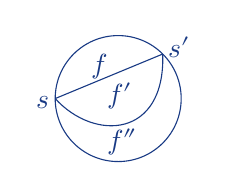
\begin{tikzpicture}[draw=blue,text=blue]\draw (0,0) circle (0.8); \draw (-0.8,0)--(0.5657,0.5657); \draw (-0.8,0) .. controls (-0.3,-0.55) and (0.6,-0.5) .. (0.5657,0.5657); \node at (-0.25,0.4) {$f$}; \node at (0.03,0.03) {$f'$}; \node at (0.05,-0.55) {$f''$}; \node at (-0.95,-0.05) {$s$}; \node at (0.78,0.65) {$s'$};\end{tikzpicture}} $f \cap f'' = \{s,s'\} = S_0$}
ness" condition is now expressed by demanding that the set of indices
I can be totally ordered, \var{\inserted[typed]{i.e. numbered}}{i.e. numbered}{typed insertion}{ps_134-2_027-v0011} in such a way that we get X by succesively
"attaching" \unsure{Dells|cells} $D_{n(i)}$ to the space already constructed\var{\xout{\unsure{,}}}{}{typewriter deletion}{ps_134-2_027-v0012} X(i-1), by a
map from \var{\deleted{a}}{}{deletion}{ps_134-2_027-v0013}\var{\inserted{a sub-}}{\hand{a sub-}}{insertion}{ps_134-2_027-v0014} cell \var{\xout{$D_i$}}{}{typewriter deletion}{ps_134-2_027-v0015}\var{\inserted{of $D_{n(i)}$}}{\hand{of $D_{n(i)}$}}{insertion}{ps_134-2_027-v0016}, $S_j^{\hand{\varepsilon}} \hand{\to} X(i-1)$ \quad $(\hand{\varepsilon\in\{}\pm 1\hand{\}})$ , this map of course
inducing an isomorphism,  more precisely \uline{the} standard isomorphism,\var{\inserted{$\varphi^{\unsure{\varepsilon'}}_{n(i')}$}}{\hand{$\varphi^{\unsure{\varepsilon'}}_{n(i')}$}}{insertion}{ps_134-2_027-v0017}\var{\deleted{of}}{}{deletion}{ps_134-2_027-v0018}
\margin{\textcircled{$\varphi^{\varepsilon'}_{n(i),j}$}}
$S_j^{\hand{\varepsilon}} \hand{\simeq} D_j$ \quad with\var{\inserted{$S^{\varepsilon'}_j$}}{\hand{$S^{\varepsilon'}_j$}}{insertion}{ps_134-2_027-v0019} one of the two corresponding cells $S_j^+$ , $S_j^-$ in some
\margin{\textcircled{$S^{\varepsilon'}_j$}}
$X_{i'} \hand{\simeq} D_{n(i')}$ .  The \var{\xout{xxxxx}}{}{typewriter deletion}{ps_134-2_027-v0020} dual translation of this\hand{,}in terms\hand{\unsure{$\vert$}} of fiber
products in \var{\xout{xxx}}{}{typewriter deletion}{ps_134-2_027-v0021} a category C endowed with objects $F_i$ $(i\in\underline{N})$ and maps
$s_1^i , t_1^i$ between these, is clear:  for a given set of indices I and map
\margin{$P=\prod_{i\in I}F_{n(i)}$}
$i \hand{\mapsto} n(i) : I \hand{\to} \underline{N}$ , we consider a sub\var{\xout{xxx}}{}{typewriter deletion}{ps_134-2_027-v0022}\var{\inserted[typed]{-object}}{-object}{typed insertion}{ps_134-2_027-v0023}\var{\inserted{ of}}{\hand{ of}}{insertion}{ps_134-2_027-v0024} $\var{\inserted[typed]{P=}}{P=}{typed insertion}{ps_134-2_027-v0025}\hand{\prod_{i\in I}}F_{n(i)}$ ,  which can be
described by equality relations between it\var{\over{t}{e}}{\hand{e}}{writing over}{ps_134-2_027-v0026}rated sources and targets
\var{\xout{xxxxxx}}{}{typewriter deletion}{ps_134-2_027-v0027} of various components of $u = (u_i)_{i\in I}$  in P,  the structure of
the set of relations being such that I can\hand{\unsure{,}}be numbered, from 1 to N say,
in such a way that we get in succession \var{\deleted{N}}{}{deletion}{ps_134-2_027-v0028}\var{\inserted{$N-1$}}{\hand{$N-1$}}{insertion}{ps_134-2_027-v0029} relations on the N components
$u_i$ respectively,\var{\inserted{$(2\leq i \leq N)$}}{\hand{$(2\leq i \leq N)$}}{insertion}{ps_134-2_027-v0030} every relation being of the type $f(u_i) = g(u_{i'})$ , with
f and g being iterated source or target maps, and $i'<i$ . \hand{(Whether}
\hand{source or target depending in obvious way on the two signs $\varepsilon,\varepsilon'$.)}

\mspage{\hand{27}}

%% END SOURCE ps_134-2_027
\ifnum\EditionMode=1
\psapparatusstart
\psentry{ps_134-2_027-v0001}{1}{deletion}{\deleted{\illegible{1}}}{}{The author cancels this material by hand; it leaves the corrected running text.}
\psentry{ps_134-2_027-v0002}{2}{insertion}{\inserted{(rather, finite $\varinjlim$'s)}}{\hand{(rather, finite $\varinjlim$'s)}}{The handwritten insertion is incorporated at its indicated position; insertion brackets leave the running text.}
\psentry{ps_134-2_027-v0003}{3}{typewriter deletion}{\xout{\unsure{s}}}{}{The typewriter strikes out this material; it leaves the corrected running text.}
\psentry{ps_134-2_027-v0004}{4}{deletion}{\deleted{cell}}{}{The author cancels this material by hand; it leaves the corrected running text.}
\psentry{ps_134-2_027-v0005}{5}{insertion}{\inserted{cells}}{\hand{cells}}{The handwritten insertion is incorporated at its indicated position; insertion brackets leave the running text.}
\psentry{ps_134-2_027-v0006}{6}{typewriter deletion}{\xout{\unsure{s}}}{}{The typewriter strikes out this material; it leaves the corrected running text.}
\psentry{ps_134-2_027-v0007}{7}{deletion}{\deleted{\illegible{3}}}{}{The author cancels this material by hand; it leaves the corrected running text.}
\psentry{ps_134-2_027-v0008}{8}{insertion}{\inserted{(12)}}{\hand{(12)}}{The handwritten insertion is incorporated at its indicated position; insertion brackets leave the running text.}
\psentry{ps_134-2_027-v0009}{9}{deletion}{\deleted{\illegible{2}}}{}{The author cancels this material by hand; it leaves the corrected running text.}
\psentry{ps_134-2_027-v0010}{10}{writing over}{\over{t}{d}}{\hand{d}}{The superposed handwritten reading replaces the underlying reading.}
\psentry{ps_134-2_027-v0011}{11}{typed insertion}{\inserted[typed]{i.e. numbered}}{i.e. numbered}{The typed insertion is incorporated at its indicated position; insertion brackets leave the running text.}
\psentry{ps_134-2_027-v0012}{12}{typewriter deletion}{\xout{\unsure{,}}}{}{The typewriter strikes out this material; it leaves the corrected running text.}
\psentry{ps_134-2_027-v0013}{13}{deletion}{\deleted{a}}{}{The author cancels this material by hand; it leaves the corrected running text.}
\psentry{ps_134-2_027-v0014}{14}{insertion}{\inserted{a sub-}}{\hand{a sub-}}{The handwritten insertion is incorporated at its indicated position; insertion brackets leave the running text.}
\psentry{ps_134-2_027-v0015}{15}{typewriter deletion}{\xout{$D_i$}}{}{The typewriter strikes out this material; it leaves the corrected running text.}
\psentry{ps_134-2_027-v0016}{16}{insertion}{\inserted{of $D_{n(i)}$}}{\hand{of $D_{n(i)}$}}{The handwritten insertion is incorporated at its indicated position; insertion brackets leave the running text.}
\psentry{ps_134-2_027-v0017}{17}{insertion}{\inserted{$\varphi^{\unsure{\varepsilon'}}_{n(i')}$}}{\hand{$\varphi^{\unsure{\varepsilon'}}_{n(i')}$}}{The handwritten insertion is incorporated at its indicated position; insertion brackets leave the running text.}
\psentry{ps_134-2_027-v0018}{18}{deletion}{\deleted{of}}{}{The author cancels this material by hand; it leaves the corrected running text.}
\psentry{ps_134-2_027-v0019}{19}{insertion}{\inserted{$S^{\varepsilon'}_j$}}{\hand{$S^{\varepsilon'}_j$}}{The handwritten insertion is incorporated at its indicated position; insertion brackets leave the running text.}
\psentry{ps_134-2_027-v0020}{20}{typewriter deletion}{\xout{xxxxx}}{}{The typewriter strikes out this material; it leaves the corrected running text.}
\psentry{ps_134-2_027-v0021}{21}{typewriter deletion}{\xout{xxx}}{}{The typewriter strikes out this material; it leaves the corrected running text.}
\psentry{ps_134-2_027-v0022}{22}{typewriter deletion}{\xout{xxx}}{}{The typewriter strikes out this material; it leaves the corrected running text.}
\psentry{ps_134-2_027-v0023}{23}{typed insertion}{\inserted[typed]{-object}}{-object}{The typed insertion is incorporated at its indicated position; insertion brackets leave the running text.}
\psentry{ps_134-2_027-v0024}{24}{insertion}{\inserted{ of}}{\hand{ of}}{The handwritten insertion is incorporated at its indicated position; insertion brackets leave the running text.}
\psentry{ps_134-2_027-v0025}{25}{typed insertion}{$\inserted[typed]{P=}$}{$P=$}{The typed insertion is incorporated at its indicated position; insertion brackets leave the running text.}
\psentry{ps_134-2_027-v0026}{26}{writing over}{\over{t}{e}}{\hand{e}}{The superposed handwritten reading replaces the underlying reading.}
\psentry{ps_134-2_027-v0027}{27}{typewriter deletion}{\xout{xxxxxx}}{}{The typewriter strikes out this material; it leaves the corrected running text.}
\psentry{ps_134-2_027-v0028}{28}{deletion}{\deleted{N}}{}{The author cancels this material by hand; it leaves the corrected running text.}
\psentry{ps_134-2_027-v0029}{29}{insertion}{\inserted{$N-1$}}{\hand{$N-1$}}{The handwritten insertion is incorporated at its indicated position; insertion brackets leave the running text.}
\psentry{ps_134-2_027-v0030}{30}{insertion}{\inserted{$(2\leq i \leq N)$}}{\hand{$(2\leq i \leq N)$}}{The handwritten insertion is incorporated at its indicated position; insertion brackets leave the running text.}
\psapparatusend
\fi
\pssource{ps_134-2_028}{134-2/28}{https://grothendieck.umontpellier.fr/web/viewer.html?file=../134-2.pdf\#page=29}
\psnumber{ps_134-2_028-v0001}{1}
\psnumber{ps_134-2_028-v0002}{2}
\psnumber{ps_134-2_028-v0003}{3}
\psnumber{ps_134-2_028-v0004}{4}
\psnumber{ps_134-2_028-v0005}{5}
\psnumber{ps_134-2_028-v0006}{6}
\psnumber{ps_134-2_028-v0007}{7}
\psnumber{ps_134-2_028-v0008}{8}
\psnumber{ps_134-2_028-v0009}{9}
\psnumber{ps_134-2_028-v0010}{10}
\psnumber{ps_134-2_028-v0011}{11}
\psnumber{ps_134-2_028-v0012}{12}
\psnumber{ps_134-2_028-v0013}{13}
\psnumber{ps_134-2_028-v0014}{14}
\psnumber{ps_134-2_028-v0015}{15}
\psnumber{ps_134-2_028-v0016}{16}
\psnumber{ps_134-2_028-v0017}{17}
\psnumber{ps_134-2_028-v0018}{18}
\psnumber{ps_134-2_028-v0019}{19}
\psnumber{ps_134-2_028-v0020}{20}
\psnumber{ps_134-2_028-v0021}{21}
\psnumber{ps_134-2_028-v0022}{22}
%% BEGIN SOURCE ps_134-2_028
% Pursuing Stacks (cotes 134-2 to 134-8): archive cote 134-2, site page 28 (PDF page 29).
% letter to Quillen. Draft compared: ps1.tex:660-736.
% AI-transcribed by Claude Opus 5.5 (claude-opus-5-5, adaptive thinking, effort high), Message Batches API, batch ps1 (msgbatch_01Rv5hCaNTtUt4JHx1yqoHPL), 2026-11-12; reviewed against both supplied scan halves; see CHECK_DECISIONS.tsv.
\scanpage{134-2/28}
\margin{8}
\mspage{\var{\deleted{\hand{8}}}{}{deletion}{ps_134-2_028-v0001} \hand{14}}
21.2.

\var{\over{\unsure{4}}{8}}{\hand{8}}{writing over}{ps_134-2_028-v0002}. Returning to theamalgamated sum $X = \hand{\bigcup_i}X_i$ , the cellular decompositions
of the components $X_i \hand{\simeq} D_{n(i)}$ define a cellular decomposition of X, whose
set of cells with incidence relation forms a finite ordered set K, fini-%
te union of a family of subsets $(K_i)_{i\in I}$ , with given isomorphisms\var{\xout{m}}{}{typewriter deletion}{ps_134-2_028-v0003}
\[ f_i : K_i \hand{\simeq} \underline{J}_{n(i)} \quad (i\in I) , \]
where for every index $n\in \underline{N}$, $\underline{J}_n$ denotes the ordered set of the 2n+1
cells $S_j^{\hand{\varepsilon}}$ $(0\leq j\leq n-1,\ \hand{\varepsilon\in\{}\pm 1\hand{\}})$, $D_n$ of the \var{\deleted{pertinent}}{}{deletion}{ps_134-2_028-v0004} \var{\inserted{relevant}}{\hand{relevant}}{insertion}{ps_134-2_028-v0005} cellular decomposition
of $D_n$ . We may without loss of generality assume there is no\var{\deleted{t}}{}{deletion}{ps_134-2_028-v0006} inclusion
relation between the $K_i$ , moreover the standar\var{\over{t}{d}}{\hand{d}}{writing over}{ps_134-2_028-v0007}ness condition described
above readily translates into a condition on this structure
$K$, $(K_i)_{i\in I}$ , $(f_i)_{i\in I}$ , and implies that for $i,i'\in I$, $K_i\hand{\cap}K_{i'}$ is a``clo-%
sed'' subset in the two ordered sets $K_i,K_{i'}$ (namely contains with any
element x the elements smaller than x), and moreover isomorphic (for the
induced order) to some $\underline{J}_n$ . Thus the category $B_o$ \var{\xout{is}}{}{typewriter deletion}{ps_134-2_028-v0008} can be viewed as the
category of such ``standar\var{\over{t}{d}}{\hand{d}}{writing over}{ps_134-2_028-v0009} ordered sets'' (with the extra structure on the-%
se just said), and the category $C_o$ can be defined most simply as the
dual category $B_o^{\,o}$ . (NB the definition of morphisms in $B_o$ is clear I
guess ...) I believe the category $B_o$ is stable under amalgamated sums
$X\hand{\amalg}_Z Y$ , provided \var{\inserted[typed]{however}}{however}{typed insertion}{ps_134-2_028-v0010} we insist that the empty structure K is \uline{not} allowed -
otherwise we have to \var{\xout{insist}}{}{typewriter deletion}{ps_134-2_028-v0011} restrict to amalgamated sums with $Z \neq \emptyset$ .
It seems finally more convenient to exclude the empty structure in $B_o$ ,
\margin{(13!)}
i.e. to exclude final element from $\underline{C}_o$ , for the benefit of being able to
\margin{\unsure{* This is obviously false, see P.S. p.12}}
state that $\underline{C}_o$ (and \uwave{all categories $\underline{C}_n$}\hand{*} \var{\deleted{\illegible{1}}}{}{deletion}{ps_134-2_028-v0012} \var{\xout{\illegible{1}}}{}{typewriter deletion}{ps_134-2_028-v0013} \var{\inserted{(13!))}}{\hand{(13!))}}{insertion}{ps_134-2_028-v0014} are stable under binary
amalgamated sums, and that the functors $\underline{C}_n\hand{\to} C$ (and ultimately $\underline{C}_\infty\hand{\to} C$)
we are interested in are just those commuting to arbitrary binary amalga-%
mated sums (without \var{\xout{\illegible{1}}}{}{typewriter deletion}{ps_134-2_028-v0015} awkward reference to the objects $\underline{F}_i$ and the
iterated source and target maps between them ...)\hand{(13!)}.

\var{\over{\illegible{1}}{9}}{\hand{9}}{writing over}{ps_134-2_028-v0016}. The category $\underline{C}_o$ being fairly well understood, \var{\inserted{it}}{\hand{it}}{insertion}{ps_134-2_028-v0017} remains to complete
the construction by the inductive step, \var{\inserted{for}}{\hand{for}}{insertion}{ps_134-2_028-v0018} passing from $\underline{C}_n$ to $\underline{C}_{n+1}$ . The
main properties I have in mind \var{\deleted{therefore}}{}{deletion}{ps_134-2_028-v0019} \var{\inserted{for this}}{\hand{for this}}{insertion}{ps_134-2_028-v0020}, for the sequence of categories
$\underline{C}_n$ and their limit $\underline{C}_\infty$ , are the following two.

A) For any $K\in Ob(\underline{C}_\infty)$ \ ($= Ob(\underline{C}_o)$), and any two arrows in $\underline{C}_\infty$
\[ f,g : K \hand{\rightrightarrows} F_i , \]
with $i\in\underline{N}$, \hand{(}and such that either i=0, or the equalities
\[ \hand{(1)}\qquad s_1^i f = s_1^i g \ , \quad t_1^i f = t_1^i g \]
hold (case $i \var{\over{>}{\geq}}{\hand{\geq}}{writing over}{ps_134-2_028-v0021} 1$), there exists $h: K\hand{\to} F_{i+1}$ such that
\[ \hand{(2)}\qquad s_1^{i+1} h = f \ , \quad t_1^{i+1} h = g \ . \]
B) For any $n\in\underline{N}$, the category $\underline{C}_{n+1}$ is deduced from $\underline{C}_n$ by keeping
the same objects, and just adding new arrows \var{\xout{\illegible{1}}}{}{typewriter deletion}{ps_134-2_028-v0022} h as in A), with
f, g arrows in $\underline{C}_n$ .

\margin{28}

%% END SOURCE ps_134-2_028
\ifnum\EditionMode=1
\psapparatusstart
\psentry{ps_134-2_028-v0001}{1}{deletion}{\deleted{\hand{8}}}{}{The author cancels this material by hand; it leaves the corrected running text.}
\psentry{ps_134-2_028-v0002}{2}{writing over}{\over{\unsure{4}}{8}}{\hand{8}}{The superposed handwritten reading replaces the underlying reading.}
\psentry{ps_134-2_028-v0003}{3}{typewriter deletion}{\xout{m}}{}{The typewriter strikes out this material; it leaves the corrected running text.}
\psentry{ps_134-2_028-v0004}{4}{deletion}{\deleted{pertinent}}{}{The author cancels this material by hand; it leaves the corrected running text.}
\psentry{ps_134-2_028-v0005}{5}{insertion}{\inserted{relevant}}{\hand{relevant}}{The handwritten insertion is incorporated at its indicated position; insertion brackets leave the running text.}
\psentry{ps_134-2_028-v0006}{6}{deletion}{\deleted{t}}{}{The author cancels this material by hand; it leaves the corrected running text.}
\psentry{ps_134-2_028-v0007}{7}{writing over}{\over{t}{d}}{\hand{d}}{The superposed handwritten reading replaces the underlying reading.}
\psentry{ps_134-2_028-v0008}{8}{typewriter deletion}{\xout{is}}{}{The typewriter strikes out this material; it leaves the corrected running text.}
\psentry{ps_134-2_028-v0009}{9}{writing over}{\over{t}{d}}{\hand{d}}{The superposed handwritten reading replaces the underlying reading.}
\psentry{ps_134-2_028-v0010}{10}{typed insertion}{\inserted[typed]{however}}{however}{The typed insertion is incorporated at its indicated position; insertion brackets leave the running text.}
\psentry{ps_134-2_028-v0011}{11}{typewriter deletion}{\xout{insist}}{}{The typewriter strikes out this material; it leaves the corrected running text.}
\psentry{ps_134-2_028-v0012}{12}{deletion}{\deleted{\illegible{1}}}{}{The author cancels this material by hand; it leaves the corrected running text.}
\psentry{ps_134-2_028-v0013}{13}{typewriter deletion}{\xout{\illegible{1}}}{}{The typewriter strikes out this material; it leaves the corrected running text.}
\psentry{ps_134-2_028-v0014}{14}{insertion}{\inserted{(13!))}}{\hand{(13!))}}{The handwritten insertion is incorporated at its indicated position; insertion brackets leave the running text.}
\psentry{ps_134-2_028-v0015}{15}{typewriter deletion}{\xout{\illegible{1}}}{}{The typewriter strikes out this material; it leaves the corrected running text.}
\psentry{ps_134-2_028-v0016}{16}{writing over}{\over{\illegible{1}}{9}}{\hand{9}}{The superposed handwritten reading replaces the underlying reading.}
\psentry{ps_134-2_028-v0017}{17}{insertion}{\inserted{it}}{\hand{it}}{The handwritten insertion is incorporated at its indicated position; insertion brackets leave the running text.}
\psentry{ps_134-2_028-v0018}{18}{insertion}{\inserted{for}}{\hand{for}}{The handwritten insertion is incorporated at its indicated position; insertion brackets leave the running text.}
\psentry{ps_134-2_028-v0019}{19}{deletion}{\deleted{therefore}}{}{The author cancels this material by hand; it leaves the corrected running text.}
\psentry{ps_134-2_028-v0020}{20}{insertion}{\inserted{for this}}{\hand{for this}}{The handwritten insertion is incorporated at its indicated position; insertion brackets leave the running text.}
\psentry{ps_134-2_028-v0021}{21}{writing over}{$\over{>}{\geq}$}{$\hand{\geq}$}{The superposed handwritten reading replaces the underlying reading.}
\psentry{ps_134-2_028-v0022}{22}{typewriter deletion}{\xout{\illegible{1}}}{}{The typewriter strikes out this material; it leaves the corrected running text.}
\psapparatusend
\fi
\pssource{ps_134-2_029}{134-2/29}{https://grothendieck.umontpellier.fr/web/viewer.html?file=../134-2.pdf\#page=30}
\psnumber{ps_134-2_029-v0001}{1}
\psnumber{ps_134-2_029-v0002}{2}
\psnumber{ps_134-2_029-v0003}{3}
\psnumber{ps_134-2_029-v0004}{4}
\psnumber{ps_134-2_029-v0005}{5}
\psnumber{ps_134-2_029-v0006}{6}
\psnumber{ps_134-2_029-v0007}{7}
\psnumber{ps_134-2_029-v0008}{8}
\psnumber{ps_134-2_029-v0009}{9}
\psnumber{ps_134-2_029-v0010}{10}
\psnumber{ps_134-2_029-v0011}{11}
\psnumber{ps_134-2_029-v0012}{12}
\psnumber{ps_134-2_029-v0013}{13}
\psnumber{ps_134-2_029-v0014}{14}
\psnumber{ps_134-2_029-v0015}{15}
\psnumber{ps_134-2_029-v0016}{16}
\psnumber{ps_134-2_029-v0017}{17}
\psnumber{ps_134-2_029-v0018}{18}
\psnumber{ps_134-2_029-v0019}{19}
\psnumber{ps_134-2_029-v0020}{20}
\psnumber{ps_134-2_029-v0021}{21}
\psnumber{ps_134-2_029-v0022}{22}
\psnumber{ps_134-2_029-v0023}{23}
\psnumber{ps_134-2_029-v0024}{24}
\psnumber{ps_134-2_029-v0025}{25}
\psnumber{ps_134-2_029-v0026}{26}
\psnumber{ps_134-2_029-v0027}{27}
\psnumber{ps_134-2_029-v0028}{28}
\psnumber{ps_134-2_029-v0029}{29}
\psnumber{ps_134-2_029-v0030}{30}
\psnumber{ps_134-2_029-v0031}{31}
\psnumber{ps_134-2_029-v0032}{32}
\psnumber{ps_134-2_029-v0033}{33}
\psnumber{ps_134-2_029-v0034}{34}
\psnumber{ps_134-2_029-v0035}{35}
\psnumber{ps_134-2_029-v0036}{36}
\psnumber{ps_134-2_029-v0037}{37}
\psnumber{ps_134-2_029-v0038}{38}
\psnumber{ps_134-2_029-v0039}{39}
%% BEGIN SOURCE ps_134-2_029
% Pursuing Stacks (cotes 134-2 to 134-8): archive cote 134-2, site page 29 (PDF page 30).
% letter to Quillen. Draft compared: ps1.tex:723-786.
% AI-transcribed by Claude Opus 5.5 (claude-opus-5-5, adaptive thinking, effort high), Message Batches API, batch ps1 (msgbatch_01Rv5hCaNTtUt4JHx1yqoHPL), 2026-11-12; reviewed against both supplied scan halves; see CHECK_DECISIONS.tsv.
\scanpage{134-2/29}
\mspage{\hand{\unsure{1|\#}5}}

The expression ``deduce\var{\over{s}{d}}{\hand{d}}{writing over}{ps_134-2_029-v0001} from'' in B)  means that we are adding arrows
$h: K \hand{\to} F_i$ (each with preassigned source and target in $\underline{C}_n$),  with as
``new axioms'' on \var{\inserted[typed]{the bunch of}}{the bunch of}{typed insertion}{ps_134-2_029-v0002} these uniquely the two relations \var{\deleted{\illegible{1}}}{}{deletion}{ps_134-2_029-v0003}\var{\inserted{(1),(2)}}{\hand{(1),(2)}}{insertion}{ps_134-2_029-v0004} of \var{\over{\illegible{1}}{A}}{\hand{A}}{writing over}{ps_134-2_029-v0005}), the category
$\underline{C}_{n+1}$  being deduced from $\underline{C}_n$ in an obvious way,  as the solution of a uni-%
versal problem with\var{\inserted{in}}{\hand{in}}{insertion}{ps_134-2_029-v0006} the category of all categories where binary amalgama-%
ted products exist,  and ``maps'' between these being functors which commute
\margin{\unsure{this has to be corrected -- amalgamated sums exist in $\underline{C}_o$ only, and \uline{\unsure{those|these}} \unsure{sh\textsuperscript{d}|sh\textsuperscript{ld}} be respected}}
to those fibered products\var{\inserted{(14!)}}{\hand{(14!)}}{insertion}{ps_134-2_029-v0007}. \var{\deleted{In}}{}{deletion}{ps_134-2_029-v0008}\var{\inserted{In}}{\hand{In}}{insertion}{ps_134-2_029-v0009} practical terms,  the arrows of $\underline{C}_{n+1}$ are
those deduced from the arrows in $\underline{C}_n$ and the ``new'' arrows $h$,  by combining
formal operations of composing arrows by $v\circ u$ ,  and taking \var{\inserted{(binary)}}{\hand{(binary)}}{insertion}{ps_134-2_029-v0010} amalgamated
products of arrows. \var{\deleted{\illegible{1}}}{}{deletion}{ps_134-2_029-v0011}

NB  Of course the condition (1) in A) is necessary for the existence
\margin{$\|$}of an $h$ satisfying (2).  That it is sufficient too \var{\deleted{can}}{}{deletion}{ps_134-2_029-v0012}\var{\inserted{may}}{\hand{may}}{insertion}{ps_134-2_029-v0013} be viewed as an
extremely strong,\var{\xout{\unsure{version}}}{}{typewriter deletion}{ps_134-2_029-v0014} ``universal'' version of coherence conditions,
concerning the various structures introduced on a $\infty$-groupoid. Intuitive-%
ly,  it means that whenever we have \var{\deleted{\over{\illegible{1}}{two} ways of}}{}{deletion}{ps_134-2_029-v0015}\var{\inserted{two ways of}}{\hand{two ways of}}{insertion}{ps_134-2_029-v0016} associating to a \var{\inserted[typed]{finite}}{finite}{typed insertion}{ps_134-2_029-v0017} family \var{\deleted{\illegible{1}}}{}{deletion}{ps_134-2_029-v0018}
$(u_i)_{i\in I}$  of objects of an $\infty$-groupoid,  $u_i \in F_{n(i)}$ ,  \var{\xout{xxxxxxxxxx}}{}{typewriter deletion}{ps_134-2_029-v0019} subjected
to a \hand{``}standar\var{\over{t}{d}}{\hand{d}}{writing over}{ps_134-2_029-v0020}\hand{''} set of relations on the $u_i$'s, an element of some $F_n$ ,  in
terms of the $\infty$-groupoid structure only,  then we have automatically
\var{\inserted[typed]{a ``homotopy''}}{a ``homotopy''}{typed insertion}{ps_134-2_029-v0021}\var{\xout{an isomorphism}}{}{typewriter deletion}{ps_134-2_029-v0022} between these built-in in the very structure of the $\infty$-%
groupoid,  provided it makes at all a sense to ask for one (namely provi-%
ded condition (1) holds if $n \geq 1$).   I have the feeling moreover that
conditions (A) and (B) (plus the relation $\underline{C}_\infty = \mathop{\mathrm{lim}}\limits_{\hand{\longrightarrow}} \underline{C}_n$ ) is all what will
be ever needed,  when using the definition of the structure species,
- plus of course the description of $\underline{C}_o$ , and the \var{\inserted[typed]{implicit}}{implicit}{typed insertion}{ps_134-2_029-v0023} fact that the categories
\margin{inaccurate -- see above}
$\underline{C}_n$ are stable under binary fiber products and the inclusion functors com-%
mute to these\var{\inserted{(13!)}}{\hand{(13!)}}{insertion}{ps_134-2_029-v0024}. Of course,  the category which really interests us is
$\underline{C}_\infty$,  the description of the intermediate $\underline{C}_n$'s\hand{$|$} is merely tec\var{\over{\illegible{1}}{h}}{\hand{h}}{writing over}{ps_134-2_029-v0025}nical \var{\deleted{txt}}{}{deletion}{ps_134-2_029-v0026} -
the main point is that there should exist an increasing sequence $(C_n)$ of
subcategories of $\underline{C}_\infty$ ,  having same objects\var{\over{,}{(}}{\hand{(}}{writing over}{ps_134-2_029-v0027}and ``same'' fiberproducts\var{\over{,}{)}}{\hand{)}}{writing over}{ps_134-2_029-v0028}\var{\inserted{(13!)}}{\hand{(13!)}}{insertion}{ps_134-2_029-v0029},
such that $\underline{C}_\infty$ should be the limit (i.e. every arrow in $C_\infty$ should belong \var{\deleted{\illegible{1}}}{}{deletion}{ps_134-2_029-v0030}
to some $\underline{C}_n$),  and such that the passage from $\underline{C}_n$ to $\underline{C}_{n+1}$ should satisfy \var{\inserted{(B).}}{\hand{(B).}}{insertion}{ps_134-2_029-v0031}
\var{\deleted{(B).}}{}{deletion}{ps_134-2_029-v0032} \var{\margin{\diagram{\begin{tikzpicture}\draw (0,0)--(.32,0)--(.32,.27)--(.68,.27);\end{tikzpicture}}}It is fairly obvious}{

It is fairly obvious}{author paragraph break}{ps_134-2_029-v0033} that these conditions alone do by no means
caracterise $\underline{C}_\infty$  up to equivalence,  and still less the sequence of its
subcategories $\underline{C}_n$ .  The point I wish to make though,  before pursuing
with a proposal of an explicit description,  is \var{\inserted{(firstly)}}{\hand{(firstly)}}{insertion}{ps_134-2_029-v0034} that \uline{this ambiguity is}
\uline{in the nature of things}\var{\over{,}{.}}{\hand{.}}{writing over}{ps_134-2_029-v0035} \var{\over{r}{R}}{\hand{R}}{writing over}{ps_134-2_029-v0036}oughly saying, two different mathematicians,
working independently on the conceptual problem I had in mind,  \var{\deleted{assuming}}{}{deletion}{ps_134-2_029-v0037}\var{\inserted{assuming}}{\hand{assuming}}{insertion}{ps_134-2_029-v0038}
they both wind up with some explicit definition,  will almost certainly
get non e\var{\over[typed]{\illegible{1}}{q}}{q}{typewriter overwriting}{ps_134-2_029-v0039}uivalent definitions  -  namely with non equivalent categories
of (set-valued, say) $\infty$-groupoids !  And, secondly and as importantly,

\mspage{29}

%% END SOURCE ps_134-2_029
\ifnum\EditionMode=1
\psapparatusstart
\psentry{ps_134-2_029-v0001}{1}{writing over}{\over{s}{d}}{\hand{d}}{The superposed handwritten reading replaces the underlying reading.}
\psentry{ps_134-2_029-v0002}{2}{typed insertion}{\inserted[typed]{the bunch of}}{the bunch of}{The typed insertion is incorporated at its indicated position; insertion brackets leave the running text.}
\psentry{ps_134-2_029-v0003}{3}{deletion}{\deleted{\illegible{1}}}{}{The author cancels this material by hand; it leaves the corrected running text.}
\psentry{ps_134-2_029-v0004}{4}{insertion}{\inserted{(1),(2)}}{\hand{(1),(2)}}{The handwritten insertion is incorporated at its indicated position; insertion brackets leave the running text.}
\psentry{ps_134-2_029-v0005}{5}{writing over}{\over{\illegible{1}}{A}}{\hand{A}}{The superposed handwritten reading replaces the underlying reading.}
\psentry{ps_134-2_029-v0006}{6}{insertion}{\inserted{in}}{\hand{in}}{The handwritten insertion is incorporated at its indicated position; insertion brackets leave the running text.}
\psentry{ps_134-2_029-v0007}{7}{insertion}{\inserted{(14!)}}{\hand{(14!)}}{The handwritten insertion is incorporated at its indicated position; insertion brackets leave the running text.}
\psentry{ps_134-2_029-v0008}{8}{deletion}{\deleted{In}}{}{The author cancels this material by hand; it leaves the corrected running text.}
\psentry{ps_134-2_029-v0009}{9}{insertion}{\inserted{In}}{\hand{In}}{The handwritten insertion is incorporated at its indicated position; insertion brackets leave the running text.}
\psentry{ps_134-2_029-v0010}{10}{insertion}{\inserted{(binary)}}{\hand{(binary)}}{The handwritten insertion is incorporated at its indicated position; insertion brackets leave the running text.}
\psentry{ps_134-2_029-v0011}{11}{deletion}{\deleted{\illegible{1}}}{}{The author cancels this material by hand; it leaves the corrected running text.}
\psentry{ps_134-2_029-v0012}{12}{deletion}{\deleted{can}}{}{The author cancels this material by hand; it leaves the corrected running text.}
\psentry{ps_134-2_029-v0013}{13}{insertion}{\inserted{may}}{\hand{may}}{The handwritten insertion is incorporated at its indicated position; insertion brackets leave the running text.}
\psentry{ps_134-2_029-v0014}{14}{typewriter deletion}{\xout{\unsure{version}}}{}{The typewriter strikes out this material; it leaves the corrected running text.}
\psentry{ps_134-2_029-v0015}{15}{deletion}{\deleted{\over{\illegible{1}}{two} ways of}}{}{The author cancels this material by hand; it leaves the corrected running text.}
\psentry{ps_134-2_029-v0016}{16}{insertion}{\inserted{two ways of}}{\hand{two ways of}}{The handwritten insertion is incorporated at its indicated position; insertion brackets leave the running text.}
\psentry{ps_134-2_029-v0017}{17}{typed insertion}{\inserted[typed]{finite}}{finite}{The typed insertion is incorporated at its indicated position; insertion brackets leave the running text.}
\psentry{ps_134-2_029-v0018}{18}{deletion}{\deleted{\illegible{1}}}{}{The author cancels this material by hand; it leaves the corrected running text.}
\psentry{ps_134-2_029-v0019}{19}{typewriter deletion}{\xout{xxxxxxxxxx}}{}{The typewriter strikes out this material; it leaves the corrected running text.}
\psentry{ps_134-2_029-v0020}{20}{writing over}{\over{t}{d}}{\hand{d}}{The superposed handwritten reading replaces the underlying reading.}
\psentry{ps_134-2_029-v0021}{21}{typed insertion}{\inserted[typed]{a ``homotopy''}}{a ``homotopy''}{The typed insertion is incorporated at its indicated position; insertion brackets leave the running text.}
\psentry{ps_134-2_029-v0022}{22}{typewriter deletion}{\xout{an isomorphism}}{}{The typewriter strikes out this material; it leaves the corrected running text.}
\psentry{ps_134-2_029-v0023}{23}{typed insertion}{\inserted[typed]{implicit}}{implicit}{The typed insertion is incorporated at its indicated position; insertion brackets leave the running text.}
\psentry{ps_134-2_029-v0024}{24}{insertion}{\inserted{(13!)}}{\hand{(13!)}}{The handwritten insertion is incorporated at its indicated position; insertion brackets leave the running text.}
\psentry{ps_134-2_029-v0025}{25}{writing over}{\over{\illegible{1}}{h}}{\hand{h}}{The superposed handwritten reading replaces the underlying reading.}
\psentry{ps_134-2_029-v0026}{26}{deletion}{\deleted{txt}}{}{The author cancels this material by hand; it leaves the corrected running text.}
\psentry{ps_134-2_029-v0027}{27}{writing over}{\over{,}{(}}{\hand{(}}{The superposed handwritten reading replaces the underlying reading.}
\psentry{ps_134-2_029-v0028}{28}{writing over}{\over{,}{)}}{\hand{)}}{The superposed handwritten reading replaces the underlying reading.}
\psentry{ps_134-2_029-v0029}{29}{insertion}{\inserted{(13!)}}{\hand{(13!)}}{The handwritten insertion is incorporated at its indicated position; insertion brackets leave the running text.}
\psentry{ps_134-2_029-v0030}{30}{deletion}{\deleted{\illegible{1}}}{}{The author cancels this material by hand; it leaves the corrected running text.}
\psentry{ps_134-2_029-v0031}{31}{insertion}{\inserted{(B).}}{\hand{(B).}}{The handwritten insertion is incorporated at its indicated position; insertion brackets leave the running text.}
\psentry{ps_134-2_029-v0032}{32}{deletion}{\deleted{(B).}}{}{The author cancels this material by hand; it leaves the corrected running text.}
\psentry{ps_134-2_029-v0033}{33}{author paragraph break}{\margin{\diagram{\begin{tikzpicture}\draw (0,0)--(.32,0)--(.32,.27)--(.68,.27);\end{tikzpicture}}}It is fairly obvious}{

It is fairly obvious}{The stepped pen cue at this boundary instructs a new paragraph; the diplomatic text retains its graphic.}
\psentry{ps_134-2_029-v0034}{34}{insertion}{\inserted{(firstly)}}{\hand{(firstly)}}{The handwritten insertion is incorporated at its indicated position; insertion brackets leave the running text.}
\psentry{ps_134-2_029-v0035}{35}{writing over}{\over{,}{.}}{\hand{.}}{The superposed handwritten reading replaces the underlying reading.}
\psentry{ps_134-2_029-v0036}{36}{writing over}{\over{r}{R}}{\hand{R}}{The superposed handwritten reading replaces the underlying reading.}
\psentry{ps_134-2_029-v0037}{37}{deletion}{\deleted{assuming}}{}{The author cancels this material by hand; it leaves the corrected running text.}
\psentry{ps_134-2_029-v0038}{38}{insertion}{\inserted{assuming}}{\hand{assuming}}{The handwritten insertion is incorporated at its indicated position; insertion brackets leave the running text.}
\psentry{ps_134-2_029-v0039}{39}{typewriter overwriting}{\over[typed]{\illegible{1}}{q}}{q}{The superposed typed reading replaces the underlying reading.}
\psapparatusend
\fi
\pssource{ps_134-2_030}{134-2/30}{https://grothendieck.umontpellier.fr/web/viewer.html?file=../134-2.pdf\#page=31}
\psnumber{ps_134-2_030-v0001}{1}
\psnumber{ps_134-2_030-v0002}{2}
\psnumber{ps_134-2_030-v0003}{3}
\psnumber{ps_134-2_030-v0004}{4}
\psnumber{ps_134-2_030-v0005}{5}
\psnumber{ps_134-2_030-v0006}{6}
\psnumber{ps_134-2_030-v0007}{7}
\psnumber{ps_134-2_030-v0008}{8}
\psnumber{ps_134-2_030-v0009}{9}
\psnumber{ps_134-2_030-v0010}{10}
\psnumber{ps_134-2_030-v0011}{11}
\psnumber{ps_134-2_030-v0012}{12}
\psnumber{ps_134-2_030-v0013}{13}
\psnumber{ps_134-2_030-v0014}{14}
\psnumber{ps_134-2_030-v0015}{15}
\psnumber{ps_134-2_030-v0016}{16}
\psnumber{ps_134-2_030-v0017}{17}
\psnumber{ps_134-2_030-v0018}{18}
\psnumber{ps_134-2_030-v0019}{19}
\psnumber{ps_134-2_030-v0020}{20}
\psnumber{ps_134-2_030-v0021}{21}
%% BEGIN SOURCE ps_134-2_030
% Pursuing Stacks (cotes 134-2 to 134-8): archive cote 134-2, site page 30 (PDF page 31).
% letter to Quillen. Draft compared: ps1.tex:771-835.
% AI-transcribed by Claude Opus 5.5 (claude-opus-5-5, adaptive thinking, effort high), Message Batches API, batch ps1 (msgbatch_01Rv5hCaNTtUt4JHx1yqoHPL), 2026-11-12; reviewed against both supplied scan halves; see CHECK_DECISIONS.tsv.
\scanpage{134-2/30}
\margin{9}
\mspage{\var{\deleted{\hand{9}}}{}{deletion}{ps_134-2_030-v0001} \hand{16}}
that \uline{this ambiguity however is an irrelevant one.} To make this point
a little clearer, I could say that a third mathematician, informed of
the work of both, will readily think out a functor or rather a pair of
functors, associati\var{\xout{m}}{}{typewriter deletion}{ps_134-2_030-v0002}ng to any \var{\over[typed]{\illegible{1}}{s}}{s}{typewriter overwriting}{ps_134-2_030-v0003}tructure of Mr. X one of Mr. Y and conver%
\hand{-}sely, in such a way that by composition of the two, we will associate
to a X-s\var{\over[typed]{\illegible{1}}{t}}{t}{typewriter overwriting}{ps_134-2_030-v0004}ructure \hand{(}T say\hand{)} another T', which \var{\deleted{of course}}{}{deletion}{ps_134-2_030-v0005} will not be isomor-%
phic to T of course, but endowed with a canonical \var{\xout{xxxx}}{}{typewriter deletion}{ps_134-2_030-v0006} $\infty$-equivalence
(in the sense of Mr. X) $T \hand{\underset{\infty}{\simeq}} T'$ , and the same on the Mr. Y side. Most
probably, a fourth mathematician, faced with the same situation as the
third, will get \var{\inserted[typed]{his own}}{his own}{typed insertion}{ps_134-2_030-v0007} \var{\xout{a different}}{}{typewriter deletion}{ps_134-2_030-v0008} pair of functors to reconciliate Mr X and Mr
Y , \var{\inserted[typed]{which}}{which}{typed insertion}{ps_134-2_030-v0009} \var{\xout{but}}{}{typewriter deletion}{ps_134-2_030-v0010} very probably \var{\xout{his pair of functors}}{}{typewriter deletion}{ps_134-2_030-v0011} won\hand{'}t be equivalent \var{\xout{\illegible{1}}}{}{typewriter deletion}{ps_134-2_030-v0012} \hand{(}I mean
isomorphic\hand{)} to the previous one. Here however a fifth mathematician,
informed about this new perplexity, will probably show that the two
Y-structures U and U', associated by his two colleagues to \var{\xout{the}}{}{typewriter deletion}{ps_134-2_030-v0013} an
X-structure T, while not isomorphic alas, admit however a canonical
$\infty$-equivalence between U and U'\var{\inserted[typed]{(in the sense of the Y-theory)}}{(in the sense of the Y-theory)}{typed insertion}{ps_134-2_030-v0014}. I could go on with a sixth mathematicia%
an, confronted with the same perplexity as the previous one, who winds
up with another \var{\inserted{$\infty$-}}{\hand{$\infty$-}}{insertion}{ps_134-2_030-v0015}equivalence between U and U' (without being informed of
the work of the fifth), and a seventh reconciling them by discovering
an $\infty$-equivalence between these equivalences. The story of course is
infinite, I better stop with seven mathematicians, a fair number now-%
adays to allow themselves getting involved with foundational matters ...
There should be a mathematical statement though resuming in finite terms
this infinite story, but in order to write it down I guess a minimum
amount of conceptual work, in the context of a given notion of $\infty$-grou-%
poids satisfying the desiderata (A) and (B) should be done, and I am by
no means sure I will go through this, not in this letter anyhow.

\var{\margin{\deleted{10.}}}{}{marginal note revised}{ps_134-2_030-v0016} \hand{10.} Now in the long last the explicit description I promised of $\underline{C}_{n+1}$ \var{\deleted{in}}{}{deletion}{ps_134-2_030-v0017} \var{\inserted{in}}{\hand{in}}{insertion}{ps_134-2_030-v0018}
terms of $\underline{C}_n$ . As a matter of fact, I have a handful to propose ! One \margin{\unsure{n}}
choice, about the widest I would think of, is: for every pair (f,g)
in $\underline{C}_n$ satisfying condition (1) of (A), add one \var{\xout{xxxxx}}{}{typewriter deletion}{ps_134-2_030-v0019} new arrow h. To
avoid set-theoretic difficulties though, we better \var{\xout{xxxxxx}}{}{typewriter deletion}{ps_134-2_030-v0020} first modify
the definition of $\underline{C}_o$ so that the set of its objects should be in the
universe we are working in, preferably even it be countable. Or else
and more reasonably, we will pick one h for every isomorphism class of
situations (f,g) in $\underline{C}_n$ . Another restriction\hand{,} to avoid too much redundan-%
cy - this was the first definition actually that flipped to my mind the
day before yesterday - is to add a \uline{new} h only when there is no ``old''
one, namely in $\underline{C}_n$ , serving the same purpose. Then it came to my mind
that there is a lot of redundancy still\hand{:} \var{\inserted[typed]{thus there would be already \deleted{in}}}{thus there would be already }{typed insertion}{ps_134-2_030-v0021}
\margin{30}

%% END SOURCE ps_134-2_030
\ifnum\EditionMode=1
\psapparatusstart
\psentry{ps_134-2_030-v0001}{1}{deletion}{\deleted{\hand{9}}}{}{The author cancels this material by hand; it leaves the corrected running text.}
\psentry{ps_134-2_030-v0002}{2}{typewriter deletion}{\xout{m}}{}{The typewriter strikes out this material; it leaves the corrected running text.}
\psentry{ps_134-2_030-v0003}{3}{typewriter overwriting}{\over[typed]{\illegible{1}}{s}}{s}{The superposed typed reading replaces the underlying reading.}
\psentry{ps_134-2_030-v0004}{4}{typewriter overwriting}{\over[typed]{\illegible{1}}{t}}{t}{The superposed typed reading replaces the underlying reading.}
\psentry{ps_134-2_030-v0005}{5}{deletion}{\deleted{of course}}{}{The author cancels this material by hand; it leaves the corrected running text.}
\psentry{ps_134-2_030-v0006}{6}{typewriter deletion}{\xout{xxxx}}{}{The typewriter strikes out this material; it leaves the corrected running text.}
\psentry{ps_134-2_030-v0007}{7}{typed insertion}{\inserted[typed]{his own}}{his own}{The typed insertion is incorporated at its indicated position; insertion brackets leave the running text.}
\psentry{ps_134-2_030-v0008}{8}{typewriter deletion}{\xout{a different}}{}{The typewriter strikes out this material; it leaves the corrected running text.}
\psentry{ps_134-2_030-v0009}{9}{typed insertion}{\inserted[typed]{which}}{which}{The typed insertion is incorporated at its indicated position; insertion brackets leave the running text.}
\psentry{ps_134-2_030-v0010}{10}{typewriter deletion}{\xout{but}}{}{The typewriter strikes out this material; it leaves the corrected running text.}
\psentry{ps_134-2_030-v0011}{11}{typewriter deletion}{\xout{his pair of functors}}{}{The typewriter strikes out this material; it leaves the corrected running text.}
\psentry{ps_134-2_030-v0012}{12}{typewriter deletion}{\xout{\illegible{1}}}{}{The typewriter strikes out this material; it leaves the corrected running text.}
\psentry{ps_134-2_030-v0013}{13}{typewriter deletion}{\xout{the}}{}{The typewriter strikes out this material; it leaves the corrected running text.}
\psentry{ps_134-2_030-v0014}{14}{typed insertion}{\inserted[typed]{(in the sense of the Y-theory)}}{(in the sense of the Y-theory)}{The typed insertion is incorporated at its indicated position; insertion brackets leave the running text.}
\psentry{ps_134-2_030-v0015}{15}{insertion}{\inserted{$\infty$-}}{\hand{$\infty$-}}{The handwritten insertion is incorporated at its indicated position; insertion brackets leave the running text.}
\psentry{ps_134-2_030-v0016}{16}{marginal note revised}{\margin{\deleted{10.}}}{}{The author's internal cancellations and replacements in this marginal note are applied at its source-line call.}
\psentry{ps_134-2_030-v0017}{17}{deletion}{\deleted{in}}{}{The author cancels this material by hand; it leaves the corrected running text.}
\psentry{ps_134-2_030-v0018}{18}{insertion}{\inserted{in}}{\hand{in}}{The handwritten insertion is incorporated at its indicated position; insertion brackets leave the running text.}
\psentry{ps_134-2_030-v0019}{19}{typewriter deletion}{\xout{xxxxx}}{}{The typewriter strikes out this material; it leaves the corrected running text.}
\psentry{ps_134-2_030-v0020}{20}{typewriter deletion}{\xout{xxxxxx}}{}{The typewriter strikes out this material; it leaves the corrected running text.}
\psentry{ps_134-2_030-v0021}{21}{typed insertion}{\inserted[typed]{thus there would be already \deleted{in}}}{thus there would be already }{The typed insertion is incorporated at its indicated position; insertion brackets leave the running text.}
\psapparatusend
\fi
\pssource{ps_134-2_031}{134-2/31}{https://grothendieck.umontpellier.fr/web/viewer.html?file=../134-2.pdf\#page=32}
\psnumber{ps_134-2_031-v0001}{1}
\psnumber{ps_134-2_031-v0002}{2}
\psnumber{ps_134-2_031-v0003}{3}
\psnumber{ps_134-2_031-v0004}{4}
\psnumber{ps_134-2_031-v0005}{5}
\psnumber{ps_134-2_031-v0006}{6}
\psnumber{ps_134-2_031-v0007}{7}
\psnumber{ps_134-2_031-v0008}{8}
\psnumber{ps_134-2_031-v0009}{9}
\psnumber{ps_134-2_031-v0010}{10}
\psnumber{ps_134-2_031-v0011}{11}
\psnumber{ps_134-2_031-v0012}{12}
\psnumber{ps_134-2_031-v0013}{13}
\psnumber{ps_134-2_031-v0014}{14}
\psnumber{ps_134-2_031-v0015}{15}
\psnumber{ps_134-2_031-v0016}{16}
\psnumber{ps_134-2_031-v0017}{17}
%% BEGIN SOURCE ps_134-2_031
% Pursuing Stacks (cotes 134-2 to 134-8): archive cote 134-2, site page 31 (PDF page 32).
% letter to Quillen. Draft compared: ps1.tex:823-894.
% AI-transcribed by Claude Opus 5.5 (claude-opus-5-5, adaptive thinking, effort high), Message Batches API, batch ps1 (msgbatch_01Rv5hCaNTtUt4JHx1yqoHPL), 2026-11-12; reviewed against both supplied scan halves; see CHECK_DECISIONS.tsv.
\scanpage{134-2/31}
\mspage{\hand{17}}
infinitely many ope\var{\xout{x}}{}{typewriter deletion}{ps_134-2_031-v0001}rations standing for the single ope\var{\over[typed]{\illegible{1}}{rat}}{rat}{typewriter overwriting}{ps_134-2_031-v0002}ion $v\overset{i}{\circ}u$ say,
which could be \var{wiewed}{viewed}{slip corrected}{ps_134-2_031-v0003} in effect in terms of an arbitrary n-sequence
($n\geqslant 2$) of "composable" i-objects $U_1=u,u_2=v,\ u_3.\dots\ u_n$ ;\var{\inserted{just ``forgetting'' $u_3,\dots,u_n$!}}{\hand{just ``forgetting'' $u_3,\dots,u_n$!}}{insertion}{ps_134-2_031-v0004} The natural
way to meet this "objection" would be to restrict to \var{\xout{a}}{}{typewriter deletion}{ps_134-2_031-v0005} pairs (f,g)
which cannot be factored non trivially through another object $K'$ as
\diagram{\begin{tikzcd} K \ar[r, blue] \& K' \ar[r, shift left, blue, "{f',g'}"] \ar[r, shift right, blue] \& F_i \end{tikzcd} .}
But even with such restrictions, there remain a lot of redundancies
- and this again seems to me in the nature of things, namely that there
is no really natural, "most economic" way for achieving condition (A),
by a stepwise construction meeting condition (B). For instance, in $\underline{C}_1$
already we will have \var{\xout{the}}{}{typewriter deletion}{ps_134-2_031-v0006} not merely the compositions $v\overset{i}{\circ}u$ , but at the
same time simultaneous compositions
\[ (*) \qquad u_n\circ u_{n-1}\circ - - \circ u_1 \]
for "composable" sequences of i-objects ($i\geqslant 1$), without reducing this
(as is customary) to iteration of the binary composition $v\circ u$ . Of course
using the binary composition, and more generally iteration of $n'$-ary
compositions with $n'<n$ (when $n\geqslant 3$), we get an impressive bunch of
ope\var{\xout{x}}{}{typewriter deletion}{ps_134-2_031-v0007}rations in the n variables $u_1$ , ..., $u_n$ , serving the same purpose
as (*). All these will be tied up by homotopies in the next step $\underline{C}_2$ .
We would like to think of this set of homotopies in $\underline{C}_2$ as a kind of
"transitive system of isomorphisms" (of associativity); now the transiti%
% NOTE: the right edge of the scan cuts the end of this line and of some following lines
vity relations one is looking for will be replaced by homotopies again
between compositions of homotopies, which will enter in the picture with
$\underline{C}_3$ ,\var{\inserted{etc.}}{\hand{etc.}}{insertion}{ps_134-2_031-v0008} Here the infinite story is exemplified by the more familiar situa-%
\margin{$\otimes$} tion of the two ways in which one could define a\hand{"}\hand{$\otimes$}-composition with
associativity" in a category, \var{\xout{using \unsure{rather}}}{}{typewriter deletion}{ps_134-2_031-v0009} starting \uline{either} in terms of
a binary operation, \uline{or}\var{\inserted[typed]{with}}{with}{typed insertion}{ps_134-2_031-v0010} a bunch of n-ary operations - with\hand{,} in both \var{\deleted{cas\unsure{e}}}{}{deletion}{ps_134-2_031-v0011}\var{\inserted{cases,}}{\hand{cases,}}{insertion}{ps_134-2_031-v0012}
the associativity isomorphisms being an essential part of the structure.
Here again, while it is generally (and quite validly) felt that the
two points of view are\hand{"}equivalent\hand{"}, and both have their advantages and
their drawbacks, still it is not true\var{\inserted[typed]{I believe}}{I believe}{typed insertion}{ps_134-2_031-v0013} that the \var{\inserted[typed]{two}}{two}{typed insertion}{ps_134-2_031-v0014} categories of algebraic
\margin{$\otimes$} structures "category with associative \hand{$\otimes$}-operation", using one or the
\margin{\unsure{* even not in the grou-poid context}} other definition, are equivalent\hand{\unsure{*}}\var{\inserted{(15)}}{\hand{(15)}}{insertion}{ps_134-2_031-v0015}. Here the story though of the relation
between the two notions is a \uline{finite} one, due to the fact that it is
related to the notion of 2-categories or 2-groupoids, instead of $\infty$ -
groupoids as before ...

Thus I do\hand{'}nt feel really like spending much energy in cutting down
redundancies, but prefer working with a notion of $\infty$-groupoid which \var{\deleted{remains}}{}{deletion}{ps_134-2_031-v0016}\var{\inserted{remains}}{\hand{remains}}{insertion}{ps_134-2_031-v0017}
partly indeterminate, the main features being embodied in the conditions
(A) and (B) and in the description of $\underline{C}_0$ , without other specification.

\margin{31}

%% END SOURCE ps_134-2_031
\ifnum\EditionMode=1
\psapparatusstart
\psentry{ps_134-2_031-v0001}{1}{typewriter deletion}{\xout{x}}{}{The typewriter strikes out this material; it leaves the corrected running text.}
\psentry{ps_134-2_031-v0002}{2}{typewriter overwriting}{\over[typed]{\illegible{1}}{rat}}{rat}{The superposed typed reading replaces the underlying reading.}
\psentry{ps_134-2_031-v0003}{3}{slip corrected}{wiewed}{viewed}{One-off wrong initial letter: the same word is clearly typed viewed on site 29; the diplomatic reader preserves wiewed.}
\psentry{ps_134-2_031-v0004}{4}{insertion}{\inserted{just ``forgetting'' $u_3,\dots,u_n$!}}{\hand{just ``forgetting'' $u_3,\dots,u_n$!}}{The handwritten insertion is incorporated at its indicated position; insertion brackets leave the running text.}
\psentry{ps_134-2_031-v0005}{5}{typewriter deletion}{\xout{a}}{}{The typewriter strikes out this material; it leaves the corrected running text.}
\psentry{ps_134-2_031-v0006}{6}{typewriter deletion}{\xout{the}}{}{The typewriter strikes out this material; it leaves the corrected running text.}
\psentry{ps_134-2_031-v0007}{7}{typewriter deletion}{\xout{x}}{}{The typewriter strikes out this material; it leaves the corrected running text.}
\psentry{ps_134-2_031-v0008}{8}{insertion}{\inserted{etc.}}{\hand{etc.}}{The handwritten insertion is incorporated at its indicated position; insertion brackets leave the running text.}
\psentry{ps_134-2_031-v0009}{9}{typewriter deletion}{\xout{using \unsure{rather}}}{}{The typewriter strikes out this material; it leaves the corrected running text.}
\psentry{ps_134-2_031-v0010}{10}{typed insertion}{\inserted[typed]{with}}{with}{The typed insertion is incorporated at its indicated position; insertion brackets leave the running text.}
\psentry{ps_134-2_031-v0011}{11}{deletion}{\deleted{cas\unsure{e}}}{}{The author cancels this material by hand; it leaves the corrected running text.}
\psentry{ps_134-2_031-v0012}{12}{insertion}{\inserted{cases,}}{\hand{cases,}}{The handwritten insertion is incorporated at its indicated position; insertion brackets leave the running text.}
\psentry{ps_134-2_031-v0013}{13}{typed insertion}{\inserted[typed]{I believe}}{I believe}{The typed insertion is incorporated at its indicated position; insertion brackets leave the running text.}
\psentry{ps_134-2_031-v0014}{14}{typed insertion}{\inserted[typed]{two}}{two}{The typed insertion is incorporated at its indicated position; insertion brackets leave the running text.}
\psentry{ps_134-2_031-v0015}{15}{insertion}{\inserted{(15)}}{\hand{(15)}}{The handwritten insertion is incorporated at its indicated position; insertion brackets leave the running text.}
\psentry{ps_134-2_031-v0016}{16}{deletion}{\deleted{remains}}{}{The author cancels this material by hand; it leaves the corrected running text.}
\psentry{ps_134-2_031-v0017}{17}{insertion}{\inserted{remains}}{\hand{remains}}{The handwritten insertion is incorporated at its indicated position; insertion brackets leave the running text.}
\psapparatusend
\fi
\pssource{ps_134-2_032}{134-2/32}{https://grothendieck.umontpellier.fr/web/viewer.html?file=../134-2.pdf\#page=33}
\psnumber{ps_134-2_032-v0001}{1}
\psnumber{ps_134-2_032-v0002}{2}
\psnumber{ps_134-2_032-v0003}{3}
\psnumber{ps_134-2_032-v0004}{4}
\psnumber{ps_134-2_032-v0005}{5}
\psnumber{ps_134-2_032-v0006}{6}
\psnumber{ps_134-2_032-v0007}{7}
\psnumber{ps_134-2_032-v0008}{8}
\psnumber{ps_134-2_032-v0009}{9}
\psnumber{ps_134-2_032-v0010}{10}
\psnumber{ps_134-2_032-v0011}{11}
\psnumber{ps_134-2_032-v0012}{12}
\psnumber{ps_134-2_032-v0013}{13}
\psnumber{ps_134-2_032-v0014}{14}
\psnumber{ps_134-2_032-v0015}{15}
\psnumber{ps_134-2_032-v0016}{16}
\psnumber{ps_134-2_032-v0017}{17}
\psnumber{ps_134-2_032-v0018}{18}
\psnumber{ps_134-2_032-v0019}{19}
\psnumber{ps_134-2_032-v0020}{20}
\psnumber{ps_134-2_032-v0021}{21}
\psnumber{ps_134-2_032-v0022}{22}
%% BEGIN SOURCE ps_134-2_032
% Pursuing Stacks (cotes 134-2 to 134-8): archive cote 134-2, site page 32 (PDF page 33).
% letter to Quillen. Draft compared: ps1.tex:878-952.
% AI-transcribed by Claude Opus 5.5 (claude-opus-5-5, adaptive thinking, effort high), Message Batches API, batch ps1 (msgbatch_01Rv5hCaNTtUt4JHx1yqoHPL), 2026-11-12; reviewed against both supplied scan halves; see CHECK_DECISIONS.tsv.
\scanpage{134-2/32}
\margin{10}

\mspage{\hand{18}}

\var{\deleted{\hand{\unsure{11}}}}{}{deletion}{ps_134-2_032-v0001}\hand{11.} One convenient way for constructing \var{\xout{a}}{}{typewriter deletion}{ps_134-2_032-v0002} a category $\underline{C}_\infty$ would be to \var{\deleted{defin}}{}{deletion}{ps_134-2_032-v0003}\var{\inserted{define}}{\hand{define}}{insertion}{ps_134-2_032-v0004}
for every $K,L \in \mathrm{Ob}(\underline{C}_o) = \mathrm{Ob}(B_o)$ the set $\mathrm{Hom}_\infty(K,L)$ as a subset of
the set $\mathrm{Hom}(|L|,|K|)$ of continuous maps \var{\xout{xxxxx}}{}{typewriter deletion}{ps_134-2_032-v0005} between the geometric rea-%
lisations of L and K in terms of gluing together cells $D_i$ , the composi-%
tion of arrows in $\underline{C}_\infty$ being just composition of maps. This amount\hand{s} to
defining $\underline{C}_\infty$ as \var{\xout{a subcategory of}}{}{typewriter deletion}{ps_134-2_032-v0006} the dual of a category $\underline{B}_\infty$ of topologica\hand{l}
description\var{\xout{s}}{}{typewriter deletion}{ps_134-2_032-v0007}. It will be sufficient to define for every cell $D_n$ and
every K a subset $\mathrm{Hom}_\infty(D_n,|K|)$ \var{\inserted[typed]{of $\mathrm{Hom}(D_n,|K|)$}}{of $\mathrm{Hom}(D_n,|K|)$}{typed insertion}{ps_134-2_032-v0008}, satisfying the two conditions:
a) stability \var{\xout{with}}{}{typewriter deletion}{ps_134-2_032-v0009}\var{\inserted[typed]{by}}{by}{typed insertion}{ps_134-2_032-v0010} compositions $D_n \hand{\to} |K| \hand{\to} |K'|$, where $K \hand{\to} K'$
is \var{\xout{a}}{}{typewriter deletion}{ps_134-2_032-v0011}\var{\inserted[typed]{an ``allowable''}}{an ``allowable''}{typed insertion}{ps_134-2_032-v0012} continuous map, \var{\inserted[typed]{namely}}{namely}{typed insertion}{ps_134-2_032-v0013} subjected only to the condition that its restriction
to any standar\var{\over{t}{d}}{\hand{d}}{writing over}{ps_134-2_032-v0014} subcell $D_{n'} \subset |K|$ is again ``allowable'' i.e. in $\mathrm{Hom}_\infty$ .
b) Any ``allowable'' map $S_n^{\unsure{*}} \hand{\to} |K|$ (i.e. whose restrictions to $S_n^+$ and
$S_n^-$ are allowable) extends to an allowable map $D_{n+1} \hand{\to} |K|$.

Condition a) merely ensures stability of allowable maps under compo-%
sition, and the fact that $\underline{B}_\infty$ (endowed with the allowable maps as morphi\hand{s}-%
-ms) has the correct binary amalgamated sums, whereas b) expresses condi-%
tion \unsure{A|a}) on $\underline{C}_\infty$ . These conditions are satisfied when we take as $\mathrm{Hom}_\infty$
subsets defined by tameness conditions (such as piecewise linear for
suitable piecewise linear structure \var{\inserted{on the $D_{\unsure{i|n}}$'s}}{\hand{on the $D_{\unsure{i|n}}$'s}}{insertion}{ps_134-2_032-v0015}, or differentiable etc). The condi-%
tion (B) however is of a subtler nature in \unsure{this|the} topological \var{\xout{a}}{}{typewriter deletion}{ps_134-2_032-v0016}interpretation\hand{,}
and surely not met by such sweeping tameness requirements only ! Finally
the question as to whether we can actually in this way describe an ``accep-%
table'' category $\underline{C}_\infty$ , by defining sets $\mathrm{Hom}_\infty$ namely describing $\underline{C}_\infty$ in terms
of $\underline{B}_\infty$ , seems rather subsidiary \var{\inserted{after all}}{\hand{after all}}{insertion}{ps_134-2_032-v0017}. We may think of course of constructing
stepwise $\underline{B}_\infty$ via subcategories $\underline{B}_n$ , by adding stepwise new arrows in or-%
der to meet condition b), thus paraphrasing condition (B) for passage \var{\xout{of}}{}{typewriter deletion}{ps_134-2_032-v0018}
from $\underline{C}_n$ to $\underline{C}_{n+1}$ - but it is by no means clear that when passing to the
\var{\xout{sub}}{}{typewriter deletion}{ps_134-2_032-v0019}category $\underline{B}_{n+1}$ by composing \var{\xout{arrows}}{}{typewriter deletion}{ps_134-2_032-v0020} maps of $\underline{B}_n$ and ``new'' ones, and
using amalgamated sums too, there might not be some \var{\inserted[typed]{undesirable}}{undesirable}{typed insertion}{ps_134-2_032-v0021} extra relations
\var{\xout{arising}}{}{typewriter deletion}{ps_134-2_032-v0022} in $\underline{B}_{n+1}$ , coming from the topological interpretation of the arrows
in $\underline{C}_{n+1}$ as maps. To say it differently, universal algebra furnishes us
readily with an acceptable sequence of categories $\underline{C}_n$ and hence $\underline{C}_\infty$ , and
by the universal properties of the $\underline{C}_n$ in terms of $\underline{C}_{n-1}$ , we readily get
(using arbitrary choices) a contravariant functor $K \hand{\mapsto} |K|$ from $\underline{C}_\infty$ to
the category of topological spaces (i.e. a co-$\infty$-groupoid in (Top)), but
it is by no means clear that this functor is \uline{faithful} - and it does'nt
really matter after all !

\margin{32}

%% END SOURCE ps_134-2_032
\ifnum\EditionMode=1
\psapparatusstart
\psentry{ps_134-2_032-v0001}{1}{deletion}{\deleted{\hand{\unsure{11}}}}{}{The author cancels this material by hand; it leaves the corrected running text.}
\psentry{ps_134-2_032-v0002}{2}{typewriter deletion}{\xout{a}}{}{The typewriter strikes out this material; it leaves the corrected running text.}
\psentry{ps_134-2_032-v0003}{3}{deletion}{\deleted{defin}}{}{The author cancels this material by hand; it leaves the corrected running text.}
\psentry{ps_134-2_032-v0004}{4}{insertion}{\inserted{define}}{\hand{define}}{The handwritten insertion is incorporated at its indicated position; insertion brackets leave the running text.}
\psentry{ps_134-2_032-v0005}{5}{typewriter deletion}{\xout{xxxxx}}{}{The typewriter strikes out this material; it leaves the corrected running text.}
\psentry{ps_134-2_032-v0006}{6}{typewriter deletion}{\xout{a subcategory of}}{}{The typewriter strikes out this material; it leaves the corrected running text.}
\psentry{ps_134-2_032-v0007}{7}{typewriter deletion}{\xout{s}}{}{The typewriter strikes out this material; it leaves the corrected running text.}
\psentry{ps_134-2_032-v0008}{8}{typed insertion}{\inserted[typed]{of $\mathrm{Hom}(D_n,|K|)$}}{of $\mathrm{Hom}(D_n,|K|)$}{The typed insertion is incorporated at its indicated position; insertion brackets leave the running text.}
\psentry{ps_134-2_032-v0009}{9}{typewriter deletion}{\xout{with}}{}{The typewriter strikes out this material; it leaves the corrected running text.}
\psentry{ps_134-2_032-v0010}{10}{typed insertion}{\inserted[typed]{by}}{by}{The typed insertion is incorporated at its indicated position; insertion brackets leave the running text.}
\psentry{ps_134-2_032-v0011}{11}{typewriter deletion}{\xout{a}}{}{The typewriter strikes out this material; it leaves the corrected running text.}
\psentry{ps_134-2_032-v0012}{12}{typed insertion}{\inserted[typed]{an ``allowable''}}{an ``allowable''}{The typed insertion is incorporated at its indicated position; insertion brackets leave the running text.}
\psentry{ps_134-2_032-v0013}{13}{typed insertion}{\inserted[typed]{namely}}{namely}{The typed insertion is incorporated at its indicated position; insertion brackets leave the running text.}
\psentry{ps_134-2_032-v0014}{14}{writing over}{\over{t}{d}}{\hand{d}}{The superposed handwritten reading replaces the underlying reading.}
\psentry{ps_134-2_032-v0015}{15}{insertion}{\inserted{on the $D_{\unsure{i|n}}$'s}}{\hand{on the $D_{\unsure{i|n}}$'s}}{The handwritten insertion is incorporated at its indicated position; insertion brackets leave the running text.}
\psentry{ps_134-2_032-v0016}{16}{typewriter deletion}{\xout{a}}{}{The typewriter strikes out this material; it leaves the corrected running text.}
\psentry{ps_134-2_032-v0017}{17}{insertion}{\inserted{after all}}{\hand{after all}}{The handwritten insertion is incorporated at its indicated position; insertion brackets leave the running text.}
\psentry{ps_134-2_032-v0018}{18}{typewriter deletion}{\xout{of}}{}{The typewriter strikes out this material; it leaves the corrected running text.}
\psentry{ps_134-2_032-v0019}{19}{typewriter deletion}{\xout{sub}}{}{The typewriter strikes out this material; it leaves the corrected running text.}
\psentry{ps_134-2_032-v0020}{20}{typewriter deletion}{\xout{arrows}}{}{The typewriter strikes out this material; it leaves the corrected running text.}
\psentry{ps_134-2_032-v0021}{21}{typed insertion}{\inserted[typed]{undesirable}}{undesirable}{The typed insertion is incorporated at its indicated position; insertion brackets leave the running text.}
\psentry{ps_134-2_032-v0022}{22}{typewriter deletion}{\xout{arising}}{}{The typewriter strikes out this material; it leaves the corrected running text.}
\psapparatusend
\fi
\pssource{ps_134-2_033}{134-2/33}{https://grothendieck.umontpellier.fr/web/viewer.html?file=../134-2.pdf\#page=34}
\psnumber{ps_134-2_033-v0001}{1}
\psnumber{ps_134-2_033-v0002}{2}
\psnumber{ps_134-2_033-v0003}{3}
\psnumber{ps_134-2_033-v0004}{4}
\psnumber{ps_134-2_033-v0005}{5}
\psnumber{ps_134-2_033-v0006}{6}
\psnumber{ps_134-2_033-v0007}{7}
\psnumber{ps_134-2_033-v0008}{8}
\psnumber{ps_134-2_033-v0009}{9}
\psnumber{ps_134-2_033-v0010}{10}
\psnumber{ps_134-2_033-v0011}{11}
\psnumber{ps_134-2_033-v0012}{12}
\psnumber{ps_134-2_033-v0013}{13}
\psnumber{ps_134-2_033-v0014}{14}
\psnumber{ps_134-2_033-v0015}{15}
\psnumber{ps_134-2_033-v0016}{16}
\psnumber{ps_134-2_033-v0017}{17}
\psnumber{ps_134-2_033-v0018}{18}
\psnumber{ps_134-2_033-v0019}{19}
\psnumber{ps_134-2_033-v0020}{20}
\psnumber{ps_134-2_033-v0021}{21}
\psnumber{ps_134-2_033-v0022}{22}
\psnumber{ps_134-2_033-v0023}{23}
\psnumber{ps_134-2_033-v0024}{24}
\psnumber{ps_134-2_033-v0025}{25}
\psnumber{ps_134-2_033-v0026}{26}
\psnumber{ps_134-2_033-v0027}{27}
\psnumber{ps_134-2_033-v0028}{28}
\psnumber{ps_134-2_033-v0029}{29}
%% BEGIN SOURCE ps_134-2_033
% Pursuing Stacks (cotes 134-2 to 134-8): archive cote 134-2, site page 33 (PDF page 34).
% letter to Quillen. Draft compared: ps1.tex:937-976 ; ps1.tex:976-1009.
% AI-transcribed by Claude Opus 5.5 (claude-opus-5-5, adaptive thinking, effort high), Message Batches API, batch ps1 (msgbatch_01Rv5hCaNTtUt4JHx1yqoHPL), 2026-11-12; reviewed against both supplied scan halves; see CHECK_DECISIONS.tsv.
\scanpage{134-2/33}
\margin{\unsure{10}}

\mspage{\hand{\unsure{18|19}}}

\var{\deleted{\hand{12}}}{}{deletion}{ps_134-2_033-v0001}\hand{12.} I think I really better stop now, except for one last comment. The
construction of a co-$\infty$-groupoid \var{\inserted{$D_*$}}{\hand{$D_*$}}{insertion}{ps_134-2_033-v0002} in (Top), giving rise to the fundamental
functor
\[ \text{(Top)} \hand{\longrightarrow} (\infty\text{-groupoids}), \qquad \hand{X \longmapsto (\mathrm{Hom}(D_i,X))_i ,} \]
generalises,as I already alluded to earlier, to the case when (Top) is
replaced by an arbitrary"model category" \var{\inserted[typed]{$M$}}{$M$}{typed insertion}{ps_134-2_033-v0003} in \var{\deleted{your}}{}{deletion}{ps_134-2_033-v0004} \var{\inserted{Quillen's}}{\hand{Quillen's}}{insertion}{ps_134-2_033-v0005} sense. Here however the
choices occur not only \var{\inserted[typed]{stepwise}}{stepwise}{typed insertion}{ps_134-2_033-v0006} for the primary, secondary, ternary etc structures\hand{,}
but already for the primitive structure\hand{,} namely \var{\inserted{by}}{\hand{by}}{insertion}{ps_134-2_033-v0007} choice of objects $D_i$ ($i\hand{\in}\underline{N}$
in M , and source and target maps $D_{i\var{\xout{\illegible{1}}}{}{typewriter deletion}{ps_134-2_033-v0008}} \hand{\rightrightarrows} D_{\unsure{i+1}}$ . These choices can be made
inductively, by choosing first for $D_o$ the final object, or more general-%
ly any object which is fibrant and trivial (over the final object), $D_{-1}$
being the initial object, and defining further $S_o$ \unsure{\var{\over{a}{=}}{\hand{=}}{writing over}{ps_134-2_033-v0009}} $D_o\hand{\amalg}_{D_{-1}} D_o = D_o \hand{\amalg} D_o$
with obvious maps \var{\over{$\phi_o^+$}{$\psi_o^+$}}{\hand{$\psi_o^+$}}{writing over}{ps_134-2_033-v0010} , \var{\over{$\phi_o^-$}{$\psi_o^-$}}{\hand{$\psi_o^-$}}{writing over}{ps_134-2_033-v0011} : $D_o \hand{\to} S_o$ , and then \hand{,}if everything is constru\hand{-}
ted up to $D_n$ \var{\deleted{\unsure{,}}}{}{deletion}{ps_134-2_033-v0012} and $S_n = (D_n,\hand{\phi}_{n-1}^+)\hand{\amalg}_{D_{n-1}}(D_n,\hand{\phi}_{n-1}^-)$\hand{,} defining $D_{n+1}$ \var{\deleted{\illegible{1}}}{}{deletion}{ps_134-2_033-v0013}\var{\inserted{as}}{\hand{as}}{insertion}{ps_134-2_033-v0014} any
\margin{$D_{n+1}$}fibrant and trivial\var{\inserted{(16)}}{\hand{(16)}}{insertion}{ps_134-2_033-v0015} object together with a cofibrant map
\[ S_n \hand{\longrightarrow} D_{n+1} , \]
and $\hand{\phi}_n^+ , \hand{\phi}_n^-$ as the compositions of the latter with \hand{$\psi_n^+,\psi_n^-$} : $D_n \hand{\rightrightarrows} S_n$ .
Using this and amalgamated sums in M, we get our functor
\[ \hand{\underline{B}_o =}\, \underline{C}_o^{\,o} \hand{\longrightarrow} M \quad , \quad K \hand{\longmapsto} |K|_M , \]
commuting with amalgamated sums, which we can extend stepwise through
the $\underline{C}_n^{\,o}$'s to a functor \var{\inserted{$\underline{B}_\infty =$}}{\hand{$\underline{B}_\infty =$}}{insertion}{ps_134-2_033-v0016} $\underline{C}_\infty^{\,o} \hand{\to} M$ , provided we know that the objects
$|K|_M$ of M ( $K \in \mathrm{Ob}\,\underline{C}_o$ ) obtained \var{\xout{through}}{}{typewriter deletion}{ps_134-2_033-v0017} by "standar\var{\over{t}{d}}{\hand{d}}{writing over}{ps_134-2_033-v0018}" gluing of the
$D_n$'s in M , are again fibrant and trivial - and I hope indeed that
your axioms imply that; via,say, that if $Z\hand{\to} X$ and $Z \hand{\to} Y$ are cofi\hand{b}rant
and X,Y,Z are fibrant and trivial, then $X\hand{\amalg}_Z Y$ is fibrant and trivial \var{\inserted{(17)}}{\hand{(17)}}{insertion}{ps_134-2_033-v0019}..

\margin{X}Among the things to be checked is of course that when we locali\var{\over{s}{z}}{\hand{z}}{writing over}{ps_134-2_033-v0020}e
the category of \var{\deleted{(}}{}{deletion}{ps_134-2_033-v0021}$\infty$-groupoids with respect to morphisms which are "weak
equivalences" in a rather obvious sense (NB the definition of the \hand{$\pi$}$_i$'s
of an $\infty$ -groupoid is practically trivial !) , we get a category equiva-%
lent to the usual homotopy category (Ho). Thus we get a composed functor
\[ M \hand{\longrightarrow} (\infty\text{-groupoids}) \hand{\longrightarrow} \text{(Ho)} , \]
as announced. I have some intuitive feeling of what this functor stands
for, at least when M is say the category of semisimplicial sheaves, or
(more or less equivalently) of n-\var{\xout{groupoids}}{}{typewriter deletion}{ps_134-2_033-v0022}\var{\inserted[typed]{gerbs}}{gerbs}{typed insertion}{ps_134-2_033-v0023} or $\infty$-\var{\xout{groupoids}}{}{typewriter deletion}{ps_134-2_033-v0024}\var{\inserted[typed]{gerbs}}{gerbs}{typed insertion}{ps_134-2_033-v0025}\var{\inserted{(18)}}{\hand{(18)}}{insertion}{ps_134-2_033-v0026} on a given
topos: namely it \var{\inserted[typed]{should}}{should}{typed insertion}{ps_134-2_033-v0027} correspond\var{\xout{s}}{}{typewriter deletion}{ps_134-2_033-v0028} to the operation of "integration" or"secti\hand{-}
ons" for n-gerbs (more generally for n-stacks) over a topos - which is
indeed \uline{the} basic operation (embodying non commutative cohomology objects
of the topos) in \hand{"}non commutative homological algebra\hand{"}.

I guess that's about it for today\hand{,} \var{\over{\unsure{i}}{I}}{\hand{I}}{writing over}{ps_134-2_033-v0029}t's getting late and time to go
to bed ! Good night \hand{!}

\margin{33}

%% END SOURCE ps_134-2_033
\ifnum\EditionMode=1
\psapparatusstart
\psentry{ps_134-2_033-v0001}{1}{deletion}{\deleted{\hand{12}}}{}{The author cancels this material by hand; it leaves the corrected running text.}
\psentry{ps_134-2_033-v0002}{2}{insertion}{\inserted{$D_*$}}{\hand{$D_*$}}{The handwritten insertion is incorporated at its indicated position; insertion brackets leave the running text.}
\psentry{ps_134-2_033-v0003}{3}{typed insertion}{\inserted[typed]{$M$}}{$M$}{The typed insertion is incorporated at its indicated position; insertion brackets leave the running text.}
\psentry{ps_134-2_033-v0004}{4}{deletion}{\deleted{your}}{}{The author cancels this material by hand; it leaves the corrected running text.}
\psentry{ps_134-2_033-v0005}{5}{insertion}{\inserted{Quillen's}}{\hand{Quillen's}}{The handwritten insertion is incorporated at its indicated position; insertion brackets leave the running text.}
\psentry{ps_134-2_033-v0006}{6}{typed insertion}{\inserted[typed]{stepwise}}{stepwise}{The typed insertion is incorporated at its indicated position; insertion brackets leave the running text.}
\psentry{ps_134-2_033-v0007}{7}{insertion}{\inserted{by}}{\hand{by}}{The handwritten insertion is incorporated at its indicated position; insertion brackets leave the running text.}
\psentry{ps_134-2_033-v0008}{8}{typewriter deletion}{$\xout{\illegible{1}}$}{}{The typewriter strikes out this material; it leaves the corrected running text.}
\psentry{ps_134-2_033-v0009}{9}{writing over}{\over{a}{=}}{\hand{=}}{The superposed handwritten reading replaces the underlying reading.}
\psentry{ps_134-2_033-v0010}{10}{writing over}{\over{$\phi_o^+$}{$\psi_o^+$}}{\hand{$\psi_o^+$}}{The superposed handwritten reading replaces the underlying reading.}
\psentry{ps_134-2_033-v0011}{11}{writing over}{\over{$\phi_o^-$}{$\psi_o^-$}}{\hand{$\psi_o^-$}}{The superposed handwritten reading replaces the underlying reading.}
\psentry{ps_134-2_033-v0012}{12}{deletion}{\deleted{\unsure{,}}}{}{The author cancels this material by hand; it leaves the corrected running text.}
\psentry{ps_134-2_033-v0013}{13}{deletion}{\deleted{\illegible{1}}}{}{The author cancels this material by hand; it leaves the corrected running text.}
\psentry{ps_134-2_033-v0014}{14}{insertion}{\inserted{as}}{\hand{as}}{The handwritten insertion is incorporated at its indicated position; insertion brackets leave the running text.}
\psentry{ps_134-2_033-v0015}{15}{insertion}{\inserted{(16)}}{\hand{(16)}}{The handwritten insertion is incorporated at its indicated position; insertion brackets leave the running text.}
\psentry{ps_134-2_033-v0016}{16}{insertion}{\inserted{$\underline{B}_\infty =$}}{\hand{$\underline{B}_\infty =$}}{The handwritten insertion is incorporated at its indicated position; insertion brackets leave the running text.}
\psentry{ps_134-2_033-v0017}{17}{typewriter deletion}{\xout{through}}{}{The typewriter strikes out this material; it leaves the corrected running text.}
\psentry{ps_134-2_033-v0018}{18}{writing over}{\over{t}{d}}{\hand{d}}{The superposed handwritten reading replaces the underlying reading.}
\psentry{ps_134-2_033-v0019}{19}{insertion}{\inserted{(17)}}{\hand{(17)}}{The handwritten insertion is incorporated at its indicated position; insertion brackets leave the running text.}
\psentry{ps_134-2_033-v0020}{20}{writing over}{\over{s}{z}}{\hand{z}}{The superposed handwritten reading replaces the underlying reading.}
\psentry{ps_134-2_033-v0021}{21}{deletion}{\deleted{(}}{}{The author cancels this material by hand; it leaves the corrected running text.}
\psentry{ps_134-2_033-v0022}{22}{typewriter deletion}{\xout{groupoids}}{}{The typewriter strikes out this material; it leaves the corrected running text.}
\psentry{ps_134-2_033-v0023}{23}{typed insertion}{\inserted[typed]{gerbs}}{gerbs}{The typed insertion is incorporated at its indicated position; insertion brackets leave the running text.}
\psentry{ps_134-2_033-v0024}{24}{typewriter deletion}{\xout{groupoids}}{}{The typewriter strikes out this material; it leaves the corrected running text.}
\psentry{ps_134-2_033-v0025}{25}{typed insertion}{\inserted[typed]{gerbs}}{gerbs}{The typed insertion is incorporated at its indicated position; insertion brackets leave the running text.}
\psentry{ps_134-2_033-v0026}{26}{insertion}{\inserted{(18)}}{\hand{(18)}}{The handwritten insertion is incorporated at its indicated position; insertion brackets leave the running text.}
\psentry{ps_134-2_033-v0027}{27}{typed insertion}{\inserted[typed]{should}}{should}{The typed insertion is incorporated at its indicated position; insertion brackets leave the running text.}
\psentry{ps_134-2_033-v0028}{28}{typewriter deletion}{\xout{s}}{}{The typewriter strikes out this material; it leaves the corrected running text.}
\psentry{ps_134-2_033-v0029}{29}{writing over}{\over{\unsure{i}}{I}}{\hand{I}}{The superposed handwritten reading replaces the underlying reading.}
\psapparatusend
\fi
\pssource{ps_134-2_034}{134-2/34}{https://grothendieck.umontpellier.fr/web/viewer.html?file=../134-2.pdf\#page=35}
\psnumber{ps_134-2_034-v0001}{1}
\psnumber{ps_134-2_034-v0002}{2}
\psnumber{ps_134-2_034-v0003}{3}
\psnumber{ps_134-2_034-v0004}{4}
\psnumber{ps_134-2_034-v0005}{5}
\psnumber{ps_134-2_034-v0006}{6}
\psnumber{ps_134-2_034-v0007}{7}
\psnumber{ps_134-2_034-v0008}{8}
\psnumber{ps_134-2_034-v0009}{9}
\psnumber{ps_134-2_034-v0010}{10}
\psnumber{ps_134-2_034-v0011}{11}
%% BEGIN SOURCE ps_134-2_034
% Pursuing Stacks (cotes 134-2 to 134-8): archive cote 134-2, site page 34 (PDF page 35).
% letter to Quillen. Draft compared: ps1.tex:990-1057.
% AI-transcribed by Claude Opus 5.5 (claude-opus-5-5, adaptive thinking, effort high), Message Batches API, batch ps1 (msgbatch_01Rv5hCaNTtUt4JHx1yqoHPL), 2026-11-12; reviewed against both supplied scan halves; see CHECK_DECISIONS.tsv.
\scanpage{134-2/34}
\margin{11}

\mspage{10} 22.2.1983

\var{\over{\unsure{12}}{13}}{\hand{13}}{writing over}{ps_134-2_034-v0001}. It seems I can't help pursuing further the reflection I started with
this letter ! First I would like to come back upon terminology. Maybe
to give the name of n-groupoids and $\infty$-groupoids to the objects I was af-%
ter is not proper, for two reasons: a) it conflicts with a standing
terminology, applying to structure species which are frequently met and
deserve names of their own, even if they turn out to be too restrictive
kind of objects for the use I am having in mind - so why not keep the ter-%
minology already in use, especially for two-groupoids, which is\var{\xout{that had}}{}{typewriter deletion}{ps_134-2_034-v0002}
pretty well suited after all; b) the structure species I have in mind
is not really a very well determined one, it depends as we saw on choices,
without any one choice looking convincingly better than the others - so
it would be a mess to give an unqualified name to such structure, depen-%
ding on the choice of a certain category $\underline{C}_{\infty} = \underline{C}$ . I have been thinking
of the terminology n-\uline{stack} and $\infty$-\uline{stack} (stack = ``champ'' in French),
a name introduced in Giraud's book (he was restricting to champs =
1-champs ), which over a topos reduced to a one-point space reduces in
his case to the usual notion of a category i.e. 1-category. Here of cour-%
se we are thinking of ``stacks of groupoids'' \var{father than}{rather than}{slip corrected}{ps_134-2_034-v0003} arbitrary stacks,
which I would like to call (for arbitrary order n$\in\underline{N}$ or n=$\infty$) n-Gr-stacks
- suggesting evident ties with the notion of Gr-categories, we should
say Gr-1-categories, of Mme Hoang Xuan Sinh. One advantage of the \var{\deleted{namd}}{}{deletion}{ps_134-2_034-v0004}\var{\inserted{name}}{\hand{name}}{insertion}{ps_134-2_034-v0005}
``stack'' is that the use it had so far spantaneously suggests the extension
of these notions to the corresponding notions over an arbitrary topos,
which of course is what I am after ultimately. Of course, when an ambi-%
guity is possible, we should speak of \var{\deleted{\illegible{1}}}{}{deletion}{ps_134-2_034-v0006} n-$\underline{C}$-stacks - the reference to
$\underline{C}$ should make superfluous the ``Gr'' specification. Thus n-$\underline{C}$-stacks are
essentially the same as n-$\underline{C}$-stacks over the final topos i.e. over a one
point space. When both $\underline{C}$ and ``Gr'' are understood in a given context, we
will use the \var{\xout{word "stack"}}{}{typewriter deletion}{ps_134-2_034-v0007} terminology n-stack simply, or even``stack''
when n is fixed throughout. Thus it will occur that in certain contexts
``stack'' will just mean a usual groupoid, \var{\xout{or a 2-groupoid\unsure{,}}}{}{typewriter deletion}{ps_134-2_034-v0008} in others it
will mean just a category, \var{\xout{or a 2-category}}{}{typewriter deletion}{ps_134-2_034-v0009} but when n=2 it will not mean
a usual 2-groupoid, but something more general, defined in terms of $\underline{C}$ .

The categories $\underline{C} = \underline{C}_{\infty}$ described before merit a name too - I would
like to call them ``\uline{coherators}'' (``\uline{coh\'ereurs}'' in French), \var{\xout{in order to}}{}{typewriter deletion}{ps_134-2_034-v0010}
\var{\over{t}{T}}{\hand{T}}{writing over}{ps_134-2_034-v0011}his name is meant to suggest that $\underline{C}$ embodies a hierarchy of coherence
relations, more accurately of coherence``homotopies''. When dealing with
stacks, the term \uline{i-homotopies} (rather than i-objects or i-arrows) for
the elements of the i$^{\mathrm{th}}$ component F$_{i}$ of a stack seems to me the most
suggestive - they will of course be denoted graphically by arrows,

\margin{34}

%% END SOURCE ps_134-2_034
\ifnum\EditionMode=1
\psapparatusstart
\psentry{ps_134-2_034-v0001}{1}{writing over}{\over{\unsure{12}}{13}}{\hand{13}}{The superposed handwritten reading replaces the underlying reading.}
\psentry{ps_134-2_034-v0002}{2}{typewriter deletion}{\xout{that had}}{}{The typewriter strikes out this material; it leaves the corrected running text.}
\psentry{ps_134-2_034-v0003}{3}{slip corrected}{father than}{rather than}{One-off wrong first letter in the comparison rather than; rather is attested on checked site 32. Diplomatic father remains unchanged.}
\psentry{ps_134-2_034-v0004}{4}{deletion}{\deleted{namd}}{}{The author cancels this material by hand; it leaves the corrected running text.}
\psentry{ps_134-2_034-v0005}{5}{insertion}{\inserted{name}}{\hand{name}}{The handwritten insertion is incorporated at its indicated position; insertion brackets leave the running text.}
\psentry{ps_134-2_034-v0006}{6}{deletion}{\deleted{\illegible{1}}}{}{The author cancels this material by hand; it leaves the corrected running text.}
\psentry{ps_134-2_034-v0007}{7}{typewriter deletion}{\xout{word "stack"}}{}{The typewriter strikes out this material; it leaves the corrected running text.}
\psentry{ps_134-2_034-v0008}{8}{typewriter deletion}{\xout{or a 2-groupoid\unsure{,}}}{}{The typewriter strikes out this material; it leaves the corrected running text.}
\psentry{ps_134-2_034-v0009}{9}{typewriter deletion}{\xout{or a 2-category}}{}{The typewriter strikes out this material; it leaves the corrected running text.}
\psentry{ps_134-2_034-v0010}{10}{typewriter deletion}{\xout{in order to}}{}{The typewriter strikes out this material; it leaves the corrected running text.}
\psentry{ps_134-2_034-v0011}{11}{writing over}{\over{t}{T}}{\hand{T}}{The superposed handwritten reading replaces the underlying reading.}
\psapparatusend
\fi
\pssource{ps_134-2_035}{134-2/35}{https://grothendieck.umontpellier.fr/web/viewer.html?file=../134-2.pdf\#page=36}
\psnumber{ps_134-2_035-v0001}{1}
\psnumber{ps_134-2_035-v0002}{2}
\psnumber{ps_134-2_035-v0003}{3}
\psnumber{ps_134-2_035-v0004}{4}
\psnumber{ps_134-2_035-v0005}{5}
\psnumber{ps_134-2_035-v0006}{6}
\psnumber{ps_134-2_035-v0007}{7}
\psnumber{ps_134-2_035-v0008}{8}
\psnumber{ps_134-2_035-v0009}{9}
\psnumber{ps_134-2_035-v0010}{10}
\psnumber{ps_134-2_035-v0011}{11}
\psnumber{ps_134-2_035-v0012}{12}
\psnumber{ps_134-2_035-v0013}{13}
\psnumber{ps_134-2_035-v0014}{14}
\psnumber{ps_134-2_035-v0015}{15}
\psnumber{ps_134-2_035-v0016}{16}
\psnumber{ps_134-2_035-v0017}{17}
\psnumber{ps_134-2_035-v0018}{18}
\psnumber{ps_134-2_035-v0019}{19}
\psnumber{ps_134-2_035-v0020}{20}
\psnumber{ps_134-2_035-v0021}{21}
\psnumber{ps_134-2_035-v0022}{22}
%% BEGIN SOURCE ps_134-2_035
% Pursuing Stacks (cotes 134-2 to 134-8): archive cote 134-2, site page 35 (PDF page 36).
% letter to Quillen. Draft compared: ps1.tex:1047-1110.
% AI-transcribed by Claude Opus 5.5 (claude-opus-5-5, adaptive thinking, effort high), Message Batches API, batch ps1 (msgbatch_01Rv5hCaNTtUt4JHx1yqoHPL), 2026-11-12; reviewed against both supplied scan halves; see CHECK_DECISIONS.tsv.
\scanpage{134-2/35}
\mspage{\hand{21}}

\hand{(}\var{such as hh:}{such as h:}{slip corrected}{ps_134-2_035-v0001} $f\hand{\to} g$ in the formulation of (A) yesterday.) More specifical-%
ly, I will call coherator any category \uline{equivalent} to a category $\underline{C}_{\infty}$ \var{\deleted{as}}{}{deletion}{ps_134-2_035-v0002} \hand{as}
constructed before. \var{\xout{Such}}{}{typewriter deletion}{ps_134-2_035-v0003} Thus a coherator is stable under binary \var{\deleted{amalga-}}{}{deletion}{ps_134-2_035-v0004}\var{\inserted{fiber}}{\hand{fiber}}{insertion}{ps_134-2_035-v0005}
\var{\deleted{mated sums}}{}{deletion}{ps_134-2_035-v0006}\var{\inserted{products \deleted{\illegible{1}}}}{\hand{products }}{insertion}{ps_134-2_035-v0007}, moreover the $F_i$ are reco\var{\xout{\unsure{m}}}{}{typewriter deletion}{ps_134-2_035-v0008}vered up to isomorphism as the inde-%
composable elements of $\underline{C}$ with respect to amalgamation.\hand{(13!)}\margin{\unsure{(13!) false, see PS}} However, in a
category $\underline{C}_{\infty}$ , the objects $\underline{F}_i$ have non trivial automorphisms - namely
\margin{\unsure{(19!), false, see below}}\hand{(}the ``duality involutions'' and their compositions (the group of automor-%
phisms of $\underline{F}_i$ should turn out to be canonically isomorphic to $(\pm 1)^i$ \hand{(19!)}) in
\var{\xout{and the $F_i$}}{}{typewriter deletion}{ps_134-2_035-v0009} other words by the mere category structure of a coherator we
will not be able to recover the objects $\underline{F}_i$ in $\underline{C}$ up to unique isomorphism,
Therefore in the structure of a coherator should be included too the
choice of the basic undecomposable objects $\underline{F}_i$ (one in each isomorphism
class), and moreover the arrows $\underline{s}^i_1$ , $\underline{t}^i_1 : \underline{F}_i \rightrightarrows \underline{F}_{i-1}$ for $i\hand{\geq} 1$ (a prio-%
ri, only the \uline{pair} $(\underline{s}^i_1 , \underline{t}^i_1)$ can be described intrinsically in terms
of the category structure of $\underline{C}$ , once $\underline{F}_i$ and $\underline{F}_{i+1}$ are chosen ...). But
it now occurs to me that we dont have to put in this extra structure after
all - while the $\underline{F}'_i$ s separately do have automorphisms, the system
of the objects $(\underline{F}_i)_{i\hand{\in}\underline{N}}$ and of the maps $(\underline{s}^i_1)_{i\hand{\geq} 1}$ and $(\underline{t}^i_1)_{i\hand{\geq} 1}$ has only
the trivial automorphism (all this of course is heuristics, I did'nt
really prove anything - but the structure of the full subcategory of a
$\underline{C}_{\infty}$ formed by the objects $\underline{F}_i$ seems pretty obvious ... ). To finish get\var{\xout{x}}{}{typewriter deletion}{ps_134-2_035-v0010}-%
ting convinced that the mere category structure of a coherator includes
already all other relevant structure, we should still describe a suitab-%
le intrinsic filtration by subcategories $\underline{C}_n$ . We define the $\underline{C}_n$ inductive%
ly, $\underline{C}_o$ being the``primiti\var{\deleted{y}}{}{deletion}{ps_134-2_035-v0011}\var{\inserted[typed]{ve}}{ve}{typed insertion}{ps_134-2_035-v0012} structure'' (the arrows are those deducible
from the source and target arrows by composition and \var{\deleted{amalgamation}}{}{deletion}{ps_134-2_035-v0013}\var{\inserted[typed]{fiber products}}{fiber products}{typed insertion}{ps_134-2_035-v0014}), and
$\underline{C}_{n+1}$ being defined in terms of $\underline{C}_n$ as follows: add to Fl $\underline{C}_n$ all arrows \margin{\unsure{(25.2.) (20!) this may give however \uline{two} large a subcategory $\underline{C}_{n+1}$}}
of $\underline{C}$ of the type $h\colon K\hand{\to} \underline{F}_i$ $(i\hand{\geq} 1)$ such that $\underline{s}^i_1 h$ and $t^i_1 h$ are in $\underline{C}_n$ , and
the arrows deduced from the bunch obtained \var{\xout{through}}{}{typewriter deletion}{ps_134-2_035-v0015} by composition and
fibered products.\hand{(20!)} In view of these constructions, it would be an easy
exercise to give an \var{\inserted[typed]{intrinsic}}{intrinsic}{typed insertion}{ps_134-2_035-v0016} caracterisation of a coherator, as a category satisfy
-ing certain internal properties.

I was a little rash right now when making assertions about the
structure of the group of \var{auomorphisms}{automorphisms}{slip corrected}{ps_134-2_035-v0017} of $\underline{F}_i$ - I forgot that two days
ago I pointed out to myself that even the basic operation inv$_i$ upon $\underline{F}_i$
need not \var{\inserted{even}}{\hand{even}}{insertion}{ps_134-2_035-v0018} be \var{\deleted{an}}{}{deletion}{ps_134-2_035-v0019} involution\hand{s}\var{\margin{\deleted{nor even automorphisms}}}{}{marginal note revised}{ps_134-2_035-v0020}\var{\inserted{(nor even automorphisms)}}{\hand{(nor even automorphisms)}}{insertion}{ps_134-2_035-v0021}! However I just checked th\var{\over[typed]{q}{a}}{a}{typewriter overwriting}{ps_134-2_035-v0022}t if in the induc-%
tive construction of coherators $\underline{C}_{\infty}$ given yesterday, we insist on the
most trivial irredundancy condition \hand{(} namely that we dont add a``new''
homotopy $h\colon f\hand{\to} g$ when there is already an old one), then any morphism
$h\colon \underline{F}_i\hand{\to} \underline{F}_i$ such that $\underline{s}\, f=\underline{s}$ and $\underline{t}\, f=\underline{t}$ , is the identity - and that

\margin{35}

%% END SOURCE ps_134-2_035
\ifnum\EditionMode=1
\psapparatusstart
\psentry{ps_134-2_035-v0001}{1}{slip corrected}{such as hh:}{such as h:}{One-off doubled variable before the homotopy colon; the same homotopy is denoted by a single h later on this checked page.}
\psentry{ps_134-2_035-v0002}{2}{deletion}{\deleted{as}}{}{The author cancels this material by hand; it leaves the corrected running text.}
\psentry{ps_134-2_035-v0003}{3}{typewriter deletion}{\xout{Such}}{}{The typewriter strikes out this material; it leaves the corrected running text.}
\psentry{ps_134-2_035-v0004}{4}{deletion}{\deleted{amalga-}}{}{The author cancels this material by hand; it leaves the corrected running text.}
\psentry{ps_134-2_035-v0005}{5}{insertion}{\inserted{fiber}}{\hand{fiber}}{The handwritten insertion is incorporated at its indicated position; insertion brackets leave the running text.}
\psentry{ps_134-2_035-v0006}{6}{deletion}{\deleted{mated sums}}{}{The author cancels this material by hand; it leaves the corrected running text.}
\psentry{ps_134-2_035-v0007}{7}{insertion}{\inserted{products \deleted{\illegible{1}}}}{\hand{products }}{The handwritten insertion is incorporated at its indicated position; insertion brackets leave the running text.}
\psentry{ps_134-2_035-v0008}{8}{typewriter deletion}{\xout{\unsure{m}}}{}{The typewriter strikes out this material; it leaves the corrected running text.}
\psentry{ps_134-2_035-v0009}{9}{typewriter deletion}{\xout{and the $F_i$}}{}{The typewriter strikes out this material; it leaves the corrected running text.}
\psentry{ps_134-2_035-v0010}{10}{typewriter deletion}{\xout{x}}{}{The typewriter strikes out this material; it leaves the corrected running text.}
\psentry{ps_134-2_035-v0011}{11}{deletion}{\deleted{y}}{}{The author cancels this material by hand; it leaves the corrected running text.}
\psentry{ps_134-2_035-v0012}{12}{typed insertion}{\inserted[typed]{ve}}{ve}{The typed insertion is incorporated at its indicated position; insertion brackets leave the running text.}
\psentry{ps_134-2_035-v0013}{13}{deletion}{\deleted{amalgamation}}{}{The author cancels this material by hand; it leaves the corrected running text.}
\psentry{ps_134-2_035-v0014}{14}{typed insertion}{\inserted[typed]{fiber products}}{fiber products}{The typed insertion is incorporated at its indicated position; insertion brackets leave the running text.}
\psentry{ps_134-2_035-v0015}{15}{typewriter deletion}{\xout{through}}{}{The typewriter strikes out this material; it leaves the corrected running text.}
\psentry{ps_134-2_035-v0016}{16}{typed insertion}{\inserted[typed]{intrinsic}}{intrinsic}{The typed insertion is incorporated at its indicated position; insertion brackets leave the running text.}
\psentry{ps_134-2_035-v0017}{17}{slip corrected}{auomorphisms}{automorphisms}{One-off omitted t; the complete word is clearly typed several times on this same checked page.}
\psentry{ps_134-2_035-v0018}{18}{insertion}{\inserted{even}}{\hand{even}}{The handwritten insertion is incorporated at its indicated position; insertion brackets leave the running text.}
\psentry{ps_134-2_035-v0019}{19}{deletion}{\deleted{an}}{}{The author cancels this material by hand; it leaves the corrected running text.}
\psentry{ps_134-2_035-v0020}{20}{marginal note revised}{\margin{\deleted{nor even automorphisms}}}{}{The author's internal cancellations and replacements in this marginal note are applied at its source-line call.}
\psentry{ps_134-2_035-v0021}{21}{insertion}{\inserted{(nor even automorphisms)}}{\hand{(nor even automorphisms)}}{The handwritten insertion is incorporated at its indicated position; insertion brackets leave the running text.}
\psentry{ps_134-2_035-v0022}{22}{typewriter overwriting}{\over[typed]{q}{a}}{a}{The superposed typed reading replaces the underlying reading.}
\psapparatusend
\fi
\pssource{ps_134-2_036}{134-2/36}{https://grothendieck.umontpellier.fr/web/viewer.html?file=../134-2.pdf\#page=37}
\psnumber{ps_134-2_036-v0001}{1}
\psnumber{ps_134-2_036-v0002}{2}
\psnumber{ps_134-2_036-v0003}{3}
\psnumber{ps_134-2_036-v0004}{4}
\psnumber{ps_134-2_036-v0005}{5}
\psnumber{ps_134-2_036-v0006}{6}
\psnumber{ps_134-2_036-v0007}{7}
\psnumber{ps_134-2_036-v0008}{8}
\psnumber{ps_134-2_036-v0009}{9}
\psnumber{ps_134-2_036-v0010}{10}
\psnumber{ps_134-2_036-v0011}{11}
\psnumber{ps_134-2_036-v0012}{12}
\psnumber{ps_134-2_036-v0013}{13}
\psnumber{ps_134-2_036-v0014}{14}
%% BEGIN SOURCE ps_134-2_036
% Pursuing Stacks (cotes 134-2 to 134-8): archive cote 134-2, site page 36 (PDF page 37).
% letter to Quillen. Draft compared: ps1.tex:1096-1169.
% AI-transcribed by Claude Opus 5.5 (claude-opus-5-5, adaptive thinking, effort high), Message Batches API, batch ps1 (msgbatch_01Rv5hCaNTtUt4JHx1yqoHPL), 2026-11-12; reviewed against both supplied scan halves; see CHECK_DECISIONS.tsv.
\scanpage{134-2/36}
\margin{12}
\mspage{\hand{22}}

\var{\inserted{implies}}{\hand{implies}}{insertion}{ps_134-2_036-v0001} inductively that an automorphism of the system of $\underline{F}_i$'s  related by the
source and target maps $\underline{s}_1^i$ , $\underline{t}_1^i$  is the identity.  Thus it is correct afte\unsure{r}
% NOTE: the right edge of the scan cuts off the end of the line above
all, it seems,  that the category structure of a coherator implies all
other structure relevant to us\hand{(\unsure{21|20}!)}.
\margin{\unsure{Maybe \unsure{f th} it is safer to give moreover the $\underline{C}_o$ subcategory}}

I do believe that the description given so far of what I mean by a
coherator, \var{\xout{acting}}{}{typewriter deletion}{ps_134-2_036-v0002} namely something acting like a kind of pattern in
order to define a corresponding notion of ``stacks'' (which in turn should
be the basic coefficient objects in non commutative homological algebra,
as well as a convenient description of homotopy types) embodies some of
the essential features of the theory \var{\inserted[typed]{still in embryo}}{still in embryo}{typed insertion}{ps_134-2_036-v0003} that wants to be developped. It is
quite possible of course that some features are lacking still ,  for in-%
stance that some extra conditions have to be imposed upon $\underline{C}$ ,  possibly
of a very different nature from \var{\over[typed]{h}{m}}{m}{typewriter overwriting}{ps_134-2_036-v0004}ere irredundancy conditions (which, I
feel, are kind of irrelevant in this set-up).  Only by pushing ahead
and working out at least in outline the main aspects of the formalism of
stacks,  will it become clear whether or not extra conditions on $\underline{C}$ are
needed.  I would like a\var{\over{\illegible{1}}{t}}{\hand{t}}{writing over}{ps_134-2_036-v0005} least to make a commented list of these main
aspects,  and possibly do some heuristic pondering on some of these in
the stride,  or afterwards.  For today it seems a little late though  -
I have been pretty busy with non mathematical work most part of the day,
and the next two days I'll be busy at the university.  Thus I guess I'll
send off this letter tomorrow,  and send you a\var{\xout{n}}{}{typewriter deletion}{ps_134-2_036-v0006} \var{\inserted[typed]{later}}{later}{typed insertion}{ps_134-2_036-v0007} elaboration  (presumably
much in the style of this unending letter)  if you are interested.  In
any case I would appreciate any comments you make  -  that's why I have
been writing you after all !  I will probably send copies to Ronnie
Brown,  Luc Illusie and Jean Giraud,  in case they should be interested
(I guess at least Ronnie Brown is).  Maybe the theory is going to take
off after all,  in the long last !

Very cordially yours \hand{Alexander}

PS  (23.2)  I noticed a rather silly mistake in the notes of two days
ago,when stating that the categories $\underline{C}_n$ admit fiber\var{\xout{ed}}{}{typewriter deletion}{ps_134-2_036-v0008} products \unsure{\var{\over{-}{:}}{\hand{:}}{writing over}{ps_134-2_036-v0009}} what is
\margin{\textcircled{(13!)}}
true is that the category $\underline{C}_o$ has fiber\var{\xout{ed}}{}{typewriter deletion}{ps_134-2_036-v0010} products (by construction \var{\inserted[typed]{practically}}{practically}{typed insertion}{ps_134-2_036-v0011}) \hand{(13!)}
and that these are fiber\var{\xout{ed}}{}{typewriter deletion}{ps_134-2_036-v0012} products also in the categories $\underline{C}_n$ (by con-%
struction equally) i.e. that the inclusion functors $\underline{C}_o \hand{\to} \underline{C}_n$ commute to
fiber\var{\xout{ed}}{}{typewriter deletion}{ps_134-2_036-v0013} products.  Stacks in a category C correspond to functors
$\underline{C}_\infty \hand{\to} C$  whose \uline{restriction to $\underline{C}_o$} commutes with fiber products. I carried
the mistake along in the \var{\xout{next}}{}{typewriter deletion}{ps_134-2_036-v0014} yesterday notes  -  it does'nt really
change anything substantially.  I will have to come back anyhow upon the
basic notion of a coherator ...

\margin{36}

%% END SOURCE ps_134-2_036
\ifnum\EditionMode=1
\psapparatusstart
\psentry{ps_134-2_036-v0001}{1}{insertion}{\inserted{implies}}{\hand{implies}}{The handwritten insertion is incorporated at its indicated position; insertion brackets leave the running text.}
\psentry{ps_134-2_036-v0002}{2}{typewriter deletion}{\xout{acting}}{}{The typewriter strikes out this material; it leaves the corrected running text.}
\psentry{ps_134-2_036-v0003}{3}{typed insertion}{\inserted[typed]{still in embryo}}{still in embryo}{The typed insertion is incorporated at its indicated position; insertion brackets leave the running text.}
\psentry{ps_134-2_036-v0004}{4}{typewriter overwriting}{\over[typed]{h}{m}}{m}{The superposed typed reading replaces the underlying reading.}
\psentry{ps_134-2_036-v0005}{5}{writing over}{\over{\illegible{1}}{t}}{\hand{t}}{The superposed handwritten reading replaces the underlying reading.}
\psentry{ps_134-2_036-v0006}{6}{typewriter deletion}{\xout{n}}{}{The typewriter strikes out this material; it leaves the corrected running text.}
\psentry{ps_134-2_036-v0007}{7}{typed insertion}{\inserted[typed]{later}}{later}{The typed insertion is incorporated at its indicated position; insertion brackets leave the running text.}
\psentry{ps_134-2_036-v0008}{8}{typewriter deletion}{\xout{ed}}{}{The typewriter strikes out this material; it leaves the corrected running text.}
\psentry{ps_134-2_036-v0009}{9}{writing over}{\over{-}{:}}{\hand{:}}{The superposed handwritten reading replaces the underlying reading.}
\psentry{ps_134-2_036-v0010}{10}{typewriter deletion}{\xout{ed}}{}{The typewriter strikes out this material; it leaves the corrected running text.}
\psentry{ps_134-2_036-v0011}{11}{typed insertion}{\inserted[typed]{practically}}{practically}{The typed insertion is incorporated at its indicated position; insertion brackets leave the running text.}
\psentry{ps_134-2_036-v0012}{12}{typewriter deletion}{\xout{ed}}{}{The typewriter strikes out this material; it leaves the corrected running text.}
\psentry{ps_134-2_036-v0013}{13}{typewriter deletion}{\xout{ed}}{}{The typewriter strikes out this material; it leaves the corrected running text.}
\psentry{ps_134-2_036-v0014}{14}{typewriter deletion}{\xout{next}}{}{The typewriter strikes out this material; it leaves the corrected running text.}
\psapparatusend
\fi
\pssource{ps_134-2_037}{134-2/37}{https://grothendieck.umontpellier.fr/web/viewer.html?file=../134-2.pdf\#page=38}
\psnumber{ps_134-2_037-v0001}{1}
\psnumber{ps_134-2_037-v0002}{2}
\psnumber{ps_134-2_037-v0003}{3}
\psnumber{ps_134-2_037-v0004}{4}
\psnumber{ps_134-2_037-v0005}{5}
\psnumber{ps_134-2_037-v0006}{6}
\psnumber{ps_134-2_037-v0007}{7}
\psnumber{ps_134-2_037-v0008}{8}
\psnumber{ps_134-2_037-v0009}{9}
\psnumber{ps_134-2_037-v0010}{10}
\psnumber{ps_134-2_037-v0011}{11}
\psnumber{ps_134-2_037-v0012}{12}
\psnumber{ps_134-2_037-v0013}{13}
\psnumber{ps_134-2_037-v0014}{14}
\psnumber{ps_134-2_037-v0015}{15}
\psnumber{ps_134-2_037-v0016}{16}
\psnumber{ps_134-2_037-v0017}{17}
\psnumber{ps_134-2_037-v0018}{18}
\psnumber{ps_134-2_037-v0019}{19}
\psnumber{ps_134-2_037-v0020}{20}
\psnumber{ps_134-2_037-v0021}{21}
\psnumber{ps_134-2_037-v0022}{22}
\psnumber{ps_134-2_037-v0023}{23}
\psnumber{ps_134-2_037-v0024}{24}
\psnumber{ps_134-2_037-v0025}{25}
\psnumber{ps_134-2_037-v0026}{26}
\psnumber{ps_134-2_037-v0027}{27}
\psnumber{ps_134-2_037-v0028}{28}
\psnumber{ps_134-2_037-v0029}{29}
\psnumber{ps_134-2_037-v0030}{30}
\psnumber{ps_134-2_037-v0031}{31}
\psnumber{ps_134-2_037-v0032}{32}
\psnumber{ps_134-2_037-v0033}{33}
\psnumber{ps_134-2_037-v0034}{34}
\psnumber{ps_134-2_037-v0035}{35}
\psnumber{ps_134-2_037-v0036}{36}
\psnumber{ps_134-2_037-v0037}{37}
%% BEGIN SOURCE ps_134-2_037
% Pursuing Stacks (cotes 134-2 to 134-8): archive cote 134-2, site page 37 (PDF page 38).
% appendix (letters to Breen). Draft compared: ps1.tex:1144-1188.
% AI-transcribed by Claude Opus 5.5 (claude-opus-5-5, adaptive thinking, effort high), Message Batches API, batch ps1 (msgbatch_01Rv5hCaNTtUt4JHx1yqoHPL), 2026-11-12; reviewed against both supplied scan halves; see CHECK_DECISIONS.tsv.
\scanpage{134-2/37}
\mspage{\hand{23}}

APPENDIX to Chapter I : three letters to Larry Breen

\var{\xout{\unsure{1|I}}}{}{typewriter deletion}{ps_134-2_037-v0001} In this appendix, I am encluding three letters to Larry Breen, dated
5.2 , 17.2 and 17-19.7. 1975. These letters are written in French, and
the first two are reproduced textually, whereas the third appears here in
English translation. I am grateful to Ronnie Brown who took the trouble
last year to make such a translation\hand{(}from a hardly legible \var{\xout{handwri}}{}{typewriter deletion}{ps_134-2_037-v0002} copy of
the handwritten letter to Larry Breen\hand{)} with the assistance of Larry Breen
himself and J.L. Loday. I am now using his translation rather than the
original letter, which no printer could possibly decipher !\hand{/}Also, for the
second letter I am using a typed copy made in 1975 by Larry Breen (who
presumably had difficulties too deciphering the handwriting), Thanks are
due to him for his interest and patience (with someone like me, very un-%
knowledgeable in standard homotopy techniques), \var{\deleted{\unsure{as it}}}{}{deletion}{ps_134-2_037-v0003}\var{\inserted{which}}{\hand{which}}{insertion}{ps_134-2_037-v0004} appeared \var{\deleted{from}}{}{deletion}{ps_134-2_037-v0005}\var{\inserted{in}}{\hand{in}}{insertion}{ps_134-2_037-v0006} the
letters I got from him in response and his verbal explanations on related
matters,\var{\inserted{as well as \deleted{from} in}}{\hand{as well as  in}}{insertion}{ps_134-2_037-v0007} the trouble he took in \var{\xout{copying}}{}{typewriter deletion}{ps_134-2_037-v0008} retyping \var{\inserted{that letter}}{\hand{that letter}}{insertion}{ps_134-2_037-v0009} and sending me copies of
my own letters to him, and allowing me to reproduce them in this volume
of P\var{\over{u}{u}}{\hand{u}}{writing over}{ps_134-2_037-v0010}rsuing Stacks. My only present contribution to this set of letters is
adding a few comments (in the notes (\hand{22}) to (\hand{31})), \var{\deleted{and correcting some}}{}{deletion}{ps_134-2_037-v0011}\var{\inserted{adding subtitles (with numbers App. 1 to App. 18), and correcting some}}{\hand{adding subtitles (with numbers App. 1 to App. 18), and correcting some}}{insertion}{ps_134-2_037-v0012} \var{\deleted{\illegible{1}}}{}{deletion}{ps_134-2_037-v0013}
inaccuracies in the English translation (due mainly to my handwriting ...)\hand{.}
Also, I skipped the beginning of the first letter, which does'nt seem \var{\deleted{to}}{}{deletion}{ps_134-2_037-v0014}
\var{\deleted{me}}{}{deletion}{ps_134-2_037-v0015} of general relevance.

The first two letters are an attempt to explain to Larry Breen (who
has a wide background in algebraic geometry and homological and homotopical
algebra) some of the main points of the programme I had in mind around the
notions of n-categories and n-stacks\unsure{\var{\over{.}{,}}{\hand{,}}{writing over}{ps_134-2_037-v0016}} \hand{(}which is what I am supposed to be
pursuing now in my present work ``Pursuing Stacks''\hand{).}They were written under
the impetus of the \var{\inserted[typed]{new}}{new}{typed insertion}{ps_134-2_037-v0017} intuition \var{\xout{which}}{}{typewriter deletion}{ps_134-2_037-v0018} (new to me at any rate) which then had
just appeared to me, namely that (non strict) n-groupoids should model
\var{\margin{\diagram{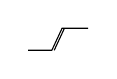
\begin{tikzpicture}\draw (0,0)--(.30,0)--(.43,.28)--(.76,.28);\draw (.33,0)--(.46,.28);\end{tikzpicture}}}}{}{author paragraph cue}{ps_134-2_037-v0019}(in a suitable sense) n-truncated homotopy types.\var{\hand{\tikz[baseline=-.4ex]{\draw (0,0)--(.30,0)--(.43,.28)--(.76,.28);\draw (.33,0)--(.46,.28);}} The third letter}{

The third letter}{author paragraph break}{ps_134-2_037-v0020}, \var{\inserted{written}}{\hand{written}}{insertion}{ps_134-2_037-v0021} \var{\inserted[typed]{in}}{in}{typed insertion}{ps_134-2_037-v0022} ans-%
wer to a number of questions in Larry Breen's response to the first two,
is of a wider scope. A large part of the letter outlines (very ske\var{\over{\unsure{t}}{tc}}{\hand{tc}}{writing over}{ps_134-2_037-v0023}hyly)
some main points of a duality program (including a cohomological formula-%
tion of ``geometric'' local and global classfield theory), which \var{\deleted{appears}}{}{deletion}{ps_134-2_037-v0024}\var{\inserted{emerged by the end of the fifties and appears}}{\hand{emerged by the end of the fifties and appears}}{insertion}{ps_134-2_037-v0025}
here for the first time in print\hand{,} \var{\deleted{and going back to the end of the fif-%
ties.}}{}{deletion}{ps_134-2_037-v0026} \var{\deleted{It}}{}{deletion}{ps_134-2_037-v0027}\var{\inserted{The later part of the letter}}{\hand{The later part of the letter}}{insertion}{ps_134-2_037-v0028} gives also some hints about the need of a framework of ``tame to-%
pology'' suitable for writing up a ``dévissage theory'' of stratified spaces,
and for \var{\xout{\unsure{dealing}}}{}{typewriter deletion}{ps_134-2_037-v0029}\var{\inserted[typed]{working}}{working}{typed insertion}{ps_134-2_037-v0030} with étale tubular neighbourhoods, for the common purpose
of coming to grips \var{\deleted{of}}{}{deletion}{ps_134-2_037-v0031}\var{\inserted{with}}{\hand{with}}{insertion}{ps_134-2_037-v0032} a suitable notion of ``fine\unsure{\hand{,}} homotopy type'' of a ``tame''
topological space or \var{\inserted{of}}{\hand{of}}{insertion}{ps_134-2_037-v0033} a scheme \var{\inserted{say}}{\hand{say}}{insertion}{ps_134-2_037-v0034}, in terms of the \var{\deleted{ordered set}}{}{deletion}{ps_134-2_037-v0035}\var{\inserted{inverse system}}{\hand{inverse system}}{insertion}{ps_134-2_037-v0036} of ``indexed
homotopy types'' corresponding to \var{\inserted{all}}{\hand{all}}{insertion}{ps_134-2_037-v0037} equisingular stratifications .

\margin{37}

%% END SOURCE ps_134-2_037
\ifnum\EditionMode=1
\psapparatusstart
\psentry{ps_134-2_037-v0001}{1}{typewriter deletion}{\xout{\unsure{1|I}}}{}{The typewriter strikes out this material; it leaves the corrected running text.}
\psentry{ps_134-2_037-v0002}{2}{typewriter deletion}{\xout{handwri}}{}{The typewriter strikes out this material; it leaves the corrected running text.}
\psentry{ps_134-2_037-v0003}{3}{deletion}{\deleted{\unsure{as it}}}{}{The author cancels this material by hand; it leaves the corrected running text.}
\psentry{ps_134-2_037-v0004}{4}{insertion}{\inserted{which}}{\hand{which}}{The handwritten insertion is incorporated at its indicated position; insertion brackets leave the running text.}
\psentry{ps_134-2_037-v0005}{5}{deletion}{\deleted{from}}{}{The author cancels this material by hand; it leaves the corrected running text.}
\psentry{ps_134-2_037-v0006}{6}{insertion}{\inserted{in}}{\hand{in}}{The handwritten insertion is incorporated at its indicated position; insertion brackets leave the running text.}
\psentry{ps_134-2_037-v0007}{7}{insertion}{\inserted{as well as \deleted{from} in}}{\hand{as well as  in}}{The handwritten insertion is incorporated at its indicated position; insertion brackets leave the running text.}
\psentry{ps_134-2_037-v0008}{8}{typewriter deletion}{\xout{copying}}{}{The typewriter strikes out this material; it leaves the corrected running text.}
\psentry{ps_134-2_037-v0009}{9}{insertion}{\inserted{that letter}}{\hand{that letter}}{The handwritten insertion is incorporated at its indicated position; insertion brackets leave the running text.}
\psentry{ps_134-2_037-v0010}{10}{writing over}{\over{u}{u}}{\hand{u}}{The superposed handwritten reading replaces the underlying reading.}
\psentry{ps_134-2_037-v0011}{11}{deletion}{\deleted{and correcting some}}{}{The author cancels this material by hand; it leaves the corrected running text.}
\psentry{ps_134-2_037-v0012}{12}{insertion}{\inserted{adding subtitles (with numbers App. 1 to App. 18), and correcting some}}{\hand{adding subtitles (with numbers App. 1 to App. 18), and correcting some}}{The handwritten insertion is incorporated at its indicated position; insertion brackets leave the running text.}
\psentry{ps_134-2_037-v0013}{13}{deletion}{\deleted{\illegible{1}}}{}{The author cancels this material by hand; it leaves the corrected running text.}
\psentry{ps_134-2_037-v0014}{14}{deletion}{\deleted{to}}{}{The author cancels this material by hand; it leaves the corrected running text.}
\psentry{ps_134-2_037-v0015}{15}{deletion}{\deleted{me}}{}{The author cancels this material by hand; it leaves the corrected running text.}
\psentry{ps_134-2_037-v0016}{16}{writing over}{\over{.}{,}}{\hand{,}}{The superposed handwritten reading replaces the underlying reading.}
\psentry{ps_134-2_037-v0017}{17}{typed insertion}{\inserted[typed]{new}}{new}{The typed insertion is incorporated at its indicated position; insertion brackets leave the running text.}
\psentry{ps_134-2_037-v0018}{18}{typewriter deletion}{\xout{which}}{}{The typewriter strikes out this material; it leaves the corrected running text.}
\psentry{ps_134-2_037-v0019}{19}{author paragraph cue}{\margin{\diagram{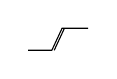
\begin{tikzpicture}\draw (0,0)--(.30,0)--(.43,.28)--(.76,.28);\draw (.33,0)--(.46,.28);\end{tikzpicture}}}}{}{The marginal stepped cue repeats the inline paragraph instruction applied before The third letter; its drawing remains in the diplomatic form.}
\psentry{ps_134-2_037-v0020}{20}{author paragraph break}{\hand{\tikz[baseline=-.4ex]{\draw (0,0)--(.30,0)--(.43,.28)--(.76,.28);\draw (.33,0)--(.46,.28);}} The third letter}{

The third letter}{The repeated stepped pen cue instructs a new paragraph at this boundary.}
\psentry{ps_134-2_037-v0021}{21}{insertion}{\inserted{written}}{\hand{written}}{The handwritten insertion is incorporated at its indicated position; insertion brackets leave the running text.}
\psentry{ps_134-2_037-v0022}{22}{typed insertion}{\inserted[typed]{in}}{in}{The typed insertion is incorporated at its indicated position; insertion brackets leave the running text.}
\psentry{ps_134-2_037-v0023}{23}{writing over}{\over{\unsure{t}}{tc}}{\hand{tc}}{The superposed handwritten reading replaces the underlying reading.}
\psentry{ps_134-2_037-v0024}{24}{deletion}{\deleted{appears}}{}{The author cancels this material by hand; it leaves the corrected running text.}
\psentry{ps_134-2_037-v0025}{25}{insertion}{\inserted{emerged by the end of the fifties and appears}}{\hand{emerged by the end of the fifties and appears}}{The handwritten insertion is incorporated at its indicated position; insertion brackets leave the running text.}
\psentry{ps_134-2_037-v0026}{26}{deletion}{\deleted{and going back to the end of the fif-%
ties.}}{}{The author cancels this material by hand; it leaves the corrected running text.}
\psentry{ps_134-2_037-v0027}{27}{deletion}{\deleted{It}}{}{The author cancels this material by hand; it leaves the corrected running text.}
\psentry{ps_134-2_037-v0028}{28}{insertion}{\inserted{The later part of the letter}}{\hand{The later part of the letter}}{The handwritten insertion is incorporated at its indicated position; insertion brackets leave the running text.}
\psentry{ps_134-2_037-v0029}{29}{typewriter deletion}{\xout{\unsure{dealing}}}{}{The typewriter strikes out this material; it leaves the corrected running text.}
\psentry{ps_134-2_037-v0030}{30}{typed insertion}{\inserted[typed]{working}}{working}{The typed insertion is incorporated at its indicated position; insertion brackets leave the running text.}
\psentry{ps_134-2_037-v0031}{31}{deletion}{\deleted{of}}{}{The author cancels this material by hand; it leaves the corrected running text.}
\psentry{ps_134-2_037-v0032}{32}{insertion}{\inserted{with}}{\hand{with}}{The handwritten insertion is incorporated at its indicated position; insertion brackets leave the running text.}
\psentry{ps_134-2_037-v0033}{33}{insertion}{\inserted{of}}{\hand{of}}{The handwritten insertion is incorporated at its indicated position; insertion brackets leave the running text.}
\psentry{ps_134-2_037-v0034}{34}{insertion}{\inserted{say}}{\hand{say}}{The handwritten insertion is incorporated at its indicated position; insertion brackets leave the running text.}
\psentry{ps_134-2_037-v0035}{35}{deletion}{\deleted{ordered set}}{}{The author cancels this material by hand; it leaves the corrected running text.}
\psentry{ps_134-2_037-v0036}{36}{insertion}{\inserted{inverse system}}{\hand{inverse system}}{The handwritten insertion is incorporated at its indicated position; insertion brackets leave the running text.}
\psentry{ps_134-2_037-v0037}{37}{insertion}{\inserted{all}}{\hand{all}}{The handwritten insertion is incorporated at its indicated position; insertion brackets leave the running text.}
\psapparatusend
\fi
\pssource{ps_134-2_038}{134-2/38}{https://grothendieck.umontpellier.fr/web/viewer.html?file=../134-2.pdf\#page=39}
\psnumber{ps_134-2_038-v0001}{1}
\psnumber{ps_134-2_038-v0002}{2}
\psnumber{ps_134-2_038-v0003}{3}
%% BEGIN SOURCE ps_134-2_038
% Pursuing Stacks (cotes 134-2 to 134-8): archive cote 134-2, site page 38 (PDF page 39).
% appendix (letters to Breen). Draft compared: ps1.tex:1174-1193.
% AI-transcribed by Claude Opus 5.5 (claude-opus-5-5, adaptive thinking, effort high), Message Batches API, batch ps1 (msgbatch_01Rv5hCaNTtUt4JHx1yqoHPL), 2026-11-12; reviewed against both supplied scan halves; see CHECK_DECISIONS.tsv.
\scanpage{134-2/38}
\mspage{\hand{23 bis}}
% NOTE: the typed text is on a slip pasted onto another typed page; text of the underlying page shows through faintly and is not transcribed

\hfill Villecun 5.2.1975\margin{--}

\margin{--} Cher Breen

\quad ....

(App.1) \quad ... Pour tout le reste de ta lettre, \ elle mériterait un lecteur
\margin{--} plus averti, \ aussi, \ pour qu'elle ne soit pas entièrement perdue au monde,
je vais l'envoyer à Illusie ! \ J'ai néanmoins
constaté\hand{,} avec intérêt\hand{,} ton intérêt à demi \unsure{rèfoulé|refoulé} pour des 2-catégories de
Picard, n-catégories et autre faune de ce genre, et ton espoir que je te
prouverai peut-être que ces animaux sont tout à fait indispensables pour
faire des maths sérieuses \ dans telle ou telle circonstance. J'ai bien \hand{peur}
que cet espoir ne soit déçu, je crois que jusqu'à maintenant on a toujours
pu s'en tirer en éludant de tels objets et l'engrenage dans lequel ils pour
-raient nous entrainer. Est-ce nécessairement une raison pour continuer à
les éluder ? Les situations où on a l'impression"d'éluder" en effet me sem-%
blent en tous cas devenir toujours plus nombreuses - \ et si on s'abstenait
de tirer une situation complexe et chargée de mystère au clair, ch\'aque
fois qu'on ne serait pas \uline{forcé} de le faire pour des raisons techniques pro-%
venant de la math déjà faite, - il y aurait sans doute beaucoup de parties
des maths aujourd'hui \var{reputées\hand{|}"sérieuses"}{reputées "sérieuses"}{author spacing cue}{ps_134-2_038-v0001} qui n'auraient jamais \var{\inserted{été}}{\hand{été}}{insertion}{ps_134-2_038-v0002} développées
(Il n'est pas dit non plus \var{que\hand{|}le monde}{que le monde}{author spacing cue}{ps_134-2_038-v0003} s'en trouverait plus mal ...). Ton
commentaire (que j'ai également entendu chez Deligne) \ que la classificati-%
on d'objets géométriques relativement merdiques se réduit finalement à des
invariants cohomologiques essentiellement "bien connus" et relativement
simples n'est pas non plus convainquant; n'est ce pas négliger la différen-%
ce entre la \uline{compréhension d'un objet géométrique}, et la détermination de
sa "classe à isomorphisme (ou équivalence...) près" ?

\margin{38}

%% END SOURCE ps_134-2_038
\ifnum\EditionMode=1
\psapparatusstart
\psentry{ps_134-2_038-v0001}{1}{author spacing cue}{reputées\hand{|}"sérieuses"}{reputées "sérieuses"}{The continuous pen stroke marks a missing space at this line boundary; apply the space while preserving its graphic in the diplomatic form.}
\psentry{ps_134-2_038-v0002}{2}{insertion}{\inserted{été}}{\hand{été}}{The handwritten insertion is incorporated at its indicated position; insertion brackets leave the running text.}
\psentry{ps_134-2_038-v0003}{3}{author spacing cue}{que\hand{|}le monde}{que le monde}{The same continuous pen stroke intersects the next line between que and le; apply the indicated word space.}
\psapparatusend
\fi
\pssource{ps_134-2_039}{134-2/39}{https://grothendieck.umontpellier.fr/web/viewer.html?file=../134-2.pdf\#page=40}
\psnumber{ps_134-2_039-v0001}{1}
\psnumber{ps_134-2_039-v0002}{2}
\psnumber{ps_134-2_039-v0003}{3}
\psnumber{ps_134-2_039-v0004}{4}
\psnumber{ps_134-2_039-v0005}{5}
\psnumber{ps_134-2_039-v0006}{6}
\psnumber{ps_134-2_039-v0007}{7}
\psnumber{ps_134-2_039-v0008}{8}
\psnumber{ps_134-2_039-v0009}{9}
\psnumber{ps_134-2_039-v0010}{10}
\psnumber{ps_134-2_039-v0011}{11}
\psnumber{ps_134-2_039-v0012}{12}
\psnumber{ps_134-2_039-v0013}{13}
\psnumber{ps_134-2_039-v0014}{14}
\psnumber{ps_134-2_039-v0015}{15}
\psnumber{ps_134-2_039-v0016}{16}
\psnumber{ps_134-2_039-v0017}{17}
\psnumber{ps_134-2_039-v0018}{18}
\psnumber{ps_134-2_039-v0019}{19}
%% BEGIN SOURCE ps_134-2_039
% Pursuing Stacks (cotes 134-2 to 134-8): archive cote 134-2, site page 39 (PDF page 40).
% appendix (letters to Breen). Draft compared: ps1.tex:1193-1197.
% AI-transcribed by Claude Opus 5.5 (claude-opus-5-5, adaptive thinking, effort high), Message Batches API, batch ps1 (msgbatch_01Rv5hCaNTtUt4JHx1yqoHPL), 2026-11-12; reviewed against both supplied scan halves; see CHECK_DECISIONS.tsv.
\scanpage{134-2/39}
\mspage{\hand{24}}

Tu me demandes des exemples "convainquants" de 2-catégories de Picard.
Voici quelques \var{\deleted{uns}}{}{deletion}{ps_134-2_039-v0001}\var{\inserted{exemples,}}{\hand{exemples,}}{insertion}{ps_134-2_039-v0002} en vrac \hand{(je ne sais s'ils seront convainquants !)}:

\margin{$\times$(22)} 1) Si L est un lien\var{\inserted{(22)}}{\hand{(22)}}{insertion}{ps_134-2_039-v0003} de centre Z sur le topos X, les \uline{gerbes liées par Z}
forment une 2-catégorie de Picard stricte, représentée par le complexe
$R\hand{\Gamma}_X(Z)$ tronqué en degré 2, dont les objets de cohomologie non triviaux
sont \unsure{Hes|les} $H^i(X,Z)$, $0 \hand{\leqslant} i \hand{\leqslant} 2$. Les \var{\over{\unsure{g}}{g}}{\hand{g}}{writing over}{ps_134-2_039-v0004}erbes liées par L forment un \uline{pseudo-2-}
\uline{torseur} sous la gerbe précédente, qui est un 2-torseur\hand{(}i.e. non vide\hand{)} sss
une certaine obstruction dans $H^3(X,Z)$ est nulle. Pour comprendre \unsure{cette}
classe de notre point de vue, il y a lieu de passer aux 2-champs derres-%
pondants: le 2-champ de\var{\xout{s}}{}{typewriter deletion}{ps_134-2_039-v0005} Picard \var{\inserted[typed]{strict,}}{strict,}{typed insertion}{ps_134-2_039-v0006} des Z-gerbes\var{\xout{\unsure{liées par Z et le 2-champ des}}}{}{typewriter deletion}{ps_134-2_039-v0007}
sur des objets variables de X, et le 2-champ des L-gerbes sur des objets
variables. Ce dernier est bel et bien un 2-torseur sous le champ précédent,
or la classification de ces \var{\xout{deux}}{}{typewriter deletion}{ps_134-2_039-v0008} 2-torseurs (à 2-équivalence près) se
fait par le $H^3(X,Z)$, \var{\xout{de façon précise}}{}{typewriter deletion}{ps_134-2_039-v0009} \hand{(}tout comme les Z-\var{\inserted{1-}}{\hand{1-}}{insertion}{ps_134-2_039-v0010}gerbes peuvent être
interpétées comme des \var{\deleted{\unsure{1}}}{}{deletion}{ps_134-2_039-v0011}torseurs sous la Z-1-\var{\over{\unsure{gerbe}}{champ}}{\hand{champ}}{writing over}{ps_134-2_039-v0012} \var{\inserted[typed]{de Picard strict,}}{de Picard strict,}{typed insertion}{ps_134-2_039-v0013} des Z-torseurs, et sont
\var{\xout{par conséquent}}{}{typewriter deletion}{ps_134-2_039-v0014} classifiées par le $H^2(X,Z)$\hand{)}. On voit déjà, bien sûr, poindre
ici l'oreille de la 3-catégorie de Picard stricte des 2-gerbes liées par Z,
ou (de façon équivalente) des 2-torseurs sous le 2-champ de Picard strict
des Z-1-gerbes; cette 3-catégorie de Picard stricte étant décrite par
$R\hand{\Gamma}_X(Z)$ tronqué en dimension 3, ayant comme invariants de cohomologie non
triviaux les $H^i(X,Z)$ $(0 \hand{\leqslant} i \hand{\leqslant} 3)$. Quant au 3-champ de Picard correspondaht,
il est décrit par une résolution injective de Z \hand{tronquée} en degré 3, alors
que le  2-champ de Picard précédent se décrivait en tronquant en degré 2.

2. Si M et N sont deux faisceaux abéliens sur X, les \uline{champs de Picard}
(NB: 1-champs !) \uline{d'invariants} M \uline{et} N forment eux-même une \var{\inserted{2-}}{\hand{2-}}{insertion}{ps_134-2_039-v0015}catégorie de
\margin{$\times$} Picard stricte, représentée  sans doute par le complexe RHom(X(M),N) \var{\inserted{(23)}}{\hand{(23)}}{insertion}{ps_134-2_039-v0016}
tronqué en \var{\xout{dimension}}{}{typewriter deletion}{ps_134-2_039-v0017} degré 2, dont les invariants de chomologie non trivi-%
aux sont donc \hand{``}le drôle de $\mathrm{Ext}^2$\hand{''} de ma lettre à Deligne, et les Honnètes
$\mathrm{Ext}^i(M,N)$  $(0 \hand{\leqslant} i \hand{\leqslant} 1)$. Les champs de Picard stricts forment une sous-2-caté%
gorie de Picard pleine, représentée par RHom(M,N) tronqué en degré 2,
d'invariants les $\mathrm{Ext}^i(M;N)$ $(0 \hand{\leqslant} i \hand{\leqslant} 2)$. Bien sûr, $\mathrm{Ext}^2$ donne les \var{\inserted{0-}}{\hand{0-}}{insertion}{ps_134-2_039-v0018}objets à
équivalence près, $\mathrm{Ext}^1$ les automorphismes à isomorphisme près de l'objet
nul, $\mathrm{Ext}^0$ les automorphismes de l'automorphisme identique audit ... Je n'ai
pas réfléchi à une bonne interprétation géométrique de la n-catégorie de
Picard associée à RHom(M,N) tronqué en degré n, et encore moins bien \var{\xout{s}}{}{typewriter deletion}{ps_134-2_039-v0019}sûr
pour RHom(X(M),N), mais sans doute il faut regarder dans la direction des
n-champs de Picard.

3. Soit G un Groupe sur X, opérant sur un faisceau abélien N. Les \uline{champs}
\uline{en} (Gr)-\uline{catégories sur} X \uline{liés par} (G,N) forment une 2-catégorie de Picard,

\margin{\hand{39}}

%% END SOURCE ps_134-2_039
\ifnum\EditionMode=1
\psapparatusstart
\psentry{ps_134-2_039-v0001}{1}{deletion}{\deleted{uns}}{}{The author cancels this material by hand; it leaves the corrected running text.}
\psentry{ps_134-2_039-v0002}{2}{insertion}{\inserted{exemples,}}{\hand{exemples,}}{The handwritten insertion is incorporated at its indicated position; insertion brackets leave the running text.}
\psentry{ps_134-2_039-v0003}{3}{insertion}{\inserted{(22)}}{\hand{(22)}}{The handwritten insertion is incorporated at its indicated position; insertion brackets leave the running text.}
\psentry{ps_134-2_039-v0004}{4}{writing over}{\over{\unsure{g}}{g}}{\hand{g}}{The superposed handwritten reading replaces the underlying reading.}
\psentry{ps_134-2_039-v0005}{5}{typewriter deletion}{\xout{s}}{}{The typewriter strikes out this material; it leaves the corrected running text.}
\psentry{ps_134-2_039-v0006}{6}{typed insertion}{\inserted[typed]{strict,}}{strict,}{The typed insertion is incorporated at its indicated position; insertion brackets leave the running text.}
\psentry{ps_134-2_039-v0007}{7}{typewriter deletion}{\xout{\unsure{liées par Z et le 2-champ des}}}{}{The typewriter strikes out this material; it leaves the corrected running text.}
\psentry{ps_134-2_039-v0008}{8}{typewriter deletion}{\xout{deux}}{}{The typewriter strikes out this material; it leaves the corrected running text.}
\psentry{ps_134-2_039-v0009}{9}{typewriter deletion}{\xout{de façon précise}}{}{The typewriter strikes out this material; it leaves the corrected running text.}
\psentry{ps_134-2_039-v0010}{10}{insertion}{\inserted{1-}}{\hand{1-}}{The handwritten insertion is incorporated at its indicated position; insertion brackets leave the running text.}
\psentry{ps_134-2_039-v0011}{11}{deletion}{\deleted{\unsure{1}}}{}{The author cancels this material by hand; it leaves the corrected running text.}
\psentry{ps_134-2_039-v0012}{12}{writing over}{\over{\unsure{gerbe}}{champ}}{\hand{champ}}{The superposed handwritten reading replaces the underlying reading.}
\psentry{ps_134-2_039-v0013}{13}{typed insertion}{\inserted[typed]{de Picard strict,}}{de Picard strict,}{The typed insertion is incorporated at its indicated position; insertion brackets leave the running text.}
\psentry{ps_134-2_039-v0014}{14}{typewriter deletion}{\xout{par conséquent}}{}{The typewriter strikes out this material; it leaves the corrected running text.}
\psentry{ps_134-2_039-v0015}{15}{insertion}{\inserted{2-}}{\hand{2-}}{The handwritten insertion is incorporated at its indicated position; insertion brackets leave the running text.}
\psentry{ps_134-2_039-v0016}{16}{insertion}{\inserted{(23)}}{\hand{(23)}}{The handwritten insertion is incorporated at its indicated position; insertion brackets leave the running text.}
\psentry{ps_134-2_039-v0017}{17}{typewriter deletion}{\xout{dimension}}{}{The typewriter strikes out this material; it leaves the corrected running text.}
\psentry{ps_134-2_039-v0018}{18}{insertion}{\inserted{0-}}{\hand{0-}}{The handwritten insertion is incorporated at its indicated position; insertion brackets leave the running text.}
\psentry{ps_134-2_039-v0019}{19}{typewriter deletion}{\xout{s}}{}{The typewriter strikes out this material; it leaves the corrected running text.}
\psapparatusend
\fi
\pssource{ps_134-2_040}{134-2/40}{https://grothendieck.umontpellier.fr/web/viewer.html?file=../134-2.pdf\#page=41}
\psnumber{ps_134-2_040-v0001}{1}
\psnumber{ps_134-2_040-v0002}{2}
\psnumber{ps_134-2_040-v0003}{3}
\psnumber{ps_134-2_040-v0004}{4}
\psnumber{ps_134-2_040-v0005}{5}
\psnumber{ps_134-2_040-v0006}{6}
\psnumber{ps_134-2_040-v0007}{7}
\psnumber{ps_134-2_040-v0008}{8}
\psnumber{ps_134-2_040-v0009}{9}
\psnumber{ps_134-2_040-v0010}{10}
\psnumber{ps_134-2_040-v0011}{11}
%% BEGIN SOURCE ps_134-2_040
% Pursuing Stacks (cotes 134-2 to 134-8): archive cote 134-2, site page 40 (PDF page 41).
% appendix (letters to Breen). Draft compared: ps1.tex:1195-1203.
% AI-transcribed by Claude Opus 5.5 (claude-opus-5-5, adaptive thinking, effort high), Message Batches API, batch ps1 (msgbatch_01Rv5hCaNTtUt4JHx1yqoHPL), 2026-11-12; reviewed against both supplied scan halves; see CHECK_DECISIONS.tsv.
\scanpage{134-2/40}
\mspage{\hand{25}}

dont les invariants sont $H^3(B_G \text{ mod } X,N)$, $H^2(B_G \text{ mod } X,N)$, et $Z^1(G,N)$ (groupe
des 1-cocyles de $G$ à coéfficients dans $N$)- je te laisse le soin de deviner
quel est le complexe tronqué qui le décrit ! J'ai écrit il y a quelques
mois à Deligne à ce sujet, et l'ai prié de t'envoyer une copie de \var{\xout{envoyer}}{}{typewriter deletion}{ps_134-2_040-v0001}
la lettre.

4) Soit $X$ un topos localement annelé, on peut considérer les \uline{Algèbres
d'Azumaya sur} $X$ (i.e. les Algèbres localement isomorphes à une alg. de
matrices d'ordre $n$, $n \hand{\geq} 1$) comme les objets d'une 2-catégorie de Picard,
où la catégorie $\underline{\mathrm{Hom}}(A,B)$, pour $A$ et $B$ des Algèbres d'Azumaya, est la caté-%
gorie des ``trivialisations'' de $A^o\otimes B$, i.e. des couples $(E,\hand{\phi})$, $E$ un Module
localement libre et $\hand{\phi}$ un isomorphisme $\underline{\mathrm{End}}(E)\simeq A^o\otimes B$. Il faut travailler
un peu pour définir les accouplements\var{\xout{x}}{}{typewriter deletion}{ps_134-2_040-v0002} $\underline{\mathrm{Hom}}(A,B)\mathrm{x}\underline{\mathrm{Hom}}(B,C)\hand{\to}\underline{\mathrm{Hom}}(A,C)$; l'opé-%
ration $\otimes$ dans la 2-catégorie de Picard à construire est bien sûr le produit
tensoriel d'Algèbres, et l'opération ``puissance $-1$'' est le passage à l'al-%
gèbre opposée. On \unsure{vérfie|vérifie}\var{\xout{,x\allowbreak{}x\allowbreak{} passant aux champs correspondant, qui sont}}{}{typewriter deletion}{ps_134-2_040-v0003} qu'en
associant à toute Algèbre d'Azumaya la 1-gerbe de ses trivialisations, on
trouve un 2-$\otimes$-foncteur de la 2-catégorie de Picard (dite ``de Brauer'') dans
celle des 1-gerbes liées par $\underline{G}_m$ , qui est 2-fidèle. Les invariants de
la première sont donc les groupes $H^2(X,\underline{G}_m)_{Br}$ , $H^1(X,\underline{H}_m)$ et $H^o(X,\underline{G}_m)$ , où
dans le premier terme l'indice Br désigne le sous-groupe du $H^2$ formé des
classes de cohomologie provenant d'Algèbres d'Azumaya. On aurait envie
de parler du 2-champ de Picard des Algèbres d'Azumaya sur des objets variab
les de $X$, mais c'est bien une 2-catégorie de Picard fibrée sur $X$, mais pas
tout à fait un 2-champ (whatever that means), sans doute - la condition de
2-recollement (whatever that means) ne doit pas être satisfaite - sinon il
n'y aurait pas d'indice Br au $H^2$ ...
\var{\margin{\(\uparrow\) espace \(\downarrow\)}}{\par\medskip}{author spacing cue}{ps_134-2_040-v0004}

\var{\inserted{(App.2)}}{\hand{(App.2)}}{insertion}{ps_134-2_040-v0005} La considération des $n$-catégories de Picard \var{\inserted[typed]{strictes}}{strictes}{typed insertion}{ps_134-2_040-v0006} (qui s'imposent à nous pas
à pas dans un contexte essentiellement ``commutatif'') me semblent la clef du
passage de l'algèbre homologique ordinaire (``commutative''), en termes de
complexes, à une algèbre homologique non commutative, du fait qu'elles
donnent une interprétation géométrique correcte des ``complexes tronqués à
l'ordre $n$'' \var{\inserted{(en tant qu'objets de catégories dérivées)}}{\hand{(en tant qu'objets de catégories dérivées)}}{insertion}{ps_134-2_040-v0007}, donc, essentiellement (par passage à la limite sur $n$) des
complexes tout courts. L'idée naive qui se présente est alors que les
``complexes non commutatifs'' (qui seraient les objets-fantômes d'une algèbre
homologique non commutative) sont peut-être ce qui reste des $n$-catégories
de Picard (strictes) quand on oublie \var{leut caractère}{leur caractère}{slip corrected}{ps_134-2_040-v0008} additif, i.e. leur
structure de Picard - c'est à dire qu'on ne retient que la $n$-catégorie !
\var{\inserted{(Quand on se place sur un topos $X$, on s'intéresse donc aux $n$-champs sur $X$...)}}{\hand{(Quand on se place sur un topos $X$, on s'intéresse donc aux $n$-champs sur $X$...)}}{insertion}{ps_134-2_040-v0009}
A vrai dire, cette idée est venue d'abord d'une autre direction, quand il
s'est agi en géométrie algébrique de démontrer des \uline{\var{\deleted{formules}}{}{deletion}{ps_134-2_040-v0010}\var{\inserted{théorèmes}}{\hand{théorèmes}}{insertion}{ps_134-2_040-v0011} de Lefschetz}

\margin{\hand{40}}

%% END SOURCE ps_134-2_040
\ifnum\EditionMode=1
\psapparatusstart
\psentry{ps_134-2_040-v0001}{1}{typewriter deletion}{\xout{envoyer}}{}{The typewriter strikes out this material; it leaves the corrected running text.}
\psentry{ps_134-2_040-v0002}{2}{typewriter deletion}{\xout{x}}{}{The typewriter strikes out this material; it leaves the corrected running text.}
\psentry{ps_134-2_040-v0003}{3}{typewriter deletion}{\xout{,x\allowbreak{}x\allowbreak{} passant aux champs correspondant, qui sont}}{}{The typewriter strikes out this material; it leaves the corrected running text.}
\psentry{ps_134-2_040-v0004}{4}{author spacing cue}{\margin{\(\uparrow\) espace \(\downarrow\)}}{\par\medskip}{Apply the opposed arrows and espace instruction as additional paragraph separation before App.2; retain the graphic diplomatically.}
\psentry{ps_134-2_040-v0005}{5}{insertion}{\inserted{(App.2)}}{\hand{(App.2)}}{The handwritten insertion is incorporated at its indicated position; insertion brackets leave the running text.}
\psentry{ps_134-2_040-v0006}{6}{typed insertion}{\inserted[typed]{strictes}}{strictes}{The typed insertion is incorporated at its indicated position; insertion brackets leave the running text.}
\psentry{ps_134-2_040-v0007}{7}{insertion}{\inserted{(en tant qu'objets de catégories dérivées)}}{\hand{(en tant qu'objets de catégories dérivées)}}{The handwritten insertion is incorporated at its indicated position; insertion brackets leave the running text.}
\psentry{ps_134-2_040-v0008}{8}{slip corrected}{leut caractère}{leur caractère}{One-off t for r; leur is correctly typed in the following clause referring to the same Picard structure.}
\psentry{ps_134-2_040-v0009}{9}{insertion}{\inserted{(Quand on se place sur un topos $X$, on s'intéresse donc aux $n$-champs sur $X$...)}}{\hand{(Quand on se place sur un topos $X$, on s'intéresse donc aux $n$-champs sur $X$...)}}{The handwritten insertion is incorporated at its indicated position; insertion brackets leave the running text.}
\psentry{ps_134-2_040-v0010}{10}{deletion}{\deleted{formules}}{}{The author cancels this material by hand; it leaves the corrected running text.}
\psentry{ps_134-2_040-v0011}{11}{insertion}{\inserted{théorèmes}}{\hand{théorèmes}}{The handwritten insertion is incorporated at its indicated position; insertion brackets leave the running text.}
\psapparatusend
\fi
\pssource{ps_134-2_041}{134-2/41}{https://grothendieck.umontpellier.fr/web/viewer.html?file=../134-2.pdf\#page=42}
\psnumber{ps_134-2_041-v0001}{1}
\psnumber{ps_134-2_041-v0002}{2}
\psnumber{ps_134-2_041-v0003}{3}
\psnumber{ps_134-2_041-v0004}{4}
\psnumber{ps_134-2_041-v0005}{5}
\psnumber{ps_134-2_041-v0006}{6}
\psnumber{ps_134-2_041-v0007}{7}
\psnumber{ps_134-2_041-v0008}{8}
\psnumber{ps_134-2_041-v0009}{9}
\psnumber{ps_134-2_041-v0010}{10}
\psnumber{ps_134-2_041-v0011}{11}
\psnumber{ps_134-2_041-v0012}{12}
\psnumber{ps_134-2_041-v0013}{13}
\psnumber{ps_134-2_041-v0014}{14}
\psnumber{ps_134-2_041-v0015}{15}
\psnumber{ps_134-2_041-v0016}{16}
%% BEGIN SOURCE ps_134-2_041
% Pursuing Stacks (cotes 134-2 to 134-8): archive cote 134-2, site page 41 (PDF page 42).
% appendix (letters to Breen). Draft compared: ps1.tex:1203-1205.
% AI-transcribed by Claude Opus 5.5 (claude-opus-5-5, adaptive thinking, effort high), Message Batches API, batch ps1 (msgbatch_01Rv5hCaNTtUt4JHx1yqoHPL), 2026-11-12; reviewed against both supplied scan halves; see CHECK_DECISIONS.tsv.
\scanpage{134-2/41}
\mspage{\hand{26}}

à coéfficients discrets \var{\inserted{en cohomologie étale}}{\hand{en cohomologie étale}}{insertion}{ps_134-2_041-v0001}, dans le cas d'une variété projective disons et
de toute section hyperplane, ou d'une variété quasi-projective et de presque
toute section hyperplane (pour ne mentionner que le cas global le plus sim-%
ple), sous les hypothèses de profondeur \var{\inserted[typed]{cohomologique}}{cohomologique}{typed insertion}{ps_134-2_041-v0002} ``les plus naturelles'' (en fait,
essenti\var{\over{\unsure{a}}{e}}{\hand{e}}{writing over}{ps_134-2_041-v0003}llement des conditions néc. et suff. de validité dudit théorème).
Dans le cas commutatif, les techniques de dualité nous suggèrent très clai-%
rement quels sont les meilleurs énoncés possibles, cf. l'exposé de Mme \var{Ray-%
naus}{Ray-%
naud}{slip corrected}{ps_134-2_041-v0004} dans SGA 2. Mais ces techniques ne valent qu'en se restreignant à des
coéfficients premiers aux caractéristiques, alors que des démonstrations
directes plus géométriques (développées dans SGA 2 av\var{\over{\unsure{e}}{a}}{\hand{a}}{writing over}{ps_134-2_041-v0005}nt le développement
du formalisme de la cohomologie étale) donnaient des résultats très voisins
\margin{$\pi_0,\pi_1$}pour le H$^0$ et le H$^1$ (ou le \var{\inserted{$\pi_0$ et le}}{\hand{$\pi_0$ et le}}{insertion}{ps_134-2_041-v0006} $\hand{\pi}_1$ , si on préfère) sans telles restrictions,
du moins dans le cas propre (i.e. projectif, au lieu de quasi-projectif).
En fai\hand{t}, ce sont \var{\deleted{en fait}}{}{deletion}{ps_134-2_041-v0007} \var{\over{\unsure{d}}{l}}{\hand{l}}{writing over}{ps_134-2_041-v0008}es ``résultats les meilleurs possibles'' eux-%
mêmes, énoncés comme conjectures dans SGA 2 dans l'exposé cité de Mme \var{\over{\unsure{R}}{R}}{\hand{R}}{writing over}{ps_134-2_041-v0009}ay-%
naud, qui sont démontrés ultérieurement par elle dans sa thèse. Ce qui est
remarquable de notre point de vue, c'est que les énoncés les plus forts se
présentent le plus naturellement sous forme d'énoncés sur des \var{\inserted{1-}}{\hand{1-}}{insertion}{ps_134-2_041-v0010}\uline{champs} sur
le site étale de la variété algébrique considérée - la notion de ``profon-%
deur $\hand{\geq}$ i'' (pour i=\var{\over{1}{1}}{\hand{1}}{writing over}{ps_134-2_041-v0011},2,3) s'énonçant aussi le plus naturellement en termes
de champs. Non seulement cela, mais alors même qu'on voudrait ignorer la
notion technique de champ et travailler exclusivement en termes de H$^0$ et
H$^1$en utilisant à bloc le formalisme \var{\inserted{cohomologique non commutatif}}{\hand{cohomologique non commutatif}}{insertion}{ps_134-2_041-v0012} de Giraud, pour démontrer disons un
théorème de bijectivité $\hand{\pi}_1$(Y)$\hand{\to}\hand{\pi}_1$(X) (ce qui est le résultat le plus pro-%
fond établi dans la thèse de Mme Raynaud), il semble bien qu'on n'y arrive\hand{\unsure{''}}
\var{\xout{xxxx}}{}{typewriter deletion}{ps_134-2_041-v0013} pas, faute \var{\xout{dxxxxixxa}}{}{typewriter deletion}{ps_134-2_041-v0014} à ce formalisme d'avoir la souplesse nécessaire\hand{.}
En fait, il faut utiliser comme ingrédients techniques, de façon essentielle\hand{,}
les trois théorèmes suivants directement pour les 1-champs ``de torsion''
(i.e. où les faisceaux en groupes d'automorphismes sont de ind-torsion):
a) théorème de changement de base pour un morphisme propre, b) théorème de
changement de base par un morphisme lisse  c) théorème de \var{\xout{xhanx}}{}{typewriter deletion}{ps_134-2_041-v0015} ``propreté
cohomologique générique'' pour un morphisme de type fini f: X$\hand{\to}$S, S intègre
(disant que l'on peut trouver dans S un ouvert U$\neq\emptyset$ tel que pour \uline{tout} change
ment de base S'$\hand{\to}$ S se factorisant par u, la formule de changement de base
est vraie). \hand{(}Pour b) et c), il faut faire des hypothèses que les \var{faisdeaux}{faisceaux}{slip corrected}{ps_134-2_041-v0016}
d'automorphismes sont premiers aux cara\unsure{ct}érisitques, et dans c) une hypothè
se de constructtibilité sur ces faisceaux - mais b) et c) ne servent que
dans la version ``générique'' du th. de Lefschetz.\hand{)} C'est avec en vue de telle\hand{s}
applications que Giraud a pris la peine dans son bouquin (si je ne me trompe\hand{)}
de demontrer a)\hand{,} b) (et c) ?) dans le contexte des 1-champs et de leurs

\margin{\hand{41}}

%% END SOURCE ps_134-2_041
\ifnum\EditionMode=1
\psapparatusstart
\psentry{ps_134-2_041-v0001}{1}{insertion}{\inserted{en cohomologie étale}}{\hand{en cohomologie étale}}{The handwritten insertion is incorporated at its indicated position; insertion brackets leave the running text.}
\psentry{ps_134-2_041-v0002}{2}{typed insertion}{\inserted[typed]{cohomologique}}{cohomologique}{The typed insertion is incorporated at its indicated position; insertion brackets leave the running text.}
\psentry{ps_134-2_041-v0003}{3}{writing over}{\over{\unsure{a}}{e}}{\hand{e}}{The superposed handwritten reading replaces the underlying reading.}
\psentry{ps_134-2_041-v0004}{4}{slip corrected}{Ray-%
naus}{Ray-%
naud}{One-off final s for d; Raynaud appears twice later on this same checked page.}
\psentry{ps_134-2_041-v0005}{5}{writing over}{\over{\unsure{e}}{a}}{\hand{a}}{The superposed handwritten reading replaces the underlying reading.}
\psentry{ps_134-2_041-v0006}{6}{insertion}{\inserted{$\pi_0$ et le}}{\hand{$\pi_0$ et le}}{The handwritten insertion is incorporated at its indicated position; insertion brackets leave the running text.}
\psentry{ps_134-2_041-v0007}{7}{deletion}{\deleted{en fait}}{}{The author cancels this material by hand; it leaves the corrected running text.}
\psentry{ps_134-2_041-v0008}{8}{writing over}{\over{\unsure{d}}{l}}{\hand{l}}{The superposed handwritten reading replaces the underlying reading.}
\psentry{ps_134-2_041-v0009}{9}{writing over}{\over{\unsure{R}}{R}}{\hand{R}}{The superposed handwritten reading replaces the underlying reading.}
\psentry{ps_134-2_041-v0010}{10}{insertion}{\inserted{1-}}{\hand{1-}}{The handwritten insertion is incorporated at its indicated position; insertion brackets leave the running text.}
\psentry{ps_134-2_041-v0011}{11}{writing over}{\over{1}{1}}{\hand{1}}{The superposed handwritten reading replaces the underlying reading.}
\psentry{ps_134-2_041-v0012}{12}{insertion}{\inserted{cohomologique non commutatif}}{\hand{cohomologique non commutatif}}{The handwritten insertion is incorporated at its indicated position; insertion brackets leave the running text.}
\psentry{ps_134-2_041-v0013}{13}{typewriter deletion}{\xout{xxxx}}{}{The typewriter strikes out this material; it leaves the corrected running text.}
\psentry{ps_134-2_041-v0014}{14}{typewriter deletion}{\xout{dxxxxixxa}}{}{The typewriter strikes out this material; it leaves the corrected running text.}
\psentry{ps_134-2_041-v0015}{15}{typewriter deletion}{\xout{xhanx}}{}{The typewriter strikes out this material; it leaves the corrected running text.}
\psentry{ps_134-2_041-v0016}{16}{slip corrected}{faisdeaux}{faisceaux}{One-off d for c; faisceaux is correctly typed in the following constructibility qualification on this checked page.}
\psapparatusend
\fi
\pssource{ps_134-2_042}{134-2/42}{https://grothendieck.umontpellier.fr/web/viewer.html?file=../134-2.pdf\#page=43}
\psnumber{ps_134-2_042-v0001}{1}
\psnumber{ps_134-2_042-v0002}{2}
\psnumber{ps_134-2_042-v0003}{3}
\psnumber{ps_134-2_042-v0004}{4}
\psnumber{ps_134-2_042-v0005}{5}
\psnumber{ps_134-2_042-v0006}{6}
\psnumber{ps_134-2_042-v0007}{7}
\psnumber{ps_134-2_042-v0008}{8}
\psnumber{ps_134-2_042-v0009}{9}
\psnumber{ps_134-2_042-v0010}{10}
\psnumber{ps_134-2_042-v0011}{11}
\psnumber{ps_134-2_042-v0012}{12}
\psnumber{ps_134-2_042-v0013}{13}
\psnumber{ps_134-2_042-v0014}{14}
\psnumber{ps_134-2_042-v0015}{15}
%% BEGIN SOURCE ps_134-2_042
% Pursuing Stacks (cotes 134-2 to 134-8): archive cote 134-2, site page 42 (PDF page 43).
% appendix (letters to Breen). Draft compared: ps1.tex:1203-1212.
% AI-transcribed by Claude Opus 5.5 (claude-opus-5-5, adaptive thinking, effort high), Message Batches API, batch ps1 (msgbatch_01Rv5hCaNTtUt4JHx1yqoHPL), 2026-11-12; reviewed against both supplied scan halves; see CHECK_DECISIONS.tsv.
\scanpage{134-2/42}
\mspage{\hand{27}}

images directes et inverses. Mais du même coup il devient clair que le
\var{contexte\hand{|}}{contexte }{author spacing cue}{ps_134-2_042-v0001}``\var{naturel''\hand{/}des}{naturel'' des}{author spacing cue}{ps_134-2_042-v0002} théorèmes de changement de base en c\unsure{\var{\over[typed]{b}{o}}{o}{typewriter overwriting}{ps_134-2_042-v0003}}homologie étale,
des théorèmes \var{\inserted[typed]{du type}}{du type}{typed insertion}{ps_134-2_042-v0004} de Lefschetz (dits ``faibles'') sur les ``sections hyperplanes'',
tout comme \var{\inserted[typed]{de}}{de}{typed insertion}{ps_134-2_042-v0005} la notion de profondeur qui y joue un rôle crucial, \hand{doit} \var{\inserted{être}}{\hand{être}}{insertion}{ps_134-2_042-v0006} celui
des n-champs. Et que le développement hypothétique de ce contexte\var{\deleted{,}}{}{deletion}{ps_134-2_042-v0007} ne ris-%
que pas de se réduire à une jonglerie purement formelle et absolument bor-%
délique avec du ``general nonsense'', mais qu'on se trouvera aussitôt confron-%
té à des tests ``d'utilisabilité'' aussi sérieux que la démonstration des
théorèmes de changement de base et ceux du type de Lefschetz (qui même
dans le contexte commutatif ne sont pas piqués de vers ...). \hand{Idem pour
variantes analytiques complexes etc.}

Je ne sais si ces commentaires te ``passent par dessus la tête'' à ton
tour, ni si elles te donnent l'impression \var{qu'il\hand{/}}{qu'il }{author spacing cue}{ps_134-2_042-v0008}\var{y\hand{/}aurait}{y aurait}{author spacing cue}{ps_134-2_042-v0009} peut-être des cho-%
ses intéressantes à tirer au clair. Si cela t'intéresse, je pourrais expli-%
citer sous forme un peu plus systématique quelques ingrédients d'une hypo-%
thétique algèbre homologique non commutative et les liens de celle-ci à
l'algèbre homologique commutative. Plus mystérieux pour moi (et pour cause,
vu mon ignorance en homotopie) seraient les relations entre celle-là et
l'algèbre homotopique, I.e. les structures semi-simpliciales, et je n'ai
que des commentaires assez vagues à faire en ce sens\hand{(*)}.Par ailleurs, je te
rappelle que même l'algèbre homologique \var{\xout{\illegible{1}}}{}{typewriter deletion}{ps_134-2_042-v0010} commutative n'est pas, il s'en
faut, dans un état satisfaisant, pour autant que je sache, vu qu'on ne sait
\margin{(24)} toujours pas quelle est la ``bonne'' notion de catégorie triangulée\hand{\unsure{(*)}}. Or il me
semble bien clair que ce n'est pas une question purement académique - même
si on a pu se passer de le savoir jusqu'ici (en se bornant comme Monsieur
Jourdain à ``faire de la \unsure{prosé|prose} sans le savoir'' - en travaillant sur des
catégories de complexes, éventuellement filtrés, sans trop se demander quel
-les structures il y a sur ces catégories ...).

Bien cordialement à toi

\hand{A Grothendieck}

\margin{(App.3)} \hand{(*) P.S.} Réflexion faite, j'ai quand même envie de te mettre un peu en ap-%
pétit, en faisant ces ``quelques commentaires assez vagues\hand{''}. Il s'agit du
yoga qu'une \var{\inserted{\deleted{\illegible{1}} (petite)}}{\hand{ (petite)}}{insertion}{ps_134-2_042-v0011} n-catégorie \var{\inserted{en groupoïdes}}{\hand{en groupoïdes}}{insertion}{ps_134-2_042-v0012} (à n-équivalence près\unsure{\hand{)}} \var{\deleted{\unsure{``}est}}{}{deletion}{ps_134-2_042-v0013} \var{\inserted{``est}}{\hand{``est}}{insertion}{ps_134-2_042-v0014} essentiellement la même
chose'' qu'un ensemble semi-simplicial pris à homotopie près et où on négli-%
ge les \hand{$\pi$}$_i$ pour i \hand{$\geq$} n+1 (où, si tu préfères,``où on a tué les groupes d'homo-%
topie en dimension \hand{$\geq$}n+1''). Voici des éléments heuristiques pour ce yoga.
Si K. est un ensemble simplicial (il peut être prudent de le prendre de
Kan) on lui associe une n-catégorie \var{\xout{K}}{}{typewriter deletion}{ps_134-2_042-v0015} C$_n$(K.), dont les 0-objets sont les

\margin{\hand{42}}

%% END SOURCE ps_134-2_042
\ifnum\EditionMode=1
\psapparatusstart
\psentry{ps_134-2_042-v0001}{1}{author spacing cue}{contexte\hand{|}}{contexte }{Apply the pen separation stroke as a word space while preserving the graphic in the diplomatic form.}
\psentry{ps_134-2_042-v0002}{2}{author spacing cue}{naturel''\hand{/}des}{naturel'' des}{Apply the pen separation stroke as a word space while preserving the graphic in the diplomatic form.}
\psentry{ps_134-2_042-v0003}{3}{typewriter overwriting}{\over[typed]{b}{o}}{o}{The superposed typed reading replaces the underlying reading.}
\psentry{ps_134-2_042-v0004}{4}{typed insertion}{\inserted[typed]{du type}}{du type}{The typed insertion is incorporated at its indicated position; insertion brackets leave the running text.}
\psentry{ps_134-2_042-v0005}{5}{typed insertion}{\inserted[typed]{de}}{de}{The typed insertion is incorporated at its indicated position; insertion brackets leave the running text.}
\psentry{ps_134-2_042-v0006}{6}{insertion}{\inserted{être}}{\hand{être}}{The handwritten insertion is incorporated at its indicated position; insertion brackets leave the running text.}
\psentry{ps_134-2_042-v0007}{7}{deletion}{\deleted{,}}{}{The author cancels this material by hand; it leaves the corrected running text.}
\psentry{ps_134-2_042-v0008}{8}{author spacing cue}{qu'il\hand{/}}{qu'il }{Apply the pen separation stroke as a word space while preserving the graphic in the diplomatic form.}
\psentry{ps_134-2_042-v0009}{9}{author spacing cue}{y\hand{/}aurait}{y aurait}{Apply the pen separation stroke as a word space while preserving the graphic in the diplomatic form.}
\psentry{ps_134-2_042-v0010}{10}{typewriter deletion}{\xout{\illegible{1}}}{}{The typewriter strikes out this material; it leaves the corrected running text.}
\psentry{ps_134-2_042-v0011}{11}{insertion}{\inserted{\deleted{\illegible{1}} (petite)}}{\hand{ (petite)}}{The handwritten insertion is incorporated at its indicated position; insertion brackets leave the running text.}
\psentry{ps_134-2_042-v0012}{12}{insertion}{\inserted{en groupoïdes}}{\hand{en groupoïdes}}{The handwritten insertion is incorporated at its indicated position; insertion brackets leave the running text.}
\psentry{ps_134-2_042-v0013}{13}{deletion}{\deleted{\unsure{``}est}}{}{The author cancels this material by hand; it leaves the corrected running text.}
\psentry{ps_134-2_042-v0014}{14}{insertion}{\inserted{``est}}{\hand{``est}}{The handwritten insertion is incorporated at its indicated position; insertion brackets leave the running text.}
\psentry{ps_134-2_042-v0015}{15}{typewriter deletion}{\xout{K}}{}{The typewriter strikes out this material; it leaves the corrected running text.}
\psapparatusend
\fi
\pssource{ps_134-2_043}{134-2/43}{https://grothendieck.umontpellier.fr/web/viewer.html?file=../134-2.pdf\#page=44}
\psnumber{ps_134-2_043-v0001}{1}
\psnumber{ps_134-2_043-v0002}{2}
\psnumber{ps_134-2_043-v0003}{3}
\psnumber{ps_134-2_043-v0004}{4}
\psnumber{ps_134-2_043-v0005}{5}
\psnumber{ps_134-2_043-v0006}{6}
\psnumber{ps_134-2_043-v0007}{7}
\psnumber{ps_134-2_043-v0008}{8}
\psnumber{ps_134-2_043-v0009}{9}
\psnumber{ps_134-2_043-v0010}{10}
\psnumber{ps_134-2_043-v0011}{11}
\psnumber{ps_134-2_043-v0012}{12}
\psnumber{ps_134-2_043-v0013}{13}
\psnumber{ps_134-2_043-v0014}{14}
\psnumber{ps_134-2_043-v0015}{15}
\psnumber{ps_134-2_043-v0016}{16}
\psnumber{ps_134-2_043-v0017}{17}
%% BEGIN SOURCE ps_134-2_043
% Pursuing Stacks (cotes 134-2 to 134-8): archive cote 134-2, site page 43 (PDF page 44).
% appendix (letters to Breen). Draft compared: ps1.tex:1210-1212.
% AI-transcribed by Claude Opus 5.5 (claude-opus-5-5, adaptive thinking, effort high), Message Batches API, batch ps1 (msgbatch_01Rv5hCaNTtUt4JHx1yqoHPL), 2026-11-12; reviewed against both supplied scan halves; see CHECK_DECISIONS.tsv.
\scanpage{134-2/43}
\mspage{\hand{28}}

O-simplexes, les 1-objets sont les chemins \var{\xout{entre}}{}{typewriter deletion}{ps_134-2_043-v0001} (ou homotopies) entre
O-simplexes, les 2-objets sont les homotopies entre chemins (à extrémités fi-%
xées) etc. Pour les n-objets, cependant, on ne prend pas les homotopies
entre homotopies de fourbis, mais classes d'équivalence \var{\xout{\unsure{entre}}}{}{typewriter deletion}{ps_134-2_043-v0002}\hand{d'}homotopies
(modulo la relation d'homotopie) entre homotopies. La composition des
i-objets ($i\hand{\geq}1$) se définit de façon évidente, on notera qu'elle n'est pas
strictement associative, mais associative modulo homotopie. Donc la n-caté-%
gorie qu'on obtient n'est pas"stricte" - et on prévoit pas mal d'emmerdement
pour définir de façon raisonnable une n-catégorie pas stricte (dans la
\var{\unsure{déscription}\hand{/}des}{\unsure{déscription} des}{author spacing cue}{ps_134-2_043-v0003} compatibilités \var{\xout{entre}}{}{typewriter deletion}{ps_134-2_043-v0004} pour les "données d'associativité\hand{"}). La
mise sur pied du yoga qui suit pourrait constituer un fil d'\hand{A}riane pour la
définition en forme des \var{n-c\hand{\tikz[baseline=-.4ex]{\draw (0,0) .. controls (.06,-.01) and (.13,.02) .. (.22,.09);}}atégories}{n-catégories}{author joining cue}{ps_134-2_043-v0005} (pas strictes), les n-foncteurs entre
elles (pas non plus stricts, et pour cause), les n-équivalences etc, au
même t\var{\over[typed]{u}{i}}{i}{typewriter overwriting}{ps_134-2_043-v0006}tre que le yoga initial "une n-catégorie est une catégorie ou les
Hom et leurs accouplements \var{\inserted[typed]{de composition}}{de composition}{typed insertion}{ps_134-2_043-v0007} sont des(n-1)-catégories et des accouplements
entre telles". Cette n-catégorie \var{\inserted{$C_n(K.)$}}{\hand{$C_n(K.)$}}{insertion}{ps_134-2_043-v0008} dépend fonctoriellement de $K.$ , tout
morphisme simplicial $K. \hand{\to} K'.$ définit un n-foncteur $C_n(K.)\hand{\to}C_n(K'.)$; en
fait, cela doit en dépendre même n-fonctoriellement, vu qu'on voit (en s'in%
spirant de ce qui précède et l'appliquant à des ensembles semi-simpliciaux
de la forme $Hom.(K.,K'.)$) que les ensembles semi-simpliciaux forment eux-%
mêmes \var{\xout{une}}{}{typewriter deletion}{ps_134-2_043-v0009}\var{\inserted[typed]{les O-objets d'une}}{les O-objets d'une}{typed insertion}{ps_134-2_043-v0010} n-catégorie, quel que soit $N$ ...

En fait, $C_n(K.)$ est un\var{\xout{e}}{}{typewriter deletion}{ps_134-2_043-v0011} n-groupoïde, i.e. une n-catégorie où toute
i-fléche ($1\hand{\leq} i\hand{\leq} n$) (= i-objet) est une "équivalence" i.e. admet un quasi-%
inverse (donc un inverse si la n-catégorie est"réduite"). Si C est une
telle \var{n-c\hand{\tikz[baseline=-.4ex]{\draw (0,0) .. controls (.06,-.01) and (.13,.02) .. (.22,.09);}}atégorie i.e.}{n-catégorie i.e.}{author joining cue}{ps_134-2_043-v0012} un n-groupoïde, et x un O-objet de C, il s'impose
de désigner par $\hand{\pi_{\unsure{i|2}}}(C,x)$ ($O\hand{\leq} i\hand{\leq} n$) successivement: l'ensemble des classes
de O-objets à équivalence près (c'est un vulgaire ensemble), l'ensemble des
classes à équivalence près de 1-objets\hand{(}ou 1-flèches\hand{)} $x \hand{\to} x$ (c'est un groupe,
pas nécessairement commutatif), l'ensemble des \var{\inserted[typed]{classes mod équivalence des}}{classes mod équivalence des}{typed insertion}{ps_134-2_043-v0013} 2-flèches $1_x \hand{\to} 1_x$ , où $1_x$
est la 1-flèche identique de x (c'est un groupe commutatif $\hand{\pi}_2(C,x)$, ainsi
que les groupes qui vont suivre), l'ensemble des classes mod équivalence
de 3-flèches $1_{1_x} \hand{\longrightarrow} 1_{1_x}$ , etc. Ces groupes forment, comme de juste, des
"systèmes \var{loc aux}{locaux}{slip corrected}{ps_134-2_043-v0014}" sur l'ensemble des O-objets de C, et modulo le grain de
sel habituel, \var{\inserted[typed]{les $\hand{\pi}_i(C,x)$}}{les $\hand{\pi}_i(C,x)$}{typed insertion}{ps_134-2_043-v0015} ne dépendent que de la"composante connexe" du O-objet x i.e.
de sa classe modulo équivalence de O-objets. Ceci dit, si C est de la form\unsure{e}
$C_n(K.)$, il résulte pratiquement des définitions que \var{\xout{les}}{}{typewriter deletion}{ps_134-2_043-v0016} l'on a des isomor%
phismes canoniques $\hand{\pi}_i(K.,x)\hand{\simeq}\hand{\pi}_i(C_n(K.))$ pour $0\hand{\leq} i\hand{\leq} n$, qui pour x variable
peuvent s'interpréter comme des \var{\over{\illegible{1}}{i}}{\hand{i}}{writing over}{ps_134-2_043-v0017}somorphismes de systèmes locaux. Il s'en-%
suit que pour une application semi-simpliciale \hand{$f$}:$K. \hand{\to} K.'$, le n-foncteur
correspondant $C_n(K.) \hand{\to} C_n(K.')$ est une n-équivalence sss f induit un iso-%

\margin{\hand{43}}

%% END SOURCE ps_134-2_043
\ifnum\EditionMode=1
\psapparatusstart
\psentry{ps_134-2_043-v0001}{1}{typewriter deletion}{\xout{entre}}{}{The typewriter strikes out this material; it leaves the corrected running text.}
\psentry{ps_134-2_043-v0002}{2}{typewriter deletion}{\xout{\unsure{entre}}}{}{The typewriter strikes out this material; it leaves the corrected running text.}
\psentry{ps_134-2_043-v0003}{3}{author spacing cue}{\unsure{déscription}\hand{/}des}{\unsure{déscription} des}{The pen separator instructs a word space before des; the overtyped preceding word remains doubtful.}
\psentry{ps_134-2_043-v0004}{4}{typewriter deletion}{\xout{entre}}{}{The typewriter strikes out this material; it leaves the corrected running text.}
\psentry{ps_134-2_043-v0005}{5}{author joining cue}{n-c\hand{\tikz[baseline=-.4ex]{\draw (0,0) .. controls (.06,-.01) and (.13,.02) .. (.22,.09);}}atégories}{n-catégories}{Apply the curved pen mark joining the separated parts of the typed word; retain its graphic diplomatically.}
\psentry{ps_134-2_043-v0006}{6}{typewriter overwriting}{\over[typed]{u}{i}}{i}{The superposed typed reading replaces the underlying reading.}
\psentry{ps_134-2_043-v0007}{7}{typed insertion}{\inserted[typed]{de composition}}{de composition}{The typed insertion is incorporated at its indicated position; insertion brackets leave the running text.}
\psentry{ps_134-2_043-v0008}{8}{insertion}{\inserted{$C_n(K.)$}}{\hand{$C_n(K.)$}}{The handwritten insertion is incorporated at its indicated position; insertion brackets leave the running text.}
\psentry{ps_134-2_043-v0009}{9}{typewriter deletion}{\xout{une}}{}{The typewriter strikes out this material; it leaves the corrected running text.}
\psentry{ps_134-2_043-v0010}{10}{typed insertion}{\inserted[typed]{les O-objets d'une}}{les O-objets d'une}{The typed insertion is incorporated at its indicated position; insertion brackets leave the running text.}
\psentry{ps_134-2_043-v0011}{11}{typewriter deletion}{\xout{e}}{}{The typewriter strikes out this material; it leaves the corrected running text.}
\psentry{ps_134-2_043-v0012}{12}{author joining cue}{n-c\hand{\tikz[baseline=-.4ex]{\draw (0,0) .. controls (.06,-.01) and (.13,.02) .. (.22,.09);}}atégorie i.e.}{n-catégorie i.e.}{Apply the curved pen mark joining the separated parts of the typed word; retain its graphic diplomatically.}
\psentry{ps_134-2_043-v0013}{13}{typed insertion}{\inserted[typed]{classes mod équivalence des}}{classes mod équivalence des}{The typed insertion is incorporated at its indicated position; insertion brackets leave the running text.}
\psentry{ps_134-2_043-v0014}{14}{slip corrected}{loc aux}{locaux}{One-off internal typing space; locaux is correctly typed in the later systems-local sentence on this same checked page.}
\psentry{ps_134-2_043-v0015}{15}{typed insertion}{\inserted[typed]{les $\hand{\pi}_i(C,x)$}}{les $\hand{\pi}_i(C,x)$}{The typed insertion is incorporated at its indicated position; insertion brackets leave the running text.}
\psentry{ps_134-2_043-v0016}{16}{typewriter deletion}{\xout{les}}{}{The typewriter strikes out this material; it leaves the corrected running text.}
\psentry{ps_134-2_043-v0017}{17}{writing over}{\over{\illegible{1}}{i}}{\hand{i}}{The superposed handwritten reading replaces the underlying reading.}
\psapparatusend
\fi
\pssource{ps_134-2_044}{134-2/44}{https://grothendieck.umontpellier.fr/web/viewer.html?file=../134-2.pdf\#page=45}
\psnumber{ps_134-2_044-v0001}{1}
\psnumber{ps_134-2_044-v0002}{2}
\psnumber{ps_134-2_044-v0003}{3}
\psnumber{ps_134-2_044-v0004}{4}
\psnumber{ps_134-2_044-v0005}{5}
\psnumber{ps_134-2_044-v0006}{6}
\psnumber{ps_134-2_044-v0007}{7}
\psnumber{ps_134-2_044-v0008}{8}
\psnumber{ps_134-2_044-v0009}{9}
\psnumber{ps_134-2_044-v0010}{10}
\psnumber{ps_134-2_044-v0011}{11}
\psnumber{ps_134-2_044-v0012}{12}
\psnumber{ps_134-2_044-v0013}{13}
\psnumber{ps_134-2_044-v0014}{14}
\psnumber{ps_134-2_044-v0015}{15}
\psnumber{ps_134-2_044-v0016}{16}
%% BEGIN SOURCE ps_134-2_044
% Pursuing Stacks (cotes 134-2 to 134-8): archive cote 134-2, site page 44 (PDF page 45).
% appendix (letters to Breen). Draft compared: ps1.tex:1212-1216.
% AI-transcribed by Claude Opus 5.5 (claude-opus-5-5, adaptive thinking, effort high), Message Batches API, batch pilot (msgbatch_0189Nhf1xB615YWnztubtLfc), 2026-11-12; reviewed against both supplied scan halves; see CHECK_DECISIONS.tsv.
\scanpage{134-2/44}
\mspage{\hand{29}}

morphisme sur les $\hand{\pi}_0$ et sur les $\hand{\pi}_i$ en tout point (1\hand{$\leq$}i\hand{$\leq$}n). On serait plus
heureux de pouvoir dire à la place ``et \var{\inserted{de plus}}{\hand{de plus}}{insertion}{ps_134-2_044-v0001} un homomorphisme surjectif pour
i=\var{\over[typed]{N}{n}}{n}{typewriter overwriting}{ps_134-2_044-v0002}+1'', car c'est, il me semble, cela qu'il faudrait pour \var{\inserted[typed]{espérer}}{espérer}{typed insertion}{ps_134-2_044-v0003} pouvoir conclure
que la catégorie localisée de la catégorie des ensembles semi-simpliciaux,
obtenue en inversant les \var{flèches\hand{\textbackslash}``qui}{flèches ``qui}{author spacing cue}{ps_134-2_044-v0004} induisent des isomorphismes sur les
$\hand{\pi}_i$ pour 0\hand{$\leq$}i\hand{$\leq$}n'' (ou encore,``en négligeant''les ensembles semi-simpliciaux
n-connexes), est équivalente à la catégorie localisée de la catégorie des
n- catégories, où on rend inversibles les n-équivalences ? Quoi qu'il en
soit, ces petites bavures devraient disparaitre lorsqu'on ``stabilise'' en
faisant augmenter n. A ce propos, on voit que le foncteur ``tron\var{\over{\illegible{1}}{ca}}{\hand{ca}}{writing over}{ps_134-2_044-v0005}ture en
dim. n'' de la théorie homotopique (consistant à tuer les groupes d'homotopi
% NOTE: the end of this line is cut off at the right edge of the scan ("homotopi...")
à partir de la dimension n\hand{+1)}.s'interprète dans le langage des n-catégories
par l'opération faisant passer d'une N-catégorie (N\hand{$>$}n) à une n-catégorie,
en conservant \var{\xout{telles quelles}}{}{typewriter deletion}{ps_134-2_044-v0006} tels quels les i-objets (0\hand{$\leq$}i\hand{$\leq$}n-1) et leur
composition (1\hand{$\leq$}i\hand{$\leq$}n-1), et en remplaçant les n-objets par les classes \var{\xout{d'}}{}{typewriter deletion}{ps_134-2_044-v0007}
\var{\xout{équivalence}}{}{typewriter deletion}{ps_134-2_044-v0008} de n-objets ``à équivalence près'', avec la composition obtenue
par passage au quotient. De même, le foncteur d'inclusion évident en
théorie homotopique, consistant à regarder un ensemble semi-simplicial
``où on a négligé les $\hand{\pi}_i$ pour i\hand{$\geq$}n+1'' comme un ensemble semi-simplicial \var{\xout{qui}}{}{typewriter deletion}{ps_134-2_044-v0009}
(dans la catégorie homotopique) qui se trouve avoir des $\hand{\pi}_i$ nuls pour
i\hand{$\geq$}n+1, se traduit par le foncteur allant des n-catégories vers les N-%
catégories, obtenue en ajoutant à une n-catégorie des i-flèches (n+1 \hand{$\leq$}i\hand{$\leq$}N)
identiques exclusivement. (Ainsi, un ensemble est regardé comme une catégo-%
rie ``discrète'', une catégorie comme une 2-catégorie où les \uline{Hom}(A,B), A et B
des 0-objets, sont des catégories discrètes, etc ...).

Bien entendu, rien n'empêche de considérer aussi la notion de $\hand{\infty}$-catégo-%
% NOTE: line end cut at the right edge; a hyphen after "catégo" may be hidden
rie, à laquelle celle de n-catégorie est comme la notion d'ensemble semi-\var{\xout{x}}{}{typewriter deletion}{ps_134-2_044-v0010}
simplicial tronqué à celle d'ensemble semi-simplicial. Sauf erreur, la
localisée de la catégorie des $\hand{\infty}$-catégories, pour les\var{\xout{x}}{}{typewriter deletion}{ps_134-2_044-v0011} flèches de $\hand{\infty}$-équiva-%
% NOTE: line end cut at the right edge; a hyphen after "équiva" may be hidden
lence, est \var{\inserted[typed]{équivalente à}}{équivalente à}{typed insertion}{ps_134-2_044-v0012} ``la catégorie homotopique''\hand{,} localisée de la catégorie des ensemble\var{\inserted[typed]{s}}{s}{typed insertion}{ps_134-2_044-v0013}
semi-simpliciaux, ou du moins une sorte de complétée de celle-là. Dans
cette optique, le tapis consistant à interpréter une $\hand{\infty}$-catégorie de Picard
stricte (i.e. quelque chose qui ressemble à un groupe abélien de la catégo-%
rie des $\hand{\infty}$-catégories) comme donnée (à $\hand{\infty}$-équivalence près) par un \var{\xout{objet}}{}{typewriter deletion}{ps_134-2_044-v0014}
complexe de chaines regardé comme un objet d'une catégorie dérivée, est à
relier au tapis de Dold-Puppe, interprétant ces derniers comme des groupes
abéliens semi-simpliciaux.

Pour se donner confiance dans ce yoga \var{\inserted[typed]{général}}{général}{typed insertion}{ps_134-2_044-v0015}, on peut essayer d'interpéter
en termes de n-catégories \var{\xout{des}}{}{typewriter deletion}{ps_134-2_044-v0016} ou $\hand{\infty}$-catégories des constructions familières

\margin{\hand{44}}

%% END SOURCE ps_134-2_044
\ifnum\EditionMode=1
\psapparatusstart
\psentry{ps_134-2_044-v0001}{1}{insertion}{\inserted{de plus}}{\hand{de plus}}{The handwritten insertion is incorporated at its indicated position; insertion brackets leave the running text.}
\psentry{ps_134-2_044-v0002}{2}{typewriter overwriting}{\over[typed]{N}{n}}{n}{The superposed typed reading replaces the underlying reading.}
\psentry{ps_134-2_044-v0003}{3}{typed insertion}{\inserted[typed]{espérer}}{espérer}{The typed insertion is incorporated at its indicated position; insertion brackets leave the running text.}
\psentry{ps_134-2_044-v0004}{4}{author spacing cue}{flèches\hand{\textbackslash}``qui}{flèches ``qui}{Apply the oblique pen stroke as the missing word space before the opening quotation; retain the graphic diplomatically.}
\psentry{ps_134-2_044-v0005}{5}{writing over}{\over{\illegible{1}}{ca}}{\hand{ca}}{The superposed handwritten reading replaces the underlying reading.}
\psentry{ps_134-2_044-v0006}{6}{typewriter deletion}{\xout{telles quelles}}{}{The typewriter strikes out this material; it leaves the corrected running text.}
\psentry{ps_134-2_044-v0007}{7}{typewriter deletion}{\xout{d'}}{}{The typewriter strikes out this material; it leaves the corrected running text.}
\psentry{ps_134-2_044-v0008}{8}{typewriter deletion}{\xout{équivalence}}{}{The typewriter strikes out this material; it leaves the corrected running text.}
\psentry{ps_134-2_044-v0009}{9}{typewriter deletion}{\xout{qui}}{}{The typewriter strikes out this material; it leaves the corrected running text.}
\psentry{ps_134-2_044-v0010}{10}{typewriter deletion}{\xout{x}}{}{The typewriter strikes out this material; it leaves the corrected running text.}
\psentry{ps_134-2_044-v0011}{11}{typewriter deletion}{\xout{x}}{}{The typewriter strikes out this material; it leaves the corrected running text.}
\psentry{ps_134-2_044-v0012}{12}{typed insertion}{\inserted[typed]{équivalente à}}{équivalente à}{The typed insertion is incorporated at its indicated position; insertion brackets leave the running text.}
\psentry{ps_134-2_044-v0013}{13}{typed insertion}{\inserted[typed]{s}}{s}{The typed insertion is incorporated at its indicated position; insertion brackets leave the running text.}
\psentry{ps_134-2_044-v0014}{14}{typewriter deletion}{\xout{objet}}{}{The typewriter strikes out this material; it leaves the corrected running text.}
\psentry{ps_134-2_044-v0015}{15}{typed insertion}{\inserted[typed]{général}}{général}{The typed insertion is incorporated at its indicated position; insertion brackets leave the running text.}
\psentry{ps_134-2_044-v0016}{16}{typewriter deletion}{\xout{des}}{}{The typewriter strikes out this material; it leaves the corrected running text.}
\psapparatusend
\fi
\pssource{ps_134-2_045}{134-2/45}{https://grothendieck.umontpellier.fr/web/viewer.html?file=../134-2.pdf\#page=46}
\psnumber{ps_134-2_045-v0001}{1}
\psnumber{ps_134-2_045-v0002}{2}
\psnumber{ps_134-2_045-v0003}{3}
\psnumber{ps_134-2_045-v0004}{4}
\psnumber{ps_134-2_045-v0005}{5}
\psnumber{ps_134-2_045-v0006}{6}
\psnumber{ps_134-2_045-v0007}{7}
\psnumber{ps_134-2_045-v0008}{8}
\psnumber{ps_134-2_045-v0009}{9}
\psnumber{ps_134-2_045-v0010}{10}
\psnumber{ps_134-2_045-v0011}{11}
\psnumber{ps_134-2_045-v0012}{12}
\psnumber{ps_134-2_045-v0013}{13}
\psnumber{ps_134-2_045-v0014}{14}
%% BEGIN SOURCE ps_134-2_045
% Pursuing Stacks (cotes 134-2 to 134-8): archive cote 134-2, site page 45 (PDF page 46).
% appendix (letters to Breen). Draft compared: ps1.tex:1214-1221.
% AI-transcribed by Claude Opus 5.5 (claude-opus-5-5, adaptive thinking, effort high), Message Batches API, batch ps1 (msgbatch_01Rv5hCaNTtUt4JHx1yqoHPL), 2026-11-12; reviewed against both supplied scan halves; see CHECK_DECISIONS.tsv.
\scanpage{134-2/45}
\mspage{\hand{30}}

en homotopie. Ainsi, l'espace des lacets $\hand{\Omega}$(K.,x) correspond manifestement
à la (n-1)-catégorie \uline{Hom}(x,x) formée des i-flèches de C (1 $\hand{\leq}$i$\hand{\leq}$ n\var{\xout{\unsure{-1}}}{}{typewriter deletion}{ps_134-2_045-v0001})
dont la 0-origine et la 0-extrém\var{\xout{t}}{}{typewriter deletion}{ps_134-2_045-v0002}ité sont x, réindexées en les appelant
(i-1)-flèches. Je \var{\xout{\unsure{vois}}}{}{typewriter deletion}{ps_134-2_045-v0003} n'aperçois pas à vue de nez un joli candidat pour la
suspension en termes de n-catégories. Par contre le Hom.(K.,K.') doit cor-%
respondre au \uline{Hom}(C,C'), qui est une n-catégorie quand C,C' en sont. La
``fibre homotopique'' d'une application semi-simpliciale f: K.$\hand{\to}$K.'(trans
formée d'abord, pour les besoins de la cause, en une fibration de Serre
par le procédé bien connu de Serre-Cartan) correspond sans doute à l'opéra-%
tion bien familière de produit \hand{(}n\var{\inserted{+1)}}{\hand{+1)}}{insertion}{ps_134-2_045-v0004}-fibré (du moins les cas n=0,1 sont bien
familiers !) \var{\inserted[typed]{\xout{(n+1)}}}{}{typed insertion}{ps_134-2_045-v0005} $C\times_{C'}C''$ pour des n-foncteurs C $\hand{\to}$C' et C''$\hand{\to}$C', dans le cas
où C'' est la n-catégorie ponctuelle\hand{,} donc la donnée de C''$\hand{\to}$C' correspond à
la donnée d'un 0-objet de C'. Les espaces K($\hand{\pi}$,n) ont une interprétation
évidente comme n-gerbes liées par $\hand{\pi}$. Enfin, on voit aussi poindre l'analo-%
gue du dévissage de Postnikoff d'un ensemble semi-simplicial - mais la
façon dont je l'entrevois (vue ma prédilection pour les topos) passe par
la notion de topos classifiant d'un\var{\xout{\unsure{e}}}{}{typewriter deletion}{ps_134-2_045-v0006} n-groupoïde (généralisant de façon
évidente le topos classifiant d'un groupe). En termes de cette notion,
on peut, il me semble, interpréter un n-groupoïde en termes d'un (n-1)-grou
poïde (savoir son tronqué), \uline{muni} d'une n-gerbe sur le topos classifiant,
liée par $\hand{\pi}_n$ \hand{(``\unsure{fordu|tordu}'' bien sûr par l'action du $\pi_1$ ...)}\hand{.}

\var{\margin{\(\uparrow\) espace \(\downarrow\)}}{\par\medskip}{author spacing cue}{ps_134-2_045-v0007}
\hand{(App.\,4)} Bien sûr, il faut relativiser encore tout le yoga qu'on vient de décri-%
re\hand{,} au dessus d'un topos quelconque X. Il s'agirait donc de mettre en rela-%
tion et d'identifier, dans un\var{\xout{\unsure{e}}}{}{typewriter deletion}{ps_134-2_045-v0008} certaine mesure, d'une part l'algèbre homo-%
topique sur X construite en termes de la notion de faisceau semi-simplicial
sur X , d'autre part l'algèbre catégorique sur X construite en termes de
la notion de n-champ en groupoïdes (n $\hand{\geq}$ 0 fini ou infini). On espère que
la notion d'image inverse de faisceau semi-simplicial par un morphisme de
topos f: X$\hand{\to}$X' (qui est évidente) \var{\xout{\illegible{1}}}{}{typewriter deletion}{ps_134-2_045-v0009} correspond à la notion \var{\over{\unsure{p}}{p}}{\hand{p}}{writing over}{ps_134-2_045-v0010}lus
subtile d'image inverse de n-champs; et inversement, \var{\xout{\illegible{1}}}{}{typewriter deletion}{ps_134-2_045-v0011} la notion évidente
d'image directe de n-champs par f devrait correspondre à une notion plus
subtile d'image directe \var{\inserted[typed]{$Lf\hand{_*}(K.)$,}}{$Lf\hand{_*}(K.)$,}{typed insertion}{ps_134-2_045-v0012} d'un faisceau semi-simplicial, construit sans doute
dans l'esprit des foncteurs dérivés à partir de la notion naive (mais on
hésite s'il faut mettre Lf$\hand{_*}$ ou Rf$\hand{_*}$)... Les dévissages à la P\var{\over[typed]{\unsure{q|g}}{o}}{o}{typewriter overwriting}{ps_134-2_045-v0013}stnikoff
\var{\xout{en termes de n-champs}}{}{typewriter deletion}{ps_134-2_045-v0014} doivent avoir encore une interprétation remarquable-%
ment simple en termes de n-champs. Comparer à la remarque de Giraud qu'un
(1)-champ en groupoides sur X peut s'identifier au couple d'un faisceau
$\hand{\pi}_0$ sur X, et d'une (1)-gerbe sur le topos induit X$_{\hand{/\pi}_0}$ (dont le lien,
comme de juste, devrait être noté $\hand{\pi}_1$ !). D'ailleurs, dans le cas des
1-champs en groupoides, la traduction de ces animaux en termes de topos

\margin{\hand{45}}

%% END SOURCE ps_134-2_045
\ifnum\EditionMode=1
\psapparatusstart
\psentry{ps_134-2_045-v0001}{1}{typewriter deletion}{\xout{\unsure{-1}}}{}{The typewriter strikes out this material; it leaves the corrected running text.}
\psentry{ps_134-2_045-v0002}{2}{typewriter deletion}{\xout{t}}{}{The typewriter strikes out this material; it leaves the corrected running text.}
\psentry{ps_134-2_045-v0003}{3}{typewriter deletion}{\xout{\unsure{vois}}}{}{The typewriter strikes out this material; it leaves the corrected running text.}
\psentry{ps_134-2_045-v0004}{4}{insertion}{\inserted{+1)}}{\hand{+1)}}{The handwritten insertion is incorporated at its indicated position; insertion brackets leave the running text.}
\psentry{ps_134-2_045-v0005}{5}{typed insertion}{\inserted[typed]{\xout{(n+1)}}}{}{The typed insertion is incorporated at its indicated position; insertion brackets leave the running text.}
\psentry{ps_134-2_045-v0006}{6}{typewriter deletion}{\xout{\unsure{e}}}{}{The typewriter strikes out this material; it leaves the corrected running text.}
\psentry{ps_134-2_045-v0007}{7}{author spacing cue}{\margin{\(\uparrow\) espace \(\downarrow\)}}{\par\medskip}{Apply the opposed arrows and espace instruction as additional separation before App.4, preserving the drawing diplomatically.}
\psentry{ps_134-2_045-v0008}{8}{typewriter deletion}{\xout{\unsure{e}}}{}{The typewriter strikes out this material; it leaves the corrected running text.}
\psentry{ps_134-2_045-v0009}{9}{typewriter deletion}{\xout{\illegible{1}}}{}{The typewriter strikes out this material; it leaves the corrected running text.}
\psentry{ps_134-2_045-v0010}{10}{writing over}{\over{\unsure{p}}{p}}{\hand{p}}{The superposed handwritten reading replaces the underlying reading.}
\psentry{ps_134-2_045-v0011}{11}{typewriter deletion}{\xout{\illegible{1}}}{}{The typewriter strikes out this material; it leaves the corrected running text.}
\psentry{ps_134-2_045-v0012}{12}{typed insertion}{\inserted[typed]{$Lf\hand{_*}(K.)$,}}{$Lf\hand{_*}(K.)$,}{The typed insertion is incorporated at its indicated position; insertion brackets leave the running text.}
\psentry{ps_134-2_045-v0013}{13}{typewriter overwriting}{\over[typed]{\unsure{q|g}}{o}}{o}{The superposed typed reading replaces the underlying reading.}
\psentry{ps_134-2_045-v0014}{14}{typewriter deletion}{\xout{en termes de n-champs}}{}{The typewriter strikes out this material; it leaves the corrected running text.}
\psapparatusend
\fi
\pssource{ps_134-2_046}{134-2/46}{https://grothendieck.umontpellier.fr/web/viewer.html?file=../134-2.pdf\#page=47}
\psnumber{ps_134-2_046-v0001}{1}
\psnumber{ps_134-2_046-v0002}{2}
\psnumber{ps_134-2_046-v0003}{3}
\psnumber{ps_134-2_046-v0004}{4}
\psnumber{ps_134-2_046-v0005}{5}
\psnumber{ps_134-2_046-v0006}{6}
\psnumber{ps_134-2_046-v0007}{7}
%% BEGIN SOURCE ps_134-2_046
% Pursuing Stacks (cotes 134-2 to 134-8): archive cote 134-2, site page 46 (PDF page 47).
% appendix (letters to Breen). Draft compared: ps1.tex:1219-1232.
% AI-transcribed by Claude Opus 5.5 (claude-opus-5-5, adaptive thinking, effort high), Message Batches API, batch ps1 (msgbatch_01Rv5hCaNTtUt4JHx1yqoHPL), 2026-11-12; reviewed against both supplied scan halves; see CHECK_DECISIONS.tsv.
\scanpage{134-2/46}
\mspage{\hand{31}}
classifiants au dessus de X est, je crois, développé en long et en large
dans Giraud$_x$ (il parle, si je me rappelle bien, d' "extensions" du topos X).
L'extension (si j'ose dire) de ce tapis aux n-champs ne devrait pas poser d
% NOTE: the right edge of the scan cuts the ends of some lines (here after "d")
problème.

Remords: tâchant de préciser heuristiquement la notion de topos classi
fiant d'un n-champ en groupoide\hand{s}(ou plus particulièrement, d'un n-groupoide\hand{)}
pour n\hand{$\geqslant$}2, je vois que je n'y arrive pas à vue de nez.\hand{(}Bien sûr, il suffi-%
rait (procédant de proche en proche) de savoir définir un topos classifiant
raisonnable pour une n-\uline{gerbe} , liée par un faisceau abélien \hand{$\pi$}$_n$ .\hand{)} Donc je
ne sais comment décrire le dévissage de Postnikoff en termes de n-champs,
sauf pour n \hand{$\leqslant$}2. Ceci est lié à la question d'une description directe des
groupes de cohomologie d'un n-groupoide \var{\inserted{C}}{\hand{C}}{insertion}{ps_134-2_046-v0001}(ou d'un n-champ), à coéfficients
disons dans un système local commutatif, de façon que pour C=C$_n$(K.), K. un
ensemble semi-simplicial dont les \hand{$\pi$}$_i$ pour i\hand{$\geqslant$}n+1 sont nuls, on trouve les
groupes de cohomologie correspondants de K. . Peut-on le faire en associ-%
ant à C, de façon convenable, un ensemble semi-simplicial "nerf" de C ?
Bien entendu, si on réussit à définir un topos classifiant pour C, celui-ci
devrait être homotope à K. ci-dessus, donc avoir les mêmes invariants homo
topiques \hand{$\pi$}$_i$ et cohomologiques H$^i$; itou pour les champs. La définition habi-%
tuelle du topos classifiant, dans le cas n=1, a bien cette vertu. Cas parti
\hand{-}culier typique du Pb de la définition du topos classifiant: pour \hand{$\pi$}un grou-%
pe commutatif, trouver un topos canonique (fonctoriel en \hand{$\pi$} bien sûr ...)
ayant le type d'homotopie de K(\hand{$\pi$},n), et qui généralise la définition du
topos classifiant pour n=1 (topos des ensembles où \hand{$\pi$} opère). On frémit à
l\var{\over{\unsure{e}}{'}}{\hand{'}}{writing over}{ps_134-2_046-v0002}idée que les topos pourraient ne pas faire l'affaire, et qu'i\unsure{l|b} y faille
des\hand{``}n-topos\hand{''}!! (J'espère bien que ces animaux n'existent pas ...)\margin{\hand{(\quad)}}.
\var{\margin{\(\uparrow\) espacer \(\downarrow\)}}{\par\medskip}{author spacing cue}{ps_134-2_046-v0003} % an arrow from below "des n-topos" goes up to the line "topos classifiant pour n=1"; another goes down from "(App.5)" to the line "ons suivantes"
\var{\inserted{(App.5)}}{\hand{(App.5)}}{insertion}{ps_134-2_046-v0004} La théorie d' "algèb\unsure{\var{\over[typed]{t}{r}}{r}{typewriter overwriting}{ps_134-2_046-v0005}}e homologique non commutative" que j'essaie de
suggérer pourrait se définir, vaguement, comme l'étude parallèle des noti-%
ons suivantes et de leurs relations multiples: a) espaces topologiques,
topos, b) ensembles semi-simpliciaux, faisceaux semi-simpliciaux etc.
c) n-catégories (notamment n-\unsure{groupoides}), n-champs (notamment n-champs en
groupoides) etc. d) complexes de groupes abéliens, de faisceaux abéliens
etc. (Les "etc" réfèrent surtout aux structures supplémentaires qu\var{\deleted{\unsure{p}}}{}{deletion}{ps_134-2_046-v0006}'on \var{\deleted{p}}{}{deletion}{ps_134-2_046-v0007}
peut envisager sur les objets du type envisagé...) C'est donc de l'algèbr\hand{e}
avec la présence constante de motivations provenant de l'intuition topolo-%
gique. Si une telle théorie devait voir le jour, il lui faudrait bien un
nom, je me demande si "algèbre topologique" ne serait pas le plus adéquat
\hand{(}"algèbre homologique non commutative" ne peut guère aller à la longue, pour
des raisons évidentes). Ce qui est aujourd'hui parfois désigné sous ce
\hand{vocable} n'est guère qu'un bric à brac de notions \hand{(}telles que anneau topologique
\margin{\hand{46}}

%% END SOURCE ps_134-2_046
\ifnum\EditionMode=1
\psapparatusstart
\psentry{ps_134-2_046-v0001}{1}{insertion}{\inserted{C}}{\hand{C}}{The handwritten insertion is incorporated at its indicated position; insertion brackets leave the running text.}
\psentry{ps_134-2_046-v0002}{2}{writing over}{\over{\unsure{e}}{'}}{\hand{'}}{The superposed handwritten reading replaces the underlying reading.}
\psentry{ps_134-2_046-v0003}{3}{author spacing cue}{\margin{\(\uparrow\) espacer \(\downarrow\)}}{\par\medskip}{Apply espacer and its opposed arrows as additional paragraph separation before App.5; retain the drawing diplomatically.}
\psentry{ps_134-2_046-v0004}{4}{insertion}{\inserted{(App.5)}}{\hand{(App.5)}}{The handwritten insertion is incorporated at its indicated position; insertion brackets leave the running text.}
\psentry{ps_134-2_046-v0005}{5}{typewriter overwriting}{\over[typed]{t}{r}}{r}{The superposed typed reading replaces the underlying reading.}
\psentry{ps_134-2_046-v0006}{6}{deletion}{\deleted{\unsure{p}}}{}{The author cancels this material by hand; it leaves the corrected running text.}
\psentry{ps_134-2_046-v0007}{7}{deletion}{\deleted{p}}{}{The author cancels this material by hand; it leaves the corrected running text.}
\psapparatusend
\fi
\pssource{ps_134-3_001}{134-3/1}{https://grothendieck.umontpellier.fr/web/viewer.html?file=../134-3.pdf\#page=2}
\psdivision{Cote 134-3}{division-134-3}
\psnumber{ps_134-3_001-v0001}{1}
\psnumber{ps_134-3_001-v0002}{2}
\psnumber{ps_134-3_001-v0003}{3}
\psnumber{ps_134-3_001-v0004}{4}
\psnumber{ps_134-3_001-v0005}{5}
\psnumber{ps_134-3_001-v0006}{6}
\psnumber{ps_134-3_001-v0007}{7}
\psnumber{ps_134-3_001-v0008}{8}
\psnumber{ps_134-3_001-v0009}{9}
\psnumber{ps_134-3_001-v0010}{10}
\psnumber{ps_134-3_001-v0011}{11}
\psnumber{ps_134-3_001-v0012}{12}
\psnumber{ps_134-3_001-v0013}{13}
\psnumber{ps_134-3_001-v0014}{14}
\psnumber{ps_134-3_001-v0015}{15}
\psnumber{ps_134-3_001-v0016}{16}
\psnumber{ps_134-3_001-v0017}{17}
\psnumber{ps_134-3_001-v0018}{18}
\psnumber{ps_134-3_001-v0019}{19}
\psnumber{ps_134-3_001-v0020}{20}
\psnumber{ps_134-3_001-v0021}{21}
\psnumber{ps_134-3_001-v0022}{22}
\psnumber{ps_134-3_001-v0023}{23}
\psnumber{ps_134-3_001-v0024}{24}
\psnumber{ps_134-3_001-v0025}{25}
\psnumber{ps_134-3_001-v0026}{26}
\psnumber{ps_134-3_001-v0027}{27}
\psnumber{ps_134-3_001-v0028}{28}
\psnumber{ps_134-3_001-v0029}{29}
%% BEGIN SOURCE ps_134-3_001
% Pursuing Stacks (cotes 134-2 to 134-8): archive cote 134-3, site page 1 (PDF page 2), typescript page 1.
% typescript. Draft compared: ps2.tex:1-67.
% AI-transcribed by Claude Opus 5.5 (claude-opus-5-5, adaptive thinking, effort high), Message Batches API, batch ps1 (msgbatch_01Rv5hCaNTtUt4JHx1yqoHPL), 2026-11-12; image review recorded in records/CHECK_DECISIONS_134_3_4.tsv.
\scanpage{134-3/1}
\margin{1}
\mspage{1}

Reflections on homotopical algebra

27.2.83.

\margin{\unsure{\#}} The following notes are the continuation of the reflection star-%
ted in my letter to Daniel Quillen written previous week (19.2 - 23.2),
which I will cite by (L) (``letter''). I begin with some corrections and
comments to this letter.

\hand{14}. Homotopical algebra can be viewed as being concerned mainly with
the study of spaces of continu\var{\xout{\unsure{o}}}{}{typewriter deletion}{ps_134-3_001-v0001}ous \var{\xout{functions}}{}{typewriter deletion}{ps_134-3_001-v0002} \var{\inserted[typed]{maps between spaces}}{maps between spaces}{typed insertion}{ps_134-3_001-v0003} \var{\deleted{and their}}{}{deletion}{ps_134-3_001-v0004}\var{\inserted{, and the}}{\hand{, and the}}{insertion}{ps_134-3_001-v0005} algebraic analo-%
gons, \var{\inserted{of these}}{\hand{of these}}{insertion}{ps_134-3_001-v0006} \var{\xout{\illegible{1}}}{}{typewriter deletion}{ps_134-3_001-v0007} with a special emphasis on homotopies between such \var{\xout{functions}}{}{typewriter deletion}{ps_134-3_001-v0008}\var{\inserted[typed]{maps}}{maps}{typed insertion}{ps_134-3_001-v0009},
homotopies between homotopies etc. The kind of restrictive properties
imposed on \var{\deleted{functions}}{}{deletion}{ps_134-3_001-v0010} \var{\inserted{the maps under consideration}}{\hand{the maps under consideration}}{insertion}{ps_134-3_001-v0011} is exemplified by the typical example when deman-%
ding that the \var{\xout{functions}}{}{typewriter deletion}{ps_134-3_001-v0012} \var{\deleted{considered}}{}{deletion}{ps_134-3_001-v0013} \var{\inserted[typed]{maps}}{maps}{typed insertion}{ps_134-3_001-v0014} should be extensions, or liftings, of
a given \var{\xout{function}}{}{typewriter deletion}{ps_134-3_001-v0015} map. \var{\deleted{It}}{}{deletion}{ps_134-3_001-v0016} \var{\inserted{Homotopical algebra}}{\hand{Homotopical algebra}}{insertion}{ps_134-3_001-v0017} is not \var{\inserted{directly}}{\hand{directly}}{insertion}{ps_134-3_001-v0018} suited for the study of spaces of homeo-%
morphisms, spaces of immersions, of embeddings, of fibrations etc
- and it seems that the \var{\deleted{latter}}{}{deletion}{ps_134-3_001-v0019} study \var{\inserted{of such spaces}}{\hand{of such spaces}}{insertion}{ps_134-3_001-v0020} has not really yet taken off the
ground. Maybe the main obstacle here lies in the wildness phenomena,
which however, one feels, makes a wholly artificial difficulty, stem-%
ming from the particular way by which topological intuition has been
mathematically formalized, in terms of the basic notion of topological
spaces and continuous maps between them. This transcription, while
adequate for the homotopical point of view, and partly adequate too
for the use of analysts, is rather coarsely unad\hand{e}quate, it seems to me,
in most other geometrico-topological contexts, and particularly so when
i\var{\over{\unsure{l}}{t}}{\hand{t}}{writing over}{ps_134-3_001-v0021} comes to studying spaces of homeomorphisms, immersions etc (in all
those questions when \var{\xout{the}}{}{typewriter deletion}{ps_134-3_001-v0022} ``isotopy'' is replacing the rather coarse homo-%
topy relation), as well as for a study of stratified structures, when
it becomes undispensable to give intrinsic and precise meaning to such
notions as tubular neighbourhoods etc. For a structure theory of strati
fications, it turns out,\var{\inserted[typed]{(somewhat surprisingly maybe)}}{(somewhat surprisingly maybe)}{typed insertion}{ps_134-3_001-v0023} that even the somewhat cumbersome context of
\var{\xout{pre}}{}{typewriter deletion}{ps_134-3_001-v0024}topoi and pro-topoi is better suited than topological spaces, and more
over directly applicable to unconventional contexts such as étale topo-%
logy of schemes, where the conventional transcription of topological
intuition in terms of topological spaces is quite evidently breaking
down. To emphasize one point I was making in (L,p.1), it seems to me
that this breakdown is almost as evident in \var{\xout{\illegible{1}}}{}{typewriter deletion}{ps_134-3_001-v0025} isotopy questions\hand{,} or
for the needs of a structure theory of stratified ``spaces'' (whatever we
mean by ``spaces'' ...). \var{\deleted{and}}{}{deletion}{ps_134-3_001-v0026} \var{\over{i}{I}}{\hand{I}}{writing over}{ps_134-3_001-v0027}t is a matter of amazement to me that this
breakdown has not been clearly noticed, and \var{\inserted{still less}}{\hand{still less}}{insertion}{ps_134-3_001-v0028} overcome by \var{\xout{axsuitable}}{}{typewriter deletion}{ps_134-3_001-v0029}
working out a more suitable transcription of topological objects and

%% END SOURCE ps_134-3_001
\ifnum\EditionMode=1
\psapparatusstart
\psentry{ps_134-3_001-v0001}{1}{typewriter deletion}{\xout{\unsure{o}}}{}{The typewriter strikes out this material; it leaves the corrected running text.}
\psentry{ps_134-3_001-v0002}{2}{typewriter deletion}{\xout{functions}}{}{The typewriter strikes out this material; it leaves the corrected running text.}
\psentry{ps_134-3_001-v0003}{3}{typed insertion}{\inserted[typed]{maps between spaces}}{maps between spaces}{The typed insertion is incorporated at its indicated position; insertion brackets leave the running text.}
\psentry{ps_134-3_001-v0004}{4}{deletion}{\deleted{and their}}{}{The author cancels this material by hand; it leaves the corrected running text.}
\psentry{ps_134-3_001-v0005}{5}{insertion}{\inserted{, and the}}{\hand{, and the}}{The handwritten insertion is incorporated at its indicated position; insertion brackets leave the running text.}
\psentry{ps_134-3_001-v0006}{6}{insertion}{\inserted{of these}}{\hand{of these}}{The handwritten insertion is incorporated at its indicated position; insertion brackets leave the running text.}
\psentry{ps_134-3_001-v0007}{7}{typewriter deletion}{\xout{\illegible{1}}}{}{The typewriter strikes out this material; it leaves the corrected running text.}
\psentry{ps_134-3_001-v0008}{8}{typewriter deletion}{\xout{functions}}{}{The typewriter strikes out this material; it leaves the corrected running text.}
\psentry{ps_134-3_001-v0009}{9}{typed insertion}{\inserted[typed]{maps}}{maps}{The typed insertion is incorporated at its indicated position; insertion brackets leave the running text.}
\psentry{ps_134-3_001-v0010}{10}{deletion}{\deleted{functions}}{}{The author cancels this material by hand; it leaves the corrected running text.}
\psentry{ps_134-3_001-v0011}{11}{insertion}{\inserted{the maps under consideration}}{\hand{the maps under consideration}}{The handwritten insertion is incorporated at its indicated position; insertion brackets leave the running text.}
\psentry{ps_134-3_001-v0012}{12}{typewriter deletion}{\xout{functions}}{}{The typewriter strikes out this material; it leaves the corrected running text.}
\psentry{ps_134-3_001-v0013}{13}{deletion}{\deleted{considered}}{}{The author cancels this material by hand; it leaves the corrected running text.}
\psentry{ps_134-3_001-v0014}{14}{typed insertion}{\inserted[typed]{maps}}{maps}{The typed insertion is incorporated at its indicated position; insertion brackets leave the running text.}
\psentry{ps_134-3_001-v0015}{15}{typewriter deletion}{\xout{function}}{}{The typewriter strikes out this material; it leaves the corrected running text.}
\psentry{ps_134-3_001-v0016}{16}{deletion}{\deleted{It}}{}{The author cancels this material by hand; it leaves the corrected running text.}
\psentry{ps_134-3_001-v0017}{17}{insertion}{\inserted{Homotopical algebra}}{\hand{Homotopical algebra}}{The handwritten insertion is incorporated at its indicated position; insertion brackets leave the running text.}
\psentry{ps_134-3_001-v0018}{18}{insertion}{\inserted{directly}}{\hand{directly}}{The handwritten insertion is incorporated at its indicated position; insertion brackets leave the running text.}
\psentry{ps_134-3_001-v0019}{19}{deletion}{\deleted{latter}}{}{The author cancels this material by hand; it leaves the corrected running text.}
\psentry{ps_134-3_001-v0020}{20}{insertion}{\inserted{of such spaces}}{\hand{of such spaces}}{The handwritten insertion is incorporated at its indicated position; insertion brackets leave the running text.}
\psentry{ps_134-3_001-v0021}{21}{writing over}{\over{\unsure{l}}{t}}{\hand{t}}{The superposed handwritten reading replaces the underlying reading.}
\psentry{ps_134-3_001-v0022}{22}{typewriter deletion}{\xout{the}}{}{The typewriter strikes out this material; it leaves the corrected running text.}
\psentry{ps_134-3_001-v0023}{23}{typed insertion}{\inserted[typed]{(somewhat surprisingly maybe)}}{(somewhat surprisingly maybe)}{The typed insertion is incorporated at its indicated position; insertion brackets leave the running text.}
\psentry{ps_134-3_001-v0024}{24}{typewriter deletion}{\xout{pre}}{}{The typewriter strikes out this material; it leaves the corrected running text.}
\psentry{ps_134-3_001-v0025}{25}{typewriter deletion}{\xout{\illegible{1}}}{}{The typewriter strikes out this material; it leaves the corrected running text.}
\psentry{ps_134-3_001-v0026}{26}{deletion}{\deleted{and}}{}{The author cancels this material by hand; it leaves the corrected running text.}
\psentry{ps_134-3_001-v0027}{27}{writing over}{\over{i}{I}}{\hand{I}}{The superposed handwritten reading replaces the underlying reading.}
\psentry{ps_134-3_001-v0028}{28}{insertion}{\inserted{still less}}{\hand{still less}}{The handwritten insertion is incorporated at its indicated position; insertion brackets leave the running text.}
\psentry{ps_134-3_001-v0029}{29}{typewriter deletion}{\xout{axsuitable}}{}{The typewriter strikes out this material; it leaves the corrected running text.}
\psapparatusend
\fi
\pssource{ps_134-3_002}{134-3/2}{https://grothendieck.umontpellier.fr/web/viewer.html?file=../134-3.pdf\#page=3}
\psnumber{ps_134-3_002-v0001}{1}
\psnumber{ps_134-3_002-v0002}{2}
\psnumber{ps_134-3_002-v0003}{3}
\psnumber{ps_134-3_002-v0004}{4}
\psnumber{ps_134-3_002-v0005}{5}
\psnumber{ps_134-3_002-v0006}{6}
\psnumber{ps_134-3_002-v0007}{7}
\psnumber{ps_134-3_002-v0008}{8}
\psnumber{ps_134-3_002-v0009}{9}
\psnumber{ps_134-3_002-v0010}{10}
\psnumber{ps_134-3_002-v0011}{11}
\psnumber{ps_134-3_002-v0012}{12}
\psnumber{ps_134-3_002-v0013}{13}
\psnumber{ps_134-3_002-v0014}{14}
%% BEGIN SOURCE ps_134-3_002
% Pursuing Stacks (cotes 134-2 to 134-8): archive cote 134-3, site page 2 (PDF page 3), typescript page 2.
% typescript. Draft compared: ps2.tex:55-115.
% AI-transcribed by Claude Opus 5.5 (claude-opus-5-5, adaptive thinking, effort high), Message Batches API, batch ps1 (msgbatch_01Rv5hCaNTtUt4JHx1yqoHPL), 2026-11-12; image review recorded in records/CHECK_DECISIONS_134_3_4.tsv.
\scanpage{134-3/2}
\margin{2}
\mspage{2}

topological intuition,  by the people \var{\inserted{primarily}}{\hand{primarily}}{insertion}{ps_134-3_002-v0001} concerned,  namely the topologists.
T\var{\over{h}{h}}{\hand{h}}{writing over}{ps_134-3_002-v0002}e need of eliminating wildness phenomena has of course been felt repea-%
tedly,  and (by lack of anything better maybe,  or rather by lack of any
attempt of a systematic reflection on what \uline{was} needed) it was supposed
to be met by the notion of piecewise linear structures.  This however
was falling from one extreme into another  -  from a structure species
with vastly too many maps between "spaces",  like a coat vastly too wide
and floating around in a million wild wrinkles,  to one with so few
(not even a quadratic map from $\underline{R}$ to $\underline{R}$ is allowed !) that it feels like
too narrow a coat,  bursting \var{\inserted{apart}}{\hand{apart}}{insertion}{ps_134-3_002-v0003} on all edges and ends.  The main defect
here,  technically speaking,  seems to me the fact that \var{\deleted{numerical}}{}{deletion}{ps_134-3_002-v0004}\var{\inserted{$\mathbb{R}$-valued}}{\hand{$\mathbb{R}$-valued}}{insertion}{ps_134-3_002-v0005} piece-%
wise linear functions are not stable under multiplication,  and as a geo-%
metric consequence of this,  that when contracting a compact p.l. sub-%
space of a (compact, say) piecewise linear space into one point,  we do
not get on the quotient \var{\xout{structure}}{}{typewriter deletion}{ps_134-3_002-v0006} \hand{space} a natural p.l. structure.  This
alone should have sufficed,  one might think,  to eliminate the piecewi-%
se linear structure species as a reasonable candidate for \var{\xout{eliminating}}{}{typewriter deletion}{ps_134-3_002-v0007}
``doing topology'' wi\var{\over{th}{th}}{\hand{th}}{writing over}{ps_134-3_002-v0008}out wildness empidements  -  but strangely enough,
it seems to be hanging around till this very day !

\margin{(15.)}15.  But my aim here is not to give an outline of foundations  on ``tame
topology'',  but rather to fill some foundational gap\var{\deleted{s}}{}{deletion}{ps_134-3_002-v0009} in homotopy theory\hand{,}
more specifically in homotopical algebra.
\margin{pas à la ligne}The relative success \var{\deleted{here}}{}{deletion}{ps_134-3_002-v0010} in th\var{\over{e}{e}}{\hand{e}}{writing over}{ps_134-3_002-v0011} \var{\deleted{\unsure{x topic,}}}{}{deletion}{ps_134-3_002-v0012}  homotopical approach to topo-%
logy is probably closely tied to the well known fact (\var{\over{b}{B}}{\hand{B}}{writing over}{ps_134-3_002-v0013}rouwers starting
point as a matter of fact,  when he introduced the systematics of trian-%
gulations)  that every continuous map between triangulated spaces can be
approximated by simplicial maps.  This gave rise,  rather naturally,  to
the hope expressed in the \hand{``}Hauptvermutung\hand{''}  -  that two homeomorphic trian%
gulated spaces admit isomorphic subdivisions,  a hope that finally proved
a delusion.  With a distance of two or three generations,  I would
comment on this by saying that this negative result was the one to be
expected,  once it has become clear that neither of the two structure
species one was comparing,  namely topological spaces and triangulated
spaces,  was adequate for expressing what one is really after  -  namely
an accurate mathematical transcription,in terms of ``spaces'' of some kind
or other, of some vast and deep and misty and ever transforming mass of
intuitions in our psyche,  which we are referring to as ``topological''
\margin{\unsure{$\Pi$}}intuition\var{\deleted{s}}{}{deletion}{ps_134-3_002-v0014}\hand{$(^1)$}. There \uline{is}  something positive though,  definitely,  which
can be viewed as an extremely weakened version of the Hauptvermutung,
namely the fact that topological spaces on the one hand,  and semi-simp-%
plicial sets on the other,  give rise,  by a suitable ``localization''

%% END SOURCE ps_134-3_002
\ifnum\EditionMode=1
\psapparatusstart
\psentry{ps_134-3_002-v0001}{1}{insertion}{\inserted{primarily}}{\hand{primarily}}{The handwritten insertion is incorporated at its indicated position; insertion brackets leave the running text.}
\psentry{ps_134-3_002-v0002}{2}{writing over}{\over{h}{h}}{\hand{h}}{The superposed handwritten reading replaces the underlying reading.}
\psentry{ps_134-3_002-v0003}{3}{insertion}{\inserted{apart}}{\hand{apart}}{The handwritten insertion is incorporated at its indicated position; insertion brackets leave the running text.}
\psentry{ps_134-3_002-v0004}{4}{deletion}{\deleted{numerical}}{}{The author cancels this material by hand; it leaves the corrected running text.}
\psentry{ps_134-3_002-v0005}{5}{insertion}{\inserted{$\mathbb{R}$-valued}}{\hand{$\mathbb{R}$-valued}}{The handwritten insertion is incorporated at its indicated position; insertion brackets leave the running text.}
\psentry{ps_134-3_002-v0006}{6}{typewriter deletion}{\xout{structure}}{}{The typewriter strikes out this material; it leaves the corrected running text.}
\psentry{ps_134-3_002-v0007}{7}{typewriter deletion}{\xout{eliminating}}{}{The typewriter strikes out this material; it leaves the corrected running text.}
\psentry{ps_134-3_002-v0008}{8}{writing over}{\over{th}{th}}{\hand{th}}{The superposed handwritten reading replaces the underlying reading.}
\psentry{ps_134-3_002-v0009}{9}{deletion}{\deleted{s}}{}{The author cancels this material by hand; it leaves the corrected running text.}
\psentry{ps_134-3_002-v0010}{10}{deletion}{\deleted{here}}{}{The author cancels this material by hand; it leaves the corrected running text.}
\psentry{ps_134-3_002-v0011}{11}{writing over}{\over{e}{e}}{\hand{e}}{The superposed handwritten reading replaces the underlying reading.}
\psentry{ps_134-3_002-v0012}{12}{deletion}{\deleted{\unsure{x topic,}}}{}{The author cancels this material by hand; it leaves the corrected running text.}
\psentry{ps_134-3_002-v0013}{13}{writing over}{\over{b}{B}}{\hand{B}}{The superposed handwritten reading replaces the underlying reading.}
\psentry{ps_134-3_002-v0014}{14}{deletion}{\deleted{s}}{}{The author cancels this material by hand; it leaves the corrected running text.}
\psapparatusend
\fi
\pssource{ps_134-3_003}{134-3/3}{https://grothendieck.umontpellier.fr/web/viewer.html?file=../134-3.pdf\#page=4}
\psnumber{ps_134-3_003-v0001}{1}
\psnumber{ps_134-3_003-v0002}{2}
\psnumber{ps_134-3_003-v0003}{3}
\psnumber{ps_134-3_003-v0004}{4}
\psnumber{ps_134-3_003-v0005}{5}
\psnumber{ps_134-3_003-v0006}{6}
\psnumber{ps_134-3_003-v0007}{7}
\psnumber{ps_134-3_003-v0008}{8}
\psnumber{ps_134-3_003-v0009}{9}
\psnumber{ps_134-3_003-v0010}{10}
\psnumber{ps_134-3_003-v0011}{11}
\psnumber{ps_134-3_003-v0012}{12}
\psnumber{ps_134-3_003-v0013}{13}
\psnumber{ps_134-3_003-v0014}{14}
%% BEGIN SOURCE ps_134-3_003
% Pursuing Stacks (cotes 134-2 to 134-8): archive cote 134-3, site page 3 (PDF page 4), typescript page 3.
% typescript. Draft compared: ps2.tex:104-159.
% AI-transcribed by Claude Opus 5.5 (claude-opus-5-5, adaptive thinking, effort high), Message Batches API, batch ps1 (msgbatch_01Rv5hCaNTtUt4JHx1yqoHPL), 2026-11-12; image review recorded in records/CHECK_DECISIONS_134_3_4.tsv.
\scanpage{134-3/3}
\margin{3}
\mspage{3}
process (formally analogyous to the passage from \var{\xout{chain}}{}{typewriter deletion}{ps_134-3_003-v0001} categories of
chain complexes to the corresponding derived categories), to essentially
``the same'' (up to equivalence)\hand{|}``homotopy category''. One way of describing
it is via topological spaces which are not ``too wild'' as objects (the
C.W.-spaces), \var{\deleted{and \xout{maps}}}{}{deletion}{ps_134-3_003-v0002}\var{\inserted[typed]{morphisms}}{morphisms}{typed insertion}{ps_134-3_003-v0003} being homotopy classes of continuous maps. The
other is via semi-simplicial sets, taking for instance Kan complexes as
objects, and again homotopy classes of ``maps'' as morphisms. The first
description is the one most adapted to direct topological intuition,
as long a\var{\over{s}{t}}{\hand{t}}{writing over}{ps_134-3_003-v0004} least as no more adequate notion than ``topological spaces'' is
at hand. The second has the advantage of being a purely algebraic
description, with rather amazing conceptual simplicity moreover. In
terms of the two basic sets of algebraic invariants of a space which hav\unsure{e}
turned up so far, namely cohomology (or homology) on the one hand, and
homotopy gro\hand{u}ps on the other, it can be said that the description via
topological spaces is adquate for direct \var{\deleted{description}}{}{deletion}{ps_134-3_003-v0005}\var{\inserted{computation}}{\hand{computation}}{insertion}{ps_134-3_003-v0006} of neither \var{\inserted{co}}{\hand{co}}{insertion}{ps_134-3_003-v0007}homology
nor homotopy groups, whereas the description via semi-simplicial sets i\hand{s}
fairly adequate for \var{\deleted{description}}{}{deletion}{ps_134-3_003-v0008}\var{\inserted{computation}}{\hand{computation}}{insertion}{ps_134-3_003-v0009} of cohomology groups (taking simply the
abelianization of the semi-simplicial set, which turns out to be a
chain complex, and taking it's homology and cohomology groups). The
same can be said for the alternative algebraic description of homotopy
types, using cubical complexes instead of semi-simplicial ones, which
were introduced by Serre\hand{,} as they were better suited, it seems,\hand{(2),} for the
study of fibrations and \var{\inserted{of}}{\hand{of}}{insertion}{ps_134-3_003-v0010} the homology and cohomology spectral sequences
relative to these. One somewhat surprising common feature of those two
standard algebraic descriptions of homotopy types, is that neither is
any better adapted for a direct desc\hand{r}iption of homotopy groups than the
objects we started with, namely topological spaces. This is all the
more remarkable as it is the homotopy groups really, rather than the
cohomology groups, which are commonly viewed as \uline{the} basic inveriants
in the homotopy point of view, sufficient e.g. for testing whether a
given map \var{\xout{given}}{}{typewriter deletion}{ps_134-3_003-v0011} is a ``weak equi\uline{valence''} namely gives rise to an isomor-%
phism in the homotopy \uline{category.}\hand{||}\margin{$\lrcorner$||} It is here of course that the point of
view of ``stacks'' (``champs'' in French) of (L) (previously called ``$\infty$-\hand{grou-}
\hand{poïdes}'' in the beginnings of the reflections of (L)) sets in. These
presumably give rise to a ``category of models'' and from there, to the
usual homotopy category, in much the same way as topological spaces
or simplicial (or cubical) complexes, thus yielding a third main des-%
cription \var{\inserted{of homotopy types,}}{\hand{of homotopy types,}}{insertion}{ps_134-3_003-v0012}, and corresponding wealth of algebraico-geometric intuitions\var{\over{,}{.}}{\hand{.}}{writing over}{ps_134-3_003-v0013}
\var{\deleted{of homotopy types,}}{}{deletion}{ps_134-3_003-v0014} Moreover, stacks are ideally suited for expressing
the homotopy groups, in an even more direct way than simplicial comple-%

%% END SOURCE ps_134-3_003
\ifnum\EditionMode=1
\psapparatusstart
\psentry{ps_134-3_003-v0001}{1}{typewriter deletion}{\xout{chain}}{}{The typewriter strikes out this material; it leaves the corrected running text.}
\psentry{ps_134-3_003-v0002}{2}{deletion}{\deleted{and \xout{maps}}}{}{The author cancels this material by hand; it leaves the corrected running text.}
\psentry{ps_134-3_003-v0003}{3}{typed insertion}{\inserted[typed]{morphisms}}{morphisms}{The typed insertion is incorporated at its indicated position; insertion brackets leave the running text.}
\psentry{ps_134-3_003-v0004}{4}{writing over}{\over{s}{t}}{\hand{t}}{The superposed handwritten reading replaces the underlying reading.}
\psentry{ps_134-3_003-v0005}{5}{deletion}{\deleted{description}}{}{The author cancels this material by hand; it leaves the corrected running text.}
\psentry{ps_134-3_003-v0006}{6}{insertion}{\inserted{computation}}{\hand{computation}}{The handwritten insertion is incorporated at its indicated position; insertion brackets leave the running text.}
\psentry{ps_134-3_003-v0007}{7}{insertion}{\inserted{co}}{\hand{co}}{The handwritten insertion is incorporated at its indicated position; insertion brackets leave the running text.}
\psentry{ps_134-3_003-v0008}{8}{deletion}{\deleted{description}}{}{The author cancels this material by hand; it leaves the corrected running text.}
\psentry{ps_134-3_003-v0009}{9}{insertion}{\inserted{computation}}{\hand{computation}}{The handwritten insertion is incorporated at its indicated position; insertion brackets leave the running text.}
\psentry{ps_134-3_003-v0010}{10}{insertion}{\inserted{of}}{\hand{of}}{The handwritten insertion is incorporated at its indicated position; insertion brackets leave the running text.}
\psentry{ps_134-3_003-v0011}{11}{typewriter deletion}{\xout{given}}{}{The typewriter strikes out this material; it leaves the corrected running text.}
\psentry{ps_134-3_003-v0012}{12}{insertion}{\inserted{of homotopy types,}}{\hand{of homotopy types,}}{The handwritten insertion is incorporated at its indicated position; insertion brackets leave the running text.}
\psentry{ps_134-3_003-v0013}{13}{writing over}{\over{,}{.}}{\hand{.}}{The superposed handwritten reading replaces the underlying reading.}
\psentry{ps_134-3_003-v0014}{14}{deletion}{\deleted{of homotopy types,}}{}{The author cancels this material by hand; it leaves the corrected running text.}
\psapparatusend
\fi
\pssource{ps_134-3_004}{134-3/4}{https://grothendieck.umontpellier.fr/web/viewer.html?file=../134-3.pdf\#page=5}
\psnumber{ps_134-3_004-v0001}{1}
\psnumber{ps_134-3_004-v0002}{2}
\psnumber{ps_134-3_004-v0003}{3}
\psnumber{ps_134-3_004-v0004}{4}
\psnumber{ps_134-3_004-v0005}{5}
\psnumber{ps_134-3_004-v0006}{6}
\psnumber{ps_134-3_004-v0007}{7}
\psnumber{ps_134-3_004-v0008}{8}
\psnumber{ps_134-3_004-v0009}{9}
%% BEGIN SOURCE ps_134-3_004
% Pursuing Stacks (cotes 134-2 to 134-8): archive cote 134-3, site page 4 (PDF page 5), typescript page 4.
% typescript. Draft compared: ps2.tex:148-209.
% AI-transcribed by Claude Opus 5.5 (claude-opus-5-5, adaptive thinking, effort high), Message Batches API, batch ps1 (msgbatch_01Rv5hCaNTtUt4JHx1yqoHPL), 2026-11-12; image review recorded in records/CHECK_DECISIONS_134_3_4.tsv.
\scanpage{134-3/4}
\margin{4}
\mspage{4}

xes allow description of homology and cohomology groups.  As a matter of
fact,  the description is formally analoguous,  and nearly identidal, to
the description of the homology groups of a chain complex  -  and it
would seem therefore that stacks (more specifically,  Gr-stacks) are
in a sense the \uline{closest possible} \var{\inserted[typed]{\uline{non commutative}}}{\uline{non commutative}}{typed insertion}{ps_134-3_004-v0001} \uline{generalization of}  \uline{chain complexes},
the homology groups of the chain complex becoming the homotopy groups
of the ``non commutative chain complex'' or stack.

It is well understood,  since Dold-Puppe\hand{${}^{(3)}$,} that chain complexes
form a category equivalent to the category of abelian group objects in
the category of semi-simplicial sets,  or equivalently, \var{\inserted{to}}{\hand{to}}{insertion}{ps_134-3_004-v0002} the category of
semi-simplicial abelian groups.  By this equivalence,  the homology
groups of the chain complex are identified with the \uline{homotopy} groups of
the corresponding homotopy type.  As for the \var{\xout{cxxxxx}}{}{typewriter deletion}{ps_134-3_004-v0003} homology and cohomolo%
\hand{-}gy groups of this homotopy type,  their description in terms of the
chain complex we started with is kind of delicate (I forgot all about it
I am affraid !).  A fortiori, when a homotopy type is described in terms
of a stack,  i.e. a ``non commutative chain complex'',  there is no immedi-%
ate way for describing its homology or cohomology groups  in terms of
this structure\hand{(*)}. What probably should be done,  is to define \var{\inserted{first}}{\hand{first}}{insertion}{ps_134-3_004-v0004} a \uline{nerve}
\margin{\unsure{3.5. This is an error - it appeared soon after that the cohomology can be expressed much in the same way as for simplicial or cubical complexes, using the ``nerve'' and ``\unsure{forget|forgetting}'' structure of the stack (i.e. part of the ``primitive'' structure.}}
functor  from stacks to semi-simplicial sets  (generalizing the familiar
nerve functor defined o\var{\over{f}{n}}{\hand{n}}{writing over}{ps_134-3_004-v0005} the category of categories),  and define homolo-%
gy invariants of a stack via those of the associated semi-simplicial set
(directly suited for calculating these).

\margin{16.}
These reflections on the proper place of the notion of a stack with-%
in standard homotopy algebra  are largely a posteriori  -  the clues the\hand{y}
give are surely not so strong as to \var{\inserted[typed]{give an}}{give an}{typed insertion}{ps_134-3_004-v0006} \var{\xout{be}}{}{typewriter deletion}{ps_134-3_004-v0007} imperative feeling for the need
of developping this new approach to the homotopy category.  Rather,  the
imperative feeling comes from the \var{\xout{needs of}}{}{typewriter deletion}{ps_134-3_004-v0008} intuitions tied up with non
commutative  cohomological algebra over topological spaces,  and more gen%
\hand{-}nerally over topoi, in the spirit of Giraud's thesis,  where a suitable
formalism for non commutative H$^{i}$'s for  i=0,1 or 2 is developped.  He
develops in extenso the notion of stacks,  we should rather say now
1-stacks,  over a topos,  constantly eluding (and for very understandable
reasons !) the notion of a \var{\xout{two}}{}{typewriter deletion}{ps_134-3_004-v0009} 2-stack,  appearing closely on the heels
of the 1-stacks.  Keeping in mind that 0-stacks are just ordinary
sheaves of sets\hand{,}  on the space or the topos considered,  the hierarchy o\hand{f}
increasingly higher and more sophisticated notions of 0-stacks, 1-stacks,
2-stacks etc,  which will have to be developped over an arbitrary topos,
just parallel\hand{s} the hierarchy of corresponding notions over the one-point

%% END SOURCE ps_134-3_004
\ifnum\EditionMode=1
\psapparatusstart
\psentry{ps_134-3_004-v0001}{1}{typed insertion}{\inserted[typed]{\uline{non commutative}}}{\uline{non commutative}}{The typed insertion is incorporated at its indicated position; insertion brackets leave the running text.}
\psentry{ps_134-3_004-v0002}{2}{insertion}{\inserted{to}}{\hand{to}}{The handwritten insertion is incorporated at its indicated position; insertion brackets leave the running text.}
\psentry{ps_134-3_004-v0003}{3}{typewriter deletion}{\xout{cxxxxx}}{}{The typewriter strikes out this material; it leaves the corrected running text.}
\psentry{ps_134-3_004-v0004}{4}{insertion}{\inserted{first}}{\hand{first}}{The handwritten insertion is incorporated at its indicated position; insertion brackets leave the running text.}
\psentry{ps_134-3_004-v0005}{5}{writing over}{\over{f}{n}}{\hand{n}}{The superposed handwritten reading replaces the underlying reading.}
\psentry{ps_134-3_004-v0006}{6}{typed insertion}{\inserted[typed]{give an}}{give an}{The typed insertion is incorporated at its indicated position; insertion brackets leave the running text.}
\psentry{ps_134-3_004-v0007}{7}{typewriter deletion}{\xout{be}}{}{The typewriter strikes out this material; it leaves the corrected running text.}
\psentry{ps_134-3_004-v0008}{8}{typewriter deletion}{\xout{needs of}}{}{The typewriter strikes out this material; it leaves the corrected running text.}
\psentry{ps_134-3_004-v0009}{9}{typewriter deletion}{\xout{two}}{}{The typewriter strikes out this material; it leaves the corrected running text.}
\psapparatusend
\fi
\pssource{ps_134-3_005}{134-3/5}{https://grothendieck.umontpellier.fr/web/viewer.html?file=../134-3.pdf\#page=6}
\psnumber{ps_134-3_005-v0001}{1}
\psnumber{ps_134-3_005-v0002}{2}
\psnumber{ps_134-3_005-v0003}{3}
\psnumber{ps_134-3_005-v0004}{4}
\psnumber{ps_134-3_005-v0005}{5}
\psnumber{ps_134-3_005-v0006}{6}
\psnumber{ps_134-3_005-v0007}{7}
\psnumber{ps_134-3_005-v0008}{8}
\psnumber{ps_134-3_005-v0009}{9}
\psnumber{ps_134-3_005-v0010}{10}
\psnumber{ps_134-3_005-v0011}{11}
\psnumber{ps_134-3_005-v0012}{12}
\psnumber{ps_134-3_005-v0013}{13}
\psnumber{ps_134-3_005-v0014}{14}
\psnumber{ps_134-3_005-v0015}{15}
\psnumber{ps_134-3_005-v0016}{16}
\psnumber{ps_134-3_005-v0017}{17}
\psnumber{ps_134-3_005-v0018}{18}
%% BEGIN SOURCE ps_134-3_005
% Pursuing Stacks (cotes 134-2 to 134-8): archive cote 134-3, site page 5 (PDF page 6), typescript page 5.
% typescript. Draft compared: ps2.tex:197-255.
% AI-transcribed by Claude Opus 5.5 (claude-opus-5-5, adaptive thinking, effort high), Message Batches API, batch ps1 (msgbatch_01Rv5hCaNTtUt4JHx1yqoHPL), 2026-11-12; image review recorded in records/CHECK_DECISIONS_134_3_4.tsv.
\scanpage{134-3/5}
\mspage{5}

\margin{5}
space, namely sets \var{\inserted[typed]{(= 0-stacks)}}{(= 0-stacks)}{typed insertion}{ps_134-3_005-v0001}, categories (or 1-stacks), 2-categories etc. Amon\unsure{g}
these structures, those generalizing groupoids among categories, \var{\inserted{namely}}{\hand{namely}}{insertion}{ps_134-3_005-v0002}
Gr-stacks of various orders n, play a significant role, especially
for the description of homotopy types, but equally for a non-commutati\hand{ve}
``geometric'' interpretation of the cohomology groups $H^i(X,F)$ of arbitra-%
ry dimension (or ``order), of a topos X with coefficients in an abelian
sheaf F. The reflections in (L) therefore were directly aimed at get-%
ting a grasp on a definition of such Gr-stacks, and whereas it seems to
me to have come to a concrete starting point for such a definition, a
similar reflection for defining \var{\inserted[typed]{just}}{just}{typed insertion}{ps_134-3_005-v0003} stacks \var{\xout{\illegible{1}}}{}{typewriter deletion}{ps_134-3_005-v0004} rather than Gr-stacks,
is \var{\inserted[typed]{still}}{still}{typed insertion}{ps_134-3_005-v0005} lacking\unsure{\var{\over{,}{.}}{\hand{.}}{writing over}{ps_134-3_005-v0006}} \var{\xout{and}}{}{typewriter deletion}{ps_134-3_005-v0007} \var{\over{t}{T}}{\hand{T}}{writing over}{ps_134-3_005-v0008}his is \var{\inserted[typed]{one}}{one}{typed insertion}{ps_134-3_005-v0009} among the manyfold things I have in mind whi\var{\over{he}{le}}{\hand{le}}{writing over}{ps_134-3_005-v0010}
sitting down on the present reflections.

Thus \uline{n-stacks}, \uline{relativized over a topos to ``n-stacks over X''}, \uline{are}
\uline{viewed primarily as the natural ``coefficients'' in order to do} \var{\inserted{[non commutative]}}{\hand{[non commutative]}}{insertion}{ps_134-3_005-v0011}\uline{(co)homolo-}%
\uline{gical algebra of dimension} \var{\over{$<$}{$\le$}}{\hand{$\le$}}{writing over}{ps_134-3_005-v0012} n over X. The ``integration'' of such
coefficients, in much the same spirit as taking objects $R\hand{\Gamma}F_{\hand{\ast}}$ (\var{\inserted[typed]{with $R\hand{\Gamma}$}}{with $R\hand{\Gamma}$}{typed insertion}{ps_134-3_005-v0013} the deri-%
ved functor of the sections functor \var{\inserted{$\Gamma$}}{\hand{$\Gamma$}}{insertion}{ps_134-3_005-v0014}\hand{)} for complexes of abelian sheaves $F_{\hand{\ast}}$
on X, is here merely the trivial operation of taking sections, namely
the``value'' of the n-stack on the final object of X (or of a representa-%
tive site of X, if X is described in terms of a site). The result of
integration is again an n-stack, whose homotopy \var{\xout{\illegible{1}}}{}{typewriter deletion}{ps_134-3_005-v0015} groups (with a
dimension shift of n) should be viewed as the cohomology invariants
$H^i(X,F_{\hand{\ast}})$ , where $F_{\hand{\ast}}$ now stands for the n-stack rather than for a com-%
plex of abelian sheaves\hand{(5)}.In my letters (two or three) to Larry Breen in
1975, I develop some heuristics along this point of view, with constant
reference to various geometric situations (mainly from algebraic geome-%
try), providing the motivations. The one motivation maybe which was
the strongest, was the realization that the classical Lefschetz theorems
about comparison of homology and homotopy invariants of a projective
variety, and a hyperplane section - once it was reformulated suitably
so as to get rid of non-singularity assumptions, replaced by suitable
assumptions on cohomological ``depth'' - could be viewed as comparison
statements of ``cohomology'' with coefficients in more or less arbitrary
\uline{stacks}\hand{(6)}.This is carried through completely, within the th\hand{e}n existing
conceptual framework restricted to 1-stacks, in the thesis of Mme Ray-%
naud, a beautiful piece of work. There seems to me to be overwhelming
evidence that her results (maybe her method of proof too ?) should gener-%
lize \var{\over{to}{in}}{\hand{in}}{writing over}{ps_134-3_005-v0016} the context of non commutative cohomological algebra of arbitra-%
ry dimension, with a suitable \var{\xout{notion}}{}{typewriter deletion}{ps_134-3_005-v0017}\var{\inserted[typed]{property}}{property}{typed insertion}{ps_134-3_005-v0018} of ind-finiteness as the unique

%% END SOURCE ps_134-3_005
\ifnum\EditionMode=1
\psapparatusstart
\psentry{ps_134-3_005-v0001}{1}{typed insertion}{\inserted[typed]{(= 0-stacks)}}{(= 0-stacks)}{The typed insertion is incorporated at its indicated position; insertion brackets leave the running text.}
\psentry{ps_134-3_005-v0002}{2}{insertion}{\inserted{namely}}{\hand{namely}}{The handwritten insertion is incorporated at its indicated position; insertion brackets leave the running text.}
\psentry{ps_134-3_005-v0003}{3}{typed insertion}{\inserted[typed]{just}}{just}{The typed insertion is incorporated at its indicated position; insertion brackets leave the running text.}
\psentry{ps_134-3_005-v0004}{4}{typewriter deletion}{\xout{\illegible{1}}}{}{The typewriter strikes out this material; it leaves the corrected running text.}
\psentry{ps_134-3_005-v0005}{5}{typed insertion}{\inserted[typed]{still}}{still}{The typed insertion is incorporated at its indicated position; insertion brackets leave the running text.}
\psentry{ps_134-3_005-v0006}{6}{writing over}{\over{,}{.}}{\hand{.}}{The superposed handwritten reading replaces the underlying reading.}
\psentry{ps_134-3_005-v0007}{7}{typewriter deletion}{\xout{and}}{}{The typewriter strikes out this material; it leaves the corrected running text.}
\psentry{ps_134-3_005-v0008}{8}{writing over}{\over{t}{T}}{\hand{T}}{The superposed handwritten reading replaces the underlying reading.}
\psentry{ps_134-3_005-v0009}{9}{typed insertion}{\inserted[typed]{one}}{one}{The typed insertion is incorporated at its indicated position; insertion brackets leave the running text.}
\psentry{ps_134-3_005-v0010}{10}{writing over}{\over{he}{le}}{\hand{le}}{The superposed handwritten reading replaces the underlying reading.}
\psentry{ps_134-3_005-v0011}{11}{insertion}{\inserted{[non commutative]}}{\hand{[non commutative]}}{The handwritten insertion is incorporated at its indicated position; insertion brackets leave the running text.}
\psentry{ps_134-3_005-v0012}{12}{writing over}{\over{$<$}{$\le$}}{\hand{$\le$}}{The superposed handwritten reading replaces the underlying reading.}
\psentry{ps_134-3_005-v0013}{13}{typed insertion}{\inserted[typed]{with $R\hand{\Gamma}$}}{with $R\hand{\Gamma}$}{The typed insertion is incorporated at its indicated position; insertion brackets leave the running text.}
\psentry{ps_134-3_005-v0014}{14}{insertion}{\inserted{$\Gamma$}}{\hand{$\Gamma$}}{The handwritten insertion is incorporated at its indicated position; insertion brackets leave the running text.}
\psentry{ps_134-3_005-v0015}{15}{typewriter deletion}{\xout{\illegible{1}}}{}{The typewriter strikes out this material; it leaves the corrected running text.}
\psentry{ps_134-3_005-v0016}{16}{writing over}{\over{to}{in}}{\hand{in}}{The superposed handwritten reading replaces the underlying reading.}
\psentry{ps_134-3_005-v0017}{17}{typewriter deletion}{\xout{notion}}{}{The typewriter strikes out this material; it leaves the corrected running text.}
\psentry{ps_134-3_005-v0018}{18}{typed insertion}{\inserted[typed]{property}}{property}{The typed insertion is incorporated at its indicated position; insertion brackets leave the running text.}
\psapparatusend
\fi
\pssource{ps_134-3_006}{134-3/6}{https://grothendieck.umontpellier.fr/web/viewer.html?file=../134-3.pdf\#page=7}
\psnumber{ps_134-3_006-v0001}{1}
\psnumber{ps_134-3_006-v0002}{2}
\psnumber{ps_134-3_006-v0003}{3}
\psnumber{ps_134-3_006-v0004}{4}
\psnumber{ps_134-3_006-v0005}{5}
\psnumber{ps_134-3_006-v0006}{6}
\psnumber{ps_134-3_006-v0007}{7}
\psnumber{ps_134-3_006-v0008}{8}
\psnumber{ps_134-3_006-v0009}{9}
\psnumber{ps_134-3_006-v0010}{10}
\psnumber{ps_134-3_006-v0011}{11}
\psnumber{ps_134-3_006-v0012}{12}
\psnumber{ps_134-3_006-v0013}{13}
\psnumber{ps_134-3_006-v0014}{14}
\psnumber{ps_134-3_006-v0015}{15}
%% BEGIN SOURCE ps_134-3_006
% Pursuing Stacks (cotes 134-2 to 134-8): archive cote 134-3, site page 6 (PDF page 7), typescript page 6.
% typescript. Draft compared: ps2.tex:241-296.
% AI-transcribed by Claude Opus 5.5 (claude-opus-5-5, adaptive thinking, effort high), Message Batches API, batch ps1 (msgbatch_01Rv5hCaNTtUt4JHx1yqoHPL), 2026-11-12; image review recorded in records/CHECK_DECISIONS_134_3_4.tsv.
\scanpage{134-3/6}
\margin{6}
\mspage{6}
restriction on the coefficient stacks under consideration.

\var{\xout{Workingxoutxaxtheoryxof}}{}{typewriter deletion}{ps_134-3_006-v0001} Technically speaking, $\infty$-stacks are the
common denominator of n-stacks for arbitrary n, in much the same way as
n-stacks appear both as the next-step generalization of(n-1)-stacks
(\var{\inserted[typed]{the former}}{the former}{typed insertion}{ps_134-3_006-v0002} forming a category which admit\hand{s} the category of (n-1) stacks as a full
subcategory), and as the most natural "higher order structure" appearin
% NOTE: the right edge of the scan cuts off the end of this line ("appearin...")
on the category of all \var{\xout{nxstacks}}{}{typewriter deletion}{ps_134-3_006-v0003} (n-1)-stacks, \hand{(}\var{\inserted[typed]{and on}}{and on}{typed insertion}{ps_134-3_006-v0004} \var{\xout{xxxx}}{}{typewriter deletion}{ps_134-3_006-v0005} various analoguous ca-
tegories whose objects are (n-1)-stacks subject to some restrictions or
endowed with some extra structure\hand{)}. I'll have to make this explicit in
due course. For the time being, when speaking of ``stacks'' or ``Gr-stacks\hand{''}
it will be understood (unless otherwise specified) that we are dealing
with the infinite order notions, which encompass\hand{\unsure{es}} the finite ones.

Working out a theory of stacks over topoi, as the natural founda-%
tions of non commutative cohomological algebra, would amount among
others to rewrite Giraud's book within this considerabl\var{\over{e}{y}}{\hand{y}}{writing over}{ps_134-3_006-v0006} wider framework
% NOTE: the right edge of the scan cuts off the end of this line after "framework"
Of course, this mere prospect would'nt be particularly exciting by it-%
self, if it did not appear as something more than grinding through an
unending exercise of rephrasing and reproving known things, replacing
everywhere n=0,1 or 2 by arbitrary n. I am convinced however that there
is a lot more to it - namely the fascination of gradually discovering
and naming and getting acquainted with presently still unknown, unnamed,
mysterious structures. As is the case so often when making a big step
backwards for gaining new perspective, there is not merely a quantitati
ve change (from n\hand{$\leqslant$}2 to arbitrary n say), but a qualitative change in
scope and depth of vision. One such step was already taken I feel by
Daniel Quillen and others, when realizing that homotopy constructions
make sense not only in the usual homotopy category, or \var{\inserted{in}}{\hand{in}}{insertion}{ps_134-3_006-v0007} one or the other
categories of models which give rise to it, but in more or less arbitra
\margin{-}ry categories, by working with semi-simpli\var{\over{\unsure{ci}}{ci}}{\hand{ci}}{writing over}{ps_134-3_006-v0008}al objects \var{\over{\unsure{of}}{in}}{\hand{in}}{writing over}{ps_134-3_006-v0009} these. The
step I am proposing is of a \var{\inserted{somewhat}}{\hand{somewhat}}{insertion}{ps_134-3_006-v0010} different type. \uline{The notion of a stack}
\uline{here appears as the unifying} \var{\inserted[typed]{concept}}{concept}{typed insertion}{ps_134-3_006-v0011}\var{\xout{notion}}{}{typewriter deletion}{ps_134-3_006-v0012} \uline{for a synthesis of homotopical alge-}%
\uline{bra}, \uline{and non commutative cohomological algebra}. This$_{\text{x}}$ \var{\xout{Ixfxxxx}}{}{typewriter deletion}{ps_134-3_006-v0013} (rather
than \var{\inserted[typed]{merely}}{merely}{typed insertion}{ps_134-3_006-v0014} furnishing us with still another description of homotopy types,
more convenient for expression of the homotopy groups) se\var{\over{\unsure{ms}}{ems}}{\hand{ems}}{writing over}{ps_134-3_006-v0015} to me the
real ``raison d'être'' of the notion of a stack, and the main motivation
for pushing ahead a theory of stacks.

%% END SOURCE ps_134-3_006
\ifnum\EditionMode=1
\psapparatusstart
\psentry{ps_134-3_006-v0001}{1}{typewriter deletion}{\xout{Workingxoutxaxtheoryxof}}{}{The typewriter strikes out this material; it leaves the corrected running text.}
\psentry{ps_134-3_006-v0002}{2}{typed insertion}{\inserted[typed]{the former}}{the former}{The typed insertion is incorporated at its indicated position; insertion brackets leave the running text.}
\psentry{ps_134-3_006-v0003}{3}{typewriter deletion}{\xout{nxstacks}}{}{The typewriter strikes out this material; it leaves the corrected running text.}
\psentry{ps_134-3_006-v0004}{4}{typed insertion}{\inserted[typed]{and on}}{and on}{The typed insertion is incorporated at its indicated position; insertion brackets leave the running text.}
\psentry{ps_134-3_006-v0005}{5}{typewriter deletion}{\xout{xxxx}}{}{The typewriter strikes out this material; it leaves the corrected running text.}
\psentry{ps_134-3_006-v0006}{6}{writing over}{\over{e}{y}}{\hand{y}}{The superposed handwritten reading replaces the underlying reading.}
\psentry{ps_134-3_006-v0007}{7}{insertion}{\inserted{in}}{\hand{in}}{The handwritten insertion is incorporated at its indicated position; insertion brackets leave the running text.}
\psentry{ps_134-3_006-v0008}{8}{writing over}{\over{\unsure{ci}}{ci}}{\hand{ci}}{The superposed handwritten reading replaces the underlying reading.}
\psentry{ps_134-3_006-v0009}{9}{writing over}{\over{\unsure{of}}{in}}{\hand{in}}{The superposed handwritten reading replaces the underlying reading.}
\psentry{ps_134-3_006-v0010}{10}{insertion}{\inserted{somewhat}}{\hand{somewhat}}{The handwritten insertion is incorporated at its indicated position; insertion brackets leave the running text.}
\psentry{ps_134-3_006-v0011}{11}{typed insertion}{\inserted[typed]{concept}}{concept}{The typed insertion is incorporated at its indicated position; insertion brackets leave the running text.}
\psentry{ps_134-3_006-v0012}{12}{typewriter deletion}{\xout{notion}}{}{The typewriter strikes out this material; it leaves the corrected running text.}
\psentry{ps_134-3_006-v0013}{13}{typewriter deletion}{\xout{Ixfxxxx}}{}{The typewriter strikes out this material; it leaves the corrected running text.}
\psentry{ps_134-3_006-v0014}{14}{typed insertion}{\inserted[typed]{merely}}{merely}{The typed insertion is incorporated at its indicated position; insertion brackets leave the running text.}
\psentry{ps_134-3_006-v0015}{15}{writing over}{\over{\unsure{ms}}{ems}}{\hand{ems}}{The superposed handwritten reading replaces the underlying reading.}
\psapparatusend
\fi
\pssource{ps_134-3_007}{134-3/7}{https://grothendieck.umontpellier.fr/web/viewer.html?file=../134-3.pdf\#page=8}
\psnumber{ps_134-3_007-v0001}{1}
\psnumber{ps_134-3_007-v0002}{2}
\psnumber{ps_134-3_007-v0003}{3}
\psnumber{ps_134-3_007-v0004}{4}
\psnumber{ps_134-3_007-v0005}{5}
\psnumber{ps_134-3_007-v0006}{6}
\psnumber{ps_134-3_007-v0007}{7}
\psnumber{ps_134-3_007-v0008}{8}
\psnumber{ps_134-3_007-v0009}{9}
\psnumber{ps_134-3_007-v0010}{10}
\psnumber{ps_134-3_007-v0011}{11}
\psnumber{ps_134-3_007-v0012}{12}
\psnumber{ps_134-3_007-v0013}{13}
\psnumber{ps_134-3_007-v0014}{14}
\psnumber{ps_134-3_007-v0015}{15}
%% BEGIN SOURCE ps_134-3_007
% Pursuing Stacks (cotes 134-2 to 134-8): archive cote 134-3, site page 7 (PDF page 8), typescript page 7.
% typescript. Draft compared: ps2.tex:281-343.
% AI-transcribed by Claude Opus 5.5 (claude-opus-5-5, adaptive thinking, effort high), Message Batches API, batch ps1 (msgbatch_01Rv5hCaNTtUt4JHx1yqoHPL), 2026-11-12; image review recorded in records/CHECK_DECISIONS_134_3_4.tsv.
\scanpage{134-3/7}
\mspage{7}

\margin{7}

\margin{16'.} 16.\var{\hand{\deleted{\unsure{bis}}}}{}{deletion}{ps_134-3_007-v0001} One last comment before diving into more technical matters. Without
even climbing up the ladder of increasing sophistication, leading up
to $\infty$-stacks, there is on the very first step, namely with just usual
categories, the possibility of describing arbitrary homotopy types.
Namely, there are two natural, well known ways to associate to a cate-%
gory C (I mean here a ``small'' category, belonging to \var{\deleted{a}}{}{deletion}{ps_134-3_007-v0002}\var{\inserted[typed]{the}}{the}{typed insertion}{ps_134-3_007-v0003} given universe
we are working in) some kind of topological object, and hence a homotopy
type. One is by associating to C the topos $\overset{\hand{\wedge}}{C}$ or Top(C), the sheaves on
which are just the presheaves on C, namely arbitrary contravariant func-%
tors from C to (Sets). The other is through the nerve functor\var{\inserted{(7)}}{\hand{(7)}}{insertion}{ps_134-3_007-v0004}, associa-%
ting to C a semi-simplicial set - and hence, if this suits us better,
a topological space, by taking the geometrical realization. \var{\over{b}{B}}{\hand{B}}{writing over}{ps_134-3_007-v0005}y a con-%
struction of Verdier, any topos and therefore Top(C) gives rise canoni-%
cally to a pro-object in the category of semi-simplicial sets, and hence
by ``localization'' to a pro-object in the homotopy category (namely a
\hand{``}pro-homotopy type\hand{''} in the terminology of Artin-Mazur). In the same way,
the nerve $\underline{N}$(C) gives rise to a homotopy type - and of course the two
(pro)-homotopy types thus obtained coincide essentially, and may be
called \uline{the} homotopy type of C. When C is a groupoid, we get merely
a 1-truncated homotopy type, namely with homotopy groups \hand{$\pi$}$_n$ which va-%
nish for n\hand{$\geqslant$}2, or equivalently, with connected components (correspon\var{\xout{d}}{}{typewriter deletion}{ps_134-3_007-v0006}d-%
ding of course to connected components of C) K(\hand{$\pi$},1) spaces. This had
led me \var{\inserted{at one moment}}{\hand{at one moment}}{insertion}{ps_134-3_007-v0007} in the late sixties to \var{\inserted{hastily}}{\hand{hastily}}{insertion}{ps_134-3_007-v0008} surmise that even for arbitrary C, we got
merely such sums of K(\hand{$\pi$},1) spaces (namely, that the homotopy type of C
does not change when replacing C by the universal enveloping groupoid,
deduced from C by \var{\xout{xxxxx}}{}{typewriter deletion}{ps_134-3_007-v0009} making formally invertible all it's arrows).
As Quillen pointed out to me, this is definitely not so - indeed,
using categories, we get (up to isomorphism) arbitrary homotopy types.
This is achieved, I guess, using the \var{\inserted[typed]{left}}{left}{typed insertion}{ps_134-3_007-v0010} adjoint functor \var{\inserted{N'}}{\hand{N'}}{insertion}{ps_134-3_007-v0011} from the
inclusion functor
\[ \diagram{\begin{tikzcd} \text{(Cat)} \ar[r, hook, color=blue, "\underline{N}"] \& \text{(Ss sets)} \end{tikzcd}} \]
which is fully faithful \hand{(}the adjoint functor being therefore a localiza-%
tion functor\hand{)}, and showing that for a semisimplicial set K, the natural
\margin{5.3. This is false, see §24 below (p. 21-22) (18)}
map
\[ \var{\hand{\deleted{\illegible{1}}}}{}{deletion}{ps_134-3_007-v0012}\ K \hand{\longrightarrow NN'(K)} \]
is a weak equivalence\var{\deleted{\illegible{1}}}{}{deletion}{ps_134-3_007-v0013}\hand{,} or what amounts to the same, that the set of
arrows in (Ss sets) by which we localize in order to get (Cat) \hand{(}namely
those transformed into invertible arrows by $\underline{N}$') \var{\deleted{are}}{}{deletion}{ps_134-3_007-v0014} is made up with
weak equivalences only\var{\inserted{(18)}}{\hand{(18)}}{insertion}{ps_134-3_007-v0015}. This would imply that we may reconstruct the
usual homotopy category, up to equivalence, in terms of (Cat), by

%% END SOURCE ps_134-3_007
\ifnum\EditionMode=1
\psapparatusstart
\psentry{ps_134-3_007-v0001}{1}{deletion}{\hand{\deleted{\unsure{bis}}}}{}{All material inside this wrapper is cancelled. Its original doubt and presentation remain in the diplomatic text and apparatus; no empty doubt mark or page label is inserted into the corrected running text.}
\psentry{ps_134-3_007-v0002}{2}{deletion}{\deleted{a}}{}{The author cancels this material by hand; it leaves the corrected running text.}
\psentry{ps_134-3_007-v0003}{3}{typed insertion}{\inserted[typed]{the}}{the}{The typed insertion is incorporated at its indicated position; insertion brackets leave the running text.}
\psentry{ps_134-3_007-v0004}{4}{insertion}{\inserted{(7)}}{\hand{(7)}}{The handwritten insertion is incorporated at its indicated position; insertion brackets leave the running text.}
\psentry{ps_134-3_007-v0005}{5}{writing over}{\over{b}{B}}{\hand{B}}{The superposed handwritten reading replaces the underlying reading.}
\psentry{ps_134-3_007-v0006}{6}{typewriter deletion}{\xout{d}}{}{The typewriter strikes out this material; it leaves the corrected running text.}
\psentry{ps_134-3_007-v0007}{7}{insertion}{\inserted{at one moment}}{\hand{at one moment}}{The handwritten insertion is incorporated at its indicated position; insertion brackets leave the running text.}
\psentry{ps_134-3_007-v0008}{8}{insertion}{\inserted{hastily}}{\hand{hastily}}{The handwritten insertion is incorporated at its indicated position; insertion brackets leave the running text.}
\psentry{ps_134-3_007-v0009}{9}{typewriter deletion}{\xout{xxxxx}}{}{The typewriter strikes out this material; it leaves the corrected running text.}
\psentry{ps_134-3_007-v0010}{10}{typed insertion}{\inserted[typed]{left}}{left}{The typed insertion is incorporated at its indicated position; insertion brackets leave the running text.}
\psentry{ps_134-3_007-v0011}{11}{insertion}{\inserted{N'}}{\hand{N'}}{The handwritten insertion is incorporated at its indicated position; insertion brackets leave the running text.}
\psentry{ps_134-3_007-v0012}{12}{deletion}{$\hand{\deleted{\illegible{1}}}$}{}{All material inside this wrapper is cancelled. Its original doubt and presentation remain in the diplomatic text and apparatus; no empty doubt mark or page label is inserted into the corrected running text.}
\psentry{ps_134-3_007-v0013}{13}{deletion}{\deleted{\illegible{1}}}{}{The author cancels this material by hand; it leaves the corrected running text.}
\psentry{ps_134-3_007-v0014}{14}{deletion}{\deleted{are}}{}{The author cancels this material by hand; it leaves the corrected running text.}
\psentry{ps_134-3_007-v0015}{15}{insertion}{\inserted{(18)}}{\hand{(18)}}{The handwritten insertion is incorporated at its indicated position; insertion brackets leave the running text.}
\psapparatusend
\fi
\pssource{ps_134-3_008}{134-3/8}{https://grothendieck.umontpellier.fr/web/viewer.html?file=../134-3.pdf\#page=9}
\psnumber{ps_134-3_008-v0001}{1}
\psnumber{ps_134-3_008-v0002}{2}
\psnumber{ps_134-3_008-v0003}{3}
\psnumber{ps_134-3_008-v0004}{4}
\psnumber{ps_134-3_008-v0005}{5}
\psnumber{ps_134-3_008-v0006}{6}
\psnumber{ps_134-3_008-v0007}{7}
\psnumber{ps_134-3_008-v0008}{8}
\psnumber{ps_134-3_008-v0009}{9}
\psnumber{ps_134-3_008-v0010}{10}
\psnumber{ps_134-3_008-v0011}{11}
\psnumber{ps_134-3_008-v0012}{12}
%% BEGIN SOURCE ps_134-3_008
% Pursuing Stacks (cotes 134-2 to 134-8): archive cote 134-3, site page 8 (PDF page 9), typescript page 8.
% typescript. Draft compared: ps2.tex:335-384.
% AI-transcribed by Claude Opus 5.5 (claude-opus-5-5, adaptive thinking, effort high), Message Batches API, batch ps1 (msgbatch_01Rv5hCaNTtUt4JHx1yqoHPL), 2026-11-12; image review recorded in records/CHECK_DECISIONS_134_3_4.tsv.
\scanpage{134-3/8}
\margin{8}
\mspage{8}

just localizing (\var{\over{C}{C}}{\hand{C}}{writing over}{ps_134-3_008-v0001}at) with respect to weak isomorphisms, namely func-%
tors $C$ \hand{$\to$} $C'$ inducing an isomorphism between the corresponding homoto-%
py types. Pushing a little further in this direction, one may conjectu%
re that (Cat) is a \hand{``}closed model category,\hand{''} whose weak equivalences are
the functors just specified, and whose cofibrations are just functors
which are injective on objects and injective on arrows.\hand{(19).}

The fact that categories are suitable objects for defining \var{\inserted[typed]{arbitrary}}{arbitrary}{typed insertion}{ps_134-3_008-v0002} homotopy
types is quite remarkable, and one moreover it seems which has not found
it's way still into the minds of topologists o\var{\over{f}{r}}{\hand{r}}{writing over}{ps_134-3_008-v0003} homotopists, with only
few exceptions I guess. These objects are extremely simple and familiar
to most mathematicians; what is somewhat more sophisticated is the
process of localization towards homotopy types, or equivalently, the
explicit description of weak equivalences, within the framework of
\var{\inserted[typed]{usual}}{usual}{typed insertion}{ps_134-3_008-v0004} category theory. This would amount more or less to the same as descri-%
bing the homotopy groups of a category, which does not seem any simpler
than the same task for its nerve. As for the cohomology invariants, which
can be interpreted as the left derived functors of the $\underset{\hand{\leftarrow}}{\lim}_{C}$ functor ,
or rather its values on particular presheaves (for instance constant
presheaves), they are of course known to be significant\hand{,} independently
of any particular topological interpretation, but they are not expressi%
-ble either in direct terms. (The most common computation for these is
again via the nerve of C.)

This situation suggests that for any \var{\xout{w}}{}{typewriter deletion}{ps_134-3_008-v0005}natural integer n\hand{$\geq$}1, the
category of n-stacks can be used as a category of models for \var{\inserted{the}}{\hand{the}}{insertion}{ps_134-3_008-v0006} usual homo-%
topy category, in particular any n-stack gives rise to a homotopy type,
\var{\xout{whilexthe}}{}{typewriter deletion}{ps_134-3_008-v0007} and up to equivalence we should get any homotopy type in this
way (for instance, through the n-category canonically associated to
any 1-category giving rise to this homotopy type). The homotopy types
coming from n-Gr-stacks, however, should be merely the n-truncated
ones, namely those whose homotopy groups in dimension \hand{$>$} n are zero.
\var{\xout{Theyxappearx}}{}{typewriter deletion}{ps_134-3_008-v0008} Moreover, \var{\xout{as}}{}{typewriter deletion}{ps_134-3_008-v0009} n-Gr-stacks appear as \var{\inserted{[in some respects]}}{\hand{[in some respects]}}{insertion}{ps_134-3_008-v0010} the most ad\unsure{\var{\over{e}{e}}{\hand{e}}{writing over}{ps_134-3_008-v0011}}quate \margin{\illegible{1}}
algebraic structures for expressing n-truncated homotopy types, the
latter being deduced from the former, presumably, by the same process
of localization by weak equivalences. Moreover, in the context\var{\deleted{s}}{}{deletion}{ps_134-3_008-v0012} of
n-Gr-stacks, the notions of homotopy groups and of weak equivalences
are described in a particularly obvious way. Thus, passing to the
limit case n=$\infty$ , it is $\infty$-Gr-stacks rather than general $\infty$-stacks
which appear as the neatest algebraic description of homotopy types.

%% END SOURCE ps_134-3_008
\ifnum\EditionMode=1
\psapparatusstart
\psentry{ps_134-3_008-v0001}{1}{writing over}{\over{C}{C}}{\hand{C}}{The superposed handwritten reading replaces the underlying reading.}
\psentry{ps_134-3_008-v0002}{2}{typed insertion}{\inserted[typed]{arbitrary}}{arbitrary}{The typed insertion is incorporated at its indicated position; insertion brackets leave the running text.}
\psentry{ps_134-3_008-v0003}{3}{writing over}{\over{f}{r}}{\hand{r}}{The superposed handwritten reading replaces the underlying reading.}
\psentry{ps_134-3_008-v0004}{4}{typed insertion}{\inserted[typed]{usual}}{usual}{The typed insertion is incorporated at its indicated position; insertion brackets leave the running text.}
\psentry{ps_134-3_008-v0005}{5}{typewriter deletion}{\xout{w}}{}{The typewriter strikes out this material; it leaves the corrected running text.}
\psentry{ps_134-3_008-v0006}{6}{insertion}{\inserted{the}}{\hand{the}}{The handwritten insertion is incorporated at its indicated position; insertion brackets leave the running text.}
\psentry{ps_134-3_008-v0007}{7}{typewriter deletion}{\xout{whilexthe}}{}{The typewriter strikes out this material; it leaves the corrected running text.}
\psentry{ps_134-3_008-v0008}{8}{typewriter deletion}{\xout{Theyxappearx}}{}{The typewriter strikes out this material; it leaves the corrected running text.}
\psentry{ps_134-3_008-v0009}{9}{typewriter deletion}{\xout{as}}{}{The typewriter strikes out this material; it leaves the corrected running text.}
\psentry{ps_134-3_008-v0010}{10}{insertion}{\inserted{[in some respects]}}{\hand{[in some respects]}}{The handwritten insertion is incorporated at its indicated position; insertion brackets leave the running text.}
\psentry{ps_134-3_008-v0011}{11}{writing over}{\over{e}{e}}{\hand{e}}{The superposed handwritten reading replaces the underlying reading.}
\psentry{ps_134-3_008-v0012}{12}{deletion}{\deleted{s}}{}{The author cancels this material by hand; it leaves the corrected running text.}
\psapparatusend
\fi
\pssource{ps_134-3_009}{134-3/9}{https://grothendieck.umontpellier.fr/web/viewer.html?file=../134-3.pdf\#page=10}
\psnumber{ps_134-3_009-v0001}{1}
\psnumber{ps_134-3_009-v0002}{2}
\psnumber{ps_134-3_009-v0003}{3}
\psnumber{ps_134-3_009-v0004}{4}
\psnumber{ps_134-3_009-v0005}{5}
\psnumber{ps_134-3_009-v0006}{6}
\psnumber{ps_134-3_009-v0007}{7}
\psnumber{ps_134-3_009-v0008}{8}
\psnumber{ps_134-3_009-v0009}{9}
\psnumber{ps_134-3_009-v0010}{10}
\psnumber{ps_134-3_009-v0011}{11}
\psnumber{ps_134-3_009-v0012}{12}
\psnumber{ps_134-3_009-v0013}{13}
\psnumber{ps_134-3_009-v0014}{14}
\psnumber{ps_134-3_009-v0015}{15}
\psnumber{ps_134-3_009-v0016}{16}
\psnumber{ps_134-3_009-v0017}{17}
\psnumber{ps_134-3_009-v0018}{18}
\psnumber{ps_134-3_009-v0019}{19}
\psnumber{ps_134-3_009-v0020}{20}
%% BEGIN SOURCE ps_134-3_009
% Pursuing Stacks (cotes 134-2 to 134-8): archive cote 134-3, site page 9 (PDF page 10), typescript page 9.
% typescript. Draft compared: ps2.tex:372-433.
% AI-transcribed by Claude Opus 5.5 (claude-opus-5-5, adaptive thinking, effort high), Message Batches API, batch ps1 (msgbatch_01Rv5hCaNTtUt4JHx1yqoHPL), 2026-11-12; image review recorded in records/CHECK_DECISIONS_134_3_4.tsv.
\scanpage{134-3/9}
\margin{9}
\mspage{9}

These reflections suggest that there should be a rather impressive
bunch of algebraic structures,  each giving rise to a model category
for \var{\inserted[typed]{the}}{the}{typed insertion}{ps_134-3_009-v0001} usual homotopy category,  or in any case yielding this category by
localization with respect to a suitable notion of "weak equivalences".
T\unsure{\var{\over{h}{h}}{\hand{h}}{writing over}{ps_134-3_009-v0002}}e"bunch"is all the more impressive,  if we remember that the notion
of a stack  (dropping now the qualification $n$ namely assuming $n=\infty$ )  is
not really a uniquely defined one,  but depends on the choice of a
"\uline{coherator}",  namely (mainly) a category $C$ satisfying certain require-%
ments,  which can be met in a vast variety of ways\hand{,} presumably.  T\unsure{\var{\over{h}{h}}{\hand{h}}{writing over}{ps_134-3_009-v0003}}e con-%
struction of coherators is achieved in terms of universal algebra,
which seems here the undispensable Ariane thread not to get lost in
overwhelming messyness.  T\unsure{\var{\over{h}{h}}{\hand{h}}{writing over}{ps_134-3_009-v0004}}e natural question which arises \var{\inserted{here}}{\hand{here}}{insertion}{ps_134-3_009-v0005} (and which I
\margin{\unsure{$\lambda$} (10)}\uline{do not feel though like pursuing})\hand{\unsure{//}} is to give \var{\inserted[typed]{in terms of universal algebra}}{in terms of universal algebra}{typed insertion}{ps_134-3_009-v0006} some kind of caracterizati-%
on,  among all "algebraic" structures,  of those which give rise in
some specified ways \var{\inserted[typed]{(including the known \over{\unsure{cases}}{ones})}}{(including the known \hand{ones})}{typed insertion}{ps_134-3_009-v0007} to a category of models say for usual homotopy theo-%
ry.

1\var{\over{8}{7}}{\hand{7}}{writing over}{ps_134-3_009-v0008}.  When referring \var{\deleted{\illegible{1}}}{}{deletion}{ps_134-3_009-v0009}\var{\inserted{(section 15)}}{\hand{(section 15)}}{insertion}{ps_134-3_009-v0010} to the notion of a stack as a unifying concept
for homotopical algebra and non commutative cohomological algebra,  I
forgot to mention one signfficant \var{\deleted{\illegible{1}}}{}{deletion}{ps_134-3_009-v0011}\var{\inserted{observation}}{\hand{observation}}{insertion}{ps_134-3_009-v0012} of Artin-Mazur along those li-%
nes \var{\inserted{(namely, unification)}}{\hand{(namely, unification)}}{insertion}{ps_134-3_009-v0013},  namely that (for ordinary homotopy types say) weak equivalences
(namely maps inducing isomorphisms for all homotopy groups)  can be ca-%
racterized as being those which induce isomorphisms on cohomology groups
\var{\xout{not}}{}{typewriter deletion}{ps_134-3_009-v0014} of the spaces considered not only for constant coefficients,  but
also for \var{\deleted{\xout{\illegible{1}}}}{}{deletion}{ps_134-3_009-v0015} arbitrary twisted coefficients on the target space,
including also the non commutative H$^{0}$ and H$^{1}$ for twisted \var{\xout{\illegible{1}}}{}{typewriter deletion}{ps_134-3_009-v0016} (non commu%
% NOTE: the end of this line is at the right edge of the scan; a hyphen after "commu" may be cut off
tative) group coefficients.  This is ind\unsure{e|d}ed the basic technical result
enabling them,  from known results on etale cohomology \var{\inserted[typed]{of schemes}}{of schemes}{typed insertion}{ps_134-3_009-v0017} (including non
commutative H$^{1}$'s) to deduce corresponding information on homotopy types.
Maybe however \var{\deleted{that}}{}{deletion}{ps_134-3_009-v0018} their \hand{observation} has acted rather as a dissuasion for
developping higher non commutative cohomological algebra,  as it seeming-%
\margin{-}ly sa\var{\over{\illegible{1}}{ys}}{\hand{ys}}{writing over}{ps_134-3_009-v0019} that the non commutative H$^{1}$ ,  plus the commutative H$^{i}$\hand{'}s, was
all that was needed to recover stringent information about homotopy
types.  In other words,  there was'nt too\var{\deleted{\illegible{1}}}{}{deletion}{ps_134-3_009-v0020} little in Giraud's book,
but rather,  too much !

%% END SOURCE ps_134-3_009
\ifnum\EditionMode=1
\psapparatusstart
\psentry{ps_134-3_009-v0001}{1}{typed insertion}{\inserted[typed]{the}}{the}{The typed insertion is incorporated at its indicated position; insertion brackets leave the running text.}
\psentry{ps_134-3_009-v0002}{2}{writing over}{\over{h}{h}}{\hand{h}}{The superposed handwritten reading replaces the underlying reading.}
\psentry{ps_134-3_009-v0003}{3}{writing over}{\over{h}{h}}{\hand{h}}{The superposed handwritten reading replaces the underlying reading.}
\psentry{ps_134-3_009-v0004}{4}{writing over}{\over{h}{h}}{\hand{h}}{The superposed handwritten reading replaces the underlying reading.}
\psentry{ps_134-3_009-v0005}{5}{insertion}{\inserted{here}}{\hand{here}}{The handwritten insertion is incorporated at its indicated position; insertion brackets leave the running text.}
\psentry{ps_134-3_009-v0006}{6}{typed insertion}{\inserted[typed]{in terms of universal algebra}}{in terms of universal algebra}{The typed insertion is incorporated at its indicated position; insertion brackets leave the running text.}
\psentry{ps_134-3_009-v0007}{7}{typed insertion}{\inserted[typed]{(including the known \over{\unsure{cases}}{ones})}}{(including the known \hand{ones})}{The typed insertion is incorporated at its indicated position; insertion brackets leave the running text.}
\psentry{ps_134-3_009-v0008}{8}{writing over}{\over{8}{7}}{\hand{7}}{The superposed handwritten reading replaces the underlying reading.}
\psentry{ps_134-3_009-v0009}{9}{deletion}{\deleted{\illegible{1}}}{}{The author cancels this material by hand; it leaves the corrected running text.}
\psentry{ps_134-3_009-v0010}{10}{insertion}{\inserted{(section 15)}}{\hand{(section 15)}}{The handwritten insertion is incorporated at its indicated position; insertion brackets leave the running text.}
\psentry{ps_134-3_009-v0011}{11}{deletion}{\deleted{\illegible{1}}}{}{The author cancels this material by hand; it leaves the corrected running text.}
\psentry{ps_134-3_009-v0012}{12}{insertion}{\inserted{observation}}{\hand{observation}}{The handwritten insertion is incorporated at its indicated position; insertion brackets leave the running text.}
\psentry{ps_134-3_009-v0013}{13}{insertion}{\inserted{(namely, unification)}}{\hand{(namely, unification)}}{The handwritten insertion is incorporated at its indicated position; insertion brackets leave the running text.}
\psentry{ps_134-3_009-v0014}{14}{typewriter deletion}{\xout{not}}{}{The typewriter strikes out this material; it leaves the corrected running text.}
\psentry{ps_134-3_009-v0015}{15}{deletion}{\deleted{\xout{\illegible{1}}}}{}{The author cancels this material by hand; it leaves the corrected running text.}
\psentry{ps_134-3_009-v0016}{16}{typewriter deletion}{\xout{\illegible{1}}}{}{The typewriter strikes out this material; it leaves the corrected running text.}
\psentry{ps_134-3_009-v0017}{17}{typed insertion}{\inserted[typed]{of schemes}}{of schemes}{The typed insertion is incorporated at its indicated position; insertion brackets leave the running text.}
\psentry{ps_134-3_009-v0018}{18}{deletion}{\deleted{that}}{}{The author cancels this material by hand; it leaves the corrected running text.}
\psentry{ps_134-3_009-v0019}{19}{writing over}{\over{\illegible{1}}{ys}}{\hand{ys}}{The superposed handwritten reading replaces the underlying reading.}
\psentry{ps_134-3_009-v0020}{20}{deletion}{\deleted{\illegible{1}}}{}{The author cancels this material by hand; it leaves the corrected running text.}
\psapparatusend
\fi
\pssource{ps_134-3_010}{134-3/10}{https://grothendieck.umontpellier.fr/web/viewer.html?file=../134-3.pdf\#page=11}
\psnumber{ps_134-3_010-v0001}{1}
\psnumber{ps_134-3_010-v0002}{2}
\psnumber{ps_134-3_010-v0003}{3}
\psnumber{ps_134-3_010-v0004}{4}
\psnumber{ps_134-3_010-v0005}{5}
\psnumber{ps_134-3_010-v0006}{6}
\psnumber{ps_134-3_010-v0007}{7}
\psnumber{ps_134-3_010-v0008}{8}
\psnumber{ps_134-3_010-v0009}{9}
\psnumber{ps_134-3_010-v0010}{10}
\psnumber{ps_134-3_010-v0011}{11}
\psnumber{ps_134-3_010-v0012}{12}
\psnumber{ps_134-3_010-v0013}{13}
\psnumber{ps_134-3_010-v0014}{14}
\psnumber{ps_134-3_010-v0015}{15}
\psnumber{ps_134-3_010-v0016}{16}
\psnumber{ps_134-3_010-v0017}{17}
\psnumber{ps_134-3_010-v0018}{18}
\psnumber{ps_134-3_010-v0019}{19}
\psnumber{ps_134-3_010-v0020}{20}
\psnumber{ps_134-3_010-v0021}{21}
\psnumber{ps_134-3_010-v0022}{22}
\psnumber{ps_134-3_010-v0023}{23}
\psnumber{ps_134-3_010-v0024}{24}
\psnumber{ps_134-3_010-v0025}{25}
\psnumber{ps_134-3_010-v0026}{26}
\psnumber{ps_134-3_010-v0027}{27}
%% BEGIN SOURCE ps_134-3_010
% Pursuing Stacks (cotes 134-2 to 134-8): archive cote 134-3, site page 10 (PDF page 11), typescript page 10.
% typescript. Draft compared: ps2.tex:415-483.
% AI-transcribed by Claude Opus 5.5 (claude-opus-5-5, adaptive thinking, effort high), Message Batches API, batch ps1 (msgbatch_01Rv5hCaNTtUt4JHx1yqoHPL), 2026-11-12; image review recorded in records/CHECK_DECISIONS_134_3_4.tsv.
\scanpage{134-3/10}
\mspage{\hand{10}}

28.2.

\var{\over{\unsure{18}}{18}}{\hand{18}}{writing over}{ps_134-3_010-v0001}. I still have to correct a number of ``étourderies'' of (L). The
most persistent one, ever since page 8 of that letter, is about fiber
products in the coherator $\underline{C}_\infty$ , or, equivalently, amalgamated sums in
the dual category $\underline{B}_\infty$ . The ``correction'' I added in the last PS \var{\inserted{(section 13)}}{\hand{(section 13)}}{insertion}{ps_134-3_010-v0002} \var{\deleted{\unsure{p.11'}}}{}{deletion}{ps_134-3_010-v0003} is
still incorrect, namely it is not true \var{\xout{thatxix}}{}{typewriter deletion}{ps_134-3_010-v0004} even in the subcategory
$\underline{B}_o$ of $\underline{B}$ that arbitrary binary amalgamated sums exist. I was mislead
by the interpretation of elements of $\underline{B}_o$ in terms of \var{\inserted[typed]{(contractible)}}{(contractible)}{typed insertion}{ps_134-3_010-v0005} spaces\hand{,} obtained
inductively by gluing together discs $D_n$ ($n \in \underline{N}$) via subdiscs, correspon-%
ding to the cellular subidivisions of the discs $D_n$ considered on p.7.
I was implcitly thinking of amalgamated sums of the type
\[ K \amalg_L M \quad , \]
where $L$ \hand{$\to$} $K$ and $M$ \hand{$\to$}\var{\xout{x}}{}{typewriter deletion}{ps_134-3_010-v0006}$K$ are \uline{monomorphisms}, corresponding to the geometric
vision of embeddings - in which case the usual amalgamated sum in the
category of topological spaces is indeed contractible, wh\var{\over{\unsure{at}}{ich}}{\hand{ich}}{writing over}{ps_134-3_010-v0007} was enough
to make me happy. But I overlooked the existence of morphisms in $\underline{B}_o$
which are visibly no monomorphisms, such as $K \amalg_L K$ \hand{$\to$} $K$ the codiaganal
map, when $L$ \hand{$\to$}$K$ is a\var{\xout{n}}{}{typewriter deletion}{ps_134-3_010-v0008} \var{\inserted[typed]{strict}}{strict}{typed insertion}{ps_134-3_010-v0009} inclusion of discs\var{\xout{x}}{}{typewriter deletion}{ps_134-3_010-v0010} . In any case, I will have
to come back upon the description of the categories $\underline{B}_o$ and it's dual $\underline{C}_o$ ,
and upon the definition of coherators, after the heuristic introduction
(L). It will be time then \var{\inserted{too}}{\hand{too}}{insertion}{ps_134-3_010-v0011} to correct the mistaken description of $\underline{C}_{n+1}$
in terms of $\underline{C}_n$ , which I propose \var{\inserted{there}}{\hand{there}}{insertion}{ps_134-3_010-v0012} \var{\deleted{on p.11'}}{}{deletion}{ps_134-3_010-v0013}, yielding probably much too
big a subcategory of $\underline{C}$\var{\xout{xxxx}}{}{typewriter deletion}{ps_134-3_010-v0014}\hand{$_\infty$} - the correct definition should make explicit
use of the \var{\inserted[typed]{total}}{total}{typed insertion}{ps_134-3_010-v0015} set A of \var{\xout{xxxxxx}}{}{typewriter deletion}{ps_134-3_010-v0016} ``new'' arrows, by which $\underline{C}_\infty$ is described in
terms of universal algebra via $\underline{C}_o$ . Another étourderie the day before\hand{,}
\var{\inserted{(section 7)}}{\hand{(section 7)}}{insertion}{ps_134-3_010-v0017} \var{\deleted{p.7'}}{}{deletion}{ps_134-3_010-v0018}, is the statement that in a standart amalgamated sum, an\var{\over{d}{y}}{\hand{y}}{writing over}{ps_134-3_010-v0019} inter-%
section of two \var{\inserted[typed]{maximal}}{maximal}{typed insertion}{ps_134-3_010-v0020} subcells is a subcell - which is seen to be false in
\margin{\diagram{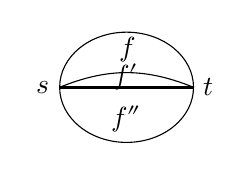
\begin{tikzpicture}[x=1cm,y=1cm,baseline=(current bounding box.center)] \draw (0,0) ellipse (0.85 and 0.70); \draw (-0.85,0) to[bend left=22] (0.85,0); \draw[line width=1.1pt] (-0.85,0)--(0.85,0); \node at (0,0.48) {$f$}; \node at (0,0.13) {$f'$}; \node at (0,-0.40) {$f''$}; \node[left] at (-0.85,0) {$s$}; \node[right] at (0.85,0) {$t$}; \end{tikzpicture}} $f\cap f''=\{s,t\}$} \var{\deleted{the}}{}{deletion}{ps_134-3_010-v0021}\var{\inserted{a}}{\hand{a}}{insertion}{ps_134-3_010-v0022} standard example\hand{.} \hand{\unsure{$\ell$}} \var{\over{o}{O}}{\hand{O}}{writing over}{ps_134-3_010-v0023}f lesser import is the misstatement \var{\inserted{(in section 2)}}{\hand{(in section 2)}}{insertion}{ps_134-3_010-v0024} \var{\deleted{on p.2'}}{}{deletion}{ps_134-3_010-v0025},
stating that the associativity relation for the operation \hand{$*_\ell$} should be
\var{\xout{wherex\allowbreak{}fx\allowbreak{}f"x\allowbreak{}isx\allowbreak{}ax\allowbreak{}two-pointx\allowbreak{}spacex\allowbreak{}$\underline{S}_o$x\allowbreak{}x\allowbreak{}x\allowbreak{}}}{}{typewriter deletion}{ps_134-3_010-v0026} replaced by a homotopy arrow
$(\hand{\lambda}*\hand{\mu})*\hand{\nu} \to \hand{\lambda}*(\hand{\mu}*\hand{\nu})$. This is OK for \hand{$\ell$}=1 (primary composition), but
already for \hand{$\ell$}=2 does not make sense as stated, because the sources and
the targets of the two compositions to be compared are not equal, but
only homotopic. Here the statement should be replaced by one making
sense, with a homotopy ``making commutative'' a certain square, and accor\hand{\unsure{-}}%
dingly for cubes etc for higher order co\var{\xout{mp}}{}{typewriter deletion}{ps_134-3_010-v0027}mpositions \hand{$\lambda *_\ell \mu$}, to give rea-%
sonable meaning to associativity. Anyhow, such painstaking explicita-%
tions of particular coherence properties (rather, coherence homotopies)
is kind of ruled out by the sweeping axiomatic description of the
kind of structure species we want for a ``stack'', at least\hand{,} I guess\hand{,} in

%% END SOURCE ps_134-3_010
\ifnum\EditionMode=1
\psapparatusstart
\psentry{ps_134-3_010-v0001}{1}{writing over}{\over{\unsure{18}}{18}}{\hand{18}}{The superposed handwritten reading replaces the underlying reading.}
\psentry{ps_134-3_010-v0002}{2}{insertion}{\inserted{(section 13)}}{\hand{(section 13)}}{The handwritten insertion is incorporated at its indicated position; insertion brackets leave the running text.}
\psentry{ps_134-3_010-v0003}{3}{deletion}{\deleted{\unsure{p.11'}}}{}{The author cancels this material by hand; it leaves the corrected running text.}
\psentry{ps_134-3_010-v0004}{4}{typewriter deletion}{\xout{thatxix}}{}{The typewriter strikes out this material; it leaves the corrected running text.}
\psentry{ps_134-3_010-v0005}{5}{typed insertion}{\inserted[typed]{(contractible)}}{(contractible)}{The typed insertion is incorporated at its indicated position; insertion brackets leave the running text.}
\psentry{ps_134-3_010-v0006}{6}{typewriter deletion}{\xout{x}}{}{The typewriter strikes out this material; it leaves the corrected running text.}
\psentry{ps_134-3_010-v0007}{7}{writing over}{\over{\unsure{at}}{ich}}{\hand{ich}}{The superposed handwritten reading replaces the underlying reading.}
\psentry{ps_134-3_010-v0008}{8}{typewriter deletion}{\xout{n}}{}{The typewriter strikes out this material; it leaves the corrected running text.}
\psentry{ps_134-3_010-v0009}{9}{typed insertion}{\inserted[typed]{strict}}{strict}{The typed insertion is incorporated at its indicated position; insertion brackets leave the running text.}
\psentry{ps_134-3_010-v0010}{10}{typewriter deletion}{\xout{x}}{}{The typewriter strikes out this material; it leaves the corrected running text.}
\psentry{ps_134-3_010-v0011}{11}{insertion}{\inserted{too}}{\hand{too}}{The handwritten insertion is incorporated at its indicated position; insertion brackets leave the running text.}
\psentry{ps_134-3_010-v0012}{12}{insertion}{\inserted{there}}{\hand{there}}{The handwritten insertion is incorporated at its indicated position; insertion brackets leave the running text.}
\psentry{ps_134-3_010-v0013}{13}{deletion}{\deleted{on p.11'}}{}{The author cancels this material by hand; it leaves the corrected running text.}
\psentry{ps_134-3_010-v0014}{14}{typewriter deletion}{\xout{xxxx}}{}{The typewriter strikes out this material; it leaves the corrected running text.}
\psentry{ps_134-3_010-v0015}{15}{typed insertion}{\inserted[typed]{total}}{total}{The typed insertion is incorporated at its indicated position; insertion brackets leave the running text.}
\psentry{ps_134-3_010-v0016}{16}{typewriter deletion}{\xout{xxxxxx}}{}{The typewriter strikes out this material; it leaves the corrected running text.}
\psentry{ps_134-3_010-v0017}{17}{insertion}{\inserted{(section 7)}}{\hand{(section 7)}}{The handwritten insertion is incorporated at its indicated position; insertion brackets leave the running text.}
\psentry{ps_134-3_010-v0018}{18}{deletion}{\deleted{p.7'}}{}{The author cancels this material by hand; it leaves the corrected running text.}
\psentry{ps_134-3_010-v0019}{19}{writing over}{\over{d}{y}}{\hand{y}}{The superposed handwritten reading replaces the underlying reading.}
\psentry{ps_134-3_010-v0020}{20}{typed insertion}{\inserted[typed]{maximal}}{maximal}{The typed insertion is incorporated at its indicated position; insertion brackets leave the running text.}
\psentry{ps_134-3_010-v0021}{21}{deletion}{\deleted{the}}{}{The author cancels this material by hand; it leaves the corrected running text.}
\psentry{ps_134-3_010-v0022}{22}{insertion}{\inserted{a}}{\hand{a}}{The handwritten insertion is incorporated at its indicated position; insertion brackets leave the running text.}
\psentry{ps_134-3_010-v0023}{23}{writing over}{\over{o}{O}}{\hand{O}}{The superposed handwritten reading replaces the underlying reading.}
\psentry{ps_134-3_010-v0024}{24}{insertion}{\inserted{(in section 2)}}{\hand{(in section 2)}}{The handwritten insertion is incorporated at its indicated position; insertion brackets leave the running text.}
\psentry{ps_134-3_010-v0025}{25}{deletion}{\deleted{on p.2'}}{}{The author cancels this material by hand; it leaves the corrected running text.}
\psentry{ps_134-3_010-v0026}{26}{typewriter deletion}{\xout{wherex\allowbreak{}fx\allowbreak{}f"x\allowbreak{}isx\allowbreak{}ax\allowbreak{}two-pointx\allowbreak{}spacex\allowbreak{}$\underline{S}_o$x\allowbreak{}x\allowbreak{}x\allowbreak{}}}{}{The typewriter strikes out this material; it leaves the corrected running text.}
\psentry{ps_134-3_010-v0027}{27}{typewriter deletion}{\xout{mp}}{}{The typewriter strikes out this material; it leaves the corrected running text.}
\psapparatusend
\fi
\pssource{ps_134-3_011}{134-3/11}{https://grothendieck.umontpellier.fr/web/viewer.html?file=../134-3.pdf\#page=12}
\psnumber{ps_134-3_011-v0001}{1}
\psnumber{ps_134-3_011-v0002}{2}
\psnumber{ps_134-3_011-v0003}{3}
\psnumber{ps_134-3_011-v0004}{4}
\psnumber{ps_134-3_011-v0005}{5}
\psnumber{ps_134-3_011-v0006}{6}
\psnumber{ps_134-3_011-v0007}{7}
\psnumber{ps_134-3_011-v0008}{8}
\psnumber{ps_134-3_011-v0009}{9}
\psnumber{ps_134-3_011-v0010}{10}
\psnumber{ps_134-3_011-v0011}{11}
\psnumber{ps_134-3_011-v0012}{12}
\psnumber{ps_134-3_011-v0013}{13}
\psnumber{ps_134-3_011-v0014}{14}
\psnumber{ps_134-3_011-v0015}{15}
\psnumber{ps_134-3_011-v0016}{16}
\psnumber{ps_134-3_011-v0017}{17}
\psnumber{ps_134-3_011-v0018}{18}
%% BEGIN SOURCE ps_134-3_011
% Pursuing Stacks (cotes 134-2 to 134-8): archive cote 134-3, site page 11 (PDF page 12), typescript page 11.
% typescript. Draft compared: ps2.tex:470-531.
% AI-transcribed by Claude Opus 5.5 (claude-opus-5-5, adaptive thinking, effort high), Message Batches API, batch ps1 (msgbatch_01Rv5hCaNTtUt4JHx1yqoHPL), 2026-11-12; image review recorded in records/CHECK_DECISIONS_134_3_4.tsv.
\scanpage{134-3/11}
\mspage{11}
a large part of the development of the theory of Gr-stacks.  A systematic
study of particular sets of homotopies is closely connected \var{\inserted{of course}}{\hand{of course}}{insertion}{ps_134-3_011-v0001} to an inves-%
\hand{(}tigation into irredundancy conditions which can be figured out for a
\var{\inserted{general}}{\hand{general}}{insertion}{ps_134-3_011-v0002} coherator $\underline{C}$ .  This is indeed an interesting topic,  but I decided not
to get involved in this,  unless I am really forced to!

The basic notion which has been peeling out in the reflection (L)
is of course the notion of a coherator.  Concerning terminology,  it oc-%
cured to me that the dual category $\underline{B}_\infty$ to $\underline{C}_\infty$ is more suggestive in some
cases,  for instance because of the topological interpretation attached
to its objects,  and (more technically)  because of formal analogy of
the role of this category,  for developping homotopical algebra,  with
\margin{(11)} the category of the standar\var{\over{\unsure{t}}{d}}{\hand{d}}{writing over}{ps_134-3_011-v0003} (ordered) simplices\hand{(\textsuperscript{11})}.Both mutually dual
objects $\underline{B}_\infty$ , $\underline{C}_\infty$ seem to me to merit a name,  I suggest to call them
respectively \uline{left} and \uline{right} \uline{coherat ors},  or simply \uline{coherators} of course
when for a while it is understood on which side of the mirror we \var{\over{are}{are}}{\hand{are}}{writing over}{ps_134-3_011-v0004}
playing the game.

O\var{\over{n}{n}}{\hand{n}}{writing over}{ps_134-3_011-v0005}e last comment still before taking off for a heuristic voyage
\var{\over{a}{o}}{\hand{o}}{writing over}{ps_134-3_011-v0006}f discovery of stacks\hand{!} I just had a glance at Benabou\hand{'}s expos\hand{\'e} in 1967
of \var{\over{W}{w}}{\hand{w}}{writing over}{ps_134-3_011-v0007}hat he calls ``bicategories''  (Springer Lecture N\var{\over{o}{o}}{\hand{o}}{writing over}{ps_134-3_011-v0008}tes n\textsuperscript{o} 47 ,  p. 1
- 77).  These are non else,  it appears\hand{,} \var{\deleted{\unsure{than}}}{}{deletion}{ps_134-3_011-v0009} than \var{\deleted{(}}{}{deletion}{ps_134-3_011-v0010}\uline{non associative}
2-categories,  namely 2-stacks  in the terminology I am proposing
(but not 2-Gr-stacks  -  namely at is a particular case of a general
notion of oo-stack which  has still to be developped).  The most interes-%
\hand{-}ting feature of this exposé,  it seems to me,  is the systematic refe-%
rence to topological intuition as \var{\inserted[typed]{a}}{a}{typed insertion}{ps_134-3_011-v0011} support for a comprehension of an
algebraic formalism,  notably \var{\inserted[typed]{of}}{of}{typed insertion}{ps_134-3_011-v0012} the structure of various diagrams. His
terminology,  referring to elements of $F_o,F_1,F_2$ respectively as 0-cells,
1-cells and 2-cells,  is quite suggestive of an idea of \var{\deleted{geometric}}{}{deletion}{ps_134-3_011-v0013} \var{\inserted[typed]{topological}}{topological}{typed insertion}{ps_134-3_011-v0014} reali-%
zation of a 2-stack  -  it is not clear from this exposé whether Benabou
has worked out this idea,  nor whether he has made a connection with
Quillen's ideas on axiomatics of homotopy theory,  which appeared the
same year in the same series\hand{(\textsuperscript{14})}. In any case,  in the last section of his
expos\hand{\'e},  he deals with his bicategories formally as with topological
spaces,  much in the same spirit as \hand{(}\var{\inserted{the one}}{\hand{the one}}{insertion}{ps_134-3_011-v0015} I was contemplating since \var{\xout{1975xxxxx}}{}{typewriter deletion}{ps_134-3_011-v0016}
around 1975,  and which is now motivating the present notes.  While
there is no mention of Benabou\hand{'}s ideas in my letters\var{\unsure{\deleted{t}}}{}{deletion}{ps_134-3_011-v0017} to Larry Breen,
it is quite possible that on the unconscious level,  the little I had
heard of his approach on one or two casual occasions,  had entered into
reaction with my own intuitions\hand{,} coming \var{\inserted[typed]{mainly}}{mainly}{typed insertion}{ps_134-3_011-v0018} from geometry and \unsure{hohomological|cohomological}
algebra,  and finally resulted in the program outlined in those letters.

%% END SOURCE ps_134-3_011
\ifnum\EditionMode=1
\psapparatusstart
\psentry{ps_134-3_011-v0001}{1}{insertion}{\inserted{of course}}{\hand{of course}}{The handwritten insertion is incorporated at its indicated position; insertion brackets leave the running text.}
\psentry{ps_134-3_011-v0002}{2}{insertion}{\inserted{general}}{\hand{general}}{The handwritten insertion is incorporated at its indicated position; insertion brackets leave the running text.}
\psentry{ps_134-3_011-v0003}{3}{writing over}{\over{\unsure{t}}{d}}{\hand{d}}{The superposed handwritten reading replaces the underlying reading.}
\psentry{ps_134-3_011-v0004}{4}{writing over}{\over{are}{are}}{\hand{are}}{The superposed handwritten reading replaces the underlying reading.}
\psentry{ps_134-3_011-v0005}{5}{writing over}{\over{n}{n}}{\hand{n}}{The superposed handwritten reading replaces the underlying reading.}
\psentry{ps_134-3_011-v0006}{6}{writing over}{\over{a}{o}}{\hand{o}}{The superposed handwritten reading replaces the underlying reading.}
\psentry{ps_134-3_011-v0007}{7}{writing over}{\over{W}{w}}{\hand{w}}{The superposed handwritten reading replaces the underlying reading.}
\psentry{ps_134-3_011-v0008}{8}{writing over}{\over{o}{o}}{\hand{o}}{The superposed handwritten reading replaces the underlying reading.}
\psentry{ps_134-3_011-v0009}{9}{deletion}{\deleted{\unsure{than}}}{}{The author cancels this material by hand; it leaves the corrected running text.}
\psentry{ps_134-3_011-v0010}{10}{deletion}{\deleted{(}}{}{The author cancels this material by hand; it leaves the corrected running text.}
\psentry{ps_134-3_011-v0011}{11}{typed insertion}{\inserted[typed]{a}}{a}{The typed insertion is incorporated at its indicated position; insertion brackets leave the running text.}
\psentry{ps_134-3_011-v0012}{12}{typed insertion}{\inserted[typed]{of}}{of}{The typed insertion is incorporated at its indicated position; insertion brackets leave the running text.}
\psentry{ps_134-3_011-v0013}{13}{deletion}{\deleted{geometric}}{}{The author cancels this material by hand; it leaves the corrected running text.}
\psentry{ps_134-3_011-v0014}{14}{typed insertion}{\inserted[typed]{topological}}{topological}{The typed insertion is incorporated at its indicated position; insertion brackets leave the running text.}
\psentry{ps_134-3_011-v0015}{15}{insertion}{\inserted{the one}}{\hand{the one}}{The handwritten insertion is incorporated at its indicated position; insertion brackets leave the running text.}
\psentry{ps_134-3_011-v0016}{16}{typewriter deletion}{\xout{1975xxxxx}}{}{The typewriter strikes out this material; it leaves the corrected running text.}
\psentry{ps_134-3_011-v0017}{17}{deletion}{\unsure{\deleted{t}}}{}{All material inside this wrapper is cancelled. Its original doubt and presentation remain in the diplomatic text and apparatus; no empty doubt mark or page label is inserted into the corrected running text.}
\psentry{ps_134-3_011-v0018}{18}{typed insertion}{\inserted[typed]{mainly}}{mainly}{The typed insertion is incorporated at its indicated position; insertion brackets leave the running text.}
\psapparatusend
\fi
\pssource{ps_134-3_012}{134-3/12}{https://grothendieck.umontpellier.fr/web/viewer.html?file=../134-3.pdf\#page=13}
\psnumber{ps_134-3_012-v0001}{1}
\psnumber{ps_134-3_012-v0002}{2}
\psnumber{ps_134-3_012-v0003}{3}
\psnumber{ps_134-3_012-v0004}{4}
\psnumber{ps_134-3_012-v0005}{5}
\psnumber{ps_134-3_012-v0006}{6}
\psnumber{ps_134-3_012-v0007}{7}
\psnumber{ps_134-3_012-v0008}{8}
\psnumber{ps_134-3_012-v0009}{9}
\psnumber{ps_134-3_012-v0010}{10}
\psnumber{ps_134-3_012-v0011}{11}
\psnumber{ps_134-3_012-v0012}{12}
\psnumber{ps_134-3_012-v0013}{13}
\psnumber{ps_134-3_012-v0014}{14}
\psnumber{ps_134-3_012-v0015}{15}
\psnumber{ps_134-3_012-v0016}{16}
\psnumber{ps_134-3_012-v0017}{17}
%% BEGIN SOURCE ps_134-3_012
% Pursuing Stacks (cotes 134-2 to 134-8): archive cote 134-3, site page 12 (PDF page 13), typescript page 12.
% typescript. Draft compared: ps2.tex:516-584.
% AI-transcribed by Claude Opus 5.5 (claude-opus-5-5, adaptive thinking, effort high), Message Batches API, batch ps1 (msgbatch_01Rv5hCaNTtUt4JHx1yqoHPL), 2026-11-12; image review recorded in records/CHECK_DECISIONS_134_3_4.tsv.
\scanpage{134-3/12}
\mspage{12}

\hand{19.} I would like now to write down a provisional itinerary of the \unsure{voyage}
ahead - namely to make a list of those main features of a theory of
\margin{$\times$} stacks which are in my mind these days. I will write them down in the
order in which they occur to me - which will be no obligation upon me
to follow this order, when coming back on those features separately to
elaborate somewhat on them\var{\over{,}{.}}{\hand{.}}{writing over}{ps_134-3_012-v0001} \var{\inserted{This I expect to do,}}{\hand{This I expect to do,}}{insertion}{ps_134-3_012-v0002} mainly as a way to check wether the main
notions and intuitions introduced are sound indeed, and otherwise, to
see how to correct them.

1\textsuperscript{o}) Definition of the categories $\underline{B}_o$ and its dual $\underline{C}_o$ , and formal defi-%
nition of left and right coherators. This definition \var{\over{\unsure{will}}{will}}{\hand{will}}{writing over}{ps_134-3_012-v0003} still be a
provisional one, and will presumably have to be adjusted somewhat to
\var{\over{allo}{allo}}{\hand{allo}}{writing over}{ps_134-3_012-v0004}w for the various structures we are looking for in the corresponding
category of Gr-stacks.

2\textsuperscript{o}) Relation between the category of Gr-stacks and the category of
topological spaces, via two adjoint functors, the ``topological realiza-%
tion functor'' $F_{\ast} \hand{\mapsto} \hand{|}F_{\ast}\hand{|}$ , and the ``singular stack functor''
$X \hand{\mapsto} \underline{F}_{\ast}(X)$ . The situation should be formally analogous to the corres-%
ponding situation for semi-simplicial sets versus topological spaces,
the role of the category $\underline{S}_{\ast}$ of standar\var{\over{t}{d}}{\hand{d}}{writing over}{ps_134-3_012-v0005} ordered simplices being taken
by the left coherator $\underline{B}$ we are working with. The main technical diffe-%
rence here is that the category of Gr-stacks is not just the category of
presheaves on $\underline{B}$, but the full subcategory defined by the requirement
that the presheaves considered should transform ``standar\var{\over{t}{d}}{\hand{d}}{writing over}{ps_134-3_012-v0006}'' amalgamated
sums into fibered products. As a matter of fact, the topological rea-%
lization functor $F_{\ast} \hand{\mapsto} \hand{|}F_{\ast}\hand{|}$ could be defined in standar\var{\over{t}{d}}{\hand{d}}{writing over}{ps_134-3_012-v0007} way on the
whole of $\hand{\widehat{\phantom{B}}}\underline{B}$ , in terms of any functor \var{\xout{B}}{}{typewriter deletion}{ps_134-3_012-v0008}
\hand{(*)} \[ \underline{B} \hand{\longrightarrow} \text{(Spaces)} \]
(by the requirement that the extension of this functor to $\hand{\widehat{\phantom{B}}}B$ commutes
with arbitrary direct limits). A second difference with the \var{\inserted{similar,}}{\hand{similar,}}{insertion}{ps_134-3_012-v0009} simplicial
\var{\deleted{similar}}{}{deletion}{ps_134-3_012-v0010} situation \var{\xout{is that}}{}{typewriter deletion}{ps_134-3_012-v0011} lies in the fact that the only really compel-%
ling choice for the functor (*) is it's restriction to $\underline{B}_o$ , in terms
of the cells $\underline{D}_n$ and the standart \hand{``}half-hemisphere \var{\xout{morphisms}}{}{typewriter deletion}{ps_134-3_012-v0012} maps\hand{''} between
these (L, \var{\deleted{\illegible{1}}}{}{deletion}{ps_134-3_012-v0013}\var{\inserted{section 6}}{\hand{section 6}}{insertion}{ps_134-3_012-v0014}). The extension of this functor to $\underline{B}$ is always possi\hand{\unsure{b}}%
le, due to the \var{\inserted[typed]{inductive}}{inductive}{typed insertion}{ps_134-3_012-v0015} construction of $\underline{B}$ and to the interpretation of elements
\margin{\diagram{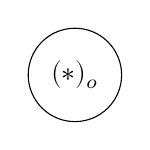
\begin{tikzpicture}[baseline=(n.base)]\node[draw,circle,inner sep=5pt] (n) {$({*})_o$};\end{tikzpicture}}} of $\underline{B}_o$ as \uline{contractible} spaces, via the functor (*)\hand{$_o$}; but it depends on
a bunch of arbitrary choices. To give precise meaning to the intuition
that these choices do\var{\over{nt}{'nt}}{\hand{'nt}}{writing over}{ps_134-3_012-v0016} really make a difference, and that the choic\unsure{e}
\var{\inserted[typed]{of}}{of}{typed insertion}{ps_134-3_012-v0017} coherator we are starting with does'nt make much of a difference either\hand{,}
will need some elaboration on the notion of \uline{equivalences between}

%% END SOURCE ps_134-3_012
\ifnum\EditionMode=1
\psapparatusstart
\psentry{ps_134-3_012-v0001}{1}{writing over}{\over{,}{.}}{\hand{.}}{The superposed handwritten reading replaces the underlying reading.}
\psentry{ps_134-3_012-v0002}{2}{insertion}{\inserted{This I expect to do,}}{\hand{This I expect to do,}}{The handwritten insertion is incorporated at its indicated position; insertion brackets leave the running text.}
\psentry{ps_134-3_012-v0003}{3}{writing over}{\over{\unsure{will}}{will}}{\hand{will}}{The superposed handwritten reading replaces the underlying reading.}
\psentry{ps_134-3_012-v0004}{4}{writing over}{\over{allo}{allo}}{\hand{allo}}{The superposed handwritten reading replaces the underlying reading.}
\psentry{ps_134-3_012-v0005}{5}{writing over}{\over{t}{d}}{\hand{d}}{The superposed handwritten reading replaces the underlying reading.}
\psentry{ps_134-3_012-v0006}{6}{writing over}{\over{t}{d}}{\hand{d}}{The superposed handwritten reading replaces the underlying reading.}
\psentry{ps_134-3_012-v0007}{7}{writing over}{\over{t}{d}}{\hand{d}}{The superposed handwritten reading replaces the underlying reading.}
\psentry{ps_134-3_012-v0008}{8}{typewriter deletion}{\xout{B}}{}{The typewriter strikes out this material; it leaves the corrected running text.}
\psentry{ps_134-3_012-v0009}{9}{insertion}{\inserted{similar,}}{\hand{similar,}}{The handwritten insertion is incorporated at its indicated position; insertion brackets leave the running text.}
\psentry{ps_134-3_012-v0010}{10}{deletion}{\deleted{similar}}{}{The author cancels this material by hand; it leaves the corrected running text.}
\psentry{ps_134-3_012-v0011}{11}{typewriter deletion}{\xout{is that}}{}{The typewriter strikes out this material; it leaves the corrected running text.}
\psentry{ps_134-3_012-v0012}{12}{typewriter deletion}{\xout{morphisms}}{}{The typewriter strikes out this material; it leaves the corrected running text.}
\psentry{ps_134-3_012-v0013}{13}{deletion}{\deleted{\illegible{1}}}{}{The author cancels this material by hand; it leaves the corrected running text.}
\psentry{ps_134-3_012-v0014}{14}{insertion}{\inserted{section 6}}{\hand{section 6}}{The handwritten insertion is incorporated at its indicated position; insertion brackets leave the running text.}
\psentry{ps_134-3_012-v0015}{15}{typed insertion}{\inserted[typed]{inductive}}{inductive}{The typed insertion is incorporated at its indicated position; insertion brackets leave the running text.}
\psentry{ps_134-3_012-v0016}{16}{writing over}{\over{nt}{'nt}}{\hand{'nt}}{The superposed handwritten reading replaces the underlying reading.}
\psentry{ps_134-3_012-v0017}{17}{typed insertion}{\inserted[typed]{of}}{of}{The typed insertion is incorporated at its indicated position; insertion brackets leave the running text.}
\psapparatusend
\fi
\pssource{ps_134-3_013}{134-3/13}{https://grothendieck.umontpellier.fr/web/viewer.html?file=../134-3.pdf\#page=14}
\psnumber{ps_134-3_013-v0001}{1}
\psnumber{ps_134-3_013-v0002}{2}
\psnumber{ps_134-3_013-v0003}{3}
\psnumber{ps_134-3_013-v0004}{4}
\psnumber{ps_134-3_013-v0005}{5}
\psnumber{ps_134-3_013-v0006}{6}
\psnumber{ps_134-3_013-v0007}{7}
\psnumber{ps_134-3_013-v0008}{8}
\psnumber{ps_134-3_013-v0009}{9}
\psnumber{ps_134-3_013-v0010}{10}
\psnumber{ps_134-3_013-v0011}{11}
\psnumber{ps_134-3_013-v0012}{12}
\psnumber{ps_134-3_013-v0013}{13}
\psnumber{ps_134-3_013-v0014}{14}
%% BEGIN SOURCE ps_134-3_013
% Pursuing Stacks (cotes 134-2 to 134-8): archive cote 134-3, site page 13 (PDF page 14), typescript page 13.
% typescript. Draft compared: ps2.tex:569-633.
% AI-transcribed by Claude Opus 5.5 (claude-opus-5-5, adaptive thinking, effort high), Message Batches API, batch ps1 (msgbatch_01Rv5hCaNTtUt4JHx1yqoHPL), 2026-11-12; image review recorded in records/CHECK_DECISIONS_134_3_4.tsv.
\scanpage{134-3/13}
\mspage{13}
Gr-\uline{stacks}, which will have to \var{\xout{tx}}{}{typewriter deletion}{ps_134-3_013-v0001} be developped at a later stage.

The idea just comes to my mind whether the exactness condition
implying standar\var{\over{t}{d}}{\hand{d}}{writing over}{ps_134-3_013-v0002} amalgamated sums, defining the subcategory of stacks
within $\overset{\hand{\wedge}}{\underline{B}}$ , cannot be interpreted in terms of some more or less obvious
topology on $\underline{B}$ turning $\underline{B}$ into a site, as the subcategory of correspon-%
ding \uline{sheaves}. This would mean that the category (Gr-stacks) is in fact
a topos, with the host of eategorical information and topological
intuition that goes with such a situation. In this connection, it is
timely to recall that the related categories (Cat) of ``all'' categories,
and (Groupoids) of ``all'' groupoids, are definitely \uline{not} topoi (if my
recollection is correct - it is\hand{'}nt immediately clear to me why they
are not). This seems to suggest that, granting that (Gr-stacks) is
indeed a topos, that this would be a rather special feature of the
structure species of infinite order we are working with (as \var{\deleted{a}}{}{deletion}{ps_134-3_013-v0003}\var{\inserted[typed]{one}}{one}{typed insertion}{ps_134-3_013-v0004} reward so
to say,among a heap of others, for conceptual sophistication !), in
contrast to the categories (Gr-n-stacks)\var{\inserted[typed]{with finite n}}{with finite n}{typed insertion}{ps_134-3_013-v0005}, which presumably are not topoi
(For a definition of Gr-n-stacks in terms of Gr-stacks namely
Gr-$\infty$-stacks, see below.\hand{)}

A related question is whether the category (Gr-stacks) is a model
category for the usual homotopy category, the pair of adjoint functors
bonsidered before satisfying \var{\inserted{moreover}}{\hand{moreover}}{insertion}{ps_134-3_013-v0006} the conditions of Quillen's comparison
theorem\hand{(\textsuperscript{13})}.The obvious idea that comes to mind here, in order to define
the model structure on (Gr-stacks), is to take as ``weak equivalences''
the maps which are transformed into weak equivalences by the topological
realization functor (which should be readily expressible in \var{\inserted[typed]{algebraic}}{algebraic}{typed insertion}{ps_134-3_013-v0007} terms \var{\xout{as}}{}{typewriter deletion}{ps_134-3_013-v0008} ..\hand{)},
\var{\over{\unsure{as}}{as}}{\hand{as}}{writing over}{ps_134-3_013-v0009} cofibrations the monomorphisms, and defining fibrations by the
Serre-Quillen lifting property with respect to cofibrations which are
weak equivalences (with the expectation that we even get a ``closed mod\hand{el}
category'' in the sense of Quillen). Here it does'nt look too unreasonab
\hand{-}le to expect the same constructions to work in each of the categories
(Gr-n-stacks), n \var{\over{$>$}{$\geqslant$}}{\hand{$\geqslant$}}{writing over}{ps_134-3_013-v0010}1, as well as in the categories (n-stacks) without
Gr , which are still to be defined though.

Coming back upon the question of a suitable topology on $\underline{B}$, the
idea that comes to mind immediately of course is to define\var{\deleted{s}}{}{deletion}{ps_134-3_013-v0011} covering
families of an object K of $\underline{B}$ i.e. of $\underline{B}_o$ , in terms of the components
which occur in the description of K as an \var{\inserted[typed]{iterated}}{iterated}{typed insertion}{ps_134-3_013-v0012} amalgamated sum of\var{\deleted{\unsure{s}}}{}{deletion}{ps_134-3_013-v0013} cells $D_n$.
A quick glance (too quick a glance ?) seems to show this is indeed a
topology, and that the sheaves for this topology are what we expect.
\var{\deleted{This would imply that the \deleted{inclusion} \inserted{composite} functor}}{}{deletion}{ps_134-3_013-v0014}

%% END SOURCE ps_134-3_013
\ifnum\EditionMode=1
\psapparatusstart
\psentry{ps_134-3_013-v0001}{1}{typewriter deletion}{\xout{tx}}{}{The typewriter strikes out this material; it leaves the corrected running text.}
\psentry{ps_134-3_013-v0002}{2}{writing over}{\over{t}{d}}{\hand{d}}{The superposed handwritten reading replaces the underlying reading.}
\psentry{ps_134-3_013-v0003}{3}{deletion}{\deleted{a}}{}{The author cancels this material by hand; it leaves the corrected running text.}
\psentry{ps_134-3_013-v0004}{4}{typed insertion}{\inserted[typed]{one}}{one}{The typed insertion is incorporated at its indicated position; insertion brackets leave the running text.}
\psentry{ps_134-3_013-v0005}{5}{typed insertion}{\inserted[typed]{with finite n}}{with finite n}{The typed insertion is incorporated at its indicated position; insertion brackets leave the running text.}
\psentry{ps_134-3_013-v0006}{6}{insertion}{\inserted{moreover}}{\hand{moreover}}{The handwritten insertion is incorporated at its indicated position; insertion brackets leave the running text.}
\psentry{ps_134-3_013-v0007}{7}{typed insertion}{\inserted[typed]{algebraic}}{algebraic}{The typed insertion is incorporated at its indicated position; insertion brackets leave the running text.}
\psentry{ps_134-3_013-v0008}{8}{typewriter deletion}{\xout{as}}{}{The typewriter strikes out this material; it leaves the corrected running text.}
\psentry{ps_134-3_013-v0009}{9}{writing over}{\over{\unsure{as}}{as}}{\hand{as}}{The superposed handwritten reading replaces the underlying reading.}
\psentry{ps_134-3_013-v0010}{10}{writing over}{\over{$>$}{$\geqslant$}}{\hand{$\geqslant$}}{The superposed handwritten reading replaces the underlying reading.}
\psentry{ps_134-3_013-v0011}{11}{deletion}{\deleted{s}}{}{The author cancels this material by hand; it leaves the corrected running text.}
\psentry{ps_134-3_013-v0012}{12}{typed insertion}{\inserted[typed]{iterated}}{iterated}{The typed insertion is incorporated at its indicated position; insertion brackets leave the running text.}
\psentry{ps_134-3_013-v0013}{13}{deletion}{\deleted{\unsure{s}}}{}{The author cancels this material by hand; it leaves the corrected running text.}
\psentry{ps_134-3_013-v0014}{14}{deletion}{\deleted{This would imply that the \deleted{inclusion} \inserted{composite} functor}}{}{The author cancels this material by hand; it leaves the corrected running text.}
\psapparatusend
\fi
\pssource{ps_134-3_014}{134-3/14}{https://grothendieck.umontpellier.fr/web/viewer.html?file=../134-3.pdf\#page=15}
\psnumber{ps_134-3_014-v0001}{1}
\psnumber{ps_134-3_014-v0002}{2}
\psnumber{ps_134-3_014-v0003}{3}
\psnumber{ps_134-3_014-v0004}{4}
\psnumber{ps_134-3_014-v0005}{5}
\psnumber{ps_134-3_014-v0006}{6}
\psnumber{ps_134-3_014-v0007}{7}
\psnumber{ps_134-3_014-v0008}{8}
\psnumber{ps_134-3_014-v0009}{9}
%% BEGIN SOURCE ps_134-3_014
% Pursuing Stacks (cotes 134-2 to 134-8): archive cote 134-3, site page 14 (PDF page 15), typescript page 14.
% typescript. Draft compared: ps2.tex:616-682.
% AI-transcribed by Claude Opus 5.5 (claude-opus-5-5, adaptive thinking, effort high), Message Batches API, batch ps1 (msgbatch_01Rv5hCaNTtUt4JHx1yqoHPL), 2026-11-12; image review recorded in records/CHECK_DECISIONS_134_3_4.tsv.
\scanpage{134-3/14}
\hand{5}.3. \mspage{\hand{14}}

\hand{20.} I had barely st opped writing last tuesday,  when it became clear \var{\xout{th}}{}{typewriter deletion}{ps_134-3_014-v0001}
that the ``quick glance'' had been too quick indeed. \var{\xout{It would}}{}{typewriter deletion}{ps_134-3_014-v0002} As a matter
of fact,  the ``topology'' I was contemplating on $\underline{B}$ in terms of covering
families does not satisfy the conditions for a ``site'' -  that something
was fishy first occured to me through the heuristic consequence,  that
the functors  ``n-th component''
\[ F_{*} \hand{\longmapsto} F_{n} \]
from \var{\xout{\illegible{1}}}{}{typewriter deletion}{ps_134-3_014-v0003} stacks to sets are fiber functors,  or equivalently, that
direct limits in the category of Gr-stacks can be computed componentwise
-  now this is definitely false,  for much the same reasons why it is
false \unsure{already|alfeady} in the category (Cat) of categories.  However,  it occured
to me that \var{\inserted{in}}{\hand{in}}{insertion}{ps_134-3_014-v0004} the latter category (Cat),  although not a topos (for instan-%
ce because, according to Giraud's paper on descent theory of 1965\hand{, (19)}
the implications for epimorphisms
\diagram{
% Hand-drawn arrows are marked blue; typed objects remain plain.
\begin{tikzcd}[row sep=tiny,column sep=large]
 \& \text{effective} \arrow[dr, Rightarrow, color=blue] \& \\
\text{effective universal} \arrow[ur, Rightarrow, color=blue] \arrow[dr, Rightarrow, color=blue] \& \& \text{just epi} \\
 \& \text{universal} \arrow[ur, Rightarrow, color=blue] \&
\end{tikzcd}
}
are strict),  there \uline{is} a very natural topology,  \var{\xout{namely}}{}{typewriter deletion}{ps_134-3_014-v0005} turning it into
a site,  namely the one where a family of morphisms namely functors
\[ A_{i} \hand{\longrightarrow} A \]
is covering if and only if the corresponding family in (Ss sets)
\[ \mathrm{Nerve}(A_{i}) \hand{\longrightarrow} \mathrm{Nerve}(A) \]
is covering,  i.e. iff every \var{\xout{family}}{}{typewriter deletion}{ps_134-3_014-v0006} sequence of composable arrows in A
\[ a_{0} \hand{\to} a_{1} \hand{\to} a_{2} \hand{\to} a_{3} \hand{\to} \quad \dots \hand{\to} a_{n} \]
can be lifted  to one among the $A_{i}$'s.  As a matter of fact,  this condi-%
\margin{\unsure{5.3. This is definitely false, see \S24 below}}
tion (where it suffices to take n=2,  visibly)  is equivalent (according
to Giraud) to the condition that the family be \hand{``}universally effectively
epimorphic\hand{''},  i.e. covering with respect to the``canonical topology''of
(Cat)\hand{(15)}.This suggests a third way for associating to a \var{\inserted{[small]}}{\hand{[small]}}{insertion}{ps_134-3_014-v0007} category A a
topology-like structure,  namely the topos of all sheaves over
$(\mathrm{Cat})_{/A}$  ,  the site of all categories over A, \var{\inserted[typed]{endowed}}{endowed}{typed insertion}{ps_134-3_014-v0008} with the topology induced
by the canonical topology of (Cat)  (which is indeed the canonical topo\hand{-}%
logy of  $(\mathrm{Cat})_{/A}$ \hand{)}.  It should be an easy exercice in terms of nerves to
check that the homotopy type (a priori,  a prohomotopy type)  associated
to this site is just \hand{``}the\hand{''}homotopy type of A,  defined either as the
homotopy type of Nerve(A),  or as the (pro)homotopy type of the topos
$\overset{\hand{\wedge}}{A}$ of all presheaves over A.  This of course parallels the similar fami-%
liar fact in the category (Ss sets) of all semisimplicial sets,  namely
that for such a ss set\var{\deleted{\unsure{s}}}{}{deletion}{ps_134-3_014-v0009} K,  the homotopy type of K can be viewed also
as the homotopy type of the induce\hand{d} topos  $(\mathrm{Ss\ sets})_{/K}$ of all ss sets
over K.  The difference in the two cases is that  in the second case

%% END SOURCE ps_134-3_014
\ifnum\EditionMode=1
\psapparatusstart
\psentry{ps_134-3_014-v0001}{1}{typewriter deletion}{\xout{th}}{}{The typewriter strikes out this material; it leaves the corrected running text.}
\psentry{ps_134-3_014-v0002}{2}{typewriter deletion}{\xout{It would}}{}{The typewriter strikes out this material; it leaves the corrected running text.}
\psentry{ps_134-3_014-v0003}{3}{typewriter deletion}{\xout{\illegible{1}}}{}{The typewriter strikes out this material; it leaves the corrected running text.}
\psentry{ps_134-3_014-v0004}{4}{insertion}{\inserted{in}}{\hand{in}}{The handwritten insertion is incorporated at its indicated position; insertion brackets leave the running text.}
\psentry{ps_134-3_014-v0005}{5}{typewriter deletion}{\xout{namely}}{}{The typewriter strikes out this material; it leaves the corrected running text.}
\psentry{ps_134-3_014-v0006}{6}{typewriter deletion}{\xout{family}}{}{The typewriter strikes out this material; it leaves the corrected running text.}
\psentry{ps_134-3_014-v0007}{7}{insertion}{\inserted{[small]}}{\hand{[small]}}{The handwritten insertion is incorporated at its indicated position; insertion brackets leave the running text.}
\psentry{ps_134-3_014-v0008}{8}{typed insertion}{\inserted[typed]{endowed}}{endowed}{The typed insertion is incorporated at its indicated position; insertion brackets leave the running text.}
\psentry{ps_134-3_014-v0009}{9}{deletion}{\deleted{\unsure{s}}}{}{The author cancels this material by hand; it leaves the corrected running text.}
\psapparatusend
\fi
\pssource{ps_134-3_015}{134-3/15}{https://grothendieck.umontpellier.fr/web/viewer.html?file=../134-3.pdf\#page=16}
\psnumber{ps_134-3_015-v0001}{1}
\psnumber{ps_134-3_015-v0002}{2}
\psnumber{ps_134-3_015-v0003}{3}
\psnumber{ps_134-3_015-v0004}{4}
\psnumber{ps_134-3_015-v0005}{5}
\psnumber{ps_134-3_015-v0006}{6}
\psnumber{ps_134-3_015-v0007}{7}
\psnumber{ps_134-3_015-v0008}{8}
\psnumber{ps_134-3_015-v0009}{9}
\psnumber{ps_134-3_015-v0010}{10}
\psnumber{ps_134-3_015-v0011}{11}
%% BEGIN SOURCE ps_134-3_015
% Pursuing Stacks (cotes 134-2 to 134-8): archive cote 134-3, site page 15 (PDF page 16), typescript page 15.
% typescript. Draft compared: ps2.tex:669-728.
% AI-transcribed by Claude Opus 5.5 (claude-opus-5-5, adaptive thinking, effort high), Message Batches API, batch ps1 (msgbatch_01Rv5hCaNTtUt4JHx1yqoHPL), 2026-11-12; image review recorded in records/CHECK_DECISIONS_134_3_4.tsv.
\scanpage{134-3/15}
\mspage{15}

the category  (Ss sets) (and hence \var{\over{\unsure{the}}{any}}{\hand{any}}{writing over}{ps_134-3_015-v0001} induced categor\var{\over{\unsure{ies}}{y}}{\hand{y}}{writing over}{ps_134-3_015-v0002}) \var{\over{\unsure{are}}{is}}{\hand{is}}{writing over}{ps_134-3_015-v0003} already
a topos,  namely equivalent to the category of sheaves on the same for
the canonical topology,  whereas in the category (Cat)  this is not so.

These reflections suggest that in most if not all categories of
models encountered for describing usual homotopy types,  there is a \margin{\unsure{5.3. this presumption is false actually}}
natural structure of a site on the model category M (\uline{presumably} the one
corresponding to the canonical topology(\var{\over{*}{15}}{\hand{15}}{writing over}{ps_134-3_015-v0004})), with the property that the
homotopy type of any object X in M is \var{\xout{also}}{}{typewriter deletion}{ps_134-3_015-v0005} canonically isomorphic to the
(pro)homotopy type of the induced site $M_{/X}$ ,  or what amount\hand{s} to the same,
of the corresponding topos
\[ (M_{/X})^{\hand{\sim}} \;=\; M^{\hand{\sim}}_{/X} \;. \]
I would expect definitely this to be the case for each of the categories
(Gr-stacks), (n-Gr-stacks) (although this is not really a model category
in the sense of Quillen,\hand{as} it gives rise only to n-truncated homotopy
types ...),  (stacks)  and (n-stacks),  corresponding to an arbitrary \margin{$\lceil$}
choice of a coherator,  defining the notion of a (Gr-stack),  or of a \margin{$[$}
stack  (for the latter and relations between the two,  see below). \margin{$\lfloor$}

\margin{$|$}\unsure{\var{\over{1}{2}}{\hand{2}}{writing over}{ps_134-3_015-v0006}}1.  I would like to digress a little more,  to emphasize still about
\margin{$\downarrow$}the vast variety of algebraic structures giving rise to model categories
for the usual homotopy category,  or at any rate suitable for expressing
more or less arbitrary homotopy types.  Apart from stacks,  where every
thing is still heuristics for the time being,  we have noticed so far
three examples of such structures,  namely  ss complexes,  cubical com-%
plexes,  and categories.  There are a  few familiar variants of the two
former,  such as the  ``simplicial complexes'' (in contrast to semi-simpli
cial ones) ,  namely \var{\inserted[typed]{presheaves on}}{presheaves on}{typed insertion}{ps_134-3_015-v0007} \var{\xout{functors from}}{}{typewriter deletion}{ps_134-3_015-v0008} the category of non-empty finite sets\hand{,}
which can be interpreted as ss complexes enriched with symmetry operati-%
ons on each component  -  and there is the corresponding variant in the
cubical case.  It would be rather surprising that these were not just
as good model categories,  as the more habitual ones (\var{\over{*}{16}}{\hand{16}}{writing over}{ps_134-3_015-v0009}) - all the more
as the singular complex (simplicial or cubical) is naturally endowed
with this extra structure,  which one generally chooses to forget. More
interesting variants are the  n-multicomplexes (simplicial or cubical,
with or without symmetries),  defined \hand{by} \var{\xout{presheaves}}{}{typewriter deletion}{ps_134-3_015-v0010} contravariant func-%
tors to sets  in n arguments rather than in just one,  where $n\hand{\geqslant}\hand{1}$. The-%
se complexes are familiar mainly,  it seems,  because of their connecti\hand{\unsure{on|ons}}
with product spaces and the Künneth-Eilenberg-Zilber type relations.
It is generally understood that to such a\var{\xout{n}}{}{typewriter deletion}{ps_134-3_015-v0011} multicomplex is associated

%% END SOURCE ps_134-3_015
\ifnum\EditionMode=1
\psapparatusstart
\psentry{ps_134-3_015-v0001}{1}{writing over}{\over{\unsure{the}}{any}}{\hand{any}}{The superposed handwritten reading replaces the underlying reading.}
\psentry{ps_134-3_015-v0002}{2}{writing over}{\over{\unsure{ies}}{y}}{\hand{y}}{The superposed handwritten reading replaces the underlying reading.}
\psentry{ps_134-3_015-v0003}{3}{writing over}{\over{\unsure{are}}{is}}{\hand{is}}{The superposed handwritten reading replaces the underlying reading.}
\psentry{ps_134-3_015-v0004}{4}{writing over}{\over{*}{15}}{\hand{15}}{The superposed handwritten reading replaces the underlying reading.}
\psentry{ps_134-3_015-v0005}{5}{typewriter deletion}{\xout{also}}{}{The typewriter strikes out this material; it leaves the corrected running text.}
\psentry{ps_134-3_015-v0006}{6}{writing over}{\over{1}{2}}{\hand{2}}{The superposed handwritten reading replaces the underlying reading.}
\psentry{ps_134-3_015-v0007}{7}{typed insertion}{\inserted[typed]{presheaves on}}{presheaves on}{The typed insertion is incorporated at its indicated position; insertion brackets leave the running text.}
\psentry{ps_134-3_015-v0008}{8}{typewriter deletion}{\xout{functors from}}{}{The typewriter strikes out this material; it leaves the corrected running text.}
\psentry{ps_134-3_015-v0009}{9}{writing over}{\over{*}{16}}{\hand{16}}{The superposed handwritten reading replaces the underlying reading.}
\psentry{ps_134-3_015-v0010}{10}{typewriter deletion}{\xout{presheaves}}{}{The typewriter strikes out this material; it leaves the corrected running text.}
\psentry{ps_134-3_015-v0011}{11}{typewriter deletion}{\xout{n}}{}{The typewriter strikes out this material; it leaves the corrected running text.}
\psapparatusend
\fi
\pssource{ps_134-3_016}{134-3/16}{https://grothendieck.umontpellier.fr/web/viewer.html?file=../134-3.pdf\#page=17}
\psnumber{ps_134-3_016-v0001}{1}
\psnumber{ps_134-3_016-v0002}{2}
\psnumber{ps_134-3_016-v0003}{3}
\psnumber{ps_134-3_016-v0004}{4}
\psnumber{ps_134-3_016-v0005}{5}
\psnumber{ps_134-3_016-v0006}{6}
\psnumber{ps_134-3_016-v0007}{7}
\psnumber{ps_134-3_016-v0008}{8}
\psnumber{ps_134-3_016-v0009}{9}
\psnumber{ps_134-3_016-v0010}{10}
\psnumber{ps_134-3_016-v0011}{11}
\psnumber{ps_134-3_016-v0012}{12}
\psnumber{ps_134-3_016-v0013}{13}
\psnumber{ps_134-3_016-v0014}{14}
\psnumber{ps_134-3_016-v0015}{15}
\psnumber{ps_134-3_016-v0016}{16}
\psnumber{ps_134-3_016-v0017}{17}
\psnumber{ps_134-3_016-v0018}{18}
\psnumber{ps_134-3_016-v0019}{19}
\psnumber{ps_134-3_016-v0020}{20}
\psnumber{ps_134-3_016-v0021}{21}
\psnumber{ps_134-3_016-v0022}{22}
\psnumber{ps_134-3_016-v0023}{23}
%% BEGIN SOURCE ps_134-3_016
% Pursuing Stacks (cotes 134-2 to 134-8): archive cote 134-3, site page 16 (PDF page 17), typescript page 16.
% typescript. Draft compared: ps2.tex:716-774.
% AI-transcribed by Claude Opus 5.5 (claude-opus-5-5, adaptive thinking, effort high), Message Batches API, batch ps1 (msgbatch_01Rv5hCaNTtUt4JHx1yqoHPL), 2026-11-12; image review recorded in records/CHECK_DECISIONS_134_3_4.tsv.
\scanpage{134-3/16}
\mspage{16}
the corresponding "diagonal" complex,  which is just a usual complex and
adequately describes the "homotopy type" of the multicomplex. So why
bother with relatively messy kind of models,  when just usual complexes
suffice !  Here however the point is not to get the handiest possible
model categories (whatever our cr\var{\over{e}{i}}{\hand{i}}{writing over}{ps_134-3_016-v0001}teria of "handyness"),  but rather to
get an idea of the variety of algebraic structures suitable for defining
homotopy types,  and perhaps to come to a clue of what is common to all
these.  Moreover,  I feel the relation between ordinary comple\var{\over{c}{x}}{\hand{x}}{writing over}{ps_134-3_016-v0002}es,
and n-multicomplexes,  is of much the same nature as the relation bet-%
ween just ordinary categories,  perfectly sufficient for describing homo
-topy types,  and  n-categories  or n-stacks.  This reminds of course of
Quillen's idea of defining n-categories in terms of n-semisimplicial
complexes,  in much the same way as categories can be defined (via the
Nerve functor)  in terms of usual ss complexes.  I hit again upon multi-%
simplices (without symmetry),  when trying to reduce to a \uline{minimum} the
\var{\over{category}{category}}{\hand{category}}{writing over}{ps_134-3_016-v0003} $\underline{B}_o$ of \var{\xout{\unsure{socalled}}}{}{typewriter deletion}{ps_134-3_016-v0004} what should be called "standar\var{\over{t}{d}}{\hand{d}}{writing over}{ps_134-3_016-v0005}"amalgamated
sums of the cells $D_n$ ,  where my tendency initially (L, \var{\deleted{\unsure{p.7}}}{}{deletion}{ps_134-3_016-v0006}\var{\inserted{section 8}}{\hand{section 8}}{insertion}{ps_134-3_016-v0007}) had rather
been to be as generous as possible,  in order to be as stringent as ima-%
ginable  for the completion condition (A)  of (L, \var{\deleted{\unsure{p.8}}}{}{deletion}{ps_134-3_016-v0008}\var{\inserted{section 9}}{\hand{section 9}}{insertion}{ps_134-3_016-v0009}).  Now it turns
out that the coherence relations which seem to have been written down so
far (and \var{\inserted[typed]{the like of}}{the like of}{typed insertion}{ps_134-3_016-v0010} which presumably will suffice to imply full completeness of
coherence relations,  in the sense of (A))  make use only of very restri-%
ted types of such amalgamated sums,  expressible precisely in terms of
multisimplices.  (This I ckecked \var{\inserted[typed]{for instance}}{for instance}{typed insertion}{ps_134-3_016-v0011} on the full list of data and axioms
for Bénabou's "bicategories" namely  2-stacks,  in \hand{his} 1967 Midwest Cate-%
gory Seminar \var{\inserted{exposé}}{\hand{exposé}}{insertion}{ps_134-3_016-v0012} (already referred to.)  I'll have to come back upon this
point with some care,  which gives also a pretty natural way for getting
Quillen's functor from  n-stacks to n-ss complexes.
\margin{\diagram{\begin{tikzpicture}[x=1cm,y=1cm]\draw[->] (0.35,0)--(0,0)--(0,1.1);\end{tikzpicture}}}

\margin{22.\diagram{\begin{tikzpicture}[x=1cm,y=1cm]\draw[->] (0.35,1.1)--(0,1.1)--(0,0);\end{tikzpicture}}} \var{\inserted{All}}{\hand{All}}{insertion}{ps_134-3_016-v0013} \var{\over{Th}{th}}{\hand{th}}{writing over}{ps_134-3_016-v0014}ese examples of possible models for homotopy types can be viewed
as generalizations of usual complexes,  or of usual categories\var{\over{.}{;}}{\hand{;}}{writing over}{ps_134-3_016-v0015}  I would
like to give a few others which go in the opposite direction\var{\deleted{s}}{}{deletion}{ps_134-3_016-v0016}  -  they
may be viewed as  \uline{particular cases} of categories.  One is the (pre)order
structure,  which may be viewed as a category structure when the
map    Fl \hand{$\longrightarrow$} Ob x Ob  defined by the source and target maps is injec-%
tive.  Such category is equivalent \var{\deleted{to}}{}{deletion}{ps_134-3_016-v0017} (and hence homotopic) to the
category associated with the corresponding \uline{ordered} set (when $x\hand{\geqslant} y$ and
$y\hand{\geqslant} x$ imply $x=y$)\var{\over{,}{.}}{\hand{.}}{writing over}{ps_134-3_016-v0018} \var{\deleted{which is}}{}{deletion}{ps_134-3_016-v0019} \var{\inserted{Ordered sets are}}{\hand{Ordered sets are}}{insertion}{ps_134-3_016-v0020} more familiar I guess as \var{\deleted{a}}{}{deletion}{ps_134-3_016-v0021} model object\hand{s} for
describing combinatorially a topological space,  in terms of a "cellular
subdivision"  by \var{\over{\illegible{1}}{compact}}{\hand{compact}}{writing over}{ps_134-3_016-v0022}\var{\inserted{(17)}}{\hand{(17)}}{insertion}{ps_134-3_016-v0023} subsets or "cells" ("strata" would be a more
\margin{$\times$}

%% END SOURCE ps_134-3_016
\ifnum\EditionMode=1
\psapparatusstart
\psentry{ps_134-3_016-v0001}{1}{writing over}{\over{e}{i}}{\hand{i}}{The superposed handwritten reading replaces the underlying reading.}
\psentry{ps_134-3_016-v0002}{2}{writing over}{\over{c}{x}}{\hand{x}}{The superposed handwritten reading replaces the underlying reading.}
\psentry{ps_134-3_016-v0003}{3}{writing over}{\over{category}{category}}{\hand{category}}{The superposed handwritten reading replaces the underlying reading.}
\psentry{ps_134-3_016-v0004}{4}{typewriter deletion}{\xout{\unsure{socalled}}}{}{The typewriter strikes out this material; it leaves the corrected running text.}
\psentry{ps_134-3_016-v0005}{5}{writing over}{\over{t}{d}}{\hand{d}}{The superposed handwritten reading replaces the underlying reading.}
\psentry{ps_134-3_016-v0006}{6}{deletion}{\deleted{\unsure{p.7}}}{}{The author cancels this material by hand; it leaves the corrected running text.}
\psentry{ps_134-3_016-v0007}{7}{insertion}{\inserted{section 8}}{\hand{section 8}}{The handwritten insertion is incorporated at its indicated position; insertion brackets leave the running text.}
\psentry{ps_134-3_016-v0008}{8}{deletion}{\deleted{\unsure{p.8}}}{}{The author cancels this material by hand; it leaves the corrected running text.}
\psentry{ps_134-3_016-v0009}{9}{insertion}{\inserted{section 9}}{\hand{section 9}}{The handwritten insertion is incorporated at its indicated position; insertion brackets leave the running text.}
\psentry{ps_134-3_016-v0010}{10}{typed insertion}{\inserted[typed]{the like of}}{the like of}{The typed insertion is incorporated at its indicated position; insertion brackets leave the running text.}
\psentry{ps_134-3_016-v0011}{11}{typed insertion}{\inserted[typed]{for instance}}{for instance}{The typed insertion is incorporated at its indicated position; insertion brackets leave the running text.}
\psentry{ps_134-3_016-v0012}{12}{insertion}{\inserted{exposé}}{\hand{exposé}}{The handwritten insertion is incorporated at its indicated position; insertion brackets leave the running text.}
\psentry{ps_134-3_016-v0013}{13}{insertion}{\inserted{All}}{\hand{All}}{The handwritten insertion is incorporated at its indicated position; insertion brackets leave the running text.}
\psentry{ps_134-3_016-v0014}{14}{writing over}{\over{Th}{th}}{\hand{th}}{The superposed handwritten reading replaces the underlying reading.}
\psentry{ps_134-3_016-v0015}{15}{writing over}{\over{.}{;}}{\hand{;}}{The superposed handwritten reading replaces the underlying reading.}
\psentry{ps_134-3_016-v0016}{16}{deletion}{\deleted{s}}{}{The author cancels this material by hand; it leaves the corrected running text.}
\psentry{ps_134-3_016-v0017}{17}{deletion}{\deleted{to}}{}{The author cancels this material by hand; it leaves the corrected running text.}
\psentry{ps_134-3_016-v0018}{18}{writing over}{\over{,}{.}}{\hand{.}}{The superposed handwritten reading replaces the underlying reading.}
\psentry{ps_134-3_016-v0019}{19}{deletion}{\deleted{which is}}{}{The author cancels this material by hand; it leaves the corrected running text.}
\psentry{ps_134-3_016-v0020}{20}{insertion}{\inserted{Ordered sets are}}{\hand{Ordered sets are}}{The handwritten insertion is incorporated at its indicated position; insertion brackets leave the running text.}
\psentry{ps_134-3_016-v0021}{21}{deletion}{\deleted{a}}{}{The author cancels this material by hand; it leaves the corrected running text.}
\psentry{ps_134-3_016-v0022}{22}{writing over}{\over{\illegible{1}}{compact}}{\hand{compact}}{The superposed handwritten reading replaces the underlying reading.}
\psentry{ps_134-3_016-v0023}{23}{insertion}{\inserted{(17)}}{\hand{(17)}}{The handwritten insertion is incorporated at its indicated position; insertion brackets leave the running text.}
\psapparatusend
\fi
\pssource{ps_134-3_017}{134-3/17}{https://grothendieck.umontpellier.fr/web/viewer.html?file=../134-3.pdf\#page=18}
\psnumber{ps_134-3_017-v0001}{1}
\psnumber{ps_134-3_017-v0002}{2}
\psnumber{ps_134-3_017-v0003}{3}
\psnumber{ps_134-3_017-v0004}{4}
\psnumber{ps_134-3_017-v0005}{5}
\psnumber{ps_134-3_017-v0006}{6}
\psnumber{ps_134-3_017-v0007}{7}
\psnumber{ps_134-3_017-v0008}{8}
\psnumber{ps_134-3_017-v0009}{9}
\psnumber{ps_134-3_017-v0010}{10}
\psnumber{ps_134-3_017-v0011}{11}
\psnumber{ps_134-3_017-v0012}{12}
\psnumber{ps_134-3_017-v0013}{13}
\psnumber{ps_134-3_017-v0014}{14}
\psnumber{ps_134-3_017-v0015}{15}
\psnumber{ps_134-3_017-v0016}{16}
\psnumber{ps_134-3_017-v0017}{17}
%% BEGIN SOURCE ps_134-3_017
% Pursuing Stacks (cotes 134-2 to 134-8): archive cote 134-3, site page 17 (PDF page 18), typescript page 17.
% typescript. Draft compared: ps2.tex:766-819.
% AI-transcribed by Claude Opus 5.5 (claude-opus-5-5, adaptive thinking, effort high), Message Batches API, batch ps1 (msgbatch_01Rv5hCaNTtUt4JHx1yqoHPL), 2026-11-12; image review recorded in records/CHECK_DECISIONS_134_3_4.tsv.
\scanpage{134-3/17}
\mspage{\hand{17}}

appropriate term\var{\xout{s}}{}{typewriter deletion}{ps_134-3_017-v0001}), which actually need not be topological cells in the
strict sense, but rather conical (and hence contractible) spaces,
each being homeomorphic to the cone \var{\deleted{defined}}{}{deletion}{ps_134-3_017-v0002} over the union of all strict-%
\margin{$\times$} ly smaller strata (this union is \uline{compact}). The ordered set associated
to such a (conically) stratified space X is just the set of \var{\inserted{[closed]}}{\hand{[closed]}}{insertion}{ps_134-3_017-v0003} strata,
with the inclusion relation, and it can be shown that there is a perfect
dictionary between the topological objects (at least in the case of
finite or locally finite stratifications), and the corresponding (finite
or locally finite) ordered sets, via a ``topological \uline{realization functor}''
\[ K \hand{\longrightarrow} \hand{|}K\hand{|} \]
from ordered sets to (conically stratified) topological spaces. As a
\margin{$\times$} matter of fact, when K is finite, \hand{|}K\hand{|} is endowed with a canonical
triangulation (the so-called barycentric subdivision), the combinato-%
rial model of which \var{\inserted{(or ``maquette'')}}{\hand{(or ``maquette'')}}{insertion}{ps_134-3_017-v0004} is as follows: the vertices are in one-to-one corres-%
pondance with the elements of K (they correspond to the vertices of the
corresponding cones), and the combinatorial simplices \var{\over{\unsure{are}}{are}}{\hand{are}}{writing over}{ps_134-3_017-v0005} the \var{\inserted{``flags'', or}}{\hand{``flags'', or}}{insertion}{ps_134-3_017-v0006} subsets
of K which are totally ordered for the induced order. This is still OK
when K is only locally finite (restricting of course to subsets of K
which are finite, when describing simplices), but in any case we can
define (via infinite direct limits\hand{\unsure{§}} in the category (Spaces) of all to-%
pological spaces) the geometric re\var{\over{a}{a}}{\hand{a}}{writing over}{ps_134-3_017-v0007}lization of K, \var{\deleted{and}}{}{deletion}{ps_134-3_017-v0008} together with
an interpretation of K as the ordered set of strata of \hand{|}K\hand{|} . As a mat-%
ter of fact, w\var{\over{\unsure{ea}}{e}}{\hand{e}}{writing over}{ps_134-3_017-v0009} get a canonical isomorphism (nearly tautological)
\[ \hand{|}K\hand{|} \hand{\xrightarrow{\sim}} \hand{|}\text{Nerve } K\hand{|} \hand{,} \]
where in the second member, we have writ\hand{t}en shortly K for the category
define\var{\over{\unsure{e}}{d}}{\hand{d}}{writing over}{ps_134-3_017-v0010} by K. I did not reflect whether it was reasonable to expect
that the categor\var{\over{y}{i}}{\hand{i}}{writing over}{ps_134-3_017-v0011}es (Preord) and (Ord) of preordered and ordered sets
are model categories, or even closed model categories, in Quillen's
precise sense - but it is clear though that using ordered sets we'll
get practi\var{\over{\unsure{u}}{c}}{\hand{c}}{writing over}{ps_134-3_017-v0012}ally any homotopy type, in any case any homotopy type which
can be described in terms of loca\var{\over{\unsure{l}}{ll}}{\hand{ll}}{writing over}{ps_134-3_017-v0013}y finite triangulations. However
it should be noted that the inclusion functors into (Cat) or (Ss sets)
\[ \margin{,}\ \text{\var{\over{\unsure{(Pr}}{(O}}{\hand{(O}}{writing over}{ps_134-3_017-v0014}rd)} \hand{\hookrightarrow} \text{(Pr\hand{e}ord)} \hand{\hookrightarrow} \text{(Cat)} \hand{\hookrightarrow} \text{(Ss sets)}\hand{,} \]
while giving the correct results on homotopy types, do not satisfy \var{\deleted{thex}}{}{deletion}{ps_134-3_017-v0015}
Quillen's general conditions on pairs of adjoint functors between model
categories - namely the adjoint functor say
\[ \text{(Cat)} \hand{\longrightarrow} \text{(Preord)}\hand{,} \]
associating to a category A the set Ob A with the obvious order relati-%
on, does \uline{not} commute to formation of homotopy types, as we see in the
trivial case when \var{\deleted{\unsure{thex}}}{}{deletion}{ps_134-3_017-v0016} Ob A \var{\inserted{[but not Fl(A)]}}{\hand{[but not Fl(A)]}}{insertion}{ps_134-3_017-v0017} is reduced to one point ...

%% END SOURCE ps_134-3_017
\ifnum\EditionMode=1
\psapparatusstart
\psentry{ps_134-3_017-v0001}{1}{typewriter deletion}{\xout{s}}{}{The typewriter strikes out this material; it leaves the corrected running text.}
\psentry{ps_134-3_017-v0002}{2}{deletion}{\deleted{defined}}{}{The author cancels this material by hand; it leaves the corrected running text.}
\psentry{ps_134-3_017-v0003}{3}{insertion}{\inserted{[closed]}}{\hand{[closed]}}{The handwritten insertion is incorporated at its indicated position; insertion brackets leave the running text.}
\psentry{ps_134-3_017-v0004}{4}{insertion}{\inserted{(or ``maquette'')}}{\hand{(or ``maquette'')}}{The handwritten insertion is incorporated at its indicated position; insertion brackets leave the running text.}
\psentry{ps_134-3_017-v0005}{5}{writing over}{\over{\unsure{are}}{are}}{\hand{are}}{The superposed handwritten reading replaces the underlying reading.}
\psentry{ps_134-3_017-v0006}{6}{insertion}{\inserted{``flags'', or}}{\hand{``flags'', or}}{The handwritten insertion is incorporated at its indicated position; insertion brackets leave the running text.}
\psentry{ps_134-3_017-v0007}{7}{writing over}{\over{a}{a}}{\hand{a}}{The superposed handwritten reading replaces the underlying reading.}
\psentry{ps_134-3_017-v0008}{8}{deletion}{\deleted{and}}{}{The author cancels this material by hand; it leaves the corrected running text.}
\psentry{ps_134-3_017-v0009}{9}{writing over}{\over{\unsure{ea}}{e}}{\hand{e}}{The superposed handwritten reading replaces the underlying reading.}
\psentry{ps_134-3_017-v0010}{10}{writing over}{\over{\unsure{e}}{d}}{\hand{d}}{The superposed handwritten reading replaces the underlying reading.}
\psentry{ps_134-3_017-v0011}{11}{writing over}{\over{y}{i}}{\hand{i}}{The superposed handwritten reading replaces the underlying reading.}
\psentry{ps_134-3_017-v0012}{12}{writing over}{\over{\unsure{u}}{c}}{\hand{c}}{The superposed handwritten reading replaces the underlying reading.}
\psentry{ps_134-3_017-v0013}{13}{writing over}{\over{\unsure{l}}{ll}}{\hand{ll}}{The superposed handwritten reading replaces the underlying reading.}
\psentry{ps_134-3_017-v0014}{14}{writing over}{\over{\unsure{(Pr}}{(O}}{\hand{(O}}{The superposed handwritten reading replaces the underlying reading.}
\psentry{ps_134-3_017-v0015}{15}{deletion}{\deleted{thex}}{}{The author cancels this material by hand; it leaves the corrected running text.}
\psentry{ps_134-3_017-v0016}{16}{deletion}{\deleted{\unsure{thex}}}{}{The author cancels this material by hand; it leaves the corrected running text.}
\psentry{ps_134-3_017-v0017}{17}{insertion}{\inserted{[but not Fl(A)]}}{\hand{[but not Fl(A)]}}{The handwritten insertion is incorporated at its indicated position; insertion brackets leave the running text.}
\psapparatusend
\fi
\pssource{ps_134-3_018}{134-3/18}{https://grothendieck.umontpellier.fr/web/viewer.html?file=../134-3.pdf\#page=19}
\psnumber{ps_134-3_018-v0001}{1}
\psnumber{ps_134-3_018-v0002}{2}
\psnumber{ps_134-3_018-v0003}{3}
\psnumber{ps_134-3_018-v0004}{4}
\psnumber{ps_134-3_018-v0005}{5}
\psnumber{ps_134-3_018-v0006}{6}
\psnumber{ps_134-3_018-v0007}{7}
\psnumber{ps_134-3_018-v0008}{8}
\psnumber{ps_134-3_018-v0009}{9}
\psnumber{ps_134-3_018-v0010}{10}
\psnumber{ps_134-3_018-v0011}{11}
\psnumber{ps_134-3_018-v0012}{12}
\psnumber{ps_134-3_018-v0013}{13}
\psnumber{ps_134-3_018-v0014}{14}
\psnumber{ps_134-3_018-v0015}{15}
\psnumber{ps_134-3_018-v0016}{16}
%% BEGIN SOURCE ps_134-3_018
% Pursuing Stacks (cotes 134-2 to 134-8): archive cote 134-3, site page 18 (PDF page 19), typescript page 18.
% typescript. Draft compared: ps2.tex:806-864.
% AI-transcribed by Claude Opus 5.5 (claude-opus-5-5, adaptive thinking, effort high), Message Batches API, batch ps1 (msgbatch_01Rv5hCaNTtUt4JHx1yqoHPL), 2026-11-12; image review recorded in records/CHECK_DECISIONS_134_3_4.tsv.
\scanpage{134-3/18}
\mspage{\hand{18}}

There is another amusing interpretation of the homotopy type associa-%
ted to any preordered set K,  via the topological space whose underlying
\margin{$\times$} set is K itself,  and where the closed sets are the subsets J of K
such that  $x \hand{\in} J$,  $y \hand{\subseteq} x$ implies $y \hand{\in} J$.  This is a highly non-separated
topology \var{\inserted{$\mathcal{T}$}}{\hand{$\mathcal{T}$}}{insertion}{ps_134-3_018-v0001} (except when the preorder relation is the discrete one),  where
an arbitrary union of closed subsets is again closed.  I doubt it's
singular homotopy type to make much sense,  however it's  homotopy type
as a topos does,  and (possibly under mild loc\unsure{\hand{-}}al finiteness restriction\unsure{s}\hand{)}
it should be the same as the homotopy type of K just envisioned.  Thus,
a sheaf on the topological space K  \var{\xout{defines}}{}{typewriter deletion}{ps_134-3_018-v0002} can be interpreted \var{\xout{as being}}{}{typewriter deletion}{ps_134-3_018-v0003}
\var{\over{v}{V}}{\hand{V}}{writing over}{ps_134-3_018-v0004}ia its fibers as being just a \uline{covariant} functor
\[ K \hand{\longrightarrow} (\text{Sets}) \]
(NB  the open sets of K are just the closed sets of $K^{o}$ , namely for the
opposite order relation,  and thus every $x \hand{\in} K$ has a smallest neighbour-%
hood,  namely the set \var{\xout{of all}}{}{typewriter deletion}{ps_134-3_018-v0005} $K_{\hand{\geq} x}$  of all $y \hand{\in} K$ such that $y \hand{\geq} x$),  or wh\hand{at}
amounts to the same,  a sheaf on the topos  $\overset{\hand{\wedge}}{K^{o}}$  defined by the opposite
order.  Hence the derived functors of the ``sections'' functor,  when
working with abelian sheaves \var{\inserted{on $(K,\mathcal{T})$}}{\hand{on $(K,\mathcal{T})$}}{insertion}{ps_134-3_018-v0006} \var{\xout{is just the}}{}{typewriter deletion}{ps_134-3_018-v0007} i.e.  the cohomology of the
topological space \var{\inserted{$(K,\mathcal{T})$}}{\hand{$(K,\mathcal{T})$}}{insertion}{ps_134-3_018-v0008} can be interpreted in terms of the topos associa-%
ted to $K^{o}$ .  This suggests that the definition I gave of the topology
of K was awkward and maybe it is indeed (although it is the more nat\var{\over{\unsure{y}}{u}}{\hand{u}}{writing over}{ps_134-3_018-v0009}ral
one in terms of incidence relations between open strata of $\hand{|}K\hand{|}$ ),\var{\inserted{and}}{\hand{and}}{insertion}{ps_134-3_018-v0010} that
we should have called ``open'' the sets I called ``closed'' and vide-versa,
or equivalently,  replace K by $K^{o}$ in the definition I gave of a topology
on the set K.  But as far as homotopy types are concerned, it does'nt
make a difference,  namely the homotopy types associated to K and $K^{o}$ are
canonically isomorphic.  This can be seen most simply on the topological
realizations,  via a homeomorphism (not only a homotopism)
\[ \hand{|}K\hand{|} \hand{\simeq} \hand{|}K^{o}\hand{|} , \]
coming from the fact that the maquettes (by which I mean the combinatori%
\margin{\diagram{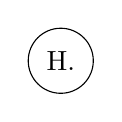
\begin{tikzpicture}[baseline=(n.base)]\node[draw,circle,inner sep=4pt] (n) {H.};\end{tikzpicture}}} al model  for a triangulation,  which \var{\inserted{H.}}{\hand{H.}}{insertion}{ps_134-3_018-v0011} Cartan time ago called ``schéma sim%
plicial'' ...) of the two spaces are canonically isomorphic,  because
the ``flags'' of K and $K^{o}$ are the same.  A similar argument due to Quillen
using the nerves shows that for any category K  (not necessarily ordered\unsure{\hand{)}}
K and $K^{o}$ are homotopic,  although \var{\inserted{$\widehat{K}$ and $\widehat{K^{o}}$ are}}{\hand{$\widehat{K}$ and $\widehat{K^{o}}$ are}}{insertion}{ps_134-3_018-v0012} definitely not equivalent i.e. \var{\inserted{not}}{\hand{not}}{insertion}{ps_134-3_018-v0013}
``homeomorphic'' .

To come back to the decreasing cascade of algebraic structures sui-%
table for describing homotopy types,  we could go down one more step
still,  to the category of  maquettes  (Maq) ,  namely sets \var{\inserted{S}}{\hand{S}}{insertion}{ps_134-3_018-v0014} together
with a family \var{\inserted{K}}{\hand{K}}{insertion}{ps_134-3_018-v0015} of finite subsets (the simplices\hand{\illegible{1}} of \var{\over{t}{t}}{\hand{t}}{writing over}{ps_134-3_018-v0016}he set of vertices

%% END SOURCE ps_134-3_018
\ifnum\EditionMode=1
\psapparatusstart
\psentry{ps_134-3_018-v0001}{1}{insertion}{\inserted{$\mathcal{T}$}}{\hand{$\mathcal{T}$}}{The handwritten insertion is incorporated at its indicated position; insertion brackets leave the running text.}
\psentry{ps_134-3_018-v0002}{2}{typewriter deletion}{\xout{defines}}{}{The typewriter strikes out this material; it leaves the corrected running text.}
\psentry{ps_134-3_018-v0003}{3}{typewriter deletion}{\xout{as being}}{}{The typewriter strikes out this material; it leaves the corrected running text.}
\psentry{ps_134-3_018-v0004}{4}{writing over}{\over{v}{V}}{\hand{V}}{The superposed handwritten reading replaces the underlying reading.}
\psentry{ps_134-3_018-v0005}{5}{typewriter deletion}{\xout{of all}}{}{The typewriter strikes out this material; it leaves the corrected running text.}
\psentry{ps_134-3_018-v0006}{6}{insertion}{\inserted{on $(K,\mathcal{T})$}}{\hand{on $(K,\mathcal{T})$}}{The handwritten insertion is incorporated at its indicated position; insertion brackets leave the running text.}
\psentry{ps_134-3_018-v0007}{7}{typewriter deletion}{\xout{is just the}}{}{The typewriter strikes out this material; it leaves the corrected running text.}
\psentry{ps_134-3_018-v0008}{8}{insertion}{\inserted{$(K,\mathcal{T})$}}{\hand{$(K,\mathcal{T})$}}{The handwritten insertion is incorporated at its indicated position; insertion brackets leave the running text.}
\psentry{ps_134-3_018-v0009}{9}{writing over}{\over{\unsure{y}}{u}}{\hand{u}}{The superposed handwritten reading replaces the underlying reading.}
\psentry{ps_134-3_018-v0010}{10}{insertion}{\inserted{and}}{\hand{and}}{The handwritten insertion is incorporated at its indicated position; insertion brackets leave the running text.}
\psentry{ps_134-3_018-v0011}{11}{insertion}{\inserted{H.}}{\hand{H.}}{The handwritten insertion is incorporated at its indicated position; insertion brackets leave the running text.}
\psentry{ps_134-3_018-v0012}{12}{insertion}{\inserted{$\widehat{K}$ and $\widehat{K^{o}}$ are}}{\hand{$\widehat{K}$ and $\widehat{K^{o}}$ are}}{The handwritten insertion is incorporated at its indicated position; insertion brackets leave the running text.}
\psentry{ps_134-3_018-v0013}{13}{insertion}{\inserted{not}}{\hand{not}}{The handwritten insertion is incorporated at its indicated position; insertion brackets leave the running text.}
\psentry{ps_134-3_018-v0014}{14}{insertion}{\inserted{S}}{\hand{S}}{The handwritten insertion is incorporated at its indicated position; insertion brackets leave the running text.}
\psentry{ps_134-3_018-v0015}{15}{insertion}{\inserted{K}}{\hand{K}}{The handwritten insertion is incorporated at its indicated position; insertion brackets leave the running text.}
\psentry{ps_134-3_018-v0016}{16}{writing over}{\over{t}{t}}{\hand{t}}{The superposed handwritten reading replaces the underlying reading.}
\psapparatusend
\fi
\pssource{ps_134-3_019}{134-3/19}{https://grothendieck.umontpellier.fr/web/viewer.html?file=../134-3.pdf\#page=20}
\psnumber{ps_134-3_019-v0001}{1}
\psnumber{ps_134-3_019-v0002}{2}
\psnumber{ps_134-3_019-v0003}{3}
\psnumber{ps_134-3_019-v0004}{4}
\psnumber{ps_134-3_019-v0005}{5}
\psnumber{ps_134-3_019-v0006}{6}
\psnumber{ps_134-3_019-v0007}{7}
\psnumber{ps_134-3_019-v0008}{8}
\psnumber{ps_134-3_019-v0009}{9}
%% BEGIN SOURCE ps_134-3_019
% Pursuing Stacks (cotes 134-2 to 134-8): archive cote 134-3, site page 19 (PDF page 20), typescript page 19.
% typescript. Draft compared: ps2.tex:851-922.
% AI-transcribed by Claude Opus 5.5 (claude-opus-5-5, adaptive thinking, effort high), Message Batches API, batch ps1 (msgbatch_01Rv5hCaNTtUt4JHx1yqoHPL), 2026-11-12; image review recorded in records/CHECK_DECISIONS_134_3_4.tsv.
\scanpage{134-3/19}
\mspage{\hand{19}}

S),  such that one-point subsets are simplices and a subset of a simplex
is a simplex.  This category,  via the functor   $(S,K)\hand{\mapsto} K$ ,  is equi-%
valent to the full subcategory of (Ord),  whose objects are those ordered
sets $K$,  such that for every $x\hand{\in}K$,  the set $K_{\hand{\leq}x}$  be isomorphic to the
\margin{\diagram{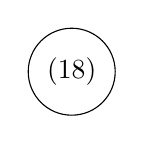
\begin{tikzpicture}[baseline=(n.base)]\node[draw,circle,inner sep=4pt] (n) {(18)};\end{tikzpicture}}}ordered set of \var{\xout{finite}}{}{typewriter deletion}{ps_134-3_019-v0001} non empty subsets of some finite set (or ``simplex'').
Here \var{\xout{again}}{}{typewriter deletion}{ps_134-3_019-v0002} the question \var{\xout{arises}}{}{typewriter deletion}{ps_134-3_019-v0003} whether  this category is a model category
in the technical sense \var{\inserted{[of Quillen]}}{\hand{[of Quillen]}}{insertion}{ps_134-3_019-v0004} does'nt really arise\hand{(18)}\hand{,} because this category
does'nt \var{\inserted{even}}{\hand{even}}{insertion}{ps_134-3_019-v0005} admit finite products -  rien à faire !
\margin{\unsure{\unsure{(17)} 5.3. indeed, the notion of a maquette is \uline{not} an algebraic structure species!}}

\var{\over{23}{23}}{\hand{23}}{writing over}{ps_134-3_019-v0006}.  It may be about time to get back to stacks,  still I can't help go-%
ing on pondering about algebraic structures as models for homotopy types.
If we have any algebraic structure species,  giving \var{\inserted{rise to}}{\hand{rise to}}{insertion}{ps_134-3_019-v0007} a category $M$ of
set-theoretic realizations,  the basic question here does'nt seem so
much whether $M$ is a model category for a suitable choice of the three
sets of arrows (fibrations,  cofibrations,  weak equivalences),  but
rather how to define a natural functor
\[ (*) \qquad M \hand{\longrightarrow} (\mathrm{Hot}) \hand{,} \]
where (Hot) is the category of usual homotopy types,  and see whether
via this functor (Hot) can be interpreted as a category of fractions
\hand{(}or ``localization''\hand{)}of $M$  -  namely,  of course,  by the operation of making
invertible those arrows in $M$ which are transformed into isomorphisms
in (Hot).  In any case,  if we have such a natural functor,  the natural
thing to do is to call those arrows ``weak equivalences''.  If we want $M$
\margin{\hand{(9)}}to be a category of models,  various examples suggest that the natural
thing again is to take as cofibrations the monomorphisms,\hand{(9)}\hand{,} and then
(expecting that the model categories we are going to meet will be closed
model categories) to define fibrations by the Serre-Quillen lifting pro-%
perty with respect to cofibrations (=monomorphisms) which are weak equi-%
valences.  This being done,  it becomes meaningful to ask if indeed $M$
is a category of models.

Now the reflections of the beginning of today's notes \var{\deleted{p.14-15}}{}{deletion}{ps_134-3_019-v0008} \var{\inserted{section 20}}{\hand{section 20}}{insertion}{ps_134-3_019-v0009}
suggest a rather natural way for describing a functor $(*)$,  which makes
\margin{\diagram{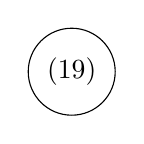
\begin{tikzpicture}[baseline=(n.base)]\node[draw,circle,inner sep=4pt] (n) {(19)};\end{tikzpicture}}}sense in fact,  in principle,  for any category $M$,  namely:  endow $M$ with
it's canonical topology (unless a still more natural one appears at hand\hand{(19)}
\margin{$($}\margin{\unsure{5.3. the canonical topology is \uline{not} always suitable, see \S 24 below}}-  I am not sure there is any better one in the present context),  and
assume that for every  $X\hand{\in}\mathrm{Ob}\,M$ ,  the pro-homotopy type of the induced
site  $M_{/X}$  is essentially constant,  i.e. can be identified with an
object in (Hot) itself.  We then get the functor $(*)$ in an obvious way.
It then becomes meaningful to ask whether this functor is a localization
functor.

When $M$ is defined in terms of an algebraic structure species,  it

%% END SOURCE ps_134-3_019
\ifnum\EditionMode=1
\psapparatusstart
\psentry{ps_134-3_019-v0001}{1}{typewriter deletion}{\xout{finite}}{}{The typewriter strikes out this material; it leaves the corrected running text.}
\psentry{ps_134-3_019-v0002}{2}{typewriter deletion}{\xout{again}}{}{The typewriter strikes out this material; it leaves the corrected running text.}
\psentry{ps_134-3_019-v0003}{3}{typewriter deletion}{\xout{arises}}{}{The typewriter strikes out this material; it leaves the corrected running text.}
\psentry{ps_134-3_019-v0004}{4}{insertion}{\inserted{[of Quillen]}}{\hand{[of Quillen]}}{The handwritten insertion is incorporated at its indicated position; insertion brackets leave the running text.}
\psentry{ps_134-3_019-v0005}{5}{insertion}{\inserted{even}}{\hand{even}}{The handwritten insertion is incorporated at its indicated position; insertion brackets leave the running text.}
\psentry{ps_134-3_019-v0006}{6}{writing over}{\over{23}{23}}{\hand{23}}{The superposed handwritten reading replaces the underlying reading.}
\psentry{ps_134-3_019-v0007}{7}{insertion}{\inserted{rise to}}{\hand{rise to}}{The handwritten insertion is incorporated at its indicated position; insertion brackets leave the running text.}
\psentry{ps_134-3_019-v0008}{8}{deletion}{\deleted{p.14-15}}{}{The author cancels this material by hand; it leaves the corrected running text.}
\psentry{ps_134-3_019-v0009}{9}{insertion}{\inserted{section 20}}{\hand{section 20}}{The handwritten insertion is incorporated at its indicated position; insertion brackets leave the running text.}
\psapparatusend
\fi
\pssource{ps_134-3_020}{134-3/20}{https://grothendieck.umontpellier.fr/web/viewer.html?file=../134-3.pdf\#page=21}
\psnumber{ps_134-3_020-v0001}{1}
\psnumber{ps_134-3_020-v0002}{2}
\psnumber{ps_134-3_020-v0003}{3}
\psnumber{ps_134-3_020-v0004}{4}
\psnumber{ps_134-3_020-v0005}{5}
\psnumber{ps_134-3_020-v0006}{6}
\psnumber{ps_134-3_020-v0007}{7}
\psnumber{ps_134-3_020-v0008}{8}
\psnumber{ps_134-3_020-v0009}{9}
\psnumber{ps_134-3_020-v0010}{10}
\psnumber{ps_134-3_020-v0011}{11}
\psnumber{ps_134-3_020-v0012}{12}
\psnumber{ps_134-3_020-v0013}{13}
%% BEGIN SOURCE ps_134-3_020
% Pursuing Stacks (cotes 134-2 to 134-8): archive cote 134-3, site page 20 (PDF page 21), typescript page 20.
% typescript. Draft compared: ps2.tex:909-968.
% AI-transcribed by Claude Opus 5.5 (claude-opus-5-5, adaptive thinking, effort high), Message Batches API, batch ps1 (msgbatch_01Rv5hCaNTtUt4JHx1yqoHPL), 2026-11-12; image review recorded in records/CHECK_DECISIONS_134_3_4.tsv.
\scanpage{134-3/20}
\mspage{\hand{20}}

admits both types of limits,  without finitesness requirement  -  and
we certainly would expect \var{\inserted[typed]{indeed}}{indeed}{typed insertion}{ps_134-3_020-v0001} at least existence of finite \uline{and} infinite di-%
rect sums in M,  if objects of M were to describe arbitrary homotopy
types.  However,  in view of the special exactness properties of (Hot),
which are by no means autodual,  we will expect moreover direct sums in
M to be ``universal and disjoint'',  in Giraud's sense.  This condition,
which caracterizes to a certain extent categories which at least mildly
resemble or parallel  categories such as (Sets), (Spaces) and similar
categories,whose objects more or less express ``shapes'' -  this condition
at once rules out the majority of the most common algebraic structures,
such as rings,  groups,\var{\xout{and the}}{}{typewriter deletion}{ps_134-3_020-v0002} modules over a ring or anything which
yields for M an abelian category,  etc.  If we describe an algebraic
structure species in terms of its universal realization in a category
stable under finite inverse limits,  then \var{\deleted{a}}{}{deletion}{ps_134-3_020-v0003}\var{\inserted[typed]{such}}{such}{typed insertion}{ps_134-3_020-v0004} structure species can be
viewed as being defined by such a category $\underline{C}$ , and its realizations in
\var{\inserted{any other such $C$ can be interpreted}}{\hand{any other such $C$ can be interpreted}}{insertion}{ps_134-3_020-v0005} \var{\deleted{C}}{}{deletion}{ps_134-3_020-v0006} as the left-exact functors $\underline{C}\hand{\to}C$ (the universal realization of the
structure within $\underline{C}$  corresponding to the identity functor $\underline{C}\hand{\Longrightarrow}\underline{C}$).  In
terms of the dual category $\underline{B}$ ,  associating to every element in
Ob $\underline{B}$  =  Ob $\underline{C}$  the covariant functor $\underline{C}\hand{\to}$(Sets) it represents,  we get
a fully-faithful embedding
\[ \underline{B}\hand{\hookrightarrow} M , \]
by which $\underline{B}$ can be interpreted as the \var{\inserted{category of the}}{\hand{category of the}}{insertion}{ps_134-3_020-v0007} (set-theoretic) realizations of
the given structure  which are of ``finite presentation'' in a suitable
sense (in terms of a given family of generators of $\underline{B}$ namely cogenerators
of $\underline{C}$,  considered as corresponding to the choice of ``base-sets'' for the
given structure species  -  \var{\xout{this}}{}{typewriter deletion}{ps_134-3_020-v0008}\var{\inserted[typed]{such}}{such}{typed insertion}{ps_134-3_020-v0009} choice however being considered as
a convenient way merely to describe the species in concrete terms ...).
\var{\over{I}{I}}{\hand{I}}{writing over}{ps_134-3_020-v0010}f I remember correctly,  M can \var{\over{b}{b}}{\hand{b}}{writing over}{ps_134-3_020-v0011}e deduced from $\underline{B}$,  up to equivalence,
as being merely the category of Ind-objects of $\underline{B}$ ,  i.e. the inclusion
functor above yields an equivalence of categories
\[ \mathrm{Ind}(\underline{B}) \hand{\xrightarrow{\approx}} M , \]
which implies, I guess\var{\xout{\illegible{1}}}{}{typewriter deletion}{ps_134-3_020-v0012},  that the exactness properties of M mainly
reflect those of $\underline{B}$ .  Thus I would expect the condition we want on direct
sums in M to correspond to the same condition for finite direct sums in
$\underline{B}$ ,  not more not less.  Thus the algebraic structure species satisfying
this condition should correspond exactly to small categories $\underline{B}$,  stable
under finite direct limits,  and such that finite sums in $\underline{B}$ are disjoint
and universal.   This condition is presumably necessary,  if we want the
functor (*) from M to Hot  to be defined and to be a localization func-%
tor  -   a condition which it would be nice to understand directly in \var{\xout{te}}{}{typewriter deletion}{ps_134-3_020-v0013}

%% END SOURCE ps_134-3_020
\ifnum\EditionMode=1
\psapparatusstart
\psentry{ps_134-3_020-v0001}{1}{typed insertion}{\inserted[typed]{indeed}}{indeed}{The typed insertion is incorporated at its indicated position; insertion brackets leave the running text.}
\psentry{ps_134-3_020-v0002}{2}{typewriter deletion}{\xout{and the}}{}{The typewriter strikes out this material; it leaves the corrected running text.}
\psentry{ps_134-3_020-v0003}{3}{deletion}{\deleted{a}}{}{The author cancels this material by hand; it leaves the corrected running text.}
\psentry{ps_134-3_020-v0004}{4}{typed insertion}{\inserted[typed]{such}}{such}{The typed insertion is incorporated at its indicated position; insertion brackets leave the running text.}
\psentry{ps_134-3_020-v0005}{5}{insertion}{\inserted{any other such $C$ can be interpreted}}{\hand{any other such $C$ can be interpreted}}{The handwritten insertion is incorporated at its indicated position; insertion brackets leave the running text.}
\psentry{ps_134-3_020-v0006}{6}{deletion}{\deleted{C}}{}{The author cancels this material by hand; it leaves the corrected running text.}
\psentry{ps_134-3_020-v0007}{7}{insertion}{\inserted{category of the}}{\hand{category of the}}{The handwritten insertion is incorporated at its indicated position; insertion brackets leave the running text.}
\psentry{ps_134-3_020-v0008}{8}{typewriter deletion}{\xout{this}}{}{The typewriter strikes out this material; it leaves the corrected running text.}
\psentry{ps_134-3_020-v0009}{9}{typed insertion}{\inserted[typed]{such}}{such}{The typed insertion is incorporated at its indicated position; insertion brackets leave the running text.}
\psentry{ps_134-3_020-v0010}{10}{writing over}{\over{I}{I}}{\hand{I}}{The superposed handwritten reading replaces the underlying reading.}
\psentry{ps_134-3_020-v0011}{11}{writing over}{\over{b}{b}}{\hand{b}}{The superposed handwritten reading replaces the underlying reading.}
\psentry{ps_134-3_020-v0012}{12}{typewriter deletion}{\xout{\illegible{1}}}{}{The typewriter strikes out this material; it leaves the corrected running text.}
\psentry{ps_134-3_020-v0013}{13}{typewriter deletion}{\xout{te}}{}{The typewriter strikes out this material; it leaves the corrected running text.}
\psapparatusend
\fi
\pssource{ps_134-3_021}{134-3/21}{https://grothendieck.umontpellier.fr/web/viewer.html?file=../134-3.pdf\#page=22}
\psnumber{ps_134-3_021-v0001}{1}
\psnumber{ps_134-3_021-v0002}{2}
\psnumber{ps_134-3_021-v0003}{3}
\psnumber{ps_134-3_021-v0004}{4}
\psnumber{ps_134-3_021-v0005}{5}
\psnumber{ps_134-3_021-v0006}{6}
\psnumber{ps_134-3_021-v0007}{7}
\psnumber{ps_134-3_021-v0008}{8}
\psnumber{ps_134-3_021-v0009}{9}
\psnumber{ps_134-3_021-v0010}{10}
\psnumber{ps_134-3_021-v0011}{11}
\psnumber{ps_134-3_021-v0012}{12}
\psnumber{ps_134-3_021-v0013}{13}
\psnumber{ps_134-3_021-v0014}{14}
\psnumber{ps_134-3_021-v0015}{15}
\psnumber{ps_134-3_021-v0016}{16}
\psnumber{ps_134-3_021-v0017}{17}
\psnumber{ps_134-3_021-v0018}{18}
\psnumber{ps_134-3_021-v0019}{19}
\psnumber{ps_134-3_021-v0020}{20}
\psnumber{ps_134-3_021-v0021}{21}
\psnumber{ps_134-3_021-v0022}{22}
\psnumber{ps_134-3_021-v0023}{23}
\psnumber{ps_134-3_021-v0024}{24}
\psnumber{ps_134-3_021-v0025}{25}
\psnumber{ps_134-3_021-v0026}{26}
%% BEGIN SOURCE ps_134-3_021
% Pursuing Stacks (cotes 134-2 to 134-8): archive cote 134-3, site page 21 (PDF page 22), typescript page 21.
% typescript. Draft compared: ps2.tex:955-1024.
% AI-transcribed by Claude Opus 5.5 (claude-opus-5-5, adaptive thinking, effort high), Message Batches API, batch ps1 (msgbatch_01Rv5hCaNTtUt4JHx1yqoHPL), 2026-11-12; image review recorded in records/CHECK_DECISIONS_134_3_4.tsv.
\scanpage{134-3/21}
\mspage{\hand{21}}

terms of $\underline{B}$ , and (presumably) in terms of the canonical topology\var{\inserted{(19)}}{\hand{(19)}}{insertion}{ps_134-3_021-v0001} of $\underline{B}$ ,
which should give rise to a\var{\xout{\unsure{xxxqui}}}{}{typewriter deletion}{ps_134-3_021-v0002} localization functor
\[ \underline{B} \hand{\longrightarrow} (\mathrm{Hot})_{\mathrm{f.t.}} \quad , \]
where the subscript f.t. means ``finite type'' - granting that the notion
of homotopy types of finite type (presumably the same as homotopy types
of finite triangulations,\var{\inserted{or}}{\hand{or}}{insertion}{ps_134-3_021-v0003} of \var{\inserted{``finite''}}{\hand{``finite''}}{insertion}{ps_134-3_021-v0004} C.W. spaces) is a well defined notion\var{\inserted{(20)}}{\hand{(20)}}{insertion}{ps_134-3_021-v0005}.
As usual, it is in $\underline{B}$ , not in $\underline{C}$ , that geometrical constructions
take place which make sense for topological intuition. More specifical-%
ly, it seems that in the cases met \var{\inserted{with}}{\hand{with}}{insertion}{ps_134-3_021-v0006} so far, there \uline{are} indeed privileged
base-sets for the structure species considered (such as the``components''
of a semi\var{\xout{s}}{}{typewriter deletion}{ps_134-3_021-v0007}simplicial of cubical complex, or of a stack, etc ), indexed
by the \var{\inserted[typed]{natural}}{natural}{typed insertion}{ps_134-3_021-v0008} integers or n-tupels of such integers, and which``correspond'' to
topological cells of various dimensions, \var{\deleted{the}}{}{deletion}{ps_134-3_021-v0009}\var{\inserted{Moreover,}}{\hand{Moreover,}}{insertion}{ps_134-3_021-v0010} some of the basic structu-%
ral \var{\inserted{monomorphic}}{\hand{monomorphic}}{insertion}{ps_134-3_021-v0011} maps between these \var{\inserted{objects of $\underline{B}$}}{\hand{objects of $\underline{B}$}}{insertion}{ps_134-3_021-v0012} defin\var{\over{ing}{e}}{\hand{e}}{writing over}{ps_134-3_021-v0013} cellular decompositions of the \var{\inserted[typed]{topological}}{topological}{typed insertion}{ps_134-3_021-v0014} spheres
bounding these topological cells. These objects and ``boundary\hand{*} maps''
between them \var{\deleted{\xout{form}}}{}{deletion}{ps_134-3_021-v0015}\var{\inserted[typed]{define}}{define}{typed insertion}{ps_134-3_021-v0016} a (non full, in general) subcategory of $\underline{B}$ , say $\underline{B}_{\mathrm{oo}}$ ,
which looks like the core of the category $\underline{B}$, from which the topological
significance of $\underline{B}$ is springing. It is in terms of $\underline{B}_{\mathrm{oo}}$ that the ``corres-%
pondance '' \hand{(}vaguely referred to above\hand{)} with topological cells \var{\inserted[typed]{and spheres}}{and spheres}{typed insertion}{ps_134-3_021-v0017} takes a
precise meaning. Namely, associating to any object of $\underline{B}_{\mathrm{oo}}$ the ordered
set of its subobjects (within $\underline{B}_{\mathrm{oo}}$ of course, not $\underline{B}$ ), the \var{\xout{conicalx}}{}{typewriter deletion}{ps_134-3_021-v0018}
(stratified) topological realization of this ordered set is a cell, and
the \var{\xout{union}}{}{typewriter deletion}{ps_134-3_021-v0019}\var{\inserted[typed]{family}}{family}{typed insertion}{ps_134-3_021-v0020} of \var{\deleted{\xout{the}}}{}{deletion}{ps_134-3_021-v0021} subcells of smaller dimension (namely different from
the given one) is a cellular subdivision of the \var{\inserted[typed]{sphere}}{sphere}{typed insertion}{ps_134-3_021-v0022} bounding th\var{\over{e}{is}}{\hand{is}}{writing over}{ps_134-3_021-v0023} cell\var{\inserted{(21)}}{\hand{(21)}}{insertion}{ps_134-3_021-v0024}.

\var{\over{\unsure{4}}{7}}{\hand{7}}{writing over}{ps_134-3_021-v0025}.3.
\var{\over{21}{24}}{\hand{24}}{writing over}{ps_134-3_021-v0026}. Yesterday there occured to me a big``étourderie'' again of the day
before, in connection with a reflection on a suitable ``natural'' site
structure on the category (Cat) - namely when asserting that for a
family of morphisms i.e. functors in (Cat)
\[ (*) \qquad A_i \hand{\longrightarrow} A \ , \]
in order for the corresponding family to be ``covering'' namely epimorphic
in the category (a topos, as a matter of fact) (Ss sets), namely for
the corresponding families of mappings of sets
\[ (**) \qquad \mathrm{Fl}_n(A_i) \hand{\longrightarrow} \mathrm{Fl}_n(A) \]
to be epimorphic, it was sufficient that this condition be satisfied
for n=2 (which, according to Giraud, just means that the family (*)
is covering for the canonical topology of (Cat)). This is obviously
false - morally, it would mean that an n-simplex is ``covered'' in a
reasonable sense by it's sub-2-simplices, which is pretty absurd. To

%% END SOURCE ps_134-3_021
\ifnum\EditionMode=1
\psapparatusstart
\psentry{ps_134-3_021-v0001}{1}{insertion}{\inserted{(19)}}{\hand{(19)}}{The handwritten insertion is incorporated at its indicated position; insertion brackets leave the running text.}
\psentry{ps_134-3_021-v0002}{2}{typewriter deletion}{\xout{\unsure{xxxqui}}}{}{The typewriter strikes out this material; it leaves the corrected running text.}
\psentry{ps_134-3_021-v0003}{3}{insertion}{\inserted{or}}{\hand{or}}{The handwritten insertion is incorporated at its indicated position; insertion brackets leave the running text.}
\psentry{ps_134-3_021-v0004}{4}{insertion}{\inserted{``finite''}}{\hand{``finite''}}{The handwritten insertion is incorporated at its indicated position; insertion brackets leave the running text.}
\psentry{ps_134-3_021-v0005}{5}{insertion}{\inserted{(20)}}{\hand{(20)}}{The handwritten insertion is incorporated at its indicated position; insertion brackets leave the running text.}
\psentry{ps_134-3_021-v0006}{6}{insertion}{\inserted{with}}{\hand{with}}{The handwritten insertion is incorporated at its indicated position; insertion brackets leave the running text.}
\psentry{ps_134-3_021-v0007}{7}{typewriter deletion}{\xout{s}}{}{The typewriter strikes out this material; it leaves the corrected running text.}
\psentry{ps_134-3_021-v0008}{8}{typed insertion}{\inserted[typed]{natural}}{natural}{The typed insertion is incorporated at its indicated position; insertion brackets leave the running text.}
\psentry{ps_134-3_021-v0009}{9}{deletion}{\deleted{the}}{}{The author cancels this material by hand; it leaves the corrected running text.}
\psentry{ps_134-3_021-v0010}{10}{insertion}{\inserted{Moreover,}}{\hand{Moreover,}}{The handwritten insertion is incorporated at its indicated position; insertion brackets leave the running text.}
\psentry{ps_134-3_021-v0011}{11}{insertion}{\inserted{monomorphic}}{\hand{monomorphic}}{The handwritten insertion is incorporated at its indicated position; insertion brackets leave the running text.}
\psentry{ps_134-3_021-v0012}{12}{insertion}{\inserted{objects of $\underline{B}$}}{\hand{objects of $\underline{B}$}}{The handwritten insertion is incorporated at its indicated position; insertion brackets leave the running text.}
\psentry{ps_134-3_021-v0013}{13}{writing over}{\over{ing}{e}}{\hand{e}}{The superposed handwritten reading replaces the underlying reading.}
\psentry{ps_134-3_021-v0014}{14}{typed insertion}{\inserted[typed]{topological}}{topological}{The typed insertion is incorporated at its indicated position; insertion brackets leave the running text.}
\psentry{ps_134-3_021-v0015}{15}{deletion}{\deleted{\xout{form}}}{}{The author cancels this material by hand; it leaves the corrected running text.}
\psentry{ps_134-3_021-v0016}{16}{typed insertion}{\inserted[typed]{define}}{define}{The typed insertion is incorporated at its indicated position; insertion brackets leave the running text.}
\psentry{ps_134-3_021-v0017}{17}{typed insertion}{\inserted[typed]{and spheres}}{and spheres}{The typed insertion is incorporated at its indicated position; insertion brackets leave the running text.}
\psentry{ps_134-3_021-v0018}{18}{typewriter deletion}{\xout{conicalx}}{}{The typewriter strikes out this material; it leaves the corrected running text.}
\psentry{ps_134-3_021-v0019}{19}{typewriter deletion}{\xout{union}}{}{The typewriter strikes out this material; it leaves the corrected running text.}
\psentry{ps_134-3_021-v0020}{20}{typed insertion}{\inserted[typed]{family}}{family}{The typed insertion is incorporated at its indicated position; insertion brackets leave the running text.}
\psentry{ps_134-3_021-v0021}{21}{deletion}{\deleted{\xout{the}}}{}{The author cancels this material by hand; it leaves the corrected running text.}
\psentry{ps_134-3_021-v0022}{22}{typed insertion}{\inserted[typed]{sphere}}{sphere}{The typed insertion is incorporated at its indicated position; insertion brackets leave the running text.}
\psentry{ps_134-3_021-v0023}{23}{writing over}{\over{e}{is}}{\hand{is}}{The superposed handwritten reading replaces the underlying reading.}
\psentry{ps_134-3_021-v0024}{24}{insertion}{\inserted{(21)}}{\hand{(21)}}{The handwritten insertion is incorporated at its indicated position; insertion brackets leave the running text.}
\psentry{ps_134-3_021-v0025}{25}{writing over}{\over{\unsure{4}}{7}}{\hand{7}}{The superposed handwritten reading replaces the underlying reading.}
\psentry{ps_134-3_021-v0026}{26}{writing over}{\over{21}{24}}{\hand{24}}{The superposed handwritten reading replaces the underlying reading.}
\psapparatusend
\fi
\pssource{ps_134-3_022}{134-3/22}{https://grothendieck.umontpellier.fr/web/viewer.html?file=../134-3.pdf\#page=23}
\psnumber{ps_134-3_022-v0001}{1}
\psnumber{ps_134-3_022-v0002}{2}
\psnumber{ps_134-3_022-v0003}{3}
\psnumber{ps_134-3_022-v0004}{4}
\psnumber{ps_134-3_022-v0005}{5}
\psnumber{ps_134-3_022-v0006}{6}
\psnumber{ps_134-3_022-v0007}{7}
\psnumber{ps_134-3_022-v0008}{8}
\psnumber{ps_134-3_022-v0009}{9}
\psnumber{ps_134-3_022-v0010}{10}
\psnumber{ps_134-3_022-v0011}{11}
%% BEGIN SOURCE ps_134-3_022
% Pursuing Stacks (cotes 134-2 to 134-8): archive cote 134-3, site page 22 (PDF page 23), typescript page 22.
% typescript. Draft compared: ps2.tex:1010-1069.
% AI-transcribed by Claude Opus 5.5 (claude-opus-5-5, adaptive thinking, effort high), Message Batches API, batch ps1 (msgbatch_01Rv5hCaNTtUt4JHx1yqoHPL), 2026-11-12; image review recorded in records/CHECK_DECISIONS_134_3_4.tsv.
\scanpage{134-3/22}
\mspage{\hand{22}}
give specific positive statements along these lines, let's \var{\inserted[typed]{for any $N\hand{\in}\underline{N}$,}}{for any $N\hand{\in}\underline{N}$,}{typed insertion}{ps_134-3_022-v0001} denote
by $T_N$ the topology on (Cat) for which a family (*) is covering i\var{\over{s}{ff}}{\hand{ff}}{writing over}{ps_134-3_022-v0002}
the families (**) are for $n\hand{\leqslant} N$ - which means also that the correspon-%
ding family of N-truncated nerves
\[ \mathrm{Nerve}(A_i)\hand{[}N\hand{]} \hand{\longrightarrow} \mathrm{Nerve}(A)\hand{[}N\hand{]} \]
is epimorphic. For N=1, this means that the family is \hand{``}universally
epimorphic\hand{''}, for N=2, that it is \var{\deleted{\unsure{it is|it as}}}{}{deletion}{ps_134-3_022-v0003}\hand{``}universally effectively epimor-%
phic\hand{''}i.e. covering for the canonical topology of (Cat) (Giraud, loc.
cit. page 28). It turns out that this decreasing sequence of topologies
on (Cat) is strictly decreasing - as a matter of fact, denoting by
$\hand{\Delta[}N\hand{]}$ the category of \var{\inserted[typed]{standart ordered}}{standart ordered}{typed insertion}{ps_134-3_022-v0004}\var{\xout{\illegible{1}}}{}{typewriter deletion}{ps_134-3_022-v0005}simplices of dimension $\hand{\leqslant} N$, and using the
inclusions
\[ \hand{\Delta[}N\hand{]\hookrightarrow}(\mathrm{Cat})\hand{\hookrightarrow\Delta}(N)\hand{^{\wedge}} \]
(for $N\hand{\geqslant}2$ say), an immediate application of the ``comparison lemma'' for
sites shows that we have an equivalence
\[ ((\mathrm{Cat}),T_N)\hand{^{\sim}\simeq\Delta[}N\hand{]^{\wedge}}, \]
and hence, for any object A in (Cat) namely any category A , we get
an equivalence
\[ ((\mathrm{Cat}),T_N)_{/A}\hand{)^{\sim}\simeq}(\hand{\Delta}(N)_{/A})\hand{^{\wedge}} \quad , \]
and hence the homotopy type of the first hand member is \var{\inserted{\uline{not}}}{\hand{\uline{not}}}{insertion}{ps_134-3_022-v0006} described by and
equivalent to the homotopy type of the whole Nerve(A) object, but
rather by its N-skeleton, which has the same homotopy and cohomology
invariants in \var{\inserted[typed]{dimension}}{dimension}{typed insertion}{ps_134-3_022-v0007} \var{\xout{degrees}}{}{typewriter deletion}{ps_134-3_022-v0008} $\hand{\leqslant} N$, but by no means for higher dimensions. This
shows that among the topologies $T_N$ , none is suitable for recovering
the homotopy type of objects of (Cat) in the way contemplated two days
ago (page 15); \var{\deleted{but}}{}{deletion}{ps_134-3_022-v0009} the one topology which \uline{is} suitable is the one which
may be denoted by $T_{\infty}$ , and which \var{\xout{wa}}{}{typewriter deletion}{ps_134-3_022-v0010}is the one indeed which I first con-%
templated (page 14), before the mistaken idea occured to me that it was
the same as the canonical topology.

A very similar mistake occured earlier, when I surmised that the \var{\inserted[typed]{left}}{left}{typed insertion}{ps_134-3_022-v0011}
adjoint functor N' to the inclusion or Nerve functor N from (Cat)
to (Ss sets) $=\hand{\Delta^{\wedge}}$ had the property that for any object K in (Ss sets),
K and N'(K) had same homotopy type. Looking up yesterday the descripti-%
on in Gabriel-Zisman of this functor, this recalled to my mind that
it factors (via the natural restriction functor) through the category
$(\hand{\Delta}[2])^{\wedge}$ , hence any morphism $K\hand{\longrightarrow}K'$ inducing an isomorphism on the
2-skeletons (which by no means implies that it is a homotopy equivalen-%
ce) induces an isomorphism $N'(K)\hand{\xrightarrow{\sim}}N'(K')$, and a fortiori a homotopy
equivalence. This shows that, even if it should be true that (Cat) is

%% END SOURCE ps_134-3_022
\ifnum\EditionMode=1
\psapparatusstart
\psentry{ps_134-3_022-v0001}{1}{typed insertion}{\inserted[typed]{for any $N\hand{\in}\underline{N}$,}}{for any $N\hand{\in}\underline{N}$,}{The typed insertion is incorporated at its indicated position; insertion brackets leave the running text.}
\psentry{ps_134-3_022-v0002}{2}{writing over}{\over{s}{ff}}{\hand{ff}}{The superposed handwritten reading replaces the underlying reading.}
\psentry{ps_134-3_022-v0003}{3}{deletion}{\deleted{\unsure{it is|it as}}}{}{The author cancels this material by hand; it leaves the corrected running text.}
\psentry{ps_134-3_022-v0004}{4}{typed insertion}{\inserted[typed]{standart ordered}}{standart ordered}{The typed insertion is incorporated at its indicated position; insertion brackets leave the running text.}
\psentry{ps_134-3_022-v0005}{5}{typewriter deletion}{\xout{\illegible{1}}}{}{The typewriter strikes out this material; it leaves the corrected running text.}
\psentry{ps_134-3_022-v0006}{6}{insertion}{\inserted{\uline{not}}}{\hand{\uline{not}}}{The handwritten insertion is incorporated at its indicated position; insertion brackets leave the running text.}
\psentry{ps_134-3_022-v0007}{7}{typed insertion}{\inserted[typed]{dimension}}{dimension}{The typed insertion is incorporated at its indicated position; insertion brackets leave the running text.}
\psentry{ps_134-3_022-v0008}{8}{typewriter deletion}{\xout{degrees}}{}{The typewriter strikes out this material; it leaves the corrected running text.}
\psentry{ps_134-3_022-v0009}{9}{deletion}{\deleted{but}}{}{The author cancels this material by hand; it leaves the corrected running text.}
\psentry{ps_134-3_022-v0010}{10}{typewriter deletion}{\xout{wa}}{}{The typewriter strikes out this material; it leaves the corrected running text.}
\psentry{ps_134-3_022-v0011}{11}{typed insertion}{\inserted[typed]{left}}{left}{The typed insertion is incorporated at its indicated position; insertion brackets leave the running text.}
\psapparatusend
\fi
\pssource{ps_134-3_023}{134-3/23}{https://grothendieck.umontpellier.fr/web/viewer.html?file=../134-3.pdf\#page=24}
\psnumber{ps_134-3_023-v0001}{1}
\psnumber{ps_134-3_023-v0002}{2}
\psnumber{ps_134-3_023-v0003}{3}
\psnumber{ps_134-3_023-v0004}{4}
\psnumber{ps_134-3_023-v0005}{5}
\psnumber{ps_134-3_023-v0006}{6}
\psnumber{ps_134-3_023-v0007}{7}
\psnumber{ps_134-3_023-v0008}{8}
\psnumber{ps_134-3_023-v0009}{9}
\psnumber{ps_134-3_023-v0010}{10}
\psnumber{ps_134-3_023-v0011}{11}
\psnumber{ps_134-3_023-v0012}{12}
\psnumber{ps_134-3_023-v0013}{13}
\psnumber{ps_134-3_023-v0014}{14}
\psnumber{ps_134-3_023-v0015}{15}
%% BEGIN SOURCE ps_134-3_023
% Pursuing Stacks (cotes 134-2 to 134-8): archive cote 134-3, site page 23 (PDF page 24), typescript page 23.
% typescript. Draft compared: ps2.tex:1055-1122.
% AI-transcribed by Claude Opus 5.5 (claude-opus-5-5, adaptive thinking, effort high), Message Batches API, batch ps1 (msgbatch_01Rv5hCaNTtUt4JHx1yqoHPL), 2026-11-12; image review recorded in records/CHECK_DECISIONS_134_3_4.tsv.
\scanpage{134-3/23}
\mspage{\hand{23}}
a model category in Quillen's sense,  the situation with the inclusion
functor
\[ N:(Cat)\hand{\longrightarrow} (Ss sets) \]
and the left adjoint functor N'  is by no means the one of Quillen\hand{'}s
comparison theorem,  where the two functors play\var{\xout{ed}}{}{typewriter deletion}{ps_134-3_023-v0001} mutually dual roles
and both induce equivalences on the corresponding localized homotopical
categories.  Here \uline{only} N,  \uline{not} N',  \uline{induces such equivalence}.  This is
analoguous to the situation,  already note\var{\over{\unsure{s}}{d}}{\hand{d}}{writing over}{ps_134-3_023-v0002} before,  of the inclusion
functors
\[ (Preord)\hand{\hookrightarrow} (Cat) \qquad or \qquad (Ord)\hand{\hookrightarrow} (Cat) \quad , \]
which \var{\inserted{[presumably]}}{\hand{[presumably]}}{insertion}{ps_134-3_023-v0003} by localization induce equivalences on the associated homotopy
categories,  but the left adjoint functors do not share this property.

The topology $T_\infty$  just considered on (Cat) as a ``suitable'' topology
for describing homotopy types of objects of (Cat),  was\hand{|}of course direct-%
ly inspired by the semi-simplicial approach to homotopy types,  via
simplicial complexes  namely via the two associated inclusion functors
\[ \hand{\Delta} \hand{\hookrightarrow} (Cat)\hand{\hookrightarrow} \hand{\Delta^{\wedge}} , \]
the second functor associating to every category A the ``complex'' of it's
``simplicial diagrams''  $a_o\hand{\longrightarrow} a_1\hand{\longrightarrow} \;\ldots\hand{\longrightarrow} a_n$ .  If we had been working
\var{\xout{rather}}{}{typewriter deletion}{ps_134-3_023-v0004} with  cubical complexes rather than ss ones for describing homoto
-py types,  this would give rise similarly to two functors
\[ \hand{\square} \hand{\hookrightarrow} (Cat)\hand{\hookrightarrow} \hand{\square^{\wedge}} , \]
where $\hand{\square}$ is the category of``standar\var{\over{t}{d}}{\hand{d}}{writing over}{ps_134-3_023-v0005} cubes'' and face and degeneracy
maps between them,  and where the second\hand{|}inclusion associates to every
category A the cubical complex of it's  ``cubical diagrams'',  namely \var{\inserted[typed]{commutative}}{commutative}{typed insertion}{ps_134-3_023-v0006}
diagrams in A modelled after the diagram types $\hand{\square}_n\hand{[}1\hand{]}$ ,  the 1-skeleton
of the standart n-cubes $\hand{\square}_n$ , with suitable orientations on it's edges
(indicative of the direction of corresponding arrows in A).  The natural
idea \var{\over{\xout{here}}{now}}{\hand{now}}{writing over}{ps_134-3_023-v0007} would be to endow (Cat) with the \var{\over{category}{topology}}{\hand{topology}}{writing over}{ps_134-3_023-v0008}, $T'_\infty$ say,  induced
by $\hand{\square^{\wedge}}$,  namely call a family (*)  covering iff for every $n\hand{\in} \underline{N}$,  the
corresponding family  of \var{\xout{set}}{}{typewriter deletion}{ps_134-3_023-v0009} maps of sets
\[ Cub_n(A_i)\hand{\longrightarrow} \hand{C}ub_n(A) \]
is epimorphic.   This \var{\xout{category}}{}{typewriter deletion}{ps_134-3_023-v0010} topology appears to be \var{\xout{finer}}{}{typewriter deletion}{ps_134-3_023-v0011}\var{\inserted[typed]{coarser}}{coarser}{typed insertion}{ps_134-3_023-v0012} than $T_\infty$ \var{\xout{,}}{}{typewriter deletion}{ps_134-3_023-v0013}
\var{\inserted[typed]{(i.e. there are less covering families),}}{(i.e. there are less covering families),}{typed insertion}{ps_134-3_023-v0014}
and the comparison lemma gives now the equivalence
\[ ((Cat),T'_\infty)\hand{^{\sim}} \hand{\simeq} \hand{\square^{\wedge}} , \]
which shows that definitely the topology is \uline{strictly} coarser than $T_\infty$ ,
as it gives rise to a non-equivalent topos,  $\hand{\square^{\wedge}}$ instead of $\hand{\Delta^{\wedge}}$.

T\var{\over{h}{h}}{\hand{h}}{writing over}{ps_134-3_023-v0015}ese reflections convince me  1)  there are indeed topologies
on (Cat),  suit\unsure{able for} describing the natural homotopy types of ob-%
jects of (Cat) namely of categories,  and  2)  that there is definitely

%% END SOURCE ps_134-3_023
\ifnum\EditionMode=1
\psapparatusstart
\psentry{ps_134-3_023-v0001}{1}{typewriter deletion}{\xout{ed}}{}{The typewriter strikes out this material; it leaves the corrected running text.}
\psentry{ps_134-3_023-v0002}{2}{writing over}{\over{\unsure{s}}{d}}{\hand{d}}{The superposed handwritten reading replaces the underlying reading.}
\psentry{ps_134-3_023-v0003}{3}{insertion}{\inserted{[presumably]}}{\hand{[presumably]}}{The handwritten insertion is incorporated at its indicated position; insertion brackets leave the running text.}
\psentry{ps_134-3_023-v0004}{4}{typewriter deletion}{\xout{rather}}{}{The typewriter strikes out this material; it leaves the corrected running text.}
\psentry{ps_134-3_023-v0005}{5}{writing over}{\over{t}{d}}{\hand{d}}{The superposed handwritten reading replaces the underlying reading.}
\psentry{ps_134-3_023-v0006}{6}{typed insertion}{\inserted[typed]{commutative}}{commutative}{The typed insertion is incorporated at its indicated position; insertion brackets leave the running text.}
\psentry{ps_134-3_023-v0007}{7}{writing over}{\over{\xout{here}}{now}}{\hand{now}}{The superposed handwritten reading replaces the underlying reading.}
\psentry{ps_134-3_023-v0008}{8}{writing over}{\over{category}{topology}}{\hand{topology}}{The superposed handwritten reading replaces the underlying reading.}
\psentry{ps_134-3_023-v0009}{9}{typewriter deletion}{\xout{set}}{}{The typewriter strikes out this material; it leaves the corrected running text.}
\psentry{ps_134-3_023-v0010}{10}{typewriter deletion}{\xout{category}}{}{The typewriter strikes out this material; it leaves the corrected running text.}
\psentry{ps_134-3_023-v0011}{11}{typewriter deletion}{\xout{finer}}{}{The typewriter strikes out this material; it leaves the corrected running text.}
\psentry{ps_134-3_023-v0012}{12}{typed insertion}{\inserted[typed]{coarser}}{coarser}{The typed insertion is incorporated at its indicated position; insertion brackets leave the running text.}
\psentry{ps_134-3_023-v0013}{13}{typewriter deletion}{\xout{,}}{}{The typewriter strikes out this material; it leaves the corrected running text.}
\psentry{ps_134-3_023-v0014}{14}{typed insertion}{\inserted[typed]{(i.e. there are less covering families),}}{(i.e. there are less covering families),}{The typed insertion is incorporated at its indicated position; insertion brackets leave the running text.}
\psentry{ps_134-3_023-v0015}{15}{writing over}{\over{h}{h}}{\hand{h}}{The superposed handwritten reading replaces the underlying reading.}
\psapparatusend
\fi
\pssource{ps_134-3_024}{134-3/24}{https://grothendieck.umontpellier.fr/web/viewer.html?file=../134-3.pdf\#page=25}
\psnumber{ps_134-3_024-v0001}{1}
\psnumber{ps_134-3_024-v0002}{2}
\psnumber{ps_134-3_024-v0003}{3}
\psnumber{ps_134-3_024-v0004}{4}
\psnumber{ps_134-3_024-v0005}{5}
\psnumber{ps_134-3_024-v0006}{6}
\psnumber{ps_134-3_024-v0007}{7}
\psnumber{ps_134-3_024-v0008}{8}
\psnumber{ps_134-3_024-v0009}{9}
\psnumber{ps_134-3_024-v0010}{10}
\psnumber{ps_134-3_024-v0011}{11}
\psnumber{ps_134-3_024-v0012}{12}
\psnumber{ps_134-3_024-v0013}{13}
\psnumber{ps_134-3_024-v0014}{14}
\psnumber{ps_134-3_024-v0015}{15}
\psnumber{ps_134-3_024-v0016}{16}
\psnumber{ps_134-3_024-v0017}{17}
\psnumber{ps_134-3_024-v0018}{18}
\psnumber{ps_134-3_024-v0019}{19}
\psnumber{ps_134-3_024-v0020}{20}
\psnumber{ps_134-3_024-v0021}{21}
\psnumber{ps_134-3_024-v0022}{22}
\psnumber{ps_134-3_024-v0023}{23}
\psnumber{ps_134-3_024-v0024}{24}
\psnumber{ps_134-3_024-v0025}{25}
%% BEGIN SOURCE ps_134-3_024
% Pursuing Stacks (cotes 134-2 to 134-8): archive cote 134-3, site page 24 (PDF page 25), typescript page 24.
% typescript. Draft compared: ps2.tex:1106-1172.
% AI-transcribed by Claude Opus 5.5 (claude-opus-5-5, adaptive thinking, effort high), Message Batches API, batch pilot (msgbatch_0189Nhf1xB615YWnztubtLfc), 2026-11-12; image review recorded in records/CHECK_DECISIONS_134_3_4.tsv.
\scanpage{134-3/24}
\mspage{24}
no privileged choice for such topology.  We just described two such,
but using \var{\xout{xx}}{}{typewriter deletion}{ps_134-3_024-v0001} multicomplexes (cubical or semisimplicial) rather than
\margin{\diagram{\begin{tikzpicture}[x=1cm,y=1cm]\draw[->] (0.35,0)--(0,0)--(0,0.8);\end{tikzpicture}}}simple complexes should give us infinitely \var{\inserted[typed]{many}}{many}{typed insertion}{ps_134-3_024-v0002} others  just as suitable,
and I suspect \var{\xout{that}}{}{typewriter deletion}{ps_134-3_024-v0003} now that there must be a big lot more of them still !

\margin{\diagram{\begin{tikzpicture}[x=1cm,y=1cm]\draw[->] (0.35,0.8)--(0,0.8)--(0,0);\end{tikzpicture}}}\var{\over{\illegible{1}}{25}}{\hand{25}}{writing over}{ps_134-3_024-v0004}.  A fortiori,  coming back to the intriguing question of \var{\xout{which}}{}{typewriter deletion}{ps_134-3_024-v0005} carac-%
terizing the algebraic structure species suitable for describing homoto-%
py types in the usual homotopy category (Hot),  \var{\xout{if M is the}}{}{typewriter deletion}{ps_134-3_024-v0006} and for
recovering (Hot) as a category of fractions of the category M of all
set-theoretic re\var{\xout{a}}{}{typewriter deletion}{ps_134-3_024-v0007}alizations of this species,  it becomes clear now that
we cannot hope reasonably for a ``natural'' topology on M,  distinguished
among all others,  giving rise to the wished-for functor
\[ (*) \qquad M \hand{\to} (\mathrm{Hot}) \]
in the way contemplated earlier (\var{\deleted{page 19 ff}}{}{deletion}{ps_134-3_024-v0008}\var{\inserted{section 23}}{\hand{section 23}}{insertion}{ps_134-3_024-v0009}).  Here it occu\var{\over{s}{r}}{\hand{r}}{writing over}{ps_134-3_024-v0010}s to me
that anyhow,  if concerned mainly with defining the functor (*),  we
should consider that two topologies T,T' on M such that $T \hand{\geqslant} T'$  and
hence giving rise to a morphism of topoi
\[ (**) \qquad M_T^{\hand{\sim}} \hand{\to} M_{T'}^{\hand{\sim}} \]
(the \var{\deleted{inverse}}{}{deletion}{ps_134-3_024-v0011}\var{\inserted{direct}}{\hand{direct}}{insertion}{ps_134-3_024-v0012} image functor associated to this morphism being the natural
inclusion functor\var{\xout{s}}{}{typewriter deletion}{ps_134-3_024-v0013}\hand{,} when considering T\var{\deleted{'}}{}{deletion}{ps_134-3_024-v0014}-sheaves as particular cases of
T\hand{'}-sheaves) are ``\uline{equivalent}''  -  maybe we should rather say ``\uline{Hot-equiva-}%
\uline{lent}'' -  if for any  object A in M,  the induced morphism
\var{\margin{\deleted{\illegible{1}}}}{}{marginal note revised}{ps_134-3_024-v0015}
\[ (M_T^{\hand{\sim}})_{/A} \hand{\to} (M_{T'}^{\hand{\sim}})_{/A} \]
\var{\margin{\deleted{\illegible{1}}}}{}{marginal note revised}{ps_134-3_024-v0016}
is a homotopy equivalence.  This can be viewed as an intrinsic property
of the morphism of topoi (**), of a type rather familiar I guess to
people used to the dial\var{\deleted{\unsure{l}}}{}{deletion}{ps_134-3_024-v0017}ectics of \hand{\'{}}etale cohomology,  where a very simi-%
lar notion was met and given the name of a ``globally acyclic morphism''.
The suitable name here would be ``globally\var{\xout{ acyclic}}{}{typewriter deletion}{ps_134-3_024-v0018} aspheric morphism''
which is a reinforcement of the former,  in the sense of being expressib%
le in terms of isomorphism\var{\xout{s}}{}{typewriter deletion}{ps_134-3_024-v0019} relations in cohomology with \var{\inserted{arbitrary}}{\hand{arbitrary}}{insertion}{ps_134-3_024-v0020} coefficient\var{\xout{s}}{}{typewriter deletion}{ps_134-3_024-v0021} \var{\inserted{sheaves}}{\hand{sheaves}}{insertion}{ps_134-3_024-v0022}
on the base,  \uline{including} \uline{non-commutative} coefficient sheaves\hand{(*\textsuperscript{22})}.The rela-%
tion just introduced between two topologies T,T' on a category M makes
sense for any M  (irresp\var{\xout{p}}{}{typewriter deletion}{ps_134-3_024-v0023}ective of the particular way M was introduced
here),  it is not yet an equivalence relation though  -  so why not
introduce the equivalence relation it generates,  and call this ``Hot-%
equivalence'' -  unless we find a still coarser,  and cleverer notion
of equivalence,  deserving this name.  The point which,  one feels now,
should be developped,  is that this notion of equivalence should be
the coarsest we can find out,  and which still implies that to any \var{\inserted[typed]{Hot-}}{Hot-}{typed insertion}{ps_134-3_024-v0024}equi-%
valence class of topologies on M there should be canonically associated
a functor  (*) ,  which should essentially he ``the'' common value of
all the similar functors,  associated to the topologies T within \var{\deleted{this}}{}{deletion}{ps_134-3_024-v0025}
\margin{\unsure{\diagram{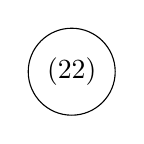
\begin{tikzpicture}[baseline=(n.base)]\node[draw,circle,inner sep=4pt] (n) {(22)};\end{tikzpicture}} * For a proper map of paracompact spaces, this condition just means that the fibers are ``aspheric'' namely ``contractible'' (in the Čech sense)}}

%% END SOURCE ps_134-3_024
\ifnum\EditionMode=1
\psapparatusstart
\psentry{ps_134-3_024-v0001}{1}{typewriter deletion}{\xout{xx}}{}{The typewriter strikes out this material; it leaves the corrected running text.}
\psentry{ps_134-3_024-v0002}{2}{typed insertion}{\inserted[typed]{many}}{many}{The typed insertion is incorporated at its indicated position; insertion brackets leave the running text.}
\psentry{ps_134-3_024-v0003}{3}{typewriter deletion}{\xout{that}}{}{The typewriter strikes out this material; it leaves the corrected running text.}
\psentry{ps_134-3_024-v0004}{4}{writing over}{\over{\illegible{1}}{25}}{\hand{25}}{The superposed handwritten reading replaces the underlying reading.}
\psentry{ps_134-3_024-v0005}{5}{typewriter deletion}{\xout{which}}{}{The typewriter strikes out this material; it leaves the corrected running text.}
\psentry{ps_134-3_024-v0006}{6}{typewriter deletion}{\xout{if M is the}}{}{The typewriter strikes out this material; it leaves the corrected running text.}
\psentry{ps_134-3_024-v0007}{7}{typewriter deletion}{\xout{a}}{}{The typewriter strikes out this material; it leaves the corrected running text.}
\psentry{ps_134-3_024-v0008}{8}{deletion}{\deleted{page 19 ff}}{}{The author cancels this material by hand; it leaves the corrected running text.}
\psentry{ps_134-3_024-v0009}{9}{insertion}{\inserted{section 23}}{\hand{section 23}}{The handwritten insertion is incorporated at its indicated position; insertion brackets leave the running text.}
\psentry{ps_134-3_024-v0010}{10}{writing over}{\over{s}{r}}{\hand{r}}{The superposed handwritten reading replaces the underlying reading.}
\psentry{ps_134-3_024-v0011}{11}{deletion}{\deleted{inverse}}{}{The author cancels this material by hand; it leaves the corrected running text.}
\psentry{ps_134-3_024-v0012}{12}{insertion}{\inserted{direct}}{\hand{direct}}{The handwritten insertion is incorporated at its indicated position; insertion brackets leave the running text.}
\psentry{ps_134-3_024-v0013}{13}{typewriter deletion}{\xout{s}}{}{The typewriter strikes out this material; it leaves the corrected running text.}
\psentry{ps_134-3_024-v0014}{14}{deletion}{\deleted{'}}{}{The author cancels this material by hand; it leaves the corrected running text.}
\psentry{ps_134-3_024-v0015}{15}{marginal note revised}{\margin{\deleted{\illegible{1}}}}{}{The author's internal cancellations and replacements in this marginal note are applied at its source-line call.}
\psentry{ps_134-3_024-v0016}{16}{marginal note revised}{\margin{\deleted{\illegible{1}}}}{}{The author's internal cancellations and replacements in this marginal note are applied at its source-line call.}
\psentry{ps_134-3_024-v0017}{17}{deletion}{\deleted{\unsure{l}}}{}{The author cancels this material by hand; it leaves the corrected running text.}
\psentry{ps_134-3_024-v0018}{18}{typewriter deletion}{\xout{ acyclic}}{}{The typewriter strikes out this material; it leaves the corrected running text.}
\psentry{ps_134-3_024-v0019}{19}{typewriter deletion}{\xout{s}}{}{The typewriter strikes out this material; it leaves the corrected running text.}
\psentry{ps_134-3_024-v0020}{20}{insertion}{\inserted{arbitrary}}{\hand{arbitrary}}{The handwritten insertion is incorporated at its indicated position; insertion brackets leave the running text.}
\psentry{ps_134-3_024-v0021}{21}{typewriter deletion}{\xout{s}}{}{The typewriter strikes out this material; it leaves the corrected running text.}
\psentry{ps_134-3_024-v0022}{22}{insertion}{\inserted{sheaves}}{\hand{sheaves}}{The handwritten insertion is incorporated at its indicated position; insertion brackets leave the running text.}
\psentry{ps_134-3_024-v0023}{23}{typewriter deletion}{\xout{p}}{}{The typewriter strikes out this material; it leaves the corrected running text.}
\psentry{ps_134-3_024-v0024}{24}{typed insertion}{\inserted[typed]{Hot-}}{Hot-}{The typed insertion is incorporated at its indicated position; insertion brackets leave the running text.}
\psentry{ps_134-3_024-v0025}{25}{deletion}{\deleted{this}}{}{The author cancels this material by hand; it leaves the corrected running text.}
\psapparatusend
\fi
\pssource{ps_134-3_025}{134-3/25}{https://grothendieck.umontpellier.fr/web/viewer.html?file=../134-3.pdf\#page=26}
\psnumber{ps_134-3_025-v0001}{1}
\psnumber{ps_134-3_025-v0002}{2}
\psnumber{ps_134-3_025-v0003}{3}
\psnumber{ps_134-3_025-v0004}{4}
\psnumber{ps_134-3_025-v0005}{5}
\psnumber{ps_134-3_025-v0006}{6}
\psnumber{ps_134-3_025-v0007}{7}
\psnumber{ps_134-3_025-v0008}{8}
\psnumber{ps_134-3_025-v0009}{9}
\psnumber{ps_134-3_025-v0010}{10}
\psnumber{ps_134-3_025-v0011}{11}
\psnumber{ps_134-3_025-v0012}{12}
\psnumber{ps_134-3_025-v0013}{13}
\psnumber{ps_134-3_025-v0014}{14}
\psnumber{ps_134-3_025-v0015}{15}
%% BEGIN SOURCE ps_134-3_025
% Pursuing Stacks (cotes 134-2 to 134-8): archive cote 134-3, site page 25 (PDF page 26), typescript page 25.
% typescript. Draft compared: ps2.tex:1160-1224.
% AI-transcribed by Claude Opus 5.5 (claude-opus-5-5, adaptive thinking, effort high), Message Batches API, batch ps1 (msgbatch_01Rv5hCaNTtUt4JHx1yqoHPL), 2026-11-12; image review recorded in records/CHECK_DECISIONS_134_3_4.tsv.
\scanpage{134-3/25}
\var{\xout{25}}{}{typewriter deletion}{ps_134-3_025-v0001}
\mspage{25}

this class.  Maybe even it could be shown that this equivalence class
can be recovered in terms of the corresponding functor (*),  in the same
way as (according to Giraud) a ``topology'' on M can be recovered from
the associated subtopos of $M^{\hand{\wedge}}$\hand{,}namely the associated category of sheaves
on M (in such a way that the set of \var{\xout{subcategor}}{}{typewriter deletion}{ps_134-3_025-v0002}``topologies''on M can be
identified with the set of \var{\xout{\unsure{subt}}}{}{typewriter deletion}{ps_134-3_025-v0003}``closed subtopoi'' of $M^{\hand{\wedge}}$).  The very best
one could possibly hope for along these lines would be a one-to-one
correspondance between isomorphism classes of functors (*)(satisfying
certain properties ?),  and the so-called ``Hot-equivalence classes'' of
topologies on M.

Whether or not this tentative hope is excessive, when it comes to
the (still somewhat vague) question of understanding ``which algebraic
structure species are suitable for expressing homotopy types'',  it
might not be excessive though to expect that in all \var{\inserted[typed]{such}}{such}{typed insertion}{ps_134-3_025-v0004} cases,  M should
be equipped with just \uline{one} ``natural'' Hot-equivalence class of topologies
\margin{\illegible{1}}on M\var{\deleted{\illegible{1}}}{}{deletion}{ps_134-3_025-v0005}\hand{,}which moreover (one hopes,  or wonders) should be expressible
directly in terms of the \var{\inserted[typed]{intrinsic}}{intrinsic}{typed insertion}{ps_134-3_025-v0006} structure of M,  or,  what amounts to the same,
in terms of the \var{\inserted[typed]{full}}{full}{typed insertion}{ps_134-3_025-v0007} subcategory $\underline{B}$ of objects of ``finite presentation'',  \var{\xout{\unsure{givi}}}{}{typewriter deletion}{ps_134-3_025-v0008}
giving rise to M via the equivalence
\[ M \hand{\simeq} \mathrm{Ind}(\underline{B}) . \]
As we just saw in the case  M = (Cat),  the so-called ``canonical topolo-%
gy'' on M need not be within the natural Hot-equivalence class  -  and I
am at a loss for the moment to give a plausible intrinsic caracterizati-%
on of the latter,  in terms of the category M = (Cat). \hand{(${}^{22'}$).}

\var{\over{\unsure{25}}{26}}{\hand{26}}{writing over}{ps_134-3_025-v0009}.  What comes to mind though is that the categories such as \hand{$\Delta$} , \hand{$\square$}
and their analogons (corresponding to multicomplexes rather than mono-%
complexes, for instance\var{\over{\unsure{,}}{)}}{\hand{)}}{writing over}{ps_134-3_025-v0010}  can be viewed as (generally not full) subcate-%
gories of M  (in fact,  even of the smaller category (Ord) of all orde\unsure{\hand{red}}
sets).  The topologies we found on M were in fact associated in an evi-%
dent way to the choice of such subcategories.  As was already felt by
the end of the reflection two days ago (p.21),  these subcategories
(denoted there by $\underline{B}_{oo}$  ) have rather special features  -  they are
associated to \var{\inserted[typed]{simultaneous}}{simultaneous}{typed insertion}{ps_134-3_025-v0011} cellular decompositions of spheres of all dimensions  -
and it is this feature,  presumably,  that makes the associated ``trivial''
algebraic structure \var{\inserted{species}}{\hand{species}}{insertion}{ps_134-3_025-v0012}, giving rise to the category of set-theoretic
realizations  $\underline{B}_{oo}{}^{\hand{\wedge}}$ ,  eligible for ``describing homotopy types''.  In the
typical example M = (Cat) though,  contrarily to what was suggested \hand{by}
\margin{\diagram{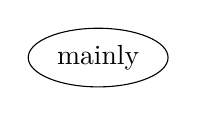
\begin{tikzpicture}[baseline=(n.base)]\node[draw,ellipse,inner sep=3pt] (n) {mainly};\end{tikzpicture}}}\var{\deleted{on page 21}}{}{deletion}{ps_134-3_025-v0013} \var{\inserted{the end of section 23}}{\hand{the end of section 23}}{insertion}{ps_134-3_025-v0014} (when thinking \var{\inserted{mainly}}{\hand{mainly}}{insertion}{ps_134-3_025-v0015} of the rather special although important cases
when M is expressible  as a category  $B^{\hand{\wedge}}$\hand{,} for some category B such as

%% END SOURCE ps_134-3_025
\ifnum\EditionMode=1
\psapparatusstart
\psentry{ps_134-3_025-v0001}{1}{typewriter deletion}{\xout{25}}{}{The typewriter strikes out this material; it leaves the corrected running text.}
\psentry{ps_134-3_025-v0002}{2}{typewriter deletion}{\xout{subcategor}}{}{The typewriter strikes out this material; it leaves the corrected running text.}
\psentry{ps_134-3_025-v0003}{3}{typewriter deletion}{\xout{\unsure{subt}}}{}{The typewriter strikes out this material; it leaves the corrected running text.}
\psentry{ps_134-3_025-v0004}{4}{typed insertion}{\inserted[typed]{such}}{such}{The typed insertion is incorporated at its indicated position; insertion brackets leave the running text.}
\psentry{ps_134-3_025-v0005}{5}{deletion}{\deleted{\illegible{1}}}{}{The author cancels this material by hand; it leaves the corrected running text.}
\psentry{ps_134-3_025-v0006}{6}{typed insertion}{\inserted[typed]{intrinsic}}{intrinsic}{The typed insertion is incorporated at its indicated position; insertion brackets leave the running text.}
\psentry{ps_134-3_025-v0007}{7}{typed insertion}{\inserted[typed]{full}}{full}{The typed insertion is incorporated at its indicated position; insertion brackets leave the running text.}
\psentry{ps_134-3_025-v0008}{8}{typewriter deletion}{\xout{\unsure{givi}}}{}{The typewriter strikes out this material; it leaves the corrected running text.}
\psentry{ps_134-3_025-v0009}{9}{writing over}{\over{\unsure{25}}{26}}{\hand{26}}{The superposed handwritten reading replaces the underlying reading.}
\psentry{ps_134-3_025-v0010}{10}{writing over}{\over{\unsure{,}}{)}}{\hand{)}}{The superposed handwritten reading replaces the underlying reading.}
\psentry{ps_134-3_025-v0011}{11}{typed insertion}{\inserted[typed]{simultaneous}}{simultaneous}{The typed insertion is incorporated at its indicated position; insertion brackets leave the running text.}
\psentry{ps_134-3_025-v0012}{12}{insertion}{\inserted{species}}{\hand{species}}{The handwritten insertion is incorporated at its indicated position; insertion brackets leave the running text.}
\psentry{ps_134-3_025-v0013}{13}{deletion}{\deleted{on page 21}}{}{The author cancels this material by hand; it leaves the corrected running text.}
\psentry{ps_134-3_025-v0014}{14}{insertion}{\inserted{the end of section 23}}{\hand{the end of section 23}}{The handwritten insertion is incorporated at its indicated position; insertion brackets leave the running text.}
\psentry{ps_134-3_025-v0015}{15}{insertion}{\inserted{mainly}}{\hand{mainly}}{The handwritten insertion is incorporated at its indicated position; insertion brackets leave the running text.}
\psapparatusend
\fi
\pssource{ps_134-3_026}{134-3/26}{https://grothendieck.umontpellier.fr/web/viewer.html?file=../134-3.pdf\#page=27}
\psnumber{ps_134-3_026-v0001}{1}
\psnumber{ps_134-3_026-v0002}{2}
\psnumber{ps_134-3_026-v0003}{3}
\psnumber{ps_134-3_026-v0004}{4}
\psnumber{ps_134-3_026-v0005}{5}
%% BEGIN SOURCE ps_134-3_026
% Pursuing Stacks (cotes 134-2 to 134-8): archive cote 134-3, site page 26 (PDF page 27), typescript page 26.
% typescript. Draft compared: ps2.tex:1210-1267.
% AI-transcribed by Claude Opus 5.5 (claude-opus-5-5, adaptive thinking, effort high), Message Batches API, batch ps1 (msgbatch_01Rv5hCaNTtUt4JHx1yqoHPL), 2026-11-12; image review recorded in records/CHECK_DECISIONS_134_3_4.tsv.
\scanpage{134-3/26}
\mspage{26}

\hand{$\Delta$} ,\hand{$\square$} etc), there is no really privileged choice of such subcategory
$\underline{B}_{oo}$ - we found indeed a big bunch of such, the ones just as good as
the others. The point of course is that the corresponding topologies
on M, namely induced from the canonical topology on $\underline{B}_{oo}\hand{\hat{}}$ by the canoni-%
cal functor
\[ M \hand{\longrightarrow} \underline{B}_{oo}\hand{\hat{}} \quad , \]
are Hot-equivalent for some reason or other, which should be understood.
The plausible fact that emerges here, is that the ``natural'' Hot-equi-%
valence class of topologies on M is associated, in the way just descri-%
bed, to a \uline{class} (presumably an equivalence class in a suitable set for
suitable equivalence relation ...) \uline{of subcategories} $\underline{B}_{oo}$ \uline{in} M. The ques-%
tion of giving an intrinsic description of the former, is apparently
reduced to the (possibly more concrete) one, of giving an intrinsic
\unsure{descripttion|description} of a bunch of subcategories \var{\inserted[typed]{$B =$}}{$B =$}{typed insertion}{ps_134-3_026-v0001}$\underline{B}_{oo}$ of M. This description,
one feels, should both a) insist on intrinsic properties of B, inde-%
pendant of M namely of the structure species one is working with, and
b) be concerned with the particular way in which B is embedded in M,
which should by no means be an arbitrary one.

The properties a) should be, I guess, no more no less than those
which express that the ``trivial'' algebraic structure species defined by
B, giving a category of set-theoretic realizations $M_B = B\hand{\hat{}}$, should be
``suitable for describing homotopy types''. The examples at hand so
far suggest that in this case, the canonical topology on the topos $M_B$
is within the natural Hot-equivalence class, which gives a meaning to
the functor
\[ M_B = B\hand{\hat{}} \hand{\longrightarrow} (Hot) \quad , \]
indeed it associates to any a \hand{$\in$} Ob $\overset{\hand{\wedge}}{B}$ the homotopy type of the induced
\var{\margin{\deleted{because $\unsure{\widehat{B}_{/a} \simeq \widehat{B_{/a}}}$}}}{}{marginal note revised}{ps_134-3_026-v0002}category $B_{/a}$ of all objects of B ``over a''\var{\inserted{(23)}}{\hand{(23)}}{insertion}{ps_134-3_026-v0003}. Thus a first condition on
B is that \uline{this functor should be a ``localization functor''}, identifying
(Hot) to a category of fractions of $M_B = B$\hand{$\hat{}$} . This does look indeed as
an \var{\inserted[typed]{extremely}}{extremely}{typed insertion}{ps_134-3_026-v0004} stringent dondition on B, and I wonder if the features we noticed in
the special cases dealt with so far, connected with cellular decomposi-%
tions of spheres, have any more compulsive significance than just
giving some handy \uline{sufficient} conditions (which deserve to be made expli-%
cit sooner or later \hand{!}) for ``eligibility'' of B for recovering (Hot). Be-%
yond this, one would \var{\inserted{of course}}{\hand{of course}}{insertion}{ps_134-3_026-v0005} like to have a better understanding of what it
\uline{really} means, in terms of the internal structure of B, that the
functor above from B\hand{$\hat{}$}\hand{/}to (Hot) is a localization functor.

%% END SOURCE ps_134-3_026
\ifnum\EditionMode=1
\psapparatusstart
\psentry{ps_134-3_026-v0001}{1}{typed insertion}{\inserted[typed]{$B =$}}{$B =$}{The typed insertion is incorporated at its indicated position; insertion brackets leave the running text.}
\psentry{ps_134-3_026-v0002}{2}{marginal note revised}{\margin{\deleted{because $\unsure{\widehat{B}_{/a} \simeq \widehat{B_{/a}}}$}}}{}{The author's internal cancellations and replacements in this marginal note are applied at its source-line call.}
\psentry{ps_134-3_026-v0003}{3}{insertion}{\inserted{(23)}}{\hand{(23)}}{The handwritten insertion is incorporated at its indicated position; insertion brackets leave the running text.}
\psentry{ps_134-3_026-v0004}{4}{typed insertion}{\inserted[typed]{extremely}}{extremely}{The typed insertion is incorporated at its indicated position; insertion brackets leave the running text.}
\psentry{ps_134-3_026-v0005}{5}{insertion}{\inserted{of course}}{\hand{of course}}{The handwritten insertion is incorporated at its indicated position; insertion brackets leave the running text.}
\psapparatusend
\fi
\pssource{ps_134-3_027}{134-3/27}{https://grothendieck.umontpellier.fr/web/viewer.html?file=../134-3.pdf\#page=28}
\psnumber{ps_134-3_027-v0001}{1}
\psnumber{ps_134-3_027-v0002}{2}
\psnumber{ps_134-3_027-v0003}{3}
\psnumber{ps_134-3_027-v0004}{4}
\psnumber{ps_134-3_027-v0005}{5}
\psnumber{ps_134-3_027-v0006}{6}
\psnumber{ps_134-3_027-v0007}{7}
\psnumber{ps_134-3_027-v0008}{8}
\psnumber{ps_134-3_027-v0009}{9}
\psnumber{ps_134-3_027-v0010}{10}
\psnumber{ps_134-3_027-v0011}{11}
\psnumber{ps_134-3_027-v0012}{12}
\psnumber{ps_134-3_027-v0013}{13}
\psnumber{ps_134-3_027-v0014}{14}
\psnumber{ps_134-3_027-v0015}{15}
\psnumber{ps_134-3_027-v0016}{16}
\psnumber{ps_134-3_027-v0017}{17}
\psnumber{ps_134-3_027-v0018}{18}
%% BEGIN SOURCE ps_134-3_027
% Pursuing Stacks (cotes 134-2 to 134-8): archive cote 134-3, site page 27 (PDF page 28), typescript page 27.
% typescript. Draft compared: ps2.tex:1256-1314.
% AI-transcribed by Claude Opus 5.5 (claude-opus-5-5, adaptive thinking, effort high), Message Batches API, batch ps1 (msgbatch_01Rv5hCaNTtUt4JHx1yqoHPL), 2026-11-12; image review recorded in records/CHECK_DECISIONS_134_3_4.tsv.
\scanpage{134-3/27}
\mspage{\hand{27}}

Once this internal condition on B is understood,  step b) then would
amount to describing,  in terms of an arbitrary ``eligible'' algebraic
structure species \var{\xout{xxxxx}}{}{typewriter deletion}{ps_134-3_027-v0001} expressed by the category M,  of what we should
mean by ``eligible functors'' \var{\xout{BxxxMxxx}}{}{typewriter deletion}{ps_134-3_027-v0002} \hand{$(^{29})$}\margin{\unsure{we will rather say ``test functors'', see below\dots}}
\[ B \hand{\longrightarrow} M \ , \]
giving rise in the usual way to a functor
\[ M \hand{\rightarrow} B^{\hand{\wedge}} \ . \]
In any case,  the latter functor defines upon M an induced \unsure{topology},
T say,  and the comparison \var{\inserted[typed]{lemma}}{lemma}{typed insertion}{ps_134-3_027-v0003} tells us that if either $B \hand{\rightarrow} M$ \var{\inserted[typed]{or $M \hand{\rightarrow} B^{\hand{\wedge}}$}}{or $M \hand{\rightarrow} B^{\hand{\wedge}}$}{typed insertion}{ps_134-3_027-v0004} is fully
faithful ,  then the topos associated to M is canonically equivalent\var{\xout{x}}{}{typewriter deletion}{ps_134-3_027-v0005}
to $B^{\hand{\wedge}}$  (using this comparison lemma for the functor which happens to be
fully faithful).  \var{\xout{Onxthexotherxhandx}}{}{typewriter deletion}{ps_134-3_027-v0006} From this follows that the functor
(*)  $M^{\hand{\sim}} \hand{\rightarrow}$ (Hot)  defined by T \var{\inserted{(cf. section 25)}}{\hand{(cf. section 25)}}{insertion}{ps_134-3_027-v0007} is nothing but the compositum
\[ M^{\hand{\sim}} \hand{\xrightarrow{\approx}} B^{\hand{\wedge}} \hand{\longrightarrow} (Hot) \quad , \]
and hence a localization functor.  In other words,  when B is a category
satisfying the condition seen above\hand{$(^{29})$}, then \uline{any} functor $B \hand{\rightarrow} M$ satisfying\margin{\unsure{a ``test category'', as we will say}}
one of the two fullness conditions above \var{\xout{xxx}}{}{typewriter deletion}{ps_134-3_027-v0008} yields a corresponding des-%
cription of (Hot) as a localization of $M^{\hand{\sim}}$.  What is still lacking though
is a grasp on when two such functors  $B \hand{\rightarrow} M$,  $B' \hand{\rightarrow} M$  define essentially
``the same'' functor  $M \hand{\rightarrow}$ (Hot),  or (more or less equivalently)  two
(Hot)-equivalent topologies T,T' on M;  \uline{is it enough,}  \uline{for instance,}
\uline{that they give rise to the same notion of} \uline{``weak equivalences''}  (namely\margin{\unsure{same question arises for Hot-equivalence of topologies on M\dots}} \hand{\illegible{1}}
morphisms in M which are tranformed into an isomorphism of (Hot)) ?
And moreover,  \var{\xout{this}}{}{typewriter deletion}{ps_134-3_027-v0009} granting that this equivalence relation between
\var{\inserted[typed]{certain}}{certain}{typed insertion}{ps_134-3_027-v0010} full subcategories \var{\inserted{(say)}}{\hand{(say)}}{insertion}{ps_134-3_027-v0011} B of M is understood,  how define,in terms of M ,
a ``natural'' equivalence class of such full subcategories,  giving rise
to a \uline{canonical} functor  $M \hand{\rightarrow}$ (Hot) \var{\deleted{\hand{$(^{25})$}}}{}{deletion}{ps_134-3_027-v0012} \hand{?} \hand{$(^{25})$}

Recalling that the algebraic structure considered can be described
in terms of an arbitrary small category $\underline{B}$ where arbitrary finite direct
limits exist  (namely $\underline{B}$ is the full subcategory of M of objects of
finite presentation),  it seems reasonable to assume that indeed
\[ B \hand{\hookrightarrow} \underline{B} \quad \text{(a full embedding)} \ , \]
and the question transforms into describing a\var{\deleted{n}}{}{deletion}{ps_134-3_027-v0013} \var{\inserted[typed]{natural}}{natural}{typed insertion}{ps_134-3_027-v0014} equivalence class \var{\xout{xxxxx}}{}{typewriter deletion}{ps_134-3_027-v0015}
of such full subcategories,  in \var{\inserted[typed]{(more or less)}}{(more or less)}{typed insertion}{ps_134-3_027-v0016} any small category $\underline{B}$  where finite
direct limits exist,  and where moreover there exist such full subcate-%
gories B.  Also,  we may \var{\deleted{to}}{}{deletion}{ps_134-3_027-v0017} have to throw in some extra\var{\deleted{s}}{}{deletion}{ps_134-3_027-v0018} conditions on
$\underline{B}$ ,  such as the condition that direct sums be ``disjoint'' and ``universa\unsure{l}'' \hand{\unsure{$(^{*})$}}
already contemplated before.

%% END SOURCE ps_134-3_027
\ifnum\EditionMode=1
\psapparatusstart
\psentry{ps_134-3_027-v0001}{1}{typewriter deletion}{\xout{xxxxx}}{}{The typewriter strikes out this material; it leaves the corrected running text.}
\psentry{ps_134-3_027-v0002}{2}{typewriter deletion}{\xout{BxxxMxxx}}{}{The typewriter strikes out this material; it leaves the corrected running text.}
\psentry{ps_134-3_027-v0003}{3}{typed insertion}{\inserted[typed]{lemma}}{lemma}{The typed insertion is incorporated at its indicated position; insertion brackets leave the running text.}
\psentry{ps_134-3_027-v0004}{4}{typed insertion}{\inserted[typed]{or $M \hand{\rightarrow} B^{\hand{\wedge}}$}}{or $M \hand{\rightarrow} B^{\hand{\wedge}}$}{The typed insertion is incorporated at its indicated position; insertion brackets leave the running text.}
\psentry{ps_134-3_027-v0005}{5}{typewriter deletion}{\xout{x}}{}{The typewriter strikes out this material; it leaves the corrected running text.}
\psentry{ps_134-3_027-v0006}{6}{typewriter deletion}{\xout{Onxthexotherxhandx}}{}{The typewriter strikes out this material; it leaves the corrected running text.}
\psentry{ps_134-3_027-v0007}{7}{insertion}{\inserted{(cf. section 25)}}{\hand{(cf. section 25)}}{The handwritten insertion is incorporated at its indicated position; insertion brackets leave the running text.}
\psentry{ps_134-3_027-v0008}{8}{typewriter deletion}{\xout{xxx}}{}{The typewriter strikes out this material; it leaves the corrected running text.}
\psentry{ps_134-3_027-v0009}{9}{typewriter deletion}{\xout{this}}{}{The typewriter strikes out this material; it leaves the corrected running text.}
\psentry{ps_134-3_027-v0010}{10}{typed insertion}{\inserted[typed]{certain}}{certain}{The typed insertion is incorporated at its indicated position; insertion brackets leave the running text.}
\psentry{ps_134-3_027-v0011}{11}{insertion}{\inserted{(say)}}{\hand{(say)}}{The handwritten insertion is incorporated at its indicated position; insertion brackets leave the running text.}
\psentry{ps_134-3_027-v0012}{12}{deletion}{\deleted{\hand{$(^{25})$}}}{}{The author cancels this material by hand; it leaves the corrected running text.}
\psentry{ps_134-3_027-v0013}{13}{deletion}{\deleted{n}}{}{The author cancels this material by hand; it leaves the corrected running text.}
\psentry{ps_134-3_027-v0014}{14}{typed insertion}{\inserted[typed]{natural}}{natural}{The typed insertion is incorporated at its indicated position; insertion brackets leave the running text.}
\psentry{ps_134-3_027-v0015}{15}{typewriter deletion}{\xout{xxxxx}}{}{The typewriter strikes out this material; it leaves the corrected running text.}
\psentry{ps_134-3_027-v0016}{16}{typed insertion}{\inserted[typed]{(more or less)}}{(more or less)}{The typed insertion is incorporated at its indicated position; insertion brackets leave the running text.}
\psentry{ps_134-3_027-v0017}{17}{deletion}{\deleted{to}}{}{The author cancels this material by hand; it leaves the corrected running text.}
\psentry{ps_134-3_027-v0018}{18}{deletion}{\deleted{s}}{}{The author cancels this material by hand; it leaves the corrected running text.}
\psapparatusend
\fi
\pssource{ps_134-3_028}{134-3/28}{https://grothendieck.umontpellier.fr/web/viewer.html?file=../134-3.pdf\#page=29}
\psnumber{ps_134-3_028-v0001}{1}
\psnumber{ps_134-3_028-v0002}{2}
\psnumber{ps_134-3_028-v0003}{3}
\psnumber{ps_134-3_028-v0004}{4}
\psnumber{ps_134-3_028-v0005}{5}
\psnumber{ps_134-3_028-v0006}{6}
%% BEGIN SOURCE ps_134-3_028
% Pursuing Stacks (cotes 134-2 to 134-8): archive cote 134-3, site page 28 (PDF page 29), typescript page 28.
% typescript. Draft compared: ps2.tex:1300-1362.
% AI-transcribed by Claude Opus 5.5 (claude-opus-5-5, adaptive thinking, effort high), Message Batches API, batch ps1 (msgbatch_01Rv5hCaNTtUt4JHx1yqoHPL), 2026-11-12; image review recorded in records/CHECK_DECISIONS_134_3_4.tsv.
\scanpage{134-3/28}
\mspage{\hand{28}}

Maybe I was a little overenthousiastic, when observing that for
any full embedding of a category B into M (let's call the categories B
giving rise to a localization functor $B^{\hand{\wedge}} \hand{\to} (\mathrm{Hot})$ \uline{homotopy-test} catego-%
ries\var{\deleted{x}}{}{deletion}{ps_134-3_028-v0001}, or simply \uline{test} categories) we get a localization functor
\[ M^{\hand{\sim}} = (M^{\hand{\unsure{\sim}}},T_B)^{\hand{\sim}} \hand{\to} (\mathrm{Hot}) \quad , \]
where $T_B$ is the topology on M corresponding to the full subcategory B.
After all, there is a long way in between M itself and the category of
sheaves $M^{\hand{\sim}}$ - and what we want is to get (Hot) as a localization of M
itself, not of $M^{\hand{\sim}}$. Tt is not even clear, without some extra assumpti-%
on, that the natural functor from M to $M^{\hand{\sim}}$ is fully faithful, namely
that M can be identified with a full subcategory of the category $M^{\hand{\sim}}$
we've got to localize to get (Hot). We definitely would like this to
be true, or what amounts to the same, that the functor $M \hand{\to} B^{\hand{\wedge}}$
defined by $B \hand{\to} M$ should be fully faithful ---which means also that
the full subcategory B of M is ``generating by strict epimorphisms''\hand{(26),}
namely that for every K in M , there exists a strictly epimorphic
family of morphisms $b_i \hand{\to} K$ , with sources $b_i$ in B. This interpretati-%
on of full faithfulness of $M \hand{\to} B^{\hand{\wedge}}$is OK when $B \hand{\to} M$ is fully faithful ,
a condition which I \var{\inserted{gradually}}{\hand{gradually}}{insertion}{ps_134-3_028-v0002} put into the fore without really compelling reason,
except that in those examples I have in mind and which are \uline{not} connected
with the theory of stacks of various kinds, this condition is satisfied
\margin{$\lrcorner\!\ulcorner$}\uline{indeed.}\hand{$\rfloor\!\lceil$} Apparently, with this endless digression on algebraic models
for homotopy types, \var{\deleted{the}}{}{deletion}{ps_134-3_028-v0003} stacks (which I am supposed to be after, after
all) are kind of fading into the background ! Maybe we should after
all forget about fully faithfullness condition on either $B \hand{\to} M$ or
$M \hand{\to} B^{\hand{\wedge}}$, and just insist that the compositum
\[ M \hand{\to} M^{\hand{\sim}} \hand{\to} B^{\hand{\wedge}} \hand{\to} (\mathrm{Hot}) \]
(which can be described \var{\inserted[typed]{directly}}{directly}{typed insertion}{ps_134-3_028-v0004} in terms of the topology $T_B$ on M associated to
\margin{(27)}the functor $B \hand{\to} M$\hand{/}) should be a localization functor. I guess that for
a given M or $\underline{B}$ ,\hand{$\wedge$} the mere fact that there should exist a \hand{``}test category\hand{''}
B and a functor $B \hand{\to} M$, or $B \hand{\to} \underline{B}$ , having this property, is already a
very strong condition on the structure species considered, namely on
the category $\underline{B}$ whi\hand{?}ch embodies this structure. It \var{\xout{probably}}{}{typewriter deletion}{ps_134-3_028-v0005}\var{\inserted[typed]{possibly}}{possibly}{typed insertion}{ps_134-3_028-v0006} means that
the corresponding functor
\[ \underline{B} \hand{\to} (\mathrm{Hot}) \]
factors through a functor
\[ \underline{B} \hand{\to} (\mathrm{Hot})_{\mathrm{f.t.}} \qquad \text{(f.t. means ``finite type'')} \]
which is itself a localization functor. It is not wholly impossible,
after all, that this condition on a functor $B \hand{\to} \underline{B}$ (B a test category)
is so stringent, that all such functors (for variable B) must be

%% END SOURCE ps_134-3_028
\ifnum\EditionMode=1
\psapparatusstart
\psentry{ps_134-3_028-v0001}{1}{deletion}{\deleted{x}}{}{The author cancels this material by hand; it leaves the corrected running text.}
\psentry{ps_134-3_028-v0002}{2}{insertion}{\inserted{gradually}}{\hand{gradually}}{The handwritten insertion is incorporated at its indicated position; insertion brackets leave the running text.}
\psentry{ps_134-3_028-v0003}{3}{deletion}{\deleted{the}}{}{The author cancels this material by hand; it leaves the corrected running text.}
\psentry{ps_134-3_028-v0004}{4}{typed insertion}{\inserted[typed]{directly}}{directly}{The typed insertion is incorporated at its indicated position; insertion brackets leave the running text.}
\psentry{ps_134-3_028-v0005}{5}{typewriter deletion}{\xout{probably}}{}{The typewriter strikes out this material; it leaves the corrected running text.}
\psentry{ps_134-3_028-v0006}{6}{typed insertion}{\inserted[typed]{possibly}}{possibly}{The typed insertion is incorporated at its indicated position; insertion brackets leave the running text.}
\psapparatusend
\fi
\pssource{ps_134-3_029}{134-3/29}{https://grothendieck.umontpellier.fr/web/viewer.html?file=../134-3.pdf\#page=30}
\psnumber{ps_134-3_029-v0001}{1}
\psnumber{ps_134-3_029-v0002}{2}
\psnumber{ps_134-3_029-v0003}{3}
\psnumber{ps_134-3_029-v0004}{4}
\psnumber{ps_134-3_029-v0005}{5}
\psnumber{ps_134-3_029-v0006}{6}
\psnumber{ps_134-3_029-v0007}{7}
\psnumber{ps_134-3_029-v0008}{8}
\psnumber{ps_134-3_029-v0009}{9}
\psnumber{ps_134-3_029-v0010}{10}
\psnumber{ps_134-3_029-v0011}{11}
\psnumber{ps_134-3_029-v0012}{12}
\psnumber{ps_134-3_029-v0013}{13}
\psnumber{ps_134-3_029-v0014}{14}
\psnumber{ps_134-3_029-v0015}{15}
\psnumber{ps_134-3_029-v0016}{16}
\psnumber{ps_134-3_029-v0017}{17}
\psnumber{ps_134-3_029-v0018}{18}
\psnumber{ps_134-3_029-v0019}{19}
\psnumber{ps_134-3_029-v0020}{20}
\psnumber{ps_134-3_029-v0021}{21}
%% BEGIN SOURCE ps_134-3_029
% Pursuing Stacks (cotes 134-2 to 134-8): archive cote 134-3, site page 29 (PDF page 30), typescript page 29.
% typescript. Draft compared: ps2.tex:1345-1417.
% AI-transcribed by Claude Opus 5.5 (claude-opus-5-5, adaptive thinking, effort high), Message Batches API, batch ps1 (msgbatch_01Rv5hCaNTtUt4JHx1yqoHPL), 2026-11-12; image review recorded in records/CHECK_DECISIONS_134_3_4.tsv.
\scanpage{134-3/29}
\mspage{\hand{29}}
already ``equivalent'', namely define Hot-equivalent topologies on $\underline{B}$ (or \margin{\unsure{or|on}}
$\underline{M}$ , equivalently), and hence define ``the same'' functor $M \hand{\to} (\mathrm{Hot})$ or
$\underline{B} \hand{\to} (\mathrm{Hot})_{\mathrm{f.t.}}$ .

\hand{2}\var{\over{\unsure{4}}{7}}{\hand{7}}{writing over}{ps_134-3_029-v0001}. \var{\xout{All this}}{}{typewriter deletion}{ps_134-3_029-v0002} All this is pretty much ``thin air conjecturing'' for the time being
- quite possibly the notion of a ``test category'' itself has to be con-%
siderably adjusted, namely \unsure{strenghhened|strengthened}, as well as the notion of \hand{a}
``test functor'' $B \hand{\to} \underline{B}$ or $B \hand{\to} M$ - \var{\deleted{that}}{}{deletion}{ps_134-3_029-v0003} some important features \var{\inserted{may}}{\hand{may}}{insertion}{ps_134-3_029-v0004} have
entirely escaped my attention. The one idea though which may prove per-%
haps a valid one, is that \var{\inserted[typed]{a}}{a}{typed insertion}{ps_134-3_029-v0005} suitable \var{\inserted[typed]{localization}}{localization}{typed insertion}{ps_134-3_029-v0006} functor\var{\xout{s}}{}{typewriter deletion}{ps_134-3_029-v0007}
(*) \qquad $M \hand{\to} (\mathrm{Hot})$
may be defined, using either various topologies on M (related by a
suitable ``Hot-equivalence'' relation), or various functors $B \hand{\to} M$ or
$B \hand{\to} \underline{B}$ of suitable ``test categories'' B, and how the two are related.
I do not wish to pursue much longer along these lines though, but
rather put \var{\inserted{now}}{\hand{now}}{insertion}{ps_134-3_029-v0008} into the picture a third way still for getting a functor
(*), namely through some more or less natural functor
(**) \qquad $M \hand{\to} (\mathrm{Spaces})$ \hand{,} \qquad $K \hand{\mapsto} \hand{|}K\hand{|}$ ,
called a ``geometric \var{\inserted[typed]{(or topologic)}}{(or topologic)}{typed insertion}{ps_134-3_029-v0009} realization functor''\hand{$^{(28)}$}. There \var{\xout{are}}{}{typewriter deletion}{ps_134-3_029-v0010}\var{\inserted[typed]{is a}}{is a}{typed insertion}{ps_134-3_029-v0011} pretty compelling
choice\var{\xout{s}}{}{typewriter deletion}{ps_134-3_029-v0012} for such a functor, in the case of (semisimplicial or cubical)
complexes or multicomplexes of various kinds, and accordingly for
the subcategories (Cat),(Preord),(Ord) of \var{\xout{(Cat}}{}{typewriter deletion}{ps_134-3_029-v0013} (Ss sets), using geome-%
tric realization of semisimplicial complexes. In the case of the consi-%
derably more sophisticated structure of Gr-stacks though (or the related
structure of stacks, which will be dealt with in much the same way
below), although there is a pretty natural choice for geometric
realization on the subcategory $\underline{B}_{\mathrm{oo}}$ \var{\xout{\illegible{1}}}{}{typewriter deletion}{ps_134-3_029-v0014} of M embodying the ``primitive\var{\xout{''}}{}{typewriter deletion}{ps_134-3_029-v0015}
structure'' (namely the structure of an $\mathrm{oo}$-graph, see below also)\var{\over{,}{;}}{\hand{;}}{writing over}{ps_134-3_029-v0016} it
has been seen that the extension of this to a functor on the whole of
M (via it's extension to the \var{\inserted[typed]{left}}{left}{typed insertion}{ps_134-3_029-v0017} coherator defining the structure species,
which we denoted by $\underline{B}$ at the beginning of these notes, but which is
not quite the $\underline{B}$ envisioned here) is by no means unique, that it depends
on a pretty big bunch of rather arbitrary choices. This indeterminacy
now appears as quite in keeping with the general aspect of a (still
somewhat hypothetical) theory of algebraic homotopy models, gradually
emerging from darkness. It parallels the corresponding indeterminacy
in the choice of an ``eligible'' topology on M (call these topologies
the \hand{``}\uline{test topologies}\hand{''}), or \var{\over{\illegible{1}}{of}}{\hand{of}}{writing over}{ps_134-3_029-v0018} \var{\xout{th}}{}{typewriter deletion}{ps_134-3_029-v0019} a test functor $B \hand{\to} M$. What I would
like now to do, before coming back to stacks, is to reflec\hand{t} a little
still about the relations \var{\deleted{of}}{}{deletion}{ps_134-3_029-v0020} \var{\inserted[typed]{between}}{between}{typed insertion}{ps_134-3_029-v0021} such choice of a ``geometric realization
functor'', and test topologies or test functors relative to M .

%% END SOURCE ps_134-3_029
\ifnum\EditionMode=1
\psapparatusstart
\psentry{ps_134-3_029-v0001}{1}{writing over}{\over{\unsure{4}}{7}}{\hand{7}}{The superposed handwritten reading replaces the underlying reading.}
\psentry{ps_134-3_029-v0002}{2}{typewriter deletion}{\xout{All this}}{}{The typewriter strikes out this material; it leaves the corrected running text.}
\psentry{ps_134-3_029-v0003}{3}{deletion}{\deleted{that}}{}{The author cancels this material by hand; it leaves the corrected running text.}
\psentry{ps_134-3_029-v0004}{4}{insertion}{\inserted{may}}{\hand{may}}{The handwritten insertion is incorporated at its indicated position; insertion brackets leave the running text.}
\psentry{ps_134-3_029-v0005}{5}{typed insertion}{\inserted[typed]{a}}{a}{The typed insertion is incorporated at its indicated position; insertion brackets leave the running text.}
\psentry{ps_134-3_029-v0006}{6}{typed insertion}{\inserted[typed]{localization}}{localization}{The typed insertion is incorporated at its indicated position; insertion brackets leave the running text.}
\psentry{ps_134-3_029-v0007}{7}{typewriter deletion}{\xout{s}}{}{The typewriter strikes out this material; it leaves the corrected running text.}
\psentry{ps_134-3_029-v0008}{8}{insertion}{\inserted{now}}{\hand{now}}{The handwritten insertion is incorporated at its indicated position; insertion brackets leave the running text.}
\psentry{ps_134-3_029-v0009}{9}{typed insertion}{\inserted[typed]{(or topologic)}}{(or topologic)}{The typed insertion is incorporated at its indicated position; insertion brackets leave the running text.}
\psentry{ps_134-3_029-v0010}{10}{typewriter deletion}{\xout{are}}{}{The typewriter strikes out this material; it leaves the corrected running text.}
\psentry{ps_134-3_029-v0011}{11}{typed insertion}{\inserted[typed]{is a}}{is a}{The typed insertion is incorporated at its indicated position; insertion brackets leave the running text.}
\psentry{ps_134-3_029-v0012}{12}{typewriter deletion}{\xout{s}}{}{The typewriter strikes out this material; it leaves the corrected running text.}
\psentry{ps_134-3_029-v0013}{13}{typewriter deletion}{\xout{(Cat}}{}{The typewriter strikes out this material; it leaves the corrected running text.}
\psentry{ps_134-3_029-v0014}{14}{typewriter deletion}{\xout{\illegible{1}}}{}{The typewriter strikes out this material; it leaves the corrected running text.}
\psentry{ps_134-3_029-v0015}{15}{typewriter deletion}{\xout{''}}{}{The typewriter strikes out this material; it leaves the corrected running text.}
\psentry{ps_134-3_029-v0016}{16}{writing over}{\over{,}{;}}{\hand{;}}{The superposed handwritten reading replaces the underlying reading.}
\psentry{ps_134-3_029-v0017}{17}{typed insertion}{\inserted[typed]{left}}{left}{The typed insertion is incorporated at its indicated position; insertion brackets leave the running text.}
\psentry{ps_134-3_029-v0018}{18}{writing over}{\over{\illegible{1}}{of}}{\hand{of}}{The superposed handwritten reading replaces the underlying reading.}
\psentry{ps_134-3_029-v0019}{19}{typewriter deletion}{\xout{th}}{}{The typewriter strikes out this material; it leaves the corrected running text.}
\psentry{ps_134-3_029-v0020}{20}{deletion}{\deleted{of}}{}{The author cancels this material by hand; it leaves the corrected running text.}
\psentry{ps_134-3_029-v0021}{21}{typed insertion}{\inserted[typed]{between}}{between}{The typed insertion is incorporated at its indicated position; insertion brackets leave the running text.}
\psapparatusend
\fi
\pssource{ps_134-3_030}{134-3/30}{https://grothendieck.umontpellier.fr/web/viewer.html?file=../134-3.pdf\#page=31}
\psnumber{ps_134-3_030-v0001}{1}
\psnumber{ps_134-3_030-v0002}{2}
\psnumber{ps_134-3_030-v0003}{3}
\psnumber{ps_134-3_030-v0004}{4}
\psnumber{ps_134-3_030-v0005}{5}
\psnumber{ps_134-3_030-v0006}{6}
\psnumber{ps_134-3_030-v0007}{7}
\psnumber{ps_134-3_030-v0008}{8}
\psnumber{ps_134-3_030-v0009}{9}
%% BEGIN SOURCE ps_134-3_030
% Pursuing Stacks (cotes 134-2 to 134-8): archive cote 134-3, site page 30 (PDF page 31), typescript page 30.
% typescript. Draft compared: ps2.tex:1400-1472.
% AI-transcribed by Claude Opus 5.5 (claude-opus-5-5, adaptive thinking, effort high), Message Batches API, batch ps1 (msgbatch_01Rv5hCaNTtUt4JHx1yqoHPL), 2026-11-12; image review recorded in records/CHECK_DECISIONS_134_3_4.tsv.
\scanpage{134-3/30}
\mspage{30}

8.3.

\margin{28.} While writing down the notes yesterday\hand{,}and this morning still while
pondering a little more, there has been the ever increasing feeling that
I ``was burning'', namely turning around something very close, very simple-%
minded too surely, without quite getting hold of it yet. In such a situa-%
tion, it is next to impossible just to leave it at that and come to the
``ordre du jour'' (namely stacks) - and even the \var{\inserted[typed]{``little}}{``little}{typed insertion}{ps_134-3_030-v0001} reflection'' I was about
to write down last night (but it was really too late then to go on) will
have to wait I guess, about the ``geometric realization functors'', as I
feel it is getting me off rather, maybe just a little, from where it is
``burning'' !

There was one question f\var{\over{la}{la}}{\hand{la}}{writing over}{ps_134-3_030-v0002}rring up yesterday \var{\deleted{(p.27)}}{}{deletion}{ps_134-3_030-v0003}\var{\inserted{(section 26)}}{\hand{(section 26)}}{insertion}{ps_134-3_030-v0004} which I nearly
dismissed as kind of silly, namely whether two localization functors
\[ (*) \qquad M \hand{\to} (\mathrm{Hot}) \]
obtained in such and such a way were isomorphic (maybe even canonically
so ??) provided they defined the same notion of ``weak equivalences'', name-%
ly arrows transformed into isomorphisms by the localization functors. Now
this maybe isnt so silly after all, in view of the following
\uline{Assumption}: The category of equivalences of (Hot) with itself, and \var{\inserted{of}}{\hand{of}}{insertion}{ps_134-3_030-v0005} natu-%
ral isomorphisms (possibly even any morphisms) between such, is equivalent
to the one point category.

This means 1) any equivalence $(\mathrm{Hot})\hand{\xrightarrow{\approx}}(\mathrm{Hot})$ is isomorphic to the
identity functor, and 2) any automorphism of the identity functor (pos-%
sibly even any endomorphism ?) is the identity.

Maybe these are facts well-known to the experts, maybe not - it is
not my business here anyhow to set out to prove such kind of things. It
looks pretty plausible, because if there was any non trivial autoequiva -
lence of (Hot), or automorphism of its identity functor, I guess I would
have heard about it\hand{,} or something of the sort would flip to my mind. It
would not be so if we abelianized (Hot) some way or other, as there would
be the loop and suspension functors, and homotheties by -1\unsure{.} \var{\deleted{\hand{of $\mathrm{id}_{(\mathrm{Hot})}$}}}{}{deletion}{ps_134-3_030-v0006} \var{\inserted{as
automorphisms of the identity functor.}}{\hand{as
automorphisms of the identity functor.}}{insertion}{ps_134-3_030-v0007}

This assumption now can be rephrased, by stating that \uline{a localization}
\uline{functor} \var{\xout{(*)}}{}{typewriter deletion}{ps_134-3_030-v0008} (*) \uline{from any category M into} (Hot) \uline{is well determined}, \uline{up to}
\uline{a unique isomorphism}, \uline{when the corresponding class} $W \hand{\subset} \mathrm{F}\var{\over{l}{l}}{\hand{l}}{writing over}{ps_134-3_030-v0009}(M)$ \uline{of weak equi-}%
\uline{valences is known}, in positive response to yesterday's silly question!

Such situation (*) seems to me to merit a name. As the word ``model
category'' has already been used in a somewhat different and more sophisti-%
cated sense by Quillen, in the context of homotopy, I rather use another

%% END SOURCE ps_134-3_030
\ifnum\EditionMode=1
\psapparatusstart
\psentry{ps_134-3_030-v0001}{1}{typed insertion}{\inserted[typed]{``little}}{``little}{The typed insertion is incorporated at its indicated position; insertion brackets leave the running text.}
\psentry{ps_134-3_030-v0002}{2}{writing over}{\over{la}{la}}{\hand{la}}{The superposed handwritten reading replaces the underlying reading.}
\psentry{ps_134-3_030-v0003}{3}{deletion}{\deleted{(p.27)}}{}{The author cancels this material by hand; it leaves the corrected running text.}
\psentry{ps_134-3_030-v0004}{4}{insertion}{\inserted{(section 26)}}{\hand{(section 26)}}{The handwritten insertion is incorporated at its indicated position; insertion brackets leave the running text.}
\psentry{ps_134-3_030-v0005}{5}{insertion}{\inserted{of}}{\hand{of}}{The handwritten insertion is incorporated at its indicated position; insertion brackets leave the running text.}
\psentry{ps_134-3_030-v0006}{6}{deletion}{\deleted{\hand{of $\mathrm{id}_{(\mathrm{Hot})}$}}}{}{The author cancels this material by hand; it leaves the corrected running text.}
\psentry{ps_134-3_030-v0007}{7}{insertion}{\inserted{as
automorphisms of the identity functor.}}{\hand{as
automorphisms of the identity functor.}}{The handwritten insertion is incorporated at its indicated position; insertion brackets leave the running text.}
\psentry{ps_134-3_030-v0008}{8}{typewriter deletion}{\xout{(*)}}{}{The typewriter strikes out this material; it leaves the corrected running text.}
\psentry{ps_134-3_030-v0009}{9}{writing over}{$\over{l}{l}$}{$\hand{l}$}{The superposed handwritten reading replaces the underlying reading.}
\psapparatusend
\fi
\pssource{ps_134-3_031}{134-3/31}{https://grothendieck.umontpellier.fr/web/viewer.html?file=../134-3.pdf\#page=32}
\psnumber{ps_134-3_031-v0001}{1}
\psnumber{ps_134-3_031-v0002}{2}
\psnumber{ps_134-3_031-v0003}{3}
\psnumber{ps_134-3_031-v0004}{4}
\psnumber{ps_134-3_031-v0005}{5}
%% BEGIN SOURCE ps_134-3_031
% Pursuing Stacks (cotes 134-2 to 134-8): archive cote 134-3, site page 31 (PDF page 32), typescript page 31.
% typescript. Draft compared: ps2.tex:1456-1532.
% AI-transcribed by Claude Opus 5.5 (claude-opus-5-5, adaptive thinking, effort high), Message Batches API, batch ps1 (msgbatch_01Rv5hCaNTtUt4JHx1yqoHPL), 2026-11-12; image review recorded in records/CHECK_DECISIONS_134_3_4.tsv.
\scanpage{134-3/31}
\mspage{31}
one in the situation here. Let's call a ``modelizing category'', or sinply
a ``\uline{modelizer}'' ( ``modélisatrice'' in French), any category $M$, endowed with
a set $W\hand{\subset} \mathrm{Fl}(M)$ (the weak equivalences), satisfying the obvious condition:

(M\unsure{\hand{o}}d) a) $W$ is the set of arrows made invertible by the localization
functor $M\hand{\to} W^{-1}M$ \hand{(28')}, and
b) $W^{-1}M$ is equivalent to (Hot) ,
or equivalently, there exists a localization functor (*) (necessarily
unique up to unique isomorphism) such that $W$ be the set of arrows made
invertible by this functor.

Let $(M,W)$, $(M',W')$ be two modelizers, a functor \var{\inserted[typed]{$F$:}}{$F$:}{typed insertion}{ps_134-3_031-v0001} $M\hand{\to} M'$ is called
\uline{model-preserving}, or a \uline{morphism} between the modelizers, if it satisfies
either of the two following equivalent conditions:
(i) $F(W)\hand{\subset} W'$\hand{,} hence a functor $F_{W,W'} : W^{-1}M\hand{\to} W'^{-1}M'$, and the latter
is an equivalence.
(ii) The diagram
% Hand-drawn arrows are marked blue; typed objects remain plain.
\diagram{\begin{tikzcd}[column sep=small]
M \arrow[color=blue, rr, "F"] \arrow[color=blue, dr] \& \& M' \arrow[color=blue, dl] \\
\& \text{(Hot)} \&
\end{tikzcd}}
is commutative up to isomorphism (where the vertical arrows
are the \var{\xout{``model}}{}{typewriter deletion}{ps_134-3_031-v0002} ``type functors'' associated to $M$, $M'$ respectively\hand{)}

When dealing with a modelizer $(M,W)$, $W$ will be generally understood
so that we write simply \hand{$M$}. When $M$ is defined in terms of an algebraic
structure species, the task arises to find out whether (if any) there
exists a \uline{unique} $W\hand{\subset} \mathrm{Fl}(M)$ turning $M$ into a modelizer, and if not so, if
we can however pinpoint one which is a more natural one, and which we
would call ``canonical''.

Here is a diagram including most of the modelizers and model-preserving
functors between these which we met so far\hand{,}\hand{(29)} \var{\deleted{\xout{with the}}}{}{deletion}{ps_134-3_031-v0003} \hand{(}not included however
those connected with the theory of ``higher'' stacks and Gr-stacks, wh ich we
will have to elaborate upon later on\hand{)}:
\margin{\diagram{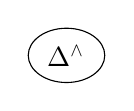
\begin{tikzpicture}[baseline=(n.base)]\node[draw,ellipse,inner sep=3pt] (n) {$\Delta^\wedge$};\end{tikzpicture}}}
\margin{\diagram{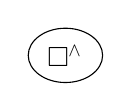
\begin{tikzpicture}[baseline=(n.base)]\node[draw,ellipse,inner sep=3pt] (n) {$\square^\wedge$};\end{tikzpicture}}}
% Hand-drawn arrows are marked blue; typed objects remain plain.
\diagram{\begin{tikzcd}[row sep=small, column sep=small]
\& \& \& \hand{\hat{\Delta}}=\text{(ss. sets)} \arrow[color=blue, dr, "\hand{\xi}"] \& \\
\text{(Ord)} \arrow[color=blue, r, hook] \& \text{(Preord)} \arrow[color=blue, r, hook] \& \text{(Cat)} \arrow[color=blue, ur, "\hand{\alpha}"] \arrow[color=blue, dr, "\hand{\beta}"'] \& \& \text{(Cat)} \\
\& \& \& \hand{\square}=\text{(cub. sets)} \arrow[color=blue, ur, "\hand{\eta}"'] \&
\end{tikzcd}}
where the two last functors, with values in (Cat), are the two obvious
functors, obtained from
\hand{(**)} \hand{$i_A$}: $A^{\hand{\wedge}}\hand{\to}$ (Cat) , \var{\over{a}{$F$}}{\hand{$F$}}{writing over}{ps_134-3_031-v0004} $\hand{\mapsto} A_{/\var{\over{a}{F}}{\hand{F}}{writing over}{ps_134-3_031-v0005}}$
by particularizing to $A=$\hand{$\Delta$} or \hand{$\square$}. As we noticed before, the four first
among these six functors admit left adjoints, but except for the first,
these adjoints are \uline{not} model preserving. The two last functors, and more

%% END SOURCE ps_134-3_031
\ifnum\EditionMode=1
\psapparatusstart
\psentry{ps_134-3_031-v0001}{1}{typed insertion}{\inserted[typed]{$F$:}}{$F$:}{The typed insertion is incorporated at its indicated position; insertion brackets leave the running text.}
\psentry{ps_134-3_031-v0002}{2}{typewriter deletion}{\xout{``model}}{}{The typewriter strikes out this material; it leaves the corrected running text.}
\psentry{ps_134-3_031-v0003}{3}{deletion}{\deleted{\xout{with the}}}{}{The author cancels this material by hand; it leaves the corrected running text.}
\psentry{ps_134-3_031-v0004}{4}{writing over}{\over{a}{$F$}}{\hand{$F$}}{The superposed handwritten reading replaces the underlying reading.}
\psentry{ps_134-3_031-v0005}{5}{writing over}{$\over{a}{F}$}{$\hand{F}$}{The superposed handwritten reading replaces the underlying reading.}
\psapparatusend
\fi
\pssource{ps_134-3_032}{134-3/32}{https://grothendieck.umontpellier.fr/web/viewer.html?file=../134-3.pdf\#page=33}
\psnumber{ps_134-3_032-v0001}{1}
\psnumber{ps_134-3_032-v0002}{2}
\psnumber{ps_134-3_032-v0003}{3}
\psnumber{ps_134-3_032-v0004}{4}
\psnumber{ps_134-3_032-v0005}{5}
\psnumber{ps_134-3_032-v0006}{6}
\psnumber{ps_134-3_032-v0007}{7}
\psnumber{ps_134-3_032-v0008}{8}
\psnumber{ps_134-3_032-v0009}{9}
\psnumber{ps_134-3_032-v0010}{10}
\psnumber{ps_134-3_032-v0011}{11}
%% BEGIN SOURCE ps_134-3_032
% Pursuing Stacks (cotes 134-2 to 134-8): archive cote 134-3, site page 32 (PDF page 33), typescript page 32.
% typescript. Draft compared: ps2.tex:1514-1585.
% AI-transcribed by Claude Opus 5.5 (claude-opus-5-5, adaptive thinking, effort high), Message Batches API, batch ps1 (msgbatch_01Rv5hCaNTtUt4JHx1yqoHPL), 2026-11-12; image review recorded in records/CHECK_DECISIONS_134_3_4.tsv.
\scanpage{134-3/32}
\mspage{32}

generally the functor (**), admit right adjoints, namely the functor

\var{\xout{(Cat)x\allowbreak{}x\allowbreak{}x\allowbreak{}x\allowbreak{}$\hat{A}$x\allowbreak{}x\allowbreak{}x\allowbreak{}x\allowbreak{}x\allowbreak{}x\allowbreak{}ax\allowbreak{}x\allowbreak{}x\allowbreak{}x\allowbreak{}Homx\allowbreak{}}}{}{typewriter deletion}{ps_134-3_032-v0001}

$j_A$: \quad (Cat) $\hand{\longrightarrow} A^{\hand{\wedge}}$ \quad , \quad where \quad $j_A(B) = (\ a \hand{\mapsto} \mathrm{Hom}(A_{/a},B))$ \quad (B $\hand{\in}$ Ob(Cat)
% NOTE: the right edge of the page cuts the end of this line; a handwritten mark (bracket?) stands there
It should be noted that the functors \quad $j_{\hand{\Delta}}$ , $j_{\hand{\square}}$ are \uline{not} the two functors \hand{$\alpha,\beta$}
% Hand-drawn arrows are marked blue; typed objects remain plain.
\diagram{\begin{tikzcd}[row sep=tiny] \& \hand{\Delta}^{\hand{\wedge}} \\ \text{(Cat)} \ar[color=blue, ur] \ar[color=blue, dr] \& \\ \& \hand{\square}^{\hand{\wedge}} \end{tikzcd}} which appear in the diagram above, \quad the latter are associated
to the familiar functors

% Hand-drawn arrows are marked blue; typed objects remain plain.
\margin{(***)} \diagram{\begin{tikzcd}[row sep=tiny] \hand{\Delta} \ar[color=blue, dr] \& \\ \& \text{(Cat)} \\ \hand{\square} \ar[color=blue, ur] \& \end{tikzcd}}

(factoring in fact through (Ord)), associating to every ordered simplex,
or to every multioriented cube, \quad the corresponding 1-skeleton with suitable
orientations on the edges, turning \var{\inserted[typed]{the vertices of}}{the vertices of}{typed insertion}{ps_134-3_032-v0002} this graph into an ordered set; \quad while
the two former are associated to the functors deduced from (**) by restric-%
ting to $A \hand{\subset} A^{\hand{\wedge}}$ , \quad namely
\[ n \hand{\mapsto} \hand{\Delta}\hand{/}\hand{\Delta}_n \]
in the case of \hand{$\Delta$}, \quad and accordingly for \hand{$\square$}. \quad The values of these functors,
contrarily to the two preceding ones, \quad are \uline{infinite} categories, \quad and they
cannot be described by \var{\inserted{(i.e. ``are'' not)}}{\hand{(i.e. ``are'' not)}}{insertion}{ps_134-3_032-v0003} (pre)ordered sets. \quad If however we had defined
the categories \hand{$\Delta$} , \hand{$\square$} \quad in terms of iterated boundary operations only, \quad exclu%
% NOTE: the right edge of the page cuts the end of the line after "exclu"
ding the degeneracy operations (which, \quad I feel, \quad are not really needed for
turning \hand{$\Delta^\wedge$} and \hand{$\square^\wedge$} into model\var{\over{ato}{ize}}{\hand{ize}}{writing over}{ps_134-3_032-v0004}rs), \quad we would get indeed \uline{finite} ordered
sets, \quad namely the full combinatorial simplices or cubes, \var{\inserted[typed]{each one}}{each one}{typed insertion}{ps_134-3_032-v0005} embodied by the
ordered set of all it's facettes of all possible dimensions.

Contrarily to what happens with the functors \hand{$\alpha$, $\beta$}, \quad I feel that for
the two functors \hand{$\xi,\eta$} in opposite direction, \quad not only are they model pre-%
serving, \quad but the \var{\inserted[typed]{right}}{right}{typed insertion}{ps_134-3_032-v0006} adjoint functors \quad $j_{\hand{\Delta}}$ , $j_{\hand{\square}}$ must be model preserving too,
and we will have to come back upon this in a more general context.

We could amplify and unify somewhat the previous diagram of modelizers,
by introducing multicomplexes, \quad which after all can be as well ``mixed''
namely partly semisimplicial, \quad partly cubical. \quad Namely, \quad we may introduce
the would-be \var{\inserted{``}}{\hand{``}}{insertion}{ps_134-3_032-v0007}test categories'' \hand{(30)}
\[ (\hand{\Delta})^p \hand{\times} (\hand{\Delta})^q = T_{p,q} \qquad (p,q \hand{\in} \underline{N} \ , \quad p+q \var{\over{>}{\geq}}{\hand{\geq}}{writing over}{ps_134-3_032-v0008} 1) \]
giving rise to the category \quad $T^{\hand{\wedge}}_{p,q}$ \var{\deleted{\unsure{x}}}{}{deletion}{ps_134-3_032-v0009} \quad of (p,q)-multicomplexes (p times
simplicial, q times cubical). \quad \var{\xout{The}}{}{typewriter deletion}{ps_134-3_032-v0010} We have a natural functor (generalizing
the functors (xxx))
\[ T_{p,q} \hand{\longrightarrow} \text{(Ord)} \hand{(} \hand{\hookrightarrow} \text{(Cat)} \hand{)} \ , \]
associating to a system of p standart simplices and q standart cubes
(of variable dimensions), \quad the \uline{product} of the p+q associated ordered sets.
We get this way a functor
\[ \hand{\alpha_{p,q}} \ \var{\deleted{\hand{\illegible{1}_{p,q}}}}{}{deletion}{ps_134-3_032-v0011} : \text{(Cat)} \hand{\longrightarrow} T^{\hand{\wedge}}_{p,q} \]

%% END SOURCE ps_134-3_032
\ifnum\EditionMode=1
\psapparatusstart
\psentry{ps_134-3_032-v0001}{1}{typewriter deletion}{\xout{(Cat)x\allowbreak{}x\allowbreak{}x\allowbreak{}x\allowbreak{}$\hat{A}$x\allowbreak{}x\allowbreak{}x\allowbreak{}x\allowbreak{}x\allowbreak{}x\allowbreak{}ax\allowbreak{}x\allowbreak{}x\allowbreak{}x\allowbreak{}Homx\allowbreak{}}}{}{The typewriter strikes out this material; it leaves the corrected running text.}
\psentry{ps_134-3_032-v0002}{2}{typed insertion}{\inserted[typed]{the vertices of}}{the vertices of}{The typed insertion is incorporated at its indicated position; insertion brackets leave the running text.}
\psentry{ps_134-3_032-v0003}{3}{insertion}{\inserted{(i.e. ``are'' not)}}{\hand{(i.e. ``are'' not)}}{The handwritten insertion is incorporated at its indicated position; insertion brackets leave the running text.}
\psentry{ps_134-3_032-v0004}{4}{writing over}{\over{ato}{ize}}{\hand{ize}}{The superposed handwritten reading replaces the underlying reading.}
\psentry{ps_134-3_032-v0005}{5}{typed insertion}{\inserted[typed]{each one}}{each one}{The typed insertion is incorporated at its indicated position; insertion brackets leave the running text.}
\psentry{ps_134-3_032-v0006}{6}{typed insertion}{\inserted[typed]{right}}{right}{The typed insertion is incorporated at its indicated position; insertion brackets leave the running text.}
\psentry{ps_134-3_032-v0007}{7}{insertion}{\inserted{``}}{\hand{``}}{The handwritten insertion is incorporated at its indicated position; insertion brackets leave the running text.}
\psentry{ps_134-3_032-v0008}{8}{writing over}{$\over{>}{\geq}$}{$\hand{\geq}$}{The superposed handwritten reading replaces the underlying reading.}
\psentry{ps_134-3_032-v0009}{9}{deletion}{\deleted{\unsure{x}}}{}{The author cancels this material by hand; it leaves the corrected running text.}
\psentry{ps_134-3_032-v0010}{10}{typewriter deletion}{\xout{The}}{}{The typewriter strikes out this material; it leaves the corrected running text.}
\psentry{ps_134-3_032-v0011}{11}{deletion}{$\deleted{\hand{\illegible{1}_{p,q}}}$}{}{The author cancels this material by hand; it leaves the corrected running text.}
\psapparatusend
\fi
\pssource{ps_134-3_033}{134-3/33}{https://grothendieck.umontpellier.fr/web/viewer.html?file=../134-3.pdf\#page=34}
\psnumber{ps_134-3_033-v0001}{1}
\psnumber{ps_134-3_033-v0002}{2}
\psnumber{ps_134-3_033-v0003}{3}
\psnumber{ps_134-3_033-v0004}{4}
\psnumber{ps_134-3_033-v0005}{5}
\psnumber{ps_134-3_033-v0006}{6}
\psnumber{ps_134-3_033-v0007}{7}
\psnumber{ps_134-3_033-v0008}{8}
\psnumber{ps_134-3_033-v0009}{9}
%% BEGIN SOURCE ps_134-3_033
% Pursuing Stacks (cotes 134-2 to 134-8): archive cote 134-3, site page 33 (PDF page 34), typescript page 33.
% typescript. Draft compared: ps2.tex:1567-1638.
% AI-transcribed by Claude Opus 5.5 (claude-opus-5-5, adaptive thinking, effort high), Message Batches API, batch ps1 (msgbatch_01Rv5hCaNTtUt4JHx1yqoHPL), 2026-11-12; image review recorded in records/CHECK_DECISIONS_134_3_4.tsv.
\scanpage{134-3/33}
\mspage{\hand{33}}
which presumably (as I already felt yesterday, cf first lines p.24) is not
any less model-preserving than the functors $\hand{\alpha},\hand{\beta}$ it generalizes.  Of course,
taking A = $T_{p,q}$ above,  we equally get a natural functor
\[ \hand{i_{p,q}} : T^{\hand{\wedge}}_{p,q} \hand{\longrightarrow} (\mathrm{Cat}) \]
\margin{\diagram{\begin{tikzpicture}[x=1em,y=1em]\draw[->] (1.7,0)--(.2,0) .. controls (0,0) and (0,.2) .. (0,.5)--(0,2.1);\end{tikzpicture}}} admitting a right adjoint \var{\inserted{$j_{p,q}$}}{\hand{$j_{p,q}$}}{insertion}{ps_134-3_033-v0001}, and both functors I feel must be model preser-%
ving.

\var{\over{\unsure{26}}{29}}{\hand{29}}{writing over}{ps_134-3_033-v0002}.  It is time now to elaborate a little upon the notion of a test catego-%
ry,  within the context of modelizers.  Let A be a small category,  and
consider  the functor (**)
\margin{\diagram{\begin{tikzpicture}[x=1em,y=1em]\draw[->] (1.7,0)--(.2,0) .. controls (0,0) and (0,-.2) .. (0,-.5)--(0,-2.8);\end{tikzpicture}}} (**) \[ \hand{i}_{A} : A^{\hand{\wedge}} \hand{\longrightarrow} (\mathrm{Cat}) \quad , \quad F \hand{\mapsto} A_{/F} \quad , \]
Whenever we have a functor \var{\inserted[typed]{i:}}{i:}{typed insertion}{ps_134-3_033-v0003} $M \hand{\to} M'$,  when $M'$ is equipped with a $W'$ turning
it into a modelizer,  there is (if any) \var{\xout{xx}}{}{typewriter deletion}{ps_134-3_033-v0004} just one $W \hand{\subset} \mathrm{F}\var{\over{l}{l}}{\hand{l}}{writing over}{ps_134-3_033-v0005}(M)$ turning M into
a modelizer and i into a morphism of such,  namely $W = i_{\mathrm{F}\var{\over{l}{l}}{\hand{l}}{writing over}{ps_134-3_033-v0006}}^{-1}(W')$.  In any
case,  we may define W (``weak equivalences'') by this formula,  and get a
functor
\[ W^{-1}M \hand{\longrightarrow} W'^{-1}M' \quad , \]
which is an equivalence iff (M,W) is indeed a modelizer and i model\var{\xout{\unsure{s}}}{}{typewriter deletion}{ps_134-3_033-v0007}preser-%
ving.  We may say shortly that i: $M \hand{\to} M'$ is model preserving,  even without
any W given beforehand.  Now coming back to the situation  (**),  the under-%
standing yesterday was to call A a \uline{test} \uline{category} ,  to express that the
canonical functor (**) is model preserving. \hand{(}In any case,  unless otherwise
specified by the context, we will refer to arrows in $A\hand{^{\wedge}}$ which are transfor-%
med into weak equivalences of (Cat)  as ``\uline{weak equivalences}''.\hand{)} It may well
turn out,  by the way,  that we will have to restrict somewhat still the
notion of a test category.

\margin{\diagram{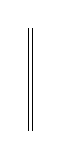
\begin{tikzpicture}[x=1em,y=1em]\draw (0,0)--(0,-3.7);\draw (.17,0)--(.17,-3.7);\end{tikzpicture}}} In any case,  \uline{the basic modelizer,}  \uline{in this whole approach to homotopy}
\uline{models,}  \uline{is by no means the category} (Ss sets)  (however handy)  \uline{or the}
\uline{category} (Spaces)  (howeve\var{\xout{\unsure{t}}}{}{typewriter deletion}{ps_134-3_033-v0008}r appealing to topological intuition),  \uline{but the}
\uline{category} (Cat) \uline{of} \uline{``all''} (small) \uline{categories.}  In this set-up,  the category
(Hot) is most suitably defined as the category of fractions of (Cat) with
respect to ``weak equivalences''.  These in turn are most suitably defined
in cohomological terms,  via the corresponding notion for topoi  -  namely
a morphism of topoi
\[ f:\ X \hand{\longrightarrow} X' \]
is a ``weak equivalence'' or homotopy equivalence,  iff for every locally
constant sheaf $F'$ on $X'$, the maps
\[ H^{i}(X',F') \hand{\to} H^{i}(X,f^{-1}(F')) \]
are isomorphisms whenever defined  -  namely for i=0,  for i=1 if moreover
$F'$ is endowed with a group structure,  and for any i if $F'$ is moreover
commutative\var{\xout{t}}{}{typewriter deletion}{ps_134-3_033-v0009} (\uline{Criterion} \uline{of} \uline{Artin-Mazur}).  Accordingly,  a functor

%% END SOURCE ps_134-3_033
\ifnum\EditionMode=1
\psapparatusstart
\psentry{ps_134-3_033-v0001}{1}{insertion}{\inserted{$j_{p,q}$}}{\hand{$j_{p,q}$}}{The handwritten insertion is incorporated at its indicated position; insertion brackets leave the running text.}
\psentry{ps_134-3_033-v0002}{2}{writing over}{\over{\unsure{26}}{29}}{\hand{29}}{The superposed handwritten reading replaces the underlying reading.}
\psentry{ps_134-3_033-v0003}{3}{typed insertion}{\inserted[typed]{i:}}{i:}{The typed insertion is incorporated at its indicated position; insertion brackets leave the running text.}
\psentry{ps_134-3_033-v0004}{4}{typewriter deletion}{\xout{xx}}{}{The typewriter strikes out this material; it leaves the corrected running text.}
\psentry{ps_134-3_033-v0005}{5}{writing over}{$\over{l}{l}$}{$\hand{l}$}{The superposed handwritten reading replaces the underlying reading.}
\psentry{ps_134-3_033-v0006}{6}{writing over}{$\over{l}{l}$}{$\hand{l}$}{The superposed handwritten reading replaces the underlying reading.}
\psentry{ps_134-3_033-v0007}{7}{typewriter deletion}{\xout{\unsure{s}}}{}{The typewriter strikes out this material; it leaves the corrected running text.}
\psentry{ps_134-3_033-v0008}{8}{typewriter deletion}{\xout{\unsure{t}}}{}{The typewriter strikes out this material; it leaves the corrected running text.}
\psentry{ps_134-3_033-v0009}{9}{typewriter deletion}{\xout{t}}{}{The typewriter strikes out this material; it leaves the corrected running text.}
\psapparatusend
\fi
\pssource{ps_134-3_034}{134-3/34}{https://grothendieck.umontpellier.fr/web/viewer.html?file=../134-3.pdf\#page=35}
\psnumber{ps_134-3_034-v0001}{1}
\psnumber{ps_134-3_034-v0002}{2}
\psnumber{ps_134-3_034-v0003}{3}
\psnumber{ps_134-3_034-v0004}{4}
\psnumber{ps_134-3_034-v0005}{5}
\psnumber{ps_134-3_034-v0006}{6}
\psnumber{ps_134-3_034-v0007}{7}
\psnumber{ps_134-3_034-v0008}{8}
\psnumber{ps_134-3_034-v0009}{9}
\psnumber{ps_134-3_034-v0010}{10}
\psnumber{ps_134-3_034-v0011}{11}
\psnumber{ps_134-3_034-v0012}{12}
\psnumber{ps_134-3_034-v0013}{13}
\psnumber{ps_134-3_034-v0014}{14}
\psnumber{ps_134-3_034-v0015}{15}
\psnumber{ps_134-3_034-v0016}{16}
\psnumber{ps_134-3_034-v0017}{17}
\psnumber{ps_134-3_034-v0018}{18}
\psnumber{ps_134-3_034-v0019}{19}
\psnumber{ps_134-3_034-v0020}{20}
\psnumber{ps_134-3_034-v0021}{21}
\psnumber{ps_134-3_034-v0022}{22}
\psnumber{ps_134-3_034-v0023}{23}
\psnumber{ps_134-3_034-v0024}{24}
\psnumber{ps_134-3_034-v0025}{25}
\psnumber{ps_134-3_034-v0026}{26}
\psnumber{ps_134-3_034-v0027}{27}
\psnumber{ps_134-3_034-v0028}{28}
\psnumber{ps_134-3_034-v0029}{29}
\psnumber{ps_134-3_034-v0030}{30}
\psnumber{ps_134-3_034-v0031}{31}
%% BEGIN SOURCE ps_134-3_034
% Pursuing Stacks (cotes 134-2 to 134-8): archive cote 134-3, site page 34 (PDF page 35), typescript page 34.
% typescript. Draft compared: ps2.tex:1621-1693.
% AI-transcribed by Claude Opus 5.5 (claude-opus-5-5, adaptive thinking, effort high), Message Batches API, batch ps1 (msgbatch_01Rv5hCaNTtUt4JHx1yqoHPL), 2026-11-12; image review recorded in records/CHECK_DECISIONS_134_3_4.tsv.
\scanpage{134-3/34}
\mspage{\hand{34}}
\[ f\colon A \hand{\longrightarrow} A' \]
between small categories (or categories which are essentially small, name-%
ly equivalent to small categories) is called a weak equivalence, iff the
corresponding morphism of topoi
\[ f\hand{\hat{}}\colon \var{\deleted{\illegible{1}}}{}{deletion}{ps_134-3_034-v0001}\ A\hand{\hat{}} \hand{\to} A'\hand{\hat{}} \]
is a weak equivalence.

Coming back to test categories A, which allow to construct the cor-%
responding modelizers $A\hand{\hat{}}$, our point of view here is rather that \uline{the test
categories are each just as good \var{\inserted{one}}{\hand{one}}{insertion}{ps_134-3_034-v0002} as the other\var{\deleted{s}}{}{deletion}{ps_134-3_034-v0003}}, and \hand{$\Delta$} just as good as
\hand{$\Box$} or any of the $T_{p,q}$ and not any better ! Maybe it's the one though which
turns out the most economical for computational use, the nerve functor
(Cat)$\hand{\to}$ \hand{$\Delta$}$\hand{\hat{}}$ being still the neatest known of all \var{\inserted[typed]{model preserving}}{model preserving}{typed insertion}{ps_134-3_034-v0004} embeddings of (Cat) into
categories $A\hand{\hat{}}$ defined by modelizers.\hand{$^{(31)}$.} Another \var{\inserted[typed]{point}}{point}{typed insertion}{ps_134-3_034-v0005}, still more important \var{\deleted{\xout{point}}}{}{deletion}{ps_134-3_034-v0006}
it seems to me, is that the natural functor
\[ \text{(Topoi)} \hand{\longrightarrow} \text{Pro(Hot)} \]
defined by the \hand{\v{}}Cech-Cartier-Verdier process, and which allows for another
description of weak equivalences of topoi\hand{,} \var{\inserted{namely}}{\hand{namely}}{insertion}{ps_134-3_034-v0007} as those made invertible by this
functor, are directly defined via semi-simplicial structures or simplicial
structures (of the type ``nerve of a covering'')\hand{$^{(32)}$.}

Modelizers of the type $A\hand{\hat{}}$, with A a test category, surely deserve
a name - lets call them \uline{elementary} \uline{modelizers}, as they correspond to \var{\xout{xx}}{}{typewriter deletion}{ps_134-3_034-v0008}
the case of an ``elementary'' or ``trivial'' algebraic structure species,
whose set-theoretical realizations can be expressed as just \uline{any} functors
\[ A^{o} \hand{\longrightarrow} \text{(Sets)} , \]
without any exactness condition of any kind\var{\over{,}{;}}{\hand{;}}{writing over}{ps_134-3_034-v0009} in other words they can
be viewed as just diagrams of sets of a specified type, with specified
commutativity relations. A somewhat ambitious question maybe is whether
on such a category \var{\inserted[typed]{$M=$}}{$M=$}{typed insertion}{ps_134-3_034-v0010} $A\hand{\hat{}}$, namely an elementary modelizer, there \var{\inserted[typed]{cannot}}{cannot}{typed insertion}{ps_134-3_034-v0011} \var{\xout{xxx}}{}{typewriter deletion}{ps_134-3_034-v0012} exist
\var{\inserted[typed]{any}}{any}{typed insertion}{ps_134-3_034-v0013} \var{\xout{xx}}{}{typewriter deletion}{ps_134-3_034-v0014}other modelizing structure. In any case, the one we got is intrinsicly
determined in terms of M, which is a topos, by the prescription that
an arrow $f\colon a \hand{\to} b$ within M is a weak equivalence if and only if the
corresponding morphism \var{\inserted[typed]{for}}{for}{typed insertion}{ps_134-3_034-v0015} \var{\xout{xx}}{}{typewriter deletion}{ps_134-3_034-v0016} the induced topoi $M_{/a}$ and $M/_{b}$ is a weak equiva-%
lence (in terms of the Artin-Mazur criterion \var{\deleted{\unsure{above section}}}{}{deletion}{ps_134-3_034-v0017} \var{\inserted{of section 17}}{\hand{of section 17}}{insertion}{ps_134-3_034-v0018}\hand{)}.

\var{\xout{Let}}{}{typewriter deletion}{ps_134-3_034-v0019} A more crucial question I feel is whether the \var{\inserted[typed]{right}}{right}{typed insertion}{ps_134-3_034-v0020} adjoint functor
$j_{A}$ to $i_{A}$ in (**) (cf. \var{\deleted{\illegible{1}}}{}{deletion}{ps_134-3_034-v0021} \var{\inserted{section 28)}}{\hand{section 28)}}{insertion}{ps_134-3_034-v0022} is equally model preserving, whenever A is a
test category. This, as we have seen, is \uline{not} automatic\unsure{,} whenever we
have a model preserving functor between modelizers, \var{\inserted{whenever}}{\hand{whenever}}{insertion}{ps_134-3_034-v0023} this functor admit\var{\over{ting}{s}}{\hand{s}}{writing over}{ps_134-3_034-v0024}
an adjoint functor. In \var{\inserted[typed]{more}}{more}{typed insertion}{ps_134-3_034-v0025} \var{\inserted{general}}{\hand{general}}{insertion}{ps_134-3_034-v0026} \var{\xout{xxxxxxx}}{}{typewriter deletion}{ps_134-3_034-v0027} terms \var{\xout{and more}}{}{typewriter deletion}{ps_134-3_034-v0028} still, let
% Hand-drawn arrows are marked blue; typed objects remain plain.
\diagram{\begin{tikzcd} M \ar[color=blue, r, shift left, "\hand{i}"] \& M' \ar[color=blue, l, shift left, "\hand{j}"] \end{tikzcd}}
\margin{\diagram{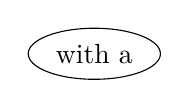
\begin{tikzpicture}[baseline=(n.base)]\node[draw,ellipse,inner sep=3pt] (n) {with a};\end{tikzpicture}}}
be a pair of adjoint functors, with M,M' endowed \var{\deleted{with two}}{}{deletion}{ps_134-3_034-v0029} \var{\inserted{with a}}{\hand{with a}}{insertion}{ps_134-3_034-v0030} \uline{``saturated''} \var{\deleted{sets}}{}{deletion}{ps_134-3_034-v0031}

%% END SOURCE ps_134-3_034
\ifnum\EditionMode=1
\psapparatusstart
\psentry{ps_134-3_034-v0001}{1}{deletion}{$\deleted{\illegible{1}}$}{}{The author cancels this material by hand; it leaves the corrected running text.}
\psentry{ps_134-3_034-v0002}{2}{insertion}{\inserted{one}}{\hand{one}}{The handwritten insertion is incorporated at its indicated position; insertion brackets leave the running text.}
\psentry{ps_134-3_034-v0003}{3}{deletion}{\deleted{s}}{}{The author cancels this material by hand; it leaves the corrected running text.}
\psentry{ps_134-3_034-v0004}{4}{typed insertion}{\inserted[typed]{model preserving}}{model preserving}{The typed insertion is incorporated at its indicated position; insertion brackets leave the running text.}
\psentry{ps_134-3_034-v0005}{5}{typed insertion}{\inserted[typed]{point}}{point}{The typed insertion is incorporated at its indicated position; insertion brackets leave the running text.}
\psentry{ps_134-3_034-v0006}{6}{deletion}{\deleted{\xout{point}}}{}{The author cancels this material by hand; it leaves the corrected running text.}
\psentry{ps_134-3_034-v0007}{7}{insertion}{\inserted{namely}}{\hand{namely}}{The handwritten insertion is incorporated at its indicated position; insertion brackets leave the running text.}
\psentry{ps_134-3_034-v0008}{8}{typewriter deletion}{\xout{xx}}{}{The typewriter strikes out this material; it leaves the corrected running text.}
\psentry{ps_134-3_034-v0009}{9}{writing over}{\over{,}{;}}{\hand{;}}{The superposed handwritten reading replaces the underlying reading.}
\psentry{ps_134-3_034-v0010}{10}{typed insertion}{\inserted[typed]{$M=$}}{$M=$}{The typed insertion is incorporated at its indicated position; insertion brackets leave the running text.}
\psentry{ps_134-3_034-v0011}{11}{typed insertion}{\inserted[typed]{cannot}}{cannot}{The typed insertion is incorporated at its indicated position; insertion brackets leave the running text.}
\psentry{ps_134-3_034-v0012}{12}{typewriter deletion}{\xout{xxx}}{}{The typewriter strikes out this material; it leaves the corrected running text.}
\psentry{ps_134-3_034-v0013}{13}{typed insertion}{\inserted[typed]{any}}{any}{The typed insertion is incorporated at its indicated position; insertion brackets leave the running text.}
\psentry{ps_134-3_034-v0014}{14}{typewriter deletion}{\xout{xx}}{}{The typewriter strikes out this material; it leaves the corrected running text.}
\psentry{ps_134-3_034-v0015}{15}{typed insertion}{\inserted[typed]{for}}{for}{The typed insertion is incorporated at its indicated position; insertion brackets leave the running text.}
\psentry{ps_134-3_034-v0016}{16}{typewriter deletion}{\xout{xx}}{}{The typewriter strikes out this material; it leaves the corrected running text.}
\psentry{ps_134-3_034-v0017}{17}{deletion}{\deleted{\unsure{above section}}}{}{The author cancels this material by hand; it leaves the corrected running text.}
\psentry{ps_134-3_034-v0018}{18}{insertion}{\inserted{of section 17}}{\hand{of section 17}}{The handwritten insertion is incorporated at its indicated position; insertion brackets leave the running text.}
\psentry{ps_134-3_034-v0019}{19}{typewriter deletion}{\xout{Let}}{}{The typewriter strikes out this material; it leaves the corrected running text.}
\psentry{ps_134-3_034-v0020}{20}{typed insertion}{\inserted[typed]{right}}{right}{The typed insertion is incorporated at its indicated position; insertion brackets leave the running text.}
\psentry{ps_134-3_034-v0021}{21}{deletion}{\deleted{\illegible{1}}}{}{The author cancels this material by hand; it leaves the corrected running text.}
\psentry{ps_134-3_034-v0022}{22}{insertion}{\inserted{section 28)}}{\hand{section 28)}}{The handwritten insertion is incorporated at its indicated position; insertion brackets leave the running text.}
\psentry{ps_134-3_034-v0023}{23}{insertion}{\inserted{whenever}}{\hand{whenever}}{The handwritten insertion is incorporated at its indicated position; insertion brackets leave the running text.}
\psentry{ps_134-3_034-v0024}{24}{writing over}{\over{ting}{s}}{\hand{s}}{The superposed handwritten reading replaces the underlying reading.}
\psentry{ps_134-3_034-v0025}{25}{typed insertion}{\inserted[typed]{more}}{more}{The typed insertion is incorporated at its indicated position; insertion brackets leave the running text.}
\psentry{ps_134-3_034-v0026}{26}{insertion}{\inserted{general}}{\hand{general}}{The handwritten insertion is incorporated at its indicated position; insertion brackets leave the running text.}
\psentry{ps_134-3_034-v0027}{27}{typewriter deletion}{\xout{xxxxxxx}}{}{The typewriter strikes out this material; it leaves the corrected running text.}
\psentry{ps_134-3_034-v0028}{28}{typewriter deletion}{\xout{and more}}{}{The typewriter strikes out this material; it leaves the corrected running text.}
\psentry{ps_134-3_034-v0029}{29}{deletion}{\deleted{with two}}{}{The author cancels this material by hand; it leaves the corrected running text.}
\psentry{ps_134-3_034-v0030}{30}{insertion}{\inserted{with a}}{\hand{with a}}{The handwritten insertion is incorporated at its indicated position; insertion brackets leave the running text.}
\psentry{ps_134-3_034-v0031}{31}{deletion}{\deleted{sets}}{}{The author cancels this material by hand; it leaves the corrected running text.}
\psapparatusend
\fi
\pssource{ps_134-3_035}{134-3/35}{https://grothendieck.umontpellier.fr/web/viewer.html?file=../134-3.pdf\#page=36}
\psnumber{ps_134-3_035-v0001}{1}
\psnumber{ps_134-3_035-v0002}{2}
\psnumber{ps_134-3_035-v0003}{3}
\psnumber{ps_134-3_035-v0004}{4}
\psnumber{ps_134-3_035-v0005}{5}
\psnumber{ps_134-3_035-v0006}{6}
\psnumber{ps_134-3_035-v0007}{7}
\psnumber{ps_134-3_035-v0008}{8}
\psnumber{ps_134-3_035-v0009}{9}
\psnumber{ps_134-3_035-v0010}{10}
\psnumber{ps_134-3_035-v0011}{11}
\psnumber{ps_134-3_035-v0012}{12}
\psnumber{ps_134-3_035-v0013}{13}
\psnumber{ps_134-3_035-v0014}{14}
\psnumber{ps_134-3_035-v0015}{15}
\psnumber{ps_134-3_035-v0016}{16}
\psnumber{ps_134-3_035-v0017}{17}
\psnumber{ps_134-3_035-v0018}{18}
\psnumber{ps_134-3_035-v0019}{19}
\psnumber{ps_134-3_035-v0020}{20}
\psnumber{ps_134-3_035-v0021}{21}
%% BEGIN SOURCE ps_134-3_035
% Pursuing Stacks (cotes 134-2 to 134-8): archive cote 134-3, site page 35 (PDF page 36), typescript page 35.
% typescript. Draft compared: ps2.tex:1674-1745.
% AI-transcribed by Claude Opus 5.5 (claude-opus-5-5, adaptive thinking, effort high), Message Batches API, batch ps1 (msgbatch_01Rv5hCaNTtUt4JHx1yqoHPL), 2026-11-12; image review recorded in records/CHECK_DECISIONS_134_3_4.tsv.
\scanpage{134-3/35}
\mspage{35}
set of arrows W,W'. Then the following are equivalent:

a) $i(W)\hand{\subset} W'$, $j(W')\hand{\subset} W$, and the two corresponding functors
\[ W^{-1}M \hand{\rightleftarrows} W'^{-1}M' \]
are quasi-inverse of each other, the adjunction morphisms between
them being deduced from the corresponding adjunction morphisms
for the pair (i,j).

b) $W=i^{-1}(W')$, and for every $a'\hand{\in} M'$, the adjunction morphism
\[ \var{\xout{ax}}{}{typewriter deletion}{ps_134-3_035-v0001} \quad i\var{\over{j}{j}}{\hand{j}}{writing over}{ps_134-3_035-v0002}(a')\hand{\to} a' \]
is in W'.

b') dual to b), with roles of M and M' reversed.

In the situation we are interested in here, $M = A\hand{\hat{}}$\hand{/}and $M' = $ (Cat),
we know already $W=i^{-1}(W')$ by definition, and hence all we have to see is
w\hand{h}ether for any \var{\inserted{[small]}}{\hand{[small]}}{insertion}{ps_134-3_035-v0003} category B, the functor
\[ \text{(T)} \qquad \var{\xout{B}}{}{typewriter deletion}{ps_134-3_035-v0004} \quad \var{\over{i}{i}}{\hand{i}}{writing over}{ps_134-3_035-v0005}_A \var{\over{j}{j}}{\hand{j}}{writing over}{ps_134-3_035-v0006}_A(B) \hand{\longrightarrow} B \]
is a \var{\xout{quasi}}{}{typewriter deletion}{ps_134-3_035-v0007} \var{\inserted[typed]{weak}}{weak}{typed insertion}{ps_134-3_035-v0008} equivalence. This alone will imply that not only $i_{W,W'}$ , but
equally $j_{W',W}$ is an equivalence, and that the two are quasi-inverse of
each other. (NB even without assuming beforehand that W \var{\xout{is}}{}{typewriter deletion}{ps_134-3_035-v0009}\var{\inserted[typed]{W' are}}{W' are}{typed insertion}{ps_134-3_035-v0010} saturated ,
b) (say) implies b') and a), \var{\xout{and}}{}{typewriter deletion}{ps_134-3_035-v0011} provided we assume on W' the very mild
saturation condition that for composable arrows $u',v'$, if two among $u',v'$,
$v'u'$ are in W', so is the third; \var{\xout{moreover,}}{}{typewriter deletion}{ps_134-3_035-v0012} if we suppose moreover that
M' is actually saturated namely made up with all arrows made invertible by
$M'\hand{\to} W'^{-1}M'$, then condition b) implies that M is saturated too - which
insures that if (M',W') is modelizing, so is (M,W).\hand{)}

It is not clear to me whether for every test category A, the stronger
condition (T) above is necessarily satisfied. \var{\xout{It}}{}{typewriter deletion}{ps_134-3_035-v0013} \var{\inserted[typed]{This condition essentially}}{This condition essentially}{typed insertion}{ps_134-3_035-v0014} means that for any homo-%
topy type, defined in terms of an arbitrary element B in (Cat) namely
a category B, we get a description of this homotopy type \var{\over{by}{by}}{\hand{by}}{writing over}{ps_134-3_035-v0015} an object of
the elementary modelizer $A\hand{\hat{}}$,\hand{|}by merely taking $j_A(B)$. This condition seems
sufficiently appealing to me, for reinforcing adcordingly the notion of
atest-category A, and of an elementary normalizer $A\hand{\hat{}}$, in case it should
turn out to be actually stronger\hand{(${}^{33}$)}. Of course, any category equivalent to
an elementary modelizer $A\hand{\hat{}}$\hand{/}will be equally called by the same name. It \var{\xout{should}}{}{typewriter deletion}{ps_134-3_035-v0016}
should appear in \var{\xout{the}}{}{typewriter deletion}{ps_134-3_035-v0017} due course whether this is indeed the better suited
notion. One point in it\hand{'}s favor \var{\xout{though}}{}{typewriter deletion}{ps_134-3_035-v0018}\var{\inserted[typed]{already}}{already}{typed insertion}{ps_134-3_035-v0019} is that it \var{\over{app}{app}}{\hand{app}}{writing over}{ps_134-3_035-v0020}ears a lot more
concrete.

Another natural question, suggested by the use of simplicial or cubi-%
cal multicomplexes, is whether the product of two test categories is again
a test category - which might furnish us with a way to compare \var{\xout{the}}{}{typewriter deletion}{ps_134-3_035-v0021} direct-%
ly the description of (Hot) by the associated elementary modelizers, with\hand{out}

%% END SOURCE ps_134-3_035
\ifnum\EditionMode=1
\psapparatusstart
\psentry{ps_134-3_035-v0001}{1}{typewriter deletion}{$\xout{ax}$}{}{The typewriter strikes out this material; it leaves the corrected running text.}
\psentry{ps_134-3_035-v0002}{2}{writing over}{$\over{j}{j}$}{$\hand{j}$}{The superposed handwritten reading replaces the underlying reading.}
\psentry{ps_134-3_035-v0003}{3}{insertion}{\inserted{[small]}}{\hand{[small]}}{The handwritten insertion is incorporated at its indicated position; insertion brackets leave the running text.}
\psentry{ps_134-3_035-v0004}{4}{typewriter deletion}{$\xout{B}$}{}{The typewriter strikes out this material; it leaves the corrected running text.}
\psentry{ps_134-3_035-v0005}{5}{writing over}{$\over{i}{i}$}{$\hand{i}$}{The superposed handwritten reading replaces the underlying reading.}
\psentry{ps_134-3_035-v0006}{6}{writing over}{$\over{j}{j}$}{$\hand{j}$}{The superposed handwritten reading replaces the underlying reading.}
\psentry{ps_134-3_035-v0007}{7}{typewriter deletion}{\xout{quasi}}{}{The typewriter strikes out this material; it leaves the corrected running text.}
\psentry{ps_134-3_035-v0008}{8}{typed insertion}{\inserted[typed]{weak}}{weak}{The typed insertion is incorporated at its indicated position; insertion brackets leave the running text.}
\psentry{ps_134-3_035-v0009}{9}{typewriter deletion}{\xout{is}}{}{The typewriter strikes out this material; it leaves the corrected running text.}
\psentry{ps_134-3_035-v0010}{10}{typed insertion}{\inserted[typed]{W' are}}{W' are}{The typed insertion is incorporated at its indicated position; insertion brackets leave the running text.}
\psentry{ps_134-3_035-v0011}{11}{typewriter deletion}{\xout{and}}{}{The typewriter strikes out this material; it leaves the corrected running text.}
\psentry{ps_134-3_035-v0012}{12}{typewriter deletion}{\xout{moreover,}}{}{The typewriter strikes out this material; it leaves the corrected running text.}
\psentry{ps_134-3_035-v0013}{13}{typewriter deletion}{\xout{It}}{}{The typewriter strikes out this material; it leaves the corrected running text.}
\psentry{ps_134-3_035-v0014}{14}{typed insertion}{\inserted[typed]{This condition essentially}}{This condition essentially}{The typed insertion is incorporated at its indicated position; insertion brackets leave the running text.}
\psentry{ps_134-3_035-v0015}{15}{writing over}{\over{by}{by}}{\hand{by}}{The superposed handwritten reading replaces the underlying reading.}
\psentry{ps_134-3_035-v0016}{16}{typewriter deletion}{\xout{should}}{}{The typewriter strikes out this material; it leaves the corrected running text.}
\psentry{ps_134-3_035-v0017}{17}{typewriter deletion}{\xout{the}}{}{The typewriter strikes out this material; it leaves the corrected running text.}
\psentry{ps_134-3_035-v0018}{18}{typewriter deletion}{\xout{though}}{}{The typewriter strikes out this material; it leaves the corrected running text.}
\psentry{ps_134-3_035-v0019}{19}{typed insertion}{\inserted[typed]{already}}{already}{The typed insertion is incorporated at its indicated position; insertion brackets leave the running text.}
\psentry{ps_134-3_035-v0020}{20}{writing over}{\over{app}{app}}{\hand{app}}{The superposed handwritten reading replaces the underlying reading.}
\psentry{ps_134-3_035-v0021}{21}{typewriter deletion}{\xout{the}}{}{The typewriter strikes out this material; it leaves the corrected running text.}
\psapparatusend
\fi
\pssource{ps_134-3_036}{134-3/36}{https://grothendieck.umontpellier.fr/web/viewer.html?file=../134-3.pdf\#page=37}
\psnumber{ps_134-3_036-v0001}{1}
\psnumber{ps_134-3_036-v0002}{2}
\psnumber{ps_134-3_036-v0003}{3}
\psnumber{ps_134-3_036-v0004}{4}
\psnumber{ps_134-3_036-v0005}{5}
\psnumber{ps_134-3_036-v0006}{6}
\psnumber{ps_134-3_036-v0007}{7}
\psnumber{ps_134-3_036-v0008}{8}
\psnumber{ps_134-3_036-v0009}{9}
\psnumber{ps_134-3_036-v0010}{10}
\psnumber{ps_134-3_036-v0011}{11}
%% BEGIN SOURCE ps_134-3_036
% Pursuing Stacks (cotes 134-2 to 134-8): archive cote 134-3, site page 36 (PDF page 37), typescript page 36.
% typescript. Draft compared: ps2.tex:1730-1799.
% AI-transcribed by Claude Opus 5.5 (claude-opus-5-5, adaptive thinking, effort high), Message Batches API, batch ps1 (msgbatch_01Rv5hCaNTtUt4JHx1yqoHPL), 2026-11-12; image review recorded in records/CHECK_DECISIONS_134_3_4.tsv.
\scanpage{134-3/36}
\mspage{36}
having to make a détour by the"basic"modelizer (Cat)\var{\inserted{we started with}}{\hand{we started with}}{insertion}{ps_134-3_036-v0001}. But here it becomes
about time to try and leave the thin air conjecturing, and find some simple
\margin{\diagram{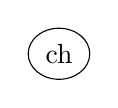
\begin{tikzpicture}[baseline=(n.base)]\node[draw,ellipse,inner sep=3pt] (n) {ch};\end{tikzpicture}}} and concrete \var{\over{c}{ch}}{\hand{ch}}{writing over}{ps_134-3_036-v0002}aracterization of test categories, \var{\xout{which}}{}{typewriter deletion}{ps_134-3_036-v0003} or possibly some
reinforcement still of that notion, which will imply stability under the
product operation.

Here it is tempting to use semi-simplicial techniques though, by lack
of independant foundations of homotopy theory in terms of the modelizer
(Cat). Thus we may want to take the map of semi-simplicial sets correspon-%
ding to (T) when passing to nerves, and express that a) this is a fibration
and b) the fibers of this fibration are "contractible"\var{\inserted[typed]{(or "aspheric")}}{(or "aspheric")}{typed insertion}{ps_134-3_036-v0004}, which together
will imply that we have a weak equivalence in (Ss sets). Or we may follow
the suggestion of Quillen's set-up, working heuristically in (Cat) as though
we actually knew it is a model category, and expressing that the adjunction
morphism in (T), which is a functor between categories, is actually a
"fibration", and that it\hand{'}s fibers are "contractible" namely weakly equivalent
to a one-point category. I\var{\over{n}{n}}{\hand{n}}{writing over}{ps_134-3_036-v0005} any case, a minimum amount of technique seems
needed here, to give the necessary clues for pursuing.

14.3.

30. Since Last week when I stopped with my notes, I got involved a bit
with recalling to mind the "Lego-Teichmüller construction game" for descri-%
bing in a conrete, "visual" way the Teichmüller groups of all possible
types and the main relationships between them, which I had first met with
last year. This and other non mathematical occupations left little time
only for my reflections on homotopy theory, \var{\inserted{which I took up}}{\hand{which I took up}}{insertion}{ps_134-3_036-v0006} mainly last night and today.
T\var{\over{h}{h}}{\hand{h}}{writing over}{ps_134-3_036-v0007}e focus of attention was the "technical point" of getting a handy carac-%
terization of test categories. The situation I feel is beginning to clari-%
fy somewhat. Last thing I did\hand{,} before reading last weeks' notes and getting
back to the typewriter\hand{,} was to get rid of a delusion which I was dragging
along more or less from the beginning of these notes, namely that our
basic modelizer (Cat), which we were using \var{\xout{for our}}{}{typewriter deletion}{ps_134-3_036-v0008} as \var{\over{p}{g}}{\hand{g}}{writing over}{ps_134-3_036-v0009}iving the most
natural definition of (Hot) in our setting, was a "model category" in the
sense of Quillen, more specifically a "closed model category", where
the "weak equivalences" are the homotopy equivalences of course, and where
cofibrations are just monomorphisms (namely functors injective on objects
and on arrows) - fibrations being defined in terms of these by the
\margin{\diagram{\begin{tikzpicture}[x=1em,y=1em]\draw (0,0)--(0,-3.6);\end{tikzpicture}}} Serre-Quillen lifting property. Without \var{\inserted[typed]{even}}{even}{typed insertion}{ps_134-3_036-v0010} being so demanding, it turns out
still that there is no reasonable structure of a model catégory on (Cat),
having the correct weak equivalences, and such that the standart \var{\inserted{"Kan}}{\hand{"Kan}}{insertion}{ps_134-3_036-v0011} inclusi-%
ons\hand{"} of the following two ordered sets

%% END SOURCE ps_134-3_036
\ifnum\EditionMode=1
\psapparatusstart
\psentry{ps_134-3_036-v0001}{1}{insertion}{\inserted{we started with}}{\hand{we started with}}{The handwritten insertion is incorporated at its indicated position; insertion brackets leave the running text.}
\psentry{ps_134-3_036-v0002}{2}{writing over}{\over{c}{ch}}{\hand{ch}}{The superposed handwritten reading replaces the underlying reading.}
\psentry{ps_134-3_036-v0003}{3}{typewriter deletion}{\xout{which}}{}{The typewriter strikes out this material; it leaves the corrected running text.}
\psentry{ps_134-3_036-v0004}{4}{typed insertion}{\inserted[typed]{(or "aspheric")}}{(or "aspheric")}{The typed insertion is incorporated at its indicated position; insertion brackets leave the running text.}
\psentry{ps_134-3_036-v0005}{5}{writing over}{\over{n}{n}}{\hand{n}}{The superposed handwritten reading replaces the underlying reading.}
\psentry{ps_134-3_036-v0006}{6}{insertion}{\inserted{which I took up}}{\hand{which I took up}}{The handwritten insertion is incorporated at its indicated position; insertion brackets leave the running text.}
\psentry{ps_134-3_036-v0007}{7}{writing over}{\over{h}{h}}{\hand{h}}{The superposed handwritten reading replaces the underlying reading.}
\psentry{ps_134-3_036-v0008}{8}{typewriter deletion}{\xout{for our}}{}{The typewriter strikes out this material; it leaves the corrected running text.}
\psentry{ps_134-3_036-v0009}{9}{writing over}{\over{p}{g}}{\hand{g}}{The superposed handwritten reading replaces the underlying reading.}
\psentry{ps_134-3_036-v0010}{10}{typed insertion}{\inserted[typed]{even}}{even}{The typed insertion is incorporated at its indicated position; insertion brackets leave the running text.}
\psentry{ps_134-3_036-v0011}{11}{insertion}{\inserted{"Kan}}{\hand{"Kan}}{The handwritten insertion is incorporated at its indicated position; insertion brackets leave the running text.}
\psapparatusend
\fi
\pssource{ps_134-3_037}{134-3/37}{https://grothendieck.umontpellier.fr/web/viewer.html?file=../134-3.pdf\#page=38}
\psnumber{ps_134-3_037-v0001}{1}
\psnumber{ps_134-3_037-v0002}{2}
\psnumber{ps_134-3_037-v0003}{3}
\psnumber{ps_134-3_037-v0004}{4}
\psnumber{ps_134-3_037-v0005}{5}
\psnumber{ps_134-3_037-v0006}{6}
\psnumber{ps_134-3_037-v0007}{7}
\psnumber{ps_134-3_037-v0008}{8}
\psnumber{ps_134-3_037-v0009}{9}
\psnumber{ps_134-3_037-v0010}{10}
\psnumber{ps_134-3_037-v0011}{11}
%% BEGIN SOURCE ps_134-3_037
% Pursuing Stacks (cotes 134-2 to 134-8): archive cote 134-3, site page 37 (PDF page 38), typescript page 37.
% typescript. Draft compared: ps2.tex:1781-1845.
% AI-transcribed by Claude Opus 5.5 (claude-opus-5-5, adaptive thinking, effort high), Message Batches API, batch ps1 (msgbatch_01Rv5hCaNTtUt4JHx1yqoHPL), 2026-11-12; image review recorded in records/CHECK_DECISIONS_134_3_4.tsv.
\scanpage{134-3/37}
\mspage{\hand{37}}
\hand{\diagram{\begin{tikzcd}[row sep=small,column sep=small] \& b \\ a \ar[ur]\ar[r] \& c \end{tikzcd}}} \quad and \quad \hand{\diagram{\begin{tikzcd}[row sep=small,column sep=small] a \ar[r] \& c \\ b \ar[ur] \& \end{tikzcd}}}
into
\[ \hand{\Delta}_2 = \hand{a\longrightarrow b\longrightarrow c} \]
be cofibering. Namely, for a category C, to say that it is``fibering''
(over the final category e) with respect to one or the other monomorphism,
means respectively that every arrow in $\underline{C}$ has a left respectively a right
inverse - the two together mean that $\underline{C}$ is a groupoid. But groupoids are
definitely \uline{not} sufficient for describing arbitrary homotopy types, they
give rise only to sums of K(\hand{$\pi$},1) spaces \var{\xout{\unsure{(}}}{}{typewriter deletion}{ps_134-3_037-v0001} - thus contradicting Quillen's
statement that homotopy types can be described by ``models'' which are both
fibering and cofibering\hand{!}

The feeling however remains that any elementary modelizer, namely one
defined (up to equivalence) by a test category, should be a \var{\inserted[typed]{closed}}{closed}{typed insertion}{ps_134-3_037-v0002} model catego\unsure{ry}
% NOTE: the end of this line is cut by the right edge of the scan
in Quillen's sense - \var{\over{If}{I}}{\hand{I}}{writing over}{ps_134-3_037-v0003} find it hard to believe that this should be a spe%
% NOTE: the end of this line (hyphen?) is cut by the right edge of the scan
cial feature just of semi-simplicial complexes !

While trying to understand test categories, the notion of \uline{asphericity}
for a morphism of topoi
\[ f\colon X \hand{\longrightarrow} Y \]
came in naturally - this is a natural \var{\xout{g\unsure{ene}}}{}{typewriter deletion}{ps_134-3_037-v0004} variant of the notion of
n-acyclicity (concerned with commutative cohomology) which has been deve-%
lopped in the context of étale topology of schemes in SGA 4. It can be
expressed by ``localizing\var{\xout{\illegible{1}}}{}{typewriter deletion}{ps_134-3_037-v0005} upon Y '' the Artin-Mazur condition that f be
a weak equivalence, by demanding that the same remain true for the induced
morphisms of topoi
\[ X\mathrm{x}_{Y}Y' \hand{\longrightarrow} Y' \]
for any ``localization morphism'' Y'\hand{$\longrightarrow$} Y. In terms of the categories of
sheaves \var{\xout{\illegible{1}}}{}{typewriter deletion}{ps_134-3_037-v0006} E, F on X,Y , Y' can be defined by an object (equally called
Y') of F, the category of sheaves on Y' being F$_{/Y'}$ , and the fiber-pro-%
duct X' can be defined likewise by an object \var{\deleted{\unsure{X'}}}{}{deletion}{ps_134-3_037-v0007} of E, namely \var{\inserted{by (X'=}}{\hand{by (X'=}}{insertion}{ps_134-3_037-v0008} f$^{*}$(Y'),
hence the corresponding category of sheaves is E$_{/f^{*}(Y')}$ . In case the
functor f$^{*}$ associated to f admits a left adjoint f$_{\hand{!}}$ (namely if it commutes
to arbitrary inverse limits, not only to finite one's), the category
E$_{/f^{*}(Y')}$ can be interpreted conveniently as \var{\xout{E$_{/Y'}$}}{}{typewriter deletion}{ps_134-3_037-v0009} E$_{f_{\hand{!}}/Y'}$ (or simply E$_{/Y'}$
if f$_{\hand{!}}$ is implicit), whose objects are pairs
\[ (U,\emptyset) \quad , \quad U \hand{\in} \mathrm{Ob}\ E \ , \ \emptyset : f_{\hand{!}}(U) \hand{\longrightarrow} Y' \quad , \]
with obvious ``maps'' between such objects. For the time being I am mainly
interested in the case of a morphism of topoi defined by a functor \var{\over{\unsure{(}}{b}}{\hand{b}}{writing over}{ps_134-3_037-v0010}etween
categories, which I will denote by the same symbol f :
\[ f\colon C' \hand{\longrightarrow} C \quad \text{defines f or } \hand{\hat{\ }}f : \hand{\hat{\ }}C\hand{'} \hand{\to} \hand{\hat{\ }}C\var{\xout{\unsure{'}}}{}{typewriter deletion}{ps_134-3_037-v0011} \quad . \]

%% END SOURCE ps_134-3_037
\ifnum\EditionMode=1
\psapparatusstart
\psentry{ps_134-3_037-v0001}{1}{typewriter deletion}{\xout{\unsure{(}}}{}{The typewriter strikes out this material; it leaves the corrected running text.}
\psentry{ps_134-3_037-v0002}{2}{typed insertion}{\inserted[typed]{closed}}{closed}{The typed insertion is incorporated at its indicated position; insertion brackets leave the running text.}
\psentry{ps_134-3_037-v0003}{3}{writing over}{\over{If}{I}}{\hand{I}}{The superposed handwritten reading replaces the underlying reading.}
\psentry{ps_134-3_037-v0004}{4}{typewriter deletion}{\xout{g\unsure{ene}}}{}{The typewriter strikes out this material; it leaves the corrected running text.}
\psentry{ps_134-3_037-v0005}{5}{typewriter deletion}{\xout{\illegible{1}}}{}{The typewriter strikes out this material; it leaves the corrected running text.}
\psentry{ps_134-3_037-v0006}{6}{typewriter deletion}{\xout{\illegible{1}}}{}{The typewriter strikes out this material; it leaves the corrected running text.}
\psentry{ps_134-3_037-v0007}{7}{deletion}{\deleted{\unsure{X'}}}{}{The author cancels this material by hand; it leaves the corrected running text.}
\psentry{ps_134-3_037-v0008}{8}{insertion}{\inserted{by (X'=}}{\hand{by (X'=}}{The handwritten insertion is incorporated at its indicated position; insertion brackets leave the running text.}
\psentry{ps_134-3_037-v0009}{9}{typewriter deletion}{\xout{E$_{/Y'}$}}{}{The typewriter strikes out this material; it leaves the corrected running text.}
\psentry{ps_134-3_037-v0010}{10}{writing over}{\over{\unsure{(}}{b}}{\hand{b}}{The superposed handwritten reading replaces the underlying reading.}
\psentry{ps_134-3_037-v0011}{11}{typewriter deletion}{$\xout{\unsure{'}}$}{}{The typewriter strikes out this material; it leaves the corrected running text.}
\psapparatusend
\fi
\pssource{ps_134-3_038}{134-3/38}{https://grothendieck.umontpellier.fr/web/viewer.html?file=../134-3.pdf\#page=39}
\psnumber{ps_134-3_038-v0001}{1}
\psnumber{ps_134-3_038-v0002}{2}
\psnumber{ps_134-3_038-v0003}{3}
\psnumber{ps_134-3_038-v0004}{4}
\psnumber{ps_134-3_038-v0005}{5}
\psnumber{ps_134-3_038-v0006}{6}
\psnumber{ps_134-3_038-v0007}{7}
\psnumber{ps_134-3_038-v0008}{8}
\psnumber{ps_134-3_038-v0009}{9}
\psnumber{ps_134-3_038-v0010}{10}
\psnumber{ps_134-3_038-v0011}{11}
\psnumber{ps_134-3_038-v0012}{12}
\psnumber{ps_134-3_038-v0013}{13}
\psnumber{ps_134-3_038-v0014}{14}
\psnumber{ps_134-3_038-v0015}{15}
\psnumber{ps_134-3_038-v0016}{16}
\psnumber{ps_134-3_038-v0017}{17}
\psnumber{ps_134-3_038-v0018}{18}
\psnumber{ps_134-3_038-v0019}{19}
\psnumber{ps_134-3_038-v0020}{20}
\psnumber{ps_134-3_038-v0021}{21}
%% BEGIN SOURCE ps_134-3_038
% Pursuing Stacks (cotes 134-2 to 134-8): archive cote 134-3, site page 38 (PDF page 39), typescript page 38.
% typescript. Draft compared: ps2.tex:1831-1909.
% AI-transcribed by Claude Opus 5.5 (claude-opus-5-5, adaptive thinking, effort high), Message Batches API, batch ps1 (msgbatch_01Rv5hCaNTtUt4JHx1yqoHPL), 2026-11-12; image review recorded in records/CHECK_DECISIONS_134_3_4.tsv.
\scanpage{134-3/38}
\mspage{\hand{38}}
Using the fact that in the \var{\xout{description of}}{}{typewriter deletion}{ps_134-3_038-v0001} general definition of asphericity
it is enough to take Y' in a family of generators of the topos Y,  and \var{\xout{usin}}{}{typewriter deletion}{ps_134-3_038-v0002}
using here the generating subcategory C of $\overset{\hand{\wedge}}{C}$ ,  we get the following crite\var{\xout{r}}{}{typewriter deletion}{ps_134-3_038-v0003}
\unsure{t}ion for asphericity of $\overset{\hand{\wedge}}{f}$ :  if is nec. and sufficient that for every
\hand{$a\in$}Ob C ,  the induced morphism of topoi
\[ \overset{\hand{\wedge}}{C'}_{/a} \hand{\cong} (C'_{/a})^{\hand{\wedge}} \hand{\to} \overset{\hand{\wedge}}{C}_{/a} \hand{\simeq} (C_{/a})^{\hand{\wedge}} \]
be a weak equivalence,  i.e. that the natural functor  $C'_{/a}\hand{\to} C_{/a}$ be a weak
equivalence.  But it is immediate that $C_{/a}$ is ``contractible'' \var{\xout{i.e.}}{}{typewriter deletion}{ps_134-3_038-v0004} \hand{i.e.} ``asphe
ric'',  namely the ``map'' from $C_{/a}$ to the final category is a weak equivalen\var{\xout{c}}{}{typewriter deletion}{ps_134-3_038-v0005}
ce (this is true for any category having a final object). Therefore we get
the following
\margin{\diagram{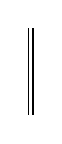
\begin{tikzpicture}\draw (0,0)--(0,1.1);\draw (.06,0)--(.06,1.1);\end{tikzpicture}}}\uline{Criterion of asphericity for a functor} f: C'$\hand{\to}$ C  between categories:
namely it is n. and s. that for any a $\hand{\in}$ Ob C,   $C'_{/a}$  be aspheric.

Let's come back to a \var{\xout{would}}{}{typewriter deletion}{ps_134-3_038-v0006} category A,  for which we want to express
that it is a test-category,  namely for any \var{\inserted{[small]}}{\hand{[small]}}{insertion}{ps_134-3_038-v0007} category B,  the natural
functor
\[ \hand{(*)} \qquad i_Aj_A(B) \hand{\longrightarrow} B \]
is a weak equivalence.  O\var{\over{n}{n}}{\hand{n}}{writing over}{ps_134-3_038-v0008}e immediately checks that for any b$\hand{\in}$ Ob B,
the category  $i_Aj_A(B)_{/b}$ \var{\xout{over}}{}{typewriter deletion}{ps_134-3_038-v0009} over $B_{/b}$  is isomorphic to $i_Aj_A(B_{/b})$ . Hence
we get the following
\uline{Proposition}  For a \var{\inserted{[small]}}{\hand{[small]}}{insertion}{ps_134-3_038-v0010} category A,  the following are equivalent:
(i)  A is a test category,  namely (*) is a\var{\deleted{n}}{}{deletion}{ps_134-3_038-v0011} \var{\inserted{weak}}{\hand{weak}}{insertion}{ps_134-3_038-v0012} equivalence for any \var{\inserted{[small]}}{\hand{[small]}}{insertion}{ps_134-3_038-v0013}
category B.
(ii)  (*) is aspheric for any \var{\inserted{[small]}}{\hand{[small]}}{insertion}{ps_134-3_038-v0014} category B.
(iii)  $i_Aj_A(B)$ is aspheric for any category B with final element.

This latter condition,  which is the most ``concrete'' one so far,
means also that the element
\[ F = j_A(B) = (\ a \hand{\mapsto} \mathrm{Hom}(\underset{\hand{\wedge}}{A}_{/a},B)) \hand{\in} \overset{\hand{\wedge}}{A} \]
is \var{\deleted{an}}{}{deletion}{ps_134-3_038-v0015} \var{\inserted[typed]{aspheric}}{aspheric}{typed insertion}{ps_134-3_038-v0016} \var{\deleted{\xout{aspheric}}}{}{deletion}{ps_134-3_038-v0017} element of the topos $\overset{\hand{\wedge}}{A}$ ,  namely  the induced topos $\overset{\hand{\wedge}}{A}_{/F}$ is
aspheric (i.e. the category $A_{/F}$  is aspheric),  \uline{whenever} B has a final
element.

\hand{31.}  For the notion of a test category to make at all a sense,  we should
make sure in the long last that \hand{$\Delta$} itself,  the category of standar\var{\over{t}{d}}{\hand{d}}{writing over}{ps_134-3_038-v0018} simpli-%
ces,  is indeed a test category.  So I finally set out to prove at least
\margin{$\times$} that much,  using the few reflexes I ha\var{\over{d}{v}}{\hand{v}}{writing over}{ps_134-3_038-v0019}e in semi-simplicial homotopy theo\var{\xout{r}}{}{typewriter deletion}{ps_134-3_038-v0020}-%
ry.  A proof finally peeled out it seems,  giving clues for handy conditi-%
ons in the general case,  which should be \uline{sufficient} \var{\over{\unsure{in the base}}{at least}}{\hand{at least}}{writing over}{ps_134-3_038-v0021} to insure
that B is a test category,  but maybe not quite necessary.  I'll try now
to get it down explicitly.

%% END SOURCE ps_134-3_038
\ifnum\EditionMode=1
\psapparatusstart
\psentry{ps_134-3_038-v0001}{1}{typewriter deletion}{\xout{description of}}{}{The typewriter strikes out this material; it leaves the corrected running text.}
\psentry{ps_134-3_038-v0002}{2}{typewriter deletion}{\xout{usin}}{}{The typewriter strikes out this material; it leaves the corrected running text.}
\psentry{ps_134-3_038-v0003}{3}{typewriter deletion}{\xout{r}}{}{The typewriter strikes out this material; it leaves the corrected running text.}
\psentry{ps_134-3_038-v0004}{4}{typewriter deletion}{\xout{i.e.}}{}{The typewriter strikes out this material; it leaves the corrected running text.}
\psentry{ps_134-3_038-v0005}{5}{typewriter deletion}{\xout{c}}{}{The typewriter strikes out this material; it leaves the corrected running text.}
\psentry{ps_134-3_038-v0006}{6}{typewriter deletion}{\xout{would}}{}{The typewriter strikes out this material; it leaves the corrected running text.}
\psentry{ps_134-3_038-v0007}{7}{insertion}{\inserted{[small]}}{\hand{[small]}}{The handwritten insertion is incorporated at its indicated position; insertion brackets leave the running text.}
\psentry{ps_134-3_038-v0008}{8}{writing over}{\over{n}{n}}{\hand{n}}{The superposed handwritten reading replaces the underlying reading.}
\psentry{ps_134-3_038-v0009}{9}{typewriter deletion}{\xout{over}}{}{The typewriter strikes out this material; it leaves the corrected running text.}
\psentry{ps_134-3_038-v0010}{10}{insertion}{\inserted{[small]}}{\hand{[small]}}{The handwritten insertion is incorporated at its indicated position; insertion brackets leave the running text.}
\psentry{ps_134-3_038-v0011}{11}{deletion}{\deleted{n}}{}{The author cancels this material by hand; it leaves the corrected running text.}
\psentry{ps_134-3_038-v0012}{12}{insertion}{\inserted{weak}}{\hand{weak}}{The handwritten insertion is incorporated at its indicated position; insertion brackets leave the running text.}
\psentry{ps_134-3_038-v0013}{13}{insertion}{\inserted{[small]}}{\hand{[small]}}{The handwritten insertion is incorporated at its indicated position; insertion brackets leave the running text.}
\psentry{ps_134-3_038-v0014}{14}{insertion}{\inserted{[small]}}{\hand{[small]}}{The handwritten insertion is incorporated at its indicated position; insertion brackets leave the running text.}
\psentry{ps_134-3_038-v0015}{15}{deletion}{\deleted{an}}{}{The author cancels this material by hand; it leaves the corrected running text.}
\psentry{ps_134-3_038-v0016}{16}{typed insertion}{\inserted[typed]{aspheric}}{aspheric}{The typed insertion is incorporated at its indicated position; insertion brackets leave the running text.}
\psentry{ps_134-3_038-v0017}{17}{deletion}{\deleted{\xout{aspheric}}}{}{The author cancels this material by hand; it leaves the corrected running text.}
\psentry{ps_134-3_038-v0018}{18}{writing over}{\over{t}{d}}{\hand{d}}{The superposed handwritten reading replaces the underlying reading.}
\psentry{ps_134-3_038-v0019}{19}{writing over}{\over{d}{v}}{\hand{v}}{The superposed handwritten reading replaces the underlying reading.}
\psentry{ps_134-3_038-v0020}{20}{typewriter deletion}{\xout{r}}{}{The typewriter strikes out this material; it leaves the corrected running text.}
\psentry{ps_134-3_038-v0021}{21}{writing over}{\over{\unsure{in the base}}{at least}}{\hand{at least}}{The superposed handwritten reading replaces the underlying reading.}
\psapparatusend
\fi
\pssource{ps_134-3_039}{134-3/39}{https://grothendieck.umontpellier.fr/web/viewer.html?file=../134-3.pdf\#page=40}
\psnumber{ps_134-3_039-v0001}{1}
\psnumber{ps_134-3_039-v0002}{2}
\psnumber{ps_134-3_039-v0003}{3}
\psnumber{ps_134-3_039-v0004}{4}
\psnumber{ps_134-3_039-v0005}{5}
\psnumber{ps_134-3_039-v0006}{6}
\psnumber{ps_134-3_039-v0007}{7}
\psnumber{ps_134-3_039-v0008}{8}
\psnumber{ps_134-3_039-v0009}{9}
\psnumber{ps_134-3_039-v0010}{10}
\psnumber{ps_134-3_039-v0011}{11}
\psnumber{ps_134-3_039-v0012}{12}
%% BEGIN SOURCE ps_134-3_039
% Pursuing Stacks (cotes 134-2 to 134-8): archive cote 134-3, site page 39 (PDF page 40), typescript page 39.
% typescript. Draft compared: ps2.tex:1894-1966.
% AI-transcribed by Claude Opus 5.5 (claude-opus-5-5, adaptive thinking, effort high), Message Batches API, batch ps1 (msgbatch_01Rv5hCaNTtUt4JHx1yqoHPL), 2026-11-12; image review recorded in records/CHECK_DECISIONS_134_3_4.tsv.
\scanpage{134-3/39}
\margin{cf théorème p 46}
\mspage{\hand{39}} \margin{\unsure{K}}

Here are the conditions I got:
(T 1) A is aspheric .
(T 2\var{\over{)}{)}}{\hand{)}}{writing over}{ps_134-3_039-v0001} For $a,b \hand{\in}$ Ob A, $A_{/axb}$ is aspheric \var{\inserted{i.e. for any $a \in \mathrm{Ob}\, A$, $A_{/a} \to A$ is aspheric}}{\hand{i.e. for any $a \in \mathrm{Ob}\, A$, $A_{/a} \to A$ is aspheric}}{insertion}{ps_134-3_039-v0002} (NB axb need not exist in A
but it is in any case well defined as an element of $\overset{\hand{\wedge}}{A}$ ).
(T 3) There exists an \uline{aspheric} element I of $\overset{\hand{\wedge}}{A}$ , and two subobjects
\margin{NB In view of \unsure{T1 et T2}, I aspheric $\Leftrightarrow$ $I \to e$ is aspheric}
$e_o$ and $e_1$ of I which are final elements of $\overset{\hand{\wedge}}{A}$ , such that
$e_o \hand{\cap} e_1$ $(\overset{def}{=} e_o \hand{\times}_I e_1) = \emptyset_{A^{\hand{\wedge}}}$ , the initial or ``empty'' element of $A\hand{\hat{}}$ .

In case when A = $\hand{\Delta}$ (as we\hand{l}l as in the cubical analogon $\hand{\Box}$ ), I took
I = $\hand{\Delta}_1$ which is an element of A itself, and \var{\deleted{the}}{}{deletion}{ps_134-3_039-v0003} moreover A has a final
element (which is a final element of $A^{\hand{\wedge}}$\hand{/}therefore) e , thus $e_o$ and $e_1$ are
defined by well defined arrows in A itself, namely $\hand{\delta}_o$ and $\hand{\delta}_1$ . But it
does not seem that these special features are really relevant. In any case
\uline{intuitively I stands for the unit interval}, \uline{with endpoints} $e_o$ , $e_1$ . If
F is any element in $A^{\hand{\wedge}}$, the standard way for trying to prove it is asphe-%
ric would be to prove that we can find a ``constant map'' F $\hand{\to}$ F, namely one
\var{\inserted[typed]{which}}{which}{typed insertion}{ps_134-3_039-v0004} factors into
\margin{\unsure{$\mathcal{A}$}}
\[ F \hand{\longrightarrow} e \overset{c}{\hand{\longrightarrow}} F \qquad \text{(e the final element of \var{\deleted{\illegible{1}}}{}{deletion}{ps_134-3_039-v0005} \hand{$A^{\hand{\wedge}} = \overset{\hand{\wedge}}{A}$)}} \]
for suitable \hand{c} : e $\hand{\to}$ F or ``section'' of F, which be ``homotopic'' to the
identity map F$\hand{\to}$F. When trying to make explicit the notion of a ``homotopy''
\var{\inserted[typed]{h}}{h}{typed insertion}{ps_134-3_039-v0006} between two such maps, more generally between two \var{\inserted{$f_o, f_1$ :}}{\hand{$f_o, f_1$ :}}{insertion}{ps_134-3_039-v0007} maps F $\hand{\rightrightarrows}$ G , we
hit of course upon the arrow h in the following diagram, which should
make it commutative

\hand{(D)}
\diagram{
% Hand-drawn arrows are marked blue; typed objects remain plain.
\begin{tikzcd}
 \& F \mathrm{x} I \ar[dd, dashed, color=blue, "\hand{h}"'] \& \\
F \hand{\simeq} F \mathrm{x} e_o \ar[ur, hook, color=blue] \ar[dr, color=blue, "f_o"'] \& \& F \hand{\simeq} F \mathrm{x} e_1 \ar[ul, hook, color=blue] \ar[dl, color=blue, "f_1"] \\
 \& G \&
\end{tikzcd}
}
.

This notion of a homotopy is defined in any category \var{\inserted{$\mathcal{A}$}}{\hand{$\mathcal{A}$}}{insertion}{ps_134-3_039-v0008} where we got an
element I and two subobjects $e_o$ , $e_1$ which are final objects. Suppose we
\var{\inserted[typed]{got such h, and we}}{got such h, and we}{typed insertion}{ps_134-3_039-v0009} know moreover \var{\xout{that}}{}{typewriter deletion}{ps_134-3_039-v0010} (for given F,G,$f_o$,$f_1$,h) that the two inclusions of
$Fxe_o$ and $Fxe_1$ into FxI are weak equivalences, and that $f_o$ is a weak equi-%
valence (for a given set of arrows called ``weak equivalences'', for instan-%
ce defined in terms of a``topology'' on \hand{$\mathcal{A}$} , in the present case the canoni-%
cal topology of the topos $A\hand{\hat{}}$ ) ; then it follows (with the usual ``mild
saturation\var{\unsure{\xout{''}}}{}{typewriter deletion}{ps_134-3_039-v0011} condition'' on the notion of weak equivalence) that h, and hence
$f_1$ are weak equivalences. Coming back to the case F=G, $f_o$ = $id_F$ , $f_1$ =
``constant map'' defined by a c: e $\hand{\to}$ F , we get that this constant map
$f_1$ is a weak equivalence. Does this imply that F $\hand{\to}$ e is equally a weak
equivalence ? This is not quite formal for general (\hand{$\mathcal{A}$}, W), but it is \var{\xout{so}}{}{typewriter deletion}{ps_134-3_039-v0012}
true though in the case \hand{$\mathcal{A}$} = $A^{\hand{\wedge}}$ and with the usual meaning of ``weak equiva-%

%% END SOURCE ps_134-3_039
\ifnum\EditionMode=1
\psapparatusstart
\psentry{ps_134-3_039-v0001}{1}{writing over}{\over{)}{)}}{\hand{)}}{The superposed handwritten reading replaces the underlying reading.}
\psentry{ps_134-3_039-v0002}{2}{insertion}{\inserted{i.e. for any $a \in \mathrm{Ob}\, A$, $A_{/a} \to A$ is aspheric}}{\hand{i.e. for any $a \in \mathrm{Ob}\, A$, $A_{/a} \to A$ is aspheric}}{The handwritten insertion is incorporated at its indicated position; insertion brackets leave the running text.}
\psentry{ps_134-3_039-v0003}{3}{deletion}{\deleted{the}}{}{The author cancels this material by hand; it leaves the corrected running text.}
\psentry{ps_134-3_039-v0004}{4}{typed insertion}{\inserted[typed]{which}}{which}{The typed insertion is incorporated at its indicated position; insertion brackets leave the running text.}
\psentry{ps_134-3_039-v0005}{5}{deletion}{\deleted{\illegible{1}}}{}{The author cancels this material by hand; it leaves the corrected running text.}
\psentry{ps_134-3_039-v0006}{6}{typed insertion}{\inserted[typed]{h}}{h}{The typed insertion is incorporated at its indicated position; insertion brackets leave the running text.}
\psentry{ps_134-3_039-v0007}{7}{insertion}{\inserted{$f_o, f_1$ :}}{\hand{$f_o, f_1$ :}}{The handwritten insertion is incorporated at its indicated position; insertion brackets leave the running text.}
\psentry{ps_134-3_039-v0008}{8}{insertion}{\inserted{$\mathcal{A}$}}{\hand{$\mathcal{A}$}}{The handwritten insertion is incorporated at its indicated position; insertion brackets leave the running text.}
\psentry{ps_134-3_039-v0009}{9}{typed insertion}{\inserted[typed]{got such h, and we}}{got such h, and we}{The typed insertion is incorporated at its indicated position; insertion brackets leave the running text.}
\psentry{ps_134-3_039-v0010}{10}{typewriter deletion}{\xout{that}}{}{The typewriter strikes out this material; it leaves the corrected running text.}
\psentry{ps_134-3_039-v0011}{11}{typewriter deletion}{\unsure{\xout{''}}}{}{All material inside this wrapper is cancelled. Its original doubt and presentation remain in the diplomatic text and apparatus; no empty doubt mark or page label is inserted into the corrected running text.}
\psentry{ps_134-3_039-v0012}{12}{typewriter deletion}{\xout{so}}{}{The typewriter strikes out this material; it leaves the corrected running text.}
\psapparatusend
\fi
\pssource{ps_134-3_040}{134-3/40}{https://grothendieck.umontpellier.fr/web/viewer.html?file=../134-3.pdf\#page=41}
\psnumber{ps_134-3_040-v0001}{1}
\psnumber{ps_134-3_040-v0002}{2}
\psnumber{ps_134-3_040-v0003}{3}
\psnumber{ps_134-3_040-v0004}{4}
\psnumber{ps_134-3_040-v0005}{5}
\psnumber{ps_134-3_040-v0006}{6}
\psnumber{ps_134-3_040-v0007}{7}
\psnumber{ps_134-3_040-v0008}{8}
\psnumber{ps_134-3_040-v0009}{9}
\psnumber{ps_134-3_040-v0010}{10}
\psnumber{ps_134-3_040-v0011}{11}
\psnumber{ps_134-3_040-v0012}{12}
\psnumber{ps_134-3_040-v0013}{13}
\psnumber{ps_134-3_040-v0014}{14}
%% BEGIN SOURCE ps_134-3_040
% Pursuing Stacks (cotes 134-2 to 134-8): archive cote 134-3, site page 40 (PDF page 41), typescript page 40.
% typescript. Draft compared: ps2.tex:1954-2026.
% AI-transcribed by Claude Opus 5.5 (claude-opus-5-5, adaptive thinking, effort high), Message Batches API, batch ps1 (msgbatch_01Rv5hCaNTtUt4JHx1yqoHPL), 2026-11-12; image review recorded in records/CHECK_DECISIONS_134_3_4.tsv.
\scanpage{134-3/40}
\mspage{\hand{4\unsure{0}.}}

lence",  in this case it is true indeed that if we have a situation of
inclusion with re\var{\xout{x}}{}{typewriter deletion}{ps_134-3_040-v0001}traction  $E\hand{\to} F$ and $F\hand{\to} E$  ($E$ need not be a final ele-%
ment of \hand{$\mathcal{A}$} ),  such that the comp\var{\xout{p}}{}{typewriter deletion}{ps_134-3_040-v0002}ositum  $p$: $F\hand{\to} E\hand{\to} F$  (a projector in
$F$) is a weak equivalence,  then so are $E\hand{\to} F$ and $F\hand{\to} E$.  To check this,
we are reduced to check the corresponding statement in (Cat),  in fact we
can check it in the more general situation with two topoi $E$ and $F$,  using
the Artin-Mazur criterion.  (We get first that $E\hand{\to} F$ is a weak equivalence,
and hence by saturation that $F\hand{\to} E$ is too.)

Thus the assumptions\hand{/}made on $F\hand{\in} \mathrm{Ob}\,A^{\hand{\wedge}}$ impl\var{\over{ies}{y}}{\hand{y}}{writing over}{ps_134-3_040-v0003} that  $F\hand{\to} e$ is a weak
equivalence i.e.  $A_{/F}\hand{\to} A$ is a weak equivalence,  and if we assume now
that $A$ satisfies (T 1) namely $A$ is aspheric,  so is $F$.

We apply this to the case  $F = j_A(B) = (\ a\hand{\mapsto} \mathrm{Hom}(A_{/a},B))$,  where $B$
is a \var{\inserted{[small]}}{\hand{[small]}}{insertion}{ps_134-3_040-v0004} category with final element.  We have to check (using T 1 to T 3):

a) the inclusions \var{\inserted[typed]{of}}{of}{typed insertion}{ps_134-3_040-v0005} $F\mathrm{x}e_o$ , $F\mathrm{x}e_1$ into $F$\hand{x}$I$ are weak equivalences (this will
be true in\hand{/}fact for any $F\hand{\in}\mathrm{Ob}\,A$\hand{$\hat{}$}),

b) there exists a "homotopy" h making commutative the previous diagram \var{\inserted{(D)}}{\hand{(D)}}{insertion}{ps_134-3_040-v0006},
where \var{\inserted{$G=F$, $f_0=\mathrm{id}_F$, and}}{\hand{$G=F$, $f_0=\mathrm{id}_F$, and}}{insertion}{ps_134-3_040-v0007} $f_1$:  $F\hand{\to} F$ is the "constant map" defined by the section
$c : e\hand{\to} F$ of $F$,  associating to every $a\hand{\in} A$ the \uline{constant} functor
$e_{a,B}$: $A_{/a}\hand{\to} B$  with value $e_B$ (a fixed final element of $B$),  thus
$e_{a,B}\hand{\in} F(a) = \mathrm{Hom}(A_{/a},B)$  (and it is clear that this is "functorial
in a").

Then  a) and b) will imply that $F$ is aspheric - hence $A$ is a test-category
by the criterion (iii) of the proposition above.

To check b) we do not make use of \var{\inserted{(T1) nor}}{\hand{(T1) nor}}{insertion}{ps_134-3_040-v0008} (T 2),  nor of the asphericity of
$I$.  We have to define a "map"
\[ h\colon F\mathrm{x}I\hand{\to} F\ , \]
i.e. for every $a\hand{\in}\mathrm{Ob}\,A$,  a map (functorial for variable a)
\[ h(a)\colon\ \mathrm{Hom}(A_{/a},\ B)\ \mathrm{x}\ \mathrm{Hom}(a,I)\hand{\longrightarrow} \mathrm{Hom}(A_{/a},B) \]
(two of the Hom's are in (Cat), the other is in $A^{\hand{\wedge}}$).  Thus,  let
\[ f\colon A_{/a}\hand{\to} B\ ,\quad u\colon a\hand{\longrightarrow} I\ \ , \]
we must define
\[ \var{\over{h(a)}{h(a)}}{\hand{h(a)}}{writing over}{ps_134-3_040-v0009}(f,u)\ :\ A_{/a}\hand{\to} B\ ,\ \var{\xout{(a functor from A_{/a} to B)}}{}{typewriter deletion}{ps_134-3_040-v0010} \]
a functor from $A_{/a}$ to $B$,  depending on the choice of $f$ and $u$.  Now let ,
for any  $u\hand{\in}\mathrm{Hom}(a,I)$, \var{\xout{x}}{}{typewriter deletion}{ps_134-3_040-v0011} $u$: $a\hand{\to} I$,  $a_u$ be defined in $A^{\hand{\wedge}}$\hand{/}as
\[ a_u = u^{-1}(e_o) = (a,u)\mathrm{x}_I e_o\qquad , \]
viewed as a subobject of a,  and hence \var{\inserted{$C_u=$}}{\hand{$C_u=$}}{insertion}{ps_134-3_040-v0012}$A_{/a_u}$  can be viewed as a subcategory
of \var{\inserted{$C=$}}{\hand{$C=$}}{insertion}{ps_134-3_040-v0013}$A_{/a}$ ,  namely the  full subcategory of those \var{\xout{arrx}}{}{typewriter deletion}{ps_134-3_040-v0014} objects \hand{$x$} over a
i.e. arrows \hand{$x$}$\hand{\to} a$ in $A$,  which factor through $a_u$ namely such that the
compositum  \hand{$x$}$\hand{\to} a\hand{\to} I$  factors through $e_o$ .  This subcategory is clearly

%% END SOURCE ps_134-3_040
\ifnum\EditionMode=1
\psapparatusstart
\psentry{ps_134-3_040-v0001}{1}{typewriter deletion}{\xout{x}}{}{The typewriter strikes out this material; it leaves the corrected running text.}
\psentry{ps_134-3_040-v0002}{2}{typewriter deletion}{\xout{p}}{}{The typewriter strikes out this material; it leaves the corrected running text.}
\psentry{ps_134-3_040-v0003}{3}{writing over}{\over{ies}{y}}{\hand{y}}{The superposed handwritten reading replaces the underlying reading.}
\psentry{ps_134-3_040-v0004}{4}{insertion}{\inserted{[small]}}{\hand{[small]}}{The handwritten insertion is incorporated at its indicated position; insertion brackets leave the running text.}
\psentry{ps_134-3_040-v0005}{5}{typed insertion}{\inserted[typed]{of}}{of}{The typed insertion is incorporated at its indicated position; insertion brackets leave the running text.}
\psentry{ps_134-3_040-v0006}{6}{insertion}{\inserted{(D)}}{\hand{(D)}}{The handwritten insertion is incorporated at its indicated position; insertion brackets leave the running text.}
\psentry{ps_134-3_040-v0007}{7}{insertion}{\inserted{$G=F$, $f_0=\mathrm{id}_F$, and}}{\hand{$G=F$, $f_0=\mathrm{id}_F$, and}}{The handwritten insertion is incorporated at its indicated position; insertion brackets leave the running text.}
\psentry{ps_134-3_040-v0008}{8}{insertion}{\inserted{(T1) nor}}{\hand{(T1) nor}}{The handwritten insertion is incorporated at its indicated position; insertion brackets leave the running text.}
\psentry{ps_134-3_040-v0009}{9}{writing over}{$\over{h(a)}{h(a)}$}{$\hand{h(a)}$}{The superposed handwritten reading replaces the underlying reading.}
\psentry{ps_134-3_040-v0010}{10}{typewriter deletion}{$\xout{(a functor from A_{/a} to B)}$}{}{The typewriter strikes out this material; it leaves the corrected running text.}
\psentry{ps_134-3_040-v0011}{11}{typewriter deletion}{\xout{x}}{}{The typewriter strikes out this material; it leaves the corrected running text.}
\psentry{ps_134-3_040-v0012}{12}{insertion}{\inserted{$C_u=$}}{\hand{$C_u=$}}{The handwritten insertion is incorporated at its indicated position; insertion brackets leave the running text.}
\psentry{ps_134-3_040-v0013}{13}{insertion}{\inserted{$C=$}}{\hand{$C=$}}{The handwritten insertion is incorporated at its indicated position; insertion brackets leave the running text.}
\psentry{ps_134-3_040-v0014}{14}{typewriter deletion}{\xout{arrx}}{}{The typewriter strikes out this material; it leaves the corrected running text.}
\psapparatusend
\fi
\pssource{ps_134-3_041}{134-3/41}{https://grothendieck.umontpellier.fr/web/viewer.html?file=../134-3.pdf\#page=42}
\psnumber{ps_134-3_041-v0001}{1}
\psnumber{ps_134-3_041-v0002}{2}
\psnumber{ps_134-3_041-v0003}{3}
\psnumber{ps_134-3_041-v0004}{4}
\psnumber{ps_134-3_041-v0005}{5}
\psnumber{ps_134-3_041-v0006}{6}
\psnumber{ps_134-3_041-v0007}{7}
\psnumber{ps_134-3_041-v0008}{8}
\psnumber{ps_134-3_041-v0009}{9}
\psnumber{ps_134-3_041-v0010}{10}
\psnumber{ps_134-3_041-v0011}{11}
\psnumber{ps_134-3_041-v0012}{12}
\psnumber{ps_134-3_041-v0013}{13}
\psnumber{ps_134-3_041-v0014}{14}
\psnumber{ps_134-3_041-v0015}{15}
\psnumber{ps_134-3_041-v0016}{16}
\psnumber{ps_134-3_041-v0017}{17}
\psnumber{ps_134-3_041-v0018}{18}
\psnumber{ps_134-3_041-v0019}{19}
\psnumber{ps_134-3_041-v0020}{20}
\psnumber{ps_134-3_041-v0021}{21}
\psnumber{ps_134-3_041-v0022}{22}
%% BEGIN SOURCE ps_134-3_041
% Pursuing Stacks (cotes 134-2 to 134-8): archive cote 134-3, site page 41 (PDF page 42), typescript page 41.
% typescript. Draft compared: ps2.tex:2009-2075.
% AI-transcribed by Claude Opus 5.5 (claude-opus-5-5, adaptive thinking, effort high), Message Batches API, batch ps1 (msgbatch_01Rv5hCaNTtUt4JHx1yqoHPL), 2026-11-12; image review recorded in records/CHECK_DECISIONS_134_3_4.tsv.
\scanpage{134-3/41}
\mspage{\hand{41}}

a "crible"\var{\inserted{[or ``sieve'']}}{\hand{[or ``sieve'']}}{insertion}{ps_134-3_041-v0001} in $A_{/a}$ , namely for an arrow $y\hand{\to} x$ in $A_{/a}$ , if the target x is
in the subcategory, so is the source y. This being so, we define \var{\over{a}{t}}{\hand{t}}{writing over}{ps_134-3_041-v0002}he
functor
\[ f' = h(f,u) \ : \ A_{/a}=C \hand{\to} B \]
by the conditions that
\[ f'\hand{\big|}(A_{/a_u} = C_u) \ = f\hand{\big|}C_u \]
\[ f'\hand{\big|}(C\hand{\setminus} C_u) \ = \text{constant functor with value } e_B\hand{\unsure{;}} \]
(where $C\hand{\setminus} C_u$ denotes the obvious \uline{full} subcategory of C , complementary to
$C_u$ )\hand{.} \var{\over{t}{T}}{\hand{T}}{writing over}{ps_134-3_041-v0003}his defines f' uniquely, \var{\xout{the}}{}{typewriter deletion}{ps_134-3_041-v0004} on the objects first, and on the
arrows too because the only arrows left \var{\xout{where}}{}{typewriter deletion}{ps_134-3_041-v0005} in C where we got still to
define f' are arrows $x \hand{\to} y$ with x \var{\over{\unsure{o}}{i}}{\hand{i}}{writing over}{ps_134-3_041-v0006}n $C_u$ and y in $C\hand{\setminus} C_u$ (because $C_u$ is a
crible), but then $f'(y) = e_B$ and we have no choice for $f'(x)\hand{\to} f'(y)$\hand{!}
It\hand{'}s trivial checking that this way we get indeed a \uline{functor}\var{\inserted{$f'$:}}{\hand{$f'$:}}{insertion}{ps_134-3_041-v0007} $C\hand{\to} B$, thus
the map h(a) is defined - and that this map is functorial with respect to
a, i.e. comes from a map h: $F\mathrm{x} I \hand{\to} F$ as we wanted. T\var{\over{\unsure{n}}{h}}{\hand{h}}{writing over}{ps_134-3_041-v0008}e commutativity
of (D) is easily checked\var{\over{\unsure{,}}{:}}{\hand{:}}{writing over}{ps_134-3_041-v0009} for the left triangle i.e. that the compositum
$F \hand{\simeq} F\mathrm{x} e_o \hand{\to} F\mathrm{x} I \overset{h}{\hand{\longrightarrow}} F$ is the identity, it comes from the fact that if u
factors through $e_o$ then $C_u = C$ hence $f' = f$ ; for the right triangle, it
comes from the fact that if u factors through $e_l$ th\var{\over{a}{e}}{\hand{e}}{writing over}{ps_134-3_041-v0010}n $C_u = \emptyset$ (here we use
the assumption $e_o\hand{\cap}e_l = \emptyset_{A\hand{^\wedge}}$), and hence f' is the constant functor $C\hand{\to} B$
with value $e_B$ . This settles b).

We have still to check a), namely that for any $F\hand{\in} \mathrm{Ob}\, A^{\hand{\wedge}}$, the inclusi-%
on\var{\deleted{s}}{}{deletion}{ps_134-3_041-v0011} of \var{\inserted{the objects}}{\hand{the objects}}{insertion}{ps_134-3_041-v0012} $F\mathrm{x} e_i$\hand{\unsure{,}} into $F\mathrm{x} I$ are weak equivalences, or what amounts to the same,
that the projection
\[ F\mathrm{x} I \hand{\longrightarrow} F \]
is a weak equivalence - this will be true in fact for any object I of $A^{\hand{\wedge}}$
which is aspheric. I\var{\over{n}{n}}{\hand{n}}{writing over}{ps_134-3_041-v0013}deed, we will prove the stronger result that
$F\mathrm{x} I \hand{\to} F$ is \uline{aspheric}, i.e. that the functor
\[ A_{/F\mathrm{x} I} \hand{\to} A_{/F} \]
is aspheric\hand{\unsure{.}} \var{\over{w}{W}}{\hand{W}}{writing over}{ps_134-3_041-v0014}e use for this the criterion of p. 38 , which here transla-%
tes into the condition that for any a \var{\inserted[typed]{in A}}{in A}{typed insertion}{ps_134-3_041-v0015} (such that we got an $a\hand{\to} F$ i.e. \var{\over{\unsure{f}}{s}}{\hand{s}}{writing over}{ps_134-3_041-v0016}uch
that $F(a) \hand{\neq} \emptyset$ , but never mind), the category $A_{/a\mathrm{x} I}$ is aspheric, i.e.
the element $a\mathrm{x} I$ of A\hand{$^\wedge$}is asperic. Again, \uline{as} \var{\over{a}{I}}{\hand{I}}{writing over}{ps_134-3_041-v0017} \uline{is aspheric}, we are redu-%
ce\var{\over{a}{d}}{\hand{d}}{writing over}{ps_134-3_041-v0018} to ch\var{\over{\unsure{a}}{e}}{\hand{e}}{writing over}{ps_134-3_041-v0019}cking that $a\mathrm{x} I \hand{\to} I$ is aspheric , which by the same argument
(with F,I replaced by I , a) boils down to the condition that $\var{\over{\unsure{a}}{A}}{\hand{A}}{writing over}{ps_134-3_041-v0020}_{/a\mathrm{x} b}$ is
aspheric for any b in \var{\over{a}{A}}{\hand{A}}{writing over}{ps_134-3_041-v0021}. Now this is just condition (T \var{\over{\unsure{1}}{2}}{\hand{2}}{writing over}{ps_134-3_041-v0022}), we are through\hand{!}

%% END SOURCE ps_134-3_041
\ifnum\EditionMode=1
\psapparatusstart
\psentry{ps_134-3_041-v0001}{1}{insertion}{\inserted{[or ``sieve'']}}{\hand{[or ``sieve'']}}{The handwritten insertion is incorporated at its indicated position; insertion brackets leave the running text.}
\psentry{ps_134-3_041-v0002}{2}{writing over}{\over{a}{t}}{\hand{t}}{The superposed handwritten reading replaces the underlying reading.}
\psentry{ps_134-3_041-v0003}{3}{writing over}{\over{t}{T}}{\hand{T}}{The superposed handwritten reading replaces the underlying reading.}
\psentry{ps_134-3_041-v0004}{4}{typewriter deletion}{\xout{the}}{}{The typewriter strikes out this material; it leaves the corrected running text.}
\psentry{ps_134-3_041-v0005}{5}{typewriter deletion}{\xout{where}}{}{The typewriter strikes out this material; it leaves the corrected running text.}
\psentry{ps_134-3_041-v0006}{6}{writing over}{\over{\unsure{o}}{i}}{\hand{i}}{The superposed handwritten reading replaces the underlying reading.}
\psentry{ps_134-3_041-v0007}{7}{insertion}{\inserted{$f'$:}}{\hand{$f'$:}}{The handwritten insertion is incorporated at its indicated position; insertion brackets leave the running text.}
\psentry{ps_134-3_041-v0008}{8}{writing over}{\over{\unsure{n}}{h}}{\hand{h}}{The superposed handwritten reading replaces the underlying reading.}
\psentry{ps_134-3_041-v0009}{9}{writing over}{\over{\unsure{,}}{:}}{\hand{:}}{The superposed handwritten reading replaces the underlying reading.}
\psentry{ps_134-3_041-v0010}{10}{writing over}{\over{a}{e}}{\hand{e}}{The superposed handwritten reading replaces the underlying reading.}
\psentry{ps_134-3_041-v0011}{11}{deletion}{\deleted{s}}{}{The author cancels this material by hand; it leaves the corrected running text.}
\psentry{ps_134-3_041-v0012}{12}{insertion}{\inserted{the objects}}{\hand{the objects}}{The handwritten insertion is incorporated at its indicated position; insertion brackets leave the running text.}
\psentry{ps_134-3_041-v0013}{13}{writing over}{\over{n}{n}}{\hand{n}}{The superposed handwritten reading replaces the underlying reading.}
\psentry{ps_134-3_041-v0014}{14}{writing over}{\over{w}{W}}{\hand{W}}{The superposed handwritten reading replaces the underlying reading.}
\psentry{ps_134-3_041-v0015}{15}{typed insertion}{\inserted[typed]{in A}}{in A}{The typed insertion is incorporated at its indicated position; insertion brackets leave the running text.}
\psentry{ps_134-3_041-v0016}{16}{writing over}{\over{\unsure{f}}{s}}{\hand{s}}{The superposed handwritten reading replaces the underlying reading.}
\psentry{ps_134-3_041-v0017}{17}{writing over}{\over{a}{I}}{\hand{I}}{The superposed handwritten reading replaces the underlying reading.}
\psentry{ps_134-3_041-v0018}{18}{writing over}{\over{a}{d}}{\hand{d}}{The superposed handwritten reading replaces the underlying reading.}
\psentry{ps_134-3_041-v0019}{19}{writing over}{\over{\unsure{a}}{e}}{\hand{e}}{The superposed handwritten reading replaces the underlying reading.}
\psentry{ps_134-3_041-v0020}{20}{writing over}{$\over{\unsure{a}}{A}$}{$\hand{A}$}{The superposed handwritten reading replaces the underlying reading.}
\psentry{ps_134-3_041-v0021}{21}{writing over}{\over{a}{A}}{\hand{A}}{The superposed handwritten reading replaces the underlying reading.}
\psentry{ps_134-3_041-v0022}{22}{writing over}{\over{\unsure{1}}{2}}{\hand{2}}{The superposed handwritten reading replaces the underlying reading.}
\psapparatusend
\fi
\pssource{ps_134-3_042}{134-3/42}{https://grothendieck.umontpellier.fr/web/viewer.html?file=../134-3.pdf\#page=43}
\psnumber{ps_134-3_042-v0001}{1}
\psnumber{ps_134-3_042-v0002}{2}
\psnumber{ps_134-3_042-v0003}{3}
\psnumber{ps_134-3_042-v0004}{4}
\psnumber{ps_134-3_042-v0005}{5}
\psnumber{ps_134-3_042-v0006}{6}
\psnumber{ps_134-3_042-v0007}{7}
\psnumber{ps_134-3_042-v0008}{8}
\psnumber{ps_134-3_042-v0009}{9}
\psnumber{ps_134-3_042-v0010}{10}
\psnumber{ps_134-3_042-v0011}{11}
\psnumber{ps_134-3_042-v0012}{12}
\psnumber{ps_134-3_042-v0013}{13}
\psnumber{ps_134-3_042-v0014}{14}
\psnumber{ps_134-3_042-v0015}{15}
\psnumber{ps_134-3_042-v0016}{16}
\psnumber{ps_134-3_042-v0017}{17}
\psnumber{ps_134-3_042-v0018}{18}
\psnumber{ps_134-3_042-v0019}{19}
%% BEGIN SOURCE ps_134-3_042
% Pursuing Stacks (cotes 134-2 to 134-8): archive cote 134-3, site page 42 (PDF page 43), typescript page 42.
% typescript. Draft compared: ps2.tex:2058-2133.
% AI-transcribed by Claude Opus 5.5 (claude-opus-5-5, adaptive thinking, effort high), Message Batches API, batch ps1 (msgbatch_01Rv5hCaNTtUt4JHx1yqoHPL), 2026-11-12; image review recorded in records/CHECK_DECISIONS_134_3_4.tsv.
\scanpage{134-3/42}
\mspage{42}

15.3.

32.   I definitely have the feeling to be out of the thin air  -  the con-%
ditions  (T 1) to (T 3) look to me so elegant and convincing,  that I have
no doubts left they are ``the right ones'' !  A lot of things comes to mind
what to do next,  I'll have to look at them one by one though. Let me make
a quick provisional planning:

1)  Have a closer look at the conditions  T 1) to  T 3),  to see how fa
% NOTE: the right edge of the scan cuts off the end of this line and of the next
they are necessary for \var{\xout{the}}{}{typewriter deletion}{ps_134-3_042-v0001} $A$ to be a test category in the (admittedly provi-%
sional)sense\var{\xout{\unsure{;}}}{}{typewriter deletion}{ps_134-3_042-v0002} I \var{\xout{used this word}}{}{typewriter deletion}{ps_134-3_042-v0003}\var{\inserted[typed]{gave to this notion}}{gave to this notion}{typed insertion}{ps_134-3_042-v0004} last week and yesterday,  and to pin down
the feeling of these being just the right ones.

2)  Use these conditions for constructing lots of test categories,
including all the simplicial and cubical types which have been used so far,

3)  Check that these conditions are stable under taking the product of
two or more test categories,  and possibly use this fact for comparing
the homotopy theories defined by any two such categories.

4)  Look up \var{\xout{if}}{}{typewriter deletion}{ps_134-3_042-v0005} (using T 1 to T 3) if an elementary \var{\deleted{\xout{topos}}}{}{deletion}{ps_134-3_042-v0006} modelizer $A^{\hand{\wedge}}$
is indeed a ``closed model category'' in Quillen's sense,  and maybe too get
a better feeling of how far apart (Cat) is from being a closed model cate-%
gory\hand{(9)}. Visibly there \uline{are} some natural constructions in homotopy theory whi\unsure{\hand{ch}}
do make sense in (Cat).

5)  Using the understanding of test categories obtained,  come back to
the question of which categories M associated to \var{\xout{an}}{}{typewriter deletion}{ps_134-3_042-v0007} algebraic structure
species can be viewed as modelizers,  and to the question of unicity or ca-%
nonicity of the modelizing structure $W\hand{\subset}F\var{\over{l}{l}}{\hand{l}}{writing over}{ps_134-3_042-v0008}(M)$.

T\var{\over{\unsure{n}}{h}}{\hand{h}}{writing over}{ps_134-3_042-v0009}at makes a lot of questions to look at,  and the theory of stacks I
set out to sketch seems to be fading ever more into the background\var{\over{.}{!}}{\hand{!}}{writing over}{ps_134-3_042-v0010}  It is
likely though that a better \var{\inserted[typed]{general}}{general}{typed insertion}{ps_134-3_042-v0011} understanding of the manifold \var{\inserted{ways of}}{\hand{ways of}}{insertion}{ps_134-3_042-v0012} constructi\var{\over{ons}{ng}}{\hand{ng}}{writing over}{ps_134-3_042-v0013} \var{\deleted{\unsure{of}}}{}{deletion}{ps_134-3_042-v0014}
the category (Hot) of homotopy types will not be quite useless,  when get-%
ting back to the initial program,  namely stacks.  Quite possibly too,  on
my way I will have to remind myself \var{\inserted{of}}{\hand{of}}{insertion}{ps_134-3_042-v0015} and look up,  in the present setting,
\var{\deleted{of}}{}{deletion}{ps_134-3_042-v0016} the main structural properties of (Hot),  including exactness properties\hand{,}
and generators and cogenerators.  This also reminds me of an \var{\xout{old}}{}{typewriter deletion}{ps_134-3_042-v0017} intriguing
foundational question since the introduction of derived categories and their
non commutative analogs,  which I believe has never been settled yet,  namel%
\hand{-}ly the following:

6)  In an attempt to grasp the main natural structures associated to
derived categories,  and Quillen's \var{\xout{n}}{}{typewriter deletion}{ps_134-3_042-v0018}non commutative analogons including
(Hot),  try to develop  a comprehensive notion of a ``triangulated category''\hand{,}
without the known drawbacks of \var{\deleted{\xout{the notion}}}{}{deletion}{ps_134-3_042-v0019} Verdier's provisional notion.

%% END SOURCE ps_134-3_042
\ifnum\EditionMode=1
\psapparatusstart
\psentry{ps_134-3_042-v0001}{1}{typewriter deletion}{\xout{the}}{}{The typewriter strikes out this material; it leaves the corrected running text.}
\psentry{ps_134-3_042-v0002}{2}{typewriter deletion}{\xout{\unsure{;}}}{}{The typewriter strikes out this material; it leaves the corrected running text.}
\psentry{ps_134-3_042-v0003}{3}{typewriter deletion}{\xout{used this word}}{}{The typewriter strikes out this material; it leaves the corrected running text.}
\psentry{ps_134-3_042-v0004}{4}{typed insertion}{\inserted[typed]{gave to this notion}}{gave to this notion}{The typed insertion is incorporated at its indicated position; insertion brackets leave the running text.}
\psentry{ps_134-3_042-v0005}{5}{typewriter deletion}{\xout{if}}{}{The typewriter strikes out this material; it leaves the corrected running text.}
\psentry{ps_134-3_042-v0006}{6}{deletion}{\deleted{\xout{topos}}}{}{The author cancels this material by hand; it leaves the corrected running text.}
\psentry{ps_134-3_042-v0007}{7}{typewriter deletion}{\xout{an}}{}{The typewriter strikes out this material; it leaves the corrected running text.}
\psentry{ps_134-3_042-v0008}{8}{writing over}{$\over{l}{l}$}{$\hand{l}$}{The superposed handwritten reading replaces the underlying reading.}
\psentry{ps_134-3_042-v0009}{9}{writing over}{\over{\unsure{n}}{h}}{\hand{h}}{The superposed handwritten reading replaces the underlying reading.}
\psentry{ps_134-3_042-v0010}{10}{writing over}{\over{.}{!}}{\hand{!}}{The superposed handwritten reading replaces the underlying reading.}
\psentry{ps_134-3_042-v0011}{11}{typed insertion}{\inserted[typed]{general}}{general}{The typed insertion is incorporated at its indicated position; insertion brackets leave the running text.}
\psentry{ps_134-3_042-v0012}{12}{insertion}{\inserted{ways of}}{\hand{ways of}}{The handwritten insertion is incorporated at its indicated position; insertion brackets leave the running text.}
\psentry{ps_134-3_042-v0013}{13}{writing over}{\over{ons}{ng}}{\hand{ng}}{The superposed handwritten reading replaces the underlying reading.}
\psentry{ps_134-3_042-v0014}{14}{deletion}{\deleted{\unsure{of}}}{}{The author cancels this material by hand; it leaves the corrected running text.}
\psentry{ps_134-3_042-v0015}{15}{insertion}{\inserted{of}}{\hand{of}}{The handwritten insertion is incorporated at its indicated position; insertion brackets leave the running text.}
\psentry{ps_134-3_042-v0016}{16}{deletion}{\deleted{of}}{}{The author cancels this material by hand; it leaves the corrected running text.}
\psentry{ps_134-3_042-v0017}{17}{typewriter deletion}{\xout{old}}{}{The typewriter strikes out this material; it leaves the corrected running text.}
\psentry{ps_134-3_042-v0018}{18}{typewriter deletion}{\xout{n}}{}{The typewriter strikes out this material; it leaves the corrected running text.}
\psentry{ps_134-3_042-v0019}{19}{deletion}{\deleted{\xout{the notion}}}{}{The author cancels this material by hand; it leaves the corrected running text.}
\psapparatusend
\fi
\pssource{ps_134-3_043}{134-3/43}{https://grothendieck.umontpellier.fr/web/viewer.html?file=../134-3.pdf\#page=44}
\psnumber{ps_134-3_043-v0001}{1}
\psnumber{ps_134-3_043-v0002}{2}
\psnumber{ps_134-3_043-v0003}{3}
\psnumber{ps_134-3_043-v0004}{4}
\psnumber{ps_134-3_043-v0005}{5}
\psnumber{ps_134-3_043-v0006}{6}
\psnumber{ps_134-3_043-v0007}{7}
\psnumber{ps_134-3_043-v0008}{8}
\psnumber{ps_134-3_043-v0009}{9}
\psnumber{ps_134-3_043-v0010}{10}
\psnumber{ps_134-3_043-v0011}{11}
%% BEGIN SOURCE ps_134-3_043
% Pursuing Stacks (cotes 134-2 to 134-8): archive cote 134-3, site page 43 (PDF page 44), typescript page 43.
% typescript. Draft compared: ps2.tex:2116-2192.
% AI-transcribed by Claude Opus 5.5 (claude-opus-5-5, adaptive thinking, effort high), Message Batches API, batch ps1 (msgbatch_01Rv5hCaNTtUt4JHx1yqoHPL), 2026-11-12; image review recorded in records/CHECK_DECISIONS_134_3_4.tsv.
\scanpage{134-3/43}
\mspage{43}
33.   For the time being,  I'll use the word ``test category'' with the mea-%
ning of last week,  and refer to categories satisfying the conditions
T 1 to  T 3  as \uline{strict}  test categories. (NB A is supposed to be essential\var{\inserted[typed]{ly small in any case.)}}{ly small in any case.)}{typed insertion}{ps_134-3_043-v0001}

First of all,  the conditions T 1) and T 3) are \uline{necessary} for A to be
a test category.  For  T 1)  this is just the ``concrete'' criterion (iii)
of yesterday (page 38),  when B is the final element of (Cat).  For T \var{\over{\illegible{1}}{3}}{\hand{3}}{writing over}{ps_134-3_043-v0002}),
we get even a \uline{canonical} \uline{choice} for $I,e_o,e_1$ ,  namely starting with the
\var{\xout{x}}{}{typewriter deletion}{ps_134-3_043-v0003} ``universal'' choice in (Cat) :
\[ \underline{I} = \hand{\Delta}_1 \ , \quad \underline{e}_o \text{ and } \underline{e}_1 \text{ the two subobjects of } \hand{\Delta}_1 \text{ in} \]
(Cat) (or in (Ord)) corresponding to the
two unique sections of $\underline{I}$ over the final
element $\underline{e}$ of (Cat)\hand{,}
i.e. in terms of $\underline{I}$ as an ordered set $\hand{\{}0\hand{\}} \hand{\longrightarrow} \hand{\{}1\hand{\}}$ ,  $\underline{e}_o$ and $\underline{e}_1$ are just the
two subobjects defined by the two vertices $\hand{\{}0\hand{\}}$ and $\hand{\{}1\hand{\}}$ (viewed as defining
two one-point ordered subsets of $\underline{I} = \hand{\Delta}_1$).  We now apply $j_A$ to get
\[ I = j_A(\underline{I}) = j_A(\hand{\Delta}_1) \ , \quad e_i = j_A(\underline{e}_i) \quad \text{for } i = 0,1 \ . \]
As  $\underline{I} \hand{\to} \underline{e}$  is a weak equivalence so is $I \hand{\to} e_{A^{\hand{\wedge}}} = j_A(\underline{e})$ ,  and hence (as $e_{A^{\hand{\wedge}}}$
is asphéric by T 1) I is aspheric.  As $\underline{e}_o \hand{\cap} \underline{e}_1 = \emptyset_{(\mathrm{Cat})}$  and $j_A$ commutes
with inverse limits,  and with sums (and in particular  transforms the
\margin{\diagram{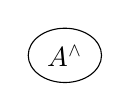
\begin{tikzpicture}[baseline=(n.base)]\node[draw,ellipse,inner sep=3pt] (n) {$A^{\wedge}$};\end{tikzpicture}}}
initial element \var{\xout{of}}{}{typewriter deletion}{ps_134-3_043-v0004} $\emptyset$ of (Cat) in the initial element $\emptyset$ of $A^{\hand{\wedge}}$ ), it follows
$e_o \hand{\cap} e_1 = \emptyset$ .

It's worth while having a look at what this \var{\deleted{\illegible{1}}}{}{deletion}{ps_134-3_043-v0005}\var{\inserted{object}}{\hand{object}}{insertion}{ps_134-3_043-v0006} just constructed is
like.  For this end,  let's note first that for any category \var{\inserted[typed]{C}}{C}{typed insertion}{ps_134-3_043-v0007}\hand{,} we have
a canonical bijection,  fonctorial in C
\[ \mathrm{Hom}(C, \hand{\Delta}_1) \hand{\xrightarrow{\sim}} \mathrm{Crib}(C) \hand{\simeq} \text{set of all subobjects of } e_{C^{\hand{\wedge}}} \ , \]
by associating to any functor $f\colon\ C \hand{\to} \hand{\Delta}_1$  the full subcategory $f^{-1}(\underline{e}_o)$ of
\margin{\diagram{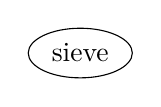
\begin{tikzpicture}[baseline=(n.base)]\node[draw,ellipse,inner sep=3pt] (n) {sieve};\end{tikzpicture}}}
C,  which clearly is a ``crible''\var{\inserted{[=sieve]}}{\hand{[=sieve]}}{insertion}{ps_134-3_043-v0008} in C.  Thus we get,  for a $\hand{\in}$ Ob A
\[ I(a) \hand{\simeq} \mathrm{Crib}(A_{/a}) \quad \hand{(}\text{subobjects of a in } A^{\hand{\wedge}}\hand{)}. \]
M\var{\over{\unsure{Q}}{o}}{\hand{o}}{writing over}{ps_134-3_043-v0009}re generally,  we deduce from this,  for any F $\hand{\in}$ Ob $A^{\hand{\wedge}}$:
\[ \mathrm{Hom}(F,I) = \hand{\Gamma}(I_F = I\mathrm{x}F \ / \ F) = \text{ set of all subobjects of } F\hand{,} \]
in other words, the object I is defined intrinsically in the topos $A^{\hand{\wedge}}$\hand{/}(up
to unique isomorphism)  as the ``\uline{Lawvere element}''  representing the functor
$F \hand{\mapsto}$ set of subobjects of F ,  generalizing the functor  $F \hand{\mapsto \mathfrak{P}}(F)$ in the
category of sets (namely sheaves over the one-point topos)\hand{,} \var{\inserted{(represented by the two-point set $\{0,1\}$.)}}{\hand{(represented by the two-point set $\{0,1\}$.)}}{insertion}{ps_134-3_043-v0010} The  condition
$e_o \hand{\cap} e_1 = \emptyset_{\hand{\mathcal{A}}}$  is automatic in any topos $\hand{\mathcal{A}}$, provided $\hand{\mathcal{A}}$ is not the ``empty
topos''  namely corresponding to a category of sheaves equivalent to a one-%
point category. \var{\deleted{Thus The condition  T 3' )  deduced from  T 3) by being
specific about the present choice of $(I,e_o,e_1)$ ,  is equivalent to T 3)
when T 1) and T 2) are satisfied,  and \xout{has the advantage} means simply that}}{}{deletion}{ps_134-3_043-v0011}

%% END SOURCE ps_134-3_043
\ifnum\EditionMode=1
\psapparatusstart
\psentry{ps_134-3_043-v0001}{1}{typed insertion}{\inserted[typed]{ly small in any case.)}}{ly small in any case.)}{The typed insertion is incorporated at its indicated position; insertion brackets leave the running text.}
\psentry{ps_134-3_043-v0002}{2}{writing over}{\over{\illegible{1}}{3}}{\hand{3}}{The superposed handwritten reading replaces the underlying reading.}
\psentry{ps_134-3_043-v0003}{3}{typewriter deletion}{\xout{x}}{}{The typewriter strikes out this material; it leaves the corrected running text.}
\psentry{ps_134-3_043-v0004}{4}{typewriter deletion}{\xout{of}}{}{The typewriter strikes out this material; it leaves the corrected running text.}
\psentry{ps_134-3_043-v0005}{5}{deletion}{\deleted{\illegible{1}}}{}{The author cancels this material by hand; it leaves the corrected running text.}
\psentry{ps_134-3_043-v0006}{6}{insertion}{\inserted{object}}{\hand{object}}{The handwritten insertion is incorporated at its indicated position; insertion brackets leave the running text.}
\psentry{ps_134-3_043-v0007}{7}{typed insertion}{\inserted[typed]{C}}{C}{The typed insertion is incorporated at its indicated position; insertion brackets leave the running text.}
\psentry{ps_134-3_043-v0008}{8}{insertion}{\inserted{[=sieve]}}{\hand{[=sieve]}}{The handwritten insertion is incorporated at its indicated position; insertion brackets leave the running text.}
\psentry{ps_134-3_043-v0009}{9}{writing over}{\over{\unsure{Q}}{o}}{\hand{o}}{The superposed handwritten reading replaces the underlying reading.}
\psentry{ps_134-3_043-v0010}{10}{insertion}{\inserted{(represented by the two-point set $\{0,1\}$.)}}{\hand{(represented by the two-point set $\{0,1\}$.)}}{The handwritten insertion is incorporated at its indicated position; insertion brackets leave the running text.}
\psentry{ps_134-3_043-v0011}{11}{deletion}{\deleted{Thus The condition  T 3' )  deduced from  T 3) by being
specific about the present choice of $(I,e_o,e_1)$ ,  is equivalent to T 3)
when T 1) and T 2) are satisfied,  and \xout{has the advantage} means simply that}}{}{The author cancels this material by hand; it leaves the corrected running text.}
\psapparatusend
\fi
\pssource{ps_134-3_044}{134-3/44}{https://grothendieck.umontpellier.fr/web/viewer.html?file=../134-3.pdf\#page=45}
\psnumber{ps_134-3_044-v0001}{1}
\psnumber{ps_134-3_044-v0002}{2}
\psnumber{ps_134-3_044-v0003}{3}
\psnumber{ps_134-3_044-v0004}{4}
\psnumber{ps_134-3_044-v0005}{5}
\psnumber{ps_134-3_044-v0006}{6}
\psnumber{ps_134-3_044-v0007}{7}
\psnumber{ps_134-3_044-v0008}{8}
\psnumber{ps_134-3_044-v0009}{9}
\psnumber{ps_134-3_044-v0010}{10}
\psnumber{ps_134-3_044-v0011}{11}
\psnumber{ps_134-3_044-v0012}{12}
\psnumber{ps_134-3_044-v0013}{13}
\psnumber{ps_134-3_044-v0014}{14}
\psnumber{ps_134-3_044-v0015}{15}
\psnumber{ps_134-3_044-v0016}{16}
\psnumber{ps_134-3_044-v0017}{17}
\psnumber{ps_134-3_044-v0018}{18}
%% BEGIN SOURCE ps_134-3_044
% Pursuing Stacks (cotes 134-2 to 134-8): archive cote 134-3, site page 44 (PDF page 45), typescript page 44.
% typescript. Draft compared: ps2.tex:2178-2237.
% AI-transcribed by Claude Opus 5.5 (claude-opus-5-5, adaptive thinking, effort high), Message Batches API, batch ps1 (msgbatch_01Rv5hCaNTtUt4JHx1yqoHPL), 2026-11-12; image review recorded in records/CHECK_DECISIONS_134_3_4.tsv.
\scanpage{134-3/44}
\mspage{44}
\var{\xout{For any topos.}}{}{typewriter deletion}{ps_134-3_044-v0001}
There is a strong temptation now to diverge from test categories,\hand{\textbackslash}to
\margin{\unsure{--}}expanding on intrinsic versions of conditions  T 1) to T 3) for any topos,
and extract a notion of a (strictly) modelizing topos,  generalizing the
``elementary \var{\xout{\unsure{topos}}}{}{typewriter deletion}{ps_134-3_044-v0002}\var{\inserted[typed]{modelizers''}}{modelizers''}{typed insertion}{ps_134-3_044-v0003} $A^{\hand{\wedge}}$ defined by strict test categories A.  But it seems
more to the point for the time being looking more closely to the one condi-%
tion,  namely T 2),  which does not appear so far as necessary for A being
a test category  -  and I suspect it is \uline{not} necessary indeed,  as no idea
occured to me how to deduce it\hand{(}\var{\inserted{34}}{\hand{34}}{insertion}{ps_134-3_044-v0004}\var{\xout{\illegible{1}}}{}{typewriter deletion}{ps_134-3_044-v0005}\hand{)}. ( I have no idea of how to make a coun-%
terexample though,  as I don't see any other way to check a category A is
a test category,  except precisely using \var{\xout{the}}{}{typewriter deletion}{ps_134-3_044-v0006}\var{\inserted[typed]{yesterday's}}{yesterday's}{typed insertion}{ps_134-3_044-v0007} criterion via T 1\hand{)}to T 3\hand{)}.\hand{)}
Still I want to emphasize about the fact that T 2) \uline{is indeed a very natural}
\uline{condition}.  In this connection,  it is timely to remember that in the cate-%
\margin{\diagram{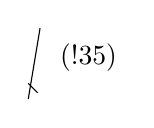
\begin{tikzpicture}[baseline=(n.base)]\draw (0,-.35)--(.15,.55);\draw (0,-.15)--(.12,-.27);\node[anchor=west] (n) at (.28,.18) {(!35)};\end{tikzpicture}}}gory (Hot),  finite direct and inverse limits exist\var{\deleted{\illegible{1}}}{}{deletion}{ps_134-3_044-v0008}(and even infinite one
I guess,  but I feel I'll have to be a little careful about these ...).
T\hand{h}e existence of such limits,  in terms of the description of (Hot) as a
category of fractions of (Cat),  does'nt seem at all a trivial fact,  for
the time being I'll admit it as \var{\xout{a}}{}{typewriter deletion}{ps_134-3_044-v0009} ``well known'' (\var{\xout{in}}{}{typewriter deletion}{ps_134-3_044-v0010}\var{\inserted[typed]{from}}{from}{typed insertion}{ps_134-3_044-v0011} the semisimplicial set-%
up,  say),  and probably come back upon this with some care later.  Now if
\var{\xout{a}}{}{typewriter deletion}{ps_134-3_044-v0012} (M,W) is any modelizer,  hence endowed with a localization functor
\[ M \hand{\longrightarrow} (\mathrm{Hot}) \ , \]
it is surely not irrelevant to ask about which limits this functor commu-%
tes with,  and study the case with care.  Thus in no \var{\inserted[typed]{practical}}{practical}{typed insertion}{ps_134-3_044-v0013} example I know of
does this functor commute with binary amalgamated sums o\var{\over{f}{r}}{\hand{r}}{writing over}{ps_134-3_044-v0014} \var{\inserted{with}}{\hand{with}}{insertion}{ps_134-3_044-v0015} fibere\var{\over{a}{d}}{\hand{d}}{writing over}{ps_134-3_044-v0016} products,
without an extra condition on at least one of the two arrows involved in
M  -  a condition of the type that one of these is a mo\var{\over{i}{n}}{\hand{n}}{writing over}{ps_134-3_044-v0017}omorphism or a
c\var{\over{\unsure{o}}{o}}{\hand{o}}{writing over}{ps_134-3_044-v0018}fibration (for co-products),  or a fibration (for products).  However,
in all cases known,  it seems that the functor commutes to (finite,  say)
sums and products.  For sums,  it really seems hard to make a sense out of
a localizing functor  M\hand{$\longrightarrow$}(Hot),  namely playing a ``model'' game,  without
the functor commuting at the very least to these !  In this respect,  it
is reassuring to notice that for any category A ,  the associated functors
$i_A$, $j_A$ between  $A^{\hand{\wedge}}$ and (Cat) do indeed both commute with (arbitrary) sums
-  which of course is trivial anyhow for $i_A$ (commuting to arbitrary direct
limits),  and easily checked for $j_A$ (who apparently does not commute to any
other type of direct limits,  but of course commutes with arbitrary inverse
limits).  Now for products too,  it is current use to look at products of
``models'' for homotopy types,  as models for the product type  -  so much so
that this fact is surely tacitly used everywhere\hand{,} without any feeling of
a need to comment.  It seems too that any categories M which one has looked
at so far for possible use as a category of ``models'' in one sense or other

%% END SOURCE ps_134-3_044
\ifnum\EditionMode=1
\psapparatusstart
\psentry{ps_134-3_044-v0001}{1}{typewriter deletion}{\xout{For any topos.}}{}{The typewriter strikes out this material; it leaves the corrected running text.}
\psentry{ps_134-3_044-v0002}{2}{typewriter deletion}{\xout{\unsure{topos}}}{}{The typewriter strikes out this material; it leaves the corrected running text.}
\psentry{ps_134-3_044-v0003}{3}{typed insertion}{\inserted[typed]{modelizers''}}{modelizers''}{The typed insertion is incorporated at its indicated position; insertion brackets leave the running text.}
\psentry{ps_134-3_044-v0004}{4}{insertion}{\inserted{34}}{\hand{34}}{The handwritten insertion is incorporated at its indicated position; insertion brackets leave the running text.}
\psentry{ps_134-3_044-v0005}{5}{typewriter deletion}{\xout{\illegible{1}}}{}{The typewriter strikes out this material; it leaves the corrected running text.}
\psentry{ps_134-3_044-v0006}{6}{typewriter deletion}{\xout{the}}{}{The typewriter strikes out this material; it leaves the corrected running text.}
\psentry{ps_134-3_044-v0007}{7}{typed insertion}{\inserted[typed]{yesterday's}}{yesterday's}{The typed insertion is incorporated at its indicated position; insertion brackets leave the running text.}
\psentry{ps_134-3_044-v0008}{8}{deletion}{\deleted{\illegible{1}}}{}{The author cancels this material by hand; it leaves the corrected running text.}
\psentry{ps_134-3_044-v0009}{9}{typewriter deletion}{\xout{a}}{}{The typewriter strikes out this material; it leaves the corrected running text.}
\psentry{ps_134-3_044-v0010}{10}{typewriter deletion}{\xout{in}}{}{The typewriter strikes out this material; it leaves the corrected running text.}
\psentry{ps_134-3_044-v0011}{11}{typed insertion}{\inserted[typed]{from}}{from}{The typed insertion is incorporated at its indicated position; insertion brackets leave the running text.}
\psentry{ps_134-3_044-v0012}{12}{typewriter deletion}{\xout{a}}{}{The typewriter strikes out this material; it leaves the corrected running text.}
\psentry{ps_134-3_044-v0013}{13}{typed insertion}{\inserted[typed]{practical}}{practical}{The typed insertion is incorporated at its indicated position; insertion brackets leave the running text.}
\psentry{ps_134-3_044-v0014}{14}{writing over}{\over{f}{r}}{\hand{r}}{The superposed handwritten reading replaces the underlying reading.}
\psentry{ps_134-3_044-v0015}{15}{insertion}{\inserted{with}}{\hand{with}}{The handwritten insertion is incorporated at its indicated position; insertion brackets leave the running text.}
\psentry{ps_134-3_044-v0016}{16}{writing over}{\over{a}{d}}{\hand{d}}{The superposed handwritten reading replaces the underlying reading.}
\psentry{ps_134-3_044-v0017}{17}{writing over}{\over{i}{n}}{\hand{n}}{The superposed handwritten reading replaces the underlying reading.}
\psentry{ps_134-3_044-v0018}{18}{writing over}{\over{\unsure{o}}{o}}{\hand{o}}{The superposed handwritten reading replaces the underlying reading.}
\psapparatusend
\fi
\pssource{ps_134-3_045}{134-3/45}{https://grothendieck.umontpellier.fr/web/viewer.html?file=../134-3.pdf\#page=46}
\psnumber{ps_134-3_045-v0001}{1}
\psnumber{ps_134-3_045-v0002}{2}
\psnumber{ps_134-3_045-v0003}{3}
\psnumber{ps_134-3_045-v0004}{4}
\psnumber{ps_134-3_045-v0005}{5}
\psnumber{ps_134-3_045-v0006}{6}
\psnumber{ps_134-3_045-v0007}{7}
\psnumber{ps_134-3_045-v0008}{8}
\psnumber{ps_134-3_045-v0009}{9}
\psnumber{ps_134-3_045-v0010}{10}
\psnumber{ps_134-3_045-v0011}{11}
\psnumber{ps_134-3_045-v0012}{12}
\psnumber{ps_134-3_045-v0013}{13}
\psnumber{ps_134-3_045-v0014}{14}
\psnumber{ps_134-3_045-v0015}{15}
\psnumber{ps_134-3_045-v0016}{16}
%% BEGIN SOURCE ps_134-3_045
% Pursuing Stacks (cotes 134-2 to 134-8): archive cote 134-3, site page 45 (PDF page 46), typescript page 45.
% typescript. Draft compared: ps2.tex:2225-2293.
% AI-transcribed by Claude Opus 5.5 (claude-opus-5-5, adaptive thinking, effort high), Message Batches API, batch ps1 (msgbatch_01Rv5hCaNTtUt4JHx1yqoHPL), 2026-11-12; image review recorded in records/CHECK_DECISIONS_134_3_4.tsv.
\scanpage{134-3/45}
\mspage{45}
for homotopy types,  for  instance set-theoretic realisations of some speci-%
fied algebraic structure species, or topological spaces,  and the like,
do admit arbitrary direct and inverse limits,  and surely \var{\xout{finite}}{}{typewriter deletion}{ps_134-3_045-v0001} sums and
products therefore,  so that the question of commutation of the localizati-%
on functor \var{\inserted{to these}}{\hand{to these}}{insertion}{ps_134-3_045-v0002} arises indeed and is felt to be important.  Possibly so impor-%
tant even,  that the notion I introduced of a ``modelizer'' should take this
into account,  and be strengthened to the effect that the canonical functor
$M\hand{\longrightarrow}$(Hot)  should commute at least to finite sums and products,  and possib-%
ly even to infinite ones (\var{\xout{this}}{}{typewriter deletion}{ps_134-3_045-v0003} \var{\inserted[typed]{whether}}{whether}{typed insertion}{ps_134-3_045-v0004} \var{\inserted{the latter}}{\hand{the latter}}{insertion}{ps_134-3_045-v0005} will have to be looked up with care).  I'll
admit \var{\inserted{provisionally}}{\hand{provisionally}}{insertion}{ps_134-3_045-v0006} that in (Hot),  finite sums and products can be described in terms of
the corresponding operations in (Cat),  namely that the canonical functor
(going with our very definition of (Hot) as a localization of (Cat))
\[ (\mathrm{Cat}) \hand{\longrightarrow} (\mathrm{Hot}) \]
commutes with finite (presumably even infinite) sums and products.\hand{(\unsure{35})} This is
indeed reasonable,  in view of the fact that the Nerve functor
\[ (\mathrm{Cat}) \hand{\longrightarrow} \hand{\Delta}^{\hand{\wedge}} = (\mathrm{Ss\ sets}) \]
does commute to sums and products.

In the case of a test category\var{\xout{,}}{}{typewriter deletion}{ps_134-3_045-v0007} A and the corresponding elementary mode-%
lizer $A^{\hand{\wedge}}$,  the corresponding localizing functor is the compositum
\[ A^{\hand{\wedge}} \overset{i_A}{\hand{\longrightarrow}} (\mathrm{Cat}) \hand{\longrightarrow} (\mathrm{Hot}) \ , \]
which therefore commutes with finite (presumably even infinite) sums automa-%
tically,  because $\hand{i}_A$ does.  Commutation with finite \uline{products} though does
not look automatic.  The \var{\xout{fact that}}{}{typewriter deletion}{ps_134-3_045-v0008} property of commutation with final
elements is OK and is nothing but condition T 1),  which we saw is necessa-%
ry for A to be a test category.  Thus remains the question of commutation
with binary products,  which boils down to the following condition,  for
any two elements  F and G in $A^{\hand{\wedge}}$:
\[ i_A(F\mathrm{x}G) \hand{\longrightarrow} i_A(F)\mathrm{x}i_A(G) \quad \text{should be a weak equivalence} \]
i.e.
\[ (*) \qquad A_{/F\mathrm{x}G} \hand{\longrightarrow} A_{/F}\ \mathrm{x}\ A_{/G} \quad \text{a weak equivalence .} \]
\var{\xout{a weak equivalence}}{}{typewriter deletion}{ps_134-3_045-v0009} This now implies condition T 2),  as we see taking
$F = a$ , $G = b$ ,  \var{\xout{and}}{}{typewriter deletion}{ps_134-3_045-v0010} in which case the condition \var{\xout{boils down to}}{}{typewriter deletion}{ps_134-3_045-v0011} \var{\inserted[typed]{(*) just means}}{(*) just means}{typed insertion}{ps_134-3_045-v0012} asphericity
of  $a\mathrm{x}b$ in $A^{\hand{\wedge}}$ namely  T 2 .  To be happy,  we have still to show that
conversely,  (T 2) implies (*)  for any F,G.  As usual,  it implies even the
stronger condition that the functor in question is aspheric,  which by the
standar\var{\over{t}{d}}{\hand{d}}{writing over}{ps_134-3_045-v0013} criterion  (page 38)  just means that the categories $A_{/a\mathrm{x}b}$
(for a,b in A, \var{\inserted{and}}{\hand{and}}{insertion}{ps_134-3_045-v0014} such \var{\inserted{moreover}}{\hand{moreover}}{insertion}{ps_134-3_045-v0015} that F(a) and G(b) non empty, \var{\inserted{but}}{\hand{but}}{insertion}{ps_134-3_045-v0016} never mind) are aspheric.

Everything turns out just perfect  -  it seems worthwhile to summarize
it in one theorem:

%% END SOURCE ps_134-3_045
\ifnum\EditionMode=1
\psapparatusstart
\psentry{ps_134-3_045-v0001}{1}{typewriter deletion}{\xout{finite}}{}{The typewriter strikes out this material; it leaves the corrected running text.}
\psentry{ps_134-3_045-v0002}{2}{insertion}{\inserted{to these}}{\hand{to these}}{The handwritten insertion is incorporated at its indicated position; insertion brackets leave the running text.}
\psentry{ps_134-3_045-v0003}{3}{typewriter deletion}{\xout{this}}{}{The typewriter strikes out this material; it leaves the corrected running text.}
\psentry{ps_134-3_045-v0004}{4}{typed insertion}{\inserted[typed]{whether}}{whether}{The typed insertion is incorporated at its indicated position; insertion brackets leave the running text.}
\psentry{ps_134-3_045-v0005}{5}{insertion}{\inserted{the latter}}{\hand{the latter}}{The handwritten insertion is incorporated at its indicated position; insertion brackets leave the running text.}
\psentry{ps_134-3_045-v0006}{6}{insertion}{\inserted{provisionally}}{\hand{provisionally}}{The handwritten insertion is incorporated at its indicated position; insertion brackets leave the running text.}
\psentry{ps_134-3_045-v0007}{7}{typewriter deletion}{\xout{,}}{}{The typewriter strikes out this material; it leaves the corrected running text.}
\psentry{ps_134-3_045-v0008}{8}{typewriter deletion}{\xout{fact that}}{}{The typewriter strikes out this material; it leaves the corrected running text.}
\psentry{ps_134-3_045-v0009}{9}{typewriter deletion}{\xout{a weak equivalence}}{}{The typewriter strikes out this material; it leaves the corrected running text.}
\psentry{ps_134-3_045-v0010}{10}{typewriter deletion}{\xout{and}}{}{The typewriter strikes out this material; it leaves the corrected running text.}
\psentry{ps_134-3_045-v0011}{11}{typewriter deletion}{\xout{boils down to}}{}{The typewriter strikes out this material; it leaves the corrected running text.}
\psentry{ps_134-3_045-v0012}{12}{typed insertion}{\inserted[typed]{(*) just means}}{(*) just means}{The typed insertion is incorporated at its indicated position; insertion brackets leave the running text.}
\psentry{ps_134-3_045-v0013}{13}{writing over}{\over{t}{d}}{\hand{d}}{The superposed handwritten reading replaces the underlying reading.}
\psentry{ps_134-3_045-v0014}{14}{insertion}{\inserted{and}}{\hand{and}}{The handwritten insertion is incorporated at its indicated position; insertion brackets leave the running text.}
\psentry{ps_134-3_045-v0015}{15}{insertion}{\inserted{moreover}}{\hand{moreover}}{The handwritten insertion is incorporated at its indicated position; insertion brackets leave the running text.}
\psentry{ps_134-3_045-v0016}{16}{insertion}{\inserted{but}}{\hand{but}}{The handwritten insertion is incorporated at its indicated position; insertion brackets leave the running text.}
\psapparatusend
\fi
\pssource{ps_134-3_046}{134-3/46}{https://grothendieck.umontpellier.fr/web/viewer.html?file=../134-3.pdf\#page=47}
\psnumber{ps_134-3_046-v0001}{1}
\psnumber{ps_134-3_046-v0002}{2}
\psnumber{ps_134-3_046-v0003}{3}
\psnumber{ps_134-3_046-v0004}{4}
\psnumber{ps_134-3_046-v0005}{5}
\psnumber{ps_134-3_046-v0006}{6}
\psnumber{ps_134-3_046-v0007}{7}
\psnumber{ps_134-3_046-v0008}{8}
\psnumber{ps_134-3_046-v0009}{9}
\psnumber{ps_134-3_046-v0010}{10}
\psnumber{ps_134-3_046-v0011}{11}
\psnumber{ps_134-3_046-v0012}{12}
\psnumber{ps_134-3_046-v0013}{13}
%% BEGIN SOURCE ps_134-3_046
% Pursuing Stacks (cotes 134-2 to 134-8): archive cote 134-3, site page 46 (PDF page 47), typescript page 46.
% typescript. Draft compared: ps2.tex:2276-2337.
% AI-transcribed by Claude Opus 5.5 (claude-opus-5-5, adaptive thinking, effort high), Message Batches API, batch ps1 (msgbatch_01Rv5hCaNTtUt4JHx1yqoHPL), 2026-11-12; image review recorded in records/CHECK_DECISIONS_134_3_4.tsv.
\scanpage{134-3/46}
\mspage{46}

\uline{Theorem}: Let A be an essentially small category, and consider the compo\var{\xout{si}}{}{typewriter deletion}{ps_134-3_046-v0001}\var{\inserted[typed]{sed}}{sed}{typed insertion}{ps_134-3_046-v0002}
\var{\xout{tion}}{}{typewriter deletion}{ps_134-3_046-v0003} functor
\[ m_A : A^{\hand{\wedge}} \overset{i_A}{\hand{\longrightarrow}} (Cat)\hand{\longrightarrow}(Hot) , \]
where $i_A(F) = A_{/F}$ for any $F \hand{\in} \mathrm{Ob}\, A^{\hand{\wedge}}$, and where (Cat)\hand{$\longrightarrow$}(Hot) is the
canonical functor from (Cat) into the localized category with respect to
weak equivalences. The following conditions are equivalent:
\margin{\unsure{9.4. Presumably}}(i) The functor $m_A$ commutes with finite products, and is a localiza-
tion functor, i.e. induces an equivalence $W_A^{-1}A^{\hand{\wedge}} \hand{\xrightarrow{\approx}}$(Hot), where
$W_A$ is the set of weak equivalences in $A^{\hand{\wedge}}$, namely arrows transfor-
med into weak equivalences by $i_A$ \hand{(*37)}. \margin{cf remark 3 p.174 -- is not strong enough}
\margin{\unsure{we'll have to add that $j_A = i_A^*$ is model preserving, cf remark 3 on p. 174}}
(ii) The functor $i_A$ and it's right adjoint $j_A$ \var{\deleted{\xout{def}}}{}{deletion}{ps_134-3_046-v0004} define functors bet-
ween $W_A^{-1}A^{\hand{\wedge}}$ and (Hot) = $W^{-1}$(Cat) (\var{\inserted{thus,}}{\hand{thus,}}{insertion}{ps_134-3_046-v0005} $j_A$ \var{\inserted{should}}{\hand{should}}{insertion}{ps_134-3_046-v0006} transform\var{\deleted{ing}}{}{deletion}{ps_134-3_046-v0007} weak equiva-
lences of (Cat) into weak equivalences of $A^{\hand{\wedge}}$) which are \uline{quasi-in-}%
\uline{verse} to each other, the adjunction morphisms for this pair being
deduced from the adjunction morphisms for the pair $i_A, j_A$ . Moreover
\var{\inserted[typed]{the functor $m_A$ commutes with finite products.}}{the functor $m_A$ commutes with finite products.}{typed insertion}{ps_134-3_046-v0008}
(iii) The category A satisfies the \var{\xout{following}}{}{typewriter deletion}{ps_134-3_046-v0009} conditions T 1 to T 3
(page 39).

I could go on with two or three more equivalent conditions, which
could be expressed intrinsically in terms of the topos $A^{\hand{\wedge}}$ and make sense
(and are equivalent) for any topos, along the lines of the reflections of
p. 43 and of yesterday\var{\xout{s}}{}{typewriter deletion}{ps_134-3_046-v0010} . But I'll still refrain for the time being\hand{!}

In the proof of the theorem above, I did not make use of semi-simpli\var{\xout{\illegible{1}}}{}{typewriter deletion}{ps_134-3_046-v0011}%
cial techniques nor of any known results about (Hot), with the only excep-%
tion of the assumption (a fact, I daresay, but not proved for the time be-%
ing in the present framework, without reference to semi-simplicial theory
say) that the canonical functor (Cat)\hand{$\longrightarrow$}(Hot) commutes with binary pro-%
ducts. We could have avoided this assumption, by slightly changing the
statement of the theorem, the condition that $m_A$ commute with finite pro\var{\deleted{\xout{du}}}{}{deletion}{ps_134-3_046-v0012}\hand{-}%
ducts \var{\inserted[typed]{in (i) and (ii)}}{in (i) and (ii)}{typed insertion}{ps_134-3_046-v0013} being replaced by the assumption that $i_A$ commute with finite products
``up to weak equivalence'', as made explicit in (*) above for the case of
binary products (which are enough of course).

I suspect that the notion of a test category in the initial, wider
sense will be of no use any longer, and therefore I will reserve this na-%

%% END SOURCE ps_134-3_046
\ifnum\EditionMode=1
\psapparatusstart
\psentry{ps_134-3_046-v0001}{1}{typewriter deletion}{\xout{si}}{}{The typewriter strikes out this material; it leaves the corrected running text.}
\psentry{ps_134-3_046-v0002}{2}{typed insertion}{\inserted[typed]{sed}}{sed}{The typed insertion is incorporated at its indicated position; insertion brackets leave the running text.}
\psentry{ps_134-3_046-v0003}{3}{typewriter deletion}{\xout{tion}}{}{The typewriter strikes out this material; it leaves the corrected running text.}
\psentry{ps_134-3_046-v0004}{4}{deletion}{\deleted{\xout{def}}}{}{The author cancels this material by hand; it leaves the corrected running text.}
\psentry{ps_134-3_046-v0005}{5}{insertion}{\inserted{thus,}}{\hand{thus,}}{The handwritten insertion is incorporated at its indicated position; insertion brackets leave the running text.}
\psentry{ps_134-3_046-v0006}{6}{insertion}{\inserted{should}}{\hand{should}}{The handwritten insertion is incorporated at its indicated position; insertion brackets leave the running text.}
\psentry{ps_134-3_046-v0007}{7}{deletion}{\deleted{ing}}{}{The author cancels this material by hand; it leaves the corrected running text.}
\psentry{ps_134-3_046-v0008}{8}{typed insertion}{\inserted[typed]{the functor $m_A$ commutes with finite products.}}{the functor $m_A$ commutes with finite products.}{The typed insertion is incorporated at its indicated position; insertion brackets leave the running text.}
\psentry{ps_134-3_046-v0009}{9}{typewriter deletion}{\xout{following}}{}{The typewriter strikes out this material; it leaves the corrected running text.}
\psentry{ps_134-3_046-v0010}{10}{typewriter deletion}{\xout{s}}{}{The typewriter strikes out this material; it leaves the corrected running text.}
\psentry{ps_134-3_046-v0011}{11}{typewriter deletion}{\xout{\illegible{1}}}{}{The typewriter strikes out this material; it leaves the corrected running text.}
\psentry{ps_134-3_046-v0012}{12}{deletion}{\deleted{\xout{du}}}{}{The author cancels this material by hand; it leaves the corrected running text.}
\psentry{ps_134-3_046-v0013}{13}{typed insertion}{\inserted[typed]{in (i) and (ii)}}{in (i) and (ii)}{The typed insertion is incorporated at its indicated position; insertion brackets leave the running text.}
\psapparatusend
\fi
\pssource{ps_134-3_047}{134-3/47}{https://grothendieck.umontpellier.fr/web/viewer.html?file=../134-3.pdf\#page=48}
\psnumber{ps_134-3_047-v0001}{1}
\psnumber{ps_134-3_047-v0002}{2}
\psnumber{ps_134-3_047-v0003}{3}
\psnumber{ps_134-3_047-v0004}{4}
\psnumber{ps_134-3_047-v0005}{5}
\psnumber{ps_134-3_047-v0006}{6}
\psnumber{ps_134-3_047-v0007}{7}
\psnumber{ps_134-3_047-v0008}{8}
\psnumber{ps_134-3_047-v0009}{9}
\psnumber{ps_134-3_047-v0010}{10}
\psnumber{ps_134-3_047-v0011}{11}
%% BEGIN SOURCE ps_134-3_047
% Pursuing Stacks (cotes 134-2 to 134-8): archive cote 134-3, site page 47 (PDF page 48), typescript page 47.
% typescript. Draft compared: ps2.tex:2327-2401.
% AI-transcribed by Claude Opus 5.5 (claude-opus-5-5, adaptive thinking, effort high), Message Batches API, batch ps1 (msgbatch_01Rv5hCaNTtUt4JHx1yqoHPL), 2026-11-12; image review recorded in records/CHECK_DECISIONS_134_3_4.tsv.
\scanpage{134-3/47}
\mspage{47}
me to the \uline{strict} case henceforth,  namely to the case of categories satis-%
fying the equivalent conditions of the theorem above\hand{(38)}. Accordingly, I'll
call \uline{``elementary modelizer''} any category \var{\inserted{$\mathcal{A}$}}{\hand{$\mathcal{A}$}}{insertion}{ps_134-3_047-v0001} equivalent to a category $A^{\hand{\wedge}}$,
with A a test category.  Such a category will be always considered as a mo-%
delizer, of course,  with the usual notion of weak equivalence W\hand{$\subset$}F\var{\over{l}{l}}{\hand{l}}{writing over}{ps_134-3_047-v0002}(\hand{$\mathcal{A}$}),
namely \var{\inserted[typed]{of}}{of}{typed insertion}{ps_134-3_047-v0003} a ``map''  F\hand{$\to$}G in \hand{$\mathcal{A}$} such that the corresponding morphism for the
induced topoi is a weak equivalence.  The \var{\xout{topos}}{}{typewriter deletion}{ps_134-3_047-v0004} category \hand{$\mathcal{A}$} is an elementa-%
ry modelizer,  therefore,  iff it satisfies the following conditions:

a) \hand{$\mathcal{A}$} is equivalent to a category $A^{\hand{\wedge}}$ with a small \hand{$A$,} which amounts to
saying that \hand{$\mathcal{A}$} is a topos,  and has sufficiently many ``essential points''
namely ``points'' such that the corresponding fiber-functor \hand{$\mathcal{A}\to$} (Ens) commu-%
tes with arbitrary products  -  i.e. there exists a conservative family
of functors  \hand{$\mathcal{A}\to$} (Ens)  which commute to arbitrary direct and inverse
limits\hand{\unsure{.}} (Cf SGA 4 IV 7.5.).

b)  The pair (\hand{$\mathcal{A}$} ,W) is modelizing (where W \hand{$\subset$} F\var{\over{l}{l}}{\hand{l}}{writing over}{ps_134-3_047-v0005}(\hand{$\mathcal{A}$}) is the set of weak
equivalences),  i.e. the category  $W^{-1}$\hand{$\mathcal{A}$}  is equivalent to (Hot).

c)  The canonical functor  \hand{$\mathcal{A}\to$}(Hot)  (or, equivalently, \hand{$\mathcal{A}\to$} $W^{-1}$\hand{$\mathcal{A}$})
commutes with finite products (or, equivalently,  with binary products -
that it commutes with final elements follows already from a),b)).

As I felt insistently since yesterday,  there is a very pretty notion
of a ``modelizing topos'' generalizing the notion of an elementary modelizer,
where \hand{$\mathcal{A}$} is a topos but not necessarily equivalent to one of the type $A^{\hand{\wedge}}$
-  but \var{\xout{admitting}}{}{typewriter deletion}{ps_134-3_047-v0006} where \var{\inserted{however}}{\hand{however}}{insertion}{ps_134-3_047-v0007} the aspheric (= ``contractible'' ) objects form a
generating family (which generalizes the condition \hand{$\mathcal{A}\simeq$}$A^{\hand{\wedge}}$\var{\unsure{\xout{x}}}{}{typewriter deletion}{ps_134-3_047-v0008} ,which means
\margin{\diagram{\begin{tikzpicture}\draw[->] (.7,0)--(.2,0) .. controls (0,0) and (0,.2) .. (0,.4)--(0,1.2);\end{tikzpicture}}}that the O-connected projective elements of \hand{$\mathcal{A}$} form a generating family).
I'll come back upon this notion later I guess -  it is not the most urgent
thing for the time being ...

\margin{\diagram{\begin{tikzpicture}\draw[->] (.8,1.2)--(.2,1.2) .. controls (0,1.2) and (0,1.1) .. (0,.9)--(0,0);\end{tikzpicture}}}34.    I will now exploit the handy criterion  T 1) to T 3) for test catego%
ries, for constructing lots of such.  In all cases I have in mind at pre-%
sent,  the verification of  T 1) and T 3) is obvious,  they are consequenc\unsure{es}
indeed of the following stronger conditions:
T 1')  A has a final element e$_{A}$\var{\deleted{\illegible{1}}}{}{deletion}{ps_134-3_047-v0009}.
T 3')  There exists an element \var{\inserted[typed]{I=}}{I=}{typed insertion}{ps_134-3_047-v0010}I$_{A}$ in A, and two sections \hand{$e_0,e_1$} of I over
e = e$_{A}$
\[ \hand{\delta_0,\delta_1} :\ e \hand{\to} I \ , \]
such that the corresponding subobjects e$_0$,e$_1$ of I satisfy \var{\xout{x}}{}{typewriter deletion}{ps_134-3_047-v0011}
\[ e_0\hand{\cap}e_1 = \emptyset_{A^{\hand{\wedge}}} \ , \]
namely that for any a \hand{$\in$}Ob A , if p$_{a}$ : a \hand{$\to$}e is the projection, we
have
\[ \hand{\delta_0 p_a \neq \delta_1 p_a} . \]

%% END SOURCE ps_134-3_047
\ifnum\EditionMode=1
\psapparatusstart
\psentry{ps_134-3_047-v0001}{1}{insertion}{\inserted{$\mathcal{A}$}}{\hand{$\mathcal{A}$}}{The handwritten insertion is incorporated at its indicated position; insertion brackets leave the running text.}
\psentry{ps_134-3_047-v0002}{2}{writing over}{\over{l}{l}}{\hand{l}}{The superposed handwritten reading replaces the underlying reading.}
\psentry{ps_134-3_047-v0003}{3}{typed insertion}{\inserted[typed]{of}}{of}{The typed insertion is incorporated at its indicated position; insertion brackets leave the running text.}
\psentry{ps_134-3_047-v0004}{4}{typewriter deletion}{\xout{topos}}{}{The typewriter strikes out this material; it leaves the corrected running text.}
\psentry{ps_134-3_047-v0005}{5}{writing over}{\over{l}{l}}{\hand{l}}{The superposed handwritten reading replaces the underlying reading.}
\psentry{ps_134-3_047-v0006}{6}{typewriter deletion}{\xout{admitting}}{}{The typewriter strikes out this material; it leaves the corrected running text.}
\psentry{ps_134-3_047-v0007}{7}{insertion}{\inserted{however}}{\hand{however}}{The handwritten insertion is incorporated at its indicated position; insertion brackets leave the running text.}
\psentry{ps_134-3_047-v0008}{8}{typewriter deletion}{\unsure{\xout{x}}}{}{All material inside this wrapper is cancelled. Its original doubt and presentation remain in the diplomatic text and apparatus; no empty doubt mark or page label is inserted into the corrected running text.}
\psentry{ps_134-3_047-v0009}{9}{deletion}{\deleted{\illegible{1}}}{}{The author cancels this material by hand; it leaves the corrected running text.}
\psentry{ps_134-3_047-v0010}{10}{typed insertion}{\inserted[typed]{I=}}{I=}{The typed insertion is incorporated at its indicated position; insertion brackets leave the running text.}
\psentry{ps_134-3_047-v0011}{11}{typewriter deletion}{\xout{x}}{}{The typewriter strikes out this material; it leaves the corrected running text.}
\psapparatusend
\fi
\pssource{ps_134-3_048}{134-3/48}{https://grothendieck.umontpellier.fr/web/viewer.html?file=../134-3.pdf\#page=49}
\psnumber{ps_134-3_048-v0001}{1}
\psnumber{ps_134-3_048-v0002}{2}
\psnumber{ps_134-3_048-v0003}{3}
\psnumber{ps_134-3_048-v0004}{4}
\psnumber{ps_134-3_048-v0005}{5}
\psnumber{ps_134-3_048-v0006}{6}
\psnumber{ps_134-3_048-v0007}{7}
\psnumber{ps_134-3_048-v0008}{8}
\psnumber{ps_134-3_048-v0009}{9}
\psnumber{ps_134-3_048-v0010}{10}
\psnumber{ps_134-3_048-v0011}{11}
\psnumber{ps_134-3_048-v0012}{12}
\psnumber{ps_134-3_048-v0013}{13}
\psnumber{ps_134-3_048-v0014}{14}
\psnumber{ps_134-3_048-v0015}{15}
\psnumber{ps_134-3_048-v0016}{16}
\psnumber{ps_134-3_048-v0017}{17}
\psnumber{ps_134-3_048-v0018}{18}
\psnumber{ps_134-3_048-v0019}{19}
\psnumber{ps_134-3_048-v0020}{20}
\psnumber{ps_134-3_048-v0021}{21}
\psnumber{ps_134-3_048-v0022}{22}
%% BEGIN SOURCE ps_134-3_048
% Pursuing Stacks (cotes 134-2 to 134-8): archive cote 134-3, site page 48 (PDF page 49), typescript page 48.
% typescript. Draft compared: ps2.tex:2385-2457.
% AI-transcribed by Claude Opus 5.5 (claude-opus-5-5, adaptive thinking, effort high), Message Batches API, batch ps1 (msgbatch_01Rv5hCaNTtUt4JHx1yqoHPL), 2026-11-12; image review recorded in records/CHECK_DECISIONS_134_3_4.tsv.
\scanpage{134-3/48}
\mspage{\hand{48}}

Of course,  the element I  (playing the role of unit interval with
endpoints $e_o$,$e_1$) is by no means unique,  for instance it can be replaced
by any cartesian power $I^n$ $(n\hand{\geqslant} 1)$,  provided it is in \var{\over{A}{$A$}}{\hand{$A$}}{writing over}{ps_134-3_048-v0001}  -  or in the case
of A = \hand{$\Delta$}  we can take for I any \hand{$\Delta$}$_n$ $(n\hand{\geqslant} 1)$ and for \hand{$\delta$}$_o$ ,\hand{$\delta$}$_1$ any two \uline{distinct}
maps from e=\hand{$\Delta$}$_o$ to \hand{$\Delta$}$_n$ , instead of the usual choice \var{\xout{for}}{}{typewriter deletion}{ps_134-3_048-v0002} \hand{$\Delta$}$_1$ for I, and
corresponding \hand{$\delta$}$_o$ and \hand{$\delta$}$_1$ .  This high degree of arbitrar\var{\over{y}{i}}{\hand{i}}{writing over}{ps_134-3_048-v0003}ness in the choice
of I should be no surprise,  this was already one striking feature in Quil-%
len's theory of model categories.

There remains the asphericity condition (T 2)  for the categories
$A_{/axb}$ ,  with  a,b \hand{$\in$} Ob A ,  which is somewhat subtler.  There is one very
evident way though to insure this, namely assuming

T 2')  If a,b are in A,  so is axb  i.e. A is stable under binary products.

In other words,  putting together  T 1' and T 2',  \var{\xout{taking any categ}}{}{typewriter deletion}{ps_134-3_048-v0004} we
may \var{\xout{restrict}}{}{typewriter deletion}{ps_134-3_048-v0005} take categories (essential small) \uline{stable under finite products}
When such a category satisfies the mild extra condition T 3') above,  it
is a test category!  This is already an impressive bunch of test categories
For instance take any category \var{\inserted[typed]{C}}{C}{typed insertion}{ps_134-3_048-v0006}\var{\inserted[typed]{with}}{with}{typed insertion}{ps_134-3_048-v0007} \var{\xout{stable under}}{}{typewriter deletion}{ps_134-3_048-v0008} finite products and \var{\xout{for which}}{}{typewriter deletion}{ps_134-3_048-v0009}
for which there exist I,$e_o$,$e_1$ as in T 3'  -  never mind whether \hand{C} is essen-%
tially small,  for instance any "non empty" topos will do (taking for I
the Lawvere element for instance,  if no simpler choice comes to \var{\over{\illegible{1}}{m}}{\hand{m}}{writing over}{ps_134-3_048-v0010}ind).
Ta\var{\over{\unsure{k}}{k}}{\hand{k}}{writing over}{ps_134-3_048-v0011}e any subcategory \var{\inserted[typed]{A}}{A}{typed insertion}{ps_134-3_048-v0012} (full or not) stable \var{\xout{by}}{}{typewriter deletion}{ps_134-3_048-v0013}\var{\inserted[typed]{under}}{under}{typed insertion}{ps_134-3_048-v0014} finite products and containing
I and \hand{$\Delta$}$_o$ ,\hand{$\Delta$}$_1$ and where the  C-products are also A-products  -  for instan\var{\xout{c}}{}{typewriter deletion}{ps_134-3_048-v0015}
ce this is OK if A is full.  \var{Then A is a test category. \margin{\diagram{\begin{tikzpicture}\draw (0,0)--(.55,0)--(.66,.42)--(1.15,.42);\end{tikzpicture}}} The simplest choi-}{Then A is a test category.

The simplest choi-}{author paragraph break}{ps_134-3_048-v0016}%
ce her\var{\over{e}{e}}{\hand{e}}{writing over}{ps_134-3_048-v0017},  the smallest in any case,  is to take the subcategory made up
with all cartesian powers $I^n$ $(n\hand{\geqslant} 0)$.  We may take the full subcategory
made up with these elements,  but instead we may take,\var{\xout{as only arrows}}{}{typewriter deletion}{ps_134-3_048-v0018} still
more economically,  only the arrows
\[ I^n \hand{\rightarrow} I^m \]
whose \var{\inserted[typed]{m}}{m}{typed insertion}{ps_134-3_048-v0019} components  $I^n \hand{\rightarrow} I$ are each,  either a projection $pr_i$ $(1\hand{\leqslant} i\hand{\leqslant} n)$ or
of the form \hand{$\delta$}$_i$\hand{$($}$p_{I^n}$\hand{$)$} $(i$\hand{$\in\{$}$0,1$\hand{$\}$}$)$.  The\var{\xout{s}}{}{typewriter deletion}{ps_134-3_048-v0020} category thus obtained,  up to unique
isomorphism,  does not depend on the choice of (C,I,$e_o$,$e_1$),  visibly -
it is,  in a sense,  \uline{the} smallest test category satisfying the stronger
conditions T 1' to T 3'.  \var{\xout{One}}{}{typewriter deletion}{ps_134-3_048-v0021} It's elements can be visualized as "standar\hand{d}
cubes"\var{\over{\unsure{.}}{\unsure{:}}}{\hand{\unsure{:}}}{writing over}{ps_134-3_048-v0022} One convenient way to do so is to take C = (Ord) (category of
all ordered sets), I = \hand{$\Delta$}$_1$ = ( \hand{$\{$}0\hand{$\}$} \hand{$\rightarrow$} \hand{$\{$}1\hand{$\}$} ) ,  $e_o$ and $e_1$ as usual,  thus
A can be interpreted as a subcategory of (Ord),  but this embedding is not
full (there are maps of $I^2$ to I in (Ord)  which are not in A,  \unsure{i.e,|i.e;} do not
"respect the cubical structure").  We may also take  C = (Spaces),  I =
unit interval \hand{$\subset$} $\underline{R}$ ,  $e_o$ and $e_1$ defined by the endpoints  O and  1 ,

%% END SOURCE ps_134-3_048
\ifnum\EditionMode=1
\psapparatusstart
\psentry{ps_134-3_048-v0001}{1}{writing over}{\over{A}{$A$}}{\hand{$A$}}{The superposed handwritten reading replaces the underlying reading.}
\psentry{ps_134-3_048-v0002}{2}{typewriter deletion}{\xout{for}}{}{The typewriter strikes out this material; it leaves the corrected running text.}
\psentry{ps_134-3_048-v0003}{3}{writing over}{\over{y}{i}}{\hand{i}}{The superposed handwritten reading replaces the underlying reading.}
\psentry{ps_134-3_048-v0004}{4}{typewriter deletion}{\xout{taking any categ}}{}{The typewriter strikes out this material; it leaves the corrected running text.}
\psentry{ps_134-3_048-v0005}{5}{typewriter deletion}{\xout{restrict}}{}{The typewriter strikes out this material; it leaves the corrected running text.}
\psentry{ps_134-3_048-v0006}{6}{typed insertion}{\inserted[typed]{C}}{C}{The typed insertion is incorporated at its indicated position; insertion brackets leave the running text.}
\psentry{ps_134-3_048-v0007}{7}{typed insertion}{\inserted[typed]{with}}{with}{The typed insertion is incorporated at its indicated position; insertion brackets leave the running text.}
\psentry{ps_134-3_048-v0008}{8}{typewriter deletion}{\xout{stable under}}{}{The typewriter strikes out this material; it leaves the corrected running text.}
\psentry{ps_134-3_048-v0009}{9}{typewriter deletion}{\xout{for which}}{}{The typewriter strikes out this material; it leaves the corrected running text.}
\psentry{ps_134-3_048-v0010}{10}{writing over}{\over{\illegible{1}}{m}}{\hand{m}}{The superposed handwritten reading replaces the underlying reading.}
\psentry{ps_134-3_048-v0011}{11}{writing over}{\over{\unsure{k}}{k}}{\hand{k}}{The superposed handwritten reading replaces the underlying reading.}
\psentry{ps_134-3_048-v0012}{12}{typed insertion}{\inserted[typed]{A}}{A}{The typed insertion is incorporated at its indicated position; insertion brackets leave the running text.}
\psentry{ps_134-3_048-v0013}{13}{typewriter deletion}{\xout{by}}{}{The typewriter strikes out this material; it leaves the corrected running text.}
\psentry{ps_134-3_048-v0014}{14}{typed insertion}{\inserted[typed]{under}}{under}{The typed insertion is incorporated at its indicated position; insertion brackets leave the running text.}
\psentry{ps_134-3_048-v0015}{15}{typewriter deletion}{\xout{c}}{}{The typewriter strikes out this material; it leaves the corrected running text.}
\psentry{ps_134-3_048-v0016}{16}{author paragraph break}{Then A is a test category. \margin{\diagram{\begin{tikzpicture}\draw (0,0)--(.55,0)--(.66,.42)--(1.15,.42);\end{tikzpicture}}} The simplest choi-}{Then A is a test category.

The simplest choi-}{The stepped hand mark at this boundary instructs a new paragraph; the diplomatic page retains its graphic and typed order.}
\psentry{ps_134-3_048-v0017}{17}{writing over}{\over{e}{e}}{\hand{e}}{The superposed handwritten reading replaces the underlying reading.}
\psentry{ps_134-3_048-v0018}{18}{typewriter deletion}{\xout{as only arrows}}{}{The typewriter strikes out this material; it leaves the corrected running text.}
\psentry{ps_134-3_048-v0019}{19}{typed insertion}{\inserted[typed]{m}}{m}{The typed insertion is incorporated at its indicated position; insertion brackets leave the running text.}
\psentry{ps_134-3_048-v0020}{20}{typewriter deletion}{\xout{s}}{}{The typewriter strikes out this material; it leaves the corrected running text.}
\psentry{ps_134-3_048-v0021}{21}{typewriter deletion}{\xout{One}}{}{The typewriter strikes out this material; it leaves the corrected running text.}
\psentry{ps_134-3_048-v0022}{22}{writing over}{\over{\unsure{.}}{\unsure{:}}}{\hand{\unsure{:}}}{The superposed handwritten reading replaces the underlying reading.}
\psapparatusend
\fi
\pssource{ps_134-3_049}{134-3/49}{https://grothendieck.umontpellier.fr/web/viewer.html?file=../134-3.pdf\#page=50}
\psnumber{ps_134-3_049-v0001}{1}
\psnumber{ps_134-3_049-v0002}{2}
\psnumber{ps_134-3_049-v0003}{3}
\psnumber{ps_134-3_049-v0004}{4}
\psnumber{ps_134-3_049-v0005}{5}
\psnumber{ps_134-3_049-v0006}{6}
\psnumber{ps_134-3_049-v0007}{7}
\psnumber{ps_134-3_049-v0008}{8}
\psnumber{ps_134-3_049-v0009}{9}
\psnumber{ps_134-3_049-v0010}{10}
\psnumber{ps_134-3_049-v0011}{11}
\psnumber{ps_134-3_049-v0012}{12}
\psnumber{ps_134-3_049-v0013}{13}
%% BEGIN SOURCE ps_134-3_049
% Pursuing Stacks (cotes 134-2 to 134-8): archive cote 134-3, site page 49 (PDF page 50), typescript page 49.
% typescript. Draft compared: ps2.tex:2445-2502.
% AI-transcribed by Claude Opus 5.5 (claude-opus-5-5, adaptive thinking, effort high), Message Batches API, batch ps1 (msgbatch_01Rv5hCaNTtUt4JHx1yqoHPL), 2026-11-12; image review recorded in records/CHECK_DECISIONS_134_3_4.tsv.
\scanpage{134-3/49}
\mspage{49}
thus the elements of A are interpreted as the standard cubes $I^n$ in the $\underline{R}^{n}$'s
the allowable maps between them $I^n \hand{\to} I^m$ are those whose components $I^n \hand{\to} I$
are either constant with value $\hand{\in}$\hand{\{}0,1\hand{\}}, or one of the projections $pr_i$ \var{\xout{(}}{}{typewriter deletion}{ps_134-3_049-v0001}
$(1 \hand{\leq} i \hand{\leq} n)$. We may denote this category of standart cubes by \hand{$\square$} , but
recall that \var{\xout{it is}}{}{typewriter deletion}{ps_134-3_049-v0002} the cubes here have symmetry operations, they give
rise to \var{\inserted[typed]{the notion of}}{the notion of}{typed insertion}{ps_134-3_049-v0003} "(fully) cubical complexes" $(\var{\inserted[typed]{K}}{K}{typed insertion}{ps_134-3_049-v0004}_{\var{\xout{\illegible{1}}}{}{typewriter deletion}{ps_134-3_049-v0005}n})_{n \hand{\geq} 0}$ , in contrast with what
might be called "semicubical complexes" without symmetry operations on the
$K_n$'s, in analogy with the case of simplicial complexes, where there are
likewise variants "full" and "semi". To make the distinction, we better
call the corresponding test category (with symmetry operations, hence
with more arrows) \hand{$\tilde{\square}$} rather than \hand{$\square$} , and accordingly for \hand{$\tilde{\Delta}$}, \hand{$\Delta$} . On clo-%
ser inspection, it seems to me that even apart the symmetry operations,
the maps between standart cubes allowed here are rather plethoric - thus
we admit diagonal maps such as $I \hand{\to} IxI$ , which is I guess highly unusual
in the cubical game. It is forced upon us though if we insist on a test
category stable under finite products, for easier checking of condition
T 2).

A less plethoric looking choice really is
\[ A = \text{ \uline{non empty} finite sets , with arbitrary maps} \]
or, equivalently, the full subcategory \var{\inserted{$\tilde{\Delta}$}}{\hand{$\tilde{\Delta}$}}{insertion}{ps_134-3_049-v0006} formed by the standart finite sets
$\underline{N}\hand{\cap}\hand{[}0,n\hand{]}$ , which we may call \hand{$\tilde{\Delta}$}$_n$ in contrast to the \var{\xout{fat}}{}{typewriter deletion}{ps_134-3_049-v0007} \hand{$\Delta$}$_n$'s (viewed as
being endowed with their natural total order, and with corresponding\var{\inserted[typed]{ly}}{ly}{typed insertion}{ps_134-3_049-v0008} more
restricted maps). This gives rise to the category \hand{$\tilde{\Delta}^{\wedge}$}\var{\xout{of}}{}{typewriter deletion}{ps_134-3_049-v0009} of "(fully) simpli%
% NOTE: the right edge of the scan cuts the end of this line after "simpli"; a hyphen, if any, is not visible
cial complexes (or sets)" . The elements of A , or of \hand{$\tilde{\Delta}$} , can be inter-%
preted in the well known way as \uline{affine} \uline{simplices}, and simplicial maps bet-%
ween these.

It is about time now to come to the categories \hand{$\Delta$} and \hand{$\square$} and check
they are test categories, although they definitely do not satisfy T 2'),
thus we are left with checking the somewhat delicate condition T 2). It
is tempting to dismiss the question by saying that it is "well known" that
the categories
\[ \hand{\Delta} / \hand{\Delta}_n x \hand{\Delta}_m \qquad (n,m \hand{\in} \underline{N} ) \]
are aspheric - but this I feel would be kind of cheating. Maybe the
very intuitive homotopy argument already used yesterday (\var{\deleted{pages 39-40}}{}{deletion}{ps_134-3_049-v0010}\var{\inserted{section 31}}{\hand{section 31}}{insertion}{ps_134-3_049-v0011})
will do. In general terms, under the assumptions T 1), T 3), we found
a sufficient criterion of asphericity for an element F of $A^{\hand{\wedge}}$, which we
may want to apply to the case F = axb , with a and b in A . \var{\deleted{The condition}}{}{deletion}{ps_134-3_049-v0012}
\var{\deleted{(which we may want to call the homotopy condition) is the following:}}{}{deletion}{ps_134-3_049-v0013}

%% END SOURCE ps_134-3_049
\ifnum\EditionMode=1
\psapparatusstart
\psentry{ps_134-3_049-v0001}{1}{typewriter deletion}{\xout{(}}{}{The typewriter strikes out this material; it leaves the corrected running text.}
\psentry{ps_134-3_049-v0002}{2}{typewriter deletion}{\xout{it is}}{}{The typewriter strikes out this material; it leaves the corrected running text.}
\psentry{ps_134-3_049-v0003}{3}{typed insertion}{\inserted[typed]{the notion of}}{the notion of}{The typed insertion is incorporated at its indicated position; insertion brackets leave the running text.}
\psentry{ps_134-3_049-v0004}{4}{typed insertion}{$\inserted[typed]{K}$}{$K$}{The typed insertion is incorporated at its indicated position; insertion brackets leave the running text.}
\psentry{ps_134-3_049-v0005}{5}{typewriter deletion}{$\xout{\illegible{1}}$}{}{The typewriter strikes out this material; it leaves the corrected running text.}
\psentry{ps_134-3_049-v0006}{6}{insertion}{\inserted{$\tilde{\Delta}$}}{\hand{$\tilde{\Delta}$}}{The handwritten insertion is incorporated at its indicated position; insertion brackets leave the running text.}
\psentry{ps_134-3_049-v0007}{7}{typewriter deletion}{\xout{fat}}{}{The typewriter strikes out this material; it leaves the corrected running text.}
\psentry{ps_134-3_049-v0008}{8}{typed insertion}{\inserted[typed]{ly}}{ly}{The typed insertion is incorporated at its indicated position; insertion brackets leave the running text.}
\psentry{ps_134-3_049-v0009}{9}{typewriter deletion}{\xout{of}}{}{The typewriter strikes out this material; it leaves the corrected running text.}
\psentry{ps_134-3_049-v0010}{10}{deletion}{\deleted{pages 39-40}}{}{The author cancels this material by hand; it leaves the corrected running text.}
\psentry{ps_134-3_049-v0011}{11}{insertion}{\inserted{section 31}}{\hand{section 31}}{The handwritten insertion is incorporated at its indicated position; insertion brackets leave the running text.}
\psentry{ps_134-3_049-v0012}{12}{deletion}{\deleted{The condition}}{}{The author cancels this material by hand; it leaves the corrected running text.}
\psentry{ps_134-3_049-v0013}{13}{deletion}{\deleted{(which we may want to call the homotopy condition) is the following:}}{}{The author cancels this material by hand; it leaves the corrected running text.}
\psapparatusend
\fi
\pssource{ps_134-3_050}{134-3/50}{https://grothendieck.umontpellier.fr/web/viewer.html?file=../134-3.pdf\#page=51}
\psnumber{ps_134-3_050-v0001}{1}
\psnumber{ps_134-3_050-v0002}{2}
\psnumber{ps_134-3_050-v0003}{3}
\psnumber{ps_134-3_050-v0004}{4}
\psnumber{ps_134-3_050-v0005}{5}
\psnumber{ps_134-3_050-v0006}{6}
\psnumber{ps_134-3_050-v0007}{7}
\psnumber{ps_134-3_050-v0008}{8}
\psnumber{ps_134-3_050-v0009}{9}
\psnumber{ps_134-3_050-v0010}{10}
\psnumber{ps_134-3_050-v0011}{11}
\psnumber{ps_134-3_050-v0012}{12}
\psnumber{ps_134-3_050-v0013}{13}
\psnumber{ps_134-3_050-v0014}{14}
\psnumber{ps_134-3_050-v0015}{15}
\psnumber{ps_134-3_050-v0016}{16}
\psnumber{ps_134-3_050-v0017}{17}
\psnumber{ps_134-3_050-v0018}{18}
\psnumber{ps_134-3_050-v0019}{19}
\psnumber{ps_134-3_050-v0020}{20}
\psnumber{ps_134-3_050-v0021}{21}
\psnumber{ps_134-3_050-v0022}{22}
\psnumber{ps_134-3_050-v0023}{23}
\psnumber{ps_134-3_050-v0024}{24}
\psnumber{ps_134-3_050-v0025}{25}
\psnumber{ps_134-3_050-v0026}{26}
\psnumber{ps_134-3_050-v0027}{27}
%% BEGIN SOURCE ps_134-3_050
% Pursuing Stacks (cotes 134-2 to 134-8): archive cote 134-3, site page 50 (PDF page 51), typescript page 50.
% typescript. Draft compared: ps2.tex:2488-2564.
% AI-transcribed by Claude Opus 5.5 (claude-opus-5-5, adaptive thinking, effort high), Message Batches API, batch ps1 (msgbatch_01Rv5hCaNTtUt4JHx1yqoHPL), 2026-11-12; image review recorded in records/CHECK_DECISIONS_134_3_4.tsv.
\scanpage{134-3/50}
\mspage{50}

Now let's say that $e_{A^{\hand{\wedge}}}$ is a \var{\xout{homotx}}{}{typewriter deletion}{ps_134-3_050-v0001} \uline{deformation retract of} F (F any ele-%
ment in $A^{\hand{\wedge}}$) if the identity map of F is homotopic (with respect to I) to
a``constant''map of F into itself.  It is purely formal,  using the diagonal
map $I\hand{\to} I\mathrm{x}I$ in $A^{\hand{\wedge}}$,  that if (more generally) $F_o$ is a deformation re\var{\xout{x}}{}{typewriter deletion}{ps_134-3_050-v0002}tract
of F,  and $G_o$ a deformation retract of G ,  then $F_o\mathrm{x}G_o$ is a deformation
retract of FxG. Thus, a \uline{sufficient} condition for T 2) to hold is the fol-%
lowing ``homotopy\var{\inserted[typed]{\hand{-}test}}{\hand{-}test}{typed insertion}{ps_134-3_050-v0003} axiom'' :

\uline{Condition} \var{\xout{H}}{}{typewriter deletion}{ps_134-3_050-v0004} T H :  For any  a in A,  \var{\xout{the}}{}{typewriter deletion}{ps_134-3_050-v0005}\var{\inserted{e=}}{\hand{e=}}{insertion}{ps_134-3_050-v0006} $e_{A^{\hand{\wedge}}}$ is a deformation retract of
a with respect to $(I,e_o,e_1)$,  namely there axists a
(1)  section  $c_a : e\hand{\to} a$  (hence a constant map $u_a = p_a c_a$\var{\inserted{$: a\to a$}}{\hand{$: a\to a$}}{insertion}{ps_134-3_050-v0007})
and a homotopy  $h_a : a\ \mathrm{x}\ I\hand{\to} a$ from $\mathrm{id}_a$  to $u_a$ ,  i.e.
a map $h_a$ such that
\[ h_a\ (\mathrm{id}_a\,\mathrm{x}\hand{\delta}_o) = \mathrm{id}_a\ ,\ h_a\ (\mathrm{id}\var{\xout{e}}{}{typewriter deletion}{ps_134-3_050-v0008}_a\,\mathrm{x}\hand{\delta}_1) = u_a\ . \]

We have to be cautious though,  it oddurs to me now,  not to make a
``vicious circle'',  as the \var{\inserted[typed]{homotopy}}{homotopy}{typed insertion}{ps_134-3_050-v0009} argument used yesterday \var{\inserted{for proving asphericity of F}}{\hand{for proving asphericity of F}}{insertion}{ps_134-3_050-v0010} makes use of the fact
that \var{\xout{\unsure{Fxe}$_I$}}{}{typewriter deletion}{ps_134-3_050-v0011}  $F\mathrm{x}I\hand{\to} F$ \var{\xout{are}}{}{typewriter deletion}{ps_134-3_050-v0012} is a weak equivalence\var{\over{,}{.}}{\hand{.}}{writing over}{ps_134-3_050-v0013} \var{\deleted{in order to deduce asphe-%
ricity of F.}}{}{deletion}{ps_134-3_050-v0014} To check that $F\mathrm{x}I\hand{\to} F$ is a weak equivalence,  and even asphe-%
ric,  we have seen though that it amounts to the same to prove $a\mathrm{x}I\hand{\to} a$ is a
weak equivalence for any a in A,  i.e. axI is aspheric for any a in A?
\var{\over{x}{(}}{\hand{(}}{writing over}{ps_134-3_050-v0015}This,  then,  was seen to be a consequance of the assumption that all ele-%
ments axb are aspheric (for a,b in A)  -  but this \var{\inserted[typed]{latter fact}}{latter fact}{typed insertion}{ps_134-3_050-v0016} is now what we want to
prove!  Thus it can't be helped,  we have to complement the condition
(T H ) above  (which I will call  (T H 1) ,  by the extra condition
\[ (2)\qquad \text{For any a in A,  axI is aspheric}\quad , \]
which,  in case I itself is in A,  appears as just a particular case of
(T 2) ,  which,\var{\inserted{now}}{\hand{now}}{insertion}{ps_134-3_050-v0017} it seems,  we have to check directly some way or other.

19.3.

35.  I really feel I should not wait any longer with the digression on
modelizing topoi that keeps creeping in\var{\inserted{to}}{\hand{to}}{insertion}{ps_134-3_050-v0018} my mind,  and which I keep trying
to dismiss as not to the point or not urgent or what not !  At least this
will fix some terminology,  and put the notion of an elemen\var{\xout{x}}{}{typewriter deletion}{ps_134-3_050-v0019}tary modelizer
into perspective,  in terms of a \var{\deleted{particular}}{}{deletion}{ps_134-3_050-v0020}\var{\inserted{wider}}{\hand{wider}}{insertion}{ps_134-3_050-v0021} class of topoi.

A topos \var{\inserted[typed]{X}}{X}{typed insertion}{ps_134-3_050-v0022} is called \uline{aspheric} if the canonical ``map'' from X to the ``final
topos'' (corresponding to a one-point space,  and \var{\xout{\illegible{1}}}{}{typewriter deletion}{ps_134-3_050-v0023}\var{\inserted[typed]{whose}}{whose}{typed insertion}{ps_134-3_050-v0024} category of sheaves
is the category (Sets)) is aspheric.  It is equivalent to say that X is
O-connected (namely non empty\var{\inserted{,}}{\hand{,}}{insertion}{ps_134-3_050-v0025} and not decomposable non trivial\var{\inserted[typed]{ly}}{ly}{typed insertion}{ps_134-3_050-v0026} into a
direct sum of two topo\"{\i}),  and that fo\var{\over{o}{r}}{\hand{r}}{writing over}{ps_134-3_050-v0027} any constant sheaf of groups G on

%% END SOURCE ps_134-3_050
\ifnum\EditionMode=1
\psapparatusstart
\psentry{ps_134-3_050-v0001}{1}{typewriter deletion}{\xout{homotx}}{}{The typewriter strikes out this material; it leaves the corrected running text.}
\psentry{ps_134-3_050-v0002}{2}{typewriter deletion}{\xout{x}}{}{The typewriter strikes out this material; it leaves the corrected running text.}
\psentry{ps_134-3_050-v0003}{3}{typed insertion}{\inserted[typed]{\hand{-}test}}{\hand{-}test}{The typed insertion is incorporated at its indicated position; insertion brackets leave the running text.}
\psentry{ps_134-3_050-v0004}{4}{typewriter deletion}{\xout{H}}{}{The typewriter strikes out this material; it leaves the corrected running text.}
\psentry{ps_134-3_050-v0005}{5}{typewriter deletion}{\xout{the}}{}{The typewriter strikes out this material; it leaves the corrected running text.}
\psentry{ps_134-3_050-v0006}{6}{insertion}{\inserted{e=}}{\hand{e=}}{The handwritten insertion is incorporated at its indicated position; insertion brackets leave the running text.}
\psentry{ps_134-3_050-v0007}{7}{insertion}{\inserted{$: a\to a$}}{\hand{$: a\to a$}}{The handwritten insertion is incorporated at its indicated position; insertion brackets leave the running text.}
\psentry{ps_134-3_050-v0008}{8}{typewriter deletion}{$\xout{e}$}{}{The typewriter strikes out this material; it leaves the corrected running text.}
\psentry{ps_134-3_050-v0009}{9}{typed insertion}{\inserted[typed]{homotopy}}{homotopy}{The typed insertion is incorporated at its indicated position; insertion brackets leave the running text.}
\psentry{ps_134-3_050-v0010}{10}{insertion}{\inserted{for proving asphericity of F}}{\hand{for proving asphericity of F}}{The handwritten insertion is incorporated at its indicated position; insertion brackets leave the running text.}
\psentry{ps_134-3_050-v0011}{11}{typewriter deletion}{\xout{\unsure{Fxe}$_I$}}{}{The typewriter strikes out this material; it leaves the corrected running text.}
\psentry{ps_134-3_050-v0012}{12}{typewriter deletion}{\xout{are}}{}{The typewriter strikes out this material; it leaves the corrected running text.}
\psentry{ps_134-3_050-v0013}{13}{writing over}{\over{,}{.}}{\hand{.}}{The superposed handwritten reading replaces the underlying reading.}
\psentry{ps_134-3_050-v0014}{14}{deletion}{\deleted{in order to deduce asphe-%
ricity of F.}}{}{The author cancels this material by hand; it leaves the corrected running text.}
\psentry{ps_134-3_050-v0015}{15}{writing over}{\over{x}{(}}{\hand{(}}{The superposed handwritten reading replaces the underlying reading.}
\psentry{ps_134-3_050-v0016}{16}{typed insertion}{\inserted[typed]{latter fact}}{latter fact}{The typed insertion is incorporated at its indicated position; insertion brackets leave the running text.}
\psentry{ps_134-3_050-v0017}{17}{insertion}{\inserted{now}}{\hand{now}}{The handwritten insertion is incorporated at its indicated position; insertion brackets leave the running text.}
\psentry{ps_134-3_050-v0018}{18}{insertion}{\inserted{to}}{\hand{to}}{The handwritten insertion is incorporated at its indicated position; insertion brackets leave the running text.}
\psentry{ps_134-3_050-v0019}{19}{typewriter deletion}{\xout{x}}{}{The typewriter strikes out this material; it leaves the corrected running text.}
\psentry{ps_134-3_050-v0020}{20}{deletion}{\deleted{particular}}{}{The author cancels this material by hand; it leaves the corrected running text.}
\psentry{ps_134-3_050-v0021}{21}{insertion}{\inserted{wider}}{\hand{wider}}{The handwritten insertion is incorporated at its indicated position; insertion brackets leave the running text.}
\psentry{ps_134-3_050-v0022}{22}{typed insertion}{\inserted[typed]{X}}{X}{The typed insertion is incorporated at its indicated position; insertion brackets leave the running text.}
\psentry{ps_134-3_050-v0023}{23}{typewriter deletion}{\xout{\illegible{1}}}{}{The typewriter strikes out this material; it leaves the corrected running text.}
\psentry{ps_134-3_050-v0024}{24}{typed insertion}{\inserted[typed]{whose}}{whose}{The typed insertion is incorporated at its indicated position; insertion brackets leave the running text.}
\psentry{ps_134-3_050-v0025}{25}{insertion}{\inserted{,}}{\hand{,}}{The handwritten insertion is incorporated at its indicated position; insertion brackets leave the running text.}
\psentry{ps_134-3_050-v0026}{26}{typed insertion}{\inserted[typed]{ly}}{ly}{The typed insertion is incorporated at its indicated position; insertion brackets leave the running text.}
\psentry{ps_134-3_050-v0027}{27}{writing over}{\over{o}{r}}{\hand{r}}{The superposed handwritten reading replaces the underlying reading.}
\psapparatusend
\fi
\pssource{ps_134-3_051}{134-3/51}{https://grothendieck.umontpellier.fr/web/viewer.html?file=../134-3.pdf\#page=52}
\psnumber{ps_134-3_051-v0001}{1}
\psnumber{ps_134-3_051-v0002}{2}
\psnumber{ps_134-3_051-v0003}{3}
\psnumber{ps_134-3_051-v0004}{4}
\psnumber{ps_134-3_051-v0005}{5}
\psnumber{ps_134-3_051-v0006}{6}
\psnumber{ps_134-3_051-v0007}{7}
\psnumber{ps_134-3_051-v0008}{8}
\psnumber{ps_134-3_051-v0009}{9}
\psnumber{ps_134-3_051-v0010}{10}
\psnumber{ps_134-3_051-v0011}{11}
\psnumber{ps_134-3_051-v0012}{12}
\psnumber{ps_134-3_051-v0013}{13}
\psnumber{ps_134-3_051-v0014}{14}
\psnumber{ps_134-3_051-v0015}{15}
\psnumber{ps_134-3_051-v0016}{16}
\psnumber{ps_134-3_051-v0017}{17}
\psnumber{ps_134-3_051-v0018}{18}
\psnumber{ps_134-3_051-v0019}{19}
\psnumber{ps_134-3_051-v0020}{20}
\psnumber{ps_134-3_051-v0021}{21}
%% BEGIN SOURCE ps_134-3_051
% Pursuing Stacks (cotes 134-2 to 134-8): archive cote 134-3, site page 51 (PDF page 52), typescript page 51.
% typescript. Draft compared: ps2.tex:2550-2624.
% AI-transcribed by Claude Opus 5.5 (claude-opus-5-5, adaptive thinking, effort high), Message Batches API, batch ps1 (msgbatch_01Rv5hCaNTtUt4JHx1yqoHPL), 2026-11-12; image review recorded in records/CHECK_DECISIONS_134_3_4.tsv.
\scanpage{134-3/51}
\mspage{51}
X, the cohomology \var{\xout{groups}}{}{typewriter deletion}{ps_134-3_051-v0001} $H^i(X,G)$ \var{\inserted[typed]{$(i\hand{\geq}1)$}}{$(i\hand{\geq}1)$}{typed insertion}{ps_134-3_051-v0002} is trivial whenever defined, namely \var{\inserted{for}}{\hand{for}}{insertion}{ps_134-3_051-v0003} any
$i\hand{\geq}1$ if G commutative, and $i=1$ if G is not supposed commut\var{\xout{t}}{}{typewriter deletion}{ps_134-3_051-v0004}ative. The
0-connexity is readily translated into a corresponding property of the fi-%
nal element in the category of sheaves $Sh(X)=\hand{\mathcal{A}}$ on X. An element \var{\xout{of}}{}{typewriter deletion}{ps_134-3_051-v0005} U of $\hand{\mathcal{A}}$
is called \uline{aspheric} if the induced topos X/U or $\hand{\mathcal{A}}_{/U}$ is aspheric. An arrow
$f\colon U'\hand{\to} U$ in $\hand{\mathcal{A}}$ is called a \uline{weak equivalence} resp. \uline{aspheric}, if the cor-%
responding ``map'' or morphism of the induced topoï
\[ X/U'\hand{\longrightarrow} X/U \quad\text{or}\quad \hand{\mathcal{A}}_{/U'}\hand{\longrightarrow}\hand{\mathcal{A}}_{/U} \]
has the corresponding property. Of course, in the notations it is often
convenient simply to identify objects \var{\inserted[typed]{U}}{U}{typed insertion}{ps_134-3_051-v0006} of $\hand{\mathcal{A}}$ with the induced topos, and
accordingly for arrows. \var{\xout{The notion o}}{}{typewriter deletion}{ps_134-3_051-v0007} Clearly if f is aspheric it is a
weak equivalence, more specifically, f is \var{\xout{a weak equivalence}}{}{typewriter deletion}{ps_134-3_051-v0008}\var{\inserted[typed]{aspheric}}{aspheric}{typed insertion}{ps_134-3_051-v0009} iff it is
``universally a weak equivalence'', namely iff for any base change $V\hand{\to}U$ in
$\hand{\mathcal{A}}$, the corresponding map $g\colon V'=V\mathrm{x}_U U'\hand{\to}V$ is a weak equivalence. M\var{\over{e}{o}}{\hand{o}}{writing over}{ps_134-3_051-v0010}re-%
over, it is sufficient to check this property when V is a member of a
given generating family of $\hand{\mathcal{A}}$.

An interesting special case is the one when $\hand{\mathcal{A}}$ admits a family of
aspheric generators, or equivalently a \var{\inserted[typed]{generating}}{generating}{typed insertion}{ps_134-3_051-v0011} full subcategory A whose objects
are aspheric in $\hand{\mathcal{A}}$ ; we will say in this case that the topos X (or $\hand{\mathcal{A}}$) is
\hand{*}\uline{locally aspheric} . This condition is satisfied for the most common topo-%
logical spaces (it suffices that each point admit a fundamental system of
contractible neighbourhoods), as well as for the topoi \var{\inserted[typed]{$A^{\hand{\wedge}}$}}{$A^{\hand{\wedge}}$}{typed insertion}{ps_134-3_051-v0012} associated to
(essentially small) categories A (for such a topos, A itself is such a
\var{\inserted[typed]{generating}}{generating}{typed insertion}{ps_134-3_051-v0013} full category made up with aspheric elements of $\hand{\mathcal{A}}$). In the\var{\xout{ir}}{}{typewriter deletion}{ps_134-3_051-v0014} case\var{\xout{s}}{}{typewriter deletion}{ps_134-3_051-v0015} of a
locally aspheric topos endowed with a generating full subcategory A as
above, a map $f\colon U'\hand{\longrightarrow} U$ is aspheric iff for any $a \hand{\in} \mathrm{Ob}\,A$ and map $a\hand{\longrightarrow} U$,
the object $U'\mathrm{x}_U a$ is aspheric (because for a map $\var{\over{f}{g}}{\hand{g}}{writing over}{ps_134-3_051-v0016}\colon V'\hand{\to} V$ with V asphe-%
ric, g is a weak equivalence iff V' is aspheric\var{\deleted{\illegible{1}}}{}{deletion}{ps_134-3_051-v0017} , which is a particular
case of the correponding statement valid for any map of topo\var{\over{\unsure{s}}{i}}{\hand{i}}{writing over}{ps_134-3_051-v0018}).

Using this criterion, we get readily the following :
\uline{Proposition \hand{1}} Let $\hand{\mathcal{A}}$ be a locally aspheric topos, A a generating full sub-%
category made up with aspheric elements. The following conditions on $\hand{\mathcal{A}}$ are \margin{* loc. modelizing (cf § 39)}
equivalent\hand{:} \var{\deleted{\illegible{1}}}{}{deletion}{ps_134-3_051-v0019}
a) Any aspheric element of $\hand{\mathcal{A}}$ is aspheric over e (the final object).
b) The product of any two aspheric elements of $\hand{\mathcal{A}}$ is again aspheric.
a'), b') as a), b) but with elements restricted to be in Ob A .

These conditions, in case $\hand{\mathcal{A}} = A^{\hand{\wedge}}\var{\deleted{\illegible{1}}}{}{deletion}{ps_134-3_051-v0020}$ are nothing but T 2) for A. \uline{It
turns out they imply already} T 1). M\var{\over{e}{o}}{\hand{o}}{writing over}{ps_134-3_051-v0021}re generally, let's call a topos

%% END SOURCE ps_134-3_051
\ifnum\EditionMode=1
\psapparatusstart
\psentry{ps_134-3_051-v0001}{1}{typewriter deletion}{\xout{groups}}{}{The typewriter strikes out this material; it leaves the corrected running text.}
\psentry{ps_134-3_051-v0002}{2}{typed insertion}{\inserted[typed]{$(i\hand{\geq}1)$}}{$(i\hand{\geq}1)$}{The typed insertion is incorporated at its indicated position; insertion brackets leave the running text.}
\psentry{ps_134-3_051-v0003}{3}{insertion}{\inserted{for}}{\hand{for}}{The handwritten insertion is incorporated at its indicated position; insertion brackets leave the running text.}
\psentry{ps_134-3_051-v0004}{4}{typewriter deletion}{\xout{t}}{}{The typewriter strikes out this material; it leaves the corrected running text.}
\psentry{ps_134-3_051-v0005}{5}{typewriter deletion}{\xout{of}}{}{The typewriter strikes out this material; it leaves the corrected running text.}
\psentry{ps_134-3_051-v0006}{6}{typed insertion}{\inserted[typed]{U}}{U}{The typed insertion is incorporated at its indicated position; insertion brackets leave the running text.}
\psentry{ps_134-3_051-v0007}{7}{typewriter deletion}{\xout{The notion o}}{}{The typewriter strikes out this material; it leaves the corrected running text.}
\psentry{ps_134-3_051-v0008}{8}{typewriter deletion}{\xout{a weak equivalence}}{}{The typewriter strikes out this material; it leaves the corrected running text.}
\psentry{ps_134-3_051-v0009}{9}{typed insertion}{\inserted[typed]{aspheric}}{aspheric}{The typed insertion is incorporated at its indicated position; insertion brackets leave the running text.}
\psentry{ps_134-3_051-v0010}{10}{writing over}{\over{e}{o}}{\hand{o}}{The superposed handwritten reading replaces the underlying reading.}
\psentry{ps_134-3_051-v0011}{11}{typed insertion}{\inserted[typed]{generating}}{generating}{The typed insertion is incorporated at its indicated position; insertion brackets leave the running text.}
\psentry{ps_134-3_051-v0012}{12}{typed insertion}{\inserted[typed]{$A^{\hand{\wedge}}$}}{$A^{\hand{\wedge}}$}{The typed insertion is incorporated at its indicated position; insertion brackets leave the running text.}
\psentry{ps_134-3_051-v0013}{13}{typed insertion}{\inserted[typed]{generating}}{generating}{The typed insertion is incorporated at its indicated position; insertion brackets leave the running text.}
\psentry{ps_134-3_051-v0014}{14}{typewriter deletion}{\xout{ir}}{}{The typewriter strikes out this material; it leaves the corrected running text.}
\psentry{ps_134-3_051-v0015}{15}{typewriter deletion}{\xout{s}}{}{The typewriter strikes out this material; it leaves the corrected running text.}
\psentry{ps_134-3_051-v0016}{16}{writing over}{$\over{f}{g}$}{$\hand{g}$}{The superposed handwritten reading replaces the underlying reading.}
\psentry{ps_134-3_051-v0017}{17}{deletion}{\deleted{\illegible{1}}}{}{The author cancels this material by hand; it leaves the corrected running text.}
\psentry{ps_134-3_051-v0018}{18}{writing over}{\over{\unsure{s}}{i}}{\hand{i}}{The superposed handwritten reading replaces the underlying reading.}
\psentry{ps_134-3_051-v0019}{19}{deletion}{\deleted{\illegible{1}}}{}{The author cancels this material by hand; it leaves the corrected running text.}
\psentry{ps_134-3_051-v0020}{20}{deletion}{$\deleted{\illegible{1}}$}{}{The author cancels this material by hand; it leaves the corrected running text.}
\psentry{ps_134-3_051-v0021}{21}{writing over}{\over{e}{o}}{\hand{o}}{The superposed handwritten reading replaces the underlying reading.}
\psapparatusend
\fi
\pssource{ps_134-3_052}{134-3/52}{https://grothendieck.umontpellier.fr/web/viewer.html?file=../134-3.pdf\#page=53}
\psnumber{ps_134-3_052-v0001}{1}
\psnumber{ps_134-3_052-v0002}{2}
\psnumber{ps_134-3_052-v0003}{3}
\psnumber{ps_134-3_052-v0004}{4}
\psnumber{ps_134-3_052-v0005}{5}
\psnumber{ps_134-3_052-v0006}{6}
\psnumber{ps_134-3_052-v0007}{7}
\psnumber{ps_134-3_052-v0008}{8}
\psnumber{ps_134-3_052-v0009}{9}
\psnumber{ps_134-3_052-v0010}{10}
\psnumber{ps_134-3_052-v0011}{11}
\psnumber{ps_134-3_052-v0012}{12}
\psnumber{ps_134-3_052-v0013}{13}
\psnumber{ps_134-3_052-v0014}{14}
\psnumber{ps_134-3_052-v0015}{15}
\psnumber{ps_134-3_052-v0016}{16}
\psnumber{ps_134-3_052-v0017}{17}
\psnumber{ps_134-3_052-v0018}{18}
\psnumber{ps_134-3_052-v0019}{19}
\psnumber{ps_134-3_052-v0020}{20}
\psnumber{ps_134-3_052-v0021}{21}
\psnumber{ps_134-3_052-v0022}{22}
\psnumber{ps_134-3_052-v0023}{23}
\psnumber{ps_134-3_052-v0024}{24}
\psnumber{ps_134-3_052-v0025}{25}
\psnumber{ps_134-3_052-v0026}{26}
\psnumber{ps_134-3_052-v0027}{27}
%% BEGIN SOURCE ps_134-3_052
% Pursuing Stacks (cotes 134-2 to 134-8): archive cote 134-3, site page 52 (PDF page 53), typescript page 52.
% typescript. Draft compared: ps2.tex:2606-2681.
% AI-transcribed by Claude Opus 5.5 (claude-opus-5-5, adaptive thinking, effort high), Message Batches API, batch ps1 (msgbatch_01Rv5hCaNTtUt4JHx1yqoHPL), 2026-11-12; image review recorded in records/CHECK_DECISIONS_134_3_4.tsv.
\scanpage{134-3/52}
\mspage{\hand{52}}
\margin{\unsure{Anal. p.\ 351, Cor.\ 1} \unsure{hay mon Rep?}}
\uline{totally} \uline{aspheric} if it \var{\xout{satisfiesxthe}}{}{typewriter deletion}{ps_134-3_052-v0001} is \var{\inserted{[``non empty'',]}}{\hand{[``non empty'',]}}{insertion}{ps_134-3_052-v0002} locally aspheric, and satisfies
moreover the equivalent conditions above. It then turns out:
\uline{Corollary}: Any totally aspheric topos is aspheric.

This follows readily from the definition of asphericity, and the
\hand{\v{}}Cech computation of cohomology of X in terms of a \var{\xout{general}}{}{typewriter deletion}{ps_134-3_052-v0003} family $(a_i)_{i\hand{\in}I}$
covering e , with the $a_i$ in A. As the mutual products and multiple
products of the $a_i$'s are all aspheric (a fortiori acyclic for any \var{\xout{\unsure{coeffi}}}{}{typewriter deletion}{ps_134-3_052-v0004}
constant coefficients), the \hand{\v{}}Cech calculation is valid (including of course
in the case of non commutative $H^1$) and yields the desired result.

The condition \var{\xout{o}}{}{typewriter deletion}{ps_134-3_052-v0005}for a topos to be totally aspheric, in contrast to
\uline{local} asphericity, is an exceedingly strong one. If for instance the
topos is defined by a topological space, which I'll denote by X, then it
is seen immediately that any \var{\inserted{two}}{\hand{two}}{insertion}{ps_134-3_052-v0006} non-empty open subsets of X have a non-empty
intersection, in other words X is an \uline{irreducible space} (i.e. \var{\inserted[typed]{not empty and}}{not empty and}{typed insertion}{ps_134-3_052-v0007} not the union
of two closed subsets distinct from X). It is well known on the other hand
that any irreducible space is aspheric, and \var{\inserted[typed]{clearly}}{clearly}{typed insertion}{ps_134-3_052-v0008} \var{\xout{that}}{}{typewriter deletion}{ps_134-3_052-v0009} any non-empty open subset
of an irreducible space is again irreducible. Therefore:

\uline{Corollary} 2: A topological\var{\xout{\unsure{l}}}{}{typewriter deletion}{ps_134-3_052-v0010} space is totally aspheric (i.e. the correspon-%
ding topos is t.a.) iff it is irreducible. In case X is Hausdorf, this
means also that X is a one-point space.

Let's now translate T 3) in the context of general topoi. We get:
\uline{Proposition} 2 Let X be a \var{\xout{totally aspheric}}{}{typewriter deletion}{ps_134-3_052-v0011} topos. Then the following two
conditions are equivalent:
a) The ``Lawvere element'' $L_X$ of $\hand{\mathcal{A}}$ = Sh(X) is aspheric \var{\xout{(or, what}}{}{typewriter deletion}{ps_134-3_052-v0012}
\var{\xout{amounts to the same, aspheric}}{}{typewriter deletion}{ps_134-3_052-v0013} over the final object\var{\xout{\illegible{1}}}{}{typewriter deletion}{ps_134-3_052-v0014} $e_X = e$.
b) There exists an object I in $\hand{\mathcal{A}}$ which is aspheric \var{\xout{(or, equivalently,}}{}{typewriter deletion}{ps_134-3_052-v0015}
\var{\xout{aspheric}}{}{typewriter deletion}{ps_134-3_052-v0016} over e \var{\deleted{)}}{}{deletion}{ps_134-3_052-v0017}, and two sections \var{\inserted{$\delta_0,\delta_1$}}{\hand{$\delta_0,\delta_1$}}{insertion}{ps_134-3_052-v0018} of I (over e), \var{\xout{defining}}{}{typewriter deletion}{ps_134-3_052-v0019}
such that Ker($\hand{\delta}_0,\hand{\delta}_1$)= $\hand{\emptyset}$ , i.e. such that $e_0\hand{\cap}e_1 = \hand{\emptyset}$ , where
$e_0,e_1$ are the subobjects of I defined by $\hand{\delta}_0,\hand{\delta}_1$ .

I recall that the Lawvere element is the one which represents the
functor
\[ F \hand{\longmapsto} \text{set of all subobjects of } F \]
on $\hand{\mathcal{A}}$, it is endowed with two sections over e , corresponding to the
two ``trivial'' subobjects $\hand{\emptyset}$ , e of e , and the kernel of this pair of
sections is clearly $\hand{\emptyset}$ , thus a) $\hand{\Longrightarrow}$ b), \var{\inserted{Conversely,}}{\hand{Conversely,}}{insertion}{ps_134-3_052-v0020} \var{\xout{which is valid for any ``non}}{}{typewriter deletion}{ps_134-3_052-v0021}
\var{\xout{empty'' topos (it needs not be totally aspheric)x}}{}{typewriter deletion}{ps_134-3_052-v0022} \var{\over{B}{b}}{\hand{b}}{writing over}{ps_134-3_052-v0023}y the homotopy argument
already used (\var{\inserted{section 31}}{\hand{section 31}}{insertion}{ps_134-3_052-v0024} \var{\deleted{p. 39-40}}{}{deletion}{ps_134-3_052-v0025}), we readily get that b) implies that \var{\deleted{the constant}}{}{deletion}{ps_134-3_052-v0026}
\var{\deleted{map from L to L, factoring into}}{}{deletion}{ps_134-3_052-v0027}

%% END SOURCE ps_134-3_052
\ifnum\EditionMode=1
\psapparatusstart
\psentry{ps_134-3_052-v0001}{1}{typewriter deletion}{\xout{satisfiesxthe}}{}{The typewriter strikes out this material; it leaves the corrected running text.}
\psentry{ps_134-3_052-v0002}{2}{insertion}{\inserted{[``non empty'',]}}{\hand{[``non empty'',]}}{The handwritten insertion is incorporated at its indicated position; insertion brackets leave the running text.}
\psentry{ps_134-3_052-v0003}{3}{typewriter deletion}{\xout{general}}{}{The typewriter strikes out this material; it leaves the corrected running text.}
\psentry{ps_134-3_052-v0004}{4}{typewriter deletion}{\xout{\unsure{coeffi}}}{}{The typewriter strikes out this material; it leaves the corrected running text.}
\psentry{ps_134-3_052-v0005}{5}{typewriter deletion}{\xout{o}}{}{The typewriter strikes out this material; it leaves the corrected running text.}
\psentry{ps_134-3_052-v0006}{6}{insertion}{\inserted{two}}{\hand{two}}{The handwritten insertion is incorporated at its indicated position; insertion brackets leave the running text.}
\psentry{ps_134-3_052-v0007}{7}{typed insertion}{\inserted[typed]{not empty and}}{not empty and}{The typed insertion is incorporated at its indicated position; insertion brackets leave the running text.}
\psentry{ps_134-3_052-v0008}{8}{typed insertion}{\inserted[typed]{clearly}}{clearly}{The typed insertion is incorporated at its indicated position; insertion brackets leave the running text.}
\psentry{ps_134-3_052-v0009}{9}{typewriter deletion}{\xout{that}}{}{The typewriter strikes out this material; it leaves the corrected running text.}
\psentry{ps_134-3_052-v0010}{10}{typewriter deletion}{\xout{\unsure{l}}}{}{The typewriter strikes out this material; it leaves the corrected running text.}
\psentry{ps_134-3_052-v0011}{11}{typewriter deletion}{\xout{totally aspheric}}{}{The typewriter strikes out this material; it leaves the corrected running text.}
\psentry{ps_134-3_052-v0012}{12}{typewriter deletion}{\xout{(or, what}}{}{The typewriter strikes out this material; it leaves the corrected running text.}
\psentry{ps_134-3_052-v0013}{13}{typewriter deletion}{\xout{amounts to the same, aspheric}}{}{The typewriter strikes out this material; it leaves the corrected running text.}
\psentry{ps_134-3_052-v0014}{14}{typewriter deletion}{\xout{\illegible{1}}}{}{The typewriter strikes out this material; it leaves the corrected running text.}
\psentry{ps_134-3_052-v0015}{15}{typewriter deletion}{\xout{(or, equivalently,}}{}{The typewriter strikes out this material; it leaves the corrected running text.}
\psentry{ps_134-3_052-v0016}{16}{typewriter deletion}{\xout{aspheric}}{}{The typewriter strikes out this material; it leaves the corrected running text.}
\psentry{ps_134-3_052-v0017}{17}{deletion}{\deleted{)}}{}{The author cancels this material by hand; it leaves the corrected running text.}
\psentry{ps_134-3_052-v0018}{18}{insertion}{\inserted{$\delta_0,\delta_1$}}{\hand{$\delta_0,\delta_1$}}{The handwritten insertion is incorporated at its indicated position; insertion brackets leave the running text.}
\psentry{ps_134-3_052-v0019}{19}{typewriter deletion}{\xout{defining}}{}{The typewriter strikes out this material; it leaves the corrected running text.}
\psentry{ps_134-3_052-v0020}{20}{insertion}{\inserted{Conversely,}}{\hand{Conversely,}}{The handwritten insertion is incorporated at its indicated position; insertion brackets leave the running text.}
\psentry{ps_134-3_052-v0021}{21}{typewriter deletion}{\xout{which is valid for any ``non}}{}{The typewriter strikes out this material; it leaves the corrected running text.}
\psentry{ps_134-3_052-v0022}{22}{typewriter deletion}{\xout{empty'' topos (it needs not be totally aspheric)x}}{}{The typewriter strikes out this material; it leaves the corrected running text.}
\psentry{ps_134-3_052-v0023}{23}{writing over}{\over{B}{b}}{\hand{b}}{The superposed handwritten reading replaces the underlying reading.}
\psentry{ps_134-3_052-v0024}{24}{insertion}{\inserted{section 31}}{\hand{section 31}}{The handwritten insertion is incorporated at its indicated position; insertion brackets leave the running text.}
\psentry{ps_134-3_052-v0025}{25}{deletion}{\deleted{p. 39-40}}{}{The author cancels this material by hand; it leaves the corrected running text.}
\psentry{ps_134-3_052-v0026}{26}{deletion}{\deleted{the constant}}{}{The author cancels this material by hand; it leaves the corrected running text.}
\psentry{ps_134-3_052-v0027}{27}{deletion}{\deleted{map from L to L, factoring into}}{}{The author cancels this material by hand; it leaves the corrected running text.}
\psapparatusend
\fi
\pssource{ps_134-3_053}{134-3/53}{https://grothendieck.umontpellier.fr/web/viewer.html?file=../134-3.pdf\#page=54}
\psnumber{ps_134-3_053-v0001}{1}
\psnumber{ps_134-3_053-v0002}{2}
\psnumber{ps_134-3_053-v0003}{3}
\psnumber{ps_134-3_053-v0004}{4}
\psnumber{ps_134-3_053-v0005}{5}
\psnumber{ps_134-3_053-v0006}{6}
\psnumber{ps_134-3_053-v0007}{7}
\psnumber{ps_134-3_053-v0008}{8}
\psnumber{ps_134-3_053-v0009}{9}
\psnumber{ps_134-3_053-v0010}{10}
\psnumber{ps_134-3_053-v0011}{11}
\psnumber{ps_134-3_053-v0012}{12}
\psnumber{ps_134-3_053-v0013}{13}
\psnumber{ps_134-3_053-v0014}{14}
\psnumber{ps_134-3_053-v0015}{15}
\psnumber{ps_134-3_053-v0016}{16}
\psnumber{ps_134-3_053-v0017}{17}
\psnumber{ps_134-3_053-v0018}{18}
\psnumber{ps_134-3_053-v0019}{19}
\psnumber{ps_134-3_053-v0020}{20}
\psnumber{ps_134-3_053-v0021}{21}
\psnumber{ps_134-3_053-v0022}{22}
\psnumber{ps_134-3_053-v0023}{23}
\psnumber{ps_134-3_053-v0024}{24}
%% BEGIN SOURCE ps_134-3_053
% Pursuing Stacks (cotes 134-2 to 134-8): archive cote 134-3, site page 53 (PDF page 54), typescript page 53.
% typescript. Draft compared: ps2.tex:2667-2745.
% AI-transcribed by Claude Opus 5.5 (claude-opus-5-5, adaptive thinking, effort high), Message Batches API, batch ps1 (msgbatch_01Rv5hCaNTtUt4JHx1yqoHPL), 2026-11-12; image review recorded in records/CHECK_DECISIONS_134_3_4.tsv.
\scanpage{134-3/53}
\mspage{53}
the projection $L \hand{\to} e$ is a weak equivalence.  As the assumption b) is stable
\var{\xout{under}}{}{typewriter deletion}{ps_134-3_053-v0001} by localisation, this shows that for any $U$ in $\hand{\mathcal{A}}$, $L_U \hand{\to} U$ is equal-%
ly a weak equivalence,  and hence $L$ is aspheric over $e$.

In proposition 2 we did not make any assumption of the topos $X$ being
locally aspheric,  let alone totally aspheric.  The  property of total
asphericity,  and the one of prop. 2 about the existence of a handy substi-%
tute for the unit interval,  seem to be independant of each other. The case
of topological spaces is instructive in this respect. Namely:

\uline{Corollay} 1 .  Assume $X$ \unsure{*is*} a topological space,  and $X$ is $0$-connected .
Then the Lawvere element  $L_X$ \hand{in} $\hand{\mathcal{A}}= Sh(X)$  is  $0$-connected,  except exactly
when $X$ is irreducible,\var{\xout{xxx}}{}{typewriter deletion}{ps_134-3_053-v0002}  in which case $L_X$ decomposes into two connected
components.

Indeed,  $L$ is disconnected iff there is a direct summand $L'$ of $L$
containing $e_o$ and $\hand{\neq} L$,  or equivalently,  if \var{\deleted{for}}{}{deletion}{ps_134-3_053-v0003}\var{\inserted{to}}{\hand{to}}{insertion}{ps_134-3_053-v0004} any open $U\hand{\subset} X$,and $U \hand{\to} L$
namely an open subset $U_o$ of $U$,  we can associate a \uline{direct} \uline{summand} $U'$\var{\inserted{$(= L'(U,U_o))$}}{\hand{$(= L'(U,U_o))$}}{insertion}{ps_134-3_053-v0005} of $U$
containing $U_o$ ,  functorially for variable  $U$,  and such that
\[ \var{\over{U}{L}}{\hand{L}}{writing over}{ps_134-3_053-v0006}'(U,\hand{\emptyset}) = \hand{\emptyset} \quad . \]
The functoriality in $U$ means that for $V$ open in $U$ and $V_o = U_o \hand{\cap} V$,  we get
\[ \hand{(*)} \qquad \var{\over{U}{L}}{\hand{L}}{writing over}{ps_134-3_053-v0007}'(V,V_o) = V \hand{\cap} \var{\over{U}{L}}{\hand{L}}{writing over}{ps_134-3_053-v0008}'(U,U_o) \quad . \]
This implies that \var{\xout{the sets}}{}{typewriter deletion}{ps_134-3_053-v0009} $\var{\over[typed]{U}{L}}{L}{typewriter overwriting}{ps_134-3_053-v0010}'(U,U_o)$  \var{\xout{a}}{}{typewriter deletion}{ps_134-3_053-v0011}\var{\over[typed]{re}{is}}{is}{typewriter overwriting}{ps_134-3_053-v0012} known when we know  $\var{\over[typed]{U}{L}}{L}{typewriter overwriting}{ps_134-3_053-v0013}'(X,U_o)$,
namely
\[ \var{\over[typed]{U}{L}}{L}{typewriter overwriting}{ps_134-3_053-v0014}'(U,U_o) = U \hand{\cap} L'(X,U_o) \, . \]
As $L'(X,U_o)$ is a direct summand of $X$ containing $U_o$ ,  and $X$ is connected,
we see that
\[ L'(X,U_o) = X \text{ if } U_o \hand{\neq} \hand{\emptyset} \quad , \quad L'(X,\hand{\emptyset})= \hand{\emptyset} \quad ; \]
and hence
\[ \hand{(**)} \qquad L'(U,U_o) = U \text{ if } U_o \hand{\neq} \hand{\emptyset} \ , \ \ L'(U,U_o) = \hand{\emptyset} \text{ if } U_o = \hand{\emptyset} \quad , \]
thus  the association  $(U,U_o) \hand{\mapsto} L'(U,U_o)$ is uniquely determined,  and it
remains to see whether th\var{\over{e}{is}}{\hand{is}}{writing over}{ps_134-3_053-v0015} association (*\hand{*}) is indeed functorial, i.e.
satisfies (*)  for any open $V \hand{\subset} U$,  with $V_o = V\hand{\cap} U_o$ .  It is OK if $V_o \hand{\neq} \hand{\emptyset}$ ,
\var{\xout{or if}}{}{typewriter deletion}{ps_134-3_053-v0016} \var{\xout{If however $V_o = \hand{\emptyset}$ and $U_o = \hand{\emptyset}$}}{}{typewriter deletion}{ps_134-3_053-v0017} or if $V_o = \hand{\emptyset}$ and $U_o = \hand{\emptyset}$ .  \var{\xout{It is however false}}{}{typewriter deletion}{ps_134-3_053-v0018}
If $V_o = \hand{\emptyset}$  and $U_o \hand{\neq} \hand{\emptyset}$ ,  \var{\xout{th}}{}{typewriter deletion}{ps_134-3_053-v0019} it is OK iff $V$ is empty\hand{;} in other words, if
both \var{\xout{sub}}{}{typewriter deletion}{ps_134-3_053-v0020} open subsets $U_o$ and $V$ of $U$ are non empty,  so must be their in-%
tersection $V_o$ .  But this means that $X$ is irreducible.

\uline{Corollary} 2.  A topological space $X$ cannot be \hand{t}o\hand{t}ally aspheric (i.e.
irreducible)  and satisfy the condition of prop. 2.

Because for a \var{\inserted{0-}}{\hand{0-}}{insertion}{ps_134-3_053-v0021}connected topos,  this \var{\inserted{latter}}{\hand{latter}}{insertion}{ps_134-3_053-v0022} condition implies that $L_X$ is
equally \var{\inserted{0-}}{\hand{0-}}{insertion}{ps_134-3_053-v0023}connected,  which contradicts corollary 1 .

Thus,  surely \var{\over{local}{total}}{\hand{total}}{writing over}{ps_134-3_053-v0024} asphericity for a topos \uline{does not} imply the

%% END SOURCE ps_134-3_053
\ifnum\EditionMode=1
\psapparatusstart
\psentry{ps_134-3_053-v0001}{1}{typewriter deletion}{\xout{under}}{}{The typewriter strikes out this material; it leaves the corrected running text.}
\psentry{ps_134-3_053-v0002}{2}{typewriter deletion}{\xout{xxx}}{}{The typewriter strikes out this material; it leaves the corrected running text.}
\psentry{ps_134-3_053-v0003}{3}{deletion}{\deleted{for}}{}{The author cancels this material by hand; it leaves the corrected running text.}
\psentry{ps_134-3_053-v0004}{4}{insertion}{\inserted{to}}{\hand{to}}{The handwritten insertion is incorporated at its indicated position; insertion brackets leave the running text.}
\psentry{ps_134-3_053-v0005}{5}{insertion}{\inserted{$(= L'(U,U_o))$}}{\hand{$(= L'(U,U_o))$}}{The handwritten insertion is incorporated at its indicated position; insertion brackets leave the running text.}
\psentry{ps_134-3_053-v0006}{6}{writing over}{$\over{U}{L}$}{$\hand{L}$}{The superposed handwritten reading replaces the underlying reading.}
\psentry{ps_134-3_053-v0007}{7}{writing over}{$\over{U}{L}$}{$\hand{L}$}{The superposed handwritten reading replaces the underlying reading.}
\psentry{ps_134-3_053-v0008}{8}{writing over}{$\over{U}{L}$}{$\hand{L}$}{The superposed handwritten reading replaces the underlying reading.}
\psentry{ps_134-3_053-v0009}{9}{typewriter deletion}{\xout{the sets}}{}{The typewriter strikes out this material; it leaves the corrected running text.}
\psentry{ps_134-3_053-v0010}{10}{typewriter overwriting}{$\over[typed]{U}{L}$}{$L$}{The superposed typed reading replaces the underlying reading.}
\psentry{ps_134-3_053-v0011}{11}{typewriter deletion}{\xout{a}}{}{The typewriter strikes out this material; it leaves the corrected running text.}
\psentry{ps_134-3_053-v0012}{12}{typewriter overwriting}{\over[typed]{re}{is}}{is}{The superposed typed reading replaces the underlying reading.}
\psentry{ps_134-3_053-v0013}{13}{typewriter overwriting}{$\over[typed]{U}{L}$}{$L$}{The superposed typed reading replaces the underlying reading.}
\psentry{ps_134-3_053-v0014}{14}{typewriter overwriting}{$\over[typed]{U}{L}$}{$L$}{The superposed typed reading replaces the underlying reading.}
\psentry{ps_134-3_053-v0015}{15}{writing over}{\over{e}{is}}{\hand{is}}{The superposed handwritten reading replaces the underlying reading.}
\psentry{ps_134-3_053-v0016}{16}{typewriter deletion}{\xout{or if}}{}{The typewriter strikes out this material; it leaves the corrected running text.}
\psentry{ps_134-3_053-v0017}{17}{typewriter deletion}{\xout{If however $V_o = \hand{\emptyset}$ and $U_o = \hand{\emptyset}$}}{}{The typewriter strikes out this material; it leaves the corrected running text.}
\psentry{ps_134-3_053-v0018}{18}{typewriter deletion}{\xout{It is however false}}{}{The typewriter strikes out this material; it leaves the corrected running text.}
\psentry{ps_134-3_053-v0019}{19}{typewriter deletion}{\xout{th}}{}{The typewriter strikes out this material; it leaves the corrected running text.}
\psentry{ps_134-3_053-v0020}{20}{typewriter deletion}{\xout{sub}}{}{The typewriter strikes out this material; it leaves the corrected running text.}
\psentry{ps_134-3_053-v0021}{21}{insertion}{\inserted{0-}}{\hand{0-}}{The handwritten insertion is incorporated at its indicated position; insertion brackets leave the running text.}
\psentry{ps_134-3_053-v0022}{22}{insertion}{\inserted{latter}}{\hand{latter}}{The handwritten insertion is incorporated at its indicated position; insertion brackets leave the running text.}
\psentry{ps_134-3_053-v0023}{23}{insertion}{\inserted{0-}}{\hand{0-}}{The handwritten insertion is incorporated at its indicated position; insertion brackets leave the running text.}
\psentry{ps_134-3_053-v0024}{24}{writing over}{\over{local}{total}}{\hand{total}}{The superposed handwritten reading replaces the underlying reading.}
\psapparatusend
\fi
\pssource{ps_134-3_054}{134-3/54}{https://grothendieck.umontpellier.fr/web/viewer.html?file=../134-3.pdf\#page=55}
\psnumber{ps_134-3_054-v0001}{1}
\psnumber{ps_134-3_054-v0002}{2}
\psnumber{ps_134-3_054-v0003}{3}
\psnumber{ps_134-3_054-v0004}{4}
\psnumber{ps_134-3_054-v0005}{5}
\psnumber{ps_134-3_054-v0006}{6}
\psnumber{ps_134-3_054-v0007}{7}
\psnumber{ps_134-3_054-v0008}{8}
\psnumber{ps_134-3_054-v0009}{9}
\psnumber{ps_134-3_054-v0010}{10}
\psnumber{ps_134-3_054-v0011}{11}
\psnumber{ps_134-3_054-v0012}{12}
\psnumber{ps_134-3_054-v0013}{13}
\psnumber{ps_134-3_054-v0014}{14}
\psnumber{ps_134-3_054-v0015}{15}
\psnumber{ps_134-3_054-v0016}{16}
\psnumber{ps_134-3_054-v0017}{17}
\psnumber{ps_134-3_054-v0018}{18}
\psnumber{ps_134-3_054-v0019}{19}
%% BEGIN SOURCE ps_134-3_054
% Pursuing Stacks (cotes 134-2 to 134-8): archive cote 134-3, site page 54 (PDF page 55), typescript page 54.
% typescript. Draft compared: ps2.tex:2730-2793.
% AI-transcribed by Claude Opus 5.5 (claude-opus-5-5, adaptive thinking, effort high), Message Batches API, batch ps1 (msgbatch_01Rv5hCaNTtUt4JHx1yqoHPL), 2026-11-12; image review recorded in records/CHECK_DECISIONS_134_3_4.tsv.
\scanpage{134-3/54}
\mspage{54}
condition of prop.2 -- the simplest counterexample is the final topos,
corresponding to one-point spaces \var{\inserted{[, or any irreducible space]}}{\hand{[, or any irreducible space]}}{insertion}{ps_134-3_054-v0001}. But I don't expect either that conditi-%
on of prop.2 , even for a locally aspheric topos\var{\xout{x}}{}{typewriter deletion}{ps_134-3_054-v0002} X, and even granting
X is aspheric moreover, implies that X is totally aspheric\hand{(39)}.The positive \margin{$^*$ cf (34)}
result in cor.1 gives a hint that the condition\var{\xout{s}}{}{typewriter deletion}{ps_134-3_054-v0003} of prop.2 may be satis-%
fie\var{\over{\unsure{s}}{d}}{\hand{d}}{writing over}{ps_134-3_054-v0004} for locally aspheric topological spaces which are\hand{``}sufficiently far
away\hand{''} from those awful non separated spaces (including the irreducible ones)
of the algebraic geometry freaks -- possibly even \var{\xout{for any}}{}{typewriter deletion}{ps_134-3_054-v0005} provided only
X is locally Hausdorf\hand{f}.

\var{\xout{The}}{}{typewriter deletion}{ps_134-3_054-v0006} Now the conjunction of the conditions of prop.1 and 2, \var{\xout{xx}}{}{typewriter deletion}{ps_134-3_054-v0007} namely
total asphericity plus \hand{\unsure{*}}existence of \var{\xout{an aspheric}}{}{typewriter deletion}{ps_134-3_054-v0008} a monomorphisme of
e\hand{$\amalg$}e into an aspheric element, \var{\over{S}{s}}{\hand{s}}{writing over}{ps_134-3_054-v0009}eems an extraordinarily strong assumption
-- so strong indeed that no topological space whatever can satisfy it\hand{!}
I feel like calling a topos satisfying these conditions a \uline{``modelizing to-}%
\uline{pos}''\hand{(39)}.For a topos of the type $A^{\hand{\wedge}}$, this just\var{\xout{x}}{}{typewriter deletion}{ps_134-3_054-v0010} means it is a\var{\over{\unsure{n}}{n}}{\hand{n}}{writing over}{ps_134-3_054-v0011} ``elementary \margin{$^*$ \unsure{strictly} (\unsure{comp.} p.39) \unsure{save few exceptions\dots}}
modelizer'' i.e. A is a test category, which are notions which, I feel, are
about to be pretty well understood. I have not such feeling yet for the
more general situation though. For instance, there is another kind of
property of a topos, which from the very start of our model story, one
would have thought of \var{\deleted{under}}{}{deletion}{ps_134-3_054-v0012}\var{\inserted{pinpointing by}}{\hand{pinpointing by}}{insertion}{ps_134-3_054-v0013} the name of a\hand{``}modelizing topos\hand{''}. Namely, when
taking $W \hand{\subset} F\var{\over{l}{l}}{\hand{l}}{writing over}{ps_134-3_054-v0014}(\hand{\mathcal{A}})$ to be the weak equivalences in the sense defined earlier,
we \var{\deleted{would like}}{}{deletion}{ps_134-3_054-v0015}\var{\inserted{demand}}{\hand{demand}}{insertion}{ps_134-3_054-v0016} that \var{\xout{xxxx}}{}{typewriter deletion}{ps_134-3_054-v0017} (\hand{$\mathcal{A}$},W) should be a modelizer in the general sense
(cf p.\hand{31}), with some exactness reinforcement (cf. p.\hand{45}), namely that
W$^{-1}$\hand{$\mathcal{A}$} should be equivalent to (Hot), and W saturated namely equal to the
set of maps made invertible by the localisation functor -- and moreover
I guess that this functor should commute with (at least finite) sums and
products. Of course, we would even expect a little more, namely that
the ``canonical functor''
\[ \hand{\mathcal{A}} \hand{\longrightarrow} (\mathrm{Hot}) \]
can be described, by associating to every F \hand{$\in$} Ob\hand{$\mathcal{A}$} the (pro-) homotopy
type associated to it by the Verdier-Artin-Mazur process. O\var{\over{\unsure{t}}{n}}{\hand{n}}{writing over}{ps_134-3_054-v0018}e feels
there is a pretty juicy bunch of intimately related properties for a topos,
all connected with the``homotopy model yoga'', and which one would like to
know about.

This calls to m\var{\over{\unsure{e}}{y}}{\hand{y}}{writing over}{ps_134-3_054-v0019} mind too the question of understanding the Verdier
-Artin-Mazur construction in the present setting, where homotopy types
are thought of in terms of categories as preferential models, rather than
semi-simplicial sets. This will be connected with the question, which

%% END SOURCE ps_134-3_054
\ifnum\EditionMode=1
\psapparatusstart
\psentry{ps_134-3_054-v0001}{1}{insertion}{\inserted{[, or any irreducible space]}}{\hand{[, or any irreducible space]}}{The handwritten insertion is incorporated at its indicated position; insertion brackets leave the running text.}
\psentry{ps_134-3_054-v0002}{2}{typewriter deletion}{\xout{x}}{}{The typewriter strikes out this material; it leaves the corrected running text.}
\psentry{ps_134-3_054-v0003}{3}{typewriter deletion}{\xout{s}}{}{The typewriter strikes out this material; it leaves the corrected running text.}
\psentry{ps_134-3_054-v0004}{4}{writing over}{\over{\unsure{s}}{d}}{\hand{d}}{The superposed handwritten reading replaces the underlying reading.}
\psentry{ps_134-3_054-v0005}{5}{typewriter deletion}{\xout{for any}}{}{The typewriter strikes out this material; it leaves the corrected running text.}
\psentry{ps_134-3_054-v0006}{6}{typewriter deletion}{\xout{The}}{}{The typewriter strikes out this material; it leaves the corrected running text.}
\psentry{ps_134-3_054-v0007}{7}{typewriter deletion}{\xout{xx}}{}{The typewriter strikes out this material; it leaves the corrected running text.}
\psentry{ps_134-3_054-v0008}{8}{typewriter deletion}{\xout{an aspheric}}{}{The typewriter strikes out this material; it leaves the corrected running text.}
\psentry{ps_134-3_054-v0009}{9}{writing over}{\over{S}{s}}{\hand{s}}{The superposed handwritten reading replaces the underlying reading.}
\psentry{ps_134-3_054-v0010}{10}{typewriter deletion}{\xout{x}}{}{The typewriter strikes out this material; it leaves the corrected running text.}
\psentry{ps_134-3_054-v0011}{11}{writing over}{\over{\unsure{n}}{n}}{\hand{n}}{The superposed handwritten reading replaces the underlying reading.}
\psentry{ps_134-3_054-v0012}{12}{deletion}{\deleted{under}}{}{The author cancels this material by hand; it leaves the corrected running text.}
\psentry{ps_134-3_054-v0013}{13}{insertion}{\inserted{pinpointing by}}{\hand{pinpointing by}}{The handwritten insertion is incorporated at its indicated position; insertion brackets leave the running text.}
\psentry{ps_134-3_054-v0014}{14}{writing over}{$\over{l}{l}$}{$\hand{l}$}{The superposed handwritten reading replaces the underlying reading.}
\psentry{ps_134-3_054-v0015}{15}{deletion}{\deleted{would like}}{}{The author cancels this material by hand; it leaves the corrected running text.}
\psentry{ps_134-3_054-v0016}{16}{insertion}{\inserted{demand}}{\hand{demand}}{The handwritten insertion is incorporated at its indicated position; insertion brackets leave the running text.}
\psentry{ps_134-3_054-v0017}{17}{typewriter deletion}{\xout{xxxx}}{}{The typewriter strikes out this material; it leaves the corrected running text.}
\psentry{ps_134-3_054-v0018}{18}{writing over}{\over{\unsure{t}}{n}}{\hand{n}}{The superposed handwritten reading replaces the underlying reading.}
\psentry{ps_134-3_054-v0019}{19}{writing over}{\over{\unsure{e}}{y}}{\hand{y}}{The superposed handwritten reading replaces the underlying reading.}
\psapparatusend
\fi
\pssource{ps_134-3_055}{134-3/55}{https://grothendieck.umontpellier.fr/web/viewer.html?file=../134-3.pdf\#page=56}
\psnumber{ps_134-3_055-v0001}{1}
\psnumber{ps_134-3_055-v0002}{2}
\psnumber{ps_134-3_055-v0003}{3}
\psnumber{ps_134-3_055-v0004}{4}
\psnumber{ps_134-3_055-v0005}{5}
\psnumber{ps_134-3_055-v0006}{6}
\psnumber{ps_134-3_055-v0007}{7}
\psnumber{ps_134-3_055-v0008}{8}
\psnumber{ps_134-3_055-v0009}{9}
\psnumber{ps_134-3_055-v0010}{10}
\psnumber{ps_134-3_055-v0011}{11}
\psnumber{ps_134-3_055-v0012}{12}
\psnumber{ps_134-3_055-v0013}{13}
\psnumber{ps_134-3_055-v0014}{14}
\psnumber{ps_134-3_055-v0015}{15}
\psnumber{ps_134-3_055-v0016}{16}
%% BEGIN SOURCE ps_134-3_055
% Pursuing Stacks (cotes 134-2 to 134-8): archive cote 134-3, site page 55 (PDF page 56), typescript page 55.
% typescript. Draft compared: ps2.tex:2778-2843.
% AI-transcribed by Claude Opus 5.5 (claude-opus-5-5, adaptive thinking, effort high), Message Batches API, batch ps1 (msgbatch_01Rv5hCaNTtUt4JHx1yqoHPL), 2026-11-12; image review recorded in records/CHECK_DECISIONS_134_3_4.tsv.
\scanpage{134-3/55}
\mspage{\hand{55}}
h\var{\over[typed]{q}{a}}{a}{typewriter overwriting}{ps_134-3_055-v0001}s been intriguing me lately,  of understanding the ``structure'' of an
arbitrary morphism of topoi
\[ X \hand{\longrightarrow} \mathrm{Top}(B) \quad , \]
where Top(B) is the topos associated to an arbitrary (essentially small)
category B  -  a situation,  it seems,  which generalizes the situation
of a ``fibered topos'' over the indexing category B,  in the sense of
SGA 4 IV.  The construction\var{\xout{s}}{}{typewriter deletion}{ps_134-3_055-v0002} of Verdier in SGA 4 V (appendix) corresponds
apparently to the case of categories B of the type $\hand{\Delta}_{/F}$  with $F \hand{\in}$ Ob$\hand{\Delta}^{\hand{\wedge}}$,
as brought near by the standart $\overset{\hand{\scriptscriptstyle\vee}}{\mathrm{C}}$ech procedure.  \var{\over{W}{W}}{\hand{W}}{writing over}{ps_134-3_055-v0003}\var{\over{n}{h}}{\hand{h}}{writing over}{ps_134-3_055-v0004}en however the topos X
is already pretty near a topos of the type Top(B),  for instance if it is
such a topos,  to describe it's homotopy type in terms of a huge \var{\inserted[typed]{inverse}}{inverse}{typed insertion}{ps_134-3_055-v0005} system
of semi-simplicial objects of B$^{\hand{\wedge}}$,  rather than just take B and keep it as
\margin{\diagram{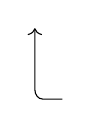
\begin{tikzpicture}[x=1cm,y=1cm]\draw[->] (0.35,0)--(0.1,0) to[out=180,in=270] (0,0.12)--(0,0.9);\end{tikzpicture}}}it is,  seems technically somewhat prohibitive,  at least in the present
set up (and with a distance of twenty years !).

\var{\over{35}{36}}{\hand{36}}{writing over}{ps_134-3_055-v0006}.  Now back to test categories,  and more specifically to her majesty
$\hand{\Delta}$ -  we still have to check it is a test category indeed !  The method \var{\inserted{suggested}}{\hand{suggested}}{insertion}{ps_134-3_055-v0007}
\margin{\diagram{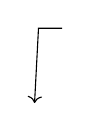
\begin{tikzpicture}[x=1cm,y=1cm]\draw[->] (0.35,0.95)--(0.05,0.95)--(0,0);\end{tikzpicture}}}last tuesday (p. 50) does work indeed,  without any reference to ``well-
known'' facts from the semi-simplicial theory.  To check  T H 1),  we take
of course $I = \hand{\Delta}_1$ and $e_o , e_1$ as usual,  we then have for every $n \hand{\in} \underline{N}$ to con-
struct a homotopy \var{\xout{\unsure{hx}}}{}{typewriter deletion}{ps_134-3_055-v0008}\var{\xout{\unsure{a}}}{}{typewriter deletion}{ps_134-3_055-v0009}
\[ h_n : \hand{\Delta}_n \, x \hand{\Delta}_1 \hand{\rightarrow} \hand{\Delta}_n \quad , \]
where the product and the arrow can be interpreted as one in (Cat) or even
in (Ord) of course  (of which $\hand{\Delta}$ is a full subcategory),  and there is a
unique such h if we take for $u_a$ the ``constant'' endomorphism of $\hand{\Delta}_n$ whose
\margin{*}value is the \uline{last} element of $\hand{\Delta}_n$ \hand{(41)}. There remains only (T H 2) - namely
\margin{ok if $\exists$ final object}to prove that the objects $\hand{\Delta}_n \, x \hand{\Delta}_1$ in $\hand{\Delta}^{\hand{\wedge}}$\var{\xout{xxx}}{}{typewriter deletion}{ps_134-3_055-v0010} are aspheric $(n \hand{\geq} 0)$.  F\var{\over{e}{o}}{\hand{o}}{writing over}{ps_134-3_055-v0011}r this
we cover \var{\inserted[typed]{$\hand{\Delta}'_n =$}}{$\hand{\Delta}'_n =$}{typed insertion}{ps_134-3_055-v0012} $\hand{\Delta}_n \, x \hand{\Delta}_1$ by maximal representable subobjects,  namely maximal flags
of the ordered product set\hand{(}  these are I guess what are called the ``shuff-
les'' in semi-simplicial algebra\hand{)}. It then turns out that $\hand{\Delta}'_n$ can be obtai-
ned by successive gluing of flags,  the intersection of each flag we add
with the sup or union of the preceding ones being just a subflag,  hence
representable and aspheric.  Thus we only have to make use of the \hand{``}Mayer-
Vietoris\hand{''} type easy lemma:
\uline{Lemma}  Let  U,V two subobjects of the final object \var{\inserted{e}}{\hand{e}}{insertion}{ps_134-3_055-v0013} of a topos \var{\inserted{[and covering e]}}{\hand{[and covering e]}}{insertion}{ps_134-3_055-v0014},  assume
U,V and U$\hand{\cap}$V aspheric,  then so is e\hand{,} i.e. so is the topos.

This finishes the proof of $\hand{\Delta}$ being a test category.  Of course,  one
cannot help thinking of the \var{\xout{acyclicity}}{}{typewriter deletion}{ps_134-3_055-v0015} \var{\inserted[typed]{apshericity}}{apshericity}{typed insertion}{ps_134-3_055-v0016} of \uline{all} the products $\hand{\Delta}_m \, x \hand{\Delta}_n$
as just meaning asphericity of the product ordered set (namely of the
corresponding category),  which follows for instance from the fact that it

%% END SOURCE ps_134-3_055
\ifnum\EditionMode=1
\psapparatusstart
\psentry{ps_134-3_055-v0001}{1}{typewriter overwriting}{\over[typed]{q}{a}}{a}{The superposed typed reading replaces the underlying reading.}
\psentry{ps_134-3_055-v0002}{2}{typewriter deletion}{\xout{s}}{}{The typewriter strikes out this material; it leaves the corrected running text.}
\psentry{ps_134-3_055-v0003}{3}{writing over}{\over{W}{W}}{\hand{W}}{The superposed handwritten reading replaces the underlying reading.}
\psentry{ps_134-3_055-v0004}{4}{writing over}{\over{n}{h}}{\hand{h}}{The superposed handwritten reading replaces the underlying reading.}
\psentry{ps_134-3_055-v0005}{5}{typed insertion}{\inserted[typed]{inverse}}{inverse}{The typed insertion is incorporated at its indicated position; insertion brackets leave the running text.}
\psentry{ps_134-3_055-v0006}{6}{writing over}{\over{35}{36}}{\hand{36}}{The superposed handwritten reading replaces the underlying reading.}
\psentry{ps_134-3_055-v0007}{7}{insertion}{\inserted{suggested}}{\hand{suggested}}{The handwritten insertion is incorporated at its indicated position; insertion brackets leave the running text.}
\psentry{ps_134-3_055-v0008}{8}{typewriter deletion}{\xout{\unsure{hx}}}{}{The typewriter strikes out this material; it leaves the corrected running text.}
\psentry{ps_134-3_055-v0009}{9}{typewriter deletion}{\xout{\unsure{a}}}{}{The typewriter strikes out this material; it leaves the corrected running text.}
\psentry{ps_134-3_055-v0010}{10}{typewriter deletion}{\xout{xxx}}{}{The typewriter strikes out this material; it leaves the corrected running text.}
\psentry{ps_134-3_055-v0011}{11}{writing over}{\over{e}{o}}{\hand{o}}{The superposed handwritten reading replaces the underlying reading.}
\psentry{ps_134-3_055-v0012}{12}{typed insertion}{\inserted[typed]{$\hand{\Delta}'_n =$}}{$\hand{\Delta}'_n =$}{The typed insertion is incorporated at its indicated position; insertion brackets leave the running text.}
\psentry{ps_134-3_055-v0013}{13}{insertion}{\inserted{e}}{\hand{e}}{The handwritten insertion is incorporated at its indicated position; insertion brackets leave the running text.}
\psentry{ps_134-3_055-v0014}{14}{insertion}{\inserted{[and covering e]}}{\hand{[and covering e]}}{The handwritten insertion is incorporated at its indicated position; insertion brackets leave the running text.}
\psentry{ps_134-3_055-v0015}{15}{typewriter deletion}{\xout{acyclicity}}{}{The typewriter strikes out this material; it leaves the corrected running text.}
\psentry{ps_134-3_055-v0016}{16}{typed insertion}{\inserted[typed]{apshericity}}{apshericity}{The typed insertion is incorporated at its indicated position; insertion brackets leave the running text.}
\psapparatusend
\fi
\pssource{ps_134-3_056}{134-3/56}{https://grothendieck.umontpellier.fr/web/viewer.html?file=../134-3.pdf\#page=57}
\psnumber{ps_134-3_056-v0001}{1}
\psnumber{ps_134-3_056-v0002}{2}
\psnumber{ps_134-3_056-v0003}{3}
\psnumber{ps_134-3_056-v0004}{4}
\psnumber{ps_134-3_056-v0005}{5}
\psnumber{ps_134-3_056-v0006}{6}
\psnumber{ps_134-3_056-v0007}{7}
\psnumber{ps_134-3_056-v0008}{8}
\psnumber{ps_134-3_056-v0009}{9}
\psnumber{ps_134-3_056-v0010}{10}
%% BEGIN SOURCE ps_134-3_056
% Pursuing Stacks (cotes 134-2 to 134-8): archive cote 134-3, site page 56 (PDF page 57), typescript page 56.
% typescript. Draft compared: ps2.tex:2830-2896.
% AI-transcribed by Claude Opus 5.5 (claude-opus-5-5, adaptive thinking, effort high), Message Batches API, batch ps1 (msgbatch_01Rv5hCaNTtUt4JHx1yqoHPL), 2026-11-12; image review recorded in records/CHECK_DECISIONS_134_3_4.tsv.
\scanpage{134-3/56}
\mspage{56}
has a final element.  But we should beware the vicious circle, as we
implicitly make the assumption that for an object C of (Cat)  (at least
an object C such as $\hand{\ensuremath{\Delta}}_{m}\mathrm{x}\hand{\ensuremath{\Delta}}_{n}$), if C is aspheric,  then so is the correspon-%
ding  \var{\xout{(C)x}}{}{typewriter deletion}{ps_134-3_056-v0001} element \hand{\ensuremath{\alpha}}(C) in $A^{\hand{\wedge}}$:
\[ \hand{\ensuremath{\alpha}}(C) : \var{\over{A}{\Delta}}{\hand{\Delta}}{writing over}{ps_134-3_056-v0002}_{n} \hand{\ensuremath{\longmapsto}} \mathrm{Hom}(\hand{\ensuremath{\Delta}}_{n},C) \quad , \]
namely the \uline{nerve} of C.  We expect of course something stronger to hold,
namely that for any C, \hand{\ensuremath{\alpha}}(C) has the same homotopy type as C  -  in fact
that we have a canonical isomorphism between the images of both in (Hot).
This relationship has still to be established,  as well as the similar
statement for \hand{\ensuremath{\beta}} : (Cat)\hand{\ensuremath{\to}}\var{\over{\unsure{\hand{\ensuremath{\widetilde{\Delta}}}}}{\ensuremath{\square}}}{\hand{\ensuremath{\square}}}{writing over}{ps_134-3_056-v0003}$^{\hand{\wedge}}$ , and accordingly with \hand{\ensuremath{\widetilde{\Delta}}} and \hand{\ensuremath{\widetilde{\square}}} .  For all
four categories (\var{\inserted{where}}{\hand{where}}{insertion}{ps_134-3_056-v0004} the simplicial cases are known to be test categories al-%
ready),  we have,  together with the category A (the would-be test category\hand{),}
a functor
\[ A \hand{\ensuremath{\longrightarrow}} (\mathrm{Cat}) \quad , \qquad \text{say} \quad a \hand{\ensuremath{\mapsto}} \hand{\ensuremath{\Delta}}_{a} \]
(notation inspired by the case A =\hand{\ensuremath{\Delta}}),  hence a functor
\[ (\mathrm{Cat}) \hand{\ensuremath{\xrightarrow{\ \alpha\ }}} A^{\hand{\wedge}} \quad , \quad \hand{\ensuremath{\alpha}}(C) = (a \hand{\ensuremath{\mapsto}} \mathrm{Hom}_{\mathrm{Cat}}(\hand{\ensuremath{\Delta}}_{a},C)) \quad , \]
and the question is to compare the homotopy types of C and \hand{\ensuremath{\alpha}}(C),  the lat-%
ter being defined of course as the homotopy type of $\var{\over[typed]{\unsure{A}}{A}}{A}{typewriter overwriting}{ps_134-3_056-v0005}_{/\hand{\ensuremath{\alpha}}(C)} \hand{\ensuremath{\simeq}} A_{/C}$ ,
the category of all pairs  (a,p) with a \hand{\ensuremath{\in}}Ob A and p: $\hand{\ensuremath{\Delta}}_{a}\hand{\ensuremath{\to}}$ C ,  arrows bet-%
ween pairs corresponding to \uline{strictly} commutative diagrams  in Cat
% Hand-drawn arrows are marked blue; typed objects remain plain.
\diagram{\begin{tikzcd}[row sep=small,column sep=small]
a' \ar[rr,color=blue,"\hand{\ensuremath{\Delta_u}}"] \ar[dr,color=blue,swap,"p'"] \& \& a \ar[dl,color=blue,"p"] \\
\& C \&
\end{tikzcd}}
.

\uline{Proposition}.  Let the data be as just said,  assume moreover that the cate-%
gories $\hand{\ensuremath{\Delta}}_{a}$ (a \hand{\ensuremath{\in}} Ob A) have final elements, \var{\inserted{that A is aspheric}}{\hand{that A is aspheric}}{insertion}{ps_134-3_056-v0006} and that \hand{\ensuremath{\alpha}}($\hand{\ensuremath{\Delta}}_{1}$) is aspheric
over the final element of $A^{\hand{\wedge}}$  (\var{\deleted{\unsure{which is}}}{}{deletion}{ps_134-3_056-v0007}\var{\inserted{the latter}}{\hand{the latter}}{insertion}{ps_134-3_056-v0008} automatic if A is a test category,
A\hand{\ensuremath{\longrightarrow}}(Cat) is fully faithful and $\hand{\ensuremath{\Delta}}_{1}$ belongs to it's essential image). Then
we can find for every C in (Cat) a \var{\xout{functor}}{}{typewriter deletion}{ps_134-3_056-v0009} "map" in (Cat) (i.e. a functor)
\margin{(*)} \[ \hand{\ensuremath{\varphi}} : A_{/C} \hand{\ensuremath{\to}} C \ , \]
functorial in C for variable C,  and this map being \var{\xout{a weak equivalencexxx}}{}{typewriter deletion}{ps_134-3_056-v0010}
aspheric,  and a fortiori a weak equivalence (hence induces an isomorphism
between the homotopy types).

This implies that the compositum  C\hand{\ensuremath{\mapsto}}$A_{/C}$  :
\[ (\mathrm{Cat}) \hand{\ensuremath{\xrightarrow{\ \alpha\ }}} A^{\hand{\wedge}} \hand{\ensuremath{\xrightarrow{\ \textcolor{black}{i}_{A}\ }}} (\mathrm{Cat}) \]
transforms weak equivalences into weak equivalences,  and that the functor
deduced from it by passage to the localized categories  $W^{-1}$(Cat) = (Hot)
is isomorphic to the identity functor of (Hot).

%% END SOURCE ps_134-3_056
\ifnum\EditionMode=1
\psapparatusstart
\psentry{ps_134-3_056-v0001}{1}{typewriter deletion}{\xout{(C)x}}{}{The typewriter strikes out this material; it leaves the corrected running text.}
\psentry{ps_134-3_056-v0002}{2}{writing over}{$\over{A}{\Delta}$}{$\hand{\Delta}$}{The superposed handwritten reading replaces the underlying reading.}
\psentry{ps_134-3_056-v0003}{3}{writing over}{\over{\unsure{\hand{\ensuremath{\widetilde{\Delta}}}}}{\ensuremath{\square}}}{\hand{\ensuremath{\square}}}{The superposed handwritten reading replaces the underlying reading.}
\psentry{ps_134-3_056-v0004}{4}{insertion}{\inserted{where}}{\hand{where}}{The handwritten insertion is incorporated at its indicated position; insertion brackets leave the running text.}
\psentry{ps_134-3_056-v0005}{5}{typewriter overwriting}{$\over[typed]{\unsure{A}}{A}$}{$A$}{The superposed typed reading replaces the underlying reading.}
\psentry{ps_134-3_056-v0006}{6}{insertion}{\inserted{that A is aspheric}}{\hand{that A is aspheric}}{The handwritten insertion is incorporated at its indicated position; insertion brackets leave the running text.}
\psentry{ps_134-3_056-v0007}{7}{deletion}{\deleted{\unsure{which is}}}{}{The author cancels this material by hand; it leaves the corrected running text.}
\psentry{ps_134-3_056-v0008}{8}{insertion}{\inserted{the latter}}{\hand{the latter}}{The handwritten insertion is incorporated at its indicated position; insertion brackets leave the running text.}
\psentry{ps_134-3_056-v0009}{9}{typewriter deletion}{\xout{functor}}{}{The typewriter strikes out this material; it leaves the corrected running text.}
\psentry{ps_134-3_056-v0010}{10}{typewriter deletion}{\xout{a weak equivalencexxx}}{}{The typewriter strikes out this material; it leaves the corrected running text.}
\psapparatusend
\fi
\pssource{ps_134-3_057}{134-3/57}{https://grothendieck.umontpellier.fr/web/viewer.html?file=../134-3.pdf\#page=58}
\psnumber{ps_134-3_057-v0001}{1}
\psnumber{ps_134-3_057-v0002}{2}
\psnumber{ps_134-3_057-v0003}{3}
\psnumber{ps_134-3_057-v0004}{4}
\psnumber{ps_134-3_057-v0005}{5}
\psnumber{ps_134-3_057-v0006}{6}
\psnumber{ps_134-3_057-v0007}{7}
\psnumber{ps_134-3_057-v0008}{8}
%% BEGIN SOURCE ps_134-3_057
% Pursuing Stacks (cotes 134-2 to 134-8): archive cote 134-3, site page 57 (PDF page 58), typescript page 57.
% typescript. Draft compared: ps2.tex:2879-2946.
% AI-transcribed by Claude Opus 5.5 (claude-opus-5-5, adaptive thinking, effort high), Message Batches API, batch ps1 (msgbatch_01Rv5hCaNTtUt4JHx1yqoHPL), 2026-11-12; image review recorded in records/CHECK_DECISIONS_134_3_4.tsv.
\scanpage{134-3/57}
\mspage{57}

To define a functor (*) , functorial in C for variable C, we only
have to choose a final element $e_a$ in each $\hand{\Delta}_a$ . For an element (a,p) of
$A_{/C}$ , we define
\[ \hand{\phi}(a,p) = p(e_a) \quad , \]
with evident extension to arrows of $A_{/C}$\hand{\unsure{,}}(NB here it is important that the
$e_a$ be \uline{final} elements of the $\hand{\Delta}_a$ , initial elements for a change would'nt
do at all !), thus we get the functor $\hand{\phi}$ , and functoriality with respect to
C is clear. Using the standart criterion of asphericity of a functor $\hand{\phi}$ ,
we have to check that the categories
\[ (A_{/C})_{/x} \]
for $x \hand{\in}$ Ob C are aspheric, but one checks at once that the category above
is canonically isomorphic to $A_{/C'}$ , where $C' = C_{/x}$ . Thus asphericity
of $\hand{\phi}$ for arbitrary C is equivalent to asphericity of $A_{/C}$ when C has a
final element, or equivalently, to asphericity of the element $\hand{\alpha}(C)$ \var{\over{o}{i}}{\hand{i}}{writing over}{ps_134-3_057-v0001}\var{\over{n}{n}}{\hand{n}}{writing over}{ps_134-3_057-v0002} $\hand{A}^{\hand{\wedge}}$
for such C. Now let $e_C$ be the final element of C, and consider the \var{\xout{stan}}{}{typewriter deletion}{ps_134-3_057-v0003}
unique homotopy
\[ h : \hand{\Delta}_1 x C \hand{\to} C \]
between $id_C$ and the constant functor from C to C with value $e_C$ . Applying
the functor $\hand{\alpha}$ we get a corresponding homotopy in $A^{\hand{\wedge}}$
\[ \var{\over{I}{I}}{\hand{I}}{writing over}{ps_134-3_057-v0004}\,\underset{\illegible{1}}{\var{\over{x}{x}}{\hand{x}}{writing over}{ps_134-3_057-v0005}}\,\hand{\alpha}(C) \hand{\to} \hand{\alpha}(C) \quad , \text{ where } I = \hand{\alpha}(\hand{\Delta}_1) \ , \]
between the identity map of $F = \hand{\alpha}(C)$ and a ``constant'' map $F \hand{\to} F$ . As we
assume that I is aspherical over the final element of $A^{\hand{\wedge}}$, hence $IxF \hand{\to} F$
is a weak equivalence, it follows that $F \hand{\to} e$ is a weak equivalence, hen-%
ce F is aspheric as e is supposed to be aspheric, which was to be proved.

If we apply this proposition to $A=\hand{\Delta}$ and $n \hand{\to} \hand{\Delta}_n$ , we are still
reduced to check just T H 2) (which we did above looking at shuffles),
whereas T H 1) appears superfluous now - we get asphericity of the
elements $\hand{\Delta}_m x \hand{\Delta}_n$ in $A^{\hand{\wedge}}$ as a consequence (but the homotopy argument used in \var{\inserted{the}}{\hand{the}}{insertion}{ps_134-3_057-v0006}
prop. is essentially the same as the one used for proving T H 1 ). This
proposition applies equally to the case when $A = \hand{\widetilde{\Delta}}$ (category of non ordered
simplices $\hand{\widetilde{\Delta}}_n$ ), here the natural functor
\[ \hand{i} : \hand{\widetilde{\Delta} \longrightarrow} \text{(Cat)} \quad , \hand{a \mapsto \mathfrak{P}^*}(a) \]
is obtained by associating to any finite set a the combinatorial simplex
it defines, embodied by the ordered set $\hand{\mathfrak{P}^*}(a)$ of it's facettes of all di-%
mensions, which can be identified \hand{with} the ordered set of all non-empty sub-%
sets of the finite set a. As we know already $\hand{\widetilde{\Delta}}$ is a test category, all
that remains to be done is to check in this case that $I = \hand{\alpha}(\hand{\Delta}_1)$ is asphe-%
ric (hence aspheric over the final object of $A^{\hand{\wedge}}$), Now this follows \var{\xout{from}}{}{typewriter deletion}{ps_134-3_057-v0007}
\var{\xout{the fact}}{}{typewriter deletion}{ps_134-3_057-v0008} again from a homotopy argument involving the unit segment substi-%

%% END SOURCE ps_134-3_057
\ifnum\EditionMode=1
\psapparatusstart
\psentry{ps_134-3_057-v0001}{1}{writing over}{\over{o}{i}}{\hand{i}}{The superposed handwritten reading replaces the underlying reading.}
\psentry{ps_134-3_057-v0002}{2}{writing over}{\over{n}{n}}{\hand{n}}{The superposed handwritten reading replaces the underlying reading.}
\psentry{ps_134-3_057-v0003}{3}{typewriter deletion}{\xout{stan}}{}{The typewriter strikes out this material; it leaves the corrected running text.}
\psentry{ps_134-3_057-v0004}{4}{writing over}{$\over{I}{I}$}{$\hand{I}$}{The superposed handwritten reading replaces the underlying reading.}
\psentry{ps_134-3_057-v0005}{5}{writing over}{$\over{x}{x}$}{$\hand{x}$}{The superposed handwritten reading replaces the underlying reading.}
\psentry{ps_134-3_057-v0006}{6}{insertion}{\inserted{the}}{\hand{the}}{The handwritten insertion is incorporated at its indicated position; insertion brackets leave the running text.}
\psentry{ps_134-3_057-v0007}{7}{typewriter deletion}{\xout{from}}{}{The typewriter strikes out this material; it leaves the corrected running text.}
\psentry{ps_134-3_057-v0008}{8}{typewriter deletion}{\xout{the fact}}{}{The typewriter strikes out this material; it leaves the corrected running text.}
\psapparatusend
\fi
\pssource{ps_134-3_058}{134-3/58}{https://grothendieck.umontpellier.fr/web/viewer.html?file=../134-3.pdf\#page=59}
\psnumber{ps_134-3_058-v0001}{1}
\psnumber{ps_134-3_058-v0002}{2}
\psnumber{ps_134-3_058-v0003}{3}
\psnumber{ps_134-3_058-v0004}{4}
\psnumber{ps_134-3_058-v0005}{5}
\psnumber{ps_134-3_058-v0006}{6}
\psnumber{ps_134-3_058-v0007}{7}
\psnumber{ps_134-3_058-v0008}{8}
\psnumber{ps_134-3_058-v0009}{9}
\psnumber{ps_134-3_058-v0010}{10}
\psnumber{ps_134-3_058-v0011}{11}
\psnumber{ps_134-3_058-v0012}{12}
\psnumber{ps_134-3_058-v0013}{13}
\psnumber{ps_134-3_058-v0014}{14}
\psnumber{ps_134-3_058-v0015}{15}
\psnumber{ps_134-3_058-v0016}{16}
\psnumber{ps_134-3_058-v0017}{17}
\psnumber{ps_134-3_058-v0018}{18}
\psnumber{ps_134-3_058-v0019}{19}
\psnumber{ps_134-3_058-v0020}{20}
\psnumber{ps_134-3_058-v0021}{21}
\psnumber{ps_134-3_058-v0022}{22}
\psnumber{ps_134-3_058-v0023}{23}
\psnumber{ps_134-3_058-v0024}{24}
\psnumber{ps_134-3_058-v0025}{25}
\psnumber{ps_134-3_058-v0026}{26}
\psnumber{ps_134-3_058-v0027}{27}
\psnumber{ps_134-3_058-v0028}{28}
%% BEGIN SOURCE ps_134-3_058
% Pursuing Stacks (cotes 134-2 to 134-8): archive cote 134-3, site page 58 (PDF page 59), typescript page 58.
% typescript. Draft compared: ps2.tex:2932-3005.
% AI-transcribed by Claude Opus 5.5 (claude-opus-5-5, adaptive thinking, effort high), Message Batches API, batch ps1 (msgbatch_01Rv5hCaNTtUt4JHx1yqoHPL), 2026-11-12; image review recorded in records/CHECK_DECISIONS_134_3_4.tsv.
\scanpage{134-3/58}
\mspage{58}

\margin{*} tute in $A^{\hand{\wedge}}$. We could formalize it as follows:\hand{..} \hand{(42).}

\margin{\unsure{cor. inst ci-dessous}} \var{\deleted{\uline{Corollary:} In the proposition above, the condition that $\hand{\alpha}(\hand{\Delta}_1)$ be aspheric}}{}{deletion}{ps_134-3_058-v0001}
\var{\deleted{over $e_{A^{\hand{\wedge}}}$ is a consequence of the following assumptions:}}{}{deletion}{ps_134-3_058-v0002}
\var{\deleted{a) The condition T 3 is valid in A , with the stronger assumption \xout{th}}}{}{deletion}{ps_134-3_058-v0003}
\var{\deleted{that I is aspheric over the final object e of $A^{\hand{\wedge}}$, and moreover :}}{}{deletion}{ps_134-3_058-v0004}
\var{\deleted{b) for every $a \hand{\in} \mathrm{Ob}\, A$ and $u : a \hand{\longrightarrow} I$, let $a_u = u^{-1}(e_o)$ (subobject}}{}{deletion}{ps_134-3_058-v0005}
\var{\deleted{of a in $A^{\hand{\wedge}}$), $\hand{\Delta}_{a_u} = \underset{b \text{ in } A_{/a_u}}{\underset{\hand{\longrightarrow}}{\mathrm{lim}}} \hand{\Delta}_b$ , and $\hand{\Delta}_{a,u} = \mathrm{Im}\,(\hand{\Delta}_{a_u} \hand{\to} \hand{\Delta}_a)$.}}{}{deletion}{ps_134-3_058-v0006}

\var{\deleted{We assume that Ob $\hand{\Delta}_{a,u}$ is a \uline{crible} in $\hand{\Delta}_a$ , say $C_u$ .}}{}{deletion}{ps_134-3_058-v0007}

\var{\deleted{Indeed, interpreting $\hand{\alpha}(\hand{\Delta}_1)$ as the functor $a \hand{\mapsto} \mathrm{Crib}\, \hand{\Delta}_a$ , we}}{}{deletion}{ps_134-3_058-v0008}
\var{\deleted{define a homotopy}}{}{deletion}{ps_134-3_058-v0009}
\var{\deleted{\[ h : I\mathrm{x}F\deleted{\unsure{(\hand{\alpha}(\hand{\Delta}_1))}} \hand{\to} F \deleted{\unsure{\hand{\alpha}(\hand{\Delta}_1)}} \quad \text{(where } F = \hand{\alpha}(\hand{\Delta}_1)\text{ )} \]}}{}{deletion}{ps_134-3_058-v0010}
\var{\deleted{from the identity $\mathrm{id}_F$ to the constant map $c : F \hand{\to} F$ associating to every}}{}{deletion}{ps_134-3_058-v0011}
\var{\deleted{crible in some $\hand{\Delta}_a$ the empty crible in the same, by taking for every a}}{}{deletion}{ps_134-3_058-v0012}
\var{\deleted{in A the map}}{}{deletion}{ps_134-3_058-v0013}
\var{\deleted{\[ (u, C_o) \hand{\longmapsto} C_u \hand{\cap} C_o \quad . \]}}{}{deletion}{ps_134-3_058-v0014}
\var{\deleted{It follows that $F \hand{\longmapsto} e$ is a weak equivalence, and the same argument in}}{}{deletion}{ps_134-3_058-v0015}
\var{\deleted{any induced category $A_{/a}$ shows that this is universally so i.e. $F \hand{\to} e$ is}}{}{deletion}{ps_134-3_058-v0016}
\var{\deleted{aspheric , O.K.}}{}{deletion}{ps_134-3_058-v0017}

\var{\deleted{In the case \inserted[typed]{above} $A = \hand{\tilde{\Delta}}$, we get indeed that for $u : a \hand{\to} I$, $a_u$ is \inserted{empty or} in A}}{}{deletion}{ps_134-3_058-v0018}
\var{\deleted{and $\hand{\Delta}_{a_u} \hand{\to} \hand{\Delta}_a$ is a full embedding, turning $\hand{\Delta}_{a_u}$ into a crible in $\hand{\Delta}_a$ ,}}{}{deletion}{ps_134-3_058-v0019}
\var{\deleted{thus \xout{a) and} b) is satisfied (with the usual choice $I = \hand{\tilde{\Delta}}_1$ of course).}}{}{deletion}{ps_134-3_058-v0020}

21.3.

37. By the end of the notes two days ago, there was the pretty strong
impression of repeating the same argument all over again, in very similar
situations. When I tried to pin down this feeling, first thing that oc-%
cured to me was that the \var{\inserted{homotopy}}{\hand{homotopy}}{insertion}{ps_134-3_058-v0021} equivalence I was after $A_{/C} \hand{\longrightarrow} C$ (in the propo-%
sition of \var{\over{p}{\S}}{\hand{\S}}{writing over}{ps_134-3_058-v0022}.\var{\over{5}{3}}{\hand{3}}{writing over}{ps_134-3_058-v0023}6), when concerned with a\var{\xout{n}}{}{typewriter deletion}{ps_134-3_058-v0024} general functor $A \hand{\longrightarrow} (\mathrm{Cat})$,
and the criterion obtained, was applicable to the situation I was concer-%
ned with at the very start when defining test categories, namely when
looking at the \uline{canonical} functor $A \hand{\longrightarrow} (\mathrm{Cat})$ given by $a \hand{\longmapsto} A_{/a}$ ; and \var{\inserted{that this}}{\hand{that this}}{insertion}{ps_134-3_058-v0025} gave
a criterion in this case for A to be a test-category in the wider sense,
which I had overlooked when peeling out the caracterisation of test cate-%
gories (cf. theorem of p. 46). Finally it bec\var{\over{o}{a}}{\hand{a}}{writing over}{ps_134-3_058-v0026}mes clear that it \var{\over{was}{is}}{\hand{is}}{writing over}{ps_134-3_058-v0027} about
% NOTE: the right edge of the next line is cut; the typed word ends "repet" at the edge
time to recast from scratch the asphericity story, and (by one more repet%
tition) tell it anew in a way stripped from it's repetitive features\var{\over{.}{!}}{\hand{!}}{writing over}{ps_134-3_058-v0028}

%% END SOURCE ps_134-3_058
\ifnum\EditionMode=1
\psapparatusstart
\psentry{ps_134-3_058-v0001}{1}{deletion}{\deleted{\uline{Corollary:} In the proposition above, the condition that $\hand{\alpha}(\hand{\Delta}_1)$ be aspheric}}{}{The author cancels this material by hand; it leaves the corrected running text.}
\psentry{ps_134-3_058-v0002}{2}{deletion}{\deleted{over $e_{A^{\hand{\wedge}}}$ is a consequence of the following assumptions:}}{}{The author cancels this material by hand; it leaves the corrected running text.}
\psentry{ps_134-3_058-v0003}{3}{deletion}{\deleted{a) The condition T 3 is valid in A , with the stronger assumption \xout{th}}}{}{The author cancels this material by hand; it leaves the corrected running text.}
\psentry{ps_134-3_058-v0004}{4}{deletion}{\deleted{that I is aspheric over the final object e of $A^{\hand{\wedge}}$, and moreover :}}{}{The author cancels this material by hand; it leaves the corrected running text.}
\psentry{ps_134-3_058-v0005}{5}{deletion}{\deleted{b) for every $a \hand{\in} \mathrm{Ob}\, A$ and $u : a \hand{\longrightarrow} I$, let $a_u = u^{-1}(e_o)$ (subobject}}{}{The author cancels this material by hand; it leaves the corrected running text.}
\psentry{ps_134-3_058-v0006}{6}{deletion}{\deleted{of a in $A^{\hand{\wedge}}$), $\hand{\Delta}_{a_u} = \underset{b \text{ in } A_{/a_u}}{\underset{\hand{\longrightarrow}}{\mathrm{lim}}} \hand{\Delta}_b$ , and $\hand{\Delta}_{a,u} = \mathrm{Im}\,(\hand{\Delta}_{a_u} \hand{\to} \hand{\Delta}_a)$.}}{}{The author cancels this material by hand; it leaves the corrected running text.}
\psentry{ps_134-3_058-v0007}{7}{deletion}{\deleted{We assume that Ob $\hand{\Delta}_{a,u}$ is a \uline{crible} in $\hand{\Delta}_a$ , say $C_u$ .}}{}{The author cancels this material by hand; it leaves the corrected running text.}
\psentry{ps_134-3_058-v0008}{8}{deletion}{\deleted{Indeed, interpreting $\hand{\alpha}(\hand{\Delta}_1)$ as the functor $a \hand{\mapsto} \mathrm{Crib}\, \hand{\Delta}_a$ , we}}{}{The author cancels this material by hand; it leaves the corrected running text.}
\psentry{ps_134-3_058-v0009}{9}{deletion}{\deleted{define a homotopy}}{}{The author cancels this material by hand; it leaves the corrected running text.}
\psentry{ps_134-3_058-v0010}{10}{deletion}{\deleted{\[ h : I\mathrm{x}F\deleted{\unsure{(\hand{\alpha}(\hand{\Delta}_1))}} \hand{\to} F \deleted{\unsure{\hand{\alpha}(\hand{\Delta}_1)}} \quad \text{(where } F = \hand{\alpha}(\hand{\Delta}_1)\text{ )} \]}}{}{The author cancels this material by hand; it leaves the corrected running text.}
\psentry{ps_134-3_058-v0011}{11}{deletion}{\deleted{from the identity $\mathrm{id}_F$ to the constant map $c : F \hand{\to} F$ associating to every}}{}{The author cancels this material by hand; it leaves the corrected running text.}
\psentry{ps_134-3_058-v0012}{12}{deletion}{\deleted{crible in some $\hand{\Delta}_a$ the empty crible in the same, by taking for every a}}{}{The author cancels this material by hand; it leaves the corrected running text.}
\psentry{ps_134-3_058-v0013}{13}{deletion}{\deleted{in A the map}}{}{The author cancels this material by hand; it leaves the corrected running text.}
\psentry{ps_134-3_058-v0014}{14}{deletion}{\deleted{\[ (u, C_o) \hand{\longmapsto} C_u \hand{\cap} C_o \quad . \]}}{}{The author cancels this material by hand; it leaves the corrected running text.}
\psentry{ps_134-3_058-v0015}{15}{deletion}{\deleted{It follows that $F \hand{\longmapsto} e$ is a weak equivalence, and the same argument in}}{}{The author cancels this material by hand; it leaves the corrected running text.}
\psentry{ps_134-3_058-v0016}{16}{deletion}{\deleted{any induced category $A_{/a}$ shows that this is universally so i.e. $F \hand{\to} e$ is}}{}{The author cancels this material by hand; it leaves the corrected running text.}
\psentry{ps_134-3_058-v0017}{17}{deletion}{\deleted{aspheric , O.K.}}{}{The author cancels this material by hand; it leaves the corrected running text.}
\psentry{ps_134-3_058-v0018}{18}{deletion}{\deleted{In the case \inserted[typed]{above} $A = \hand{\tilde{\Delta}}$, we get indeed that for $u : a \hand{\to} I$, $a_u$ is \inserted{empty or} in A}}{}{The author cancels this material by hand; it leaves the corrected running text.}
\psentry{ps_134-3_058-v0019}{19}{deletion}{\deleted{and $\hand{\Delta}_{a_u} \hand{\to} \hand{\Delta}_a$ is a full embedding, turning $\hand{\Delta}_{a_u}$ into a crible in $\hand{\Delta}_a$ ,}}{}{The author cancels this material by hand; it leaves the corrected running text.}
\psentry{ps_134-3_058-v0020}{20}{deletion}{\deleted{thus \xout{a) and} b) is satisfied (with the usual choice $I = \hand{\tilde{\Delta}}_1$ of course).}}{}{The author cancels this material by hand; it leaves the corrected running text.}
\psentry{ps_134-3_058-v0021}{21}{insertion}{\inserted{homotopy}}{\hand{homotopy}}{The handwritten insertion is incorporated at its indicated position; insertion brackets leave the running text.}
\psentry{ps_134-3_058-v0022}{22}{writing over}{\over{p}{\S}}{\hand{\S}}{The superposed handwritten reading replaces the underlying reading.}
\psentry{ps_134-3_058-v0023}{23}{writing over}{\over{5}{3}}{\hand{3}}{The superposed handwritten reading replaces the underlying reading.}
\psentry{ps_134-3_058-v0024}{24}{typewriter deletion}{\xout{n}}{}{The typewriter strikes out this material; it leaves the corrected running text.}
\psentry{ps_134-3_058-v0025}{25}{insertion}{\inserted{that this}}{\hand{that this}}{The handwritten insertion is incorporated at its indicated position; insertion brackets leave the running text.}
\psentry{ps_134-3_058-v0026}{26}{writing over}{\over{o}{a}}{\hand{a}}{The superposed handwritten reading replaces the underlying reading.}
\psentry{ps_134-3_058-v0027}{27}{writing over}{\over{was}{is}}{\hand{is}}{The superposed handwritten reading replaces the underlying reading.}
\psentry{ps_134-3_058-v0028}{28}{writing over}{\over{.}{!}}{\hand{!}}{The superposed handwritten reading replaces the underlying reading.}
\psapparatusend
\fi
\pssource{ps_134-3_059}{134-3/59}{https://grothendieck.umontpellier.fr/web/viewer.html?file=../134-3.pdf\#page=60}
\psnumber{ps_134-3_059-v0001}{1}
\psnumber{ps_134-3_059-v0002}{2}
\psnumber{ps_134-3_059-v0003}{3}
\psnumber{ps_134-3_059-v0004}{4}
\psnumber{ps_134-3_059-v0005}{5}
\psnumber{ps_134-3_059-v0006}{6}
\psnumber{ps_134-3_059-v0007}{7}
\psnumber{ps_134-3_059-v0008}{8}
\psnumber{ps_134-3_059-v0009}{9}
\psnumber{ps_134-3_059-v0010}{10}
\psnumber{ps_134-3_059-v0011}{11}
\psnumber{ps_134-3_059-v0012}{12}
\psnumber{ps_134-3_059-v0013}{13}
%% BEGIN SOURCE ps_134-3_059
% Pursuing Stacks (cotes 134-2 to 134-8): archive cote 134-3, site page 59 (PDF page 60), typescript page 59.
% typescript. Draft compared: ps2.tex:2991-3069.
% AI-transcribed by Claude Opus 5.5 (claude-opus-5-5, adaptive thinking, effort high), Message Batches API, batch ps1 (msgbatch_01Rv5hCaNTtUt4JHx1yqoHPL), 2026-11-12; image review recorded in records/CHECK_DECISIONS_134_3_4.tsv.
\scanpage{134-3/59}
\mspage{59}

On a more technical level,  I got aware too that the last corollary
\margin{\diagram{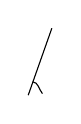
\begin{tikzpicture}[x=1cm,y=1cm]\draw (0.3,0.85)--(0,0);\draw (0.055,0.17) to[out=-5,in=130] (0.18,0.02);\end{tikzpicture}} $(^{42})$} stated was slightly uncorrect,  because it is by no means clear that the
crible \var{\inserted{$C_u$}}{\hand{$C_u$}}{insertion}{ps_134-3_059-v0001} constructed there is  functorial in u  i.e. corresponds to a map
I\hand{\ensuremath{\to\alpha}}(\hand{\ensuremath{\Delta}}$_1$) ,  this in fact has still to be assum\var{\xout{m}}{}{typewriter deletion}{ps_134-3_059-v0002}ed  (and turns out to be
\var{\xout{automatic}}{}{typewriter deletion}{ps_134-3_059-v0003} satisfied in all cases which turned up naturally so far and which
I looked up).  But let's now \hand{``}retell the story\hand{''}!

One key notion visibly in the homotopy technique used,  and which
needs a name in the long last,  is the notion of a \uline{homotopy} \uline{interval}\var{\xout{\unsure{,}}}{}{typewriter deletion}{ps_134-3_059-v0004}
( "segment homotopique" in French).  To be really outspoken about the very
formal nature of this notion and the way it will be used,  let's develop
it in any category \hand{\ensuremath{\mathcal{A}}} endowed with a subset  W \hand{\ensuremath{\subset}} Fl(\hand{\ensuremath{\mathcal{A}}}) of the set of
arrows of \hand{\ensuremath{\mathcal{A}}} , and satisfying the usual conditions :

a)  W contains all isomorphisms of \hand{\ensuremath{\mathcal{A}}} ,

b)  for two composable arrows u,v in \hand{\ensuremath{\mathcal{A}}},  if  two among u,v, vu are
in W,  so is the third,  and

c)  if  i: $F_o$ \hand{\ensuremath{\to}} F,and r: F \hand{\ensuremath{\to}} $F_o$ is a left inverse(i.e. a retraction ),
and if \var{\xout{ir}}{}{typewriter deletion}{ps_134-3_059-v0005} p = ir : F \hand{\ensuremath{\to}} F is in W,  so is r (and hence i too).

The condition c) \var{\inserted[typed]{here}}{here}{typed insertion}{ps_134-3_059-v0006} is the ingredient slightly stronger than what we used
to call "mild saturation property" of W,  meaning a) and b).

We'll call \uline{homotopy} \uline{\var{\over[typed]{seg}{int}}{int}{typewriter overwriting}{ps_134-3_059-v0007}erval} \uline{in} \hand{\ensuremath{\mathcal{A}}} (with respect to the notion of
"weak equivalence" W,  which will generally be implicit and specified by
context)  a triple (I,$e_o$,$e_1$) ,  where I is an object of \hand{\ensuremath{\mathcal{A}}} , $e_o$ and $e_1$
\margin{* provisional \uline{separating} W-homotopy interval} two subobjects,  such that the following conditions a) to c) hold \hand{\ensuremath{(^{43})}}

a)  $e_o$ and $e_1$ are \var{\xout{unit}}{}{typewriter deletion}{ps_134-3_059-v0008} final objects of \hand{\ensuremath{\mathcal{A}}} ,
which implies that \hand{\ensuremath{\mathcal{A}}} has a final object, unique up to unique isomorphism,
which we'll debote by e$_{\hand{\ensuremath{\mathcal{A}}}}$ or simply e , so that the data  $e_o$,$e_1$ in I are
equivalent to giving two sections
\[ \hand{\ensuremath{\delta}}_o , \hand{\ensuremath{\delta}}_1 :\ e \hand{\ensuremath{\to}} I \]
of I over e.  Note that  $e_o$\hand{\ensuremath{\cap}}$e_1$ \hand{\ensuremath{=}} Ker(\hand{\ensuremath{\delta}}$_o$,\hand{\ensuremath{\delta}}$_1$).

b)  $e_o$\hand{\ensuremath{\cap}}$e_1$ = \hand{\ensuremath{\emptyset_{\mathcal{A}}}} (a strict initial element of \hand{\ensuremath{\mathcal{A}}} ) ,

c)  I \hand{\ensuremath{\to}} e is "universally in W" or,  as we'll say, is W-\uline{aspheric} or
simply aspheric ,

which just means here that \var{\inserted{I $\to$ e is "squarable" and that}}{\hand{I $\to$ e is "squarable" and that}}{insertion}{ps_134-3_059-v0009} for any  F in Ob \hand{\ensuremath{\mathcal{A}}} ,  FxI \hand{\ensuremath{\to}} F is in W i.e.
is a "weak equivalence".

It is clear that if (I,$e_o$,$e_1$) is a homotopy \var{\xout{segment}}{}{typewriter deletion}{ps_134-3_059-v0010}\var{\inserted[typed]{interval}}{interval}{typed insertion}{ps_134-3_059-v0011} in \hand{\ensuremath{\mathcal{A}}}, then
for any F \hand{\ensuremath{\in}} Ob \hand{\ensuremath{\mathcal{A}}} ,  the"induced \var{\xout{segment}}{}{typewriter deletion}{ps_134-3_059-v0012}\var{\inserted[typed]{interval}}{interval}{typed insertion}{ps_134-3_059-v0013}"in \hand{\ensuremath{\mathcal{A}}}$_{/F}$ ,  namely (IxF,$e_o$xF,$e_1$xF)
is a homotopy interval in \hand{\ensuremath{\mathcal{A}}}$_{/F}$ .

%% END SOURCE ps_134-3_059
\ifnum\EditionMode=1
\psapparatusstart
\psentry{ps_134-3_059-v0001}{1}{insertion}{\inserted{$C_u$}}{\hand{$C_u$}}{The handwritten insertion is incorporated at its indicated position; insertion brackets leave the running text.}
\psentry{ps_134-3_059-v0002}{2}{typewriter deletion}{\xout{m}}{}{The typewriter strikes out this material; it leaves the corrected running text.}
\psentry{ps_134-3_059-v0003}{3}{typewriter deletion}{\xout{automatic}}{}{The typewriter strikes out this material; it leaves the corrected running text.}
\psentry{ps_134-3_059-v0004}{4}{typewriter deletion}{\xout{\unsure{,}}}{}{The typewriter strikes out this material; it leaves the corrected running text.}
\psentry{ps_134-3_059-v0005}{5}{typewriter deletion}{\xout{ir}}{}{The typewriter strikes out this material; it leaves the corrected running text.}
\psentry{ps_134-3_059-v0006}{6}{typed insertion}{\inserted[typed]{here}}{here}{The typed insertion is incorporated at its indicated position; insertion brackets leave the running text.}
\psentry{ps_134-3_059-v0007}{7}{typewriter overwriting}{\over[typed]{seg}{int}}{int}{The superposed typed reading replaces the underlying reading.}
\psentry{ps_134-3_059-v0008}{8}{typewriter deletion}{\xout{unit}}{}{The typewriter strikes out this material; it leaves the corrected running text.}
\psentry{ps_134-3_059-v0009}{9}{insertion}{\inserted{I $\to$ e is "squarable" and that}}{\hand{I $\to$ e is "squarable" and that}}{The handwritten insertion is incorporated at its indicated position; insertion brackets leave the running text.}
\psentry{ps_134-3_059-v0010}{10}{typewriter deletion}{\xout{segment}}{}{The typewriter strikes out this material; it leaves the corrected running text.}
\psentry{ps_134-3_059-v0011}{11}{typed insertion}{\inserted[typed]{interval}}{interval}{The typed insertion is incorporated at its indicated position; insertion brackets leave the running text.}
\psentry{ps_134-3_059-v0012}{12}{typewriter deletion}{\xout{segment}}{}{The typewriter strikes out this material; it leaves the corrected running text.}
\psentry{ps_134-3_059-v0013}{13}{typed insertion}{\inserted[typed]{interval}}{interval}{The typed insertion is incorporated at its indicated position; insertion brackets leave the running text.}
\psapparatusend
\fi
\pssource{ps_134-3_060}{134-3/60}{https://grothendieck.umontpellier.fr/web/viewer.html?file=../134-3.pdf\#page=61}
\psnumber{ps_134-3_060-v0001}{1}
\psnumber{ps_134-3_060-v0002}{2}
\psnumber{ps_134-3_060-v0003}{3}
\psnumber{ps_134-3_060-v0004}{4}
\psnumber{ps_134-3_060-v0005}{5}
\psnumber{ps_134-3_060-v0006}{6}
\psnumber{ps_134-3_060-v0007}{7}
\psnumber{ps_134-3_060-v0008}{8}
\psnumber{ps_134-3_060-v0009}{9}
\psnumber{ps_134-3_060-v0010}{10}
\psnumber{ps_134-3_060-v0011}{11}
\psnumber{ps_134-3_060-v0012}{12}
\psnumber{ps_134-3_060-v0013}{13}
\psnumber{ps_134-3_060-v0014}{14}
\psnumber{ps_134-3_060-v0015}{15}
\psnumber{ps_134-3_060-v0016}{16}
\psnumber{ps_134-3_060-v0017}{17}
\psnumber{ps_134-3_060-v0018}{18}
\psnumber{ps_134-3_060-v0019}{19}
\psnumber{ps_134-3_060-v0020}{20}
\psnumber{ps_134-3_060-v0021}{21}
\psnumber{ps_134-3_060-v0022}{22}
\psnumber{ps_134-3_060-v0023}{23}
\psnumber{ps_134-3_060-v0024}{24}
\psnumber{ps_134-3_060-v0025}{25}
\psnumber{ps_134-3_060-v0026}{26}
\psnumber{ps_134-3_060-v0027}{27}
\psnumber{ps_134-3_060-v0028}{28}
\psnumber{ps_134-3_060-v0029}{29}
%% BEGIN SOURCE ps_134-3_060
% Pursuing Stacks (cotes 134-2 to 134-8): archive cote 134-3, site page 60 (PDF page 61), typescript page 60.
% typescript. Draft compared: ps2.tex:3049-3123.
% AI-transcribed by Claude Opus 5.5 (claude-opus-5-5, adaptive thinking, effort high), Message Batches API, batch ps1 (msgbatch_01Rv5hCaNTtUt4JHx1yqoHPL), 2026-11-12; image review recorded in records/CHECK_DECISIONS_134_3_4.tsv.
\scanpage{134-3/60}
\mspage{\hand{60}}

We now get the (essentially trivial)
\uline{Homotopy lemma} \ Let \ $h\colon FxI \hand{\longrightarrow} F$ be a ``homotopy'' with respect to $(I,e_o,e_1)$
of $\mathrm{id}_F$ \ with a constant map \var{\xout{ix}}{}{typewriter deletion}{ps_134-3_060-v0001} $c = ir\colon F \hand{\to} F$ , \ where $r\colon F \hand{\longrightarrow} e$ and \var{\xout{i}}{}{typewriter deletion}{ps_134-3_060-v0002}
$i\colon e \hand{\to} F$ is a section of $F$ over $e$. \ Then $F \hand{\to} e$ is \ W-aspheric.

In the proof of this lemma, \ we make use of a)b)c) for W, \ but only
of a)c) for $(I,e_o,e_1)$ \ namely we don't even need \ $e_o \hand{\cap} e_1 = \hand{\emptyset}_{\hand{\mathcal{A}}}$ . \ This is
\var{\inserted[typed]{still the case for}}{still the case for}{typed insertion}{ps_134-3_060-v0003} \var{\xout{property however will be used in}}{}{typewriter deletion}{ps_134-3_060-v0004} the proof of the
\uline{Comparison lemma for homotopy intervals}: \ Let L be an object of \hand{\ensuremath{\mathcal{A}}} , squa-%
rable over e and endowed with a composition law \ $x\hand{\wedge}y$ ; \ let \ $\var{\over{e}{\delta}}{\hand{\delta}}{writing over}{ps_134-3_060-v0005}_i^L \colon e \hand{\to} L$
be two sections of L (i \hand{\ensuremath{\in\{}}0,1\hand{\ensuremath{\}}} ), \ which are respectively a left unit and a
zero element for the multiplication,namely the corresponding elements
$\hand{e}_o^{\var{\over[typed]{\illegible{1}}{a}}{a}{typewriter overwriting}{ps_134-3_060-v0006}},\hand{e}_1^{\var{\over[typed]{\illegible{1}}{a}}{a}{typewriter overwriting}{ps_134-3_060-v0007}}$ \ in any Hom(\var{\over[typed]{\illegible{1}}{a}}{a}{typewriter overwriting}{ps_134-3_060-v0008},L) satisfy
\[ \hand{e}_{\var{\over{\unsure{o}}{1}}{\hand{1}}{writing over}{ps_134-3_060-v0009}}^{\var{\over[typed]{\illegible{1}}{a}}{a}{typewriter overwriting}{ps_134-3_060-v0010}} \hand{\wedge} x = x \ , \ \hand{e}_{\var{\over{\unsure{1}}{0}}{\hand{0}}{writing over}{ps_134-3_060-v0011}}^{\var{\over[typed]{\illegible{1}}{a}}{a}{typewriter overwriting}{ps_134-3_060-v0012}} \hand{\wedge} x \ = \hand{e}_{\var{\over{\unsure{1}}{0}}{\hand{0}}{writing over}{ps_134-3_060-v0013}}^{\var{\over[typed]{\illegible{1}}{a}}{a}{typewriter overwriting}{ps_134-3_060-v0014}} \]
for any x in Hom(\var{\over[typed]{\illegible{1}}{a}}{a}{typewriter overwriting}{ps_134-3_060-v0015},L). \ Assume moreover we got a homotopy interval $(I,e_o,$
$e_1)$ and a \hand{``}map of intervals\hand{''}
\[ \hand{\phi}\colon I \hand{\longrightarrow} L \]
(in the sense: \ compatible with endpoints). \ Then \ $\mathrm{id}_L$ is homotopic(with
respect to $(I,e_o,e_1)$) to the constant map $c_{\hand{\unsure{0|a}}}\colon L \hand{\to} L$ defined by $\hand{\delta}^L_{\hand{\unsure{0|a}}}$ , \ and
hence by the previous homotopy lemma, \ $L \hand{\to} e$ is W-aspheric and therefore
\var{\xout{\illegible{1}}}{}{typewriter deletion}{ps_134-3_060-v0016} L endowed with \ $e_o^L ,e_1^L$ \ defined by $\hand{\delta}_o^L,\hand{\delta}_1^L$ \ is itself a homotopy inter-%
val in \hand{\ensuremath{\mathcal{A}}} (provided, \ at least, we know \ that \ $e_o^L \hand{\cap} e_1^L = \hand{\emptyset}$ ).

The homotopy h is simply given \ (for \ $u\colon \var{\over[typed]{\illegible{1}}{a}}{a}{typewriter overwriting}{ps_134-3_060-v0017} \hand{\to} \var{\over[typed]{\illegible{1}}{I}}{I}{typewriter overwriting}{ps_134-3_060-v0018}$, \ $x\colon \var{\over[typed]{\illegible{1}}{a}}{a}{typewriter overwriting}{ps_134-3_060-v0019} \hand{\to} L$) by
\[ h(\var{\over[typed]{\illegible{1}}{x}}{x}{typewriter overwriting}{ps_134-3_060-v0020},\var{\over[typed]{\illegible{1}}{u}}{u}{typewriter overwriting}{ps_134-3_060-v0021}) = \var{\xout{uxxxxx}}{}{typewriter deletion}{ps_134-3_060-v0022} \ \hand{\phi}(u) \hand{\wedge} x \ , \]
when a factors through $e_{\hand{1}}$ then $\hand{\phi}(u) = \hand{e}^a_{\hand{1}}$ \ and hence \ $h(x,u)=x$, \ if it
factors through $e_{\hand{0}}$ then $\hand{\phi}(u) = \hand{e}^a_{\hand{0}}$ \ and we get $h(x,u) = \hand{e}^a_{\hand{0}}$ , \ qed.
\uline{Corollary} \ Assume in \hand{\ensuremath{\mathcal{A}}} (endowed with W) finite inverse limits exist
(i.e. final object and fibered products exist), \ and moreover that the
\var{\deleted{functor}}{}{deletion}{ps_134-3_060-v0023}\var{\inserted{presheaf}}{\hand{presheaf}}{insertion}{ps_134-3_060-v0024} \hand{on $\mathcal{A}$}
\[ F \hand{\longmapsto} \text{set ob all subobjects of } F \]
is representable by an element L of \hand{\ensuremath{\mathcal{A}}} (the ``Lawvere element''). \ \var{\xout{Then}}{}{typewriter deletion}{ps_134-3_060-v0025}
Assume moreover \hand{\ensuremath{\mathcal{A}}} has a\var{\xout{n}}{}{typewriter deletion}{ps_134-3_060-v0026} strict initia\var{\over[typed]{\unsure{b}}{l}}{l}{typewriter overwriting}{ps_134-3_060-v0027} element $\hand{\emptyset}_{\hand{\mathcal{A}}}$, i.e. an initial
element and that \var{\deleted{\xout{for}}}{}{deletion}{ps_134-3_060-v0028} any \ map \ $\underset{\text{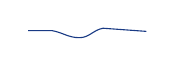
\begin{tikzpicture}[x=1cm,y=1cm,baseline]\draw[color=blue] (0,0.05)--(0.3,0.05) to[out=-10,in=180] (0.65,-0.04) to[out=0,in=190] (0.95,0.08)--(1.5,0.04);\end{tikzpicture}}}{a \hand{\to} \hand{\emptyset}_{\hand{\mathcal{A}}}}$ \ is an isomorphism. \ Consider the
two sections of L over e , $\hand{\delta}^L_{\hand{1}}$ \ and \ $\hand{\delta}^L_{\hand{0}}$ , \ corresponding to the full and
to the empty subobject of e, \ so that we get visibly \ $e_o^L \hand{\cap} e_1^L = \hand{\emptyset}$ \ .
\var{\over{t}{T}}{\hand{T}}{writing over}{ps_134-3_060-v0029}hen, \ for a homotopy interval to exist in \hand{\ensuremath{\mathcal{A}}} , it is necessay and suf-%
ficient that L be W-aspheric over e , \ i.e. that $(L,e_o^L ,e_1^L )$ \ be a homoto-%
py interval.

By the comparison lemma, \ it is enough to show that for any homotopy
\unsure{interval} \ $(I,e_o,e_1)$ \ in \hand{\ensuremath{\mathcal{A}}}, \ there exists a morphism of ``intervals''

%% END SOURCE ps_134-3_060
\ifnum\EditionMode=1
\psapparatusstart
\psentry{ps_134-3_060-v0001}{1}{typewriter deletion}{\xout{ix}}{}{The typewriter strikes out this material; it leaves the corrected running text.}
\psentry{ps_134-3_060-v0002}{2}{typewriter deletion}{\xout{i}}{}{The typewriter strikes out this material; it leaves the corrected running text.}
\psentry{ps_134-3_060-v0003}{3}{typed insertion}{\inserted[typed]{still the case for}}{still the case for}{The typed insertion is incorporated at its indicated position; insertion brackets leave the running text.}
\psentry{ps_134-3_060-v0004}{4}{typewriter deletion}{\xout{property however will be used in}}{}{The typewriter strikes out this material; it leaves the corrected running text.}
\psentry{ps_134-3_060-v0005}{5}{writing over}{$\over{e}{\delta}$}{$\hand{\delta}$}{The superposed handwritten reading replaces the underlying reading.}
\psentry{ps_134-3_060-v0006}{6}{typewriter overwriting}{$\over[typed]{\illegible{1}}{a}$}{$a$}{The superposed typed reading replaces the underlying reading.}
\psentry{ps_134-3_060-v0007}{7}{typewriter overwriting}{$\over[typed]{\illegible{1}}{a}$}{$a$}{The superposed typed reading replaces the underlying reading.}
\psentry{ps_134-3_060-v0008}{8}{typewriter overwriting}{\over[typed]{\illegible{1}}{a}}{a}{The superposed typed reading replaces the underlying reading.}
\psentry{ps_134-3_060-v0009}{9}{writing over}{$\over{\unsure{o}}{1}$}{$\hand{1}$}{The superposed handwritten reading replaces the underlying reading.}
\psentry{ps_134-3_060-v0010}{10}{typewriter overwriting}{$\over[typed]{\illegible{1}}{a}$}{$a$}{The superposed typed reading replaces the underlying reading.}
\psentry{ps_134-3_060-v0011}{11}{writing over}{$\over{\unsure{1}}{0}$}{$\hand{0}$}{The superposed handwritten reading replaces the underlying reading.}
\psentry{ps_134-3_060-v0012}{12}{typewriter overwriting}{$\over[typed]{\illegible{1}}{a}$}{$a$}{The superposed typed reading replaces the underlying reading.}
\psentry{ps_134-3_060-v0013}{13}{writing over}{$\over{\unsure{1}}{0}$}{$\hand{0}$}{The superposed handwritten reading replaces the underlying reading.}
\psentry{ps_134-3_060-v0014}{14}{typewriter overwriting}{$\over[typed]{\illegible{1}}{a}$}{$a$}{The superposed typed reading replaces the underlying reading.}
\psentry{ps_134-3_060-v0015}{15}{typewriter overwriting}{\over[typed]{\illegible{1}}{a}}{a}{The superposed typed reading replaces the underlying reading.}
\psentry{ps_134-3_060-v0016}{16}{typewriter deletion}{\xout{\illegible{1}}}{}{The typewriter strikes out this material; it leaves the corrected running text.}
\psentry{ps_134-3_060-v0017}{17}{typewriter overwriting}{$\over[typed]{\illegible{1}}{a}$}{$a$}{The superposed typed reading replaces the underlying reading.}
\psentry{ps_134-3_060-v0018}{18}{typewriter overwriting}{$\over[typed]{\illegible{1}}{I}$}{$I$}{The superposed typed reading replaces the underlying reading.}
\psentry{ps_134-3_060-v0019}{19}{typewriter overwriting}{$\over[typed]{\illegible{1}}{a}$}{$a$}{The superposed typed reading replaces the underlying reading.}
\psentry{ps_134-3_060-v0020}{20}{typewriter overwriting}{$\over[typed]{\illegible{1}}{x}$}{$x$}{The superposed typed reading replaces the underlying reading.}
\psentry{ps_134-3_060-v0021}{21}{typewriter overwriting}{$\over[typed]{\illegible{1}}{u}$}{$u$}{The superposed typed reading replaces the underlying reading.}
\psentry{ps_134-3_060-v0022}{22}{typewriter deletion}{$\xout{uxxxxx}$}{}{The typewriter strikes out this material; it leaves the corrected running text.}
\psentry{ps_134-3_060-v0023}{23}{deletion}{\deleted{functor}}{}{The author cancels this material by hand; it leaves the corrected running text.}
\psentry{ps_134-3_060-v0024}{24}{insertion}{\inserted{presheaf}}{\hand{presheaf}}{The handwritten insertion is incorporated at its indicated position; insertion brackets leave the running text.}
\psentry{ps_134-3_060-v0025}{25}{typewriter deletion}{\xout{Then}}{}{The typewriter strikes out this material; it leaves the corrected running text.}
\psentry{ps_134-3_060-v0026}{26}{typewriter deletion}{\xout{n}}{}{The typewriter strikes out this material; it leaves the corrected running text.}
\psentry{ps_134-3_060-v0027}{27}{typewriter overwriting}{\over[typed]{\unsure{b}}{l}}{l}{The superposed typed reading replaces the underlying reading.}
\psentry{ps_134-3_060-v0028}{28}{deletion}{\deleted{\xout{for}}}{}{The author cancels this material by hand; it leaves the corrected running text.}
\psentry{ps_134-3_060-v0029}{29}{writing over}{\over{t}{T}}{\hand{T}}{The superposed handwritten reading replaces the underlying reading.}
\psapparatusend
\fi
\pssource{ps_134-3_061}{134-3/61}{https://grothendieck.umontpellier.fr/web/viewer.html?file=../134-3.pdf\#page=62}
\psnumber{ps_134-3_061-v0001}{1}
\psnumber{ps_134-3_061-v0002}{2}
\psnumber{ps_134-3_061-v0003}{3}
\psnumber{ps_134-3_061-v0004}{4}
\psnumber{ps_134-3_061-v0005}{5}
\psnumber{ps_134-3_061-v0006}{6}
\psnumber{ps_134-3_061-v0007}{7}
\psnumber{ps_134-3_061-v0008}{8}
\psnumber{ps_134-3_061-v0009}{9}
\psnumber{ps_134-3_061-v0010}{10}
\psnumber{ps_134-3_061-v0011}{11}
\psnumber{ps_134-3_061-v0012}{12}
\psnumber{ps_134-3_061-v0013}{13}
\psnumber{ps_134-3_061-v0014}{14}
\psnumber{ps_134-3_061-v0015}{15}
\psnumber{ps_134-3_061-v0016}{16}
%% BEGIN SOURCE ps_134-3_061
% Pursuing Stacks (cotes 134-2 to 134-8): archive cote 134-3, site page 61 (PDF page 62), typescript page 61.
% typescript. Draft compared: ps2.tex:3109-3190.
% AI-transcribed by Claude Opus 5.5 (claude-opus-5-5, adaptive thinking, effort high), Message Batches API, batch ps1 (msgbatch_01Rv5hCaNTtUt4JHx1yqoHPL), 2026-11-12; image review recorded in records/CHECK_DECISIONS_134_3_4.tsv.
\scanpage{134-3/61}
\mspage{61}
from I into L ,  using the fact of course that the intersection law on L
\var{\xout{defines}}{}{typewriter deletion}{ps_134-3_061-v0001} is a composition law admitting $\hand{\delta}^{L}_{\hand{1}} ,\hand{\delta}^{L}_{\hand{0}}$ respectively as unit and
as zero element (still using the fact that the initial object is strict).
\margin{$e_1$} But the subobject $e_{\hand{1}}$ of I ,  by definition of L,  can be viewed as the
\margin{$e^L_1$} inverse image of $e^{L}_{\hand{1}}$ by a uniquely defined map $I \hand{\to} L$.  \var{\over{t}{T}}{\hand{T}}{writing over}{ps_134-3_061-v0002}he induced
\var{\xout{morphism}}{}{typewriter deletion}{ps_134-3_061-v0003} map $e_{\hand{0}} \hand{\to} L$ corresponds to the induced subobject $e_{o}\hand{\cap} e_{1}$ of $e_{1}$ ,
which by assumption is $\hand{\emptyset}_{\hand{\mathcal{A}}}$ ,  and hence $e_{\hand{0}} \hand{\to} L$ factors through $e^{L}_{\hand{0}}$ ,  qed.

Of course,  the case for the time being which mainly interests us is
the one when $\hand{\mathcal{A}}$ is a topos (more specifically \var{\inserted{even}}{\hand{even}}{insertion}{ps_134-3_061-v0004}, a topos e\var{\over[typed]{\unsure{q}}{q}}{q}{typewriter overwriting}{ps_134-3_061-v0005}uivalent to a
category $A^{\hand{\wedge}}$, wi th A a small category),  in which case it is tacitly under-%
stood that W is the set of weak equivalences in the usual sense .  We now
come to the key result :

\uline{Theorem}  Let A be a small category,  and
\[ i:\ A \hand{\longrightarrow} (\mathrm{Cat}) \]
a functor,  hence a functor
\[ \hand{*}\ i^{*} :\ (\mathrm{Cat}) \hand{\longrightarrow} \overset{\hand{*}}{A^{\hand{\wedge}}} \quad ,\qquad C \hand{\mapsto} (a \hand{\mapsto} \mathrm{Hom}(i(a),\ C)) \ . \]
Consider the canonical functor  $i_{A} : A^{\hand{\wedge}} \hand{\to} (\mathrm{Cat})$,  $F \hand{\mapsto} A_{/F}$ ,  and\hand{/}the
compositum
\[ (\mathrm{Cat}) \hand{\xrightarrow{\ \textcolor{black}{i^{*}}\ }} A^{\hand{\wedge}} \hand{\xrightarrow{\ \textcolor{black}{i_{A}}\ }} (\mathrm{Cat}) \quad ,\qquad C \hand{\mapsto} A_{/i^{\hand{*}}(C)} \overset{\mathrm{d}\overset{\hand{\scriptscriptstyle\prime}}{\mathrm{e}}\mathrm{f}}{=} A_{/C} \ . \]
As\hand{su}me that for any $a \hand{\in} \mathrm{Ob}\, A$,  $i(a) \hand{\in} \mathrm{Ob}\, (\mathrm{Cat})$ has a final element $e_{a}$ (but
we don't demand that for $u:\ a \hand{\to} b$,  $i(u):\ i(a) \hand{\to} i(b)$ transforms $e_{a}$ into
$e_{b}$ nor even into a final element of i(b)).  Consider the canonical
functor
\[ (*) \qquad A_{/C} \hand{\longrightarrow} C \quad , \quad (a,\ p{:}i(a) \hand{\to} C) \hand{\longmapsto} p(e_{a}) \quad , \]
which is functorial in C,  and hence defines a map between functors from
(Cat) to (Cat):
\[ (*\ *) \qquad i_{A}i^{*} \hand{\longrightarrow} \mathrm{id}_{(\mathrm{Cat})} \quad . \]
\var{\inserted{a)}}{\hand{a)}}{insertion}{ps_134-3_061-v0006} The following conditions  are equivalent:

(i)  For any C in (Cat),  (*) is aspheric.
(ii)  For any C in (Cat),  (*) is a weak equivalence,  i.e. \var{\inserted[typed]{$i_{A}i^{*}$}}{$i_{A}i^{*}$}{typed insertion}{ps_134-3_061-v0007}\unsure{i(**)} trans-%
forms weak equivalences  into weak equivalences,  and (**) induces
an isomorphism of the corresponding functor (Hot) $\hand{\to}$ (Hot) with the
identity functor.
(iii)  T\var{\over{h}{h}}{\hand{h}}{writing over}{ps_134-3_061-v0008}e functor $i_{A}i^{*}$  transforms weak equivalences into weak equivalen-%
ces,  and the induced functor (Hot) $\hand{\to}$ (Hot) transforms every object
into an isomorphic one,  i.e. \var{\inserted{for any C in (Cat)}}{\hand{for any C in (Cat)}}{insertion}{ps_134-3_061-v0009} $A_{/C}$ is isomorphic to C in (Hot).
(iv)  \var{\over{When}{For}}{\hand{For}}{writing over}{ps_134-3_061-v0010} \var{\inserted{any}}{\hand{any}}{insertion}{ps_134-3_061-v0011} C \var{\over{has}{with}}{\hand{with}}{writing over}{ps_134-3_061-v0012} a final element,  $A_{/C}$ is aspheric .

b)  T\var{\over[typed]{h}{h}}{h}{typewriter overwriting}{ps_134-3_061-v0013}e following conditions are equivalent\var{\over{\unsure{:}}{,}}{\hand{,}}{writing over}{ps_134-3_061-v0014} \uline{and they imply the conditi-%
ons \var{\deleted{from}}{}{deletion}{ps_134-3_061-v0015}\var{\inserted{in}}{\hand{in}}{insertion}{ps_134-3_061-v0016}} a)  \uline{provided A is aspheric} :

%% END SOURCE ps_134-3_061
\ifnum\EditionMode=1
\psapparatusstart
\psentry{ps_134-3_061-v0001}{1}{typewriter deletion}{\xout{defines}}{}{The typewriter strikes out this material; it leaves the corrected running text.}
\psentry{ps_134-3_061-v0002}{2}{writing over}{\over{t}{T}}{\hand{T}}{The superposed handwritten reading replaces the underlying reading.}
\psentry{ps_134-3_061-v0003}{3}{typewriter deletion}{\xout{morphism}}{}{The typewriter strikes out this material; it leaves the corrected running text.}
\psentry{ps_134-3_061-v0004}{4}{insertion}{\inserted{even}}{\hand{even}}{The handwritten insertion is incorporated at its indicated position; insertion brackets leave the running text.}
\psentry{ps_134-3_061-v0005}{5}{typewriter overwriting}{\over[typed]{\unsure{q}}{q}}{q}{The superposed typed reading replaces the underlying reading.}
\psentry{ps_134-3_061-v0006}{6}{insertion}{\inserted{a)}}{\hand{a)}}{The handwritten insertion is incorporated at its indicated position; insertion brackets leave the running text.}
\psentry{ps_134-3_061-v0007}{7}{typed insertion}{\inserted[typed]{$i_{A}i^{*}$}}{$i_{A}i^{*}$}{The typed insertion is incorporated at its indicated position; insertion brackets leave the running text.}
\psentry{ps_134-3_061-v0008}{8}{writing over}{\over{h}{h}}{\hand{h}}{The superposed handwritten reading replaces the underlying reading.}
\psentry{ps_134-3_061-v0009}{9}{insertion}{\inserted{for any C in (Cat)}}{\hand{for any C in (Cat)}}{The handwritten insertion is incorporated at its indicated position; insertion brackets leave the running text.}
\psentry{ps_134-3_061-v0010}{10}{writing over}{\over{When}{For}}{\hand{For}}{The superposed handwritten reading replaces the underlying reading.}
\psentry{ps_134-3_061-v0011}{11}{insertion}{\inserted{any}}{\hand{any}}{The handwritten insertion is incorporated at its indicated position; insertion brackets leave the running text.}
\psentry{ps_134-3_061-v0012}{12}{writing over}{\over{has}{with}}{\hand{with}}{The superposed handwritten reading replaces the underlying reading.}
\psentry{ps_134-3_061-v0013}{13}{typewriter overwriting}{\over[typed]{h}{h}}{h}{The superposed typed reading replaces the underlying reading.}
\psentry{ps_134-3_061-v0014}{14}{writing over}{\over{\unsure{:}}{,}}{\hand{,}}{The superposed handwritten reading replaces the underlying reading.}
\psentry{ps_134-3_061-v0015}{15}{deletion}{\deleted{from}}{}{The author cancels this material by hand; it leaves the corrected running text.}
\psentry{ps_134-3_061-v0016}{16}{insertion}{\inserted{in}}{\hand{in}}{The handwritten insertion is incorporated at its indicated position; insertion brackets leave the running text.}
\psapparatusend
\fi
\pssource{ps_134-3_062}{134-3/62}{https://grothendieck.umontpellier.fr/web/viewer.html?file=../134-3.pdf\#page=63}
\psnumber{ps_134-3_062-v0001}{1}
\psnumber{ps_134-3_062-v0002}{2}
\psnumber{ps_134-3_062-v0003}{3}
\psnumber{ps_134-3_062-v0004}{4}
\psnumber{ps_134-3_062-v0005}{5}
\psnumber{ps_134-3_062-v0006}{6}
\psnumber{ps_134-3_062-v0007}{7}
\psnumber{ps_134-3_062-v0008}{8}
\psnumber{ps_134-3_062-v0009}{9}
\psnumber{ps_134-3_062-v0010}{10}
\psnumber{ps_134-3_062-v0011}{11}
\psnumber{ps_134-3_062-v0012}{12}
\psnumber{ps_134-3_062-v0013}{13}
\psnumber{ps_134-3_062-v0014}{14}
\psnumber{ps_134-3_062-v0015}{15}
\psnumber{ps_134-3_062-v0016}{16}
\psnumber{ps_134-3_062-v0017}{17}
\psnumber{ps_134-3_062-v0018}{18}
\psnumber{ps_134-3_062-v0019}{19}
\psnumber{ps_134-3_062-v0020}{20}
\psnumber{ps_134-3_062-v0021}{21}
\psnumber{ps_134-3_062-v0022}{22}
\psnumber{ps_134-3_062-v0023}{23}
\psnumber{ps_134-3_062-v0024}{24}
\psnumber{ps_134-3_062-v0025}{25}
\psnumber{ps_134-3_062-v0026}{26}
\psnumber{ps_134-3_062-v0027}{27}
\psnumber{ps_134-3_062-v0028}{28}
\psnumber{ps_134-3_062-v0029}{29}
%% BEGIN SOURCE ps_134-3_062
% Pursuing Stacks (cotes 134-2 to 134-8): archive cote 134-3, site page 62 (PDF page 63), typescript page 62.
% typescript. Draft compared: ps2.tex:3169-3264.
% AI-transcribed by Claude Opus 5.5 (claude-opus-5-5, adaptive thinking, effort high), Message Batches API, batch ps1 (msgbatch_01Rv5hCaNTtUt4JHx1yqoHPL), 2026-11-12; image review recorded in records/CHECK_DECISIONS_134_3_4.tsv.
\scanpage{134-3/62}
\mspage{\hand{62}}

(i)   For any C in (Cat)  the functor
(* * *)   $A_{/C}$ \hand{\ensuremath{\longrightarrow}} AxC   deduced from (*)  and $A_{/C} \hand{\ensuremath{\xrightarrow{\textcolor{black}{\text{can}}}}} A$
\var{\xout{is}}{}{typewriter deletion}{ps_134-3_062-v0001}   is aspheric.
\var{\deleted{\xout{(ii)}}}{}{deletion}{ps_134-3_062-v0002}\var{\deleted{\xout{For any C in (Cat), the functor (x\allowbreak{}x\allowbreak{}x\allowbreak{}) is a weak equivalence}}}{}{deletion}{ps_134-3_062-v0003}
(ii\var{\deleted{i}}{}{deletion}{ps_134-3_062-v0004})  For any C in (Cat) with final element and any a in A,  $a\mathrm{x}i^{*}(C)$ is
an aspheric element in $A^{\hand{\wedge}}$, i.e. for any such C, $i^{\hand{*}}(C)$ is aspheric
over the final element e \var{\inserted{of $A^{\hand{\wedge}}$}}{\hand{of $A^{\hand{\wedge}}$}}{insertion}{ps_134-3_062-v0005}.
\margin{Look at sequel in vol.\ 2 pag \unsure{64--65}}
(i\var{\over{\unsure{v}}{ii}}{\hand{ii}}{writing over}{ps_134-3_062-v0006})   The element  $i^{\hand{*}}(\hand{\ensuremath{\Delta}}_1)$ of $A^{\hand{\wedge}}$ is aspheric over the final object e .

\var{\xout{We get at once the}}{}{typewriter deletion}{ps_134-3_062-v0007}
\hand{\uline{Remark 1.}}
Of course \var{\over[typed]{a)}{th}}{th}{typewriter overwriting}{ps_134-3_062-v0008}e conditions in a) imply that A is aspheric (take \var{\xout{in}}{}{typewriter deletion}{ps_134-3_062-v0009} C
the final category),  and hence  by an easy \var{\inserted[typed]{\deleted{homotopy lemma}}}{}{typed insertion}{ps_134-3_062-v0010}\var{\xout{variant of the homotopy lemma}}{}{typewriter deletion}{ps_134-3_062-v0011}\var{\inserted{lemma (cf.\ below \S\ Section (\S40))}}{\hand{lemma (cf.\ below \S\ Section (\S40))}}{insertion}{ps_134-3_062-v0012}
we get that \var{\inserted{for any C in (Cat),}}{\hand{for any C in (Cat),}}{insertion}{ps_134-3_062-v0013} AxC \hand{\ensuremath{\rightarrow}} C is a weak equivalence \var{\inserted[typed]{(and even aspheric)}}{(and even aspheric)}{typed insertion}{ps_134-3_062-v0014}, and hence $A_{/C}$ \hand{\ensuremath{\rightarrow}} AxC is
a weak equivalence (because its compositum with the weak equivalence
AxC \hand{\ensuremath{\rightarrow}} C is a weak equivalence by assumption).  It is \var{\xout{not}}{}{typewriter deletion}{ps_134-3_062-v0015} unlikely however
\margin{X}
that  a) \var{\xout{(asphericity of A}}{}{typewriter deletion}{ps_134-3_062-v0016}  impl\var{\over{y}{ies}}{\hand{ies}}{writing over}{ps_134-3_062-v0017} the conditions of  b) ,  namely asphe-%
ricity (not merely weak equivalence) of (***) in  b (i).   But the opposi-%
te implication,  namely  b (i)  +  asphericity of A   implies a (i) ,
is trivial,  b\var{\over{y}{e}}{\hand{e}}{writing over}{ps_134-3_062-v0018}cause AxC \hand{\ensuremath{\rightarrow}} C is aspheric.

\var{\inserted{Proof of Theorem:}}{\hand{Proof of Theorem:}}{insertion}{ps_134-3_062-v0019}
We stated a) and b) in a way to get a visibly decreasing cascade of
\var{\over{condi}{condi}}{\hand{condi}}{writing over}{ps_134-3_062-v0020}tions; \var{\inserted{and}}{\hand{and}}{insertion}{ps_134-3_062-v0021} moreover that the weakest in a) implies the strongest,  or
that b (ii) implies b (i) , is an immediate consequence of the standar\var{\over{t}{d}}{\hand{d}}{writing over}{ps_134-3_062-v0022}
asphericity criterion for a functor between categories \var{\inserted{\deleted{(p.38)}}}{\hand{}}{insertion}{ps_134-3_062-v0023}\var{\inserted{(section 30).}}{\hand{(section 30).}}{insertion}{ps_134-3_062-v0024} The only point
which is a little less formal is that  b (iii)  implies b (ii).  But
using the final object in C,  we get a \var{\inserted{(unique)}}{\hand{(unique)}}{insertion}{ps_134-3_062-v0025} homotopy  in (Cat) \var{\inserted{(relative to $\Delta_1$)}}{\hand{(relative to $\Delta_1$)}}{insertion}{ps_134-3_062-v0026}
\[ \hand{\ensuremath{\Delta}}_1 \mathrm{x}\, C \hand{\rightarrow} C , \]
between the identity map of C and the constant map with value $e_C$  - hence
by applying $i^{*}$\hand{,} a homotopy  relative to  $i^{\hand{*}}(\hand{\ensuremath{\Delta}}_1)$  (viewed as an ``interval''
by taking as ``endpoints'' the arrows deduced from $\hand{\ensuremath{\delta}}_o,\hand{\ensuremath{\delta}}_1 : e_{(Cat)} = \hand{\ensuremath{\Delta}}_o \hand{\ensuremath{\rightrightarrows}} \hand{\ensuremath{\Delta}}_1$
by applying $i^{*}$ ),  between the identity map of $i^{*}(C)$ and a constant map
of $i^{*}(C)$,  which by the  homotopy lemma implies that $i^{*}(C)$ itself is
aspheric over $e_{\hand{\ensuremath{A^{\hand{\wedge}}}}}$,  qed.
\var{\inserted[typed]{Remark}}{Remark}{typed insertion}{ps_134-3_062-v0027}\hand{2}:  \var{\xout{\uline{Corollary}}}{}{typewriter deletion}{ps_134-3_062-v0028}  the condition  b (iii) can be stated by saying that $i^{\hand{*}}(\hand{\ensuremath{\Delta}}_1)$
is a \uline{homotopy interval} in $A^{\hand{\wedge}}$.  All which needs to be checked for this, is
that  condition  b) for homotopy intervals  (p.59) namely $e_o \hand{\ensuremath{\cap}} e_1 = \hand{\emptyset}$  is
satisfied in $A^{\hand{\wedge}}$,  but this follows from the corresponding \var{\xout{condition}}{}{typewriter deletion}{ps_134-3_062-v0029} pro-%
perty for \hand{\ensuremath{\Delta}}$_1$ in Cat (as the functor $i^{*}$ is left exact) and from the fact
that $i^{*}$ transforms initial element $\hand{\emptyset}_{(Cat)}$ into initial element $\hand{\emptyset}_{A^{\hand{\wedge}}}$.  This
last fact is equivalent to $i(a) \hand{\neq} \hand{\emptyset}$ for any a in A , which is true as
i(a) has a final element.

%% END SOURCE ps_134-3_062
\ifnum\EditionMode=1
\psapparatusstart
\psentry{ps_134-3_062-v0001}{1}{typewriter deletion}{\xout{is}}{}{The typewriter strikes out this material; it leaves the corrected running text.}
\psentry{ps_134-3_062-v0002}{2}{deletion}{\deleted{\xout{(ii)}}}{}{The author cancels this material by hand; it leaves the corrected running text.}
\psentry{ps_134-3_062-v0003}{3}{deletion}{\deleted{\xout{For any C in (Cat), the functor (x\allowbreak{}x\allowbreak{}x\allowbreak{}) is a weak equivalence}}}{}{The author cancels this material by hand; it leaves the corrected running text.}
\psentry{ps_134-3_062-v0004}{4}{deletion}{\deleted{i}}{}{The author cancels this material by hand; it leaves the corrected running text.}
\psentry{ps_134-3_062-v0005}{5}{insertion}{\inserted{of $A^{\hand{\wedge}}$}}{\hand{of $A^{\hand{\wedge}}$}}{The handwritten insertion is incorporated at its indicated position; insertion brackets leave the running text.}
\psentry{ps_134-3_062-v0006}{6}{writing over}{\over{\unsure{v}}{ii}}{\hand{ii}}{The superposed handwritten reading replaces the underlying reading.}
\psentry{ps_134-3_062-v0007}{7}{typewriter deletion}{\xout{We get at once the}}{}{The typewriter strikes out this material; it leaves the corrected running text.}
\psentry{ps_134-3_062-v0008}{8}{typewriter overwriting}{\over[typed]{a)}{th}}{th}{The superposed typed reading replaces the underlying reading.}
\psentry{ps_134-3_062-v0009}{9}{typewriter deletion}{\xout{in}}{}{The typewriter strikes out this material; it leaves the corrected running text.}
\psentry{ps_134-3_062-v0010}{10}{typed insertion}{\inserted[typed]{\deleted{homotopy lemma}}}{}{The typed insertion is incorporated at its indicated position; insertion brackets leave the running text.}
\psentry{ps_134-3_062-v0011}{11}{typewriter deletion}{\xout{variant of the homotopy lemma}}{}{The typewriter strikes out this material; it leaves the corrected running text.}
\psentry{ps_134-3_062-v0012}{12}{insertion}{\inserted{lemma (cf.\ below \S\ Section (\S40))}}{\hand{lemma (cf.\ below \S\ Section (\S40))}}{The handwritten insertion is incorporated at its indicated position; insertion brackets leave the running text.}
\psentry{ps_134-3_062-v0013}{13}{insertion}{\inserted{for any C in (Cat),}}{\hand{for any C in (Cat),}}{The handwritten insertion is incorporated at its indicated position; insertion brackets leave the running text.}
\psentry{ps_134-3_062-v0014}{14}{typed insertion}{\inserted[typed]{(and even aspheric)}}{(and even aspheric)}{The typed insertion is incorporated at its indicated position; insertion brackets leave the running text.}
\psentry{ps_134-3_062-v0015}{15}{typewriter deletion}{\xout{not}}{}{The typewriter strikes out this material; it leaves the corrected running text.}
\psentry{ps_134-3_062-v0016}{16}{typewriter deletion}{\xout{(asphericity of A}}{}{The typewriter strikes out this material; it leaves the corrected running text.}
\psentry{ps_134-3_062-v0017}{17}{writing over}{\over{y}{ies}}{\hand{ies}}{The superposed handwritten reading replaces the underlying reading.}
\psentry{ps_134-3_062-v0018}{18}{writing over}{\over{y}{e}}{\hand{e}}{The superposed handwritten reading replaces the underlying reading.}
\psentry{ps_134-3_062-v0019}{19}{insertion}{\inserted{Proof of Theorem:}}{\hand{Proof of Theorem:}}{The handwritten insertion is incorporated at its indicated position; insertion brackets leave the running text.}
\psentry{ps_134-3_062-v0020}{20}{writing over}{\over{condi}{condi}}{\hand{condi}}{The superposed handwritten reading replaces the underlying reading.}
\psentry{ps_134-3_062-v0021}{21}{insertion}{\inserted{and}}{\hand{and}}{The handwritten insertion is incorporated at its indicated position; insertion brackets leave the running text.}
\psentry{ps_134-3_062-v0022}{22}{writing over}{\over{t}{d}}{\hand{d}}{The superposed handwritten reading replaces the underlying reading.}
\psentry{ps_134-3_062-v0023}{23}{insertion}{\inserted{\deleted{(p.38)}}}{\hand{}}{The handwritten insertion is incorporated at its indicated position; insertion brackets leave the running text.}
\psentry{ps_134-3_062-v0024}{24}{insertion}{\inserted{(section 30).}}{\hand{(section 30).}}{The handwritten insertion is incorporated at its indicated position; insertion brackets leave the running text.}
\psentry{ps_134-3_062-v0025}{25}{insertion}{\inserted{(unique)}}{\hand{(unique)}}{The handwritten insertion is incorporated at its indicated position; insertion brackets leave the running text.}
\psentry{ps_134-3_062-v0026}{26}{insertion}{\inserted{(relative to $\Delta_1$)}}{\hand{(relative to $\Delta_1$)}}{The handwritten insertion is incorporated at its indicated position; insertion brackets leave the running text.}
\psentry{ps_134-3_062-v0027}{27}{typed insertion}{\inserted[typed]{Remark}}{Remark}{The typed insertion is incorporated at its indicated position; insertion brackets leave the running text.}
\psentry{ps_134-3_062-v0028}{28}{typewriter deletion}{\xout{\uline{Corollary}}}{}{The typewriter strikes out this material; it leaves the corrected running text.}
\psentry{ps_134-3_062-v0029}{29}{typewriter deletion}{\xout{condition}}{}{The typewriter strikes out this material; it leaves the corrected running text.}
\psapparatusend
\fi
\pssource{ps_134-3_063}{134-3/63}{https://grothendieck.umontpellier.fr/web/viewer.html?file=../134-3.pdf\#page=64}
\psnumber{ps_134-3_063-v0001}{1}
\psnumber{ps_134-3_063-v0002}{2}
\psnumber{ps_134-3_063-v0003}{3}
\psnumber{ps_134-3_063-v0004}{4}
\psnumber{ps_134-3_063-v0005}{5}
\psnumber{ps_134-3_063-v0006}{6}
\psnumber{ps_134-3_063-v0007}{7}
\psnumber{ps_134-3_063-v0008}{8}
\psnumber{ps_134-3_063-v0009}{9}
\psnumber{ps_134-3_063-v0010}{10}
\psnumber{ps_134-3_063-v0011}{11}
\psnumber{ps_134-3_063-v0012}{12}
\psnumber{ps_134-3_063-v0013}{13}
%% BEGIN SOURCE ps_134-3_063
% Pursuing Stacks (cotes 134-2 to 134-8): archive cote 134-3, site page 63 (PDF page 64), typescript page 63.
% typescript. Draft compared: ps2.tex:3244-3313.
% AI-transcribed by Claude Opus 5.5 (claude-opus-5-5, adaptive thinking, effort high), Message Batches API, batch ps1 (msgbatch_01Rv5hCaNTtUt4JHx1yqoHPL), 2026-11-12; image review recorded in records/CHECK_DECISIONS_134_3_4.tsv.
\scanpage{134-3/63}
\mspage{\hand{63}}

22.3.

38. Lets \var{\inserted[typed]{get}}{get}{typed insertion}{ps_134-3_063-v0001} back to the ``asphericity story retold'' - I had \var{\over[typed]{s}{t}}{t}{typewriter overwriting}{ps_134-3_063-v0002}o stop yester-%
day just in the middle, as it was getting prohibitively late.

I want to comment a little about the ``key result'' just stated and
proved. T\var{\over[typed]{h}{h}}{h}{typewriter overwriting}{ps_134-3_063-v0003}e main point of this result, forgetting the game of giving
heaps of equivalent formulations of two kind of properties, is that the
extremely simple condition b (iii), namely that $i^{*}(\hand{\ensuremath{\Delta}}_1)$ is aspheric over
the unit element $e_{A^{\hand{\wedge}}}$ of $A^{\hand{\wedge}}$,\var{\inserted{plus asphericity of the latter,}}{\hand{plus asphericity of the latter,}}{insertion}{ps_134-3_063-v0004} ensure\var{\deleted{s}}{}{deletion}{ps_134-3_063-v0005} already the conditions in a), which
can be viewed (among others) as just stating that the compositum
\[ i_A i^{*} : \text{(Cat)} \hand{\ensuremath{\longrightarrow}} A^{\hand{\wedge}} \hand{\ensuremath{\longrightarrow}} \text{(Cat)} \]
\var{\xout{induces}}{}{typewriter deletion}{ps_134-3_063-v0006} from (Cat) to (Cat) induces an autoequivalence of the localised ca%
tegory (Hot), or (what amounts still to the same) a functor (Hot)\hand{\ensuremath{\to}}(Hot)
\var{\xout{equi}}{}{typewriter deletion}{ps_134-3_063-v0007} isomorphic to the identity functor. (NB that the two do indeed amount
to the same follows at once from the implication (iv)\hand{\ensuremath{\Rightarrow}}(ii) in a).) It
is interesting to note that both properties, the stronger one that
$i^{*}(\hand{\ensuremath{\Delta}}_1)$ is aspheric over $e_{A^{\hand{\wedge}}}$, and the weaker one in terms of properties
of the compositum $i_A i^{*}$ , \uline{make a sense without any reference to the extra}
\uline{assumption that the categories} i(a) \uline{have a final element each}, nor to the
corresponding map ($*$) $A_{/C}$ \hand{\ensuremath{\to}} C (functorial in C). This suggests that
there should exist a more general statement than in the theorem, without
making the assumption about final objects in the categories \var{\over{a}{i}}{\hand{i}}{writing over}{ps_134-3_063-v0008}(a), and
without the possibility of a \uline{direct} comparison of $A_{/C}$ and C through a
functor between them. Indeed I have an idea of a statement in this res-%
\margin{X} pect, however for the time being it seems that the theorem as stated is
sufficiently general for handling the situations I have in mind \hand{(44)}.
\margin{cf 65 E,F (after ``\unsure{promise}'' 47)}

Applying the theorem to the \uline{canonical} functor $i$
\[ i_o : a \hand{\ensuremath{\mapsto}} A_{/a} \ : \ A \hand{\ensuremath{\longrightarrow}} \text{(Cat)} , \]
whose canonical extension to $A^{\hand{\wedge}}$ (as a functor $A^{\hand{\wedge}}$\hand{\ensuremath{\to}}(Cat) commuting to
direct limits) is the functor \var{\deleted{\illegible{1}}}{}{deletion}{ps_134-3_063-v0009}
\[ i_A : F \hand{\ensuremath{\to}} A_{/F} \ \hand{;} \ A^{\hand{\wedge}} \hand{\ensuremath{\longrightarrow}} \text{(Cat)} , \]
giving rise to the right adjoint
\[ i_o^{*} = j_A : \var{\over{A}{(}}{\hand{(}}{writing over}{ps_134-3_063-v0010}\text{Cat)} \hand{\ensuremath{\longrightarrow}} A^{\hand{\wedge}} , \]
the condition (i) in a) is nothing but the familiar condition
\[ i_A j_A(C) \hand{\ensuremath{\to}} C \quad \text{\var{\inserted{a weak equivalence}}{\hand{a weak equivalence}}{insertion}{ps_134-3_063-v0011} \var{\deleted{aspheric}}{}{deletion}{ps_134-3_063-v0012} for any C in (Cat)} , \]
which we had used for our first (or rather, second already !) définition
of so-called``test categories''. Later on we considerably strengthened this
condition - we now call them ``test categories in the wide sense''. On \var{\xout{th}}{}{typewriter deletion}{ps_134-3_063-v0013}
the other hand, as we already noticed before, here $i_o^{*}(\hand{\ensuremath{\Delta}}_1) = j_A(\hand{\ensuremath{\Delta}}_1)$ \uline{is}
\uline{nothing but the Lawvere element} $L_A$ \uline{of} $A^{\hand{\wedge}}$. Thus the main content of the

%% END SOURCE ps_134-3_063
\ifnum\EditionMode=1
\psapparatusstart
\psentry{ps_134-3_063-v0001}{1}{typed insertion}{\inserted[typed]{get}}{get}{The typed insertion is incorporated at its indicated position; insertion brackets leave the running text.}
\psentry{ps_134-3_063-v0002}{2}{typewriter overwriting}{\over[typed]{s}{t}}{t}{The superposed typed reading replaces the underlying reading.}
\psentry{ps_134-3_063-v0003}{3}{typewriter overwriting}{\over[typed]{h}{h}}{h}{The superposed typed reading replaces the underlying reading.}
\psentry{ps_134-3_063-v0004}{4}{insertion}{\inserted{plus asphericity of the latter,}}{\hand{plus asphericity of the latter,}}{The handwritten insertion is incorporated at its indicated position; insertion brackets leave the running text.}
\psentry{ps_134-3_063-v0005}{5}{deletion}{\deleted{s}}{}{The author cancels this material by hand; it leaves the corrected running text.}
\psentry{ps_134-3_063-v0006}{6}{typewriter deletion}{\xout{induces}}{}{The typewriter strikes out this material; it leaves the corrected running text.}
\psentry{ps_134-3_063-v0007}{7}{typewriter deletion}{\xout{equi}}{}{The typewriter strikes out this material; it leaves the corrected running text.}
\psentry{ps_134-3_063-v0008}{8}{writing over}{\over{a}{i}}{\hand{i}}{The superposed handwritten reading replaces the underlying reading.}
\psentry{ps_134-3_063-v0009}{9}{deletion}{\deleted{\illegible{1}}}{}{The author cancels this material by hand; it leaves the corrected running text.}
\psentry{ps_134-3_063-v0010}{10}{writing over}{$\over{A}{(}$}{$\hand{(}$}{The superposed handwritten reading replaces the underlying reading.}
\psentry{ps_134-3_063-v0011}{11}{insertion}{\inserted{a weak equivalence}}{\hand{a weak equivalence}}{The handwritten insertion is incorporated at its indicated position; insertion brackets leave the running text.}
\psentry{ps_134-3_063-v0012}{12}{deletion}{\deleted{aspheric}}{}{The author cancels this material by hand; it leaves the corrected running text.}
\psentry{ps_134-3_063-v0013}{13}{typewriter deletion}{\xout{th}}{}{The typewriter strikes out this material; it leaves the corrected running text.}
\psapparatusend
\fi
\pssource{ps_134-3_064}{134-3/64}{https://grothendieck.umontpellier.fr/web/viewer.html?file=../134-3.pdf\#page=65}
\psnumber{ps_134-3_064-v0001}{1}
\psnumber{ps_134-3_064-v0002}{2}
\psnumber{ps_134-3_064-v0003}{3}
\psnumber{ps_134-3_064-v0004}{4}
\psnumber{ps_134-3_064-v0005}{5}
\psnumber{ps_134-3_064-v0006}{6}
\psnumber{ps_134-3_064-v0007}{7}
\psnumber{ps_134-3_064-v0008}{8}
\psnumber{ps_134-3_064-v0009}{9}
\psnumber{ps_134-3_064-v0010}{10}
\psnumber{ps_134-3_064-v0011}{11}
\psnumber{ps_134-3_064-v0012}{12}
\psnumber{ps_134-3_064-v0013}{13}
\psnumber{ps_134-3_064-v0014}{14}
\psnumber{ps_134-3_064-v0015}{15}
%% BEGIN SOURCE ps_134-3_064
% Pursuing Stacks (cotes 134-2 to 134-8): archive cote 134-3, site page 64 (PDF page 65), typescript page 64.
% typescript. Draft compared: ps2.tex:3299-3369.
% AI-transcribed by Claude Opus 5.5 (claude-opus-5-5, adaptive thinking, effort high), Message Batches API, batch ps1 (msgbatch_01Rv5hCaNTtUt4JHx1yqoHPL), 2026-11-12; image review recorded in records/CHECK_DECISIONS_134_3_4.tsv.
\scanpage{134-3/64}
\mspage{\hand{64}}

theorem in the present special case can be formulated thus:

\uline{Corollary} 1  Assume the Lawvere element $L_A$ in $A^{\hand{\wedge}}$ is aspheric over the fi\var{\xout{na}}{}{typewriter deletion}{ps_134-3_064-v0001}%
nal object $e_{A^{\hand{\wedge}}}$ of $A^{\hand{\wedge}}$,  and that moreover the latter b\uline{e} aspheric i.e. A
aspheric.  Then A is a test category in the wide sense\var{\deleted{\illegible{1}}}{}{deletion}{ps_134-3_064-v0002}\hand{,} namely for any
C in (Cat),  the canonical functor  $\hand{i}_A\hand{j}_A(C)\hand{\longrightarrow} C$  is a weak equivalence
(and even aspheric\var{\deleted{\xout{xx orxequivalently}}}{}{deletion}{ps_134-3_064-v0003} -  see prop. \hand{in} \var{\deleted{p.}}{}{deletion}{ps_134-3_064-v0004}\var{\inserted{section}}{\hand{section}}{insertion}{ps_134-3_064-v0005} 30, \hand{(}and also
\var{\deleted{\illegible{1}}}{}{deletion}{ps_134-3_064-v0006}\var{\inserted{section 29)}}{\hand{section 29)}}{insertion}{ps_134-3_064-v0007}, for equivalent formulations\var{\deleted{)}}{}{deletion}{ps_134-3_064-v0008}).

Thus we \uline{did} get after all a ``handy criterion'' sufficient to ensure
\margin{25.3. or rather, than the set of conditions T1 to T3}this basic test-property,  which looks a lot less strong \var{\deleted{than}}{}{deletion}{ps_134-3_064-v0009} a priori
than the condition (T 2) \var{\inserted{[plus T1, T3]}}{\hand{[plus T1, T3]}}{insertion}{ps_134-3_064-v0010} of total asphericity of $A^{\hand{\wedge}}$.

But let's now come back to the more general situation of the theorem,
with a functor
\[ i:\ A\hand{\longrightarrow}(\mathrm{Cat}) \]
subjected only to the mild condition that the categories $\hand{i}(\hand{a})$ (for a in
A) have final objects.  Assume condition b (iii) to be satisfied, namely
that $i^{\hand{*}}(\hand{\Delta}_1)$ is aspheric over $e_{A^{\hand{\wedge}}}$,  and therefore it is a homotopy inter\var{\xout{\unsure{va}}}{}{typewriter deletion}{ps_134-3_064-v0011}%
val in $A^{\hand{\wedge}}$.  \var{\over{W}{L}}{\hand{L}}{writing over}{ps_134-3_064-v0012}et again $L_A$ be the Lawvere element in $A^{\hand{\wedge}}$, we define (inde-%
pendently of any assumption on i ) a morphism of ``intervals'' in $A^{\hand{\wedge}}$,  com-%
patible even with the natural composition laws (by intersection) on both
members
\[ \hand{\phi} : J = i^{\hand{*}}(\hand{\Delta}_1)\hand{\longrightarrow} L_A \quad . \]
For this we remember that  for a in J , we get
\[ J(a)\hand{\simeq} \mathrm{Crib}\ i(a) \ \hand{\ensuremath{\hookrightarrow}}\ \text{set of all subobjects of } i(a) \text{ in } (\mathrm{Cat} \]
% NOTE: the end of this line ("(Cat") is cut at the right edge of the scan
(this bijection and the inclusion being functorial in a),  thus if C is
in J(a)  i.e. a crible in i(a),  we associate to this
\[ \hand{\phi}(C) = \text{ subobject of a in } A^{\hand{\wedge}}, \text{ corresponding to the crible in} \]
\[ \text{A/a of all b}\hand{/}\text{a such that } i(b)\hand{\to} i(a) \text{ factors through} \]
\[ \text{the crible } C\hand{\subset} i(a) \quad ; \]
it is immediate that the map  $\hand{\phi}_a : J(a)\hand{\longrightarrow} L(a)$  thus obtained is functo-%
rial in a for variable a,  hence a \var{\xout{morphism}}{}{typewriter deletion}{ps_134-3_064-v0013} map $\hand{\phi} : J\hand{\longrightarrow} L$ ,  and it is
immediately checked too that this is ``compatible with endpoints'' - namely
when C is full respectively empty,  then so is $\hand{\phi}(C)$  (for the ``empty''
case,  this comes from the fact that the categories i(a) are non empty).
Applying now the comparison lemma for homotopy intervals (p. 60),  we get
the following

\uline{Corollary} 2:  Under the general conditions of the theorem,  and assuming
moreover that $i^{\hand{*}}(\hand{\Delta}_1)$ is aspheric over $e_{A\overset{\hand{\wedge}}{u}}$ (condition b (iii)),  it fol\var{\xout{l}}{}{typewriter deletion}{ps_134-3_064-v0014}-%
lows that the Lawvere element $L_A$ of $A^{\hand{\wedge}}$is aspheric over $e_{A^{\hand{\wedge}}}$ .  Assume
moreover that $e_{A^{\hand{\wedge}}}$ is aspheric i.e. A aspheric.  T\var{\over{h}{\unsure{h}}}{\hand{\unsure{h}}}{writing over}{ps_134-3_064-v0015}en we get :

%% END SOURCE ps_134-3_064
\ifnum\EditionMode=1
\psapparatusstart
\psentry{ps_134-3_064-v0001}{1}{typewriter deletion}{\xout{na}}{}{The typewriter strikes out this material; it leaves the corrected running text.}
\psentry{ps_134-3_064-v0002}{2}{deletion}{\deleted{\illegible{1}}}{}{The author cancels this material by hand; it leaves the corrected running text.}
\psentry{ps_134-3_064-v0003}{3}{deletion}{\deleted{\xout{xx orxequivalently}}}{}{The author cancels this material by hand; it leaves the corrected running text.}
\psentry{ps_134-3_064-v0004}{4}{deletion}{\deleted{p.}}{}{The author cancels this material by hand; it leaves the corrected running text.}
\psentry{ps_134-3_064-v0005}{5}{insertion}{\inserted{section}}{\hand{section}}{The handwritten insertion is incorporated at its indicated position; insertion brackets leave the running text.}
\psentry{ps_134-3_064-v0006}{6}{deletion}{\deleted{\illegible{1}}}{}{The author cancels this material by hand; it leaves the corrected running text.}
\psentry{ps_134-3_064-v0007}{7}{insertion}{\inserted{section 29)}}{\hand{section 29)}}{The handwritten insertion is incorporated at its indicated position; insertion brackets leave the running text.}
\psentry{ps_134-3_064-v0008}{8}{deletion}{\deleted{)}}{}{The author cancels this material by hand; it leaves the corrected running text.}
\psentry{ps_134-3_064-v0009}{9}{deletion}{\deleted{than}}{}{The author cancels this material by hand; it leaves the corrected running text.}
\psentry{ps_134-3_064-v0010}{10}{insertion}{\inserted{[plus T1, T3]}}{\hand{[plus T1, T3]}}{The handwritten insertion is incorporated at its indicated position; insertion brackets leave the running text.}
\psentry{ps_134-3_064-v0011}{11}{typewriter deletion}{\xout{\unsure{va}}}{}{The typewriter strikes out this material; it leaves the corrected running text.}
\psentry{ps_134-3_064-v0012}{12}{writing over}{\over{W}{L}}{\hand{L}}{The superposed handwritten reading replaces the underlying reading.}
\psentry{ps_134-3_064-v0013}{13}{typewriter deletion}{\xout{morphism}}{}{The typewriter strikes out this material; it leaves the corrected running text.}
\psentry{ps_134-3_064-v0014}{14}{typewriter deletion}{\xout{l}}{}{The typewriter strikes out this material; it leaves the corrected running text.}
\psentry{ps_134-3_064-v0015}{15}{writing over}{\over{h}{\unsure{h}}}{\hand{\unsure{h}}}{The superposed handwritten reading replaces the underlying reading.}
\psapparatusend
\fi
\pssource{ps_134-3_065}{134-3/65}{https://grothendieck.umontpellier.fr/web/viewer.html?file=../134-3.pdf\#page=66}
\psnumber{ps_134-3_065-v0001}{1}
\psnumber{ps_134-3_065-v0002}{2}
\psnumber{ps_134-3_065-v0003}{3}
\psnumber{ps_134-3_065-v0004}{4}
\psnumber{ps_134-3_065-v0005}{5}
\psnumber{ps_134-3_065-v0006}{6}
\psnumber{ps_134-3_065-v0007}{7}
\psnumber{ps_134-3_065-v0008}{8}
\psnumber{ps_134-3_065-v0009}{9}
\psnumber{ps_134-3_065-v0010}{10}
\psnumber{ps_134-3_065-v0011}{11}
\psnumber{ps_134-3_065-v0012}{12}
\psnumber{ps_134-3_065-v0013}{13}
\psnumber{ps_134-3_065-v0014}{14}
\psnumber{ps_134-3_065-v0015}{15}
\psnumber{ps_134-3_065-v0016}{16}
\psnumber{ps_134-3_065-v0017}{17}
\psnumber{ps_134-3_065-v0018}{18}
\psnumber{ps_134-3_065-v0019}{19}
\psnumber{ps_134-3_065-v0020}{20}
\psnumber{ps_134-3_065-v0021}{21}
\psnumber{ps_134-3_065-v0022}{22}
\psnumber{ps_134-3_065-v0023}{23}
%% BEGIN SOURCE ps_134-3_065
% Pursuing Stacks (cotes 134-2 to 134-8): archive cote 134-3, site page 65 (PDF page 66), typescript page 65.
% typescript. Draft compared: ps2.tex:3353-3425.
% AI-transcribed by Claude Opus 5.5 (claude-opus-5-5, adaptive thinking, effort high), Message Batches API, batch ps1 (msgbatch_01Rv5hCaNTtUt4JHx1yqoHPL), 2026-11-12; image review recorded in records/CHECK_DECISIONS_134_3_4.tsv.
\scanpage{134-3/65}
\mspage{\hand{65}}

a)\quad T\var{\over[typed]{\unsure{h}}{h}}{h}{typewriter overwriting}{ps_134-3_065-v0001}e category A is a test category in the wide sense (cf cor.1)

b)\quad Both functors $i^*$ : (Cat)\hand{\ensuremath{\longrightarrow}} A$^{\hand{\wedge}}$ and $i_A$ : A$^{\hand{\wedge}}$\hand{\ensuremath{\longrightarrow}}(Cat) are "modeli-%
zing", namely the set of weak equivalences in the source category
is the inverse image of the corresponding set of arrows in the
target category, and the functor induced on the localizations
with respect to weak equivalences is an equivalence of categories.

c)\quad Let \var{\inserted[typed]{$W$ (resp.}}{$W$ (resp.}{typed insertion}{ps_134-3_065-v0002}\hand{(}$W_A$\hand{)}be the set of weak equivalences \var{\inserted[typed]{\over{in}{in}(Cat) (resp. \xout{in}}}{\hand{in}(Cat) (resp. }{typed insertion}{ps_134-3_065-v0003} in A$^{\hand{\wedge}}$). Then the functor
\[ (\mathrm{Hot}) \overset{\mathrm{def}}{=} W^{-1}(\mathrm{Cat}) \hand{\ensuremath{\longrightarrow}} W_A{}^{-1}A^{\hand{\wedge}} \]
induced by $i^*$ is canonically isomorphic to the quasi-inverse
of the functor in opposite direction induced by $i_A$ , or equivalent%
ly, \var{\xout{the}}{}{typewriter deletion}{ps_134-3_065-v0004}\var{\inserted[typed]{can.}}{can.}{typed insertion}{ps_134-3_065-v0005} isomorphic to the functor in the same direction in-%
duced by $i_o^* = j_A$ : (Cat)\hand{\ensuremath{\longrightarrow}} A$^{\hand{\wedge}}$(cf. again cor. 1 above for \var{\xout{notation}}{}{typewriter deletion}{ps_134-3_065-v0006}
the notations).

Of course a) follows from cor. 1, and implies that $i_A$ has the
properties stated in b). That the analoguous properties hold for $i^*$ t\var{\over{\unsure{t}}{o}}{\hand{o}}{writing over}{ps_134-3_065-v0007}o,
and the rest of the statement i.e. c), follows formally, using the fact
that the compositum $i_Ai^*$ is canonically isomorphic to the identity functor
once we pass to the localized category (Hot) (using the theorem,
b (iii) \hand{\ensuremath{\Rightarrow}} a)\hand{)}.

This corollary shows that, up to canonical isomorphism, the
functor
\[ \hand{(}\mathrm{Hot}) \hand{\ensuremath{\longrightarrow}} W_A{}^{-1}A^{\hand{\wedge}} \quad \text{induced by} \quad i^* : (\mathrm{Cat}) \hand{\ensuremath{\longrightarrow}} A^{\hand{\wedge}} \]
\uline{does not depend on the choice of the functor} i: A \hand{\ensuremath{\to}}(Cat), provided
only this functor satisfies the two conditions that \var{\xout{the}}{}{typewriter deletion}{ps_134-3_065-v0008} it takes it's
values in the \var{\inserted[typed]{full}}{full}{typed insertion}{ps_134-3_065-v0009} subcategory of \hand{(}Cat) of all categories with final object,
and that moreover $i^{\hand{*}}$(\hand{\ensuremath{\Delta}}$_1$) be aspheric over the final object of A$^{\hand{\wedge}}$ (plus
of course the condition of asphericity on A itself). There \uline{is} of course
always \var{\inserted[typed]{the}}{the}{typed insertion}{ps_134-3_065-v0010} \var{\deleted{a}}{}{deletion}{ps_134-3_065-v0011} \uline{canonical} choice of a functor i : A \hand{\ensuremath{\to}}(Cat), namely $i_A$: a\hand{\ensuremath{\mapsto}}A$_{/a}$\hand{,}
which (because \var{\inserted{of}}{\hand{of}}{insertion}{ps_134-3_065-v0012} it's canonicity) looks as the best choice theoretically -
and it was the first one indeed we investigated into. But in practical
terms, the categories A$_{/a}$ are \hand{(}in \var{\xout{most}}{}{typewriter deletion}{ps_134-3_065-v0013} the concrete cases one might
think of) comparatively big \var{\xout{and}}{}{typewriter deletion}{ps_134-3_065-v0014} (for instance, infinite) and the corres-%
ponding functor $j_A = i_A^*$ \var{\inserted[typed]{gives}}{gives}{typed insertion}{ps_134-3_065-v0015} comparatively clumsy "models" in A$^{\hand{\wedge}}$\hand{/}for describing
the homotopy types\var{\xout{xx}}{}{typewriter deletion}{ps_134-3_065-v0016} \var{\over{of}{of}}{\hand{of}}{writing over}{ps_134-3_065-v0017} given \var{\xout{categories}}{}{typewriter deletion}{ps_134-3_065-v0018}"models" in (Cat), whereas we
can get away with considerably neater models in A$^{\hand{\wedge}}$, using a functor
i giving rise to categories i(a) which are a lot easier to compute with,
(\var{\deleted{and}}{}{deletion}{ps_134-3_065-v0019} for instance\hand{,} finite categories of very specific type). T\unsure{\var{\over{h}{h}}{\hand{h}}{writing over}{ps_134-3_065-v0020}}e most co\var{\over{m}{m}}{\hand{m}}{writing over}{ps_134-3_065-v0021}\var{\xout{\unsure{m}}}{}{typewriter deletion}{ps_134-3_065-v0022}-%
monly used is of course the \uline{nerve functor} $i^*$ , corresponding to the stan-%
dar\var{\over{t}{d}}{\hand{d}}{writing over}{ps_134-3_065-v0023} imbedding of A =\hand{\ensuremath{\Delta}} into (Cat) - and in the general case of the
theorem above, complemented by cor.2, \uline{the functor} $i^*$ \uline{should be viewed as}
\uline{a generalized} \uline{nerve functor}.

%% END SOURCE ps_134-3_065
\ifnum\EditionMode=1
\psapparatusstart
\psentry{ps_134-3_065-v0001}{1}{typewriter overwriting}{\over[typed]{\unsure{h}}{h}}{h}{The superposed typed reading replaces the underlying reading.}
\psentry{ps_134-3_065-v0002}{2}{typed insertion}{\inserted[typed]{$W$ (resp.}}{$W$ (resp.}{The typed insertion is incorporated at its indicated position; insertion brackets leave the running text.}
\psentry{ps_134-3_065-v0003}{3}{typed insertion}{\inserted[typed]{\over{in}{in}(Cat) (resp. \xout{in}}}{\hand{in}(Cat) (resp. }{The typed insertion is incorporated at its indicated position; insertion brackets leave the running text.}
\psentry{ps_134-3_065-v0004}{4}{typewriter deletion}{\xout{the}}{}{The typewriter strikes out this material; it leaves the corrected running text.}
\psentry{ps_134-3_065-v0005}{5}{typed insertion}{\inserted[typed]{can.}}{can.}{The typed insertion is incorporated at its indicated position; insertion brackets leave the running text.}
\psentry{ps_134-3_065-v0006}{6}{typewriter deletion}{\xout{notation}}{}{The typewriter strikes out this material; it leaves the corrected running text.}
\psentry{ps_134-3_065-v0007}{7}{writing over}{\over{\unsure{t}}{o}}{\hand{o}}{The superposed handwritten reading replaces the underlying reading.}
\psentry{ps_134-3_065-v0008}{8}{typewriter deletion}{\xout{the}}{}{The typewriter strikes out this material; it leaves the corrected running text.}
\psentry{ps_134-3_065-v0009}{9}{typed insertion}{\inserted[typed]{full}}{full}{The typed insertion is incorporated at its indicated position; insertion brackets leave the running text.}
\psentry{ps_134-3_065-v0010}{10}{typed insertion}{\inserted[typed]{the}}{the}{The typed insertion is incorporated at its indicated position; insertion brackets leave the running text.}
\psentry{ps_134-3_065-v0011}{11}{deletion}{\deleted{a}}{}{The author cancels this material by hand; it leaves the corrected running text.}
\psentry{ps_134-3_065-v0012}{12}{insertion}{\inserted{of}}{\hand{of}}{The handwritten insertion is incorporated at its indicated position; insertion brackets leave the running text.}
\psentry{ps_134-3_065-v0013}{13}{typewriter deletion}{\xout{most}}{}{The typewriter strikes out this material; it leaves the corrected running text.}
\psentry{ps_134-3_065-v0014}{14}{typewriter deletion}{\xout{and}}{}{The typewriter strikes out this material; it leaves the corrected running text.}
\psentry{ps_134-3_065-v0015}{15}{typed insertion}{\inserted[typed]{gives}}{gives}{The typed insertion is incorporated at its indicated position; insertion brackets leave the running text.}
\psentry{ps_134-3_065-v0016}{16}{typewriter deletion}{\xout{xx}}{}{The typewriter strikes out this material; it leaves the corrected running text.}
\psentry{ps_134-3_065-v0017}{17}{writing over}{\over{of}{of}}{\hand{of}}{The superposed handwritten reading replaces the underlying reading.}
\psentry{ps_134-3_065-v0018}{18}{typewriter deletion}{\xout{categories}}{}{The typewriter strikes out this material; it leaves the corrected running text.}
\psentry{ps_134-3_065-v0019}{19}{deletion}{\deleted{and}}{}{The author cancels this material by hand; it leaves the corrected running text.}
\psentry{ps_134-3_065-v0020}{20}{writing over}{\over{h}{h}}{\hand{h}}{The superposed handwritten reading replaces the underlying reading.}
\psentry{ps_134-3_065-v0021}{21}{writing over}{\over{m}{m}}{\hand{m}}{The superposed handwritten reading replaces the underlying reading.}
\psentry{ps_134-3_065-v0022}{22}{typewriter deletion}{\xout{\unsure{m}}}{}{The typewriter strikes out this material; it leaves the corrected running text.}
\psentry{ps_134-3_065-v0023}{23}{writing over}{\over{t}{d}}{\hand{d}}{The superposed handwritten reading replaces the underlying reading.}
\psapparatusend
\fi
\pssource{ps_134-3_066}{134-3/66}{https://grothendieck.umontpellier.fr/web/viewer.html?file=../134-3.pdf\#page=67}
\psnumber{ps_134-3_066-v0001}{1}
\psnumber{ps_134-3_066-v0002}{2}
\psnumber{ps_134-3_066-v0003}{3}
\psnumber{ps_134-3_066-v0004}{4}
\psnumber{ps_134-3_066-v0005}{5}
\psnumber{ps_134-3_066-v0006}{6}
\psnumber{ps_134-3_066-v0007}{7}
\psnumber{ps_134-3_066-v0008}{8}
\psnumber{ps_134-3_066-v0009}{9}
\psnumber{ps_134-3_066-v0010}{10}
\psnumber{ps_134-3_066-v0011}{11}
\psnumber{ps_134-3_066-v0012}{12}
\psnumber{ps_134-3_066-v0013}{13}
\psnumber{ps_134-3_066-v0014}{14}
\psnumber{ps_134-3_066-v0015}{15}
\psnumber{ps_134-3_066-v0016}{16}
\psnumber{ps_134-3_066-v0017}{17}
\psnumber{ps_134-3_066-v0018}{18}
\psnumber{ps_134-3_066-v0019}{19}
\psnumber{ps_134-3_066-v0020}{20}
\psnumber{ps_134-3_066-v0021}{21}
\psnumber{ps_134-3_066-v0022}{22}
%% BEGIN SOURCE ps_134-3_066
% Pursuing Stacks (cotes 134-2 to 134-8): archive cote 134-3, site page 66 (PDF page 67), typescript page 66.
% typescript. Draft compared: ps2.tex:3410-3483.
% AI-transcribed by Claude Opus 5.5 (claude-opus-5-5, adaptive thinking, effort high), Message Batches API, batch ps1 (msgbatch_01Rv5hCaNTtUt4JHx1yqoHPL), 2026-11-12; image review recorded in records/CHECK_DECISIONS_134_3_4.tsv.
\scanpage{134-3/66}
\mspage{\hand{66}}

To be completely happy, we still need a down-to-earth \var{\xout{xrixe}}{}{typewriter deletion}{ps_134-3_066-v0001} sufficient
criterion to insure that $i^{\hand{*}}(\hand{\Delta}_1)$ is aspheric over $e_{A^{\hand{\wedge}}}$ , in the spirit \var{\over{of}{of}}{\hand{of}}{writing over}{ps_134-3_066-v0002}
the somewhat awkward \var{\xout{xxmdx}}{}{typewriter deletion}{ps_134-3_066-v0003}\var{\inserted{[deleted]}}{\hand{[deleted]}}{insertion}{ps_134-3_066-v0004} corollary of \var{\deleted{\unsure{p. 38.}}}{}{deletion}{ps_134-3_066-v0005}\var{\inserted{end of section 36.}}{\hand{end of section 36.}}{insertion}{ps_134-3_066-v0006} The following seems quite
adequate for all cases I have in mind at the present moment:

\uline{Corollary} 3. Under the general conditions of the theorem on A and \var{\xout{xxxAx(Ca}}{}{typewriter deletion}{ps_134-3_066-v0007}
$i\colon A\hand{\longrightarrow}$ (Cat), assume moreover we got a homotopy interval $(I,\hand{\delta}_0,\hand{\delta}_1)$ in
$A^{\hand{\wedge}}$ \hand{*}, that A has a final object e (which is therefore also a final object
of $A^{\hand{\wedge}}$ so we may view $\hand{\delta}_0,\hand{\delta}_1$ as maps $e\hand{\rightrightarrows} I$ \var{\deleted{\unsure{;}}}{}{deletion}{ps_134-3_066-v0008} i.e. elements in I(e)), and
let $i_{\hand{!}}\colon A^{\hand{\wedge}}\hand{\longrightarrow}$ (Cat) be the canonical extension of i to $A^{\hand{\wedge}}$(commuting with
direct limits). Assume moreover $i(e)=\hand{\Delta}_0$ (the final \var{\xout{category}}{}{typewriter deletion}{ps_134-3_066-v0009}\var{\inserted[typed]{object}}{object}{typed insertion}{ps_134-3_066-v0010} in (Cat)),
and that we can find a map in (Cat)
\margin{cf def. p. 59}
\[ i_{\hand{!}}(I)\hand{\to}\hand{\Delta}_1 \]
compatible with $\hand{\delta}_0,\hand{\delta}_1$ , i.e. whose compositae with $i_{\hand{!}}(\hand{\delta}_n)\colon\hand{\Delta}_0\hand{\to}\hand{\Delta}_1$
for $n\hand{\in\{}0,1\hand{\}}$ are the two standar\var{\over{t}{d}}{\hand{d}}{writing over}{ps_134-3_066-v0011} maps $\underline{\hand{\delta}}_0,\underline{\hand{\delta}}_1$ from $\hand{\Delta}_0$ to $\hand{\Delta}_1$ . Then the
condition b (iii) of the theorem holds, namely $i^{\hand{*}}(\hand{\Delta}_1)$ is aspheric over e

Indeed, to give a map $i_{\hand{!}}(I)\hand{\to}\hand{\Delta}_1$ \var{\inserted[typed]{in (Cat)}}{in (Cat)}{typed insertion}{ps_134-3_066-v0012} amounts to the same as giving
a map $I\hand{\to} i^{\hand{*}}(\hand{\Delta}_1)$ in $A^{\hand{\wedge}}$ (namely $i_{\hand{!}}$ and $i^{*}$ are adjoint), moreover the extra
condition involving $\hand{\delta}_0,\hand{\delta}_1$ just means that this map respects endpoints.
Using the composition law of intersection on $i^{\hand{*}}(\hand{\Delta}_1)=(a\hand{\mapsto}\mathrm{Crib}(i(a)))$,
the comparison \var{\xout{thxx}}{}{typewriter deletion}{ps_134-3_066-v0013} lemma for homotopy intervals \var{\deleted{(\unsure{p. 60}}}{}{deletion}{ps_134-3_066-v0014}\var{\inserted{(section 37)}}{\hand{(section 37)}}{insertion}{ps_134-3_066-v0015}) \var{\inserted{,}}{\hand{,}}{insertion}{ps_134-3_066-v0016} implies that
$i^{*}(\hand{\Delta}_1)$ is aspheric over e , qed.

In the cases I have in mind, I is even an element of A hence
$i_{\hand{!}}(I)=i(I)$, moreover $i(I)=\hand{\Delta}_1$ and the map $i_{\hand{!}}(I)\hand{\to}\hand{\Delta}_1$ above is the
\uline{identity}\var{\over{.}{!}}{\hand{!}}{writing over}{ps_134-3_066-v0017} The choice of the functor i is in every case ``the most natural
one'' (discarding however the clumsy $i_0=i_A$ , and trying to get away
with categories i(a) which \var{\deleted{are finite}}{}{deletion}{ps_134-3_066-v0018} give the simplest imaginable descrip-%
tion of objects and arrows of the would-be test category A), and the choi-%
ce of I itself is still more evident - it is \uline{the} object of A (or \uline{one} among
the objects, in c ases such as $A=\hand{\Delta}^n$ , giving rise to simplicial \uline{multi}com
plexes ...) which suggests most strongly the picture of an ``interval''. Thus
\margin{\diagram{\begin{tikzpicture}\draw[->] (.6,0)--(.2,0) .. controls (0,0) and (0,.2) .. (0,.4)--(0,1.2);\end{tikzpicture}}}the one key verification we are left with (all the rest being ``formal'' in
terms of what precedes) is the asphericity of I over e, i.e. that all
the products Ixa are aspher\var{\deleted{r}}{}{deletion}{ps_134-3_066-v0019}ic.

\margin{\diagram{\begin{tikzpicture}\draw[->] (.6,1.2)--(.2,1.2) .. controls (0,1.2) and (0,1) .. (0,.8)--(0,0);\end{tikzpicture}}}39. Maybe it is time now to come back to the property of total asphericity
of $A^{\hand{\wedge}}$, expressed by the condition T 2) on A , namely that the product in
$A^{\hand{\wedge}}$of any two elements in A is aspheric. As we saw, \var{\inserted{[if $A\neq\emptyset$],}}{\hand{[if $A\neq\emptyset$],}}{insertion}{ps_134-3_066-v0020} this implies already
asphericity of A i.e. of \var{\xout{thx}}{}{typewriter deletion}{ps_134-3_066-v0021} the to\var{\over{po}{po}}{\hand{po}}{writing over}{ps_134-3_066-v0022}s $A^{\hand{\wedge}}$ . In our present setting, total
asphericity is of special interest only when coupled with the property
T 3 , which amounts to saying that the Lawvere element $L_A$ in $A^{\hand{\wedge}}$ is

%% END SOURCE ps_134-3_066
\ifnum\EditionMode=1
\psapparatusstart
\psentry{ps_134-3_066-v0001}{1}{typewriter deletion}{\xout{xrixe}}{}{The typewriter strikes out this material; it leaves the corrected running text.}
\psentry{ps_134-3_066-v0002}{2}{writing over}{\over{of}{of}}{\hand{of}}{The superposed handwritten reading replaces the underlying reading.}
\psentry{ps_134-3_066-v0003}{3}{typewriter deletion}{\xout{xxmdx}}{}{The typewriter strikes out this material; it leaves the corrected running text.}
\psentry{ps_134-3_066-v0004}{4}{insertion}{\inserted{[deleted]}}{\hand{[deleted]}}{The handwritten insertion is incorporated at its indicated position; insertion brackets leave the running text.}
\psentry{ps_134-3_066-v0005}{5}{deletion}{\deleted{\unsure{p. 38.}}}{}{The author cancels this material by hand; it leaves the corrected running text.}
\psentry{ps_134-3_066-v0006}{6}{insertion}{\inserted{end of section 36.}}{\hand{end of section 36.}}{The handwritten insertion is incorporated at its indicated position; insertion brackets leave the running text.}
\psentry{ps_134-3_066-v0007}{7}{typewriter deletion}{\xout{xxxAx(Ca}}{}{The typewriter strikes out this material; it leaves the corrected running text.}
\psentry{ps_134-3_066-v0008}{8}{deletion}{\deleted{\unsure{;}}}{}{The author cancels this material by hand; it leaves the corrected running text.}
\psentry{ps_134-3_066-v0009}{9}{typewriter deletion}{\xout{category}}{}{The typewriter strikes out this material; it leaves the corrected running text.}
\psentry{ps_134-3_066-v0010}{10}{typed insertion}{\inserted[typed]{object}}{object}{The typed insertion is incorporated at its indicated position; insertion brackets leave the running text.}
\psentry{ps_134-3_066-v0011}{11}{writing over}{\over{t}{d}}{\hand{d}}{The superposed handwritten reading replaces the underlying reading.}
\psentry{ps_134-3_066-v0012}{12}{typed insertion}{\inserted[typed]{in (Cat)}}{in (Cat)}{The typed insertion is incorporated at its indicated position; insertion brackets leave the running text.}
\psentry{ps_134-3_066-v0013}{13}{typewriter deletion}{\xout{thxx}}{}{The typewriter strikes out this material; it leaves the corrected running text.}
\psentry{ps_134-3_066-v0014}{14}{deletion}{\deleted{(\unsure{p. 60}}}{}{The author cancels this material by hand; it leaves the corrected running text.}
\psentry{ps_134-3_066-v0015}{15}{insertion}{\inserted{(section 37)}}{\hand{(section 37)}}{The handwritten insertion is incorporated at its indicated position; insertion brackets leave the running text.}
\psentry{ps_134-3_066-v0016}{16}{insertion}{\inserted{,}}{\hand{,}}{The handwritten insertion is incorporated at its indicated position; insertion brackets leave the running text.}
\psentry{ps_134-3_066-v0017}{17}{writing over}{\over{.}{!}}{\hand{!}}{The superposed handwritten reading replaces the underlying reading.}
\psentry{ps_134-3_066-v0018}{18}{deletion}{\deleted{are finite}}{}{The author cancels this material by hand; it leaves the corrected running text.}
\psentry{ps_134-3_066-v0019}{19}{deletion}{\deleted{r}}{}{The author cancels this material by hand; it leaves the corrected running text.}
\psentry{ps_134-3_066-v0020}{20}{insertion}{\inserted{[if $A\neq\emptyset$],}}{\hand{[if $A\neq\emptyset$],}}{The handwritten insertion is incorporated at its indicated position; insertion brackets leave the running text.}
\psentry{ps_134-3_066-v0021}{21}{typewriter deletion}{\xout{thx}}{}{The typewriter strikes out this material; it leaves the corrected running text.}
\psentry{ps_134-3_066-v0022}{22}{writing over}{\over{po}{po}}{\hand{po}}{The superposed handwritten reading replaces the underlying reading.}
\psapparatusend
\fi
\pssource{ps_134-3_067}{134-3/67}{https://grothendieck.umontpellier.fr/web/viewer.html?file=../134-3.pdf\#page=68}
\psnumber{ps_134-3_067-v0001}{1}
\psnumber{ps_134-3_067-v0002}{2}
\psnumber{ps_134-3_067-v0003}{3}
\psnumber{ps_134-3_067-v0004}{4}
\psnumber{ps_134-3_067-v0005}{5}
\psnumber{ps_134-3_067-v0006}{6}
\psnumber{ps_134-3_067-v0007}{7}
\psnumber{ps_134-3_067-v0008}{8}
\psnumber{ps_134-3_067-v0009}{9}
\psnumber{ps_134-3_067-v0010}{10}
\psnumber{ps_134-3_067-v0011}{11}
\psnumber{ps_134-3_067-v0012}{12}
\psnumber{ps_134-3_067-v0013}{13}
\psnumber{ps_134-3_067-v0014}{14}
\psnumber{ps_134-3_067-v0015}{15}
\psnumber{ps_134-3_067-v0016}{16}
\psnumber{ps_134-3_067-v0017}{17}
%% BEGIN SOURCE ps_134-3_067
% Pursuing Stacks (cotes 134-2 to 134-8): archive cote 134-3, site page 67 (PDF page 68), typescript page 67.
% typescript. Draft compared: ps2.tex:3472-3530.
% AI-transcribed by Claude Opus 5.5 (claude-opus-5-5, adaptive thinking, effort high), Message Batches API, batch ps1 (msgbatch_01Rv5hCaNTtUt4JHx1yqoHPL), 2026-11-12; image review recorded in records/CHECK_DECISIONS_134_3_4.tsv.
\scanpage{134-3/67}
\mspage{\hand{67}}

aspheric over $e_{A^{\hand{\wedge}}}$ ,  or (what now amounts to the same) that $L_A$ is aspheric.
However,  when faced with the question to decide whether a given A does
indeed \var{\xout{give rise to}}{}{typewriter deletion}{ps_134-3_067-v0001} satisfy  T 2),  it will be convenient to use a \var{\xout{homotopy}}{}{typewriter deletion}{ps_134-3_067-v0002}
system \var{\xout{in $A^{\hand{\wedge}}$}}{}{typewriter deletion}{ps_134-3_067-v0003} $(I,e_0,e_1)$ in $A^{\hand{\wedge}}$ of which we know beforehand it is a homotopy
interval (the delicate part of this notion being the asphericity of all
products Ixa \var{\over{\unsure{f}}{f}}{\hand{f}}{writing over}{ps_134-3_067-v0004}or a in A).  \var{\xout{\unsure{The mat}}}{}{typewriter deletion}{ps_134-3_067-v0005} As part of the ``story retold'',  I recall
now the most natural geometric assumption which will ensure T 2)  i.e.
total \var{\xout{acycli}}{}{typewriter deletion}{ps_134-3_067-v0006} asphericity of $A^{\hand{\wedge}}$:
\uline{Proposition}   Let A be a small category,  $(I\var{\xout{x}}{}{typewriter deletion}{ps_134-3_067-v0007},e_0,e_1)$ a homotopy interval
in $A^{\hand{\wedge}}$.  Assume that for any a in A,  there exists a homotopy
\[ h_a : Ixa \hand{\longrightarrow} a \]
between  $id_a$ and a constant map  $c_a : a \hand{\longrightarrow} a$  (defined by a section of a
over the final element of $A^{\hand{\wedge}}$ i.e. by \var{\inserted{a}}{\hand{a}}{insertion}{ps_134-3_067-v0008} \var{\xout{an element arr}}{}{typewriter deletion}{ps_134-3_067-v0009} map $e \hand{\longrightarrow} a$).  Then $A^{\hand{\wedge}}$is
totally aspheric i.e. every $a \hand{\in} Ob\ A$ is aspheric over e  (or,  equivalently,
the product in $A^{\hand{\wedge}}$\hand{/}of any two elements a, b in A is aspheric).

This is a particular case of the ``homotopy lemma'' (\hand{\unsure{\S}}.\hand{3}\var{\over{\unsure{0}}{7}}{\hand{7}}{writing over}{ps_134-3_067-v0010}). \var{\xout{x}}{}{typewriter deletion}{ps_134-3_067-v0011} In fact
we don't even \var{\inserted[typed]{use}}{use}{typed insertion}{ps_134-3_067-v0012}\var{\xout{needx}}{}{typewriter deletion}{ps_134-3_067-v0013}the condition  $e_0 \hand{\cap} e_1 = \hand{\emptyset}_{A^{\hand{\wedge}}}$  on the``interval'' $(I,e_0,e_1)$,
but we easily see that this condition follows from the existence of the
homotopy and the sections of any a in A over e\hand{,} \var{\deleted{\xout{unless} except in the
\inserted[typed]{trivial} \xout{only} case when \xout{\unsure{$e_0=e_1$ i.e. I=$e_0$x\allowbreak{}I}x\allowbreak{}x\allowbreak{}x\allowbreak{}x\allowbreak{}x\allowbreak{},x\allowbreak{}x\allowbreak{}andx\allowbreak{}whenx\allowbreak{}moreoverx\allowbreak{}ex\allowbreak{}x\allowbreak{}x\allowbreak{}x\allowbreak{}} A is equivalent
to the final category i.e. $A^{\hand{\wedge}}$  equivalent to (Ens),  and  $I=e_0=e_1=e$ .
However this trivial case isn't interesting for us,  i.e. it is \uline{not} a test
category,  because the Lawvere element (which corresponds to the two-point
set  0,1  in (Ens)) is definitely not aspheric !  (Compare with the more
general corollary 2 on p.53).}}{}{deletion}{ps_134-3_067-v0014}

Before returning to the investigation of specific test categories,
I want to come back on some terminology.  The condition on $A^{\hand{\wedge}}$\hand{/}that the Law-%
vere element $L_A$ should be aspheric over e has taken lately considerable
geometric significance,  and merits a name.  I will say from now on that
A is a \uline{test} \uline{category} ,  and that $A^{\hand{\wedge}}$is an \uline{elementary} \uline{modelizer} ,  if this
condition is satisfied\hand{,}  and if moreover A is aspheric.  This condition
\margin{X} (which amounts to our former  T 1  + T 3 ) is weaker than what \var{\over{W}{w}}{\hand{w}}{writing over}{ps_134-3_067-v0015}e had
lately called a test category,  as we had overlooked so far the fact that
T 1 and T 3  alone already imply the basic requirement about  $i_Aj_A(C) \hand{\longrightarrow} C$
being a weak equivalence for any C , and hence $W_A^{-1}A^{\hand{\wedge}}$ being canonically
equivalent to (Hot).  Th\var{\over{is}{us}}{\hand{us}}{writing over}{ps_134-3_067-v0016} it seemed for a while that the only handy condi-%
tions we could get for insuring this requirement were T 1) T 2) T 3) ,
all together (in fact , it turned out later that T 2 \var{\xout{xxTx3}}{}{typewriter deletion}{ps_134-3_067-v0017} already implies
T 1).  When all three conditions T1 to T3 are satisfied,  I'll now say that

%% END SOURCE ps_134-3_067
\ifnum\EditionMode=1
\psapparatusstart
\psentry{ps_134-3_067-v0001}{1}{typewriter deletion}{\xout{give rise to}}{}{The typewriter strikes out this material; it leaves the corrected running text.}
\psentry{ps_134-3_067-v0002}{2}{typewriter deletion}{\xout{homotopy}}{}{The typewriter strikes out this material; it leaves the corrected running text.}
\psentry{ps_134-3_067-v0003}{3}{typewriter deletion}{\xout{in $A^{\hand{\wedge}}$}}{}{The typewriter strikes out this material; it leaves the corrected running text.}
\psentry{ps_134-3_067-v0004}{4}{writing over}{\over{\unsure{f}}{f}}{\hand{f}}{The superposed handwritten reading replaces the underlying reading.}
\psentry{ps_134-3_067-v0005}{5}{typewriter deletion}{\xout{\unsure{The mat}}}{}{The typewriter strikes out this material; it leaves the corrected running text.}
\psentry{ps_134-3_067-v0006}{6}{typewriter deletion}{\xout{acycli}}{}{The typewriter strikes out this material; it leaves the corrected running text.}
\psentry{ps_134-3_067-v0007}{7}{typewriter deletion}{$\xout{x}$}{}{The typewriter strikes out this material; it leaves the corrected running text.}
\psentry{ps_134-3_067-v0008}{8}{insertion}{\inserted{a}}{\hand{a}}{The handwritten insertion is incorporated at its indicated position; insertion brackets leave the running text.}
\psentry{ps_134-3_067-v0009}{9}{typewriter deletion}{\xout{an element arr}}{}{The typewriter strikes out this material; it leaves the corrected running text.}
\psentry{ps_134-3_067-v0010}{10}{writing over}{\over{\unsure{0}}{7}}{\hand{7}}{The superposed handwritten reading replaces the underlying reading.}
\psentry{ps_134-3_067-v0011}{11}{typewriter deletion}{\xout{x}}{}{The typewriter strikes out this material; it leaves the corrected running text.}
\psentry{ps_134-3_067-v0012}{12}{typed insertion}{\inserted[typed]{use}}{use}{The typed insertion is incorporated at its indicated position; insertion brackets leave the running text.}
\psentry{ps_134-3_067-v0013}{13}{typewriter deletion}{\xout{needx}}{}{The typewriter strikes out this material; it leaves the corrected running text.}
\psentry{ps_134-3_067-v0014}{14}{deletion}{\deleted{\xout{unless} except in the
\inserted[typed]{trivial} \xout{only} case when \xout{\unsure{$e_0=e_1$ i.e. I=$e_0$x\allowbreak{}I}x\allowbreak{}x\allowbreak{}x\allowbreak{}x\allowbreak{}x\allowbreak{},x\allowbreak{}x\allowbreak{}andx\allowbreak{}whenx\allowbreak{}moreoverx\allowbreak{}ex\allowbreak{}x\allowbreak{}x\allowbreak{}x\allowbreak{}} A is equivalent
to the final category i.e. $A^{\hand{\wedge}}$  equivalent to (Ens),  and  $I=e_0=e_1=e$ .
However this trivial case isn't interesting for us,  i.e. it is \uline{not} a test
category,  because the Lawvere element (which corresponds to the two-point
set  0,1  in (Ens)) is definitely not aspheric !  (Compare with the more
general corollary 2 on p.53).}}{}{The author cancels this material by hand; it leaves the corrected running text.}
\psentry{ps_134-3_067-v0015}{15}{writing over}{\over{W}{w}}{\hand{w}}{The superposed handwritten reading replaces the underlying reading.}
\psentry{ps_134-3_067-v0016}{16}{writing over}{\over{is}{us}}{\hand{us}}{The superposed handwritten reading replaces the underlying reading.}
\psentry{ps_134-3_067-v0017}{17}{typewriter deletion}{\xout{xxTx3}}{}{The typewriter strikes out this material; it leaves the corrected running text.}
\psapparatusend
\fi
\pssource{ps_134-3_068}{134-3/68}{https://grothendieck.umontpellier.fr/web/viewer.html?file=../134-3.pdf\#page=69}
\psnumber{ps_134-3_068-v0001}{1}
\psnumber{ps_134-3_068-v0002}{2}
\psnumber{ps_134-3_068-v0003}{3}
\psnumber{ps_134-3_068-v0004}{4}
\psnumber{ps_134-3_068-v0005}{5}
\psnumber{ps_134-3_068-v0006}{6}
\psnumber{ps_134-3_068-v0007}{7}
\psnumber{ps_134-3_068-v0008}{8}
\psnumber{ps_134-3_068-v0009}{9}
\psnumber{ps_134-3_068-v0010}{10}
\psnumber{ps_134-3_068-v0011}{11}
\psnumber{ps_134-3_068-v0012}{12}
%% BEGIN SOURCE ps_134-3_068
% Pursuing Stacks (cotes 134-2 to 134-8): archive cote 134-3, site page 68 (PDF page 69), typescript page 68.
% typescript. Draft compared: ps2.tex:3517-3576.
% AI-transcribed by Claude Opus 5.5 (claude-opus-5-5, adaptive thinking, effort high), Message Batches API, batch ps1 (msgbatch_01Rv5hCaNTtUt4JHx1yqoHPL), 2026-11-12; image review recorded in records/CHECK_DECISIONS_134_3_4.tsv.
\scanpage{134-3/68}
\mspage{\hand{68}}

A is a \uline{strict}  \uline{test category} ,  and that $A^{\hand{\wedge}}$is an \uline{elementary} \uline{strict} \uline{modeli\var{\xout{za}}{}{typewriter deletion}{ps_134-3_068-v0001}}%
\uline{zer}.  Here the notion of a ``\uline{strict modelizer}''  (not necessarily an elementa%
ry one)  makes sense independently,  it means a category M endowed with
a set  $W\hand{\subset} \mathrm{Fl}(M)$  satisfying conditions a)b)c) of p.59 ,  such that $W^{-1}M$
is equivalent to (Hot),  and such moreover that the localisation functor
$M\hand{\to} W^{-1}M$ \uline{commutes with} \var{\xout{f}}{}{typewriter deletion}{ps_134-3_068-v0002}\uline{finite  products} (perhaps we should also insist on
commutat\var{\xout{t}}{}{typewriter deletion}{ps_134-3_068-v0003}ion with finite sums,  and possibly include also infinite sums and
products in the condition  -  whether this is adequate is not quite clear
yet).  The mere condition  that $i_Aj_A(C)\hand{\to} C$ should be a weak equivalence
for any C in (Cat),  or equivalently that  $i_Aj_A(C)$ should be aspheric when
C has a final element,  will be referred to by saying that A is a \uline{test}
\margin{X} \uline{category in the wide sense} (presumably we will not have to work with this
\margin{w.t.c. good \unsure{notion} for \unsure{$\Delta^{+}$}} condition really)\hand{$(^{45})$}.It means little more than the fact that $(A^{\hand{\wedge}}\,, W_A)$ is a
modelizer.  Finally, if we merely assume that $A^{\hand{\wedge}}$admits a homotopy interval,
or equivalently,  that $L_A$ is aspheric over $e_{A^{\hand{\wedge}}}$ ,  we will say that A is
a \uline{local} \uline{test} \uline{category}  (because it just means that the induced categories
$A_{/a}$   for a in A  are test categories),  and accordingly $A^{\hand{\wedge}}$\hand{/}will be called
a \uline{local elementary modelizer}.  M\ensuremath{\overset{\hand{\scriptscriptstyle\smile}}{\mathrm{o}}}re generally,  we call a topos \var{\inserted{$\mathcal{A}$}}{\hand{$\mathcal{A}$}}{insertion}{ps_134-3_068-v0004} \hand{/} such that
the Lawvere element $L_{\hand{\mathcal{A}}}$  be aspheric over the final element a \uline{locally mode-}%
\uline{lizing topos} ,  and we call him a \uline{modelizing topos} if he is moreover asphe\var{\xout{r}}{}{typewriter deletion}{ps_134-3_068-v0005}%
ric.  When the topos is locally aspheric i.e. admits a generating family
made up with aspheric objects of \hand{\ensuremath{\mathcal{A}}},  then \hand{\ensuremath{\mathcal{A}}} is indeed \var{\inserted[typed]{a}}{a}{typed insertion}{ps_134-3_068-v0006} \hand{/} locally modelizing
topos iff the final object can be covered by elements $U_i$ ,  such that the
induced topoi $\hand{\mathcal{A}}_{/U_i}$  be modelizing topoi.  This terminology for topoi more
general\var{\xout{ly}}{}{typewriter deletion}{ps_134-3_068-v0007} than of the type $A^{\hand{\wedge}}$ is possibly somewhat hasty,  as the relation
with actual homot\var{\over{o}{o}}{\hand{o}}{writing over}{ps_134-3_068-v0008}py models,  namely with the question whether $(\hand{\mathcal{A}},W_{\hand{\mathcal{A}}})$ is
a modelizer,  has not been investigated yet.  Still I have the feeling
the relation should be a satisfactory one,  much along the same lines as
we got in the case of topoi of the type $A^{\hand{\wedge}}$.  We will not dwell upon this
now any longer.

For completing conceptual clarification,  we should still make sure
that a test category A need\var{\deleted{s}}{}{deletion}{ps_134-3_068-v0009} not be a strict test category,  i.e. need\var{\deleted{s}}{}{deletion}{ps_134-3_068-v0010}
not be totally aspheric.  As a candidate for a counterexample,  one would
think about a category A endowed with final element and an element I,  to-%
gether with $\hand{\delta}_o,\hand{\delta}_1 : e\hand{\to} I$ ,  \var{\xout{such that the I be s}}{}{typewriter deletion}{ps_134-3_068-v0011} satisfying Ker $\hand{\delta}_o,\hand{\delta}_1 = \hand{\emptyset}_{A^{\hand{\wedge}}}$
in $A^{\hand{\wedge}}$, I being squarrable in A namely the products Ixa ($a\hand{\in} \mathrm{Ob}\,A$) are in A
-  this alone will imply that I is aspheric over e in $A^{\hand{\wedge}}$\hand{,}hence A is a test
category,  but it is unlikely that this alone will imply equally total \var{\xout{asp}}{}{typewriter deletion}{ps_134-3_068-v0012}
asphericity of $A^{\hand{\wedge}}$.  We would think,  as the most ``economical'' example,
one where A is made up with elements of the type  $I^n$  ($n\hand{\in}\underline{N}$)  namely carte
% NOTE: the right edge of the scan cuts the last line after "carte"

%% END SOURCE ps_134-3_068
\ifnum\EditionMode=1
\psapparatusstart
\psentry{ps_134-3_068-v0001}{1}{typewriter deletion}{\xout{za}}{}{The typewriter strikes out this material; it leaves the corrected running text.}
\psentry{ps_134-3_068-v0002}{2}{typewriter deletion}{\xout{f}}{}{The typewriter strikes out this material; it leaves the corrected running text.}
\psentry{ps_134-3_068-v0003}{3}{typewriter deletion}{\xout{t}}{}{The typewriter strikes out this material; it leaves the corrected running text.}
\psentry{ps_134-3_068-v0004}{4}{insertion}{\inserted{$\mathcal{A}$}}{\hand{$\mathcal{A}$}}{The handwritten insertion is incorporated at its indicated position; insertion brackets leave the running text.}
\psentry{ps_134-3_068-v0005}{5}{typewriter deletion}{\xout{r}}{}{The typewriter strikes out this material; it leaves the corrected running text.}
\psentry{ps_134-3_068-v0006}{6}{typed insertion}{\inserted[typed]{a}}{a}{The typed insertion is incorporated at its indicated position; insertion brackets leave the running text.}
\psentry{ps_134-3_068-v0007}{7}{typewriter deletion}{\xout{ly}}{}{The typewriter strikes out this material; it leaves the corrected running text.}
\psentry{ps_134-3_068-v0008}{8}{writing over}{\over{o}{o}}{\hand{o}}{The superposed handwritten reading replaces the underlying reading.}
\psentry{ps_134-3_068-v0009}{9}{deletion}{\deleted{s}}{}{The author cancels this material by hand; it leaves the corrected running text.}
\psentry{ps_134-3_068-v0010}{10}{deletion}{\deleted{s}}{}{The author cancels this material by hand; it leaves the corrected running text.}
\psentry{ps_134-3_068-v0011}{11}{typewriter deletion}{\xout{such that the I be s}}{}{The typewriter strikes out this material; it leaves the corrected running text.}
\psentry{ps_134-3_068-v0012}{12}{typewriter deletion}{\xout{asp}}{}{The typewriter strikes out this material; it leaves the corrected running text.}
\psapparatusend
\fi
\pssource{ps_134-3_069}{134-3/69}{https://grothendieck.umontpellier.fr/web/viewer.html?file=../134-3.pdf\#page=70}
\psnumber{ps_134-3_069-v0001}{1}
\psnumber{ps_134-3_069-v0002}{2}
\psnumber{ps_134-3_069-v0003}{3}
\psnumber{ps_134-3_069-v0004}{4}
\psnumber{ps_134-3_069-v0005}{5}
\psnumber{ps_134-3_069-v0006}{6}
\psnumber{ps_134-3_069-v0007}{7}
\psnumber{ps_134-3_069-v0008}{8}
\psnumber{ps_134-3_069-v0009}{9}
\psnumber{ps_134-3_069-v0010}{10}
\psnumber{ps_134-3_069-v0011}{11}
\psnumber{ps_134-3_069-v0012}{12}
\psnumber{ps_134-3_069-v0013}{13}
\psnumber{ps_134-3_069-v0014}{14}
\psnumber{ps_134-3_069-v0015}{15}
\psnumber{ps_134-3_069-v0016}{16}
\psnumber{ps_134-3_069-v0017}{17}
\psnumber{ps_134-3_069-v0018}{18}
\psnumber{ps_134-3_069-v0019}{19}
%% BEGIN SOURCE ps_134-3_069
% Pursuing Stacks (cotes 134-2 to 134-8): archive cote 134-3, site page 69 (PDF page 70), typescript page 69.
% typescript. Draft compared: ps2.tex:3564-3633.
% AI-transcribed by Claude Opus 5.5 (claude-opus-5-5, adaptive thinking, effort high), Message Batches API, batch ps1 (msgbatch_01Rv5hCaNTtUt4JHx1yqoHPL), 2026-11-12; image review recorded in records/CHECK_DECISIONS_134_3_4.tsv.
\scanpage{134-3/69}
\mspage{\hand{69}}
sian powers of I, plus products $a_{o}xI^{n}$ $(n\hand{\in}\underline{N})$ \var{\over{a}{,}}{\hand{,}}{writing over}{ps_134-3_069-v0001} where $a_{o}$ is an extra element\hand{,}
and \var{\inserted{as}}{\hand{as}}{insertion}{ps_134-3_069-v0002} maps between these all those (and not more) which can be deduced from
$\hand{\delta}_{o},\hand{\delta}_{1}$ and the assumption that the elements $I^{n}$ and $axI^{n}$ are cartesian pro-%
ducts indeed. This is much in the spirit of the construction of a variant
of the category \hand{\ensuremath{\square}} of ``standar\var{\over{t}{d}}{\hand{d}}{writing over}{ps_134-3_069-v0003} cubes'', \var{\over[typed]{what}{which}}{which}{typewriter overwriting}{ps_134-3_069-v0004} naturally came to mind
a while ago (cf p. 48-49). I very much doubt A satisfies T 2), and would
rather bet that $a_{o}xa_{o}$ in $A^{\hand{\wedge}}$is \uline{not} aspheric.

Another type of example comes to my mind, starting with a perfectly
good \hand{(}namely \uline{strict}\hand{)} test category A, and taking an induced category
$A_{/a_{o}}$ , with $a_{o}$ in A. This is of course a \var{\over[typed]{t}{t}}{t}{typewriter overwriting}{ps_134-3_069-v0005}est category (it would have been
enough that A be just a local test category\hand{)}, however it is unlikely that
it will satisfy T\var{\over[typed]{a}{2}}{2}{typewriter overwriting}{ps_134-3_069-v0006} namely the induced topos be totally aspheric. This
w\var{\over{ill}{ould}}{\hand{ould}}{writing over}{ps_134-3_069-v0007} imply for instance that for any two \var{\xout{subob}}{}{typewriter deletion}{ps_134-3_069-v0008} non empty subobjects of
$a_{o}$ in $A^{\hand{\wedge}}$ (namely subobjects of the final element in $A^{\hand{\wedge}}_{/a_{o}}$ \hand{\ensuremath{\simeq}} $(A_{/a_{o}})^{\hand{\wedge}}$) h\var{\over[typed]{\unsure{q}}{a}}{a}{typewriter overwriting}{ps_134-3_069-v0009}\var{\over[typed]{t}{v}}{v}{typewriter overwriting}{ps_134-3_069-v0010}e a
non empty intersection. Now this is an exceedingly strong property of $a_{o}$ ,
which is practically never satisfied, except for the final object of A.
N\var{\over[typed]{e}{o}}{o}{typewriter overwriting}{ps_134-3_069-v0011}w here is a kind of ``universal'' coun\var{\over[typed]{t}{t}}{t}{typewriter overwriting}{ps_134-3_069-v0012}erexample. Take A any \var{\over[typed]{t}{t}}{t}{typewriter overwriting}{ps_134-3_069-v0013}est category
and I a homotopy interval in $A^{\hand{\wedge}}$, thus I is aspheric and hence $A_{/I}$ is
again a test category (namely locally test and aspheric), but it is \uline{never}
a strict test category, because the two standart subobjects $e_{o},e_{1}$ given
with the structure of I are non-empty, and however their intersection is
\margin{\diagram{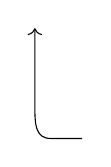
\begin{tikzpicture}\draw[->] (.6,0)--(.2,0) .. controls (0,0) and (0,.2) .. (0,.4)--(0,1.4);\end{tikzpicture}}}empty !

These reflections bring very near how much stronger the \var{\inserted{extra}}{\hand{extra}}{insertion}{ps_134-3_069-v0014} strictness
requi\var{\over[typed]{\unsure{t}}{r}}{r}{typewriter overwriting}{ps_134-3_069-v0015}ement T 2 for test categories, than merely the conditions T 1, T3
without T 2 .

40. Yesterday I incidentally made use of the fact that if A is an asphe-%
ric element in (Cat), th\var{\over[typed]{\unsure{a}}{e}}{e}{typewriter overwriting}{ps_134-3_069-v0016}n for any other object C, CxA \hand{\ensuremath{\longrightarrow}} C is aspheric
(and a fortiori a weak equivalence). The usual asphericity criterion for a
functor shows that it is enough to prove that for any C with final element,
\margin{\diagram{\begin{tikzpicture}\draw[->] (.6,1.4)--(.2,1.4) .. controls (0,1.4) and (0,1.2) .. (0,1)--(0,0);\end{tikzpicture}}}CxA is aspheric. \var{\xout{Thusxw}}{}{typewriter deletion}{ps_134-3_069-v0017} For this again it is enough to prove that the
projection CxA \hand{\ensuremath{\longrightarrow}} A is aspheric, which by localisation up\var{\over[typed]{n}{o}}{o}{typewriter overwriting}{ps_134-3_069-v0018}n A means that
the product categories \hand{.} Cx\hand{(}$A_{/a}$\hand{)} (with a in A) are aspheric. Finall\var{\over{\unsure{x}}{y}}{\hand{y}}{writing over}{ps_134-3_069-v0019} we
are reduced to checking that the product of two categories with final ele-%
ment is aspheric, which is trivial because such a category has itself a
final element.

The result just proved can be viewed as a particular case of the
following
\uline{Proposition} In (Cat), the cartesian product of two weak equivalences is
a weak equivalence.

%% END SOURCE ps_134-3_069
\ifnum\EditionMode=1
\psapparatusstart
\psentry{ps_134-3_069-v0001}{1}{writing over}{\over{a}{,}}{\hand{,}}{The superposed handwritten reading replaces the underlying reading.}
\psentry{ps_134-3_069-v0002}{2}{insertion}{\inserted{as}}{\hand{as}}{The handwritten insertion is incorporated at its indicated position; insertion brackets leave the running text.}
\psentry{ps_134-3_069-v0003}{3}{writing over}{\over{t}{d}}{\hand{d}}{The superposed handwritten reading replaces the underlying reading.}
\psentry{ps_134-3_069-v0004}{4}{typewriter overwriting}{\over[typed]{what}{which}}{which}{The superposed typed reading replaces the underlying reading.}
\psentry{ps_134-3_069-v0005}{5}{typewriter overwriting}{\over[typed]{t}{t}}{t}{The superposed typed reading replaces the underlying reading.}
\psentry{ps_134-3_069-v0006}{6}{typewriter overwriting}{\over[typed]{a}{2}}{2}{The superposed typed reading replaces the underlying reading.}
\psentry{ps_134-3_069-v0007}{7}{writing over}{\over{ill}{ould}}{\hand{ould}}{The superposed handwritten reading replaces the underlying reading.}
\psentry{ps_134-3_069-v0008}{8}{typewriter deletion}{\xout{subob}}{}{The typewriter strikes out this material; it leaves the corrected running text.}
\psentry{ps_134-3_069-v0009}{9}{typewriter overwriting}{\over[typed]{\unsure{q}}{a}}{a}{The superposed typed reading replaces the underlying reading.}
\psentry{ps_134-3_069-v0010}{10}{typewriter overwriting}{\over[typed]{t}{v}}{v}{The superposed typed reading replaces the underlying reading.}
\psentry{ps_134-3_069-v0011}{11}{typewriter overwriting}{\over[typed]{e}{o}}{o}{The superposed typed reading replaces the underlying reading.}
\psentry{ps_134-3_069-v0012}{12}{typewriter overwriting}{\over[typed]{t}{t}}{t}{The superposed typed reading replaces the underlying reading.}
\psentry{ps_134-3_069-v0013}{13}{typewriter overwriting}{\over[typed]{t}{t}}{t}{The superposed typed reading replaces the underlying reading.}
\psentry{ps_134-3_069-v0014}{14}{insertion}{\inserted{extra}}{\hand{extra}}{The handwritten insertion is incorporated at its indicated position; insertion brackets leave the running text.}
\psentry{ps_134-3_069-v0015}{15}{typewriter overwriting}{\over[typed]{\unsure{t}}{r}}{r}{The superposed typed reading replaces the underlying reading.}
\psentry{ps_134-3_069-v0016}{16}{typewriter overwriting}{\over[typed]{\unsure{a}}{e}}{e}{The superposed typed reading replaces the underlying reading.}
\psentry{ps_134-3_069-v0017}{17}{typewriter deletion}{\xout{Thusxw}}{}{The typewriter strikes out this material; it leaves the corrected running text.}
\psentry{ps_134-3_069-v0018}{18}{typewriter overwriting}{\over[typed]{n}{o}}{o}{The superposed typed reading replaces the underlying reading.}
\psentry{ps_134-3_069-v0019}{19}{writing over}{\over{\unsure{x}}{y}}{\hand{y}}{The superposed handwritten reading replaces the underlying reading.}
\psapparatusend
\fi
\pssource{ps_134-3_070}{134-3/70}{https://grothendieck.umontpellier.fr/web/viewer.html?file=../134-3.pdf\#page=71}
\psnumber{ps_134-3_070-v0001}{1}
\psnumber{ps_134-3_070-v0002}{2}
\psnumber{ps_134-3_070-v0003}{3}
\psnumber{ps_134-3_070-v0004}{4}
\psnumber{ps_134-3_070-v0005}{5}
\psnumber{ps_134-3_070-v0006}{6}
\psnumber{ps_134-3_070-v0007}{7}
\psnumber{ps_134-3_070-v0008}{8}
%% BEGIN SOURCE ps_134-3_070
% Pursuing Stacks (cotes 134-2 to 134-8): archive cote 134-3, site page 70 (PDF page 71), typescript page 70.
% typescript. Draft compared: ps2.tex:3616-3680.
% AI-transcribed by Claude Opus 5.5 (claude-opus-5-5, adaptive thinking, effort high), Message Batches API, batch ps1 (msgbatch_01Rv5hCaNTtUt4JHx1yqoHPL), 2026-11-12; image review recorded in records/CHECK_DECISIONS_134_3_4.tsv.
\scanpage{134-3/70}
\mspage{\hand{70}}

(We get the previous result by taking the weak equivalences $A\hand{\to} e_{(Cat)}$
and $id_C : C \hand{\to} C$.)  To prove the proposition,  we are immediately reduced
to the case when one of the two functors is \var{\xout{the}}{}{typewriter deletion}{ps_134-3_070-v0001} an identity functork  i.e.
proving the
\uline{Corollary 1}  If  $f$:  $A'\hand{\to} A$ is a weak equivalence in (Cat),  then for any
\var{\over{\unsure{E}}{C}}{\hand{C}}{writing over}{ps_134-3_070-v0002} in (Cat)  $f\hand{x}id_{\hand{C}}$ : $A'xC \hand{\to} AxC$  is a weak equivalence.

For proving this,  we view the functor $fxid_C$  as a morphism of catego-%
ries ``over C'',  which corresponds to a situation of a morphism of topo\var{\over[typed]{i}{i}}{i}{typewriter overwriting}{ps_134-3_070-v0003}
over a third one
% Hand-drawn arrows are marked blue; typed objects remain plain.
\diagram{\begin{tikzcd}[column sep=tiny]
X' \ar[color=blue,rr,"f"] \ar[color=blue,dr] \& \& X \ar[color=blue,dl] \\
\& Y \&
\end{tikzcd}}
\qquad ,

we will say that $f$ is a \uline{weak equivalence} \uline{relative to} $Y$ ,  if not only this
is a weak equivalence,  but remain\hand{s} so by any base change by a localization
functor
\[ Y_{/U} \hand{\to} U \]
giving rise to
\[ f_{/U} : X'_{/U} \hand{\to} X_{/U} \qquad . \]
As usual,  standar\var{\over{t}{d}}{\hand{d}}{writing over}{ps_134-3_070-v0004} arguments prove that it is enough to take $U$ in a set
of generators of the topos $Y$ .  In case $Y$ =  $C^{\hand{\overset{\wedge}{\wedge}}}$ ,  we may take $U$ in $C$ .
In case moreover  $X,X'$ are defined by sm\var{\over[typed]{\unsure{m}}{a}}{a}{typewriter overwriting}{ps_134-3_070-v0005}ll categories $P,P'$ and a functor
of categories over $C$
\diagram{\begin{tikzcd}[column sep=tiny]
P' \ar[color=blue,rr,"F"] \ar[color=blue,dr] \& \& P \ar[color=blue,dl] \\
\& C \&
\end{tikzcd}}
\qquad ,

this condition amounts to demanding that for any $c$ in $C$,  the induced func-%
tor
\[ F_{/c} : P'_{/c} \hand{\to} P_{/c} \]
be a weak equivalence.  In our case $P=AxC,P'=A'xC$, $F = fxid_C$ ,  the indu-%
ced functor can be identified with  $fx\,id_{C_{/c}}$  .  This reduces us,  for
proving the corollary, to the case when $C$ has a final element.  But consi-%
der now the commutative diagram
\diagram{\begin{tikzcd}
A'xC \ar[color=blue,r,"\hand{fxid_c}"] \ar[color=blue,d] \& A\var{\deleted{'}}{}{deletion}{ps_134-3_070-v0006}xC \ar[color=blue,d] \\
A' \ar[color=blue,r,"\hand{f}"] \& A
\end{tikzcd}}
\qquad ,
where the vertical arrows are the projections and hence,  by what was
proved before,  weak equivalences.  As $f$ is a weak equivalence,  it follows
that $fxid_C$ is a weak equivalence too,  qed.

T\var{\over[typed]{h}{h}}{h}{typewriter overwriting}{ps_134-3_070-v0007}e proposition above goes somewhat in the direction of looking at
``homotopy properties of (Cat)''  \var{\deleted{\illegible{1}}}{}{deletion}{ps_134-3_070-v0008} and ``how far (Cat) is from being a
closed model category in Quillen's sense''.  It is very suggestive \hand{for}

%% END SOURCE ps_134-3_070
\ifnum\EditionMode=1
\psapparatusstart
\psentry{ps_134-3_070-v0001}{1}{typewriter deletion}{\xout{the}}{}{The typewriter strikes out this material; it leaves the corrected running text.}
\psentry{ps_134-3_070-v0002}{2}{writing over}{\over{\unsure{E}}{C}}{\hand{C}}{The superposed handwritten reading replaces the underlying reading.}
\psentry{ps_134-3_070-v0003}{3}{typewriter overwriting}{\over[typed]{i}{i}}{i}{The superposed typed reading replaces the underlying reading.}
\psentry{ps_134-3_070-v0004}{4}{writing over}{\over{t}{d}}{\hand{d}}{The superposed handwritten reading replaces the underlying reading.}
\psentry{ps_134-3_070-v0005}{5}{typewriter overwriting}{\over[typed]{\unsure{m}}{a}}{a}{The superposed typed reading replaces the underlying reading.}
\psentry{ps_134-3_070-v0006}{6}{deletion}{$\deleted{'}$}{}{The author cancels this material by hand; it leaves the corrected running text.}
\psentry{ps_134-3_070-v0007}{7}{typewriter overwriting}{\over[typed]{h}{h}}{h}{The superposed typed reading replaces the underlying reading.}
\psentry{ps_134-3_070-v0008}{8}{deletion}{\deleted{\illegible{1}}}{}{The author cancels this material by hand; it leaves the corrected running text.}
\psapparatusend
\fi
\pssource{ps_134-3_071}{134-3/71}{https://grothendieck.umontpellier.fr/web/viewer.html?file=../134-3.pdf\#page=72}
\psnumber{ps_134-3_071-v0001}{1}
\psnumber{ps_134-3_071-v0002}{2}
\psnumber{ps_134-3_071-v0003}{3}
\psnumber{ps_134-3_071-v0004}{4}
\psnumber{ps_134-3_071-v0005}{5}
\psnumber{ps_134-3_071-v0006}{6}
\psnumber{ps_134-3_071-v0007}{7}
\psnumber{ps_134-3_071-v0008}{8}
\psnumber{ps_134-3_071-v0009}{9}
\psnumber{ps_134-3_071-v0010}{10}
\psnumber{ps_134-3_071-v0011}{11}
\psnumber{ps_134-3_071-v0012}{12}
\psnumber{ps_134-3_071-v0013}{13}
\psnumber{ps_134-3_071-v0014}{14}
\psnumber{ps_134-3_071-v0015}{15}
\psnumber{ps_134-3_071-v0016}{16}
\psnumber{ps_134-3_071-v0017}{17}
\psnumber{ps_134-3_071-v0018}{18}
\psnumber{ps_134-3_071-v0019}{19}
\psnumber{ps_134-3_071-v0020}{20}
\psnumber{ps_134-3_071-v0021}{21}
\psnumber{ps_134-3_071-v0022}{22}
\psnumber{ps_134-3_071-v0023}{23}
\psnumber{ps_134-3_071-v0024}{24}
%% BEGIN SOURCE ps_134-3_071
% Pursuing Stacks (cotes 134-2 to 134-8): archive cote 134-3, site page 71 (PDF page 72), typescript page 71.
% typescript. Draft compared: ps2.tex:3667-3729.
% AI-transcribed by Claude Opus 5.5 (claude-opus-5-5, adaptive thinking, effort high), Message Batches API, batch ps1 (msgbatch_01Rv5hCaNTtUt4JHx1yqoHPL), 2026-11-12; image review recorded in records/CHECK_DECISIONS_134_3_4.tsv.
\scanpage{134-3/71}
\mspage{71}
having a closer look at \var{\deleted{functors}}{}{deletion}{ps_134-3_071-v0001} \var{\inserted{maps}}{\hand{maps}}{insertion}{ps_134-3_071-v0002} f: $\var{\over{B}{B}}{\hand{B}}{writing over}{ps_134-3_071-v0003}^{\var{\deleted{\illegible{1}}}{}{deletion}{ps_134-3_071-v0004}}\hand{\to}$ A in (Cat) which are ``universal
\margin{X awkward}weak equivalences'' i.e. $W_{(\mathrm{Cat})}$ -aspheric\var{\inserted{(46)}}{\hand{(46)}}{insertion}{ps_134-3_071-v0005}, namely such that for \uline{any} map
in (Cat) $A'\hand{\to}A$ (not only a localization\var{\deleted{x}}{}{deletion}{ps_134-3_071-v0006} $A_{/a}\hand{\to}A$), the induced
functor $B'=B\mathrm{x}_A A'\hand{\to}A'$ is a weak equivalence. This property is a lot
stronger than just asphericity, and reminds of the ``trivial fibrations''
in Quillens theory. The usual criterion af asphericity for $B'\hand{\to}A'$ shows
that f is W-aspheric iff \var{\deleted{if}}{}{deletion}{ps_134-3_071-v0007} for any A' with final element, and any func-%
tor $A'\hand{\to}A$, the fiber product $B'=B\mathrm{x}_A A'$ is aspheric. T\var{\over[typed]{h}{h}}{h}{typewriter overwriting}{ps_134-3_071-v0008}e feeling here is
(suggested partly by Quillen's terminology) that this property is tied up
some way with the property for f to be a fibering(or cofibering ?) functor,
in the sense of fibered and cofibered categories, with aspheric fibers
moreover. Presumably fibered or cofibered categories \var{\inserted{[in the purely categorical sense]}}{\hand{[in the purely categorical sense]}}{insertion}{ps_134-3_071-v0009}, with``base change
functors'' which are weak equivalences, will play the part of Serre-Quil-%
len's fibrations - and it is still to be guessed what kind of \var{\deleted{categorical}}{}{deletion}{ps_134-3_071-v0010}
properties of a functor will play the part of \uline{co}fibrations. Apparently
they will have to be a lot more stringent than just monomorphisms in (Cat),
cf. \var{\deleted{p. 37.}}{}{deletion}{ps_134-3_071-v0011} \hand{Section 30 [and (9)]}.

\margin{\diagram{\begin{tikzpicture}\draw[->] (.6,0)--(.2,0) .. controls (0,0) and (0,.2) .. (0,.4)--(0,1.3);\end{tikzpicture}}}H\var{\over[typed]{e}{o}}{o}{typewriter overwriting}{ps_134-3_071-v0012}\var{\over[typed]{w}{w}}{w}{typewriter overwriting}{ps_134-3_071-v0013}ever I feel it is not time yet to dive into the homotopy theory
properties of the all-encompassing basic modelizer (Cat), but rather come
back to the study of general (and less gene\var{\over[typed]{f}{r}}{r}{typewriter overwriting}{ps_134-3_071-v0014}al) test categories.

\margin{\diagram{\begin{tikzpicture}\draw[->] (.6,1.3)--(.2,1.3) .. controls (0,1.3) and (0,1.1) .. (0,.9)--(0,0);\end{tikzpicture}}}41. One comment \var{\inserted{still,}}{\hand{still,}}{insertion}{ps_134-3_071-v0015} upon the role played in the theory I am developping of
the \hand{``}assumption\hand{''}(p.30) that the category of autoequivalences of (Hot) is
equivalent to the final category. This assumption has been a crucial
guide for putting the emphasis where it really belongs, namely upon
the set \var{\deleted{of}}{}{deletion}{ps_134-3_071-v0016} $W\hand{\subset}\mathrm{Fl}(M)$ of weak equivalences within a category M which one
would like to take in some sense as a category of models for homotopy
types - the functors $M\hand{\to}$(Hot) following along auto\var{\over[typed]{h}{m}}{m}{typewriter overwriting}{ps_134-3_071-v0017}atically. However,
in no statement whatever I proved so far, was this assumption ever used\var{\over{.}{!}}{\hand{!}}{writing over}{ps_134-3_071-v0018}
\var{\deleted{However,}}{}{deletion}{ps_134-3_071-v0019}\var{\inserted{On the other hand,}}{\hand{On the other hand,}}{insertion}{ps_134-3_071-v0020} the notion of a \uline{modelizer} introduced in the wake of the \hand{``}assumpti-%
on\hand{''} (cf. \hand{\S.28}) was tacitly changed during the reflection, by drapping al-%
together the condition a) of (strong) saturation of W, namely that W is
just the set of arrows\unsure{\hand{,}} made invertible by the localization functor $M\hand{\to}W^{-1}M$.
Instead of this, it turned out that the saturation condition we really had
at hands and which \var{\xout{were}}{}{typewriter deletion}{ps_134-3_071-v0021} was adequate for working, was the conditions
a) to c) I finally wrote \var{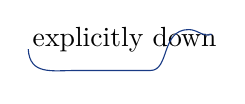
\begin{tikzpicture}[baseline=(t.base)]\node[anchor=base west,inner sep=0pt] (t) at (0,0) {explicitly down};\draw[color=blue] (-.05,-.03) .. controls (-.03,-.36) and (.25,-.30) .. (.55,-.30)--(1.50,-.30) .. controls (1.75,-.30) and (1.63,.22) .. (1.99,.22) .. controls (2.10,.22) and (2.17,.12) .. (2.28,.16);\end{tikzpicture}}{down explicitly}{authorial transposition}{ps_134-3_071-v0022} yesterday (\hand{\S.37}). As for the
strong saturation condition, for the time being (using nothing but what
has actually be\var{\inserted{en}}{\hand{en}}{insertion}{ps_134-3_071-v0023} proved\var{\deleted{\illegible{1}}}{}{deletion}{ps_134-3_071-v0024} so far, without reference to ``well known facts''
from homotopy theory)\hand{,} it is not even clear that the basic modelizer
(Cat) is one in the initial sense, namely that the set of weak equivalen-

%% END SOURCE ps_134-3_071
\ifnum\EditionMode=1
\psapparatusstart
\psentry{ps_134-3_071-v0001}{1}{deletion}{\deleted{functors}}{}{The author cancels this material by hand; it leaves the corrected running text.}
\psentry{ps_134-3_071-v0002}{2}{insertion}{\inserted{maps}}{\hand{maps}}{The handwritten insertion is incorporated at its indicated position; insertion brackets leave the running text.}
\psentry{ps_134-3_071-v0003}{3}{writing over}{$\over{B}{B}$}{$\hand{B}$}{The superposed handwritten reading replaces the underlying reading.}
\psentry{ps_134-3_071-v0004}{4}{deletion}{$\deleted{\illegible{1}}$}{}{The author cancels this material by hand; it leaves the corrected running text.}
\psentry{ps_134-3_071-v0005}{5}{insertion}{\inserted{(46)}}{\hand{(46)}}{The handwritten insertion is incorporated at its indicated position; insertion brackets leave the running text.}
\psentry{ps_134-3_071-v0006}{6}{deletion}{\deleted{x}}{}{The author cancels this material by hand; it leaves the corrected running text.}
\psentry{ps_134-3_071-v0007}{7}{deletion}{\deleted{if}}{}{The author cancels this material by hand; it leaves the corrected running text.}
\psentry{ps_134-3_071-v0008}{8}{typewriter overwriting}{\over[typed]{h}{h}}{h}{The superposed typed reading replaces the underlying reading.}
\psentry{ps_134-3_071-v0009}{9}{insertion}{\inserted{[in the purely categorical sense]}}{\hand{[in the purely categorical sense]}}{The handwritten insertion is incorporated at its indicated position; insertion brackets leave the running text.}
\psentry{ps_134-3_071-v0010}{10}{deletion}{\deleted{categorical}}{}{The author cancels this material by hand; it leaves the corrected running text.}
\psentry{ps_134-3_071-v0011}{11}{deletion}{\deleted{p. 37.}}{}{The author cancels this material by hand; it leaves the corrected running text.}
\psentry{ps_134-3_071-v0012}{12}{typewriter overwriting}{\over[typed]{e}{o}}{o}{The superposed typed reading replaces the underlying reading.}
\psentry{ps_134-3_071-v0013}{13}{typewriter overwriting}{\over[typed]{w}{w}}{w}{The superposed typed reading replaces the underlying reading.}
\psentry{ps_134-3_071-v0014}{14}{typewriter overwriting}{\over[typed]{f}{r}}{r}{The superposed typed reading replaces the underlying reading.}
\psentry{ps_134-3_071-v0015}{15}{insertion}{\inserted{still,}}{\hand{still,}}{The handwritten insertion is incorporated at its indicated position; insertion brackets leave the running text.}
\psentry{ps_134-3_071-v0016}{16}{deletion}{\deleted{of}}{}{The author cancels this material by hand; it leaves the corrected running text.}
\psentry{ps_134-3_071-v0017}{17}{typewriter overwriting}{\over[typed]{h}{m}}{m}{The superposed typed reading replaces the underlying reading.}
\psentry{ps_134-3_071-v0018}{18}{writing over}{\over{.}{!}}{\hand{!}}{The superposed handwritten reading replaces the underlying reading.}
\psentry{ps_134-3_071-v0019}{19}{deletion}{\deleted{However,}}{}{The author cancels this material by hand; it leaves the corrected running text.}
\psentry{ps_134-3_071-v0020}{20}{insertion}{\inserted{On the other hand,}}{\hand{On the other hand,}}{The handwritten insertion is incorporated at its indicated position; insertion brackets leave the running text.}
\psentry{ps_134-3_071-v0021}{21}{typewriter deletion}{\xout{were}}{}{The typewriter strikes out this material; it leaves the corrected running text.}
\psentry{ps_134-3_071-v0022}{22}{authorial transposition}{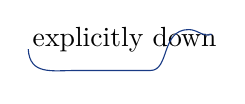
\begin{tikzpicture}[baseline=(t.base)]\node[anchor=base west,inner sep=0pt] (t) at (0,0) {explicitly down};\draw[color=blue] (-.05,-.03) .. controls (-.03,-.36) and (.25,-.30) .. (.55,-.30)--(1.50,-.30) .. controls (1.75,-.30) and (1.63,.22) .. (1.99,.22) .. controls (2.10,.22) and (2.17,.12) .. (2.28,.16);\end{tikzpicture}}{down explicitly}{The continuous pen curve under explicitly and over the beginning of down exchanges their typed order. Diplomatic retains the typed order and the graphic.}
\psentry{ps_134-3_071-v0023}{23}{insertion}{\inserted{en}}{\hand{en}}{The handwritten insertion is incorporated at its indicated position; insertion brackets leave the running text.}
\psentry{ps_134-3_071-v0024}{24}{deletion}{\deleted{\illegible{1}}}{}{The author cancels this material by hand; it leaves the corrected running text.}
\psapparatusend
\fi
\pssource{ps_134-3_072}{134-3/72}{https://grothendieck.umontpellier.fr/web/viewer.html?file=../134-3.pdf\#page=73}
\psnumber{ps_134-3_072-v0001}{1}
\psnumber{ps_134-3_072-v0002}{2}
\psnumber{ps_134-3_072-v0003}{3}
\psnumber{ps_134-3_072-v0004}{4}
\psnumber{ps_134-3_072-v0005}{5}
\psnumber{ps_134-3_072-v0006}{6}
\psnumber{ps_134-3_072-v0007}{7}
\psnumber{ps_134-3_072-v0008}{8}
\psnumber{ps_134-3_072-v0009}{9}
\psnumber{ps_134-3_072-v0010}{10}
\psnumber{ps_134-3_072-v0011}{11}
\psnumber{ps_134-3_072-v0012}{12}
\psnumber{ps_134-3_072-v0013}{13}
\psnumber{ps_134-3_072-v0014}{14}
\psnumber{ps_134-3_072-v0015}{15}
\psnumber{ps_134-3_072-v0016}{16}
\psnumber{ps_134-3_072-v0017}{17}
\psnumber{ps_134-3_072-v0018}{18}
\psnumber{ps_134-3_072-v0019}{19}
%% BEGIN SOURCE ps_134-3_072
% Pursuing Stacks (cotes 134-2 to 134-8): archive cote 134-3, site page 72 (PDF page 73), typescript page 72.
% typescript. Draft compared: ps2.tex:3717-3785.
% AI-transcribed by Claude Opus 5.5 (claude-opus-5-5, adaptive thinking, effort high), Message Batches API, batch ps1 (msgbatch_01Rv5hCaNTtUt4JHx1yqoHPL), 2026-11-12; image review recorded in records/CHECK_DECISIONS_134_3_4.tsv.
\scanpage{134-3/72}
\mspage{\hand{72}}

\margin{$\ast$ cf \unsure{th} p. \uline{VIII}}ces in (Cat) is strongly saturated\hand{(47)}\hand{.} However, from the known relation
between Cat and an elementary modelizer $A^{\hand{\wedge}}$, it follows that $W_{(\mathrm{Cat})}$ is
strongly saturated iff $W_A \hand{\subset} \mathrm{Fl}(A\var{\over{\unsure{?}}{{}^{\wedge}}}{\hand{{}^{\wedge}}}{writing over}{ps_134-3_072-v0001})$ is. This implies that it is enough to
prove strong saturation in \uline{one} elementary modelizer $A^{\hand{\wedge}}$, to deduce it in
all others, as well as in (Cat). However, in the case at least when
$A = \hand{\Delta}$, it is indeed "well-known" that \var{\inserted[typed]{the}}{the}{typed insertion}{ps_134-3_072-v0002} weak equivalences in $A^{\hand{\wedge}}$ satisfy the
strong saturation condition. In\var{\deleted{t}}{}{deletion}{ps_134-3_072-v0003} terms of Quillen's set-up, it follows
from the fact that $\hand{\Delta}^{\hand{\wedge}}$ is a "closed model category" , and prop.1 in I 5.5.
of Quillen's expos\'e. The only thing which is not quite understood, not by
me at any rate, is why $\hand{\Delta}^{\hand{\wedge}}$ \uline{is} indeed a closed model category - Quillen\hand{'}s
proof it seems relies strongly on typical simplicial techniques. I'll have
to look if the present set-up will suggest a more conceptual proof, valid
possibly for any test category (or at least, any strict test category).
I'll have to come back upon this later\hand{.} \var{\xout{after}}{}{typewriter deletion}{ps_134-3_072-v0004} For the time being, I feel
a greater urge still to understand about the relationship between different
test categories\hand{,} - also\hand{,} I did not really finish with my review of what
may be viewed as \var{\inserted{the}}{\hand{the}}{insertion}{ps_134-3_072-v0005} "standart\hand{"} test categories\var{\deleted{"}}{}{deletion}{ps_134-3_072-v0006} such as $\hand{\Delta}$, $\hand{\square}$ and their vari-%
ants.

25.3.

42. In the notes last time I made clear what finally has turned out for
me to correspond to the appelation of a "modelizer", as prompted by the
internal logics of the situations I was looking at, in terms of the infor-%
mation available to me. I should by then have added what a \uline{model-preser-}%
\uline{ving} \var{\inserted{(or \uline{modelizing})}}{\hand{(or \uline{modelizing})}}{insertion}{ps_134-3_072-v0007} \uline{functor} between modelizers (M,W) and (M',W') has turned out to mean,
which has undergone a corresponding change with respect \var{\xout{of}}{}{typewriter deletion}{ps_134-3_072-v0008} to what I first
contemplated calling by that name (\hand{\S.28}). Namely here it turned out that
I should be more stringent for this notion, replacing the condition
$f(W) \hand{\subset} W'$ by the stronger one
\[ W = f^{-1}(W') \quad , \]
and moreover, of course, still demanding that the corresponding functor
\[ W^{-1}M \hand{\to} W'^{-1}M' \]
should be an equivalence. It is by now established \var{\deleted{that}}{}{deletion}{ps_134-3_072-v0009}, with \var{\inserted[typed]{the}}{the}{typed insertion}{ps_134-3_072-v0010} \var{\xout{one}}{}{typewriter deletion}{ps_134-3_072-v0011} excep-%
tion of just \var{\inserted[typed]{the two}}{the two}{typed insertion}{ps_134-3_072-v0012} \var{\xout{one}}{}{typewriter deletion}{ps_134-3_072-v0013}, \var{\inserted[typed]{first,}}{first,}{typed insertion}{ps_134-3_072-v0014} \var{\inserted{that,}}{\hand{that,}}{insertion}{ps_134-3_072-v0015} all the functors occuring in the diagram on p.31 are
indeed model\var{\xout{izing}}{}{typewriter deletion}{ps_134-3_072-v0016} preserving, namely it is so for $\hand{\alpha}$, $\hand{\beta}$, $\hand{\xi}$, $\hand{\eta}$ - and also
the right adjoints to $\hand{\xi}$, $\hand{\eta}$, as expected by then. It should be more or \var{\xout{xx}}{}{typewriter deletion}{ps_134-3_072-v0017}
less trivial that the first of the functors in this diagram, namely
the canonical inclusion (Ord)$\hand{\longrightarrow}$(Preord), as well as the left adjoint
from (Preord) to (Ord), are model preserving - except for the fact that it
has not been yet established that these two categories are indeed modeli\var{\xout{xx}}{}{typewriter deletion}{ps_134-3_072-v0018}
zers (for the natural notion of weak equivalences, induce\var{\over[typed]{s}{d}}{d}{typewriter overwriting}{ps_134-3_072-v0019} from (Cat))\hand{,}

%% END SOURCE ps_134-3_072
\ifnum\EditionMode=1
\psapparatusstart
\psentry{ps_134-3_072-v0001}{1}{writing over}{$\over{\unsure{?}}{{}^{\wedge}}$}{$\hand{{}^{\wedge}}$}{The superposed handwritten reading replaces the underlying reading.}
\psentry{ps_134-3_072-v0002}{2}{typed insertion}{\inserted[typed]{the}}{the}{The typed insertion is incorporated at its indicated position; insertion brackets leave the running text.}
\psentry{ps_134-3_072-v0003}{3}{deletion}{\deleted{t}}{}{The author cancels this material by hand; it leaves the corrected running text.}
\psentry{ps_134-3_072-v0004}{4}{typewriter deletion}{\xout{after}}{}{The typewriter strikes out this material; it leaves the corrected running text.}
\psentry{ps_134-3_072-v0005}{5}{insertion}{\inserted{the}}{\hand{the}}{The handwritten insertion is incorporated at its indicated position; insertion brackets leave the running text.}
\psentry{ps_134-3_072-v0006}{6}{deletion}{\deleted{"}}{}{The author cancels this material by hand; it leaves the corrected running text.}
\psentry{ps_134-3_072-v0007}{7}{insertion}{\inserted{(or \uline{modelizing})}}{\hand{(or \uline{modelizing})}}{The handwritten insertion is incorporated at its indicated position; insertion brackets leave the running text.}
\psentry{ps_134-3_072-v0008}{8}{typewriter deletion}{\xout{of}}{}{The typewriter strikes out this material; it leaves the corrected running text.}
\psentry{ps_134-3_072-v0009}{9}{deletion}{\deleted{that}}{}{The author cancels this material by hand; it leaves the corrected running text.}
\psentry{ps_134-3_072-v0010}{10}{typed insertion}{\inserted[typed]{the}}{the}{The typed insertion is incorporated at its indicated position; insertion brackets leave the running text.}
\psentry{ps_134-3_072-v0011}{11}{typewriter deletion}{\xout{one}}{}{The typewriter strikes out this material; it leaves the corrected running text.}
\psentry{ps_134-3_072-v0012}{12}{typed insertion}{\inserted[typed]{the two}}{the two}{The typed insertion is incorporated at its indicated position; insertion brackets leave the running text.}
\psentry{ps_134-3_072-v0013}{13}{typewriter deletion}{\xout{one}}{}{The typewriter strikes out this material; it leaves the corrected running text.}
\psentry{ps_134-3_072-v0014}{14}{typed insertion}{\inserted[typed]{first,}}{first,}{The typed insertion is incorporated at its indicated position; insertion brackets leave the running text.}
\psentry{ps_134-3_072-v0015}{15}{insertion}{\inserted{that,}}{\hand{that,}}{The handwritten insertion is incorporated at its indicated position; insertion brackets leave the running text.}
\psentry{ps_134-3_072-v0016}{16}{typewriter deletion}{\xout{izing}}{}{The typewriter strikes out this material; it leaves the corrected running text.}
\psentry{ps_134-3_072-v0017}{17}{typewriter deletion}{\xout{xx}}{}{The typewriter strikes out this material; it leaves the corrected running text.}
\psentry{ps_134-3_072-v0018}{18}{typewriter deletion}{\xout{xx}}{}{The typewriter strikes out this material; it leaves the corrected running text.}
\psentry{ps_134-3_072-v0019}{19}{typewriter overwriting}{\over[typed]{s}{d}}{d}{The superposed typed reading replaces the underlying reading.}
\psapparatusend
\fi
\pssource{ps_134-3_073}{134-3/73}{https://grothendieck.umontpellier.fr/web/viewer.html?file=../134-3.pdf\#page=74}
\psnumber{ps_134-3_073-v0001}{1}
\psnumber{ps_134-3_073-v0002}{2}
\psnumber{ps_134-3_073-v0003}{3}
\psnumber{ps_134-3_073-v0004}{4}
\psnumber{ps_134-3_073-v0005}{5}
\psnumber{ps_134-3_073-v0006}{6}
\psnumber{ps_134-3_073-v0007}{7}
\psnumber{ps_134-3_073-v0008}{8}
\psnumber{ps_134-3_073-v0009}{9}
\psnumber{ps_134-3_073-v0010}{10}
\psnumber{ps_134-3_073-v0011}{11}
\psnumber{ps_134-3_073-v0012}{12}
\psnumber{ps_134-3_073-v0013}{13}
\psnumber{ps_134-3_073-v0014}{14}
\psnumber{ps_134-3_073-v0015}{15}
\psnumber{ps_134-3_073-v0016}{16}
\psnumber{ps_134-3_073-v0017}{17}
\psnumber{ps_134-3_073-v0018}{18}
\psnumber{ps_134-3_073-v0019}{19}
%% BEGIN SOURCE ps_134-3_073
% Pursuing Stacks (cotes 134-2 to 134-8): archive cote 134-3, site page 73 (PDF page 74), typescript page 73.
% typescript. Draft compared: ps2.tex:3773-3835.
% AI-transcribed by Claude Opus 5.5 (claude-opus-5-5, adaptive thinking, effort high), Message Batches API, batch ps1 (msgbatch_01Rv5hCaNTtUt4JHx1yqoHPL), 2026-11-12; image review recorded in records/CHECK_DECISIONS_134_3_4.tsv.
\scanpage{134-3/73}
\mspage{\hand{73}}

namely that the localized categories with respect to weak equivalences are
indeed equivalent to (Hot). T\var{\over[typed]{h}{h}}{h}{typewriter overwriting}{ps_134-3_073-v0001}e only natural way one might think of this
to be proved, is by proving that the inclusion functor from either into
(Cat) induces an equivalence between the localizations, which would imply
at the same time that th\var{\over[typed]{e}{i}}{i}{typewriter overwriting}{ps_134-3_073-v0002}s inclusion functor is indeed model-preserving,
and hence that all the functors in the diagram of p.31 are model preserving
functors between modelizers. I still do believe this should be so, and
want to give \var{\inserted[typed]{below}}{below}{typed insertion}{ps_134-3_073-v0003} a reflection which might lead to a proof of this.

Before, there is still one noteworthy circumstance I want to emphasize
% NOTE: the right edge of the scan cuts the ends of several typed lines (after "emphasize", "autoequi", "equi", "equivalenc")
Namely, it occured in a number of instances that we got in a rather natu-%
ral way several modelizing functors between \var{\inserted[typed]{two}}{two}{typed insertion}{ps_134-3_073-v0004} modelizers $(M,W)$ and $(M',W')$,
in one direction or the other - for instance from \var{\over{A}{(}}{\hand{(}}{writing over}{ps_134-3_073-v0005}Cat) to $A^{\hand{\wedge}}$ using
different functors $i: A \hand{\to} (Cat)$, or from $A^{\hand{\wedge}}$ to (Cat) using $a \hand{\mapsto} A_{/a}$ .
It turned out that the corresponding functors between $W^{-1}M$ and $W'^{-1}M'$ were
always canonically isomorphic \var{\deleted{if}}{}{deletion}{ps_134-3_073-v0006} \var{\inserted{when}}{\hand{when}}{insertion}{ps_134-3_073-v0007} in the same direction, \var{\over[typed]{\illegible{1}}{are}}{are}{typewriter overwriting}{ps_134-3_073-v0008} quasi-inverse
of each other \var{\deleted{if}}{}{deletion}{ps_134-3_073-v0009} \var{\inserted{when}}{\hand{when}}{insertion}{ps_134-3_073-v0010} in opposite directions. This is indeed very much in the
spirit of the``inspiring assumption'' of p.30, that the category of autoequi
valences of (Hot) is equivalent to the unit category, which implies indeed
that for two categories $H,H'$ equivalent to (Hot), \var{\xout{there exists a}}{}{typewriter deletion}{ps_134-3_073-v0011} for two equi
valences from $H$ to $H'$, there is a unique isomorphism between them. Quite
similarly, there have been a number of situations (more or less summed up
in the end in the ``key theorem'' of p.61) when \var{\inserted[typed]{by localization}}{by localization}{typed insertion}{ps_134-3_073-v0012} we got a natural functor $f$
from some $W^{-1}M$ to another $W'^{-1}M'$, and another \var{\inserted[typed]{$F$}}{$F$}{typed insertion}{ps_134-3_073-v0013} which is known already to be
an equivalence, and it turns out that $f$ is isomorphic to \var{\over[typed]{$f$}{$F$}}{$F$}{typewriter overwriting}{ps_134-3_073-v0014} (and in fact,
then, canonically so) iff f\unsure{\var{\over[typed]{ro}{or}}{or}{typewriter overwriting}{ps_134-3_073-v0015}} any object $x$ in the source category, $f(x)$
and $F(x)$ are isomorphic. This suggests that \uline{presumably}, \uline{every functor}
\uline{from} (Hot) \uline{into itself}, \uline{transforming every object into an isomorphic one},
\uline{is in fact isomorphic to the identity functor}.

I want now to make a comment, implying that there are many full sub-%
categories $M$ of (Cat), such that for the induced notion of weak equivalenc
$M$ becomes a modelizer, and the inclusion functor a modelizing functor -
or, what amount to the same, that the canonical functor
\[ {W_M}^{-1}M \hand{\longrightarrow} {W_{Cat}}^{-1}(Cat) = (Hot) \]
is an equivalence. To see this, let more generally $(M,W)$ be any catego-%
ry endowed with a subset $W \hand{\subset} Fl(M)$, and let $h: M \hand{\longrightarrow} M$ be a functor such
that $h(W) \hand{\subset} W$, and such that the induced functor $W^{-1}M \hand{\to} W^{-1}M$ is an equiva-%
lence. Let \var{\xout{on the other hand}}{}{typewriter deletion}{ps_134-3_073-v0016} \var{\inserted[typed]{now}}{now}{typed insertion}{ps_134-3_073-v0017} $M'$ be any full subcategory of $M$ such that
$h$ factors through $M'$ , let $h': M \hand{\to} M'$ be the corresponding \var{\inserted{induced}}{\hand{induced}}{insertion}{ps_134-3_073-v0018} functor, and
$W' = W \hand{\cap} Fl(M')$. Then it is formal that \var{\xout{h and h}}{}{typewriter deletion}{ps_134-3_073-v0019} the inclusion $g: M' \hand{\to} M$

%% END SOURCE ps_134-3_073
\ifnum\EditionMode=1
\psapparatusstart
\psentry{ps_134-3_073-v0001}{1}{typewriter overwriting}{\over[typed]{h}{h}}{h}{The superposed typed reading replaces the underlying reading.}
\psentry{ps_134-3_073-v0002}{2}{typewriter overwriting}{\over[typed]{e}{i}}{i}{The superposed typed reading replaces the underlying reading.}
\psentry{ps_134-3_073-v0003}{3}{typed insertion}{\inserted[typed]{below}}{below}{The typed insertion is incorporated at its indicated position; insertion brackets leave the running text.}
\psentry{ps_134-3_073-v0004}{4}{typed insertion}{\inserted[typed]{two}}{two}{The typed insertion is incorporated at its indicated position; insertion brackets leave the running text.}
\psentry{ps_134-3_073-v0005}{5}{writing over}{\over{A}{(}}{\hand{(}}{The superposed handwritten reading replaces the underlying reading.}
\psentry{ps_134-3_073-v0006}{6}{deletion}{\deleted{if}}{}{The author cancels this material by hand; it leaves the corrected running text.}
\psentry{ps_134-3_073-v0007}{7}{insertion}{\inserted{when}}{\hand{when}}{The handwritten insertion is incorporated at its indicated position; insertion brackets leave the running text.}
\psentry{ps_134-3_073-v0008}{8}{typewriter overwriting}{\over[typed]{\illegible{1}}{are}}{are}{The superposed typed reading replaces the underlying reading.}
\psentry{ps_134-3_073-v0009}{9}{deletion}{\deleted{if}}{}{The author cancels this material by hand; it leaves the corrected running text.}
\psentry{ps_134-3_073-v0010}{10}{insertion}{\inserted{when}}{\hand{when}}{The handwritten insertion is incorporated at its indicated position; insertion brackets leave the running text.}
\psentry{ps_134-3_073-v0011}{11}{typewriter deletion}{\xout{there exists a}}{}{The typewriter strikes out this material; it leaves the corrected running text.}
\psentry{ps_134-3_073-v0012}{12}{typed insertion}{\inserted[typed]{by localization}}{by localization}{The typed insertion is incorporated at its indicated position; insertion brackets leave the running text.}
\psentry{ps_134-3_073-v0013}{13}{typed insertion}{\inserted[typed]{$F$}}{$F$}{The typed insertion is incorporated at its indicated position; insertion brackets leave the running text.}
\psentry{ps_134-3_073-v0014}{14}{typewriter overwriting}{\over[typed]{$f$}{$F$}}{$F$}{The superposed typed reading replaces the underlying reading.}
\psentry{ps_134-3_073-v0015}{15}{typewriter overwriting}{\over[typed]{ro}{or}}{or}{The superposed typed reading replaces the underlying reading.}
\psentry{ps_134-3_073-v0016}{16}{typewriter deletion}{\xout{on the other hand}}{}{The typewriter strikes out this material; it leaves the corrected running text.}
\psentry{ps_134-3_073-v0017}{17}{typed insertion}{\inserted[typed]{now}}{now}{The typed insertion is incorporated at its indicated position; insertion brackets leave the running text.}
\psentry{ps_134-3_073-v0018}{18}{insertion}{\inserted{induced}}{\hand{induced}}{The handwritten insertion is incorporated at its indicated position; insertion brackets leave the running text.}
\psentry{ps_134-3_073-v0019}{19}{typewriter deletion}{\xout{h and h}}{}{The typewriter strikes out this material; it leaves the corrected running text.}
\psapparatusend
\fi
\pssource{ps_134-3_074}{134-3/74}{https://grothendieck.umontpellier.fr/web/viewer.html?file=../134-3.pdf\#page=75}
\psnumber{ps_134-3_074-v0001}{1}
\psnumber{ps_134-3_074-v0002}{2}
\psnumber{ps_134-3_074-v0003}{3}
\psnumber{ps_134-3_074-v0004}{4}
\psnumber{ps_134-3_074-v0005}{5}
\psnumber{ps_134-3_074-v0006}{6}
\psnumber{ps_134-3_074-v0007}{7}
\psnumber{ps_134-3_074-v0008}{8}
\psnumber{ps_134-3_074-v0009}{9}
\psnumber{ps_134-3_074-v0010}{10}
\psnumber{ps_134-3_074-v0011}{11}
\psnumber{ps_134-3_074-v0012}{12}
\psnumber{ps_134-3_074-v0013}{13}
\psnumber{ps_134-3_074-v0014}{14}
\psnumber{ps_134-3_074-v0015}{15}
\psnumber{ps_134-3_074-v0016}{16}
\psnumber{ps_134-3_074-v0017}{17}
\psnumber{ps_134-3_074-v0018}{18}
\psnumber{ps_134-3_074-v0019}{19}
\psnumber{ps_134-3_074-v0020}{20}
\psnumber{ps_134-3_074-v0021}{21}
\psnumber{ps_134-3_074-v0022}{22}
\psnumber{ps_134-3_074-v0023}{23}
\psnumber{ps_134-3_074-v0024}{24}
\psnumber{ps_134-3_074-v0025}{25}
\psnumber{ps_134-3_074-v0026}{26}
\psnumber{ps_134-3_074-v0027}{27}
%% BEGIN SOURCE ps_134-3_074
% Pursuing Stacks (cotes 134-2 to 134-8): archive cote 134-3, site page 74 (PDF page 75), typescript page 74.
% typescript. Draft compared: ps2.tex:3821-3890.
% AI-transcribed by Claude Opus 5.5 (claude-opus-5-5, adaptive thinking, effort high), Message Batches API, batch ps1 (msgbatch_01Rv5hCaNTtUt4JHx1yqoHPL), 2026-11-12; image review recorded in records/CHECK_DECISIONS_134_3_4.tsv.
\scanpage{134-3/74}
\mspage{\hand{74}}
and h'\var{\inserted{$:M\mathrel{\rule{.45cm}{.35pt}} M'$}}{\hand{$:M\mathrel{\rule{.45cm}{.35pt}} M'$}}{insertion}{ps_134-3_074-v0001} induce functors between $W'^{-1}M'$ and $W^{-1}M$, which are quasi-inverse
to each other - hence these two categories are equivalent. In case
(M,W) is a mode\unsure{\var{\over[typed]{h}{l}}{l}{typewriter overwriting}{ps_134-3_074-v0002}}izer, this implies that (M',W') is a modelizer too and the
\var{\inserted[typed]{inclusion}}{inclusion}{typed insertion}{ps_134-3_074-v0003} functor\var{\xout{s}}{}{typewriter deletion}{ps_134-3_074-v0004} g, as well as h', are model\var{\xout{s}}{}{typewriter deletion}{ps_134-3_074-v0005} preserving.

We can apply this remark to \var{\over[typed]{\unsure{M}}{t}}{t}{typewriter overwriting}{ps_134-3_074-v0006}he modelizer (Cat), and to the functor
\[ i_A\, i^{*} : (Cat) \hand{\longrightarrow} (Cat) \]
defined by any functor i: $A\hand{\longrightarrow}$ (Cat) satisfying the conditions of the
``key theorem'' (\hand{\S}. \var{\over{5}{3}}{\hand{3}}{writing over}{ps_134-3_074-v0007}\var{\over{7}{7}}{\hand{7}}{writing over}{ps_134-3_074-v0008}), for instance the functor $i_A\hand{|}A$ : $a\hand{\longmapsto} A_{/a}$
(where A is any test category). We get the following
\uline{Proposition} Let M be any full subcategory of (Cat), assume there exists
a test-category A such that for any F in $A^{\hand{\wedge}}$, the category $A_{/F}$ belongs to
M (i.e. the functor $i_A$ : $A^{\hand{\wedge}}\hand{\longrightarrow}$ (Cat) , $F\hand{\longmapsto} A_{/F}$ , factors through M). \var{\xout{Then}}{}{typewriter deletion}{ps_134-3_074-v0009}
Let $W_M$ be the set of weak equivalences in M . Then $(M,W_M)$ is a \var{\xout{test cate-}}{}{typewriter deletion}{ps_134-3_074-v0010}%
\var{\xout{gory}}{}{typewriter deletion}{ps_134-3_074-v0011} \var{\inserted[typed]{modelizer}}{modelizer}{typed insertion}{ps_134-3_074-v0012} and the inclusion functor $M\hand{\to}$ (Cat) is model preserving.

T\var{\over[typed]{h}{h}}{h}{typewriter overwriting}{ps_134-3_074-v0013}e same of course will be true for any full subcategory of (Cat) con-
taining M - which makes an impressive bunch of modelizers indeed ! When
\var{\inserted[typed]{the test category}}{the test category}{typed insertion}{ps_134-3_074-v0014} A is given, one natural choice for M is to take all categories \var{\inserted{C}}{\hand{C}}{insertion}{ps_134-3_074-v0015} which are
``locally isomorphic to A '' , namely such that for any x in C, the indu-
ced category $C_{/x}$ be isomorphic to a category of the type $A_{/a}$ , with a in
A .

It would be tempting to apply this result to the full subcategory
(Ord) of (Cat) - but for this to be feasible, would mean exactly that
there exists a test-category A defined by an ordered set \var{\inserted{\deleted{(or at least ``locally ordered'')}}}{\hand{}}{insertion}{ps_134-3_074-v0016}. To see whether
there exists indeed such an ordered set looks like a rather interesting
question - maybe it would give rise to \var{\inserted[typed]{algebraic}}{algebraic}{typed insertion}{ps_134-3_074-v0017} models for homotopy types, sim-
pler than those used so far, namely simplicial and cubical complexes and
multicomplexes. It is interesting to note that if such a test category
should exist, it will \uline{not} be in any case a strict test category. Indeed,
the topos $A^{\hand{\wedge}}$ associated to an ordered set A can be viewed also, as we saw
before (\hand{\S}.\var{\over{\unsure{1}}{2}}{\hand{2}}{writing over}{ps_134-3_074-v0018}\var{\over{2}{2}}{\hand{2}}{writing over}{ps_134-3_074-v0019}), as associated to \var{\inserted[typed]{a suitable}}{a suitable}{typed insertion}{ps_134-3_074-v0020} \var{\deleted{the}}{}{deletion}{ps_134-3_074-v0021} topological space (namely A endowed
with a suitable topology, the open sets being just the``cribles'' in A).
But we have seen that the topos associated to a topological space \uline{cannot}
be \uline{strictly} modelizing (\var{\inserted{prop.2,}}{\hand{prop.2,}}{insertion}{ps_134-3_074-v0022} cor.2 \var{\over{o}{i}}{\hand{i}}{writing over}{ps_134-3_074-v0023}n \var{\deleted{page 53}}{}{deletion}{ps_134-3_074-v0024} \var{\inserted{section 35}}{\hand{section 35}}{insertion}{ps_134-3_074-v0025}). \var{\begin{tikzpicture}[baseline=-.2ex]\draw[color=blue] (0,0)--(.25,0)--(.25,.4)--(.6,.4);\end{tikzpicture}}{

}{authorial paragraph break}{ps_134-3_074-v0026} This remark confirms the fee-
ling that it was worth while emphasizing the notion of a test category
\margin{X} (just T 1 + T 3 ) by a simple and striking name as I finally did, rather
than bury it behind the notion I now call a strict test category, which
is considerably more stringent and, moreover, more``rigid''. For instance,
it is not stable under localization $A_{/a}$ , whereas the notion of a test cate-
gory is - indeed, for any aspheric I in $A^{\hand{\wedge}}$, $A_{/I}$ is still a test categor\var{\over{y}{y}}{\hand{y}}{writing over}{ps_134-3_074-v0027}

%% END SOURCE ps_134-3_074
\ifnum\EditionMode=1
\psapparatusstart
\psentry{ps_134-3_074-v0001}{1}{insertion}{\inserted{$:M\mathrel{\rule{.45cm}{.35pt}} M'$}}{\hand{$:M\mathrel{\rule{.45cm}{.35pt}} M'$}}{The handwritten insertion is incorporated at its indicated position; insertion brackets leave the running text.}
\psentry{ps_134-3_074-v0002}{2}{typewriter overwriting}{\over[typed]{h}{l}}{l}{The superposed typed reading replaces the underlying reading.}
\psentry{ps_134-3_074-v0003}{3}{typed insertion}{\inserted[typed]{inclusion}}{inclusion}{The typed insertion is incorporated at its indicated position; insertion brackets leave the running text.}
\psentry{ps_134-3_074-v0004}{4}{typewriter deletion}{\xout{s}}{}{The typewriter strikes out this material; it leaves the corrected running text.}
\psentry{ps_134-3_074-v0005}{5}{typewriter deletion}{\xout{s}}{}{The typewriter strikes out this material; it leaves the corrected running text.}
\psentry{ps_134-3_074-v0006}{6}{typewriter overwriting}{\over[typed]{\unsure{M}}{t}}{t}{The superposed typed reading replaces the underlying reading.}
\psentry{ps_134-3_074-v0007}{7}{writing over}{\over{5}{3}}{\hand{3}}{The superposed handwritten reading replaces the underlying reading.}
\psentry{ps_134-3_074-v0008}{8}{writing over}{\over{7}{7}}{\hand{7}}{The superposed handwritten reading replaces the underlying reading.}
\psentry{ps_134-3_074-v0009}{9}{typewriter deletion}{\xout{Then}}{}{The typewriter strikes out this material; it leaves the corrected running text.}
\psentry{ps_134-3_074-v0010}{10}{typewriter deletion}{\xout{test cate-}}{}{The typewriter strikes out this material; it leaves the corrected running text.}
\psentry{ps_134-3_074-v0011}{11}{typewriter deletion}{\xout{gory}}{}{The typewriter strikes out this material; it leaves the corrected running text.}
\psentry{ps_134-3_074-v0012}{12}{typed insertion}{\inserted[typed]{modelizer}}{modelizer}{The typed insertion is incorporated at its indicated position; insertion brackets leave the running text.}
\psentry{ps_134-3_074-v0013}{13}{typewriter overwriting}{\over[typed]{h}{h}}{h}{The superposed typed reading replaces the underlying reading.}
\psentry{ps_134-3_074-v0014}{14}{typed insertion}{\inserted[typed]{the test category}}{the test category}{The typed insertion is incorporated at its indicated position; insertion brackets leave the running text.}
\psentry{ps_134-3_074-v0015}{15}{insertion}{\inserted{C}}{\hand{C}}{The handwritten insertion is incorporated at its indicated position; insertion brackets leave the running text.}
\psentry{ps_134-3_074-v0016}{16}{insertion}{\inserted{\deleted{(or at least ``locally ordered'')}}}{\hand{}}{The handwritten insertion is incorporated at its indicated position; insertion brackets leave the running text.}
\psentry{ps_134-3_074-v0017}{17}{typed insertion}{\inserted[typed]{algebraic}}{algebraic}{The typed insertion is incorporated at its indicated position; insertion brackets leave the running text.}
\psentry{ps_134-3_074-v0018}{18}{writing over}{\over{\unsure{1}}{2}}{\hand{2}}{The superposed handwritten reading replaces the underlying reading.}
\psentry{ps_134-3_074-v0019}{19}{writing over}{\over{2}{2}}{\hand{2}}{The superposed handwritten reading replaces the underlying reading.}
\psentry{ps_134-3_074-v0020}{20}{typed insertion}{\inserted[typed]{a suitable}}{a suitable}{The typed insertion is incorporated at its indicated position; insertion brackets leave the running text.}
\psentry{ps_134-3_074-v0021}{21}{deletion}{\deleted{the}}{}{The author cancels this material by hand; it leaves the corrected running text.}
\psentry{ps_134-3_074-v0022}{22}{insertion}{\inserted{prop.2,}}{\hand{prop.2,}}{The handwritten insertion is incorporated at its indicated position; insertion brackets leave the running text.}
\psentry{ps_134-3_074-v0023}{23}{writing over}{\over{o}{i}}{\hand{i}}{The superposed handwritten reading replaces the underlying reading.}
\psentry{ps_134-3_074-v0024}{24}{deletion}{\deleted{page 53}}{}{The author cancels this material by hand; it leaves the corrected running text.}
\psentry{ps_134-3_074-v0025}{25}{insertion}{\inserted{section 35}}{\hand{section 35}}{The handwritten insertion is incorporated at its indicated position; insertion brackets leave the running text.}
\psentry{ps_134-3_074-v0026}{26}{authorial paragraph break}{\begin{tikzpicture}[baseline=-.2ex]\draw[color=blue] (0,0)--(.25,0)--(.25,.4)--(.6,.4);\end{tikzpicture}}{

}{The stepped pen mark between the sentences calls for a paragraph break. Diplomatic retains the actual mark.}
\psentry{ps_134-3_074-v0027}{27}{writing over}{\over{y}{y}}{\hand{y}}{The superposed handwritten reading replaces the underlying reading.}
\psapparatusend
\fi
\pssource{ps_134-3_075}{134-3/75}{https://grothendieck.umontpellier.fr/web/viewer.html?file=../134-3.pdf\#page=76}
\psnumber{ps_134-3_075-v0001}{1}
\psnumber{ps_134-3_075-v0002}{2}
\psnumber{ps_134-3_075-v0003}{3}
\psnumber{ps_134-3_075-v0004}{4}
\psnumber{ps_134-3_075-v0005}{5}
\psnumber{ps_134-3_075-v0006}{6}
\psnumber{ps_134-3_075-v0007}{7}
\psnumber{ps_134-3_075-v0008}{8}
\psnumber{ps_134-3_075-v0009}{9}
\psnumber{ps_134-3_075-v0010}{10}
\psnumber{ps_134-3_075-v0011}{11}
\psnumber{ps_134-3_075-v0012}{12}
\psnumber{ps_134-3_075-v0013}{13}
\psnumber{ps_134-3_075-v0014}{14}
%% BEGIN SOURCE ps_134-3_075
% Pursuing Stacks (cotes 134-2 to 134-8): archive cote 134-3, site page 75 (PDF page 76), typescript page 75.
% typescript. Draft compared: ps2.tex:3875-3949.
% AI-transcribed by Claude Opus 5.5 (claude-opus-5-5, adaptive thinking, effort high), Message Batches API, batch ps1 (msgbatch_01Rv5hCaNTtUt4JHx1yqoHPL), 2026-11-12; image review recorded in records/CHECK_DECISIONS_134_3_4.tsv.
\scanpage{134-3/75}
\mspage{75}

43.   Now lets come back for \var{\over[typed]{a}{a}}{a}{typewriter overwriting}{ps_134-3_075-v0001} little while again to the so called ``standard
test categories'', and check how nicely the ``story retold'' applies to them.

N\hand{\ensuremath{\overset{\smile}{\textcolor{black}{o}}}}t speaking about multicomplexes, there are essentially two variants
for ``categories of simplices'' as test categories. The s\unsure{\var{\over[typed]{\illegible{2}}{ma}}{ma}{typewriter overwriting}{ps_134-3_075-v0002}}ller, more comm-%
monly used one, is the category $\hand{\Delta}$ of ``ordered simplices'', most convenient%
ly described as the full subcategory of (Cat) defined by the family of
simplices $\hand{\Delta}_n$ ($n \hand{\in} \underline{N}$). Here the most natural choice for i: $\hand{\Delta} \hand{\longrightarrow}$ (\var{\over[typed]{\unsure{U}}{C}}{C}{typewriter overwriting}{ps_134-3_075-v0003}at) is
of course the inclusion functor. \var{\deleted{The criterion for what might be called
``test-functors'' applies trivially here (cor. 3 of ``key theorem'', p.66),
\inserted[typed]{provided we check that}
thus \quad is indeed a test category and i a test-functor, \xout{moreover} \quad$_1$ to-%
gether with the usual \quad$_o$, \quad$_1$ is a homotopy interval in \quad. \xout{Also, the stan-}
\xout{dard criterion}}}{}{deletion}{ps_134-3_075-v0004} As i is fully faithful and $\hand{\Delta}_1$ is in the image, it follows
that $i^{\hand{*}}(\hand{\Delta}_1) = \hand{\Delta}_1$ , and we have only to check (for A to be a test-category
with ``test-functor'' i) that $\hand{\Delta}_1$ is \var{\xout{an}}{}{typewriter deletion}{ps_134-3_075-v0005} aspheric over $e=\hand{\Delta}_o$ , namely that
all products $\hand{\Delta}_1 \hand{\times} \hand{\Delta}_n$ are aspheric - which we did. The extra condition
of the``total asphericity criterion'' (proposition on \var{\over{\unsure{p. 67}}{\S. 39}}{\hand{\S. 39}}{writing over}{ps_134-3_075-v0006}), namely existen%
\hand{-}ce of a homotopy \var{\inserted{in $\Delta^{\wedge}$}}{\hand{in $\Delta^{\wedge}$}}{insertion}{ps_134-3_075-v0007} from the \var{\xout{constant}}{}{typewriter deletion}{ps_134-3_075-v0008} identity map to a constant map\hand{,} for any
$\hand{\Delta}_n$ , is indeed satisfied: \var{\xout{\illegible{1}}}{}{typewriter deletion}{ps_134-3_075-v0009}it \var{\xout{amounts to the same}}{}{typewriter deletion}{ps_134-3_075-v0010} \var{\inserted[typed]{is enough}}{is enough}{typed insertion}{ps_134-3_075-v0011} to define such homotopy
in (Cat), which is trivial using the final element of $\hand{\Delta}_n$ . Thus $\hand{\Delta}$ is
in fact a \uline{strict} test category.

As for $\hand{\widetilde{\Delta}}$ , the most elegant choice theoretically is to take the cate-%
gory of all non-empty finite sets, but this leads to set-theoretic diffi-%
culties, as \var{\over[typed]{A}{t}}{t}{typewriter overwriting}{ps_134-3_075-v0012}his category is not small - thus we take again the standard
non-ordered simplices
\[ \hand{\widetilde{\Delta}}_n = \underline{N} \hand{\cap} \hand{[}0,n\hand{]} \qquad (n \hand{\in} \underline{N}) \quad , \]
so as to get a ``reduced'' category with a countable set of objects. T\var{\over[typed]{h}{h}}{h}{typewriter overwriting}{ps_134-3_075-v0013}is
time, as $\hand{\widetilde{\Delta}}$ is stable under finite products, and contains the ``interval''
$(\hand{\widetilde{\Delta}}_1, \hand{\delta}_o, \hand{\delta}_1)$ (which is necessarily then a homotopy interval, as all ele-%
ments of $\hand{\widetilde{\Delta}}$ are aspheric over $e = \hand{\widetilde{\Delta}}_o$), the fact that $\hand{\Delta}$ is a strict test
category is trivial. As for a test functor, the neatest choice is the one
we said before, namely associating to every finite set the ordered set of
all non-empty subsets. We thus get
\[ \hand{\widetilde{\ }}i : \hand{\widetilde{\Delta}}\hand{\unsure{\ensuremath{{}^{\sim}}}} \hand{\longrightarrow} (Cat) \qquad \text{(factoring in fact through (Ord),} \]
\[ \text{as does } i: \hand{\Delta} \hand{\longrightarrow} \text{(Cat) above )} \]
To prove it is indeed a test functor, the corollary 3 to the ``key theorem''
(\var{\over{\unsure{p.66}}{\S.38}}{\hand{\S.38}}{writing over}{ps_134-3_075-v0014}) applies, taking of course I = $\hand{\widetilde{\Delta}}_1$ , hence
\[ \hand{\widetilde{\ }}i_{\hand{!}} (I) = i(\hand{\widetilde{\Delta}}_1 ) = \hand{\diagram{\begin{tikzcd}[row sep=small, column sep=small] \{1\} \ar[dr] \& \\ \& \{0,1\} \\ \{0\} \ar[ur] \& \end{tikzcd}}} \quad . \]

%% END SOURCE ps_134-3_075
\ifnum\EditionMode=1
\psapparatusstart
\psentry{ps_134-3_075-v0001}{1}{typewriter overwriting}{\over[typed]{a}{a}}{a}{The superposed typed reading replaces the underlying reading.}
\psentry{ps_134-3_075-v0002}{2}{typewriter overwriting}{\over[typed]{\illegible{2}}{ma}}{ma}{The superposed typed reading replaces the underlying reading.}
\psentry{ps_134-3_075-v0003}{3}{typewriter overwriting}{\over[typed]{\unsure{U}}{C}}{C}{The superposed typed reading replaces the underlying reading.}
\psentry{ps_134-3_075-v0004}{4}{deletion}{\deleted{The criterion for what might be called
``test-functors'' applies trivially here (cor. 3 of ``key theorem'', p.66),
\inserted[typed]{provided we check that}
thus \quad is indeed a test category and i a test-functor, \xout{moreover} \quad$_1$ to-%
gether with the usual \quad$_o$, \quad$_1$ is a homotopy interval in \quad. \xout{Also, the stan-}
\xout{dard criterion}}}{}{The author cancels this material by hand; it leaves the corrected running text.}
\psentry{ps_134-3_075-v0005}{5}{typewriter deletion}{\xout{an}}{}{The typewriter strikes out this material; it leaves the corrected running text.}
\psentry{ps_134-3_075-v0006}{6}{writing over}{\over{\unsure{p. 67}}{\S. 39}}{\hand{\S. 39}}{The superposed handwritten reading replaces the underlying reading.}
\psentry{ps_134-3_075-v0007}{7}{insertion}{\inserted{in $\Delta^{\wedge}$}}{\hand{in $\Delta^{\wedge}$}}{The handwritten insertion is incorporated at its indicated position; insertion brackets leave the running text.}
\psentry{ps_134-3_075-v0008}{8}{typewriter deletion}{\xout{constant}}{}{The typewriter strikes out this material; it leaves the corrected running text.}
\psentry{ps_134-3_075-v0009}{9}{typewriter deletion}{\xout{\illegible{1}}}{}{The typewriter strikes out this material; it leaves the corrected running text.}
\psentry{ps_134-3_075-v0010}{10}{typewriter deletion}{\xout{amounts to the same}}{}{The typewriter strikes out this material; it leaves the corrected running text.}
\psentry{ps_134-3_075-v0011}{11}{typed insertion}{\inserted[typed]{is enough}}{is enough}{The typed insertion is incorporated at its indicated position; insertion brackets leave the running text.}
\psentry{ps_134-3_075-v0012}{12}{typewriter overwriting}{\over[typed]{A}{t}}{t}{The superposed typed reading replaces the underlying reading.}
\psentry{ps_134-3_075-v0013}{13}{typewriter overwriting}{\over[typed]{h}{h}}{h}{The superposed typed reading replaces the underlying reading.}
\psentry{ps_134-3_075-v0014}{14}{writing over}{\over{\unsure{p.66}}{\S.38}}{\hand{\S.38}}{The superposed handwritten reading replaces the underlying reading.}
\psapparatusend
\fi
\pssource{ps_134-3_076}{134-3/76}{https://grothendieck.umontpellier.fr/web/viewer.html?file=../134-3.pdf\#page=77}
\psnumber{ps_134-3_076-v0001}{1}
\psnumber{ps_134-3_076-v0002}{2}
\psnumber{ps_134-3_076-v0003}{3}
\psnumber{ps_134-3_076-v0004}{4}
\psnumber{ps_134-3_076-v0005}{5}
\psnumber{ps_134-3_076-v0006}{6}
\psnumber{ps_134-3_076-v0007}{7}
\psnumber{ps_134-3_076-v0008}{8}
\psnumber{ps_134-3_076-v0009}{9}
\psnumber{ps_134-3_076-v0010}{10}
\psnumber{ps_134-3_076-v0011}{11}
\psnumber{ps_134-3_076-v0012}{12}
\psnumber{ps_134-3_076-v0013}{13}
\psnumber{ps_134-3_076-v0014}{14}
\psnumber{ps_134-3_076-v0015}{15}
\psnumber{ps_134-3_076-v0016}{16}
\psnumber{ps_134-3_076-v0017}{17}
\psnumber{ps_134-3_076-v0018}{18}
\psnumber{ps_134-3_076-v0019}{19}
\psnumber{ps_134-3_076-v0020}{20}
\psnumber{ps_134-3_076-v0021}{21}
\psnumber{ps_134-3_076-v0022}{22}
\psnumber{ps_134-3_076-v0023}{23}
\psnumber{ps_134-3_076-v0024}{24}
\psnumber{ps_134-3_076-v0025}{25}
\psnumber{ps_134-3_076-v0026}{26}
\psnumber{ps_134-3_076-v0027}{27}
\psnumber{ps_134-3_076-v0028}{28}
%% BEGIN SOURCE ps_134-3_076
% Pursuing Stacks (cotes 134-2 to 134-8): archive cote 134-3, site page 76 (PDF page 77), typescript page 76.
% typescript. Draft compared: ps2.tex:3932-4000.
% AI-transcribed by Claude Opus 5.5 (claude-opus-5-5, adaptive thinking, effort high), Message Batches API, batch ps1 (msgbatch_01Rv5hCaNTtUt4JHx1yqoHPL), 2026-11-12; image review recorded in records/CHECK_DECISIONS_134_3_4.tsv.
\scanpage{134-3/76}
\mspage{\hand{76}}

\var{\over{W}{W}}{\hand{W}}{writing over}{ps_134-3_076-v0001}e map this into the object $\hand{\Delta}_1$ of (Cat), by taking \hand{\{}0\hand{\}} into 0 ,
\hand{\{}1\hand{\}} and \hand{\{}0,1\hand{\}} into 1 , we do get indeed a morphism \unsure{\var{\over[typed]{oc}{co}}{co}{typewriter overwriting}{ps_134-3_076-v0002}}mpatible with end\var{\xout{poin}}{}{typewriter deletion}{ps_134-3_076-v0003}
points, which implies that $\hand{\tilde{\ }}i$ is a test functor \var{\inserted{[namely satisfies the conditions of the ``key theorem''].}}{\hand{[namely satisfies the conditions of the ``key theorem''].}}{insertion}{ps_134-3_076-v0004}

If we denote \var{\over[typed]{s}{s}}{s}{typewriter overwriting}{ps_134-3_076-v0005}till by $i,\hand{\tilde{\ }}i$ the functors from $\hand{\Delta}$, $\hand{\tilde{\Delta}}$ to the category
(Ord) of ordered sets factoring the previous two test functors, we get a
commutative diagram of functors
% Hand-drawn arrows are marked blue; typed objects remain plain.
\diagram{\begin{tikzcd}
\hand{\Delta} \ar[r,color=blue] \ar[d,swap,"\hand{i}",color=blue] \& \hand{\tilde{\Delta}} \ar[d,"\hand{\tilde{i}}",color=blue] \\
\text{(Ord)} \ar[r,"\text{bar}",color=blue] \& \text{(Ord)}
\end{tikzcd}}
,
where the \var{\inserted{first}}{\hand{first}}{insertion}{ps_134-3_076-v0006} horizontal arrow\var{\deleted{s}}{}{deletion}{ps_134-3_076-v0007} \var{\over{are}{is}}{\hand{is}}{writing over}{ps_134-3_076-v0008} the inclusion functor (bijective on objects\hand{,}
and injective but not bijective on arrows), and \var{\inserted{the second is}}{\hand{the second is}}{insertion}{ps_134-3_076-v0009} the ``barycentric subdivisi%
on'' functor, or ``flag''-functor, associating to every ordered set the set
of all ``flags'' namely non-empty subsets which are totally ordered for the
induced order (here, all subsets, as the simplices are totally ordered).

For a while I thought there \var{\over[typed]{\unsure{a}}{w}}{w}{typewriter overwriting}{ps_134-3_076-v0010}as an interesting third variant, namely
ordered simplices with \uline{strictly} increasing maps between them - which means,
ruling out degeneracy operators. This feeling was prompted of course by \var{\xout{th}}{}{typewriter deletion}{ps_134-3_076-v0011}
the fact that the face operators \var{\inserted[typed]{in a complex}}{in a complex}{typed insertion}{ps_134-3_076-v0012} are enough for computing homology and co-%
homology groups, which are felt to be \var{\inserted[typed]{among}}{among}{typed insertion}{ps_134-3_076-v0013} the most important invariants of a
complex. Equally, the fundamental groupoid of a semi-simplicial set\var{\xout{x}}{}{typewriter deletion}{ps_134-3_076-v0014} can
be described, using only the face operators. As a consequence, for a
map between semisimplicial complexes $K_{\hand{*}}\hand{\longrightarrow}K^{\hand{\prime}}_{\hand{*}}$ , to check whether this is
a weak equivalence, in terms of the Artin-Mazur cohomological criterion,
depends only on the underlying map between ``simplicial face complexes''
(namely, forgetting degeneracies). T\var{\over{h}{h}}{\hand{h}}{writing over}{ps_134-3_076-v0015}ese \uline{are} indeed striking facts,
which will induce us to put greater emphasis on the face operators than on
degeneracies, \var{\xout{despite the fact that we kept using}}{}{typewriter deletion}{ps_134-3_076-v0016} \var{\inserted[typed]{It seems though that the degeneracies}}{It seems though that the degeneracies}{typed insertion}{ps_134-3_076-v0017} play a stronger role
than I suspected, even though \var{\inserted[typed]{it is a}}{it is a}{typed insertion}{ps_134-3_076-v0018} somewhat hidden one. In any case, as soon
as trying to check (``par acquit de conscience'') that the category $\hand{\Delta^f}$
of simplices with strictly increasing maps is a \var{\inserted{strict}}{\hand{strict}}{insertion}{ps_134-3_076-v0019} test category, it turns
out that it is very far from it ! Thus, as there is no map from any
$\hand{\Delta}_n$ with $n \hand{>} 0$ into $\hand{\Delta_0}$, it follows that in $\hand{(\Delta^f)\hat{\ }}$, we get
\margin{x}
\[ \hand{\Delta^f}_{/\hand{\Delta}_0 \times \hand{\Delta}_n} = \text{\var{\over{\unsure{a}}{d}}{\hand{d}}{writing over}{ps_134-3_076-v0020}iscrete category with $n+1$ elements}\hand{,} \]
thus these products are by no means aspheric, \var{\xout{but empty}}{}{typewriter deletion}{ps_134-3_076-v0021} poor them ! Even
throwing out $\hand{\Delta}_0$ \var{\inserted{(a barbarous thing to do anyhow!)}}{\hand{(a barbarous thing to do anyhow!)}}{insertion}{ps_134-3_076-v0022} does'nt rule out the trouble, \var{\xout{xx}}{}{typewriter deletion}{ps_134-3_076-v0023} \var{\inserted[typed]{and}}{and}{typed insertion}{ps_134-3_076-v0024} restricting \var{\inserted{moreover}}{\hand{moreover}}{insertion}{ps_134-3_076-v0025} to products
$\hand{\Delta}_1 x \hand{\Delta}_n$ (to have at least a test category, if not a strict one). In any
case, $\hand{\Delta}_1$ would'nt be \var{\inserted{of}}{\hand{of}}{insertion}{ps_134-3_076-v0026} much use, \var{\xout{\unsure{any more at most}}}{}{typewriter deletion}{ps_134-3_076-v0027} because it has got no
``section'' any more (no\var{\over{t}{r}}{\hand{r}}{writing over}{ps_134-3_076-v0028} does any other element of $\hand{\Delta^f}$) - because this
would imply that \uline{any} element of $\hand{\Delta^f}$ maps into it - but for given $\hand{\Delta}_n$ ,

%% END SOURCE ps_134-3_076
\ifnum\EditionMode=1
\psapparatusstart
\psentry{ps_134-3_076-v0001}{1}{writing over}{\over{W}{W}}{\hand{W}}{The superposed handwritten reading replaces the underlying reading.}
\psentry{ps_134-3_076-v0002}{2}{typewriter overwriting}{\over[typed]{oc}{co}}{co}{The superposed typed reading replaces the underlying reading.}
\psentry{ps_134-3_076-v0003}{3}{typewriter deletion}{\xout{poin}}{}{The typewriter strikes out this material; it leaves the corrected running text.}
\psentry{ps_134-3_076-v0004}{4}{insertion}{\inserted{[namely satisfies the conditions of the ``key theorem''].}}{\hand{[namely satisfies the conditions of the ``key theorem''].}}{The handwritten insertion is incorporated at its indicated position; insertion brackets leave the running text.}
\psentry{ps_134-3_076-v0005}{5}{typewriter overwriting}{\over[typed]{s}{s}}{s}{The superposed typed reading replaces the underlying reading.}
\psentry{ps_134-3_076-v0006}{6}{insertion}{\inserted{first}}{\hand{first}}{The handwritten insertion is incorporated at its indicated position; insertion brackets leave the running text.}
\psentry{ps_134-3_076-v0007}{7}{deletion}{\deleted{s}}{}{The author cancels this material by hand; it leaves the corrected running text.}
\psentry{ps_134-3_076-v0008}{8}{writing over}{\over{are}{is}}{\hand{is}}{The superposed handwritten reading replaces the underlying reading.}
\psentry{ps_134-3_076-v0009}{9}{insertion}{\inserted{the second is}}{\hand{the second is}}{The handwritten insertion is incorporated at its indicated position; insertion brackets leave the running text.}
\psentry{ps_134-3_076-v0010}{10}{typewriter overwriting}{\over[typed]{\unsure{a}}{w}}{w}{The superposed typed reading replaces the underlying reading.}
\psentry{ps_134-3_076-v0011}{11}{typewriter deletion}{\xout{th}}{}{The typewriter strikes out this material; it leaves the corrected running text.}
\psentry{ps_134-3_076-v0012}{12}{typed insertion}{\inserted[typed]{in a complex}}{in a complex}{The typed insertion is incorporated at its indicated position; insertion brackets leave the running text.}
\psentry{ps_134-3_076-v0013}{13}{typed insertion}{\inserted[typed]{among}}{among}{The typed insertion is incorporated at its indicated position; insertion brackets leave the running text.}
\psentry{ps_134-3_076-v0014}{14}{typewriter deletion}{\xout{x}}{}{The typewriter strikes out this material; it leaves the corrected running text.}
\psentry{ps_134-3_076-v0015}{15}{writing over}{\over{h}{h}}{\hand{h}}{The superposed handwritten reading replaces the underlying reading.}
\psentry{ps_134-3_076-v0016}{16}{typewriter deletion}{\xout{despite the fact that we kept using}}{}{The typewriter strikes out this material; it leaves the corrected running text.}
\psentry{ps_134-3_076-v0017}{17}{typed insertion}{\inserted[typed]{It seems though that the degeneracies}}{It seems though that the degeneracies}{The typed insertion is incorporated at its indicated position; insertion brackets leave the running text.}
\psentry{ps_134-3_076-v0018}{18}{typed insertion}{\inserted[typed]{it is a}}{it is a}{The typed insertion is incorporated at its indicated position; insertion brackets leave the running text.}
\psentry{ps_134-3_076-v0019}{19}{insertion}{\inserted{strict}}{\hand{strict}}{The handwritten insertion is incorporated at its indicated position; insertion brackets leave the running text.}
\psentry{ps_134-3_076-v0020}{20}{writing over}{\over{\unsure{a}}{d}}{\hand{d}}{The superposed handwritten reading replaces the underlying reading.}
\psentry{ps_134-3_076-v0021}{21}{typewriter deletion}{\xout{but empty}}{}{The typewriter strikes out this material; it leaves the corrected running text.}
\psentry{ps_134-3_076-v0022}{22}{insertion}{\inserted{(a barbarous thing to do anyhow!)}}{\hand{(a barbarous thing to do anyhow!)}}{The handwritten insertion is incorporated at its indicated position; insertion brackets leave the running text.}
\psentry{ps_134-3_076-v0023}{23}{typewriter deletion}{\xout{xx}}{}{The typewriter strikes out this material; it leaves the corrected running text.}
\psentry{ps_134-3_076-v0024}{24}{typed insertion}{\inserted[typed]{and}}{and}{The typed insertion is incorporated at its indicated position; insertion brackets leave the running text.}
\psentry{ps_134-3_076-v0025}{25}{insertion}{\inserted{moreover}}{\hand{moreover}}{The handwritten insertion is incorporated at its indicated position; insertion brackets leave the running text.}
\psentry{ps_134-3_076-v0026}{26}{insertion}{\inserted{of}}{\hand{of}}{The handwritten insertion is incorporated at its indicated position; insertion brackets leave the running text.}
\psentry{ps_134-3_076-v0027}{27}{typewriter deletion}{\xout{\unsure{any more at most}}}{}{The typewriter strikes out this material; it leaves the corrected running text.}
\psentry{ps_134-3_076-v0028}{28}{writing over}{\over{t}{r}}{\hand{r}}{The superposed handwritten reading replaces the underlying reading.}
\psapparatusend
\fi
\pssource{ps_134-3_077}{134-3/77}{https://grothendieck.umontpellier.fr/web/viewer.html?file=../134-3.pdf\#page=78}
\psnumber{ps_134-3_077-v0001}{1}
\psnumber{ps_134-3_077-v0002}{2}
\psnumber{ps_134-3_077-v0003}{3}
\psnumber{ps_134-3_077-v0004}{4}
\psnumber{ps_134-3_077-v0005}{5}
\psnumber{ps_134-3_077-v0006}{6}
\psnumber{ps_134-3_077-v0007}{7}
\psnumber{ps_134-3_077-v0008}{8}
\psnumber{ps_134-3_077-v0009}{9}
\psnumber{ps_134-3_077-v0010}{10}
\psnumber{ps_134-3_077-v0011}{11}
\psnumber{ps_134-3_077-v0012}{12}
\psnumber{ps_134-3_077-v0013}{13}
\psnumber{ps_134-3_077-v0014}{14}
\psnumber{ps_134-3_077-v0015}{15}
\psnumber{ps_134-3_077-v0016}{16}
\psnumber{ps_134-3_077-v0017}{17}
\psnumber{ps_134-3_077-v0018}{18}
\psnumber{ps_134-3_077-v0019}{19}
\psnumber{ps_134-3_077-v0020}{20}
\psnumber{ps_134-3_077-v0021}{21}
\psnumber{ps_134-3_077-v0022}{22}
\psnumber{ps_134-3_077-v0023}{23}
\psnumber{ps_134-3_077-v0024}{24}
%% BEGIN SOURCE ps_134-3_077
% Pursuing Stacks (cotes 134-2 to 134-8): archive cote 134-3, site page 77 (PDF page 78), typescript page 77.
% typescript. Draft compared: ps2.tex:3986-4048.
% AI-transcribed by Claude Opus 5.5 (claude-opus-5-5, adaptive thinking, effort high), Message Batches API, batch ps1 (msgbatch_01Rv5hCaNTtUt4JHx1yqoHPL), 2026-11-12; image review recorded in records/CHECK_DECISIONS_134_3_4.tsv.
\scanpage{134-3/77}
\mspage{77}
only the $\hand{\Delta}_m$\hand{'}s with $m\hand{\leq} n$ map into it.

Maybe I am only being emprisoned still by the preconception of fin-%
ding a homotopy interval in $\hand{\Delta}^{\var{\over{f}{f}}{\hand{f}}{writing over}{ps_134-3_077-v0001}}$ itself, rather than in $(\hand{\Delta}^{\var{\over{f}{f}}{\hand{f}}{writing over}{ps_134-3_077-v0002}})^{\hand{\wedge}}$. After all,
just applying the definition of a test-category A with test-functor
i: A$\hand{\rightarrow}$ (Cat), all we have to care about is whether a) A is aspheric and
b) $i^*(\hand{\Delta}_1)$ is an aspheric element of $A^{\hand{\wedge}}$. We just got to apply this to the
case of the functor
\[ i^{f} : \hand{\Delta}^{f} \hand{\longrightarrow} (\mathrm{Cat}) \]
induced by $i : \hand{\Delta} \hand{\longrightarrow}$ (Cat) above, taking into account of course the
extra trouble that $i^{f}$ is no longer fully faithful.

I just stopped \var{\inserted[typed]{to look}}{to look}{typed insertion}{ps_134-3_077-v0003} with a big expectation that $\hand{\Delta}^{f}$ \uline{is} a test category
after all - but it turns out it definitely is'nt ! I\var{\over{n}{n}}{\hand{n}}{writing over}{ps_134-3_077-v0004}deed $A_{/\hand{\Delta}_{o}\times I}$
(where $I =(i^{f})^{*}(\hand{\Delta}_1)$ ) is \var{\inserted{again}}{\hand{again}}{insertion}{ps_134-3_077-v0005} a discrete two-point category, not aspheric. Ta-%
king the \var{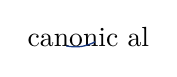
\begin{tikzpicture}[baseline=(word.base)]\node[inner sep=0pt] (word) {canonic al};\draw[color=blue,line width=.45pt] ([xshift=-.8em,yshift=.15ex]word.south) to[bend right=18] ([xshift=.25em,yshift=.5ex]word.south);\end{tikzpicture}}{canonical}{authorial word join}{ps_134-3_077-v0006} functor $a \hand{\mapsto} A_{/a}$ from $A= \hand{\Delta}^{f}$ to (Cat), which is the
ultimate choice for checking whether or not A is a test category, finally
gives the answer: it is not. Because with I now the Lawvere element, we
still have that $A_{/\hand{\Delta}_{o}\times I}$ is a two-point discrete category. Thus \var{\over[typed]{A}{t}}{t}{typewriter overwriting}{ps_134-3_077-v0007}he topos
$A^{\hand{\wedge}}= (\hand{\Delta}^{f})^{\hand{\wedge}}$ is'nt locally modelizing i.e. it has'nt got any homotopy \var{\xout{\unsure{seg}}}{}{typewriter deletion}{ps_134-3_077-v0008}\var{\inserted[typed]{in}}{in}{typed insertion}{ps_134-3_077-v0009}-%
\var{\xout{\unsure{ment}}}{}{typewriter deletion}{ps_134-3_077-v0010}\var{\inserted[typed]{terval}}{terval}{typed insertion}{ps_134-3_077-v0011}, which at any rate is a very big drawback I would think. The only
hope which still remains, to account for the positive features of face-%
complexes recalled above, is that $\hand{\Delta}^{f}$ is at the least a test category \uline{in}
\uline{the wide sense} \var{\inserted{[or \uline{weak} test category]}}{\hand{[or \uline{weak} test category]}}{insertion}{ps_134-3_077-v0012}, namely that for any category C with final element, the
category $i_A j_A(C) = A_{/j_A(C)}$( = category of all \var{\xout{objects}}{}{typewriter deletion}{ps_134-3_077-v0013} pairs (n,u)\var{\inserted{,}}{\hand{,}}{insertion}{ps_134-3_077-v0014} with
u a map of the (ordered\var{\over{)}{)}}{\hand{)}}{writing over}{ps_134-3_077-v0015} category $A_{/\tilde{\hand{\Delta}}_n}$ \var{\inserted{into C}}{\hand{into C}}{insertion}{ps_134-3_077-v0016}) is aspheric. The first case to
check is for C = final category $\hand{\Delta}_o$ , i.e. \var{\xout{asyclicity}}{}{typewriter deletion}{ps_134-3_077-v0017} asphericity of A ,
next step would be $C =\hand{\Delta}_1$ , i.e. asphericity of the Lawvere element $L_A$
(but of course \uline{not} asphericity over the final element $e_{A^{\hand{\wedge}}}$ \hand{!}).

The question certainly deserves to be settled. If the answer is
affirmative i.e. $\hand{\Delta}^{f}$ \uline{is} a test category in the wide sense, then\var{\xout{x}}{}{typewriter deletion}{ps_134-3_077-v0018} the proposi-%
\margin{-} tion stated earlier (\hand{\S}. \hand{42}), which clearly applies equally when A is a
test category in the wide sense, implies that if M is\var{\xout{x}}{}{typewriter deletion}{ps_134-3_077-v0019} any full subcatego-%
ry of (Cat) containing all those C which are ``locally isomorphic'' to $\hand{\Delta}^{f}$ ,
(i.e. such that for every $x \hand{\in} C$, $C_{/x}$ is isomorphic to the ordered category
of all subsimplices of some simplex), then for the induced notion $W_M$ of
weak equivalences, M is a modelizer and the inclusion functor from M into
(Cat) is modelizing. This does not yet apply to (Ord), however it reopens
the question whether the \var{\inserted{full sub}}{\hand{full sub}}{insertion}{ps_134-3_077-v0020}category of \var{\inserted{(Ord) made up by all}}{\hand{(Ord) made up by all}}{insertion}{ps_134-3_077-v0021} \var{\deleted{``simplicial maquettes'', which can be}}{}{deletion}{ps_134-3_077-v0022}
\var{\deleted{interpreted as}}{}{deletion}{ps_134-3_077-v0023} ordered sets J which are locally isomorphic to $\hand{\Delta}^{f}$ in the
sense above (namely for any $x \hand{\in} J$, the \var{\xout{subse}}{}{typewriter deletion}{ps_134-3_077-v0024} ordered subset $J_{\hand{\leq} x}$ is isomor-%

%% END SOURCE ps_134-3_077
\ifnum\EditionMode=1
\psapparatusstart
\psentry{ps_134-3_077-v0001}{1}{writing over}{$\over{f}{f}$}{$\hand{f}$}{The superposed handwritten reading replaces the underlying reading.}
\psentry{ps_134-3_077-v0002}{2}{writing over}{$\over{f}{f}$}{$\hand{f}$}{The superposed handwritten reading replaces the underlying reading.}
\psentry{ps_134-3_077-v0003}{3}{typed insertion}{\inserted[typed]{to look}}{to look}{The typed insertion is incorporated at its indicated position; insertion brackets leave the running text.}
\psentry{ps_134-3_077-v0004}{4}{writing over}{\over{n}{n}}{\hand{n}}{The superposed handwritten reading replaces the underlying reading.}
\psentry{ps_134-3_077-v0005}{5}{insertion}{\inserted{again}}{\hand{again}}{The handwritten insertion is incorporated at its indicated position; insertion brackets leave the running text.}
\psentry{ps_134-3_077-v0006}{6}{authorial word join}{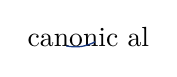
\begin{tikzpicture}[baseline=(word.base)]\node[inner sep=0pt] (word) {canonic al};\draw[color=blue,line width=.45pt] ([xshift=-.8em,yshift=.15ex]word.south) to[bend right=18] ([xshift=.25em,yshift=.5ex]word.south);\end{tikzpicture}}{canonical}{A pen joining curve closes the typed internal blank in canonic al.}
\psentry{ps_134-3_077-v0007}{7}{typewriter overwriting}{\over[typed]{A}{t}}{t}{The superposed typed reading replaces the underlying reading.}
\psentry{ps_134-3_077-v0008}{8}{typewriter deletion}{\xout{\unsure{seg}}}{}{The typewriter strikes out this material; it leaves the corrected running text.}
\psentry{ps_134-3_077-v0009}{9}{typed insertion}{\inserted[typed]{in}}{in}{The typed insertion is incorporated at its indicated position; insertion brackets leave the running text.}
\psentry{ps_134-3_077-v0010}{10}{typewriter deletion}{\xout{\unsure{ment}}}{}{The typewriter strikes out this material; it leaves the corrected running text.}
\psentry{ps_134-3_077-v0011}{11}{typed insertion}{\inserted[typed]{terval}}{terval}{The typed insertion is incorporated at its indicated position; insertion brackets leave the running text.}
\psentry{ps_134-3_077-v0012}{12}{insertion}{\inserted{[or \uline{weak} test category]}}{\hand{[or \uline{weak} test category]}}{The handwritten insertion is incorporated at its indicated position; insertion brackets leave the running text.}
\psentry{ps_134-3_077-v0013}{13}{typewriter deletion}{\xout{objects}}{}{The typewriter strikes out this material; it leaves the corrected running text.}
\psentry{ps_134-3_077-v0014}{14}{insertion}{\inserted{,}}{\hand{,}}{The handwritten insertion is incorporated at its indicated position; insertion brackets leave the running text.}
\psentry{ps_134-3_077-v0015}{15}{writing over}{\over{)}{)}}{\hand{)}}{The superposed handwritten reading replaces the underlying reading.}
\psentry{ps_134-3_077-v0016}{16}{insertion}{\inserted{into C}}{\hand{into C}}{The handwritten insertion is incorporated at its indicated position; insertion brackets leave the running text.}
\psentry{ps_134-3_077-v0017}{17}{typewriter deletion}{\xout{asyclicity}}{}{The typewriter strikes out this material; it leaves the corrected running text.}
\psentry{ps_134-3_077-v0018}{18}{typewriter deletion}{\xout{x}}{}{The typewriter strikes out this material; it leaves the corrected running text.}
\psentry{ps_134-3_077-v0019}{19}{typewriter deletion}{\xout{x}}{}{The typewriter strikes out this material; it leaves the corrected running text.}
\psentry{ps_134-3_077-v0020}{20}{insertion}{\inserted{full sub}}{\hand{full sub}}{The handwritten insertion is incorporated at its indicated position; insertion brackets leave the running text.}
\psentry{ps_134-3_077-v0021}{21}{insertion}{\inserted{(Ord) made up by all}}{\hand{(Ord) made up by all}}{The handwritten insertion is incorporated at its indicated position; insertion brackets leave the running text.}
\psentry{ps_134-3_077-v0022}{22}{deletion}{\deleted{``simplicial maquettes'', which can be}}{}{The author cancels this material by hand; it leaves the corrected running text.}
\psentry{ps_134-3_077-v0023}{23}{deletion}{\deleted{interpreted as}}{}{The author cancels this material by hand; it leaves the corrected running text.}
\psentry{ps_134-3_077-v0024}{24}{typewriter deletion}{\xout{subse}}{}{The typewriter strikes out this material; it leaves the corrected running text.}
\psapparatusend
\fi
\pssource{ps_134-3_078}{134-3/78}{https://grothendieck.umontpellier.fr/web/viewer.html?file=../134-3.pdf\#page=79}
\psnumber{ps_134-3_078-v0001}{1}
\psnumber{ps_134-3_078-v0002}{2}
\psnumber{ps_134-3_078-v0003}{3}
\psnumber{ps_134-3_078-v0004}{4}
\psnumber{ps_134-3_078-v0005}{5}
\psnumber{ps_134-3_078-v0006}{6}
\psnumber{ps_134-3_078-v0007}{7}
\psnumber{ps_134-3_078-v0008}{8}
\psnumber{ps_134-3_078-v0009}{9}
\psnumber{ps_134-3_078-v0010}{10}
\psnumber{ps_134-3_078-v0011}{11}
\psnumber{ps_134-3_078-v0012}{12}
\psnumber{ps_134-3_078-v0013}{13}
\psnumber{ps_134-3_078-v0014}{14}
\psnumber{ps_134-3_078-v0015}{15}
%% BEGIN SOURCE ps_134-3_078
% Pursuing Stacks (cotes 134-2 to 134-8): archive cote 134-3, site page 78 (PDF page 79), typescript page 78.
% typescript. Draft compared: ps2.tex:4036-4092.
% AI-transcribed by Claude Opus 5.5 (claude-opus-5-5, adaptive thinking, effort high), Message Batches API, batch ps1 (msgbatch_01Rv5hCaNTtUt4JHx1yqoHPL), 2026-11-12; image review recorded in records/CHECK_DECISIONS_134_3_4.tsv.
\scanpage{134-3/78}
\mspage{78}

phic to the ordered set of subsimplices of some simplex) is a modelizer.
To insure this,  it would be enough to find an ordered set J satisfying the
previous condition \var{\deleted{(namely a simplicial maquette)}}{}{deletion}{ps_134-3_078-v0001} \var{\inserted{(for instance one stemming from a ``simplicial maquette'')}}{\hand{(for instance one stemming from a ``simplicial maquette'')}}{insertion}{ps_134-3_078-v0002}, such that the correspon-%
ding category is a test category,  or at least a test category in the wide
sense.  The first candidate that comes to my mind,  is to take any \uline{infinite}
set S of vertices,  and take J to be the ordered set of all \uline{finite} \uline{non-emp\var{\over[typed]{t}{-}}{-}{typewriter overwriting}{ps_134-3_078-v0003}}%
\uline{ty} subsets (called the simplices  -  thus the elements of S can be inter-%
preted in terms of J as the minimal simplices).  By the way,  the category
associated to J,  in case S = $\underline{N}$ ,  can be interpreted in terms of \var{\inserted{$A=\Delta^f$}}{\hand{$A=\Delta^f$}}{insertion}{ps_134-3_078-v0004} as
the category  $A_{\hand{/\Delta}_{\mathrm{oo}}}$ ,  where \hand{\ensuremath{\Delta}}$_{\mathrm{oo}}$ is defined as the filtering direct limit
\var{\xout{of}}{}{typewriter deletion}{ps_134-3_078-v0005} in A\hand{\ensuremath{^{\wedge}}} of the \hand{\ensuremath{\Delta}}$_n$'s ,  arranged into a direct system in the obvious way:
\var{\xout{The As the category J admits binary products (namely intersection of simpli-}}{}{typewriter deletion}{ps_134-3_078-v0006}%
\var{\xout{ces}}{}{typewriter deletion}{ps_134-3_078-v0007}
\[ \hand{\ensuremath{\Delta}}_{\hand{\infty}} = \underset{n}{\underset{\hand{\ensuremath{\longrightarrow}}}{\mathrm{lim}}}\ \hand{\ensuremath{\Delta}}_n \quad \text{in} \quad (\hand{\ensuremath{\Delta}}^f)^{\hand{\wedge}}\ . \]
Asphericity of J looks intuitively evident,  and should be easy by a direct
limit argument,  as a matter of fact any filtering \var{\xout{\unsure{inex}}}{}{typewriter deletion}{ps_134-3_078-v0008} category (the next
best to having a final element) should be aspheric,  at least if it has a
countable cofinal family of objects.  T\var{\over[typed]{h}{h}}{h}{typewriter overwriting}{ps_134-3_078-v0009}e Lawvere element \var{\xout{in}}{}{typewriter deletion}{ps_134-3_078-v0010} L$_A$ in A\hand{\ensuremath{^{\wedge}}} is not
aspheric though over the final object,  because when inducing over a zero
simplex,  we get the same contradiction as before.  As a matter of fact,
I am getting aware I have been very silly and prejudiced not to see one
trivial common reason,  applicable to \hand{\ensuremath{\Delta}}$^f$ as to J , showing that they are
not test categories nor even local test categories:  namely the induced
categories A$_{/a}$ should be test categories too,  but among these there are
one-point categories (take a=\hand{\ensuremath{\Delta}}$_o$ ,  or a zero-simplex),  and such a catego-%
ry is \uline{not} a test category!

Still J may be a test category in the wide sense - the basic test here,
as we know already asphericity of \var{\over[typed]{I}{J}}{J}{typewriter overwriting}{ps_134-3_078-v0011} itself,  would be \var{\inserted[typed]{(absolute)}}{(absolute)}{typed insertion}{ps_134-3_078-v0012} asphericity of L$_J$ ,
or equivalently,  of the category J$_{/L_J}$ ,  an ordered set in fact, \var{\xout{of}}{}{typewriter deletion}{ps_134-3_078-v0013}
\var{\xout{all}}{}{typewriter deletion}{ps_134-3_078-v0014}(as is the case for any category A$_{/F}$ for A defined by an ordered set
and F in A\hand{\ensuremath{^{\wedge}}}).  This is now the ordered set of all pairs \var{\xout{(K)}}{}{typewriter deletion}{ps_134-3_078-v0015} (K\hand{\ensuremath{\subset}}T)  of
finite subsets of S,  with T in J namely T non empty,  with the rule
\[ (K',T') \hand{\ensuremath{\leqslant}} (K,T) \quad \text{iff} \quad T'\hand{\ensuremath{\subset}}T \ \text{and}\ K'=K\hand{\ensuremath{\cap}}T' \quad . \]

%% END SOURCE ps_134-3_078
\ifnum\EditionMode=1
\psapparatusstart
\psentry{ps_134-3_078-v0001}{1}{deletion}{\deleted{(namely a simplicial maquette)}}{}{The author cancels this material by hand; it leaves the corrected running text.}
\psentry{ps_134-3_078-v0002}{2}{insertion}{\inserted{(for instance one stemming from a ``simplicial maquette'')}}{\hand{(for instance one stemming from a ``simplicial maquette'')}}{The handwritten insertion is incorporated at its indicated position; insertion brackets leave the running text.}
\psentry{ps_134-3_078-v0003}{3}{typewriter overwriting}{\over[typed]{t}{-}}{-}{The superposed typed reading replaces the underlying reading.}
\psentry{ps_134-3_078-v0004}{4}{insertion}{\inserted{$A=\Delta^f$}}{\hand{$A=\Delta^f$}}{The handwritten insertion is incorporated at its indicated position; insertion brackets leave the running text.}
\psentry{ps_134-3_078-v0005}{5}{typewriter deletion}{\xout{of}}{}{The typewriter strikes out this material; it leaves the corrected running text.}
\psentry{ps_134-3_078-v0006}{6}{typewriter deletion}{\xout{The As the category J admits binary products (namely intersection of simpli-}}{}{The typewriter strikes out this material; it leaves the corrected running text.}
\psentry{ps_134-3_078-v0007}{7}{typewriter deletion}{\xout{ces}}{}{The typewriter strikes out this material; it leaves the corrected running text.}
\psentry{ps_134-3_078-v0008}{8}{typewriter deletion}{\xout{\unsure{inex}}}{}{The typewriter strikes out this material; it leaves the corrected running text.}
\psentry{ps_134-3_078-v0009}{9}{typewriter overwriting}{\over[typed]{h}{h}}{h}{The superposed typed reading replaces the underlying reading.}
\psentry{ps_134-3_078-v0010}{10}{typewriter deletion}{\xout{in}}{}{The typewriter strikes out this material; it leaves the corrected running text.}
\psentry{ps_134-3_078-v0011}{11}{typewriter overwriting}{\over[typed]{I}{J}}{J}{The superposed typed reading replaces the underlying reading.}
\psentry{ps_134-3_078-v0012}{12}{typed insertion}{\inserted[typed]{(absolute)}}{(absolute)}{The typed insertion is incorporated at its indicated position; insertion brackets leave the running text.}
\psentry{ps_134-3_078-v0013}{13}{typewriter deletion}{\xout{of}}{}{The typewriter strikes out this material; it leaves the corrected running text.}
\psentry{ps_134-3_078-v0014}{14}{typewriter deletion}{\xout{all}}{}{The typewriter strikes out this material; it leaves the corrected running text.}
\psentry{ps_134-3_078-v0015}{15}{typewriter deletion}{\xout{(K)}}{}{The typewriter strikes out this material; it leaves the corrected running text.}
\psapparatusend
\fi
\pssource{ps_134-3_079}{134-3/79}{https://grothendieck.umontpellier.fr/web/viewer.html?file=../134-3.pdf\#page=80}
\psnumber{ps_134-3_079-v0001}{1}
\psnumber{ps_134-3_079-v0002}{2}
\psnumber{ps_134-3_079-v0003}{3}
\psnumber{ps_134-3_079-v0004}{4}
\psnumber{ps_134-3_079-v0005}{5}
\psnumber{ps_134-3_079-v0006}{6}
\psnumber{ps_134-3_079-v0007}{7}
\psnumber{ps_134-3_079-v0008}{8}
\psnumber{ps_134-3_079-v0009}{9}
\psnumber{ps_134-3_079-v0010}{10}
\psnumber{ps_134-3_079-v0011}{11}
\psnumber{ps_134-3_079-v0012}{12}
\psnumber{ps_134-3_079-v0013}{13}
\psnumber{ps_134-3_079-v0014}{14}
\psnumber{ps_134-3_079-v0015}{15}
\psnumber{ps_134-3_079-v0016}{16}
\psnumber{ps_134-3_079-v0017}{17}
\psnumber{ps_134-3_079-v0018}{18}
\psnumber{ps_134-3_079-v0019}{19}
\psnumber{ps_134-3_079-v0020}{20}
\psnumber{ps_134-3_079-v0021}{21}
\psnumber{ps_134-3_079-v0022}{22}
\psnumber{ps_134-3_079-v0023}{23}
\psnumber{ps_134-3_079-v0024}{24}
\psnumber{ps_134-3_079-v0025}{25}
\psnumber{ps_134-3_079-v0026}{26}
\psnumber{ps_134-3_079-v0027}{27}
\psnumber{ps_134-3_079-v0028}{28}
%% BEGIN SOURCE ps_134-3_079
% Pursuing Stacks (cotes 134-2 to 134-8): archive cote 134-3, site page 79 (PDF page 80), typescript page 79.
% typescript. Draft compared: ps2.tex:4074-4163.
% AI-transcribed by Claude Opus 5.5 (claude-opus-5-5, adaptive thinking, effort high), Message Batches API, batch ps1 (msgbatch_01Rv5hCaNTtUt4JHx1yqoHPL), 2026-11-12; image review recorded in records/CHECK_DECISIONS_134_3_4.tsv.
\scanpage{134-3/79}
\mspage{79}

26.3.

44. I finally convinced myself that $\hand{\Delta}^{f}$ , the category of standar\var{\over{\unsure{t}}{d}}{\hand{d}}{writing over}{ps_134-3_079-v0001}
ordered simplices with face operations (and no degeneracies) \uline{is} a ``test
category in the wide sense'' after all - although definitely not a test
category, as was seen yesterday (\var{\deleted{as}}{}{deletion}{ps_134-3_079-v0002} \var{\inserted{turning out to be}}{\hand{turning out to be}}{insertion}{ps_134-3_079-v0003} a practically trivial observation).
This now does rehabilitate the notion of a test category in the wide sense\hand{,}
which I expected to be of little or no interest - \var{\inserted{much the \deleted{same} way}}{\hand{much the  way}}{insertion}{ps_134-3_079-v0004} as previously, the
notion I now call by the name ``test category'' was rehabilitated or rather,
discovered, after I expected that the only one proper notion for getting
modelizers of the f\var{\over{\unsure{ro}}{or}}{\hand{or}}{writing over}{ps_134-3_079-v0005}m $A^{\hand{\wedge}}$ was in terms of conditions T 1) to T 3) on $A$.
\hand{(}including the very strong condition T 2) of total a\var{\over{\unsure{cycli}}{spheri}}{\hand{spheri}}{writing over}{ps_134-3_079-v0006}city\hand{)}. This notion
I \var{\inserted{then}}{\hand{then}}{insertion}{ps_134-3_079-v0007} finally called by the name``\uline{strict} test category'', and I was fortunately
cautious enough to reserve a name too for the notion which appeared then
as rather weak and \var{\xout{and}}{}{typewriter deletion}{ps_134-3_079-v0008} unmanageable, of test categories in the wide sense
or, as I will say \var{\inserted{now}}{\hand{now}}{insertion}{ps_134-3_079-v0009} more shortly, \uline{weak} \uline{test} \uline{categories} (by which of cour-%
se I do not mean to exclude the possibility that \hand{\unsure{it}} \unsure{some} \var{\inserted{be}}{\hand{be}}{insertion}{ps_134-3_079-v0010} even \hand{a} test catego-%
r\var{\over{\unsure{ies}}{y}}{\hand{y}}{writing over}{ps_134-3_079-v0011}\hand{)}, thus getting the trilogy of \var{\inserted[typed]{notions with}}{notions with}{typed insertion}{ps_134-3_079-v0012} strict implications
\[ \text{weak test categor\var{\over[typed]{y}{i}}{i}{typewriter overwriting}{ps_134-3_079-v0013}es} \hand{\Leftarrow} \text{test categor\var{\over[typed]{\unsure{m}}{i}}{i}{typewriter overwriting}{ps_134-3_079-v0014}es} \hand{\Leftarrow} \text{strict test categories} \quad . \]
In order not to get confused, I will recall what exactly each of these
notions means,

a) \var{\inserted[typed]{\uline{Weak}}}{\uline{Weak}}{typed insertion}{ps_134-3_079-v0015} \uline{\var{\over{T}{t}}{\hand{t}}{writing over}{ps_134-3_079-v0016}est categories}. \var{\xout{The category A is a}}{}{typewriter deletion}{ps_134-3_079-v0017} For a given \var{\inserted[typed]{small}}{small}{typed insertion}{ps_134-3_079-v0018} category $A$,
we look at the functor
\[ (1) \qquad i_A\colon A^{\hand{\wedge}} \hand{\longrightarrow} (\mathrm{Cat}) , \qquad \var{\over{F}{F}}{\hand{F}}{writing over}{ps_134-3_079-v0019} \hand{\longmapsto} A_{/F} \hand{,} \]
which commutes with direct limits, and at the right adjoint functor
\[ (2) \qquad j_A = i_A^{\var{\over[typed]{*}{*}}{*}{typewriter overwriting}{ps_134-3_079-v0020}} : \ (\mathrm{Cat}) \hand{\longrightarrow} A^{\hand{\wedge}}, \qquad C \hand{\longmapsto} \var{\over{j}{j}}{\hand{j}}{writing over}{ps_134-3_079-v0021}_A(C) = (a \hand{\mapsto} \mathrm{Hom}(A_{/a},C)) \ . \]
We get an adjunction \var{\xout{functor}}{}{typewriter deletion}{ps_134-3_079-v0022} morphism
\[ (3) \qquad i_A j_A(C) \hand{\longrightarrow} C \qquad \text{in } (\mathrm{Cat}) , \]
and another
\[ (4) \qquad F \hand{\longrightarrow} j_A i_A F \qquad \text{in } A^{\hand{\wedge}} , \]
functorial in $C$ resp. in $F$. Pr\var{\over{\illegible{1}}{es}}{\hand{es}}{writing over}{ps_134-3_079-v0023}umably the following are equivalent
(I'll see in a minute how much I can prove about these equivalences):

(i) T\var{\over[typed]{h}{h}}{h}{typewriter overwriting}{ps_134-3_079-v0024}e functors (1) and (2) are compatible with weak equivalences,
and the two \var{\inserted{induced}}{\hand{induced}}{insertion}{ps_134-3_079-v0025} functors between the localized categories
\[ \hand{(5)} \qquad W_A^{\hand{-1}} A^{\hand{\wedge}} \hand{\rightleftarrows} W^{-1}(\mathrm{Cat}) \overset{\mathrm{def}}{=} (\mathrm{Hot}) \ . \]
are equivalences.

(ii) As in (i), and moreover the two equivalences are quasi-inverse of
each other, with adjunction morphism\var{\deleted{s}}{}{deletion}{ps_134-3_079-v0026} \var{\over[typed]{o}{i}}{i}{typewriter overwriting}{ps_134-3_079-v0027}n \var{\deleted{(Cat}}{}{deletion}{ps_134-3_079-v0028} $W^{-1}(\mathrm{Cat}) = (\mathrm{Hot})$
deduced from (3) by localization.

\margin{\textcolor{black}{\unsure{(i}}}

%% END SOURCE ps_134-3_079
\ifnum\EditionMode=1
\psapparatusstart
\psentry{ps_134-3_079-v0001}{1}{writing over}{\over{\unsure{t}}{d}}{\hand{d}}{The superposed handwritten reading replaces the underlying reading.}
\psentry{ps_134-3_079-v0002}{2}{deletion}{\deleted{as}}{}{The author cancels this material by hand; it leaves the corrected running text.}
\psentry{ps_134-3_079-v0003}{3}{insertion}{\inserted{turning out to be}}{\hand{turning out to be}}{The handwritten insertion is incorporated at its indicated position; insertion brackets leave the running text.}
\psentry{ps_134-3_079-v0004}{4}{insertion}{\inserted{much the \deleted{same} way}}{\hand{much the  way}}{The handwritten insertion is incorporated at its indicated position; insertion brackets leave the running text.}
\psentry{ps_134-3_079-v0005}{5}{writing over}{\over{\unsure{ro}}{or}}{\hand{or}}{The superposed handwritten reading replaces the underlying reading.}
\psentry{ps_134-3_079-v0006}{6}{writing over}{\over{\unsure{cycli}}{spheri}}{\hand{spheri}}{The superposed handwritten reading replaces the underlying reading.}
\psentry{ps_134-3_079-v0007}{7}{insertion}{\inserted{then}}{\hand{then}}{The handwritten insertion is incorporated at its indicated position; insertion brackets leave the running text.}
\psentry{ps_134-3_079-v0008}{8}{typewriter deletion}{\xout{and}}{}{The typewriter strikes out this material; it leaves the corrected running text.}
\psentry{ps_134-3_079-v0009}{9}{insertion}{\inserted{now}}{\hand{now}}{The handwritten insertion is incorporated at its indicated position; insertion brackets leave the running text.}
\psentry{ps_134-3_079-v0010}{10}{insertion}{\inserted{be}}{\hand{be}}{The handwritten insertion is incorporated at its indicated position; insertion brackets leave the running text.}
\psentry{ps_134-3_079-v0011}{11}{writing over}{\over{\unsure{ies}}{y}}{\hand{y}}{The superposed handwritten reading replaces the underlying reading.}
\psentry{ps_134-3_079-v0012}{12}{typed insertion}{\inserted[typed]{notions with}}{notions with}{The typed insertion is incorporated at its indicated position; insertion brackets leave the running text.}
\psentry{ps_134-3_079-v0013}{13}{typewriter overwriting}{\over[typed]{y}{i}}{i}{The superposed typed reading replaces the underlying reading.}
\psentry{ps_134-3_079-v0014}{14}{typewriter overwriting}{\over[typed]{\unsure{m}}{i}}{i}{The superposed typed reading replaces the underlying reading.}
\psentry{ps_134-3_079-v0015}{15}{typed insertion}{\inserted[typed]{\uline{Weak}}}{\uline{Weak}}{The typed insertion is incorporated at its indicated position; insertion brackets leave the running text.}
\psentry{ps_134-3_079-v0016}{16}{writing over}{\over{T}{t}}{\hand{t}}{The superposed handwritten reading replaces the underlying reading.}
\psentry{ps_134-3_079-v0017}{17}{typewriter deletion}{\xout{The category A is a}}{}{The typewriter strikes out this material; it leaves the corrected running text.}
\psentry{ps_134-3_079-v0018}{18}{typed insertion}{\inserted[typed]{small}}{small}{The typed insertion is incorporated at its indicated position; insertion brackets leave the running text.}
\psentry{ps_134-3_079-v0019}{19}{writing over}{$\over{F}{F}$}{$\hand{F}$}{The superposed handwritten reading replaces the underlying reading.}
\psentry{ps_134-3_079-v0020}{20}{typewriter overwriting}{$\over[typed]{*}{*}$}{$*$}{The superposed typed reading replaces the underlying reading.}
\psentry{ps_134-3_079-v0021}{21}{writing over}{$\over{j}{j}$}{$\hand{j}$}{The superposed handwritten reading replaces the underlying reading.}
\psentry{ps_134-3_079-v0022}{22}{typewriter deletion}{\xout{functor}}{}{The typewriter strikes out this material; it leaves the corrected running text.}
\psentry{ps_134-3_079-v0023}{23}{writing over}{\over{\illegible{1}}{es}}{\hand{es}}{The superposed handwritten reading replaces the underlying reading.}
\psentry{ps_134-3_079-v0024}{24}{typewriter overwriting}{\over[typed]{h}{h}}{h}{The superposed typed reading replaces the underlying reading.}
\psentry{ps_134-3_079-v0025}{25}{insertion}{\inserted{induced}}{\hand{induced}}{The handwritten insertion is incorporated at its indicated position; insertion brackets leave the running text.}
\psentry{ps_134-3_079-v0026}{26}{deletion}{\deleted{s}}{}{The author cancels this material by hand; it leaves the corrected running text.}
\psentry{ps_134-3_079-v0027}{27}{typewriter overwriting}{\over[typed]{o}{i}}{i}{The superposed typed reading replaces the underlying reading.}
\psentry{ps_134-3_079-v0028}{28}{deletion}{\deleted{(Cat}}{}{The author cancels this material by hand; it leaves the corrected running text.}
\psapparatusend
\fi
\pssource{ps_134-3_080}{134-3/80}{https://grothendieck.umontpellier.fr/web/viewer.html?file=../134-3.pdf\#page=81}
\psnumber{ps_134-3_080-v0001}{1}
\psnumber{ps_134-3_080-v0002}{2}
\psnumber{ps_134-3_080-v0003}{3}
\psnumber{ps_134-3_080-v0004}{4}
\psnumber{ps_134-3_080-v0005}{5}
\psnumber{ps_134-3_080-v0006}{6}
\psnumber{ps_134-3_080-v0007}{7}
\psnumber{ps_134-3_080-v0008}{8}
\psnumber{ps_134-3_080-v0009}{9}
\psnumber{ps_134-3_080-v0010}{10}
\psnumber{ps_134-3_080-v0011}{11}
\psnumber{ps_134-3_080-v0012}{12}
\psnumber{ps_134-3_080-v0013}{13}
\psnumber{ps_134-3_080-v0014}{14}
\psnumber{ps_134-3_080-v0015}{15}
\psnumber{ps_134-3_080-v0016}{16}
\psnumber{ps_134-3_080-v0017}{17}
\psnumber{ps_134-3_080-v0018}{18}
\psnumber{ps_134-3_080-v0019}{19}
\psnumber{ps_134-3_080-v0020}{20}
\psnumber{ps_134-3_080-v0021}{21}
\psnumber{ps_134-3_080-v0022}{22}
\psnumber{ps_134-3_080-v0023}{23}
\psnumber{ps_134-3_080-v0024}{24}
\psnumber{ps_134-3_080-v0025}{25}
\psnumber{ps_134-3_080-v0026}{26}
\psnumber{ps_134-3_080-v0027}{27}
\psnumber{ps_134-3_080-v0028}{28}
\psnumber{ps_134-3_080-v0029}{29}
\psnumber{ps_134-3_080-v0030}{30}
\psnumber{ps_134-3_080-v0031}{31}
%% BEGIN SOURCE ps_134-3_080
% Pursuing Stacks (cotes 134-2 to 134-8): archive cote 134-3, site page 80 (PDF page 81), typescript page 80.
% typescript. Draft compared: ps2.tex:4144-4223.
% AI-transcribed by Claude Opus 5.5 (claude-opus-5-5, adaptive thinking, effort high), Message Batches API, batch ps1 (msgbatch_01Rv5hCaNTtUt4JHx1yqoHPL), 2026-11-12; image review recorded in records/CHECK_DECISIONS_134_3_4.tsv.
\scanpage{134-3/80}
\mspage{(80)}

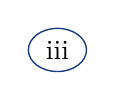
\begin{tikzpicture}[baseline=(n.base)]\node[inner sep=0pt] (n) {iii};\draw[color=blue,line width=.5pt] (n.center) ellipse [x radius=1.05em,y radius=.78em];\end{tikzpicture} As in (ii), but moreover the adjunction morphism in $W_A^{\hand{-1}}A^{\hand{\wedge}}$ for
the pair of quasi-inverse equivalences \var{\inserted[typed]{(5)}}{(5)}{typed insertion}{ps_134-3_080-v0001}, being \hand{likewise deduced from }\var{\inserted{(4).}}{\hand{(4).}}{insertion}{ps_134-3_080-v0002}
(iv) For any C in (Cat), (3) is a weak equivalence.
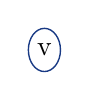
\begin{tikzpicture}[baseline=(n.base)]\node[inner sep=0pt] (n) {v};\draw[color=blue,line width=.5pt] (n.center) ellipse [x radius=.58em,y radius=.78em];\end{tikzpicture} Same as (iv), with C restricted to having a final element, i.e.
for any such C, $j_Ai_A(C) = A_{/j_A(C)}$ is a\var{\over{\unsure{s}}{s}}{\hand{s}}{writing over}{ps_134-3_080-v0003}pheric.
(vi) For any F in $A^{\hand{\wedge}}$, (4) is a weak equivalence, moreover
\[ W_{(Cat)} = j_A^{-1}(W_A) \qquad , \]
i.e. a \var{\xout{functor}}{}{typewriter deletion}{ps_134-3_080-v0004} map $f\colon C' \hand{\to} C$ in (Cat) is a \var{\xout{quasi}}{}{typewriter deletion}{ps_134-3_080-v0005} \var{\inserted[typed]{weak}}{weak}{typed insertion}{ps_134-3_080-v0006} equivalence,
iff $j_A(f)$ is a \var{\xout{quasi}}{}{typewriter deletion}{ps_134-3_080-v0007} \var{\inserted[typed]{weak}}{weak}{typed insertion}{ps_134-3_080-v0008} equivalence in $A^{\hand{\wedge}}$ - which means, by defi-%
n\var{\over[typed]{\illegible{1}}{i}}{i}{typewriter overwriting}{ps_134-3_080-v0009}tion (more or less) that $i_Aj_A(f)$ is a \var{\xout{quasi}}{}{typewriter deletion}{ps_134-3_080-v0010} \var{\inserted[typed]{weak}}{weak}{typed insertion}{ps_134-3_080-v0011} equivalence.
(vii) T\var{\over{h}{h}}{\hand{h}}{writing over}{ps_134-3_080-v0012}e functor
(6) \[ i_Aj_A \; : \; (Cat) \hand{\longrightarrow} (Cat) \quad , \quad C \hand{\mapsto} A_{/j_A(C)} \, , \]
transforms \var{\xout{quasi}}{}{typewriter deletion}{ps_134-3_080-v0013} \var{\inserted[typed]{weak}}{weak}{typed insertion}{ps_134-3_080-v0014} equivalences into \var{\xout{quasi}}{}{typewriter deletion}{ps_134-3_080-v0015} \var{\inserted[typed]{weak}}{weak}{typed insertion}{ps_134-3_080-v0016} equivalences , i.e.
gives rise to a functor (Hot)$\hand{\to}$(Hot), and moreover \var{\deleted{A is}}{}{deletion}{ps_134-3_080-v0017} \hand{the}
\var{\deleted{aspheric.}}{}{deletion}{ps_134-3_080-v0018} \hand{latter respects final object (i.e. A is aspheric).}
(viii) Same as (vii), but restricting to \var{\xout{quax}}{}{typewriter deletion}{ps_134-3_080-v0019} weak equivalences of the
type $C \hand{\to} \var{\over[typed]{e}{e}}{e}{typewriter overwriting}{ps_134-3_080-v0020}$, where C has a final element and e is the final
object in (Cat) (the one-point category)\hand{, plus asphericity of A.}

The trivial implications between all these conditions can be summari\var{\xout{z}}{}{typewriter deletion}{ps_134-3_080-v0021}
zed in the diagram
% Hand-drawn arrows are marked blue; typed objects remain plain.
\diagram{\begin{tikzcd}[row sep=small, arrows=Rightarrow]
(iii) \ar[r,Leftrightarrow,color=blue] \ar[d,color=blue] \& (vi) \ar[r,color=blue] \& (vii) \ar[r,color=blue] \& (viii) \ar[dl,color=blue] \\
(ii) \ar[r,color=blue] \ar[d,color=blue] \& (iv) \ar[r,color=blue] \& (v) \& \\
(i) \& , \& \&
\end{tikzcd}}
the only \var{\inserted[typed]{slightly}}{slightly}{typed insertion}{ps_134-3_080-v0022} less obvious implication here is (viii)\hand{$\Rightarrow$}(v), which is seen
by looking at the commutative square deduced from $C \hand{\to} e$ (C in (Cat) as in
(v)\var{\xout{\unsure{;}}}{}{typewriter deletion}{ps_134-3_080-v0023} namely with final element) by applying (3)
\diagram{\begin{tikzcd}
i_Aj_A(C) \ar[r,color=blue] \ar[d,color=blue] \& C \ar[d,color=blue] \\
A{=}i_Aj_A(e) \ar[r,color=blue] \& e
\end{tikzcd} \quad ,}
by assumption the vertical arrows are weak equivalences, and so is $A \hand{\to} e$
(because A is supposed to be aspheric), therefore the same holds for the
fourth arrow left. On the other hand an easy asphericity argument
showed us \var{\inserted{[\unsure{\S}.30]}}{\hand{[\unsure{\S}.30]}}{insertion}{ps_134-3_080-v0024} that (v) \hand{$\Longrightarrow$}(iii), hence all conditions (ii) to (viii) are
equivalent, and they are equivalent to the stronger form of (iv), \var{\xout{that}}{}{typewriter deletion}{ps_134-3_080-v0025}
say (iv'), \var{\over[typed]{d}{s}}{s}{typewriter overwriting}{ps_134-3_080-v0026}\var{\over[typed]{a}{a}}{a}{typewriter overwriting}{ps_134-3_080-v0027}ying that (3) is \uline{aspheric} for any C in (Cat). T\var{\over{h}{h}}{\hand{h}}{writing over}{ps_134-3_080-v0028}e only
equivalence which is not quite clear yet is that (i) implies the other
conditions\unsure{\var{\over{,}{.}}{\hand{.}}{writing over}{ps_134-3_080-v0029}} \var{\deleted{under the formally weakest form (v) let's say.}}{}{deletion}{ps_134-3_080-v0030} B\var{\over{u}{u}}{\hand{u}}{writing over}{ps_134-3_080-v0031}t it is so

%% END SOURCE ps_134-3_080
\ifnum\EditionMode=1
\psapparatusstart
\psentry{ps_134-3_080-v0001}{1}{typed insertion}{\inserted[typed]{(5)}}{(5)}{The typed insertion is incorporated at its indicated position; insertion brackets leave the running text.}
\psentry{ps_134-3_080-v0002}{2}{insertion}{\inserted{(4).}}{\hand{(4).}}{The handwritten insertion is incorporated at its indicated position; insertion brackets leave the running text.}
\psentry{ps_134-3_080-v0003}{3}{writing over}{\over{\unsure{s}}{s}}{\hand{s}}{The superposed handwritten reading replaces the underlying reading.}
\psentry{ps_134-3_080-v0004}{4}{typewriter deletion}{\xout{functor}}{}{The typewriter strikes out this material; it leaves the corrected running text.}
\psentry{ps_134-3_080-v0005}{5}{typewriter deletion}{\xout{quasi}}{}{The typewriter strikes out this material; it leaves the corrected running text.}
\psentry{ps_134-3_080-v0006}{6}{typed insertion}{\inserted[typed]{weak}}{weak}{The typed insertion is incorporated at its indicated position; insertion brackets leave the running text.}
\psentry{ps_134-3_080-v0007}{7}{typewriter deletion}{\xout{quasi}}{}{The typewriter strikes out this material; it leaves the corrected running text.}
\psentry{ps_134-3_080-v0008}{8}{typed insertion}{\inserted[typed]{weak}}{weak}{The typed insertion is incorporated at its indicated position; insertion brackets leave the running text.}
\psentry{ps_134-3_080-v0009}{9}{typewriter overwriting}{\over[typed]{\illegible{1}}{i}}{i}{The superposed typed reading replaces the underlying reading.}
\psentry{ps_134-3_080-v0010}{10}{typewriter deletion}{\xout{quasi}}{}{The typewriter strikes out this material; it leaves the corrected running text.}
\psentry{ps_134-3_080-v0011}{11}{typed insertion}{\inserted[typed]{weak}}{weak}{The typed insertion is incorporated at its indicated position; insertion brackets leave the running text.}
\psentry{ps_134-3_080-v0012}{12}{writing over}{\over{h}{h}}{\hand{h}}{The superposed handwritten reading replaces the underlying reading.}
\psentry{ps_134-3_080-v0013}{13}{typewriter deletion}{\xout{quasi}}{}{The typewriter strikes out this material; it leaves the corrected running text.}
\psentry{ps_134-3_080-v0014}{14}{typed insertion}{\inserted[typed]{weak}}{weak}{The typed insertion is incorporated at its indicated position; insertion brackets leave the running text.}
\psentry{ps_134-3_080-v0015}{15}{typewriter deletion}{\xout{quasi}}{}{The typewriter strikes out this material; it leaves the corrected running text.}
\psentry{ps_134-3_080-v0016}{16}{typed insertion}{\inserted[typed]{weak}}{weak}{The typed insertion is incorporated at its indicated position; insertion brackets leave the running text.}
\psentry{ps_134-3_080-v0017}{17}{deletion}{\deleted{A is}}{}{The author cancels this material by hand; it leaves the corrected running text.}
\psentry{ps_134-3_080-v0018}{18}{deletion}{\deleted{aspheric.}}{}{The author cancels this material by hand; it leaves the corrected running text.}
\psentry{ps_134-3_080-v0019}{19}{typewriter deletion}{\xout{quax}}{}{The typewriter strikes out this material; it leaves the corrected running text.}
\psentry{ps_134-3_080-v0020}{20}{typewriter overwriting}{$\over[typed]{e}{e}$}{$e$}{The superposed typed reading replaces the underlying reading.}
\psentry{ps_134-3_080-v0021}{21}{typewriter deletion}{\xout{z}}{}{The typewriter strikes out this material; it leaves the corrected running text.}
\psentry{ps_134-3_080-v0022}{22}{typed insertion}{\inserted[typed]{slightly}}{slightly}{The typed insertion is incorporated at its indicated position; insertion brackets leave the running text.}
\psentry{ps_134-3_080-v0023}{23}{typewriter deletion}{\xout{\unsure{;}}}{}{The typewriter strikes out this material; it leaves the corrected running text.}
\psentry{ps_134-3_080-v0024}{24}{insertion}{\inserted{[\unsure{\S}.30]}}{\hand{[\unsure{\S}.30]}}{The handwritten insertion is incorporated at its indicated position; insertion brackets leave the running text.}
\psentry{ps_134-3_080-v0025}{25}{typewriter deletion}{\xout{that}}{}{The typewriter strikes out this material; it leaves the corrected running text.}
\psentry{ps_134-3_080-v0026}{26}{typewriter overwriting}{\over[typed]{d}{s}}{s}{The superposed typed reading replaces the underlying reading.}
\psentry{ps_134-3_080-v0027}{27}{typewriter overwriting}{\over[typed]{a}{a}}{a}{The superposed typed reading replaces the underlying reading.}
\psentry{ps_134-3_080-v0028}{28}{writing over}{\over{h}{h}}{\hand{h}}{The superposed handwritten reading replaces the underlying reading.}
\psentry{ps_134-3_080-v0029}{29}{writing over}{\over{,}{.}}{\hand{.}}{The superposed handwritten reading replaces the underlying reading.}
\psentry{ps_134-3_080-v0030}{30}{deletion}{\deleted{under the formally weakest form (v) let's say.}}{}{The author cancels this material by hand; it leaves the corrected running text.}
\psentry{ps_134-3_080-v0031}{31}{writing over}{\over{u}{u}}{\hand{u}}{The superposed handwritten reading replaces the underlying reading.}
\psapparatusend
\fi
\pssource{ps_134-3_081}{134-3/81}{https://grothendieck.umontpellier.fr/web/viewer.html?file=../134-3.pdf\#page=82}
\psnumber{ps_134-3_081-v0001}{1}
\psnumber{ps_134-3_081-v0002}{2}
\psnumber{ps_134-3_081-v0003}{3}
\psnumber{ps_134-3_081-v0004}{4}
\psnumber{ps_134-3_081-v0005}{5}
\psnumber{ps_134-3_081-v0006}{6}
\psnumber{ps_134-3_081-v0007}{7}
\psnumber{ps_134-3_081-v0008}{8}
\psnumber{ps_134-3_081-v0009}{9}
\psnumber{ps_134-3_081-v0010}{10}
\psnumber{ps_134-3_081-v0011}{11}
\psnumber{ps_134-3_081-v0012}{12}
\psnumber{ps_134-3_081-v0013}{13}
\psnumber{ps_134-3_081-v0014}{14}
\psnumber{ps_134-3_081-v0015}{15}
\psnumber{ps_134-3_081-v0016}{16}
\psnumber{ps_134-3_081-v0017}{17}
\psnumber{ps_134-3_081-v0018}{18}
\psnumber{ps_134-3_081-v0019}{19}
\psnumber{ps_134-3_081-v0020}{20}
\psnumber{ps_134-3_081-v0021}{21}
\psnumber{ps_134-3_081-v0022}{22}
\psnumber{ps_134-3_081-v0023}{23}
\psnumber{ps_134-3_081-v0024}{24}
\psnumber{ps_134-3_081-v0025}{25}
\psnumber{ps_134-3_081-v0026}{26}
\psnumber{ps_134-3_081-v0027}{27}
\psnumber{ps_134-3_081-v0028}{28}
\psnumber{ps_134-3_081-v0029}{29}
\psnumber{ps_134-3_081-v0030}{30}
\psnumber{ps_134-3_081-v0031}{31}
\psnumber{ps_134-3_081-v0032}{32}
%% BEGIN SOURCE ps_134-3_081
% Pursuing Stacks (cotes 134-2 to 134-8): archive cote 134-3, site page 81 (PDF page 82), typescript page 81.
% typescript. Draft compared: ps2.tex:4210-4279.
% AI-transcribed by Claude Opus 5.5 (claude-opus-5-5, adaptive thinking, effort high), Message Batches API, batch pilot (msgbatch_0189Nhf1xB615YWnztubtLfc), 2026-11-12; image review recorded in records/CHECK_DECISIONS_134_3_4.tsv.
\scanpage{134-3/81}
\mspage{81}

if we grant the ``insp\var{\xout{\unsure{i}}}{}{typewriter deletion}{ps_134-3_081-v0001}iring assumption'',\var{\xout{th}}{}{typewriter deletion}{ps_134-3_081-v0002} implying that any autoequivalen\var{\xout{x}}{}{typewriter deletion}{ps_134-3_081-v0003}
ce of(Hot)  is isomorphic to the identity functor  -  in this case it is
clear that even the weaker form (i')  of (i),  demanding only that
$i_Aj_A$ \var{\inserted{induce}}{\hand{induce}}{insertion}{ps_134-3_081-v0004} \var{\deleted{be}}{}{deletion}{ps_134-3_081-v0005} an \var{\inserted{auto}}{\hand{auto}}{insertion}{ps_134-3_081-v0006}equivalence \var{\inserted{of (Hot)}}{\hand{of (Hot)}}{insertion}{ps_134-3_081-v0007} (and \var{\inserted[typed]{nothing on}}{nothing on}{typed insertion}{ps_134-3_081-v0008} \var{\xout{\unsure{nothing}}}{}{typewriter deletion}{ps_134-3_081-v0009} either factor $i_A$ , $j_A$ \var{\inserted[typed]{in (5)}}{in (5)}{typed insertion}{ps_134-3_081-v0010}),implies (v).
Also,  When we assume moreover A aspheric,\var{\xout{\illegible{7}}}{}{typewriter deletion}{ps_134-3_081-v0011} it is clear that (i)
(and even (i')) implies (vii) i.e. all other conditions.  Thus,  instead \var{\xout{x}}{}{typewriter deletion}{ps_134-3_081-v0012}
of the assumption  on (Hot),  it would be enough to know that the particu-%
lar autoequivalence \var{\xout{$i_Aj_A$}}{}{typewriter deletion}{ps_134-3_081-v0013} of (Hot) induced by $i_Aj_A$  transforms the final
element of (Hot)  (respresented by the element e of (Cat)) into an isomor-%
phic one,\var{\inserted{\over{\unsure{(*)}}{(48)}}}{\hand{\hand{(48)}}}{insertion}{ps_134-3_081-v0014} which looks like a very slight strenghtening of (i) indeed.
\margin{\unsure{\begin{tikzpicture}[baseline=(n.base)]\node[inner sep=0pt] (n) {(48)};\draw[color=blue,line width=.35pt] (n.center) ellipse [x radius=1.35em,y radius=.95em];\end{tikzpicture} * 27.3. But this is true for any equivalence of categories -- I'm really being very dull!}}

In any case,  the conditions (ii) to (viii) are equivalent,  and
equivalent to  (i)  (or (i'))  \uline{plus} \var{\inserted{\over{\unsure{(**)}}{(49)}}}{\hand{\hand{(49)}}}{insertion}{ps_134-3_081-v0015} asphericity of A.  The formally
\margin{\unsure{\begin{tikzpicture}[baseline=(n.base)]\node[inner sep=0pt] (n) {(49)};\draw[color=blue,line width=.35pt] (n.center) ellipse [x radius=1.35em,y radius=.95em];\end{tikzpicture} ** The ``plus'' is unnecessary visibly, see note above.}}
strongest form is (iii),  the formally weakest one (with the exception
of (i) or (i')\hand{)} \var{\deleted{plus \hand{(**)} asphericity of A)}}{}{deletion}{ps_134-3_081-v0016} is (v),  which is also the one
which looks the most concrete,  namely amenable to practical verification.
This was indeed what at the very beginning was attractive in this conditi-%
on,  in comparison to the first one that came to my mind when introducing
the notion of a modelizer and of model preserving functors  -  namely \var{\xout{that}}{}{typewriter deletion}{ps_134-3_081-v0017}
merely that  $i_A$  should induce an equivalence between the localized cate-%
gories,  or equivalently,  that $A^{\hand{\wedge}}$ should be a ``modelizer'' and $i_A$ should
be model-preserving.  That we should be more demanding and ask for $j_A$ to
be equally model preserving crept in first rather timidly  -  and I still
dont know (and didn\hand{'}t really stop to think)  if \var{\inserted{the first}}{\hand{the first}}{insertion}{ps_134-3_081-v0018} one implies the other\var{\deleted{(***)}}{}{deletion}{ps_134-3_081-v0019}\hand{(50)}.
\var{\margin{(***) In fact, it is the condition that $j_A = i_A^*$ \deleted{\illegible{1}}, \unsure{not $i_A$}, should be model preserving, which is ``the right'' condition on A, equivalent to A being a weak test category, \deleted{cf p.\unsure{88 remark 3.}} if A is assumed aspheric.}}{\margin{(***) In fact, it is the condition that $j_A = i_A^*$ , \unsure{not $i_A$}, should be model preserving, which is ``the right'' condition on A, equivalent to A being a weak test category,  if A is assumed aspheric.}}{marginal note revised}{ps_134-3_081-v0020}

In any case,  as far as checking a property goes,  I would consider
(v) to be \uline{the} handy definition of a weak test category,  whereas (iii)
is the best,  when it goes to making use of the fact that A i\var{\xout{s}}{}{typewriter deletion}{ps_134-3_081-v0021}s indeed a
weak test category.  As for (i),  \var{\deleted{(supplemented by asphericity to be safe)}}{}{deletion}{ps_134-3_081-v0022}
it corresponds to the main intuitive content of the notion,  which means
that homotopy types can be``modelled'' by elements of $A^{\hand{\wedge}}$ \var{\xout{using \unsure{$i_A$}}}{}{typewriter deletion}{ps_134-3_081-v0023} ,  using
$i_A$ for describing which homotopy type is describe\var{\xout{e}}{}{typewriter deletion}{ps_134-3_081-v0024}d by an element F of $A^{\hand{\wedge}}$,
and using $j_A$ for getting a model in $A^{\hand{\wedge}}$ for a given homotopy type, descri-%
be\var{\xout{e}}{}{typewriter deletion}{ps_134-3_081-v0025}d by an object C in (Cat).

b)  \var{\inserted{\deleted{\uline{Weak}}}}{\hand{}}{insertion}{ps_134-3_081-v0026} \uline{Test categories} \var{\inserted{and local test categories}}{\hand{and local test categories}}{insertion}{ps_134-3_081-v0027}.  Let A still be a small category.  T\var{\over[typed]{h}{h}}{h}{typewriter overwriting}{ps_134-3_081-v0028}en the follo-%
wing conditions are equivalent:

\var{\deleted{i)  A is a weak test category,  and so are all induced categories}}{}{deletion}{ps_134-3_081-v0029}
\var{\deleted{$A_{/a}$  with a in A.}}{}{deletion}{ps_134-3_081-v0030}
\var{\deleted{ii)  A is aspheric,  and for any aspheric element F in $A^{\hand{\wedge}}$, $A_{/F}$ is}}{}{deletion}{ps_134-3_081-v0031}
\var{\deleted{a weak test category.}}{}{deletion}{ps_134-3_081-v0032}

%% END SOURCE ps_134-3_081
\ifnum\EditionMode=1
\psapparatusstart
\psentry{ps_134-3_081-v0001}{1}{typewriter deletion}{\xout{\unsure{i}}}{}{The typewriter strikes out this material; it leaves the corrected running text.}
\psentry{ps_134-3_081-v0002}{2}{typewriter deletion}{\xout{th}}{}{The typewriter strikes out this material; it leaves the corrected running text.}
\psentry{ps_134-3_081-v0003}{3}{typewriter deletion}{\xout{x}}{}{The typewriter strikes out this material; it leaves the corrected running text.}
\psentry{ps_134-3_081-v0004}{4}{insertion}{\inserted{induce}}{\hand{induce}}{The handwritten insertion is incorporated at its indicated position; insertion brackets leave the running text.}
\psentry{ps_134-3_081-v0005}{5}{deletion}{\deleted{be}}{}{The author cancels this material by hand; it leaves the corrected running text.}
\psentry{ps_134-3_081-v0006}{6}{insertion}{\inserted{auto}}{\hand{auto}}{The handwritten insertion is incorporated at its indicated position; insertion brackets leave the running text.}
\psentry{ps_134-3_081-v0007}{7}{insertion}{\inserted{of (Hot)}}{\hand{of (Hot)}}{The handwritten insertion is incorporated at its indicated position; insertion brackets leave the running text.}
\psentry{ps_134-3_081-v0008}{8}{typed insertion}{\inserted[typed]{nothing on}}{nothing on}{The typed insertion is incorporated at its indicated position; insertion brackets leave the running text.}
\psentry{ps_134-3_081-v0009}{9}{typewriter deletion}{\xout{\unsure{nothing}}}{}{The typewriter strikes out this material; it leaves the corrected running text.}
\psentry{ps_134-3_081-v0010}{10}{typed insertion}{\inserted[typed]{in (5)}}{in (5)}{The typed insertion is incorporated at its indicated position; insertion brackets leave the running text.}
\psentry{ps_134-3_081-v0011}{11}{typewriter deletion}{\xout{\illegible{7}}}{}{The typewriter strikes out this material; it leaves the corrected running text.}
\psentry{ps_134-3_081-v0012}{12}{typewriter deletion}{\xout{x}}{}{The typewriter strikes out this material; it leaves the corrected running text.}
\psentry{ps_134-3_081-v0013}{13}{typewriter deletion}{\xout{$i_Aj_A$}}{}{The typewriter strikes out this material; it leaves the corrected running text.}
\psentry{ps_134-3_081-v0014}{14}{insertion}{\inserted{\over{\unsure{(*)}}{(48)}}}{\hand{\hand{(48)}}}{The handwritten insertion is incorporated at its indicated position; insertion brackets leave the running text.}
\psentry{ps_134-3_081-v0015}{15}{insertion}{\inserted{\over{\unsure{(**)}}{(49)}}}{\hand{\hand{(49)}}}{The handwritten insertion is incorporated at its indicated position; insertion brackets leave the running text.}
\psentry{ps_134-3_081-v0016}{16}{deletion}{\deleted{plus \hand{(**)} asphericity of A)}}{}{The author cancels this material by hand; it leaves the corrected running text.}
\psentry{ps_134-3_081-v0017}{17}{typewriter deletion}{\xout{that}}{}{The typewriter strikes out this material; it leaves the corrected running text.}
\psentry{ps_134-3_081-v0018}{18}{insertion}{\inserted{the first}}{\hand{the first}}{The handwritten insertion is incorporated at its indicated position; insertion brackets leave the running text.}
\psentry{ps_134-3_081-v0019}{19}{deletion}{\deleted{(***)}}{}{The author cancels this material by hand; it leaves the corrected running text.}
\psentry{ps_134-3_081-v0020}{20}{marginal note revised}{\margin{(***) In fact, it is the condition that $j_A = i_A^*$ \deleted{\illegible{1}}, \unsure{not $i_A$}, should be model preserving, which is ``the right'' condition on A, equivalent to A being a weak test category, \deleted{cf p.\unsure{88 remark 3.}} if A is assumed aspheric.}}{\margin{(***) In fact, it is the condition that $j_A = i_A^*$ , \unsure{not $i_A$}, should be model preserving, which is ``the right'' condition on A, equivalent to A being a weak test category,  if A is assumed aspheric.}}{The author's internal cancellations and replacements in this marginal note are applied at its source-line call.}
\psentry{ps_134-3_081-v0021}{21}{typewriter deletion}{\xout{s}}{}{The typewriter strikes out this material; it leaves the corrected running text.}
\psentry{ps_134-3_081-v0022}{22}{deletion}{\deleted{(supplemented by asphericity to be safe)}}{}{The author cancels this material by hand; it leaves the corrected running text.}
\psentry{ps_134-3_081-v0023}{23}{typewriter deletion}{\xout{using \unsure{$i_A$}}}{}{The typewriter strikes out this material; it leaves the corrected running text.}
\psentry{ps_134-3_081-v0024}{24}{typewriter deletion}{\xout{e}}{}{The typewriter strikes out this material; it leaves the corrected running text.}
\psentry{ps_134-3_081-v0025}{25}{typewriter deletion}{\xout{e}}{}{The typewriter strikes out this material; it leaves the corrected running text.}
\psentry{ps_134-3_081-v0026}{26}{insertion}{\inserted{\deleted{\uline{Weak}}}}{\hand{}}{The handwritten insertion is incorporated at its indicated position; insertion brackets leave the running text.}
\psentry{ps_134-3_081-v0027}{27}{insertion}{\inserted{and local test categories}}{\hand{and local test categories}}{The handwritten insertion is incorporated at its indicated position; insertion brackets leave the running text.}
\psentry{ps_134-3_081-v0028}{28}{typewriter overwriting}{\over[typed]{h}{h}}{h}{The superposed typed reading replaces the underlying reading.}
\psentry{ps_134-3_081-v0029}{29}{deletion}{\deleted{i)  A is a weak test category,  and so are all induced categories}}{}{The author cancels this material by hand; it leaves the corrected running text.}
\psentry{ps_134-3_081-v0030}{30}{deletion}{\deleted{$A_{/a}$  with a in A.}}{}{The author cancels this material by hand; it leaves the corrected running text.}
\psentry{ps_134-3_081-v0031}{31}{deletion}{\deleted{ii)  A is aspheric,  and for any aspheric element F in $A^{\hand{\wedge}}$, $A_{/F}$ is}}{}{The author cancels this material by hand; it leaves the corrected running text.}
\psentry{ps_134-3_081-v0032}{32}{deletion}{\deleted{a weak test category.}}{}{The author cancels this material by hand; it leaves the corrected running text.}
\psapparatusend
\fi
\pssource{ps_134-3_082}{134-3/82}{https://grothendieck.umontpellier.fr/web/viewer.html?file=../134-3.pdf\#page=83}
\psnumber{ps_134-3_082-v0001}{1}
\psnumber{ps_134-3_082-v0002}{2}
\psnumber{ps_134-3_082-v0003}{3}
\psnumber{ps_134-3_082-v0004}{4}
\psnumber{ps_134-3_082-v0005}{5}
\psnumber{ps_134-3_082-v0006}{6}
\psnumber{ps_134-3_082-v0007}{7}
\psnumber{ps_134-3_082-v0008}{8}
\psnumber{ps_134-3_082-v0009}{9}
\psnumber{ps_134-3_082-v0010}{10}
\psnumber{ps_134-3_082-v0011}{11}
\psnumber{ps_134-3_082-v0012}{12}
\psnumber{ps_134-3_082-v0013}{13}
\psnumber{ps_134-3_082-v0014}{14}
\psnumber{ps_134-3_082-v0015}{15}
\psnumber{ps_134-3_082-v0016}{16}
\psnumber{ps_134-3_082-v0017}{17}
\psnumber{ps_134-3_082-v0018}{18}
\psnumber{ps_134-3_082-v0019}{19}
\psnumber{ps_134-3_082-v0020}{20}
\psnumber{ps_134-3_082-v0021}{21}
\psnumber{ps_134-3_082-v0022}{22}
\psnumber{ps_134-3_082-v0023}{23}
\psnumber{ps_134-3_082-v0024}{24}
\psnumber{ps_134-3_082-v0025}{25}
\psnumber{ps_134-3_082-v0026}{26}
\psnumber{ps_134-3_082-v0027}{27}
\psnumber{ps_134-3_082-v0028}{28}
\psnumber{ps_134-3_082-v0029}{29}
\psnumber{ps_134-3_082-v0030}{30}
%% BEGIN SOURCE ps_134-3_082
% Pursuing Stacks (cotes 134-2 to 134-8): archive cote 134-3, site page 82 (PDF page 83), typescript page 82.
% typescript. Draft compared: ps2.tex:4260-4339.
% AI-transcribed by Claude Opus 5.5 (claude-opus-5-5, adaptive thinking, effort high), Message Batches API, batch ps1 (msgbatch_01Rv5hCaNTtUt4JHx1yqoHPL), 2026-11-12; image review recorded in records/CHECK_DECISIONS_134_3_4.tsv.
\scanpage{134-3/82}
\mspage{82}
% NOTE: faint marks "(82)" right of the page number and "(117)" (unsure) at the top right; they look like show-through or a stamp
(i)  All induced categories $A_{/a}$  (with a in A) are weak test categori\unsure{es}
(ii)  For any aspheric F in $A^{\hand{\wedge}}$, $A_{/F}$ is a weak test category.
(iii)  T\var{\over[typed]{H}{h}}{h}{typewriter overwriting}{ps_134-3_082-v0001}ere exists a  ``homotopy interval'' in $A^{\hand{\wedge}}$,  namely an element
\var{\xout{in}}{}{typewriter deletion}{ps_134-3_082-v0002} I in $A^{\hand{\wedge}}$, \uline{aspheric over the final element} $e_{A^{\hand{\wedge}}}$ (i.e. such that
all products Ixa (for a in A) are  aspheric),  endowed with
two sections $\hand{\delta}_o$ \var{\xout{\illegible{3}}}{}{typewriter deletion}{ps_134-3_082-v0003} , $\hand{\delta}_1$ over \var{\over{e}{e}}{\hand{e}}{writing over}{ps_134-3_082-v0004} = $e_{A^{\hand{\wedge}}}$ i.e. with two subobjects
$e_o,\var{\over[typed]{e}{e}}{e}{typewriter overwriting}{ps_134-3_082-v0005}_{\var{\over[typed]{1}{1}}{1}{typewriter overwriting}{ps_134-3_082-v0006}}$  \var{\xout{equivalent}}{}{typewriter deletion}{ps_134-3_082-v0007} isomorphic to e,  such that  Ker$(\hand{\delta}_o,\hand{\delta}_1) = \hand{\emptyset}_{A^{\hand{\wedge}}}$
i.e. $e_o\hand{\cap}e_1 = \hand{\emptyset}_{A^{\hand{\wedge}}}$.
(iv)  The Lawvere element $L_A$ or $L_{A^{\hand{\wedge}}}$ in $A^{\hand{\wedge}}$ (i.e. the \var{\xout{functor}}{}{typewriter deletion}{ps_134-3_082-v0008} presheaf
a $\hand{\mapsto}$ subobjects of a in $A^{\hand{\wedge}} \hand{\approx}$ cribles of $A_{/a}$ )  is aspheric over
the final element e  (\var{\over[typed]{o}{i}}{i}{typewriter overwriting}{ps_134-3_082-v0009}\var{\over[typed]{n}{n}}{n}{typewriter overwriting}{ps_134-3_082-v0010}\hand{\unsure{,}} other words, it is a \hand{``}homotopy inter-%
val\hand{''},  when endowed with the two sections $\hand{\delta}_o,\hand{\delta}_1$  corresponding
to the \var{\xout{empty}}{}{typewriter deletion}{ps_134-3_082-v0011} full and the empty crible in A).
(v)  For any \var{\xout{category}}{}{typewriter deletion}{ps_134-3_082-v0012} C in (Cat),  the canonical \var{\xout{functor}}{}{typewriter deletion}{ps_134-3_082-v0013} \var{\inserted[typed]{map in}}{map in}{typed insertion}{ps_134-3_082-v0014} (Cat)
\var{\xout{where the}}{}{typewriter deletion}{ps_134-3_082-v0015}
(7) \[ \var{\over{i}{i}}{\hand{i}}{writing over}{ps_134-3_082-v0016}_A j_A(C) = A_{/j_A(C)} \hand{\longrightarrow} AxC \]
(with second component (3))  is (not only a weak equivalence,
which definitely isn\hand{'}t enough,  but \var{\over{\unsure{even}}{even}}{\hand{even}}{writing over}{ps_134-3_082-v0017}\hand{)} \uline{aspheric} .

By the usual criterion of asphericity for a map in (Cat),  condition
(v)  is equivalent \var{\deleted{with}}{}{deletion}{ps_134-3_082-v0018} \var{\inserted{to}}{\hand{to}}{insertion}{ps_134-3_082-v0019} the condition  (v') :  For any a in A and any C
in (Cat) with final element,  $A_{/axj_A(C)}$  is aspheric i.e.  $axj_A(C)$  is an
aspheric element in $A^{\hand{\wedge}}$ ;  \var{\deleted{which}}{}{deletion}{ps_134-3_082-v0020} \var{\inserted{now this}}{\hand{now this}}{insertion}{ps_134-3_082-v0021} is clearly equivalent to (i)  (by the
checking-criterion (v) above for weak test categories,  applied to the
categories $A_{/a}$ ). Thus we get the purely formal implications
% Hand-drawn arrows are marked blue; typed objects remain plain.
\diagram{\begin{tikzcd}
(ii) \arrow[r, Rightarrow, "\hand{}",color=blue] \& (i) \arrow[r, Rightarrow,color=blue] \arrow[d, Leftrightarrow,color=blue] \& (iv) \arrow[r, Rightarrow,color=blue] \& (iii) \\
 \& (v) \& \&
\end{tikzcd}}
\var{\deleted{\unsure{,}}}{}{deletion}{ps_134-3_082-v0022} ,
% NOTE: the arrows of the diagram are drawn by hand

where (i)\hand{$\Rightarrow$}(iv) is obtained by applying the criterion (v') just recalled
to the case of  C = $\hand{\Delta}_1$ .  As the condition (iii) is clearly stable by
localizing to a category $A_{/F}$  (using  the equivalence  $(A_{/F})^{\hand{\wedge}} \hand{\simeq} A^{\hand{\wedge}}{}_{/F}$ ), to
see that (iii) implies (ii),  we are reduced \var{\inserted{(replacing A by A/F)}}{\hand{(replacing A by A/F)}}{insertion}{ps_134-3_082-v0023} to the case when F is the
final element in $A^{\hand{\wedge}}$,  and thus to proving that if A  has a final element,
then (iii) implies that A is a weak test category,  i.e. that the catego-%
ries  $A_{/j_A(C)}$ \hand{,} with C \var{\deleted{in (Cat)}}{}{deletion}{ps_134-3_082-v0024} having a final element\hand{,}  are aspheric.
This was done by a simple  homotopy argument  in \var{\xout{the "key result" of pag}}{}{typewriter deletion}{ps_134-3_082-v0025}
\var{\over{\unsure{o}}{t}}{\hand{t}}{writing over}{ps_134-3_082-v0026}\var{\over[typed]{w}{w}}{w}{typewriter overwriting}{ps_134-3_082-v0027}o steps.  O\var{\over[typed]{N}{n}}{n}{typewriter overwriting}{ps_134-3_082-v0028}e step  (\hand{``}the comparison lemma for homotopy intervals''
on \hand{\S.37})  shows that (iii)\hand{$\Rightarrow$}(iv)  i.e. existence of a homotopy interval
implies that the Lawvere interval is a homotopy interval ,  the other
step  (presented in a more general set-up in the ``key result'' \var{\deleted{on page 61}}{}{deletion}{ps_134-3_082-v0029} \var{\inserted{in same \S.31}}{\hand{in same \S.31}}{insertion}{ps_134-3_082-v0030})
proving that (iv)  implies asphericity of the elements $j_A($ C)  (C with

%% END SOURCE ps_134-3_082
\ifnum\EditionMode=1
\psapparatusstart
\psentry{ps_134-3_082-v0001}{1}{typewriter overwriting}{\over[typed]{H}{h}}{h}{The superposed typed reading replaces the underlying reading.}
\psentry{ps_134-3_082-v0002}{2}{typewriter deletion}{\xout{in}}{}{The typewriter strikes out this material; it leaves the corrected running text.}
\psentry{ps_134-3_082-v0003}{3}{typewriter deletion}{\xout{\illegible{3}}}{}{The typewriter strikes out this material; it leaves the corrected running text.}
\psentry{ps_134-3_082-v0004}{4}{writing over}{\over{e}{e}}{\hand{e}}{The superposed handwritten reading replaces the underlying reading.}
\psentry{ps_134-3_082-v0005}{5}{typewriter overwriting}{$\over[typed]{e}{e}$}{$e$}{The superposed typed reading replaces the underlying reading.}
\psentry{ps_134-3_082-v0006}{6}{typewriter overwriting}{$\over[typed]{1}{1}$}{$1$}{The superposed typed reading replaces the underlying reading.}
\psentry{ps_134-3_082-v0007}{7}{typewriter deletion}{\xout{equivalent}}{}{The typewriter strikes out this material; it leaves the corrected running text.}
\psentry{ps_134-3_082-v0008}{8}{typewriter deletion}{\xout{functor}}{}{The typewriter strikes out this material; it leaves the corrected running text.}
\psentry{ps_134-3_082-v0009}{9}{typewriter overwriting}{\over[typed]{o}{i}}{i}{The superposed typed reading replaces the underlying reading.}
\psentry{ps_134-3_082-v0010}{10}{typewriter overwriting}{\over[typed]{n}{n}}{n}{The superposed typed reading replaces the underlying reading.}
\psentry{ps_134-3_082-v0011}{11}{typewriter deletion}{\xout{empty}}{}{The typewriter strikes out this material; it leaves the corrected running text.}
\psentry{ps_134-3_082-v0012}{12}{typewriter deletion}{\xout{category}}{}{The typewriter strikes out this material; it leaves the corrected running text.}
\psentry{ps_134-3_082-v0013}{13}{typewriter deletion}{\xout{functor}}{}{The typewriter strikes out this material; it leaves the corrected running text.}
\psentry{ps_134-3_082-v0014}{14}{typed insertion}{\inserted[typed]{map in}}{map in}{The typed insertion is incorporated at its indicated position; insertion brackets leave the running text.}
\psentry{ps_134-3_082-v0015}{15}{typewriter deletion}{\xout{where the}}{}{The typewriter strikes out this material; it leaves the corrected running text.}
\psentry{ps_134-3_082-v0016}{16}{writing over}{$\over{i}{i}$}{$\hand{i}$}{The superposed handwritten reading replaces the underlying reading.}
\psentry{ps_134-3_082-v0017}{17}{writing over}{\over{\unsure{even}}{even}}{\hand{even}}{The superposed handwritten reading replaces the underlying reading.}
\psentry{ps_134-3_082-v0018}{18}{deletion}{\deleted{with}}{}{The author cancels this material by hand; it leaves the corrected running text.}
\psentry{ps_134-3_082-v0019}{19}{insertion}{\inserted{to}}{\hand{to}}{The handwritten insertion is incorporated at its indicated position; insertion brackets leave the running text.}
\psentry{ps_134-3_082-v0020}{20}{deletion}{\deleted{which}}{}{The author cancels this material by hand; it leaves the corrected running text.}
\psentry{ps_134-3_082-v0021}{21}{insertion}{\inserted{now this}}{\hand{now this}}{The handwritten insertion is incorporated at its indicated position; insertion brackets leave the running text.}
\psentry{ps_134-3_082-v0022}{22}{deletion}{\deleted{\unsure{,}}}{}{The author cancels this material by hand; it leaves the corrected running text.}
\psentry{ps_134-3_082-v0023}{23}{insertion}{\inserted{(replacing A by A/F)}}{\hand{(replacing A by A/F)}}{The handwritten insertion is incorporated at its indicated position; insertion brackets leave the running text.}
\psentry{ps_134-3_082-v0024}{24}{deletion}{\deleted{in (Cat)}}{}{The author cancels this material by hand; it leaves the corrected running text.}
\psentry{ps_134-3_082-v0025}{25}{typewriter deletion}{\xout{the "key result" of pag}}{}{The typewriter strikes out this material; it leaves the corrected running text.}
\psentry{ps_134-3_082-v0026}{26}{writing over}{\over{\unsure{o}}{t}}{\hand{t}}{The superposed handwritten reading replaces the underlying reading.}
\psentry{ps_134-3_082-v0027}{27}{typewriter overwriting}{\over[typed]{w}{w}}{w}{The superposed typed reading replaces the underlying reading.}
\psentry{ps_134-3_082-v0028}{28}{typewriter overwriting}{\over[typed]{N}{n}}{n}{The superposed typed reading replaces the underlying reading.}
\psentry{ps_134-3_082-v0029}{29}{deletion}{\deleted{on page 61}}{}{The author cancels this material by hand; it leaves the corrected running text.}
\psentry{ps_134-3_082-v0030}{30}{insertion}{\inserted{in same \S.31}}{\hand{in same \S.31}}{The handwritten insertion is incorporated at its indicated position; insertion brackets leave the running text.}
\psapparatusend
\fi
\pssource{ps_134-3_083}{134-3/83}{https://grothendieck.umontpellier.fr/web/viewer.html?file=../134-3.pdf\#page=84}
\psnumber{ps_134-3_083-v0001}{1}
\psnumber{ps_134-3_083-v0002}{2}
\psnumber{ps_134-3_083-v0003}{3}
\psnumber{ps_134-3_083-v0004}{4}
\psnumber{ps_134-3_083-v0005}{5}
\psnumber{ps_134-3_083-v0006}{6}
\psnumber{ps_134-3_083-v0007}{7}
\psnumber{ps_134-3_083-v0008}{8}
\psnumber{ps_134-3_083-v0009}{9}
\psnumber{ps_134-3_083-v0010}{10}
\psnumber{ps_134-3_083-v0011}{11}
\psnumber{ps_134-3_083-v0012}{12}
\psnumber{ps_134-3_083-v0013}{13}
\psnumber{ps_134-3_083-v0014}{14}
\psnumber{ps_134-3_083-v0015}{15}
\psnumber{ps_134-3_083-v0016}{16}
\psnumber{ps_134-3_083-v0017}{17}
\psnumber{ps_134-3_083-v0018}{18}
%% BEGIN SOURCE ps_134-3_083
% Pursuing Stacks (cotes 134-2 to 134-8): archive cote 134-3, site page 83 (PDF page 84), typescript page 83.
% typescript. Draft compared: ps2.tex:4326-4391.
% AI-transcribed by Claude Opus 5.5 (claude-opus-5-5, adaptive thinking, effort high), Message Batches API, batch ps1 (msgbatch_01Rv5hCaNTtUt4JHx1yqoHPL), 2026-11-12; image review recorded in records/CHECK_DECISIONS_134_3_4.tsv.
\scanpage{134-3/83}
\mspage{83}

final object)  over $e_A = e_{A^{\hand{\wedge}}}$ .

We express the conditions (i) to (v)  by saying that A is a \uline{local}
\uline{test} \uline{category} ,  or that A\hand{\ensuremath{^{\wedge}}}\hand{/} is a \uline{locally modelizing topos},  or (if we want
to recall that this topos is of the  type A\hand{\ensuremath{^{\wedge}}}) an \uline{elementary local modeliz\var{\xout{ze}}{}{typewriter deletion}{ps_134-3_083-v0001}}
\uline{zer}.  If A is moreover aspheric  (i.e. $e_{A^{\hand{\wedge}}}$ aspheric),  or what amounts to
the same,  if A is moreover a weak test category,  we\var{\deleted{\xout{'ll}}}{}{deletion}{ps_134-3_083-v0002} say that A is a
\uline{test} \uline{category} ,  or that A\hand{\ensuremath{^{\wedge}}} is a \uline{modelizing} \uline{topos}, or (to recall it is an
A\hand{\ensuremath{^{\wedge}}} and not just any topos) an \uline{elementary} \uline{modelizer}.  These are intrinsic
properties on the topos A\hand{\ensuremath{^{\wedge}}},  the first one of a local nature,  the second
not (as asphericity of A\hand{\ensuremath{^{\wedge}}} is a global notion).

Here the question arises whether the condition for A to be a weak \var{\xout{tes}}{}{typewriter deletion}{ps_134-3_083-v0003}
test category can be likewise expressed intrinsically as a property of the
topos A\hand{\ensuremath{^{\wedge}}} -  which we then would call a \uline{weakly modelizing topos} ,  or a
\uline{weak elementary modelizer}.  This does'nt look so clear,  as all conditions
stated in a)  make use of at least one among the two functors $i_A$ , $j_A$ ,
which do not seem to make much sense \var{\inserted{in the more general case}}{\hand{in the more general case}}{insertion}{ps_134-3_083-v0004}, except \var{\xout{when}}{}{typewriter deletion}{ps_134-3_083-v0005} possibly when using a
specified small generating subcategory A of the given topos   -  and
possibly checking that the condition\var{\xout{s}}{}{typewriter deletion}{ps_134-3_083-v0006} obtained (if something reasonable
comes out,  as I do expect) does not depend on the choice of the genera-%
ting site.  This should be part of a systematic reflection on modelizing
topoi,  \var{\xout{with}}{}{typewriter deletion}{ps_134-3_083-v0007} to make sure \var{\inserted[typed]{for instance}}{for instance}{typed insertion}{ps_134-3_083-v0008} they are \var{\xout{\unsure{inde}}}{}{typewriter deletion}{ps_134-3_083-v0009} modelizing indeed with respect to
weak equivalences  -  \var{\over{and}{but}}{\hand{but}}{writing over}{ps_134-3_083-v0010} I'll not \var{\xout{\unsure{dwell on}}}{}{typewriter deletion}{ps_134-3_083-v0011} enter into such reflection
for the time being.

c)   \uline{Strict test categories}.   The following conditions \var{\over[typed]{o}{o}}{o}{typewriter overwriting}{ps_134-3_083-v0012}\var{\over[typed]{n}{n}}{n}{typewriter overwriting}{ps_134-3_083-v0013} the small cate-%
gory A are equivalent:

(i)   A is a weak test category \var{\inserted[typed]{(cf.  a) (iii) above)}}{(cf.  a) (iii) above)}{typed insertion}{ps_134-3_083-v0014},  and thus induces a localization
functor
\[ \var{\deleted{\illegible{1}}}{}{deletion}{ps_134-3_083-v0015}\ A^{\hand{\wedge}} \hand{\xrightarrow{\var{\deleted{\illegible{1}}}{}{deletion}{ps_134-3_083-v0016}}} (\mathrm{Hot}) = W^{-1}(\mathrm{Cat}) \quad , \]
and this functor moreover \uline{commutes with binary products};  or equi-%
valently,  the canonical functor $A^{\hand{\wedge}} \hand{\to} W_A^{-1}A^{\hand{\wedge}}$\hand{/} commutes with binary
products.

(ii)  A is a test category (a local test category would be enough
ev\unsure{en}),  and moreover the topos A\hand{\ensuremath{^{\wedge}}} is totally aspheric \var{\inserted{[Section 35]}}{\hand{[Section 35]}}{insertion}{ps_134-3_083-v0017}, namely
(apart \var{\inserted{from}}{\hand{from}}{insertion}{ps_134-3_083-v0018} having a generating family of aspheric generators,  which
is clear anyhow)  the product of any two aspheric elements in A\hand{\ensuremath{^{\wedge}}}
is aspheric,  i.e. any aspheric element of A\hand{\ensuremath{^{\wedge}}}\hand{/} is aspheric over the
final object.

%% END SOURCE ps_134-3_083
\ifnum\EditionMode=1
\psapparatusstart
\psentry{ps_134-3_083-v0001}{1}{typewriter deletion}{\xout{ze}}{}{The typewriter strikes out this material; it leaves the corrected running text.}
\psentry{ps_134-3_083-v0002}{2}{deletion}{\deleted{\xout{'ll}}}{}{The author cancels this material by hand; it leaves the corrected running text.}
\psentry{ps_134-3_083-v0003}{3}{typewriter deletion}{\xout{tes}}{}{The typewriter strikes out this material; it leaves the corrected running text.}
\psentry{ps_134-3_083-v0004}{4}{insertion}{\inserted{in the more general case}}{\hand{in the more general case}}{The handwritten insertion is incorporated at its indicated position; insertion brackets leave the running text.}
\psentry{ps_134-3_083-v0005}{5}{typewriter deletion}{\xout{when}}{}{The typewriter strikes out this material; it leaves the corrected running text.}
\psentry{ps_134-3_083-v0006}{6}{typewriter deletion}{\xout{s}}{}{The typewriter strikes out this material; it leaves the corrected running text.}
\psentry{ps_134-3_083-v0007}{7}{typewriter deletion}{\xout{with}}{}{The typewriter strikes out this material; it leaves the corrected running text.}
\psentry{ps_134-3_083-v0008}{8}{typed insertion}{\inserted[typed]{for instance}}{for instance}{The typed insertion is incorporated at its indicated position; insertion brackets leave the running text.}
\psentry{ps_134-3_083-v0009}{9}{typewriter deletion}{\xout{\unsure{inde}}}{}{The typewriter strikes out this material; it leaves the corrected running text.}
\psentry{ps_134-3_083-v0010}{10}{writing over}{\over{and}{but}}{\hand{but}}{The superposed handwritten reading replaces the underlying reading.}
\psentry{ps_134-3_083-v0011}{11}{typewriter deletion}{\xout{\unsure{dwell on}}}{}{The typewriter strikes out this material; it leaves the corrected running text.}
\psentry{ps_134-3_083-v0012}{12}{typewriter overwriting}{\over[typed]{o}{o}}{o}{The superposed typed reading replaces the underlying reading.}
\psentry{ps_134-3_083-v0013}{13}{typewriter overwriting}{\over[typed]{n}{n}}{n}{The superposed typed reading replaces the underlying reading.}
\psentry{ps_134-3_083-v0014}{14}{typed insertion}{\inserted[typed]{(cf.  a) (iii) above)}}{(cf.  a) (iii) above)}{The typed insertion is incorporated at its indicated position; insertion brackets leave the running text.}
\psentry{ps_134-3_083-v0015}{15}{deletion}{$\deleted{\illegible{1}}$}{}{The author cancels this material by hand; it leaves the corrected running text.}
\psentry{ps_134-3_083-v0016}{16}{deletion}{$\deleted{\illegible{1}}$}{}{The author cancels this material by hand; it leaves the corrected running text.}
\psentry{ps_134-3_083-v0017}{17}{insertion}{\inserted{[Section 35]}}{\hand{[Section 35]}}{The handwritten insertion is incorporated at its indicated position; insertion brackets leave the running text.}
\psentry{ps_134-3_083-v0018}{18}{insertion}{\inserted{from}}{\hand{from}}{The handwritten insertion is incorporated at its indicated position; insertion brackets leave the running text.}
\psapparatusend
\fi
\pssource{ps_134-3_084}{134-3/84}{https://grothendieck.umontpellier.fr/web/viewer.html?file=../134-3.pdf\#page=85}
\psnumber{ps_134-3_084-v0001}{1}
\psnumber{ps_134-3_084-v0002}{2}
\psnumber{ps_134-3_084-v0003}{3}
\psnumber{ps_134-3_084-v0004}{4}
\psnumber{ps_134-3_084-v0005}{5}
\psnumber{ps_134-3_084-v0006}{6}
\psnumber{ps_134-3_084-v0007}{7}
\psnumber{ps_134-3_084-v0008}{8}
\psnumber{ps_134-3_084-v0009}{9}
\psnumber{ps_134-3_084-v0010}{10}
\psnumber{ps_134-3_084-v0011}{11}
\psnumber{ps_134-3_084-v0012}{12}
\psnumber{ps_134-3_084-v0013}{13}
\psnumber{ps_134-3_084-v0014}{14}
\psnumber{ps_134-3_084-v0015}{15}
\psnumber{ps_134-3_084-v0016}{16}
\psnumber{ps_134-3_084-v0017}{17}
\psnumber{ps_134-3_084-v0018}{18}
\psnumber{ps_134-3_084-v0019}{19}
\psnumber{ps_134-3_084-v0020}{20}
\psnumber{ps_134-3_084-v0021}{21}
\psnumber{ps_134-3_084-v0022}{22}
\psnumber{ps_134-3_084-v0023}{23}
\psnumber{ps_134-3_084-v0024}{24}
\psnumber{ps_134-3_084-v0025}{25}
\psnumber{ps_134-3_084-v0026}{26}
\psnumber{ps_134-3_084-v0027}{27}
\psnumber{ps_134-3_084-v0028}{28}
\psnumber{ps_134-3_084-v0029}{29}
%% BEGIN SOURCE ps_134-3_084
% Pursuing Stacks (cotes 134-2 to 134-8): archive cote 134-3, site page 84 (PDF page 85), typescript page 84.
% typescript. Draft compared: ps2.tex:4373-4445.
% AI-transcribed by Claude Opus 5.5 (claude-opus-5-5, adaptive thinking, effort high), Message Batches API, batch ps1 (msgbatch_01Rv5hCaNTtUt4JHx1yqoHPL), 2026-11-12; image review recorded in records/CHECK_DECISIONS_134_3_4.tsv.
\scanpage{134-3/84}
\mspage{84}

(iii) \var{\xout{A\hand{\ensuremath{^{\wedge}}} admit}}{}{typewriter deletion}{ps_134-3_084-v0001} A satisfies the two conditions \var{\inserted{[besides $A\neq\emptyset$]}}{\hand{[besides $A\neq\emptyset$]}}{insertion}{ps_134-3_084-v0002}:\var{\xout{T 2) and T 3)}}{}{typewriter deletion}{ps_134-3_084-v0003}
T 2) The product \var{\inserted[typed]{in A\hand{\ensuremath{^{\wedge}}}}}{in A\hand{\ensuremath{^{\wedge}}}}{typed insertion}{ps_134-3_084-v0004} of any two elements in A is aspheric.
T 3) A\hand{\ensuremath{^{\wedge}}} admits a homotopy interval (which is equivalent to
saying that A is a local test category).

\var{\inserted{Of course (ii)$\Longrightarrow$(iii).}}{\hand{Of course (ii)$\Longrightarrow$(iii).}}{insertion}{ps_134-3_084-v0005} The condition (iii) can be expressed in terms of the topos \hand{$\mathcal{A}$} = A\hand{\ensuremath{^{\wedge}}}
by saying that this is a totally aspheric and locally modelizing topos,
which implies already (as we saw by the \ensuremath{\overset{\hand{\vee}}{\mathrm{C}}}ech computation of cohomology)
that the topos is aspheric, and therefore modelizing,\var{\inserted{ i.e. A a test category,}}{\hand{ i.e. A a test category,}}{insertion}{ps_134-3_084-v0006} which is just (ii)\hand{.}
\var{\inserted{Thus (ii)$\Longleftrightarrow$(iii).}}{\hand{Thus (ii)$\Longleftrightarrow$(iii).}}{insertion}{ps_134-3_084-v0007} Total asphericity of \hand{$\mathcal{A}$} , and the \var{\xout{fact}}{}{typewriter deletion}{ps_134-3_084-v0008}\var{\inserted[typed]{property}}{property}{typed insertion}{ps_134-3_084-v0009} that \hand{$\mathcal{A}$} be a local modelizer, are
expressed respectively by the two neat conditions T 2) and T 3), neither
of which implies the other even for an A\hand{\ensuremath{^{\wedge}}}, with A a category with final
object\var{\deleted{\unsure{s}}}{}{deletion}{ps_134-3_084-v0010}. \var{\deleted{\unsure{In}}}{}{deletion}{ps_134-3_084-v0011}

For expressing in more explicit terms condition (i), and check equi-%
valence with the two equivalent conditions (ii),(iii), we need to \var{\xout{assume}}{}{typewriter deletion}{ps_134-3_084-v0012}
admit that the canonical functor from (Cat) to it\var{\over[typed]{'}{s}}{s}{typewriter overwriting}{ps_134-3_084-v0013} localization (Hot)
commutes with binary products\hand{$^{(36)}$.} \var{\over{t}{T}}{\hand{T}}{writing over}{ps_134-3_084-v0014}his being so\hand{,} the condition of commutation
of A\hand{\ensuremath{^{\wedge}}}\hand{\ensuremath{\to}}(Hot) with binary products can be expressed by the \var{\inserted[typed]{more concrete}}{more concrete}{typed insertion}{ps_134-3_084-v0015} condition that
for F,G in A\hand{\ensuremath{^{\wedge}}}\var{\xout{\unsure{n}}}{}{typewriter deletion}{ps_134-3_084-v0016}, the canonical map in (Cat)
\[ (8) \qquad i_A(FxG)\hand{\ensuremath{\to}} i_A(F)xi_A(G) \qquad \text{i.e.} \qquad A_{/FxG}\hand{\ensuremath{\to}} A_{/F}xA_{/G} \]
is a weak equivalence. In fact, the apparently stronger condition\var{\xout{s}}{}{typewriter deletion}{ps_134-3_084-v0017}
that the maps (8) are aspheric will follow , because the usual criterion
of asphericity for a map in (Cat) shows that it is enough \var{\inserted{for this}}{\hand{for this}}{insertion}{ps_134-3_084-v0018} to check that
(8) is a weak equivalence when F and G are representable by elements
a and b in A, which also means that $A_{/axb}$ is aspheric namely axb in A\hand{\ensuremath{^{\wedge}}}
aspheric - which is nothing but condition T 2) in (iii), \var{\xout{This shows}}{}{typewriter deletion}{ps_134-3_084-v0019}
i.e. total asphericity of A\hand{\ensuremath{^{\wedge}}}. On the other hand, the condition that A
be a weak test category means that the elements $j_A(C)$ in A\hand{\ensuremath{^{\wedge}}}\hand{,} for C in
(Cat) admitting a final object, are aspheric, or (what amounts to the
same when A\hand{\ensuremath{^{\wedge}}}\var{\xout{x}}{}{typewriter deletion}{ps_134-3_084-v0020} is totally aspheric) that \var{\xout{\unsure{that is in}}}{}{typewriter deletion}{ps_134-3_084-v0021} \var{\inserted[typed]{they are}}{they are}{typed insertion}{ps_134-3_084-v0022} aspheric over the final
object $e_{A^{\hand{\wedge}}}$ i.e. that the products $axj_A(C)$ are aspheric, which also \var{\xout{mean}}{}{typewriter deletion}{ps_134-3_084-v0023}
means A is a local test category. Thus (i) \var{\xout{impl}}{}{typewriter deletion}{ps_134-3_084-v0024} is equivalent to (ii).

The equivalent conditions (i) to (iii) are expressed by saying that
A is a \uline{strict test category} , or that \var{\xout{the}}{}{typewriter deletion}{ps_134-3_084-v0025}\hand{$\mathcal{A}=$} A\hand{\ensuremath{^{\wedge}}} is a \uline{strictly modelizing}
\uline{topos} , or also that it is an\var{\xout{strict}}{}{typewriter deletion}{ps_134-3_084-v0026} \uline{elementary} \uline{strict} \uline{modelizer} (when
emphasizing the topos \hand{$\mathcal{A}$} should be of the type A\hand{\ensuremath{^{\wedge}}}\hand{/} indeed). This presumably
will turn out to be the more important among the three notions\hand{,} of a \var{\xout{weak}}{}{typewriter deletion}{ps_134-3_084-v0027}
``test category'' and the weak and strict variant. The two less stringent
notions however seem interesting in their own right\var{\over{.}{,}}{\hand{,}}{writing over}{ps_134-3_084-v0028} \var{\over{T}{t}}{\hand{t}}{writing over}{ps_134-3_084-v0029}he notion of a weak
test category mainly (at present) because it turns out that the category

%% END SOURCE ps_134-3_084
\ifnum\EditionMode=1
\psapparatusstart
\psentry{ps_134-3_084-v0001}{1}{typewriter deletion}{\xout{A\hand{\ensuremath{^{\wedge}}} admit}}{}{The typewriter strikes out this material; it leaves the corrected running text.}
\psentry{ps_134-3_084-v0002}{2}{insertion}{\inserted{[besides $A\neq\emptyset$]}}{\hand{[besides $A\neq\emptyset$]}}{The handwritten insertion is incorporated at its indicated position; insertion brackets leave the running text.}
\psentry{ps_134-3_084-v0003}{3}{typewriter deletion}{\xout{T 2) and T 3)}}{}{The typewriter strikes out this material; it leaves the corrected running text.}
\psentry{ps_134-3_084-v0004}{4}{typed insertion}{\inserted[typed]{in A\hand{\ensuremath{^{\wedge}}}}}{in A\hand{\ensuremath{^{\wedge}}}}{The typed insertion is incorporated at its indicated position; insertion brackets leave the running text.}
\psentry{ps_134-3_084-v0005}{5}{insertion}{\inserted{Of course (ii)$\Longrightarrow$(iii).}}{\hand{Of course (ii)$\Longrightarrow$(iii).}}{The handwritten insertion is incorporated at its indicated position; insertion brackets leave the running text.}
\psentry{ps_134-3_084-v0006}{6}{insertion}{\inserted{ i.e. A a test category,}}{\hand{ i.e. A a test category,}}{The handwritten insertion is incorporated at its indicated position; insertion brackets leave the running text.}
\psentry{ps_134-3_084-v0007}{7}{insertion}{\inserted{Thus (ii)$\Longleftrightarrow$(iii).}}{\hand{Thus (ii)$\Longleftrightarrow$(iii).}}{The handwritten insertion is incorporated at its indicated position; insertion brackets leave the running text.}
\psentry{ps_134-3_084-v0008}{8}{typewriter deletion}{\xout{fact}}{}{The typewriter strikes out this material; it leaves the corrected running text.}
\psentry{ps_134-3_084-v0009}{9}{typed insertion}{\inserted[typed]{property}}{property}{The typed insertion is incorporated at its indicated position; insertion brackets leave the running text.}
\psentry{ps_134-3_084-v0010}{10}{deletion}{\deleted{\unsure{s}}}{}{The author cancels this material by hand; it leaves the corrected running text.}
\psentry{ps_134-3_084-v0011}{11}{deletion}{\deleted{\unsure{In}}}{}{The author cancels this material by hand; it leaves the corrected running text.}
\psentry{ps_134-3_084-v0012}{12}{typewriter deletion}{\xout{assume}}{}{The typewriter strikes out this material; it leaves the corrected running text.}
\psentry{ps_134-3_084-v0013}{13}{typewriter overwriting}{\over[typed]{'}{s}}{s}{The superposed typed reading replaces the underlying reading.}
\psentry{ps_134-3_084-v0014}{14}{writing over}{\over{t}{T}}{\hand{T}}{The superposed handwritten reading replaces the underlying reading.}
\psentry{ps_134-3_084-v0015}{15}{typed insertion}{\inserted[typed]{more concrete}}{more concrete}{The typed insertion is incorporated at its indicated position; insertion brackets leave the running text.}
\psentry{ps_134-3_084-v0016}{16}{typewriter deletion}{\xout{\unsure{n}}}{}{The typewriter strikes out this material; it leaves the corrected running text.}
\psentry{ps_134-3_084-v0017}{17}{typewriter deletion}{\xout{s}}{}{The typewriter strikes out this material; it leaves the corrected running text.}
\psentry{ps_134-3_084-v0018}{18}{insertion}{\inserted{for this}}{\hand{for this}}{The handwritten insertion is incorporated at its indicated position; insertion brackets leave the running text.}
\psentry{ps_134-3_084-v0019}{19}{typewriter deletion}{\xout{This shows}}{}{The typewriter strikes out this material; it leaves the corrected running text.}
\psentry{ps_134-3_084-v0020}{20}{typewriter deletion}{\xout{x}}{}{The typewriter strikes out this material; it leaves the corrected running text.}
\psentry{ps_134-3_084-v0021}{21}{typewriter deletion}{\xout{\unsure{that is in}}}{}{The typewriter strikes out this material; it leaves the corrected running text.}
\psentry{ps_134-3_084-v0022}{22}{typed insertion}{\inserted[typed]{they are}}{they are}{The typed insertion is incorporated at its indicated position; insertion brackets leave the running text.}
\psentry{ps_134-3_084-v0023}{23}{typewriter deletion}{\xout{mean}}{}{The typewriter strikes out this material; it leaves the corrected running text.}
\psentry{ps_134-3_084-v0024}{24}{typewriter deletion}{\xout{impl}}{}{The typewriter strikes out this material; it leaves the corrected running text.}
\psentry{ps_134-3_084-v0025}{25}{typewriter deletion}{\xout{the}}{}{The typewriter strikes out this material; it leaves the corrected running text.}
\psentry{ps_134-3_084-v0026}{26}{typewriter deletion}{\xout{strict}}{}{The typewriter strikes out this material; it leaves the corrected running text.}
\psentry{ps_134-3_084-v0027}{27}{typewriter deletion}{\xout{weak}}{}{The typewriter strikes out this material; it leaves the corrected running text.}
\psentry{ps_134-3_084-v0028}{28}{writing over}{\over{.}{,}}{\hand{,}}{The superposed handwritten reading replaces the underlying reading.}
\psentry{ps_134-3_084-v0029}{29}{writing over}{\over{T}{t}}{\hand{t}}{The superposed handwritten reading replaces the underlying reading.}
\psapparatusend
\fi
\pssource{ps_134-5_001}{134-5/1}{https://grothendieck.umontpellier.fr/web/viewer.html?file=../134-5.pdf\#page=2}
\psdivision{Cote 134-5}{division-134-5}
\psnumber{ps_134-5_001-v0001}{1}
\psnumber{ps_134-5_001-v0002}{2}
\psnumber{ps_134-5_001-v0003}{3}
\psnumber{ps_134-5_001-v0004}{4}
\psnumber{ps_134-5_001-v0005}{5}
\psnumber{ps_134-5_001-v0006}{6}
\psnumber{ps_134-5_001-v0007}{7}
\psnumber{ps_134-5_001-v0008}{8}
\psnumber{ps_134-5_001-v0009}{9}
\psnumber{ps_134-5_001-v0010}{10}
\psnumber{ps_134-5_001-v0011}{11}
\psnumber{ps_134-5_001-v0012}{12}
\psnumber{ps_134-5_001-v0013}{13}
\psnumber{ps_134-5_001-v0014}{14}
\psnumber{ps_134-5_001-v0015}{15}
%% BEGIN SOURCE ps_134-5_001
% Pursuing Stacks (cotes 134-2 to 134-8): archive cote 134-5, site page 1 (PDF page 2), typescript page 188.
% typescript. Draft compared: ps4.tex:1-63.
% AI-transcribed by Claude Opus 5.5 (claude-opus-5-5, adaptive thinking, effort high), Message Batches API, batch ps2 (msgbatch_01NVwr1Yuo8qJf5rykeGBXPK), 2026-11-12; reviewed against both supplied scan halves; see CHECK_DECISIONS.tsv.
\scanpage{134-5/1}
\mspage{188}
11.4.

6\var{\over{4}{7}}{\hand{7}}{writing over}{ps_134-5_001-v0001}.    A little more pondering and scribbling finally seems to show
that the \var{\deleted{real}}{}{deletion}{ps_134-5_001-v0002} key for an understanding of modelizers is'nt really the
notion of contractibility,  but rather the notion of aspheric objects
(besides,  of course,  the notion of weak equivalence).  At the same time
it appears that the notion of an \uline{aspheric} \uline{map} in (Cat),  more specifical-%
ly of a $\underline{W}$-aspheric``map''\var{\xout{xxxx}}{}{typewriter deletion}{ps_134-5_001-v0003} (i.e. functor between small categories) is
a lot more important than \var{\inserted{being just}}{\hand{being just}}{insertion}{ps_134-5_001-v0004} a highly expedient technical convenience,  as
it has been so far  -  it is indeed one of the basic notions of the theo-%
ry of modelizers we got into.  As a matter of fact,  I should have known
this for a number of weaks already, \var{\inserted{ever}}{\hand{ever}}{insertion}{ps_134-5_001-v0005} since I did some scribbling about
the plausible notion of ``morphism'' between test-categories (as well as
their weak and strong variants),  and readily convinced myself that the
natural ``morphisms'' here were nothing else but the aspheric functors bet-%
ween those categories.  I kind of forgot about this,  as it did'nt seem
too urgent to start moving \var{\inserted{around}}{\hand{around}}{insertion}{ps_134-5_001-v0006} the test category I was working with.  If I \var{\xout{xx}}{}{typewriter deletion}{ps_134-5_001-v0007}
had been a little more systematic in grinding through the usual functori-%
alities,  as soon as a significant notion (such as the various test noti-%
ons)  appears,  I presumably would have hit upon the crucial point about
modelizers and so-called ``asphericity structures'' a lot sooner,  without
going through the long-winded detour of homotopy structures\hand{,} and \var{\inserted{the still}}{\hand{the still}}{insertion}{ps_134-5_001-v0008} extreme-%
ly special types of test functors suggested by contractibility assumpti-%
ons.  However \var{\xout{it}}{}{typewriter deletion}{ps_134-5_001-v0009} I believe that most of the work I went through,  \var{\xout{xxx}}{}{typewriter deletion}{ps_134-5_001-v0010}
although irrelevant for the ``asphericity story'' itself,  will still be
useful,  especially when it comes to pinpointing the so-called ``canonic\unsure{\hand{al}}
modelizers,  whose modelizing structure is intrinsicly determined by the
category structure.

First thing now which we've to do is to have a closer look at the
meaning of asphericity for \var{\inserted{a}}{\hand{a}}{insertion}{ps_134-5_001-v0011} functor\var{\xout{s}}{}{typewriter deletion}{ps_134-5_001-v0012} between  small categories.  There is
no reason whatever to \var{\xout{restrict to}}{}{typewriter deletion}{ps_134-5_001-v0013} make any restrictions on these catego-%
ries besides smallness  (namely the cardinals of the sets of objects and
arrows being in the ``universe'' we are implicitly working in,  or even
more stringently still,  A and B to be in (Cat)  namely to be objects
of that universe).  Thus we will not assume A and B to be test categories
or the like.  \var{\xout{However,}}{}{typewriter deletion}{ps_134-5_001-v0014} We will be led to consider,  for \uline{any} small cate-%
gory A ,  the localization of A\^{} with respect to $\underline{W}$-equivalences,  which
I'll denote by $(\mathrm{Hot}^{\hand{\underline{W}}}_A)$ \hand{or simply $(\mathrm{Hot}_A)$:}
\[ \hand{(1)} \qquad \hand{(\mathrm{Hot}^{\underline{W}}_A) or} \ (\mathrm{Hot}^{\var{\deleted{\illegible{1}}}{}{deletion}{ps_134-5_001-v0015}}_A) \ = \ \underline{W}_A^{-1}A\hat{} \quad . \]

\margin{1}

%% END SOURCE ps_134-5_001
\ifnum\EditionMode=1
\psapparatusstart
\psentry{ps_134-5_001-v0001}{1}{writing over}{\over{4}{7}}{\hand{7}}{The superposed handwritten reading replaces the underlying reading.}
\psentry{ps_134-5_001-v0002}{2}{deletion}{\deleted{real}}{}{The author cancels this material by hand; it leaves the corrected running text.}
\psentry{ps_134-5_001-v0003}{3}{typewriter deletion}{\xout{xxxx}}{}{The typewriter strikes out this material; it leaves the corrected running text.}
\psentry{ps_134-5_001-v0004}{4}{insertion}{\inserted{being just}}{\hand{being just}}{The handwritten insertion is incorporated at its indicated position; insertion brackets leave the running text.}
\psentry{ps_134-5_001-v0005}{5}{insertion}{\inserted{ever}}{\hand{ever}}{The handwritten insertion is incorporated at its indicated position; insertion brackets leave the running text.}
\psentry{ps_134-5_001-v0006}{6}{insertion}{\inserted{around}}{\hand{around}}{The handwritten insertion is incorporated at its indicated position; insertion brackets leave the running text.}
\psentry{ps_134-5_001-v0007}{7}{typewriter deletion}{\xout{xx}}{}{The typewriter strikes out this material; it leaves the corrected running text.}
\psentry{ps_134-5_001-v0008}{8}{insertion}{\inserted{the still}}{\hand{the still}}{The handwritten insertion is incorporated at its indicated position; insertion brackets leave the running text.}
\psentry{ps_134-5_001-v0009}{9}{typewriter deletion}{\xout{it}}{}{The typewriter strikes out this material; it leaves the corrected running text.}
\psentry{ps_134-5_001-v0010}{10}{typewriter deletion}{\xout{xxx}}{}{The typewriter strikes out this material; it leaves the corrected running text.}
\psentry{ps_134-5_001-v0011}{11}{insertion}{\inserted{a}}{\hand{a}}{The handwritten insertion is incorporated at its indicated position; insertion brackets leave the running text.}
\psentry{ps_134-5_001-v0012}{12}{typewriter deletion}{\xout{s}}{}{The typewriter strikes out this material; it leaves the corrected running text.}
\psentry{ps_134-5_001-v0013}{13}{typewriter deletion}{\xout{restrict to}}{}{The typewriter strikes out this material; it leaves the corrected running text.}
\psentry{ps_134-5_001-v0014}{14}{typewriter deletion}{\xout{However,}}{}{The typewriter strikes out this material; it leaves the corrected running text.}
\psentry{ps_134-5_001-v0015}{15}{deletion}{$\deleted{\illegible{1}}$}{}{The author cancels this material by hand; it leaves the corrected running text.}
\psapparatusend
\fi
\pssource{ps_134-5_002}{134-5/2}{https://grothendieck.umontpellier.fr/web/viewer.html?file=../134-5.pdf\#page=3}
\psnumber{ps_134-5_002-v0001}{1}
\psnumber{ps_134-5_002-v0002}{2}
\psnumber{ps_134-5_002-v0003}{3}
\psnumber{ps_134-5_002-v0004}{4}
\psnumber{ps_134-5_002-v0005}{5}
\psnumber{ps_134-5_002-v0006}{6}
\psnumber{ps_134-5_002-v0007}{7}
\psnumber{ps_134-5_002-v0008}{8}
\psnumber{ps_134-5_002-v0009}{9}
\psnumber{ps_134-5_002-v0010}{10}
\psnumber{ps_134-5_002-v0011}{11}
\psnumber{ps_134-5_002-v0012}{12}
\psnumber{ps_134-5_002-v0013}{13}
\psnumber{ps_134-5_002-v0014}{14}
\psnumber{ps_134-5_002-v0015}{15}
\psnumber{ps_134-5_002-v0016}{16}
\psnumber{ps_134-5_002-v0017}{17}
\psnumber{ps_134-5_002-v0018}{18}
\psnumber{ps_134-5_002-v0019}{19}
%% BEGIN SOURCE ps_134-5_002
% Pursuing Stacks (cotes 134-2 to 134-8): archive cote 134-5, site page 2 (PDF page 3), typescript page 189.
% typescript. Draft compared: ps4.tex:47-121.
% AI-transcribed by Claude Opus 5.5 (claude-opus-5-5, adaptive thinking, effort high), Message Batches API, batch ps2 (msgbatch_01NVwr1Yuo8qJf5rykeGBXPK), 2026-11-12; reviewed against both supplied scan halves; see CHECK_DECISIONS.tsv.
\scanpage{134-5/2}
\mspage{189}

These categories, I suspect, are quite interesting in themselves, and
they merit to be understood. Thus One of Quillen's results asserts that
(at least for $\underline{W} = W_{(\mathrm{Cat})}$ = ordinary weak aquivalences, but presumably
his arguments \var{\inserted[typed]{will}}{will}{typed insertion}{ps_134-5_002-v0001} carry over to an arbitrary $\underline{W}$ ) in case A is a product
category \hand{$\Delta$}xA$_{o}$ , where A$_{o}$ is any small category and \hand{$\Delta$} the category of
standart, \var{\inserted[typed]{ordered}}{ordered}{typed insertion}{ps_134-5_002-v0002} simplices, then A\^{} is a closed model category admitting as
weak equivalences the set $\underline{W}_{A}$\hand{$^{(*)}$}; and hence \hand{(}Hot$_{A}$\hand{)} , the corresponding
\var{\margin{(*) 3.5. This, I quickly became aware, is a misrepresentation of Quillen's result - the ``weak equivalences'' he introduced are a lot stronger than $\underline{W}_{A}$. I'll have to come back upon this soon enough! \deleted{However, if A is \unsure{aspheric}, it is true that its product by any test category is again a test category, see below} X}}{\margin{(*) 3.5. This, I quickly became aware, is a misrepresentation of Quillen's result - the ``weak equivalences'' he introduced are a lot stronger than $\underline{W}_{A}$. I'll have to come back upon this soon enough!  X}}{marginal note revised}{ps_134-5_002-v0003}
``homotopy category'', admits familiar homotopy constructions, including
the two types of Dold-Puppe exact sequences, tied up with loop- and sus-%
pension functors. It is very hard to believe that this should be a spe-%
cial feature of the category \hand{$\Delta$} as \var{\inserted[typed]{the}}{the}{typed insertion}{ps_134-5_002-v0004} multiplying factor - surely any
test category or strict test category instead should do as well. As we'll
check below, the product of a \var{\inserted[typed]{local}}{local}{typed insertion}{ps_134-5_002-v0005} test category with any \var{\xout{($\underline{W}$-)aspheric}}{}{typewriter deletion}{ps_134-5_002-v0006} \var{\inserted[typed]{\deleted{non-empty}}}{}{typed insertion}{ps_134-5_002-v0007}
category A$_{o}$ is again a local test category, hence a test-category if
both factors are ($\underline{W}$-) aspheric. This suggests that maybe \var{\inserted[typed]{for}}{for}{typed insertion}{ps_134-5_002-v0008} any local test
category A, the corresponding A\^{} is a closed model category - but it
is'nt even clear yet if the same does'nt hold for \uline{any} small category A
whatever ! It's surely something worth looking at.

As we'll see presently, it is a tautology more or less that a
functor
\[ \text{(1)} \qquad i\colon A \hand{\longrightarrow} B \quad , \]
giving rise to a functor
\[ \text{(2)} \qquad i^{*}\colon B\hat{} \hand{\longrightarrow} A\hat{} \]
\hand{(}commuting to all types of direct and inverse limits,\hand{)} induces a functor
on the localizations
\[ \hand{\overline{\textcolor{black}{i^{*}}}} \ : \ (\mathrm{Hot}_{B}) \hand{\longrightarrow} (\mathrm{Hot})_{A}\text{\var{\xout{*}}{}{typewriter deletion}{ps_134-5_002-v0009}} \quad , \]
\var{\inserted{provided}}{\hand{provided}}{insertion}{ps_134-5_002-v0010} \var{\deleted{iff}}{}{deletion}{ps_134-5_002-v0011} i is \var{\inserted[typed]{$\underline{W}$-}}{$\underline{W}$-}{typed insertion}{ps_134-5_002-v0012} aspheric. Thus
\[ A \hand{\longmapsto} (\mathrm{Hot}_{A}) \]
can be viewed as a functor with respect to A, provided we take as ``mor-%
phisms'' between\allowbreak{}``objects''\allowbreak{}A the \uline{aspheric} functors \var{\inserted{only}}{\hand{only}}{insertion}{ps_134-5_002-v0013} - i.e. it is a functor
on the \var{\inserted[typed]{sub}}{sub}{typed insertion}{ps_134-5_002-v0014}category \var{\xout{(Cat)}}{}{typewriter deletion}{ps_134-5_002-v0015} \var{\xout{xxx}}{}{typewriter deletion}{ps_134-5_002-v0016} \var{\xout{asph}}{}{typewriter deletion}{ps_134-5_002-v0017} $(\mathrm{Cat})_{\underline{W}\text{-asph}}$ \var{\inserted[typed]{of (Cat),}}{of (Cat),}{typed insertion}{ps_134-5_002-v0018} having same objects as (Cat),
but with maps restricted to \var{\inserted{be}}{\hand{be}}{insertion}{ps_134-5_002-v0019} $\underline{W}$-aspheric ones.

We'll denote by
\[ \mathrm{Hot}(\underline{W}) = \underline{W}^{-1}(\mathrm{Cat}) \]
the homotopy category defined in terms of the basic localizer $\underline{W}$ . For
any small category A , we get a commutative diagram

\margin{2}

%% END SOURCE ps_134-5_002
\ifnum\EditionMode=1
\psapparatusstart
\psentry{ps_134-5_002-v0001}{1}{typed insertion}{\inserted[typed]{will}}{will}{The typed insertion is incorporated at its indicated position; insertion brackets leave the running text.}
\psentry{ps_134-5_002-v0002}{2}{typed insertion}{\inserted[typed]{ordered}}{ordered}{The typed insertion is incorporated at its indicated position; insertion brackets leave the running text.}
\psentry{ps_134-5_002-v0003}{3}{marginal note revised}{\margin{(*) 3.5. This, I quickly became aware, is a misrepresentation of Quillen's result - the ``weak equivalences'' he introduced are a lot stronger than $\underline{W}_{A}$. I'll have to come back upon this soon enough! \deleted{However, if A is \unsure{aspheric}, it is true that its product by any test category is again a test category, see below} X}}{\margin{(*) 3.5. This, I quickly became aware, is a misrepresentation of Quillen's result - the ``weak equivalences'' he introduced are a lot stronger than $\underline{W}_{A}$. I'll have to come back upon this soon enough!  X}}{The author's internal cancellations and replacements in this marginal note are applied at its source-line call.}
\psentry{ps_134-5_002-v0004}{4}{typed insertion}{\inserted[typed]{the}}{the}{The typed insertion is incorporated at its indicated position; insertion brackets leave the running text.}
\psentry{ps_134-5_002-v0005}{5}{typed insertion}{\inserted[typed]{local}}{local}{The typed insertion is incorporated at its indicated position; insertion brackets leave the running text.}
\psentry{ps_134-5_002-v0006}{6}{typewriter deletion}{\xout{($\underline{W}$-)aspheric}}{}{The typewriter strikes out this material; it leaves the corrected running text.}
\psentry{ps_134-5_002-v0007}{7}{typed insertion}{\inserted[typed]{\deleted{non-empty}}}{}{The typed insertion is incorporated at its indicated position; insertion brackets leave the running text.}
\psentry{ps_134-5_002-v0008}{8}{typed insertion}{\inserted[typed]{for}}{for}{The typed insertion is incorporated at its indicated position; insertion brackets leave the running text.}
\psentry{ps_134-5_002-v0009}{9}{typewriter deletion}{\xout{*}}{}{The typewriter strikes out this material; it leaves the corrected running text.}
\psentry{ps_134-5_002-v0010}{10}{insertion}{\inserted{provided}}{\hand{provided}}{The handwritten insertion is incorporated at its indicated position; insertion brackets leave the running text.}
\psentry{ps_134-5_002-v0011}{11}{deletion}{\deleted{iff}}{}{The author cancels this material by hand; it leaves the corrected running text.}
\psentry{ps_134-5_002-v0012}{12}{typed insertion}{\inserted[typed]{$\underline{W}$-}}{$\underline{W}$-}{The typed insertion is incorporated at its indicated position; insertion brackets leave the running text.}
\psentry{ps_134-5_002-v0013}{13}{insertion}{\inserted{only}}{\hand{only}}{The handwritten insertion is incorporated at its indicated position; insertion brackets leave the running text.}
\psentry{ps_134-5_002-v0014}{14}{typed insertion}{\inserted[typed]{sub}}{sub}{The typed insertion is incorporated at its indicated position; insertion brackets leave the running text.}
\psentry{ps_134-5_002-v0015}{15}{typewriter deletion}{\xout{(Cat)}}{}{The typewriter strikes out this material; it leaves the corrected running text.}
\psentry{ps_134-5_002-v0016}{16}{typewriter deletion}{\xout{xxx}}{}{The typewriter strikes out this material; it leaves the corrected running text.}
\psentry{ps_134-5_002-v0017}{17}{typewriter deletion}{\xout{asph}}{}{The typewriter strikes out this material; it leaves the corrected running text.}
\psentry{ps_134-5_002-v0018}{18}{typed insertion}{\inserted[typed]{of (Cat),}}{of (Cat),}{The typed insertion is incorporated at its indicated position; insertion brackets leave the running text.}
\psentry{ps_134-5_002-v0019}{19}{insertion}{\inserted{be}}{\hand{be}}{The handwritten insertion is incorporated at its indicated position; insertion brackets leave the running text.}
\psapparatusend
\fi
\pssource{ps_134-5_003}{134-5/3}{https://grothendieck.umontpellier.fr/web/viewer.html?file=../134-5.pdf\#page=4}
\psnumber{ps_134-5_003-v0001}{1}
\psnumber{ps_134-5_003-v0002}{2}
\psnumber{ps_134-5_003-v0003}{3}
\psnumber{ps_134-5_003-v0004}{4}
\psnumber{ps_134-5_003-v0005}{5}
\psnumber{ps_134-5_003-v0006}{6}
\psnumber{ps_134-5_003-v0007}{7}
\psnumber{ps_134-5_003-v0008}{8}
\psnumber{ps_134-5_003-v0009}{9}
\psnumber{ps_134-5_003-v0010}{10}
\psnumber{ps_134-5_003-v0011}{11}
\psnumber{ps_134-5_003-v0012}{12}
\psnumber{ps_134-5_003-v0013}{13}
\psnumber{ps_134-5_003-v0014}{14}
%% BEGIN SOURCE ps_134-5_003
% Pursuing Stacks (cotes 134-2 to 134-8): archive cote 134-5, site page 3 (PDF page 4), typescript page 190.
% typescript. Draft compared: ps4.tex:98-173.
% AI-transcribed by Claude Opus 5.5 (claude-opus-5-5, adaptive thinking, effort high), Message Batches API, batch ps2 (msgbatch_01NVwr1Yuo8qJf5rykeGBXPK), 2026-11-12; reviewed against both supplied scan halves; see CHECK_DECISIONS.tsv.
\scanpage{134-5/3}
\mspage{190}

% Hand-drawn arrows are marked blue; typed objects remain plain.
\diagram{\begin{tikzcd}
A\hat{} \arrow[color=blue, r, "i_A"] \arrow[color=blue, d, swap, "\hand{\gamma_A}"] \& (Cat) \arrow[color=blue, d, "\hand{\gamma_{\underline{W}} \text{ or } \gamma}"] \\
(Hot_A) \arrow[color=blue, r, "\overline{i}_A"] \& (H\unsure{\hand{\hat{o}}}t(\underline{W}))
\end{tikzcd}}
(3) \hfill ,

we denote by
\[ \hand{\varphi}_A= \hand{\gamma i_A = \overline{i}_A\gamma_A} : A\hat{} \hand{\longrightarrow} (Hot(\underline{W})) \]
the corresponding composition.

Coming back to the case of a functor i and corresponding $i^*$
((1) and (2)), the functors $i^*$ , $i_A$ , $i_B$ do \uline{not} give rise to a commu-%
tative triangle, but to a triangle \hand{\uline{\textcolor{black}{with commutation morphism}}} $\hand{\lambda}_i$ :
\diagram{\begin{tikzcd}[column sep=small]
B\hat{} \arrow[color=blue, rr, "i^*"] \arrow[color=blue, dr, swap, "i_B", ""{name=iB, right}] \& \& A\hat{} \arrow[color=blue, dl, "i_A", ""{name=iA, left}] \\
\& (Cat) \arrow[color=blue, bend right=10, from=iA, to=iB, swap, "\hand{\lambda_i}"] \&
\end{tikzcd}}
\hfill ,

i.e. for any F in $B\hat{}$ , we get a map \var{\xout{between}}{}{typewriter deletion}{ps_134-5_003-v0001}
\[ (4) \qquad \hand{\lambda}_i(F) : i_Ai^*(F) = A_{/i^{*}(F)} \hand{\longrightarrow} i_B(F) = B_{/F} \quad , \]
functorial in F for variable F. \unsure{T\hand{h}he|The} first hand side of (4), also
written simply $A_{/F}$ when there is no ambiguity for i , \var{\xout{ixxth}}{}{typewriter deletion}{ps_134-5_003-v0002} can be
interpreted as the category of pairs
\[ (a,p) \ , \quad a \in \mathrm{Ob}\, A \ , \quad p: i(a) \hand{\to} F \quad , \]
where p is a map in $B\hat{}$, B identified as usual to a full subcategory of
$B\hat{}$ (hence i(a) identified with an \unsure{object|obbject} of $B\hat{}$ ). The \var{\xout{functor}}{}{typewriter deletion}{ps_134-5_003-v0003} \var{\inserted[typed]{map}}{map}{typed insertion}{ps_134-5_003-v0004} $\hand{\lambda}_i(F)$
for fixed F is of course the \var{\xout{functxxxxxx}}{}{typewriter deletion}{ps_134-5_003-v0005} functor
\[ (a,p) \hand{\longmapsto} (i(a),p) \quad : \quad \hand{A_{/F} \longrightarrow B_{/F} .} \]

The topological significance of course is clear: interpreting i as
defining a"map" or morphism of the corresponding topoi $A\hat{}$ and $B\hat{}$, having
$i^*$ as inverse image functor, an object F of $B\hat{}$ gives rise to an \uline{induced}
\uline{topos} $B\hat{}_{/F} \hand{\overset{\approx}{\longrightarrow}} (B_{/F})\hat{}$ , and the restriction of the ``topos above'' $A\hat{}$
to the induced $B\hat{}_{/F}$ , or equivalently the result of base change
$B\hat{}_{/F} \hand{\to} B\hat{}$ , gives rise to the \var{\inserted[typed]{induced}}{induced}{typed insertion}{ps_134-5_003-v0006} morphism of topoi $A\hat{}_{/i^*(F)} \hand{\longrightarrow} B\hat{}_{/F}$ ,
represented precisely by the map $\hand{\lambda}_i(F)$ in (Cat).

The condition \var{\xout{taht}}{}{typewriter deletion}{ps_134-5_003-v0007} of $\underline{W}$-asphericity on i may be expressed in many-%
fold ways, as properties o\var{\over{f}{f}}{\hand{f}}{writing over}{ps_134-5_003-v0008} either one of the three aspects
\[ \hand{\lambda}_i \ , \quad i^* \ , \quad i_Ai^* \]
of the situation created by i , \var{\deleted{and}}{}{deletion}{ps_134-5_003-v0009} \var{\inserted{with respect to}}{\hand{with respect to}}{insertion}{ps_134-5_003-v0010} the localizing sets $\underline{W}$ , $\underline{W}_A$ , $\underline{W}_B$ \hand{,} \var{\inserted{or to the notion of aspheric objects.}}{\hand{or to the notion of aspheric objects.}}{insertion}{ps_134-5_003-v0011} \margin{$\checkmark$}
As $\underline{W}_A$ is defined in terms of $\underline{W}$ as just the inverse image of the latter
by $i_{\var{\over{A}{A}}{\hand{A}}{writing over}{ps_134-5_003-v0012}}$ , \var{\inserted{and the same for aspheric objects,}}{\hand{and the same for aspheric objects,}}{insertion}{ps_134-5_003-v0013} \hand{(}it turns out that each of the conditions we \var{\xout{ax}}{}{typewriter deletion}{ps_134-5_003-v0014}
\margin{3}

%% END SOURCE ps_134-5_003
\ifnum\EditionMode=1
\psapparatusstart
\psentry{ps_134-5_003-v0001}{1}{typewriter deletion}{\xout{between}}{}{The typewriter strikes out this material; it leaves the corrected running text.}
\psentry{ps_134-5_003-v0002}{2}{typewriter deletion}{\xout{ixxth}}{}{The typewriter strikes out this material; it leaves the corrected running text.}
\psentry{ps_134-5_003-v0003}{3}{typewriter deletion}{\xout{functor}}{}{The typewriter strikes out this material; it leaves the corrected running text.}
\psentry{ps_134-5_003-v0004}{4}{typed insertion}{\inserted[typed]{map}}{map}{The typed insertion is incorporated at its indicated position; insertion brackets leave the running text.}
\psentry{ps_134-5_003-v0005}{5}{typewriter deletion}{\xout{functxxxxxx}}{}{The typewriter strikes out this material; it leaves the corrected running text.}
\psentry{ps_134-5_003-v0006}{6}{typed insertion}{\inserted[typed]{induced}}{induced}{The typed insertion is incorporated at its indicated position; insertion brackets leave the running text.}
\psentry{ps_134-5_003-v0007}{7}{typewriter deletion}{\xout{taht}}{}{The typewriter strikes out this material; it leaves the corrected running text.}
\psentry{ps_134-5_003-v0008}{8}{writing over}{\over{f}{f}}{\hand{f}}{The superposed handwritten reading replaces the underlying reading.}
\psentry{ps_134-5_003-v0009}{9}{deletion}{\deleted{and}}{}{The author cancels this material by hand; it leaves the corrected running text.}
\psentry{ps_134-5_003-v0010}{10}{insertion}{\inserted{with respect to}}{\hand{with respect to}}{The handwritten insertion is incorporated at its indicated position; insertion brackets leave the running text.}
\psentry{ps_134-5_003-v0011}{11}{insertion}{\inserted{or to the notion of aspheric objects.}}{\hand{or to the notion of aspheric objects.}}{The handwritten insertion is incorporated at its indicated position; insertion brackets leave the running text.}
\psentry{ps_134-5_003-v0012}{12}{writing over}{$\over{A}{A}$}{$\hand{A}$}{The superposed handwritten reading replaces the underlying reading.}
\psentry{ps_134-5_003-v0013}{13}{insertion}{\inserted{and the same for aspheric objects,}}{\hand{and the same for aspheric objects,}}{The handwritten insertion is incorporated at its indicated position; insertion brackets leave the running text.}
\psentry{ps_134-5_003-v0014}{14}{typewriter deletion}{\xout{ax}}{}{The typewriter strikes out this material; it leaves the corrected running text.}
\psapparatusend
\fi
\pssource{ps_134-5_004}{134-5/4}{https://grothendieck.umontpellier.fr/web/viewer.html?file=../134-5.pdf\#page=5}
\psnumber{ps_134-5_004-v0001}{1}
\psnumber{ps_134-5_004-v0002}{2}
\psnumber{ps_134-5_004-v0003}{3}
\psnumber{ps_134-5_004-v0004}{4}
\psnumber{ps_134-5_004-v0005}{5}
\psnumber{ps_134-5_004-v0006}{6}
\psnumber{ps_134-5_004-v0007}{7}
\psnumber{ps_134-5_004-v0008}{8}
\psnumber{ps_134-5_004-v0009}{9}
\psnumber{ps_134-5_004-v0010}{10}
\psnumber{ps_134-5_004-v0011}{11}
\psnumber{ps_134-5_004-v0012}{12}
\psnumber{ps_134-5_004-v0013}{13}
\psnumber{ps_134-5_004-v0014}{14}
%% BEGIN SOURCE ps_134-5_004
% Pursuing Stacks (cotes 134-2 to 134-8): archive cote 134-5, site page 4 (PDF page 5), typescript page 191.
% typescript. Draft compared: ps4.tex:157-216.
% AI-transcribed by Claude Opus 5.5 (claude-opus-5-5, adaptive thinking, effort high), Message Batches API, batch ps2 (msgbatch_01NVwr1Yuo8qJf5rykeGBXPK), 2026-11-12; reviewed against both supplied scan halves; see CHECK_DECISIONS.tsv.
\scanpage{134-5/4}
\mspage{191}

are led to express on $i^*$ , can be formulated equivalently in terms of
the composition $i_Ai^*$ . I'll restrict to formulate these in terms of $i^*$
only, which will be the form most adapted to the use we are going to
make later of the notion of a $\underline{W}$-aspheric map, when introducing the so-%
called ``asphericity structures''\hand{/}and corresponding ``testing functors''.


27.5.

68. It has been over six weeks now that I did'nt write down any notes.
The reason for this is that I felt the story of asphericity s\var{\over{\unsure{r}}{t}}{\hand{t}}{writing over}{ps_134-5_004-v0001}ruct\var{\over{\unsure{i}}{u}}{\hand{u}}{writing over}{ps_134-5_004-v0002}res
and canonical modelizers was going to come now without any problem, al-%
most as a matter of routine \unsure{tow} write it down with some care - therefore
I started doing some scratchwork on a few questions which had been around
but kept in the background since the beginning, \var{\inserted{and}}{\hand{and}}{insertion}{ps_134-5_004-v0003} which were a lot less
clear in my mind. Some reflection \var{\deleted{on these}}{}{deletion}{ps_134-5_004-v0004} was needed anyhow, before it
would make much sense to start writing down anything on these. Finally it
took longer than expected, as usual\var{\unsure{\deleted{,}}}{}{deletion}{ps_134-5_004-v0005}\hand{-} partly because (as usual\var{\deleted{,}}{}{deletion}{ps_134-5_004-v0006} too\hand{!}) a
few surprises would turn up on my way. Also, I finally allowed myself to
become distracted by some reflection on the``Lego-Teichmüller construction
game'', \var{\deleted{especially}}{}{deletion}{ps_134-5_004-v0007} \var{\inserted{and pretty much so during}}{\hand{and pretty much so during}}{insertion}{ps_134-5_004-v0008} last week. The occasion was a series of \var{\xout{talks}}{}{typewriter deletion}{ps_134-5_004-v0009} unformal
talks Y. has been giving in Molino's seminar, on Thurston\unsure{'}s \var{\xout{work on the}}{}{typewriter deletion}{ps_134-5_004-v0010}
hyperbolic geometry game and his compactification of Teichmüller space.
Y. was getting interested again in mathematics after a five year's inter-%
ruption. He must have heard about my seminar last year on ``anabelian
algebraic geometry'' and the ``Teichmüller tower'', and suggested I might
drop in to get an idea about Thurston's work. This \var{\inserted{work}}{\hand{work}}{insertion}{ps_134-5_004-v0011} indeed appears as \var{\xout{very}}{}{typewriter deletion}{ps_134-5_004-v0012}
\margin{$\ast$} closely related in various respects to my sporadic reflections\hand{$\ast$} of the last
two years, just with a diametrically opposed emphasis - mine being on
the algebro-geometric and arithmetic aspects of ``moduli'' of algebraic
curves, his on hyperbolic riemanian geometry and the simply connected
\var{\inserted[typed]{transcendental}}{transcendental}{typed insertion}{ps_134-5_004-v0013} Teichmüller space\hand{s}\var{\unsure{\deleted{,}}}{}{deletion}{ps_134-5_004-v0014} \hand{(}rather than the algebraic modular varieties\hand{)}. The main
intersection appears to be interest in surface surgery and the relation of
this to the Teichmüller modular group. I took the occasion to try and
recollect about the Lego-Teichmüller game, which I had thought of last
year as a plausible,very concrete way for modelizing and visualizing the
whole tower of Teichmüller groupoids $T_{g,\hand{\nu}}$ and the main operations among
these, especially the ``cutting'' and``gluing'' operations. The very unfor-%
mal talk I gave was mainly intended for Y. as a matter of fact, and it

\margin{4}

%% END SOURCE ps_134-5_004
\ifnum\EditionMode=1
\psapparatusstart
\psentry{ps_134-5_004-v0001}{1}{writing over}{\over{\unsure{r}}{t}}{\hand{t}}{The superposed handwritten reading replaces the underlying reading.}
\psentry{ps_134-5_004-v0002}{2}{writing over}{\over{\unsure{i}}{u}}{\hand{u}}{The superposed handwritten reading replaces the underlying reading.}
\psentry{ps_134-5_004-v0003}{3}{insertion}{\inserted{and}}{\hand{and}}{The handwritten insertion is incorporated at its indicated position; insertion brackets leave the running text.}
\psentry{ps_134-5_004-v0004}{4}{deletion}{\deleted{on these}}{}{The author cancels this material by hand; it leaves the corrected running text.}
\psentry{ps_134-5_004-v0005}{5}{deletion}{\unsure{\deleted{,}}}{}{All material inside this wrapper is cancelled. Its original doubt and presentation remain in the diplomatic text and apparatus; no empty doubt mark or page label is inserted into the corrected running text.}
\psentry{ps_134-5_004-v0006}{6}{deletion}{\deleted{,}}{}{The author cancels this material by hand; it leaves the corrected running text.}
\psentry{ps_134-5_004-v0007}{7}{deletion}{\deleted{especially}}{}{The author cancels this material by hand; it leaves the corrected running text.}
\psentry{ps_134-5_004-v0008}{8}{insertion}{\inserted{and pretty much so during}}{\hand{and pretty much so during}}{The handwritten insertion is incorporated at its indicated position; insertion brackets leave the running text.}
\psentry{ps_134-5_004-v0009}{9}{typewriter deletion}{\xout{talks}}{}{The typewriter strikes out this material; it leaves the corrected running text.}
\psentry{ps_134-5_004-v0010}{10}{typewriter deletion}{\xout{work on the}}{}{The typewriter strikes out this material; it leaves the corrected running text.}
\psentry{ps_134-5_004-v0011}{11}{insertion}{\inserted{work}}{\hand{work}}{The handwritten insertion is incorporated at its indicated position; insertion brackets leave the running text.}
\psentry{ps_134-5_004-v0012}{12}{typewriter deletion}{\xout{very}}{}{The typewriter strikes out this material; it leaves the corrected running text.}
\psentry{ps_134-5_004-v0013}{13}{typed insertion}{\inserted[typed]{transcendental}}{transcendental}{The typed insertion is incorporated at its indicated position; insertion brackets leave the running text.}
\psentry{ps_134-5_004-v0014}{14}{deletion}{\unsure{\deleted{,}}}{}{All material inside this wrapper is cancelled. Its original doubt and presentation remain in the diplomatic text and apparatus; no empty doubt mark or page label is inserted into the corrected running text.}
\psapparatusend
\fi
\pssource{ps_134-5_005}{134-5/5}{https://grothendieck.umontpellier.fr/web/viewer.html?file=../134-5.pdf\#page=6}
\psnumber{ps_134-5_005-v0001}{1}
\psnumber{ps_134-5_005-v0002}{2}
\psnumber{ps_134-5_005-v0003}{3}
\psnumber{ps_134-5_005-v0004}{4}
\psnumber{ps_134-5_005-v0005}{5}
\psnumber{ps_134-5_005-v0006}{6}
\psnumber{ps_134-5_005-v0007}{7}
\psnumber{ps_134-5_005-v0008}{8}
\psnumber{ps_134-5_005-v0009}{9}
\psnumber{ps_134-5_005-v0010}{10}
\psnumber{ps_134-5_005-v0011}{11}
\psnumber{ps_134-5_005-v0012}{12}
\psnumber{ps_134-5_005-v0013}{13}
\psnumber{ps_134-5_005-v0014}{14}
\psnumber{ps_134-5_005-v0015}{15}
\psnumber{ps_134-5_005-v0016}{16}
\psnumber{ps_134-5_005-v0017}{17}
\psnumber{ps_134-5_005-v0018}{18}
\psnumber{ps_134-5_005-v0019}{19}
\psnumber{ps_134-5_005-v0020}{20}
\psnumber{ps_134-5_005-v0021}{21}
\psnumber{ps_134-5_005-v0022}{22}
\psnumber{ps_134-5_005-v0023}{23}
\psnumber{ps_134-5_005-v0024}{24}
\psnumber{ps_134-5_005-v0025}{25}
\psnumber{ps_134-5_005-v0026}{26}
\psnumber{ps_134-5_005-v0027}{27}
\psnumber{ps_134-5_005-v0028}{28}
\psnumber{ps_134-5_005-v0029}{29}
\psnumber{ps_134-5_005-v0030}{30}
\psnumber{ps_134-5_005-v0031}{31}
\psnumber{ps_134-5_005-v0032}{32}
\psnumber{ps_134-5_005-v0033}{33}
\psnumber{ps_134-5_005-v0034}{34}
\psnumber{ps_134-5_005-v0035}{35}
\psnumber{ps_134-5_005-v0036}{36}
\psnumber{ps_134-5_005-v0037}{37}
\psnumber{ps_134-5_005-v0038}{38}
\psnumber{ps_134-5_005-v0039}{39}
\psnumber{ps_134-5_005-v0040}{40}
\psnumber{ps_134-5_005-v0041}{41}
\psnumber{ps_134-5_005-v0042}{42}
\psnumber{ps_134-5_005-v0043}{43}
\psnumber{ps_134-5_005-v0044}{44}
\psnumber{ps_134-5_005-v0045}{45}
\psnumber{ps_134-5_005-v0046}{46}
%% BEGIN SOURCE ps_134-5_005
% Pursuing Stacks (cotes 134-2 to 134-8): archive cote 134-5, site page 5 (PDF page 6), typescript page 192.
% typescript. Draft compared: ps4.tex:203-262.
% AI-transcribed by Claude Opus 5.5 (claude-opus-5-5, adaptive thinking, effort high), Message Batches API, batch ps2 (msgbatch_01NVwr1Yuo8qJf5rykeGBXPK), 2026-11-12; reviewed against both supplied scan halves; see CHECK_DECISIONS.tsv.
\scanpage{134-5/5}
\mspage{\hand{192}}
was an agreeable surprise to notice that the message \var{\inserted{this time}}{\hand{this time}}{insertion}{ps_134-5_005-v0001} was getting through.
\var{\xout{He has been the first person,x\allowbreak{}x\allowbreak{}x\allowbreak{}x\allowbreak{}x\allowbreak{}x\allowbreak{}}}{}{typewriter deletion}{ps_134-5_005-v0002} For the five or six years since my
attention became attracted by the fascinating melting-pot of key structu-%
res \var{\xout{and key situations intersecting}}{}{typewriter deletion}{ps_134-5_005-v0003} in geometry, topology, arithmetic\var{\xout{s}}{}{typewriter deletion}{ps_134-5_005-v0004},
discrete and algebraic groups, intertwining tightly in a kind of
very basic Galois-Teichmüller theory\var{\xout{?}}{}{typewriter deletion}{ps_134-5_005-v0005}, Y. \var{\xout{xxxxxxxxxx}}{}{typewriter deletion}{ps_134-5_005-v0006}\var{\inserted{has been}}{\hand{has been}}{insertion}{ps_134-5_005-v0007} the very first
\var{\xout{the has}}{}{typewriter deletion}{ps_134-5_005-v0008} person I met \var{\inserted[typed]{so far}}{so far}{typed insertion}{ps_134-5_005-v0009} to have a feeling\var{\inserted[typed]{for}}{for}{typed insertion}{ps_134-5_005-v0010}\var{\xout{x}}{}{typewriter deletion}{ps_134-5_005-v0011}(a not yet dulled instinct I might
say\var{\xout{,}}{}{typewriter deletion}{ps_134-5_005-v0012}\var{\inserted{for sensing)}}{\hand{for sensing)}}{insertion}{ps_134-5_005-v0013} \var{\deleted{allowing him to scent,)}}{}{deletion}{ps_134-5_005-v0014} the extraordinary riches\hand{,} opening up \var{\inserted[typed]{here}}{here}{typed insertion}{ps_134-5_005-v0015}\var{\deleted{for}}{}{deletion}{ps_134-5_005-v0016} inves-%
tigation. T\hand{h}e series of talks I had given  in a tentative seminar last year
\var{\inserted[typed]{had}}{had}{typed insertion}{ps_134-5_005-v0017} turned short, by lack of any active interest and participation of \var{\inserted[typed]{anyone among}}{anyone among}{typed insertion}{ps_134-5_005-v0018} the hand-%
full of \var{\inserted{mere}}{\hand{mere}}{insertion}{ps_134-5_005-v0019} listeners. And the two or three occasions I had \var{\xout{in}}{}{typewriter deletion}{ps_134-5_005-v0020} the years be\var{\xout{f}}{}{typewriter deletion}{ps_134-5_005-v0021}\hand{-}
fore to tell about the matter of \var{\xout{anabelian algebraic geometry}}{}{typewriter deletion}{ps_134-5_005-v0022} two-dimensi
onal maps\var{\inserted[typed]{(``cartes'')}}{(``cartes'')}{typed insertion}{ps_134-5_005-v0023} and their amazing \unsure{algebro-arithmetic|algebro-aithmetic} implications,  to a few
highbrow colleagues with uncomparably wider background and knowhow than
anyone around here, I met \var{\xout{only}}{}{typewriter deletion}{ps_134-5_005-v0024} with polite interest,  or polite indiffe-%
rence which is the same.  As there was nobody around \var{\over{\unsure{anywhere|anyway}}{anyhow}}{\hand{anyhow}}{writing over}{ps_134-5_005-v0025} to take any
interest in th\var{\over{e}{ese}}{\hand{ese}}{writing over}{ps_134-5_005-v0026} juicy\var{\deleted{, basic}}{}{deletion}{ps_134-5_005-v0027} greenlands nobody would care to see,  becau-%
se there was no text-book nor any official seminar notes to prove they
existed,  after a few years I \var{\inserted[typed]{finally}}{finally}{typed insertion}{ps_134-5_005-v0028} set off myself for a preliminary voyage.

\var{\xout{\unsure{ww}}}{}{typewriter deletion}{ps_134-5_005-v0029} I thought it was going to take me a week or two to tour it and \var{\xout{xxx}}{}{typewriter deletion}{ps_134-5_005-v0030}
kind of recense resources. It took me five months instead \var{\inserted{of intensive work,}}{\hand{of intensive work,}}{insertion}{ps_134-5_005-v0031} and \var{\inserted[typed]{two}}{two}{typed insertion}{ps_134-5_005-v0032} impressive
heaps of notes (baptized  ``La Longue Marche à travers la théorie de
Galois'' ),  to get a \var{\xout{preliminary}}{}{typewriter deletion}{ps_134-5_005-v0033} first,  approximative grasp of \var{\inserted[typed]{some}}{some}{typed insertion}{ps_134-5_005-v0034} the
main structures and relationships involved, \var{\xout{xxxxxx}}{}{typewriter deletion}{ps_134-5_005-v0035}\var{\inserted[typed]{The}}{The}{typed insertion}{ps_134-5_005-v0036} main emphasis \var{\inserted[typed]{was (still is)}}{was (still is)}{typed insertion}{ps_134-5_005-v0037} upon \margin{/}
an understanding of the\var{\xout{x}}{}{typewriter deletion}{ps_134-5_005-v0038} action of profinite Galois-groups (foremost
among which $\mathrm{Gal}_{\overline{Q}/Q}$ and the subgroups of finite index) on non-commutative
profinite fundamental groups,  and primarily on fundamental groups of
algebraic curves,\var{\deleted{and}}{}{deletion}{ps_134-5_005-v0039}\var{\inserted[typed]{-increasingly too on those of}}{-increasingly too on those of}{typed insertion}{ps_134-5_005-v0040} modular varieties (more accurately, \var{\inserted[typed]{modular}}{modular}{typed insertion}{ps_134-5_005-v0041} \uline{multiplicities}\hand{)}
for such curves -  \var{\deleted{namely}}{}{deletion}{ps_134-5_005-v0042}\var{\inserted[typed]{on the}}{on the}{typed insertion}{ps_134-5_005-v0043} profinite completions of the Teichmüller group\hand{\unsure{s.}}
The voyage was the most rewarding and exciting I had in mathematics so
far  -  and still it became very clear that it was just like a first
glimpse upon a wholly new landscape - one landscape surely among count-%
less others of a\var{\xout{n}}{}{typewriter deletion}{ps_134-5_005-v0044} continent unknown,  eager to be discovered.

This was in the first half of the year 1981  -  just two years ago,
\var{\inserted[typed]{it turns out,}}{it turns out,}{typed insertion}{ps_134-5_005-v0045} but it looks almost infinitely remote,  because such a lot of things to\hand{ok}
place since.  Looking back,  it turns out there have been since roughly
four main \var{\inserted{alternating}}{\hand{alternating}}{insertion}{ps_134-5_005-v0046} periods of reflection,  one period of reflection on personal
matters alternating with one on mathematics.  The next mathematical
reflexion started with a long digression on tame topology and the ``dépl\unsure{o}\hand{y-}

\margin{5}

%% END SOURCE ps_134-5_005
\ifnum\EditionMode=1
\psapparatusstart
\psentry{ps_134-5_005-v0001}{1}{insertion}{\inserted{this time}}{\hand{this time}}{The handwritten insertion is incorporated at its indicated position; insertion brackets leave the running text.}
\psentry{ps_134-5_005-v0002}{2}{typewriter deletion}{\xout{He has been the first person,x\allowbreak{}x\allowbreak{}x\allowbreak{}x\allowbreak{}x\allowbreak{}x\allowbreak{}}}{}{The typewriter strikes out this material; it leaves the corrected running text.}
\psentry{ps_134-5_005-v0003}{3}{typewriter deletion}{\xout{and key situations intersecting}}{}{The typewriter strikes out this material; it leaves the corrected running text.}
\psentry{ps_134-5_005-v0004}{4}{typewriter deletion}{\xout{s}}{}{The typewriter strikes out this material; it leaves the corrected running text.}
\psentry{ps_134-5_005-v0005}{5}{typewriter deletion}{\xout{?}}{}{The typewriter strikes out this material; it leaves the corrected running text.}
\psentry{ps_134-5_005-v0006}{6}{typewriter deletion}{\xout{xxxxxxxxxx}}{}{The typewriter strikes out this material; it leaves the corrected running text.}
\psentry{ps_134-5_005-v0007}{7}{insertion}{\inserted{has been}}{\hand{has been}}{The handwritten insertion is incorporated at its indicated position; insertion brackets leave the running text.}
\psentry{ps_134-5_005-v0008}{8}{typewriter deletion}{\xout{the has}}{}{The typewriter strikes out this material; it leaves the corrected running text.}
\psentry{ps_134-5_005-v0009}{9}{typed insertion}{\inserted[typed]{so far}}{so far}{The typed insertion is incorporated at its indicated position; insertion brackets leave the running text.}
\psentry{ps_134-5_005-v0010}{10}{typed insertion}{\inserted[typed]{for}}{for}{The typed insertion is incorporated at its indicated position; insertion brackets leave the running text.}
\psentry{ps_134-5_005-v0011}{11}{typewriter deletion}{\xout{x}}{}{The typewriter strikes out this material; it leaves the corrected running text.}
\psentry{ps_134-5_005-v0012}{12}{typewriter deletion}{\xout{,}}{}{The typewriter strikes out this material; it leaves the corrected running text.}
\psentry{ps_134-5_005-v0013}{13}{insertion}{\inserted{for sensing)}}{\hand{for sensing)}}{The handwritten insertion is incorporated at its indicated position; insertion brackets leave the running text.}
\psentry{ps_134-5_005-v0014}{14}{deletion}{\deleted{allowing him to scent,)}}{}{The author cancels this material by hand; it leaves the corrected running text.}
\psentry{ps_134-5_005-v0015}{15}{typed insertion}{\inserted[typed]{here}}{here}{The typed insertion is incorporated at its indicated position; insertion brackets leave the running text.}
\psentry{ps_134-5_005-v0016}{16}{deletion}{\deleted{for}}{}{The author cancels this material by hand; it leaves the corrected running text.}
\psentry{ps_134-5_005-v0017}{17}{typed insertion}{\inserted[typed]{had}}{had}{The typed insertion is incorporated at its indicated position; insertion brackets leave the running text.}
\psentry{ps_134-5_005-v0018}{18}{typed insertion}{\inserted[typed]{anyone among}}{anyone among}{The typed insertion is incorporated at its indicated position; insertion brackets leave the running text.}
\psentry{ps_134-5_005-v0019}{19}{insertion}{\inserted{mere}}{\hand{mere}}{The handwritten insertion is incorporated at its indicated position; insertion brackets leave the running text.}
\psentry{ps_134-5_005-v0020}{20}{typewriter deletion}{\xout{in}}{}{The typewriter strikes out this material; it leaves the corrected running text.}
\psentry{ps_134-5_005-v0021}{21}{typewriter deletion}{\xout{f}}{}{The typewriter strikes out this material; it leaves the corrected running text.}
\psentry{ps_134-5_005-v0022}{22}{typewriter deletion}{\xout{anabelian algebraic geometry}}{}{The typewriter strikes out this material; it leaves the corrected running text.}
\psentry{ps_134-5_005-v0023}{23}{typed insertion}{\inserted[typed]{(``cartes'')}}{(``cartes'')}{The typed insertion is incorporated at its indicated position; insertion brackets leave the running text.}
\psentry{ps_134-5_005-v0024}{24}{typewriter deletion}{\xout{only}}{}{The typewriter strikes out this material; it leaves the corrected running text.}
\psentry{ps_134-5_005-v0025}{25}{writing over}{\over{\unsure{anywhere|anyway}}{anyhow}}{\hand{anyhow}}{The superposed handwritten reading replaces the underlying reading.}
\psentry{ps_134-5_005-v0026}{26}{writing over}{\over{e}{ese}}{\hand{ese}}{The superposed handwritten reading replaces the underlying reading.}
\psentry{ps_134-5_005-v0027}{27}{deletion}{\deleted{, basic}}{}{The author cancels this material by hand; it leaves the corrected running text.}
\psentry{ps_134-5_005-v0028}{28}{typed insertion}{\inserted[typed]{finally}}{finally}{The typed insertion is incorporated at its indicated position; insertion brackets leave the running text.}
\psentry{ps_134-5_005-v0029}{29}{typewriter deletion}{\xout{\unsure{ww}}}{}{The typewriter strikes out this material; it leaves the corrected running text.}
\psentry{ps_134-5_005-v0030}{30}{typewriter deletion}{\xout{xxx}}{}{The typewriter strikes out this material; it leaves the corrected running text.}
\psentry{ps_134-5_005-v0031}{31}{insertion}{\inserted{of intensive work,}}{\hand{of intensive work,}}{The handwritten insertion is incorporated at its indicated position; insertion brackets leave the running text.}
\psentry{ps_134-5_005-v0032}{32}{typed insertion}{\inserted[typed]{two}}{two}{The typed insertion is incorporated at its indicated position; insertion brackets leave the running text.}
\psentry{ps_134-5_005-v0033}{33}{typewriter deletion}{\xout{preliminary}}{}{The typewriter strikes out this material; it leaves the corrected running text.}
\psentry{ps_134-5_005-v0034}{34}{typed insertion}{\inserted[typed]{some}}{some}{The typed insertion is incorporated at its indicated position; insertion brackets leave the running text.}
\psentry{ps_134-5_005-v0035}{35}{typewriter deletion}{\xout{xxxxxx}}{}{The typewriter strikes out this material; it leaves the corrected running text.}
\psentry{ps_134-5_005-v0036}{36}{typed insertion}{\inserted[typed]{The}}{The}{The typed insertion is incorporated at its indicated position; insertion brackets leave the running text.}
\psentry{ps_134-5_005-v0037}{37}{typed insertion}{\inserted[typed]{was (still is)}}{was (still is)}{The typed insertion is incorporated at its indicated position; insertion brackets leave the running text.}
\psentry{ps_134-5_005-v0038}{38}{typewriter deletion}{\xout{x}}{}{The typewriter strikes out this material; it leaves the corrected running text.}
\psentry{ps_134-5_005-v0039}{39}{deletion}{\deleted{and}}{}{The author cancels this material by hand; it leaves the corrected running text.}
\psentry{ps_134-5_005-v0040}{40}{typed insertion}{\inserted[typed]{-increasingly too on those of}}{-increasingly too on those of}{The typed insertion is incorporated at its indicated position; insertion brackets leave the running text.}
\psentry{ps_134-5_005-v0041}{41}{typed insertion}{\inserted[typed]{modular}}{modular}{The typed insertion is incorporated at its indicated position; insertion brackets leave the running text.}
\psentry{ps_134-5_005-v0042}{42}{deletion}{\deleted{namely}}{}{The author cancels this material by hand; it leaves the corrected running text.}
\psentry{ps_134-5_005-v0043}{43}{typed insertion}{\inserted[typed]{on the}}{on the}{The typed insertion is incorporated at its indicated position; insertion brackets leave the running text.}
\psentry{ps_134-5_005-v0044}{44}{typewriter deletion}{\xout{n}}{}{The typewriter strikes out this material; it leaves the corrected running text.}
\psentry{ps_134-5_005-v0045}{45}{typed insertion}{\inserted[typed]{it turns out,}}{it turns out,}{The typed insertion is incorporated at its indicated position; insertion brackets leave the running text.}
\psentry{ps_134-5_005-v0046}{46}{insertion}{\inserted{alternating}}{\hand{alternating}}{The handwritten insertion is incorporated at its indicated position; insertion brackets leave the running text.}
\psapparatusend
\fi
\pssource{ps_134-5_006}{134-5/6}{https://grothendieck.umontpellier.fr/web/viewer.html?file=../134-5.pdf\#page=7}
\psnumber{ps_134-5_006-v0001}{1}
\psnumber{ps_134-5_006-v0002}{2}
\psnumber{ps_134-5_006-v0003}{3}
\psnumber{ps_134-5_006-v0004}{4}
\psnumber{ps_134-5_006-v0005}{5}
\psnumber{ps_134-5_006-v0006}{6}
\psnumber{ps_134-5_006-v0007}{7}
\psnumber{ps_134-5_006-v0008}{8}
\psnumber{ps_134-5_006-v0009}{9}
\psnumber{ps_134-5_006-v0010}{10}
\psnumber{ps_134-5_006-v0011}{11}
\psnumber{ps_134-5_006-v0012}{12}
\psnumber{ps_134-5_006-v0013}{13}
\psnumber{ps_134-5_006-v0014}{14}
\psnumber{ps_134-5_006-v0015}{15}
\psnumber{ps_134-5_006-v0016}{16}
\psnumber{ps_134-5_006-v0017}{17}
\psnumber{ps_134-5_006-v0018}{18}
\psnumber{ps_134-5_006-v0019}{19}
\psnumber{ps_134-5_006-v0020}{20}
\psnumber{ps_134-5_006-v0021}{21}
\psnumber{ps_134-5_006-v0022}{22}
\psnumber{ps_134-5_006-v0023}{23}
\psnumber{ps_134-5_006-v0024}{24}
%% BEGIN SOURCE ps_134-5_006
% Pursuing Stacks (cotes 134-2 to 134-8): archive cote 134-5, site page 6 (PDF page 7), typescript page 193.
% typescript. Draft compared: ps4.tex:249-307.
% AI-transcribed by Claude Opus 5.5 (claude-opus-5-5, adaptive thinking, effort high), Message Batches API, batch ps2 (msgbatch_01NVwr1Yuo8qJf5rykeGBXPK), 2026-11-12; reviewed against both supplied scan halves; see CHECK_DECISIONS.tsv.
\scanpage{134-5/6}
\mspage{193}

ment'' (``unfolding'') of stratified structures,  as a leading thread toward\unsure{s}
% NOTE: the right edge of the page is cut off; the last letters of several lines are hidden
a heuristic understanding of the natural stratification of \var{\inserted[typed]{the}}{the}{typed insertion}{ps_134-5_006-v0001} Mumford-Delign\unsure{e}
compac\unsure{ti}fications of modular multiplicities $M_{g,\hand{\nu}}$ (for curves of genus $g$
\unsure{andowed|endowed} with \hand{$\nu$} points).  This then led to the ``anabelian seminar'' which
\var{\xout{has}}{}{typewriter deletion}{ps_134-5_006-v0002} turned short,  last spring.  Then a month or two sickness,  intensive
meditation \var{\xout{and}}{}{typewriter deletion}{ps_134-5_006-v0003} for three or four months,  a few more months for settling
some important personal matter;  and now,since february,another mathemati%
-cal reflection started. \hand{$\rfloor$}I \var{\xout{have}}{}{typewriter deletion}{ps_134-5_006-v0004} am unable to tell the meaning of this
alternation of periods of meditation on personal matters and periods of
mathematical reflection,  which has been going through my life for the
last seven years,  more and more,\var{\xout{\unsure{like the}}}{}{typewriter deletion}{ps_134-5_006-v0005}- very much like the unceasing
up and down of waves,  or like a steady breathing going through my life,
without any attempt any longer of controlling it one way or other.  One
common moving force surely is the inborn curiosity  -  a thirst \var{\over{of}{for}}{\hand{for}}{writing over}{ps_134-5_006-v0006} gettin\unsure{g}
acquainted with the juicy things of th\var{\over{is}{e}}{\hand{e}}{writing over}{ps_134-5_006-v0007} \var{\inserted[typed]{unexhaustible}}{unexhaustible}{typed insertion}{ps_134-5_006-v0008} world,  whether they be the brea-%
thing body of the Beloved,  or the evasive substance of one's own life,
or the much less evasive substance of mathematical structures and their
delicate interplay.  This thirst in itself is of a nature quite different
of the ego's  -  it is the thirst of life to know about itself,  a primal
creative force which,one suspects,has been around forever,  long before
a human ego  -  a bundle \var{\inserted{mainly}}{\hand{mainly}}{insertion}{ps_134-5_006-v0009} of fears,  of inhibitions and self-deceptions -
came into being.  Still I am aware that the ego is strongly involved in
the particular way in which the creative force expresses itself,  in my
own life or anyone's else's (when this force is allowed to come into pla\unsure{y}
at all ...).  The motivations behind any strong energy investment,  and
more particularly so when in it \var{\deleted{in}}{}{deletion}{ps_134-5_006-v0010}\var{\inserted[typed]{is}}{is}{typed insertion}{ps_134-5_006-v0011} an activity attached with any kind of
social status or prestige, are a lot more complex and ego-\var{\deleted{\unsure{loaded}}}{}{deletion}{ps_134-5_006-v0012}\var{\inserted{driven}}{\hand{driven}}{insertion}{ps_134-5_006-v0013} than
one generally cares to admit.  True,  ambition by itself is \var{\deleted{utterly}}{}{deletion}{ps_134-5_006-v0014} power-%
less for discovering or understanding \var{\inserted[typed]{or perceiving}}{or perceiving}{typed insertion}{ps_134-5_006-v0015} \var{\over{an}{an}}{\hand{an}}{writing over}{ps_134-5_006-v0016}ything substantial whatever,
neither a mathematical relationship nor the perfume of a flower.  In \var{\deleted{the}}{}{deletion}{ps_134-5_006-v0017}
moments of work and \var{\inserted[typed]{of}}{of}{typed insertion}{ps_134-5_006-v0018} discovery,  in any creative moments in life \var{\inserted[typed]{as a matter of fact}}{as a matter of fact}{typed insertion}{ps_134-5_006-v0019}, ambitio\unsure{n}
is absent; the Artisan is a keen interest,  which is just one of the mani-%
fold aspects of love.  What \var{\inserted[typed]{however}}{however}{typed insertion}{ps_134-5_006-v0020} pushes us so relentlessly to work again,and
so often causes our life \var{\inserted[typed]{and passion}}{and passion}{typed insertion}{ps_134-5_006-v0021} gradually to dry off and become unsensitive,
even to the kindred passion of a fellow-being\hand{,} or to the un\unsure{sus}pected,
bea\var{\inserted[typed]{u}}{u}{typed insertion}{ps_134-5_006-v0022}ties and mysteries of the very field we are supposed to be ploughing
-  this force is neither love nor keen interest for the things \var{\deleted{an}}{}{deletion}{ps_134-5_006-v0023}\var{\inserted[typed]{and}}{and}{typed insertion}{ps_134-5_006-v0024} beings
in this world.  It is interesting enough though,  and surely deserves
a close look !

\margin{6}

%% END SOURCE ps_134-5_006
\ifnum\EditionMode=1
\psapparatusstart
\psentry{ps_134-5_006-v0001}{1}{typed insertion}{\inserted[typed]{the}}{the}{The typed insertion is incorporated at its indicated position; insertion brackets leave the running text.}
\psentry{ps_134-5_006-v0002}{2}{typewriter deletion}{\xout{has}}{}{The typewriter strikes out this material; it leaves the corrected running text.}
\psentry{ps_134-5_006-v0003}{3}{typewriter deletion}{\xout{and}}{}{The typewriter strikes out this material; it leaves the corrected running text.}
\psentry{ps_134-5_006-v0004}{4}{typewriter deletion}{\xout{have}}{}{The typewriter strikes out this material; it leaves the corrected running text.}
\psentry{ps_134-5_006-v0005}{5}{typewriter deletion}{\xout{\unsure{like the}}}{}{The typewriter strikes out this material; it leaves the corrected running text.}
\psentry{ps_134-5_006-v0006}{6}{writing over}{\over{of}{for}}{\hand{for}}{The superposed handwritten reading replaces the underlying reading.}
\psentry{ps_134-5_006-v0007}{7}{writing over}{\over{is}{e}}{\hand{e}}{The superposed handwritten reading replaces the underlying reading.}
\psentry{ps_134-5_006-v0008}{8}{typed insertion}{\inserted[typed]{unexhaustible}}{unexhaustible}{The typed insertion is incorporated at its indicated position; insertion brackets leave the running text.}
\psentry{ps_134-5_006-v0009}{9}{insertion}{\inserted{mainly}}{\hand{mainly}}{The handwritten insertion is incorporated at its indicated position; insertion brackets leave the running text.}
\psentry{ps_134-5_006-v0010}{10}{deletion}{\deleted{in}}{}{The author cancels this material by hand; it leaves the corrected running text.}
\psentry{ps_134-5_006-v0011}{11}{typed insertion}{\inserted[typed]{is}}{is}{The typed insertion is incorporated at its indicated position; insertion brackets leave the running text.}
\psentry{ps_134-5_006-v0012}{12}{deletion}{\deleted{\unsure{loaded}}}{}{The author cancels this material by hand; it leaves the corrected running text.}
\psentry{ps_134-5_006-v0013}{13}{insertion}{\inserted{driven}}{\hand{driven}}{The handwritten insertion is incorporated at its indicated position; insertion brackets leave the running text.}
\psentry{ps_134-5_006-v0014}{14}{deletion}{\deleted{utterly}}{}{The author cancels this material by hand; it leaves the corrected running text.}
\psentry{ps_134-5_006-v0015}{15}{typed insertion}{\inserted[typed]{or perceiving}}{or perceiving}{The typed insertion is incorporated at its indicated position; insertion brackets leave the running text.}
\psentry{ps_134-5_006-v0016}{16}{writing over}{\over{an}{an}}{\hand{an}}{The superposed handwritten reading replaces the underlying reading.}
\psentry{ps_134-5_006-v0017}{17}{deletion}{\deleted{the}}{}{The author cancels this material by hand; it leaves the corrected running text.}
\psentry{ps_134-5_006-v0018}{18}{typed insertion}{\inserted[typed]{of}}{of}{The typed insertion is incorporated at its indicated position; insertion brackets leave the running text.}
\psentry{ps_134-5_006-v0019}{19}{typed insertion}{\inserted[typed]{as a matter of fact}}{as a matter of fact}{The typed insertion is incorporated at its indicated position; insertion brackets leave the running text.}
\psentry{ps_134-5_006-v0020}{20}{typed insertion}{\inserted[typed]{however}}{however}{The typed insertion is incorporated at its indicated position; insertion brackets leave the running text.}
\psentry{ps_134-5_006-v0021}{21}{typed insertion}{\inserted[typed]{and passion}}{and passion}{The typed insertion is incorporated at its indicated position; insertion brackets leave the running text.}
\psentry{ps_134-5_006-v0022}{22}{typed insertion}{\inserted[typed]{u}}{u}{The typed insertion is incorporated at its indicated position; insertion brackets leave the running text.}
\psentry{ps_134-5_006-v0023}{23}{deletion}{\deleted{an}}{}{The author cancels this material by hand; it leaves the corrected running text.}
\psentry{ps_134-5_006-v0024}{24}{typed insertion}{\inserted[typed]{and}}{and}{The typed insertion is incorporated at its indicated position; insertion brackets leave the running text.}
\psapparatusend
\fi
\pssource{ps_134-5_007}{134-5/7}{https://grothendieck.umontpellier.fr/web/viewer.html?file=../134-5.pdf\#page=8}
\psnumber{ps_134-5_007-v0001}{1}
\psnumber{ps_134-5_007-v0002}{2}
\psnumber{ps_134-5_007-v0003}{3}
\psnumber{ps_134-5_007-v0004}{4}
\psnumber{ps_134-5_007-v0005}{5}
\psnumber{ps_134-5_007-v0006}{6}
\psnumber{ps_134-5_007-v0007}{7}
\psnumber{ps_134-5_007-v0008}{8}
\psnumber{ps_134-5_007-v0009}{9}
\psnumber{ps_134-5_007-v0010}{10}
\psnumber{ps_134-5_007-v0011}{11}
\psnumber{ps_134-5_007-v0012}{12}
\psnumber{ps_134-5_007-v0013}{13}
\psnumber{ps_134-5_007-v0014}{14}
\psnumber{ps_134-5_007-v0015}{15}
\psnumber{ps_134-5_007-v0016}{16}
\psnumber{ps_134-5_007-v0017}{17}
\psnumber{ps_134-5_007-v0018}{18}
\psnumber{ps_134-5_007-v0019}{19}
\psnumber{ps_134-5_007-v0020}{20}
\psnumber{ps_134-5_007-v0021}{21}
\psnumber{ps_134-5_007-v0022}{22}
%% BEGIN SOURCE ps_134-5_007
% Pursuing Stacks (cotes 134-2 to 134-8): archive cote 134-5, site page 7 (PDF page 8), typescript page 194.
% typescript. Draft compared: ps4.tex:293-349.
% AI-transcribed by Claude Opus 5.5 (claude-opus-5-5, adaptive thinking, effort high), Message Batches API, batch ps2 (msgbatch_01NVwr1Yuo8qJf5rykeGBXPK), 2026-11-12; reviewed against both supplied scan halves; see CHECK_DECISIONS.tsv.
\scanpage{134-5/7}
\mspage{194}

I thought I was starting a retrospective of six weeks of scratchwork
on homotopical algebra  -  and it turns out to be a \var{\inserted[typed]{(very)}}{(very)}{typed insertion}{ps_134-5_007-v0001} short retrospective
rather of the up-and-down movement of \var{\inserted[typed]{my}}{my}{typed insertion}{ps_134-5_007-v0002} mathematical interests and invest-%
ments\hand{|}during the last years.  Doubtlessly the very strongest\unsure{\hand{,}} \var{\inserted[typed]{attraction\unsure{,}}}{attraction\unsure{,}}{typed insertion}{ps_134-5_007-v0003} the greatest
fascination goes with this ``new world'' of anabelian algebraic geometry.
It may seem strange that instead,  I am indulging in this lengthy digressi-%
-on on homotopical algebra,  which is almost wholly irrelevant I feel for
the Galois-Teichm\var{\xout{\unsure{u}}}{}{typewriter deletion}{ps_134-5_007-v0004}üller story.  The reason\hand{|}is surely an inner reluctance,
an unreadiness to embark upon a long-term voyage,  well knowing that it is
\var{\inserted[typed]{so}}{so}{typed insertion}{ps_134-5_007-v0005} enticing \var{\xout{xxxxxxx,}}{}{typewriter deletion}{ps_134-5_007-v0006}that I may well be caught in this game for a number of
years - not doing anything else \var{\xout{from}}{}{typewriter deletion}{ps_134-5_007-v0007} day and night than making love with
mathematics,  and maybe sleeping and eating now and then.  I have gone
through this a number of times, \var{\inserted[typed]{and}}{and}{typed insertion}{ps_134-5_007-v0008} at times I thought I was through.  Finally
I came to admit and to accept,  two years ago,  I was not through yet -
this was during the months of meditation after that ``long march through
Galois theory'' -  which had been\hand{,} too\hand{,} a wholly unexpected fit of mathemati-%
cal passion, not to say frenzy. \var{\deleted{Finally}}{}{deletion}{ps_134-5_007-v0009} \var{\inserted{And}}{\hand{And}}{insertion}{ps_134-5_007-v0010} \var{\over{D}{d}}{\hand{d}}{writing over}{ps_134-5_007-v0011}uring the last weeks,  just
reflecting a little here and there upon the Teichmüller-Légo game and
it's arithmetical implications,  I let myself be caught again by this
fascination \var{\xout{ofxxx}}{}{typewriter deletion}{ps_134-5_007-v0012} - it is becoming kind of clear \var{\inserted[typed]{now}}{now}{typed insertion}{ps_134-5_007-v0013} that I am going to finish
writing up those notes on algebra,  almost like some homework that has got
to be done (anyhow I like to finish when I started \var{\xout{xx}}{}{typewriter deletion}{ps_134-5_007-v0014} something)  -  and
as soon as I'm through with the notes,  back to geom\unsure{\var{\over{w}{e}}{\hand{e}}{writing over}{ps_134-5_007-v0015}}try in the long last !
Also,  the idea is in the air for the last few months  -  since I decided
to publish these unformal notes on stacks or whatever it'll turn out to be -
that I may well \var{\inserted[typed]{go on}}{go on}{typed insertion}{ps_134-5_007-v0016} the same way,  writing up and publishing unformal notes
on other topics,  including tame topology and anabelian algebraic geometry.
In contrast to the present notes,  I got heaps of scratchwork done \var{\inserted[typed]{on these}}{on these}{typed insertion}{ps_134-5_007-v0017} in the
years before  -  in this respect time is even riper for me to ramble \var{\inserted{``publicly'',}}{\hand{``publicly'',}}{insertion}{ps_134-5_007-v0018} \var{\deleted{on}}{}{deletion}{ps_134-5_007-v0019}
\var{\deleted{\xout{these};}}{}{deletion}{ps_134-5_007-v0020} than on stacks and homotopy theory\unsure{\var{\over{.}{!}}{\hand{!}}{writing over}{ps_134-5_007-v0021}}

From Y.  who looked through a lot of litterature on the subject,  it
strikes me (agreeably of course) that nobody yet hit upon ``the'' natural
presentation of the Teichmüller groupoids,  which kind of imposes itself
quite \var{\over{naturall}{forcibl}}{\hand{forcibl}}{writing over}{ps_134-5_007-v0022}y in the set-up I let myself be guided by.  Technically spea-%
king (and this will rejoice Ronnie Brown I'm sure!),  I suspect one main rea-%
son why this is so,  is that people are accustomed to work with fundamental
groups and generators and relations for these and stick to it,  even in
contexts when this is wholly unadequate,  namely when you get a clear

\margin{7}

%% END SOURCE ps_134-5_007
\ifnum\EditionMode=1
\psapparatusstart
\psentry{ps_134-5_007-v0001}{1}{typed insertion}{\inserted[typed]{(very)}}{(very)}{The typed insertion is incorporated at its indicated position; insertion brackets leave the running text.}
\psentry{ps_134-5_007-v0002}{2}{typed insertion}{\inserted[typed]{my}}{my}{The typed insertion is incorporated at its indicated position; insertion brackets leave the running text.}
\psentry{ps_134-5_007-v0003}{3}{typed insertion}{\inserted[typed]{attraction\unsure{,}}}{attraction\unsure{,}}{The typed insertion is incorporated at its indicated position; insertion brackets leave the running text.}
\psentry{ps_134-5_007-v0004}{4}{typewriter deletion}{\xout{\unsure{u}}}{}{The typewriter strikes out this material; it leaves the corrected running text.}
\psentry{ps_134-5_007-v0005}{5}{typed insertion}{\inserted[typed]{so}}{so}{The typed insertion is incorporated at its indicated position; insertion brackets leave the running text.}
\psentry{ps_134-5_007-v0006}{6}{typewriter deletion}{\xout{xxxxxxx,}}{}{The typewriter strikes out this material; it leaves the corrected running text.}
\psentry{ps_134-5_007-v0007}{7}{typewriter deletion}{\xout{from}}{}{The typewriter strikes out this material; it leaves the corrected running text.}
\psentry{ps_134-5_007-v0008}{8}{typed insertion}{\inserted[typed]{and}}{and}{The typed insertion is incorporated at its indicated position; insertion brackets leave the running text.}
\psentry{ps_134-5_007-v0009}{9}{deletion}{\deleted{Finally}}{}{The author cancels this material by hand; it leaves the corrected running text.}
\psentry{ps_134-5_007-v0010}{10}{insertion}{\inserted{And}}{\hand{And}}{The handwritten insertion is incorporated at its indicated position; insertion brackets leave the running text.}
\psentry{ps_134-5_007-v0011}{11}{writing over}{\over{D}{d}}{\hand{d}}{The superposed handwritten reading replaces the underlying reading.}
\psentry{ps_134-5_007-v0012}{12}{typewriter deletion}{\xout{ofxxx}}{}{The typewriter strikes out this material; it leaves the corrected running text.}
\psentry{ps_134-5_007-v0013}{13}{typed insertion}{\inserted[typed]{now}}{now}{The typed insertion is incorporated at its indicated position; insertion brackets leave the running text.}
\psentry{ps_134-5_007-v0014}{14}{typewriter deletion}{\xout{xx}}{}{The typewriter strikes out this material; it leaves the corrected running text.}
\psentry{ps_134-5_007-v0015}{15}{writing over}{\over{w}{e}}{\hand{e}}{The superposed handwritten reading replaces the underlying reading.}
\psentry{ps_134-5_007-v0016}{16}{typed insertion}{\inserted[typed]{go on}}{go on}{The typed insertion is incorporated at its indicated position; insertion brackets leave the running text.}
\psentry{ps_134-5_007-v0017}{17}{typed insertion}{\inserted[typed]{on these}}{on these}{The typed insertion is incorporated at its indicated position; insertion brackets leave the running text.}
\psentry{ps_134-5_007-v0018}{18}{insertion}{\inserted{``publicly'',}}{\hand{``publicly'',}}{The handwritten insertion is incorporated at its indicated position; insertion brackets leave the running text.}
\psentry{ps_134-5_007-v0019}{19}{deletion}{\deleted{on}}{}{The author cancels this material by hand; it leaves the corrected running text.}
\psentry{ps_134-5_007-v0020}{20}{deletion}{\deleted{\xout{these};}}{}{The author cancels this material by hand; it leaves the corrected running text.}
\psentry{ps_134-5_007-v0021}{21}{writing over}{\over{.}{!}}{\hand{!}}{The superposed handwritten reading replaces the underlying reading.}
\psentry{ps_134-5_007-v0022}{22}{writing over}{\over{naturall}{forcibl}}{\hand{forcibl}}{The superposed handwritten reading replaces the underlying reading.}
\psapparatusend
\fi
\pssource{ps_134-5_008}{134-5/8}{https://grothendieck.umontpellier.fr/web/viewer.html?file=../134-5.pdf\#page=9}
\psnumber{ps_134-5_008-v0001}{1}
\psnumber{ps_134-5_008-v0002}{2}
\psnumber{ps_134-5_008-v0003}{3}
\psnumber{ps_134-5_008-v0004}{4}
\psnumber{ps_134-5_008-v0005}{5}
\psnumber{ps_134-5_008-v0006}{6}
\psnumber{ps_134-5_008-v0007}{7}
\psnumber{ps_134-5_008-v0008}{8}
\psnumber{ps_134-5_008-v0009}{9}
\psnumber{ps_134-5_008-v0010}{10}
\psnumber{ps_134-5_008-v0011}{11}
\psnumber{ps_134-5_008-v0012}{12}
\psnumber{ps_134-5_008-v0013}{13}
\psnumber{ps_134-5_008-v0014}{14}
\psnumber{ps_134-5_008-v0015}{15}
\psnumber{ps_134-5_008-v0016}{16}
\psnumber{ps_134-5_008-v0017}{17}
%% BEGIN SOURCE ps_134-5_008
% Pursuing Stacks (cotes 134-2 to 134-8): archive cote 134-5, site page 8 (PDF page 9), typescript page 195.
% typescript. Draft compared: ps4.tex:337-392.
% AI-transcribed by Claude Opus 5.5 (claude-opus-5-5, adaptive thinking, effort high), Message Batches API, batch ps2 (msgbatch_01NVwr1Yuo8qJf5rykeGBXPK), 2026-11-12; reviewed against both supplied scan halves; see CHECK_DECISIONS.tsv.
\scanpage{134-5/8}
\mspage{195}
description by generators and relations only when working simultaneously
with a whole bunch of base-points chosen with care -- or equivalently,
working in the algebraic context of \uline{groupoids} , rather than groups. Cho-%
sing paths for connecting the basepoints natural to the situation to \var{\inserted{just}}{\hand{just}}{insertion}{ps_134-5_008-v0001} one
among them, and reducing the groupoid to a single group, will then hope-%
lessly destroy the structure and inner symmetries of the situation, and
result in a mess of generators and relations no one dares to write down,
because everyone feels they won't be of any use whatever, and just confu-%
se the picture rather than clarify it. I have known such perplexity my-%
self a long time ago, \var{\inserted{namely in}}{\hand{namely in}}{insertion}{ps_134-5_008-v0002} \var{\deleted{in \xout{situations}}}{}{deletion}{ps_134-5_008-v0003} van Kampen type situations, whose
only understandable formulation is in terms of (amalgamated sums of)
groupoids. Still, standing habits of thought are very strong, and
during the long march through Galois theory, two years ago, it took me
weeks and months trying to formulate everything in terms of groups or
``exterior groups'' (i.e. groups ``up to inner automorphism'')\hand{,} and finally
\var{\deleted{\hand{\unsure{progressively}}}}{}{deletion}{ps_134-5_008-v0004}
\var{\xout{convincing myself only groupoids would fit nicely.}}{}{typewriter deletion}{ps_134-5_008-v0005} learning the lesson
and letting myself be convinced progressively, not to say reluctantly,
that \var{\xout{only}}{}{typewriter deletion}{ps_134-5_008-v0006} groupoids only would fit nicely. Another ``technical point'' of
course is the basic fact(and the wealth of intuitions accompanying it)
that the Teichmüller groups are \var{\xout{indeed}}{}{typewriter deletion}{ps_134-5_008-v0007} fundamental groups indeed -- a
fact ignored it seems by most geometers, because the \var{\inserted[typed]{natural}}{natural}{typed insertion}{ps_134-5_008-v0008} ``spaces'' they are
fundamental groups of are not topological\var{\xout{ly}}{}{typewriter deletion}{ps_134-5_008-v0009} spaces, but \var{\xout{multiplicities}}{}{typewriter deletion}{ps_134-5_008-v0010}
the modular ``multiplicities'' $M_{g,\hand{\nu}}$ - namely \hand{\uline{\textcolor{black}{topoi}}}\hand{!} The ``points'' of these
``spaces'' are just the structures being investigated (namely algebraic
curves of type $(g,\hand{\nu})$), and the (finite) automorphism groups of these
``points''enter into the picture in a very crucial way. They can be \var{\inserted{adequately}}{\hand{adequately}}{insertion}{ps_134-5_008-v0011} chosen
as part of the system of basic generators for the Teichmüller groupoid
$T_{g,\hand{\nu}}$ , \var{\deleted{which}}{}{deletion}{ps_134-5_008-v0012} \var{\inserted{The latter of course}}{\hand{The latter of course}}{insertion}{ps_134-5_008-v0013} is essentially (up to suitable restriction of base-points)
\var{\inserted{just}}{\hand{just}}{insertion}{ps_134-5_008-v0014} the fundamental groupoid of $M_{g,\hand{\nu}}$. It is through this interpretation of
the Teichmüller groups or groupoïds that it becomes clear that the profi-%
nite Galois group $\mathrm{Gal}_{\overline{\underline{Q}}/\underline{Q}}$ operates on the profinite completion of these
and \var{\inserted{of}}{\hand{of}}{insertion}{ps_134-5_008-v0015} their various variants, and \var{\inserted{this}}{\hand{this}}{insertion}{ps_134-5_008-v0016} (it turns out) in a way respecting the
manifold structures and relationships tying them \var{\inserted[typed]{tightly}}{tightly}{typed insertion}{ps_134-5_008-v0017} together.

\margin{8}

%% END SOURCE ps_134-5_008
\ifnum\EditionMode=1
\psapparatusstart
\psentry{ps_134-5_008-v0001}{1}{insertion}{\inserted{just}}{\hand{just}}{The handwritten insertion is incorporated at its indicated position; insertion brackets leave the running text.}
\psentry{ps_134-5_008-v0002}{2}{insertion}{\inserted{namely in}}{\hand{namely in}}{The handwritten insertion is incorporated at its indicated position; insertion brackets leave the running text.}
\psentry{ps_134-5_008-v0003}{3}{deletion}{\deleted{in \xout{situations}}}{}{The author cancels this material by hand; it leaves the corrected running text.}
\psentry{ps_134-5_008-v0004}{4}{deletion}{\deleted{\hand{\unsure{progressively}}}}{}{The author cancels this material by hand; it leaves the corrected running text.}
\psentry{ps_134-5_008-v0005}{5}{typewriter deletion}{\xout{convincing myself only groupoids would fit nicely.}}{}{The typewriter strikes out this material; it leaves the corrected running text.}
\psentry{ps_134-5_008-v0006}{6}{typewriter deletion}{\xout{only}}{}{The typewriter strikes out this material; it leaves the corrected running text.}
\psentry{ps_134-5_008-v0007}{7}{typewriter deletion}{\xout{indeed}}{}{The typewriter strikes out this material; it leaves the corrected running text.}
\psentry{ps_134-5_008-v0008}{8}{typed insertion}{\inserted[typed]{natural}}{natural}{The typed insertion is incorporated at its indicated position; insertion brackets leave the running text.}
\psentry{ps_134-5_008-v0009}{9}{typewriter deletion}{\xout{ly}}{}{The typewriter strikes out this material; it leaves the corrected running text.}
\psentry{ps_134-5_008-v0010}{10}{typewriter deletion}{\xout{multiplicities}}{}{The typewriter strikes out this material; it leaves the corrected running text.}
\psentry{ps_134-5_008-v0011}{11}{insertion}{\inserted{adequately}}{\hand{adequately}}{The handwritten insertion is incorporated at its indicated position; insertion brackets leave the running text.}
\psentry{ps_134-5_008-v0012}{12}{deletion}{\deleted{which}}{}{The author cancels this material by hand; it leaves the corrected running text.}
\psentry{ps_134-5_008-v0013}{13}{insertion}{\inserted{The latter of course}}{\hand{The latter of course}}{The handwritten insertion is incorporated at its indicated position; insertion brackets leave the running text.}
\psentry{ps_134-5_008-v0014}{14}{insertion}{\inserted{just}}{\hand{just}}{The handwritten insertion is incorporated at its indicated position; insertion brackets leave the running text.}
\psentry{ps_134-5_008-v0015}{15}{insertion}{\inserted{of}}{\hand{of}}{The handwritten insertion is incorporated at its indicated position; insertion brackets leave the running text.}
\psentry{ps_134-5_008-v0016}{16}{insertion}{\inserted{this}}{\hand{this}}{The handwritten insertion is incorporated at its indicated position; insertion brackets leave the running text.}
\psentry{ps_134-5_008-v0017}{17}{typed insertion}{\inserted[typed]{tightly}}{tightly}{The typed insertion is incorporated at its indicated position; insertion brackets leave the running text.}
\psapparatusend
\fi
\pssource{ps_134-5_009}{134-5/9}{https://grothendieck.umontpellier.fr/web/viewer.html?file=../134-5.pdf\#page=10}
\psnumber{ps_134-5_009-v0001}{1}
\psnumber{ps_134-5_009-v0002}{2}
\psnumber{ps_134-5_009-v0003}{3}
\psnumber{ps_134-5_009-v0004}{4}
\psnumber{ps_134-5_009-v0005}{5}
\psnumber{ps_134-5_009-v0006}{6}
\psnumber{ps_134-5_009-v0007}{7}
\psnumber{ps_134-5_009-v0008}{8}
\psnumber{ps_134-5_009-v0009}{9}
\psnumber{ps_134-5_009-v0010}{10}
\psnumber{ps_134-5_009-v0011}{11}
\psnumber{ps_134-5_009-v0012}{12}
\psnumber{ps_134-5_009-v0013}{13}
\psnumber{ps_134-5_009-v0014}{14}
\psnumber{ps_134-5_009-v0015}{15}
\psnumber{ps_134-5_009-v0016}{16}
\psnumber{ps_134-5_009-v0017}{17}
\psnumber{ps_134-5_009-v0018}{18}
%% BEGIN SOURCE ps_134-5_009
% Pursuing Stacks (cotes 134-2 to 134-8): archive cote 134-5, site page 9 (PDF page 10), typescript page 196.
% typescript. Draft compared: ps4.tex:373-441.
% AI-transcribed by Claude Opus 5.5 (claude-opus-5-5, adaptive thinking, effort high), Message Batches API, batch ps2 (msgbatch_01NVwr1Yuo8qJf5rykeGBXPK), 2026-11-12; reviewed against both supplied scan halves; see CHECK_DECISIONS.tsv.
\scanpage{134-5/9}
\mspage{196}

29.5.

69. Before resuming \var{\inserted{more}}{\hand{more}}{insertion}{ps_134-5_009-v0001} \var{\deleted{with}}{}{deletion}{ps_134-5_009-v0002} technical work again, I would like to have a
short retrospective of the last six weeks' scratchwork, now lying on my
desk as a thickly bunch of scratchnotes\hand{,} nobody but I could possibly make
any sense of. \hand{//}The first thing I had on my mind has been there now for
nearly twenty years - ever since it had become clear, in the SGA 5
seminar on L-functions and a propos the formalism of traces in terms of
derived categories, that Verdier's set-up of derived categories was un-%
sufficient for formulating adeq\var{\over{\unsure{ua}}{ua}}{\hand{ua}}{writing over}{ps_134-5_009-v0003}tely \var{\deleted{even}}{}{deletion}{ps_134-5_009-v0004} some rather evident situati-%
ons\var{\xout{,}}{}{typewriter deletion}{ps_134-5_009-v0005} and relationships, such as the addition formu\hand{l}a for traces, or the
multiplicative formula for determinants. It then became appearant that
the derived category of an abelian category (say) was to\hand{o} coarse an object
in various respects, that it had to be complemented by similar``triangu-%
lated categories''(such as the \var{\xout{\illegible{1}}}{}{typewriter deletion}{ps_134-5_009-v0006} derived category of a suitable category
of ``triangles'' of complexes, or t\var{\over{\unsure{h}}{h}}{\hand{h}}{writing over}{ps_134-5_009-v0007}e whole bunch of derived categories
of categories of filtered complexes of order n with variable n), closely
connected to it. Deligne and Illusie had both set out, independently,
to work out \var{\deleted{a}}{}{deletion}{ps_134-5_009-v0008}\var{\inserted{some}}{\hand{some}}{insertion}{ps_134-5_009-v0009} set-up meeting the most urgent requirements\hand{.} (Illusie's
treatment in terms of filtered complexes was written down and published
in his thesis six years later (Springer Lecture Notes N\textsuperscript{\underline{o}} 239)). While
adequate for the main tasks then at hand, neither treatment was really
wholly satisfactory to my taste. One main feature I believe making me
feel unconfortable, was that the extra categories which had to be intro-%
duced,to \var{\xout{compl\unsure{ement}}}{}{typewriter deletion}{ps_134-5_009-v0010} \var{\inserted[typed]{round up some}}{round up some}{typed insertion}{ps_134-5_009-v0011}\var{\inserted{what}}{\hand{what}}{insertion}{ps_134-5_009-v0012} a stripped-and-naked triangulated categor\var{\over{\unsure{ies}}{y}}{\hand{y}}{writing over}{ps_134-5_009-v0013}\hand{,}were
triangulated categories in their own right, in Verdier's sense, but
remaining nearly as stripped \var{\xout{as the}}{}{typewriter deletion}{ps_134-5_009-v0014} by themselves as the initial trian-%
gulated category they were intended to provide clothing for. In other
words, \unsure{theye|there} was a lack of inner stability in the formalism, making it
appear as very much provisional still. Also, while interested in asso-%
ciating to an abelian category a handy sequence of ``filtered derived
categories'', Illusie made no attempt to pin down what exactly the
inner structure of the object he had arrived at was - unlike Verdier,
who \var{\inserted[typed]{had}}{had}{typed insertion}{ps_134-5_009-v0015} introduced, alongside with the notion of a derived category of an
abelian category, a general notion of triangulated categories, into
which these derived categories would fit. The obvious idea which was in
my head by then for avoiding such shortcomings, was \var{\xout{to associate to}}{}{typewriter deletion}{ps_134-5_009-v0016}\var{\inserted[typed]{that}}{that}{typed insertion}{ps_134-5_009-v0017} an
abelian category $\underline{A}$ gave rise, not only to the \var{\xout{usual}}{}{typewriter deletion}{ps_134-5_009-v0018} single usual
derived category D($\underline{A}$) of Verdier, but also, for every type of diagrams,

\margin{9}

%% END SOURCE ps_134-5_009
\ifnum\EditionMode=1
\psapparatusstart
\psentry{ps_134-5_009-v0001}{1}{insertion}{\inserted{more}}{\hand{more}}{The handwritten insertion is incorporated at its indicated position; insertion brackets leave the running text.}
\psentry{ps_134-5_009-v0002}{2}{deletion}{\deleted{with}}{}{The author cancels this material by hand; it leaves the corrected running text.}
\psentry{ps_134-5_009-v0003}{3}{writing over}{\over{\unsure{ua}}{ua}}{\hand{ua}}{The superposed handwritten reading replaces the underlying reading.}
\psentry{ps_134-5_009-v0004}{4}{deletion}{\deleted{even}}{}{The author cancels this material by hand; it leaves the corrected running text.}
\psentry{ps_134-5_009-v0005}{5}{typewriter deletion}{\xout{,}}{}{The typewriter strikes out this material; it leaves the corrected running text.}
\psentry{ps_134-5_009-v0006}{6}{typewriter deletion}{\xout{\illegible{1}}}{}{The typewriter strikes out this material; it leaves the corrected running text.}
\psentry{ps_134-5_009-v0007}{7}{writing over}{\over{\unsure{h}}{h}}{\hand{h}}{The superposed handwritten reading replaces the underlying reading.}
\psentry{ps_134-5_009-v0008}{8}{deletion}{\deleted{a}}{}{The author cancels this material by hand; it leaves the corrected running text.}
\psentry{ps_134-5_009-v0009}{9}{insertion}{\inserted{some}}{\hand{some}}{The handwritten insertion is incorporated at its indicated position; insertion brackets leave the running text.}
\psentry{ps_134-5_009-v0010}{10}{typewriter deletion}{\xout{compl\unsure{ement}}}{}{The typewriter strikes out this material; it leaves the corrected running text.}
\psentry{ps_134-5_009-v0011}{11}{typed insertion}{\inserted[typed]{round up some}}{round up some}{The typed insertion is incorporated at its indicated position; insertion brackets leave the running text.}
\psentry{ps_134-5_009-v0012}{12}{insertion}{\inserted{what}}{\hand{what}}{The handwritten insertion is incorporated at its indicated position; insertion brackets leave the running text.}
\psentry{ps_134-5_009-v0013}{13}{writing over}{\over{\unsure{ies}}{y}}{\hand{y}}{The superposed handwritten reading replaces the underlying reading.}
\psentry{ps_134-5_009-v0014}{14}{typewriter deletion}{\xout{as the}}{}{The typewriter strikes out this material; it leaves the corrected running text.}
\psentry{ps_134-5_009-v0015}{15}{typed insertion}{\inserted[typed]{had}}{had}{The typed insertion is incorporated at its indicated position; insertion brackets leave the running text.}
\psentry{ps_134-5_009-v0016}{16}{typewriter deletion}{\xout{to associate to}}{}{The typewriter strikes out this material; it leaves the corrected running text.}
\psentry{ps_134-5_009-v0017}{17}{typed insertion}{\inserted[typed]{that}}{that}{The typed insertion is incorporated at its indicated position; insertion brackets leave the running text.}
\psentry{ps_134-5_009-v0018}{18}{typewriter deletion}{\xout{usual}}{}{The typewriter strikes out this material; it leaves the corrected running text.}
\psapparatusend
\fi
\pssource{ps_134-5_010}{134-5/10}{https://grothendieck.umontpellier.fr/web/viewer.html?file=../134-5.pdf\#page=11}
\psnumber{ps_134-5_010-v0001}{1}
\psnumber{ps_134-5_010-v0002}{2}
\psnumber{ps_134-5_010-v0003}{3}
\psnumber{ps_134-5_010-v0004}{4}
\psnumber{ps_134-5_010-v0005}{5}
\psnumber{ps_134-5_010-v0006}{6}
\psnumber{ps_134-5_010-v0007}{7}
\psnumber{ps_134-5_010-v0008}{8}
\psnumber{ps_134-5_010-v0009}{9}
\psnumber{ps_134-5_010-v0010}{10}
\psnumber{ps_134-5_010-v0011}{11}
\psnumber{ps_134-5_010-v0012}{12}
\psnumber{ps_134-5_010-v0013}{13}
\psnumber{ps_134-5_010-v0014}{14}
\psnumber{ps_134-5_010-v0015}{15}
\psnumber{ps_134-5_010-v0016}{16}
\psnumber{ps_134-5_010-v0017}{17}
%% BEGIN SOURCE ps_134-5_010
% Pursuing Stacks (cotes 134-2 to 134-8): archive cote 134-5, site page 10 (PDF page 11), typescript page 197.
% typescript. Draft compared: ps4.tex:425-486.
% AI-transcribed by Claude Opus 5.5 (claude-opus-5-5, adaptive thinking, effort high), Message Batches API, batch ps2 (msgbatch_01NVwr1Yuo8qJf5rykeGBXPK), 2026-11-12; reviewed against both supplied scan halves; see CHECK_DECISIONS.tsv.
\scanpage{134-5/10}
\mspage{197}
\var{\inserted{to}}{\hand{to}}{insertion}{ps_134-5_010-v0001} the derived category of the abelian category of all \underline{A}-valued diagrams
of this type. In precise terms, for any small category I, we get
the categ\var{\inserted[typed]{o}}{o}{typed insertion}{ps_134-5_010-v0002}ry D(\underline{Hom}(I,\underline{A})), depending functorially in a contravariant
way on I. Rewriting this category $D_{\underline{A}}(I)$ say, the idea was to consider
(*) \[ I \hand{\mapsto} D_{\underline{A}}(I) \quad , \]
possibly \var{\inserted[typed]{with I suitably}}{with I suitably}{typed insertion}{ps_134-5_010-v0003} restricted \var{\xout{xx}}{}{typewriter deletion}{ps_134-5_010-v0004} (for instance to finite categories, or to finite
ordered sets, corresponding to finite \uline{commutative} diagrams), as embo-%
dying the "full" triangulated structure defined by \underline{A} . This of course
at once raises a number of questions, such as recovering the usual
triangulated structure of $D(\underline{A}) = D_{\underline{A}}(e)$ ( e the final object of (Cat))
in terms of (*), and pinning down too the relevant formal properties
(and possibly even extra structure) one had to assume on (*). I had
never so far taken the time to sit down and play around some and see
how this goes through, expecting that surely someone else would do it
some day and I would be informed - but apparently in the last eighteen
years nobody ever was interested. Also, it had been rather clear from
the start that Verdier's constructions could be adapted and \var{\inserted{did}}{\hand{did}}{insertion}{ps_134-5_010-v0005} make sense
for non-commutative homotopy set-ups, which was also appearant in betw-%
ween the lines in Gabriel-Zisman's \var{\xout{xxxxxxxxxf}}{}{typewriter deletion}{ps_134-5_010-v0006} book on the foundations
of homotopy theory, and a lot more explicitly in Quillen's axiomatizati-%
on of homotopical algebra. This \var{\inserted{axiomatization}}{\hand{axiomatization}}{insertion}{ps_134-5_010-v0007} I found very appealing indeed - and
right now \var{\inserted{still}}{\hand{still}}{insertion}{ps_134-5_010-v0008} his little book is my most congenial and main source of infor-%
mation on foundational matters of homotopical algebra. I reme\var{\inserted[typed]{m}}{m}{typed insertion}{ps_134-5_010-v0009}ber though
\var{\inserted[typed]{my}}{my}{typed insertion}{ps_134-5_010-v0010} being a little disappointed at Quillen's not caring either to pursue the
matter of what exactly a "non commutative triangulated category structu\var{\xout{\unsure{re}}}{}{typewriter deletion}{ps_134-5_010-v0011}-%
re" (of the type he was getting from his model categories) was, just
contenting himself tomumble a few words about existence of "higher
structure" (t\var{\over{hen}{han}}{\hand{han}}{writing over}{ps_134-5_010-v0012} just the Dold-Puppe sequences), which \var{\inserted{(he implied)}}{\hand{(he implied)}}{insertion}{ps_134-5_010-v0013} needed to be under-%
stood. I felt of course that presumably the variance formalism (*) should
furnish any kind of "higher" structure one was looking for, but it was'
nt really my business to check.

It still is'nt, however I did some homework on (*) - it was the
first thing indeed I looked at in these six weeks, and some main featu-%
res came out very readily indeed. It turns out that the main formal
variance property to demand on (*), presumably even the only one , is
that for a given map \var{\inserted{$f$:}}{\hand{$f$:}}{insertion}{ps_134-5_010-v0014} I $\hand{\to}$ J on the indexing categories of diagram-types
I and J , the corresponding functor
\[ \hand{f^*:} D_{\var{\deleted{\underline{A}}}{}{deletion}{ps_134-5_010-v0015}}(J) \hand{\longrightarrow} D_{\var{\deleted{\underline{A}}}{}{deletion}{ps_134-5_010-v0016}}(I) \]
\hand{\uline{\textcolor{black}{should have both a left and a right adjoint}}}, \var{\inserted{say $f_!$ and $f_*$.}}{\hand{say $f_!$ and $f_*$.}}{insertion}{ps_134-5_010-v0017} In case J= e , the two
\margin{10}

%% END SOURCE ps_134-5_010
\ifnum\EditionMode=1
\psapparatusstart
\psentry{ps_134-5_010-v0001}{1}{insertion}{\inserted{to}}{\hand{to}}{The handwritten insertion is incorporated at its indicated position; insertion brackets leave the running text.}
\psentry{ps_134-5_010-v0002}{2}{typed insertion}{\inserted[typed]{o}}{o}{The typed insertion is incorporated at its indicated position; insertion brackets leave the running text.}
\psentry{ps_134-5_010-v0003}{3}{typed insertion}{\inserted[typed]{with I suitably}}{with I suitably}{The typed insertion is incorporated at its indicated position; insertion brackets leave the running text.}
\psentry{ps_134-5_010-v0004}{4}{typewriter deletion}{\xout{xx}}{}{The typewriter strikes out this material; it leaves the corrected running text.}
\psentry{ps_134-5_010-v0005}{5}{insertion}{\inserted{did}}{\hand{did}}{The handwritten insertion is incorporated at its indicated position; insertion brackets leave the running text.}
\psentry{ps_134-5_010-v0006}{6}{typewriter deletion}{\xout{xxxxxxxxxf}}{}{The typewriter strikes out this material; it leaves the corrected running text.}
\psentry{ps_134-5_010-v0007}{7}{insertion}{\inserted{axiomatization}}{\hand{axiomatization}}{The handwritten insertion is incorporated at its indicated position; insertion brackets leave the running text.}
\psentry{ps_134-5_010-v0008}{8}{insertion}{\inserted{still}}{\hand{still}}{The handwritten insertion is incorporated at its indicated position; insertion brackets leave the running text.}
\psentry{ps_134-5_010-v0009}{9}{typed insertion}{\inserted[typed]{m}}{m}{The typed insertion is incorporated at its indicated position; insertion brackets leave the running text.}
\psentry{ps_134-5_010-v0010}{10}{typed insertion}{\inserted[typed]{my}}{my}{The typed insertion is incorporated at its indicated position; insertion brackets leave the running text.}
\psentry{ps_134-5_010-v0011}{11}{typewriter deletion}{\xout{\unsure{re}}}{}{The typewriter strikes out this material; it leaves the corrected running text.}
\psentry{ps_134-5_010-v0012}{12}{writing over}{\over{hen}{han}}{\hand{han}}{The superposed handwritten reading replaces the underlying reading.}
\psentry{ps_134-5_010-v0013}{13}{insertion}{\inserted{(he implied)}}{\hand{(he implied)}}{The handwritten insertion is incorporated at its indicated position; insertion brackets leave the running text.}
\psentry{ps_134-5_010-v0014}{14}{insertion}{\inserted{$f$:}}{\hand{$f$:}}{The handwritten insertion is incorporated at its indicated position; insertion brackets leave the running text.}
\psentry{ps_134-5_010-v0015}{15}{deletion}{$\deleted{\underline{A}}$}{}{The author cancels this material by hand; it leaves the corrected running text.}
\psentry{ps_134-5_010-v0016}{16}{deletion}{$\deleted{\underline{A}}$}{}{The author cancels this material by hand; it leaves the corrected running text.}
\psentry{ps_134-5_010-v0017}{17}{insertion}{\inserted{say $f_!$ and $f_*$.}}{\hand{say $f_!$ and $f_*$.}}{The handwritten insertion is incorporated at its indicated position; insertion brackets leave the running text.}
\psapparatusend
\fi
\pssource{ps_134-5_011}{134-5/11}{https://grothendieck.umontpellier.fr/web/viewer.html?file=../134-5.pdf\#page=12}
\psnumber{ps_134-5_011-v0001}{1}
\psnumber{ps_134-5_011-v0002}{2}
\psnumber{ps_134-5_011-v0003}{3}
\psnumber{ps_134-5_011-v0004}{4}
\psnumber{ps_134-5_011-v0005}{5}
\psnumber{ps_134-5_011-v0006}{6}
\psnumber{ps_134-5_011-v0007}{7}
\psnumber{ps_134-5_011-v0008}{8}
\psnumber{ps_134-5_011-v0009}{9}
\psnumber{ps_134-5_011-v0010}{10}
\psnumber{ps_134-5_011-v0011}{11}
\psnumber{ps_134-5_011-v0012}{12}
\psnumber{ps_134-5_011-v0013}{13}
\psnumber{ps_134-5_011-v0014}{14}
\psnumber{ps_134-5_011-v0015}{15}
\psnumber{ps_134-5_011-v0016}{16}
\psnumber{ps_134-5_011-v0017}{17}
\psnumber{ps_134-5_011-v0018}{18}
%% BEGIN SOURCE ps_134-5_011
% Pursuing Stacks (cotes 134-2 to 134-8): archive cote 134-5, site page 11 (PDF page 12), typescript page 198.
% typescript. Draft compared: ps4.tex:473-539.
% AI-transcribed by Claude Opus 5.5 (claude-opus-5-5, adaptive thinking, effort high), Message Batches API, batch ps2 (msgbatch_01NVwr1Yuo8qJf5rykeGBXPK), 2026-11-12; reviewed against both supplied scan halves; see CHECK_DECISIONS.tsv.
\scanpage{134-5/11}
\mspage{198}

functors we get from D(I)  to  D(e)\var{\inserted{$=\mathbb{D}$}}{\hand{$=\mathbb{D}$}}{insertion}{ps_134-5_011-v0001}( the ``stripped'' triangulated catego-%
ry) can be viewed as \hand{\uline{\textcolor{black}{a substitute for taking}}},  \hand{\uline{\textcolor{black}{respectively}}},  \hand{\uline{\textcolor{black}{direct and}}}
\hand{\uline{\textcolor{black}{inverse limits in T}}} (for a system of objects indexed by I),  \hand{\uline{\textcolor{black}{which in}}}
\hand{\uline{\textcolor{black}{the usual sense dont generally exist in}}} \hand{$\mathbb{D}_{o}$} (except just finite sums and
products).  These operations admit as important special cases (when I
is either\var{\inserted{one}}{\hand{one}}{insertion}{ps_134-5_011-v0002} of the two\var{\inserted{mutually dual}}{\hand{mutually dual}}{insertion}{ps_134-5_011-v0003} categories

\margin{(**)}
% Hand-drawn arrows are marked blue; typed objects remain plain.
\diagram{
\begin{tikzcd}[column sep=small,row sep=tiny]
 \& b \\ a \ar[color=blue, ur] \ar[color=blue, dr] \& \\ \& c
\end{tikzcd}
\quad\text{or}\quad
\begin{tikzcd}[column sep=small,row sep=tiny]
 \& b \ar[color=blue, dl] \\ a \& \\ \& c \ar[color=blue, ul]
\end{tikzcd}
\quad ,
}

the operation of \hand{(}bi\unsure{n}ary\hand{)} amalgamated sums or fibered products,  and
hence also of taking ``cofibers'' and \var{\xout{f}}{}{typewriter deletion}{ps_134-5_011-v0004} ``fibers'' of maps,  in the \var{\xout{Sxxxxxx}}{}{typewriter deletion}{ps_134-5_011-v0005}
\var{\xout{Sxxxx}}{}{typewriter deletion}{ps_134-5_011-v0006} sense introduced by Cartan-Serre in homotopy theory about thirty
years ago.  I also checked that the two mutually dual Dold-Puppe sequen-%
ces follow quite formally from the set-up.  One just has to fit in a
suitable extra axiom to insure the usual exactness properties for these
sequences.

Except in the commutative case when starting with an abelian cate-%
gory\var{\inserted[typed]{as above}}{as above}{typed insertion}{ps_134-5_011-v0007}, I did not check however that \var{\xout{xxx}}{}{typewriter deletion}{ps_134-5_011-v0008} there is indeed such ``higher
variance structure'' in the usual cases\hand{,} when a typical ``triangulated
category'' in some sense or other turns up,  for instance from a model
category in Quillen's sense.  What I did check \var{\deleted{in}}{}{deletion}{ps_134-5_011-v0009}\var{\inserted[typed]{though}}{though}{typed insertion}{ps_134-5_011-v0010} this last case,  under
a mild additional assumption which seems verified in all practical cases,
is the existence of the operation  $f_! = \hand{\int}_I$  (``integration'' ) and
$f_* = \hand{\prod}_I$(cointegration) for the special case $f\colon I \hand{\longrightarrow} e$,  when I is either
one of the two categories\var{\inserted{(**)}}{\hand{(**)}}{insertion}{ps_134-5_011-v0011} above.  I expect that working some more,  one
should get under the same assumptions \var{\deleted{the \xout{xxxx}}}{}{deletion}{ps_134-5_011-v0012} at least the existence of
$f_!$ and $f_{\hand{*}}$  for any map $f\colon I \hand{\longrightarrow} J$ between\var{\inserted{finite}}{\hand{finite}}{insertion}{ps_134-5_011-v0013} ordered sets.

My main interest of course at present is in the category (Hot)
itself,  more generally in Hot($\underline{W}$) = $\underline{W}^{-1}$(Cat),  where $\underline{W}$ is a ``basic loca-%
lizer''.  More generally,  if (M,W)  is any modelizer say,  the natural
thing to do,  paraphrasing (*),  is for any indexing category I to
endow  $\underline{\mathrm{Hom}}$(I,M)  with the set of arrows $W_I$  defined by componentwise
belonging to W ,  and to define
\[ D_{(M,W)}(I) = D(I) \overset{\mathrm{def}}{=} W_I^{-1}\underline{\mathrm{Hom}}(I,M) \quad , \]
with the obvious contravariant dependance on I,  denoted by $f^*$  for
$f\colon I \hand{\rightarrow} J$.  The question  then arises as to the existence of left and
right adjoints,  $f_!$  and $f_*$ .  In case we take M = (Cat),  the existence
of \var{\xout{xx}}{}{typewriter deletion}{ps_134-5_011-v0014} $f_!$  goes through with am\var{\inserted[typed]{a}}{a}{typed insertion}{ps_134-5_011-v0015}\unsure{z}ing smoothness :  interpreting a\var{\deleted{n}}{}{deletion}{ps_134-5_011-v0016}\var{\inserted[typed]{``model''}}{``model''}{typed insertion}{ps_134-5_011-v0017} object
of  $\underline{\mathrm{Hom}}$(I,(Cat))  \var{\xout{in terms of a}}{}{typewriter deletion}{ps_134-5_011-v0018} namely a functor
\[ I \hand{\longrightarrow} (Cat) \]

\margin{11}

%% END SOURCE ps_134-5_011
\ifnum\EditionMode=1
\psapparatusstart
\psentry{ps_134-5_011-v0001}{1}{insertion}{\inserted{$=\mathbb{D}$}}{\hand{$=\mathbb{D}$}}{The handwritten insertion is incorporated at its indicated position; insertion brackets leave the running text.}
\psentry{ps_134-5_011-v0002}{2}{insertion}{\inserted{one}}{\hand{one}}{The handwritten insertion is incorporated at its indicated position; insertion brackets leave the running text.}
\psentry{ps_134-5_011-v0003}{3}{insertion}{\inserted{mutually dual}}{\hand{mutually dual}}{The handwritten insertion is incorporated at its indicated position; insertion brackets leave the running text.}
\psentry{ps_134-5_011-v0004}{4}{typewriter deletion}{\xout{f}}{}{The typewriter strikes out this material; it leaves the corrected running text.}
\psentry{ps_134-5_011-v0005}{5}{typewriter deletion}{\xout{Sxxxxxx}}{}{The typewriter strikes out this material; it leaves the corrected running text.}
\psentry{ps_134-5_011-v0006}{6}{typewriter deletion}{\xout{Sxxxx}}{}{The typewriter strikes out this material; it leaves the corrected running text.}
\psentry{ps_134-5_011-v0007}{7}{typed insertion}{\inserted[typed]{as above}}{as above}{The typed insertion is incorporated at its indicated position; insertion brackets leave the running text.}
\psentry{ps_134-5_011-v0008}{8}{typewriter deletion}{\xout{xxx}}{}{The typewriter strikes out this material; it leaves the corrected running text.}
\psentry{ps_134-5_011-v0009}{9}{deletion}{\deleted{in}}{}{The author cancels this material by hand; it leaves the corrected running text.}
\psentry{ps_134-5_011-v0010}{10}{typed insertion}{\inserted[typed]{though}}{though}{The typed insertion is incorporated at its indicated position; insertion brackets leave the running text.}
\psentry{ps_134-5_011-v0011}{11}{insertion}{\inserted{(**)}}{\hand{(**)}}{The handwritten insertion is incorporated at its indicated position; insertion brackets leave the running text.}
\psentry{ps_134-5_011-v0012}{12}{deletion}{\deleted{the \xout{xxxx}}}{}{The author cancels this material by hand; it leaves the corrected running text.}
\psentry{ps_134-5_011-v0013}{13}{insertion}{\inserted{finite}}{\hand{finite}}{The handwritten insertion is incorporated at its indicated position; insertion brackets leave the running text.}
\psentry{ps_134-5_011-v0014}{14}{typewriter deletion}{\xout{xx}}{}{The typewriter strikes out this material; it leaves the corrected running text.}
\psentry{ps_134-5_011-v0015}{15}{typed insertion}{\inserted[typed]{a}}{a}{The typed insertion is incorporated at its indicated position; insertion brackets leave the running text.}
\psentry{ps_134-5_011-v0016}{16}{deletion}{\deleted{n}}{}{The author cancels this material by hand; it leaves the corrected running text.}
\psentry{ps_134-5_011-v0017}{17}{typed insertion}{\inserted[typed]{``model''}}{``model''}{The typed insertion is incorporated at its indicated position; insertion brackets leave the running text.}
\psentry{ps_134-5_011-v0018}{18}{typewriter deletion}{\xout{in terms of a}}{}{The typewriter strikes out this material; it leaves the corrected running text.}
\psapparatusend
\fi
\pssource{ps_134-5_012}{134-5/12}{https://grothendieck.umontpellier.fr/web/viewer.html?file=../134-5.pdf\#page=13}
\psnumber{ps_134-5_012-v0001}{1}
\psnumber{ps_134-5_012-v0002}{2}
\psnumber{ps_134-5_012-v0003}{3}
\psnumber{ps_134-5_012-v0004}{4}
\psnumber{ps_134-5_012-v0005}{5}
\psnumber{ps_134-5_012-v0006}{6}
\psnumber{ps_134-5_012-v0007}{7}
\psnumber{ps_134-5_012-v0008}{8}
\psnumber{ps_134-5_012-v0009}{9}
\psnumber{ps_134-5_012-v0010}{10}
\psnumber{ps_134-5_012-v0011}{11}
\psnumber{ps_134-5_012-v0012}{12}
\psnumber{ps_134-5_012-v0013}{13}
\psnumber{ps_134-5_012-v0014}{14}
\psnumber{ps_134-5_012-v0015}{15}
\psnumber{ps_134-5_012-v0016}{16}
%% BEGIN SOURCE ps_134-5_012
% Pursuing Stacks (cotes 134-2 to 134-8): archive cote 134-5, site page 12 (PDF page 13), typescript page 199.
% typescript. Draft compared: ps4.tex:525-585.
% AI-transcribed by Claude Opus 5.5 (claude-opus-5-5, adaptive thinking, effort high), Message Batches API, batch ps2 (msgbatch_01NVwr1Yuo8qJf5rykeGBXPK), 2026-11-12; reviewed against both supplied scan halves; see CHECK_DECISIONS.tsv.
\scanpage{134-5/12}
\mspage{199}

in terms of a cofibered category X over I
\[ p:\ X \hand{\longrightarrow} I \quad , \]
and assuming for simplicity f cofiber\var{\over{\unsure{ed}}{ing}}{\hand{ing}}{writing over}{ps_134-5_012-v0001} too, $f_{\hand{!}}(X)$ is just X itself,
the total category of the cofibering, viewed as a (cofibe\hand{red}) \hand{category}
over J by using the fu\hand{n}ctor $q = f\hand{\circ}\hand{p}$ ! This appl\hand{ies for instan}ce when J
is the final category, and yields the operation of``integration of
homotopy types'' $\hand{\int}_I$ , in terms of the total category of a \var{\xout{fib}}{}{typewriter deletion}{ps_134-5_012-v0002} cofibered
category over I. If we want to rid ourselves from any extra assumption
on f, we can describe D(I) (up to equivalence) in terms of the category
$(\mathrm{Cat})_{/I}$ of categories X over I (not necessarily cofibered over I), $W_I$
being replaced by the corresponding notion of ``$\underline{W}$-\uline{equiva\hand{l}ence\unsure{s}} \var{\xout{\unsure{over}}}{}{typewriter deletion}{ps_134-5_012-v0003} \uline{relati\hand{ve}
to I} '' for maps $u : X \hand{\to} Y$ of objects of (Cat) over I , by which we mean
a map u such that the localized maps
\[ u_{/i} \ :\ X_{/i} \hand{\longrightarrow} Y_{/i} \]
are in $\underline{W}$ , for any i in I. Regarding now any category X over I as a
category over J by means of $f\hand{\circ}p$ , this is \var{\inserted{clearly}}{\hand{clearly}}{insertion}{ps_134-5_012-v0004} compatible with the relative
weak equivalences $\underline{W}_I$ and $\underline{W}_J$ , and yields by localization the looked-for
functor $f_{\hand{!}}$ .

This amazingly simple construction and \unsure{interpretation|interpratation} of the basic
$f_{\hand{!}}$ and $\hand{\int}_I$ operations is one main reward, it appears, for working with
the ``basic modelizer'' (Cat), which in this occurence, as in the whole
test- and asphericity story, quite evidently deserves his name. It has
turned out \var{\inserted{since}}{\hand{since}}{insertion}{ps_134-5_012-v0005} that in some other respects - for instance, paradoxically,
when it comes to the question of relationship between this lofty integra-%
ion operation, and true honest amalgamated sums - the modelizers $A^{\wedge}$
associated to test categories \var{\inserted[typed]{$A$}}{$A$}{typed insertion}{ps_134-5_012-v0006} (\var{\inserted[typed]{namely}}{namely}{typed insertion}{ps_134-5_012-v0007} the so-called ``elementary modelizers'') are
more convenient tools then (Cat). Thus, it appears very doubtful still
that (Cat) is a ``model category'' in Quillen's sense, in any reasonable
way (with $\underline{W}$ of course as the set of ``weak equivalences''). I finally got
the feeling that \var{\xout{for}}{}{typewriter deletion}{ps_134-5_012-v0008} a good mastery of the basic aspects of homotopy types
and \var{\inserted[typed]{of}}{of}{typed insertion}{ps_134-5_012-v0009} \var{\xout{\illegible{2}}}{}{typewriter deletion}{ps_134-5_012-v0010} basic relationships among these, will require mainly
great ``aisance'' in playing \var{\xout{with}}{}{typewriter deletion}{ps_134-5_012-v0011} around with a number of available descrip-%
tions of homotopy types by models, no one among which (not even \hand{by} mode\hand{ls}
in (Cat), and surely \var{\xout{not}}{}{typewriter deletion}{ps_134-5_012-v0012} still less \var{\inserted{by}}{\hand{by}}{insertion}{ps_134-5_012-v0013} semisimplicial structures) being ade-%
quate for replacing all others.

As for the $f_{\hand{*}}$ and cointegration $\hand{\prod}_I$ operations among the catego-%
ries D(I), except in the very special case noted above (corresponding to
fibered products), I did not hit upon any ready-to-use candidate for it,
and I doubt there is any. I do believe the\var{\over{y}{se}}{\hand{se}}{writing over}{ps_134-5_012-v0014} \var{\inserted{operations}}{\hand{operations}}{insertion}{ps_134-5_012-v0015} exist indeed, and \var{\inserted{I}}{\hand{I}}{insertion}{ps_134-5_012-v0016} even have

\margin{12}

%% END SOURCE ps_134-5_012
\ifnum\EditionMode=1
\psapparatusstart
\psentry{ps_134-5_012-v0001}{1}{writing over}{\over{\unsure{ed}}{ing}}{\hand{ing}}{The superposed handwritten reading replaces the underlying reading.}
\psentry{ps_134-5_012-v0002}{2}{typewriter deletion}{\xout{fib}}{}{The typewriter strikes out this material; it leaves the corrected running text.}
\psentry{ps_134-5_012-v0003}{3}{typewriter deletion}{\xout{\unsure{over}}}{}{The typewriter strikes out this material; it leaves the corrected running text.}
\psentry{ps_134-5_012-v0004}{4}{insertion}{\inserted{clearly}}{\hand{clearly}}{The handwritten insertion is incorporated at its indicated position; insertion brackets leave the running text.}
\psentry{ps_134-5_012-v0005}{5}{insertion}{\inserted{since}}{\hand{since}}{The handwritten insertion is incorporated at its indicated position; insertion brackets leave the running text.}
\psentry{ps_134-5_012-v0006}{6}{typed insertion}{\inserted[typed]{$A$}}{$A$}{The typed insertion is incorporated at its indicated position; insertion brackets leave the running text.}
\psentry{ps_134-5_012-v0007}{7}{typed insertion}{\inserted[typed]{namely}}{namely}{The typed insertion is incorporated at its indicated position; insertion brackets leave the running text.}
\psentry{ps_134-5_012-v0008}{8}{typewriter deletion}{\xout{for}}{}{The typewriter strikes out this material; it leaves the corrected running text.}
\psentry{ps_134-5_012-v0009}{9}{typed insertion}{\inserted[typed]{of}}{of}{The typed insertion is incorporated at its indicated position; insertion brackets leave the running text.}
\psentry{ps_134-5_012-v0010}{10}{typewriter deletion}{\xout{\illegible{2}}}{}{The typewriter strikes out this material; it leaves the corrected running text.}
\psentry{ps_134-5_012-v0011}{11}{typewriter deletion}{\xout{with}}{}{The typewriter strikes out this material; it leaves the corrected running text.}
\psentry{ps_134-5_012-v0012}{12}{typewriter deletion}{\xout{not}}{}{The typewriter strikes out this material; it leaves the corrected running text.}
\psentry{ps_134-5_012-v0013}{13}{insertion}{\inserted{by}}{\hand{by}}{The handwritten insertion is incorporated at its indicated position; insertion brackets leave the running text.}
\psentry{ps_134-5_012-v0014}{14}{writing over}{\over{y}{se}}{\hand{se}}{The superposed handwritten reading replaces the underlying reading.}
\psentry{ps_134-5_012-v0015}{15}{insertion}{\inserted{operations}}{\hand{operations}}{The handwritten insertion is incorporated at its indicated position; insertion brackets leave the running text.}
\psentry{ps_134-5_012-v0016}{16}{insertion}{\inserted{I}}{\hand{I}}{The handwritten insertion is incorporated at its indicated position; insertion brackets leave the running text.}
\psapparatusend
\fi
\pssource{ps_134-5_013}{134-5/13}{https://grothendieck.umontpellier.fr/web/viewer.html?file=../134-5.pdf\#page=14}
\psnumber{ps_134-5_013-v0001}{1}
\psnumber{ps_134-5_013-v0002}{2}
\psnumber{ps_134-5_013-v0003}{3}
\psnumber{ps_134-5_013-v0004}{4}
\psnumber{ps_134-5_013-v0005}{5}
\psnumber{ps_134-5_013-v0006}{6}
\psnumber{ps_134-5_013-v0007}{7}
\psnumber{ps_134-5_013-v0008}{8}
\psnumber{ps_134-5_013-v0009}{9}
\psnumber{ps_134-5_013-v0010}{10}
\psnumber{ps_134-5_013-v0011}{11}
\psnumber{ps_134-5_013-v0012}{12}
%% BEGIN SOURCE ps_134-5_013
% Pursuing Stacks (cotes 134-2 to 134-8): archive cote 134-5, site page 13 (PDF page 14), typescript page 200.
% typescript. Draft compared: ps4.tex:570-626.
% AI-transcribed by Claude Opus 5.5 (claude-opus-5-5, adaptive thinking, effort high), Message Batches API, batch ps2 (msgbatch_01NVwr1Yuo8qJf5rykeGBXPK), 2026-11-12; reviewed against both supplied scan halves; see CHECK_DECISIONS.tsv.
\scanpage{134-5/13}
\mspage{200}
\var{\xout{axratherxgeneralx}}{}{typewriter deletion}{ps_134-5_013-v0001}
\var{\xout{setx\allowbreak{}upx\allowbreak{}inx\allowbreak{}mindx\allowbreak{}(includingx\allowbreak{}Quillen'sx\allowbreak{})x\allowbreak{}x\allowbreak{}withx\allowbreak{}thex\allowbreak{}"mildx\allowbreak{}restriction"x\allowbreak{})x\allowbreak{}}}{}{typewriter deletion}{ps_134-5_013-v0002} in
\var{\xout{which}}{}{typewriter deletion}{ps_134-5_013-v0003} mind a rather general condition on a pair (M,W) with W\hand{$\subset$}\,Fl(M), for
both basic operations $f_!$ and $f_*$ to exist between the \unsure{carresponding|corresponding} cate\var{\deleted{t}}{}{deletion}{ps_134-5_013-v0004}-%
gories $D_{(M,W)}(I)$ -- but to establish this \var{\deleted{fact}}{}{deletion}{ps_134-5_013-v0005} \var{\inserted{expectation,}}{\hand{expectation,}}{insertion}{ps_134-5_013-v0006} may require a good amount
of work. I'll come back upon these matters in due course.

There arises of course the question of giving a suitable name to the
structure $I \hand{\mapsto} D(I)$ I arrived at, which seems to embody at least some
main features of a satisfactory notion of a ``triangulated category'' (not
necessarily commutative), gradually emerging from darkness. I have
thought of calling such a structure a ``\hand{\uline{\textcolor{black}{derivator}}}'', with the implication
that it's main function is to furnish us with a somehow\hand{,} ``complete'' bunch
(in terms of a rounded-up self-contained formalism) of categories D(I),
which are being looked at as ``\hand{\uline{\textcolor{black}{derived}}} \hand{\uline{\textcolor{black}{categories}}}'' in some sense or other.
The only way I know of for constructing such derivator, is as above in
terms of a pair (M,W), submitted to suitable conditions for ensuring
existence of $f_!$ and $f_*$ , at least \hand{when} f \var{\inserted{is}}{\hand{is}}{insertion}{ps_134-5_013-v0007} any map between finite ordered
sets. We may look upon D(I) as a \var{\xout{sub}}{}{typewriter deletion}{ps_134-5_013-v0008} refinement and substitue for the
notion of family of objects of $D(e) = D_o$ indexed by I, and the integra-%
tion and cointegration operations from D(I) to $D_o$ as substitutes (interms
of these finer objects) of direct and inverse limits in $D_o$ . When tempted
to think of these latter operations (with values in $D_o$ ) as the basic
structure involved, one cannot help \var{\inserted{though,}}{\hand{though,}}{insertion}{ps_134-5_013-v0009} looking for the same kind of structu-%
re on any one of these subsidiary categories D(I), as these are being
thought of as derived categories in their own right. It then appears at
once that the \var{\inserted{``more}}{\hand{``more}}{insertion}{ps_134-5_013-v0010} refined substitues''\hand{/}for J-indexed systems of objects of D(I)
are just the objects of D(IxJ), and the corresponding integration and
cointegration operations
\[ D(IxJ) \hand{\longrightarrow} D(I) \]
are nothing but $p_!$ and $p_*$ , where p: IxJ \hand{$\longrightarrow$} I is the projection. Thus
one is inevitably conducted to look at operations $f_!$ and $f_*$ instead of
merely integration and cointegration -- thus providing for the ``inner
stability'' of the structure described, as I had been l\hand{ooking for from}
the very start.

The notion of integration of homotopy types appears here \hand{as a} natur\hand{\unsure{al|el}}
by-product of an attempt to grasp the ``full structure'' of a triangulated
cate\hand{go}ry. However, I had been feeling the need for such a notion of
integration of homotopy types for about one or two years already,
\hand{(}without any clear \var{\deleted{notion}}{}{deletion}{ps_134-5_013-v0011} \var{\inserted{idea yet}}{\hand{idea yet}}{insertion}{ps_134-5_013-v0012} that this operation should be one out of two

\margin{13}

%% END SOURCE ps_134-5_013
\ifnum\EditionMode=1
\psapparatusstart
\psentry{ps_134-5_013-v0001}{1}{typewriter deletion}{\xout{axratherxgeneralx}}{}{The typewriter strikes out this material; it leaves the corrected running text.}
\psentry{ps_134-5_013-v0002}{2}{typewriter deletion}{\xout{setx\allowbreak{}upx\allowbreak{}inx\allowbreak{}mindx\allowbreak{}(includingx\allowbreak{}Quillen'sx\allowbreak{})x\allowbreak{}x\allowbreak{}withx\allowbreak{}thex\allowbreak{}"mildx\allowbreak{}restriction"x\allowbreak{})x\allowbreak{}}}{}{The typewriter strikes out this material; it leaves the corrected running text.}
\psentry{ps_134-5_013-v0003}{3}{typewriter deletion}{\xout{which}}{}{The typewriter strikes out this material; it leaves the corrected running text.}
\psentry{ps_134-5_013-v0004}{4}{deletion}{\deleted{t}}{}{The author cancels this material by hand; it leaves the corrected running text.}
\psentry{ps_134-5_013-v0005}{5}{deletion}{\deleted{fact}}{}{The author cancels this material by hand; it leaves the corrected running text.}
\psentry{ps_134-5_013-v0006}{6}{insertion}{\inserted{expectation,}}{\hand{expectation,}}{The handwritten insertion is incorporated at its indicated position; insertion brackets leave the running text.}
\psentry{ps_134-5_013-v0007}{7}{insertion}{\inserted{is}}{\hand{is}}{The handwritten insertion is incorporated at its indicated position; insertion brackets leave the running text.}
\psentry{ps_134-5_013-v0008}{8}{typewriter deletion}{\xout{sub}}{}{The typewriter strikes out this material; it leaves the corrected running text.}
\psentry{ps_134-5_013-v0009}{9}{insertion}{\inserted{though,}}{\hand{though,}}{The handwritten insertion is incorporated at its indicated position; insertion brackets leave the running text.}
\psentry{ps_134-5_013-v0010}{10}{insertion}{\inserted{``more}}{\hand{``more}}{The handwritten insertion is incorporated at its indicated position; insertion brackets leave the running text.}
\psentry{ps_134-5_013-v0011}{11}{deletion}{\deleted{notion}}{}{The author cancels this material by hand; it leaves the corrected running text.}
\psentry{ps_134-5_013-v0012}{12}{insertion}{\inserted{idea yet}}{\hand{idea yet}}{The handwritten insertion is incorporated at its indicated position; insertion brackets leave the running text.}
\psapparatusend
\fi
\pssource{ps_134-5_014}{134-5/14}{https://grothendieck.umontpellier.fr/web/viewer.html?file=../134-5.pdf\#page=15}
\psnumber{ps_134-5_014-v0001}{1}
\psnumber{ps_134-5_014-v0002}{2}
\psnumber{ps_134-5_014-v0003}{3}
\psnumber{ps_134-5_014-v0004}{4}
\psnumber{ps_134-5_014-v0005}{5}
\psnumber{ps_134-5_014-v0006}{6}
\psnumber{ps_134-5_014-v0007}{7}
\psnumber{ps_134-5_014-v0008}{8}
\psnumber{ps_134-5_014-v0009}{9}
\psnumber{ps_134-5_014-v0010}{10}
\psnumber{ps_134-5_014-v0011}{11}
\psnumber{ps_134-5_014-v0012}{12}
\psnumber{ps_134-5_014-v0013}{13}
\psnumber{ps_134-5_014-v0014}{14}
\psnumber{ps_134-5_014-v0015}{15}
\psnumber{ps_134-5_014-v0016}{16}
\psnumber{ps_134-5_014-v0017}{17}
\psnumber{ps_134-5_014-v0018}{18}
%% BEGIN SOURCE ps_134-5_014
% Pursuing Stacks (cotes 134-2 to 134-8): archive cote 134-5, site page 14 (PDF page 15), typescript page 201.
% typescript. Draft compared: ps4.tex:612-670.
% AI-transcribed by Claude Opus 5.5 (claude-opus-5-5, adaptive thinking, effort high), Message Batches API, batch ps2 (msgbatch_01NVwr1Yuo8qJf5rykeGBXPK), 2026-11-12; reviewed against both supplied scan halves; see CHECK_DECISIONS.tsv.
\scanpage{134-5/14}
\mspage{201}
main ingredients of a (\var{\inserted{by then}}{\hand{by then}}{insertion}{ps_134-5_014-v0001} still very misty) notion of a triangulated category
of sorts\hand{)}. This feeling arose from my  ponderings on stratified structures,
and the ``screwing together'' of such structures in terms of simple building
blocks (essentially,  various types of ``tubes'' associated to such structu\var{\xout{r}}{}{typewriter deletion}{ps_134-5_014-v0002}%
res,  related to each other by various \var{\inserted[typed]{proper}}{proper}{typed insertion}{ps_134-5_014-v0003} maps which are either inclusions,
or  -  in the equisingular case \var{\inserted[typed]{at any rate}}{at any rate}{typed insertion}{ps_134-5_014-v0004} -  fiber maps).  This\hand{``}screwing together
\var{\inserted{operation''}}{\hand{operation''}}{insertion}{ps_134-5_014-v0005} could be expressed as being a direct limit of a certain finite system of
spaces.   In the cases I was most interested in (namely the Mumford-Deligne
compactifications $M^{\wedge}_{g,\hand{\nu}}$  of the modular multiplicities  $M_{g,\hand{\nu}}$),  these
spaces or\hand{``}tubes\hand{''} have exceedingly simple homotopy types  -  they \var{\xout{wwww}}{}{typewriter deletion}{ps_134-5_014-v0006} \var{\inserted[typed]{are}}{are}{typed insertion}{ps_134-5_014-v0007} just
$K(\hand{\pi},1)$-spaces,  where \var{\xout{ex}}{}{typewriter deletion}{ps_134-5_014-v0008} \var{\inserted[typed]{each}}{each}{typed insertion}{ps_134-5_014-v0009} \hand{$\pi$} is a Teichmüller-type discrete group (practical-%
ly,  a product of usual Teichmüller groups).  It then occured to me that
the \var{\inserted[typed]{whole}}{whole}{typed insertion}{ps_134-5_014-v0010} homotopy type of $M^{\wedge}_{g,\hand{\nu}}$ ,  or of any locally closed union of strata\hand{,}
or (more generally still) of ``the'' tubular neighbourhood of \var{\xout{the}}{}{typewriter deletion}{ps_134-5_014-v0011} such a
union in any larger one\hand{,} \var{\inserted[typed]{etc}}{etc}{typed insertion}{ps_134-5_014-v0012} -  that all these homotopy types should be ex-%
pressible in terms of the given \var{\xout{direct}}{}{typewriter deletion}{ps_134-5_014-v0013} system of spaces,  and more accura-%
tely still,  just in terms of the corresponding system of fundamental
groupoids (embodying their homotopy types).  In this situation,  what I
was mainly out for,  was precisely an accurate and workeable description
of this direct system of groupoids  (  which could be viewed as just one
section of the whole ``Teichmüller tower'' of Teichmüller groupoïds ...).
Thus,  it was a rewarding extra feature of the situation (by then just an
expectation\hand{,} as a matter of fact),  that such a description should at the
same time yie\var{\over{\unsure{l}}{l}}{\hand{l}}{writing over}{ps_134-5_014-v0014}d a ``purely algebraic'' description of the homotopy types
of all the spaces (rather,  multiplicities,to be wholly accurate) which
I could think of in terms of the natural stratification of $M^{\wedge}_{g,\hand{\nu}}$ .  The\hand{re}
was an awareness that this operation on homotopy types could not be
described simply in terms of a functor  I \hand{$\longrightarrow$} (Hot) ,  where I is the in-%
dexing category,  that a functor \var{\inserted{$i\mapsto X_i$ :}}{\hand{$i\mapsto X_i$ :}}{insertion}{ps_134-5_014-v0015} I \hand{$\longrightarrow$} M  (where M is some model category
such as (Spaces)  or (Cat) ) should be available in order to define an
``integra\var{\over{\unsure{l}}{t}}{\hand{t}}{writing over}{ps_134-5_014-v0016}ed homotopy type''  \hand{$\int$}$X_i$ .  This justified feeling got somewhat
blurred lately,  for a little while,  by the definitely unreasonable ex-%
pectation that finite limits should exist in (Hot) after all,  why not !
It's enough to have a look though (which probably I did years ago and then
forgot in the meanwhile) to ma\var{\over{\unsure{k}}{k}}{\hand{k}}{writing over}{ps_134-5_014-v0017}e sure they dont ...

\quad Whether or not this notion of ``integration of homotopy types'' is
more or less well known already under some name or other,  is'nt quite
clear to me.  It is'nt familiar to Ronnie Brown visibly,  but it seems he
heard about such a kind of thing,  without \var{\inserted{his}}{\hand{his}}{insertion}{ps_134-5_014-v0018} being specific about it.  It
\margin{14}

%% END SOURCE ps_134-5_014
\ifnum\EditionMode=1
\psapparatusstart
\psentry{ps_134-5_014-v0001}{1}{insertion}{\inserted{by then}}{\hand{by then}}{The handwritten insertion is incorporated at its indicated position; insertion brackets leave the running text.}
\psentry{ps_134-5_014-v0002}{2}{typewriter deletion}{\xout{r}}{}{The typewriter strikes out this material; it leaves the corrected running text.}
\psentry{ps_134-5_014-v0003}{3}{typed insertion}{\inserted[typed]{proper}}{proper}{The typed insertion is incorporated at its indicated position; insertion brackets leave the running text.}
\psentry{ps_134-5_014-v0004}{4}{typed insertion}{\inserted[typed]{at any rate}}{at any rate}{The typed insertion is incorporated at its indicated position; insertion brackets leave the running text.}
\psentry{ps_134-5_014-v0005}{5}{insertion}{\inserted{operation''}}{\hand{operation''}}{The handwritten insertion is incorporated at its indicated position; insertion brackets leave the running text.}
\psentry{ps_134-5_014-v0006}{6}{typewriter deletion}{\xout{wwww}}{}{The typewriter strikes out this material; it leaves the corrected running text.}
\psentry{ps_134-5_014-v0007}{7}{typed insertion}{\inserted[typed]{are}}{are}{The typed insertion is incorporated at its indicated position; insertion brackets leave the running text.}
\psentry{ps_134-5_014-v0008}{8}{typewriter deletion}{\xout{ex}}{}{The typewriter strikes out this material; it leaves the corrected running text.}
\psentry{ps_134-5_014-v0009}{9}{typed insertion}{\inserted[typed]{each}}{each}{The typed insertion is incorporated at its indicated position; insertion brackets leave the running text.}
\psentry{ps_134-5_014-v0010}{10}{typed insertion}{\inserted[typed]{whole}}{whole}{The typed insertion is incorporated at its indicated position; insertion brackets leave the running text.}
\psentry{ps_134-5_014-v0011}{11}{typewriter deletion}{\xout{the}}{}{The typewriter strikes out this material; it leaves the corrected running text.}
\psentry{ps_134-5_014-v0012}{12}{typed insertion}{\inserted[typed]{etc}}{etc}{The typed insertion is incorporated at its indicated position; insertion brackets leave the running text.}
\psentry{ps_134-5_014-v0013}{13}{typewriter deletion}{\xout{direct}}{}{The typewriter strikes out this material; it leaves the corrected running text.}
\psentry{ps_134-5_014-v0014}{14}{writing over}{\over{\unsure{l}}{l}}{\hand{l}}{The superposed handwritten reading replaces the underlying reading.}
\psentry{ps_134-5_014-v0015}{15}{insertion}{\inserted{$i\mapsto X_i$ :}}{\hand{$i\mapsto X_i$ :}}{The handwritten insertion is incorporated at its indicated position; insertion brackets leave the running text.}
\psentry{ps_134-5_014-v0016}{16}{writing over}{\over{\unsure{l}}{t}}{\hand{t}}{The superposed handwritten reading replaces the underlying reading.}
\psentry{ps_134-5_014-v0017}{17}{writing over}{\over{\unsure{k}}{k}}{\hand{k}}{The superposed handwritten reading replaces the underlying reading.}
\psentry{ps_134-5_014-v0018}{18}{insertion}{\inserted{his}}{\hand{his}}{The handwritten insertion is incorporated at its indicated position; insertion brackets leave the running text.}
\psapparatusend
\fi
\pssource{ps_134-5_015}{134-5/15}{https://grothendieck.umontpellier.fr/web/viewer.html?file=../134-5.pdf\#page=16}
\psnumber{ps_134-5_015-v0001}{1}
\psnumber{ps_134-5_015-v0002}{2}
\psnumber{ps_134-5_015-v0003}{3}
\psnumber{ps_134-5_015-v0004}{4}
\psnumber{ps_134-5_015-v0005}{5}
\psnumber{ps_134-5_015-v0006}{6}
\psnumber{ps_134-5_015-v0007}{7}
\psnumber{ps_134-5_015-v0008}{8}
\psnumber{ps_134-5_015-v0009}{9}
\psnumber{ps_134-5_015-v0010}{10}
\psnumber{ps_134-5_015-v0011}{11}
\psnumber{ps_134-5_015-v0012}{12}
\psnumber{ps_134-5_015-v0013}{13}
\psnumber{ps_134-5_015-v0014}{14}
\psnumber{ps_134-5_015-v0015}{15}
\psnumber{ps_134-5_015-v0016}{16}
\psnumber{ps_134-5_015-v0017}{17}
\psnumber{ps_134-5_015-v0018}{18}
\psnumber{ps_134-5_015-v0019}{19}
%% BEGIN SOURCE ps_134-5_015
% Pursuing Stacks (cotes 134-2 to 134-8): archive cote 134-5, site page 15 (PDF page 16), typescript page 202.
% typescript. Draft compared: ps4.tex:657-722.
% AI-transcribed by Claude Opus 5.5 (claude-opus-5-5, adaptive thinking, effort high), Message Batches API, batch ps2 (msgbatch_01NVwr1Yuo8qJf5rykeGBXPK), 2026-11-12; reviewed against both supplied scan halves; see CHECK_DECISIONS.tsv.
\scanpage{134-5/15}
\mspage{202}
was the episodic correspondance with him which finally pushed me \var{\inserted[typed]{last}}{last}{typed insertion}{ps_134-5_015-v0001} \var{\xout{in}}{}{typewriter deletion}{ps_134-5_015-v0002} janua-%
ry to sit down for an afternoon and try to figure out what there actually
was, in a lengthy and somewhat rambling letter to Illusie (who does'nt
seem to have heard at all about such operatio\var{\over{n}{ns}}{\hand{ns}}{writing over}{ps_134-5_015-v0003}). This preliminary reflec-%
tion proved quite useful lately, I'll have to come back anyhow upon some
of the specific features of integration of homotopy types later, and there
is not much point dwelling on it any longer \var{\inserted[typed]{at present.}}{at present.}{typed insertion}{ps_134-5_015-v0004} \var{\deleted{\xout{in this retrospective}}}{}{deletion}{ps_134-5_015-v0005}

\margin{70.} This \hand{was} a \hand{(}\var{\inserted{finally}}{\hand{finally}}{insertion}{ps_134-5_015-v0006} somewhat lengthy\hand{!)} review of ponderings which did'nt take me
more than just a few days, because it was about things some of which were
on my mind for a long time indeed. It took \var{\xout{me}}{}{typewriter deletion}{ps_134-5_015-v0007} a lot more work to try to
carry through the standard homotopy constructions, giving rise to the
Dold-Puppe sequences, within the basic modelizer (Cat). Most of the work
arose, it now seems to me, out of a block I got ( I could'nt tell why)
against the K\hand{an}\var{\inserted[typed]{type}}{type}{typed insertion}{ps_134-5_015-v0008} condition on complexes, so I tried hard to get along
without anything of the sort. I kind of fooled myself into believing that
I was forced to do so, because I was working in an axiomatic set-up depen-%
dant upon the``basic localizer'' $\underline{W}$ , so the Kan condition would'nt be rele-%
vant anyhow. The main point was to get, for any map f: $X \hand{\to} Y$ in (Cat),
a factorization
\[ X \hand{\xrightarrow{\textcolor{black}{i}}} Z \hand{\xrightarrow{\textcolor{black}{p}}} Y \quad , \]
where p has the property that base change by p transforms weak equivalences
into weak equivalences\hand{,} \var{\deleted{and}}{}{deletion}{ps_134-5_015-v0009} (visibly a Serre-fibration type condition),
and i satisfies the dual condition with respect to co\hand{-}base change\hand{;} and
moreover where either p , or i can be assumed to be in $\underline{W}$ i.e. \var{\inserted[typed]{to}}{to}{typed insertion}{ps_134-5_015-v0010} be a weak
equivalence. (This\hand{,} by the way\hand{,} is the extra condition \hand{on a pair} (M,W) I
have been referring to \var{\deleted{on}}{}{deletion}{ps_134-5_015-v0011} \var{\inserted[typed]{above}}{above}{typed insertion}{ps_134-5_015-v0012} (page 200)\var{\deleted{\unsure{)}}}{}{deletion}{ps_134-5_015-v0013}\hand{,} for \var{\inserted{(hopefully)}}{\hand{(hopefully)}}{insertion}{ps_134-5_015-v0014} getting $f_{\hand{!}}$ and $f_{*}$ \hand{operations.)}
At present, I do not yet know whether such factorization \var{\xout{is}}{}{typewriter deletion}{ps_134-5_015-v0015} always
exists for a map in (Cat), without even \var{\xout{assumin}}{}{typewriter deletion}{ps_134-5_015-v0016} demanding that either i
or p should be in $\underline{W}$ . \hand{$\Vert$}

I first devoted a lot of attention to Serre-type
conditions on maps in (Cat), which turned out quite rewarding - with
the impression \var{\over{\unsure{o}}{of}}{\hand{of}}{writing over}{ps_134-5_015-v0017} arrivi\hand{ng} at a coherent and nicely auto-dual picture of
cohomology properties of functors i.e. maps in (Cat), as far as these
were concerned with \hand{\uline{\textcolor{black}{base change \var{\over{b}{b}}{\hand{b}}{writing over}{ps_134-5_015-v0018}ehaviour}}} (and \hand{\uline{\textcolor{black}{not}}} co-base change). Here
I was guided by work done long ago to get the étale cohomology theory off
the ground, and where the two main theorems achieving this aim were pre-%
cisely two theorems of commutation of ``higher direct images'' $R^{i}g_{\hand{*}}$ with
respect to base-change by a map h - namely, \var{\inserted{it is OK}}{\hand{it is OK}}{insertion}{ps_134-5_015-v0019} when either \hand{g} is \hand{\uline{\textcolor{black}{proper}}},
or h is \hand{\uline{\textcolor{black}{smooth}}}. It was rather natural then to introduce the notion of

\margin{15}

%% END SOURCE ps_134-5_015
\ifnum\EditionMode=1
\psapparatusstart
\psentry{ps_134-5_015-v0001}{1}{typed insertion}{\inserted[typed]{last}}{last}{The typed insertion is incorporated at its indicated position; insertion brackets leave the running text.}
\psentry{ps_134-5_015-v0002}{2}{typewriter deletion}{\xout{in}}{}{The typewriter strikes out this material; it leaves the corrected running text.}
\psentry{ps_134-5_015-v0003}{3}{writing over}{\over{n}{ns}}{\hand{ns}}{The superposed handwritten reading replaces the underlying reading.}
\psentry{ps_134-5_015-v0004}{4}{typed insertion}{\inserted[typed]{at present.}}{at present.}{The typed insertion is incorporated at its indicated position; insertion brackets leave the running text.}
\psentry{ps_134-5_015-v0005}{5}{deletion}{\deleted{\xout{in this retrospective}}}{}{The author cancels this material by hand; it leaves the corrected running text.}
\psentry{ps_134-5_015-v0006}{6}{insertion}{\inserted{finally}}{\hand{finally}}{The handwritten insertion is incorporated at its indicated position; insertion brackets leave the running text.}
\psentry{ps_134-5_015-v0007}{7}{typewriter deletion}{\xout{me}}{}{The typewriter strikes out this material; it leaves the corrected running text.}
\psentry{ps_134-5_015-v0008}{8}{typed insertion}{\inserted[typed]{type}}{type}{The typed insertion is incorporated at its indicated position; insertion brackets leave the running text.}
\psentry{ps_134-5_015-v0009}{9}{deletion}{\deleted{and}}{}{The author cancels this material by hand; it leaves the corrected running text.}
\psentry{ps_134-5_015-v0010}{10}{typed insertion}{\inserted[typed]{to}}{to}{The typed insertion is incorporated at its indicated position; insertion brackets leave the running text.}
\psentry{ps_134-5_015-v0011}{11}{deletion}{\deleted{on}}{}{The author cancels this material by hand; it leaves the corrected running text.}
\psentry{ps_134-5_015-v0012}{12}{typed insertion}{\inserted[typed]{above}}{above}{The typed insertion is incorporated at its indicated position; insertion brackets leave the running text.}
\psentry{ps_134-5_015-v0013}{13}{deletion}{\deleted{\unsure{)}}}{}{The author cancels this material by hand; it leaves the corrected running text.}
\psentry{ps_134-5_015-v0014}{14}{insertion}{\inserted{(hopefully)}}{\hand{(hopefully)}}{The handwritten insertion is incorporated at its indicated position; insertion brackets leave the running text.}
\psentry{ps_134-5_015-v0015}{15}{typewriter deletion}{\xout{is}}{}{The typewriter strikes out this material; it leaves the corrected running text.}
\psentry{ps_134-5_015-v0016}{16}{typewriter deletion}{\xout{assumin}}{}{The typewriter strikes out this material; it leaves the corrected running text.}
\psentry{ps_134-5_015-v0017}{17}{writing over}{\over{\unsure{o}}{of}}{\hand{of}}{The superposed handwritten reading replaces the underlying reading.}
\psentry{ps_134-5_015-v0018}{18}{writing over}{\over{b}{b}}{\hand{b}}{The superposed handwritten reading replaces the underlying reading.}
\psentry{ps_134-5_015-v0019}{19}{insertion}{\inserted{it is OK}}{\hand{it is OK}}{The handwritten insertion is incorporated at its indicated position; insertion brackets leave the running text.}
\psapparatusend
\fi
\pssource{ps_134-5_016}{134-5/16}{https://grothendieck.umontpellier.fr/web/viewer.html?file=../134-5.pdf\#page=17}
\psnumber{ps_134-5_016-v0001}{1}
\psnumber{ps_134-5_016-v0002}{2}
\psnumber{ps_134-5_016-v0003}{3}
\psnumber{ps_134-5_016-v0004}{4}
\psnumber{ps_134-5_016-v0005}{5}
\psnumber{ps_134-5_016-v0006}{6}
\psnumber{ps_134-5_016-v0007}{7}
\psnumber{ps_134-5_016-v0008}{8}
\psnumber{ps_134-5_016-v0009}{9}
\psnumber{ps_134-5_016-v0010}{10}
\psnumber{ps_134-5_016-v0011}{11}
\psnumber{ps_134-5_016-v0012}{12}
\psnumber{ps_134-5_016-v0013}{13}
\psnumber{ps_134-5_016-v0014}{14}
\psnumber{ps_134-5_016-v0015}{15}
\psnumber{ps_134-5_016-v0016}{16}
\psnumber{ps_134-5_016-v0017}{17}
\psnumber{ps_134-5_016-v0018}{18}
\psnumber{ps_134-5_016-v0019}{19}
\psnumber{ps_134-5_016-v0020}{20}
\psnumber{ps_134-5_016-v0021}{21}
\psnumber{ps_134-5_016-v0022}{22}
\psnumber{ps_134-5_016-v0023}{23}
\psnumber{ps_134-5_016-v0024}{24}
\psnumber{ps_134-5_016-v0025}{25}
\psnumber{ps_134-5_016-v0026}{26}
\psnumber{ps_134-5_016-v0027}{27}
\psnumber{ps_134-5_016-v0028}{28}
\psnumber{ps_134-5_016-v0029}{29}
\psnumber{ps_134-5_016-v0030}{30}
%% BEGIN SOURCE ps_134-5_016
% Pursuing Stacks (cotes 134-2 to 134-8): archive cote 134-5, site page 16 (PDF page 17), typescript page 203.
% typescript. Draft compared: ps4.tex:710-769.
% AI-transcribed by Claude Opus 5.5 (claude-opus-5-5, adaptive thinking, effort high), Message Batches API, batch ps2 (msgbatch_01NVwr1Yuo8qJf5rykeGBXPK), 2026-11-12; reviewed against both supplied scan halves; see CHECK_DECISIONS.tsv.
\scanpage{134-5/16}
\mspage{203}

(cohomological) \hand{\uline{\textcolor{black}{smoothness}}} and (coh.) \hand{\uline{\textcolor{black}{properness}}} of a map in (Cat), by
the obvious base-change propert\var{\over{y}{ies}}{\hand{ies}}{writing over}{ps_134-5_016-v0001}. It turned out that these could be readi-%
ly \var{\over{ch}{cha}}{\hand{cha}}{writing over}{ps_134-5_016-v0002}racterized by suitable asphericity conditions, which are formally
quite similar to the well known valuative criteri\var{\over{um}{on}}{\hand{on}}{writing over}{ps_134-5_016-v0003} for a map of finite
type between noetherian schemes to be \var{\deleted{either}}{}{deletion}{ps_134-5_016-v0004} ``universally open'' (which can
be viewed as a ``purely topological'' variant of the notion of smoothness),
\var{\deleted{or}}{}{deletion}{ps_134-5_016-v0005}\var{\inserted{resp.}}{\hand{resp.}}{insertion}{ps_134-5_016-v0006} ``universally closed'' \var{\deleted{(for instance,}}{}{deletion}{ps_134-5_016-v0007} \var{\inserted{or rather, more stringently,}}{\hand{or rather, more stringently,}}{insertion}{ps_134-5_016-v0008} proper\var{\deleted{)}}{}{deletion}{ps_134-5_016-v0009}. These conditions, more-%
over, are trivially satisfied when f: X$\hand{\longrightarrow}$Y turns X into a category over Y
which is \var{\deleted{either \xout{co}}}{}{deletion}{ps_134-5_016-v0010}fibered over Y (i.e. definable in terms of a \var{\inserted{contravariant}}{\hand{contravariant}}{insertion}{ps_134-5_016-v0011} pseudo-func-%
tor $Y^{\circ}\hand{\longrightarrow}$(Cat)) , \var{\deleted{or}}{}{deletion}{ps_134-5_016-v0012} \var{\inserted{resp.}}{\hand{resp.}}{insertion}{ps_134-5_016-v0013} \var{\inserted{co}}{\hand{co}}{insertion}{ps_134-5_016-v0014}fibered over Y (namely, defin\var{\xout{\unsure{a}}}{}{typewriter deletion}{ps_134-5_016-v0015}able in terms of a
\var{\xout{contravariant}}{}{typewriter deletion}{ps_134-5_016-v0016} pseudo-functor $Y$\var{\deleted{$^{\circ}$}}{}{deletion}{ps_134-5_016-v0017}$\hand{\longrightarrow}$(Cat)). If we call such maps in (Cat)
``\var{\xout{co}}{}{typewriter deletion}{ps_134-5_016-v0018}fibrations'' and ``\var{\inserted[typed]{co}}{co}{typed insertion}{ps_134-5_016-v0019}fibrations'' (very much in conflict, alas, with \var{\xout{\unsure{the}}}{}{typewriter deletion}{ps_134-5_016-v0020}
Quillen's neat set-up of \var{\xout{co}}{}{typewriter deletion}{ps_134-5_016-v0021}fibrations-\var{\inserted[typed]{co}}{co}{typed insertion}{ps_134-5_016-v0022}fibrations !) , it turns out that
\hand{\uline{\textcolor{black}{fibrations are smooth}}}, \hand{\uline{\textcolor{black}{cofibrations are proper}}}. This is all the more re-%
markab\unsure{k|l}e, as the notions of fibered and cofibered categories were intro-%
duced with a view upon ``large categories'', in order to pin down some
standard properties met in all situations of ``base change'' \hand{(}and \var{\inserted[typed]{later}}{later}{typed insertion}{ps_134-5_016-v0023} the dual
situation of co-base change \hand{)} - the main motivation for this being the
need to fomulate with a minimum of precision a set-up for \hand{``}descent techni-%
ques\hand{''} in algebraic geometry. (These techniques, as well as the cohomologi-%
cal base change theorems, make visibly a sense too in the context of
analytic spaces say, or of topological spaces, but they don't seem to
have been assimilated yet by geometers outside of algebraic geometry\hand{)}
That these typically ``general non-sense'' notions should have such precise
topological implications came as a complete surprise ! As a consequence,
a bifibration (namely a map which is both a fibration and a cofibration)
is smooth and proper and hence a \hand{(}cohomological) ``Serre fibration'', for
instance the sheaves $R^{i}f_{*}(F)$, when F is a constant \var{\inserted[typed]{abelian}}{abelian}{typed insertion}{ps_134-5_016-v0024} sheaf on X \hand{(}i.e. a\var{\xout{n}}{}{typewriter deletion}{ps_134-5_016-v0025}
\var{\inserted[typed]{constant}}{constant}{typed insertion}{ps_134-5_016-v0026} abelian group object in $X^{\wedge}$\hand{)}, namely $y\hand{\mapsto}H^{i}(X_{/y},F)$ , are \hand{\uline{\textcolor{black}{local}}} \hand{\uline{\textcolor{black}{systems}}} \var{\xout{\illegible{1}}}{}{typewriter deletion}{ps_134-5_016-v0027}
on Y i.e. factor through the fundamental groupoid of Y. \unsure{*}

A \var{\xout{still}}{}{typewriter deletion}{ps_134-5_016-v0028} greater surprise \var{\over{st}{st}}{\hand{st}}{writing over}{ps_134-5_016-v0029}ill was the\var{\xout{\illegible{1}}}{}{typewriter deletion}{ps_134-5_016-v0030} \hand{\uline{\textcolor{black}{duality between the notions of
properness and smoothness}}}: just as a map f: X$\hand{\longrightarrow}$Y in (Cat) is a cofibra-%
tion iff the ``dual'' map $f^{\circ}: X^{\circ}\hand{\longrightarrow}Y^{\circ}$ is a fibration, it turns out that
f \hand{\uline{\textcolor{black}{is proper iff}}} $f^{\circ}$ \hand{\uline{\textcolor{black}{is smooth}}}. This was a really startling fact, and it
caused me to wonder, in the context of more general topoi than just those
of the type $X^{\wedge}$, whether there was'nt \hand{\uline{\textcolor{black}{a notion of duality generalizing}}}
\hand{\uline{\textcolor{black}{the relationship between two topoi $X^{\wedge}$ and}}} \hand{$X^{\vee}$} $\overset{def}{=}$ $(X^{\circ})^{\wedge}$ . Indeed, the\unsure{se}
two categories of sheaves can be described intrinsically one in terms of
the other, up to equivalence, by a natural pairing

\margin{16}

%% END SOURCE ps_134-5_016
\ifnum\EditionMode=1
\psapparatusstart
\psentry{ps_134-5_016-v0001}{1}{writing over}{\over{y}{ies}}{\hand{ies}}{The superposed handwritten reading replaces the underlying reading.}
\psentry{ps_134-5_016-v0002}{2}{writing over}{\over{ch}{cha}}{\hand{cha}}{The superposed handwritten reading replaces the underlying reading.}
\psentry{ps_134-5_016-v0003}{3}{writing over}{\over{um}{on}}{\hand{on}}{The superposed handwritten reading replaces the underlying reading.}
\psentry{ps_134-5_016-v0004}{4}{deletion}{\deleted{either}}{}{The author cancels this material by hand; it leaves the corrected running text.}
\psentry{ps_134-5_016-v0005}{5}{deletion}{\deleted{or}}{}{The author cancels this material by hand; it leaves the corrected running text.}
\psentry{ps_134-5_016-v0006}{6}{insertion}{\inserted{resp.}}{\hand{resp.}}{The handwritten insertion is incorporated at its indicated position; insertion brackets leave the running text.}
\psentry{ps_134-5_016-v0007}{7}{deletion}{\deleted{(for instance,}}{}{The author cancels this material by hand; it leaves the corrected running text.}
\psentry{ps_134-5_016-v0008}{8}{insertion}{\inserted{or rather, more stringently,}}{\hand{or rather, more stringently,}}{The handwritten insertion is incorporated at its indicated position; insertion brackets leave the running text.}
\psentry{ps_134-5_016-v0009}{9}{deletion}{\deleted{)}}{}{The author cancels this material by hand; it leaves the corrected running text.}
\psentry{ps_134-5_016-v0010}{10}{deletion}{\deleted{either \xout{co}}}{}{The author cancels this material by hand; it leaves the corrected running text.}
\psentry{ps_134-5_016-v0011}{11}{insertion}{\inserted{contravariant}}{\hand{contravariant}}{The handwritten insertion is incorporated at its indicated position; insertion brackets leave the running text.}
\psentry{ps_134-5_016-v0012}{12}{deletion}{\deleted{or}}{}{The author cancels this material by hand; it leaves the corrected running text.}
\psentry{ps_134-5_016-v0013}{13}{insertion}{\inserted{resp.}}{\hand{resp.}}{The handwritten insertion is incorporated at its indicated position; insertion brackets leave the running text.}
\psentry{ps_134-5_016-v0014}{14}{insertion}{\inserted{co}}{\hand{co}}{The handwritten insertion is incorporated at its indicated position; insertion brackets leave the running text.}
\psentry{ps_134-5_016-v0015}{15}{typewriter deletion}{\xout{\unsure{a}}}{}{The typewriter strikes out this material; it leaves the corrected running text.}
\psentry{ps_134-5_016-v0016}{16}{typewriter deletion}{\xout{contravariant}}{}{The typewriter strikes out this material; it leaves the corrected running text.}
\psentry{ps_134-5_016-v0017}{17}{deletion}{\deleted{$^{\circ}$}}{}{The author cancels this material by hand; it leaves the corrected running text.}
\psentry{ps_134-5_016-v0018}{18}{typewriter deletion}{\xout{co}}{}{The typewriter strikes out this material; it leaves the corrected running text.}
\psentry{ps_134-5_016-v0019}{19}{typed insertion}{\inserted[typed]{co}}{co}{The typed insertion is incorporated at its indicated position; insertion brackets leave the running text.}
\psentry{ps_134-5_016-v0020}{20}{typewriter deletion}{\xout{\unsure{the}}}{}{The typewriter strikes out this material; it leaves the corrected running text.}
\psentry{ps_134-5_016-v0021}{21}{typewriter deletion}{\xout{co}}{}{The typewriter strikes out this material; it leaves the corrected running text.}
\psentry{ps_134-5_016-v0022}{22}{typed insertion}{\inserted[typed]{co}}{co}{The typed insertion is incorporated at its indicated position; insertion brackets leave the running text.}
\psentry{ps_134-5_016-v0023}{23}{typed insertion}{\inserted[typed]{later}}{later}{The typed insertion is incorporated at its indicated position; insertion brackets leave the running text.}
\psentry{ps_134-5_016-v0024}{24}{typed insertion}{\inserted[typed]{abelian}}{abelian}{The typed insertion is incorporated at its indicated position; insertion brackets leave the running text.}
\psentry{ps_134-5_016-v0025}{25}{typewriter deletion}{\xout{n}}{}{The typewriter strikes out this material; it leaves the corrected running text.}
\psentry{ps_134-5_016-v0026}{26}{typed insertion}{\inserted[typed]{constant}}{constant}{The typed insertion is incorporated at its indicated position; insertion brackets leave the running text.}
\psentry{ps_134-5_016-v0027}{27}{typewriter deletion}{\xout{\illegible{1}}}{}{The typewriter strikes out this material; it leaves the corrected running text.}
\psentry{ps_134-5_016-v0028}{28}{typewriter deletion}{\xout{still}}{}{The typewriter strikes out this material; it leaves the corrected running text.}
\psentry{ps_134-5_016-v0029}{29}{writing over}{\over{st}{st}}{\hand{st}}{The superposed handwritten reading replaces the underlying reading.}
\psentry{ps_134-5_016-v0030}{30}{typewriter deletion}{\xout{\illegible{1}}}{}{The typewriter strikes out this material; it leaves the corrected running text.}
\psapparatusend
\fi
\pssource{ps_134-5_017}{134-5/17}{https://grothendieck.umontpellier.fr/web/viewer.html?file=../134-5.pdf\#page=18}
\psnumber{ps_134-5_017-v0001}{1}
\psnumber{ps_134-5_017-v0002}{2}
\psnumber{ps_134-5_017-v0003}{3}
\psnumber{ps_134-5_017-v0004}{4}
\psnumber{ps_134-5_017-v0005}{5}
\psnumber{ps_134-5_017-v0006}{6}
\psnumber{ps_134-5_017-v0007}{7}
\psnumber{ps_134-5_017-v0008}{8}
\psnumber{ps_134-5_017-v0009}{9}
\psnumber{ps_134-5_017-v0010}{10}
\psnumber{ps_134-5_017-v0011}{11}
\psnumber{ps_134-5_017-v0012}{12}
\psnumber{ps_134-5_017-v0013}{13}
\psnumber{ps_134-5_017-v0014}{14}
%% BEGIN SOURCE ps_134-5_017
% Pursuing Stacks (cotes 134-2 to 134-8): archive cote 134-5, site page 17 (PDF page 18), typescript page 204.
% typescript. Draft compared: ps4.tex:756-816.
% AI-transcribed by Claude Opus 5.5 (claude-opus-5-5, adaptive thinking, effort high), Message Batches API, batch ps2 (msgbatch_01NVwr1Yuo8qJf5rykeGBXPK), 2026-11-12; reviewed against both supplied scan halves; see CHECK_DECISIONS.tsv.
\scanpage{134-5/17}
\mspage{204}

\[X^{\wedge}\mathrm{x}X^{\hand{\vee}}\hand{\longrightarrow}\ \text{(Sets)}\]
commuting\var{\inserted{componentwise}}{\hand{componentwise}}{insertion}{ps_134-5_017-v0001} with (small) direct \var{\xout{sums}}{}{typewriter deletion}{ps_134-5_017-v0002}\var{\inserted[typed]{limits}}{limits}{typed insertion}{ps_134-5_017-v0003}, and inducing an equivalence between
either factor with the category of \var{\xout{\illegible{1}}}{}{typewriter deletion}{ps_134-5_017-v0004} "co-sheaves" on the other, namely
covariant functors to (Sets) commuting with direct limits. But it is'nt
\var{\over{a}{a}}{\hand{a}}{writing over}{ps_134-5_017-v0005}t all clear, starting with an arbitrary topos $\underline{A}$ say, whether the catego-%
ry\var{\inserted[typed]{$\underline{A}\hand{'}$}}{$\underline{A}\hand{'}$}{typed insertion}{ps_134-5_017-v0006} of all cosheaves on $\underline{A}$ is again a topos, and still less whether $\underline{A}$ can
be recovered\var{\inserted{(up to equivalence)}}{\hand{(up to equivalence)}}{insertion}{ps_134-5_017-v0007} in terms of $\underline{A}'$ as the category of all cosheaves on $\underline{A}'$ .

To come back though to the factorization problem raised above (p.202),
the main trouble here is that, except the case of an isomorphism $i\colon X\hand{\xrightarrow{\sim}}Z$,
I was unable to pin down a \var{\inserted[typed]{single}}{single}{typed insertion}{ps_134-5_017-v0008} case of a \var{\xout{functorx}}{}{typewriter deletion}{ps_134-5_017-v0009} map $i$ in (Cat) such that
co-base change by $i$ transforms weak equivalences (in the usual sense say)
into weak equivalences. O\var{\over{n}{n}}{\hand{n}}{writing over}{ps_134-5_017-v0010}e candidate I had in mind, the so-called
``\hand{\uline{\textcolor{black}{open immersions}}}'' , \var{\xout{inducingx}}{}{typewriter deletion}{ps_134-5_017-v0011} namely functors $i\colon X\hand{\longrightarrow}Z$ inducing an isomor-%
phism between $X$ and a ``sieve'' (or ``crible'' ) in $Z$ (corresponding to an
open sub-topos of $Z^{\wedge}$) , and dually the ``closed immersions'', finally have
turned out delusive - a disappointment maybe, but \var{\inserted[typed]{still more}}{still more}{typed insertion}{ps_134-5_017-v0012} a big relief to find
out at last how the score was ! Almost immediately in the wake of this
negative result in (Cat), and in close connection with the fairly well
understood \hand{$\int$} substitute for amalgamated sums in (Cat), came the big com-%
pensation valid\var{\xout{x}}{}{typewriter deletion}{ps_134-5_017-v0013} in any category $A^{\wedge}$ , namely the fact that for a cocar-%
tesian square
% Hand-drawn arrows are marked blue; typed objects remain plain.
\diagram{\begin{tikzcd}
Y \ar[color=blue, r,hook,"i"] \ar[color=blue, d,swap,"g"] \& X \ar[color=blue, d,"\hand{f}"] \\
Y' \ar[color=blue, r,"i'"] \& X'
\end{tikzcd}}
in $A^{\wedge}$, where $i$ is a monomorphism, if $i$ (resp. $g$ ) is in $\underline{W}_A$ , so is
$i'$ (resp. $f$). This implies that \hand{\uline{\textcolor{black}{co-base change by a monomorphism in $A^{\wedge}$}}}
\hand{\uline{\textcolor{black}{transforms weak equivalences into weak equivalences}}}. The common main fact
behind these statements is that for a diagram as above (without assuming
$i$ nor $g$ to be in $\underline{W}_A$ )\hand{,} $X'$ can be interpreted up to weak equivalence as
the``integral\var{\xout{xx}}{}{typewriter deletion}{ps_134-5_017-v0014}'' of the diagram
\diagram{\begin{tikzcd}
Y \ar[color=blue, r] \ar[color=blue, d] \& X \\
Y' \&
\end{tikzcd}}
,
more accurately\hand{,} the natural map in (Cat)
\[\hand{\int}\ \diagram{\begin{tikzcd}
A_{/Y} \ar[color=blue, r] \ar[color=blue, d] \& A_{/X} \\
A_{/Y'} \&
\end{tikzcd}}\ \hand{\longrightarrow}\ A_{/X'}\]
is in $\underline{W}$ .

The corresponding statement in (Cat) itself, even if $i$ is supposed

\margin{17}

%% END SOURCE ps_134-5_017
\ifnum\EditionMode=1
\psapparatusstart
\psentry{ps_134-5_017-v0001}{1}{insertion}{\inserted{componentwise}}{\hand{componentwise}}{The handwritten insertion is incorporated at its indicated position; insertion brackets leave the running text.}
\psentry{ps_134-5_017-v0002}{2}{typewriter deletion}{\xout{sums}}{}{The typewriter strikes out this material; it leaves the corrected running text.}
\psentry{ps_134-5_017-v0003}{3}{typed insertion}{\inserted[typed]{limits}}{limits}{The typed insertion is incorporated at its indicated position; insertion brackets leave the running text.}
\psentry{ps_134-5_017-v0004}{4}{typewriter deletion}{\xout{\illegible{1}}}{}{The typewriter strikes out this material; it leaves the corrected running text.}
\psentry{ps_134-5_017-v0005}{5}{writing over}{\over{a}{a}}{\hand{a}}{The superposed handwritten reading replaces the underlying reading.}
\psentry{ps_134-5_017-v0006}{6}{typed insertion}{\inserted[typed]{$\underline{A}\hand{'}$}}{$\underline{A}\hand{'}$}{The typed insertion is incorporated at its indicated position; insertion brackets leave the running text.}
\psentry{ps_134-5_017-v0007}{7}{insertion}{\inserted{(up to equivalence)}}{\hand{(up to equivalence)}}{The handwritten insertion is incorporated at its indicated position; insertion brackets leave the running text.}
\psentry{ps_134-5_017-v0008}{8}{typed insertion}{\inserted[typed]{single}}{single}{The typed insertion is incorporated at its indicated position; insertion brackets leave the running text.}
\psentry{ps_134-5_017-v0009}{9}{typewriter deletion}{\xout{functorx}}{}{The typewriter strikes out this material; it leaves the corrected running text.}
\psentry{ps_134-5_017-v0010}{10}{writing over}{\over{n}{n}}{\hand{n}}{The superposed handwritten reading replaces the underlying reading.}
\psentry{ps_134-5_017-v0011}{11}{typewriter deletion}{\xout{inducingx}}{}{The typewriter strikes out this material; it leaves the corrected running text.}
\psentry{ps_134-5_017-v0012}{12}{typed insertion}{\inserted[typed]{still more}}{still more}{The typed insertion is incorporated at its indicated position; insertion brackets leave the running text.}
\psentry{ps_134-5_017-v0013}{13}{typewriter deletion}{\xout{x}}{}{The typewriter strikes out this material; it leaves the corrected running text.}
\psentry{ps_134-5_017-v0014}{14}{typewriter deletion}{\xout{xx}}{}{The typewriter strikes out this material; it leaves the corrected running text.}
\psapparatusend
\fi
\pssource{ps_134-5_018}{134-5/18}{https://grothendieck.umontpellier.fr/web/viewer.html?file=../134-5.pdf\#page=19}
\psnumber{ps_134-5_018-v0001}{1}
\psnumber{ps_134-5_018-v0002}{2}
\psnumber{ps_134-5_018-v0003}{3}
\psnumber{ps_134-5_018-v0004}{4}
\psnumber{ps_134-5_018-v0005}{5}
\psnumber{ps_134-5_018-v0006}{6}
\psnumber{ps_134-5_018-v0007}{7}
\psnumber{ps_134-5_018-v0008}{8}
\psnumber{ps_134-5_018-v0009}{9}
\psnumber{ps_134-5_018-v0010}{10}
\psnumber{ps_134-5_018-v0011}{11}
\psnumber{ps_134-5_018-v0012}{12}
\psnumber{ps_134-5_018-v0013}{13}
\psnumber{ps_134-5_018-v0014}{14}
\psnumber{ps_134-5_018-v0015}{15}
\psnumber{ps_134-5_018-v0016}{16}
\psnumber{ps_134-5_018-v0017}{17}
\psnumber{ps_134-5_018-v0018}{18}
\psnumber{ps_134-5_018-v0019}{19}
\psnumber{ps_134-5_018-v0020}{20}
\psnumber{ps_134-5_018-v0021}{21}
\psnumber{ps_134-5_018-v0022}{22}
\psnumber{ps_134-5_018-v0023}{23}
\psnumber{ps_134-5_018-v0024}{24}
%% BEGIN SOURCE ps_134-5_018
% Pursuing Stacks (cotes 134-2 to 134-8): archive cote 134-5, site page 18 (PDF page 19), typescript page 205.
% typescript. Draft compared: ps4.tex:797-864.
% AI-transcribed by Claude Opus 5.5 (claude-opus-5-5, adaptive thinking, effort high), Message Batches API, batch ps2 (msgbatch_01NVwr1Yuo8qJf5rykeGBXPK), 2026-11-12; reviewed against both supplied scan halves; see CHECK_DECISIONS.tsv.
\scanpage{134-5/18}
\mspage{205}

to be an open immersion\var{\inserted{in (Cat)}}{\hand{in (Cat)}}{insertion}{ps_134-5_018-v0001} say (or a closed immersion,  which amounts to the
same by duality),  is definitely false,  in other words:  while\var{\inserted[typed]{the modelizer}}{the modelizer}{typed insertion}{ps_134-5_018-v0002} (Cat)
allows for a remarkably simple description of integration of homotopy
types,  as seen in the previous section,  in the\var{\inserted[typed]{basic}}{basic}{typed insertion}{ps_134-5_018-v0003} case\var{\inserted[typed]{however}}{however}{typed insertion}{ps_134-5_018-v0004} of an integration
% Hand-drawn arrows are marked blue; typed objects remain plain.
\hand{$\int$}\diagram{\begin{tikzcd}[sep=small] Y \ar[color=blue, r,"\hand{i}"] \ar[color=blue, d,"\hand{g}"'] \& X \\ Y' \& \end{tikzcd}} \hand{(}corresponding to \hand{``}amalgamated sums\hand{''}\hand{)}, and even \var{\deleted{\unsure{if}}}{}{deletion}{ps_134-5_018-v0005}\var{\inserted{when}}{\hand{when}}{insertion}{ps_134-5_018-v0006} i: Y\hand{$\rightarrow$}X is an
open or closed immersion,  this operation does definitely \hand{\uline{\textcolor{black}{not}}} correspond
to the operation of taking\var{\inserted[typed]{the}}{the}{typed insertion}{ps_134-5_018-v0007} amalgamated sum\var{\deleted{\unsure{s}}}{}{deletion}{ps_134-5_018-v0008}\var{\inserted[typed]{X\hand{'}}}{X\hand{'}}{typed insertion}{ps_134-5_018-v0009} in (Cat).  \var{\deleted{\unsure{I}}}{}{deletion}{ps_134-5_018-v0010}It does though \margin{a vertical line in the left margin, from this line to ``resp. a cofibration''}
when X\hand{$\rightarrow$}X' is smooth resp. proper,  for instance if it is a fibration
resp. a cofibration,  and this in fact implies the positive result in $A^{\wedge}$
noted above.  \var{\xout{It is possible that it works too if}}{}{typewriter deletion}{ps_134-5_018-v0011}  This condition\var{\inserted{moreover}}{\hand{moreover}}{insertion}{ps_134-5_018-v0012} is satis-%
fied if g: Y\hand{$\rightarrow$}Y' is equally an open resp. closed immersion,  in which ca-%
se the situation is just the \var{\xout{situation}}{}{typewriter deletion}{ps_134-5_018-v0013} one of an ambient X'\hand{,} and two open
resp. closed subobjects X and Y'\hand{,}with intersection Y .  This is a useful
result,  but wholly unsufficient for the factorization problem we were
after in (Cat),  with a view of performing the standard homotopy construc-%
tions in (Cat) itself.  It may be true\var{\inserted{still}}{\hand{still}}{insertion}{ps_134-5_018-v0014} that if i: Y\hand{$\rightarrow$} X is not only an
open or closed immersion,  but a weak equivalence as well,  that then
i': Y' \hand{$\rightarrow$}X' is equally a weak equivalence,  or what amounts\var{\inserted[typed]{to}}{to}{typed insertion}{ps_134-5_018-v0015} the same,  that
X' can be identified up to weak equivalence with the homotopy integral
(which indeed,  up to weak equivalence,  just reduces to Y');  but I have
been unable so far to clear up th\var{\over{e}{is}}{\hand{is}}{writing over}{ps_134-5_018-v0016} matter.  If true,  this would be quite
a useful result,  but still unsufficient it seems in order to carry out \hand{the}
standard homotopy constructions in (Cat) itself.

To sum up,  the main drawback of (Cat) as a modelizer \var{\over{\illegible{1}}{is}}{\hand{is}}{writing over}{ps_134-5_018-v0017} that,  \var{\xout{excep}}{}{typewriter deletion}{ps_134-5_018-v0018}
except in very special cases which are just too restricted,  amalgamated
sums in (Cat) don't have a reasonable meaning in terms of homotopy opera-%
tions  -  whereas in a category $A^{\wedge}$,  a topos indeed where therefore amal-%
gamated sums have as good exactness properties as if working in (Sets),
these amalgmated sums (\var{\deleted{when \unsure{it} correspond\over{ing}{ing} to}}{}{deletion}{ps_134-5_018-v0019}\var{\inserted{for}}{\hand{for}}{insertion}{ps_134-5_018-v0020} a two-arrow diagram with one
arrow a monomorphism) \hand{\uline{\textcolor{black}{do}}} have a homotopy-theoretic meaning.  This finally
seems to force us,  in order to develop some of the basic structure in
Hot($\underline{W}$) ,  to leave the haven of the basic modelizer (Cat),  and work in an
elementary modelizer $A^{\wedge}$\hand{/}instead,  where A is some $\underline{W}$-test category.  This
then brought me back finally to the question:wether these modelizers are
\hand{\uline{\textcolor{black}{closed model categories}}} in Quillen's sense,  when we take of course for
``weak equivalences''  $\underline{W}_A$ ,  and\var{\inserted{moreover}}{\hand{moreover}}{insertion}{ps_134-5_018-v0021} as ``cofibrations'' (in the sense of Quillen'
s set-up)  just the monomorphisms.  Relying heavily upon the result o\var{\over{\unsure{f}}{n}}{\hand{n}}{writing over}{ps_134-5_018-v0022}
monomorphisms in $A^{\wedge}$\hand{/}stated above,  it seems to come out that we do get a
closed model category indeed  -  and even a simplicial model category,
if we \var{\over{\illegible{1}}{a}}{\hand{a}}{writing over}{ps_134-5_018-v0023}re out for this.  \var{\deleted{\unsure{T}}}{}{deletion}{ps_134-5_018-v0024}There is still  a cardinality question to be

\margin{18}

%% END SOURCE ps_134-5_018
\ifnum\EditionMode=1
\psapparatusstart
\psentry{ps_134-5_018-v0001}{1}{insertion}{\inserted{in (Cat)}}{\hand{in (Cat)}}{The handwritten insertion is incorporated at its indicated position; insertion brackets leave the running text.}
\psentry{ps_134-5_018-v0002}{2}{typed insertion}{\inserted[typed]{the modelizer}}{the modelizer}{The typed insertion is incorporated at its indicated position; insertion brackets leave the running text.}
\psentry{ps_134-5_018-v0003}{3}{typed insertion}{\inserted[typed]{basic}}{basic}{The typed insertion is incorporated at its indicated position; insertion brackets leave the running text.}
\psentry{ps_134-5_018-v0004}{4}{typed insertion}{\inserted[typed]{however}}{however}{The typed insertion is incorporated at its indicated position; insertion brackets leave the running text.}
\psentry{ps_134-5_018-v0005}{5}{deletion}{\deleted{\unsure{if}}}{}{The author cancels this material by hand; it leaves the corrected running text.}
\psentry{ps_134-5_018-v0006}{6}{insertion}{\inserted{when}}{\hand{when}}{The handwritten insertion is incorporated at its indicated position; insertion brackets leave the running text.}
\psentry{ps_134-5_018-v0007}{7}{typed insertion}{\inserted[typed]{the}}{the}{The typed insertion is incorporated at its indicated position; insertion brackets leave the running text.}
\psentry{ps_134-5_018-v0008}{8}{deletion}{\deleted{\unsure{s}}}{}{The author cancels this material by hand; it leaves the corrected running text.}
\psentry{ps_134-5_018-v0009}{9}{typed insertion}{\inserted[typed]{X\hand{'}}}{X\hand{'}}{The typed insertion is incorporated at its indicated position; insertion brackets leave the running text.}
\psentry{ps_134-5_018-v0010}{10}{deletion}{\deleted{\unsure{I}}}{}{The author cancels this material by hand; it leaves the corrected running text.}
\psentry{ps_134-5_018-v0011}{11}{typewriter deletion}{\xout{It is possible that it works too if}}{}{The typewriter strikes out this material; it leaves the corrected running text.}
\psentry{ps_134-5_018-v0012}{12}{insertion}{\inserted{moreover}}{\hand{moreover}}{The handwritten insertion is incorporated at its indicated position; insertion brackets leave the running text.}
\psentry{ps_134-5_018-v0013}{13}{typewriter deletion}{\xout{situation}}{}{The typewriter strikes out this material; it leaves the corrected running text.}
\psentry{ps_134-5_018-v0014}{14}{insertion}{\inserted{still}}{\hand{still}}{The handwritten insertion is incorporated at its indicated position; insertion brackets leave the running text.}
\psentry{ps_134-5_018-v0015}{15}{typed insertion}{\inserted[typed]{to}}{to}{The typed insertion is incorporated at its indicated position; insertion brackets leave the running text.}
\psentry{ps_134-5_018-v0016}{16}{writing over}{\over{e}{is}}{\hand{is}}{The superposed handwritten reading replaces the underlying reading.}
\psentry{ps_134-5_018-v0017}{17}{writing over}{\over{\illegible{1}}{is}}{\hand{is}}{The superposed handwritten reading replaces the underlying reading.}
\psentry{ps_134-5_018-v0018}{18}{typewriter deletion}{\xout{excep}}{}{The typewriter strikes out this material; it leaves the corrected running text.}
\psentry{ps_134-5_018-v0019}{19}{deletion}{\deleted{when \unsure{it} correspond\over{ing}{ing} to}}{}{The author cancels this material by hand; it leaves the corrected running text.}
\psentry{ps_134-5_018-v0020}{20}{insertion}{\inserted{for}}{\hand{for}}{The handwritten insertion is incorporated at its indicated position; insertion brackets leave the running text.}
\psentry{ps_134-5_018-v0021}{21}{insertion}{\inserted{moreover}}{\hand{moreover}}{The handwritten insertion is incorporated at its indicated position; insertion brackets leave the running text.}
\psentry{ps_134-5_018-v0022}{22}{writing over}{\over{\unsure{f}}{n}}{\hand{n}}{The superposed handwritten reading replaces the underlying reading.}
\psentry{ps_134-5_018-v0023}{23}{writing over}{\over{\illegible{1}}{a}}{\hand{a}}{The superposed handwritten reading replaces the underlying reading.}
\psentry{ps_134-5_018-v0024}{24}{deletion}{\deleted{\unsure{T}}}{}{The author cancels this material by hand; it leaves the corrected running text.}
\psapparatusend
\fi
\pssource{ps_134-5_019}{134-5/19}{https://grothendieck.umontpellier.fr/web/viewer.html?file=../134-5.pdf\#page=20}
\psnumber{ps_134-5_019-v0001}{1}
\psnumber{ps_134-5_019-v0002}{2}
\psnumber{ps_134-5_019-v0003}{3}
\psnumber{ps_134-5_019-v0004}{4}
\psnumber{ps_134-5_019-v0005}{5}
\psnumber{ps_134-5_019-v0006}{6}
\psnumber{ps_134-5_019-v0007}{7}
\psnumber{ps_134-5_019-v0008}{8}
\psnumber{ps_134-5_019-v0009}{9}
\psnumber{ps_134-5_019-v0010}{10}
\psnumber{ps_134-5_019-v0011}{11}
\psnumber{ps_134-5_019-v0012}{12}
\psnumber{ps_134-5_019-v0013}{13}
\psnumber{ps_134-5_019-v0014}{14}
\psnumber{ps_134-5_019-v0015}{15}
\psnumber{ps_134-5_019-v0016}{16}
\psnumber{ps_134-5_019-v0017}{17}
\psnumber{ps_134-5_019-v0018}{18}
\psnumber{ps_134-5_019-v0019}{19}
\psnumber{ps_134-5_019-v0020}{20}
\psnumber{ps_134-5_019-v0021}{21}
\psnumber{ps_134-5_019-v0022}{22}
\psnumber{ps_134-5_019-v0023}{23}
\psnumber{ps_134-5_019-v0024}{24}
\psnumber{ps_134-5_019-v0025}{25}
\psnumber{ps_134-5_019-v0026}{26}
\psnumber{ps_134-5_019-v0027}{27}
\psnumber{ps_134-5_019-v0028}{28}
%% BEGIN SOURCE ps_134-5_019
% Pursuing Stacks (cotes 134-2 to 134-8): archive cote 134-5, site page 19 (PDF page 20), typescript page 206.
% typescript. Draft compared: ps4.tex:852-914.
% AI-transcribed by Claude Opus 5.5 (claude-opus-5-5, adaptive thinking, effort high), Message Batches API, batch ps2 (msgbatch_01NVwr1Yuo8qJf5rykeGBXPK), 2026-11-12; reviewed against both supplied scan halves; see CHECK_DECISIONS.tsv.
\scanpage{134-5/19}
\mspage{206}
settled to get\var{\inserted[typed]{the Quillen factorizations in}}{the Quillen factorizations in}{typed insertion}{ps_134-5_019-v0001} the general case,  but this should not be too serious a
difficulty I feel.\var{\over{x}{\unsure{\&}}}{\hand{\unsure{\&}}}{writing over}{ps_134-5_019-v0002} What\var{\inserted{however}}{\hand{however}}{insertion}{ps_134-5_019-v0003} makes me still feel a little unhappy in all this\hand{,}
is\var{\inserted[typed]{rather}}{rather}{typed insertion}{ps_134-5_019-v0004} that I did not get a direct proof for an elementary modelizer being a
closed model category  -  I finally have to make a reduction to the known
case of semisimplicial complexes,  settled by Quillen in his notes.  This
\var{\inserted{detour}}{\hand{detour}}{insertion}{ps_134-5_019-v0005} looks rather artificial  -  it is the \var{\xout{only}}{}{typewriter deletion}{ps_134-5_019-v0006}\var{\inserted[typed]{first}}{first}{typed insertion}{ps_134-5_019-v0007} instance,  and presumably the
last one,  where the theory I am digging out seems to depend \var{\over{o}{o}}{\hand{o}}{writing over}{ps_134-5_019-v0008}n semi-simpli
-cial techniques,\var{\inserted{techniques}}{\hand{techniques}}{insertion}{ps_134-5_019-v0009} which moreover I dont\var{\inserted{really}}{\hand{really}}{insertion}{ps_134-5_019-v0010} know and am not really eager to
swallow.  It's just a prejudice maybe,  \var{\xout{but I}}{}{typewriter deletion}{ps_134-5_019-v0011} a block maybe against the
semi-simplicial approach which I never really liked nor assimilated  -
but I do have the feeling that the more refined and specific semi-simplici-%
al techniques and notions (such as minimal fibrations,  used in Quillen's
proof though,  alas !)  are \var{\deleted{\xout{\illegible{1}}}}{}{deletion}{ps_134-5_019-v0012} \hand{irrelevan}t for an understanding of
the main structures entering homotopy theory and homo\hand{to}pical algebra.  As
for the notion of a Kan complex or a Kan fibration  -  namely just a
``fibration'' in Quillen's axiomatic set-up,which I was \var{\deleted{\xout{glad}}}{}{deletion}{ps_134-5_019-v0013} finally glad to
find\hand{,}``ready foruse''  -  I \var{\deleted{finally}}{}{deletion}{ps_134-5_019-v0014} came to convince myself\var{\inserted{at last}}{\hand{at last}}{insertion}{ps_134-5_019-v0015} that it was a
basic notion indeed,  and it was no use trying to by\var{\deleted{e}}{}{deletion}{ps_134-5_019-v0016}-pass it at all price.
Thus I took to the opposite,  and tried to \var{\xout{develop}}{}{typewriter deletion}{ps_134-5_019-v0017} pin down a Quillen\var{\inserted{-}}{\hand{-}}{insertion}{ps_134-5_019-v0018}type
factorization theorem,  and \var{\xout{the}}{}{typewriter deletion}{ps_134-5_019-v0019} his\hand{cha}racteristic sea-saw game \var{\xout{of}}{}{typewriter deletion}{ps_134-5_019-v0020}\var{\inserted[typed]{between}}{between}{typed insertion}{ps_134-5_019-v0021} right
and left lifting properties,  in \var{\deleted{the}}{}{deletion}{ps_134-5_019-v0022}\var{\inserted{as}}{\hand{as}}{insertion}{ps_134-5_019-v0023} great\var{\deleted{est}}{}{deletion}{ps_134-5_019-v0024} generality\var{\inserted{as}}{\hand{as}}{insertion}{ps_134-5_019-v0025} I could manage.

\hand{30.5.}

71.  The \var{\deleted{bulk of}}{}{deletion}{ps_134-5_019-v0026} scratchwork done since last month has of course conside-%
rably cleared up the prospects of my present pre-stacks reflection on
homotopy models,  in which I unsuspectingly embarked three months ago.
\var{\over{\illegible{1}}{Now}}{\hand{Now}}{writing over}{ps_134-5_019-v0027} I would like to sketch a provisional working program for the notes
still ahead.

A)  Write down at last the story of aspericity structures and canonical
modelizers,  as I was about to when I interrupted the notes to do my \var{\deleted{scrat}}{}{deletion}{ps_134-5_019-v0028}
scratchwork.

B)  Study the basic modelizer (Cat),  and the common properties of
elementary modelizers $A^{\wedge}$,  with a main emphasis upon base change and
co-base change properties,  and upon Quillen type factorization questions.
Here it will be useful to dwell somewhat on the ``homotopy integral'' variant
of taking amalgamated sums in (Cat),  on the analoguous constructions for
topoi,  and how these compare to the usual amalgamated sums, including the
interesting case of topological spaces.  It turns out that the homotopy
\margin{19}

%% END SOURCE ps_134-5_019
\ifnum\EditionMode=1
\psapparatusstart
\psentry{ps_134-5_019-v0001}{1}{typed insertion}{\inserted[typed]{the Quillen factorizations in}}{the Quillen factorizations in}{The typed insertion is incorporated at its indicated position; insertion brackets leave the running text.}
\psentry{ps_134-5_019-v0002}{2}{writing over}{\over{x}{\unsure{\&}}}{\hand{\unsure{\&}}}{The superposed handwritten reading replaces the underlying reading.}
\psentry{ps_134-5_019-v0003}{3}{insertion}{\inserted{however}}{\hand{however}}{The handwritten insertion is incorporated at its indicated position; insertion brackets leave the running text.}
\psentry{ps_134-5_019-v0004}{4}{typed insertion}{\inserted[typed]{rather}}{rather}{The typed insertion is incorporated at its indicated position; insertion brackets leave the running text.}
\psentry{ps_134-5_019-v0005}{5}{insertion}{\inserted{detour}}{\hand{detour}}{The handwritten insertion is incorporated at its indicated position; insertion brackets leave the running text.}
\psentry{ps_134-5_019-v0006}{6}{typewriter deletion}{\xout{only}}{}{The typewriter strikes out this material; it leaves the corrected running text.}
\psentry{ps_134-5_019-v0007}{7}{typed insertion}{\inserted[typed]{first}}{first}{The typed insertion is incorporated at its indicated position; insertion brackets leave the running text.}
\psentry{ps_134-5_019-v0008}{8}{writing over}{\over{o}{o}}{\hand{o}}{The superposed handwritten reading replaces the underlying reading.}
\psentry{ps_134-5_019-v0009}{9}{insertion}{\inserted{techniques}}{\hand{techniques}}{The handwritten insertion is incorporated at its indicated position; insertion brackets leave the running text.}
\psentry{ps_134-5_019-v0010}{10}{insertion}{\inserted{really}}{\hand{really}}{The handwritten insertion is incorporated at its indicated position; insertion brackets leave the running text.}
\psentry{ps_134-5_019-v0011}{11}{typewriter deletion}{\xout{but I}}{}{The typewriter strikes out this material; it leaves the corrected running text.}
\psentry{ps_134-5_019-v0012}{12}{deletion}{\deleted{\xout{\illegible{1}}}}{}{The author cancels this material by hand; it leaves the corrected running text.}
\psentry{ps_134-5_019-v0013}{13}{deletion}{\deleted{\xout{glad}}}{}{The author cancels this material by hand; it leaves the corrected running text.}
\psentry{ps_134-5_019-v0014}{14}{deletion}{\deleted{finally}}{}{The author cancels this material by hand; it leaves the corrected running text.}
\psentry{ps_134-5_019-v0015}{15}{insertion}{\inserted{at last}}{\hand{at last}}{The handwritten insertion is incorporated at its indicated position; insertion brackets leave the running text.}
\psentry{ps_134-5_019-v0016}{16}{deletion}{\deleted{e}}{}{The author cancels this material by hand; it leaves the corrected running text.}
\psentry{ps_134-5_019-v0017}{17}{typewriter deletion}{\xout{develop}}{}{The typewriter strikes out this material; it leaves the corrected running text.}
\psentry{ps_134-5_019-v0018}{18}{insertion}{\inserted{-}}{\hand{-}}{The handwritten insertion is incorporated at its indicated position; insertion brackets leave the running text.}
\psentry{ps_134-5_019-v0019}{19}{typewriter deletion}{\xout{the}}{}{The typewriter strikes out this material; it leaves the corrected running text.}
\psentry{ps_134-5_019-v0020}{20}{typewriter deletion}{\xout{of}}{}{The typewriter strikes out this material; it leaves the corrected running text.}
\psentry{ps_134-5_019-v0021}{21}{typed insertion}{\inserted[typed]{between}}{between}{The typed insertion is incorporated at its indicated position; insertion brackets leave the running text.}
\psentry{ps_134-5_019-v0022}{22}{deletion}{\deleted{the}}{}{The author cancels this material by hand; it leaves the corrected running text.}
\psentry{ps_134-5_019-v0023}{23}{insertion}{\inserted{as}}{\hand{as}}{The handwritten insertion is incorporated at its indicated position; insertion brackets leave the running text.}
\psentry{ps_134-5_019-v0024}{24}{deletion}{\deleted{est}}{}{The author cancels this material by hand; it leaves the corrected running text.}
\psentry{ps_134-5_019-v0025}{25}{insertion}{\inserted{as}}{\hand{as}}{The handwritten insertion is incorporated at its indicated position; insertion brackets leave the running text.}
\psentry{ps_134-5_019-v0026}{26}{deletion}{\deleted{bulk of}}{}{The author cancels this material by hand; it leaves the corrected running text.}
\psentry{ps_134-5_019-v0027}{27}{writing over}{\over{\illegible{1}}{Now}}{\hand{Now}}{The superposed handwritten reading replaces the underlying reading.}
\psentry{ps_134-5_019-v0028}{28}{deletion}{\deleted{scrat}}{}{The author cancels this material by hand; it leaves the corrected running text.}
\psapparatusend
\fi
\pssource{ps_134-5_020}{134-5/20}{https://grothendieck.umontpellier.fr/web/viewer.html?file=../134-5.pdf\#page=21}
\psnumber{ps_134-5_020-v0001}{1}
\psnumber{ps_134-5_020-v0002}{2}
\psnumber{ps_134-5_020-v0003}{3}
\psnumber{ps_134-5_020-v0004}{4}
\psnumber{ps_134-5_020-v0005}{5}
\psnumber{ps_134-5_020-v0006}{6}
\psnumber{ps_134-5_020-v0007}{7}
\psnumber{ps_134-5_020-v0008}{8}
\psnumber{ps_134-5_020-v0009}{9}
\psnumber{ps_134-5_020-v0010}{10}
\psnumber{ps_134-5_020-v0011}{11}
\psnumber{ps_134-5_020-v0012}{12}
%% BEGIN SOURCE ps_134-5_020
% Pursuing Stacks (cotes 134-2 to 134-8): archive cote 134-5, site page 20 (PDF page 21), typescript page 207.
% typescript. Draft compared: ps4.tex:902-963.
% AI-transcribed by Claude Opus 5.5 (claude-opus-5-5, adaptive thinking, effort high), Message Batches API, batch ps2 (msgbatch_01NVwr1Yuo8qJf5rykeGBXPK), 2026-11-12; reviewed against both supplied scan halves; see CHECK_DECISIONS.tsv.
\scanpage{134-5/20}
\mspage{207}

integral variant for amalgamated sums is essentially \var{\over{c}{ch}}{\hand{ch}}{writing over}{ps_134-5_020-v0001}aracterized by a
Mayer-Vietoris type long exact sequence for cohomology,  and the cases
when the homotopy construction turns out to be equivalent to usual amalga-%
mated sums,  are  just those when such a Mayer-Vietoris sequence exists
for the latter.  An interesting and typical case is for topological spaces,
taking the amalgamated sum for a diagram
% Hand-drawn arrows are marked blue; typed objects remain plain.
\diagram{\begin{tikzcd}[sep=small]
Y \ar[color=blue, r,hook,"i"] \ar[color=blue, d,swap,"g"] \& X \\
Y' \&
\end{tikzcd}\quad ,}
when $i$ is a closed immersion and $g$ is proper  (which is also the basic type
of amalgamations which occur in the ``unfo\var{\over[typed]{r}{l}}{l}{typewriter overwriting}{ps_134-5_020-v0002}ding'' of stratified structures\hand{)}.

In the course of the last weeks' reflections,  there has taken place
also a substantial clarification concerning the relevant properties of a
\var{basic localizer $\underline{W}$ and how most of these\hand{,} follow from just the first three,\hand{$\swarrow$}
% the words "follow from just the first three," are circled by hand; a hand-drawn arrow carries them to after "of W," in the next line
including \inserted[typed]{\hand{\uline{\textcolor{black}{strong}}}} saturation of $\underline{W}$\hand{,} }{basic localizer $\underline{W}$ and how most of these\hand{,}
% the words "follow from just the first three," are circled by hand; a hand-drawn arrow carries them to after "of W," in the next line
including \hand{\uline{\textcolor{black}{strong}}} saturation of $\underline{W}$\hand{,} follow from just the first three, }{transposition}{ps_134-5_020-v0003}(a question which kept turning up like a nuisan-%
ce throughout the notes !).  This should be among the very first things to
write down in this part of the reflections,  as $\underline{W}$ after all is \hand{\uline{\textcolor{black}{the}}} one
axiomatic data upon which the whole set-up depends.

C)   A reflexion on the main common features of the various contexts
met with so far having a ``homotopy theory'' flavor,  with a hope to \var{\xout{be able}}{}{typewriter deletion}{ps_134-5_020-v0004}
work out at least some of the main features of an all-encompassing new
structure,  along the lines of Verdier's (commutative) theory of derived
categories and triangulated categories.  The basic idea here,  for the time
being,  seems to be the notion of a \hand{\uline{\textcolor{black}{derivator}}},  which should account for
all the kind of structure dealt with in Verdier's set-up,  as we\var{\over[typed]{e}{l}}{l}{typewriter overwriting}{ps_134-5_020-v0005}l as in
Deligne's and Illusie\hand{'}s later elaborations.  T\var{\over[typed]{h}{h}}{h}{typewriter overwriting}{ps_134-5_020-v0006}ere seems to be however some
important extra features which are not accounted for by the mere derivator,
such as external Hom's with values in (Hot) or some closely related cate-%
gory,  and the formalism of basic invariants (such as $\hand{\pi}_i$ , $H_i$ or $H^i$ ),
with values in suitable categories (often abelian one's),  which among
others allow to check weak equivalence.  Such features seem to be invariab-%
ly around in all cases I know of,  and they need to be understood I feel.

Coming back to (Hot) itself and to modelizers \var{\inserted[typed]{$(M,W)$}}{$(M,W)$}{typed insertion}{ps_134-5_020-v0007} giving rise to it,
there is the puzzling question about when exactly can we assert that
taking group objects of $M$ and weak equivalences between these (namely
group\var{\inserted[typed]{-object}}{-object}{typed insertion}{ps_134-5_020-v0008} homomorphisms which are also in $W$),  we get by localization a cate-%
gory equivalent to the category \var{\deleted{\unsure{(Hot.)}}}{}{deletion}{ps_134-5_020-v0009} of pointed \var{\inserted[typed]{0-connected}}{0-connected}{typed insertion}{ps_134-5_020-v0010} homotopy types.  This is
a well known basic fact when we take as models semisimplicial complexes or
(I \var{\over[typed]{\unsure{q}}{g}}{g}{typewriter overwriting}{ps_134-5_020-v0011}uess) topological spaces - \var{\inserted{a fact,}}{\hand{a fact,}}{insertion}{ps_134-5_020-v0012} closely connected to the game of associa-%

\margin{20}

%% END SOURCE ps_134-5_020
\ifnum\EditionMode=1
\psapparatusstart
\psentry{ps_134-5_020-v0001}{1}{writing over}{\over{c}{ch}}{\hand{ch}}{The superposed handwritten reading replaces the underlying reading.}
\psentry{ps_134-5_020-v0002}{2}{typewriter overwriting}{\over[typed]{r}{l}}{l}{The superposed typed reading replaces the underlying reading.}
\psentry{ps_134-5_020-v0003}{3}{transposition}{basic localizer $\underline{W}$ and how most of these\hand{,} follow from just the first three,\hand{$\swarrow$}
% the words "follow from just the first three," are circled by hand; a hand-drawn arrow carries them to after "of W," in the next line
including \inserted[typed]{\hand{\uline{\textcolor{black}{strong}}}} saturation of $\underline{W}$\hand{,} }{basic localizer $\underline{W}$ and how most of these\hand{,}
% the words "follow from just the first three," are circled by hand; a hand-drawn arrow carries them to after "of W," in the next line
including \hand{\uline{\textcolor{black}{strong}}} saturation of $\underline{W}$\hand{,} follow from just the first three, }{A handwritten circle and arrow move the clause follow from just the first three to after including strong saturation of W; the typed order is retained in the diplomatic text.}
\psentry{ps_134-5_020-v0004}{4}{typewriter deletion}{\xout{be able}}{}{The typewriter strikes out this material; it leaves the corrected running text.}
\psentry{ps_134-5_020-v0005}{5}{typewriter overwriting}{\over[typed]{e}{l}}{l}{The superposed typed reading replaces the underlying reading.}
\psentry{ps_134-5_020-v0006}{6}{typewriter overwriting}{\over[typed]{h}{h}}{h}{The superposed typed reading replaces the underlying reading.}
\psentry{ps_134-5_020-v0007}{7}{typed insertion}{\inserted[typed]{$(M,W)$}}{$(M,W)$}{The typed insertion is incorporated at its indicated position; insertion brackets leave the running text.}
\psentry{ps_134-5_020-v0008}{8}{typed insertion}{\inserted[typed]{-object}}{-object}{The typed insertion is incorporated at its indicated position; insertion brackets leave the running text.}
\psentry{ps_134-5_020-v0009}{9}{deletion}{\deleted{\unsure{(Hot.)}}}{}{The author cancels this material by hand; it leaves the corrected running text.}
\psentry{ps_134-5_020-v0010}{10}{typed insertion}{\inserted[typed]{0-connected}}{0-connected}{The typed insertion is incorporated at its indicated position; insertion brackets leave the running text.}
\psentry{ps_134-5_020-v0011}{11}{typewriter overwriting}{\over[typed]{\unsure{q}}{g}}{g}{The superposed typed reading replaces the underlying reading.}
\psentry{ps_134-5_020-v0012}{12}{insertion}{\inserted{a fact,}}{\hand{a fact,}}{The handwritten insertion is incorporated at its indicated position; insertion brackets leave the running text.}
\psapparatusend
\fi
\pssource{ps_134-5_021}{134-5/21}{https://grothendieck.umontpellier.fr/web/viewer.html?file=../134-5.pdf\#page=22}
\psnumber{ps_134-5_021-v0001}{1}
\psnumber{ps_134-5_021-v0002}{2}
\psnumber{ps_134-5_021-v0003}{3}
\psnumber{ps_134-5_021-v0004}{4}
\psnumber{ps_134-5_021-v0005}{5}
\psnumber{ps_134-5_021-v0006}{6}
\psnumber{ps_134-5_021-v0007}{7}
\psnumber{ps_134-5_021-v0008}{8}
\psnumber{ps_134-5_021-v0009}{9}
\psnumber{ps_134-5_021-v0010}{10}
\psnumber{ps_134-5_021-v0011}{11}
\psnumber{ps_134-5_021-v0012}{12}
\psnumber{ps_134-5_021-v0013}{13}
%% BEGIN SOURCE ps_134-5_021
% Pursuing Stacks (cotes 134-2 to 134-8): archive cote 134-5, site page 21 (PDF page 22), typescript page 208.
% typescript. Draft compared: ps4.tex:950-1010.
% AI-transcribed by Claude Opus 5.5 (claude-opus-5-5, adaptive thinking, effort high), Message Batches API, batch ps2 (msgbatch_01NVwr1Yuo8qJf5rykeGBXPK), 2026-11-12; reviewed against both supplied scan halves; see CHECK_DECISIONS.tsv.
\scanpage{134-5/21}
\mspage{208}

ting to any topological group it's``\hand{\uline{\textcolor{black}{classifying space}}}'',  defined ``up to homo-%
topy''.  I suspect the same should hold in any elementary modelizer $A^{\wedge}$,
$A$ a test category,  at least in the ``strict'' case\var{\inserted{namely,}}{\hand{namely,}}{insertion}{ps_134-5_021-v0001} when $A^{\wedge}$\hand{/}is totally asphe-%
ric,  i.e.  the canonical functor  $A^{\wedge}\hand{\longrightarrow}$ (Hot)  commutes to finite products.
The corresponding statement for the basic localizer (Cat) itself however is
definitely false\unsure{.|,}  Group objects in (Cat) are indeed very interesting and
well-known beings  (introduced,  I understand from Ronnie Brown, by Henry
Whitehead long time ago,  under the somewhat misleading name of ``crossed
modules''),  yet they embody not arbitrary pointed 0-connected homotopy
types,  but merely those for which \hand{$\pi$}$_i(X) = 0$ for $i \hand{>} 2$ .  Thus we get only
2-truncated homotopy types  -  and presumably,  \var{\xout{using}}{}{typewriter deletion}{ps_134-5_021-v0002} starting with n-Cat
instead of (Cat) as a modelizer,  we then should get \unsure{(n+1)}-truncated homoto-%
py types.  This ties in with the observation that taking group objects\var{\inserted{either}}{\hand{either}}{insertion}{ps_134-5_021-v0003} in
(Cat),  or in the full subcategory  (Groupoids)  of the latter,  amounts to
the same  -  and similarly surely for (n-Cat);  on the other hand it has
been kind of clear from the very beginning of this reflection that \var{\xout{always}}{}{typewriter deletion}{ps_134-5_021-v0004}\var{\inserted[typed]{at any}}{at any}{typed insertion}{ps_134-5_021-v0005}
\hand{\uline{\textcolor{black}{finite}}} level,  groupoids and n-groupoids (n finite) will only yield \hand{\uline{\textcolor{black}{trunca-}}}%
\hand{\uline{\textcolor{black}{ted}}} homotopy types.

A related intriguing question is when exactly does a modelizer (M,W)
give rise to a \hand{\uline{\textcolor{black}{Dold-Puppe theorem}}}  -  namely when do we get an actual \hand{\uline{\textcolor{black}{equi-}}}%
\hand{\uline{\textcolor{black}{valence}}} between the category of \hand{\uline{\textcolor{black}{abelian}}} group objects of M,  and the catego-%
ry of chain complexes of abelian groups ?  \var{\over{t}{T}}{\hand{T}}{writing over}{ps_134-5_021-v0006}he original statement was in
case  $M = \hand{\Delta}^{\wedge} =$  semisimplicial complexes,  and doubtlessly it was one main
impetus for the sudden invasion of homotopy and cohomology by semisimplicial
calculus  -  so much so it seems that for many people,  ``homotopy'' has be-%
come synonymous to ``semisimplicial algebra''.  The impression that semi-sim-%
plicial complexes is the \var{\over[typed]{g}{G}}{G}{typewriter overwriting}{ps_134-5_021-v0007}od-given ground for doing homotopy and even cohomo-%
logy,  comes out rather strong also in Quillen's foundational notes, and
\var{\inserted[typed]{in}}{in}{typed insertion}{ps_134-5_021-v0008} Illusie\hand{'}s thesis.  Still there are too some cubical theory chaps I heard,
who surely must have noticed long ago that the Dold-Puppe theorem is valid
equally \var{\xout{in the}}{}{typewriter deletion}{ps_134-5_021-v0009} for cubical complexes (I could hardly imagine that it\var{\inserted{possibly}}{\hand{possibly}}{insertion}{ps_134-5_021-v0010} \hand{co}uld'
\var{\xout{not be}}{}{typewriter deletion}{ps_134-5_021-v0011} nt).  Now it turns out that semisimplicial and cubical complexes are
part of a trilogy,  together with\var{\inserted{so-called}}{\hand{so-called}}{insertion}{ps_134-5_021-v0012} ``\hand{\uline{\textcolor{black}{hemispherical}}} \hand{\uline{\textcolor{black}{complexes}}}'' ,  which look
a lot simpler still,  with just two boundary operators and one degeneracy
in each dimension.  They can be viewed as  embodying the ``primitive struc-%
ture'' of an \hand{$\infty$}- groupoid,  the boundary operators being the``source'' and
``target'' maps,  and the degeneracy the map associating to any i-object the
corresponding ``identity''.  \hand{(} I hit upon this structure among the first
examples of test categories and elementary modelizers,  and have been told
since by Ronnie Brown that he has\var{\inserted{already}}{\hand{already}}{insertion}{ps_134-5_021-v0013} \hand{known} for a while these models,  under

\margin{21}

%% END SOURCE ps_134-5_021
\ifnum\EditionMode=1
\psapparatusstart
\psentry{ps_134-5_021-v0001}{1}{insertion}{\inserted{namely,}}{\hand{namely,}}{The handwritten insertion is incorporated at its indicated position; insertion brackets leave the running text.}
\psentry{ps_134-5_021-v0002}{2}{typewriter deletion}{\xout{using}}{}{The typewriter strikes out this material; it leaves the corrected running text.}
\psentry{ps_134-5_021-v0003}{3}{insertion}{\inserted{either}}{\hand{either}}{The handwritten insertion is incorporated at its indicated position; insertion brackets leave the running text.}
\psentry{ps_134-5_021-v0004}{4}{typewriter deletion}{\xout{always}}{}{The typewriter strikes out this material; it leaves the corrected running text.}
\psentry{ps_134-5_021-v0005}{5}{typed insertion}{\inserted[typed]{at any}}{at any}{The typed insertion is incorporated at its indicated position; insertion brackets leave the running text.}
\psentry{ps_134-5_021-v0006}{6}{writing over}{\over{t}{T}}{\hand{T}}{The superposed handwritten reading replaces the underlying reading.}
\psentry{ps_134-5_021-v0007}{7}{typewriter overwriting}{\over[typed]{g}{G}}{G}{The superposed typed reading replaces the underlying reading.}
\psentry{ps_134-5_021-v0008}{8}{typed insertion}{\inserted[typed]{in}}{in}{The typed insertion is incorporated at its indicated position; insertion brackets leave the running text.}
\psentry{ps_134-5_021-v0009}{9}{typewriter deletion}{\xout{in the}}{}{The typewriter strikes out this material; it leaves the corrected running text.}
\psentry{ps_134-5_021-v0010}{10}{insertion}{\inserted{possibly}}{\hand{possibly}}{The handwritten insertion is incorporated at its indicated position; insertion brackets leave the running text.}
\psentry{ps_134-5_021-v0011}{11}{typewriter deletion}{\xout{not be}}{}{The typewriter strikes out this material; it leaves the corrected running text.}
\psentry{ps_134-5_021-v0012}{12}{insertion}{\inserted{so-called}}{\hand{so-called}}{The handwritten insertion is incorporated at its indicated position; insertion brackets leave the running text.}
\psentry{ps_134-5_021-v0013}{13}{insertion}{\inserted{already}}{\hand{already}}{The handwritten insertion is incorporated at its indicated position; insertion brackets leave the running text.}
\psapparatusend
\fi
\pssource{ps_134-5_022}{134-5/22}{https://grothendieck.umontpellier.fr/web/viewer.html?file=../134-5.pdf\#page=23}
\psnumber{ps_134-5_022-v0001}{1}
\psnumber{ps_134-5_022-v0002}{2}
\psnumber{ps_134-5_022-v0003}{3}
\psnumber{ps_134-5_022-v0004}{4}
\psnumber{ps_134-5_022-v0005}{5}
\psnumber{ps_134-5_022-v0006}{6}
\psnumber{ps_134-5_022-v0007}{7}
\psnumber{ps_134-5_022-v0008}{8}
\psnumber{ps_134-5_022-v0009}{9}
\psnumber{ps_134-5_022-v0010}{10}
\psnumber{ps_134-5_022-v0011}{11}
\psnumber{ps_134-5_022-v0012}{12}
\psnumber{ps_134-5_022-v0013}{13}
%% BEGIN SOURCE ps_134-5_022
% Pursuing Stacks (cotes 134-2 to 134-8): archive cote 134-5, site page 22 (PDF page 23), typescript page 209.
% typescript. Draft compared: ps4.tex:998-1055.
% AI-transcribed by Claude Opus 5.5 (claude-opus-5-5, adaptive thinking, effort high), Message Batches API, batch ps2 (msgbatch_01NVwr1Yuo8qJf5rykeGBXPK), 2026-11-12; reviewed against both supplied scan halves; see CHECK_DECISIONS.tsv.
\scanpage{134-5/22}
\mspage{209}
the similar name of ``globular complexes''). Roughly speaking, it can be
said that the three types of complexes correspond to three ``series'' of
\hand{\uline{\textcolor{black}{regular}}} \hand{\uline{\textcolor{black}{cellular}}} \hand{\uline{\textcolor{black}{subdivision\var{\over{s}{s}}{\hand{s}}{writing over}{ps_134-5_022-v0001}}}} of all spheres $S_n$ \var{\deleted{\unsure{,n}}}{}{deletion}{ps_134-5_022-v0002} where the two-dimensio-%
nal pieces are respectively (by increasing order of ``intricacy'') bigons,
triangles, and squares. It should'nt be hard to show these are the only
series of regular cellular subdivisions of all spheres (one in each dimensi-%
on), such that for any cell of such subdivision, the induced subdivision
of the bounding sphere should still be in the series (up to isomorphism).
The existence moreover of suitable ``degeneracy'' maps, which merit a care-%
ful general definition in this context of cellular subdivisions of spheres,
is an important \var{\inserted[typed]{common extra}}{common extra}{typed insertion}{ps_134-5_022-v0003} \var{\xout{striking}}{}{typewriter deletion}{ps_134-5_022-v0004} feature of the three basic contexts, whose exact
significance I have not quite understood still. \hand{\illegible{1}} To come back to Dold-%
Puppe, sure enough it is still valid in the hemispherical context. Wri-%
ting down the equivalence of categories in explicit terms comes out with
baffling simplicity. I wrote it down without even looking for it, in a
letter to Ronnie Brown, while explaining in a PS the ``yoga'' of associating
to a chain complex of abelian groups an $\infty$-groupoid with additive struc-%
ture (a so-called ``Picard\var{\xout{xx}}{}{typewriter deletion}{ps_134-5_022-v0005} category'' but within the context of $\infty$-catego-%
ries or $\infty$-groupoids\hand{,} rather than usual categories).

On the other hand, taking multico\var{\inserted[typed]{m}}{m}{typed insertion}{ps_134-5_022-v0006}plexes instead of simple ones, \var{\xout{whi}}{}{typewriter deletion}{ps_134-5_022-v0007}
which still can be interpreted as working in a category $A\hat{}$ for suitable
test category $A$ (namely, a product category of categories of the type
\hand{$\Box$}, \hand{$\triangle$} and \hand{$\Diamond$}), it is clear that Dold-Puppe's theorem \var{\deleted{is no longer true}}{}{deletion}{ps_134-5_022-v0008}
as originally stated \var{\inserted{is no longer true \deleted{\unsure{in}} these;}}{\hand{is no longer true  these;}}{insertion}{ps_134-5_022-v0009} in such case the category of abelian group objects
of $A\hat{}$ is equivalent to a category of \hand{\uline{\textcolor{black}{multiple}}} chain complexes. This shows
that definitely, among all possible elementary modelizers, the three in
our trilogy are distinguished indeed, as giving rise to a Dold-Puppe
theorem. A thorough understanding of this theorem would imply, I feel,
\var{\inserted{an understanding}}{\hand{an understanding}}{insertion}{ps_134-5_022-v0010} of which exactly are the modelizers, or elementary modelizers at any rate,
giving rise to such a theorem. I would'nt be too surprised if it turned
out that the three we got are the only ones, up to equivalence.

Another common feature of these modelizers, is that they allow for
a sweeping computational description of cohomology (or homology) invariants
in terms of the so-called\hand{``}boundary operations\hand{''}. This is visibly connected
to the \hand{(}strongly intuitive\hand{)} t\var{\over{y}{i}}{\hand{i}}{writing over}{ps_134-5_022-v0011}\var{\over{e}{e}}{\hand{e}}{writing over}{ps_134-5_022-v0012} between these kind of models, \var{\over{\illegible{1}}{and}}{\hand{and}}{writing over}{ps_134-5_022-v0013} cellular
subdivisions of spheres. However, at this level (unlike the Dold-Puppe
story) the regularity feature of the cellular subdivisions we got, and
the fact that we allow for just one (up to isomorphism) in each dimension,

\margin{22}

%% END SOURCE ps_134-5_022
\ifnum\EditionMode=1
\psapparatusstart
\psentry{ps_134-5_022-v0001}{1}{writing over}{\over{s}{s}}{\hand{s}}{The superposed handwritten reading replaces the underlying reading.}
\psentry{ps_134-5_022-v0002}{2}{deletion}{\deleted{\unsure{,n}}}{}{The author cancels this material by hand; it leaves the corrected running text.}
\psentry{ps_134-5_022-v0003}{3}{typed insertion}{\inserted[typed]{common extra}}{common extra}{The typed insertion is incorporated at its indicated position; insertion brackets leave the running text.}
\psentry{ps_134-5_022-v0004}{4}{typewriter deletion}{\xout{striking}}{}{The typewriter strikes out this material; it leaves the corrected running text.}
\psentry{ps_134-5_022-v0005}{5}{typewriter deletion}{\xout{xx}}{}{The typewriter strikes out this material; it leaves the corrected running text.}
\psentry{ps_134-5_022-v0006}{6}{typed insertion}{\inserted[typed]{m}}{m}{The typed insertion is incorporated at its indicated position; insertion brackets leave the running text.}
\psentry{ps_134-5_022-v0007}{7}{typewriter deletion}{\xout{whi}}{}{The typewriter strikes out this material; it leaves the corrected running text.}
\psentry{ps_134-5_022-v0008}{8}{deletion}{\deleted{is no longer true}}{}{The author cancels this material by hand; it leaves the corrected running text.}
\psentry{ps_134-5_022-v0009}{9}{insertion}{\inserted{is no longer true \deleted{\unsure{in}} these;}}{\hand{is no longer true  these;}}{The handwritten insertion is incorporated at its indicated position; insertion brackets leave the running text.}
\psentry{ps_134-5_022-v0010}{10}{insertion}{\inserted{an understanding}}{\hand{an understanding}}{The handwritten insertion is incorporated at its indicated position; insertion brackets leave the running text.}
\psentry{ps_134-5_022-v0011}{11}{writing over}{\over{y}{i}}{\hand{i}}{The superposed handwritten reading replaces the underlying reading.}
\psentry{ps_134-5_022-v0012}{12}{writing over}{\over{e}{e}}{\hand{e}}{The superposed handwritten reading replaces the underlying reading.}
\psentry{ps_134-5_022-v0013}{13}{writing over}{\over{\illegible{1}}{and}}{\hand{and}}{The superposed handwritten reading replaces the underlying reading.}
\psapparatusend
\fi
\pssource{ps_134-5_023}{134-5/23}{https://grothendieck.umontpellier.fr/web/viewer.html?file=../134-5.pdf\#page=24}
\psnumber{ps_134-5_023-v0001}{1}
\psnumber{ps_134-5_023-v0002}{2}
\psnumber{ps_134-5_023-v0003}{3}
\psnumber{ps_134-5_023-v0004}{4}
\psnumber{ps_134-5_023-v0005}{5}
\psnumber{ps_134-5_023-v0006}{6}
\psnumber{ps_134-5_023-v0007}{7}
\psnumber{ps_134-5_023-v0008}{8}
\psnumber{ps_134-5_023-v0009}{9}
\psnumber{ps_134-5_023-v0010}{10}
\psnumber{ps_134-5_023-v0011}{11}
\psnumber{ps_134-5_023-v0012}{12}
\psnumber{ps_134-5_023-v0013}{13}
\psnumber{ps_134-5_023-v0014}{14}
\psnumber{ps_134-5_023-v0015}{15}
%% BEGIN SOURCE ps_134-5_023
% Pursuing Stacks (cotes 134-2 to 134-8): archive cote 134-5, site page 23 (PDF page 24), typescript page 210.
% typescript. Draft compared: ps4.tex:1043-1101.
% AI-transcribed by Claude Opus 5.5 (claude-opus-5-5, adaptive thinking, effort high), Message Batches API, batch ps2 (msgbatch_01NVwr1Yuo8qJf5rykeGBXPK), 2026-11-12; reviewed against both supplied scan halves; see CHECK_DECISIONS.tsv.
\scanpage{134-5/23}
\mspage{210}

seems to be irrelevant.  It might be worth while to write down with care
what exactly is needed,  in order to define,  in terms of a bunch of
cellular structures\var{\xout{,}}{}{typewriter deletion}{ps_134-5_023-v0001} of spheres,  a corresponding test-category (hopefully
even a strict one),  and a way of computing in terms of boundary operators
the cohomology of the corresponding models.  The more delicate point here
may be that if we really want to get an actual test category,  not just a
\var{\xout{strict}}{}{typewriter deletion}{ps_134-5_023-v0002} weak one,  we should have \var{\inserted[typed]{``enough''}}{``enough''}{typed insertion}{ps_134-5_023-v0003} degeneracy maps between our cellular struc-%
tures,  which might well prove an extremely stringent requirement.  \var{\over{A}{A}}{\hand{A}}{writing over}{ps_134-5_023-v0004}gain,
it will be interesting if we can meet it otherwise than just sticking to
our trilogy.

D) ``Back to topoi''.  They have been my main intuitive leading thread in
the reflections so far,  but have remained somewhat implicit most times.
When working with categories  $X$ as models for homotopy types,  we have been
thinking in reality of the associated topos $X\hat{}$.  In the same way,  when re-%
lativizing \var{the \deleted{(Hot)} construction \inserted{of (Hot)} as a derived category over an object $I$
of (Cat)\hand{,} \hand{$\swarrow$}%
% The handwritten circle and arrow move the construction-of-Hot phrase to this position.
 }{over an object $I$
of (Cat) the  construction \hand{of (Hot)} as a derived category\hand{,} %
% The handwritten circle and arrow move the construction-of-Hot phrase to this position.
 }{transposition}{ps_134-5_023-v0005}namely working with categories over $I$ as models for a derived
category $D(I)$,  the leading intuition again has been to look at $X$ over $I$
as the topos $X\hat{}$\hand{/}over $I\hat{}$.  This gives strong suggestions as to defining
$D(I)$ not only in terms of a given category $I$ ,  but also in terms of an
arbitrary topos $T$  as well,  standing for $I\hat{}$,  and look \var{\over{to}{to}}{\hand{to}}{writing over}{ps_134-5_023-v0006} what extent the
$f^{*},f_{\hand{!}},f_{*}$  formalism of derivators extends to the case when $f$ is a ``map''
between topoi.  The definition of \var{\inserted[typed]{some}}{some}{typed insertion}{ps_134-5_023-v0007} $D(T)$ for a topos $T$ can be given in a
number of ways it seems.  As far as I know,  the only one which has been
\var{\inserted{written and}}{\hand{written and}}{insertion}{ps_134-5_023-v0008} used so far consists in taking \var{\xout{the}}{}{typewriter deletion}{ps_134-5_023-v0009} a suitable derived category of the cate-%
gory of semisimplicial objects of $T$ .  This is done in Illusie's thesis,
where there is no mention though of $f_{\hand{!}}$ or $f_{*}$ functors  -  which,  maybe,
should rather be written $Lf_{\hand{!}}$  and $Rf_{*}$ ,  suggesting they are respectively
left and right derived functors of the more familiar $f_{\hand{!}}$ and $f_{*}$  functors
for sheaves (\var{\inserted{the}}{\hand{the}}{insertion}{ps_134-5_023-v0010} left and right adjoints of the inverse image functor $f^{*}$  for
sheaves of sets).  One would expect\hand{,} at  best\hand{,} $Lf_{\hand{!}}$  to exist when $f_{\hand{!}}$ itself
does,  namely \var{\inserted{when}}{\hand{when}}{insertion}{ps_134-5_023-v0011} $f^{*}$  commutes not only with finite inverse limits,  but with
infinite products as well.  As for $Rf_{*}$ ,  whereas there is no problem for
the existence of $f_{*}$ itself,  \var{\inserted[typed]{already}}{already}{typed insertion}{ps_134-5_023-v0012} \var{\deleted{\xout{still even}}}{}{deletion}{ps_134-5_023-v0013} in the case of a morphism of topoi
coming from a map in (Cat),  a map say between finite ordered sets,  the
existence of $Rf_{*}$  has still to be established.  Thus presumably I'll con-%
tent myself \var{\over{wi}{wi}}{\hand{wi}}{writing over}{ps_134-5_023-v0014}th writing down and comparing a few tentative definitions of
$D(T)$ and make some reasonable guesses as to it's \var{\xout{functorial}}{}{typewriter deletion}{ps_134-5_023-v0015} variances.
Intuitively,  the objects of $D(T)$  may be viewed as \hand{``}sheaves of homotopy
types over $T$\hand{''} , or \hand{``}relative homotopy types over $T$\hand{''},  or \hand{``}non commutative
chain complexes over $T$ up to quasi-isomorphism\hand{''}.  As in the case when $T$ is

\margin{23}

%% END SOURCE ps_134-5_023
\ifnum\EditionMode=1
\psapparatusstart
\psentry{ps_134-5_023-v0001}{1}{typewriter deletion}{\xout{,}}{}{The typewriter strikes out this material; it leaves the corrected running text.}
\psentry{ps_134-5_023-v0002}{2}{typewriter deletion}{\xout{strict}}{}{The typewriter strikes out this material; it leaves the corrected running text.}
\psentry{ps_134-5_023-v0003}{3}{typed insertion}{\inserted[typed]{``enough''}}{``enough''}{The typed insertion is incorporated at its indicated position; insertion brackets leave the running text.}
\psentry{ps_134-5_023-v0004}{4}{writing over}{\over{A}{A}}{\hand{A}}{The superposed handwritten reading replaces the underlying reading.}
\psentry{ps_134-5_023-v0005}{5}{transposition}{the \deleted{(Hot)} construction \inserted{of (Hot)} as a derived category over an object $I$
of (Cat)\hand{,} \hand{$\swarrow$}%
% The handwritten circle and arrow move the construction-of-Hot phrase to this position.
 }{over an object $I$
of (Cat) the  construction \hand{of (Hot)} as a derived category\hand{,} %
% The handwritten circle and arrow move the construction-of-Hot phrase to this position.
 }{The handwritten circle and arrow move the construction-of-Hot phrase after of (Cat), retaining its internal deletion and insertion.}
\psentry{ps_134-5_023-v0006}{6}{writing over}{\over{to}{to}}{\hand{to}}{The superposed handwritten reading replaces the underlying reading.}
\psentry{ps_134-5_023-v0007}{7}{typed insertion}{\inserted[typed]{some}}{some}{The typed insertion is incorporated at its indicated position; insertion brackets leave the running text.}
\psentry{ps_134-5_023-v0008}{8}{insertion}{\inserted{written and}}{\hand{written and}}{The handwritten insertion is incorporated at its indicated position; insertion brackets leave the running text.}
\psentry{ps_134-5_023-v0009}{9}{typewriter deletion}{\xout{the}}{}{The typewriter strikes out this material; it leaves the corrected running text.}
\psentry{ps_134-5_023-v0010}{10}{insertion}{\inserted{the}}{\hand{the}}{The handwritten insertion is incorporated at its indicated position; insertion brackets leave the running text.}
\psentry{ps_134-5_023-v0011}{11}{insertion}{\inserted{when}}{\hand{when}}{The handwritten insertion is incorporated at its indicated position; insertion brackets leave the running text.}
\psentry{ps_134-5_023-v0012}{12}{typed insertion}{\inserted[typed]{already}}{already}{The typed insertion is incorporated at its indicated position; insertion brackets leave the running text.}
\psentry{ps_134-5_023-v0013}{13}{deletion}{\deleted{\xout{still even}}}{}{The author cancels this material by hand; it leaves the corrected running text.}
\psentry{ps_134-5_023-v0014}{14}{writing over}{\over{wi}{wi}}{\hand{wi}}{The superposed handwritten reading replaces the underlying reading.}
\psentry{ps_134-5_023-v0015}{15}{typewriter deletion}{\xout{functorial}}{}{The typewriter strikes out this material; it leaves the corrected running text.}
\psapparatusend
\fi
\pssource{ps_134-5_024}{134-5/24}{https://grothendieck.umontpellier.fr/web/viewer.html?file=../134-5.pdf\#page=25}
\psnumber{ps_134-5_024-v0001}{1}
\psnumber{ps_134-5_024-v0002}{2}
\psnumber{ps_134-5_024-v0003}{3}
\psnumber{ps_134-5_024-v0004}{4}
\psnumber{ps_134-5_024-v0005}{5}
\psnumber{ps_134-5_024-v0006}{6}
\psnumber{ps_134-5_024-v0007}{7}
\psnumber{ps_134-5_024-v0008}{8}
\psnumber{ps_134-5_024-v0009}{9}
\psnumber{ps_134-5_024-v0010}{10}
\psnumber{ps_134-5_024-v0011}{11}
\psnumber{ps_134-5_024-v0012}{12}
\psnumber{ps_134-5_024-v0013}{13}
\psnumber{ps_134-5_024-v0014}{14}
\psnumber{ps_134-5_024-v0015}{15}
\psnumber{ps_134-5_024-v0016}{16}
\psnumber{ps_134-5_024-v0017}{17}
\psnumber{ps_134-5_024-v0018}{18}
\psnumber{ps_134-5_024-v0019}{19}
\psnumber{ps_134-5_024-v0020}{20}
%% BEGIN SOURCE ps_134-5_024
% Pursuing Stacks (cotes 134-2 to 134-8): archive cote 134-5, site page 24 (PDF page 25), typescript page 211.
% typescript. Draft compared: ps4.tex:1090-1146.
% AI-transcribed by Claude Opus 5.5 (claude-opus-5-5, adaptive thinking, effort high), Message Batches API, batch ps2 (msgbatch_01NVwr1Yuo8qJf5rykeGBXPK), 2026-11-12; reviewed against both supplied scan halves; see CHECK_DECISIONS.tsv.
\scanpage{134-5/24}
\mspage{211}
the final (one point) topos, \var{\over{\unsure{where}}{whence}}{\hand{whence}}{writing over}{ps_134-5_024-v0001} D(T) is just the homotopy category
(Hot), there \var{\xout{is}}{}{typewriter deletion}{ps_134-5_024-v0002} \var{\inserted[typed]{must be}}{must be}{typed insertion}{ps_134-5_024-v0003} of course a vast variety of ways of defining D(T) in term\unsure{s}
of model categories, and I would like to review some which seem significan\unsure{t.}
% NOTE: the right edge of the scan cuts off the ends of several lines
In fact, one cannot help but looking at two mutually dual groups of model
categories, giving rise to \var{\inserted[typed]{(at least)}}{(at least)}{typed insertion}{ps_134-5_024-v0004} two definitely non equivalent derived categori\hand{\unsure{es}}
D(T) and D'(T) say, which,in case T=I\^{}, would correspond to D(I) and
D(I\var{\deleted{\illegible{1}}}{}{deletion}{ps_134-5_024-v0005}\var{\inserted[typed]{${}^{o}$}}{${}^{o}$}{typed insertion}{ps_134-5_024-v0006}). A typical model category for the former \var{\xout{would be}}{}{typewriter deletion}{ps_134-5_024-v0007} is made up with
Illusie's semisimplicial sheaves; a typical model category for \var{\deleted{\xout{the latter}}}{}{deletion}{ps_134-5_024-v0008}
D'(T), on the other hand, should be made up with 1-stacks on T (in Giraud\hand{'}
s sense), \var{\over{f}{f}}{\hand{f}}{writing over}{ps_134-5_024-v0009}or a suitable notion of weak equivalence between these.

Maybe the most natural models of all, in this context, for ``relativ\unsure{e}
homotopy types over the topos T\hand{''}, should be \hand{\uline{\textcolor{black}{topoI}}} \var{\inserted[typed]{X}}{X}{typed insertion}{ps_134-5_024-v0010} over T (generalizing \var{\inserted{the}}{\hand{the}}{insertion}{ps_134-5_024-v0011}
categories over an ``indexing category'' I). The only trouble with this
point of view though is that the best we can hope for, in terms of Illu-%
sie's D(T) say, is that a topos X over T gives rise to a proobject of
D(T), which needs not come from an object of D(T) itself i.e. is not neces-%
sarily \var{\xout{locally}}{}{typewriter deletion}{ps_134-5_024-v0012} ``essentially constant.'' This brings us back to the simpler
\var{\inserted[typed]{and still more basic}}{and still more basic}{typed insertion}{ps_134-5_024-v0013} question of associating a pro-homotopy type, namely a pro-object of (Hot),
to any topos X - namely \var{\inserted[typed]{back}}{back}{typed insertion}{ps_134-5_024-v0014} to the \hand{\v{\textcolor{black}{C}}}ech-Verdier-Artin-Mazur construction.
This has been handled so far using the semisimplicial models for (Hot),
I suspect though that using (Cat) as a modelizer will give a more elegant
treatment, as already suggested earlier. Whichever way we choose to get
the basic functor
\[ \text{Topoi} \hand{\longrightarrow} \text{Pro(Hot)} \quad , \]
this functor will allow us, given a basic localizer $\underline{W}$ , to define
$\underline{W}$-equivalences between topoi\hand{\unsure{,}} as maps \var{\xout{such that}}{}{typewriter deletion}{ps_134-5_024-v0015} which become isomorphisms
under the composition of the basic functor above, and the canonical
functor
\[ \text{Pro(Hot)} \hand{\longrightarrow} \text{Pro(Hot}\var{\over{\illegible{1}}{(}}{\hand{(}}{writing over}{ps_134-5_024-v0016}\underline{W})) \]
deduced from the localization functor \var{\xout{Hot}}{}{typewriter deletion}{ps_134-5_024-v0017}
\[ \text{(Hot)} \hand{\longrightarrow} \text{(Hot(}\underline{W})) \ . \]
(It turns out, using Quillen's theory, that usual weak equivalence is
indeed the finest of all possible basic localizers $\underline{W}$ , hence Hot($\underline{W}$) is
indeed a l\var{\over{o}{o}}{\hand{o}}{writing over}{ps_134-5_024-v0018}\var{\over{\illegible{1}}{ca}}{\hand{ca}}{writing over}{ps_134-5_024-v0019}lization of (Hot).)

Maybe it is not too unreasonable to expect that all, or most homotopy
constructions, involving a topos T, can be expressed \var{\xout{by}}{}{typewriter deletion}{ps_134-5_024-v0020} replacing T by
it's image in Pro(Hot) , or in Pro(Hot($\underline{W}$)) if the constructions are rela-%
tive to a given basic localizer $\underline{W}$ . The very first example one would like

\margin{24}

%% END SOURCE ps_134-5_024
\ifnum\EditionMode=1
\psapparatusstart
\psentry{ps_134-5_024-v0001}{1}{writing over}{\over{\unsure{where}}{whence}}{\hand{whence}}{The superposed handwritten reading replaces the underlying reading.}
\psentry{ps_134-5_024-v0002}{2}{typewriter deletion}{\xout{is}}{}{The typewriter strikes out this material; it leaves the corrected running text.}
\psentry{ps_134-5_024-v0003}{3}{typed insertion}{\inserted[typed]{must be}}{must be}{The typed insertion is incorporated at its indicated position; insertion brackets leave the running text.}
\psentry{ps_134-5_024-v0004}{4}{typed insertion}{\inserted[typed]{(at least)}}{(at least)}{The typed insertion is incorporated at its indicated position; insertion brackets leave the running text.}
\psentry{ps_134-5_024-v0005}{5}{deletion}{\deleted{\illegible{1}}}{}{The author cancels this material by hand; it leaves the corrected running text.}
\psentry{ps_134-5_024-v0006}{6}{typed insertion}{\inserted[typed]{${}^{o}$}}{${}^{o}$}{The typed insertion is incorporated at its indicated position; insertion brackets leave the running text.}
\psentry{ps_134-5_024-v0007}{7}{typewriter deletion}{\xout{would be}}{}{The typewriter strikes out this material; it leaves the corrected running text.}
\psentry{ps_134-5_024-v0008}{8}{deletion}{\deleted{\xout{the latter}}}{}{The author cancels this material by hand; it leaves the corrected running text.}
\psentry{ps_134-5_024-v0009}{9}{writing over}{\over{f}{f}}{\hand{f}}{The superposed handwritten reading replaces the underlying reading.}
\psentry{ps_134-5_024-v0010}{10}{typed insertion}{\inserted[typed]{X}}{X}{The typed insertion is incorporated at its indicated position; insertion brackets leave the running text.}
\psentry{ps_134-5_024-v0011}{11}{insertion}{\inserted{the}}{\hand{the}}{The handwritten insertion is incorporated at its indicated position; insertion brackets leave the running text.}
\psentry{ps_134-5_024-v0012}{12}{typewriter deletion}{\xout{locally}}{}{The typewriter strikes out this material; it leaves the corrected running text.}
\psentry{ps_134-5_024-v0013}{13}{typed insertion}{\inserted[typed]{and still more basic}}{and still more basic}{The typed insertion is incorporated at its indicated position; insertion brackets leave the running text.}
\psentry{ps_134-5_024-v0014}{14}{typed insertion}{\inserted[typed]{back}}{back}{The typed insertion is incorporated at its indicated position; insertion brackets leave the running text.}
\psentry{ps_134-5_024-v0015}{15}{typewriter deletion}{\xout{such that}}{}{The typewriter strikes out this material; it leaves the corrected running text.}
\psentry{ps_134-5_024-v0016}{16}{writing over}{$\over{\illegible{1}}{(}$}{$\hand{(}$}{The superposed handwritten reading replaces the underlying reading.}
\psentry{ps_134-5_024-v0017}{17}{typewriter deletion}{\xout{Hot}}{}{The typewriter strikes out this material; it leaves the corrected running text.}
\psentry{ps_134-5_024-v0018}{18}{writing over}{\over{o}{o}}{\hand{o}}{The superposed handwritten reading replaces the underlying reading.}
\psentry{ps_134-5_024-v0019}{19}{writing over}{\over{\illegible{1}}{ca}}{\hand{ca}}{The superposed handwritten reading replaces the underlying reading.}
\psentry{ps_134-5_024-v0020}{20}{typewriter deletion}{\xout{by}}{}{The typewriter strikes out this material; it leaves the corrected running text.}
\psapparatusend
\fi
\pssource{ps_134-5_025}{134-5/25}{https://grothendieck.umontpellier.fr/web/viewer.html?file=../134-5.pdf\#page=26}
\psnumber{ps_134-5_025-v0001}{1}
\psnumber{ps_134-5_025-v0002}{2}
\psnumber{ps_134-5_025-v0003}{3}
\psnumber{ps_134-5_025-v0004}{4}
\psnumber{ps_134-5_025-v0005}{5}
\psnumber{ps_134-5_025-v0006}{6}
\psnumber{ps_134-5_025-v0007}{7}
\psnumber{ps_134-5_025-v0008}{8}
\psnumber{ps_134-5_025-v0009}{9}
\psnumber{ps_134-5_025-v0010}{10}
\psnumber{ps_134-5_025-v0011}{11}
\psnumber{ps_134-5_025-v0012}{12}
\psnumber{ps_134-5_025-v0013}{13}
\psnumber{ps_134-5_025-v0014}{14}
%% BEGIN SOURCE ps_134-5_025
% Pursuing Stacks (cotes 134-2 to 134-8): archive cote 134-5, site page 25 (PDF page 26), typescript page 212.
% typescript. Draft compared: ps4.tex:1132-1189.
% AI-transcribed by Claude Opus 5.5 (claude-opus-5-5, adaptive thinking, effort high), Message Batches API, batch ps2 (msgbatch_01NVwr1Yuo8qJf5rykeGBXPK), 2026-11-12; reviewed against both supplied scan halves; see CHECK_DECISIONS.tsv.
\scanpage{134-5/25}
\mspage{212}
to look up in this respect,  is surely D(T),  defined say à la Illusie.

In the present context,  the main point of the property of \hand{\uline{\textcolor{black}{local asphe-}}}%
\hand{\uline{\textcolor{black}{ricity}}} for a topos (cf.  section 35)  is that the corresponding prohomotopy
type is essentially constant,  i.e. the topos defines an actual homotopy
type.  Thus locally aspheric topoi  and weak equivalences between these
should \var{\over{b}{b}}{\hand{b}}{writing over}{ps_134-5_025-v0001}e eligible models for homotopy types  (more accurately,  make up
a modelizer)\hand{,} just as the basic modelizer (Cat) contained in it.  The cor-%
responding statements,  when introducing a basic loca\var{\over{l}{l}}{\hand{l}}{writing over}{ps_134-5_025-v0002}izer  $\underline{W}$ ,  should be
equally valid.  One might expect too a relative variant for the notion of
local asphericity or $\underline{W}$-asphericity,  in case of a topos X over a given
base topos T (whom we may have to suppose already locally aspheric),  with
the \var{\deleted{property}}{}{deletion}{ps_134-5_025-v0003}\var{\inserted{implication}}{\hand{implication}}{insertion}{ps_134-5_025-v0004} that the corresponding object of Pro(D(T)) should be again
essentially constant.

A last question I would like to mention here is about the meaning of
the notion of a so-called ``modelizing topos'',  introduced in a somewhat
formal way in section 35,  as a \var{\over{l}{l}}{\hand{l}}{writing over}{ps_134-5_025-v0005}oc ally aspheric \var{\inserted[typed]{and aspheric}}{and aspheric}{typed insertion}{ps_134-5_025-v0006} topos T such that the
Lawvere element $L_T$ of T is aspheric over the final object. (We assumed at
first,  moreover,  that T be even totally\var{\xout{x}}{}{typewriter deletion}{ps_134-5_025-v0007} aspheric,  but soon after the
point of view \var{\inserted[typed]{and terminology}}{and terminology}{typed insertion}{ps_134-5_025-v0008} shifted a little and the totally aspheric case was referred \var{\xout{t}}{}{typewriter deletion}{ps_134-5_025-v0009}
to as a \hand{\uline{\textcolor{black}{strictly}}} modelizing topos\hand{,} \var{\inserted{cf. page 68.}}{\hand{cf. page 68.}}{insertion}{ps_134-5_025-v0010})  As made clear there,  the expectation
suggested by the terminology is of course that such a topos should indeed
be a modelizer,  when endowed with the usual notion of weak equivalence.
This still makes sense and seems plausible enough,  when usual weak equi-%
valence is replaced by the weaker notion defined in terms of an arbitrary
basic localizer $\underline{W}$ .   A related question is to get a feeling for how res-%
trictive the conditions put on a modelizing topos \var{\deleted{\xout{\illegible{1}}}}{}{deletion}{ps_134-5_025-v0011} are.  It is clear
that nearly all topoi met with in practice,  including those associated to
the more common topological spaces (such as locally contractible ones) are
locally aspheric  - \var{\inserted{but}}{\hand{but}}{insertion}{ps_134-5_025-v0012} what about the condition on the Lawvere element ?
For instance, taking a topological space admitting a \var{\inserted[typed]{finite}}{finite}{typed insertion}{ps_134-5_025-v0013} triangulation and
which is aspheric i.e. contractible,  is the corresponding topos \var{\xout{modeli}}{}{typewriter deletion}{ps_134-5_025-v0014}
modelizing ?

\margin{25}

%% END SOURCE ps_134-5_025
\ifnum\EditionMode=1
\psapparatusstart
\psentry{ps_134-5_025-v0001}{1}{writing over}{\over{b}{b}}{\hand{b}}{The superposed handwritten reading replaces the underlying reading.}
\psentry{ps_134-5_025-v0002}{2}{writing over}{\over{l}{l}}{\hand{l}}{The superposed handwritten reading replaces the underlying reading.}
\psentry{ps_134-5_025-v0003}{3}{deletion}{\deleted{property}}{}{The author cancels this material by hand; it leaves the corrected running text.}
\psentry{ps_134-5_025-v0004}{4}{insertion}{\inserted{implication}}{\hand{implication}}{The handwritten insertion is incorporated at its indicated position; insertion brackets leave the running text.}
\psentry{ps_134-5_025-v0005}{5}{writing over}{\over{l}{l}}{\hand{l}}{The superposed handwritten reading replaces the underlying reading.}
\psentry{ps_134-5_025-v0006}{6}{typed insertion}{\inserted[typed]{and aspheric}}{and aspheric}{The typed insertion is incorporated at its indicated position; insertion brackets leave the running text.}
\psentry{ps_134-5_025-v0007}{7}{typewriter deletion}{\xout{x}}{}{The typewriter strikes out this material; it leaves the corrected running text.}
\psentry{ps_134-5_025-v0008}{8}{typed insertion}{\inserted[typed]{and terminology}}{and terminology}{The typed insertion is incorporated at its indicated position; insertion brackets leave the running text.}
\psentry{ps_134-5_025-v0009}{9}{typewriter deletion}{\xout{t}}{}{The typewriter strikes out this material; it leaves the corrected running text.}
\psentry{ps_134-5_025-v0010}{10}{insertion}{\inserted{cf. page 68.}}{\hand{cf. page 68.}}{The handwritten insertion is incorporated at its indicated position; insertion brackets leave the running text.}
\psentry{ps_134-5_025-v0011}{11}{deletion}{\deleted{\xout{\illegible{1}}}}{}{The author cancels this material by hand; it leaves the corrected running text.}
\psentry{ps_134-5_025-v0012}{12}{insertion}{\inserted{but}}{\hand{but}}{The handwritten insertion is incorporated at its indicated position; insertion brackets leave the running text.}
\psentry{ps_134-5_025-v0013}{13}{typed insertion}{\inserted[typed]{finite}}{finite}{The typed insertion is incorporated at its indicated position; insertion brackets leave the running text.}
\psentry{ps_134-5_025-v0014}{14}{typewriter deletion}{\xout{modeli}}{}{The typewriter strikes out this material; it leaves the corrected running text.}
\psapparatusend
\fi
\pssource{ps_134-5_026}{134-5/26}{https://grothendieck.umontpellier.fr/web/viewer.html?file=../134-5.pdf\#page=27}
\psnumber{ps_134-5_026-v0001}{1}
\psnumber{ps_134-5_026-v0002}{2}
\psnumber{ps_134-5_026-v0003}{3}
\psnumber{ps_134-5_026-v0004}{4}
\psnumber{ps_134-5_026-v0005}{5}
\psnumber{ps_134-5_026-v0006}{6}
\psnumber{ps_134-5_026-v0007}{7}
\psnumber{ps_134-5_026-v0008}{8}
\psnumber{ps_134-5_026-v0009}{9}
\psnumber{ps_134-5_026-v0010}{10}
\psnumber{ps_134-5_026-v0011}{11}
\psnumber{ps_134-5_026-v0012}{12}
\psnumber{ps_134-5_026-v0013}{13}
%% BEGIN SOURCE ps_134-5_026
% Pursuing Stacks (cotes 134-2 to 134-8): archive cote 134-5, site page 26 (PDF page 27), typescript page 213.
% typescript. Draft compared: ps4.tex:1171-1239.
% AI-transcribed by Claude Opus 5.5 (claude-opus-5-5, adaptive thinking, effort high), Message Batches API, batch ps2 (msgbatch_01NVwr1Yuo8qJf5rykeGBXPK), 2026-11-12; reviewed against both supplied scan halves; see CHECK_DECISIONS.tsv.
\scanpage{134-5/26}
\mspage{213}

10.6.

72. In the long last, \var{\over[typed]{w}{W}}{W}{typewriter overwriting}{ps_134-5_026-v0001}e'll come back now to the ``asphericity game''\hand{!}
\var{\deleted{again !}}{}{deletion}{ps_134-5_026-v0002} Let's take up the exposition at the point where we stopped
two months ago (section 67, p.188 ). We were then about to reformulate
in various ways the property of asphericity, more specifically
\underline{W}-asphericity, for a given map
\[ i : A \hand{\longrightarrow} B \]
in (Cat). To this end, we introduced the corresponding diagram of maps
in (Cat) with ``commutation morphism'' $\hand{\lambda}_i$ :
% Hand-drawn arrows are marked blue; typed objects remain plain.
\diagram{\begin{tikzcd}[column sep=small]
B^{\wedge} \arrow[color=blue, rr, "i^{*}"] \arrow[color=blue, dr, "i_B"', ""{name=iB, right}] \& \& A^{\wedge} \arrow[color=blue, dl, "i_A", ""{name=iA, left}] \\
\& (\mathrm{Cat}) \arrow[color=blue, bend right=10, from=iA, to=iB, "\text{\hand{$\lambda_i$}}"'] \&
\end{tikzcd}}
\hfill .

As already stated, ,the asphericity condition on $i$ can be expressed \var{\xout{\illegible{1}}}{}{typewriter deletion}{ps_134-5_026-v0003}
in a variety of equivalent ways, as a condition on either of the three
``aspects''
\[ \hand{\lambda}_i \ , \ i^{*} \ , \ i_A i^{*} \]
of the situation created by $i$, with respect to the localizing sets
$\underline{W}$ , $\underline{W}_A$ , $\underline{W}_B$ in the three categories under consideration, or with res-%
pect to the notion of \underline{W}-aspheric objects in these. As $\underline{W}_A$\hand{,} and aspheric
objects in $A^{\wedge}$\hand{,}are defined \var{\inserted{respectively}}{\hand{respectively}}{insertion}{ps_134-5_026-v0004} in terms of \underline{W} and aspheric objects in (Cat)
via the functor \hand{\uline{\textcolor{black}{$i_A$ ,}}} it turns out that the \var{\xout{characterizations}}{}{typewriter deletion}{ps_134-5_026-v0005}\var{\inserted[typed]{formulations}}{formulations}{typed insertion}{ps_134-5_026-v0006} in terms of
properties of $i_A i^{*}$ reduce trivially to the corresponding formulations
in terms of $i^{*}$ , which will be the most directly useful for\var{\xout{m}}{}{typewriter deletion}{ps_134-5_026-v0007} our \var{\xout{pur}}{}{typewriter deletion}{ps_134-5_026-v0008}
\var{\xout{later}}{}{typewriter deletion}{ps_134-5_026-v0009} purpose for later work - hence we'll omit them, and focus atten-%
tion instead on $\hand{\lambda}_i$ and $i^{*}$ . Notations are those of loc. cit. , in par-%
ticular we are working with the categories
\[ \mathrm{Hot}^{\underline{W}}_{A} \quad \text{or} \quad \mathrm{Hot}_A \overset{\mathrm{def}}{=} \underline{W}_A^{-1} A^{\wedge} \]
and
\[ \mathrm{Hot}(\underline{W}) = \underline{W}^{-1} (\mathrm{Cat}) \quad , \]
where \underline{W} is a given ``basic localizer'' , namely a set of arrows in (Cat)
satisfying certain conditions.

It seems worthwhile here to be careful to state which exactly are
the properties of \underline{W} we are going to use in the ``asphericity game'' - there%
fore I'm going to list them again here, \var{\xout{\unsure{Once again I under}}}{}{typewriter deletion}{ps_134-5_026-v0010} using a \var{\deleted{desig-}}{}{deletion}{ps_134-5_026-v0011}
\var{\deleted{nation}}{}{deletion}{ps_134-5_026-v0012}\var{\inserted{labelling}}{\hand{labelling}}{insertion}{ps_134-5_026-v0013} which\hand{,} hopefully\hand{,} will not have to be changed again:

Loc 1 ) ``Mild saturation'' (cf. page \hand{59}) ,

Loc 2 ) ``Homotopy condition'' :$\hand{\Delta}_1 x X \hand{\rightarrow} X$ is in \underline{W} for any $X$ in (Cat) ,

\margin{26}

%% END SOURCE ps_134-5_026
\ifnum\EditionMode=1
\psapparatusstart
\psentry{ps_134-5_026-v0001}{1}{typewriter overwriting}{\over[typed]{w}{W}}{W}{The superposed typed reading replaces the underlying reading.}
\psentry{ps_134-5_026-v0002}{2}{deletion}{\deleted{again !}}{}{The author cancels this material by hand; it leaves the corrected running text.}
\psentry{ps_134-5_026-v0003}{3}{typewriter deletion}{\xout{\illegible{1}}}{}{The typewriter strikes out this material; it leaves the corrected running text.}
\psentry{ps_134-5_026-v0004}{4}{insertion}{\inserted{respectively}}{\hand{respectively}}{The handwritten insertion is incorporated at its indicated position; insertion brackets leave the running text.}
\psentry{ps_134-5_026-v0005}{5}{typewriter deletion}{\xout{characterizations}}{}{The typewriter strikes out this material; it leaves the corrected running text.}
\psentry{ps_134-5_026-v0006}{6}{typed insertion}{\inserted[typed]{formulations}}{formulations}{The typed insertion is incorporated at its indicated position; insertion brackets leave the running text.}
\psentry{ps_134-5_026-v0007}{7}{typewriter deletion}{\xout{m}}{}{The typewriter strikes out this material; it leaves the corrected running text.}
\psentry{ps_134-5_026-v0008}{8}{typewriter deletion}{\xout{pur}}{}{The typewriter strikes out this material; it leaves the corrected running text.}
\psentry{ps_134-5_026-v0009}{9}{typewriter deletion}{\xout{later}}{}{The typewriter strikes out this material; it leaves the corrected running text.}
\psentry{ps_134-5_026-v0010}{10}{typewriter deletion}{\xout{\unsure{Once again I under}}}{}{The typewriter strikes out this material; it leaves the corrected running text.}
\psentry{ps_134-5_026-v0011}{11}{deletion}{\deleted{desig-}}{}{The author cancels this material by hand; it leaves the corrected running text.}
\psentry{ps_134-5_026-v0012}{12}{deletion}{\deleted{nation}}{}{The author cancels this material by hand; it leaves the corrected running text.}
\psentry{ps_134-5_026-v0013}{13}{insertion}{\inserted{labelling}}{\hand{labelling}}{The handwritten insertion is incorporated at its indicated position; insertion brackets leave the running text.}
\psapparatusend
\fi
\pssource{ps_134-5_027}{134-5/27}{https://grothendieck.umontpellier.fr/web/viewer.html?file=../134-5.pdf\#page=28}
\psnumber{ps_134-5_027-v0001}{1}
\psnumber{ps_134-5_027-v0002}{2}
\psnumber{ps_134-5_027-v0003}{3}
\psnumber{ps_134-5_027-v0004}{4}
\psnumber{ps_134-5_027-v0005}{5}
\psnumber{ps_134-5_027-v0006}{6}
\psnumber{ps_134-5_027-v0007}{7}
\psnumber{ps_134-5_027-v0008}{8}
\psnumber{ps_134-5_027-v0009}{9}
\psnumber{ps_134-5_027-v0010}{10}
\psnumber{ps_134-5_027-v0011}{11}
\psnumber{ps_134-5_027-v0012}{12}
\psnumber{ps_134-5_027-v0013}{13}
\psnumber{ps_134-5_027-v0014}{14}
\psnumber{ps_134-5_027-v0015}{15}
\psnumber{ps_134-5_027-v0016}{16}
\psnumber{ps_134-5_027-v0017}{17}
\psnumber{ps_134-5_027-v0018}{18}
\psnumber{ps_134-5_027-v0019}{19}
\psnumber{ps_134-5_027-v0020}{20}
%% BEGIN SOURCE ps_134-5_027
% Pursuing Stacks (cotes 134-2 to 134-8): archive cote 134-5, site page 27 (PDF page 28), typescript page 214.
% typescript. Draft compared: ps4.tex:1221-1317.
% AI-transcribed by Claude Opus 5.5 (claude-opus-5-5, adaptive thinking, effort high), Message Batches API, batch ps2 (msgbatch_01NVwr1Yuo8qJf5rykeGBXPK), 2026-11-12; reviewed against both supplied scan halves; see CHECK_DECISIONS.tsv.
\scanpage{134-5/27}
\mspage{214}

Loc 3 ) ``Localization condition'' : If $X,Y$ are objects in (Cat) over
an object $\var{\over{A}{\mathcal{S}}}{\hand{\mathcal{S}}}{writing over}{ps_134-5_027-v0001}$, and $u\colon X\hand{\to}Y$ an $\var{\over{A}{\mathcal{S}}}{\hand{\mathcal{S}}}{writing over}{ps_134-5_027-v0002}$-morphism such that for any a in
$\var{\over{A}{\mathcal{S}}}{\hand{\mathcal{S}}}{writing over}{ps_134-5_027-v0003}$, the induced $u_{/a} : X_{/a}\hand{\to}Y_{/a}$ is in $\underline{W}$ , then so is u .

I should be noted that the ``mild saturation'' condition is slightly
weaker than the saturation condition introduced later (p. 101 , conditi-%
ons a')b')c')), namely in condition c') (if $f\colon X\hand{\to}Y$ and $g\colon Y\hand{\to}X$ are
\var{\over{\unsure{j}}{s}}{\hand{s}}{writing over}{ps_134-5_027-v0004}uch that $gf,fg \hand{\in} \underline{W}$ , then $f,g \hand{\in} \underline{W}$ ) we restrict to the case when gf is
the identity, namely \var{\deleted{\illegible{1}}}{}{deletion}{ps_134-5_027-v0005} f an inclusion and g a retraction upon the corres%
ponding subob\var{\over{b}{j}}{\hand{j}}{writing over}{ps_134-5_027-v0006}ect. On the other hand, in what follows we \var{\deleted{\illegible{1}}}{}{deletion}{ps_134-5_027-v0007}are going to
use Loc 3 ) only in case $Y=\var{\over{A}{\mathcal{S}}}{\hand{\mathcal{S}}}{writing over}{ps_134-5_027-v0008}$ and \var{\deleted{\illegible{1}}}{}{deletion}{ps_134-5_027-v0009} $Y\hand{\to}\var{\over{A}{\mathcal{S}}}{\hand{\mathcal{S}}}{writing over}{ps_134-5_027-v0010}$ is the identity. I stated
the condition in greater generality than needed for the time being,
in view of later convenience - as later it will have to be used in full
strength. It is not clear whether the weaker form \var{\inserted[typed]{of Loc 3}}{of Loc 3}{typed insertion}{ps_134-5_027-v0011} (plus of course Loc 1
and Loc 2 ) implies already the stronger. We'll see later a number of
nice further properties \var{\inserted[typed]{of $\underline{W}$}}{of $\underline{W}$}{typed insertion}{ps_134-5_027-v0012} implied by these we are going to work with for
the time being - including \hand{\uline{\textcolor{black}{strong}}} saturation of $\underline{W}$ , namely that $\underline{W}$ is
the set of arrows made invertible by the localization functor
\[ (\mathrm{Cat}) \hand{\longrightarrow} \underline{W}^{-1}(\mathrm{Cat}) = \mathrm{Hot}(\underline{W}) \quad . \]

\hand{\uline{\textcolor{black}{Proposition}}}\hand{1}.Let as above $i\colon A\hand{\to}B$ be a map in (Cat). Consider the
following conditions on i:

(i) For any F in $B^{\wedge}$, $\hand{\lambda}_i(F)\colon A_{/F} \hand{\to} B_{/F}$ is in $\underline{W}$ .

(i') For any F as above, $\hand{\lambda}_i(F)$ is $\underline{W}$-aspheric (i.e. satisfies the
assumption on u in Loc 3) above, when $Y\hand{\to}\var{\over{A}{\mathcal{S}}}{\hand{\mathcal{S}}}{writing over}{ps_134-5_027-v0013}$ is an identity).

(i") Same \var{\deleted{as}}{}{deletion}{ps_134-5_027-v0014} (i), but restricting to F = b in B .

(ii) For any F in $B^{\wedge}$, F $\underline{W}$-aspheric $\hand{\Longrightarrow}$ $i^{*}(F)$ $\underline{W}$-aspheric .
(ii') For any F in $B^{\wedge}$, F $\underline{W}$-aspheric $\hand{\Longleftrightarrow}$ $i^{*}(F)$ $\underline{W}$-aspheric .

(iii) For any b in B, $A_{/b}$ ( $\overset{\text{def}}{=}$ $A_{/i^*(b)}$ ) is $\underline{W}$-aspheric, i.e. i \var{\inserted[typed]{is $\underline{W}$-aspheric.}}{is $\underline{W}$-aspheric.}{typed insertion}{ps_134-5_027-v0015}

(iv) For any map f in $B^{\wedge}$ , $f \hand{\in} \underline{W}_B \hand{\Longrightarrow} i^{*}(f) \hand{\in} \underline{W}_A$ .

(iv') For any f as above, $f \hand{\in} \underline{W}_B \hand{\Longleftrightarrow} i^{*}(f) \hand{\in} \underline{W}_A$ .

(v) Condition (iv) holds i.e. $i^{*}$ induces a functor
\[ \hand{\overline{\textcolor{black}{i^{*}}}} : \mathrm{Ho}\var{\over{t}{t}}{\hand{t}}{writing over}{ps_134-5_027-v0016}_B \hand{\longrightarrow} \mathrm{Hot}_A \hand{,} \]
and \var{\inserted{moreover}}{\hand{moreover}}{insertion}{ps_134-5_027-v0017} the latter is an \hand{\uline{\textcolor{black}{equivalence}}}.

The conditions (i) up to (iii) are all equivalent, \var{\inserted[typed]{call this \xout{condi}}}{call this }{typed insertion}{ps_134-5_027-v0018} \var{\xout{\illegible{3}}}{}{typewriter deletion}{ps_134-5_027-v0019}
\var{\xout{\illegible{1}}}{}{typewriter deletion}{ps_134-5_027-v0020} set of conditions \hand{(}As\hand{)} ( $\underline{W}$-asphericity). We moreover have the
following implications between \hand{(}As\hand{)} and the remaining conditions (iv) to
(v) :

\margin{27}

%% END SOURCE ps_134-5_027
\ifnum\EditionMode=1
\psapparatusstart
\psentry{ps_134-5_027-v0001}{1}{writing over}{$\over{A}{\mathcal{S}}$}{$\hand{\mathcal{S}}$}{The superposed handwritten reading replaces the underlying reading.}
\psentry{ps_134-5_027-v0002}{2}{writing over}{$\over{A}{\mathcal{S}}$}{$\hand{\mathcal{S}}$}{The superposed handwritten reading replaces the underlying reading.}
\psentry{ps_134-5_027-v0003}{3}{writing over}{$\over{A}{\mathcal{S}}$}{$\hand{\mathcal{S}}$}{The superposed handwritten reading replaces the underlying reading.}
\psentry{ps_134-5_027-v0004}{4}{writing over}{\over{\unsure{j}}{s}}{\hand{s}}{The superposed handwritten reading replaces the underlying reading.}
\psentry{ps_134-5_027-v0005}{5}{deletion}{\deleted{\illegible{1}}}{}{The author cancels this material by hand; it leaves the corrected running text.}
\psentry{ps_134-5_027-v0006}{6}{writing over}{\over{b}{j}}{\hand{j}}{The superposed handwritten reading replaces the underlying reading.}
\psentry{ps_134-5_027-v0007}{7}{deletion}{\deleted{\illegible{1}}}{}{The author cancels this material by hand; it leaves the corrected running text.}
\psentry{ps_134-5_027-v0008}{8}{writing over}{$\over{A}{\mathcal{S}}$}{$\hand{\mathcal{S}}$}{The superposed handwritten reading replaces the underlying reading.}
\psentry{ps_134-5_027-v0009}{9}{deletion}{\deleted{\illegible{1}}}{}{The author cancels this material by hand; it leaves the corrected running text.}
\psentry{ps_134-5_027-v0010}{10}{writing over}{$\over{A}{\mathcal{S}}$}{$\hand{\mathcal{S}}$}{The superposed handwritten reading replaces the underlying reading.}
\psentry{ps_134-5_027-v0011}{11}{typed insertion}{\inserted[typed]{of Loc 3}}{of Loc 3}{The typed insertion is incorporated at its indicated position; insertion brackets leave the running text.}
\psentry{ps_134-5_027-v0012}{12}{typed insertion}{\inserted[typed]{of $\underline{W}$}}{of $\underline{W}$}{The typed insertion is incorporated at its indicated position; insertion brackets leave the running text.}
\psentry{ps_134-5_027-v0013}{13}{writing over}{$\over{A}{\mathcal{S}}$}{$\hand{\mathcal{S}}$}{The superposed handwritten reading replaces the underlying reading.}
\psentry{ps_134-5_027-v0014}{14}{deletion}{\deleted{as}}{}{The author cancels this material by hand; it leaves the corrected running text.}
\psentry{ps_134-5_027-v0015}{15}{typed insertion}{\inserted[typed]{is $\underline{W}$-aspheric.}}{is $\underline{W}$-aspheric.}{The typed insertion is incorporated at its indicated position; insertion brackets leave the running text.}
\psentry{ps_134-5_027-v0016}{16}{writing over}{$\over{t}{t}$}{$\hand{t}$}{The superposed handwritten reading replaces the underlying reading.}
\psentry{ps_134-5_027-v0017}{17}{insertion}{\inserted{moreover}}{\hand{moreover}}{The handwritten insertion is incorporated at its indicated position; insertion brackets leave the running text.}
\psentry{ps_134-5_027-v0018}{18}{typed insertion}{\inserted[typed]{call this \xout{condi}}}{call this }{The typed insertion is incorporated at its indicated position; insertion brackets leave the running text.}
\psentry{ps_134-5_027-v0019}{19}{typewriter deletion}{\xout{\illegible{3}}}{}{The typewriter strikes out this material; it leaves the corrected running text.}
\psentry{ps_134-5_027-v0020}{20}{typewriter deletion}{\xout{\illegible{1}}}{}{The typewriter strikes out this material; it leaves the corrected running text.}
\psapparatusend
\fi
\pssource{ps_134-5_028}{134-5/28}{https://grothendieck.umontpellier.fr/web/viewer.html?file=../134-5.pdf\#page=29}
\psnumber{ps_134-5_028-v0001}{1}
\psnumber{ps_134-5_028-v0002}{2}
\psnumber{ps_134-5_028-v0003}{3}
\psnumber{ps_134-5_028-v0004}{4}
\psnumber{ps_134-5_028-v0005}{5}
\psnumber{ps_134-5_028-v0006}{6}
\psnumber{ps_134-5_028-v0007}{7}
\psnumber{ps_134-5_028-v0008}{8}
\psnumber{ps_134-5_028-v0009}{9}
\psnumber{ps_134-5_028-v0010}{10}
\psnumber{ps_134-5_028-v0011}{11}
%% BEGIN SOURCE ps_134-5_028
% Pursuing Stacks (cotes 134-2 to 134-8): archive cote 134-5, site page 28 (PDF page 29), typescript page 215.
% typescript. Draft compared: ps4.tex:1301-1375.
% AI-transcribed by Claude Opus 5.5 (claude-opus-5-5, adaptive thinking, effort high), Message Batches API, batch ps2 (msgbatch_01NVwr1Yuo8qJf5rykeGBXPK), 2026-11-12; reviewed against both supplied scan halves; see CHECK_DECISIONS.tsv.
\scanpage{134-5/28}
\mspage{215}

% Hand-drawn arrows are marked blue; typed objects remain plain.
\margin{(*)}
\diagram{
\begin{tikzcd}
\text{(As)} \ar[color=blue, rr, Rightarrow, dashed, "\hand{if A,B ps.test}"] \ar[color=blue, dr, Rightarrow] \& \& \text{(v)} \ar[color=blue, ddl, Rightarrow] \\
\& \text{(iv')} \ar[color=blue, d, Rightarrow] \& \\
\& \text{(iv)} \ar[color=blue, uul, Rightarrow, dashed, bend left, "\hand{if A,B \underline{W}-asph.}"'] \&
\end{tikzcd}
} ,

where the implication (iv)$\Rightarrow$(As)   is subject to  A,B  being $\underline{W}$-aspheric,
and  (As)$\Rightarrow$(v) to  A,B  being ``pseudo-test categories''\var{\inserted[typed]{(for $\underline{W}$)}}{(for $\underline{W}$)}{typed insertion}{ps_134-5_028-v0001}, namely the cano-%
nical functors
\[ \hand{\overline{\textcolor{black}{\mathrm{i}}}}_A : \var{\deleted{\unsure{4}}}{}{deletion}{ps_134-5_028-v0002}\ \mathrm{Hot}_A \hand{\longrightarrow} \mathrm{Hot}(\underline{W}) \quad , \quad \hand{\overline{\textcolor{black}{\mathrm{i}}}}_B \ : \ \mathrm{Hot}_B \hand{\longrightarrow} \mathrm{Hot}(\underline{W}) \]
being equivalences.

\hand{\uline{\textcolor{black}{Corollary}}}:  Assume that A and B are pseudo test categories,  and are
$\underline{W}$-aspheric.  Then  all conditions (i) to (v) of the proposition above are
equivalent.

\hand{\uline{\textcolor{black}{Remark\var{\xout{x}}{}{typewriter deletion}{ps_134-5_028-v0003}1}}}.If we admit strong saturation of $\underline{W}$  (which will be proved later)\hand{,}
it follows at once that \var{\xout{the assumption}}{}{typewriter deletion}{ps_134-5_028-v0004} a pseudo-test category is \var{\xout{already}}{}{typewriter deletion}{ps_134-5_028-v0005}
necessarily $\underline{W}$-aspheric  -  hence the conclusion of the corollary holds
assuming only A ahd B are pseudo test categories.  Of course it holds a
fortiori if A and B are weak test categories,  or even test categories.
\var{\inserted{Also, strong saturation implies that in (*) above, we have even the implication : (v) $\Longrightarrow$ (iv'), stronger than (v) $\Longrightarrow$ (iv)}}{\hand{Also, strong saturation implies that in (*) above, we have even the implication : (v) $\Longrightarrow$ (iv'), stronger than (v) $\Longrightarrow$ (iv)}}{insertion}{ps_134-5_028-v0006}

Proof of proposition.   It is purely formal  -  for the first part,
\var{\inserted[typed]{it follows from}}{it follows from}{typed insertion}{ps_134-5_028-v0007}\var{\xout{we get}}{}{typewriter deletion}{ps_134-5_028-v0008} the diagram of tautological implications
\diagram{
\begin{tikzcd}[column sep=small]
 \& \text{(i')} \ar[color=blue, d, Rightarrow] \& \\
 \& \text{(i)} \ar[color=blue, dl, Rightarrow] \ar[color=blue, dr, Rightarrow] \& \\
\begin{array}{c}\var{\xout{\unsure{ixixix}}}{}{typewriter deletion}{ps_134-5_028-v0009}\\ \var{\xout{(ii}}{}{typewriter deletion}{ps_134-5_028-v0010}\\ \text{(ii')}\end{array} \ar[color=blue, d, Rightarrow] \& \& \text{(i'')} \ar[color=blue, dl, Leftrightarrow] \\
\text{(ii)} \ar[color=blue, r, Rightarrow] \& \text{(iii)} \ar[color=blue, r, Rightarrow] \& \text{(i')}
\end{tikzcd}
} \hand{,}

where the implication  (i')$\Rightarrow$(i)  is contained in the assumption Loc 3
on $\underline{W}$ .  \var{\xout{Onx\allowbreak{}thex\allowbreak{}otherx\allowbreak{}handx\allowbreak{}wex\allowbreak{}immediatelyx\allowbreak{}getx\allowbreak{}x\allowbreak{}(iii)x\allowbreak{}x\allowbreak{}x\allowbreak{}x\allowbreak{}(ii)x\allowbreak{}x\allowbreak{}}}{}{typewriter deletion}{ps_134-5_028-v0011} The impli-%
cations of the diagram  (*)  are about as formal  -  there is no point I
guess wfiting it out here.

\hand{\uline{\textcolor{black}{Remark 2}}}   Using the canonical functors
\[ \hand{\phi}_A \ : \ A^{\wedge} \hand{\to} \mathrm{Hot}(\underline{W}) \quad , \quad \hand{\phi}_B \ : \ B^{\wedge} \hand{\longrightarrow} \mathrm{Hot}(\underline{W}) \quad , \]
there are two other amusing versions still of (i)\hand{,} which  look a lot wea-%
ker still,  and are equivalent however to (i) i.e. to $\underline{W}$-asphericity of i,
namely :

(vi)    For any F in $B^{\wedge}$ ,  $\hand{\phi}_B(F) = \hand{\gamma}(B_{/F})$  and  $\hand{\phi}_A(i^{*}(F)) = \hand{\gamma}(A_{/F})$
are isomorphic objects of  $\mathrm{Hot}(\underline{W})$ .

\margin{28}

%% END SOURCE ps_134-5_028
\ifnum\EditionMode=1
\psapparatusstart
\psentry{ps_134-5_028-v0001}{1}{typed insertion}{\inserted[typed]{(for $\underline{W}$)}}{(for $\underline{W}$)}{The typed insertion is incorporated at its indicated position; insertion brackets leave the running text.}
\psentry{ps_134-5_028-v0002}{2}{deletion}{$\deleted{\unsure{4}}$}{}{The author cancels this material by hand; it leaves the corrected running text.}
\psentry{ps_134-5_028-v0003}{3}{typewriter deletion}{\xout{x}}{}{The typewriter strikes out this material; it leaves the corrected running text.}
\psentry{ps_134-5_028-v0004}{4}{typewriter deletion}{\xout{the assumption}}{}{The typewriter strikes out this material; it leaves the corrected running text.}
\psentry{ps_134-5_028-v0005}{5}{typewriter deletion}{\xout{already}}{}{The typewriter strikes out this material; it leaves the corrected running text.}
\psentry{ps_134-5_028-v0006}{6}{insertion}{\inserted{Also, strong saturation implies that in (*) above, we have even the implication : (v) $\Longrightarrow$ (iv'), stronger than (v) $\Longrightarrow$ (iv)}}{\hand{Also, strong saturation implies that in (*) above, we have even the implication : (v) $\Longrightarrow$ (iv'), stronger than (v) $\Longrightarrow$ (iv)}}{The handwritten insertion is incorporated at its indicated position; insertion brackets leave the running text.}
\psentry{ps_134-5_028-v0007}{7}{typed insertion}{\inserted[typed]{it follows from}}{it follows from}{The typed insertion is incorporated at its indicated position; insertion brackets leave the running text.}
\psentry{ps_134-5_028-v0008}{8}{typewriter deletion}{\xout{we get}}{}{The typewriter strikes out this material; it leaves the corrected running text.}
\psentry{ps_134-5_028-v0009}{9}{typewriter deletion}{$\xout{\unsure{ixixix}}$}{}{The typewriter strikes out this material; it leaves the corrected running text.}
\psentry{ps_134-5_028-v0010}{10}{typewriter deletion}{$\xout{(ii}$}{}{The typewriter strikes out this material; it leaves the corrected running text.}
\psentry{ps_134-5_028-v0011}{11}{typewriter deletion}{\xout{Onx\allowbreak{}thex\allowbreak{}otherx\allowbreak{}handx\allowbreak{}wex\allowbreak{}immediatelyx\allowbreak{}getx\allowbreak{}x\allowbreak{}(iii)x\allowbreak{}x\allowbreak{}x\allowbreak{}x\allowbreak{}(ii)x\allowbreak{}x\allowbreak{}}}{}{The typewriter strikes out this material; it leaves the corrected running text.}
\psapparatusend
\fi
\pssource{ps_134-5_029}{134-5/29}{https://grothendieck.umontpellier.fr/web/viewer.html?file=../134-5.pdf\#page=30}
\psnumber{ps_134-5_029-v0001}{1}
\psnumber{ps_134-5_029-v0002}{2}
\psnumber{ps_134-5_029-v0003}{3}
\psnumber{ps_134-5_029-v0004}{4}
\psnumber{ps_134-5_029-v0005}{5}
\psnumber{ps_134-5_029-v0006}{6}
\psnumber{ps_134-5_029-v0007}{7}
\psnumber{ps_134-5_029-v0008}{8}
\psnumber{ps_134-5_029-v0009}{9}
%% BEGIN SOURCE ps_134-5_029
% Pursuing Stacks (cotes 134-2 to 134-8): archive cote 134-5, site page 29 (PDF page 30), typescript page 216.
% typescript. Draft compared: ps4.tex:1359-1429.
% AI-transcribed by Claude Opus 5.5 (claude-opus-5-5, adaptive thinking, effort high), Message Batches API, batch pilot (msgbatch_0189Nhf1xB615YWnztubtLfc), 2026-11-12; reviewed against both supplied scan halves; see CHECK_DECISIONS.tsv.
\scanpage{134-5/29}
\mspage{216}

(vi') Same as (vi), with F restricted to be an object b in B.

Indeed, we have of course (i)$\hand{\Rightarrow}$(vi)$\hand{\Rightarrow}$(vi'), but also (vi')$\hand{\Rightarrow}$(iii)
if we admit strong saturation of $\underline{W}$, which implies that an object X of
(Cat) is $\underline{W}$-aspheric iff it's image in Hot($\underline{W}$) is a final object.

\hand{\uline{\textcolor{black}{Remark}}} 3. If we don't assume A and B to be $\underline{W}$-aspheric, the implications
\[ \text{(As)} \hand{\Longrightarrow} \text{(iv')} \hand{\Longrightarrow} \text{(iv)} \]
are both strict. As an illustration of this point, take for B a discre-%
te category (defined in terms of a set of indices I = Ob B), thus a
\margin{$(A_b)_{b\in I}$} \var{\xout{functor of a}}{}{typewriter deletion}{ps_134-5_029-v0001} category A over B is essentially the same as a family $(A_{\hand{b}})_{\hand{b\in I}}$
of objects of (Cat) indexed by I. In terms of this\var{\xout{e}}{}{typewriter deletion}{ps_134-5_029-v0002} family, we see at
once that the three conditions above on i: A$\hand{\rightarrow}$B mean respectively
(a) that all categories $A_b$ are $\underline{W}$-aspheric, (b) that all categories
$A_b$ are non-empty, and (c) condition vacuous. This example brings to
mind that \hand{\uline{\textcolor{black}{condition}}} (iv) \hand{\uline{\textcolor{black}{is a Serre-fibration type condition}}} , we'll
come back upon this condition when studying \var{\xout{\illegible{1}}}{}{typewriter deletion}{ps_134-5_029-v0003} homotopy properties
of maps in (Cat)\hand{,} with special emphasis on base change questions. Like-%
wise, condition (iv') appears as a strengthening of such Serre-type
condition, to the effect that the restriction of A over any connected
component of B should be moreover non-empty. As an example, we may take
the projection BxC $\hand{\rightarrow}$ \var{\over{\unsure{C}}{B}}{\hand{B}}{writing over}{ps_134-5_029-v0004} , where C is any non-empty object in (Cat).

I would like now to dwell still a little on the case, of special
interest of course for the modelizing story, when A and B are test cate-%
gories or something of the kind. The formulation (i) of the asphericity
condition \var{\over{of}{for}}{\hand{for}}{writing over}{ps_134-5_029-v0005} the functor i can be expressed by stating that in the
the functor $\hand{\overline{\textcolor{black}{i^{*}}}}$ \var{\xout{on}}{}{typewriter deletion}{ps_134-5_029-v0006} \var{\inserted[typed]{between}}{between}{typed insertion}{ps_134-5_029-v0007} the localizations $\mathrm{Hot}_B$ and $\mathrm{Hot}_A$ exists, and gives
rise (via \hand{$\lambda$}$_i$) to a commutation morphism which is an \hand{\uline{\textcolor{black}{isomorphism}}}
% Hand-drawn arrows are marked blue; typed objects remain plain.
\diagram{
\begin{tikzcd}[column sep=small]
\mathrm{Hot}_B \arrow[color=blue, rr, "\hand{\overline{\textcolor{black}{i}^{*}}}"] \arrow[color=blue, dr, swap, "\hand{\overline{i_B}}", ""{name=iB, right}] \& \& \mathrm{Hot}_A \arrow[color=blue, dl, "\hand{\overline{i_A}}", ""{name=iA, left}] \\
\& \mathrm{Hot}(\underline{W}) \arrow[color=blue, bend right=10, from=iA, to=iB, "\hand{\overline{\lambda_i}}"', "\hand{\sim}"] \&
\end{tikzcd}
}
\margin{$\overset{\overline{\lambda_i}}{\underset{\sim}{\longleftarrow}}$}
.

This shows, when A and B are pseudo-test categories for $\underline{W}$ , i.e. the
functors $\hand{\overline{\textcolor{black}{i_A}}}$ and $\hand{\overline{\textcolor{black}{i_B}}}$ are equivalences, that the functor $\hand{\overline{\textcolor{black}{i^{*}}}}$ deduced
from the \var{\inserted{$\underline{W}$-}}{\hand{$\underline{W}$-}}{insertion}{ps_134-5_029-v0008}aspheric \var{\xout{functor}}{}{typewriter deletion}{ps_134-5_029-v0009} map i: A$\hand{\rightarrow}$B , \hand{\uline{\textcolor{black}{does not depend}}} (up to cano-%
nical isomorphism) on the choice of i , and can be described as the com-%
position of $\hand{\overline{\textcolor{black}{i_B}}}$ followed by a quasi-inverse for $\hand{\overline{\textcolor{black}{i_A}}}$ . This of course
is very much in keeping with the ``inspiring assumption'' (section 28),
which just means that up to unique isomorphism, there is indeed but \hand{\uline{\textcolor{black}{one}}}

\margin{29}

%% END SOURCE ps_134-5_029
\ifnum\EditionMode=1
\psapparatusstart
\psentry{ps_134-5_029-v0001}{1}{typewriter deletion}{\xout{functor of a}}{}{The typewriter strikes out this material; it leaves the corrected running text.}
\psentry{ps_134-5_029-v0002}{2}{typewriter deletion}{\xout{e}}{}{The typewriter strikes out this material; it leaves the corrected running text.}
\psentry{ps_134-5_029-v0003}{3}{typewriter deletion}{\xout{\illegible{1}}}{}{The typewriter strikes out this material; it leaves the corrected running text.}
\psentry{ps_134-5_029-v0004}{4}{writing over}{\over{\unsure{C}}{B}}{\hand{B}}{The superposed handwritten reading replaces the underlying reading.}
\psentry{ps_134-5_029-v0005}{5}{writing over}{\over{of}{for}}{\hand{for}}{The superposed handwritten reading replaces the underlying reading.}
\psentry{ps_134-5_029-v0006}{6}{typewriter deletion}{\xout{on}}{}{The typewriter strikes out this material; it leaves the corrected running text.}
\psentry{ps_134-5_029-v0007}{7}{typed insertion}{\inserted[typed]{between}}{between}{The typed insertion is incorporated at its indicated position; insertion brackets leave the running text.}
\psentry{ps_134-5_029-v0008}{8}{insertion}{\inserted{$\underline{W}$-}}{\hand{$\underline{W}$-}}{The handwritten insertion is incorporated at its indicated position; insertion brackets leave the running text.}
\psentry{ps_134-5_029-v0009}{9}{typewriter deletion}{\xout{functor}}{}{The typewriter strikes out this material; it leaves the corrected running text.}
\psapparatusend
\fi
\pssource{ps_134-5_030}{134-5/30}{https://grothendieck.umontpellier.fr/web/viewer.html?file=../134-5.pdf\#page=31}
\psnumber{ps_134-5_030-v0001}{1}
\psnumber{ps_134-5_030-v0002}{2}
\psnumber{ps_134-5_030-v0003}{3}
\psnumber{ps_134-5_030-v0004}{4}
\psnumber{ps_134-5_030-v0005}{5}
\psnumber{ps_134-5_030-v0006}{6}
\psnumber{ps_134-5_030-v0007}{7}
\psnumber{ps_134-5_030-v0008}{8}
\psnumber{ps_134-5_030-v0009}{9}
\psnumber{ps_134-5_030-v0010}{10}
\psnumber{ps_134-5_030-v0011}{11}
\psnumber{ps_134-5_030-v0012}{12}
\psnumber{ps_134-5_030-v0013}{13}
\psnumber{ps_134-5_030-v0014}{14}
\psnumber{ps_134-5_030-v0015}{15}
\psnumber{ps_134-5_030-v0016}{16}
\psnumber{ps_134-5_030-v0017}{17}
\psnumber{ps_134-5_030-v0018}{18}
%% BEGIN SOURCE ps_134-5_030
% Pursuing Stacks (cotes 134-2 to 134-8): archive cote 134-5, site page 30 (PDF page 31), typescript page 217.
% typescript. Draft compared: ps4.tex:1417-1496.
% AI-transcribed by Claude Opus 5.5 (claude-opus-5-5, adaptive thinking, effort high), Message Batches API, batch ps2 (msgbatch_01NVwr1Yuo8qJf5rykeGBXPK), 2026-11-12; reviewed against both supplied scan halves; see CHECK_DECISIONS.tsv.
\scanpage{134-5/30}
\mspage{217}
equivalence from Hot$_B$ to Hot$_A$  (both categories being equivalent to
Hot($\underline{W}$)).  Here we are thinking of course of the extension of the``assump-%
tion'' contemplated earlier,  when usual weak equivalence is replaced by
a basic localizer $\underline{W}$ as above.  It seems plausible that the assumption
holds true in all cases  -  anyhow we did'nt have at any moment to make
explicit use of it. (besides at a moment dr\unsure{a}wing inspiration from it ...\hand{)}
\hand{\uline{\textcolor{black}{Proposition}}} 2.   Let  i: $A\hand{\to} B$ be a map in (Cat).

a)  If i is $\underline{W}$-aspheric,  and A\^{}is totally $\underline{W}$-aspheric,  then B\^{}is to\unsure{t}-%
tally $\underline{W}$-aspheric too.

b)  Assume \var{\inserted{A $\underline{W}$-aspheric, and that}}{\hand{A $\underline{W}$-aspheric, and that}}{insertion}{ps_134-5_030-v0001} B is \var{\deleted{a}}{}{deletion}{ps_134-5_030-v0002}a $\underline{W}$-test category,  admitting \var{\deleted{a}}{}{deletion}{ps_134-5_030-v0003} \var{\inserted[typed]{the separating}}{the separating}{typed insertion}{ps_134-5_030-v0004} $\underline{W}_B$-homotopy  inter-%
val\var{\inserted[typed]{$\underline{I}=$}}{$\underline{I}=$}{typed insertion}{ps_134-5_030-v0005}$(I,\hand{\delta}_o,\hand{\delta}_1)$, \var{\inserted[typed]{satisfying the homotopy condition \xout{\illegible{1}} \hand{(T H 1)} of page \hand{50.}}}{satisfying the homotopy condition  \hand{(T H 1)} of page \hand{50.}}{typed insertion}{ps_134-5_030-v0006} Consider the following conditions:

\var{\over{\illegible{1}}{1}}{\hand{1}}{writing over}{ps_134-5_030-v0007})  $i^*(I)$ is $\underline{W}$-aspheric over $e_{A^\wedge}$ . \var{\deleted{and A is W-aspheric.}}{}{deletion}{ps_134-5_030-v0008}

2)  i is $\underline{W}$-aspheric ,

3)  $i^*(I)$  is $\underline{W}$-aspheric ,  \var{\deleted{and A is $\underline{W}$-aspheric}}{}{deletion}{ps_134-5_030-v0009}

We have the implic ations
\[ 1)\ \hand{\Longrightarrow}\ 2)\ \hand{\Longrightarrow}\ 3) \quad , \]
hence if A is totally $\underline{W}$-aspheric (hence  3)\hand{$\Longrightarrow$}1) )  all three conditions
are equivalent.

Proof:  \var{\xout{Fxxx}}{}{typewriter deletion}{ps_134-5_030-v0010} a)  We have to prove that if b,b' are in B,  then
their product in B\^{} is $\underline{W}$-aspheric ,  but by assumption on i we know that
the images of b,b' by $i^*$  are $\underline{W}$-aspheric,  hence (as A\^{}is totally $\underline{W}$-as-%
pheric)  their product
\[ i^*(b) \ x\ i^*(b') \ = i^*(bxb') \]
is $\underline{W}$-aspheric too, hence so is bxb'  by criterion (ii') of prop. above.

b)  The homotopy condition \var{\inserted{(TH1)}}{\hand{(TH1)}}{insertion}{ps_134-5_030-v0011} referred to\var{\xout{\illegible{1}}}{}{typewriter deletion}{ps_134-5_030-v0012} means that all objects of
B are  $\underline{I}$-contractib\var{\over{\unsure{le}}{le}}{\hand{le}}{writing over}{ps_134-5_030-v0013}.  As $i^*$ commutes with finite products,  it follows
that the objects $i^*$(b) of A\^{}, for b in B,  are $i^*(\underline{I})$-contractible.  When
$i^*(I)$ is $\underline{W}$-aspheric over $e_{A^\wedge}$,  this implies that \var{\xout{\unsure{e(b)xxx}}}{}{typewriter deletion}{ps_134-5_030-v0014} so are the
objects $i^*$(b),  \var{\xout{hence}}{}{typewriter deletion}{ps_134-5_030-v0015} a fortiori they are  $\underline{W}$-aspheric  (as by assumption
$e_{A^\wedge}$ is $\underline{W}$-aspheric ).  Thus  1)\hand{$\Longrightarrow$}2),  and  2)\hand{$\Longrightarrow$}3)  is trivial.
\hand{\uline{\textcolor{black}{Corollary}}} :  Let  i: $A\hand{\to} B$ be a $\underline{W}$-aspheric map in (Cat),  assume that
A is totally $\underline{W}$-aspheric,  and B is a local $\underline{W}$-test category.  Then both
A and B are strict $\underline{W}$-test categories.

Indeed,  \var{\inserted[typed]{\xout{xx} by a) above we see that B is totally \xout{\unsure{Wx(x}}}}{ by a) above we see that B is totally }{typed insertion}{ps_134-5_030-v0016} \var{\deleted{\xout{\unsure{asx\allowbreak{}ix\allowbreak{}isx\allowbreak{}inx\allowbreak{}$\underline{W}$x\allowbreak{}x\allowbreak{}andx\allowbreak{}Ax\allowbreak{}isx\allowbreak{}$\underline{W}$-aspheric,x\allowbreak{}x\allowbreak{}Bx\allowbreak{}isx\allowbreak{}a,x\allowbreak{}x\allowbreak{}hencex\allowbreak{}Bx\allowbreak{}is}}}}{}{deletion}{ps_134-5_030-v0017}
\var{\deleted{\xout{\unsure{x\allowbreak{}x\allowbreak{}beingx\allowbreak{}ax\allowbreak{}$\underline{W}$-testx\allowbreak{}category,x\allowbreak{}x\allowbreak{}andx\allowbreak{}beingx\allowbreak{}ax\allowbreak{}x\allowbreak{}x\allowbreak{}}}}}{}{deletion}{ps_134-5_030-v0018} $\underline{W}$-aspheric,  hence B is a
strict $\underline{W}$-test category.  In order to prove that so is A,  we only have
to show that  A\^{}admits a separating homotopy interval for $\underline{W}_A$ .  By assump
\margin{30}

%% END SOURCE ps_134-5_030
\ifnum\EditionMode=1
\psapparatusstart
\psentry{ps_134-5_030-v0001}{1}{insertion}{\inserted{A $\underline{W}$-aspheric, and that}}{\hand{A $\underline{W}$-aspheric, and that}}{The handwritten insertion is incorporated at its indicated position; insertion brackets leave the running text.}
\psentry{ps_134-5_030-v0002}{2}{deletion}{\deleted{a}}{}{The author cancels this material by hand; it leaves the corrected running text.}
\psentry{ps_134-5_030-v0003}{3}{deletion}{\deleted{a}}{}{The author cancels this material by hand; it leaves the corrected running text.}
\psentry{ps_134-5_030-v0004}{4}{typed insertion}{\inserted[typed]{the separating}}{the separating}{The typed insertion is incorporated at its indicated position; insertion brackets leave the running text.}
\psentry{ps_134-5_030-v0005}{5}{typed insertion}{\inserted[typed]{$\underline{I}=$}}{$\underline{I}=$}{The typed insertion is incorporated at its indicated position; insertion brackets leave the running text.}
\psentry{ps_134-5_030-v0006}{6}{typed insertion}{\inserted[typed]{satisfying the homotopy condition \xout{\illegible{1}} \hand{(T H 1)} of page \hand{50.}}}{satisfying the homotopy condition  \hand{(T H 1)} of page \hand{50.}}{The typed insertion is incorporated at its indicated position; insertion brackets leave the running text.}
\psentry{ps_134-5_030-v0007}{7}{writing over}{\over{\illegible{1}}{1}}{\hand{1}}{The superposed handwritten reading replaces the underlying reading.}
\psentry{ps_134-5_030-v0008}{8}{deletion}{\deleted{and A is W-aspheric.}}{}{The author cancels this material by hand; it leaves the corrected running text.}
\psentry{ps_134-5_030-v0009}{9}{deletion}{\deleted{and A is $\underline{W}$-aspheric}}{}{The author cancels this material by hand; it leaves the corrected running text.}
\psentry{ps_134-5_030-v0010}{10}{typewriter deletion}{\xout{Fxxx}}{}{The typewriter strikes out this material; it leaves the corrected running text.}
\psentry{ps_134-5_030-v0011}{11}{insertion}{\inserted{(TH1)}}{\hand{(TH1)}}{The handwritten insertion is incorporated at its indicated position; insertion brackets leave the running text.}
\psentry{ps_134-5_030-v0012}{12}{typewriter deletion}{\xout{\illegible{1}}}{}{The typewriter strikes out this material; it leaves the corrected running text.}
\psentry{ps_134-5_030-v0013}{13}{writing over}{\over{\unsure{le}}{le}}{\hand{le}}{The superposed handwritten reading replaces the underlying reading.}
\psentry{ps_134-5_030-v0014}{14}{typewriter deletion}{\xout{\unsure{e(b)xxx}}}{}{The typewriter strikes out this material; it leaves the corrected running text.}
\psentry{ps_134-5_030-v0015}{15}{typewriter deletion}{\xout{hence}}{}{The typewriter strikes out this material; it leaves the corrected running text.}
\psentry{ps_134-5_030-v0016}{16}{typed insertion}{\inserted[typed]{\xout{xx} by a) above we see that B is totally \xout{\unsure{Wx(x}}}}{ by a) above we see that B is totally }{The typed insertion is incorporated at its indicated position; insertion brackets leave the running text.}
\psentry{ps_134-5_030-v0017}{17}{deletion}{\deleted{\xout{\unsure{asx\allowbreak{}ix\allowbreak{}isx\allowbreak{}inx\allowbreak{}$\underline{W}$x\allowbreak{}x\allowbreak{}andx\allowbreak{}Ax\allowbreak{}isx\allowbreak{}$\underline{W}$-aspheric,x\allowbreak{}x\allowbreak{}Bx\allowbreak{}isx\allowbreak{}a,x\allowbreak{}x\allowbreak{}hencex\allowbreak{}Bx\allowbreak{}is}}}}{}{The author cancels this material by hand; it leaves the corrected running text.}
\psentry{ps_134-5_030-v0018}{18}{deletion}{\deleted{\xout{\unsure{x\allowbreak{}x\allowbreak{}beingx\allowbreak{}ax\allowbreak{}$\underline{W}$-testx\allowbreak{}category,x\allowbreak{}x\allowbreak{}andx\allowbreak{}beingx\allowbreak{}ax\allowbreak{}x\allowbreak{}x\allowbreak{}}}}}{}{The author cancels this material by hand; it leaves the corrected running text.}
\psapparatusend
\fi
\pssource{ps_134-5_031}{134-5/31}{https://grothendieck.umontpellier.fr/web/viewer.html?file=../134-5.pdf\#page=32}
\psnumber{ps_134-5_031-v0001}{1}
\psnumber{ps_134-5_031-v0002}{2}
\psnumber{ps_134-5_031-v0003}{3}
\psnumber{ps_134-5_031-v0004}{4}
\psnumber{ps_134-5_031-v0005}{5}
\psnumber{ps_134-5_031-v0006}{6}
\psnumber{ps_134-5_031-v0007}{7}
\psnumber{ps_134-5_031-v0008}{8}
%% BEGIN SOURCE ps_134-5_031
% Pursuing Stacks (cotes 134-2 to 134-8): archive cote 134-5, site page 31 (PDF page 32), typescript page 218.
% typescript. Draft compared: ps4.tex:1480-1551.
% AI-transcribed by Claude Opus 5.5 (claude-opus-5-5, adaptive thinking, effort high), Message Batches API, batch ps2 (msgbatch_01NVwr1Yuo8qJf5rykeGBXPK), 2026-11-12; reviewed against both supplied scan halves; see CHECK_DECISIONS.tsv.
\scanpage{134-5/31}
\mspage{218}

tion on B,  there is \var{\xout{such an interval}}{}{typewriter deletion}{ps_134-5_031-v0001} \var{\inserted{a}}{\hand{a}}{insertion}{ps_134-5_031-v0002} separating $\underline{W}_B$-homotopy interval
$\underline{I} = (I,\hand{\delta}_0,\hand{\delta}_1)$ in $B^\wedge$.  The exactness properties of $i^*$  imply that
$i^*(\underline{I})$  is a separating interval in $A^\wedge$,  \var{\xout{and}}{}{typewriter deletion}{ps_134-5_031-v0003} the asphericity condition on
i implies that moreover $i^*(I)$ is $\underline{W}$-aspheric,  hence $\underline{W}$-aspheric over $e_{A^\wedge}$
% A pen spacing slash separates the following A-hat from is; it is not a mathematical slash.
as $A^\wedge$ is  totally $\underline{W}$-aspheric,  qed.

To finish \var{\xout{these}}{}{typewriter deletion}{ps_134-5_031-v0004} with the more formal properties of the notion of
$\underline{W}$-aspheric maps in (Cat),  let's give a list of the standard stability
conditions for this notion,  with respect notably to composition,  base
change,  and cartesian products:

\hand{\uline{\textcolor{black}{Proposition 3}}}.   a)  Consider two maps  \var{\xout{AxxxxxB}}{}{typewriter deletion}{ps_134-5_031-v0005}
\[ A \overset{i}{\hand{\longrightarrow}} B \overset{j}{\hand{\longrightarrow}} C \]
in (Cat).   Then if  i and j are $\underline{W}$-aspheric,  so is ji.  If ji and i are
$\underline{W}$-aspheric,  so is j .  Any isomorphism in (Cat) is $\underline{W}$-aspheric.

b)   Let
% Hand-drawn arrows are marked blue; typed objects remain plain.
% A long pen curve runs beneath this square and partly over the next line; its function is unresolved.
\diagram{\begin{tikzcd}
A \& A' \arrow[color=blue, l, "f"'] \arrow[color=blue, d, "i'"] \\
B \arrow[color=blue, from=u, "i"'] \& B' \arrow[color=blue, l, "g"]
\end{tikzcd}}
be a cartesian square in (Cat),  assume i is $\underline{W}$-aspheric and g is \var{\xout{xx}}{}{typewriter deletion}{ps_134-5_031-v0006}fibe-%
ring  (for instance an induction functor  $B_{/F} \hand{\to} B$ ,  with  F in $B^\wedge$).
Then i' is $\underline{W}$-aspheric  (and, of course,  f is equally fibering).

c)   Let
\[ i: A \hand{\to} B , \quad i' : A' \hand{\to} B' \]
be two W-aspheric maps in (Cat),  then
\[ i\mathrm{x}i' : A\mathrm{x}A' \hand{\to} B\mathrm{x}B' \]
is $\underline{W}$-aspheric.

\hand{\uline{\textcolor{black}{Proof}}}.  Property a) is formal,  in terms of the criterion (ii') of
prop. 1 .  Property c) follows formally from the criterion (iii),  and
the canonical isomorphism
\[ (A\mathrm{x}A')_{/b\mathrm{x}b'} \hand{\simeq} (A_{/b})\mathrm{x}(A'_{/b'}) \quad , \]
and the fact that a product of two $\underline{W}$-aspheric objects of (Cat) is again
$\underline{W}$-aspheric  (cf.  prop. of page 167,  making use of  \var{\xout{Loc 3)}}{}{typewriter deletion}{ps_134-5_031-v0007} the localiza-%
tion condition  Loc 3)  on $\underline{W}$  in it's full generality).   Another proof
goes via  a) and b),  by reducing first (using a)) to the case when
either i or i' are identities,  and using the fact that a projection map
$C\mathrm{x}B \hand{\to} B$ in (Cat) is a fibration.

We are left with proving property b).  For this,  we note that the
asphericity condition (iii) on a map $i: A \hand{\to} B$  just means that \var{\xout{the}}{}{typewriter deletion}{ps_134-5_031-v0008} for
\margin{31}

%% END SOURCE ps_134-5_031
\ifnum\EditionMode=1
\psapparatusstart
\psentry{ps_134-5_031-v0001}{1}{typewriter deletion}{\xout{such an interval}}{}{The typewriter strikes out this material; it leaves the corrected running text.}
\psentry{ps_134-5_031-v0002}{2}{insertion}{\inserted{a}}{\hand{a}}{The handwritten insertion is incorporated at its indicated position; insertion brackets leave the running text.}
\psentry{ps_134-5_031-v0003}{3}{typewriter deletion}{\xout{and}}{}{The typewriter strikes out this material; it leaves the corrected running text.}
\psentry{ps_134-5_031-v0004}{4}{typewriter deletion}{\xout{these}}{}{The typewriter strikes out this material; it leaves the corrected running text.}
\psentry{ps_134-5_031-v0005}{5}{typewriter deletion}{\xout{AxxxxxB}}{}{The typewriter strikes out this material; it leaves the corrected running text.}
\psentry{ps_134-5_031-v0006}{6}{typewriter deletion}{\xout{xx}}{}{The typewriter strikes out this material; it leaves the corrected running text.}
\psentry{ps_134-5_031-v0007}{7}{typewriter deletion}{\xout{Loc 3)}}{}{The typewriter strikes out this material; it leaves the corrected running text.}
\psentry{ps_134-5_031-v0008}{8}{typewriter deletion}{\xout{the}}{}{The typewriter strikes out this material; it leaves the corrected running text.}
\psapparatusend
\fi
\pssource{ps_134-5_032}{134-5/32}{https://grothendieck.umontpellier.fr/web/viewer.html?file=../134-5.pdf\#page=33}
\psnumber{ps_134-5_032-v0001}{1}
\psnumber{ps_134-5_032-v0002}{2}
\psnumber{ps_134-5_032-v0003}{3}
\psnumber{ps_134-5_032-v0004}{4}
\psnumber{ps_134-5_032-v0005}{5}
\psnumber{ps_134-5_032-v0006}{6}
\psnumber{ps_134-5_032-v0007}{7}
\psnumber{ps_134-5_032-v0008}{8}
\psnumber{ps_134-5_032-v0009}{9}
%% BEGIN SOURCE ps_134-5_032
% Pursuing Stacks (cotes 134-2 to 134-8): archive cote 134-5, site page 32 (PDF page 33), typescript page 219.
% typescript. Draft compared: ps4.tex:1536-1601.
% AI-transcribed by Claude Opus 5.5 (claude-opus-5-5, adaptive thinking, effort high), Message Batches API, batch ps2 (msgbatch_01NVwr1Yuo8qJf5rykeGBXPK), 2026-11-12; reviewed against both supplied scan halves; see CHECK_DECISIONS.tsv.
\scanpage{134-5/32}
\mspage{219}

any base change of the type
\[ B_{/b} \hand{\longrightarrow} B \quad , \]
where b is in B,  the corresponding map
\[ i_{/b} \ : \ A\mathrm{x}_{B}B_{/b} \hand{\simeq} A_{/b} \hand{\longrightarrow} B_{/b} \]
is in $\underline{W}$ .  Applying this to the case of $i' : A' \hand{\longrightarrow} B'$ ,  and an  object
b' in B',  and denoting by b it's image in B,  \var{\deleted{and}}{}{deletion}{ps_134-5_032-v0001} using transitivity of
base change,  we get a cartesian square
% Hand-drawn arrows are marked blue; typed objects remain plain.
\diagram{
\begin{tikzcd}
A_{/b} \arrow[color=blue, d, "\hand{i_{/b}}"] \& A'_{/b'} \arrow[color=blue, l] \arrow[color=blue, d, "\hand{i'_{/b'}}"] \\
B_{/b} \& B'_{/b'} \arrow[color=blue, l]
\end{tikzcd}
\quad ,
}
and we got to prove $i'_{/b'}$ is in $\underline{W}$  i.e. $A'_{/b'}$ is $\underline{W}$-aspheric,  using
the fact that we know the same holds for $i_{/b}$  i.e. $A_{/b}$ is $\underline{W}$-aspheric.
Thus all we have to prove is that the first horizontal arrow
is in $\underline{W}$ .  But we check at once that the condition that $B' \hand{\longrightarrow} B$ is fiber-%
ring  implies that the induced functor  \var{\xout{B}}{}{typewriter deletion}{ps_134-5_032-v0002}
\[ B'_{/b'} \hand{\longrightarrow} B_{/b} \]
is fibering too,  and moreover \var{\over{b}{h}}{\hand{h}}{writing over}{ps_134-5_032-v0003}as fibers which have final objects.  Hen-%
ce by base change,  the same \var{\deleted{conditions}}{}{deletion}{ps_134-5_032-v0004}\var{\inserted{properties}}{\hand{properties}}{insertion}{ps_134-5_032-v0005} hold for  \var{\xout{A' $_{/b'}$}}{}{typewriter deletion}{ps_134-5_032-v0006}
\[ A'_{/b'} \hand{\rightarrow} A_{/b} \quad . \]
This reminds us of the ``fibration condition''  L 5  (page 164),  which
should ensure that a fibration with $\underline{W}$-aspheric fibers is in $\underline{W}$ .  We did
not include this axiom among the assumptions\hand{(}recalled above\hand{)}  we want to
make on $\underline{W}$ .  However it turns out that the assumptions we do make here
imply already the fibration condition,  as well as the dual condition
on cofibrations.  We'll give a proof later  -  in order not to diverge
at present from our main purpose.  There will not be any vicious circle,
as all we're going to use of prop.3  for the formalism of asphericity
structures  and canonical modelizers is the first part a).  I included
b) and c) for the sake of completeness,  and because \var{\over{\illegible{1}}{\unsure{c}}}{\hand{\unsure{c}}}{writing over}{ps_134-5_032-v0007}) is useful for
dealing with products of two categories,  notably of two test categories
-  a theme which has been long pending,  and on which I would like to
digress next,  before getting invol\var{\deleted{\unsure{l}}}{}{deletion}{ps_134-5_032-v0008}ved with asphericity structures.

\hand{\uline{\textcolor{black}{Remark 4}}} .  In part a) of proposition,  if j and ji are $\underline{W}$-aspheric,  we
cannot conclude that i is . \hand{\illegible{1}} \var{\over{i}{I}}{\hand{I}}{writing over}{ps_134-5_032-v0009}f C is the final object of (Cat),  this
means that a map between $\underline{W}$-aspheric objects in (Cat) need not be
$\underline{W}$-aspheric .

\margin{32}

%% END SOURCE ps_134-5_032
\ifnum\EditionMode=1
\psapparatusstart
\psentry{ps_134-5_032-v0001}{1}{deletion}{\deleted{and}}{}{The author cancels this material by hand; it leaves the corrected running text.}
\psentry{ps_134-5_032-v0002}{2}{typewriter deletion}{\xout{B}}{}{The typewriter strikes out this material; it leaves the corrected running text.}
\psentry{ps_134-5_032-v0003}{3}{writing over}{\over{b}{h}}{\hand{h}}{The superposed handwritten reading replaces the underlying reading.}
\psentry{ps_134-5_032-v0004}{4}{deletion}{\deleted{conditions}}{}{The author cancels this material by hand; it leaves the corrected running text.}
\psentry{ps_134-5_032-v0005}{5}{insertion}{\inserted{properties}}{\hand{properties}}{The handwritten insertion is incorporated at its indicated position; insertion brackets leave the running text.}
\psentry{ps_134-5_032-v0006}{6}{typewriter deletion}{\xout{A' $_{/b'}$}}{}{The typewriter strikes out this material; it leaves the corrected running text.}
\psentry{ps_134-5_032-v0007}{7}{writing over}{\over{\illegible{1}}{\unsure{c}}}{\hand{\unsure{c}}}{The superposed handwritten reading replaces the underlying reading.}
\psentry{ps_134-5_032-v0008}{8}{deletion}{\deleted{\unsure{l}}}{}{The author cancels this material by hand; it leaves the corrected running text.}
\psentry{ps_134-5_032-v0009}{9}{writing over}{\over{i}{I}}{\hand{I}}{The superposed handwritten reading replaces the underlying reading.}
\psapparatusend
\fi
\pssource{ps_134-5_033}{134-5/33}{https://grothendieck.umontpellier.fr/web/viewer.html?file=../134-5.pdf\#page=34}
\psnumber{ps_134-5_033-v0001}{1}
\psnumber{ps_134-5_033-v0002}{2}
\psnumber{ps_134-5_033-v0003}{3}
\psnumber{ps_134-5_033-v0004}{4}
\psnumber{ps_134-5_033-v0005}{5}
\psnumber{ps_134-5_033-v0006}{6}
\psnumber{ps_134-5_033-v0007}{7}
\psnumber{ps_134-5_033-v0008}{8}
\psnumber{ps_134-5_033-v0009}{9}
\psnumber{ps_134-5_033-v0010}{10}
\psnumber{ps_134-5_033-v0011}{11}
\psnumber{ps_134-5_033-v0012}{12}
\psnumber{ps_134-5_033-v0013}{13}
\psnumber{ps_134-5_033-v0014}{14}
\psnumber{ps_134-5_033-v0015}{15}
\psnumber{ps_134-5_033-v0016}{16}
%% BEGIN SOURCE ps_134-5_033
% Pursuing Stacks (cotes 134-2 to 134-8): archive cote 134-5, site page 33 (PDF page 34), typescript page 220.
% typescript. Draft compared: ps4.tex:1578-1653.
% AI-transcribed by Claude Opus 5.5 (claude-opus-5-5, adaptive thinking, effort high), Message Batches API, batch ps2 (msgbatch_01NVwr1Yuo8qJf5rykeGBXPK), 2026-11-12; reviewed against both supplied scan halves; see CHECK_DECISIONS.tsv.
\scanpage{134-5/33}
\mspage{220}

11.6.

73. I am not quite through yet with generalities on asphericity crite-%
ria for a map in (Cat), it turns out - it was just getting prohibitive-%
ly late last night to go on ! \margin{\P} From now on, I'll drop the qualifying
$\underline{W}$ when speaking of asphericity, test categories, modelizers and the
like, as by now it is well understood I guess there is a given $\underline{W}$\var{\xout{\illegible{1}}}{}{typewriter deletion}{ps_134-5_033-v0001} around
in all we are doing. It'll be enough to be specific \var{\over{\unsure{an}}{in}}{\hand{in}}{writing over}{ps_134-5_033-v0002} those (presumably
rare) instances when working with more than one basic localizer.

Coming back to the last remark in yesterday\hand{'}s notes, a good illustra-%
tion is the case of a functor $i : A \hand{\rightarrow} B$ of aspheric objects of (Cat),
when A is \var{\xout{the}}{}{typewriter deletion}{ps_134-5_033-v0003}\var{\inserted[typed]{a}}{a}{typed insertion}{ps_134-5_033-v0004} final \var{\xout{category}}{}{typewriter deletion}{ps_134-5_033-v0005} object in (Cat) i.e. a one-point discrete
category. Then i \hand{\uline{\textcolor{black}{is aspheric iff}}} i(a) \hand{\uline{\textcolor{black}{is an initial object of}}} B - an
extremely stringent \var{\inserted{extra}}{\hand{extra}}{insertion}{ps_134-5_033-v0006} condition indeed !

In part a) of proposition 3 above, stating that isomorphisms in
(Cat) are aspheric, it would have been timely to be more generous -
indeed, \hand{\uline{\textcolor{black}{any equivalence of categories in}}} (Cat) \hand{\uline{\textcolor{black}{is aspheric}}}. This asso-%
ciates immediately with a map of topoi which is an equivalence being
(trivially so) aspheric (\var{\xout{for}}{}{typewriter deletion}{ps_134-5_033-v0007}\var{\inserted[typed]{in}}{in}{typed insertion}{ps_134-5_033-v0008} the case\hand{,} say\hand{,} when $\underline{W}$ is the usual notion of
weak equivalence, the only one for the time being when the notion is
extended from maps in (Cat) to maps between topoi ). In the context of
(Cat), the basic modelizer, we can give a still more general case of
aspheric maps, both instructive and useful :

\hand{\uline{\textcolor{black}{Proposition}}} 4. Let
% Hand-drawn arrows are marked blue; typed objects remain plain.
\diagram{\begin{tikzcd} A \ar[color=blue,r,shift left,"f"] \& B \ar[color=blue,l,shift left,"g"] \end{tikzcd}}
be a pair of adjoint functors between the objects A,B in (Cat), with f
left and g right adjoint. Then f is aspheric.

\var{\deleted{\hand{\uline{Remark 5.}}}}{}{deletion}{ps_134-5_033-v0009} Indeed, by the adjunction formula we immediately get
\[ A_{/b} \hand{\simeq} A_{/g(b)} \]
(as a matter of fact, $f^{*}(b) = g(b)$), hence this category has a final
object and hence is aspheric, qed.

\var{\inserted{\uline{Remark 5.}}}{\hand{\uline{Remark 5.}}}{insertion}{ps_134-5_033-v0010} \unsure{\var{\deleted{The}}{}{deletion}{ps_134-5_033-v0011}|The} conclusion of \var{\deleted{this theorem}}{}{deletion}{ps_134-5_033-v0012}\var{\inserted{prop. 4}}{\hand{prop. 4}}{insertion}{ps_134-5_033-v0013} is mute about g , which will right-%
ly strike as unfair. Dualizing, we could say that $(\var{\over{\unsure{f}}{g}}{\hand{g}}{writing over}{ps_134-5_033-v0014}^{o} ,f^{o})$ is a pair
of adjoint functors between $A^{o}$ and $B^{o}$ , and therefore $g^{o}$ is aspheric.
We will express this fact (by lack of a more suggestive name) by saying
that g is a \hand{\uline{\textcolor{black}{coaspheric}}} map . \var{\inserted{For a functor $i : A \rightarrow B$,}}{\hand{For a functor $i : A \rightarrow B$,}}{insertion}{ps_134-5_033-v0015} In terms of the usual criterion\var{\inserted{for $i^{o}$}}{\hand{for $i^{o}$}}{insertion}{ps_134-5_033-v0016}\hand{,} it just

\margin{33}

%% END SOURCE ps_134-5_033
\ifnum\EditionMode=1
\psapparatusstart
\psentry{ps_134-5_033-v0001}{1}{typewriter deletion}{\xout{\illegible{1}}}{}{The typewriter strikes out this material; it leaves the corrected running text.}
\psentry{ps_134-5_033-v0002}{2}{writing over}{\over{\unsure{an}}{in}}{\hand{in}}{The superposed handwritten reading replaces the underlying reading.}
\psentry{ps_134-5_033-v0003}{3}{typewriter deletion}{\xout{the}}{}{The typewriter strikes out this material; it leaves the corrected running text.}
\psentry{ps_134-5_033-v0004}{4}{typed insertion}{\inserted[typed]{a}}{a}{The typed insertion is incorporated at its indicated position; insertion brackets leave the running text.}
\psentry{ps_134-5_033-v0005}{5}{typewriter deletion}{\xout{category}}{}{The typewriter strikes out this material; it leaves the corrected running text.}
\psentry{ps_134-5_033-v0006}{6}{insertion}{\inserted{extra}}{\hand{extra}}{The handwritten insertion is incorporated at its indicated position; insertion brackets leave the running text.}
\psentry{ps_134-5_033-v0007}{7}{typewriter deletion}{\xout{for}}{}{The typewriter strikes out this material; it leaves the corrected running text.}
\psentry{ps_134-5_033-v0008}{8}{typed insertion}{\inserted[typed]{in}}{in}{The typed insertion is incorporated at its indicated position; insertion brackets leave the running text.}
\psentry{ps_134-5_033-v0009}{9}{deletion}{\deleted{\hand{\uline{Remark 5.}}}}{}{The author cancels this material by hand; it leaves the corrected running text.}
\psentry{ps_134-5_033-v0010}{10}{insertion}{\inserted{\uline{Remark 5.}}}{\hand{\uline{Remark 5.}}}{The handwritten insertion is incorporated at its indicated position; insertion brackets leave the running text.}
\psentry{ps_134-5_033-v0011}{11}{deletion}{\deleted{The}}{}{The author cancels this material by hand; it leaves the corrected running text.}
\psentry{ps_134-5_033-v0012}{12}{deletion}{\deleted{this theorem}}{}{The author cancels this material by hand; it leaves the corrected running text.}
\psentry{ps_134-5_033-v0013}{13}{insertion}{\inserted{prop. 4}}{\hand{prop. 4}}{The handwritten insertion is incorporated at its indicated position; insertion brackets leave the running text.}
\psentry{ps_134-5_033-v0014}{14}{writing over}{$\over{\unsure{f}}{g}$}{$\hand{g}$}{The superposed handwritten reading replaces the underlying reading.}
\psentry{ps_134-5_033-v0015}{15}{insertion}{\inserted{For a functor $i : A \rightarrow B$,}}{\hand{For a functor $i : A \rightarrow B$,}}{The handwritten insertion is incorporated at its indicated position; insertion brackets leave the running text.}
\psentry{ps_134-5_033-v0016}{16}{insertion}{\inserted{for $i^{o}$}}{\hand{for $i^{o}$}}{The handwritten insertion is incorporated at its indicated position; insertion brackets leave the running text.}
\psapparatusend
\fi
\pssource{ps_134-5_034}{134-5/34}{https://grothendieck.umontpellier.fr/web/viewer.html?file=../134-5.pdf\#page=35}
\psnumber{ps_134-5_034-v0001}{1}
\psnumber{ps_134-5_034-v0002}{2}
\psnumber{ps_134-5_034-v0003}{3}
\psnumber{ps_134-5_034-v0004}{4}
\psnumber{ps_134-5_034-v0005}{5}
\psnumber{ps_134-5_034-v0006}{6}
\psnumber{ps_134-5_034-v0007}{7}
\psnumber{ps_134-5_034-v0008}{8}
\psnumber{ps_134-5_034-v0009}{9}
\psnumber{ps_134-5_034-v0010}{10}
\psnumber{ps_134-5_034-v0011}{11}
\psnumber{ps_134-5_034-v0012}{12}
\psnumber{ps_134-5_034-v0013}{13}
\psnumber{ps_134-5_034-v0014}{14}
\psnumber{ps_134-5_034-v0015}{15}
\psnumber{ps_134-5_034-v0016}{16}
\psnumber{ps_134-5_034-v0017}{17}
%% BEGIN SOURCE ps_134-5_034
% Pursuing Stacks (cotes 134-2 to 134-8): archive cote 134-5, site page 34 (PDF page 35), typescript page 221.
% typescript. Draft compared: ps4.tex:1640-1703.
% AI-transcribed by Claude Opus 5.5 (claude-opus-5-5, adaptive thinking, effort high), Message Batches API, batch ps2 (msgbatch_01NVwr1Yuo8qJf5rykeGBXPK), 2026-11-12; reviewed against both supplied scan halves; see CHECK_DECISIONS.tsv.
\scanpage{134-5/34}
\mspage{221}
means that for any b in B, the category
\[ {}_{b\backslash}A \overset{\mathrm{def}}{=} Ax_B({}_{b\backslash}B) \;=\; \text{category of pairs } (x,p)\hand{,} \text{ with } x \text{ in } A \]
\[ \text{and } p : b \hand{\rightarrow} \var{\over{\unsure{g}}{i}}{\hand{i}}{writing over}{ps_134-5_034-v0001}(x) \]
\margin{$i(x)$}
is aspheric. (NB In the case of the functor g from B to A, the corres-%
ponding categories ${}_{a\backslash}B$ \var{\inserted{even}}{\hand{even}}{insertion}{ps_134-5_034-v0002} have \hand{\uline{\textcolor{black}{initial}}} \hand{\uline{\textcolor{black}{objects}}}.) This condition comes in
here rather formally, we'll see later though that it has a \var{\xout{very}}{}{typewriter deletion}{ps_134-5_034-v0003} \var{\inserted[typed]{quite}}{quite}{typed insertion}{ps_134-5_034-v0004} remarkab-%
le interpretation, in terms of a very strong property of cohomological
``cofinality'' of the functor i, implying the usual notion of i being a
``cofinal'' functor\hand{,}or A being ``cofinal''in B (namely i giving rise to
isomorphisms $\underset{\hand{\longrightarrow}}{\lim}_A \hand{\longrightarrow} \underset{\hand{\longrightarrow}}{\lim}_B$ for any \var{\xout{indexed system}}{}{typewriter deletion}{ps_134-5_034-v0005} direct system
B $\hand{\longrightarrow}$M with values in a category M admitting direct limits)\hand{,} as the ``dime\hand{n}-%
sion zero'' shadow of this ``all dimensions'' property. To make an anology
which will acquire more precise meaning later, the asphericity property
for a map i in (Cat) can be viewed as a (slightly weakened) version of
a \hand{\uline{\textcolor{black}{proper map with aspheric fibers}}}, whereas the coasphericity property
appears as the corresponding version of a \hand{\uline{\textcolor{black}{smooth map with aspheric fibers}}}.
The qualification ``slightly weakened'' reflects notably in the fact that
the notions \var{\xout{considered}}{}{typewriter deletion}{ps_134-5_034-v0006} \var{\inserted[typed]{of asphericity and coasphericity}}{of asphericity and coasphericity}{typed insertion}{ps_134-5_034-v0007} are \hand{\uline{\textcolor{black}{not}}} stable under arbitrary base change -
but rather\hand{,} asphericity for a map is stable under base change by \var{\xout{a}}{}{typewriter deletion}{ps_134-5_034-v0008} \hand{\uline{\textcolor{black}{fibra-%
tion functors}}}(more generally, by \var{\xout{a}}{}{typewriter deletion}{ps_134-5_034-v0009} smooth maps in (Cat)), whereas
coasphericity is stable under base change by \hand{\uline{\textcolor{black}{cofibration functors}}}
(more generally, by proper maps in (Cat)). Thus, whereas a functor
i: A $\hand{\longrightarrow}$ B which is an equivalence of categories is clearly both aspheric
and coaspheric, this property \var{\xout{does}}{}{typewriter deletion}{ps_134-5_034-v0010} \var{\inserted[typed]{is}}{is}{typed insertion}{ps_134-5_034-v0011} not preserved by arbitrary base
change e.g. passage to fibers : \var{\inserted{e.g.}}{\hand{e.g.}}{insertion}{ps_134-5_034-v0012} some fibers may be empty, and therefore
are neither adpheric nor coaspheric !

The most comprehensive property \var{\xout{including both}}{}{typewriter deletion}{ps_134-5_034-v0013} for a map in (Cat),
implying both asphericity and coasphericity, is to be in U$\underline{W}$ i.e. a
``\hand{\uline{\textcolor{black}{universal weak equivalence}}}'' - namely it is in $\underline{W}$ and remains so after
any base change. These maps deserve the name of ``\hand{\uline{\textcolor{black}{trivial Serre fibrati-%
ons}}}''. They include\var{\inserted[typed]{all}}{all}{typed insertion}{ps_134-5_034-v0014} maps with aspheric fibers which are either ``proper''
or ``smooth'', for instance those which are either \var{\inserted[typed]{co}}{co}{typed insertion}{ps_134-5_034-v0015}fibering or \var{\xout{co}}{}{typewriter deletion}{ps_134-5_034-v0016}fibering
functors (in the usual sense of category theory). We'll come back upon
these notions in a \var{\xout{more}}{}{typewriter deletion}{ps_134-5_034-v0017} systematic way in the next part of the reflecti\hand{\unsure{ons}}

74. As announced yesterday, I would like still to make an overdue
digression on products of test categories, before embarking on the
notion of asphericity structure. It will be useful to begin with some

\margin{34}

%% END SOURCE ps_134-5_034
\ifnum\EditionMode=1
\psapparatusstart
\psentry{ps_134-5_034-v0001}{1}{writing over}{$\over{\unsure{g}}{i}$}{$\hand{i}$}{The superposed handwritten reading replaces the underlying reading.}
\psentry{ps_134-5_034-v0002}{2}{insertion}{\inserted{even}}{\hand{even}}{The handwritten insertion is incorporated at its indicated position; insertion brackets leave the running text.}
\psentry{ps_134-5_034-v0003}{3}{typewriter deletion}{\xout{very}}{}{The typewriter strikes out this material; it leaves the corrected running text.}
\psentry{ps_134-5_034-v0004}{4}{typed insertion}{\inserted[typed]{quite}}{quite}{The typed insertion is incorporated at its indicated position; insertion brackets leave the running text.}
\psentry{ps_134-5_034-v0005}{5}{typewriter deletion}{\xout{indexed system}}{}{The typewriter strikes out this material; it leaves the corrected running text.}
\psentry{ps_134-5_034-v0006}{6}{typewriter deletion}{\xout{considered}}{}{The typewriter strikes out this material; it leaves the corrected running text.}
\psentry{ps_134-5_034-v0007}{7}{typed insertion}{\inserted[typed]{of asphericity and coasphericity}}{of asphericity and coasphericity}{The typed insertion is incorporated at its indicated position; insertion brackets leave the running text.}
\psentry{ps_134-5_034-v0008}{8}{typewriter deletion}{\xout{a}}{}{The typewriter strikes out this material; it leaves the corrected running text.}
\psentry{ps_134-5_034-v0009}{9}{typewriter deletion}{\xout{a}}{}{The typewriter strikes out this material; it leaves the corrected running text.}
\psentry{ps_134-5_034-v0010}{10}{typewriter deletion}{\xout{does}}{}{The typewriter strikes out this material; it leaves the corrected running text.}
\psentry{ps_134-5_034-v0011}{11}{typed insertion}{\inserted[typed]{is}}{is}{The typed insertion is incorporated at its indicated position; insertion brackets leave the running text.}
\psentry{ps_134-5_034-v0012}{12}{insertion}{\inserted{e.g.}}{\hand{e.g.}}{The handwritten insertion is incorporated at its indicated position; insertion brackets leave the running text.}
\psentry{ps_134-5_034-v0013}{13}{typewriter deletion}{\xout{including both}}{}{The typewriter strikes out this material; it leaves the corrected running text.}
\psentry{ps_134-5_034-v0014}{14}{typed insertion}{\inserted[typed]{all}}{all}{The typed insertion is incorporated at its indicated position; insertion brackets leave the running text.}
\psentry{ps_134-5_034-v0015}{15}{typed insertion}{\inserted[typed]{co}}{co}{The typed insertion is incorporated at its indicated position; insertion brackets leave the running text.}
\psentry{ps_134-5_034-v0016}{16}{typewriter deletion}{\xout{co}}{}{The typewriter strikes out this material; it leaves the corrected running text.}
\psentry{ps_134-5_034-v0017}{17}{typewriter deletion}{\xout{more}}{}{The typewriter strikes out this material; it leaves the corrected running text.}
\psapparatusend
\fi
\pssource{ps_134-5_035}{134-5/35}{https://grothendieck.umontpellier.fr/web/viewer.html?file=../134-5.pdf\#page=36}
\psnumber{ps_134-5_035-v0001}{1}
\psnumber{ps_134-5_035-v0002}{2}
\psnumber{ps_134-5_035-v0003}{3}
\psnumber{ps_134-5_035-v0004}{4}
\psnumber{ps_134-5_035-v0005}{5}
%% BEGIN SOURCE ps_134-5_035
% Pursuing Stacks (cotes 134-2 to 134-8): archive cote 134-5, site page 35 (PDF page 36), typescript page 222.
% typescript. Draft compared: ps4.tex:1687-1754.
% AI-transcribed by Claude Opus 5.5 (claude-opus-5-5, adaptive thinking, effort high), Message Batches API, batch ps2 (msgbatch_01NVwr1Yuo8qJf5rykeGBXPK), 2026-11-12; reviewed against both supplied scan halves; see CHECK_DECISIONS.tsv.
\scanpage{134-5/35}
\mspage{222}
generalities on presheaves on a product category $A\mathrm{x}B$ , where for the
time being $A,B$ are any two objects of (Cat). The following notation
is often useful, for a pair of presheaves
\[ F\hand{\in} \mathrm{Ob}\, A\hat{} \quad , \qquad G\hand{\in} \mathrm{Ob}\, B\hat{} \quad , \]
introducing an``\hand{\uline{\textcolor{black}{external product}}}''
\[ F\hand{\boxtimes} G \hand{\in} \var{\xout{\illegible{1}}}{}{typewriter deletion}{ps_134-5_035-v0001}\mathrm{Ob}(A\mathrm{x}B)\hat{} \]
by the formula
\[ F\hand{\boxtimes} G\ (a,b) = F(a)\mathrm{x}G(b) \ . \]
Introducing the two projections
\[ p_1 : A\mathrm{x}B \hand{\longrightarrow} A \quad , \qquad p_2 : A\mathrm{x}B \hand{\longrightarrow} B \quad , \]
and the corresponding inverse image functors $p_i^{*}$ , we have
\[ F\hand{\boxtimes} G \ = \ p_1^{*}(F)\mathrm{x}p_2^{*}(G) \qquad . \]
Of course $F\hand{\boxtimes} G$ depends bifunctorially on the pair $(F,G)$, and it is ea-%
sily checked\hand{,}by the way\hand{,}that the corresponding functor
\[ A\hat{}\mathrm{x}\ B\hat{} \hand{\longrightarrow} (A\mathrm{x}B)\hat{} \quad , \qquad (F,G)\hand{\longmapsto} F\hand{\boxtimes} G \quad , \]
is fully faithful.

We have a tautological canonical isomorphism
\[ (A\mathrm{x}B)_{/F\hand{\boxtimes} G} \hand{\xrightarrow{\sim}} A_{/F}\ \mathrm{x}\ B_{/G} \qquad , \]
and hence the

\hand{\uline{\textcolor{black}{Proposition}}}\hand{1}\var{\over{.}{:}}{\hand{:}}{writing over}{ps_134-5_035-v0002} a)If $F$ and $G$ are aspheric objects in $A\hat{}$and $B\hat{}$\hand{/}respectively,
then $F\hand{\boxtimes} G$ is an aspheric object of $(A\mathrm{x}B)\hat{}$.
b) If $u : F\hand{\rightarrow} F'$ and $v : G\hand{\rightarrow} G'$ are aspheric maps in $A\hat{}$and $B\hat{}$ res-%
pectively, then
\[ u\hand{\boxtimes} v \ : \ F\hand{\boxtimes} G \hand{\rightarrow} F'\hand{\boxtimes} G' \]
is an aspheric map in $(A\mathrm{x}B)\hat{}$.

Indeed, this follows respectively from the fact that a product of
two aspheric objects (resp. aspheric maps) in (Cat) is again aspheric.

\hand{\uline{\textcolor{black}{Corollary}}} 1\var{\over{.}{:}}{\hand{:}}{writing over}{ps_134-5_035-v0003}Let $F$ in $A\hat{}$ be aspheric over the final object $e_{A\hat{}}$ , then
$F\hand{\boxtimes} e_{B\hat{}} = p_1^{*}(F)$ is aspheric over the final object of $(A\mathrm{x}B)\hat{}$.

\var{\inserted[typed]{\xout{Assumption}}}{}{typed insertion}{ps_134-5_035-v0004}\hand{\uline{\textcolor{black}{Corollary}}} 2. Assume $A$ and $B$ are totally aspheric, then so is $A\mathrm{x}B$.

We have to check\var{\xout{s}}{}{typewriter deletion}{ps_134-5_035-v0005} that the product elements
\[ (a,b)\mathrm{x}(a',b') \ = (a\mathrm{x}a')\hand{\boxtimes}(b\mathrm{x}b') \]
are aspheric, which follows from the assumption (namely $a\mathrm{x}a'$ and $b\mathrm{x}b'$
aspheric) and part a) of the proposition.

\margin{35}

%% END SOURCE ps_134-5_035
\ifnum\EditionMode=1
\psapparatusstart
\psentry{ps_134-5_035-v0001}{1}{typewriter deletion}{$\xout{\illegible{1}}$}{}{The typewriter strikes out this material; it leaves the corrected running text.}
\psentry{ps_134-5_035-v0002}{2}{writing over}{\over{.}{:}}{\hand{:}}{The superposed handwritten reading replaces the underlying reading.}
\psentry{ps_134-5_035-v0003}{3}{writing over}{\over{.}{:}}{\hand{:}}{The superposed handwritten reading replaces the underlying reading.}
\psentry{ps_134-5_035-v0004}{4}{typed insertion}{\inserted[typed]{\xout{Assumption}}}{}{The typed insertion is incorporated at its indicated position; insertion brackets leave the running text.}
\psentry{ps_134-5_035-v0005}{5}{typewriter deletion}{\xout{s}}{}{The typewriter strikes out this material; it leaves the corrected running text.}
\psapparatusend
\fi
\pssource{ps_134-5_036}{134-5/36}{https://grothendieck.umontpellier.fr/web/viewer.html?file=../134-5.pdf\#page=37}
\psnumber{ps_134-5_036-v0001}{1}
\psnumber{ps_134-5_036-v0002}{2}
\psnumber{ps_134-5_036-v0003}{3}
\psnumber{ps_134-5_036-v0004}{4}
\psnumber{ps_134-5_036-v0005}{5}
\psnumber{ps_134-5_036-v0006}{6}
\psnumber{ps_134-5_036-v0007}{7}
\psnumber{ps_134-5_036-v0008}{8}
\psnumber{ps_134-5_036-v0009}{9}
\psnumber{ps_134-5_036-v0010}{10}
\psnumber{ps_134-5_036-v0011}{11}
\psnumber{ps_134-5_036-v0012}{12}
\psnumber{ps_134-5_036-v0013}{13}
\psnumber{ps_134-5_036-v0014}{14}
\psnumber{ps_134-5_036-v0015}{15}
%% BEGIN SOURCE ps_134-5_036
% Pursuing Stacks (cotes 134-2 to 134-8): archive cote 134-5, site page 36 (PDF page 37), typescript page 223.
% typescript. Draft compared: ps4.tex:1735-1810.
% AI-transcribed by Claude Opus 5.5 (claude-opus-5-5, adaptive thinking, effort high), Message Batches API, batch ps2 (msgbatch_01NVwr1Yuo8qJf5rykeGBXPK), 2026-11-12; reviewed against both supplied scan halves; see CHECK_DECISIONS.tsv.
\scanpage{134-5/36}
\mspage{223}

Assume now A is a local test category, i.e.\var{\inserted[typed]{$A^\wedge$}}{$A^\wedge$}{typed insertion}{ps_134-5_036-v0001} admits a separating
interval
\[ \overline{I} = (I,\hand{\delta}_0,\hand{\delta}_1) \]
such that I is aspheric over the final object of $A^\wedge$. Then $p_1^*(\underline{I})$ is of
course a separating interval in $(AxB)^\wedge$, which by cor.1 is aspheric over
the final object. Hence:

\hand{\uline{\textcolor{black}{Proposition}}} 2: If A is a local test category, so is AxB for any B in
(Cat). If A is a test category, then so is AxB for any aspheric B .

The second assertion follows, remembering that a test category is
just an \hand{\uline{\textcolor{black}{aspheric}}} local test category. Using cor. 2, we get :

\hand{\uline{\textcolor{black}{Coro\unsure{\var{\over[typed]{a}{l}}{l}{typewriter overwriting}{ps_134-5_036-v0002}}l\unsure{\var{\over[typed]{l}{a}}{a}{typewriter overwriting}{ps_134-5_036-v0003}}ry}}}: If A is a strict test category, and B totally aspheric,
then AxB is a strict test category. In particular, if A and B are
strict test categories, so is their product.

We need only remember that strict test categories are just test
categories which are totally aspheric.

As an illustration, we get the fact that the categories of multi-%
complexes of various kinds, which we can \var{\inserted[typed]{even}}{even}{typed insertion}{ps_134-5_036-v0004} take mixed (semisimplicial
in some variables, cubical in some others, and hemispherical say in
others still) are strict modelizers(as generally granted), which corres
\hand{-}ponds to the fact that a \var{\xout{xx}}{}{typewriter deletion}{ps_134-5_036-v0005} finite product of \var{\xout{the}}{}{typewriter deletion}{ps_134-5_036-v0006} standard semisimplicial
cubical and hemispherical\var{\inserted[typed]{(strict)}}{(strict)}{typed insertion}{ps_134-5_036-v0007} test categories \hand{$\Delta$} , \hand{$\Box$} and \hand{\unsure{$\bigcirc$}} , is again a
strict test category.

I would like now to dwell a little upon the comparison of ``homotopy
models'', \var{\inserted[typed]{using}}{using}{typed insertion}{ps_134-5_036-v0008}\var{\xout{\illegible{1}}}{}{typewriter deletion}{ps_134-5_036-v0009} respectively \var{\inserted[typed]{\xout{using}}}{}{typed insertion}{ps_134-5_036-v0010}\var{\xout{in}}{}{typewriter deletion}{ps_134-5_036-v0011} two test categories A and B, namely
working in $A^\wedge$ and $B^\wedge$ respectively. More specifically, we have two
descriptions of Hot (short for Hot($\underline{W}$) here ) , namely as \var{\xout{Hot$_A$}}{}{typewriter deletion}{ps_134-5_036-v0012}
\[ \mathrm{Hot}_A = \underline{W}_A{}^{-1}A^\wedge \quad\text{and}\quad \mathrm{Hot}_B = \underline{W}_B{}^{-1}B^\wedge \quad , \]
and we want to describe conveniently the ta\var{\inserted[typed]{u}}{u}{typed insertion}{ps_134-5_036-v0013}tological equivalence between
these two categories ( this equivalence being defined up to unique iso-%
morphism). The most \hand{``}tautological\hand{''} way indeed is to use the basic modeli-%
zer (Cat) and it's localization (Hot) as the int ermediary \var{\xout{step}}{}{typewriter deletion}{ps_134-5_036-v0014} ,
i.e. using the diagram of equivalences of categories
% Hand-drawn arrows are marked blue; typed objects remain plain.
% The hemispherical-category symbol above has an inner arc inside its circle; the bigcirc approximation remains doubtful.
\diagram{
(1)\qquad
\begin{tikzcd}[column sep=small]
\mathrm{Hot}_A \ar[color=blue, dr, "\hand{\approx}", "\overline{\hand{i}}_{\hand{A}}"'] \& \& \mathrm{Hot}_B \ar[color=blue, dl, "\overline{\hand{i}}_{\hand{B}}", "\hand{\approx}"'] \\
\& (\mathrm{Hot}) \&
\end{tikzcd}
\qquad .
}
Remember we have a handy quasi-inverse \hand{$\overline{\textcolor{black}{\var{\over{\unsure{j}}{j}}{\hand{j}}{writing over}{ps_134-5_036-v0015}_B}}$}

\margin{36}

%% END SOURCE ps_134-5_036
\ifnum\EditionMode=1
\psapparatusstart
\psentry{ps_134-5_036-v0001}{1}{typed insertion}{\inserted[typed]{$A^\wedge$}}{$A^\wedge$}{The typed insertion is incorporated at its indicated position; insertion brackets leave the running text.}
\psentry{ps_134-5_036-v0002}{2}{typewriter overwriting}{\over[typed]{a}{l}}{l}{The superposed typed reading replaces the underlying reading.}
\psentry{ps_134-5_036-v0003}{3}{typewriter overwriting}{\over[typed]{l}{a}}{a}{The superposed typed reading replaces the underlying reading.}
\psentry{ps_134-5_036-v0004}{4}{typed insertion}{\inserted[typed]{even}}{even}{The typed insertion is incorporated at its indicated position; insertion brackets leave the running text.}
\psentry{ps_134-5_036-v0005}{5}{typewriter deletion}{\xout{xx}}{}{The typewriter strikes out this material; it leaves the corrected running text.}
\psentry{ps_134-5_036-v0006}{6}{typewriter deletion}{\xout{the}}{}{The typewriter strikes out this material; it leaves the corrected running text.}
\psentry{ps_134-5_036-v0007}{7}{typed insertion}{\inserted[typed]{(strict)}}{(strict)}{The typed insertion is incorporated at its indicated position; insertion brackets leave the running text.}
\psentry{ps_134-5_036-v0008}{8}{typed insertion}{\inserted[typed]{using}}{using}{The typed insertion is incorporated at its indicated position; insertion brackets leave the running text.}
\psentry{ps_134-5_036-v0009}{9}{typewriter deletion}{\xout{\illegible{1}}}{}{The typewriter strikes out this material; it leaves the corrected running text.}
\psentry{ps_134-5_036-v0010}{10}{typed insertion}{\inserted[typed]{\xout{using}}}{}{The typed insertion is incorporated at its indicated position; insertion brackets leave the running text.}
\psentry{ps_134-5_036-v0011}{11}{typewriter deletion}{\xout{in}}{}{The typewriter strikes out this material; it leaves the corrected running text.}
\psentry{ps_134-5_036-v0012}{12}{typewriter deletion}{\xout{Hot$_A$}}{}{The typewriter strikes out this material; it leaves the corrected running text.}
\psentry{ps_134-5_036-v0013}{13}{typed insertion}{\inserted[typed]{u}}{u}{The typed insertion is incorporated at its indicated position; insertion brackets leave the running text.}
\psentry{ps_134-5_036-v0014}{14}{typewriter deletion}{\xout{step}}{}{The typewriter strikes out this material; it leaves the corrected running text.}
\psentry{ps_134-5_036-v0015}{15}{writing over}{$\over{\unsure{j}}{j}$}{$\hand{j}$}{The superposed handwritten reading replaces the underlying reading.}
\psapparatusend
\fi
\pssource{ps_134-5_037}{134-5/37}{https://grothendieck.umontpellier.fr/web/viewer.html?file=../134-5.pdf\#page=38}
\psnumber{ps_134-5_037-v0001}{1}
\psnumber{ps_134-5_037-v0002}{2}
\psnumber{ps_134-5_037-v0003}{3}
\psnumber{ps_134-5_037-v0004}{4}
\psnumber{ps_134-5_037-v0005}{5}
\psnumber{ps_134-5_037-v0006}{6}
\psnumber{ps_134-5_037-v0007}{7}
\psnumber{ps_134-5_037-v0008}{8}
\psnumber{ps_134-5_037-v0009}{9}
\psnumber{ps_134-5_037-v0010}{10}
%% BEGIN SOURCE ps_134-5_037
% Pursuing Stacks (cotes 134-2 to 134-8): archive cote 134-5, site page 37 (PDF page 38), typescript page 224.
% typescript. Draft compared: ps4.tex:1791-1864.
% AI-transcribed by Claude Opus 5.5 (claude-opus-5-5, adaptive thinking, effort high), Message Batches API, batch ps2 (msgbatch_01NVwr1Yuo8qJf5rykeGBXPK), 2026-11-12; reviewed against both supplied scan halves; see CHECK_DECISIONS.tsv.
\scanpage{134-5/37}
\mspage{224}
to $\overline{i_{B}}$ , using the \var{\xout{fxx}}{}{typewriter deletion}{ps_134-5_037-v0001} canonical functor
\[ j_B = i_B^{*} : \ (Cat) \hand{\longrightarrow} B^{\wedge} \ , \qquad X \hand{\longrightarrow} B_{/X} \ \var{\xout{\illegible{2}Hom}}{}{typewriter deletion}{ps_134-5_037-v0002} \ . \]
Thus we get a description of an equivalence
(\var{\over{**}{\unsure{1'}}}{\hand{\unsure{1'}}}{writing over}{ps_134-5_037-v0003}) \[ \overline{j_B}\ \overline{i_A} \ : \ Hot_A \hand{\xrightarrow{\approx}} Hot_B \ , \]
whose quasi-inverse of course is just the similar $\overline{j_A}\ \overline{i_B}$ . We can vary
a little this description, admittedly cumbersome in practice, by repla-%
cing $\overline{\var{\over{i}{j}}{\hand{j}}{writing over}{ps_134-5_037-v0004}_{B}}$ by the isomorphic functor $\overline{i^{*}}$, where $i : B \hand{\to} (Cat)$ is
any test functor from B to (Cat) (while we have to keep however $\overline{i_A}$ as it
is , without the possibility of replacing $i_A$ by a more amenable test
functor).

Another way for comparing $Hot_A$ and $Hot_B$ arises, as we saw yester%
day, whenever we have an \hand{\uline{\textcolor{black}{aspheric}}} functor
\hand{(2)} \[ i : A \hand{\longrightarrow} B \ , \]
by just taking
\hand{(2')} \[ \overline{i^{*}} \ : \ Hot_B \hand{\xrightarrow{\approx}} Hot_A \ . \]
This of course is about the \var{\xout{most}}{}{typewriter deletion}{ps_134-5_037-v0005} simplest way imaginable, all the more
as the functor $i^{*} : B^{\wedge} \hand{\to} A^{\wedge}$ commutes to arbitrary direct and inverse
limits, just perfect for comparing constructions in $B^{\wedge}$and constructions
in $A^{\wedge}$ - whereas the functor $j_B i_A : A^{\wedge} \hand{\longrightarrow} B^{\wedge}$ , giving rise to (*) above,
commutes just to sums and fiber\unsure{\"{e}}d products, not to amalgamated sums nor
to products, sad enough! We could add here that if we got \hand{\uline{\textcolor{black}{two}}}
aspheric functors from A to B, namely i plus
\[ i' : \ A \hand{\longrightarrow} B \ , \]
then (as immediately checked) any map between these functors
\[ u : \ i \hand{\longrightarrow} i' \]
gives rise to an \var{\xout{equivalence}}{}{typewriter deletion}{ps_134-5_037-v0006}\var{\inserted[typed]{isomorphism}}{isomorphism}{typed insertion}{ps_134-5_037-v0007} between the corresponding equivalences
% Hand-drawn arrows are marked blue; typed objects remain plain.
\diagram{\begin{tikzcd}[column sep=large]
Hot_B \ar[color=blue, r, bend left, "\overline{i^{*}}", ""{name=U, below}] \ar[color=blue, r, bend right, "\overline{i'^{*}}"', ""{name=D, above}] \& Hot_A \ar[color=blue, from=D, to=U, "\hand{\overline{u}}"']
\end{tikzcd}} ,

which is nothing but the canonical\var{\xout{x}}{}{typewriter deletion}{ps_134-5_037-v0008}isomorphism referred to yesterday
\margin{(*)} (both functors being canonically isomorphic to (\var{\over{**}{\unsure{1'}}}{\hand{\unsure{1'}}}{writing over}{ps_134-5_037-v0009})), and yields the
most evident way for \var{\xout{x}}{}{typewriter deletion}{ps_134-5_037-v0010}``computing'' the latter. Thus it turns out that
the isomorphism $\overline{u}$ does not depend upon the choice of u. If we want
to ignore this fact and look at the situation sternly, in a wholly compu-%
tational spirit, we could present things by stating that we get a
contravariant functor, from aspheric maps $i: A \hand{\to} B$ to equivalences
$Hot_B \hand{\to} Hot_A$ :
\margin{37}

%% END SOURCE ps_134-5_037
\ifnum\EditionMode=1
\psapparatusstart
\psentry{ps_134-5_037-v0001}{1}{typewriter deletion}{\xout{fxx}}{}{The typewriter strikes out this material; it leaves the corrected running text.}
\psentry{ps_134-5_037-v0002}{2}{typewriter deletion}{$\xout{\illegible{2}Hom}$}{}{The typewriter strikes out this material; it leaves the corrected running text.}
\psentry{ps_134-5_037-v0003}{3}{writing over}{\over{**}{\unsure{1'}}}{\hand{\unsure{1'}}}{The superposed handwritten reading replaces the underlying reading.}
\psentry{ps_134-5_037-v0004}{4}{writing over}{$\over{i}{j}$}{$\hand{j}$}{The superposed handwritten reading replaces the underlying reading.}
\psentry{ps_134-5_037-v0005}{5}{typewriter deletion}{\xout{most}}{}{The typewriter strikes out this material; it leaves the corrected running text.}
\psentry{ps_134-5_037-v0006}{6}{typewriter deletion}{\xout{equivalence}}{}{The typewriter strikes out this material; it leaves the corrected running text.}
\psentry{ps_134-5_037-v0007}{7}{typed insertion}{\inserted[typed]{isomorphism}}{isomorphism}{The typed insertion is incorporated at its indicated position; insertion brackets leave the running text.}
\psentry{ps_134-5_037-v0008}{8}{typewriter deletion}{\xout{x}}{}{The typewriter strikes out this material; it leaves the corrected running text.}
\psentry{ps_134-5_037-v0009}{9}{writing over}{\over{**}{\unsure{1'}}}{\hand{\unsure{1'}}}{The superposed handwritten reading replaces the underlying reading.}
\psentry{ps_134-5_037-v0010}{10}{typewriter deletion}{\xout{x}}{}{The typewriter strikes out this material; it leaves the corrected running text.}
\psapparatusend
\fi
\pssource{ps_134-5_038}{134-5/38}{https://grothendieck.umontpellier.fr/web/viewer.html?file=../134-5.pdf\#page=39}
\psnumber{ps_134-5_038-v0001}{1}
\psnumber{ps_134-5_038-v0002}{2}
\psnumber{ps_134-5_038-v0003}{3}
\psnumber{ps_134-5_038-v0004}{4}
\psnumber{ps_134-5_038-v0005}{5}
\psnumber{ps_134-5_038-v0006}{6}
\psnumber{ps_134-5_038-v0007}{7}
\psnumber{ps_134-5_038-v0008}{8}
\psnumber{ps_134-5_038-v0009}{9}
\psnumber{ps_134-5_038-v0010}{10}
\psnumber{ps_134-5_038-v0011}{11}
\psnumber{ps_134-5_038-v0012}{12}
\psnumber{ps_134-5_038-v0013}{13}
\psnumber{ps_134-5_038-v0014}{14}
\psnumber{ps_134-5_038-v0015}{15}
\psnumber{ps_134-5_038-v0016}{16}
\psnumber{ps_134-5_038-v0017}{17}
\psnumber{ps_134-5_038-v0018}{18}
%% BEGIN SOURCE ps_134-5_038
% Pursuing Stacks (cotes 134-2 to 134-8): archive cote 134-5, site page 38 (PDF page 39), typescript page 225.
% typescript. Draft compared: ps4.tex:1851-1911.
% AI-transcribed by Claude Opus 5.5 (claude-opus-5-5, adaptive thinking, effort high), Message Batches API, batch ps2 (msgbatch_01NVwr1Yuo8qJf5rykeGBXPK), 2026-11-12; reviewed against both supplied scan halves; see CHECK_DECISIONS.tsv.
\scanpage{134-5/38}
\mspage{225}

\[ \underline{Asph}(A,B)^{\circ}\hand{\longrightarrow}\underline{Hom}(Hot_{B},Hot_{A}) \quad , \qquad i \hand{\longmapsto} \overline{i^{*}} \quad , \]
where \uline{Asph} denotes the full subcategory of the functor category \uline{Hom}
made up with aspheric functors. This functor transforms arbitrary
arrows from the left hand side into isomorphisms on the right, and
therefore it factors through the fundamental groupoid (i.e. localization
of the left hand category with respect to the set of \hand{\uline{\textcolor{black}{all}}} it\unsure{(|'}s arrows):
\[ (\hand{\Pi}_{1}(\underline{Asph}(A,B)))^{\circ} \hand{\longrightarrow} \underline{Hom}(Hot_{B},Hot_{A}) \quad . \]
If we now remember that we had assumed A and B to be test categories
(otherwise the functors just written would be still defined, but their
values would not necessarily be \hand{\uline{\textcolor{black}{equivalences}}} between $Hot_{B}$ and $Hot_{A}$ ,
but merely functors between these), we may hope that this might imply
that the category $\underline{Asph}(A,B)$ of aspheric functors from A \var{\inserted{whenever non-empty}}{\hand{whenever non-empty}}{insertion}{ps_134-5_038-v0001} to be \var{\deleted{is}}{}{deletion}{ps_134-5_038-v0002}
1-connected. Whenever this is so, in any case, we get ``a priori''
(namely without any reference to \hand{(}\hand{\uline{\textcolor{black}{Hot}}}\hand{)} itself) a transitive system of
isomorphisms between the functors $\overline{i^{*}}$ , for i in $\underline{Asph}(A,B)$, \var{\xout{As a matter}}{}{typewriter deletion}{ps_134-5_038-v0003}
\var{\xout{of fact}}{}{typewriter deletion}{ps_134-5_038-v0004} hence a \var{\inserted[typed]{``canonical''}}{``canonical''}{typed insertion}{ps_134-5_038-v0005} \hand{\uline{\textcolor{black}{functor}}} $Hot_{B}\hand{\longrightarrow}Hot_{A}$\hand{,} \hand{\uline{\textcolor{black}{defined up to}}}\hand{\unsure{,}} \hand{\uline{\textcolor{black}{unique isomorphism}}}
(and which, in case A and B are test categories, or more generally
pseudo-test categories\var{\xout{*}}{}{typewriter deletion}{ps_134-5_038-v0006}, is an equivalence, and the one precisely
\margin{(1)} stemming from the diagram (\var{\over{*}{1}}{\hand{1}}{writing over}{ps_134-5_038-v0007})).

\hand{\uline{\textcolor{black}{Remark}}} Here the reflection slipped, almost against will, into a rela-%
ted one, about comparison of $Hot_{A}$ and $Hot_{B}$ for arbitrary A and B
(not necessarily test categories nor \hand{\uline{\textcolor{black}{even}}} pseudo test categories), using
aspheric functors $i: A \hand{\longrightarrow} B$ to get $i^{*} : Hot_{B}\hand{\longrightarrow}Hot_{A}$ \var{\over{,}{(}}{\hand{(}}{writing over}{ps_134-5_038-v0008} not necessa-%
rily an equivalence\hand{)}. As seen above, this functor depends rather loose-%
ly on the choice of i, and \var{\xout{our}}{}{typewriter deletion}{ps_134-5_038-v0009} we could develop comprehensive conditions
on A and B, not \var{\xout{at}}{}{typewriter deletion}{ps_134-5_038-v0010} at all of a test-condition nature, implying that
\var{\xout{there}}{}{typewriter deletion}{ps_134-5_038-v0011} just using the isomorphims $\overline{u}$ between these \var{\inserted{functors}}{\hand{functors}}{insertion}{ps_134-5_038-v0012}, we get a canonical
\hand{\uline{\textcolor{black}{transitive}}} system of isomorphisms between the\var{\over{\unsure{m}}{m}}{\hand{m}}{writing over}{ps_134-5_038-v0013}, \var{\deleted{namely}}{}{deletion}{ps_134-5_038-v0014} \var{\inserted{hence}}{\hand{hence}}{insertion}{ps_134-5_038-v0015} a \hand{\uline{\textcolor{black}{canonical}}}
functor $Hot_{B}\hand{\longrightarrow}Hot_{A}$ , not depending on the \var{\inserted{particular}}{\hand{particular}}{insertion}{ps_134-5_038-v0016} choice of any aspheric
functor $i: A\hand{\longrightarrow} B$. As we are mainly interested in the modelizing case
though, I dont think I should dwell on this much longer here. Anyhow,
in case both A and B are pseudo-test categories, and provided only
$\underline{Asph}(A,B)$ is 0-connected (not necessarily 1-connected), it follows \var{\xout{frm}}{}{typewriter deletion}{ps_134-5_038-v0017}
\margin{(1)} from comparison with the diagram (\var{\over{*}{1}}{\hand{1}}{writing over}{ps_134-5_038-v0018}) above that the isomorphisms $\overline{u}$
do give rise \hand{\uline{\textcolor{black}{ind}}}eed to a \hand{\uline{\textcolor{black}{transitive}}} system of isomorphisms between the
equivalences $\hand{\overline{\textcolor{black}{i}^{*}}}$ .

In most cases though, such as $A =\hand{\Delta}$ and $B =\hand{\Box}$ say (the test

\margin{38}

%% END SOURCE ps_134-5_038
\ifnum\EditionMode=1
\psapparatusstart
\psentry{ps_134-5_038-v0001}{1}{insertion}{\inserted{whenever non-empty}}{\hand{whenever non-empty}}{The handwritten insertion is incorporated at its indicated position; insertion brackets leave the running text.}
\psentry{ps_134-5_038-v0002}{2}{deletion}{\deleted{is}}{}{The author cancels this material by hand; it leaves the corrected running text.}
\psentry{ps_134-5_038-v0003}{3}{typewriter deletion}{\xout{As a matter}}{}{The typewriter strikes out this material; it leaves the corrected running text.}
\psentry{ps_134-5_038-v0004}{4}{typewriter deletion}{\xout{of fact}}{}{The typewriter strikes out this material; it leaves the corrected running text.}
\psentry{ps_134-5_038-v0005}{5}{typed insertion}{\inserted[typed]{``canonical''}}{``canonical''}{The typed insertion is incorporated at its indicated position; insertion brackets leave the running text.}
\psentry{ps_134-5_038-v0006}{6}{typewriter deletion}{\xout{*}}{}{The typewriter strikes out this material; it leaves the corrected running text.}
\psentry{ps_134-5_038-v0007}{7}{writing over}{\over{*}{1}}{\hand{1}}{The superposed handwritten reading replaces the underlying reading.}
\psentry{ps_134-5_038-v0008}{8}{writing over}{\over{,}{(}}{\hand{(}}{The superposed handwritten reading replaces the underlying reading.}
\psentry{ps_134-5_038-v0009}{9}{typewriter deletion}{\xout{our}}{}{The typewriter strikes out this material; it leaves the corrected running text.}
\psentry{ps_134-5_038-v0010}{10}{typewriter deletion}{\xout{at}}{}{The typewriter strikes out this material; it leaves the corrected running text.}
\psentry{ps_134-5_038-v0011}{11}{typewriter deletion}{\xout{there}}{}{The typewriter strikes out this material; it leaves the corrected running text.}
\psentry{ps_134-5_038-v0012}{12}{insertion}{\inserted{functors}}{\hand{functors}}{The handwritten insertion is incorporated at its indicated position; insertion brackets leave the running text.}
\psentry{ps_134-5_038-v0013}{13}{writing over}{\over{\unsure{m}}{m}}{\hand{m}}{The superposed handwritten reading replaces the underlying reading.}
\psentry{ps_134-5_038-v0014}{14}{deletion}{\deleted{namely}}{}{The author cancels this material by hand; it leaves the corrected running text.}
\psentry{ps_134-5_038-v0015}{15}{insertion}{\inserted{hence}}{\hand{hence}}{The handwritten insertion is incorporated at its indicated position; insertion brackets leave the running text.}
\psentry{ps_134-5_038-v0016}{16}{insertion}{\inserted{particular}}{\hand{particular}}{The handwritten insertion is incorporated at its indicated position; insertion brackets leave the running text.}
\psentry{ps_134-5_038-v0017}{17}{typewriter deletion}{\xout{frm}}{}{The typewriter strikes out this material; it leaves the corrected running text.}
\psentry{ps_134-5_038-v0018}{18}{writing over}{\over{*}{1}}{\hand{1}}{The superposed handwritten reading replaces the underlying reading.}
\psapparatusend
\fi
\pssource{ps_134-5_039}{134-5/39}{https://grothendieck.umontpellier.fr/web/viewer.html?file=../134-5.pdf\#page=40}
\psnumber{ps_134-5_039-v0001}{1}
\psnumber{ps_134-5_039-v0002}{2}
\psnumber{ps_134-5_039-v0003}{3}
\psnumber{ps_134-5_039-v0004}{4}
\psnumber{ps_134-5_039-v0005}{5}
%% BEGIN SOURCE ps_134-5_039
% Pursuing Stacks (cotes 134-2 to 134-8): archive cote 134-5, site page 39 (PDF page 40), typescript page 226.
% typescript. Draft compared: ps4.tex:1897-1956.
% AI-transcribed by Claude Opus 5.5 (claude-opus-5-5, adaptive thinking, effort high), Message Batches API, batch ps2 (msgbatch_01NVwr1Yuo8qJf5rykeGBXPK), 2026-11-12; reviewed against both supplied scan halves; see CHECK_DECISIONS.tsv.
\scanpage{134-5/39}
\mspage{226}

categories of standard simplices and standard cubes respectively), we
do no have any aspheric functor $A\hand{\to} B$ at hand, and presumably we may
well have that \uline{Asph}$(A,B)$ is empty\hand{,} poor it ! We now assume again that
A and B are test categories, hence $AxB$ is a test category, and the
natural idea for comparison of $\mathrm{Hot}_A$ and $\mathrm{Hot}_B$ is to use the diagram

% Hand-drawn arrows are marked blue; typed objects remain plain.
\diagram{\begin{tikzcd}[column sep=small]
 \& AxB \ar[color=blue,dl,"p_1"'] \ar[color=blue,dr,"p_2"] \& \\
 A \& \& B
\end{tikzcd}}\quad ,

where now $p_1$ and $p_2$ are aspheric (because B and A are aspheric). Thus
we get a corresponding diagram on the corresponding modelizers

\diagram{\begin{tikzcd}[column sep=small]
 \& (AxB)\hat{} \& \\
 A\hat{} \ar[color=blue,ur,"\hand{p_1^*}"] \& \& \var{\deleted{\unsure{Bt}}}{}{deletion}{ps_134-5_039-v0001}\, B\hat{} \ar[color=blue,ul,"\hand{p_2^*}"']
\end{tikzcd}}\quad ,

giving rise in turn to equivalences between the corresponding localiza-%
tions

(2)\qquad
\diagram{\begin{tikzcd}[column sep=small]
 \& \mathrm{Hot}_{AxB} \& \\
 \mathrm{Hot}_A \ar[color=blue,ur,"\hand{\overline{p_1^*}}","\hand{\approx}"'] \& \& \mathrm{Hot}_B \ar[color=blue,ul,"\hand{\overline{p_2^*}}"',"\hand{\approx}"]
\end{tikzcd}}\quad ,

These equivalences are compatible with the canonical \var{\xout{funct\unsure{s}}}{}{typewriter deletion}{ps_134-5_039-v0002} equivalences
with Hot itself, and hence they give rise to an equivalence $\mathrm{Hot}_A\hand{\xrightarrow{\approx}}\mathrm{Hot}_B$
which (up to canonical isomorphism) is indeed the canonical one. This
way for comparing $\mathrm{Hot}_A$ and $\mathrm{Hot}_B$ looks a lot more convenient than the
first one, as the functors $p_1^{*}$ and $p_2^{*}$ which serve as intermediaries
have all desirable exactness properties, and their \var{\inserted{very}}{\hand{very}}{insertion}{ps_134-5_039-v0003} description is the
simplest imaginable.

We are very close here to an Eilenberg-Zilber situation, which
will arise more specifically when A and B are both \hand{\uline{\textcolor{black}{strict}}} test categories\hand{,}
i.e. in the corresponding modelizers $A\hat{}$\hand{,}$B\hat{}$ products of models do cor-%
respond to products of the corresponding homotopy types. As seen above,
this implies the same for $A\var{\over{\unsure{x}}{x}}{\hand{x}}{writing over}{ps_134-5_039-v0004}B$. Thus, if F is in $A\hat{}$, G in $B\hat{}$, the
object $F\hand{\boxtimes} G$ in $(AxB)\hat{}$ is just a \var{\inserted[typed]{(AxB)-}}{(AxB)-}{typed insertion}{ps_134-5_039-v0005}model for the homotopy type described
respectively by F (in terms of A) and G (in terms of B). As a matter
of fact, the relation
\[ (AxB)_{F\hand{\boxtimes} G} \hand{\simeq} A_{/F}\ x\ B_{/G}\ \hand{,} \]
already noticed before\hand{,} implies that this interpretation holds, indepen-%
dently of strictness. In the classical statement of Eilenberg-Zilber
(as I recall it), we got $A=B$ (both categories A and B being just \hand{$\Delta$});

\margin{39}

%% END SOURCE ps_134-5_039
\ifnum\EditionMode=1
\psapparatusstart
\psentry{ps_134-5_039-v0001}{1}{deletion}{$\deleted{\unsure{Bt}}$}{}{The author cancels this material by hand; it leaves the corrected running text.}
\psentry{ps_134-5_039-v0002}{2}{typewriter deletion}{\xout{funct\unsure{s}}}{}{The typewriter strikes out this material; it leaves the corrected running text.}
\psentry{ps_134-5_039-v0003}{3}{insertion}{\inserted{very}}{\hand{very}}{The handwritten insertion is incorporated at its indicated position; insertion brackets leave the running text.}
\psentry{ps_134-5_039-v0004}{4}{writing over}{$\over{\unsure{x}}{x}$}{$\hand{x}$}{The superposed handwritten reading replaces the underlying reading.}
\psentry{ps_134-5_039-v0005}{5}{typed insertion}{\inserted[typed]{(AxB)-}}{(AxB)-}{The typed insertion is incorporated at its indicated position; insertion brackets leave the running text.}
\psapparatusend
\fi
\pssource{ps_134-5_040}{134-5/40}{https://grothendieck.umontpellier.fr/web/viewer.html?file=../134-5.pdf\#page=41}
\psnumber{ps_134-5_040-v0001}{1}
\psnumber{ps_134-5_040-v0002}{2}
\psnumber{ps_134-5_040-v0003}{3}
\psnumber{ps_134-5_040-v0004}{4}
\psnumber{ps_134-5_040-v0005}{5}
\psnumber{ps_134-5_040-v0006}{6}
\psnumber{ps_134-5_040-v0007}{7}
\psnumber{ps_134-5_040-v0008}{8}
%% BEGIN SOURCE ps_134-5_040
% Pursuing Stacks (cotes 134-2 to 134-8): archive cote 134-5, site page 40 (PDF page 41), typescript page 227.
% typescript. Draft compared: ps4.tex:1941-2002.
% AI-transcribed by Claude Opus 5.5 (claude-opus-5-5, adaptive thinking, effort high), Message Batches API, batch ps2 (msgbatch_01NVwr1Yuo8qJf5rykeGBXPK), 2026-11-12; reviewed against both supplied scan halves; see CHECK_DECISIONS.tsv.
\scanpage{134-5/40}
\mspage{227}

on the one hand the AxB - model is used in order to get readily the Kün-%
neth type relations for homology and cohomology, whereas we are interes-%
ted really in the A-model FxG. Using the diagonal map
\[ \hand{\delta} : A \hand{\longrightarrow} A\mathrm{x}A \quad , \]
we have of course
\[ F\mathrm{x}G \hand{\simeq} \hand{\delta}^{*}(F\hand{\boxtimes} G) \ , \]
more generally it is expected that the functor
\[ \hand{\delta}^{*} \ : \ (A\mathrm{x}A)^{\wedge} \hand{\longrightarrow} A^{\wedge} \]
is modelizing , i.e. gives a mean of passing from (AxA)-models to
A-models. This essentially translates into \hand{$\delta$} being an aspheric map -
something which will not be true for arbitrary A in (Cat). We get in
this respect:

\hand{\uline{\textcolor{black}{Proposition}}} 3. Let A be an object in (Cat). Then the diagonal map
\margin{x} \hand{$\delta$} : A $\hand{\to}$ AxA is aspheric iff A is totally aspheric.

This is just a ta\var{\inserted[typed]{u}}{u}{typed insertion}{ps_134-5_040-v0001}tology - one among many which tell us that the
conceptual set-up is OK indeed\var{\over{.}{!}}{\hand{!}}{writing over}{ps_134-5_040-v0002} A related tautology:

\hand{\uline{\textcolor{black}{Corollary}}}. Let i: A $\hand{\to}$ B, i': A $\hand{\to}$ B' be two aspheric functors with
same source A, then the corresponding functor
\[ (i,i') : \ A \hand{\longrightarrow} B\mathrm{x}B' \]
is aspheric, provided A is totally aspheric.

This can be seen either directly, or as a corollary of the
proposition, by viewing (i,i') as a compositi\unsure{on}
\[ A \hand{\xrightarrow{\delta}} A\mathrm{x}A \overset{i\mathrm{x}i'}{\hand{\longrightarrow}} B\mathrm{x}B' \qquad . \]

To sum up: when we got a bunch of strict test categories, and
a (possibly empty) bunch of aspheric functors between some of these,
using \var{\inserted[typed]{finite}}{finite}{typed insertion}{ps_134-5_040-v0003} products we get a (substantially larger !) bunch of strict test
categories, giving rise to correspo\var{\over[typed]{\unsure{g}}{n}}{n}{typewriter overwriting}{ps_134-5_040-v0004}ding strict modelizers for homoto-%
py types; and using projections, diagonal maps\hand{,} and the \var{\inserted[typed]{given}}{given}{typed insertion}{ps_134-5_040-v0005} aspheric func-%
tors, we get an impressive lot of aspheric maps between all these,
namely as many ways to ``commute'' from one type of ``homotopy models'' to
others. The simplest example\hand{:} \var{\deleted{if}}{}{deletion}{ps_134-5_040-v0006} start\var{\deleted{ing}}{}{deletion}{ps_134-5_040-v0007} with just one strict test
category A, taking products
\[ A^{I} \]
where I is any finite set, and the ``simplicial'' maps between these,
expressing contravariance of $A^{I}$ with respect to I. T\var{\over{h}{h}}{\hand{h}}{writing over}{ps_134-5_040-v0008}e case most commo%
% NOTE: the right edge of the scan cuts the end of this line after "commo"
ly used is A = \hand{$\Delta$}, giving rise to the formalism of semisimplicial
multicomplexes.

\margin{40}

%% END SOURCE ps_134-5_040
\ifnum\EditionMode=1
\psapparatusstart
\psentry{ps_134-5_040-v0001}{1}{typed insertion}{\inserted[typed]{u}}{u}{The typed insertion is incorporated at its indicated position; insertion brackets leave the running text.}
\psentry{ps_134-5_040-v0002}{2}{writing over}{\over{.}{!}}{\hand{!}}{The superposed handwritten reading replaces the underlying reading.}
\psentry{ps_134-5_040-v0003}{3}{typed insertion}{\inserted[typed]{finite}}{finite}{The typed insertion is incorporated at its indicated position; insertion brackets leave the running text.}
\psentry{ps_134-5_040-v0004}{4}{typewriter overwriting}{\over[typed]{\unsure{g}}{n}}{n}{The superposed typed reading replaces the underlying reading.}
\psentry{ps_134-5_040-v0005}{5}{typed insertion}{\inserted[typed]{given}}{given}{The typed insertion is incorporated at its indicated position; insertion brackets leave the running text.}
\psentry{ps_134-5_040-v0006}{6}{deletion}{\deleted{if}}{}{The author cancels this material by hand; it leaves the corrected running text.}
\psentry{ps_134-5_040-v0007}{7}{deletion}{\deleted{ing}}{}{The author cancels this material by hand; it leaves the corrected running text.}
\psentry{ps_134-5_040-v0008}{8}{writing over}{\over{h}{h}}{\hand{h}}{The superposed handwritten reading replaces the underlying reading.}
\psapparatusend
\fi
\pssource{ps_134-5_041}{134-5/41}{https://grothendieck.umontpellier.fr/web/viewer.html?file=../134-5.pdf\#page=42}
\psnumber{ps_134-5_041-v0001}{1}
\psnumber{ps_134-5_041-v0002}{2}
\psnumber{ps_134-5_041-v0003}{3}
%% BEGIN SOURCE ps_134-5_041
% Pursuing Stacks (cotes 134-2 to 134-8): archive cote 134-5, site page 41 (PDF page 42), typescript page 228.
% typescript. Draft compared: ps4.tex:1986-2051.
% AI-transcribed by Claude Opus 5.5 (claude-opus-5-5, adaptive thinking, effort high), Message Batches API, batch ps2 (msgbatch_01NVwr1Yuo8qJf5rykeGBXPK), 2026-11-12; reviewed against both supplied scan halves; see CHECK_DECISIONS.tsv.
\scanpage{134-5/41}
\mspage{228}

To finish these generalities on aspheric functors, I would like still
to make some comments on \uline{Asph}(A,B) , in case B admits binary products ,
with A and B otherwise arbitrary in (Cat). We are interested, for two
functors
\[ i,i' : A \hand{\rightrightarrows} B , \]
in the functor
\[ i\mathrm{x} i' : a \hand{\longmapsto} i(a)\mathrm{x} i'(a) \; ; \; A \hand{\longrightarrow} B , \]
which can be viewed indeed as a product object in \uline{Hom}(A,B) of i and i'.
Our interest here is mainly to give conditions ensuring that ixi' is
aspheric. It turns out that there is no point to this end to assume \hand{\uline{\textcolor{black}{both}}}
i and i' to be aspheric, what counts is that one, say i, should be asphe-%
ric. The point is made very clearly in the following

\hand{\uline{\textcolor{black}{Proposition}}} 4. Let $i: A \hand{\longrightarrow} B$ be an aspheric \var{\xout{functor, where B admits}}{}{typewriter deletion}{ps_134-5_041-v0001}
map in (Cat), we assume for simplicity that in B binary products exist.

a) Let $b_o \hand{\in} \mathrm{Ob}\, B$ , $i_{b_o} : A \hand{\to} B$ be the constant functor with value $b_o$,
consider the product functor
\[ i\mathrm{x} i_{b_o} : a \hand{\mapsto} i(a)\mathrm{x} b_o : A \hand{\to} B \quad . \]
In order for this functor to be aspheric, it is necessary and sufficient
that for any object y in B, the object $\underline{Hom}(b_o,y)$ in $B^\wedge$ be aspheric (a con-%
dition which depends only upon $b_o$ , not upon i nor even upon A).

\var{b) Assume this condition satisfied for any $b_o$ in B , \xout{\unsure{and such that for}} \inserted[typed]{Then for}
\hand{\uline{\textcolor{black}{any}}} functor $i': A \hand{\to} B$ \hand{,} \hand{(}\unsure{\over{a}{A}}ssume moreover A totally aspheric\over{.}{,}\hand{)}\hand{$\nwarrow$} \deleted{\xout{Then}}
ixi' is aspheric \xout{too} .}{b) Assume this condition satisfied for any $b_o$ in B , \unsure{\hand{A}}ssume moreover A totally aspheric\hand{,}  Then for
\hand{\uline{\textcolor{black}{any}}} functor $i': A \hand{\to} B$ \hand{,} 
ixi' is aspheric  .}{transposition}{ps_134-5_041-v0002}

\hand{\uline{\textcolor{black}{Proof}}}. a)Asphericity of $i\mathrm{x} i_{b_o}$ means that for any object y in B, the
corresponding \var{\xout{wh}}{}{typewriter deletion}{ps_134-5_041-v0003} presheaf on A
\[ (i\mathrm{x} i_{b_o})^*(y) = ( a \hand{\longmapsto} \mathrm{Hom}(i(a)\mathrm{x} b_o,y)) \]
is aspheric. Now the formula defining the presheaf $\underline{Hom}(b_o,y)$ on $B\unsure{*|\wedge}$
yields
\[ \mathrm{Hom}(i(a)\mathrm{x} b_o,y) \hand{\simeq} \mathrm{Hom}(i(a), \underline{Hom}(b_o,y)) \quad , \]
hence the presheaf we get on A is nothing but
\[ i^*(\underline{Hom}(b_o,y)) \quad . \]
As i is aspheric, the criterion (ii') of prop. 1 (page 214) implies that
this presheaf is aspheric iff $\underline{Hom}(b_o,y)$ is , qed.

b) We may view ixi' as a composition
\[ A \hand{\xrightarrow{\delta}} A\mathrm{x} A \overset{i\hand{\boxed{\textcolor{black}{\mathrm{x}}}} i'}{\hand{\longrightarrow}} B , \]
where the ``external product'' $i\hand{\boxed{\textcolor{black}{\mathrm{x}}}} i' : A\mathrm{x} A \hand{\to} B$ is defined by
\margin{41}

%% END SOURCE ps_134-5_041
\ifnum\EditionMode=1
\psapparatusstart
\psentry{ps_134-5_041-v0001}{1}{typewriter deletion}{\xout{functor, where B admits}}{}{The typewriter strikes out this material; it leaves the corrected running text.}
\psentry{ps_134-5_041-v0002}{2}{transposition}{b) Assume this condition satisfied for any $b_o$ in B , \xout{\unsure{and such that for}} \inserted[typed]{Then for}
\hand{\uline{\textcolor{black}{any}}} functor $i': A \hand{\to} B$ \hand{,} \hand{(}\unsure{\over{a}{A}}ssume moreover A totally aspheric\over{.}{,}\hand{)}\hand{$\nwarrow$} \deleted{\xout{Then}}
ixi' is aspheric \xout{too} .}{b) Assume this condition satisfied for any $b_o$ in B , \unsure{\hand{A}}ssume moreover A totally aspheric\hand{,}  Then for
\hand{\uline{\textcolor{black}{any}}} functor $i': A \hand{\to} B$ \hand{,} 
ixi' is aspheric  .}{The handwritten enclosure and upward locator move the total-asphericity hypothesis after in B in the previous line, before Then for; typed order stays in the diplomatic source.}
\psentry{ps_134-5_041-v0003}{3}{typewriter deletion}{\xout{wh}}{}{The typewriter strikes out this material; it leaves the corrected running text.}
\psapparatusend
\fi
\pssource{ps_134-5_042}{134-5/42}{https://grothendieck.umontpellier.fr/web/viewer.html?file=../134-5.pdf\#page=43}
\psnumber{ps_134-5_042-v0001}{1}
\psnumber{ps_134-5_042-v0002}{2}
\psnumber{ps_134-5_042-v0003}{3}
\psnumber{ps_134-5_042-v0004}{4}
\psnumber{ps_134-5_042-v0005}{5}
\psnumber{ps_134-5_042-v0006}{6}
\psnumber{ps_134-5_042-v0007}{7}
\psnumber{ps_134-5_042-v0008}{8}
\psnumber{ps_134-5_042-v0009}{9}
\psnumber{ps_134-5_042-v0010}{10}
\psnumber{ps_134-5_042-v0011}{11}
\psnumber{ps_134-5_042-v0012}{12}
\psnumber{ps_134-5_042-v0013}{13}
\psnumber{ps_134-5_042-v0014}{14}
\psnumber{ps_134-5_042-v0015}{15}
\psnumber{ps_134-5_042-v0016}{16}
\psnumber{ps_134-5_042-v0017}{17}
\psnumber{ps_134-5_042-v0018}{18}
%% BEGIN SOURCE ps_134-5_042
% Pursuing Stacks (cotes 134-2 to 134-8): archive cote 134-5, site page 42 (PDF page 43), typescript page 229.
% typescript. Draft compared: ps4.tex:2034-2102.
% AI-transcribed by Claude Opus 5.5 (claude-opus-5-5, adaptive thinking, effort high), Message Batches API, batch ps2 (msgbatch_01NVwr1Yuo8qJf5rykeGBXPK), 2026-11-12; reviewed against both supplied scan halves; see CHECK_DECISIONS.tsv.
\scanpage{134-5/42}
\mspage{229}
\[ i\hand{\boxtimes}i'\ (a,a') \overset{\mathrm{def}}{=} i(a)xi'(a') \quad . \]
By prop.3 we know  that the diagonal map  for A is aspheric,  thus we
are left with proving that i\hand{\ensuremath{\boxtimes}}i' is aspheric.  More generally,  we get:

\hand{\uline{\textcolor{black}{Corollary}}}\hand{1}. Let B in (Cat)  satisfy the conditions of a) and b) above,
and let  A,A' be two objects in (Cat),  and
\[ i\colon A \hand{\longrightarrow} B \quad , \quad i'\colon A'\hand{\longrightarrow} B \]
two maps with target B,  hence a map
\[ i\hand{\boxtimes}i' \ : \ (a,a')\hand{\mapsto} i(a)xi'(a') \ : \ AxA' \hand{\longrightarrow} B \quad . \]
If \var{\xout{either}}{}{typewriter deletion}{ps_134-5_042-v0001} i \var{\inserted[typed]{is}}{is}{typed insertion}{ps_134-5_042-v0002}\var{\xout{or $i'$ are}}{}{typewriter deletion}{ps_134-5_042-v0003} aspheric\hand{,} \var{\deleted{\inserted[typed]{and A' is aspheric} \xout{and $\unsure{i'}$ is aspheric}}}{}{deletion}{ps_134-5_042-v0004} then i\hand{\ensuremath{\boxtimes}}i' is
aspheric\hand{,} \var{\xout{iff A' is aspheric}}{}{typewriter deletion}{ps_134-5_042-v0005} \hand{iff A' is aspheric.}

We have to \var{\deleted{check}}{}{deletion}{ps_134-5_042-v0006} \var{\inserted{express}}{\hand{express}}{insertion}{ps_134-5_042-v0007} that for any object b in B,  the presheaf
\var{\xout{iffxA}}{}{typewriter deletion}{ps_134-5_042-v0008} \[ (a,a')\hand{\mapsto} \mathrm{Hom}(i(a)xi'(a'),b) \hand{\simeq} \mathrm{Hom}(i(a), \underline{\mathrm{Hom}}(i'(a'),b)) \]
on AxA' is aspheric.  For a' fixed in A',  the corresponding presheaf
on A is aspheric,  as we saw in a).  The conclusion now follows from the
useful

\hand{\uline{\textcolor{black}{Lemma}}}:  Let F be a presheaf on a product category AxA' ,  with A,A' in
(Cat).  As\unsure{s}ume that for any a' in A',  the corresponding presheaf
a$\hand{\mapsto}$F(a,a') on A be aspheric.  Then the composition
\[ (AxA')_{/F} \hand{\longrightarrow} AxA' \hand{\xrightarrow{\ \textcolor{black}{pr_2}\ }} A' \]
is in $\underline{W}$ ,  and hence F is aspheric iff A' is a\unsure{s}pheric.

Proof of lemma:  The composition is fibering, as both factors are.
This reminds us of the ``fibration condition'' L 5 \var{\inserted[typed]{on $\underline{W}$}}{on $\underline{W}$}{typed insertion}{ps_134-5_042-v0009}(page 164),  as yester-%
day  (page 219)\hand{,} wher\unsure{e} we stated that this condition follows from the
conditions Loc 1)  to Loc 3)  reviewed yesterday.  This condition asserts
that a fibration with aspheric fibers is in $\underline{W}$  -  hence the lemma.

\var{\inserted{\uline{Remarks.}}}{\hand{\uline{Remarks.}}}{insertion}{ps_134-5_042-v0010}
The results stated in prop.4  and it's corollary give a lot of elbow
freedom for getting new aspheric functors in terms of old ones,  with
target category B  -  provided B sa\var{\over{s}{t}}{\hand{t}}{writing over}{ps_134-5_042-v0011}isfies the two assumptions:  \var{\xout{existen\unsure{ce}}}{}{typewriter deletion}{ps_134-5_042-v0012}
stability under binary products (a \var{\inserted[typed]{property}}{property}{typed insertion}{ps_134-5_042-v0013}\var{\xout{condition}}{}{typewriter deletion}{ps_134-5_042-v0014} frequently met with,  al-%
though the standard test categories \hand{$\Delta$},\hand{$\Box$} and \hand{\unsure{$\bigcirc$}} lack it ...),  and the
\var{\xout{fact that}}{}{typewriter deletion}{ps_134-5_042-v0015} asphericity of the \var{\inserted[typed]{presheaves}}{presheaves}{typed insertion}{ps_134-5_042-v0016}\var{\xout{objects}}{}{typewriter deletion}{ps_134-5_042-v0017} $\underline{\mathrm{Hom}}$(b,y),  for any two objects b,y
in B.  A slightly stronger condition (indeed an equivalent one,  for
fixed b,  when b admits already a section over $e_{B\hat{}}$  and if $B\hat{}$ is totally
aspheric,  hence an aspheric object is \var{\inserted{even}}{\hand{even}}{insertion}{ps_134-5_042-v0018} aspheric over $e_{B\hat{}}$ ...) is \hand{\uline{\textcolor{black}{contrac-}}}%
\hand{\uline{\textcolor{black}{tibility}}} of the objects b of B ,  for the homotopy interval structure on
$B\hat{}$ defined by $\underline{W}_B$ \hand{(}i.e. in terms of homotopy intervals aspheric over $e_{B\hat{}}$\hand{)}.

\margin{42}

%% END SOURCE ps_134-5_042
\ifnum\EditionMode=1
\psapparatusstart
\psentry{ps_134-5_042-v0001}{1}{typewriter deletion}{\xout{either}}{}{The typewriter strikes out this material; it leaves the corrected running text.}
\psentry{ps_134-5_042-v0002}{2}{typed insertion}{\inserted[typed]{is}}{is}{The typed insertion is incorporated at its indicated position; insertion brackets leave the running text.}
\psentry{ps_134-5_042-v0003}{3}{typewriter deletion}{\xout{or $i'$ are}}{}{The typewriter strikes out this material; it leaves the corrected running text.}
\psentry{ps_134-5_042-v0004}{4}{deletion}{\deleted{\inserted[typed]{and A' is aspheric} \xout{and $\unsure{i'}$ is aspheric}}}{}{The author cancels this material by hand; it leaves the corrected running text.}
\psentry{ps_134-5_042-v0005}{5}{typewriter deletion}{\xout{iff A' is aspheric}}{}{The typewriter strikes out this material; it leaves the corrected running text.}
\psentry{ps_134-5_042-v0006}{6}{deletion}{\deleted{check}}{}{The author cancels this material by hand; it leaves the corrected running text.}
\psentry{ps_134-5_042-v0007}{7}{insertion}{\inserted{express}}{\hand{express}}{The handwritten insertion is incorporated at its indicated position; insertion brackets leave the running text.}
\psentry{ps_134-5_042-v0008}{8}{typewriter deletion}{\xout{iffxA}}{}{The typewriter strikes out this material; it leaves the corrected running text.}
\psentry{ps_134-5_042-v0009}{9}{typed insertion}{\inserted[typed]{on $\underline{W}$}}{on $\underline{W}$}{The typed insertion is incorporated at its indicated position; insertion brackets leave the running text.}
\psentry{ps_134-5_042-v0010}{10}{insertion}{\inserted{\uline{Remarks.}}}{\hand{\uline{Remarks.}}}{The handwritten insertion is incorporated at its indicated position; insertion brackets leave the running text.}
\psentry{ps_134-5_042-v0011}{11}{writing over}{\over{s}{t}}{\hand{t}}{The superposed handwritten reading replaces the underlying reading.}
\psentry{ps_134-5_042-v0012}{12}{typewriter deletion}{\xout{existen\unsure{ce}}}{}{The typewriter strikes out this material; it leaves the corrected running text.}
\psentry{ps_134-5_042-v0013}{13}{typed insertion}{\inserted[typed]{property}}{property}{The typed insertion is incorporated at its indicated position; insertion brackets leave the running text.}
\psentry{ps_134-5_042-v0014}{14}{typewriter deletion}{\xout{condition}}{}{The typewriter strikes out this material; it leaves the corrected running text.}
\psentry{ps_134-5_042-v0015}{15}{typewriter deletion}{\xout{fact that}}{}{The typewriter strikes out this material; it leaves the corrected running text.}
\psentry{ps_134-5_042-v0016}{16}{typed insertion}{\inserted[typed]{presheaves}}{presheaves}{The typed insertion is incorporated at its indicated position; insertion brackets leave the running text.}
\psentry{ps_134-5_042-v0017}{17}{typewriter deletion}{\xout{objects}}{}{The typewriter strikes out this material; it leaves the corrected running text.}
\psentry{ps_134-5_042-v0018}{18}{insertion}{\inserted{even}}{\hand{even}}{The handwritten insertion is incorporated at its indicated position; insertion brackets leave the running text.}
\psapparatusend
\fi
\pssource{ps_134-5_043}{134-5/43}{https://grothendieck.umontpellier.fr/web/viewer.html?file=../134-5.pdf\#page=44}
\psnumber{ps_134-5_043-v0001}{1}
\psnumber{ps_134-5_043-v0002}{2}
\psnumber{ps_134-5_043-v0003}{3}
\psnumber{ps_134-5_043-v0004}{4}
\psnumber{ps_134-5_043-v0005}{5}
\psnumber{ps_134-5_043-v0006}{6}
\psnumber{ps_134-5_043-v0007}{7}
\psnumber{ps_134-5_043-v0008}{8}
\psnumber{ps_134-5_043-v0009}{9}
\psnumber{ps_134-5_043-v0010}{10}
\psnumber{ps_134-5_043-v0011}{11}
\psnumber{ps_134-5_043-v0012}{12}
\psnumber{ps_134-5_043-v0013}{13}
\psnumber{ps_134-5_043-v0014}{14}
\psnumber{ps_134-5_043-v0015}{15}
\psnumber{ps_134-5_043-v0016}{16}
\psnumber{ps_134-5_043-v0017}{17}
\psnumber{ps_134-5_043-v0018}{18}
\psnumber{ps_134-5_043-v0019}{19}
\psnumber{ps_134-5_043-v0020}{20}
\psnumber{ps_134-5_043-v0021}{21}
\psnumber{ps_134-5_043-v0022}{22}
\psnumber{ps_134-5_043-v0023}{23}
\psnumber{ps_134-5_043-v0024}{24}
\psnumber{ps_134-5_043-v0025}{25}
\psnumber{ps_134-5_043-v0026}{26}
\psnumber{ps_134-5_043-v0027}{27}
\psnumber{ps_134-5_043-v0028}{28}
\psnumber{ps_134-5_043-v0029}{29}
%% BEGIN SOURCE ps_134-5_043
% Pursuing Stacks (cotes 134-2 to 134-8): archive cote 134-5, site page 43 (PDF page 44), typescript page 230.
% typescript. Draft compared: ps4.tex:2089-2156.
% AI-transcribed by Claude Opus 5.5 (claude-opus-5-5, adaptive thinking, effort high), Message Batches API, batch ps2 (msgbatch_01NVwr1Yuo8qJf5rykeGBXPK), 2026-11-12; reviewed against both supplied scan halves; see CHECK_DECISIONS.tsv.
\scanpage{134-5/43}
\mspage{230}

(Compare with propositions on pages 121 and 143\hand{.}) Whereas this \var{\inserted{latter}}{\hand{latter}}{insertion}{ps_134-5_043-v0001} assumption
admittedly is quite a stringent one, it is however of a type which has
become familiar to us in relation with test categories, where it seems a
rather common lot.

If B satisfies these conditions (as in prop.4) and if A is totally
aspheric, we see from prop.4 that the category $\underline{\mathrm{Asph}}(A,B)$ of aspheric
functors from A to B is stable under binary products. Now \var{\xout{itxisxeasily}}{}{typewriter deletion}{ps_134-5_043-v0002}
\var{\inserted[typed]{a non-empty object C of (Cat)}}{a non-empty object C of (Cat)}{typed insertion}{ps_134-5_043-v0003}
\var{\xout{\unsure{that when} a category C}}{}{typewriter deletion}{ps_134-5_043-v0004} stable under binary products gives rise to a
category $C\hat{}$ which is clearly totally aspheric for any basic localizer $\underline{W}$ ,
and in particular for the usual one \unsure{$\underline{W}_e$|$\underline{W}_0$} corresponding to usual weak equi-%
valence. A fortiori such a category C \var{\inserted[typed]{\xout{(ifxnonxempty)}}}{}{typed insertion}{ps_134-5_043-v0005} is 1-connected \hand{$\leftarrow$} \hand{(}which is easily
checked \var{\inserted{too}}{\hand{too}}{insertion}{ps_134-5_043-v0006} by down-to-earth direct arguments\hand{)} \var{\deleted{too}}{}{deletion}{ps_134-5_043-v0007}. Thus the reflections of
page 225 apply, and imply that if $\underline{\mathrm{Asph}}(A,B)$ is non-empty i.e. if there
is at least \hand{\uline{\textcolor{black}{one}}} aspheric functor $i\colon A\hand{\longrightarrow} B$, then there is a canonical
trans\hand{i}tive system of \unsure{\var{\over{si}{is}}{\hand{is}}{writing over}{ps_134-5_043-v0008}}omorphisms between all functors
\[ (\ast) \qquad \mathrm{Hot}_B \hand{\longrightarrow} \mathrm{Hot}_A \]
\margin{$\overline{i^*}$} of the type \var{\over{$i^*$}{$\overline{i^*}$}}{\hand{$\overline{i^*}$}}{writing over}{ps_134-5_043-v0009}, and hence there is a canonical functor $(\ast)$, defined up
to unique isomorphism, as announced in the remark on page 225.
\margin{For a generalization, see section 82; p. 272.}

13.6.

75. The generalities on aspheric maps of the last three sections should
be more than what is needed to develop now the notion of \hand{\uline{\textcolor{black}{asphericity
structure}}} - which, \unsure{\hand{,}}together with the \var{\inserted[typed]{closely related}}{closely related}{typed insertion}{ps_134-5_043-v0010} notion of \hand{\uline{\textcolor{black}{contractibility struc-%
ture}}}\hand{,} tentatively dealt with before, and the various \var{\inserted[typed]{``test-}}{``test-}{typed insertion}{ps_134-5_043-v0011}notions''\hand{(}\var{\over{\unsure{cf}}{e.g}}{\hand{e.g}}{writing over}{ps_134-5_043-v0012}. \hand{\uline{\textcolor{black}{test}}}
\var{\deleted{functors}}{}{deletion}{ps_134-5_043-v0013} \hand{\uline{\textcolor{black}{categories}}} and \hand{\uline{\textcolor{black}{test\var{\xout{x}}{}{typewriter deletion}{ps_134-5_043-v0014}functors}}}) seem\var{\deleted{s}}{}{deletion}{ps_134-5_043-v0015} to me \var{\deleted{at present}}{}{deletion}{ps_134-5_043-v0016} the main
pay off \var{\deleted{till now}}{}{deletion}{ps_134-5_043-v0017} \var{\inserted{so far}}{\hand{so far}}{insertion}{ps_134-5_043-v0018} of our effort to come to a grasp of a general formalism
of ``homotopy models''.

\var{\inserted{In the case of asphericity structures, just}}{\hand{In the case of asphericity structures, just}}{insertion}{ps_134-5_043-v0019} \hand{(}\unsure{\var{\over{A}{a}}{\hand{a}}{writing over}{ps_134-5_043-v0020}}s for the kindred notion of a contractibility structure, in all \var{\deleted{cases}}{}{deletion}{ps_134-5_043-v0021} \var{\inserted{instances}}{\hand{instances}}{insertion}{ps_134-5_043-v0022}
I could think of at present, the underlying category M of an asphericity
structure is \hand{\uline{\textcolor{black}{not}}} an object in (Cat) nor even a ``small category'', but is
``large'' - namely the cardinality of Ob M and F\var{\over{l}{l}}{\hand{l}}{writing over}{ps_134-5_043-v0023}(M) \var{\over{\unsure{is}}{are}}{\hand{are}}{writing over}{ps_134-5_043-v0024} not in the\hand{``}univer-%
se''\var{\inserted{$\underline{U}$}}{\hand{$\underline{U}$}}{insertion}{ps_134-5_043-v0025} we are working in, \var{\xout{whichxhasxxx}}{}{typewriter deletion}{ps_134-5_043-v0026} still less is M an object of $\underline{U}$ -
all we need\var{\inserted{instead}}{\hand{instead}}{insertion}{ps_134-5_043-v0027}, as usual, is that M be a \hand{\uline{\textcolor{black}{$\underline{U}$-category}}}, namely that for any
two objects of $\underline{U}$ , $\underline{\mathrm{Hom}}(x,y)$ be an element of $\underline{U}$ . Till now, the universe
$\underline{U}$ has been present in our reflections in a very much implicit way, in kee-%
ping with the unformal nature of the reflections, which however by and by
have become more formal\var{\deleted{,}}{}{deletion}{ps_134-5_043-v0028} \hand{(}as I finally let myself become invo\var{\over{v}{l}}{\hand{l}}{writing over}{ps_134-5_043-v0029}ved in
\margin{43}

%% END SOURCE ps_134-5_043
\ifnum\EditionMode=1
\psapparatusstart
\psentry{ps_134-5_043-v0001}{1}{insertion}{\inserted{latter}}{\hand{latter}}{The handwritten insertion is incorporated at its indicated position; insertion brackets leave the running text.}
\psentry{ps_134-5_043-v0002}{2}{typewriter deletion}{\xout{itxisxeasily}}{}{The typewriter strikes out this material; it leaves the corrected running text.}
\psentry{ps_134-5_043-v0003}{3}{typed insertion}{\inserted[typed]{a non-empty object C of (Cat)}}{a non-empty object C of (Cat)}{The typed insertion is incorporated at its indicated position; insertion brackets leave the running text.}
\psentry{ps_134-5_043-v0004}{4}{typewriter deletion}{\xout{\unsure{that when} a category C}}{}{The typewriter strikes out this material; it leaves the corrected running text.}
\psentry{ps_134-5_043-v0005}{5}{typed insertion}{\inserted[typed]{\xout{(ifxnonxempty)}}}{}{The typed insertion is incorporated at its indicated position; insertion brackets leave the running text.}
\psentry{ps_134-5_043-v0006}{6}{insertion}{\inserted{too}}{\hand{too}}{The handwritten insertion is incorporated at its indicated position; insertion brackets leave the running text.}
\psentry{ps_134-5_043-v0007}{7}{deletion}{\deleted{too}}{}{The author cancels this material by hand; it leaves the corrected running text.}
\psentry{ps_134-5_043-v0008}{8}{writing over}{\over{si}{is}}{\hand{is}}{The superposed handwritten reading replaces the underlying reading.}
\psentry{ps_134-5_043-v0009}{9}{writing over}{\over{$i^*$}{$\overline{i^*}$}}{\hand{$\overline{i^*}$}}{The superposed handwritten reading replaces the underlying reading.}
\psentry{ps_134-5_043-v0010}{10}{typed insertion}{\inserted[typed]{closely related}}{closely related}{The typed insertion is incorporated at its indicated position; insertion brackets leave the running text.}
\psentry{ps_134-5_043-v0011}{11}{typed insertion}{\inserted[typed]{``test-}}{``test-}{The typed insertion is incorporated at its indicated position; insertion brackets leave the running text.}
\psentry{ps_134-5_043-v0012}{12}{writing over}{\over{\unsure{cf}}{e.g}}{\hand{e.g}}{The superposed handwritten reading replaces the underlying reading.}
\psentry{ps_134-5_043-v0013}{13}{deletion}{\deleted{functors}}{}{The author cancels this material by hand; it leaves the corrected running text.}
\psentry{ps_134-5_043-v0014}{14}{typewriter deletion}{\xout{x}}{}{The typewriter strikes out this material; it leaves the corrected running text.}
\psentry{ps_134-5_043-v0015}{15}{deletion}{\deleted{s}}{}{The author cancels this material by hand; it leaves the corrected running text.}
\psentry{ps_134-5_043-v0016}{16}{deletion}{\deleted{at present}}{}{The author cancels this material by hand; it leaves the corrected running text.}
\psentry{ps_134-5_043-v0017}{17}{deletion}{\deleted{till now}}{}{The author cancels this material by hand; it leaves the corrected running text.}
\psentry{ps_134-5_043-v0018}{18}{insertion}{\inserted{so far}}{\hand{so far}}{The handwritten insertion is incorporated at its indicated position; insertion brackets leave the running text.}
\psentry{ps_134-5_043-v0019}{19}{insertion}{\inserted{In the case of asphericity structures, just}}{\hand{In the case of asphericity structures, just}}{The handwritten insertion is incorporated at its indicated position; insertion brackets leave the running text.}
\psentry{ps_134-5_043-v0020}{20}{writing over}{\over{A}{a}}{\hand{a}}{The superposed handwritten reading replaces the underlying reading.}
\psentry{ps_134-5_043-v0021}{21}{deletion}{\deleted{cases}}{}{The author cancels this material by hand; it leaves the corrected running text.}
\psentry{ps_134-5_043-v0022}{22}{insertion}{\inserted{instances}}{\hand{instances}}{The handwritten insertion is incorporated at its indicated position; insertion brackets leave the running text.}
\psentry{ps_134-5_043-v0023}{23}{writing over}{\over{l}{l}}{\hand{l}}{The superposed handwritten reading replaces the underlying reading.}
\psentry{ps_134-5_043-v0024}{24}{writing over}{\over{\unsure{is}}{are}}{\hand{are}}{The superposed handwritten reading replaces the underlying reading.}
\psentry{ps_134-5_043-v0025}{25}{insertion}{\inserted{$\underline{U}$}}{\hand{$\underline{U}$}}{The handwritten insertion is incorporated at its indicated position; insertion brackets leave the running text.}
\psentry{ps_134-5_043-v0026}{26}{typewriter deletion}{\xout{whichxhasxxx}}{}{The typewriter strikes out this material; it leaves the corrected running text.}
\psentry{ps_134-5_043-v0027}{27}{insertion}{\inserted{instead}}{\hand{instead}}{The handwritten insertion is incorporated at its indicated position; insertion brackets leave the running text.}
\psentry{ps_134-5_043-v0028}{28}{deletion}{\deleted{,}}{}{The author cancels this material by hand; it leaves the corrected running text.}
\psentry{ps_134-5_043-v0029}{29}{writing over}{\over{v}{l}}{\hand{l}}{The superposed handwritten reading replaces the underlying reading.}
\psapparatusend
\fi
\pssource{ps_134-5_044}{134-5/44}{https://grothendieck.umontpellier.fr/web/viewer.html?file=../134-5.pdf\#page=45}
\psnumber{ps_134-5_044-v0001}{1}
\psnumber{ps_134-5_044-v0002}{2}
\psnumber{ps_134-5_044-v0003}{3}
\psnumber{ps_134-5_044-v0004}{4}
\psnumber{ps_134-5_044-v0005}{5}
\psnumber{ps_134-5_044-v0006}{6}
\psnumber{ps_134-5_044-v0007}{7}
\psnumber{ps_134-5_044-v0008}{8}
%% BEGIN SOURCE ps_134-5_044
% Pursuing Stacks (cotes 134-2 to 134-8): archive cote 134-5, site page 44 (PDF page 45), typescript page 231.
% typescript. Draft compared: ps4.tex:2144-2221.
% AI-transcribed by Claude Opus 5.5 (claude-opus-5-5, adaptive thinking, effort high), Message Batches API, batch ps2 (msgbatch_01NVwr1Yuo8qJf5rykeGBXPK), 2026-11-12; reviewed against both supplied scan halves; see CHECK_DECISIONS.tsv.
\scanpage{134-5/44}
\mspage{231}
a mihimum of technical work,  needed for keeping out of the uneasiness
of ``thin air conjecturing''\hand{)}. An attentive reader will have felt occasiona%
-ly this implicit presence of $\underline{U}$,  for instance in the definition of the
basic modelizer (Cat) (which is,  as all modelizers,  a ``large'' category)\hand{,}
and in our occasional reference to various categories as being ``small'' or
``large''.  He will have noticed that whereas modelizers are by necessity
large categories (just as (Hot) itself,  whose set of isomorphism classes
of objects is large),  test categories are supposed to be small (and of-%
ten even to be in (Cat)\hand{)} -  with the effect that $A^{\wedge}$ ,  the category of
presheaves on A, is automatically a $\underline{U}$-category  (which would not be the
case if A was merely assumed to be a $\underline{U}$-category).

An \hand{\uline{\textcolor{black}{asphericity}}} \hand{\uline{\textcolor{black}{structure}}} (with re\var{\over{p}{\unsure{s}}}{\hand{\unsure{s}}}{writing over}{ps_134-5_044-v0001}pect to the badic localizer $\underline{W}$ )
on the $\underline{U}$-category M consists of a subset
\[ \text{(1)} \qquad M_{as} \hand{\subset} \text{Ob } M \quad , \]
whose elements will be called the \hand{\uline{\textcolor{black}{aspheric objects}}} of M  (more specifical%
ly,  the $\underline{W}$-aspheric objects,  if confusion may arise),  this subset being
su\var{\over{\unsure{m}}{b}}{\hand{b}}{writing over}{ps_134-5_044-v0002}mitted to the following condition:

% A lowered h-like mark overlaps the h of There; its relation to the main letter is unclear.
(Asstr)  T\unsure{h}ere exists an object A in (Cat),  and a functor $i: A \hand{\longrightarrow} M$ ,
satisfying the following two conditions:
(i)  For any a in A,  $i(a) \hand{\in} M_{as}$ ,  i.e.  i factors through the
full subcategory (also denoted by $M_{as}$) of M defined by $M_{as}$.
(ii)  Let
\[ i^{*}:\ M \hand{\longrightarrow} A^{\wedge} \quad , \quad x \hand{\mapsto} i^{*}(x) = (a \hand{\mapsto} \text{Hom}(i(a),x)) \ , \]
\var{\inserted[typed]{then we \xout{xatx}}}{then we }{typed insertion}{ps_134-5_044-v0003} \var{\xout{xxxxxxxxxxxx}}{}{typewriter deletion}{ps_134-5_044-v0004}  have
% In (2), unreadable obliterations lie above the hat and below the as subscript.
\[ \text{(2)} \qquad M_{as} = (i^{*})^{-1}(A^{\wedge\var{\deleted{\illegible{1}}}{}{deletion}{ps_134-5_044-v0005}}_{as\var{\deleted{\illegible{1}}}{}{deletion}{ps_134-5_044-v0006}}) \quad , \]
where $A^{\wedge}_{as}$ is the subset of Ob $A^{\wedge}$ of all ($\underline{W}$-)aspheric objects
of $A^{\wedge}$,  i.e. the \var{\xout{objects}}{}{typewriter deletion}{ps_134-5_044-v0007} presheaves F on A such that the
object $A_{/F}$  of (Cat) is $\underline{W}$-aspheric.

In other words, for x in M,  we have the equivalence
\[ \text{(2 bis)} \qquad x \hand{\in} M_{as} \hand{\Longleftrightarrow} i^{*}(x) \hand{\in} A^{\wedge}_{as} \ \text{ i.e. } \ A_{/x}\ (\overset{def}{=} A_{/i^{*}(x)}) \hand{\in} (\text{Cat})_{as} , \]
where $(\text{Cat})_{as}$ is the subset of Ob (Cat) made up with all $\underline{W}$-aspheric ob-%
jects of (Cat)  -  i.e. objects X such that  $X \hand{\to \Delta_{\bullet}}$ \hand{(}= final object\hand{)}
be in $\underline{W}$ .

Thus an asphericity structure on M can always be defined by a func-%
tor  \var{\xout{ixxix}}{}{typewriter deletion}{ps_134-5_044-v0008}
\[ i:\ A \hand{\longrightarrow} M \quad , \]
with A in (Cat),  by the formula  (2);  and conversely,  any such functor

\margin{44}

%% END SOURCE ps_134-5_044
\ifnum\EditionMode=1
\psapparatusstart
\psentry{ps_134-5_044-v0001}{1}{writing over}{\over{p}{\unsure{s}}}{\hand{\unsure{s}}}{The superposed handwritten reading replaces the underlying reading.}
\psentry{ps_134-5_044-v0002}{2}{writing over}{\over{\unsure{m}}{b}}{\hand{b}}{The superposed handwritten reading replaces the underlying reading.}
\psentry{ps_134-5_044-v0003}{3}{typed insertion}{\inserted[typed]{then we \xout{xatx}}}{then we }{The typed insertion is incorporated at its indicated position; insertion brackets leave the running text.}
\psentry{ps_134-5_044-v0004}{4}{typewriter deletion}{\xout{xxxxxxxxxxxx}}{}{The typewriter strikes out this material; it leaves the corrected running text.}
\psentry{ps_134-5_044-v0005}{5}{deletion}{$\deleted{\illegible{1}}$}{}{The author cancels this material by hand; it leaves the corrected running text.}
\psentry{ps_134-5_044-v0006}{6}{deletion}{$\deleted{\illegible{1}}$}{}{The author cancels this material by hand; it leaves the corrected running text.}
\psentry{ps_134-5_044-v0007}{7}{typewriter deletion}{\xout{objects}}{}{The typewriter strikes out this material; it leaves the corrected running text.}
\psentry{ps_134-5_044-v0008}{8}{typewriter deletion}{\xout{ixxix}}{}{The typewriter strikes out this material; it leaves the corrected running text.}
\psapparatusend
\fi
\pssource{ps_134-5_045}{134-5/45}{https://grothendieck.umontpellier.fr/web/viewer.html?file=../134-5.pdf\#page=46}
\psnumber{ps_134-5_045-v0001}{1}
\psnumber{ps_134-5_045-v0002}{2}
\psnumber{ps_134-5_045-v0003}{3}
\psnumber{ps_134-5_045-v0004}{4}
\psnumber{ps_134-5_045-v0005}{5}
\psnumber{ps_134-5_045-v0006}{6}
\psnumber{ps_134-5_045-v0007}{7}
\psnumber{ps_134-5_045-v0008}{8}
\psnumber{ps_134-5_045-v0009}{9}
\psnumber{ps_134-5_045-v0010}{10}
\psnumber{ps_134-5_045-v0011}{11}
\psnumber{ps_134-5_045-v0012}{12}
\psnumber{ps_134-5_045-v0013}{13}
\psnumber{ps_134-5_045-v0014}{14}
\psnumber{ps_134-5_045-v0015}{15}
\psnumber{ps_134-5_045-v0016}{16}
%% BEGIN SOURCE ps_134-5_045
% Pursuing Stacks (cotes 134-2 to 134-8): archive cote 134-5, site page 45 (PDF page 46), typescript page 232.
% typescript. Draft compared: ps4.tex:2202-2277.
% AI-transcribed by Claude Opus 5.5 (claude-opus-5-5, adaptive thinking, effort high), Message Batches API, batch ps2 (msgbatch_01NVwr1Yuo8qJf5rykeGBXPK), 2026-11-12; reviewed against both supplied scan halves; see CHECK_DECISIONS.tsv.
\scanpage{134-5/45}
\mspage{232}

defines an asphericity structure \var{\xout{xx}}{}{typewriter deletion}{ps_134-5_045-v0001} $M_{as}$ on $M$, admitting $i$ as a ``\hand{\uline{\textcolor{black}{testing}}}%
\margin{X}
\hand{\uline{\textcolor{black}{functor}}}'' (i.e. a functor satisfying (i) and (ii) above), provided only
we assume that

(3) For any $a$ in $A$, $i^{*}(i(a))$ is an aspheric object of $A^{\wedge}$ .

This latter condition is automatically satisfied if $i$ is fully faithful,
for instance, if it is the inclusion functor of a full subcategory $A$
of $M$. Thus, \hand{\uline{\textcolor{black}{any small full subcategory}}} $A$ \hand{\uline{\textcolor{black}{of}}} $M$ \hand{\uline{\textcolor{black}{defines an asphericity}}}
\hand{\uline{\textcolor{black}{structure on}}} $M$, and we'll see in a minute that any asphericity structure
on $M$ can be defined this way.

\hand{\uline{\textcolor{black}{Proposition}}} 1 Let $M_{as}$ be an asphericity structure on $M$, and $A,B$ ob-%
jects in (Cat), and
\[ A \hand{\xrightarrow{\textcolor{black}{f}}} B \hand{\xrightarrow{\textcolor{black}{j}}} M_{\var{\xout{xx}}{}{typewriter deletion}{ps_134-5_045-v0002}} \quad \var{\xout{x}}{}{typewriter deletion}{ps_134-5_045-v0003} \]
be functors, with $j$ factoring through $M_{as}$ .

a) If $f$ is aspheric, then j is a testing functor iff $i=jf$ is .

b) If $j$ is fully faithful, and if \var{\xout{bothxjxand}}{}{typewriter deletion}{ps_134-5_045-v0004} $i=jf$ \var{\xout{are}}{}{typewriter deletion}{ps_134-5_045-v0005}\var{\inserted[typed]{is a}}{is a}{typed insertion}{ps_134-5_045-v0006} testing func-%
tor\var{\xout{\unsure{s}}}{}{typewriter deletion}{ps_134-5_045-v0007}, then $f$ is aspheric, and $j$ is a testing functor too.

Proof. a) follows trivially from
\[ B^{\wedge}_{as} = (f^{*})^{-1}(A^{\wedge}_{as}) , \]
which is one of the ways of expressing that $f$ is as\var{\over{\unsure{s}}{p}}{\hand{p}}{writing over}{ps_134-5_045-v0008}heric\var{\xout{\unsure{,}}}{}{typewriter deletion}{ps_134-5_045-v0009} (criterion
(ii') of prop.1, p. 214). And the first assertion in b) is a trivial
consequence of the definition of testing functors, and of aspher\var{\xout{x}}{}{typewriter deletion}{ps_134-5_045-v0010}icity
of $f$ (by criterion (iii) on p. 214) -- and the second assertion of b)
now follows from a).

\hand{\uline{\textcolor{black}{Corollary}}} Let $i$: $A\hand{\longrightarrow} M$ be a testing functor for $(M,M_{as})$, and let
$B$ any \hand{\uline{\textcolor{black}{small}}} \var{\inserted[typed]{full}}{full}{typed insertion}{ps_134-5_045-v0011} subcategory of $M_{as}$ containing $i(A)$. Then the induced functor
$A\hand{\longrightarrow} B$ is aspheric, and the inclusion functor $B\hand{\hookrightarrow} M$ is a testing functor.

\hand{\uline{\textcolor{black}{R\var{\xout{m}}{}{typewriter deletion}{ps_134-5_045-v0012}emarks}}} This shows, as announced above, that any asphericity structu-%
re on $M$ can be defined by a small full subcategory of $M$ (for instance,
the smallest full subcategory of $M$ containing $i(A)$). We have been slight-%
ly floppy though, while we defined testin\var{\over{\unsure{g}}{g}}{\hand{g}}{writing over}{ps_134-5_045-v0013}\var{\xout{xxx}}{}{typewriter deletion}{ps_134-5_045-v0014} functors \var{\xout{xx}}{}{typewriter deletion}{ps_134-5_045-v0015} by insisting
that the source should be in (Cat) (which at times will be convenient),
whereas the $B$ we got here is merely small, namely \hand{\uline{\textcolor{black}{isomorphic}}} to an ob-%
ject of (Cat), but not necessarily in (Cat) itself. This visi\var{\xout{x}}{}{typewriter deletion}{ps_134-5_045-v0016}bly is an
``unessential floppyness'', which could be straightened out trivially, ei-%
ther by enlarging accordingly the notion of testing functor, or by sub-%
mitting $M$ to the (somewhat artificial, admittedly) restriction that all

\margin{45}

%% END SOURCE ps_134-5_045
\ifnum\EditionMode=1
\psapparatusstart
\psentry{ps_134-5_045-v0001}{1}{typewriter deletion}{\xout{xx}}{}{The typewriter strikes out this material; it leaves the corrected running text.}
\psentry{ps_134-5_045-v0002}{2}{typewriter deletion}{$\xout{xx}$}{}{The typewriter strikes out this material; it leaves the corrected running text.}
\psentry{ps_134-5_045-v0003}{3}{typewriter deletion}{$\xout{x}$}{}{The typewriter strikes out this material; it leaves the corrected running text.}
\psentry{ps_134-5_045-v0004}{4}{typewriter deletion}{\xout{bothxjxand}}{}{The typewriter strikes out this material; it leaves the corrected running text.}
\psentry{ps_134-5_045-v0005}{5}{typewriter deletion}{\xout{are}}{}{The typewriter strikes out this material; it leaves the corrected running text.}
\psentry{ps_134-5_045-v0006}{6}{typed insertion}{\inserted[typed]{is a}}{is a}{The typed insertion is incorporated at its indicated position; insertion brackets leave the running text.}
\psentry{ps_134-5_045-v0007}{7}{typewriter deletion}{\xout{\unsure{s}}}{}{The typewriter strikes out this material; it leaves the corrected running text.}
\psentry{ps_134-5_045-v0008}{8}{writing over}{\over{\unsure{s}}{p}}{\hand{p}}{The superposed handwritten reading replaces the underlying reading.}
\psentry{ps_134-5_045-v0009}{9}{typewriter deletion}{\xout{\unsure{,}}}{}{The typewriter strikes out this material; it leaves the corrected running text.}
\psentry{ps_134-5_045-v0010}{10}{typewriter deletion}{\xout{x}}{}{The typewriter strikes out this material; it leaves the corrected running text.}
\psentry{ps_134-5_045-v0011}{11}{typed insertion}{\inserted[typed]{full}}{full}{The typed insertion is incorporated at its indicated position; insertion brackets leave the running text.}
\psentry{ps_134-5_045-v0012}{12}{typewriter deletion}{\xout{m}}{}{The typewriter strikes out this material; it leaves the corrected running text.}
\psentry{ps_134-5_045-v0013}{13}{writing over}{\over{\unsure{g}}{g}}{\hand{g}}{The superposed handwritten reading replaces the underlying reading.}
\psentry{ps_134-5_045-v0014}{14}{typewriter deletion}{\xout{xxx}}{}{The typewriter strikes out this material; it leaves the corrected running text.}
\psentry{ps_134-5_045-v0015}{15}{typewriter deletion}{\xout{xx}}{}{The typewriter strikes out this material; it leaves the corrected running text.}
\psentry{ps_134-5_045-v0016}{16}{typewriter deletion}{\xout{x}}{}{The typewriter strikes out this material; it leaves the corrected running text.}
\psapparatusend
\fi
\pssource{ps_134-5_046}{134-5/46}{https://grothendieck.umontpellier.fr/web/viewer.html?file=../134-5.pdf\#page=47}
\psnumber{ps_134-5_046-v0001}{1}
\psnumber{ps_134-5_046-v0002}{2}
\psnumber{ps_134-5_046-v0003}{3}
\psnumber{ps_134-5_046-v0004}{4}
\psnumber{ps_134-5_046-v0005}{5}
\psnumber{ps_134-5_046-v0006}{6}
\psnumber{ps_134-5_046-v0007}{7}
%% BEGIN SOURCE ps_134-5_046
% Pursuing Stacks (cotes 134-2 to 134-8): archive cote 134-5, site page 46 (PDF page 47), typescript page 233.
% typescript. Draft compared: ps4.tex:2262-2327.
% AI-transcribed by Claude Opus 5.5 (claude-opus-5-5, adaptive thinking, effort high), Message Batches API, batch ps2 (msgbatch_01NVwr1Yuo8qJf5rykeGBXPK), 2026-11-12; reviewed against both supplied scan halves; see CHECK_DECISIONS.tsv.
\scanpage{134-5/46}
\mspage{233}
it's small subcategories should be in (Cat). This presumably will be sa-%
tisfied by most large categories we are going to consider, and it should\hand{\unsure{'|)}}
nt be hard moreover to show that any $\underline{U}$-category is isomorphic to a cate-%
gory $M'$ satisfying the above extra assumption.

A little more serious maybe is the use we are making here of the
name of a ``testing functor'', which seems to be conflicting with an ear-%
lier use (def.5, p. 175\var{\deleted{\xout{)xxx}}}{}{deletion}{ps_134-5_046-v0001} and def.6, p.176), where we insisted \var{\inserted[typed]{(for instance)}}{(for instance)}{typed insertion}{ps_134-5_046-v0002} that
the source $A$ should be a test category. That's why I have been using
here the name ``testing functor'' rather than ``test functor'', to be on
the safe side formally speaking - but this is still playing on words,
namely cheating a little. Maybe the name ``\hand{\uline{\textcolor{black}{aspherical functor}}}'' instead
of``testing functor'' would be less misleading, thinking of the case when
$M$ is small itself, and endowing $M$ with the canonical asphericity struc-%
ture, for which
\[ M_{as} = M \quad , \]
(admitting the identity functor as a testing functor) - in which case
the``testing functors'' $A \hand{\to} M$ are indeed just the aspherical functors.
The drawback is that when $M$ is small, \var{\xout{there}}{}{typewriter deletion}{ps_134-5_046-v0003} it may well be endowed with
an asphericity structure $M_{as}$ different from the previous one, in which
case the proposed extension of the name ``aspheric functor'' again leads to
an ambiguity, unless specified by ``$M_{as}$-\hand{\uline{\textcolor{black}{aspheric}}}''(where, after all,
$M_{as}$ could be \hand{\uline{\textcolor{black}{any}}} full subcategory of $M$) - but then the notion reduces
to the one of an aspheric functor $A \hand{\to} M_{as}$ . But the same after all
holds even for large $M$ - the notion of a ``testing functor'' $A \hand{\to} M$
(with respect to an asphericity structure $M_{as}$ on $M$) does not really de-%
pend on the \hand{\uline{\textcolor{black}{pair}}} $(M,M_{as})$, but rather on the (\var{\xout{generally}}{}{typewriter deletion}{ps_134-5_046-v0004}\var{\inserted[typed]{possibly}}{possibly}{typed insertion}{ps_134-5_046-v0005} large) category
$M_{as}$ itself - namely it is no more no less than a functor
\[ A \hand{\to} M_{as} \]
which satisfies the usual asphericity condition (iii) (of prop.1 p.214)\hand{,}
with the only difference that $M_{as}$ may not be small, and therefore \var{\xout{we}}{}{typewriter deletion}{ps_134-5_046-v0006}
$M_{as}\hat{}$ may not be a $\underline{U}$-category (and we are \var{\inserted{therefore}}{\hand{therefore}}{insertion}{ps_134-5_046-v0007} reluctant to work with this
latter category at all, unless we first pass to the next larger universe
$\underline{U}'$ ...).

This short reflection rather convinces me that the designation of
``testing functors'' as introduced on the page before, by the alternative
name of $M_{as}$-\hand{\uline{\textcolor{black}{aspheric functors}}}, or just \hand{\uline{\textcolor{black}{aspheric functors}}} when no confu-%
sion is likely to arise as to existence and choice of $M_{as}$, is satisfac-%
tory indeed. I'll use it tentatively, as a synonyme to ``testing func-%
tor'', and it will appear soon enough if this terminology is a good one
\margin{46}

%% END SOURCE ps_134-5_046
\ifnum\EditionMode=1
\psapparatusstart
\psentry{ps_134-5_046-v0001}{1}{deletion}{\deleted{\xout{)xxx}}}{}{The author cancels this material by hand; it leaves the corrected running text.}
\psentry{ps_134-5_046-v0002}{2}{typed insertion}{\inserted[typed]{(for instance)}}{(for instance)}{The typed insertion is incorporated at its indicated position; insertion brackets leave the running text.}
\psentry{ps_134-5_046-v0003}{3}{typewriter deletion}{\xout{there}}{}{The typewriter strikes out this material; it leaves the corrected running text.}
\psentry{ps_134-5_046-v0004}{4}{typewriter deletion}{\xout{generally}}{}{The typewriter strikes out this material; it leaves the corrected running text.}
\psentry{ps_134-5_046-v0005}{5}{typed insertion}{\inserted[typed]{possibly}}{possibly}{The typed insertion is incorporated at its indicated position; insertion brackets leave the running text.}
\psentry{ps_134-5_046-v0006}{6}{typewriter deletion}{\xout{we}}{}{The typewriter strikes out this material; it leaves the corrected running text.}
\psentry{ps_134-5_046-v0007}{7}{insertion}{\inserted{therefore}}{\hand{therefore}}{The handwritten insertion is incorporated at its indicated position; insertion brackets leave the running text.}
\psapparatusend
\fi
\pssource{ps_134-5_047}{134-5/47}{https://grothendieck.umontpellier.fr/web/viewer.html?file=../134-5.pdf\#page=48}
\psnumber{ps_134-5_047-v0001}{1}
\psnumber{ps_134-5_047-v0002}{2}
\psnumber{ps_134-5_047-v0003}{3}
\psnumber{ps_134-5_047-v0004}{4}
\psnumber{ps_134-5_047-v0005}{5}
\psnumber{ps_134-5_047-v0006}{6}
\psnumber{ps_134-5_047-v0007}{7}
\psnumber{ps_134-5_047-v0008}{8}
\psnumber{ps_134-5_047-v0009}{9}
\psnumber{ps_134-5_047-v0010}{10}
\psnumber{ps_134-5_047-v0011}{11}
\psnumber{ps_134-5_047-v0012}{12}
%% BEGIN SOURCE ps_134-5_047
% Pursuing Stacks (cotes 134-2 to 134-8): archive cote 134-5, site page 47 (PDF page 48), typescript page 234.
% typescript. Draft compared: ps4.tex:2310-2381.
% AI-transcribed by Claude Opus 5.5 (claude-opus-5-5, adaptive thinking, effort high), Message Batches API, batch ps2 (msgbatch_01NVwr1Yuo8qJf5rykeGBXPK), 2026-11-12; reviewed against both supplied scan halves; see CHECK_DECISIONS.tsv.
\scanpage{134-5/47}
\mspage{234}

or not  -  namely if it is suggestive,  and not too conducive to misunder-%
standings.

\hand{\uline{\textcolor{black}{Proposition}}} 2 .  Let $(M,M_{\mathrm{as}})$ be an asphericity structure,  and let
\[ i\colon A \hand{\to} M \]
be an $M_{\mathrm{as}}$-aspheric functor,  hence $i^{*}\colon M \hand{\to} A\hat{}$.  Let
\[ \text{(4)} \qquad W =(i^{*})^{-1}(\underline{W}_A) \hand{\subset} \mathrm{Fl}(M) \quad . \]
Then M is a \var{\inserted[typed]{mildly}}{mildly}{typed insertion}{ps_134-5_047-v0001} saturated subset of $\mathrm{Fl}(M)$,  \hand{\uline{\textcolor{black}{independant}}} \hand{\uline{\textcolor{black}{of the choice of}}} $(\var{\over{M}{A}}{\hand{A}}{writing over}{ps_134-5_047-v0002},i)$.

Mild saturation of W follows from mild saturation of $\underline{W}_A$ ,  the set
of $\underline{W}$-weak equivalences in $A\hat{}$ (which follows from mild saturation of $\underline{W}$ it-%
self and the defi nition
\[ \underline{W}_A \;=\; i_A^{\;-1}(\underline{W}) \quad ). \]
To prove that $W_i$ for $(A,i)$ is the same as $W^{\var{\xout{x}}{}{typewriter deletion}{ps_134-5_047-v0003}}_{i'}$ for $(A',i')$,  choose a small
\var{\inserted[typed]{full}}{full}{typed insertion}{ps_134-5_047-v0004} subcategory B of $M_{\mathrm{as}}$ such that i and i' factor through  B,  let $j\colon B \hand{\to} M$
be the inclusion,  we only have to check $W_i = W_j$  (and similatrly for $W_{i'}$),
which follows from  $i^{*} = \var{\over{\unsure{f}}{f}}{\hand{f}}{writing over}{ps_134-5_047-v0005}^{*}j^{*}$  (where $f\colon A \hand{\to} B$ is the induced functor)
and the relation
\[ \underline{W}_B = \var{\xout{f^{*}(\underline{W}_A)}}{}{typewriter deletion}{ps_134-5_047-v0006}\ (f^{*})^{-1}(\underline{W}_A) \quad , \]
which follows from f being aspheric by prop.1 b),  and the known property
(iv) (prop.1\hand{,} p. 214) of asphericity,  qed.

\hand{\uline{\textcolor{black}{Remark}\var{\deleted{\unsure{:}}}{}{deletion}{ps_134-5_047-v0007}1}}  Once we prove that $\underline{W}$  is even strongly saturated,  it will follo\var{\over{\unsure{w}}{w}}{\hand{w}}{writing over}{ps_134-5_047-v0008}
of course that the sets $\underline{W}_A$ ,  and hence W above,  are strongly saturated
too.

We'll call W the set of \hand{\uline{\textcolor{black}{weak}}} \hand{\uline{\textcolor{black}{equivalences}}} in M,  for the given asphe-%
ricity structure $M_{\mathrm{as}}$ in M.  We are interested \var{\inserted{now}}{\hand{now}}{insertion}{ps_134-5_047-v0009} in giving a condition on $M_{\mathrm{as}}$
ensuring that \unsure{conversely|Conversely},  $M_{\mathrm{as}}$ is known when the corresponding set W of
weak equivalences is.  We'll \var{\xout{say that (M}}{}{typewriter deletion}{ps_134-5_047-v0010} assume for this that M has a
final object $e_M$ ,  and we\hand{'}ll call the asphericity structure $(M,M_{\mathrm{as}})$
``\hand{\uline{\textcolor{black}{aspheric}}}''  if  $e_M$ is aspheric i.e.  $e_M \hand{\in} M_{\mathrm{as}}$  (which does not depend of
course on the choice of $e_M$ ).  Now we get the tautology:

\hand{\uline{\textcolor{black}{Proposition}}} 3.   Let $(M,M\var{\xout{a\unsure{s}}}{}{typewriter deletion}{ps_134-5_047-v0011}_{\mathrm{as}})$ be an asphericity structure,  and  $u\colon x \hand{\to} y$
a map in M.  If y is aspheric,  then x is aspheric iff \var{\over[typed]{\unsure{x}}{u}}{u}{typewriter overwriting}{ps_134-5_047-v0012} is aspheric.

\hand{\uline{\textcolor{black}{Corollary}}}  Assume M admits a final object $e_M$ ,  and that $e_M$ is aspheric
(i.e. $(M,M_{\mathrm{as}})$ is aspheric).  Then an object x in M is aspheric iff the
map $x \hand{\to} e_M$ is aspheric.

Next question then is to state the conditions on a pair (M,W), with
$W \hand{\subset} \mathrm{Fl}(M)$,  for the existence of an aspheric asphericity structure on M,
\margin{47}

%% END SOURCE ps_134-5_047
\ifnum\EditionMode=1
\psapparatusstart
\psentry{ps_134-5_047-v0001}{1}{typed insertion}{\inserted[typed]{mildly}}{mildly}{The typed insertion is incorporated at its indicated position; insertion brackets leave the running text.}
\psentry{ps_134-5_047-v0002}{2}{writing over}{$\over{M}{A}$}{$\hand{A}$}{The superposed handwritten reading replaces the underlying reading.}
\psentry{ps_134-5_047-v0003}{3}{typewriter deletion}{$\xout{x}$}{}{The typewriter strikes out this material; it leaves the corrected running text.}
\psentry{ps_134-5_047-v0004}{4}{typed insertion}{\inserted[typed]{full}}{full}{The typed insertion is incorporated at its indicated position; insertion brackets leave the running text.}
\psentry{ps_134-5_047-v0005}{5}{writing over}{$\over{\unsure{f}}{f}$}{$\hand{f}$}{The superposed handwritten reading replaces the underlying reading.}
\psentry{ps_134-5_047-v0006}{6}{typewriter deletion}{$\xout{f^{*}(\underline{W}_A)}$}{}{The typewriter strikes out this material; it leaves the corrected running text.}
\psentry{ps_134-5_047-v0007}{7}{deletion}{\deleted{\unsure{:}}}{}{The author cancels this material by hand; it leaves the corrected running text.}
\psentry{ps_134-5_047-v0008}{8}{writing over}{\over{\unsure{w}}{w}}{\hand{w}}{The superposed handwritten reading replaces the underlying reading.}
\psentry{ps_134-5_047-v0009}{9}{insertion}{\inserted{now}}{\hand{now}}{The handwritten insertion is incorporated at its indicated position; insertion brackets leave the running text.}
\psentry{ps_134-5_047-v0010}{10}{typewriter deletion}{\xout{say that (M}}{}{The typewriter strikes out this material; it leaves the corrected running text.}
\psentry{ps_134-5_047-v0011}{11}{typewriter deletion}{$\xout{a\unsure{s}}$}{}{The typewriter strikes out this material; it leaves the corrected running text.}
\psentry{ps_134-5_047-v0012}{12}{typewriter overwriting}{\over[typed]{\unsure{x}}{u}}{u}{The superposed typed reading replaces the underlying reading.}
\psapparatusend
\fi
\pssource{ps_134-5_048}{134-5/48}{https://grothendieck.umontpellier.fr/web/viewer.html?file=../134-5.pdf\#page=49}
\psnumber{ps_134-5_048-v0001}{1}
\psnumber{ps_134-5_048-v0002}{2}
\psnumber{ps_134-5_048-v0003}{3}
\psnumber{ps_134-5_048-v0004}{4}
\psnumber{ps_134-5_048-v0005}{5}
\psnumber{ps_134-5_048-v0006}{6}
\psnumber{ps_134-5_048-v0007}{7}
\psnumber{ps_134-5_048-v0008}{8}
\psnumber{ps_134-5_048-v0009}{9}
\psnumber{ps_134-5_048-v0010}{10}
%% BEGIN SOURCE ps_134-5_048
% Pursuing Stacks (cotes 134-2 to 134-8): archive cote 134-5, site page 48 (PDF page 49), typescript page 235.
% typescript. Draft compared: ps4.tex:2363-2433.
% AI-transcribed by Claude Opus 5.5 (claude-opus-5-5, adaptive thinking, effort high), Message Batches API, batch ps2 (msgbatch_01NVwr1Yuo8qJf5rykeGBXPK), 2026-11-12; reviewed against both supplied scan halves; see CHECK_DECISIONS.tsv.
\scanpage{134-5/48}
\mspage{235}

admitting W as it's set of weak equivalences.  We assume beforehand M ad-%
mits a final object $e_M$ .  A ns condition is the \unsure{existence} of a small cate-%
gory A and a functor
\[ i: A \hand{\longrightarrow} M \]
satisfying the following two conditions:

(i) for x in M of the form i(a) ($a \hand{\in} \mathrm{Ob}\, A$) \hand{\uline{\textcolor{black}{or}}} $e_M$ , $i^{*}(x) \hand{\in} A^{\wedge}_{as}$ ,

(ii) $W = (i^{*})^{-1}(\underline{W}_A)$ .

Another ns condition, which looks more pleasant I guess, is that there
exist a small full subcategory B of M, containing $e_M$ , with inclusion
functor $j: B \hand{\to} M$, such that
\[ (5) \qquad W = (j^{*})^{-1}(\var{\xout{M}}{}{typewriter deletion}{ps_134-5_048-v0001}\ \underline{W}_B) \quad . \]
In any case, if we want a ns condition on W for it to be the set of
weak equivalences for some asphericity structure on M (not necessarily
an aspheric one, and therefore maybe not unique), we get: there should
exist a small full subcategory B of M, with inclusion functor j, such
that (5) above holds. (Here we do not assume $e_M$ to exist, still less B
to contain it) Similarly, the corollary of prop.1 implies that a sub-%
set $M_{as}$ of Ob M is an asphericity structure on M, iff there exists a
small full subcategory B in M, such that
\[ (6) \qquad M_{as} = (j^{*})^{-1}(B^{\wedge}_{as}) \quad ; \]
moreover, if M admits a final object $e_M$ , the asphericity structure $M_{as}$
is aspheric iff B can be chosen to contain $e_M$ .

\hand{\uline{\textcolor{black}{Remarks}}} 2.  The relationship between aspheric asphericity struct\var{\xout{\unsure{m|u}}}{}{typewriter deletion}{ps_134-5_048-v0002}ures
$M_{as}$ on M, and sets $W \hand{\subset} \mathrm{F}\var{\over{\mathrm{l}}{\mathrm{l}}}{\hand{\mathrm{l}}}{writing over}{ps_134-5_048-v0003}(M)$ of ``weak equivalences'' in M \unsure{\var{\over[typed]{(}{s}}{s}{typewriter overwriting}{ps_134-5_048-v0004}}atisfying
the condition above (and which we may call ``weak equivalence structures''
on M), in case M admits a final object $e_M$ , is reminiscent of the rela-%
tionship between \var{\xout{\unsure{thomste}}}{}{typewriter deletion}{ps_134-5_048-v0005} ``contractibility structures'' $M_{c\var{\deleted{\unsure{ont}}}{}{deletion}{ps_134-5_048-v0006}} \hand{\subset} \mathrm{Ob}\, M$ on M,
and those \var{\xout{h}}{}{typewriter deletion}{ps_134-5_048-v0007}``homotopism structures'' \var{\xout{on M}}{}{typewriter deletion}{ps_134-5_048-v0008} $h_M \hand{\subset} \mathrm{F}\var{\over{\mathrm{l}}{\mathrm{l}}}{\hand{\mathrm{l}}}{writing over}{ps_134-5_048-v0009}(M)$ on M which can be
described in terms of such a contractibility structure (cf. sections 51
and 52). Both pairs can be viewed as giving two equivalent ways of
expressing one and the same kind of structure - the structure concerned
by the first pair being centered on asphericity notions, whereas the
second is concerned with typical homotopy notions rather. We'll see
later that any contractibility structure defines in an evident way an
\margin{x} asphericity structure, and in the most interesting cases (e.g. canonical
\var{\xout{contractib\unsure{l}}}{}{typewriter deletion}{ps_134-5_048-v0010} modelizers), it is uniquely determined by the latter.

\margin{48}

%% END SOURCE ps_134-5_048
\ifnum\EditionMode=1
\psapparatusstart
\psentry{ps_134-5_048-v0001}{1}{typewriter deletion}{$\xout{M}$}{}{The typewriter strikes out this material; it leaves the corrected running text.}
\psentry{ps_134-5_048-v0002}{2}{typewriter deletion}{\xout{\unsure{m|u}}}{}{The typewriter strikes out this material; it leaves the corrected running text.}
\psentry{ps_134-5_048-v0003}{3}{writing over}{$\over{\mathrm{l}}{\mathrm{l}}$}{$\hand{\mathrm{l}}$}{The superposed handwritten reading replaces the underlying reading.}
\psentry{ps_134-5_048-v0004}{4}{typewriter overwriting}{\over[typed]{(}{s}}{s}{The superposed typed reading replaces the underlying reading.}
\psentry{ps_134-5_048-v0005}{5}{typewriter deletion}{\xout{\unsure{thomste}}}{}{The typewriter strikes out this material; it leaves the corrected running text.}
\psentry{ps_134-5_048-v0006}{6}{deletion}{$\deleted{\unsure{ont}}$}{}{The author cancels this material by hand; it leaves the corrected running text.}
\psentry{ps_134-5_048-v0007}{7}{typewriter deletion}{\xout{h}}{}{The typewriter strikes out this material; it leaves the corrected running text.}
\psentry{ps_134-5_048-v0008}{8}{typewriter deletion}{\xout{on M}}{}{The typewriter strikes out this material; it leaves the corrected running text.}
\psentry{ps_134-5_048-v0009}{9}{writing over}{$\over{\mathrm{l}}{\mathrm{l}}$}{$\hand{\mathrm{l}}$}{The superposed handwritten reading replaces the underlying reading.}
\psentry{ps_134-5_048-v0010}{10}{typewriter deletion}{\xout{contractib\unsure{l}}}{}{The typewriter strikes out this material; it leaves the corrected running text.}
\psapparatusend
\fi
\pssource{ps_134-5_049}{134-5/49}{https://grothendieck.umontpellier.fr/web/viewer.html?file=../134-5.pdf\#page=50}
\psnumber{ps_134-5_049-v0001}{1}
\psnumber{ps_134-5_049-v0002}{2}
\psnumber{ps_134-5_049-v0003}{3}
\psnumber{ps_134-5_049-v0004}{4}
\psnumber{ps_134-5_049-v0005}{5}
\psnumber{ps_134-5_049-v0006}{6}
\psnumber{ps_134-5_049-v0007}{7}
\psnumber{ps_134-5_049-v0008}{8}
\psnumber{ps_134-5_049-v0009}{9}
\psnumber{ps_134-5_049-v0010}{10}
\psnumber{ps_134-5_049-v0011}{11}
\psnumber{ps_134-5_049-v0012}{12}
\psnumber{ps_134-5_049-v0013}{13}
\psnumber{ps_134-5_049-v0014}{14}
\psnumber{ps_134-5_049-v0015}{15}
\psnumber{ps_134-5_049-v0016}{16}
\psnumber{ps_134-5_049-v0017}{17}
\psnumber{ps_134-5_049-v0018}{18}
\psnumber{ps_134-5_049-v0019}{19}
\psnumber{ps_134-5_049-v0020}{20}
\psnumber{ps_134-5_049-v0021}{21}
\psnumber{ps_134-5_049-v0022}{22}
\psnumber{ps_134-5_049-v0023}{23}
\psnumber{ps_134-5_049-v0024}{24}
\psnumber{ps_134-5_049-v0025}{25}
\psnumber{ps_134-5_049-v0026}{26}
\psnumber{ps_134-5_049-v0027}{27}
%% BEGIN SOURCE ps_134-5_049
% Pursuing Stacks (cotes 134-2 to 134-8): archive cote 134-5, site page 49 (PDF page 50), typescript page 236.
% typescript. Draft compared: ps4.tex:2418-2499.
% AI-transcribed by Claude Opus 5.5 (claude-opus-5-5, adaptive thinking, effort high), Message Batches API, batch ps2 (msgbatch_01NVwr1Yuo8qJf5rykeGBXPK), 2026-11-12; reviewed against both supplied scan halves; see CHECK_DECISIONS.tsv.
\scanpage{134-5/49}
\mspage{236}

To sum up some of the main relationships between the three asphericity
notions just introduced ($M_{as}$ , $W$, $M_{as}$-aspheric functors), \var{\over{L}{l}}{\hand{l}}{writing over}{ps_134-5_049-v0001}et's state
one more tautological proposition, which is very much a paraphrase of
the display given earlier (prop. on p. 214) of the manifold aspects of
the notion of an aspheric map between small categories:

\hand{\uline{\textcolor{black}{Proposition}}} 4. Let $(M,M_{as})$ be an asphericity structure, $A$ a small
category, $i\colon A\hand{\to} M$ a functor, factoring through $M_{as}$ . Consider the
following conditions on $i$ :

(i) $i$ is $M_{as}$-aspheric (or \var{\over[typed]{\illegible{1}}{a}}{a}{typewriter overwriting}{ps_134-5_049-v0002} ``testing functor'' for $M_{as}$), i.e. \var{\xout{forx}}{}{typewriter deletion}{ps_134-5_049-v0003}
\[ M_{as} = (i^{*})^{-1}(A^{\wedge}_{as}) \qquad . \]
(i') For $x$ in $M_{as}$ , $i^{*}(x)$ is aspheric, i.e.
\[ M_{as} \hand{\subset} (i^{*})^{-1}(A^{\wedge}_{as}) \quad . \]
(i'') (Here $B$ is a given small full subcategory \var{\inserted[typed]{of $M_{as}$}}{of $M_{as}$}{typed insertion}{ps_134-5_049-v0004} \var{\inserted{containing $i(A)$ and}}{\hand{containing $i(A)$ and}}{insertion}{ps_134-5_049-v0005} which``\hand{\uline{\textcolor{black}{generates}}}'' the
asphericity structure $M_{as}$ , namely such that the inclusion functor
$j\colon B\hand{\hookrightarrow} M$ is $M_{as}$-aspheric i.e. $M_{as} = (j^{*})^{-1}(B^{\wedge}_{as})$.) For any $x$ in $B$,
$i^{*}(x)$ is aspheric, i.e.
\[ B \hand{\subset} (i^{*})^{-1}(A^{\wedge}_{as}) \quad . \]
(ii) For any map $u$ in $M$, $u$ is \var{\xout{aspheric}}{}{typewriter deletion}{ps_134-5_049-v0006} \var{\inserted[typed]{a weak equivalence}}{a weak equivalence}{typed insertion}{ps_134-5_049-v0007} iff $i^{*}(u)$ is, i.e.
\[ W = (i^{*})^{-1}(\underline{W}_{A}) \quad . \]
(ii') If the map $u$ in $M$ is \var{\xout{aspheric,}}{}{typewriter deletion}{ps_134-5_049-v0008} \var{\inserted[typed]{a weak equivalence}}{a weak equivalence}{typed insertion}{ps_134-5_049-v0009} so is $i^{*}(u)$ , i.e.
\[ W \hand{\subset} (i^{*})^{-1}(\underline{W}_{A}) \quad . \]
(ii'') (Here $B$ is given as in (i'') above) For any map \unsure{u} in $B$, $i^{*}(u)$
is a weak equivalence, \var{\inserted{i.e. $Fl(B) \hand{\subset} (i^{*})^{-1}(\underline{W}_{A})$}}{\hand{i.e. $Fl(B) \hand{\subset} (i^{*})^{-1}(\underline{W}_{A})$}}{insertion}{ps_134-5_049-v0010}. \margin{——}

% A small upright mark above The remains unidentified; the margin strokes are retained.
\margin{——} The conditions (i)(i')(i'') are equivalent and imply all others, and
we have the tautological implications (ii)$\hand{\Rightarrow}$(ii')$\hand{\Rightarrow}$(ii''). If $M$ admits
a final object $e_M$ and \var{\inserted[typed]{if A and}}{if A and}{typed insertion}{ps_134-5_049-v0011} the asphericity structure \var{\inserted{$M_{as}$}}{\hand{$M_{as}$}}{insertion}{ps_134-5_049-v0012} \var{\deleted{is}}{}{deletion}{ps_134-5_049-v0013} \var{\inserted[typed]{are}}{are}{typed insertion}{ps_134-5_049-v0014} aspheric, then \var{\xout{all}}{}{typewriter deletion}{ps_134-5_049-v0015} \var{\inserted{all}}{\hand{all}}{insertion}{ps_134-5_049-v0016}
\var{\inserted[typed]{six}}{six}{typed insertion}{ps_134-5_049-v0017} \var{\xout{\illegible{1}}}{}{typewriter deletion}{ps_134-5_049-v0018} conditions \var{\inserted[typed]{except the last}}{except the last}{typed insertion}{ps_134-5_049-v0019} are equivalent; and all \var{\inserted{six}}{\hand{six}}{insertion}{ps_134-5_049-v0020} are equivalent if \var{\inserted[typed]{moreover}}{moreover}{typed insertion}{ps_134-5_049-v0021} \var{\xout{x}}{}{typewriter deletion}{ps_134-5_049-v0022} $e_M \hand{\in} \mathrm{Ob}\, B$ .

Proof. The imp\var{\xout{p}}{}{typewriter deletion}{ps_134-5_049-v0023}lications (i)$\hand{\Rightarrow}$(i')$\hand{\Rightarrow}$(i'') are tautological, on
the other hand (i'') just means that the induced functor $f\colon A\hand{\to} B$ is as-%
pheric, which by prop.1 a) implies that $i$ is aspheric. On the other
hand (i)$\hand{\Rightarrow}$(ii) by the definition of $W$ (cf. prop. 2). If $e_M$ exists
and \var{\inserted{A and}}{\hand{A and}}{insertion}{ps_134-5_049-v0024} the asphericity structure $M_{as}$ \var{\over{is}{are}}{\hand{are}}{writing over}{ps_134-5_049-v0025} aspheric, and if $B$ contains $e_M$ ,
then (ii'') implies that the maps $x\hand{\to} e_M$ for $x$ in $B$ \var{\xout{xxxxx}}{}{typewriter deletion}{ps_134-5_049-v0026} are trans-%
formed by $i^{*}$ into a weak equivalence, and as $e_{A^{\wedge}}$ is aspheric this
implies $i^{*}(x)$ is aspheric i.e. (i''), which \var{\xout{impl}}{}{typewriter deletion}{ps_134-5_049-v0027} proves the last state-%

\margin{49}

%% END SOURCE ps_134-5_049
\ifnum\EditionMode=1
\psapparatusstart
\psentry{ps_134-5_049-v0001}{1}{writing over}{\over{L}{l}}{\hand{l}}{The superposed handwritten reading replaces the underlying reading.}
\psentry{ps_134-5_049-v0002}{2}{typewriter overwriting}{\over[typed]{\illegible{1}}{a}}{a}{The superposed typed reading replaces the underlying reading.}
\psentry{ps_134-5_049-v0003}{3}{typewriter deletion}{\xout{forx}}{}{The typewriter strikes out this material; it leaves the corrected running text.}
\psentry{ps_134-5_049-v0004}{4}{typed insertion}{\inserted[typed]{of $M_{as}$}}{of $M_{as}$}{The typed insertion is incorporated at its indicated position; insertion brackets leave the running text.}
\psentry{ps_134-5_049-v0005}{5}{insertion}{\inserted{containing $i(A)$ and}}{\hand{containing $i(A)$ and}}{The handwritten insertion is incorporated at its indicated position; insertion brackets leave the running text.}
\psentry{ps_134-5_049-v0006}{6}{typewriter deletion}{\xout{aspheric}}{}{The typewriter strikes out this material; it leaves the corrected running text.}
\psentry{ps_134-5_049-v0007}{7}{typed insertion}{\inserted[typed]{a weak equivalence}}{a weak equivalence}{The typed insertion is incorporated at its indicated position; insertion brackets leave the running text.}
\psentry{ps_134-5_049-v0008}{8}{typewriter deletion}{\xout{aspheric,}}{}{The typewriter strikes out this material; it leaves the corrected running text.}
\psentry{ps_134-5_049-v0009}{9}{typed insertion}{\inserted[typed]{a weak equivalence}}{a weak equivalence}{The typed insertion is incorporated at its indicated position; insertion brackets leave the running text.}
\psentry{ps_134-5_049-v0010}{10}{insertion}{\inserted{i.e. $Fl(B) \hand{\subset} (i^{*})^{-1}(\underline{W}_{A})$}}{\hand{i.e. $Fl(B) \hand{\subset} (i^{*})^{-1}(\underline{W}_{A})$}}{The handwritten insertion is incorporated at its indicated position; insertion brackets leave the running text.}
\psentry{ps_134-5_049-v0011}{11}{typed insertion}{\inserted[typed]{if A and}}{if A and}{The typed insertion is incorporated at its indicated position; insertion brackets leave the running text.}
\psentry{ps_134-5_049-v0012}{12}{insertion}{\inserted{$M_{as}$}}{\hand{$M_{as}$}}{The handwritten insertion is incorporated at its indicated position; insertion brackets leave the running text.}
\psentry{ps_134-5_049-v0013}{13}{deletion}{\deleted{is}}{}{The author cancels this material by hand; it leaves the corrected running text.}
\psentry{ps_134-5_049-v0014}{14}{typed insertion}{\inserted[typed]{are}}{are}{The typed insertion is incorporated at its indicated position; insertion brackets leave the running text.}
\psentry{ps_134-5_049-v0015}{15}{typewriter deletion}{\xout{all}}{}{The typewriter strikes out this material; it leaves the corrected running text.}
\psentry{ps_134-5_049-v0016}{16}{insertion}{\inserted{all}}{\hand{all}}{The handwritten insertion is incorporated at its indicated position; insertion brackets leave the running text.}
\psentry{ps_134-5_049-v0017}{17}{typed insertion}{\inserted[typed]{six}}{six}{The typed insertion is incorporated at its indicated position; insertion brackets leave the running text.}
\psentry{ps_134-5_049-v0018}{18}{typewriter deletion}{\xout{\illegible{1}}}{}{The typewriter strikes out this material; it leaves the corrected running text.}
\psentry{ps_134-5_049-v0019}{19}{typed insertion}{\inserted[typed]{except the last}}{except the last}{The typed insertion is incorporated at its indicated position; insertion brackets leave the running text.}
\psentry{ps_134-5_049-v0020}{20}{insertion}{\inserted{six}}{\hand{six}}{The handwritten insertion is incorporated at its indicated position; insertion brackets leave the running text.}
\psentry{ps_134-5_049-v0021}{21}{typed insertion}{\inserted[typed]{moreover}}{moreover}{The typed insertion is incorporated at its indicated position; insertion brackets leave the running text.}
\psentry{ps_134-5_049-v0022}{22}{typewriter deletion}{\xout{x}}{}{The typewriter strikes out this material; it leaves the corrected running text.}
\psentry{ps_134-5_049-v0023}{23}{typewriter deletion}{\xout{p}}{}{The typewriter strikes out this material; it leaves the corrected running text.}
\psentry{ps_134-5_049-v0024}{24}{insertion}{\inserted{A and}}{\hand{A and}}{The handwritten insertion is incorporated at its indicated position; insertion brackets leave the running text.}
\psentry{ps_134-5_049-v0025}{25}{writing over}{\over{is}{are}}{\hand{are}}{The superposed handwritten reading replaces the underlying reading.}
\psentry{ps_134-5_049-v0026}{26}{typewriter deletion}{\xout{xxxxx}}{}{The typewriter strikes out this material; it leaves the corrected running text.}
\psentry{ps_134-5_049-v0027}{27}{typewriter deletion}{\xout{impl}}{}{The typewriter strikes out this material; it leaves the corrected running text.}
\psapparatusend
\fi
\pssource{ps_134-5_050}{134-5/50}{https://grothendieck.umontpellier.fr/web/viewer.html?file=../134-5.pdf\#page=51}
\psnumber{ps_134-5_050-v0001}{1}
\psnumber{ps_134-5_050-v0002}{2}
\psnumber{ps_134-5_050-v0003}{3}
\psnumber{ps_134-5_050-v0004}{4}
\psnumber{ps_134-5_050-v0005}{5}
\psnumber{ps_134-5_050-v0006}{6}
\psnumber{ps_134-5_050-v0007}{7}
\psnumber{ps_134-5_050-v0008}{8}
\psnumber{ps_134-5_050-v0009}{9}
\psnumber{ps_134-5_050-v0010}{10}
\psnumber{ps_134-5_050-v0011}{11}
\psnumber{ps_134-5_050-v0012}{12}
\psnumber{ps_134-5_050-v0013}{13}
\psnumber{ps_134-5_050-v0014}{14}
\psnumber{ps_134-5_050-v0015}{15}
\psnumber{ps_134-5_050-v0016}{16}
\psnumber{ps_134-5_050-v0017}{17}
\psnumber{ps_134-5_050-v0018}{18}
\psnumber{ps_134-5_050-v0019}{19}
%% BEGIN SOURCE ps_134-5_050
% Pursuing Stacks (cotes 134-2 to 134-8): archive cote 134-5, site page 50 (PDF page 51), typescript page 237.
% typescript. Draft compared: ps4.tex:2483-2552.
% AI-transcribed by Claude Opus 5.5 (claude-opus-5-5, adaptive thinking, effort high), Message Batches API, batch ps2 (msgbatch_01NVwr1Yuo8qJf5rykeGBXPK), 2026-11-12; reviewed against both supplied scan halves; see CHECK_DECISIONS.tsv.
\scanpage{134-5/50}
\mspage{237}

ment of the proposition - all six conditions are equivalent in this case.
If no B is given, but still assuming A and $(M,M_{as})$ aspheric, we can
choose a generating subcategory for $(M,M_{as})$ large enough in order to
contain $i(A)$ and $e_M$ , and we get that \var{\over{c}{c}}{\hand{c}}{writing over}{ps_134-5_050-v0001}onditions (i) to (ii') are equi-%
valent, qed.

76. It's time to give some examples.

1) Take $M = (Cat)$, $M_{as} =$ set of $\underline{W}$-aspheric objects in (Cat). We
then got an asphericity structure, as we see by taking any weak test
category A in (Cat)\var{\inserted[typed]{(def.2 on page 172)}}{(def.2 on page 172)}{typed insertion}{ps_134-5_050-v0002}, and the functor
\[ i_A \ : \ a \hand{\longmapsto} A_{/a} \ : \ A \hand{\longrightarrow} (Cat) \quad , \]
which satisfies indeed (i) and (ii) of p.231 above.\margin{//} We may call
\[ (7) \qquad ((Cat),\ (Cat)_{\underline{W}\text{-as}} \overset{\hand{def}}{=} (Cat)_{as} \ ) \]
the ``basic asphericity structure'' , giving rise (by taking the correspon-%
ding set W of ``weak equivalences'') to the ``basic modelizer''\var{\deleted{\unsure{,}}}{}{deletion}{ps_134-5_050-v0003} $((Cat), \underline{W})$.
Turning attention \var{\xout{from}}{}{typewriter deletion}{ps_134-5_050-v0004} towards the former corresponds to a shift in em-%
phasis; whereas previously our\var{\inserted[typed]{main}}{main}{typed insertion}{ps_134-5_050-v0005} emphasis has \var{\xout{\illegible{1}}}{}{typewriter deletion}{ps_134-5_050-v0006} been dwelling consistent-%
ly with the notion of ``weak equivalence''\hand{,} namely with \var{\xout{given}}{}{typewriter deletion}{ps_134-5_050-v0007} giving on a
category M a bunch of \hand{\uline{\textcolor{black}{arrows}}} W , here we are \var{\xout{in}}{}{typewriter deletion}{ps_134-5_050-v0008} working rather with the
notion of ``aspheric \hand{\uline{\textcolor{black}{objects}}}'' as the basic notion. One hint in this direc-%
tion comes from prop.1 \var{\xout{\unsure{p}}}{}{typewriter deletion}{ps_134-5_050-v0009} on p.214 , when we saw that for a functor
$f\colon A \hand{\longrightarrow} B$ between small categories, giving rise to $f^{*}\colon B\hat{} \hand{\longrightarrow} A\hat{}$ (a map
\margin{?} between asphericity structures, as a matter of fact), asphericity of f
can \var{\xout{be}}{}{typewriter deletion}{ps_134-5_050-v0010} always\var{\inserted{be}}{\hand{be}}{insertion}{ps_134-5_050-v0011} expressed in manifold ways as a property of f relative to
the notion of aspheric \hand{\uline{\textcolor{black}{objects}}} in $A\hat{}$and $B\hat{}$, but not as a property relati-%
ve to the notion of weak equivalences, unless A and B are assumed to be
aspheric.

Coming back to the case of the\var{\over{x}{``}}{\hand{``}}{writing over}{ps_134-5_050-v0012}basic asphericity structure'' (7),
we get more general types of ``aspheric'' functors $A \hand{\longrightarrow} (Cat)$ than functors
$i_A$ , by taking any weak test category A and any weak test functor
$i \ : \ A \hand{\longrightarrow} (Cat)$ (cf def.5 p. 175 ),\var{\inserted[typed]{provided however the objects i(a) are aspheric .}}{provided however the objects i(a) are aspheric .}{typed insertion}{ps_134-5_050-v0013} It would seem though that,\var{\xout{the}}{}{typewriter deletion}{ps_134-5_050-v0014}
for a given A, even assuming A to be a \hand{\uline{\textcolor{black}{strict}}} test category say (\var{\over{or}{and}}{\hand{and}}{writing over}{ps_134-5_050-v0015} even
a ``contractor''\var{\inserted{moreover}}{\hand{moreover}}{insertion}{ps_134-5_050-v0016}), \var{\xout{the notion property}}{}{typewriter deletion}{ps_134-5_050-v0017} and restricting to functors
$i\colon A \hand{\longrightarrow} (Cat)$ which factor through $(Cat)_{as}$ (to make them eligible for
being ``appheric functors''), the \var{\deleted{property}}{}{deletion}{ps_134-5_050-v0018}\var{\inserted{condition}}{\hand{condition}}{insertion}{ps_134-5_050-v0019} for i to be a weak test functor\hand{,}
namely for $i^{*}$ to be ``model preserving''\hand{,} is substantially stronger than
mere ``asphericity'': indeed the latter just means that $i^{*}$ transforms weak

\margin{50}

%% END SOURCE ps_134-5_050
\ifnum\EditionMode=1
\psapparatusstart
\psentry{ps_134-5_050-v0001}{1}{writing over}{\over{c}{c}}{\hand{c}}{The superposed handwritten reading replaces the underlying reading.}
\psentry{ps_134-5_050-v0002}{2}{typed insertion}{\inserted[typed]{(def.2 on page 172)}}{(def.2 on page 172)}{The typed insertion is incorporated at its indicated position; insertion brackets leave the running text.}
\psentry{ps_134-5_050-v0003}{3}{deletion}{\deleted{\unsure{,}}}{}{The author cancels this material by hand; it leaves the corrected running text.}
\psentry{ps_134-5_050-v0004}{4}{typewriter deletion}{\xout{from}}{}{The typewriter strikes out this material; it leaves the corrected running text.}
\psentry{ps_134-5_050-v0005}{5}{typed insertion}{\inserted[typed]{main}}{main}{The typed insertion is incorporated at its indicated position; insertion brackets leave the running text.}
\psentry{ps_134-5_050-v0006}{6}{typewriter deletion}{\xout{\illegible{1}}}{}{The typewriter strikes out this material; it leaves the corrected running text.}
\psentry{ps_134-5_050-v0007}{7}{typewriter deletion}{\xout{given}}{}{The typewriter strikes out this material; it leaves the corrected running text.}
\psentry{ps_134-5_050-v0008}{8}{typewriter deletion}{\xout{in}}{}{The typewriter strikes out this material; it leaves the corrected running text.}
\psentry{ps_134-5_050-v0009}{9}{typewriter deletion}{\xout{\unsure{p}}}{}{The typewriter strikes out this material; it leaves the corrected running text.}
\psentry{ps_134-5_050-v0010}{10}{typewriter deletion}{\xout{be}}{}{The typewriter strikes out this material; it leaves the corrected running text.}
\psentry{ps_134-5_050-v0011}{11}{insertion}{\inserted{be}}{\hand{be}}{The handwritten insertion is incorporated at its indicated position; insertion brackets leave the running text.}
\psentry{ps_134-5_050-v0012}{12}{writing over}{\over{x}{``}}{\hand{``}}{The superposed handwritten reading replaces the underlying reading.}
\psentry{ps_134-5_050-v0013}{13}{typed insertion}{\inserted[typed]{provided however the objects i(a) are aspheric .}}{provided however the objects i(a) are aspheric .}{The typed insertion is incorporated at its indicated position; insertion brackets leave the running text.}
\psentry{ps_134-5_050-v0014}{14}{typewriter deletion}{\xout{the}}{}{The typewriter strikes out this material; it leaves the corrected running text.}
\psentry{ps_134-5_050-v0015}{15}{writing over}{\over{or}{and}}{\hand{and}}{The superposed handwritten reading replaces the underlying reading.}
\psentry{ps_134-5_050-v0016}{16}{insertion}{\inserted{moreover}}{\hand{moreover}}{The handwritten insertion is incorporated at its indicated position; insertion brackets leave the running text.}
\psentry{ps_134-5_050-v0017}{17}{typewriter deletion}{\xout{the notion property}}{}{The typewriter strikes out this material; it leaves the corrected running text.}
\psentry{ps_134-5_050-v0018}{18}{deletion}{\deleted{property}}{}{The author cancels this material by hand; it leaves the corrected running text.}
\psentry{ps_134-5_050-v0019}{19}{insertion}{\inserted{condition}}{\hand{condition}}{The handwritten insertion is incorporated at its indicated position; insertion brackets leave the running text.}
\psapparatusend
\fi
\pssource{ps_134-5_051}{134-5/51}{https://grothendieck.umontpellier.fr/web/viewer.html?file=../134-5.pdf\#page=52}
\psnumber{ps_134-5_051-v0001}{1}
\psnumber{ps_134-5_051-v0002}{2}
\psnumber{ps_134-5_051-v0003}{3}
\psnumber{ps_134-5_051-v0004}{4}
\psnumber{ps_134-5_051-v0005}{5}
\psnumber{ps_134-5_051-v0006}{6}
\psnumber{ps_134-5_051-v0007}{7}
\psnumber{ps_134-5_051-v0008}{8}
\psnumber{ps_134-5_051-v0009}{9}
\psnumber{ps_134-5_051-v0010}{10}
\psnumber{ps_134-5_051-v0011}{11}
\psnumber{ps_134-5_051-v0012}{12}
\psnumber{ps_134-5_051-v0013}{13}
\psnumber{ps_134-5_051-v0014}{14}
\psnumber{ps_134-5_051-v0015}{15}
\psnumber{ps_134-5_051-v0016}{16}
\psnumber{ps_134-5_051-v0017}{17}
\psnumber{ps_134-5_051-v0018}{18}
\psnumber{ps_134-5_051-v0019}{19}
\psnumber{ps_134-5_051-v0020}{20}
%% BEGIN SOURCE ps_134-5_051
% Pursuing Stacks (cotes 134-2 to 134-8): archive cote 134-5, site page 51 (PDF page 52), typescript page 238.
% typescript. Draft compared: ps4.tex:2540-2605.
% AI-transcribed by Claude Opus 5.5 (claude-opus-5-5, adaptive thinking, effort high), Message Batches API, batch ps2 (msgbatch_01NVwr1Yuo8qJf5rykeGBXPK), 2026-11-12; reviewed against both supplied scan halves; see CHECK_DECISIONS.tsv.
\scanpage{134-5/51}
\mspage{238}
equivalences into weak equivalences,  i.e. \var{\xout{\unsure{functo}}}{}{typewriter deletion}{ps_134-5_051-v0001} gives rise to a functor
\[ \mathrm{Hot} = \underline{W}^{-1}(\mathrm{Cat}) \hand{\longrightarrow} \mathrm{Hot}_A = \underline{W}_A^{-1}A^{\wedge} \quad , \]
whereas the latter insists thatnthis functor moreover should be an equi-%
valence of categories.   Theorem 1 (p. 176)  gives a hint though that \var{\xout{th}}{}{typewriter deletion}{ps_134-5_051-v0002}
the two conditions may well be equivalent  -  this being so at any rate
provided the objects i(a) in (Cat) are,  not only aspheric,  but even
\hand{\uline{\textcolor{black}{contractible}}}.  This reminds us at once  of the ``silly question'' of
section 46  (p.95),  which was the starting point \var{\inserted[typed]{for}}{for}{typed insertion}{ps_134-5_051-v0003} \var{\xout{of}}{}{typewriter deletion}{ps_134-5_051-v0004} the subsequent
ref\var{\over{f}{l}}{\hand{l}}{writing over}{ps_134-5_051-v0005}ections leading up to the theorem 1 recalled above;  and\hand{,} \var{\inserted{also,}}{\hand{also,}}{insertion}{ps_134-5_051-v0006} beyond
this still somewhat technical result, \var{\inserted{it was the ultimate motivation}}{\hand{it was the ultimate motivation}}{insertion}{ps_134-5_051-v0007} for the present  reflections on as-%
phericity structures.  T\var{\over{h}{h}}{\hand{h}}{writing over}{ps_134-5_051-v0008}e main purpose for these,  I feel,  is to lead
up to a comprehensive answer of the \hand{``}silly question\hand{''}.  We'll have to come
back to this very soon !

2)   Take  M = (Spaces),  the category of topological spaces,  and
$M_{as}$ the spaces which are weakly equivalent to a point.  We get an asphe-%
ricity structure,  indeed an \hand{\uline{\textcolor{black}{aspheric}}} asphericity structure (I forgot to
make this \var{\inserted[typed]{evident}}{evident}{typed insertion}{ps_134-5_051-v0009} specification  in the case \var{\xout{of the}}{}{typewriter deletion}{ps_134-5_051-v0010} 1) above),  as we see by
taking \var{\xout{\unsure{thexx}}}{}{typewriter deletion}{ps_134-5_051-v0011} $A = \hand{\Delta}$ for instance,  and
\[ i: \hand{\Delta} \hand{\longrightarrow} (\mathrm{Spaces}) \]
the ``geometric rea\var{\over{\unsure{a}}{l}}{\hand{l}}{writing over}{ps_134-5_051-v0012}ization\var{\deleted{''}}{}{deletion}{ps_134-5_051-v0013} functor\hand{''}for simplices,  which satisfies
conditions (i) and (ii) of page 231,  as is well known (cf. the book of
Gabriel-Zisman);  as a matter of fact,  i is even a test functor for
the modelizer $(M,W)$\var{\xout{x}}{}{typewriter deletion}{ps_134-5_051-v0014} (which is \var{\inserted[typed]{one way of stating \xout{the}}}{one way of stating }{typed insertion}{ps_134-5_051-v0015} the main content of GZ's book).

3)   T\var{\over{h}{h}}{\hand{h}}{writing over}{ps_134-5_051-v0016}e two examples  above \var{\xout{where}}{}{typewriter deletion}{ps_134-5_051-v0017} are \hand{\uline{\textcolor{black}{aspheric}}} asphericity structu-%
res,  and such moreover that (M,W) is ($\underline{W}$-)modelizing.  These extra fea-%
tures however are not \var{\inserted{always}}{\hand{always}}{insertion}{ps_134-5_051-v0018} present in the next example
\[ (8) \qquad M = A^{\wedge} \ , \quad M_{as} = A^{\wedge}_{as} \quad , \qquad A \text{ a small category,} \]
which is indeed tautologically an asphericity structure,  by taking
the canonical \var{\inserted[typed]{inclusion}}{inclusion}{typed insertion}{ps_134-5_051-v0019} functor  (which is fully faithful)
\[ A \hand{\longrightarrow} A^{\wedge} \quad , \]
satisfying the conditions (i)(ii) above (p.231).   This shows moreover
that the corresponding notion of weak equivalence is the usual one,
(I forgot to state the similar fact in example 2), sorry):
\[ W = \underline{W}_A \quad . \]
T\var{\over{h}{h}}{\hand{h}}{writing over}{ps_134-5_051-v0020}e asphericity structure is aspheric iff A is aspheric.  A functor
\[ A' \hand{\longrightarrow} A \]
\margin{51}

%% END SOURCE ps_134-5_051
\ifnum\EditionMode=1
\psapparatusstart
\psentry{ps_134-5_051-v0001}{1}{typewriter deletion}{\xout{\unsure{functo}}}{}{The typewriter strikes out this material; it leaves the corrected running text.}
\psentry{ps_134-5_051-v0002}{2}{typewriter deletion}{\xout{th}}{}{The typewriter strikes out this material; it leaves the corrected running text.}
\psentry{ps_134-5_051-v0003}{3}{typed insertion}{\inserted[typed]{for}}{for}{The typed insertion is incorporated at its indicated position; insertion brackets leave the running text.}
\psentry{ps_134-5_051-v0004}{4}{typewriter deletion}{\xout{of}}{}{The typewriter strikes out this material; it leaves the corrected running text.}
\psentry{ps_134-5_051-v0005}{5}{writing over}{\over{f}{l}}{\hand{l}}{The superposed handwritten reading replaces the underlying reading.}
\psentry{ps_134-5_051-v0006}{6}{insertion}{\inserted{also,}}{\hand{also,}}{The handwritten insertion is incorporated at its indicated position; insertion brackets leave the running text.}
\psentry{ps_134-5_051-v0007}{7}{insertion}{\inserted{it was the ultimate motivation}}{\hand{it was the ultimate motivation}}{The handwritten insertion is incorporated at its indicated position; insertion brackets leave the running text.}
\psentry{ps_134-5_051-v0008}{8}{writing over}{\over{h}{h}}{\hand{h}}{The superposed handwritten reading replaces the underlying reading.}
\psentry{ps_134-5_051-v0009}{9}{typed insertion}{\inserted[typed]{evident}}{evident}{The typed insertion is incorporated at its indicated position; insertion brackets leave the running text.}
\psentry{ps_134-5_051-v0010}{10}{typewriter deletion}{\xout{of the}}{}{The typewriter strikes out this material; it leaves the corrected running text.}
\psentry{ps_134-5_051-v0011}{11}{typewriter deletion}{\xout{\unsure{thexx}}}{}{The typewriter strikes out this material; it leaves the corrected running text.}
\psentry{ps_134-5_051-v0012}{12}{writing over}{\over{\unsure{a}}{l}}{\hand{l}}{The superposed handwritten reading replaces the underlying reading.}
\psentry{ps_134-5_051-v0013}{13}{deletion}{\deleted{''}}{}{The author cancels this material by hand; it leaves the corrected running text.}
\psentry{ps_134-5_051-v0014}{14}{typewriter deletion}{\xout{x}}{}{The typewriter strikes out this material; it leaves the corrected running text.}
\psentry{ps_134-5_051-v0015}{15}{typed insertion}{\inserted[typed]{one way of stating \xout{the}}}{one way of stating }{The typed insertion is incorporated at its indicated position; insertion brackets leave the running text.}
\psentry{ps_134-5_051-v0016}{16}{writing over}{\over{h}{h}}{\hand{h}}{The superposed handwritten reading replaces the underlying reading.}
\psentry{ps_134-5_051-v0017}{17}{typewriter deletion}{\xout{where}}{}{The typewriter strikes out this material; it leaves the corrected running text.}
\psentry{ps_134-5_051-v0018}{18}{insertion}{\inserted{always}}{\hand{always}}{The handwritten insertion is incorporated at its indicated position; insertion brackets leave the running text.}
\psentry{ps_134-5_051-v0019}{19}{typed insertion}{\inserted[typed]{inclusion}}{inclusion}{The typed insertion is incorporated at its indicated position; insertion brackets leave the running text.}
\psentry{ps_134-5_051-v0020}{20}{writing over}{\over{h}{h}}{\hand{h}}{The superposed handwritten reading replaces the underlying reading.}
\psapparatusend
\fi
\pssource{ps_134-5_052}{134-5/52}{https://grothendieck.umontpellier.fr/web/viewer.html?file=../134-5.pdf\#page=53}
\psnumber{ps_134-5_052-v0001}{1}
\psnumber{ps_134-5_052-v0002}{2}
\psnumber{ps_134-5_052-v0003}{3}
\psnumber{ps_134-5_052-v0004}{4}
\psnumber{ps_134-5_052-v0005}{5}
\psnumber{ps_134-5_052-v0006}{6}
\psnumber{ps_134-5_052-v0007}{7}
\psnumber{ps_134-5_052-v0008}{8}
%% BEGIN SOURCE ps_134-5_052
% Pursuing Stacks (cotes 134-2 to 134-8): archive cote 134-5, site page 52 (PDF page 53), typescript page 239.
% typescript. Draft compared: ps4.tex:2588-2678.
% AI-transcribed by Claude Opus 5.5 (claude-opus-5-5, adaptive thinking, effort high), Message Batches API, batch ps2 (msgbatch_01NVwr1Yuo8qJf5rykeGBXPK), 2026-11-12; reviewed against both supplied scan halves; see CHECK_DECISIONS.tsv.
\scanpage{134-5/52}
\mspage{239}

where A' is another small category,  is $M_{as}$-aspheric  as a functor from
\var{\xout{A'to}}{}{typewriter deletion}{ps_134-5_052-v0001} A' to $A^{\wedge}$, iff it is aspheric.

This last example suggest to call an asphericity structure $(M,M_{as})$
\var{\xout{``aspheric''}}{}{typewriter deletion}{ps_134-5_052-v0002}  ``\hand{\uline{\textcolor{black}{totally aspheric}}}''  if M is stable under finite products,
and if the final object of M,  as well as the product of any two aspheric
objects of M,  is again aspheric;  in other words,  if any finite product
in M whose factors are aspheric is aspheric.  We have,  in this respect:

\hand{\uline{\textcolor{black}{Proposition}}} 5.  Let $(M,M_{as})$ be an asphericity structure,  \var{\xout{The following}}{}{typewriter deletion}{ps_134-5_052-v0003}
where M is stable under finite products.  The following conditions are
equivalent:

(i)  M is totally aspheric,  i.e. $e_M$  and the product of any two
aspheric objects of M are aspheric.

(ii)  There exists a small \var{\xout{generating}}{}{typewriter deletion}{ps_134-5_052-v0004} subcategory B of M ,  stable
under finite products (i.e. containing a final object $e_M$ of M and,  with
any two objects x and y,  a product \var{\xout{xy}}{}{typewriter deletion}{ps_134-5_052-v0005} $x \mathrm{x} y$  in M),  and which \var{\xout{is}}{}{typewriter deletion}{ps_134-5_052-v0006} gene-%
rates the asphericity structure  (i.e.  $j\colon B\hand{\hookrightarrow} M$  is $M_{as}$-aspheric).

(iii)  There exists a \var{\xout{\unsure{small}}}{}{typewriter deletion}{ps_134-5_052-v0007} small category A such that $A^{\wedge}$\var{\xout{\illegible{1}}}{}{typewriter deletion}{ps_134-5_052-v0008} is totally
aspheric (def.1  p. 170),  and a $M_{as}$-aspheric functor  $A \hand{\longrightarrow} M$ .

% A single pen arrow points upward beside this paragraph, with its lower end curving right.
\margin{$\uparrow$}The proof is immediate.  Of course,  the asphericity structure in
example 3)  is totally aspheric,  iff $A^{\wedge}$ is totally aspheric in the usual
sense referred to above.

\margin{$\ulcorner$}77.    Let
\margin{$\downarrow$}(9) \[ \underline{M} \;=\; (M,M_{as}) \]
be an asphericity structure,  which will be referred to also as merely
M ,  when no ambiguity concerning $M_{as}$  is feared.  We'll write
(10) \[ \mathrm{Hot}_{\underline{M}} \Big(\text{or simply }\ \mathrm{Hot}_{M}\Big) = W^{-1}M \quad , \]
where W of course is the set of weak equivalences in M.  We are now
going to define a canonical functor
(11) \[ \mathrm{Hot}_{\underline{M}} \hand{\longrightarrow} (\mathrm{Hot})_{\underline{W}} \ \ (\text{or simply } (\mathrm{Hot}) \overset{\mathrm{def}}{=} \underline{W}^{-1}(\mathrm{Cat})) \ , \]
defined at any rate up to canonical isomorphism.  For this,  take any
aspheric (namely, $M_{as}$-aspheric) functor
\[ i\colon\ A \hand{\longrightarrow} M \quad , \]
and consider the composition
(12) \[ M \hand{\xrightarrow{\ \textcolor{black}{i^{*}}\ }} A^{\wedge} \hand{\xrightarrow{\ \textcolor{black}{i_{A}}\ }} (\mathrm{Cat}) \quad . \]

\margin{52}

%% END SOURCE ps_134-5_052
\ifnum\EditionMode=1
\psapparatusstart
\psentry{ps_134-5_052-v0001}{1}{typewriter deletion}{\xout{A'to}}{}{The typewriter strikes out this material; it leaves the corrected running text.}
\psentry{ps_134-5_052-v0002}{2}{typewriter deletion}{\xout{``aspheric''}}{}{The typewriter strikes out this material; it leaves the corrected running text.}
\psentry{ps_134-5_052-v0003}{3}{typewriter deletion}{\xout{The following}}{}{The typewriter strikes out this material; it leaves the corrected running text.}
\psentry{ps_134-5_052-v0004}{4}{typewriter deletion}{\xout{generating}}{}{The typewriter strikes out this material; it leaves the corrected running text.}
\psentry{ps_134-5_052-v0005}{5}{typewriter deletion}{\xout{xy}}{}{The typewriter strikes out this material; it leaves the corrected running text.}
\psentry{ps_134-5_052-v0006}{6}{typewriter deletion}{\xout{is}}{}{The typewriter strikes out this material; it leaves the corrected running text.}
\psentry{ps_134-5_052-v0007}{7}{typewriter deletion}{\xout{\unsure{small}}}{}{The typewriter strikes out this material; it leaves the corrected running text.}
\psentry{ps_134-5_052-v0008}{8}{typewriter deletion}{\xout{\illegible{1}}}{}{The typewriter strikes out this material; it leaves the corrected running text.}
\psapparatusend
\fi
\pssource{ps_134-5_053}{134-5/53}{https://grothendieck.umontpellier.fr/web/viewer.html?file=../134-5.pdf\#page=54}
\psnumber{ps_134-5_053-v0001}{1}
\psnumber{ps_134-5_053-v0002}{2}
\psnumber{ps_134-5_053-v0003}{3}
\psnumber{ps_134-5_053-v0004}{4}
\psnumber{ps_134-5_053-v0005}{5}
\psnumber{ps_134-5_053-v0006}{6}
\psnumber{ps_134-5_053-v0007}{7}
\psnumber{ps_134-5_053-v0008}{8}
\psnumber{ps_134-5_053-v0009}{9}
\psnumber{ps_134-5_053-v0010}{10}
\psnumber{ps_134-5_053-v0011}{11}
\psnumber{ps_134-5_053-v0012}{12}
%% BEGIN SOURCE ps_134-5_053
% Pursuing Stacks (cotes 134-2 to 134-8): archive cote 134-5, site page 53 (PDF page 54), typescript page 240.
% typescript. Draft compared: ps4.tex:2652-2724.
% AI-transcribed by Claude Opus 5.5 (claude-opus-5-5, adaptive thinking, effort high), Message Batches API, batch ps2 (msgbatch_01NVwr1Yuo8qJf5rykeGBXPK), 2026-11-12; reviewed against both supplied scan halves; see CHECK_DECISIONS.tsv.
\scanpage{134-5/53}
\mspage{240}

The three categories in (12) are endowed respectively with sets of arrows
$W$ , $\underline{W}_A$ , $\underline{W}$ , and the two functors satisfy the conditions
\[ (13) \qquad W = (i^{*})^{-1}(\underline{W}_A) \quad \text{and} \quad \underline{W}_A = (i_A)^{-1}(\underline{W}) \quad , \quad \text{hence} \quad W = (i_M)^{-1}(\underline{W}) \quad , \]
where
\[ i_{M,i}\colon \ M \hand{\longrightarrow} (\mathrm{Cat}) \]
is the composition $i_A i^{*}$ . Therefore we get a functor
\[ (14) \qquad \hand{\overline{\textcolor{black}{i_{M,i}}}} \ : \ \mathrm{Hot}_M \hand{\longrightarrow} (\mathrm{Hot}) \quad , \]
which a priori depends upon the choice of $(A,i)$. If we admit strong sa-%
turation of $\underline{W}$, it follows that this functor is ``conservative'', namely
an arrow in $\mathrm{Hot}_M$ is an isomorphism, provided it's image in (Hot) is.

To define (11) in terms of (14), we have to describe merely a tran-%
sitive system of isomorphisms between the functors (14), for varying
pair $(A,i)$. Therefore, consider two such $(A,i)$ and $(A',i')$, choose
a small \var{\inserted[typed]{full}}{full}{typed insertion}{ps_134-5_053-v0001} subcategory \var{\inserted[typed]{B}}{B}{typed insertion}{ps_134-5_053-v0002} of $M_{as}$ containing both $i(A)$ and $i'(A')$ (therefore
$B$ is a generating subcategory for the asphericity structure $M_{as}$ ), and
consider the incl\unsure{us}ion functor $j\colon B \hand{\hookrightarrow} M$. From prop.1 b) it follows
that the functors
\[ f\colon A \hand{\longrightarrow} B \quad , \quad f' : A' \hand{\longrightarrow} B \]
induced by $i,i'$ are aspheric. Using this, and the criterion (i) of
asphericity (prop. 1 on p. 214) we immediately get two isomorphisms
% Hand-drawn arrows are marked blue; typed objects remain plain.
\diagram{\begin{tikzcd}[column sep=small]
 \& \hand{\overline{\textcolor{black}{i_{M,\var{\over{i}{j}}{\hand{j}}{writing over}{ps_134-5_053-v0003}}}}} \ar[dl, dash, color=blue, "\hand{\sim}"'] \ar[dr, dash, color=blue, "\hand{\sim}"] \& \\
\hand{\overline{\textcolor{black}{i_{M,\var{\over{i}{i}}{\hand{i}}{writing over}{ps_134-5_053-v0004}}}}} \& \& \hand{\overline{\textcolor{black}{i_{M,i'}}}}
\end{tikzcd}}
,

and hence an isomorphism
\[ \hand{\overline{\textcolor{black}{i_{M,i}}}} \hand{\xrightarrow{\sim}} \hand{\overline{\textcolor{black}{i_{M,i'}}}} \quad , \]
depending only on the choice of $B$. As a matter of fact, it does'nt
depend on this choice\var{\over{,}{.}}{\hand{.}}{writing over}{ps_134-5_053-v0005} \hand{\unsure{$\leftarrow$}} \var{\over{t}{T}}{\hand{T}}{writing over}{ps_134-5_053-v0006}o see this, we are reduced to comparing
the two isomorphi\unsure{sm}s arising from a $B$ and a $B'$ such that $B \hand{\subset} B'$, in \var{\xout{whi}}{}{typewriter deletion}{ps_134-5_053-v0007}
which case the inclusion functor $g\colon B \hand{\to} B'$ is aspheric\var{\inserted{(prop 1)}}{\hand{(prop 1)}}{insertion}{ps_134-5_053-v0008}. We leave the
detail\hand{s} of the verification\var{\deleted{,}}{}{deletion}{ps_134-5_053-v0009} \hand{(}consisting mainly of some diagram chasing
and some compatibilities between the $\hand{\lambda}_i(F)$ -isomorphisms of prop.1 on
page 214\hand{)} to the sceptical reader. As for transitivity for a triple
$(A,i),(A',i'),(A'',i'')$, it \var{\inserted{now}}{\hand{now}}{insertion}{ps_134-5_053-v0010} follows at once, by using a $B$ suitable \var{\deleted{sim}}{}{deletion}{ps_134-5_053-v0011} \var{\inserted{simul-}}{\hand{simul-}}{insertion}{ps_134-5_053-v0012}

\margin{53}

%% END SOURCE ps_134-5_053
\ifnum\EditionMode=1
\psapparatusstart
\psentry{ps_134-5_053-v0001}{1}{typed insertion}{\inserted[typed]{full}}{full}{The typed insertion is incorporated at its indicated position; insertion brackets leave the running text.}
\psentry{ps_134-5_053-v0002}{2}{typed insertion}{\inserted[typed]{B}}{B}{The typed insertion is incorporated at its indicated position; insertion brackets leave the running text.}
\psentry{ps_134-5_053-v0003}{3}{writing over}{$\over{i}{j}$}{$\hand{j}$}{The superposed handwritten reading replaces the underlying reading.}
\psentry{ps_134-5_053-v0004}{4}{writing over}{$\over{i}{i}$}{$\hand{i}$}{The superposed handwritten reading replaces the underlying reading.}
\psentry{ps_134-5_053-v0005}{5}{writing over}{\over{,}{.}}{\hand{.}}{The superposed handwritten reading replaces the underlying reading.}
\psentry{ps_134-5_053-v0006}{6}{writing over}{\over{t}{T}}{\hand{T}}{The superposed handwritten reading replaces the underlying reading.}
\psentry{ps_134-5_053-v0007}{7}{typewriter deletion}{\xout{whi}}{}{The typewriter strikes out this material; it leaves the corrected running text.}
\psentry{ps_134-5_053-v0008}{8}{insertion}{\inserted{(prop 1)}}{\hand{(prop 1)}}{The handwritten insertion is incorporated at its indicated position; insertion brackets leave the running text.}
\psentry{ps_134-5_053-v0009}{9}{deletion}{\deleted{,}}{}{The author cancels this material by hand; it leaves the corrected running text.}
\psentry{ps_134-5_053-v0010}{10}{insertion}{\inserted{now}}{\hand{now}}{The handwritten insertion is incorporated at its indicated position; insertion brackets leave the running text.}
\psentry{ps_134-5_053-v0011}{11}{deletion}{\deleted{sim}}{}{The author cancels this material by hand; it leaves the corrected running text.}
\psentry{ps_134-5_053-v0012}{12}{insertion}{\inserted{simul-}}{\hand{simul-}}{The handwritten insertion is incorporated at its indicated position; insertion brackets leave the running text.}
\psapparatusend
\fi
\pssource{ps_134-5_054}{134-5/54}{https://grothendieck.umontpellier.fr/web/viewer.html?file=../134-5.pdf\#page=55}
\psnumber{ps_134-5_054-v0001}{1}
\psnumber{ps_134-5_054-v0002}{2}
\psnumber{ps_134-5_054-v0003}{3}
\psnumber{ps_134-5_054-v0004}{4}
\psnumber{ps_134-5_054-v0005}{5}
\psnumber{ps_134-5_054-v0006}{6}
\psnumber{ps_134-5_054-v0007}{7}
\psnumber{ps_134-5_054-v0008}{8}
\psnumber{ps_134-5_054-v0009}{9}
\psnumber{ps_134-5_054-v0010}{10}
\psnumber{ps_134-5_054-v0011}{11}
\psnumber{ps_134-5_054-v0012}{12}
\psnumber{ps_134-5_054-v0013}{13}
\psnumber{ps_134-5_054-v0014}{14}
\psnumber{ps_134-5_054-v0015}{15}
\psnumber{ps_134-5_054-v0016}{16}
\psnumber{ps_134-5_054-v0017}{17}
%% BEGIN SOURCE ps_134-5_054
% Pursuing Stacks (cotes 134-2 to 134-8): archive cote 134-5, site page 54 (PDF page 55), typescript page 241.
% typescript. Draft compared: ps4.tex:2711-2789.
% AI-transcribed by Claude Opus 5.5 (claude-opus-5-5, adaptive thinking, effort high), Message Batches API, batch ps2 (msgbatch_01NVwr1Yuo8qJf5rykeGBXPK), 2026-11-12; reviewed against both supplied scan halves; see CHECK_DECISIONS.tsv.
\scanpage{134-5/54}
\mspage{241}
taneously for all three.

Having thus well in hand the \var{\xout{all-important}}{}{typewriter deletion}{ps_134-5_054-v0001}\var{\inserted[typed]{basic}}{basic}{typed insertion}{ps_134-5_054-v0002} functor (11) (which in
case of example \var{\xout{three}}{}{typewriter deletion}{ps_134-5_054-v0003} 3) above with $M=A^{\wedge}$, reduces to the all-important
functor $\mathrm{Hot}_{A}\hand{\to}(\mathrm{Hot})$), \var{\xout{Hot}}{}{typewriter deletion}{ps_134-5_054-v0004} we cannot but define an asphericity structure
to be \hand{\uline{\textcolor{black}{modelizing}}} , as meaning that this canonical functor is an equiva-%
lence of categories. In the case of $M= A^{\wedge}$ above, this means that A
is a pseudo-test category - a relatively weak test notion still. It
appears as just a \var{\xout{bit}}{}{typewriter deletion}{ps_134-5_054-v0005} small bit stronger than merely assuming the pair
$(M,W)$ to be modelizing, \var{\inserted[typed]{i.e. to be a ``\hand{\uline{\textcolor{black}{modelizer}}}'',}}{i.e. to be a ``\hand{\uline{\textcolor{black}{modelizer}}}'',}{typed insertion}{ps_134-5_054-v0006} namely assuming $\mathrm{Hot}_{M}$ to be equivalent (in some
way or other ...) to (Hot). Maybe we should be a little more cautious
with the use of the word ``modelizing'' though, and devise a terminology
which should reflect very closely the \unsure{hierarchy|Hierarchy} of \var{\deleted{progressively stronger}}{}{deletion}{ps_134-5_054-v0007}
test notions
\[
\begin{aligned}&\text{(pseudo-test cat.)}\hand{\supset}\text{(weak test cat.)}\hand{\supset}\text{(test cat.)}\\&\qquad\hand{\supset}\text{(strict test cat.)}\hand{\supset} \var{\inserted{\deleted{\illegible{1}}}}{\hand{}}{insertion}{ps_134-5_054-v0008}\var{\inserted[typed]{(contractors)}}{(contractors)}{typed insertion}{ps_134-5_054-v0009}\end{aligned}
\]
which gradually has peeled out of our earlier reflections, \var{\inserted[typed]{by pinpointing}}{by pinpointing}{typed insertion}{ps_134-5_054-v0010} \var{\xout{with}}{}{typewriter deletion}{ps_134-5_054-v0011} corres-%
ponding qualifications for an asphericity structure,as \var{\inserted[typed]{being}}{being}{typed insertion}{ps_134-5_054-v0012} ``pseudo-modeli\var{\xout{xxx}}{}{typewriter deletion}{ps_134-5_054-v0013}%
zing'' , \var{\xout{``modelizing''xx}}{}{typewriter deletion}{ps_134-5_054-v0014} ``weakly modelizing'', ``modelizing'', ``strictly mode%
lizing''\hand{,} and ??? . It now appears that a little extra reflection is nee-%
ded here - for today it's getting a little late though !

18.6\hand{, and 19.6.}

78. It is about time now to get a comprehensive treatment, in the
context of asphericity structures, of the relationships suggested time
ago in the ``observation'' and the \var{\xout{x}}{}{typewriter deletion}{ps_134-5_054-v0015}``silly question'' of section 46 (pages
94 and 95). The former is concerned with test-functors from test cate-%
gories to modelizers, the second more generally with model-preserving
maps between modelizers, having properties similar to the map $M\hand{\to} A^{\wedge}$
stemming from a test-functor. For the time being, as I found but litt-%
le time for the ``extra reflection'' which seems needed, only the first
situation is by now reasonably clear in my mind.

As no evident \var{\over{p}{s}}{\hand{s}}{writing over}{ps_134-5_054-v0016}eries of ``asphericity structure''-notions has appea-%
red, paralleling the series of test-notions \var{\xout{displayed}}{}{typewriter deletion}{ps_134-5_054-v0017} recalled by the
end of last monday's reflections (see above), I'm going to keep (provi-%
sionally only, maybe) the name of a \hand{\uline{\textcolor{black}{modelizing}}} \hand{\uline{\textcolor{black}{asphericity}}} \hand{\uline{\textcolor{black}{structure}}}
$(M,M_{\mathrm{as}})$ as one for which the canonical functor
\[
(1) \qquad \mathrm{Hot}_{M} = W^{-1}M \hand{\longrightarrow} (\mathrm{Hot})
\]
(cf (14) p. 240) is an equivalence. This notion at any rate is sa-%
\margin{54}
% A small circumflex-like mark is visible above the p of asphericity near the opening paragraph; its function is not securely identifiable.

%% END SOURCE ps_134-5_054
\ifnum\EditionMode=1
\psapparatusstart
\psentry{ps_134-5_054-v0001}{1}{typewriter deletion}{\xout{all-important}}{}{The typewriter strikes out this material; it leaves the corrected running text.}
\psentry{ps_134-5_054-v0002}{2}{typed insertion}{\inserted[typed]{basic}}{basic}{The typed insertion is incorporated at its indicated position; insertion brackets leave the running text.}
\psentry{ps_134-5_054-v0003}{3}{typewriter deletion}{\xout{three}}{}{The typewriter strikes out this material; it leaves the corrected running text.}
\psentry{ps_134-5_054-v0004}{4}{typewriter deletion}{\xout{Hot}}{}{The typewriter strikes out this material; it leaves the corrected running text.}
\psentry{ps_134-5_054-v0005}{5}{typewriter deletion}{\xout{bit}}{}{The typewriter strikes out this material; it leaves the corrected running text.}
\psentry{ps_134-5_054-v0006}{6}{typed insertion}{\inserted[typed]{i.e. to be a ``\hand{\uline{\textcolor{black}{modelizer}}}'',}}{i.e. to be a ``\hand{\uline{\textcolor{black}{modelizer}}}'',}{The typed insertion is incorporated at its indicated position; insertion brackets leave the running text.}
\psentry{ps_134-5_054-v0007}{7}{deletion}{\deleted{progressively stronger}}{}{The author cancels this material by hand; it leaves the corrected running text.}
\psentry{ps_134-5_054-v0008}{8}{insertion}{$\inserted{\deleted{\illegible{1}}}$}{$\hand{}$}{The handwritten insertion is incorporated at its indicated position; insertion brackets leave the running text.}
\psentry{ps_134-5_054-v0009}{9}{typed insertion}{$\inserted[typed]{(contractors)}$}{$(contractors)$}{The typed insertion is incorporated at its indicated position; insertion brackets leave the running text.}
\psentry{ps_134-5_054-v0010}{10}{typed insertion}{\inserted[typed]{by pinpointing}}{by pinpointing}{The typed insertion is incorporated at its indicated position; insertion brackets leave the running text.}
\psentry{ps_134-5_054-v0011}{11}{typewriter deletion}{\xout{with}}{}{The typewriter strikes out this material; it leaves the corrected running text.}
\psentry{ps_134-5_054-v0012}{12}{typed insertion}{\inserted[typed]{being}}{being}{The typed insertion is incorporated at its indicated position; insertion brackets leave the running text.}
\psentry{ps_134-5_054-v0013}{13}{typewriter deletion}{\xout{xxx}}{}{The typewriter strikes out this material; it leaves the corrected running text.}
\psentry{ps_134-5_054-v0014}{14}{typewriter deletion}{\xout{``modelizing''xx}}{}{The typewriter strikes out this material; it leaves the corrected running text.}
\psentry{ps_134-5_054-v0015}{15}{typewriter deletion}{\xout{x}}{}{The typewriter strikes out this material; it leaves the corrected running text.}
\psentry{ps_134-5_054-v0016}{16}{writing over}{\over{p}{s}}{\hand{s}}{The superposed handwritten reading replaces the underlying reading.}
\psentry{ps_134-5_054-v0017}{17}{typewriter deletion}{\xout{displayed}}{}{The typewriter strikes out this material; it leaves the corrected running text.}
\psapparatusend
\fi
\pssource{ps_134-5_055}{134-5/55}{https://grothendieck.umontpellier.fr/web/viewer.html?file=../134-5.pdf\#page=56}
\psnumber{ps_134-5_055-v0001}{1}
\psnumber{ps_134-5_055-v0002}{2}
\psnumber{ps_134-5_055-v0003}{3}
\psnumber{ps_134-5_055-v0004}{4}
\psnumber{ps_134-5_055-v0005}{5}
\psnumber{ps_134-5_055-v0006}{6}
\psnumber{ps_134-5_055-v0007}{7}
\psnumber{ps_134-5_055-v0008}{8}
\psnumber{ps_134-5_055-v0009}{9}
\psnumber{ps_134-5_055-v0010}{10}
\psnumber{ps_134-5_055-v0011}{11}
%% BEGIN SOURCE ps_134-5_055
% Pursuing Stacks (cotes 134-2 to 134-8): archive cote 134-5, site page 55 (PDF page 56), typescript page 242.
% typescript. Draft compared: ps4.tex:2771-2844.
% AI-transcribed by Claude Opus 5.5 (claude-opus-5-5, adaptive thinking, effort high), Message Batches API, batch ps2 (msgbatch_01NVwr1Yuo8qJf5rykeGBXPK), 2026-11-12; reviewed against both supplied scan halves; see CHECK_DECISIONS.tsv.
\scanpage{134-5/55}
\mspage{242}
tisfactory for f\unsure{or}mulating the following statement,  which comes out here
rather tautologically,  and which however appears to me as exactly what
I had been looking for in the ``observation'' recalled above:

\hand{\uline{\textcolor{black}{Theorem}1}} Let $(M,M_{as})$  be a \hand{\uline{\textcolor{black}{modelizing}}} asphericity structure,  \var{\xout{and}}{}{typewriter deletion}{ps_134-5_055-v0001} A a
\var{\xout{smallxtest}}{}{typewriter deletion}{ps_134-5_055-v0002} pseudo-test category,  and
\[ i:\ A \hand{\longrightarrow} M \]
a functor,  factoring through $M_{as}$  (i.e. $i(a)$ is aspheric for any a in A)\hand{.}
\var{\inserted[typed]{We assume moreover M has a final object $e_M$ .}}{We assume moreover M has a final object $e_M$ .}{typed insertion}{ps_134-5_055-v0003}
Then the six conditions (i) to (ii") of prop.4  (p.236)\hand{,} \hand{(}the first
of which expresses that i is $M_{as}$-aspheric\hand{)} are equivalent,  and they are
equival\unsure{e|a}nt to the following condition:
\var{\xout{(iii)}}{}{typewriter deletion}{ps_134-5_055-v0004}  (iii)  The functor  $i^{*}$: $M \hand{\to} A\hat{}$ gives rise to a functor
\[ Hot_M = W^{-1}M \hand{\longrightarrow} Hot_A = \underline{W}_A{}^{-1}A\hat{} \]
(i.e.  (ii') of prop.4 holds,  namely  $i^{*}(W) \hand{\subset} \underline{W}_A$ ),  \hand{\uline{\textcolor{black}{and}}}  this functor
moreover is an equivalence of categories.

Proof.  For the first statement (equivalence of conditiohs (i) to
(ii')), \var{\inserted[typed]{By prop.4}}{By prop.4}{typed insertion}{ps_134-5_055-v0005} we need only show that the asphericity structure  and A are as-%
pheric.  But \var{\xout{itxis}}{}{typewriter deletion}{ps_134-5_055-v0006} this follows from the assumptions and \var{\inserted{from}}{\hand{from}}{insertion}{ps_134-5_055-v0007} the

\hand{\uline{\textcolor{black}{Lemma}}} : Let $(M,M_{as})$  be any modelizing asphericity structure,  then a
final object of M is aspheric\var{\inserted[typed]{(i.e. the structure is ``aspheric'').}}{(i.e. the structure is ``aspheric'').}{typed insertion}{ps_134-5_055-v0008} In particular,  if A is a pseudo-test
category (i.e.  $(A\hat{},A\hat{}_{as})$  is a modelizing asphericity structure),  then A
is aspheric.

We only have to prove the first statement.  \var{\xout{Let}}{}{typewriter deletion}{ps_134-5_055-v0009} It is immediate
that $e_M$  is a final object of $W^{-1}M = Hot_M$  (this is valid whenever we
got a localization $W^{-1}M$  of a category M with final object $e_M$ ),  hence
it's image in \var{\xout{(Cat}}{}{typewriter deletion}{ps_134-5_055-v0010}(Hot) = $\underline{W}^{-1}$(Cat)  is a final object.  Thus we are redu-%
ced to proving the following

\hand{\uline{\textcolor{black}{Corollary}}} :  Let $(M,M_{as})$ be any asphericity structure,  consider the
composition
\[ \hand{\phi}_M\ :\ M \hand{\longrightarrow} Hot_M = W^{-1}M \hand{\xrightarrow{can.}} (Hot) \quad , \]
then we get
\[ M_{as} = \hand{\{} x \hand{\in} Ob\ M \ \hand{|}\ \hand{\phi}_M(x) \text{ is a final object of (Hot)}\hand{\}}. \]

Indeed,  using the construction of  $Hot_M \hand{\longrightarrow} (Hot)$  in terms of a
given $M_{as}$-aspheric functor  $B \hand{\to} M$ ,  we are reduced to the same state-%
ment,  with $(M,M_{as})$  replaced by $(B\hat{},\ B\hat{}_{as})$.  The statement then \var{\over{d}{r}}{\hand{r}}{writing over}{ps_134-5_055-v0011}educes
to :  the object B in (Cat)  is aspheric iff it's image in (Hot) is a
final object  (this can be viewed also as the particular case of the
\margin{55}
% Small displaced marks occur below the n in Indeed and above/below the h area in The statement; their precise correction function is unresolved.

%% END SOURCE ps_134-5_055
\ifnum\EditionMode=1
\psapparatusstart
\psentry{ps_134-5_055-v0001}{1}{typewriter deletion}{\xout{and}}{}{The typewriter strikes out this material; it leaves the corrected running text.}
\psentry{ps_134-5_055-v0002}{2}{typewriter deletion}{\xout{smallxtest}}{}{The typewriter strikes out this material; it leaves the corrected running text.}
\psentry{ps_134-5_055-v0003}{3}{typed insertion}{\inserted[typed]{We assume moreover M has a final object $e_M$ .}}{We assume moreover M has a final object $e_M$ .}{The typed insertion is incorporated at its indicated position; insertion brackets leave the running text.}
\psentry{ps_134-5_055-v0004}{4}{typewriter deletion}{\xout{(iii)}}{}{The typewriter strikes out this material; it leaves the corrected running text.}
\psentry{ps_134-5_055-v0005}{5}{typed insertion}{\inserted[typed]{By prop.4}}{By prop.4}{The typed insertion is incorporated at its indicated position; insertion brackets leave the running text.}
\psentry{ps_134-5_055-v0006}{6}{typewriter deletion}{\xout{itxis}}{}{The typewriter strikes out this material; it leaves the corrected running text.}
\psentry{ps_134-5_055-v0007}{7}{insertion}{\inserted{from}}{\hand{from}}{The handwritten insertion is incorporated at its indicated position; insertion brackets leave the running text.}
\psentry{ps_134-5_055-v0008}{8}{typed insertion}{\inserted[typed]{(i.e. the structure is ``aspheric'').}}{(i.e. the structure is ``aspheric'').}{The typed insertion is incorporated at its indicated position; insertion brackets leave the running text.}
\psentry{ps_134-5_055-v0009}{9}{typewriter deletion}{\xout{Let}}{}{The typewriter strikes out this material; it leaves the corrected running text.}
\psentry{ps_134-5_055-v0010}{10}{typewriter deletion}{\xout{(Cat}}{}{The typewriter strikes out this material; it leaves the corrected running text.}
\psentry{ps_134-5_055-v0011}{11}{writing over}{\over{d}{r}}{\hand{r}}{The superposed handwritten reading replaces the underlying reading.}
\psapparatusend
\fi
\pssource{ps_134-5_056}{134-5/56}{https://grothendieck.umontpellier.fr/web/viewer.html?file=../134-5.pdf\#page=57}
\psnumber{ps_134-5_056-v0001}{1}
\psnumber{ps_134-5_056-v0002}{2}
\psnumber{ps_134-5_056-v0003}{3}
\psnumber{ps_134-5_056-v0004}{4}
\psnumber{ps_134-5_056-v0005}{5}
\psnumber{ps_134-5_056-v0006}{6}
\psnumber{ps_134-5_056-v0007}{7}
\psnumber{ps_134-5_056-v0008}{8}
\psnumber{ps_134-5_056-v0009}{9}
\psnumber{ps_134-5_056-v0010}{10}
\psnumber{ps_134-5_056-v0011}{11}
\psnumber{ps_134-5_056-v0012}{12}
\psnumber{ps_134-5_056-v0013}{13}
\psnumber{ps_134-5_056-v0014}{14}
%% BEGIN SOURCE ps_134-5_056
% Pursuing Stacks (cotes 134-2 to 134-8): archive cote 134-5, site page 56 (PDF page 57), typescript page 243.
% typescript. Draft compared: ps4.tex:2830-2896.
% AI-transcribed by Claude Opus 5.5 (claude-opus-5-5, adaptive thinking, effort high), Message Batches API, batch ps2 (msgbatch_01NVwr1Yuo8qJf5rykeGBXPK), 2026-11-12; reviewed against both supplied scan halves; see CHECK_DECISIONS.tsv.
\scanpage{134-5/56}
\mspage{243}
corollary,  when $M = (\mathrm{Cat})$ ,  $M_{as} = (\mathrm{Cat})_{as}$ ).  Now this follows at once
from \var{\inserted[typed]{strong}}{strong}{typed insertion}{ps_134-5_056-v0001} saturation of $\underline{W}$ ,  which (as we announced earlier) follows from
Loc 1)  to  Loc 3)  (and will be pro\var{\xout{\unsure{s}}}{}{typewriter deletion}{ps_134-5_056-v0002}ved in \var{\xout{the}}{}{typewriter deletion}{ps_134-5_056-v0003} part \hand{V} of the notes).
The reader who fears a vicious circle may till then restrict \var{\xout{eventual}}{}{typewriter deletion}{ps_134-5_056-v0004}
use of the theorem to the case when we assume beforehand that $\var{\over{\illegible{1}}{e}}{\hand{e}}{writing over}{ps_134-5_056-v0005}_M$ and
$e_{A^\wedge}$ are aspheric .

It is now clear that the six conditions of prop. 4  are equiva-%
lent,  and they \var{\xout{imply}}{}{typewriter deletion}{ps_134-5_056-v0006} \var{\inserted[typed]{are}}{are}{typed insertion}{ps_134-5_056-v0007} of course \var{\xout{\unsure{(iii)}}}{}{typewriter deletion}{ps_134-5_056-v0008} implied by (iii).  Conversely,
they imply (iii),  as follows from the fact that in the canonical diagram
(commutative up to canonical isomorphism)
% Hand-drawn arrows are marked blue; typed objects remain plain.
\diagram{\begin{tikzcd}[column sep=tiny]
\mathrm{Hot}_M \ar[rr,color=blue] \ar[dr,color=blue] \& \& \mathrm{Hot}_A \ar[dl,color=blue] \\
\& (\mathrm{Hot}) \&
\end{tikzcd}}
,
the two downwards arrows are equivalences,  qed.

\var{\xout{The theorem}}{}{typewriter deletion}{ps_134-5_056-v0009}
The theorem above seems to me to be exactly the ``something very
simple-minded surely'' which I was feeling to get b\unsure{ur}ningly clos\unsure{e}, by
the end of march,  ne\var{\over[typed]{q}{a}}{a}{typewriter overwriting}{ps_134-5_056-v0010}rly three months ago (p.89);  at least, \var{\inserted[typed]{to be ``just it'' ,}}{to be ``just it'' ,}{typed insertion}{ps_134-5_056-v0011} as far as
the case of \hand{\uline{\textcolor{black}{test-functors}}} is concerned.  We may equally view th\var{\over{\unsure{i}}{i}}{\hand{i}}{writing over}{ps_134-5_056-v0012}s theo-%
rem as giving the precise relationship between the notion of a weak test
functor or a \hand{\uline{\textcolor{black}{test functor}}}, \hand{(}the latest version of which (in the \unsure{c}ontext
of $\underline{W}$-notions)  appears in section 65  (def.5 and 6,  p. 175 and 176)\hand{)},
and the notion of \hand{\uline{\textcolor{black}{aspheric functors}}},  more precisely of $M_{as}$-aspheric
functors,  introduced lately (p. 233).  This now is the moment surely
to check if the terminology of test functors and weak ones  introduced
earlier,  before the relevant notion of asphericity structures was at
hand,  is really satisfactory indeed,  and if needed,  adjust it slightly.

So let again
\[ i\colon A \hand{\longrightarrow} M \]
be a functor,  with A small,  and $(M,M_{as})$ an \var{\inserted{\deleted{aspheric}}}{\hand{}}{insertion}{ps_134-5_056-v0013} asphericity structure.  We
don't  assume beforehand,  neither that A is a test-category or the like,
nor that $(M,M_{as})$ be modelizing.  We now paraphrase def.5  (p.175) of
weak test functors as follows:

\hand{\uline{\textcolor{black}{Definition}}} \var{\deleted{\illegible{1}}}{}{deletion}{ps_134-5_056-v0014}1:  The functor i above is called a \hand{\uline{\textcolor{black}{pse\unsure{u|d}do-test}}} \hand{\uline{\textcolor{black}{functor}}} ,
if it satisfies the following three conditions:

a)  the corresponding functor  $i^{*}\colon M \hand{\to} A^\wedge$ is ``model-preserving'',  by

\margin{56}

%% END SOURCE ps_134-5_056
\ifnum\EditionMode=1
\psapparatusstart
\psentry{ps_134-5_056-v0001}{1}{typed insertion}{\inserted[typed]{strong}}{strong}{The typed insertion is incorporated at its indicated position; insertion brackets leave the running text.}
\psentry{ps_134-5_056-v0002}{2}{typewriter deletion}{\xout{\unsure{s}}}{}{The typewriter strikes out this material; it leaves the corrected running text.}
\psentry{ps_134-5_056-v0003}{3}{typewriter deletion}{\xout{the}}{}{The typewriter strikes out this material; it leaves the corrected running text.}
\psentry{ps_134-5_056-v0004}{4}{typewriter deletion}{\xout{eventual}}{}{The typewriter strikes out this material; it leaves the corrected running text.}
\psentry{ps_134-5_056-v0005}{5}{writing over}{$\over{\illegible{1}}{e}$}{$\hand{e}$}{The superposed handwritten reading replaces the underlying reading.}
\psentry{ps_134-5_056-v0006}{6}{typewriter deletion}{\xout{imply}}{}{The typewriter strikes out this material; it leaves the corrected running text.}
\psentry{ps_134-5_056-v0007}{7}{typed insertion}{\inserted[typed]{are}}{are}{The typed insertion is incorporated at its indicated position; insertion brackets leave the running text.}
\psentry{ps_134-5_056-v0008}{8}{typewriter deletion}{\xout{\unsure{(iii)}}}{}{The typewriter strikes out this material; it leaves the corrected running text.}
\psentry{ps_134-5_056-v0009}{9}{typewriter deletion}{\xout{The theorem}}{}{The typewriter strikes out this material; it leaves the corrected running text.}
\psentry{ps_134-5_056-v0010}{10}{typewriter overwriting}{\over[typed]{q}{a}}{a}{The superposed typed reading replaces the underlying reading.}
\psentry{ps_134-5_056-v0011}{11}{typed insertion}{\inserted[typed]{to be ``just it'' ,}}{to be ``just it'' ,}{The typed insertion is incorporated at its indicated position; insertion brackets leave the running text.}
\psentry{ps_134-5_056-v0012}{12}{writing over}{\over{\unsure{i}}{i}}{\hand{i}}{The superposed handwritten reading replaces the underlying reading.}
\psentry{ps_134-5_056-v0013}{13}{insertion}{\inserted{\deleted{aspheric}}}{\hand{}}{The handwritten insertion is incorporated at its indicated position; insertion brackets leave the running text.}
\psentry{ps_134-5_056-v0014}{14}{deletion}{\deleted{\illegible{1}}}{}{The author cancels this material by hand; it leaves the corrected running text.}
\psapparatusend
\fi
\pssource{ps_134-5_057}{134-5/57}{https://grothendieck.umontpellier.fr/web/viewer.html?file=../134-5.pdf\#page=58}
\psnumber{ps_134-5_057-v0001}{1}
\psnumber{ps_134-5_057-v0002}{2}
\psnumber{ps_134-5_057-v0003}{3}
\psnumber{ps_134-5_057-v0004}{4}
\psnumber{ps_134-5_057-v0005}{5}
\psnumber{ps_134-5_057-v0006}{6}
\psnumber{ps_134-5_057-v0007}{7}
\psnumber{ps_134-5_057-v0008}{8}
\psnumber{ps_134-5_057-v0009}{9}
\psnumber{ps_134-5_057-v0010}{10}
\psnumber{ps_134-5_057-v0011}{11}
%% BEGIN SOURCE ps_134-5_057
% Pursuing Stacks (cotes 134-2 to 134-8): archive cote 134-5, site page 57 (PDF page 58), typescript page 244.
% typescript. Draft compared: ps4.tex:2879-2945.
% AI-transcribed by Claude Opus 5.5 (claude-opus-5-5, adaptive thinking, effort high), Message Batches API, batch ps2 (msgbatch_01NVwr1Yuo8qJf5rykeGBXPK), 2026-11-12; reviewed against both supplied scan halves; see CHECK_DECISIONS.tsv.
\scanpage{134-5/57}
\mspage{244}

which is mean\hand{t} here that
\[ W \ =(i^{*})^{-1}(\underline{W}_A) \qquad , \]
\hand{\uline{\textcolor{black}{and}}} the induced functor
\[ \mathrm{Hot}_M = W^{-1}M \hand{\to} \mathrm{Hot}_A = \underline{W}_A{}^{-1}A^{\wedge} \]
is an equivalence.

b) The functor $i_A : A^{\wedge} \hand{\to} (\mathrm{Cat})$ is model preserving (for $\underline{W}_A,\underline{W}$ ) ,
which reduces to the canonical functor
\[ \mathrm{Hot}_A = \underline{W}_A{}^{-1}A^{\wedge} \hand{\longrightarrow} (\mathrm{Hot}) = \underline{W}^{-1}(\mathrm{Cat}) \]
being an equivalence (as we know already that $\underline{W}_A =(i_A)^{\hand{\unsure{*}}-1}(\underline{W})$ , by defi-%
nition of $\underline{W}_A$ ).

Condition b) just means that A is a pseudo-test category, i.e.
that \var{\xout{\unsure{tAx}}}{}{typewriter deletion}{ps_134-5_057-v0001} the asphericity structure $(A^{\wedge},A^{\wedge}_{as})$ it defines is modelizing.
By the corollary of lemma above, it implies that A is aspheric (which
corresponds to condition c) of def.5 in loc. cit.). Condition a)
comes in two parts, the first just meaning that i is $M_{as}$ -aspheric -
this translation being valid, at any rate, in case \var{\inserted[typed]{we assume already A aspheric, and}}{we assume already A aspheric, and}{typed insertion}{ps_134-5_057-v0002} the given aspherici\var{\xout{t}}{}{typewriter deletion}{ps_134-5_057-v0003}
ty structure is aspheric i.e. M admits a final object $e_M$ , and $e_M$ is
aspheric. \var{\inserted[typed]{We certainly do want a pseudo-test functor to be}}{We certainly do want a pseudo-test functor to be}{typed insertion}{ps_134-5_057-v0004} \var{\xout{At any rate, if we assume at least that $e_M$ exists, then}}{}{typewriter deletion}{ps_134-5_057-v0005}
(at the very least) $M_{as}$-aspheric, so we should either strengthen con-%
dition a) to this effect (which however does'nt look as nice), or assu%
-me beforehand \var{\xout{$e_M$ exists and}}{}{typewriter deletion}{ps_134-5_057-v0006} $(M,M_{as})$ aspheric. At any rate, if we use
the first variant\var{\xout{x}}{}{typewriter deletion}{ps_134-5_057-v0007} of the definition, condition a) in full then \var{\xout{reads}}{}{typewriter deletion}{ps_134-5_057-v0008}
is equ\var{\xout{\unsure{axx}}}{}{typewriter deletion}{ps_134-5_057-v0009}ivalent (granting b) ) to :

a') T\var{\over{\unsure{h}}{h}}{\hand{h}}{writing over}{ps_134-5_057-v0010}e functor i is $M_{as}$-aspheric, \hand{\uline{\textcolor{black}{and}}} $(M,M_{as})$ is modelizing ,
which in turn implies that $(M,M_{as})$ is aspheric. So we may as well assu-%
me asphericity of $(M,M_{as})$ beforehand ! At any rate, we see that the
notion we are after can be decomposed into three conditions, namely:

1) A is a pseudo-test category, i.e. $(A^{\wedge},A^{\wedge}_{as})$ is modelizing.

2) $(M,M_{as})$ is modelizing.

3) The functor i is $M_{as}$-aspheric.

T\var{\over{\unsure{h}}{h}}{\hand{h}}{writing over}{ps_134-5_057-v0011}e two first conditions are just conditions on A and on $(M,M_{as})$
respectively, the third is just the familiar asphericity condition\hand{ on i}.

To get the notion of a \hand{\uline{\textcolor{black}{weak}}} \hand{\uline{\textcolor{black}{test-functor}}} (def.5, p.175) we have to
be just one step more specific in 1), by demanding that A be even a

\margin{57}
% Angular hand marks lie above and below the minus sign of the exponent in condition b); the tentative asterisk reading remains doubtful.
% The cancelled axx fragment is displaced below the beginning of equivalent.

%% END SOURCE ps_134-5_057
\ifnum\EditionMode=1
\psapparatusstart
\psentry{ps_134-5_057-v0001}{1}{typewriter deletion}{\xout{\unsure{tAx}}}{}{The typewriter strikes out this material; it leaves the corrected running text.}
\psentry{ps_134-5_057-v0002}{2}{typed insertion}{\inserted[typed]{we assume already A aspheric, and}}{we assume already A aspheric, and}{The typed insertion is incorporated at its indicated position; insertion brackets leave the running text.}
\psentry{ps_134-5_057-v0003}{3}{typewriter deletion}{\xout{t}}{}{The typewriter strikes out this material; it leaves the corrected running text.}
\psentry{ps_134-5_057-v0004}{4}{typed insertion}{\inserted[typed]{We certainly do want a pseudo-test functor to be}}{We certainly do want a pseudo-test functor to be}{The typed insertion is incorporated at its indicated position; insertion brackets leave the running text.}
\psentry{ps_134-5_057-v0005}{5}{typewriter deletion}{\xout{At any rate, if we assume at least that $e_M$ exists, then}}{}{The typewriter strikes out this material; it leaves the corrected running text.}
\psentry{ps_134-5_057-v0006}{6}{typewriter deletion}{\xout{$e_M$ exists and}}{}{The typewriter strikes out this material; it leaves the corrected running text.}
\psentry{ps_134-5_057-v0007}{7}{typewriter deletion}{\xout{x}}{}{The typewriter strikes out this material; it leaves the corrected running text.}
\psentry{ps_134-5_057-v0008}{8}{typewriter deletion}{\xout{reads}}{}{The typewriter strikes out this material; it leaves the corrected running text.}
\psentry{ps_134-5_057-v0009}{9}{typewriter deletion}{\xout{\unsure{axx}}}{}{The typewriter strikes out this material; it leaves the corrected running text.}
\psentry{ps_134-5_057-v0010}{10}{writing over}{\over{\unsure{h}}{h}}{\hand{h}}{The superposed handwritten reading replaces the underlying reading.}
\psentry{ps_134-5_057-v0011}{11}{writing over}{\over{\unsure{h}}{h}}{\hand{h}}{The superposed handwritten reading replaces the underlying reading.}
\psapparatusend
\fi
\pssource{ps_134-5_058}{134-5/58}{https://grothendieck.umontpellier.fr/web/viewer.html?file=../134-5.pdf\#page=59}
\psnumber{ps_134-5_058-v0001}{1}
\psnumber{ps_134-5_058-v0002}{2}
\psnumber{ps_134-5_058-v0003}{3}
\psnumber{ps_134-5_058-v0004}{4}
\psnumber{ps_134-5_058-v0005}{5}
\psnumber{ps_134-5_058-v0006}{6}
\psnumber{ps_134-5_058-v0007}{7}
\psnumber{ps_134-5_058-v0008}{8}
\psnumber{ps_134-5_058-v0009}{9}
\psnumber{ps_134-5_058-v0010}{10}
\psnumber{ps_134-5_058-v0011}{11}
\psnumber{ps_134-5_058-v0012}{12}
%% BEGIN SOURCE ps_134-5_058
% Pursuing Stacks (cotes 134-2 to 134-8): archive cote 134-5, site page 58 (PDF page 59), typescript page 245.
% typescript. Draft compared: ps4.tex:2928-2996.
% AI-transcribed by Claude Opus 5.5 (claude-opus-5-5, adaptive thinking, effort high), Message Batches API, batch ps2 (msgbatch_01NVwr1Yuo8qJf5rykeGBXPK), 2026-11-12; reviewed against both supplied scan halves; see CHECK_DECISIONS.tsv.
\scanpage{134-5/58}
\mspage{245}

weak test category, namely that the functor
\[ i^{*}_{A} = j_{A} : (\mathrm{Cat}) \hand{\longrightarrow} A^{\wedge} \]
be model-preserving (which implies that $i_{A}$ is too).

Following def.6 (p.176), w'll say that $i$ is a \hand{\uline{\textcolor{black}{test}}} \hand{\uline{\textcolor{black}{functor}}} if $i$
\hand{\uline{\textcolor{black}{and}}} the induced functors $i_{/a} : A_{/a} \hand{\longrightarrow} A \hand{\longrightarrow} M$ are weak test functors.
Using the definition of a test category (def.3, p.173), we see that this
just means that the following conditions hold:

1') $A$ is a test category.

2') $(M,M_{as})$ is modelizing (i.e. same as 2) above).

3') The functor $i$ and the induced functors $i_{/a} : A_{/a} \hand{\rightarrow} M$ are \var{\xout{xxw}}{}{typewriter deletion}{ps_134-5_058-v0001}
$M_{as}$ - aspheric.

This last condition merits a name by itself, independently of the
other assumptions:

\hand{\uline{\textcolor{black}{Definition}}} 2. Let $(M,M_{as})$ be any asphericity structure, $A$ a small cate-%
gory, and $i: A \hand{\rightarrow} M$ a functor. We'll say that $i$ is \hand{\uline{\textcolor{black}{totally}}} $M_{as}$-\hand{\uline{\textcolor{black}{aspheric}}}
(or simply \hand{\uline{\textcolor{black}{totally}}} \hand{\uline{\textcolor{black}{aspheric}}} , if no confusion is feared), if $i$ and \var{\xout{th}}{}{typewriter deletion}{ps_134-5_058-v0002}
the induced functors $i_{a} : A_{/a} \hand{\longrightarrow} M$ are $M_{as}$-aspheric (for any $a$ in $A$),
We'll say that $i$ is \hand{\uline{\textcolor{black}{locally}}} $M_{as}$-\hand{\uline{\textcolor{black}{aspheric}}} (or simply \hand{\uline{\textcolor{black}{locally}}} \hand{\uline{\textcolor{black}{aspheric}}})
if for any $a$ in $A$, the induced functor $i_{/a} : A_{/a} \hand{\longrightarrow} M$ is $M_{as}$-aspheric.

Thus $i$ is totally aspheric iff it is aspheric and locally aspheric.
On the other hand, $i$ is a test functor iff $A$ is a test category, $(M,M_{as})$
is modelizing, and $i$ is totally aspheric.

In order for $i$ to be locally aspheric, it is ns that \var{\inserted[typed]{$i$ factor through $M_{as}$ and}}{$i$ factor through $M_{as}$ and}{typed insertion}{ps_134-5_058-v0003} for any
$x$ in $M_{as}$ , $i^{*}(x)$ be \hand{\uline{\textcolor{black}{aspheric over}}} $e_{A^{\wedge}}$ ; if $B$ is any \var{\xout{generating}}{}{typewriter deletion}{ps_134-5_058-v0004} subca-%
tegory of $M$ containing $i(A)$ and generating the asphericity structure,
it is enough in this latter condition to take $x$ in $B$ .

\var{\inserted{\uline{Remarks.}}}{\hand{\uline{Remarks.}}}{insertion}{ps_134-5_058-v0005}
Thus we see that the three gradations for the test-functor notion,
as suggested by the definitions 5 and 6 of section 65 and now by the
present context of asphericity structures, just amount to gradations \var{\xout{on}}{}{typewriter deletion}{ps_134-5_058-v0006}
for the test conditions on the category $A$ itself (\var{\inserted[typed]{namely}}{namely}{typed insertion}{ps_134-5_058-v0007} to be \var{\inserted[typed]{a}}{a}{typed insertion}{ps_134-5_058-v0008} pseudo-test, a
weak test or just a plain test -category), and a two-step gradation on
the asphericity condition for $i$ (namely, that $i$ be either just aspheric
in the two first cases, or totally aspheric in the third), \var{\inserted{while}}{\hand{while}}{insertion}{ps_134-5_058-v0009} these two
asphericity conditions on $i$ \var{\deleted{being}}{}{deletion}{ps_134-5_058-v0010} \var{\inserted{are}}{\hand{are}}{insertion}{ps_134-5_058-v0011} of significance, \var{\xout{xxxx}}{}{typewriter deletion}{ps_134-5_058-v0012} independently of
any specific assumption which we may make on either $A$ or $(M,M_{as})$ . This

\margin{58}

%% END SOURCE ps_134-5_058
\ifnum\EditionMode=1
\psapparatusstart
\psentry{ps_134-5_058-v0001}{1}{typewriter deletion}{\xout{xxw}}{}{The typewriter strikes out this material; it leaves the corrected running text.}
\psentry{ps_134-5_058-v0002}{2}{typewriter deletion}{\xout{th}}{}{The typewriter strikes out this material; it leaves the corrected running text.}
\psentry{ps_134-5_058-v0003}{3}{typed insertion}{\inserted[typed]{$i$ factor through $M_{as}$ and}}{$i$ factor through $M_{as}$ and}{The typed insertion is incorporated at its indicated position; insertion brackets leave the running text.}
\psentry{ps_134-5_058-v0004}{4}{typewriter deletion}{\xout{generating}}{}{The typewriter strikes out this material; it leaves the corrected running text.}
\psentry{ps_134-5_058-v0005}{5}{insertion}{\inserted{\uline{Remarks.}}}{\hand{\uline{Remarks.}}}{The handwritten insertion is incorporated at its indicated position; insertion brackets leave the running text.}
\psentry{ps_134-5_058-v0006}{6}{typewriter deletion}{\xout{on}}{}{The typewriter strikes out this material; it leaves the corrected running text.}
\psentry{ps_134-5_058-v0007}{7}{typed insertion}{\inserted[typed]{namely}}{namely}{The typed insertion is incorporated at its indicated position; insertion brackets leave the running text.}
\psentry{ps_134-5_058-v0008}{8}{typed insertion}{\inserted[typed]{a}}{a}{The typed insertion is incorporated at its indicated position; insertion brackets leave the running text.}
\psentry{ps_134-5_058-v0009}{9}{insertion}{\inserted{while}}{\hand{while}}{The handwritten insertion is incorporated at its indicated position; insertion brackets leave the running text.}
\psentry{ps_134-5_058-v0010}{10}{deletion}{\deleted{being}}{}{The author cancels this material by hand; it leaves the corrected running text.}
\psentry{ps_134-5_058-v0011}{11}{insertion}{\inserted{are}}{\hand{are}}{The handwritten insertion is incorporated at its indicated position; insertion brackets leave the running text.}
\psentry{ps_134-5_058-v0012}{12}{typewriter deletion}{\xout{xxxx}}{}{The typewriter strikes out this material; it leaves the corrected running text.}
\psapparatusend
\fi
\pssource{ps_134-5_059}{134-5/59}{https://grothendieck.umontpellier.fr/web/viewer.html?file=../134-5.pdf\#page=60}
\psnumber{ps_134-5_059-v0001}{1}
\psnumber{ps_134-5_059-v0002}{2}
\psnumber{ps_134-5_059-v0003}{3}
\psnumber{ps_134-5_059-v0004}{4}
\psnumber{ps_134-5_059-v0005}{5}
\psnumber{ps_134-5_059-v0006}{6}
\psnumber{ps_134-5_059-v0007}{7}
\psnumber{ps_134-5_059-v0008}{8}
\psnumber{ps_134-5_059-v0009}{9}
\psnumber{ps_134-5_059-v0010}{10}
%% BEGIN SOURCE ps_134-5_059
% Pursuing Stacks (cotes 134-2 to 134-8): archive cote 134-5, site page 59 (PDF page 60), typescript page 246.
% typescript. Draft compared: ps4.tex:2984-3036.
% AI-transcribed by Claude Opus 5.5 (claude-opus-5-5, adaptive thinking, effort high), Message Batches API, batch ps2 (msgbatch_01NVwr1Yuo8qJf5rykeGBXPK), 2026-11-12; reviewed against both supplied scan halves; see CHECK_DECISIONS.tsv.
\scanpage{134-5/59}
\mspage{246}

seems to diminish somewhat the \var{\xout{ax}}{}{typewriter deletion}{ps_134-5_059-v0001} emphasis I had put formerly upon the
notion of a test functor and it's weak variant, and enhance accordingly
the notion\var{\deleted{s}}{}{deletion}{ps_134-5_059-v0002} of an aspheric functor (with respect to a given asphericity
structure) and the two related asphericity notions for i which spring
from it (namely the notions of locally and \var{\inserted[typed]{of}}{of}{typed insertion}{ps_134-5_059-v0003} totally aspheric functors),
which now seem to come out as the more relevant and the more general ones.

To be wholly happy, we still need the relevant reformulation, in
terms of asphericity structures, of the main result of section 65, name-%
ly theorem 1 (p.177) characterizing test functors with values in (Cat),
under the assumption that the objects i(a) be contractible. This theorem,
I recall, has been the main outcome of the ``grimding'' reflections taking
their start with the``observation'' on p.94 about ten days earlier. The
approach then followed, as well as the contractibility assumption \var{\over{on}{for}}{\hand{for}}{writing over}{ps_134-5_059-v0004} the
objects i(a) made in the theorem, retrospectively look awkward - it is
clear that the relevant notions of aspher\var{\over[typed]{\unsure{ci}}{ic}}{ic}{typewriter overwriting}{ps_134-5_059-v0005}ity structures, and of asphe-%
ric functors into these, had been lacking. The theorem stated last
(p. 242) looks indeed a lot more satisfactory than the former, except
however in one respect - namely that the asphericity condition on i ,
in theorem 1 of p.177, can be expressed \var{\xout{ax}}{}{typewriter deletion}{ps_134-5_059-v0006} by asphericity over $e_{A}{}^{\wedge}$ \hand{\uline{\textcolor{black}{of}}}
\hand{\uline{\textcolor{black}{just}}} $i^{*}(\hand{\Delta_{1}})$ \hand{\uline{\textcolor{black}{alone}}}, rather than having to take $i^{*}(x)$ for all x in some
fixed generating subcategory of $(M,M_{as})$ containing i(A). To recover such
kind of \var{\inserted[typed]{minimal}}{minimal}{typed insertion}{ps_134-5_059-v0007} criterion in a more general case than (Cat), we'll have to rela-%
te the notion of an asphericity structure with the earlier one of a
\hand{\uline{\textcolor{black}{contractibility}}} \hand{\uline{\textcolor{black}{structure}}} ; \var{\xout{which}}{}{typewriter deletion}{ps_134-5_059-v0008} \var{\inserted[typed]{th\over{\unsure{is}}{e}}}{th\hand{e}}{typed insertion}{ps_134-5_059-v0009} \var{\inserted{latter}}{\hand{latter}}{insertion}{ps_134-5_059-v0010} in our present reflections has faded
somewhat into the background, while at an earlier stage the homotopy and
contractibility notions had invaded the picture to an extent as to over-%
shadow and nearly bring to oblivion the magic of the ``asphericity game''.

% NOTE: the lower part of the page is hidden by a sheet laid over it (torn edge); only the top halves of the letters of the next line are visible
\unsure{We'll come back upon contractibility structures in the next section}

\margin{59}
% Overlapping type impressions remain in the before two related and in the final digit of p.94; the visible final readings are retained.
% Small displaced marks around h occur in The approach and The theorem; their correction function remains unresolved.
% The final line is largely concealed by the laid-over sheet and has not been reconstructed from the witness.

%% END SOURCE ps_134-5_059
\ifnum\EditionMode=1
\psapparatusstart
\psentry{ps_134-5_059-v0001}{1}{typewriter deletion}{\xout{ax}}{}{The typewriter strikes out this material; it leaves the corrected running text.}
\psentry{ps_134-5_059-v0002}{2}{deletion}{\deleted{s}}{}{The author cancels this material by hand; it leaves the corrected running text.}
\psentry{ps_134-5_059-v0003}{3}{typed insertion}{\inserted[typed]{of}}{of}{The typed insertion is incorporated at its indicated position; insertion brackets leave the running text.}
\psentry{ps_134-5_059-v0004}{4}{writing over}{\over{on}{for}}{\hand{for}}{The superposed handwritten reading replaces the underlying reading.}
\psentry{ps_134-5_059-v0005}{5}{typewriter overwriting}{\over[typed]{\unsure{ci}}{ic}}{ic}{The superposed typed reading replaces the underlying reading.}
\psentry{ps_134-5_059-v0006}{6}{typewriter deletion}{\xout{ax}}{}{The typewriter strikes out this material; it leaves the corrected running text.}
\psentry{ps_134-5_059-v0007}{7}{typed insertion}{\inserted[typed]{minimal}}{minimal}{The typed insertion is incorporated at its indicated position; insertion brackets leave the running text.}
\psentry{ps_134-5_059-v0008}{8}{typewriter deletion}{\xout{which}}{}{The typewriter strikes out this material; it leaves the corrected running text.}
\psentry{ps_134-5_059-v0009}{9}{typed insertion}{\inserted[typed]{th\over{\unsure{is}}{e}}}{th\hand{e}}{The typed insertion is incorporated at its indicated position; insertion brackets leave the running text.}
\psentry{ps_134-5_059-v0010}{10}{insertion}{\inserted{latter}}{\hand{latter}}{The handwritten insertion is incorporated at its indicated position; insertion brackets leave the running text.}
\psapparatusend
\fi
\pssource{ps_134-5_060}{134-5/60}{https://grothendieck.umontpellier.fr/web/viewer.html?file=../134-5.pdf\#page=61}
\psnumber{ps_134-5_060-v0001}{1}
\psnumber{ps_134-5_060-v0002}{2}
\psnumber{ps_134-5_060-v0003}{3}
\psnumber{ps_134-5_060-v0004}{4}
\psnumber{ps_134-5_060-v0005}{5}
\psnumber{ps_134-5_060-v0006}{6}
%% BEGIN SOURCE ps_134-5_060
% Pursuing Stacks (cotes 134-2 to 134-8): archive cote 134-5, site page 60 (PDF page 61), typescript page 247.
% typescript. Draft compared: ps4.tex:3018-3090.
% AI-transcribed by Claude Opus 5.5 (claude-opus-5-5, adaptive thinking, effort high), Message Batches API, batch ps2 (msgbatch_01NVwr1Yuo8qJf5rykeGBXPK), 2026-11-12; reviewed against both supplied scan halves; see CHECK_DECISIONS.tsv.
\scanpage{134-5/60}
\mspage{247}
20.6.

79. I \unsure{would} like now to write out the relationship between asphericity
structures, and contractibility structures as defined in section 51 D)
(pages 117-119). First we'll need to rid ourselves of the smallness as\var{\xout{\unsure{s}}}{}{typewriter deletion}{ps_134-5_060-v0001}%
sumption for a generating category of an asphericity structure:

\hand{\uline{\textcolor{black}{Proposition}1}} Let M be a $\underline{U}$-category ($\underline{U}$ being our basic universe), and N
any full subcategory. The following conditions are e\var{\over{\unsure{qm}}{qu}}{\hand{qu}}{writing over}{ps_134-5_060-v0002}ivalent:

(i) There exists an asphericity structure $M_{as}$ in M such that
(a) $M_{as}\hand{\supset} N$ and (b) N admits a \hand{\uline{\textcolor{black}{small}}} full subcategory\var{\inserted{$N_o$}}{\hand{$N_o$}}{insertion}{ps_134-5_060-v0003} generating
the asphericity structure, i.e. such that the inclusion functor $i_o$ from
$N_o$ to M be $M_{as}$-aspheric.

(ii) There exists a small full subcategory $N_o$ of N, such that for
any x in N, $i_o^{*}(x)$ in $N_o^{\wedge}$ be aspheric, where $i_o : N_o \hand{\to} M$ is the inclusion
functor.

(iii) The couple (N,N) is an asphericity structure.

Moreover, when these conditions are satisfied, the asphericity
structure $M_{as}$ in (i) is unique.

Of course, we'll say it is the asphericity structure on M \hand{\uline{\textcolor{black}{genera-%
ted}}} by the full subcategory N of M, and the latter will be called a
\hand{\uline{\textcolor{black}{generating}}} \hand{\uline{\textcolor{black}{subcategory}}} for the given asphericity structure.

The proposition is a tautology, in view of the definitions and of
prop.1 (p. 232) and it's corollary. The fo\unsure{r|o}m (ii) or (iii) of the condi-%
tion shows that it depends only upon the category N, not upon the way
in which N is embedded in a larger category M. We may call a category N
satisfying condition (iii) above an \hand{\uline{\textcolor{black}{aspherator}}} , by which we would like
to express that this category represents a standart way of generating
asphericity structures, through \var{\deleted{the}}{}{deletion}{ps_134-5_060-v0004}\var{\inserted[typed]{any full}}{any full}{typed insertion}{ps_134-5_060-v0005} embedding of N into a category M.
This condition is automatically satisfied if N is small, more generally
it holds if N is equivalent to a small category. It should be kept in
mind that the condition depends both on the choice of \var{\over{\unsure{th}}{th}}{\hand{th}}{writing over}{ps_134-5_060-v0006}e basic universe
$\underline{U}$ and on the choice of the basic localizer $\underline{W}$ in the corresponding large
category (Cat). It looks pretty sure that the condition is not always
satisfied (I doubt it is for N = (Sets) say), but I confess I did'nt
sit down to make an explicit example.

\margin{60}

%% END SOURCE ps_134-5_060
\ifnum\EditionMode=1
\psapparatusstart
\psentry{ps_134-5_060-v0001}{1}{typewriter deletion}{\xout{\unsure{s}}}{}{The typewriter strikes out this material; it leaves the corrected running text.}
\psentry{ps_134-5_060-v0002}{2}{writing over}{\over{\unsure{qm}}{qu}}{\hand{qu}}{The superposed handwritten reading replaces the underlying reading.}
\psentry{ps_134-5_060-v0003}{3}{insertion}{\inserted{$N_o$}}{\hand{$N_o$}}{The handwritten insertion is incorporated at its indicated position; insertion brackets leave the running text.}
\psentry{ps_134-5_060-v0004}{4}{deletion}{\deleted{the}}{}{The author cancels this material by hand; it leaves the corrected running text.}
\psentry{ps_134-5_060-v0005}{5}{typed insertion}{\inserted[typed]{any full}}{any full}{The typed insertion is incorporated at its indicated position; insertion brackets leave the running text.}
\psentry{ps_134-5_060-v0006}{6}{writing over}{\over{\unsure{th}}{th}}{\hand{th}}{The superposed handwritten reading replaces the underlying reading.}
\psapparatusend
\fi
\pssource{ps_134-5_061}{134-5/61}{https://grothendieck.umontpellier.fr/web/viewer.html?file=../134-5.pdf\#page=62}
\psnumber{ps_134-5_061-v0001}{1}
\psnumber{ps_134-5_061-v0002}{2}
\psnumber{ps_134-5_061-v0003}{3}
\psnumber{ps_134-5_061-v0004}{4}
\psnumber{ps_134-5_061-v0005}{5}
\psnumber{ps_134-5_061-v0006}{6}
\psnumber{ps_134-5_061-v0007}{7}
\psnumber{ps_134-5_061-v0008}{8}
\psnumber{ps_134-5_061-v0009}{9}
\psnumber{ps_134-5_061-v0010}{10}
\psnumber{ps_134-5_061-v0011}{11}
\psnumber{ps_134-5_061-v0012}{12}
\psnumber{ps_134-5_061-v0013}{13}
\psnumber{ps_134-5_061-v0014}{14}
\psnumber{ps_134-5_061-v0015}{15}
\psnumber{ps_134-5_061-v0016}{16}
\psnumber{ps_134-5_061-v0017}{17}
\psnumber{ps_134-5_061-v0018}{18}
\psnumber{ps_134-5_061-v0019}{19}
\psnumber{ps_134-5_061-v0020}{20}
\psnumber{ps_134-5_061-v0021}{21}
\psnumber{ps_134-5_061-v0022}{22}
\psnumber{ps_134-5_061-v0023}{23}
\psnumber{ps_134-5_061-v0024}{24}
\psnumber{ps_134-5_061-v0025}{25}
\psnumber{ps_134-5_061-v0026}{26}
\psnumber{ps_134-5_061-v0027}{27}
\psnumber{ps_134-5_061-v0028}{28}
\psnumber{ps_134-5_061-v0029}{29}
\psnumber{ps_134-5_061-v0030}{30}
%% BEGIN SOURCE ps_134-5_061
% Pursuing Stacks (cotes 134-2 to 134-8): archive cote 134-5, site page 61 (PDF page 62), typescript page 248.
% typescript. Draft compared: ps4.tex:3076-3140.
% AI-transcribed by Claude Opus 5.5 (claude-opus-5-5, adaptive thinking, effort high), Message Batches API, batch ps2 (msgbatch_01NVwr1Yuo8qJf5rykeGBXPK), 2026-11-12; reviewed against both supplied scan halves; see CHECK_DECISIONS.tsv.
\scanpage{134-5/61}
\mspage{\var{\deleted{248}}{}{deletion}{ps_134-5_061-v0001} \hand{248}}

\var{\xout{Max}}{}{typewriter deletion}{ps_134-5_061-v0002} Let now
\var{\inserted[typed]{$(M,M_c)$}}{$(M,M_c)$}{typed insertion}{ps_134-5_061-v0003} \var{\inserted[typed]{be a}}{be a}{typed insertion}{ps_134-5_061-v0004}\var{\xout{\hand{\uline{\textcolor{black}{Proposition}}} 2\unsure{.} Let $(M,M_c)$ be a }}{}{typewriter deletion}{ps_134-5_061-v0005}contractibility structure, such that
there exist a \hand{\uline{\textcolor{black}{small}}} \var{\inserted[typed]{full}}{full}{typed insertion}{ps_134-5_061-v0006} subcategory $C$ of $M$ \var{\xout{whosex\allowbreak{}objectsx\allowbreak{}arex\allowbreak{}contractible}}{}{typewriter deletion}{ps_134-5_061-v0007}
\var{\over{W}{w}}{\hand{w}}{writing over}{ps_134-5_061-v0008}hich generates the contractibility structure, i.e. such that \var{\xout{th}}{}{typewriter deletion}{ps_134-5_061-v0009}
(a) the objects of $C$ are ``contractible'' i.e. are in $M_c$ and (b) any
object of $M_c$ \var{\deleted{which}}{}{deletion}{ps_134-5_061-v0010} is $C$-contractible\var{\deleted{\unsure{s}}}{}{deletion}{ps_134-5_061-v0011} (i.e. contractible for the homotopy
interval structure admitting the intervals made up with objects of $C$ as
a generating family)\hand{,} \var{\deleted{is in $M_c$}}{}{deletion}{ps_134-5_061-v0012} . Independently of any smallness assump-%
tion upon $C$, we gave \var{\over{\unsure{in}}{in}}{\hand{in}}{writing over}{ps_134-5_061-v0013} section 51 D) \var{\xout{the}}{}{typewriter deletion}{ps_134-5_061-v0014} (p.118), under the name
of ``basic assumption'' (Bas 4), the ns condition on a full subcategory
$C$ of a given category $M$, in order that $C$ can be viewed as a generating
set of contractible objects, for a suitable contractibility structure
\var{\xout{Mx XX}}{}{typewriter deletion}{ps_134-5_061-v0015}
\[ M_c \hand{\subset} \mathrm{Ob} M \]
in $M$ (which is uniquely defined by $C$). It turns out that in case $C$ \var{\xout{co}}{}{typewriter deletion}{ps_134-5_061-v0016}con-%
\var{\xout{stable}}{}{typewriter deletion}{ps_134-5_061-v0017} tains a final object of $M$, and is stable \var{\inserted[typed]{under}}{under}{typed insertion}{ps_134-5_061-v0018} \var{\deleted{by}}{}{deletion}{ps_134-5_061-v0019} binary products in
$M$, the condition (Bas 4) \var{\xout{doesxnot}}{}{typewriter deletion}{ps_134-5_061-v0020} depends only \var{\inserted[typed]{upon}}{upon}{typed insertion}{ps_134-5_061-v0021} \var{\deleted{on}}{}{deletion}{ps_134-5_061-v0022} the category structure
of $C$ , and not upon the particular way this category is embedded in
an\var{\over{o}{o}}{\hand{o}}{writing over}{ps_134-5_061-v0023}ther one $M$.

In loc. cit. we did not impose, when defining a contractibility
structure, a condition that the\var{\over{n}{r}}{\hand{r}}{writing over}{ps_134-5_061-v0024} should exist a small set of generators
for the structure. From now on, we'll assume that the (possibly large)
categories $M$ we are working with are $\underline{U}$-categories, and that ``contracti-%
bility structure'' means ``$\underline{U}$-contractibility structure'', namely one \var{\inserted[typed]{such that}}{such that}{typed insertion}{ps_134-5_061-v0025} \var{\deleted{admit-}}{}{deletion}{ps_134-5_061-v0026}
\var{\inserted[typed]{M admit}}{M admit}{typed insertion}{ps_134-5_061-v0027} \var{\deleted{ting}}{}{deletion}{ps_134-5_061-v0028} a small full subcategory $C$, generating the structure.

We recall too that in the definition of a contractibility structure
$(M,M_c)$, it has always been understood that $M$ is stable under finite pro-%
ducts.

\hand{\uline{\textcolor{black}{Proposition}}} 2. With the conventions above, let $(M,M_c)$ be any contrac-%
tibility structure. Then:

a) The full subcategory $M_c$ of $M$ generates an asphericity structure
$M_{as}$ in $M$ (cf. prop.1).

b) Any small full subcategory $C$ of $M$ which generates the contractibi
lity structure\var{\inserted{and such that $C^{\wedge}$ be totally aspheric,}}{\hand{and such that $C^{\wedge}$ be totally aspheric,}}{insertion}{ps_134-5_061-v0029} \hand{\uline{\textcolor{black}{generates}}} the asphericity structure $M_{as}$\hand{,} i.e. the inclu-%
sion functor $i: C \hand{\to} M$ is $M_{as}$-aspheric.

c) The asphericity structure $M_{as}$ is totally aspheric (cf. \var{\over{P}{p}}{\hand{p}}{writing over}{ps_134-5_061-v0030}rop.5
p. 239).

\margin{61}

%% END SOURCE ps_134-5_061
\ifnum\EditionMode=1
\psapparatusstart
\psentry{ps_134-5_061-v0001}{1}{deletion}{\deleted{248}}{}{The author cancels this material by hand; it leaves the corrected running text.}
\psentry{ps_134-5_061-v0002}{2}{typewriter deletion}{\xout{Max}}{}{The typewriter strikes out this material; it leaves the corrected running text.}
\psentry{ps_134-5_061-v0003}{3}{typed insertion}{\inserted[typed]{$(M,M_c)$}}{$(M,M_c)$}{The typed insertion is incorporated at its indicated position; insertion brackets leave the running text.}
\psentry{ps_134-5_061-v0004}{4}{typed insertion}{\inserted[typed]{be a}}{be a}{The typed insertion is incorporated at its indicated position; insertion brackets leave the running text.}
\psentry{ps_134-5_061-v0005}{5}{typewriter deletion}{\xout{\hand{\uline{\textcolor{black}{Proposition}}} 2\unsure{.} Let $(M,M_c)$ be a }}{}{The typewriter strikes out this material; it leaves the corrected running text.}
\psentry{ps_134-5_061-v0006}{6}{typed insertion}{\inserted[typed]{full}}{full}{The typed insertion is incorporated at its indicated position; insertion brackets leave the running text.}
\psentry{ps_134-5_061-v0007}{7}{typewriter deletion}{\xout{whosex\allowbreak{}objectsx\allowbreak{}arex\allowbreak{}contractible}}{}{The typewriter strikes out this material; it leaves the corrected running text.}
\psentry{ps_134-5_061-v0008}{8}{writing over}{\over{W}{w}}{\hand{w}}{The superposed handwritten reading replaces the underlying reading.}
\psentry{ps_134-5_061-v0009}{9}{typewriter deletion}{\xout{th}}{}{The typewriter strikes out this material; it leaves the corrected running text.}
\psentry{ps_134-5_061-v0010}{10}{deletion}{\deleted{which}}{}{The author cancels this material by hand; it leaves the corrected running text.}
\psentry{ps_134-5_061-v0011}{11}{deletion}{\deleted{\unsure{s}}}{}{The author cancels this material by hand; it leaves the corrected running text.}
\psentry{ps_134-5_061-v0012}{12}{deletion}{\deleted{is in $M_c$}}{}{The author cancels this material by hand; it leaves the corrected running text.}
\psentry{ps_134-5_061-v0013}{13}{writing over}{\over{\unsure{in}}{in}}{\hand{in}}{The superposed handwritten reading replaces the underlying reading.}
\psentry{ps_134-5_061-v0014}{14}{typewriter deletion}{\xout{the}}{}{The typewriter strikes out this material; it leaves the corrected running text.}
\psentry{ps_134-5_061-v0015}{15}{typewriter deletion}{\xout{Mx XX}}{}{The typewriter strikes out this material; it leaves the corrected running text.}
\psentry{ps_134-5_061-v0016}{16}{typewriter deletion}{\xout{co}}{}{The typewriter strikes out this material; it leaves the corrected running text.}
\psentry{ps_134-5_061-v0017}{17}{typewriter deletion}{\xout{stable}}{}{The typewriter strikes out this material; it leaves the corrected running text.}
\psentry{ps_134-5_061-v0018}{18}{typed insertion}{\inserted[typed]{under}}{under}{The typed insertion is incorporated at its indicated position; insertion brackets leave the running text.}
\psentry{ps_134-5_061-v0019}{19}{deletion}{\deleted{by}}{}{The author cancels this material by hand; it leaves the corrected running text.}
\psentry{ps_134-5_061-v0020}{20}{typewriter deletion}{\xout{doesxnot}}{}{The typewriter strikes out this material; it leaves the corrected running text.}
\psentry{ps_134-5_061-v0021}{21}{typed insertion}{\inserted[typed]{upon}}{upon}{The typed insertion is incorporated at its indicated position; insertion brackets leave the running text.}
\psentry{ps_134-5_061-v0022}{22}{deletion}{\deleted{on}}{}{The author cancels this material by hand; it leaves the corrected running text.}
\psentry{ps_134-5_061-v0023}{23}{writing over}{\over{o}{o}}{\hand{o}}{The superposed handwritten reading replaces the underlying reading.}
\psentry{ps_134-5_061-v0024}{24}{writing over}{\over{n}{r}}{\hand{r}}{The superposed handwritten reading replaces the underlying reading.}
\psentry{ps_134-5_061-v0025}{25}{typed insertion}{\inserted[typed]{such that}}{such that}{The typed insertion is incorporated at its indicated position; insertion brackets leave the running text.}
\psentry{ps_134-5_061-v0026}{26}{deletion}{\deleted{admit-}}{}{The author cancels this material by hand; it leaves the corrected running text.}
\psentry{ps_134-5_061-v0027}{27}{typed insertion}{\inserted[typed]{M admit}}{M admit}{The typed insertion is incorporated at its indicated position; insertion brackets leave the running text.}
\psentry{ps_134-5_061-v0028}{28}{deletion}{\deleted{ting}}{}{The author cancels this material by hand; it leaves the corrected running text.}
\psentry{ps_134-5_061-v0029}{29}{insertion}{\inserted{and such that $C^{\wedge}$ be totally aspheric,}}{\hand{and such that $C^{\wedge}$ be totally aspheric,}}{The handwritten insertion is incorporated at its indicated position; insertion brackets leave the running text.}
\psentry{ps_134-5_061-v0030}{30}{writing over}{\over{P}{p}}{\hand{p}}{The superposed handwritten reading replaces the underlying reading.}
\psapparatusend
\fi
\pssource{ps_134-5_062}{134-5/62}{https://grothendieck.umontpellier.fr/web/viewer.html?file=../134-5.pdf\#page=63}
\psnumber{ps_134-5_062-v0001}{1}
\psnumber{ps_134-5_062-v0002}{2}
\psnumber{ps_134-5_062-v0003}{3}
\psnumber{ps_134-5_062-v0004}{4}
\psnumber{ps_134-5_062-v0005}{5}
\psnumber{ps_134-5_062-v0006}{6}
\psnumber{ps_134-5_062-v0007}{7}
\psnumber{ps_134-5_062-v0008}{8}
\psnumber{ps_134-5_062-v0009}{9}
\psnumber{ps_134-5_062-v0010}{10}
\psnumber{ps_134-5_062-v0011}{11}
\psnumber{ps_134-5_062-v0012}{12}
\psnumber{ps_134-5_062-v0013}{13}
%% BEGIN SOURCE ps_134-5_062
% Pursuing Stacks (cotes 134-2 to 134-8): archive cote 134-5, site page 62 (PDF page 63), typescript page 249.
% typescript. Draft compared: ps4.tex:3125-3188.
% AI-transcribed by Claude Opus 5.5 (claude-opus-5-5, adaptive thinking, effort high), Message Batches API, batch ps2 (msgbatch_01NVwr1Yuo8qJf5rykeGBXPK), 2026-11-12; reviewed against both supplied scan halves; see CHECK_DECISIONS.tsv.
\scanpage{134-5/62}
\mspage{249}

\var{\xout{Condition}}{}{typewriter deletion}{ps_134-5_062-v0001} The first statement a) can be rephrased,  by saying that
\var{\xout{Mx}}{}{typewriter deletion}{ps_134-5_062-v0002} the category $M_c$ of contractible objects of $M$ is an \hand{\uline{\textcolor{black}{aspherator}}} .  To
prove this,  we use the fact that $M_c$ is stable under finite products,
which implies that we can find a small full subcategory \var{\xout{of}}{}{typewriter deletion}{ps_134-5_062-v0003} $C$ of $M_c$ ,
stable under such products,  and which generates the contractibility
structure.  The stability condition upon $C^{\unsure{*}}$ implies that $C^{\wedge}$\hand{/}is totally
aspheric.  Therefore a) and b) will be proved,  if we prove that any
small full subcategory $C$ of $M_c$ ,  such that $C^{\wedge}$ is totally aspheric,
satisfies the conditions of prop.1 (with $N=M_c$) ,  namely that for any
$x$ in $M_c$ ,  $i^{*}(x)$ is an aspheric object of $C^{\wedge}$,  where $i\colon C\hand{\to} M$  (or $C\hand{\to} M_c$,
equivalently) is the inclusion functor.  But from the fact that $i^{*}$ commu-%
tes with finite products,  it follows that $i^{*}(x)$  is contractible in $C^{\wedge}$,
for the \var{\xout{homotopy}}{}{typewriter deletion}{ps_134-5_062-v0004} homotopy interval structure admitting as a generating
family of homotopy intervals the intervals in $C^{\wedge}$ made up with objects of
$C$ .  The assumption of total asphericity upon $C^{\wedge}$ implies that these
homotopy intervals are aspheric over $e_{C^{\wedge}}$ ,  and from this follows \var{\xout{that}}{}{typewriter deletion}{ps_134-5_062-v0005}
(as already used a number of times earlier)  that $i^{*}(x)$ \var{\inserted[typed]{too}}{too}{typed insertion}{ps_134-5_062-v0006} is aspheric
over $e_{C^{\wedge}}$ ,  and hence aspheric as $e_{C^{\wedge}}$ is aspheric (because of the assump-%
tion of total asphericity).  This proves a) and b),  and c) follows via
prop. 5 (p. 239).

We'll call of course the asphericity structure described in prop.2
the \hand{\uline{\textcolor{black}{asphericity}}} \hand{\uline{\textcolor{black}{structure}}} \hand{\uline{\textcolor{black}{generated}}} \hand{\uline{\textcolor{black}{by the given contractibility struc\var{\xout{tur}}{}{typewriter deletion}{ps_134-5_062-v0007}}}}
\hand{\uline{\textcolor{black}{ture}}}.
\hand{\uline{\textcolor{black}{Remark\unsure{s}}}}\var{\inserted{1}}{\hand{1}}{insertion}{ps_134-5_062-v0008} Clearly,  not every asphericity structure can be generated by a
contractibility structure,  as a necessary condition (presumably not a
sufficient one) is total asphericity.  We don't expect either,  in case
\margin{X} it can,  that the \var{\inserted[typed]{generating}}{generating}{typed insertion}{ps_134-5_062-v0009} contractibility structure is uniquely defined;  howe-%
ver,  we do expect in this case that there should exist a canonical
(largest) choice - we\var{\over{\unsure{ll}}{'ll}}{\hand{'ll}}{writing over}{ps_134-5_062-v0010} have to come back upon this in due course. For
the time being,  let's only remark that all modelizing asphericity struc-%
tures met \var{\inserted{with}}{\hand{with}}{insertion}{ps_134-5_062-v0011} so far,  it seems,  do come from contractibility structures.

It occurs to me that \var{\xout{in}}{}{typewriter deletion}{ps_134-5_062-v0012} the last statement  was a little hasty  -
after all we have met with test categories which are not strict ones,
hence ($A^{\wedge}_{\var{\xout{\illegible{1}}}{}{typewriter deletion}{ps_134-5_062-v0013}}$ , $A^{\wedge}_{as}$ )  is a modelizing asphericity structure  (it would be
enough even that $A$ be a pseudo-test category),  which is'nt totally asphe
ric,  and a fortiori does not come from a contractibility structure. \hand{Thus}

\margin{62}
% The long diagonal pen stroke beside C-hat has no visible arrowhead; its function remains unresolved.
% The early cancelled Mx cluster also extends below its baseline with cancellation type; no further old letters are securely recoverable.

%% END SOURCE ps_134-5_062
\ifnum\EditionMode=1
\psapparatusstart
\psentry{ps_134-5_062-v0001}{1}{typewriter deletion}{\xout{Condition}}{}{The typewriter strikes out this material; it leaves the corrected running text.}
\psentry{ps_134-5_062-v0002}{2}{typewriter deletion}{\xout{Mx}}{}{The typewriter strikes out this material; it leaves the corrected running text.}
\psentry{ps_134-5_062-v0003}{3}{typewriter deletion}{\xout{of}}{}{The typewriter strikes out this material; it leaves the corrected running text.}
\psentry{ps_134-5_062-v0004}{4}{typewriter deletion}{\xout{homotopy}}{}{The typewriter strikes out this material; it leaves the corrected running text.}
\psentry{ps_134-5_062-v0005}{5}{typewriter deletion}{\xout{that}}{}{The typewriter strikes out this material; it leaves the corrected running text.}
\psentry{ps_134-5_062-v0006}{6}{typed insertion}{\inserted[typed]{too}}{too}{The typed insertion is incorporated at its indicated position; insertion brackets leave the running text.}
\psentry{ps_134-5_062-v0007}{7}{typewriter deletion}{\xout{tur}}{}{The typewriter strikes out this material; it leaves the corrected running text.}
\psentry{ps_134-5_062-v0008}{8}{insertion}{\inserted{1}}{\hand{1}}{The handwritten insertion is incorporated at its indicated position; insertion brackets leave the running text.}
\psentry{ps_134-5_062-v0009}{9}{typed insertion}{\inserted[typed]{generating}}{generating}{The typed insertion is incorporated at its indicated position; insertion brackets leave the running text.}
\psentry{ps_134-5_062-v0010}{10}{writing over}{\over{\unsure{ll}}{'ll}}{\hand{'ll}}{The superposed handwritten reading replaces the underlying reading.}
\psentry{ps_134-5_062-v0011}{11}{insertion}{\inserted{with}}{\hand{with}}{The handwritten insertion is incorporated at its indicated position; insertion brackets leave the running text.}
\psentry{ps_134-5_062-v0012}{12}{typewriter deletion}{\xout{in}}{}{The typewriter strikes out this material; it leaves the corrected running text.}
\psentry{ps_134-5_062-v0013}{13}{typewriter deletion}{$\xout{\illegible{1}}$}{}{The typewriter strikes out this material; it leaves the corrected running text.}
\psapparatusend
\fi
\pssource{ps_134-5_063}{134-5/63}{https://grothendieck.umontpellier.fr/web/viewer.html?file=../134-5.pdf\#page=64}
\psnumber{ps_134-5_063-v0001}{1}
\psnumber{ps_134-5_063-v0002}{2}
\psnumber{ps_134-5_063-v0003}{3}
\psnumber{ps_134-5_063-v0004}{4}
\psnumber{ps_134-5_063-v0005}{5}
\psnumber{ps_134-5_063-v0006}{6}
\psnumber{ps_134-5_063-v0007}{7}
\psnumber{ps_134-5_063-v0008}{8}
\psnumber{ps_134-5_063-v0009}{9}
\psnumber{ps_134-5_063-v0010}{10}
\psnumber{ps_134-5_063-v0011}{11}
\psnumber{ps_134-5_063-v0012}{12}
\psnumber{ps_134-5_063-v0013}{13}
\psnumber{ps_134-5_063-v0014}{14}
\psnumber{ps_134-5_063-v0015}{15}
\psnumber{ps_134-5_063-v0016}{16}
\psnumber{ps_134-5_063-v0017}{17}
\psnumber{ps_134-5_063-v0018}{18}
\psnumber{ps_134-5_063-v0019}{19}
\psnumber{ps_134-5_063-v0020}{20}
\psnumber{ps_134-5_063-v0021}{21}
%% BEGIN SOURCE ps_134-5_063
% Pursuing Stacks (cotes 134-2 to 134-8): archive cote 134-5, site page 63 (PDF page 64), typescript page 250.
% typescript. Draft compared: ps4.tex:3172-3233.
% AI-transcribed by Claude Opus 5.5 (claude-opus-5-5, adaptive thinking, effort high), Message Batches API, batch ps2 (msgbatch_01NVwr1Yuo8qJf5rykeGBXPK), 2026-11-12; reviewed against both supplied scan halves; see CHECK_DECISIONS.tsv.
\scanpage{134-5/63}
\mspage{250}

I better correct the sta\var{\inserted{t}}{\hand{t}}{insertion}{ps_134-5_063-v0001}ement, to the effect that \var{\inserted{it seems}}{\hand{it seems}}{insertion}{ps_134-5_063-v0002} all modelizing \hand{\uline{\textcolor{black}{totally}}}
\hand{\uline{\textcolor{black}{aspheric}}} asphericity structures met with so far \var{\deleted{seem to be}}{}{deletion}{ps_134-5_063-v0003} \var{\inserted{are}}{\hand{are}}{insertion}{ps_134-5_063-v0004} generated by
suitable contractibility structures.

Let M be a category endowed with a contractibility structure $M_c$ ,
hence also with an asphericity structure $M_{as}$ , and let \var{\xout{\unsure{ix\allowbreak{}x\allowbreak{}Ax\allowbreak{}x\allowbreak{}x\allowbreak{}x\allowbreak{}Mx\allowbreak{}x\allowbreak{}bex\allowbreak{}x\allowbreak{}x\allowbreak{}}}}{}{typewriter deletion}{ps_134-5_063-v0005}
\var{\xout{\unsure{xxxx}}}{}{typewriter deletion}{ps_134-5_063-v0006}
\var{\xout{functor from a small category \unsure{Ix\allowbreak{}x\allowbreak{}Ax\allowbreak{}x\allowbreak{}x\allowbreak{}x\allowbreak{}Mx\allowbreak{}}}}{}{typewriter deletion}{ps_134-5_063-v0007} \var{\xout{\unsure{Ixx}}}{}{typewriter deletion}{ps_134-5_063-v0008}
\[ i : A \hand{\to} M \]
be a functor from a small category A to M. We want to give ns conditions
\var{\over{f}{f}}{\hand{f}}{writing over}{ps_134-5_063-v0009}or i to be a \hand{\uline{\textcolor{black}{test}}} \hand{\uline{\textcolor{black}{functor}}}, in terms of homotopy notions in M and in A\^{}.
To this end, it seems necessary to refresh \var{\hand{(}somewhat memory\hand{)}}{memory somewhat}{transposition}{ps_134-5_063-v0010}
% A continuous handwritten transposition stroke runs beneath somewhat and above memory; the typed word order is preserved.
 and recall
some relevant notions which were developped in part IV of our notes(sec-%
\hand{\uline{\textcolor{black}{tions 54 and 55).}}}

It will be convenient to call an object \var{\inserted[typed]{F}}{F}{typed insertion}{ps_134-5_063-v0011} of A\^{} \hand{\uline{\textcolor{black}{locally}}} \hand{\uline{\textcolor{black}{aspheric}}}
(resp. \hand{\uline{\textcolor{black}{totally}}} \hand{\uline{\textcolor{black}{aspheric}}} ), if it's product \var{\inserted[typed]{in A\^{}}}{in A\^{}}{typed insertion}{ps_134-5_063-v0012} by any object of A, and hence
also it's product by any aspheric object of A\^{}, is aspheric (resp. and
if moreover F itself is aspheric). With this terminology, A\^{} is totally
aspheric iff every aspheric object of A\^{} is totally aspheric, and \var{\inserted[typed]{if}}{if}{typed insertion}{ps_134-5_063-v0013} more-%
over A is aspheric i.e. $e_{A\hat{}}$ is aspheric. \var{\xout{If A is aspheric\unsure{x\allowbreak{}x\allowbreak{}x\allowbreak{}thenx\allowbreak{}Ix\allowbreak{}}}}{}{typewriter deletion}{ps_134-5_063-v0014} Note
that \var{\xout{\unsure{the}}}{}{typewriter deletion}{ps_134-5_063-v0015} \var{\inserted[typed]{F is}}{F is}{typed insertion}{ps_134-5_063-v0016} locally aspheric \var{\xout{\unsure{objectxx}}}{}{typewriter deletion}{ps_134-5_063-v0017} iff the map $F \hand{\to} e_{A\hat{}}$ is aspheric ,
or what amounts to the same, if this map is universally in $\underline{W}_A$ , or
equivalently, if the corresponding functor $A_{/F} \hand{\to} A$ is aspheric.
If A itself is aspheric, and\hand{/}in this case only, this condition implies
already that F is aspheric, i.e. that F is totally aspheric. We'll
denote by \var{\xout{\unsure{it}}}{}{typewriter deletion}{ps_134-5_063-v0018}
\[ \hat{A}_{tot.as} \quad ( \text{ resp. } \quad \hat{A}_{loc.\ as} \ ) \]
the full subcategory of A\^{} made up with the totally aspheric (resp.
locally aspheric) objects of A\^{} . Thus we get
% Hand-drawn arrows are marked blue; typed objects remain plain.
\diagram{
\begin{tikzcd}[column sep=small]
 \& \hat{A}_{tot.as} = \hat{A}_{loc.as} \hand{\cap} \hat{A}_{as} \ar[dl, hook', color=blue] \ar[dr, hook, color=blue] \& \\
\hat{A}_{loc.as} \& \& \hat{A}_{as} \ .
\end{tikzcd}
}

N\var{\over{o}{\unsure{o}}}{\hand{\unsure{o}}}{writing over}{ps_134-5_063-v0019}w recall that (section 54) in terms of the set $\underline{W}_A$ of weak equi-%
valences in A\^{}, we constructed a homotopy structure on A\^{}, more speci-%
fically a homotopy interval structure, admitting as a generating family
of homotopy intervals \var{\xout{\unsure{f}}}{}{typewriter deletion}{ps_134-5_063-v0020}
\[ \underline{I} =(I,\hand{\delta}_0,\hand{\delta}_1) \]
the set of intervals such that I be a locally aspheric object of A\^{}\hand{\unsure{,}}\var{\xout{\unsure{xi}}}{}{typewriter deletion}{ps_134-5_063-v0021}i.e.
% The uncertain comma-like tick is raised above the type line near i.e.; its function is unresolved.
\[ I \hand{\in} \mathrm{Ob}\, \hat{A}_{loc.\ as} \quad . \]

\margin{63}

%% END SOURCE ps_134-5_063
\ifnum\EditionMode=1
\psapparatusstart
\psentry{ps_134-5_063-v0001}{1}{insertion}{\inserted{t}}{\hand{t}}{The handwritten insertion is incorporated at its indicated position; insertion brackets leave the running text.}
\psentry{ps_134-5_063-v0002}{2}{insertion}{\inserted{it seems}}{\hand{it seems}}{The handwritten insertion is incorporated at its indicated position; insertion brackets leave the running text.}
\psentry{ps_134-5_063-v0003}{3}{deletion}{\deleted{seem to be}}{}{The author cancels this material by hand; it leaves the corrected running text.}
\psentry{ps_134-5_063-v0004}{4}{insertion}{\inserted{are}}{\hand{are}}{The handwritten insertion is incorporated at its indicated position; insertion brackets leave the running text.}
\psentry{ps_134-5_063-v0005}{5}{typewriter deletion}{\xout{\unsure{ix\allowbreak{}x\allowbreak{}Ax\allowbreak{}x\allowbreak{}x\allowbreak{}x\allowbreak{}Mx\allowbreak{}x\allowbreak{}bex\allowbreak{}x\allowbreak{}x\allowbreak{}}}}{}{The typewriter strikes out this material; it leaves the corrected running text.}
\psentry{ps_134-5_063-v0006}{6}{typewriter deletion}{\xout{\unsure{xxxx}}}{}{The typewriter strikes out this material; it leaves the corrected running text.}
\psentry{ps_134-5_063-v0007}{7}{typewriter deletion}{\xout{functor from a small category \unsure{Ix\allowbreak{}x\allowbreak{}Ax\allowbreak{}x\allowbreak{}x\allowbreak{}x\allowbreak{}Mx\allowbreak{}}}}{}{The typewriter strikes out this material; it leaves the corrected running text.}
\psentry{ps_134-5_063-v0008}{8}{typewriter deletion}{\xout{\unsure{Ixx}}}{}{The typewriter strikes out this material; it leaves the corrected running text.}
\psentry{ps_134-5_063-v0009}{9}{writing over}{\over{f}{f}}{\hand{f}}{The superposed handwritten reading replaces the underlying reading.}
\psentry{ps_134-5_063-v0010}{10}{transposition}{\hand{(}somewhat memory\hand{)}}{memory somewhat}{A continuous handwritten stroke passes beneath somewhat and above memory, with curved ends; the original typed order is retained in the diplomatic page and the author-indicated exchanged order is given here.}
\psentry{ps_134-5_063-v0011}{11}{typed insertion}{\inserted[typed]{F}}{F}{The typed insertion is incorporated at its indicated position; insertion brackets leave the running text.}
\psentry{ps_134-5_063-v0012}{12}{typed insertion}{\inserted[typed]{in A\^{}}}{in A\^{}}{The typed insertion is incorporated at its indicated position; insertion brackets leave the running text.}
\psentry{ps_134-5_063-v0013}{13}{typed insertion}{\inserted[typed]{if}}{if}{The typed insertion is incorporated at its indicated position; insertion brackets leave the running text.}
\psentry{ps_134-5_063-v0014}{14}{typewriter deletion}{\xout{If A is aspheric\unsure{x\allowbreak{}x\allowbreak{}x\allowbreak{}thenx\allowbreak{}Ix\allowbreak{}}}}{}{The typewriter strikes out this material; it leaves the corrected running text.}
\psentry{ps_134-5_063-v0015}{15}{typewriter deletion}{\xout{\unsure{the}}}{}{The typewriter strikes out this material; it leaves the corrected running text.}
\psentry{ps_134-5_063-v0016}{16}{typed insertion}{\inserted[typed]{F is}}{F is}{The typed insertion is incorporated at its indicated position; insertion brackets leave the running text.}
\psentry{ps_134-5_063-v0017}{17}{typewriter deletion}{\xout{\unsure{objectxx}}}{}{The typewriter strikes out this material; it leaves the corrected running text.}
\psentry{ps_134-5_063-v0018}{18}{typewriter deletion}{\xout{\unsure{it}}}{}{The typewriter strikes out this material; it leaves the corrected running text.}
\psentry{ps_134-5_063-v0019}{19}{writing over}{\over{o}{\unsure{o}}}{\hand{\unsure{o}}}{The superposed handwritten reading replaces the underlying reading.}
\psentry{ps_134-5_063-v0020}{20}{typewriter deletion}{\xout{\unsure{f}}}{}{The typewriter strikes out this material; it leaves the corrected running text.}
\psentry{ps_134-5_063-v0021}{21}{typewriter deletion}{\xout{\unsure{xi}}}{}{The typewriter strikes out this material; it leaves the corrected running text.}
\psapparatusend
\fi
\pssource{ps_134-5_064}{134-5/64}{https://grothendieck.umontpellier.fr/web/viewer.html?file=../134-5.pdf\#page=65}
\psnumber{ps_134-5_064-v0001}{1}
\psnumber{ps_134-5_064-v0002}{2}
\psnumber{ps_134-5_064-v0003}{3}
\psnumber{ps_134-5_064-v0004}{4}
\psnumber{ps_134-5_064-v0005}{5}
\psnumber{ps_134-5_064-v0006}{6}
\psnumber{ps_134-5_064-v0007}{7}
\psnumber{ps_134-5_064-v0008}{8}
\psnumber{ps_134-5_064-v0009}{9}
\psnumber{ps_134-5_064-v0010}{10}
\psnumber{ps_134-5_064-v0011}{11}
\psnumber{ps_134-5_064-v0012}{12}
%% BEGIN SOURCE ps_134-5_064
% Pursuing Stacks (cotes 134-2 to 134-8): archive cote 134-5, site page 64 (PDF page 65), typescript page 251.
% typescript. Draft compared: ps4.tex:3215-3280.
% AI-transcribed by Claude Opus 5.5 (claude-opus-5-5, adaptive thinking, effort high), Message Batches API, batch ps2 (msgbatch_01NVwr1Yuo8qJf5rykeGBXPK), 2026-11-12; reviewed against both supplied scan halves; see CHECK_DECISIONS.tsv.
\scanpage{134-5/64}
\mspage{251}

Let
\[ h \;=\; h_{\underline{W}_A} \]
this homotopy structure, hence a corresponding notion of h-\hand{\uline{\textcolor{black}{equivalence}}} \var{\inserted[typed]{or h-\hand{\uline{\textcolor{black}{homotopy}}}}}{or h-\hand{\uline{\textcolor{black}{homotopy}}}}{typed insertion}{ps_134-5_064-v0001}
$\overset{h}{\hand{\sim}}$ for arrows in $A\hat{}$, a corresponding notion of h-homotopisms i.e.
a set of arrows
\[ W^h \hand{\subset} \mathrm{Fl}\,A\hat{}\ \hand{,} \quad \text{such that} \quad W^h \hand{\subset} \underline{W}_A \quad , \]
a notion  of h-homotopy interval (namely an interval such that $\hand{\delta}_0$ and $\hand{\delta}_1$
be  h-homotopic , for which it is sufficient\hand{,}but not necessary\hand{,}that I
be locally aspheric ...), and last not least, a notion of \hand{\uline{\textcolor{black}{contractible}}}
\hand{\uline{\textcolor{black}{objects}}}, making up a full subcategory
\[ A\hat{}_c \hand{\subset} A\hat{}\ , \quad \text{such that} \quad A\hat{}_c \hand{\subset} A\hat{}_{\mathrm{loc.as}} \quad . \]
The latter inclusion, in case A is aspheric, can be equally written
\[ A\hat{}_c \hand{\subset} A\hat{}_{\mathrm{tot.as}} \quad \text{(if A aspheric).} \]

Coming back now to the contractibility structure $(M,M_c)$\hand{,} and a
functor  i: A $\hand{\longrightarrow}$ M , we are interested in the corresponding functor
\[ u = i^* : M \hand{\longrightarrow} \var{\deleted{\illegible{1}}}{}{deletion}{ps_134-5_064-v0002}\ M' \;=\; A\hat{}\ \hand{,} \]
where both members will be viewed as being endowed with their re\unsure{sp}ective
homotopy structures  -  the one of M being of the most restrictive type
envisioned in section 51, namely it is  defined in terms of a contracti-%
bility structure, whereas the one of \var{\deleted{\illegible{1}}}{}{deletion}{ps_134-5_064-v0003}\var{\inserted[typed]{M'}}{M'}{typed insertion}{ps_134-5_064-v0004} is a priori defined in terms of
a homotopy interval structure, but not necessarily in terms of a contrac
tibility structure. Now this situation has been described in section
5\unsure{3} , as far as compatibility \var{\inserted[typed]{conditions}}{conditions}{typed insertion}{ps_134-5_064-v0005} with homotopy structures are concerned ,
independently by the way of any special assumption on M'  (such as being
a category of presheaves on some small category A), or on the functor
u, except for commuting to finite products. Compatibility of u \var{\xout{xxx}}{}{typewriter deletion}{ps_134-5_064-v0006} with
the homotopy structures on M,M'  can be expressed by either one of the
following six conditions, which are all equivalent:

% A small isolated pen dot above the i of homotopic has no established lexical function.
H 1)  u transforms homotopic arrows of M into homotopic arrows in M'\hand{.}

H 2)  u transforms homotopisms \var{\deleted{into}}{}{deletion}{ps_134-5_064-v0007}\var{\inserted{in}}{\hand{in}}{insertion}{ps_134-5_064-v0008} M into homotopisms in M' .

H 3)  u transforms any homotopy interval $\underline{I} = (I,\hand{\delta}_0,\hand{\delta}_1)$ in M into a
homotopy interval in M' \hand{(} i.e. if two sections of an object
I over $e_M$ are homotopic, so are $u(\hand{\delta}_0)$ and $u(\hand{\delta}_1)$\hand{).}

H 3')  Same as H 3), but $\underline{I}$ being restricted to be in a given \var{\deleted{genera-}}{}{deletion}{ps_134-5_064-v0009}%
\var{\deleted{ting}}{}{deletion}{ps_134-5_064-v0010} family of homotopy intervals\hand{,} \var{\inserted{generating}}{\hand{generating}}{insertion}{ps_134-5_064-v0011} for the homotopy \var{\xout{intervals}}{}{typewriter deletion}{ps_134-5_064-v0012}
structure in M.

\margin{64}

%% END SOURCE ps_134-5_064
\ifnum\EditionMode=1
\psapparatusstart
\psentry{ps_134-5_064-v0001}{1}{typed insertion}{\inserted[typed]{or h-\hand{\uline{\textcolor{black}{homotopy}}}}}{or h-\hand{\uline{\textcolor{black}{homotopy}}}}{The typed insertion is incorporated at its indicated position; insertion brackets leave the running text.}
\psentry{ps_134-5_064-v0002}{2}{deletion}{$\deleted{\illegible{1}}$}{}{The author cancels this material by hand; it leaves the corrected running text.}
\psentry{ps_134-5_064-v0003}{3}{deletion}{\deleted{\illegible{1}}}{}{The author cancels this material by hand; it leaves the corrected running text.}
\psentry{ps_134-5_064-v0004}{4}{typed insertion}{\inserted[typed]{M'}}{M'}{The typed insertion is incorporated at its indicated position; insertion brackets leave the running text.}
\psentry{ps_134-5_064-v0005}{5}{typed insertion}{\inserted[typed]{conditions}}{conditions}{The typed insertion is incorporated at its indicated position; insertion brackets leave the running text.}
\psentry{ps_134-5_064-v0006}{6}{typewriter deletion}{\xout{xxx}}{}{The typewriter strikes out this material; it leaves the corrected running text.}
\psentry{ps_134-5_064-v0007}{7}{deletion}{\deleted{into}}{}{The author cancels this material by hand; it leaves the corrected running text.}
\psentry{ps_134-5_064-v0008}{8}{insertion}{\inserted{in}}{\hand{in}}{The handwritten insertion is incorporated at its indicated position; insertion brackets leave the running text.}
\psentry{ps_134-5_064-v0009}{9}{deletion}{\deleted{genera-}}{}{The author cancels this material by hand; it leaves the corrected running text.}
\psentry{ps_134-5_064-v0010}{10}{deletion}{\deleted{ting}}{}{The author cancels this material by hand; it leaves the corrected running text.}
\psentry{ps_134-5_064-v0011}{11}{insertion}{\inserted{generating}}{\hand{generating}}{The handwritten insertion is incorporated at its indicated position; insertion brackets leave the running text.}
\psentry{ps_134-5_064-v0012}{12}{typewriter deletion}{\xout{intervals}}{}{The typewriter strikes out this material; it leaves the corrected running text.}
\psapparatusend
\fi
\pssource{ps_134-5_065}{134-5/65}{https://grothendieck.umontpellier.fr/web/viewer.html?file=../134-5.pdf\#page=66}
\psnumber{ps_134-5_065-v0001}{1}
\psnumber{ps_134-5_065-v0002}{2}
\psnumber{ps_134-5_065-v0003}{3}
\psnumber{ps_134-5_065-v0004}{4}
\psnumber{ps_134-5_065-v0005}{5}
\psnumber{ps_134-5_065-v0006}{6}
\psnumber{ps_134-5_065-v0007}{7}
\psnumber{ps_134-5_065-v0008}{8}
\psnumber{ps_134-5_065-v0009}{9}
\psnumber{ps_134-5_065-v0010}{10}
\psnumber{ps_134-5_065-v0011}{11}
\psnumber{ps_134-5_065-v0012}{12}
\psnumber{ps_134-5_065-v0013}{13}
\psnumber{ps_134-5_065-v0014}{14}
\psnumber{ps_134-5_065-v0015}{15}
\psnumber{ps_134-5_065-v0016}{16}
\psnumber{ps_134-5_065-v0017}{17}
\psnumber{ps_134-5_065-v0018}{18}
\psnumber{ps_134-5_065-v0019}{19}
%% BEGIN SOURCE ps_134-5_065
% Pursuing Stacks (cotes 134-2 to 134-8): archive cote 134-5, site page 65 (PDF page 66), typescript page 252.
% typescript. Draft compared: ps4.tex:3264-3339.
% AI-transcribed by Claude Opus 5.5 (claude-opus-5-5, adaptive thinking, effort high), Message Batches API, batch ps2 (msgbatch_01NVwr1Yuo8qJf5rykeGBXPK), 2026-11-12; reviewed against both supplied scan halves; see CHECK_DECISIONS.tsv.
\scanpage{134-5/65}
\mspage{252}

H 4)\quad u transforms any contractible object\var{\inserted[typed]{x}}{x}{typed insertion}{ps_134-5_065-v0001} of M into a contractible
object of M' .

H 4')\quad Same as H 4) , with x being restricted to be in a given \var{\xout{\illegible{1}}}{}{typewriter deletion}{ps_134-5_065-v0002}
subcategory C of M, generating for the contractibility struc-%
ture of M.

\hand{\uline{\textcolor{black}{Remark}}}\hand{ 2.} It should be noted that the condition\var{\inserted{upon C}}{\hand{upon C}}{insertion}{ps_134-5_065-v0003} stated\var{\deleted{,}}{}{deletion}{ps_134-5_065-v0004} in H 4') \var{\deleted{upon C,}}{}{deletion}{ps_134-5_065-v0005} name\var{\over{l}{l}}{\hand{l}}{writing over}{ps_134-5_065-v0006}\hand{y}
that the (given) C should be generating for the contractibility structu\var{\xout{r}}{}{typewriter deletion}{ps_134-5_065-v0007}%
re $M_c$ of M, means exactly two things (a) $C \hand{\subset} M_c$ , and (b) the fami-%
ly of all intervals $\underline{I} = (I,\hand{\delta}_0,\hand{\delta}_1)$ made up with objects of C (these in-%
tervals are necessarily homotopy intervals for the\var{\xout{\unsure{given}}}{}{typewriter deletion}{ps_134-5_065-v0008} homotopy struc-%
ture of M) \hand{\uline{\textcolor{black}{generates}}} the homotopy structure of M, i.e. two arrows in M
are homotopic iff they can be joined by a chain a arrows, two consecuti-%
ve among which being related by an elementary homotopy involving an
interval of that family. This \var{\xout{remark}}{}{typewriter deletion}{ps_134-5_065-v0009}\var{\inserted[typed]{reminder}}{reminder}{typed insertion}{ps_134-5_065-v0010} being made, it follows that C
\var{\xout{can}}{}{typewriter deletion}{ps_134-5_065-v0011} is equally eligible for applying criterion H 3'),,which means that
\var{\xout{in H 4')}}{}{typewriter deletion}{ps_134-5_065-v0012} we get still another equivalent formulation of H 4'), by deman-%
ding merely that for any two sections $\hand{\delta}_0,\hand{\delta}_1$ of x over $e_M$ , the corres-%
ponding sections of u(x) should be homotopic.

After these preliminaries, we can state at last \var{\xout{what seems to me}}{}{typewriter deletion}{ps_134-5_065-v0013}
the following generalisation of the main result of section 65 (th.1
p. 176), concerning test functors with values in (Cat):

\margin{$\times$ small unnecessary, cf. also remarks on p. 348, \illegible{1}}
\hand{\uline{\textcolor{black}{Theorem 1}}} . Let $(M,M_c)$ be a\var{\xout{n}}{}{typewriter deletion}{ps_134-5_065-v0014} contractibility structure\var{\deleted{,}}{}{deletion}{ps_134-5_065-v0015}\var{\inserted[typed]{(cf p. 248)}}{(cf p. 248)}{typed insertion}{ps_134-5_065-v0016}\hand{,} C a \hand{\uwave{\textcolor{black}{small}}} full
\margin{\illegible{3}}
subcategory of M generating the contractibility structure (cf. remark 2
above), A a small category, and i : $A \hand{\longrightarrow} M$ a functor, factoring
through $M_c$ . We consider M as endowed equally with the asphericity
structure $M_{as}$ generated by $M_c$ (cf. prop.2). Then the following condi-%
tions on i are equivalent:

(i) The functor $i^{*}$: $M \hand{\to} A^{\wedge}$ deduced from i is compatible with the
homotopy structures on M and on $A^{\wedge}$ (cf. page 250\var{\inserted[typed]{-251}}{-251}{typed insertion}{ps_134-5_065-v0017} for the latter), i.e.
$i^{*}$ satisfies ei\hand{$\downarrow$}ther one of the six equivalent conditions H 1) to H 4')
above.

(ii) The functor $i^{*}$ is locally $M_{as}$-aspheric (def.2 p.245), i.e.
for any x in $M_{as}$ , $i^{*}(x)$ is a locally aspheric object of $A^{\wedge}$ (cf. p.250),
i.e. $i^{*}(x)$ is aspheric over $e_{A^{\wedge}}$ .

(iii) \var{\xout{For any}}{}{typewriter deletion}{ps_134-5_065-v0018}\var{\inserted[typed]{Same as}}{Same as}{typed insertion}{ps_134-5_065-v0019} (ii), but with x restricted to be in C.

\hand{\uline{\textcolor{black}{Corollary 1}}} . In order for i to be totally $M_{as}$-aspheric (def.2 p.245)

\margin{65}

%% END SOURCE ps_134-5_065
\ifnum\EditionMode=1
\psapparatusstart
\psentry{ps_134-5_065-v0001}{1}{typed insertion}{\inserted[typed]{x}}{x}{The typed insertion is incorporated at its indicated position; insertion brackets leave the running text.}
\psentry{ps_134-5_065-v0002}{2}{typewriter deletion}{\xout{\illegible{1}}}{}{The typewriter strikes out this material; it leaves the corrected running text.}
\psentry{ps_134-5_065-v0003}{3}{insertion}{\inserted{upon C}}{\hand{upon C}}{The handwritten insertion is incorporated at its indicated position; insertion brackets leave the running text.}
\psentry{ps_134-5_065-v0004}{4}{deletion}{\deleted{,}}{}{The author cancels this material by hand; it leaves the corrected running text.}
\psentry{ps_134-5_065-v0005}{5}{deletion}{\deleted{upon C,}}{}{The author cancels this material by hand; it leaves the corrected running text.}
\psentry{ps_134-5_065-v0006}{6}{writing over}{\over{l}{l}}{\hand{l}}{The superposed handwritten reading replaces the underlying reading.}
\psentry{ps_134-5_065-v0007}{7}{typewriter deletion}{\xout{r}}{}{The typewriter strikes out this material; it leaves the corrected running text.}
\psentry{ps_134-5_065-v0008}{8}{typewriter deletion}{\xout{\unsure{given}}}{}{The typewriter strikes out this material; it leaves the corrected running text.}
\psentry{ps_134-5_065-v0009}{9}{typewriter deletion}{\xout{remark}}{}{The typewriter strikes out this material; it leaves the corrected running text.}
\psentry{ps_134-5_065-v0010}{10}{typed insertion}{\inserted[typed]{reminder}}{reminder}{The typed insertion is incorporated at its indicated position; insertion brackets leave the running text.}
\psentry{ps_134-5_065-v0011}{11}{typewriter deletion}{\xout{can}}{}{The typewriter strikes out this material; it leaves the corrected running text.}
\psentry{ps_134-5_065-v0012}{12}{typewriter deletion}{\xout{in H 4')}}{}{The typewriter strikes out this material; it leaves the corrected running text.}
\psentry{ps_134-5_065-v0013}{13}{typewriter deletion}{\xout{what seems to me}}{}{The typewriter strikes out this material; it leaves the corrected running text.}
\psentry{ps_134-5_065-v0014}{14}{typewriter deletion}{\xout{n}}{}{The typewriter strikes out this material; it leaves the corrected running text.}
\psentry{ps_134-5_065-v0015}{15}{deletion}{\deleted{,}}{}{The author cancels this material by hand; it leaves the corrected running text.}
\psentry{ps_134-5_065-v0016}{16}{typed insertion}{\inserted[typed]{(cf p. 248)}}{(cf p. 248)}{The typed insertion is incorporated at its indicated position; insertion brackets leave the running text.}
\psentry{ps_134-5_065-v0017}{17}{typed insertion}{\inserted[typed]{-251}}{-251}{The typed insertion is incorporated at its indicated position; insertion brackets leave the running text.}
\psentry{ps_134-5_065-v0018}{18}{typewriter deletion}{\xout{For any}}{}{The typewriter strikes out this material; it leaves the corrected running text.}
\psentry{ps_134-5_065-v0019}{19}{typed insertion}{\inserted[typed]{Same as}}{Same as}{The typed insertion is incorporated at its indicated position; insertion brackets leave the running text.}
\psapparatusend
\fi
\pssource{ps_134-5_066}{134-5/66}{https://grothendieck.umontpellier.fr/web/viewer.html?file=../134-5.pdf\#page=67}
\psnumber{ps_134-5_066-v0001}{1}
\psnumber{ps_134-5_066-v0002}{2}
\psnumber{ps_134-5_066-v0003}{3}
\psnumber{ps_134-5_066-v0004}{4}
\psnumber{ps_134-5_066-v0005}{5}
\psnumber{ps_134-5_066-v0006}{6}
\psnumber{ps_134-5_066-v0007}{7}
\psnumber{ps_134-5_066-v0008}{8}
\psnumber{ps_134-5_066-v0009}{9}
\psnumber{ps_134-5_066-v0010}{10}
%% BEGIN SOURCE ps_134-5_066
% Pursuing Stacks (cotes 134-2 to 134-8): archive cote 134-5, site page 66 (PDF page 67), typescript page 253.
% typescript. Draft compared: ps4.tex:3321-3397.
% AI-transcribed by Claude Opus 5.5 (claude-opus-5-5, adaptive thinking, effort high), Message Batches API, batch ps2 (msgbatch_01NVwr1Yuo8qJf5rykeGBXPK), 2026-11-12; reviewed against both supplied scan halves; see CHECK_DECISIONS.tsv.
\scanpage{134-5/66}
\mspage{253}

it is ns that A be aspheric,  and that the equivalent conditions of th.1
be satisfied.

% A raised capital-like overtype is visible above the n of Indeed; no secure old/new letter pair is established.
Indeed,  if follows at once from the definitions \var{\xout{that}}{}{typewriter deletion}{ps_134-5_066-v0001} and from the
fact that the asphericity structure $(M,M_{as})$ is aspheric i.e. \var{\inserted{that}}{\hand{that}}{insertion}{ps_134-5_066-v0002} $e_M$ is \var{\xout{in M}}{}{typewriter deletion}{ps_134-5_066-v0003}
aspheric,  that  i is totally $M_{as}$-aspheric iff it is locally $M_{as}$-aspheric
(i.e. condition (ii) of theorem 1),  and \var{\inserted{if}}{\hand{if}}{insertion}{ps_134-5_066-v0004} moreover A is aspheric,  hence
the corollary.

\hand{\uline{\textcolor{black}{Corollary}}} 2.  In order for i to be a test functor,  it is ns that A be
a test category,  that $(M,M_{as})$  be modelizing,  and that the equivalent
conditions of theorem 1 be satisfied.

This follows from cor.1  and the reformulation of the notion of a
test-functor,  given \var{\xout{in xth}}{}{typewriter deletion}{ps_134-5_066-v0005} p. 245.

This corollary contains \var{\xout{that}}{}{typewriter deletion}{ps_134-5_066-v0006} the main result of section 65 as a parti-%
cular case,  when taking M = (Cat)  with the usual contractibility struc-%
ture,  \var{\xout{except that}}{}{typewriter deletion}{ps_134-5_066-v0007} and $C = \hand{\{\Delta}_1\hand{\}}$ ,  except that in loc. cit.  we did not
have to assume beforehand that A be a test category,  but only that A is
aspheric:  this condition,  plus condition (iii) above (namely,  $i^{\hand{*}}(\hand{\Delta}_1)$
locally aspheric)  implies already that A is a test category.  In order
to get also this extra result,  we state still another corollary:\hand{(*)}:

\hand{\uline{\textcolor{black}{Corollary}}} 3:  Assume
\[ \underline{I} = (I, \hand{\delta}_0, \hand{\delta}_1\hand{,} \hand{\mu}) \quad , \text{ with } I \hand{\in} \mathrm{Ob}\, C \ , \]
\margin{\unsure{multiplicati-} ty wholly unne- cessary and enough that $I \in M_c$ cf. p. 348 remark 1}
is a \hand{\uline{\textcolor{black}{multiplicative interval}}} in M ,  i.e. an interval endo\var{\xout{\unsure{w}}}{}{typewriter deletion}{ps_134-5_066-v0008}wed with a
multiplication $\hand{\mu}$, admitting $\hand{\delta}_0$ as a left unit and $\hand{\delta}_1$ as a left zero ele-%
ment (cf. section 49, p.108  and section 51, p.120  - where such an inter-%
val was provisionally called a ``contractor'').  Assume moreover that for
any x in $M_c$ ,  the two compositions  $x \hand{\to} e_M \hand{\overset{\delta_0,\delta_1}{\rightrightarrows}} I$  are distinct\hand{(} \var{\xout{for}}{}{typewriter deletion}{ps_134-5_066-v0009} which
is the case for instance if  $\mathrm{Ker}(\hand{\delta}_0,\hand{\delta}_1)$  exists in M and is a strict ini-%
tial object $\hand{\emptyset}_M$  of M  (i.e. an initial object such that any map $x \hand{\to} \hand{\emptyset}_M$ in
M is an isomorphism),  and \var{\inserted{moreover}}{\hand{moreover}}{insertion}{ps_134-5_066-v0010} $\hand{\emptyset}_M \hand{\notin} M_c$ \hand{)}. Then the conditions of th.1  imply
that A is a local test category,  and hence a test category provided A is
aspheric.

Indeed,  $i^*(\underline{I})$  is a multiplicative interval in $A^\wedge$ which is locally
aspheric,  and (as follows immediately from the assumptions on $\underline{I}$) separa-%
ting  -  hence $A^\wedge$ is a local test category.

\margin{66}

%% END SOURCE ps_134-5_066
\ifnum\EditionMode=1
\psapparatusstart
\psentry{ps_134-5_066-v0001}{1}{typewriter deletion}{\xout{that}}{}{The typewriter strikes out this material; it leaves the corrected running text.}
\psentry{ps_134-5_066-v0002}{2}{insertion}{\inserted{that}}{\hand{that}}{The handwritten insertion is incorporated at its indicated position; insertion brackets leave the running text.}
\psentry{ps_134-5_066-v0003}{3}{typewriter deletion}{\xout{in M}}{}{The typewriter strikes out this material; it leaves the corrected running text.}
\psentry{ps_134-5_066-v0004}{4}{insertion}{\inserted{if}}{\hand{if}}{The handwritten insertion is incorporated at its indicated position; insertion brackets leave the running text.}
\psentry{ps_134-5_066-v0005}{5}{typewriter deletion}{\xout{in xth}}{}{The typewriter strikes out this material; it leaves the corrected running text.}
\psentry{ps_134-5_066-v0006}{6}{typewriter deletion}{\xout{that}}{}{The typewriter strikes out this material; it leaves the corrected running text.}
\psentry{ps_134-5_066-v0007}{7}{typewriter deletion}{\xout{except that}}{}{The typewriter strikes out this material; it leaves the corrected running text.}
\psentry{ps_134-5_066-v0008}{8}{typewriter deletion}{\xout{\unsure{w}}}{}{The typewriter strikes out this material; it leaves the corrected running text.}
\psentry{ps_134-5_066-v0009}{9}{typewriter deletion}{\xout{for}}{}{The typewriter strikes out this material; it leaves the corrected running text.}
\psentry{ps_134-5_066-v0010}{10}{insertion}{\inserted{moreover}}{\hand{moreover}}{The handwritten insertion is incorporated at its indicated position; insertion brackets leave the running text.}
\psapparatusend
\fi
\pssource{ps_134-5_067}{134-5/67}{https://grothendieck.umontpellier.fr/web/viewer.html?file=../134-5.pdf\#page=68}
\psnumber{ps_134-5_067-v0001}{1}
\psnumber{ps_134-5_067-v0002}{2}
\psnumber{ps_134-5_067-v0003}{3}
\psnumber{ps_134-5_067-v0004}{4}
\psnumber{ps_134-5_067-v0005}{5}
\psnumber{ps_134-5_067-v0006}{6}
\psnumber{ps_134-5_067-v0007}{7}
\psnumber{ps_134-5_067-v0008}{8}
\psnumber{ps_134-5_067-v0009}{9}
\psnumber{ps_134-5_067-v0010}{10}
\psnumber{ps_134-5_067-v0011}{11}
\psnumber{ps_134-5_067-v0012}{12}
\psnumber{ps_134-5_067-v0013}{13}
\psnumber{ps_134-5_067-v0014}{14}
\psnumber{ps_134-5_067-v0015}{15}
%% BEGIN SOURCE ps_134-5_067
% Pursuing Stacks (cotes 134-2 to 134-8): archive cote 134-5, site page 67 (PDF page 68), typescript page 254.
% typescript. Draft compared: ps4.tex:3377-3441.
% AI-transcribed by Claude Opus 5.5 (claude-opus-5-5, adaptive thinking, effort high), Message Batches API, batch ps2 (msgbatch_01NVwr1Yuo8qJf5rykeGBXPK), 2026-11-12; reviewed against both supplied scan halves; see CHECK_DECISIONS.tsv.
\scanpage{134-5/67}
\mspage{254}

This array of immediate corollaries of th.1 do convince me that this
statement is indeed ``the'' natural generalization of the ``awkward'' main
result of section 51. All we have to do is to prove theorem 1 then.

The three conditions of theorem 1 can be rewritten simply as
\[ \text{(i)} \qquad i^{*}(C) \hand{\subset} A^{\wedge}_{c} \qquad \text{(using H 4')} \ , \]
\[ \text{(ii)} \qquad i^{*}(M_{as}) \hand{\subset} A^{\wedge}_{loc.as} \ , \]
\[ \text{(iii)} \qquad i^{*}(C) \hand{\subset} A^{\wedge}_{loc.as} \ , \]
and because of
\[ C \hand{\subset} M_{as} \ , \quad A^{\wedge}_{c} \hand{\subset} A^{\wedge}_{loc.\,as} \ , \]
it follows tau\var{\over[typed]{\unsure{o}}{t}}{t}{typewriter overwriting}{ps_134-5_067-v0001}ologically that (i) and (ii) both imply (iii). On the
other hand, (iii)$\hand{\Rightarrow}$(i) by criterion H 3'), and the definition of the
homotopy \var{\inserted[typed]{interval}}{interval}{typed insertion}{ps_134-5_067-v0002} structure of $A^{\wedge}$ in terms of \var{\xout{homotopy interval}}{}{typewriter deletion}{ps_134-5_067-v0003} $A^{\wedge}_{loc.as}$ . Thus
we are left with proving (i)$\hand{\Rightarrow}$(ii). But (i) can be rewritten as
\[ i^{*}(M_{c}) \hand{\subset} A^{\wedge}_{c} \ , \]
which implies
\[ (*) \qquad i^{*}(M_{c}) \hand{\subset} A^{\wedge}_{loc.as} \ . \]
\var{\deleted{To prove}}{}{deletion}{ps_134-5_067-v0004} \var{\over{t}{T}}{\hand{T}}{writing over}{ps_134-5_067-v0005}hat the latter condition implies (ii)\var{\deleted{, replacing A by any lo-%
calization, we are reduced to the case when A has a final object,
hence is aspheric, and to prove in this case that (*) implies}}{}{deletion}{ps_134-5_067-v0006}
\var{\deleted{\[ (**) \qquad i^{*}(M_{as}) \quad A^{\wedge}_{as} \ , \]}}{}{deletion}{ps_134-5_067-v0007}
\var{\deleted{i.e. that i is $M_{as}$-aspheric. On the other hand, be\unsure{c}ause of our assump-%
tion on A, $A^{\wedge}_{loc.as}$ \quad $A^{\wedge}_{as}$ , hence (*) implies}}{}{deletion}{ps_134-5_067-v0008}
\var{\deleted{\[ (*') \qquad i^{*}(M_{c}) \quad A^{\wedge}_{as} \ . \]}}{}{deletion}{ps_134-5_067-v0009}
\var{\deleted{The conclusion}}{}{deletion}{ps_134-5_067-v0010} now follows from the \var{\inserted{corollary to the}}{\hand{corollary to the}}{insertion}{ps_134-5_067-v0011} following tautology \var{\inserted{(with $N=M_c$)}}{\hand{(with $N=M_c$)}}{insertion}{ps_134-5_067-v0012}, which should
have been stated as a corollary to prop. 1 above (p. 247):

\hand{\uline{\textcolor{black}{Lemma}}}: Let $(M,M_{as})$ be an asphericity structure, generated by the full
subcategory N of M, let A be a small category, and i: A$\hand{\rightarrow}$M a functor
\hand{\uline{\textcolor{black}{factoring th\unsure{ro}ugh}}} N . Then \var{\xout{for}}{}{typewriter deletion}{ps_134-5_067-v0013} i is $M_{as}$-aspheric iff for any x in N ,
$i^{*}(x)$ is an aspheric object of $A^{\wedge}$ .

\hand{\uline{\textcolor{black}{Corollary}}} The functor i is locally \var{\inserted[typed]{$M_{as}$-}}{$M_{as}$-}{typed insertion}{ps_134-5_067-v0014} aspheric (resp. totally $M_{as}$-aspheric)
iff \var{\xout{for}}{}{typewriter deletion}{ps_134-5_067-v0015} $i^{*}(N) \hand{\subset} A^{\wedge}_{loc.as}$ (resp. $i^{*}(N) \hand{\subset} A^{\wedge}_{tot.as}$ ).

\margin{67}

%% END SOURCE ps_134-5_067
\ifnum\EditionMode=1
\psapparatusstart
\psentry{ps_134-5_067-v0001}{1}{typewriter overwriting}{\over[typed]{\unsure{o}}{t}}{t}{The superposed typed reading replaces the underlying reading.}
\psentry{ps_134-5_067-v0002}{2}{typed insertion}{\inserted[typed]{interval}}{interval}{The typed insertion is incorporated at its indicated position; insertion brackets leave the running text.}
\psentry{ps_134-5_067-v0003}{3}{typewriter deletion}{\xout{homotopy interval}}{}{The typewriter strikes out this material; it leaves the corrected running text.}
\psentry{ps_134-5_067-v0004}{4}{deletion}{\deleted{To prove}}{}{The author cancels this material by hand; it leaves the corrected running text.}
\psentry{ps_134-5_067-v0005}{5}{writing over}{\over{t}{T}}{\hand{T}}{The superposed handwritten reading replaces the underlying reading.}
\psentry{ps_134-5_067-v0006}{6}{deletion}{\deleted{, replacing A by any lo-%
calization, we are reduced to the case when A has a final object,
hence is aspheric, and to prove in this case that (*) implies}}{}{The author cancels this material by hand; it leaves the corrected running text.}
\psentry{ps_134-5_067-v0007}{7}{deletion}{\deleted{\[ (**) \qquad i^{*}(M_{as}) \quad A^{\wedge}_{as} \ , \]}}{}{The author cancels this material by hand; it leaves the corrected running text.}
\psentry{ps_134-5_067-v0008}{8}{deletion}{\deleted{i.e. that i is $M_{as}$-aspheric. On the other hand, be\unsure{c}ause of our assump-%
tion on A, $A^{\wedge}_{loc.as}$ \quad $A^{\wedge}_{as}$ , hence (*) implies}}{}{The author cancels this material by hand; it leaves the corrected running text.}
\psentry{ps_134-5_067-v0009}{9}{deletion}{\deleted{\[ (*') \qquad i^{*}(M_{c}) \quad A^{\wedge}_{as} \ . \]}}{}{The author cancels this material by hand; it leaves the corrected running text.}
\psentry{ps_134-5_067-v0010}{10}{deletion}{\deleted{The conclusion}}{}{The author cancels this material by hand; it leaves the corrected running text.}
\psentry{ps_134-5_067-v0011}{11}{insertion}{\inserted{corollary to the}}{\hand{corollary to the}}{The handwritten insertion is incorporated at its indicated position; insertion brackets leave the running text.}
\psentry{ps_134-5_067-v0012}{12}{insertion}{\inserted{(with $N=M_c$)}}{\hand{(with $N=M_c$)}}{The handwritten insertion is incorporated at its indicated position; insertion brackets leave the running text.}
\psentry{ps_134-5_067-v0013}{13}{typewriter deletion}{\xout{for}}{}{The typewriter strikes out this material; it leaves the corrected running text.}
\psentry{ps_134-5_067-v0014}{14}{typed insertion}{\inserted[typed]{$M_{as}$-}}{$M_{as}$-}{The typed insertion is incorporated at its indicated position; insertion brackets leave the running text.}
\psentry{ps_134-5_067-v0015}{15}{typewriter deletion}{\xout{for}}{}{The typewriter strikes out this material; it leaves the corrected running text.}
\psapparatusend
\fi
\pssource{ps_134-5_068}{134-5/68}{https://grothendieck.umontpellier.fr/web/viewer.html?file=../134-5.pdf\#page=69}
\psnumber{ps_134-5_068-v0001}{1}
\psnumber{ps_134-5_068-v0002}{2}
\psnumber{ps_134-5_068-v0003}{3}
\psnumber{ps_134-5_068-v0004}{4}
\psnumber{ps_134-5_068-v0005}{5}
\psnumber{ps_134-5_068-v0006}{6}
\psnumber{ps_134-5_068-v0007}{7}
\psnumber{ps_134-5_068-v0008}{8}
\psnumber{ps_134-5_068-v0009}{9}
\psnumber{ps_134-5_068-v0010}{10}
\psnumber{ps_134-5_068-v0011}{11}
\psnumber{ps_134-5_068-v0012}{12}
\psnumber{ps_134-5_068-v0013}{13}
\psnumber{ps_134-5_068-v0014}{14}
\psnumber{ps_134-5_068-v0015}{15}
\psnumber{ps_134-5_068-v0016}{16}
\psnumber{ps_134-5_068-v0017}{17}
\psnumber{ps_134-5_068-v0018}{18}
\psnumber{ps_134-5_068-v0019}{19}
\psnumber{ps_134-5_068-v0020}{20}
\psnumber{ps_134-5_068-v0021}{21}
\psnumber{ps_134-5_068-v0022}{22}
\psnumber{ps_134-5_068-v0023}{23}
\psnumber{ps_134-5_068-v0024}{24}
\psnumber{ps_134-5_068-v0025}{25}
\psnumber{ps_134-5_068-v0026}{26}
%% BEGIN SOURCE ps_134-5_068
% Pursuing Stacks (cotes 134-2 to 134-8): archive cote 134-5, site page 68 (PDF page 69), typescript page 255.
% typescript. Draft compared: ps4.tex:3425-3498.
% AI-transcribed by Claude Opus 5.5 (claude-opus-5-5, adaptive thinking, effort high), Message Batches API, batch ps2 (msgbatch_01NVwr1Yuo8qJf5rykeGBXPK), 2026-11-12; reviewed against both supplied scan halves; see CHECK_DECISIONS.tsv.
\scanpage{134-5/68}
\mspage{255}

\hand{\uline{\textcolor{black}{Remark}}} \hand{3}. Assume \var{\xout{that}}{}{typewriter deletion}{ps_134-5_068-v0001} in theorem 1 that A is totally aspheric. Then
\var{\xout{the condition (ii}}{}{typewriter deletion}{ps_134-5_068-v0002} condition (ii) just means that i is $M_{as}$-aspheric, and
condition (iii) that $i^{*}(x)$ is aspheric for any x in C (as \var{\xout{\unsure{for $A^{\wedge}$}}}{}{typewriter deletion}{ps_134-5_068-v0003} we got
$A^{\wedge}_{loc.as} = A^{\wedge}_{as} = A^{\wedge}_{tot.as}$ ). If moreover C satisfies the condition of
cor.\var{\over{2}{3}}{\hand{3}}{writing over}{ps_134-5_068-v0004} above, then these conditions imply that \var{\xout{A}}{}{typewriter deletion}{ps_134-5_068-v0005} A is a strict test cate\var{\xout{g}}{}{typewriter deletion}{ps_134-5_068-v0006}%
gory, \var{\xout{hence}}{}{typewriter deletion}{ps_134-5_068-v0007} and if $(M,M_{as})$ is modelizing, that i is a test functor
as stated in corollary 2. These observations sum up the substance of
the restatement of the main result of section 51, \var{\inserted{given}}{\hand{given}}{insertion}{ps_134-5_068-v0008} in theorem 2 of p.178\var{\xout{\illegible{1}}}{}{typewriter deletion}{ps_134-5_068-v0009}\hand{,}
\margin{compare cor. 2 p. 347 for \unsure{stronger} version}in the present general context.

80. In the preceding section, we associated to any contractibility
structure $M_{c}$ on a category M, an asphericity structure $M_{as}$ ``generated''
by the former in a natural sense. It is this possibility of associating
(in a topologically meaningful way) an asphericity structure to a given
contractibility structure, which singles out the latter structure type,
among the three essential distinct``homotopy flavored'' kind of structures
developped at length in sections 51 \var{\deleted{\illegible{1}}}{}{deletion}{ps_134-5_068-v0010}\var{\inserted[typed]{and}}{and}{typed insertion}{ps_134-5_068-v0011} 52 , in preference to the two
weaker notions of \var{\inserted{a}}{\hand{a}}{insertion}{ps_134-5_068-v0012} homotopy interval structure\hand{,} and of a homotopism struc-%
ture (or, equivalently, of a \var{\xout{notion of}}{}{typewriter deletion}{ps_134-5_068-v0013} \hand{``}homotopy relation\hand{''}). The
association
\[ (*) \qquad M_{c} \hand{\longmapsto} M_{as} \quad \hand{(}\hand{\longleftrightarrow} \var{\inserted{corresponding}}{\hand{corresponding}}{insertion}{ps_134-5_068-v0014} notion of weak equivalence W_{\hand{a}} in M\hand{)} \]
finally carried through \var{\xout{here}}{}{typewriter deletion}{ps_134-5_068-v0015} in the last section, \var{\over{has}{had}}{\hand{had}}{writing over}{ps_134-5_068-v0016} been forshadowed
\margin{110, 135}earlier (cf. \var{\inserted{p. 110, \deleted{135} and}}{\hand{p. 110,  and}}{insertion}{ps_134-5_068-v0017} p.142), but was pushed off for quite a while, in order
to``give precedence'' to the other approach in view \var{\inserted{by then}}{\hand{by then}}{insertion}{ps_134-5_068-v0018} towards more general
test functors\var{\inserted{than before}}{\hand{than before}}{insertion}{ps_134-5_068-v0019}\hand{,} leading up finally to the ``awkward main result'' of section
65. In \var{\deleted{\illegible{1}}}{}{deletion}{ps_134-5_068-v0020} (*) , as the asphericity structure $M_{as}$ is totally aspheric
and a fortiori aspheric, $M_{as}$ and the corresponding notion of weak equi-%
valence $W_{a}= W_{M_{c}}$ (which of course should not be confused with the notion
of homotopism\var{\xout{s}}{}{typewriter deletion}{ps_134-5_068-v0021} associated to $M_{c}$ , giving a considerably smaller set of
arrows $W_{c}$ ) determine each other mutually. Till the writing up of secti
\hand{-}on 51, it was the aspect ``weak equivalence'' $W_{a}$ which was in the fore,
whereas the \var{\xout{technically}}{}{typewriter deletion}{ps_134-5_068-v0022} conceptually more relevant aspect of ``aspheric
objects'' did not \var{\xout{come into the fore \illegible{3}}}{}{typewriter deletion}{ps_134-5_068-v0023}\var{\inserted[typed]{appear in full light}}{appear in full light}{typed insertion}{ps_134-5_068-v0024} before I was through with
grinding out the ``awkward approach'' (cf. p.188).

\var{\deleted{Here}}{}{deletion}{ps_134-5_068-v0025} \var{\over{i}{I}}{\hand{I}}{writing over}{ps_134-5_068-v0026}t is time now to remember the opposite association
\[ (\,**\,) \qquad W_{a} \hand{\longmapsto} \text{homotopy structure } h_{W_{a}} \qquad , \]

\margin{68}

%% END SOURCE ps_134-5_068
\ifnum\EditionMode=1
\psapparatusstart
\psentry{ps_134-5_068-v0001}{1}{typewriter deletion}{\xout{that}}{}{The typewriter strikes out this material; it leaves the corrected running text.}
\psentry{ps_134-5_068-v0002}{2}{typewriter deletion}{\xout{the condition (ii}}{}{The typewriter strikes out this material; it leaves the corrected running text.}
\psentry{ps_134-5_068-v0003}{3}{typewriter deletion}{\xout{\unsure{for $A^{\wedge}$}}}{}{The typewriter strikes out this material; it leaves the corrected running text.}
\psentry{ps_134-5_068-v0004}{4}{writing over}{\over{2}{3}}{\hand{3}}{The superposed handwritten reading replaces the underlying reading.}
\psentry{ps_134-5_068-v0005}{5}{typewriter deletion}{\xout{A}}{}{The typewriter strikes out this material; it leaves the corrected running text.}
\psentry{ps_134-5_068-v0006}{6}{typewriter deletion}{\xout{g}}{}{The typewriter strikes out this material; it leaves the corrected running text.}
\psentry{ps_134-5_068-v0007}{7}{typewriter deletion}{\xout{hence}}{}{The typewriter strikes out this material; it leaves the corrected running text.}
\psentry{ps_134-5_068-v0008}{8}{insertion}{\inserted{given}}{\hand{given}}{The handwritten insertion is incorporated at its indicated position; insertion brackets leave the running text.}
\psentry{ps_134-5_068-v0009}{9}{typewriter deletion}{\xout{\illegible{1}}}{}{The typewriter strikes out this material; it leaves the corrected running text.}
\psentry{ps_134-5_068-v0010}{10}{deletion}{\deleted{\illegible{1}}}{}{The author cancels this material by hand; it leaves the corrected running text.}
\psentry{ps_134-5_068-v0011}{11}{typed insertion}{\inserted[typed]{and}}{and}{The typed insertion is incorporated at its indicated position; insertion brackets leave the running text.}
\psentry{ps_134-5_068-v0012}{12}{insertion}{\inserted{a}}{\hand{a}}{The handwritten insertion is incorporated at its indicated position; insertion brackets leave the running text.}
\psentry{ps_134-5_068-v0013}{13}{typewriter deletion}{\xout{notion of}}{}{The typewriter strikes out this material; it leaves the corrected running text.}
\psentry{ps_134-5_068-v0014}{14}{insertion}{$\inserted{corresponding}$}{$\hand{corresponding}$}{The handwritten insertion is incorporated at its indicated position; insertion brackets leave the running text.}
\psentry{ps_134-5_068-v0015}{15}{typewriter deletion}{\xout{here}}{}{The typewriter strikes out this material; it leaves the corrected running text.}
\psentry{ps_134-5_068-v0016}{16}{writing over}{\over{has}{had}}{\hand{had}}{The superposed handwritten reading replaces the underlying reading.}
\psentry{ps_134-5_068-v0017}{17}{insertion}{\inserted{p. 110, \deleted{135} and}}{\hand{p. 110,  and}}{The handwritten insertion is incorporated at its indicated position; insertion brackets leave the running text.}
\psentry{ps_134-5_068-v0018}{18}{insertion}{\inserted{by then}}{\hand{by then}}{The handwritten insertion is incorporated at its indicated position; insertion brackets leave the running text.}
\psentry{ps_134-5_068-v0019}{19}{insertion}{\inserted{than before}}{\hand{than before}}{The handwritten insertion is incorporated at its indicated position; insertion brackets leave the running text.}
\psentry{ps_134-5_068-v0020}{20}{deletion}{\deleted{\illegible{1}}}{}{The author cancels this material by hand; it leaves the corrected running text.}
\psentry{ps_134-5_068-v0021}{21}{typewriter deletion}{\xout{s}}{}{The typewriter strikes out this material; it leaves the corrected running text.}
\psentry{ps_134-5_068-v0022}{22}{typewriter deletion}{\xout{technically}}{}{The typewriter strikes out this material; it leaves the corrected running text.}
\psentry{ps_134-5_068-v0023}{23}{typewriter deletion}{\xout{come into the fore \illegible{3}}}{}{The typewriter strikes out this material; it leaves the corrected running text.}
\psentry{ps_134-5_068-v0024}{24}{typed insertion}{\inserted[typed]{appear in full light}}{appear in full light}{The typed insertion is incorporated at its indicated position; insertion brackets leave the running text.}
\psentry{ps_134-5_068-v0025}{25}{deletion}{\deleted{Here}}{}{The author cancels this material by hand; it leaves the corrected running text.}
\psentry{ps_134-5_068-v0026}{26}{writing over}{\over{i}{I}}{\hand{I}}{The superposed handwritten reading replaces the underlying reading.}
\psapparatusend
\fi
\pssource{ps_134-5_069}{134-5/69}{https://grothendieck.umontpellier.fr/web/viewer.html?file=../134-5.pdf\#page=70}
\psnumber{ps_134-5_069-v0001}{1}
\psnumber{ps_134-5_069-v0002}{2}
\psnumber{ps_134-5_069-v0003}{3}
\psnumber{ps_134-5_069-v0004}{4}
\psnumber{ps_134-5_069-v0005}{5}
\psnumber{ps_134-5_069-v0006}{6}
\psnumber{ps_134-5_069-v0007}{7}
\psnumber{ps_134-5_069-v0008}{8}
\psnumber{ps_134-5_069-v0009}{9}
\psnumber{ps_134-5_069-v0010}{10}
\psnumber{ps_134-5_069-v0011}{11}
\psnumber{ps_134-5_069-v0012}{12}
\psnumber{ps_134-5_069-v0013}{13}
\psnumber{ps_134-5_069-v0014}{14}
\psnumber{ps_134-5_069-v0015}{15}
\psnumber{ps_134-5_069-v0016}{16}
\psnumber{ps_134-5_069-v0017}{17}
\psnumber{ps_134-5_069-v0018}{18}
\psnumber{ps_134-5_069-v0019}{19}
\psnumber{ps_134-5_069-v0020}{20}
\psnumber{ps_134-5_069-v0021}{21}
\psnumber{ps_134-5_069-v0022}{22}
\psnumber{ps_134-5_069-v0023}{23}
\psnumber{ps_134-5_069-v0024}{24}
\psnumber{ps_134-5_069-v0025}{25}
\psnumber{ps_134-5_069-v0026}{26}
\psnumber{ps_134-5_069-v0027}{27}
\psnumber{ps_134-5_069-v0028}{28}
\psnumber{ps_134-5_069-v0029}{29}
%% BEGIN SOURCE ps_134-5_069
% Pursuing Stacks (cotes 134-2 to 134-8): archive cote 134-5, site page 69 (PDF page 70), typescript page 256.
% typescript. Draft compared: ps4.tex:3480-3536.
% AI-transcribed by Claude Opus 5.5 (claude-opus-5-5, adaptive thinking, effort high), Message Batches API, batch ps2 (msgbatch_01NVwr1Yuo8qJf5rykeGBXPK), 2026-11-12; reviewed against both supplied scan halves; see CHECK_DECISIONS.tsv.
\scanpage{134-5/69}
\mspage{256}

associating to a notion of weak equivalence in M i.e. to any saturated
subset \var{\xout{$W_a$}}{}{typewriter deletion}{ps_134-5_069-v0001}
% A diagonal slash crosses the l in Fl(M); its function does not establish a different notation.
\[ W_a \hand{\subset} \mathrm{Fl}(M) \quad , \]
a corresponding homotopy structure $h_{W_a}$ \hand{,}\var{\deleted{\unsure{,}}}{}{deletion}{ps_134-5_069-v0002} a homotopy interval structure
as a matter of fact (section 54, p. 131).  Here we are primarily interes-%
ted of course in the case when $W_a$ is associated to a\var{\deleted{n}}{}{deletion}{ps_134-5_069-v0003} \var{\inserted[typed]{given}}{given}{typed insertion}{ps_134-5_069-v0004} asphericity structu
-re $M_{as}$ in M , which we may as well assume to be aspheric, so \var{\deleted{\unsure{x}as}}{}{deletion}{ps_134-5_069-v0005} \var{\inserted{as}}{\hand{as}}{insertion}{ps_134-5_069-v0006} to
be sure that $W_a$ and $M_{as}$ determine each other.  I recall that the weak
interval structure $h_{W_a}$ \var{\xout{is}}{}{typewriter deletion}{ps_134-5_069-v0007} can be described by the generating family of
homotopy intervals, consisting of all intervals
\[ \underline{I} = (I,\hand{\delta}_o,\hand{\delta}_1) \]
such that $I \hand{\to} e_M$ be universally in $W_a$ , i.e. such that for any object
x in M, the projection
\[ x \text{x} I \hand{\longrightarrow} x \]
be in $W_a$ .  \var{\deleted{In view of}}{}{deletion}{ps_134-5_069-v0008} \var{\inserted{For}}{\hand{For}}{insertion}{ps_134-5_069-v0009} pinning down further the exact relationship bet-%
ween contractibility structures (which \var{\xout{are}}{}{typewriter deletion}{ps_134-5_069-v0010} \var{\inserted[typed]{may\xout{x} be viewed as}}{may be viewed as}{typed insertion}{ps_134-5_069-v0011} just special types of homoto-%
py interval structures) and asphericity structures, we are thinking of
course \var{\xout{(in}}{}{typewriter deletion}{ps_134-5_069-v0012} more specifically of \hand{\uline{\textcolor{black}{totally}}} \hand{\uline{\textcolor{black}{aspheric}}} asphericity structu-%
res, in view of prop.2 c) of the preceding section (p. 248).  It is \var{\deleted{rea-%
sonable to expect}}{}{deletion}{ps_134-5_069-v0013} \var{\inserted{immediate}}{\hand{immediate}}{insertion}{ps_134-5_069-v0014} in this case that \var{\xout{xxx}}{}{typewriter deletion}{ps_134-5_069-v0015} \var{\inserted[typed]{for}}{for}{typed insertion}{ps_134-5_069-v0016} an object I of M,\var{\xout{is such that}}{}{typewriter deletion}{ps_134-5_069-v0017}
$I \hand{\to} e_M$ is in $UW_a$ (i.e. is universally in $W_a$) \var{\deleted{iff}}{}{deletion}{ps_134-5_069-v0018} if (and only if,
of course) I is aspheric, i.e. $I \hand{\longrightarrow} e_M$ is in $W_a$ .  \var{\deleted{But maybe I'll
leave \xout{this} elucidation of this point for a later moment, in order not
to diverge from \xout{the}}}{}{deletion}{ps_134-5_069-v0019} \var{\over{t}{T}}{\hand{T}}{writing over}{ps_134-5_069-v0020}he mos\var{\over{e}{t}}{\hand{t}}{writing over}{ps_134-5_069-v0021} relevant questions which come up here, \var{\inserted{now}}{\hand{now}}{insertion}{ps_134-5_069-v0022}
\var{\deleted{namely:}}{}{deletion}{ps_134-5_069-v0023} \var{\inserted{seem to me the following:}}{\hand{seem to me the following:}}{insertion}{ps_134-5_069-v0024}

1)  If $M_{as}$ is generated by a contractibility structure $M_c$ ,  is the
homotopy structure $h_{W_a}$ associated to $M_{as}$  (indeed, a \var{\xout{weak}}{}{typewriter deletion}{ps_134-5_069-v0025} homotopy in-%
terval structure as recalled above) also the one defined by $M_c$ ,  using
intervals in $M_c$ as a generating family of homotopy intervals\var{\over{\unsure{.}}{?}}{\hand{?}}{writing over}{ps_134-5_069-v0026}

2)  Conversely, what extra conditions on a given asphericity struc-%
ture $M_{as}$ on M are needed (besides total asphericity) to insure that the
corresponding homotopy structure $h_{W_a}$ on M \var{\xout{is a}}{}{typewriter deletion}{ps_134-5_069-v0027} \var{\inserted[typed]{comes from a}}{comes from a}{typed insertion}{ps_134-5_069-v0028} contractibility structure \var{\inserted{$M_c$}}{\hand{$M_c$}}{insertion}{ps_134-5_069-v0029}
(i.e. admits a generating family of homotopy intervals which are \hand{\uline{\textcolor{black}{contrac-}}}%

\margin{69}

%% END SOURCE ps_134-5_069
\ifnum\EditionMode=1
\psapparatusstart
\psentry{ps_134-5_069-v0001}{1}{typewriter deletion}{\xout{$W_a$}}{}{The typewriter strikes out this material; it leaves the corrected running text.}
\psentry{ps_134-5_069-v0002}{2}{deletion}{\deleted{\unsure{,}}}{}{The author cancels this material by hand; it leaves the corrected running text.}
\psentry{ps_134-5_069-v0003}{3}{deletion}{\deleted{n}}{}{The author cancels this material by hand; it leaves the corrected running text.}
\psentry{ps_134-5_069-v0004}{4}{typed insertion}{\inserted[typed]{given}}{given}{The typed insertion is incorporated at its indicated position; insertion brackets leave the running text.}
\psentry{ps_134-5_069-v0005}{5}{deletion}{\deleted{\unsure{x}as}}{}{The author cancels this material by hand; it leaves the corrected running text.}
\psentry{ps_134-5_069-v0006}{6}{insertion}{\inserted{as}}{\hand{as}}{The handwritten insertion is incorporated at its indicated position; insertion brackets leave the running text.}
\psentry{ps_134-5_069-v0007}{7}{typewriter deletion}{\xout{is}}{}{The typewriter strikes out this material; it leaves the corrected running text.}
\psentry{ps_134-5_069-v0008}{8}{deletion}{\deleted{In view of}}{}{The author cancels this material by hand; it leaves the corrected running text.}
\psentry{ps_134-5_069-v0009}{9}{insertion}{\inserted{For}}{\hand{For}}{The handwritten insertion is incorporated at its indicated position; insertion brackets leave the running text.}
\psentry{ps_134-5_069-v0010}{10}{typewriter deletion}{\xout{are}}{}{The typewriter strikes out this material; it leaves the corrected running text.}
\psentry{ps_134-5_069-v0011}{11}{typed insertion}{\inserted[typed]{may\xout{x} be viewed as}}{may be viewed as}{The typed insertion is incorporated at its indicated position; insertion brackets leave the running text.}
\psentry{ps_134-5_069-v0012}{12}{typewriter deletion}{\xout{(in}}{}{The typewriter strikes out this material; it leaves the corrected running text.}
\psentry{ps_134-5_069-v0013}{13}{deletion}{\deleted{rea-%
sonable to expect}}{}{The author cancels this material by hand; it leaves the corrected running text.}
\psentry{ps_134-5_069-v0014}{14}{insertion}{\inserted{immediate}}{\hand{immediate}}{The handwritten insertion is incorporated at its indicated position; insertion brackets leave the running text.}
\psentry{ps_134-5_069-v0015}{15}{typewriter deletion}{\xout{xxx}}{}{The typewriter strikes out this material; it leaves the corrected running text.}
\psentry{ps_134-5_069-v0016}{16}{typed insertion}{\inserted[typed]{for}}{for}{The typed insertion is incorporated at its indicated position; insertion brackets leave the running text.}
\psentry{ps_134-5_069-v0017}{17}{typewriter deletion}{\xout{is such that}}{}{The typewriter strikes out this material; it leaves the corrected running text.}
\psentry{ps_134-5_069-v0018}{18}{deletion}{\deleted{iff}}{}{The author cancels this material by hand; it leaves the corrected running text.}
\psentry{ps_134-5_069-v0019}{19}{deletion}{\deleted{But maybe I'll
leave \xout{this} elucidation of this point for a later moment, in order not
to diverge from \xout{the}}}{}{The author cancels this material by hand; it leaves the corrected running text.}
\psentry{ps_134-5_069-v0020}{20}{writing over}{\over{t}{T}}{\hand{T}}{The superposed handwritten reading replaces the underlying reading.}
\psentry{ps_134-5_069-v0021}{21}{writing over}{\over{e}{t}}{\hand{t}}{The superposed handwritten reading replaces the underlying reading.}
\psentry{ps_134-5_069-v0022}{22}{insertion}{\inserted{now}}{\hand{now}}{The handwritten insertion is incorporated at its indicated position; insertion brackets leave the running text.}
\psentry{ps_134-5_069-v0023}{23}{deletion}{\deleted{namely:}}{}{The author cancels this material by hand; it leaves the corrected running text.}
\psentry{ps_134-5_069-v0024}{24}{insertion}{\inserted{seem to me the following:}}{\hand{seem to me the following:}}{The handwritten insertion is incorporated at its indicated position; insertion brackets leave the running text.}
\psentry{ps_134-5_069-v0025}{25}{typewriter deletion}{\xout{weak}}{}{The typewriter strikes out this material; it leaves the corrected running text.}
\psentry{ps_134-5_069-v0026}{26}{writing over}{\over{\unsure{.}}{?}}{\hand{?}}{The superposed handwritten reading replaces the underlying reading.}
\psentry{ps_134-5_069-v0027}{27}{typewriter deletion}{\xout{is a}}{}{The typewriter strikes out this material; it leaves the corrected running text.}
\psentry{ps_134-5_069-v0028}{28}{typed insertion}{\inserted[typed]{comes from a}}{comes from a}{The typed insertion is incorporated at its indicated position; insertion brackets leave the running text.}
\psentry{ps_134-5_069-v0029}{29}{insertion}{\inserted{$M_c$}}{\hand{$M_c$}}{The handwritten insertion is incorporated at its indicated position; insertion brackets leave the running text.}
\psapparatusend
\fi
\pssource{ps_134-5_070}{134-5/70}{https://grothendieck.umontpellier.fr/web/viewer.html?file=../134-5.pdf\#page=71}
\psnumber{ps_134-5_070-v0001}{1}
\psnumber{ps_134-5_070-v0002}{2}
\psnumber{ps_134-5_070-v0003}{3}
\psnumber{ps_134-5_070-v0004}{4}
\psnumber{ps_134-5_070-v0005}{5}
\psnumber{ps_134-5_070-v0006}{6}
\psnumber{ps_134-5_070-v0007}{7}
\psnumber{ps_134-5_070-v0008}{8}
\psnumber{ps_134-5_070-v0009}{9}
\psnumber{ps_134-5_070-v0010}{10}
\psnumber{ps_134-5_070-v0011}{11}
\psnumber{ps_134-5_070-v0012}{12}
\psnumber{ps_134-5_070-v0013}{13}
\psnumber{ps_134-5_070-v0014}{14}
\psnumber{ps_134-5_070-v0015}{15}
%% BEGIN SOURCE ps_134-5_070
% Pursuing Stacks (cotes 134-2 to 134-8): archive cote 134-5, site page 70 (PDF page 71), typescript page 257.
% typescript. Draft compared: ps4.tex:3522-3584.
% AI-transcribed by Claude Opus 5.5 (claude-opus-5-5, adaptive thinking, effort high), Message Batches API, batch ps2 (msgbatch_01NVwr1Yuo8qJf5rykeGBXPK), 2026-11-12; reviewed against both supplied scan halves; see CHECK_DECISIONS.tsv.
\scanpage{134-5/70}
\mspage{257}

\hand{\uline{\textcolor{black}{tible}}}), and that moreover $M_c$ \hand{\uline{\textcolor{black}{generates}}} $M_{as}$ ?

\var{\deleted{The question just met with before was:
3) What extra condition (if any) is needed for a\xout{n} totally aspheric
asphericity structure, in order that any aspheric object \inserted[typed]{$I$} of $M$ \xout{is} be
"totally aspheric" i.e. the map $I \hand{\longrightarrow} e_M$ is in $UW_a$ ?}}{}{deletion}{ps_134-5_070-v0001}

Before looking up a little these questions, I would like \var{\xout{first}}{}{typewriter deletion}{ps_134-5_070-v0002} \var{\inserted{however}}{\hand{however}}{insertion}{ps_134-5_070-v0003} to
carry through at once the "idyllic picture" of canonical modelizers,
\var{\deleted{as}}{}{deletion}{ps_134-5_070-v0004} forshadowed in section 50 (p.110), as I feel that this should be pos-%
sible at present at no costs. Taking into, account the reflections of
the later sections 57 and 59, we get the following set-up.

Let $M$ be a $\underline{U}$-category\var{\inserted[typed]{stable under finite products}}{stable under finite products}{typed insertion}{ps_134-5_070-v0005}, endowed with a functor
(1) \quad $\hand{\pi_0^M \text{ or } \pi_0}$ \var{\deleted{\illegible{1}}}{}{deletion}{ps_134-5_070-v0006} $: M \hand{\longrightarrow} (\mathrm{Sets})$ ,

on which we make no assuption for the time being. We are thinking of
the example when $M$ is a totally 0-connected category (cf. prop. on page
142 for this notion) and $\hand{\pi}_o$ is the "connected components" functor, or \var{\inserted{when}}{\hand{when}}{insertion}{ps_134-5_070-v0007}
$M = (\mathrm{Spaces})$ and $\hand{\pi}_o$ corresponds to taking sets of arc-wise connected
components. According to section 54 (p.1\var{\over{2}{3}}{\hand{3}}{writing over}{ps_134-5_070-v0008}1), we introduce a correspon-%
ding homotopy interval structure h on $M$, admitting the generating family
of homotopy intervals made up with those intervals $\underline{I} = (I,\hand{\delta}_o,\hand{\delta}_1)$ \var{\xout{such}}{}{typewriter deletion}{ps_134-5_070-v0009}
for which $I \hand{\longrightarrow} e_M$ is "universally in $W_{\hand{\pi}_o}$" , namely
\[ \var{\xout{a}}{}{typewriter deletion}{ps_134-5_070-v0010}\ \hand{\pi}_o(x \text{ x } I) \hand{\longrightarrow} \hand{\pi}_o(x) \quad \text{bijective for any } x \text{ in } M \ . \]
(Under suitable conditions on $\hand{\pi}_o$ , this \var{\xout{structu}}{}{typewriter deletion}{ps_134-5_070-v0011} homotopy interval
structure h on $M$ is the widest one "compatible with $\hand{\pi}_o$" in the sense
of page 130 , namely such that $\hand{\pi}_o$ transforms homotopisms into homoto-%
pisms - cf . proposition p. 133\var{\unsure{\xout{7}}}{}{typewriter deletion}{ps_134-5_070-v0012}.) We are interested in the case when
this homotopy structure on $M$ can be described by a contractibility struc-%
ture $M_c$ on $M$ , which is then uni\var{\over{\unsure{q}}{q}}{\hand{q}}{writing over}{ps_134-5_070-v0013}qe of course, hence well defined in
terms of $\hand{\pi}_o$. Therefore the asphericity structure \var{\xout{defined by}}{}{typewriter deletion}{ps_134-5_070-v0014} generated
by $M_c$ is equally well defined in terms of $\hand{\pi}_o$ , and likewise the corres-%
ponding notion $W_a$ of "weak equivalence" . We then get a canonical func-%
tor
\[ (2) \qquad \mathrm{Hot}_M = W_a^{-1}M \hand{\longrightarrow} (\mathrm{Hot}) \]
(section 77, p.239). We'll have to find still a suitable \var{\inserted[typed]{extra}}{extra}{typed insertion}{ps_134-5_070-v0015} condition on
the functor $\hand{\pi}_o$ , implying that this functor is canonically isomorphic
to the functor deduced from (2) by composing with the canonical functor

\margin{70}

%% END SOURCE ps_134-5_070
\ifnum\EditionMode=1
\psapparatusstart
\psentry{ps_134-5_070-v0001}{1}{deletion}{\deleted{The question just met with before was:
3) What extra condition (if any) is needed for a\xout{n} totally aspheric
asphericity structure, in order that any aspheric object \inserted[typed]{$I$} of $M$ \xout{is} be
"totally aspheric" i.e. the map $I \hand{\longrightarrow} e_M$ is in $UW_a$ ?}}{}{The author cancels this material by hand; it leaves the corrected running text.}
\psentry{ps_134-5_070-v0002}{2}{typewriter deletion}{\xout{first}}{}{The typewriter strikes out this material; it leaves the corrected running text.}
\psentry{ps_134-5_070-v0003}{3}{insertion}{\inserted{however}}{\hand{however}}{The handwritten insertion is incorporated at its indicated position; insertion brackets leave the running text.}
\psentry{ps_134-5_070-v0004}{4}{deletion}{\deleted{as}}{}{The author cancels this material by hand; it leaves the corrected running text.}
\psentry{ps_134-5_070-v0005}{5}{typed insertion}{\inserted[typed]{stable under finite products}}{stable under finite products}{The typed insertion is incorporated at its indicated position; insertion brackets leave the running text.}
\psentry{ps_134-5_070-v0006}{6}{deletion}{\deleted{\illegible{1}}}{}{The author cancels this material by hand; it leaves the corrected running text.}
\psentry{ps_134-5_070-v0007}{7}{insertion}{\inserted{when}}{\hand{when}}{The handwritten insertion is incorporated at its indicated position; insertion brackets leave the running text.}
\psentry{ps_134-5_070-v0008}{8}{writing over}{\over{2}{3}}{\hand{3}}{The superposed handwritten reading replaces the underlying reading.}
\psentry{ps_134-5_070-v0009}{9}{typewriter deletion}{\xout{such}}{}{The typewriter strikes out this material; it leaves the corrected running text.}
\psentry{ps_134-5_070-v0010}{10}{typewriter deletion}{$\xout{a}$}{}{The typewriter strikes out this material; it leaves the corrected running text.}
\psentry{ps_134-5_070-v0011}{11}{typewriter deletion}{\xout{structu}}{}{The typewriter strikes out this material; it leaves the corrected running text.}
\psentry{ps_134-5_070-v0012}{12}{typewriter deletion}{\unsure{\xout{7}}}{}{All material inside this wrapper is cancelled. Its original doubt and presentation remain in the diplomatic text and apparatus; no empty doubt mark or page label is inserted into the corrected running text.}
\psentry{ps_134-5_070-v0013}{13}{writing over}{\over{\unsure{q}}{q}}{\hand{q}}{The superposed handwritten reading replaces the underlying reading.}
\psentry{ps_134-5_070-v0014}{14}{typewriter deletion}{\xout{defined by}}{}{The typewriter strikes out this material; it leaves the corrected running text.}
\psentry{ps_134-5_070-v0015}{15}{typed insertion}{\inserted[typed]{extra}}{extra}{The typed insertion is incorporated at its indicated position; insertion brackets leave the running text.}
\psapparatusend
\fi
\pssource{ps_134-5_071}{134-5/71}{https://grothendieck.umontpellier.fr/web/viewer.html?file=../134-5.pdf\#page=72}
\psnumber{ps_134-5_071-v0001}{1}
\psnumber{ps_134-5_071-v0002}{2}
\psnumber{ps_134-5_071-v0003}{3}
\psnumber{ps_134-5_071-v0004}{4}
\psnumber{ps_134-5_071-v0005}{5}
\psnumber{ps_134-5_071-v0006}{6}
\psnumber{ps_134-5_071-v0007}{7}
\psnumber{ps_134-5_071-v0008}{8}
\psnumber{ps_134-5_071-v0009}{9}
\psnumber{ps_134-5_071-v0010}{10}
\psnumber{ps_134-5_071-v0011}{11}
\psnumber{ps_134-5_071-v0012}{12}
%% BEGIN SOURCE ps_134-5_071
% Pursuing Stacks (cotes 134-2 to 134-8): archive cote 134-5, site page 71 (PDF page 72), typescript page 258.
% typescript. Draft compared: ps4.tex:3565-3623.
% AI-transcribed by Claude Opus 5.5 (claude-opus-5-5, adaptive thinking, effort high), Message Batches API, batch ps2 (msgbatch_01NVwr1Yuo8qJf5rykeGBXPK), 2026-11-12; reviewed against both supplied scan halves; see CHECK_DECISIONS.tsv.
\scanpage{134-5/71}
\mspage{258}

(3) \qquad (H\unsure{o}t) \hand{$\xrightarrow{\pi_o}$} (Sets) ,

which can be defined using a very mild extra condition on the basic loca-%
lizer $\underline{W}$ (namely f\hand{$\in$}$\underline{W}$ implies \hand{$\pi$}$_{o}$(f) bijective, cf condition L a) on
page 165). Thus there seems to be a little work ahead after all -
in order to deduce something like a one to one correspondance, say, bet-%
ween \var{\xout{functors (1)}}{}{typewriter deletion}{ps_134-5_071-v0001} pairs (M,\hand{$\pi$}$_{o}$) satisfying suitable conditions, and
\var{\inserted[typed]{certain types of}}{certain types of}{typed insertion}{ps_134-5_071-v0002} asphericity structures \var{\xout{on M, \unsure{presumabl} which presumably}}{}{typewriter deletion}{ps_134-5_071-v0003} (M,M$_{as}$)
\var{\xout{which are totally aspheric (which \unsure{presumab}}}{}{typewriter deletion}{ps_134-5_071-v0004} (which will have to be assu-%
med totally aspheric, and presumably \var{\inserted{a little}}{\hand{a little}}{insertion}{ps_134-5_071-v0005} more still).

The case of special interest to us is the one when the asphericity
structure we get on M in terms of the functor \hand{$\pi$}$^{M}_{o}$ is \hand{\uline{\textcolor{black}{modelizing}}}, hence
even strictly modelizing (i.e. (M,W$_{a}$) is a strict modelizer ), as
(M,M$_{as}$) is totally aspheric. If we assume moreover that \var{\xout{M is totally}}{}{typewriter deletion}{ps_134-5_071-v0006}
the category M is totally O-connected and that \hand{$\pi$}$_{o}$ is just the"connected
components" functor, then the modelizing asphericity structure we got
on M is canonically determined by the mere category structure of M,
and deserves therefore to be called \var{\xout{\unsure{the}}}{}{typewriter deletion}{ps_134-5_071-v0007}\var{\inserted{the}}{\hand{the}}{insertion}{ps_134-5_071-v0008} \hand{\uline{\textcolor{black}{canonical}}} \var{\inserted[typed]{(modelizing)}}{(modelizing)}{typed insertion}{ps_134-5_071-v0009} \hand{\uline{\textcolor{black}{asphericity structure}}}
\hand{\uline{\textcolor{black}{on}}} M. A \hand{\uline{\textcolor{black}{canonical}}} \hand{\uline{\textcolor{black}{modelizer}}} (M,W) is a modelizer which can be obtained
from a canonical asphericity structure (M,M$_{as}$) by W = W$_{a}$ = corresponding
set of weak equivalences (for M$_{as}$).

\hand{\uline{\textcolor{black}{Remark}}} The slightly sketchy definition we just gave for \var{\inserted[typed]{the}}{the}{typed insertion}{ps_134-5_071-v0010} canonical \var{\inserted[typed]{modelizing}}{modelizing}{typed insertion}{ps_134-5_071-v0011} as-%
phericity structures, and accordingly for the canonical modelizers, is
essentially complete. The point however which requires clarification is
the relationship between the \var{\xout{\unsure{t}component}}{}{typewriter deletion}{ps_134-5_071-v0012} "connected components" functor
on the corresponding (totally O-connected) category M, and the composi-%
tion of the canonical functors (2) and (3).

\margin{71}

%% END SOURCE ps_134-5_071
\ifnum\EditionMode=1
\psapparatusstart
\psentry{ps_134-5_071-v0001}{1}{typewriter deletion}{\xout{functors (1)}}{}{The typewriter strikes out this material; it leaves the corrected running text.}
\psentry{ps_134-5_071-v0002}{2}{typed insertion}{\inserted[typed]{certain types of}}{certain types of}{The typed insertion is incorporated at its indicated position; insertion brackets leave the running text.}
\psentry{ps_134-5_071-v0003}{3}{typewriter deletion}{\xout{on M, \unsure{presumabl} which presumably}}{}{The typewriter strikes out this material; it leaves the corrected running text.}
\psentry{ps_134-5_071-v0004}{4}{typewriter deletion}{\xout{which are totally aspheric (which \unsure{presumab}}}{}{The typewriter strikes out this material; it leaves the corrected running text.}
\psentry{ps_134-5_071-v0005}{5}{insertion}{\inserted{a little}}{\hand{a little}}{The handwritten insertion is incorporated at its indicated position; insertion brackets leave the running text.}
\psentry{ps_134-5_071-v0006}{6}{typewriter deletion}{\xout{M is totally}}{}{The typewriter strikes out this material; it leaves the corrected running text.}
\psentry{ps_134-5_071-v0007}{7}{typewriter deletion}{\xout{\unsure{the}}}{}{The typewriter strikes out this material; it leaves the corrected running text.}
\psentry{ps_134-5_071-v0008}{8}{insertion}{\inserted{the}}{\hand{the}}{The handwritten insertion is incorporated at its indicated position; insertion brackets leave the running text.}
\psentry{ps_134-5_071-v0009}{9}{typed insertion}{\inserted[typed]{(modelizing)}}{(modelizing)}{The typed insertion is incorporated at its indicated position; insertion brackets leave the running text.}
\psentry{ps_134-5_071-v0010}{10}{typed insertion}{\inserted[typed]{the}}{the}{The typed insertion is incorporated at its indicated position; insertion brackets leave the running text.}
\psentry{ps_134-5_071-v0011}{11}{typed insertion}{\inserted[typed]{modelizing}}{modelizing}{The typed insertion is incorporated at its indicated position; insertion brackets leave the running text.}
\psentry{ps_134-5_071-v0012}{12}{typewriter deletion}{\xout{\unsure{t}component}}{}{The typewriter strikes out this material; it leaves the corrected running text.}
\psapparatusend
\fi
\pssource{ps_134-5_072}{134-5/72}{https://grothendieck.umontpellier.fr/web/viewer.html?file=../134-5.pdf\#page=73}
\psnumber{ps_134-5_072-v0001}{1}
\psnumber{ps_134-5_072-v0002}{2}
\psnumber{ps_134-5_072-v0003}{3}
\psnumber{ps_134-5_072-v0004}{4}
\psnumber{ps_134-5_072-v0005}{5}
\psnumber{ps_134-5_072-v0006}{6}
\psnumber{ps_134-5_072-v0007}{7}
\psnumber{ps_134-5_072-v0008}{8}
\psnumber{ps_134-5_072-v0009}{9}
\psnumber{ps_134-5_072-v0010}{10}
\psnumber{ps_134-5_072-v0011}{11}
\psnumber{ps_134-5_072-v0012}{12}
\psnumber{ps_134-5_072-v0013}{13}
\psnumber{ps_134-5_072-v0014}{14}
\psnumber{ps_134-5_072-v0015}{15}
\psnumber{ps_134-5_072-v0016}{16}
\psnumber{ps_134-5_072-v0017}{17}
\psnumber{ps_134-5_072-v0018}{18}
\psnumber{ps_134-5_072-v0019}{19}
\psnumber{ps_134-5_072-v0020}{20}
\psnumber{ps_134-5_072-v0021}{21}
%% BEGIN SOURCE ps_134-5_072
% Pursuing Stacks (cotes 134-2 to 134-8): archive cote 134-5, site page 72 (PDF page 73), typescript page 259.
% typescript. Draft compared: ps4.tex:3605-3692.
% AI-transcribed by Claude Opus 5.5 (claude-opus-5-5, adaptive thinking, effort high), Message Batches API, batch ps2 (msgbatch_01NVwr1Yuo8qJf5rykeGBXPK), 2026-11-12; reviewed against both supplied scan halves; see CHECK_DECISIONS.tsv.
\scanpage{134-5/72}
\mspage{259}

25.6.

81. I did'nt find much time since monday for mathematical pondering -
the little I got nonetheless has been enough though for convincing myself
that things came out \var{\xout{\unsure{st}}}{}{typewriter deletion}{ps_134-5_072-v0001} more nicely still than I expected by then. \hand{\unsure{--}} \var{\over{O}{\unsure{o}}}{\hand{\unsure{o}}}{writing over}{ps_134-5_072-v0002}ne
main point \var{\(\underset{\hand{\cdot\ \cdot\ \cdot\ \cdot\ \cdot}}{\text{\deleted{being}}}\)}{being}{stet}{ps_134-5_072-v0003} that, provided the basic localizer \var{\inserted[typed]{$\underline{W}$}}{$\underline{W}$}{typed insertion}{ps_134-5_072-v0004} satisfies the mild
extra assumption Loc 4) below, any contractibility structure $M_c$ on a
category $M$ \var{\inserted[typed]{with finite products,}}{with finite products,}{typed insertion}{ps_134-5_072-v0005} \var{\xout{is}}{}{typewriter deletion}{ps_134-5_072-v0006} can be recovered, in the simplest imaginable way, in
terms of the associated asphericity structure $M_a$ , or equivalently, in
terms of the corresponding set $W_a$ of ``weak equivalences'';\var{\xout{x}}{}{typewriter deletion}{ps_134-5_072-v0007} namely, $M_c$
is the set of contractible objects of $M$ , for the \var{\inserted[typed]{homotopy}}{homotopy}{typed insertion}{ps_134-5_072-v0008} \var{\xout{weak}}{}{typewriter deletion}{ps_134-5_072-v0009} interval structu-%
re defined in terms of all intervals made up with objects of $M_a$ \var{\xout{x}}{}{typewriter deletion}{ps_134-5_072-v0010} . This
implies that the canonical map
\[ \hand{(1)} \qquad \mathrm{Homtp}_4(M) = \mathrm{Cont}(M) \hand{\hookrightarrow} \underline{W}\text{-}\mathrm{Asph}(M) \quad , \]
from the set of contractibility structures on $M$ to the set of aspherici-%
ty structures on $M$ relative to the basic localizer $\underline{W}$ (or \hand{``}\hand{\uline{\textcolor{black}{$\underline{W}$-asphericity
structures}}}\hand{''}), is \hand{\uline{\textcolor{black}{injective}}}. In other words, we may view \var{\xout{thexnotionxof}}{}{typewriter deletion}{ps_134-5_072-v0011}
a contractibility structure (on a category $M$ stable under finite products\hand{),}
which is an \hand{\uline{\textcolor{black}{absolute}}} notion (namely independaht of \var{\xout{any}}{}{typewriter deletion}{ps_134-5_072-v0012}\var{\inserted{the}}{\hand{the}}{insertion}{ps_134-5_072-v0013} choice of \var{\xout{the bax}}{}{typewriter deletion}{ps_134-5_072-v0014}
\var{\inserted{a}}{\hand{a}}{insertion}{ps_134-5_072-v0015} basic localizer $\underline{W}$), as a``\hand{\uline{\textcolor{black}{particular}}} \hand{\uline{\textcolor{black}{case}}}'' of a $\underline{W}$-asphericity structure
(depending on the choice of $\underline{W}$), namely as ``equivalent'' to a $\underline{W}$-aspherici-%
ty structure, satisfying some extra conditions which we'll have to writ\hand{e}
down below. \hand{//}
% The paragraph-break mark has two near-vertical strokes with horizontal extensions beneath down below and above the following This; the upper extension lies near satisfying.

This pleasant fact associates immediately with two related
ones. The first is just a reminder of our reflections of sections 51 and
52, namely that the set of contractibility structures on $M$ can be viewed
as one among four similar sets of ``homotopy structures'' on $M$
\[ \hand{(2)} \qquad \mathrm{Homtp}_4(M) \hand{\hookrightarrow} \mathrm{Homtp}_3(M) \hand{\hookrightarrow} \mathrm{Homtp}_2(M) \hand{\xrightarrow{\sim}} \mathrm{Homtp}_1(M) \quad , \]
corresponding to the four \var{\xout{maxim}}{}{typewriter deletion}{ps_134-5_072-v0016} basic ``homotopy notions'' met with so far,
namely (besides contractibility structures $\mathrm{Homtp}_4$) the \var{\xout{weak}}{}{typewriter deletion}{ps_134-5_072-v0017} \hand{\uline{\textcolor{black}{homotopy
interval structures}}} ($\mathrm{Homtp}_3$), the \hand{\uline{\textcolor{black}{homotopism structures}}} \var{\xout{$W_o$}}{}{typewriter deletion}{ps_134-5_072-v0018} ($\mathrm{Homtp}_2$) and
the \hand{\uline{\textcolor{black}{homotopy relations}}} \var{\inserted{between maps}}{\hand{between maps}}{insertion}{ps_134-5_072-v0019} ($\mathrm{Homtp}_1$) . In the sequel, if \var{\xout{$M_c$xxxObxMxxis}}{}{typewriter deletion}{ps_134-5_072-v0020}
\[ \hand{(3)} \qquad M_c \hand{\subset} \mathrm{Ob}\, M \]
is a given homotopy structure on $M$, we'll denote by \var{\xout{\unsure{$J_c$}}}{}{typewriter deletion}{ps_134-5_072-v0021}
\[ \hand{(4)} \qquad J_c \hand{\subset} \mathrm{Int}(M), \quad W_c \hand{\subset} \mathrm{Fl}(M) \ , \quad R_c \hand{\subset} \mathrm{Fl}(M)\text{x}\mathrm{Fl}(M) \]
the corresponding other three homotopy structures on $M$, where $\mathrm{Int}(M)$
denotes the set of all``intervals'' $\underline{I} = (I, \hand{\delta}_o, \hand{\delta}_1)$ in $M$, i.e. objects of
$M$ endowed with two sections $\hand{\delta}_o,\hand{\delta}_1$ over the final object $e_M$ of $M$.

\margin{72}

%% END SOURCE ps_134-5_072
\ifnum\EditionMode=1
\psapparatusstart
\psentry{ps_134-5_072-v0001}{1}{typewriter deletion}{\xout{\unsure{st}}}{}{The typewriter strikes out this material; it leaves the corrected running text.}
\psentry{ps_134-5_072-v0002}{2}{writing over}{\over{O}{\unsure{o}}}{\hand{\unsure{o}}}{The superposed handwritten reading replaces the underlying reading.}
\psentry{ps_134-5_072-v0003}{3}{stet}{\(\underset{\hand{\cdot\ \cdot\ \cdot\ \cdot\ \cdot}}{\text{\deleted{being}}}\)}{being}{Five short pen reinstatement dots appear beneath the crossed typed being. The diplomatic form preserves cancellation and dots; the author-final reading restores the word.}
\psentry{ps_134-5_072-v0004}{4}{typed insertion}{\inserted[typed]{$\underline{W}$}}{$\underline{W}$}{The typed insertion is incorporated at its indicated position; insertion brackets leave the running text.}
\psentry{ps_134-5_072-v0005}{5}{typed insertion}{\inserted[typed]{with finite products,}}{with finite products,}{The typed insertion is incorporated at its indicated position; insertion brackets leave the running text.}
\psentry{ps_134-5_072-v0006}{6}{typewriter deletion}{\xout{is}}{}{The typewriter strikes out this material; it leaves the corrected running text.}
\psentry{ps_134-5_072-v0007}{7}{typewriter deletion}{\xout{x}}{}{The typewriter strikes out this material; it leaves the corrected running text.}
\psentry{ps_134-5_072-v0008}{8}{typed insertion}{\inserted[typed]{homotopy}}{homotopy}{The typed insertion is incorporated at its indicated position; insertion brackets leave the running text.}
\psentry{ps_134-5_072-v0009}{9}{typewriter deletion}{\xout{weak}}{}{The typewriter strikes out this material; it leaves the corrected running text.}
\psentry{ps_134-5_072-v0010}{10}{typewriter deletion}{\xout{x}}{}{The typewriter strikes out this material; it leaves the corrected running text.}
\psentry{ps_134-5_072-v0011}{11}{typewriter deletion}{\xout{thexnotionxof}}{}{The typewriter strikes out this material; it leaves the corrected running text.}
\psentry{ps_134-5_072-v0012}{12}{typewriter deletion}{\xout{any}}{}{The typewriter strikes out this material; it leaves the corrected running text.}
\psentry{ps_134-5_072-v0013}{13}{insertion}{\inserted{the}}{\hand{the}}{The handwritten insertion is incorporated at its indicated position; insertion brackets leave the running text.}
\psentry{ps_134-5_072-v0014}{14}{typewriter deletion}{\xout{the bax}}{}{The typewriter strikes out this material; it leaves the corrected running text.}
\psentry{ps_134-5_072-v0015}{15}{insertion}{\inserted{a}}{\hand{a}}{The handwritten insertion is incorporated at its indicated position; insertion brackets leave the running text.}
\psentry{ps_134-5_072-v0016}{16}{typewriter deletion}{\xout{maxim}}{}{The typewriter strikes out this material; it leaves the corrected running text.}
\psentry{ps_134-5_072-v0017}{17}{typewriter deletion}{\xout{weak}}{}{The typewriter strikes out this material; it leaves the corrected running text.}
\psentry{ps_134-5_072-v0018}{18}{typewriter deletion}{\xout{$W_o$}}{}{The typewriter strikes out this material; it leaves the corrected running text.}
\psentry{ps_134-5_072-v0019}{19}{insertion}{\inserted{between maps}}{\hand{between maps}}{The handwritten insertion is incorporated at its indicated position; insertion brackets leave the running text.}
\psentry{ps_134-5_072-v0020}{20}{typewriter deletion}{\xout{$M_c$xxxObxMxxis}}{}{The typewriter strikes out this material; it leaves the corrected running text.}
\psentry{ps_134-5_072-v0021}{21}{typewriter deletion}{\xout{\unsure{$J_c$}}}{}{The typewriter strikes out this material; it leaves the corrected running text.}
\psapparatusend
\fi
\pssource{ps_134-5_073}{134-5/73}{https://grothendieck.umontpellier.fr/web/viewer.html?file=../134-5.pdf\#page=74}
\psnumber{ps_134-5_073-v0001}{1}
\psnumber{ps_134-5_073-v0002}{2}
\psnumber{ps_134-5_073-v0003}{3}
\psnumber{ps_134-5_073-v0004}{4}
\psnumber{ps_134-5_073-v0005}{5}
\psnumber{ps_134-5_073-v0006}{6}
\psnumber{ps_134-5_073-v0007}{7}
\psnumber{ps_134-5_073-v0008}{8}
%% BEGIN SOURCE ps_134-5_073
% Pursuing Stacks (cotes 134-2 to 134-8): archive cote 134-5, site page 73 (PDF page 74), typescript page 260.
% typescript. Draft compared: ps4.tex:3670-3754.
% AI-transcribed by Claude Opus 5.5 (claude-opus-5-5, adaptive thinking, effort high), Message Batches API, batch ps2 (msgbatch_01NVwr1Yuo8qJf5rykeGBXPK), 2026-11-12; reviewed against both supplied scan halves; see CHECK_DECISIONS.tsv.
\scanpage{134-5/73}
\mspage{260}

% Small strokes above and below the h of this The have no secure lexical interpretation.
The second fact alluded to above is concerned with behaviour of the
$\underline{W}$-asphericity notions,  for varying $\underline{W}$,  more specifically for a pair
\[ (5) \qquad \underline{W} \hand{\subset} \underline{W}' \hand{\subset} Fl((Cat)) \]
of two basic localizers,  $\underline{W}$  and $\underline{W}'$ ,  such that $\underline{W}$  ``refines'' $\underline{W}'$.  It then
follows that for any small category A,  we have
\[ (6) \qquad \underline{W}_A \hand{\subset} \underset{\text{\var{\deleted{\unsure{$W_A$}}}{}{deletion}{ps_134-5_073-v0001}}}{\underline{W}'_A} \quad , \]
and accordingly,  that \hand{\uline{\textcolor{black}{for any \var{\inserted{$\underline{W}$-}}{\hand{$\underline{W}$-}}{insertion}{ps_134-5_073-v0002}asphericity structure}}}
\[ (\var{\over[typed]{\unsure{6}}{7}}{7}{typewriter overwriting}{ps_134-5_073-v0003}) \qquad M_{\underline{W}} \hand{\subset} \text{Ob } M \]
\hand{\uline{\textcolor{black}{on}}} M,  \hand{\uline{\textcolor{black}{there exists a unique}}} \hand{\uline{\textcolor{black}{$\underline{W}'$-asphericity structure}}} \var{\xout{on}}{}{typewriter deletion}{ps_134-5_073-v0004} $M_{\underline{W}'}$ \hand{\uline{\textcolor{black}{on}}} M ,
\[ (8) \qquad M_{\underline{W}} \hand{\subset} \underset{\text{\var{\deleted{\illegible{1}}}{}{deletion}{ps_134-5_073-v0005}}}{M_{\underline{W}'}} \quad , \]
\hand{\uline{\textcolor{black}{such that for any small category}}} A,  \hand{\uline{\textcolor{black}{a functor}}} $A \hand{\to} M$  \unsure{w}hich is $M_{\underline{W}\text{\var{\xout{\illegible{1}}}{}{typewriter deletion}{ps_134-5_073-v0006}}}$-asphe-%
\hand{\uline{\textcolor{black}{ric}}} (\hand{\uline{\textcolor{black}{with re\var{\over{ps}{\unsure{sp}}}{\hand{\unsure{sp}}}{writing over}{ps_134-5_073-v0007}ect to}}} $\underline{W}$)  \hand{\uline{\textcolor{black}{is also}}} $M_{\underline{W}'}$-\hand{\uline{\textcolor{black}{aspheric}}} (\hand{\uline{\textcolor{black}{with respect to}}} $\underline{W}'$).  This
is merely a tautology,  which we did'nt state earlier,  because there was
no compelling reason before to look at what happens when $\underline{W}$ is allowed to
vary.  Thus we get a canonical map
\[ (9) \qquad \underline{W}\text{-Asph}(M) \hand{\longrightarrow} \underline{W}'\text{-Asph}(M) \quad , \]
with the evident trahsitivity property for a triple
\[ \underline{W} \hand{\subset} \underline{W}' \hand{\subset} \underline{W}'' \quad , \]
in other words we get a functor
\[ \underline{W} \hand{\longmapsto} \underline{W}\text{-Asph }(M) \]
from the category of all basic localizers (the arrows between localizers
being inclusions (5))  to the category of sets.  \var{The relation of\hand{$|$}this func%
-torial dependance  of  $\underline{W}$-Asph(M) on $\underline{W}$  \deleted{with} \hand{(}the canonical inclusion (1) \hand{with}\hand{)}}{The relation of the canonical inclusion (1) \hand{with} this func%
-torial dependance  of  $\underline{W}$-Asph(M) on $\underline{W}$}{transposition}{ps_134-5_073-v0008}
is expressed in the commutativity of
% Hand-drawn arrows are marked blue; typed objects remain plain.
% The preceding enclosure is linked upward to the position after of; see the explicit transposition variant.
\diagram{
\begin{tikzcd}[column sep=-6pt]
 \& \mathrm{Homtp}_4(M) = \mathrm{Cont}(M) \ar[dl, hook, color=blue] \ar[dr, hook, color=blue] \& \\
\underline{W}\text{-Asph}(M) \ar[rr, color=blue] \& \& \underline{W}'\text{-Asph}(M)
\end{tikzcd} \quad .
}

It is time to write down the ``mild extra assumption'' on $\underline{W}$ needed to
insure injectivity of (1),  namely the familiar enough condition:

% The h of The has small surrounding strokes; Fl has a slash-like stroke through l, and the preceding condition has a darkened n.
Loc 4)  The set $\underline{W} \hand{\subset} Fl((Cat))$ of weak equivalences in (Cat)  is \hand{``}compatible\hand{''}
with the functor $\hand{\underline{\pi}}_o$: (Cat) $\hand{\to}$ (Sets),  i.e.
\[ (10) \qquad f \hand{\in} \underline{W} \hand{\Rightarrow} \hand{\underline{\pi}}_{\unsure{o}}(f) \text{  bijective .} \]

\margin{73}

%% END SOURCE ps_134-5_073
\ifnum\EditionMode=1
\psapparatusstart
\psentry{ps_134-5_073-v0001}{1}{deletion}{\deleted{\unsure{$W_A$}}}{}{The author cancels this material by hand; it leaves the corrected running text.}
\psentry{ps_134-5_073-v0002}{2}{insertion}{\inserted{$\underline{W}$-}}{\hand{$\underline{W}$-}}{The handwritten insertion is incorporated at its indicated position; insertion brackets leave the running text.}
\psentry{ps_134-5_073-v0003}{3}{typewriter overwriting}{$\over[typed]{\unsure{6}}{7}$}{$7$}{The superposed typed reading replaces the underlying reading.}
\psentry{ps_134-5_073-v0004}{4}{typewriter deletion}{\xout{on}}{}{The typewriter strikes out this material; it leaves the corrected running text.}
\psentry{ps_134-5_073-v0005}{5}{deletion}{\deleted{\illegible{1}}}{}{The author cancels this material by hand; it leaves the corrected running text.}
\psentry{ps_134-5_073-v0006}{6}{typewriter deletion}{\xout{\illegible{1}}}{}{The typewriter strikes out this material; it leaves the corrected running text.}
\psentry{ps_134-5_073-v0007}{7}{writing over}{\over{ps}{\unsure{sp}}}{\hand{\unsure{sp}}}{The superposed handwritten reading replaces the underlying reading.}
\psentry{ps_134-5_073-v0008}{8}{transposition}{The relation of\hand{$|$}this func%
-torial dependance  of  $\underline{W}$-Asph(M) on $\underline{W}$  \deleted{with} \hand{(}the canonical inclusion (1) \hand{with}\hand{)}}{The relation of the canonical inclusion (1) \hand{with} this func%
-torial dependance  of  $\underline{W}$-Asph(M) on $\underline{W}$}{The phrase the canonical inclusion (1), together with the newly written with, is enclosed by a pen line which rises to a locator immediately after The relation of. The original with before the enclosed phrase is crossed out. Preserve typed order diplomatically; move the enclosed unit to the indicated position for the author-final reading.}
\psapparatusend
\fi
\pssource{ps_134-5_074}{134-5/74}{https://grothendieck.umontpellier.fr/web/viewer.html?file=../134-5.pdf\#page=75}
\psnumber{ps_134-5_074-v0001}{1}
\psnumber{ps_134-5_074-v0002}{2}
\psnumber{ps_134-5_074-v0003}{3}
\psnumber{ps_134-5_074-v0004}{4}
\psnumber{ps_134-5_074-v0005}{5}
\psnumber{ps_134-5_074-v0006}{6}
\psnumber{ps_134-5_074-v0007}{7}
%% BEGIN SOURCE ps_134-5_074
% Pursuing Stacks (cotes 134-2 to 134-8): archive cote 134-5, site page 74 (PDF page 75), typescript page 261.
% typescript. Draft compared: ps4.tex:3733-3810.
% AI-transcribed by Claude Opus 5.5 (claude-opus-5-5, adaptive thinking, effort high), Message Batches API, batch ps2 (msgbatch_01NVwr1Yuo8qJf5rykeGBXPK), 2026-11-12; reviewed against both supplied scan halves; see CHECK_DECISIONS.tsv.
\scanpage{134-5/74}
\mspage{261}

(Cf pages 213-214  for the conditions Loc 1)  to  Loc 3)\hand{.})

Among all basic localizers satisfying this extra condition,  there
is one coarsest of all,  which we'll call $\underline{W}_{o}$, defined by the condition
\[ (11) \qquad f \hand{\in} \underline{W}_{o} \hand{\Leftrightarrow} \hand{\underline{\pi}}_{o}(f) \text{ is bijective} \]
for any map f in (Cat).  It is clear too that among all basic localizers
there is a finest,  which we'll call $\underline{W}_{\mathrm{oo}}$ ,  and which can be describes as
\[ (12) \qquad \underline{W}_{\mathrm{oo}} = \hand{\bigcap} \underline{W} \hand{,} \quad \text{intersection of the set of all basic localizers in (Cat) .} \]
We'll see in part \hand{V} of the notes that $\underline{W}_{\mathrm{oo}}$ is none else than just the usu-%
al notion of weak equivalence\var{\deleted{,}}{}{deletion}{ps_134-5_074-v0001}  we started with\hand{,} at the very beginning of
our reflections  (cf. section 17).  Thus functoriality of (1) with respect
to $\underline{W}$ implies that (1) \var{\xout{is}}{}{typewriter deletion}{ps_134-5_074-v0002} for arbitrary $\underline{W}$ can be described in terms of the
particular case $\underline{W}_{\mathrm{oo}}$ ,  as the composition
% An unresolved crossing stroke lies over the hyphen before Asph in the middle term.
\[ (13) \qquad \mathrm{Cont}(M) \hand{\hookrightarrow} \underline{W}_{\mathrm{oo}}\text{\unsure{-}Asph}(M) \hand{\rightarrow} \underline{W}\text{-Asph}(M) \quad . \]
On the other hand,  the strongest version of injectivity of (1),  for
different $\underline{W}$'s ,  is obtained for $\underline{W}_{o}$ ,  i.e.  taking the map
\[ (14) \qquad \mathrm{Cont}(M) \hand{\hookrightarrow} \underline{W}_{o}\text{-Asph}(M) \ . \]

This last map seems to me of special significance,  because the
two sets it relates correspond to ``\hand{\uline{\textcolor{black}{absolute}}}'' notions  (not depending on
the choice of some $\underline{W}$ ),  and which moreover are \var{\over{\unsure{b}}{b}}{\hand{b}}{writing over}{ps_134-5_074-v0003}oth ``\hand{\uline{\textcolor{black}{elementary}}}''\hand{,} in the
sense that they do not depend on anything like consideration of non tri-%
vial homotopy or (co)homology invariants of objects of (Cat)\hand{.}  \var{\over{a}{A}}{\hand{A}}{writing over}{ps_134-5_074-v0004}s a matte
% NOTE: the end of this line ("matte...") is cut off at the right edge of the scan
of fact,  the notion of a contractibility structure corresponds to the
algebraic translation of one of the most elementary and intuitive topolo-%
gical notions,  \var{\xout{whereas the}}{}{typewriter deletion}{ps_134-5_074-v0005} namely contractibility;  whereas the notion
of a $\underline{W}_{o}$-Asphericity structure can be expressed just as ``elementarily'' in
terms of the functor \var{\xout{:}}{}{typewriter deletion}{ps_134-5_074-v0006}
\[ (15) \qquad \hand{\underline{\pi}}_{o} : (\mathrm{Cat}) \hand{\longrightarrow} (\mathrm{Sets}) \quad , \]
which we may call the ``basic'' connected components-functor,  which is
nothing but the algebraic counterpart of the basic intuitive notion of
connected components of a space.  We'll denote by
% The l in Fl(M) carries a diagonal slash-like overstrike; its function is unresolved.
\[ (16) \qquad M_{o} = M_{\underline{W}_{o}} \hand{\subset} \mathrm{Ob}\, M \ , \quad \var{\xout{Wx}}{}{typewriter deletion}{ps_134-5_074-v0007}\ W_{o} \hand{\subset} \mathrm{Fl}(M) \]
the set of $\underline{W}_{o}$-aspheric objects and the set of $\underline{W}_{o}$-weak equivalences,  asso
% NOTE: the end of this line ("asso...") is cut off at the right edge of the scan
ciated to a given contractibility structure $M_{c}$ on M.  The objects of $M_{o}$

\margin{74}

%% END SOURCE ps_134-5_074
\ifnum\EditionMode=1
\psapparatusstart
\psentry{ps_134-5_074-v0001}{1}{deletion}{\deleted{,}}{}{The author cancels this material by hand; it leaves the corrected running text.}
\psentry{ps_134-5_074-v0002}{2}{typewriter deletion}{\xout{is}}{}{The typewriter strikes out this material; it leaves the corrected running text.}
\psentry{ps_134-5_074-v0003}{3}{writing over}{\over{\unsure{b}}{b}}{\hand{b}}{The superposed handwritten reading replaces the underlying reading.}
\psentry{ps_134-5_074-v0004}{4}{writing over}{\over{a}{A}}{\hand{A}}{The superposed handwritten reading replaces the underlying reading.}
\psentry{ps_134-5_074-v0005}{5}{typewriter deletion}{\xout{whereas the}}{}{The typewriter strikes out this material; it leaves the corrected running text.}
\psentry{ps_134-5_074-v0006}{6}{typewriter deletion}{\xout{:}}{}{The typewriter strikes out this material; it leaves the corrected running text.}
\psentry{ps_134-5_074-v0007}{7}{typewriter deletion}{$\xout{Wx}$}{}{The typewriter strikes out this material; it leaves the corrected running text.}
\psapparatusend
\fi
\pssource{ps_134-5_075}{134-5/75}{https://grothendieck.umontpellier.fr/web/viewer.html?file=../134-5.pdf\#page=76}
\psnumber{ps_134-5_075-v0001}{1}
\psnumber{ps_134-5_075-v0002}{2}
\psnumber{ps_134-5_075-v0003}{3}
\psnumber{ps_134-5_075-v0004}{4}
\psnumber{ps_134-5_075-v0005}{5}
\psnumber{ps_134-5_075-v0006}{6}
\psnumber{ps_134-5_075-v0007}{7}
\psnumber{ps_134-5_075-v0008}{8}
\psnumber{ps_134-5_075-v0009}{9}
\psnumber{ps_134-5_075-v0010}{10}
\psnumber{ps_134-5_075-v0011}{11}
\psnumber{ps_134-5_075-v0012}{12}
\psnumber{ps_134-5_075-v0013}{13}
%% BEGIN SOURCE ps_134-5_075
% Pursuing Stacks (cotes 134-2 to 134-8): archive cote 134-5, site page 75 (PDF page 76), typescript page 262.
% typescript. Draft compared: ps4.tex:3795-3872.
% AI-transcribed by Claude Opus 5.5 (claude-opus-5-5, adaptive thinking, effort high), Message Batches API, batch ps2 (msgbatch_01NVwr1Yuo8qJf5rykeGBXPK), 2026-11-12; reviewed against both supplied scan halves; see CHECK_DECISIONS.tsv.
\scanpage{134-5/75}
\margin{(26.6.) (*) This name for \uline{maps} is improper though, as it rather suggests the property of being ``universally in $W_0$''. We could call \unsure{them} ``\uline{0-équivalences}'' with \unsure{respect to the} localizer $W_0$ \illegible{3}}
\margin{\illegible{4}}
\mspage{262}
merit the name of 0-\hand{\uline{\textcolor{black}{connected}}} \hand{\uline{\textcolor{black}{objects}}} of M (with respect to $M_c$ ), and
the arrows of M in $W_o$ merit the name of 0-\hand{\uline{\textcolor{black}{connected}}} \hand{\uline{\textcolor{black}{maps}}}\hand{$^*$}(with respect
to $M_c$ ). \hand{\unsure{\&}} These two notions of 0-connectedness determine each other in an
evident way (valid for any $\underline{W}$\var{\xout{\illegible{1}}}{}{typewriter deletion}{ps_134-5_075-v0001}-aspheric $\underline{W}$\var{\xout{\illegible{1}}}{}{typewriter deletion}{ps_134-5_075-v0002}-asphericity structure, for
any basic localizer $\underline{W}$ ...). Explicitly, this can be expressed by
\[
(17)\quad \hand{\Biggl\{}\begin{array}{l}
x\hand{\in} M_o \hand{\Longleftrightarrow} \hand{\Bigl(}(x\hand{\to} e_M)\hand{\in} W_o\hand{\Bigr)}\\
(f:x\hand{\to} y)\hand{\in} W_o \hand{\Longleftrightarrow} \hand{\Bigl(}\hand{\underline{\pi}}_o(M_{o/x})\hand{\to} \hand{\underline{\pi}}_o(M_{o/y}) \text{ bijective}\hand{\Bigr)}.
\end{array}
\]

The injectivity of (1) can be restated by saying that \hand{\uline{\textcolor{black}{any contracti-}}}%
\hand{\uline{\textcolor{black}{bility structure}}} $M_c$ \hand{\uline{\textcolor{black}{on a category}}} M (with finite products) \hand{\uline{\textcolor{black}{can be recove-}}}%
\hand{\uline{\textcolor{black}{red}}} \hand{\uline{\textcolor{black}{in terms of the corresponding notion of}}} 0-\hand{\uline{\textcolor{black}{connected}}} \hand{\uline{\textcolor{black}{objects of}}} M ,
or, equivalently, in terms of the corresponding notion of 0-connected
maps in M. Still another way of phrasing this result, is in terms of
the canonical functor
\[
M\hand{\to} W_o^{-1}M = \mathrm{Hot}_{(M,M_o),\underline{W}_o} \hand{\longrightarrow} \mathrm{Hot}_{\underline{W}_o} = \underline{W}_o^{-1}(\mathrm{Cat})
\]
\[
\hand{\xrightarrow{\approx}} (\mathrm{Sets}) \quad ,
\]
which is a functor
\[
(18)\qquad \hand{\pi}_o : M \hand{\longrightarrow} (\mathrm{Sets})
\]
canonically associated to the contractibility structure. We may say that
\hand{\uline{\textcolor{black}{the contractibility structure}}} $M_c$ \var{\xout{is determined}}{}{typewriter deletion}{ps_134-5_075-v0003} \hand{\uline{\textcolor{black}{can be recovered in terms}}}
\hand{\uline{\textcolor{black}{of the corresponding functor}}} $\hand{\pi}_o$ , more accurately still in terms of the
isomorphism class of the latter. Indeed , in terms of this functor $\hand{\pi}_o$,
we recover $M_o$ and $W_o$ by the \var{\xout{formulas}}{}{typewriter deletion}{ps_134-5_075-v0004} relations :
\var{\xout{(19)}}{}{typewriter deletion}{ps_134-5_075-v0005}
\[
(19)\qquad
\begin{array}{l}
M_o = \hand{\Bigl\{} x \hand{\hand{\in}} \mathrm{Ob}\, M \hand{\Bigm|} \hand{\pi}_o(x) \text{ a one-point set}\hand{\Bigr\}}\hand{,}\\
W_o = \hand{\Bigl\{} f \hand{\hand{\in}} \mathrm{Fl}(M) \hand{\Bigm|} \hand{\pi}_o(f) \text{ is bijective}\hand{\Bigr\}} \quad .
\end{array}
\]
This shows that the ``nice'' main fact mentioned at the beginning of
today's notes, namely (essentially) injectivity of (1) (and, moreover\unsure{,}
an explicit description of a way how to recover an $M_c$ in terms of the
corresponding \var{\xout{aspher}}{}{typewriter deletion}{ps_134-5_075-v0006} $\underline{W}$-asphericity structure) is \var{\xout{only}}{}{typewriter deletion}{ps_134-5_075-v0007} not really depen-%
dent on \var{\inserted[typed]{relatively}}{relatively}{typed insertion}{ps_134-5_075-v0008} sophisticated notions \var{\deleted{of}}{}{deletion}{ps_134-5_075-v0009} \var{\inserted{such as}}{\hand{such as}}{insertion}{ps_134-5_075-v0010} ``basic localizers'' and corresponding
``asphericity structures'', but can be viewed as an ``e\var{\inserted{l}}{\hand{l}}{insertion}{ps_134-5_075-v0011}ementary'' result
% The initial typed e in elementary has dark overlapping type beneath the handwritten l; no further underlying letter is securely recoverable.
(namely independant of any consideration of ``higher'' homotopy or homology
invariants, apart from $\hand{\pi}_o$) about relationship between contractibility
structures, and corresponding 0-connectedness notions; \var{\deleted{which}}{}{deletion}{ps_134-5_075-v0012} \var{\inserted{the latter}}{\hand{the latter}}{insertion}{ps_134-5_075-v0013} may at
will be expressed in terms of either one of the three structural data
\[
(20)\qquad M_o \ , \ W_o \ \text{ or } \ \hand{\pi}_o \ .
\]
\margin{75}

%% END SOURCE ps_134-5_075
\ifnum\EditionMode=1
\psapparatusstart
\psentry{ps_134-5_075-v0001}{1}{typewriter deletion}{\xout{\illegible{1}}}{}{The typewriter strikes out this material; it leaves the corrected running text.}
\psentry{ps_134-5_075-v0002}{2}{typewriter deletion}{\xout{\illegible{1}}}{}{The typewriter strikes out this material; it leaves the corrected running text.}
\psentry{ps_134-5_075-v0003}{3}{typewriter deletion}{\xout{is determined}}{}{The typewriter strikes out this material; it leaves the corrected running text.}
\psentry{ps_134-5_075-v0004}{4}{typewriter deletion}{\xout{formulas}}{}{The typewriter strikes out this material; it leaves the corrected running text.}
\psentry{ps_134-5_075-v0005}{5}{typewriter deletion}{\xout{(19)}}{}{The typewriter strikes out this material; it leaves the corrected running text.}
\psentry{ps_134-5_075-v0006}{6}{typewriter deletion}{\xout{aspher}}{}{The typewriter strikes out this material; it leaves the corrected running text.}
\psentry{ps_134-5_075-v0007}{7}{typewriter deletion}{\xout{only}}{}{The typewriter strikes out this material; it leaves the corrected running text.}
\psentry{ps_134-5_075-v0008}{8}{typed insertion}{\inserted[typed]{relatively}}{relatively}{The typed insertion is incorporated at its indicated position; insertion brackets leave the running text.}
\psentry{ps_134-5_075-v0009}{9}{deletion}{\deleted{of}}{}{The author cancels this material by hand; it leaves the corrected running text.}
\psentry{ps_134-5_075-v0010}{10}{insertion}{\inserted{such as}}{\hand{such as}}{The handwritten insertion is incorporated at its indicated position; insertion brackets leave the running text.}
\psentry{ps_134-5_075-v0011}{11}{insertion}{\inserted{l}}{\hand{l}}{The handwritten insertion is incorporated at its indicated position; insertion brackets leave the running text.}
\psentry{ps_134-5_075-v0012}{12}{deletion}{\deleted{which}}{}{The author cancels this material by hand; it leaves the corrected running text.}
\psentry{ps_134-5_075-v0013}{13}{insertion}{\inserted{the latter}}{\hand{the latter}}{The handwritten insertion is incorporated at its indicated position; insertion brackets leave the running text.}
\psapparatusend
\fi
\pssource{ps_134-5_076}{134-5/76}{https://grothendieck.umontpellier.fr/web/viewer.html?file=../134-5.pdf\#page=77}
\psnumber{ps_134-5_076-v0001}{1}
\psnumber{ps_134-5_076-v0002}{2}
\psnumber{ps_134-5_076-v0003}{3}
\psnumber{ps_134-5_076-v0004}{4}
\psnumber{ps_134-5_076-v0005}{5}
\psnumber{ps_134-5_076-v0006}{6}
\psnumber{ps_134-5_076-v0007}{7}
\psnumber{ps_134-5_076-v0008}{8}
\psnumber{ps_134-5_076-v0009}{9}
\psnumber{ps_134-5_076-v0010}{10}
\psnumber{ps_134-5_076-v0011}{11}
\psnumber{ps_134-5_076-v0012}{12}
\psnumber{ps_134-5_076-v0013}{13}
\psnumber{ps_134-5_076-v0014}{14}
\psnumber{ps_134-5_076-v0015}{15}
\psnumber{ps_134-5_076-v0016}{16}
\psnumber{ps_134-5_076-v0017}{17}
\psnumber{ps_134-5_076-v0018}{18}
\psnumber{ps_134-5_076-v0019}{19}
\psnumber{ps_134-5_076-v0020}{20}
\psnumber{ps_134-5_076-v0021}{21}
\psnumber{ps_134-5_076-v0022}{22}
\psnumber{ps_134-5_076-v0023}{23}
\psnumber{ps_134-5_076-v0024}{24}
\psnumber{ps_134-5_076-v0025}{25}
\psnumber{ps_134-5_076-v0026}{26}
\psnumber{ps_134-5_076-v0027}{27}
\psnumber{ps_134-5_076-v0028}{28}
\psnumber{ps_134-5_076-v0029}{29}
\psnumber{ps_134-5_076-v0030}{30}
\psnumber{ps_134-5_076-v0031}{31}
\psnumber{ps_134-5_076-v0032}{32}
\psnumber{ps_134-5_076-v0033}{33}
\psnumber{ps_134-5_076-v0034}{34}
\psnumber{ps_134-5_076-v0035}{35}
%% BEGIN SOURCE ps_134-5_076
% Pursuing Stacks (cotes 134-2 to 134-8): archive cote 134-5, site page 76 (PDF page 77), typescript page 263.
% typescript. Draft compared: ps4.tex:3857-3918.
% AI-transcribed by Claude Opus 5.5 (claude-opus-5-5, adaptive thinking, effort high), Message Batches API, batch ps2 (msgbatch_01NVwr1Yuo8qJf5rykeGBXPK), 2026-11-12; reviewed against both supplied scan halves; see CHECK_DECISIONS.tsv.
\scanpage{134-5/76}
\margin{à la ligne}
\mspage{2\var{\over{0}{6}}{\hand{6}}{writing over}{ps_134-5_076-v0001}3}

This relationship has been "in the air" \var{\xout{xxxx}}{}{typewriter deletion}{ps_134-5_076-v0002} since section 50 (p. 109-%
110),  and I kind of turned around it consistently up to section 60,
without really getting to the core.  One reason for this "turning around"
has been,  I guess,  that I let myself be distracted,  not to say hypno-%
tized,  by the"canonical" $\hand{\pi}_0$ functor on a category (which makes really
good sense only when M is"\unsure{totally} 0-connected"\var{\xout{though}}{}{typewriter deletion}{ps_134-5_076-v0003} as a category, \var{\inserted{a condition which}}{\hand{a condition which}}{insertion}{ps_134-5_076-v0004} \var{\deleted{which}}{}{deletion}{ps_134-5_076-v0005}
\var{\over{w}{sh}}{\hand{sh}}{writing over}{ps_134-5_076-v0006}ould mean \var{\inserted[typed]{more or less}}{more or less}{typed insertion}{ps_134-5_076-v0007} I suppose that the 0-connected objects of M,  defined in terms
of the mere category structure of M,  define a $\underline{W}_{\unsure{\bullet|0}}$-asphericity structure
on M ),  Even after realizing (in section 59)  that one should generalize
the \var{\deleted{definition}}{}{deletion}{ps_134-5_076-v0008} \var{\inserted{description}}{\hand{description}}{insertion}{ps_134-5_076-v0009} of a contractibility structure in terms of \var{\xout{axxx}}{}{typewriter deletion}{ps_134-5_076-v0010} a "con-%
nected components functor" $\hand{\pi}_0$ ,  to the case of a functor $\hand{\pi}_0$ : M $\hand{\rightarrow}$(Sets)
given beforehand,  and satisfying suitable restrictions (which I did not
try to elucidate),  I still was under the impression\var{\xout{s}}{}{typewriter deletion}{ps_134-5_076-v0011} that the contracti-%
bility structures one could get this \var{\xout{xx}}{}{typewriter deletion}{ps_134-5_076-v0012} way must be of an extremely speci-%
al nature.  In order to become aware of the fact that this is by no means
so,  namely that any contractibility structure could be obtained from a
suitable functor $\hand{\pi}_0$ ,  it \var{\xout{sh}}{}{typewriter deletion}{ps_134-5_076-v0013}would have been necessary to notice that such
a structure $M_c$  defines in a natural way a functor $\hand{\pi}_0$ .  There was \var{\xout{indeed}}{}{typewriter deletion}{ps_134-5_076-v0014}
indeed the realization that $M_c$ should \var{\inserted[typed]{allow to}}{allow to}{typed insertion}{ps_134-5_076-v0015} define a notion of weak equivalence
(cf. page 136),  but it was'nt clearly realized by then that at the same
time as a notion of weak equivalence W in M,  we should also get a canoni%
cal functor
\[ M \hand{\longrightarrow} W^{-1}M \hand{\longrightarrow} \text{(Hot)} \quad , \]
namely something a lot more precise still than a functor with values in
(Sets)  merely !  But rather than push ahead in this direction, I then
% A separate faint typed xx cancellation lies below "this direction", before the next line.
\var{\xout{xx}}{}{typewriter deletion}{ps_134-5_076-v0016}
decided (p.138)  that it would be "unreasonable" \var{\xout{xxx}}{}{typewriter deletion}{ps_134-5_076-v0017} to go on \var{\inserted[typed]{still longer}}{still longer}{typed insertion}{ps_134-5_076-v0018} pushing off
investigation of test functors with \unsure{values|valuas} in (Cat),  following \var{\over{an}{the}}{\hand{the}}{writing over}{ps_134-5_076-v0019} app-%
roach which had \var{\inserted{\deleted{\illegible{1}}}}{\hand{}}{insertion}{ps_134-5_076-v0020} been on my mind for quite a while by then,  and \var{\deleted{written}}{}{deletion}{ps_134-5_076-v0021} \var{\inserted{finally}}{\hand{finally}}{insertion}{ps_134-5_076-v0022}
\var{\deleted{down}}{}{deletion}{ps_134-5_076-v0023} \var{\inserted{sketched}}{\hand{sketched}}{insertion}{ps_134-5_076-v0024} (with the promise of a corresponding generalization of the former
"key result" on testnfunctors)  in section 47.  Retrospectively,  the
whole "grinding" part III of these notes  now looks as a rather heavy
and \var{\inserted[typed]{long-winded}}{long-winded}{typed insertion}{ps_134-5_076-v0025} \var{\xout{awkwardx}}{}{typewriter deletion}{ps_134-5_076-v0026}digression,prompted by this approach\var{\xout{,}}{}{typewriter deletion}{ps_134-5_076-v0027}  \var{\xout{which}}{}{typewriter deletion}{ps_134-5_076-v0028} to still a parti-%
cular case of test functors (namely with values in (Cat),  and more strin-%
gently still \var{\inserted{factoring through}}{\hand{factoring through}}{insertion}{ps_134-5_076-v0029} \var{\deleted{in}}{}{deletion}{ps_134-5_076-v0030} (Cat)$_{as}$ ).  \var{\xout{which}}{}{typewriter deletion}{ps_134-5_076-v0031}
% NOTE: a handwritten line under the struck "which" and a double vertical stroke before "This" mark a new paragraph here
This particular case has been \var{\xout{by}}{}{typewriter deletion}{ps_134-5_076-v0032} \var{\inserted[typed]{of}}{of}{typed insertion}{ps_134-5_076-v0033} no
\var{\xout{means}}{}{typewriter deletion}{ps_134-5_076-v0034} use in the present part IV of the notes,  developping the really
relevant notions in terms of asphericity structures.  \hand{\uline{\textcolor{black}{Technically spea\var{\xout{k}}{}{typewriter deletion}{ps_134-5_076-v0035}-}}}%
\hand{\uline{\textcolor{black}{king}}},  \hand{\uline{\textcolor{black}{it now appears that most of the reflections of part III}}}  \hand{\uline{\textcolor{black}{are super}}}%
\hand{\uline{\textcolor{black}{seded by part IV}}}  -  the main exception being the development of the

\margin{76}

%% END SOURCE ps_134-5_076
\ifnum\EditionMode=1
\psapparatusstart
\psentry{ps_134-5_076-v0001}{1}{writing over}{\over{0}{6}}{\hand{6}}{The superposed handwritten reading replaces the underlying reading.}
\psentry{ps_134-5_076-v0002}{2}{typewriter deletion}{\xout{xxxx}}{}{The typewriter strikes out this material; it leaves the corrected running text.}
\psentry{ps_134-5_076-v0003}{3}{typewriter deletion}{\xout{though}}{}{The typewriter strikes out this material; it leaves the corrected running text.}
\psentry{ps_134-5_076-v0004}{4}{insertion}{\inserted{a condition which}}{\hand{a condition which}}{The handwritten insertion is incorporated at its indicated position; insertion brackets leave the running text.}
\psentry{ps_134-5_076-v0005}{5}{deletion}{\deleted{which}}{}{The author cancels this material by hand; it leaves the corrected running text.}
\psentry{ps_134-5_076-v0006}{6}{writing over}{\over{w}{sh}}{\hand{sh}}{The superposed handwritten reading replaces the underlying reading.}
\psentry{ps_134-5_076-v0007}{7}{typed insertion}{\inserted[typed]{more or less}}{more or less}{The typed insertion is incorporated at its indicated position; insertion brackets leave the running text.}
\psentry{ps_134-5_076-v0008}{8}{deletion}{\deleted{definition}}{}{The author cancels this material by hand; it leaves the corrected running text.}
\psentry{ps_134-5_076-v0009}{9}{insertion}{\inserted{description}}{\hand{description}}{The handwritten insertion is incorporated at its indicated position; insertion brackets leave the running text.}
\psentry{ps_134-5_076-v0010}{10}{typewriter deletion}{\xout{axxx}}{}{The typewriter strikes out this material; it leaves the corrected running text.}
\psentry{ps_134-5_076-v0011}{11}{typewriter deletion}{\xout{s}}{}{The typewriter strikes out this material; it leaves the corrected running text.}
\psentry{ps_134-5_076-v0012}{12}{typewriter deletion}{\xout{xx}}{}{The typewriter strikes out this material; it leaves the corrected running text.}
\psentry{ps_134-5_076-v0013}{13}{typewriter deletion}{\xout{sh}}{}{The typewriter strikes out this material; it leaves the corrected running text.}
\psentry{ps_134-5_076-v0014}{14}{typewriter deletion}{\xout{indeed}}{}{The typewriter strikes out this material; it leaves the corrected running text.}
\psentry{ps_134-5_076-v0015}{15}{typed insertion}{\inserted[typed]{allow to}}{allow to}{The typed insertion is incorporated at its indicated position; insertion brackets leave the running text.}
\psentry{ps_134-5_076-v0016}{16}{typewriter deletion}{\xout{xx}}{}{The typewriter strikes out this material; it leaves the corrected running text.}
\psentry{ps_134-5_076-v0017}{17}{typewriter deletion}{\xout{xxx}}{}{The typewriter strikes out this material; it leaves the corrected running text.}
\psentry{ps_134-5_076-v0018}{18}{typed insertion}{\inserted[typed]{still longer}}{still longer}{The typed insertion is incorporated at its indicated position; insertion brackets leave the running text.}
\psentry{ps_134-5_076-v0019}{19}{writing over}{\over{an}{the}}{\hand{the}}{The superposed handwritten reading replaces the underlying reading.}
\psentry{ps_134-5_076-v0020}{20}{insertion}{\inserted{\deleted{\illegible{1}}}}{\hand{}}{The handwritten insertion is incorporated at its indicated position; insertion brackets leave the running text.}
\psentry{ps_134-5_076-v0021}{21}{deletion}{\deleted{written}}{}{The author cancels this material by hand; it leaves the corrected running text.}
\psentry{ps_134-5_076-v0022}{22}{insertion}{\inserted{finally}}{\hand{finally}}{The handwritten insertion is incorporated at its indicated position; insertion brackets leave the running text.}
\psentry{ps_134-5_076-v0023}{23}{deletion}{\deleted{down}}{}{The author cancels this material by hand; it leaves the corrected running text.}
\psentry{ps_134-5_076-v0024}{24}{insertion}{\inserted{sketched}}{\hand{sketched}}{The handwritten insertion is incorporated at its indicated position; insertion brackets leave the running text.}
\psentry{ps_134-5_076-v0025}{25}{typed insertion}{\inserted[typed]{long-winded}}{long-winded}{The typed insertion is incorporated at its indicated position; insertion brackets leave the running text.}
\psentry{ps_134-5_076-v0026}{26}{typewriter deletion}{\xout{awkwardx}}{}{The typewriter strikes out this material; it leaves the corrected running text.}
\psentry{ps_134-5_076-v0027}{27}{typewriter deletion}{\xout{,}}{}{The typewriter strikes out this material; it leaves the corrected running text.}
\psentry{ps_134-5_076-v0028}{28}{typewriter deletion}{\xout{which}}{}{The typewriter strikes out this material; it leaves the corrected running text.}
\psentry{ps_134-5_076-v0029}{29}{insertion}{\inserted{factoring through}}{\hand{factoring through}}{The handwritten insertion is incorporated at its indicated position; insertion brackets leave the running text.}
\psentry{ps_134-5_076-v0030}{30}{deletion}{\deleted{in}}{}{The author cancels this material by hand; it leaves the corrected running text.}
\psentry{ps_134-5_076-v0031}{31}{typewriter deletion}{\xout{which}}{}{The typewriter strikes out this material; it leaves the corrected running text.}
\psentry{ps_134-5_076-v0032}{32}{typewriter deletion}{\xout{by}}{}{The typewriter strikes out this material; it leaves the corrected running text.}
\psentry{ps_134-5_076-v0033}{33}{typed insertion}{\inserted[typed]{of}}{of}{The typed insertion is incorporated at its indicated position; insertion brackets leave the running text.}
\psentry{ps_134-5_076-v0034}{34}{typewriter deletion}{\xout{means}}{}{The typewriter strikes out this material; it leaves the corrected running text.}
\psentry{ps_134-5_076-v0035}{35}{typewriter deletion}{\xout{k}}{}{The typewriter strikes out this material; it leaves the corrected running text.}
\psapparatusend
\fi
\pssource{ps_134-5_077}{134-5/77}{https://grothendieck.umontpellier.fr/web/viewer.html?file=../134-5.pdf\#page=78}
\psnumber{ps_134-5_077-v0001}{1}
\psnumber{ps_134-5_077-v0002}{2}
\psnumber{ps_134-5_077-v0003}{3}
\psnumber{ps_134-5_077-v0004}{4}
\psnumber{ps_134-5_077-v0005}{5}
\psnumber{ps_134-5_077-v0006}{6}
\psnumber{ps_134-5_077-v0007}{7}
\psnumber{ps_134-5_077-v0008}{8}
\psnumber{ps_134-5_077-v0009}{9}
\psnumber{ps_134-5_077-v0010}{10}
\psnumber{ps_134-5_077-v0011}{11}
\psnumber{ps_134-5_077-v0012}{12}
\psnumber{ps_134-5_077-v0013}{13}
\psnumber{ps_134-5_077-v0014}{14}
\psnumber{ps_134-5_077-v0015}{15}
\psnumber{ps_134-5_077-v0016}{16}
\psnumber{ps_134-5_077-v0017}{17}
\psnumber{ps_134-5_077-v0018}{18}
\psnumber{ps_134-5_077-v0019}{19}
\psnumber{ps_134-5_077-v0020}{20}
\psnumber{ps_134-5_077-v0021}{21}
\psnumber{ps_134-5_077-v0022}{22}
\psnumber{ps_134-5_077-v0023}{23}
%% BEGIN SOURCE ps_134-5_077
% Pursuing Stacks (cotes 134-2 to 134-8): archive cote 134-5, site page 77 (PDF page 78), typescript page 264.
% typescript. Draft compared: ps4.tex:3904-3965.
% AI-transcribed by Claude Opus 5.5 (claude-opus-5-5, adaptive thinking, effort high), Message Batches API, batch ps2 (msgbatch_01NVwr1Yuo8qJf5rykeGBXPK), 2026-11-12; reviewed against both supplied scan halves; see CHECK_DECISIONS.tsv.
\scanpage{134-5/77}
\mspage{264}

various homotopy notions in section 51 \var{\inserted[typed]{and 52}}{and 52}{typed insertion}{ps_134-5_077-v0001}.  On the other hand,  it is clear
that the main ideas which are coming to fruition in part IV  all origina-%
ted \var{\xout{in}}{}{typewriter deletion}{ps_134-5_077-v0002} during the awkward grinding process in part III  !

The  ``modelizing story''  so far has \var{\xout{centered around}}{}{typewriter deletion}{ps_134-5_077-v0003}\var{\inserted[typed]{turned out as}}{turned out as}{typed insertion}{ps_134-5_077-v0004} the interplay
of three main \var{\xout{types}}{}{typewriter deletion}{ps_134-5_077-v0005}\var{\inserted[typed]{sets}}{sets}{typed insertion}{ps_134-5_077-v0006} of notions.  One \var{\xout{set}}{}{typewriter deletion}{ps_134-5_077-v0007} is made up with the \var{\xout{``test-notions}}{}{typewriter deletion}{ps_134-5_077-v0008}
``\hand{\uline{\textcolor{black}{test}}}-\hand{\uline{\textcolor{black}{notions}}}'',  centering around the notion of a \hand{\uline{\textcolor{black}{test}}}-\hand{\uline{\textcolor{black}{category}}} ,  as
one giving rise to the most elementary type of ``\hand{\uline{\textcolor{black}{modelizers}}}'' ,  namely the
so called ``\hand{\uline{\textcolor{black}{elementary modelizers}}}'' $(A\hat{}\,,\underline{W}_A)$.  \var{\xout{\unsure{This} seemed}}{}{typewriter deletion}{ps_134-5_077-v0009} This was develop-%
ped in part II  (while part I was concerned with the initial motivation
of the reflections,  namely stacks,  forgotten for the time being !).
The second set of notions concerns the so-called ``\hand{\uline{\textcolor{black}{homotopy}}} \hand{\uline{\textcolor{black}{notions}}}'' ,
developped at some length  in sections 51 to 55,  summarized in the dia-%
gram (2) above.  They constitute the main technical content of part III
of the notes,  with however one major shortcoming:  the relationship
between these notions,  and 0-connectedness notions  (20),  was only par-%
tially understood in part III, \var{\inserted{namely}}{\hand{namely}}{insertion}{ps_134-5_077-v0010} as a one-way relationship merely,  asso-%
ciating to \var{\inserted[typed]{suitable}}{suitable}{typed insertion}{ps_134-5_077-v0011} 0-connectedness notions in a category M,  a corresponding ho-%
motopy structure in M.  The third set of notions \var{\xout{centers around the}}{}{typewriter deletion}{ps_134-5_077-v0012} may
% The handwritten opening quotation strokes overlap a dark earlier mark; no underlying character is securely recoverable.
be called \hand{``}\hand{\uline{\textcolor{black}{asphericity}}} \hand{\uline{\textcolor{black}{notions}}}'',  they center around the notions of
\hand{\uline{\textcolor{black}{aspheric}}} \hand{\uline{\textcolor{black}{objects}}} and \hand{\uline{\textcolor{black}{aspheric}}} \hand{\uline{\textcolor{black}{maps}}} (in a category endowed with a\var{\xout{n}}{}{typewriter deletion}{ps_134-5_077-v0013} so-%
called \var{\xout{a}}{}{typewriter deletion}{ps_134-5_077-v0014} \hand{\uline{\textcolor{black}{asphericity}}} \hand{\uline{\textcolor{black}{structure}}} ),  and more specifically around the
notion of \var{\inserted[typed]{an}}{an}{typed insertion}{ps_134-5_077-v0015} aspheric map in (Cat),  whose formal properties turn out to be
the \var{\xout{main source}}{}{typewriter deletion}{ps_134-5_077-v0016} key for the development of a theory of asphericity struc-%
tures.  The first and the third set of notions  (namely test notions  and
asphericity notions)  depend on the choice of a ``\hand{\uline{\textcolor{black}{basic localizer}}}'' \var{\inserted[typed]{$\underline{W}$}}{$\underline{W}$}{typed insertion}{ps_134-5_077-v0017} in (Cat)\hand{,}
whereas the second set,  namely homotopy notions,  is ``absolute'' \var{\deleted{namely}}{}{deletion}{ps_134-5_077-v0018}\hand{i.e.}
does not depend on any such choice,  nor an any knowledge of homotopy or
(co)homology invariants.

Whereas the test notions are essentially concerned with modelizers,
namely getting descriptions of the category of homotopy types (Hot)  in
terms of elementary modelizers $A\hat{}$ (as \var{\inserted{being}}{\hand{being}}{insertion}{ps_134-5_077-v0019} $\underline{W}_A^{\ -1}A\hat{}$),  it appears that the
homotopy notions\hand{,} as well as the asphericity notions\hand{,} are independant of
any modelizing \var{\inserted{notions and}}{\hand{notions and}}{insertion}{ps_134-5_077-v0020} assumptions.  In a deductive presentation of the theory,
the % The stroke beside fact below the interlinear general is an insertion locator, not a deletion.
test notions would come last,  whereas they came first in these notes
-  as an illustration of the \var{\inserted[typed]{general}}{general}{typed insertion}{ps_134-5_077-v0021} fact that the deductive approach will present
things roughly in opposite order in which they have been discovered!  The
test notions,  as an outcome \var{\inserted{of the attempt}}{\hand{of the attempt}}{insertion}{ps_134-5_077-v0022} to get a picture of modelizers,  have kept
acting as a constant \var{\xout{source of}}{}{typewriter deletion}{ps_134-5_077-v0023} guideline in the whole reflection,  even
though technically speaking they are ``irrelevant'' for the development of
\margin{77}

%% END SOURCE ps_134-5_077
\ifnum\EditionMode=1
\psapparatusstart
\psentry{ps_134-5_077-v0001}{1}{typed insertion}{\inserted[typed]{and 52}}{and 52}{The typed insertion is incorporated at its indicated position; insertion brackets leave the running text.}
\psentry{ps_134-5_077-v0002}{2}{typewriter deletion}{\xout{in}}{}{The typewriter strikes out this material; it leaves the corrected running text.}
\psentry{ps_134-5_077-v0003}{3}{typewriter deletion}{\xout{centered around}}{}{The typewriter strikes out this material; it leaves the corrected running text.}
\psentry{ps_134-5_077-v0004}{4}{typed insertion}{\inserted[typed]{turned out as}}{turned out as}{The typed insertion is incorporated at its indicated position; insertion brackets leave the running text.}
\psentry{ps_134-5_077-v0005}{5}{typewriter deletion}{\xout{types}}{}{The typewriter strikes out this material; it leaves the corrected running text.}
\psentry{ps_134-5_077-v0006}{6}{typed insertion}{\inserted[typed]{sets}}{sets}{The typed insertion is incorporated at its indicated position; insertion brackets leave the running text.}
\psentry{ps_134-5_077-v0007}{7}{typewriter deletion}{\xout{set}}{}{The typewriter strikes out this material; it leaves the corrected running text.}
\psentry{ps_134-5_077-v0008}{8}{typewriter deletion}{\xout{``test-notions}}{}{The typewriter strikes out this material; it leaves the corrected running text.}
\psentry{ps_134-5_077-v0009}{9}{typewriter deletion}{\xout{\unsure{This} seemed}}{}{The typewriter strikes out this material; it leaves the corrected running text.}
\psentry{ps_134-5_077-v0010}{10}{insertion}{\inserted{namely}}{\hand{namely}}{The handwritten insertion is incorporated at its indicated position; insertion brackets leave the running text.}
\psentry{ps_134-5_077-v0011}{11}{typed insertion}{\inserted[typed]{suitable}}{suitable}{The typed insertion is incorporated at its indicated position; insertion brackets leave the running text.}
\psentry{ps_134-5_077-v0012}{12}{typewriter deletion}{\xout{centers around the}}{}{The typewriter strikes out this material; it leaves the corrected running text.}
\psentry{ps_134-5_077-v0013}{13}{typewriter deletion}{\xout{n}}{}{The typewriter strikes out this material; it leaves the corrected running text.}
\psentry{ps_134-5_077-v0014}{14}{typewriter deletion}{\xout{a}}{}{The typewriter strikes out this material; it leaves the corrected running text.}
\psentry{ps_134-5_077-v0015}{15}{typed insertion}{\inserted[typed]{an}}{an}{The typed insertion is incorporated at its indicated position; insertion brackets leave the running text.}
\psentry{ps_134-5_077-v0016}{16}{typewriter deletion}{\xout{main source}}{}{The typewriter strikes out this material; it leaves the corrected running text.}
\psentry{ps_134-5_077-v0017}{17}{typed insertion}{\inserted[typed]{$\underline{W}$}}{$\underline{W}$}{The typed insertion is incorporated at its indicated position; insertion brackets leave the running text.}
\psentry{ps_134-5_077-v0018}{18}{deletion}{\deleted{namely}}{}{The author cancels this material by hand; it leaves the corrected running text.}
\psentry{ps_134-5_077-v0019}{19}{insertion}{\inserted{being}}{\hand{being}}{The handwritten insertion is incorporated at its indicated position; insertion brackets leave the running text.}
\psentry{ps_134-5_077-v0020}{20}{insertion}{\inserted{notions and}}{\hand{notions and}}{The handwritten insertion is incorporated at its indicated position; insertion brackets leave the running text.}
\psentry{ps_134-5_077-v0021}{21}{typed insertion}{\inserted[typed]{general}}{general}{The typed insertion is incorporated at its indicated position; insertion brackets leave the running text.}
\psentry{ps_134-5_077-v0022}{22}{insertion}{\inserted{of the attempt}}{\hand{of the attempt}}{The handwritten insertion is incorporated at its indicated position; insertion brackets leave the running text.}
\psentry{ps_134-5_077-v0023}{23}{typewriter deletion}{\xout{source of}}{}{The typewriter strikes out this material; it leaves the corrected running text.}
\psapparatusend
\fi
\pssource{ps_134-5_078}{134-5/78}{https://grothendieck.umontpellier.fr/web/viewer.html?file=../134-5.pdf\#page=79}
\psnumber{ps_134-5_078-v0001}{1}
\psnumber{ps_134-5_078-v0002}{2}
\psnumber{ps_134-5_078-v0003}{3}
\psnumber{ps_134-5_078-v0004}{4}
\psnumber{ps_134-5_078-v0005}{5}
\psnumber{ps_134-5_078-v0006}{6}
\psnumber{ps_134-5_078-v0007}{7}
\psnumber{ps_134-5_078-v0008}{8}
\psnumber{ps_134-5_078-v0009}{9}
\psnumber{ps_134-5_078-v0010}{10}
\psnumber{ps_134-5_078-v0011}{11}
\psnumber{ps_134-5_078-v0012}{12}
\psnumber{ps_134-5_078-v0013}{13}
\psnumber{ps_134-5_078-v0014}{14}
\psnumber{ps_134-5_078-v0015}{15}
\psnumber{ps_134-5_078-v0016}{16}
\psnumber{ps_134-5_078-v0017}{17}
\psnumber{ps_134-5_078-v0018}{18}
\psnumber{ps_134-5_078-v0019}{19}
\psnumber{ps_134-5_078-v0020}{20}
\psnumber{ps_134-5_078-v0021}{21}
\psnumber{ps_134-5_078-v0022}{22}
\psnumber{ps_134-5_078-v0023}{23}
\psnumber{ps_134-5_078-v0024}{24}
\psnumber{ps_134-5_078-v0025}{25}
\psnumber{ps_134-5_078-v0026}{26}
\psnumber{ps_134-5_078-v0027}{27}
\psnumber{ps_134-5_078-v0028}{28}
%% BEGIN SOURCE ps_134-5_078
% Pursuing Stacks (cotes 134-2 to 134-8): archive cote 134-5, site page 78 (PDF page 79), typescript page 265.
% typescript. Draft compared: ps4.tex:3952-4018.
% AI-transcribed by Claude Opus 5.5 (claude-opus-5-5, adaptive thinking, effort high), Message Batches API, batch ps2 (msgbatch_01NVwr1Yuo8qJf5rykeGBXPK), 2026-11-12; reviewed against both supplied scan halves; see CHECK_DECISIONS.tsv.
\scanpage{134-5/78}
\mspage{265}

the main properties of homotopy \var{\xout{notions}}{}{typewriter deletion}{ps_134-5_078-v0001} and asphericity notions and their
interplay.

By the end of part III and the beginning of part IV, there has
been some floating in my mind as to w\var{\over{\unsure{h}}{he}}{\hand{he}}{writing over}{ps_134-5_078-v0002}ther which among the two structures\hand{,}
namely contractibility structures or asphericity structures, should be
considered as ``the'' key structure for an understanding of the modelizing
story. There was a (justified) feeling, expressed first at the begin-%
ning of section 67, that in some sense, asphericity structures were
``more general'' than contractibility structures, which caused me for a
while to view them as the more ``basic'' ones. I would be more tempted at
present to hold the opposite view. \hand{\uline{\textcolor{black}{The notion of a contractibility}}}
\hand{\uline{\textcolor{black}{structure now appears as a kind of hinge between the two main sets of}}}
\hand{\uline{\textcolor{black}{notions besides the test notions,}}} \hand{\uline{\textcolor{black}{namely between}}} \var{\xout{the}}{}{typewriter deletion}{ps_134-5_078-v0003} \hand{\uline{\textcolor{black}{homotopy notions}}}
\hand{\uline{\textcolor{black}{and asphericity notions}}}. On the one hand, as displayed in diagram (2),
the notion of a contractibility structure \var{\xout{is the}}{}{typewriter deletion}{ps_134-5_078-v0004} appears as the most
stringent one among the four main \var{\deleted{sets}}{}{deletion}{ps_134-5_078-v0005}\var{\inserted{types}}{\hand{types}}{insertion}{ps_134-5_078-v0006} of homotopy \var{\xout{notions}}{}{typewriter deletion}{ps_134-5_078-v0007} structures.
On the other hand, by (1) it can be equally viewed as being a special
case of \var{\inserted{an}}{\hand{an}}{insertion}{ps_134-5_078-v0008} asphericity structure, and as such it \var{\xout{can be expressed b}}{}{typewriter deletion}{ps_134-5_078-v0009} gives
rise to (and can be expressed by) either one of the following \var{\deleted{four}}{}{deletion}{ps_134-5_078-v0010} \hand{three}
asphericity-flavored data on a category M (for any given basic localizer
$\underline{W}$ satisfying Loc 4)):

\margin{(21} \var{\deleted{(21)}}{}{deletion}{ps_134-5_078-v0011}
\[
\hand{\Biggl\{}
\begin{array}{l}
M_{\underline{W}} \hand{\subset} \mathrm{Ob}\,M \quad , \quad \underline{W}_{M_c} \text{ or simply } \underline{W}_M \hand{\subset} F\ell(M)\\
\hand{\phi}^{\underline{W}}_{M} \text{ or } \hand{\phi}_M : \var{\deleted{M \hand{\to} \illegible{1}\ \mathrm{Hot}_{\underline{W}}}}{}{deletion}{ps_134-5_078-v0012} \hand{M \longrightarrow \mathrm{Hot}_{\underline{W}}}\\
\var{\deleted{\hand{\pi}_0 = \hand{\phi}^{\hand{\underline{W}}\,\underline{W}_0}_{M} : M \hand{\longrightarrow} (\mathrm{Sets})}}{}{deletion}{ps_134-5_078-v0013} \var{\deleted{\illegible{1}\ \hand{M \longrightarrow (\unsure{\mathrm{Hot}})}}}{}{deletion}{ps_134-5_078-v0014} \hand{).}
\end{array}
% The lower extension of the handwritten grouping brace is hatched beside the cancelled third line.
\]
\var{\margin{\deleted{$\varphi^{\underline{W}_o}_{M}$}}}{}{marginal note revised}{ps_134-5_078-v0015}

Restricting to the case when $\underline{W}$ is either $\underline{W}_{0}$ or $\underline{W}_{\mathrm{oo}}$, we get the corres-%
ponding structures on M , namely the three structures $M_0, W_0, \hand{\pi}_0$ of (20)
plus the \var{\over{two}{three}}{\hand{three}}{writing over}{ps_134-5_078-v0016} extra structures :
\[
(22) \qquad M_\mathrm{oo} = M_{\underline{W}_\mathrm{oo}} \hand{\subset} \mathrm{Ob}\,M \ , \quad W_\mathrm{oo} = (\underline{W}_\mathrm{oo})_M \hand{\subset} F\ell\,(M) \ , \ \hand{\varphi_M : M \longrightarrow (\mathrm{Hot}\var{\deleted{_{\underline{W}}}}{}{deletion}{ps_134-5_078-v0017})}
\]
which can be referred to as $\mathrm{oo}$-\hand{\uline{\textcolor{black}{connected}}} \hand{\uline{\textcolor{black}{objects}}} \hand{\uline{\textcolor{black}{of}}} M, \var{\xout{and}}{}{typewriter deletion}{ps_134-5_078-v0018} $\mathrm{oo}$-\hand{\uline{\textcolor{black}{connected}}}
\margin{$\times$} \hand{\uline{\textcolor{black}{arrows}}} of M\var{\over{.}{,}}{\hand{,}}{writing over}{ps_134-5_078-v0019} \var{\inserted{(and ``\uline{canonical functor}'' from M to Hot).}}{\hand{(and ``\uline{canonical functor}'' from M to Hot).}}{insertion}{ps_134-5_078-v0020} Putting together (4), (20)\hand{,}(22), we see that a contractibi-%
lity structure \var{\inserted{$M_c$}}{\hand{$M_c$}}{insertion}{ps_134-5_078-v0021} gives rise to \var{\deleted{eight other types of}}{}{deletion}{ps_134-5_078-v0022} \var{\inserted{\deleted{nine} ten different}}{\hand{ ten different}}{insertion}{ps_134-5_078-v0023} structures \var{\inserted{(including $M_c$ itself)}}{\hand{(including $M_c$ itself)}}{insertion}{ps_134-5_078-v0024} and is deter-%
mined by each one o\var{\over{n}{f}}{\hand{f}}{writing over}{ps_134-5_078-v0025} these, \var{\deleted{namely:}}{}{deletion}{ps_134-5_078-v0026}

\var{\deleted{\xout{(23)}x \quad $J_c$ Int(M) , $W_c$ $F\ell(M)$ , $R_c$ $F\ell(M)$x$F\ell(M)$}}{}{deletion}{ps_134-5_078-v0027}
\var{\deleted{$M_0$ \quad Ob M , \quad $W_0$}}{}{deletion}{ps_134-5_078-v0028}

\margin{78}

%% END SOURCE ps_134-5_078
\ifnum\EditionMode=1
\psapparatusstart
\psentry{ps_134-5_078-v0001}{1}{typewriter deletion}{\xout{notions}}{}{The typewriter strikes out this material; it leaves the corrected running text.}
\psentry{ps_134-5_078-v0002}{2}{writing over}{\over{\unsure{h}}{he}}{\hand{he}}{The superposed handwritten reading replaces the underlying reading.}
\psentry{ps_134-5_078-v0003}{3}{typewriter deletion}{\xout{the}}{}{The typewriter strikes out this material; it leaves the corrected running text.}
\psentry{ps_134-5_078-v0004}{4}{typewriter deletion}{\xout{is the}}{}{The typewriter strikes out this material; it leaves the corrected running text.}
\psentry{ps_134-5_078-v0005}{5}{deletion}{\deleted{sets}}{}{The author cancels this material by hand; it leaves the corrected running text.}
\psentry{ps_134-5_078-v0006}{6}{insertion}{\inserted{types}}{\hand{types}}{The handwritten insertion is incorporated at its indicated position; insertion brackets leave the running text.}
\psentry{ps_134-5_078-v0007}{7}{typewriter deletion}{\xout{notions}}{}{The typewriter strikes out this material; it leaves the corrected running text.}
\psentry{ps_134-5_078-v0008}{8}{insertion}{\inserted{an}}{\hand{an}}{The handwritten insertion is incorporated at its indicated position; insertion brackets leave the running text.}
\psentry{ps_134-5_078-v0009}{9}{typewriter deletion}{\xout{can be expressed b}}{}{The typewriter strikes out this material; it leaves the corrected running text.}
\psentry{ps_134-5_078-v0010}{10}{deletion}{\deleted{four}}{}{The author cancels this material by hand; it leaves the corrected running text.}
\psentry{ps_134-5_078-v0011}{11}{deletion}{\deleted{(21)}}{}{The author cancels this material by hand; it leaves the corrected running text.}
\psentry{ps_134-5_078-v0012}{12}{deletion}{$\deleted{M \hand{\to} \illegible{1}\ \mathrm{Hot}_{\underline{W}}}$}{}{The author cancels this material by hand; it leaves the corrected running text.}
\psentry{ps_134-5_078-v0013}{13}{deletion}{$\deleted{\hand{\pi}_0 = \hand{\phi}^{\hand{\underline{W}}\,\underline{W}_0}_{M} : M \hand{\longrightarrow} (\mathrm{Sets})}$}{}{The author cancels this material by hand; it leaves the corrected running text.}
\psentry{ps_134-5_078-v0014}{14}{deletion}{$\deleted{\illegible{1}\ \hand{M \longrightarrow (\unsure{\mathrm{Hot}})}}$}{}{The author cancels this material by hand; it leaves the corrected running text.}
\psentry{ps_134-5_078-v0015}{15}{marginal note revised}{\margin{\deleted{$\varphi^{\underline{W}_o}_{M}$}}}{}{The author's internal cancellations and replacements in this marginal note are applied at its source-line call.}
\psentry{ps_134-5_078-v0016}{16}{writing over}{\over{two}{three}}{\hand{three}}{The superposed handwritten reading replaces the underlying reading.}
\psentry{ps_134-5_078-v0017}{17}{deletion}{$\deleted{_{\underline{W}}}$}{}{The author cancels this material by hand; it leaves the corrected running text.}
\psentry{ps_134-5_078-v0018}{18}{typewriter deletion}{\xout{and}}{}{The typewriter strikes out this material; it leaves the corrected running text.}
\psentry{ps_134-5_078-v0019}{19}{writing over}{\over{.}{,}}{\hand{,}}{The superposed handwritten reading replaces the underlying reading.}
\psentry{ps_134-5_078-v0020}{20}{insertion}{\inserted{(and ``\uline{canonical functor}'' from M to Hot).}}{\hand{(and ``\uline{canonical functor}'' from M to Hot).}}{The handwritten insertion is incorporated at its indicated position; insertion brackets leave the running text.}
\psentry{ps_134-5_078-v0021}{21}{insertion}{\inserted{$M_c$}}{\hand{$M_c$}}{The handwritten insertion is incorporated at its indicated position; insertion brackets leave the running text.}
\psentry{ps_134-5_078-v0022}{22}{deletion}{\deleted{eight other types of}}{}{The author cancels this material by hand; it leaves the corrected running text.}
\psentry{ps_134-5_078-v0023}{23}{insertion}{\inserted{\deleted{nine} ten different}}{\hand{ ten different}}{The handwritten insertion is incorporated at its indicated position; insertion brackets leave the running text.}
\psentry{ps_134-5_078-v0024}{24}{insertion}{\inserted{(including $M_c$ itself)}}{\hand{(including $M_c$ itself)}}{The handwritten insertion is incorporated at its indicated position; insertion brackets leave the running text.}
\psentry{ps_134-5_078-v0025}{25}{writing over}{\over{n}{f}}{\hand{f}}{The superposed handwritten reading replaces the underlying reading.}
\psentry{ps_134-5_078-v0026}{26}{deletion}{\deleted{namely:}}{}{The author cancels this material by hand; it leaves the corrected running text.}
\psentry{ps_134-5_078-v0027}{27}{deletion}{\deleted{\xout{(23)}x \quad $J_c$ Int(M) , $W_c$ $F\ell(M)$ , $R_c$ $F\ell(M)$x$F\ell(M)$}}{}{The author cancels this material by hand; it leaves the corrected running text.}
\psentry{ps_134-5_078-v0028}{28}{deletion}{\deleted{$M_0$ \quad Ob M , \quad $W_0$}}{}{The author cancels this material by hand; it leaves the corrected running text.}
\psapparatusend
\fi
\pssource{ps_134-5_079}{134-5/79}{https://grothendieck.umontpellier.fr/web/viewer.html?file=../134-5.pdf\#page=80}
\psnumber{ps_134-5_079-v0001}{1}
\psnumber{ps_134-5_079-v0002}{2}
\psnumber{ps_134-5_079-v0003}{3}
\psnumber{ps_134-5_079-v0004}{4}
\psnumber{ps_134-5_079-v0005}{5}
\psnumber{ps_134-5_079-v0006}{6}
\psnumber{ps_134-5_079-v0007}{7}
\psnumber{ps_134-5_079-v0008}{8}
%% BEGIN SOURCE ps_134-5_079
% Pursuing Stacks (cotes 134-2 to 134-8): archive cote 134-5, site page 79 (PDF page 80), typescript page 266.
% typescript. Draft compared: ps4.tex:4000-4101.
% AI-transcribed by Claude Opus 5.5 (claude-opus-5-5, adaptive thinking, effort high), Message Batches API, batch ps2 (msgbatch_01NVwr1Yuo8qJf5rykeGBXPK), 2026-11-12; reviewed against both supplied scan halves; see CHECK_DECISIONS.tsv.
\scanpage{134-5/79}
\mspage{266}

\[
(23)\hand{\Biggl\{}\begin{array}{llll}
M_c\hand{\subset}\mathrm{Ob}\ M\ , & J_c\hand{\subset}\mathrm{Int}(M)\ , & W_c\hand{\subset}\mathrm{F}\ell(M)\ , & R_c\hand{\subset}\mathrm{F}\ell(M)\mathrm{x}\mathrm{F}\ell(M)\\
M_o\hand{\subset}\mathrm{Ob}\ M\ \ , & & W_o\hand{\subset}\mathrm{F}\ell(M)\ , & \hand{\pi}_o\ :\ M\hand{\longrightarrow}(\mathrm{Sets})\\
M_\mathrm{oo}\hand{\subset}\mathrm{Ob}\ M\ \ , & & W_\mathrm{oo}\hand{\subset}\mathrm{F}\ell(M)\ , & \hand{\phi}_M:\ M\hand{\longrightarrow}(\mathrm{Hot})=\underline{W}_\mathrm{oo}^{-1}(\mathrm{Cat}),
\end{array}
\]

namely: \hand{\uline{\textcolor{black}{contractible objects}}}, \hand{\uline{\textcolor{black}{homotopy intervals}}}, \hand{\uline{\textcolor{black}{homotopisms}}}, \hand{\uline{\textcolor{black}{homotopy}}}
\hand{\uline{\textcolor{black}{relation for maps}}}, 0-\hand{\uline{\textcolor{black}{connected objects}}}, 0-\hand{\uline{\textcolor{black}{connected maps}}},\hand{(*)} the \hand{\uline{\textcolor{black}{connected}}}
\hand{\uline{\textcolor{black}{components functor}}}, $\mathrm{oo}$-\hand{\uline{\textcolor{black}{connected}}} (or ``aspheric'' , more accurately $\underline{W}_\mathrm{oo}$-as-%
pheric) \hand{\uline{\textcolor{black}{objects}}}, \var{\xout{oo-connected \unsure{(}}}{}{typewriter deletion}{ps_134-5_079-v0001} $\underline{W}_\mathrm{oo}$-\hand{\uline{\textcolor{black}{equivalences}}} (or simply ``weak
equivalences''), and the (would-be ``modelizing'') \hand{\uline{\textcolor{black}{canonical functor}}} \hand{\uline{\textcolor{black}{from}}} M
\hand{\uline{\textcolor{black}{to homotopy types}}}. Moreover, it should be remembered that, just as
the structures $J_c$,$W_c$,$R_c$ are by no means unrestricted (the fact that they
stem from a contractibility structure being a substantial restriction),
the two asphericity structures (namely, \var{\inserted{the}}{\hand{the}}{insertion}{ps_134-5_079-v0002} 0-asphericity structure $M_o$ and
the $\mathrm{oo}$-asphericity structure $M_\mathrm{oo}$ ) are \var{\xout{xx}}{}{typewriter deletion}{ps_134-5_079-v0003} subject to extra-conditions which
will be written down below, implying \var{\xout{thatxxx}}{}{typewriter deletion}{ps_134-5_079-v0004} among others that they are
totally aspheric \var{\inserted{(hence $\pi_0$ and $\varphi_M$ are compatible with finite products)}}{\hand{(hence $\pi_0$ and $\varphi_M$ are compatible with finite products)}}{insertion}{ps_134-5_079-v0005}.

We may complement the ten structural data (23) above, by the following \var{\inserted[typed]{two}}{two}{typed insertion}{ps_134-5_079-v0006}
\[ (24) \qquad R_o\ ,\ R_\mathrm{oo}\ \hand{\subset}\ \mathrm{F}\ell(M)\ \mathrm{x}\ \mathrm{F}\ell(M) \qquad , \]
defined by
\[ (f,g)\hand{\in}R_o\hand{\Longleftrightarrow}\hand{\Big(}\hand{\pi}_o(f)=\hand{\pi}_o(g)\hand{\Big)}\ \ ,\quad (f,g)\hand{\in}R_\mathrm{oo}\ \var{\over{\illegible{1}}{\Longleftrightarrow}}{\hand{\Longleftrightarrow}}{writing over}{ps_134-5_079-v0007}\hand{\Big(}\hand{\phi}_M(f)=\hand{\phi}_M(g)\hand{\Big)}\ . \]
More generally, for any basic localizer $\underline{W}$ , we may define
\[ (25) \qquad R_{\underline{W}}\hand{\subset}\ \mathrm{F}\ell(M)\mathrm{x}\mathrm{F}\ell(M)\ ,\qquad (f,g)\hand{\in}R_{\underline{W}}\ \hand{\Longleftrightarrow}\ \hand{\Big(}\hand{\phi}_M^{\hand{\underline{W}}}(f)=\hand{\phi}_M^{\hand{\underline{W}}}(g)\hand{\Big)}\ . \]
It is not clear however that $M_c$ , or equivalently $M_{\underline{W}}$ or $\underline{W}_M$ , can be
recovered\var{\xout{d}}{}{typewriter deletion}{ps_134-5_079-v0008} in terms of the equivalence relation $R_{\underline{W}}$ among maps of M.

Among the three series of structures appearing in (23), we have
the tautological relations:
% Hand-drawn arrows are marked blue; typed objects remain plain.
\[
(26)\ \hand{\Biggl\{}\begin{array}{l}
M_c\hand{\subset}M_\mathrm{oo}\hand{\subset}M_o\\
W_c\hand{\subset}W_\mathrm{oo}\hand{\subset}W_o\\
R_c\hand{\subset}R_\mathrm{oo}\hand{\subset}R_o\\
\diagram{\begin{tikzcd}
M \ar[r,"\hand{\varphi_M}", color=blue] \ar[rr, bend right, "\hand{\pi_0}"', color=blue] \& (\mathrm{Hot}) \ar[r,"\hand{\underline{\pi}_0}", color=blue] \& (\mathrm{Sets})
\end{tikzcd}}
\qquad \hand{(commutative).}
\end{array}
\]
Finally, we may also display some of the main functors defined in terms
of a given contractibility structure $M_c$ :
\[
(27)\qquad
\diagram{\begin{tikzcd}[column sep=small]
M \ar[r, color=blue] \& \hand{\overline{\textcolor{black}{M}}} \ar[r, color=blue] \ar[d, phantom, "\hand{\parallel}"] \& \mathrm{Hot}_M \ar[r, color=blue] \ar[d, phantom, "\hand{\parallel}"] \& (\mathrm{Hot}) \ar[r, color=blue] \ar[d, phantom, "\hand{\parallel}"] \& \mathrm{Hot}_{\underline{W}} \ar[r, color=blue] \& (\mathrm{Sets}) \ar[d, phantom, "\hand{\wr}"] \\
 \& \hand{W_c^{-1}M} \& \hand{W_\infty^{-1}M} \& \hand{\mathrm{Hot}_{\underline{W}_\infty}} \& \& \hand{\mathrm{Hot}_{\underline{W}_o}}
\end{tikzcd}}
\ .
\]

\margin{(*) This name is inadequate, cf. note p. 262.}

\margin{79}

%% END SOURCE ps_134-5_079
\ifnum\EditionMode=1
\psapparatusstart
\psentry{ps_134-5_079-v0001}{1}{typewriter deletion}{\xout{oo-connected \unsure{(}}}{}{The typewriter strikes out this material; it leaves the corrected running text.}
\psentry{ps_134-5_079-v0002}{2}{insertion}{\inserted{the}}{\hand{the}}{The handwritten insertion is incorporated at its indicated position; insertion brackets leave the running text.}
\psentry{ps_134-5_079-v0003}{3}{typewriter deletion}{\xout{xx}}{}{The typewriter strikes out this material; it leaves the corrected running text.}
\psentry{ps_134-5_079-v0004}{4}{typewriter deletion}{\xout{thatxxx}}{}{The typewriter strikes out this material; it leaves the corrected running text.}
\psentry{ps_134-5_079-v0005}{5}{insertion}{\inserted{(hence $\pi_0$ and $\varphi_M$ are compatible with finite products)}}{\hand{(hence $\pi_0$ and $\varphi_M$ are compatible with finite products)}}{The handwritten insertion is incorporated at its indicated position; insertion brackets leave the running text.}
\psentry{ps_134-5_079-v0006}{6}{typed insertion}{\inserted[typed]{two}}{two}{The typed insertion is incorporated at its indicated position; insertion brackets leave the running text.}
\psentry{ps_134-5_079-v0007}{7}{writing over}{$\over{\illegible{1}}{\Longleftrightarrow}$}{$\hand{\Longleftrightarrow}$}{The superposed handwritten reading replaces the underlying reading.}
\psentry{ps_134-5_079-v0008}{8}{typewriter deletion}{\xout{d}}{}{The typewriter strikes out this material; it leaves the corrected running text.}
\psapparatusend
\fi
\pssource{ps_134-5_080}{134-5/80}{https://grothendieck.umontpellier.fr/web/viewer.html?file=../134-5.pdf\#page=81}
\psnumber{ps_134-5_080-v0001}{1}
\psnumber{ps_134-5_080-v0002}{2}
\psnumber{ps_134-5_080-v0003}{3}
\psnumber{ps_134-5_080-v0004}{4}
\psnumber{ps_134-5_080-v0005}{5}
\psnumber{ps_134-5_080-v0006}{6}
\psnumber{ps_134-5_080-v0007}{7}
\psnumber{ps_134-5_080-v0008}{8}
\psnumber{ps_134-5_080-v0009}{9}
\psnumber{ps_134-5_080-v0010}{10}
%% BEGIN SOURCE ps_134-5_080
% Pursuing Stacks (cotes 134-2 to 134-8): archive cote 134-5, site page 80 (PDF page 81), typescript page 267.
% typescript. Draft compared: ps4.tex:4077-4157.
% AI-transcribed by Claude Opus 5.5 (claude-opus-5-5, adaptive thinking, effort high), Message Batches API, batch ps2 (msgbatch_01NVwr1Yuo8qJf5rykeGBXPK), 2026-11-12; reviewed against both supplied scan halves; see CHECK_DECISIONS.tsv.
\scanpage{134-5/80}
\mspage{267}

26.6.

82. Yesterday I have been busy mainly with the readjustment of \var{\xout{general}}{}{typewriter deletion}{ps_134-5_080-v0001} \var{\inserted[typed]{the overall}}{the overall}{typed insertion}{ps_134-5_080-v0002}
perspective on the main notions developped so far, which has sprung from
the new fact stated at the beginning of yesterday's notes: namely that an
arbitrary contractibility structure $M_c$ (on a category M stable under finite
products) can be recovered in terms of the associated $\underline{W}$-asphericity struc-%
ture, where $\underline{W}$ is any basic localizer satisfying (besides the conditions
Loc 1) to Loc 3) of p. 213-214) the extra assumption Loc 4) of p.260. It
seems about time now to enter into some \var{\xout{technical}}{}{typewriter deletion}{ps_134-5_080-v0003} a little more technical
specifications along the same lines - and to start with, give a proof
of this ``new fact'' ! Let's state it again in full:

\hand{\uline{\textcolor{black}{Theorem}}} 1 . Let M be a $\underline{U}$-category stable under finite products, $M_c$ \var{\inserted[typed]{$\hand{\subset}$ Ob M}}{$\hand{\subset}$ Ob M}{typed insertion}{ps_134-5_080-v0004} a con-%
tractibility structure on M, admitting a small full subcategory C which
generates the structure. Let moreover $\underline{W}$ be any basic localizer satisfying
condition Loc 4) (compatibility with the $\hand{\underline{\pi}}_0$-functor (Cat)$\hand{\longrightarrow}$(Sets)), and
let $M_{\underline{W}} \hand{\subset}$ Ob M the $\underline{W}$-asphericity structure generated by $M_c$ , $W = \underline{W}_{M_c}$ the
corresponding set of ``$\underline{W}$-equivalences'' or ``weak equivalences'' in $F\ell$(M). Con%
% The l in Fl(M) carries the visible diagonal slash-like overstrike.
-sider the homotopy structure $h_W$ associated to W, i.e. (cf. section 54)
the homotopy \var{\xout{interval}}{}{typewriter deletion}{ps_134-5_080-v0005} structure associated to the homotopy interval struc-%
ture \var{\inserted{J}}{\hand{J}}{insertion}{ps_134-5_080-v0006} generated by the set \var{\inserted{$J_0$}}{\hand{$J_0$}}{insertion}{ps_134-5_080-v0007} of all intervals
\[ \underline{I} = (I, \hand{\delta}_0, \hand{\delta}_1) \]
in M such that
\[ I \hand{\in} M_{\underline{W}} \qquad . \]
Then $h_W$ \var{\xout{\unsure{s}ame}}{}{typewriter deletion}{ps_134-5_080-v0008} is the homotopy structure on M associated to the contractibi-%
lity structure $M_c$ , and hence $M_c$ can be described in terms of $M_{\underline{W}}$ (or of
$\underline{W}_{M_c} = W$ ) as the set of objects which are contractible for $h_W$ , i.e. such
that the map $x \hand{\longrightarrow} e_M$ is an $h_W$-homotopism.

\hand{\uline{\textcolor{black}{Proof}}}. Let $M'_c$ be the set of $h_W$-contractible objects of M, clearly we have
\[ M_c \hand{\subset} M'_c \hand{\subset} M_{\underline{W}} \overset{\mathrm{def}}{=} M_a . \]
The theorem amounts to saying that $M_c$ generates the homotopy interval
structure J (by which we mean that the set of intervals of M made up with
objects of $M_c$ generates the structure J). Indeed, because of $M_c \hand{\subset} M'_c$
this will imply that J is associated to a contractibility structure, \var{\xout{namely}}{}{typewriter deletion}{ps_134-5_080-v0009}
\var{\xout{ly}}{}{typewriter deletion}{ps_134-5_080-v0010} namely to $M'_c$ . But for an object x of M to be in $M'_c$ i.e. to be contrac%
tible for the structure J, amounts to be contractible for $M_c$ , and hence
by saturation of $M_c$ , to be in $M_c$ , hence $M'_c = M_c$ - which yields what we

\margin{80}

%% END SOURCE ps_134-5_080
\ifnum\EditionMode=1
\psapparatusstart
\psentry{ps_134-5_080-v0001}{1}{typewriter deletion}{\xout{general}}{}{The typewriter strikes out this material; it leaves the corrected running text.}
\psentry{ps_134-5_080-v0002}{2}{typed insertion}{\inserted[typed]{the overall}}{the overall}{The typed insertion is incorporated at its indicated position; insertion brackets leave the running text.}
\psentry{ps_134-5_080-v0003}{3}{typewriter deletion}{\xout{technical}}{}{The typewriter strikes out this material; it leaves the corrected running text.}
\psentry{ps_134-5_080-v0004}{4}{typed insertion}{\inserted[typed]{$\hand{\subset}$ Ob M}}{$\hand{\subset}$ Ob M}{The typed insertion is incorporated at its indicated position; insertion brackets leave the running text.}
\psentry{ps_134-5_080-v0005}{5}{typewriter deletion}{\xout{interval}}{}{The typewriter strikes out this material; it leaves the corrected running text.}
\psentry{ps_134-5_080-v0006}{6}{insertion}{\inserted{J}}{\hand{J}}{The handwritten insertion is incorporated at its indicated position; insertion brackets leave the running text.}
\psentry{ps_134-5_080-v0007}{7}{insertion}{\inserted{$J_0$}}{\hand{$J_0$}}{The handwritten insertion is incorporated at its indicated position; insertion brackets leave the running text.}
\psentry{ps_134-5_080-v0008}{8}{typewriter deletion}{\xout{\unsure{s}ame}}{}{The typewriter strikes out this material; it leaves the corrected running text.}
\psentry{ps_134-5_080-v0009}{9}{typewriter deletion}{\xout{namely}}{}{The typewriter strikes out this material; it leaves the corrected running text.}
\psentry{ps_134-5_080-v0010}{10}{typewriter deletion}{\xout{ly}}{}{The typewriter strikes out this material; it leaves the corrected running text.}
\psapparatusend
\fi
\pssource{ps_134-5_081}{134-5/81}{https://grothendieck.umontpellier.fr/web/viewer.html?file=../134-5.pdf\#page=82}
\psnumber{ps_134-5_081-v0001}{1}
\psnumber{ps_134-5_081-v0002}{2}
\psnumber{ps_134-5_081-v0003}{3}
\psnumber{ps_134-5_081-v0004}{4}
\psnumber{ps_134-5_081-v0005}{5}
\psnumber{ps_134-5_081-v0006}{6}
\psnumber{ps_134-5_081-v0007}{7}
\psnumber{ps_134-5_081-v0008}{8}
\psnumber{ps_134-5_081-v0009}{9}
\psnumber{ps_134-5_081-v0010}{10}
%% BEGIN SOURCE ps_134-5_081
% Pursuing Stacks (cotes 134-2 to 134-8): archive cote 134-5, site page 81 (PDF page 82), typescript page 268.
% typescript. Draft compared: ps4.tex:4141-4208.
% AI-transcribed by Claude Opus 5.5 (claude-opus-5-5, adaptive thinking, effort high), Message Batches API, batch ps2 (msgbatch_01NVwr1Yuo8qJf5rykeGBXPK), 2026-11-12; reviewed against both supplied scan halves; see CHECK_DECISIONS.tsv.
\scanpage{134-5/81}
\mspage{268}

want. By the description of J in terms of $J_o$ , we are \var{\inserted{now}}{\hand{now}}{insertion}{ps_134-5_081-v0001} reduced to proving
the following
\hand{\uline{\textcolor{black}{Lemma}}}\hand{1}: Let I be an object of $M_a = M_{\underline{W}}$ . Then any two sections of I (over
$e_M$ ) are $M_c$ - homotopic.

Let, as in the previous section, $\underline{W}_o \hand{\subset} \underline{W}$ be the largest of all basic
% The l in Fl((Cat)) carries a diagonal slash-like stroke.
localizers satisfying Loc 4), i.e.
\[ \underline{W}_o = \hand{\{} f \hand{\in} Fl((Cat)) \hand{|} \hand{\underline{\Pi}}_o(f) \text{ a bijection } \hand{\}} , \]
therefore we have
\[ M_{\underline{W}} \hand{\subset} M_{\underline{W}_o} \overset{def}{=} M_o , \]
and we are reduced to proving the lemma for $\underline{W}_o$ instead of $\underline{W}$ , i.e. for $M_o$
instead of $M_{\underline{W}}$ . We'll use the \var{\inserted[typed]{small}}{small}{typed insertion}{ps_134-5_081-v0002} full subcategory C of $M_c$ generating the
contractibility structure $M_c$ , we may assume that C is stable under finite
products. Hence $C\hat{}$ is totally $\underline{W}_{oC}$ -connected i.e. totally 0-connected.
Moreover, as $C \hand{\subset} M_c$ , \var{\xout{xxxf}}{}{typewriter deletion}{ps_134-5_081-v0003} and $e_M$ is in C, it follows that every object
of C has a section (over $e_M = e_C$ ) - which implies that every non empty
object of $C\hat{}$ has a section, i.e. $C\hat{}$ is ``strictly totally 0-connected''
(cf. p. 144 and 149). Note that (by prop.2 b) of p. \var{\over[typed]{\unsure{3}}{2}}{2}{typewriter overwriting}{ps_134-5_081-v0004}48) we have
\[ M_o = \hand{\{} x \hand{\in} Ob\, M \hand{|} i^{\hand{*}}(x) \text{ is 0-connected in } C\hat{} \hand{\}} , \]
where i is the \var{\xout{x}}{}{typewriter deletion}{ps_134-5_081-v0005}inclusion functor:
\[ i: C \hand{\longrightarrow} M . \]
We have to prove that any two section $\hand{\delta}_o,\hand{\delta}_1$ of an object I of $M_o$ are $M_c$-
homotopic, or what amounts to the same, C-homotopic. This translates
readily into the statement that $i^*(\hand{\delta}_o)$ and $i^*(\hand{\delta}_1)$ are C-homotopic in $C\hat{}$.
Thus we are reduced to the following lemma (in the case of the topos $C\hat{}$):
\hand{\uline{\textcolor{black}{Lemma}}} 2. Let $\hand{\mathcal{C}}$ \var{\inserted{be}}{\hand{be}}{insertion}{ps_134-5_081-v0006} a totally 0-connected topos such that any non-empty object
of $\hand{\mathcal{C}}$ has a section, and let C be a small full generating subcategory,
whose elements are 0-connected. Then for any 0-connected object I of $\hand{\mathcal{C}}$ ,
and any two sections $\hand{\delta}_o,\hand{\delta}_1$ of I , these are \var{\inserted[typed]{C-}}{C-}{typed insertion}{ps_134-5_081-v0007}homotopic, i.e. they can be
joined by a \var{\inserted[typed]{finite}}{finite}{typed insertion}{ps_134-5_081-v0008} chain of sections, any two consecutive among which can be ob-%
tained as the images of two sections \var{\inserted[typed]{$s_i$, $t_i$}}{$s_i$, $t_i$}{typed insertion}{ps_134-5_081-v0009} of an object $x_i$ of C , by means of a
% The h of h_i is densely overprinted; no distinct prior letter can be recovered.
map $h_i : x_i \hand{\longrightarrow} I$ .

This lemma is essentially a restatement (cleaned from extraneous \var{\xout{assum}}{}{typewriter deletion}{ps_134-5_081-v0010}
assumptions due to an awkward conceptual background) of the proposition of
page 149 (section 60), and the proof will be left to the reader.

\margin{81}

%% END SOURCE ps_134-5_081
\ifnum\EditionMode=1
\psapparatusstart
\psentry{ps_134-5_081-v0001}{1}{insertion}{\inserted{now}}{\hand{now}}{The handwritten insertion is incorporated at its indicated position; insertion brackets leave the running text.}
\psentry{ps_134-5_081-v0002}{2}{typed insertion}{\inserted[typed]{small}}{small}{The typed insertion is incorporated at its indicated position; insertion brackets leave the running text.}
\psentry{ps_134-5_081-v0003}{3}{typewriter deletion}{\xout{xxxf}}{}{The typewriter strikes out this material; it leaves the corrected running text.}
\psentry{ps_134-5_081-v0004}{4}{typewriter overwriting}{\over[typed]{\unsure{3}}{2}}{2}{The superposed typed reading replaces the underlying reading.}
\psentry{ps_134-5_081-v0005}{5}{typewriter deletion}{\xout{x}}{}{The typewriter strikes out this material; it leaves the corrected running text.}
\psentry{ps_134-5_081-v0006}{6}{insertion}{\inserted{be}}{\hand{be}}{The handwritten insertion is incorporated at its indicated position; insertion brackets leave the running text.}
\psentry{ps_134-5_081-v0007}{7}{typed insertion}{\inserted[typed]{C-}}{C-}{The typed insertion is incorporated at its indicated position; insertion brackets leave the running text.}
\psentry{ps_134-5_081-v0008}{8}{typed insertion}{\inserted[typed]{finite}}{finite}{The typed insertion is incorporated at its indicated position; insertion brackets leave the running text.}
\psentry{ps_134-5_081-v0009}{9}{typed insertion}{\inserted[typed]{$s_i$, $t_i$}}{$s_i$, $t_i$}{The typed insertion is incorporated at its indicated position; insertion brackets leave the running text.}
\psentry{ps_134-5_081-v0010}{10}{typewriter deletion}{\xout{assum}}{}{The typewriter strikes out this material; it leaves the corrected running text.}
\psapparatusend
\fi
\pssource{ps_134-5_082}{134-5/82}{https://grothendieck.umontpellier.fr/web/viewer.html?file=../134-5.pdf\#page=83}
\psnumber{ps_134-5_082-v0001}{1}
\psnumber{ps_134-5_082-v0002}{2}
\psnumber{ps_134-5_082-v0003}{3}
\psnumber{ps_134-5_082-v0004}{4}
\psnumber{ps_134-5_082-v0005}{5}
\psnumber{ps_134-5_082-v0006}{6}
\psnumber{ps_134-5_082-v0007}{7}
\psnumber{ps_134-5_082-v0008}{8}
\psnumber{ps_134-5_082-v0009}{9}
\psnumber{ps_134-5_082-v0010}{10}
\psnumber{ps_134-5_082-v0011}{11}
%% BEGIN SOURCE ps_134-5_082
% Pursuing Stacks (cotes 134-2 to 134-8): archive cote 134-5, site page 82 (PDF page 83), typescript page 269.
% typescript. Draft compared: ps4.tex:4190-4271.
% AI-transcribed by Claude Opus 5.5 (claude-opus-5-5, adaptive thinking, effort high), Message Batches API, batch ps2 (msgbatch_01NVwr1Yuo8qJf5rykeGBXPK), 2026-11-12; reviewed against both supplied scan halves; see CHECK_DECISIONS.tsv.
\scanpage{134-5/82}
\mspage{269}

\hand{\uline{\textcolor{black}{Application to relation between contractibility and objects}}} \hand{\uline{\textcolor{black}{Hom}}}(X,Y).

I would like to review here a few things along these lines, which were
somewhat scattered in the notes before (section 51 E) p.121 and section 57
p. 143 notably), and at times came out awkwardly because of unadequate
conceptual background. We assume M endowed with a contractibility structure
$\mathrm{M}_c$ , and use the notations of the previous section\unsure{;|,} especially concerning
% The l in Fl(M) has a diagonal slash-like overstrike.
the subsets of Ob M and of $F\ell$(M)
\[ (1) \qquad \mathrm{M}_c \hand{\subset} \mathrm{M}_{\mathrm{oo}} \hand{\subset} \mathrm{M}_{\underline{W}} \hand{\subset} \mathrm{M}_o \ , \quad \mathrm{W}_c \hand{\subset} \mathrm{W}_{\mathrm{oo}} \hand{\subset} \underline{\mathrm{W}}_{\mathrm{M}} \hand{\subset} \var{\xout{x}}{}{typewriter deletion}{ps_134-5_082-v0001}\, \mathrm{W}_o \quad . \]
Let X be an object of M, such that the object \var{\xout{Hom}}{}{typewriter deletion}{ps_134-5_082-v0002}
\[ (2) \qquad \mathrm{I} = \underline{\mathrm{Hom}}(\mathrm{X},\mathrm{X}) \]
exists in M (NB a priori it is an object in M\^{}, we assume it to be repre-%
sentable). We assume that X is endowed with a section c , hence a section
\var{\xout{of}}{}{typewriter deletion}{ps_134-5_082-v0003} $\hand{\delta}_1$ of I , corresponding to the constant endomorphism of X with value c,
We'll denote by $\hand{\delta}_o$ the section of I corresponding to the identity of X.
Thus
\[ (3) \qquad \underline{\mathrm{I}} = (\mathrm{I},\hand{\delta}_o,\hand{\delta}_1) \]
becomes an interval of M, and the composition law of I = \hand{\uline{\textcolor{black}{Hom}}}(X,X) turns
it into a \hand{\uline{\textcolor{black}{multiplicative}}} \hand{\uline{\textcolor{black}{interval}}} , admitting respectively $\hand{\pi}_o$ and $\hand{\pi}_1$ as
left unit and left zero element. Then the following conditions are equi-%
valent:

(\var{\xout{xx}}{}{typewriter deletion}{ps_134-5_082-v0004}i) X is contractible.

(ii) \hand{\uline{\textcolor{black}{Hom}}}(X,X) is contractible, \hand{i.e. $\mathrm{I}\in \mathrm{M}_c$ .}

(ii') \hand{\uline{\textcolor{black}{Hom}}}(X,X) is 0-connected, \hand{i.e. $\mathrm{I}\in \mathrm{M}_o$ .}

(ii") \var{\xout{Hom}}{}{typewriter deletion}{ps_134-5_082-v0005} The two sections $\hand{\delta}_o,\hand{\delta}_1$ of $\underline{\mathrm{I}}$=\hand{\uline{\textcolor{black}{Hom}}}(X,X) are homotopic.

(iii) For any object Y in M such that \hand{\uline{\textcolor{black}{Hom}}}(Y,X) exists in M, \hand{\uline{\textcolor{black}{Hom}}}(Y,X)
is contractible.

(iii') For any Y as in (iii), \hand{\uline{\textcolor{black}{Hom}}}(Y,X) is \var{\inserted{0-}}{\hand{0-}}{insertion}{ps_134-5_082-v0006}connected.

(iv) For any Y in M such that \hand{\uline{\textcolor{black}{Hom}}}(X,Y) exists in M, the canonical
map
\[ (4) \qquad \mathrm{Y} \hand{\longrightarrow} \underline{\mathrm{Hom}}(\mathrm{X},\mathrm{Y}) \]
is a homotopism (more accurately still, Y as a subobject of
\hand{\uline{\textcolor{black}{Hom}}}(X,Y) is a deformation ret\var{\xout{ra}}{}{typewriter deletion}{ps_134-5_082-v0007}act). Moreover, X is 0-connected.

(iv') For any Y in M as in (iv), the map (4) induces a bijection \var{\xout{xx}}{}{typewriter deletion}{ps_134-5_082-v0008}
\[ \var{\xout{x}}{}{typewriter deletion}{ps_134-5_082-v0009} \qquad \hand{\pi}_o(\mathrm{Y}) \hand{\to} \hand{\pi}_o(\underline{\mathrm{Hom}}(\mathrm{X},\mathrm{Y})) \quad , \]
moreover X is 0-connected.

NB Of co\var{\over[typed]{y}{u}}{u}{typewriter overwriting}{ps_134-5_082-v0010}rse, the 0-connectedness notion and the functor $\hand{\Pi}_o$ used \var{\xout{her}}{}{typewriter deletion}{ps_134-5_082-v0011}

\margin{82}

%% END SOURCE ps_134-5_082
\ifnum\EditionMode=1
\psapparatusstart
\psentry{ps_134-5_082-v0001}{1}{typewriter deletion}{$\xout{x}$}{}{The typewriter strikes out this material; it leaves the corrected running text.}
\psentry{ps_134-5_082-v0002}{2}{typewriter deletion}{\xout{Hom}}{}{The typewriter strikes out this material; it leaves the corrected running text.}
\psentry{ps_134-5_082-v0003}{3}{typewriter deletion}{\xout{of}}{}{The typewriter strikes out this material; it leaves the corrected running text.}
\psentry{ps_134-5_082-v0004}{4}{typewriter deletion}{\xout{xx}}{}{The typewriter strikes out this material; it leaves the corrected running text.}
\psentry{ps_134-5_082-v0005}{5}{typewriter deletion}{\xout{Hom}}{}{The typewriter strikes out this material; it leaves the corrected running text.}
\psentry{ps_134-5_082-v0006}{6}{insertion}{\inserted{0-}}{\hand{0-}}{The handwritten insertion is incorporated at its indicated position; insertion brackets leave the running text.}
\psentry{ps_134-5_082-v0007}{7}{typewriter deletion}{\xout{ra}}{}{The typewriter strikes out this material; it leaves the corrected running text.}
\psentry{ps_134-5_082-v0008}{8}{typewriter deletion}{\xout{xx}}{}{The typewriter strikes out this material; it leaves the corrected running text.}
\psentry{ps_134-5_082-v0009}{9}{typewriter deletion}{$\xout{x}$}{}{The typewriter strikes out this material; it leaves the corrected running text.}
\psentry{ps_134-5_082-v0010}{10}{typewriter overwriting}{\over[typed]{y}{u}}{u}{The superposed typed reading replaces the underlying reading.}
\psentry{ps_134-5_082-v0011}{11}{typewriter deletion}{\xout{her}}{}{The typewriter strikes out this material; it leaves the corrected running text.}
\psapparatusend
\fi
\pssource{ps_134-5_083}{134-5/83}{https://grothendieck.umontpellier.fr/web/viewer.html?file=../134-5.pdf\#page=84}
\psnumber{ps_134-5_083-v0001}{1}
\psnumber{ps_134-5_083-v0002}{2}
\psnumber{ps_134-5_083-v0003}{3}
\psnumber{ps_134-5_083-v0004}{4}
\psnumber{ps_134-5_083-v0005}{5}
\psnumber{ps_134-5_083-v0006}{6}
\psnumber{ps_134-5_083-v0007}{7}
\psnumber{ps_134-5_083-v0008}{8}
\psnumber{ps_134-5_083-v0009}{9}
\psnumber{ps_134-5_083-v0010}{10}
\psnumber{ps_134-5_083-v0011}{11}
%% BEGIN SOURCE ps_134-5_083
% Pursuing Stacks (cotes 134-2 to 134-8): archive cote 134-5, site page 83 (PDF page 84), typescript page 270.
% typescript. Draft compared: ps4.tex:4257-4328.
% AI-transcribed by Claude Opus 5.5 (claude-opus-5-5, adaptive thinking, effort high), Message Batches API, batch ps2 (msgbatch_01NVwr1Yuo8qJf5rykeGBXPK), 2026-11-12; reviewed against both supplied scan halves; see CHECK_DECISIONS.tsv.
\scanpage{134-5/83}
\mspage{270}

here are those associated to the given structure $M_c$ . The case dealt with
in section 57 (p. 143) is \var{\xout{the one}}{}{typewriter deletion}{ps_134-5_083-v0001}\var{\inserted{essentially}}{\hand{essentially}}{insertion}{ps_134-5_083-v0002} (it seems) \var{\deleted{essentially}}{}{deletion}{ps_134-5_083-v0003} the one when
these notions are the ones canonically defined in terms of the category
structure of M alone. In view of the inclusions (1), we could throw in
a handfull more \var{\inserted[typed]{obviously}}{obviously}{typed insertion}{ps_134-5_083-v0004} equivalent conditions, using $M_{\mathrm{oo}}$ , $M_{\underline{W}}$ or $W_{\mathrm{oo}}$ , $\underline{W}_M$ \var{\inserted{instead of $M_c$ etc}}{\hand{instead of $M_c$ etc}}{insertion}{ps_134-5_083-v0005}, but
it seems this would confuse the picture rather than complete it .

Next thing is to look at the canonical map
\[ (5) \qquad \hand{\overline{\Gamma}}(X) \hand{\to} \hand{\pi}_o(X) \]
defined for any object X of M , where $\hand{\Gamma}(X)$ denotes the set of sections
of X, and $\hand{\overline{\Gamma}}(X)$ denotes the set of co\var{\over[typed]{t}{r}}{r}{typewriter overwriting}{ps_134-5_083-v0006}responding homotopy classes of sec-%
tions. (This map was considered in a \var{\xout{special case}}{}{typewriter deletion}{ps_134-5_083-v0007} slightly different case
on page 144.) The map (5) can be viewed as the particular case of
\[ \hand{\overline{\textcolor{black}{\mathrm{Hom}}}}(Y,X) \hand{\to} \mathrm{Hom}_{\mathrm{Sets}}(\hand{\pi}_o(Y),\hand{\pi}_o(X)) , \]
obtained when $Y = e_M$ hence $\hand{\pi}_o(Y) =$ one-point set. By the standard des-%
cription
\[ (6) \qquad \hand{\pi}_o(X)\hand{\simeq} \hand{\underline{\pi}}_o(C_{/X}) \quad ( = \hand{\pi}_o(i^*(X))) \]
we immediately get that (5) is always surjective, as any element in $\hand{\pi}_o(X)$
is induced by an element $x \hand{\to} X$ of $C_{/X}$ , hence by a section
\[ e_M \hand{\to} x \hand{\to} X \quad , \]
where $e_M \hand{\to} x$ is a section of the (cont\var{\over[typed]{t}{r}}{r}{typewriter overwriting}{ps_134-5_083-v0008}actible) object x in C. But (5)
is in fact \hand{\uline{\textcolor{black}{bijective}}} . To see this, let's note that the map (5) is
isomorphic to the corresponding map \var{\inserted{in (Sets)}}{\hand{in (Sets)}}{insertion}{ps_134-5_083-v0009}, with M replaced by C\^{} and X by $i^*(X)$,
C remaining the same, as follows from \var{\xout{the}}{}{typewriter deletion}{ps_134-5_083-v0010} (6) and the formula
\[ \hand{\Gamma}(X)\hand{\simeq} \hand{\overline{\Gamma}}(i^*(X)) \quad . \]
The latter is a particular case of the

\hand{\uline{\textcolor{black}{Lemma}}} 3. Let Y,X be two objects of M, with Y in C. Then the natural map
\[ (7) \qquad \hand{\overline{\textcolor{black}{\mathrm{Hom}}}}(\var{\over{X}{Y}}{\hand{Y}}{writing over}{ps_134-5_083-v0011},X) \hand{\to} \hand{\overline{\textcolor{black}{\mathrm{Hom}}}}(i^*(Y),i^*(X)) \]
between sets of homotopy classes of maps (in M and in C\^{}respectively, the
latter being endowed with the contractibility structure generated by C)
is bijective.

The verification is tautological, due to the fact that for any
object I of C (which is going to play the role of a homotopy interval for
deformations), we got
\[ \mathrm{Hom}_M(\mathrm{IxY},X) \hand{\xrightarrow{\sim}} \mathrm{Hom}_{C\hat{}}(\mathrm{IxY},i^*(X)). \]

\margin{83}

%% END SOURCE ps_134-5_083
\ifnum\EditionMode=1
\psapparatusstart
\psentry{ps_134-5_083-v0001}{1}{typewriter deletion}{\xout{the one}}{}{The typewriter strikes out this material; it leaves the corrected running text.}
\psentry{ps_134-5_083-v0002}{2}{insertion}{\inserted{essentially}}{\hand{essentially}}{The handwritten insertion is incorporated at its indicated position; insertion brackets leave the running text.}
\psentry{ps_134-5_083-v0003}{3}{deletion}{\deleted{essentially}}{}{The author cancels this material by hand; it leaves the corrected running text.}
\psentry{ps_134-5_083-v0004}{4}{typed insertion}{\inserted[typed]{obviously}}{obviously}{The typed insertion is incorporated at its indicated position; insertion brackets leave the running text.}
\psentry{ps_134-5_083-v0005}{5}{insertion}{\inserted{instead of $M_c$ etc}}{\hand{instead of $M_c$ etc}}{The handwritten insertion is incorporated at its indicated position; insertion brackets leave the running text.}
\psentry{ps_134-5_083-v0006}{6}{typewriter overwriting}{\over[typed]{t}{r}}{r}{The superposed typed reading replaces the underlying reading.}
\psentry{ps_134-5_083-v0007}{7}{typewriter deletion}{\xout{special case}}{}{The typewriter strikes out this material; it leaves the corrected running text.}
\psentry{ps_134-5_083-v0008}{8}{typewriter overwriting}{\over[typed]{t}{r}}{r}{The superposed typed reading replaces the underlying reading.}
\psentry{ps_134-5_083-v0009}{9}{insertion}{\inserted{in (Sets)}}{\hand{in (Sets)}}{The handwritten insertion is incorporated at its indicated position; insertion brackets leave the running text.}
\psentry{ps_134-5_083-v0010}{10}{typewriter deletion}{\xout{the}}{}{The typewriter strikes out this material; it leaves the corrected running text.}
\psentry{ps_134-5_083-v0011}{11}{writing over}{$\over{X}{Y}$}{$\hand{Y}$}{The superposed handwritten reading replaces the underlying reading.}
\psapparatusend
\fi
\pssource{ps_134-5_084}{134-5/84}{https://grothendieck.umontpellier.fr/web/viewer.html?file=../134-5.pdf\#page=85}
\psnumber{ps_134-5_084-v0001}{1}
\psnumber{ps_134-5_084-v0002}{2}
\psnumber{ps_134-5_084-v0003}{3}
\psnumber{ps_134-5_084-v0004}{4}
\psnumber{ps_134-5_084-v0005}{5}
\psnumber{ps_134-5_084-v0006}{6}
\psnumber{ps_134-5_084-v0007}{7}
\psnumber{ps_134-5_084-v0008}{8}
\psnumber{ps_134-5_084-v0009}{9}
\psnumber{ps_134-5_084-v0010}{10}
\psnumber{ps_134-5_084-v0011}{11}
\psnumber{ps_134-5_084-v0012}{12}
\psnumber{ps_134-5_084-v0013}{13}
\psnumber{ps_134-5_084-v0014}{14}
\psnumber{ps_134-5_084-v0015}{15}
\psnumber{ps_134-5_084-v0016}{16}
\psnumber{ps_134-5_084-v0017}{17}
\psnumber{ps_134-5_084-v0018}{18}
\psnumber{ps_134-5_084-v0019}{19}
%% BEGIN SOURCE ps_134-5_084
% Pursuing Stacks (cotes 134-2 to 134-8): archive cote 134-5, site page 84 (PDF page 85), typescript page 271.
% typescript. Draft compared: ps4.tex:4310-4388.
% AI-transcribed by Claude Opus 5.5 (claude-opus-5-5, adaptive thinking, effort high), Message Batches API, batch ps2 (msgbatch_01NVwr1Yuo8qJf5rykeGBXPK), 2026-11-12; reviewed against both supplied scan halves; see CHECK_DECISIONS.tsv.
\scanpage{134-5/84}
\mspage{271}

\margin{(here} N\var{\over[typed]{O}{o}}{o}{typewriter overwriting}{ps_134-5_084-v0001}w, \var{\xout{the case of}}{}{typewriter deletion}{ps_134-5_084-v0002} the map (5) in case of a strictly \var{\inserted[typed]{totally}}{totally}{typed insertion}{ps_134-5_084-v0003} 0-connected category
\hand{(}$C^{\wedge}$\hand{)} has been dealt with in section 58 (p.114), it follows easily that the
map is bijective - hence the

\hand{\uline{\textcolor{black}{Proposition}}} 1 . Let $(M,M_c)$ be any contractibility structure, \var{\xout{Xxxx$_o$}}{}{typewriter deletion}{ps_134-5_084-v0004}
\[ \hand{\pi}_o : M \hand{\longrightarrow} \text{(Sets)} \qquad , \hand{\pi}_o(X) \hand{\simeq} \underline{\hand{\pi}}_o(\var{\over{\illegible{1}}{M_c}}{\hand{M_c}}{writing over}{ps_134-5_084-v0005}/X) \] \margin{\tikz[baseline=(m.base)]{\node[draw,circle,inner sep=2pt] (m) {$M_c/X$};}}
the corresponding ``connected components functor'', $X$ any object of $M$. Then
the canonical map (5) above is bijective.

\hand{\uline{\textcolor{black}{Corollary}}} Let $X,Y$ be two objects of $M$, such that $\underline{\mathrm{Hom}}(X,Y)$ exists in $M$.
Then the natural map
\[ (8) \qquad \hand{\overline{\textcolor{black}{\mathrm{Hom}}}}(X,Y) \hand{\longrightarrow} \hand{\pi}_o(\underline{\mathrm{Hom}}(X,Y)) \]
is bijective. \margin{$\lfloor$\rule{3cm}{0.4pt}}

\margin{$\ulcorner$\rule{3cm}{0.4pt}} To finish these generalities on $\underline{\mathrm{Hom}}$'s , I would like to generalize
to the context of contractibility structures the results of prop.4 p.228
(section 74) on products of aspheric functors. We start within a context
of asphericity structures:
\hand{\uline{\textcolor{black}{Proposition}}} 2. Let $(M,M_a)$ be a $\underline{W}$-asphericity structure (for a basic locali-%
zer $\underline{W}$), \unsure{$C$|$B$} a full subcategory of $M$ generating this structure i.e. such that
\unsure{$C$|$B$} \hand{$\to$} $M$ is $M_a$-$\underline{W}$-aspheric, $A$ a small category,
\[ i: A \hand{\longrightarrow} M \]
a \var{\xout{functor}}{}{typewriter deletion}{ps_134-5_084-v0006} $M_a$-$\underline{W}$-aspheric functor. We assume $M$ stable under binary products.

a) Let $b_o$ in $M$ be such that for any $y$ in $C$, $\underline{\mathrm{Hom}}_M(b_o,y)$ exists in $M$,
and for any $x$ in $M_a$ , \var{\over{\unsure{x}}{x}}{\hand{x}}{writing over}{ps_134-5_084-v0007} x $b_o$ is in $M_a$ . Let $i_{b_o} : A \hand{\longrightarrow} M$ be the constant
functor with value $b_o$ , and consider the product functor
\[ ixi_{b_o} : a \hand{\mapsto} i(a)xb_o : A \hand{\longrightarrow} M \ . \]
This functor is $M_a$-$\underline{W}$-aspheric iff for any $y$ in $C$, $\underline{\mathrm{Hom}}(b_o,y)$ is in $M_a$
(a condition which does not depend on $i$ nor even on $A$).

b) Let $\var{\over{\unsure{C}}{B}}{\hand{B}}{writing over}{ps_134-5_084-v0008}$ be a full subcategory of $M$, such that for any $b_o$ in $\var{\over{\unsure{C}}{B}}{\hand{B}}{writing over}{ps_134-5_084-v0009}$ \var{\inserted{x in $M_a$}}{\hand{x in $M_a$}}{insertion}{ps_134-5_084-v0010} and
and $y$ in $C$, \var{\inserted{we have $x \times b_o \in M_a$ and}}{\hand{we have $x \times b_o \in M_a$ and}}{insertion}{ps_134-5_084-v0011} $\underline{\mathrm{Hom}}(b_o,y)$ \var{\xout{is}}{}{typewriter deletion}{ps_134-5_084-v0012} exists in $M$, and is in $M_a$. \var{\inserted{Assume $A$ totally $\underline{W}$-aspheric}}{\hand{Assume $A$ totally $\underline{W}$-aspheric}}{insertion}{ps_134-5_084-v0013} Let $i'$ : $A \hand{\to} M$
be \var{\over{a}{any}}{\hand{any}}{writing over}{ps_134-5_084-v0014} functor factoring through $\var{\over{\unsure{C}}{B}}{\hand{B}}{writing over}{ps_134-5_084-v0015}$ , \var{\over{T}{t}}{\hand{t}}{writing over}{ps_134-5_084-v0016}hen the product functor \var{\xout{ixix}}{}{typewriter deletion}{ps_134-5_084-v0017}
\[ ixi' : \hand{\unsure{a}} \hand{\longmapsto} i(a)xi'(a) \ : \ A \hand{\longrightarrow} M \]
is $M_a$-$\underline{W}$-aspheric\hand{.} \var{\deleted{iff $A$ is \xout{asphe} $\underline{W}$-aspheric (a condition which does not
depend upon $i'$\over{)}{,} \hand{nor even upon $A$ if $M$ has a final object $e_M$)}}}{}{deletion}{ps_134-5_084-v0018}

The proof is word by word the same as for the analoguous statements
p. 228-229, and therefore left to the reader. (The analoguous statement
to cor.1 \var{\xout{propx}}{}{typewriter deletion}{ps_134-5_084-v0019} p. 229 is equally valid.)

\margin{84}

%% END SOURCE ps_134-5_084
\ifnum\EditionMode=1
\psapparatusstart
\psentry{ps_134-5_084-v0001}{1}{typewriter overwriting}{\over[typed]{O}{o}}{o}{The superposed typed reading replaces the underlying reading.}
\psentry{ps_134-5_084-v0002}{2}{typewriter deletion}{\xout{the case of}}{}{The typewriter strikes out this material; it leaves the corrected running text.}
\psentry{ps_134-5_084-v0003}{3}{typed insertion}{\inserted[typed]{totally}}{totally}{The typed insertion is incorporated at its indicated position; insertion brackets leave the running text.}
\psentry{ps_134-5_084-v0004}{4}{typewriter deletion}{\xout{Xxxx$_o$}}{}{The typewriter strikes out this material; it leaves the corrected running text.}
\psentry{ps_134-5_084-v0005}{5}{writing over}{$\over{\illegible{1}}{M_c}$}{$\hand{M_c}$}{The superposed handwritten reading replaces the underlying reading.}
\psentry{ps_134-5_084-v0006}{6}{typewriter deletion}{\xout{functor}}{}{The typewriter strikes out this material; it leaves the corrected running text.}
\psentry{ps_134-5_084-v0007}{7}{writing over}{\over{\unsure{x}}{x}}{\hand{x}}{The superposed handwritten reading replaces the underlying reading.}
\psentry{ps_134-5_084-v0008}{8}{writing over}{$\over{\unsure{C}}{B}$}{$\hand{B}$}{The superposed handwritten reading replaces the underlying reading.}
\psentry{ps_134-5_084-v0009}{9}{writing over}{$\over{\unsure{C}}{B}$}{$\hand{B}$}{The superposed handwritten reading replaces the underlying reading.}
\psentry{ps_134-5_084-v0010}{10}{insertion}{\inserted{x in $M_a$}}{\hand{x in $M_a$}}{The handwritten insertion is incorporated at its indicated position; insertion brackets leave the running text.}
\psentry{ps_134-5_084-v0011}{11}{insertion}{\inserted{we have $x \times b_o \in M_a$ and}}{\hand{we have $x \times b_o \in M_a$ and}}{The handwritten insertion is incorporated at its indicated position; insertion brackets leave the running text.}
\psentry{ps_134-5_084-v0012}{12}{typewriter deletion}{\xout{is}}{}{The typewriter strikes out this material; it leaves the corrected running text.}
\psentry{ps_134-5_084-v0013}{13}{insertion}{\inserted{Assume $A$ totally $\underline{W}$-aspheric}}{\hand{Assume $A$ totally $\underline{W}$-aspheric}}{The handwritten insertion is incorporated at its indicated position; insertion brackets leave the running text.}
\psentry{ps_134-5_084-v0014}{14}{writing over}{\over{a}{any}}{\hand{any}}{The superposed handwritten reading replaces the underlying reading.}
\psentry{ps_134-5_084-v0015}{15}{writing over}{$\over{\unsure{C}}{B}$}{$\hand{B}$}{The superposed handwritten reading replaces the underlying reading.}
\psentry{ps_134-5_084-v0016}{16}{writing over}{\over{T}{t}}{\hand{t}}{The superposed handwritten reading replaces the underlying reading.}
\psentry{ps_134-5_084-v0017}{17}{typewriter deletion}{\xout{ixix}}{}{The typewriter strikes out this material; it leaves the corrected running text.}
\psentry{ps_134-5_084-v0018}{18}{deletion}{\deleted{iff $A$ is \xout{asphe} $\underline{W}$-aspheric (a condition which does not
depend upon $i'$\over{)}{,} \hand{nor even upon $A$ if $M$ has a final object $e_M$)}}}{}{The author cancels this material by hand; it leaves the corrected running text.}
\psentry{ps_134-5_084-v0019}{19}{typewriter deletion}{\xout{propx}}{}{The typewriter strikes out this material; it leaves the corrected running text.}
\psapparatusend
\fi
\pssource{ps_134-5_085}{134-5/85}{https://grothendieck.umontpellier.fr/web/viewer.html?file=../134-5.pdf\#page=86}
\psnumber{ps_134-5_085-v0001}{1}
\psnumber{ps_134-5_085-v0002}{2}
\psnumber{ps_134-5_085-v0003}{3}
\psnumber{ps_134-5_085-v0004}{4}
\psnumber{ps_134-5_085-v0005}{5}
\psnumber{ps_134-5_085-v0006}{6}
\psnumber{ps_134-5_085-v0007}{7}
\psnumber{ps_134-5_085-v0008}{8}
\psnumber{ps_134-5_085-v0009}{9}
\psnumber{ps_134-5_085-v0010}{10}
\psnumber{ps_134-5_085-v0011}{11}
%% BEGIN SOURCE ps_134-5_085
% Pursuing Stacks (cotes 134-2 to 134-8): archive cote 134-5, site page 85 (PDF page 86), typescript page 272.
% typescript. Draft compared: ps4.tex:4371-4437.
% AI-transcribed by Claude Opus 5.5 (claude-opus-5-5, adaptive thinking, effort high), Message Batches API, batch ps2 (msgbatch_01NVwr1Yuo8qJf5rykeGBXPK), 2026-11-12; reviewed against both supplied scan halves; see CHECK_DECISIONS.tsv.
\scanpage{134-5/85}
\mspage{272}

The case I've in mind is when $M_a$ is generated by a contractibility
structure $M_c$ , and $C=B = M_c$ . The condition in b) boils down to exis-%
tence of $\underline{Hom}(b_o,y)$ in $M$, when $b_o$ and $y$ are both contractible objects of $M$
- as a matter of fact, in all cases I'm having in mind, \var{\xout{Hom(}}{}{typewriter deletion}{ps_134-5_085-v0001} the $\underline{Hom}$
exists even wi thout any contractibility assumption. Thus we get:

\hand{\uline{\textcolor{black}{Corollary}}} Let $(M,M_c)$ a contractibility structure, such that for any
two contractible objects $x,y$ , $\underline{Hom}_M(x,y)$ exists in $M$\var{\xout{$_{\illegible{1}}$}}{}{typewriter deletion}{ps_134-5_085-v0002} (a condition which
presumably is even superfluous ...). Consider the $\underline{W}$-asphericity structure
$M_{\underline{W}}$ on $M$ generated by $M_c$ . Then the product of a $M_{\underline{W}}$-$\underline{W}$-aspheric functor
$i: A \hand{\longrightarrow} \var{\over[typed]{\unsure{B}}{M}}{M}{typewriter overwriting}{ps_134-5_085-v0003}$ with a functor $i' : A \hand{\longrightarrow} M$ factoring through $M_c$ is again
$M_{\underline{W}}$-$\underline{W}$-aspheric. In particular, the category \var{\xout{$\underline{W}$-Asph(A,(M,M$_{\underline{W}}$)}}{}{typewriter deletion}{ps_134-5_085-v0004} of all asphe-%
ric functors from $A$ to $M$ which factor through $M_c$ is stable under binary pro%
-ducts.

From this one can deduce as on p.230 that if the latter category is
non empty, i.e. if there does exist an aspheric functor $A\hand{\to} M$ factoring
through $M_c$ , then one can define a canonical functor
\[ (9) \qquad Hot_{M,\underline{W}} \hand{\longrightarrow} Hot_{A,\underline{W}} \quad , \]
defined up to unique isomorphism, via a transitive system of isomorphisms
between the functors deduced from aspheric functors $A \hand{\to} M$ factoring
through $M_c$ .

83. After \var{\xout{s}}{}{typewriter deletion}{ps_134-5_085-v0005}stating and proving theorem 1 of previous section, I forgot
to give an answer to the most natural question arising from it - namely
\var{\inserted[typed]{how to}}{how to}{typed insertion}{ps_134-5_085-v0006} characterize those $\underline{W}$-asphericity structures on a category $M$ stable under
finite products, which can be generated by a contractibility structure.
The reason for this is surely that I have nothing better to offer than a
tautology: let
\[ M_a \hand{\subset} \mathrm{Ob}\, M \]
be the given $\underline{W}$-asphericity structure, \var{\xout{consider the corresponding}}{}{typewriter deletion}{ps_134-5_085-v0007} \var{\inserted[typed]{we assume beforehand that}}{we assume beforehand that}{typed insertion}{ps_134-5_085-v0008} this
structure is totally aspheric (which is a necessary condition for $M_a$ to
come from a structure $M_c$). \unsure{Tf|If} $W_a$ is the corresponding set of $\underline{W}$-equivalen-%
ces, it follows that the homotopy structure $h_{W_a}$ is also the one defined
by the homotopy interval structure \var{\inserted[typed]{$J$}}{$J$}{typed insertion}{ps_134-5_085-v0009} generated by the set \var{\inserted[typed]{$J_o$}}{$J_o$}{typed insertion}{ps_134-5_085-v0010} of intervals of $M$
made up with objects of $M_a$ . Let\var{\xout{$M_c$ be the corresponding}}{}{typewriter deletion}{ps_134-5_085-v0011}

\margin{85}

%% END SOURCE ps_134-5_085
\ifnum\EditionMode=1
\psapparatusstart
\psentry{ps_134-5_085-v0001}{1}{typewriter deletion}{\xout{Hom(}}{}{The typewriter strikes out this material; it leaves the corrected running text.}
\psentry{ps_134-5_085-v0002}{2}{typewriter deletion}{\xout{$_{\illegible{1}}$}}{}{The typewriter strikes out this material; it leaves the corrected running text.}
\psentry{ps_134-5_085-v0003}{3}{typewriter overwriting}{$\over[typed]{\unsure{B}}{M}$}{$M$}{The superposed typed reading replaces the underlying reading.}
\psentry{ps_134-5_085-v0004}{4}{typewriter deletion}{\xout{$\underline{W}$-Asph(A,(M,M$_{\underline{W}}$)}}{}{The typewriter strikes out this material; it leaves the corrected running text.}
\psentry{ps_134-5_085-v0005}{5}{typewriter deletion}{\xout{s}}{}{The typewriter strikes out this material; it leaves the corrected running text.}
\psentry{ps_134-5_085-v0006}{6}{typed insertion}{\inserted[typed]{how to}}{how to}{The typed insertion is incorporated at its indicated position; insertion brackets leave the running text.}
\psentry{ps_134-5_085-v0007}{7}{typewriter deletion}{\xout{consider the corresponding}}{}{The typewriter strikes out this material; it leaves the corrected running text.}
\psentry{ps_134-5_085-v0008}{8}{typed insertion}{\inserted[typed]{we assume beforehand that}}{we assume beforehand that}{The typed insertion is incorporated at its indicated position; insertion brackets leave the running text.}
\psentry{ps_134-5_085-v0009}{9}{typed insertion}{\inserted[typed]{$J$}}{$J$}{The typed insertion is incorporated at its indicated position; insertion brackets leave the running text.}
\psentry{ps_134-5_085-v0010}{10}{typed insertion}{\inserted[typed]{$J_o$}}{$J_o$}{The typed insertion is incorporated at its indicated position; insertion brackets leave the running text.}
\psentry{ps_134-5_085-v0011}{11}{typewriter deletion}{\xout{$M_c$ be the corresponding}}{}{The typewriter strikes out this material; it leaves the corrected running text.}
\psapparatusend
\fi
\pssource{ps_134-5_086}{134-5/86}{https://grothendieck.umontpellier.fr/web/viewer.html?file=../134-5.pdf\#page=87}
\psnumber{ps_134-5_086-v0001}{1}
\psnumber{ps_134-5_086-v0002}{2}
\psnumber{ps_134-5_086-v0003}{3}
\psnumber{ps_134-5_086-v0004}{4}
\psnumber{ps_134-5_086-v0005}{5}
\psnumber{ps_134-5_086-v0006}{6}
%% BEGIN SOURCE ps_134-5_086
% Pursuing Stacks (cotes 134-2 to 134-8): archive cote 134-5, site page 86 (PDF page 87), typescript page 273.
% typescript. Draft compared: ps4.tex:4421-4476.
% AI-transcribed by Claude Opus 5.5 (claude-opus-5-5, adaptive thinking, effort high), Message Batches API, batch ps2 (msgbatch_01NVwr1Yuo8qJf5rykeGBXPK), 2026-11-12; reviewed against both supplied scan halves; see CHECK_DECISIONS.tsv.
\scanpage{134-5/86}
\mspage{273}

\[ M_c \hand{\subset} \text{Ob } M \]
be the corresponding set of contractible objects (which may not be a con-%
tractibility structure on M). The conditions now are the following :

a) $M_c$ generate\var{\over[typed]{\unsure{s}}{d}}{d}{typewriter overwriting}{ps_134-5_086-v0001} the homotopy interval structure J, or equivalently,
any two sections of an object of $M_a$ are $M_c$-homotopic.

This condition is clearly equivalent to saying that J is indeed gene-%
rated by a contractibility structure, and the latter is necessarily $M_c$ .

b) $M_c$ generates the $\underline{W}$-asphericity structure $M_a$ , i.e. there exists
a small full subcategory B of $M_c$ such that the inclusion functor \var{\inserted[typed]{i:}}{i:}{typed insertion}{ps_134-5_086-v0002}$B \hand{\longrightarrow} M$\var{\xout{$_{\unsure{a}}$}}{}{typewriter deletion}{ps_134-5_086-v0003}
be \var{\xout{$\underline{W}$}}{}{typewriter deletion}{ps_134-5_086-v0004} $M_a$-$\underline{W}$-aspheric, i.e. for any x in $M_a$ , $i^*(x)$ in $B\hat{}$ is $\underline{W}$-aspheric \hand{(}i.e
$B_{/x}$ is $\underline{W}$-aspheric in (Cat)\hand{)}.

One would like too a ns condition on a functor
\[ \hand{\phi} : M \hand{\longrightarrow} \text{Hot}_{\underline{W}} \quad , \]
for this functor to be \var{\xout{associated}}{}{typewriter deletion}{ps_134-5_086-v0005} isomorphic to the one associated to a
contractibility structure on M - with special interest in the case when
$\underline{W} = \underline{W}_o$ , i.e. when the functor reduces to \hand{a functor}
\[ \hand{\pi}_o : M \hand{\to} (\text{Sets}) \quad . \]
Here again, I have nothing to offer except a tautological statement, whic\unsure{h}
is'nt worth the trouble writing it down. Nor do I have at present a com-%
pelling feeling that there should exist such a c\var{\over{\illegible{1}}{h}}{\hand{h}}{writing over}{ps_134-5_086-v0006}aracterization, under sui-%
table exactness assumptions on M say, and possibly assuming too that M is
stable under the operation $\underline{\text{Hom}}$ . Here also arises the question \hand{\uline{\textcolor{black}{whether a}}}
\hand{\uline{\textcolor{black}{functor}}} $\hand{\phi} : M \hand{\longrightarrow} \text{Hot}_{\underline{W}}$ \hand{\uline{\textcolor{black}{stemming from a contractibility structure}}} $M_c$ \hand{\uline{\textcolor{black}{on}}} M% The hook at the right of the pen underline is continuous with its terminal stroke, not a separately placed comma.
\hand{\uline{\textcolor{black}{can have non trivial automorphisms}}} - a question closely connected to the
``inspiring assumption'' of section 28.

\margin{86}

%% END SOURCE ps_134-5_086
\ifnum\EditionMode=1
\psapparatusstart
\psentry{ps_134-5_086-v0001}{1}{typewriter overwriting}{\over[typed]{\unsure{s}}{d}}{d}{The superposed typed reading replaces the underlying reading.}
\psentry{ps_134-5_086-v0002}{2}{typed insertion}{\inserted[typed]{i:}}{i:}{The typed insertion is incorporated at its indicated position; insertion brackets leave the running text.}
\psentry{ps_134-5_086-v0003}{3}{typewriter deletion}{\xout{$_{\unsure{a}}$}}{}{The typewriter strikes out this material; it leaves the corrected running text.}
\psentry{ps_134-5_086-v0004}{4}{typewriter deletion}{\xout{$\underline{W}$}}{}{The typewriter strikes out this material; it leaves the corrected running text.}
\psentry{ps_134-5_086-v0005}{5}{typewriter deletion}{\xout{associated}}{}{The typewriter strikes out this material; it leaves the corrected running text.}
\psentry{ps_134-5_086-v0006}{6}{writing over}{\over{\illegible{1}}{h}}{\hand{h}}{The superposed handwritten reading replaces the underlying reading.}
\psapparatusend
\fi
\pssource{ps_134-5_087}{134-5/87}{https://grothendieck.umontpellier.fr/web/viewer.html?file=../134-5.pdf\#page=88}
\psnumber{ps_134-5_087-v0001}{1}
\psnumber{ps_134-5_087-v0002}{2}
\psnumber{ps_134-5_087-v0003}{3}
\psnumber{ps_134-5_087-v0004}{4}
\psnumber{ps_134-5_087-v0005}{5}
\psnumber{ps_134-5_087-v0006}{6}
\psnumber{ps_134-5_087-v0007}{7}
\psnumber{ps_134-5_087-v0008}{8}
\psnumber{ps_134-5_087-v0009}{9}
\psnumber{ps_134-5_087-v0010}{10}
%% BEGIN SOURCE ps_134-5_087
% Pursuing Stacks (cotes 134-2 to 134-8): archive cote 134-5, site page 87 (PDF page 88), typescript page 274.
% typescript. Draft compared: ps4.tex:4458-4524.
% AI-transcribed by Claude Opus 5.5 (claude-opus-5-5, adaptive thinking, effort high), Message Batches API, batch ps2 (msgbatch_01NVwr1Yuo8qJf5rykeGBXPK), 2026-11-12; reviewed against both supplied scan halves; see CHECK_DECISIONS.tsv.
\scanpage{134-5/87}
\mspage{274}

29.6.

84. Two days have passed without writing an\hand{y} \var{\deleted{the}}{}{deletion}{ps_134-5_087-v0001} notes. Much of the
time I spent on writing mathematical letters - one pretty long one to
Gerd Falting\hand{s}, who (on my request) had sent me preprints of his \var{\xout{late}}{}{typewriter deletion}{ps_134-5_087-v0002}
recent work, \var{\inserted{notably}}{\hand{notably}}{insertion}{ps_134-5_087-v0003} on the Tate conjectures for abelian varieties and on the
Mordell conjecture, and had expressed interest hearing about some ideas
and conjectures on ``anabelian algebraic geometry''. I had been impressed,
\var{\over[typed]{\illegible{2}}{fr}}{fr}{typewriter overwriting}{ps_134-5_087-v0004}om a glance upon the last \var{\inserted{of his}}{\hand{of his}}{insertion}{ps_134-5_087-v0005} manuscript\hand{s}, to see three \var{\inserted[typed]{key}}{key}{typed insertion}{ps_134-5_087-v0006} conjectures \var{\xout{which}}{}{typewriter deletion}{ps_134-5_087-v0007}
proved in about forty pages, while they were being considered as quite
out of reach by the people supposed to know. Some ``anabelian'' conjectures
of mine are closely related to the Tate and Mordell conjectures just pro-%
ved by Falting - Deligne had pointed out to me about two years ago that
a certain fixed-point conjecture (which I like to view as the basic conjec-%
ture at present in the anabelian program) implied Mordell's, so why loose
one's time on it ! I have the feeling Falting is the kind of chap who
may become interested in things which are supposed to be too far off to
be worth looking at, that's why I had written him a few words, under
the moment's inspiration. - Another letter, not quite as long, was an
answer to a very long and patient letter of Tim Porter, te\var{\over[typed]{a}{l}}{l}{typewriter overwriting}{ps_134-5_087-v0008}ling me about
a number of things which have been done by homotopy people, \var{\inserted{and}}{\hand{and}}{insertion}{ps_134-5_087-v0009} which I was
\var{\inserted{of course}}{\hand{of course}}{insertion}{ps_134-5_087-v0010} wholly ignorant of. His letter has been the first echo I got from some-%
one who read part of the notes on ``Pursuing stacks'' , and I was glad he
could make some sense of what he read so far, and conversely - that not
all he was telling me was going wholly ``above my head'' !

Apart from this and the (not unpleasant !) daily routine, I spent
a fair bunch of hours on scratchwork, centering around trying to figure
out the right notion of morphism for asphericity structures. It was a sur-%
prise that the notion should be so reticent for revealing itself - as a
matter of fact, I am not quite sure yet if I got the right notion, in
sufficient generality I mean. Time will tell - for the time being,
the notion of morphism I have to offer, while maybe too restrictive,
looks really seducing, because it parallels so perfectly the formalism
of aspheric functors $i: A \hand{\longrightarrow} M$ and the corresponding (would-be modeli-%
zing) functor $i^{\hand{*}}: M \hand{\to} A^{\wedge}$. Again, it has been a surprise, right now,
that after uncounted hours of unconvincing efforts today and yesterday,
and almost wholly unrelated to these, this pretty set up would come out
within ten minutes reflection !

\margin{87}

%% END SOURCE ps_134-5_087
\ifnum\EditionMode=1
\psapparatusstart
\psentry{ps_134-5_087-v0001}{1}{deletion}{\deleted{the}}{}{The author cancels this material by hand; it leaves the corrected running text.}
\psentry{ps_134-5_087-v0002}{2}{typewriter deletion}{\xout{late}}{}{The typewriter strikes out this material; it leaves the corrected running text.}
\psentry{ps_134-5_087-v0003}{3}{insertion}{\inserted{notably}}{\hand{notably}}{The handwritten insertion is incorporated at its indicated position; insertion brackets leave the running text.}
\psentry{ps_134-5_087-v0004}{4}{typewriter overwriting}{\over[typed]{\illegible{2}}{fr}}{fr}{The superposed typed reading replaces the underlying reading.}
\psentry{ps_134-5_087-v0005}{5}{insertion}{\inserted{of his}}{\hand{of his}}{The handwritten insertion is incorporated at its indicated position; insertion brackets leave the running text.}
\psentry{ps_134-5_087-v0006}{6}{typed insertion}{\inserted[typed]{key}}{key}{The typed insertion is incorporated at its indicated position; insertion brackets leave the running text.}
\psentry{ps_134-5_087-v0007}{7}{typewriter deletion}{\xout{which}}{}{The typewriter strikes out this material; it leaves the corrected running text.}
\psentry{ps_134-5_087-v0008}{8}{typewriter overwriting}{\over[typed]{a}{l}}{l}{The superposed typed reading replaces the underlying reading.}
\psentry{ps_134-5_087-v0009}{9}{insertion}{\inserted{and}}{\hand{and}}{The handwritten insertion is incorporated at its indicated position; insertion brackets leave the running text.}
\psentry{ps_134-5_087-v0010}{10}{insertion}{\inserted{of course}}{\hand{of course}}{The handwritten insertion is incorporated at its indicated position; insertion brackets leave the running text.}
\psapparatusend
\fi
\pssource{ps_134-5_088}{134-5/88}{https://grothendieck.umontpellier.fr/web/viewer.html?file=../134-5.pdf\#page=89}
\psnumber{ps_134-5_088-v0001}{1}
\psnumber{ps_134-5_088-v0002}{2}
\psnumber{ps_134-5_088-v0003}{3}
\psnumber{ps_134-5_088-v0004}{4}
\psnumber{ps_134-5_088-v0005}{5}
\psnumber{ps_134-5_088-v0006}{6}
\psnumber{ps_134-5_088-v0007}{7}
\psnumber{ps_134-5_088-v0008}{8}
\psnumber{ps_134-5_088-v0009}{9}
\psnumber{ps_134-5_088-v0010}{10}
\psnumber{ps_134-5_088-v0011}{11}
%% BEGIN SOURCE ps_134-5_088
% Pursuing Stacks (cotes 134-2 to 134-8): archive cote 134-5, site page 88 (PDF page 89), typescript page 275.
% typescript. Draft compared: ps4.tex:4509-4587.
% AI-transcribed by Claude Opus 5.5 (claude-opus-5-5, adaptive thinking, effort high), Message Batches API, batch ps2 (msgbatch_01NVwr1Yuo8qJf5rykeGBXPK), 2026-11-12; reviewed against both supplied scan halves; see CHECK_DECISIONS.tsv.
\scanpage{134-5/88}
\mspage{\hand{275}}

\var{\inserted[typed]{\hand{\uline{\textcolor{black}{Proposition.}}}}}{\hand{\uline{\textcolor{black}{Proposition.}}}}{typed insertion}{ps_134-5_088-v0001} \var{\xout{\hand{\uline{\textcolor{black}{Theorem}}}}}{}{typewriter deletion}{ps_134-5_088-v0002} Let $(M,M_a)$, $(M',M'_a)$ be two $\underline{W}$-asphericity structures ($\underline{W}$ a basic
localizer), $B \hand{\subset} M_a$ a full subcategory of $M$ generating the asphericity
structure $M_a$ , and
\[ f^* : M \hand{\longrightarrow} M' \]
a functor, admitting a left adjoint \hand{$f_!$} (hence $f^*$ commutes to inverse limits)
We consider the following six conditions, paralleling those of prop.4 of
section 75 (p.236):
\[ \text{(i)} \quad M_a = (f^*)^{-1}(M'_a ) , \]
\[ \text{(i')} \quad M_a \hand{\subset} (f^*)^{-1}(M'_a) , \quad \text{i.e.} \quad f^*(M_a) \hand{\subset} M'_a , \]
\[ \text{(i")} \quad B \hand{\subset} (f^*)^{-1}(M'_a) , \quad \text{i.e.} \quad f^*(B) \hand{\subset} M'_a , \]
\[ \text{(ii)} \quad W_a =(f^*)^{-1}(W'_a) , \]
\[ \text{(ii')} \quad W_a \hand{\subset} (f^*)^{-1}(W'_a) , \quad \text{i.e.} \quad f^*(W_a) \hand{\subset} W'_a , \]
\[ \text{(ii")} \quad \mathrm{F}\var{\over{l}{\ell}}{\hand{\ell}}{writing over}{ps_134-5_088-v0003}(B) \hand{\subset} (f^*)^{-1}(W'_a) \quad \text{i.e.} \quad f^*(\mathrm{F}\var{\over{l}{\ell}}{\hand{\ell}}{writing over}{ps_134-5_088-v0004}(B)) \hand{\subset} W'_a , \]
where $W_a$, $W'_a$ are the sets of $\underline{W}$-equivalences in $M$ and $M'$ respectively.
We'll make the extra assumption (I nearly forgot, sorry !) :
(Awk) There exists a \var{\xout{test functor}}{}{typewriter deletion}{ps_134-5_088-v0005} $M'_a$-$\underline{W}$-aspheric functor
\[ i' : A \hand{\longrightarrow} M' \]
(A a small category), such that \var{\inserted[typed]{$i =$}}{$i =$}{typed insertion}{ps_134-5_088-v0006} $f\hand{_!}i' : A \hand{\rightarrow} M$ factors through C.
Under these conditions and with these notations, the following holds:
The conditions (i),(i'),(i") are equivalent and imply the three others,
which satisfy the tautological implications (ii)$\hand{\Rightarrow}$(ii')$\hand{\Rightarrow}$(ii") . If
M and M' admit final objects and their asphericity structures are aspheric\hand{,}
then \var{\xout{six}}{}{typewriter deletion}{ps_134-5_088-v0007} \var{\inserted[typed]{the five}}{the five}{typed insertion}{ps_134-5_088-v0008} \var{\inserted{first}}{\hand{first}}{insertion}{ps_134-5_088-v0009} conditions (i) to (ii') are equivalent, and if moreover $e_M \hand{\in} \mathrm{Ob}\, B$\hand{,}
all six are equivalent.

Proof: reduction to loc. cit. , using the commutative diagram
\margin{(1)}
% Hand-drawn arrows are marked blue; typed objects remain plain.
\diagram{\begin{tikzcd}[column sep=tiny]
M \ar[rr,"f^*",color=blue] \ar[dr,"i^*"',color=blue] \& \& M' \ar[dl,"i'^*",color=blue] \\
\& \hat{A} \&
\end{tikzcd}}
(up to isomorphism), and the relations
\[ M'_a =(i'^*)^{-1}(\hat{A}_a) \quad , \quad W'_a = (i'^*)^{-1}(\underline{W}_A) \quad . \]
This proof shows moreover that the conditions (i),(i'),(i") are equivalent
each to $i$ being $M_a$-$\underline{W}$-aspheric . Thus, if these conditions are satis-%
\margin{cf p.280\,$\times$}
fied (let's say then that $f^*$ is a \hand{\uline{\textcolor{black}{morphism}}}\var{\inserted{(*)}}{\hand{(*)}}{insertion}{ps_134-5_088-v0010} for the asphericity structu\var{\xout{xx}}{}{typewriter deletion}{ps_134-5_088-v0011}%
res ), we may use $i^{\hand{*}}$ and $i'^{\hand{*}}$ for describing the canonical functors from

\margin{88}

%% END SOURCE ps_134-5_088
\ifnum\EditionMode=1
\psapparatusstart
\psentry{ps_134-5_088-v0001}{1}{typed insertion}{\inserted[typed]{\hand{\uline{\textcolor{black}{Proposition.}}}}}{\hand{\uline{\textcolor{black}{Proposition.}}}}{The typed insertion is incorporated at its indicated position; insertion brackets leave the running text.}
\psentry{ps_134-5_088-v0002}{2}{typewriter deletion}{\xout{\hand{\uline{\textcolor{black}{Theorem}}}}}{}{The typewriter strikes out this material; it leaves the corrected running text.}
\psentry{ps_134-5_088-v0003}{3}{writing over}{$\over{l}{\ell}$}{$\hand{\ell}$}{The superposed handwritten reading replaces the underlying reading.}
\psentry{ps_134-5_088-v0004}{4}{writing over}{$\over{l}{\ell}$}{$\hand{\ell}$}{The superposed handwritten reading replaces the underlying reading.}
\psentry{ps_134-5_088-v0005}{5}{typewriter deletion}{\xout{test functor}}{}{The typewriter strikes out this material; it leaves the corrected running text.}
\psentry{ps_134-5_088-v0006}{6}{typed insertion}{\inserted[typed]{$i =$}}{$i =$}{The typed insertion is incorporated at its indicated position; insertion brackets leave the running text.}
\psentry{ps_134-5_088-v0007}{7}{typewriter deletion}{\xout{six}}{}{The typewriter strikes out this material; it leaves the corrected running text.}
\psentry{ps_134-5_088-v0008}{8}{typed insertion}{\inserted[typed]{the five}}{the five}{The typed insertion is incorporated at its indicated position; insertion brackets leave the running text.}
\psentry{ps_134-5_088-v0009}{9}{insertion}{\inserted{first}}{\hand{first}}{The handwritten insertion is incorporated at its indicated position; insertion brackets leave the running text.}
\psentry{ps_134-5_088-v0010}{10}{insertion}{\inserted{(*)}}{\hand{(*)}}{The handwritten insertion is incorporated at its indicated position; insertion brackets leave the running text.}
\psentry{ps_134-5_088-v0011}{11}{typewriter deletion}{\xout{xx}}{}{The typewriter strikes out this material; it leaves the corrected running text.}
\psapparatusend
\fi
\pssource{ps_134-5_089}{134-5/89}{https://grothendieck.umontpellier.fr/web/viewer.html?file=../134-5.pdf\#page=90}
\psnumber{ps_134-5_089-v0001}{1}
\psnumber{ps_134-5_089-v0002}{2}
\psnumber{ps_134-5_089-v0003}{3}
\psnumber{ps_134-5_089-v0004}{4}
\psnumber{ps_134-5_089-v0005}{5}
\psnumber{ps_134-5_089-v0006}{6}
\psnumber{ps_134-5_089-v0007}{7}
\psnumber{ps_134-5_089-v0008}{8}
\psnumber{ps_134-5_089-v0009}{9}
\psnumber{ps_134-5_089-v0010}{10}
\psnumber{ps_134-5_089-v0011}{11}
%% BEGIN SOURCE ps_134-5_089
% Pursuing Stacks (cotes 134-2 to 134-8): archive cote 134-5, site page 89 (PDF page 90), typescript page 276.
% typescript. Draft compared: ps4.tex:4570-4639.
% AI-transcribed by Claude Opus 5.5 (claude-opus-5-5, adaptive thinking, effort high), Message Batches API, batch ps2 (msgbatch_01NVwr1Yuo8qJf5rykeGBXPK), 2026-11-12; reviewed against both supplied scan halves; see CHECK_DECISIONS.tsv.
\scanpage{134-5/89}
\mspage{276}

the localizations of M,M' to $\mathrm{Hot}_{\underline{W}}$ , and therefore from (1) get a
\hand{\uline{\textcolor{black}{commutative}}} diagram (\var{\over[typed]{\illegible{1}}{u}}{u}{typewriter overwriting}{ps_134-5_089-v0001}p to canonical isomorphism)
% Hand-drawn arrows are marked blue; typed objects remain plain.
\diagram{
\begin{tikzcd}[column sep=small]
\mathrm{Hot}_{M,\underline{W}} \ar[rr, "\hand{\overline{\textcolor{black}{f^{*}}}}",color=blue] \ar[dr,color=blue] \& \& \mathrm{Hot}_{M',\underline{W}} \ar[dl,color=blue] \\
\& \mathrm{Hot}_{\underline{W}} \& \quad . % An incomplete small oval above the o is visible in the scan; no separate textual value is secure.
\end{tikzcd}
}
(2)

From this follows:
\hand{\uline{\textcolor{black}{Corollary}}}: Let $f^{*}$ be a morphism for the given asphericity structures,
and assume these to be \hand{\uline{\textcolor{black}{modelizing}}} . Then the induced functor for the
localizations
\[ \hand{\overline{\textcolor{black}{f^{*}}}} : \; W_{a}^{-1}M = \mathrm{Hot}_{M,\underline{W}} \hand{\longrightarrow} {W'_{a}}^{-1}M' = \mathrm{Hot}_{M',\underline{W}} \]
is an equivalence of categories.

This is the answer, at last, of the ``silly question\var{\xout{s}}{}{typewriter deletion}{ps_134-5_089-v0002}'' of section
45 (p. 95)\hand{!}\var{\deleted{\illegible{1}}}{}{deletion}{ps_134-5_089-v0003}

We have still to comment though on the restrictive conditions we had
to make, for getting the equivalences stated in the proposition, and the
result stated in the corollary. These conditions are twofold: a) exis-%
tence of a left adjoint $f_{!}$ , which \var{\inserted{presumably,}}{\hand{presumably,}}{insertion}{ps_134-5_089-v0004} in most circumstances we are going
to meet, will \var{\deleted{presumably}}{}{deletion}{ps_134-5_089-v0005} be equivalent with $f^{*}$ commuting to inverse li-%
mits. It's a pretty restrictive condition, but of a rather natural kind,
often met with in the modelizing situations; b) this is the ``awkward''
condition (Awk), which can be equally stated as follows: there exists
a \var{\xout{full}}{}{typewriter deletion}{ps_134-5_089-v0006} small full subcategory B' of M' (NB we may take the full subcate-%
gory defined by i'(Ob A)), \hand{\uline{\textcolor{black}{generating}}} the asphericity structure $M'_{a}$ ,
and such moreover that
\[ f_{!}(B') \hand{\subset} M_a^{\var{\deleted{\illegible{1}}}{}{deletion}{ps_134-5_089-v0007}} \quad , \]
(so that we can choose C , a \var{\xout{generating}}{}{typewriter deletion}{ps_134-5_089-v0008} full subcategory of M generating
the asphericity structure, such that C contains $f_{!}(B')$). Another way of
phrasing this condition on $f^{*}$ (preliminary to the choice of C)\var{\xout{namely}}{}{typewriter deletion}{ps_134-5_089-v0009} is
that the full subcategory of M'
\[ (f_{!})^{-1}(M_{a}) \hand{\cap} M'_{a} \tag{3} \]
\var{\xout{of M'}}{}{typewriter deletion}{ps_134-5_089-v0010} % The typed line is enclosed by a pen loop with an upward locator to display (3).
\var{\hand{\tikz[baseline=(m.base)]{\node[text=black,inner xsep=4pt,inner ysep=3pt] (m) {generates the asphericity structure of M'.}; \draw (m.west) to[out=90,in=180] (m.north) to[out=0,in=90] (m.east) to[out=-90,in=0] (m.south) to[out=180,in=-90] (m.west); \draw (m.north) -- ++(0.12,0.28) -- ++(0.12,-0.28);}}}{generates the asphericity structure of M'.}{placement}{ps_134-5_089-v0011}

If this condition, plus the condition (i) say, which we express
jointly by saying that $f^{*}$ is a ``morphism'' of asphericity structures'', did
imply the condition (stronger than (3))

\margin{89}

%% END SOURCE ps_134-5_089
\ifnum\EditionMode=1
\psapparatusstart
\psentry{ps_134-5_089-v0001}{1}{typewriter overwriting}{\over[typed]{\illegible{1}}{u}}{u}{The superposed typed reading replaces the underlying reading.}
\psentry{ps_134-5_089-v0002}{2}{typewriter deletion}{\xout{s}}{}{The typewriter strikes out this material; it leaves the corrected running text.}
\psentry{ps_134-5_089-v0003}{3}{deletion}{\deleted{\illegible{1}}}{}{The author cancels this material by hand; it leaves the corrected running text.}
\psentry{ps_134-5_089-v0004}{4}{insertion}{\inserted{presumably,}}{\hand{presumably,}}{The handwritten insertion is incorporated at its indicated position; insertion brackets leave the running text.}
\psentry{ps_134-5_089-v0005}{5}{deletion}{\deleted{presumably}}{}{The author cancels this material by hand; it leaves the corrected running text.}
\psentry{ps_134-5_089-v0006}{6}{typewriter deletion}{\xout{full}}{}{The typewriter strikes out this material; it leaves the corrected running text.}
\psentry{ps_134-5_089-v0007}{7}{deletion}{$\deleted{\illegible{1}}$}{}{The author cancels this material by hand; it leaves the corrected running text.}
\psentry{ps_134-5_089-v0008}{8}{typewriter deletion}{\xout{generating}}{}{The typewriter strikes out this material; it leaves the corrected running text.}
\psentry{ps_134-5_089-v0009}{9}{typewriter deletion}{\xout{namely}}{}{The typewriter strikes out this material; it leaves the corrected running text.}
\psentry{ps_134-5_089-v0010}{10}{typewriter deletion}{\xout{of M'}}{}{The typewriter strikes out this material; it leaves the corrected running text.}
\psentry{ps_134-5_089-v0011}{11}{placement}{\hand{\tikz[baseline=(m.base)]{\node[text=black,inner xsep=4pt,inner ysep=3pt] (m) {generates the asphericity structure of M'.}; \draw (m.west) to[out=90,in=180] (m.north) to[out=0,in=90] (m.east) to[out=-90,in=0] (m.south) to[out=180,in=-90] (m.west); \draw (m.north) -- ++(0.12,0.28) -- ++(0.12,-0.28);}}}{generates the asphericity structure of M'.}{The typed sentence is enclosed by a pen loop whose upward locator attaches it to display (3). The reading text retains the typed wording and order without the placement graphic.}
\psapparatusend
\fi
\pssource{ps_134-5_090}{134-5/90}{https://grothendieck.umontpellier.fr/web/viewer.html?file=../134-5.pdf\#page=91}
\psnumber{ps_134-5_090-v0001}{1}
\psnumber{ps_134-5_090-v0002}{2}
\psnumber{ps_134-5_090-v0003}{3}
\psnumber{ps_134-5_090-v0004}{4}
\psnumber{ps_134-5_090-v0005}{5}
\psnumber{ps_134-5_090-v0006}{6}
\psnumber{ps_134-5_090-v0007}{7}
\psnumber{ps_134-5_090-v0008}{8}
\psnumber{ps_134-5_090-v0009}{9}
\psnumber{ps_134-5_090-v0010}{10}
%% BEGIN SOURCE ps_134-5_090
% Pursuing Stacks (cotes 134-2 to 134-8): archive cote 134-5, site page 90 (PDF page 91), typescript page 277.
% typescript. Draft compared: ps4.tex:4619-4686.
% AI-transcribed by Claude Opus 5.5 (claude-opus-5-5, adaptive thinking, effort high), Message Batches API, batch ps2 (msgbatch_01NVwr1Yuo8qJf5rykeGBXPK), 2026-11-12; reviewed against both supplied scan halves; see CHECK_DECISIONS.tsv.
\scanpage{134-5/90}
\mspage{277}

(4) \[ f_{!}(M'_a) \hand{\subset} M_a \quad , \]
we would replace (Awk) by this condition (4), which does'nt look awkward
any longer, and does not refer to any A or i'whatsoever (and \var{\xout{if in the}}{}{typewriter deletion}{ps_134-5_090-v0001}
the \var{\xout{conditions}}{}{typewriter deletion}{ps_134-5_090-v0002} six conditions (i) to (ii"), with the exception of (i")
and (ii"), do not make any reference to any given aspheric functor ).
In any case, one might think of defining a \hand{\uline{\textcolor{black}{morphism}}} $f^*$ of asphericity
structures as a functor admitting a left adjoint $f_{!}$ satisfying (4), and
such moreover that (i) above, or equivalently (i'), namely the nicely
symmetric relation to (4)

(5) \[ f^*(M_a) \hand{\subset} M'_a \quad , \]
is satisfied. This notion for a morphism, stricter than the one we adop-%
ted provisionally, looks a lot nicer indeed - the trouble is that I
could not make up my mind if the restriction (4) is not \var{\xout{\unsure{an}}}{}{typewriter deletion}{ps_134-5_090-v0003} an unreasonable
one. It would be reasonable indeed, if for those cases which are the most
interesting for us, and primarily \var{\xout{of all}}{}{typewriter deletion}{ps_134-5_090-v0004}\var{\inserted[typed]{for any}}{for any}{typed insertion}{ps_134-5_090-v0005} functor\var{\xout{s}}{}{typewriter deletion}{ps_134-5_090-v0006}
\[ f^* = i^* : M \hand{\longrightarrow} A^{\wedge} \]
associated to a $M_a$% A curved oblique stroke crosses the left side of the typed M; it does not form an underline, and its separate textual value is unclear.
-$\underline{W}$-aspheric functor
\[ i: A \hand{\to} M \]
for \var{\inserted{any}}{\hand{any}}{insertion}{ps_134-5_090-v0007} \var{\deleted{a}}{}{deletion}{ps_134-5_090-v0008} given "nice" asphericity structure $(M,M_a)$ , this condition is satis-%
fied. If course, in this case, $i^*$ does admit a left adjoint
\[ i_{!} : A^{\wedge} \hand{\longrightarrow} M \quad , \]
provided only M is stable under (s\var{\over{\unsure{am}}{ma}}{\hand{ma}}{writing over}{ps_134-5_090-v0009}ll) direct limits, which we'll assume
without any reluctance ! Thus we are led to the following

\hand{\uline{\textcolor{black}{Question}}}\hand{1}. Under which conditions is it true, for a $M_a$-$\underline{W}$-aspheric
functor $i: A \hand{\to} M$ ( where M is endowed with an asphericity structure $M_a$),
that

(6) \[ i_{!}(A^{\wedge}_a \ ) \hand{\subset} M_a \quad , \]
i.e. $i_{!}$ (the canonical extension of i to $A^{\wedge}$, commuting with direct
limits) takes aspheric objects into aspheric objects ?

\var{\xout{Of special}}{}{typewriter deletion}{ps_134-5_090-v0010} Yesterday and today I pondered mainly about the typical
case when $M = B^{\wedge}$, endowed with it's canonical asphericity structure,

\margin{90}

%% END SOURCE ps_134-5_090
\ifnum\EditionMode=1
\psapparatusstart
\psentry{ps_134-5_090-v0001}{1}{typewriter deletion}{\xout{if in the}}{}{The typewriter strikes out this material; it leaves the corrected running text.}
\psentry{ps_134-5_090-v0002}{2}{typewriter deletion}{\xout{conditions}}{}{The typewriter strikes out this material; it leaves the corrected running text.}
\psentry{ps_134-5_090-v0003}{3}{typewriter deletion}{\xout{\unsure{an}}}{}{The typewriter strikes out this material; it leaves the corrected running text.}
\psentry{ps_134-5_090-v0004}{4}{typewriter deletion}{\xout{of all}}{}{The typewriter strikes out this material; it leaves the corrected running text.}
\psentry{ps_134-5_090-v0005}{5}{typed insertion}{\inserted[typed]{for any}}{for any}{The typed insertion is incorporated at its indicated position; insertion brackets leave the running text.}
\psentry{ps_134-5_090-v0006}{6}{typewriter deletion}{\xout{s}}{}{The typewriter strikes out this material; it leaves the corrected running text.}
\psentry{ps_134-5_090-v0007}{7}{insertion}{\inserted{any}}{\hand{any}}{The handwritten insertion is incorporated at its indicated position; insertion brackets leave the running text.}
\psentry{ps_134-5_090-v0008}{8}{deletion}{\deleted{a}}{}{The author cancels this material by hand; it leaves the corrected running text.}
\psentry{ps_134-5_090-v0009}{9}{writing over}{\over{\unsure{am}}{ma}}{\hand{ma}}{The superposed handwritten reading replaces the underlying reading.}
\psentry{ps_134-5_090-v0010}{10}{typewriter deletion}{\xout{Of special}}{}{The typewriter strikes out this material; it leaves the corrected running text.}
\psapparatusend
\fi
\pssource{ps_134-7_001}{134-7/1}{https://grothendieck.umontpellier.fr/web/viewer.html?file=../134-7.pdf\#page=2}
\psdivision{Cote 134-7}{division-134-7}
\psnumber{ps_134-7_001-v0001}{1}
\psnumber{ps_134-7_001-v0002}{2}
\psnumber{ps_134-7_001-v0003}{3}
\psnumber{ps_134-7_001-v0004}{4}
\psnumber{ps_134-7_001-v0005}{5}
\psnumber{ps_134-7_001-v0006}{6}
\psnumber{ps_134-7_001-v0007}{7}
\psnumber{ps_134-7_001-v0008}{8}
\psnumber{ps_134-7_001-v0009}{9}
\psnumber{ps_134-7_001-v0010}{10}
%% BEGIN SOURCE ps_134-7_001
% Pursuing Stacks (cotes 134-2 to 134-8): archive cote 134-7, site page 1 (PDF page 2), typescript page 443.
% typescript. Draft compared: ps6.tex:1-58.
% AI-transcribed by Claude Opus 5.5 (claude-opus-5-5, adaptive thinking, effort high), Message Batches API, batch ps3 (msgbatch_01XdFmuVVBAcgc7EFxdtCqsj), 2026-11-12; reviewed against both supplied scan halves; see CHECK_DECISIONS.tsv.
\scanpage{134-7/1}
\margin{\uline{VI Schematiza-tion}}

\mspage{443}

24.8.

110.\quad I pondered some more about homotopy types over a grou\unsure{nd r}ing $k$,
% NOTE: a rust stain runs down the right side of the page and hides letters at many line ends
just enough to become familiar again with the idea\hand{,}and more or less con-%
vinced that there should exist such a thing, which \var{\xout{amounts}}{}{typewriter deletion}{ps_134-7_001-v0001} shoul\unsure{d} amount\hand{,}
kind of\hand{,} to putting a ``continuous'' structure \var{\over{\unsure{s}}{(}}{\hand{(}}{writing over}{ps_134-7_001-v0002}namely the very rich struc-%
ture of a s\unsure{\hand{c}}heme) upon something usually visualized as something ``discrete''
- namely a homotopy type. The basic analogy here is free $\underline{Z}$-modules $M$
of finite type - a typical case of a ``\uline{discrete}'' structure. It gives
rise though to a \uline{vector bundle} $W(M)$ over the absolute base $S_o=\mathrm{Spec}(\underline{Z})$,
whose $\underline{Z}$-module of sections is $M$ , and the functor
\[ M \hand{\mapsto} W(M) \]
from free $\underline{Z}$-modules of finite type to vector bundles over $S_o$ is fully
faithful. When $M$ is an arbitrary $\underline{Z}$-module i.e. an abelian group, $W(M)$
still makes a sense, namely as a functor
\[ k \hand{\mapsto} M\otimes_{\underline{Z}}k \]
on the category of all commutative $\underline{Z}$-algebras (i.e. just commutative
rings); it is no longer representable by a scheme over $S_o$ (except \var{\deleted{when}}{}{deletion}{ps_134-7_001-v0003}
precisely \var{\inserted{when}}{\hand{when}}{insertion}{ps_134-7_001-v0004} $M$ is free of finite type), but it is very close \var{\xout{\illegible{1}}}{}{typewriter deletion}{ps_134-7_001-v0005}\var{\inserted[typed]{still}}{still}{typed insertion}{ps_134-7_001-v0006}, intui-%
tively and technically too, to a usual vector bundle (the ``vect\unsure{or}'' struc-%
ture coming from the $k$-module structure on $W(M)(k) = M\otimes_{\underline{Z}}k$ ). Again,
the functor $M\hand{\mapsto} W(M)$ from Ab to the category of ``generalized \unsure{ve}ctor
bundles'' over $S_o$ is fully faithful. Working with semisimplic\unsure{ia}l
$\underline{Z}$-modules (say) rather than \unsure{\var{\over{j}{j}}{\hand{j}}{writing over}{ps_134-7_001-v0007}}ust $\underline{Z}$-modules, and more specifical\unsure{ly}
with those corresponding to $K(\hand{\pi},n)$ types, and using Postnikov ``\unsure{dé}vissa-%
ge'' of a general homotopy type, one may hope to ``represent'' th\unsure{is} type,
in a more or less canonical way in terms of the successive semisi\unsure{m}plicial
P\hand{\u{o}}stnikov fibrations, by a semi-simplicial object in the topo\unsure{s} (\unsure{s}ay) of
all functors from $\underline{Z}$-algebras to sets which are ``sheaves'' for a s\unsure{u}itable
site structure on the dual category (namely the category of affi\unsure{ne}
sch\unsure{em|mm}es over $\underline{Z}$ ) - the so-called ``flat'' topology seems \var{\xout{to}}{}{typewriter deletion}{ps_134-7_001-v0008} OK. (NB To
eliminate logical difficulties, we may have to restrict somewhat the
rings $k$ used as arguments, for instance take them to be of fini\unsure{te} type
over $\underline{Z}$ - never mind such technicalities !). This approach \var{\xout{is}}{}{typewriter deletion}{ps_134-7_001-v0009} ma\unsure{y}
possibly work, when restricting to \var{\xout{simply}}{}{typewriter deletion}{ps_134-7_001-v0010} 1-connected homotopy \unsure{t}ypes,
or at any rate to the case when the fundamental groups of the con\unsure{n}ected
\margin{*} components are abelian. If we wish a ``schemati\unsure{z}ation'' of arbitrary
homotopy types, we may think of going about it by keeping the f\unsure{u}ndamen-%
tal group or groupoid ``discrete'', and ``schematize'' the P\hand{\u{o}}stni\unsure{ko}v

\margin{1}

% Visual collation: both supplied image halves inspected; see CHECK_DECISIONS_134_7_8.tsv.

%% END SOURCE ps_134-7_001
\ifnum\EditionMode=1
\psapparatusstart
\psentry{ps_134-7_001-v0001}{1}{typewriter deletion}{\xout{amounts}}{}{The typewriter strikes out this material; it leaves the corrected running text.}
\psentry{ps_134-7_001-v0002}{2}{writing over}{\over{\unsure{s}}{(}}{\hand{(}}{The superposed handwritten reading replaces the underlying reading.}
\psentry{ps_134-7_001-v0003}{3}{deletion}{\deleted{when}}{}{The author cancels this material by hand; it leaves the corrected running text.}
\psentry{ps_134-7_001-v0004}{4}{insertion}{\inserted{when}}{\hand{when}}{The handwritten insertion is incorporated at its indicated position; insertion brackets leave the running text.}
\psentry{ps_134-7_001-v0005}{5}{typewriter deletion}{\xout{\illegible{1}}}{}{The typewriter strikes out this material; it leaves the corrected running text.}
\psentry{ps_134-7_001-v0006}{6}{typed insertion}{\inserted[typed]{still}}{still}{The typed insertion is incorporated at its indicated position; insertion brackets leave the running text.}
\psentry{ps_134-7_001-v0007}{7}{writing over}{\over{j}{j}}{\hand{j}}{The superposed handwritten reading replaces the underlying reading.}
\psentry{ps_134-7_001-v0008}{8}{typewriter deletion}{\xout{to}}{}{The typewriter strikes out this material; it leaves the corrected running text.}
\psentry{ps_134-7_001-v0009}{9}{typewriter deletion}{\xout{is}}{}{The typewriter strikes out this material; it leaves the corrected running text.}
\psentry{ps_134-7_001-v0010}{10}{typewriter deletion}{\xout{simply}}{}{The typewriter strikes out this material; it leaves the corrected running text.}
\psapparatusend
\fi
\pssource{ps_134-7_002}{134-7/2}{https://grothendieck.umontpellier.fr/web/viewer.html?file=../134-7.pdf\#page=3}
\psnumber{ps_134-7_002-v0001}{1}
\psnumber{ps_134-7_002-v0002}{2}
\psnumber{ps_134-7_002-v0003}{3}
\psnumber{ps_134-7_002-v0004}{4}
\psnumber{ps_134-7_002-v0005}{5}
\psnumber{ps_134-7_002-v0006}{6}
\psnumber{ps_134-7_002-v0007}{7}
\psnumber{ps_134-7_002-v0008}{8}
\psnumber{ps_134-7_002-v0009}{9}
\psnumber{ps_134-7_002-v0010}{10}
\psnumber{ps_134-7_002-v0011}{11}
\psnumber{ps_134-7_002-v0012}{12}
\psnumber{ps_134-7_002-v0013}{13}
\psnumber{ps_134-7_002-v0014}{14}
\psnumber{ps_134-7_002-v0015}{15}
\psnumber{ps_134-7_002-v0016}{16}
\psnumber{ps_134-7_002-v0017}{17}
\psnumber{ps_134-7_002-v0018}{18}
%% BEGIN SOURCE ps_134-7_002
% Pursuing Stacks (cotes 134-2 to 134-8): archive cote 134-7, site page 2 (PDF page 3), typescript page 444.
% typescript. Draft compared: ps6.tex:46-100.
% AI-transcribed by Claude Opus 5.5 (claude-opus-5-5, adaptive thinking, effort high), Message Batches API, batch ps3 (msgbatch_01XdFmuVVBAcgc7EFxdtCqsj), 2026-11-12; reviewed against both supplied scan halves; see CHECK_DECISIONS.tsv.
\scanpage{134-7/2}
\mspage{444}

truncation involving only the higher homotopy groups ($\hand{\pi}_i$ with $i\geqslant 2$).
This suggests that for any inte\var{\xout{\unsure{x}}}{}{typewriter deletion}{ps_134-7_002-v0001}ger $n\geqslant 1$, there may be a ``schematization
% NOTE: the right edge of the scan cuts this line after "schematization"; the closing quotation marks are not visible
above level n'' for a given homotopy type, leaving the Cartan-Serre
truncation of \var{\xout{dimension}}{}{typewriter deletion}{ps_134-7_002-v0002} level n discrete, and ``schematizing'' the
corresponding \var{\inserted{total}}{\hand{total}}{insertion}{ps_134-7_002-v0003} Postnikov fiber (involving homotopy groups $\hand{\pi}_i$ for $i\geqslant n$).
Maybe such a schematization can be constructed equally for level 0 ,
even without assuming the fundamental groupoid to be abelian, \var{\xout{by replac}}{}{typewriter deletion}{ps_134-7_002-v0004}
only nilpotent - but then we may have to change from ground ring $\underline{Z}$ to
the considerably coarser one $\underline{Q}$ (compare comments at the end of section
94). In any case, the key step in this approach would consist in \var{\xout{the}}{}{typewriter deletion}{ps_134-7_002-v0005}
checking that, after schematization has been carried through succesful-%
ly up to a certain level in the successive elementary Postnikov fibrati-%
ons, the next elementary fibration (described by a cohomology class in
$H^{n+2}(X_n,\hand{\pi}_{n+1})$ ) comes from a``schematic'' one, and that the latter is
essentially unique; in other words, \uline{that the canonical map from the}
\uline{``schematic''} $H^{n+2}$ (\uline{with``quasi-coherent''coefficients}) \uline{to the usual}
\uline{``discrete''} \uline{one is bijective}. Maybe this hope is wholly unrealistic\hand{\unsure{,}}
though. One fact which calls for some scepticism about this approach,
comes in when looking at the case of an ``abelian'' homotopy type, descri-%
% NOTE: the right edge of the scan cuts this line after "descri"
bed by a semisimplicial abelian group $X_{\hand{\ast}}$ , in which case we expect that
% NOTE: the right edge of the scan cuts the last letters of "that"
base change $\underline{Z}\hand{\rightarrow} k$ should be just the usual base change
\[ X_{\hand{\ast}} \hand{\rightarrow} X_{\hand{\ast}}\otimes_{\underline{Z}} k \]
(if X. has torsion-free \var{\xout{components}}{}{typewriter deletion}{ps_134-7_002-v0006} i.e. flat components,at any rate).
But when X. has homology torsion, the universal coefficients formula
shows us that the homology \var{\deleted{(=}}{}{deletion}{ps_134-7_002-v0007}\var{\inserted{(or rather,}}{\hand{(or rather,}}{insertion}{ps_134-7_002-v0008} homotopy) groups of $X_{\hand{\ast}}\otimes_{\underline{Z}}k$ are \uline{not} just
the groups $\unsure{H}_{\unsure{i}}(X_{\hand{\ast}})\otimes_{\underline{Z}}k = \hand{\pi}_i(X_{\hand{\ast}})\otimes_{\underline{Z}}k$ , as we implicitly were assuming it
seems in the approach sketched above, when schematizing the homotopy
groups $\hand{\pi}_i$ \var{\xout{by}}{}{typewriter deletion}{ps_134-7_002-v0009} one by one via $W(\hand{\pi}_i)$. Thus \var{\inserted[typed]{maybe}}{maybe}{typed insertion}{ps_134-7_002-v0010} Postnikov dévissage \var{\inserted[typed]{is'nt}}{is'nt}{typed insertion}{ps_134-7_002-v0011} \var{\xout{may not be}}{}{typewriter deletion}{ps_134-7_002-v0012}
a possible approach towards schematization of homotopy types, and one
will have to work out rather a comprehensive yoga of reconstructing
a homotopy type from \var{\xout{its abelianization}}{}{typewriter deletion}{ps_134-7_002-v0013} one kind or other of``abelianiza-%
tion'' or ``linearization'' \var{\inserted{of homotopy types,}}{\hand{of homotopy types,}}{insertion}{ps_134-7_002-v0014} endowed with suitable extra structure embody-%
ing ``multiplicative''\var{\xout{\unsure{f}}}{}{typewriter deletion}{ps_134-7_002-v0015} features of the homology and cohomology structure.
At any rate, I did not hit upon any ``simplistic way'' to define homotopy
types over\var{\deleted{\illegible{1}}}{}{deletion}{ps_134-7_002-v0016} any ground ring, and I have some doubts there is any, in
terms of the general non-sense \var{\xout{of}}{}{typewriter deletion}{ps_134-7_002-v0017} we did so far. \var{\xout{at any rate}}{}{typewriter deletion}{ps_134-7_002-v0018}

\margin{2}

% Visual collation: both supplied image halves inspected; see CHECK_DECISIONS_134_7_8.tsv.

%% END SOURCE ps_134-7_002
\ifnum\EditionMode=1
\psapparatusstart
\psentry{ps_134-7_002-v0001}{1}{typewriter deletion}{\xout{\unsure{x}}}{}{The typewriter strikes out this material; it leaves the corrected running text.}
\psentry{ps_134-7_002-v0002}{2}{typewriter deletion}{\xout{dimension}}{}{The typewriter strikes out this material; it leaves the corrected running text.}
\psentry{ps_134-7_002-v0003}{3}{insertion}{\inserted{total}}{\hand{total}}{The handwritten insertion is incorporated at its indicated position; insertion brackets leave the running text.}
\psentry{ps_134-7_002-v0004}{4}{typewriter deletion}{\xout{by replac}}{}{The typewriter strikes out this material; it leaves the corrected running text.}
\psentry{ps_134-7_002-v0005}{5}{typewriter deletion}{\xout{the}}{}{The typewriter strikes out this material; it leaves the corrected running text.}
\psentry{ps_134-7_002-v0006}{6}{typewriter deletion}{\xout{components}}{}{The typewriter strikes out this material; it leaves the corrected running text.}
\psentry{ps_134-7_002-v0007}{7}{deletion}{\deleted{(=}}{}{The author cancels this material by hand; it leaves the corrected running text.}
\psentry{ps_134-7_002-v0008}{8}{insertion}{\inserted{(or rather,}}{\hand{(or rather,}}{The handwritten insertion is incorporated at its indicated position; insertion brackets leave the running text.}
\psentry{ps_134-7_002-v0009}{9}{typewriter deletion}{\xout{by}}{}{The typewriter strikes out this material; it leaves the corrected running text.}
\psentry{ps_134-7_002-v0010}{10}{typed insertion}{\inserted[typed]{maybe}}{maybe}{The typed insertion is incorporated at its indicated position; insertion brackets leave the running text.}
\psentry{ps_134-7_002-v0011}{11}{typed insertion}{\inserted[typed]{is'nt}}{is'nt}{The typed insertion is incorporated at its indicated position; insertion brackets leave the running text.}
\psentry{ps_134-7_002-v0012}{12}{typewriter deletion}{\xout{may not be}}{}{The typewriter strikes out this material; it leaves the corrected running text.}
\psentry{ps_134-7_002-v0013}{13}{typewriter deletion}{\xout{its abelianization}}{}{The typewriter strikes out this material; it leaves the corrected running text.}
\psentry{ps_134-7_002-v0014}{14}{insertion}{\inserted{of homotopy types,}}{\hand{of homotopy types,}}{The handwritten insertion is incorporated at its indicated position; insertion brackets leave the running text.}
\psentry{ps_134-7_002-v0015}{15}{typewriter deletion}{\xout{\unsure{f}}}{}{The typewriter strikes out this material; it leaves the corrected running text.}
\psentry{ps_134-7_002-v0016}{16}{deletion}{\deleted{\illegible{1}}}{}{The author cancels this material by hand; it leaves the corrected running text.}
\psentry{ps_134-7_002-v0017}{17}{typewriter deletion}{\xout{of}}{}{The typewriter strikes out this material; it leaves the corrected running text.}
\psentry{ps_134-7_002-v0018}{18}{typewriter deletion}{\xout{at any rate}}{}{The typewriter strikes out this material; it leaves the corrected running text.}
\psapparatusend
\fi
\pssource{ps_134-7_003}{134-7/3}{https://grothendieck.umontpellier.fr/web/viewer.html?file=../134-7.pdf\#page=4}
\psnumber{ps_134-7_003-v0001}{1}
\psnumber{ps_134-7_003-v0002}{2}
\psnumber{ps_134-7_003-v0003}{3}
\psnumber{ps_134-7_003-v0004}{4}
\psnumber{ps_134-7_003-v0005}{5}
\psnumber{ps_134-7_003-v0006}{6}
\psnumber{ps_134-7_003-v0007}{7}
\psnumber{ps_134-7_003-v0008}{8}
\psnumber{ps_134-7_003-v0009}{9}
\psnumber{ps_134-7_003-v0010}{10}
\psnumber{ps_134-7_003-v0011}{11}
\psnumber{ps_134-7_003-v0012}{12}
\psnumber{ps_134-7_003-v0013}{13}
\psnumber{ps_134-7_003-v0014}{14}
\psnumber{ps_134-7_003-v0015}{15}
\psnumber{ps_134-7_003-v0016}{16}
\psnumber{ps_134-7_003-v0017}{17}
\psnumber{ps_134-7_003-v0018}{18}
\psnumber{ps_134-7_003-v0019}{19}
%% BEGIN SOURCE ps_134-7_003
% Pursuing Stacks (cotes 134-2 to 134-8): archive cote 134-7, site page 3 (PDF page 4), typescript page 445.
% typescript. Draft compared: ps6.tex:86-143.
% AI-transcribed by Claude Opus 5.5 (claude-opus-5-5, adaptive thinking, effort high), Message Batches API, batch ps3 (msgbatch_01XdFmuVVBAcgc7EFxdtCqsj), 2026-11-12; reviewed against both supplied scan halves; see CHECK_DECISIONS.tsv.
\scanpage{134-7/3}
\mspage{445}

Besides this,  I spent hours to try and put some order into the mess
of \var{\inserted[typed]{all}}{all}{typed insertion}{ps_134-7_003-v0001} Hom and tensor product type operations between categories $A^{\wedge}_{k}$ , $A^{\wedge}_{\hand{\mathcal{M}}}$
$B^{\wedge}_{k}$ , $B^{\wedge}_{\hand{\mathcal{M}}}$ (\var{\xout{and}}{}{typewriter deletion}{ps_134-7_003-v0002} \var{\inserted[typed]{or}}{or}{typed insertion}{ps_134-7_003-v0003} their \&-style generalizations), and the duality and Cartan-%
type isomorphisms between these.  There are a few more still than the
fair bunch met with in these notes so far  -  I finally renounced to get
really through and work out a wholly satisfactory set of notations,
taking into account all symmetries in the situation.  I realized this
\var{\xout{would take}}{}{typewriter deletion}{ps_134-7_003-v0004} \var{\inserted[typed]{might}}{might}{typed insertion}{ps_134-7_003-v0005} well take days of work,  while at present there is no real
need yet for it.  I sometimes find it difficult to find a proper balance
in these notes between the need of working on reasonably firm ground,
and \var{\xout{developping}}{}{typewriter deletion}{ps_134-7_003-v0006} working out suggestive terminology and notations for
what is coming up,  and on the other hand my resolve not to get caught
\var{\xout{by the}}{}{typewriter deletion}{ps_134-7_003-v0007} again by the ``El\hand{é}ments de G\hand{é}om\hand{é}trie Algébrique'' style\var{\xout{x}}{}{typewriter deletion}{ps_134-7_003-v0008} of work,
when it was understood that everything had to be worked out in complete
detail and in greatest generality,  for the benefit of generations of
``usagers'' (besides my own till the end of my life !..).  As a matter of
fact,  this whole ``abelianization story''\hand{,} going on now for well over \hand{a}
hundred pages and nothing really startling coming out  -  just things I
feel I should have known for ages\hand{,} \var{\deleted{-}}{}{deletion}{ps_134-7_003-v0009} has been won (so to say) over an
inner reluctance against these ``digressions'' in the main line of thought\hand{,}
the reluctance of one who is in a hurry to get through.  I know well
this old reluctance,feeling silly when\var{\inserted{ever}}{\hand{ever}}{insertion}{ps_134-7_003-v0010} working out ``trivial\var{\deleted{\unsure{''}}}{}{deletion}{ps_134-7_003-v0011} details'' \var{\deleted{\illegible{1}}}{}{deletion}{ps_134-7_003-v0012}
with utmost care;  as I know too that through this work only would I
come to a thorough understanding of what \var{\over{\unsure{was}}{is}}{\hand{is}}{writing over}{ps_134-7_003-v0013} going on,  and \var{\xout{unexpected}}{}{typewriter deletion}{ps_134-7_003-v0014} \var{\inserted[typed]{new}}{new}{typed insertion}{ps_134-7_003-v0015}
intuitions or relationships would flash up sometimes and open up
unexpected landscapes  and provide fresh impetus.  The same has happened
innumerable times too within the last seven years,  when ``meditating''
on personal matters  -  constantly ``the-one-in-a-hurry'' has turned out
to be just the servant of the inner resistances against renewal,
against a fresh, innocent look upon things \hand{\unsure{,}}familiar\hand{,} and \var{\xout{long}}{}{typewriter deletion}{ps_134-7_003-v0016} consistent-%
ly ignored as ``irrelevant''.  It does'nt seem the-one-in-a-hurry gets
at all discouraged for not getting his way many times  -  he seems to be
just as stubborn as the one who likes to take \var{\xout{t}}{}{typewriter deletion}{ps_134-7_003-v0017}his time and \var{\inserted[typed]{look up}}{look up}{typed insertion}{ps_134-7_003-v0018} \var{\deleted{do}}{}{deletion}{ps_134-7_003-v0019} things
thoroughly !

\margin{3}

% Visual collation: both supplied image halves inspected; see CHECK_DECISIONS_134_7_8.tsv.

%% END SOURCE ps_134-7_003
\ifnum\EditionMode=1
\psapparatusstart
\psentry{ps_134-7_003-v0001}{1}{typed insertion}{\inserted[typed]{all}}{all}{The typed insertion is incorporated at its indicated position; insertion brackets leave the running text.}
\psentry{ps_134-7_003-v0002}{2}{typewriter deletion}{\xout{and}}{}{The typewriter strikes out this material; it leaves the corrected running text.}
\psentry{ps_134-7_003-v0003}{3}{typed insertion}{\inserted[typed]{or}}{or}{The typed insertion is incorporated at its indicated position; insertion brackets leave the running text.}
\psentry{ps_134-7_003-v0004}{4}{typewriter deletion}{\xout{would take}}{}{The typewriter strikes out this material; it leaves the corrected running text.}
\psentry{ps_134-7_003-v0005}{5}{typed insertion}{\inserted[typed]{might}}{might}{The typed insertion is incorporated at its indicated position; insertion brackets leave the running text.}
\psentry{ps_134-7_003-v0006}{6}{typewriter deletion}{\xout{developping}}{}{The typewriter strikes out this material; it leaves the corrected running text.}
\psentry{ps_134-7_003-v0007}{7}{typewriter deletion}{\xout{by the}}{}{The typewriter strikes out this material; it leaves the corrected running text.}
\psentry{ps_134-7_003-v0008}{8}{typewriter deletion}{\xout{x}}{}{The typewriter strikes out this material; it leaves the corrected running text.}
\psentry{ps_134-7_003-v0009}{9}{deletion}{\deleted{-}}{}{The author cancels this material by hand; it leaves the corrected running text.}
\psentry{ps_134-7_003-v0010}{10}{insertion}{\inserted{ever}}{\hand{ever}}{The handwritten insertion is incorporated at its indicated position; insertion brackets leave the running text.}
\psentry{ps_134-7_003-v0011}{11}{deletion}{\deleted{\unsure{''}}}{}{The author cancels this material by hand; it leaves the corrected running text.}
\psentry{ps_134-7_003-v0012}{12}{deletion}{\deleted{\illegible{1}}}{}{The author cancels this material by hand; it leaves the corrected running text.}
\psentry{ps_134-7_003-v0013}{13}{writing over}{\over{\unsure{was}}{is}}{\hand{is}}{The superposed handwritten reading replaces the underlying reading.}
\psentry{ps_134-7_003-v0014}{14}{typewriter deletion}{\xout{unexpected}}{}{The typewriter strikes out this material; it leaves the corrected running text.}
\psentry{ps_134-7_003-v0015}{15}{typed insertion}{\inserted[typed]{new}}{new}{The typed insertion is incorporated at its indicated position; insertion brackets leave the running text.}
\psentry{ps_134-7_003-v0016}{16}{typewriter deletion}{\xout{long}}{}{The typewriter strikes out this material; it leaves the corrected running text.}
\psentry{ps_134-7_003-v0017}{17}{typewriter deletion}{\xout{t}}{}{The typewriter strikes out this material; it leaves the corrected running text.}
\psentry{ps_134-7_003-v0018}{18}{typed insertion}{\inserted[typed]{look up}}{look up}{The typed insertion is incorporated at its indicated position; insertion brackets leave the running text.}
\psentry{ps_134-7_003-v0019}{19}{deletion}{\deleted{do}}{}{The author cancels this material by hand; it leaves the corrected running text.}
\psapparatusend
\fi
\pssource{ps_134-7_004}{134-7/4}{https://grothendieck.umontpellier.fr/web/viewer.html?file=../134-7.pdf\#page=5}
\psnumber{ps_134-7_004-v0001}{1}
\psnumber{ps_134-7_004-v0002}{2}
\psnumber{ps_134-7_004-v0003}{3}
\psnumber{ps_134-7_004-v0004}{4}
\psnumber{ps_134-7_004-v0005}{5}
\psnumber{ps_134-7_004-v0006}{6}
%% BEGIN SOURCE ps_134-7_004
% Pursuing Stacks (cotes 134-2 to 134-8): archive cote 134-7, site page 4 (PDF page 5), typescript page 446.
% typescript. Draft compared: ps6.tex:125-206.
% AI-transcribed by Claude Opus 5.5 (claude-opus-5-5, adaptive thinking, effort high), Message Batches API, batch ps3 (msgbatch_01XdFmuVVBAcgc7EFxdtCqsj), 2026-11-12; reviewed against both supplied scan halves; see CHECK_DECISIONS.tsv.
\scanpage{134-7/4}
\mspage{446}

25.8.

\margin{111.}\var{\xout{\unsure{141}}}{}{typewriter deletion}{ps_134-7_004-v0001}. Still about "schematization" of homotopy types ! Here is a ten-%
tative approach,  without any explicit use of Postnikov fibrations nor
abelianization,  although both are involved implicitly.  If n is any natu-%
ral integer,  I'll denote by
\[ \mathrm{Hot}_n \]
the full subcategory of the \var{\inserted[typed]{pointed}}{pointed}{typed insertion}{ps_134-7_004-v0002} homotopy category  $\mathrm{Hot}^{\bullet}$,  made up with n-%
connected homotopy types,  with the extra assumption for n=0 that the
fundamental group be abelian.  For any (commutative) ring k,  I want to
define a category
\[ \hand{(a)} \qquad \mathrm{Hot}_n(k) \quad , \]
depending covariantly on k,  in such a way that we have an equivalence
\[ \hand{(b)} \qquad \mathrm{Hot}_n(\underline{Z}) \hand{\xrightarrow{\approx}} \mathrm{Hot}_n \quad , \]
which should come from a canonical functor
\[ \hand{(c)} \qquad \mathrm{Hot}_n(k) \hand{\longrightarrow} \mathrm{Hot}_n \]
defined \var{\xout{frxm}}{}{typewriter deletion}{ps_134-7_004-v0003} for any \hand{k,}\var{\xout{\unsure{k}}}{}{typewriter deletion}{ps_134-7_004-v0004}and which should be viewed as ground-ring restri-%
tion from k to $\underline{Z}$  -  more generally,  for any ring homomorphism
\[ k' \hand{\longrightarrow} k \]
we expect a restriction functor,  besides the ring extension functor
\[ \hand{(d)} \qquad \mathrm{Hot}_n(k') \hand{\longrightarrow} \mathrm{Hot}_n(k) \quad \text{and} \quad \mathrm{Hot}_n(k) \hand{\longrightarrow} \mathrm{Hot}_n(k') \quad . \]
Among other important features to expect,  is that for any object X in
$\mathrm{Hot}_n(k)$ ,  the homotopy groups $\hand{\pi}_i(X)$  (defined via \hand{(c)}) should be natu-%
rally endowed with structures of k-modules,  and the ring extension and
restriction functors\hand{(d)} should be compatible with these.

Here is an idea for getting such a theory.  For given k,  we first
define an auxiliary category
\[ \hand{(e)} \qquad U(k) \quad , \]
whose objects may be called "unipotent bundles over k".  \var{\xout{One possible}}{}{typewriter deletion}{ps_134-7_004-v0005}
These \var{\xout{\illegible{1}}}{}{typewriter deletion}{ps_134-7_004-v0006}"bundles" will not be quite schemes over k,  they will be defined
as functors
\[ \hand{(f)} \qquad \mathrm{Alg}_{/k} \hand{\longrightarrow} (\mathrm{Sets}) \]
where $\mathrm{Alg}_{/k}$  is the category of \hand{(}commutative) k-algebras (in the basic
universe $\underline{U}$ ).  The opposite category may be identified \hand{with} the category
\[ \mathrm{Aff}_{/k} \]

\margin{4}

% Visual collation: both supplied image halves inspected; see CHECK_DECISIONS_134_7_8.tsv.

%% END SOURCE ps_134-7_004
\ifnum\EditionMode=1
\psapparatusstart
\psentry{ps_134-7_004-v0001}{1}{typewriter deletion}{\xout{\unsure{141}}}{}{The typewriter strikes out this material; it leaves the corrected running text.}
\psentry{ps_134-7_004-v0002}{2}{typed insertion}{\inserted[typed]{pointed}}{pointed}{The typed insertion is incorporated at its indicated position; insertion brackets leave the running text.}
\psentry{ps_134-7_004-v0003}{3}{typewriter deletion}{\xout{frxm}}{}{The typewriter strikes out this material; it leaves the corrected running text.}
\psentry{ps_134-7_004-v0004}{4}{typewriter deletion}{\xout{\unsure{k}}}{}{The typewriter strikes out this material; it leaves the corrected running text.}
\psentry{ps_134-7_004-v0005}{5}{typewriter deletion}{\xout{One possible}}{}{The typewriter strikes out this material; it leaves the corrected running text.}
\psentry{ps_134-7_004-v0006}{6}{typewriter deletion}{\xout{\illegible{1}}}{}{The typewriter strikes out this material; it leaves the corrected running text.}
\psapparatusend
\fi
\pssource{ps_134-7_005}{134-7/5}{https://grothendieck.umontpellier.fr/web/viewer.html?file=../134-7.pdf\#page=6}
\psnumber{ps_134-7_005-v0001}{1}
\psnumber{ps_134-7_005-v0002}{2}
\psnumber{ps_134-7_005-v0003}{3}
\psnumber{ps_134-7_005-v0004}{4}
\psnumber{ps_134-7_005-v0005}{5}
\psnumber{ps_134-7_005-v0006}{6}
%% BEGIN SOURCE ps_134-7_005
% Pursuing Stacks (cotes 134-2 to 134-8): archive cote 134-7, site page 5 (PDF page 6), typescript page 447.
% typescript. Draft compared: ps6.tex:185-244.
% AI-transcribed by Claude Opus 5.5 (claude-opus-5-5, adaptive thinking, effort high), Message Batches API, batch ps3 (msgbatch_01XdFmuVVBAcgc7EFxdtCqsj), 2026-11-12; reviewed against both supplied scan halves; see CHECK_DECISIONS.tsv.
\scanpage{134-7/5}
\mspage{447}

of affine schemes over k , thus we'll be working in the category of
functors (or presheaves over $\mathrm{Aff}_{/k}$ )
\[ \text{(\var{\over{\unsure{g}}{f}}{\hand{f}}{writing over}{ps_134-7_005-v0001}')} \qquad (\mathrm{Aff}_{/k})^{o} \hand{\longrightarrow} (\mathrm{Sets}) \quad , \]
more specifically U(k) will be a full subcategory of this category of
functors. We'll endow $\mathrm{Aff}_{/k}$ with one of the standard site structures,
the most convenient one here is the fpqc topology (faithfully flat qua-%
si compact topology), and work in the category of \uline{sheaves} in the
latter. In terms of the interpretation \var{\over{\unsure{g}}{f}}{\hand{f}}{writing over}{ps_134-7_005-v0002}) as covariant functors\var{\inserted{$X$}}{\hand{$X$}}{insertion}{ps_134-7_005-v0003} on
$\mathrm{Alg}_{/k}$ , this just means that we are restricting to functors which
1) commute to finite products and 2) are``compatible with faithfully
flat descent'' i.e. for any map
\[ k' \hand{\longrightarrow} k'' \]
in $\mathrm{Alg}_{/k}$ such that k'' becomes a faithfully flat algebra over k' ,
the following diagram in (Sets)
\[ X(k') \hand{\longrightarrow} X(k'') \hand{\rightrightarrows} X(k''\otimes_{k'}k'') \]
is exact. Thus U(k) will be defined as a full subcategory of the\var{\xout{x}}{}{typewriter deletion}{ps_134-7_005-v0004}
category of such functors, or ``sheaves''.

One way for defining U(k), is to ppesent it as the union of a
sequence of subcategories $U_m(k)$ (m a natural integer). We'll take
$U_o(k)$ to be just reduced to the final functors (i.e. X(k') is a one
point set for any k' in $\mathrm{Alg}_{/k}$ ), and define inductively $U_{m+1}(k)$ in
terms of $U_m(k)$ as follows. For any k-module M, let W(M) be the corres-%
ponding ``vector bundle'' , defined by
\[ \text{\hand{(g)}} \qquad W(M)(k') = M\otimes_k k' \quad , \]
then an object is in $U_{m+1}(k)$ iff there exists an object $X_m$ in $U_m(k)$,
and a k-module $M_{\var{\xout{\unsure{m}}}{}{typewriter deletion}{ps_134-7_005-v0005}} = M_{m+1}$ , in such a way that $X=X_{m+1}$ should be iso-%
morphic to a ``torsor'' over $X_{m\var{\xout{\unsure{+1}}}{}{typewriter deletion}{ps_134-7_005-v0006}}$ , with group W(M). I am not too sure
here whether we \unsure{shoubd|should} view the objects of $U_m(k)$ as endowed with the
extra structure consisting in giving the modules $M_1$, ... , $M_m$ used in
the inductive construction, and mo\unsure{re}over the successive fibrations -
if so, then of course the categories $U_m(k)$, and their union U(k),
will no longer be interpreted as a mere subcategory of the category of

\margin{5}

% Visual collation: both supplied image halves inspected; see CHECK_DECISIONS_134_7_8.tsv.

%% END SOURCE ps_134-7_005
\ifnum\EditionMode=1
\psapparatusstart
\psentry{ps_134-7_005-v0001}{1}{writing over}{\over{\unsure{g}}{f}}{\hand{f}}{The superposed handwritten reading replaces the underlying reading.}
\psentry{ps_134-7_005-v0002}{2}{writing over}{\over{\unsure{g}}{f}}{\hand{f}}{The superposed handwritten reading replaces the underlying reading.}
\psentry{ps_134-7_005-v0003}{3}{insertion}{\inserted{$X$}}{\hand{$X$}}{The handwritten insertion is incorporated at its indicated position; insertion brackets leave the running text.}
\psentry{ps_134-7_005-v0004}{4}{typewriter deletion}{\xout{x}}{}{The typewriter strikes out this material; it leaves the corrected running text.}
\psentry{ps_134-7_005-v0005}{5}{typewriter deletion}{$\xout{\unsure{m}}$}{}{The typewriter strikes out this material; it leaves the corrected running text.}
\psentry{ps_134-7_005-v0006}{6}{typewriter deletion}{$\xout{\unsure{+1}}$}{}{The typewriter strikes out this material; it leaves the corrected running text.}
\psapparatusend
\fi
\pssource{ps_134-7_006}{134-7/6}{https://grothendieck.umontpellier.fr/web/viewer.html?file=../134-7.pdf\#page=7}
\psnumber{ps_134-7_006-v0001}{1}
\psnumber{ps_134-7_006-v0002}{2}
\psnumber{ps_134-7_006-v0003}{3}
\psnumber{ps_134-7_006-v0004}{4}
\psnumber{ps_134-7_006-v0005}{5}
\psnumber{ps_134-7_006-v0006}{6}
\psnumber{ps_134-7_006-v0007}{7}
%% BEGIN SOURCE ps_134-7_006
% Pursuing Stacks (cotes 134-2 to 134-8): archive cote 134-7, site page 6 (PDF page 7), typescript page 448.
% typescript. Draft compared: ps6.tex:232-295.
% AI-transcribed by Claude Opus 5.5 (claude-opus-5-5, adaptive thinking, effort high), Message Batches API, batch ps3 (msgbatch_01XdFmuVVBAcgc7EFxdtCqsj), 2026-11-12; reviewed against both supplied scan halves; see CHECK_DECISIONS.tsv.
\scanpage{134-7/6}
\mspage{448}

\var{\deleted{\illegible{1}}}{}{deletion}{ps_134-7_006-v0001}
sheaves \var{\xout{of sets}}{}{typewriter deletion}{ps_134-7_006-v0002} (of sets) just described.  Possibly both approaches are
of interest,  and will yield non equivalent notions of schematization.
On the other hand,  although definitely X is not representable by a
usual \var{\xout{affine}}{}{typewriter deletion}{ps_134-7_006-v0003} scheme over k unless the k-modules $M_i$ are projective of
finite type (in which case X will be an affine scheme,  and even isomor-%
phic,  at least locally over Spec(k),  to standard affine space $E_k^d$ for
suitable  d),  it is felt that X,  as far as cohomology properties go,
should be very close to being an affine scheme,  and that presumably
it's cohomology groups $H^i$  with coefficients in ``quasi-coherent'' \var{\xout{\illegible{1}}}{}{typewriter deletion}{ps_134-7_006-v0004}
sheaves such as W(M),  should vanish for $i>0$;  consequently,  presumably
the torsors used for the inductive construction of X are trivial,  which
means that X is in fact isomorphic to the product of all $W(M_i)$'s .  In
the case when we disregard the successive fibration structure,  this
means that the objects of U(k) are just sheaves of sets which are isomor-%
phic to some W(M)  (where morally M is the direct sum of the modules $M_i$
which\var{\xout{\illegible{1}}}{}{typewriter deletion}{ps_134-7_006-v0005} have been used in our inductive definition).  This gives then a
rather trivial description of the objects of U(k) (and all $U_m(k)$'s are
already equal to U(k)\hand{,} for $m \var{\over{>}{\geq}}{\hand{\geq}}{writing over}{ps_134-7_006-v0006} 1$ ! ),  it should be remembered however \var{\xout{\unsure{that}}}{}{typewriter deletion}{ps_134-7_006-v0007}
that maps in U(k)  from a W(M) to a W(M')  are a lot more general than
just k-linear maps  $M \hand{\to} M'$  (they may be viewed as ``polynomial maps
from M to M'\,'').

The category U(k) will be endowed with the \uline{sections} \uline{functor}
\[ \text{(h)} \qquad X \hand{\mapsto} X(k) \ : \ U(k) \hand{\longrightarrow} \text{(Sets)} \quad . \]
Now let A be any test category,  for instance A = \hand{$\Delta$},  and consider
the functor
\[ \hand{(h')} \qquad \underline{\mathrm{Hom}}(A^{o},U(k)) \hand{\longrightarrow} \underline{\mathrm{Hom}}(A^{o},\text{(Sets)}) \]
induced by h).  The second member modelizes homotopy types,  which there-%
fore allows us to defined homotopy invariants for objects in the first
member,  and hence to define the property of n-connectedness,  and (if
n=0)  of 0-connectedness with abelian fundamental group.  As a matter of
fact,  we would like to define a subcategory $\hand{\mathcal{M}}_m(k)$   of the first mem-%
ber,  so that it should become clear that for an object $X_{\hand{*}}$  in it, it's
homotopy groups are endowed with structures of k-modules,  so that for
n=0  the abelian restriction on $\hand{\pi}_1$ is superfluous,  because automatic.
To be specific,  we better restrict maybe to A= \hand{$\Delta$},  more familiar to
us,  so that $X_{\hand{*}}$ may be viewed as a ``complex''  ($n \hand{\mapsto} X_n$)  with components
in U(k).  The kind of restriction I am thinking of for defining the

\margin{6}

% Visual collation: both supplied image halves inspected; see CHECK_DECISIONS_134_7_8.tsv.

%% END SOURCE ps_134-7_006
\ifnum\EditionMode=1
\psapparatusstart
\psentry{ps_134-7_006-v0001}{1}{deletion}{\deleted{\illegible{1}}}{}{The author cancels this material by hand; it leaves the corrected running text.}
\psentry{ps_134-7_006-v0002}{2}{typewriter deletion}{\xout{of sets}}{}{The typewriter strikes out this material; it leaves the corrected running text.}
\psentry{ps_134-7_006-v0003}{3}{typewriter deletion}{\xout{affine}}{}{The typewriter strikes out this material; it leaves the corrected running text.}
\psentry{ps_134-7_006-v0004}{4}{typewriter deletion}{\xout{\illegible{1}}}{}{The typewriter strikes out this material; it leaves the corrected running text.}
\psentry{ps_134-7_006-v0005}{5}{typewriter deletion}{\xout{\illegible{1}}}{}{The typewriter strikes out this material; it leaves the corrected running text.}
\psentry{ps_134-7_006-v0006}{6}{writing over}{$\over{>}{\geq}$}{$\hand{\geq}$}{The superposed handwritten reading replaces the underlying reading.}
\psentry{ps_134-7_006-v0007}{7}{typewriter deletion}{\xout{\unsure{that}}}{}{The typewriter strikes out this material; it leaves the corrected running text.}
\psapparatusend
\fi
\pssource{ps_134-7_007}{134-7/7}{https://grothendieck.umontpellier.fr/web/viewer.html?file=../134-7.pdf\#page=8}
\psnumber{ps_134-7_007-v0001}{1}
\psnumber{ps_134-7_007-v0002}{2}
\psnumber{ps_134-7_007-v0003}{3}
\psnumber{ps_134-7_007-v0004}{4}
\psnumber{ps_134-7_007-v0005}{5}
\psnumber{ps_134-7_007-v0006}{6}
\psnumber{ps_134-7_007-v0007}{7}
\psnumber{ps_134-7_007-v0008}{8}
\psnumber{ps_134-7_007-v0009}{9}
\psnumber{ps_134-7_007-v0010}{10}
\psnumber{ps_134-7_007-v0011}{11}
\psnumber{ps_134-7_007-v0012}{12}
%% BEGIN SOURCE ps_134-7_007
% Pursuing Stacks (cotes 134-2 to 134-8): archive cote 134-7, site page 7 (PDF page 8), typescript page 449.
% typescript. Draft compared: ps6.tex:279-349.
% AI-transcribed by Claude Opus 5.5 (claude-opus-5-5, adaptive thinking, effort high), Message Batches API, batch ps3 (msgbatch_01XdFmuVVBAcgc7EFxdtCqsj), 2026-11-12; reviewed against both supplied scan halves; see CHECK_DECISIONS.tsv.
\scanpage{134-7/7}
\mspage{449}

model category \hand{$\mathcal{M}$}$_n(k)$ is :

(i) \qquad $X_i = e$ \quad for \quad $i \hand{\leq} n$ \quad ,

where e is the final object of U(k), and also maybe, if we adopt the
more refined version of U(k)\var{\deleted{,}}{}{deletion}{ps_134-7_007-v0001}as a strictly increasing union of subcate-%
gories $U_m(k)$\hand{,}

\hand{(}i') \qquad $X_i$ is in $U_{\var{\over{n}{i}}{\hand{i}}{writing over}{ps_134-7_007-v0002}-n}(k)$ , for any $i \hand{\geq} n$ \quad .

One may have to play around some more to get ``the correct'' description
of the model category, \var{\xout{xxx(k)}}{}{typewriter deletion}{ps_134-7_007-v0003} which I tentatively propose to define \var{\inserted[typed]{simply}}{simply}{typed insertion}{ps_134-7_007-v0004} as
a \var{\inserted[typed]{suitable}}{suitable}{typed insertion}{ps_134-7_007-v0005} full subcategory

(j) \qquad $\hand{\mathcal{M}}_n(k) \hand{\subset} \underline{\mathrm{Hom}}(A^{\mathrm{o}}, U(k))$ \quad .

The functor\hand{(}\var{\over{\unsure{i}}{h}}{\hand{h}}{writing over}{ps_134-7_007-v0006}') allows to define a notion of weak equivalence in
\hand{$\mathcal{M}$}$_n(k)$, hence a localized category Hot$_n(k)$, and a functor\hand{(}\var{\over{\unsure{b}}{c}}{\hand{c}}{writing over}{ps_134-7_007-v0007}) from
this category to Hot$_n$ . The ring extension and restriction functors
\hand{(}d) are equally defined in an evident way, via corresponding functors
on the model categories (with the task however to check that these
are compatible with weak equivalences). The \var{\xout{main}}{}{typewriter deletion}{ps_134-7_007-v0008}\var{\inserted[typed]{key}}{key}{typed insertion}{ps_134-7_007-v0009} point here is to
check that for k=$\underline{Z}$ , the functor\hand{(}c) (namely\hand{(}b)) is indeed an equiva-%
lence of categories. Thus the main task seems to cut out carefully a
description of a model category \hand{$\mathcal{M}$}$_n(k)$, in terms of semisimplicial
objects say in a category such as U(k) , in such a way as to give rise
to an equivalence of categories\hand{(}b).

One point which is still somewhat misty in this (admittedly overall
misty !) picture, is how to get, for an object X in Hot$_n(k)$, the
promised operation of k on the homotopy groups $\hand{\pi}_i(X)$. I was thinking
about this when suggesting the conditions\hand{(}i) and\hand{(}i') above on k-models
for homotopy types - but I really doubt these are enough. On the
other hand, it seems hard to imagine \var{\xout{a notion}}{}{typewriter deletion}{ps_134-7_007-v0010} there be a good notion
of homotopy types over k, without the homotopy groups to be k-modules
over k, not just abelian groups. Even more still, there should be
moreover a\var{\xout{n}}{}{typewriter deletion}{ps_134-7_007-v0011} ``linearization functor''

\hand{(}k) \qquad Hot$_n(k) \hand{\longrightarrow}$ D.(Ab$_k$) \quad ,

with values in the derived category of the category\var{\inserted{of chain complexes in}}{\hand{of chain complexes in}}{insertion}{ps_134-7_007-v0012} Ab$_k$ = k-Mod of
k-modules, presumably coming by localization from a functor

\hand{(k')} \qquad \hand{$\mathcal{M}$}$_n(k) \hand{\longrightarrow}$ Ch.(Ab$_k$ ) \quad ,

and giving rise to a commutative diagram \margin{only for \unsure{$k=\mathbb{Z}$|$n=\mathbb{Z}$}}

\margin{7}

% Visual collation: both supplied image halves inspected; see CHECK_DECISIONS_134_7_8.tsv.

%% END SOURCE ps_134-7_007
\ifnum\EditionMode=1
\psapparatusstart
\psentry{ps_134-7_007-v0001}{1}{deletion}{\deleted{,}}{}{The author cancels this material by hand; it leaves the corrected running text.}
\psentry{ps_134-7_007-v0002}{2}{writing over}{$\over{n}{i}$}{$\hand{i}$}{The superposed handwritten reading replaces the underlying reading.}
\psentry{ps_134-7_007-v0003}{3}{typewriter deletion}{\xout{xxx(k)}}{}{The typewriter strikes out this material; it leaves the corrected running text.}
\psentry{ps_134-7_007-v0004}{4}{typed insertion}{\inserted[typed]{simply}}{simply}{The typed insertion is incorporated at its indicated position; insertion brackets leave the running text.}
\psentry{ps_134-7_007-v0005}{5}{typed insertion}{\inserted[typed]{suitable}}{suitable}{The typed insertion is incorporated at its indicated position; insertion brackets leave the running text.}
\psentry{ps_134-7_007-v0006}{6}{writing over}{\over{\unsure{i}}{h}}{\hand{h}}{The superposed handwritten reading replaces the underlying reading.}
\psentry{ps_134-7_007-v0007}{7}{writing over}{\over{\unsure{b}}{c}}{\hand{c}}{The superposed handwritten reading replaces the underlying reading.}
\psentry{ps_134-7_007-v0008}{8}{typewriter deletion}{\xout{main}}{}{The typewriter strikes out this material; it leaves the corrected running text.}
\psentry{ps_134-7_007-v0009}{9}{typed insertion}{\inserted[typed]{key}}{key}{The typed insertion is incorporated at its indicated position; insertion brackets leave the running text.}
\psentry{ps_134-7_007-v0010}{10}{typewriter deletion}{\xout{a notion}}{}{The typewriter strikes out this material; it leaves the corrected running text.}
\psentry{ps_134-7_007-v0011}{11}{typewriter deletion}{\xout{n}}{}{The typewriter strikes out this material; it leaves the corrected running text.}
\psentry{ps_134-7_007-v0012}{12}{insertion}{\inserted{of chain complexes in}}{\hand{of chain complexes in}}{The handwritten insertion is incorporated at its indicated position; insertion brackets leave the running text.}
\psapparatusend
\fi
\pssource{ps_134-7_008}{134-7/8}{https://grothendieck.umontpellier.fr/web/viewer.html?file=../134-7.pdf\#page=9}
\psnumber{ps_134-7_008-v0001}{1}
\psnumber{ps_134-7_008-v0002}{2}
\psnumber{ps_134-7_008-v0003}{3}
\psnumber{ps_134-7_008-v0004}{4}
\psnumber{ps_134-7_008-v0005}{5}
\psnumber{ps_134-7_008-v0006}{6}
%% BEGIN SOURCE ps_134-7_008
% Pursuing Stacks (cotes 134-2 to 134-8): archive cote 134-7, site page 8 (PDF page 9), typescript page 450.
% typescript. Draft compared: ps6.tex:329-399.
% AI-transcribed by Claude Opus 5.5 (claude-opus-5-5, adaptive thinking, effort high), Message Batches API, batch ps3 (msgbatch_01XdFmuVVBAcgc7EFxdtCqsj), 2026-11-12; reviewed against both supplied scan halves; see CHECK_DECISIONS.tsv.
\scanpage{134-7/8}
\mspage{450}

\diagram{\begin{tikzcd}
Hot_n(k) \arrow[color=blue,r] \arrow[color=blue,d] \& D.(Ab_k) \arrow[color=blue,d] \\
Hot_n \arrow[color=blue,r] \& D\hand{.}(Ab)
\end{tikzcd}}
\margin{(l)}
,

where the second horizontal arrow is the usual abelianization functor
for homotopy types,  and the second vertical one comes from ring restric-%
tion functor  $Ab_k \hand{\longrightarrow} Ab = Ab_{\underline{Z}}$ .  In \hand{(}k'\hand{),} Ch.  denotes the category
of chain complexes,  and it looks rather mysterious again how to get
such a functor\hand{(}k').  \var{\xout{But}}{}{typewriter deletion}{ps_134-7_008-v0001} We may of course think of the trivial abeliani-%
zation
\[ X. \hand{\mapsto} k^{(X.)} \stackrel{def}{=} (n \hand{\mapsto} k^{(X_n)} ) \quad , \]
where for an object X in U(k),  or more generally any sheaf on $Aff_{/k}$ ,
$k^{(X)}$ defines trivial k-linearization of this sheaf,  in the sense of the
topos of all such sheaves.  Anyhow $k^{(X)}$ is a sheaf,  not a k-module,
so we should still take sections to get what we want  -  but this \var{\inserted{functor}}{\hand{functor}}{insertion}{ps_134-7_008-v0002} looks
not only prohibitively large and unaccessible,  but just silly\hand{!}  A much
better choice for k-linearizing objects of U(k) specifically seems the
following.  Disregarding the fibration structures,  such an object X is
isomorphic to an object W(M),  M some k-module.  We look for a k-lineari-%
zation
\[ \text{(m)} \qquad X \hand{(}\var{\over{=}{\simeq}}{\hand{\simeq}}{writing over}{ps_134-7_008-v0003}W(M)) \hand{\longrightarrow} W(L(\hand{X})) \quad , \]
where L(X) is a suitable k-module.  Now,  among all maps
\[ X \hand{\longrightarrow} W(N) \]
\margin{X} of X into sheaves \uline{of the type} W(N),  there is a universal one,  which
in terms of M can be described as
\[ N = \hand{\Gamma}_k(M) \quad , \]
where $\hand{\Gamma}_k$  denotes the ``algebra with devided powers\var{\deleted{''}}{}{deletion}{ps_134-7_008-v0004} generated by M\hand{''},
the canonical map  $M \hand{\longrightarrow} \hand{\Gamma}_k(M)$  or rather
\[ \hand{(}\text{n}) \qquad W(M) \hand{\longrightarrow} W(\hand{\Gamma}_k(M)) \quad , \quad x \hand{\mapsto} exp(x) = \hand{\sum_{i\geq 0}} x^{(i)} \]
being \uline{the} ``\uline{universal}\var{\deleted{''}}{}{deletion}{ps_134-7_008-v0005} polynomial map\hand{''}  of M with values in a module \var{\over{M}{N}}{\hand{N}}{writing over}{ps_134-7_008-v0006}
(or rather,  of W(M) into W(N)).   Here  $x^{(i)}$ denotes the i.th devided
power of x ,  which is an element of  $\hand{\Gamma}_k^{\,i}(M)$ .  It just occurs to me
that this expression of exp(x),  the universal map,  is infinite,  thus
it does'nt take its values in W(N)  actually,  but in a suitable comple-%
tion of it - this does'nt seem too serious a drawback though !  The
point I wish to make here,  is that for given X in U(k),  defining

\margin{8}

% Visual collation: both supplied image halves inspected; see CHECK_DECISIONS_134_7_8.tsv.

%% END SOURCE ps_134-7_008
\ifnum\EditionMode=1
\psapparatusstart
\psentry{ps_134-7_008-v0001}{1}{typewriter deletion}{\xout{But}}{}{The typewriter strikes out this material; it leaves the corrected running text.}
\psentry{ps_134-7_008-v0002}{2}{insertion}{\inserted{functor}}{\hand{functor}}{The handwritten insertion is incorporated at its indicated position; insertion brackets leave the running text.}
\psentry{ps_134-7_008-v0003}{3}{writing over}{$\over{=}{\simeq}$}{$\hand{\simeq}$}{The superposed handwritten reading replaces the underlying reading.}
\psentry{ps_134-7_008-v0004}{4}{deletion}{\deleted{''}}{}{The author cancels this material by hand; it leaves the corrected running text.}
\psentry{ps_134-7_008-v0005}{5}{deletion}{\deleted{''}}{}{The author cancels this material by hand; it leaves the corrected running text.}
\psentry{ps_134-7_008-v0006}{6}{writing over}{\over{M}{N}}{\hand{N}}{The superposed handwritten reading replaces the underlying reading.}
\psapparatusend
\fi
\pssource{ps_134-7_009}{134-7/9}{https://grothendieck.umontpellier.fr/web/viewer.html?file=../134-7.pdf\#page=10}
\psnumber{ps_134-7_009-v0001}{1}
\psnumber{ps_134-7_009-v0002}{2}
\psnumber{ps_134-7_009-v0003}{3}
\psnumber{ps_134-7_009-v0004}{4}
\psnumber{ps_134-7_009-v0005}{5}
\psnumber{ps_134-7_009-v0006}{6}
\psnumber{ps_134-7_009-v0007}{7}
\psnumber{ps_134-7_009-v0008}{8}
\psnumber{ps_134-7_009-v0009}{9}
\psnumber{ps_134-7_009-v0010}{10}
\psnumber{ps_134-7_009-v0011}{11}
\psnumber{ps_134-7_009-v0012}{12}
\psnumber{ps_134-7_009-v0013}{13}
\psnumber{ps_134-7_009-v0014}{14}
\psnumber{ps_134-7_009-v0015}{15}
\psnumber{ps_134-7_009-v0016}{16}
\psnumber{ps_134-7_009-v0017}{17}
\psnumber{ps_134-7_009-v0018}{18}
\psnumber{ps_134-7_009-v0019}{19}
\psnumber{ps_134-7_009-v0020}{20}
\psnumber{ps_134-7_009-v0021}{21}
\psnumber{ps_134-7_009-v0022}{22}
%% BEGIN SOURCE ps_134-7_009
% Pursuing Stacks (cotes 134-2 to 134-8): archive cote 134-7, site page 9 (PDF page 10), typescript page 451.
% typescript. Draft compared: ps6.tex:383-449.
% AI-transcribed by Claude Opus 5.5 (claude-opus-5-5, adaptive thinking, effort high), Message Batches API, batch ps3 (msgbatch_01XdFmuVVBAcgc7EFxdtCqsj), 2026-11-12; reviewed against both supplied scan halves; see CHECK_DECISIONS.tsv.
\scanpage{134-7/9}
\mspage{451}

\var{\xout{xx}}{}{typewriter deletion}{ps_134-7_009-v0001})
(o) \qquad $L_k(X) = \var{\deleted{\illegible{1}}}{}{deletion}{ps_134-7_009-v0002}\,\hand{\Gamma}_k^{\hand{\wedge}}(M)\var{\deleted{)}}{}{deletion}{ps_134-7_009-v0003}\,\var{\inserted{\overset{\text{def}}{=}\prod_{i\geq 0}\Gamma^{i}(M)\deleted{)}}}{\hand{\overset{\text{def}}{=}\prod_{i\geq 0}\Gamma^{i}(M)}}{insertion}{ps_134-7_009-v0004}$ \hand{(}(k-linearization of X) ,
where M is any k-module endowed with an isomorphism
\[ u:\ X \hand{\simeq} W(M) \quad , \]
the \var{\inserted[typed]{k-module}}{k-module}{typed insertion}{ps_134-7_009-v0005} \var{\xout{object}}{}{typewriter deletion}{ps_134-7_009-v0006} $L_k(X)$ \uline{does not depend}, \uline{up to unique isomorphism}, \uline{on the
choice of a pair} (M,u), because \var{\xout{anyxx}}{}{typewriter deletion}{ps_134-7_009-v0007} for two k-modules M,M', any
morphism of \uline{sheaves of sets}
\[ v:\ W(M) \hand{\longrightarrow} W(M') \]
induces a\var{\xout{n}}{}{typewriter deletion}{ps_134-7_009-v0008} \var{\xout{isomorphism}}{}{typewriter deletion}{ps_134-7_009-v0009} homomorphism of k-modules
\[ \hand{\Gamma}_k^{\hand{\wedge}}(v):\quad \hand{\Gamma}_k^{\hand{\wedge}}(M) \hand{\longrightarrow} \hand{\Gamma}_k^{\hand{\wedge}}(M') \]
(compatible not with multiplications, but with diagonal maps ...), \var{\xout{whi}}{}{typewriter deletion}{ps_134-7_009-v0010}
which will be an isomorphism if v is.

Thus we do have, it seems to me, a good candidate for k-lineariza-%
tion. To check it is suitable indeed, the main point seems to check
that the corresponding diagram \hand{(l)} commutes up to canonical isomorphism,
the crucial case of course being $k=\underline{Z}$ . This now looks like a rather down
to earth question, which seems to me a pretty good test, whether the
intuition of schematization of homotopy types is a sound one. Let's
rephrase it here\var{\over{,}{.}}{\hand{.}}{writing over}{ps_134-7_009-v0011} \var{\over{f}{F}}{\hand{F}}{writing over}{ps_134-7_009-v0012}or this, let's first restate the \var{\xout{definitionxx}}{}{typewriter deletion}{ps_134-7_009-v0013}
description of the \var{\xout{\illegible{1}}}{}{typewriter deletion}{ps_134-7_009-v0014} category U(k) (coarse version) in the more
\var{\xout{\illegible{1}}}{}{typewriter deletion}{ps_134-7_009-v0015}
down-to-earth terms of linear algebra. Objects may be viewed as just
k-modules M, whereas \var{\xout{maps}}{}{typewriter deletion}{ps_134-7_009-v0016} (non additive\hand{)} ``maps''from M to M' (defined
previously as maps $W(M)\hand{\longrightarrow} W(M')$ of sheaves of sets) are described as
just continuous k-linear maps
\[ \hand{(p)} \qquad \hand{f}:\ \hand{\Gamma}_k^{\hand{\wedge}}(M) \hand{\rightarrow} \hand{\Gamma}_k^{\hand{\wedge}}(M') \quad , \]
which are mor\hand{e}over compatible with the natural augmentations to k,
and with the natural diagonal maps \hand{:}
\[ \hand{\varepsilon:\Gamma_k^{\wedge}(M)\rightarrow k,}\quad \hand{\Delta}:\ \hand{\Gamma}_k^{\hand{\wedge}}(M)\hand{\longrightarrow} \hand{\Gamma}_k^{\hand{\wedge}}(M)\ \hand{\hat{\ }}\!\otimes_k\ \hand{\Gamma}_k^{\hand{\wedge}}(M) \quad (\hand{\simeq}\ \hand{\Gamma}_k^{\hand{\wedge}}(MxM)\ )\hand{,} \]
\var{\inserted{(the latter,}}{\hand{(the latter,}}{insertion}{ps_134-7_009-v0017} \var{\deleted{(}}{}{deletion}{ps_134-7_009-v0018}deduced from the usual linear diagonal map $M\hand{\rightarrow} MxM$). When M is
looked \var{\inserted{at}}{\hand{at}}{insertion}{ps_134-7_009-v0019} as being embedded in $\hand{\Gamma}_k^{\hand{\wedge}}(M)$ by the exponenti\var{\xout{t}}{}{typewriter deletion}{ps_134-7_009-v0020}al map \var{\xout{(xx}}{}{typewriter deletion}{ps_134-7_009-v0021}\hand{(}n),
it is identified (if I remember it right) to the set of elements \var{\inserted{$\xi$}}{\hand{$\xi$}}{insertion}{ps_134-7_009-v0022} in
$\hand{\Gamma}_k^{\hand{\wedge}}(M)$ satisfying the relations
\[ \text{(q)} \qquad \hand{\varepsilon}(\hand{\xi}) = 1 \ ,\ \hand{\Delta}(\hand{\xi}) = \hand{\xi}\otimes\hand{\xi} \quad , \]
where \hand{$\varepsilon$} is the augmentation and \hand{$\Delta$} the diagonal map, hence p) induces
a map (in general not additive)

\margin{9}

% Visual collation: both supplied image halves inspected; see CHECK_DECISIONS_134_7_8.tsv.

%% END SOURCE ps_134-7_009
\ifnum\EditionMode=1
\psapparatusstart
\psentry{ps_134-7_009-v0001}{1}{typewriter deletion}{\xout{xx}}{}{The typewriter strikes out this material; it leaves the corrected running text.}
\psentry{ps_134-7_009-v0002}{2}{deletion}{$\deleted{\illegible{1}}$}{}{The author cancels this material by hand; it leaves the corrected running text.}
\psentry{ps_134-7_009-v0003}{3}{deletion}{$\deleted{)}$}{}{The author cancels this material by hand; it leaves the corrected running text.}
\psentry{ps_134-7_009-v0004}{4}{insertion}{$\inserted{\overset{\text{def}}{=}\prod_{i\geq 0}\Gamma^{i}(M)\deleted{)}}$}{$\hand{\overset{\text{def}}{=}\prod_{i\geq 0}\Gamma^{i}(M)}$}{The handwritten insertion is incorporated at its indicated position; insertion brackets leave the running text.}
\psentry{ps_134-7_009-v0005}{5}{typed insertion}{\inserted[typed]{k-module}}{k-module}{The typed insertion is incorporated at its indicated position; insertion brackets leave the running text.}
\psentry{ps_134-7_009-v0006}{6}{typewriter deletion}{\xout{object}}{}{The typewriter strikes out this material; it leaves the corrected running text.}
\psentry{ps_134-7_009-v0007}{7}{typewriter deletion}{\xout{anyxx}}{}{The typewriter strikes out this material; it leaves the corrected running text.}
\psentry{ps_134-7_009-v0008}{8}{typewriter deletion}{\xout{n}}{}{The typewriter strikes out this material; it leaves the corrected running text.}
\psentry{ps_134-7_009-v0009}{9}{typewriter deletion}{\xout{isomorphism}}{}{The typewriter strikes out this material; it leaves the corrected running text.}
\psentry{ps_134-7_009-v0010}{10}{typewriter deletion}{\xout{whi}}{}{The typewriter strikes out this material; it leaves the corrected running text.}
\psentry{ps_134-7_009-v0011}{11}{writing over}{\over{,}{.}}{\hand{.}}{The superposed handwritten reading replaces the underlying reading.}
\psentry{ps_134-7_009-v0012}{12}{writing over}{\over{f}{F}}{\hand{F}}{The superposed handwritten reading replaces the underlying reading.}
\psentry{ps_134-7_009-v0013}{13}{typewriter deletion}{\xout{definitionxx}}{}{The typewriter strikes out this material; it leaves the corrected running text.}
\psentry{ps_134-7_009-v0014}{14}{typewriter deletion}{\xout{\illegible{1}}}{}{The typewriter strikes out this material; it leaves the corrected running text.}
\psentry{ps_134-7_009-v0015}{15}{typewriter deletion}{\xout{\illegible{1}}}{}{The typewriter strikes out this material; it leaves the corrected running text.}
\psentry{ps_134-7_009-v0016}{16}{typewriter deletion}{\xout{maps}}{}{The typewriter strikes out this material; it leaves the corrected running text.}
\psentry{ps_134-7_009-v0017}{17}{insertion}{\inserted{(the latter,}}{\hand{(the latter,}}{The handwritten insertion is incorporated at its indicated position; insertion brackets leave the running text.}
\psentry{ps_134-7_009-v0018}{18}{deletion}{\deleted{(}}{}{The author cancels this material by hand; it leaves the corrected running text.}
\psentry{ps_134-7_009-v0019}{19}{insertion}{\inserted{at}}{\hand{at}}{The handwritten insertion is incorporated at its indicated position; insertion brackets leave the running text.}
\psentry{ps_134-7_009-v0020}{20}{typewriter deletion}{\xout{t}}{}{The typewriter strikes out this material; it leaves the corrected running text.}
\psentry{ps_134-7_009-v0021}{21}{typewriter deletion}{\xout{(xx}}{}{The typewriter strikes out this material; it leaves the corrected running text.}
\psentry{ps_134-7_009-v0022}{22}{insertion}{\inserted{$\xi$}}{\hand{$\xi$}}{The handwritten insertion is incorporated at its indicated position; insertion brackets leave the running text.}
\psapparatusend
\fi
\pssource{ps_134-7_010}{134-7/10}{https://grothendieck.umontpellier.fr/web/viewer.html?file=../134-7.pdf\#page=11}
\psnumber{ps_134-7_010-v0001}{1}
\psnumber{ps_134-7_010-v0002}{2}
\psnumber{ps_134-7_010-v0003}{3}
\psnumber{ps_134-7_010-v0004}{4}
\psnumber{ps_134-7_010-v0005}{5}
\psnumber{ps_134-7_010-v0006}{6}
\psnumber{ps_134-7_010-v0007}{7}
%% BEGIN SOURCE ps_134-7_010
% Pursuing Stacks (cotes 134-2 to 134-8): archive cote 134-7, site page 10 (PDF page 11), typescript page 452.
% typescript. Draft compared: ps6.tex:430-509.
% AI-transcribed by Claude Opus 5.5 (claude-opus-5-5, adaptive thinking, effort high), Message Batches API, batch ps3 (msgbatch_01XdFmuVVBAcgc7EFxdtCqsj), 2026-11-12; reviewed against both supplied scan halves; see CHECK_DECISIONS.tsv.
\scanpage{134-7/10}
\mspage{452}

\hand{(}p') \qquad $\hand{\Gamma}(f) \ : \ M \hand{\to} M'$

(corresponding to the action of f, viewed as a map $W(M)\hand{\to} W(M')$, on
\uline{sections} of $W(M)$) - and likewise after any ring extension $k\hand{\to} k'$ ,
defining a map
\[ \hand{\Gamma}(f)_{k'} \ : \ M\otimes_k k' \hand{\to} M'\otimes_k k' \]
from $W(M)$ to $W(M')$ - which is the description of the map of sheaves
$W(M)\hand{\longrightarrow} W(M')$ associated to a map \hand{(}p). We have thus a description, in
terms of linear algebra, of a category $U(k)$, and of a \var{\inserted{``sections''}}{\hand{``sections''}}{insertion}{ps_134-7_010-v0001} functor

\var{\xout{\unsure{hx}}}{}{typewriter deletion}{ps_134-7_010-v0002}(r) \qquad $\hand{\Gamma} \ : \ U(k) \hand{\longrightarrow} (Sets) \quad , \qquad X \hand{\mapsto} X(k)$ ,

which is essentially the functor \hand{(}h) above, viewed in a different light.
Now to our

\uline{Question}: \margin{\unsure{$\#$}}The category $U(k)$ and the functor r) being defined as above
in terms of linear algebra over the ground ring k , let $X_{\hand{*}} = (n\hand{\mapsto} X_n)$
be a semisimplicial object in $U(k)$, consider the corresponding semi-sim-%
plicial set $X_{\hand{*}}(k) = (n\hand{\mapsto} X_n(k))$, and the semi-sipplicial k-module
\margin{* One has to take $k=\underline{Z}$, and components $X_n$ projective.}
$L(X_{\hand{*}}) = (n\hand{\mapsto} L(X_n))$ , where for an object M of $U(k)$, $L(M)$ is defined as
\[ \text{(s)} \qquad L(M) = \hand{\Gamma}_k{}^{\hand{\wedge}}(M) \quad , \]
which depends functorially on M in $U(k)$. Then in the derived category
of (Ab), is there a canonical isomorphism between $L(X_{\hand{*}})$ (with ground
ring restricted from k to $\underline{Z}$ ) and the abelianization $\underline{Z}^{(X_{\hand{*}}(k))}$ of $X_{\hand{*}}(k)$?

We may have to throw in some extra assumption on $X_{\hand{*}}$ , at any rate
\[ \hand{(}\text{t)} \qquad X_o = e \var{\deleted{,}}{}{deletion}{ps_134-7_010-v0003} \hand{(final object of U(k)),} \]
\var{\deleted{(the final object of U(k)),}}{}{deletion}{ps_134-7_010-v0004} giving rise to \var{\xout{the}}{}{typewriter deletion}{ps_134-7_010-v0005} $L(X_o)\hand{\simeq} k$ . Also we may
have to restrict to $k=\underline{Z}$ , or otherwise correct the obvious drawback that
the two chain complexes do'nt have isomorphic $H_o$ (one is k I guess,
a k-module in any case, the other is $\underline{Z}$ ), by truncating accordingly
\margin{X}the two chain complexes ("killing" their $H_o$). The\var{\over{\unsure{re}}{re}}{\hand{re}}{writing over}{ps_134-7_010-v0006} is a natural can-%
didate \var{\over{\unsure{for}}{for}}{\hand{for}}{writing over}{ps_134-7_010-v0007} a map
\[ \hand{(}\text{u)} \qquad \underline{Z}^{(X_{\hand{*}}(k))} \hand{\longrightarrow} L(X_{\hand{*}}) \quad , \]
by using the functorial map
\[ \hand{(}\text{u')} \qquad \underline{Z}^{(M)} \hand{\longrightarrow} L(M) = \hand{\Gamma}_k{}^{\hand{\wedge}}(M) \quad , \]
deduced from the inclusion \hand{(n)}
\[ M \hand{\hookrightarrow} L(M) \quad , \]
and we may still specify the question above, by asking \uline{whether} \hand{(}u) \uline{induces}
\uline{an isomorphism for homology groups} in dimension $i>0$.

\margin{10}

% Visual collation: both supplied image halves inspected; see CHECK_DECISIONS_134_7_8.tsv.

%% END SOURCE ps_134-7_010
\ifnum\EditionMode=1
\psapparatusstart
\psentry{ps_134-7_010-v0001}{1}{insertion}{\inserted{``sections''}}{\hand{``sections''}}{The handwritten insertion is incorporated at its indicated position; insertion brackets leave the running text.}
\psentry{ps_134-7_010-v0002}{2}{typewriter deletion}{\xout{\unsure{hx}}}{}{The typewriter strikes out this material; it leaves the corrected running text.}
\psentry{ps_134-7_010-v0003}{3}{deletion}{$\deleted{,}$}{}{The author cancels this material by hand; it leaves the corrected running text.}
\psentry{ps_134-7_010-v0004}{4}{deletion}{\deleted{(the final object of U(k)),}}{}{The author cancels this material by hand; it leaves the corrected running text.}
\psentry{ps_134-7_010-v0005}{5}{typewriter deletion}{\xout{the}}{}{The typewriter strikes out this material; it leaves the corrected running text.}
\psentry{ps_134-7_010-v0006}{6}{writing over}{\over{\unsure{re}}{re}}{\hand{re}}{The superposed handwritten reading replaces the underlying reading.}
\psentry{ps_134-7_010-v0007}{7}{writing over}{\over{\unsure{for}}{for}}{\hand{for}}{The superposed handwritten reading replaces the underlying reading.}
\psapparatusend
\fi
\pssource{ps_134-7_011}{134-7/11}{https://grothendieck.umontpellier.fr/web/viewer.html?file=../134-7.pdf\#page=12}
\psnumber{ps_134-7_011-v0001}{1}
\psnumber{ps_134-7_011-v0002}{2}
\psnumber{ps_134-7_011-v0003}{3}
\psnumber{ps_134-7_011-v0004}{4}
\psnumber{ps_134-7_011-v0005}{5}
\psnumber{ps_134-7_011-v0006}{6}
\psnumber{ps_134-7_011-v0007}{7}
\psnumber{ps_134-7_011-v0008}{8}
\psnumber{ps_134-7_011-v0009}{9}
\psnumber{ps_134-7_011-v0010}{10}
\psnumber{ps_134-7_011-v0011}{11}
\psnumber{ps_134-7_011-v0012}{12}
%% BEGIN SOURCE ps_134-7_011
% Pursuing Stacks (cotes 134-2 to 134-8): archive cote 134-7, site page 11 (PDF page 12), typescript page 453.
% typescript. Draft compared: ps6.tex:491-560.
% AI-transcribed by Claude Opus 5.5 (claude-opus-5-5, adaptive thinking, effort high), Message Batches API, batch ps3 (msgbatch_01XdFmuVVBAcgc7EFxdtCqsj), 2026-11-12; reviewed against both supplied scan halves; see CHECK_DECISIONS.tsv.
\scanpage{134-7/11}
\mspage{453}

I am not too sure whether all this is'nt just complete nonsense -
it is worth getting it clear whether it is or not, at any rate ! There
is one case of special interest, the ``simplest'' one in a way, namely
when \var{\xout{Xx}}{}{typewriter deletion}{ps_134-7_011-v0001} the simplicial maps between the $X_n$'s , each represented by a
k-module $M_n$ , are in fact k-linear, in other words, when $X_{\hand{\ast}}$ comes
from a semisimplicial k-module $M_{\hand{\ast}}$ - more specifically still, when
this is a $K(\hand{\pi},n)$ type, say the nicest semisimplicial model of this,
using the Kan-Dold-Puppe functor for the chain complex of k-modules,
having $\hand{\pi}$ in degree n and zero elsewhere. Then the left hand side of u)
gives rise to the Eilenberg-Maclane homology groups
\[ \hand{(v)} \qquad H_i(\hand{\pi},n;\underline{Z}) \quad , \]
\margin{$\times$} which I guess should be k-modules a priori, because of the operations
of k upon $\hand{\pi}$ , and the question then arises whether these can be compu-%
ted using the right hand complex $L(X_{\hand{\ast}})$ . Maybe such a thing is even a
familiar fact for people in the know ? If it turned out to be false
even for $k=\underline{Z}$ , my faith in schematization of homotopy types would be
seriously shaken I confess ...

\hand{* * *}

After a little break for dinner, just one more afterthought. Wor-%
king with the completions $\hand{\Gamma}_k^{\hand{\wedge}}$ may seem a little forbidding, and all
the more so if it is used for computing \uline{homology} invariants, not cohomo-%
logy (the latter more likely to involve \var{\inserted[typed]{infinite}}{infinite}{typed insertion}{ps_134-7_011-v0002} products in \var{\xout{the}}{}{typewriter deletion}{ps_134-7_011-v0003} the correspon-%
ding (cochain) complexes ...). On the other hand, as was explicitly
stated from the beginning, the natural context here seems to be
\uline{pointed} homotopy types, and hence ``pointed'' algebraic para\var{\xout{\unsure{g}}}{}{typewriter deletion}{ps_134-7_011-v0004}digms for
these - an aspect which we lost sight of, when looking for a suitable
description of some category U(k) of ``unipotent bundles'' over k. It
would seem that in the ``question'' above, we should therefore insist
that $X_{\hand{\ast}}$ should be a semi-simplicial object of the category $U(k)^{\bullet}$ of
``pointed'' objects of U(k), namely objects \var{\inserted[typed]{X}}{X}{typed insertion}{ps_134-7_011-v0005} endowed with a section over
the final object e (i.e. with an \var{\deleted{object of}}{}{deletion}{ps_134-7_011-v0006} \var{\inserted{element in}}{\hand{element in}}{insertion}{ps_134-7_011-v0007} X(k)). This will be automa-%
tic at any rate in terms of the condition \hand{(}t\hand{)} , $X_o = e$ . The point I
wish to make is that the category of pointed objects of U(k) admits a
somewhat simpler description (by cho\var{\inserted{o}}{\hand{o}}{insertion}{ps_134-7_011-v0008}sing the marked point as the ``origin''
for \var{\deleted{a given}}{}{deletion}{ps_134-7_011-v0009} parametrisation of \hand{the} \var{\inserted{given}}{\hand{given}}{insertion}{ps_134-7_011-v0010} object X of U(k) by a k-module M),
by model-objects which are still arbitrary k-modules M, but the ``maps''
now being k-\uline{linear} \var{\deleted{maps}}{}{deletion}{ps_134-7_011-v0011} \var{\inserted{\uline{continuous maps}}}{\hand{\uline{continuous maps}}}{insertion}{ps_134-7_011-v0012}
\[ \hand{(}p') \qquad f : \hand{\Gamma}_k(M) \hand{\longrightarrow} \hand{\Gamma}_k(M') \]

\margin{11}

% Visual collation: both supplied image halves inspected; see CHECK_DECISIONS_134_7_8.tsv.

%% END SOURCE ps_134-7_011
\ifnum\EditionMode=1
\psapparatusstart
\psentry{ps_134-7_011-v0001}{1}{typewriter deletion}{\xout{Xx}}{}{The typewriter strikes out this material; it leaves the corrected running text.}
\psentry{ps_134-7_011-v0002}{2}{typed insertion}{\inserted[typed]{infinite}}{infinite}{The typed insertion is incorporated at its indicated position; insertion brackets leave the running text.}
\psentry{ps_134-7_011-v0003}{3}{typewriter deletion}{\xout{the}}{}{The typewriter strikes out this material; it leaves the corrected running text.}
\psentry{ps_134-7_011-v0004}{4}{typewriter deletion}{\xout{\unsure{g}}}{}{The typewriter strikes out this material; it leaves the corrected running text.}
\psentry{ps_134-7_011-v0005}{5}{typed insertion}{\inserted[typed]{X}}{X}{The typed insertion is incorporated at its indicated position; insertion brackets leave the running text.}
\psentry{ps_134-7_011-v0006}{6}{deletion}{\deleted{object of}}{}{The author cancels this material by hand; it leaves the corrected running text.}
\psentry{ps_134-7_011-v0007}{7}{insertion}{\inserted{element in}}{\hand{element in}}{The handwritten insertion is incorporated at its indicated position; insertion brackets leave the running text.}
\psentry{ps_134-7_011-v0008}{8}{insertion}{\inserted{o}}{\hand{o}}{The handwritten insertion is incorporated at its indicated position; insertion brackets leave the running text.}
\psentry{ps_134-7_011-v0009}{9}{deletion}{\deleted{a given}}{}{The author cancels this material by hand; it leaves the corrected running text.}
\psentry{ps_134-7_011-v0010}{10}{insertion}{\inserted{given}}{\hand{given}}{The handwritten insertion is incorporated at its indicated position; insertion brackets leave the running text.}
\psentry{ps_134-7_011-v0011}{11}{deletion}{\deleted{maps}}{}{The author cancels this material by hand; it leaves the corrected running text.}
\psentry{ps_134-7_011-v0012}{12}{insertion}{\inserted{\uline{continuous maps}}}{\hand{\uline{continuous maps}}}{The handwritten insertion is incorporated at its indicated position; insertion brackets leave the running text.}
\psapparatusend
\fi
\pssource{ps_134-7_012}{134-7/12}{https://grothendieck.umontpellier.fr/web/viewer.html?file=../134-7.pdf\#page=13}
\psnumber{ps_134-7_012-v0001}{1}
\psnumber{ps_134-7_012-v0002}{2}
\psnumber{ps_134-7_012-v0003}{3}
\psnumber{ps_134-7_012-v0004}{4}
\psnumber{ps_134-7_012-v0005}{5}
\psnumber{ps_134-7_012-v0006}{6}
\psnumber{ps_134-7_012-v0007}{7}
\psnumber{ps_134-7_012-v0008}{8}
\psnumber{ps_134-7_012-v0009}{9}
\psnumber{ps_134-7_012-v0010}{10}
%% BEGIN SOURCE ps_134-7_012
% Pursuing Stacks (cotes 134-2 to 134-8): archive cote 134-7, site page 12 (PDF page 13), typescript page 454.
% typescript. Draft compared: ps6.tex:544-612.
% AI-transcribed by Claude Opus 5.5 (claude-opus-5-5, adaptive thinking, effort high), Message Batches API, batch ps3 (msgbatch_01XdFmuVVBAcgc7EFxdtCqsj), 2026-11-12; reviewed against both supplied scan halves; see CHECK_DECISIONS.tsv.
\scanpage{134-7/12}
\mspage{454}

between the k-modules $\hand{\Gamma}_k$ ,  without having to pass to completions,
satisfying compatibility wi th augmentations and diagonal maps,  and
the extra condition  (expressing that $\hand{\Gamma}(f)(0) = 0$ \var{\xout{)}}{}{typewriter deletion}{ps_134-7_012-v0001} in exponential
notation) :
\[ f(1) = 1 \]
i.e. f reduced to component \var{\xout{of degree}}{}{typewriter deletion}{ps_134-7_012-v0002} $\hand{\Gamma}_k^{0}(M)\hand{\simeq} k$  of degree zero is just
the identity of k with  $k\hand{\simeq}\hand{\Gamma}_k^{0}(M')$ .  Accordingly,  we have a less awk-%
ward \var{\inserted[typed]{k-linearization}}{k-linearization}{typed insertion}{ps_134-7_012-v0003} functor than L in \hand{(}s) ,  namely ``pointed linearization'' $L_{pt}$ :
\[ \text{(s')} \qquad M\hand{\longmapsto} L_{pt}(M)\overset{def}{=}\hand{\Gamma}_k(M) \quad : \quad U(k)^{\bullet}\hand{\to} Ab_k \unsure{\hand{)}} \qquad , \]
\var{\xout{and}}{}{typewriter deletion}{ps_134-7_012-v0004} which seems to me the better candidate for describing linearization.
Thus we better rephrase now the ``question'' above in terms of \hand{(}s') rather
than \hand{(}s).  One trouble however is that the comparison map \hand{(}u)  takes \var{\xout{value}}{}{typewriter deletion}{ps_134-7_012-v0005}
values in $L(X_{\hand{*}})$ ,  not $L_{pt}(X_{\hand{*}})$,  therefore we may still have to use
the ``prohibitive'' $L(X_{\hand{*}})$  as an intermediary for comparing  the complexes
$\underline{Z}^{(X_{\hand{*}}(k))}$  and $L_{pt}(X_{\hand{*}})$.  It may be noted now that,  while the first chain
\margin{(v)} complex embodies  Eilenberg-Maclane homology \hand{(v)}  (in the special case
considered above\hand{)}, the second one  $L_{pt}(X_{\hand{*}})$  (in that same case) describes
the value of the total derived functor of the familiar $\hand{\Gamma}_k$ functor,  on
the ``argument'' $\hand{\pi}$ placed in degree n ,  and the statement that the two
\var{\inserted[typed]{are}}{are}{typed insertion}{ps_134-7_012-v0006}\var{\xout{should be}}{}{typewriter deletion}{ps_134-7_012-v0007}``the same''does sound like some standard Dold-Puppe type result
which everybody is supposed to know from the craddle  - sorry !

\begin{center}
* \qquad *\\
*
\end{center}

After another break (visit, tentative nap), still another afterthought\unsure{.}
The final shape we arrived at for the ``question'' above,  when working in
the ``pointed'' category  $U(k)^{\bullet}$  of ``pointed$^{*}$ unipotent bundles over k '' ,
was whether for any semisimplicial object $X_{*}$  in $U(k)^{\bullet}$ satisfying\hand{(}t) above
i.e.  $X_o = e$ (final object of $U(k)^{\bullet}$ ),  the two canonical maps of chain
complexes (in fact,  semisimplicial abelian groups)
\[ \text{(w)} \qquad \diagram{\begin{tikzcd} \underline{Z}^{(X_{\hand{*}}(k))} \arrow[color=blue,r, "\hand{}"] \& L\var{\deleted{\illegible{1}}}{}{deletion}{ps_134-7_012-v0008}(X_{*}) \& L_{pt}(X_{*}) \arrow[color=blue,l, hook', "\hand{}"'] \end{tikzcd}} \]
are quasi-isomorphisms\var{\inserted[typed]{(for H$_i$ with $i>0$).}}{(for H$_i$ with $i>0$).}{typed insertion}{ps_134-7_012-v0009}\unsure{\hand{$*$}} I am not too sure yet if some extra conditions
on $X_{*}$  are not required for this to be reasonable  -  I want to review
two \var{\over{\unsure{th}}{th}}{\hand{th}}{writing over}{ps_134-7_012-v0010}at came into my mind.

As the maps \hand{(}w) are functorial for varying $X_{\hand{*}}$ ,  it would follow

\margin{12}

% Visual collation: both supplied image halves inspected; see CHECK_DECISIONS_134_7_8.tsv.

%% END SOURCE ps_134-7_012
\ifnum\EditionMode=1
\psapparatusstart
\psentry{ps_134-7_012-v0001}{1}{typewriter deletion}{\xout{)}}{}{The typewriter strikes out this material; it leaves the corrected running text.}
\psentry{ps_134-7_012-v0002}{2}{typewriter deletion}{\xout{of degree}}{}{The typewriter strikes out this material; it leaves the corrected running text.}
\psentry{ps_134-7_012-v0003}{3}{typed insertion}{\inserted[typed]{k-linearization}}{k-linearization}{The typed insertion is incorporated at its indicated position; insertion brackets leave the running text.}
\psentry{ps_134-7_012-v0004}{4}{typewriter deletion}{\xout{and}}{}{The typewriter strikes out this material; it leaves the corrected running text.}
\psentry{ps_134-7_012-v0005}{5}{typewriter deletion}{\xout{value}}{}{The typewriter strikes out this material; it leaves the corrected running text.}
\psentry{ps_134-7_012-v0006}{6}{typed insertion}{\inserted[typed]{are}}{are}{The typed insertion is incorporated at its indicated position; insertion brackets leave the running text.}
\psentry{ps_134-7_012-v0007}{7}{typewriter deletion}{\xout{should be}}{}{The typewriter strikes out this material; it leaves the corrected running text.}
\psentry{ps_134-7_012-v0008}{8}{deletion}{$\deleted{\illegible{1}}$}{}{The author cancels this material by hand; it leaves the corrected running text.}
\psentry{ps_134-7_012-v0009}{9}{typed insertion}{\inserted[typed]{(for H$_i$ with $i>0$).}}{(for H$_i$ with $i>0$).}{The typed insertion is incorporated at its indicated position; insertion brackets leave the running text.}
\psentry{ps_134-7_012-v0010}{10}{writing over}{\over{\unsure{th}}{th}}{\hand{th}}{The superposed handwritten reading replaces the underlying reading.}
\psapparatusend
\fi
\pssource{ps_134-7_013}{134-7/13}{https://grothendieck.umontpellier.fr/web/viewer.html?file=../134-7.pdf\#page=14}
\psnumber{ps_134-7_013-v0001}{1}
\psnumber{ps_134-7_013-v0002}{2}
\psnumber{ps_134-7_013-v0003}{3}
\psnumber{ps_134-7_013-v0004}{4}
\psnumber{ps_134-7_013-v0005}{5}
\psnumber{ps_134-7_013-v0006}{6}
\psnumber{ps_134-7_013-v0007}{7}
%% BEGIN SOURCE ps_134-7_013
% Pursuing Stacks (cotes 134-2 to 134-8): archive cote 134-7, site page 13 (PDF page 14), typescript page 455.
% typescript. Draft compared: ps6.tex:590-663.
% AI-transcribed by Claude Opus 5.5 (claude-opus-5-5, adaptive thinking, effort high), Message Batches API, batch ps3 (msgbatch_01XdFmuVVBAcgc7EFxdtCqsj), 2026-11-12; reviewed against both supplied scan halves; see CHECK_DECISIONS.tsv.
\scanpage{134-7/13}
\mspage{455}

from a positive answer that whenever
\[ \hand{(x)} \qquad X_* \hand{\longrightarrow} X'_* \]
is a map of semisimplicial objects in $U(k)^\bullet$ satisfying condition \hand{(t)},
and such that the corresponding map
\[ \hand{(x')} \qquad X_*(k) \hand{\to} X'_*(k) \]
is a\var{\xout{n}}{}{typewriter deletion}{ps_134-7_013-v0001} weak equivalence, and \var{\xout{also}}{}{typewriter deletion}{ps_134-7_013-v0002} hence the map between the $\underline{Z}$-abelianiza-%
tions is a weak equivalence too i.e. a quasi-isomorphism, that the same
holds for the corresponding map
\[ \hand{(y)} \qquad L_{pt}(X_*) \hand{\to} L_{pt}(X'_*) \]
for the "schematic" k-linearizations. Now this is far from being an
evident fact by itself, except of course in the case when the map \hand{(x)}
above is a homotopism. Take for instance the case when we start with
a map of chain complexes in $Ab_k$
\[ \hand{(x'')} \qquad M. \hand{\to} \text{\var{\xout{\illegible{1}}}{}{typewriter deletion}{ps_134-7_013-v0003}}\ M.' \quad , \]
hence a map between the associated semisimplicial k-modules
\[ \hand{(x''')} \qquad M_* \hand{\longrightarrow} M'_* \quad , \quad \unsure{.} \]
which may be viewed as giving rise to a (componentwise linear) map bet-%
ween the associated semisimplicial objects $X_*$ , $X'_*$ in $U(k)^\bullet$ via the
canonical functor
\[ Ab_k \hand{\longrightarrow} U(k)^\bullet \ ; \]
the corresponding map \hand{(y)} is then just the componentwise extension of
\hand{(x''')} to the enveloping algebras with devided powers
\[ \hand{(y')} \qquad \hand{\Gamma}_k(M_*) \hand{\longrightarrow} \hand{\Gamma}_k(M'_*) \quad . \]
The map \hand{(x')} can now be identified with \hand{(x''')} , hence it is a weak equiva-%
lence iff \hand{(x''')} is, i.e. iff \hand{(x'')} is a quasi-isomorphism. If we assume
moreover the components of $M.$ , \var{\xout{\illegible{1}}}{}{typewriter deletion}{ps_134-7_013-v0004} $M.'$ to be projective objects in $Ab_k$,
then from the assumption that \hand{(x'')} is a quasi-isomorphism it does follow
that it is a chain homotopism, hence by Kan-Dold-Puppe the map \hand{(x''')}
is a semisimplicial homotopism, and hence the same holds for \hand{(y')}\hand{,} and
\hand{(y')} therefore is indeed a quasi-equivalence. But without the assumpti-%
on that components are projective, it is surely false that the mere
fact that \hand{(x'')} is a quasi-isomorphism, implies that \hand{(y')} is - otherwise
this wou\var{\over{\unsure{d}}{l}}{\hand{l}}{writing over}{ps_134-7_013-v0005}d mean that in order to compute the \var{\inserted{left}}{\hand{left}}{insertion}{ps_134-7_013-v0006} derived functor of the
non-additive functor \var{\xout{$\hand{\Gamma}_k$\illegible{1}}}{}{typewriter deletion}{ps_134-7_013-v0007}

\margin{13}

% Visual collation: both supplied image halves inspected; see CHECK_DECISIONS_134_7_8.tsv.

%% END SOURCE ps_134-7_013
\ifnum\EditionMode=1
\psapparatusstart
\psentry{ps_134-7_013-v0001}{1}{typewriter deletion}{\xout{n}}{}{The typewriter strikes out this material; it leaves the corrected running text.}
\psentry{ps_134-7_013-v0002}{2}{typewriter deletion}{\xout{also}}{}{The typewriter strikes out this material; it leaves the corrected running text.}
\psentry{ps_134-7_013-v0003}{3}{typewriter deletion}{\xout{\illegible{1}}}{}{The typewriter strikes out this material; it leaves the corrected running text.}
\psentry{ps_134-7_013-v0004}{4}{typewriter deletion}{\xout{\illegible{1}}}{}{The typewriter strikes out this material; it leaves the corrected running text.}
\psentry{ps_134-7_013-v0005}{5}{writing over}{\over{\unsure{d}}{l}}{\hand{l}}{The superposed handwritten reading replaces the underlying reading.}
\psentry{ps_134-7_013-v0006}{6}{insertion}{\inserted{left}}{\hand{left}}{The handwritten insertion is incorporated at its indicated position; insertion brackets leave the running text.}
\psentry{ps_134-7_013-v0007}{7}{typewriter deletion}{\xout{$\hand{\Gamma}_k$\illegible{1}}}{}{The typewriter strikes out this material; it leaves the corrected running text.}
\psapparatusend
\fi
\pssource{ps_134-7_014}{134-7/14}{https://grothendieck.umontpellier.fr/web/viewer.html?file=../134-7.pdf\#page=15}
\psnumber{ps_134-7_014-v0001}{1}
\psnumber{ps_134-7_014-v0002}{2}
\psnumber{ps_134-7_014-v0003}{3}
\psnumber{ps_134-7_014-v0004}{4}
\psnumber{ps_134-7_014-v0005}{5}
\psnumber{ps_134-7_014-v0006}{6}
\psnumber{ps_134-7_014-v0007}{7}
\psnumber{ps_134-7_014-v0008}{8}
\psnumber{ps_134-7_014-v0009}{9}
\psnumber{ps_134-7_014-v0010}{10}
\psnumber{ps_134-7_014-v0011}{11}
\psnumber{ps_134-7_014-v0012}{12}
%% BEGIN SOURCE ps_134-7_014
% Pursuing Stacks (cotes 134-2 to 134-8): archive cote 134-7, site page 14 (PDF page 15), typescript page 456.
% typescript. Draft compared: ps6.tex:650-704.
% AI-transcribed by Claude Opus 5.5 (claude-opus-5-5, adaptive thinking, effort high), Message Batches API, batch ps3 (msgbatch_01XdFmuVVBAcgc7EFxdtCqsj), 2026-11-12; reviewed against both supplied scan halves; see CHECK_DECISIONS.tsv.
\scanpage{134-7/14}
\mspage{456}

\[ \hand{\Gamma}_k : Ab_k \hand{\to} Ab_k \qquad , \]
it is enough\var{\deleted{\illegible{1}}}{}{deletion}{ps_134-7_014-v0001}\hand{,} \hand{f}or get\var{\inserted{ting}}{\hand{ting}}{insertion}{ps_134-7_014-v0002} it's value on a chain complex \var{\xout{MxxxMxxxx}}{}{typewriter deletion}{ps_134-7_014-v0003} $M.'$ say ,
to replace \var{\xout{Mx}}{}{typewriter deletion}{ps_134-7_014-v0004} $M.'$ by $M_*'$ and apply the functor $\hand{\Gamma}_k$ componentwise,
without first having to take a projective resolution $M.$ of $M.'$ - some-%
thing rather absurd indeed ! Thus the statement made on page 454, that
when taking for $M.'$ the k-module \hand{$\pi$} placed in degree n and zero in all
other degrees, the corresponding $L_{pt}(X_*') = I_k(M_*')$ embodies the
value of the left derived functor $L\hand{\Gamma}_k$ on $M.'$ , is visibly incorrect if
we do'nt assume moreover that \hand{$\pi$} is projective (flat presumably would be
enough ...). Otherwise, we should first replace \hand{$\pi$} by a projective
(or at any rate flat) resolution\hand{,} which we shift by n to get $M.$ , and \var{\inserted{then}}{\hand{then}}{insertion}{ps_134-7_014-v0005}
take $\hand{\Gamma}_k(M_*)$ to get the correct value of $L\hand{\Gamma}_k(M.')$,

This convinces me that in the question as to whether the maps in (w)
are quasi-isomorphisms (the more crucial one of course being the first
of the two), \uline{we should assume moreover that the components of $X_*$ are}
\uline{described in terms of }\uuline{projective}\uline{ k-modules} $M_n$ , or at any rate k-modules
which are flat. Accordingly, we should make the same restriction on
the semisimplicial schematized model $X_*$ , in order for the description
we gave of ``k-linearization'' as $L_{pt}(X_*)$ (or $L(X_*)$, never mind which)
to be topologically meaningful. Very probably, in the whole schematiza-%
tion set-up, namely in the very definition we gave of $U(k)$ and $U(k)^\bullet$ ,
we should stick to the same restriction. If \var{\xout{atxthexstart}}{}{typewriter deletion}{ps_134-7_014-v0006} I insisted
first (with some inner reluctance, I admit) on taking k-modules M
unrestricted, this was because I was thinking of M, more specifically
of the $M_i$'s occuring in the inductive ``dévissage'' of an object of
$U_m(k)$ (when thinking of the more refined version\var{\deleted{s}}{}{deletion}{ps_134-7_014-v0007} of $U(k)$), as essen-%
tially the homotopy groups of the homotopy type we want to modelize,
or \var{\inserted{rather, as}}{\hand{rather, as}}{insertion}{ps_134-7_014-v0008} the components of the corresponding semisimplicial k-modules (denoted
$M_*'$ some minutes ago). I was still thinking of course,\var{\deleted{\unsure{t}}}{}{deletion}{ps_134-7_014-v0009} be it implicit-%
ly, in terms of Postnikow dévissage, despite yesterday's remark that
to use such dévissage litterally may cause trouble (p.444). Thus the
feeling which gets into the fore now is that \uline{we should kind of forget}
\uline{Postnikov}, \uline{and} \var{\xout{deal}}{}{typewriter deletion}{ps_134-7_014-v0010} \var{\inserted[typed]{work}}{work}{typed insertion}{ps_134-7_014-v0011} \uline{with} \uline{\unsure{semisimplicial|Semisimplicial}} \uline{``schematic''} \uline{models} \uline{buil\var{\over{d}{t}}{\hand{t}}{writing over}{ps_134-7_014-v0012} up}
\uline{with k-modules which are} \uuline{projective}, \uline{or at} any rate flat (namely torsi-%
on free, if $k=\underline{Z}$ ) .

\margin{14}

% Visual collation: both supplied image halves inspected; see CHECK_DECISIONS_134_7_8.tsv.

%% END SOURCE ps_134-7_014
\ifnum\EditionMode=1
\psapparatusstart
\psentry{ps_134-7_014-v0001}{1}{deletion}{\deleted{\illegible{1}}}{}{The author cancels this material by hand; it leaves the corrected running text.}
\psentry{ps_134-7_014-v0002}{2}{insertion}{\inserted{ting}}{\hand{ting}}{The handwritten insertion is incorporated at its indicated position; insertion brackets leave the running text.}
\psentry{ps_134-7_014-v0003}{3}{typewriter deletion}{\xout{MxxxMxxxx}}{}{The typewriter strikes out this material; it leaves the corrected running text.}
\psentry{ps_134-7_014-v0004}{4}{typewriter deletion}{\xout{Mx}}{}{The typewriter strikes out this material; it leaves the corrected running text.}
\psentry{ps_134-7_014-v0005}{5}{insertion}{\inserted{then}}{\hand{then}}{The handwritten insertion is incorporated at its indicated position; insertion brackets leave the running text.}
\psentry{ps_134-7_014-v0006}{6}{typewriter deletion}{\xout{atxthexstart}}{}{The typewriter strikes out this material; it leaves the corrected running text.}
\psentry{ps_134-7_014-v0007}{7}{deletion}{\deleted{s}}{}{The author cancels this material by hand; it leaves the corrected running text.}
\psentry{ps_134-7_014-v0008}{8}{insertion}{\inserted{rather, as}}{\hand{rather, as}}{The handwritten insertion is incorporated at its indicated position; insertion brackets leave the running text.}
\psentry{ps_134-7_014-v0009}{9}{deletion}{\deleted{\unsure{t}}}{}{The author cancels this material by hand; it leaves the corrected running text.}
\psentry{ps_134-7_014-v0010}{10}{typewriter deletion}{\xout{deal}}{}{The typewriter strikes out this material; it leaves the corrected running text.}
\psentry{ps_134-7_014-v0011}{11}{typed insertion}{\inserted[typed]{work}}{work}{The typed insertion is incorporated at its indicated position; insertion brackets leave the running text.}
\psentry{ps_134-7_014-v0012}{12}{writing over}{\over{d}{t}}{\hand{t}}{The superposed handwritten reading replaces the underlying reading.}
\psapparatusend
\fi
\pssource{ps_134-7_015}{134-7/15}{https://grothendieck.umontpellier.fr/web/viewer.html?file=../134-7.pdf\#page=16}
\psnumber{ps_134-7_015-v0001}{1}
\psnumber{ps_134-7_015-v0002}{2}
\psnumber{ps_134-7_015-v0003}{3}
\psnumber{ps_134-7_015-v0004}{4}
\psnumber{ps_134-7_015-v0005}{5}
\psnumber{ps_134-7_015-v0006}{6}
\psnumber{ps_134-7_015-v0007}{7}
%% BEGIN SOURCE ps_134-7_015
% Pursuing Stacks (cotes 134-2 to 134-8): archive cote 134-7, site page 15 (PDF page 16), typescript page 457.
% typescript. Draft compared: ps6.tex:691-749.
% AI-transcribed by Claude Opus 5.5 (claude-opus-5-5, adaptive thinking, effort high), Message Batches API, batch ps3 (msgbatch_01XdFmuVVBAcgc7EFxdtCqsj), 2026-11-12; reviewed against both supplied scan halves; see CHECK_DECISIONS.tsv.
\scanpage{134-7/15}
\mspage{457}

It may be remarked that if M is any k-module,  than the property
that M be projective,  or flat,  can be described in terms of the isomor-%
phism class of the corresponding object X in U(k)\hand{$^\bullet$},  or equivalently, of
the functor W(M) on $\mathrm{Alg}_{/k}$ ,  with values in the category of pointed sets.
Indeed, the isomorphism class of the k-module $\hand{\Gamma}_k(M)$  depends only on the
class of X,  and it is easily seen that M is projective, resp. flat, iff
$\hand{\Gamma}_k(M)$ is.  (The ``only if'' is standard knowledge of commutative algebra,
the ``if'' comes from the fact that M is a direct factor of $\hand{\Gamma}_k(M)$,  hence
projective resp. flat if the latter is.)  Using this,  one even checks
that it is enough to know the isomorphism class of X in U(k)  -  because
two objects of $U(k)^\bullet$  are isomorphic in $U(k)^\bullet$  iff they are in U(k).

* \quad *

*

The second afterthought is  that in the question on page 452,  we
should definitely assume $k=\underline{Z}$ .  Already when asserting hastily (p.453)
that an Eilenberg-Maclane homology group $H_i(\hand{\pi},n;\ \underline{Z})$  should automatically
inherit a structure of a k-module,  whenever \hand{$\pi$} had one,  I was feeling
unconfortable,  because after all the dependance of this group upon
variable \hand{$\pi$} is not at all additive,  thus the operation of k upon this
group stemming from it's operations on \hand{$\pi$} \var{\xout{did}}{}{typewriter deletion}{ps_134-7_015-v0001} \unsure{were|was} not too likely to come
out additive !  To take one example,  take n=1 i.e. we just take ordina-%
ry group homology for \hand{$\pi$} ,  and assume that k is free of finite type over
$\underline{Z}$ ,  and \hand{$\pi$}\var{\inserted{$=M$}}{\hand{$=M$}}{insertion}{ps_134-7_015-v0002} free of finite type over k (for instance \hand{$M$}= k),  hence free
of finite type over $\underline{Z}$ too.  Then it is well known that
\[ H_*(M;\ \underline{Z})\hand{\simeq \bigwedge}_{\underline{Z}}M \qquad , \]
the exterior algebra of M  over $\underline{Z}$ ,  which surely is not endowed with a
structure of a k-module in any natural way !  Thus,  if there was any
such structure (natural or not) on the highest non zero term (correspon-%
ding to the \var{\inserted[typed]{rank d}}{rank d}{typed insertion}{ps_134-7_015-v0003}\var{\xout{rak}}{}{typewriter deletion}{ps_134-7_015-v0004} of M over $\underline{Z}$ )\hand{,} it would follow that we get a ring homomor-%
phism  from  k to  $\underline{Z}\hand{\simeq} \mathrm{End}\hand{_{\underline{Z}}}(H_d\hand{\simeq} \underline{Z})$ ,  and \var{\inserted[typed]{we}}{we}{typed insertion}{ps_134-7_015-v0005}\var{\xout{there}}{}{typewriter deletion}{ps_134-7_015-v0006} may choose k in such a
way that there is no such homomorphism,  for instance  $k = \underline{Z}[T]/(T^2+1)$ .
In this case,  there cannot be \uline{any} isomorphism  between the $H_d$'s of the
two members of \hand{(}u)\var{\over{.}{!}}{\hand{!}}{writing over}{ps_134-7_015-v0007}  Another point,  which I hit upon first,  is that
when  $X_*$  is defined in terms of a semisimplicial object $M_*$ of $\mathrm{Ab}_k$ ,
then the functorial dependance of the first term in\hand{(w}) with respect to

\margin{15}

% Visual collation: both supplied image halves inspected; see CHECK_DECISIONS_134_7_8.tsv.

%% END SOURCE ps_134-7_015
\ifnum\EditionMode=1
\psapparatusstart
\psentry{ps_134-7_015-v0001}{1}{typewriter deletion}{\xout{did}}{}{The typewriter strikes out this material; it leaves the corrected running text.}
\psentry{ps_134-7_015-v0002}{2}{insertion}{\inserted{$=M$}}{\hand{$=M$}}{The handwritten insertion is incorporated at its indicated position; insertion brackets leave the running text.}
\psentry{ps_134-7_015-v0003}{3}{typed insertion}{\inserted[typed]{rank d}}{rank d}{The typed insertion is incorporated at its indicated position; insertion brackets leave the running text.}
\psentry{ps_134-7_015-v0004}{4}{typewriter deletion}{\xout{rak}}{}{The typewriter strikes out this material; it leaves the corrected running text.}
\psentry{ps_134-7_015-v0005}{5}{typed insertion}{\inserted[typed]{we}}{we}{The typed insertion is incorporated at its indicated position; insertion brackets leave the running text.}
\psentry{ps_134-7_015-v0006}{6}{typewriter deletion}{\xout{there}}{}{The typewriter strikes out this material; it leaves the corrected running text.}
\psentry{ps_134-7_015-v0007}{7}{writing over}{\over{.}{!}}{\hand{!}}{The superposed handwritten reading replaces the underlying reading.}
\psapparatusend
\fi
\pssource{ps_134-7_016}{134-7/16}{https://grothendieck.umontpellier.fr/web/viewer.html?file=../134-7.pdf\#page=17}
\psnumber{ps_134-7_016-v0001}{1}
\psnumber{ps_134-7_016-v0002}{2}
\psnumber{ps_134-7_016-v0003}{3}
\psnumber{ps_134-7_016-v0004}{4}
\psnumber{ps_134-7_016-v0005}{5}
\psnumber{ps_134-7_016-v0006}{6}
\psnumber{ps_134-7_016-v0007}{7}
\psnumber{ps_134-7_016-v0008}{8}
\psnumber{ps_134-7_016-v0009}{9}
\psnumber{ps_134-7_016-v0010}{10}
\psnumber{ps_134-7_016-v0011}{11}
\psnumber{ps_134-7_016-v0012}{12}
\psnumber{ps_134-7_016-v0013}{13}
\psnumber{ps_134-7_016-v0014}{14}
%% BEGIN SOURCE ps_134-7_016
% Pursuing Stacks (cotes 134-2 to 134-8): archive cote 134-7, site page 16 (PDF page 17), typescript page 458.
% typescript. Draft compared: ps6.tex:735-796.
% AI-transcribed by Claude Opus 5.5 (claude-opus-5-5, adaptive thinking, effort high), Message Batches API, batch ps3 (msgbatch_01XdFmuVVBAcgc7EFxdtCqsj), 2026-11-12; reviewed against both supplied scan halves; see CHECK_DECISIONS.tsv.
\scanpage{134-7/16}
\mspage{458}

varying $M_{*}$ , is that to a direct sum corresponds the componentwise
tensor product \uline{over} $\underline{Z}$ , whereas for the last term of(w) we have to take
tensor products \uline{over} k (in the middle term, \uline{completed} tensor products
over k) - the two variances are clearly at odds which each other.

Thus, when working with would-be ``k-homotopy types'' as defined
here via semisimp\unsure{l|h}icial objects in $U(k)^{\bullet}$ , \uline{we should altogether drop the}
\uline{idea that the homology groups of the corresponding semisimplicial set}
$X_{*}(k)$ \uline{are k-modules}. I would'nt really look at them as being ``the''
homology groups of the k-homotopy type $X_{*}$ , these should be rather given
via k-linearization \var{\xout{R}}{}{typewriter deletion}{ps_134-7_016-v0001} $L_{pt}$ and they are k-modules, indeed they come
from \var{\over{an}{a}}{\hand{a}}{writing over}{ps_134-7_016-v0002} \var{\inserted{canonical}}{\hand{canonical}}{insertion}{ps_134-7_016-v0003} object of $D.(Ab_{k})$ , namely $L_{pt}(X_{*})$ . In the example just
looked at, presumably we should get the exterior algebra of M \uline{over} k
(not $\underline{Z}$ !) . This makes me suspect even that, except in the case $k=\underline{Z}$ ,
this semisimplicial set $X_{*}(k)$ does'nt make much sense, namely it\var{\unsure{\deleted{'}}}{}{deletion}{ps_134-7_016-v0004}s
homology invariants (and presumably it's homotopy groups too) are not
really relevant for the k-homotopy type $X_{*}$ , \uline{which has invariants of it's}
\uline{own which are completely different}. \uline{Thus I am not} \var{\xout{all}}{}{typewriter deletion}{ps_134-7_016-v0005} \uline{at all convinced}
\margin{X} \uline{any more that the homotopy groups} $\hand{\pi}_{i}(X_{*})$ \uline{carry k-module structures} (as
expected at the beginning, p. 446) - but to clear our mind on that
matter, we should take off from the simplistic example when $X_{*}$ comes
from a semisimplicial k-module $M_{*}$ , in which case of course we have by
Whitehead's isomorphism
\[ \hand{\pi}_{i}(X_{*}(k)) \hand{\simeq} H_{i}(M_{\unsure{*}}.) \quad ( \hand{\simeq} \hand{\pi}_{i}(M_{*})) \quad , \]
where M. is the chain complex associated to $M_{*}$ . Also, \var{\deleted{I am not com-}}{}{deletion}{ps_134-7_016-v0006}\var{\inserted{it is now}}{\hand{it is now}}{insertion}{ps_134-7_016-v0007}
\var{\deleted{pletely clear still}}{}{deletion}{ps_134-7_016-v0008} \var{\inserted{becoming dubious}}{\hand{becoming dubious}}{insertion}{ps_134-7_016-v0009} whether weak equivalences \var{\xout{\unsure{in}}}{}{typewriter deletion}{ps_134-7_016-v0010} for objects $X_{*}$ should
be defined (as we did) via $X_{*}(k)$, as suggested by the \var{\xout{example}}{}{typewriter deletion}{ps_134-7_016-v0011} ``simplis-%
tic'' example above. \var{\inserted{If we}}{\hand{If we}}{insertion}{ps_134-7_016-v0012} \var{\over{D}{d}}{\hand{d}}{writing over}{ps_134-7_016-v0013}efin\unsure{\var{\over{ing}{e}}{\hand{e}}{writing over}{ps_134-7_016-v0014}} homology of $X_{*}$ by the formula
\[ \text{(z)} \qquad LH.(X_{*}) \overset{\text{def}}{=} L_{pt}(X_{*}) \text{ viewed as an object of } D.(Ab_{k}) \ , \]
and, accordingly the homology modules
\[ \text{(z')} \qquad H_{i}(X_{*}) \overset{\text{def}}{=} \hand{\pi}_{i}(L_{pt}(X_{*})) = H_{i}(LH.(X_{*})) \quad , \]
maybe the better idea for defining weak equivalences $X_{*} \hand{\longrightarrow} X'_{*}$ is
by demanding that \uline{they should be transformed into quasi-isomorphisms by}
\uline{the total homology functor} LH. , or equivalently, induce isomorphisms
for the homology modules (z'). If the answer to our crucial question
is affirmative (with the corrections made, including $k = \underline{Z}$ ), then

\margin{16}

% Visual collation: both supplied image halves inspected; see CHECK_DECISIONS_134_7_8.tsv.

%% END SOURCE ps_134-7_016
\ifnum\EditionMode=1
\psapparatusstart
\psentry{ps_134-7_016-v0001}{1}{typewriter deletion}{\xout{R}}{}{The typewriter strikes out this material; it leaves the corrected running text.}
\psentry{ps_134-7_016-v0002}{2}{writing over}{\over{an}{a}}{\hand{a}}{The superposed handwritten reading replaces the underlying reading.}
\psentry{ps_134-7_016-v0003}{3}{insertion}{\inserted{canonical}}{\hand{canonical}}{The handwritten insertion is incorporated at its indicated position; insertion brackets leave the running text.}
\psentry{ps_134-7_016-v0004}{4}{deletion}{\unsure{\deleted{'}}}{}{All material inside this wrapper is cancelled. Its original doubt and presentation remain in the diplomatic text and apparatus; no empty doubt mark or page label is inserted into the corrected running text.}
\psentry{ps_134-7_016-v0005}{5}{typewriter deletion}{\xout{all}}{}{The typewriter strikes out this material; it leaves the corrected running text.}
\psentry{ps_134-7_016-v0006}{6}{deletion}{\deleted{I am not com-}}{}{The author cancels this material by hand; it leaves the corrected running text.}
\psentry{ps_134-7_016-v0007}{7}{insertion}{\inserted{it is now}}{\hand{it is now}}{The handwritten insertion is incorporated at its indicated position; insertion brackets leave the running text.}
\psentry{ps_134-7_016-v0008}{8}{deletion}{\deleted{pletely clear still}}{}{The author cancels this material by hand; it leaves the corrected running text.}
\psentry{ps_134-7_016-v0009}{9}{insertion}{\inserted{becoming dubious}}{\hand{becoming dubious}}{The handwritten insertion is incorporated at its indicated position; insertion brackets leave the running text.}
\psentry{ps_134-7_016-v0010}{10}{typewriter deletion}{\xout{\unsure{in}}}{}{The typewriter strikes out this material; it leaves the corrected running text.}
\psentry{ps_134-7_016-v0011}{11}{typewriter deletion}{\xout{example}}{}{The typewriter strikes out this material; it leaves the corrected running text.}
\psentry{ps_134-7_016-v0012}{12}{insertion}{\inserted{If we}}{\hand{If we}}{The handwritten insertion is incorporated at its indicated position; insertion brackets leave the running text.}
\psentry{ps_134-7_016-v0013}{13}{writing over}{\over{D}{d}}{\hand{d}}{The superposed handwritten reading replaces the underlying reading.}
\psentry{ps_134-7_016-v0014}{14}{writing over}{\over{ing}{e}}{\hand{e}}{The superposed handwritten reading replaces the underlying reading.}
\psapparatusend
\fi
\pssource{ps_134-7_017}{134-7/17}{https://grothendieck.umontpellier.fr/web/viewer.html?file=../134-7.pdf\#page=18}
\psnumber{ps_134-7_017-v0001}{1}
\psnumber{ps_134-7_017-v0002}{2}
\psnumber{ps_134-7_017-v0003}{3}
\psnumber{ps_134-7_017-v0004}{4}
\psnumber{ps_134-7_017-v0005}{5}
\psnumber{ps_134-7_017-v0006}{6}
\psnumber{ps_134-7_017-v0007}{7}
\psnumber{ps_134-7_017-v0008}{8}
\psnumber{ps_134-7_017-v0009}{9}
\psnumber{ps_134-7_017-v0010}{10}
\psnumber{ps_134-7_017-v0011}{11}
\psnumber{ps_134-7_017-v0012}{12}
\psnumber{ps_134-7_017-v0013}{13}
\psnumber{ps_134-7_017-v0014}{14}
\psnumber{ps_134-7_017-v0015}{15}
%% BEGIN SOURCE ps_134-7_017
% Pursuing Stacks (cotes 134-2 to 134-8): archive cote 134-7, site page 17 (PDF page 18), typescript page 459.
% typescript. Draft compared: ps6.tex:783-853.
% AI-transcribed by Claude Opus 5.5 (claude-opus-5-5, adaptive thinking, effort high), Message Batches API, batch ps3 (msgbatch_01XdFmuVVBAcgc7EFxdtCqsj), 2026-11-12; reviewed against both supplied scan halves; see CHECK_DECISIONS.tsv.
\scanpage{134-7/17}
\mspage{459}

in case $k=\underline{Z}$ ,  the new definition just given for weak equivalences is
equivalent to the old one in terms of $X_*(\underline{Z})$  (taking $\underline{Z}$-valued points),
provided at any rate we admit \var{\xout{that}}{}{typewriter deletion}{ps_134-7_017-v0001} or rather assume that $X_*(\underline{Z})$ \var{\xout{is simply}}{}{typewriter deletion}{ps_134-7_017-v0002}
\var{\xout{connected}}{}{typewriter deletion}{ps_134-7_017-v0003} and $X'_*(\underline{Z})$  are simply connected, which will be automatic if
we work in the category of (schematized) models $\hand{\mathcal{M}}_1(k)$,  \var{\deleted{with}}{}{deletion}{ps_134-7_017-v0004} the condi-%
tion \hand{(}t) above  ($X_0 = e$)  being replaced by \hand{(i)}  with n=1  i.e. \var{\inserted{by}}{\hand{by}}{insertion}{ps_134-7_017-v0005}
\margin{($\alpha$)}
\[ X_0 = X_1 = e \qquad , \]
to be on the safe side!  Under this extra assumption at any rate,  I feel
definitely more confident with the \var{\xout{second}}{}{typewriter deletion}{ps_134-7_017-v0006}\var{\inserted[typed]{new}}{new}{typed insertion}{ps_134-7_017-v0007} definition of weak equivalence,
via the homology invariants \hand{(}z'), \var{\inserted{rather than the old one.}}{\hand{rather than the old one.}}{insertion}{ps_134-7_017-v0008} At any rate the question of the two
definitions being equivalent or not should be cleared up,  namely:

\uline{Question} 2.   Let k be any ring,  define the category $U(k)^{\hand{\bullet}}$ of ``pointed
unipotent bundles over k\hand{''}in terms of projective k-modules ,  with maps
defined as in \hand{(}p')  page 453. (This is equally the correct set-up for
question 1 on page 452,  besides the extra condition $k=\underline{Z}$ , as we saw
before.)  Let
\[ u\colon X_* \hand{\longrightarrow} X'_* \]
be a map of semisimplicial objects in $U(k)$,  satisfying \var{\inserted[typed]{both}}{both}{typed insertion}{ps_134-7_017-v0009} the extra assump-%
tions \hand{(}$\alpha$) above.   Then is it true  that the corresponding map \var{\xout{$X_*(k)$}}{}{typewriter deletion}{ps_134-7_017-v0010}
\margin{($\beta$)}
\[ X_*(k) \hand{\longrightarrow} X'_*(k) \]
of semisimplicial sets is a weak equivalence, iff  the map
\[ L_{pt}(X_*) \hand{\longrightarrow} L_{pt}(X'_*) \]
is,  i.e. \var{\inserted{iff}}{\hand{iff}}{insertion}{ps_134-7_017-v0011} u induces an isomorphism for the homology invariants $H_i$
defined in \hand{(}z') above (via the abelianization functor  $L_{pt} = \var{\over{I}{\Gamma}}{\hand{\Gamma}}{writing over}{ps_134-7_017-v0012}_k$ ).

If instead of  \hand{($\alpha$)}  we only assume $X_0=X'_0=e$\var{\deleted{)}}{}{deletion}{ps_134-7_017-v0013} ,  it seems that we
may have to throw in some other extra condition on $X_*$  and $X'_*$  , \var{\xout{\unsure{which}}}{}{typewriter deletion}{ps_134-7_017-v0014}
in order for the definition of weak equivalence in terms of the mere
homology invariants to be reasonable  -  a condition which,  at\var{\xout{\illegible{1}}}{}{typewriter deletion}{ps_134-7_017-v0015} the very
least,  and in case $k=\underline{Z}$ say,  should ensure that the homotopy types
defined by the two terms in  \hand{($\beta$)}  should have \uline{abelian fundamental groups}
(which does'nt look at first sight to be automatic).  At any rate,  the
conditions \hand{(}$\alpha$) above,  which should be viewed as a 1-connectedness assump%
% NOTE: the right edge of the scan cuts this line after "assump"; a hyphen may be hidden
tion,  are natural enough,  and it is natural too to try first to push
through a theory of schematization of homotopy types,  under this assump-%
tion.

\margin{17}

% Visual collation: both supplied image halves inspected; see CHECK_DECISIONS_134_7_8.tsv.

%% END SOURCE ps_134-7_017
\ifnum\EditionMode=1
\psapparatusstart
\psentry{ps_134-7_017-v0001}{1}{typewriter deletion}{\xout{that}}{}{The typewriter strikes out this material; it leaves the corrected running text.}
\psentry{ps_134-7_017-v0002}{2}{typewriter deletion}{\xout{is simply}}{}{The typewriter strikes out this material; it leaves the corrected running text.}
\psentry{ps_134-7_017-v0003}{3}{typewriter deletion}{\xout{connected}}{}{The typewriter strikes out this material; it leaves the corrected running text.}
\psentry{ps_134-7_017-v0004}{4}{deletion}{\deleted{with}}{}{The author cancels this material by hand; it leaves the corrected running text.}
\psentry{ps_134-7_017-v0005}{5}{insertion}{\inserted{by}}{\hand{by}}{The handwritten insertion is incorporated at its indicated position; insertion brackets leave the running text.}
\psentry{ps_134-7_017-v0006}{6}{typewriter deletion}{\xout{second}}{}{The typewriter strikes out this material; it leaves the corrected running text.}
\psentry{ps_134-7_017-v0007}{7}{typed insertion}{\inserted[typed]{new}}{new}{The typed insertion is incorporated at its indicated position; insertion brackets leave the running text.}
\psentry{ps_134-7_017-v0008}{8}{insertion}{\inserted{rather than the old one.}}{\hand{rather than the old one.}}{The handwritten insertion is incorporated at its indicated position; insertion brackets leave the running text.}
\psentry{ps_134-7_017-v0009}{9}{typed insertion}{\inserted[typed]{both}}{both}{The typed insertion is incorporated at its indicated position; insertion brackets leave the running text.}
\psentry{ps_134-7_017-v0010}{10}{typewriter deletion}{\xout{$X_*(k)$}}{}{The typewriter strikes out this material; it leaves the corrected running text.}
\psentry{ps_134-7_017-v0011}{11}{insertion}{\inserted{iff}}{\hand{iff}}{The handwritten insertion is incorporated at its indicated position; insertion brackets leave the running text.}
\psentry{ps_134-7_017-v0012}{12}{writing over}{$\over{I}{\Gamma}$}{$\hand{\Gamma}$}{The superposed handwritten reading replaces the underlying reading.}
\psentry{ps_134-7_017-v0013}{13}{deletion}{\deleted{)}}{}{The author cancels this material by hand; it leaves the corrected running text.}
\psentry{ps_134-7_017-v0014}{14}{typewriter deletion}{\xout{\unsure{which}}}{}{The typewriter strikes out this material; it leaves the corrected running text.}
\psentry{ps_134-7_017-v0015}{15}{typewriter deletion}{\xout{\illegible{1}}}{}{The typewriter strikes out this material; it leaves the corrected running text.}
\psapparatusend
\fi
\pssource{ps_134-7_018}{134-7/18}{https://grothendieck.umontpellier.fr/web/viewer.html?file=../134-7.pdf\#page=19}
\psnumber{ps_134-7_018-v0001}{1}
\psnumber{ps_134-7_018-v0002}{2}
\psnumber{ps_134-7_018-v0003}{3}
\psnumber{ps_134-7_018-v0004}{4}
\psnumber{ps_134-7_018-v0005}{5}
\psnumber{ps_134-7_018-v0006}{6}
%% BEGIN SOURCE ps_134-7_018
% Pursuing Stacks (cotes 134-2 to 134-8): archive cote 134-7, site page 18 (PDF page 19), typescript page 460.
% typescript. Draft compared: ps6.tex:834-896.
% AI-transcribed by Claude Opus 5.5 (claude-opus-5-5, adaptive thinking, effort high), Message Batches API, batch ps3 (msgbatch_01XdFmuVVBAcgc7EFxdtCqsj), 2026-11-12; reviewed against both supplied scan halves; see CHECK_DECISIONS.tsv.
\scanpage{134-7/18}
\mspage{460}

26.8.

112. I am continuing the ``wishful thinking'' abo\var{\over{\unsure{u}}{u}}{\hand{u}}{writing over}{ps_134-7_018-v0001}t schematization of
homotopy types - a wel\var{\deleted{l}}{}{deletion}{ps_134-7_018-v0002}come break in the ``overall review'' on lineariza-%
tion \var{\xout{of}}{}{typewriter deletion}{ps_134-7_018-v0003} (in the context of the modelizer (Cat)), which had been getting
a little fastidious lately !

I'll admit, as one firm hold in all the wishfulness, that in the
``Eilenberg-Maclane case'' of p.453, when moreover $k=\underline{Z}$ and the components
$X_i$ of the semisimplicial unipotent bundle $X_*$ are projective, the two
maps (w) of page 454 are indeed quasiisomorphisms. From this should
follow the similar statement, when $X_*$ comes from a chain complex of
k-modules $M.$ with projective coefficients, by reducing to the case
when only a finite number of components of $M.$ are non zero (by suitable
\margin{!} passage to the limit), and then by \uline{induction} on the number of these
components, using the fact that the three terms in (w) depend on $X_*$ in
a ``multiplicative'' way, namely direct sums being transformed into tensor
products. (NB Under the assumptions of projectivity made, we may as
well express the quasi-isomorphis\unsure{ms}(w) we start with as being semisimpli-%
cial \uline{homotopisms}, and remark that comp\var{\inserted{o}}{\hand{o}}{insertion}{ps_134-7_018-v0004}nentwise tensorproduct of such
homotopisms is again one.) From this, using the relevant spectral se-%
quences in homology, should follow that the maps (w) are still quasi-iso-%
morphisms, whenever $X_*$ can be ``unscrewed'' (``dévissé'') as a finite succes-%
sive fibering with fibers of the type $M_*$ as above. Another passage to
the limit will yield the same result for an infinite dévissage, provided
the fibers $M(i)_*$ ($i=1,2, \ldots$) are ``way-out'' i.e. for given n, only
a finite number of components $M(i)_n$ are non zero (it amounts to the
same to \unsure{demande|dehande} that the sequence $M(i).$ of corresponding chain complexes
be ``way out'' ). This will give already, it seems, a fair number of
cases when (w) are quasi-isomorphisms. (Admittedly, working this out will
involve a fair amount of work, especially for getting the relevant
properties of $L.$ and $L_{pt}$ , which should mimick very closely the known
ones for usual linearization, including spectral sequences or, more
neatly, transitivity isomorphisms in the relevant derived categories...)
The main point here is that those special types of $X_*$ 's (we may call
them \uline{Kan-Postnikov} \uline{complexes} in $U(\var{\over{k}{k}}{\hand{k}}{writing over}{ps_134-7_018-v0005})$ ) are enough in order to modelize,
via the corresponding semisimplicial sets $X_*(\underline{Z})$ , arbitrary \var{\xout{hom}}{}{typewriter deletion}{ps_134-7_018-v0006} pointed
homotopy types with abelian $\hand{\pi}_1$ . This is seen of course using Postnikov

\margin{18}

% Visual collation: both supplied image halves inspected; see CHECK_DECISIONS_134_7_8.tsv.

%% END SOURCE ps_134-7_018
\ifnum\EditionMode=1
\psapparatusstart
\psentry{ps_134-7_018-v0001}{1}{writing over}{\over{\unsure{u}}{u}}{\hand{u}}{The superposed handwritten reading replaces the underlying reading.}
\psentry{ps_134-7_018-v0002}{2}{deletion}{\deleted{l}}{}{The author cancels this material by hand; it leaves the corrected running text.}
\psentry{ps_134-7_018-v0003}{3}{typewriter deletion}{\xout{of}}{}{The typewriter strikes out this material; it leaves the corrected running text.}
\psentry{ps_134-7_018-v0004}{4}{insertion}{\inserted{o}}{\hand{o}}{The handwritten insertion is incorporated at its indicated position; insertion brackets leave the running text.}
\psentry{ps_134-7_018-v0005}{5}{writing over}{$\over{k}{k}$}{$\hand{k}$}{The superposed handwritten reading replaces the underlying reading.}
\psentry{ps_134-7_018-v0006}{6}{typewriter deletion}{\xout{hom}}{}{The typewriter strikes out this material; it leaves the corrected running text.}
\psapparatusend
\fi
\pssource{ps_134-7_019}{134-7/19}{https://grothendieck.umontpellier.fr/web/viewer.html?file=../134-7.pdf\#page=20}
\psnumber{ps_134-7_019-v0001}{1}
\psnumber{ps_134-7_019-v0002}{2}
\psnumber{ps_134-7_019-v0003}{3}
\psnumber{ps_134-7_019-v0004}{4}
\psnumber{ps_134-7_019-v0005}{5}
\psnumber{ps_134-7_019-v0006}{6}
\psnumber{ps_134-7_019-v0007}{7}
\psnumber{ps_134-7_019-v0008}{8}
\psnumber{ps_134-7_019-v0009}{9}
\psnumber{ps_134-7_019-v0010}{10}
\psnumber{ps_134-7_019-v0011}{11}
\psnumber{ps_134-7_019-v0012}{12}
\psnumber{ps_134-7_019-v0013}{13}
\psnumber{ps_134-7_019-v0014}{14}
\psnumber{ps_134-7_019-v0015}{15}
\psnumber{ps_134-7_019-v0016}{16}
\psnumber{ps_134-7_019-v0017}{17}
\psnumber{ps_134-7_019-v0018}{18}
\psnumber{ps_134-7_019-v0019}{19}
\psnumber{ps_134-7_019-v0020}{20}
\psnumber{ps_134-7_019-v0021}{21}
%% BEGIN SOURCE ps_134-7_019
% Pursuing Stacks (cotes 134-2 to 134-8): archive cote 134-7, site page 19 (PDF page 20), typescript page 461.
% typescript. Draft compared: ps6.tex:884-942.
% AI-transcribed by Claude Opus 5.5 (claude-opus-5-5, adaptive thinking, effort high), Message Batches API, batch ps3 (msgbatch_01XdFmuVVBAcgc7EFxdtCqsj), 2026-11-12; reviewed against both supplied scan halves; see CHECK_DECISIONS.tsv.
\scanpage{134-7/19}
\mspage{461}
dévissage of a given homotopy type,  and replacing every homotopy group \hand{$\pi$}$_i$
by a shifted projective resolution (a two-step resolution will do here)
M(i)$_{\hand{\bullet}}$\hand{,}  as indicated on page 456,  and using the corresponding semisimpli-%
cial $\underline{Z}$-modules  M(i)$_*$  as fibers,  in the successive fiberings.  To see
that what is being done on the ``discrete'' level,  working with semisimpli-%
cial \uline{sets},  can be``followed'' in an essentially unique way on the ``schema-%
tic'' level,  we hit now of course upon the key-difficulty,  pointed out
on page 444,  about the Postnikov cohomology group $H^{n+2}(X_{\var{\deleted{n+1}}{}{deletion}{ps_134-7_019-v0001}\hand{(n+1)}},\hand{\pi}_{n+1})$
being isomorphic to the corresponding ``schematic'' group.  Now that this is
so indeed should follow from the homology isomorphisms (w) I hope,
\var{\xout{byx\allowbreak{}passingx\allowbreak{}overx\allowbreak{}tox\allowbreak{}thex\allowbreak{}dual}}{}{typewriter deletion}{ps_134-7_019-v0002} just dualizing the result\var{\inserted{to cohomology}}{\hand{to cohomology}}{insertion}{ps_134-7_019-v0003}.  All this seems to
sound kind of reasonable,  it seems even that for a given homotopy type
in Hot\hand{$_0$}\var{\deleted{\unsure{(W)}}}{}{deletion}{ps_134-7_019-v0004},  we should be able to squeeze out this way a unique \uline{isomorphism
type},  at any rate,  of semisimplicial unipotent bundles  -  but to see
whether it does work,  or if there is some ma\hand{j}or blunder which turns
the whole into nonsense,  will come out only from careful, down-to-earth
work,  which I am not prepared to dive into.

It occured to me that the ``Kan-Postnikov'' complexes in U(k) have
some special features among all possible complexes with $X_0 = e$,  and also
that some extra features \uline{are}  needed,  if we want the maps in (w) to be
quasi-isomorphisms.  I want to dwell upon this a little.  First of all,
the condition  $X_0$=e is indeed essential,  as we see by taking a constant
complex with value $X_0$ ,  then the homology of the three\var{\inserted[typed]{chain}}{chain}{typed insertion}{ps_134-7_019-v0005} complexes
(w)  reduces to degree zero,  and the $H_0$'s are respectively
\[ \underline{Z}^{\hand{(}X_0(\underline{Z})\hand{)}}\var{\inserted{=\underline{Z}^{(M_0)}}}{\hand{=\underline{Z}^{(M_0)}}}{insertion}{ps_134-7_019-v0006} ,\quad L(X_0) = \hand{\Gamma}_{\underline{Z}}{}^{\hand{\wedge}}(M_0) ,\quad L_{pt}(X_0) = \hand{\Gamma}_{\underline{Z}}(M_{\unsure{0}}) , \]
where $M_0$ is the $\underline{Z}$-module giving rise to $X_0$  -  and \var{\deleted{\unsure{all}}}{}{deletion}{ps_134-7_019-v0007}\var{\inserted{none of}}{\hand{none of}}{insertion}{ps_134-7_019-v0008} the two maps \var{\deleted{are}}{}{deletion}{ps_134-7_019-v0009}\hand{is}
\var{\deleted{non}}{}{deletion}{ps_134-7_019-v0010}\var{\inserted{an}}{\hand{an}}{insertion}{ps_134-7_019-v0011} isomorphis\var{\over{ms}{m}}{\hand{m}}{writing over}{ps_134-7_019-v0012}\hand{,} unless $M_0$=0 .

Take now the next simple\var{\inserted{st}}{\hand{st}}{insertion}{ps_134-7_019-v0013} case,  when $X_*$  comes from a monoid object\var{\inserted[typed]{G}}{G}{typed insertion}{ps_134-7_019-v0014}
in U(k) in the usual way;  then what we are after,  in \var{\inserted[typed]{dual}}{dual}{typed insertion}{ps_134-7_019-v0015} terms of cohomology
rather than homology (taking the dual complexes of those in (w)), amounts
essentially to asking whether the usual  discrete cohomology of the
discrete  monoid  G($\underline{Z}$)  can be computed,  using \uline{polynomial} \uline{cochains}
rather than arbitrary ones.  Now this we did admit as ``well known'' in
the most evident case of all,  when G being represented \var{\deleted{by}}{}{deletion}{ps_134-7_019-v0016} as an object
of U($\underline{Z}$)  by a \var{\inserted[typed]{projective (hence free)}}{projective (hence free)}{typed insertion}{ps_134-7_019-v0017} $\underline{Z}$-module M ,  the multiplication law is just \var{\deleted{the}}{}{deletion}{ps_134-7_019-v0018} usual addi-%
tion.  It still looks reasonable enough when the monoid \var{\deleted{law}}{}{deletion}{ps_134-7_019-v0019}\var{\inserted[typed]{G}}{G}{typed insertion}{ps_134-7_019-v0020} is a \uline{group} ,
with M of finite type say.  In this case,  the \var{\inserted{Borel}}{\hand{Borel}}{insertion}{ps_134-7_019-v0021} theory of algebraic
\margin{19}

% Visual collation: both supplied image halves inspected; see CHECK_DECISIONS_134_7_8.tsv.

%% END SOURCE ps_134-7_019
\ifnum\EditionMode=1
\psapparatusstart
\psentry{ps_134-7_019-v0001}{1}{deletion}{$\deleted{n+1}$}{}{The author cancels this material by hand; it leaves the corrected running text.}
\psentry{ps_134-7_019-v0002}{2}{typewriter deletion}{\xout{byx\allowbreak{}passingx\allowbreak{}overx\allowbreak{}tox\allowbreak{}thex\allowbreak{}dual}}{}{The typewriter strikes out this material; it leaves the corrected running text.}
\psentry{ps_134-7_019-v0003}{3}{insertion}{\inserted{to cohomology}}{\hand{to cohomology}}{The handwritten insertion is incorporated at its indicated position; insertion brackets leave the running text.}
\psentry{ps_134-7_019-v0004}{4}{deletion}{\deleted{\unsure{(W)}}}{}{The author cancels this material by hand; it leaves the corrected running text.}
\psentry{ps_134-7_019-v0005}{5}{typed insertion}{\inserted[typed]{chain}}{chain}{The typed insertion is incorporated at its indicated position; insertion brackets leave the running text.}
\psentry{ps_134-7_019-v0006}{6}{insertion}{$\inserted{=\underline{Z}^{(M_0)}}$}{$\hand{=\underline{Z}^{(M_0)}}$}{The handwritten insertion is incorporated at its indicated position; insertion brackets leave the running text.}
\psentry{ps_134-7_019-v0007}{7}{deletion}{\deleted{\unsure{all}}}{}{The author cancels this material by hand; it leaves the corrected running text.}
\psentry{ps_134-7_019-v0008}{8}{insertion}{\inserted{none of}}{\hand{none of}}{The handwritten insertion is incorporated at its indicated position; insertion brackets leave the running text.}
\psentry{ps_134-7_019-v0009}{9}{deletion}{\deleted{are}}{}{The author cancels this material by hand; it leaves the corrected running text.}
\psentry{ps_134-7_019-v0010}{10}{deletion}{\deleted{non}}{}{The author cancels this material by hand; it leaves the corrected running text.}
\psentry{ps_134-7_019-v0011}{11}{insertion}{\inserted{an}}{\hand{an}}{The handwritten insertion is incorporated at its indicated position; insertion brackets leave the running text.}
\psentry{ps_134-7_019-v0012}{12}{writing over}{\over{ms}{m}}{\hand{m}}{The superposed handwritten reading replaces the underlying reading.}
\psentry{ps_134-7_019-v0013}{13}{insertion}{\inserted{st}}{\hand{st}}{The handwritten insertion is incorporated at its indicated position; insertion brackets leave the running text.}
\psentry{ps_134-7_019-v0014}{14}{typed insertion}{\inserted[typed]{G}}{G}{The typed insertion is incorporated at its indicated position; insertion brackets leave the running text.}
\psentry{ps_134-7_019-v0015}{15}{typed insertion}{\inserted[typed]{dual}}{dual}{The typed insertion is incorporated at its indicated position; insertion brackets leave the running text.}
\psentry{ps_134-7_019-v0016}{16}{deletion}{\deleted{by}}{}{The author cancels this material by hand; it leaves the corrected running text.}
\psentry{ps_134-7_019-v0017}{17}{typed insertion}{\inserted[typed]{projective (hence free)}}{projective (hence free)}{The typed insertion is incorporated at its indicated position; insertion brackets leave the running text.}
\psentry{ps_134-7_019-v0018}{18}{deletion}{\deleted{the}}{}{The author cancels this material by hand; it leaves the corrected running text.}
\psentry{ps_134-7_019-v0019}{19}{deletion}{\deleted{law}}{}{The author cancels this material by hand; it leaves the corrected running text.}
\psentry{ps_134-7_019-v0020}{20}{typed insertion}{\inserted[typed]{G}}{G}{The typed insertion is incorporated at its indicated position; insertion brackets leave the running text.}
\psentry{ps_134-7_019-v0021}{21}{insertion}{\inserted{Borel}}{\hand{Borel}}{The handwritten insertion is incorporated at its indicated position; insertion brackets leave the running text.}
\psapparatusend
\fi
\pssource{ps_134-7_020}{134-7/20}{https://grothendieck.umontpellier.fr/web/viewer.html?file=../134-7.pdf\#page=21}
\psnumber{ps_134-7_020-v0001}{1}
\psnumber{ps_134-7_020-v0002}{2}
\psnumber{ps_134-7_020-v0003}{3}
\psnumber{ps_134-7_020-v0004}{4}
\psnumber{ps_134-7_020-v0005}{5}
\psnumber{ps_134-7_020-v0006}{6}
\psnumber{ps_134-7_020-v0007}{7}
\psnumber{ps_134-7_020-v0008}{8}
\psnumber{ps_134-7_020-v0009}{9}
%% BEGIN SOURCE ps_134-7_020
% Pursuing Stacks (cotes 134-2 to 134-8): archive cote 134-7, site page 20 (PDF page 21), typescript page 462.
% typescript. Draft compared: ps6.tex:930-988.
% AI-transcribed by Claude Opus 5.5 (claude-opus-5-5, adaptive thinking, effort high), Message Batches API, batch ps3 (msgbatch_01XdFmuVVBAcgc7EFxdtCqsj), 2026-11-12; reviewed against both supplied scan halves; see CHECK_DECISIONS.tsv.
\scanpage{134-7/20}
\mspage{462}

affine groups over a field (here the field of fractions $\underline{Q}$ of $\underline{Z}$ ) tells
us that $G_{\underline{Q}}$ is a \uline{nilpotent} algebraic group,  and that therefore it admits
a composition series with factors isomorphic to the additive group $G_{a\,\underline{Q}}$ ;
presumably the same dévissage then can be obtained over the base $\underline{Z}$ ,  and
using induction on the length of the composition series,  and the Hoch-%
schild-Serre type of relations (traditionally expressed by a spectral
sequence)  between group cohomology of a group,  quotient group and corres
ponding subgroup,  we should get the wished for quasi-isomorphisms (w).

Take now however the simplest case of a monoid which is'nt a group,
namely the multiplicative law on the affine line,  given by the polynomial
law
\[ W(\underline{Z}) \text{ x } W(\underline{Z}) \hand{\longrightarrow} W(\underline{Z}) \quad : \quad (x,y) \hand{\longmapsto} xy. \]
\margin{\textcircled{$\times$}} the corresponding ``discrete'' monoid is just $\underline{Z}^{\hand{(x)}}$ ,  namely the integers
with multiplication,  it's $H^{1}$ with coefficients in $\underline{Z}$  is just the group
of all homomorphisms
\[ (*) \qquad \underline{Z}^{\hand{(x)}} \hand{\to} \underline{Z}^{\hand{(+)}} = \underline{Z} \quad , \]

and denoting by $\underline{P}$ the set of all primes and using the prime decomposition
of integers,  we find that
\[ \mathrm{Hom}(\underline{Z}^{\hand{(x)}},\underline{Z}^{\hand{(+)}}) \hand{\simeq} \underline{Z}^{P} \quad , \]
to a family $(n_{p})_{p \in P}$ of integers being associated the homomorphism
\[ \hand{\pm\prod_{p\in P}} p^{\hand{\alpha}_{p}} \hand{\mapsto \sum_{p\in P} \alpha}_{p}\, n_{p} \quad . \]
On the other hand,  the schematic $H^{1}$ consists \var{\over{\illegible{1}}{of}}{\hand{of}}{writing over}{ps_134-7_020-v0001} all  homomorphisms (*)
which can be expressed by a polynomial,  hence induce a homomorphism of
algebraic group schemes  $\underline{G}_{m} \hand{\to} \underline{G}_{a}$ ,  and it is well known (and immediately
checked) that there is only the zero homomorphism !

Thus,  it turns out that the assumptions made yesterday on $X_{*}$ ,
in order for the ``linearization theorem'' (!) to hold\hand{,} namely the maps (w)
to be quasi-isomorphisms,  are definitely not strong enough yet\var{\over{.}{\unsure{!}}}{\hand{\unsure{!}}}{writing over}{ps_134-7_020-v0002} One
may think of throwing in the extra condition  $X_{1}=e$ ,  so as to rule out
monoids\var{\inserted{altogether,}}{\hand{altogether,}}{insertion}{ps_134-7_020-v0003} (and even groups, too bad !), \var{\deleted{altogether,}}{}{deletion}{ps_134-7_020-v0004}  but I do'nt think this
helps at all (did'nt try though to make a counterexample\hand{).}\var{\deleted{\xout{still}).}}{}{deletion}{ps_134-7_020-v0005}  On the
other hand,  just restrict\var{\inserted[typed]{ing}}{ing}{typed insertion}{ps_134-7_020-v0006} to Kan-Postnikov complexes seems rather awk-%
ward,   we defini\var{\xout{\illegible{1}}}{}{typewriter deletion}{ps_134-7_020-v0007}tely do'nt want to drag along P\var{\over{\illegible{1}}{o}}{\hand{o}}{writing over}{ps_134-7_020-v0008}stnikiv fibrations as
a compulsory ingredient of the complexes we work with.  The idea which
comes up here is just to \hand{``}drop P\var{\over{\illegible{1}}{o}}{\hand{o}}{writing over}{ps_134-7_020-v0009}stnikow and keep Kan\hand{''} -  namely \uline{introduce}
\uline{a Kan type condition on semisimplicial complexes in U(k)}.  If we mimick

\margin{20}

% Visual collation: both supplied image halves inspected; see CHECK_DECISIONS_134_7_8.tsv.

%% END SOURCE ps_134-7_020
\ifnum\EditionMode=1
\psapparatusstart
\psentry{ps_134-7_020-v0001}{1}{writing over}{\over{\illegible{1}}{of}}{\hand{of}}{The superposed handwritten reading replaces the underlying reading.}
\psentry{ps_134-7_020-v0002}{2}{writing over}{\over{.}{\unsure{!}}}{\hand{\unsure{!}}}{The superposed handwritten reading replaces the underlying reading.}
\psentry{ps_134-7_020-v0003}{3}{insertion}{\inserted{altogether,}}{\hand{altogether,}}{The handwritten insertion is incorporated at its indicated position; insertion brackets leave the running text.}
\psentry{ps_134-7_020-v0004}{4}{deletion}{\deleted{altogether,}}{}{The author cancels this material by hand; it leaves the corrected running text.}
\psentry{ps_134-7_020-v0005}{5}{deletion}{\deleted{\xout{still}).}}{}{The author cancels this material by hand; it leaves the corrected running text.}
\psentry{ps_134-7_020-v0006}{6}{typed insertion}{\inserted[typed]{ing}}{ing}{The typed insertion is incorporated at its indicated position; insertion brackets leave the running text.}
\psentry{ps_134-7_020-v0007}{7}{typewriter deletion}{\xout{\illegible{1}}}{}{The typewriter strikes out this material; it leaves the corrected running text.}
\psentry{ps_134-7_020-v0008}{8}{writing over}{\over{\illegible{1}}{o}}{\hand{o}}{The superposed handwritten reading replaces the underlying reading.}
\psentry{ps_134-7_020-v0009}{9}{writing over}{\over{\illegible{1}}{o}}{\hand{o}}{The superposed handwritten reading replaces the underlying reading.}
\psapparatusend
\fi
\pssource{ps_134-7_021}{134-7/21}{https://grothendieck.umontpellier.fr/web/viewer.html?file=../134-7.pdf\#page=22}
\psnumber{ps_134-7_021-v0001}{1}
\psnumber{ps_134-7_021-v0002}{2}
\psnumber{ps_134-7_021-v0003}{3}
\psnumber{ps_134-7_021-v0004}{4}
\psnumber{ps_134-7_021-v0005}{5}
\psnumber{ps_134-7_021-v0006}{6}
\psnumber{ps_134-7_021-v0007}{7}
\psnumber{ps_134-7_021-v0008}{8}
\psnumber{ps_134-7_021-v0009}{9}
\psnumber{ps_134-7_021-v0010}{10}
\psnumber{ps_134-7_021-v0011}{11}
\psnumber{ps_134-7_021-v0012}{12}
%% BEGIN SOURCE ps_134-7_021
% Pursuing Stacks (cotes 134-2 to 134-8): archive cote 134-7, site page 21 (PDF page 22), typescript page 463.
% typescript. Draft compared: ps6.tex:976-1040.
% AI-transcribed by Claude Opus 5.5 (claude-opus-5-5, adaptive thinking, effort high), Message Batches API, batch ps3 (msgbatch_01XdFmuVVBAcgc7EFxdtCqsj), 2026-11-12; reviewed against both supplied scan halves; see CHECK_DECISIONS.tsv.
\scanpage{134-7/21}
\mspage{463}

formally the usual "discrete" Kan condition, we get that \hand{(}for given pair
of integers $k,n$ with $0\hand{\leq}k\hand{\leq}n$) a certain map from $X_n$ , to a certain
\var{\xout{fiberedxproduct}}{}{typewriter deletion}{ps_134-7_021-v0001} finite projective limit defined in terms of the boundary
maps $X_{n-1}\hand{\to}X_{n-2}$ , should be \var{\xout{surjectivex}}{}{typewriter deletion}{ps_134-7_021-v0002} epimorphic. Now clearly U(k)
is by no means stable under fiber products, except under very special
assumptions (including differ\var{\over{\unsure{an}}{en}}{\hand{en}}{writing over}{ps_134-7_021-v0003}tial transversality conditions, at any
rate), and on the other hand one feels that the notion of "epimorphism"
one will have to work with in U(k) will have to be a lot more exacting
than \var{\over{\illegible{1}}{the}}{\hand{the}}{writing over}{ps_134-7_021-v0004} map $X(k)\hand{\to}Y(k)$ on sections being surjective, or the usual catego-%
rical meaning within U(k), which looks kind of silly here. Even the \var{\inserted[typed]{most}}{most}{typed insertion}{ps_134-7_021-v0005}
exacting surjectivity condition on $X\hand{\to}Y$, namely that it admit a section\hand{\unsure{,}}
does'nt quite satisfy me - what I really want is that X should be a
trivial bundle over Y, more specifically that X is isomorphic to a pro-%
duct $YxZ$, in such a way that the given map $X\hand{\to}Y$ identifies with the
projection $YxZ\hand{\to}Y$. Maybe this is too exacting a condition however, and
hard to check in computational terms sometimes (?), maybe we should be
content with demanding only that $X\hand{\to}Y$ has a section, and moreover is
"smooth" i.e. has everywhere a surjecti\var{\over{\unsure{f}}{v}}{\hand{v}}{writing over}{ps_134-7_021-v0006}e tangent map (which may be
\var{\xout{checked}}{}{typewriter deletion}{ps_134-7_021-v0007} \var{\inserted[typed]{expressed}}{expressed}{typed insertion}{ps_134-7_021-v0008} on the corresponding sheaf on $\mathrm{Aff}_{/k}$ by the familiar condition
of "formal smoothness" namely possibility of lifting sections over
arbitrary infinitesimal neighbourhoods ...). We'll have to choose at any
rate some such \var{\xout{notion}}{}{typewriter deletion}{ps_134-7_021-v0009} strong "surjectivity" notion in U(k), which we'll
call \uline{"submersions"} say. Thus I feel a "Kan complex" in U(k) should have
boundary maps which are submersions. What we should do, is to pin down
some simple \var{\inserted[typed]{"Kan}}{"Kan}{typed insertion}{ps_134-7_021-v0010} condition\hand{"} on a complex $X_*$ , in terms of "submersions",
in such a way as to insure, at any rate

a) that for any pair (\var{\over{k}{n}}{\hand{n}}{writing over}{ps_134-7_021-v0011},k) with $\hand{0\leq}k\hand{\leq}n$, the object $X_{\hand{*}}(n,k)$
"horns of type (n,k) of $X_*$ "\hand{,} expressed by the suitable finite inverse
limits (in terms of boundary maps $X_{n-1}\hand{\to}X_{n-2}$) is representable in U(k),
and

b) the canonical map $X_n\hand{\to}X_*(n,k)$ is a submersion ,

and such of course that \hand{all} Kan-P\hand{\u{o}}stnikov complexes should satisfy this
Kan condition, at the very least.

The first non-trivial case, in view of $X_o=e$, is n=2, in which case
$X_*(2,k)$ is trivially representable by $X_1xX_1$ , and the condition we get
is that the three natural maps coming from boundary maps

\[
\hand{(**)}\qquad
% Hand-drawn arrows are marked blue; typed objects remain plain.
\diagram{\begin{tikzcd} X_2 \ar[color=blue,r,shift left=1.5] \ar[color=blue,r] \ar[color=blue,r,shift right=1.5] \& X_{\var{\over{1}{1}}{\hand{1}}{writing over}{ps_134-7_021-v0012}}\hand{\times X_1} \end{tikzcd}}
\]

\margin{21}

% Visual collation: both supplied image halves inspected; see CHECK_DECISIONS_134_7_8.tsv.

%% END SOURCE ps_134-7_021
\ifnum\EditionMode=1
\psapparatusstart
\psentry{ps_134-7_021-v0001}{1}{typewriter deletion}{\xout{fiberedxproduct}}{}{The typewriter strikes out this material; it leaves the corrected running text.}
\psentry{ps_134-7_021-v0002}{2}{typewriter deletion}{\xout{surjectivex}}{}{The typewriter strikes out this material; it leaves the corrected running text.}
\psentry{ps_134-7_021-v0003}{3}{writing over}{\over{\unsure{an}}{en}}{\hand{en}}{The superposed handwritten reading replaces the underlying reading.}
\psentry{ps_134-7_021-v0004}{4}{writing over}{\over{\illegible{1}}{the}}{\hand{the}}{The superposed handwritten reading replaces the underlying reading.}
\psentry{ps_134-7_021-v0005}{5}{typed insertion}{\inserted[typed]{most}}{most}{The typed insertion is incorporated at its indicated position; insertion brackets leave the running text.}
\psentry{ps_134-7_021-v0006}{6}{writing over}{\over{\unsure{f}}{v}}{\hand{v}}{The superposed handwritten reading replaces the underlying reading.}
\psentry{ps_134-7_021-v0007}{7}{typewriter deletion}{\xout{checked}}{}{The typewriter strikes out this material; it leaves the corrected running text.}
\psentry{ps_134-7_021-v0008}{8}{typed insertion}{\inserted[typed]{expressed}}{expressed}{The typed insertion is incorporated at its indicated position; insertion brackets leave the running text.}
\psentry{ps_134-7_021-v0009}{9}{typewriter deletion}{\xout{notion}}{}{The typewriter strikes out this material; it leaves the corrected running text.}
\psentry{ps_134-7_021-v0010}{10}{typed insertion}{\inserted[typed]{"Kan}}{"Kan}{The typed insertion is incorporated at its indicated position; insertion brackets leave the running text.}
\psentry{ps_134-7_021-v0011}{11}{writing over}{\over{k}{n}}{\hand{n}}{The superposed handwritten reading replaces the underlying reading.}
\psentry{ps_134-7_021-v0012}{12}{writing over}{$\over{1}{1}$}{$\hand{1}$}{The superposed handwritten reading replaces the underlying reading.}
\psapparatusend
\fi
\pssource{ps_134-7_022}{134-7/22}{https://grothendieck.umontpellier.fr/web/viewer.html?file=../134-7.pdf\#page=23}
\psnumber{ps_134-7_022-v0001}{1}
\psnumber{ps_134-7_022-v0002}{2}
\psnumber{ps_134-7_022-v0003}{3}
\psnumber{ps_134-7_022-v0004}{4}
\psnumber{ps_134-7_022-v0005}{5}
\psnumber{ps_134-7_022-v0006}{6}
\psnumber{ps_134-7_022-v0007}{7}
\psnumber{ps_134-7_022-v0008}{8}
\psnumber{ps_134-7_022-v0009}{9}
\psnumber{ps_134-7_022-v0010}{10}
\psnumber{ps_134-7_022-v0011}{11}
\psnumber{ps_134-7_022-v0012}{12}
\psnumber{ps_134-7_022-v0013}{13}
%% BEGIN SOURCE ps_134-7_022
% Pursuing Stacks (cotes 134-2 to 134-8): archive cote 134-7, site page 22 (PDF page 23), typescript page 464.
% typescript. Draft compared: ps6.tex:1023-1079.
% AI-transcribed by Claude Opus 5.5 (claude-opus-5-5, adaptive thinking, effort high), Message Batches API, batch ps3 (msgbatch_01XdFmuVVBAcgc7EFxdtCqsj), 2026-11-12; reviewed against both supplied scan halves; see CHECK_DECISIONS.tsv.
\scanpage{134-7/22}
\mspage{464}

\var{\deleted{and these}}{}{deletion}{ps_134-7_022-v0001} should be submersions for a ``\uline{Kan complex}''. In case $X_*$ is
defined by a monoid object as above, this clearly implies that G is a
group \var{\deleted{(surjectivity \unsure{of} \unsure{(xx)|(**)} on points should be enough, a fortiori it
would suffice that $X_*(k)$ is a Kan complex in the usual sense)}}{}{deletion}{ps_134-7_022-v0002} - which
rules out the counterexample above !

Of course, the very first thing we'll expect from a ``good notion'' of
Kan complexes in U(k), is that for $k=\underline{Z}$ , it should make the linearizati-%
on theorem work, namely the maps in (w) p.454 are quasi-isomorphisms.
The next thing, very close to this one but for arbitrary ground ring k
now, is that a map
\[ X_* \hand{\longrightarrow} X'_* \qquad (\text{ with } X_0=X'_0=X_1=X'_1 = e \quad ) \]
of Kan complexes in U(k) is a homotopism, iff it induces an isomorphism
on the homology modules (z') (p.458) - which sounds reasonable precise
-ly because we are working with Kan complexes. If this is so, the
homotopy category $\mathrm{Hot}_1(k)$ of \var{\xout{simply}}{}{typewriter deletion}{ps_134-7_022-v0003} 1-connected homotopy types over k
may be identified with \var{\over{the}{a}}{\hand{a}}{writing over}{ps_134-7_022-v0004} category of Kan complexes \var{\xout{as usual}}{}{typewriter deletion}{ps_134-7_022-v0005} ``up to
homotopy'' , as usual (but working \var{\inserted{now}}{\hand{now}}{insertion}{ps_134-7_022-v0006} with complexes of unipotent bundles
over k). Third thing, still over arbitrary ground ring, would be
a development of the usual homotopy formalism in the unipotent context,
including (one hopes) homotopy fibers of maps, and P\var{\over{\unsure{a}}{o}}{\hand{o}}{writing over}{ps_134-7_022-v0007}stnikov \var{\xout{fibrations}}{}{typewriter deletion}{ps_134-7_022-v0008}
d\hand{\'e}vissage. Again, it is hard to imagine how to get such d\hand{\'e}vissage,
without getting hold inductively of homotopy invariants $\hand{\pi}_i$ which are
k-modules. This should come out if we are able to define homotopy fibers,
as for an (n-1)-connected k-homotopy type (defined here as one whose
homology invariants $H_i$ are zero for $i\hand{\leqslant}n-1$), $\hand{\pi}_n$ should be no more, no
less than $H_n$ , which is indeed a k-module. Coming back to $k=\underline{Z}$ again,
this should imply that \var{\xout{the}}{}{typewriter deletion}{ps_134-7_022-v0009} for $n\hand{\geqslant}1$ at any rate, the canonical functor
\[ \hand{(***)} \qquad \mathrm{Hot}_n(\underline{Z}) \hand{\longrightarrow} \mathrm{Hot}_n \]
induces a bijection between isomorphism classes of schematic and ordinary
\var{\inserted[typed]{n-connected}}{n-connected}{typed insertion}{ps_134-7_022-v0010} homotopy types - and it will be \var{\over{\unsure{g}}{h}}{\hand{h}}{writing over}{ps_134-7_022-v0011}ard to believe this can be so, without
this functor being actually an equivalence of categories - the expected
apotheosis of the theory ! Maybe to this end, one may even be able to
introduce reasonable internal \uline{Hom}'s within the category of schematic
Kan complexes, \var{\xout{\unsure{and show that they are}}}{}{typewriter deletion}{ps_134-7_022-v0012} \var{\inserted[typed]{in a way}}{in a way}{typed insertion}{ps_134-7_022-v0013} compatible with the familiar notion
in the discrete set-up.

\margin{22}

% Visual collation: both supplied image halves inspected; see CHECK_DECISIONS_134_7_8.tsv.

%% END SOURCE ps_134-7_022
\ifnum\EditionMode=1
\psapparatusstart
\psentry{ps_134-7_022-v0001}{1}{deletion}{\deleted{and these}}{}{The author cancels this material by hand; it leaves the corrected running text.}
\psentry{ps_134-7_022-v0002}{2}{deletion}{\deleted{(surjectivity \unsure{of} \unsure{(xx)|(**)} on points should be enough, a fortiori it
would suffice that $X_*(k)$ is a Kan complex in the usual sense)}}{}{The author cancels this material by hand; it leaves the corrected running text.}
\psentry{ps_134-7_022-v0003}{3}{typewriter deletion}{\xout{simply}}{}{The typewriter strikes out this material; it leaves the corrected running text.}
\psentry{ps_134-7_022-v0004}{4}{writing over}{\over{the}{a}}{\hand{a}}{The superposed handwritten reading replaces the underlying reading.}
\psentry{ps_134-7_022-v0005}{5}{typewriter deletion}{\xout{as usual}}{}{The typewriter strikes out this material; it leaves the corrected running text.}
\psentry{ps_134-7_022-v0006}{6}{insertion}{\inserted{now}}{\hand{now}}{The handwritten insertion is incorporated at its indicated position; insertion brackets leave the running text.}
\psentry{ps_134-7_022-v0007}{7}{writing over}{\over{\unsure{a}}{o}}{\hand{o}}{The superposed handwritten reading replaces the underlying reading.}
\psentry{ps_134-7_022-v0008}{8}{typewriter deletion}{\xout{fibrations}}{}{The typewriter strikes out this material; it leaves the corrected running text.}
\psentry{ps_134-7_022-v0009}{9}{typewriter deletion}{\xout{the}}{}{The typewriter strikes out this material; it leaves the corrected running text.}
\psentry{ps_134-7_022-v0010}{10}{typed insertion}{\inserted[typed]{n-connected}}{n-connected}{The typed insertion is incorporated at its indicated position; insertion brackets leave the running text.}
\psentry{ps_134-7_022-v0011}{11}{writing over}{\over{\unsure{g}}{h}}{\hand{h}}{The superposed handwritten reading replaces the underlying reading.}
\psentry{ps_134-7_022-v0012}{12}{typewriter deletion}{\xout{\unsure{and show that they are}}}{}{The typewriter strikes out this material; it leaves the corrected running text.}
\psentry{ps_134-7_022-v0013}{13}{typed insertion}{\inserted[typed]{in a way}}{in a way}{The typed insertion is incorporated at its indicated position; insertion brackets leave the running text.}
\psapparatusend
\fi
\pssource{ps_134-7_023}{134-7/23}{https://grothendieck.umontpellier.fr/web/viewer.html?file=../134-7.pdf\#page=24}
\psnumber{ps_134-7_023-v0001}{1}
\psnumber{ps_134-7_023-v0002}{2}
\psnumber{ps_134-7_023-v0003}{3}
\psnumber{ps_134-7_023-v0004}{4}
\psnumber{ps_134-7_023-v0005}{5}
\psnumber{ps_134-7_023-v0006}{6}
\psnumber{ps_134-7_023-v0007}{7}
\psnumber{ps_134-7_023-v0008}{8}
%% BEGIN SOURCE ps_134-7_023
% Pursuing Stacks (cotes 134-2 to 134-8): archive cote 134-7, site page 23 (PDF page 24), typescript page 465.
% typescript. Draft compared: ps6.tex:1066-1125.
% AI-transcribed by Claude Opus 5.5 (claude-opus-5-5, adaptive thinking, effort high), Message Batches API, batch ps3 (msgbatch_01XdFmuVVBAcgc7EFxdtCqsj), 2026-11-12; reviewed against both supplied scan halves; see CHECK_DECISIONS.tsv.
\scanpage{134-7/23}
\mspage{465}

If it is possible indeed to construct Postnikov dévissage of a
\var{\xout{Kan}}{}{typewriter deletion}{ps_134-7_023-v0001} schematic Kan complex over any ground ring k, it is clear that this
is compatible with restriction of ground ring, hence it would seem that
formation of the homotopy \var{\xout{module}}{}{typewriter deletion}{ps_134-7_023-v0002} invariants $\hand{\pi}_i$ is compatible with \var{\xout{\illegible{1}}}{}{typewriter deletion}{ps_134-7_023-v0003}
restriction of rings\var{\deleted{\unsure{,}}}{}{deletion}{ps_134-7_023-v0004} (whereas, as we noticed yesterday, the same does
definitely \uline{not} hold for the homology invariants H$_i$). Taking restriction
to the absolute ground ring $\underline{Z}$, this shows that the canonical functor
(***) from schematic to discrete homotopy types is compatible with
taking homotopy groups (but not with homology) - thus the relation
between $X_*$ and the complex of sections $X_*(k)$ seems to be a rather close
one, via the homotopy groups\hand{,} which are the same (and thus, the homotopy
groups of $X_*(k)$ seem to turn out to be k-modules after all !). By the
way, speaking of ``restriction of ground ring'' for Kan complexes was a
little hasty, in view of the projectivity condition on the components,
which a priori \var{\inserted{seems to}}{\hand{seems to}}{insertion}{ps_134-7_023-v0005} oblige\var{\deleted{s}}{}{deletion}{ps_134-7_023-v0006} us to assume k to be a projective k$_o$-module
(for a given ring homomorphism
\[ k_o \hand{\longrightarrow} k \quad ) . \]
Still, the remark about the sections functor $X_* \hand{\longrightarrow} X_*(k)$ makes a
sense, without having to assume k to be a projective $\underline{Z}$-module ! Also,
we feel that, by analogy of what can be done in the linear set up,
when we define a total derived functor
\[ D.(Ab_k) \hand{\longrightarrow} D.(Ab_{k_o}) \]
without any assumption on the ring homomorphism k$_o$ \hand{$\to$} k , a notion of
ring restriction for \var{\inserted[typed]{schematic}}{schematic}{typed insertion}{ps_134-7_023-v0007} homotopy types should make sense without any
restriction, as was surmised yesterday. As in the linear case, we
should allow ourselves to work with schematic complexes which are \uline{not}
projective, but be prepared to take ``resolutions'' \var{\inserted{(in some sense)}}{\hand{(in some sense)}}{insertion}{ps_134-7_023-v0008} of such general comple-%
xes by the more restricted ones. \hand{(with projective components).}

There is no such difficulty in the case of the ring extension func-%
tor, which transforms projective bundles over k$_o$ into projective bundles.
The reflexions above suggest that, whereas ring extension is compatible
with taking total homology invariants LH. , via the corresponding
functor
\[ D.(Ab_{k_o}) \hand{\longrightarrow} D.(Ab_k) \quad , \]
it is compatible too with taking homotopy invariants $\hand{\pi}_i$ separately.

\margin{23}

% Visual collation: both supplied image halves inspected; see CHECK_DECISIONS_134_7_8.tsv.

%% END SOURCE ps_134-7_023
\ifnum\EditionMode=1
\psapparatusstart
\psentry{ps_134-7_023-v0001}{1}{typewriter deletion}{\xout{Kan}}{}{The typewriter strikes out this material; it leaves the corrected running text.}
\psentry{ps_134-7_023-v0002}{2}{typewriter deletion}{\xout{module}}{}{The typewriter strikes out this material; it leaves the corrected running text.}
\psentry{ps_134-7_023-v0003}{3}{typewriter deletion}{\xout{\illegible{1}}}{}{The typewriter strikes out this material; it leaves the corrected running text.}
\psentry{ps_134-7_023-v0004}{4}{deletion}{\deleted{\unsure{,}}}{}{The author cancels this material by hand; it leaves the corrected running text.}
\psentry{ps_134-7_023-v0005}{5}{insertion}{\inserted{seems to}}{\hand{seems to}}{The handwritten insertion is incorporated at its indicated position; insertion brackets leave the running text.}
\psentry{ps_134-7_023-v0006}{6}{deletion}{\deleted{s}}{}{The author cancels this material by hand; it leaves the corrected running text.}
\psentry{ps_134-7_023-v0007}{7}{typed insertion}{\inserted[typed]{schematic}}{schematic}{The typed insertion is incorporated at its indicated position; insertion brackets leave the running text.}
\psentry{ps_134-7_023-v0008}{8}{insertion}{\inserted{(in some sense)}}{\hand{(in some sense)}}{The handwritten insertion is incorporated at its indicated position; insertion brackets leave the running text.}
\psapparatusend
\fi
\pssource{ps_134-7_024}{134-7/24}{https://grothendieck.umontpellier.fr/web/viewer.html?file=../134-7.pdf\#page=25}
\psnumber{ps_134-7_024-v0001}{1}
\psnumber{ps_134-7_024-v0002}{2}
\psnumber{ps_134-7_024-v0003}{3}
\psnumber{ps_134-7_024-v0004}{4}
\psnumber{ps_134-7_024-v0005}{5}
\psnumber{ps_134-7_024-v0006}{6}
\psnumber{ps_134-7_024-v0007}{7}
\psnumber{ps_134-7_024-v0008}{8}
\psnumber{ps_134-7_024-v0009}{9}
\psnumber{ps_134-7_024-v0010}{10}
\psnumber{ps_134-7_024-v0011}{11}
\psnumber{ps_134-7_024-v0012}{12}
\psnumber{ps_134-7_024-v0013}{13}
\psnumber{ps_134-7_024-v0014}{14}
%% BEGIN SOURCE ps_134-7_024
% Pursuing Stacks (cotes 134-2 to 134-8): archive cote 134-7, site page 24 (PDF page 25), typescript page 466.
% typescript. Draft compared: ps6.tex:1106-1176.
% AI-transcribed by Claude Opus 5.5 (claude-opus-5-5, adaptive thinking, effort high), Message Batches API, batch ps3 (msgbatch_01XdFmuVVBAcgc7EFxdtCqsj), 2026-11-12; reviewed against both supplied scan halves; see CHECK_DECISIONS.tsv.
\scanpage{134-7/24}
\mspage{466}

27.8.

\margin{113.} What I was thinking of last night (see last sentence) is that
whereas for total homology (not for the separate H$_i$'s) we have the com-%
prehensive formula
\[ \text{A)} \qquad \mathrm{LH}_{.}(X_{*}\otimes_k k')\hand{\simeq}\mathrm{LH}_{.}(X_{*}) \overset{\hand{L}}{\otimes}_k k' \quad \hand{(}\text{ in } D_{.}(k')) , \]
\hand{(}where $\overset{\hand{L}}{\otimes}_k$ denotes the left derive\hand{d} functor of the ring extension functor
\var{\inserted{for}}{\hand{for}}{insertion}{ps_134-7_024-v0001} $k\hand{\to} k'$, and \var{\inserted[typed]{$X'_{*}=$}}{$X'_{*}=$}{typed insertion}{ps_134-7_024-v0002} $X_{*}\otimes_k k'$ denotes ring extension for the semisimplicial unipo-%
tent bundle $X_{*}$\hand{,)} for homotopy modules we should have the term-by-term
isomorphisms
\[ \text{B)} \qquad \hand{\pi}_i(X_{*}\otimes_k k')\hand{\leftarrow}\hand{\pi}_i(X_{*})\otimes_k k' \quad . \]
\margin{\textcircled{$\leftarrow$}}
This however was pretty rash indeed (it was time to go to sleep I guess !\hand{)}
\hand{\unsure{.}} \var{\over{w}{W}}{\hand{W}}{writing over}{ps_134-7_024-v0003}hereas the map on sections
\[ X_{*}(k)\hand{\longrightarrow} X'_{*}(k') \]
does induce a map
\[ \text{B')} \qquad \hand{\pi}_i(X_{*})\var{\deleted{\illegible{1}}}{}{deletion}{ps_134-7_024-v0004}\hand{\simeq}\hand{\pi}_i(X_{*}(k)) \hand{\longrightarrow} \hand{\pi}_i(X'_{*})\hand{\simeq}\hand{\pi}_i(X'_{*}(k')) \]
which surely is k-linear, and \var{\inserted{hence}}{\hand{hence}}{insertion}{ps_134-7_024-v0005} induces a map B), this map is certainly
\uline{not} an isomorphism without some flatness restriction either on k' over k,
or on the k-modules $\hand{\pi}_j(X_{*})$ for $\hand{j<i}$, as we had noted already three days
ago when looking at the case when $X_{*}$ comes from a chain complex $M_{\hand{\bullet}}$ in
$(\mathrm{Ab}_k)$ (with projective coefficients say), and hence $X'_{*}$ comes from
\[ M_{\var{\over{*}{\bullet}}{\hand{\bullet}}{writing over}{ps_134-7_024-v0006}}' = M_{.}\otimes_k k' \quad . \]
If we look at the description of the k-\uline{module} $\hand{\pi}_i(X_{*}) = \hand{\pi}_i$ in terms of a
Postnikov dévissage of $X_{*}$ , we should recall that the \var{\xout{group object}}{}{typewriter deletion}{ps_134-7_024-v0007}
semisimplicial gro\var{\xout{y}}{}{typewriter deletion}{ps_134-7_024-v0008}up object $M(i)_{*}$ which inters into the picture as the
i.th step fiber is \uline{not} the one defined \uline{directly} (via the Kan-Dold-Puppe
functor) by $\hand{\pi}_i$ placed in degree i , but \var{\inserted{rather}}{\hand{rather}}{insertion}{ps_134-7_024-v0009} by the chain complex \var{\xout{with}}{}{typewriter deletion}{ps_134-7_024-v0010}
$M(i)_{\var{\over{*}{\bullet}}{\hand{\bullet}}{writing over}{ps_134-7_024-v0011}}$ \uline{with projective components}, obtained by taking \var{\inserted[typed]{first}}{first}{typed insertion}{ps_134-7_024-v0012} a shifted projec-%
tive resolution of $\hand{\pi}_i$ . Thus, by ring extension we get from this dévis-%
sage of $X_{*}$ another one of $X'_{*}$ , whose successive fibers are
\[ M(i)'_{*} = M(i)_{*}\otimes_k k' \quad , \]
\var{\xout{with canonic augmentations}}{}{typewriter deletion}{ps_134-7_024-v0013}
\var{\inserted[typed]{corresponding to the chain complexes}}{corresponding to the chain complexes}{typed insertion}{ps_134-7_024-v0014}
\[ M(i)_{.}' = M(i)_{.}\otimes_k k' \quad . \]

\margin{24}

% Visual collation: both supplied image halves inspected; see CHECK_DECISIONS_134_7_8.tsv.

%% END SOURCE ps_134-7_024
\ifnum\EditionMode=1
\psapparatusstart
\psentry{ps_134-7_024-v0001}{1}{insertion}{\inserted{for}}{\hand{for}}{The handwritten insertion is incorporated at its indicated position; insertion brackets leave the running text.}
\psentry{ps_134-7_024-v0002}{2}{typed insertion}{\inserted[typed]{$X'_{*}=$}}{$X'_{*}=$}{The typed insertion is incorporated at its indicated position; insertion brackets leave the running text.}
\psentry{ps_134-7_024-v0003}{3}{writing over}{\over{w}{W}}{\hand{W}}{The superposed handwritten reading replaces the underlying reading.}
\psentry{ps_134-7_024-v0004}{4}{deletion}{$\deleted{\illegible{1}}$}{}{The author cancels this material by hand; it leaves the corrected running text.}
\psentry{ps_134-7_024-v0005}{5}{insertion}{\inserted{hence}}{\hand{hence}}{The handwritten insertion is incorporated at its indicated position; insertion brackets leave the running text.}
\psentry{ps_134-7_024-v0006}{6}{writing over}{$\over{*}{\bullet}$}{$\hand{\bullet}$}{The superposed handwritten reading replaces the underlying reading.}
\psentry{ps_134-7_024-v0007}{7}{typewriter deletion}{\xout{group object}}{}{The typewriter strikes out this material; it leaves the corrected running text.}
\psentry{ps_134-7_024-v0008}{8}{typewriter deletion}{\xout{y}}{}{The typewriter strikes out this material; it leaves the corrected running text.}
\psentry{ps_134-7_024-v0009}{9}{insertion}{\inserted{rather}}{\hand{rather}}{The handwritten insertion is incorporated at its indicated position; insertion brackets leave the running text.}
\psentry{ps_134-7_024-v0010}{10}{typewriter deletion}{\xout{with}}{}{The typewriter strikes out this material; it leaves the corrected running text.}
\psentry{ps_134-7_024-v0011}{11}{writing over}{$\over{*}{\bullet}$}{$\hand{\bullet}$}{The superposed handwritten reading replaces the underlying reading.}
\psentry{ps_134-7_024-v0012}{12}{typed insertion}{\inserted[typed]{first}}{first}{The typed insertion is incorporated at its indicated position; insertion brackets leave the running text.}
\psentry{ps_134-7_024-v0013}{13}{typewriter deletion}{\xout{with canonic augmentations}}{}{The typewriter strikes out this material; it leaves the corrected running text.}
\psentry{ps_134-7_024-v0014}{14}{typed insertion}{\inserted[typed]{corresponding to the chain complexes}}{corresponding to the chain complexes}{The typed insertion is incorporated at its indicated position; insertion brackets leave the running text.}
\psapparatusend
\fi
\pssource{ps_134-7_025}{134-7/25}{https://grothendieck.umontpellier.fr/web/viewer.html?file=../134-7.pdf\#page=26}
\psnumber{ps_134-7_025-v0001}{1}
\psnumber{ps_134-7_025-v0002}{2}
\psnumber{ps_134-7_025-v0003}{3}
\psnumber{ps_134-7_025-v0004}{4}
\psnumber{ps_134-7_025-v0005}{5}
\psnumber{ps_134-7_025-v0006}{6}
\psnumber{ps_134-7_025-v0007}{7}
\psnumber{ps_134-7_025-v0008}{8}
\psnumber{ps_134-7_025-v0009}{9}
\psnumber{ps_134-7_025-v0010}{10}
\psnumber{ps_134-7_025-v0011}{11}
\psnumber{ps_134-7_025-v0012}{12}
\psnumber{ps_134-7_025-v0013}{13}
%% BEGIN SOURCE ps_134-7_025
% Pursuing Stacks (cotes 134-2 to 134-8): archive cote 134-7, site page 25 (PDF page 26), typescript page 467.
% typescript. Draft compared: ps6.tex:1160-1224.
% AI-transcribed by Claude Opus 5.5 (claude-opus-5-5, adaptive thinking, effort high), Message Batches API, batch ps3 (msgbatch_01XdFmuVVBAcgc7EFxdtCqsj), 2026-11-12; reviewed against both supplied scan halves; see CHECK_DECISIONS.tsv.
\scanpage{134-7/25}
\mspage{467}

The latter has \var{\xout{a canonical augmentation}}{}{typewriter deletion}{ps_134-7_025-v0001} $\hand{\pi}_i\otimes_k k'$ as homology module in
degree i (and zero homology in degree $j\hand{<}i$), but the homology modules
\var{\xout{\illegible{1}}}{}{typewriter deletion}{ps_134-7_025-v0002} \var{\xout{\illegible{1}}}{}{typewriter deletion}{ps_134-7_025-v0003}
in degree $j\hand{>}i$ need not be zero. In other words, there is a canonical
\uline{augmentation}
B'') \hfill \var{\xout{\unsure{X'xM(i)'x}}}{}{typewriter deletion}{ps_134-7_025-v0004} $M(i)'_{*}\hand{\longrightarrow} K(\hand{\pi}_i\otimes_k k',i)$ \hfill ,
(where the second member is the semisimplicial \var{\xout{object}}{}{typewriter deletion}{ps_134-7_025-v0005} k'-module defined
by a i-shifted projective resolution of $\hand{\pi}_i(X)\otimes_k k'$), but this augmentation
need not be a quasiisomorphism, unless we make the relevant flatness as-%
sumptions. To sum up, \uline{the dévissage of} \var{\xout{\illegible{1}}}{}{typewriter deletion}{ps_134-7_025-v0006}
\[ X'_{*} = X_{*}\otimes_k k' \]
\uline{deduced from a Postnikov dévissage of $X_{*}$ is} \uuline{not} \uline{a Postnikov dévissage of}
$X'_{*}$ , unless we assume either k' flat over k, or the k-modules $\hand{\pi}_{\var{\over{i}{j}}{\hand{j}}{writing over}{ps_134-7_025-v0007}}(X_{*})$
flat. This at the same time solves the \uline{puzzle} raised on page 444 , and
points towards a \uline{serious shortcoming of the} \var{\inserted[typed]{\hand{(}usual\hand{)}}}{\hand{(}usual\hand{)}}{typed insertion}{ps_134-7_025-v0008} \uline{Postnikov dévissage} - \uline{namely}
\uline{that it is not compatible with ground ring extension}, or, as we would
say in the language of algebraic geometry, that this construction is not
``geometric'' - a harsh thing to say indeed !

At this point the idea comes up that we may define another devissage,
a lot more natural in the spirit of a theory of ``abelianization'' of homo-%
topy types it would seem, and which is ``geometric'' namely compatible
with ring extension. Here we'll have to work though with the ``prohibiti-%
ve'' abelianization functor
\[ U(k)\hand{\longrightarrow} Ab_k \quad , \qquad X\hand{\longmapsto} L(X) \quad ( \hand{=} \hand{\Gamma}^{\hand{\wedge}}_k(M) ) \]
(where M is a k-module ``representing'' the object X in U(k)), as \var{\deleted{we want}}{}{deletion}{ps_134-7_025-v0009}
we'll need the functorial embedding
\margin{X} C) \hfill $X\hand{\longrightarrow} W(L(X))$ \hfill
(where
\[ W:\ Ab_k\hand{\longrightarrow} U(k) \]
denotes the canonical functor from k-modules to unipotent k-bundles);
this is licit anyhow, if we admit that \var{\xout{under}}{}{typewriter deletion}{ps_134-7_025-v0010} the canonical map
\[ L_{pt}(X_{*})\hand{\longrightarrow} L(X_{*}) \]
(cf. page 454 (w)) is a quasiisomorphism i.e. a weak equivalence, for
the complexes $X_{*}$ we are working with. (This of course should hold over
an arbitrary ground ring, not just $\underline{Z}$.) Applying (C) componentwise, we
get for a complex of bundles $X_{*}$ a canonical map into \var{\deleted{the}}{}{deletion}{ps_134-7_025-v0011} \var{\inserted{it's}}{\hand{it's}}{insertion}{ps_134-7_025-v0012} \var{\xout{abelianized}}{}{typewriter deletion}{ps_134-7_025-v0013}

\margin{25}

% Visual collation: both supplied image halves inspected; see CHECK_DECISIONS_134_7_8.tsv.

%% END SOURCE ps_134-7_025
\ifnum\EditionMode=1
\psapparatusstart
\psentry{ps_134-7_025-v0001}{1}{typewriter deletion}{\xout{a canonical augmentation}}{}{The typewriter strikes out this material; it leaves the corrected running text.}
\psentry{ps_134-7_025-v0002}{2}{typewriter deletion}{\xout{\illegible{1}}}{}{The typewriter strikes out this material; it leaves the corrected running text.}
\psentry{ps_134-7_025-v0003}{3}{typewriter deletion}{\xout{\illegible{1}}}{}{The typewriter strikes out this material; it leaves the corrected running text.}
\psentry{ps_134-7_025-v0004}{4}{typewriter deletion}{\xout{\unsure{X'xM(i)'x}}}{}{The typewriter strikes out this material; it leaves the corrected running text.}
\psentry{ps_134-7_025-v0005}{5}{typewriter deletion}{\xout{object}}{}{The typewriter strikes out this material; it leaves the corrected running text.}
\psentry{ps_134-7_025-v0006}{6}{typewriter deletion}{\xout{\illegible{1}}}{}{The typewriter strikes out this material; it leaves the corrected running text.}
\psentry{ps_134-7_025-v0007}{7}{writing over}{$\over{i}{j}$}{$\hand{j}$}{The superposed handwritten reading replaces the underlying reading.}
\psentry{ps_134-7_025-v0008}{8}{typed insertion}{\inserted[typed]{\hand{(}usual\hand{)}}}{\hand{(}usual\hand{)}}{The typed insertion is incorporated at its indicated position; insertion brackets leave the running text.}
\psentry{ps_134-7_025-v0009}{9}{deletion}{\deleted{we want}}{}{The author cancels this material by hand; it leaves the corrected running text.}
\psentry{ps_134-7_025-v0010}{10}{typewriter deletion}{\xout{under}}{}{The typewriter strikes out this material; it leaves the corrected running text.}
\psentry{ps_134-7_025-v0011}{11}{deletion}{\deleted{the}}{}{The author cancels this material by hand; it leaves the corrected running text.}
\psentry{ps_134-7_025-v0012}{12}{insertion}{\inserted{it's}}{\hand{it's}}{The handwritten insertion is incorporated at its indicated position; insertion brackets leave the running text.}
\psentry{ps_134-7_025-v0013}{13}{typewriter deletion}{\xout{abelianized}}{}{The typewriter strikes out this material; it leaves the corrected running text.}
\psapparatusend
\fi
\pssource{ps_134-7_026}{134-7/26}{https://grothendieck.umontpellier.fr/web/viewer.html?file=../134-7.pdf\#page=27}
\psnumber{ps_134-7_026-v0001}{1}
\psnumber{ps_134-7_026-v0002}{2}
\psnumber{ps_134-7_026-v0003}{3}
\psnumber{ps_134-7_026-v0004}{4}
\psnumber{ps_134-7_026-v0005}{5}
\psnumber{ps_134-7_026-v0006}{6}
\psnumber{ps_134-7_026-v0007}{7}
\psnumber{ps_134-7_026-v0008}{8}
\psnumber{ps_134-7_026-v0009}{9}
\psnumber{ps_134-7_026-v0010}{10}
\psnumber{ps_134-7_026-v0011}{11}
\psnumber{ps_134-7_026-v0012}{12}
\psnumber{ps_134-7_026-v0013}{13}
\psnumber{ps_134-7_026-v0014}{14}
%% BEGIN SOURCE ps_134-7_026
% Pursuing Stacks (cotes 134-2 to 134-8): archive cote 134-7, site page 26 (PDF page 27), typescript page 468.
% typescript. Draft compared: ps6.tex:1208-1266.
% AI-transcribed by Claude Opus 5.5 (claude-opus-5-5, adaptive thinking, effort high), Message Batches API, batch ps3 (msgbatch_01XdFmuVVBAcgc7EFxdtCqsj), 2026-11-12; reviewed against both supplied scan halves; see CHECK_DECISIONS.tsv.
\scanpage{134-7/26}
\mspage{468}

abelianization
\[ \text{(C')} \qquad X_{*} \hand{\longrightarrow} W(L(X_{*})) \quad . \]
Postnikovs construction, for \var{\deleted{\unsure{n-}}}{}{deletion}{ps_134-7_026-v0001}\var{\inserted{$(n-1)$-}}{\hand{$(n-1)$-}}{insertion}{ps_134-7_026-v0002}connected $X_{*}$ , consists in composing
this map with the "augmentation"
\[ W(L(X_{*})) \hand{\longrightarrow} K(\hand{\pi}_n,\hand{n}) \var{\deleted{\unsure{.}}}{}{deletion}{ps_134-7_026-v0003} \]
\hand{(}where $\hand{\pi}_n\hand{\simeq \mathrm{H}_n}$ is the first possibly non trivial homology module of the
chain complex corresponding to $L(X_{*})$\hand{)}, and after this \var{\inserted{only}}{\hand{only}}{insertion}{ps_134-7_026-v0004} take the homotopy
fiber, and iterate (the homotopy fiber will be n-connected now). This
process, in a way, breaks the natural abelianizations \var{\xout{\illegible{1}}}{}{typewriter deletion}{ps_134-7_026-v0005} into
pieces, a \var{\xout{little}}{}{typewriter deletion}{ps_134-7_026-v0006} brutal thing to do one will admit, all the more so as
we start with a beautiful complex with projective components, and kind
of destroy it's unmarred harmony by tearing out or breaking off the most
showy part, $\mathrm{H}_n$ to name it, which now looks so lost and awkward we reall\hand{y}
can't just leave it as it is, we first have to take a projective resolu-%
tion of it, choosing it as we may ... \var{\inserted[typed]{But}}{But}{typed insertion}{ps_134-7_026-v0007} We wo'nt do \var{\inserted[typed]{all}}{all}{typed insertion}{ps_134-7_026-v0008} this, will we, \var{\over{\unsure{and}}{and}}{\hand{and}}{writing over}{ps_134-7_026-v0009}
rather keep abelianization and \hand{(}C'\hand{)} as God gave them to us, and take the
homotopy fiber (\unsure{We|we} hope God will give this too ...), and repeat the
process, without even having to care at any stage which $\hand{\pi}_i$\hand{'s} vanish and
which not. Let's call this the "\uline{soft Postnikov dévissage}" , in contrast
to the"brutal"one. In describing the process (which of course makes a
sense in the discrete context as well as in the schematic one), I impli-%
citly admitted that the $X_{*}$ we start with is 1-connected, or for the
very least has abelian $\hand{\pi}_1$ (a notion we'll have to come back to, in the
schematic \var{\xout{\illegible{1}}}{}{typewriter deletion}{ps_134-7_026-v0010} set up). But we may as well apply it to a (discrete)
$K(G,1)$ type, $G$ any discrete group, then it amounts to tak\var{\over{e}{ing}}{\hand{ing}}{writing over}{ps_134-7_026-v0011} the descen-%
ding filtration of $G$ by iterated commutator groups, which is a finite
filtration iff $G$ is solvable. Maybe it would be more natural still to
take the similar descending filtration, suitable for the study of \uline{nilpo-}%
\uline{tent} groups rather than solvable one's, with
\margin{(D)}
\[ G^{(n+1)} = \hand{[}G,\ G^{(n+1)}\hand{]}, \]
where \hand{$[$}A,B\hand{$]$} denotes the subgroup of $G$ generated by commutators \var{\xout{\illegible{1}}}{}{typewriter deletion}{ps_134-7_026-v0012}
\[ (a,b) = aba^{-1}b^{-1}\hand{,} \]
with a in A, b in B. It does'nt seem there is a similar distinction to
make in case we start with a \var{\xout{simply}}{}{typewriter deletion}{ps_134-7_026-v0013} 1-connected $X_{*}$ , more specifically
if $X_0=X_1= e$. There may be some \var{\inserted[typed]{extra}}{extra}{typed insertion}{ps_134-7_026-v0014} caution needed however when we assume
only $X_0= e$ without assuming 1-connectedness, even when $\hand{\pi}_1$ is abelian,

\margin{26}

% Visual collation: both supplied image halves inspected; see CHECK_DECISIONS_134_7_8.tsv.

%% END SOURCE ps_134-7_026
\ifnum\EditionMode=1
\psapparatusstart
\psentry{ps_134-7_026-v0001}{1}{deletion}{\deleted{\unsure{n-}}}{}{The author cancels this material by hand; it leaves the corrected running text.}
\psentry{ps_134-7_026-v0002}{2}{insertion}{\inserted{$(n-1)$-}}{\hand{$(n-1)$-}}{The handwritten insertion is incorporated at its indicated position; insertion brackets leave the running text.}
\psentry{ps_134-7_026-v0003}{3}{deletion}{$\deleted{\unsure{.}}$}{}{The author cancels this material by hand; it leaves the corrected running text.}
\psentry{ps_134-7_026-v0004}{4}{insertion}{\inserted{only}}{\hand{only}}{The handwritten insertion is incorporated at its indicated position; insertion brackets leave the running text.}
\psentry{ps_134-7_026-v0005}{5}{typewriter deletion}{\xout{\illegible{1}}}{}{The typewriter strikes out this material; it leaves the corrected running text.}
\psentry{ps_134-7_026-v0006}{6}{typewriter deletion}{\xout{little}}{}{The typewriter strikes out this material; it leaves the corrected running text.}
\psentry{ps_134-7_026-v0007}{7}{typed insertion}{\inserted[typed]{But}}{But}{The typed insertion is incorporated at its indicated position; insertion brackets leave the running text.}
\psentry{ps_134-7_026-v0008}{8}{typed insertion}{\inserted[typed]{all}}{all}{The typed insertion is incorporated at its indicated position; insertion brackets leave the running text.}
\psentry{ps_134-7_026-v0009}{9}{writing over}{\over{\unsure{and}}{and}}{\hand{and}}{The superposed handwritten reading replaces the underlying reading.}
\psentry{ps_134-7_026-v0010}{10}{typewriter deletion}{\xout{\illegible{1}}}{}{The typewriter strikes out this material; it leaves the corrected running text.}
\psentry{ps_134-7_026-v0011}{11}{writing over}{\over{e}{ing}}{\hand{ing}}{The superposed handwritten reading replaces the underlying reading.}
\psentry{ps_134-7_026-v0012}{12}{typewriter deletion}{\xout{\illegible{1}}}{}{The typewriter strikes out this material; it leaves the corrected running text.}
\psentry{ps_134-7_026-v0013}{13}{typewriter deletion}{\xout{simply}}{}{The typewriter strikes out this material; it leaves the corrected running text.}
\psentry{ps_134-7_026-v0014}{14}{typed insertion}{\inserted[typed]{extra}}{extra}{The typed insertion is incorporated at its indicated position; insertion brackets leave the running text.}
\psapparatusend
\fi
\pssource{ps_134-7_027}{134-7/27}{https://grothendieck.umontpellier.fr/web/viewer.html?file=../134-7.pdf\#page=28}
\psnumber{ps_134-7_027-v0001}{1}
\psnumber{ps_134-7_027-v0002}{2}
\psnumber{ps_134-7_027-v0003}{3}
\psnumber{ps_134-7_027-v0004}{4}
\psnumber{ps_134-7_027-v0005}{5}
\psnumber{ps_134-7_027-v0006}{6}
\psnumber{ps_134-7_027-v0007}{7}
\psnumber{ps_134-7_027-v0008}{8}
\psnumber{ps_134-7_027-v0009}{9}
\psnumber{ps_134-7_027-v0010}{10}
\psnumber{ps_134-7_027-v0011}{11}
\psnumber{ps_134-7_027-v0012}{12}
\psnumber{ps_134-7_027-v0013}{13}
\psnumber{ps_134-7_027-v0014}{14}
\psnumber{ps_134-7_027-v0015}{15}
\psnumber{ps_134-7_027-v0016}{16}
\psnumber{ps_134-7_027-v0017}{17}
\psnumber{ps_134-7_027-v0018}{18}
\psnumber{ps_134-7_027-v0019}{19}
%% BEGIN SOURCE ps_134-7_027
% Pursuing Stacks (cotes 134-2 to 134-8): archive cote 134-7, site page 27 (PDF page 28), typescript page 469.
% typescript. Draft compared: ps6.tex:1253-1313.
% AI-transcribed by Claude Opus 5.5 (claude-opus-5-5, adaptive thinking, effort high), Message Batches API, batch ps3 (msgbatch_01XdFmuVVBAcgc7EFxdtCqsj), 2026-11-12; reviewed against both supplied scan halves; see CHECK_DECISIONS.tsv.
\scanpage{134-7/27}
\mspage{469}

because of the possibility of operation of \hand{$\pi$}$_1$ upon the \hand{$\pi$}$_i$'s. Maybe,
when trying to modelize usual homo\var{\xout{b}}{}{typewriter deletion}{ps_134-7_027-v0001}to\var{\xout{x}}{}{typewriter deletion}{ps_134-7_027-v0002}py types by complexes of unipotent
bundles over $\underline{Z}$, we should restrict to homotopy types which are not only
\var{\xout{zer}}{}{typewriter deletion}{ps_134-7_027-v0003}0-connected and have abelian \hand{$\pi$}$_1$ , but moreover with \hand{$\pi$}$_1$ operating
trivially (or for the very least, in a unipotent way) upon the higher
\hand{$\pi$}$_i$'s. At any rate, as soon as \hand{$\pi$}$_1$ operates non trivially (on itself, or
on the higher \hand{$\pi$}$_i$'s ) there will presumably be two non equivalent ways for
defining soft Postnikov dévissage, corresponding to the two standard
descending commutator group series in a discrete group G. The more relevant
\var{\xout{xxx}}{}{typewriter deletion}{ps_134-7_027-v0004} in view of unipotent schematization would seem to be the ``nilpotent''
one.

Restricting for simplicity to the 1-connected case \unsure{$X_\hand{\bullet}$|$X_0$}$=X_1=e$ , I would
expect soft Postnikov dévissage to be the key \hand{f}or an understanding as well
of the behaviour of the \hand{$\pi$}$_i(X_*)$ modules with respect to ring extension,
as \var{\xout{xxx}}{}{typewriter deletion}{ps_134-7_027-v0005}\var{\inserted[typed]{of}}{of}{typed insertion}{ps_134-7_027-v0006} the full relationship between these invarian ts, and the homology
invarian ts $H_i(X_*)$.

$*$ \quad $*$

$*$

I still should have a look upon complexes $X_*$ in $U(k)^\hand{\bullet}$\hand{/}satisfying
\hand{(}as always in this game\hand{)} $X_0=e$ , but not necessarily $X_1 = e$. Even when
we make the Kan assumption (\var{\deleted{including}}{}{deletion}{ps_134-7_027-v0007}\var{\inserted{plus}}{\hand{plus}}{insertion}{ps_134-7_027-v0008} ``\uline{smoothness}'' of the components,
by which I mean that their k-linearization is projective), I do'nt feel
too sure yet if they fit into a good formalism, for instance \hand{(}when $k=\underline{Z}$\hand{)}
if they satisfy the ``linearization theorem'' (quasiisomorphy for the two
maps in (w) p.454). If we start for instance with a group object\var{\inserted[typed]{G}}{G}{typed insertion}{ps_134-7_027-v0009} of U(k)
and let $X_*$ be the corresponding semisimplicial complex in $U(k)^\hand{\bullet}$ , then
we get an isomorphism
\[ \text{(E)} \qquad \hand{\pi}_1(X_*) \overset{\text{def}}{=} \hand{\pi}_1(X_*(k)) \hand{\simeq} G(k) \quad , \]
which shows us that \hand{$\pi$}$_1(X_*)$ need not be abelian even when $k=\underline{Z}$ , \var{\deleted{all we \xout{sa}}}{}{deletion}{ps_134-7_027-v0010}
\var{\deleted{can safely say,}}{}{deletion}{ps_134-7_027-v0011} \var{\over{i}{I}}{\hand{I}}{writing over}{ps_134-7_027-v0012}f we assume that $X_1 = G$ is ``of finite presentation''
(namely the \var{\inserted[typed]{projective}}{projective}{typed insertion}{ps_134-7_027-v0013} k-module which describes $X_1$ is of finite presentation), \var{\deleted{is}}{}{deletion}{ps_134-7_027-v0014}\var{\inserted{or}}{\hand{or}}{insertion}{ps_134-7_027-v0015}
what amounts to the same, representable by an actual (group) \unsure{scheme|shheme}, \var{\inserted{it}}{\hand{it}}{insertion}{ps_134-7_027-v0016}
is \var{\inserted{true however}}{\hand{true however}}{insertion}{ps_134-7_027-v0017} that G and hence \hand{$\pi$}$_1 = G(k)$ is \uline{nilpotent} (this holds for any k ).
It looks an intriguing question whether \hand{$\pi$}$_1$ is nilpotent under the only
assumption that $X_*$ is a \var{\inserted{smooth}}{\hand{smooth}}{insertion}{ps_134-7_027-v0018} Kan complex with $X_1$ a scheme (wi\var{\over{th}{th}}{\hand{th}}{writing over}{ps_134-7_027-v0019}out assuming
any more X comes from a group object). At any rate, it follows from

\margin{27}

% Visual collation: both supplied image halves inspected; see CHECK_DECISIONS_134_7_8.tsv.

%% END SOURCE ps_134-7_027
\ifnum\EditionMode=1
\psapparatusstart
\psentry{ps_134-7_027-v0001}{1}{typewriter deletion}{\xout{b}}{}{The typewriter strikes out this material; it leaves the corrected running text.}
\psentry{ps_134-7_027-v0002}{2}{typewriter deletion}{\xout{x}}{}{The typewriter strikes out this material; it leaves the corrected running text.}
\psentry{ps_134-7_027-v0003}{3}{typewriter deletion}{\xout{zer}}{}{The typewriter strikes out this material; it leaves the corrected running text.}
\psentry{ps_134-7_027-v0004}{4}{typewriter deletion}{\xout{xxx}}{}{The typewriter strikes out this material; it leaves the corrected running text.}
\psentry{ps_134-7_027-v0005}{5}{typewriter deletion}{\xout{xxx}}{}{The typewriter strikes out this material; it leaves the corrected running text.}
\psentry{ps_134-7_027-v0006}{6}{typed insertion}{\inserted[typed]{of}}{of}{The typed insertion is incorporated at its indicated position; insertion brackets leave the running text.}
\psentry{ps_134-7_027-v0007}{7}{deletion}{\deleted{including}}{}{The author cancels this material by hand; it leaves the corrected running text.}
\psentry{ps_134-7_027-v0008}{8}{insertion}{\inserted{plus}}{\hand{plus}}{The handwritten insertion is incorporated at its indicated position; insertion brackets leave the running text.}
\psentry{ps_134-7_027-v0009}{9}{typed insertion}{\inserted[typed]{G}}{G}{The typed insertion is incorporated at its indicated position; insertion brackets leave the running text.}
\psentry{ps_134-7_027-v0010}{10}{deletion}{\deleted{all we \xout{sa}}}{}{The author cancels this material by hand; it leaves the corrected running text.}
\psentry{ps_134-7_027-v0011}{11}{deletion}{\deleted{can safely say,}}{}{The author cancels this material by hand; it leaves the corrected running text.}
\psentry{ps_134-7_027-v0012}{12}{writing over}{\over{i}{I}}{\hand{I}}{The superposed handwritten reading replaces the underlying reading.}
\psentry{ps_134-7_027-v0013}{13}{typed insertion}{\inserted[typed]{projective}}{projective}{The typed insertion is incorporated at its indicated position; insertion brackets leave the running text.}
\psentry{ps_134-7_027-v0014}{14}{deletion}{\deleted{is}}{}{The author cancels this material by hand; it leaves the corrected running text.}
\psentry{ps_134-7_027-v0015}{15}{insertion}{\inserted{or}}{\hand{or}}{The handwritten insertion is incorporated at its indicated position; insertion brackets leave the running text.}
\psentry{ps_134-7_027-v0016}{16}{insertion}{\inserted{it}}{\hand{it}}{The handwritten insertion is incorporated at its indicated position; insertion brackets leave the running text.}
\psentry{ps_134-7_027-v0017}{17}{insertion}{\inserted{true however}}{\hand{true however}}{The handwritten insertion is incorporated at its indicated position; insertion brackets leave the running text.}
\psentry{ps_134-7_027-v0018}{18}{insertion}{\inserted{smooth}}{\hand{smooth}}{The handwritten insertion is incorporated at its indicated position; insertion brackets leave the running text.}
\psentry{ps_134-7_027-v0019}{19}{writing over}{\over{th}{th}}{\hand{th}}{The superposed handwritten reading replaces the underlying reading.}
\psapparatusend
\fi
\pssource{ps_134-7_028}{134-7/28}{https://grothendieck.umontpellier.fr/web/viewer.html?file=../134-7.pdf\#page=29}
\psnumber{ps_134-7_028-v0001}{1}
\psnumber{ps_134-7_028-v0002}{2}
\psnumber{ps_134-7_028-v0003}{3}
\psnumber{ps_134-7_028-v0004}{4}
\psnumber{ps_134-7_028-v0005}{5}
\psnumber{ps_134-7_028-v0006}{6}
\psnumber{ps_134-7_028-v0007}{7}
\psnumber{ps_134-7_028-v0008}{8}
\psnumber{ps_134-7_028-v0009}{9}
\psnumber{ps_134-7_028-v0010}{10}
\psnumber{ps_134-7_028-v0011}{11}
\psnumber{ps_134-7_028-v0012}{12}
\psnumber{ps_134-7_028-v0013}{13}
\psnumber{ps_134-7_028-v0014}{14}
\psnumber{ps_134-7_028-v0015}{15}
\psnumber{ps_134-7_028-v0016}{16}
\psnumber{ps_134-7_028-v0017}{17}
\psnumber{ps_134-7_028-v0018}{18}
\psnumber{ps_134-7_028-v0019}{19}
\psnumber{ps_134-7_028-v0020}{20}
\psnumber{ps_134-7_028-v0021}{21}
\psnumber{ps_134-7_028-v0022}{22}
\psnumber{ps_134-7_028-v0023}{23}
\psnumber{ps_134-7_028-v0024}{24}
%% BEGIN SOURCE ps_134-7_028
% Pursuing Stacks (cotes 134-2 to 134-8): archive cote 134-7, site page 28 (PDF page 29), typescript page 470.
% typescript. Draft compared: ps6.tex:1298-1359.
% AI-transcribed by Claude Opus 5.5 (claude-opus-5-5, adaptive thinking, effort high), Message Batches API, batch ps3 (msgbatch_01XdFmuVVBAcgc7EFxdtCqsj), 2026-11-12; reviewed against both supplied scan halves; see CHECK_DECISIONS.tsv.
\scanpage{134-7/28}
\mspage{470}

\var{\deleted{from}}{}{deletion}{ps_134-7_028-v0001} the Kan condition that $\hand{\pi}_1$ may be interpreted as a quotient set of \var{\xout{X}}{}{typewriter deletion}{ps_134-7_028-v0002}
\var{\inserted[typed]{$E \overset{\mathrm{def}}{=}$}}{$E \overset{\mathrm{def}}{=}$}{typed insertion}{ps_134-7_028-v0003}$X_1(k)$ (without having to pass to the full free group generated by this
set), with a set of relations
\[ \text{(F)} \qquad z_i = x_iy_i \quad , \quad i \text{ in } X_2(k)=I, \]
indexed by $X_2(k)$, where
\[ i\hand{\mapsto} x_i \ , \ i\hand{\mapsto} y_i \ , \ i\hand{\mapsto} z_i \]
are the three boundary maps, remembering moreover \var{\inserted[typed]{the Kan condition}}{the Kan condition}{typed insertion}{ps_134-7_028-v0004} that the three maps
% Hand-drawn arrows are marked blue; typed objects remain plain.
\[ \diagram{\begin{tikzcd}[cramped,sep=small] I \ar[color=blue,r]\ar[color=blue,r,shift left=1.5]\ar[color=blue,r,shift right=1.5] \& E\mathrm{x}E \end{tikzcd}} \ , \quad i\hand{\mapsto}(x_i,y_i) \ , \quad i\hand{\mapsto}(x_i,z_i) \ , \quad i\hand{\mapsto}(y_i,z_i) \]
are \uline{surjective} , which implies indeed that \var{\xout{xxx}}{}{typewriter deletion}{ps_134-7_028-v0005} any element of the group \var{\inserted{$\pi$}}{\hand{$\pi$}}{insertion}{ps_134-7_028-v0006}
described by the set of generators E and relations (F) \var{\xout{xx}}{}{typewriter deletion}{ps_134-7_028-v0007} comes from an
element in E. Replacing k by any k-algebra k', we see that we have a
presheaf\var{\xout{\illegible{1}}}{}{typewriter deletion}{ps_134-7_028-v0008}
\[ k'\hand{\mapsto} \hand{\pi}_1(X_*(k')) = \hand{\pi}_1(X_*\otimes_k k') \]
on the category $\mathrm{Aff}_{/k}$ of affine schemes over k, with values in the
category of groups, which may be viewed (as a presheaf of sets) as a
quotient presheaf of the presheaf on $\mathrm{Aff}_{/k}$ defined by $X_1$ . \var{\xout{In order}}{}{typewriter deletion}{ps_134-7_028-v0009} We
feel that this \var{\xout{\illegible{1}}}{}{typewriter deletion}{ps_134-7_028-v0010}\var{\inserted[typed]{presheaf}}{presheaf}{typed insertion}{ps_134-7_028-v0011}will fit into a reasonable ``schematic'' set up,
only if it turns out to be a \uline{sheaf}, and \var{\xout{even}}{}{typewriter deletion}{ps_134-7_028-v0012} more exactingly still, if
this sheaf is \var{\xout{representable}}{}{typewriter deletion}{ps_134-7_028-v0013}\var{\inserted[typed]{isomorphic}}{isomorphic}{typed insertion}{ps_134-7_028-v0014} (as a sheaf of sets) to one stemming from an
object of U(k) i.e. if it is isomorphic to a sheaf W(M), for suitable
k-module M (not necessarily a projective one). If we denote by G this
object of U(k), it will be endowed with a group structure, and \var{\inserted{it is}}{\hand{it is}}{insertion}{ps_134-7_028-v0015} \uline{this}
\uline{group object of} U(k), \uline{rather than just the} \var{\inserted[typed]{set-theoretic}}{set-theoretic}{typed insertion}{ps_134-7_028-v0016} \uline{group of it's sections} i.e.
\uline{of k-valued ``points''}, \var{\inserted{which}}{\hand{which}}{insertion}{ps_134-7_028-v0017} \uline{merits to be viewed as the ``true''} $\hand{\pi}_1(X_*)$. To say
it differently, whereas the higher $\hand{\pi}_i(X_*) \overset{\mathrm{def}}{=} \hand{\pi}_i(X_*(k))$ \var{\xout{xxx}}{}{typewriter deletion}{ps_134-7_028-v0018} (for $i\hand{\geq} 2$),
in the cases considered so far, should be viewed as being not mere abeli\var{\xout{a}}{}{typewriter deletion}{ps_134-7_028-v0019}
\hand{-}an groups, but moreover endowed with a natural \var{\over{k}{k}}{\hand{k}}{writing over}{ps_134-7_028-v0020}-module structure,
in the case when i=1 i.e. for the fundamental group $\hand{\pi}_1(X_*)$, the natu-%
ral structure to expect on this (possibly non commutative) group is a
\var{\inserted{``unipotent}}{\hand{``unipotent}}{insertion}{ps_134-7_028-v0021} ``schematic'' structure, namely essentially a \var{\inserted[typed]{pointed}}{pointed}{typed insertion}{ps_134-7_028-v0022} ``parametrisation'' of this
group by elements of a suitable k-module $M_1$ , in such a way that the
composition law is expressed in terms of a polynomial law, making sense
therefore not only for k-valued points i.e. \var{\inserted{for}}{\hand{for}}{insertion}{ps_134-7_028-v0023} elements of M, but \var{\inserted{for}}{\hand{for}}{insertion}{ps_134-7_028-v0024} k'-valued
points as well \hand{(}for any k-algebra k'\hand{),} namely defining a group law on

\margin{28}

% Visual collation: both supplied image halves inspected; see CHECK_DECISIONS_134_7_8.tsv.

%% END SOURCE ps_134-7_028
\ifnum\EditionMode=1
\psapparatusstart
\psentry{ps_134-7_028-v0001}{1}{deletion}{\deleted{from}}{}{The author cancels this material by hand; it leaves the corrected running text.}
\psentry{ps_134-7_028-v0002}{2}{typewriter deletion}{\xout{X}}{}{The typewriter strikes out this material; it leaves the corrected running text.}
\psentry{ps_134-7_028-v0003}{3}{typed insertion}{\inserted[typed]{$E \overset{\mathrm{def}}{=}$}}{$E \overset{\mathrm{def}}{=}$}{The typed insertion is incorporated at its indicated position; insertion brackets leave the running text.}
\psentry{ps_134-7_028-v0004}{4}{typed insertion}{\inserted[typed]{the Kan condition}}{the Kan condition}{The typed insertion is incorporated at its indicated position; insertion brackets leave the running text.}
\psentry{ps_134-7_028-v0005}{5}{typewriter deletion}{\xout{xxx}}{}{The typewriter strikes out this material; it leaves the corrected running text.}
\psentry{ps_134-7_028-v0006}{6}{insertion}{\inserted{$\pi$}}{\hand{$\pi$}}{The handwritten insertion is incorporated at its indicated position; insertion brackets leave the running text.}
\psentry{ps_134-7_028-v0007}{7}{typewriter deletion}{\xout{xx}}{}{The typewriter strikes out this material; it leaves the corrected running text.}
\psentry{ps_134-7_028-v0008}{8}{typewriter deletion}{\xout{\illegible{1}}}{}{The typewriter strikes out this material; it leaves the corrected running text.}
\psentry{ps_134-7_028-v0009}{9}{typewriter deletion}{\xout{In order}}{}{The typewriter strikes out this material; it leaves the corrected running text.}
\psentry{ps_134-7_028-v0010}{10}{typewriter deletion}{\xout{\illegible{1}}}{}{The typewriter strikes out this material; it leaves the corrected running text.}
\psentry{ps_134-7_028-v0011}{11}{typed insertion}{\inserted[typed]{presheaf}}{presheaf}{The typed insertion is incorporated at its indicated position; insertion brackets leave the running text.}
\psentry{ps_134-7_028-v0012}{12}{typewriter deletion}{\xout{even}}{}{The typewriter strikes out this material; it leaves the corrected running text.}
\psentry{ps_134-7_028-v0013}{13}{typewriter deletion}{\xout{representable}}{}{The typewriter strikes out this material; it leaves the corrected running text.}
\psentry{ps_134-7_028-v0014}{14}{typed insertion}{\inserted[typed]{isomorphic}}{isomorphic}{The typed insertion is incorporated at its indicated position; insertion brackets leave the running text.}
\psentry{ps_134-7_028-v0015}{15}{insertion}{\inserted{it is}}{\hand{it is}}{The handwritten insertion is incorporated at its indicated position; insertion brackets leave the running text.}
\psentry{ps_134-7_028-v0016}{16}{typed insertion}{\inserted[typed]{set-theoretic}}{set-theoretic}{The typed insertion is incorporated at its indicated position; insertion brackets leave the running text.}
\psentry{ps_134-7_028-v0017}{17}{insertion}{\inserted{which}}{\hand{which}}{The handwritten insertion is incorporated at its indicated position; insertion brackets leave the running text.}
\psentry{ps_134-7_028-v0018}{18}{typewriter deletion}{\xout{xxx}}{}{The typewriter strikes out this material; it leaves the corrected running text.}
\psentry{ps_134-7_028-v0019}{19}{typewriter deletion}{\xout{a}}{}{The typewriter strikes out this material; it leaves the corrected running text.}
\psentry{ps_134-7_028-v0020}{20}{writing over}{\over{k}{k}}{\hand{k}}{The superposed handwritten reading replaces the underlying reading.}
\psentry{ps_134-7_028-v0021}{21}{insertion}{\inserted{``unipotent}}{\hand{``unipotent}}{The handwritten insertion is incorporated at its indicated position; insertion brackets leave the running text.}
\psentry{ps_134-7_028-v0022}{22}{typed insertion}{\inserted[typed]{pointed}}{pointed}{The typed insertion is incorporated at its indicated position; insertion brackets leave the running text.}
\psentry{ps_134-7_028-v0023}{23}{insertion}{\inserted{for}}{\hand{for}}{The handwritten insertion is incorporated at its indicated position; insertion brackets leave the running text.}
\psentry{ps_134-7_028-v0024}{24}{insertion}{\inserted{for}}{\hand{for}}{The handwritten insertion is incorporated at its indicated position; insertion brackets leave the running text.}
\psapparatusend
\fi
\pssource{ps_134-7_029}{134-7/29}{https://grothendieck.umontpellier.fr/web/viewer.html?file=../134-7.pdf\#page=30}
\psnumber{ps_134-7_029-v0001}{1}
\psnumber{ps_134-7_029-v0002}{2}
\psnumber{ps_134-7_029-v0003}{3}
\psnumber{ps_134-7_029-v0004}{4}
\psnumber{ps_134-7_029-v0005}{5}
\psnumber{ps_134-7_029-v0006}{6}
\psnumber{ps_134-7_029-v0007}{7}
\psnumber{ps_134-7_029-v0008}{8}
%% BEGIN SOURCE ps_134-7_029
% Pursuing Stacks (cotes 134-2 to 134-8): archive cote 134-7, site page 29 (PDF page 30), typescript page 471.
% typescript. Draft compared: ps6.tex:1342-1405.
% AI-transcribed by Claude Opus 5.5 (claude-opus-5-5, adaptive thinking, effort high), Message Batches API, batch ps3 (msgbatch_01XdFmuVVBAcgc7EFxdtCqsj), 2026-11-12; reviewed against both supplied scan halves; see CHECK_DECISIONS.tsv.
\scanpage{134-7/29}
\mspage{471}

$W(M)(k') = M\otimes_k k'$ . If henceforth we denote by $\hand{\pi}_1(X_*)$ this group
object of $U(k)$, the relevant formula now is
\[ \text{(G)} \qquad \hand{\pi}_1(X_*(k'))\hand{\simeq} \hand{\pi}_1(X_*)(k') \qquad , \]
a group isomorphism functorial with respect to variable k-algebra k',
which will imply the corresponding isomorphism
\[ \text{(G')} \qquad \hand{\pi}_1(X_*\otimes_k k')\hand{\simeq} \hand{\pi}_1(X_*)\otimes_k k' \]
of group objects in $U(k')$, i.e. formation of the ``schematic'' $\hand{\pi}_1$ is compa-%
tible with ground ring extension $k \quad k'$ (provided \var{\over{it}{$\pi_1$}}{\hand{$\pi_1$}}{writing over}{ps_134-7_029-v0001} exists\var{\deleted{\unsure{x}}}{}{deletion}{ps_134-7_029-v0002}, for a given
$X_*$ ).

We will expect \var{\xout{that}}{}{typewriter deletion}{ps_134-7_029-v0003} the map of passage to quotient
\[ \text{(H)} \qquad X_1\hand{\to}\hand{\pi}_1(X_*) = G \]
to be ``epimorphic'' in a very strong sense, stronger even than just in
the sense of presheaves, the first thought that comes to mind here is
that it should be a``\uline{submersion}'' , in the sense suggested in yesterday's
reflections in connection with the description of the Kan condition. If
however we want to be able to get for $\hand{\pi}_1(X_*(k)) = \hand{\pi}_1(X_*(k))$ \uline{any} abelian
group given beforehand, in the case $k=\underline{Z}$ say, without demanding that it
be a projective k-module, and still get it via an $X_*$ with \uline{smooth}
components, this shows that when defining a notion of ``submersion'' for
objects of $U(k)$ which may not be smooth, we should not be quite as deman-%
ding \var{\deleted{in the definition}}{}{deletion}{ps_134-7_029-v0004} as suggested yesterday (cf. page 463), but find
\var{\deleted{one}}{}{deletion}{ps_134-7_029-v0005} \var{\inserted{a definition}}{\hand{a definition}}{insertion}{ps_134-7_029-v0006} which will include also any map $X \hand{\to} Y$ coming from an epimorphism
$M\hand{\to} N$ of k-modules (which will allow us to take $X_1$ as associated to
a projective k-module admitting the given $\hand{\pi}_1$ as it's quotient). One
idea that comes to mind here, is to take this property as the \uline{definition}
of a submersion, as an arrow in $U(k)$ which \var{\xout{comes from}}{}{typewriter deletion}{ps_134-7_029-v0007} is isomorphic to
one obtained from an epimorphism in $Ab_k$ . This\hand{,} \var{\deleted{at present,}}{}{deletion}{ps_134-7_029-v0008} of the
three definitions that have come to my mind so far for this notion, is
the one which looks the most convincing to me. I would'nt expect too
much from a complex $X_*$ , even a smooth one and satisfying the Kan condi-%
tion, unless (in terms of the three boundary maps from $X_2$ to $X_1$) it
does'nt give rise, as just explained, to a group object $G = \hand{\pi}_1(X_*)$
in $U(k)$, together with a \uline{submersion} (H). Thus definitely, when de-%
fining a shhematic model category $\hand{\mathcal{M}}_n(k)$ of n-connected ss complexes
of unipotent bundles over k, I feel like insisting in case n=0 at least
upon this extra condition (plus of course $X_o = e$). The still more strin-%
gent condition one may think of, in order to have schematic models as

\margin{29}

% Visual collation: both supplied image halves inspected; see CHECK_DECISIONS_134_7_8.tsv.

%% END SOURCE ps_134-7_029
\ifnum\EditionMode=1
\psapparatusstart
\psentry{ps_134-7_029-v0001}{1}{writing over}{\over{it}{$\pi_1$}}{\hand{$\pi_1$}}{The superposed handwritten reading replaces the underlying reading.}
\psentry{ps_134-7_029-v0002}{2}{deletion}{\deleted{\unsure{x}}}{}{The author cancels this material by hand; it leaves the corrected running text.}
\psentry{ps_134-7_029-v0003}{3}{typewriter deletion}{\xout{that}}{}{The typewriter strikes out this material; it leaves the corrected running text.}
\psentry{ps_134-7_029-v0004}{4}{deletion}{\deleted{in the definition}}{}{The author cancels this material by hand; it leaves the corrected running text.}
\psentry{ps_134-7_029-v0005}{5}{deletion}{\deleted{one}}{}{The author cancels this material by hand; it leaves the corrected running text.}
\psentry{ps_134-7_029-v0006}{6}{insertion}{\inserted{a definition}}{\hand{a definition}}{The handwritten insertion is incorporated at its indicated position; insertion brackets leave the running text.}
\psentry{ps_134-7_029-v0007}{7}{typewriter deletion}{\xout{comes from}}{}{The typewriter strikes out this material; it leaves the corrected running text.}
\psentry{ps_134-7_029-v0008}{8}{deletion}{\deleted{at present,}}{}{The author cancels this material by hand; it leaves the corrected running text.}
\psapparatusend
\fi
\pssource{ps_134-7_030}{134-7/30}{https://grothendieck.umontpellier.fr/web/viewer.html?file=../134-7.pdf\#page=31}
\psnumber{ps_134-7_030-v0001}{1}
\psnumber{ps_134-7_030-v0002}{2}
\psnumber{ps_134-7_030-v0003}{3}
\psnumber{ps_134-7_030-v0004}{4}
\psnumber{ps_134-7_030-v0005}{5}
\psnumber{ps_134-7_030-v0006}{6}
\psnumber{ps_134-7_030-v0007}{7}
\psnumber{ps_134-7_030-v0008}{8}
\psnumber{ps_134-7_030-v0009}{9}
\psnumber{ps_134-7_030-v0010}{10}
\psnumber{ps_134-7_030-v0011}{11}
\psnumber{ps_134-7_030-v0012}{12}
\psnumber{ps_134-7_030-v0013}{13}
\psnumber{ps_134-7_030-v0014}{14}
\psnumber{ps_134-7_030-v0015}{15}
\psnumber{ps_134-7_030-v0016}{16}
%% BEGIN SOURCE ps_134-7_030
% Pursuing Stacks (cotes 134-2 to 134-8): archive cote 134-7, site page 30 (PDF page 31), typescript page 472.
% typescript. Draft compared: ps6.tex:1393-1452.
% AI-transcribed by Claude Opus 5.5 (claude-opus-5-5, adaptive thinking, effort high), Message Batches API, batch ps3 (msgbatch_01XdFmuVVBAcgc7EFxdtCqsj), 2026-11-12; reviewed against both supplied scan halves; see CHECK_DECISIONS.tsv.
\scanpage{134-7/30}
\mspage{472}

close as one may w\var{\xout{h}}{}{typewriter deletion}{ps_134-7_030-v0001}ish to k-modules,  is to demand that moreover G is
isomorphic to the object of U(k) defined by a k-module $M_1$ ,  the group
law moreover coming from the addition law in M.  This condition is stron-%
ger still than merely demanding that G be commutative,  even when $M_1$ is
free of rank one,  \var{\deleted{as}}{}{deletion}{ps_134-7_030-v0002} \var{\inserted{because}}{\hand{because}}{insertion}{ps_134-7_030-v0003} one knows that over a non-perfect field k  there
may be "forms" of the additive group $\underline{G}_a$ which are not isomorphic to $\underline{G}_a$ ;
presumably there should be similar examples over $\underline{Z}$ to,  with rank larger
than one however.

We feel however that the case when  $G = \hand{\pi}_1(X_*)$  is a non-linear
or even a non abelian group object of U(k),  is still worth of interest.
The \var{\xout{xxxx}}{}{typewriter deletion}{ps_134-7_030-v0004}\var{\inserted[typed]{first}}{first}{typed insertion}{ps_134-7_030-v0005} test it would seem,  to check if we do have a good notion indeed,
is to see if it does satisfy to the ``linearization theorem'' in case $k=\underline{Z}$ ,
i.e. the maps (w) on  page 454 are quasi-isomorphisms.  Another key test,
which now makes sense for arbitrary k,  is whether for a smooth Kan com\var{\xout{p}}{}{typewriter deletion}{ps_134-7_030-v0006}-%
plex in \var{\xout{M}}{}{typewriter deletion}{ps_134-7_030-v0007}$\hand{\mathcal{M}_0}(k)$  (i.e. satisfying the extra assumption involving G),
$X_*$  is homotopic to a bundle over K(G,1),  with a 1-connected fiber or
more specifically,  a fiber $Y_*$  satisfying  $Y_0=Y_1=e$ .  Among other featu-%
res to expect is a natural operation of the group object G on the k-modu-%
les $\hand{\pi}_i(X_*)$,  as well as $H_i(X_*)$ .  If however we wish,  for $k=\underline{Z}$ ,  to
use models in $\hand{\mathcal{M}_0}(\underline{Z})$  for describing possibly homotopy types with nilpo-%
tent $\hand{\pi}_1$ say, \var{\inserted{and moreover unipotent action on the $\pi_i$}}{\hand{and moreover unipotent action on the $\pi_i$}}{insertion}{ps_134-7_030-v0008} and devise a corresponding equivalence between suitable
homotopy categories,  we should first investigate the question of the
relationship between nilpotent discrete groups,  and group objects of
U(k)  -  a question already touched upon earlier in our reflection on
linearization (see end of section 94),, and of separate interest.

\var{\deleted{\illegible{1}}}{}{deletion}{ps_134-7_030-v0009}

\hand{114.}  \var{\xout{Afterxthxx}}{}{typewriter deletion}{ps_134-7_030-v0010}\var{\inserted[typed]{During these}}{During these}{typed insertion}{ps_134-7_030-v0011} four\var{\xout{th}}{}{typewriter deletion}{ps_134-7_030-v0012} days of reflection on schematization of homotopy
types,  \var{\xout{finally}}{}{typewriter deletion}{ps_134-7_030-v0013} a relatively coherent picture \var{\over{w}{h}}{\hand{h}}{writing over}{ps_134-7_030-v0014}as gradually \var{\inserted{been}}{\hand{been}}{insertion}{ps_134-7_030-v0015} emerging from
darkness.  How far this image reflects substantial reality,  not just
daydreaming,  I would be at a loss to tell now.  Maybe some substantial
corrections will have to be made still,  besides getting in other ideas
for a more complete picture  -  I would be amazed at any rate if every-%
thing should turn out as just nonsense !  If it does'nt,  there is surely
a lot of work ahead to get everything straightened out and ready-to-use.
I will leave it at that I suppose,  for the time being  -  maybe just
finish this digression by a quick review of the set up\hand{,} and \var{\inserted{of}}{\hand{of}}{insertion}{ps_134-7_030-v0016} some main
questions which have come out.

\margin{30}

% Visual collation: both supplied image halves inspected; see CHECK_DECISIONS_134_7_8.tsv.

%% END SOURCE ps_134-7_030
\ifnum\EditionMode=1
\psapparatusstart
\psentry{ps_134-7_030-v0001}{1}{typewriter deletion}{\xout{h}}{}{The typewriter strikes out this material; it leaves the corrected running text.}
\psentry{ps_134-7_030-v0002}{2}{deletion}{\deleted{as}}{}{The author cancels this material by hand; it leaves the corrected running text.}
\psentry{ps_134-7_030-v0003}{3}{insertion}{\inserted{because}}{\hand{because}}{The handwritten insertion is incorporated at its indicated position; insertion brackets leave the running text.}
\psentry{ps_134-7_030-v0004}{4}{typewriter deletion}{\xout{xxxx}}{}{The typewriter strikes out this material; it leaves the corrected running text.}
\psentry{ps_134-7_030-v0005}{5}{typed insertion}{\inserted[typed]{first}}{first}{The typed insertion is incorporated at its indicated position; insertion brackets leave the running text.}
\psentry{ps_134-7_030-v0006}{6}{typewriter deletion}{\xout{p}}{}{The typewriter strikes out this material; it leaves the corrected running text.}
\psentry{ps_134-7_030-v0007}{7}{typewriter deletion}{\xout{M}}{}{The typewriter strikes out this material; it leaves the corrected running text.}
\psentry{ps_134-7_030-v0008}{8}{insertion}{\inserted{and moreover unipotent action on the $\pi_i$}}{\hand{and moreover unipotent action on the $\pi_i$}}{The handwritten insertion is incorporated at its indicated position; insertion brackets leave the running text.}
\psentry{ps_134-7_030-v0009}{9}{deletion}{\deleted{\illegible{1}}}{}{The author cancels this material by hand; it leaves the corrected running text.}
\psentry{ps_134-7_030-v0010}{10}{typewriter deletion}{\xout{Afterxthxx}}{}{The typewriter strikes out this material; it leaves the corrected running text.}
\psentry{ps_134-7_030-v0011}{11}{typed insertion}{\inserted[typed]{During these}}{During these}{The typed insertion is incorporated at its indicated position; insertion brackets leave the running text.}
\psentry{ps_134-7_030-v0012}{12}{typewriter deletion}{\xout{th}}{}{The typewriter strikes out this material; it leaves the corrected running text.}
\psentry{ps_134-7_030-v0013}{13}{typewriter deletion}{\xout{finally}}{}{The typewriter strikes out this material; it leaves the corrected running text.}
\psentry{ps_134-7_030-v0014}{14}{writing over}{\over{w}{h}}{\hand{h}}{The superposed handwritten reading replaces the underlying reading.}
\psentry{ps_134-7_030-v0015}{15}{insertion}{\inserted{been}}{\hand{been}}{The handwritten insertion is incorporated at its indicated position; insertion brackets leave the running text.}
\psentry{ps_134-7_030-v0016}{16}{insertion}{\inserted{of}}{\hand{of}}{The handwritten insertion is incorporated at its indicated position; insertion brackets leave the running text.}
\psapparatusend
\fi
\pssource{ps_134-7_031}{134-7/31}{https://grothendieck.umontpellier.fr/web/viewer.html?file=../134-7.pdf\#page=32}
\psnumber{ps_134-7_031-v0001}{1}
\psnumber{ps_134-7_031-v0002}{2}
\psnumber{ps_134-7_031-v0003}{3}
\psnumber{ps_134-7_031-v0004}{4}
\psnumber{ps_134-7_031-v0005}{5}
%% BEGIN SOURCE ps_134-7_031
% Pursuing Stacks (cotes 134-2 to 134-8): archive cote 134-7, site page 31 (PDF page 32), typescript page 473.
% typescript. Draft compared: ps6.tex:1438-1502.
% AI-transcribed by Claude Opus 5.5 (claude-opus-5-5, adaptive thinking, effort high), Message Batches API, batch ps3 (msgbatch_01XdFmuVVBAcgc7EFxdtCqsj), 2026-11-12; reviewed against both supplied scan halves; see CHECK_DECISIONS.tsv.
\scanpage{134-7/31}
\mspage{473}

For a given ground ring k,  the basic category\var{\inserted{we'll use}}{\hand{we'll use}}{insertion}{ps_134-7_031-v0001} of ``schematic'' objects
over k is the category of \uline{unipotent} \uline{bundles} over k,  which may be defined
as the category of \var{\xout{xxx}}{}{typewriter deletion}{ps_134-7_031-v0002} functors  from Alg$_{/k}$ to \var{\xout{sets of the type W(}}{}{typewriter deletion}{ps_134-7_031-v0003} (Sets)
isomorphic to functors of the type
\[ W(M) = ( k' \hand{\longmapsto} M\otimes_k k' ) \qquad , \]
where M is any k-module.  We do not restrict here M to be projective or
flat,  as we definitely want to have,  for a ring homomorphism $k \hand{\to} k'$ ,
a problemless functor  ``\uline{restriction of scalars}''
\[ U(k') \hand{\to} U(k) \qquad , \]
inserting in the commutative diagram
% Hand-drawn arrows are marked blue; typed objects remain plain.
\diagram{
(I) \qquad
\begin{tikzcd}
Ab_{k'} \arrow[color=blue,r, "\text{restr.}"] \arrow[color=blue,d, "W_{k'}"'] \& Ab_k \arrow[color=blue,d, "W_k"] \\
U(k') \arrow[color=blue,r, "\text{restr.}"] \& U(k)
\end{tikzcd}
\qquad .
}
Another reason is that we want that the k-modules of the type $\hand{\pi}_i(X_{\hand{*}})$
which will come out should be eligible for defining objects in U(k).
We are more specifically interested though in ``\uline{smooth}'' objects of U(k),
namely those which correspond to \uline{projective} k-modules.  \hand{(}We prefer to
call them ``smooth'' rather than ``projective'', in order to avoid confusion
with the notion of a projective object in the usual categorical sense
for U(k).)\hand{\unsure{)}}  Another relevant notion is the notion of a \uline{submersion} ,
namely a map in U(k) \var{\inserted{isomorphic to one}}{\hand{isomorphic to one}}{insertion}{ps_134-7_031-v0004} coming from an epimorphism \var{\xout{in}}{}{typewriter deletion}{ps_134-7_031-v0005} $M \hand{\to} N$  in Ab$_k$ .

(If the latter can be chosen to have a projective kernel,  we may speak
of a smooth submersion.)  The ring restriction functor transforms sub-%
mersions into submersions,  and also smooth objects into smooth ones
provided k' is projective as a module over k.    We also have a \uline{ring}
\uline{extension functor} from U(k) to U(k'),  giving rise to a diagram (I')
similar to (I) above,  it transforms submersions into submersions,
smooth objects into smooth ones.

The smoothness condition is likely to come in in two ways,  one
is via \uline{flatness}  (we may call an object of U(k) ``flat'' when it is iso-%
morphic to some W(M) with M a flat k-module),  whereas projectivity is
needed in order to insure that in certain cases,  weak equivalences are
homotopisms.  Flatness is the kind of condition which insures the vali-%
dity of ``naive'' universal coefficients formulae for homotopy or homology
objects ,  whereas projectivity may be needed in case of such formulae
for cohomology rather than homology.

\margin{31}

% Visual collation: both supplied image halves inspected; see CHECK_DECISIONS_134_7_8.tsv.

%% END SOURCE ps_134-7_031
\ifnum\EditionMode=1
\psapparatusstart
\psentry{ps_134-7_031-v0001}{1}{insertion}{\inserted{we'll use}}{\hand{we'll use}}{The handwritten insertion is incorporated at its indicated position; insertion brackets leave the running text.}
\psentry{ps_134-7_031-v0002}{2}{typewriter deletion}{\xout{xxx}}{}{The typewriter strikes out this material; it leaves the corrected running text.}
\psentry{ps_134-7_031-v0003}{3}{typewriter deletion}{\xout{sets of the type W(}}{}{The typewriter strikes out this material; it leaves the corrected running text.}
\psentry{ps_134-7_031-v0004}{4}{insertion}{\inserted{isomorphic to one}}{\hand{isomorphic to one}}{The handwritten insertion is incorporated at its indicated position; insertion brackets leave the running text.}
\psentry{ps_134-7_031-v0005}{5}{typewriter deletion}{\xout{in}}{}{The typewriter strikes out this material; it leaves the corrected running text.}
\psapparatusend
\fi
\pssource{ps_134-7_032}{134-7/32}{https://grothendieck.umontpellier.fr/web/viewer.html?file=../134-7.pdf\#page=33}
\psnumber{ps_134-7_032-v0001}{1}
\psnumber{ps_134-7_032-v0002}{2}
\psnumber{ps_134-7_032-v0003}{3}
\psnumber{ps_134-7_032-v0004}{4}
\psnumber{ps_134-7_032-v0005}{5}
\psnumber{ps_134-7_032-v0006}{6}
\psnumber{ps_134-7_032-v0007}{7}
%% BEGIN SOURCE ps_134-7_032
% Pursuing Stacks (cotes 134-2 to 134-8): archive cote 134-7, site page 32 (PDF page 33), typescript page 474.
% typescript. Draft compared: ps6.tex:1488-1560.
% AI-transcribed by Claude Opus 5.5 (claude-opus-5-5, adaptive thinking, effort high), Message Batches API, batch ps3 (msgbatch_01XdFmuVVBAcgc7EFxdtCqsj), 2026-11-12; reviewed against both supplied scan halves; see CHECK_DECISIONS.tsv.
\scanpage{134-7/32}
\mspage{474}

The description I just recalled of U(k) is the one most intuitive to
my mind,  other people may prefer the more computational one given on
page 451 in terms of $\hand{\Gamma}_k^{\hand{\wedge}}\,(M)$  (endowed with it's augmentation to k and it's
diagonal map),  which is of importance in it's own right.  It shows
the existence of a canonical k-\uline{linearization} \uline{functor}
\[ \text{(J)} \qquad L : U(k) \hand{\longrightarrow} Ab_k \quad , \]
giving rise to the commutative diagram (up to can. isom.)
\var{\deleted{\xout{$Ab_k$x\allowbreak{}x\allowbreak{}x\allowbreak{}x\allowbreak{}x\allowbreak{}x\allowbreak{}$W$x\allowbreak{}x\allowbreak{}x\allowbreak{}x\allowbreak{}x\allowbreak{}x\allowbreak{}x\allowbreak{}$Ab_k$x\allowbreak{}x\allowbreak{}W(k)}}}{}{deletion}{ps_134-7_032-v0001}
% Hand-drawn arrows are marked blue; typed objects remain plain.
\diagram{
\text{(J')}\qquad
\begin{tikzcd}
Ab_k \arrow[color=blue,rr, "W"] \arrow[color=blue,dr, "\hand{\Gamma}_k^{\hand{\wedge}}"'] \& \& U(k) \arrow[color=blue,dl, "L"] \\
\& Ab_k \&
\end{tikzcd}
\quad \var{\xout{,}}{}{typewriter deletion}{ps_134-7_032-v0002}
}
where
\[ \hand{\Gamma}_k^{\hand{\wedge}}\,(M) = \hand{\prod}_{i\hand{\geq}0} \hand{\Gamma}_k^{\,i}(M) \qquad . \]
This linearization is not quite compatible with ring extension,  it beco-%
mes so only when we view it as a functor with values,  not just in the
category $Ab_k$ of k-modules,  but of separated and complete \var{\xout{k-modules for}}{}{typewriter deletion}{ps_134-7_032-v0003}
linearly topologized k-modules,  the ring extension functor for these
being \uline{completed} tensor product.  This is a little (or big ?) technical
\margin{x} drawback for this notion of linearization.  We have a canonical embedding
\[ \text{(K)} \qquad \hand{x \mapsto \exp(x) :} \qquad X \hand{\longrightarrow} \var{\xout{\unsure{W(L(X))}xxx}}{}{typewriter deletion}{ps_134-7_032-v0004}\ W^{\hand{\wedge}}\,(L(X)) \qquad \hand{\text{(cf. p.450, (n))}} \]
functorial in X,  \var{\xout{which satisfies a}}{}{typewriter deletion}{ps_134-7_032-v0005} where for a topological k-module M
as above,  described as a filtering inverse limit of discrete ones $M_i$ ,
we define
\[ \text{(K')} \qquad \var{\xout{W}}{}{typewriter deletion}{ps_134-7_032-v0006}\ W^{\hand{\wedge}}\,(M) = (k' \hand{\longmapsto} \underset{\hand{\leftarrow\, i}}{\underline{\lim}}\ M_{\unsure{i}} \otimes_k k' \ ) \quad . \]
The map (K) has a universal property with respect to all possible maps
$X \hand{\to} W^{\hand{\wedge}}\,(M)$  with M a linearly topologized separated and complete k-module,
which acounts for it's role as ``linearization''.  It should be noted here
that the map (C) on page (467) does'nt quite exist,  we have corrected
this point here -  definitely we cannot in (K) replace $W^{\hand{\wedge}}$ by W .  Of cour-%
se linearization L (or it's variant $L_{pt}$)  does'nt commute in any sense
whatever to restriction of ground ring.

The image of  X  in $W^{\hand{\wedge}}\,(L(X))$  is caracterized by the simple
formulae (q) p. 451 .  Maps from X to Y  may be described as just continu-%
ous \var{\inserted[typed]{k-linear}}{k-linear}{typed insertion}{ps_134-7_032-v0007} maps from  L(X) to L(Y),  compatible with augmentations and diag\unsure{o}nal
maps.

\margin{32}

% Visual collation: both supplied image halves inspected; see CHECK_DECISIONS_134_7_8.tsv.

%% END SOURCE ps_134-7_032
\ifnum\EditionMode=1
\psapparatusstart
\psentry{ps_134-7_032-v0001}{1}{deletion}{\deleted{\xout{$Ab_k$x\allowbreak{}x\allowbreak{}x\allowbreak{}x\allowbreak{}x\allowbreak{}x\allowbreak{}$W$x\allowbreak{}x\allowbreak{}x\allowbreak{}x\allowbreak{}x\allowbreak{}x\allowbreak{}x\allowbreak{}$Ab_k$x\allowbreak{}x\allowbreak{}W(k)}}}{}{The author cancels this material by hand; it leaves the corrected running text.}
\psentry{ps_134-7_032-v0002}{2}{typewriter deletion}{\xout{,}}{}{The typewriter strikes out this material; it leaves the corrected running text.}
\psentry{ps_134-7_032-v0003}{3}{typewriter deletion}{\xout{k-modules for}}{}{The typewriter strikes out this material; it leaves the corrected running text.}
\psentry{ps_134-7_032-v0004}{4}{typewriter deletion}{$\xout{\unsure{W(L(X))}xxx}$}{}{The typewriter strikes out this material; it leaves the corrected running text.}
\psentry{ps_134-7_032-v0005}{5}{typewriter deletion}{\xout{which satisfies a}}{}{The typewriter strikes out this material; it leaves the corrected running text.}
\psentry{ps_134-7_032-v0006}{6}{typewriter deletion}{$\xout{W}$}{}{The typewriter strikes out this material; it leaves the corrected running text.}
\psentry{ps_134-7_032-v0007}{7}{typed insertion}{\inserted[typed]{k-linear}}{k-linear}{The typed insertion is incorporated at its indicated position; insertion brackets leave the running text.}
\psapparatusend
\fi
\pssource{ps_134-7_033}{134-7/33}{https://grothendieck.umontpellier.fr/web/viewer.html?file=../134-7.pdf\#page=34}
\psnumber{ps_134-7_033-v0001}{1}
\psnumber{ps_134-7_033-v0002}{2}
\psnumber{ps_134-7_033-v0003}{3}
\psnumber{ps_134-7_033-v0004}{4}
\psnumber{ps_134-7_033-v0005}{5}
\psnumber{ps_134-7_033-v0006}{6}
\psnumber{ps_134-7_033-v0007}{7}
\psnumber{ps_134-7_033-v0008}{8}
\psnumber{ps_134-7_033-v0009}{9}
\psnumber{ps_134-7_033-v0010}{10}
%% BEGIN SOURCE ps_134-7_033
% Pursuing Stacks (cotes 134-2 to 134-8): archive cote 134-7, site page 33 (PDF page 34), typescript page 475.
% typescript. Draft compared: ps6.tex:1543-1620.
% AI-transcribed by Claude Opus 5.5 (claude-opus-5-5, adaptive thinking, effort high), Message Batches API, batch ps3 (msgbatch_01XdFmuVVBAcgc7EFxdtCqsj), 2026-11-12; reviewed against both supplied scan halves; see CHECK_DECISIONS.tsv.
\scanpage{134-7/33}
\mspage{475}

We'll more specifically work in the category $U(k)^\hand{\bullet}$ of \uline{pointed} objec\unsure{ts}
of $U(k)$, namely objects endowed with a section over the final object $e$,
the so-called \uline{pointed} \uline{unipotent bundles}. We now have a functor
\[ W^\hand{\bullet} : \quad Ab_k \hand{\longrightarrow} U(k)^\hand{\bullet} \tag{L} \]
deduced from $W$ using the fact that $W(0)=e$ , and a ``\uline{pointed linearizati-}%
\uline{on functor}''
\[ L^\hand{\bullet} \text{or } L_{pt} \;:\; U(k)^\hand{\bullet} \hand{\longrightarrow} Ab_k \quad , \tag{M} \]
giving rise to a commutative diagram similar to (J')
% Hand-drawn arrows are marked blue; typed objects remain plain.
\diagram{
\begin{tikzcd}
Ab_k \arrow[color=blue,rr, "W^\hand{\bullet}"] \arrow[color=blue,dr, "\hand{\Gamma}_k"'] \& \& U(k)^\hand{\bullet} \arrow[color=blue,dl, "L^\hand{\bullet}"] \\
 \& Ab_k \& ;
\end{tikzcd}
\quad\textnormal{(M')}
}
the notation $L^\hand{\bullet}$ seems here the most coherent one, but may bring about
confusion with the similar notation for some cochain complex say, there-%
fore we had first used the alternative notation $L_{pt}$ , to which one may
still come back if needed. This time the functor $L^\hand{\bullet}$ commutes to ring
extension without any grain of salt. We have of course a canonical
embedding
\[ L^\hand{\bullet}(X) \hand{\hookrightarrow} L(X) \tag{N} \]
\var{\deleted{corresponding to}}{}{deletion}{ps_134-7_033-v0001} \var{\inserted{defined via}}{\hand{defined via}}{insertion}{ps_134-7_033-v0002} the corresponding embedding for an object $M$ of $Ab_k$
\[ \hand{\Gamma}_k(M) \hand{\hookrightarrow} \hand{\Gamma}_k{}^{\hand{\wedge}}(M) \quad , \tag{N'} \]
by which $L(X)$ may be viewed as the completion of $L^\hand{\bullet}(X)$ with respect to
the topology it induces on it, which is a \uline{canonical} \uline{topology} on \var{\deleted{\unsure{X|it}}}{}{deletion}{ps_134-7_033-v0003}\hand{$L^\bullet(X)$}.
% NOTE: a typed ``X'' and ``Y'' stand between this line and the next, under ``the'' and ``topology''
$X$ \quad $Y$
Maps in $U(k)^\hand{\bullet}$ correspond to \uline{k-linear} \uline{maps}
\[ L^\hand{\bullet}(X) \hand{\longrightarrow} L^\hand{\bullet}(Y) \]
which are moreover \uline{continous}, \var{\inserted[typed]{and}}{and}{typed insertion}{ps_134-7_033-v0004} \uline{compatible with} \var{\inserted[typed]{co}}{co}{typed insertion}{ps_134-7_033-v0005}\uline{augmentation}\var{\deleted{\unsure{s}}}{}{deletion}{ps_134-7_033-v0006}\var{\xout{as well as}}{}{typewriter deletion}{ps_134-7_033-v0007}
(i.e. transforms 1 into 1) \uline{as well as with augmentations and diagonal}
\uline{maps}. I wonder if there is any simple \hand{c}haracterization of submersions
\var{\inserted[typed]{in $U(k)^\hand{\bullet}$}}{in $U(k)^\hand{\bullet}$}{typed insertion}{ps_134-7_033-v0008} in terms of the corresponding map between the linearizations. At any
rate, an object \var{\inserted[typed]{$X$}}{$X$}{typed insertion}{ps_134-7_033-v0009} of $U(k)^\hand{\bullet}$ is smooth resp. flat iff $L^\hand{\bullet}(X)$ is a projecti-%
ve resp. a flat $k$-module.

For any natural integer, we want now to define a model category
\[ \hand{\mathcal{M}}_n(k) \hand{\subset} \uline{Hom}(\hand{\Delta^{\circ}}, U(k)^\hand{\bullet}) \quad , \tag{O} \]
which should be a full subcategory of the category of semisimplicial
\var{\deleted{\xout{objects in U(k)}}}{}{deletion}{ps_134-7_033-v0010}

\margin{33}

% Visual collation: both supplied image halves inspected; see CHECK_DECISIONS_134_7_8.tsv.

%% END SOURCE ps_134-7_033
\ifnum\EditionMode=1
\psapparatusstart
\psentry{ps_134-7_033-v0001}{1}{deletion}{\deleted{corresponding to}}{}{The author cancels this material by hand; it leaves the corrected running text.}
\psentry{ps_134-7_033-v0002}{2}{insertion}{\inserted{defined via}}{\hand{defined via}}{The handwritten insertion is incorporated at its indicated position; insertion brackets leave the running text.}
\psentry{ps_134-7_033-v0003}{3}{deletion}{\deleted{\unsure{X|it}}}{}{The author cancels this material by hand; it leaves the corrected running text.}
\psentry{ps_134-7_033-v0004}{4}{typed insertion}{\inserted[typed]{and}}{and}{The typed insertion is incorporated at its indicated position; insertion brackets leave the running text.}
\psentry{ps_134-7_033-v0005}{5}{typed insertion}{\inserted[typed]{co}}{co}{The typed insertion is incorporated at its indicated position; insertion brackets leave the running text.}
\psentry{ps_134-7_033-v0006}{6}{deletion}{\deleted{\unsure{s}}}{}{The author cancels this material by hand; it leaves the corrected running text.}
\psentry{ps_134-7_033-v0007}{7}{typewriter deletion}{\xout{as well as}}{}{The typewriter strikes out this material; it leaves the corrected running text.}
\psentry{ps_134-7_033-v0008}{8}{typed insertion}{\inserted[typed]{in $U(k)^\hand{\bullet}$}}{in $U(k)^\hand{\bullet}$}{The typed insertion is incorporated at its indicated position; insertion brackets leave the running text.}
\psentry{ps_134-7_033-v0009}{9}{typed insertion}{\inserted[typed]{$X$}}{$X$}{The typed insertion is incorporated at its indicated position; insertion brackets leave the running text.}
\psentry{ps_134-7_033-v0010}{10}{deletion}{\deleted{\xout{objects in U(k)}}}{}{The author cancels this material by hand; it leaves the corrected running text.}
\psapparatusend
\fi
\pssource{ps_134-7_034}{134-7/34}{https://grothendieck.umontpellier.fr/web/viewer.html?file=../134-7.pdf\#page=35}
\psnumber{ps_134-7_034-v0001}{1}
\psnumber{ps_134-7_034-v0002}{2}
\psnumber{ps_134-7_034-v0003}{3}
\psnumber{ps_134-7_034-v0004}{4}
\psnumber{ps_134-7_034-v0005}{5}
%% BEGIN SOURCE ps_134-7_034
% Pursuing Stacks (cotes 134-2 to 134-8): archive cote 134-7, site page 34 (PDF page 35), typescript page 476.
% typescript. Draft compared: ps6.tex:1601-1686.
% AI-transcribed by Claude Opus 5.5 (claude-opus-5-5, adaptive thinking, effort high), Message Batches API, batch ps3 (msgbatch_01XdFmuVVBAcgc7EFxdtCqsj), 2026-11-12; reviewed against both supplied scan halves; see CHECK_DECISIONS.tsv.
\scanpage{134-7/34}
\mspage{476}

objects in $U(k)^\hand{\bullet}$ . We'll get a functor
\[ \text{(P)}\qquad X_{*}\hand{\longmapsto}X_{*}(k) \ : \ \hand{\mathcal{M}}_{n}(k)\hand{\longrightarrow} \ \uline{Hom}(\hand{\Delta}^{o},\mathrm{Sets}^{\hand{\bullet}}) \]
from this category to the category of semisimplicial pointed sets. \var{\xout{Ifxn}}{}{typewriter deletion}{ps_134-7_034-v0001}
For $n\hand{\geq}1$ , the only condition it seems to impose upon $X_{*}$ in the
second member of (O), i.e. \var{\inserted{upon}}{\hand{upon}}{insertion}{ps_134-7_034-v0002} a semisimplicial pointed unipotent bundle over
k, in order to belong to $\hand{\mathcal{M}}_{n}(k)$ , is
\[ (Q_{n})\qquad X_{i} = e \quad\text{for}\quad i \hand{\leq} n \ . \]
This for $n=0$ reduces to the common condition
\[ (Q_{o})\qquad X_{o} = e \ , \]
which definitely is not enough though to get a category of ``models''
$\hand{\mathcal{M}_{\bullet}}(k)$ whose objects should have the kind of properties we are after.
There are various kind of \var{\inserted[typed]{extra}}{extra}{typed insertion}{ps_134-7_034-v0003} restrictions one may want to impose, accor-%
ding to the type of situations one wants to describe, some hints along
these lines are given on pa\var{\over{\unsure{g}}{g}}{\hand{g}}{writing over}{ps_134-7_034-v0004}es 469-472. For a preliminary study, the
case $n\hand{\geq} 1$, and more specifically, the case $n=1$, is quite enough, the
latter corresponding to the restrictions
\[ (Q_{1})\qquad X_{o} = X_{1} = e \ . \]

From P we get a functor
\[ (P')\qquad \hand{\mathcal{M}}_{n}(k) \hand{\longrightarrow} \mathrm{Hot}^{\hand{\bullet}}_{n} \quad = \quad \begin{array}{l}\text{category of pointed n-connected}\\ \text{homotopy types ,}\end{array} \]
we define \var{\xout{thexnotion}}{}{typewriter deletion}{ps_134-7_034-v0005} a map in $\hand{\mathcal{M}}_{n}(k)$ to be a \uline{weak} \uline{equivalence} if it's
image by (P) is i.e. it's image by(P')is an isomorphism, and locali-%
sing by weak equivalences we get the category
\[ (R)\qquad \mathrm{Hot}_{n}(k) \]
of ``n-connected schematic homotopy types over k'' , together with a
``sections functor'' induced by (P)
\[ (R')\qquad \mathrm{Hot}_{n}(k) \hand{\longrightarrow} \mathrm{Hot}_{n} \ . \]
One main point in our definitions is that \uline{we hope this functor to be an}
\uline{equivalence of categories}, \uline{in the case when $k=\underline{Z}$} , and of course $n\hand{\geq} 1$.

The description just given of categories $\mathrm{Hot}_{n}(k)$ is suitable for
defining functors of restriction of ground ring for $k \hand{\rightarrow} k'$
\[ (S)\qquad \mathrm{Hot}_{n}(k')\hand{\longrightarrow} \mathrm{Hot}_{n}(k) \ , \]
compatible with the sections functors (R') for k and k'. It is'nt
directly suited though for describing ring extension - as a matter of
\margin{34}

% Visual collation: both supplied image halves inspected; see CHECK_DECISIONS_134_7_8.tsv.

%% END SOURCE ps_134-7_034
\ifnum\EditionMode=1
\psapparatusstart
\psentry{ps_134-7_034-v0001}{1}{typewriter deletion}{\xout{Ifxn}}{}{The typewriter strikes out this material; it leaves the corrected running text.}
\psentry{ps_134-7_034-v0002}{2}{insertion}{\inserted{upon}}{\hand{upon}}{The handwritten insertion is incorporated at its indicated position; insertion brackets leave the running text.}
\psentry{ps_134-7_034-v0003}{3}{typed insertion}{\inserted[typed]{extra}}{extra}{The typed insertion is incorporated at its indicated position; insertion brackets leave the running text.}
\psentry{ps_134-7_034-v0004}{4}{writing over}{\over{\unsure{g}}{g}}{\hand{g}}{The superposed handwritten reading replaces the underlying reading.}
\psentry{ps_134-7_034-v0005}{5}{typewriter deletion}{\xout{thexnotion}}{}{The typewriter strikes out this material; it leaves the corrected running text.}
\psapparatusend
\fi
\pssource{ps_134-7_035}{134-7/35}{https://grothendieck.umontpellier.fr/web/viewer.html?file=../134-7.pdf\#page=36}
\psnumber{ps_134-7_035-v0001}{1}
\psnumber{ps_134-7_035-v0002}{2}
\psnumber{ps_134-7_035-v0003}{3}
\psnumber{ps_134-7_035-v0004}{4}
\psnumber{ps_134-7_035-v0005}{5}
\psnumber{ps_134-7_035-v0006}{6}
\psnumber{ps_134-7_035-v0007}{7}
\psnumber{ps_134-7_035-v0008}{8}
\psnumber{ps_134-7_035-v0009}{9}
\psnumber{ps_134-7_035-v0010}{10}
%% BEGIN SOURCE ps_134-7_035
% Pursuing Stacks (cotes 134-2 to 134-8): archive cote 134-7, site page 35 (PDF page 36), typescript page 477.
% typescript. Draft compared: ps6.tex:1668-1740.
% AI-transcribed by Claude Opus 5.5 (claude-opus-5-5, adaptive thinking, effort high), Message Batches API, batch ps3 (msgbatch_01XdFmuVVBAcgc7EFxdtCqsj), 2026-11-12; reviewed against both supplied scan halves; see CHECK_DECISIONS.tsv.
\scanpage{134-7/35}
\mspage{477}
fact,  ring extension for homotopy types (an operation of greater interest
than ring restriction surely) is \uline{not} expressed,  in general,  by just
performing the trivial ring extension operation
\[ X_{*} \hand{\mapsto} X_{*} \otimes_{k} k' \]
on models in $\hand{\pi}_{n}(k)$,  unless we assume k' to be flat over k say  -  but
even in this case it is by no means clear a priori that the operation
above transforms weak equivalences into weak equivalences.  This is very
clearly \var{\deleted{suggested}}{}{deletion}{ps_134-7_035-v0001}\var{\inserted{shown}}{\hand{shown}}{insertion}{ps_134-7_035-v0002} by the linear analogon,  the categories $\hand{\mathcal{M}}_{n}(k)$  being
replaced by \var{\inserted[typed]{the}}{the}{typed insertion}{ps_134-7_035-v0003} categories of chain complexes in  $Ab_{k}$ say,  or by $Comp^{-}(Ab_{k})$
or the like.  \var{\xout{In}}{}{typewriter deletion}{ps_134-7_035-v0004} In order to correctly describe ground ring extension on
homotopy types,  we'll have first to take a suitable``resolution'' of $X_{*}$ ,
namely replace $X_{*}$  by some  $K_{*}$  say,  endowed with a weak equivalence
\[ K_{*} \hand{\to} X_{*} \quad , \]
and $K_{*}$ satisfying some extra assumptions.  Maybe flatness of the compo-%
nent would be enough here.  For other purposes,  we may have to use
resolutions which are even smooth (componentwise),  or which satisfy a
suitable \uline{Kan condition}  (of a type outlined on page 463),  or both.
Our expectation is that,  when we restrict to the subcategory
\[ \var{\deleted{\unsure{SK_{n}(k)}}}{}{deletion}{ps_134-7_035-v0005} \ \hand{sK\mathcal{M}_{n}(k)} \]
of the model category $\hand{\mathcal{M}}_{n}(k)$ made up with smooth Kan complexes,  \uline{that}
\uline{the category} $Hot_{n}(k)$  \uline{may be described simply in  terms of such}  sK-%
\uline{complexes} \uline{``up to h\hand{$\smile$}omotopy''},  as usual.  If this is so,  the ground ring
extension functor \var{\deleted{(S)}}{}{deletion}{ps_134-7_035-v0006}  follows trivially from a corresponding functor on
the \var{\xout{\unsure{Kss}}}{}{typewriter deletion}{ps_134-7_035-v0007} sK-model categories
\[ \text{(T)} \qquad sK\hand{\mathcal{M}}_{n}(k) \hand{\longrightarrow} sK\hand{\mathcal{M}}_{n}(k') \quad , \quad \hand{X_{*} \longmapsto X_{*} \otimes_{k} k'} \hand{,} \]
hence
\[ \text{(T')} \qquad Hot_{n}(k) \hand{\longrightarrow} Hot_{n}(k') \quad . \]

From the \var{\inserted[typed]{sections}}{sections}{typed insertion}{ps_134-7_035-v0008} functor  (R')  we get homotopy invariants  $\hand{\pi}_{i}$ for an object
in  $Hot_{n}(k)$,  but the relevant k-module structure on these is not appea-%
rant on this definition.  We have a better hold,  via linear algebra over
k,  upon  homology invariants of $X_{*}$  ,  which are k-linear objects,  and
are definitely distinct (unless $k=\underline{Z}$ )  from the homology invariants of
$X_{*}(k)$ ,  which for gene ral k are definitely of little interest it seems.
The definition of homology goes via the pointed linearization functor \hand{(M)}\hand{:}
\[ \text{(U)} \qquad \hand{\Big\{} \begin{array}{l} LH.(X_{*}) \overset{def}{=} \var{\xout{\unsure{KK}}}{}{typewriter deletion}{ps_134-7_035-v0009} \ L_{\hand{pt}}\hand{(X_{*})} \var{\inserted{, viewed as an object in D.(Ab_{k}),}}{\hand{, viewed as an object in D.(Ab_{k}),}}{insertion}{ps_134-7_035-v0010} \\ \hand{H_{i}(X_{*}) \overset{def}{=} H_{i}(LH.(X_{*})) = \pi_{i}(L_{pt}(X_{*}))} \ \hand{in Ab_{k},} \end{array} \]
\margin{35}

% Visual collation: both supplied image halves inspected; see CHECK_DECISIONS_134_7_8.tsv.

%% END SOURCE ps_134-7_035
\ifnum\EditionMode=1
\psapparatusstart
\psentry{ps_134-7_035-v0001}{1}{deletion}{\deleted{suggested}}{}{The author cancels this material by hand; it leaves the corrected running text.}
\psentry{ps_134-7_035-v0002}{2}{insertion}{\inserted{shown}}{\hand{shown}}{The handwritten insertion is incorporated at its indicated position; insertion brackets leave the running text.}
\psentry{ps_134-7_035-v0003}{3}{typed insertion}{\inserted[typed]{the}}{the}{The typed insertion is incorporated at its indicated position; insertion brackets leave the running text.}
\psentry{ps_134-7_035-v0004}{4}{typewriter deletion}{\xout{In}}{}{The typewriter strikes out this material; it leaves the corrected running text.}
\psentry{ps_134-7_035-v0005}{5}{deletion}{$\deleted{\unsure{SK_{n}(k)}}$}{}{The author cancels this material by hand; it leaves the corrected running text.}
\psentry{ps_134-7_035-v0006}{6}{deletion}{\deleted{(S)}}{}{The author cancels this material by hand; it leaves the corrected running text.}
\psentry{ps_134-7_035-v0007}{7}{typewriter deletion}{\xout{\unsure{Kss}}}{}{The typewriter strikes out this material; it leaves the corrected running text.}
\psentry{ps_134-7_035-v0008}{8}{typed insertion}{\inserted[typed]{sections}}{sections}{The typed insertion is incorporated at its indicated position; insertion brackets leave the running text.}
\psentry{ps_134-7_035-v0009}{9}{typewriter deletion}{$\xout{\unsure{KK}}$}{}{The typewriter strikes out this material; it leaves the corrected running text.}
\psentry{ps_134-7_035-v0010}{10}{insertion}{$\inserted{, viewed as an object in D.(Ab_{k}),}$}{$\hand{, viewed as an object in D.(Ab_{k}),}$}{The handwritten insertion is incorporated at its indicated position; insertion brackets leave the running text.}
\psapparatusend
\fi
\pssource{ps_134-7_036}{134-7/36}{https://grothendieck.umontpellier.fr/web/viewer.html?file=../134-7.pdf\#page=37}
\psnumber{ps_134-7_036-v0001}{1}
\psnumber{ps_134-7_036-v0002}{2}
\psnumber{ps_134-7_036-v0003}{3}
\psnumber{ps_134-7_036-v0004}{4}
\psnumber{ps_134-7_036-v0005}{5}
\psnumber{ps_134-7_036-v0006}{6}
\psnumber{ps_134-7_036-v0007}{7}
\psnumber{ps_134-7_036-v0008}{8}
\psnumber{ps_134-7_036-v0009}{9}
\psnumber{ps_134-7_036-v0010}{10}
\psnumber{ps_134-7_036-v0011}{11}
\psnumber{ps_134-7_036-v0012}{12}
\psnumber{ps_134-7_036-v0013}{13}
\psnumber{ps_134-7_036-v0014}{14}
\psnumber{ps_134-7_036-v0015}{15}
\psnumber{ps_134-7_036-v0016}{16}
\psnumber{ps_134-7_036-v0017}{17}
\psnumber{ps_134-7_036-v0018}{18}
%% BEGIN SOURCE ps_134-7_036
% Pursuing Stacks (cotes 134-2 to 134-8): archive cote 134-7, site page 36 (PDF page 37), typescript page 478.
% typescript. Draft compared: ps6.tex:1723-1793.
% AI-transcribed by Claude Opus 5.5 (claude-opus-5-5, adaptive thinking, effort high), Message Batches API, batch ps3 (msgbatch_01XdFmuVVBAcgc7EFxdtCqsj), 2026-11-12; reviewed against both supplied scan halves; see CHECK_DECISIONS.tsv.
\scanpage{134-7/36}
\mspage{478}

where the L in LH. suggests that we are taking something similar to a
total left derived functor, and where definitely in the right hand mem-%
ber we had to write L$_{\mathrm{pt}}$ and not L$^{\hand{\bullet}}$ , in order not to \var{\xout{sink into}}{}{typewriter deletion}{ps_134-7_036-v0001} get sunk
into a morass of confusion ! In the formulae (U) we should assume \var{\over{\unsure{n}}{h}}{\hand{h}}{writing over}{ps_134-7_036-v0002}ow-
\unsure{ever} that X$_{*}$ is a smooth Kan complex, which will imply (if indeed \var{\xout{H}}{}{typewriter deletion}{ps_134-7_036-v0003}
Hot$_n$(k) may be described in terms of sK\hand{$\mathcal{M}$}$_n$(k) as said above) that LH.
may be viewed as a functor
\[ \text{(U')} \qquad \mathrm{Hot}_n(k) \hand{\longrightarrow} \mathrm{D.}(\mathrm{Ab}_k) \quad , \]
and likewise the H$_i$'s are functors from Hot$_n$(k) to Ab$_k$ . In order to
compute these homology invariants for an arbitrary complex in \hand{$\mathcal{M}$}$_n$(k),
we'll first have to resolve it by a sK complex, and then apply (U).

We expect \uline{that a map} $X_{*} \hand{\longrightarrow} Y_{*}$ \uline{in} \hand{$\mathcal{M}$}$_n$(k) \uline{is a} \var{\xout{quasiis}}{}{typewriter deletion}{ps_134-7_036-v0004} \uline{weak equiva-}%
\uline{lence iff the corresponding map for} LH. \uline{is a quasiisomorphism}, in other
words we expect the functor (U') to be ``conservative'': a map in the
first category is an isomorphism iff it's image in the second one is.
A second main feature we expect from linearization, is that in the case
k=\underline{Z} it corresponds to the usual abelianization of homotopy types, This
statement, when made more specific as in (w) page 454, decomposes into
two distinct ones. O\var{\over{\unsure{n}}{n}}{\hand{n}}{writing over}{ps_134-7_036-v0005}e is of significance over an arbitrary ring k,
and states that \uline{for a} sK \uline{complex} X$_{*}$ , \uline{the inclusion} (coming from (N))
\[ \text{(V)} \qquad \mathrm{L}_{\mathrm{pt}}(X_{*}) \hand{\longrightarrow} \mathrm{L}(X_{*}) \] \margin{x}
\uline{from} L$_{\mathrm{pt}}$ \uline{into it's completion}, \uline{when viewed as a map of chain complexes}
\uline{in Ab$_k$} (using the simplicial differenti\var{\xout{\unsure{t}}}{}{typewriter deletion}{ps_134-7_036-v0006}al operator, or passing to the
corresponding ``normalized'' chain complexes first) \uline{is a quasi-isomorphism}.
\var{\over{w}{W}}{\hand{W}}{writing over}{ps_134-7_036-v0007}hether this is \var{\inserted{always}}{\hand{always}}{insertion}{ps_134-7_036-v0008} so or not, \var{\over{not}{\unsure{or}}}{\hand{\unsure{or}}}{writing over}{ps_134-7_036-v0009} \var{\xout{\unsure{xx}}}{}{typewriter deletion}{ps_134-7_036-v0010} \var{\inserted[typed]{whether}}{whether}{typed insertion}{ps_134-7_036-v0011} noetherian conditions on k or some \var{\xout{fin}}{}{typewriter deletion}{ps_134-7_036-v0012}
finiteness conditions for the components of X$_{*}$ are needed, looks like a
rather standard question of linear homological algebra ! O\var{\over{\unsure{nx}}{n}}{\hand{n}}{writing over}{ps_134-7_036-v0013} the other
hand, using the exponential embedding (K) for sections, we get another
map \var{\xout{of}}{}{typewriter deletion}{ps_134-7_036-v0014} of semisimplicial k-modules
\[ \text{(V')} \qquad k^{(X\hand{_{*}(k)})} \hand{\longrightarrow} \mathrm{L}(X_{*}) \quad , \] \margin{x}
and here \uline{the question again} (the expectation I might say?\hand{)} \uline{is} \var{\deleted{\xout{that}}}{}{deletion}{ps_134-7_036-v0015} \var{\inserted[typed]{whether}}{whether}{typed insertion}{ps_134-7_036-v0016} this
\uline{is \var{\deleted{again}}{}{deletion}{ps_134-7_036-v0017} \hand{a} quasiisomorphism}. This would just mean \var{\xout{that}}{}{typewriter deletion}{ps_134-7_036-v0018} (if coupled with
quasi-isomorphy of (V)) that the homology invariants (U) are just the
usual homology invariants of the discrete homotopy type modelled by
X$_{*}$(k), but with coefficients not in \underline{Z} , but in k. We certainly do ex-%
pect this to be true for k = \underline{Z} - which was the content of ``question 1''

\margin{36}

% Visual collation: both supplied image halves inspected; see CHECK_DECISIONS_134_7_8.tsv.

%% END SOURCE ps_134-7_036
\ifnum\EditionMode=1
\psapparatusstart
\psentry{ps_134-7_036-v0001}{1}{typewriter deletion}{\xout{sink into}}{}{The typewriter strikes out this material; it leaves the corrected running text.}
\psentry{ps_134-7_036-v0002}{2}{writing over}{\over{\unsure{n}}{h}}{\hand{h}}{The superposed handwritten reading replaces the underlying reading.}
\psentry{ps_134-7_036-v0003}{3}{typewriter deletion}{\xout{H}}{}{The typewriter strikes out this material; it leaves the corrected running text.}
\psentry{ps_134-7_036-v0004}{4}{typewriter deletion}{\xout{quasiis}}{}{The typewriter strikes out this material; it leaves the corrected running text.}
\psentry{ps_134-7_036-v0005}{5}{writing over}{\over{\unsure{n}}{n}}{\hand{n}}{The superposed handwritten reading replaces the underlying reading.}
\psentry{ps_134-7_036-v0006}{6}{typewriter deletion}{\xout{\unsure{t}}}{}{The typewriter strikes out this material; it leaves the corrected running text.}
\psentry{ps_134-7_036-v0007}{7}{writing over}{\over{w}{W}}{\hand{W}}{The superposed handwritten reading replaces the underlying reading.}
\psentry{ps_134-7_036-v0008}{8}{insertion}{\inserted{always}}{\hand{always}}{The handwritten insertion is incorporated at its indicated position; insertion brackets leave the running text.}
\psentry{ps_134-7_036-v0009}{9}{writing over}{\over{not}{\unsure{or}}}{\hand{\unsure{or}}}{The superposed handwritten reading replaces the underlying reading.}
\psentry{ps_134-7_036-v0010}{10}{typewriter deletion}{\xout{\unsure{xx}}}{}{The typewriter strikes out this material; it leaves the corrected running text.}
\psentry{ps_134-7_036-v0011}{11}{typed insertion}{\inserted[typed]{whether}}{whether}{The typed insertion is incorporated at its indicated position; insertion brackets leave the running text.}
\psentry{ps_134-7_036-v0012}{12}{typewriter deletion}{\xout{fin}}{}{The typewriter strikes out this material; it leaves the corrected running text.}
\psentry{ps_134-7_036-v0013}{13}{writing over}{\over{\unsure{nx}}{n}}{\hand{n}}{The superposed handwritten reading replaces the underlying reading.}
\psentry{ps_134-7_036-v0014}{14}{typewriter deletion}{\xout{of}}{}{The typewriter strikes out this material; it leaves the corrected running text.}
\psentry{ps_134-7_036-v0015}{15}{deletion}{\deleted{\xout{that}}}{}{The author cancels this material by hand; it leaves the corrected running text.}
\psentry{ps_134-7_036-v0016}{16}{typed insertion}{\inserted[typed]{whether}}{whether}{The typed insertion is incorporated at its indicated position; insertion brackets leave the running text.}
\psentry{ps_134-7_036-v0017}{17}{deletion}{\deleted{again}}{}{The author cancels this material by hand; it leaves the corrected running text.}
\psentry{ps_134-7_036-v0018}{18}{typewriter deletion}{\xout{that}}{}{The typewriter strikes out this material; it leaves the corrected running text.}
\psapparatusend
\fi
\pssource{ps_134-7_037}{134-7/37}{https://grothendieck.umontpellier.fr/web/viewer.html?file=../134-7.pdf\#page=38}
\psnumber{ps_134-7_037-v0001}{1}
\psnumber{ps_134-7_037-v0002}{2}
\psnumber{ps_134-7_037-v0003}{3}
\psnumber{ps_134-7_037-v0004}{4}
\psnumber{ps_134-7_037-v0005}{5}
\psnumber{ps_134-7_037-v0006}{6}
\psnumber{ps_134-7_037-v0007}{7}
\psnumber{ps_134-7_037-v0008}{8}
\psnumber{ps_134-7_037-v0009}{9}
%% BEGIN SOURCE ps_134-7_037
% Pursuing Stacks (cotes 134-2 to 134-8): archive cote 134-7, site page 37 (PDF page 38), typescript page 479.
% typescript. Draft compared: ps6.tex:1781-1849.
% AI-transcribed by Claude Opus 5.5 (claude-opus-5-5, adaptive thinking, effort high), Message Batches API, batch ps3 (msgbatch_01XdFmuVVBAcgc7EFxdtCqsj), 2026-11-12; reviewed against both supplied scan halves; see CHECK_DECISIONS.tsv.
\scanpage{134-7/37}
\mspage{479}

on page 452 (taken up again on page 454 and following).   Of course in
case we do'nt assume $k=\underline{Z}$ ,  writing $\underline{Z}^{(X_*(k))}$ instead of $k^{(X_*(k))}$ as
we did in (w) p. 454 now looks kind of silly,  and the idea in this \var{\xout{k-li-}}{}{typewriter deletion}{ps_134-7_037-v0001}
k-linear context to take k-valued homology of $X_*(k)$ rather than $\underline{Z}$-valued
one is evident enough !  However I was confused by the misconception that
the \uline{integral} homology of $X_*(k)$ should carry k-linear structure, as
this was what I expected too for the invariants $\hand{\pi}_i(X_*(k))$ (which seems
to turn out to be correct).  This misconception was corrected a few
pages later (p.457) but still I kept dragging along the silly first
member of (w) .  Anyhow, it \var{\inserted{now just}}{\hand{now just}}{insertion}{ps_134-7_037-v0002} occurs to me that except in case $k=\underline{Z}$ , it
is definitely \uline{false} that (V') is a quasi-isomorphism, except in some
wholly trivial cases.  Indeed, let $H_i$ be the first non vanishing homolo-%
gy invariant (U) of $X_*$ (or more safely still, take i=n+1), then
we definitely expect to have a canonical isomorphism \hand{of $k$-modules}
\[ \text{(V)} \qquad \hand{\pi}_i(X_*(k)) \hand{\simeq} H_i(X_*) = H_i \]
but we equally have by Hopf's theorem, as the lower $\hand{\pi}_j$'s of $X_*(k)$ are
zero
\[ \hand{\pi}_i(X_*(k)) = H_i(X_*(k), \underline{Z}) \quad , \]
hence \var{\xout{(posing S = $X_*(k)$)}}{}{typewriter deletion}{ps_134-7_037-v0003}
\[ \text{(V')} \qquad H_i \hand{\simeq} H_i(S,\underline{Z}) \quad , \quad \text{where} \quad S = X_*(k) \quad , \]
which is not compatible with the guess that $H_i \hand{\simeq} H_i(S,k)$ ($\hand{\simeq} H_i \hand{\otimes}_{\underline{Z}} k$ ) .
Presumably the isomorphism (V') above is induced by the first
map in (w) above, but (except for $k=\underline{Z}$ ) we should expect in (w) to
have an isomorphism only for the lowest dimensional homology groups
which are occuring in the two first members.  Anyhow, it appears after
all that this map in (w) is the more reasonable one \var{\inserted{compared to}}{\hand{compared to}}{insertion}{ps_134-7_037-v0004} \var{\deleted{than}}{}{deletion}{ps_134-7_037-v0005} (V') above, as
it yi\var{\over{\unsure{le}}{el}}{\hand{el}}{writing over}{ps_134-7_037-v0006}ds an isomorphism on homology in the key dimension n+1, whereas
(V') apparently will practically \uline{never} give an isomorphism.

What is mainly lacking still in this review of the \var{\deleted{main}}{}{deletion}{ps_134-7_037-v0007} expected \var{\inserted{main}}{\hand{main}}{insertion}{ps_134-7_037-v0008}
features of schematization of homotopy types, is description of the
k-module structure on the homotopy groups
\[ \text{(W)} \qquad \hand{\pi}_i(X_*) \overset{\mathrm{def}}{=} \hand{\pi}_i(X_*(k)) \quad , \]
or preferably still, a direct description of those invariants as
k-modules, working within the model category $\hand{\mathcal{M}}_n(k)$.  This, as sugges-%
ted in yesterday's notes\var{\inserted{(p. 464)}}{\hand{(p. 464)}}{insertion}{ps_134-7_037-v0009}, may be achieved \uline{by developping a theory of}
\uline{Postnikov dévissage within} $\hand{\mathcal{M}}_n(k)$ \uline{and using} (V) in order to pull oursel-%
ves by the bootstraps, defining homotopy finally in terms of homology.

\margin{37}

% Visual collation: both supplied image halves inspected; see CHECK_DECISIONS_134_7_8.tsv.

%% END SOURCE ps_134-7_037
\ifnum\EditionMode=1
\psapparatusstart
\psentry{ps_134-7_037-v0001}{1}{typewriter deletion}{\xout{k-li-}}{}{The typewriter strikes out this material; it leaves the corrected running text.}
\psentry{ps_134-7_037-v0002}{2}{insertion}{\inserted{now just}}{\hand{now just}}{The handwritten insertion is incorporated at its indicated position; insertion brackets leave the running text.}
\psentry{ps_134-7_037-v0003}{3}{typewriter deletion}{\xout{(posing S = $X_*(k)$)}}{}{The typewriter strikes out this material; it leaves the corrected running text.}
\psentry{ps_134-7_037-v0004}{4}{insertion}{\inserted{compared to}}{\hand{compared to}}{The handwritten insertion is incorporated at its indicated position; insertion brackets leave the running text.}
\psentry{ps_134-7_037-v0005}{5}{deletion}{\deleted{than}}{}{The author cancels this material by hand; it leaves the corrected running text.}
\psentry{ps_134-7_037-v0006}{6}{writing over}{\over{\unsure{le}}{el}}{\hand{el}}{The superposed handwritten reading replaces the underlying reading.}
\psentry{ps_134-7_037-v0007}{7}{deletion}{\deleted{main}}{}{The author cancels this material by hand; it leaves the corrected running text.}
\psentry{ps_134-7_037-v0008}{8}{insertion}{\inserted{main}}{\hand{main}}{The handwritten insertion is incorporated at its indicated position; insertion brackets leave the running text.}
\psentry{ps_134-7_037-v0009}{9}{insertion}{\inserted{(p. 464)}}{\hand{(p. 464)}}{The handwritten insertion is incorporated at its indicated position; insertion brackets leave the running text.}
\psapparatusend
\fi
\pssource{ps_134-7_038}{134-7/38}{https://grothendieck.umontpellier.fr/web/viewer.html?file=../134-7.pdf\#page=39}
\psnumber{ps_134-7_038-v0001}{1}
\psnumber{ps_134-7_038-v0002}{2}
\psnumber{ps_134-7_038-v0003}{3}
\psnumber{ps_134-7_038-v0004}{4}
\psnumber{ps_134-7_038-v0005}{5}
\psnumber{ps_134-7_038-v0006}{6}
\psnumber{ps_134-7_038-v0007}{7}
\psnumber{ps_134-7_038-v0008}{8}
\psnumber{ps_134-7_038-v0009}{9}
\psnumber{ps_134-7_038-v0010}{10}
\psnumber{ps_134-7_038-v0011}{11}
\psnumber{ps_134-7_038-v0012}{12}
\psnumber{ps_134-7_038-v0013}{13}
\psnumber{ps_134-7_038-v0014}{14}
\psnumber{ps_134-7_038-v0015}{15}
\psnumber{ps_134-7_038-v0016}{16}
\psnumber{ps_134-7_038-v0017}{17}
\psnumber{ps_134-7_038-v0018}{18}
\psnumber{ps_134-7_038-v0019}{19}
%% BEGIN SOURCE ps_134-7_038
% Pursuing Stacks (cotes 134-2 to 134-8): archive cote 134-7, site page 38 (PDF page 39), typescript page 480.
% typescript. Draft compared: ps6.tex:1836-1904.
% AI-transcribed by Claude Opus 5.5 (claude-opus-5-5, adaptive thinking, effort high), Message Batches API, batch ps3 (msgbatch_01XdFmuVVBAcgc7EFxdtCqsj), 2026-11-12; reviewed against both supplied scan halves; see CHECK_DECISIONS.tsv.
\scanpage{134-7/38}
\mspage{480}

At this point it should be noted that the devissage we'll have to use
here is the "brutal" one,  which we frowned upon earlier today !  To
develop such a formalism,  it seems essential to work with smooth Kan
complexes and projective resolutions of the\var{\inserted[typed]{k-modules}}{k-modules}{typed insertion}{ps_134-7_038-v0001} $\hand{\pi}_{i}$ as they appear one by one,
\var{\xout{endowed with}}{}{typewriter deletion}{ps_134-7_038-v0002}  Whether we want to describe\var{\xout{soft}}{}{typewriter deletion}{ps_134-7_038-v0003} "hard" or "soft" Postnikov
dévissage (see p.468 for the latter),  one common key step is the
\uline{linearization map}  coming from the exponential map (K)  applied component-%
wise
\[
(W) \qquad X_{\ast} \hand{\longrightarrow} \var{\xout{L(X_{\ast})}}{}{typewriter deletion}{ps_134-7_038-v0004}\ W^{\hand{\wedge}}(L(X_{\ast})) \ ,
\]
which we would like to look upon as \var{\xout{being}}{}{typewriter deletion}{ps_134-7_038-v0005} defining a homotopy class of
maps in $\hand{\mathcal{M}}_n(k)$
\[
\margin{X}\ (W\ ?) \qquad X_{\ast} \hand{\longrightarrow} W(L_{pt}(X_{\ast})) \quad ,
\]
where the second member moreover is endowed with it's natural abelian
group structure (it's components are abelian group objects of U(k) and the
simplicial maps are additive).  To pass from (W) to (W ?) ,  it is felt
that the essential step is that (V) above be a quasi-isomorphism,\var{\xout{\unsure{x}}}{}{typewriter deletion}{ps_134-7_038-v0006} hence\hand{,}
applying the functor W\hand{,} we should get a \var{\xout{quasi-isomorphism}}{}{typewriter deletion}{ps_134-7_038-v0007} weak equivalence\hand{,}
hence an isomorphism in the \var{\xout{suitable}}{}{typewriter deletion}{ps_134-7_038-v0008} derived category Hot$_n$(k),  hence
(W)  implies (W ?).  The \var{\xout{main}}{}{typewriter deletion}{ps_134-7_038-v0009} main \var{\deleted{trouble here}}{}{deletion}{ps_134-7_038-v0010}\var{\inserted{flaw in this ``argument''}}{\hand{flaw in this ``argument''}}{insertion}{ps_134-7_038-v0011} comes from the W$^{\hand{\wedge}}$ in the
second member of (W),  which is'nt quite the same as W definitely.  Thus
some\var{\inserted[typed]{further}}{further}{typed insertion}{ps_134-7_038-v0012} amount of work will be needed presumably to get (W ?) from (W).
Of course,  we cant possibly just keep (W) as it is,  as for getting
devissage we need a map in $\hand{\mathcal{M}}_n$(k),  whereas the map (W) is\var{\inserted{just}}{\hand{just}}{insertion}{ps_134-7_038-v0013} a map of
semisimplicial sheaves on Aff$_{/k}$  , \var{\deleted{but}}{}{deletion}{ps_134-7_038-v0014}\var{\inserted{where}}{\hand{where}}{insertion}{ps_134-7_038-v0015} the second member is \uline{not} in
$\hand{\mathcal{M}}_n$(k)  i.e. it's components are not in U(k).  Once we got (W ?)
factoring (W) up to homotopy (NB of course we assume $X_{\ast}$ to be an sK
complex in all this),  we still need a reasonable notion of homotopy
fibers of maps in $\hand{\mathcal{M}}_n$(k),  in order to push through the inductive step.

\qquad Thus,  a large part of the weight of the work ahead may well lie
upon \uline{developping the standard homotopy constructions} \uline{within the model}
\uline{category} $\hand{\mathcal{M}}_n$(k),  as contemplated on page 464.  This should be fun,  if
it can be done indeed\var{\over{.}{!}}{\hand{!}}{writing over}{ps_134-7_038-v0016}  One difficulty here seems to be that \var{\xout{there}}{}{typewriter deletion}{ps_134-7_038-v0017} Quil-%
len's  standard machines  wo'nt work,\var{\inserted[typed]{not}}{not}{typed insertion}{ps_134-7_038-v0018} "telles quelles" at any rate,  becau-%
se of the category U(k) failing to be stable under finite limits - it
does'nt even have fi\var{\over{t}{b}}{\hand{b}}{writing over}{ps_134-7_038-v0019}er products.  But I think I'll stop my ponderings
on schematization here ...

\margin{38}

% Visual collation: both supplied image halves inspected; see CHECK_DECISIONS_134_7_8.tsv.

%% END SOURCE ps_134-7_038
\ifnum\EditionMode=1
\psapparatusstart
\psentry{ps_134-7_038-v0001}{1}{typed insertion}{\inserted[typed]{k-modules}}{k-modules}{The typed insertion is incorporated at its indicated position; insertion brackets leave the running text.}
\psentry{ps_134-7_038-v0002}{2}{typewriter deletion}{\xout{endowed with}}{}{The typewriter strikes out this material; it leaves the corrected running text.}
\psentry{ps_134-7_038-v0003}{3}{typewriter deletion}{\xout{soft}}{}{The typewriter strikes out this material; it leaves the corrected running text.}
\psentry{ps_134-7_038-v0004}{4}{typewriter deletion}{$\xout{L(X_{\ast})}$}{}{The typewriter strikes out this material; it leaves the corrected running text.}
\psentry{ps_134-7_038-v0005}{5}{typewriter deletion}{\xout{being}}{}{The typewriter strikes out this material; it leaves the corrected running text.}
\psentry{ps_134-7_038-v0006}{6}{typewriter deletion}{\xout{\unsure{x}}}{}{The typewriter strikes out this material; it leaves the corrected running text.}
\psentry{ps_134-7_038-v0007}{7}{typewriter deletion}{\xout{quasi-isomorphism}}{}{The typewriter strikes out this material; it leaves the corrected running text.}
\psentry{ps_134-7_038-v0008}{8}{typewriter deletion}{\xout{suitable}}{}{The typewriter strikes out this material; it leaves the corrected running text.}
\psentry{ps_134-7_038-v0009}{9}{typewriter deletion}{\xout{main}}{}{The typewriter strikes out this material; it leaves the corrected running text.}
\psentry{ps_134-7_038-v0010}{10}{deletion}{\deleted{trouble here}}{}{The author cancels this material by hand; it leaves the corrected running text.}
\psentry{ps_134-7_038-v0011}{11}{insertion}{\inserted{flaw in this ``argument''}}{\hand{flaw in this ``argument''}}{The handwritten insertion is incorporated at its indicated position; insertion brackets leave the running text.}
\psentry{ps_134-7_038-v0012}{12}{typed insertion}{\inserted[typed]{further}}{further}{The typed insertion is incorporated at its indicated position; insertion brackets leave the running text.}
\psentry{ps_134-7_038-v0013}{13}{insertion}{\inserted{just}}{\hand{just}}{The handwritten insertion is incorporated at its indicated position; insertion brackets leave the running text.}
\psentry{ps_134-7_038-v0014}{14}{deletion}{\deleted{but}}{}{The author cancels this material by hand; it leaves the corrected running text.}
\psentry{ps_134-7_038-v0015}{15}{insertion}{\inserted{where}}{\hand{where}}{The handwritten insertion is incorporated at its indicated position; insertion brackets leave the running text.}
\psentry{ps_134-7_038-v0016}{16}{writing over}{\over{.}{!}}{\hand{!}}{The superposed handwritten reading replaces the underlying reading.}
\psentry{ps_134-7_038-v0017}{17}{typewriter deletion}{\xout{there}}{}{The typewriter strikes out this material; it leaves the corrected running text.}
\psentry{ps_134-7_038-v0018}{18}{typed insertion}{\inserted[typed]{not}}{not}{The typed insertion is incorporated at its indicated position; insertion brackets leave the running text.}
\psentry{ps_134-7_038-v0019}{19}{writing over}{\over{t}{b}}{\hand{b}}{The superposed handwritten reading replaces the underlying reading.}
\psapparatusend
\fi
\pssource{ps_134-7_039}{134-7/39}{https://grothendieck.umontpellier.fr/web/viewer.html?file=../134-7.pdf\#page=40}
\psnumber{ps_134-7_039-v0001}{1}
\psnumber{ps_134-7_039-v0002}{2}
\psnumber{ps_134-7_039-v0003}{3}
\psnumber{ps_134-7_039-v0004}{4}
\psnumber{ps_134-7_039-v0005}{5}
\psnumber{ps_134-7_039-v0006}{6}
\psnumber{ps_134-7_039-v0007}{7}
\psnumber{ps_134-7_039-v0008}{8}
\psnumber{ps_134-7_039-v0009}{9}
\psnumber{ps_134-7_039-v0010}{10}
%% BEGIN SOURCE ps_134-7_039
% Pursuing Stacks (cotes 134-2 to 134-8): archive cote 134-7, site page 39 (PDF page 40), typescript page 481.
% typescript. Draft compared: ps6.tex:1886-1953.
% AI-transcribed by Claude Opus 5.5 (claude-opus-5-5, adaptive thinking, effort high), Message Batches API, batch ps3 (msgbatch_01XdFmuVVBAcgc7EFxdtCqsj), 2026-11-12; reviewed against both supplied scan halves; see CHECK_DECISIONS.tsv.
\scanpage{134-7/39}
\mspage{481}

28.8.

115.   For the last four days,  while reflecting on ``schematization'',
each time I think I am going to be through with that unforeseen green
apple within an hour or two\hand{,} and get back to ``l'ordre du jour'' -  and
overnight something else still appears I feel I should still look into
just a little;  and there I am again,  sure enough,  with some extra refle\unsure{c}%
% NOTE: the right edge of the scan cuts the end of this line after "refle"; a hyphen may be lost there
tion on ``schematic linearization'' which I had'nt quite understood yet,
it appears to me now.   These last days I had given up numbering formulas
as usual by arab ciphers (1), (2)  etc,  as I did'nt want to ``cut'' the
numbering of that unending ``review'' of sections 104 to 109 which was'nt
quite finished yet got it only till formula (136).  But now I will stop
this nonsense with numberings (a) (b) and (A) (B),  after all even if
there are in-between ``arab'' formulas now,  this does'nt prevent me,when
it comes to it,to start a \var{\inserted[typed]{``review''}}{``review''}{typed insertion}{ps_134-7_039-v0001} section with formula (137) and go on till
(1000) if I like...   And now to the schematic linearization functor
again,  for unipotent bundles !

When writing up that schematization program yesterday,  some techni-%
cal difficulties appeared at the end (see page before) \var{\deleted{\unsure{in}}}{}{deletion}{ps_134-7_039-v0002}\var{\inserted[typed]{for}}{for}{typed insertion}{ps_134-7_039-v0003} a proper under-%
standing of the relationship between the two linearizations $L_{pt}$ and $L$ ,
\var{\deleted{needed}}{}{deletion}{ps_134-7_039-v0004} in order to define,  in a suitable derived category,  a map
\[ X_{*}\hand{\to} W(L_{pt}(X_{*})) \]
using the canonical term-by-term \var{\xout{map}}{}{typewriter deletion}{ps_134-7_039-v0005} exponential map
\[ X_{*}\hand{\to} W^{\hand{\wedge}}L(X_{*}) \quad . \]
It seems to me \var{\inserted{that}}{\hand{that}}{insertion}{ps_134-7_039-v0006} the exact significance of the object $L(X_{*})$ or \var{\xout{$W^{\hand{\wedge}}L(X$}}{}{typewriter deletion}{ps_134-7_039-v0007}
$W^{\hand{\wedge}}L(X_{*})$ \var{\xout{wa}}{}{typewriter deletion}{ps_134-7_039-v0008}is'nt quite understood yet,  and \var{\inserted{that}}{\hand{that}}{insertion}{ps_134-7_039-v0009} the confusion which occured
between which usual kind of linearization we should compare this with,
whether  $X\hand{\mapsto} \underline{Z}^{(X)}$  as I did first ,  or  $X\hand{\mapsto} k^{(X)}$  as it occured to me
yesterday (pages 478-479)\hand{,} is quite typical of this lack of understan-%
ding.  It now occured to me that neither term,  for a general ground
ring $k$ (namely not assuming $k=\underline{Z}$ ),  is reasonable,  whereas the reaso-%
nable ``usual'' kind of linearization comparing with $L(X)$ \var{\xout{or $L(X_{*})$}}{}{typewriter deletion}{ps_134-7_039-v0010}
(when $X$ is a unipotent bundle or a ss complex of such)  is
\[ \hand{(1)} \qquad X\hand{\mapsto} \underline{O}_{k}^{(X)} \quad , \]
where $\underline{O}_{k}$  is the basic \uline{quasicoherent}  sheaf of rings over $k$  i.e. over
$\mathrm{Aff}_{/k}$ ,  given by the tautological functor
\[ \hand{(2)} \qquad \hand{\underline{O}_{k}:}\ (\mathrm{Aff}_{\hand{/k}})^{\hand{o}} \hand{\xrightarrow{\approx}} \mathrm{Alg}_{\hand{/k}} \hand{\longrightarrow} (\mathrm{Rings}) \ , \ \hand{k'\mapsto k',} \]
\margin{39}

% Visual collation: both supplied image halves inspected; see CHECK_DECISIONS_134_7_8.tsv.

%% END SOURCE ps_134-7_039
\ifnum\EditionMode=1
\psapparatusstart
\psentry{ps_134-7_039-v0001}{1}{typed insertion}{\inserted[typed]{``review''}}{``review''}{The typed insertion is incorporated at its indicated position; insertion brackets leave the running text.}
\psentry{ps_134-7_039-v0002}{2}{deletion}{\deleted{\unsure{in}}}{}{The author cancels this material by hand; it leaves the corrected running text.}
\psentry{ps_134-7_039-v0003}{3}{typed insertion}{\inserted[typed]{for}}{for}{The typed insertion is incorporated at its indicated position; insertion brackets leave the running text.}
\psentry{ps_134-7_039-v0004}{4}{deletion}{\deleted{needed}}{}{The author cancels this material by hand; it leaves the corrected running text.}
\psentry{ps_134-7_039-v0005}{5}{typewriter deletion}{\xout{map}}{}{The typewriter strikes out this material; it leaves the corrected running text.}
\psentry{ps_134-7_039-v0006}{6}{insertion}{\inserted{that}}{\hand{that}}{The handwritten insertion is incorporated at its indicated position; insertion brackets leave the running text.}
\psentry{ps_134-7_039-v0007}{7}{typewriter deletion}{\xout{$W^{\hand{\wedge}}L(X$}}{}{The typewriter strikes out this material; it leaves the corrected running text.}
\psentry{ps_134-7_039-v0008}{8}{typewriter deletion}{\xout{wa}}{}{The typewriter strikes out this material; it leaves the corrected running text.}
\psentry{ps_134-7_039-v0009}{9}{insertion}{\inserted{that}}{\hand{that}}{The handwritten insertion is incorporated at its indicated position; insertion brackets leave the running text.}
\psentry{ps_134-7_039-v0010}{10}{typewriter deletion}{\xout{or $L(X_{*})$}}{}{The typewriter strikes out this material; it leaves the corrected running text.}
\psapparatusend
\fi
\pssource{ps_134-7_040}{134-7/40}{https://grothendieck.umontpellier.fr/web/viewer.html?file=../134-7.pdf\#page=41}
\psnumber{ps_134-7_040-v0001}{1}
\psnumber{ps_134-7_040-v0002}{2}
\psnumber{ps_134-7_040-v0003}{3}
\psnumber{ps_134-7_040-v0004}{4}
\psnumber{ps_134-7_040-v0005}{5}
\psnumber{ps_134-7_040-v0006}{6}
\psnumber{ps_134-7_040-v0007}{7}
\psnumber{ps_134-7_040-v0008}{8}
\psnumber{ps_134-7_040-v0009}{9}
%% BEGIN SOURCE ps_134-7_040
% Pursuing Stacks (cotes 134-2 to 134-8): archive cote 134-7, site page 40 (PDF page 41), typescript page 482.
% typescript. Draft compared: ps6.tex:1935-2003.
% AI-transcribed by Claude Opus 5.5 (claude-opus-5-5, adaptive thinking, effort high), Message Batches API, batch ps3 (msgbatch_01XdFmuVVBAcgc7EFxdtCqsj), 2026-11-12; reviewed against both supplied scan halves; see CHECK_DECISIONS.tsv.
\scanpage{134-7/40}
\mspage{482}

associating to any affine scheme \var{\inserted[typed]{S=}}{S=}{typed insertion}{ps_134-7_040-v0001} Spec(k') over k the ring of sections
of  it\var{\deleted{'}}{}{deletion}{ps_134-7_040-v0002}s usual Zariski structure sheaf,  which ring is canonically isomor-%
phic to k' itself !  The operation (1) is the usual linearization opera-%
tion with respect to this sheaf of rings,  working in the topos of
fpqc sheaves of sets over k which we described at some length in section
111  (p.447).  As I was fearing that working in such a thing would cause
anguish to a number of prospective readers,  I took pains to translate
unipotent bundles from the geometric language which is the suggestive
one,  to the language of commutative algebra which is more liable to hide
than to disclose geometrical meaning;  so much so that in the process I
m\var{\xout{x}}{}{typewriter deletion}{ps_134-7_040-v0003}yself lost contact somewhat with the geometric flavor,  and more speci-%
fically still with this basic fact,  that in our context of unipotent
bundles and complexes of such,  the ``natural'' coefficients for cohomology
\margin{$X(n)_*,\hand{\pi}_{n+1}$} (such as the $H^{n+2}(\unsure{X(n)_*},\hand{\pi}_{n+1})$ groups occuring in Posthikov dévissage) are
by no means``\uline{discrete}''\hand{/}one's such as $\underline{Z}$ or k ,  but \uline{quasi}-\uline{coherent} one's
namely provided by quasi-coherent sheaves of \var{\xout{modules}}{}{typewriter deletion}{ps_134-7_040-v0004} $\underline{O}_k$-modules or com-%
plexes of such.  Thus in the above Postnikov obstruction group, $\hand{\pi}_{n+1}$
does \uline{not} stand as a constant group of coefficients (if it was,  this
would drag us into the niceties and difficulties of etale cohomology
for the components $X(n)_i$ of the semisimplicial unipotent bundle $X(n)_*$);
but using the k-module structure of $\hand{\pi}_{n+1}$ for defining a \uline{quasi}-\uline{coherent}
\hand{s}heaf of modules  $W(\hand{\pi}_{n+1})$  ``over k'' i.e.  over $Aff_{/k}$ ,  it is this
``continuous'' sheaf (or ``vector bundle'') over k, lifted of course to the
various components \var{\xout{\unsure{at}}}{}{typewriter deletion}{ps_134-7_040-v0005} $X(n)_i$ ,  which yields the correct answer.  This
was kind of clear in my mind the very first day when I started reflecting
on schematization, \var{\inserted{even}}{\hand{even}}{insertion}{ps_134-7_040-v0006} before \var{\deleted{even}}{}{deletion}{ps_134-7_040-v0007} introducing formally unipotent bundles
(pages 443-444),  but this instinctive understanding later became dulled
somewhat,  largely due it seems to me to the concession I had made to
\var{\xout{commutative}}{}{typewriter deletion}{ps_134-7_040-v0008} algebra,  giving up to some extent the language of geometry.

Let's recall that the operation (1) may be defined as the solution
of a universal problem,  namely sending the non-linear object X into
a ``linear'' one namely into a sheaf of $\underline{O}_k$-modules (or a $\underline{O}_k$-Module,  as
we'll simply say).  This is expressed by a canonical \var{\xout{map}}{}{typewriter deletion}{ps_134-7_040-v0009} map of sheaves
of sets
\[ (3) \qquad X \hand{\longrightarrow} \underline{O}_k^{(X)} \]
(which I am tempted to call the ``\uline{exponential}'' \uline{map} for X, and denote by
a corresponding symbol such as $exp_X$ ) ,  giving rise,  for every Module
(over $\underline{O}_k$)  to a corresponding map which is \uline{bijective}

\margin{40}

% Visual collation: both supplied image halves inspected; see CHECK_DECISIONS_134_7_8.tsv.

%% END SOURCE ps_134-7_040
\ifnum\EditionMode=1
\psapparatusstart
\psentry{ps_134-7_040-v0001}{1}{typed insertion}{\inserted[typed]{S=}}{S=}{The typed insertion is incorporated at its indicated position; insertion brackets leave the running text.}
\psentry{ps_134-7_040-v0002}{2}{deletion}{\deleted{'}}{}{The author cancels this material by hand; it leaves the corrected running text.}
\psentry{ps_134-7_040-v0003}{3}{typewriter deletion}{\xout{x}}{}{The typewriter strikes out this material; it leaves the corrected running text.}
\psentry{ps_134-7_040-v0004}{4}{typewriter deletion}{\xout{modules}}{}{The typewriter strikes out this material; it leaves the corrected running text.}
\psentry{ps_134-7_040-v0005}{5}{typewriter deletion}{\xout{\unsure{at}}}{}{The typewriter strikes out this material; it leaves the corrected running text.}
\psentry{ps_134-7_040-v0006}{6}{insertion}{\inserted{even}}{\hand{even}}{The handwritten insertion is incorporated at its indicated position; insertion brackets leave the running text.}
\psentry{ps_134-7_040-v0007}{7}{deletion}{\deleted{even}}{}{The author cancels this material by hand; it leaves the corrected running text.}
\psentry{ps_134-7_040-v0008}{8}{typewriter deletion}{\xout{commutative}}{}{The typewriter strikes out this material; it leaves the corrected running text.}
\psentry{ps_134-7_040-v0009}{9}{typewriter deletion}{\xout{map}}{}{The typewriter strikes out this material; it leaves the corrected running text.}
\psapparatusend
\fi
\pssource{ps_134-7_041}{134-7/41}{https://grothendieck.umontpellier.fr/web/viewer.html?file=../134-7.pdf\#page=42}
\psnumber{ps_134-7_041-v0001}{1}
\psnumber{ps_134-7_041-v0002}{2}
\psnumber{ps_134-7_041-v0003}{3}
\psnumber{ps_134-7_041-v0004}{4}
\psnumber{ps_134-7_041-v0005}{5}
%% BEGIN SOURCE ps_134-7_041
% Pursuing Stacks (cotes 134-2 to 134-8): archive cote 134-7, site page 41 (PDF page 42), typescript page 483.
% typescript. Draft compared: ps6.tex:1985-2059.
% AI-transcribed by Claude Opus 5.5 (claude-opus-5-5, adaptive thinking, effort high), Message Batches API, batch ps3 (msgbatch_01XdFmuVVBAcgc7EFxdtCqsj), 2026-11-12; reviewed against both supplied scan halves; see CHECK_DECISIONS.tsv.
\scanpage{134-7/41}
\mspage{483}

(4) \[ \mathrm{Hom}_{\underline{O}_k}( \underline{O}_k^{(X)}, F ) \hand{\simeq} \mathrm{Hom}(\hand{X},F\hand{)} \hand{(}\var{\deleted{\unsure{def}}}{}{deletion}{ps_134-7_041-v0001}\hand{\simeq} \hand{\Gamma}(X,F_X)\hand{)}, \]
where in the last member (included as a more geometric interpretation of
the second) $F_X$ denotes the restriction of $F$ to the object $X$, more accu-%
rately to the topos (or site) induced \var{\xout{up}}{}{typewriter deletion}{ps_134-7_041-v0002}on $X$ b\hand{y} the ambient topos (or
site) we are working in. Thus we may indeed view (1) as the most per-%
fect notion of linearization, as far as generality goes - it makes
sense of course in any ringed topos (without even a commutativity assump-%
tion !). The only trouble is that, even for such a down to earth $X$ as
a unipotent bundle, \var{\xout{say}}{}{typewriter deletion}{ps_134-7_041-v0003} the standard affine line $E_k^1$ say, the sheaf
$\underline{O}_k^{(X)}$ in (1) is not quasi-coherent and therefore not too amenable it
seems to computations - thus we get easily from (4) a canonical map
(for general $X$)
\[ k^{(X(k))} \hand{\to} \hand{\Gamma}(k, \underline{O}_k^{(X)}) \ (= \underline{O}_k^{(X)}\ (k)) \]
(where the $\hand{\Gamma}$ in the second member denotes sections over $k$ i.e. value of
a functor on $\mathrm{Alg}_{/k}$ on the initial object $k$ , and remembering in the
first member that the ring of sections of $\underline{O}_k$ is $k$ ), but I would be at
a loss to make a guess \var{\xout{when}}{}{typewriter deletion}{ps_134-7_041-v0004}\var{\inserted[typed]{as}}{as}{typed insertion}{ps_134-7_041-v0005} for reasonable conditions for this map to
be an isomorphism ! This may seem a prohibitive ``contra'' against using
at all such huge sheaves as $\underline{O}_k^{(X)}$ , the point though is that in most
questions where such linearizations are introduced (mainly questions
where interest lies in computing cohomology invariants), one is practi-%
cally never interested in taking the groups of sections of these, but
rather in looking at their maps into sheaves of modules $F$ precisely,
which is achieved by (4), or taking more generally their $\mathrm{Ext}^i$ with
such an $F$, which is achieved by the similar familiar formula

(5) \[ \mathrm{Ext}^i_{\underline{O}_k}(\underline{O}_k^{(X)}, F ) \hand{\simeq} H^i(X,F_X) \quad , \]
more neatly

(5') \[ \mathrm{RHom}_{\underline{O}_k}( \underline{O}_k^{(X)}, F ) \hand{\simeq} \mathrm{R}\hand{\Gamma}_X(F_X) \quad , \]
valid of course again for any ringed topos. In the present context
however, the ``coefficients'' $F$ we are interested in, as was just pointed
out, are not arbitrary $\underline{O}_k$-Modules, but rather \uline{quasi}-\uline{coherent} ones.
Thus, if we get a variant of (1)

(6) \[ X \hand{\longrightarrow} L(X) \]
with $L(X)$ some \uline{quasi}-\uline{coherent} Module, giving rise to (4), or even to
(5) and (5'), this would be for us a perfectly good substitue for (3),
which would deserve the name of a ``\uline{quasicoherent} \uline{envelope}'' of $X$. Of

\margin{41}

% Visual collation: both supplied image halves inspected; see CHECK_DECISIONS_134_7_8.tsv.

%% END SOURCE ps_134-7_041
\ifnum\EditionMode=1
\psapparatusstart
\psentry{ps_134-7_041-v0001}{1}{deletion}{$\deleted{\unsure{def}}$}{}{The author cancels this material by hand; it leaves the corrected running text.}
\psentry{ps_134-7_041-v0002}{2}{typewriter deletion}{\xout{up}}{}{The typewriter strikes out this material; it leaves the corrected running text.}
\psentry{ps_134-7_041-v0003}{3}{typewriter deletion}{\xout{say}}{}{The typewriter strikes out this material; it leaves the corrected running text.}
\psentry{ps_134-7_041-v0004}{4}{typewriter deletion}{\xout{when}}{}{The typewriter strikes out this material; it leaves the corrected running text.}
\psentry{ps_134-7_041-v0005}{5}{typed insertion}{\inserted[typed]{as}}{as}{The typed insertion is incorporated at its indicated position; insertion brackets leave the running text.}
\psapparatusend
\fi
\pssource{ps_134-7_042}{134-7/42}{https://grothendieck.umontpellier.fr/web/viewer.html?file=../134-7.pdf\#page=43}
\psnumber{ps_134-7_042-v0001}{1}
\psnumber{ps_134-7_042-v0002}{2}
\psnumber{ps_134-7_042-v0003}{3}
\psnumber{ps_134-7_042-v0004}{4}
\psnumber{ps_134-7_042-v0005}{5}
\psnumber{ps_134-7_042-v0006}{6}
\psnumber{ps_134-7_042-v0007}{7}
%% BEGIN SOURCE ps_134-7_042
% Pursuing Stacks (cotes 134-2 to 134-8): archive cote 134-7, site page 42 (PDF page 43), typescript page 484.
% typescript. Draft compared: ps6.tex:2038-2124.
% AI-transcribed by Claude Opus 5.5 (claude-opus-5-5, adaptive thinking, effort high), Message Batches API, batch ps3 (msgbatch_01XdFmuVVBAcgc7EFxdtCqsj), 2026-11-12; reviewed against both supplied scan halves; see CHECK_DECISIONS.tsv.
\scanpage{134-7/42}
\mspage{484}
course,  this Module L(X)  would be unique up to unique isomorphism,  as
the solution of a universal problem embodied by (4),  namely as the
quasi-coherent Module representing the functor
\[ (7) \qquad F \hand{\longmapsto} \mathrm{Hom}(X,F) \hand{\simeq} \hand{\Gamma}(X,F_X) \]
on the category this time of all \uline{quasicoherent} $\underline{O}_k$-Modules.

For the unipotent schematization story,  we are more specifically
interested in the case when X comes from a quasicoherent Module itself,
by forgetting it's module structure.  Now \var{\xout{the}}{}{typewriter deletion}{ps_134-7_042-v0001} as well known,  the
functor
\[ (8) \qquad M \hand{\mapsto} W(M) \quad : \quad \mathrm{Ab}_k = (k\text{-Mod}) \qquad \begin{array}[t]{l} \text{category of quasicoherent} \\ \underline{O}_k\text{-Modules, } \hand{\mathrm{Qucoh}(k) \text{ say}} \end{array} \]
is an equivalence of categories.  Thus for X defined by such an M,  the
question of representability of (7)  within the category of quasicoherent
Modules,  amounts to the similar question in $\mathrm{Ab}_k$  for the functor
\[ (7') \qquad N \hand{\longmapsto} \mathrm{Hom}(W(M),W(N)) \qquad , \]
where the Hom denotes homomorphisms of sheaves \uline{of sets} of course.  Now,
as suggested first\hand{,} somewhat vaguely still\hand{,} in section 111 (page 450),
we have an alternative expression of this functor\hand{,} \var{\xout{as}}{}{typewriter deletion}{ps_134-7_042-v0002} \hand{via}
\[ (9) \qquad \mathrm{Hom}(W(M),W(N)) \hand{\simeq} \mathrm{Homcont}_k(\hand{\Gamma}_k^{\hand{\wedge}}(M),N) \hand{\simeq} \var{\xout{\underset{\hand{\longrightarrow}}{\mathrm{lim}} \hand{\Gamma}_k(M)(i}}{}{typewriter deletion}{ps_134-7_042-v0003} \]
\margin{\textcircled{$\mathrm{Hom}_k($}} \hand{\unsure{$\nearrow$|caret}}
\[ \underset{i}{\underset{\hand{\longrightarrow}}{\mathrm{lim}}} \mathrm{Hom}\var{\xout{\mathrm{cont}}}{}{typewriter deletion}{ps_134-7_042-v0004}_k(\hand{\Gamma}_k(M)(i),N) \quad , \]
where in the second member $\mathrm{Homcont}_k$ denotes the set of k-homomorphisms
\var{\inserted[typed]{\xout{product}}}{}{typed insertion}{ps_134-7_042-v0005}
which are continuous \var{\xout{for the topology induces by the product of}}{}{typewriter deletion}{ps_134-7_042-v0006} on
\[ (10) \qquad \hand{\Gamma}_k^{\hand{\wedge}}(M) = \hand{\prod_{i \geqslant 0}} \hand{\Gamma}_k^{\,i}(M) \]
\unsure{(}endowed with the product of discrete topologies\unsure{)},  and in the third
we have written
\[ (10') \qquad \hand{\Gamma}_k(M)(i) = \hand{\prod}_{j \hand{\leqslant} i} \hand{\Gamma}_k^{\,j}(M) \]
for the product of the i first factors occuring in (10).   The map (9)
is \var{\xout{induced by}}{}{typewriter deletion}{ps_134-7_042-v0007} deduced in evident way from the exponential map
\[ (11) \qquad M \hand{\longrightarrow} W^{\hand{\wedge}}\hand{\Gamma}_k^{\hand{\wedge}}(M) \overset{\mathrm{def}}{=} \underset{i}{\underset{\hand{\longleftarrow}}{\mathrm{lim}}} W(\hand{\Gamma}_k(M)(i)) \qquad . \]
(NB.  The relation between the description (9) of maps $W(M) \hand{\rightarrow} W(N)$ with
the description given p.451  in terms of maps (p) from $\hand{\Gamma}_k^{\hand{\wedge}}(M)$ to
$\hand{\Gamma}_k^{\hand{\wedge}}(N)$ ,  is by associating to such a map f it's composition with the
projection of the target upon it's factor N ...).  An uncorrect way of
expressing (9),  which I slipped into in section 111 and kind of remained
in till now,  is by pretending that the k-module  $\hand{\Gamma}_k^{\hand{\wedge}}(M)$ represents the

\margin{42}

% Visual collation: both supplied image halves inspected; see CHECK_DECISIONS_134_7_8.tsv.

%% END SOURCE ps_134-7_042
\ifnum\EditionMode=1
\psapparatusstart
\psentry{ps_134-7_042-v0001}{1}{typewriter deletion}{\xout{the}}{}{The typewriter strikes out this material; it leaves the corrected running text.}
\psentry{ps_134-7_042-v0002}{2}{typewriter deletion}{\xout{as}}{}{The typewriter strikes out this material; it leaves the corrected running text.}
\psentry{ps_134-7_042-v0003}{3}{typewriter deletion}{$\xout{\underset{\hand{\longrightarrow}}{\mathrm{lim}} \hand{\Gamma}_k(M)(i}$}{}{The typewriter strikes out this material; it leaves the corrected running text.}
\psentry{ps_134-7_042-v0004}{4}{typewriter deletion}{$\xout{\mathrm{cont}}$}{}{The typewriter strikes out this material; it leaves the corrected running text.}
\psentry{ps_134-7_042-v0005}{5}{typed insertion}{\inserted[typed]{\xout{product}}}{}{The typed insertion is incorporated at its indicated position; insertion brackets leave the running text.}
\psentry{ps_134-7_042-v0006}{6}{typewriter deletion}{\xout{for the topology induces by the product of}}{}{The typewriter strikes out this material; it leaves the corrected running text.}
\psentry{ps_134-7_042-v0007}{7}{typewriter deletion}{\xout{induced by}}{}{The typewriter strikes out this material; it leaves the corrected running text.}
\psapparatusend
\fi
\pssource{ps_134-7_043}{134-7/43}{https://grothendieck.umontpellier.fr/web/viewer.html?file=../134-7.pdf\#page=44}
\psnumber{ps_134-7_043-v0001}{1}
\psnumber{ps_134-7_043-v0002}{2}
\psnumber{ps_134-7_043-v0003}{3}
\psnumber{ps_134-7_043-v0004}{4}
\psnumber{ps_134-7_043-v0005}{5}
\psnumber{ps_134-7_043-v0006}{6}
\psnumber{ps_134-7_043-v0007}{7}
\psnumber{ps_134-7_043-v0008}{8}
%% BEGIN SOURCE ps_134-7_043
% Pursuing Stacks (cotes 134-2 to 134-8): archive cote 134-7, site page 43 (PDF page 44), typescript page 485.
% typescript. Draft compared: ps6.tex:2108-2184.
% AI-transcribed by Claude Opus 5.5 (claude-opus-5-5, adaptive thinking, effort high), Message Batches API, batch ps3 (msgbatch_01XdFmuVVBAcgc7EFxdtCqsj), 2026-11-12; reviewed against both supplied scan halves; see CHECK_DECISIONS.tsv.
\scanpage{134-7/43}
\mspage{485}
functor (7'), this is clearly false, as we do not have any canonical
map from W(M) into $W(\hand{\Gamma}_k^{\hand{\wedge}}(M))$ , only into $W^{\hand{\wedge}}\hand{\Gamma}_k^{\hand{\wedge}}(M)$ \var{\xout{wh}}{}{typewriter deletion}{ps_134-7_043-v0001} - we have an
embedding
\[ (12) \qquad W(\hand{\Gamma}_k^{\hand{\wedge}}(M)) \hand{\hookrightarrow} W^{\hand{\wedge}}\hand{\Gamma}_k^{\hand{\wedge}}(M) \quad , \]
but it is clear that in general, the exponential map (11) does not
factor through the first term in (12). (It does of course when we look
at sections over k only, but when we go over to a general k', we hit
into the trouble that formation of inverse limits des not commute with
ring extension $\hand{\otimes}_k k'$ !). We may however express (9) by stating that the
functor (7') is ``\uline{prorepresentable}'' by the \uline{pro}-\uline{object}
\[ (13) \qquad \mathrm{Pr}\bullet\, \hand{\Gamma}_k(M) \overset{\mathrm{def}}{=} (\hand{\Gamma}_k(M)(i))_{i \hand{\geqslant} 0} \quad \text{in} \quad \mathrm{Pro}(\mathrm{Ab}_k) \quad , \]
this is even a \uline{strict} proobject (the transition morphisms are epimor-%
phisms), which implies that the functor it prorepresents is represen-%
table iff this projective system is ``essentially constant'' in the most
trivial sense, which means here
\[ \hand{\Gamma}_k^{\,i}(M) \;=\; 0 \quad \text{for large } i \quad , \]
a condition which presumably is satisfied only for $M=0$ ! Thus, the
``correct'' interpretation of non-pointed \var{\inserted[typed]{\hand{(}quasi-coherent\hand{)}}}{\hand{(}quasi-coherent\hand{)}}{typed insertion}{ps_134-7_043-v0002} linearization seems to me to
be the corresponding functor, which I would like now to call $L_k$ or
simply L as before \hand{but with slightly different meaning:}
\[ (14) \qquad L \text{ or } L_k \;:\; U(k) \hand{\longrightarrow} \mathrm{Pr}\bullet(\mathrm{Ab}_k) \hand{\underline{\approx}} \mathrm{Pr}\bullet(\mathrm{Qucoh}(k)) \quad , \]
where \var{\xout{Qu}}{}{typewriter deletion}{ps_134-7_043-v0003} Qucoh(k) is defined in (8). In computational terms, I
would like to view \var{\xout{Qucohx}}{}{typewriter deletion}{ps_134-7_043-v0004}\var{\inserted{L(X)}}{\hand{L(X)}}{insertion}{ps_134-7_043-v0005} (for a unipotent bundle X) \var{\deleted{\hand{\unsure{L(X)}}}}{}{deletion}{ps_134-7_043-v0006} to be a
pro-k-module, but in terms of geometric intuition, I would see it
rather as a pro-$\underline{O}_k$-Module, i.e. essentially as an inverse system of
quasicoherent modules. It is in these latter terms that the constructi-%
on we just gave generalises to unipotent bundles over arbitrary ground
schemes, not necessarily affine ones. As for the ``pointed'' quasicohe-%
rent linearization functor
\[ (15) \qquad L_{pt} \text{ or } L_{k\ pt} \;:\; U(k)^{\hand{\bullet}} \hand{\longrightarrow} (\mathrm{Ab}_k) \hand{\underline{\approx}} \mathrm{Qucoh}(k) \quad , \]
which I like best to view as taking values $L_{pt}(X)$ which are quasicoherent
sheaves, it maps into L by
\[ (1\var{\over{\unsure{5}}{6}}{\hand{6}}{writing over}{ps_134-7_043-v0007}) \qquad L_{pt}(X) \hand{\hookrightarrow} L(X) \quad , \]
interpreting objects of \var{\xout{categoriexx}}{}{typewriter deletion}{ps_134-7_043-v0008} a category as special cases of pro-%
objects. We'll denote by
\[ \hand{(17)} \qquad WL(X) \hand{\in} \mathrm{Pro}(U(k)) \]
\margin{43}

% Visual collation: both supplied image halves inspected; see CHECK_DECISIONS_134_7_8.tsv.

%% END SOURCE ps_134-7_043
\ifnum\EditionMode=1
\psapparatusstart
\psentry{ps_134-7_043-v0001}{1}{typewriter deletion}{\xout{wh}}{}{The typewriter strikes out this material; it leaves the corrected running text.}
\psentry{ps_134-7_043-v0002}{2}{typed insertion}{\inserted[typed]{\hand{(}quasi-coherent\hand{)}}}{\hand{(}quasi-coherent\hand{)}}{The typed insertion is incorporated at its indicated position; insertion brackets leave the running text.}
\psentry{ps_134-7_043-v0003}{3}{typewriter deletion}{\xout{Qu}}{}{The typewriter strikes out this material; it leaves the corrected running text.}
\psentry{ps_134-7_043-v0004}{4}{typewriter deletion}{\xout{Qucohx}}{}{The typewriter strikes out this material; it leaves the corrected running text.}
\psentry{ps_134-7_043-v0005}{5}{insertion}{\inserted{L(X)}}{\hand{L(X)}}{The handwritten insertion is incorporated at its indicated position; insertion brackets leave the running text.}
\psentry{ps_134-7_043-v0006}{6}{deletion}{\deleted{\hand{\unsure{L(X)}}}}{}{The author cancels this material by hand; it leaves the corrected running text.}
\psentry{ps_134-7_043-v0007}{7}{writing over}{$\over{\unsure{5}}{6}$}{$\hand{6}$}{The superposed handwritten reading replaces the underlying reading.}
\psentry{ps_134-7_043-v0008}{8}{typewriter deletion}{\xout{categoriexx}}{}{The typewriter strikes out this material; it leaves the corrected running text.}
\psapparatusend
\fi
\pssource{ps_134-7_044}{134-7/44}{https://grothendieck.umontpellier.fr/web/viewer.html?file=../134-7.pdf\#page=45}
\psnumber{ps_134-7_044-v0001}{1}
\psnumber{ps_134-7_044-v0002}{2}
\psnumber{ps_134-7_044-v0003}{3}
\psnumber{ps_134-7_044-v0004}{4}
\psnumber{ps_134-7_044-v0005}{5}
\psnumber{ps_134-7_044-v0006}{6}
\psnumber{ps_134-7_044-v0007}{7}
\psnumber{ps_134-7_044-v0008}{8}
\psnumber{ps_134-7_044-v0009}{9}
\psnumber{ps_134-7_044-v0010}{10}
%% BEGIN SOURCE ps_134-7_044
% Pursuing Stacks (cotes 134-2 to 134-8): archive cote 134-7, site page 44 (PDF page 45), typescript page 486.
% typescript. Draft compared: ps6.tex:2160-2237.
% AI-transcribed by Claude Opus 5.5 (claude-opus-5-5, adaptive thinking, effort high), Message Batches API, batch ps3 (msgbatch_01XdFmuVVBAcgc7EFxdtCqsj), 2026-11-12; reviewed against both supplied scan halves; see CHECK_DECISIONS.tsv.
\scanpage{134-7/44}
\mspage{486}

the pro-unipotent bundle defined in terms of L(X) via the canonical
extension
\[ \mathrm{Pro}(W) \text{ or simply } W : \quad \mathrm{Pro}(\mathrm{Ab}_k) \hand{\longrightarrow} \mathrm{Pro}(U(k)) \]
of W \var{\xout{as}}{}{typewriter deletion}{ps_134-7_044-v0001} (cf. (8)) to proobjects. Thus, instead of the map (6) which
does'nt quite exist, we get a canonical ``exponential'' map
\[ (18) \qquad X \hand{\longrightarrow} WL(X) \quad \var{\xout{\unsure{*}}}{}{typewriter deletion}{ps_134-7_044-v0002} \]
in Pro U(k) , which has of course little chance to factor through
\[ (16') \qquad WL_{pt}(X) \hand{\longrightarrow} WL(X) \]
deduced from (16) by applying W. It is via this map (18) that we may
declare that L(X) prorepresents the functor (7') - it may be viewed
as the universal map of the type
\[ X \hand{\longrightarrow} W(N) \quad , \]
where now N is (not just a k-module\var{\xout{s}}{}{typewriter deletion}{ps_134-7_044-v0003}, but) a variable object in Pr$\bullet$ Ab$_k$.
Whereas the proobject L(X) is of a ``k-linear'' nature and may be viewed
as the (\uline{quasi-coherent}) \uline{k-linearization} \uline{of} \uline{the unipotent bundle} X,
the proobject WL(X) \var{\xout{has lost}}{}{typewriter deletion}{ps_134-7_044-v0004} of U(k) has lost \var{\over{the}{\unsure{it's|its}}}{\hand{\unsure{it's|its}}}{writing over}{ps_134-7_044-v0005} k-linear nature,
we would rather view it as the canonical ``abelianization'' of X , retai-%
ning mainly it's additive structure (plus maybe operation of k on it,
which is a lot weaker though than a structure of an $\underline{O}_k$-module ...).

I would like now to examine if the \var{\inserted[typed]{\hand{(}quasi-coherent\hand{)}}}{\hand{(}quasi-coherent\hand{)}}{typed insertion}{ps_134-7_044-v0006} proobject L(X), which has
been obtained as the suitable quasi-coherent substitute \var{\xout{a}}{}{typewriter deletion}{ps_134-7_044-v0007}for $\underline{O}_k^{(X)}$
in order to get the basic isomorphism (4) for quasicoherent F, may
serve the same puppose for RHom$_{\underline{O}_k}$ , in \var{\deleted{relation}}{}{deletion}{ps_134-7_044-v0008}\var{\inserted{analogy}}{\hand{analogy}}{insertion}{ps_134-7_044-v0009} to (5),(5'). Quite
generally, if
\[ \hand{\Gamma}=(\hand{\Gamma}_{\hand{\alpha}}) \]
is any pro-$\underline{O}_k$-module, let's define for any Module F
\[ (19) \qquad \mathrm{RHom}_{\underline{O}_k}(\,\hand{\Gamma}, F) \overset{\mathrm{def}}{=} \mathrm{Hom}_{\underline{O}_k}(\,\hand{\Gamma} , C^{\hand{\bullet}}(F)) \quad , \]
where C$^{\hand{\bullet}}$(F) is an injective resolution of F - thus the definition
extends the usual one \var{\xout{for}}{}{typewriter deletion}{ps_134-7_044-v0010} when $\hand{\Gamma}$ is just an $\underline{O}_k$-Module . Our expectati-%
on now would be
\[ (20) \qquad \mathrm{RHom}_{\underline{O}_k}(L(X), F\,) \hand{\xrightarrow{\sim}} R\hand{\Gamma}_X(F_X) \quad , \]
giving rise to
\[ (20') \qquad \mathrm{Ext}^{\hand{n}}_{\underline{O}_k}(L(X),F) \hand{\xrightarrow{\sim}} H^{\hand{n}}(X,F_X) \quad , \]

\margin{44}

% Visual collation: both supplied image halves inspected; see CHECK_DECISIONS_134_7_8.tsv.

%% END SOURCE ps_134-7_044
\ifnum\EditionMode=1
\psapparatusstart
\psentry{ps_134-7_044-v0001}{1}{typewriter deletion}{\xout{as}}{}{The typewriter strikes out this material; it leaves the corrected running text.}
\psentry{ps_134-7_044-v0002}{2}{typewriter deletion}{$\xout{\unsure{*}}$}{}{The typewriter strikes out this material; it leaves the corrected running text.}
\psentry{ps_134-7_044-v0003}{3}{typewriter deletion}{\xout{s}}{}{The typewriter strikes out this material; it leaves the corrected running text.}
\psentry{ps_134-7_044-v0004}{4}{typewriter deletion}{\xout{has lost}}{}{The typewriter strikes out this material; it leaves the corrected running text.}
\psentry{ps_134-7_044-v0005}{5}{writing over}{\over{the}{\unsure{it's|its}}}{\hand{\unsure{it's|its}}}{The superposed handwritten reading replaces the underlying reading.}
\psentry{ps_134-7_044-v0006}{6}{typed insertion}{\inserted[typed]{\hand{(}quasi-coherent\hand{)}}}{\hand{(}quasi-coherent\hand{)}}{The typed insertion is incorporated at its indicated position; insertion brackets leave the running text.}
\psentry{ps_134-7_044-v0007}{7}{typewriter deletion}{\xout{a}}{}{The typewriter strikes out this material; it leaves the corrected running text.}
\psentry{ps_134-7_044-v0008}{8}{deletion}{\deleted{relation}}{}{The author cancels this material by hand; it leaves the corrected running text.}
\psentry{ps_134-7_044-v0009}{9}{insertion}{\inserted{analogy}}{\hand{analogy}}{The handwritten insertion is incorporated at its indicated position; insertion brackets leave the running text.}
\psentry{ps_134-7_044-v0010}{10}{typewriter deletion}{\xout{for}}{}{The typewriter strikes out this material; it leaves the corrected running text.}
\psapparatusend
\fi
\pssource{ps_134-7_045}{134-7/45}{https://grothendieck.umontpellier.fr/web/viewer.html?file=../134-7.pdf\#page=46}
\psnumber{ps_134-7_045-v0001}{1}
\psnumber{ps_134-7_045-v0002}{2}
\psnumber{ps_134-7_045-v0003}{3}
\psnumber{ps_134-7_045-v0004}{4}
\psnumber{ps_134-7_045-v0005}{5}
\psnumber{ps_134-7_045-v0006}{6}
\psnumber{ps_134-7_045-v0007}{7}
\psnumber{ps_134-7_045-v0008}{8}
\psnumber{ps_134-7_045-v0009}{9}
\psnumber{ps_134-7_045-v0010}{10}
\psnumber{ps_134-7_045-v0011}{11}
\psnumber{ps_134-7_045-v0012}{12}
\psnumber{ps_134-7_045-v0013}{13}
\psnumber{ps_134-7_045-v0014}{14}
\psnumber{ps_134-7_045-v0015}{15}
\psnumber{ps_134-7_045-v0016}{16}
\psnumber{ps_134-7_045-v0017}{17}
\psnumber{ps_134-7_045-v0018}{18}
%% BEGIN SOURCE ps_134-7_045
% Pursuing Stacks (cotes 134-2 to 134-8): archive cote 134-7, site page 45 (PDF page 46), typescript page 487.
% typescript. Draft compared: ps6.tex:2215-2280.
% AI-transcribed by Claude Opus 5.5 (claude-opus-5-5, adaptive thinking, effort high), Message Batches API, batch ps3 (msgbatch_01XdFmuVVBAcgc7EFxdtCqsj), 2026-11-12; reviewed against both supplied scan halves; see CHECK_DECISIONS.tsv.
\scanpage{134-7/45}
\mspage{487}

for any unipotent bundle X over k,  and any quasicoherent sheaf
\[ F = W(N) \quad , \]
where N is any k-module.  Of course, (19)  yields (for general $\hand{\Gamma}$ )
\[ (19') \qquad \mathrm{Ext}^{i}_{\underline{O}_{\hand{k}}}( \hand{\Gamma} , F) \hand{\simeq} \underset{\hand{\alpha}}{\underset{\hand{\longrightarrow}}{\mathrm{lim}}} \mathrm{Ext}^{i}_{\underline{O}_k}( \hand{\Gamma}_{\hand{\alpha}} , F) \quad , \]
so that (20')  may be rewritten more explicitly,  if  $X \hand{\simeq} W(M)$, \hand{as}
\[ (21) \qquad H^{n}(X,W(N)_X) \hand{\simeq} \var{\xout{\mathrm{lim}}}{}{typewriter deletion}{ps_134-7_045-v0001}_{\var{\deleted{\hand{i}}}{}{deletion}{ps_134-7_045-v0002}} \hand{\bigoplus_{i\geq 0}} \mathrm{Ext}^{n}_{k}(\hand{\Gamma}_k^{\ i}(M),N) \quad . \]
At any rate,  we have a canonical map (20) in $D^{+}(Ab_k)$,  hence maps
(20'),  in view of the isomorphism (5)  and the canonical map
\[ (\hand{*}) \qquad \underline{O}_k^{(X)} \hand{\longrightarrow} L(X) \]
deduced from (18),  and the question now is whether th\var{\over{is}{ese}}{\hand{ese}}{writing over}{ps_134-7_045-v0003} \var{\over{is}{are}}{\hand{are}}{writing over}{ps_134-7_045-v0004} isomor-%
phism\hand{s}. \var{\deleted{The question \inserted[typed]{(20)} makes a sense for any X,  we are more specifically
interested though in the case when X is a unipotent bundle,  to which
\xout{We may of course assume X = W(M)}
case I will restrict.}}{}{deletion}{ps_134-7_045-v0005} We may of course assume  in (21)
\[ X = W(M) \quad , \quad n \hand{\geq} 1 \ . \]
If M is projective,  so are the modules $\hand{\Gamma}_k^{\ i}(M)$,  and hence \var{\xout{\unsure{for n>0}}}{}{typewriter deletion}{ps_134-7_045-v0006}
the second  member in (21) is zero,  so we should check the first mem-%
ber is too.  This \var{\over[typed]{\unsure{a}}{i}}{i}{typewriter overwriting}{ps_134-7_045-v0007}s clear when M is of finite type,  hence X represen-%
table by an affine scheme,  who\var{\over[typed]{\unsure{e}}{s}}{s}{typewriter overwriting}{ps_134-7_045-v0008}e quasi\var{\over[typed]{\unsure{o}}{c}}{c}{typewriter overwriting}{ps_134-7_045-v0009}oherent cohomology is well known
therefore to vanish in dim. $n \hand{>} 0$.  The  general case should be a con-%
sequence of this,  representing X as the filtering direct limit of
\var{\over[typed]{p}{i}}{i}{typewriter overwriting}{ps_134-7_045-v0010}t's submodules which are projective of finite type  -  this should work
at any rate when M is free with a basis which is at most countable,
using the standard so-called ``Mittag\var{\deleted{\unsure{e}}}{}{deletion}{ps_134-7_045-v0011}-Leffler'' argument for passage to
limit.   Thus in case M projective,  (21)  and hence (20) seems OK
indeed.  When M is \uline{not} projective however,  \var{\over[typed]{w}{t}}{t}{typewriter overwriting}{ps_134-7_045-v0012}here must be some k-module
N such that  $\mathrm{Ext}^{1}_{k}(M,N) \hand{\neq} 0$ ,  and hence the second member of (19) is
non zero for n=1,  which should imply rather unexpectedly
\[ H^{1}(X,F) = H^{1}(W(M), W(N)_{W(M)}) \hand{\neq} 0 \quad , \]
whereas till this very moment I \var{\over{has}{had}}{\hand{had}}{writing over}{ps_134-7_045-v0013} \var{\inserted{been}}{\hand{been}}{insertion}{ps_134-7_045-v0014} under the impression that quasi-cohe%
rent cohomology of quasiunipotent bundles should be zero,  just as
for affine schemes !  Maybe it has been familiar to Larry Breen for a
long time that this is \uline{not} so\var{\over{!}{?}}{\hand{?}}{writing over}{ps_134-7_045-v0015}  Maybe \var{\inserted{also}}{\hand{also}}{insertion}{ps_134-7_045-v0016} for what we want to do it is'nt
really basic to find out whether (21) is true in full generality,  as
for the purpose of studying P\var{\over{\unsure{a}}{o}}{\hand{o}}{writing over}{ps_134-7_045-v0017}stnikov type dévissage,  the \var{\deleted{coefficients}}{}{deletion}{ps_134-7_045-v0018}

\margin{45}

% Visual collation: both supplied image halves inspected; see CHECK_DECISIONS_134_7_8.tsv.

%% END SOURCE ps_134-7_045
\ifnum\EditionMode=1
\psapparatusstart
\psentry{ps_134-7_045-v0001}{1}{typewriter deletion}{$\xout{\mathrm{lim}}$}{}{The typewriter strikes out this material; it leaves the corrected running text.}
\psentry{ps_134-7_045-v0002}{2}{deletion}{$\deleted{\hand{i}}$}{}{The author cancels this material by hand; it leaves the corrected running text.}
\psentry{ps_134-7_045-v0003}{3}{writing over}{\over{is}{ese}}{\hand{ese}}{The superposed handwritten reading replaces the underlying reading.}
\psentry{ps_134-7_045-v0004}{4}{writing over}{\over{is}{are}}{\hand{are}}{The superposed handwritten reading replaces the underlying reading.}
\psentry{ps_134-7_045-v0005}{5}{deletion}{\deleted{The question \inserted[typed]{(20)} makes a sense for any X,  we are more specifically
interested though in the case when X is a unipotent bundle,  to which
\xout{We may of course assume X = W(M)}
case I will restrict.}}{}{The author cancels this material by hand; it leaves the corrected running text.}
\psentry{ps_134-7_045-v0006}{6}{typewriter deletion}{\xout{\unsure{for n>0}}}{}{The typewriter strikes out this material; it leaves the corrected running text.}
\psentry{ps_134-7_045-v0007}{7}{typewriter overwriting}{\over[typed]{\unsure{a}}{i}}{i}{The superposed typed reading replaces the underlying reading.}
\psentry{ps_134-7_045-v0008}{8}{typewriter overwriting}{\over[typed]{\unsure{e}}{s}}{s}{The superposed typed reading replaces the underlying reading.}
\psentry{ps_134-7_045-v0009}{9}{typewriter overwriting}{\over[typed]{\unsure{o}}{c}}{c}{The superposed typed reading replaces the underlying reading.}
\psentry{ps_134-7_045-v0010}{10}{typewriter overwriting}{\over[typed]{p}{i}}{i}{The superposed typed reading replaces the underlying reading.}
\psentry{ps_134-7_045-v0011}{11}{deletion}{\deleted{\unsure{e}}}{}{The author cancels this material by hand; it leaves the corrected running text.}
\psentry{ps_134-7_045-v0012}{12}{typewriter overwriting}{\over[typed]{w}{t}}{t}{The superposed typed reading replaces the underlying reading.}
\psentry{ps_134-7_045-v0013}{13}{writing over}{\over{has}{had}}{\hand{had}}{The superposed handwritten reading replaces the underlying reading.}
\psentry{ps_134-7_045-v0014}{14}{insertion}{\inserted{been}}{\hand{been}}{The handwritten insertion is incorporated at its indicated position; insertion brackets leave the running text.}
\psentry{ps_134-7_045-v0015}{15}{writing over}{\over{!}{?}}{\hand{?}}{The superposed handwritten reading replaces the underlying reading.}
\psentry{ps_134-7_045-v0016}{16}{insertion}{\inserted{also}}{\hand{also}}{The handwritten insertion is incorporated at its indicated position; insertion brackets leave the running text.}
\psentry{ps_134-7_045-v0017}{17}{writing over}{\over{\unsure{a}}{o}}{\hand{o}}{The superposed handwritten reading replaces the underlying reading.}
\psentry{ps_134-7_045-v0018}{18}{deletion}{\deleted{coefficients}}{}{The author cancels this material by hand; it leaves the corrected running text.}
\psapparatusend
\fi
\pssource{ps_134-7_046}{134-7/46}{https://grothendieck.umontpellier.fr/web/viewer.html?file=../134-7.pdf\#page=47}
\psnumber{ps_134-7_046-v0001}{1}
\psnumber{ps_134-7_046-v0002}{2}
\psnumber{ps_134-7_046-v0003}{3}
\psnumber{ps_134-7_046-v0004}{4}
\psnumber{ps_134-7_046-v0005}{5}
\psnumber{ps_134-7_046-v0006}{6}
\psnumber{ps_134-7_046-v0007}{7}
\psnumber{ps_134-7_046-v0008}{8}
\psnumber{ps_134-7_046-v0009}{9}
\psnumber{ps_134-7_046-v0010}{10}
\psnumber{ps_134-7_046-v0011}{11}
\psnumber{ps_134-7_046-v0012}{12}
\psnumber{ps_134-7_046-v0013}{13}
\psnumber{ps_134-7_046-v0014}{14}
\psnumber{ps_134-7_046-v0015}{15}
\psnumber{ps_134-7_046-v0016}{16}
\psnumber{ps_134-7_046-v0017}{17}
%% BEGIN SOURCE ps_134-7_046
% Pursuing Stacks (cotes 134-2 to 134-8): archive cote 134-7, site page 46 (PDF page 47), typescript page 488.
% typescript. Draft compared: ps6.tex:2268-2332.
% AI-transcribed by Claude Opus 5.5 (claude-opus-5-5, adaptive thinking, effort high), Message Batches API, batch ps3 (msgbatch_01XdFmuVVBAcgc7EFxdtCqsj), 2026-11-12; reviewed against both supplied scan halves; see CHECK_DECISIONS.tsv.
\scanpage{134-7/46}
\mspage{488}

unipotent bundles $X$ we are going to work with will be smooth i.e. $M$ pro-%
jective (and we may even get away with free $M$'s, if we need so). The
natural idea here for getting (20) via (21) in full generality, is to
use a projective resolution of $M$ (even a free one), but I'll not try to
work this out now. The main impression which remains is that for the
more relevant cases (involving cohomology \var{\xout{\unsure{inva}}}{}{typewriter deletion}{ps_134-7_046-v0001} groups of a \uline{smooth}
unipotent bundle\var{\inserted[typed]{$X$}}{$X$}{typed insertion}{ps_134-7_046-v0002} at any rate, with quasicoherent coefficients), the
quasicoherent "pro"-linearization $L(X)$ is just as good for computing
cohomology invariants, as the forbidding $\underline{O}_k^{(X)}$ modules we were shrinking
from.

If now we take an $X_*$ instead of just $X$, namely a ss complex in
$U(k)$, and assuming the components $X_n$ to be smooth (to be safe), the
isomorphisms (20') should give rise to isomorphisms (for $F=W(N)$)
\[ (22) \qquad H^n(X_*, F ) \hand{\simeq} \operatorname{Ext}^n_{\underline{O}_k}(L(X_*), F) \hand{\simeq} \operatorname{Ext}^n_k(L(X_*),N) , \]
where the $\operatorname{Ext}^n$ should be viewed as Hyperext functors (not term by
term), and where \var{\inserted{in the last member}}{\hand{in the last member}}{insertion}{ps_134-7_046-v0003} $L(X_*)$ may be interpreted as a chain complex in
Pro $(\mathrm{Ab}_k)$. The first member of (22) is the kind of group occuring as
obstruction group in the Postnikov-type devissage of $X$\hand{$_*$}into linear
structures $W(M(i)_*)$. The chain-pro complex $L(X_*)$ may still look a
\margin{x} little forbidding, ou\var{\over{t}{r}}{\hand{r}}{writing over}{ps_134-7_046-v0004} hope though now is that in the "pointed" case
we are really interested in, we may replace $L(X_*)$ by $L$\var{\deleted{\illegible{1}}}{}{deletion}{ps_134-7_046-v0005}$_{pt}(X_*)$, which
is just a true honest chain complex in $\mathrm{Ab}_k$ . Now from (16) we get indeed
a canonical map
\[ (23) \qquad \operatorname{Ext}^n_k(L(X_*), N ) \hand{\longrightarrow} \operatorname{Ext}^n_k(L_{pt}(X_*), N ) \]
and we hope that this is an isomorphism, under suitable assumptions on
$X_*$ , the most basic one I can think of now being
\[ X_o = e . \]
The map (23) w\var{\over{\unsure{i}}{a}}{\hand{a}}{writing over}{ps_134-7_046-v0006}s \var{\inserted{defined as the}}{\hand{defined as the}}{insertion}{ps_134-7_046-v0007} transposed of a map of chain complexes in \var{\deleted{$\mathrm{Ab}_k$}}{}{deletion}{ps_134-7_046-v0008} \hand{Pro $\mathrm{Ab}_k$}
\[ (24) \qquad L_{pt}(X_*) \hand{\longrightarrow} L(X_*) \quad , \]
\var{\xout{by applying}}{}{typewriter deletion}{ps_134-7_046-v0009} deduced from (16) by applying it componentwise. We recog-%
nize here,\var{\deleted{\illegible{1}}}{}{deletion}{ps_134-7_046-v0010} but with a different interpretation (which seems to me
"the correct" one), the second map in the often referred\hand{-}to diagram (w)
of page 454 , or (V\hand{)} in yesterday's reflections (p.478). To say that
it gives rise to isomorphisms (23), for any $n$ and any \var{\over[typed]{m}{M}}{M}{typewriter overwriting}{ps_134-7_046-v0011}odule $N$, should
be equivalent to saying that (24) is a quasiisomorphism\var{\deleted{s}}{}{deletion}{ps_134-7_046-v0012} - but to
make sure \var{\inserted{I \deleted{expected}}}{\hand{I }}{insertion}{ps_134-7_046-v0013} \var{\deleted{entails}}{}{deletion}{ps_134-7_046-v0014}, \var{\inserted[typed]{should demand \deleted{\unsure{a}}}}{should demand }{typed insertion}{ps_134-7_046-v0015} \var{\xout{and prove will}}{}{typewriter deletion}{ps_134-7_046-v0016} \var{\deleted{amount}}{}{deletion}{ps_134-7_046-v0017} a little work on foundational
matters on pro-complexes I guess\hand{;} \hand{Also, to see}

\margin{46}

% Visual collation: both supplied image halves inspected; see CHECK_DECISIONS_134_7_8.tsv.

%% END SOURCE ps_134-7_046
\ifnum\EditionMode=1
\psapparatusstart
\psentry{ps_134-7_046-v0001}{1}{typewriter deletion}{\xout{\unsure{inva}}}{}{The typewriter strikes out this material; it leaves the corrected running text.}
\psentry{ps_134-7_046-v0002}{2}{typed insertion}{\inserted[typed]{$X$}}{$X$}{The typed insertion is incorporated at its indicated position; insertion brackets leave the running text.}
\psentry{ps_134-7_046-v0003}{3}{insertion}{\inserted{in the last member}}{\hand{in the last member}}{The handwritten insertion is incorporated at its indicated position; insertion brackets leave the running text.}
\psentry{ps_134-7_046-v0004}{4}{writing over}{\over{t}{r}}{\hand{r}}{The superposed handwritten reading replaces the underlying reading.}
\psentry{ps_134-7_046-v0005}{5}{deletion}{\deleted{\illegible{1}}}{}{The author cancels this material by hand; it leaves the corrected running text.}
\psentry{ps_134-7_046-v0006}{6}{writing over}{\over{\unsure{i}}{a}}{\hand{a}}{The superposed handwritten reading replaces the underlying reading.}
\psentry{ps_134-7_046-v0007}{7}{insertion}{\inserted{defined as the}}{\hand{defined as the}}{The handwritten insertion is incorporated at its indicated position; insertion brackets leave the running text.}
\psentry{ps_134-7_046-v0008}{8}{deletion}{\deleted{$\mathrm{Ab}_k$}}{}{The author cancels this material by hand; it leaves the corrected running text.}
\psentry{ps_134-7_046-v0009}{9}{typewriter deletion}{\xout{by applying}}{}{The typewriter strikes out this material; it leaves the corrected running text.}
\psentry{ps_134-7_046-v0010}{10}{deletion}{\deleted{\illegible{1}}}{}{The author cancels this material by hand; it leaves the corrected running text.}
\psentry{ps_134-7_046-v0011}{11}{typewriter overwriting}{\over[typed]{m}{M}}{M}{The superposed typed reading replaces the underlying reading.}
\psentry{ps_134-7_046-v0012}{12}{deletion}{\deleted{s}}{}{The author cancels this material by hand; it leaves the corrected running text.}
\psentry{ps_134-7_046-v0013}{13}{insertion}{\inserted{I \deleted{expected}}}{\hand{I }}{The handwritten insertion is incorporated at its indicated position; insertion brackets leave the running text.}
\psentry{ps_134-7_046-v0014}{14}{deletion}{\deleted{entails}}{}{The author cancels this material by hand; it leaves the corrected running text.}
\psentry{ps_134-7_046-v0015}{15}{typed insertion}{\inserted[typed]{should demand \deleted{\unsure{a}}}}{should demand }{The typed insertion is incorporated at its indicated position; insertion brackets leave the running text.}
\psentry{ps_134-7_046-v0016}{16}{typewriter deletion}{\xout{and prove will}}{}{The typewriter strikes out this material; it leaves the corrected running text.}
\psentry{ps_134-7_046-v0017}{17}{deletion}{\deleted{amount}}{}{The author cancels this material by hand; it leaves the corrected running text.}
\psapparatusend
\fi
\pssource{ps_134-7_047}{134-7/47}{https://grothendieck.umontpellier.fr/web/viewer.html?file=../134-7.pdf\#page=48}
\psnumber{ps_134-7_047-v0001}{1}
\psnumber{ps_134-7_047-v0002}{2}
\psnumber{ps_134-7_047-v0003}{3}
\psnumber{ps_134-7_047-v0004}{4}
\psnumber{ps_134-7_047-v0005}{5}
\psnumber{ps_134-7_047-v0006}{6}
\psnumber{ps_134-7_047-v0007}{7}
\psnumber{ps_134-7_047-v0008}{8}
\psnumber{ps_134-7_047-v0009}{9}
\psnumber{ps_134-7_047-v0010}{10}
\psnumber{ps_134-7_047-v0011}{11}
\psnumber{ps_134-7_047-v0012}{12}
\psnumber{ps_134-7_047-v0013}{13}
\psnumber{ps_134-7_047-v0014}{14}
\psnumber{ps_134-7_047-v0015}{15}
\psnumber{ps_134-7_047-v0016}{16}
\psnumber{ps_134-7_047-v0017}{17}
\psnumber{ps_134-7_047-v0018}{18}
\psnumber{ps_134-7_047-v0019}{19}
\psnumber{ps_134-7_047-v0020}{20}
\psnumber{ps_134-7_047-v0021}{21}
%% BEGIN SOURCE ps_134-7_047
% Pursuing Stacks (cotes 134-2 to 134-8): archive cote 134-7, site page 47 (PDF page 48), typescript page 489.
% typescript. Draft compared: ps6.tex:2320-2387.
% AI-transcribed by Claude Opus 5.5 (claude-opus-5-5, adaptive thinking, effort high), Message Batches API, batch ps3 (msgbatch_01XdFmuVVBAcgc7EFxdtCqsj), 2026-11-12; reviewed against both supplied scan halves; see CHECK_DECISIONS.tsv.
\scanpage{134-7/47}
\mspage{\var{\xout{(25)}}{}{typewriter deletion}{ps_134-7_047-v0001} 489}

if the \var{\xout{fact}}{}{typewriter deletion}{ps_134-7_047-v0002}\var{\inserted[typed]{assumption}}{assumption}{typed insertion}{ps_134-7_047-v0003} that (24) is a quasi-isomorphism should imply the same state-%
ment with $L(X_*)$ replaced by it's componentwise projective limit - name-%
ly \hand{that} (V) on p. 478 is, which we'll need of course in case $k=\underline{Z}$ for the
so-called ``linearization theorem''. \var{\xout{These}}{}{typewriter deletion}{ps_134-7_047-v0004} Thus we get three \var{\xout{related}}{}{typewriter deletion}{ps_134-7_047-v0005}
isomorphism or quasi-isomorphism statement\hand{s,} concerning (23),(24) and
(V) in yesterday's notes, which are at any rate closely related, and
which \var{\xout{I feel}}{}{typewriter deletion}{ps_134-7_047-v0006} one hopes to be true, be\hand{c}ause this\var{\inserted{seems}}{\hand{seems}}{insertion}{ps_134-7_047-v0007} \var{\deleted{is}}{}{deletion}{ps_134-7_047-v0008} needed for a schema-%
tization theory of homotopy types to work. But I should confess I have
not tried even to get any clue as to why this should be true, under the
only assumptions say that the components of $X_*$ should be smooth (and
possibly the Kan assumption ?), plus $X_0=e$ say.

Now to the second ingredient of the looked-for ``linearization theo-%
rem'', which previously was the first map in (w) p.454, or (V') on page
478, involving maps of \var{\xout{either Z(Xx(k))}}{}{typewriter deletion}{ps_134-7_047-v0009}
\[ \text{either } \underline{Z}^{(X_{\hand{*}}(k))} \quad \text{or} \quad k^{(X_{\hand{*}}(k))} \]
into what was previously called $L(X_*)$, and which we \var{\xout{now}}{}{typewriter deletion}{ps_134-7_047-v0010} would now
rather denote\var{\deleted{s}}{}{deletion}{ps_134-7_047-v0011} by
\[ \underset{\hand{\longleftarrow}}{\lim}\, L(X_*) \quad ( \hand{\simeq} \hand{\Gamma}_k^{\hand{\wedge}}\,(M_{\hand{*}}) \ \text{if} \ X_{\hand{*}} = W(M_{\hand{*}}) ) \ . \]
We made sure that, unless $k=\underline{Z}$ , none of the two \var{\over{\unsure{b}}{h}}{\hand{h}}{writing over}{ps_134-7_047-v0012}ad any chance to be
a quasi-isomorphism. The only positive thing that came out in this
direction was that the first one of these maps would induce an isomor-%
phism on $H_i$ in the critical dimension (namely $i=n+1$ in the n-connected
case). We now understand why, \var{\xout{ex}}{}{typewriter deletion}{ps_134-7_047-v0013} for $k \hand{\neq} \underline{Z}$ , we would not get any
actual quasiisomorphism - namely the ``correct'' naive linearization
which compares reasonably with $L(X_*)$ should not be relative to a
\uline{constant} ring such as $\underline{Z}$ or $k$ , but relative to $\underline{O}_k$ , via the map
($*$) (p. 487) giving rise now to
\margin{\textcircled{$(X_*)$}}
\[ (25) \qquad \underline{O}_k^{(X_{\hand{*}})} \hand{\longrightarrow} L(X_*) \quad . \]
The more reasonable question now, making a good sense really for any
ground ring $k$, is whether this map (under the usual assumptions\var{\inserted{say}}{\hand{say}}{insertion}{ps_134-7_047-v0014} on $X_*$)
is a quasi-isomorphism. I would'nt really bet it is, as I have some
doubts as to whether the \var{\xout{co}}{}{typewriter deletion}{ps_134-7_047-v0015}homology sheaves of the first member (both
\var{\inserted{members}}{\hand{members}}{insertion}{ps_134-7_047-v0016} of course being viewed as chain complexes of $\underline{O}_k$-Modules\var{\inserted[typed]{or ``pro'' such}}{or ``pro'' such}{typed insertion}{ps_134-7_047-v0017}) are quasi-%
coherent - but for the time being I am not sure either if those of
the second member are essentially constant proobjects ! But even if
(25) is'nt a quasiisomorphism, it does behave like one for all practi-%
cal purposes of computing\var{\inserted[typed]{quasi-coherent}}{quasi-coherent}{typed insertion}{ps_134-7_047-v0018} cohomology\hand{,} it would seem, as \var{\xout{leads to}}{}{typewriter deletion}{ps_134-7_047-v0019}\var{\inserted[typed]{this boils}}{this boils}{typed insertion}{ps_134-7_047-v0020}
\var{\inserted{down indeed to the isomorphisms (20) or (20').}}{\hand{down indeed to the isomorphisms (20) or (20').}}{insertion}{ps_134-7_047-v0021}

\margin{47}

% Visual collation: both supplied image halves inspected; see CHECK_DECISIONS_134_7_8.tsv.

%% END SOURCE ps_134-7_047
\ifnum\EditionMode=1
\psapparatusstart
\psentry{ps_134-7_047-v0001}{1}{typewriter deletion}{\xout{(25)}}{}{The typewriter strikes out this material; it leaves the corrected running text.}
\psentry{ps_134-7_047-v0002}{2}{typewriter deletion}{\xout{fact}}{}{The typewriter strikes out this material; it leaves the corrected running text.}
\psentry{ps_134-7_047-v0003}{3}{typed insertion}{\inserted[typed]{assumption}}{assumption}{The typed insertion is incorporated at its indicated position; insertion brackets leave the running text.}
\psentry{ps_134-7_047-v0004}{4}{typewriter deletion}{\xout{These}}{}{The typewriter strikes out this material; it leaves the corrected running text.}
\psentry{ps_134-7_047-v0005}{5}{typewriter deletion}{\xout{related}}{}{The typewriter strikes out this material; it leaves the corrected running text.}
\psentry{ps_134-7_047-v0006}{6}{typewriter deletion}{\xout{I feel}}{}{The typewriter strikes out this material; it leaves the corrected running text.}
\psentry{ps_134-7_047-v0007}{7}{insertion}{\inserted{seems}}{\hand{seems}}{The handwritten insertion is incorporated at its indicated position; insertion brackets leave the running text.}
\psentry{ps_134-7_047-v0008}{8}{deletion}{\deleted{is}}{}{The author cancels this material by hand; it leaves the corrected running text.}
\psentry{ps_134-7_047-v0009}{9}{typewriter deletion}{\xout{either Z(Xx(k))}}{}{The typewriter strikes out this material; it leaves the corrected running text.}
\psentry{ps_134-7_047-v0010}{10}{typewriter deletion}{\xout{now}}{}{The typewriter strikes out this material; it leaves the corrected running text.}
\psentry{ps_134-7_047-v0011}{11}{deletion}{\deleted{s}}{}{The author cancels this material by hand; it leaves the corrected running text.}
\psentry{ps_134-7_047-v0012}{12}{writing over}{\over{\unsure{b}}{h}}{\hand{h}}{The superposed handwritten reading replaces the underlying reading.}
\psentry{ps_134-7_047-v0013}{13}{typewriter deletion}{\xout{ex}}{}{The typewriter strikes out this material; it leaves the corrected running text.}
\psentry{ps_134-7_047-v0014}{14}{insertion}{\inserted{say}}{\hand{say}}{The handwritten insertion is incorporated at its indicated position; insertion brackets leave the running text.}
\psentry{ps_134-7_047-v0015}{15}{typewriter deletion}{\xout{co}}{}{The typewriter strikes out this material; it leaves the corrected running text.}
\psentry{ps_134-7_047-v0016}{16}{insertion}{\inserted{members}}{\hand{members}}{The handwritten insertion is incorporated at its indicated position; insertion brackets leave the running text.}
\psentry{ps_134-7_047-v0017}{17}{typed insertion}{\inserted[typed]{or ``pro'' such}}{or ``pro'' such}{The typed insertion is incorporated at its indicated position; insertion brackets leave the running text.}
\psentry{ps_134-7_047-v0018}{18}{typed insertion}{\inserted[typed]{quasi-coherent}}{quasi-coherent}{The typed insertion is incorporated at its indicated position; insertion brackets leave the running text.}
\psentry{ps_134-7_047-v0019}{19}{typewriter deletion}{\xout{leads to}}{}{The typewriter strikes out this material; it leaves the corrected running text.}
\psentry{ps_134-7_047-v0020}{20}{typed insertion}{\inserted[typed]{this boils}}{this boils}{The typed insertion is incorporated at its indicated position; insertion brackets leave the running text.}
\psentry{ps_134-7_047-v0021}{21}{insertion}{\inserted{down indeed to the isomorphisms (20) or (20').}}{\hand{down indeed to the isomorphisms (20) or (20').}}{The handwritten insertion is incorporated at its indicated position; insertion brackets leave the running text.}
\psapparatusend
\fi
\pssource{ps_134-7_048}{134-7/48}{https://grothendieck.umontpellier.fr/web/viewer.html?file=../134-7.pdf\#page=49}
\psnumber{ps_134-7_048-v0001}{1}
\psnumber{ps_134-7_048-v0002}{2}
\psnumber{ps_134-7_048-v0003}{3}
\psnumber{ps_134-7_048-v0004}{4}
\psnumber{ps_134-7_048-v0005}{5}
\psnumber{ps_134-7_048-v0006}{6}
\psnumber{ps_134-7_048-v0007}{7}
\psnumber{ps_134-7_048-v0008}{8}
\psnumber{ps_134-7_048-v0009}{9}
\psnumber{ps_134-7_048-v0010}{10}
\psnumber{ps_134-7_048-v0011}{11}
%% BEGIN SOURCE ps_134-7_048
% Pursuing Stacks (cotes 134-2 to 134-8): archive cote 134-7, site page 48 (PDF page 49), typescript page 490.
% typescript. Draft compared: ps6.tex:2369-2431.
% AI-transcribed by Claude Opus 5.5 (claude-opus-5-5, adaptive thinking, effort high), Message Batches API, batch ps3 (msgbatch_01XdFmuVVBAcgc7EFxdtCqsj), 2026-11-12; reviewed against both supplied scan halves; see CHECK_DECISIONS.tsv.
\scanpage{134-7/48}
\mspage{490}

7.9.

116.   For ten days I hav'nt written any notes,  and the time when I
stopped looks a lot more remote still.  For two days still after I last
wrote on the notes,  I kept pondering about schematization of homotopy
types  -  it were rather lively days\var{\over{.}{,}}{\hand{,}}{writing over}{ps_134-7_048-v0001}  \var{\over{F}{f}}{\hand{f}}{writing over}{ps_134-7_048-v0002}irst day I found the amazingly
simple description of the homotopy groups in the schematic set-up\hand{,} which
got me quite excited;  next day\hand{,} from a phone call to Illusie\hand{,} it turned
out that the key assumption in all my ponderings on schematization,
namely the ``abelianization theorem'' (sic) asserting isomorphism between
discrete and schematic (namely quasi-coherent) \var{\xout{co}}{}{typewriter deletion}{ps_134-7_048-v0003}homology (or equivalent-%
ly,  cohomology) invariants,  was definitely \uline{false};  consequently,  the
canonical functor from schematic to discrete homotopy types turns out
definitely not to be an equivalence.  This completely overthrows the
idyllic picture in my mind about the relationship between schematic  and
discrete homotopy types  -  but the reflection on schematic homotopy types
``in their own right'' had by then proceeded far enough, the very day befo-%
re,\hand{so} that my faith in the relevance of schematic homotopy types was'nt
seriously shaken  -  rather,  I got excited at drawing a systematic
``bilan'' from the evidence \var{\inserted[typed]{now}}{now}{typed insertion}{ps_134-7_048-v0004} \var{\deleted{at}}{}{deletion}{ps_134-7_048-v0005} hand,about the prospects of developping a
theory of ``schematic homotopy types'' satisfying some basic formal proper-%
ties,  whether or not such theory \var{\over{\unsure{is}}{be}}{\hand{be}}{writing over}{ps_134-7_048-v0006} based on semisimplicial unipotent
bundles as \var{\deleted{objects}}{}{deletion}{ps_134-7_048-v0007} models,  or \var{\inserted{on}}{\hand{on}}{insertion}{ps_134-7_048-v0008} any other kind of models making a sense
over arbitrary ground rings.  Before reverting to a review of the more
formal properties of abeli\var{\over{\unsure{a}}{a}}{\hand{a}}{writing over}{ps_134-7_048-v0009}nization in the context of the basic modelizer
(Cat),  I would like still to write down with some care what had thus
come up monday and tuesday last week...

The next days I felt a great fatigue in all my body,  and I then
stopped (till yesterday) any involvment in mathematical reflection.  I
am glad I followed this time the hint that had come to me through my
body,  rather than brush it aside and go on rushing ahead with the work
I was so intensely involved in,  as had been a rule in my life for \var{\xout{\illegible{1}}}{}{typewriter deletion}{ps_134-7_048-v0010}
many years.  This time,  I understood that the reluctance of the body
to follow that forward rush,  even though I was taking good care of
myself with sleep and food,  had strong reasons,  which had nothing to do
with neither sleep or food or with my general way of life.  Rather,
during the weeks before and also during those very days,  a number of
things had occured in my life,  not all visibly related and of differing
weight and magnitude,  to none of which I had really devoted serious
reflection,  nor even a minimum of time and attention \var{\inserted{needed}}{\hand{needed}}{insertion}{ps_134-7_048-v0011} for giving me a

\margin{48}

% Visual collation: both supplied image halves inspected; see CHECK_DECISIONS_134_7_8.tsv.

%% END SOURCE ps_134-7_048
\ifnum\EditionMode=1
\psapparatusstart
\psentry{ps_134-7_048-v0001}{1}{writing over}{\over{.}{,}}{\hand{,}}{The superposed handwritten reading replaces the underlying reading.}
\psentry{ps_134-7_048-v0002}{2}{writing over}{\over{F}{f}}{\hand{f}}{The superposed handwritten reading replaces the underlying reading.}
\psentry{ps_134-7_048-v0003}{3}{typewriter deletion}{\xout{co}}{}{The typewriter strikes out this material; it leaves the corrected running text.}
\psentry{ps_134-7_048-v0004}{4}{typed insertion}{\inserted[typed]{now}}{now}{The typed insertion is incorporated at its indicated position; insertion brackets leave the running text.}
\psentry{ps_134-7_048-v0005}{5}{deletion}{\deleted{at}}{}{The author cancels this material by hand; it leaves the corrected running text.}
\psentry{ps_134-7_048-v0006}{6}{writing over}{\over{\unsure{is}}{be}}{\hand{be}}{The superposed handwritten reading replaces the underlying reading.}
\psentry{ps_134-7_048-v0007}{7}{deletion}{\deleted{objects}}{}{The author cancels this material by hand; it leaves the corrected running text.}
\psentry{ps_134-7_048-v0008}{8}{insertion}{\inserted{on}}{\hand{on}}{The handwritten insertion is incorporated at its indicated position; insertion brackets leave the running text.}
\psentry{ps_134-7_048-v0009}{9}{writing over}{\over{\unsure{a}}{a}}{\hand{a}}{The superposed handwritten reading replaces the underlying reading.}
\psentry{ps_134-7_048-v0010}{10}{typewriter deletion}{\xout{\illegible{1}}}{}{The typewriter strikes out this material; it leaves the corrected running text.}
\psentry{ps_134-7_048-v0011}{11}{insertion}{\inserted{needed}}{\hand{needed}}{The handwritten insertion is incorporated at its indicated position; insertion brackets leave the running text.}
\psapparatusend
\fi
\pssource{ps_134-7_049}{134-7/49}{https://grothendieck.umontpellier.fr/web/viewer.html?file=../134-7.pdf\#page=50}
\psnumber{ps_134-7_049-v0001}{1}
\psnumber{ps_134-7_049-v0002}{2}
\psnumber{ps_134-7_049-v0003}{3}
\psnumber{ps_134-7_049-v0004}{4}
\psnumber{ps_134-7_049-v0005}{5}
\psnumber{ps_134-7_049-v0006}{6}
\psnumber{ps_134-7_049-v0007}{7}
\psnumber{ps_134-7_049-v0008}{8}
\psnumber{ps_134-7_049-v0009}{9}
\psnumber{ps_134-7_049-v0010}{10}
\psnumber{ps_134-7_049-v0011}{11}
\psnumber{ps_134-7_049-v0012}{12}
\psnumber{ps_134-7_049-v0013}{13}
\psnumber{ps_134-7_049-v0014}{14}
\psnumber{ps_134-7_049-v0015}{15}
\psnumber{ps_134-7_049-v0016}{16}
\psnumber{ps_134-7_049-v0017}{17}
\psnumber{ps_134-7_049-v0018}{18}
\psnumber{ps_134-7_049-v0019}{19}
\psnumber{ps_134-7_049-v0020}{20}
\psnumber{ps_134-7_049-v0021}{21}
\psnumber{ps_134-7_049-v0022}{22}
\psnumber{ps_134-7_049-v0023}{23}
\psnumber{ps_134-7_049-v0024}{24}
\psnumber{ps_134-7_049-v0025}{25}
\psnumber{ps_134-7_049-v0026}{26}
%% BEGIN SOURCE ps_134-7_049
% Pursuing Stacks (cotes 134-2 to 134-8): archive cote 134-7, site page 49 (PDF page 50), typescript page 491.
% typescript. Draft compared: ps6.tex:2419-2478.
% AI-transcribed by Claude Opus 5.5 (claude-opus-5-5, adaptive thinking, effort high), Message Batches API, batch ps3 (msgbatch_01XdFmuVVBAcgc7EFxdtCqsj), 2026-11-12; reviewed against both supplied scan halves; see CHECK_DECISIONS.tsv.
\scanpage{134-7/49}
\mspage{491}

chance to let these things and their meaning ``enter''.  In lack of this,
there was little chance my response to current events \var{\inserted[typed]{would}}{would}{typed insertion}{ps_134-7_049-v0001} \var{\deleted{to}}{}{deletion}{ps_134-7_049-v0002} be any better
than purely mechanical,  and my interaction with some of the people I
love \var{\inserted{would}}{\hand{would}}{insertion}{ps_134-7_049-v0003} \var{\deleted{to}}{}{deletion}{ps_134-7_049-v0004} be in any way creative.  There was this need for being attentive,
an urgent need springing from life itself and which I was about to ignore
-  and their was this drive,  this impatience driving me recklessly
ahead,  with no look left nor right.  Of course,  I did know about the
need, ``somewhere''  -  and in my head too I kind of knew,  but the head
was prejudiced as usual and would take no notice,  not of the need and
not of the conflict between an urgent need and a powerful\hand{,} \var{\xout{craving}}{}{typewriter deletion}{ps_134-7_049-v0005}
ego-inve\var{\over{\unsure{s}}{s}}{\hand{s}}{writing over}{ps_134-7_049-v0006}ted passion.  The head was prejudiced and foolish  -  so \var{\over[typed]{\unsure{i}}{i}}{i}{typewriter overwriting}{ps_134-7_049-v0007}t
was my body \var{\deleted{who}}{}{deletion}{ps_134-7_049-v0008} finally \var{\inserted{who}}{\hand{who}}{insertion}{ps_134-7_049-v0009} told me:  now you stop this non-sense and \var{\inserted{you}}{\hand{you}}{insertion}{ps_134-7_049-v0010} take
care of what you well know you better take care \uline{first},  and \uline{now}!  And
his language was strong and simple enough and caus\var{\over{e}{ed}}{\hand{ed}}{writing over}{ps_134-7_049-v0011} me to listen.

Thus the main work I was involved in for these last seven days was
to let a number of things ``enter''  -  mainly things that were being revea-%
led through the death of my granddaughter Ella.  It surely \uline{was}\hand{|}``work''  ,
taking up the\hand{|}largest part of my nights and my days,  -  so much so that
I can't really say there is any less fatigue now than seven days ago. It
seems to me though it is'nt quite the same fatigue  -  this time it is
the fatigue coming from work done,  not from work shunned.  The\hand{``}work done\hand{''}
was'nt really done by me,  I feel,  rather work taking place \var{\inserted[typed]{with}}{with}{typed insertion}{ps_134-7_049-v0012}in me,  and
``my'' main contribution has been to allow it to take place,by providing
the necessary time and qui\var{\over{\unsure{t}}{et}}{\hand{et}}{writing over}{ps_134-7_049-v0013}ness;  and of course,  also,  to allow the
outcome of this work to become conscious knowledge,  rather than burying
it away in some dark corner of the mind.  The \var{\deleted{mat}}{}{deletion}{ps_134-7_049-v0014} rough material\hand{,}as well
as the outcome of this work\hand{,}have not been this time new facts \var{\over{\unsure{a}}{o}}{\hand{o}}{writing over}{ps_134-7_049-v0015}r new in-%
sights;  rather\hand{,} things which I had come to\var{\deleted{\unsure{o}}}{}{deletion}{ps_134-7_049-v0016} perceive and notice for some
time already,  over the last two years,  without \var{\deleted{allowing}}{}{deletion}{ps_134-7_049-v0017} \var{\deleted{giving}}{}{deletion}{ps_134-7_049-v0018} \var{\inserted{granting}}{\hand{granting}}{insertion}{ps_134-7_049-v0019} them the
proper we\var{\over{\unsure{ie}}{ei}}{\hand{ei}}{writing over}{ps_134-7_049-v0020}ght and perspective\var{\over{;}{\unsure{,}}}{\hand{\unsure{,}}}{writing over}{ps_134-7_049-v0021}- somehow as if I did'nt quite believe what
I was unmistakeably perceiving,  or \var{\deleted{not}}{}{deletion}{ps_134-7_049-v0022} \var{\inserted{did'nt}}{\hand{did'nt}}{insertion}{ps_134-7_049-v0023} take it quite seriously.  Such a
thing\hand{,}I noticed\hand{,}happens quite often,  not only with me,  and takes care
of making even the most lively perseptions inocuous,  by disconnecting
them at all price from the image of reality and of ourselves we are car-%
rying around with us,  \hand{\unsure{**}} \var{\deleted{which}}{}{deletion}{ps_134-7_049-v0024} \var{\inserted{that the image}}{\hand{that the image}}{insertion}{ps_134-7_049-v0025} remain\hand{s} static\hand{,} \var{\deleted{and almost entirely}}{}{deletion}{ps_134-7_049-v0026} unaffected
by any kind of ``information'' flowing around or through us.

\margin{49}

% Visual collation: both supplied image halves inspected; see CHECK_DECISIONS_134_7_8.tsv.

%% END SOURCE ps_134-7_049
\ifnum\EditionMode=1
\psapparatusstart
\psentry{ps_134-7_049-v0001}{1}{typed insertion}{\inserted[typed]{would}}{would}{The typed insertion is incorporated at its indicated position; insertion brackets leave the running text.}
\psentry{ps_134-7_049-v0002}{2}{deletion}{\deleted{to}}{}{The author cancels this material by hand; it leaves the corrected running text.}
\psentry{ps_134-7_049-v0003}{3}{insertion}{\inserted{would}}{\hand{would}}{The handwritten insertion is incorporated at its indicated position; insertion brackets leave the running text.}
\psentry{ps_134-7_049-v0004}{4}{deletion}{\deleted{to}}{}{The author cancels this material by hand; it leaves the corrected running text.}
\psentry{ps_134-7_049-v0005}{5}{typewriter deletion}{\xout{craving}}{}{The typewriter strikes out this material; it leaves the corrected running text.}
\psentry{ps_134-7_049-v0006}{6}{writing over}{\over{\unsure{s}}{s}}{\hand{s}}{The superposed handwritten reading replaces the underlying reading.}
\psentry{ps_134-7_049-v0007}{7}{typewriter overwriting}{\over[typed]{\unsure{i}}{i}}{i}{The superposed typed reading replaces the underlying reading.}
\psentry{ps_134-7_049-v0008}{8}{deletion}{\deleted{who}}{}{The author cancels this material by hand; it leaves the corrected running text.}
\psentry{ps_134-7_049-v0009}{9}{insertion}{\inserted{who}}{\hand{who}}{The handwritten insertion is incorporated at its indicated position; insertion brackets leave the running text.}
\psentry{ps_134-7_049-v0010}{10}{insertion}{\inserted{you}}{\hand{you}}{The handwritten insertion is incorporated at its indicated position; insertion brackets leave the running text.}
\psentry{ps_134-7_049-v0011}{11}{writing over}{\over{e}{ed}}{\hand{ed}}{The superposed handwritten reading replaces the underlying reading.}
\psentry{ps_134-7_049-v0012}{12}{typed insertion}{\inserted[typed]{with}}{with}{The typed insertion is incorporated at its indicated position; insertion brackets leave the running text.}
\psentry{ps_134-7_049-v0013}{13}{writing over}{\over{\unsure{t}}{et}}{\hand{et}}{The superposed handwritten reading replaces the underlying reading.}
\psentry{ps_134-7_049-v0014}{14}{deletion}{\deleted{mat}}{}{The author cancels this material by hand; it leaves the corrected running text.}
\psentry{ps_134-7_049-v0015}{15}{writing over}{\over{\unsure{a}}{o}}{\hand{o}}{The superposed handwritten reading replaces the underlying reading.}
\psentry{ps_134-7_049-v0016}{16}{deletion}{\deleted{\unsure{o}}}{}{The author cancels this material by hand; it leaves the corrected running text.}
\psentry{ps_134-7_049-v0017}{17}{deletion}{\deleted{allowing}}{}{The author cancels this material by hand; it leaves the corrected running text.}
\psentry{ps_134-7_049-v0018}{18}{deletion}{\deleted{giving}}{}{The author cancels this material by hand; it leaves the corrected running text.}
\psentry{ps_134-7_049-v0019}{19}{insertion}{\inserted{granting}}{\hand{granting}}{The handwritten insertion is incorporated at its indicated position; insertion brackets leave the running text.}
\psentry{ps_134-7_049-v0020}{20}{writing over}{\over{\unsure{ie}}{ei}}{\hand{ei}}{The superposed handwritten reading replaces the underlying reading.}
\psentry{ps_134-7_049-v0021}{21}{writing over}{\over{;}{\unsure{,}}}{\hand{\unsure{,}}}{The superposed handwritten reading replaces the underlying reading.}
\psentry{ps_134-7_049-v0022}{22}{deletion}{\deleted{not}}{}{The author cancels this material by hand; it leaves the corrected running text.}
\psentry{ps_134-7_049-v0023}{23}{insertion}{\inserted{did'nt}}{\hand{did'nt}}{The handwritten insertion is incorporated at its indicated position; insertion brackets leave the running text.}
\psentry{ps_134-7_049-v0024}{24}{deletion}{\deleted{which}}{}{The author cancels this material by hand; it leaves the corrected running text.}
\psentry{ps_134-7_049-v0025}{25}{insertion}{\inserted{that the image}}{\hand{that the image}}{The handwritten insertion is incorporated at its indicated position; insertion brackets leave the running text.}
\psentry{ps_134-7_049-v0026}{26}{deletion}{\deleted{and almost entirely}}{}{The author cancels this material by hand; it leaves the corrected running text.}
\psapparatusend
\fi
\pssource{ps_134-7_050}{134-7/50}{https://grothendieck.umontpellier.fr/web/viewer.html?file=../134-7.pdf\#page=51}
\psnumber{ps_134-7_050-v0001}{1}
\psnumber{ps_134-7_050-v0002}{2}
\psnumber{ps_134-7_050-v0003}{3}
\psnumber{ps_134-7_050-v0004}{4}
\psnumber{ps_134-7_050-v0005}{5}
\psnumber{ps_134-7_050-v0006}{6}
\psnumber{ps_134-7_050-v0007}{7}
%% BEGIN SOURCE ps_134-7_050
% Pursuing Stacks (cotes 134-2 to 134-8): archive cote 134-7, site page 50 (PDF page 51), typescript page 492.
% typescript. Draft compared: ps6.tex:2458-2524.
% AI-transcribed by Claude Opus 5.5 (claude-opus-5-5, adaptive thinking, effort high), Message Batches API, batch ps3 (msgbatch_01XdFmuVVBAcgc7EFxdtCqsj), 2026-11-12; reviewed against both supplied scan halves; see CHECK_DECISIONS.tsv.
\scanpage{134-7/50}
\mspage{492}

10.9.

117. Maybe the best will be to write up (and possibly develop some)
my reflections \var{\xout{after the notes}}{}{typewriter deletion}{ps_134-7_050-v0001}\hand{(}of the two days after I stopped with the
notes\hand{)} roughly in the order as they occured.

There were some somewhat technical afterthoughts. One was about the
logical difficulty coming from the site Aff$_{/k}$ on page 446 not being an
$\underline{U}$-site (where $\underline{U}$ is the universe we are working in), hence strictly spea-%
king the category of all sheaves on this site is possibly not even a
$\underline{U}$-category (i.e. the Hom objects need not be small i.e. with cardinal in
$\underline{U}$ ), still less a topos, and hence the standard panoply of notions and
constructions in a topos does not apply. This does'nt look really serious
though, one way out is to limit beforehand the ``size'' of the unipotent
bundles we are allowing i.e. of the k-modules describing them, in terms
say of cardinality of a family of generators of the latter - and then
restrict accordingly the size of the k-algebras k' taken as ``arguments''
for our sheaves i.e. as objects of the basic site we\var{\inserted{are}}{\hand{are}}{insertion}{ps_134-7_050-v0002} work\var{\over{in.}{ing}}{\hand{ing}}{writing over}{ps_134-7_050-v0003}\var{\inserted{on.}}{\hand{on.}}{insertion}{ps_134-7_050-v0004} For instanc\hand{e,}
when working with unipotent bundles of finite type only (i.e. correspon-%
ding to k-modules of finite type - a rather interesting and natural
finiteness \var{\xout{requi}}{}{typewriter deletion}{ps_134-7_050-v0005} condition\var{\inserted[typed]{anyhow}}{anyhow}{typed insertion}{ps_134-7_050-v0006} on the components of a schematic model $X_{\ast}$ ),
it is appropriate to work on the ``fppf site'',where the arguments k' are
k-algebras of \uline{finite presentation}. If we should be unwilling to be limi\hand{ted}
by a fixed size restriction on the unipotent bundles we are working with
(and hence also on the corresponding homotopy types), we may have to work
with a hierarchy of size restrictions and passage from one to any other
less stringent one - a technical nuisance to be sure, if we do'nt find
a more elegant way out, but surely not a substantial difficulty. At the
present heuristic stage of reflections, it does'nt seem worth while real-%
ly to dwell on such questions any longer.

Another afterthought is about the functor
\[ M \hand{\longmapsto} W(M) \quad : \quad \mathrm{Ab}_k =(k\text{-Mod}) \hand{\longrightarrow} (\underline{O}_k\text{-Mod}) \]
from k-modules to \var{\xout{quasi}}{}{typewriter deletion}{ps_134-7_050-v0007} $\underline{O}_k$-Modules - a fully faithful functor we know,
whose essential image by definition consists of the so-called \uline{quasi}-\uline{cohe-}%
\uline{rent} sheaves. A little caution is needed, as this functor is right
exact, but \uline{not} \uline{exact} i.e. it does not commute with formation of kernels,
because for a k-algebra k' which is'nt flat, the functor
\[ M \hand{\longmapsto} M\hand{\otimes}_k k' \]

\margin{50}

% Visual collation: both supplied image halves inspected; see CHECK_DECISIONS_134_7_8.tsv.

%% END SOURCE ps_134-7_050
\ifnum\EditionMode=1
\psapparatusstart
\psentry{ps_134-7_050-v0001}{1}{typewriter deletion}{\xout{after the notes}}{}{The typewriter strikes out this material; it leaves the corrected running text.}
\psentry{ps_134-7_050-v0002}{2}{insertion}{\inserted{are}}{\hand{are}}{The handwritten insertion is incorporated at its indicated position; insertion brackets leave the running text.}
\psentry{ps_134-7_050-v0003}{3}{writing over}{\over{in.}{ing}}{\hand{ing}}{The superposed handwritten reading replaces the underlying reading.}
\psentry{ps_134-7_050-v0004}{4}{insertion}{\inserted{on.}}{\hand{on.}}{The handwritten insertion is incorporated at its indicated position; insertion brackets leave the running text.}
\psentry{ps_134-7_050-v0005}{5}{typewriter deletion}{\xout{requi}}{}{The typewriter strikes out this material; it leaves the corrected running text.}
\psentry{ps_134-7_050-v0006}{6}{typed insertion}{\inserted[typed]{anyhow}}{anyhow}{The typed insertion is incorporated at its indicated position; insertion brackets leave the running text.}
\psentry{ps_134-7_050-v0007}{7}{typewriter deletion}{\xout{quasi}}{}{The typewriter strikes out this material; it leaves the corrected running text.}
\psapparatusend
\fi
\pssource{ps_134-7_051}{134-7/51}{https://grothendieck.umontpellier.fr/web/viewer.html?file=../134-7.pdf\#page=52}
\psnumber{ps_134-7_051-v0001}{1}
\psnumber{ps_134-7_051-v0002}{2}
\psnumber{ps_134-7_051-v0003}{3}
\psnumber{ps_134-7_051-v0004}{4}
\psnumber{ps_134-7_051-v0005}{5}
\psnumber{ps_134-7_051-v0006}{6}
\psnumber{ps_134-7_051-v0007}{7}
\psnumber{ps_134-7_051-v0008}{8}
\psnumber{ps_134-7_051-v0009}{9}
\psnumber{ps_134-7_051-v0010}{10}
\psnumber{ps_134-7_051-v0011}{11}
%% BEGIN SOURCE ps_134-7_051
% Pursuing Stacks (cotes 134-2 to 134-8): archive cote 134-7, site page 51 (PDF page 52), typescript page 493.
% typescript. Draft compared: ps6.tex:2507-2578.
% AI-transcribed by Claude Opus 5.5 (claude-opus-5-5, adaptive thinking, effort high), Message Batches API, batch ps4 (msgbatch_012Aoc1NuskATPsyBeKSYK7J), 2026-11-12; reviewed against both supplied scan halves; see CHECK_DECISIONS.tsv.
\scanpage{134-7/51}
\mspage{493}

does'nt.  When we wrote down a formula such as (21) on page 487,  we were
implicitly making use of the assumption that for k-modules M,N we have
a canonical isomorphism
\[ (1) \qquad \mathrm{RHom}_{k}(M,N) \hand{\xleftarrow{\sim}} \mathrm{RHom}_{\underline{O}_k}(W(M),W(N)) \ , \]
at any rate such a formula is needed if we want to view (21) as a more
explicit way of writing (20) or (20').  Using a free resolution L. of M,
and the fact that
\[ \mathrm{Ext}^{i}_{\underline{O}_k}(\underline{O}_k, \var{\deleted{M}}{}{deletion}{ps_134-7_051-v0001} W(N)) \hand{\simeq} H^{i}(\mathrm{Spec}(k), W(N)) \ = 0 \ \text{if} \ \ i \hand{>} 0, \]
stemming from the cohomology properties of flat descent,  we easily get
a map (1),  but I did not check that this map is an isomorphism,  the dif-%
ficulty coming  from the fact that  W(L.)  need not be a resolution of
W(M),  unless M is flat.  This perplexity already arises in the fppf
context  -  surely Larry Breen should know the answer.  For what we are
\var{\deleted{reall}}{}{deletion}{ps_134-7_051-v0002} after here \var{\deleted{though}}{}{deletion}{ps_134-7_051-v0003} it does'nt seem to  matter too much,  as the com-%
putations of loc. cit.  were of interest mainly (maybe exclusively) in the
case when M is projective or at any rate flat,  i.e. when working with
\uline{flat} unipotent bundles   -  in which case (1) is indeed an isomorphism.

The interpretation of polynomial maps between k-modules M,N  in terms
of the topological augmented coalgebras  $\hand{\Gamma}_k{}^{\hand{\wedge}}$ associated to these  may seem
a little forbidding to some readers.  In the all-important and typical
case when M \var{\xout{is}}{}{typewriter deletion}{ps_134-7_051-v0004} \var{\inserted[typed]{and N are}}{and N are}{typed insertion}{ps_134-7_051-v0005} projective and of finite type,  things become quite evident
though,  by just dualizing the more familiar concepts around polynomial
functions and homomorphisms between rings of such.  Thus W(M) is just a
usual vector-bundle,\var{\xout{\unsure{t}}}{}{typewriter deletion}{ps_134-7_051-v0006}hence also a\var{\xout{n}}{}{typewriter deletion}{ps_134-7_051-v0007} true honest affine scheme over k,
whose affine ring is the ring of polynomial functions on M,  which can
be identified with  $\var{\over{\mathrm{Sym}}{\mathrm{Sym}}}{\hand{\mathrm{Sym}}}{writing over}{ps_134-7_051-v0008}^{\hand{*}}_{\hand{k}}(M^{\hand{\vee}})$,  the symmetric algebra on the dual module :
\[ (2) \qquad W(M) \hand{\simeq} \mathrm{Spec}(\mathrm{Sym}^{\hand{*}}_{\hand{k}}(M\ )) \ , \]
and similarly for W(N).  Polynomial maps from M to N i.e. maps from the
k-scheme W(M) to the k-scheme W(N),   just correspond to k-algebra homomor-%
phisms
\[ \hand{(3)} \qquad \mathrm{Sym}^{*}_{\hand{k}}(N) \hand{\longrightarrow} \mathrm{Sym}^{*}_{\hand{k}}(M) \]
(irrespective of the graded structures).  As each of these algebras\var{\inserted{as a k-module,}}{\hand{as a k-module,}}{insertion}{ps_134-7_051-v0009} is
a filtering direct limit of \var{\inserted{it's}}{\hand{it's}}{insertion}{ps_134-7_051-v0010} projective \var{\inserted{sub}}{\hand{sub}}{insertion}{ps_134-7_051-v0011}modules of finite type such as
\[ \hand{(4)} \qquad \mathrm{Sym}_{k}(M)(i) \ = \ \hand{\bigoplus}_{j \hand{\leq} i} \mathrm{Sym}_{k}{}^{j}(M) \qquad , \]

\margin{51}

% Visual collation: both supplied image halves inspected; see CHECK_DECISIONS_134_7_8.tsv.

%% END SOURCE ps_134-7_051
\ifnum\EditionMode=1
\psapparatusstart
\psentry{ps_134-7_051-v0001}{1}{deletion}{$\deleted{M}$}{}{The author cancels this material by hand; it leaves the corrected running text.}
\psentry{ps_134-7_051-v0002}{2}{deletion}{\deleted{reall}}{}{The author cancels this material by hand; it leaves the corrected running text.}
\psentry{ps_134-7_051-v0003}{3}{deletion}{\deleted{though}}{}{The author cancels this material by hand; it leaves the corrected running text.}
\psentry{ps_134-7_051-v0004}{4}{typewriter deletion}{\xout{is}}{}{The typewriter strikes out this material; it leaves the corrected running text.}
\psentry{ps_134-7_051-v0005}{5}{typed insertion}{\inserted[typed]{and N are}}{and N are}{The typed insertion is incorporated at its indicated position; insertion brackets leave the running text.}
\psentry{ps_134-7_051-v0006}{6}{typewriter deletion}{\xout{\unsure{t}}}{}{The typewriter strikes out this material; it leaves the corrected running text.}
\psentry{ps_134-7_051-v0007}{7}{typewriter deletion}{\xout{n}}{}{The typewriter strikes out this material; it leaves the corrected running text.}
\psentry{ps_134-7_051-v0008}{8}{writing over}{$\over{\mathrm{Sym}}{\mathrm{Sym}}$}{$\hand{\mathrm{Sym}}$}{The superposed handwritten reading replaces the underlying reading.}
\psentry{ps_134-7_051-v0009}{9}{insertion}{\inserted{as a k-module,}}{\hand{as a k-module,}}{The handwritten insertion is incorporated at its indicated position; insertion brackets leave the running text.}
\psentry{ps_134-7_051-v0010}{10}{insertion}{\inserted{it's}}{\hand{it's}}{The handwritten insertion is incorporated at its indicated position; insertion brackets leave the running text.}
\psentry{ps_134-7_051-v0011}{11}{insertion}{\inserted{sub}}{\hand{sub}}{The handwritten insertion is incorporated at its indicated position; insertion brackets leave the running text.}
\psapparatusend
\fi
\pssource{ps_134-7_052}{134-7/52}{https://grothendieck.umontpellier.fr/web/viewer.html?file=../134-7.pdf\#page=53}
\psnumber{ps_134-7_052-v0001}{1}
\psnumber{ps_134-7_052-v0002}{2}
\psnumber{ps_134-7_052-v0003}{3}
\psnumber{ps_134-7_052-v0004}{4}
\psnumber{ps_134-7_052-v0005}{5}
\psnumber{ps_134-7_052-v0006}{6}
\psnumber{ps_134-7_052-v0007}{7}
%% BEGIN SOURCE ps_134-7_052
% Pursuing Stacks (cotes 134-2 to 134-8): archive cote 134-7, site page 52 (PDF page 53), typescript page 494.
% typescript. Draft compared: ps6.tex:2559-2630.
% AI-transcribed by Claude Opus 5.5 (claude-opus-5-5, adaptive thinking, effort high), Message Batches API, batch ps4 (msgbatch_012Aoc1NuskATPsyBeKSYK7J), 2026-11-12; reviewed against both supplied scan halves; see CHECK_DECISIONS.tsv.
\scanpage{134-7/52}
\mspage{494}

the dual module
\[\hand{\Gamma}_k^{\hand{\wedge}}(M)\hand{\simeq}(\mathrm{Sym}_k^{*}(M))\hand{^{\vee}}\hand{\simeq}\ \hand{\prod}_j\ (\mathrm{Sym}_k^{j}(M)\hand{^{\vee}}\ \hand{\simeq}\ \hand{\Gamma}_k^{\,j}(M))\]
\unsure{may|mgy} be viewed as the inverse limit of the duals of those submodules
(compare p.484 (11) ), and topologized accordingly; linear maps (3)
may be interpreted in terms of continuous maps between the dual structures
(or, equivalently, between the corresponding proobjects)
\[(3')\qquad \hand{\Gamma}_k^{\hand{\uparrow}}(M)\hand{\longrightarrow}\hand{\Gamma}_k^{\hand{\wedge}}(N)\quad ,\]
and compatibility of (3) with multiplication and units is expressed by
compatibility of (3') with``comultiplication'' i.e. diagonal maps, and
with augmentations. On the other hand, maps $W(M)\hand{\rightarrow} W(N)$ respecting the
``pointed structures'' coming from zero sections, correspond to maps (3')
transforming 1 into 1 , besides the other requirements. Such maps,
it turns out, automatically \var{\xout{transform}}{}{typewriter deletion}{ps_134-7_052-v0001} induce a map between the submodules
\[(4)\qquad \hand{\Gamma}_k(M)\hand{\longrightarrow}\hand{\Gamma}_k(N)\quad ,\]
which is rather evident indeed, if we \var{\xout{recall that}}{}{typewriter deletion}{ps_134-7_052-v0002} remind ourselves of \var{\xout{th}}{}{typewriter deletion}{ps_134-7_052-v0003}
the fact that the submodule $\hand{\Gamma}_k(M)$ may be viewed as the\var{\inserted{(topological)}}{\hand{(topological)}}{insertion}{ps_134-7_052-v0004}dual of $\mathrm{Sym}_k^{*}(M)$\hand{,}
topologized by the powers of the augmentation ideal \var{\deleted{\xout{Sym}\hand{$^{+}$}}}{}{deletion}{ps_134-7_052-v0005}
\[\mathrm{Sym}_k^{+}(M)\ =\ \hand{\bigoplus}_{i>0}\ \mathrm{Sym}_k^{i}(M)\quad ,\]
or equivalently of the corresponding adic completion
\[(5)\qquad \mathrm{Sym}_k^{\overset{\hand{\illegible{1}}}{*}\hand{\wedge}}(M)\ =\ \underset{i}{\underset{\hand{\longleftarrow}}{\mathrm{lim}}}\ \mathrm{Sym}_k^{*}(M)(i)\hand{\simeq}\ \hand{\prod}_{\hand{j\geq 0}}\mathrm{Sym}_k^{j}(M)\quad ,\]
and correspondingly for N. The``pointed'' assumption on \var{\deleted{(3)}}{}{deletion}{ps_134-7_052-v0006} a map $W(M)\hand{\rightarrow}W(N)$\hand{,}
in terms of the corresponding homomorphism of k-algebras (3), just
translates into compatibility with the augmentations or, equivalently,
with the corresponding ideals $\mathrm{Sym}_k^{+}$ , which implies that it induces a
homomorphism on the corresponding adic rings, and hence by duality a
homomorphism (4) on their duals.

These reminders bring near that working with the\var{\inserted[typed]{(discrete)}}{(discrete)}{typed insertion}{ps_134-7_052-v0007}k-algebras
$\mathrm{Sym}_k^{*}(M)$, or equivalently with the \uline{topological} coalgebras $\hand{\Gamma}_k^{\hand{\wedge}}(M)$, amounts
to working with ``unipotent bundles'' (projective and of finite type),
which are just usual schemes (of a rather particular structure of course);
whereas working with the \uline{topological} k-algebras $\mathrm{Sym}_k^{*\hand{\wedge}}(M)$, or equivalent
\hand{-}ly with the discrete coalgebras $\hand{\Gamma}_k(M)$ , amounts to working with \uline{formal}
\uline{schemes} , namely essentially, with the formal completions of the former
along the zero sections.( Of course, the topological objects just consi-

\margin{52}

% Visual collation: both supplied image halves inspected; see CHECK_DECISIONS_134_7_8.tsv.

%% END SOURCE ps_134-7_052
\ifnum\EditionMode=1
\psapparatusstart
\psentry{ps_134-7_052-v0001}{1}{typewriter deletion}{\xout{transform}}{}{The typewriter strikes out this material; it leaves the corrected running text.}
\psentry{ps_134-7_052-v0002}{2}{typewriter deletion}{\xout{recall that}}{}{The typewriter strikes out this material; it leaves the corrected running text.}
\psentry{ps_134-7_052-v0003}{3}{typewriter deletion}{\xout{th}}{}{The typewriter strikes out this material; it leaves the corrected running text.}
\psentry{ps_134-7_052-v0004}{4}{insertion}{\inserted{(topological)}}{\hand{(topological)}}{The handwritten insertion is incorporated at its indicated position; insertion brackets leave the running text.}
\psentry{ps_134-7_052-v0005}{5}{deletion}{\deleted{\xout{Sym}\hand{$^{+}$}}}{}{The author cancels this material by hand; it leaves the corrected running text.}
\psentry{ps_134-7_052-v0006}{6}{deletion}{\deleted{(3)}}{}{The author cancels this material by hand; it leaves the corrected running text.}
\psentry{ps_134-7_052-v0007}{7}{typed insertion}{\inserted[typed]{(discrete)}}{(discrete)}{The typed insertion is incorporated at its indicated position; insertion brackets leave the running text.}
\psapparatusend
\fi
\pssource{ps_134-7_053}{134-7/53}{https://grothendieck.umontpellier.fr/web/viewer.html?file=../134-7.pdf\#page=54}
\psnumber{ps_134-7_053-v0001}{1}
\psnumber{ps_134-7_053-v0002}{2}
\psnumber{ps_134-7_053-v0003}{3}
\psnumber{ps_134-7_053-v0004}{4}
\psnumber{ps_134-7_053-v0005}{5}
\psnumber{ps_134-7_053-v0006}{6}
\psnumber{ps_134-7_053-v0007}{7}
\psnumber{ps_134-7_053-v0008}{8}
\psnumber{ps_134-7_053-v0009}{9}
%% BEGIN SOURCE ps_134-7_053
% Pursuing Stacks (cotes 134-2 to 134-8): archive cote 134-7, site page 53 (PDF page 54), typescript page 495.
% typescript. Draft compared: ps6.tex:2617-2677.
% AI-transcribed by Claude Opus 5.5 (claude-opus-5-5, adaptive thinking, effort high), Message Batches API, batch ps4 (msgbatch_012Aoc1NuskATPsyBeKSYK7J), 2026-11-12; reviewed against both supplied scan halves; see CHECK_DECISIONS.tsv.
\scanpage{134-7/53}
\mspage{495}

may be equally viewed as being \uline{pro}-\uline{modules} endowed with suitable extra
structure.) Cor\-res\-pond\-ing\-ly, we will expect the cohomology invariants
constructed in terms of (the apparently more forbidding) $\hand{\Gamma}_k{}^{\hand{\wedge}}$ to express
quasi-coherent cohomology of the corresponding \uline{schemes}, or semisimplicial
systems of such; whereas, working with the (apparently more anodine !)
$\hand{\Gamma}_k$ will lead to cohomology invariants of \uline{formal schemes} and semisimplici-%
al systems of such. Both types of invariants are of interest it would
seem, the one however which looks the more relevant in connection with
studying ordinary homotopy types in terms of schematic one's, is surely
the first. On the other hand, there is'nt any reason whatever to
believe that under fairly general conditions, these two types of invari-%
ants are going to be isomorphic, by the evident map from ``schematic'' to
``formal'' quasicoherent cohomology. To say it differently, I do no longer
expect that underreasonably wide assumptions, the map (24) of p.488
\[
(6)\qquad L_{pt}(X_{*})\hand{\longrightarrow} L(X_{*})
\]
is a quasi-isomorphism, nor behaves like one with respect to taking
$\mathrm{Ext}^{i}$ 's with values in a quasicoherent module, as I was \var{\inserted[typed]{hastily}}{hastily}{typed insertion}{ps_134-7_053-v0001} surmising for
about one week, while loosing track of the geometric meaning of the
algebraic objects I was playing around with. To give just one example,
take $X_{*}$ to be the standard semisimplicial \var{\xout{object}}{}{typewriter deletion}{ps_134-7_053-v0002} unipotent bundle associa-%
ted to the group-object $\underline{G}_a$ in $\hand{\mathcal{U}}(k)$, namely just the usual affine line
with addition law. The Ext$^{i}$'s of the two members of (6) with values in
the k-module k may be interpreted as either schematic or formal Hochschild
cohomology of the additive group, with coefficients in \var{\xout{\illegible{1}}}{}{typewriter deletion}{ps_134-7_053-v0003} $\underline{O}_k = \underline{G}_a$ .
The map of the former into the latter is not \var{\inserted{always}}{\hand{always}}{insertion}{ps_134-7_053-v0004} an isomorphism, already
in dimension 1 , where the two groups to be compared are just the groups
of endomorphisms of $\underline{G}_a$ , and of the corresponding formal group. If k is
of char. p $\hand{>}$ 0, a prime, then the latter group can be described as the
group of all formal power series of the type
\[
F(t) = \hand{\sum}_{i\hand{\geq} 0} c_i t^{(p^{i})} ,
\]
whereas for the first group we must restrict to those F which are polyno-%
mials i.e. \var{\xout{all}}{}{typewriter deletion}{ps_134-7_053-v0005} only a finite number of the coefficients $c_i$ are non-zero.

One may of course object to this example, because the $X_{*}$ we are
working with is not simply connected, and \var{\deleted{that}}{}{deletion}{ps_134-7_053-v0006} \var{\inserted{because}}{\hand{because}}{insertion}{ps_134-7_053-v0007} the example does not apply
\var{\deleted{either}}{}{deletion}{ps_134-7_053-v0008} over a ring such as $\underline{Z}$ , which is the one we are interested in most
of all. I am convinced \var{\inserted{now}}{\hand{now}}{insertion}{ps_134-7_053-v0009} however that even when assuming $X_1 = X_0 = e$
and k=$\underline{Z}$ , (6) is very far from being a quasiisomorphism, even for such

\margin{53}

% Visual collation: both supplied image halves inspected; see CHECK_DECISIONS_134_7_8.tsv.

%% END SOURCE ps_134-7_053
\ifnum\EditionMode=1
\psapparatusstart
\psentry{ps_134-7_053-v0001}{1}{typed insertion}{\inserted[typed]{hastily}}{hastily}{The typed insertion is incorporated at its indicated position; insertion brackets leave the running text.}
\psentry{ps_134-7_053-v0002}{2}{typewriter deletion}{\xout{object}}{}{The typewriter strikes out this material; it leaves the corrected running text.}
\psentry{ps_134-7_053-v0003}{3}{typewriter deletion}{\xout{\illegible{1}}}{}{The typewriter strikes out this material; it leaves the corrected running text.}
\psentry{ps_134-7_053-v0004}{4}{insertion}{\inserted{always}}{\hand{always}}{The handwritten insertion is incorporated at its indicated position; insertion brackets leave the running text.}
\psentry{ps_134-7_053-v0005}{5}{typewriter deletion}{\xout{all}}{}{The typewriter strikes out this material; it leaves the corrected running text.}
\psentry{ps_134-7_053-v0006}{6}{deletion}{\deleted{that}}{}{The author cancels this material by hand; it leaves the corrected running text.}
\psentry{ps_134-7_053-v0007}{7}{insertion}{\inserted{because}}{\hand{because}}{The handwritten insertion is incorporated at its indicated position; insertion brackets leave the running text.}
\psentry{ps_134-7_053-v0008}{8}{deletion}{\deleted{either}}{}{The author cancels this material by hand; it leaves the corrected running text.}
\psentry{ps_134-7_053-v0009}{9}{insertion}{\inserted{now}}{\hand{now}}{The handwritten insertion is incorporated at its indicated position; insertion brackets leave the running text.}
\psapparatusend
\fi
\pssource{ps_134-7_054}{134-7/54}{https://grothendieck.umontpellier.fr/web/viewer.html?file=../134-7.pdf\#page=55}
\psnumber{ps_134-7_054-v0001}{1}
\psnumber{ps_134-7_054-v0002}{2}
\psnumber{ps_134-7_054-v0003}{3}
\psnumber{ps_134-7_054-v0004}{4}
\psnumber{ps_134-7_054-v0005}{5}
\psnumber{ps_134-7_054-v0006}{6}
\psnumber{ps_134-7_054-v0007}{7}
\psnumber{ps_134-7_054-v0008}{8}
\psnumber{ps_134-7_054-v0009}{9}
\psnumber{ps_134-7_054-v0010}{10}
\psnumber{ps_134-7_054-v0011}{11}
\psnumber{ps_134-7_054-v0012}{12}
\psnumber{ps_134-7_054-v0013}{13}
%% BEGIN SOURCE ps_134-7_054
% Pursuing Stacks (cotes 134-2 to 134-8): archive cote 134-7, site page 54 (PDF page 55), typescript page 496.
% typescript. Draft compared: ps6.tex:2663-2741.
% AI-transcribed by Claude Opus 5.5 (claude-opus-5-5, adaptive thinking, effort high), Message Batches API, batch ps4 (msgbatch_012Aoc1NuskATPsyBeKSYK7J), 2026-11-12; reviewed against both supplied scan halves; see CHECK_DECISIONS.tsv.
\scanpage{134-7/54}
\mspage{496}

basic structures as $K(\underline{Z},n)$ with $n\hand{\geqslant} 2$. At any rate, the \hand{``}way-out\hand{''} argument
I have finally been thinking of, in order to try and check (6) is a quasi%
isomorphism, rests on vanishing assumptions which (as I was informed by
Illusie the next day) are wholly unrealistic. This finally clears up,
it would seem, a tenacious misconception which has been sticking to my
first heuristic ponderings about the homology and cohomology formalism
for schematic homotopy types: \uline{one should be very careful not to substitu\var{\xout{t}}{}{typewriter deletion}{ps_134-7_054-v0001}}%
\uline{te the ``pointed'' linearization} $L_{pt}(W(M))\hand{\simeq}\hand{\Gamma}_k(M)$ \uline{for the nonpointed}
\uline{one} $L(W(M))\hand{\simeq}\hand{\Gamma}_k{}^{\hand{\wedge}}(M)$, \uline{in computing homology and cohomology invariants}
\uline{of schematic homotopy types}. To say it differently, in order to be
able to \var{\xout{define}}{}{typewriter deletion}{ps_134-7_054-v0002} compute (or just define) the ``schematic'' homology and
cohomology invariants, we do need as a model a fullfledged semisimplicial
unipotent bundle, not just the corresponding formal one, giving rise
to invariants of \var{\deleted{their}}{}{deletion}{ps_134-7_054-v0003}\var{\inserted{it's}}{\hand{it's}}{insertion}{ps_134-7_054-v0004} own, namely ``formal'' homology and cohomology,
which are definitely distinct from the former.

\var{\deleted{\xout{It is all the more remarkable that}}}{}{deletion}{ps_134-7_054-v0005}
118. It is all the more remarkable, in view of the preceding findings,
that the homotopy invariants
\[ \hand{\pi}_i(X_*) \ , \quad i \hand{\geqslant} 0 , \]
of a \var{\inserted[typed]{pointed}}{pointed}{typed insertion}{ps_134-7_054-v0006} semisimplicial \var{\inserted[typed]{unipotent}}{unipotent}{typed insertion}{ps_134-7_054-v0007} bundle $X_*$ (still assuming the components $X_n$ to be
smooth, i.e. \var{\inserted{to}}{\hand{to}}{insertion}{ps_134-7_054-v0008} correspond\var{\deleted{ing}}{}{deletion}{ps_134-7_054-v0009} to projective modules) turn out to be invari-%
ants of the corresponding ``formal'' object, and, more startling still,
of the corresponding ``infinitesimal'' object of order 1. M\var{\over[typed]{g}{o}}{o}{typewriter overwriting}{ps_134-7_054-v0010}re specifical-%
ly, consider the ``Lie functor'' or ``tangent space at the origin''
\[ (7) \qquad \mathrm{Lie}: U(k)^{\hand{\bullet}} \hand{\longrightarrow} Ab_k \ , \qquad X = W(M) \hand{\longmapsto} M \ , \]
which we'll need only for the time being for smooth $X$, when the geometri
meaning of it is clear. This functor transforms semisimplicial \var{\inserted[typed]{pointed}}{pointed}{typed insertion}{ps_134-7_054-v0011} bundles
into semisimplicial $k$-modules $\mathrm{Lie}(X_*)$ , thus we should get, besides
abelianization, another remarkable functor\hand{,} from $\hand{\mathcal{M}_1}(k)$ \var{\inserted{say}}{\hand{say}}{insertion}{ps_134-7_054-v0012} to $D.(Ab_k)$ :
\[ (8) \qquad \mathrm{Lie}: \hand{\mathcal{M}_1}(k) \hand{\longrightarrow} D.(Ab_k) \ \var{\inserted[typed]{via}}{via}{typed insertion}{ps_134-7_054-v0013}, \ X_* \hand{\longmapsto} \mathrm{Lie}(X_*) \ , \]
granting that $X_* \hand{\mapsto} \mathrm{Lie}(X_*)$ transforms quasiisomorphisms into quasiiso-%
morphisms. Now that this must be so follows from the really startling
formula
\[ (9) \qquad \hand{\pi}_i(X_*) \hand{\simeq} \hand{\pi}_i(\mathrm{Lie}(X_*)) \quad (\hand{\simeq} H_i \text{ of the associated chain} \]
\[ \text{complex in } Ab_k \ ) \ , \]
where the left hand side, I recall, is defined as
\[ \hand{(10)} \qquad \hand{\pi}_i(X_*) = \hand{\pi}_i(X_*(k)) \ . \]

\margin{54}

% Visual collation: both supplied image halves inspected; see CHECK_DECISIONS_134_7_8.tsv.

%% END SOURCE ps_134-7_054
\ifnum\EditionMode=1
\psapparatusstart
\psentry{ps_134-7_054-v0001}{1}{typewriter deletion}{\xout{t}}{}{The typewriter strikes out this material; it leaves the corrected running text.}
\psentry{ps_134-7_054-v0002}{2}{typewriter deletion}{\xout{define}}{}{The typewriter strikes out this material; it leaves the corrected running text.}
\psentry{ps_134-7_054-v0003}{3}{deletion}{\deleted{their}}{}{The author cancels this material by hand; it leaves the corrected running text.}
\psentry{ps_134-7_054-v0004}{4}{insertion}{\inserted{it's}}{\hand{it's}}{The handwritten insertion is incorporated at its indicated position; insertion brackets leave the running text.}
\psentry{ps_134-7_054-v0005}{5}{deletion}{\deleted{\xout{It is all the more remarkable that}}}{}{The author cancels this material by hand; it leaves the corrected running text.}
\psentry{ps_134-7_054-v0006}{6}{typed insertion}{\inserted[typed]{pointed}}{pointed}{The typed insertion is incorporated at its indicated position; insertion brackets leave the running text.}
\psentry{ps_134-7_054-v0007}{7}{typed insertion}{\inserted[typed]{unipotent}}{unipotent}{The typed insertion is incorporated at its indicated position; insertion brackets leave the running text.}
\psentry{ps_134-7_054-v0008}{8}{insertion}{\inserted{to}}{\hand{to}}{The handwritten insertion is incorporated at its indicated position; insertion brackets leave the running text.}
\psentry{ps_134-7_054-v0009}{9}{deletion}{\deleted{ing}}{}{The author cancels this material by hand; it leaves the corrected running text.}
\psentry{ps_134-7_054-v0010}{10}{typewriter overwriting}{\over[typed]{g}{o}}{o}{The superposed typed reading replaces the underlying reading.}
\psentry{ps_134-7_054-v0011}{11}{typed insertion}{\inserted[typed]{pointed}}{pointed}{The typed insertion is incorporated at its indicated position; insertion brackets leave the running text.}
\psentry{ps_134-7_054-v0012}{12}{insertion}{\inserted{say}}{\hand{say}}{The handwritten insertion is incorporated at its indicated position; insertion brackets leave the running text.}
\psentry{ps_134-7_054-v0013}{13}{typed insertion}{$\inserted[typed]{via}$}{$via$}{The typed insertion is incorporated at its indicated position; insertion brackets leave the running text.}
\psapparatusend
\fi
\pssource{ps_134-7_055}{134-7/55}{https://grothendieck.umontpellier.fr/web/viewer.html?file=../134-7.pdf\#page=56}
\psnumber{ps_134-7_055-v0001}{1}
\psnumber{ps_134-7_055-v0002}{2}
\psnumber{ps_134-7_055-v0003}{3}
\psnumber{ps_134-7_055-v0004}{4}
\psnumber{ps_134-7_055-v0005}{5}
\psnumber{ps_134-7_055-v0006}{6}
\psnumber{ps_134-7_055-v0007}{7}
\psnumber{ps_134-7_055-v0008}{8}
\psnumber{ps_134-7_055-v0009}{9}
\psnumber{ps_134-7_055-v0010}{10}
\psnumber{ps_134-7_055-v0011}{11}
\psnumber{ps_134-7_055-v0012}{12}
\psnumber{ps_134-7_055-v0013}{13}
\psnumber{ps_134-7_055-v0014}{14}
\psnumber{ps_134-7_055-v0015}{15}
%% BEGIN SOURCE ps_134-7_055
% Pursuing Stacks (cotes 134-2 to 134-8): archive cote 134-7, site page 55 (PDF page 56), typescript page 497.
% typescript. Draft compared: ps6.tex:2719-2783.
% AI-transcribed by Claude Opus 5.5 (claude-opus-5-5, adaptive thinking, effort high), Message Batches API, batch ps4 (msgbatch_012Aoc1NuskATPsyBeKSYK7J), 2026-11-12; reviewed against both supplied scan halves; see CHECK_DECISIONS.tsv.
\scanpage{134-7/55}
\mspage{497}

I do'nt have,  I must confess,  any direct description of \var{\inserted{such}}{\hand{such}}{insertion}{ps_134-7_055-v0001} an isomorphism
(9),  valid for any semisimplicial bundle $X_{*}$  say satisfying the assumti-%
ons
\[ X_o=X_l= e \ , \quad X_n \text{ smooth for any n } \hand{\unsure{,}}\text{(maybe flat is enough) ,} \]
plus possibly (if needed) a Kan type condition.  However,  we have
such isomorphisms (9) in a tautological way,  when $X_{*}$  comes \var{\xout{\unsure{fxxix}}}{}{typewriter deletion}{ps_134-7_055-v0002} in the
usual way from a chain complex in Ab$_k$  with projective components,  hence
also when $X_{*}$  admits a Postnikov-type dévissage into ``abelian'' pieces as
above.  If we admit that any $X_{*}$  satisfying the assumptions is homotopic
to one admitting such a dévissage,  the isomorphisms (9) should follow,
except of course that extra work would be still needed to get naturality
of (9).

I have the feeling however that,  besides the specific abelianiza-%
tion functor in the schematic context,  \uline{formula} (9) \uline{should be} \var{\xout{viewed as}}{}{typewriter deletion}{ps_134-7_055-v0003} \var{\inserted[typed]{made a cor-}}{made a cor-}{typed insertion}{ps_134-7_055-v0004}
\var{\xout{being ``the'' natural \uline{definition}}}{}{typewriter deletion}{ps_134-7_055-v0005} \var{\inserted[typed]{\uline{nerstone of a theory of schematic}}}{\uline{nerstone of a theory of schematic}}{typed insertion}{ps_134-7_055-v0006}  \uline{homotopy types},  \uline{and serve as}``\uline{the}''
\uline{natural definition of the homotopy invariants} of a model $X_{*}$ ,  within the
context of schematic models and without any need a priori to \var{\xout{subordinate}}{}{typewriter deletion}{ps_134-7_055-v0007}
\var{\xout{these}}{}{typewriter deletion}{ps_134-7_055-v0008} tie them up with,  let alone subordinate their study\hand{\unsure{,}} to,  \var{\xout{corres-}}{}{typewriter deletion}{ps_134-7_055-v0009}
\var{\xout{ponding discr homotopy}}{}{typewriter deletion}{ps_134-7_055-v0010}invariants of  the corresponding discrete homotopy
type $X_{*}(k)$.  Accordingly,  \var{\xout{quasi}}{}{typewriter deletion}{ps_134-7_055-v0011} weak equivalences should be defined \var{\xout{as}}{}{typewriter deletion}{ps_134-7_055-v0012}
\var{\xout{maps}}{}{typewriter deletion}{ps_134-7_055-v0013} (for semisimplicial bundles satisfying the suitable assumptions at
any rate)  as maps inducing isomorphisms for the $\hand{\pi}_i$ invariants,  namely
inducing quasi-isomorphisms for the corresponding Lie chain complexes.
It is immediately checked that this implies that the corresponding map
for ``formal homology'' namely
\[ L_{pt}(X_{*}) \hand{\to} L_{pt}(Y_{*}) \]
is then a quasi-isomorphism too,  when viewed as a map of chain complexes,
and hopefully the same should hold for ``schematic homology''
\[ L(X_{*}) \hand{\to} L(Y_{*}) \ \ , \]
and of course one would expect the converse statements to hold too.

I would like to comment a little on the significance of formula (9).
\var{\xout{To my k}}{}{typewriter deletion}{ps_134-7_055-v0014} As far as I know,  this is the only fairly general formula,  not
reducing to an ``abelian'' case,  where the homotopy groups $\hand{\pi}_i$  appear
as just the $H_i$  invariants of a suitable chain complex,  defined up to
unique isomorphism in the relevant derived category.  This chain complex
comes here,  moreover,  with an amazingly simple description,  of immedia-%
te geometrical significance,  and suggestive of \var{\xout{very p}}{}{typewriter deletion}{ps_134-7_055-v0015} relationships with

\margin{55}

% Visual collation: both supplied image halves inspected; see CHECK_DECISIONS_134_7_8.tsv.

%% END SOURCE ps_134-7_055
\ifnum\EditionMode=1
\psapparatusstart
\psentry{ps_134-7_055-v0001}{1}{insertion}{\inserted{such}}{\hand{such}}{The handwritten insertion is incorporated at its indicated position; insertion brackets leave the running text.}
\psentry{ps_134-7_055-v0002}{2}{typewriter deletion}{\xout{\unsure{fxxix}}}{}{The typewriter strikes out this material; it leaves the corrected running text.}
\psentry{ps_134-7_055-v0003}{3}{typewriter deletion}{\xout{viewed as}}{}{The typewriter strikes out this material; it leaves the corrected running text.}
\psentry{ps_134-7_055-v0004}{4}{typed insertion}{\inserted[typed]{made a cor-}}{made a cor-}{The typed insertion is incorporated at its indicated position; insertion brackets leave the running text.}
\psentry{ps_134-7_055-v0005}{5}{typewriter deletion}{\xout{being ``the'' natural \uline{definition}}}{}{The typewriter strikes out this material; it leaves the corrected running text.}
\psentry{ps_134-7_055-v0006}{6}{typed insertion}{\inserted[typed]{\uline{nerstone of a theory of schematic}}}{\uline{nerstone of a theory of schematic}}{The typed insertion is incorporated at its indicated position; insertion brackets leave the running text.}
\psentry{ps_134-7_055-v0007}{7}{typewriter deletion}{\xout{subordinate}}{}{The typewriter strikes out this material; it leaves the corrected running text.}
\psentry{ps_134-7_055-v0008}{8}{typewriter deletion}{\xout{these}}{}{The typewriter strikes out this material; it leaves the corrected running text.}
\psentry{ps_134-7_055-v0009}{9}{typewriter deletion}{\xout{corres-}}{}{The typewriter strikes out this material; it leaves the corrected running text.}
\psentry{ps_134-7_055-v0010}{10}{typewriter deletion}{\xout{ponding discr homotopy}}{}{The typewriter strikes out this material; it leaves the corrected running text.}
\psentry{ps_134-7_055-v0011}{11}{typewriter deletion}{\xout{quasi}}{}{The typewriter strikes out this material; it leaves the corrected running text.}
\psentry{ps_134-7_055-v0012}{12}{typewriter deletion}{\xout{as}}{}{The typewriter strikes out this material; it leaves the corrected running text.}
\psentry{ps_134-7_055-v0013}{13}{typewriter deletion}{\xout{maps}}{}{The typewriter strikes out this material; it leaves the corrected running text.}
\psentry{ps_134-7_055-v0014}{14}{typewriter deletion}{\xout{To my k}}{}{The typewriter strikes out this material; it leaves the corrected running text.}
\psentry{ps_134-7_055-v0015}{15}{typewriter deletion}{\xout{very p}}{}{The typewriter strikes out this material; it leaves the corrected running text.}
\psapparatusend
\fi
\pssource{ps_134-7_056}{134-7/56}{https://grothendieck.umontpellier.fr/web/viewer.html?file=../134-7.pdf\#page=57}
\psnumber{ps_134-7_056-v0001}{1}
\psnumber{ps_134-7_056-v0002}{2}
\psnumber{ps_134-7_056-v0003}{3}
\psnumber{ps_134-7_056-v0004}{4}
\psnumber{ps_134-7_056-v0005}{5}
\psnumber{ps_134-7_056-v0006}{6}
\psnumber{ps_134-7_056-v0007}{7}
\psnumber{ps_134-7_056-v0008}{8}
\psnumber{ps_134-7_056-v0009}{9}
\psnumber{ps_134-7_056-v0010}{10}
\psnumber{ps_134-7_056-v0011}{11}
\psnumber{ps_134-7_056-v0012}{12}
\psnumber{ps_134-7_056-v0013}{13}
\psnumber{ps_134-7_056-v0014}{14}
\psnumber{ps_134-7_056-v0015}{15}
\psnumber{ps_134-7_056-v0016}{16}
\psnumber{ps_134-7_056-v0017}{17}
\psnumber{ps_134-7_056-v0018}{18}
\psnumber{ps_134-7_056-v0019}{19}
\psnumber{ps_134-7_056-v0020}{20}
\psnumber{ps_134-7_056-v0021}{21}
%% BEGIN SOURCE ps_134-7_056
% Pursuing Stacks (cotes 134-2 to 134-8): archive cote 134-7, site page 56 (PDF page 57), typescript page 498.
% typescript. Draft compared: ps6.tex:2771-2829.
% AI-transcribed by Claude Opus 5.5 (claude-opus-5-5, adaptive thinking, effort high), Message Batches API, batch ps4 (msgbatch_012Aoc1NuskATPsyBeKSYK7J), 2026-11-12; reviewed against both supplied scan halves; see CHECK_DECISIONS.tsv.
\scanpage{134-7/56}
\mspage{498}

the homology invariants a lot more precise\var{\inserted[typed]{presumably,}}{presumably,}{typed insertion}{ps_134-7_056-v0001} than those currently used so
far.  Of course,  the significance of (9) for the study of the usual,
``discrete'' homotopy types,  will be subordinated to haw difficult it will
turn out for such a homotopy type to be  a) realizable by a schematic
one over $\underline{Z}$,  and  b) to get hold of a\var{\xout{n explicit}}{}{typewriter deletion}{ps_134-7_056-v0002} more or less explicit
description of \var{\xout{a}}{}{typewriter deletion}{ps_134-7_056-v0003} such a schematic homotopy type,  via say a semisimplicial
bundle as a model.  One is of course thinking more specifically of the
case of the spheres $S^n$ ,  the first case (besides the trivial $S^1$ case)
being $S^2$ ,  the sequence of homotopy groups of which (as far as I know)
is not understood as yet.  Viewing the spheres $S^n$ as successive suspensi-%
ons of $S^1$ ,  which $S^1$ is fitting nicely into the formalism of schematic
homotopy types as a $K(\underline{Z},1)$  (except that the \var{\inserted[typed]{1-connectedness}}{1-connectedness}{typed insertion}{ps_134-7_056-v0004} condition $X_1=e$ \var{\xout{will}}{}{typewriter deletion}{ps_134-7_056-v0005} \var{\inserted[typed]{is}}{is}{typed insertion}{ps_134-7_056-v0006} not \var{\xout{be}}{}{typewriter deletion}{ps_134-7_056-v0007}
satisfied),  this brings near the question of defining \var{\inserted{the suspension}}{\hand{the suspension}}{insertion}{ps_134-7_056-v0008} \var{\deleted{such}}{}{deletion}{ps_134-7_056-v0009} operation\var{\deleted{s}}{}{deletion}{ps_134-7_056-v0010}
in the \var{\inserted[typed]{relevant}}{relevant}{typed insertion}{ps_134-7_056-v0011} derived category $\hand{\mathcal{M}}_o(k)$ or $\hand{\mathcal{M}}_1(k)$\unsure{,} \hand{(}whereas before we had met with
the ``dual'' question of constructing homotopy fibers of maps,  such as
loop spaces\hand{)}.  Thus it would seem that \uline{a breakthrough in getting hold of}
\uline{the standard homotopy constructions within the schematic context},  assu-%
ming that these constructions do still make a sense,  \uline{may well mean a}
\uline{significant advance} \var{\xout{in}}{}{typewriter deletion}{ps_134-7_056-v0012} \uline{for the understanding of the homotopy groups of}
\uline{spheres}.  This \var{\deleted{at the same time}}{}{deletion}{ps_134-7_056-v0013} looks like a very strong motivation for
trying to \var{\xout{develop the}}{}{typewriter deletion}{ps_134-7_056-v0014} carry through those constructions (possibly even
construct a corresponding ``derivator'' embodying any kinds of finite
``integration'' and ``cointegration'' operations on schematic homotopy types)\hand{,}
and \var{\inserted{(at the same time)}}{\hand{(at the same time)}}{insertion}{ps_134-7_056-v0015} warns us that such work,  if at all feasible,  will most probably be
a highly non trivial one.

The question of``schematizing'' the homotopy types of $S^2$ and $S^3$ reminds
me of a fact which struck me a long time ago (maybe J.P. Serre or someone
else pointed it out to me first).  Namely,  in some respects there does'nt
seem to be \var{\xout{a}}{}{typewriter deletion}{ps_134-7_056-v0016} really satisfactory algebraic models for these homotopy types\hand{,}
taking into account the basic relationship between the two,  namely:
\var{\over{t}{\unsure{T}}}{\hand{\unsure{T}}}{writing over}{ps_134-7_056-v0017}he 2-sphere (or,  equivalently,  the projective complex line)  is a
\uline{homogeneous space} under the quaternionic \uline{group} $S^3$ (or,  equivalently,
under the complex linear group $S\unsure{l}(2,\underline{\unsure{C}})$).  This \var{\xout{sit}}{}{typewriter deletion}{ps_134-7_056-v0018} relationship,  and
it's manifold ``avatars'' in the realms of discrete groups, Lie groups,
algebraic  groups or group schemes etc,  is one of the \var{\inserted[typed]{few}}{few}{typed insertion}{ps_134-7_056-v0019} key situations
met with\hand{,} and of equal basic significance\hand{,} in the most diverse quarters\var{\inserted{in mathematics,}}{\hand{in mathematics,}}{insertion}{ps_134-7_056-v0020}
from topology to arithmetics.   Thus $S\unsure{l}(2)$ \var{\xout{plays the r\^ole of \uline{the}}}{}{typewriter deletion}{ps_134-7_056-v0021} as a
simple Lie (or algebraic) group of minimum rank 1,  plays the  role of

\margin{56}

% Visual collation: both supplied image halves inspected; see CHECK_DECISIONS_134_7_8.tsv.

%% END SOURCE ps_134-7_056
\ifnum\EditionMode=1
\psapparatusstart
\psentry{ps_134-7_056-v0001}{1}{typed insertion}{\inserted[typed]{presumably,}}{presumably,}{The typed insertion is incorporated at its indicated position; insertion brackets leave the running text.}
\psentry{ps_134-7_056-v0002}{2}{typewriter deletion}{\xout{n explicit}}{}{The typewriter strikes out this material; it leaves the corrected running text.}
\psentry{ps_134-7_056-v0003}{3}{typewriter deletion}{\xout{a}}{}{The typewriter strikes out this material; it leaves the corrected running text.}
\psentry{ps_134-7_056-v0004}{4}{typed insertion}{\inserted[typed]{1-connectedness}}{1-connectedness}{The typed insertion is incorporated at its indicated position; insertion brackets leave the running text.}
\psentry{ps_134-7_056-v0005}{5}{typewriter deletion}{\xout{will}}{}{The typewriter strikes out this material; it leaves the corrected running text.}
\psentry{ps_134-7_056-v0006}{6}{typed insertion}{\inserted[typed]{is}}{is}{The typed insertion is incorporated at its indicated position; insertion brackets leave the running text.}
\psentry{ps_134-7_056-v0007}{7}{typewriter deletion}{\xout{be}}{}{The typewriter strikes out this material; it leaves the corrected running text.}
\psentry{ps_134-7_056-v0008}{8}{insertion}{\inserted{the suspension}}{\hand{the suspension}}{The handwritten insertion is incorporated at its indicated position; insertion brackets leave the running text.}
\psentry{ps_134-7_056-v0009}{9}{deletion}{\deleted{such}}{}{The author cancels this material by hand; it leaves the corrected running text.}
\psentry{ps_134-7_056-v0010}{10}{deletion}{\deleted{s}}{}{The author cancels this material by hand; it leaves the corrected running text.}
\psentry{ps_134-7_056-v0011}{11}{typed insertion}{\inserted[typed]{relevant}}{relevant}{The typed insertion is incorporated at its indicated position; insertion brackets leave the running text.}
\psentry{ps_134-7_056-v0012}{12}{typewriter deletion}{\xout{in}}{}{The typewriter strikes out this material; it leaves the corrected running text.}
\psentry{ps_134-7_056-v0013}{13}{deletion}{\deleted{at the same time}}{}{The author cancels this material by hand; it leaves the corrected running text.}
\psentry{ps_134-7_056-v0014}{14}{typewriter deletion}{\xout{develop the}}{}{The typewriter strikes out this material; it leaves the corrected running text.}
\psentry{ps_134-7_056-v0015}{15}{insertion}{\inserted{(at the same time)}}{\hand{(at the same time)}}{The handwritten insertion is incorporated at its indicated position; insertion brackets leave the running text.}
\psentry{ps_134-7_056-v0016}{16}{typewriter deletion}{\xout{a}}{}{The typewriter strikes out this material; it leaves the corrected running text.}
\psentry{ps_134-7_056-v0017}{17}{writing over}{\over{t}{\unsure{T}}}{\hand{\unsure{T}}}{The superposed handwritten reading replaces the underlying reading.}
\psentry{ps_134-7_056-v0018}{18}{typewriter deletion}{\xout{sit}}{}{The typewriter strikes out this material; it leaves the corrected running text.}
\psentry{ps_134-7_056-v0019}{19}{typed insertion}{\inserted[typed]{few}}{few}{The typed insertion is incorporated at its indicated position; insertion brackets leave the running text.}
\psentry{ps_134-7_056-v0020}{20}{insertion}{\inserted{in mathematics,}}{\hand{in mathematics,}}{The handwritten insertion is incorporated at its indicated position; insertion brackets leave the running text.}
\psentry{ps_134-7_056-v0021}{21}{typewriter deletion}{\xout{plays the r\^ole of \uline{the}}}{}{The typewriter strikes out this material; it leaves the corrected running text.}
\psapparatusend
\fi
\pssource{ps_134-7_057}{134-7/57}{https://grothendieck.umontpellier.fr/web/viewer.html?file=../134-7.pdf\#page=58}
\psnumber{ps_134-7_057-v0001}{1}
\psnumber{ps_134-7_057-v0002}{2}
\psnumber{ps_134-7_057-v0003}{3}
\psnumber{ps_134-7_057-v0004}{4}
\psnumber{ps_134-7_057-v0005}{5}
\psnumber{ps_134-7_057-v0006}{6}
\psnumber{ps_134-7_057-v0007}{7}
\psnumber{ps_134-7_057-v0008}{8}
\psnumber{ps_134-7_057-v0009}{9}
\psnumber{ps_134-7_057-v0010}{10}
\psnumber{ps_134-7_057-v0011}{11}
%% BEGIN SOURCE ps_134-7_057
% Pursuing Stacks (cotes 134-2 to 134-8): archive cote 134-7, site page 57 (PDF page 58), typescript page 499.
% typescript. Draft compared: ps6.tex:2817-2869.
% AI-transcribed by Claude Opus 5.5 (claude-opus-5-5, adaptive thinking, effort high), Message Batches API, batch ps4 (msgbatch_012Aoc1NuskATPsyBeKSYK7J), 2026-11-12; reviewed against both supplied scan halves; see CHECK_DECISIONS.tsv.
\scanpage{134-7/57}
\mspage{499}

\uline{the} basic building block for building up the most general semisimple
groups,  whereas $P^{1}_{\hand{\underline{\unsure{C}}}}$ may be viewed as being the most significant homoge-%
neous space under this group,  namely the first and most elementary case
of flag manifolds.  In view of this significance of $S^2$ and $S^3$,  it is all
the more remarkable that no simple, non plethoric semisimplicial model
say is available,  in terms say of a semisimplicial group having the
homotopy type of \var{\xout{\unsure{z}}}{}{typewriter deletion}{ps_134-7_057-v0001}
\[ S^3 \hand{\sim} S\unsure{l}(2,\underline{C} )= G \hand{,} \]
and a subgroup having the homotopy type of
\[ S^1 \hand{\sim} \underline{C}^{\hand{*}} = G\unsure{l}(1,\underline{C}) \hand{\sim} K(\underline{Z},1) \]
and playing the part of a Borel subgroup or a maximal torus,  in such a
way that the quotient will have the homotopy type of
\[ S^2 = P^1_{\underline{C}} \hand{\simeq} S^3/S^1 \hand{\simeq} G/B \quad . \]
It would be tempting now to try and construct such a model of the situa-%
tion in terms of semisimplicial unipotent bund\var{\over{\illegible{1}}{les}}{\hand{les}}{writing over}{ps_134-7_057-v0002} over $\underline{Z}$  - which would
at the same time display the homotopy groups of $S^2$ and $S^3$ (not much of a
difference\hand{!}) via formula (9).  All the more tempting of course,  as it is
felt that the geometric objects and their relationship, \var{\xout{which}}{}{typewriter deletion}{ps_134-7_057-v0003} the homotopy
shadow of which we want to modelize \var{\deleted{\illegible{1}}}{}{deletion}{ps_134-7_057-v0004} schematically,  are themselves\var{\inserted{already,}}{\hand{already,}}{insertion}{ps_134-7_057-v0005}
basically, \var{\inserted{most beautiful}}{\hand{most beautiful}}{insertion}{ps_134-7_057-v0006} schemes over Spec($\underline{Z}$)\hand{!}

\margin{!\ \rule{0.4pt}{3\baselineskip}}Another way of getting a display of the homotopy groups of $S^2$ and
$S^3$ would be in terms of a (discrete) model of the situation above,  in
terms of ``hemispherical complexes'' rather than semisimplicial ones.  On
the other hand,  there is no reason why a theory of schematic homotopy
types could not be carried through as well,  using hemispherical comple-%
xes rather than semisimplicial ones.  The latter \var{\inserted{kind of complexes}}{\hand{kind of complexes}}{insertion}{ps_134-7_057-v0007} have the advantage \var{\deleted{of}}{}{deletion}{ps_134-7_057-v0008}
that they have become \var{\xout{familiar}}{}{typewriter deletion}{ps_134-7_057-v0009}  thoroughly familiar \var{\xout{by}}{}{typewriter deletion}{ps_134-7_057-v0010} \var{\inserted[typed]{through}}{through}{typed insertion}{ps_134-7_057-v0011} constant use
by topologists and homotopy people for thirty years or so  -  the former
however and newcomers,  have the advantage of still greater formal simpli-%
city (just two boundary operations,  and just one degeneracy),  and more
important still,  of allowing for a direct computational description of
the homotopy invariants,  in the discrete set-up.  When working with
hemispherical complexes of unipotent bundles as models for schematic
homotopy types,  we'll get then \uline{two} highly differen\hand{t} descriptions of the
homotopy invariants $\hand{\pi}_i$ ,  one by the ``infinitesimal'' formula(9)  interpre-%
ting them as derived functors of the Lie functor,  the other one via the

\margin{57}

% Visual collation: both supplied image halves inspected; see CHECK_DECISIONS_134_7_8.tsv.

%% END SOURCE ps_134-7_057
\ifnum\EditionMode=1
\psapparatusstart
\psentry{ps_134-7_057-v0001}{1}{typewriter deletion}{\xout{\unsure{z}}}{}{The typewriter strikes out this material; it leaves the corrected running text.}
\psentry{ps_134-7_057-v0002}{2}{writing over}{\over{\illegible{1}}{les}}{\hand{les}}{The superposed handwritten reading replaces the underlying reading.}
\psentry{ps_134-7_057-v0003}{3}{typewriter deletion}{\xout{which}}{}{The typewriter strikes out this material; it leaves the corrected running text.}
\psentry{ps_134-7_057-v0004}{4}{deletion}{\deleted{\illegible{1}}}{}{The author cancels this material by hand; it leaves the corrected running text.}
\psentry{ps_134-7_057-v0005}{5}{insertion}{\inserted{already,}}{\hand{already,}}{The handwritten insertion is incorporated at its indicated position; insertion brackets leave the running text.}
\psentry{ps_134-7_057-v0006}{6}{insertion}{\inserted{most beautiful}}{\hand{most beautiful}}{The handwritten insertion is incorporated at its indicated position; insertion brackets leave the running text.}
\psentry{ps_134-7_057-v0007}{7}{insertion}{\inserted{kind of complexes}}{\hand{kind of complexes}}{The handwritten insertion is incorporated at its indicated position; insertion brackets leave the running text.}
\psentry{ps_134-7_057-v0008}{8}{deletion}{\deleted{of}}{}{The author cancels this material by hand; it leaves the corrected running text.}
\psentry{ps_134-7_057-v0009}{9}{typewriter deletion}{\xout{familiar}}{}{The typewriter strikes out this material; it leaves the corrected running text.}
\psentry{ps_134-7_057-v0010}{10}{typewriter deletion}{\xout{by}}{}{The typewriter strikes out this material; it leaves the corrected running text.}
\psentry{ps_134-7_057-v0011}{11}{typed insertion}{\inserted[typed]{through}}{through}{The typed insertion is incorporated at its indicated position; insertion brackets leave the running text.}
\psapparatusend
\fi
\pssource{ps_134-7_058}{134-7/58}{https://grothendieck.umontpellier.fr/web/viewer.html?file=../134-7.pdf\#page=59}
\psnumber{ps_134-7_058-v0001}{1}
\psnumber{ps_134-7_058-v0002}{2}
\psnumber{ps_134-7_058-v0003}{3}
\psnumber{ps_134-7_058-v0004}{4}
\psnumber{ps_134-7_058-v0005}{5}
\psnumber{ps_134-7_058-v0006}{6}
\psnumber{ps_134-7_058-v0007}{7}
\psnumber{ps_134-7_058-v0008}{8}
\psnumber{ps_134-7_058-v0009}{9}
\psnumber{ps_134-7_058-v0010}{10}
\psnumber{ps_134-7_058-v0011}{11}
\psnumber{ps_134-7_058-v0012}{12}
\psnumber{ps_134-7_058-v0013}{13}
\psnumber{ps_134-7_058-v0014}{14}
\psnumber{ps_134-7_058-v0015}{15}
\psnumber{ps_134-7_058-v0016}{16}
%% BEGIN SOURCE ps_134-7_058
% Pursuing Stacks (cotes 134-2 to 134-8): archive cote 134-7, site page 58 (PDF page 59), typescript page 500.
% typescript. Draft compared: ps6.tex:2858-2921.
% AI-transcribed by Claude Opus 5.5 (claude-opus-5-5, adaptive thinking, effort high), Message Batches API, batch ps4 (msgbatch_012Aoc1NuskATPsyBeKSYK7J), 2026-11-12; reviewed against both supplied scan halves; see CHECK_DECISIONS.tsv.
\scanpage{134-7/58}
\mspage{500}

hemispherical set $X_{\underline{*}}(k)$, handled as if it came from an actual $\hand{\infty}$-groupoid
(\var{\inserted[typed]{by}}{by}{typed insertion}{ps_134-7_058-v0001} taking it's \var{\xout{\unsure{time}}}{}{typewriter deletion}{ps_134-7_058-v0002}\var{\inserted[typed]{source}}{source}{typed insertion}{ps_134-7_058-v0003} and target operations etc) even if it does not. (I con-%
fess I did not check that this process does correctly describe the homoto\unsure{-}%
py groups of a hemispherical set\hand{,} even \var{\over{\unsure{with}}{with}}{\hand{with}}{writing over}{ps_134-7_058-v0004}out assuming it comes from
a\hand{n} $\hand{\infty}$-groupoid or an $\hand{\infty}$-stack, but never mind for the time being ...)
Among the interesting things still ahead (once we get a little \var{\xout{more}}{}{typewriter deletion}{ps_134-7_058-v0005} accus-%
tomed working with hemispherical complexes) is to try and understand how
these two descriptions relate to each other, which may be \var{\deleted{a way}}{}{deletion}{ps_134-7_058-v0006}\var{\inserted{one means}}{\hand{one means}}{insertion}{ps_134-7_058-v0007} for \var{\deleted{coming}}{}{deletion}{ps_134-7_058-v0008}
\var{\deleted{to}}{}{deletion}{ps_134-7_058-v0009} a better understanding of the basic formula (9), in the context of
hemispheric schematic mod\var{\over{\unsure{les}}{els}}{\hand{els}}{writing over}{ps_134-7_058-v0010}.


26.9.

119. After the last notes (of September 10) I was a little sick for a
few days, then I was taken by current tasks from professional and family
life, which left little leisure for mathematical reflection, except once
or twice for a couple of hours, by way of recreation. It would seem now
that in the days and weeks ahead, there will be more time to go on with
the notes, and I feel eager indeed to push ahead. Also I more or less
promised the publisher, Pierre Bérès, that a first volume would be ready
for the printer by the end of this calendar year, and I would like to
keep promise.

I still have to tie in with the reflections and happenings of the end
of last month, as I started upon with the last notes (of Sept. 10). Next
thing then to report upon is the ``coup de th\'e\hand{\^{a}}tre'' occuring through \var{\xout{my}}{}{typewriter deletion}{ps_134-7_058-v0011}
the phone call to Luc Illusie. \var{\over{\unsure{Then}}{When}}{\hand{When}}{writing over}{ps_134-7_058-v0012} I told him about what by then still
looked to me as the key assumption for a theory of schematization of homo-%
topy types, namely that the homology of $K(\hand{\pi},n)$ should be computable \hand{in}
terms of derived functors of the ``divided power algebra''-functor $\hand{\Gamma}_{\underline{Z}}$ , he
at once felt rather sceptical, and later he called me back to tell me it
was definitely false. He could not give me an explicit counterexample for
$H_{i}(n,\underline{Z};\underline{Z})$ say with given n and i, rather he said that when suitably ``sta-%
bilizing'' the assumption I had in mind, it went against result\hand{s} of Larry
Breen on $\mathrm{Ext}^{i}$ functors of $\underline{G}_{a}$ with itself over prime fields $\underline{F}_{p}$ . I do'nt
know if I am going some day to dive into Illusie's argument and into Larry
Breen's results - \var{\deleted{at any rate}}{}{deletion}{ps_134-7_058-v0013}\var{\inserted{however}}{\hand{however}}{insertion}{ps_134-7_058-v0014}, even before I got Illusie's confirmation
that definitely my assumption was wrong, I convinced myself that at any
rate it was false for $n=1$ \var{\over{,}{.}}{\hand{.}}{writing over}{ps_134-7_058-v0015} \var{\inserted{This is}}{\hand{This is}}{insertion}{ps_134-7_058-v0016} a non simply connected case and hence not

\margin{58}

% Visual collation: both supplied image halves inspected; see CHECK_DECISIONS_134_7_8.tsv.

%% END SOURCE ps_134-7_058
\ifnum\EditionMode=1
\psapparatusstart
\psentry{ps_134-7_058-v0001}{1}{typed insertion}{\inserted[typed]{by}}{by}{The typed insertion is incorporated at its indicated position; insertion brackets leave the running text.}
\psentry{ps_134-7_058-v0002}{2}{typewriter deletion}{\xout{\unsure{time}}}{}{The typewriter strikes out this material; it leaves the corrected running text.}
\psentry{ps_134-7_058-v0003}{3}{typed insertion}{\inserted[typed]{source}}{source}{The typed insertion is incorporated at its indicated position; insertion brackets leave the running text.}
\psentry{ps_134-7_058-v0004}{4}{writing over}{\over{\unsure{with}}{with}}{\hand{with}}{The superposed handwritten reading replaces the underlying reading.}
\psentry{ps_134-7_058-v0005}{5}{typewriter deletion}{\xout{more}}{}{The typewriter strikes out this material; it leaves the corrected running text.}
\psentry{ps_134-7_058-v0006}{6}{deletion}{\deleted{a way}}{}{The author cancels this material by hand; it leaves the corrected running text.}
\psentry{ps_134-7_058-v0007}{7}{insertion}{\inserted{one means}}{\hand{one means}}{The handwritten insertion is incorporated at its indicated position; insertion brackets leave the running text.}
\psentry{ps_134-7_058-v0008}{8}{deletion}{\deleted{coming}}{}{The author cancels this material by hand; it leaves the corrected running text.}
\psentry{ps_134-7_058-v0009}{9}{deletion}{\deleted{to}}{}{The author cancels this material by hand; it leaves the corrected running text.}
\psentry{ps_134-7_058-v0010}{10}{writing over}{\over{\unsure{les}}{els}}{\hand{els}}{The superposed handwritten reading replaces the underlying reading.}
\psentry{ps_134-7_058-v0011}{11}{typewriter deletion}{\xout{my}}{}{The typewriter strikes out this material; it leaves the corrected running text.}
\psentry{ps_134-7_058-v0012}{12}{writing over}{\over{\unsure{Then}}{When}}{\hand{When}}{The superposed handwritten reading replaces the underlying reading.}
\psentry{ps_134-7_058-v0013}{13}{deletion}{\deleted{at any rate}}{}{The author cancels this material by hand; it leaves the corrected running text.}
\psentry{ps_134-7_058-v0014}{14}{insertion}{\inserted{however}}{\hand{however}}{The handwritten insertion is incorporated at its indicated position; insertion brackets leave the running text.}
\psentry{ps_134-7_058-v0015}{15}{writing over}{\over{,}{.}}{\hand{.}}{The superposed handwritten reading replaces the underlying reading.}
\psentry{ps_134-7_058-v0016}{16}{insertion}{\inserted{This is}}{\hand{This is}}{The handwritten insertion is incorporated at its indicated position; insertion brackets leave the running text.}
\psapparatusend
\fi
\pssource{ps_134-7_059}{134-7/59}{https://grothendieck.umontpellier.fr/web/viewer.html?file=../134-7.pdf\#page=60}
\psnumber{ps_134-7_059-v0001}{1}
\psnumber{ps_134-7_059-v0002}{2}
\psnumber{ps_134-7_059-v0003}{3}
\psnumber{ps_134-7_059-v0004}{4}
\psnumber{ps_134-7_059-v0005}{5}
\psnumber{ps_134-7_059-v0006}{6}
\psnumber{ps_134-7_059-v0007}{7}
\psnumber{ps_134-7_059-v0008}{8}
\psnumber{ps_134-7_059-v0009}{9}
\psnumber{ps_134-7_059-v0010}{10}
\psnumber{ps_134-7_059-v0011}{11}
\psnumber{ps_134-7_059-v0012}{12}
\psnumber{ps_134-7_059-v0013}{13}
%% BEGIN SOURCE ps_134-7_059
% Pursuing Stacks (cotes 134-2 to 134-8): archive cote 134-7, site page 59 (PDF page 60), typescript page 501.
% typescript. Draft compared: ps6.tex:2907-2961.
% AI-transcribed by Claude Opus 5.5 (claude-opus-5-5, adaptive thinking, effort high), Message Batches API, batch ps4 (msgbatch_012Aoc1NuskATPsyBeKSYK7J), 2026-11-12; reviewed against both supplied scan halves; see CHECK_DECISIONS.tsv.
\scanpage{134-7/59}
\mspage{501}
entirely conclusive maybe,  but still it was enough to shake my confidence
that the assumption was OK.  T\var{\over[typed]{h}{h}}{h}{typewriter overwriting}{ps_134-7_059-v0001}e counterexample is in terms of cohomology
\[ H^2(1,\underline{Z};\ \underline{Z}) = H^2(\underline{Z},\underline{Z}) = H^2(B_{\underline{Z}},\ \underline{Z}) \]
rather than homology, as usual.   As the classifying space $B_{\underline{Z}} = S^1$ of $\underline{Z}$
is one dimension\hand{al,} it's cohomology is zero in dimensions $i \hand{\geq} 2$.  On the \var{\xout{oth}}{}{typewriter deletion}{ps_134-7_059-v0002}
other hand,  $H^2$ classifies central extensions of $\underline{Z}$ by $\underline{Z}$ ,  and an\var{\deleted{direct}}{}{deletion}{ps_134-7_059-v0003}
immediate direct argument shows \var{\deleted{too}}{}{deletion}{ps_134-7_059-v0004}\var{\inserted{indeed}}{\hand{indeed}}{insertion}{ps_134-7_059-v0005} that such extensions (indeed, any exten%
\hand{-}sion of $\underline{Z}$ by any group) split.  If we take the schematic $H^2$,  defined by
Hochschild cochains which are polynomial functions,  we get the classifica-%
tion of central extensions of $\underline{G}_a$ \var{\deleted{\xout{\illegible{1}}}}{}{deletion}{ps_134-7_059-v0006}by $\underline{G}_a$ \var{\xout{\illegible{1}}}{}{typewriter deletion}{ps_134-7_059-v0007} ,  as group schemes over
the ring of integers.  Now it is e\hand{a}sy to find such an extension which does
\uline{not} split,  the first one one may think of being the group scheme represen-%
ting the functor
\[ k \hand{\mapsto} W_2(k) = \begin{array}[t]{l} \var{\xout{\text{ring}}}{}{typewriter deletion}{ps_134-7_059-v0008}\var{\inserted[typed]{\text{group}}}{\text{group}}{typed insertion}{ps_134-7_059-v0009}\text{ of truncated power series }\ 1+at+bt^2 \\ \text{in }\ k\hand{[}t\hand{]}/(\hand{t^3}), \end{array} \]
where a,b are parameters in the commutative ring k,  the group structure
being multiplication.  These parameters define in an evident way \var{\over[typed]{\unsure{a}}{a}}{a}{typewriter overwriting}{ps_134-7_059-v0010} struc-%
ture of an extension of $\underline{G}_a$ by $\underline{G}_a$ upon $W_2$ ,  a splitting of which would
correspond to a group homomorphism
\[ \underline{G}_a \hand{\longrightarrow} W_2 \ , \quad a \hand{\longmapsto} 1 + at + P(a)t^2 \quad , \]
with
\[ P \hand{\in}\ Z\hand{[}t\hand{]} \ . \]
Expressing compatibility with the group laws gives the condition
\[ P(a+a') = P(a) + P(a') + aa' \quad , \]
which has\hand{,} as unique solutions  in  $\underline{Q}$\hand{$[$}t\hand{$]$}\hand{,} expressions
\[ P(t) = t(t-1)/2 \ + \ ct \]
with c in $\underline{Q}$ ,  none of which has coefficients in $\underline{Z}$ . \var{\deleted{\unsure{(}}}{}{deletion}{ps_134-7_059-v0011}This argument shows
in fact that for given ring k, $(W_2)_k$ is a split extension iff 2 is inver-%
tible in k,  in which case a splitting is given by
\[ a \hand{\longmapsto} 1 + at +(a(a-1)/2)t \quad . \]

This example brings near one plausible ``reason'' why the expected
comparison statement about discrete and schematic linearization could not
reasonably hold true,  and in particular\var{\inserted{why}}{\hand{why}}{insertion}{ps_134-7_059-v0012} we should'nt expect discrete and
schematic Hochs\var{\over[typed]{\unsure{c}}{ch}}{ch}{typewriter overwriting}{ps_134-7_059-v0013}ild cohomology (for group schemes over $\underline{Z}$  such as $\underline{G}_a$

\margin{59}

% Visual collation: both supplied image halves inspected; see CHECK_DECISIONS_134_7_8.tsv.

%% END SOURCE ps_134-7_059
\ifnum\EditionMode=1
\psapparatusstart
\psentry{ps_134-7_059-v0001}{1}{typewriter overwriting}{\over[typed]{h}{h}}{h}{The superposed typed reading replaces the underlying reading.}
\psentry{ps_134-7_059-v0002}{2}{typewriter deletion}{\xout{oth}}{}{The typewriter strikes out this material; it leaves the corrected running text.}
\psentry{ps_134-7_059-v0003}{3}{deletion}{\deleted{direct}}{}{The author cancels this material by hand; it leaves the corrected running text.}
\psentry{ps_134-7_059-v0004}{4}{deletion}{\deleted{too}}{}{The author cancels this material by hand; it leaves the corrected running text.}
\psentry{ps_134-7_059-v0005}{5}{insertion}{\inserted{indeed}}{\hand{indeed}}{The handwritten insertion is incorporated at its indicated position; insertion brackets leave the running text.}
\psentry{ps_134-7_059-v0006}{6}{deletion}{\deleted{\xout{\illegible{1}}}}{}{The author cancels this material by hand; it leaves the corrected running text.}
\psentry{ps_134-7_059-v0007}{7}{typewriter deletion}{\xout{\illegible{1}}}{}{The typewriter strikes out this material; it leaves the corrected running text.}
\psentry{ps_134-7_059-v0008}{8}{typewriter deletion}{$\xout{\text{ring}}$}{}{The typewriter strikes out this material; it leaves the corrected running text.}
\psentry{ps_134-7_059-v0009}{9}{typed insertion}{$\inserted[typed]{\text{group}}$}{$\text{group}$}{The typed insertion is incorporated at its indicated position; insertion brackets leave the running text.}
\psentry{ps_134-7_059-v0010}{10}{typewriter overwriting}{\over[typed]{\unsure{a}}{a}}{a}{The superposed typed reading replaces the underlying reading.}
\psentry{ps_134-7_059-v0011}{11}{deletion}{\deleted{\unsure{(}}}{}{The author cancels this material by hand; it leaves the corrected running text.}
\psentry{ps_134-7_059-v0012}{12}{insertion}{\inserted{why}}{\hand{why}}{The handwritten insertion is incorporated at its indicated position; insertion brackets leave the running text.}
\psentry{ps_134-7_059-v0013}{13}{typewriter overwriting}{\over[typed]{\unsure{c}}{ch}}{ch}{The superposed typed reading replaces the underlying reading.}
\psapparatusend
\fi
\pssource{ps_134-7_060}{134-7/60}{https://grothendieck.umontpellier.fr/web/viewer.html?file=../134-7.pdf\#page=61}
\psnumber{ps_134-7_060-v0001}{1}
\psnumber{ps_134-7_060-v0002}{2}
\psnumber{ps_134-7_060-v0003}{3}
\psnumber{ps_134-7_060-v0004}{4}
\psnumber{ps_134-7_060-v0005}{5}
\psnumber{ps_134-7_060-v0006}{6}
\psnumber{ps_134-7_060-v0007}{7}
\psnumber{ps_134-7_060-v0008}{8}
\psnumber{ps_134-7_060-v0009}{9}
\psnumber{ps_134-7_060-v0010}{10}
\psnumber{ps_134-7_060-v0011}{11}
\psnumber{ps_134-7_060-v0012}{12}
%% BEGIN SOURCE ps_134-7_060
% Pursuing Stacks (cotes 134-2 to 134-8): archive cote 134-7, site page 60 (PDF page 61), typescript page 502.
% typescript. Draft compared: ps6.tex:2948-3007.
% AI-transcribed by Claude Opus 5.5 (claude-opus-5-5, adaptive thinking, effort high), Message Batches API, batch ps4 (msgbatch_012Aoc1NuskATPsyBeKSYK7J), 2026-11-12; reviewed against both supplied scan halves; see CHECK_DECISIONS.tsv.
\scanpage{134-7/60}
\mspage{502}

or successive extensions of such) to give the same result.  Namely \var{\deleted{the}}{}{deletion}{ps_134-7_060-v0001}
the latter is computed in terms of cochains which are polynomial functi\var{\over{on}{on}}{\hand{on}}{writing over}{ps_134-7_060-v0002}s
\uline{with coefficients in $\underline{Z}$} ,  whereas there exist polynomial functtions \uline{with}
\uline{coefficients in $\underline{Q}$} \var{\inserted{(not in $\underline{Z}$)}}{\hand{(not in $\underline{Z}$)}}{insertion}{ps_134-7_060-v0003} which\hand{,} however\hand{,} give rise to integer-valued functions on
the group of integer-valued points\var{\over{,}{.}}{\hand{.}}{writing over}{ps_134-7_060-v0004} \var{\deleted{and notably}}{}{deletion}{ps_134-7_060-v0005} \var{\inserted{Such are}}{\hand{Such are}}{insertion}{ps_134-7_060-v0006} the binomial expressions
\[ P_n(t) = t(t-1)\dots(t-n+1)/n! \qquad \hand{(for n \in \underline{N}).} \]

These (in the case of just one variable t) are known to form a basis of
the $\underline{Z}$-module of all integer-valued functions on $\underline{Z}$ ,  and there is a corres-%
ponding basis for integer-valued functions on $\underline{Z}^r$\hand{,} for any natural integer
r.  Thus the hope still remains that a sweeping comparison theorem for
discrete versus ``schematic'' \var{\xout{(\illegible{1})}}{}{typewriter deletion}{ps_134-7_060-v0007} linearization might hold true,
provided it is expressed in such a way that the ``schematic models'' we are
working with should be built up with ``schemes'' (of sorts) described in
terms of spectra not of polynomial algebra\unsure{s}  $\underline{Z}\hand{[}t\hand{]}$ and tensor powers of
these,  but rather of  ``binomial algebra\unsure{s}''  $\underline{Z}\hand{\langle t\rangle}$ built up with the binomial
expressions above,  and tensor powers  of such.  If we want to develop a
corresponding notion of homotopy types over a general gound ring k,  we
should then require upon k an extra structure of a ``binomial ring'' (as
introduced in the Riemann-Roch Seminar SGA 6 in some talks of Berthelot),
nam\hand{e}ly a ring endowed with operations
\[ x \hand{\mapsto} \binom{x}{n} \ : \ k \hand{\to} k \qquad (n \hand{\in} \hand{\underline{N}}) \ , \]
satisfying the formal properties of the binomial functions  $x \hand{\mapsto} P_n(x)$
in the case $k=\underline{Z}$ or $\underline{Q}$ .  Whereas linearization of homotopy types via De
Rham complexes with devided powers relies on a ``commutative algebra with
d\var{\over{\unsure{e}}{e}}{\hand{e}}{writing over}{ps_134-7_060-v0008}vided powers'' \var{\xout{and corresponding}}{}{typewriter deletion}{ps_134-7_060-v0009} \hand{(which} was developped extensively by Berthe-%
lot and others for the needs of crystalline cohomology\hand{)}\hand{,}  linearization via
unipotent bundles (assuming it can be done in such a way as to insure that
any discrete homotopy type can be``schematized''in an essentially unique way\hand{)}
might well rely on the development of a ``binomial commutative algebra''
and a corresponding notion of ``binomial schemes''.  There should be a lot
of fun ahead developping the necessary algebraic machinery,  which may
prove of interest in it's own right.  It should be realized however that \margin{See comments next section (p.506-507)}
for a ring k to admit a binomial structure is a rather strong restriction
\var{\xout{\unsure{such}}}{}{typewriter deletion}{ps_134-7_060-v0010}  -  thus for a given prime p,  no field of char.p (except possibly
the prime field ?) admits such a structure.  This remark may temper some-%
what the enthousiasm for pushing in this direction, \var{\inserted{even}}{\hand{even}}{insertion}{ps_134-7_060-v0011} granting that a
``binomial comparison theorem'' for di\var{\deleted{\unsure{t|e}}}{}{deletion}{ps_134-7_060-v0012}screte versus ``binomial'' linearizati-%
on holds true.

\margin{60}

% Visual collation: both supplied image halves inspected; see CHECK_DECISIONS_134_7_8.tsv.

%% END SOURCE ps_134-7_060
\ifnum\EditionMode=1
\psapparatusstart
\psentry{ps_134-7_060-v0001}{1}{deletion}{\deleted{the}}{}{The author cancels this material by hand; it leaves the corrected running text.}
\psentry{ps_134-7_060-v0002}{2}{writing over}{\over{on}{on}}{\hand{on}}{The superposed handwritten reading replaces the underlying reading.}
\psentry{ps_134-7_060-v0003}{3}{insertion}{\inserted{(not in $\underline{Z}$)}}{\hand{(not in $\underline{Z}$)}}{The handwritten insertion is incorporated at its indicated position; insertion brackets leave the running text.}
\psentry{ps_134-7_060-v0004}{4}{writing over}{\over{,}{.}}{\hand{.}}{The superposed handwritten reading replaces the underlying reading.}
\psentry{ps_134-7_060-v0005}{5}{deletion}{\deleted{and notably}}{}{The author cancels this material by hand; it leaves the corrected running text.}
\psentry{ps_134-7_060-v0006}{6}{insertion}{\inserted{Such are}}{\hand{Such are}}{The handwritten insertion is incorporated at its indicated position; insertion brackets leave the running text.}
\psentry{ps_134-7_060-v0007}{7}{typewriter deletion}{\xout{(\illegible{1})}}{}{The typewriter strikes out this material; it leaves the corrected running text.}
\psentry{ps_134-7_060-v0008}{8}{writing over}{\over{\unsure{e}}{e}}{\hand{e}}{The superposed handwritten reading replaces the underlying reading.}
\psentry{ps_134-7_060-v0009}{9}{typewriter deletion}{\xout{and corresponding}}{}{The typewriter strikes out this material; it leaves the corrected running text.}
\psentry{ps_134-7_060-v0010}{10}{typewriter deletion}{\xout{\unsure{such}}}{}{The typewriter strikes out this material; it leaves the corrected running text.}
\psentry{ps_134-7_060-v0011}{11}{insertion}{\inserted{even}}{\hand{even}}{The handwritten insertion is incorporated at its indicated position; insertion brackets leave the running text.}
\psentry{ps_134-7_060-v0012}{12}{deletion}{\deleted{\unsure{t|e}}}{}{The author cancels this material by hand; it leaves the corrected running text.}
\psapparatusend
\fi
\pssource{ps_134-7_061}{134-7/61}{https://grothendieck.umontpellier.fr/web/viewer.html?file=../134-7.pdf\#page=62}
\psnumber{ps_134-7_061-v0001}{1}
\psnumber{ps_134-7_061-v0002}{2}
\psnumber{ps_134-7_061-v0003}{3}
\psnumber{ps_134-7_061-v0004}{4}
\psnumber{ps_134-7_061-v0005}{5}
\psnumber{ps_134-7_061-v0006}{6}
\psnumber{ps_134-7_061-v0007}{7}
\psnumber{ps_134-7_061-v0008}{8}
\psnumber{ps_134-7_061-v0009}{9}
\psnumber{ps_134-7_061-v0010}{10}
\psnumber{ps_134-7_061-v0011}{11}
\psnumber{ps_134-7_061-v0012}{12}
\psnumber{ps_134-7_061-v0013}{13}
\psnumber{ps_134-7_061-v0014}{14}
\psnumber{ps_134-7_061-v0015}{15}
%% BEGIN SOURCE ps_134-7_061
% Pursuing Stacks (cotes 134-2 to 134-8): archive cote 134-7, site page 61 (PDF page 62), typescript page 503.
% typescript. Draft compared: ps6.tex:2992-3051.
% AI-transcribed by Claude Opus 5.5 (claude-opus-5-5, adaptive thinking, effort high), Message Batches API, batch ps4 (msgbatch_012Aoc1NuskATPsyBeKSYK7J), 2026-11-12; reviewed against both supplied scan halves; see CHECK_DECISIONS.tsv.
\scanpage{134-7/61}
\mspage{503}

Maybe it is worthwhile still to give a down-to-earth formulation of
such a comparison statement. For any free $\underline{Z}$-module $M$\var{\inserted[typed]{of finite type}}{of finite type}{typed insertion}{ps_134-7_061-v0001}, let
\[ \mathrm{Symbin}^{\hand{\unsure{*}}}_{\underline{Z}}(M) \hand{\subset} \mathrm{Sym}^{*}_{\underline{Q}}(M_{\underline{Q}}) \qquad \text{(where } M_{\underline{Q}} = M\otimes_{\underline{Z}}\underline{Q} \text{ )} \]
be the subalgebra of the algebra of polynomial functions on $M_{\underline{Q}}^{\hand{\vee}}\hand{\simeq}(M^{\hand{\vee}})_{\underline{Q}}$
which are integgal - valued on $M^{\hand{\vee}}$ = dual module of M. Now let $L_{*}$
be any semisimplicial $\underline{Z}$-module whose components are free of finite type,
and consider the canonical map of cosemisimplicial $\underline{Z}$-modules
\[ \mathrm{Symbin}_{\underline{Z}}(L_{*}^{\hand{\vee}}) \hand{\to} \mathrm{Maps}(L_{*}, \underline{Z}) \quad , \]
described componentwise in an obvious way. The question is whether this
is a weak equivalence i.e. induces a \var{\xout{chain equiva}}{}{typewriter deletion}{ps_134-7_061-v0002} quasi-isomorphism for
the associated cochain complexes, under the extra assumption that $L_{*}$ is
0-connected i.e. the associated chain complex has zero $H_{0}$ (and possibly,
if needed, assuming even 1-connectedness i.e. $H_{0}$ \uline{and} $H_{1}$ of the associated
chain complex are \var{\inserted{both}}{\hand{both}}{insertion}{ps_134-7_061-v0003} zero). Presumably, by easy devissage arguments one
should be able to reduce to the case when $L_{*}$ is a $K(\underline{Z},n)$ type, \var{\xout{and}}{}{typewriter deletion}{ps_134-7_061-v0004} and
more specifically still, that it is the semisimplicial abelian complex
associated to the chain complex reduced to $\underline{Z}$ placed in degree n (where
$n\hand{\geq}1$). Thus, the question is whether Eilenberg-Maclane cohomology (with
coefficients in $\underline{Z}$) for $K(\hand{\pi},n)$ types (or more specifically, $K(\underline{Z},n)$ types)
can be \var{\xout{computed}}{}{typewriter deletion}{ps_134-7_061-v0005}\var{\inserted[typed]{expressed}}{expressed}{typed insertion}{ps_134-7_061-v0006} in terms of derived functors of the $\mathrm{Symbin}(M^{\hand{\vee}})$ functor .
At any rate, whether Symbin is just the right functor to fit in or not,
it looks like an interesting question whether Eilenberg-Maclane cohomology
(or, more relevant still, homology) can be expressed in ter\var{\over{\unsure{n}}{m}}{\hand{m}}{writing over}{ps_134-7_061-v0007}s of the deri-%
ved functor of a suitable non-additive contravariant (resp. covariant)
functor\var{\inserted[typed]{B}}{B}{typed insertion}{ps_134-7_061-v0008} from (Ab) (or from the subcategory of free $\underline{Z}$-modules) to itself.
If so, there should be a \var{\xout{(possibly somewhat sophisticated)}}{}{typewriter deletion}{ps_134-7_061-v0009} way of defi-%
ning a (possibly somewhat sophisticated) notion of ``B-schematic homotopy
types'' (over a ground ring k endowed with suitable extra structure, such
as a binomial structure ), \var{\inserted{in terms of ``unipotent B-bundles'',}}{\hand{in terms of ``unipotent B-bundles'',}}{insertion}{ps_134-7_061-v0010} in such a way that any \var{\xout{\illegible{1}}}{}{typewriter deletion}{ps_134-7_061-v0011} ``discrete'' namely
usual homotopy type, satisfying a suitable 1-connectedness restriction,
admits an essentially unique ``B-schematization''.

I do'nt feel like pursuing these questions here, which would take me
too far off the main line of investigation I've been out for. At any rate,
whether or not Eilenberg-Maclane \var{\xout{co}}{}{typewriter deletion}{ps_134-7_061-v0012}homology may be expressed in terms of
the \var{\inserted{total}}{\hand{total}}{insertion}{ps_134-7_061-v0013} \var{\xout{total}}{}{typewriter deletion}{ps_134-7_061-v0014}\var{\inserted[typed]{left}}{left}{typed insertion}{ps_134-7_061-v0015} derived functor of a suitable functor from (Ab) to itself, it
would seem that the somewhat naive approach towards schematic homotopy
types we have been following, valid over an arbitrary (commutative)
ground ring k without any extra structure needed on it, is worthwhile

\margin{61}

% Visual collation: both supplied image halves inspected; see CHECK_DECISIONS_134_7_8.tsv.

%% END SOURCE ps_134-7_061
\ifnum\EditionMode=1
\psapparatusstart
\psentry{ps_134-7_061-v0001}{1}{typed insertion}{\inserted[typed]{of finite type}}{of finite type}{The typed insertion is incorporated at its indicated position; insertion brackets leave the running text.}
\psentry{ps_134-7_061-v0002}{2}{typewriter deletion}{\xout{chain equiva}}{}{The typewriter strikes out this material; it leaves the corrected running text.}
\psentry{ps_134-7_061-v0003}{3}{insertion}{\inserted{both}}{\hand{both}}{The handwritten insertion is incorporated at its indicated position; insertion brackets leave the running text.}
\psentry{ps_134-7_061-v0004}{4}{typewriter deletion}{\xout{and}}{}{The typewriter strikes out this material; it leaves the corrected running text.}
\psentry{ps_134-7_061-v0005}{5}{typewriter deletion}{\xout{computed}}{}{The typewriter strikes out this material; it leaves the corrected running text.}
\psentry{ps_134-7_061-v0006}{6}{typed insertion}{\inserted[typed]{expressed}}{expressed}{The typed insertion is incorporated at its indicated position; insertion brackets leave the running text.}
\psentry{ps_134-7_061-v0007}{7}{writing over}{\over{\unsure{n}}{m}}{\hand{m}}{The superposed handwritten reading replaces the underlying reading.}
\psentry{ps_134-7_061-v0008}{8}{typed insertion}{\inserted[typed]{B}}{B}{The typed insertion is incorporated at its indicated position; insertion brackets leave the running text.}
\psentry{ps_134-7_061-v0009}{9}{typewriter deletion}{\xout{(possibly somewhat sophisticated)}}{}{The typewriter strikes out this material; it leaves the corrected running text.}
\psentry{ps_134-7_061-v0010}{10}{insertion}{\inserted{in terms of ``unipotent B-bundles'',}}{\hand{in terms of ``unipotent B-bundles'',}}{The handwritten insertion is incorporated at its indicated position; insertion brackets leave the running text.}
\psentry{ps_134-7_061-v0011}{11}{typewriter deletion}{\xout{\illegible{1}}}{}{The typewriter strikes out this material; it leaves the corrected running text.}
\psentry{ps_134-7_061-v0012}{12}{typewriter deletion}{\xout{co}}{}{The typewriter strikes out this material; it leaves the corrected running text.}
\psentry{ps_134-7_061-v0013}{13}{insertion}{\inserted{total}}{\hand{total}}{The handwritten insertion is incorporated at its indicated position; insertion brackets leave the running text.}
\psentry{ps_134-7_061-v0014}{14}{typewriter deletion}{\xout{total}}{}{The typewriter strikes out this material; it leaves the corrected running text.}
\psentry{ps_134-7_061-v0015}{15}{typed insertion}{\inserted[typed]{left}}{left}{The typed insertion is incorporated at its indicated position; insertion brackets leave the running text.}
\psapparatusend
\fi
\pssource{ps_134-7_062}{134-7/62}{https://grothendieck.umontpellier.fr/web/viewer.html?file=../134-7.pdf\#page=63}
\psnumber{ps_134-7_062-v0001}{1}
\psnumber{ps_134-7_062-v0002}{2}
\psnumber{ps_134-7_062-v0003}{3}
\psnumber{ps_134-7_062-v0004}{4}
\psnumber{ps_134-7_062-v0005}{5}
\psnumber{ps_134-7_062-v0006}{6}
\psnumber{ps_134-7_062-v0007}{7}
\psnumber{ps_134-7_062-v0008}{8}
\psnumber{ps_134-7_062-v0009}{9}
\psnumber{ps_134-7_062-v0010}{10}
\psnumber{ps_134-7_062-v0011}{11}
\psnumber{ps_134-7_062-v0012}{12}
\psnumber{ps_134-7_062-v0013}{13}
\psnumber{ps_134-7_062-v0014}{14}
\psnumber{ps_134-7_062-v0015}{15}
\psnumber{ps_134-7_062-v0016}{16}
\psnumber{ps_134-7_062-v0017}{17}
\psnumber{ps_134-7_062-v0018}{18}
\psnumber{ps_134-7_062-v0019}{19}
\psnumber{ps_134-7_062-v0020}{20}
\psnumber{ps_134-7_062-v0021}{21}
%% BEGIN SOURCE ps_134-7_062
% Pursuing Stacks (cotes 134-2 to 134-8): archive cote 134-7, site page 62 (PDF page 63), typescript page 504.
% typescript. Draft compared: ps6.tex:3039-3098.
% AI-transcribed by Claude Opus 5.5 (claude-opus-5-5, adaptive thinking, effort high), Message Batches API, batch ps4 (msgbatch_012Aoc1NuskATPsyBeKSYK7J), 2026-11-12; reviewed against both supplied scan halves; see CHECK_DECISIONS.tsv.
\scanpage{134-7/62}
\mspage{504}

pursuing even for the \var{\inserted{mere}}{\hand{mere}}{insertion}{ps_134-7_062-v0001} sake of studying ordinary homotopy types.  The main
reason for feeling this way is the amazingly simple description of the
homotopy modules $\hand{\pi}_{i}$ of a homotopy type defined in terms of a semisimplicial
(or hemispherical) unipotent bundle,  \var{\xout{which}}{}{typewriter deletion}{ps_134-7_062-v0002} as derived functors \var{\xout{of the}}{}{typewriter deletion}{ps_134-7_062-v0003}
(so to say) of the Lie functor (cf. previous section 118).  T\var{\over[typed]{h}{h}}{h}{typewriter overwriting}{ps_134-7_062-v0004}e main test
for deciding whether there is indeed a rewarding new tool to be dug out,
is to see whether or not in the model categories \var{\xout{\illegible{1}}}{}{typewriter deletion}{ps_134-7_062-v0005} $\hand{\mathcal{M}}_{n}(k)$ we have been
working with so far,  \var{\xout{\illegible{1}}}{}{typewriter deletion}{ps_134-7_062-v0006} the standart homotopy constructions (around loop-%
spaces and suspensions) make a sense,  and in such a way of course that
the canonical functor from schematic to discrete homotopy types should com-%
mute to these operations.  It may well turn out that to get a handy forma-%
lism,  one will have still to modify more or less the conceptual set-up
of unipotent bundles I've been tentatively working with so far.  I already
\var{\inserted{lately}}{\hand{lately}}{insertion}{ps_134-7_062-v0007} hit upon suggestions of such modifications \var{\deleted{lately}}{}{deletion}{ps_134-7_062-v0008}, and presumahly  I'm
going to discuss this still,  before leaving the topic of schematizations.

Another reason which makes me feel that there should exist a notion of
homotopy types over more general groundrings \var{\inserted[typed]{$k$}}{$k$}{typed insertion}{ps_134-7_062-v0009} than $\underline{Z}$ ,  is that for a number
of rings,  such a notion has been known for quite a while.  If I got it \var{\xout{rig}}{}{typewriter deletion}{ps_134-7_062-v0010}
right,  already in the late sixties (even before I withdrew from the mathe-%
matical milieu) I heard about such things as\var{\xout{s}}{}{typewriter deletion}{ps_134-7_062-v0011} homotopy types over residue\var{\xout{s}}{}{typewriter deletion}{ps_134-7_062-v0012}
\var{\inserted[typed]{class}}{class}{typed insertion}{ps_134-7_062-v0013} rings $\underline{Z}/n\underline{Z}$ ,  or over rings(such as $\underline{Q}$) which are localizations of $\underline{Z}$ ,  or
over rings such as $\underline{Z}^{\hand{\wedge}}$ \var{\xout{\illegible{1}}}{}{typewriter deletion}{ps_134-7_062-v0014} or $\underline{Z}_{p}$ (p-adic integers)  which are completions
of $\underline{Z}$ with respect to a suitable  \var{\xout{\unsure{padic topolgy}}}{}{typewriter deletion}{ps_134-7_062-v0015} linear topology.  Last
week,  which was the first time I was at the university \var{\xout{since}}{}{typewriter deletion}{ps_134-7_062-v0016} after the
summer vacations,  I took from the library the Bousfield-Kan \var{\inserted[typed]{Lecture Notes}}{Lecture Notes}{typed insertion}{ps_134-7_062-v0017} book on
homotopy limits (which had been pointed out to me by Tim Porter in June,
when he had taken the trouble to tell me about``shape theory'' and it's rela-%
tions to \var{\inserted[typed]{(filtering)}}{(filtering)}{typed insertion}{ps_134-7_062-v0018} \var{\deleted{homotopy}}{}{deletion}{ps_134-7_062-v0019} limits), and while glancing through it,  I noticed there
\var{\xout{was}}{}{typewriter deletion}{ps_134-7_062-v0020} is a systematic treatment of such homotopy \uline{types.}\hand{$\rfloor\!\ulcorner$}

At this very minute
I had a closer look upon the introduction of part I,  it turns out that
\var{\xout{they}}{}{typewriter deletion}{ps_134-7_062-v0021} Bousfield and Kan are working with an arbitrary (commutative) ground-%
ring k,  and they are defining corresponding k-completion  $k_{\infty}X$  of a homo-%
topy type k,  rather than a notion of ``homotopy type over k''.  But the two
kind of notions are surely closely related,  the k-completion of BK presu-%
mably should have more or less the meaning of ground \uline{ring extension} $\underline{Z}\hand{\to}$ k. \margin{definitely not, in general!}
At any rate,  for 1-connected spaces and k=$\underline{Z}$  the completion operation
seems to be no more no less than just the identity,  thus it would seem
that the implicit notion of ``homotopy type over $\underline{Z}$ ''  should be just the
ordinary ``discrete'' notion of homotopy types  -  unlike the notion of

\margin{62}

% Visual collation: both supplied image halves inspected; see CHECK_DECISIONS_134_7_8.tsv.

%% END SOURCE ps_134-7_062
\ifnum\EditionMode=1
\psapparatusstart
\psentry{ps_134-7_062-v0001}{1}{insertion}{\inserted{mere}}{\hand{mere}}{The handwritten insertion is incorporated at its indicated position; insertion brackets leave the running text.}
\psentry{ps_134-7_062-v0002}{2}{typewriter deletion}{\xout{which}}{}{The typewriter strikes out this material; it leaves the corrected running text.}
\psentry{ps_134-7_062-v0003}{3}{typewriter deletion}{\xout{of the}}{}{The typewriter strikes out this material; it leaves the corrected running text.}
\psentry{ps_134-7_062-v0004}{4}{typewriter overwriting}{\over[typed]{h}{h}}{h}{The superposed typed reading replaces the underlying reading.}
\psentry{ps_134-7_062-v0005}{5}{typewriter deletion}{\xout{\illegible{1}}}{}{The typewriter strikes out this material; it leaves the corrected running text.}
\psentry{ps_134-7_062-v0006}{6}{typewriter deletion}{\xout{\illegible{1}}}{}{The typewriter strikes out this material; it leaves the corrected running text.}
\psentry{ps_134-7_062-v0007}{7}{insertion}{\inserted{lately}}{\hand{lately}}{The handwritten insertion is incorporated at its indicated position; insertion brackets leave the running text.}
\psentry{ps_134-7_062-v0008}{8}{deletion}{\deleted{lately}}{}{The author cancels this material by hand; it leaves the corrected running text.}
\psentry{ps_134-7_062-v0009}{9}{typed insertion}{\inserted[typed]{$k$}}{$k$}{The typed insertion is incorporated at its indicated position; insertion brackets leave the running text.}
\psentry{ps_134-7_062-v0010}{10}{typewriter deletion}{\xout{rig}}{}{The typewriter strikes out this material; it leaves the corrected running text.}
\psentry{ps_134-7_062-v0011}{11}{typewriter deletion}{\xout{s}}{}{The typewriter strikes out this material; it leaves the corrected running text.}
\psentry{ps_134-7_062-v0012}{12}{typewriter deletion}{\xout{s}}{}{The typewriter strikes out this material; it leaves the corrected running text.}
\psentry{ps_134-7_062-v0013}{13}{typed insertion}{\inserted[typed]{class}}{class}{The typed insertion is incorporated at its indicated position; insertion brackets leave the running text.}
\psentry{ps_134-7_062-v0014}{14}{typewriter deletion}{\xout{\illegible{1}}}{}{The typewriter strikes out this material; it leaves the corrected running text.}
\psentry{ps_134-7_062-v0015}{15}{typewriter deletion}{\xout{\unsure{padic topolgy}}}{}{The typewriter strikes out this material; it leaves the corrected running text.}
\psentry{ps_134-7_062-v0016}{16}{typewriter deletion}{\xout{since}}{}{The typewriter strikes out this material; it leaves the corrected running text.}
\psentry{ps_134-7_062-v0017}{17}{typed insertion}{\inserted[typed]{Lecture Notes}}{Lecture Notes}{The typed insertion is incorporated at its indicated position; insertion brackets leave the running text.}
\psentry{ps_134-7_062-v0018}{18}{typed insertion}{\inserted[typed]{(filtering)}}{(filtering)}{The typed insertion is incorporated at its indicated position; insertion brackets leave the running text.}
\psentry{ps_134-7_062-v0019}{19}{deletion}{\deleted{homotopy}}{}{The author cancels this material by hand; it leaves the corrected running text.}
\psentry{ps_134-7_062-v0020}{20}{typewriter deletion}{\xout{was}}{}{The typewriter strikes out this material; it leaves the corrected running text.}
\psentry{ps_134-7_062-v0021}{21}{typewriter deletion}{\xout{they}}{}{The typewriter strikes out this material; it leaves the corrected running text.}
\psapparatusend
\fi
\pssource{ps_134-7_063}{134-7/63}{https://grothendieck.umontpellier.fr/web/viewer.html?file=../134-7.pdf\#page=64}
\psnumber{ps_134-7_063-v0001}{1}
\psnumber{ps_134-7_063-v0002}{2}
\psnumber{ps_134-7_063-v0003}{3}
\psnumber{ps_134-7_063-v0004}{4}
\psnumber{ps_134-7_063-v0005}{5}
\psnumber{ps_134-7_063-v0006}{6}
\psnumber{ps_134-7_063-v0007}{7}
\psnumber{ps_134-7_063-v0008}{8}
\psnumber{ps_134-7_063-v0009}{9}
\psnumber{ps_134-7_063-v0010}{10}
\psnumber{ps_134-7_063-v0011}{11}
\psnumber{ps_134-7_063-v0012}{12}
\psnumber{ps_134-7_063-v0013}{13}
\psnumber{ps_134-7_063-v0014}{14}
\psnumber{ps_134-7_063-v0015}{15}
\psnumber{ps_134-7_063-v0016}{16}
\psnumber{ps_134-7_063-v0017}{17}
\psnumber{ps_134-7_063-v0018}{18}
\psnumber{ps_134-7_063-v0019}{19}
\psnumber{ps_134-7_063-v0020}{20}
\psnumber{ps_134-7_063-v0021}{21}
\psnumber{ps_134-7_063-v0022}{22}
\psnumber{ps_134-7_063-v0023}{23}
\psnumber{ps_134-7_063-v0024}{24}
\psnumber{ps_134-7_063-v0025}{25}
\psnumber{ps_134-7_063-v0026}{26}
\psnumber{ps_134-7_063-v0027}{27}
\psnumber{ps_134-7_063-v0028}{28}
\psnumber{ps_134-7_063-v0029}{29}
\psnumber{ps_134-7_063-v0030}{30}
\psnumber{ps_134-7_063-v0031}{31}
%% BEGIN SOURCE ps_134-7_063
% Pursuing Stacks (cotes 134-2 to 134-8): archive cote 134-7, site page 63 (PDF page 64), typescript page 505.
% typescript. Draft compared: ps6.tex:3086-3138.
% AI-transcribed by Claude Opus 5.5 (claude-opus-5-5, adaptive thinking, effort high), Message Batches API, batch ps4 (msgbatch_012Aoc1NuskATPsyBeKSYK7J), 2026-11-12; reviewed against both supplied scan halves; see CHECK_DECISIONS.tsv.
\scanpage{134-7/63}
\mspage{505}

schematic homotopy types (over k=$\underline{Z}$) defined via\var{\inserted[typed]{semisimplicial}}{semisimplicial}{typed insertion}{ps_134-7_063-v0001} unipotent bundles. Definit\unsure{e}
-ly, an understanding of schematic homotopy types will have to include the
(by now classical) Bousfield-Kan ideas, \var{\inserted{and these}}{\hand{and these}}{insertion}{ps_134-7_063-v0002} \var{\deleted{which}}{}{deletion}{ps_134-7_063-v0003} are also relevant for my
reflections on\allowbreak{}``integration''\allowbreak{}and ``cointegration''\var{\inserted[typed]{operations}}{operations}{typed insertion}{ps_134-7_063-v0004} (in connection with the
notion of a derivator (section 69)\hand{)}, called in their book ``homotopy \var{\inserted{direct}}{\hand{direct}}{insertion}{ps_134-7_063-v0005} \var{\deleted{inverse}}{}{deletion}{ps_134-7_063-v0006}
limits'' and ``homotopy \var{\inserted{inverse}}{\hand{inverse}}{insertion}{ps_134-7_063-v0007} \var{\deleted{direct}}{}{deletion}{ps_134-7_063-v0008} limits'' (in the special case of the derivator
associated to ordinary homotopy types, if I got it right). It came as a
surprise that \var{\inserted{in their book,}}{\hand{in their book,}}{insertion}{ps_134-7_063-v0009} these operations are developped \var{\xout{\unsure{as}}}{}{typewriter deletion}{ps_134-7_063-v0010} mainly as technical tools
for developping \var{\inserted[typed]{their}}{their}{typed insertion}{ps_134-7_063-v0011} \var{\xout{the}}{}{typewriter deletion}{ps_134-7_063-v0012} theory of k-completions, whereas in my own reflections
they appeared from the start as ``the'' main operations in homotopical as
well as homological algebra. There had been quite a similar surprise when
Tim Porter had sent me a reprint (in \var{\over{\unsure{j}}{J}}{\hand{J}}{writing over}{ps_134-7_063-v0013}uly, just before I stopped \var{\inserted{with my}}{\hand{with my}}{insertion}{ps_134-7_063-v0014} \var{\deleted{the}}{}{deletion}{ps_134-7_063-v0015} note\unsure{s}
for a month or so) of Don Anderson's beautiful paper ``Fibrations and \var{\over{\unsure{g}}{G}}{\hand{G}}{writing over}{ps_134-7_063-v0016}eome-
tric \var{\over{\unsure{r}}{R}}{\hand{R}}{writing over}{ps_134-7_063-v0017}ealizations'' (Bulletin of the Amer. Math. Soc. September 1978),
where a very general and (as I feel) quite basic existence theorem for
\var{integration and cointegration operations\hand{,} of the type precisely I was af-
ter\hand{,} in the \xout{\illegible{1}} set-up of closed model categories of Quillen\hand{,} is barely}{integration and cointegration operations\hand{,} in the  set-up of closed model categories of Quillen\hand{,} of the type precisely I was af-
ter\hand{,} is barely}{authorial transposition}{ps_134-7_063-v0018}
alluded to at the end of the introduction, and \var{\inserted[typed]{comes}}{comes}{typed insertion}{ps_134-7_063-v0019} \var{\xout{\illegible{1} appears as a}}{}{typewriter deletion}{ps_134-7_063-v0020}
more or less as \var{\inserted{just}}{\hand{just}}{insertion}{ps_134-7_063-v0021} a by\var{\deleted{\unsure{e}}}{}{deletion}{ps_134-7_063-v0022}-product of \var{\inserted[typed]{work done in view of a}}{work done in view of a}{typed insertion}{ps_134-7_063-v0023} \var{\xout{\unsure{an exposition of}}}{}{typewriter deletion}{ps_134-7_063-v0024} a result on geometric
realizations which (to an outsider like me at any rate) looks highly te\hand{\unsure{c}}hni
-cal and not inspiring in\var{\deleted{\unsure{t}}}{}{deletion}{ps_134-7_063-v0025} the least !

It is becoming clear that I cannot put off much longer getting acquain
-ted with the main ideas and results of Bousfield-Kan's book, which defini-
tely looks like one of the few basic texts \var{\over{\unsure{i}}{o}}{\hand{o}}{writing over}{ps_134-7_063-v0026}n \var{\xout{homotopy theory}}{}{typewriter deletion}{ps_134-7_063-v0027} foundational
matters in homotopy theory. Still, before doing some \var{\inserted[typed]{basic}}{basic}{typed insertion}{ps_134-7_063-v0028} \var{\xout{\unsure{more}}}{}{typewriter deletion}{ps_134-7_063-v0029} reading, I
would like to write down the sporadic reflections on schematic homotopy
types I went into during the last \var{\inserted{weeks}}{\hand{weeks}}{insertion}{ps_134-7_063-v0030} \var{\deleted{month}}{}{deletion}{ps_134-7_063-v0031}, while they are still fresh in my
mind !

\margin{63}

% Visual collation: both supplied image halves inspected; see CHECK_DECISIONS_134_7_8.tsv.

%% END SOURCE ps_134-7_063
\ifnum\EditionMode=1
\psapparatusstart
\psentry{ps_134-7_063-v0001}{1}{typed insertion}{\inserted[typed]{semisimplicial}}{semisimplicial}{The typed insertion is incorporated at its indicated position; insertion brackets leave the running text.}
\psentry{ps_134-7_063-v0002}{2}{insertion}{\inserted{and these}}{\hand{and these}}{The handwritten insertion is incorporated at its indicated position; insertion brackets leave the running text.}
\psentry{ps_134-7_063-v0003}{3}{deletion}{\deleted{which}}{}{The author cancels this material by hand; it leaves the corrected running text.}
\psentry{ps_134-7_063-v0004}{4}{typed insertion}{\inserted[typed]{operations}}{operations}{The typed insertion is incorporated at its indicated position; insertion brackets leave the running text.}
\psentry{ps_134-7_063-v0005}{5}{insertion}{\inserted{direct}}{\hand{direct}}{The handwritten insertion is incorporated at its indicated position; insertion brackets leave the running text.}
\psentry{ps_134-7_063-v0006}{6}{deletion}{\deleted{inverse}}{}{The author cancels this material by hand; it leaves the corrected running text.}
\psentry{ps_134-7_063-v0007}{7}{insertion}{\inserted{inverse}}{\hand{inverse}}{The handwritten insertion is incorporated at its indicated position; insertion brackets leave the running text.}
\psentry{ps_134-7_063-v0008}{8}{deletion}{\deleted{direct}}{}{The author cancels this material by hand; it leaves the corrected running text.}
\psentry{ps_134-7_063-v0009}{9}{insertion}{\inserted{in their book,}}{\hand{in their book,}}{The handwritten insertion is incorporated at its indicated position; insertion brackets leave the running text.}
\psentry{ps_134-7_063-v0010}{10}{typewriter deletion}{\xout{\unsure{as}}}{}{The typewriter strikes out this material; it leaves the corrected running text.}
\psentry{ps_134-7_063-v0011}{11}{typed insertion}{\inserted[typed]{their}}{their}{The typed insertion is incorporated at its indicated position; insertion brackets leave the running text.}
\psentry{ps_134-7_063-v0012}{12}{typewriter deletion}{\xout{the}}{}{The typewriter strikes out this material; it leaves the corrected running text.}
\psentry{ps_134-7_063-v0013}{13}{writing over}{\over{\unsure{j}}{J}}{\hand{J}}{The superposed handwritten reading replaces the underlying reading.}
\psentry{ps_134-7_063-v0014}{14}{insertion}{\inserted{with my}}{\hand{with my}}{The handwritten insertion is incorporated at its indicated position; insertion brackets leave the running text.}
\psentry{ps_134-7_063-v0015}{15}{deletion}{\deleted{the}}{}{The author cancels this material by hand; it leaves the corrected running text.}
\psentry{ps_134-7_063-v0016}{16}{writing over}{\over{\unsure{g}}{G}}{\hand{G}}{The superposed handwritten reading replaces the underlying reading.}
\psentry{ps_134-7_063-v0017}{17}{writing over}{\over{\unsure{r}}{R}}{\hand{R}}{The superposed handwritten reading replaces the underlying reading.}
\psentry{ps_134-7_063-v0018}{18}{authorial transposition}{integration and cointegration operations\hand{,} of the type precisely I was af-
ter\hand{,} in the \xout{\illegible{1}} set-up of closed model categories of Quillen\hand{,} is barely}{integration and cointegration operations\hand{,} in the  set-up of closed model categories of Quillen\hand{,} of the type precisely I was af-
ter\hand{,} is barely}{A pen enclosure surrounds in the ... set-up of closed model categories of Quillen and connects it to an insertion caret immediately after operations. Keep typed order in diplomatic text and apply the relocation in reading mode. Existing pen punctuation is retained.}
\psentry{ps_134-7_063-v0019}{19}{typed insertion}{\inserted[typed]{comes}}{comes}{The typed insertion is incorporated at its indicated position; insertion brackets leave the running text.}
\psentry{ps_134-7_063-v0020}{20}{typewriter deletion}{\xout{\illegible{1} appears as a}}{}{The typewriter strikes out this material; it leaves the corrected running text.}
\psentry{ps_134-7_063-v0021}{21}{insertion}{\inserted{just}}{\hand{just}}{The handwritten insertion is incorporated at its indicated position; insertion brackets leave the running text.}
\psentry{ps_134-7_063-v0022}{22}{deletion}{\deleted{\unsure{e}}}{}{The author cancels this material by hand; it leaves the corrected running text.}
\psentry{ps_134-7_063-v0023}{23}{typed insertion}{\inserted[typed]{work done in view of a}}{work done in view of a}{The typed insertion is incorporated at its indicated position; insertion brackets leave the running text.}
\psentry{ps_134-7_063-v0024}{24}{typewriter deletion}{\xout{\unsure{an exposition of}}}{}{The typewriter strikes out this material; it leaves the corrected running text.}
\psentry{ps_134-7_063-v0025}{25}{deletion}{\deleted{\unsure{t}}}{}{The author cancels this material by hand; it leaves the corrected running text.}
\psentry{ps_134-7_063-v0026}{26}{writing over}{\over{\unsure{i}}{o}}{\hand{o}}{The superposed handwritten reading replaces the underlying reading.}
\psentry{ps_134-7_063-v0027}{27}{typewriter deletion}{\xout{homotopy theory}}{}{The typewriter strikes out this material; it leaves the corrected running text.}
\psentry{ps_134-7_063-v0028}{28}{typed insertion}{\inserted[typed]{basic}}{basic}{The typed insertion is incorporated at its indicated position; insertion brackets leave the running text.}
\psentry{ps_134-7_063-v0029}{29}{typewriter deletion}{\xout{\unsure{more}}}{}{The typewriter strikes out this material; it leaves the corrected running text.}
\psentry{ps_134-7_063-v0030}{30}{insertion}{\inserted{weeks}}{\hand{weeks}}{The handwritten insertion is incorporated at its indicated position; insertion brackets leave the running text.}
\psentry{ps_134-7_063-v0031}{31}{deletion}{\deleted{month}}{}{The author cancels this material by hand; it leaves the corrected running text.}
\psapparatusend
\fi
\pssource{ps_134-7_064}{134-7/64}{https://grothendieck.umontpellier.fr/web/viewer.html?file=../134-7.pdf\#page=65}
\psnumber{ps_134-7_064-v0001}{1}
\psnumber{ps_134-7_064-v0002}{2}
\psnumber{ps_134-7_064-v0003}{3}
\psnumber{ps_134-7_064-v0004}{4}
\psnumber{ps_134-7_064-v0005}{5}
\psnumber{ps_134-7_064-v0006}{6}
\psnumber{ps_134-7_064-v0007}{7}
\psnumber{ps_134-7_064-v0008}{8}
\psnumber{ps_134-7_064-v0009}{9}
\psnumber{ps_134-7_064-v0010}{10}
\psnumber{ps_134-7_064-v0011}{11}
\psnumber{ps_134-7_064-v0012}{12}
\psnumber{ps_134-7_064-v0013}{13}
\psnumber{ps_134-7_064-v0014}{14}
\psnumber{ps_134-7_064-v0015}{15}
\psnumber{ps_134-7_064-v0016}{16}
\psnumber{ps_134-7_064-v0017}{17}
\psnumber{ps_134-7_064-v0018}{18}
\psnumber{ps_134-7_064-v0019}{19}
\psnumber{ps_134-7_064-v0020}{20}
\psnumber{ps_134-7_064-v0021}{21}
\psnumber{ps_134-7_064-v0022}{22}
\psnumber{ps_134-7_064-v0023}{23}
\psnumber{ps_134-7_064-v0024}{24}
\psnumber{ps_134-7_064-v0025}{25}
\psnumber{ps_134-7_064-v0026}{26}
\psnumber{ps_134-7_064-v0027}{27}
%% BEGIN SOURCE ps_134-7_064
% Pursuing Stacks (cotes 134-2 to 134-8): archive cote 134-7, site page 64 (PDF page 65), typescript page 506.
% typescript. Draft compared: ps6.tex:3120-3190.
% AI-transcribed by Claude Opus 5.5 (claude-opus-5-5, adaptive thinking, effort high), Message Batches API, batch pilot (msgbatch_0189Nhf1xB615YWnztubtLfc), 2026-11-12; reviewed against both supplied scan halves; see CHECK_DECISIONS.tsv.
\scanpage{134-7/64}
\mspage{506}

28.9.
120.\quad Yesterday\var{\inserted{(prompted by the reflections from the day before, cf. section 119)}}{\hand{(prompted by the reflections from the day before, cf. section 119)}}{insertion}{ps_134-7_064-v0001} I pondered a little on the common features of the various
set-ups for ``commutative algebra'' (possibly too for corresponding notions
of ``schemes'') one gets when introducing extra operations on commutative
rings or algebras, such as divided power structure\var{\xout{s}}{}{typewriter deletion}{ps_134-7_064-v0002} (on a suitable ideal\hand{),}
or a \hand{$\lambda$}-structure with\var{\xout{n}}{}{typewriter deletion}{ps_134-7_064-v0003} operations \hand{$\lambda$}$^i$ paraphrasing exterior powers, or a
binomial structure with operations $x\hand{\mapsto}\binom{x}{n}$ paraphrasing binomial coeffi-%
cients, or an S-structure with operations $S^i$ of Adam's type paraphrasing
sums of i.th powers of roots of a polynomial (a weakened version of a \hand{$\lambda$}-%
structure). It seems that the unifying notion here is the notion of an
``analyzer'' (analyseur) of Lazare, ``containing'' the Lazare analyzer for
commutative rings (not necessarily with unit), so that the components
\margin{\textcircled{$n\geqslant -1$}} \hand{$\Omega$}$_n$ (n\hand{$\geqslant$}\var{\over{\unsure{1}}{-1}}{\hand{-1}}{writing over}{ps_134-7_064-v0004}) are commutative rings (not necessarily with unit). In case
the \var{\xout{structural}}{}{typewriter deletion}{ps_134-7_064-v0005}\allowbreak{}\var{\inserted[typed]{extra}}{extra}{typed insertion}{ps_134-7_064-v0006} operations we want to introduce on commutative rings are
to be defined on rings \uline{with units} (not just on a suitable ideal of such
a ring, as is the case for the divided power structure), and they all
can be defined in terms of operations involving just one argument, the
reasonable extra axiom on \var{\xout{the}}{}{typewriter deletion}{ps_134-7_064-v0007} the corresponding analyzer (as suggested by
the examples at hand) is that for n \hand{$\geqslant$} \var{\over{\unsure{2}}{1}}{\hand{1}}{writing over}{ps_134-7_064-v0008}, \hand{$\Omega$}$_n$ can be recovered in terms
of \hand{$\Omega$}$_0$ and \hand{$\Omega$}$_{-1}$ = k$_0$ (the latter act\var{\xout{\unsure{ion}}}{}{typewriter deletion}{ps_134-7_064-v0009}\var{\inserted[typed]{ing}}{ing}{typed insertion}{ps_134-7_064-v0010} as a ground ring for the theory\hand{)}
as the \var{\deleted{n}}{}{deletion}{ps_134-7_064-v0011}\var{\inserted{(n+1)}}{\hand{(n+1)}}{insertion}{ps_134-7_064-v0012}-fold tensor power of \hand{$\Omega$}$_0$ over k$_0$ . Thus the \var{\deleted{\illegible{1}}}{}{deletion}{ps_134-7_064-v0013}whole structure of
\margin{\textcircled{à la ligne}} the analyzor may be thought of as embodied in the system \var{\inserted{$\Omega = (k_0, \Omega_0)$,}}{\hand{$\Omega = (k_0, \Omega_0)$,}}{insertion}{ps_134-7_064-v0014} \var{\deleted{$(k_0, \Omega_0)$, where}}{}{deletion}{ps_134-7_064-v0015}
\var{\inserted{where}}{\hand{where}}{insertion}{ps_134-7_064-v0016} k$_0$ is a commutative ring (with unit, now), \hand{$\Omega$}$_0$ a commutative k$_0$-algebra
\margin{\textcircled{id}} with unit, endowed moreover with a composition operation \var{\deleted{$(F,G)\mapsto F\circ G$,}}{}{deletion}{ps_134-7_064-v0017}\var{\inserted{$(F,G)\longmapsto F\circ G$ ,}}{\hand{$(F,G)\longmapsto F\circ G$ ,}}{insertion}{ps_134-7_064-v0018}
satisfying a bunch of simple axioms I do'nt feel like writing down here.
The simplest case of all of course (correspo\var{\over[typed]{\unsure{n}}{n}}{n}{typewriter overwriting}{ps_134-7_064-v0019}ding to \var{\xout{the}}{}{typewriter deletion}{ps_134-7_064-v0020} \var{\xout{u}}{}{typewriter deletion}{ps_134-7_064-v0021}usual commutati%
ve algebra ``over k$_0$'' as a ground ring, with no extra structure on commu-%
tative algebras with unit over k$_0$) is \hand{$\Omega$}$_0$ = k\hand{[}T\hand{]}\hand{,} with the usual compositi%
on of polynomials, T acting as the two-sided unit for composition. In
the general case, \hand{$\Omega$}$_0$ and it's tensor powers \var{\inserted[typed]{$\hand{\Omega}_n$ over $k_0$}}{$\hand{\Omega}_n$ over $k_0$}{typed insertion}{ps_134-7_064-v0022} are going to play the part
played by polynomial rings in ordinary commutative algebra, \var{\deleted{and}}{}{deletion}{ps_134-7_064-v0023} \var{\over{t}{T}}{\hand{T}}{writing over}{ps_134-7_064-v0024}here
should be a ready generalization, in this spirit, of taking the symme-%
tric algebra of a k$_0$-module (which, for a module free and of finite type\hand{,}
will \var{\deleted{be}}{}{deletion}{ps_134-7_064-v0025}\var{\inserted{yield a $\Omega$-structure}}{\hand{yield a $\Omega$-structure}}{insertion}{ps_134-7_064-v0026} isomorphic to one of the \hand{$\Omega$}$_n$'s). An \hand{$\Omega$}-structure on a set \var{\xout{x}}{}{typewriter deletion}{ps_134-7_064-v0027} k
amounts to giving a structure of a commutative k$_0$-algebra with unit on k,
plus a map
\[ \hand{\Omega_0 \to} \mathrm{Maps}(k,k) \quad \hand{,} \quad \hand{F \longmapsto (x \longmapsto F(x))} \]

\margin{64}

% Visual collation: both supplied image halves inspected; see CHECK_DECISIONS_134_7_8.tsv.

%% END SOURCE ps_134-7_064
\ifnum\EditionMode=1
\psapparatusstart
\psentry{ps_134-7_064-v0001}{1}{insertion}{\inserted{(prompted by the reflections from the day before, cf. section 119)}}{\hand{(prompted by the reflections from the day before, cf. section 119)}}{The handwritten insertion is incorporated at its indicated position; insertion brackets leave the running text.}
\psentry{ps_134-7_064-v0002}{2}{typewriter deletion}{\xout{s}}{}{The typewriter strikes out this material; it leaves the corrected running text.}
\psentry{ps_134-7_064-v0003}{3}{typewriter deletion}{\xout{n}}{}{The typewriter strikes out this material; it leaves the corrected running text.}
\psentry{ps_134-7_064-v0004}{4}{writing over}{\over{\unsure{1}}{-1}}{\hand{-1}}{The superposed handwritten reading replaces the underlying reading.}
\psentry{ps_134-7_064-v0005}{5}{typewriter deletion}{\xout{structural}}{}{The typewriter strikes out this material; it leaves the corrected running text.}
\psentry{ps_134-7_064-v0006}{6}{typed insertion}{\inserted[typed]{extra}}{extra}{The typed insertion is incorporated at its indicated position; insertion brackets leave the running text.}
\psentry{ps_134-7_064-v0007}{7}{typewriter deletion}{\xout{the}}{}{The typewriter strikes out this material; it leaves the corrected running text.}
\psentry{ps_134-7_064-v0008}{8}{writing over}{\over{\unsure{2}}{1}}{\hand{1}}{The superposed handwritten reading replaces the underlying reading.}
\psentry{ps_134-7_064-v0009}{9}{typewriter deletion}{\xout{\unsure{ion}}}{}{The typewriter strikes out this material; it leaves the corrected running text.}
\psentry{ps_134-7_064-v0010}{10}{typed insertion}{\inserted[typed]{ing}}{ing}{The typed insertion is incorporated at its indicated position; insertion brackets leave the running text.}
\psentry{ps_134-7_064-v0011}{11}{deletion}{\deleted{n}}{}{The author cancels this material by hand; it leaves the corrected running text.}
\psentry{ps_134-7_064-v0012}{12}{insertion}{\inserted{(n+1)}}{\hand{(n+1)}}{The handwritten insertion is incorporated at its indicated position; insertion brackets leave the running text.}
\psentry{ps_134-7_064-v0013}{13}{deletion}{\deleted{\illegible{1}}}{}{The author cancels this material by hand; it leaves the corrected running text.}
\psentry{ps_134-7_064-v0014}{14}{insertion}{\inserted{$\Omega = (k_0, \Omega_0)$,}}{\hand{$\Omega = (k_0, \Omega_0)$,}}{The handwritten insertion is incorporated at its indicated position; insertion brackets leave the running text.}
\psentry{ps_134-7_064-v0015}{15}{deletion}{\deleted{$(k_0, \Omega_0)$, where}}{}{The author cancels this material by hand; it leaves the corrected running text.}
\psentry{ps_134-7_064-v0016}{16}{insertion}{\inserted{where}}{\hand{where}}{The handwritten insertion is incorporated at its indicated position; insertion brackets leave the running text.}
\psentry{ps_134-7_064-v0017}{17}{deletion}{\deleted{$(F,G)\mapsto F\circ G$,}}{}{The author cancels this material by hand; it leaves the corrected running text.}
\psentry{ps_134-7_064-v0018}{18}{insertion}{\inserted{$(F,G)\longmapsto F\circ G$ ,}}{\hand{$(F,G)\longmapsto F\circ G$ ,}}{The handwritten insertion is incorporated at its indicated position; insertion brackets leave the running text.}
\psentry{ps_134-7_064-v0019}{19}{typewriter overwriting}{\over[typed]{\unsure{n}}{n}}{n}{The superposed typed reading replaces the underlying reading.}
\psentry{ps_134-7_064-v0020}{20}{typewriter deletion}{\xout{the}}{}{The typewriter strikes out this material; it leaves the corrected running text.}
\psentry{ps_134-7_064-v0021}{21}{typewriter deletion}{\xout{u}}{}{The typewriter strikes out this material; it leaves the corrected running text.}
\psentry{ps_134-7_064-v0022}{22}{typed insertion}{\inserted[typed]{$\hand{\Omega}_n$ over $k_0$}}{$\hand{\Omega}_n$ over $k_0$}{The typed insertion is incorporated at its indicated position; insertion brackets leave the running text.}
\psentry{ps_134-7_064-v0023}{23}{deletion}{\deleted{and}}{}{The author cancels this material by hand; it leaves the corrected running text.}
\psentry{ps_134-7_064-v0024}{24}{writing over}{\over{t}{T}}{\hand{T}}{The superposed handwritten reading replaces the underlying reading.}
\psentry{ps_134-7_064-v0025}{25}{deletion}{\deleted{be}}{}{The author cancels this material by hand; it leaves the corrected running text.}
\psentry{ps_134-7_064-v0026}{26}{insertion}{\inserted{yield a $\Omega$-structure}}{\hand{yield a $\Omega$-structure}}{The handwritten insertion is incorporated at its indicated position; insertion brackets leave the running text.}
\psentry{ps_134-7_064-v0027}{27}{typewriter deletion}{\xout{x}}{}{The typewriter strikes out this material; it leaves the corrected running text.}
\psapparatusend
\fi
\pssource{ps_134-7_065}{134-7/65}{https://grothendieck.umontpellier.fr/web/viewer.html?file=../134-7.pdf\#page=66}
\psnumber{ps_134-7_065-v0001}{1}
\psnumber{ps_134-7_065-v0002}{2}
\psnumber{ps_134-7_065-v0003}{3}
\psnumber{ps_134-7_065-v0004}{4}
\psnumber{ps_134-7_065-v0005}{5}
\psnumber{ps_134-7_065-v0006}{6}
\psnumber{ps_134-7_065-v0007}{7}
\psnumber{ps_134-7_065-v0008}{8}
\psnumber{ps_134-7_065-v0009}{9}
%% BEGIN SOURCE ps_134-7_065
% Pursuing Stacks (cotes 134-2 to 134-8): archive cote 134-7, site page 65 (PDF page 66), typescript page 507.
% typescript. Draft compared: ps6.tex:3172-3233.
% AI-transcribed by Claude Opus 5.5 (claude-opus-5-5, adaptive thinking, effort high), Message Batches API, batch ps4 (msgbatch_012Aoc1NuskATPsyBeKSYK7J), 2026-11-12; reviewed against both supplied scan halves; see CHECK_DECISIONS.tsv.
\scanpage{134-7/65}
\mspage{507}
compatible with the structures of $k_o$-algebras as well as composition
operations,  and satisfying moreover two conditions for
\[ F(x+y) \ , \quad \text{resp. } F(xy) \]
in terms of two diagonal maps
% Hand-drawn arrows are marked blue; typed objects remain plain.
\[ \diagram{\begin{tikzcd} \hand{\Omega}_o \ar[color=blue,r,shift left,"\hand{\Delta_a}"] \ar[color=blue,r,shift right,"\hand{\Delta_m}"'] \& \hand{\Omega}_1 = \hand{\Omega}_o\hand{\otimes}_{k_o}\hand{\Omega}_o \end{tikzcd}} \]
(which may be described in terms of the composition structure on $\hand{\Omega}_o$ ,
as expressing the compositions  $Fo(G'+G")$  resp.  $Fo(G'G")$),  and moreo\var{\xout{x}}{}{typewriter deletion}{ps_134-7_065-v0001}-%
ver one trivial condition for $F(\hand{\lambda}))$  when $\hand{\lambda}$ in $k$ comes from $k_o$ , \var{\xout{\illegible{1}}}{}{typewriter deletion}{ps_134-7_065-v0002}
namely compatibility of the map $k_o \hand{\to} k$  with the operations of $\hand{\Omega}_o$ on
both $k_o$ and $k$. (NB T\var{\over[typed]{h}{h}}{h}{typewriter overwriting}{ps_134-7_065-v0003}e operation of $\hand{\Omega}_o$ on $k_o$ is defined by
\[ F(\hand{\lambda}) = Fo\hand{\lambda} \ , \]
where $k_o$ is identified to a subring of $\hand{\Omega}_o$ .)

I did'nt pursue much further these ponderings,  just one digression
among many in the main line of investigation !  I also read through
the preprint of Davi\var{\over{c}{d}}{\hand{d}}{writing over}{ps_134-7_065-v0004} W. Jones on Poly-T-complexes,  which Ronnie Brown
(\var{\inserted{acting as}}{\hand{acting as}}{insertion}{ps_134-7_065-v0005}David Jones' supervisor) had sent me a while ago.  There he develops
a notion of polyhedral cells,  with a view of using these instead of
simplices or cubes for doing combinatorial homotopy theory\unsure{.|,} \var{\xout{in a spirit}}{}{typewriter deletion}{ps_134-7_065-v0006}
As I had pondered a little along this direction (cf. sections 91\hand{,} topic
\hand{(}8),  and section 93),  I was hpping that some of the perplexities I
had been meeting would be solved in David Jones\var{\xout{\unsure{k}}}{}{typewriter deletion}{ps_134-7_065-v0007}\hand{'} notes  -  for instance
that there would be handy criteria for a category $M$ made up with such
polyhedral cells to be a weak test category,  namely that objects of $M^{\hand{\wedge}}$
may be used as models for homotopy types;  also\hand{,}  that the``standard''
\var{\xout{\unsure{simple}}}{}{typewriter deletion}{ps_134-7_065-v0008} chain complex constructed in section 93 is indeed an ``abelianiza-%
tor'' for $M$,  i.e. may be used for computing homology of objects of $M^{\hand{\wedge}}$.
David Jones' emphasis however is a rather different one  -  he seems
mainly interested in generalizing the theory of ``thin'' structures
of M.K. Dakin \var{\over{\unsure{t}}{f}}{\hand{f}}{writing over}{ps_134-7_065-v0009}rom the simplicial to the more general polyhedral set-up,
and prove a corresponding equivalence of categories.  Thus my perplexi-%
ties remain - they are admittedly rather marginal in the main line of
thought,  and I doubt I'll stop to try and solve them.

\margin{65}

% Visual collation: both supplied image halves inspected; see CHECK_DECISIONS_134_7_8.tsv.

%% END SOURCE ps_134-7_065
\ifnum\EditionMode=1
\psapparatusstart
\psentry{ps_134-7_065-v0001}{1}{typewriter deletion}{\xout{x}}{}{The typewriter strikes out this material; it leaves the corrected running text.}
\psentry{ps_134-7_065-v0002}{2}{typewriter deletion}{\xout{\illegible{1}}}{}{The typewriter strikes out this material; it leaves the corrected running text.}
\psentry{ps_134-7_065-v0003}{3}{typewriter overwriting}{\over[typed]{h}{h}}{h}{The superposed typed reading replaces the underlying reading.}
\psentry{ps_134-7_065-v0004}{4}{writing over}{\over{c}{d}}{\hand{d}}{The superposed handwritten reading replaces the underlying reading.}
\psentry{ps_134-7_065-v0005}{5}{insertion}{\inserted{acting as}}{\hand{acting as}}{The handwritten insertion is incorporated at its indicated position; insertion brackets leave the running text.}
\psentry{ps_134-7_065-v0006}{6}{typewriter deletion}{\xout{in a spirit}}{}{The typewriter strikes out this material; it leaves the corrected running text.}
\psentry{ps_134-7_065-v0007}{7}{typewriter deletion}{\xout{\unsure{k}}}{}{The typewriter strikes out this material; it leaves the corrected running text.}
\psentry{ps_134-7_065-v0008}{8}{typewriter deletion}{\xout{\unsure{simple}}}{}{The typewriter strikes out this material; it leaves the corrected running text.}
\psentry{ps_134-7_065-v0009}{9}{writing over}{\over{\unsure{t}}{f}}{\hand{f}}{The superposed handwritten reading replaces the underlying reading.}
\psapparatusend
\fi
\pssource{ps_134-7_066}{134-7/66}{https://grothendieck.umontpellier.fr/web/viewer.html?file=../134-7.pdf\#page=67}
\psnumber{ps_134-7_066-v0001}{1}
\psnumber{ps_134-7_066-v0002}{2}
\psnumber{ps_134-7_066-v0003}{3}
\psnumber{ps_134-7_066-v0004}{4}
\psnumber{ps_134-7_066-v0005}{5}
\psnumber{ps_134-7_066-v0006}{6}
\psnumber{ps_134-7_066-v0007}{7}
\psnumber{ps_134-7_066-v0008}{8}
\psnumber{ps_134-7_066-v0009}{9}
\psnumber{ps_134-7_066-v0010}{10}
\psnumber{ps_134-7_066-v0011}{11}
\psnumber{ps_134-7_066-v0012}{12}
\psnumber{ps_134-7_066-v0013}{13}
\psnumber{ps_134-7_066-v0014}{14}
\psnumber{ps_134-7_066-v0015}{15}
\psnumber{ps_134-7_066-v0016}{16}
\psnumber{ps_134-7_066-v0017}{17}
\psnumber{ps_134-7_066-v0018}{18}
\psnumber{ps_134-7_066-v0019}{19}
\psnumber{ps_134-7_066-v0020}{20}
\psnumber{ps_134-7_066-v0021}{21}
\psnumber{ps_134-7_066-v0022}{22}
\psnumber{ps_134-7_066-v0023}{23}
\psnumber{ps_134-7_066-v0024}{24}
\psnumber{ps_134-7_066-v0025}{25}
\psnumber{ps_134-7_066-v0026}{26}
\psnumber{ps_134-7_066-v0027}{27}
\psnumber{ps_134-7_066-v0028}{28}
\psnumber{ps_134-7_066-v0029}{29}
%% BEGIN SOURCE ps_134-7_066
% Pursuing Stacks (cotes 134-2 to 134-8): archive cote 134-7, site page 66 (PDF page 67), typescript page 508.
% typescript. Draft compared: ps6.tex:3218-3296.
% AI-transcribed by Claude Opus 5.5 (claude-opus-5-5, adaptive thinking, effort high), Message Batches API, batch ps4 (msgbatch_012Aoc1NuskATPsyBeKSYK7J), 2026-11-12; reviewed against both supplied scan halves; see CHECK_DECISIONS.tsv.
\scanpage{134-7/66}
\mspage{508}

121.    The tentative approach towards\var{\xout{a}}{}{typewriter deletion}{ps_134-7_066-v0001} defining and studying "schematic"
homotopy types I have been following lately relies heavily on a suitable
notion of "linearization" of such homotopy types.  One \var{\xout{may}}{}{typewriter deletion}{ps_134-7_066-v0002} can imagine
that \var{\deleted{very much}}{}{deletion}{ps_134-7_066-v0003}\var{\inserted{many}}{\hand{many}}{insertion}{ps_134-7_066-v0004} different appr\var{\xout{\unsure{w}}}{}{typewriter deletion}{ps_134-7_066-v0005}oaches (for instance via De Rham complexes
with devided powers,  or additive small categories with diagonal maps)
\margin{$\times$}may be devised for "schematic" homotopy types,  but in \uwave{any case} it seems
likely that a suitable notion of linearization will play an important
role\var{\over[typed]{,}{.}}{.}{typewriter overwriting}{ps_134-7_066-v0006}  \var{\xout{and}}{}{typewriter deletion}{ps_134-7_066-v0007}It may be worthwhile therefore to try and pin down the wished-%
for main features of such a theory,  with the hope maybe of getting an
axiomatic description for it,  with a corresponding unicity statement.
Before doing so,  the first thing to do seems to review some main formal
features of linearization for ordinary ("discrete") homotopy types.

Recall the definition

(1) \qquad Hotab $\overset{\mathrm{def}}{=}$ D.(Ab) = derived category of the category of
\var{\xout{chain}}{}{typewriter deletion}{ps_134-7_066-v0008} abelian chain complexes\hand{,} with
respect to quasi-isomorphisms\hand{,}

and the two canonical functors

% Hand-drawn arrows are marked blue; typed objects remain plain.
(2) \qquad \diagram{\begin{tikzcd} \mathrm{Hot} \ar[color=blue,r, shift left, "\hand{LH.}"] \& \mathrm{Hotab} \ar[color=blue,l, shift left, "\var{\deleted{\illegible{1}}}{}{deletion}{ps_134-7_066-v0009}\hand{K_\pi}"] \end{tikzcd}} \quad ,

Where \var{\deleted{\illegible{1}.}}{}{deletion}{ps_134-7_066-v0010}\var{\inserted{LH.}}{\hand{LH.}}{insertion}{ps_134-7_066-v0011} is the "abelianization functor",  and \var{\deleted{DP}}{}{deletion}{ps_134-7_066-v0012}\var{\inserted{$K_\pi$}}{\hand{$K_\pi$}}{insertion}{ps_134-7_066-v0013} is\var{\inserted{\deleted{$K_\pi$}}}{\hand{}}{insertion}{ps_134-7_066-v0014}\var{\inserted[typed]{defined via}}{defined via}{typed insertion}{ps_134-7_066-v0015} the Kan-Dold-Puppe
functor,  associating to a chain complex the \var{\xout{homotopy type}}{}{typewriter deletion}{ps_134-7_066-v0016} corresponding
semisimplicial abelian group .  The diagram (2) may be viewed\var{\inserted{(up to equivalence)}}{\hand{(up to equivalence)}}{insertion}{ps_134-7_066-v0017} as deduced
from the corresponding diagram

(2') \qquad \diagram{\begin{tikzcd} \hand{\Delta}^{\hand{\wedge}} \ar[color=blue,r, shift left, "W"] \& \hand{\Delta}^{\hand{\wedge}}_{ab} \ar[color=blue,l, shift left, "DP"] \end{tikzcd}} \quad ($\hand{\cong}$ Ch.(Ab))

by passing to the suitable localized categories Hot and Hotab.  In the
diagram (2')  \var{\xout{DP is right}}{}{typewriter deletion}{ps_134-7_066-v0018}\var{\inserted[typed]{W is left}}{W is left}{typed insertion}{ps_134-7_066-v0019} adjoint to DP ,  which is now just the forget-%
ful functor.   One main fact about (2) is

(3) \qquad \var{\over{K}{$K_\pi$}}{\hand{$K_\pi$}}{writing over}{ps_134-7_066-v0020} is right adjoint to LH. \quad ,

which is just a neater way \var{\over{to}{for}}{\hand{for}}{writing over}{ps_134-7_066-v0021} express\var{\inserted{ing}}{\hand{ing}}{insertion}{ps_134-7_066-v0022} the familiar fact that for given
abelian group $\hand{\pi}$ and  natural integer n,  the object K(\hand{$\pi$},n) in  H\var{\over{o}{\unsure{\v{o}}}}{\hand{\unsure{\v{o}}}}{writing over}{ps_134-7_066-v0023}t
(namely the image by \var{\deleted{K}}{}{deletion}{ps_134-7_066-v0024}\var{\inserted{$K_\pi$}}{\hand{$K_\pi$}}{insertion}{ps_134-7_066-v0025} of the chain complex\var{\inserted{$\pi[n]$}}{\hand{$\pi[n]$}}{insertion}{ps_134-7_066-v0026} reduced to \hand{$\pi$} in degree n)
represents the cohomology functor
\[ X \hand{\mapsto} H^n(X, \hand{\pi}) \hand{\simeq} \mathrm{Hom}_{\mathrm{Hotab}}(LH.(X), \hand{\pi}[n]) \quad . \]
The functor \var{\deleted{K}}{}{deletion}{ps_134-7_066-v0027}\var{\inserted{$K_\pi$}}{\hand{$K_\pi$}}{insertion}{ps_134-7_066-v0028} may be called the "\uline{Eilenberg-Maclane functor}",  as it's
values are immediate generalizations of the Eilenberg-Maclane objects
\var{\deleted{\unsure{K($\hand{\pi}$,n)}}}{}{deletion}{ps_134-7_066-v0029}.

\margin{66}

% Visual collation: both supplied image halves inspected; see CHECK_DECISIONS_134_7_8.tsv.

%% END SOURCE ps_134-7_066
\ifnum\EditionMode=1
\psapparatusstart
\psentry{ps_134-7_066-v0001}{1}{typewriter deletion}{\xout{a}}{}{The typewriter strikes out this material; it leaves the corrected running text.}
\psentry{ps_134-7_066-v0002}{2}{typewriter deletion}{\xout{may}}{}{The typewriter strikes out this material; it leaves the corrected running text.}
\psentry{ps_134-7_066-v0003}{3}{deletion}{\deleted{very much}}{}{The author cancels this material by hand; it leaves the corrected running text.}
\psentry{ps_134-7_066-v0004}{4}{insertion}{\inserted{many}}{\hand{many}}{The handwritten insertion is incorporated at its indicated position; insertion brackets leave the running text.}
\psentry{ps_134-7_066-v0005}{5}{typewriter deletion}{\xout{\unsure{w}}}{}{The typewriter strikes out this material; it leaves the corrected running text.}
\psentry{ps_134-7_066-v0006}{6}{typewriter overwriting}{\over[typed]{,}{.}}{.}{The superposed typed reading replaces the underlying reading.}
\psentry{ps_134-7_066-v0007}{7}{typewriter deletion}{\xout{and}}{}{The typewriter strikes out this material; it leaves the corrected running text.}
\psentry{ps_134-7_066-v0008}{8}{typewriter deletion}{\xout{chain}}{}{The typewriter strikes out this material; it leaves the corrected running text.}
\psentry{ps_134-7_066-v0009}{9}{deletion}{$\deleted{\illegible{1}}$}{}{The author cancels this material by hand; it leaves the corrected running text.}
\psentry{ps_134-7_066-v0010}{10}{deletion}{\deleted{\illegible{1}.}}{}{The author cancels this material by hand; it leaves the corrected running text.}
\psentry{ps_134-7_066-v0011}{11}{insertion}{\inserted{LH.}}{\hand{LH.}}{The handwritten insertion is incorporated at its indicated position; insertion brackets leave the running text.}
\psentry{ps_134-7_066-v0012}{12}{deletion}{\deleted{DP}}{}{The author cancels this material by hand; it leaves the corrected running text.}
\psentry{ps_134-7_066-v0013}{13}{insertion}{\inserted{$K_\pi$}}{\hand{$K_\pi$}}{The handwritten insertion is incorporated at its indicated position; insertion brackets leave the running text.}
\psentry{ps_134-7_066-v0014}{14}{insertion}{\inserted{\deleted{$K_\pi$}}}{\hand{}}{The handwritten insertion is incorporated at its indicated position; insertion brackets leave the running text.}
\psentry{ps_134-7_066-v0015}{15}{typed insertion}{\inserted[typed]{defined via}}{defined via}{The typed insertion is incorporated at its indicated position; insertion brackets leave the running text.}
\psentry{ps_134-7_066-v0016}{16}{typewriter deletion}{\xout{homotopy type}}{}{The typewriter strikes out this material; it leaves the corrected running text.}
\psentry{ps_134-7_066-v0017}{17}{insertion}{\inserted{(up to equivalence)}}{\hand{(up to equivalence)}}{The handwritten insertion is incorporated at its indicated position; insertion brackets leave the running text.}
\psentry{ps_134-7_066-v0018}{18}{typewriter deletion}{\xout{DP is right}}{}{The typewriter strikes out this material; it leaves the corrected running text.}
\psentry{ps_134-7_066-v0019}{19}{typed insertion}{\inserted[typed]{W is left}}{W is left}{The typed insertion is incorporated at its indicated position; insertion brackets leave the running text.}
\psentry{ps_134-7_066-v0020}{20}{writing over}{\over{K}{$K_\pi$}}{\hand{$K_\pi$}}{The superposed handwritten reading replaces the underlying reading.}
\psentry{ps_134-7_066-v0021}{21}{writing over}{\over{to}{for}}{\hand{for}}{The superposed handwritten reading replaces the underlying reading.}
\psentry{ps_134-7_066-v0022}{22}{insertion}{\inserted{ing}}{\hand{ing}}{The handwritten insertion is incorporated at its indicated position; insertion brackets leave the running text.}
\psentry{ps_134-7_066-v0023}{23}{writing over}{\over{o}{\unsure{\v{o}}}}{\hand{\unsure{\v{o}}}}{The superposed handwritten reading replaces the underlying reading.}
\psentry{ps_134-7_066-v0024}{24}{deletion}{\deleted{K}}{}{The author cancels this material by hand; it leaves the corrected running text.}
\psentry{ps_134-7_066-v0025}{25}{insertion}{\inserted{$K_\pi$}}{\hand{$K_\pi$}}{The handwritten insertion is incorporated at its indicated position; insertion brackets leave the running text.}
\psentry{ps_134-7_066-v0026}{26}{insertion}{\inserted{$\pi[n]$}}{\hand{$\pi[n]$}}{The handwritten insertion is incorporated at its indicated position; insertion brackets leave the running text.}
\psentry{ps_134-7_066-v0027}{27}{deletion}{\deleted{K}}{}{The author cancels this material by hand; it leaves the corrected running text.}
\psentry{ps_134-7_066-v0028}{28}{insertion}{\inserted{$K_\pi$}}{\hand{$K_\pi$}}{The handwritten insertion is incorporated at its indicated position; insertion brackets leave the running text.}
\psentry{ps_134-7_066-v0029}{29}{deletion}{\deleted{\unsure{K($\hand{\pi}$,n)}}}{}{The author cancels this material by hand; it leaves the corrected running text.}
\psapparatusend
\fi
\pssource{ps_134-7_067}{134-7/67}{https://grothendieck.umontpellier.fr/web/viewer.html?file=../134-7.pdf\#page=68}
\psnumber{ps_134-7_067-v0001}{1}
\psnumber{ps_134-7_067-v0002}{2}
\psnumber{ps_134-7_067-v0003}{3}
\psnumber{ps_134-7_067-v0004}{4}
\psnumber{ps_134-7_067-v0005}{5}
\psnumber{ps_134-7_067-v0006}{6}
\psnumber{ps_134-7_067-v0007}{7}
\psnumber{ps_134-7_067-v0008}{8}
\psnumber{ps_134-7_067-v0009}{9}
\psnumber{ps_134-7_067-v0010}{10}
\psnumber{ps_134-7_067-v0011}{11}
\psnumber{ps_134-7_067-v0012}{12}
\psnumber{ps_134-7_067-v0013}{13}
\psnumber{ps_134-7_067-v0014}{14}
%% BEGIN SOURCE ps_134-7_067
% Pursuing Stacks (cotes 134-2 to 134-8): archive cote 134-7, site page 67 (PDF page 68), typescript page 509.
% typescript. Draft compared: ps6.tex:3282-3365.
% AI-transcribed by Claude Opus 5.5 (claude-opus-5-5, adaptive thinking, effort high), Message Batches API, batch ps4 (msgbatch_012Aoc1NuskATPsyBeKSYK7J), 2026-11-12; reviewed against both supplied scan halves; see CHECK_DECISIONS.tsv.
\scanpage{134-7/67}
\mspage{509}
K(\hand{$\pi$},n). As any object in H\var{\over{o}{\unsure{$\theta$}}}{\hand{\unsure{$\theta$}}}{writing over}{ps_134-7_067-v0001}tab \var{\xout{can be written}}{}{typewriter deletion}{ps_134-7_067-v0002} is isomorphic to a
\margin{direct argument}product of objects $\hand{\pi}_n[n]$, it follows that \var{\inserted[typed]{in order}}{in order}{typed insertion}{ps_134-7_067-v0003} \var{\xout{the}}{}{typewriter deletion}{ps_134-7_067-v0004} to check the adjunction
formula between LH. and E it is enough to do so for objects in Hotab
of the type $\hand{\pi}[n]$, which is the ``familiar fact'' just recalled. The nota-%
tion $K_{\hand{\pi}}$ in (2) is meant to suggest the Eilenberg-Maclane K(\hand{$\pi$},n) objec\unsure{t}
generalized by the objects $K_{\hand{\pi}}(L.)$ , and also to recall that we recover
the homology invariants of \var{\xout{K(L.)}}{}{typewriter deletion}{ps_134-7_067-v0005} L. from $K_{\hand{\pi}}(L.)$ \var{\inserted[typed]{via the $\hand{\pi}_i$ invariants,}}{via the $\hand{\pi}_i$ invariants,}{typed insertion}{ps_134-7_067-v0006} by the formula
\[
(4) \qquad \hand{\pi}_i(K_{\hand{\pi}}(L.)) \hand{\simeq} H_i(L.) \quad ,
\]
which implies by the way that the functor $K_{\hand{\pi}}$ is ``conservative'', i.e.
a map in Hotab which is transformed into an isomorphism is an isomorphism\unsure{.}
This should not be confused with the stronger property of being fully
faithful, or equivalently of the left adjoint LH. being a lo\var{\over{\unsure{d}}{c}}{\hand{c}}{writing over}{ps_134-7_067-v0007}alization
functor, or equivalently still, the adjunction morphism
\[
(5) \qquad LH.(K_{\hand{\pi}}(L.)) \hand{\to} L.
\]
being an isomorphism in H\var{\over{o}{\u{o}}}{\hand{\u{o}}}{writing over}{ps_134-7_067-v0008}tab, which is definitely false !

The other adjunction morphism
\[
(6) \qquad X \hand{\to} K_{\hand{\pi}}(LH.(X)) \overset{\mathrm{def}}{=} X_{ab}
\]
is still more interesting, it's effect on the homotopy invariants $\hand{\pi}_i$ \var{\deleted{are}}{}{deletion}{ps_134-7_067-v0009}\var{\inserted{are}}{\hand{are}}{insertion}{ps_134-7_067-v0010}
the Hurewicz \var{\xout{maps}}{}{typewriter deletion}{ps_134-7_067-v0011} homomor\-phisms
\[
(7) \qquad \hand{\pi}_i(X) \hand{\to} H_i(X) \overset{\mathrm{def}}{=} \hand{\pi}_i(X_{ab}) \var{\deleted{\overset{\mathrm{def}}{=}}}{}{deletion}{ps_134-7_067-v0012}\hand{\simeq} H_i(LH.(X)) \quad ;
\]
\var{\deleted{thus}}{}{deletion}{ps_134-7_067-v0013} introducing the homotopy fiber of (6) (in the case of pointed
homotopy types) and denoting by $\hand{\gamma}_i(X)$ it's homotopy invariants, we get
the exact sequence of J.H.C. Whitehead (as recalled in a letter from R.
Brown I just got)
\[
\hand{(7')} \qquad \dots \hand{\to} \hand{\gamma}_i(X) \hand{\to} \hand{\pi}_i(X) \hand{\to} \hand{\widetilde{\phantom{H}}}\!\!H_i(X) \hand{\to} \hand{\gamma}_{i-1}(X) \hand{\to} \quad \dots \quad ,
\]
where $\hand{\widetilde{\phantom{H}}}\!\!H_i$ denotes the ``reduced'' homology group of a \uline{pointed} homotopy
type, equal to $H_i$ for $i\hand{\neq}0$ and to Coker $(H_o(pt) \hand{\to} H_o(X)) \hand{\simeq} H_o(X)/\underline{Z}$ for
i = 0.

The case of pointed homotopy types seems of importance for schema-%
tic homotopy types, and deserves some extra mention and care. We may
factor diagram (2) into
\margin{\textcircled{$\widetilde{DP}$}}
% Hand-drawn arrows are marked blue; typed objects remain plain.
\diagram{
\begin{tikzcd}
(8) \qquad \hand{\Delta^{\wedge}} \ar[color=blue,r, shift left, "\hand{\alpha}"] \& \hand{\Delta^{\wedge\bullet}} \ar[color=blue,l, shift left, "\hand{\beta}"] \ar[color=blue,r, shift left, "\hand{\widetilde{W}}"] \& \hand{\Delta^{\wedge}}_{ab} \ar[color=blue,l, shift left, "\hand{\widetilde{DP}}"]
\end{tikzcd} \quad ,
}
where $\hand{\Delta^{\wedge\bullet}}$ is the category of \uline{pointed} semisimplicial complexes, \hand{$\beta$} the
\var{\xout{the}}{}{typewriter deletion}{ps_134-7_067-v0014} forgetful functor from these to nonpointed complexes, and \hand{$\alpha$} it's
left adjoint, which may be interpreted as

\margin{67}

% Visual collation: both supplied image halves inspected; see CHECK_DECISIONS_134_7_8.tsv.

%% END SOURCE ps_134-7_067
\ifnum\EditionMode=1
\psapparatusstart
\psentry{ps_134-7_067-v0001}{1}{writing over}{\over{o}{\unsure{$\theta$}}}{\hand{\unsure{$\theta$}}}{The superposed handwritten reading replaces the underlying reading.}
\psentry{ps_134-7_067-v0002}{2}{typewriter deletion}{\xout{can be written}}{}{The typewriter strikes out this material; it leaves the corrected running text.}
\psentry{ps_134-7_067-v0003}{3}{typed insertion}{\inserted[typed]{in order}}{in order}{The typed insertion is incorporated at its indicated position; insertion brackets leave the running text.}
\psentry{ps_134-7_067-v0004}{4}{typewriter deletion}{\xout{the}}{}{The typewriter strikes out this material; it leaves the corrected running text.}
\psentry{ps_134-7_067-v0005}{5}{typewriter deletion}{\xout{K(L.)}}{}{The typewriter strikes out this material; it leaves the corrected running text.}
\psentry{ps_134-7_067-v0006}{6}{typed insertion}{\inserted[typed]{via the $\hand{\pi}_i$ invariants,}}{via the $\hand{\pi}_i$ invariants,}{The typed insertion is incorporated at its indicated position; insertion brackets leave the running text.}
\psentry{ps_134-7_067-v0007}{7}{writing over}{\over{\unsure{d}}{c}}{\hand{c}}{The superposed handwritten reading replaces the underlying reading.}
\psentry{ps_134-7_067-v0008}{8}{writing over}{\over{o}{\u{o}}}{\hand{\u{o}}}{The superposed handwritten reading replaces the underlying reading.}
\psentry{ps_134-7_067-v0009}{9}{deletion}{\deleted{are}}{}{The author cancels this material by hand; it leaves the corrected running text.}
\psentry{ps_134-7_067-v0010}{10}{insertion}{\inserted{are}}{\hand{are}}{The handwritten insertion is incorporated at its indicated position; insertion brackets leave the running text.}
\psentry{ps_134-7_067-v0011}{11}{typewriter deletion}{\xout{maps}}{}{The typewriter strikes out this material; it leaves the corrected running text.}
\psentry{ps_134-7_067-v0012}{12}{deletion}{$\deleted{\overset{\mathrm{def}}{=}}$}{}{The author cancels this material by hand; it leaves the corrected running text.}
\psentry{ps_134-7_067-v0013}{13}{deletion}{\deleted{thus}}{}{The author cancels this material by hand; it leaves the corrected running text.}
\psentry{ps_134-7_067-v0014}{14}{typewriter deletion}{\xout{the}}{}{The typewriter strikes out this material; it leaves the corrected running text.}
\psapparatusend
\fi
\pssource{ps_134-7_068}{134-7/68}{https://grothendieck.umontpellier.fr/web/viewer.html?file=../134-7.pdf\#page=69}
\psnumber{ps_134-7_068-v0001}{1}
\psnumber{ps_134-7_068-v0002}{2}
\psnumber{ps_134-7_068-v0003}{3}
\psnumber{ps_134-7_068-v0004}{4}
\psnumber{ps_134-7_068-v0005}{5}
\psnumber{ps_134-7_068-v0006}{6}
\psnumber{ps_134-7_068-v0007}{7}
\psnumber{ps_134-7_068-v0008}{8}
%% BEGIN SOURCE ps_134-7_068
% Pursuing Stacks (cotes 134-2 to 134-8): archive cote 134-7, site page 68 (PDF page 69), typescript page 510.
% typescript. Draft compared: ps6.tex:3348-3431.
% AI-transcribed by Claude Opus 5.5 (claude-opus-5-5, adaptive thinking, effort high), Message Batches API, batch ps4 (msgbatch_012Aoc1NuskATPsyBeKSYK7J), 2026-11-12; reviewed against both supplied scan halves; see CHECK_DECISIONS.tsv.
\scanpage{134-7/68}
\mspage{510}

(9) \qquad $\hand{\alpha}(X_{\hand{*}}) = X_* \hand{\amalg} e_*$ \qquad ,

where $e_*$ is the \var{\xout{unit}}{}{typewriter deletion}{ps_134-7_068-v0001} final objedt of $\hand{\Delta}^{\hand{\wedge}}$ , and the second member is
pointed by \unsure{it's|its} summand $e_*$ . The functor $\overset{\hand{\sim}}{\mathrm{DP}}$ comes from applying compo-%
nentwise the \var{\inserted[typed]{obvious}}{obvious}{typed insertion}{ps_134-7_068-v0002} functor from (Ab) to (Sets$^\hand{\bullet}$) (pointed sets)\var{\over{.}{,}}{\hand{,}}{writing over}{ps_134-7_068-v0003} \var{\inserted{$\overset{\sim}{W}$ is it's left adjoint.}}{\hand{$\overset{\sim}{W}$ is it's left adjoint.}}{insertion}{ps_134-7_068-v0004} Passing to
the suitable localized categories, we get from (8)

% Hand-drawn arrows are marked blue; typed objects remain plain.
(10) \diagram{\begin{tikzcd}
\mathrm{Hot} \ar[color=blue,r, shift left, "\hand{\alpha}"] \ar[color=blue,rr, bend left=40, "\hand{\mathrm{LH.}}"] \& \mathrm{Hot}^\hand{\bullet} \ar[color=blue,l, shift left, "\hand{\beta}"] \ar[color=blue,r, shift left, "\overset{\hand{\sim}}{\mathrm{LH.}}"] \& \mathrm{Hotab} \ar[color=blue,l, shift left, "\overset{\hand{\sim}}{K}_{\hand{\pi}}"] \ar[color=blue,ll, bend left=40, "\hand{K_\pi}"]
\end{tikzcd}} \qquad ,

factoring (2), where \hand{$\alpha$} is now defined by the formula similar to (9)

(9') \qquad $\hand{\alpha}(X) = X \hand{\amalg} e$ \quad ,

where e denotes the final object of H\unsure{o}t , and is used for defining the
pointed structure of the second member. The functor $\overset{\hand{\sim}}{W}$ in (8) can be
described (as is seen componentwise) as

(11) \qquad $\overset{\hand{\sim}}{W}\ (X_*) = W(\hand{\beta}(X_*))/ \mathrm{Im}\, W(e_*)$ \quad ,

where
\[ W(e_*) \hand{\longrightarrow} W(X_*) \qquad \text{i.e.} \qquad \underline{Z}^{(e\ )} \hand{\longrightarrow} \underline{Z}^{(X\ )} \]
is deduced from the pointing map $e_* \hand{\longrightarrow} X_*$ . Accordingly we get
an expression

\var{\xout{(12)}}{}{typewriter deletion}{ps_134-7_068-v0005} \qquad $\overset{\hand{\sim}}{\mathrm{LH}}_{\hand{\bullet}}(X) \hand{\simeq} \mathrm{LH}_{\hand{\bullet}}(X)/\mathrm{LH}_{\hand{\bullet}}(e)$ \qquad ,

more accurately an exact triangle

\var{\inserted{(12)}}{\hand{(12)}}{insertion}{ps_134-7_068-v0006} \var{\deleted{(12)}}{}{deletion}{ps_134-7_068-v0007} \diagram{\begin{tikzcd}[column sep=small]
\& \overset{\hand{\sim}}{\mathrm{LH}}.(X) \ar[color=blue,dl, "\hand{}"'] \& \\
\mathrm{LH}.(e)=Z\hand{[}0\hand{]} \ar[color=blue,rr] \& \& \mathrm{LH}.(X) \ar[color=blue,ul, "\hand{}"']
\end{tikzcd}} \qquad ,

where X is any object in Hot$^\hand{\bullet}$ and LH.(X) is short for LH.($\hand{\beta}$(X)). Of
course the functors $\overset{\hand{\sim}}{\mathrm{LH}}$ and $\overset{\hand{\sim}}{K}_{\hand{\pi}}$ are still adjoint\var{\inserted[typed]{(one hopes !)}}{(one hopes !)}{typed insertion}{ps_134-7_068-v0008}, hence for any pointed
homotopy type X an adjunction map in H\unsure{o}t$^\hand{\bullet}$

(6') \qquad $X \hand{\longrightarrow} \overset{\hand{\sim}}{K}\ (\overset{\hand{\sim}}{\mathrm{LH}}.(X))$ \quad ,

and (7) and (7') are deduced from (6') and it's homotopy fiber, rather
than from (6) where it does'nt really make sense because of lack of cano-%
nical base points for taking $\hand{\gamma}_i$'s and homotopy fibers.

\margin{68}

% Visual collation: both supplied image halves inspected; see CHECK_DECISIONS_134_7_8.tsv.

%% END SOURCE ps_134-7_068
\ifnum\EditionMode=1
\psapparatusstart
\psentry{ps_134-7_068-v0001}{1}{typewriter deletion}{\xout{unit}}{}{The typewriter strikes out this material; it leaves the corrected running text.}
\psentry{ps_134-7_068-v0002}{2}{typed insertion}{\inserted[typed]{obvious}}{obvious}{The typed insertion is incorporated at its indicated position; insertion brackets leave the running text.}
\psentry{ps_134-7_068-v0003}{3}{writing over}{\over{.}{,}}{\hand{,}}{The superposed handwritten reading replaces the underlying reading.}
\psentry{ps_134-7_068-v0004}{4}{insertion}{\inserted{$\overset{\sim}{W}$ is it's left adjoint.}}{\hand{$\overset{\sim}{W}$ is it's left adjoint.}}{The handwritten insertion is incorporated at its indicated position; insertion brackets leave the running text.}
\psentry{ps_134-7_068-v0005}{5}{typewriter deletion}{\xout{(12)}}{}{The typewriter strikes out this material; it leaves the corrected running text.}
\psentry{ps_134-7_068-v0006}{6}{insertion}{\inserted{(12)}}{\hand{(12)}}{The handwritten insertion is incorporated at its indicated position; insertion brackets leave the running text.}
\psentry{ps_134-7_068-v0007}{7}{deletion}{\deleted{(12)}}{}{The author cancels this material by hand; it leaves the corrected running text.}
\psentry{ps_134-7_068-v0008}{8}{typed insertion}{\inserted[typed]{(one hopes !)}}{(one hopes !)}{The typed insertion is incorporated at its indicated position; insertion brackets leave the running text.}
\psapparatusend
\fi
\pssource{ps_134-7_069}{134-7/69}{https://grothendieck.umontpellier.fr/web/viewer.html?file=../134-7.pdf\#page=70}
\psnumber{ps_134-7_069-v0001}{1}
\psnumber{ps_134-7_069-v0002}{2}
\psnumber{ps_134-7_069-v0003}{3}
\psnumber{ps_134-7_069-v0004}{4}
\psnumber{ps_134-7_069-v0005}{5}
\psnumber{ps_134-7_069-v0006}{6}
\psnumber{ps_134-7_069-v0007}{7}
\psnumber{ps_134-7_069-v0008}{8}
\psnumber{ps_134-7_069-v0009}{9}
\psnumber{ps_134-7_069-v0010}{10}
\psnumber{ps_134-7_069-v0011}{11}
\psnumber{ps_134-7_069-v0012}{12}
\psnumber{ps_134-7_069-v0013}{13}
\psnumber{ps_134-7_069-v0014}{14}
\psnumber{ps_134-7_069-v0015}{15}
\psnumber{ps_134-7_069-v0016}{16}
\psnumber{ps_134-7_069-v0017}{17}
\psnumber{ps_134-7_069-v0018}{18}
\psnumber{ps_134-7_069-v0019}{19}
\psnumber{ps_134-7_069-v0020}{20}
\psnumber{ps_134-7_069-v0021}{21}
\psnumber{ps_134-7_069-v0022}{22}
%% BEGIN SOURCE ps_134-7_069
% Pursuing Stacks (cotes 134-2 to 134-8): archive cote 134-7, site page 69 (PDF page 70), typescript page 511.
% typescript. Draft compared: ps6.tex:3411-3489.
% AI-transcribed by Claude Opus 5.5 (claude-opus-5-5, adaptive thinking, effort high), Message Batches API, batch ps4 (msgbatch_012Aoc1NuskATPsyBeKSYK7J), 2026-11-12; reviewed against both supplied scan halves; see CHECK_DECISIONS.tsv.
\scanpage{134-7/69}
\mspage{511}

2.10.

\var{\xout{122}}{}{typewriter deletion}{ps_134-7_069-v0001}
122. Since the last notes, I have been doing three day\var{\over{s}{\unsure{s'}}}{\hand{\unsure{s'}}}{writing over}{ps_134-7_069-v0002} \var{\inserted{(including today's)}}{\hand{(including today's)}}{insertion}{ps_134-7_069-v0003} scratchwork
on various questions around abelianization in general (for discrete homoto%
py types) and on Postnikov dévissage, in connection with the review on
some main formal properties of abelianization, started upon in \var{\inserted{the previous}}{\hand{the previous}}{insertion}{ps_134-7_069-v0004} section \var{\xout{12}}{}{typewriter deletion}{ps_134-7_069-v0005}
121. I did'nt get anything really new for me, rather it was just part of
the necessary rubbing against the things, in order to get a better fee\var{\xout{lin}}{}{typewriter deletion}{ps_134-7_069-v0006}\hand{-}%
ling of what they are like, or what \var{\xout{is likely}}{}{typewriter deletion}{ps_134-7_069-v0007} they are likely to be like
- what is likely to be true\hand{,} and what not. T\var{\over[typed]{h}{h}}{h}{typewriter overwriting}{ps_134-7_069-v0008}e most interesting maybe is
that I got an inkling of a fairly general version of a Kan-Dold-Puppe kind
of relationship, \var{\inserted{in terms of derived categories,}}{\hand{in terms of derived categories,}}{insertion}{ps_134-7_069-v0009} valid presumably for any \var{\inserted[typed]{local}}{local}{typed insertion}{ps_134-7_069-v0010} test category, and in particu-%
lar \var{\inserted[typed]{for}}{for}{typed insertion}{ps_134-7_069-v0011} \var{\xout{in}}{}{typewriter deletion}{ps_134-7_069-v0012} categories like \hand{$\Delta$}$_{/X}$ , with X in \hand{$\Delta$}$^{\hand{\wedge}}$. It would be untimely \var{\xout{thou}}{}{typewriter deletion}{ps_134-7_069-v0013}
though to build up still more the (already pretty high) \var{\inserted[typed]{tower}}{tower}{typed insertion}{ps_134-7_069-v0014} \var{\xout{\illegible{1}}}{}{typewriter deletion}{ps_134-7_069-v0015} of digres-%
sions, and for the time being I'll stick to what is relevant strictly
to my \var{\deleted{present}}{}{deletion}{ps_134-7_069-v0016} \var{\inserted{immediate}}{\hand{immediate}}{insertion}{ps_134-7_069-v0017} puppose - namely getting through with the wishful thinking
about schematization ! Thus I'll be content to work wi th the category
\hand{$\Delta$} in order to construct models for homotopy types and perform constructi-%
ons with them(such as abelianization), without getting involved at pre\var{\xout{s}}{}{typewriter deletion}{ps_134-7_069-v0018}-%
sent \var{\xout{\unsure{at}}}{}{typewriter deletion}{ps_134-7_069-v0019} in looking up \var{\xout{\unsure{on}}}{}{typewriter deletion}{ps_134-7_069-v0020} how much is going over(and how)to the case of
more general small categories A ...

It occured to me that the variant $\overset{\hand{\sim}}{W}$ or L$\overset{\hand{\sim}}{\mathrm{H}}$. \var{\deleted{which I introduced}}{}{deletion}{ps_134-7_069-v0021}
for the abelianization functors W and LH. , \var{\inserted{introduced in previous section}}{\hand{introduced in previous section}}{insertion}{ps_134-7_069-v0022} using a pointed structure
for the argument X in \hand{$\Delta$}$^{\hand{\wedge}}$ or Hot$^{\hand{\bullet}}$ , could beadvantageously defined with-%
out this extra structure. The construction for $\overset{\hand{\sim}}{W}$ which follows goes
through indeed in any topos whatever (not only \hand{$\Delta$}$^{\hand{\wedge}}$). Let X be an object
in \hand{$\Delta$}$^{\hand{\wedge}}$, then there is a canonical augmentation map
\[ \hand{\varepsilon} : W(X) = \underline{Z}^{(X)} \hand{\longrightarrow} \underline{Z}_{\hand{\Delta}} \]
towards the constant semisimplicial group $\underline{Z}_{\hand{\Delta}}$ , corresponding to the
constant map
\[ X \hand{\longrightarrow} \underline{Z}_{\hand{\Delta}} \]
with value 1 . We thus get a functorial exact sequence
(1) \[ 0 \hand{\longrightarrow} \overset{\hand{\sim}}{W}(X) \hand{\longrightarrow} W(X) \hand{\xrightarrow{\varepsilon}} \underline{Z} \hand{\longrightarrow} 0 \quad , \]
where $\overset{\hand{\sim}}{W}(X)$ denotes the kernel of the augmentation above, hence an exten-%
sion of $\underline{Z}$ by $\overset{\hand{\sim}}{W}(X)$ , or (what amounts essentially to the same) a torso
under the group object $\overset{\hand{\sim}}{W}(X)$, which we'll denote by
(2) \[ W(X)(1) = \hand{\varepsilon}^{-1}(1) \quad . \]

\margin{69}

% Visual collation: both supplied image halves inspected; see CHECK_DECISIONS_134_7_8.tsv.

%% END SOURCE ps_134-7_069
\ifnum\EditionMode=1
\psapparatusstart
\psentry{ps_134-7_069-v0001}{1}{typewriter deletion}{\xout{122}}{}{The typewriter strikes out this material; it leaves the corrected running text.}
\psentry{ps_134-7_069-v0002}{2}{writing over}{\over{s}{\unsure{s'}}}{\hand{\unsure{s'}}}{The superposed handwritten reading replaces the underlying reading.}
\psentry{ps_134-7_069-v0003}{3}{insertion}{\inserted{(including today's)}}{\hand{(including today's)}}{The handwritten insertion is incorporated at its indicated position; insertion brackets leave the running text.}
\psentry{ps_134-7_069-v0004}{4}{insertion}{\inserted{the previous}}{\hand{the previous}}{The handwritten insertion is incorporated at its indicated position; insertion brackets leave the running text.}
\psentry{ps_134-7_069-v0005}{5}{typewriter deletion}{\xout{12}}{}{The typewriter strikes out this material; it leaves the corrected running text.}
\psentry{ps_134-7_069-v0006}{6}{typewriter deletion}{\xout{lin}}{}{The typewriter strikes out this material; it leaves the corrected running text.}
\psentry{ps_134-7_069-v0007}{7}{typewriter deletion}{\xout{is likely}}{}{The typewriter strikes out this material; it leaves the corrected running text.}
\psentry{ps_134-7_069-v0008}{8}{typewriter overwriting}{\over[typed]{h}{h}}{h}{The superposed typed reading replaces the underlying reading.}
\psentry{ps_134-7_069-v0009}{9}{insertion}{\inserted{in terms of derived categories,}}{\hand{in terms of derived categories,}}{The handwritten insertion is incorporated at its indicated position; insertion brackets leave the running text.}
\psentry{ps_134-7_069-v0010}{10}{typed insertion}{\inserted[typed]{local}}{local}{The typed insertion is incorporated at its indicated position; insertion brackets leave the running text.}
\psentry{ps_134-7_069-v0011}{11}{typed insertion}{\inserted[typed]{for}}{for}{The typed insertion is incorporated at its indicated position; insertion brackets leave the running text.}
\psentry{ps_134-7_069-v0012}{12}{typewriter deletion}{\xout{in}}{}{The typewriter strikes out this material; it leaves the corrected running text.}
\psentry{ps_134-7_069-v0013}{13}{typewriter deletion}{\xout{thou}}{}{The typewriter strikes out this material; it leaves the corrected running text.}
\psentry{ps_134-7_069-v0014}{14}{typed insertion}{\inserted[typed]{tower}}{tower}{The typed insertion is incorporated at its indicated position; insertion brackets leave the running text.}
\psentry{ps_134-7_069-v0015}{15}{typewriter deletion}{\xout{\illegible{1}}}{}{The typewriter strikes out this material; it leaves the corrected running text.}
\psentry{ps_134-7_069-v0016}{16}{deletion}{\deleted{present}}{}{The author cancels this material by hand; it leaves the corrected running text.}
\psentry{ps_134-7_069-v0017}{17}{insertion}{\inserted{immediate}}{\hand{immediate}}{The handwritten insertion is incorporated at its indicated position; insertion brackets leave the running text.}
\psentry{ps_134-7_069-v0018}{18}{typewriter deletion}{\xout{s}}{}{The typewriter strikes out this material; it leaves the corrected running text.}
\psentry{ps_134-7_069-v0019}{19}{typewriter deletion}{\xout{\unsure{at}}}{}{The typewriter strikes out this material; it leaves the corrected running text.}
\psentry{ps_134-7_069-v0020}{20}{typewriter deletion}{\xout{\unsure{on}}}{}{The typewriter strikes out this material; it leaves the corrected running text.}
\psentry{ps_134-7_069-v0021}{21}{deletion}{\deleted{which I introduced}}{}{The author cancels this material by hand; it leaves the corrected running text.}
\psentry{ps_134-7_069-v0022}{22}{insertion}{\inserted{introduced in previous section}}{\hand{introduced in previous section}}{The handwritten insertion is incorporated at its indicated position; insertion brackets leave the running text.}
\psapparatusend
\fi
\pssource{ps_134-7_070}{134-7/70}{https://grothendieck.umontpellier.fr/web/viewer.html?file=../134-7.pdf\#page=71}
\psnumber{ps_134-7_070-v0001}{1}
\psnumber{ps_134-7_070-v0002}{2}
\psnumber{ps_134-7_070-v0003}{3}
\psnumber{ps_134-7_070-v0004}{4}
\psnumber{ps_134-7_070-v0005}{5}
\psnumber{ps_134-7_070-v0006}{6}
\psnumber{ps_134-7_070-v0007}{7}
\psnumber{ps_134-7_070-v0008}{8}
\psnumber{ps_134-7_070-v0009}{9}
\psnumber{ps_134-7_070-v0010}{10}
\psnumber{ps_134-7_070-v0011}{11}
%% BEGIN SOURCE ps_134-7_070
% Pursuing Stacks (cotes 134-2 to 134-8): archive cote 134-7, site page 70 (PDF page 71), typescript page 512.
% typescript. Draft compared: ps6.tex:3468-3545.
% AI-transcribed by Claude Opus 5.5 (claude-opus-5-5, adaptive thinking, effort high), Message Batches API, batch ps4 (msgbatch_012Aoc1NuskATPsyBeKSYK7J), 2026-11-12; reviewed against both supplied scan halves; see CHECK_DECISIONS.tsv.
\scanpage{134-7/70}
\mspage{512}

Moreover the canonical map
\[ X \hand{\longrightarrow} W(X) = \underline{Z}^{(X)} \]
factors (by construction) through
\[ (3) \qquad X \hand{\longrightarrow} W(X)(1) \quad ( \hand{\hookrightarrow} W(X) ) , \]
and this map is universal for all maps of X into torsors under abelian
group objects of $\hand{\Delta}^{\hand{\wedge}}$ . It is an immediate consequence of Whiteheads
theorem tha\var{\over{r}{t}}{\hand{t}}{writing over}{ps_134-7_070-v0001} a weak equivalence $X \hand{\to} Y$ in $\hand{\Delta}^{\hand{\wedge}}$ induces \var{\xout{\unsure{w}}}{}{typewriter deletion}{ps_134-7_070-v0002} weak equivalen-%
ce\hand{s} in $\hand{\Delta}^{\hand{\wedge}}$
\[ (4) \qquad \overset{\hand{\sim}}{W}(X) \hand{\longrightarrow} \overset{\hand{\sim}}{W}(Y) \quad , \qquad W(X)(1) \hand{\longrightarrow} W(Y)(1) \]
(and also $W(X)(n) \hand{\to} W(Y)(n)$ for any $n \hand{\in} \underline{Z}$ ), and accordingly that
the map between the normalized chain complexes corresponding to $\overset{\hand{\sim}}{W}(X)$ and
$\overset{\hand{\sim}}{W}(Y)$, namely by definition
\[ (4') \qquad L\overset{\hand{\sim}}{H}.(X) \hand{\longrightarrow} L\overset{\hand{\sim}}{H}.(Y) \]
is a quasi-isomorphism. Thus we get \var{\xout{functors}}{}{typewriter deletion}{ps_134-7_070-v0003} a functor
\[ \overset{\hand{\sim}}{\mathrm{LH}}. : \mathrm{Hot} \hand{\longrightarrow} \mathrm{Hotab} \quad , \]
whose composition\var{\inserted{$L\widetilde{H}.\circ\beta$ ,}}{\hand{$L\widetilde{H}.\circ\beta$ ,}}{insertion}{ps_134-7_070-v0004} with the forgetful functor
\[ \hand{\beta} : \mathrm{Hot}^{\hand{\bullet}} \hand{\longrightarrow} \mathrm{Hot} \]
is \var{\xout{the funct}}{}{typewriter deletion}{ps_134-7_070-v0005} canonically isomorphic to the functor $L\overset{\hand{\sim}}{H}.$ of p.510 (formula
9). More specifically, when X is in $\hand{\Delta}^{\hand{\wedge}\hand{\bullet}}$ , then the map
\[ \underline{Z} = \underline{Z}^{(e)} \hand{\longrightarrow} \underline{Z}^{(X)} \quad \text{deduced from } e \hand{\to} X \]
defines a splitting of the extension 1, i.e. an isomorphism
\[ (5) \qquad \underline{Z}^{(X)} = W(X) \hand{\simeq} \overset{\hand{\sim}}{W}(X) \hand{\oplus} \underline{Z} \quad , \]
and accordingly $\overset{\hand{\sim}}{W}(X)$ may be interpreted, at will, as a quotient group
of W(X) (which we did on p.510)\hand{,} or as a subobject of W(X),\var{\deleted{(}}{}{deletion}{ps_134-7_070-v0006}which is the
better choice, because it makes a good sense without using any pointed
structure. Again, without using the pointed structure, we\var{\xout{r}}{}{typewriter deletion}{ps_134-7_070-v0007} get a canoni-%
cal exact trian\var{\xout{\unsure{g}}}{}{typewriter deletion}{ps_134-7_070-v0008}gle in D(Ab) interpreting (1)
% Hand-drawn arrows are marked blue; typed objects remain plain.
\diagram{
\begin{tikzcd}[column sep=small]
 \& \underline{Z} \arrow[color=blue,dl] \& \\
L\overset{\hand{\sim}}{H}.(X) \arrow[color=blue,rr] \& \& LH.(X) \arrow[color=blue,ul]
\end{tikzcd}
}
(6)

replacing ((12) p. 510), which \var{\deleted{should be replaced}}{}{deletion}{ps_134-7_070-v0009} (in the case considered
there, namely X pointed\hand{)} \var{\inserted{should be replaced}}{\hand{should be replaced}}{insertion}{ps_134-7_070-v0010} by the more precise relationship
\[ (\var{\xout{4}}{}{typewriter deletion}{ps_134-7_070-v0011}\, 5') \qquad LH.(X) \hand{\simeq} L\overset{\hand{\sim}}{H}.(X) \hand{\oplus} \underline{Z} \quad , \]
an isomorphism functorial for X in Hot\hand{$^{\bullet}$}.

\margin{70}

% Visual collation: both supplied image halves inspected; see CHECK_DECISIONS_134_7_8.tsv.

%% END SOURCE ps_134-7_070
\ifnum\EditionMode=1
\psapparatusstart
\psentry{ps_134-7_070-v0001}{1}{writing over}{\over{r}{t}}{\hand{t}}{The superposed handwritten reading replaces the underlying reading.}
\psentry{ps_134-7_070-v0002}{2}{typewriter deletion}{\xout{\unsure{w}}}{}{The typewriter strikes out this material; it leaves the corrected running text.}
\psentry{ps_134-7_070-v0003}{3}{typewriter deletion}{\xout{functors}}{}{The typewriter strikes out this material; it leaves the corrected running text.}
\psentry{ps_134-7_070-v0004}{4}{insertion}{\inserted{$L\widetilde{H}.\circ\beta$ ,}}{\hand{$L\widetilde{H}.\circ\beta$ ,}}{The handwritten insertion is incorporated at its indicated position; insertion brackets leave the running text.}
\psentry{ps_134-7_070-v0005}{5}{typewriter deletion}{\xout{the funct}}{}{The typewriter strikes out this material; it leaves the corrected running text.}
\psentry{ps_134-7_070-v0006}{6}{deletion}{\deleted{(}}{}{The author cancels this material by hand; it leaves the corrected running text.}
\psentry{ps_134-7_070-v0007}{7}{typewriter deletion}{\xout{r}}{}{The typewriter strikes out this material; it leaves the corrected running text.}
\psentry{ps_134-7_070-v0008}{8}{typewriter deletion}{\xout{\unsure{g}}}{}{The typewriter strikes out this material; it leaves the corrected running text.}
\psentry{ps_134-7_070-v0009}{9}{deletion}{\deleted{should be replaced}}{}{The author cancels this material by hand; it leaves the corrected running text.}
\psentry{ps_134-7_070-v0010}{10}{insertion}{\inserted{should be replaced}}{\hand{should be replaced}}{The handwritten insertion is incorporated at its indicated position; insertion brackets leave the running text.}
\psentry{ps_134-7_070-v0011}{11}{typewriter deletion}{$\xout{4}$}{}{The typewriter strikes out this material; it leaves the corrected running text.}
\psapparatusend
\fi
\pssource{ps_134-7_071}{134-7/71}{https://grothendieck.umontpellier.fr/web/viewer.html?file=../134-7.pdf\#page=72}
\psnumber{ps_134-7_071-v0001}{1}
\psnumber{ps_134-7_071-v0002}{2}
\psnumber{ps_134-7_071-v0003}{3}
\psnumber{ps_134-7_071-v0004}{4}
\psnumber{ps_134-7_071-v0005}{5}
\psnumber{ps_134-7_071-v0006}{6}
\psnumber{ps_134-7_071-v0007}{7}
\psnumber{ps_134-7_071-v0008}{8}
\psnumber{ps_134-7_071-v0009}{9}
\psnumber{ps_134-7_071-v0010}{10}
\psnumber{ps_134-7_071-v0011}{11}
\psnumber{ps_134-7_071-v0012}{12}
\psnumber{ps_134-7_071-v0013}{13}
\psnumber{ps_134-7_071-v0014}{14}
%% BEGIN SOURCE ps_134-7_071
% Pursuing Stacks (cotes 134-2 to 134-8): archive cote 134-7, site page 71 (PDF page 72), typescript page 513.
% typescript. Draft compared: ps6.tex:3526-3605.
% AI-transcribed by Claude Opus 5.5 (claude-opus-5-5, adaptive thinking, effort high), Message Batches API, batch ps4 (msgbatch_012Aoc1NuskATPsyBeKSYK7J), 2026-11-12; reviewed against both supplied scan halves; see CHECK_DECISIONS.tsv.
\scanpage{134-7/71}
\mspage{513}

Truth to tell, these generalities are more interesting still \var{\xout{in}}{}{typewriter deletion}{ps_134-7_071-v0001} for
an argument X in a category like $\hand{\Delta}^{\hand{\wedge}}{}_{/Y} \hand{\simeq} (\hand{\Delta}_{/Y})^{\hand{\wedge}}$ , where Y is an arbitrary
object in $\hand{\Delta}^{\hand{\wedge}}$, rather than in $\hand{\Delta}^{\hand{\wedge}}$ itself. In the latter case, X always
admits a pointed structure i.e. a section over the final object (provided
X is non-empty), hence there always exists a splitting for (1), and
hence \var{\inserted{one}}{\hand{one}}{insertion}{ps_134-7_071-v0002} for (6); whereas for an object X over Y, there does not always
exist a section over Y, and accordingly it may well happen that the exten%
% NOTE: the right edge of the scan cuts the end of this line and of some lines below
-sion similar to (1) (but taken ``over Y'') does not split, i.e. that the
torsor $W_{/Y}(X)(1)$ is not trivial. T\var{\over[typed]{h}{h}}{h}{typewriter overwriting}{ps_134-7_071-v0003}e class of this torsor is an element
\var{\xout{in}}{}{typewriter deletion}{ps_134-7_071-v0004}
\[ (7) \qquad c(X/Y)\hand{\in} H^1(Y, \overset{\hand{\sim}}{W}_{/Y}(X)) \quad , \]
a very interesting invariant indeed, giving rise to the Postnikov inva-%
riants, when Y is one of the $X_n$'s occuring in the Postnikov dévissage
of X . It was while trying to understand the precise relationship between
a cohomology group as in (7), with ``continu\var{\xout{\unsure{o}}}{}{typewriter deletion}{ps_134-7_071-v0005}ous'' coefficients (by which
I mean to suggest that $\overset{\hand{\sim}}{W}_{/Y}(X)$ is viewed intuitively as a fiberspace over
the ``space'' X, whose fibers are topological \var{\inserted[typed]{abelian}}{abelian}{typed insertion}{ps_134-7_071-v0006} groups which are by no means
discrete, but \var{\xout{\illegible{5}}}{}{typewriter deletion}{ps_134-7_071-v0007}\var{\inserted[typed]{got a bunch of non vanishing $\hand{\pi}_i$'s !),}}{got a bunch of non vanishing $\hand{\pi}_i$'s !),}{typed insertion}{ps_134-7_071-v0008} and a cohomology group
with ``discrete'' coefficients, more accurately with coefficients in a
complex of chains in the category of abelian sheaves over X i.e. over $\hand{\Delta}_{/X}$,
whose homology sheaves are definitely of a ``diserete'' nature\var{\xout{,}}{}{typewriter deletion}{ps_134-7_071-v0009} (for instanc%
they are locally constant if X$\hand{\to}$Y is a Kan fibration, and their fibers
are $\underline{Z}$-modules of finite type provided we make a mild finite-type assumpti%
on on the fibers of X$\hand{\to}$Y), that I got involved in a more general reflec-%
tion on a Kan\hand{-}Dold-Puppe type of relationship, \var{\xout{which}}{}{typewriter deletion}{ps_134-7_071-v0010} I hope to come back
to \var{\inserted[typed]{this}}{this}{typed insertion}{ps_134-7_071-v0011} when getting back to the general review o\var{\over{n}{f}}{\hand{f}}{writing over}{ps_134-7_071-v0012} linearization begun in part
V of these notes, and abruptly interrupted after section 109, when
getting \var{\xout{involved}}{}{typewriter deletion}{ps_134-7_071-v0013} caught unwittingly by the enticing mystery of schematiza-%
tion !

Another afterthought to the previous notes, is that I am going to
denote by K , $\overset{\hand{\sim}}{K}$ , the functors
\[ (7) \qquad K\colon \mathrm{Hotab} \hand{\longrightarrow} \mathrm{Hot} \quad , \quad \overset{\hand{\sim}}{K} : \mathrm{Hotab} \hand{\to} \mathrm{Hot}^{\hand{\bullet}} \hand{,} \quad \hand{K=\beta\circ\widetilde{K} ,} \]
denoted by $K_{\hand{\pi}}$ , $\overset{\hand{\sim}}{K}_{\hand{\pi}}$ in section 121. This gives a formula such as
\[ (8) \qquad K(\hand{\pi}\hand{[}n\hand{]}) = K(\hand{\pi},n) \quad , \]
where $\hand{\pi}\hand{[}n\hand{]}$ denotes the chain complex in (Ab) which is $\hand{\pi}$ placed in degree
n . I was intending to complement the \var{\xout{latter}}{}{typewriter deletion}{ps_134-7_071-v0014} former notation $K_{\hand{\pi}}$ by a
similar notation $K_H$ (where H stands for ``homology''\hand{,} as $\hand{\pi}$ was standing

\margin{71}

% Visual collation: both supplied image halves inspected; see CHECK_DECISIONS_134_7_8.tsv.

%% END SOURCE ps_134-7_071
\ifnum\EditionMode=1
\psapparatusstart
\psentry{ps_134-7_071-v0001}{1}{typewriter deletion}{\xout{in}}{}{The typewriter strikes out this material; it leaves the corrected running text.}
\psentry{ps_134-7_071-v0002}{2}{insertion}{\inserted{one}}{\hand{one}}{The handwritten insertion is incorporated at its indicated position; insertion brackets leave the running text.}
\psentry{ps_134-7_071-v0003}{3}{typewriter overwriting}{\over[typed]{h}{h}}{h}{The superposed typed reading replaces the underlying reading.}
\psentry{ps_134-7_071-v0004}{4}{typewriter deletion}{\xout{in}}{}{The typewriter strikes out this material; it leaves the corrected running text.}
\psentry{ps_134-7_071-v0005}{5}{typewriter deletion}{\xout{\unsure{o}}}{}{The typewriter strikes out this material; it leaves the corrected running text.}
\psentry{ps_134-7_071-v0006}{6}{typed insertion}{\inserted[typed]{abelian}}{abelian}{The typed insertion is incorporated at its indicated position; insertion brackets leave the running text.}
\psentry{ps_134-7_071-v0007}{7}{typewriter deletion}{\xout{\illegible{5}}}{}{The typewriter strikes out this material; it leaves the corrected running text.}
\psentry{ps_134-7_071-v0008}{8}{typed insertion}{\inserted[typed]{got a bunch of non vanishing $\hand{\pi}_i$'s !),}}{got a bunch of non vanishing $\hand{\pi}_i$'s !),}{The typed insertion is incorporated at its indicated position; insertion brackets leave the running text.}
\psentry{ps_134-7_071-v0009}{9}{typewriter deletion}{\xout{,}}{}{The typewriter strikes out this material; it leaves the corrected running text.}
\psentry{ps_134-7_071-v0010}{10}{typewriter deletion}{\xout{which}}{}{The typewriter strikes out this material; it leaves the corrected running text.}
\psentry{ps_134-7_071-v0011}{11}{typed insertion}{\inserted[typed]{this}}{this}{The typed insertion is incorporated at its indicated position; insertion brackets leave the running text.}
\psentry{ps_134-7_071-v0012}{12}{writing over}{\over{n}{f}}{\hand{f}}{The superposed handwritten reading replaces the underlying reading.}
\psentry{ps_134-7_071-v0013}{13}{typewriter deletion}{\xout{involved}}{}{The typewriter strikes out this material; it leaves the corrected running text.}
\psentry{ps_134-7_071-v0014}{14}{typewriter deletion}{\xout{latter}}{}{The typewriter strikes out this material; it leaves the corrected running text.}
\psapparatusend
\fi
\pssource{ps_134-7_072}{134-7/72}{https://grothendieck.umontpellier.fr/web/viewer.html?file=../134-7.pdf\#page=73}
\psnumber{ps_134-7_072-v0001}{1}
\psnumber{ps_134-7_072-v0002}{2}
\psnumber{ps_134-7_072-v0003}{3}
\psnumber{ps_134-7_072-v0004}{4}
\psnumber{ps_134-7_072-v0005}{5}
\psnumber{ps_134-7_072-v0006}{6}
\psnumber{ps_134-7_072-v0007}{7}
\psnumber{ps_134-7_072-v0008}{8}
\psnumber{ps_134-7_072-v0009}{9}
\psnumber{ps_134-7_072-v0010}{10}
\psnumber{ps_134-7_072-v0011}{11}
\psnumber{ps_134-7_072-v0012}{12}
\psnumber{ps_134-7_072-v0013}{13}
\psnumber{ps_134-7_072-v0014}{14}
\psnumber{ps_134-7_072-v0015}{15}
\psnumber{ps_134-7_072-v0016}{16}
\psnumber{ps_134-7_072-v0017}{17}
\psnumber{ps_134-7_072-v0018}{18}
\psnumber{ps_134-7_072-v0019}{19}
\psnumber{ps_134-7_072-v0020}{20}
\psnumber{ps_134-7_072-v0021}{21}
\psnumber{ps_134-7_072-v0022}{22}
%% BEGIN SOURCE ps_134-7_072
% Pursuing Stacks (cotes 134-2 to 134-8): archive cote 134-7, site page 72 (PDF page 73), typescript page 514.
% typescript. Draft compared: ps6.tex:3584-3660.
% AI-transcribed by Claude Opus 5.5 (claude-opus-5-5, adaptive thinking, effort high), Message Batches API, batch ps4 (msgbatch_012Aoc1NuskATPsyBeKSYK7J), 2026-11-12; reviewed against both supplied scan halves; see CHECK_DECISIONS.tsv.
\scanpage{134-7/72}
\mspage{514}

for ``homotopy'', and K means ``complex'' ), but I finally found the notation
% NOTE: the last letters of "notation" run off the right edge of the scan
S (suggestive of ``\unsure{spheres|spherex}'') more congenial, giving rise to

\margin{\textcircled{H}}(8') \qquad $S(\var{\over{\pi}{H}}{\hand{H}}{writing over}{ps_134-7_072-v0001}[n]) = S(\var{\over{\pi}{H}}{\hand{H}}{writing over}{ps_134-7_072-v0002},n)$ = sphere-like homotopy type whose $\mathrm{L}\overset{\hand{\sim}}{\mathrm{H}}.$
is isomorphic to $\var{\over{\pi}{H}}{\hand{H}}{writing over}{ps_134-7_072-v0003}[n]$.

But I am anticipating somewhat on \var{\xout{what follows}}{}{typewriter deletion}{ps_134-7_072-v0004} some of the wishful thin-%
king still ahead, involving the \var{\inserted{would-be}}{\hand{would-be}}{insertion}{ps_134-7_072-v0005} description (preferably in the schematic
set-up, but more elementarily maybe in the discrete one of ordinary homo-%
topy types) of a functor
\[ \var{\xout{\unsure{(9)}}}{}{typewriter deletion}{ps_134-7_072-v0006} \qquad S: \ \mathrm{Hotab} = \mathrm{D.(Ab)} \hand{\longrightarrow} \mathrm{Hot} \quad , \]
whose most important formal property should be
\[ \var{\xout{\unsure{(10)|(9)}}}{}{typewriter deletion}{ps_134-7_072-v0007} \qquad \mathrm{LH.}(S(L.)) \hand{\simeq} L. \quad , \]
compare with formula (8') for $L. = \hand{\pi}[n]$. However such a formula cannot
hold for any L. , i.e. an arbitrary \var{\xout{L. in D.(Ab)}}{}{typewriter deletion}{ps_134-7_072-v0008} chain complex in (Ab)
is not quasi-isomorphic to an object LH.(X) with X in (Hot), \var{\inserted{as}}{\hand{as}}{insertion}{ps_134-7_072-v0009} a necessary
condition for this is that $\mathrm{H}_o(L.)$ should be free. Thus we better \var{\xout{assume}}{}{typewriter deletion}{ps_134-7_072-v0010}
restrict to the 0-connected case, and take L. subject to \var{\xout{H}}{}{typewriter deletion}{ps_134-7_072-v0011}
\[ \mathrm{H}_o(L.) = 0 \quad \text{i.e. } L. \var{\inserted[typed]{in}}{in}{typed insertion}{ps_134-7_072-v0012}\ \mathrm{D}_{\hand{\geqslant} 1}(\mathrm{Ab}) \overset{\hand{def}}{=}\var{\xout{x}}{}{typewriter deletion}{ps_134-7_072-v0013} \mathrm{Hotab(0\text{-}conn)}\hand{,} \]
and \var{\xout{define S as a \unsure{functor}}}{}{typewriter deletion}{ps_134-7_072-v0014} \var{\inserted[typed]{describe S, or better still}}{describe S, or better still}{typed insertion}{ps_134-7_072-v0015} $\hand{\widetilde{\phantom{S}}}\!S$\hand{,} as a functor
\[ (9) \qquad \hand{\widetilde{\phantom{S}}}\!S: \ \mathrm{H\unsure{o}tab(0\text{-}conn)} \hand{\longrightarrow} \mathrm{Hot}^{\hand{\bullet}}\mathrm{(0\text{-}conn)} \hand{\hookrightarrow \mathrm{Hot}^{\bullet}}\hand{,} \]
subject to the condition
\[ (10) \qquad \mathrm{L}\overset{\hand{\sim}}{\mathrm{H}}.(\hand{\widetilde{\phantom{S}}}\!S(L.)) \hand{\simeq} L. \quad , \]
giving rise to
\[ (10') \qquad \overset{\hand{\sim}}{\mathrm{H}}_i(\hand{\widetilde{\phantom{S}}}\!S(L.)) \hand{\simeq} \mathrm{H}_i(L.) \quad , \]
\margin{\{}which should be compared to the \var{\inserted{familiar}}{\hand{familiar}}{insertion}{ps_134-7_072-v0016} formula
\[ (11) \qquad \hand{\pi}_i(\hand{\widetilde{\phantom{K}}}\!K(L.)) \hand{\simeq} \mathrm{H}_i(L.) \quad . \]

Maybe formula (10) is not quite enough for \var{\over{c}{ch}}{\hand{ch}}{writing over}{ps_134-7_072-v0017}aracterizing the functor
$\hand{\widetilde{\phantom{S}}}\!S$ up to unique isomorphism, and I confess I did'nt try to construct
in some canonical way a functor (9) satisfying (10) - and I am not \var{\inserted{quite}}{\hand{quite}}{insertion}{ps_134-7_072-v0018} sure
even whether such a functor exists. One main evidence for existence of
such a functor would be the existence and unicity (up to unique isomorp\var{\xout{h}}{}{typewriter deletion}{ps_134-7_072-v0019}
\margin{\textcircled{H}}phism) of the homotopy types $S(\var{\over{\pi}{H}}{\hand{H}}{writing over}{ps_134-7_072-v0020},n)$ in (8') - and I have a vague
remembrance of having looked through a paper, fifteen o\var{\over{f}{r}}{\hand{r}}{writing over}{ps_134-7_072-v0021} twenty years
ago, where such spaces were indeed introduced and studied. \var{\xout{Here}}{}{typewriter deletion}{ps_134-7_072-v0022} Thus
a functor $\hand{\widetilde{\phantom{S}}}\!S$ is perhaps nowadays more or less standard knowledge in homo-%

\margin{72}

% Visual collation: both supplied image halves inspected; see CHECK_DECISIONS_134_7_8.tsv.

%% END SOURCE ps_134-7_072
\ifnum\EditionMode=1
\psapparatusstart
\psentry{ps_134-7_072-v0001}{1}{writing over}{$\over{\pi}{H}$}{$\hand{H}$}{The superposed handwritten reading replaces the underlying reading.}
\psentry{ps_134-7_072-v0002}{2}{writing over}{$\over{\pi}{H}$}{$\hand{H}$}{The superposed handwritten reading replaces the underlying reading.}
\psentry{ps_134-7_072-v0003}{3}{writing over}{$\over{\pi}{H}$}{$\hand{H}$}{The superposed handwritten reading replaces the underlying reading.}
\psentry{ps_134-7_072-v0004}{4}{typewriter deletion}{\xout{what follows}}{}{The typewriter strikes out this material; it leaves the corrected running text.}
\psentry{ps_134-7_072-v0005}{5}{insertion}{\inserted{would-be}}{\hand{would-be}}{The handwritten insertion is incorporated at its indicated position; insertion brackets leave the running text.}
\psentry{ps_134-7_072-v0006}{6}{typewriter deletion}{$\xout{\unsure{(9)}}$}{}{The typewriter strikes out this material; it leaves the corrected running text.}
\psentry{ps_134-7_072-v0007}{7}{typewriter deletion}{$\xout{\unsure{(10)|(9)}}$}{}{The typewriter strikes out this material; it leaves the corrected running text.}
\psentry{ps_134-7_072-v0008}{8}{typewriter deletion}{\xout{L. in D.(Ab)}}{}{The typewriter strikes out this material; it leaves the corrected running text.}
\psentry{ps_134-7_072-v0009}{9}{insertion}{\inserted{as}}{\hand{as}}{The handwritten insertion is incorporated at its indicated position; insertion brackets leave the running text.}
\psentry{ps_134-7_072-v0010}{10}{typewriter deletion}{\xout{assume}}{}{The typewriter strikes out this material; it leaves the corrected running text.}
\psentry{ps_134-7_072-v0011}{11}{typewriter deletion}{\xout{H}}{}{The typewriter strikes out this material; it leaves the corrected running text.}
\psentry{ps_134-7_072-v0012}{12}{typed insertion}{$\inserted[typed]{in}$}{$in$}{The typed insertion is incorporated at its indicated position; insertion brackets leave the running text.}
\psentry{ps_134-7_072-v0013}{13}{typewriter deletion}{$\xout{x}$}{}{The typewriter strikes out this material; it leaves the corrected running text.}
\psentry{ps_134-7_072-v0014}{14}{typewriter deletion}{\xout{define S as a \unsure{functor}}}{}{The typewriter strikes out this material; it leaves the corrected running text.}
\psentry{ps_134-7_072-v0015}{15}{typed insertion}{\inserted[typed]{describe S, or better still}}{describe S, or better still}{The typed insertion is incorporated at its indicated position; insertion brackets leave the running text.}
\psentry{ps_134-7_072-v0016}{16}{insertion}{\inserted{familiar}}{\hand{familiar}}{The handwritten insertion is incorporated at its indicated position; insertion brackets leave the running text.}
\psentry{ps_134-7_072-v0017}{17}{writing over}{\over{c}{ch}}{\hand{ch}}{The superposed handwritten reading replaces the underlying reading.}
\psentry{ps_134-7_072-v0018}{18}{insertion}{\inserted{quite}}{\hand{quite}}{The handwritten insertion is incorporated at its indicated position; insertion brackets leave the running text.}
\psentry{ps_134-7_072-v0019}{19}{typewriter deletion}{\xout{h}}{}{The typewriter strikes out this material; it leaves the corrected running text.}
\psentry{ps_134-7_072-v0020}{20}{writing over}{$\over{\pi}{H}$}{$\hand{H}$}{The superposed handwritten reading replaces the underlying reading.}
\psentry{ps_134-7_072-v0021}{21}{writing over}{\over{f}{r}}{\hand{r}}{The superposed handwritten reading replaces the underlying reading.}
\psentry{ps_134-7_072-v0022}{22}{typewriter deletion}{\xout{Here}}{}{The typewriter strikes out this material; it leaves the corrected running text.}
\psapparatusend
\fi
\pssource{ps_134-7_073}{134-7/73}{https://grothendieck.umontpellier.fr/web/viewer.html?file=../134-7.pdf\#page=74}
\psnumber{ps_134-7_073-v0001}{1}
\psnumber{ps_134-7_073-v0002}{2}
\psnumber{ps_134-7_073-v0003}{3}
\psnumber{ps_134-7_073-v0004}{4}
\psnumber{ps_134-7_073-v0005}{5}
\psnumber{ps_134-7_073-v0006}{6}
\psnumber{ps_134-7_073-v0007}{7}
\psnumber{ps_134-7_073-v0008}{8}
\psnumber{ps_134-7_073-v0009}{9}
\psnumber{ps_134-7_073-v0010}{10}
\psnumber{ps_134-7_073-v0011}{11}
\psnumber{ps_134-7_073-v0012}{12}
\psnumber{ps_134-7_073-v0013}{13}
\psnumber{ps_134-7_073-v0014}{14}
\psnumber{ps_134-7_073-v0015}{15}
\psnumber{ps_134-7_073-v0016}{16}
\psnumber{ps_134-7_073-v0017}{17}
%% BEGIN SOURCE ps_134-7_073
% Pursuing Stacks (cotes 134-2 to 134-8): archive cote 134-7, site page 73 (PDF page 74), typescript page 515.
% typescript. Draft compared: ps6.tex:3648-3720.
% AI-transcribed by Claude Opus 5.5 (claude-opus-5-5, adaptive thinking, effort high), Message Batches API, batch ps4 (msgbatch_012Aoc1NuskATPsyBeKSYK7J), 2026-11-12; reviewed against both supplied scan halves; see CHECK_DECISIONS.tsv.
\scanpage{134-7/73}
\mspage{515}

topy theory.  \var{\xout{Of}}{}{typewriter deletion}{ps_134-7_073-v0001} I was led to postulate the existence of a functor $\overset{\hand{\sim}}{S}$  in
the context of \uline{shhematic} homotopy types,  by reasons of symmetry in the
LH.  and L\hand{$\pi$}. formalism,  which I'll try to get through a little later.
It should be clear from the putset though that in the schematic set-up,
even the mere existence of (schematic) homotopy types $S(\underline{Z},n)$  (correspon-%
ding to ordinary spheres),  and \var{\xout{\illegible{1}}}{}{typewriter deletion}{ps_134-7_073-v0002} even for $n=2$ or $3$\var{\inserted{only}}{\hand{only}}{insertion}{ps_134-7_073-v0003}, is very far from
trivial,  and as a matter of fact is'nt even known (in the set-up of
semisimplicial unipotent bundles).  This shows at the same time that if
such a functor $\overset{\hand{\sim}}{S}$ can actually be constructed in the schematic case,  it is
likely to be a lot more interesting still than in the discrete case,  as
it will presumably give information on homotopy groups of spheres (via the
desciption of the \hand{$\pi$}$_i$'s  of a semisimplicial unipotent bundle via the Lie
functor  (cf. section 118)\hand{)}.

T\var{\over[typed]{h}{h}}{h}{typewriter overwriting}{ps_134-7_073-v0004}ere  is a fourth tentative functor in between the categories
Hotab  and  Hot ,  or more accurately;  from a suitable subcategory
H\var{\over{o}{\unsure{$\breve{o}$}}}{\hand{\unsure{$\breve{o}$}}}{writing over}{ps_134-7_073-v0005}t$^\hand{\bullet}$(0)  of Hot$^\hand{\bullet}$  (corresponding to 0-connected pointed homotopy types
whose \hand{$\pi$}$_1$ is abelian and acts trivially on the higher \hand{$\pi$}$_i$'s) to
Hotab (0-conn) = H\var{\over{o}{\unsure{$\hat{o}$}}}{\hand{\unsure{$\hat{o}$}}}{writing over}{ps_134-7_073-v0006}tab(0),  strongly suggested by the schematic case of
section 118,  namely a functor

(*) \qquad $\mathrm{L}\hand{\pi}. : \mathrm{Hot}^\hand{\bullet}(0) \hand{\longrightarrow} \mathrm{Hotab}^\hand{\bullet}(0) \quad ???$  ,

whose main functorial property should be

(\var{\over{**}{12}}{\hand{12}}{writing over}{ps_134-7_073-v0007}) \qquad $H_i(\mathrm{L}\hand{\pi}.(X)) \hand{\simeq} \hand{\pi}_i(X)$ \quad \var{\deleted{(?)}}{}{deletion}{ps_134-7_073-v0008} .

To play really safe,  one might hope such a functor to be defined at any
rate for 1-connected pointed homotopy types.  Another equally important
property, suggested by the schematic set-up,\var{\inserted[typed]{as wehh ad by (11)}}{as wehh ad by (11)}{typed insertion}{ps_134-7_073-v0009}\var{\inserted{and (**),}}{\hand{and (**),}}{insertion}{ps_134-7_073-v0010} is the formula

(\var{\over{***}{13}}{\hand{13}}{writing over}{ps_134-7_073-v0011}) \qquad $\mathrm{L}\hand{\pi}.(\overset{\hand{\sim}}{K}(L.)) \hand{\simeq} L.\hand{\unsure{;}}$ \quad \var{\deleted{(?)}}{}{deletion}{ps_134-7_073-v0012} ,

similar to formula (10)  (with the pair  ($\overset{\hand{\sim}}{S}$, $\overset{\hand{\sim}}{\mathrm{LH}}$. )  replaced by the pair
($\overset{\hand{\sim}}{K}$ , L\hand{$\pi$}. )).  Of course,  for X of the type $\overset{\hand{\sim}}{K}$(L.),  (\var{\over{**}{12}}{\hand{12}}{writing over}{ps_134-7_073-v0013}) follows from
(\var{\over{***}{13}}{\hand{13}}{writing over}{ps_134-7_073-v0014}) .

3.10.

\var{\xout{Applying}}{}{typewriter deletion}{ps_134-7_073-v0015} We'll see though that a functor  L\hand{$\pi$}.  \var{\xout{(*)}}{}{typewriter deletion}{ps_134-7_073-v0016} as in (*),  satis-%
fying the properties above,  \uline{does not exist}.  Indeed,  applying L\hand{$\pi$}. to
the adjunction morphism
\[ X \hand{\longrightarrow} \overset{\hand{\sim}}{K}\ \overset{\hand{\sim}}{\mathrm{LH}}.(X) \]
(cf. p.509, (6) ),\var{\inserted{and using (13),}}{\hand{and using (13),}}{insertion}{ps_134-7_073-v0017} we should get a Hurewicz  homomorphism

\margin{73}

% Visual collation: both supplied image halves inspected; see CHECK_DECISIONS_134_7_8.tsv.

%% END SOURCE ps_134-7_073
\ifnum\EditionMode=1
\psapparatusstart
\psentry{ps_134-7_073-v0001}{1}{typewriter deletion}{\xout{Of}}{}{The typewriter strikes out this material; it leaves the corrected running text.}
\psentry{ps_134-7_073-v0002}{2}{typewriter deletion}{\xout{\illegible{1}}}{}{The typewriter strikes out this material; it leaves the corrected running text.}
\psentry{ps_134-7_073-v0003}{3}{insertion}{\inserted{only}}{\hand{only}}{The handwritten insertion is incorporated at its indicated position; insertion brackets leave the running text.}
\psentry{ps_134-7_073-v0004}{4}{typewriter overwriting}{\over[typed]{h}{h}}{h}{The superposed typed reading replaces the underlying reading.}
\psentry{ps_134-7_073-v0005}{5}{writing over}{\over{o}{\unsure{$\breve{o}$}}}{\hand{\unsure{$\breve{o}$}}}{The superposed handwritten reading replaces the underlying reading.}
\psentry{ps_134-7_073-v0006}{6}{writing over}{\over{o}{\unsure{$\hat{o}$}}}{\hand{\unsure{$\hat{o}$}}}{The superposed handwritten reading replaces the underlying reading.}
\psentry{ps_134-7_073-v0007}{7}{writing over}{\over{**}{12}}{\hand{12}}{The superposed handwritten reading replaces the underlying reading.}
\psentry{ps_134-7_073-v0008}{8}{deletion}{\deleted{(?)}}{}{The author cancels this material by hand; it leaves the corrected running text.}
\psentry{ps_134-7_073-v0009}{9}{typed insertion}{\inserted[typed]{as wehh ad by (11)}}{as wehh ad by (11)}{The typed insertion is incorporated at its indicated position; insertion brackets leave the running text.}
\psentry{ps_134-7_073-v0010}{10}{insertion}{\inserted{and (**),}}{\hand{and (**),}}{The handwritten insertion is incorporated at its indicated position; insertion brackets leave the running text.}
\psentry{ps_134-7_073-v0011}{11}{writing over}{\over{***}{13}}{\hand{13}}{The superposed handwritten reading replaces the underlying reading.}
\psentry{ps_134-7_073-v0012}{12}{deletion}{\deleted{(?)}}{}{The author cancels this material by hand; it leaves the corrected running text.}
\psentry{ps_134-7_073-v0013}{13}{writing over}{\over{**}{12}}{\hand{12}}{The superposed handwritten reading replaces the underlying reading.}
\psentry{ps_134-7_073-v0014}{14}{writing over}{\over{***}{13}}{\hand{13}}{The superposed handwritten reading replaces the underlying reading.}
\psentry{ps_134-7_073-v0015}{15}{typewriter deletion}{\xout{Applying}}{}{The typewriter strikes out this material; it leaves the corrected running text.}
\psentry{ps_134-7_073-v0016}{16}{typewriter deletion}{\xout{(*)}}{}{The typewriter strikes out this material; it leaves the corrected running text.}
\psentry{ps_134-7_073-v0017}{17}{insertion}{\inserted{and using (13),}}{\hand{and using (13),}}{The handwritten insertion is incorporated at its indicated position; insertion brackets leave the running text.}
\psapparatusend
\fi
\pssource{ps_134-7_074}{134-7/74}{https://grothendieck.umontpellier.fr/web/viewer.html?file=../134-7.pdf\#page=75}
\psnumber{ps_134-7_074-v0001}{1}
\psnumber{ps_134-7_074-v0002}{2}
\psnumber{ps_134-7_074-v0003}{3}
\psnumber{ps_134-7_074-v0004}{4}
\psnumber{ps_134-7_074-v0005}{5}
\psnumber{ps_134-7_074-v0006}{6}
\psnumber{ps_134-7_074-v0007}{7}
\psnumber{ps_134-7_074-v0008}{8}
\psnumber{ps_134-7_074-v0009}{9}
\psnumber{ps_134-7_074-v0010}{10}
\psnumber{ps_134-7_074-v0011}{11}
\psnumber{ps_134-7_074-v0012}{12}
\psnumber{ps_134-7_074-v0013}{13}
\psnumber{ps_134-7_074-v0014}{14}
\psnumber{ps_134-7_074-v0015}{15}
\psnumber{ps_134-7_074-v0016}{16}
%% BEGIN SOURCE ps_134-7_074
% Pursuing Stacks (cotes 134-2 to 134-8): archive cote 134-7, site page 74 (PDF page 75), typescript page 516.
% typescript. Draft compared: ps6.tex:3698-3774.
% AI-transcribed by Claude Opus 5.5 (claude-opus-5-5, adaptive thinking, effort high), Message Batches API, batch ps4 (msgbatch_012Aoc1NuskATPsyBeKSYK7J), 2026-11-12; reviewed against both supplied scan halves; see CHECK_DECISIONS.tsv.
\scanpage{134-7/74}
\mspage{516}

(14) \qquad $L\hand{\pi}.(X) \hand{\longrightarrow} L\overset{\hand{\sim}}{H}.(X)$

more precise than the separate homomorphisms
\[ \hand{\pi}_i(X) \hand{\to} \overset{\hand{\sim}}{H}_i(X) \ , \]
and applying this to an object $\overset{\hand{\sim}}{K}(L.)$ and applying (13) again, we should
get a functorial homomorphism\var{\xout{s}}{}{typewriter deletion}{ps_134-7_074-v0001}

(15) \qquad $L. \hand{\to} L\overset{\hand{\sim}}{H}.(\overset{\hand{\sim}}{K}(L\hand{.}))$

in opposite direction from the adjunction morphism

(1\var{\over{\unsure{5}}{6}}{\hand{6}}{writing over}{ps_134-7_074-v0002}*) \qquad $L\overset{\hand{\sim}}{H}.(\overset{\hand{\sim}}{K}(L\hand{.})) \hand{\longrightarrow} L.$

(p. 509, (5)), the composition of the two being the identity in L. .
In other words, (15) should be a canonical splitting of the natural
adjunction morphism (16). Take for instance $L. =\hand{\pi}\hand{[}n\hand{]}$, then the first
member of (16) is the Eilenberg-Maclane homology $L\overset{\hand{\sim}}{H}.(\hand{\pi},n)$, whose first
non vanishing homology group is $\hand{\pi}$ , and (16) is just the canonical
augmentation
\[ L\overset{\hand{\sim}}{H}.(\hand{\pi},n)\hand{\to}\hand{\pi}\hand{[}n\hand{]} \ , \]
and taking the $\mathrm{Ext}^i_{\underline{Z}}$ of both members with $M\hand{[}n\hand{]}$ (M any object in (Ab))
yields the transposed canonical homomorphism

(17) \qquad $\mathrm{Ext}^i_{\hand{Z}}(\hand{\pi},M) \hand{\longrightarrow} H^{\var{\over{\illegible{1}}{n+i}}{\hand{n+i}}{writing over}{ps_134-7_074-v0003}}(\hand{\pi},n; M)$ \quad ,

which is an isomorphism for $\var{\over{\illegible{1}}{i=0}}{\hand{i=0}}{writing over}{ps_134-7_074-v0004}$ (whereas for $i\hand{<} \var{\over{\illegible{1}}{0}}{\hand{0}}{writing over}{ps_134-7_074-v0005}$ both members are
zero ). For i = 1 , we get an exact sequence (``universal coefficients'')

(18) \qquad $0 \hand{\longrightarrow} \mathrm{Ext}^1_{\hand{Z}}(\hand{\pi},M) \hand{\longrightarrow} H^{\var{\over[typed]{\illegible{1}}{n+1}}{n+1}{typewriter overwriting}{ps_134-7_074-v0006}}(\hand{\pi},n;M) \hand{\longrightarrow} \mathrm{Hom}_{\hand{Z}}(\var{\over{\illegible{1}}{H_{n+1}}}{\hand{H_{n+1}}}{writing over}{ps_134-7_074-v0007}(\hand{\pi},n)\hand{, M)} \hand{\to 0}$ .

A canonical splitting (15) would \var{\over{\unsure{t}}{y}}{\hand{y}}{writing over}{ps_134-7_074-v0008}ield\var{\deleted{s}}{}{deletion}{ps_134-7_074-v0009} a canonical splitting of this
exact sequence, which definitely looks somehow as ``against nature'' !
Surely, it should'nt be hard to find, for any given inte\var{\xout{r}}{}{typewriter deletion}{ps_134-7_074-v0010}ger $n \hand{\geq} 1$,
\var{\xout{modules}}{}{typewriter deletion}{ps_134-7_074-v0011}\var{\inserted{suitable}}{\hand{suitable}}{insertion}{ps_134-7_074-v0012} abelian groups $\hand{\pi}$ and M\hand{,} such that there does not ex\var{\over{\unsure{ast}}{ist}}{\hand{ist}}{writing over}{ps_134-7_074-v0013} a split-%
ting of (18) stab\var{\xout{m}}{}{typewriter deletion}{ps_134-7_074-v0014}le under the action of the group
\[ G \ = \ \mathrm{Aut}(\hand{\pi}) \ \mathrm{x} \ \mathrm{Aut}(M) \]
(acting by ``transport de structure'' on the three terms of (18)); presu-%
mably even\hand{,} looking at Aut($\hand{\pi}$) should be enough. As I am not at all fami-%
liar with Eilenberg-Maclane cohomology, except a little in the case n=1
i.e. for usual group cohomology, I did'nt try to construct an example
for any n, only one for n=1 i.e. in a non simply connected case, which
again is a little less convincing as if it was \var{\inserted{one}}{\hand{one}}{insertion}{ps_134-7_074-v0015} for n=2...\var{\xout{Thus \illegible{1}}}{}{typewriter deletion}{ps_134-7_074-v0016}

Thus let's take n=1 , a vector space of finite dimension over
the prime field $\underline{F}_2$ , and $M = \underline{F}_2$ , in this case standard calculations
\margin{74}

% Visual collation: both supplied image halves inspected; see CHECK_DECISIONS_134_7_8.tsv.

%% END SOURCE ps_134-7_074
\ifnum\EditionMode=1
\psapparatusstart
\psentry{ps_134-7_074-v0001}{1}{typewriter deletion}{\xout{s}}{}{The typewriter strikes out this material; it leaves the corrected running text.}
\psentry{ps_134-7_074-v0002}{2}{writing over}{\over{\unsure{5}}{6}}{\hand{6}}{The superposed handwritten reading replaces the underlying reading.}
\psentry{ps_134-7_074-v0003}{3}{writing over}{$\over{\illegible{1}}{n+i}$}{$\hand{n+i}$}{The superposed handwritten reading replaces the underlying reading.}
\psentry{ps_134-7_074-v0004}{4}{writing over}{$\over{\illegible{1}}{i=0}$}{$\hand{i=0}$}{The superposed handwritten reading replaces the underlying reading.}
\psentry{ps_134-7_074-v0005}{5}{writing over}{$\over{\illegible{1}}{0}$}{$\hand{0}$}{The superposed handwritten reading replaces the underlying reading.}
\psentry{ps_134-7_074-v0006}{6}{typewriter overwriting}{$\over[typed]{\illegible{1}}{n+1}$}{$n+1$}{The superposed typed reading replaces the underlying reading.}
\psentry{ps_134-7_074-v0007}{7}{writing over}{$\over{\illegible{1}}{H_{n+1}}$}{$\hand{H_{n+1}}$}{The superposed handwritten reading replaces the underlying reading.}
\psentry{ps_134-7_074-v0008}{8}{writing over}{\over{\unsure{t}}{y}}{\hand{y}}{The superposed handwritten reading replaces the underlying reading.}
\psentry{ps_134-7_074-v0009}{9}{deletion}{\deleted{s}}{}{The author cancels this material by hand; it leaves the corrected running text.}
\psentry{ps_134-7_074-v0010}{10}{typewriter deletion}{\xout{r}}{}{The typewriter strikes out this material; it leaves the corrected running text.}
\psentry{ps_134-7_074-v0011}{11}{typewriter deletion}{\xout{modules}}{}{The typewriter strikes out this material; it leaves the corrected running text.}
\psentry{ps_134-7_074-v0012}{12}{insertion}{\inserted{suitable}}{\hand{suitable}}{The handwritten insertion is incorporated at its indicated position; insertion brackets leave the running text.}
\psentry{ps_134-7_074-v0013}{13}{writing over}{\over{\unsure{ast}}{ist}}{\hand{ist}}{The superposed handwritten reading replaces the underlying reading.}
\psentry{ps_134-7_074-v0014}{14}{typewriter deletion}{\xout{m}}{}{The typewriter strikes out this material; it leaves the corrected running text.}
\psentry{ps_134-7_074-v0015}{15}{insertion}{\inserted{one}}{\hand{one}}{The handwritten insertion is incorporated at its indicated position; insertion brackets leave the running text.}
\psentry{ps_134-7_074-v0016}{16}{typewriter deletion}{\xout{Thus \illegible{1}}}{}{The typewriter strikes out this material; it leaves the corrected running text.}
\psapparatusend
\fi
\pssource{ps_134-7_075}{134-7/75}{https://grothendieck.umontpellier.fr/web/viewer.html?file=../134-7.pdf\#page=76}
\psnumber{ps_134-7_075-v0001}{1}
\psnumber{ps_134-7_075-v0002}{2}
\psnumber{ps_134-7_075-v0003}{3}
\psnumber{ps_134-7_075-v0004}{4}
\psnumber{ps_134-7_075-v0005}{5}
\psnumber{ps_134-7_075-v0006}{6}
\psnumber{ps_134-7_075-v0007}{7}
\psnumber{ps_134-7_075-v0008}{8}
%% BEGIN SOURCE ps_134-7_075
% Pursuing Stacks (cotes 134-2 to 134-8): archive cote 134-7, site page 75 (PDF page 76), typescript page 517.
% typescript. Draft compared: ps6.tex:3759-3814.
% AI-transcribed by Claude Opus 5.5 (claude-opus-5-5, adaptive thinking, effort high), Message Batches API, batch ps4 (msgbatch_012Aoc1NuskATPsyBeKSYK7J), 2026-11-12; reviewed against both supplied scan halves; see CHECK_DECISIONS.tsv.
\scanpage{134-7/75}
\mspage{517}

show that the exact sequence (18) can be identified with the familiar
exact sequence
\[ (18') \qquad 0 \hand{\longrightarrow} V' \hand{\longrightarrow} \mathrm{Sym}^2(V') \hand{\longrightarrow} \hand{\bigwedge^{2}} V' \hand{\longrightarrow} 0 \quad , \]
where the first arrows associates to every linear form on V it's square
i.e. the same form (!) but viewed as being a quadratic form on V; and
the second arrow associates to every quadratic form on V the associated
bilinear form, which is alternate because of char. 2 . It is well
known I guess that for dim V $\hand{\geqslant}$ 2, there does not exist a splitting of
(18') which is stable under Aut(V)\hand{$\simeq$}Aut(V').

\uline{Remark}. If we admit that a similar example can be found for \var{\inserted{non-splitting of}}{\hand{non-splitting of}}{insertion}{ps_134-7_075-v0001} (18), with
n $\hand{\geqslant}$2 (which should'nt be hard I guess for someone familiar with Eilen-%
berg-Maclane homology), this shows that there does \uline{not} exist (as was
contemplated at the beginning, cf. section 111) an equivalence of catego-%
ries between shhematic 1-connected homotopy types (defined via the
model category $\hand{\mathcal{M}}_1(\underline{Z})$ of semisimplicial unipotent bundles \var{\inserted[typed]{over $\underline{Z}$}}{over $\underline{Z}$}{typed insertion}{ps_134-7_075-v0002} satisfying
$X_{\bullet}$$=X_1=e$ ) and 1-connected pointed usual homotopy types, as this would
imply the existence of a functor L\hand{$\Pi$}$_{\bullet}$ , \var{\xout{\unsure{(**)}}}{}{typewriter deletion}{ps_134-7_075-v0003} hence of a canonical splitting
of (18). The same argument will show that the once hoped-for comparison
theorem between usual Eilenberg-Maclane homology (or cohomology), and
the schematic one, is false, \var{\xout{as the}}{}{typewriter deletion}{ps_134-7_075-v0004} \var{\inserted{because}}{\hand{because}}{insertion}{ps_134-7_075-v0005} in the schematic set-up L\hand{$\Pi$}$_{\bullet}$ does
exist, and the direct construction of (15) (a \var{\inserted[typed]{functorial}}{functorial}{typed insertion}{ps_134-7_075-v0006} splitting of (16)) is
then anyhow a tautology. Thus after all we do'nt have to rely on
delicate results of Breen's on \var{\xout{\unsure{the Ext$^{\hand{i}}$ \illegible{1} of $\underline{G}$}}}{}{typewriter deletion}{ps_134-7_075-v0007} Ext$^{i}$($\underline{G}_a$,$\underline{G}_a$) over the
prime fields $\underline{F}_p$ \var{\xout{in order to use}}{}{typewriter deletion}{ps_134-7_075-v0008} (as suggested by Illusie), in order
to get this"negative" result, causing unreasonable expectations to
crash ...

\margin{75}

% Visual collation: both supplied image halves inspected; see CHECK_DECISIONS_134_7_8.tsv.

%% END SOURCE ps_134-7_075
\ifnum\EditionMode=1
\psapparatusstart
\psentry{ps_134-7_075-v0001}{1}{insertion}{\inserted{non-splitting of}}{\hand{non-splitting of}}{The handwritten insertion is incorporated at its indicated position; insertion brackets leave the running text.}
\psentry{ps_134-7_075-v0002}{2}{typed insertion}{\inserted[typed]{over $\underline{Z}$}}{over $\underline{Z}$}{The typed insertion is incorporated at its indicated position; insertion brackets leave the running text.}
\psentry{ps_134-7_075-v0003}{3}{typewriter deletion}{\xout{\unsure{(**)}}}{}{The typewriter strikes out this material; it leaves the corrected running text.}
\psentry{ps_134-7_075-v0004}{4}{typewriter deletion}{\xout{as the}}{}{The typewriter strikes out this material; it leaves the corrected running text.}
\psentry{ps_134-7_075-v0005}{5}{insertion}{\inserted{because}}{\hand{because}}{The handwritten insertion is incorporated at its indicated position; insertion brackets leave the running text.}
\psentry{ps_134-7_075-v0006}{6}{typed insertion}{\inserted[typed]{functorial}}{functorial}{The typed insertion is incorporated at its indicated position; insertion brackets leave the running text.}
\psentry{ps_134-7_075-v0007}{7}{typewriter deletion}{\xout{\unsure{the Ext$^{\hand{i}}$ \illegible{1} of $\underline{G}$}}}{}{The typewriter strikes out this material; it leaves the corrected running text.}
\psentry{ps_134-7_075-v0008}{8}{typewriter deletion}{\xout{in order to use}}{}{The typewriter strikes out this material; it leaves the corrected running text.}
\psapparatusend
\fi
\pssource{ps_134-7_076}{134-7/76}{https://grothendieck.umontpellier.fr/web/viewer.html?file=../134-7.pdf\#page=77}
\psnumber{ps_134-7_076-v0001}{1}
\psnumber{ps_134-7_076-v0002}{2}
\psnumber{ps_134-7_076-v0003}{3}
\psnumber{ps_134-7_076-v0004}{4}
\psnumber{ps_134-7_076-v0005}{5}
\psnumber{ps_134-7_076-v0006}{6}
\psnumber{ps_134-7_076-v0007}{7}
\psnumber{ps_134-7_076-v0008}{8}
\psnumber{ps_134-7_076-v0009}{9}
\psnumber{ps_134-7_076-v0010}{10}
\psnumber{ps_134-7_076-v0011}{11}
\psnumber{ps_134-7_076-v0012}{12}
\psnumber{ps_134-7_076-v0013}{13}
%% BEGIN SOURCE ps_134-7_076
% Pursuing Stacks (cotes 134-2 to 134-8): archive cote 134-7, site page 76 (PDF page 77), typescript page 518.
% typescript. Draft compared: ps6.tex:3795-3857.
% AI-transcribed by Claude Opus 5.5 (claude-opus-5-5, adaptive thinking, effort high), Message Batches API, batch ps4 (msgbatch_012Aoc1NuskATPsyBeKSYK7J), 2026-11-12; reviewed against both supplied scan halves; see CHECK_DECISIONS.tsv.
\scanpage{134-7/76}
\mspage{518}

4.10.

123.\quad For the last few days  - since I resumed the daily mathematical
ponderings (interrupted more or less for nearly one month),  the wind in
my sails has been rather slack I feel.  It has been nearly six weeks
from now that I started pondering on schematization and on schematic
homotopy types - in the process I got rid of some misplaced expectations,
very well.  Still,  the unpleasant feeling remains of not having really
any hold yet on those would-be schematic homotopy types,  due mainly to
my uncapacity so far of performing (in the model category of semisimpli-%
cial unipotent bundles say) the basic homotopy operations of taking
homotopy fibers and cofibers of maps.  In lack of this,  I am not \var{\deleted{even}}{}{deletion}{ps_134-7_076-v0001}
(``morally'') sure\var{\inserted[typed]{yet}}{yet}{typed insertion}{ps_134-7_076-v0002} that there does exist indeed a substantial \var{\deleted{the}}{}{deletion}{ps_134-7_076-v0003} reality
of the kind I have been trying to foreshadow.  I am not even wholly clear
yet of how to define the notion of ``weak equivalence'' in the model catego%
% NOTE: the right edge of this line and the next is cut off by the scan
ry $\hand{\mathcal{M}}_\bullet$(k) (or in the smaller one $\hand{\mathcal{M}}_1$(k), to play safe, as even the defini%
tion of $\hand{\mathcal{M}}_\bullet$(k) is'nt too clear yet) -  there are three ways to define
weak equivalences,  using LH. , or L\hand{$\pi$}. , or the sections functor
from $\hand{\mathcal{M}}_1$(k) to ordinary semisimplicial complexes,  and it is'nt clear
yet whether these are indeed equivalent.  We may of course call ``weak
equivalence'' in $\hand{\mathcal{M}}_1$(k)  a map which \var{\deleted{is transformed by}}{}{deletion}{ps_134-7_076-v0004}\var{\inserted{becomes}}{\hand{becomes}}{insertion}{ps_134-7_076-v0005} an isomorphism by
any of these three functors.  But I would'nt say I am wholly confident
yet that there exists \var{\xout{say}}{}{typewriter deletion}{ps_134-7_076-v0006} a localization Hot$_1$(k) of $\hand{\mathcal{M}}_1$(k)\hand{,} wi th respect
to this notion of weak equivalence or some finer one,  in such a way that
in H\var{\over[typed]{\unsure{e}}{o}}{o}{typewriter overwriting}{ps_134-7_076-v0007}t$_1$(k) one may introduce the two types of ``fibration'' and ``cofibrati-%
on'' sequences with the usual properties,  and the sections functor
\[ \mathrm{Hot}_1(k) \hand{\longrightarrow} \mathrm{Hot}_1 \]
should respect this structure,  and moreover give rise to functorial
isomorphisms
\[ H_i(L\hand{\pi}.(X_*)) \hand{\simeq} \hand{\pi}_i(X_*(k)) \qquad ; \]
nor even do I feel wholly confident that a theory of this kind can be
developped,  \var{\deleted{using}}{}{deletion}{ps_134-7_076-v0008} possibly\var{\inserted{with}}{\hand{with}}{insertion}{ps_134-7_076-v0009} different kinds of models for k-homotopy
types from the ones I have been using.  At any rate,  it seems to me \var{\deleted{that}}{}{deletion}{ps_134-7_076-v0010}
that the two kind of conditions or features I have just been stating,
are indeed the crucial ones,  plus (I should add)  existence in H\var{\over[typed]{\unsure{e}}{o}}{o}{typewriter overwriting}{ps_134-7_076-v0011}t$_1$(k)
of an object \var{\deleted{\illegible{1}}}{}{deletion}{ps_134-7_076-v0012}
\[ S^2_{\hand{k}} = S(2,\var{\over{\illegible{1}}{k}}{\hand{k}}{writing over}{ps_134-7_076-v0013}) \quad , \]
standing for the  2-sphere,  with
\[ \hand{\widetilde{\phantom{LH}}}\!\!\!\!\mathrm{LH}.(S^2_{\hand{k}}) \hand{\simeq} \underline{Z}\hand{[}2\hand{]} , \]

\margin{76}

% Visual collation: both supplied image halves inspected; see CHECK_DECISIONS_134_7_8.tsv.

%% END SOURCE ps_134-7_076
\ifnum\EditionMode=1
\psapparatusstart
\psentry{ps_134-7_076-v0001}{1}{deletion}{\deleted{even}}{}{The author cancels this material by hand; it leaves the corrected running text.}
\psentry{ps_134-7_076-v0002}{2}{typed insertion}{\inserted[typed]{yet}}{yet}{The typed insertion is incorporated at its indicated position; insertion brackets leave the running text.}
\psentry{ps_134-7_076-v0003}{3}{deletion}{\deleted{the}}{}{The author cancels this material by hand; it leaves the corrected running text.}
\psentry{ps_134-7_076-v0004}{4}{deletion}{\deleted{is transformed by}}{}{The author cancels this material by hand; it leaves the corrected running text.}
\psentry{ps_134-7_076-v0005}{5}{insertion}{\inserted{becomes}}{\hand{becomes}}{The handwritten insertion is incorporated at its indicated position; insertion brackets leave the running text.}
\psentry{ps_134-7_076-v0006}{6}{typewriter deletion}{\xout{say}}{}{The typewriter strikes out this material; it leaves the corrected running text.}
\psentry{ps_134-7_076-v0007}{7}{typewriter overwriting}{\over[typed]{\unsure{e}}{o}}{o}{The superposed typed reading replaces the underlying reading.}
\psentry{ps_134-7_076-v0008}{8}{deletion}{\deleted{using}}{}{The author cancels this material by hand; it leaves the corrected running text.}
\psentry{ps_134-7_076-v0009}{9}{insertion}{\inserted{with}}{\hand{with}}{The handwritten insertion is incorporated at its indicated position; insertion brackets leave the running text.}
\psentry{ps_134-7_076-v0010}{10}{deletion}{\deleted{that}}{}{The author cancels this material by hand; it leaves the corrected running text.}
\psentry{ps_134-7_076-v0011}{11}{typewriter overwriting}{\over[typed]{\unsure{e}}{o}}{o}{The superposed typed reading replaces the underlying reading.}
\psentry{ps_134-7_076-v0012}{12}{deletion}{\deleted{\illegible{1}}}{}{The author cancels this material by hand; it leaves the corrected running text.}
\psentry{ps_134-7_076-v0013}{13}{writing over}{$\over{\illegible{1}}{k}$}{$\hand{k}$}{The superposed handwritten reading replaces the underlying reading.}
\psapparatusend
\fi
\pssource{ps_134-7_077}{134-7/77}{https://grothendieck.umontpellier.fr/web/viewer.html?file=../134-7.pdf\#page=78}
\psnumber{ps_134-7_077-v0001}{1}
\psnumber{ps_134-7_077-v0002}{2}
\psnumber{ps_134-7_077-v0003}{3}
\psnumber{ps_134-7_077-v0004}{4}
\psnumber{ps_134-7_077-v0005}{5}
\psnumber{ps_134-7_077-v0006}{6}
\psnumber{ps_134-7_077-v0007}{7}
\psnumber{ps_134-7_077-v0008}{8}
\psnumber{ps_134-7_077-v0009}{9}
\psnumber{ps_134-7_077-v0010}{10}
\psnumber{ps_134-7_077-v0011}{11}
\psnumber{ps_134-7_077-v0012}{12}
\psnumber{ps_134-7_077-v0013}{13}
\psnumber{ps_134-7_077-v0014}{14}
%% BEGIN SOURCE ps_134-7_077
% Pursuing Stacks (cotes 134-2 to 134-8): archive cote 134-7, site page 77 (PDF page 78), typescript page 519.
% typescript. Draft compared: ps6.tex:3842-3898.
% AI-transcribed by Claude Opus 5.5 (claude-opus-5-5, adaptive thinking, effort high), Message Batches API, batch ps4 (msgbatch_012Aoc1NuskATPsyBeKSYK7J), 2026-11-12; reviewed against both supplied scan halves; see CHECK_DECISIONS.tsv.
\scanpage{134-7/77}
\mspage{519}

\var{\deleted{and}}{}{deletion}{ps_134-7_077-v0001} whose image in Hot$_1$ (in case k=$\underline{Z}$ say) should be the (homotopy type
of\var{\deleted{\unsure{f}}}{}{deletion}{ps_134-7_077-v0002} the) ordinary 2-sphere. Taking suspensions, we'll get from this
the n-spheres $S^n_k$\var{\inserted{$= S(n,k),$}}{\hand{$= S(n,k),$}}{insertion}{ps_134-7_077-v0003} over k, for any n$\hand{\geqslant}$2. (NB In case the relevant
homotopy theoretic structures can be introduced in \var{\xout{Hot$_{\unsure{0}}$(}}{}{typewriter deletion}{ps_134-7_077-v0004} a suitable lar-%
ger Hot$_{\hand{\bullet}}$(k), containing the objects $\overset{\hand{\sim}}{K}$(L.) for L. \var{\xout{in}}{}{typewriter deletion}{ps_134-7_077-v0005} a 0-connected
chain complex of k-modules, Hot$_{\hand{\bullet}}$(k) contains an object S(1,k)=$\overset{\hand{\sim}}{K}$(1,k),
and $S^2_k$ may be simply described as it's suspension.) One main motivation
for trying to push through a theory of schematic homotopy types \var{\deleted{\illegible{1}}}{}{deletion}{ps_134-7_077-v0006}\var{\inserted{may}}{\hand{may}}{insertion}{ps_134-7_077-v0007} be
\var{\deleted{through}}{}{deletion}{ps_134-7_077-v0008} the hope that this may provide new insights into the homotopy
groups of spheres. A first\var{\xout{\illegible{1}}}{}{typewriter deletion}{ps_134-7_077-v0009} interesting consequence would be
that for any given sphere $S^n$ (in the set-up now of ordinary homotpy theo-%
ry), the series of all it's homotopy groups $\hand{\pi}_i(S^n) = \mathrm{Hom}_{\mathrm{Hot}}(S^i,S^n)$
may be viewed as being the homology modules of an object of D.(Ab),
namely $L\hand{\pi}.(S^n_{Z})$ , canonically associated to $S^n$ . As was seen by an
example\var{\deleted{,}}{}{deletion}{ps_134-7_077-v0010}\var{\inserted[typed]{in the previous section,}}{in the previous section,}{typed insertion}{ps_134-7_077-v0011} the existence of such a \uline{canonical} representation is by now
means a trivial or inocuous fact, it is indeed \var{\xout{false for}}{}{typewriter deletion}{ps_134-7_077-v0012} definitely
false for arbitrary homotopy types - here then it would turn out as a
rather special feature of the full subcategory of Hot$^\bullet$ made up with
the spheres $S^n$ (n$\hand{\geqslant}$2). Thus, for any $\hand{\alpha\in\pi}_i(S^n)$ i.e. for any map
\[\hand{\alpha} :\ S^i \hand{\to} S^n\]
in Hot$^\bullet$ , there should be an induced map
\[L\hand{\pi}.(\hand{\alpha}) : L\hand{\pi}.(S^i) \hand{\to} L\hand{\pi}.(S^{\hand{n}}) \qquad ;\]
with associativity condition for a composition
\[S^i \hand{\xrightarrow{\alpha}} S^n \hand{\xrightarrow{\beta}} S^m \qquad .\]
If we write
\[{}^{\hand{n}}\hand{\Pi}. \overset{\mathrm{def}}{=} L\ .(S^n) \quad ,\]
this defines on the set of chain complexes (more accurately, abelian
homotopy types) ${}^n\hand{\Pi}.$ ( n$\hand{\geqslant}$ 2) quite a specific structure, which merits
to be investigated a priori (under the assumption, of course, of the
existence of a reasonable theory of s\var{\over{\unsure{che}}{che}}{\hand{che}}{writing over}{ps_134-7_077-v0013}matic homotopy types, satisfying
the criteria above). Maybe after all it will\hand{\unsure{,}} turn out that the homotopy
groups of spheres \uline{cannot} be fitted into such an uncompassing structure
- so much the better, as this will show that the kind of theory I star-%
ted trying to dig out does'nt exist, which will clear up the situation
a great deal ! But if there does exist such a \var{\inserted[typed]{Canonical}}{Canonical}{typed insertion}{ps_134-7_077-v0014} structure, it surely
should'nt be ignored, and it should be pleasant work to try and pin
down exactly what extra information on homotopy groups of spheres is

\margin{77}

% Visual collation: both supplied image halves inspected; see CHECK_DECISIONS_134_7_8.tsv.

%% END SOURCE ps_134-7_077
\ifnum\EditionMode=1
\psapparatusstart
\psentry{ps_134-7_077-v0001}{1}{deletion}{\deleted{and}}{}{The author cancels this material by hand; it leaves the corrected running text.}
\psentry{ps_134-7_077-v0002}{2}{deletion}{\deleted{\unsure{f}}}{}{The author cancels this material by hand; it leaves the corrected running text.}
\psentry{ps_134-7_077-v0003}{3}{insertion}{\inserted{$= S(n,k),$}}{\hand{$= S(n,k),$}}{The handwritten insertion is incorporated at its indicated position; insertion brackets leave the running text.}
\psentry{ps_134-7_077-v0004}{4}{typewriter deletion}{\xout{Hot$_{\unsure{0}}$(}}{}{The typewriter strikes out this material; it leaves the corrected running text.}
\psentry{ps_134-7_077-v0005}{5}{typewriter deletion}{\xout{in}}{}{The typewriter strikes out this material; it leaves the corrected running text.}
\psentry{ps_134-7_077-v0006}{6}{deletion}{\deleted{\illegible{1}}}{}{The author cancels this material by hand; it leaves the corrected running text.}
\psentry{ps_134-7_077-v0007}{7}{insertion}{\inserted{may}}{\hand{may}}{The handwritten insertion is incorporated at its indicated position; insertion brackets leave the running text.}
\psentry{ps_134-7_077-v0008}{8}{deletion}{\deleted{through}}{}{The author cancels this material by hand; it leaves the corrected running text.}
\psentry{ps_134-7_077-v0009}{9}{typewriter deletion}{\xout{\illegible{1}}}{}{The typewriter strikes out this material; it leaves the corrected running text.}
\psentry{ps_134-7_077-v0010}{10}{deletion}{\deleted{,}}{}{The author cancels this material by hand; it leaves the corrected running text.}
\psentry{ps_134-7_077-v0011}{11}{typed insertion}{\inserted[typed]{in the previous section,}}{in the previous section,}{The typed insertion is incorporated at its indicated position; insertion brackets leave the running text.}
\psentry{ps_134-7_077-v0012}{12}{typewriter deletion}{\xout{false for}}{}{The typewriter strikes out this material; it leaves the corrected running text.}
\psentry{ps_134-7_077-v0013}{13}{writing over}{\over{\unsure{che}}{che}}{\hand{che}}{The superposed handwritten reading replaces the underlying reading.}
\psentry{ps_134-7_077-v0014}{14}{typed insertion}{\inserted[typed]{Canonical}}{Canonical}{The typed insertion is incorporated at its indicated position; insertion brackets leave the running text.}
\psapparatusend
\fi
\pssource{ps_134-7_078}{134-7/78}{https://grothendieck.umontpellier.fr/web/viewer.html?file=../134-7.pdf\#page=79}
\psnumber{ps_134-7_078-v0001}{1}
\psnumber{ps_134-7_078-v0002}{2}
\psnumber{ps_134-7_078-v0003}{3}
\psnumber{ps_134-7_078-v0004}{4}
\psnumber{ps_134-7_078-v0005}{5}
\psnumber{ps_134-7_078-v0006}{6}
\psnumber{ps_134-7_078-v0007}{7}
\psnumber{ps_134-7_078-v0008}{8}
\psnumber{ps_134-7_078-v0009}{9}
\psnumber{ps_134-7_078-v0010}{10}
\psnumber{ps_134-7_078-v0011}{11}
\psnumber{ps_134-7_078-v0012}{12}
\psnumber{ps_134-7_078-v0013}{13}
\psnumber{ps_134-7_078-v0014}{14}
\psnumber{ps_134-7_078-v0015}{15}
\psnumber{ps_134-7_078-v0016}{16}
\psnumber{ps_134-7_078-v0017}{17}
%% BEGIN SOURCE ps_134-7_078
% Pursuing Stacks (cotes 134-2 to 134-8): archive cote 134-7, site page 78 (PDF page 79), typescript page 520.
% typescript. Draft compared: ps6.tex:3886-3944.
% AI-transcribed by Claude Opus 5.5 (claude-opus-5-5, adaptive thinking, effort high), Message Batches API, batch ps4 (msgbatch_012Aoc1NuskATPsyBeKSYK7J), 2026-11-12; reviewed against both supplied scan halves; see CHECK_DECISIONS.tsv.
\scanpage{134-7/78}
\mspage{520}

invol\var{\over[typed]{\illegible{1}}{v}}{v}{typewriter overwriting}{ps_134-7_078-v0001}ed in such extra structure.  It may be noted for instance that,
when taking i=n  hence $\hand{\pi}_i(S^n)=\underline{Z}$ ,  we get an operation of the multiplica-%
tive monoid  $\underline{Z}^{\mathrm{mult}}$ \hand{on} ${}^n\hand{\Pi}_\bullet$,  whose action on the homology groups of ${}^n\hand{\Pi}$,
i.e. on the homotopy groups  $\hand{\pi}_j(S^n_{\var{\xout{\illegible{1}}}{}{typewriter deletion}{ps_134-7_078-v0002}})$\hand{,} is surely an important extra struc-%
ture on these,  which I hope has been studied by the homotopy people
extensively.  Surely it has been known too for a long time (at any rate
since Artin-Mazur's foundational work on profinite homotopy types) that
when $\hand{\pi}_j(S^n)$ is finite (i.e. practically in all cases except j=n) this
ac\hand{t}ion comes from a continuous action of  the multiplicative \var{\xout{groupoid}}{}{typewriter deletion}{ps_134-7_078-v0003}
monoid  \var{\xout{$\underline{Z}^\wedge$}}{}{typewriter deletion}{ps_134-7_078-v0004}
\[ M \ = \ \underline{Z}^{\wedge\mathrm{mult}} \ , \]
where  $\underline{Z}^\wedge$ is the completion of $\underline{Z}$ with respect to the topology defined by
subgroups of finite index:
\[ \underline{Z}^\wedge = \lim \underline{Z}/n\underline{Z} \hand{\simeq} \hand{\prod}_p \underline{Z}_p \qquad , \]
where in the last member the product is taken over all primes,  and $\underline{Z}_p$
denotes p-adic inte\var{\xout{r}}{}{typewriter deletion}{ps_134-7_078-v0005}gers.  Taking homotopy types over the ring k = $\underline{Z}^\wedge$,
we should get that this monoid  M operates on the object
\[ {}^n\hand{\Pi}_\bullet \overset{L}{\hand{\otimes}}_{\underline{Z}}\underline{Z}^\wedge \qquad \text{in} \quad D_\bullet(\underline{\mathbf{Ab}}_{\underline{Z}^\wedge}) \qquad , \]
as this may be interpreted as  $L\hand{\Pi}_\bullet(S^n_k)$\hand{,} and  $k^{\mathrm{mult}}$  operates on $S^n_k$ =S(n,k\hand{)}
for any ring k\var{\over{.}{,}}{\hand{,}}{writing over}{ps_134-7_078-v0006} \hand{(}if indeed  S(n,$\hand{\pi}$)  depends functorially on the variable
k-module $\hand{\pi}$\hand{)}.  \var{\deleted{(}}{}{deletion}{ps_134-7_078-v0007}At any rate,  it is surely well\unsure{\hand{-}} known that \var{\xout{$\underline{Z}^\wedge$ operat}}{}{typewriter deletion}{ps_134-7_078-v0008}
M = $\underline{Z}^{\wedge\mathrm{mult}}$  operates on the profinite completions of all spheres.  For
the odd-dimensional sp\var{\over[typed]{\unsure{hh}}{he}}{he}{typewriter overwriting}{ps_134-7_078-v0009}res,  and taking the restriction of this operati-%
on to the \var{\xout{maximal}}{}{typewriter deletion}{ps_134-7_078-v0010}\var{\inserted{largest}}{\hand{largest}}{insertion}{ps_134-7_078-v0011} subgroup
\[ M^\times = Z^{\wedge\times} \hand{\simeq} \hand{\prod}_p \underline{Z}_p^\times \]
of M,  this group may be viewed as the \var{\inserted[typed]{profinite}}{profinite}{typed insertion}{ps_134-7_078-v0012} Galois group of the maximal
cyclotomic extension of the prime field $\underline{Q}$  (deduced by adjoining\unsure{\hand{,}} all
roots of unity),  and it\hand{'}s action o\var{\over[typed]{f}{n}}{n}{typewriter overwriting}{ps_134-7_078-v0013}  the profinite completion $S^{n\hand{\wedge}}$ of $S^n$
may be viewed as the canonical Galois action,  when $S^{n=\hand{(}2m\var{\xout{+}}{}{typewriter deletion}{ps_134-7_078-v0014}-1\hand{)}}$ is inter-%
preted as the homotopy type of affine \var{\xout{m-space}}{}{typewriter deletion}{ps_134-7_078-v0015}\var{\inserted{(complex)}}{\hand{(complex)}}{insertion}{ps_134-7_078-v0016} m-space minus the origin
(which makes a sense as a scheme over \var{\xout{\illegible{1}}}{}{typewriter deletion}{ps_134-7_078-v0017} the prime field $\underline{Q}$).  This was
the interpretation in my mind,  when stating that the action of $\underline{Z}^{\mathrm{mult}}$
and of it's completion $\underline{Z}^{\wedge\mathrm{mult}}$  on the homotopy groups of spheres was
an important extra structure on these.

\margin{78}

% Visual collation: both supplied image halves inspected; see CHECK_DECISIONS_134_7_8.tsv.

%% END SOURCE ps_134-7_078
\ifnum\EditionMode=1
\psapparatusstart
\psentry{ps_134-7_078-v0001}{1}{typewriter overwriting}{\over[typed]{\illegible{1}}{v}}{v}{The superposed typed reading replaces the underlying reading.}
\psentry{ps_134-7_078-v0002}{2}{typewriter deletion}{$\xout{\illegible{1}}$}{}{The typewriter strikes out this material; it leaves the corrected running text.}
\psentry{ps_134-7_078-v0003}{3}{typewriter deletion}{\xout{groupoid}}{}{The typewriter strikes out this material; it leaves the corrected running text.}
\psentry{ps_134-7_078-v0004}{4}{typewriter deletion}{\xout{$\underline{Z}^\wedge$}}{}{The typewriter strikes out this material; it leaves the corrected running text.}
\psentry{ps_134-7_078-v0005}{5}{typewriter deletion}{\xout{r}}{}{The typewriter strikes out this material; it leaves the corrected running text.}
\psentry{ps_134-7_078-v0006}{6}{writing over}{\over{.}{,}}{\hand{,}}{The superposed handwritten reading replaces the underlying reading.}
\psentry{ps_134-7_078-v0007}{7}{deletion}{\deleted{(}}{}{The author cancels this material by hand; it leaves the corrected running text.}
\psentry{ps_134-7_078-v0008}{8}{typewriter deletion}{\xout{$\underline{Z}^\wedge$ operat}}{}{The typewriter strikes out this material; it leaves the corrected running text.}
\psentry{ps_134-7_078-v0009}{9}{typewriter overwriting}{\over[typed]{\unsure{hh}}{he}}{he}{The superposed typed reading replaces the underlying reading.}
\psentry{ps_134-7_078-v0010}{10}{typewriter deletion}{\xout{maximal}}{}{The typewriter strikes out this material; it leaves the corrected running text.}
\psentry{ps_134-7_078-v0011}{11}{insertion}{\inserted{largest}}{\hand{largest}}{The handwritten insertion is incorporated at its indicated position; insertion brackets leave the running text.}
\psentry{ps_134-7_078-v0012}{12}{typed insertion}{\inserted[typed]{profinite}}{profinite}{The typed insertion is incorporated at its indicated position; insertion brackets leave the running text.}
\psentry{ps_134-7_078-v0013}{13}{typewriter overwriting}{\over[typed]{f}{n}}{n}{The superposed typed reading replaces the underlying reading.}
\psentry{ps_134-7_078-v0014}{14}{typewriter deletion}{$\xout{+}$}{}{The typewriter strikes out this material; it leaves the corrected running text.}
\psentry{ps_134-7_078-v0015}{15}{typewriter deletion}{\xout{m-space}}{}{The typewriter strikes out this material; it leaves the corrected running text.}
\psentry{ps_134-7_078-v0016}{16}{insertion}{\inserted{(complex)}}{\hand{(complex)}}{The handwritten insertion is incorporated at its indicated position; insertion brackets leave the running text.}
\psentry{ps_134-7_078-v0017}{17}{typewriter deletion}{\xout{\illegible{1}}}{}{The typewriter strikes out this material; it leaves the corrected running text.}
\psapparatusend
\fi
\pssource{ps_134-7_079}{134-7/79}{https://grothendieck.umontpellier.fr/web/viewer.html?file=../134-7.pdf\#page=80}
\psnumber{ps_134-7_079-v0001}{1}
\psnumber{ps_134-7_079-v0002}{2}
\psnumber{ps_134-7_079-v0003}{3}
\psnumber{ps_134-7_079-v0004}{4}
\psnumber{ps_134-7_079-v0005}{5}
\psnumber{ps_134-7_079-v0006}{6}
\psnumber{ps_134-7_079-v0007}{7}
\psnumber{ps_134-7_079-v0008}{8}
\psnumber{ps_134-7_079-v0009}{9}
\psnumber{ps_134-7_079-v0010}{10}
\psnumber{ps_134-7_079-v0011}{11}
\psnumber{ps_134-7_079-v0012}{12}
\psnumber{ps_134-7_079-v0013}{13}
\psnumber{ps_134-7_079-v0014}{14}
\psnumber{ps_134-7_079-v0015}{15}
%% BEGIN SOURCE ps_134-7_079
% Pursuing Stacks (cotes 134-2 to 134-8): archive cote 134-7, site page 79 (PDF page 80), typescript page 521.
% typescript. Draft compared: ps6.tex:3929-3995.
% AI-transcribed by Claude Opus 5.5 (claude-opus-5-5, adaptive thinking, effort high), Message Batches API, batch ps4 (msgbatch_012Aoc1NuskATPsyBeKSYK7J), 2026-11-12; reviewed against both supplied scan halves; see CHECK_DECISIONS.tsv.
\scanpage{134-7/79}
\mspage{521}

124.   I guess I'll skip giving a\var{\xout{n}}{}{typewriter deletion}{ps_134-7_079-v0001} more \var{\inserted{(rather!)}}{\hand{(rather!)}}{insertion}{ps_134-7_079-v0002} or less complete axiomatic
description of $\mathrm{Hot}^{\bullet}_{o}$ or of $\mathrm{Hot}^{\bullet}_{o}(k)$,  in terms of the pair of adjoint
functors $\overset{\hand{\sim}}{\mathrm{LH}}.$ and $\overset{\hand{\sim}}{K}$ and Postnikov dévissage,  although I did go through
this exercise lately - it does'nt really shed new light on the approach
we are following here towards ``schematic'' homotopy types over arbitrary
ground rings.  In contrast with the two other approaches I have been thin%
\hand{-}king of before (namely De Rham complexes with devided powers,  and small
categories with diagon\var{\xout{\unsure{r}}}{}{typewriter deletion}{ps_134-7_079-v0003}al maps,  cf. sections 94 and 109 respectively),
the characteristic feature of this approach seems to be that it takes in-%
to account the existence of the canonical functor  \var{\xout{$\mathrm{Hot}_o$\illegible{1}D.(Ab)}}{}{typewriter deletion}{ps_134-7_079-v0004}
\var{\xout{D.(Ab)\illegible{1}Hot$_o$}}{}{typewriter deletion}{ps_134-7_079-v0005}  $\overset{\hand{\sim}}{K} : \mathrm{D.(Ab)} \hand{\longrightarrow} (\mathrm{Hot})$,  paraphrased by a functor
\[ (1) \qquad \overset{\hand{\sim}}{K} : \mathrm{D.(Ab}_k)(\text{0-conn}) \hand{\longrightarrow} \mathrm{Hot}_o(k) \]
compatible with ring extension $k \hand{\to} k'$ ;  while all three approaches have
in common \var{\xout{the existence}}{}{typewriter deletion}{ps_134-7_079-v0006} that they yield a paraphrase
\[ (2) \qquad \overset{\hand{\sim}}{\mathrm{LH}}. :\ \mathrm{Hot}_o(k) \hand{\longrightarrow} \mathrm{D.(Ab}_k)(\text{0-conn.}) \]
of the \var{\xout{tot}}{}{typewriter deletion}{ps_134-7_079-v0007} (total) homology functor,  in a way again compatible with
extension of ground rings.  In the two earlier approaches this \var{\inserted{latter}}{\hand{latter}}{insertion}{ps_134-7_079-v0008} functor
comes out in a wholly tautological way,\var{\xout{whereas I suspect}}{}{typewriter deletion}{ps_134-7_079-v0009}  whereas in the
present approach via semisimplicial schemes,  it is'nt quite so tautologi%
cal indeed.  \var{\inserted[typed]{If we want to define a functor $\overset{\hand{\sim}}{K}$ in the context \inserted{say of}}}{If we want to define a functor $\overset{\hand{\sim}}{K}$ in the context \hand{say of}}{typed insertion}{ps_134-7_079-v0010} \var{\xout{As a matter of fact in the two earlier approaches, it is}}{}{typewriter deletion}{ps_134-7_079-v0011}
\var{\inserted[typed]{De Rham algebras with devided \xout{induced by} powers.}}{De Rham algebras with devided  powers.}{typed insertion}{ps_134-7_079-v0012} \hand{\unsure{k}}
\var{\xout{is easy to define a functor K too as the composition}}{}{typewriter deletion}{ps_134-7_079-v0013}  one may think
of associating\var{\inserted[typed]{, first to a chain}}{, first to a chain}{typed insertion}{ps_134-7_079-v0014} \var{\xout{D.(Ab$_k$)\illegible{1}\unsure{Hom}}}{}{typewriter deletion}{ps_134-7_079-v0015} complex in $\mathrm{Ab}_k$  the corresponding semi-%
simplicial k-module,  view this as a semisimplicial set and take it's
De Rham complex with devided powers,  and coefficients in k (as we want
an object over k).  But this is visibly silly,  except possibly for $k=\underline{Z}$,
as the result does'nt depend on the k-module structure of the chain com-%
plex we start with.  It is doubtful anyhow that in this context,  the
tautological functor (2) admits a right adjoint (which we then would call
$\overset{\hand{\sim}}{K}$  of course). - Another noteworthy difference between the \unsure{présent|present} app-%
roach towards defining ``schematic'' homotopy types,  and the two earlier
ones (``earlier'' in these notes, at any rate !)  is that for $k=\underline{Z}$ say,
the category of ``homotopy types over $\underline{Z}$ '' we get here maps into the cate-%
gory of ordinary homotopy types,  whereas it was the opposite with the
two other approaches.

What however I still would like to do,  is a little more daydreaming
about the expected formal properties of the basic functors in between
the two categories appearing in (1) and (2)  - namely,  essentially,
between ``schematic homotopy types''  and ``abelian'' ones.  It will be con-%

\margin{79}

% Visual collation: both supplied image halves inspected; see CHECK_DECISIONS_134_7_8.tsv.

%% END SOURCE ps_134-7_079
\ifnum\EditionMode=1
\psapparatusstart
\psentry{ps_134-7_079-v0001}{1}{typewriter deletion}{\xout{n}}{}{The typewriter strikes out this material; it leaves the corrected running text.}
\psentry{ps_134-7_079-v0002}{2}{insertion}{\inserted{(rather!)}}{\hand{(rather!)}}{The handwritten insertion is incorporated at its indicated position; insertion brackets leave the running text.}
\psentry{ps_134-7_079-v0003}{3}{typewriter deletion}{\xout{\unsure{r}}}{}{The typewriter strikes out this material; it leaves the corrected running text.}
\psentry{ps_134-7_079-v0004}{4}{typewriter deletion}{\xout{$\mathrm{Hot}_o$\illegible{1}D.(Ab)}}{}{The typewriter strikes out this material; it leaves the corrected running text.}
\psentry{ps_134-7_079-v0005}{5}{typewriter deletion}{\xout{D.(Ab)\illegible{1}Hot$_o$}}{}{The typewriter strikes out this material; it leaves the corrected running text.}
\psentry{ps_134-7_079-v0006}{6}{typewriter deletion}{\xout{the existence}}{}{The typewriter strikes out this material; it leaves the corrected running text.}
\psentry{ps_134-7_079-v0007}{7}{typewriter deletion}{\xout{tot}}{}{The typewriter strikes out this material; it leaves the corrected running text.}
\psentry{ps_134-7_079-v0008}{8}{insertion}{\inserted{latter}}{\hand{latter}}{The handwritten insertion is incorporated at its indicated position; insertion brackets leave the running text.}
\psentry{ps_134-7_079-v0009}{9}{typewriter deletion}{\xout{whereas I suspect}}{}{The typewriter strikes out this material; it leaves the corrected running text.}
\psentry{ps_134-7_079-v0010}{10}{typed insertion}{\inserted[typed]{If we want to define a functor $\overset{\hand{\sim}}{K}$ in the context \inserted{say of}}}{If we want to define a functor $\overset{\hand{\sim}}{K}$ in the context \hand{say of}}{The typed insertion is incorporated at its indicated position; insertion brackets leave the running text.}
\psentry{ps_134-7_079-v0011}{11}{typewriter deletion}{\xout{As a matter of fact in the two earlier approaches, it is}}{}{The typewriter strikes out this material; it leaves the corrected running text.}
\psentry{ps_134-7_079-v0012}{12}{typed insertion}{\inserted[typed]{De Rham algebras with devided \xout{induced by} powers.}}{De Rham algebras with devided  powers.}{The typed insertion is incorporated at its indicated position; insertion brackets leave the running text.}
\psentry{ps_134-7_079-v0013}{13}{typewriter deletion}{\xout{is easy to define a functor K too as the composition}}{}{The typewriter strikes out this material; it leaves the corrected running text.}
\psentry{ps_134-7_079-v0014}{14}{typed insertion}{\inserted[typed]{, first to a chain}}{, first to a chain}{The typed insertion is incorporated at its indicated position; insertion brackets leave the running text.}
\psentry{ps_134-7_079-v0015}{15}{typewriter deletion}{\xout{D.(Ab$_k$)\illegible{1}\unsure{Hom}}}{}{The typewriter strikes out this material; it leaves the corrected running text.}
\psapparatusend
\fi
\pssource{ps_134-7_080}{134-7/80}{https://grothendieck.umontpellier.fr/web/viewer.html?file=../134-7.pdf\#page=81}
\psnumber{ps_134-7_080-v0001}{1}
\psnumber{ps_134-7_080-v0002}{2}
\psnumber{ps_134-7_080-v0003}{3}
\psnumber{ps_134-7_080-v0004}{4}
\psnumber{ps_134-7_080-v0005}{5}
\psnumber{ps_134-7_080-v0006}{6}
\psnumber{ps_134-7_080-v0007}{7}
\psnumber{ps_134-7_080-v0008}{8}
\psnumber{ps_134-7_080-v0009}{9}
\psnumber{ps_134-7_080-v0010}{10}
\psnumber{ps_134-7_080-v0011}{11}
\psnumber{ps_134-7_080-v0012}{12}
\psnumber{ps_134-7_080-v0013}{13}
\psnumber{ps_134-7_080-v0014}{14}
\psnumber{ps_134-7_080-v0015}{15}
\psnumber{ps_134-7_080-v0016}{16}
\psnumber{ps_134-7_080-v0017}{17}
\psnumber{ps_134-7_080-v0018}{18}
\psnumber{ps_134-7_080-v0019}{19}
%% BEGIN SOURCE ps_134-7_080
% Pursuing Stacks (cotes 134-2 to 134-8): archive cote 134-7, site page 80 (PDF page 81), typescript page 522.
% typescript. Draft compared: ps6.tex:3979-4037.
% AI-transcribed by Claude Opus 5.5 (claude-opus-5-5, adaptive thinking, effort high), Message Batches API, batch ps4 (msgbatch_012Aoc1NuskATPsyBeKSYK7J), 2026-11-12; reviewed against both supplied scan halves; see CHECK_DECISIONS.tsv.
\scanpage{134-7/80}
\mspage{522}
venient to denote the category of the latter by
\[ (3) \qquad Hotab_0(k) \]
rather than $D.(Ab)(0\text{-conn})$,  the subscript 0 denoting the 0-connectedness
condition.  The reason for this change in notation is that,  according
to the choices made in the basic definitions,  the ``k-linear'' algebraic
interpretation of this category may vary still.  Strictly speaking,  in
the approach we have been following in terms of semisimplicial unipotent
bundles,  the category (3) cannot really be described as the subcategory
of 0-connected objects of $D.(Ab_k)$,  we have seen rather that in order to
define a functor $\overset{\hand{\sim}}{LH}.$ ,  we have to work with \var{\xout{semisimplicial}}{}{typewriter deletion}{ps_134-7_080-v0001} chain comple-%
xes in $Pro(Ab_k)$  rather than \var{\xout{in}}{}{typewriter deletion}{ps_134-7_080-v0002} in $(Ab_k)$; \var{\xout{(}}{}{typewriter deletion}{ps_134-7_080-v0003}cf. section 11\var{\over{\illegible{1}}{5}}{\hand{5}}{writing over}{ps_134-7_080-v0004}, where this
point is made rather forcefully. (Recall that taking projective limits
instead would'nt help,  because then the linearization functor $\overset{\hand{\sim}}{LH}.$
would no longer commute to ground ring extension ! ).  The trouble then
is that in order to define
\[ \overset{\hand{\sim}}{K} : \ Hotab_0(k) \hand{\longrightarrow} Hot_0(k) \quad , \]
we \var{\deleted{are}}{}{deletion}{ps_134-7_080-v0005}\var{\inserted{are}}{\hand{are}}{insertion}{ps_134-7_080-v0006} obliged to enlarge accordingly the category of models used for
describing  $Hot_0(k)$,  namely take semisimplicial \uline{pro}-unipotent bundles ,
rather than just semisimplicial unipotent bundles.  This sudden invasion
of the picture by proobjects may appear forbidding  -  but maybe it will
appear less so,  or at any rate kind of natural and unescapable,  if we re%
\hand{-}call that when it will come to working with homotopy types of general
topoi,  these are anyhow ``prohomotopy types'' rather,  and they can be des-%
cribed only \var{\xout{in terms}}{}{typewriter deletion}{ps_134-7_080-v0007} by working systematically in terms of proob\var{\over{\unsure{g}}{\unsure{j}}}{\hand{\unsure{j}}}{writing over}{ps_134-7_080-v0008}ects of
various categories.  We'll see \var{\deleted{also}}{}{deletion}{ps_134-7_080-v0009}\var{\inserted{however}}{\hand{however}}{insertion}{ps_134-7_080-v0010} that there may be a way out of the
``pro''-mess,  by using a slightly different,  more or less dual approach
towards the idea of ``unipotent bundles''.  Of course,  one may also think
of using the ``pointed linearization'' $L_{pt}$ for $LH.$ ,  instead of $L$ ,
\var{\xout{in defining \unsure{LH LH (X}}}{}{typewriter deletion}{ps_134-7_080-v0011} but as was pointed out in section 117,  this
will lead to ``formal'' homology and cohomology invariants rather than to
``schematic'' ones,  and the relation between these and corresponding inva-%
riants for ordinary homotopy types will be looser still;  at any rate,
it is suited for \var{\xout{defining}}{}{typewriter deletion}{ps_134-7_080-v0012} describing Postnikov dévissage in the set-up
of ``formal schematic'' homotopy types,\var{\inserted{only}}{\hand{only}}{insertion}{ps_134-7_080-v0013} not for schematic homotopy types.
\var{\deleted{But}}{}{deletion}{ps_134-7_080-v0014}\var{\inserted{Still,}}{\hand{Still,}}{insertion}{ps_134-7_080-v0015} the theory of the former may have an interest in it's own right,  even
though it's relation to ordinary homotopy types is'nt so clear at present.
Thus we may \var{\inserted[typed]{state}}{state}{typed insertion}{ps_134-7_080-v0016} that there are \var{\inserted{around}}{\hand{around}}{insertion}{ps_134-7_080-v0017} at present \var{\deleted{around}}{}{deletion}{ps_134-7_080-v0018} three or four different can-%
didates for possibly fitting the daydreaming I want to write down.  \var{\deleted{\unsure{With}}}{}{deletion}{ps_134-7_080-v0019}
% NOTE: the right edge of the page is cut at "if we re" and at the struck word after "write down."
\margin{80}

% Visual collation: both supplied image halves inspected; see CHECK_DECISIONS_134_7_8.tsv.

%% END SOURCE ps_134-7_080
\ifnum\EditionMode=1
\psapparatusstart
\psentry{ps_134-7_080-v0001}{1}{typewriter deletion}{\xout{semisimplicial}}{}{The typewriter strikes out this material; it leaves the corrected running text.}
\psentry{ps_134-7_080-v0002}{2}{typewriter deletion}{\xout{in}}{}{The typewriter strikes out this material; it leaves the corrected running text.}
\psentry{ps_134-7_080-v0003}{3}{typewriter deletion}{\xout{(}}{}{The typewriter strikes out this material; it leaves the corrected running text.}
\psentry{ps_134-7_080-v0004}{4}{writing over}{\over{\illegible{1}}{5}}{\hand{5}}{The superposed handwritten reading replaces the underlying reading.}
\psentry{ps_134-7_080-v0005}{5}{deletion}{\deleted{are}}{}{The author cancels this material by hand; it leaves the corrected running text.}
\psentry{ps_134-7_080-v0006}{6}{insertion}{\inserted{are}}{\hand{are}}{The handwritten insertion is incorporated at its indicated position; insertion brackets leave the running text.}
\psentry{ps_134-7_080-v0007}{7}{typewriter deletion}{\xout{in terms}}{}{The typewriter strikes out this material; it leaves the corrected running text.}
\psentry{ps_134-7_080-v0008}{8}{writing over}{\over{\unsure{g}}{\unsure{j}}}{\hand{\unsure{j}}}{The superposed handwritten reading replaces the underlying reading.}
\psentry{ps_134-7_080-v0009}{9}{deletion}{\deleted{also}}{}{The author cancels this material by hand; it leaves the corrected running text.}
\psentry{ps_134-7_080-v0010}{10}{insertion}{\inserted{however}}{\hand{however}}{The handwritten insertion is incorporated at its indicated position; insertion brackets leave the running text.}
\psentry{ps_134-7_080-v0011}{11}{typewriter deletion}{\xout{in defining \unsure{LH LH (X}}}{}{The typewriter strikes out this material; it leaves the corrected running text.}
\psentry{ps_134-7_080-v0012}{12}{typewriter deletion}{\xout{defining}}{}{The typewriter strikes out this material; it leaves the corrected running text.}
\psentry{ps_134-7_080-v0013}{13}{insertion}{\inserted{only}}{\hand{only}}{The handwritten insertion is incorporated at its indicated position; insertion brackets leave the running text.}
\psentry{ps_134-7_080-v0014}{14}{deletion}{\deleted{But}}{}{The author cancels this material by hand; it leaves the corrected running text.}
\psentry{ps_134-7_080-v0015}{15}{insertion}{\inserted{Still,}}{\hand{Still,}}{The handwritten insertion is incorporated at its indicated position; insertion brackets leave the running text.}
\psentry{ps_134-7_080-v0016}{16}{typed insertion}{\inserted[typed]{state}}{state}{The typed insertion is incorporated at its indicated position; insertion brackets leave the running text.}
\psentry{ps_134-7_080-v0017}{17}{insertion}{\inserted{around}}{\hand{around}}{The handwritten insertion is incorporated at its indicated position; insertion brackets leave the running text.}
\psentry{ps_134-7_080-v0018}{18}{deletion}{\deleted{around}}{}{The author cancels this material by hand; it leaves the corrected running text.}
\psentry{ps_134-7_080-v0019}{19}{deletion}{\deleted{\unsure{With}}}{}{The author cancels this material by hand; it leaves the corrected running text.}
\psapparatusend
\fi
\pssource{ps_134-7_081}{134-7/81}{https://grothendieck.umontpellier.fr/web/viewer.html?file=../134-7.pdf\#page=82}
\psnumber{ps_134-7_081-v0001}{1}
\psnumber{ps_134-7_081-v0002}{2}
\psnumber{ps_134-7_081-v0003}{3}
\psnumber{ps_134-7_081-v0004}{4}
\psnumber{ps_134-7_081-v0005}{5}
\psnumber{ps_134-7_081-v0006}{6}
\psnumber{ps_134-7_081-v0007}{7}
\psnumber{ps_134-7_081-v0008}{8}
\psnumber{ps_134-7_081-v0009}{9}
\psnumber{ps_134-7_081-v0010}{10}
\psnumber{ps_134-7_081-v0011}{11}
\psnumber{ps_134-7_081-v0012}{12}
\psnumber{ps_134-7_081-v0013}{13}
%% BEGIN SOURCE ps_134-7_081
% Pursuing Stacks (cotes 134-2 to 134-8): archive cote 134-7, site page 81 (PDF page 82), typescript page 523.
% typescript. Draft compared: ps6.tex:4025-4111.
% AI-transcribed by Claude Opus 5.5 (claude-opus-5-5, adaptive thinking, effort high), Message Batches API, batch ps4 (msgbatch_012Aoc1NuskATPsyBeKSYK7J), 2026-11-12; reviewed against both supplied scan halves; see CHECK_DECISIONS.tsv.
\scanpage{134-7/81}
\mspage{523}
With this ih mind, we should'nt be too specific \var{\inserted{(for the time being)}}{\hand{(for the time being)}}{insertion}{ps_134-7_081-v0001} about the exact meaning
to be given to the sy\var{\xout{\illegible{1}}}{}{typewriter deletion}{ps_134-7_081-v0002}mbol\hand{s} Hotab$_0$(k) and Hot$_0$(k). It may be safer \var{\xout{too}}{}{typewriter deletion}{ps_134-7_081-v0003}
to replace these by Hotab$_1$(k) and Hot$_1$(k) (where the subscript 1 means
``1-connected''), all the more so as we hav'nt been able yet, in the
context of unipotent bundles, to give even a tentative precise definiti-%
on of Hot$_0$(k) i.e. of \hand{$\mathcal{M}$}$_0$(k) (mimicking the condition of abelian \var{\xout{f\illegible{1}}}{}{typewriter deletion}{ps_134-7_081-v0004} \hand{$\pi$}$_1$
with trivial action on the higher \hand{$\pi$}$_i$\hand{'}s), except by expressing things
via the associated ordinary homotopy type (passing ov er to X$_*$(k)), which
looks kind of stupid indeed ! But nothing is ``safe'' here anyhow, and
the subscript 0 looks definitely more natural here than subscript 1 ,
so we may as well keep it !

5.10.

What we are mainly interested in\hand{,} for expressing the relationships
between the non additive category Hot$_0$(k) and it's additive counterpart
Hotab$_0$(k), is an array of four functors \hand{\unsure{,}}in between these, two of
which being $L\overset{\hand{\sim}}{H}.$ (\var{\inserted{(total)}}{\hand{(total)}}{insertion}{ps_134-7_081-v0005}\var{\xout{t}}{}{typewriter deletion}{ps_134-7_081-v0006}``homology'',or ``\var{\deleted{abeliani}}{}{deletion}{ps_134-7_081-v0007}\allowbreak{}\var{\inserted{lineari}}{\hand{lineari}}{insertion}{ps_134-7_081-v0008}zation'') and $\overset{\hand{\sim}}{K}$ (Eilenberg-Mac-%
lane functor) in (1) and (2), the two remaining one's being L\hand{$\pi$}. (``total
homotopy'') and $\overset{\hand{\sim}}{S}$ (the ``spherical functor'' , compare p; 514 (9)), fit\var{\xout{tin}}{}{typewriter deletion}{ps_134-7_081-v0009}%
ting in\var{\inserted{to}}{\hand{to}}{insertion}{ps_134-7_081-v0010} the following diagram

\diagram{
% Hand-drawn arrows are marked blue; typed objects remain plain.
\begin{tikzcd}[column sep=huge]
\text{(4)}\qquad \text{Hotab}_0(k) \ar[color=blue,r, shift left, "\hand{\widetilde{K}}"] \ar[color=blue,r, shift right, "\hand{\widetilde{S}}"'] \& \text{Hot}_0(k) \ar[color=blue,l, bend right=40, "\hand{L\widetilde{H}.}"'] \ar[color=blue,l, bend left=40, "\hand{L\pi.}"]
\end{tikzcd}
}

I would now like to discuss the main formal properties to be expected
from this set of functors.

A) \uline{Adjunction} \uline{properties:}
\[
(5)\quad \hand{\left\{\rule{0pt}{2.5em}\right.}
\begin{array}{l}
\text{a) (LH.,}\hand{\widetilde{K}}\text{) is a pair of adjoint functors ,}\\
\text{b) (}\hand{\widetilde{S}}\text{, L\ .) is a pair of adjoint functors .}
\end{array}
\]

Thus we get adjunction homomorphisms (for L. in Hotab$_0$(k) and X
in Hot$_0$(k) )
\[
(6\ \text{a})\quad \hand{\left\{\rule{0pt}{2.5em}\right.}
\begin{array}{ll}
\text{X} \hand{\longrightarrow} \overset{\hand{\sim}}{\text{K}}(\text{L}\overset{\hand{\sim}}{\text{H}}.(\text{X})) & (\overset{\text{def}}{=} \overset{\hand{\sim}}{\text{W}}(\text{X}) \quad (\text{``pointed }\var{\deleted{abeliani}}{}{deletion}{ps_134-7_081-v0011}\var{\inserted{lineari}}{\hand{lineari}}{insertion}{ps_134-7_081-v0012}\text{zation''}))\\
\text{L}\overset{\hand{\sim}}{\text{H}}.(\overset{\hand{\sim}}{\text{K}}(\text{L.})) \hand{\longrightarrow} \text{L.} & ,
\end{array}
\]

and

\var{\xout{$S(L\illegible{1}(X))\illegible{1}X$}}{}{typewriter deletion}{ps_134-7_081-v0013}

\margin{81}

% Visual collation: both supplied image halves inspected; see CHECK_DECISIONS_134_7_8.tsv.

%% END SOURCE ps_134-7_081
\ifnum\EditionMode=1
\psapparatusstart
\psentry{ps_134-7_081-v0001}{1}{insertion}{\inserted{(for the time being)}}{\hand{(for the time being)}}{The handwritten insertion is incorporated at its indicated position; insertion brackets leave the running text.}
\psentry{ps_134-7_081-v0002}{2}{typewriter deletion}{\xout{\illegible{1}}}{}{The typewriter strikes out this material; it leaves the corrected running text.}
\psentry{ps_134-7_081-v0003}{3}{typewriter deletion}{\xout{too}}{}{The typewriter strikes out this material; it leaves the corrected running text.}
\psentry{ps_134-7_081-v0004}{4}{typewriter deletion}{\xout{f\illegible{1}}}{}{The typewriter strikes out this material; it leaves the corrected running text.}
\psentry{ps_134-7_081-v0005}{5}{insertion}{\inserted{(total)}}{\hand{(total)}}{The handwritten insertion is incorporated at its indicated position; insertion brackets leave the running text.}
\psentry{ps_134-7_081-v0006}{6}{typewriter deletion}{\xout{t}}{}{The typewriter strikes out this material; it leaves the corrected running text.}
\psentry{ps_134-7_081-v0007}{7}{deletion}{\deleted{abeliani}}{}{The author cancels this material by hand; it leaves the corrected running text.}
\psentry{ps_134-7_081-v0008}{8}{insertion}{\inserted{lineari}}{\hand{lineari}}{The handwritten insertion is incorporated at its indicated position; insertion brackets leave the running text.}
\psentry{ps_134-7_081-v0009}{9}{typewriter deletion}{\xout{tin}}{}{The typewriter strikes out this material; it leaves the corrected running text.}
\psentry{ps_134-7_081-v0010}{10}{insertion}{\inserted{to}}{\hand{to}}{The handwritten insertion is incorporated at its indicated position; insertion brackets leave the running text.}
\psentry{ps_134-7_081-v0011}{11}{deletion}{$\deleted{abeliani}$}{}{The author cancels this material by hand; it leaves the corrected running text.}
\psentry{ps_134-7_081-v0012}{12}{insertion}{$\inserted{lineari}$}{$\hand{lineari}$}{The handwritten insertion is incorporated at its indicated position; insertion brackets leave the running text.}
\psentry{ps_134-7_081-v0013}{13}{typewriter deletion}{\xout{$S(L\illegible{1}(X))\illegible{1}X$}}{}{The typewriter strikes out this material; it leaves the corrected running text.}
\psapparatusend
\fi
\pssource{ps_134-7_082}{134-7/82}{https://grothendieck.umontpellier.fr/web/viewer.html?file=../134-7.pdf\#page=83}
\psnumber{ps_134-7_082-v0001}{1}
\psnumber{ps_134-7_082-v0002}{2}
\psnumber{ps_134-7_082-v0003}{3}
\psnumber{ps_134-7_082-v0004}{4}
\psnumber{ps_134-7_082-v0005}{5}
\psnumber{ps_134-7_082-v0006}{6}
\psnumber{ps_134-7_082-v0007}{7}
\psnumber{ps_134-7_082-v0008}{8}
\psnumber{ps_134-7_082-v0009}{9}
\psnumber{ps_134-7_082-v0010}{10}
\psnumber{ps_134-7_082-v0011}{11}
\psnumber{ps_134-7_082-v0012}{12}
\psnumber{ps_134-7_082-v0013}{13}
\psnumber{ps_134-7_082-v0014}{14}
\psnumber{ps_134-7_082-v0015}{15}
\psnumber{ps_134-7_082-v0016}{16}
\psnumber{ps_134-7_082-v0017}{17}
%% BEGIN SOURCE ps_134-7_082
% Pursuing Stacks (cotes 134-2 to 134-8): archive cote 134-7, site page 82 (PDF page 83), typescript page 524.
% typescript. Draft compared: ps6.tex:4083-4170.
% AI-transcribed by Claude Opus 5.5 (claude-opus-5-5, adaptive thinking, effort high), Message Batches API, batch ps4 (msgbatch_012Aoc1NuskATPsyBeKSYK7J), 2026-11-12; reviewed against both supplied scan halves; see CHECK_DECISIONS.tsv.
\scanpage{134-7/82}
\mspage{524}
\[
(6\ b)\qquad \hand{\left\{\rule{0pt}{2.5em}\right.}\begin{array}{l}
\overset{\hand{\sim}}{S}(L\hand{\pi}.(X)) \hand{\longrightarrow} \ X \\
L. \hand{\to} L\hand{\pi}.(\overset{\hand{\sim}}{S}(L.)) \qquad .
\end{array}
\]

T\var{\over[typed]{h}{h}}{h}{typewriter overwriting}{ps_134-7_082-v0001}e adjunction formulas for the two pairs in (5) are
\[
(7)\qquad \hand{\left\{\rule{0pt}{2.5em}\right.}\begin{array}{ll}
a) & Hom(L\overset{\hand{\sim}}{H}.(X),L.) \hand{\simeq} Hom(X, \overset{\hand{\sim}}{K}(L.)) \\
b) & Hom(L., L\hand{\pi}.(X)) \hand{\simeq} Hom(\overset{\hand{\sim}}{S}(L),X) \qquad .
\end{array}
\]

T\var{\over[typed]{h}{h}}{h}{typewriter overwriting}{ps_134-7_082-v0002}e first hand side of a) should be viewed as \uline{cohomology} of X with
coefficients\var{\xout{x}}{}{typewriter deletion}{ps_134-7_082-v0003} in L. (more specifically, \var{\inserted{as}}{\hand{as}}{insertion}{ps_134-7_082-v0004} $\overset{\hand{\sim}}{H}{}^{0}(X, L.)$, and in case $L. =\hand{\pi}\hand{[}n\hand{]}$\hand{,}
\var{\xout{hence}}{}{typewriter deletion}{ps_134-7_082-v0005} posing
\[
(8\ a)\qquad K(\hand{\pi}\hand{[}n\hand{]}) \overset{\text{def}}{=} K(\hand{\pi},n) \qquad ,
\]
we get that the Eilenberg-Maclane object $K(\hand{\pi},n)$ represents the cohomology
functor
\[
X \hand{\longmapsto} \overset{\hand{\sim}}{H}{}^{0}(X,\hand{\pi}\hand{[}n\hand{]}) = H^{n}(X,\hand{\pi}) \quad .
\]

Symetrically, the first hand side of (7 b) should be viewed as
a ``mixed homotopy \var{\deleted{group}}{}{deletion}{ps_134-7_082-v0006}\var{\inserted{module}}{\hand{module}}{insertion}{ps_134-7_082-v0007}'' of X (relative to the ``co-coefficient'' L.),
I am tempted to denote it \var{\xout{by}}{}{typewriter deletion}{ps_134-7_082-v0008} as
\margin{\textcircled{H}}
\[
\hand{\pi}_{0}(X,L.)\ ,\quad resp.\ \ \hand{\pi}_{n}(X,\hand{H})\quad if\ \ L. =\hand{H}\hand{[}n\hand{]}\ ;
\]
thus, posing
\[
(8\ b)\qquad \overset{\hand{\sim}}{S}(\hand{H}\hand{[}n\hand{]}) \overset{\text{def}}{=} S(\hand{H},n) \qquad \text{(sph\var{\inserted{e}}{\hand{e}}{insertion}{ps_134-7_082-v0009}re-like object for $\hand{H}$,n) ,}
\]
we get that the $\hand{H}$-sphere $S(\hand{H},n)$ \var{\inserted{over k}}{\hand{over k}}{insertion}{ps_134-7_082-v0010} represents the (covariant) functor \var{\inserted{on $Hot_{0}(k)$}}{\hand{on $Hot_{0}(k)$}}{insertion}{ps_134-7_082-v0011}
\[
X \hand{\longmapsto} \hand{\pi}_{n}(X,\hand{H}) \quad .
\]
In case $\hand{H}=$\var{\deleted{\illegible{1}}}{}{deletion}{ps_134-7_082-v0012}\hand{k}\hand{,} we get
\[
\hand{\pi}_{n}(X,k) \ = \ Hom(k\hand{[}n\hand{]},L\hand{\pi}.(X)) = H_{n}(L\hand{\pi}.(X)) \overset{\text{def}}{=} \hand{\pi}_{n}(X) \quad ,
\]
and we get that the \var{\xout{functor}}{}{typewriter deletion}{ps_134-7_082-v0013} ``usual'' homotopy \var{\deleted{group}}{}{deletion}{ps_134-7_082-v0014}\var{\inserted{module}}{\hand{module}}{insertion}{ps_134-7_082-v0015} functor
\[
X \hand{\longrightarrow} \hand{\pi}_{n}(X)
\]
is represented by the ``usual'' n-sphere (over k however !) S(n,k), as
it should. ( This is of course the main justification why we expect
$(\overset{\hand{\sim}}{S},L\hand{\pi}.)$ to be a pair of adjoint functors, whereas adjunction for the
pair $(L\overset{\hand{\sim}}{H}.,\overset{\hand{\sim}}{K})$ is already fairly familiar from the set-up of ordinary
homotopy types.)

The adjunction formulae (7) show that the objects $\overset{\hand{\sim}}{K}(L.)$
\margin{\textcircled{$\widetilde{W}(X)$}}
in $H\unsure{o}t_{0}(k)$ a\unsure{r}e group objects, whereas the objects $\overset{\hand{\sim}}{S}(L.)$ are co-group
objects. This gives some \var{\inserted{inner}}{\hand{inner}}{insertion}{ps_134-7_082-v0016} justification for calling \var{\inserted{$(\widetilde{W}(X)=$}}{\hand{$(\widetilde{W}(X)=$}}{insertion}{ps_134-7_082-v0017} $\overset{\hand{\sim}}{K}(L\overset{\hand{\sim}}{H}.(X))$ the
\margin{82}

% Visual collation: both supplied image halves inspected; see CHECK_DECISIONS_134_7_8.tsv.

%% END SOURCE ps_134-7_082
\ifnum\EditionMode=1
\psapparatusstart
\psentry{ps_134-7_082-v0001}{1}{typewriter overwriting}{\over[typed]{h}{h}}{h}{The superposed typed reading replaces the underlying reading.}
\psentry{ps_134-7_082-v0002}{2}{typewriter overwriting}{\over[typed]{h}{h}}{h}{The superposed typed reading replaces the underlying reading.}
\psentry{ps_134-7_082-v0003}{3}{typewriter deletion}{\xout{x}}{}{The typewriter strikes out this material; it leaves the corrected running text.}
\psentry{ps_134-7_082-v0004}{4}{insertion}{\inserted{as}}{\hand{as}}{The handwritten insertion is incorporated at its indicated position; insertion brackets leave the running text.}
\psentry{ps_134-7_082-v0005}{5}{typewriter deletion}{\xout{hence}}{}{The typewriter strikes out this material; it leaves the corrected running text.}
\psentry{ps_134-7_082-v0006}{6}{deletion}{\deleted{group}}{}{The author cancels this material by hand; it leaves the corrected running text.}
\psentry{ps_134-7_082-v0007}{7}{insertion}{\inserted{module}}{\hand{module}}{The handwritten insertion is incorporated at its indicated position; insertion brackets leave the running text.}
\psentry{ps_134-7_082-v0008}{8}{typewriter deletion}{\xout{by}}{}{The typewriter strikes out this material; it leaves the corrected running text.}
\psentry{ps_134-7_082-v0009}{9}{insertion}{\inserted{e}}{\hand{e}}{The handwritten insertion is incorporated at its indicated position; insertion brackets leave the running text.}
\psentry{ps_134-7_082-v0010}{10}{insertion}{\inserted{over k}}{\hand{over k}}{The handwritten insertion is incorporated at its indicated position; insertion brackets leave the running text.}
\psentry{ps_134-7_082-v0011}{11}{insertion}{\inserted{on $Hot_{0}(k)$}}{\hand{on $Hot_{0}(k)$}}{The handwritten insertion is incorporated at its indicated position; insertion brackets leave the running text.}
\psentry{ps_134-7_082-v0012}{12}{deletion}{\deleted{\illegible{1}}}{}{The author cancels this material by hand; it leaves the corrected running text.}
\psentry{ps_134-7_082-v0013}{13}{typewriter deletion}{\xout{functor}}{}{The typewriter strikes out this material; it leaves the corrected running text.}
\psentry{ps_134-7_082-v0014}{14}{deletion}{\deleted{group}}{}{The author cancels this material by hand; it leaves the corrected running text.}
\psentry{ps_134-7_082-v0015}{15}{insertion}{\inserted{module}}{\hand{module}}{The handwritten insertion is incorporated at its indicated position; insertion brackets leave the running text.}
\psentry{ps_134-7_082-v0016}{16}{insertion}{\inserted{inner}}{\hand{inner}}{The handwritten insertion is incorporated at its indicated position; insertion brackets leave the running text.}
\psentry{ps_134-7_082-v0017}{17}{insertion}{\inserted{$(\widetilde{W}(X)=$}}{\hand{$(\widetilde{W}(X)=$}}{The handwritten insertion is incorporated at its indicated position; insertion brackets leave the running text.}
\psapparatusend
\fi
\pssource{ps_134-7_083}{134-7/83}{https://grothendieck.umontpellier.fr/web/viewer.html?file=../134-7.pdf\#page=84}
\psnumber{ps_134-7_083-v0001}{1}
\psnumber{ps_134-7_083-v0002}{2}
\psnumber{ps_134-7_083-v0003}{3}
\psnumber{ps_134-7_083-v0004}{4}
\psnumber{ps_134-7_083-v0005}{5}
\psnumber{ps_134-7_083-v0006}{6}
\psnumber{ps_134-7_083-v0007}{7}
\psnumber{ps_134-7_083-v0008}{8}
\psnumber{ps_134-7_083-v0009}{9}
\psnumber{ps_134-7_083-v0010}{10}
\psnumber{ps_134-7_083-v0011}{11}
\psnumber{ps_134-7_083-v0012}{12}
\psnumber{ps_134-7_083-v0013}{13}
\psnumber{ps_134-7_083-v0014}{14}
\psnumber{ps_134-7_083-v0015}{15}
\psnumber{ps_134-7_083-v0016}{16}
\psnumber{ps_134-7_083-v0017}{17}
\psnumber{ps_134-7_083-v0018}{18}
\psnumber{ps_134-7_083-v0019}{19}
\psnumber{ps_134-7_083-v0020}{20}
\psnumber{ps_134-7_083-v0021}{21}
\psnumber{ps_134-7_083-v0022}{22}
\psnumber{ps_134-7_083-v0023}{23}
%% BEGIN SOURCE ps_134-7_083
% Pursuing Stacks (cotes 134-2 to 134-8): archive cote 134-7, site page 83 (PDF page 84), typescript page 525.
% typescript. Draft compared: ps6.tex:4154-4237.
% AI-transcribed by Claude Opus 5.5 (claude-opus-5-5, adaptive thinking, effort high), Message Batches API, batch ps4 (msgbatch_012Aoc1NuskATPsyBeKSYK7J), 2026-11-12; reviewed against both supplied scan halves; see CHECK_DECISIONS.tsv.
\scanpage{134-7/83}
\mspage{525}

(pointed) ``\var{\deleted{abelian}}{}{deletion}{ps_134-7_083-v0001}\var{\inserted{linear}}{\hand{linear}}{insertion}{ps_134-7_083-v0002}ization'' of the schematic homotopy type X, \var{\xout{whereas}}{}{typewriter deletion}{ps_134-7_083-v0003}
\var{\xout{and to view the adjunction morphism}}{}{typewriter deletion}{ps_134-7_083-v0004} which maps into \var{\deleted{it's abelianization}}{}{deletion}{ps_134-7_083-v0005}\var{\inserted{the former}}{\hand{the former}}{insertion}{ps_134-7_083-v0006}
\var{\xout{Dually,}}{}{typewriter deletion}{ps_134-7_083-v0007} by the first adjunction morphism in (6 a). Dually, we may call
$\overset{\hand{\sim}}{S}(L\hand{\pi}.(X))$ the (pointed) ``co-\var{\deleted{abelian}}{}{deletion}{ps_134-7_083-v0008}\var{\inserted{linear}}{\hand{linear}}{insertion}{ps_134-7_083-v0009}ization'' of X, it maps into X by the
first adjunction morphism in (6 b).

The \var{\xout{first member in}}{}{typewriter deletion}{ps_134-7_083-v0010}\var{\inserted[typed]{source}}{source}{typed insertion}{ps_134-7_083-v0011} $L\overset{\hand{\sim}}{H}.(\overset{\hand{\sim}}{K}(L.))$ in the second adjunction map (6 a)
may be viewed as Eilenberg-Maclane type \var{\inserted[typed]{(total)}}{(total)}{typed insertion}{ps_134-7_083-v0012} homology, corresponding to the
chain complex L. \hand{,} (reducing to the \var{\xout{familiar}}{}{typewriter deletion}{ps_134-7_083-v0013} more familiar $L\overset{\hand{\sim}}{H}.(\hand{\pi},n)$
when $L. =\hand{\pi}\hand{[}n\hand{]}$\unsure{\hand{)}} (but in the schematic sense of course ! ), whereas
the target $L\hand{\pi}.(\overset{\hand{\sim}}{S}(L.))$ in the second adjunction map (6 b) may be viewed
as ``total homotopy'' of a sphere-type space, reducing \var{\xout{(}}{}{typewriter deletion}{ps_134-7_083-v0014}in case $L. =\hand{\pi}\hand{[}n\hand{]}$\var{\xout{)}}{}{typewriter deletion}{ps_134-7_083-v0015}
to the total homotopy of the standard n-sphere over k, $S(n,\hand{\pi})$. In case
$k=\underline{Z}$ , we expect of course \var{\xout{this to}}{}{typewriter deletion}{ps_134-7_083-v0016} the homology groups of this chain
complex to be the ordinary homotopy groups of the usual sphere $S^n$ -
cf. \hand{G)} below.

B) \uline{Inversion formulae}: two functorial isomorphisms
\[
(9)\qquad \hand{\Bigg\{}\begin{array}{ll}
a) & L\hand{\pi}.(\overset{\hand{\sim}}{K}(L.)) \hand{\xrightarrow{\sim}} L. \quad , \\
b) & L\overset{\hand{\sim}}{H}.(\overset{\hand{\sim}}{S}(L.)) \hand{\xrightarrow{\sim}} L. \quad .
\end{array}
\]

Maybe we should have begun with these, as they kind of fix the mea-%
ning of the two functors $\overset{\hand{\sim}}{K},\overset{\hand{\sim}}{S}$ in terms of $L\overset{\hand{\sim}}{H}.$ , $L\hand{\pi}.$ , which may be
viewed as embodying respectively the two main sets of invariants of a\var{\xout{n}}{}{typewriter deletion}{ps_134-7_083-v0017}
homotopy type, namely homology and homotopy.

C) \uline{Hurewicz map} :
\[
(10)\qquad L\hand{\pi}.(X) \hand{\longrightarrow} L\overset{\hand{\sim}}{H}.(X) \quad .
\]

We get such a map by applying $L\hand{\pi}.$ to the \var{\deleted{abelian}}{}{deletion}{ps_134-7_083-v0018}\var{\inserted{lineari}}{\hand{lineari}}{insertion}{ps_134-7_083-v0019}zation map in
(6 a), and using (9 a); symetrically, we may apply $L\overset{\hand{\sim}}{H}.$ to the
\var{\xout{abelianization}}{}{typewriter deletion}{ps_134-7_083-v0020}\var{\inserted[typed]{colineari}}{colineari}{typed insertion}{ps_134-7_083-v0021}zation map (6 b), and use (9 b). We get a priori two maps
(10), and the statement is that these two maps are the same. Moreover
we have the all-important \uline{Hurewicz} \uline{theorem}: The first non-vanishing
homology object\hand{s} for $L\hand{\pi}.(X)$ and $L\overset{\hand{\sim}}{H}.(X)$ occur in the same dimension, n
say, and (10) induces an isomorphism for $H_n$ , \hand{an epimorphism for $H_{n+1}$.}

D) \uline{Exactness properties}: they can be stated shortly by saying that
in each one of the two pairs of adjoint functors (5), the left adjoint
one \var{\xout{commutes \unsure{with} cof}}{}{typewriter deletion}{ps_134-7_083-v0022} respects cofibration sequences, whereas the right
adjoint respects fibration\var{\xout{s}}{}{typewriter deletion}{ps_134-7_083-v0023} sequences. This may be detailed as four
exactness statements, one for each one of the four basic functors.

\margin{83}

% Visual collation: both supplied image halves inspected; see CHECK_DECISIONS_134_7_8.tsv.

%% END SOURCE ps_134-7_083
\ifnum\EditionMode=1
\psapparatusstart
\psentry{ps_134-7_083-v0001}{1}{deletion}{\deleted{abelian}}{}{The author cancels this material by hand; it leaves the corrected running text.}
\psentry{ps_134-7_083-v0002}{2}{insertion}{\inserted{linear}}{\hand{linear}}{The handwritten insertion is incorporated at its indicated position; insertion brackets leave the running text.}
\psentry{ps_134-7_083-v0003}{3}{typewriter deletion}{\xout{whereas}}{}{The typewriter strikes out this material; it leaves the corrected running text.}
\psentry{ps_134-7_083-v0004}{4}{typewriter deletion}{\xout{and to view the adjunction morphism}}{}{The typewriter strikes out this material; it leaves the corrected running text.}
\psentry{ps_134-7_083-v0005}{5}{deletion}{\deleted{it's abelianization}}{}{The author cancels this material by hand; it leaves the corrected running text.}
\psentry{ps_134-7_083-v0006}{6}{insertion}{\inserted{the former}}{\hand{the former}}{The handwritten insertion is incorporated at its indicated position; insertion brackets leave the running text.}
\psentry{ps_134-7_083-v0007}{7}{typewriter deletion}{\xout{Dually,}}{}{The typewriter strikes out this material; it leaves the corrected running text.}
\psentry{ps_134-7_083-v0008}{8}{deletion}{\deleted{abelian}}{}{The author cancels this material by hand; it leaves the corrected running text.}
\psentry{ps_134-7_083-v0009}{9}{insertion}{\inserted{linear}}{\hand{linear}}{The handwritten insertion is incorporated at its indicated position; insertion brackets leave the running text.}
\psentry{ps_134-7_083-v0010}{10}{typewriter deletion}{\xout{first member in}}{}{The typewriter strikes out this material; it leaves the corrected running text.}
\psentry{ps_134-7_083-v0011}{11}{typed insertion}{\inserted[typed]{source}}{source}{The typed insertion is incorporated at its indicated position; insertion brackets leave the running text.}
\psentry{ps_134-7_083-v0012}{12}{typed insertion}{\inserted[typed]{(total)}}{(total)}{The typed insertion is incorporated at its indicated position; insertion brackets leave the running text.}
\psentry{ps_134-7_083-v0013}{13}{typewriter deletion}{\xout{familiar}}{}{The typewriter strikes out this material; it leaves the corrected running text.}
\psentry{ps_134-7_083-v0014}{14}{typewriter deletion}{\xout{(}}{}{The typewriter strikes out this material; it leaves the corrected running text.}
\psentry{ps_134-7_083-v0015}{15}{typewriter deletion}{\xout{)}}{}{The typewriter strikes out this material; it leaves the corrected running text.}
\psentry{ps_134-7_083-v0016}{16}{typewriter deletion}{\xout{this to}}{}{The typewriter strikes out this material; it leaves the corrected running text.}
\psentry{ps_134-7_083-v0017}{17}{typewriter deletion}{\xout{n}}{}{The typewriter strikes out this material; it leaves the corrected running text.}
\psentry{ps_134-7_083-v0018}{18}{deletion}{\deleted{abelian}}{}{The author cancels this material by hand; it leaves the corrected running text.}
\psentry{ps_134-7_083-v0019}{19}{insertion}{\inserted{lineari}}{\hand{lineari}}{The handwritten insertion is incorporated at its indicated position; insertion brackets leave the running text.}
\psentry{ps_134-7_083-v0020}{20}{typewriter deletion}{\xout{abelianization}}{}{The typewriter strikes out this material; it leaves the corrected running text.}
\psentry{ps_134-7_083-v0021}{21}{typed insertion}{\inserted[typed]{colineari}}{colineari}{The typed insertion is incorporated at its indicated position; insertion brackets leave the running text.}
\psentry{ps_134-7_083-v0022}{22}{typewriter deletion}{\xout{commutes \unsure{with} cof}}{}{The typewriter strikes out this material; it leaves the corrected running text.}
\psentry{ps_134-7_083-v0023}{23}{typewriter deletion}{\xout{s}}{}{The typewriter strikes out this material; it leaves the corrected running text.}
\psapparatusend
\fi
\pssource{ps_134-7_084}{134-7/84}{https://grothendieck.umontpellier.fr/web/viewer.html?file=../134-7.pdf\#page=85}
\psnumber{ps_134-7_084-v0001}{1}
\psnumber{ps_134-7_084-v0002}{2}
\psnumber{ps_134-7_084-v0003}{3}
\psnumber{ps_134-7_084-v0004}{4}
\psnumber{ps_134-7_084-v0005}{5}
\psnumber{ps_134-7_084-v0006}{6}
\psnumber{ps_134-7_084-v0007}{7}
\psnumber{ps_134-7_084-v0008}{8}
\psnumber{ps_134-7_084-v0009}{9}
\psnumber{ps_134-7_084-v0010}{10}
\psnumber{ps_134-7_084-v0011}{11}
\psnumber{ps_134-7_084-v0012}{12}
\psnumber{ps_134-7_084-v0013}{13}
\psnumber{ps_134-7_084-v0014}{14}
\psnumber{ps_134-7_084-v0015}{15}
\psnumber{ps_134-7_084-v0016}{16}
\psnumber{ps_134-7_084-v0017}{17}
%% BEGIN SOURCE ps_134-7_084
% Pursuing Stacks (cotes 134-2 to 134-8): archive cote 134-7, site page 84 (PDF page 85), typescript page 526.
% typescript. Draft compared: ps6.tex:4220-4292.
% AI-transcribed by Claude Opus 5.5 (claude-opus-5-5, adaptive thinking, effort high), Message Batches API, batch ps4 (msgbatch_012Aoc1NuskATPsyBeKSYK7J), 2026-11-12; reviewed against both supplied scan halves; see CHECK_DECISIONS.tsv.
\scanpage{134-7/84}
\mspage{526}

Thus $\mathrm{L}\overset{\hand{\sim}}{\mathrm{H}}_{\bullet}$ respects cofibration sequences, which means essentially
that for such a sequence in H\unsure{o}t$_{\circ}$(k)
\[ Y \hand{\longrightarrow} X \hand{\longrightarrow} Z \quad , \ Z \text{ the homotopy cofiber of } Y \hand{\rightarrow} X \ , \]
we get a corresponding exact triangle in Hotab$_{\circ}$(k)
\[ \text{(11 b)} \qquad
% Hand-drawn arrows are marked blue; typed objects remain plain.
\diagram{\begin{tikzcd}[column sep=small]
 \& \mathrm{L}\overset{\hand{\sim}}{\mathrm{H}}_{\bullet}(\var{\over{\unsure{X}}{Z}}{\hand{Z}}{writing over}{ps_134-7_084-v0001}) \ar[color=blue,dl, "\hand{1}"'] \& \\
 \mathrm{L}\overset{\hand{\sim}}{\mathrm{H}}_{\bullet}(\var{\over{Z}{Y}}{\hand{Y}}{writing over}{ps_134-7_084-v0002}) \ar[color=blue,rr] \& \& \mathrm{L}\overset{\hand{\sim}}{\mathrm{H}}_{\bullet}(\var{\over{\unsure{Y}}{X}}{\hand{X}}{writing over}{ps_134-7_084-v0003}) \ar[color=blue,ul]
\end{tikzcd}} \qquad , \]
which is the most complete and elegant way, I guess, for expressing
behaviour of homology with respect to \var{\xout{susp}}{}{typewriter deletion}{ps_134-7_084-v0004} homotopy cofibers and suspen-%
sions. DUally, $\mathrm{L}\hand{\Pi}_{\bullet}$ respects fibration sequences, which means that
for such a sequence in Hot$_{\circ}$(k)
\[ Z \hand{\rightarrow} X \hand{\rightarrow} Y \quad , \ Z \text{ the \var{\inserted{(connected)}}{\hand{(connected)}}{insertion}{ps_134-7_084-v0005} homotopy fiber of } X \hand{\rightarrow} Y \ , \]
we get a corresponding exact triangle in Hotab$_{\bullet}$(k)
\[ \text{(11 a)} \qquad
% Hand-drawn arrows are marked blue; typed objects remain plain.
\diagram{\begin{tikzcd}[column sep=small]
 \& \mathrm{L}\hand{\Pi}_{\bullet}(\var{\over{Z}{Y}}{\hand{Y}}{writing over}{ps_134-7_084-v0006}) \ar[color=blue,dl, "\hand{1}"'] \& \\
 \mathrm{L}\hand{\Pi}_{\bullet}(Z) \ar[color=blue,rr] \& \& \mathrm{L}\hand{\Pi}_{\bullet}(X) \ar[color=blue,ul]
\end{tikzcd}} \qquad , \]
which is a more complete and elegant way of stating the exact homotopy
sequence of a fibration, in terms of total homotopy.

\var{\inserted[typed]{Formula}}{Formula}{typed insertion}{ps_134-7_084-v0007} (11 b) implies that $\mathrm{L}\overset{\hand{\sim}}{\mathrm{H}}_{\bullet}$ commutes with suspension functors $\hand{\Sigma}$ ,
the latter in Hotab$_{\bullet}$(k) (visualized as a derived chain complex category)
is just the shift functor
\[ \hand{\Sigma}_{ab} : \ L_{\bullet} \hand{\longmapsto} L_{\bullet}[1] \qquad ( L[1]_{n} = L_{n-1}) \quad \var{\deleted{\unsure{\ast}}}{}{deletion}{ps_134-7_084-v0008} , \]
which is a \uline{fully faithful} functor . Dually, formula (11 a) implies
that $\mathrm{L}\hand{\Pi}_{\bullet}$ commutes to the loop-space functors $\hand{\Omega^{\circ}}$; the latter in
Hotab$_{\bullet}$(k) cannot be described as just a shift in opposite direction
\var{\xout{in}}{}{typewriter deletion}{ps_134-7_084-v0009}
\[ L_{\bullet} \hand{\longmapsto} L_{\bullet}[-1] \ , \]
as this will get us out of \var{\inserted[typed]{0-connected}}{0-connected}{typed insertion}{ps_134-7_084-v0010} chain complexes\unsure{\var{\over{.}{,}}{\hand{,}}{writing over}{ps_134-7_084-v0011}} we have to truncate moreover
at dimension \var{\over{0}{1}}{\hand{1}}{writing over}{ps_134-7_084-v0012} (afterwards, or at dimension \var{\xout{\illegible{1}}}{}{typewriter deletion}{ps_134-7_084-v0013} 2 beforehand). This func%
% NOTE: the right edge of the page is cut at the end of this line; a hyphen after "func" may be hidden
tor is not fully faithful therefore - we loose something when passing
from $L_{\bullet}$ to $\hand{\Omega^{\circ}}_{ab}(L_{\bullet})$.

As for the two functors $\overset{\hand{\sim}}{K},\overset{\hand{\sim}}{S}$ \var{\xout{from}}{}{typewriter deletion}{ps_134-7_084-v0014} in the opposite direction, from
Hotab$_{\bullet}$(k) (i.e. essentially chain complexes) to Hot$_{\bullet}$(k), that the
first one respects fibration sequences is surely quite familiar a fact
(and kind of tautological) in the set-up of ordinary homotopy types. \var{\inserted{That}}{\hand{That}}{insertion}{ps_134-7_084-v0015}
\var{\over{T}{t}}{\hand{t}}{writing over}{ps_134-7_084-v0016}\var{\over[typed]{h}{h}}{h}{typewriter overwriting}{ps_134-7_084-v0017}e second, less familiar functor $\overset{\hand{\sim}}{S}$ should respect cofibration sequen-%

\margin{84}

% Visual collation: both supplied image halves inspected; see CHECK_DECISIONS_134_7_8.tsv.

%% END SOURCE ps_134-7_084
\ifnum\EditionMode=1
\psapparatusstart
\psentry{ps_134-7_084-v0001}{1}{writing over}{$\over{\unsure{X}}{Z}$}{$\hand{Z}$}{The superposed handwritten reading replaces the underlying reading.}
\psentry{ps_134-7_084-v0002}{2}{writing over}{$\over{Z}{Y}$}{$\hand{Y}$}{The superposed handwritten reading replaces the underlying reading.}
\psentry{ps_134-7_084-v0003}{3}{writing over}{$\over{\unsure{Y}}{X}$}{$\hand{X}$}{The superposed handwritten reading replaces the underlying reading.}
\psentry{ps_134-7_084-v0004}{4}{typewriter deletion}{\xout{susp}}{}{The typewriter strikes out this material; it leaves the corrected running text.}
\psentry{ps_134-7_084-v0005}{5}{insertion}{\inserted{(connected)}}{\hand{(connected)}}{The handwritten insertion is incorporated at its indicated position; insertion brackets leave the running text.}
\psentry{ps_134-7_084-v0006}{6}{writing over}{$\over{Z}{Y}$}{$\hand{Y}$}{The superposed handwritten reading replaces the underlying reading.}
\psentry{ps_134-7_084-v0007}{7}{typed insertion}{\inserted[typed]{Formula}}{Formula}{The typed insertion is incorporated at its indicated position; insertion brackets leave the running text.}
\psentry{ps_134-7_084-v0008}{8}{deletion}{$\deleted{\unsure{\ast}}$}{}{The author cancels this material by hand; it leaves the corrected running text.}
\psentry{ps_134-7_084-v0009}{9}{typewriter deletion}{\xout{in}}{}{The typewriter strikes out this material; it leaves the corrected running text.}
\psentry{ps_134-7_084-v0010}{10}{typed insertion}{\inserted[typed]{0-connected}}{0-connected}{The typed insertion is incorporated at its indicated position; insertion brackets leave the running text.}
\psentry{ps_134-7_084-v0011}{11}{writing over}{\over{.}{,}}{\hand{,}}{The superposed handwritten reading replaces the underlying reading.}
\psentry{ps_134-7_084-v0012}{12}{writing over}{\over{0}{1}}{\hand{1}}{The superposed handwritten reading replaces the underlying reading.}
\psentry{ps_134-7_084-v0013}{13}{typewriter deletion}{\xout{\illegible{1}}}{}{The typewriter strikes out this material; it leaves the corrected running text.}
\psentry{ps_134-7_084-v0014}{14}{typewriter deletion}{\xout{from}}{}{The typewriter strikes out this material; it leaves the corrected running text.}
\psentry{ps_134-7_084-v0015}{15}{insertion}{\inserted{That}}{\hand{That}}{The handwritten insertion is incorporated at its indicated position; insertion brackets leave the running text.}
\psentry{ps_134-7_084-v0016}{16}{writing over}{\over{T}{t}}{\hand{t}}{The superposed handwritten reading replaces the underlying reading.}
\psentry{ps_134-7_084-v0017}{17}{typewriter overwriting}{\over[typed]{h}{h}}{h}{The superposed typed reading replaces the underlying reading.}
\psapparatusend
\fi
\pssource{ps_134-7_085}{134-7/85}{https://grothendieck.umontpellier.fr/web/viewer.html?file=../134-7.pdf\#page=86}
\psnumber{ps_134-7_085-v0001}{1}
\psnumber{ps_134-7_085-v0002}{2}
\psnumber{ps_134-7_085-v0003}{3}
\psnumber{ps_134-7_085-v0004}{4}
\psnumber{ps_134-7_085-v0005}{5}
\psnumber{ps_134-7_085-v0006}{6}
\psnumber{ps_134-7_085-v0007}{7}
\psnumber{ps_134-7_085-v0008}{8}
\psnumber{ps_134-7_085-v0009}{9}
\psnumber{ps_134-7_085-v0010}{10}
\psnumber{ps_134-7_085-v0011}{11}
\psnumber{ps_134-7_085-v0012}{12}
\psnumber{ps_134-7_085-v0013}{13}
\psnumber{ps_134-7_085-v0014}{14}
\psnumber{ps_134-7_085-v0015}{15}
\psnumber{ps_134-7_085-v0016}{16}
\psnumber{ps_134-7_085-v0017}{17}
\psnumber{ps_134-7_085-v0018}{18}
\psnumber{ps_134-7_085-v0019}{19}
\psnumber{ps_134-7_085-v0020}{20}
\psnumber{ps_134-7_085-v0021}{21}
\psnumber{ps_134-7_085-v0022}{22}
\psnumber{ps_134-7_085-v0023}{23}
\psnumber{ps_134-7_085-v0024}{24}
%% BEGIN SOURCE ps_134-7_085
% Pursuing Stacks (cotes 134-2 to 134-8): archive cote 134-7, site page 85 (PDF page 86), typescript page 527.
% typescript. Draft compared: ps6.tex:4277-4338.
% AI-transcribed by Claude Opus 5.5 (claude-opus-5-5, adaptive thinking, effort high), Message Batches API, batch ps4 (msgbatch_012Aoc1NuskATPsyBeKSYK7J), 2026-11-12; reviewed against both supplied scan halves; see CHECK_DECISIONS.tsv.
\scanpage{134-7/85}
\mspage{527}

ces should be useful in order to give a more or less explicit constructi-%
on of $\overset{\hand{\sim}}{S}$(L.), for given L., in terms of the ``spheres over k'' \var{\xout{of}}{}{typewriter deletion}{ps_134-7_085-v0001} $S(\underline{K},n)$.

\uline{Remarks}. 1)The superscript 0 for the loop functor $\hand{\Omega}^{0}$ or $\hand{\Omega}^{0}_{ab}$ should
not be confused with the subscript n in the iterated loop-space functor
$\hand{\Omega}_n$ , it is \var{\xout{put in}}{}{typewriter deletion}{ps_134-7_085-v0002} added here to suggest that we are taking the \uline{neutral}
\uline{connected component} of the ``true'' full loop-space, \var{\deleted{as}}{}{deletion}{ps_134-7_085-v0003} \var{\inserted{this being}}{\hand{this being}}{insertion}{ps_134-7_085-v0004} imposed by the
restriction of working throughout with 0-connected objects\hand{;} \var{\deleted{--}}{}{deletion}{ps_134-7_085-v0005} likewise,
the ``homotopy fiber'' operation in the present context should be viewed
as meaning ``connected component at the marked point of the full homotopy
fiber''. These necessary readjustments of the usual notions is \var{\inserted{being}}{\hand{being}}{insertion}{ps_134-7_085-v0006} felt as an
unwelcome feature (of which I have become aware only at this very moment,
I confess, through the writing of the notes). Intuitively, the restric-%
tion to 0-connected \var{\inserted[typed]{(pointed)}}{(pointed)}{typed insertion}{ps_134-7_085-v0007} homotopy types does'nt seem so imperative, technical
\hand{-}ly however, when working with \var{\inserted[typed]{semisimplicial}}{semisimplicial}{typed insertion}{ps_134-7_085-v0008} schematic models, we had felt like intro-%
ducing the condition $X_0$=e , which may be viewed as a strong form of a
0-connectedness condition. Truth to tell, it is'nt so clear that this
condition is \var{\xout{of}}{}{typewriter deletion}{ps_134-7_085-v0009} going to be of great utility - anyhow, it is'nt enough
to ensure what we're really after at present (namely abelian $\hand{\pi}_1$ and tri-%
vial action on the higher $\hand{\pi}_i$'s ), a condition which is anyhow indepen\var{\xout{\illegible{1}}}{}{typewriter deletion}{ps_134-7_085-v0010}
dant of any 0-connectedness type assumption, and \var{\inserted[typed]{is}}{is}{typed insertion}{ps_134-7_085-v0011} moreover (it would
seem) stable under the basic fiber and cofiber operations. To sum up,
it may well turn out that we better replace the categories of 0-connected
schematic homotopy types Hotab$_0$(k) and Hot$_0$(k), by slightly larger ones,
so as to get rid of the 0-connectedness restriction. This however is at
present a relatively minor point, and therefore we'll leave the \var{\xout{\unsure{notati-}}}{}{typewriter deletion}{ps_134-7_085-v0012} \var{\inserted{notations}}{\hand{notations}}{insertion}{ps_134-7_085-v0013}
ons as they are.

2) Behaviour of $L\overset{\hand{\sim}}{H}.$ with respect to \uline{fibration} sequences \var{\xout{is a}}{}{typewriter deletion}{ps_134-7_085-v0014}
(instead of cofibration sequences) \var{\xout{are}}{}{typewriter deletion}{ps_134-7_085-v0015} is \var{\inserted{a}}{\hand{a}}{insertion}{ps_134-7_085-v0016} relatively delicate \var{\inserted{matter}}{\hand{matter}}{insertion}{ps_134-7_085-v0017}, it is
governed by the Leray spectral sequence, whose initial term is the
homology of the base Y with ``coefficients'' in the homology of the \var{\xout{\unsure{(varia-}}}{}{typewriter deletion}{ps_134-7_085-v0018}
\var{\xout{ble)}}{}{typewriter deletion}{ps_134-7_085-v0019} fiber. I wonder if there is anything similar for the behaviour
of L$\hand{\pi}$. with respect to cofibration sequences ?

3) In the display of the main expected properties of the four
basic functors, there is a striking \uline{symmetry}, which we tried to stress
\var{\inserted[typed]{by}}{by}{typed insertion}{ps_134-7_085-v0020} \var{\xout{through}}{}{typewriter deletion}{ps_134-7_085-v0021} the way of presenting the main formulae. O\var{\over[typed]{n}{n}}{n}{typewriter overwriting}{ps_134-7_085-v0022}e way to express
this symmetry is to say that things look \var{\xout{\unsure{more or}}}{}{typewriter deletion}{ps_134-7_085-v0023} as if there was an auto-%
duality in the pair of categories (H\var{\over[typed]{o}{o}}{o}{typewriter overwriting}{ps_134-7_085-v0024}tab$_0$(k), Hot$_0$(k)), namely a pair
of contravariant involutive functors ($D_{ab}$,D) , each of which interchan\unsure{g}

\margin{85}

% Visual collation: both supplied image halves inspected; see CHECK_DECISIONS_134_7_8.tsv.

%% END SOURCE ps_134-7_085
\ifnum\EditionMode=1
\psapparatusstart
\psentry{ps_134-7_085-v0001}{1}{typewriter deletion}{\xout{of}}{}{The typewriter strikes out this material; it leaves the corrected running text.}
\psentry{ps_134-7_085-v0002}{2}{typewriter deletion}{\xout{put in}}{}{The typewriter strikes out this material; it leaves the corrected running text.}
\psentry{ps_134-7_085-v0003}{3}{deletion}{\deleted{as}}{}{The author cancels this material by hand; it leaves the corrected running text.}
\psentry{ps_134-7_085-v0004}{4}{insertion}{\inserted{this being}}{\hand{this being}}{The handwritten insertion is incorporated at its indicated position; insertion brackets leave the running text.}
\psentry{ps_134-7_085-v0005}{5}{deletion}{\deleted{--}}{}{The author cancels this material by hand; it leaves the corrected running text.}
\psentry{ps_134-7_085-v0006}{6}{insertion}{\inserted{being}}{\hand{being}}{The handwritten insertion is incorporated at its indicated position; insertion brackets leave the running text.}
\psentry{ps_134-7_085-v0007}{7}{typed insertion}{\inserted[typed]{(pointed)}}{(pointed)}{The typed insertion is incorporated at its indicated position; insertion brackets leave the running text.}
\psentry{ps_134-7_085-v0008}{8}{typed insertion}{\inserted[typed]{semisimplicial}}{semisimplicial}{The typed insertion is incorporated at its indicated position; insertion brackets leave the running text.}
\psentry{ps_134-7_085-v0009}{9}{typewriter deletion}{\xout{of}}{}{The typewriter strikes out this material; it leaves the corrected running text.}
\psentry{ps_134-7_085-v0010}{10}{typewriter deletion}{\xout{\illegible{1}}}{}{The typewriter strikes out this material; it leaves the corrected running text.}
\psentry{ps_134-7_085-v0011}{11}{typed insertion}{\inserted[typed]{is}}{is}{The typed insertion is incorporated at its indicated position; insertion brackets leave the running text.}
\psentry{ps_134-7_085-v0012}{12}{typewriter deletion}{\xout{\unsure{notati-}}}{}{The typewriter strikes out this material; it leaves the corrected running text.}
\psentry{ps_134-7_085-v0013}{13}{insertion}{\inserted{notations}}{\hand{notations}}{The handwritten insertion is incorporated at its indicated position; insertion brackets leave the running text.}
\psentry{ps_134-7_085-v0014}{14}{typewriter deletion}{\xout{is a}}{}{The typewriter strikes out this material; it leaves the corrected running text.}
\psentry{ps_134-7_085-v0015}{15}{typewriter deletion}{\xout{are}}{}{The typewriter strikes out this material; it leaves the corrected running text.}
\psentry{ps_134-7_085-v0016}{16}{insertion}{\inserted{a}}{\hand{a}}{The handwritten insertion is incorporated at its indicated position; insertion brackets leave the running text.}
\psentry{ps_134-7_085-v0017}{17}{insertion}{\inserted{matter}}{\hand{matter}}{The handwritten insertion is incorporated at its indicated position; insertion brackets leave the running text.}
\psentry{ps_134-7_085-v0018}{18}{typewriter deletion}{\xout{\unsure{(varia-}}}{}{The typewriter strikes out this material; it leaves the corrected running text.}
\psentry{ps_134-7_085-v0019}{19}{typewriter deletion}{\xout{ble)}}{}{The typewriter strikes out this material; it leaves the corrected running text.}
\psentry{ps_134-7_085-v0020}{20}{typed insertion}{\inserted[typed]{by}}{by}{The typed insertion is incorporated at its indicated position; insertion brackets leave the running text.}
\psentry{ps_134-7_085-v0021}{21}{typewriter deletion}{\xout{through}}{}{The typewriter strikes out this material; it leaves the corrected running text.}
\psentry{ps_134-7_085-v0022}{22}{typewriter overwriting}{\over[typed]{n}{n}}{n}{The superposed typed reading replaces the underlying reading.}
\psentry{ps_134-7_085-v0023}{23}{typewriter deletion}{\xout{\unsure{more or}}}{}{The typewriter strikes out this material; it leaves the corrected running text.}
\psentry{ps_134-7_085-v0024}{24}{typewriter overwriting}{\over[typed]{o}{o}}{o}{The superposed typed reading replaces the underlying reading.}
\psapparatusend
\fi
\pssource{ps_134-7_086}{134-7/86}{https://grothendieck.umontpellier.fr/web/viewer.html?file=../134-7.pdf\#page=87}
\psnumber{ps_134-7_086-v0001}{1}
\psnumber{ps_134-7_086-v0002}{2}
\psnumber{ps_134-7_086-v0003}{3}
\psnumber{ps_134-7_086-v0004}{4}
\psnumber{ps_134-7_086-v0005}{5}
\psnumber{ps_134-7_086-v0006}{6}
\psnumber{ps_134-7_086-v0007}{7}
\psnumber{ps_134-7_086-v0008}{8}
\psnumber{ps_134-7_086-v0009}{9}
\psnumber{ps_134-7_086-v0010}{10}
\psnumber{ps_134-7_086-v0011}{11}
\psnumber{ps_134-7_086-v0012}{12}
\psnumber{ps_134-7_086-v0013}{13}
\psnumber{ps_134-7_086-v0014}{14}
\psnumber{ps_134-7_086-v0015}{15}
%% BEGIN SOURCE ps_134-7_086
% Pursuing Stacks (cotes 134-2 to 134-8): archive cote 134-7, site page 86 (PDF page 87), typescript page 528.
% typescript. Draft compared: ps6.tex:4326-4385.
% AI-transcribed by Claude Opus 5.5 (claude-opus-5-5, adaptive thinking, effort high), Message Batches API, batch ps4 (msgbatch_012Aoc1NuskATPsyBeKSYK7J), 2026-11-12; reviewed against both supplied scan halves; see CHECK_DECISIONS.tsv.
\scanpage{134-7/86}
\mspage{528}

\var{\inserted{ges}}{\hand{ges}}{insertion}{ps_134-7_086-v0001}fibration and cofibration sequences i.e. transforms fibers in\var{\inserted{to}}{\hand{to}}{insertion}{ps_134-7_086-v0002} cofibers
and vice-versa, and the pair of functors interchanging $L\overset{\hand{\sim}}{H}.$ and $L\hand{\pi}.$
on the one hand, $\overset{\hand{\sim}}{K}$ and $\overset{\hand{\sim}}{S}$ on the other. This heuristic formulation is
compatible with all we have stated so far, except one thing - namely
\margin{\textcircled{$\Sigma_{ab}$}}the suspension functor $\hand{\Sigma}_{ab}$ in Hotab$_{\bullet}$(k) is fully faithful, whereas the
(supposedly ``dual'') loop-space functor $\hand{\Omega}^{\unsure{o|0}}_{ab}$ is not. Thus it will be more
accurate to say that, if we view the formulaire developped so far as
being \var{\xout{an}}{}{typewriter deletion}{ps_134-7_086-v0003} the description of a certain structure type, whose basic
ingredients are two categories $\hand{\mathcal{H}}_{ab}$ and $\hand{\mathcal{H}}$ , \var{\inserted[typed]{endowed with fiber and cofiber operations,}}{endowed with fiber and cofiber operations,}{typed insertion}{ps_134-7_086-v0004} tied by four functors
as above satisfying a bunch of properties, then the axioms are autodual
in an obvious sense; namely if they are satisfied for a system\var{\xout{\unsure{s}}}{}{typewriter deletion}{ps_134-7_086-v0005} \var{\xout{they}}{}{typewriter deletion}{ps_134-7_086-v0006}
($\hand{\mathcal{H}}_{ab}$, $\hand{\mathcal{H}}$, $L\overset{\hand{\sim}}{H}.$,$\overset{\hand{\sim}}{K}$,$\overset{\hand{\sim}}{S}$,$L\hand{\pi}.$) , they are equally satisfied by the system
($\hand{\mathcal{H}}_{ab}{}^{op}$,$\hand{\mathcal{H}}^{op}$, $L\hand{\pi}.$,$\overset{\hand{\sim}}{S}$,$\overset{\hand{\sim}}{K}$,$L\overset{\hand{\sim}}{H}.$). (Of course, among the properties of the
structure type, we are \uline{not} going to include that the\var{\xout{ an}}{}{typewriter deletion}{ps_134-7_086-v0007} \var{\xout{loop-space}}{}{typewriter deletion}{ps_134-7_086-v0008} \var{\inserted[typed]{suspension}}{suspension}{typed insertion}{ps_134-7_086-v0009} functor
in $\hand{\mathcal{H}}_{ab}$ is fully faithful !). As already stated before, the main rea-%
son for introducing the fourth functor $\overset{\hand{\sim}}{S}$ in the picture, was because it
was felt that this was lacking in \var{\xout{the picture}}{}{typewriter deletion}{ps_134-7_086-v0010} order to round it up. Thus
for any kind of notion or statement in this set-up, suggested by some
kind or other of geometric insight, it becomes automatic to look at
\margin{$\ulcorner$}it's dual and see whether it makes sense.\hand{$\rceil$}

As for a formal autoduality,
we already noticed there is none, even in Hotab$_{\bullet}$(k) just by itself.
Thinking of this category as D.(Ab$_{k}$), namely as a full subcategory of
the derived category D(Ab$_{k}$), we cannot help\var{\xout{\illegible{1}}}{}{typewriter deletion}{ps_134-7_086-v0011} though but thinking of
the standard ``dualizing'' functor
\[ L. \hand{\longmapsto} RHOM(L.,k) \;:\; D^{-}(Ab_{k}) \hand{\longrightarrow} D^{+}(Ab_{k}) \quad , \]
inducing a perfect duality \var{\xout{between}}{}{typewriter deletion}{ps_134-7_086-v0012} within the category of ``perfect''
objects in D(Ab$_{k}$), namely objects which are isomorphic to those which
may be described by complexes in Ab$_{k}$ having a bounded span of degrees,
and all of whose components are projective of finite type. But this aut\unsure{o}%
% NOTE: the end of this line is cut at the right edge of the scan
duality of course transforms \uline{chain} complexes into \uline{cochain} complexes
- we have to shift these in order to get chain complexes again. This
suggests that maybe we'll hit upon \var{\xout{actual}}{}{typewriter deletion}{ps_134-7_086-v0013} an actual autoduality,
provided we go over from Hot$_{\bullet}$(k) to a suitable``stabilized''category,
the suspension category say (deduced from the initial one by \var{\xout{making}}{}{typewriter deletion}{ps_134-7_086-v0014}
introducing formally a quasi-inverse for the suspension functor). The
homology functor $L\overset{\hand{\sim}}{H}.$ extends to a functor from the suspension category
to the corresponding category for Hotab$_{\bullet}$(k), say D$^{\unsure{-}}$(Ab$_{k}$). T\var{\over[typed]{h}{h}}{h}{typewriter overwriting}{ps_134-7_086-v0015}e $L\hand{\pi}.$

\margin{86}

% Visual collation: both supplied image halves inspected; see CHECK_DECISIONS_134_7_8.tsv.

%% END SOURCE ps_134-7_086
\ifnum\EditionMode=1
\psapparatusstart
\psentry{ps_134-7_086-v0001}{1}{insertion}{\inserted{ges}}{\hand{ges}}{The handwritten insertion is incorporated at its indicated position; insertion brackets leave the running text.}
\psentry{ps_134-7_086-v0002}{2}{insertion}{\inserted{to}}{\hand{to}}{The handwritten insertion is incorporated at its indicated position; insertion brackets leave the running text.}
\psentry{ps_134-7_086-v0003}{3}{typewriter deletion}{\xout{an}}{}{The typewriter strikes out this material; it leaves the corrected running text.}
\psentry{ps_134-7_086-v0004}{4}{typed insertion}{\inserted[typed]{endowed with fiber and cofiber operations,}}{endowed with fiber and cofiber operations,}{The typed insertion is incorporated at its indicated position; insertion brackets leave the running text.}
\psentry{ps_134-7_086-v0005}{5}{typewriter deletion}{\xout{\unsure{s}}}{}{The typewriter strikes out this material; it leaves the corrected running text.}
\psentry{ps_134-7_086-v0006}{6}{typewriter deletion}{\xout{they}}{}{The typewriter strikes out this material; it leaves the corrected running text.}
\psentry{ps_134-7_086-v0007}{7}{typewriter deletion}{\xout{ an}}{}{The typewriter strikes out this material; it leaves the corrected running text.}
\psentry{ps_134-7_086-v0008}{8}{typewriter deletion}{\xout{loop-space}}{}{The typewriter strikes out this material; it leaves the corrected running text.}
\psentry{ps_134-7_086-v0009}{9}{typed insertion}{\inserted[typed]{suspension}}{suspension}{The typed insertion is incorporated at its indicated position; insertion brackets leave the running text.}
\psentry{ps_134-7_086-v0010}{10}{typewriter deletion}{\xout{the picture}}{}{The typewriter strikes out this material; it leaves the corrected running text.}
\psentry{ps_134-7_086-v0011}{11}{typewriter deletion}{\xout{\illegible{1}}}{}{The typewriter strikes out this material; it leaves the corrected running text.}
\psentry{ps_134-7_086-v0012}{12}{typewriter deletion}{\xout{between}}{}{The typewriter strikes out this material; it leaves the corrected running text.}
\psentry{ps_134-7_086-v0013}{13}{typewriter deletion}{\xout{actual}}{}{The typewriter strikes out this material; it leaves the corrected running text.}
\psentry{ps_134-7_086-v0014}{14}{typewriter deletion}{\xout{making}}{}{The typewriter strikes out this material; it leaves the corrected running text.}
\psentry{ps_134-7_086-v0015}{15}{typewriter overwriting}{\over[typed]{h}{h}}{h}{The superposed typed reading replaces the underlying reading.}
\psapparatusend
\fi
\pssource{ps_134-7_087}{134-7/87}{https://grothendieck.umontpellier.fr/web/viewer.html?file=../134-7.pdf\#page=88}
\psnumber{ps_134-7_087-v0001}{1}
\psnumber{ps_134-7_087-v0002}{2}
\psnumber{ps_134-7_087-v0003}{3}
\psnumber{ps_134-7_087-v0004}{4}
\psnumber{ps_134-7_087-v0005}{5}
\psnumber{ps_134-7_087-v0006}{6}
\psnumber{ps_134-7_087-v0007}{7}
\psnumber{ps_134-7_087-v0008}{8}
\psnumber{ps_134-7_087-v0009}{9}
\psnumber{ps_134-7_087-v0010}{10}
\psnumber{ps_134-7_087-v0011}{11}
\psnumber{ps_134-7_087-v0012}{12}
\psnumber{ps_134-7_087-v0013}{13}
\psnumber{ps_134-7_087-v0014}{14}
\psnumber{ps_134-7_087-v0015}{15}
\psnumber{ps_134-7_087-v0016}{16}
%% BEGIN SOURCE ps_134-7_087
% Pursuing Stacks (cotes 134-2 to 134-8): archive cote 134-7, site page 87 (PDF page 88), typescript page 529.
% typescript. Draft compared: ps6.tex:4373-4449.
% AI-transcribed by Claude Opus 5.5 (claude-opus-5-5, adaptive thinking, effort high), Message Batches API, batch ps4 (msgbatch_012Aoc1NuskATPsyBeKSYK7J), 2026-11-12; reviewed against both supplied scan halves; see CHECK_DECISIONS.tsv.
\scanpage{134-7/87}
\mspage{529}

\var{\inserted{functor}}{\hand{functor}}{insertion}{ps_134-7_087-v0001} though is lost on our way - I am affraid I am confusing the kind of dua-%
lity I am after here, with a rather different type of duality, kin to
Poincaré duality, and \var{\inserted[typed]{discovered}}{discovered}{typed insertion}{ps_134-7_087-v0002} \var{\xout{due}}{}{typewriter deletion}{ps_134-7_087-v0003} I believe by J.H.C. Whitehead, in the context
of spaces having the homotopy type of a finite complex. For such a
complex, the idea \var{\inserted[typed]{(as far as I remember)}}{(as far as I remember)}{typed insertion}{ps_134-7_087-v0004} is to embed X into a large-dimensional sphere, and
to take the complement $X\hand{^{\vee}}$ of an open tubular neighbourhood of X. Up to
suspension, the homotopy type of X does not depend on the choices made,
and \var{\inserted[typed]{(shifting back by $n$)}}{(shifting back by $n$)}{typed insertion}{ps_134-7_087-v0005} we thus get a canonical object in the suspension category, depending
contravariantly on X. T\var{\over[typed]{h}{h}}{h}{typewriter overwriting}{ps_134-7_087-v0006}e functor $X\hand{\mapsto}X\hand{^{\vee}}$ (if I got it right) is an auto-%
duality of the relevant full subcategory of the suspension category,
and the (reduced) homology functor $L\overset{\hand{\sim}}{H}.$ \var{\xout{commutes to}}{}{typewriter deletion}{ps_134-7_087-v0007} maps this subcategory
into perfect complexes, and commutes to the autodualities. The whole
story seems tailored towards a study of duality relations for the functor
$L\overset{\hand{\sim}}{H}.$ exclusively - without any reference to the homotopy invariants $\hand{\pi}_{i}$.
I do'nt know if one can devise a similar story for $L\hand{\pi}.$ , by stabilizing
with respect to the loop space functor (or is this just nonsense ?). At
any rate, there does'nt seem any autoduality in view, exchanging the
homology and homotopy invariants ...

E) \uline{Conservativity properties:} The functors $L\overset{\hand{\sim}}{H}.$ and $L\hand{\pi}.$ are both
conservative, i.e. a map in $\mathrm{Hot}_{\bullet}(k)$ \var{\inserted[typed]{which}}{which}{typed insertion}{ps_134-7_087-v0008} \var{\xout{mapped}}{}{typewriter deletion}{ps_134-7_087-v0009} by either of these functors
becomes an isomorphism, is an isomorphism. (Here of course the 0-connec%
\hand{-}tedness assumption for the \var{\xout{objects we are}}{}{typewriter deletion}{ps_134-7_087-v0010} homotopy types we are working
with is essential, as far as the functor $L\hand{\pi}.$ is concerned at any rate.)

F) \uline{Base change properties}: All four functors, and the adjunction
and inversion maps (7) and (9), are compatible with ring extension
$k\hand{\to} k'$ , it being understood that such a ring homomorphism defines
functors
\[ (12)\qquad \mathrm{Hotab}_{\bullet}(k)\hand{\longrightarrow}\mathrm{Hotab}_{\bullet}(k') \ , \quad \mathrm{Hot}_{o}(k)\hand{\longrightarrow}\mathrm{Hot}_{\bullet}(k') \]
compatible with the fibration and cofibration structures.

In opposite direction, there should be too \var{\inserted{a}}{\hand{a}}{insertion}{ps_134-7_087-v0011} ``restriction'' functor\var{\xout{s}}{}{typewriter deletion}{ps_134-7_087-v0012}
(less important though I feel), I did'nt try to find out what \var{\xout{their}}{}{typewriter deletion}{ps_134-7_087-v0013} \var{\inserted{it's}}{\hand{it's}}{insertion}{ps_134-7_087-v0014}
formal properties should be with respect to the formalism developped her\unsure{e}

G) \uline{Comparison with ordinary homotopy types }: We got functors
\[ (13)\qquad \mathrm{Hotab}_{\bullet}(k)\hand{\longrightarrow} \mathrm{Hotab} = D.(Ab) \ , \quad \mathrm{Hot}_{o}(k)\hand{\longrightarrow} \mathrm{Hot}_{\bullet} \quad , \]
(the first being interpreted as ``forget k'' functor, the second \var{\deleted{\illegible{1}}}{}{deletion}{ps_134-7_087-v0015} \var{\inserted{as a}}{\hand{as a}}{insertion}{ps_134-7_087-v0016}
sections functor on semisimplicial schematic models). This pair of

\margin{87}

% Visual collation: both supplied image halves inspected; see CHECK_DECISIONS_134_7_8.tsv.

%% END SOURCE ps_134-7_087
\ifnum\EditionMode=1
\psapparatusstart
\psentry{ps_134-7_087-v0001}{1}{insertion}{\inserted{functor}}{\hand{functor}}{The handwritten insertion is incorporated at its indicated position; insertion brackets leave the running text.}
\psentry{ps_134-7_087-v0002}{2}{typed insertion}{\inserted[typed]{discovered}}{discovered}{The typed insertion is incorporated at its indicated position; insertion brackets leave the running text.}
\psentry{ps_134-7_087-v0003}{3}{typewriter deletion}{\xout{due}}{}{The typewriter strikes out this material; it leaves the corrected running text.}
\psentry{ps_134-7_087-v0004}{4}{typed insertion}{\inserted[typed]{(as far as I remember)}}{(as far as I remember)}{The typed insertion is incorporated at its indicated position; insertion brackets leave the running text.}
\psentry{ps_134-7_087-v0005}{5}{typed insertion}{\inserted[typed]{(shifting back by $n$)}}{(shifting back by $n$)}{The typed insertion is incorporated at its indicated position; insertion brackets leave the running text.}
\psentry{ps_134-7_087-v0006}{6}{typewriter overwriting}{\over[typed]{h}{h}}{h}{The superposed typed reading replaces the underlying reading.}
\psentry{ps_134-7_087-v0007}{7}{typewriter deletion}{\xout{commutes to}}{}{The typewriter strikes out this material; it leaves the corrected running text.}
\psentry{ps_134-7_087-v0008}{8}{typed insertion}{\inserted[typed]{which}}{which}{The typed insertion is incorporated at its indicated position; insertion brackets leave the running text.}
\psentry{ps_134-7_087-v0009}{9}{typewriter deletion}{\xout{mapped}}{}{The typewriter strikes out this material; it leaves the corrected running text.}
\psentry{ps_134-7_087-v0010}{10}{typewriter deletion}{\xout{objects we are}}{}{The typewriter strikes out this material; it leaves the corrected running text.}
\psentry{ps_134-7_087-v0011}{11}{insertion}{\inserted{a}}{\hand{a}}{The handwritten insertion is incorporated at its indicated position; insertion brackets leave the running text.}
\psentry{ps_134-7_087-v0012}{12}{typewriter deletion}{\xout{s}}{}{The typewriter strikes out this material; it leaves the corrected running text.}
\psentry{ps_134-7_087-v0013}{13}{typewriter deletion}{\xout{their}}{}{The typewriter strikes out this material; it leaves the corrected running text.}
\psentry{ps_134-7_087-v0014}{14}{insertion}{\inserted{it's}}{\hand{it's}}{The handwritten insertion is incorporated at its indicated position; insertion brackets leave the running text.}
\psentry{ps_134-7_087-v0015}{15}{deletion}{\deleted{\illegible{1}}}{}{The author cancels this material by hand; it leaves the corrected running text.}
\psentry{ps_134-7_087-v0016}{16}{insertion}{\inserted{as a}}{\hand{as a}}{The handwritten insertion is incorporated at its indicated position; insertion brackets leave the running text.}
\psapparatusend
\fi
\pssource{ps_134-7_088}{134-7/88}{https://grothendieck.umontpellier.fr/web/viewer.html?file=../134-7.pdf\#page=89}
\psnumber{ps_134-7_088-v0001}{1}
\psnumber{ps_134-7_088-v0002}{2}
\psnumber{ps_134-7_088-v0003}{3}
\psnumber{ps_134-7_088-v0004}{4}
\psnumber{ps_134-7_088-v0005}{5}
\psnumber{ps_134-7_088-v0006}{6}
\psnumber{ps_134-7_088-v0007}{7}
\psnumber{ps_134-7_088-v0008}{8}
\psnumber{ps_134-7_088-v0009}{9}
\psnumber{ps_134-7_088-v0010}{10}
\psnumber{ps_134-7_088-v0011}{11}
\psnumber{ps_134-7_088-v0012}{12}
\psnumber{ps_134-7_088-v0013}{13}
\psnumber{ps_134-7_088-v0014}{14}
%% BEGIN SOURCE ps_134-7_088
% Pursuing Stacks (cotes 134-2 to 134-8): archive cote 134-7, site page 88 (PDF page 89), typescript page 530.
% typescript. Draft compared: ps6.tex:4433-4501.
% AI-transcribed by Claude Opus 5.5 (claude-opus-5-5, adaptive thinking, effort high), Message Batches API, batch ps4 (msgbatch_012Aoc1NuskATPsyBeKSYK7J), 2026-11-12; reviewed against both supplied scan halves; see CHECK_DECISIONS.tsv.
\scanpage{134-7/88}
\mspage{530}
functors is compatible with the functors $\overset{\hand{\sim}}{K}$ , but \var{\inserted[typed]{(even if k=Z)}}{(even if k=Z)}{typed insertion}{ps_134-7_088-v0001} definitely \uline{not} with \var{\xout{its}}{}{typewriter deletion}{ps_134-7_088-v0002} \var{\inserted[typed]{their}}{their}{typed insertion}{ps_134-7_088-v0003}
left adjoints $L\overset{\hand{\sim}}{H}.$ namely with homology. Despite this fact, we hope \var{\inserted{if k=Z}}{\hand{if k=Z}}{insertion}{ps_134-7_088-v0004} that
\var{\inserted[typed]{the functors}}{the functors}{typed insertion}{ps_134-7_088-v0005} (13) are compatible with the functors $\overset{\hand{\sim}}{S}$ (assuming that $\overset{\hand{\sim}}{S}$ can actually
be constructed in the discrete set-up too)\hand{,} \var{\deleted{\hand{if k=Z},}}{}{deletion}{ps_134-7_088-v0006} so that spheres are
transformed into spheres. Compatibility with L\hand{$\Pi$}. does'nt have a meaning
strictly speaking, as this functor is not defined on ordinary homotopy
types, however the functors \hand{$\Pi$}$_i$ are defined in both contexts, and the
sections functor should commute to these (for arbitrary k). Thus the
only serious uncompatibility trouble concerns the homology functor LH. ,
\margin{\textcircled{H}} and should not arise however for sphere-like objects S(\hand{$H$},n). \var{\xout{-}}{}{typewriter deletion}{ps_134-7_088-v0007} I for-%
got to state \var{\inserted{from outset}}{\hand{from outset}}{insertion}{ps_134-7_088-v0008} that the two functors (13) are expected to \var{\xout{\illegible{1}}}{}{typewriter deletion}{ps_134-7_088-v0009} respect
fibration and cofibration sequence structures, of course.

13.10.

125. During the last eight days, I have been \var{\xout{involved}}{}{typewriter deletion}{ps_134-7_088-v0010} busy with a
number of things, which left little leisure for mathematical ponderings.
I got a letter from H.J. Baues, who had seen my notes, which induced
him to send me his preprint ``On the homotopy classification problem''
(Chapters I to V + chapter Ext). I spent two evenings looking through
parts of these, where Baues carries as far as possible (namely quite far
indeed) the homotopy formalism\var{\xout{x}}{}{typewriter deletion}{ps_134-7_088-v0011} \var{\xout{with}}{}{typewriter deletion}{ps_134-7_088-v0012} in the context of his so-called
``cofibration (or fibration) categories'', using as his leading thread
his ideas on ``obstruction theory''. He makes the point that he tried by
his basic notion to pinpoi\unsure{\hand{/}}nt the weakest axiomatic set-up, sufficient
however \hand{f}or develop\var{\deleted{p}}{}{deletion}{ps_134-7_088-v0013}ing all the major familiar (and even some not at all
familiar !) notions, operations and statements of usual homotopy theory.
In his letter, he suggested that maybe in any ``universe'' where homotopy
constructions make a sense, one or the other of his two mutually dual
axiomatic set-ups should be around. Such suggestion was of course quite
interesting for my present reflections, as I do have the hope indeed
that there exists a ``universe'' of schematic homotopy types, which may
be described in terms of the models (namely semisimplicial unipotent
bundles) I have been using so far, or at any rate by closely related
kind of models. More specifically, I do hope for the two kind of opera-%
tions to make sense, namely ``integration'' (including homotopy cofibers\var{\xout{)}}{}{typewriter deletion}{ps_134-7_088-v0014}
and suspensions) and ``cointegration'' (including homotopy fibers and
loop objects), which in Baues set-up should correspond on the category
of models to a structure of a co\hand{f}ibration category and a fibration cate-%
gory respectively. As the kind of models I have been working with
\margin{88}

% Visual collation: both supplied image halves inspected; see CHECK_DECISIONS_134_7_8.tsv.

%% END SOURCE ps_134-7_088
\ifnum\EditionMode=1
\psapparatusstart
\psentry{ps_134-7_088-v0001}{1}{typed insertion}{\inserted[typed]{(even if k=Z)}}{(even if k=Z)}{The typed insertion is incorporated at its indicated position; insertion brackets leave the running text.}
\psentry{ps_134-7_088-v0002}{2}{typewriter deletion}{\xout{its}}{}{The typewriter strikes out this material; it leaves the corrected running text.}
\psentry{ps_134-7_088-v0003}{3}{typed insertion}{\inserted[typed]{their}}{their}{The typed insertion is incorporated at its indicated position; insertion brackets leave the running text.}
\psentry{ps_134-7_088-v0004}{4}{insertion}{\inserted{if k=Z}}{\hand{if k=Z}}{The handwritten insertion is incorporated at its indicated position; insertion brackets leave the running text.}
\psentry{ps_134-7_088-v0005}{5}{typed insertion}{\inserted[typed]{the functors}}{the functors}{The typed insertion is incorporated at its indicated position; insertion brackets leave the running text.}
\psentry{ps_134-7_088-v0006}{6}{deletion}{\deleted{\hand{if k=Z},}}{}{The author cancels this material by hand; it leaves the corrected running text.}
\psentry{ps_134-7_088-v0007}{7}{typewriter deletion}{\xout{-}}{}{The typewriter strikes out this material; it leaves the corrected running text.}
\psentry{ps_134-7_088-v0008}{8}{insertion}{\inserted{from outset}}{\hand{from outset}}{The handwritten insertion is incorporated at its indicated position; insertion brackets leave the running text.}
\psentry{ps_134-7_088-v0009}{9}{typewriter deletion}{\xout{\illegible{1}}}{}{The typewriter strikes out this material; it leaves the corrected running text.}
\psentry{ps_134-7_088-v0010}{10}{typewriter deletion}{\xout{involved}}{}{The typewriter strikes out this material; it leaves the corrected running text.}
\psentry{ps_134-7_088-v0011}{11}{typewriter deletion}{\xout{x}}{}{The typewriter strikes out this material; it leaves the corrected running text.}
\psentry{ps_134-7_088-v0012}{12}{typewriter deletion}{\xout{with}}{}{The typewriter strikes out this material; it leaves the corrected running text.}
\psentry{ps_134-7_088-v0013}{13}{deletion}{\deleted{p}}{}{The author cancels this material by hand; it leaves the corrected running text.}
\psentry{ps_134-7_088-v0014}{14}{typewriter deletion}{\xout{)}}{}{The typewriter strikes out this material; it leaves the corrected running text.}
\psapparatusend
\fi
\pssource{ps_134-7_089}{134-7/89}{https://grothendieck.umontpellier.fr/web/viewer.html?file=../134-7.pdf\#page=90}
\psnumber{ps_134-7_089-v0001}{1}
\psnumber{ps_134-7_089-v0002}{2}
\psnumber{ps_134-7_089-v0003}{3}
\psnumber{ps_134-7_089-v0004}{4}
\psnumber{ps_134-7_089-v0005}{5}
\psnumber{ps_134-7_089-v0006}{6}
\psnumber{ps_134-7_089-v0007}{7}
\psnumber{ps_134-7_089-v0008}{8}
\psnumber{ps_134-7_089-v0009}{9}
\psnumber{ps_134-7_089-v0010}{10}
\psnumber{ps_134-7_089-v0011}{11}
\psnumber{ps_134-7_089-v0012}{12}
\psnumber{ps_134-7_089-v0013}{13}
\psnumber{ps_134-7_089-v0014}{14}
\psnumber{ps_134-7_089-v0015}{15}
\psnumber{ps_134-7_089-v0016}{16}
%% BEGIN SOURCE ps_134-7_089
% Pursuing Stacks (cotes 134-2 to 134-8): archive cote 134-7, site page 89 (PDF page 90), typescript page 531.
% typescript. Draft compared: ps6.tex:4489-4547.
% AI-transcribed by Claude Opus 5.5 (claude-opus-5-5, adaptive thinking, effort high), Message Batches API, batch ps4 (msgbatch_012Aoc1NuskATPsyBeKSYK7J), 2026-11-12; reviewed against both supplied scan halves; see CHECK_DECISIONS.tsv.
\scanpage{134-7/89}
\mspage{531}

do'nt allow \var{\xout{for}}{}{typewriter deletion}{ps_134-7_089-v0001} an  amalgamated sum (or ``push-out'') construction,  except
in the trivial case when one of the two arrows to be amalgamated is an
isomorphism,  it is clear that we cannot hope to get with these models
a cofibration category.  There may be however a fibration category struc-%
ture,  and I started playing around a little\var{\xout{x}}{}{typewriter deletion}{ps_134-7_089-v0002} with a possible notion of
Kan fibration -  without coming to a definite conclusion yet,  however.
I feel I should'nt dwell much longer still,  for the time being,  on get-%
ting off the ground a theory of schematic homotopy types,  maybe I'll
come back upon it later,  after next chapter,  when (hopefully) I'll be
a little more``in the game'' of Kan type conditions,  closed model category
structures  and Baues' ``halved'' variants of these.

At any rate,  whether or not a \var{\inserted[typed]{homotopy}}{homotopy}{typed insertion}{ps_134-7_089-v0003} cofiber construction  can be carried
through for schematic homotopy types,  it seems rather clear to me that
Baues' suggestion or expectation\hand{,} about the set-up of cofibration and
fibration categories he ended up with,  is not quite justified.  Already
by the time \var{\inserted{(in the late \unsure{Sixties}) when}}{\hand{(in the late \unsure{Sixties}) when}}{insertion}{ps_134-7_089-v0004} I first heard from Quillen about his approach towards axioma-%
tic homotopy theory,  it struck me that his approach (and the same applie\unsure{d}
to Baues one\unsure{\hand{'}}s), \var{\xout{is}}{}{typewriter deletion}{ps_134-7_089-v0005}  when applied say to semisimplicial objects in some
category A as ``models'',  is pretty strongly relying on the existence of
``enough'' projectives (or dually,  of enough injectives,  if working with
cosemisimplicial objects) in A.  When A is a topos say,  then the
category $\underline{\mathrm{Hom}}(\hand{\Delta}^{\circ},A)$ of semisimplicial objects of A does'nt carry \var{\xout{\illegible{1}}}{}{typewriter deletion}{ps_134-7_089-v0006}\var{\inserted{it seems}}{\hand{it seems}}{insertion}{ps_134-7_089-v0007}
(except in very special cases,  say of a totally disconnected topos) a
\var{\inserted[typed]{reasonable}}{reasonable}{typed insertion}{ps_134-7_089-v0008}structure of a \var{\xout{closed}}{}{typewriter deletion}{ps_134-7_089-v0009}\var{\inserted[typed]{Quillen}}{Quillen}{typed insertion}{ps_134-7_089-v0010} model category,  nor even (I would think) of a
cofibration or a fibration category in the sense of Baues;  however I am
pretty sure that the derived category \var{\xout{\unsure{(in th D(A)}}}{}{typewriter deletion}{ps_134-7_089-v0011}  (with respect to the
\margin{$\times$} notion of  weak equivalence introduced by Illusie \hand{[\quad]})  has important
geometric meaning and is indeed a ``universe for homotopy theory''  - and
the first steps in developing such theory have been taken by Illusie
already in Chapter I of his thesis.  Quite similarly,  if A is an abelian
category,  Verdier's derived category  D(A) , deduced from the category
C(A) of complexes in A by localizing with respect to the set W of quasi-%
isomorphisms,  \var{\xout{it}}{}{typewriter deletion}{ps_134-7_089-v0012} does allow for a homotopy formalism (as does any
``triangulated category''in the sense of Verdier),  however it does'nt seem
that this formalism may be deduced from a structure of a cofibration cate
\hand{-}gory or a fibration category on C(A).   T\var{\over[typed]{h}{h}}{h}{typewriter overwriting}{ps_134-7_089-v0013}e same I guess holds for the
\margin{\textcircled{\shortstack{$C^{-}(A)$\\$D^{-}(A)$}}} subcategories $C^{\var{\over{\unsure{+}}{-}}{\hand{-}}{writing over}{ps_134-7_089-v0014}}(A)$ and $C^{+}(A)$,  giving rise to $D^{\var{\over{\unsure{+}}{-}}{\hand{-}}{writing over}{ps_134-7_089-v0015}}(A)$ and $D^{+}(A)$,  which
are more important still than D(A) in\var{\xout{t}}{}{typewriter deletion}{ps_134-7_089-v0016} the everyday cohomology formalism
of ``spaces'' of all kinds (namely,  essentially,  of ringed topoi).  When

\margin{89}

% Visual collation: both supplied image halves inspected; see CHECK_DECISIONS_134_7_8.tsv.

%% END SOURCE ps_134-7_089
\ifnum\EditionMode=1
\psapparatusstart
\psentry{ps_134-7_089-v0001}{1}{typewriter deletion}{\xout{for}}{}{The typewriter strikes out this material; it leaves the corrected running text.}
\psentry{ps_134-7_089-v0002}{2}{typewriter deletion}{\xout{x}}{}{The typewriter strikes out this material; it leaves the corrected running text.}
\psentry{ps_134-7_089-v0003}{3}{typed insertion}{\inserted[typed]{homotopy}}{homotopy}{The typed insertion is incorporated at its indicated position; insertion brackets leave the running text.}
\psentry{ps_134-7_089-v0004}{4}{insertion}{\inserted{(in the late \unsure{Sixties}) when}}{\hand{(in the late \unsure{Sixties}) when}}{The handwritten insertion is incorporated at its indicated position; insertion brackets leave the running text.}
\psentry{ps_134-7_089-v0005}{5}{typewriter deletion}{\xout{is}}{}{The typewriter strikes out this material; it leaves the corrected running text.}
\psentry{ps_134-7_089-v0006}{6}{typewriter deletion}{\xout{\illegible{1}}}{}{The typewriter strikes out this material; it leaves the corrected running text.}
\psentry{ps_134-7_089-v0007}{7}{insertion}{\inserted{it seems}}{\hand{it seems}}{The handwritten insertion is incorporated at its indicated position; insertion brackets leave the running text.}
\psentry{ps_134-7_089-v0008}{8}{typed insertion}{\inserted[typed]{reasonable}}{reasonable}{The typed insertion is incorporated at its indicated position; insertion brackets leave the running text.}
\psentry{ps_134-7_089-v0009}{9}{typewriter deletion}{\xout{closed}}{}{The typewriter strikes out this material; it leaves the corrected running text.}
\psentry{ps_134-7_089-v0010}{10}{typed insertion}{\inserted[typed]{Quillen}}{Quillen}{The typed insertion is incorporated at its indicated position; insertion brackets leave the running text.}
\psentry{ps_134-7_089-v0011}{11}{typewriter deletion}{\xout{\unsure{(in th D(A)}}}{}{The typewriter strikes out this material; it leaves the corrected running text.}
\psentry{ps_134-7_089-v0012}{12}{typewriter deletion}{\xout{it}}{}{The typewriter strikes out this material; it leaves the corrected running text.}
\psentry{ps_134-7_089-v0013}{13}{typewriter overwriting}{\over[typed]{h}{h}}{h}{The superposed typed reading replaces the underlying reading.}
\psentry{ps_134-7_089-v0014}{14}{writing over}{$\over{\unsure{+}}{-}$}{$\hand{-}$}{The superposed handwritten reading replaces the underlying reading.}
\psentry{ps_134-7_089-v0015}{15}{writing over}{$\over{\unsure{+}}{-}$}{$\hand{-}$}{The superposed handwritten reading replaces the underlying reading.}
\psentry{ps_134-7_089-v0016}{16}{typewriter deletion}{\xout{t}}{}{The typewriter strikes out this material; it leaves the corrected running text.}
\psapparatusend
\fi
\pssource{ps_134-7_090}{134-7/90}{https://grothendieck.umontpellier.fr/web/viewer.html?file=../134-7.pdf\#page=91}
\psnumber{ps_134-7_090-v0001}{1}
\psnumber{ps_134-7_090-v0002}{2}
\psnumber{ps_134-7_090-v0003}{3}
\psnumber{ps_134-7_090-v0004}{4}
\psnumber{ps_134-7_090-v0005}{5}
\psnumber{ps_134-7_090-v0006}{6}
\psnumber{ps_134-7_090-v0007}{7}
\psnumber{ps_134-7_090-v0008}{8}
\psnumber{ps_134-7_090-v0009}{9}
\psnumber{ps_134-7_090-v0010}{10}
\psnumber{ps_134-7_090-v0011}{11}
\psnumber{ps_134-7_090-v0012}{12}
\psnumber{ps_134-7_090-v0013}{13}
\psnumber{ps_134-7_090-v0014}{14}
\psnumber{ps_134-7_090-v0015}{15}
\psnumber{ps_134-7_090-v0016}{16}
\psnumber{ps_134-7_090-v0017}{17}
\psnumber{ps_134-7_090-v0018}{18}
\psnumber{ps_134-7_090-v0019}{19}
\psnumber{ps_134-7_090-v0020}{20}
\psnumber{ps_134-7_090-v0021}{21}
\psnumber{ps_134-7_090-v0022}{22}
\psnumber{ps_134-7_090-v0023}{23}
\psnumber{ps_134-7_090-v0024}{24}
\psnumber{ps_134-7_090-v0025}{25}
\psnumber{ps_134-7_090-v0026}{26}
%% BEGIN SOURCE ps_134-7_090
% Pursuing Stacks (cotes 134-2 to 134-8): archive cote 134-7, site page 90 (PDF page 91), typescript page 532.
% typescript. Draft compared: ps6.tex:4533-4590.
% AI-transcribed by Claude Opus 5.5 (claude-opus-5-5, adaptive thinking, effort high), Message Batches API, batch ps4 (msgbatch_012Aoc1NuskATPsyBeKSYK7J), 2026-11-12; reviewed against both supplied scan halves; see CHECK_DECISIONS.tsv.
\scanpage{134-7/90}
\mspage{532}

A admits enough projectives or enough injectives respectively,  these
categories\var{\inserted[typed]{(as pointed out by Quillen)}}{(as pointed out by Quillen)}{typed insertion}{ps_134-7_090-v0001} are associated to closed model structures on $C^{-}(A)$ and $C^{+}(A)$
respectively,  \var{\deleted{and}}{}{deletion}{ps_134-7_090-v0002} \var{\inserted{but (it seems)}}{\hand{but (it seems)}}{insertion}{ps_134-7_090-v0003} not otherwise.

It strikes me that nobody apparently so far has tried to develop
homotopy theory,  starting as basic data with a category of models \var{\xout{a}}{}{typewriter deletion}{ps_134-7_090-v0004} $M$
together with a set $W$ of weak equivalences in $M$ ,  satisfying suitable
assumptions,  without giving moreover a notion of ``fibration'' or of
``cofibrations'' in M.  Various examples,   indluding the all-important
case (from my point of view) of (Cat),  suggest that the choice of the
notion of fibration or cofibration is'nt really so imperative,  that it
is to a certain extent arbitrary,  different choices (compatible with the
basic data W) leading to \var{essentially\hand{/}``the same''\hand{/}homotopy}{essentially ``the same'' homotopy}{authorial spacing}{ps_134-7_090-v0005} theory.  This \var{\xout{\illegible{1}}}{}{typewriter deletion}{ps_134-7_090-v0006}
is due to the fact that they lead to the same notions of ``integration'' and
``cointegration'' of homotopy types,  which depend\var{\xout{s}}{}{typewriter deletion}{ps_134-7_090-v0007} indeed only on W and
which,  in my eyes,  \var{\deleted{\xout{is}}}{}{deletion}{ps_134-7_090-v0008}\var{\inserted[typed]{are}}{are}{typed insertion}{ps_134-7_090-v0009} \uline{the} two main operations of homotopy theory
(compare section 69).  They seem to me the key for defining such a thing
as a \var{\inserted[typed]{specific}}{specific}{typed insertion}{ps_134-7_090-v0010} ``homotopy theory'' ,  independently of any particular choice of
a category of models ( + extra structure\var{\inserted[typed]{on it}}{on it}{typed insertion}{ps_134-7_090-v0011}, and notably\hand{,}weak equivalences)
used for describing it.  The precise technical notion achieving this is
of course the notion of a ``derivator'' - and I do hope that it should'nt
be too awfully hard to construct,  for instance,  the ``derivator of
schematic homotopy types'',  and maybe even \var{\over{\unsure{ch}}{ch}}{\hand{ch}}{writing over}{ps_134-7_090-v0012}aracterize it axiomatically
(as well as the derivator of usual homotopy types),  without having to
\var{\inserted[typed]{make any mention of models}}{make any mention of models}{typed insertion}{ps_134-7_090-v0013}\var{\deleted{\xout{\illegible{1}}}}{}{deletion}{ps_134-7_090-v0014} for such characterization.  One may say that,  after \var{\xout{the}}{}{typewriter deletion}{ps_134-7_090-v0015} \var{\inserted{the}}{\hand{the}}{insertion}{ps_134-7_090-v0016}\var{\inserted[typed]{one}}{one}{typed insertion}{ps_134-7_090-v0017} major
step in \var{\inserted[typed]{the}}{the}{typed insertion}{ps_134-7_090-v0018} foundations of homological \var{algebra,\hand{|}consisting}{algebra, consisting}{authorial spacing}{ps_134-7_090-v0019} in introducing \var{\xout{and}}{}{typewriter deletion}{ps_134-7_090-v0020}
the derived category of an abelian category (and systematically working
with \var{\xout{this}}{}{typewriter deletion}{ps_134-7_090-v0021} derived categories for stating the main \var{\xout{theorems}}{}{typewriter deletion}{ps_134-7_090-v0022} facts about
cohomo\hand{lo}gy of all kind of ``spaces'' namely topoi,  such as usual topologica\unsure{l}
spaces,  schemes and the like ...),  the \var{\xout{foundational}}{}{typewriter deletion}{ps_134-7_090-v0023} work on foundations
more or less stopped short,  while the next step to take was to come to
a grasp of the full structure involved in derived categories,  namely the
structure of a derivator.  And it turns out that \var{\xout{both}}{}{typewriter deletion}{ps_134-7_090-v0024}\var{\inserted[typed]{as well}}{as well}{typed insertion}{ps_134-7_090-v0025} the step of taking
derived categories (namely localizations of suitable model categories),
as the next namely introducing the corresponding structure of a derivator\hand{,}
make good sense also in non abelian set-ups,  namely for doing \var{\xout{homo}}{}{typewriter deletion}{ps_134-7_090-v0026}
``homotopy theory'',  thus viewed as a non-comm\hand{u}tative  version of homology
theory.

\margin{90}

% Visual collation: both supplied image halves inspected; see CHECK_DECISIONS_134_7_8.tsv.

%% END SOURCE ps_134-7_090
\ifnum\EditionMode=1
\psapparatusstart
\psentry{ps_134-7_090-v0001}{1}{typed insertion}{\inserted[typed]{(as pointed out by Quillen)}}{(as pointed out by Quillen)}{The typed insertion is incorporated at its indicated position; insertion brackets leave the running text.}
\psentry{ps_134-7_090-v0002}{2}{deletion}{\deleted{and}}{}{The author cancels this material by hand; it leaves the corrected running text.}
\psentry{ps_134-7_090-v0003}{3}{insertion}{\inserted{but (it seems)}}{\hand{but (it seems)}}{The handwritten insertion is incorporated at its indicated position; insertion brackets leave the running text.}
\psentry{ps_134-7_090-v0004}{4}{typewriter deletion}{\xout{a}}{}{The typewriter strikes out this material; it leaves the corrected running text.}
\psentry{ps_134-7_090-v0005}{5}{authorial spacing}{essentially\hand{/}``the same''\hand{/}homotopy}{essentially ``the same'' homotopy}{The two oblique pen strokes mark the crowded word/quotation boundaries. The diplomatic checked source keeps the strokes; the exact master variant supplies ordinary separation in reading mode.}
\psentry{ps_134-7_090-v0006}{6}{typewriter deletion}{\xout{\illegible{1}}}{}{The typewriter strikes out this material; it leaves the corrected running text.}
\psentry{ps_134-7_090-v0007}{7}{typewriter deletion}{\xout{s}}{}{The typewriter strikes out this material; it leaves the corrected running text.}
\psentry{ps_134-7_090-v0008}{8}{deletion}{\deleted{\xout{is}}}{}{The author cancels this material by hand; it leaves the corrected running text.}
\psentry{ps_134-7_090-v0009}{9}{typed insertion}{\inserted[typed]{are}}{are}{The typed insertion is incorporated at its indicated position; insertion brackets leave the running text.}
\psentry{ps_134-7_090-v0010}{10}{typed insertion}{\inserted[typed]{specific}}{specific}{The typed insertion is incorporated at its indicated position; insertion brackets leave the running text.}
\psentry{ps_134-7_090-v0011}{11}{typed insertion}{\inserted[typed]{on it}}{on it}{The typed insertion is incorporated at its indicated position; insertion brackets leave the running text.}
\psentry{ps_134-7_090-v0012}{12}{writing over}{\over{\unsure{ch}}{ch}}{\hand{ch}}{The superposed handwritten reading replaces the underlying reading.}
\psentry{ps_134-7_090-v0013}{13}{typed insertion}{\inserted[typed]{make any mention of models}}{make any mention of models}{The typed insertion is incorporated at its indicated position; insertion brackets leave the running text.}
\psentry{ps_134-7_090-v0014}{14}{deletion}{\deleted{\xout{\illegible{1}}}}{}{The author cancels this material by hand; it leaves the corrected running text.}
\psentry{ps_134-7_090-v0015}{15}{typewriter deletion}{\xout{the}}{}{The typewriter strikes out this material; it leaves the corrected running text.}
\psentry{ps_134-7_090-v0016}{16}{insertion}{\inserted{the}}{\hand{the}}{The handwritten insertion is incorporated at its indicated position; insertion brackets leave the running text.}
\psentry{ps_134-7_090-v0017}{17}{typed insertion}{\inserted[typed]{one}}{one}{The typed insertion is incorporated at its indicated position; insertion brackets leave the running text.}
\psentry{ps_134-7_090-v0018}{18}{typed insertion}{\inserted[typed]{the}}{the}{The typed insertion is incorporated at its indicated position; insertion brackets leave the running text.}
\psentry{ps_134-7_090-v0019}{19}{authorial spacing}{algebra,\hand{|}consisting}{algebra, consisting}{The pen vertical stroke separates the crowded comma and following word; retain it diplomatically and apply a space in the reading variant.}
\psentry{ps_134-7_090-v0020}{20}{typewriter deletion}{\xout{and}}{}{The typewriter strikes out this material; it leaves the corrected running text.}
\psentry{ps_134-7_090-v0021}{21}{typewriter deletion}{\xout{this}}{}{The typewriter strikes out this material; it leaves the corrected running text.}
\psentry{ps_134-7_090-v0022}{22}{typewriter deletion}{\xout{theorems}}{}{The typewriter strikes out this material; it leaves the corrected running text.}
\psentry{ps_134-7_090-v0023}{23}{typewriter deletion}{\xout{foundational}}{}{The typewriter strikes out this material; it leaves the corrected running text.}
\psentry{ps_134-7_090-v0024}{24}{typewriter deletion}{\xout{both}}{}{The typewriter strikes out this material; it leaves the corrected running text.}
\psentry{ps_134-7_090-v0025}{25}{typed insertion}{\inserted[typed]{as well}}{as well}{The typed insertion is incorporated at its indicated position; insertion brackets leave the running text.}
\psentry{ps_134-7_090-v0026}{26}{typewriter deletion}{\xout{homo}}{}{The typewriter strikes out this material; it leaves the corrected running text.}
\psapparatusend
\fi
\pssource{ps_134-7_091}{134-7/91}{https://grothendieck.umontpellier.fr/web/viewer.html?file=../134-7.pdf\#page=92}
\psnumber{ps_134-7_091-v0001}{1}
\psnumber{ps_134-7_091-v0002}{2}
\psnumber{ps_134-7_091-v0003}{3}
\psnumber{ps_134-7_091-v0004}{4}
\psnumber{ps_134-7_091-v0005}{5}
\psnumber{ps_134-7_091-v0006}{6}
\psnumber{ps_134-7_091-v0007}{7}
\psnumber{ps_134-7_091-v0008}{8}
\psnumber{ps_134-7_091-v0009}{9}
\psnumber{ps_134-7_091-v0010}{10}
\psnumber{ps_134-7_091-v0011}{11}
\psnumber{ps_134-7_091-v0012}{12}
\psnumber{ps_134-7_091-v0013}{13}
\psnumber{ps_134-7_091-v0014}{14}
\psnumber{ps_134-7_091-v0015}{15}
\psnumber{ps_134-7_091-v0016}{16}
\psnumber{ps_134-7_091-v0017}{17}
\psnumber{ps_134-7_091-v0018}{18}
%% BEGIN SOURCE ps_134-7_091
% Pursuing Stacks (cotes 134-2 to 134-8): archive cote 134-7, site page 91 (PDF page 92), typescript page 533.
% typescript. Draft compared: ps6.tex:4574-4645.
% AI-transcribed by Claude Opus 5.5 (claude-opus-5-5, adaptive thinking, effort high), Message Batches API, batch ps4 (msgbatch_012Aoc1NuskATPsyBeKSYK7J), 2026-11-12; reviewed against both supplied scan halves; see CHECK_DECISIONS.tsv.
\scanpage{134-7/91}
\var{\xout{126}}{}{typewriter deletion}{ps_134-7_091-v0001} \mspage{533}

126.      Let's come back though to schematic homotopy types.  Last thing
we looked at \var{\xout{were}}{}{typewriter deletion}{ps_134-7_091-v0002}\var{\inserted[typed]{was}}{was}{typed insertion}{ps_134-7_091-v0003} the four basic functors between "schematic homotopy
types"  and "linear schematic homotopy types" over a given ground ring k,
making up the two basic categories
\[ \mathrm{Ho\var{\xout{m}}{}{typewriter deletion}{ps_134-7_091-v0004}tab}_o(k) \quad \text{and} \quad \mathrm{Hot}_o(k) \quad . \]
\var{\inserted{We have been}}{\hand{We have been}}{insertion}{ps_134-7_091-v0005} dwelling somewhat on the remarkable forma\var{\over{\unsure{lly}}{l}}{\hand{l}}{writing over}{ps_134-7_091-v0006} symmetry to be expected
for these relations.  It \var{\xout{was}}{}{typewriter deletion}{ps_134-7_091-v0007} is tempting then to try and dualize any
kind of basic notion or construction which makes sense in terms of the
basic data,  namely the four functors and the adjunction and inversion
maps relating them.  Maybe the very first thing which forces attention
is the P\var{\over[typed]{o}{o}}{o}{typewriter overwriting}{ps_134-7_091-v0008}stnikov \var{\xout{fibration}}{}{typewriter deletion}{ps_134-7_091-v0009} dévissage of an object of $\mathrm{Hot}_o(k)$,  which
had been (together with abelianization) the very starting point for our
approach towards schematic homotopy types.   One main ingredient of this
dévissage is the "tower" of the Cartan-Serre type functors
\[ (1) \qquad X \hand{\longmapsto} X_n \]
and maps
\[ (2) \qquad X \hand{\longrightarrow} X_n \]
(with n a nat\var{\xout{y}}{}{typewriter deletion}{ps_134-7_091-v0010}ural integer),  where $X_n$ is deduced from X by "killing it's
$\hand{\pi}_i$'s  for  $i > n$" .  We may \var{\xout{say}}{}{typewriter deletion}{ps_134-7_091-v0011} call an object Y of $\mathrm{H\var{\over[typed]{\unsure{g}}{o}}{o}{typewriter overwriting}{ps_134-7_091-v0012}t}_o(k)$
\uline{n-}\uuline{co}\uline{-connected}  (a notion in a way \var{\xout{dual}}{}{typewriter deletion}{ps_134-7_091-v0013} symmetric to n-connectedness)
if  $\hand{\pi}_i(X) = 0$  for  $i > n$ ,  and denote by
\[ (3) \qquad \mathrm{Hot}_o(k)_{\hand{\leqslant} n} \]
the full subcategory of $\mathrm{Hot}_o(k)$ made up with these objects,  which is
therefore the inverse image by the functor
\[ L\hand{\pi}. : \mathrm{Hot}_o(k) \hand{\longrightarrow} \mathrm{H\var{\over[typed]{\unsure{g}}{o}}{o}{typewriter overwriting}{ps_134-7_091-v0014}tab}_o(k) \]
of the carresponding full subcategory
\[ (\var{\over{5}{4}}{\hand{4}}{writing over}{ps_134-7_091-v0015}) \qquad \mathrm{Hotab}_o(k)_{\hand{\leqslant} n} \]
of $\mathrm{Hotab}_o(k)$.  The most natural way for defining $X_n$ in terms of X. \hand{(}in
an axiomatic set up with the four functors as basic data,\hand{)}  together with
the canonical "fibration" (2),  is by \var{\xout{defining}}{}{typewriter deletion}{ps_134-7_091-v0016}\var{\inserted[typed]{describing}}{describing}{typed insertion}{ps_134-7_091-v0017} (2) as the "universal"
map (in $\mathrm{H\var{\over[typed]{\unsure{g}}{o}}{o}{typewriter overwriting}{ps_134-7_091-v0018}t}_o(k)$)  of X into an  n-co-connected object.  In other words,
we are surmising  that the inclusion functor
\[ \mathrm{Hot}_o(k)_{\hand{\leqslant} n} \hand{\hookrightarrow} \mathrm{Hot}_o(k) \]
admits a left adjoint,  and the latter is denoted by  $X \hand{\longmapsto} X_n$ .   This

\margin{91}

% Visual collation: both supplied image halves inspected; see CHECK_DECISIONS_134_7_8.tsv.

%% END SOURCE ps_134-7_091
\ifnum\EditionMode=1
\psapparatusstart
\psentry{ps_134-7_091-v0001}{1}{typewriter deletion}{\xout{126}}{}{The typewriter strikes out this material; it leaves the corrected running text.}
\psentry{ps_134-7_091-v0002}{2}{typewriter deletion}{\xout{were}}{}{The typewriter strikes out this material; it leaves the corrected running text.}
\psentry{ps_134-7_091-v0003}{3}{typed insertion}{\inserted[typed]{was}}{was}{The typed insertion is incorporated at its indicated position; insertion brackets leave the running text.}
\psentry{ps_134-7_091-v0004}{4}{typewriter deletion}{$\xout{m}$}{}{The typewriter strikes out this material; it leaves the corrected running text.}
\psentry{ps_134-7_091-v0005}{5}{insertion}{\inserted{We have been}}{\hand{We have been}}{The handwritten insertion is incorporated at its indicated position; insertion brackets leave the running text.}
\psentry{ps_134-7_091-v0006}{6}{writing over}{\over{\unsure{lly}}{l}}{\hand{l}}{The superposed handwritten reading replaces the underlying reading.}
\psentry{ps_134-7_091-v0007}{7}{typewriter deletion}{\xout{was}}{}{The typewriter strikes out this material; it leaves the corrected running text.}
\psentry{ps_134-7_091-v0008}{8}{typewriter overwriting}{\over[typed]{o}{o}}{o}{The superposed typed reading replaces the underlying reading.}
\psentry{ps_134-7_091-v0009}{9}{typewriter deletion}{\xout{fibration}}{}{The typewriter strikes out this material; it leaves the corrected running text.}
\psentry{ps_134-7_091-v0010}{10}{typewriter deletion}{\xout{y}}{}{The typewriter strikes out this material; it leaves the corrected running text.}
\psentry{ps_134-7_091-v0011}{11}{typewriter deletion}{\xout{say}}{}{The typewriter strikes out this material; it leaves the corrected running text.}
\psentry{ps_134-7_091-v0012}{12}{typewriter overwriting}{$\over[typed]{\unsure{g}}{o}$}{$o$}{The superposed typed reading replaces the underlying reading.}
\psentry{ps_134-7_091-v0013}{13}{typewriter deletion}{\xout{dual}}{}{The typewriter strikes out this material; it leaves the corrected running text.}
\psentry{ps_134-7_091-v0014}{14}{typewriter overwriting}{$\over[typed]{\unsure{g}}{o}$}{$o$}{The superposed typed reading replaces the underlying reading.}
\psentry{ps_134-7_091-v0015}{15}{writing over}{$\over{5}{4}$}{$\hand{4}$}{The superposed handwritten reading replaces the underlying reading.}
\psentry{ps_134-7_091-v0016}{16}{typewriter deletion}{\xout{defining}}{}{The typewriter strikes out this material; it leaves the corrected running text.}
\psentry{ps_134-7_091-v0017}{17}{typed insertion}{\inserted[typed]{describing}}{describing}{The typed insertion is incorporated at its indicated position; insertion brackets leave the running text.}
\psentry{ps_134-7_091-v0018}{18}{typewriter overwriting}{$\over[typed]{\unsure{g}}{o}$}{$o$}{The superposed typed reading replaces the underlying reading.}
\psapparatusend
\fi
\pssource{ps_134-7_092}{134-7/92}{https://grothendieck.umontpellier.fr/web/viewer.html?file=../134-7.pdf\#page=93}
\psnumber{ps_134-7_092-v0001}{1}
\psnumber{ps_134-7_092-v0002}{2}
\psnumber{ps_134-7_092-v0003}{3}
\psnumber{ps_134-7_092-v0004}{4}
\psnumber{ps_134-7_092-v0005}{5}
\psnumber{ps_134-7_092-v0006}{6}
\psnumber{ps_134-7_092-v0007}{7}
\psnumber{ps_134-7_092-v0008}{8}
\psnumber{ps_134-7_092-v0009}{9}
\psnumber{ps_134-7_092-v0010}{10}
\psnumber{ps_134-7_092-v0011}{11}
\psnumber{ps_134-7_092-v0012}{12}
\psnumber{ps_134-7_092-v0013}{13}
\psnumber{ps_134-7_092-v0014}{14}
\psnumber{ps_134-7_092-v0015}{15}
\psnumber{ps_134-7_092-v0016}{16}
%% BEGIN SOURCE ps_134-7_092
% Pursuing Stacks (cotes 134-2 to 134-8): archive cote 134-7, site page 92 (PDF page 93), typescript page 534.
% typescript. Draft compared: ps6.tex:4629-4690.
% AI-transcribed by Claude Opus 5.5 (claude-opus-5-5, adaptive thinking, effort high), Message Batches API, batch ps4 (msgbatch_012Aoc1NuskATPsyBeKSYK7J), 2026-11-12; reviewed against both supplied scan halves; see CHECK_DECISIONS.tsv.
\scanpage{134-7/92}
\mspage{534}

description gives rise at once to the familiar ``tower'' structure for
variable n
\[ (\var{\over{\unsure{4}}{5}}{\hand{5}}{writing over}{ps_134-7_092-v0001}) \qquad X_{n+1} \hand{\to} X_n \hand{\to} \dots \hand{\to} X_1 \hand{\to} X_o \quad ( \unsure{=} e ) \quad . \]
Intuitively, the maps in (\var{\over{\unsure{4}}{5}}{\hand{5}}{writing over}{ps_134-7_092-v0002}) are viewed as being (surjective) fibrations
between (connected) ``spaces'', X being viewed as a kind of inverse limit
of the $X_n$'s . Dually, we would expect to get a sequence of inclusions
\[ \hand{(*)} \qquad {}_oX \hand{\hookrightarrow} {}_1X \hand{\hookrightarrow} \dots \hand{\hookrightarrow} {}_nX \hand{\hookrightarrow} {}_{(n+1)}X \hand{\hookrightarrow} \cdots , \]
with X appearing as \var{\xout{the}}{}{typewriter deletion}{ps_134-7_092-v0003} a kind of direct limit. In the set up of ordina-%
ry homotopy types, modelized by semisimplicial sets, one \var{\deleted{is}}{}{deletion}{ps_134-7_092-v0004}\var{\inserted{will}}{\hand{will}}{insertion}{ps_134-7_092-v0005} think\var{\deleted{ing}}{}{deletion}{ps_134-7_092-v0006}
at once of the filtration by skeleta - which however is'nt quite the
right thing surely, because if we dualize the familiar Cartan-Serre
requirement on (2) (namely that it induces an isomorphism for $\hand{\pi}_i$ for
$i \hand{\leqslant} n$), we see that the ``inclusion''
\[ {}_nX \hand{\hookrightarrow} X \]
should induce an isomorphism\var{\xout{s}}{}{typewriter deletion}{ps_134-7_092-v0007} for $H_i$ for $i \hand{\leqslant} n$ , which is'nt quite
true for the skeletal filtration (it is OK for $i \hand{\leqslant} n-1$ only); the condi-%
tion
\[ H_i(X_n) = 0 \quad \text{for} \quad i > n \]
is OK though for this filtration. So the next idea would be to modify
a little the n-skeleton ${}_nX$ , to straighten things out .\var{\xout{\illegible{1}the analogy}}{}{typewriter deletion}{ps_134-7_092-v0008}
I played around some along these lines, and after some initial optimism
came to the feeling that there does not exist (in the discrete nor in the
schematic set-up) such an increasing \var{\inserted[typed]{canonical}}{canonical}{typed insertion}{ps_134-7_092-v0009} filtration of a homotopy type. I
did'nt make any formal statement and proof for this (in the set-up of
ordinary homotopy types say), however in the process of playing around
it became soon clear that in various ways, \uline{there is} \var{\deleted{an}}{}{deletion}{ps_134-7_092-v0010}\var{\inserted{\uline{some}}}{\hand{\uline{some}}}{insertion}{ps_134-7_092-v0011} \uline{essential dissy-}%
\uline{metry} between the seemingly ``dual'' situations, when trying to get the
two types of ``filtrations'' of the object X. O\var{\over{\unsure{n}}{N}}{\hand{N}}{writing over}{ps_134-7_092-v0012}e dissymetry occurs alrea-%
dy in the very definition of the subcategory (3), and of the correspon-%
ding ``dual'' \var{\xout{definition}}{}{typewriter deletion}{ps_134-7_092-v0013} subcategory
\[ (\var{\over{5}{6}}{\hand{6}}{writing over}{ps_134-7_092-v0014}) \qquad {}_{(\hand{\leqslant} n)}Hot_o(k) \]
of objects satisfying
\[ H_i(Y) = 0 \quad \text{for} \quad i > n \ . \]
Namely, both subcategories (3) and (\var{\over{5}{6}}{\hand{6}}{writing over}{ps_134-7_092-v0015}) are defined in terms of the \uline{same}
subcategory of $Hotab_o(k)$, namely (\var{\over{\unsure{3}}{4}}{\hand{4}}{writing over}{ps_134-7_092-v0016}), as the inverse image of the

\margin{92}

% Visual collation: both supplied image halves inspected; see CHECK_DECISIONS_134_7_8.tsv.

%% END SOURCE ps_134-7_092
\ifnum\EditionMode=1
\psapparatusstart
\psentry{ps_134-7_092-v0001}{1}{writing over}{$\over{\unsure{4}}{5}$}{$\hand{5}$}{The superposed handwritten reading replaces the underlying reading.}
\psentry{ps_134-7_092-v0002}{2}{writing over}{\over{\unsure{4}}{5}}{\hand{5}}{The superposed handwritten reading replaces the underlying reading.}
\psentry{ps_134-7_092-v0003}{3}{typewriter deletion}{\xout{the}}{}{The typewriter strikes out this material; it leaves the corrected running text.}
\psentry{ps_134-7_092-v0004}{4}{deletion}{\deleted{is}}{}{The author cancels this material by hand; it leaves the corrected running text.}
\psentry{ps_134-7_092-v0005}{5}{insertion}{\inserted{will}}{\hand{will}}{The handwritten insertion is incorporated at its indicated position; insertion brackets leave the running text.}
\psentry{ps_134-7_092-v0006}{6}{deletion}{\deleted{ing}}{}{The author cancels this material by hand; it leaves the corrected running text.}
\psentry{ps_134-7_092-v0007}{7}{typewriter deletion}{\xout{s}}{}{The typewriter strikes out this material; it leaves the corrected running text.}
\psentry{ps_134-7_092-v0008}{8}{typewriter deletion}{\xout{\illegible{1}the analogy}}{}{The typewriter strikes out this material; it leaves the corrected running text.}
\psentry{ps_134-7_092-v0009}{9}{typed insertion}{\inserted[typed]{canonical}}{canonical}{The typed insertion is incorporated at its indicated position; insertion brackets leave the running text.}
\psentry{ps_134-7_092-v0010}{10}{deletion}{\deleted{an}}{}{The author cancels this material by hand; it leaves the corrected running text.}
\psentry{ps_134-7_092-v0011}{11}{insertion}{\inserted{\uline{some}}}{\hand{\uline{some}}}{The handwritten insertion is incorporated at its indicated position; insertion brackets leave the running text.}
\psentry{ps_134-7_092-v0012}{12}{writing over}{\over{\unsure{n}}{N}}{\hand{N}}{The superposed handwritten reading replaces the underlying reading.}
\psentry{ps_134-7_092-v0013}{13}{typewriter deletion}{\xout{definition}}{}{The typewriter strikes out this material; it leaves the corrected running text.}
\psentry{ps_134-7_092-v0014}{14}{writing over}{$\over{5}{6}$}{$\hand{6}$}{The superposed handwritten reading replaces the underlying reading.}
\psentry{ps_134-7_092-v0015}{15}{writing over}{\over{5}{6}}{\hand{6}}{The superposed handwritten reading replaces the underlying reading.}
\psentry{ps_134-7_092-v0016}{16}{writing over}{\over{\unsure{3}}{4}}{\hand{4}}{The superposed handwritten reading replaces the underlying reading.}
\psapparatusend
\fi
\pssource{ps_134-7_093}{134-7/93}{https://grothendieck.umontpellier.fr/web/viewer.html?file=../134-7.pdf\#page=94}
\psnumber{ps_134-7_093-v0001}{1}
\psnumber{ps_134-7_093-v0002}{2}
\psnumber{ps_134-7_093-v0003}{3}
\psnumber{ps_134-7_093-v0004}{4}
\psnumber{ps_134-7_093-v0005}{5}
\psnumber{ps_134-7_093-v0006}{6}
\psnumber{ps_134-7_093-v0007}{7}
\psnumber{ps_134-7_093-v0008}{8}
\psnumber{ps_134-7_093-v0009}{9}
\psnumber{ps_134-7_093-v0010}{10}
\psnumber{ps_134-7_093-v0011}{11}
\psnumber{ps_134-7_093-v0012}{12}
\psnumber{ps_134-7_093-v0013}{13}
\psnumber{ps_134-7_093-v0014}{14}
\psnumber{ps_134-7_093-v0015}{15}
\psnumber{ps_134-7_093-v0016}{16}
\psnumber{ps_134-7_093-v0017}{17}
\psnumber{ps_134-7_093-v0018}{18}
\psnumber{ps_134-7_093-v0019}{19}
\psnumber{ps_134-7_093-v0020}{20}
\psnumber{ps_134-7_093-v0021}{21}
\psnumber{ps_134-7_093-v0022}{22}
\psnumber{ps_134-7_093-v0023}{23}
\psnumber{ps_134-7_093-v0024}{24}
\psnumber{ps_134-7_093-v0025}{25}
%% BEGIN SOURCE ps_134-7_093
% Pursuing Stacks (cotes 134-2 to 134-8): archive cote 134-7, site page 93 (PDF page 94), typescript page 535.
% typescript. Draft compared: ps6.tex:4674-4736.
% AI-transcribed by Claude Opus 5.5 (claude-opus-5-5, adaptive thinking, effort high), Message Batches API, batch ps4 (msgbatch_012Aoc1NuskATPsyBeKSYK7J), 2026-11-12; reviewed against both supplied scan halves; see CHECK_DECISIONS.tsv.
\scanpage{134-7/93}
\mspage{535}

latter by either L\hand{$\pi$}. , or LH. . Now the point is that the properties
of this subcategory, with respect to the inner structure of Hotab$_o$(k)
(involving the``left'' and the ``right'' homotopy operations, notably the
suspension and the loop functors\var{\over{x}{\unsure{,}}}{\hand{\unsure{,}}}{writing over}{ps_134-7_093-v0001} respectively) are by no means autosym-%
metric. The main dissymetry, it would seem, turns out in this, that
(\var{\over{5}{4}}{\hand{4}}{writing over}{ps_134-7_093-v0002}) is stable under the loop functor, and by no means under the suspen-%
sion functor. This \var{\xout{implies that}}{}{typewriter deletion}{ps_134-7_093-v0003}\var{\inserted[typed]{is the reason why,}}{is the reason why,}{typed insertion}{ps_134-7_093-v0004} even if we assume that (in analogy
to what happens for the categories (3)) the inclusion functors from the
categories (5) into Hot$_o$(k) do admit the relevant (namely right) adjoint
(which I greatly doubt anyhow ...), and thus give rise for any object X
to an increasing filtration (*) , the Postnikov-type relationships\var{\xout{betw}}{}{typewriter deletion}{ps_134-7_093-v0005}
between X$_n$ and X$_{n+1}$ cannot be quite dualized to a similar relationship
between $_n$X and $_{(n+1)}$X . We may think \var{\inserted{next,}}{\hand{next,}}{insertion}{ps_134-7_093-v0006} of course\hand{,} of defining an increa-%
sing sequence of subcategories \var{\xout{of}}{}{typewriter deletion}{ps_134-7_093-v0007} (5) of H\var{\over[typed]{o}{o}}{o}{typewriter overwriting}{ps_134-7_093-v0008}t$_o$(k) in terms of LH. and a
correspondance sequence of subcategories of Hotab$_o$(k), different from
the categories (\var{\over{5}{4}}{\hand{4}}{writing over}{ps_134-7_093-v0009}), and stable under suspensions. \var{\xout{Here the natural}}{}{typewriter deletion}{ps_134-7_093-v0010}
\var{\xout{choice would be to}}{}{typewriter deletion}{ps_134-7_093-v0011} But there \unsure{doesn't|does'nt} seem to be anything reasonable \var{\xout{aro}}{}{typewriter deletion}{ps_134-7_093-v0012}
around along these lines.

To sum up, it does'nt seem one should overemphasize the somewhat
startling symmetry which appeared in section 124 between ``homotopy''
\var{\xout{invariants}}{}{typewriter deletion}{ps_134-7_093-v0013} embodied in L\hand{$\pi$}. , and``homology''\var{\xout{invariants}}{}{typewriter deletion}{ps_134-7_093-v0014} embodied in LH. -
in some essential respects, it would seem that the corresponding two
functors do have non mutually symmetric properties. I guess I have to
apologize for having taken that long for coming to a conclusion which,
presumably, must be felt as a kind of self-evidence \var{\over{\illegible{1}}{by}}{\hand{by}}{writing over}{ps_134-7_093-v0015} \var{\inserted[typed]{all}}{all}{typed insertion}{ps_134-7_093-v0016} homotopy
people ! \margin{$\lfloor$\\$\ulcorner$}

127. Before leaving (for the time being) the topic of schematic
homotopy types and schem\-a\-ti\-za\-tion, I would like still to add a few com-%
\var{\xout{ments}}{}{typewriter deletion}{ps_134-7_093-v0017} ments, about various possibilities for working with different kind
of models for defining schematic homotopy types. My point here is not
in \var{\xout{changing}}{}{typewriter deletion}{ps_134-7_093-v0018}\var{\inserted[typed]{replacing}}{replacing}{typed insertion}{ps_134-7_093-v0019} the \var{\inserted[typed]{basic}}{basic}{typed insertion}{ps_134-7_093-v0020} test-category we are working with, here \hand{$\Delta$} , by some
other (say the category \hand{\unsure{$\bigcirc$}} of \var{\inserted[typed]{standard}}{standard}{typed insertion}{ps_134-7_093-v0021} hemispheres) - \var{\xout{we'll keep}}{}{typewriter deletion}{ps_134-7_093-v0022} this choice I
feel should be more or less irrelevant, so we may as well keep \hand{$\Delta$} .
Thus we are going to work with semisimplicial objects, and the \var{\deleted{whole}}{}{deletion}{ps_134-7_093-v0023} \var{\inserted{main}}{\hand{main}}{insertion}{ps_134-7_093-v0024}
question then is (for a given ground ring k) to say \var{\xout{wh}}{}{typewriter deletion}{ps_134-7_093-v0025} precisely what
kind of objects we are allowing (or imposing !) as components for our
complexes. At any rate they should be ``objects over k'', and the most

\margin{93}

% Visual collation: both supplied image halves inspected; see CHECK_DECISIONS_134_7_8.tsv.

%% END SOURCE ps_134-7_093
\ifnum\EditionMode=1
\psapparatusstart
\psentry{ps_134-7_093-v0001}{1}{writing over}{\over{x}{\unsure{,}}}{\hand{\unsure{,}}}{The superposed handwritten reading replaces the underlying reading.}
\psentry{ps_134-7_093-v0002}{2}{writing over}{\over{5}{4}}{\hand{4}}{The superposed handwritten reading replaces the underlying reading.}
\psentry{ps_134-7_093-v0003}{3}{typewriter deletion}{\xout{implies that}}{}{The typewriter strikes out this material; it leaves the corrected running text.}
\psentry{ps_134-7_093-v0004}{4}{typed insertion}{\inserted[typed]{is the reason why,}}{is the reason why,}{The typed insertion is incorporated at its indicated position; insertion brackets leave the running text.}
\psentry{ps_134-7_093-v0005}{5}{typewriter deletion}{\xout{betw}}{}{The typewriter strikes out this material; it leaves the corrected running text.}
\psentry{ps_134-7_093-v0006}{6}{insertion}{\inserted{next,}}{\hand{next,}}{The handwritten insertion is incorporated at its indicated position; insertion brackets leave the running text.}
\psentry{ps_134-7_093-v0007}{7}{typewriter deletion}{\xout{of}}{}{The typewriter strikes out this material; it leaves the corrected running text.}
\psentry{ps_134-7_093-v0008}{8}{typewriter overwriting}{\over[typed]{o}{o}}{o}{The superposed typed reading replaces the underlying reading.}
\psentry{ps_134-7_093-v0009}{9}{writing over}{\over{5}{4}}{\hand{4}}{The superposed handwritten reading replaces the underlying reading.}
\psentry{ps_134-7_093-v0010}{10}{typewriter deletion}{\xout{Here the natural}}{}{The typewriter strikes out this material; it leaves the corrected running text.}
\psentry{ps_134-7_093-v0011}{11}{typewriter deletion}{\xout{choice would be to}}{}{The typewriter strikes out this material; it leaves the corrected running text.}
\psentry{ps_134-7_093-v0012}{12}{typewriter deletion}{\xout{aro}}{}{The typewriter strikes out this material; it leaves the corrected running text.}
\psentry{ps_134-7_093-v0013}{13}{typewriter deletion}{\xout{invariants}}{}{The typewriter strikes out this material; it leaves the corrected running text.}
\psentry{ps_134-7_093-v0014}{14}{typewriter deletion}{\xout{invariants}}{}{The typewriter strikes out this material; it leaves the corrected running text.}
\psentry{ps_134-7_093-v0015}{15}{writing over}{\over{\illegible{1}}{by}}{\hand{by}}{The superposed handwritten reading replaces the underlying reading.}
\psentry{ps_134-7_093-v0016}{16}{typed insertion}{\inserted[typed]{all}}{all}{The typed insertion is incorporated at its indicated position; insertion brackets leave the running text.}
\psentry{ps_134-7_093-v0017}{17}{typewriter deletion}{\xout{ments}}{}{The typewriter strikes out this material; it leaves the corrected running text.}
\psentry{ps_134-7_093-v0018}{18}{typewriter deletion}{\xout{changing}}{}{The typewriter strikes out this material; it leaves the corrected running text.}
\psentry{ps_134-7_093-v0019}{19}{typed insertion}{\inserted[typed]{replacing}}{replacing}{The typed insertion is incorporated at its indicated position; insertion brackets leave the running text.}
\psentry{ps_134-7_093-v0020}{20}{typed insertion}{\inserted[typed]{basic}}{basic}{The typed insertion is incorporated at its indicated position; insertion brackets leave the running text.}
\psentry{ps_134-7_093-v0021}{21}{typed insertion}{\inserted[typed]{standard}}{standard}{The typed insertion is incorporated at its indicated position; insertion brackets leave the running text.}
\psentry{ps_134-7_093-v0022}{22}{typewriter deletion}{\xout{we'll keep}}{}{The typewriter strikes out this material; it leaves the corrected running text.}
\psentry{ps_134-7_093-v0023}{23}{deletion}{\deleted{whole}}{}{The author cancels this material by hand; it leaves the corrected running text.}
\psentry{ps_134-7_093-v0024}{24}{insertion}{\inserted{main}}{\hand{main}}{The handwritten insertion is incorporated at its indicated position; insertion brackets leave the running text.}
\psentry{ps_134-7_093-v0025}{25}{typewriter deletion}{\xout{wh}}{}{The typewriter strikes out this material; it leaves the corrected running text.}
\psapparatusend
\fi
\pssource{ps_134-7_094}{134-7/94}{https://grothendieck.umontpellier.fr/web/viewer.html?file=../134-7.pdf\#page=95}
\psnumber{ps_134-7_094-v0001}{1}
\psnumber{ps_134-7_094-v0002}{2}
\psnumber{ps_134-7_094-v0003}{3}
\psnumber{ps_134-7_094-v0004}{4}
\psnumber{ps_134-7_094-v0005}{5}
\psnumber{ps_134-7_094-v0006}{6}
\psnumber{ps_134-7_094-v0007}{7}
\psnumber{ps_134-7_094-v0008}{8}
\psnumber{ps_134-7_094-v0009}{9}
\psnumber{ps_134-7_094-v0010}{10}
\psnumber{ps_134-7_094-v0011}{11}
\psnumber{ps_134-7_094-v0012}{12}
\psnumber{ps_134-7_094-v0013}{13}
\psnumber{ps_134-7_094-v0014}{14}
\psnumber{ps_134-7_094-v0015}{15}
\psnumber{ps_134-7_094-v0016}{16}
\psnumber{ps_134-7_094-v0017}{17}
\psnumber{ps_134-7_094-v0018}{18}
\psnumber{ps_134-7_094-v0019}{19}
\psnumber{ps_134-7_094-v0020}{20}
\psnumber{ps_134-7_094-v0021}{21}
%% BEGIN SOURCE ps_134-7_094
% Pursuing Stacks (cotes 134-2 to 134-8): archive cote 134-7, site page 94 (PDF page 95), typescript page 536.
% typescript. Draft compared: ps6.tex:4724-4796.
% AI-transcribed by Claude Opus 5.5 (claude-opus-5-5, adaptive thinking, effort high), Message Batches API, batch ps4 (msgbatch_012Aoc1NuskATPsyBeKSYK7J), 2026-11-12; reviewed against both supplied scan halves; see CHECK_DECISIONS.tsv.
\scanpage{134-7/94}
\mspage{536}

encompassing choice for such objects seems to be sheaves on the category
of all \var{\xout{pre}}{}{typewriter deletion}{ps_134-7_094-v0001}schemes  over k (or equivalently,  of all affine schemes over
k),  for a suitable topology such as the fpqc topology  (compare section
111,  pages 446-447\var{\over{\unsure{r}}{)}}{\hand{)}}{writing over}{ps_134-7_094-v0002}.  Apart from the technico-logical nuisance of this
not being a $\underline{U}$-site,  where $\underline{U}$ is our basic universe  (cf. p. 492\var{\over{\unsure{r}}{)}}{\hand{)}}{writing over}{ps_134-7_094-v0003},
which we'll ignore here (as it is'nt really too serious a difficulty),
\var{\inserted{when}}{\hand{when}}{insertion}{ps_134-7_094-v0004} working with semisimplicial sheaves,  the embryo of foundational work
of Illusie's on the derived category of a topos via semisimplicial
sheaves\unsure{x}\hand{[} \var{\xout{\unsure{x}}}{}{typewriter deletion}{ps_134-7_094-v0005} chapter 1\hand{]} becomes available.  Thus for a map of semi-\margin{x}
simplicial sheaves over k ,
\[
\text{(1)}\qquad X_{*} \hand{\longrightarrow} Y_{*} \quad ,
\]
we know already what it means to be a quasi-isomorphism\var{\inserted[typed]{(= weak equivalence)}}{(= weak equivalence)}{typed insertion}{ps_134-7_094-v0006}. It seems like-%
ly that,  even when drastically restricting the sheaves allowed as com-%
ponents for our semisimplicial models,  the notion of quasi-isomorphism
relevant for these models should be the same as Illusie's\var{\xout{\unsure{,}}}{}{typewriter deletion}{ps_134-7_094-v0007}  for the
encompassing topos.  This is one point we have been neglecting so far.
I am not going here to recall Illusie's definition (in terms of the
homotopy sheaves  $\underline{\hand{\pi}}_{i}(X_{*}\ , s)$  where s is a section of $X_{*}$ ),  or trans-
late it into cohomological terms.   One point I want to make here,  is
that it is by no means automatic  that \var{\xout{the}}{}{typewriter deletion}{ps_134-7_094-v0008} if (1) is a \var{\xout{quasi-isomorphism}}{}{typewriter deletion}{ps_134-7_094-v0009}
weak equivalence,  the same holds for the corresponding map of semisim-%
plicial sets
\[
\text{(2)}\qquad X_{*}(k) \hand{\longrightarrow} Y_{*}(k) \quad .
\]
Thus \var{\xout{t}}{}{typewriter deletion}{ps_134-7_094-v0010}there is no \var{\xout{\unsure{tau}}}{}{typewriter deletion}{ps_134-7_094-v0011} more or less tautological ``sections'' functor from
Illusie's derived category\var{\xout{\unsure{,}}}{}{typewriter deletion}{ps_134-7_094-v0012} to the category (Hot) of usual homotopy
types. \hand{(}There surely \uline{is} \var{\xout{such}}{}{typewriter deletion}{ps_134-7_094-v0013} a \var{\inserted[typed]{canonical}}{canonical}{typed insertion}{ps_134-7_094-v0014} functor though,  in the case of a general
topos \var{\inserted[typed]{T}}{T}{typed insertion}{ps_134-7_094-v0015} and Illusie\hand{'}s corresponding d\var{\xout{\unsure{r}}}{}{typewriter deletion}{ps_134-7_094-v0016}erived category,  namely what we would
like to call the ``\uline{cointegration over} T ''  \uline{functor},  which should come
out of the formalism of stacks we hav'nt \var{\xout{yet}}{}{typewriter deletion}{ps_134-7_094-v0017} begun to  develop yet.\hand{)}
Presumably,\var{\inserted{however}}{\hand{however}}{insertion}{ps_134-7_094-v0018}  when working with \var{\xout{models}}{}{typewriter deletion}{ps_134-7_094-v0019} semisimplicial models whose compo-%
nents are restricted  to be unipotent bundles or something pretty close
to these (see below for examples),  whenever (1) is a weak equivalence,
the same \var{\inserted{will}}{\hand{will}}{insertion}{ps_134-7_094-v0020} hold\var{\deleted{s}}{}{deletion}{ps_134-7_094-v0021} for (2) .  As the choice of objects (let's call them
simply the ``bundles'') we are allowing,  should clearly be stable under
ring extension,  it will then follow that more generally,  for any
algebra k' over k,  the corresponding map
\[
\text{(2')}\qquad X_{*}(k') \hand{\longrightarrow} Y_{*}(k')
\]

\margin{94}

% Visual collation: both supplied image halves inspected; see CHECK_DECISIONS_134_7_8.tsv.

%% END SOURCE ps_134-7_094
\ifnum\EditionMode=1
\psapparatusstart
\psentry{ps_134-7_094-v0001}{1}{typewriter deletion}{\xout{pre}}{}{The typewriter strikes out this material; it leaves the corrected running text.}
\psentry{ps_134-7_094-v0002}{2}{writing over}{\over{\unsure{r}}{)}}{\hand{)}}{The superposed handwritten reading replaces the underlying reading.}
\psentry{ps_134-7_094-v0003}{3}{writing over}{\over{\unsure{r}}{)}}{\hand{)}}{The superposed handwritten reading replaces the underlying reading.}
\psentry{ps_134-7_094-v0004}{4}{insertion}{\inserted{when}}{\hand{when}}{The handwritten insertion is incorporated at its indicated position; insertion brackets leave the running text.}
\psentry{ps_134-7_094-v0005}{5}{typewriter deletion}{\xout{\unsure{x}}}{}{The typewriter strikes out this material; it leaves the corrected running text.}
\psentry{ps_134-7_094-v0006}{6}{typed insertion}{\inserted[typed]{(= weak equivalence)}}{(= weak equivalence)}{The typed insertion is incorporated at its indicated position; insertion brackets leave the running text.}
\psentry{ps_134-7_094-v0007}{7}{typewriter deletion}{\xout{\unsure{,}}}{}{The typewriter strikes out this material; it leaves the corrected running text.}
\psentry{ps_134-7_094-v0008}{8}{typewriter deletion}{\xout{the}}{}{The typewriter strikes out this material; it leaves the corrected running text.}
\psentry{ps_134-7_094-v0009}{9}{typewriter deletion}{\xout{quasi-isomorphism}}{}{The typewriter strikes out this material; it leaves the corrected running text.}
\psentry{ps_134-7_094-v0010}{10}{typewriter deletion}{\xout{t}}{}{The typewriter strikes out this material; it leaves the corrected running text.}
\psentry{ps_134-7_094-v0011}{11}{typewriter deletion}{\xout{\unsure{tau}}}{}{The typewriter strikes out this material; it leaves the corrected running text.}
\psentry{ps_134-7_094-v0012}{12}{typewriter deletion}{\xout{\unsure{,}}}{}{The typewriter strikes out this material; it leaves the corrected running text.}
\psentry{ps_134-7_094-v0013}{13}{typewriter deletion}{\xout{such}}{}{The typewriter strikes out this material; it leaves the corrected running text.}
\psentry{ps_134-7_094-v0014}{14}{typed insertion}{\inserted[typed]{canonical}}{canonical}{The typed insertion is incorporated at its indicated position; insertion brackets leave the running text.}
\psentry{ps_134-7_094-v0015}{15}{typed insertion}{\inserted[typed]{T}}{T}{The typed insertion is incorporated at its indicated position; insertion brackets leave the running text.}
\psentry{ps_134-7_094-v0016}{16}{typewriter deletion}{\xout{\unsure{r}}}{}{The typewriter strikes out this material; it leaves the corrected running text.}
\psentry{ps_134-7_094-v0017}{17}{typewriter deletion}{\xout{yet}}{}{The typewriter strikes out this material; it leaves the corrected running text.}
\psentry{ps_134-7_094-v0018}{18}{insertion}{\inserted{however}}{\hand{however}}{The handwritten insertion is incorporated at its indicated position; insertion brackets leave the running text.}
\psentry{ps_134-7_094-v0019}{19}{typewriter deletion}{\xout{models}}{}{The typewriter strikes out this material; it leaves the corrected running text.}
\psentry{ps_134-7_094-v0020}{20}{insertion}{\inserted{will}}{\hand{will}}{The handwritten insertion is incorporated at its indicated position; insertion brackets leave the running text.}
\psentry{ps_134-7_094-v0021}{21}{deletion}{\deleted{s}}{}{The author cancels this material by hand; it leaves the corrected running text.}
\psapparatusend
\fi
\pssource{ps_134-7_095}{134-7/95}{https://grothendieck.umontpellier.fr/web/viewer.html?file=../134-7.pdf\#page=96}
\psnumber{ps_134-7_095-v0001}{1}
\psnumber{ps_134-7_095-v0002}{2}
\psnumber{ps_134-7_095-v0003}{3}
\psnumber{ps_134-7_095-v0004}{4}
\psnumber{ps_134-7_095-v0005}{5}
\psnumber{ps_134-7_095-v0006}{6}
\psnumber{ps_134-7_095-v0007}{7}
\psnumber{ps_134-7_095-v0008}{8}
\psnumber{ps_134-7_095-v0009}{9}
\psnumber{ps_134-7_095-v0010}{10}
\psnumber{ps_134-7_095-v0011}{11}
%% BEGIN SOURCE ps_134-7_095
% Pursuing Stacks (cotes 134-2 to 134-8): archive cote 134-7, site page 95 (PDF page 96), typescript page 537.
% typescript. Draft compared: ps6.tex:4772-4843.
% AI-transcribed by Claude Opus 5.5 (claude-opus-5-5, adaptive thinking, effort high), Message Batches API, batch ps4 (msgbatch_012Aoc1NuskATPsyBeKSYK7J), 2026-11-12; reviewed against both supplied scan halves; see CHECK_DECISIONS.tsv.
\scanpage{134-7/95}
\mspage{537}
is a weak equivalence too. \hand{Thus a ``schematic homotopy type over $k$''
should define a functor $Alg_{/k} \to Hot$.}
For any choice of a``section''
\[ (3) \qquad s \hand{\in} X_0(k) \]
of $X_*$ , Illusie's constructions yield sheaves
\[ (4) \qquad \underline{\hand{\Pi}}_i(X_*,s) \qquad \hand{(} \; i \hand{\geq} 0 \; \hand{)}\hand{,} \]
where $\underline{\hand{\Pi}}_0$ is a sheaf of sets, $\underline{\hand{\Pi}}_1$ a sheaf of groups, \var{\inserted[typed]{acting on}}{acting on}{typed insertion}{ps_134-7_095-v0001} \var{\xout{and}}{}{typewriter deletion}{ps_134-7_095-v0002} the higher
$\underline{\hand{\Pi}}_i$'s \var{\inserted[typed]{which \xout{are}}}{which }{typed insertion}{ps_134-7_095-v0003} are abelian sheaves. We will be mainly interested of course in the
case when $\underline{\hand{\Pi}}_0$ is the final sheaf (we'll say that $X_*$ is \uline{relatively O-}
\uline{connected over} k), and moreover $\underline{\hand{\Pi}}_1$ is abelian and it's action on
the higher $\underline{\hand{\Pi}}_i$ is trivial (let's say in this case that the relative
homotopy type defined by the semisimplicial sheaf $X_*$ is \uline{pseudo}-\uline{abelian}).
In this case, up to canonical isomorphisms, the \var{\xout{sequence of}}{}{typewriter deletion}{ps_134-7_095-v0004} abelian
sheaves $\underline{\hand{\Pi}}_i(X_*,s)$ do not depend on the choice of s, and (provided the
pseudoabelian notion is defined locally) they make a sense, independent%
-ly \var{\inserted{even}}{\hand{even}}{insertion}{ps_134-7_095-v0005} of the existence \var{\deleted{even}}{}{deletion}{ps_134-7_095-v0006} of a section s. O$\overset{\unsure{u}}{\underset{\unsure{''}}{u}}$r hope is, by suitably
restricting our notion of ``bundle'', to get on the a$\underset{\unsure{i|1}}{b}$elian sheaves $\underline{\hand{\Pi}}_i$
for $i \hand{\geq} 2$ , or even on all $\underline{\hand{\Pi}}_i$ $(i \hand{\geq} 1)$, a natural structure of an
$\underline{O}_k$-module. \var{\xout{maybe}}{}{typewriter deletion}{ps_134-7_095-v0007} and one moreover which in many ``good'' cases turns it
into a quasi-coherent $\underline{O}_k$-module. Also, the natural maps
\[ (5) \qquad \hand{\pi}_i(X_*(k)) \hand{\to} \underline{\hand{\Pi}}_i(X_*)(k) \]
should be isomorphisms\hand{,} i.e. taking $\hand{\pi}_i$ and $\underline{\hand{\Pi}}_i$ should commute to taking
sections (which will imply indeed that if (1) is a quasi-isomorphism
then so is (2)). Thus a first basic question here is to find a suitable
notion of a ``bundle'' over k, in such a way that for semisimplicial
bundles satisfying some mild extra assumption (such as $X_0=X_1=e$) implying
that $X_*$ is pseudoabelian, the maps (5) should be isomorphisms. I ex-%
pect this to be true for the notion we have been working with so far,
namely for ``unipotent bundles'' (cf. section 111), but I hav'nt made
any attempt yet to prove this. B\var{\over[typed]{u}{u}}{u}{typewriter overwriting}{ps_134-7_095-v0008}t even granting this property for
a given notion of ``bundles'', the Module structure on the $\underline{\hand{\Pi}}_i$'s at this
point remains still a mystery,\unsure{\hand{$^*$}} as long as we do'nt tie them in with the
Lie functor (compare section 118) ...

\uline{Remark}. Maybe, in the set-up of a general topos \var{\inserted[typed]{T}}{T}{typed insertion}{ps_134-7_095-v0009} and taking section\hand{s} on
the latter, the maps (5) are isomorphisms, whenever the \var{\deleted{cohomology}}{}{deletion}{ps_134-7_095-v0010}
\var{\deleted{g}}{}{deletion}{ps_134-7_095-v0011}

\margin{95}

% Visual collation: both supplied image halves inspected; see CHECK_DECISIONS_134_7_8.tsv.

%% END SOURCE ps_134-7_095
\ifnum\EditionMode=1
\psapparatusstart
\psentry{ps_134-7_095-v0001}{1}{typed insertion}{\inserted[typed]{acting on}}{acting on}{The typed insertion is incorporated at its indicated position; insertion brackets leave the running text.}
\psentry{ps_134-7_095-v0002}{2}{typewriter deletion}{\xout{and}}{}{The typewriter strikes out this material; it leaves the corrected running text.}
\psentry{ps_134-7_095-v0003}{3}{typed insertion}{\inserted[typed]{which \xout{are}}}{which }{The typed insertion is incorporated at its indicated position; insertion brackets leave the running text.}
\psentry{ps_134-7_095-v0004}{4}{typewriter deletion}{\xout{sequence of}}{}{The typewriter strikes out this material; it leaves the corrected running text.}
\psentry{ps_134-7_095-v0005}{5}{insertion}{\inserted{even}}{\hand{even}}{The handwritten insertion is incorporated at its indicated position; insertion brackets leave the running text.}
\psentry{ps_134-7_095-v0006}{6}{deletion}{\deleted{even}}{}{The author cancels this material by hand; it leaves the corrected running text.}
\psentry{ps_134-7_095-v0007}{7}{typewriter deletion}{\xout{maybe}}{}{The typewriter strikes out this material; it leaves the corrected running text.}
\psentry{ps_134-7_095-v0008}{8}{typewriter overwriting}{\over[typed]{u}{u}}{u}{The superposed typed reading replaces the underlying reading.}
\psentry{ps_134-7_095-v0009}{9}{typed insertion}{\inserted[typed]{T}}{T}{The typed insertion is incorporated at its indicated position; insertion brackets leave the running text.}
\psentry{ps_134-7_095-v0010}{10}{deletion}{\deleted{cohomology}}{}{The author cancels this material by hand; it leaves the corrected running text.}
\psentry{ps_134-7_095-v0011}{11}{deletion}{\deleted{g}}{}{The author cancels this material by hand; it leaves the corrected running text.}
\psapparatusend
\fi
\pssource{ps_134-7_096}{134-7/96}{https://grothendieck.umontpellier.fr/web/viewer.html?file=../134-7.pdf\#page=97}
\psnumber{ps_134-7_096-v0001}{1}
\psnumber{ps_134-7_096-v0002}{2}
\psnumber{ps_134-7_096-v0003}{3}
\psnumber{ps_134-7_096-v0004}{4}
\psnumber{ps_134-7_096-v0005}{5}
\psnumber{ps_134-7_096-v0006}{6}
\psnumber{ps_134-7_096-v0007}{7}
\psnumber{ps_134-7_096-v0008}{8}
\psnumber{ps_134-7_096-v0009}{9}
\psnumber{ps_134-7_096-v0010}{10}
\psnumber{ps_134-7_096-v0011}{11}
\psnumber{ps_134-7_096-v0012}{12}
%% BEGIN SOURCE ps_134-7_096
% Pursuing Stacks (cotes 134-2 to 134-8): archive cote 134-7, site page 96 (PDF page 97), typescript page 538.
% typescript. Draft compared: ps6.tex:4826-4910.
% AI-transcribed by Claude Opus 5.5 (claude-opus-5-5, adaptive thinking, effort high), Message Batches API, batch ps4 (msgbatch_012Aoc1NuskATPsyBeKSYK7J), 2026-11-12; reviewed against both supplied scan halves; see CHECK_DECISIONS.tsv.
\scanpage{134-7/96}
\mspage{538}

homotopy sheaves $\underline{\hand{\Pi}}_i$ satisfy the relations
\[ (6) \qquad H^i(T, \underline{\hand{\Pi}}_j(X_*)) = 0 \ \text{ for } \ i > 0 \quad , \]
as a consequence maybe of \var{\xout{a}}{}{typewriter deletion}{ps_134-7_096-v0001}\var{\inserted[typed]{some}}{some}{typed insertion}{ps_134-7_096-v0002} spectral sequence whose abu\var{\over[typed]{\unsure{m}}{t}}{t}{typewriter overwriting}{ps_134-7_096-v0003}ment is the graded
homotopy of the cointegration of $X_*$ over T. If so, then (5) are quasi-%
i\unsure{s|d}omorphisms, whenever \var{\xout{we}}{}{typewriter deletion}{ps_134-7_096-v0004} the sheaves $\underline{\hand{\Pi}}_i$ can be endowed with the struc-%
ture of a quasi-coherent $\underline{O}_k$-Module.

\hand{128}. Next requirement about the notion of "bundles" we are going to work
with, is about existence of a ``linearization functor'' ; associating to
every bundle another bundle, namely it's ``linearization'' L(X), endowed
moreover with the structure of an $\underline{O}_k$-Module. \uline{We insist that for a given}
\uline{bundle,} L(X) \uline{should be at any rate a bundle too}. More specifically,
if U(k) denotes the category of all bundles over k, we should also int\var{\over[typed]{\illegible{1}}{ro}}{ro}{typewriter overwriting}{ps_134-7_096-v0005}-%
duce a corresponding ``k-linear'' category, or more accurately a $\underline{O}_k$-linear
category, Uab(k), whose objects should be objects of U(k) endowed
with the extra structure of an $\underline{O}_k$-Module, possibly subject to some \var{\xout{restri}}{}{typewriter deletion}{ps_134-7_096-v0006}
restrictions - \var{\xout{thus we}}{}{typewriter deletion}{ps_134-7_096-v0007} thus we'll get a forgetful functor
\[ (7) \qquad \hand{K} \ ; \ \mathrm{Uab}(k) \hand{\longrightarrow} U(k) \quad . \]
When we take $\var{\over[typed]{\unsure{B}}{U}}{U}{typewriter overwriting}{ps_134-7_096-v0008}(k)$ to be unipotent bundles in the sense of section 111,
the evident choice for Uab(k) is to take the category of quasicoherent
$\underline{O}_k$-Modules, equivalent to the category of k-modules $\mathrm{Ab}_k$ . Dually,
we may take U(k) to be the category of sheaves over k isomorphic to the
underlying sheaf of sets of a vector bundle \var{\xout{over k}}{}{typewriter deletion}{ps_134-7_096-v0009} V(M) over k associated
to a k-module M , by the requirement
\[ (8) \qquad V(M)(k') = \mathrm{Hom}_{k\text{-mod}}(M,k') \quad . \]
T\var{\over[typed]{h}{h}}{h}{typewriter overwriting}{ps_134-7_096-v0010}e evident corresponding choice for Uab(k) is to take the category of
all vector bundles over k, which is equivalent to the category $\mathrm{Ab}_k^{o}$
\uline{opposite} to the category of k-modules, as the functor $M \hand{\mapsto} V(M)$ is contra-%
variant in M. Maybe we should distinguish between these two choices
of bundles by different notations, namely
\[ (9) \qquad U_W(k) \ \text{ and } \ U_V(\overset{\unsure{\hand{?}}}{k}) \quad , \]
where the subscripts W and V are meant to suggest the standard descripti-%
ons of objects via \hand{(}the \var{\deleted{(}}{}{deletion}{ps_134-7_096-v0011}underlying sheaves of sets of the $\underline{O}_k$-Modules)
\var{\xout{W(M) and V(M) respectively}}{}{typewriter deletion}{ps_134-7_096-v0012}
\[ W(M) \ \text{ and } \ V(M) \]
respectively, where \hand{(we recall)}
\[ (10) \qquad W(M)(k') = M \hand{\otimes}_k k' \ . \]
\margin{96}

% Visual collation: both supplied image halves inspected; see CHECK_DECISIONS_134_7_8.tsv.

%% END SOURCE ps_134-7_096
\ifnum\EditionMode=1
\psapparatusstart
\psentry{ps_134-7_096-v0001}{1}{typewriter deletion}{\xout{a}}{}{The typewriter strikes out this material; it leaves the corrected running text.}
\psentry{ps_134-7_096-v0002}{2}{typed insertion}{\inserted[typed]{some}}{some}{The typed insertion is incorporated at its indicated position; insertion brackets leave the running text.}
\psentry{ps_134-7_096-v0003}{3}{typewriter overwriting}{\over[typed]{\unsure{m}}{t}}{t}{The superposed typed reading replaces the underlying reading.}
\psentry{ps_134-7_096-v0004}{4}{typewriter deletion}{\xout{we}}{}{The typewriter strikes out this material; it leaves the corrected running text.}
\psentry{ps_134-7_096-v0005}{5}{typewriter overwriting}{\over[typed]{\illegible{1}}{ro}}{ro}{The superposed typed reading replaces the underlying reading.}
\psentry{ps_134-7_096-v0006}{6}{typewriter deletion}{\xout{restri}}{}{The typewriter strikes out this material; it leaves the corrected running text.}
\psentry{ps_134-7_096-v0007}{7}{typewriter deletion}{\xout{thus we}}{}{The typewriter strikes out this material; it leaves the corrected running text.}
\psentry{ps_134-7_096-v0008}{8}{typewriter overwriting}{$\over[typed]{\unsure{B}}{U}$}{$U$}{The superposed typed reading replaces the underlying reading.}
\psentry{ps_134-7_096-v0009}{9}{typewriter deletion}{\xout{over k}}{}{The typewriter strikes out this material; it leaves the corrected running text.}
\psentry{ps_134-7_096-v0010}{10}{typewriter overwriting}{\over[typed]{h}{h}}{h}{The superposed typed reading replaces the underlying reading.}
\psentry{ps_134-7_096-v0011}{11}{deletion}{\deleted{(}}{}{The author cancels this material by hand; it leaves the corrected running text.}
\psentry{ps_134-7_096-v0012}{12}{typewriter deletion}{\xout{W(M) and V(M) respectively}}{}{The typewriter strikes out this material; it leaves the corrected running text.}
\psapparatusend
\fi
\pssource{ps_134-7_097}{134-7/97}{https://grothendieck.umontpellier.fr/web/viewer.html?file=../134-7.pdf\#page=98}
\psnumber{ps_134-7_097-v0001}{1}
\psnumber{ps_134-7_097-v0002}{2}
\psnumber{ps_134-7_097-v0003}{3}
\psnumber{ps_134-7_097-v0004}{4}
\psnumber{ps_134-7_097-v0005}{5}
\psnumber{ps_134-7_097-v0006}{6}
\psnumber{ps_134-7_097-v0007}{7}
\psnumber{ps_134-7_097-v0008}{8}
\psnumber{ps_134-7_097-v0009}{9}
\psnumber{ps_134-7_097-v0010}{10}
\psnumber{ps_134-7_097-v0011}{11}
\psnumber{ps_134-7_097-v0012}{12}
\psnumber{ps_134-7_097-v0013}{13}
%% BEGIN SOURCE ps_134-7_097
% Pursuing Stacks (cotes 134-2 to 134-8): archive cote 134-7, site page 97 (PDF page 98), typescript page 539.
% typescript. Draft compared: ps6.tex:4885-4965.
% AI-transcribed by Claude Opus 5.5 (claude-opus-5-5, adaptive thinking, effort high), Message Batches API, batch ps4 (msgbatch_012Aoc1NuskATPsyBeKSYK7J), 2026-11-12; reviewed against both supplied scan halves; see CHECK_DECISIONS.tsv.
\scanpage{134-7/97}
\mspage{539}

Reverting to a general notion of ``bundles'' U(k),  we define now a
linearization functor
\[ (11) \qquad L:\ U(k) \hand{\longrightarrow} Uab(k) \]
to be a functor left adjoint to the forgetful functor (7),  i.e. giving
rise to an adjunction isomorphism
\[ (12) \qquad \var{\xout{Hom(X}}{}{typewriter deletion}{ps_134-7_097-v0001} \ \mathrm{Hom}_{U(k)}(X, K(L)) \hand{\simeq} \mathrm{Hom}_{Uab(k)}(L(X), L) \quad , \]
where X is in U(k),  L in Uab(k).  Passing over to semisimplicial objec\unsure{\hand{ts}}
and the corresponding derived categories,  the functors K and L in
(7) and (11) should give rise to the functors $\overset{\hand{\sim}}{K}$ and LH.  of section
124.

When we take  $U(k) = U_W(k)$,  there is a drawback though,  because
(as we saw in section 115) the functor K \uline{does not} admit a left adjoint,
only a \uline{proadjoint},  associating to an object X a\var{\xout{\unsure{n}}}{}{typewriter deletion}{ps_134-7_097-v0002} \uline{proobject} L(X) of
Uab(k).  As pointed out in section 124 (p. 522),  if we want a nice
pair (K,L) of adjoint functors,  this forces us to work with prounipo\var{\xout{t}}{}{typewriter deletion}{ps_134-7_097-v0003}-%
tent bundles instead of just unipotent ones,  thus getting out of the
haven of sheaves over k and into the somewhat dubious sea of prosheaves
and semisimplicial prosheaves,  which have not been provided for in
Illusie's foundational ponderings !  If we do stick to the W-approach,\margin{we may however work with the $\varprojlim$ of corr. sheaves ---}
this promises \var{\xout{with}}{}{typewriter deletion}{ps_134-7_097-v0004} \var{\inserted[typed]{us}}{us}{typed insertion}{ps_134-7_097-v0005} a fair amount of extra sweat,  putting in proobjects
everywhere,  not tooenticing a prospect is it ?

It would seem that we are better off with the V-approach,  in which
case the \var{\xout{objects}}{}{typewriter deletion}{ps_134-7_097-v0006} bundles (more accurately, V-bundles) we are working \var{\xout{wi}}{}{typewriter deletion}{ps_134-7_097-v0007}
with are actual schemes,  indeed affine schemes over k,  as we get
\[ (13) \qquad V(M) \hand{\simeq} \mathrm{Spec}(\mathrm{Sym}_k(M)) \quad . \]
Now l\var{\over[typed]{\unsure{a}}{e}}{e}{typewriter overwriting}{ps_134-7_097-v0008}t more generally X be any scheme,  and let's look at maps from
\var{\over[typed]{X}{X}}{X}{typewriter overwriting}{ps_134-7_097-v0009} into any vector bundle V(M),  we get
\[ \hand{(*)} \qquad \mathrm{Hom}(X,V(M)) \overset{\hand{def}}{=} \mathrm{Hom}_{\underline{O}_{\hand{X}}}(p^*(\overset{\hand{\sim}}{M}\,), \underline{O}_X) \overset{\hand{adjunction}}{\hand{\simeq}} \mathrm{Hom}_{\underline{O}_{\var{\over{S}{S}}{\hand{S}}{writing over}{ps_134-7_097-v0010}}}(\overset{\hand{\sim}}{M}\,, p_*(\underline{O}_X)\,)\ , \]
where
\[ p:\ X \hand{\longrightarrow} S = \mathrm{Spec}\ k \]
is the structural map of X,\var{\inserted{and $\widetilde{M}$ the restriction of W(M) to the usual Zariski site of S = Spec(k).}}{\hand{and $\widetilde{M}$ the restriction of W(M) to the usual Zariski site of S = Spec(k).}}{insertion}{ps_134-7_097-v0011} It is well known that under a rather mild
restriction on X (namely X \var{\deleted{being}}{}{deletion}{ps_134-7_097-v0012} quasi-compact and quasi-separated),
always satisfied when X is affine,  $p_*$ takes quasi-coherent sheaves on
X (for the usual small Zariski site) into quasi-coherent sheaves on
S = Spe\unsure{c}\var{\xout{x}}{}{typewriter deletion}{ps_134-7_097-v0013}k ;  thus \hand{if}

\margin{97}

% Visual collation: both supplied image halves inspected; see CHECK_DECISIONS_134_7_8.tsv.

%% END SOURCE ps_134-7_097
\ifnum\EditionMode=1
\psapparatusstart
\psentry{ps_134-7_097-v0001}{1}{typewriter deletion}{$\xout{Hom(X}$}{}{The typewriter strikes out this material; it leaves the corrected running text.}
\psentry{ps_134-7_097-v0002}{2}{typewriter deletion}{\xout{\unsure{n}}}{}{The typewriter strikes out this material; it leaves the corrected running text.}
\psentry{ps_134-7_097-v0003}{3}{typewriter deletion}{\xout{t}}{}{The typewriter strikes out this material; it leaves the corrected running text.}
\psentry{ps_134-7_097-v0004}{4}{typewriter deletion}{\xout{with}}{}{The typewriter strikes out this material; it leaves the corrected running text.}
\psentry{ps_134-7_097-v0005}{5}{typed insertion}{\inserted[typed]{us}}{us}{The typed insertion is incorporated at its indicated position; insertion brackets leave the running text.}
\psentry{ps_134-7_097-v0006}{6}{typewriter deletion}{\xout{objects}}{}{The typewriter strikes out this material; it leaves the corrected running text.}
\psentry{ps_134-7_097-v0007}{7}{typewriter deletion}{\xout{wi}}{}{The typewriter strikes out this material; it leaves the corrected running text.}
\psentry{ps_134-7_097-v0008}{8}{typewriter overwriting}{\over[typed]{\unsure{a}}{e}}{e}{The superposed typed reading replaces the underlying reading.}
\psentry{ps_134-7_097-v0009}{9}{typewriter overwriting}{\over[typed]{X}{X}}{X}{The superposed typed reading replaces the underlying reading.}
\psentry{ps_134-7_097-v0010}{10}{writing over}{$\over{S}{S}$}{$\hand{S}$}{The superposed handwritten reading replaces the underlying reading.}
\psentry{ps_134-7_097-v0011}{11}{insertion}{\inserted{and $\widetilde{M}$ the restriction of W(M) to the usual Zariski site of S = Spec(k).}}{\hand{and $\widetilde{M}$ the restriction of W(M) to the usual Zariski site of S = Spec(k).}}{The handwritten insertion is incorporated at its indicated position; insertion brackets leave the running text.}
\psentry{ps_134-7_097-v0012}{12}{deletion}{\deleted{being}}{}{The author cancels this material by hand; it leaves the corrected running text.}
\psentry{ps_134-7_097-v0013}{13}{typewriter deletion}{\xout{x}}{}{The typewriter strikes out this material; it leaves the corrected running text.}
\psapparatusend
\fi
\pssource{ps_134-7_098}{134-7/98}{https://grothendieck.umontpellier.fr/web/viewer.html?file=../134-7.pdf\#page=99}
\psnumber{ps_134-7_098-v0001}{1}
\psnumber{ps_134-7_098-v0002}{2}
\psnumber{ps_134-7_098-v0003}{3}
\psnumber{ps_134-7_098-v0004}{4}
\psnumber{ps_134-7_098-v0005}{5}
\psnumber{ps_134-7_098-v0006}{6}
\psnumber{ps_134-7_098-v0007}{7}
\psnumber{ps_134-7_098-v0008}{8}
\psnumber{ps_134-7_098-v0009}{9}
\psnumber{ps_134-7_098-v0010}{10}
\psnumber{ps_134-7_098-v0011}{11}
\psnumber{ps_134-7_098-v0012}{12}
\psnumber{ps_134-7_098-v0013}{13}
\psnumber{ps_134-7_098-v0014}{14}
\psnumber{ps_134-7_098-v0015}{15}
\psnumber{ps_134-7_098-v0016}{16}
\psnumber{ps_134-7_098-v0017}{17}
\psnumber{ps_134-7_098-v0018}{18}
\psnumber{ps_134-7_098-v0019}{19}
\psnumber{ps_134-7_098-v0020}{20}
\psnumber{ps_134-7_098-v0021}{21}
\psnumber{ps_134-7_098-v0022}{22}
\psnumber{ps_134-7_098-v0023}{23}
%% BEGIN SOURCE ps_134-7_098
% Pursuing Stacks (cotes 134-2 to 134-8): archive cote 134-7, site page 98 (PDF page 99), typescript page 540.
% typescript. Draft compared: ps6.tex:4949-5011.
% AI-transcribed by Claude Opus 5.5 (claude-opus-5-5, adaptive thinking, effort high), Message Batches API, batch ps4 (msgbatch_012Aoc1NuskATPsyBeKSYK7J), 2026-11-12; reviewed against both supplied scan halves; see CHECK_DECISIONS.tsv.
\scanpage{134-7/98}
\mspage{540}

\var{\xout{$p_*(\underline{O}_X)\overset{\mathrm{def}}{=}\;\overset{\mathrm{def}}{=}p_*(\underline{O}_X)$}}{}{typewriter deletion}{ps_134-7_098-v0001}
A is the \var{\xout{k}}{}{typewriter deletion}{ps_134-7_098-v0002} k-module (a k-algebra as a matter of fact) such\var{\xout{t}}{}{typewriter deletion}{ps_134-7_098-v0003}that
\margin{\textcircled{$\Gamma(S,p_*(\underline{O}_X))$}}
\[ \var{\xout{p_*(\underline{O}_X)}}{}{typewriter deletion}{ps_134-7_098-v0004} \quad \overset{\hand{\sim}}{A} \hand{\simeq} p_*(\underline{O}_X) \quad , \hand{i.e. A=\Gamma(S,p_*(\underline{O}_X))\simeq\Gamma(X,\underline{O}_X)} \]
the last member of (*) is
\[ \mathrm{Hom}_{\underline{O}_S}(\overset{\hand{\sim}}{M} , \overset{\hand{\sim}}{A}) \hand{\simeq} \mathrm{Hom}_k(M,A) \hand{\simeq} \mathrm{Hom}_{\underline{O}_k}(V(A), V(M)) \quad , \quad \var{\xout{\illegible{1}}}{}{typewriter deletion}{ps_134-7_098-v0005} \]
and finally we get
\[ (14) \qquad \mathrm{Hom}(X,V(M)) \hand{\simeq} \mathrm{Hom}\var{\xout{k}}{}{typewriter deletion}{ps_134-7_098-v0006}_{\underline{O}_k}(V(A),V(M)) \qquad . \]
This shows that the \var{\xout{inclusion}}{}{typewriter deletion}{ps_134-7_098-v0007}\var{\inserted[typed]{forgetful}}{forgetful}{typed insertion}{ps_134-7_098-v0008} functor from the category $\mathrm{Uab}_V$ of all
vector bundles over k to the category of all \var{\xout{\illegible{1}}}{}{typewriter deletion}{ps_134-7_098-v0009} k-schemes which are qua-%
si-compact and quasi-se\var{\xout{p}}{}{typewriter deletion}{ps_134-7_098-v0010}parated, admits a left adjoint $L_V$, where
\margin{\textcircled{$\Gamma(X,\underline{O}_X)$.}}
\[ (15) \qquad L_{\hand{V}}(X) = V(A) \quad , \quad \text{where} \quad A = \hand{\Gamma}(S, p_{X\,*}(\underline{O}_X)) \hand{\simeq \Gamma(X,\underline{O}_X)} \]
In case X is affine, A is just the affine ring of \var{\xout{x}}{}{typewriter deletion}{ps_134-7_098-v0011}X , which is a k-alge-%
bra, from which we retain only (in formula (15)) the k-module structure.

Thus, as far as the notion of k-linearization goes, V-bundles
behave in a considerably nice\var{\xout{s}}{}{typewriter deletion}{ps_134-7_098-v0012}r way than W-bundles, without any need to
go over to proob\var{\xout{g}}{}{typewriter deletion}{ps_134-7_098-v0013}jects. \var{\xout{One may wonder}}{}{typewriter deletion}{ps_134-7_098-v0014} Th\var{\xout{i}}{}{typewriter deletion}{ps_134-7_098-v0015}us it may be preferable to
work with V-bundles rather than W-bundles. We may wonder at this point
why not \var{\xout{take}}{}{typewriter deletion}{ps_134-7_098-v0016}\var{\inserted[typed]{admit}}{admit}{typed insertion}{ps_134-7_098-v0017} then as``bundle\var{\xout{s}}{}{typewriter deletion}{ps_134-7_098-v0018}''any \var{\inserted[typed]{k-}}{k-}{typed insertion}{ps_134-7_098-v0019}scheme X which is quasicompact and
quasiseparated, or at any rate any affine k-scheme, as these can be
quite conveniently described in terms of k-algebras. Thus\hand{,} semisimplici-%
al affine schemes over k just correspond to \uline{co}-semisimplicial commutati-%
ve algebras over k, and likewise for maps - and linearization just
corresponds to forgetting the algebra structure in this co-semisimplicia
object, and retain the structure of a co-semisimplicial k-module,
which corresponds dually to a semisimplicial vector bundle. This is
a perfectly simple relationship - why bother about restricting the
``bundles'' from arbitrary affine k-schemes to those which are isomorphic
to a vector bundle ?

We should remember here our initial motivation, which was, in
case when k=$\underline{Z}$, to get a category of \var{\xout{``homotopy}}{}{typewriter deletion}{ps_134-7_098-v0020} ``schematic'' homotopy
types as close as possible to the usual one. O\var{\over[typed]{n}{n}}{n}{typewriter overwriting}{ps_134-7_098-v0021}e plausible way of
achi\var{\xout{f}}{}{typewriter deletion}{ps_134-7_098-v0022}eving this is by restricting the notion of a bundle the more w\var{\over{e}{e}}{\hand{e}}{writing over}{ps_134-7_098-v0023}
can, so as to get still the possibility of ``schematization'' for a very
sizeable bunch of ordinary homotopy types. Postnikov dévisaage than
suggested to work with so-called``unipotent bundles'', and it was almost

\margin{98}

% Visual collation: both supplied image halves inspected; see CHECK_DECISIONS_134_7_8.tsv.

%% END SOURCE ps_134-7_098
\ifnum\EditionMode=1
\psapparatusstart
\psentry{ps_134-7_098-v0001}{1}{typewriter deletion}{\xout{$p_*(\underline{O}_X)\overset{\mathrm{def}}{=}\;\overset{\mathrm{def}}{=}p_*(\underline{O}_X)$}}{}{The typewriter strikes out this material; it leaves the corrected running text.}
\psentry{ps_134-7_098-v0002}{2}{typewriter deletion}{\xout{k}}{}{The typewriter strikes out this material; it leaves the corrected running text.}
\psentry{ps_134-7_098-v0003}{3}{typewriter deletion}{\xout{t}}{}{The typewriter strikes out this material; it leaves the corrected running text.}
\psentry{ps_134-7_098-v0004}{4}{typewriter deletion}{$\xout{p_*(\underline{O}_X)}$}{}{The typewriter strikes out this material; it leaves the corrected running text.}
\psentry{ps_134-7_098-v0005}{5}{typewriter deletion}{$\xout{\illegible{1}}$}{}{The typewriter strikes out this material; it leaves the corrected running text.}
\psentry{ps_134-7_098-v0006}{6}{typewriter deletion}{$\xout{k}$}{}{The typewriter strikes out this material; it leaves the corrected running text.}
\psentry{ps_134-7_098-v0007}{7}{typewriter deletion}{\xout{inclusion}}{}{The typewriter strikes out this material; it leaves the corrected running text.}
\psentry{ps_134-7_098-v0008}{8}{typed insertion}{\inserted[typed]{forgetful}}{forgetful}{The typed insertion is incorporated at its indicated position; insertion brackets leave the running text.}
\psentry{ps_134-7_098-v0009}{9}{typewriter deletion}{\xout{\illegible{1}}}{}{The typewriter strikes out this material; it leaves the corrected running text.}
\psentry{ps_134-7_098-v0010}{10}{typewriter deletion}{\xout{p}}{}{The typewriter strikes out this material; it leaves the corrected running text.}
\psentry{ps_134-7_098-v0011}{11}{typewriter deletion}{\xout{x}}{}{The typewriter strikes out this material; it leaves the corrected running text.}
\psentry{ps_134-7_098-v0012}{12}{typewriter deletion}{\xout{s}}{}{The typewriter strikes out this material; it leaves the corrected running text.}
\psentry{ps_134-7_098-v0013}{13}{typewriter deletion}{\xout{g}}{}{The typewriter strikes out this material; it leaves the corrected running text.}
\psentry{ps_134-7_098-v0014}{14}{typewriter deletion}{\xout{One may wonder}}{}{The typewriter strikes out this material; it leaves the corrected running text.}
\psentry{ps_134-7_098-v0015}{15}{typewriter deletion}{\xout{i}}{}{The typewriter strikes out this material; it leaves the corrected running text.}
\psentry{ps_134-7_098-v0016}{16}{typewriter deletion}{\xout{take}}{}{The typewriter strikes out this material; it leaves the corrected running text.}
\psentry{ps_134-7_098-v0017}{17}{typed insertion}{\inserted[typed]{admit}}{admit}{The typed insertion is incorporated at its indicated position; insertion brackets leave the running text.}
\psentry{ps_134-7_098-v0018}{18}{typewriter deletion}{\xout{s}}{}{The typewriter strikes out this material; it leaves the corrected running text.}
\psentry{ps_134-7_098-v0019}{19}{typed insertion}{\inserted[typed]{k-}}{k-}{The typed insertion is incorporated at its indicated position; insertion brackets leave the running text.}
\psentry{ps_134-7_098-v0020}{20}{typewriter deletion}{\xout{``homotopy}}{}{The typewriter strikes out this material; it leaves the corrected running text.}
\psentry{ps_134-7_098-v0021}{21}{typewriter overwriting}{\over[typed]{n}{n}}{n}{The superposed typed reading replaces the underlying reading.}
\psentry{ps_134-7_098-v0022}{22}{typewriter deletion}{\xout{f}}{}{The typewriter strikes out this material; it leaves the corrected running text.}
\psentry{ps_134-7_098-v0023}{23}{writing over}{\over{e}{e}}{\hand{e}}{The superposed handwritten reading replaces the underlying reading.}
\psapparatusend
\fi
\pssource{ps_134-7_099}{134-7/99}{https://grothendieck.umontpellier.fr/web/viewer.html?file=../134-7.pdf\#page=100}
\psnumber{ps_134-7_099-v0001}{1}
\psnumber{ps_134-7_099-v0002}{2}
\psnumber{ps_134-7_099-v0003}{3}
\psnumber{ps_134-7_099-v0004}{4}
\psnumber{ps_134-7_099-v0005}{5}
\psnumber{ps_134-7_099-v0006}{6}
\psnumber{ps_134-7_099-v0007}{7}
\psnumber{ps_134-7_099-v0008}{8}
\psnumber{ps_134-7_099-v0009}{9}
\psnumber{ps_134-7_099-v0010}{10}
\psnumber{ps_134-7_099-v0011}{11}
\psnumber{ps_134-7_099-v0012}{12}
\psnumber{ps_134-7_099-v0013}{13}
\psnumber{ps_134-7_099-v0014}{14}
\psnumber{ps_134-7_099-v0015}{15}
\psnumber{ps_134-7_099-v0016}{16}
\psnumber{ps_134-7_099-v0017}{17}
\psnumber{ps_134-7_099-v0018}{18}
\psnumber{ps_134-7_099-v0019}{19}
\psnumber{ps_134-7_099-v0020}{20}
%% BEGIN SOURCE ps_134-7_099
% Pursuing Stacks (cotes 134-2 to 134-8): archive cote 134-7, site page 99 (PDF page 100), typescript page 541.
% typescript. Draft compared: ps6.tex:4999-5057.
% AI-transcribed by Claude Opus 5.5 (claude-opus-5-5, adaptive thinking, effort high), Message Batches API, batch ps4 (msgbatch_012Aoc1NuskATPsyBeKSYK7J), 2026-11-12; reviewed against both supplied scan halves; see CHECK_DECISIONS.tsv.
\scanpage{134-7/99}
\mspage{541}

\margin{\unsure{a}}
a matter of chance 50/50  that we took first the choice of using W-bund-%
les,  rather than V\var{\xout{(}}{}{typewriter deletion}{ps_134-7_099-v0001}-bundles which are the dual choice,  giving rise in
some respects to a simpler algebraic formalism (and to a \var{\xout{more intricate}}{}{typewriter deletion}{ps_134-7_099-v0002}
less satisfactory one in some others ...).  In both cases,  an instinct
of ``economy'' is leading us.  It is'nt always clear that instinct is'nt
misleading at times - after all,  it would be nice too to have a so-%
called ``schematic'' homotopy type (and hence a usual one) associated to
rather general types of semisimplicial schemes say.  But here already,
if we want to get a usual homotopy type by just taking sections,  we've
seen that this is'nt so automatic,  that this is tied up with the expec-%
tation that the maps (5) should be isomorphisms,  which presumably will
not be true unless we make rather drastic extra assumptions o\var{\xout{f}}{}{typewriter deletion}{ps_134-7_099-v0003}n the
``bundles'' we are working with.

\margin{\unsure{.}}
Thus a first main test whether the choice of W-bundles or of
V-bundles is a \var{\over{w}{\unsure{w}}}{\hand{\unsure{w}}}{writing over}{ps_134-7_099-v0004}ork\var{\xout{\unsure{x}}}{}{typewriter deletion}{ps_134-7_099-v0005}able one,  is to see whether this condition on (5)
is satisfied,  possibly under a\var{\xout{n}}{}{typewriter deletion}{ps_134-7_099-v0006} \var{\inserted[typed]{suitable}}{suitable}{typed insertion}{ps_134-7_099-v0007} extra assumption  such as $X_{o}$=e  or
$X_{o}$=$X_{1}$=e .  The\var{\xout{n}}{}{typewriter deletion}{ps_134-7_099-v0008} next test,  presumably a deeper one,  is whether these
choices allow for a description of the homotopy sheaves $\underline{\hand{\pi}}_{i}(X_{*})$  in
terms of the Lie functor,under \var{\xout{a suitable}}{}{typewriter deletion}{ps_134-7_099-v0009} the natural flatness assumpti-%
on on the components of $X_{*}$  (compare  section 118).  T\var{\over[typed]{h}{h}}{h}{typewriter overwriting}{ps_134-7_099-v0010}e only clue so
far for such a relationship comes from P\var{\over[typed]{\unsure{e}}{o}}{o}{typewriter overwriting}{ps_134-7_099-v0011}stnikov dévissage,  and this
relationship is'nt proved either, except in the more or less tautologi-%
cal ``P\var{\over[typed]{\unsure{e}}{o}}{o}{typewriter overwriting}{ps_134-7_099-v0012}stnikov case\var{\xout{s}}{}{typewriter deletion}{ps_134-7_099-v0013}'',  and without naturality.  In a way,  it appears
as a rather strange kind of relationship,  one which implies that the
homotopy type of a semisimplicial bundle is very strongly dominated
(almost determined, one might say) by \var{\xout{the local, or rather local in}}{}{typewriter deletion}{ps_134-7_099-v0014}
\var{\xout{the sense of formalization of schemes}}{}{typewriter deletion}{ps_134-7_099-v0015} it\hand{'}s formal completion along a
section  -  and even by the first order infinitesimal neighbourhood\var{\xout{s}}{}{typewriter deletion}{ps_134-7_099-v0016}
already.  Instinct again tells us that reducing,  as it were,  a
scheme to a tangent space at one of it's points,  might make a sense
when the scheme is isomorphic to affine n-space,  and that it is surely
nonsense for general affine schemes (such as an elliptic curve minus a
point\var{\xout{,}}{}{typewriter deletion}{ps_134-7_099-v0017} say !).  To say it differently,  we feel that such a thing may
be reasonable\var{\xout{,}}{}{typewriter deletion}{ps_134-7_099-v0018} only when the given schemes $X_{n}$ may be thought of as
``homotopically trivial'' in some sense or other,  \var{\xout{kin to the}}{}{typewriter deletion}{ps_134-7_099-v0019} which for an
algebraic cur\var{\xout{\unsure{b}}}{}{typewriter deletion}{ps_134-7_099-v0020}ve say over an algebraically closed field k is surely \uline{not}
the case,  unless precisely the curve is isomorphic to the affine line.

\margin{99}

% Visual collation: both supplied image halves inspected; see CHECK_DECISIONS_134_7_8.tsv.

%% END SOURCE ps_134-7_099
\ifnum\EditionMode=1
\psapparatusstart
\psentry{ps_134-7_099-v0001}{1}{typewriter deletion}{\xout{(}}{}{The typewriter strikes out this material; it leaves the corrected running text.}
\psentry{ps_134-7_099-v0002}{2}{typewriter deletion}{\xout{more intricate}}{}{The typewriter strikes out this material; it leaves the corrected running text.}
\psentry{ps_134-7_099-v0003}{3}{typewriter deletion}{\xout{f}}{}{The typewriter strikes out this material; it leaves the corrected running text.}
\psentry{ps_134-7_099-v0004}{4}{writing over}{\over{w}{\unsure{w}}}{\hand{\unsure{w}}}{The superposed handwritten reading replaces the underlying reading.}
\psentry{ps_134-7_099-v0005}{5}{typewriter deletion}{\xout{\unsure{x}}}{}{The typewriter strikes out this material; it leaves the corrected running text.}
\psentry{ps_134-7_099-v0006}{6}{typewriter deletion}{\xout{n}}{}{The typewriter strikes out this material; it leaves the corrected running text.}
\psentry{ps_134-7_099-v0007}{7}{typed insertion}{\inserted[typed]{suitable}}{suitable}{The typed insertion is incorporated at its indicated position; insertion brackets leave the running text.}
\psentry{ps_134-7_099-v0008}{8}{typewriter deletion}{\xout{n}}{}{The typewriter strikes out this material; it leaves the corrected running text.}
\psentry{ps_134-7_099-v0009}{9}{typewriter deletion}{\xout{a suitable}}{}{The typewriter strikes out this material; it leaves the corrected running text.}
\psentry{ps_134-7_099-v0010}{10}{typewriter overwriting}{\over[typed]{h}{h}}{h}{The superposed typed reading replaces the underlying reading.}
\psentry{ps_134-7_099-v0011}{11}{typewriter overwriting}{\over[typed]{\unsure{e}}{o}}{o}{The superposed typed reading replaces the underlying reading.}
\psentry{ps_134-7_099-v0012}{12}{typewriter overwriting}{\over[typed]{\unsure{e}}{o}}{o}{The superposed typed reading replaces the underlying reading.}
\psentry{ps_134-7_099-v0013}{13}{typewriter deletion}{\xout{s}}{}{The typewriter strikes out this material; it leaves the corrected running text.}
\psentry{ps_134-7_099-v0014}{14}{typewriter deletion}{\xout{the local, or rather local in}}{}{The typewriter strikes out this material; it leaves the corrected running text.}
\psentry{ps_134-7_099-v0015}{15}{typewriter deletion}{\xout{the sense of formalization of schemes}}{}{The typewriter strikes out this material; it leaves the corrected running text.}
\psentry{ps_134-7_099-v0016}{16}{typewriter deletion}{\xout{s}}{}{The typewriter strikes out this material; it leaves the corrected running text.}
\psentry{ps_134-7_099-v0017}{17}{typewriter deletion}{\xout{,}}{}{The typewriter strikes out this material; it leaves the corrected running text.}
\psentry{ps_134-7_099-v0018}{18}{typewriter deletion}{\xout{,}}{}{The typewriter strikes out this material; it leaves the corrected running text.}
\psentry{ps_134-7_099-v0019}{19}{typewriter deletion}{\xout{kin to the}}{}{The typewriter strikes out this material; it leaves the corrected running text.}
\psentry{ps_134-7_099-v0020}{20}{typewriter deletion}{\xout{\unsure{b}}}{}{The typewriter strikes out this material; it leaves the corrected running text.}
\psapparatusend
\fi
\pssource{ps_134-7_100}{134-7/100}{https://grothendieck.umontpellier.fr/web/viewer.html?file=../134-7.pdf\#page=101}
\psnumber{ps_134-7_100-v0001}{1}
\psnumber{ps_134-7_100-v0002}{2}
\psnumber{ps_134-7_100-v0003}{3}
\psnumber{ps_134-7_100-v0004}{4}
\psnumber{ps_134-7_100-v0005}{5}
\psnumber{ps_134-7_100-v0006}{6}
%% BEGIN SOURCE ps_134-7_100
% Pursuing Stacks (cotes 134-2 to 134-8): archive cote 134-7, site page 100 (PDF page 101), typescript page 542.
% typescript. Draft compared: ps6.tex:5038-5106.
% AI-transcribed by Claude Opus 5.5 (claude-opus-5-5, adaptive thinking, effort high), Message Batches API, batch ps4 (msgbatch_012Aoc1NuskATPsyBeKSYK7J), 2026-11-12; reviewed against both supplied scan halves; see CHECK_DECISIONS.tsv.
\scanpage{134-7/100}
\mspage{542}

14.10.

129.\quad I have not been clear enough in yesterday's notes, when intro-%
ducing the linearization functor (11)
\[ L:\ \ U(k)\hand{\longrightarrow} Uab(k) \]
for a suitable notion of ``bundles'' and ``linear bundles'', that it is by
no means automatic that such a functor (even when it's existence is gran%
ted) will induce a linearization functor
\[ (16)\qquad LH.\ :\ Hot_{o}(k)\hand{\longrightarrow} Hotab_{o}(k) \]
for the corresponding derived categories. In other words, it is by no
means clear (and we hav'nt even tried yet to prove in the $U_{W}$ - set-up
of ``unipotent bundles'') that if
\[ (17)\qquad X_{*}\hand{\longrightarrow} Y_{*} \]
is a weak equivalence of semisimplicial objects of U(k), that the
corresponding map
\[ (17')\qquad L(X_{*})\hand{\longrightarrow} L(Y_{*}) \]
of semisimplicial objects in Uab(k) will again be a weak equivalence.
At any rate, for this statement even to make sense, we'll have to make
clear what notion of weak equivalence we are taking for \var{\inserted[typed]{maps between}}{maps between}{typed insertion}{ps_134-7_100-v0001} semisimplicial
objects of Uab(k), so as to get a localized category Hotab$_{\bullet}$(k). The
first obvious choice of course that comes to\var{\xout{\illegible{1}}}{}{typewriter deletion}{ps_134-7_100-v0002} mind is to take the notion
of weak equivalence for the corresponding semisimplicial sheaves of sets\hand{,}
which presumably is going to be the right one. Thus, the existence of
a ``\var{\inserted[typed]{total}}{total}{typed insertion}{ps_134-7_100-v0003} homology'' or ``linearization'' functor (16) may be viewed as the
``schematic'' analog of \var{\over[typed]{\unsure{W}}{J}}{J}{typewriter overwriting}{ps_134-7_100-v0004}.H.C. Whitehead's theorem in the discrete set-up,
which we had been puzzling about already in section 92 (in connection
with replacing the test category \hand{$\Delta$} by a more or less arbitrary small
category). In the case of semisimplicial W-bundles or V-bundles, un-%
der some extra assumption presumably such as $X_{o}$=e or $X_{\bullet}$=$X_{1}$=e on the
semisimplicial objects we are working with, I do expect that the line-%
rization functor transforms \var{\xout{quasi-isomorphisms}}{}{typewriter deletion}{ps_134-7_100-v0005} weak equivalences into
weak equivalences\hand{,} and that the converse holds true too. This seems to
me to be the third main test (besides the two considered on previous
page 541) about a notion of ``bundle'' being suited for develop\var{\deleted{p}}{}{deletion}{ps_134-7_100-v0006}ing a
theory of schematic homotopy types.

This suggests that when working with more general semisimplicial
sheaves over k, such as semisimplicial schemes say, it may be useful

\margin{100}

% Visual collation: both supplied image halves inspected; see CHECK_DECISIONS_134_7_8.tsv.

%% END SOURCE ps_134-7_100
\ifnum\EditionMode=1
\psapparatusstart
\psentry{ps_134-7_100-v0001}{1}{typed insertion}{\inserted[typed]{maps between}}{maps between}{The typed insertion is incorporated at its indicated position; insertion brackets leave the running text.}
\psentry{ps_134-7_100-v0002}{2}{typewriter deletion}{\xout{\illegible{1}}}{}{The typewriter strikes out this material; it leaves the corrected running text.}
\psentry{ps_134-7_100-v0003}{3}{typed insertion}{\inserted[typed]{total}}{total}{The typed insertion is incorporated at its indicated position; insertion brackets leave the running text.}
\psentry{ps_134-7_100-v0004}{4}{typewriter overwriting}{\over[typed]{\unsure{W}}{J}}{J}{The superposed typed reading replaces the underlying reading.}
\psentry{ps_134-7_100-v0005}{5}{typewriter deletion}{\xout{quasi-isomorphisms}}{}{The typewriter strikes out this material; it leaves the corrected running text.}
\psentry{ps_134-7_100-v0006}{6}{deletion}{\deleted{p}}{}{The author cancels this material by hand; it leaves the corrected running text.}
\psapparatusend
\fi
\pssource{ps_134-7_101}{134-7/101}{https://grothendieck.umontpellier.fr/web/viewer.html?file=../134-7.pdf\#page=102}
\psnumber{ps_134-7_101-v0001}{1}
\psnumber{ps_134-7_101-v0002}{2}
\psnumber{ps_134-7_101-v0003}{3}
\psnumber{ps_134-7_101-v0004}{4}
\psnumber{ps_134-7_101-v0005}{5}
\psnumber{ps_134-7_101-v0006}{6}
\psnumber{ps_134-7_101-v0007}{7}
\psnumber{ps_134-7_101-v0008}{8}
\psnumber{ps_134-7_101-v0009}{9}
\psnumber{ps_134-7_101-v0010}{10}
\psnumber{ps_134-7_101-v0011}{11}
\psnumber{ps_134-7_101-v0012}{12}
\psnumber{ps_134-7_101-v0013}{13}
%% BEGIN SOURCE ps_134-7_101
% Pursuing Stacks (cotes 134-2 to 134-8): archive cote 134-7, site page 101 (PDF page 102), typescript page 543.
% typescript. Draft compared: ps6.tex:5092-5148.
% AI-transcribed by Claude Opus 5.5 (claude-opus-5-5, adaptive thinking, effort high), Message Batches API, batch ps4 (msgbatch_012Aoc1NuskATPsyBeKSYK7J), 2026-11-12; reviewed against both supplied scan halves; see CHECK_DECISIONS.tsv.
\scanpage{134-7/101}
\mspage{543}

to introduce a notion of ``q\var{\over[typed]{\unsure{h}}{u}}{u}{typewriter overwriting}{ps_134-7_101-v0001}asi-coherent \var{\inserted[typed]{homological}}{homological}{typed insertion}{ps_134-7_101-v0002} quasi-isomorphism'' between
such objects, as a map (17) such that the corresponding map (17')
should be a quasi-isomorphism, which presumably may be interpreted also
in cohomological terms\hand{,} as usual. As just noticed, it is doubtful that
this is implied by (17) being a weak equivalence, and even if it should
be implied, it looks considerably weaker in a way - just as in the
set-up of usual homotopy types, \var{\xout{it}}{}{typewriter deletion}{ps_134-7_101-v0003} a homology equivalence is a conside-%
rably weaker notion than homotopy equivalence, unless \var{\xout{the}}{}{typewriter deletion}{ps_134-7_101-v0004} we make \var{\xout{the}}{}{typewriter deletion}{ps_134-7_101-v0005}
a 1-connectedness assumption. We could reinforce of course this notion
of \var{\inserted[typed]{(quasi-coherent)}}{(quasi-coherent)}{typed insertion}{ps_134-7_101-v0006} ``homological'' or ``cohomological'' quasi-isomorphism, by taking to the
cohomological version of it, and instead of quasi-coherent \var{\xout{complexes of}}{}{typewriter deletion}{ps_134-7_101-v0007}
coefficients \uline{coming from the base} S=Spec(k), admit equally the analog
of ``\uline{twisted coefficients}'', which would amount here to taking as coeffi-%
cients quasi-coherent sheaves \var{\inserted[typed]{$F_*$}}{$F_*$}{typed insertion}{ps_134-7_101-v0008} on $Y_*$ , such that for any structural
morphism
\[ \hand{\phi} : Y_m \hand{\to} Y_n \]
associated to a map in \hand{$\Delta$} , the corresponding map of \var{\xout{sheaves}}{}{typewriter deletion}{ps_134-7_101-v0009} quasi-cohe-%
rent sheaves on $Y_m$
\[ \hand{\phi}^*(F_n) \hand{\to} F_m \]
should be an isomorphism. (These``twisted coefficients''should correspond
to quasi-coherent sheaves on S=Spec(k), \uline{on which the sheaf of groups
$\underline{\hand{\Pi}}_1(Y_*)$ ope\unsure{ra}tes}, in case at least when $Y_*$ is relatively 0-connected
and endowed with a section, so that $\underline{\hand{\Pi}}_1(Y_*)$ makes a sense.) My point
here is that it may be interesting to take the derived category of a
suitable category of semisimplicial schemes (submitted to some \var{\inserted[typed]{very mild}}{very mild}{typed insertion}{ps_134-7_101-v0010} conditi-%
ons, such as quasi-compactness and quasi-separation say) with respect
\margin{\textcircled{q.c.h.}} to this notion of q\hand{.}c\hand{.}h\hand{.} quasi-isomorphism - with the hope that the set of
maps with respect to which we are now localizing is wide enough, so as
to get \uline{the same} derived category as when working \var{\inserted[typed]{only}}{only}{typed insertion}{ps_134-7_101-v0011} with ``bundles'', namely
getting just schematic homotopy types. This would give a very strong
link between more or less arbitary semisimplicial schemes over k (and
stronger still when k=$\underline{Z}$)\hand{,} and ordinary homotopy types, of a much subtler
nature than the known link with ordinary pro-homotopy types via etale
cohomology with discrete coefficients. B\var{\over[typed]{\unsure{u}}{u}}{u}{typewriter overwriting}{ps_134-7_101-v0012}t maybe \var{\xout{this is}}{}{typewriter deletion}{ps_134-7_101-v0013} the daydrea-%
ming is getting here so much out of reach or maybe simply crazy, that
I better stop along this line !

\margin{101}

% Visual collation: both supplied image halves inspected; see CHECK_DECISIONS_134_7_8.tsv.

%% END SOURCE ps_134-7_101
\ifnum\EditionMode=1
\psapparatusstart
\psentry{ps_134-7_101-v0001}{1}{typewriter overwriting}{\over[typed]{\unsure{h}}{u}}{u}{The superposed typed reading replaces the underlying reading.}
\psentry{ps_134-7_101-v0002}{2}{typed insertion}{\inserted[typed]{homological}}{homological}{The typed insertion is incorporated at its indicated position; insertion brackets leave the running text.}
\psentry{ps_134-7_101-v0003}{3}{typewriter deletion}{\xout{it}}{}{The typewriter strikes out this material; it leaves the corrected running text.}
\psentry{ps_134-7_101-v0004}{4}{typewriter deletion}{\xout{the}}{}{The typewriter strikes out this material; it leaves the corrected running text.}
\psentry{ps_134-7_101-v0005}{5}{typewriter deletion}{\xout{the}}{}{The typewriter strikes out this material; it leaves the corrected running text.}
\psentry{ps_134-7_101-v0006}{6}{typed insertion}{\inserted[typed]{(quasi-coherent)}}{(quasi-coherent)}{The typed insertion is incorporated at its indicated position; insertion brackets leave the running text.}
\psentry{ps_134-7_101-v0007}{7}{typewriter deletion}{\xout{complexes of}}{}{The typewriter strikes out this material; it leaves the corrected running text.}
\psentry{ps_134-7_101-v0008}{8}{typed insertion}{\inserted[typed]{$F_*$}}{$F_*$}{The typed insertion is incorporated at its indicated position; insertion brackets leave the running text.}
\psentry{ps_134-7_101-v0009}{9}{typewriter deletion}{\xout{sheaves}}{}{The typewriter strikes out this material; it leaves the corrected running text.}
\psentry{ps_134-7_101-v0010}{10}{typed insertion}{\inserted[typed]{very mild}}{very mild}{The typed insertion is incorporated at its indicated position; insertion brackets leave the running text.}
\psentry{ps_134-7_101-v0011}{11}{typed insertion}{\inserted[typed]{only}}{only}{The typed insertion is incorporated at its indicated position; insertion brackets leave the running text.}
\psentry{ps_134-7_101-v0012}{12}{typewriter overwriting}{\over[typed]{\unsure{u}}{u}}{u}{The superposed typed reading replaces the underlying reading.}
\psentry{ps_134-7_101-v0013}{13}{typewriter deletion}{\xout{this is}}{}{The typewriter strikes out this material; it leaves the corrected running text.}
\psapparatusend
\fi
\pssource{ps_134-7_102}{134-7/102}{https://grothendieck.umontpellier.fr/web/viewer.html?file=../134-7.pdf\#page=103}
\psnumber{ps_134-7_102-v0001}{1}
\psnumber{ps_134-7_102-v0002}{2}
\psnumber{ps_134-7_102-v0003}{3}
\psnumber{ps_134-7_102-v0004}{4}
\psnumber{ps_134-7_102-v0005}{5}
\psnumber{ps_134-7_102-v0006}{6}
\psnumber{ps_134-7_102-v0007}{7}
\psnumber{ps_134-7_102-v0008}{8}
\psnumber{ps_134-7_102-v0009}{9}
\psnumber{ps_134-7_102-v0010}{10}
\psnumber{ps_134-7_102-v0011}{11}
\psnumber{ps_134-7_102-v0012}{12}
\psnumber{ps_134-7_102-v0013}{13}
\psnumber{ps_134-7_102-v0014}{14}
%% BEGIN SOURCE ps_134-7_102
% Pursuing Stacks (cotes 134-2 to 134-8): archive cote 134-7, site page 102 (PDF page 103), typescript page 544.
% typescript. Draft compared: ps6.tex:5133-5196.
% AI-transcribed by Claude Opus 5.5 (claude-opus-5-5, adaptive thinking, effort high), Message Batches API, batch ps4 (msgbatch_012Aoc1NuskATPsyBeKSYK7J), 2026-11-12; reviewed against both supplied scan halves; see CHECK_DECISIONS.tsv.
\scanpage{134-7/102}
\mspage{54\var{\over{\illegible{1}}{4}}{\hand{4}}{writing over}{ps_134-7_102-v0001}}

130.\qquad In a more down-to-earth line,  and \var{\xout{still \unsure{we}}}{}{typewriter deletion}{ps_134-7_102-v0002} reverting to the
``unipotent'' approach still (in either W-or V-version for ``unipotent bund-%
les''),  I would still like to point out one rather mild extension of the
set-up as contemplated initially.  The sugge stion here is to admit as
compnents for our semisimplicial models not merely sheaves of sets which
are ``unipotent bundles'',  but equally \var{\xout{finite}}{}{typewriter deletion}{ps_134-7_102-v0003} direct sums of such.  \var{\xout{The x}}{}{typewriter deletion}{ps_134-7_102-v0004}
\var{\inserted[typed]{After making such extension,}}{After making such extension,}{typed insertion}{ps_134-7_102-v0005} \var{\xout{\unsure{finiteness} restriction is needed if we want a}}{}{typewriter deletion}{ps_134-7_102-v0006} \var{\inserted{the}}{\hand{the}}{insertion}{ps_134-7_102-v0007} linearization functor L
((11) p. 539) \var{\xout{is}}{}{typewriter deletion}{ps_134-7_102-v0008} \var{\inserted[typed]{still}}{still}{typed insertion}{ps_134-7_102-v0009} makes a sense\hand{,} \var{\deleted{presumably,}}{}{deletion}{ps_134-7_102-v0010}  provided $Uab(k)$ is stable
under infinite sums (otherwise, we'd have to restrict to a finite number
of connected components for our ``bundles'').  Presumably,  once we get
into this,  we will have to admit ``twisted'' finite direct sums as well,
in order to have \var{\inserted[typed]{basic}}{basic}{typed insertion}{ps_134-7_102-v0011} notions compatible with descent  - never mind such
technicalities at the present stage of reflections !  Thus,  applying
componentwise (i.e. to each component $X_n$) the $\hand{\pi}_o$-functor (``connected
components''),  a semisimplicial ``bundle'' $X_{*}$ in the wider sense give\hand{s} rise
to an associated  usual semisimplicial set,  let's call it $\hand{\pi}_{o/k}(X_{*})$,
together with a map
\[ (18) \qquad X_{*} \hand{\longrightarrow} \hand{\pi}_{o/k}(X_{*}) \quad , \]
where the second hand side is interpreted as a semisimplicial constant
object over k.  (For simplicity,  we have assumed here Spec(k) to be
0-connected,  and that the direct sums involved in the $X_n$'s  are not
twisted ...)Intuitively,  we may interprete (18) as defining $X_{*}$ as a
(``strict'', namely componentwise connected) \uline{schematic} homotopy type,
lying ``over'' the \uline{discrete} (or ``constant'') homotopy type $\hand{\pi}_{o/k}(X_{*}) = E_{*}$ .
T$\overset{\unsure{h}}{\underset{h}{h}}$e \var{\over{\illegible{1}}{l}}{\hand{l}}{writing over}{ps_134-7_102-v0012}atter introduces the homotopy invariants of it's own,  which strict%
-ly speaking should'nt be vi\var{\inserted[typed]{e}}{e}{typed insertion}{ps_134-7_102-v0013}wed as  being of a ``schematic'' nature.  Thus,
when our exclusive emphasis is on studying the  ``strict'' schematic
homotopy types,  we'll restrict our models $X_{*}$ by demanding that the
associated discrete homotopy type $\hand{\pi}_{o/k}(X_{*})$  should be \uline{aspheric},  i.e.
isomorphic in Hot to a one-point space.  Under this restriction,  pre-%
sumably,  working with those slightly more general models should give
(up to equivalence) the same derived category $Hot_o(k)$,  as when working
with (connected) unipotent bundles.  \var{\xout{The usefulness of}}{}{typewriter deletion}{ps_134-7_102-v0014} Allowing connec-%
ted components may prove useful for giving a little more ``elbow freedom''
in working with models,  as it allows for instance anodine operations
such as taking direct sums.  Thus,  all constant semisimplicial objects
will be allowed,  or at any rate those which correspond to aspheric semi
simplicial sets  -  which includes notably the objects of \hand{$\Delta^{\wedge}$} represen-%

\margin{102}

% Visual collation: both supplied image halves inspected; see CHECK_DECISIONS_134_7_8.tsv.

%% END SOURCE ps_134-7_102
\ifnum\EditionMode=1
\psapparatusstart
\psentry{ps_134-7_102-v0001}{1}{writing over}{\over{\illegible{1}}{4}}{\hand{4}}{The superposed handwritten reading replaces the underlying reading.}
\psentry{ps_134-7_102-v0002}{2}{typewriter deletion}{\xout{still \unsure{we}}}{}{The typewriter strikes out this material; it leaves the corrected running text.}
\psentry{ps_134-7_102-v0003}{3}{typewriter deletion}{\xout{finite}}{}{The typewriter strikes out this material; it leaves the corrected running text.}
\psentry{ps_134-7_102-v0004}{4}{typewriter deletion}{\xout{The x}}{}{The typewriter strikes out this material; it leaves the corrected running text.}
\psentry{ps_134-7_102-v0005}{5}{typed insertion}{\inserted[typed]{After making such extension,}}{After making such extension,}{The typed insertion is incorporated at its indicated position; insertion brackets leave the running text.}
\psentry{ps_134-7_102-v0006}{6}{typewriter deletion}{\xout{\unsure{finiteness} restriction is needed if we want a}}{}{The typewriter strikes out this material; it leaves the corrected running text.}
\psentry{ps_134-7_102-v0007}{7}{insertion}{\inserted{the}}{\hand{the}}{The handwritten insertion is incorporated at its indicated position; insertion brackets leave the running text.}
\psentry{ps_134-7_102-v0008}{8}{typewriter deletion}{\xout{is}}{}{The typewriter strikes out this material; it leaves the corrected running text.}
\psentry{ps_134-7_102-v0009}{9}{typed insertion}{\inserted[typed]{still}}{still}{The typed insertion is incorporated at its indicated position; insertion brackets leave the running text.}
\psentry{ps_134-7_102-v0010}{10}{deletion}{\deleted{presumably,}}{}{The author cancels this material by hand; it leaves the corrected running text.}
\psentry{ps_134-7_102-v0011}{11}{typed insertion}{\inserted[typed]{basic}}{basic}{The typed insertion is incorporated at its indicated position; insertion brackets leave the running text.}
\psentry{ps_134-7_102-v0012}{12}{writing over}{\over{\illegible{1}}{l}}{\hand{l}}{The superposed handwritten reading replaces the underlying reading.}
\psentry{ps_134-7_102-v0013}{13}{typed insertion}{\inserted[typed]{e}}{e}{The typed insertion is incorporated at its indicated position; insertion brackets leave the running text.}
\psentry{ps_134-7_102-v0014}{14}{typewriter deletion}{\xout{The usefulness of}}{}{The typewriter strikes out this material; it leaves the corrected running text.}
\psapparatusend
\fi
\pssource{ps_134-7_103}{134-7/103}{https://grothendieck.umontpellier.fr/web/viewer.html?file=../134-7.pdf\#page=104}
\psnumber{ps_134-7_103-v0001}{1}
\psnumber{ps_134-7_103-v0002}{2}
\psnumber{ps_134-7_103-v0003}{3}
\psnumber{ps_134-7_103-v0004}{4}
\psnumber{ps_134-7_103-v0005}{5}
\psnumber{ps_134-7_103-v0006}{6}
\psnumber{ps_134-7_103-v0007}{7}
\psnumber{ps_134-7_103-v0008}{8}
\psnumber{ps_134-7_103-v0009}{9}
\psnumber{ps_134-7_103-v0010}{10}
\psnumber{ps_134-7_103-v0011}{11}
\psnumber{ps_134-7_103-v0012}{12}
\psnumber{ps_134-7_103-v0013}{13}
\psnumber{ps_134-7_103-v0014}{14}
\psnumber{ps_134-7_103-v0015}{15}
\psnumber{ps_134-7_103-v0016}{16}
%% BEGIN SOURCE ps_134-7_103
% Pursuing Stacks (cotes 134-2 to 134-8): archive cote 134-7, site page 103 (PDF page 104), typescript page 545.
% typescript. Draft compared: ps6.tex:5182-5244.
% AI-transcribed by Claude Opus 5.5 (claude-opus-5-5, adaptive thinking, effort high), Message Batches API, batch ps4 (msgbatch_012Aoc1NuskATPsyBeKSYK7J), 2026-11-12; reviewed against both supplied scan halves; see CHECK_DECISIONS.tsv.
\scanpage{134-7/103}
\mspage{545}

ted by the standard simplices $\hand{\Delta}_n$ ; and it is useful indeed to be able
to have these among our models.

My motivation for suggesting to allow for connected components for
our bundles, comes from an attempt to perform the ``integration'' operati-%
on for an indexed family of schematic homotopy types, under suitable
assumptions - one among these being that the indexing small category
$I$ should be aspheric (in order to meet the above asphericity requirement
on $E_*$ , for the semisimplicial bundle obtained). When just paraphrazing
the construction of integration for ordinary homotopy types (as indicated
in section 69 - we're going to come back upon this in a later chapter),
we just cannot help but run into a bunch of connected components\hand{,} for the \var{\inserted[typed]{components of the}}{components of the}{typed insertion}{ps_134-7_103-v0001}
semisimplicial \var{\xout{object}}{}{typewriter deletion}{ps_134-7_103-v0002} \var{\inserted[typed]{sheaf}}{sheaf}{typed insertion}{ps_134-7_103-v0003} expressing the integrated type. The general idea
here of course is to perform the basic homotopy operations (essentially,
integration and cointegration operations) \uline{in the context of semisimplici-%
al sheaves}, and then look and see whether (or when) this \unsure{does'nt|doesnt} take us
out of the realm of semisimplicial ``bundles''. I am sorry I did'nt \var{\xout{get}}{}{typewriter deletion}{ps_134-7_103-v0004}
\var{\inserted[typed]{work out}}{work out}{typed insertion}{ps_134-7_103-v0005} \var{\xout{as yet}}{}{typewriter deletion}{ps_134-7_103-v0006} any clear-cut result along these lines yet, and I am going to
leave it at that for the time being.

\var{\xout{131\unsure{.}}}{}{typewriter deletion}{ps_134-7_103-v0007} One serious drawback however when allowing for connected components
of the components $X_n$ of our semisimplicial bundles, is that we can hard-%
ly expect any more that the homotopy sheaves of $X_*$ may be expressed \var{\xout{as}}{}{typewriter deletion}{ps_134-7_103-v0008}
in terms of tangent sheaves, as contemplated in section 118. At any ra-%
te, this extension of our categor\var{\over{y}{y}}{\hand{y}}{writing over}{ps_134-7_103-v0009}\var{\xout{\illegible{1}}}{}{typewriter deletion}{ps_134-7_103-v0010} of ``models'' \var{\xout{is}}{}{typewriter deletion}{ps_134-7_103-v0011} \var{\inserted[typed]{would}}{would}{typed insertion}{ps_134-7_103-v0012} seem\var{\xout{s}}{}{typewriter deletion}{ps_134-7_103-v0013} a reasonable
one \var{\xout{to me}}{}{typewriter deletion}{ps_134-7_103-v0014} only if we are able to show that we get the same derived
category (up to equivalence) as when working with the more restricted
models, using \var{\inserted[typed]{as}}{as}{typed insertion}{ps_134-7_103-v0015} components $X_n$ only (connected) unipotent bundles. I did'%
nt make any attempt either to try and prove such a thing.

16.9.

131. Yesterday again I did'nt do any mathematics - instead, I have
been writing a ten pages typed report on the preparation and use of
Kimchi, the traditional corean basic food of fermented vegetables, which
I have been practicing now for over six years. Rather often friends ask
me for instructions for preparing Kimchi, and a few times already I pro-%
mised to put it down in writing, which is done now. Besides this, I
wrote to Larry Breen to tell him a few words about my present ponderings,
as he is the one person I would think of for whom my \var{\xout{reflexion}}{}{typewriter deletion}{ps_134-7_103-v0016} rambling
\margin{103}

% Visual collation: both supplied image halves inspected; see CHECK_DECISIONS_134_7_8.tsv.

%% END SOURCE ps_134-7_103
\ifnum\EditionMode=1
\psapparatusstart
\psentry{ps_134-7_103-v0001}{1}{typed insertion}{\inserted[typed]{components of the}}{components of the}{The typed insertion is incorporated at its indicated position; insertion brackets leave the running text.}
\psentry{ps_134-7_103-v0002}{2}{typewriter deletion}{\xout{object}}{}{The typewriter strikes out this material; it leaves the corrected running text.}
\psentry{ps_134-7_103-v0003}{3}{typed insertion}{\inserted[typed]{sheaf}}{sheaf}{The typed insertion is incorporated at its indicated position; insertion brackets leave the running text.}
\psentry{ps_134-7_103-v0004}{4}{typewriter deletion}{\xout{get}}{}{The typewriter strikes out this material; it leaves the corrected running text.}
\psentry{ps_134-7_103-v0005}{5}{typed insertion}{\inserted[typed]{work out}}{work out}{The typed insertion is incorporated at its indicated position; insertion brackets leave the running text.}
\psentry{ps_134-7_103-v0006}{6}{typewriter deletion}{\xout{as yet}}{}{The typewriter strikes out this material; it leaves the corrected running text.}
\psentry{ps_134-7_103-v0007}{7}{typewriter deletion}{\xout{131\unsure{.}}}{}{The typewriter strikes out this material; it leaves the corrected running text.}
\psentry{ps_134-7_103-v0008}{8}{typewriter deletion}{\xout{as}}{}{The typewriter strikes out this material; it leaves the corrected running text.}
\psentry{ps_134-7_103-v0009}{9}{writing over}{\over{y}{y}}{\hand{y}}{The superposed handwritten reading replaces the underlying reading.}
\psentry{ps_134-7_103-v0010}{10}{typewriter deletion}{\xout{\illegible{1}}}{}{The typewriter strikes out this material; it leaves the corrected running text.}
\psentry{ps_134-7_103-v0011}{11}{typewriter deletion}{\xout{is}}{}{The typewriter strikes out this material; it leaves the corrected running text.}
\psentry{ps_134-7_103-v0012}{12}{typed insertion}{\inserted[typed]{would}}{would}{The typed insertion is incorporated at its indicated position; insertion brackets leave the running text.}
\psentry{ps_134-7_103-v0013}{13}{typewriter deletion}{\xout{s}}{}{The typewriter strikes out this material; it leaves the corrected running text.}
\psentry{ps_134-7_103-v0014}{14}{typewriter deletion}{\xout{to me}}{}{The typewriter strikes out this material; it leaves the corrected running text.}
\psentry{ps_134-7_103-v0015}{15}{typed insertion}{\inserted[typed]{as}}{as}{The typed insertion is incorporated at its indicated position; insertion brackets leave the running text.}
\psentry{ps_134-7_103-v0016}{16}{typewriter deletion}{\xout{reflexion}}{}{The typewriter strikes out this material; it leaves the corrected running text.}
\psapparatusend
\fi
\pssource{ps_134-7_104}{134-7/104}{https://grothendieck.umontpellier.fr/web/viewer.html?file=../134-7.pdf\#page=105}
\psnumber{ps_134-7_104-v0001}{1}
\psnumber{ps_134-7_104-v0002}{2}
\psnumber{ps_134-7_104-v0003}{3}
\psnumber{ps_134-7_104-v0004}{4}
\psnumber{ps_134-7_104-v0005}{5}
\psnumber{ps_134-7_104-v0006}{6}
\psnumber{ps_134-7_104-v0007}{7}
\psnumber{ps_134-7_104-v0008}{8}
\psnumber{ps_134-7_104-v0009}{9}
\psnumber{ps_134-7_104-v0010}{10}
\psnumber{ps_134-7_104-v0011}{11}
\psnumber{ps_134-7_104-v0012}{12}
\psnumber{ps_134-7_104-v0013}{13}
%% BEGIN SOURCE ps_134-7_104
% Pursuing Stacks (cotes 134-2 to 134-8): archive cote 134-7, site page 104 (PDF page 105), typescript page 546.
% typescript. Draft compared: ps6.tex:5231-5287.
% AI-transcribed by Claude Opus 5.5 (claude-opus-5-5, adaptive thinking, effort high), Message Batches API, batch ps4 (msgbatch_012Aoc1NuskATPsyBeKSYK7J), 2026-11-12; reviewed against both supplied scan halves; see CHECK_DECISIONS.tsv.
\scanpage{134-7/104}
\mspage{546}
reflections on schematization and on schematic homotopy types may make a
sense.

Definitely my suggestion in \var{\inserted[typed]{the}}{the}{typed insertion}{ps_134-7_104-v0001} last notes\hand{,} to work with non connected
``bundles''\hand{,} is'nt much more than the reflection of my unability so far to
make a breakthrough and get the\var{\xout{right}}{}{typewriter deletion}{ps_134-7_104-v0002} ``left'' homotopy constructions
in terms of semisimplicial (connected) unipotent bundles alone. Besides
the serious drawback already pointed out at the end of section 130, ano-%
ther one occured to me - namely that with the suggested extension, one
is lo\var{\inserted{o}}{\hand{o}}{insertion}{ps_134-7_104-v0003}sing track of the extra condition $X_o=e$ (or even $X_o=X_1=e$) on our
models, which is often remaining implicit in the notes, and which how-%
ever is an important restriction\hand{,} actually needed for \var{\over[typed]{t}{t}}{t}{typewriter overwriting}{ps_134-7_104-v0004}he kind of things
we want to do. For one thing, when we drop it, and even when we other-%
wise restrict to components $X_n$ which are standard affine spaces $E^{d_n}_k$ say,
there is no hope of getting a Lie-type description for the homotopy shea-%
ves $\hand{\pi}_i(X_*)$ - for instance, the Lie-type invariants we get \var{\xout{from}}{}{typewriter deletion}{ps_134-7_104-v0005} by
using different sections of $X_o$ over $S=\mathrm{Spec}(k)$ are by no means related
(as the\var{\xout{y}}{}{typewriter deletion}{ps_134-7_104-v0006} \var{\inserted[typed]{$\pi_i$}}{$\pi_i$}{typed insertion}{ps_134-7_104-v0007} should) by a transitive system of canonical isomorphisms; this
is easily seen already when taking the ``trivial'' semisimplicial bundle
described by $X_n=X_o$ for all n (the constant functor with value $X_o$ from
$\hand{\Delta}^o$ to $U(k)$)! Of course, even when allowing connected components for
the ``bundles'' $X_n$ , we may formally still throw in the condition $X_o=e$
- but this is cheating and no use at all, if we remember that the main
motivation for allowing connected components was in order to be able (in
suitable cases) to perf\var{\over[typed]{o}{o}}{o}{typewriter overwriting}{ps_134-7_104-v0008}rm \var{\xout{in a standard way}}{}{typewriter deletion}{ps_134-7_104-v0009} an integration operation of
schematic homotopy types. But when following the standard construction,
\var{\over[typed]{\illegible{1}}{f}}{f}{typewriter overwriting}{ps_134-7_104-v0010}\var{\over[typed]{o}{o}}{o}{typewriter overwriting}{ps_134-7_104-v0011}r the resulting $X_*$ the component $X_o$ as well as all others will have
lots of connected components, and hence the condition $X_o=e$ will not
hold true. The same remark applies also to the ``constant'' semisimplicial
bundles (namely with \var{\xout{constant}}{}{typewriter deletion}{ps_134-7_104-v0012} components which are ``constant'' schemes
over S ) defined by the standard simplices $\hand{\Delta}_n$ . To sum up, while it \uline{is}
certainly quite useful to view semisimplicial ``bundles'', used for descri-%
bing the ``schematic homotopy types'' we are after, as particular cases
of \var{\inserted{\deleted{\illegible{1}} more general}}{\hand{ more general}}{insertion}{ps_134-7_104-v0013} semisimplicial sheaves on the fpqc site of $S=\mathrm{Spec}(k)$, we will probably
have to be quite careful in keeping the ``bundles'' we are working with
restricted enough, and not confuse our models for schematic homotopy
types (allowing for a nice description of the basic $L\hand{\pi}.$ and $LH.$ invari-%
ants) with more general sem\hand{i}simplicial sheaves which may enter the picture
in various ways.

\margin{104}

% Visual collation: both supplied image halves inspected; see CHECK_DECISIONS_134_7_8.tsv.

%% END SOURCE ps_134-7_104
\ifnum\EditionMode=1
\psapparatusstart
\psentry{ps_134-7_104-v0001}{1}{typed insertion}{\inserted[typed]{the}}{the}{The typed insertion is incorporated at its indicated position; insertion brackets leave the running text.}
\psentry{ps_134-7_104-v0002}{2}{typewriter deletion}{\xout{right}}{}{The typewriter strikes out this material; it leaves the corrected running text.}
\psentry{ps_134-7_104-v0003}{3}{insertion}{\inserted{o}}{\hand{o}}{The handwritten insertion is incorporated at its indicated position; insertion brackets leave the running text.}
\psentry{ps_134-7_104-v0004}{4}{typewriter overwriting}{\over[typed]{t}{t}}{t}{The superposed typed reading replaces the underlying reading.}
\psentry{ps_134-7_104-v0005}{5}{typewriter deletion}{\xout{from}}{}{The typewriter strikes out this material; it leaves the corrected running text.}
\psentry{ps_134-7_104-v0006}{6}{typewriter deletion}{\xout{y}}{}{The typewriter strikes out this material; it leaves the corrected running text.}
\psentry{ps_134-7_104-v0007}{7}{typed insertion}{\inserted[typed]{$\pi_i$}}{$\pi_i$}{The typed insertion is incorporated at its indicated position; insertion brackets leave the running text.}
\psentry{ps_134-7_104-v0008}{8}{typewriter overwriting}{\over[typed]{o}{o}}{o}{The superposed typed reading replaces the underlying reading.}
\psentry{ps_134-7_104-v0009}{9}{typewriter deletion}{\xout{in a standard way}}{}{The typewriter strikes out this material; it leaves the corrected running text.}
\psentry{ps_134-7_104-v0010}{10}{typewriter overwriting}{\over[typed]{\illegible{1}}{f}}{f}{The superposed typed reading replaces the underlying reading.}
\psentry{ps_134-7_104-v0011}{11}{typewriter overwriting}{\over[typed]{o}{o}}{o}{The superposed typed reading replaces the underlying reading.}
\psentry{ps_134-7_104-v0012}{12}{typewriter deletion}{\xout{constant}}{}{The typewriter strikes out this material; it leaves the corrected running text.}
\psentry{ps_134-7_104-v0013}{13}{insertion}{\inserted{\deleted{\illegible{1}} more general}}{\hand{ more general}}{The handwritten insertion is incorporated at its indicated position; insertion brackets leave the running text.}
\psapparatusend
\fi
\pssource{ps_134-7_105}{134-7/105}{https://grothendieck.umontpellier.fr/web/viewer.html?file=../134-7.pdf\#page=106}
\psnumber{ps_134-7_105-v0001}{1}
\psnumber{ps_134-7_105-v0002}{2}
\psnumber{ps_134-7_105-v0003}{3}
\psnumber{ps_134-7_105-v0004}{4}
\psnumber{ps_134-7_105-v0005}{5}
\psnumber{ps_134-7_105-v0006}{6}
\psnumber{ps_134-7_105-v0007}{7}
\psnumber{ps_134-7_105-v0008}{8}
\psnumber{ps_134-7_105-v0009}{9}
\psnumber{ps_134-7_105-v0010}{10}
\psnumber{ps_134-7_105-v0011}{11}
\psnumber{ps_134-7_105-v0012}{12}
\psnumber{ps_134-7_105-v0013}{13}
%% BEGIN SOURCE ps_134-7_105
% Pursuing Stacks (cotes 134-2 to 134-8): archive cote 134-7, site page 105 (PDF page 106), typescript page 547.
% typescript. Draft compared: ps6.tex:5272-5351.
% AI-transcribed by Claude Opus 5.5 (claude-opus-5-5, adaptive thinking, effort high), Message Batches API, batch ps4 (msgbatch_012Aoc1NuskATPsyBeKSYK7J), 2026-11-12; reviewed against both supplied scan halves; see CHECK_DECISIONS.tsv.
\scanpage{134-7/105}
\mspage{547}

I would like however to suggest still another extension of the noti-%
on of a "bundle", which maybe will prove something better than just
a random way out of embarassment ! It has to do with an attempt to come
to a description of one among the four "basic functors" of section 124,
namely the "spherical" functor
\[ (1) \qquad \overset{\hand{\sim}}{S} : \ \mathrm{Hotab}_{o}(k) \hand{\longrightarrow} \mathrm{Hot}_{o}(k) \quad , \]
which for the time being is remaining hypothetical, due notably to my
unability so far to carry out the suspension operation for schematic
homotopy types. There are two basic formal properties giving us some
clues about this functor, namely it should be left adjoint to the
\hand{``}total homotopy\hand{''} or \hand{``}Lie\hand{''} functor $L\hand{\Pi}.$ , and it should be right inverse to
the \var{\inserted[typed]{(reduced)}}{(reduced)}{typed insertion}{ps_134-7_105-v0001} total homology functor $L\overset{\hand{\sim}}{H}.$ (cf. \var{\over{\unsure{b}}{p}}{\hand{p}}{writing over}{ps_134-7_105-v0002}ages 523-525). L\var{\over[typed]{\unsure{a}}{e}}{e}{typewriter overwriting}{ps_134-7_105-v0003}t's work for
the sake of definiteness, \var{\xout{with}}{}{typewriter deletion}{ps_134-7_105-v0004} for describing $\mathrm{Hot}_{o}(k)$, with semisimpli-%
cial V-bundles $X_{*}$ satisfying the extra assumption $X_{o}$=e (and presumably
a little more), corresponding therefore to co-semisimplicial algebras
$A^{*}$ satisfying $A^{o} = k$ , such that the components $A^{n}$ be isomorphic to
symmetric algebras
\[ (2) \qquad A^{n} \hand{\simeq} \mathrm{Sym}\var{\xout{\illegible{1}}}{}{typewriter deletion}{ps_134-7_105-v0005}_{k}(M^{n}) \ , \]
where we'll assume the modules $M^{n}$ (or equivalently, the algebras $A^{n}$)
\uline{flat} over k. The condition $A^{o}$=k implies that the algebras $A^{n}$ are k-aug-%
mented, and i\var{\over{\unsure{s}}{f}}{\hand{f}}{writing over}{ps_134-7_105-v0006} $\underline{m}^{\hand{(n)}}_{\var{\deleted{*}}{}{deletion}{ps_134-7_105-v0007}}$ is the augmentation ideal, \var{\over{w}{w}}{\hand{w}}{writing over}{ps_134-7_105-v0008}e get
\[ (3) \qquad \underline{m}^{\hand{(n)}}/(\underline{m}^{\hand{(n)}})^{\hand{2}} \hand{\simeq} M^{n} \quad , \]
thus the modules $M^{n}$ may be viewed as the components of a co-semisimplicial
k-module $M^{*}$ , giving rise to a semisimplicial vector bundle $V(M^{*})$ over
k , and we may write
\[ (4) \qquad L\hand{\Pi}.(X_{*}) \hand{\simeq} V(M^{*}) \quad , \]
where \var{\inserted{\deleted{\illegible{1}}}}{\hand{}}{insertion}{ps_134-7_105-v0009} the second member is viewed as a chain complex (rather than as a
semisimplicial Module) in the usual way. \var{\xout{Let now}}{}{typewriter deletion}{ps_134-7_105-v0010} Consider now an object
\var{\xout{an}}{}{typewriter deletion}{ps_134-7_105-v0011} $L_{*}$ in H\var{\over[typed]{o}{o}}{o}{typewriter overwriting}{ps_134-7_105-v0012}tab$_{o}$(k), it is described in terms of a \var{\inserted[typed]{co-}}{co-}{typed insertion}{ps_134-7_105-v0013}semisimplicial
k-module $L^{*}$ by the formula
\[ (5) \qquad L_{*} = V(L^{*}) \quad , \]
and we get now
\[ \hand{(*)} \qquad \mathrm{Hom}_{\underline{O}_{k}}(L_{*},L\hand{\Pi}.(X_{*})) \hand{\simeq} \mathrm{Hom}_{\underline{O}_{k}}(V(L^{*}),V(M^{*})) \hand{\simeq} \mathrm{Hom}_{\underline{O}_{k}}(M^{*},L^{*}) \quad . \]
Now if L is any k-module, let
\[ (6) \qquad D(M) = \mathrm{Sym}_{k}(M)(1) \hand{\simeq} k \oplus M \]

\margin{105}

% Visual collation: both supplied image halves inspected; see CHECK_DECISIONS_134_7_8.tsv.

%% END SOURCE ps_134-7_105
\ifnum\EditionMode=1
\psapparatusstart
\psentry{ps_134-7_105-v0001}{1}{typed insertion}{\inserted[typed]{(reduced)}}{(reduced)}{The typed insertion is incorporated at its indicated position; insertion brackets leave the running text.}
\psentry{ps_134-7_105-v0002}{2}{writing over}{\over{\unsure{b}}{p}}{\hand{p}}{The superposed handwritten reading replaces the underlying reading.}
\psentry{ps_134-7_105-v0003}{3}{typewriter overwriting}{\over[typed]{\unsure{a}}{e}}{e}{The superposed typed reading replaces the underlying reading.}
\psentry{ps_134-7_105-v0004}{4}{typewriter deletion}{\xout{with}}{}{The typewriter strikes out this material; it leaves the corrected running text.}
\psentry{ps_134-7_105-v0005}{5}{typewriter deletion}{$\xout{\illegible{1}}$}{}{The typewriter strikes out this material; it leaves the corrected running text.}
\psentry{ps_134-7_105-v0006}{6}{writing over}{\over{\unsure{s}}{f}}{\hand{f}}{The superposed handwritten reading replaces the underlying reading.}
\psentry{ps_134-7_105-v0007}{7}{deletion}{$\deleted{*}$}{}{The author cancels this material by hand; it leaves the corrected running text.}
\psentry{ps_134-7_105-v0008}{8}{writing over}{\over{w}{w}}{\hand{w}}{The superposed handwritten reading replaces the underlying reading.}
\psentry{ps_134-7_105-v0009}{9}{insertion}{\inserted{\deleted{\illegible{1}}}}{\hand{}}{The handwritten insertion is incorporated at its indicated position; insertion brackets leave the running text.}
\psentry{ps_134-7_105-v0010}{10}{typewriter deletion}{\xout{Let now}}{}{The typewriter strikes out this material; it leaves the corrected running text.}
\psentry{ps_134-7_105-v0011}{11}{typewriter deletion}{\xout{an}}{}{The typewriter strikes out this material; it leaves the corrected running text.}
\psentry{ps_134-7_105-v0012}{12}{typewriter overwriting}{\over[typed]{o}{o}}{o}{The superposed typed reading replaces the underlying reading.}
\psentry{ps_134-7_105-v0013}{13}{typed insertion}{\inserted[typed]{co-}}{co-}{The typed insertion is incorporated at its indicated position; insertion brackets leave the running text.}
\psapparatusend
\fi
\pssource{ps_134-7_106}{134-7/106}{https://grothendieck.umontpellier.fr/web/viewer.html?file=../134-7.pdf\#page=107}
\psnumber{ps_134-7_106-v0001}{1}
\psnumber{ps_134-7_106-v0002}{2}
\psnumber{ps_134-7_106-v0003}{3}
\psnumber{ps_134-7_106-v0004}{4}
\psnumber{ps_134-7_106-v0005}{5}
\psnumber{ps_134-7_106-v0006}{6}
\psnumber{ps_134-7_106-v0007}{7}
\psnumber{ps_134-7_106-v0008}{8}
\psnumber{ps_134-7_106-v0009}{9}
\psnumber{ps_134-7_106-v0010}{10}
%% BEGIN SOURCE ps_134-7_106
% Pursuing Stacks (cotes 134-2 to 134-8): archive cote 134-7, site page 106 (PDF page 107), typescript page 548.
% typescript. Draft compared: ps6.tex:5323-5408.
% AI-transcribed by Claude Opus 5.5 (claude-opus-5-5, adaptive thinking, effort high), Message Batches API, batch ps4 (msgbatch_012Aoc1NuskATPsyBeKSYK7J), 2026-11-12; reviewed against both supplied scan halves; see CHECK_DECISIONS.tsv.
\scanpage{134-7/106}
\mspage{548}

be the corresponding augmented k-algebra admitting M as a square-zero
augmentation ideal,  and let
\[ (7) \qquad I(M) = \mathrm{Spec}(D(M)) \]
it's spectrum,  which is a first order infinitesimal neighbourhood of
S = Spec(k).  For variable M,  D(M) depends covariantly, I(M) contravari-%
antly on M.  Thus
\[ (8) \qquad \var{\xout{D(L^*)}}{}{typewriter deletion}{ps_134-7_106-v0001} \quad D(L^*) \]
is a co-semisimplicial algebra,  depending covariantly on $L^*$,  hence
contravariantly on $L_* = V(L^*)$,  and accordingly
\[ (9) \qquad I(L^*) = \mathrm{Spec}(D(L^*)) \]
(where in both members I and Spec are applied again componentwise) is
a semisimplicial affine scheme,  indeed a first order infinitesimal one,
depending contravariantly on $L^*$,  hence covariantly on $L_*$ .  Now the
last member of (*)  may be interpreted \var{\xout{as}}{}{typewriter deletion}{ps_134-7_106-v0002} non-linearly as
\[ (**) \qquad \mathrm{Hom}\var{\xout{Hom}}{}{typewriter deletion}{ps_134-7_106-v0003}_{\text{co-ss k-alg}}(A^*,D(L^*)) \hand{\simeq} \mathrm{Hom}(I(L^*), X_*) \quad , \]
where in the second term the Hom means homomorphisms of semisimplicial
schemes.  Let's now write (with an obvious afterthought !)
\[ (10) \qquad \overset{\hand{\sim}}{S}(L_*) \;=\; I(L^*) \qquad \text{whenever} \quad L_* \;=\; V(L^*) \quad , \]
the sequence of isomorphisms (*) and (**) may be summed up by
\[ (11) \qquad \mathrm{Hom}(L_*,L\hand{\Pi}.(X_*)) \hand{\simeq} \mathrm{Hom}(\overset{\hand{\sim}}{S}(L_*), X_*) \quad , \]
where the first Hom \var{\deleted{is taken in Hotab$_o$(k)  i.e. it}}{}{deletion}{ps_134-7_106-v0004} \var{\inserted[typed]{means}}{means}{typed insertion}{ps_134-7_106-v0005} \var{\xout{\illegible{1}}}{}{typewriter deletion}{ps_134-7_106-v0006} maps of semisimpl%
\hand{-}cial $\underline{O}_k$-Modules,  whereas the second is a Hom of semisimplicial schemes.
It looks very much like the adjunction formula (p. 524,  (7 b)) we are
after,  with however two big grains of salt.  The smaller one is that
this formula does'nt take place in derived categories,  but rather in
the categories of would-be models.  The considerably bigger grain of
salt,  is that  $\overset{\hand{\sim}}{S}(L_*)$  is'nt at all in our model-category,  it's compo-%
nents are purely infinitesimal,  first order schemes,  and far from
being vector bundles !  Essentially,  what we have been using for get-%
ting the (admittedly quite tautological) \var{\deleted{adjunction}}{}{deletion}{ps_134-7_106-v0007} \var{\inserted{adjunction}}{\hand{adjunction}}{insertion}{ps_134-7_106-v0008} formula (11),  is
that the L\var{\over[typed]{\illegible{1}}{i}}{i}{typewriter overwriting}{ps_134-7_106-v0009}e functor on schemes-with-section  over S is representable
in an obvious way,  namely by the scheme-with-section
\[ I(k) = \mathrm{Spec}(k\hand{[}T\hand{]}/(T^{\hand{2}})) \quad , \]
which is a \var{\over{f}{f}}{\hand{f}}{writing over}{ps_134-7_106-v0010}irst\unsure{\hand{-}}order infinitesimal scheme-with-section over k.

\margin{106}

% Visual collation: both supplied image halves inspected; see CHECK_DECISIONS_134_7_8.tsv.

%% END SOURCE ps_134-7_106
\ifnum\EditionMode=1
\psapparatusstart
\psentry{ps_134-7_106-v0001}{1}{typewriter deletion}{$\xout{D(L^*)}$}{}{The typewriter strikes out this material; it leaves the corrected running text.}
\psentry{ps_134-7_106-v0002}{2}{typewriter deletion}{\xout{as}}{}{The typewriter strikes out this material; it leaves the corrected running text.}
\psentry{ps_134-7_106-v0003}{3}{typewriter deletion}{$\xout{Hom}$}{}{The typewriter strikes out this material; it leaves the corrected running text.}
\psentry{ps_134-7_106-v0004}{4}{deletion}{\deleted{is taken in Hotab$_o$(k)  i.e. it}}{}{The author cancels this material by hand; it leaves the corrected running text.}
\psentry{ps_134-7_106-v0005}{5}{typed insertion}{\inserted[typed]{means}}{means}{The typed insertion is incorporated at its indicated position; insertion brackets leave the running text.}
\psentry{ps_134-7_106-v0006}{6}{typewriter deletion}{\xout{\illegible{1}}}{}{The typewriter strikes out this material; it leaves the corrected running text.}
\psentry{ps_134-7_106-v0007}{7}{deletion}{\deleted{adjunction}}{}{The author cancels this material by hand; it leaves the corrected running text.}
\psentry{ps_134-7_106-v0008}{8}{insertion}{\inserted{adjunction}}{\hand{adjunction}}{The handwritten insertion is incorporated at its indicated position; insertion brackets leave the running text.}
\psentry{ps_134-7_106-v0009}{9}{typewriter overwriting}{\over[typed]{\illegible{1}}{i}}{i}{The superposed typed reading replaces the underlying reading.}
\psentry{ps_134-7_106-v0010}{10}{writing over}{\over{f}{f}}{\hand{f}}{The superposed handwritten reading replaces the underlying reading.}
\psapparatusend
\fi
\pssource{ps_134-7_107}{134-7/107}{https://grothendieck.umontpellier.fr/web/viewer.html?file=../134-7.pdf\#page=108}
\psnumber{ps_134-7_107-v0001}{1}
\psnumber{ps_134-7_107-v0002}{2}
\psnumber{ps_134-7_107-v0003}{3}
\psnumber{ps_134-7_107-v0004}{4}
\psnumber{ps_134-7_107-v0005}{5}
\psnumber{ps_134-7_107-v0006}{6}
\psnumber{ps_134-7_107-v0007}{7}
\psnumber{ps_134-7_107-v0008}{8}
\psnumber{ps_134-7_107-v0009}{9}
%% BEGIN SOURCE ps_134-7_107
% Pursuing Stacks (cotes 134-2 to 134-8): archive cote 134-7, site page 107 (PDF page 108), typescript page 549.
% typescript. Draft compared: ps6.tex:5393-5452.
% AI-transcribed by Claude Opus 5.5 (claude-opus-5-5, adaptive thinking, effort high), Message Batches API, batch ps4 (msgbatch_012Aoc1NuskATPsyBeKSYK7J), 2026-11-12; reviewed against both supplied scan halves; see CHECK_DECISIONS.tsv.
\scanpage{134-7/107}
\mspage{549}

Our tentative $\overset{\hand{\sim}}{S}$ functor in (10) has been constructed in the most evi-%
dent way,  in order to satisfy an adjunction formula (11),  valid on
the level of semisimplicial objects  (and carr\var{\xout{a}}{}{typewriter deletion}{ps_134-7_107-v0001}ying over\hand{,} hopefully\hand{,}
to the similar adjunction formula for \var{\inserted[typed]{suitable}}{suitable}{typed insertion}{ps_134-7_107-v0002}\var{\xout{the \unsure{relavant|relevant}}}{}{typewriter deletion}{ps_134-7_107-v0003} derived categories).
Next question is then,  what about the inversion formula
\[
(12)\qquad L\overset{\hand{\sim}}{H}.(\overset{\hand{\sim}}{S}(L_*))\hand{\simeq} L_* \qquad ?
\]
T\var{\over{\unsure{w}}{h}}{\hand{h}}{writing over}{ps_134-7_107-v0004}e question makes sense,  as  $L\overset{\hand{\sim}}{H}.$  is \var{\xout{constructed (in}}{}{typewriter deletion}{ps_134-7_107-v0005} defined for any
semisimplicial affine scheme-with-section\var{\inserted[typed]{over k}}{over k}{typed insertion}{ps_134-7_107-v0006}, or equivalently for any
co-semis\uline{i}mplicial augmented k-algebra $A^*$ over k,  by taking the augmentati%
on ideal  $\underline{m}^*$  in the latter and retaining only it's linear (co-semisimpli-%
cial) structure.  Keeping this in mind,  formula (12) comes out indeed as
a tautology again !

T\var{\over[typed]{h}{h}}{h}{typewriter overwriting}{ps_134-7_107-v0007}e \var{\xout{de}}{}{typewriter deletion}{ps_134-7_107-v0008} tentative description we just got is indeed of a most sedu-%
cing simplicity,  as seducing indeed as the description of homotopy in
terms of the Lie functor,  and closely related to the latter.  It gives
as a particular case an exceedingly simple description of the sought
four ``spheres over k''  $S(k,n)$.  But it is clear that this description is
liable to make sense only at the price of suitably extending the notion
of a ``bundle'' we are working with,  in a rather different direction I
would say from adding (or allowing) connected components, as suggested in
previous section.  Maybe we might view it though as a kindred,  but some-%
what subtler extension of our initial bundles,  namely that we are
now allowing,  not a discrete non-trivial ``set'' or k-scheme of connected
components,  but rather,  an infinitesimal one.  More specifically,
the suggestion which comes to mind here,  is to call now ``bundle'' \var{\inserted[typed]{over k}}{over k}{typed insertion}{ps_134-7_107-v0009} any
scheme  X over  k ,  admitting a subscheme
\[
X_o \hand{\subset} X
\]
in such a way that $X_o$ should be a V-bundle (namely isomorphic to a vec-%
tor bundle) over k,  and X should be an infinitesimal neighbourhood of
$X_o$ ,  i.e. $X_o$ should be definable by a quasi-coherent Ideal  on X which
is nilpotent.  Equivalently,  in terms of the affine ring A of X,  we
are demanding that A should admit a nilpotent ideal J (which is of course
not part of it's structure),  such that A/J should be isomorphic to a
symmetric algebra over k (with respect to some k-module M).  Possibly
we may have moreover to impose further flatness restrictions.

When working with this extended notion of bundles,  there is no
problem for describing,  for the corresponding semisimplicial models

\margin{107}

% Visual collation: both supplied image halves inspected; see CHECK_DECISIONS_134_7_8.tsv.

%% END SOURCE ps_134-7_107
\ifnum\EditionMode=1
\psapparatusstart
\psentry{ps_134-7_107-v0001}{1}{typewriter deletion}{\xout{a}}{}{The typewriter strikes out this material; it leaves the corrected running text.}
\psentry{ps_134-7_107-v0002}{2}{typed insertion}{\inserted[typed]{suitable}}{suitable}{The typed insertion is incorporated at its indicated position; insertion brackets leave the running text.}
\psentry{ps_134-7_107-v0003}{3}{typewriter deletion}{\xout{the \unsure{relavant|relevant}}}{}{The typewriter strikes out this material; it leaves the corrected running text.}
\psentry{ps_134-7_107-v0004}{4}{writing over}{\over{\unsure{w}}{h}}{\hand{h}}{The superposed handwritten reading replaces the underlying reading.}
\psentry{ps_134-7_107-v0005}{5}{typewriter deletion}{\xout{constructed (in}}{}{The typewriter strikes out this material; it leaves the corrected running text.}
\psentry{ps_134-7_107-v0006}{6}{typed insertion}{\inserted[typed]{over k}}{over k}{The typed insertion is incorporated at its indicated position; insertion brackets leave the running text.}
\psentry{ps_134-7_107-v0007}{7}{typewriter overwriting}{\over[typed]{h}{h}}{h}{The superposed typed reading replaces the underlying reading.}
\psentry{ps_134-7_107-v0008}{8}{typewriter deletion}{\xout{de}}{}{The typewriter strikes out this material; it leaves the corrected running text.}
\psentry{ps_134-7_107-v0009}{9}{typed insertion}{\inserted[typed]{over k}}{over k}{The typed insertion is incorporated at its indicated position; insertion brackets leave the running text.}
\psapparatusend
\fi
\pssource{ps_134-7_108}{134-7/108}{https://grothendieck.umontpellier.fr/web/viewer.html?file=../134-7.pdf\#page=109}
\psnumber{ps_134-7_108-v0001}{1}
\psnumber{ps_134-7_108-v0002}{2}
\psnumber{ps_134-7_108-v0003}{3}
\psnumber{ps_134-7_108-v0004}{4}
\psnumber{ps_134-7_108-v0005}{5}
\psnumber{ps_134-7_108-v0006}{6}
\psnumber{ps_134-7_108-v0007}{7}
\psnumber{ps_134-7_108-v0008}{8}
\psnumber{ps_134-7_108-v0009}{9}
\psnumber{ps_134-7_108-v0010}{10}
\psnumber{ps_134-7_108-v0011}{11}
\psnumber{ps_134-7_108-v0012}{12}
\psnumber{ps_134-7_108-v0013}{13}
\psnumber{ps_134-7_108-v0014}{14}
\psnumber{ps_134-7_108-v0015}{15}
\psnumber{ps_134-7_108-v0016}{16}
\psnumber{ps_134-7_108-v0017}{17}
%% BEGIN SOURCE ps_134-7_108
% Pursuing Stacks (cotes 134-2 to 134-8): archive cote 134-7, site page 108 (PDF page 109), typescript page 550.
% typescript. Draft compared: ps6.tex:5438-5509.
% AI-transcribed by Claude Opus 5.5 (claude-opus-5-5, adaptive thinking, effort high), Message Batches API, batch ps4 (msgbatch_012Aoc1NuskATPsyBeKSYK7J), 2026-11-12; reviewed against both supplied scan halves; see CHECK_DECISIONS.tsv.
\scanpage{134-7/108}
\mspage{550}

the three functors $L\overset{\hand{\sim}}{H}.$ , $\overset{\hand{\sim}}{K}$ , $\overset{\hand{\sim}}{S}$ . I\var{\over[typed]{n}{n}}{n}{typewriter overwriting}{ps_134-7_108-v0001}deed, as we just recalled, the
first of the three functors is well defined and has an evident descripti-%
on for all semisimplicial affine schemes over k. As for $\overset{\hand{\sim}}{K}$ and $\overset{\hand{\sim}}{S}$ ,
they are obtained, in terms of \var{\inserted[typed]{a variable}}{a variable}{typed insertion}{ps_134-7_108-v0002} co-semisimplicial k-module $L^*$ (represen-%
ting the semisimplicial vector bundle \var{\xout{V(L}}{}{typewriter deletion}{ps_134-7_108-v0003} $L_* = V(L^*)$) by \var{\xout{taking}}{}{typewriter deletion}{ps_134-7_108-v0004} \var{\inserted[typed]{applying}}{applying}{typed insertion}{ps_134-7_108-v0005}
componentwise the functor $\mathrm{Sym}_k$ and the first-order truncation
$\mathrm{Sym}_k(;)(1)$ respectively\var{\xout{\unsure{,}}}{}{typewriter deletion}{ps_134-7_108-v0006}- one may hardly imagine something simpler !
\var{\over{T}{T}}{\hand{T}}{writing over}{ps_134-7_108-v0007}his brings to my attention that in terms of this description, we get
a canonical functorial map
\[
(13)\qquad \overset{\hand{\sim}}{S}(L_*)\hand{\hookrightarrow}\overset{\hand{\sim}}{K}(L_*\hand{)}
\]
when working with the semisimplicial models, and hence presumably a cor-%
responding map for the \var{\inserted[typed]{functors between the}}{functors between the}{typed insertion}{ps_134-7_108-v0008} relevant derived categories $\mathrm{Hotab}_o(k)$ and $\mathrm{Hot}_o(k)$.
Working either in the model or in the derived categories, this map as
a matter of fact may be deduced from the basic formulaire of section
124, where it had by then escaped my attention. I\var{\over[typed]{n}{n}}{n}{typewriter overwriting}{ps_134-7_108-v0009}deed, \var{\over[typed]{\illegible{1}}{a}}{a}{typewriter overwriting}{ps_134-7_108-v0010}s $\overset{\hand{\sim}}{S}$ is a
left adjoint of $L\var{\over{H}{\Pi}}{\hand{\Pi}}{writing over}{ps_134-7_108-v0011}.$ , and $\overset{\hand{\sim}}{K}$ a right adjoint of $L\overset{\hand{\sim}}{H}.$, to give such
a map (13) is equivalent with giving either one of two maps
\[
(14)\qquad \hand{\left\{\rule{0pt}{2.5em}\right.}
\begin{array}{ll}
a) & L_* \hand{\longrightarrow} L\var{\over{H}{\Pi}}{\hand{\Pi}}{writing over}{ps_134-7_108-v0012}.(\overset{\hand{\sim}}{K}(L_*))\\
b) & L\overset{\hand{\sim}}{H}.(\overset{\hand{\sim}}{S}(L_*)) \hand{\longrightarrow} L_* \qquad ,
\end{array}
\]
and the formulaire provides for two such maps, namely the ``inversion
isomorphisms''((9), \var{\inserted[typed]{p.525).}}{p.525).}{typed insertion}{ps_134-7_108-v0013} Thus there is an extra property which was forgotten
in the formulaire, namely that the two maps (13) associated to the two
inversion isomorphisms should be the same. A nicer way then to state
the formulaire is to consider the map (13) above as a basic data, and
say that the two maps in (14) deduced from it by the adjunction property
should be isomorphisms. The situation is reminiscent of the two ways
by which we could obtain the Hurewics map (p.525, C)) - presumably ,
the basic data for the formulaire of section 124 should be the functors
$\overset{\hand{\sim}}{S}$ and $\overset{\hand{\sim}}{K}$ and the map \var{\xout{betw}}{}{typewriter deletion}{ps_134-7_108-v0014} (13) between them, with the property that the
relevant adjoint functors $L\hand{\Pi}.$ and $L\overset{\hand{\sim}}{H}.$ exist, and that the correspondin\unsure{g}
maps in (14) should be isomorphisms, which then will allow to define
a \uline{unique} Hurewicz map $L\hand{\Pi}. \hand{\rightarrow} L\overset{\hand{\sim}}{H}.$ .

As long as we are sticking to the purely formal aspect, and even
when working in the larger context of semisimplicial affine schemes over
k satisfying merely $X_{\unsure{o|\bullet}}=k$ , or more generally still, dropping the last
restriction and taking ``k-pointed'' semisimplicial affine schemes instead,
the \var{\inserted{whole}}{\hand{whole}}{insertion}{ps_134-7_108-v0015} ``four functors formalism'' \var{\inserted{(including even $L\hand{\Pi}.$)}}{\hand{(including even $L\hand{\Pi}.$)}}{insertion}{ps_134-7_108-v0016} as contemplated in section 124\var{\xout{,}}{}{typewriter deletion}{ps_134-7_108-v0017} \hand{(}and with
\margin{108}

% Visual collation: both supplied image halves inspected; see CHECK_DECISIONS_134_7_8.tsv.

%% END SOURCE ps_134-7_108
\ifnum\EditionMode=1
\psapparatusstart
\psentry{ps_134-7_108-v0001}{1}{typewriter overwriting}{\over[typed]{n}{n}}{n}{The superposed typed reading replaces the underlying reading.}
\psentry{ps_134-7_108-v0002}{2}{typed insertion}{\inserted[typed]{a variable}}{a variable}{The typed insertion is incorporated at its indicated position; insertion brackets leave the running text.}
\psentry{ps_134-7_108-v0003}{3}{typewriter deletion}{\xout{V(L}}{}{The typewriter strikes out this material; it leaves the corrected running text.}
\psentry{ps_134-7_108-v0004}{4}{typewriter deletion}{\xout{taking}}{}{The typewriter strikes out this material; it leaves the corrected running text.}
\psentry{ps_134-7_108-v0005}{5}{typed insertion}{\inserted[typed]{applying}}{applying}{The typed insertion is incorporated at its indicated position; insertion brackets leave the running text.}
\psentry{ps_134-7_108-v0006}{6}{typewriter deletion}{\xout{\unsure{,}}}{}{The typewriter strikes out this material; it leaves the corrected running text.}
\psentry{ps_134-7_108-v0007}{7}{writing over}{\over{T}{T}}{\hand{T}}{The superposed handwritten reading replaces the underlying reading.}
\psentry{ps_134-7_108-v0008}{8}{typed insertion}{\inserted[typed]{functors between the}}{functors between the}{The typed insertion is incorporated at its indicated position; insertion brackets leave the running text.}
\psentry{ps_134-7_108-v0009}{9}{typewriter overwriting}{\over[typed]{n}{n}}{n}{The superposed typed reading replaces the underlying reading.}
\psentry{ps_134-7_108-v0010}{10}{typewriter overwriting}{\over[typed]{\illegible{1}}{a}}{a}{The superposed typed reading replaces the underlying reading.}
\psentry{ps_134-7_108-v0011}{11}{writing over}{$\over{H}{\Pi}$}{$\hand{\Pi}$}{The superposed handwritten reading replaces the underlying reading.}
\psentry{ps_134-7_108-v0012}{12}{writing over}{$\over{H}{\Pi}$}{$\hand{\Pi}$}{The superposed handwritten reading replaces the underlying reading.}
\psentry{ps_134-7_108-v0013}{13}{typed insertion}{\inserted[typed]{p.525).}}{p.525).}{The typed insertion is incorporated at its indicated position; insertion brackets leave the running text.}
\psentry{ps_134-7_108-v0014}{14}{typewriter deletion}{\xout{betw}}{}{The typewriter strikes out this material; it leaves the corrected running text.}
\psentry{ps_134-7_108-v0015}{15}{insertion}{\inserted{whole}}{\hand{whole}}{The handwritten insertion is incorporated at its indicated position; insertion brackets leave the running text.}
\psentry{ps_134-7_108-v0016}{16}{insertion}{\inserted{(including even $L\hand{\Pi}.$)}}{\hand{(including even $L\hand{\Pi}.$)}}{The handwritten insertion is incorporated at its indicated position; insertion brackets leave the running text.}
\psentry{ps_134-7_108-v0017}{17}{typewriter deletion}{\xout{,}}{}{The typewriter strikes out this material; it leaves the corrected running text.}
\psapparatusend
\fi
\pssource{ps_134-7_109}{134-7/109}{https://grothendieck.umontpellier.fr/web/viewer.html?file=../134-7.pdf\#page=110}
\psnumber{ps_134-7_109-v0001}{1}
\psnumber{ps_134-7_109-v0002}{2}
\psnumber{ps_134-7_109-v0003}{3}
\psnumber{ps_134-7_109-v0004}{4}
\psnumber{ps_134-7_109-v0005}{5}
\psnumber{ps_134-7_109-v0006}{6}
\psnumber{ps_134-7_109-v0007}{7}
\psnumber{ps_134-7_109-v0008}{8}
\psnumber{ps_134-7_109-v0009}{9}
\psnumber{ps_134-7_109-v0010}{10}
\psnumber{ps_134-7_109-v0011}{11}
\psnumber{ps_134-7_109-v0012}{12}
\psnumber{ps_134-7_109-v0013}{13}
%% BEGIN SOURCE ps_134-7_109
% Pursuing Stacks (cotes 134-2 to 134-8): archive cote 134-7, site page 109 (PDF page 110), typescript page 551.
% typescript. Draft compared: ps6.tex:5497-5557.
% AI-transcribed by Claude Opus 5.5 (claude-opus-5-5, adaptive thinking, effort high), Message Batches API, batch ps4 (msgbatch_012Aoc1NuskATPsyBeKSYK7J), 2026-11-12; reviewed against both supplied scan halves; see CHECK_DECISIONS.tsv.
\scanpage{134-7/109}
\mspage{551}

the extra feature (13) above as just noticed,\hand{)} goes over very smoothly,
in an essentially tautological way, As recalled on p.547, the L\hand{$\Pi$}.
functor,\var{\xout{appears as the qua}}{}{typewriter deletion}{ps_134-7_109-v0001} when interpreted on the co-semisimplicial side
of the dualizing mirror, appears as a quotient of the $L\overset{\hand{\sim}}{H}.$ -functor,\var{\inserted{the latter}}{\hand{the latter}}{insertion}{ps_134-7_109-v0002}
identified to the functor obtained by taking augmentation ideals of
co-\var{\xout{is}}{}{typewriter deletion}{ps_134-7_109-v0003}semisimplicial algebras - the quotient being obtained by deviding
out by the squares of the latter ideals. Dually, we get the Hurewicz
map for semisimplicial vector bundles, which is always an inclusion.
Again, how imagine something simpler ! The only trouble (\var{\deleted{and}}{}{deletion}{ps_134-7_109-v0004}\var{\inserted{but}}{\hand{but}}{insertion}{ps_134-7_109-v0005} an extre-%
mely serious one indeed !) is that in this general set-up, the relation
of the so-called L\hand{$\Pi$}. -functor to homotopy groups-or-sheaves becomes a
very dim one. Definitely, the only firm hope here is that the relation-%
ship between the two is OK (as contemplated \var{in\hand{|}section}{in section}{authorial spacing}{ps_134-7_109-v0006} 118) whenever
the co\var{\over[typed]{\unsure{n}}{m}}{m}{typewriter overwriting}{ps_134-7_109-v0007}ponents $X_{n}$ are actual flat vector bundles, satisfying moreover
$X_{\unsure{\bullet|0}}$= e (at the very least) - plus possibly even some extra Kan type con-%
ditions (sorry for the vagueness of even this one ``firm hope'' !). If
we take already the``next best'' set of assumptions, namely essentially
that the $X_{n}$ be flat ``bundles'' in the sense above (not necessarily vec-%
tor bundles though), then the \var{\inserted[typed]{hoped for}}{hoped for}{typed insertion}{ps_134-7_109-v0008} relationship again seems to vanish. The
first case of interest of course is the case when $X_{*}$ is of the form
$\overset{\hand{\sim}}{S}(L_{*})$, which includes (if our $\overset{\hand{\sim}}{S}$ functor is ``the right one'' indeed) the
n-spheres over k. We get in this case (namely when $X_{*}$ is a first-ord\unsure{er}
neighbourhood of the marked section\var{\over{,}{)}}{\hand{)}}{writing over}{ps_134-7_109-v0009} the trivial, and really stupid
relation
\[ L\hand{\Pi}.(\overset{\hand{\sim}}{S}(L_{*}))\hand{\simeq} L_{*} \qquad (!!!) \quad , \]
\margin{$\lfloor$}which translates into: the homotopy groups of a sphere, computed in
the most naive ``Lie'' way, are canonically isomorphic to it's homology
groups ! Not much of a success ...

\margin{$\ulcorner$}\hand{132.} This makes it very clear that, whi\var{\over[typed]{\unsure{b}}{l}}{l}{typewriter overwriting}{ps_134-7_109-v0010}e the functors $\overset{\hand{\sim}}{K}$,$\overset{\hand{\sim}}{S}$, L$\overset{\hand{\sim}}{H}$. in our
new context of semisimplicial ``bundles'' make a perfectly good sense as
they are, the L\hand{$\Pi$}. functor computed naively\hand{(}taking tangent spaces\hand{)}
definitely does'nt, except when actually working with flat (hence, essen%
-tially\hand{``}smooth\hand{''}) vector bundles as components of our semisimplicial models.
This after all should'nt be too much of a surprise, if we remember the
way differentials and tangent spaces fit into a sweeping \var{\xout{co}}{}{typewriter deletion}{ps_134-7_109-v0011}homology or co%
homology formalism. It has become \var{\xout{rather}}{}{typewriter deletion}{ps_134-7_109-v0012} quite familiar to people\hand{``}in the
know\hand{''}that taking the sheaf of 1-differentials say, or it's dual, or
\var{\xout{\unsure{tw|to}}}{}{typewriter deletion}{ps_134-7_109-v0013} a sheaf of 1-differentials or a tangent sheaf along a section, beha-%

\margin{109}

% Visual collation: both supplied image halves inspected; see CHECK_DECISIONS_134_7_8.tsv.

%% END SOURCE ps_134-7_109
\ifnum\EditionMode=1
\psapparatusstart
\psentry{ps_134-7_109-v0001}{1}{typewriter deletion}{\xout{appears as the qua}}{}{The typewriter strikes out this material; it leaves the corrected running text.}
\psentry{ps_134-7_109-v0002}{2}{insertion}{\inserted{the latter}}{\hand{the latter}}{The handwritten insertion is incorporated at its indicated position; insertion brackets leave the running text.}
\psentry{ps_134-7_109-v0003}{3}{typewriter deletion}{\xout{is}}{}{The typewriter strikes out this material; it leaves the corrected running text.}
\psentry{ps_134-7_109-v0004}{4}{deletion}{\deleted{and}}{}{The author cancels this material by hand; it leaves the corrected running text.}
\psentry{ps_134-7_109-v0005}{5}{insertion}{\inserted{but}}{\hand{but}}{The handwritten insertion is incorporated at its indicated position; insertion brackets leave the running text.}
\psentry{ps_134-7_109-v0006}{6}{authorial spacing}{in\hand{|}section}{in section}{The pen divider separates two crowded words; render the intended space in the corrected and reading forms.}
\psentry{ps_134-7_109-v0007}{7}{typewriter overwriting}{\over[typed]{\unsure{n}}{m}}{m}{The superposed typed reading replaces the underlying reading.}
\psentry{ps_134-7_109-v0008}{8}{typed insertion}{\inserted[typed]{hoped for}}{hoped for}{The typed insertion is incorporated at its indicated position; insertion brackets leave the running text.}
\psentry{ps_134-7_109-v0009}{9}{writing over}{\over{,}{)}}{\hand{)}}{The superposed handwritten reading replaces the underlying reading.}
\psentry{ps_134-7_109-v0010}{10}{typewriter overwriting}{\over[typed]{\unsure{b}}{l}}{l}{The superposed typed reading replaces the underlying reading.}
\psentry{ps_134-7_109-v0011}{11}{typewriter deletion}{\xout{co}}{}{The typewriter strikes out this material; it leaves the corrected running text.}
\psentry{ps_134-7_109-v0012}{12}{typewriter deletion}{\xout{rather}}{}{The typewriter strikes out this material; it leaves the corrected running text.}
\psentry{ps_134-7_109-v0013}{13}{typewriter deletion}{\xout{\unsure{tw|to}}}{}{The typewriter strikes out this material; it leaves the corrected running text.}
\psapparatusend
\fi
\pssource{ps_134-7_110}{134-7/110}{https://grothendieck.umontpellier.fr/web/viewer.html?file=../134-7.pdf\#page=111}
\psnumber{ps_134-7_110-v0001}{1}
\psnumber{ps_134-7_110-v0002}{2}
\psnumber{ps_134-7_110-v0003}{3}
\psnumber{ps_134-7_110-v0004}{4}
\psnumber{ps_134-7_110-v0005}{5}
\psnumber{ps_134-7_110-v0006}{6}
\psnumber{ps_134-7_110-v0007}{7}
\psnumber{ps_134-7_110-v0008}{8}
\psnumber{ps_134-7_110-v0009}{9}
%% BEGIN SOURCE ps_134-7_110
% Pursuing Stacks (cotes 134-2 to 134-8): archive cote 134-7, site page 110 (PDF page 111), typescript page 552.
% typescript. Draft compared: ps6.tex:5545-5617.
% AI-transcribed by Claude Opus 5.5 (claude-opus-5-5, adaptive thinking, effort high), Message Batches API, batch ps4 (msgbatch_012Aoc1NuskATPsyBeKSYK7J), 2026-11-12; reviewed against both supplied scan halves; see CHECK_DECISIONS.tsv.
\scanpage{134-7/110}
\mspage{552}

ves as ``the'' good object in terms of homological algebra and obstruction
theory in various geometric situations, \uline{only} in the case when the relati-%
ve scheme (X say) we are working with is \uline{smooth} over the base scheme S
- which in the present case amounts to saying (when $X=X_n$ is a component
of a semisimplicial ``bundle'') that X \var{\xout{its}}{}{typewriter deletion}{ps_134-7_110-v0001} is indeed a flat vector bundle
over S. In more general cases, the work of André - Quillen - Illusie
tells us that the relevant object which replaces $\hand{\Omega}^1_{X/S}$ or it's dual $T_{X/S}$
is the relative tangent or cotangent \uline{complex} $L_\cdot^{X/S}$ or $L^\cdot_{X/S}$ , the second
being the dual of the other
\[ (15) \qquad L^\cdot_{X/S} = R\underline{Hom}_{\underline{O}_X}(L_\cdot^{X/S} , \underline{O}_X) , \]
these objects being viewed respectively as objects in the derived catego-%
ries $D_\cdot(\underline{O}_X)$ and $D^\cdot(\underline{O}_X)$ (deduced from chain and cochain complexes of
$\underline{O}_X$-Modules). When X is endowed with a section over S, the naïve diffe-%
rentials and codifferentials along this section should in the same way
be replaced by the co-L$\overset{\unsure{i}}{\underset{.}{i}}$e and L\var{\over[typed]{i}{i}}{i}{typewriter overwriting}{ps_134-7_110-v0002}e complexes
\[ (16) \qquad \hand{\ell}_\cdot(X/S,s) \quad\text{and}\quad \hand{\ell}^\cdot(X/S,s) \hand{\simeq} R\underline{Hom}(\hand{\ell}_\cdot(X/S,s), \underline{O}_S) \quad , \]
where s is the given section, obtaine\var{\over{d}{d}}{\hand{d}}{writing over}{ps_134-7_110-v0003} from the previous complexes
by taking it's inverse images $Ls^*$ b\var{\over{x}{y}}{\hand{y}}{writing over}{ps_134-7_110-v0004} s . As a matter of fact, the
chain complex $L_\cdot^{X/S}$ can be realized canonically, up to unique isomorphi-%
sm, via a semisimplicial Module
\[ L_*^{X/S} \]
on X, whose components are free $\underline{O}_X$-Modules. Accordingly, we get
(16) in terms of a well defined semisimplicial $\underline{O}_S$-M\var{\over[typed]{o}{o}}{o}{typewriter overwriting}{ps_134-7_110-v0005}dule\var{\xout{\illegible{1}}}{}{typewriter deletion}{ps_134-7_110-v0006} \var{\xout{or equi}}{}{typewriter deletion}{ps_134-7_110-v0007}
\[ (17) \qquad \hand{\ell}_*(X/S,s) \]
whose components are free - and as S=Spec(k), we may interprete this
more simply as a semisimplicial k-module with free components. \var{\over{w}{W}}{\hand{W}}{writing over}{ps_134-7_110-v0008}hen we
apply this to the components $X_n$ of a semisimplicial bundle $X_*$ , we get
however the co-Lie invariants, in order to get the relevant Lie invaria-%
ants we'll have to take the duals
\[ (17') \qquad \hand{\ell}^*(X/S,s) = Hom_k(\hand{\ell}_*(X/S,s),k) \quad , \]
where X is any one among the $X_n$'s , and s it's marked section. Thus,
the ``corrected'' description of $L\hand{\Pi}.$ , by using the André-Quillen-Illusie
version of the ``Lie\hand{\unsure{$^*$}}-functor along a section'', would seem to be
\[ (18) \qquad L\hand{\Pi}.(X_*) = \hand{\ell}^*(\var{\deleted{\illegible{1}}}{}{deletion}{ps_134-7_110-v0009}\, X_*/k , e_*) \ \hand{(?)}\hand{,} \]

\margin{110}

% Visual collation: both supplied image halves inspected; see CHECK_DECISIONS_134_7_8.tsv.

%% END SOURCE ps_134-7_110
\ifnum\EditionMode=1
\psapparatusstart
\psentry{ps_134-7_110-v0001}{1}{typewriter deletion}{\xout{its}}{}{The typewriter strikes out this material; it leaves the corrected running text.}
\psentry{ps_134-7_110-v0002}{2}{typewriter overwriting}{\over[typed]{i}{i}}{i}{The superposed typed reading replaces the underlying reading.}
\psentry{ps_134-7_110-v0003}{3}{writing over}{\over{d}{d}}{\hand{d}}{The superposed handwritten reading replaces the underlying reading.}
\psentry{ps_134-7_110-v0004}{4}{writing over}{\over{x}{y}}{\hand{y}}{The superposed handwritten reading replaces the underlying reading.}
\psentry{ps_134-7_110-v0005}{5}{typewriter overwriting}{\over[typed]{o}{o}}{o}{The superposed typed reading replaces the underlying reading.}
\psentry{ps_134-7_110-v0006}{6}{typewriter deletion}{\xout{\illegible{1}}}{}{The typewriter strikes out this material; it leaves the corrected running text.}
\psentry{ps_134-7_110-v0007}{7}{typewriter deletion}{\xout{or equi}}{}{The typewriter strikes out this material; it leaves the corrected running text.}
\psentry{ps_134-7_110-v0008}{8}{writing over}{\over{w}{W}}{\hand{W}}{The superposed handwritten reading replaces the underlying reading.}
\psentry{ps_134-7_110-v0009}{9}{deletion}{$\deleted{\illegible{1}}$}{}{The author cancels this material by hand; it leaves the corrected running text.}
\psapparatusend
\fi
\pssource{ps_134-7_111}{134-7/111}{https://grothendieck.umontpellier.fr/web/viewer.html?file=../134-7.pdf\#page=112}
\psnumber{ps_134-7_111-v0001}{1}
\psnumber{ps_134-7_111-v0002}{2}
\psnumber{ps_134-7_111-v0003}{3}
\psnumber{ps_134-7_111-v0004}{4}
\psnumber{ps_134-7_111-v0005}{5}
\psnumber{ps_134-7_111-v0006}{6}
\psnumber{ps_134-7_111-v0007}{7}
\psnumber{ps_134-7_111-v0008}{8}
\psnumber{ps_134-7_111-v0009}{9}
\psnumber{ps_134-7_111-v0010}{10}
\psnumber{ps_134-7_111-v0011}{11}
\psnumber{ps_134-7_111-v0012}{12}
%% BEGIN SOURCE ps_134-7_111
% Pursuing Stacks (cotes 134-2 to 134-8): archive cote 134-7, site page 111 (PDF page 112), typescript page 553.
% typescript. Draft compared: ps6.tex:5599-5660.
% AI-transcribed by Claude Opus 5.5 (claude-opus-5-5, adaptive thinking, effort high), Message Batches API, batch ps4 (msgbatch_012Aoc1NuskATPsyBeKSYK7J), 2026-11-12; reviewed against both supplied scan halves; see CHECK_DECISIONS.tsv.
\scanpage{134-7/111}
\mspage{553}

where now the second member appears as a mixed complex  of k-modules
\[ (n,p)\hand{\mapsto}\hand{\ell}^{p}(X_{n}/k,e_{n}) \quad : \quad \hand{\Delta^{\bullet}}\,\mathrm{x}\,\hand{\Delta}\hand{\to}Ab_{k} \quad , \]
contravariant with re\var{\over{\unsure{sp}}{sp}}{\hand{sp}}{writing over}{ps_134-7_111-v0001}ect to the index n,  covariant with respect to
p .  Translating this via \var{\inserted{Kan-}}{\hand{Kan-}}{insertion}{ps_134-7_111-v0002}Dold-Puppe ,  we get a bicomplex of k-modules ,
which we'll write in cohomological notation (\var{\inserted{with}}{\hand{with}}{insertion}{ps_134-7_111-v0003} the two \var{\inserted[typed]{partial}}{partial}{typed insertion}{ps_134-7_111-v0004} differential opera\var{\xout{\unsure{tor}}}{}{typewriter deletion}{ps_134-7_111-v0005}%
tors of degree +1)
\[ (C^{\var{\over{\illegible{1}}{n,p}}{\hand{n,p}}{writing over}{ps_134-7_111-v0006}}) \quad = \quad (C^{\var{\over{\illegible{1}}{n,p}}{\hand{n,p}}{writing over}{ps_134-7_111-v0007}}(X_{*})) \]
situated in the "quadrant"
\[ n \hand{\leq} 0 \ , \ p \hand{\geq} 0 \qquad . \]
As we finally want an object of the derived category D(Ab$_{k}$) of the catego-%
ry of k-modules,  and even an object in the subcategory D.(Ab$_{k}$),  the
evident thing that seems to be done now is to take the associated simple
complex,  which hopefully may prove to be the "correct" expression of the
looked for $L\hand{\pi}.(X_{*})$  -  and this (if any) should be the precise meaning of
(18).

T\var{\over[typed]{\unsure{h}}{h}}{h}{typewriter overwriting}{ps_134-7_111-v0008}e associations for getting \var{\deleted{this expression}}{}{deletion}{ps_134-7_111-v0009} (18) are very tempting
indeed,  the expression we got makes us feel a little uneasy though.  The
main point is that the quadrant where our bicomplex lies in is one of the
two "awkward" one's,  which implies that  a) for a given total degree,
there are an infinity of \var{\xout{factors}}{}{typewriter deletion}{ps_134-7_111-v0010} summands occuring (and one has to be \var{\xout{car}}{}{typewriter deletion}{ps_134-7_111-v0011}
careful therefore if these should be"summands"indeed, or rather "factors"
namely if we should take an infinite direct sum, or an infinite product
instead);  and  b)  the total complex will have components of any degree,
both positive and negative,  and it is'nt clear at all that it should be
(as an object of D(Ab$_{k}$)) of the nature of a chain complex,  namely that
it's cohomology modules vanish \var{\xout{in degrees}}{}{typewriter deletion}{ps_134-7_111-v0012} for (total) degree d$\hand{>}$0 .   If
it should turn out that this is not so (I did'nt yet check any particular
case),  this would imply for the least that (18) should be corrected,  by
taking the relevant truncation of the second hand side.

Working with the $L^{*}_{X/S}$  and $\hand{\ell}^{*}(X/S,s)$  invariants brings in a
slightly awkward feature of it's own which we have been silent about,
namely (except under suitable finiteness conditions) it brings in non
quasi-coherent $\underline{O}_{X}$ or $\underline{O}_{S}$ - Modules.  This may encourage us to dualize
(18),  which will amount to working with the co-semisimplicial algebra
$A^{*}$ expressing $X_{*}$ ,  and taking componentwise the reduced (via augmentati-%
ons)  André-Quillen complexes (rather than their duals).  At any rate,

\margin{111}

% Visual collation: both supplied image halves inspected; see CHECK_DECISIONS_134_7_8.tsv.

%% END SOURCE ps_134-7_111
\ifnum\EditionMode=1
\psapparatusstart
\psentry{ps_134-7_111-v0001}{1}{writing over}{\over{\unsure{sp}}{sp}}{\hand{sp}}{The superposed handwritten reading replaces the underlying reading.}
\psentry{ps_134-7_111-v0002}{2}{insertion}{\inserted{Kan-}}{\hand{Kan-}}{The handwritten insertion is incorporated at its indicated position; insertion brackets leave the running text.}
\psentry{ps_134-7_111-v0003}{3}{insertion}{\inserted{with}}{\hand{with}}{The handwritten insertion is incorporated at its indicated position; insertion brackets leave the running text.}
\psentry{ps_134-7_111-v0004}{4}{typed insertion}{\inserted[typed]{partial}}{partial}{The typed insertion is incorporated at its indicated position; insertion brackets leave the running text.}
\psentry{ps_134-7_111-v0005}{5}{typewriter deletion}{\xout{\unsure{tor}}}{}{The typewriter strikes out this material; it leaves the corrected running text.}
\psentry{ps_134-7_111-v0006}{6}{writing over}{$\over{\illegible{1}}{n,p}$}{$\hand{n,p}$}{The superposed handwritten reading replaces the underlying reading.}
\psentry{ps_134-7_111-v0007}{7}{writing over}{$\over{\illegible{1}}{n,p}$}{$\hand{n,p}$}{The superposed handwritten reading replaces the underlying reading.}
\psentry{ps_134-7_111-v0008}{8}{typewriter overwriting}{\over[typed]{\unsure{h}}{h}}{h}{The superposed typed reading replaces the underlying reading.}
\psentry{ps_134-7_111-v0009}{9}{deletion}{\deleted{this expression}}{}{The author cancels this material by hand; it leaves the corrected running text.}
\psentry{ps_134-7_111-v0010}{10}{typewriter deletion}{\xout{factors}}{}{The typewriter strikes out this material; it leaves the corrected running text.}
\psentry{ps_134-7_111-v0011}{11}{typewriter deletion}{\xout{car}}{}{The typewriter strikes out this material; it leaves the corrected running text.}
\psentry{ps_134-7_111-v0012}{12}{typewriter deletion}{\xout{in degrees}}{}{The typewriter strikes out this material; it leaves the corrected running text.}
\psapparatusend
\fi
\pssource{ps_134-7_112}{134-7/112}{https://grothendieck.umontpellier.fr/web/viewer.html?file=../134-7.pdf\#page=113}
\psnumber{ps_134-7_112-v0001}{1}
\psnumber{ps_134-7_112-v0002}{2}
\psnumber{ps_134-7_112-v0003}{3}
\psnumber{ps_134-7_112-v0004}{4}
\psnumber{ps_134-7_112-v0005}{5}
\psnumber{ps_134-7_112-v0006}{6}
\psnumber{ps_134-7_112-v0007}{7}
\psnumber{ps_134-7_112-v0008}{8}
\psnumber{ps_134-7_112-v0009}{9}
\psnumber{ps_134-7_112-v0010}{10}
\psnumber{ps_134-7_112-v0011}{11}
\psnumber{ps_134-7_112-v0012}{12}
\psnumber{ps_134-7_112-v0013}{13}
\psnumber{ps_134-7_112-v0014}{14}
\psnumber{ps_134-7_112-v0015}{15}
\psnumber{ps_134-7_112-v0016}{16}
\psnumber{ps_134-7_112-v0017}{17}
\psnumber{ps_134-7_112-v0018}{18}
\psnumber{ps_134-7_112-v0019}{19}
\psnumber{ps_134-7_112-v0020}{20}
\psnumber{ps_134-7_112-v0021}{21}
\psnumber{ps_134-7_112-v0022}{22}
%% BEGIN SOURCE ps_134-7_112
% Pursuing Stacks (cotes 134-2 to 134-8): archive cote 134-7, site page 112 (PDF page 113), typescript page 554.
% typescript. Draft compared: ps6.tex:5645-5703.
% AI-transcribed by Claude Opus 5.5 (claude-opus-5-5, adaptive thinking, effort high), Message Batches API, batch ps4 (msgbatch_012Aoc1NuskATPsyBeKSYK7J), 2026-11-12; reviewed against both supplied scan halves; see CHECK_DECISIONS.tsv.
\scanpage{134-7/112}
\mspage{554}

the would-be expression of ``total co-homotopy'' of $X_*$ we'll get this
way is'nt so\var{\xout{\illegible{1}}}{}{typewriter deletion}{ps_134-7_112-v0001} much more appealing than (18) -- it lies still in one of
the wrong quadrants, which definitely makes us feel unconfortable.

In principle, the tentative formula (18),\var{\xout{gives}}{}{typewriter deletion}{ps_134-7_112-v0002} when applied say
to an object such as
\[ S(n,k)\overset{\mathrm{def}}{=} \overset{\hand{\sim}}{S}(\, k[n]) \quad , \]
gives a rather explicit (but for the time being highly hypothetical\hand{!})
expression of the homotopy modules of the n-sp\var{\over{\unsure{ae}}{he}}{\hand{he}}{writing over}{ps_134-7_112-v0003}re over k, which in
case $k=\underline{Z}$ are hoped to be just the homotopy groups of the ordinary
n-sphere. To test whether this makes at all a sense, we'll have to
understand first the structure of the \var{\xout{Lie}}{}{typewriter deletion}{ps_134-7_112-v0004} André-Quillen ``Lie complex''
of an algebra \var{\inserted{(6)}}{\hand{(6)}}{insertion}{ps_134-7_112-v0005} of the type D(M)\hand{,} \var{\over{\unsure{f}}{f}}{\hand{f}}{writing over}{ps_134-7_112-v0006}or variable k-module M. I hav'nt started
looking into this yet, and I doubt I am going to do it presently.

At any rate, whether or not the formula (18) we ended up with
is essentially correct, in order \var{\inserted{(among other things)}}{\hand{(among other things)}}{insertion}{ps_134-7_112-v0007} to get a \var{\inserted[typed]{method}}{method}{typed insertion}{ps_134-7_112-v0008} \var{\xout{principle}}{}{typewriter deletion}{ps_134-7_112-v0009} for computing
the total homotopy $L\hand{\pi}.$ for a semisimplicial bundle $X_*$ which is'nt a
flat vector bundle, we'll have to find out some more or less explicit
means of replacing $X_*$ by some $X'_*$ \var{\xout{which}}{}{typewriter deletion}{ps_134-7_112-v0010} whose components \uline{are} flat vector
bundles, and which is isomorphic to $X_*$ in the relevant derived category
$\mathrm{Hot}_o(k)$. When k is'nt a fi\var{\over{\unsure{ed}}{el}}{\hand{el}}{writing over}{ps_134-7_112-v0011}d, the question arises already even when \margin{\textcircled{field}}
\var{\xout{$X_*$}}{}{typewriter deletion}{ps_134-7_112-v0012} the components $X_n$ \uline{are} vector bundles, when these are not flat. T\var{\over{\unsure{h}}{h}}{\hand{h}}{writing over}{ps_134-7_112-v0013}e
first idea that comes to mind, from the André-Quillen theory precisely,
\var{\xout{is that to}}{}{typewriter deletion}{ps_134-7_112-v0014} in terms of the co-semisimplicial algebra $A^*$ expressing $X_*$ ,
is to take ``projective resolutions'' of \var{\xout{each com}}{}{typewriter deletion}{ps_134-7_112-v0015} the various components
$A^n$ by polynomial algebras. Again we end up with a mixed complex, this
time a complex of augmented algebras depending on two indices n,p ,
covariant in n and contravariant in p, or \var{\xout{\illegible{1}}}{}{typewriter deletion}{ps_134-7_112-v0016} the reverse if we
replace those algebras $A^n_p$ by their spectra $X_n^p$ . In any case,
we again end up in a ``wrong quadrant''! \margin{\begin{tikzpicture}[x=.12em,y=.12em,baseline=-.5ex]\draw (0,0)--(4,0)--(4,3)--(8,3);\draw (4.4,0)--(4.4,3);\end{tikzpicture}}

The hesitating question that
comes to mind now is whether it is at all feasible to work with a catego-%
ry of models which is'nt a category of \uline{semisimplicial} bundles say, but
\var{\inserted{one}}{\hand{one}}{insertion}{ps_134-7_112-v0017} of such \uline{mixed} \uline{wrong-quadrant\var{\deleted{s}}{}{deletion}{ps_134-7_112-v0018}} bundles\var{\over{,}{;}}{\hand{;}}{writing over}{ps_134-7_112-v0019} \var{\deleted{and}}{}{deletion}{ps_134-7_112-v0020} \var{\inserted{namely,}}{\hand{namely,}}{insertion}{ps_134-7_112-v0021} use these as ``models'' for
getting hold of a reasonable derived category of ``schematic homotopy
types''\hand{?} I never heard of anything such yet, and I confess that at this
point my \var{\inserted{(anyhow rather poor!)}}{\hand{(anyhow rather poor!)}}{insertion}{ps_134-7_112-v0022} formal intuition of the situation breaks down completely --
maybe the suggestion is complete nonsense, for some wholly trivial
reason ! Maybe Larry Breen could tell me at once -- or someone else
who has more feeling than I for semisimplicial and cosemisimplicial mode\unsure{ls}

\margin{112}

% Visual collation: both supplied image halves inspected; see CHECK_DECISIONS_134_7_8.tsv.

%% END SOURCE ps_134-7_112
\ifnum\EditionMode=1
\psapparatusstart
\psentry{ps_134-7_112-v0001}{1}{typewriter deletion}{\xout{\illegible{1}}}{}{The typewriter strikes out this material; it leaves the corrected running text.}
\psentry{ps_134-7_112-v0002}{2}{typewriter deletion}{\xout{gives}}{}{The typewriter strikes out this material; it leaves the corrected running text.}
\psentry{ps_134-7_112-v0003}{3}{writing over}{\over{\unsure{ae}}{he}}{\hand{he}}{The superposed handwritten reading replaces the underlying reading.}
\psentry{ps_134-7_112-v0004}{4}{typewriter deletion}{\xout{Lie}}{}{The typewriter strikes out this material; it leaves the corrected running text.}
\psentry{ps_134-7_112-v0005}{5}{insertion}{\inserted{(6)}}{\hand{(6)}}{The handwritten insertion is incorporated at its indicated position; insertion brackets leave the running text.}
\psentry{ps_134-7_112-v0006}{6}{writing over}{\over{\unsure{f}}{f}}{\hand{f}}{The superposed handwritten reading replaces the underlying reading.}
\psentry{ps_134-7_112-v0007}{7}{insertion}{\inserted{(among other things)}}{\hand{(among other things)}}{The handwritten insertion is incorporated at its indicated position; insertion brackets leave the running text.}
\psentry{ps_134-7_112-v0008}{8}{typed insertion}{\inserted[typed]{method}}{method}{The typed insertion is incorporated at its indicated position; insertion brackets leave the running text.}
\psentry{ps_134-7_112-v0009}{9}{typewriter deletion}{\xout{principle}}{}{The typewriter strikes out this material; it leaves the corrected running text.}
\psentry{ps_134-7_112-v0010}{10}{typewriter deletion}{\xout{which}}{}{The typewriter strikes out this material; it leaves the corrected running text.}
\psentry{ps_134-7_112-v0011}{11}{writing over}{\over{\unsure{ed}}{el}}{\hand{el}}{The superposed handwritten reading replaces the underlying reading.}
\psentry{ps_134-7_112-v0012}{12}{typewriter deletion}{\xout{$X_*$}}{}{The typewriter strikes out this material; it leaves the corrected running text.}
\psentry{ps_134-7_112-v0013}{13}{writing over}{\over{\unsure{h}}{h}}{\hand{h}}{The superposed handwritten reading replaces the underlying reading.}
\psentry{ps_134-7_112-v0014}{14}{typewriter deletion}{\xout{is that to}}{}{The typewriter strikes out this material; it leaves the corrected running text.}
\psentry{ps_134-7_112-v0015}{15}{typewriter deletion}{\xout{each com}}{}{The typewriter strikes out this material; it leaves the corrected running text.}
\psentry{ps_134-7_112-v0016}{16}{typewriter deletion}{\xout{\illegible{1}}}{}{The typewriter strikes out this material; it leaves the corrected running text.}
\psentry{ps_134-7_112-v0017}{17}{insertion}{\inserted{one}}{\hand{one}}{The handwritten insertion is incorporated at its indicated position; insertion brackets leave the running text.}
\psentry{ps_134-7_112-v0018}{18}{deletion}{\deleted{s}}{}{The author cancels this material by hand; it leaves the corrected running text.}
\psentry{ps_134-7_112-v0019}{19}{writing over}{\over{,}{;}}{\hand{;}}{The superposed handwritten reading replaces the underlying reading.}
\psentry{ps_134-7_112-v0020}{20}{deletion}{\deleted{and}}{}{The author cancels this material by hand; it leaves the corrected running text.}
\psentry{ps_134-7_112-v0021}{21}{insertion}{\inserted{namely,}}{\hand{namely,}}{The handwritten insertion is incorporated at its indicated position; insertion brackets leave the running text.}
\psentry{ps_134-7_112-v0022}{22}{insertion}{\inserted{(anyhow rather poor!)}}{\hand{(anyhow rather poor!)}}{The handwritten insertion is incorporated at its indicated position; insertion brackets leave the running text.}
\psapparatusend
\fi
\pssource{ps_134-8_001}{134-8/1}{https://grothendieck.umontpellier.fr/web/viewer.html?file=../134-8.pdf\#page=2}
\psdivision{Cote 134-8}{division-134-8}
%% BEGIN SOURCE ps_134-8_001
% Pursuing Stacks (cotes 134-2 to 134-8): archive cote 134-8, site page 1 (PDF page 2), typescript page 555.
% typescript. Draft compared: ps7.tex:1-56.
% AI-transcribed by Claude Opus 5.5 (claude-opus-5-5, adaptive thinking, effort high), Message Batches API, batch ps4 (msgbatch_012Aoc1NuskATPsyBeKSYK7J), 2026-11-12; reviewed against both supplied scan halves; see CHECK_DECISIONS.tsv.
\scanpage{134-8/1}
\mspage{555}

22.10.

% NOTE: a white box covers the rest of the typed text of the page, from just below the date "22.10." to the foot of the page, including the right margin; nothing of the text under it can be read on this scan.
% NOTE: a small dash-like mark stands in the left margin at the left edge of the white box, about a third of the way down the page; whatever it belongs to is hidden by the box.

\margin{1}

% Visual collation: both supplied image halves inspected; see CHECK_DECISIONS_134_7_8.tsv.

%% END SOURCE ps_134-8_001
\pssource{ps_134-8_002}{134-8/2}{https://grothendieck.umontpellier.fr/web/viewer.html?file=../134-8.pdf\#page=3}
\psnumber{ps_134-8_002-v0001}{1}
\psnumber{ps_134-8_002-v0002}{2}
\psnumber{ps_134-8_002-v0003}{3}
\psnumber{ps_134-8_002-v0004}{4}
\psnumber{ps_134-8_002-v0005}{5}
\psnumber{ps_134-8_002-v0006}{6}
\psnumber{ps_134-8_002-v0007}{7}
\psnumber{ps_134-8_002-v0008}{8}
\psnumber{ps_134-8_002-v0009}{9}
\psnumber{ps_134-8_002-v0010}{10}
\psnumber{ps_134-8_002-v0011}{11}
\psnumber{ps_134-8_002-v0012}{12}
\psnumber{ps_134-8_002-v0013}{13}
\psnumber{ps_134-8_002-v0014}{14}
\psnumber{ps_134-8_002-v0015}{15}
%% BEGIN SOURCE ps_134-8_002
% Pursuing Stacks (cotes 134-2 to 134-8): archive cote 134-8, site page 2 (PDF page 3), typescript page 556.
% typescript. Draft compared: ps7.tex:43-98.
% AI-transcribed by Claude Opus 5.5 (claude-opus-5-5, adaptive thinking, effort high), Message Batches API, batch pilot (msgbatch_0189Nhf1xB615YWnztubtLfc), 2026-11-12; reviewed against both supplied scan halves; see CHECK_DECISIONS.tsv.
\scanpage{134-8/2}
\mspage{556}
% NOTE: a short handwritten stroke at the top left, below the page number, runs into the edge of a white box.
% NOTE: a white box hides most of the upper half of the page, from just below the page number down to the paragraph "This brings me to..."; the text under it is not visible.

This brings me to somewhat more mundane matters - such as the
beginning of school and teaching duties. This year I am \var{\xout{going to be}}{}{typewriter deletion}{ps_134-8_002-v0001} in
charge of preparing the ``concours d'agrégation'', something which,\var{\xout{I}}{}{typewriter deletion}{ps_134-8_002-v0002} I
was affraid, would be rather dull\var{\over{,}{.}}{\hand{.}}{writing over}{ps_134-8_002-v0003} \var{\deleted{whereas}}{}{deletion}{ps_134-8_002-v0004} \var{\inserted{Rather}}{\hand{Rather}}{insertion}{ps_134-8_002-v0005} surprisingly the first
session of common work on a ``problème d'agrègue'' was'nt dull at all -
the problem looked interesting\hand{,}and \var{\xout{the th}}{}{typewriter deletion}{ps_134-8_002-v0006} two of the three students who
turned up so far were interested indeed\hand{,} \var{\inserted{and the atmosphere relaxed and friendly.}}{\hand{and the atmosphere relaxed and friendly.}}{insertion}{ps_134-8_002-v0007} It looks as though I was going
again to learn some mathematics through teaching, or at any rate \var{\xout{get}}{}{typewriter deletion}{ps_134-8_002-v0008}
\var{\xout{come to}}{}{typewriter deletion}{ps_134-8_002-v0009} to apply things the way I have known and understood them (in a
somewhat``highbrow'' way maybe) to the more down-to-earth vision going
with a particular curriculum (here the ``programme d'agrègue'' ) and cor-%
responding virtuosity tests - something rather far\hand{,} of course\hand{,}from my
own relation to mathematical substance ! Besides these arpegios, \var{\over[typed]{w}{W}}{W}{typewriter overwriting}{ps_134-8_002-v0010}e
started a microseminar\unsure{\hand{,}} with t\var{\over[typed]{wo}{hr}}{hr}{typewriter overwriting}{ps_134-8_002-v0011}ee participants besides me, on the
Teichmüller groupoids; I expect one of the participants is going to ta-%
ke a really active interest in the stuff. I have been feeling somewhat
reluctant to \var{\xout{get involved in}}{}{typewriter deletion}{ps_134-8_002-v0012}\var{\inserted[typed]{start}}{start}{typed insertion}{ps_134-8_002-v0013} this seminar while still involved with the
homotopy story, which is going to keep me busy easily for the next
six months still, maybe even longer. Sure enough, the little I told
us about some of the structures and operations to be investigated,
while progressively gaining view of them again after a long oblivion
- even as discovering them again hesitatingly, while pulling them out
of a mist by bribes and bits - this little was enough to revive the
\var{\xout{great}}{}{typewriter deletion}{ps_134-8_002-v0014}\var{\inserted[typed]{special}}{special}{typed insertion}{ps_134-8_002-v0015} fascination of these structures, and all that goes with them.

\margin{2}

% Visual collation: both supplied image halves inspected; see CHECK_DECISIONS_134_7_8.tsv.

%% END SOURCE ps_134-8_002
\ifnum\EditionMode=1
\psapparatusstart
\psentry{ps_134-8_002-v0001}{1}{typewriter deletion}{\xout{going to be}}{}{The typewriter strikes out this material; it leaves the corrected running text.}
\psentry{ps_134-8_002-v0002}{2}{typewriter deletion}{\xout{I}}{}{The typewriter strikes out this material; it leaves the corrected running text.}
\psentry{ps_134-8_002-v0003}{3}{writing over}{\over{,}{.}}{\hand{.}}{The superposed handwritten reading replaces the underlying reading.}
\psentry{ps_134-8_002-v0004}{4}{deletion}{\deleted{whereas}}{}{The author cancels this material by hand; it leaves the corrected running text.}
\psentry{ps_134-8_002-v0005}{5}{insertion}{\inserted{Rather}}{\hand{Rather}}{The handwritten insertion is incorporated at its indicated position; insertion brackets leave the running text.}
\psentry{ps_134-8_002-v0006}{6}{typewriter deletion}{\xout{the th}}{}{The typewriter strikes out this material; it leaves the corrected running text.}
\psentry{ps_134-8_002-v0007}{7}{insertion}{\inserted{and the atmosphere relaxed and friendly.}}{\hand{and the atmosphere relaxed and friendly.}}{The handwritten insertion is incorporated at its indicated position; insertion brackets leave the running text.}
\psentry{ps_134-8_002-v0008}{8}{typewriter deletion}{\xout{get}}{}{The typewriter strikes out this material; it leaves the corrected running text.}
\psentry{ps_134-8_002-v0009}{9}{typewriter deletion}{\xout{come to}}{}{The typewriter strikes out this material; it leaves the corrected running text.}
\psentry{ps_134-8_002-v0010}{10}{typewriter overwriting}{\over[typed]{w}{W}}{W}{The superposed typed reading replaces the underlying reading.}
\psentry{ps_134-8_002-v0011}{11}{typewriter overwriting}{\over[typed]{wo}{hr}}{hr}{The superposed typed reading replaces the underlying reading.}
\psentry{ps_134-8_002-v0012}{12}{typewriter deletion}{\xout{get involved in}}{}{The typewriter strikes out this material; it leaves the corrected running text.}
\psentry{ps_134-8_002-v0013}{13}{typed insertion}{\inserted[typed]{start}}{start}{The typed insertion is incorporated at its indicated position; insertion brackets leave the running text.}
\psentry{ps_134-8_002-v0014}{14}{typewriter deletion}{\xout{great}}{}{The typewriter strikes out this material; it leaves the corrected running text.}
\psentry{ps_134-8_002-v0015}{15}{typed insertion}{\inserted[typed]{special}}{special}{The typed insertion is incorporated at its indicated position; insertion brackets leave the running text.}
\psapparatusend
\fi
\pssource{ps_134-8_003}{134-8/3}{https://grothendieck.umontpellier.fr/web/viewer.html?file=../134-8.pdf\#page=4}
\psnumber{ps_134-8_003-v0001}{1}
\psnumber{ps_134-8_003-v0002}{2}
\psnumber{ps_134-8_003-v0003}{3}
\psnumber{ps_134-8_003-v0004}{4}
\psnumber{ps_134-8_003-v0005}{5}
\psnumber{ps_134-8_003-v0006}{6}
\psnumber{ps_134-8_003-v0007}{7}
\psnumber{ps_134-8_003-v0008}{8}
\psnumber{ps_134-8_003-v0009}{9}
\psnumber{ps_134-8_003-v0010}{10}
\psnumber{ps_134-8_003-v0011}{11}
\psnumber{ps_134-8_003-v0012}{12}
\psnumber{ps_134-8_003-v0013}{13}
\psnumber{ps_134-8_003-v0014}{14}
\psnumber{ps_134-8_003-v0015}{15}
\psnumber{ps_134-8_003-v0016}{16}
\psnumber{ps_134-8_003-v0017}{17}
%% BEGIN SOURCE ps_134-8_003
% Pursuing Stacks (cotes 134-2 to 134-8): archive cote 134-8, site page 3 (PDF page 4), typescript page 557.
% typescript. Draft compared: ps7.tex:86-153.
% AI-transcribed by Claude Opus 5.5 (claude-opus-5-5, adaptive thinking, effort high), Message Batches API, batch ps4 (msgbatch_012Aoc1NuskATPsyBeKSYK7J), 2026-11-12; reviewed against both supplied scan halves; see CHECK_DECISIONS.tsv.
\scanpage{134-8/3}
\mspage{55\var{\over{\unsure{6}}{7}}{\hand{7}}{writing over}{ps_134-8_003-v0001}}

It seems to me there has'nt been a sin\var{\over[typed]{\unsure{g}}{g}}{g}{typewriter overwriting}{ps_134-8_003-v0002}le thing in mathematics,  \uline{inclu-}%
\uline{ding motives},  which has exerted such a fascination upon me.  It will be \margin{it's very close anyhow}
hard I am affraid to carry on a seminar on such a stuff,  and go on and
carry to their (hopefully happy!) end those ponderings and notes on
homotopical algebra so-called  -  and a somewhat crazy one too at times,
I am affraid!  We'll see what \var{\over{\unsure{c}}{c}}{\hand{c}}{writing over}{ps_134-8_003-v0003}omes out of all this !  T$\overset{\illegible{1}}{\underset{\unsure{n}}{h}}$e night after
the seminar session at any rate,  and already during the two hours dri-%
\var{\xout{At any rate I decide}}{}{typewriter deletion}{ps_134-8_003-v0004}
ve home,  \var{\xout{the head}}{}{typewriter deletion}{ps_134-8_003-v0005} \var{\deleted{the stuff}}{}{deletion}{ps_134-8_003-v0006} \var{\inserted{the Teichmüller stuff}}{\hand{the Teichmüller stuff}}{insertion}{ps_134-8_003-v0007} was brewing anew in my head.  Maybe it
would have gone on for days,  but \var{\deleted{next}}{}{deletion}{ps_134-8_003-v0008} \var{\inserted{the very}}{\hand{the very}}{insertion}{ps_134-8_003-v0009} day already several things came \margin{$\sim$}
up demanding special attention,
% NOTE: a white box hides the rest of this line and the beginning of the next line; the next line is hidden as far as the box reaches

26.8.

134.  It is time to come back to the ``review'' of linearization of
(ordinary) homotopy type\hand{s},  and the homology and cohomology formalism
in the context of the modelizer (Cat),  which has been pushed aside now
for over two months,  for the sake of that endless digression on schema-%
tization of homotopy types.\hand{\unsure{*}}  The strong tie between these two strains
of reflection has been the equal importance in both of the linearization
process.  Technically speaking though,  linearization\hand{,} as finally handled
in the previous chapter (via the so-called ``integ\var{\over[typed]{g}{r}}{r}{typewriter overwriting}{ps_134-8_003-v0010}ators'')\hand{,} looks pretty
much different from the similar operation in the schematic set-up,  due
\hand{(}at least partly\hand{)} to the choice we made of models for expressing schematic
homotopy types,  namely taking semisimplicial scheme-like objects\var{\over{,}{;}}{\hand{;}}{writing over}{ps_134-8_003-v0011}
which means,  notably,  working with \hand{$\Delta$} rather than more general test
categories,  and relying heavily on the Kan-Dold-Puppe relationship.
In the disc\var{\over[typed]{\unsure{er}}{re}}{re}{typewriter overwriting}{ps_134-8_003-v0012}te set-up,  it turn\var{\over[typed]{\unsure{o}}{e}}{e}{typewriter overwriting}{ps_134-8_003-v0013}d out (somewhat inexpectedly) that the
latter can be replaced,  when working with more general categories \var{\inserted[typed]{A}}{A}{typed insertion}{ps_134-8_003-v0014} than
\hand{$\Delta$} (which need not even be test categories or anythin\var{\over[typed]{\unsure{g}}{g}}{g}{typewriter overwriting}{ps_134-8_003-v0015} of the kind),  by
the L\hand{$p$}$^{ab}_{!}$ ope\var{\over[typed]{\unsure{a}}{r}}{r}{typewriter overwriting}{ps_134-8_003-v0016}ation (when \hand{$p$} : A $\hand{\longrightarrow}$ e is the map from A to the final ob-\margin{\textcircled{p}}%
ject e in (Ca\var{\over[typed]{y}{t}}{t}{typewriter overwriting}{ps_134-8_003-v0017})),  computable  in terms of a choice of an ``integrator''
for A.  More specifically,  recalling that
\[ (1) \qquad p^{ab}_{!} : A^{\hand{\wedge}}_{ab} \hand{\longrightarrow} (Ab) \]
is defined as the left adjoint of the  inverse image functor
\[ p^{*}: \ (Ab) \hand{\longrightarrow} A^{\hand{\wedge}}_{ab} \quad , \]
associating to every abelian group the corresponding ``constant'' abelian
\margin{3}

% Visual collation: both supplied image halves inspected; see CHECK_DECISIONS_134_7_8.tsv.

%% END SOURCE ps_134-8_003
\ifnum\EditionMode=1
\psapparatusstart
\psentry{ps_134-8_003-v0001}{1}{writing over}{\over{\unsure{6}}{7}}{\hand{7}}{The superposed handwritten reading replaces the underlying reading.}
\psentry{ps_134-8_003-v0002}{2}{typewriter overwriting}{\over[typed]{\unsure{g}}{g}}{g}{The superposed typed reading replaces the underlying reading.}
\psentry{ps_134-8_003-v0003}{3}{writing over}{\over{\unsure{c}}{c}}{\hand{c}}{The superposed handwritten reading replaces the underlying reading.}
\psentry{ps_134-8_003-v0004}{4}{typewriter deletion}{\xout{At any rate I decide}}{}{The typewriter strikes out this material; it leaves the corrected running text.}
\psentry{ps_134-8_003-v0005}{5}{typewriter deletion}{\xout{the head}}{}{The typewriter strikes out this material; it leaves the corrected running text.}
\psentry{ps_134-8_003-v0006}{6}{deletion}{\deleted{the stuff}}{}{The author cancels this material by hand; it leaves the corrected running text.}
\psentry{ps_134-8_003-v0007}{7}{insertion}{\inserted{the Teichmüller stuff}}{\hand{the Teichmüller stuff}}{The handwritten insertion is incorporated at its indicated position; insertion brackets leave the running text.}
\psentry{ps_134-8_003-v0008}{8}{deletion}{\deleted{next}}{}{The author cancels this material by hand; it leaves the corrected running text.}
\psentry{ps_134-8_003-v0009}{9}{insertion}{\inserted{the very}}{\hand{the very}}{The handwritten insertion is incorporated at its indicated position; insertion brackets leave the running text.}
\psentry{ps_134-8_003-v0010}{10}{typewriter overwriting}{\over[typed]{g}{r}}{r}{The superposed typed reading replaces the underlying reading.}
\psentry{ps_134-8_003-v0011}{11}{writing over}{\over{,}{;}}{\hand{;}}{The superposed handwritten reading replaces the underlying reading.}
\psentry{ps_134-8_003-v0012}{12}{typewriter overwriting}{\over[typed]{\unsure{er}}{re}}{re}{The superposed typed reading replaces the underlying reading.}
\psentry{ps_134-8_003-v0013}{13}{typewriter overwriting}{\over[typed]{\unsure{o}}{e}}{e}{The superposed typed reading replaces the underlying reading.}
\psentry{ps_134-8_003-v0014}{14}{typed insertion}{\inserted[typed]{A}}{A}{The typed insertion is incorporated at its indicated position; insertion brackets leave the running text.}
\psentry{ps_134-8_003-v0015}{15}{typewriter overwriting}{\over[typed]{\unsure{g}}{g}}{g}{The superposed typed reading replaces the underlying reading.}
\psentry{ps_134-8_003-v0016}{16}{typewriter overwriting}{\over[typed]{\unsure{a}}{r}}{r}{The superposed typed reading replaces the underlying reading.}
\psentry{ps_134-8_003-v0017}{17}{typewriter overwriting}{\over[typed]{y}{t}}{t}{The superposed typed reading replaces the underlying reading.}
\psapparatusend
\fi
\pssource{ps_134-8_004}{134-8/4}{https://grothendieck.umontpellier.fr/web/viewer.html?file=../134-8.pdf\#page=5}
\psnumber{ps_134-8_004-v0001}{1}
\psnumber{ps_134-8_004-v0002}{2}
\psnumber{ps_134-8_004-v0003}{3}
\psnumber{ps_134-8_004-v0004}{4}
\psnumber{ps_134-8_004-v0005}{5}
\psnumber{ps_134-8_004-v0006}{6}
\psnumber{ps_134-8_004-v0007}{7}
\psnumber{ps_134-8_004-v0008}{8}
\psnumber{ps_134-8_004-v0009}{9}
\psnumber{ps_134-8_004-v0010}{10}
\psnumber{ps_134-8_004-v0011}{11}
%% BEGIN SOURCE ps_134-8_004
% Pursuing Stacks (cotes 134-2 to 134-8): archive cote 134-8, site page 4 (PDF page 5), typescript page 558.
% typescript. Draft compared: ps7.tex:133-208.
% AI-transcribed by Claude Opus 5.5 (claude-opus-5-5, adaptive thinking, effort high), Message Batches API, batch ps4 (msgbatch_012Aoc1NuskATPsyBeKSYK7J), 2026-11-12; reviewed against both supplied scan halves; see CHECK_DECISIONS.tsv.
\scanpage{134-8/4}
\mspage{558}

presheaf on A,  and
\[ \text{(2)}\qquad \mathrm{LH}. = \mathrm{Lp}_{!}^{ab} : D^{-}(A^{\hand{\wedge}}_{ab}) \hand{\longrightarrow} D^{-}(Ab) \hand{,} \quad \text{inducing}\ \margin{][} D.(A^{\hand{\wedge}}_{ab}) \hand{\longrightarrow} D.(Ab)\hand{,} \]
is it's left derived functor (computed using projective resolutions of
complexes bounded above in $A^{\hand{\wedge}}_{ab}$ ),  composing (2) with the tautological
inclusion functor
\[ A^{\hand{\wedge}}_{ab} \hand{\hookrightarrow} D^{\var{\deleted{\illegible{1}}}{}{deletion}{ps_134-8_004-v0001}}.(A^{\hand{\wedge}}_{ab}) \hand{\hookrightarrow} D^{-}(A^{\hand{\wedge}}_{ab}) \quad , \]
we get a canonical functor
\[ \text{(3)}\qquad \mathrm{Lp}_{!}^{ab}\big| A^{\hand{\wedge}}_{ab} : \ A^{\hand{\wedge}}_{ab} \hand{\longrightarrow} D.(Ab) \ , \]
which may be expressed,  in terms of an integrator  $L.^{B}$  for  $B = A^{o}$\hand{,}
i.e. a projective resolution of the constant presheaf $\underline{Z}_B$  in $B^{\hand{\wedge}}_{ab}$ ,  as
the composition
\[ \text{(4)}\qquad A^{\hand{\wedge}}_{ab} \hand{\longrightarrow} Ch.(Ab) \hand{\longrightarrow} D.(Ab) \quad , \]
where the first arrow is
\[ \text{(5)}\qquad F \hand{\longmapsto} F *_{\underline{Z}} L.^{B} \ : \var{\deleted{\illegible{1}}}{}{deletion}{ps_134-8_004-v0002}\ A^{\hand{\wedge}}_{ab} \hand{\longrightarrow} Ch.(Ab) \qquad , \]
and the second is the canonical localization functor.   The functors
(2) and (3) may be viewed as the (total) homology functors of A,  with
coe\var{\over{\unsure{ffi}}{ffi}}{\hand{ffi}}{writing over}{ps_134-8_004-v0003}cients in \var{\xout{Objects of}}{}{typewriter deletion}{ps_134-8_004-v0004}  complexes of abelian presheaves,  resp.
in abelian presheaves simply.  When we focus attention on the latter,
we may introduce in $A^{\hand{\wedge}}_{ab}$ the set of arrows which \var{\xout{are transformed}}{}{typewriter deletion}{ps_134-8_004-v0005} become
isomorphisms under the \var{\xout{functor}}{}{typewriter deletion}{ps_134-8_004-v0006} total homology functor (3),  let's call
them ``\uline{abelian} \uline{weak} \uline{equivalences}'' in $A^{\hand{\wedge}}_{ab}$ ,  not to be confused with the
notion of quasi-isomorphism for a map \var{\over[typed]{\unsure{p}}{b}}{b}{typewriter overwriting}{ps_134-8_004-v0007}etween complexes in $A^{\hand{\wedge}}_{ab}$ .  Let's
denote by
\[ \text{(6)}\qquad \mathrm{Hotab}_A \ = (\var{\over{\unsure{W}}{W}}{\hand{W}}{writing over}{ps_134-8_004-v0008}_A^{ab})^{-1} A^{\hand{\wedge}}_{ab} \]
the corresponding localized category of $A^{\hand{\wedge}}_{ab}$ ,  where  $W_A^{ab}$  denotes the
set of abelian weak equivalences in $A^{\hand{\wedge}}_{ab}$ .   Thus the choice of an inte-%
grator  $L.^{B\var{\deleted{\illegible{1}}}{}{deletion}{ps_134-8_004-v0009}}$  for A (i.e. a cointegrator for B) gives rise to a commutative
diagram of functors
\diagram{
% Hand-drawn arrows are marked blue; typed objects remain plain.
\text{(7)}\qquad
\begin{tikzcd}
A^{\hand{\wedge}}_{ab} \arrow[color=blue,r] \arrow[color=blue,d] \& Ch.(Ab) \arrow[color=blue,d] \\
\mathrm{Hotab}_A \arrow[color=blue,r] \& D.(Ab) \overset{def}{=} \mathrm{Hotab}
\end{tikzcd}
\qquad ,
}
where the \var{\xout{second}}{}{typewriter deletion}{ps_134-8_004-v0010} lower horizontal arrow is defined via (3) \hand{(}independently
of the choice of $L.^{B}$\hand{)},  the vertical arrows being the localization func-%
tors.   Beware that even when  $A=\hand{\Delta}$  and $L.^{B}$  is the usual, ``standar\var{\over{t}{d}}{\hand{d}}{writing over}{ps_134-8_004-v0011}''
\margin{\textcircled{$L.^B$}}
\margin{4}

% Visual collation: both supplied image halves inspected; see CHECK_DECISIONS_134_7_8.tsv.

%% END SOURCE ps_134-8_004
\ifnum\EditionMode=1
\psapparatusstart
\psentry{ps_134-8_004-v0001}{1}{deletion}{$\deleted{\illegible{1}}$}{}{The author cancels this material by hand; it leaves the corrected running text.}
\psentry{ps_134-8_004-v0002}{2}{deletion}{$\deleted{\illegible{1}}$}{}{The author cancels this material by hand; it leaves the corrected running text.}
\psentry{ps_134-8_004-v0003}{3}{writing over}{\over{\unsure{ffi}}{ffi}}{\hand{ffi}}{The superposed handwritten reading replaces the underlying reading.}
\psentry{ps_134-8_004-v0004}{4}{typewriter deletion}{\xout{Objects of}}{}{The typewriter strikes out this material; it leaves the corrected running text.}
\psentry{ps_134-8_004-v0005}{5}{typewriter deletion}{\xout{are transformed}}{}{The typewriter strikes out this material; it leaves the corrected running text.}
\psentry{ps_134-8_004-v0006}{6}{typewriter deletion}{\xout{functor}}{}{The typewriter strikes out this material; it leaves the corrected running text.}
\psentry{ps_134-8_004-v0007}{7}{typewriter overwriting}{\over[typed]{\unsure{p}}{b}}{b}{The superposed typed reading replaces the underlying reading.}
\psentry{ps_134-8_004-v0008}{8}{writing over}{$\over{\unsure{W}}{W}$}{$\hand{W}$}{The superposed handwritten reading replaces the underlying reading.}
\psentry{ps_134-8_004-v0009}{9}{deletion}{$\deleted{\illegible{1}}$}{}{The author cancels this material by hand; it leaves the corrected running text.}
\psentry{ps_134-8_004-v0010}{10}{typewriter deletion}{\xout{second}}{}{The typewriter strikes out this material; it leaves the corrected running text.}
\psentry{ps_134-8_004-v0011}{11}{writing over}{\over{t}{d}}{\hand{d}}{The superposed handwritten reading replaces the underlying reading.}
\psapparatusend
\fi
\pssource{ps_134-8_005}{134-8/5}{https://grothendieck.umontpellier.fr/web/viewer.html?file=../134-8.pdf\#page=6}
\psnumber{ps_134-8_005-v0001}{1}
\psnumber{ps_134-8_005-v0002}{2}
\psnumber{ps_134-8_005-v0003}{3}
\psnumber{ps_134-8_005-v0004}{4}
\psnumber{ps_134-8_005-v0005}{5}
\psnumber{ps_134-8_005-v0006}{6}
\psnumber{ps_134-8_005-v0007}{7}
\psnumber{ps_134-8_005-v0008}{8}
\psnumber{ps_134-8_005-v0009}{9}
\psnumber{ps_134-8_005-v0010}{10}
\psnumber{ps_134-8_005-v0011}{11}
\psnumber{ps_134-8_005-v0012}{12}
\psnumber{ps_134-8_005-v0013}{13}
%% BEGIN SOURCE ps_134-8_005
% Pursuing Stacks (cotes 134-2 to 134-8): archive cote 134-8, site page 5 (PDF page 6), typescript page 559.
% typescript. Draft compared: ps7.tex:195-261.
% AI-transcribed by Claude Opus 5.5 (claude-opus-5-5, adaptive thinking, effort high), Message Batches API, batch ps4 (msgbatch_012Aoc1NuskATPsyBeKSYK7J), 2026-11-12; reviewed against both supplied scan halves; see CHECK_DECISIONS.tsv.
\scanpage{134-8/5}
\mspage{559}

integrat or for \hand{$\Delta$}, the upper horizontal arrow in (7) is \uline{not} the
Kan-Dold-Puppe equivalence of categories, it has to be followed still
by the ``nor\var{\over[typed]{\illegible{1}}{ma}}{ma}{typewriter overwriting}{ps_134-8_005-v0001}lization'' operation. Thus \uline{we certainly should not expect} \margin{!x}
\uline{in any case the functor} (5) \uline{to be an equivalence} - \uline{however we suspect}
\uline{that when A is a test category} (maybe even a weak test category would
do it), \uline{then the lower horizontal arrow in} (7)
\[ (8) \qquad \mathrm{Hotab}_A \hand{\longrightarrow} \mathrm{D.(Ab)} = \mathrm{H}_{\mathrm{o}}\mathrm{tab} \]
\uline{is an equivalence of categories}. \var{\inserted[typed]{Whenever true, \xout{this}}}{Whenever true, }{typed insertion}{ps_134-8_005-v0002} \var{\xout{Such kind of statement,}}{}{typewriter deletion}{ps_134-8_005-v0003} for a given
category A , \var{\inserted[typed]{this statement}}{this statement}{typed insertion}{ps_134-8_005-v0004} looks like a reasonable substitute (on the level of the
relevant derived categories) \var{\xout{of}}{}{typewriter deletion}{ps_134-8_005-v0005} for the Kan-Dold-Puppe theorem, known
in the two cases \hand{$\Delta$} and \hand{\unsure{$\bigcirc$}}.

There are however still two \var{\inserted[typed]{important}}{important}{typed insertion}{ps_134-8_005-v0006} extra features in the case A=\hand{$\Delta$}, which
deserve to be understood in the case of more general A . One is that
a map $u\colon F\hand{\to} G$ in $A^{\hand{\wedge}}_{ab}$ is in $W^{ab}_A$ (i.e. is an ``abelian weak equivalence''\hand{)}
iff it is in $W_A$ i.e. iff it is a weak equivalence, when forgetting the
abelian structures. In terms of a final object e in A (when such ob-%
ject exists indeed), viewing the categories $A_{/F}$ (for F in $A^{\hand{\wedge}}_{ab}$) pointed \margin{it is enough that A be 1 connected instead of having a final object}
by the zero map $e \hand{\to} F$ , which yields the necessary base-point \var{\inserted{$e_F$}}{\hand{$e_F$}}{insertion}{ps_134-8_005-v0007} for
defining homotopy invariants $\hand{\pi}_i(F)$ for $i \hand{\geqslant} 0$, the relationship just
considered between abelian weak equival\unsure{ë}nce and weak equivalence, will
follow of course whenever we have functorial isomorphisms
\[ (9) \qquad \hand{\pi}_i(F) \overset{\mathrm{def}}{=} \hand{\pi}_i(A_{/F} \hand{;} e_F) \hand{\simeq} H_i(A,F) \var{\xout{\illegible{1}}}{}{typewriter deletion}{ps_134-8_005-v0008} \quad , \]
which are known to exist indeed in the case A =\hand{$\Delta$}. It should be noted
that in section 92, when starting (in a somewhat casual way) with some
reflections on ``abelianization'', we introduced a category (denoted
by $\mathrm{Hotab}_A$) by localizing $A^{\hand{\wedge}}_{ab}$ with respect to \var{\inserted{the}}{\hand{the}}{insertion}{ps_134-8_005-v0009} maps which are weak
equivalences (when forgetting the abelian structures), whereas it has
now become clear that, in case \var{\inserted[typed]{the latter}}{the latter}{typed insertion}{ps_134-8_005-v0010} \var{\xout{this notion}}{}{typewriter deletion}{ps_134-8_005-v0011} should not coincide with
the \var{\xout{notion}}{}{typewriter deletion}{ps_134-8_005-v0012} ``abelian weak equivalences'' defined in terms of linearization
or homology, it is the category (6) definitely which is the right one.
Still the question of defining isomorphisms (9) when A has a final
object, and whether the equality
\[ (10) \qquad W^{ab}_A = \var{\xout{\illegible{1}}}{}{typewriter deletion}{ps_134-8_005-v0013} \ \mathrm{forg}_A{}^{-1}(W_A) \]
holds, where
\[ \mathrm{forg}_A\colon A^{\hand{\wedge}}_{ab} \hand{\longrightarrow} A^{\hand{\wedge}} \]
is the ``forgetful functor'' , should be settled for general A.

\margin{5}

% Visual collation: both supplied image halves inspected; see CHECK_DECISIONS_134_7_8.tsv.

%% END SOURCE ps_134-8_005
\ifnum\EditionMode=1
\psapparatusstart
\psentry{ps_134-8_005-v0001}{1}{typewriter overwriting}{\over[typed]{\illegible{1}}{ma}}{ma}{The superposed typed reading replaces the underlying reading.}
\psentry{ps_134-8_005-v0002}{2}{typed insertion}{\inserted[typed]{Whenever true, \xout{this}}}{Whenever true, }{The typed insertion is incorporated at its indicated position; insertion brackets leave the running text.}
\psentry{ps_134-8_005-v0003}{3}{typewriter deletion}{\xout{Such kind of statement,}}{}{The typewriter strikes out this material; it leaves the corrected running text.}
\psentry{ps_134-8_005-v0004}{4}{typed insertion}{\inserted[typed]{this statement}}{this statement}{The typed insertion is incorporated at its indicated position; insertion brackets leave the running text.}
\psentry{ps_134-8_005-v0005}{5}{typewriter deletion}{\xout{of}}{}{The typewriter strikes out this material; it leaves the corrected running text.}
\psentry{ps_134-8_005-v0006}{6}{typed insertion}{\inserted[typed]{important}}{important}{The typed insertion is incorporated at its indicated position; insertion brackets leave the running text.}
\psentry{ps_134-8_005-v0007}{7}{insertion}{\inserted{$e_F$}}{\hand{$e_F$}}{The handwritten insertion is incorporated at its indicated position; insertion brackets leave the running text.}
\psentry{ps_134-8_005-v0008}{8}{typewriter deletion}{$\xout{\illegible{1}}$}{}{The typewriter strikes out this material; it leaves the corrected running text.}
\psentry{ps_134-8_005-v0009}{9}{insertion}{\inserted{the}}{\hand{the}}{The handwritten insertion is incorporated at its indicated position; insertion brackets leave the running text.}
\psentry{ps_134-8_005-v0010}{10}{typed insertion}{\inserted[typed]{the latter}}{the latter}{The typed insertion is incorporated at its indicated position; insertion brackets leave the running text.}
\psentry{ps_134-8_005-v0011}{11}{typewriter deletion}{\xout{this notion}}{}{The typewriter strikes out this material; it leaves the corrected running text.}
\psentry{ps_134-8_005-v0012}{12}{typewriter deletion}{\xout{notion}}{}{The typewriter strikes out this material; it leaves the corrected running text.}
\psentry{ps_134-8_005-v0013}{13}{typewriter deletion}{$\xout{\illegible{1}}$}{}{The typewriter strikes out this material; it leaves the corrected running text.}
\psapparatusend
\fi
\pssource{ps_134-8_006}{134-8/6}{https://grothendieck.umontpellier.fr/web/viewer.html?file=../134-8.pdf\#page=7}
\psnumber{ps_134-8_006-v0001}{1}
\psnumber{ps_134-8_006-v0002}{2}
\psnumber{ps_134-8_006-v0003}{3}
\psnumber{ps_134-8_006-v0004}{4}
\psnumber{ps_134-8_006-v0005}{5}
\psnumber{ps_134-8_006-v0006}{6}
\psnumber{ps_134-8_006-v0007}{7}
\psnumber{ps_134-8_006-v0008}{8}
\psnumber{ps_134-8_006-v0009}{9}
\psnumber{ps_134-8_006-v0010}{10}
\psnumber{ps_134-8_006-v0011}{11}
\psnumber{ps_134-8_006-v0012}{12}
\psnumber{ps_134-8_006-v0013}{13}
%% BEGIN SOURCE ps_134-8_006
% Pursuing Stacks (cotes 134-2 to 134-8): archive cote 134-8, site page 6 (PDF page 7), typescript page 560.
% typescript. Draft compared: ps7.tex:243-309.
% AI-transcribed by Claude Opus 5.5 (claude-opus-5-5, adaptive thinking, effort high), Message Batches API, batch ps4 (msgbatch_012Aoc1NuskATPsyBeKSYK7J), 2026-11-12; reviewed against both supplied scan halves; see CHECK_DECISIONS.tsv.
\scanpage{134-8/6}
\mspage{560}

T\var{\over[typed]{h}{h}}{h}{typewriter overwriting}{ps_134-8_006-v0001}e other "extra feature"  is about  the relationship of $W^{ab}_{A}$  with
the notion of homotopism.  In case $A = \hand{\Delta}$ ,  a map in $A^{\hand{\wedge}}_{ab}$  is a weak equi-%
valence (or equivalently,  an abelian weak equivalence)  iff it is a
homotopism when forgetting the abelian structures  -  this follows from
the well known fact that semisimplicial groups are Kan complexes.  There
is of course also a notion \var{\xout{of}}{}{typewriter deletion}{ps_134-8_006-v0002} of homotopism in the stronger abelian sen-%
se -  a particular case of the notion of a homotopism between semisimpli-%
cial objects in an arbitrary category (here in (Ab)).  The Kan-Dold-Pupp\unsure{e}
theory implies that if F and G in $\hand{\Delta}^{\hand{\wedge}}_{ab}$  have as values projective $\underline{Z}$-modu-%
les,  then \var{\over{A}{a}}{\hand{a}}{writing over}{ps_134-8_006-v0003} map  $F \hand{\longrightarrow} G$ in $\hand{\Delta}^{\hand{\wedge}}_{ab}$  is a weak equivalence iff it is an
"abelian" homotopism;  and likewise,  two maps  $u,v\colon F \hand{\rightrightarrows} G$  are equal
in $\mathrm{Hotab}_{\hand{\Delta}}$  iff they are homotopic (in the strict,\uline{abelian} sense of the
word).  T\var{\over[typed]{h}{h}}{h}{typewriter overwriting}{ps_134-8_006-v0004}e corresponding statements still make a sense and are true,
when replacing $\underline{Z}$ by any ground ring k ,  working in $\hand{\Delta}^{\hand{\wedge}}_{k}$  rather than
$\hand{\Delta}^{\hand{\wedge}}_{\underline{Z}} = \hand{\Delta}^{\hand{\wedge}}_{ab}$   -  and more generally still,  when working in
\[ \hand{\Delta}^{\hand{\wedge}}_{\hand{\mathcal{M}}} = \underline{\mathrm{Hom}}(\hand{\Delta}^{o}, \hand{\mathcal{M}}) \quad , \]
where $\hand{\mathcal{M}}$ is any abelian category.  Now \var{\deleted{\xout{for}}}{}{deletion}{ps_134-8_006-v0005} \var{\inserted[typed]{replacing \hand{$\Delta$} by}}{replacing \hand{$\Delta$} by}{typed insertion}{ps_134-8_006-v0006} an arbitrary object A in
(Cat),  these statements still make a sense, \var{\inserted[typed]{it would seem,}}{it would seem,}{typed insertion}{ps_134-8_006-v0007} provided we got on $\hand{A}^{\hand{\wedge}}$ a
suitable "homotopy structure" ,  more specifically,  a suitable "homoto-%
py interval structure" (in the sense of section 51).  In section 97
(p. 355) we reviewed the three standard homotopy interval structures
which may be introduced on a category $A^{\hand{\wedge}}$,  and their relationships -
the main impression remaining was that,  in case A is a \uline{contractor}
(cf. section 95),  those three structures coincide,  and may be defined
also in terms of a \uline{contractibility structure} on $A^{\hand{\wedge}}$ (section 51), \var{\inserted{the latter}}{\hand{the latter}}{insertion}{ps_134-8_006-v0008} giving
rise (via the general construction of section 79) to the usual notion
of weak equivalence $W_{A}$ in $A^{\hand{\wedge}}$.  Thus we may hope that the feature just
mentioned  for $\hand{\Delta}^{\hand{\wedge}}$ may be valid too for $A^{\hand{\wedge}}$,  whenever A is a contractor.

In case A is only a test category,  \var{\xout{the reasonable}}{}{typewriter deletion}{ps_134-8_006-v0009} then the most reaso-%
nable homotopy interval structure on $A^{\hand{\wedge}}$ I would think,  which possibly
may still yiled the desired "extra feature",  is the one defined in \var{\xout{\unsure{term}}}{}{typewriter deletion}{ps_134-8_006-v0010}
\margin{$\lfloor$}terms of the set $W_{A}$  of weak equivalences in $A^{\hand{\wedge}}$ as in section 54 (namely
$h_{W_{A}}$ ) .

\margin{$\lceil$}\hand{135.}  This handful of questions (some of which we met with before) \var{\xout{in}}{}{typewriter deletion}{ps_134-8_006-v0011}
\var{\xout{a slightly different light}}{}{typewriter deletion}{ps_134-8_006-v0012} is mainly a way of coming into touch again
with \var{\xout{some}}{}{typewriter deletion}{ps_134-8_006-v0013} the abelianization story,  which has been becoming somewhat
remote during the previous two months.  I am not sure I am going to

\margin{6}

% Visual collation: both supplied image halves inspected; see CHECK_DECISIONS_134_7_8.tsv.

%% END SOURCE ps_134-8_006
\ifnum\EditionMode=1
\psapparatusstart
\psentry{ps_134-8_006-v0001}{1}{typewriter overwriting}{\over[typed]{h}{h}}{h}{The superposed typed reading replaces the underlying reading.}
\psentry{ps_134-8_006-v0002}{2}{typewriter deletion}{\xout{of}}{}{The typewriter strikes out this material; it leaves the corrected running text.}
\psentry{ps_134-8_006-v0003}{3}{writing over}{\over{A}{a}}{\hand{a}}{The superposed handwritten reading replaces the underlying reading.}
\psentry{ps_134-8_006-v0004}{4}{typewriter overwriting}{\over[typed]{h}{h}}{h}{The superposed typed reading replaces the underlying reading.}
\psentry{ps_134-8_006-v0005}{5}{deletion}{\deleted{\xout{for}}}{}{The author cancels this material by hand; it leaves the corrected running text.}
\psentry{ps_134-8_006-v0006}{6}{typed insertion}{\inserted[typed]{replacing \hand{$\Delta$} by}}{replacing \hand{$\Delta$} by}{The typed insertion is incorporated at its indicated position; insertion brackets leave the running text.}
\psentry{ps_134-8_006-v0007}{7}{typed insertion}{\inserted[typed]{it would seem,}}{it would seem,}{The typed insertion is incorporated at its indicated position; insertion brackets leave the running text.}
\psentry{ps_134-8_006-v0008}{8}{insertion}{\inserted{the latter}}{\hand{the latter}}{The handwritten insertion is incorporated at its indicated position; insertion brackets leave the running text.}
\psentry{ps_134-8_006-v0009}{9}{typewriter deletion}{\xout{the reasonable}}{}{The typewriter strikes out this material; it leaves the corrected running text.}
\psentry{ps_134-8_006-v0010}{10}{typewriter deletion}{\xout{\unsure{term}}}{}{The typewriter strikes out this material; it leaves the corrected running text.}
\psentry{ps_134-8_006-v0011}{11}{typewriter deletion}{\xout{in}}{}{The typewriter strikes out this material; it leaves the corrected running text.}
\psentry{ps_134-8_006-v0012}{12}{typewriter deletion}{\xout{a slightly different light}}{}{The typewriter strikes out this material; it leaves the corrected running text.}
\psentry{ps_134-8_006-v0013}{13}{typewriter deletion}{\xout{some}}{}{The typewriter strikes out this material; it leaves the corrected running text.}
\psapparatusend
\fi
\pssource{ps_134-8_007}{134-8/7}{https://grothendieck.umontpellier.fr/web/viewer.html?file=../134-8.pdf\#page=8}
\psnumber{ps_134-8_007-v0001}{1}
\psnumber{ps_134-8_007-v0002}{2}
\psnumber{ps_134-8_007-v0003}{3}
\psnumber{ps_134-8_007-v0004}{4}
\psnumber{ps_134-8_007-v0005}{5}
\psnumber{ps_134-8_007-v0006}{6}
\psnumber{ps_134-8_007-v0007}{7}
\psnumber{ps_134-8_007-v0008}{8}
\psnumber{ps_134-8_007-v0009}{9}
\psnumber{ps_134-8_007-v0010}{10}
\psnumber{ps_134-8_007-v0011}{11}
\psnumber{ps_134-8_007-v0012}{12}
\psnumber{ps_134-8_007-v0013}{13}
%% BEGIN SOURCE ps_134-8_007
% Pursuing Stacks (cotes 134-2 to 134-8): archive cote 134-8, site page 7 (PDF page 8), typescript page 561.
% typescript. Draft compared: ps7.tex:297-376.
% AI-transcribed by Claude Opus 5.5 (claude-opus-5-5, adaptive thinking, effort high), Message Batches API, batch ps4 (msgbatch_012Aoc1NuskATPsyBeKSYK7J), 2026-11-12; reviewed against both supplied scan halves; see CHECK_DECISIONS.tsv.
\scanpage{134-8/7}
\mspage{561}

make any attempt,  now or later,  to come to an answer.  The last one
anyhow seems closely related to the formalism of closed model structures
on categories $A^{\hand{\wedge}}$,  and the proper place for dealing with it would seem
to be rather next chapter VII,  where such structures are going to be
\var{\xout{introduced}}{}{typewriter deletion}{ps_134-8_007-v0001} studied.  What I would like to do however here-and-now,  is
to establish at last the long promised relationship ``integrators are
abelianizators'',  which we have kept t\var{\over[typed]{\illegible{1}}{ur}}{ur}{typewriter overwriting}{ps_134-8_007-v0002}ning around and postponing
ever since section 99,  when those integrators were finally introduced
mainly for this purpose (of furnishing us with ``abelianizators'').

\var{\inserted[typed]{First of all,}}{First of all,}{typed insertion}{ps_134-8_007-v0003} I should be more outspoken than I have been before,  \var{\xout{first of}}{}{typewriter deletion}{ps_134-8_007-v0004} in
defining the ``\uline{abelianization functor}'' \var{\inserted{(or ``\uline{absolute Whitehead functor}''):}}{\hand{(or ``\uline{absolute Whitehead functor}''):}}{insertion}{ps_134-8_007-v0005}
\[ (1) \qquad \hand{\uline{Wh}} \ : \ (\mathrm{Hot}\hand{)} \overset{\mathrm{def}}{=} \underline{W}^{-1}(\mathrm{Cat}) \hand{\longrightarrow} \mathrm{Hotab} \overset{\mathrm{def}}{=} \mathrm{D.(Ab)} \quad , \]
without any use of the semisimplicial machinery\var{\deleted{,}}{}{deletion}{ps_134-8_007-v0006} which\hand{,} at the beginning
of our reflections\hand{,} ha\var{\over{\unsure{s}}{d}}{\hand{d}}{writing over}{ps_134-8_007-v0007} rather obscured the picture\var{\deleted{,}}{}{deletion}{ps_134-8_007-v0008} (section 92).  Defi-%
ning such a functor amounts to defining a functor
\[ (2) \qquad \mathrm{LH.} : \ (\mathrm{Cat}\hand{)} \hand{\longrightarrow} \mathrm{D.(Ab)} \quad , \]
or ``total homology functor'' ,  which should take weak equivalences into
isomorphisms.  For an\var{\xout{\illegible{1}}}{}{typewriter deletion}{ps_134-8_007-v0009} object A in (Cat),  we define
\[ (3) \qquad \mathrm{LH.}(A) = \mathrm{LH.}(A,\underline{Z}_A) = \mathrm{L}p^{ab}_{A!}\,(\underline{Z}_A) \ , \]
where $\underline{Z}_A$ is the constant abelian presheaf on A with value $\underline{Z}$ ,  and
\[ p_A : A \hand{\longrightarrow} e \]
is the map to the final object of (Cat).  We have to define the functo-%
rial dependance on A ,  More generally ,  for pairs
\[ (A,F) \ , \ \text{with } \var{\over[typed]{a}{A}}{A}{typewriter overwriting}{ps_134-8_007-v0010} \text{ in (Cat)} \ , \ F \text{ in } A^{\hand{\wedge}}_{ab} \quad , \]
the expression
\[ \mathrm{LH.}(A,F) \ \text{ in } \ \mathrm{D.(Ab)} \]
is functorial with respect to the pair (A,F),  where a map
\[ (A,F) \hand{\longrightarrow} (A',F') \]
is defined to be a pair  \var{\xout{$f\ \illegible{1}\ A\ \illegible{1}\ A',$}}{}{typewriter deletion}{ps_134-8_007-v0011}  (f,u),  where
\[ (4) \qquad f: A \hand{\to} A' \ , \ u: F \hand{\to} u^{\hand{*}}(F') \ , \]
the composition of \var{\inserted[typed]{maps}}{maps}{typed insertion}{ps_134-8_007-v0012} \var{\xout{arrows}}{}{typewriter deletion}{ps_134-8_007-v0013} being the obvious  one.  To see that such
a pair  defines a map
\[ (5) \qquad \mathrm{LH.}(f,u): \ \mathrm{LH.}(A,F) \hand{\longrightarrow} \mathrm{LH.}(A',F') \ , \]

\margin{7}

% Visual collation: both supplied image halves inspected; see CHECK_DECISIONS_134_7_8.tsv.

%% END SOURCE ps_134-8_007
\ifnum\EditionMode=1
\psapparatusstart
\psentry{ps_134-8_007-v0001}{1}{typewriter deletion}{\xout{introduced}}{}{The typewriter strikes out this material; it leaves the corrected running text.}
\psentry{ps_134-8_007-v0002}{2}{typewriter overwriting}{\over[typed]{\illegible{1}}{ur}}{ur}{The superposed typed reading replaces the underlying reading.}
\psentry{ps_134-8_007-v0003}{3}{typed insertion}{\inserted[typed]{First of all,}}{First of all,}{The typed insertion is incorporated at its indicated position; insertion brackets leave the running text.}
\psentry{ps_134-8_007-v0004}{4}{typewriter deletion}{\xout{first of}}{}{The typewriter strikes out this material; it leaves the corrected running text.}
\psentry{ps_134-8_007-v0005}{5}{insertion}{\inserted{(or ``\uline{absolute Whitehead functor}''):}}{\hand{(or ``\uline{absolute Whitehead functor}''):}}{The handwritten insertion is incorporated at its indicated position; insertion brackets leave the running text.}
\psentry{ps_134-8_007-v0006}{6}{deletion}{\deleted{,}}{}{The author cancels this material by hand; it leaves the corrected running text.}
\psentry{ps_134-8_007-v0007}{7}{writing over}{\over{\unsure{s}}{d}}{\hand{d}}{The superposed handwritten reading replaces the underlying reading.}
\psentry{ps_134-8_007-v0008}{8}{deletion}{\deleted{,}}{}{The author cancels this material by hand; it leaves the corrected running text.}
\psentry{ps_134-8_007-v0009}{9}{typewriter deletion}{\xout{\illegible{1}}}{}{The typewriter strikes out this material; it leaves the corrected running text.}
\psentry{ps_134-8_007-v0010}{10}{typewriter overwriting}{$\over[typed]{a}{A}$}{$A$}{The superposed typed reading replaces the underlying reading.}
\psentry{ps_134-8_007-v0011}{11}{typewriter deletion}{\xout{$f\ \illegible{1}\ A\ \illegible{1}\ A',$}}{}{The typewriter strikes out this material; it leaves the corrected running text.}
\psentry{ps_134-8_007-v0012}{12}{typed insertion}{\inserted[typed]{maps}}{maps}{The typed insertion is incorporated at its indicated position; insertion brackets leave the running text.}
\psentry{ps_134-8_007-v0013}{13}{typewriter deletion}{\xout{arrows}}{}{The typewriter strikes out this material; it leaves the corrected running text.}
\psapparatusend
\fi
\pssource{ps_134-8_008}{134-8/8}{https://grothendieck.umontpellier.fr/web/viewer.html?file=../134-8.pdf\#page=9}
\psnumber{ps_134-8_008-v0001}{1}
\psnumber{ps_134-8_008-v0002}{2}
\psnumber{ps_134-8_008-v0003}{3}
\psnumber{ps_134-8_008-v0004}{4}
\psnumber{ps_134-8_008-v0005}{5}
\psnumber{ps_134-8_008-v0006}{6}
\psnumber{ps_134-8_008-v0007}{7}
\psnumber{ps_134-8_008-v0008}{8}
\psnumber{ps_134-8_008-v0009}{9}
\psnumber{ps_134-8_008-v0010}{10}
%% BEGIN SOURCE ps_134-8_008
% Pursuing Stacks (cotes 134-2 to 134-8): archive cote 134-8, site page 8 (PDF page 9), typescript page 562.
% typescript. Draft compared: ps7.tex:350-423.
% AI-transcribed by Claude Opus 5.5 (claude-opus-5-5, adaptive thinking, effort high), Message Batches API, batch ps4 (msgbatch_012Aoc1NuskATPsyBeKSYK7J), 2026-11-12; reviewed against both supplied scan halves; see CHECK_DECISIONS.tsv.
\scanpage{134-8/8}
\mspage{562}

we use
\[ p_A = p_{A'} \hand{\circ} f \quad , \quad \var{\xout{\text{hence }Lp}}{}{typewriter deletion}{ps_134-8_008-v0001} \]
hence
\[ \var{\xout{\illegible{3}}}{}{typewriter deletion}{ps_134-8_008-v0002} \]
\[ \hand{(*)} \qquad (p_A)_!^{ab} \hand{\simeq} (p_{A'})_!^{ab} \hand{\circ} f_!^{ab} \quad , \quad \text{and} \quad L(p_A)_!^{ab} \hand{\simeq} L(p_{A'})_!^{ab} \hand{\circ} Lf_!^{ab} \quad , \]
taking into account that $f_!^{ab}$ maps projectives to projectives . Hence
we get
\[ LH.(A,F) \overset{def}{=} L(p_A)_!^{ab}(F) \hand{\simeq} L(p^{\var{\deleted{\illegible{1}}}{}{deletion}{ps_134-8_008-v0003}}_{A'})_!^{ab}(Lf_!^{ab}(F)) \overset{def}{=} LH.(A',Lf_!^{ab}(F)) \unsure{.} \]
Thus, in order to get (5), we need only define a map in $D^-(A'{}^{\hand{\wedge}}_{ab})$
\[ (6) \qquad Lf_!^{ab}(F) \hand{\longrightarrow} F' \ , \]
which will be obtained as the composition
\[ (6') \qquad Lf_!^{ab}(F) \hand{\longrightarrow} f_!^{ab}(F) \hand{\longrightarrow} F' \ , \]
where the first map in (6') is the canonical augmentation map towards
the $H_o$ object, and where the second corresponds to u in (4) by adjuncti%
on. \var{\over[typed]{T}{T}}{T}{typewriter overwriting}{ps_134-8_008-v0004}his defines the map (5), and compatibility with compositions
should be a tautology. Hence the functor (2). To get (1), we still
have to check that when
\[ f: \ A \hand{\longrightarrow} A' \]
is a weak equivalence, then
\[ LH.(f): \ LH.(A) \hand{\longrightarrow} LH.(A') \]
is an isomorphism in D.(Ab). It amounts to the same to check that for
any object $K^\bullet$ in $D^+(Ab)$, the corresponding map between the RHom's
with values in $K^\bullet$ is \var{\xout{an quasi iso}}{}{typewriter deletion}{ps_134-8_008-v0005} an isomorphism in $D^+(Ab)$. B\var{\over[typed]{u}{u}}{u}{typewriter overwriting}{ps_134-8_008-v0006}t \var{\xout{the}}{}{typewriter deletion}{ps_134-8_008-v0007}
the latter map can be identified with the map for \uline{cohomology}
\[ RH^\bullet(A',K^\bullet_{A'} \ ) \hand{\longrightarrow} RH^\bullet(A, K^\bullet_A \ ) \quad , \]
with coefficients in the constant complex of presheaves defined by $K^\bullet$
on $A'$ and on $A$ , which is an isomorphism, by the very definition
of weak equivalences in (Cat) via cohomology.

Now the statement ``an integrator \var{\xout{for A}}{}{typewriter deletion}{ps_134-8_008-v0008} is an abelianizator'' may
be rephrased rather evidently, without any reference to a given inte-%
grator, as \var{\xout{bein}}{}{typewriter deletion}{ps_134-8_008-v0009} merely the commutativity, up to canonical isomorphism,
of the \var{\xout{corres}}{}{typewriter deletion}{ps_134-8_008-v0010} following diagram for a given A in (Cat) :

\margin{8}

% Visual collation: both supplied image halves inspected; see CHECK_DECISIONS_134_7_8.tsv.

%% END SOURCE ps_134-8_008
\ifnum\EditionMode=1
\psapparatusstart
\psentry{ps_134-8_008-v0001}{1}{typewriter deletion}{$\xout{\text{hence }Lp}$}{}{The typewriter strikes out this material; it leaves the corrected running text.}
\psentry{ps_134-8_008-v0002}{2}{typewriter deletion}{$\xout{\illegible{3}}$}{}{The typewriter strikes out this material; it leaves the corrected running text.}
\psentry{ps_134-8_008-v0003}{3}{deletion}{$\deleted{\illegible{1}}$}{}{The author cancels this material by hand; it leaves the corrected running text.}
\psentry{ps_134-8_008-v0004}{4}{typewriter overwriting}{\over[typed]{T}{T}}{T}{The superposed typed reading replaces the underlying reading.}
\psentry{ps_134-8_008-v0005}{5}{typewriter deletion}{\xout{an quasi iso}}{}{The typewriter strikes out this material; it leaves the corrected running text.}
\psentry{ps_134-8_008-v0006}{6}{typewriter overwriting}{\over[typed]{u}{u}}{u}{The superposed typed reading replaces the underlying reading.}
\psentry{ps_134-8_008-v0007}{7}{typewriter deletion}{\xout{the}}{}{The typewriter strikes out this material; it leaves the corrected running text.}
\psentry{ps_134-8_008-v0008}{8}{typewriter deletion}{\xout{for A}}{}{The typewriter strikes out this material; it leaves the corrected running text.}
\psentry{ps_134-8_008-v0009}{9}{typewriter deletion}{\xout{bein}}{}{The typewriter strikes out this material; it leaves the corrected running text.}
\psentry{ps_134-8_008-v0010}{10}{typewriter deletion}{\xout{corres}}{}{The typewriter strikes out this material; it leaves the corrected running text.}
\psapparatusend
\fi
\pssource{ps_134-8_009}{134-8/9}{https://grothendieck.umontpellier.fr/web/viewer.html?file=../134-8.pdf\#page=10}
\psnumber{ps_134-8_009-v0001}{1}
\psnumber{ps_134-8_009-v0002}{2}
\psnumber{ps_134-8_009-v0003}{3}
\psnumber{ps_134-8_009-v0004}{4}
\psnumber{ps_134-8_009-v0005}{5}
\psnumber{ps_134-8_009-v0006}{6}
\psnumber{ps_134-8_009-v0007}{7}
\psnumber{ps_134-8_009-v0008}{8}
%% BEGIN SOURCE ps_134-8_009
% Pursuing Stacks (cotes 134-2 to 134-8): archive cote 134-8, site page 9 (PDF page 10), typescript page 563.
% typescript. Draft compared: ps7.tex:405-485.
% AI-transcribed by Claude Opus 5.5 (claude-opus-5-5, adaptive thinking, effort high), Message Batches API, batch ps4 (msgbatch_012Aoc1NuskATPsyBeKSYK7J), 2026-11-12; reviewed against both supplied scan halves; see CHECK_DECISIONS.tsv.
\scanpage{134-8/9}
\mspage{563}

\margin{\textcircled{$\varphi_A$}}
\diagram{
% Hand-drawn arrows are marked blue; typed objects remain plain.
\begin{tikzcd}[column sep=large]
A^{\hand{\wedge}} \arrow[color=blue,r, "\hand{\phi}_A"] \arrow[color=blue,d, "Wh_A"'] \& (Hot) \arrow[color=blue,d, "\underline{Wh}"] \\
A^{\hand{\wedge}}_{ab} \arrow[color=blue,r, "LH.(A{,}-)"'] \& (Hotab) = D.(Ab)
\end{tikzcd}
}
(7) \hfill ,

or equivalently,  of the corresponding diagram  where the categories
$A^{\hand{\wedge}}$, $A^{\hand{\wedge}}_{ab}$  are replaced by the relevant localizqtions :

\diagram{
\begin{tikzcd}
Hot_A \arrow[color=blue,r] \arrow[color=blue,d] \& Hot \arrow[color=blue,d] \\
Hotab_A \arrow[color=blue,r] \& H\overset{\unsure{o|u}}{\underset{\unsure{o}}{o}}tab
\end{tikzcd}
}
(7') \hfill .

The left vertical arrow in (7)  is of course the trivial abelianization
functor \hand{in $A^{\wedge}$} :
\[ Wh_A :\ A^{\hand{\wedge}} \hand{\longrightarrow} A^{\hand{\wedge}}_{ab} \quad , \qquad X \hand{\longmapsto} \underline{Z}^{(X)} = (\ a \hand{\mapsto} \underline{Z}^{(X(a))}\ ) \quad . \]
\var{\over{g}{G}}{\hand{G}}{writing over}{ps_134-8_009-v0001}oing back to the definitions,  the commutativity of (7) up to isomor-%
phism,  means that for X in $A^{\hand{\wedge}}$,  there is a canonical isomorphism
\[ (8) \qquad LH.(A_{/X}\ ,\ \underline{Z}\ ) \hand{\simeq} LH.(A,\ \underline{Z}^{(X)}) \quad , \]
functorial with respect to X.   To define (8),  let
\[ \var{\deleted{f_X\ \text{or }}}{}{deletion}{ps_134-8_009-v0002}f :\ A' \overset{def}{=} A_{/X} \hand{\longrightarrow} A \]
be the canonical functor,  then we get (using (*) of previous page,
with the roles of A and A' reversed)
\[ LH.(A',\ \underline{Z}_{A'}) \hand{\simeq} LH.(A,\ Lf^{ab}_{!}(\underline{Z}_{A'})) \quad , \]
and the relation (8) follows from the more precise relation
\[ (9) \qquad Lf^{ab}_{!}(\underline{Z}_{A'}) \xrightarrow{\hand{\sim}} \underline{Z}^{(X)} \quad . \]
To get \var{\xout{the}}{}{typewriter deletion}{ps_134-8_009-v0003} (9),  we remark that \var{\inserted[typed]{we have the tautological relation}}{we have the tautological relation}{typed insertion}{ps_134-8_009-v0004} \var{\xout{the right hand side is just}}{}{typewriter deletion}{ps_134-8_009-v0005}
\[ (9') \qquad f^{ab}_{!}(\underline{Z}_{A'}) \hand{\simeq} \underline{Z}^{(X)} \quad , \]
hence the \var{\xout{arro}}{}{typewriter deletion}{ps_134-8_009-v0006} map (9).  To prove it is an isomorphism amounts to pro-%
ving
\[ \var{\xout{(10)}}{}{typewriter deletion}{ps_134-8_009-v0007} \qquad L_i f^{ab}_{!}(\underline{Z}_{A'}) = 0 \quad \text{for} \ \ i \hand{>} 0 \ , \]
but we have indeed
\[ (10) \qquad L_i f^{ab}_{!} \ = 0 \quad \text{for} \ \ i \hand{>} 0 \ , \ \ \text{i.e.} \ \ f^{ab}_{!} \ \ \text{is \uline{exact}} \quad , \]
not only right exact,  a rather special feature\hand{,} \var{\inserted{valid}}{\hand{valid}}{insertion}{ps_134-8_009-v0008} for a localization

\margin{9}

% Visual collation: both supplied image halves inspected; see CHECK_DECISIONS_134_7_8.tsv.

%% END SOURCE ps_134-8_009
\ifnum\EditionMode=1
\psapparatusstart
\psentry{ps_134-8_009-v0001}{1}{writing over}{\over{g}{G}}{\hand{G}}{The superposed handwritten reading replaces the underlying reading.}
\psentry{ps_134-8_009-v0002}{2}{deletion}{$\deleted{f_X\ \text{or }}$}{}{The author cancels this material by hand; it leaves the corrected running text.}
\psentry{ps_134-8_009-v0003}{3}{typewriter deletion}{\xout{the}}{}{The typewriter strikes out this material; it leaves the corrected running text.}
\psentry{ps_134-8_009-v0004}{4}{typed insertion}{\inserted[typed]{we have the tautological relation}}{we have the tautological relation}{The typed insertion is incorporated at its indicated position; insertion brackets leave the running text.}
\psentry{ps_134-8_009-v0005}{5}{typewriter deletion}{\xout{the right hand side is just}}{}{The typewriter strikes out this material; it leaves the corrected running text.}
\psentry{ps_134-8_009-v0006}{6}{typewriter deletion}{\xout{arro}}{}{The typewriter strikes out this material; it leaves the corrected running text.}
\psentry{ps_134-8_009-v0007}{7}{typewriter deletion}{$\xout{(10)}$}{}{The typewriter strikes out this material; it leaves the corrected running text.}
\psentry{ps_134-8_009-v0008}{8}{insertion}{\inserted{valid}}{\hand{valid}}{The handwritten insertion is incorporated at its indicated position; insertion brackets leave the running text.}
\psapparatusend
\fi
\pssource{ps_134-8_010}{134-8/10}{https://grothendieck.umontpellier.fr/web/viewer.html?file=../134-8.pdf\#page=11}
\psnumber{ps_134-8_010-v0001}{1}
\psnumber{ps_134-8_010-v0002}{2}
\psnumber{ps_134-8_010-v0003}{3}
\psnumber{ps_134-8_010-v0004}{4}
\psnumber{ps_134-8_010-v0005}{5}
\psnumber{ps_134-8_010-v0006}{6}
%% BEGIN SOURCE ps_134-8_010
% Pursuing Stacks (cotes 134-2 to 134-8): archive cote 134-8, site page 10 (PDF page 11), typescript page 564.
% typescript. Draft compared: ps7.tex:464-522.
% AI-transcribed by Claude Opus 5.5 (claude-opus-5-5, adaptive thinking, effort high), Message Batches API, batch ps4 (msgbatch_012Aoc1NuskATPsyBeKSYK7J), 2026-11-12; reviewed against both supplied scan halves; see CHECK_DECISIONS.tsv.
\scanpage{134-8/10}
\mspage{564}

functor like $f : A_{/X} \hand{\to} A$ , namely for a functor which is fibering
(in the s ense of \var{\xout{fibered}}{}{typewriter deletion}{ps_134-8_010-v0001} the theory of ``fibered categories'') and has
discrete fibers. It comes from the explicit description of $f^{ab}_{!}$ ,
as
\[ (11) \qquad f^{ab}_{!}(F) = ( a \hand{\mapsto} \hand{\bigoplus}_{u\hand{\in} X(a)} F(a)_u ) \qquad , \]
where, for a group object $F$ in $A^{\hand{\wedge}}_{/X} \hand{\simeq} (A_{/X})^{\overset{\var{\deleted{\illegible{1}}}{}{deletion}{ps_134-8_010-v0002}}{\hand{\wedge}}}$ , and $u$ in $X(a)$ (defi\var{\xout{n}}{}{typewriter deletion}{ps_134-8_010-v0003}%
ning therefore an object of $A_{/X}$ ) $F(a)_u$ = fiber of $F(a)$ at $u \hand{\in} X(a)$\hand{,}
is the corresponding abelian group. I'll leave the proof of (11) to
the reader, it should be more or less tautological.

Once the \var{\inserted{whole}}{\hand{whole}}{insertion}{ps_134-8_010-v0004} proof is written down, it looks so simple that I feel
rather stupid and can't quite understand why I have turned around it
for so long, rather than writing it down right away more than three
months ago ! T$\overset{\illegible{1}}{\underset{h}{h}}$e reason surely is that I have been accustomed so
strongly to expressing everything via cohomology rather than homology,
that there has been something like a block against doing work homologi-%
cally,when it is homology which is involved. This block has remained
even after I took the trouble of telling myself quite outspokenly
(in section 100) that homology was just as important and meaningful
as cohomology, and more specifically still (in section 103) that the
proof I had in mind first\hand{,} via Quillen's result about $A \hand{\simeq} A^{o}$ in (Hot)
and via cohomology, was an ``awkward'', an ``upside down'' one\unsure{.|,} The
review on abelianization I went into just after made things rather
worse in a sense, as \var{\xout{it kind of}}{}{typewriter deletion}{ps_134-8_010-v0005} there I took great pains to make
the point that homology and cohomology were just one and the same thing
(so why bother about homology !). Still I \uline{did} develop some typically
homologically flavored formalism with the $*_k$ operation, and I hope
that at the end that block of mine is going to recede \var{\xout{some}}{}{typewriter deletion}{ps_134-8_010-v0006} ...

\margin{10}

% Visual collation: both supplied image halves inspected; see CHECK_DECISIONS_134_7_8.tsv.

%% END SOURCE ps_134-8_010
\ifnum\EditionMode=1
\psapparatusstart
\psentry{ps_134-8_010-v0001}{1}{typewriter deletion}{\xout{fibered}}{}{The typewriter strikes out this material; it leaves the corrected running text.}
\psentry{ps_134-8_010-v0002}{2}{deletion}{$\deleted{\illegible{1}}$}{}{The author cancels this material by hand; it leaves the corrected running text.}
\psentry{ps_134-8_010-v0003}{3}{typewriter deletion}{\xout{n}}{}{The typewriter strikes out this material; it leaves the corrected running text.}
\psentry{ps_134-8_010-v0004}{4}{insertion}{\inserted{whole}}{\hand{whole}}{The handwritten insertion is incorporated at its indicated position; insertion brackets leave the running text.}
\psentry{ps_134-8_010-v0005}{5}{typewriter deletion}{\xout{it kind of}}{}{The typewriter strikes out this material; it leaves the corrected running text.}
\psentry{ps_134-8_010-v0006}{6}{typewriter deletion}{\xout{some}}{}{The typewriter strikes out this material; it leaves the corrected running text.}
\psapparatusend
\fi
\pssource{ps_134-8_011}{134-8/11}{https://grothendieck.umontpellier.fr/web/viewer.html?file=../134-8.pdf\#page=12}
\psnumber{ps_134-8_011-v0001}{1}
\psnumber{ps_134-8_011-v0002}{2}
\psnumber{ps_134-8_011-v0003}{3}
\psnumber{ps_134-8_011-v0004}{4}
\psnumber{ps_134-8_011-v0005}{5}
\psnumber{ps_134-8_011-v0006}{6}
\psnumber{ps_134-8_011-v0007}{7}
\psnumber{ps_134-8_011-v0008}{8}
\psnumber{ps_134-8_011-v0009}{9}
\psnumber{ps_134-8_011-v0010}{10}
\psnumber{ps_134-8_011-v0011}{11}
\psnumber{ps_134-8_011-v0012}{12}
\psnumber{ps_134-8_011-v0013}{13}
\psnumber{ps_134-8_011-v0014}{14}
\psnumber{ps_134-8_011-v0015}{15}
\psnumber{ps_134-8_011-v0016}{16}
\psnumber{ps_134-8_011-v0017}{17}
%% BEGIN SOURCE ps_134-8_011
% Pursuing Stacks (cotes 134-2 to 134-8): archive cote 134-8, site page 11 (PDF page 12), typescript page 565.
% typescript. Draft compared: ps7.tex:504-567.
% AI-transcribed by Claude Opus 5.5 (claude-opus-5-5, adaptive thinking, effort high), Message Batches API, batch ps4 (msgbatch_012Aoc1NuskATPsyBeKSYK7J), 2026-11-12; reviewed against both supplied scan halves; see CHECK_DECISIONS.tsv.
\scanpage{134-8/11}
\mspage{565}

27.10.

136.    I just spent a couple of hours,  after reading the notes of last
night,  trying to get a better feeling of the basic homology operation
in the context of the basic localizer (Cat),  namely taking the left
derived functor  $Lf_!^{ab}$ of the ``unusual'' direct image functor for abelian
presheaves,  associated to a map
\[ f: A \hand{\longrightarrow} B \]
in (Cat).  This led me to read again the notes of section 92,  when I
unsuspectingly started on an ``afterthought''\hand{,} \var{\inserted{later gradually}}{\hand{later gradually}}{insertion}{ps_134-8_011-v0001} turning into a systematic
reflection on abelianization.  With a distance of nearly four months,
what strikes me most now in these notes is awkwardness of the approach\textsubscript{x}
f\var{\over[typed]{l}{o}}{o}{typewriter overwriting}{ps_134-8_011-v0002}llowed at start,  when yielding \var{\inserted[typed]{to}}{to}{typed insertion}{ps_134-8_011-v0003} the reflex of lazyness of describing
abelianization of homotopy types via the semisimplicial grindmill.  The
uneas\var{\over{\unsure{i}}{i}}{\hand{i}}{writing over}{ps_134-8_011-v0004}ness in these notes is obvious throughout  --  I kind of knew
``au fond'' that dragging in the particular test category \hand{$\Delta$} was rather
silly.  In section 100 only does it get clear that the best\hand{,}\var{\xout{\illegible{1} \unsure{intrinsic}}}{}{typewriter deletion}{ps_134-8_011-v0005}
description\hand{,}\var{\inserted{for abelianization}}{\hand{for abelianization}}{insertion}{ps_134-8_011-v0006} within the modelizer (Cat),\var{\deleted{for abelianization}}{}{deletion}{ps_134-8_011-v0007} is via the
unusual direct image $p_!^{ab}$ corre\var{\over[typed]{\illegible{1}}{s}}{s}{typewriter overwriting}{ps_134-8_011-v0008}ponding to the projection
\[ p=p_A \; : A \hand{\longrightarrow} e \]
of the ``model'' A in (Cat) to the final object (formulae (11) and (12)
page 569),  by applying $p_!^{ab}$ to a ``cointegrator''  $L^{A}.$ for A  namely to a
projective resolution of  $\underline{Z}_A$  (where A is written B by the way,  as \var{\xout{we}}{}{typewriter deletion}{ps_134-8_011-v0009}
I had been led before to replace a given A in (Cat) by it's ``dual'' or
opposite B=A$^{o}$ ,  bound as \var{\deleted{we were}}{}{deletion}{ps_134-8_011-v0010} \var{\inserted{I was}}{\hand{I was}}{insertion}{ps_134-8_011-v0011} for interpreting ``integrators'' for A
in terms of ``cointegrators'' for B ...);  and in the next section the
step is finally taken (against the ``block'' !)  to write
\[ p_!^{ab}(L^{B}.) = Lp_!^{ab}(\underline{Z}_B) \quad , \]
which inserts abelianization into the familiar formalism of (left)
derived functors of standar\var{\over{\unsure{t|d}}{d}}{\hand{d}}{writing over}{ps_134-8_011-v0012} functors.  The reasonable next thing to do
was of course \var{\xout{to}}{}{typewriter deletion}{ps_134-8_011-v0013} what I finally did \var{\inserted{only}}{\hand{only}}{insertion}{ps_134-8_011-v0014} yesterday,  namely c\var{\over{\illegible{1}}{h}}{\hand{h}}{writing over}{ps_134-8_011-v0015}eck the commu-%
tativity of the diagram (7) of p. 563,  namely compatibility of this
notion of abelianization (or homology) with Whitehead's abelianization,
when working \var{\xout{in}}{}{typewriter deletion}{ps_134-8_011-v0016} with models coming from A$^{\hand{\wedge}}$,  A any object in (Cat).
This by the way,  when applied to the case  A = \hand{$\Delta$} ,  gives at once
the equivalence of the intrinsic definition of abelianization,  with
the semisimplicial one we started with  --  provided we remark that in
this case,  $Lp_!^{ab}$ \var{\inserted{(rather, it's restriction to $\hat{\Delta}_{ab}$)}}{\hand{(rather, it's restriction to $\hat{\Delta}_{ab}$)}}{insertion}{ps_134-8_011-v0017} may be equally interpreted as the Kan-Dold-Puppe
\margin{11}

% Visual collation: both supplied image halves inspected; see CHECK_DECISIONS_134_7_8.tsv.

%% END SOURCE ps_134-8_011
\ifnum\EditionMode=1
\psapparatusstart
\psentry{ps_134-8_011-v0001}{1}{insertion}{\inserted{later gradually}}{\hand{later gradually}}{The handwritten insertion is incorporated at its indicated position; insertion brackets leave the running text.}
\psentry{ps_134-8_011-v0002}{2}{typewriter overwriting}{\over[typed]{l}{o}}{o}{The superposed typed reading replaces the underlying reading.}
\psentry{ps_134-8_011-v0003}{3}{typed insertion}{\inserted[typed]{to}}{to}{The typed insertion is incorporated at its indicated position; insertion brackets leave the running text.}
\psentry{ps_134-8_011-v0004}{4}{writing over}{\over{\unsure{i}}{i}}{\hand{i}}{The superposed handwritten reading replaces the underlying reading.}
\psentry{ps_134-8_011-v0005}{5}{typewriter deletion}{\xout{\illegible{1} \unsure{intrinsic}}}{}{The typewriter strikes out this material; it leaves the corrected running text.}
\psentry{ps_134-8_011-v0006}{6}{insertion}{\inserted{for abelianization}}{\hand{for abelianization}}{The handwritten insertion is incorporated at its indicated position; insertion brackets leave the running text.}
\psentry{ps_134-8_011-v0007}{7}{deletion}{\deleted{for abelianization}}{}{The author cancels this material by hand; it leaves the corrected running text.}
\psentry{ps_134-8_011-v0008}{8}{typewriter overwriting}{\over[typed]{\illegible{1}}{s}}{s}{The superposed typed reading replaces the underlying reading.}
\psentry{ps_134-8_011-v0009}{9}{typewriter deletion}{\xout{we}}{}{The typewriter strikes out this material; it leaves the corrected running text.}
\psentry{ps_134-8_011-v0010}{10}{deletion}{\deleted{we were}}{}{The author cancels this material by hand; it leaves the corrected running text.}
\psentry{ps_134-8_011-v0011}{11}{insertion}{\inserted{I was}}{\hand{I was}}{The handwritten insertion is incorporated at its indicated position; insertion brackets leave the running text.}
\psentry{ps_134-8_011-v0012}{12}{writing over}{\over{\unsure{t|d}}{d}}{\hand{d}}{The superposed handwritten reading replaces the underlying reading.}
\psentry{ps_134-8_011-v0013}{13}{typewriter deletion}{\xout{to}}{}{The typewriter strikes out this material; it leaves the corrected running text.}
\psentry{ps_134-8_011-v0014}{14}{insertion}{\inserted{only}}{\hand{only}}{The handwritten insertion is incorporated at its indicated position; insertion brackets leave the running text.}
\psentry{ps_134-8_011-v0015}{15}{writing over}{\over{\illegible{1}}{h}}{\hand{h}}{The superposed handwritten reading replaces the underlying reading.}
\psentry{ps_134-8_011-v0016}{16}{typewriter deletion}{\xout{in}}{}{The typewriter strikes out this material; it leaves the corrected running text.}
\psentry{ps_134-8_011-v0017}{17}{insertion}{\inserted{(rather, it's restriction to $\hat{\Delta}_{ab}$)}}{\hand{(rather, it's restriction to $\hat{\Delta}_{ab}$)}}{The handwritten insertion is incorporated at its indicated position; insertion brackets leave the running text.}
\psapparatusend
\fi
\pssource{ps_134-8_012}{134-8/12}{https://grothendieck.umontpellier.fr/web/viewer.html?file=../134-8.pdf\#page=13}
\psnumber{ps_134-8_012-v0001}{1}
\psnumber{ps_134-8_012-v0002}{2}
\psnumber{ps_134-8_012-v0003}{3}
\psnumber{ps_134-8_012-v0004}{4}
\psnumber{ps_134-8_012-v0005}{5}
\psnumber{ps_134-8_012-v0006}{6}
\psnumber{ps_134-8_012-v0007}{7}
\psnumber{ps_134-8_012-v0008}{8}
\psnumber{ps_134-8_012-v0009}{9}
\psnumber{ps_134-8_012-v0010}{10}
\psnumber{ps_134-8_012-v0011}{11}
\psnumber{ps_134-8_012-v0012}{12}
\psnumber{ps_134-8_012-v0013}{13}
\psnumber{ps_134-8_012-v0014}{14}
\psnumber{ps_134-8_012-v0015}{15}
\psnumber{ps_134-8_012-v0016}{16}
\psnumber{ps_134-8_012-v0017}{17}
%% BEGIN SOURCE ps_134-8_012
% Pursuing Stacks (cotes 134-2 to 134-8): archive cote 134-8, site page 12 (PDF page 13), typescript page 566.
% typescript. Draft compared: ps7.tex:555-613.
% AI-transcribed by Claude Opus 5.5 (claude-opus-5-5, adaptive thinking, effort high), Message Batches API, batch ps4 (msgbatch_012Aoc1NuskATPsyBeKSYK7J), 2026-11-12; reviewed against both supplied scan halves; see CHECK_DECISIONS.tsv.
\scanpage{134-8/12}
\mspage{566}
functor (more accurately, the composition of the latter with the
localization functor $\mathrm{Ch}.(\mathrm{Ab})\hand{\longrightarrow} \mathrm{D}.(\mathrm{Ab}) = \mathrm{Hotab}$ ). T\var{\over[typed]{h}{h}}{h}{typewriter overwriting}{ps_134-8_012-v0001}e equivalence of
the two definitions \var{\inserted{of abelianization}}{\hand{of abelianization}}{insertion}{ps_134-8_012-v0002} is mentioned on the same p. 569, somewhat as a
chore I did'nt really feel then to dive into. \var{\xout{The}}{}{typewriter deletion}{ps_134-8_012-v0003} Besides the ``block''
against homology, the picture was being obscured too by the ``computati-%
onal'' idea I kept in mind, of expressing $\mathrm{Lp}_{!}^{ab}(F)$ for F in $A^{\hand{\wedge}}_{ab}$ in
terms of an ``integrator'' for A i.e. as $F *_{\underline{Z}} L^{B}.$ - whereas I should
have known best myself that for establishing formal properties relating
various derived functors, the particular \var{\xout{computational}}{}{typewriter deletion}{ps_134-8_012-v0004} approach\hand{es} used
for``co\var{\inserted[typed]{m}}{m}{typed insertion}{ps_134-8_012-v0005}puting'' them more or less eleg\var{\xout{g}}{}{typewriter deletion}{ps_134-8_012-v0006}antly \var{\over{\illegible{1}}{are}}{\hand{are}}{writing over}{ps_134-8_012-v0007} wholly irrelevant ...

O$\overset{\illegible{1}}{\underset{n}{n}}$e teaching I am getting out of all this, is that when expres-%
sing abelianization, or presumably any other kind of notion or operati-%
on of significance for homotopy types, one should be careful, for
any modelizer one chooses to work in, to dig out the description which
fits smoothly those particular models. Clearly, when working with
semisimplicial models, the description via tautological abelianization
$\mathrm{Wh}_{\hand{\Delta}}$ and using Kan-Dold-Puppe is the best. When working within the
modelizer (Cat) though, making the detour through $\hand{\Delta}^{\hand{\wedge}}$ is awkward and
makes us \var{\inserted{just}}{\hand{just}}{insertion}{ps_134-8_012-v0008} miss \var{\deleted{the understanding of}}{}{deletion}{ps_134-8_012-v0009} the relevant facts. Once we got th\var{\over{e}{is}}{\hand{is}}{writing over}{ps_134-8_012-v0010}
\var{\deleted{understanding}}{}{deletion}{ps_134-8_012-v0011}, it gets clear too what to do when $\hand{\Delta}$ is replaced by any
other object A in (Cat) \var{\xout{(which needs not even be a pseudotest category)}}{}{typewriter deletion}{ps_134-8_012-v0012}
when taking models in $A^{\hand{\wedge}}$ (never minding even whether $A^{\hand{\wedge}}$ is indeed a
``modelizer'' ): namely, apply $\mathrm{Wh}_{A}$ , and take total homology !

This brings to my mind another example, very similar indeed.
Some time after I got across Thomason's nice paper, showing that
(Cat) is a closed model category (see comments in section 87), I got
from Tim Porter another \var{\xout{re}}{}{typewriter deletion}{ps_134-8_012-v0013} reprint of Thomason's, where he gives the
description of ``homotopy colimits'' (or ``integration'', as I call it)
within the modelizer (Cat),\var{\xout{(compare}}{}{typewriter deletion}{ps_134-8_012-v0014} in terms of the total category
associated to a fibered category (compare section 69). There he grinds
through a tedious, highly technical proof, whereas the direct proof
when describing ``integration'' as the left adjoint functor to the
tautological ``inverse image'' functor, is more or less tautological
too. T\var{\over[typed]{h}{h}}{h}{typewriter overwriting}{ps_134-8_012-v0015}e reason for this awkwardness is again that, rather than
being content to work with the models as they are, Thomason refers to
the Bousfield-Kan description of colimits in the semisimplicial set-up, \var{\inserted{which he takes as his definition for colimits.}}{\hand{which he takes as his definition for colimits.}}{insertion}{ps_134-8_012-v0016}
I suspect that (Cat) is the one modelizer most ideally suited for expres%
-sing the ``integration'' ope\var{\over[typed]{\illegible{2}}{ra}}{ra}{typewriter overwriting}{ps_134-8_012-v0017}tion, and that the Bousfield-Kan descripti-%
on is just the obvious, not-quite-as-simple one which can be deduced
\margin{12}

% Visual collation: both supplied image halves inspected; see CHECK_DECISIONS_134_7_8.tsv.

%% END SOURCE ps_134-8_012
\ifnum\EditionMode=1
\psapparatusstart
\psentry{ps_134-8_012-v0001}{1}{typewriter overwriting}{\over[typed]{h}{h}}{h}{The superposed typed reading replaces the underlying reading.}
\psentry{ps_134-8_012-v0002}{2}{insertion}{\inserted{of abelianization}}{\hand{of abelianization}}{The handwritten insertion is incorporated at its indicated position; insertion brackets leave the running text.}
\psentry{ps_134-8_012-v0003}{3}{typewriter deletion}{\xout{The}}{}{The typewriter strikes out this material; it leaves the corrected running text.}
\psentry{ps_134-8_012-v0004}{4}{typewriter deletion}{\xout{computational}}{}{The typewriter strikes out this material; it leaves the corrected running text.}
\psentry{ps_134-8_012-v0005}{5}{typed insertion}{\inserted[typed]{m}}{m}{The typed insertion is incorporated at its indicated position; insertion brackets leave the running text.}
\psentry{ps_134-8_012-v0006}{6}{typewriter deletion}{\xout{g}}{}{The typewriter strikes out this material; it leaves the corrected running text.}
\psentry{ps_134-8_012-v0007}{7}{writing over}{\over{\illegible{1}}{are}}{\hand{are}}{The superposed handwritten reading replaces the underlying reading.}
\psentry{ps_134-8_012-v0008}{8}{insertion}{\inserted{just}}{\hand{just}}{The handwritten insertion is incorporated at its indicated position; insertion brackets leave the running text.}
\psentry{ps_134-8_012-v0009}{9}{deletion}{\deleted{the understanding of}}{}{The author cancels this material by hand; it leaves the corrected running text.}
\psentry{ps_134-8_012-v0010}{10}{writing over}{\over{e}{is}}{\hand{is}}{The superposed handwritten reading replaces the underlying reading.}
\psentry{ps_134-8_012-v0011}{11}{deletion}{\deleted{understanding}}{}{The author cancels this material by hand; it leaves the corrected running text.}
\psentry{ps_134-8_012-v0012}{12}{typewriter deletion}{\xout{(which needs not even be a pseudotest category)}}{}{The typewriter strikes out this material; it leaves the corrected running text.}
\psentry{ps_134-8_012-v0013}{13}{typewriter deletion}{\xout{re}}{}{The typewriter strikes out this material; it leaves the corrected running text.}
\psentry{ps_134-8_012-v0014}{14}{typewriter deletion}{\xout{(compare}}{}{The typewriter strikes out this material; it leaves the corrected running text.}
\psentry{ps_134-8_012-v0015}{15}{typewriter overwriting}{\over[typed]{h}{h}}{h}{The superposed typed reading replaces the underlying reading.}
\psentry{ps_134-8_012-v0016}{16}{insertion}{\inserted{which he takes as his definition for colimits.}}{\hand{which he takes as his definition for colimits.}}{The handwritten insertion is incorporated at its indicated position; insertion brackets leave the running text.}
\psentry{ps_134-8_012-v0017}{17}{typewriter overwriting}{\over[typed]{\illegible{2}}{ra}}{ra}{The superposed typed reading replaces the underlying reading.}
\psapparatusend
\fi
\pssource{ps_134-8_013}{134-8/13}{https://grothendieck.umontpellier.fr/web/viewer.html?file=../134-8.pdf\#page=14}
\psnumber{ps_134-8_013-v0001}{1}
\psnumber{ps_134-8_013-v0002}{2}
\psnumber{ps_134-8_013-v0003}{3}
\psnumber{ps_134-8_013-v0004}{4}
\psnumber{ps_134-8_013-v0005}{5}
\psnumber{ps_134-8_013-v0006}{6}
\psnumber{ps_134-8_013-v0007}{7}
\psnumber{ps_134-8_013-v0008}{8}
\psnumber{ps_134-8_013-v0009}{9}
\psnumber{ps_134-8_013-v0010}{10}
\psnumber{ps_134-8_013-v0011}{11}
\psnumber{ps_134-8_013-v0012}{12}
\psnumber{ps_134-8_013-v0013}{13}
\psnumber{ps_134-8_013-v0014}{14}
\psnumber{ps_134-8_013-v0015}{15}
\psnumber{ps_134-8_013-v0016}{16}
\psnumber{ps_134-8_013-v0017}{17}
%% BEGIN SOURCE ps_134-8_013
% Pursuing Stacks (cotes 134-2 to 134-8): archive cote 134-8, site page 13 (PDF page 14), typescript page 567.
% typescript. Draft compared: ps7.tex:600-659.
% AI-transcribed by Claude Opus 5.5 (claude-opus-5-5, adaptive thinking, effort high), Message Batches API, batch ps4 (msgbatch_012Aoc1NuskATPsyBeKSYK7J), 2026-11-12; reviewed against both supplied scan halves; see CHECK_DECISIONS.tsv.
\scanpage{134-8/13}
\mspage{567}

from the former,  using the relevant two functors between (Cat) and \hand{$\Delta$}$^{\hand{\wedge}}$
which allow to pass from one type of models to another. (Soon or late
I should check in Bousfi\var{\over[typed]{l}{e}}{e}{typewriter overwriting}{ps_134-8_013-v0001}ld-Kan's book\var{\xout{\unsure{s}}}{}{typewriter deletion}{ps_134-8_013-v0002} whether this is so or not ...)
Thomason however did the opposite,  and it is quite natural that he had
to pay for it by a fair amount of sweat!  \var{\xout{\illegible{1}}}{}{typewriter deletion}{ps_134-8_013-v0003} (Reference of the paper:
Homotopy colimits in the category of small categories,  Math. Proc.
Camb. Phil. Soc. (1979)\textsuperscript{\var{\xout{\unsure{t}}}{}{typewriter deletion}{ps_134-8_013-v0004}}, 85, 91,  p. 91 - 109.)

T$\overset{\illegible{1}}{\underset{h}{h}}$e proof written down yesterday for compatibility of abelianizati-%
on of homotopy types with the Whitehead abelianization functor within
a category A$^{\hand{\wedge}}$,  still goes through when replacing abelianization by
k-linearization,  with respect to an arbitrary ground ring k (not even
commutative).  It was'nt really worth while though to introduce a ring
k,  as the general result should follow at once from the case k=$\underline{Z}$ ,
by the formula
\[ (1) \qquad Lp^{k}_{!}(k_{A}) \hand{\simeq} Lp^{\underline{Z}}_{!}(\underline{Z}_{A}) \overset{L}{\otimes}_{\underline{Z}} k \quad , \]
where in the \var{\xout{first}}{}{typewriter deletion}{ps_134-8_013-v0005} \var{\inserted[typed]{left}}{left}{typed insertion}{ps_134-8_013-v0006} hand side we are taking the \var{\inserted[typed]{left}}{left}{typed insertion}{ps_134-8_013-v0007} derived functor for the
functor
\[ p^{k}_{!} \ : \ A^{\hand{\wedge}}_{k} \hand{\longrightarrow} (Ab_{k}) \]
generalizing $p^{ab}_{!} = p^{\underline{Z}}_{!}$ , \hand{(}\var{\over{where}{with}}{\hand{with}}{writing over}{ps_134-8_013-v0008} $p\colon A \hand{\to} e$ \var{\deleted{is}}{}{deletion}{ps_134-8_013-v0009} as above\hand{)}, and where in
the \var{\xout{second member}}{}{typewriter deletion}{ps_134-8_013-v0010} right hand side we are using the bing extension
functor
\[ \overset{L}{\otimes}_{\underline{Z}} \ : \ D\overset{\var{\deleted{\illegible{1}}}{}{deletion}{ps_134-8_013-v0011}}{.}(Ab) \hand{\longrightarrow} D.(Ab_{k}) \]
for the relevant derived categories.  This reminds me of the need of
developping \var{\xout{more}}{}{typewriter deletion}{ps_134-8_013-v0012} a more or less exhaustive formulaire around the
basic operations
\[ (2) \qquad Lf_{!} \ , \ f^{*} \ , \ Rf_{*} \quad , \]
including the familiar one for  the two latter,  valid \var{\xout{for}}{}{typewriter deletion}{ps_134-8_013-v0013} more general-%
ly for maps between ringed topoi,  and including also \var{\inserted{a}}{\hand{a}}{insertion}{ps_134-8_013-v0014} \hand{``}\uline{projection
formula}'' generalizing (1).  Such a formula will be no surprise surely
to a reader familiar with a duality context (such as étale cohomology,
of ``coherent'' cohomology of noetherian schemes say )\hand{,} where a formalism
of the ``four variances''  $\var{\over[typed]{F}{f}}{f}{typewriter overwriting}{ps_134-8_013-v0015}_{!}$ , $f^{*}$ , $f_{*}$ , $f^{!}$  and the \hand{``}two internal opera-%
tions\hand{''} $\overset{L}{\otimes}$  and R\uline{Hom}  can be developped -  it would seem that the formal
properties of the triple (2),  together with the two internal operations
just referred to,  are very close (for the least) \var{\over{of}{to}}{\hand{to}}{writing over}{ps_134-8_013-v0016} those of the
slightly richer one, \var{\inserted{in duality set-ups,}}{\hand{in duality set-ups,}}{insertion}{ps_134-8_013-v0017} including equally an ``unusual inverse image'' $f^{!}$,
\margin{no, to $Rf_!$} right adjoint to \uline{$Rf_{*}$}  (denoted sometimes simply by $f_{*}$ ).  This similari

\margin{13}

% Visual collation: both supplied image halves inspected; see CHECK_DECISIONS_134_7_8.tsv.

%% END SOURCE ps_134-8_013
\ifnum\EditionMode=1
\psapparatusstart
\psentry{ps_134-8_013-v0001}{1}{typewriter overwriting}{\over[typed]{l}{e}}{e}{The superposed typed reading replaces the underlying reading.}
\psentry{ps_134-8_013-v0002}{2}{typewriter deletion}{\xout{\unsure{s}}}{}{The typewriter strikes out this material; it leaves the corrected running text.}
\psentry{ps_134-8_013-v0003}{3}{typewriter deletion}{\xout{\illegible{1}}}{}{The typewriter strikes out this material; it leaves the corrected running text.}
\psentry{ps_134-8_013-v0004}{4}{typewriter deletion}{\xout{\unsure{t}}}{}{The typewriter strikes out this material; it leaves the corrected running text.}
\psentry{ps_134-8_013-v0005}{5}{typewriter deletion}{\xout{first}}{}{The typewriter strikes out this material; it leaves the corrected running text.}
\psentry{ps_134-8_013-v0006}{6}{typed insertion}{\inserted[typed]{left}}{left}{The typed insertion is incorporated at its indicated position; insertion brackets leave the running text.}
\psentry{ps_134-8_013-v0007}{7}{typed insertion}{\inserted[typed]{left}}{left}{The typed insertion is incorporated at its indicated position; insertion brackets leave the running text.}
\psentry{ps_134-8_013-v0008}{8}{writing over}{\over{where}{with}}{\hand{with}}{The superposed handwritten reading replaces the underlying reading.}
\psentry{ps_134-8_013-v0009}{9}{deletion}{\deleted{is}}{}{The author cancels this material by hand; it leaves the corrected running text.}
\psentry{ps_134-8_013-v0010}{10}{typewriter deletion}{\xout{second member}}{}{The typewriter strikes out this material; it leaves the corrected running text.}
\psentry{ps_134-8_013-v0011}{11}{deletion}{$\deleted{\illegible{1}}$}{}{The author cancels this material by hand; it leaves the corrected running text.}
\psentry{ps_134-8_013-v0012}{12}{typewriter deletion}{\xout{more}}{}{The typewriter strikes out this material; it leaves the corrected running text.}
\psentry{ps_134-8_013-v0013}{13}{typewriter deletion}{\xout{for}}{}{The typewriter strikes out this material; it leaves the corrected running text.}
\psentry{ps_134-8_013-v0014}{14}{insertion}{\inserted{a}}{\hand{a}}{The handwritten insertion is incorporated at its indicated position; insertion brackets leave the running text.}
\psentry{ps_134-8_013-v0015}{15}{typewriter overwriting}{$\over[typed]{F}{f}$}{$f$}{The superposed typed reading replaces the underlying reading.}
\psentry{ps_134-8_013-v0016}{16}{writing over}{\over{of}{to}}{\hand{to}}{The superposed handwritten reading replaces the underlying reading.}
\psentry{ps_134-8_013-v0017}{17}{insertion}{\inserted{in duality set-ups,}}{\hand{in duality set-ups,}}{The handwritten insertion is incorporated at its indicated position; insertion brackets leave the running text.}
\psapparatusend
\fi
\pssource{ps_134-8_014}{134-8/14}{https://grothendieck.umontpellier.fr/web/viewer.html?file=../134-8.pdf\#page=15}
\psnumber{ps_134-8_014-v0001}{1}
\psnumber{ps_134-8_014-v0002}{2}
\psnumber{ps_134-8_014-v0003}{3}
\psnumber{ps_134-8_014-v0004}{4}
\psnumber{ps_134-8_014-v0005}{5}
\psnumber{ps_134-8_014-v0006}{6}
\psnumber{ps_134-8_014-v0007}{7}
\psnumber{ps_134-8_014-v0008}{8}
\psnumber{ps_134-8_014-v0009}{9}
\psnumber{ps_134-8_014-v0010}{10}
\psnumber{ps_134-8_014-v0011}{11}
\psnumber{ps_134-8_014-v0012}{12}
\psnumber{ps_134-8_014-v0013}{13}
\psnumber{ps_134-8_014-v0014}{14}
\psnumber{ps_134-8_014-v0015}{15}
\psnumber{ps_134-8_014-v0016}{16}
\psnumber{ps_134-8_014-v0017}{17}
%% BEGIN SOURCE ps_134-8_014
% Pursuing Stacks (cotes 134-2 to 134-8): archive cote 134-8, site page 14 (PDF page 15), typescript page 568.
% typescript. Draft compared: ps7.tex:647-707.
% AI-transcribed by Claude Opus 5.5 (claude-opus-5-5, adaptive thinking, effort high), Message Batches API, batch ps4 (msgbatch_012Aoc1NuskATPsyBeKSYK7J), 2026-11-12; reviewed against both supplied scan halves; see CHECK_DECISIONS.tsv.
\scanpage{134-8/14}
\mspage{568}

\var{\xout{\unsure{it}}}{}{typewriter deletion}{ps_134-8_014-v0001} ty is a matter of course,  as far as the two last among the functors
(2),  together with the \var{\inserted{two}}{\hand{two}}{insertion}{ps_134-8_014-v0002} internal operations,  are concerned,  as in
both contexts ( homology and cbhomology formalism within (Cat) on the
one hand,  and the ``sweeping duality formalism'' on the other) \var{\xout{these}}{}{typewriter deletion}{ps_134-8_014-v0003}
\var{\xout{operations}}{}{typewriter deletion}{ps_134-8_014-v0004} the formulaire concerning these four operations
\[ f^{*} \ , \ \mathrm{R}f_{*} \ , \ \overset{L}{\otimes} \ , \ \mathrm{R}\underline{\mathrm{Hom}} \]
is no more, no less than just the relevant formulaire \var{\xout{for}}{}{typewriter deletion}{ps_134-8_014-v0005} in the context
of \var{\inserted{arbitrary}}{\hand{arbitrary}}{insertion}{ps_134-8_014-v0006} (commutatively) ringed topoi,  and maps between such.  The common
notation  $f_{!}$  ( occuring in $\mathrm{L}f_{!}$  in the (Cat) context,  in $\mathrm{R}f_{!}$ in the
``duality'' context)  is a very suggestive one,  for the least,  and I am
rather confident that \var{\inserted[typed]{most}}{most}{typed insertion}{ps_134-8_014-v0007} \var{\xout{the}}{}{typewriter deletion}{ps_134-8_014-v0008} reflexes (concerning formal behaviour of $f_{!}$
with respect to the other operations)  coming from one context,  should
be OK too in the other.  Whether this is just a mere formal analogy,
or whether there is a deeper \var{\inserted[typed]{relationship}}{relationship}{typed insertion}{ps_134-8_014-v0009} \var{\xout{identity}}{}{typewriter deletion}{ps_134-8_014-v0010} between the two kind of contexts,
I am at a loss at present to say.  It does'nt seem at all unlikely to
me that among arbitrary maps in (Cat),  one can single out some\hand{,} by
some kind of ``finite type'' condition,  for which a functor
\[ (*) \qquad f^{!} \ : \ D^{+}(B^{\wedge}_{k}) \hand{\longrightarrow} D^{+}(A^{\wedge}_{k}) \]
\margin{\illegible{1}}
can be defined (where $f: A \hand{\longrightarrow} B$),  right adjoint to the familiar $\mathrm{R}f_{*}$
functor ,  so that (2) can be completed to a sequence of \uline{four} functors
\[ (3) \qquad \mathrm{L}f_{!} \ , \ f^{*} \ , \ \mathrm{R}f_{*} \ , \ f^{!} \ , \]
forming a se\var{\over{q}{q}}{\hand{q}}{writing over}{ps_134-8_014-v0011}uence of mutually adjoiht functors between derived catego-%
ries,  in the usual sense (the functor immediately to the right of
another being it's right adjoint).  I faintly remember that Verdier
worked out such a formalism within the context of discrete or profinite
groups, or both,  in a Bourbaki talk \var{\inserted{he gave}}{\hand{he gave}}{insertion}{ps_134-8_014-v0012}, this being inspired by the simi-%
lar work he did within the context of usual topological spaces.  In the
latter,  the finiteness condition required for a map \var{\xout{f}}{}{typewriter deletion}{ps_134-8_014-v0013}
\[ f: X \hand{\longrightarrow} Y \]
of topological spaces to give rise to a functor  $f^{!}$  (\var{\xout{from}}{}{typewriter deletion}{ps_134-8_014-v0014} between\hand{,} say\hand{,}
the derived categories of the categories of abelian sheaves on Y and X)
is \var{\inserted{mainly}}{\hand{mainly}}{insertion}{ps_134-8_014-v0015} that X should be locally embeddable in a product  $Y\mathrm{x}\underline{R}^{d}$  -  a rather
natural condition indeed!   As we are using (Cat) as a kind of algebrai\unsure{c}
% NOTE: the last letter(s) of "algebrai..." run off the right edge of the scan
paradigm for the category of topological spaces,  this last example
for ``sweeping duality''  makes it rather plausible \var{\deleted{indeed}}{}{deletion}{ps_134-8_014-v0016} that something
of the same kind should exist indeed in (Cat)  -  and likewise for the
context of \var{\over{g}{g}}{\hand{g}}{writing over}{ps_134-8_014-v0017}roups  (which we may view as just particular cases of

\margin{14}

% Visual collation: both supplied image halves inspected; see CHECK_DECISIONS_134_7_8.tsv.

%% END SOURCE ps_134-8_014
\ifnum\EditionMode=1
\psapparatusstart
\psentry{ps_134-8_014-v0001}{1}{typewriter deletion}{\xout{\unsure{it}}}{}{The typewriter strikes out this material; it leaves the corrected running text.}
\psentry{ps_134-8_014-v0002}{2}{insertion}{\inserted{two}}{\hand{two}}{The handwritten insertion is incorporated at its indicated position; insertion brackets leave the running text.}
\psentry{ps_134-8_014-v0003}{3}{typewriter deletion}{\xout{these}}{}{The typewriter strikes out this material; it leaves the corrected running text.}
\psentry{ps_134-8_014-v0004}{4}{typewriter deletion}{\xout{operations}}{}{The typewriter strikes out this material; it leaves the corrected running text.}
\psentry{ps_134-8_014-v0005}{5}{typewriter deletion}{\xout{for}}{}{The typewriter strikes out this material; it leaves the corrected running text.}
\psentry{ps_134-8_014-v0006}{6}{insertion}{\inserted{arbitrary}}{\hand{arbitrary}}{The handwritten insertion is incorporated at its indicated position; insertion brackets leave the running text.}
\psentry{ps_134-8_014-v0007}{7}{typed insertion}{\inserted[typed]{most}}{most}{The typed insertion is incorporated at its indicated position; insertion brackets leave the running text.}
\psentry{ps_134-8_014-v0008}{8}{typewriter deletion}{\xout{the}}{}{The typewriter strikes out this material; it leaves the corrected running text.}
\psentry{ps_134-8_014-v0009}{9}{typed insertion}{\inserted[typed]{relationship}}{relationship}{The typed insertion is incorporated at its indicated position; insertion brackets leave the running text.}
\psentry{ps_134-8_014-v0010}{10}{typewriter deletion}{\xout{identity}}{}{The typewriter strikes out this material; it leaves the corrected running text.}
\psentry{ps_134-8_014-v0011}{11}{writing over}{\over{q}{q}}{\hand{q}}{The superposed handwritten reading replaces the underlying reading.}
\psentry{ps_134-8_014-v0012}{12}{insertion}{\inserted{he gave}}{\hand{he gave}}{The handwritten insertion is incorporated at its indicated position; insertion brackets leave the running text.}
\psentry{ps_134-8_014-v0013}{13}{typewriter deletion}{\xout{f}}{}{The typewriter strikes out this material; it leaves the corrected running text.}
\psentry{ps_134-8_014-v0014}{14}{typewriter deletion}{\xout{from}}{}{The typewriter strikes out this material; it leaves the corrected running text.}
\psentry{ps_134-8_014-v0015}{15}{insertion}{\inserted{mainly}}{\hand{mainly}}{The handwritten insertion is incorporated at its indicated position; insertion brackets leave the running text.}
\psentry{ps_134-8_014-v0016}{16}{deletion}{\deleted{indeed}}{}{The author cancels this material by hand; it leaves the corrected running text.}
\psentry{ps_134-8_014-v0017}{17}{writing over}{\over{g}{g}}{\hand{g}}{The superposed handwritten reading replaces the underlying reading.}
\psapparatusend
\fi
\pssource{ps_134-8_015}{134-8/15}{https://grothendieck.umontpellier.fr/web/viewer.html?file=../134-8.pdf\#page=16}
\psnumber{ps_134-8_015-v0001}{1}
\psnumber{ps_134-8_015-v0002}{2}
\psnumber{ps_134-8_015-v0003}{3}
\psnumber{ps_134-8_015-v0004}{4}
\psnumber{ps_134-8_015-v0005}{5}
\psnumber{ps_134-8_015-v0006}{6}
\psnumber{ps_134-8_015-v0007}{7}
\psnumber{ps_134-8_015-v0008}{8}
\psnumber{ps_134-8_015-v0009}{9}
\psnumber{ps_134-8_015-v0010}{10}
\psnumber{ps_134-8_015-v0011}{11}
\psnumber{ps_134-8_015-v0012}{12}
\psnumber{ps_134-8_015-v0013}{13}
\psnumber{ps_134-8_015-v0014}{14}
\psnumber{ps_134-8_015-v0015}{15}
\psnumber{ps_134-8_015-v0016}{16}
\psnumber{ps_134-8_015-v0017}{17}
\psnumber{ps_134-8_015-v0018}{18}
%% BEGIN SOURCE ps_134-8_015
% Pursuing Stacks (cotes 134-2 to 134-8): archive cote 134-8, site page 15 (PDF page 16), typescript page 569.
% typescript. Draft compared: ps7.tex:694-748.
% AI-transcribed by Claude Opus 5.5 (claude-opus-5-5, adaptive thinking, effort high), Message Batches API, batch ps4 (msgbatch_012Aoc1NuskATPsyBeKSYK7J), 2026-11-12; reviewed against both supplied scan halves; see CHECK_DECISIONS.tsv.
\scanpage{134-8/15}
\mspage{569}

models in (Cat)).

I am sorry I was a bit confused, when describing $f^!$ as a right
adjoint to $Rf_*$ - I was thinking of the analogy with a map of schemes,
or spaces, which is not only "of finite type" in a suitable sense,
b\var{\over[typed]{y}{u}}{u}{typewriter overwriting}{ps_134-8_015-v0001}t moreover \uline{proper} - in which case, in those duality contexts,
$Rf_*$ is canonically isomorphic with the functor denoted by $f_!$ or $Rf_!$ .
Otherwise, the ("non trivial")"duality theorem" will assert, rather,
that \var{\xout{if}}{}{typewriter deletion}{ps_134-8_015-v0002} the pair
\[ \var{\over{\unsure{L}}{R}}{\hand{R}}{writing over}{ps_134-8_015-v0003}f_! \ , \ f^! \]
is a pair of adjoint functors, just as \var{\inserted{is}}{\hand{is}}{insertion}{ps_134-8_015-v0004} the pair
\[ f^* \ , \ Rf_* \quad \text{(or simply } f_* \text{ )} \quad . \]
But even when f is assumed to be proper, the sequence (3) is'nt a
sequence of adjoint functors in the stand\var{\over[typed]{\illegible{2}}{ar}}{ar}{typewriter overwriting}{ps_134-8_015-v0005}t duality contexts, namely
$\hand{R}f_!$ is by no means left adjoint to $f^*$ \var{\inserted{i.e. $f^*$ is'nt isomorphic to $f^!$}}{\hand{i.e. $f^*$ is'nt isomorphic to $f^!$}}{insertion}{ps_134-8_015-v0006} (except in extremely special cases,
\var{\xout{such as}}{}{typewriter deletion}{ps_134-8_015-v0007} practically I would think only étale maps are OK , which in
the context of (Cat) would correspond to \var{\xout{functors isomorphic}}{}{typewriter deletion}{ps_134-8_015-v0008} maps in
(Cat) isomorphic to a map $A_{/X} \hand{\longrightarrow} A$ for X in $A^{\hand{\wedge}}$, namely \var{\xout{which}}{}{typewriter deletion}{ps_134-8_015-v0009} maps
which are fibering with discrete fibers). This \uline{does} make an important
discrepancy indeed, between the two kind of contexts - and increases
my perplexity, as to whether or not one should expect a "four variance
duality\var{\xout{"}}{}{typewriter deletion}{ps_134-8_015-v0010} formalism" to make a sense in (Cat). If so, presumably the
$f_!$ or $Rf_!$ it will involve (perhaps via a suitable notion of"proper"
maps in (Cat), as already refer\var{\over{\unsure{e}}{\unsure{r}}}{\hand{\unsure{r}}}{writing over}{ps_134-8_015-v0011}ed to earlier (section 70)) will be
different after all from the $Lf_!$ we have been working with lately,
embodying homology properties. \var{\xout{(}}{}{typewriter deletion}{ps_134-8_015-v0012}But so does $Rf_!$ too , in a rather
strong sense,\var{\xout{(}}{}{typewriter deletion}{ps_134-8_015-v0013} via the\hand{``}duality theorem\hand{''}!\var{\xout{)}}{}{typewriter deletion}{ps_134-8_015-v0014}

In the various duality contexts, a basic part is played by the
three particular classes of maps: proper maps, smooth maps, and im-%
mersions , and factorisation of maps into an immersion followed by
either a proper, or a smooth map. In the context of (Cat), there
is a very natural way indeed to define the three class\var{\inserted[typed]{es}}{es}{typed insertion}{ps_134-8_015-v0015} of maps, as
we'll see in next chapter presumably - so natural indeed, that it is
hard to believe that there may be any other reasonable \var{\over{\illegible{1}}{choice}}{\hand{choice}}{writing over}{ps_134-8_015-v0016}! O$\overset{\illegible{1}}{n}$e very
striking feature (already mentioned in section 70) is that the two \var{\inserted{first}}{\hand{first}}{insertion}{ps_134-8_015-v0017}
notions are "dual" to each other in the rather tautological sense,
namely \var{\inserted{that}}{\hand{that}}{insertion}{ps_134-8_015-v0018} a map $f: A \hand{\longrightarrow} B$ in (Cat) is proper iff the corresponding map
$f^o : A^o \hand{\longrightarrow} B^o$ is smooth (whereas the notion of an immersion is auto-%

\margin{15}

% Visual collation: both supplied image halves inspected; see CHECK_DECISIONS_134_7_8.tsv.

%% END SOURCE ps_134-8_015
\ifnum\EditionMode=1
\psapparatusstart
\psentry{ps_134-8_015-v0001}{1}{typewriter overwriting}{\over[typed]{y}{u}}{u}{The superposed typed reading replaces the underlying reading.}
\psentry{ps_134-8_015-v0002}{2}{typewriter deletion}{\xout{if}}{}{The typewriter strikes out this material; it leaves the corrected running text.}
\psentry{ps_134-8_015-v0003}{3}{writing over}{$\over{\unsure{L}}{R}$}{$\hand{R}$}{The superposed handwritten reading replaces the underlying reading.}
\psentry{ps_134-8_015-v0004}{4}{insertion}{\inserted{is}}{\hand{is}}{The handwritten insertion is incorporated at its indicated position; insertion brackets leave the running text.}
\psentry{ps_134-8_015-v0005}{5}{typewriter overwriting}{\over[typed]{\illegible{2}}{ar}}{ar}{The superposed typed reading replaces the underlying reading.}
\psentry{ps_134-8_015-v0006}{6}{insertion}{\inserted{i.e. $f^*$ is'nt isomorphic to $f^!$}}{\hand{i.e. $f^*$ is'nt isomorphic to $f^!$}}{The handwritten insertion is incorporated at its indicated position; insertion brackets leave the running text.}
\psentry{ps_134-8_015-v0007}{7}{typewriter deletion}{\xout{such as}}{}{The typewriter strikes out this material; it leaves the corrected running text.}
\psentry{ps_134-8_015-v0008}{8}{typewriter deletion}{\xout{functors isomorphic}}{}{The typewriter strikes out this material; it leaves the corrected running text.}
\psentry{ps_134-8_015-v0009}{9}{typewriter deletion}{\xout{which}}{}{The typewriter strikes out this material; it leaves the corrected running text.}
\psentry{ps_134-8_015-v0010}{10}{typewriter deletion}{\xout{"}}{}{The typewriter strikes out this material; it leaves the corrected running text.}
\psentry{ps_134-8_015-v0011}{11}{writing over}{\over{\unsure{e}}{\unsure{r}}}{\hand{\unsure{r}}}{The superposed handwritten reading replaces the underlying reading.}
\psentry{ps_134-8_015-v0012}{12}{typewriter deletion}{\xout{(}}{}{The typewriter strikes out this material; it leaves the corrected running text.}
\psentry{ps_134-8_015-v0013}{13}{typewriter deletion}{\xout{(}}{}{The typewriter strikes out this material; it leaves the corrected running text.}
\psentry{ps_134-8_015-v0014}{14}{typewriter deletion}{\xout{)}}{}{The typewriter strikes out this material; it leaves the corrected running text.}
\psentry{ps_134-8_015-v0015}{15}{typed insertion}{\inserted[typed]{es}}{es}{The typed insertion is incorporated at its indicated position; insertion brackets leave the running text.}
\psentry{ps_134-8_015-v0016}{16}{writing over}{\over{\illegible{1}}{choice}}{\hand{choice}}{The superposed handwritten reading replaces the underlying reading.}
\psentry{ps_134-8_015-v0017}{17}{insertion}{\inserted{first}}{\hand{first}}{The handwritten insertion is incorporated at its indicated position; insertion brackets leave the running text.}
\psentry{ps_134-8_015-v0018}{18}{insertion}{\inserted{that}}{\hand{that}}{The handwritten insertion is incorporated at its indicated position; insertion brackets leave the running text.}
\psapparatusend
\fi
\pssource{ps_134-8_016}{134-8/16}{https://grothendieck.umontpellier.fr/web/viewer.html?file=../134-8.pdf\#page=17}
\psnumber{ps_134-8_016-v0001}{1}
\psnumber{ps_134-8_016-v0002}{2}
\psnumber{ps_134-8_016-v0003}{3}
\psnumber{ps_134-8_016-v0004}{4}
\psnumber{ps_134-8_016-v0005}{5}
\psnumber{ps_134-8_016-v0006}{6}
\psnumber{ps_134-8_016-v0007}{7}
\psnumber{ps_134-8_016-v0008}{8}
\psnumber{ps_134-8_016-v0009}{9}
\psnumber{ps_134-8_016-v0010}{10}
\psnumber{ps_134-8_016-v0011}{11}
\psnumber{ps_134-8_016-v0012}{12}
\psnumber{ps_134-8_016-v0013}{13}
\psnumber{ps_134-8_016-v0014}{14}
\psnumber{ps_134-8_016-v0015}{15}
\psnumber{ps_134-8_016-v0016}{16}
\psnumber{ps_134-8_016-v0017}{17}
\psnumber{ps_134-8_016-v0018}{18}
\psnumber{ps_134-8_016-v0019}{19}
\psnumber{ps_134-8_016-v0020}{20}
%% BEGIN SOURCE ps_134-8_016
% Pursuing Stacks (cotes 134-2 to 134-8): archive cote 134-8, site page 16 (PDF page 17), typescript page 570.
% typescript. Draft compared: ps7.tex:736-797.
% AI-transcribed by Claude Opus 5.5 (claude-opus-5-5, adaptive thinking, effort high), Message Batches API, batch ps4 (msgbatch_012Aoc1NuskATPsyBeKSYK7J), 2026-11-12; reviewed against both supplied scan halves; see CHECK_DECISIONS.tsv.
\scanpage{134-8/16}
\mspage{570}

dual). How does this fit with the expectation of d\var{\over{\unsure{e}}{e}}{\hand{e}}{writing over}{ps_134-8_016-v0001}velopping a ``four
variance'' duality formalism within (Cat) ? It rather heightens perple-%
xity, at first sight ! Proper maps include cofibrations (in the sense
of category theory, not in \var{\xout{in}}{}{typewriter deletion}{ps_134-8_016-v0002} Kan-Quillen's sense !); dually,\var{\xout{s}}{}{typewriter deletion}{ps_134-8_016-v0003} smooth
maps include fibrations\var{\deleted{;}}{}{deletion}{ps_134-8_016-v0004}\hand{.} \var{\over{c}{C}}{\hand{C}}{writing over}{ps_134-8_016-v0005}onsequently, maps which are both smooth and
proper include bifibrations, and hence are not too uncommon. Now, how
strong a restriction is it for a map $f\colon A\hand{\longrightarrow} B$ in(\hand{(}Cat) to factor into
\[ f = p\circ i \qquad , \]
where $i$ is an immersion $A\hand{\longrightarrow} A'$ (namely a functor identifying $A$ to
a full subcategory of $A'$, whose essential image includes, \var{\xout{for}}{}{typewriter deletion}{ps_134-8_016-v0006} \var{\inserted[typed]{with}}{with}{typed insertion}{ps_134-8_016-v0007} any
two objects $x,y$ , any other $z$ which is ``in between'' $x\hand{\to} z\hand{\to} y$ ),
and $p$ is both proper and smooth (a bifibration say) ?

I \var{\xout{feel a little}}{}{typewriter deletion}{ps_134-8_016-v0008} start feeling like a \var{\xout{wari}}{}{typewriter deletion}{ps_134-8_016-v0009} battle horse \var{\xout{\illegible{1}}}{}{typewriter deletion}{ps_134-8_016-v0010}sc\var{\over{\unsure{e}}{e}}{\hand{e}}{writing over}{ps_134-8_016-v0011}nting
gunpowder again - still I do'nt think I'll run into it. Surely there
is something to be cleared up, and perhaps once again a beautiful
duality formalism with the six operations and all will emerge out of
darkness - but this time I will not do the pulling. Maybe someone
else will - if he is'nt discouraged beforehand, because the bigshots
all seem kind of blasé with \var{\xout{dualit}}{}{typewriter deletion}{ps_134-8_016-v0012} ``big duality'', derived categories
and all that. As for my present undertaking, I feel that the question
is'nt really \var{\deleted{a question}}{}{deletion}{ps_134-8_016-v0013} about homotopy models, or about foundations
of homotopy and cohomology formalism - at any rate, that I definitely
do'nt need this kind of stuff, for the program I have been out for.
I should'nt refrain of course to pause on the way every now and then
and have a look at a landscape, however remote \var{\xout{and}}{}{typewriter deletion}{ps_134-8_016-v0014} or misty - but
I am not going to forget I am bound for a journey, and that the jour-%
ney should not be an \var{\deleted{endless}}{}{deletion}{ps_134-8_016-v0015} \var{\inserted{unending}}{\hand{unending}}{insertion}{ps_134-8_016-v0016} one \var{\xout{!}}{}{typewriter deletion}{ps_134-8_016-v0017}..

27.10.

\hand{137.} \var{\xout{Maybe}}{}{typewriter deletion}{ps_134-8_016-v0018} It occured to me that I have been a little rash yesterday,
when asserting that the notions of ``smoothness'' and ``properness'' for
maps in (Cat) which I hit upon last spring is the only ``reasonable''
one. Initially, I referred to these notions by the names ``cohomologi-%
cally smooth'',\var{\xout{\illegible{1}}}{}{typewriter deletion}{ps_134-8_016-v0019} ``cohomologically proper'', as a measure of caution -
they were defined by properties of commutation of base change to
formation of the Leray sheaves $R^if_*$ (i.e. essentially, to\hand{``}cointegra-%
tion\hand{''}\hand{),} which were familiar to me for smooth resp. proper maps in the
context of schemes, or ordinary topological spaces. \var{\deleted{Yesterday}}{}{deletion}{ps_134-8_016-v0020} These

\margin{16}

% Visual collation: both supplied image halves inspected; see CHECK_DECISIONS_134_7_8.tsv.

%% END SOURCE ps_134-8_016
\ifnum\EditionMode=1
\psapparatusstart
\psentry{ps_134-8_016-v0001}{1}{writing over}{\over{\unsure{e}}{e}}{\hand{e}}{The superposed handwritten reading replaces the underlying reading.}
\psentry{ps_134-8_016-v0002}{2}{typewriter deletion}{\xout{in}}{}{The typewriter strikes out this material; it leaves the corrected running text.}
\psentry{ps_134-8_016-v0003}{3}{typewriter deletion}{\xout{s}}{}{The typewriter strikes out this material; it leaves the corrected running text.}
\psentry{ps_134-8_016-v0004}{4}{deletion}{\deleted{;}}{}{The author cancels this material by hand; it leaves the corrected running text.}
\psentry{ps_134-8_016-v0005}{5}{writing over}{\over{c}{C}}{\hand{C}}{The superposed handwritten reading replaces the underlying reading.}
\psentry{ps_134-8_016-v0006}{6}{typewriter deletion}{\xout{for}}{}{The typewriter strikes out this material; it leaves the corrected running text.}
\psentry{ps_134-8_016-v0007}{7}{typed insertion}{\inserted[typed]{with}}{with}{The typed insertion is incorporated at its indicated position; insertion brackets leave the running text.}
\psentry{ps_134-8_016-v0008}{8}{typewriter deletion}{\xout{feel a little}}{}{The typewriter strikes out this material; it leaves the corrected running text.}
\psentry{ps_134-8_016-v0009}{9}{typewriter deletion}{\xout{wari}}{}{The typewriter strikes out this material; it leaves the corrected running text.}
\psentry{ps_134-8_016-v0010}{10}{typewriter deletion}{\xout{\illegible{1}}}{}{The typewriter strikes out this material; it leaves the corrected running text.}
\psentry{ps_134-8_016-v0011}{11}{writing over}{\over{\unsure{e}}{e}}{\hand{e}}{The superposed handwritten reading replaces the underlying reading.}
\psentry{ps_134-8_016-v0012}{12}{typewriter deletion}{\xout{dualit}}{}{The typewriter strikes out this material; it leaves the corrected running text.}
\psentry{ps_134-8_016-v0013}{13}{deletion}{\deleted{a question}}{}{The author cancels this material by hand; it leaves the corrected running text.}
\psentry{ps_134-8_016-v0014}{14}{typewriter deletion}{\xout{and}}{}{The typewriter strikes out this material; it leaves the corrected running text.}
\psentry{ps_134-8_016-v0015}{15}{deletion}{\deleted{endless}}{}{The author cancels this material by hand; it leaves the corrected running text.}
\psentry{ps_134-8_016-v0016}{16}{insertion}{\inserted{unending}}{\hand{unending}}{The handwritten insertion is incorporated at its indicated position; insertion brackets leave the running text.}
\psentry{ps_134-8_016-v0017}{17}{typewriter deletion}{\xout{!}}{}{The typewriter strikes out this material; it leaves the corrected running text.}
\psentry{ps_134-8_016-v0018}{18}{typewriter deletion}{\xout{Maybe}}{}{The typewriter strikes out this material; it leaves the corrected running text.}
\psentry{ps_134-8_016-v0019}{19}{typewriter deletion}{\xout{\illegible{1}}}{}{The typewriter strikes out this material; it leaves the corrected running text.}
\psentry{ps_134-8_016-v0020}{20}{deletion}{\deleted{Yesterday}}{}{The author cancels this material by hand; it leaves the corrected running text.}
\psapparatusend
\fi
\pssource{ps_134-8_017}{134-8/17}{https://grothendieck.umontpellier.fr/web/viewer.html?file=../134-8.pdf\#page=18}
\psnumber{ps_134-8_017-v0001}{1}
\psnumber{ps_134-8_017-v0002}{2}
\psnumber{ps_134-8_017-v0003}{3}
\psnumber{ps_134-8_017-v0004}{4}
\psnumber{ps_134-8_017-v0005}{5}
\psnumber{ps_134-8_017-v0006}{6}
\psnumber{ps_134-8_017-v0007}{7}
\psnumber{ps_134-8_017-v0008}{8}
\psnumber{ps_134-8_017-v0009}{9}
\psnumber{ps_134-8_017-v0010}{10}
\psnumber{ps_134-8_017-v0011}{11}
\psnumber{ps_134-8_017-v0012}{12}
\psnumber{ps_134-8_017-v0013}{13}
\psnumber{ps_134-8_017-v0014}{14}
\psnumber{ps_134-8_017-v0015}{15}
\psnumber{ps_134-8_017-v0016}{16}
\psnumber{ps_134-8_017-v0017}{17}
%% BEGIN SOURCE ps_134-8_017
% Pursuing Stacks (cotes 134-2 to 134-8): archive cote 134-8, site page 17 (PDF page 18), typescript page 571.
% typescript. Draft compared: ps7.tex:785-840.
% AI-transcribed by Claude Opus 5.5 (claude-opus-5-5, adaptive thinking, effort high), Message Batches API, batch ps4 (msgbatch_012Aoc1NuskATPsyBeKSYK7J), 2026-11-12; reviewed against both supplied scan halves; see CHECK_DECISIONS.tsv.
\scanpage{134-8/17}
\mspage{571}

cohomological counterparts of smoothness and properness fi\var{\over[typed]{g}{t}}{t}{typewriter overwriting}{ps_134-8_017-v0001} very neatly
into the homology and cohomology formalism,  and I played around enough
with them, \var{\xout{\unsure{this}}}{}{typewriter deletion}{ps_134-8_017-v0002} \var{\inserted[typed]{last}}{last}{typed insertion}{ps_134-8_017-v0003} spring as well as more than twenty years ago when
developping étale cohomology of schemes, \var{\over{s}{f}}{\hand{f}}{writing over}{ps_134-8_017-v0004}o\hand{r} there \var{\deleted{is indeed}}{}{deletion}{ps_134-8_017-v0005} \var{\inserted{being}}{\hand{being}}{insertion}{ps_134-8_017-v0006} no doubt
left in my mind that these notions are relevant indeed.  However I
\var{\xout{forgot}}{}{typewriter deletion}{ps_134-8_017-v0007} was rather rash yesterday,  while forgetting that the\hand{se} cohomologi%
-cal versions of smoothness and properness are considerably weaker than
the usual notions.  Thus in the context of schemes over a ground field,
the product of any two schemes is cohomologically smooth over it's
factors  -  or equivalently,  any scheme over a field \var{\inserted[typed]{k}}{k}{typed insertion}{ps_134-8_017-v0008} is cohomological-%
ly smooth over k !  Similarly,  in the context of (Cat),  any \var{\xout{category}}{}{typewriter deletion}{ps_134-8_017-v0009}
object in (Cat)\hand{,} namely any small category\hand{,} is both cohomologically
smooth and proper over the final object $e$  (as it is trivially \hand{``}bifi-%
bered\hand{''} over $e$ ).  On the other hand,  it is'nt reasonable\hand{,} of course to
expect any kind of Poincaré-like duality to hold for the cohomology
(with twisted coefficients say) of an arbitrary object A in \hand{(Cat).} To be
more specific,  it is easy to see that in many cases,  the functor
\[ Rf_{*}\ \text{\var{\xout{(\illegible{1}Rf\illegible{1}}}{}{typewriter deletion}{ps_134-8_017-v0010}} : D^{+}(A^{\hand{\wedge}}_{ab}) \hand{\longrightarrow} D^{+}(Ab) \]
does not admit a right adjoint (which we would call $f^{!}$ ).  For instance
when A is discrete,  then $f^{!}$  exists (and may then be identified with
$f^{*}$ ) iff A is moreover \uline{finite}  -  a rather natural condition indeed,
when we keep in mind the topological significance of the usual notion
of properness !  This immediately brings to mind some further proper-%
ties besides base change properties,  which go with the intuitions
around properness  -  for instance we would expect for proper f the
functors $f_{*}$ and $Rf_{*}$ to commute to filtering direct limits, and the
same expectation goes with the assumption that $Rf_{*}$ should admit a
right adjoint.  This exactness property is not satisfied of course
when A is di\var{\xout{\illegible{1}}}{}{typewriter deletion}{ps_134-8_017-v0011}screte infinite. \var{\xout{Another}}{}{typewriter deletion}{ps_134-8_017-v0012}  We \var{\inserted{now}}{\hand{now}}{insertion}{ps_134-8_017-v0013} may think (still in case of
\var{\over{\illegible{1}}{a}}{\hand{a}}{writing over}{ps_134-8_017-v0014} target category equal to $e$) to impose the drastic condition that the
category A is finite.  Such restriction however looks in some respects
too weak,  in others too strong.  Thus it will include categories de-%
fined by finite groups,\var{\deleted{\unsure{f}}}{}{deletion}{ps_134-8_017-v0015} which goes against the rather natural expec-%
tation that properness + smoothness,  or any kind of Poincaré duality,
should go with \uline{finite cohomological dimension}.  On the other hand,
there are beautiful infinite groups (such as the fundamental group\var{\xout{s}}{}{typewriter deletion}{ps_134-8_017-v0016}
of a  com\var{\over[typed]{\illegible{1}}{p}}{p}{typewriter overwriting}{ps_134-8_017-v0017}act surface,  or of any other compact variety which is a
$K(\hand{\pi},1)$ space ...) which satisfy Poincaré duality.

\margin{17}

% Visual collation: both supplied image halves inspected; see CHECK_DECISIONS_134_7_8.tsv.

%% END SOURCE ps_134-8_017
\ifnum\EditionMode=1
\psapparatusstart
\psentry{ps_134-8_017-v0001}{1}{typewriter overwriting}{\over[typed]{g}{t}}{t}{The superposed typed reading replaces the underlying reading.}
\psentry{ps_134-8_017-v0002}{2}{typewriter deletion}{\xout{\unsure{this}}}{}{The typewriter strikes out this material; it leaves the corrected running text.}
\psentry{ps_134-8_017-v0003}{3}{typed insertion}{\inserted[typed]{last}}{last}{The typed insertion is incorporated at its indicated position; insertion brackets leave the running text.}
\psentry{ps_134-8_017-v0004}{4}{writing over}{\over{s}{f}}{\hand{f}}{The superposed handwritten reading replaces the underlying reading.}
\psentry{ps_134-8_017-v0005}{5}{deletion}{\deleted{is indeed}}{}{The author cancels this material by hand; it leaves the corrected running text.}
\psentry{ps_134-8_017-v0006}{6}{insertion}{\inserted{being}}{\hand{being}}{The handwritten insertion is incorporated at its indicated position; insertion brackets leave the running text.}
\psentry{ps_134-8_017-v0007}{7}{typewriter deletion}{\xout{forgot}}{}{The typewriter strikes out this material; it leaves the corrected running text.}
\psentry{ps_134-8_017-v0008}{8}{typed insertion}{\inserted[typed]{k}}{k}{The typed insertion is incorporated at its indicated position; insertion brackets leave the running text.}
\psentry{ps_134-8_017-v0009}{9}{typewriter deletion}{\xout{category}}{}{The typewriter strikes out this material; it leaves the corrected running text.}
\psentry{ps_134-8_017-v0010}{10}{typewriter deletion}{\xout{(\illegible{1}Rf\illegible{1}}}{}{The typewriter strikes out this material; it leaves the corrected running text.}
\psentry{ps_134-8_017-v0011}{11}{typewriter deletion}{\xout{\illegible{1}}}{}{The typewriter strikes out this material; it leaves the corrected running text.}
\psentry{ps_134-8_017-v0012}{12}{typewriter deletion}{\xout{Another}}{}{The typewriter strikes out this material; it leaves the corrected running text.}
\psentry{ps_134-8_017-v0013}{13}{insertion}{\inserted{now}}{\hand{now}}{The handwritten insertion is incorporated at its indicated position; insertion brackets leave the running text.}
\psentry{ps_134-8_017-v0014}{14}{writing over}{\over{\illegible{1}}{a}}{\hand{a}}{The superposed handwritten reading replaces the underlying reading.}
\psentry{ps_134-8_017-v0015}{15}{deletion}{\deleted{\unsure{f}}}{}{The author cancels this material by hand; it leaves the corrected running text.}
\psentry{ps_134-8_017-v0016}{16}{typewriter deletion}{\xout{s}}{}{The typewriter strikes out this material; it leaves the corrected running text.}
\psentry{ps_134-8_017-v0017}{17}{typewriter overwriting}{\over[typed]{\illegible{1}}{p}}{p}{The superposed typed reading replaces the underlying reading.}
\psapparatusend
\fi
\pssource{ps_134-8_018}{134-8/18}{https://grothendieck.umontpellier.fr/web/viewer.html?file=../134-8.pdf\#page=19}
\psnumber{ps_134-8_018-v0001}{1}
\psnumber{ps_134-8_018-v0002}{2}
\psnumber{ps_134-8_018-v0003}{3}
\psnumber{ps_134-8_018-v0004}{4}
\psnumber{ps_134-8_018-v0005}{5}
\psnumber{ps_134-8_018-v0006}{6}
\psnumber{ps_134-8_018-v0007}{7}
\psnumber{ps_134-8_018-v0008}{8}
\psnumber{ps_134-8_018-v0009}{9}
\psnumber{ps_134-8_018-v0010}{10}
\psnumber{ps_134-8_018-v0011}{11}
\psnumber{ps_134-8_018-v0012}{12}
\psnumber{ps_134-8_018-v0013}{13}
\psnumber{ps_134-8_018-v0014}{14}
\psnumber{ps_134-8_018-v0015}{15}
\psnumber{ps_134-8_018-v0016}{16}
\psnumber{ps_134-8_018-v0017}{17}
\psnumber{ps_134-8_018-v0018}{18}
\psnumber{ps_134-8_018-v0019}{19}
\psnumber{ps_134-8_018-v0020}{20}
\psnumber{ps_134-8_018-v0021}{21}
\psnumber{ps_134-8_018-v0022}{22}
\psnumber{ps_134-8_018-v0023}{23}
\psnumber{ps_134-8_018-v0024}{24}
\psnumber{ps_134-8_018-v0025}{25}
\psnumber{ps_134-8_018-v0026}{26}
\psnumber{ps_134-8_018-v0027}{27}
\psnumber{ps_134-8_018-v0028}{28}
\psnumber{ps_134-8_018-v0029}{29}
\psnumber{ps_134-8_018-v0030}{30}
\psnumber{ps_134-8_018-v0031}{31}
\psnumber{ps_134-8_018-v0032}{32}
%% BEGIN SOURCE ps_134-8_018
% Pursuing Stacks (cotes 134-2 to 134-8): archive cote 134-8, site page 18 (PDF page 19), typescript page 572.
% typescript. Draft compared: ps7.tex:825-887.
% AI-transcribed by Claude Opus 5.5 (claude-opus-5-5, adaptive thinking, effort high), Message Batches API, batch ps4 (msgbatch_012Aoc1NuskATPsyBeKSYK7J), 2026-11-12; reviewed against both supplied scan halves; see CHECK_DECISIONS.tsv.
\scanpage{134-8/18}
\mspage{572}

These reflections make it quite clear that the \var{\xout{relevant}}{}{typewriter deletion}{ps_134-8_018-v0001} notions
of properness and \var{\inserted[typed]{of}}{of}{typed insertion}{ps_134-8_018-v0002} smoothness for maps in (Cat), relevant for \var{\deleted{working
out}}{}{deletion}{ps_134-8_018-v0003} a duality formalism, have still to be worked out. Two basic requi-%
rements to be kept in mind are the following: 1) for a proper map \var{\xout{f\illegible{1}}}{}{typewriter deletion}{ps_134-8_018-v0004}
f: A $\hand{\longrightarrow}$ B, and any ring of coefficients k, the functor
\[ Rf_{*} : D^{+}(A^{\wedge}_{k}) \hand{\longrightarrow} D^{+}(B^{\wedge}_{k}) \]
should admit a right adjoint $f^{!}$ , and 2) for a smooth map f factored
as $f = g\circ i$ , with g proper and i an "open immersion" , the compositi-%
% NOTE: the end of this line runs off the right edge of the scan; one character after "compositi" is cut
on \var{\deleted{f}}{}{deletion}{ps_134-8_018-v0005} \var{\inserted{\fbox{$f^{!}\overset{\mathrm{def}}{=}$}}}{\hand{\fbox{$f^{!}\overset{\mathrm{def}}{=}$}}}{insertion}{ps_134-8_018-v0006}$i^{*}\circ g^{!}$\hand{$\leftarrow$} should be \var{\xout{isomorphic to}}{}{typewriter deletion}{ps_134-8_018-v0007} expressible as
\margin{\tikz[baseline=(n.base)]{\node[draw,ellipse,inner sep=2pt] (n) {$f^{!}\overset{\mathrm{def}}{=} i^{*}\circ g^{!}$};}}
\[ (5\unsure{)} \qquad f^{!} : \quad K^{\bullet} \hand{\mapsto} f^{*}(K)\overset{L}{\otimes}_{k} T_{f}(k)\hand{[}d_{f}\hand{]} , \]
where $T_{f}(k)$ is a presheaf of k-modules on A locally isomorphic to
the constant \var{\xout{sheaf}}{}{typewriter deletion}{ps_134-8_018-v0008} presheaf $k_{A}$ ($T_{f}(k)$ may be called the \uline{orientation}
\uline{sheaf} for f, with coefficients in k), and \var{$d_{f}$\hand{|}is}{$d_{f}$ is}{authorial spacing instruction}{ps_134-8_018-v0009} a\var{\xout{n}}{}{typewriter deletion}{ps_134-8_018-v0010} natural integer
(which may be called the \uline{relative dimension} of A over B, or of f).
\hand{(}For simplicity I assume in 2) that A is connected, otherwise $d_{f}$
should be viewed as a function on the set of connected components of
A .\hand{)} This again should give the correct relationship, for f \var{\xout{smooth}}{}{typewriter deletion}{ps_134-8_018-v0011} \var{\inserted[typed]{as above}}{as above}{typed insertion}{ps_134-8_018-v0012}\hand{,}
between the (for the time being hypothetical) $Rf_{!}$ ($\overset{\mathrm{def}}{=} Rg_{*}\circ Li_{!}$ ) and
\var{\xout{the}}{}{typewriter deletion}{ps_134-8_018-v0013} our anodyne $Lf_{!}$ , for an argument L. in $D^{\var{\over{\bullet}{b}}{\hand{b}}{writing over}{ps_134-8_018-v0014}}(A^{\wedge}_{k})$ say :
\[ (6) \qquad Rf_{!}(L.) \hand{\simeq} Lf_{!}(L.\otimes T_{f}^{-1})\hand{[}-d_{f}\hand{]} , \]
where the \var{\xout{first}}{}{typewriter deletion}{ps_134-8_018-v0015} left hand side is just $Rf_{*}(L.)$, if we assume moreover
f to be proper.

This precise relationship between the two possible versions of
an\var{\xout{f}}{}{typewriter deletion}{ps_134-8_018-v0016} $f_{!}$ operation \var{\xout{at th}}{}{typewriter deletion}{ps_134-8_018-v0017} between derived categories, namely $Lf_{!}$
embodying homology, defined for any map f in (Cat), and $Rf_{!}$ embodying
"cohomology with proper supports" , defined for a map which may be
factored as $g\circ i$ with \var{g\hand{/}"proper"and}{g "proper"and}{authorial spacing instruction}{ps_134-8_018-v0018} i an (open, if we like) immersion,
relation valid if f is moreover assumed to be"smooth", greatly relaxes
\var{\xout{the}}{}{typewriter deletion}{ps_134-8_018-v0019} \var{\inserted[typed]{yesterday's}}{yesterday's}{typed insertion}{ps_134-8_018-v0020} perplexity, coming from a \var{\inserted[typed]{partial}}{partial}{typed insertion}{ps_134-8_018-v0021} confusion in my mind between the operati-%
ons $Rf_{!}$ and $Lf_{!}$ . (\var{\deleted{where}}{}{deletion}{ps_134-8_018-v0022} \var{\inserted{Beware}}{\hand{Beware}}{insertion}{ps_134-8_018-v0023} \var{\over{\unsure{T|t}}{t}}{\hand{t}}{writing over}{ps_134-8_018-v0024}he notation $Rf_{!}$ \var{\deleted{being}}{}{deletion}{ps_134-8_018-v0025} \var{\inserted{is}}{\hand{is}}{insertion}{ps_134-8_018-v0026} an abuse,\var{\xout{of not}}{}{typewriter deletion}{ps_134-8_018-v0027} as
\var{\inserted[typed]{\xout{in the present context}}}{}{typed insertion}{ps_134-8_018-v0028} \var{\inserted[typed]{here}}{here}{typed insertion}{ps_134-8_018-v0029} it does'nt mean at all anything like the \var{\xout{derived}}{}{typewriter deletion}{ps_134-8_018-v0030} right derived functor
of the functor $f_{!}$ \hand{!}) At the same time, I feel a lot less dubious now
about the existence of a \var{\xout{duality}}{}{typewriter deletion}{ps_134-8_018-v0031} "six operations" duality formalism in
the (Cat) context - I am pretty much convinced now that such formalism
exists indeed. T\var{\over[typed]{h}{h}}{h}{typewriter overwriting}{ps_134-8_018-v0032}e main specific work ahead is to get hold of the
relevant notions of proper and smooth maps. THe demands we have on

\margin{18}

% Visual collation: both supplied image halves inspected; see CHECK_DECISIONS_134_7_8.tsv.

%% END SOURCE ps_134-8_018
\ifnum\EditionMode=1
\psapparatusstart
\psentry{ps_134-8_018-v0001}{1}{typewriter deletion}{\xout{relevant}}{}{The typewriter strikes out this material; it leaves the corrected running text.}
\psentry{ps_134-8_018-v0002}{2}{typed insertion}{\inserted[typed]{of}}{of}{The typed insertion is incorporated at its indicated position; insertion brackets leave the running text.}
\psentry{ps_134-8_018-v0003}{3}{deletion}{\deleted{working
out}}{}{The author cancels this material by hand; it leaves the corrected running text.}
\psentry{ps_134-8_018-v0004}{4}{typewriter deletion}{\xout{f\illegible{1}}}{}{The typewriter strikes out this material; it leaves the corrected running text.}
\psentry{ps_134-8_018-v0005}{5}{deletion}{\deleted{f}}{}{The author cancels this material by hand; it leaves the corrected running text.}
\psentry{ps_134-8_018-v0006}{6}{insertion}{\inserted{\fbox{$f^{!}\overset{\mathrm{def}}{=}$}}}{\hand{\fbox{$f^{!}\overset{\mathrm{def}}{=}$}}}{The handwritten insertion is incorporated at its indicated position; insertion brackets leave the running text.}
\psentry{ps_134-8_018-v0007}{7}{typewriter deletion}{\xout{isomorphic to}}{}{The typewriter strikes out this material; it leaves the corrected running text.}
\psentry{ps_134-8_018-v0008}{8}{typewriter deletion}{\xout{sheaf}}{}{The typewriter strikes out this material; it leaves the corrected running text.}
\psentry{ps_134-8_018-v0009}{9}{authorial spacing instruction}{$d_{f}$\hand{|}is}{$d_{f}$ is}{The thin vertical pen stroke separates the symbol from is. A reading variant applies that separation.}
\psentry{ps_134-8_018-v0010}{10}{typewriter deletion}{\xout{n}}{}{The typewriter strikes out this material; it leaves the corrected running text.}
\psentry{ps_134-8_018-v0011}{11}{typewriter deletion}{\xout{smooth}}{}{The typewriter strikes out this material; it leaves the corrected running text.}
\psentry{ps_134-8_018-v0012}{12}{typed insertion}{\inserted[typed]{as above}}{as above}{The typed insertion is incorporated at its indicated position; insertion brackets leave the running text.}
\psentry{ps_134-8_018-v0013}{13}{typewriter deletion}{\xout{the}}{}{The typewriter strikes out this material; it leaves the corrected running text.}
\psentry{ps_134-8_018-v0014}{14}{writing over}{$\over{\bullet}{b}$}{$\hand{b}$}{The superposed handwritten reading replaces the underlying reading.}
\psentry{ps_134-8_018-v0015}{15}{typewriter deletion}{\xout{first}}{}{The typewriter strikes out this material; it leaves the corrected running text.}
\psentry{ps_134-8_018-v0016}{16}{typewriter deletion}{\xout{f}}{}{The typewriter strikes out this material; it leaves the corrected running text.}
\psentry{ps_134-8_018-v0017}{17}{typewriter deletion}{\xout{at th}}{}{The typewriter strikes out this material; it leaves the corrected running text.}
\psentry{ps_134-8_018-v0018}{18}{authorial spacing instruction}{g\hand{/}"proper"and}{g "proper"and}{The slanting stroke between g and the opening quotation requests separation. A reading variant replaces it by a space.}
\psentry{ps_134-8_018-v0019}{19}{typewriter deletion}{\xout{the}}{}{The typewriter strikes out this material; it leaves the corrected running text.}
\psentry{ps_134-8_018-v0020}{20}{typed insertion}{\inserted[typed]{yesterday's}}{yesterday's}{The typed insertion is incorporated at its indicated position; insertion brackets leave the running text.}
\psentry{ps_134-8_018-v0021}{21}{typed insertion}{\inserted[typed]{partial}}{partial}{The typed insertion is incorporated at its indicated position; insertion brackets leave the running text.}
\psentry{ps_134-8_018-v0022}{22}{deletion}{\deleted{where}}{}{The author cancels this material by hand; it leaves the corrected running text.}
\psentry{ps_134-8_018-v0023}{23}{insertion}{\inserted{Beware}}{\hand{Beware}}{The handwritten insertion is incorporated at its indicated position; insertion brackets leave the running text.}
\psentry{ps_134-8_018-v0024}{24}{writing over}{\over{\unsure{T|t}}{t}}{\hand{t}}{The superposed handwritten reading replaces the underlying reading.}
\psentry{ps_134-8_018-v0025}{25}{deletion}{\deleted{being}}{}{The author cancels this material by hand; it leaves the corrected running text.}
\psentry{ps_134-8_018-v0026}{26}{insertion}{\inserted{is}}{\hand{is}}{The handwritten insertion is incorporated at its indicated position; insertion brackets leave the running text.}
\psentry{ps_134-8_018-v0027}{27}{typewriter deletion}{\xout{of not}}{}{The typewriter strikes out this material; it leaves the corrected running text.}
\psentry{ps_134-8_018-v0028}{28}{typed insertion}{\inserted[typed]{\xout{in the present context}}}{}{The typed insertion is incorporated at its indicated position; insertion brackets leave the running text.}
\psentry{ps_134-8_018-v0029}{29}{typed insertion}{\inserted[typed]{here}}{here}{The typed insertion is incorporated at its indicated position; insertion brackets leave the running text.}
\psentry{ps_134-8_018-v0030}{30}{typewriter deletion}{\xout{derived}}{}{The typewriter strikes out this material; it leaves the corrected running text.}
\psentry{ps_134-8_018-v0031}{31}{typewriter deletion}{\xout{duality}}{}{The typewriter strikes out this material; it leaves the corrected running text.}
\psentry{ps_134-8_018-v0032}{32}{typewriter overwriting}{\over[typed]{h}{h}}{h}{The superposed typed reading replaces the underlying reading.}
\psapparatusend
\fi
\pssource{ps_134-8_019}{134-8/19}{https://grothendieck.umontpellier.fr/web/viewer.html?file=../134-8.pdf\#page=20}
\psnumber{ps_134-8_019-v0001}{1}
\psnumber{ps_134-8_019-v0002}{2}
\psnumber{ps_134-8_019-v0003}{3}
\psnumber{ps_134-8_019-v0004}{4}
\psnumber{ps_134-8_019-v0005}{5}
\psnumber{ps_134-8_019-v0006}{6}
\psnumber{ps_134-8_019-v0007}{7}
\psnumber{ps_134-8_019-v0008}{8}
\psnumber{ps_134-8_019-v0009}{9}
\psnumber{ps_134-8_019-v0010}{10}
\psnumber{ps_134-8_019-v0011}{11}
\psnumber{ps_134-8_019-v0012}{12}
\psnumber{ps_134-8_019-v0013}{13}
\psnumber{ps_134-8_019-v0014}{14}
\psnumber{ps_134-8_019-v0015}{15}
\psnumber{ps_134-8_019-v0016}{16}
\psnumber{ps_134-8_019-v0017}{17}
\psnumber{ps_134-8_019-v0018}{18}
\psnumber{ps_134-8_019-v0019}{19}
\psnumber{ps_134-8_019-v0020}{20}
\psnumber{ps_134-8_019-v0021}{21}
\psnumber{ps_134-8_019-v0022}{22}
%% BEGIN SOURCE ps_134-8_019
% Pursuing Stacks (cotes 134-2 to 134-8): archive cote 134-8, site page 19 (PDF page 20), typescript page 573.
% typescript. Draft compared: ps7.tex:876-933.
% AI-transcribed by Claude Opus 5.5 (claude-opus-5-5, adaptive thinking, effort high), Message Batches API, batch ps4 (msgbatch_012Aoc1NuskATPsyBeKSYK7J), 2026-11-12; reviewed against both supplied scan halves; see CHECK_DECISIONS.tsv.
\scanpage{134-8/19}
\mspage{573}

these,  besides the relevant base change properties,  are so precise,
one feels,  that they may almost be taken as a definition!  Maybe even
the ``almost'' could be dropped  -  namely that a comprehensive axiomatic
set up for the duality formalism could be worked out,  in a way applicab%
le to the known instances as well as to the pr\var{\over[typed]{\illegible{1}}{e}}{e}{typewriter overwriting}{ps_134-8_019-v0001}sent\var{\xout{\unsure{a}}}{}{typewriter deletion}{ps_134-8_019-v0002}ly still unknown
one of (Cat), \var{\inserted[typed]{by}}{by}{typed insertion}{ps_134-8_019-v0003} going a little further still than Deligne's exposition
in SGA 5 (where the notions of ``smooth'' and ``proper'' maps were supposed
to be given beforehand,  satisfying suitable properties). Before diving
into such axiomatization game,  one should get a better feeling though,
through a fait number of examples (not all w\var{\over{\unsure{i}}{i}}{\hand{i}}{writing over}{ps_134-8_019-v0004}th $e$ as the target category
moreover),  of how the proper,  the smooth and the proper-and-smooth
maps in (Cat) actually look like.  Here presumably Verdier's work in
the context of discrete infinite groups should give useful clues.

Other important clues should come from the opposite side so to say
- namely ordered sets.  Such \var{\inserted[typed]{a}}{a}{typed insertion}{ps_134-8_019-v0005} set\var{\xout{s}}{}{typewriter deletion}{ps_134-8_019-v0006} \var{\inserted[typed]{I}}{I}{typed insertion}{ps_134-8_019-v0007},  besides defining in the usual way
a \var{\inserted[typed]{small}}{small}{typed insertion}{ps_134-8_019-v0008} category and hence a topos, \var{\inserted[typed]{may}}{may}{typed insertion}{ps_134-8_019-v0009} equally \var{\xout{define}}{}{typewriter deletion}{ps_134-8_019-v0010} be viewed as a topological
space,  more accurately the topos it defines may be viewed as being asso%
ciated to a topological space,  admitting I as it's underlying set
(cf. section 22, p.18).  This topological space is noetherian iff the
ordered set I is -  for instance if I is finite.  In such a case, an \var{\xout{al}}{}{typewriter deletion}{ps_134-8_019-v0011}
old algebraic geometer like me will feel in known territory,  which
maybe is a delusion however - at any rate,  I doubt the duality formali-%
sm for topological spaces (using factorizations of maps $X\hand{\longrightarrow}Y$ via embed-%
dings in \var{\over{S}{s}}{\hand{s}}{writing over}{ps_134-8_019-v0012}paces $Y\times\underline{R}^{d}$ ) makes much sense for such non-separated spaces.
However,  as we saw in section 22,  when I satisfies some mild \var{\inserted[typed]{\hand{``}local}}{\hand{``}local}{typed insertion}{ps_134-8_019-v0013} finite-%
ness'' requirement (for instance when I is finite),  we may associate to
it a \uline{geometrical realization} \hand{$|$}I\hand{$|$} ,  which is a locally compact space
(a compact one indeed if I is finite) endowed with a \hand{``}conical \var{\xout{cellular}}{}{typewriter deletion}{ps_134-8_019-v0014}
subdivision\hand{''} \hand{(}indexed by \var{\inserted{the opposite ordered set}}{\hand{the opposite ordered set}}{insertion}{ps_134-8_019-v0015} I$^{\hand{o}}$\hand{)} hence \var{\over[typed]{\illegible{3}}{can}}{can}{typewriter overwriting}{ps_134-8_019-v0016}onically triangulated via the \hand{``}barycen-%
tric subdivision\hand{''}\var{\deleted{)}}{}{deletion}{ps_134-8_019-v0017}.  The homotopy type of this space is canonically iso-%
morphic to the homotopy type of I,  viewed as a ``model'' in (Cat).  What
is more important here,  is that a \var{\inserted[typed]{\hand{(}pre\hand{)}}}{\hand{(}pre\hand{)}}{typed insertion}{ps_134-8_019-v0018}sheaf of sets (say) on the category
I  may be interpreted as being essentially the same as a sheaf of sets
on the geometric realization \hand{$|$}I\hand{$|$} \uline{which is locally constant} (\uline{and} \uline{hence}
\uline{constant}) \uline{on each of the} ``open'' \uline{strata or \hand{``}cones\hand{''} of}  I .  This descripti-%
on then carries over to sheaves of $k$-modules,  The ``clue'' I had in mind
is that \uline{within the context of} \var{\xout{locally}}{}{typewriter deletion}{ps_134-8_019-v0019} \var{\inserted{locally}}{\hand{locally}}{insertion}{ps_134-8_019-v0020} \uline{finite ordered sets}\var{\xout{\illegible{1}}}{}{typewriter deletion}{ps_134-8_019-v0021}\hand{,} \var{\deleted{say,}}{}{deletion}{ps_134-8_019-v0022}  the
\uline{looked for} \uline{``six operations duality formalism''} \uline{should be no more,} \uline{no less}
\uline{than the accurate reflection of the same formalism within the context}

\margin{19}

% Visual collation: both supplied image halves inspected; see CHECK_DECISIONS_134_7_8.tsv.

%% END SOURCE ps_134-8_019
\ifnum\EditionMode=1
\psapparatusstart
\psentry{ps_134-8_019-v0001}{1}{typewriter overwriting}{\over[typed]{\illegible{1}}{e}}{e}{The superposed typed reading replaces the underlying reading.}
\psentry{ps_134-8_019-v0002}{2}{typewriter deletion}{\xout{\unsure{a}}}{}{The typewriter strikes out this material; it leaves the corrected running text.}
\psentry{ps_134-8_019-v0003}{3}{typed insertion}{\inserted[typed]{by}}{by}{The typed insertion is incorporated at its indicated position; insertion brackets leave the running text.}
\psentry{ps_134-8_019-v0004}{4}{writing over}{\over{\unsure{i}}{i}}{\hand{i}}{The superposed handwritten reading replaces the underlying reading.}
\psentry{ps_134-8_019-v0005}{5}{typed insertion}{\inserted[typed]{a}}{a}{The typed insertion is incorporated at its indicated position; insertion brackets leave the running text.}
\psentry{ps_134-8_019-v0006}{6}{typewriter deletion}{\xout{s}}{}{The typewriter strikes out this material; it leaves the corrected running text.}
\psentry{ps_134-8_019-v0007}{7}{typed insertion}{\inserted[typed]{I}}{I}{The typed insertion is incorporated at its indicated position; insertion brackets leave the running text.}
\psentry{ps_134-8_019-v0008}{8}{typed insertion}{\inserted[typed]{small}}{small}{The typed insertion is incorporated at its indicated position; insertion brackets leave the running text.}
\psentry{ps_134-8_019-v0009}{9}{typed insertion}{\inserted[typed]{may}}{may}{The typed insertion is incorporated at its indicated position; insertion brackets leave the running text.}
\psentry{ps_134-8_019-v0010}{10}{typewriter deletion}{\xout{define}}{}{The typewriter strikes out this material; it leaves the corrected running text.}
\psentry{ps_134-8_019-v0011}{11}{typewriter deletion}{\xout{al}}{}{The typewriter strikes out this material; it leaves the corrected running text.}
\psentry{ps_134-8_019-v0012}{12}{writing over}{\over{S}{s}}{\hand{s}}{The superposed handwritten reading replaces the underlying reading.}
\psentry{ps_134-8_019-v0013}{13}{typed insertion}{\inserted[typed]{\hand{``}local}}{\hand{``}local}{The typed insertion is incorporated at its indicated position; insertion brackets leave the running text.}
\psentry{ps_134-8_019-v0014}{14}{typewriter deletion}{\xout{cellular}}{}{The typewriter strikes out this material; it leaves the corrected running text.}
\psentry{ps_134-8_019-v0015}{15}{insertion}{\inserted{the opposite ordered set}}{\hand{the opposite ordered set}}{The handwritten insertion is incorporated at its indicated position; insertion brackets leave the running text.}
\psentry{ps_134-8_019-v0016}{16}{typewriter overwriting}{\over[typed]{\illegible{3}}{can}}{can}{The superposed typed reading replaces the underlying reading.}
\psentry{ps_134-8_019-v0017}{17}{deletion}{\deleted{)}}{}{The author cancels this material by hand; it leaves the corrected running text.}
\psentry{ps_134-8_019-v0018}{18}{typed insertion}{\inserted[typed]{\hand{(}pre\hand{)}}}{\hand{(}pre\hand{)}}{The typed insertion is incorporated at its indicated position; insertion brackets leave the running text.}
\psentry{ps_134-8_019-v0019}{19}{typewriter deletion}{\xout{locally}}{}{The typewriter strikes out this material; it leaves the corrected running text.}
\psentry{ps_134-8_019-v0020}{20}{insertion}{\inserted{locally}}{\hand{locally}}{The handwritten insertion is incorporated at its indicated position; insertion brackets leave the running text.}
\psentry{ps_134-8_019-v0021}{21}{typewriter deletion}{\xout{\illegible{1}}}{}{The typewriter strikes out this material; it leaves the corrected running text.}
\psentry{ps_134-8_019-v0022}{22}{deletion}{\deleted{say,}}{}{The author cancels this material by hand; it leaves the corrected running text.}
\psapparatusend
\fi
\pssource{ps_134-8_020}{134-8/20}{https://grothendieck.umontpellier.fr/web/viewer.html?file=../134-8.pdf\#page=21}
\psnumber{ps_134-8_020-v0001}{1}
\psnumber{ps_134-8_020-v0002}{2}
\psnumber{ps_134-8_020-v0003}{3}
\psnumber{ps_134-8_020-v0004}{4}
\psnumber{ps_134-8_020-v0005}{5}
\psnumber{ps_134-8_020-v0006}{6}
\psnumber{ps_134-8_020-v0007}{7}
\psnumber{ps_134-8_020-v0008}{8}
\psnumber{ps_134-8_020-v0009}{9}
\psnumber{ps_134-8_020-v0010}{10}
%% BEGIN SOURCE ps_134-8_020
% Pursuing Stacks (cotes 134-2 to 134-8): archive cote 134-8, site page 20 (PDF page 21), typescript page 574.
% typescript. Draft compared: ps7.tex:921-985.
% AI-transcribed by Claude Opus 5.5 (claude-opus-5-5, adaptive thinking, effort high), Message Batches API, batch ps4 (msgbatch_012Aoc1NuskATPsyBeKSYK7J), 2026-11-12; reviewed against both supplied scan halves; see CHECK_DECISIONS.tsv.
\scanpage{134-8/20}
\mspage{574}

\uline{of} (\uline{locally compac}t) \uline{topological spaces}, as worked out by Verdier in one
of his Bourbaki talks - it being understood that when applying the
latter formalism to spaces endowed with conical stratifications, maps
between these which are compatible with the stratifications (in a suitab%
% NOTE: the right edge of the scan cuts off the ends of some lines (after "suitab", "satis", "one"); a hyphen or letter may be hidden there
le sense which should still be pinned down), and to sheaves of modules
which \var{\xout{satisfy the}}{}{typewriter deletion}{ps_134-8_020-v0001} are compatible with the stratifications in the sense
above, these will give rise (via the ``six operations'') to sheaves satis%
\hand{-}fying the same compatibility. (NB when speaking of``sheaves'', I really
mean complexes of sheaves, \var{\inserted[typed]{$K^\bullet$}}{$K^\bullet$}{typed insertion}{ps_134-8_020-v0002} and the compatibility condition should be
understood as a condition \var{\xout{at}}{}{typewriter deletion}{ps_134-8_020-v0003} \var{\inserted[typed]{for}}{for}{typed insertion}{ps_134-8_020-v0004} the ordinary sheaves of modules $\underline{H}^i(K^\bullet)$.)
This remark should allow to work out quite explicitly, in purely alge-%
braic (or ``combinatorial'') terms, the ``six operations'' in the context
of locally finite ordered sets, at any rate.

This interpretation suggests that an ordered set I should be viewed
as a ``proper'' object of (Cat) iff I is finite. In the same vein, when-%
ever I is ``locally proper'' namely locally finite, and moreover it's to-%
pological realization I is a ``smooth'' topological space in the usual
sense, namely is a topological \uline{variety} (for which it is enough that
for every x in I, the topological realization
\hand{(7)}
\[ \hand{|}I_{\hand{>}x}\hand{|} \]
of the set of elements y such that y \hand{$>$} x should be a sphere), we would
consider I as a ``smooth'' object in (Cat). If A is any object in (Cat)
and I is an ordered set which is finite resp. ``smooth'' in the sense
above, we will surely expect AxI \hand{$\longrightarrow$} A to be``proper'' resp. ``smooth''
for the duality formalism we wish to develop in (Cat).

It should be kept in mind that for the \var{\inserted[typed]{algebraic}}{algebraic}{typed insertion}{ps_134-8_020-v0005} interpretation above \var{\inserted[typed]{to hold}}{to hold}{typed insertion}{ps_134-8_020-v0006}, for
sheaves on a conically stratified space \hand{$|$}I\hand{$|$} in terms of an ordered set
I , we had to take on the indexing set \var{\inserted[typed]{I}}{I}{typed insertion}{ps_134-8_020-v0007} for the strata the order relati-%
on \uline{opposite} to the inclusion relation between (closed) strata - other-%
wise the correct interpretation of sheaves constant on the open strata
is via \uline{covariant} functors I \hand{$\longrightarrow$} (Sets), i.e. \uline{presheaves on} $I^o$ (not I).
At any rate, as there is a canonical homeomorphism
\hand{(8)}
\[ \hand{|}I\hand{|} \hand{\simeq} \hand{|}I^o\hand{|} \]
respecting \var{\inserted[typed]{the canonical}}{the canonical}{typed insertion}{ps_134-8_020-v0008} barycentric subdivisions of both sides, notions \var{\xout{\unsure{f}}}{}{typewriter deletion}{ps_134-8_020-v0009}for I
(such as properness, or smoothness) which are expressed as intrinsic \var{\xout{p}}{}{typewriter deletion}{ps_134-8_020-v0010}
properties of the corresponding topological space \hand{$|$}I\hand{$|$} (independently of
it's subdivision) are autodual - they hold for I iff they do for $\hand{I^o}$.

\margin{20}

% Visual collation: both supplied image halves inspected; see CHECK_DECISIONS_134_7_8.tsv.

%% END SOURCE ps_134-8_020
\ifnum\EditionMode=1
\psapparatusstart
\psentry{ps_134-8_020-v0001}{1}{typewriter deletion}{\xout{satisfy the}}{}{The typewriter strikes out this material; it leaves the corrected running text.}
\psentry{ps_134-8_020-v0002}{2}{typed insertion}{\inserted[typed]{$K^\bullet$}}{$K^\bullet$}{The typed insertion is incorporated at its indicated position; insertion brackets leave the running text.}
\psentry{ps_134-8_020-v0003}{3}{typewriter deletion}{\xout{at}}{}{The typewriter strikes out this material; it leaves the corrected running text.}
\psentry{ps_134-8_020-v0004}{4}{typed insertion}{\inserted[typed]{for}}{for}{The typed insertion is incorporated at its indicated position; insertion brackets leave the running text.}
\psentry{ps_134-8_020-v0005}{5}{typed insertion}{\inserted[typed]{algebraic}}{algebraic}{The typed insertion is incorporated at its indicated position; insertion brackets leave the running text.}
\psentry{ps_134-8_020-v0006}{6}{typed insertion}{\inserted[typed]{to hold}}{to hold}{The typed insertion is incorporated at its indicated position; insertion brackets leave the running text.}
\psentry{ps_134-8_020-v0007}{7}{typed insertion}{\inserted[typed]{I}}{I}{The typed insertion is incorporated at its indicated position; insertion brackets leave the running text.}
\psentry{ps_134-8_020-v0008}{8}{typed insertion}{\inserted[typed]{the canonical}}{the canonical}{The typed insertion is incorporated at its indicated position; insertion brackets leave the running text.}
\psentry{ps_134-8_020-v0009}{9}{typewriter deletion}{\xout{\unsure{f}}}{}{The typewriter strikes out this material; it leaves the corrected running text.}
\psentry{ps_134-8_020-v0010}{10}{typewriter deletion}{\xout{p}}{}{The typewriter strikes out this material; it leaves the corrected running text.}
\psapparatusend
\fi
\pssource{ps_134-8_021}{134-8/21}{https://grothendieck.umontpellier.fr/web/viewer.html?file=../134-8.pdf\#page=22}
\psnumber{ps_134-8_021-v0001}{1}
\psnumber{ps_134-8_021-v0002}{2}
\psnumber{ps_134-8_021-v0003}{3}
\psnumber{ps_134-8_021-v0004}{4}
\psnumber{ps_134-8_021-v0005}{5}
\psnumber{ps_134-8_021-v0006}{6}
\psnumber{ps_134-8_021-v0007}{7}
\psnumber{ps_134-8_021-v0008}{8}
\psnumber{ps_134-8_021-v0009}{9}
\psnumber{ps_134-8_021-v0010}{10}
\psnumber{ps_134-8_021-v0011}{11}
\psnumber{ps_134-8_021-v0012}{12}
\psnumber{ps_134-8_021-v0013}{13}
\psnumber{ps_134-8_021-v0014}{14}
\psnumber{ps_134-8_021-v0015}{15}
%% BEGIN SOURCE ps_134-8_021
% Pursuing Stacks (cotes 134-2 to 134-8): archive cote 134-8, site page 21 (PDF page 22), typescript page 575.
% typescript. Draft compared: ps7.tex:968-1030.
% AI-transcribed by Claude Opus 5.5 (claude-opus-5-5, adaptive thinking, effort high), Message Batches API, batch ps4 (msgbatch_012Aoc1NuskATPsyBeKSYK7J), 2026-11-12; reviewed against both supplied scan halves; see CHECK_DECISIONS.tsv.
\scanpage{134-8/21}
\mspage{575}

This is in sharp contrast with the more naïve notions of ``cohomological''
properness and smoothness via base change properties, which are inter-%
changed by duality (which was part of yesterday's perplexities,\var{\over{n}{\unsure{N|n}}}{\hand{\unsure{N|n}}}{writing over}{ps_134-8_021-v0001}ow
straightening out ...).

I feel I should be a little more outspoken about the relevant
notion of ``proper maps'' between ordered sets, which should be the alge-%
braic expression of the geometric notion alluded to above\hand{,} of a map
between conically stratified spaces being ``compatible with the conical
stratifications''. In order for the corresponding direct image functor
for sheaves to take sheaves compatible with the stratification above to
sheaves of s ame type below, we'll have to insist that the image by f
of a strata above should be a whole strata below. Now it is clear that
any map
\[ (9) \qquad f: I \hand{\longrightarrow} J \]
between ordered sets \var{\xout{defines}}{}{typewriter deletion}{ps_134-8_021-v0002} takes flags into flags, and hence induces
a map
\[ (10) \qquad \hand{|}f\hand{|}:\hand{|}I\hand{|}\hand{\to}\hand{|}J\hand{|} \]
between the geometric realizations, compatible with the barycentric
triangulations and \var{\deleted{hence}}{}{deletion}{ps_134-8_021-v0003} \var{\inserted{thus}}{\hand{thus}}{insertion}{ps_134-8_021-v0004} taking simplices into simplices. But even
when I and J are finite (hence ``proper''), the latter map does not al-%
ways satisfy the condition above\var{\over{,}{.}}{\hand{.}}{writing over}{ps_134-8_021-v0005} \var{\xout{even when}}{}{typewriter deletion}{ps_134-8_021-v0006} Thus when I is reduced to
just one point, hence (9) is defined \var{\xout{\illegible{1}i}}{}{typewriter deletion}{ps_134-8_021-v0007} by the image $\var{\over{\illegible{1}}{y}}{\hand{y}}{writing over}{ps_134-8_021-v0008}\hand{\in} J$ of the lat-%
ter, the corresponding map (10) maps the unique point of $\hand{|}I\hand{|}$ to the
barycenter of the strat\var{\over{a}{um}}{\hand{um}}{writing over}{ps_134-8_021-v0009} $C_{\var{\over{\illegible{1}}{y}}{\hand{y}}{writing over}{ps_134-8_021-v0010}}$ in $\hand{|}J\hand{|}$ , which is a strat\var{\over{a}{um}}{\hand{um}}{writing over}{ps_134-8_021-v0011} of $\hand{|}J\hand{|}$ iff
\var{\xout{\illegible{1} is minim}}{}{typewriter deletion}{ps_134-8_021-v0012} $C_{\var{\over{\illegible{1}}{y}}{\hand{y}}{writing over}{ps_134-8_021-v0013}}$ is a minimal strata, i.e. $\var{\over{\illegible{1}}{y}}{\hand{y}}{writing over}{ps_134-8_021-v0014}$ is a \uline{maximal} element in J.
A natural algebraic condition to impose upon f, in order to insure
that $\hand{|}f\hand{|}$ satisfy the simple geometric condition above, is that for
any x in I, and any y' in J such that
\[ y' \hand{>} y \overset{\text{def}}{=} f(x) \qquad , \]
there should exist an x' in I satisfying
\[ \hand{(11)} \qquad x' \hand{>} x \quad \text{and} \quad f(x') = y' \quad . \]
This condition strongly reminds of the valuative criterion for proper-%
ness in the context of schemes, where the relation $y' \hand{\geq} y$ \var{\inserted[typed]{or $y\hand{\to} y'$}}{or $y\hand{\to} y'$}{typed insertion}{ps_134-8_021-v0015}\hand{,} say\hand{,} should
be interpreted as meaning that y' is a \uline{specialization} of \hand{$y$} . However,
in the valuative criterion for properness (for a map of preschemes of
finite type over a noetherian prescheme say), if one wants actual pro\unsure{p}-%

\margin{21}

% Visual collation: both supplied image halves inspected; see CHECK_DECISIONS_134_7_8.tsv.

%% END SOURCE ps_134-8_021
\ifnum\EditionMode=1
\psapparatusstart
\psentry{ps_134-8_021-v0001}{1}{writing over}{\over{n}{\unsure{N|n}}}{\hand{\unsure{N|n}}}{The superposed handwritten reading replaces the underlying reading.}
\psentry{ps_134-8_021-v0002}{2}{typewriter deletion}{\xout{defines}}{}{The typewriter strikes out this material; it leaves the corrected running text.}
\psentry{ps_134-8_021-v0003}{3}{deletion}{\deleted{hence}}{}{The author cancels this material by hand; it leaves the corrected running text.}
\psentry{ps_134-8_021-v0004}{4}{insertion}{\inserted{thus}}{\hand{thus}}{The handwritten insertion is incorporated at its indicated position; insertion brackets leave the running text.}
\psentry{ps_134-8_021-v0005}{5}{writing over}{\over{,}{.}}{\hand{.}}{The superposed handwritten reading replaces the underlying reading.}
\psentry{ps_134-8_021-v0006}{6}{typewriter deletion}{\xout{even when}}{}{The typewriter strikes out this material; it leaves the corrected running text.}
\psentry{ps_134-8_021-v0007}{7}{typewriter deletion}{\xout{\illegible{1}i}}{}{The typewriter strikes out this material; it leaves the corrected running text.}
\psentry{ps_134-8_021-v0008}{8}{writing over}{$\over{\illegible{1}}{y}$}{$\hand{y}$}{The superposed handwritten reading replaces the underlying reading.}
\psentry{ps_134-8_021-v0009}{9}{writing over}{\over{a}{um}}{\hand{um}}{The superposed handwritten reading replaces the underlying reading.}
\psentry{ps_134-8_021-v0010}{10}{writing over}{$\over{\illegible{1}}{y}$}{$\hand{y}$}{The superposed handwritten reading replaces the underlying reading.}
\psentry{ps_134-8_021-v0011}{11}{writing over}{\over{a}{um}}{\hand{um}}{The superposed handwritten reading replaces the underlying reading.}
\psentry{ps_134-8_021-v0012}{12}{typewriter deletion}{\xout{\illegible{1} is minim}}{}{The typewriter strikes out this material; it leaves the corrected running text.}
\psentry{ps_134-8_021-v0013}{13}{writing over}{$\over{\illegible{1}}{y}$}{$\hand{y}$}{The superposed handwritten reading replaces the underlying reading.}
\psentry{ps_134-8_021-v0014}{14}{writing over}{$\over{\illegible{1}}{y}$}{$\hand{y}$}{The superposed handwritten reading replaces the underlying reading.}
\psentry{ps_134-8_021-v0015}{15}{typed insertion}{\inserted[typed]{or $y\hand{\to} y'$}}{or $y\hand{\to} y'$}{The typed insertion is incorporated at its indicated position; insertion brackets leave the running text.}
\psapparatusend
\fi
\pssource{ps_134-8_022}{134-8/22}{https://grothendieck.umontpellier.fr/web/viewer.html?file=../134-8.pdf\#page=23}
\psnumber{ps_134-8_022-v0001}{1}
\psnumber{ps_134-8_022-v0002}{2}
\psnumber{ps_134-8_022-v0003}{3}
\psnumber{ps_134-8_022-v0004}{4}
\psnumber{ps_134-8_022-v0005}{5}
\psnumber{ps_134-8_022-v0006}{6}
\psnumber{ps_134-8_022-v0007}{7}
\psnumber{ps_134-8_022-v0008}{8}
\psnumber{ps_134-8_022-v0009}{9}
\psnumber{ps_134-8_022-v0010}{10}
\psnumber{ps_134-8_022-v0011}{11}
\psnumber{ps_134-8_022-v0012}{12}
\psnumber{ps_134-8_022-v0013}{13}
\psnumber{ps_134-8_022-v0014}{14}
\psnumber{ps_134-8_022-v0015}{15}
\psnumber{ps_134-8_022-v0016}{16}
\psnumber{ps_134-8_022-v0017}{17}
\psnumber{ps_134-8_022-v0018}{18}
%% BEGIN SOURCE ps_134-8_022
% Pursuing Stacks (cotes 134-2 to 134-8): archive cote 134-8, site page 22 (PDF page 23), typescript page 576.
% typescript. Draft compared: ps7.tex:1018-1080.
% AI-transcribed by Claude Opus 5.5 (claude-opus-5-5, adaptive thinking, effort high), Message Batches API, batch ps4 (msgbatch_012Aoc1NuskATPsyBeKSYK7J), 2026-11-12; reviewed against both supplied scan halves; see CHECK_DECISIONS.tsv.
\scanpage{134-8/22}
\mspage{576}

perness indeed (including separation of f,  not just that f is universal%
ly closed),  one has to insist that the x' above should be unique:
every specialization y' of y= f(x)  lifts to a \uline{unique} specialization
x' of x.  If we applied this literally in the present context,  this
would translate into the condition that \hand{$|$}f\hand{$|$}  should map \uline{injectively}
each closed strat\var{\over{a}{um}}{\hand{um}}{writing over}{ps_134-8_022-v0001} $C_x$ of \hand{$|$}I\hand{$|$} -  which would exclude such basic maps as
the projection I \hand{$\longrightarrow$} e to just one point !

O\var{\over[typed]{n}{n}}{n}{typewriter overwriting}{ps_134-8_022-v0002}e may wonder why trouble about the analogy with algebraic geo-%
metry and any extra condition on f besddes the one we got.  T\var{\over[typed]{h}{h}}{h}{typewriter overwriting}{ps_134-8_022-v0003}e point
however is that we would like the map
\[ \text{(12)} \qquad C_x = \hand{|} I_{\hand{\geqslant}x} \hand{|} \hand{\longrightarrow} \ C_y = \hand{|} I_{\hand{\geqslant}y} \hand{|} \]
between corresponding strata induced by \hand{$|$}f\hand{$|$} to be ``cohomologically
trivial'' in a \uline{suitable sense},  not only surjective  -  in analogy say
\margin{namely: aspheric fibers!}with the usual notion of maps between triangulated spaces;  if we don't
have some condition of this type,  we will have no control over the
structure of the direct image and the higher direct images $R^i\hand{|}f\hand{|}_*$
of an ``admissible'' sheaf upstairs.  I did'nt really analyze the situati-%
on carefully,  in terms of what we are after here in the context of
those stratified geometric realizations.  I feel pretty sure though \var{\xout{tha}}{}{typewriter deletion}{ps_134-8_022-v0004}
that\var{\xout{\unsure{t}}}{}{typewriter deletion}{ps_134-8_022-v0005} here the general \unsure{motion|notion} of ``cohomological properness'' which I
worked out last spring fits in just right.,  to give the correct answer.
T\var{\over[typed]{h}{h}}{h}{typewriter overwriting}{ps_134-8_022-v0006}e crit\var{\over[typed]{e}{e}}{e}{typewriter overwriting}{ps_134-8_022-v0007}rion I obtained (necessary \var{\inserted[typed]{and sufficient}}{and sufficient}{typed insertion}{ps_134-8_022-v0008} for the relevant \var{\xout{base change}}{}{typewriter deletion}{ps_134-8_022-v0009} \var{\inserted[typed]{compatibility}}{compatibility}{typed insertion}{ps_134-8_022-v0010} proper%
ty of $R^if_*$  with arbitrary base change J' \hand{$\to$} J in (Cat)) reads as fol-%
lows:  let
\[ \text{(13)} \qquad I(f,x,y') = \hand{\{}\, x'\hand{\in} I \hand{|} \ x' \hand{>} x \ \text{ and } f(x') = y' \hand{\}} \]
be the subset of I satisfying the conditions (11) above.  I\var{\over[typed]{n}{n}}{n}{typewriter overwriting}{ps_134-8_022-v0011}stead
of demanding only that this set be non empty,  or going as far as
demanding that it should \var{\xout{have}}{}{typewriter deletion}{ps_134-8_022-v0012} be reduced to just one point,  we'll
demand that this set should be \uline{aspheric}.  (When we are concerned with
cohomology with commutative coefficients ohly,  presumab\var{\over[typed]{l}{l}}{l}{typewriter overwriting}{ps_134-8_022-v0013}y it should
be enough to demand only that this set be \uline{acyclic} - which should be
enough for the sake of \var{\inserted[typed]{a}}{a}{typed insertion}{ps_134-8_022-v0014} mere duality formalism ...).  In more geometric
terms,  this should mean,  I guess,  tha\var{\over[typed]{t}{t}}{t}{typewriter overwriting}{ps_134-8_022-v0015} the inverse image\hand{,} by the
\margin{$\times$}map (12) above between closed strata\hand{,} of any closed strat\var{\over{a}{um}}{\hand{um}}{writing over}{ps_134-8_022-v0016} below,
\margin{\unsure{,}}\unsure{shoubd|should} be aspheric.  I doubt this condition holds under the  mere \var{\xout{assu}}{}{typewriter deletion}{ps_134-8_022-v0017}
assumption that the sets (13) be non empty,  i.e. (12) be surjecti\var{\over[typed]{\unsure{f}}{v}}{v}{typewriter overwriting}{ps_134-8_022-v0018}e
-  I did'nt sit down though to try and make an example.

\margin{22}

% Visual collation: both supplied image halves inspected; see CHECK_DECISIONS_134_7_8.tsv.

%% END SOURCE ps_134-8_022
\ifnum\EditionMode=1
\psapparatusstart
\psentry{ps_134-8_022-v0001}{1}{writing over}{\over{a}{um}}{\hand{um}}{The superposed handwritten reading replaces the underlying reading.}
\psentry{ps_134-8_022-v0002}{2}{typewriter overwriting}{\over[typed]{n}{n}}{n}{The superposed typed reading replaces the underlying reading.}
\psentry{ps_134-8_022-v0003}{3}{typewriter overwriting}{\over[typed]{h}{h}}{h}{The superposed typed reading replaces the underlying reading.}
\psentry{ps_134-8_022-v0004}{4}{typewriter deletion}{\xout{tha}}{}{The typewriter strikes out this material; it leaves the corrected running text.}
\psentry{ps_134-8_022-v0005}{5}{typewriter deletion}{\xout{\unsure{t}}}{}{The typewriter strikes out this material; it leaves the corrected running text.}
\psentry{ps_134-8_022-v0006}{6}{typewriter overwriting}{\over[typed]{h}{h}}{h}{The superposed typed reading replaces the underlying reading.}
\psentry{ps_134-8_022-v0007}{7}{typewriter overwriting}{\over[typed]{e}{e}}{e}{The superposed typed reading replaces the underlying reading.}
\psentry{ps_134-8_022-v0008}{8}{typed insertion}{\inserted[typed]{and sufficient}}{and sufficient}{The typed insertion is incorporated at its indicated position; insertion brackets leave the running text.}
\psentry{ps_134-8_022-v0009}{9}{typewriter deletion}{\xout{base change}}{}{The typewriter strikes out this material; it leaves the corrected running text.}
\psentry{ps_134-8_022-v0010}{10}{typed insertion}{\inserted[typed]{compatibility}}{compatibility}{The typed insertion is incorporated at its indicated position; insertion brackets leave the running text.}
\psentry{ps_134-8_022-v0011}{11}{typewriter overwriting}{\over[typed]{n}{n}}{n}{The superposed typed reading replaces the underlying reading.}
\psentry{ps_134-8_022-v0012}{12}{typewriter deletion}{\xout{have}}{}{The typewriter strikes out this material; it leaves the corrected running text.}
\psentry{ps_134-8_022-v0013}{13}{typewriter overwriting}{\over[typed]{l}{l}}{l}{The superposed typed reading replaces the underlying reading.}
\psentry{ps_134-8_022-v0014}{14}{typed insertion}{\inserted[typed]{a}}{a}{The typed insertion is incorporated at its indicated position; insertion brackets leave the running text.}
\psentry{ps_134-8_022-v0015}{15}{typewriter overwriting}{\over[typed]{t}{t}}{t}{The superposed typed reading replaces the underlying reading.}
\psentry{ps_134-8_022-v0016}{16}{writing over}{\over{a}{um}}{\hand{um}}{The superposed handwritten reading replaces the underlying reading.}
\psentry{ps_134-8_022-v0017}{17}{typewriter deletion}{\xout{assu}}{}{The typewriter strikes out this material; it leaves the corrected running text.}
\psentry{ps_134-8_022-v0018}{18}{typewriter overwriting}{\over[typed]{\unsure{f}}{v}}{v}{The superposed typed reading replaces the underlying reading.}
\psapparatusend
\fi
\pssource{ps_134-8_023}{134-8/23}{https://grothendieck.umontpellier.fr/web/viewer.html?file=../134-8.pdf\#page=24}
\psnumber{ps_134-8_023-v0001}{1}
\psnumber{ps_134-8_023-v0002}{2}
\psnumber{ps_134-8_023-v0003}{3}
\psnumber{ps_134-8_023-v0004}{4}
\psnumber{ps_134-8_023-v0005}{5}
\psnumber{ps_134-8_023-v0006}{6}
\psnumber{ps_134-8_023-v0007}{7}
\psnumber{ps_134-8_023-v0008}{8}
\psnumber{ps_134-8_023-v0009}{9}
\psnumber{ps_134-8_023-v0010}{10}
\psnumber{ps_134-8_023-v0011}{11}
\psnumber{ps_134-8_023-v0012}{12}
\psnumber{ps_134-8_023-v0013}{13}
\psnumber{ps_134-8_023-v0014}{14}
\psnumber{ps_134-8_023-v0015}{15}
\psnumber{ps_134-8_023-v0016}{16}
\psnumber{ps_134-8_023-v0017}{17}
\psnumber{ps_134-8_023-v0018}{18}
\psnumber{ps_134-8_023-v0019}{19}
%% BEGIN SOURCE ps_134-8_023
% Pursuing Stacks (cotes 134-2 to 134-8): archive cote 134-8, site page 23 (PDF page 24), typescript page 577.
% typescript. Draft compared: ps7.tex:1068-1126.
% AI-transcribed by Claude Opus 5.5 (claude-opus-5-5, adaptive thinking, effort high), Message Batches API, batch ps4 (msgbatch_012Aoc1NuskATPsyBeKSYK7J), 2026-11-12; reviewed against both supplied scan halves; see CHECK_DECISIONS.tsv.
\scanpage{134-8/23}
\mspage{577}

Thus we see that when working with the notion of properness of
maps, even for such simple gadgets as finite ordered sets, which \var{\xout{shoul}}{}{typewriter deletion}{ps_134-8_023-v0001}
should be viewed as "proper" (or "compact") objects by themselves,
this notion is far from being a wholly trivial one - for instance it
does not hold t\var{\over[typed]{t}{r}}{r}{typewriter overwriting}{ps_134-8_023-v0002}ue that any map between such "p\var{\over[typed]{m}{r}}{r}{typewriter overwriting}{ps_134-8_023-v0003}oper" objects is again
"proper". This now seems to me just a mathematical "fact of life",
which we may not disregard when working with finite ordered sets say,
in view of expressing in algebraic terms some standard operations \var{\over[typed]{o}{i}}{i}{typewriter overwriting}{ps_134-8_023-v0004}n
the cohomology theory of sheaves on topological spaces, endowed with
suita$\underset{b}{b}$le conical stratifications. The fault surely is not with the
notion of conical stratification itself, which may be felt by some
as being ad hoc, awkward and what not. I know the notion is just
right - but at any rate, even when working with strata which are
perfect topological cells (so that nobody could possibly object to
them), exactly the same facts of life are there - \var{\inserted{\deleted{\illegible{1}}}}{\hand{}}{insertion}{ps_134-8_023-v0005}\hand{(}not every map \var{\xout{of}}{}{typewriter deletion}{ps_134-8_023-v0006}
between such cellular decompositions, mapping cells \uline{onto} cells, will
fit into a"combinatorial"description,when it comes to describing the
standard operations of the cohomology of sheaves, for sheaves compatib-%
le with the stratifications ...

To sum up, it seems to me that definitely, there is a very rich
experimental mat\var{\xout{r}}{}{typewriter deletion}{ps_134-8_023-v0007}erial available already at present, in order to come
to a feeling of what duality is like in the context of (Cat), and \var{\xout{for}}{}{typewriter deletion}{ps_134-8_023-v0008}
for developping some of the basic intuitions needed for working out,
hopefully\var{\xout{\illegible{1}}}{}{typewriter deletion}{ps_134-8_023-v0009}, "the" full-\var{\over[typed]{\illegible{2}}{fl}}{fl}{typewriter overwriting}{ps_134-8_023-v0010}edged duality theory which should hold in
(Cat). Before leaving this digression, I would like to point out still
one \var{\xout{more}}{}{typewriter deletion}{ps_134-8_023-v0011} other property connected with the \var{\xout{notion}}{}{typewriter deletion}{ps_134-8_023-v0012} intuitions around
"properness" - more gen\var{\over[typed]{m}{e}}{e}{typewriter overwriting}{ps_134-8_023-v0013}rally, around maps "of finite type" in a
suitable sense, which sometimes may translate into: factorizable as
a composition $f = g\circ i$ , with g proper and i an immersion. This is about
stability of "constructibility" o\var{\over[typed]{r}{f}}{f}{typewriter overwriting}{ps_134-8_023-v0014} "finiteness" conditions for (comple-%
xes\var{\xout{\illegible{1}}}{}{typewriter deletion}{ps_134-8_023-v0015} of) sheaves of k-modules\hand{,} with respect to the standard operations
$Rf_{*}$ , $Rf_{!}$ , $f^{!}$ (stability by $f^{*}$ being a tautology in any case). Such
stability of course, whenever it holds, is an important feature,
for instance for making "virtual" calculations in suitable "Grothendieck
groups" (where Euler-Poincaré type invariants may be defined). It shoul
% NOTE: the right edge of the scan cuts the end of the line after "shoul"
be recalled however that the six fundamental operations in the duality
formulaire, as well as nearly all of the formulaire itself, make a
sense (and \var{\inserted{formulae}}{\hand{formulae}}{insertion}{ps_134-8_023-v0016} hold\var{\deleted{s}}{}{deletion}{ps_134-8_023-v0017} true) without any finiteness conditions on the complexes
of sheaves we work with, except just \var{\deleted{\xout{restrictions} bounds}}{}{deletion}{ps_134-8_023-v0018} \var{\inserted{boundedness conditions}}{\hand{boundedness conditions}}{insertion}{ps_134-8_023-v0019} on the degrees
of those complexes.

\margin{23}

% Visual collation: both supplied image halves inspected; see CHECK_DECISIONS_134_7_8.tsv.

%% END SOURCE ps_134-8_023
\ifnum\EditionMode=1
\psapparatusstart
\psentry{ps_134-8_023-v0001}{1}{typewriter deletion}{\xout{shoul}}{}{The typewriter strikes out this material; it leaves the corrected running text.}
\psentry{ps_134-8_023-v0002}{2}{typewriter overwriting}{\over[typed]{t}{r}}{r}{The superposed typed reading replaces the underlying reading.}
\psentry{ps_134-8_023-v0003}{3}{typewriter overwriting}{\over[typed]{m}{r}}{r}{The superposed typed reading replaces the underlying reading.}
\psentry{ps_134-8_023-v0004}{4}{typewriter overwriting}{\over[typed]{o}{i}}{i}{The superposed typed reading replaces the underlying reading.}
\psentry{ps_134-8_023-v0005}{5}{insertion}{\inserted{\deleted{\illegible{1}}}}{\hand{}}{The handwritten insertion is incorporated at its indicated position; insertion brackets leave the running text.}
\psentry{ps_134-8_023-v0006}{6}{typewriter deletion}{\xout{of}}{}{The typewriter strikes out this material; it leaves the corrected running text.}
\psentry{ps_134-8_023-v0007}{7}{typewriter deletion}{\xout{r}}{}{The typewriter strikes out this material; it leaves the corrected running text.}
\psentry{ps_134-8_023-v0008}{8}{typewriter deletion}{\xout{for}}{}{The typewriter strikes out this material; it leaves the corrected running text.}
\psentry{ps_134-8_023-v0009}{9}{typewriter deletion}{\xout{\illegible{1}}}{}{The typewriter strikes out this material; it leaves the corrected running text.}
\psentry{ps_134-8_023-v0010}{10}{typewriter overwriting}{\over[typed]{\illegible{2}}{fl}}{fl}{The superposed typed reading replaces the underlying reading.}
\psentry{ps_134-8_023-v0011}{11}{typewriter deletion}{\xout{more}}{}{The typewriter strikes out this material; it leaves the corrected running text.}
\psentry{ps_134-8_023-v0012}{12}{typewriter deletion}{\xout{notion}}{}{The typewriter strikes out this material; it leaves the corrected running text.}
\psentry{ps_134-8_023-v0013}{13}{typewriter overwriting}{\over[typed]{m}{e}}{e}{The superposed typed reading replaces the underlying reading.}
\psentry{ps_134-8_023-v0014}{14}{typewriter overwriting}{\over[typed]{r}{f}}{f}{The superposed typed reading replaces the underlying reading.}
\psentry{ps_134-8_023-v0015}{15}{typewriter deletion}{\xout{\illegible{1}}}{}{The typewriter strikes out this material; it leaves the corrected running text.}
\psentry{ps_134-8_023-v0016}{16}{insertion}{\inserted{formulae}}{\hand{formulae}}{The handwritten insertion is incorporated at its indicated position; insertion brackets leave the running text.}
\psentry{ps_134-8_023-v0017}{17}{deletion}{\deleted{s}}{}{The author cancels this material by hand; it leaves the corrected running text.}
\psentry{ps_134-8_023-v0018}{18}{deletion}{\deleted{\xout{restrictions} bounds}}{}{The author cancels this material by hand; it leaves the corrected running text.}
\psentry{ps_134-8_023-v0019}{19}{insertion}{\inserted{boundedness conditions}}{\hand{boundedness conditions}}{The handwritten insertion is incorporated at its indicated position; insertion brackets leave the running text.}
\psapparatusend
\fi
\pssource{ps_134-8_024}{134-8/24}{https://grothendieck.umontpellier.fr/web/viewer.html?file=../134-8.pdf\#page=25}
\psnumber{ps_134-8_024-v0001}{1}
\psnumber{ps_134-8_024-v0002}{2}
\psnumber{ps_134-8_024-v0003}{3}
\psnumber{ps_134-8_024-v0004}{4}
\psnumber{ps_134-8_024-v0005}{5}
\psnumber{ps_134-8_024-v0006}{6}
\psnumber{ps_134-8_024-v0007}{7}
\psnumber{ps_134-8_024-v0008}{8}
\psnumber{ps_134-8_024-v0009}{9}
\psnumber{ps_134-8_024-v0010}{10}
\psnumber{ps_134-8_024-v0011}{11}
\psnumber{ps_134-8_024-v0012}{12}
\psnumber{ps_134-8_024-v0013}{13}
\psnumber{ps_134-8_024-v0014}{14}
\psnumber{ps_134-8_024-v0015}{15}
\psnumber{ps_134-8_024-v0016}{16}
\psnumber{ps_134-8_024-v0017}{17}
\psnumber{ps_134-8_024-v0018}{18}
%% BEGIN SOURCE ps_134-8_024
% Pursuing Stacks (cotes 134-2 to 134-8): archive cote 134-8, site page 24 (PDF page 25), typescript page 578.
% typescript. Draft compared: ps7.tex:1110-1169.
% AI-transcribed by Claude Opus 5.5 (claude-opus-5-5, adaptive thinking, effort high), Message Batches API, batch ps4 (msgbatch_012Aoc1NuskATPsyBeKSYK7J), 2026-11-12; reviewed against both supplied scan halves; see CHECK_DECISIONS.tsv.
\scanpage{134-8/24}
\mspage{578}

\uline{Remark\hand{s}}\hand{, 1)}One of the (rather few) instances in the duality formulaire
where finiteness conditions are clearly needed,  is the so-called
"biduality theorem",  when taking \uline{RHom}'s with values in a so-called
"dualizing complex", \var{\deleted{\xout{\unsure{R}\illegible{1}D$^{\mathrm b}$(\unsure{A}}}}{}{deletion}{ps_134-8_024-v0001} which here should be an object \var{\xout{in}}{}{typewriter deletion}{ps_134-8_024-v0002}
\[ R^{\bullet} \quad \text{in} \quad D^{b}(A^{\wedge}_{k}) \]
(for given A in (Cat) and given ring of coefficients\textsubscript{x} k,  for instance
k=$\underline{Z}$  ).  The question arises here, \var{\deleted{\xout{a}}}{}{deletion}{ps_134-8_024-v0003} for any given A and k,  a) whe-%
ther there exists a dualizing complex R$^{\bullet}$  (which,as usual,  will be
unique up to \var{\inserted{dimension shift and}}{\hand{dimension shift and}}{insertion}{ps_134-8_024-v0004} \hand{"}twist\hand{"} by an invertible sheaf of k-modules on A),  and
b) can such dualizing complex be obtained as
\[ R^{\bullet} = p^{!}(k_{e}) \quad , \]
where  p: A $\hand{\longrightarrow}$ e is the projection to the final \var{\over[typed]{f\illegible{2}}{obj}}{obj}{typewriter overwriting}{ps_134-8_024-v0005}ect of (Cat) ?  It
should be easy enough,  once the basic duality formalism is written down
for ordered sets,  as contemplated above, \var{\inserted{to show}}{\hand{to show}}{insertion}{ps_134-8_024-v0006} that when A is a finite or-%
dered set (or only locally finite of finite combinatorial dimension),
then $p^{!}(e_{k})$  is indeed a dualizing complex.  To refer to something
more "en vogue" at present than those poor dualizing complexes,  it is
clear,  from what I heard from Illusie and Mebkhout about the "complexe
d'intersection" for stratified spaces,  that this complex can be descri-%
bed also in the context of locally finite ordered sets (if I got the
stepwise construction of this complex right).  As the construction
here corresponds to stratifications where the strata are by no means
even dimensional,  I am not too sure though if the complex obtained this
way is really relevant  -  it is'nt a topological invariant of the
topological space at any rate,  independently of it's stratification -
a bad point indeed. Too bad !

2)  Here is a rather evident example showing that the asphericity
condition on (13) is not automatic.  Take  I  with a \var{\xout{largest}}{}{typewriter deletion}{ps_134-8_024-v0007} \var{\inserted[typed]{smallest}}{smallest}{typed insertion}{ps_134-8_024-v0008} element x
(hence  $C_{x} = \hand{|}I\hand{|}$ ),  and J =$\hand{\Delta}_{1}$ \var{\inserted{$= (0 \to 1)$.}}{\hand{$= (0 \to 1)$.}}{insertion}{ps_134-8_024-v0009} \var{\deleted{, consisting of 0 and 1 \inserted[typed]{= y} \xout{\illegible{1}}}}{}{deletion}{ps_134-8_024-v0010}.  To give
a map  I$\hand{\rightarrow}$ J  amounts to give  $I_{o} = f^{-1}(0) \hand{\subset} I$,  which is any \var{\inserted{\unsure{``}}}{\hand{\unsure{``}}}{insertion}{ps_134-8_024-v0011}open subset
of I (i.e. such that $a \hand{\in} I_{o}$ ,  $b \hand{\leqslant} a$  implies $b \hand{\in} I_{o}$).  \var{\inserted{If we take}}{\hand{If we take}}{insertion}{ps_134-8_024-v0012} \var{\deleted{The relation}}{}{deletion}{ps_134-8_024-v0013}
\var{\deleted{f(x)=y just means that \xout{I$_o$\illegible{1}$\hand{\neq}$\illegible{1}I\illegible{1}} I$_o$}}{}{deletion}{ps_134-8_024-v0014}.  $I_{o} = \hand{\{}x\hand{\}}$,  then properness of
f is equivalent with  $I_{1} = I \hand{\smallsetminus} I_{o} = I\hand{\smallsetminus}\hand{\{}x\hand{\}}$ being aspheric,  while the
weaker condition contemplated first (the sets (13) non empty) means only
that $I_{1} \hand{\neq} \hand{\emptyset}$ .  N$\overset{\illegible{1}}{\underset{\unsure{o}}{o}}$w $I_{1}$ \var{\xout{can}}{}{typewriter deletion}{ps_134-8_024-v0015} \var{\inserted[typed]{may}}{may}{typed insertion}{ps_134-8_024-v0016} of course be taken to be any (finite say)
ordered set - the construction made amounting to taking the cone over
the map $\hand{|}I_{1}\hand{|} \hand{\longrightarrow} e$ .   In this example,  all fi\var{\over{\unsure{b}}{b}}{\hand{b}}{writing over}{ps_134-8_024-v0017}ers of $\hand{|}f\hand{|} :\hand{|}I\hand{|}\hand{\rightarrow}\hand{|}J\hand{|}$
are (canonically) homeomorphic to  $I_{1}$  , except the fiber at \var{\inserted{the "barycenter"}}{\hand{the "barycenter"}}{insertion}{ps_134-8_024-v0018} 1, which

\margin{24}

% Visual collation: both supplied image halves inspected; see CHECK_DECISIONS_134_7_8.tsv.

%% END SOURCE ps_134-8_024
\ifnum\EditionMode=1
\psapparatusstart
\psentry{ps_134-8_024-v0001}{1}{deletion}{\deleted{\xout{\unsure{R}\illegible{1}D$^{\mathrm b}$(\unsure{A}}}}{}{The author cancels this material by hand; it leaves the corrected running text.}
\psentry{ps_134-8_024-v0002}{2}{typewriter deletion}{\xout{in}}{}{The typewriter strikes out this material; it leaves the corrected running text.}
\psentry{ps_134-8_024-v0003}{3}{deletion}{\deleted{\xout{a}}}{}{The author cancels this material by hand; it leaves the corrected running text.}
\psentry{ps_134-8_024-v0004}{4}{insertion}{\inserted{dimension shift and}}{\hand{dimension shift and}}{The handwritten insertion is incorporated at its indicated position; insertion brackets leave the running text.}
\psentry{ps_134-8_024-v0005}{5}{typewriter overwriting}{\over[typed]{f\illegible{2}}{obj}}{obj}{The superposed typed reading replaces the underlying reading.}
\psentry{ps_134-8_024-v0006}{6}{insertion}{\inserted{to show}}{\hand{to show}}{The handwritten insertion is incorporated at its indicated position; insertion brackets leave the running text.}
\psentry{ps_134-8_024-v0007}{7}{typewriter deletion}{\xout{largest}}{}{The typewriter strikes out this material; it leaves the corrected running text.}
\psentry{ps_134-8_024-v0008}{8}{typed insertion}{\inserted[typed]{smallest}}{smallest}{The typed insertion is incorporated at its indicated position; insertion brackets leave the running text.}
\psentry{ps_134-8_024-v0009}{9}{insertion}{\inserted{$= (0 \to 1)$.}}{\hand{$= (0 \to 1)$.}}{The handwritten insertion is incorporated at its indicated position; insertion brackets leave the running text.}
\psentry{ps_134-8_024-v0010}{10}{deletion}{\deleted{, consisting of 0 and 1 \inserted[typed]{= y} \xout{\illegible{1}}}}{}{The author cancels this material by hand; it leaves the corrected running text.}
\psentry{ps_134-8_024-v0011}{11}{insertion}{\inserted{\unsure{``}}}{\hand{\unsure{``}}}{The handwritten insertion is incorporated at its indicated position; insertion brackets leave the running text.}
\psentry{ps_134-8_024-v0012}{12}{insertion}{\inserted{If we take}}{\hand{If we take}}{The handwritten insertion is incorporated at its indicated position; insertion brackets leave the running text.}
\psentry{ps_134-8_024-v0013}{13}{deletion}{\deleted{The relation}}{}{The author cancels this material by hand; it leaves the corrected running text.}
\psentry{ps_134-8_024-v0014}{14}{deletion}{\deleted{f(x)=y just means that \xout{I$_o$\illegible{1}$\hand{\neq}$\illegible{1}I\illegible{1}} I$_o$}}{}{The author cancels this material by hand; it leaves the corrected running text.}
\psentry{ps_134-8_024-v0015}{15}{typewriter deletion}{\xout{can}}{}{The typewriter strikes out this material; it leaves the corrected running text.}
\psentry{ps_134-8_024-v0016}{16}{typed insertion}{\inserted[typed]{may}}{may}{The typed insertion is incorporated at its indicated position; insertion brackets leave the running text.}
\psentry{ps_134-8_024-v0017}{17}{writing over}{\over{\unsure{b}}{b}}{\hand{b}}{The superposed handwritten reading replaces the underlying reading.}
\psentry{ps_134-8_024-v0018}{18}{insertion}{\inserted{the "barycenter"}}{\hand{the "barycenter"}}{The handwritten insertion is incorporated at its indicated position; insertion brackets leave the running text.}
\psapparatusend
\fi
\pssource{ps_134-8_025}{134-8/25}{https://grothendieck.umontpellier.fr/web/viewer.html?file=../134-8.pdf\#page=26}
\psnumber{ps_134-8_025-v0001}{1}
\psnumber{ps_134-8_025-v0002}{2}
\psnumber{ps_134-8_025-v0003}{3}
\psnumber{ps_134-8_025-v0004}{4}
\psnumber{ps_134-8_025-v0005}{5}
\psnumber{ps_134-8_025-v0006}{6}
\psnumber{ps_134-8_025-v0007}{7}
\psnumber{ps_134-8_025-v0008}{8}
\psnumber{ps_134-8_025-v0009}{9}
\psnumber{ps_134-8_025-v0010}{10}
\psnumber{ps_134-8_025-v0011}{11}
\psnumber{ps_134-8_025-v0012}{12}
\psnumber{ps_134-8_025-v0013}{13}
\psnumber{ps_134-8_025-v0014}{14}
\psnumber{ps_134-8_025-v0015}{15}
\psnumber{ps_134-8_025-v0016}{16}
\psnumber{ps_134-8_025-v0017}{17}
\psnumber{ps_134-8_025-v0018}{18}
\psnumber{ps_134-8_025-v0019}{19}
\psnumber{ps_134-8_025-v0020}{20}
%% BEGIN SOURCE ps_134-8_025
% Pursuing Stacks (cotes 134-2 to 134-8): archive cote 134-8, site page 25 (PDF page 26), typescript page 579.
% typescript. Draft compared: ps7.tex:1157-1213.
% AI-transcribed by Claude Opus 5.5 (claude-opus-5-5, adaptive thinking, effort high), Message Batches API, batch ps4 (msgbatch_012Aoc1NuskATPsyBeKSYK7J), 2026-11-12; reviewed against both supplied scan halves; see CHECK_DECISIONS.tsv.
\scanpage{134-8/25}
\mspage{579}

is reduced to a point  -  visibly not a very "cellular" behaviour when
$\hand{|}I_1\hand{|}$ is'nt aspheric !  At any rate,  as the sheaves \var{\xout{$R^if_*$ may be compu}}{}{typewriter deletion}{ps_134-8_025-v0001}
$R^i\hand{|}f\hand{|}_*(F)$  (for F a constant sheaf above say) may be computed fiberwise,
we see that if $I_1$  is'nt aspheric,  these sheaves (which are constant
on $\hand{|}J\hand{|}\hand{\setminus\{}1\hand{\}}$ )  are \uline{not} going to be constant on  $\hand{|}J\hand{|}\hand{\setminus\{}0\hand{\}}$, as \var{\xout{we expect}}{}{typewriter deletion}{ps_134-8_025-v0002}
\var{\xout{for}}{}{typewriter deletion}{ps_134-8_025-v0003} they should if we want an algebraic paradigm of operations like
$R\hand{|}f\hand{|}_*$  in terms of sheaves on finite ordered sets.

In this example we could take $\hand{|}I\hand{|}$ to be a perfect n-cell (n$\hand{\geq}$1),
hence  $I_1$  is an (n-1)-sphere,  whereas $\hand{|}J\hand{|}$ is'nt really a (combinatori-%
al) 1-cell,  as it's bou\var{\over[typed]{d}{n}}{n}{typewriter overwriting}{ps_134-8_025-v0004}dary has just \uline{one} point 0 ,  instead of two.
T\var{\over[typed]{\unsure{H|h}}{h}}{h}{typewriter overwriting}{ps_134-8_025-v0005}e 1-cell structure corresponds to the ordered set (\uline{opposite} to the
ordered set formed by the two endpoints and the dimension 1 stratum)
\diagram{\[ J = \begin{tikzcd}[row sep=small, column sep=small] \& \var{\over{y}{y}}{\hand{y}}{writing over}{ps_134-8_025-v0006} \ar[color=blue,dl] \ar[color=blue,dr] \& \\ \var{\over[typed]{0}{0}}{0}{typewriter overwriting}{ps_134-8_025-v0007} \& \& 1 \end{tikzcd} \quad . \]}
% Hand-drawn arrows are marked blue; typed objects remain plain.
For any ordered set I,  to give a map  f: I $\hand{\longrightarrow}$ J  amount to give
the two subsets
\[ I_0 = f^{-1}(0) \ , \ \ \var{\deleted{\xout{\unsure{et}}}}{}{deletion}{ps_134-8_025-v0008}\ I_1 = f^{-1}(1) \qquad , \]
subject\var{\xout{s}}{}{typewriter deletion}{ps_134-8_025-v0009} to the only condition of being open,  and disjoint.  In terms
of strata of $\hand{|}I\hand{|}$ ,  this means that we give \var{\over{to}{two}}{\hand{two}}{writing over}{ps_134-8_025-v0010} sets $I_0,I_1$ of strata,
containing with any stratum any smaller one,  and \var{\over{with}{having}}{\hand{having}}{writing over}{ps_134-8_025-v0011} no stratum \var{\inserted{in}}{\hand{in}}{insertion}{ps_134-8_025-v0012}
common \var{\deleted{to $I_0$ and $I_1$}}{}{deletion}{ps_134-8_025-v0013}.  The condition that the sets (13) should be non-%
empty says that any point in I which is neither in $I_0$ no\var{\over[typed]{t}{r}}{r}{typewriter overwriting}{ps_134-8_025-v0014} $I_1$ , admits
majorants in both  -  or geometrically,  any stratum which is'nt in
$I_0$ nor in $I_1$ meets both $\hand{|}I_0\hand{|}$ and $\hand{|}I_1\hand{|}$ i.e. contains strata which are
in $I_0$ and strata which are in $I_1$ .   Even when $\hand{|}I\hand{|}$ is a combinatorial
2-cell i.e. a polygonal disc,  this condition does not imply asphérici-%
ty of the sets (13) (not even 0-connectedness).  To see this,  we take
a polygon of even order 2m $\hand{\geq}$\var{\over{\illegible{1}}{4}}{\hand{4}}{writing over}{ps_134-8_025-v0015} ,  and we take  $I_0$ and $I_1$ to consist
of the vertices of the polygon of even resp. odd index.  We take the
set (13) where x is the dimension 2 stratum  i.e. the \var{\xout{mini}}{}{typewriter deletion}{ps_134-8_025-v0016} smallest
element of I ,  mapped to y (the smallest in J),  and y' either 0 or 1.
The reader will easily figure out on a drawing the structure of the
map $\hand{|}f\hand{|}$ ,  as I just did myself:  the fi\var{\over[typed]{v}{b}}{b}{typewriter overwriting}{ps_134-8_025-v0017}ers at the endpoints of the
segment $\hand{|}J\hand{|}$ are,  as given,  discrete with cardinal m,  the fiber at
a point different f\var{\over[typed]{o}{r}}{r}{typewriter overwriting}{ps_134-8_025-v0018}\var{\over[typed]{r}{o}}{o}{typewriter overwriting}{ps_134-8_025-v0019}m the endpoints and \var{\inserted{from}}{\hand{from}}{insertion}{ps_134-8_025-v0020} their barycenter are disjoint
sums of m segments (hence homotopic to the former fibers),  whereas
the fiber at the barycenter is the union of m segments meeting in their

\margin{25}

% Visual collation: both supplied image halves inspected; see CHECK_DECISIONS_134_7_8.tsv.

%% END SOURCE ps_134-8_025
\ifnum\EditionMode=1
\psapparatusstart
\psentry{ps_134-8_025-v0001}{1}{typewriter deletion}{\xout{$R^if_*$ may be compu}}{}{The typewriter strikes out this material; it leaves the corrected running text.}
\psentry{ps_134-8_025-v0002}{2}{typewriter deletion}{\xout{we expect}}{}{The typewriter strikes out this material; it leaves the corrected running text.}
\psentry{ps_134-8_025-v0003}{3}{typewriter deletion}{\xout{for}}{}{The typewriter strikes out this material; it leaves the corrected running text.}
\psentry{ps_134-8_025-v0004}{4}{typewriter overwriting}{\over[typed]{d}{n}}{n}{The superposed typed reading replaces the underlying reading.}
\psentry{ps_134-8_025-v0005}{5}{typewriter overwriting}{\over[typed]{\unsure{H|h}}{h}}{h}{The superposed typed reading replaces the underlying reading.}
\psentry{ps_134-8_025-v0006}{6}{writing over}{$\over{y}{y}$}{$\hand{y}$}{The superposed handwritten reading replaces the underlying reading.}
\psentry{ps_134-8_025-v0007}{7}{typewriter overwriting}{$\over[typed]{0}{0}$}{$0$}{The superposed typed reading replaces the underlying reading.}
\psentry{ps_134-8_025-v0008}{8}{deletion}{$\deleted{\xout{\unsure{et}}}$}{}{The author cancels this material by hand; it leaves the corrected running text.}
\psentry{ps_134-8_025-v0009}{9}{typewriter deletion}{\xout{s}}{}{The typewriter strikes out this material; it leaves the corrected running text.}
\psentry{ps_134-8_025-v0010}{10}{writing over}{\over{to}{two}}{\hand{two}}{The superposed handwritten reading replaces the underlying reading.}
\psentry{ps_134-8_025-v0011}{11}{writing over}{\over{with}{having}}{\hand{having}}{The superposed handwritten reading replaces the underlying reading.}
\psentry{ps_134-8_025-v0012}{12}{insertion}{\inserted{in}}{\hand{in}}{The handwritten insertion is incorporated at its indicated position; insertion brackets leave the running text.}
\psentry{ps_134-8_025-v0013}{13}{deletion}{\deleted{to $I_0$ and $I_1$}}{}{The author cancels this material by hand; it leaves the corrected running text.}
\psentry{ps_134-8_025-v0014}{14}{typewriter overwriting}{\over[typed]{t}{r}}{r}{The superposed typed reading replaces the underlying reading.}
\psentry{ps_134-8_025-v0015}{15}{writing over}{\over{\illegible{1}}{4}}{\hand{4}}{The superposed handwritten reading replaces the underlying reading.}
\psentry{ps_134-8_025-v0016}{16}{typewriter deletion}{\xout{mini}}{}{The typewriter strikes out this material; it leaves the corrected running text.}
\psentry{ps_134-8_025-v0017}{17}{typewriter overwriting}{\over[typed]{v}{b}}{b}{The superposed typed reading replaces the underlying reading.}
\psentry{ps_134-8_025-v0018}{18}{typewriter overwriting}{\over[typed]{o}{r}}{r}{The superposed typed reading replaces the underlying reading.}
\psentry{ps_134-8_025-v0019}{19}{typewriter overwriting}{\over[typed]{r}{o}}{o}{The superposed typed reading replaces the underlying reading.}
\psentry{ps_134-8_025-v0020}{20}{insertion}{\inserted{from}}{\hand{from}}{The handwritten insertion is incorporated at its indicated position; insertion brackets leave the running text.}
\psapparatusend
\fi
\pssource{ps_134-8_026}{134-8/26}{https://grothendieck.umontpellier.fr/web/viewer.html?file=../134-8.pdf\#page=27}
\psnumber{ps_134-8_026-v0001}{1}
\psnumber{ps_134-8_026-v0002}{2}
\psnumber{ps_134-8_026-v0003}{3}
\psnumber{ps_134-8_026-v0004}{4}
\psnumber{ps_134-8_026-v0005}{5}
\psnumber{ps_134-8_026-v0006}{6}
\psnumber{ps_134-8_026-v0007}{7}
\psnumber{ps_134-8_026-v0008}{8}
\psnumber{ps_134-8_026-v0009}{9}
\psnumber{ps_134-8_026-v0010}{10}
\psnumber{ps_134-8_026-v0011}{11}
\psnumber{ps_134-8_026-v0012}{12}
\psnumber{ps_134-8_026-v0013}{13}
\psnumber{ps_134-8_026-v0014}{14}
\psnumber{ps_134-8_026-v0015}{15}
\psnumber{ps_134-8_026-v0016}{16}
\psnumber{ps_134-8_026-v0017}{17}
\psnumber{ps_134-8_026-v0018}{18}
\psnumber{ps_134-8_026-v0019}{19}
\psnumber{ps_134-8_026-v0020}{20}
\psnumber{ps_134-8_026-v0021}{21}
\psnumber{ps_134-8_026-v0022}{22}
\psnumber{ps_134-8_026-v0023}{23}
\psnumber{ps_134-8_026-v0024}{24}
\psnumber{ps_134-8_026-v0025}{25}
\psnumber{ps_134-8_026-v0026}{26}
%% BEGIN SOURCE ps_134-8_026
% Pursuing Stacks (cotes 134-2 to 134-8): archive cote 134-8, site page 26 (PDF page 27), typescript page 580.
% typescript. Draft compared: ps7.tex:1201-1263.
% AI-transcribed by Claude Opus 5.5 (claude-opus-5-5, adaptive thinking, effort high), Message Batches API, batch ps4 (msgbatch_012Aoc1NuskATPsyBeKSYK7J), 2026-11-12; reviewed against both supplied scan halves; see CHECK_DECISIONS.tsv.
\scanpage{134-8/26}
\mspage{580}
common middle, hence is contractible. Thus the $R^{0}\hand{|}f\hand{|}_{*}$ of a constant
sheaf on the disc $\hand{|}I\hand{|}$ is by no means constant on the open\hand{,} dimension one
stratum of $\hand{|}J\hand{|}$ .

Th\var{\over[typed]{i}{e}}{e}{typewriter overwriting}{ps_134-8_026-v0001}se examples bring\var{\xout{s}}{}{typewriter deletion}{ps_134-8_026-v0002} to my mind that for any map $f: I \hand{\to} J$ between
finite ordered sets, \var{\xout{satisfying the}}{}{typewriter deletion}{ps_134-8_026-v0003} possibly submitted to the mild
restriction that the sets (13) should \var{\over{\unsure{b}}{b}}{\hand{b}}{writing over}{ps_134-8_026-v0004}e non-empty, the homotopy types
of those \var{\xout{set}}{}{typewriter deletion}{ps_134-8_026-v0005} ordered sets \var{\inserted[typed]{(13)}}{(13)}{typed insertion}{ps_134-8_026-v0006} (for the order relation induced by I) should
be exactly the homotopy types of the fibers of the \var{\over{\unsure{m}}{m}}{\hand{m}}{writing over}{ps_134-8_026-v0007}aps \var{\xout{f\illegible{1}}}{}{typewriter deletion}{ps_134-8_026-v0008} \var{\inserted[typed]{(12) between strata.}}{(12) between strata.}{typed insertion}{ps_134-8_026-v0009}
Thus asphericity of these ordered sets should express no more, no less
than the con\var{\over{\unsure{t}}{t}}{\hand{t}}{writing over}{ps_134-8_026-v0010}\var{\over[typed]{t}{r}}{r}{typewriter overwriting}{ps_134-8_026-v0011}actibility of those fibers.\var{\deleted{(}}{}{deletion}{ps_134-8_026-v0012} This latter condition is
exactly what is needed in order to insure stability by $R\hand{|}f\hand{|}_{*}$ of the
notion of complexes of sheaves compatible with the stratifications.

28.10.

138. Yesterday and the day before\hand{,} I got involved \var{\xout{again}}{}{typewriter deletion}{ps_134-8_026-v0013} in that
unforeseen digression\var{\deleted{\unsure{,}}}{}{deletion}{ps_134-8_026-v0014} around the foreboding of a ``six operations
duality formalism'' in (Cat), and suitable notions for smoothness and
(more important still) of properness for a map in (Cat). This digres-%
sion wholly convinced me that the usual duality formalism should hold
in (Cat) too, Working this out in full detail should be a most pleasant
task indeed, and presumably the best, or even the only way for gaining
complete mastery of the cohomology formalism within (Cat) - or, what
more or less amounts to the same, for topoi which admit sufficiently
many projective objects. In the previous two sections, I referred to
such duality formalism as \var{\inserted{one}}{\hand{one}}{insertion}{ps_134-8_026-v0015} concerned with sheaves of k-modules, for any
fixed ring k - but from the example of étale duality \var{\xout{say, it}}{}{typewriter deletion}{ps_134-8_026-v0016} for sche-%
mes say, it is likely that instead of fixing a ring k, we may as
well take objects A in (Cat) endowed with an arbitrary sheaf of rings
$\underline{O}_{A}$ (which we'll only have to suppose commutative, \var{\over{\unsure{wh}}{wh}}{\hand{wh}}{writing over}{ps_134-8_026-v0017}en concerned with
the two\hand{,} internal operations $\overset{\var{\over{L}{L}}{\hand{L}}{writing over}{ps_134-8_026-v0018}}{\otimes}$ and $R\underline{Hom}$ ), and taking maps of such
ringed objects as the basic maps. In the present context, the \var{\inserted[typed]{usual}}{usual}{typed insertion}{ps_134-8_026-v0019} ``six
operations'' in duality theory will be enriched however by still another
\margin{! $\times$} one, namely $Lf_{!}$ , \var{\xout{valid}}{}{typewriter deletion}{ps_134-8_026-v0020} \var{\inserted[typed]{defined}}{defined}{typed insertion}{ps_134-8_026-v0021} for any map f between such ringed objects\var{\deleted{\unsure{,}}}{}{deletion}{ps_134-8_026-v0022}
\hand{(}not to be confused with the $Rf_{!}$ operation\hand{,} \var{\deleted{(}}{}{deletion}{ps_134-8_026-v0023}defined only under sui-%
table finiteness asum\hand{\illegible{1}}ptions, such as ``properness'', for the underly-%
ing map in (Cat)), whose relationship to the other operations should
be understood and \var{\deleted{included}}{}{deletion}{ps_134-8_026-v0024} \var{\inserted{added}}{\hand{added}}{insertion}{ps_134-8_026-v0025} \var{\over{in}{to}}{\hand{to}}{writing over}{ps_134-8_026-v0026} the standard duality formulaire. One

\margin{26}

% Visual collation: both supplied image halves inspected; see CHECK_DECISIONS_134_7_8.tsv.

%% END SOURCE ps_134-8_026
\ifnum\EditionMode=1
\psapparatusstart
\psentry{ps_134-8_026-v0001}{1}{typewriter overwriting}{\over[typed]{i}{e}}{e}{The superposed typed reading replaces the underlying reading.}
\psentry{ps_134-8_026-v0002}{2}{typewriter deletion}{\xout{s}}{}{The typewriter strikes out this material; it leaves the corrected running text.}
\psentry{ps_134-8_026-v0003}{3}{typewriter deletion}{\xout{satisfying the}}{}{The typewriter strikes out this material; it leaves the corrected running text.}
\psentry{ps_134-8_026-v0004}{4}{writing over}{\over{\unsure{b}}{b}}{\hand{b}}{The superposed handwritten reading replaces the underlying reading.}
\psentry{ps_134-8_026-v0005}{5}{typewriter deletion}{\xout{set}}{}{The typewriter strikes out this material; it leaves the corrected running text.}
\psentry{ps_134-8_026-v0006}{6}{typed insertion}{\inserted[typed]{(13)}}{(13)}{The typed insertion is incorporated at its indicated position; insertion brackets leave the running text.}
\psentry{ps_134-8_026-v0007}{7}{writing over}{\over{\unsure{m}}{m}}{\hand{m}}{The superposed handwritten reading replaces the underlying reading.}
\psentry{ps_134-8_026-v0008}{8}{typewriter deletion}{\xout{f\illegible{1}}}{}{The typewriter strikes out this material; it leaves the corrected running text.}
\psentry{ps_134-8_026-v0009}{9}{typed insertion}{\inserted[typed]{(12) between strata.}}{(12) between strata.}{The typed insertion is incorporated at its indicated position; insertion brackets leave the running text.}
\psentry{ps_134-8_026-v0010}{10}{writing over}{\over{\unsure{t}}{t}}{\hand{t}}{The superposed handwritten reading replaces the underlying reading.}
\psentry{ps_134-8_026-v0011}{11}{typewriter overwriting}{\over[typed]{t}{r}}{r}{The superposed typed reading replaces the underlying reading.}
\psentry{ps_134-8_026-v0012}{12}{deletion}{\deleted{(}}{}{The author cancels this material by hand; it leaves the corrected running text.}
\psentry{ps_134-8_026-v0013}{13}{typewriter deletion}{\xout{again}}{}{The typewriter strikes out this material; it leaves the corrected running text.}
\psentry{ps_134-8_026-v0014}{14}{deletion}{\deleted{\unsure{,}}}{}{The author cancels this material by hand; it leaves the corrected running text.}
\psentry{ps_134-8_026-v0015}{15}{insertion}{\inserted{one}}{\hand{one}}{The handwritten insertion is incorporated at its indicated position; insertion brackets leave the running text.}
\psentry{ps_134-8_026-v0016}{16}{typewriter deletion}{\xout{say, it}}{}{The typewriter strikes out this material; it leaves the corrected running text.}
\psentry{ps_134-8_026-v0017}{17}{writing over}{\over{\unsure{wh}}{wh}}{\hand{wh}}{The superposed handwritten reading replaces the underlying reading.}
\psentry{ps_134-8_026-v0018}{18}{writing over}{$\over{L}{L}$}{$\hand{L}$}{The superposed handwritten reading replaces the underlying reading.}
\psentry{ps_134-8_026-v0019}{19}{typed insertion}{\inserted[typed]{usual}}{usual}{The typed insertion is incorporated at its indicated position; insertion brackets leave the running text.}
\psentry{ps_134-8_026-v0020}{20}{typewriter deletion}{\xout{valid}}{}{The typewriter strikes out this material; it leaves the corrected running text.}
\psentry{ps_134-8_026-v0021}{21}{typed insertion}{\inserted[typed]{defined}}{defined}{The typed insertion is incorporated at its indicated position; insertion brackets leave the running text.}
\psentry{ps_134-8_026-v0022}{22}{deletion}{\deleted{\unsure{,}}}{}{The author cancels this material by hand; it leaves the corrected running text.}
\psentry{ps_134-8_026-v0023}{23}{deletion}{\deleted{(}}{}{The author cancels this material by hand; it leaves the corrected running text.}
\psentry{ps_134-8_026-v0024}{24}{deletion}{\deleted{included}}{}{The author cancels this material by hand; it leaves the corrected running text.}
\psentry{ps_134-8_026-v0025}{25}{insertion}{\inserted{added}}{\hand{added}}{The handwritten insertion is incorporated at its indicated position; insertion brackets leave the running text.}
\psentry{ps_134-8_026-v0026}{26}{writing over}{\over{in}{to}}{\hand{to}}{The superposed handwritten reading replaces the underlying reading.}
\psapparatusend
\fi
\pssource{ps_134-8_027}{134-8/27}{https://grothendieck.umontpellier.fr/web/viewer.html?file=../134-8.pdf\#page=28}
\psnumber{ps_134-8_027-v0001}{1}
\psnumber{ps_134-8_027-v0002}{2}
\psnumber{ps_134-8_027-v0003}{3}
\psnumber{ps_134-8_027-v0004}{4}
\psnumber{ps_134-8_027-v0005}{5}
\psnumber{ps_134-8_027-v0006}{6}
\psnumber{ps_134-8_027-v0007}{7}
\psnumber{ps_134-8_027-v0008}{8}
\psnumber{ps_134-8_027-v0009}{9}
\psnumber{ps_134-8_027-v0010}{10}
\psnumber{ps_134-8_027-v0011}{11}
\psnumber{ps_134-8_027-v0012}{12}
\psnumber{ps_134-8_027-v0013}{13}
%% BEGIN SOURCE ps_134-8_027
% Pursuing Stacks (cotes 134-2 to 134-8): archive cote 134-8, site page 27 (PDF page 28), typescript page 581.
% typescript. Draft compared: ps7.tex:1249-1313.
% AI-transcribed by Claude Opus 5.5 (claude-opus-5-5, adaptive thinking, effort high), Message Batches API, batch ps4 (msgbatch_012Aoc1NuskATPsyBeKSYK7J), 2026-11-12; reviewed against both supplied scan halves; see CHECK_DECISIONS.tsv.
\scanpage{134-8/27}
\mspage{581}

such formula, namely the precise relation between $Lf_!$ and $Rf_!$ for
a smooth $f$, was given yesterday \var{\inserted{\deleted{yesterday}}}{\hand{}}{insertion}{ps_134-8_027-v0001} (p.572 (6)).

The day before\hand{,} I was out for trying to get a better understanding
of the $Rf_!$ operation\var{\deleted{\unsure{,}}}{}{deletion}{ps_134-8_027-v0002} \hand{(}including the case of non-constant sheaves of
rings for the Modules we work with\hand{)}. This operation still remains unfa-%
miliar to me, very unlike my old friend $Rf_*$ - there is a number of
things about it which are not quite clear \var{\xout{about it}}{}{typewriter deletion}{ps_134-8_027-v0003} yet in my mind,
even when just taking the functor $f_!$ between Modules, before taking a
left derived functor. For instance, for general rings of operators
$\underline{O}_A$ and $\underline{O}_B$ , when $f$ is a ringed map
\[ \hand{(1)} \qquad f\colon (A,\underline{O}_A)\hand{\longrightarrow} (B,\underline{O}_B) \quad , \]
it does'nt seem that formation of $f_!$ commutes to restriction of
rings of operators (to the constant rings $\underline{Z}_A$ and $\underline{Z}_B$ say), namely that
for a given $\underline{O}_A$-module $F$, $f_!(A)$ may be interpreted as just $f^{ab}_{o!}(F)$ with
suitable operat\var{\over[typed]{i}{i}}{i}{typewriter overwriting}{ps_134-8_027-v0004}\var{\over[typed]{o}{o}}{o}{typewriter overwriting}{ps_134-8_027-v0005}\var{\over[typed]{h}{n}}{n}{typewriter overwriting}{ps_134-8_027-v0006}s of $\underline{O}_B$ on the latter, where
\[ \hand{(2)} \qquad f_o : A\hand{\longrightarrow} B \]
is the map in (Cat) underlying $f$. When reducing to a \var{\inserted{suitable}}{\hand{suitable}}{insertion}{ps_134-8_027-v0007} ``universal'' case,
this may be expressed by saying that for given map $f_o$ and given abelian
sheaf $F$ on $A$, if we define
\[ \var{\margin{\deleted{\illegible{1}}}}{}{marginal note revised}{ps_134-8_027-v0008} \qquad \var{\over{\underline{O}}{\underline{O}}}{\hand{\underline{O}}}{writing over}{ps_134-8_027-v0009}_A= \underline{End}_{\underline{Z}}(F) \quad , \quad \underline{O}_B = f_*(\underline{O}_A) \ , \]
there does'nt seem to be a natural operation of $\underline{O}_B$ upon $f^{\hand{ab}}_{\hand{o!}}(F)$; all we
can say, it seems, is that the ring of global sections of $\underline{O}_B$ operates
o\var{\over{n}{n}}{\hand{n}}{writing over}{ps_134-8_027-v0010} $f^{ab}_{\hand{o!}}(F)$ . More generally, reverting to the general case of a map $f$
of ringed objects in (Cat), the ring of global sections of $\underline{O}_B$ operates
on $f^{ab}_{o!}(F)$. When $\underline{O}_B$ is a constant sheaf of rings $k_B$ , this implies
of course that $k$ operates on this abelian sheaf on $B$, from which will
follow by an obvious argument that with this structure of a sheaf of
$k$-modules, $f^{ab}_{o!}(F)$ may indeed be identified with $f_!(F)$.

Going over to $Lf_!$ which we would like to express via $Lf^{ab}_{o!}$ , the
situation is worse, as we still have to check (granting \var{\xout{B to be constan}}{}{typewriter deletion}{ps_134-8_027-v0011}
$\underline{O}_B$ to be constant)that for $F$ a projective $\underline{O}_A$-Module, we got
\[ \hand{(3)} \qquad L_i f^{ab}_{o!}(F)=0 \quad \text{for } i \hand{>} \var{\over{\unsure{0}}{0}}{\hand{0}}{writing over}{ps_134-8_027-v0012} \ . \]
This is'nt always true, even when $B$ is the final object in (Cat),
and $A$ has a final object, hence $\underline{O}_A$ is a projective Module over
\var{\deleted{itself}}{}{deletion}{ps_134-8_027-v0013}

\margin{27}

% Visual collation: both supplied image halves inspected; see CHECK_DECISIONS_134_7_8.tsv.

%% END SOURCE ps_134-8_027
\ifnum\EditionMode=1
\psapparatusstart
\psentry{ps_134-8_027-v0001}{1}{insertion}{\inserted{\deleted{yesterday}}}{\hand{}}{The handwritten insertion is incorporated at its indicated position; insertion brackets leave the running text.}
\psentry{ps_134-8_027-v0002}{2}{deletion}{\deleted{\unsure{,}}}{}{The author cancels this material by hand; it leaves the corrected running text.}
\psentry{ps_134-8_027-v0003}{3}{typewriter deletion}{\xout{about it}}{}{The typewriter strikes out this material; it leaves the corrected running text.}
\psentry{ps_134-8_027-v0004}{4}{typewriter overwriting}{\over[typed]{i}{i}}{i}{The superposed typed reading replaces the underlying reading.}
\psentry{ps_134-8_027-v0005}{5}{typewriter overwriting}{\over[typed]{o}{o}}{o}{The superposed typed reading replaces the underlying reading.}
\psentry{ps_134-8_027-v0006}{6}{typewriter overwriting}{\over[typed]{h}{n}}{n}{The superposed typed reading replaces the underlying reading.}
\psentry{ps_134-8_027-v0007}{7}{insertion}{\inserted{suitable}}{\hand{suitable}}{The handwritten insertion is incorporated at its indicated position; insertion brackets leave the running text.}
\psentry{ps_134-8_027-v0008}{8}{marginal note revised}{$\margin{\deleted{\illegible{1}}}$}{}{The author's internal cancellations and replacements in this marginal note are applied at its source-line call.}
\psentry{ps_134-8_027-v0009}{9}{writing over}{$\over{\underline{O}}{\underline{O}}$}{$\hand{\underline{O}}$}{The superposed handwritten reading replaces the underlying reading.}
\psentry{ps_134-8_027-v0010}{10}{writing over}{\over{n}{n}}{\hand{n}}{The superposed handwritten reading replaces the underlying reading.}
\psentry{ps_134-8_027-v0011}{11}{typewriter deletion}{\xout{B to be constan}}{}{The typewriter strikes out this material; it leaves the corrected running text.}
\psentry{ps_134-8_027-v0012}{12}{writing over}{$\over{\unsure{0}}{0}$}{$\hand{0}$}{The superposed handwritten reading replaces the underlying reading.}
\psentry{ps_134-8_027-v0013}{13}{deletion}{\deleted{itself}}{}{The author cancels this material by hand; it leaves the corrected running text.}
\psapparatusend
\fi
\pssource{ps_134-8_028}{134-8/28}{https://grothendieck.umontpellier.fr/web/viewer.html?file=../134-8.pdf\#page=29}
\psnumber{ps_134-8_028-v0001}{1}
\psnumber{ps_134-8_028-v0002}{2}
\psnumber{ps_134-8_028-v0003}{3}
\psnumber{ps_134-8_028-v0004}{4}
\psnumber{ps_134-8_028-v0005}{5}
\psnumber{ps_134-8_028-v0006}{6}
\psnumber{ps_134-8_028-v0007}{7}
\psnumber{ps_134-8_028-v0008}{8}
\psnumber{ps_134-8_028-v0009}{9}
\psnumber{ps_134-8_028-v0010}{10}
%% BEGIN SOURCE ps_134-8_028
% Pursuing Stacks (cotes 134-2 to 134-8): archive cote 134-8, site page 28 (PDF page 29), typescript page 582.
% typescript. Draft compared: ps7.tex:1297-1363.
% AI-transcribed by Claude Opus 5.5 (claude-opus-5-5, adaptive thinking, effort high), Message Batches API, batch ps4 (msgbatch_012Aoc1NuskATPsyBeKSYK7J), 2026-11-12; reviewed against both supplied scan halves; see CHECK_DECISIONS.tsv.
\scanpage{134-8/28}
\mspage{582}
itself,  and (3) reads
\[ H_i(A,\underline{O}_A)= 0 \quad \text{for } i\hand{>}0 \ , \]
which is'nt always true.  (NB if it were for any commutative ring $\underline{O}_A$
on A,  it would be too for any abelian sheaf M on A,  as we see by \var{\xout{takin}}{}{typewriter deletion}{ps_134-8_028-v0001}
taking  $\underline{O}_A = \underline{Z}_A \hand{\oplus} M$ ,  hence A would be of \var{\deleted{an}}{}{deletion}{ps_134-8_028-v0002} homological dimension 0,\var{\deleted{\illegible{1}}}{}{deletion}{ps_134-8_028-v0003}
a drastic restriction indeed \var{\xout{beyond t}}{}{typewriter deletion}{ps_134-8_028-v0004} even when A has a final object.)

When however $\underline{O}_A$ is equally a constant sheaf of rings,  \var{\xout{then the}}{}{typewriter deletion}{ps_134-8_028-v0005}
say  $\underline{O}_A = k'_A$ ,  then the relation (3) holds for any projective Module
on A .  We need only check it for
\[ F = \underline{O}_A{}^{(a)} = k'{}^{(a)} \ , \]
with a in A ,  then (3) follows from
\[ \text{(4)} \qquad L_i f^{ab}_{o!}(M^{(a)}) = 0 \quad \text{for } i\hand{>}0 \ , \quad M \text{ in } (Ab) \ , \]
To chedk (4),  we take a proje\var{\over{\unsure{ct}}{ct}}{\hand{ct}}{writing over}{ps_134-8_028-v0006}ive resolution of $M^{(a)}$ ,  by using a
projective resolution L. of M in (Ab) and taking  $L.^{(a)}$  (using the
fact that the functor
\[ L \hand{\mapsto} L^{(a)} \ : \ (Ab) \hand{\to} A^{\wedge}_{ab} \]
is exact).  We then get
\[ Lf_{o!}(M^{(a)}) = f_{o!}(L.^{(a)}) = L.^{(b)} \hand{\simeq} M^{(b)} \quad , \qquad \text{\var{\xout{b=f(a)}}{}{typewriter deletion}{ps_134-8_028-v0007}} \]
where $b=f_o(a)$,and where the last equality stems from exactness of $L\hand{\mapsto} L^{(b)}$.
(NB  T\var{\over[typed]{h}{h}}{h}{typewriter overwriting}{ps_134-8_028-v0008}e relation (4) generalizes a standard acyclicity criterion in
the homology theory of discrete groups ...)

Thus we get finally that in case both Rings $\underline{O}_A$ and $\underline{O}_B$ are constant,
that formation of $Lf_!$  commutes to restriction of operator rings
(provided the Rings to which we are restricting are constant too  -
say they are just the absolute $\underline{Z}_A$ and $\underline{Z}_B$).  Presumably a little more
care should show the similar result for locally constant Rings\hand{.} \var{\deleted{-- but
it does'nt seem one can get \inserted{\deleted{rid of such an}} beyond this assumption.}}{}{deletion}{ps_134-8_028-v0009}

Reverting to the case (1) of a general map between ringed objects
in (Cat),  our unability,  for a given $\underline{O}_A$-Module F on A,  to define an
operation of $\underline{O}_B$ upon $f^{ab}_{o!}$  (while there is an operation of the ring
$\hand{\Gamma}(B,\underline{O}_B)$ upon it),  is tied up with this difficulty,  that formation
of  $f^{ab}_{o!}$ ,  and a fortiori of $f_{!\text{\var{\deleted{\unsure{*}}}{}{deletion}{ps_134-8_028-v0010}}}$ for arbitrary rings $\underline{O}_A$ and $\underline{O}_B$ , does
not commute to ``localization'' (as $f_*$ and $Rf_*$ does),  namely to base
changes of the type

\margin{28}

% Visual collation: both supplied image halves inspected; see CHECK_DECISIONS_134_7_8.tsv.

%% END SOURCE ps_134-8_028
\ifnum\EditionMode=1
\psapparatusstart
\psentry{ps_134-8_028-v0001}{1}{typewriter deletion}{\xout{takin}}{}{The typewriter strikes out this material; it leaves the corrected running text.}
\psentry{ps_134-8_028-v0002}{2}{deletion}{\deleted{an}}{}{The author cancels this material by hand; it leaves the corrected running text.}
\psentry{ps_134-8_028-v0003}{3}{deletion}{\deleted{\illegible{1}}}{}{The author cancels this material by hand; it leaves the corrected running text.}
\psentry{ps_134-8_028-v0004}{4}{typewriter deletion}{\xout{beyond t}}{}{The typewriter strikes out this material; it leaves the corrected running text.}
\psentry{ps_134-8_028-v0005}{5}{typewriter deletion}{\xout{then the}}{}{The typewriter strikes out this material; it leaves the corrected running text.}
\psentry{ps_134-8_028-v0006}{6}{writing over}{\over{\unsure{ct}}{ct}}{\hand{ct}}{The superposed handwritten reading replaces the underlying reading.}
\psentry{ps_134-8_028-v0007}{7}{typewriter deletion}{\xout{b=f(a)}}{}{The typewriter strikes out this material; it leaves the corrected running text.}
\psentry{ps_134-8_028-v0008}{8}{typewriter overwriting}{\over[typed]{h}{h}}{h}{The superposed typed reading replaces the underlying reading.}
\psentry{ps_134-8_028-v0009}{9}{deletion}{\deleted{-- but
it does'nt seem one can get \inserted{\deleted{rid of such an}} beyond this assumption.}}{}{The author cancels this material by hand; it leaves the corrected running text.}
\psentry{ps_134-8_028-v0010}{10}{deletion}{\deleted{\unsure{*}}}{}{The author cancels this material by hand; it leaves the corrected running text.}
\psapparatusend
\fi
\pssource{ps_134-8_029}{134-8/29}{https://grothendieck.umontpellier.fr/web/viewer.html?file=../134-8.pdf\#page=30}
\psnumber{ps_134-8_029-v0001}{1}
\psnumber{ps_134-8_029-v0002}{2}
\psnumber{ps_134-8_029-v0003}{3}
\psnumber{ps_134-8_029-v0004}{4}
\psnumber{ps_134-8_029-v0005}{5}
\psnumber{ps_134-8_029-v0006}{6}
\psnumber{ps_134-8_029-v0007}{7}
\psnumber{ps_134-8_029-v0008}{8}
\psnumber{ps_134-8_029-v0009}{9}
\psnumber{ps_134-8_029-v0010}{10}
\psnumber{ps_134-8_029-v0011}{11}
\psnumber{ps_134-8_029-v0012}{12}
%% BEGIN SOURCE ps_134-8_029
% Pursuing Stacks (cotes 134-2 to 134-8): archive cote 134-8, site page 29 (PDF page 30), typescript page 583.
% typescript. Draft compared: ps7.tex:1344-1410.
% AI-transcribed by Claude Opus 5.5 (claude-opus-5-5, adaptive thinking, effort high), Message Batches API, batch ps4 (msgbatch_012Aoc1NuskATPsyBeKSYK7J), 2026-11-12; reviewed against both supplied scan halves; see CHECK_DECISIONS.tsv.
\scanpage{134-8/29}
\mspage{583}

(5) \qquad $B_{\hand{/}b} \hand{\longrightarrow} B$ \quad ,

where b is a\var{\xout{n}}{}{typewriter deletion}{ps_134-8_029-v0001} given object in B, and $B_{\hand{/}b}$ designates as usual the cate-%
gory of all "objects over b" in B , i.e. of all arrows \var{\inserted[typed]{in B}}{in B}{typed insertion}{ps_134-8_029-v0002} with target b.
This gives rise to the cartesian square in (Cat)

\diagram{(6) \qquad \begin{tikzcd} A_{\hand{/}b} \arrow[color=blue,r] \arrow[color=blue,d] \& A \arrow[color=blue,d] \\ B_{\hand{/}b} \arrow[color=blue,r] \& B \end{tikzcd} \quad ,}

where $A_{\hand{/}b}$ is the category of all pairs
\[ (a,u) \text{ with } u : f_{o}(a) \hand{\longrightarrow} b \quad , \]
which may be identified equally with the category $A_{\hand{/}f_{o}^{*}(b)}$ . The
commutation property we have in mind is a tautology for $f_{*}$ , and it
f\hand{o}llows for $Rf_{*}$ , because the inverse image by $A_{\hand{/}b} \hand{\to} A$ of an in\hand{j}ecti-%
ve Module on A is an injective Module on $A_{\hand{/}b}$ . \var{\deleted{\unsure{(}}}{}{deletion}{ps_134-8_029-v0003}T\var{\over[typed]{h}{h}}{h}{typewriter overwriting}{ps_134-8_029-v0004}e latter fact is
true, more generally, for any \var{\xout{map}}{}{typewriter deletion}{ps_134-8_029-v0005} \var{\inserted[typed]{"localization map" , of the type}}{"localization map" , of the type}{typed insertion}{ps_134-8_029-v0006} $A_{\hand{/}X} \hand{\to} A$, with X in $A^{\wedge}$, i.e.
any map which is fibering with discrete fibers.\var{\deleted{\unsure{)}}}{}{deletion}{ps_134-8_029-v0007} Thus, the commutation
property for $Rf_{*}$ is valid \var{\over[typed]{f}{m}}{m}{typewriter overwriting}{ps_134-8_029-v0008}ore generally for any base change of the
type
\[ B_{\hand{/}Y} \hand{\longrightarrow} Y \quad , \]
with Y in $B^{\wedge}$ (not necessarily in \var{\over{B}{B}}{\hand{B}}{writing over}{ps_134-8_029-v0009}). More generally still, it can be
shown to hold for any map
\[ B' \hand{\longrightarrow} B \]
which is fibering (not necessarily with discrete fibers).

On the other side of the mirror, when taking $f_{!}$ and it's left
derived functor, already the former \var{\inserted[typed]{definitely}}{definitely}{typed insertion}{ps_134-8_029-v0010} does \uline{not} commute to base change
of the type (5) i.e. to"localization on the base" - something a little
hard to get accustomed to ! T$\overset{\illegible{1}}{\underset{\illegible{1}}{h}}$e base changes which will do here, are
those of the dual type

(5') \qquad ${}_{b\hand{\backslash}}B \hand{\longrightarrow} B$ \quad ,

we may call them maps of "colocalization\hand{"} on the base\var{\deleted{"}}{}{deletion}{ps_134-8_029-v0011} B. \var{\xout{Here}}{}{typewriter deletion}{ps_134-8_029-v0012} It gives
rise to a cartesian diagram in (Cat) dual to (6)

\diagram{(6') \qquad \begin{tikzcd} {}_{b\hand{\backslash}}A \arrow[color=blue,r] \arrow[color=blue,d] \& A \arrow[color=blue,d] \\ {}_{b\hand{\backslash}}B \arrow[color=blue,r] \& B \end{tikzcd} \quad ,}

% Hand-drawn arrows are marked blue; typed objects remain plain.
\margin{29}

% Visual collation: both supplied image halves inspected; see CHECK_DECISIONS_134_7_8.tsv.

%% END SOURCE ps_134-8_029
\ifnum\EditionMode=1
\psapparatusstart
\psentry{ps_134-8_029-v0001}{1}{typewriter deletion}{\xout{n}}{}{The typewriter strikes out this material; it leaves the corrected running text.}
\psentry{ps_134-8_029-v0002}{2}{typed insertion}{\inserted[typed]{in B}}{in B}{The typed insertion is incorporated at its indicated position; insertion brackets leave the running text.}
\psentry{ps_134-8_029-v0003}{3}{deletion}{\deleted{\unsure{(}}}{}{The author cancels this material by hand; it leaves the corrected running text.}
\psentry{ps_134-8_029-v0004}{4}{typewriter overwriting}{\over[typed]{h}{h}}{h}{The superposed typed reading replaces the underlying reading.}
\psentry{ps_134-8_029-v0005}{5}{typewriter deletion}{\xout{map}}{}{The typewriter strikes out this material; it leaves the corrected running text.}
\psentry{ps_134-8_029-v0006}{6}{typed insertion}{\inserted[typed]{"localization map" , of the type}}{"localization map" , of the type}{The typed insertion is incorporated at its indicated position; insertion brackets leave the running text.}
\psentry{ps_134-8_029-v0007}{7}{deletion}{\deleted{\unsure{)}}}{}{The author cancels this material by hand; it leaves the corrected running text.}
\psentry{ps_134-8_029-v0008}{8}{typewriter overwriting}{\over[typed]{f}{m}}{m}{The superposed typed reading replaces the underlying reading.}
\psentry{ps_134-8_029-v0009}{9}{writing over}{\over{B}{B}}{\hand{B}}{The superposed handwritten reading replaces the underlying reading.}
\psentry{ps_134-8_029-v0010}{10}{typed insertion}{\inserted[typed]{definitely}}{definitely}{The typed insertion is incorporated at its indicated position; insertion brackets leave the running text.}
\psentry{ps_134-8_029-v0011}{11}{deletion}{\deleted{"}}{}{The author cancels this material by hand; it leaves the corrected running text.}
\psentry{ps_134-8_029-v0012}{12}{typewriter deletion}{\xout{Here}}{}{The typewriter strikes out this material; it leaves the corrected running text.}
\psapparatusend
\fi
\pssource{ps_134-8_030}{134-8/30}{https://grothendieck.umontpellier.fr/web/viewer.html?file=../134-8.pdf\#page=31}
\psnumber{ps_134-8_030-v0001}{1}
\psnumber{ps_134-8_030-v0002}{2}
\psnumber{ps_134-8_030-v0003}{3}
\psnumber{ps_134-8_030-v0004}{4}
\psnumber{ps_134-8_030-v0005}{5}
\psnumber{ps_134-8_030-v0006}{6}
\psnumber{ps_134-8_030-v0007}{7}
\psnumber{ps_134-8_030-v0008}{8}
\psnumber{ps_134-8_030-v0009}{9}
\psnumber{ps_134-8_030-v0010}{10}
\psnumber{ps_134-8_030-v0011}{11}
\psnumber{ps_134-8_030-v0012}{12}
\psnumber{ps_134-8_030-v0013}{13}
\psnumber{ps_134-8_030-v0014}{14}
\psnumber{ps_134-8_030-v0015}{15}
%% BEGIN SOURCE ps_134-8_030
% Pursuing Stacks (cotes 134-2 to 134-8): archive cote 134-8, site page 30 (PDF page 31), typescript page 584.
% typescript. Draft compared: ps7.tex:1392-1455.
% AI-transcribed by Claude Opus 5.5 (claude-opus-5-5, adaptive thinking, effort high), Message Batches API, batch ps4 (msgbatch_012Aoc1NuskATPsyBeKSYK7J), 2026-11-12; reviewed against both supplied scan halves; see CHECK_DECISIONS.tsv.
\scanpage{134-8/30}
\mspage{584}

where now ${}_{b\hand{\backslash}}A$  is the category of pairs
\[ (a,u) \ \text{ with } \ u: b \hand{\to} f_{o}(a) \quad . \]
\var{\over{\unsure{We}}{We}}{\hand{We}}{writing over}{ps_134-8_030-v0001}'ll have to assume npw that both sheaves of rings $\underline{O}_A$ , $\underline{O}_B$  are con-%
stant,  and correspond to the same ring k.  \var{\xout{The commutation of f}}{}{typewriter deletion}{ps_134-8_030-v0002} Thus
Modules on A and B are just contravariant functors from these catego-%
ries to the category  $Ab_k$  of \var{\xout{all}}{}{typewriter deletion}{ps_134-8_030-v0003} k-modules,  and accordingly $f_!$
(\var{\xout{dual}}{}{typewriter deletion}{ps_134-8_030-v0004} \var{\inserted[typed]{left adjoint \xout{to}}}{left adjoint }{typed insertion}{ps_134-8_030-v0005} to the composition functor $f^*$ )  may be computed by a well known
formula,  involving direct limits on the categories ${}_{b\hand{\backslash}}A$ :
\[ (7) \qquad f_!(F)(b) \hand{\simeq} \underset{b\hand{\backslash} A}{\underset{\hand{\longrightarrow}}{\lim}} F(a) \qquad , \]
where the limit in the second member is relative to the \var{\xout{funct}}{}{typewriter deletion}{ps_134-8_030-v0006} composi-%
tion
\[ {}_{b\hand{\backslash}}A \hand{\longrightarrow} A \overset{\ F\ }{\hand{\longrightarrow}} Ab_k \quad . \]
(NB This formula is dual to the formula for $f_*$ ,  the right adjoint of
$f^*$ ,  closer to intuition  - to mine at any rate -  because the $\underset{\hand{\longleftarrow}}{\lim}$ in
\[ f_*(F)(b) \hand{\simeq} \underset{A_{\hand{/}b}}{\underset{\hand{\longleftarrow}}{\lim}} F(a) \]
may be ``visualized'' as \var{\deleted{\xout{\illegible{1}sections\illegible{1}}}}{}{deletion}{ps_134-8_030-v0007}  the \var{\xout{set of}}{}{typewriter deletion}{ps_134-8_030-v0008} set of ``sections'' of
F over $A_{/b}$ \var{\over{\unsure{,}}{.}}{\hand{.}}{writing over}{ps_134-8_030-v0009}) From this formula (7) follows at once commutation of
$f_!$  with colocalization\var{\xout{t}}{}{typewriter deletion}{ps_134-8_030-v0010}.  To get the corresponding result for $Lf_!$ ,
we have only to use the fact that the relevant inverse image functor
(corresponding to  ${}_{b\hand{\backslash}}A \hand{\to} A$ ) transforms projective\var{\deleted{\xout{\illegible{1}}}}{}{deletion}{ps_134-8_030-v0011} modules into
% NOTE: from here to the foot of the page the text is typed on a strip pasted over the page; the older typed text underneath shows through faintly and is not transcribed
projective modules.  As the map  ${}_{b\hand{\backslash}}B \hand{\longrightarrow} B$  is a \uline{cofibering functor}
\uline{with discrete fibers},  so is the map
\[ h: A' = {}_{b\hand{\backslash}}A \hand{\longrightarrow} A \]
deduced by base change.  Now for any \var{\inserted{such}}{\hand{such}}{insertion}{ps_134-8_030-v0012} functor  $h: A' \hand{\to} A$ between small
categories,  the inverse image functor
\[ h^* : A^{\overset{\hand{\illegible{1}}}{\wedge}} \hand{\longrightarrow} A'^{\wedge} \ , \quad \text{or} \quad h^*_k : A^{\wedge}_k \hand{\to} A'^{\wedge}_k \]
carries \var{\inserted[typed]{indeed}}{indeed}{typed insertion}{ps_134-8_030-v0013} projectives into projectives.  This statement is dual formally
to the corresponding statement for injectives,  valid when we make on
h the dual assumption of being \uline{fibering with discrete fibers}  -  in the
latter case the \hand{(}well known\hand{)} proof comes out formally from the fact
that the left adjoint functor $h_!$ or $h^k_!$ carries monomorphisms into
monomorphisms \var{\deleted{i.e. is exact}}{}{deletion}{ps_134-8_030-v0014}  -  a fact which we used in section 135
\margin{\tikz{\draw[thin] (0,0)--(1.1,0);}}in the form  $Lh^k_! = h^k_!$ (in case $k=\underline{Z}$).  In the present case the proof is
essentially the dual one  -  \var{\over{as}{as}}{\hand{as}}{writing over}{ps_134-8_030-v0015} a matter of fact, as there are enough

\margin{30}

% Visual collation: both supplied image halves inspected; see CHECK_DECISIONS_134_7_8.tsv.

%% END SOURCE ps_134-8_030
\ifnum\EditionMode=1
\psapparatusstart
\psentry{ps_134-8_030-v0001}{1}{writing over}{\over{\unsure{We}}{We}}{\hand{We}}{The superposed handwritten reading replaces the underlying reading.}
\psentry{ps_134-8_030-v0002}{2}{typewriter deletion}{\xout{The commutation of f}}{}{The typewriter strikes out this material; it leaves the corrected running text.}
\psentry{ps_134-8_030-v0003}{3}{typewriter deletion}{\xout{all}}{}{The typewriter strikes out this material; it leaves the corrected running text.}
\psentry{ps_134-8_030-v0004}{4}{typewriter deletion}{\xout{dual}}{}{The typewriter strikes out this material; it leaves the corrected running text.}
\psentry{ps_134-8_030-v0005}{5}{typed insertion}{\inserted[typed]{left adjoint \xout{to}}}{left adjoint }{The typed insertion is incorporated at its indicated position; insertion brackets leave the running text.}
\psentry{ps_134-8_030-v0006}{6}{typewriter deletion}{\xout{funct}}{}{The typewriter strikes out this material; it leaves the corrected running text.}
\psentry{ps_134-8_030-v0007}{7}{deletion}{\deleted{\xout{\illegible{1}sections\illegible{1}}}}{}{The author cancels this material by hand; it leaves the corrected running text.}
\psentry{ps_134-8_030-v0008}{8}{typewriter deletion}{\xout{set of}}{}{The typewriter strikes out this material; it leaves the corrected running text.}
\psentry{ps_134-8_030-v0009}{9}{writing over}{\over{\unsure{,}}{.}}{\hand{.}}{The superposed handwritten reading replaces the underlying reading.}
\psentry{ps_134-8_030-v0010}{10}{typewriter deletion}{\xout{t}}{}{The typewriter strikes out this material; it leaves the corrected running text.}
\psentry{ps_134-8_030-v0011}{11}{deletion}{\deleted{\xout{\illegible{1}}}}{}{The author cancels this material by hand; it leaves the corrected running text.}
\psentry{ps_134-8_030-v0012}{12}{insertion}{\inserted{such}}{\hand{such}}{The handwritten insertion is incorporated at its indicated position; insertion brackets leave the running text.}
\psentry{ps_134-8_030-v0013}{13}{typed insertion}{\inserted[typed]{indeed}}{indeed}{The typed insertion is incorporated at its indicated position; insertion brackets leave the running text.}
\psentry{ps_134-8_030-v0014}{14}{deletion}{\deleted{i.e. is exact}}{}{The author cancels this material by hand; it leaves the corrected running text.}
\psentry{ps_134-8_030-v0015}{15}{writing over}{\over{as}{as}}{\hand{as}}{The superposed handwritten reading replaces the underlying reading.}
\psapparatusend
\fi
\pssource{ps_134-8_031}{134-8/31}{https://grothendieck.umontpellier.fr/web/viewer.html?file=../134-8.pdf\#page=32}
\psnumber{ps_134-8_031-v0001}{1}
\psnumber{ps_134-8_031-v0002}{2}
\psnumber{ps_134-8_031-v0003}{3}
\psnumber{ps_134-8_031-v0004}{4}
\psnumber{ps_134-8_031-v0005}{5}
\psnumber{ps_134-8_031-v0006}{6}
\psnumber{ps_134-8_031-v0007}{7}
%% BEGIN SOURCE ps_134-8_031
% Pursuing Stacks (cotes 134-2 to 134-8): archive cote 134-8, site page 31 (PDF page 32), typescript page 585.
% typescript. Draft compared: ps7.tex:1441-1512.
% AI-transcribed by Claude Opus 5.5 (claude-opus-5-5, adaptive thinking, effort high), Message Batches API, batch ps4 (msgbatch_012Aoc1NuskATPsyBeKSYK7J), 2026-11-12; reviewed against both supplied scan halves; see CHECK_DECISIONS.tsv.
\scanpage{134-8/31}
\mspage{585}
projectives,  the statement about \var{\xout{projectives}}{}{typewriter deletion}{ps_134-8_031-v0001} $h^{*}$ or $h^{*}_{k}$ taking projecti-%
ves into projectives is equivalent with the right adjoint $h_{*}$ or $h^{k}_{*}$
(for sheaves of s ets,  resp. sheaves of k-modules) transforming epimor-%
phisms into epimorphisms,  which in the case of k-modules can be
written equally under the equivalent form
\[ (8) \qquad R^{i}h_{*} = 0 \ \text{ for } \ i \hand{>} 0 \ . \]
Now th\var{\over[typed]{e}{i}}{i}{typewriter overwriting}{ps_134-8_031-v0002}s exactness property for $h_{*}$ ,  in the case when h is cofibering
with discrete fibers, is I guess well known (it is well known to me
at any rate),  and comes from the specific computation of $h_{*}(F)$ for
F in $A'^{\wedge}$,  valid whenever h is \uline{cofibering} (with arbitary fibers)
\[ (9) \qquad h_{*}(F)(x) \hand{\simeq} \hand{\Gamma}(A'_{x}, F\hand{|}A'_{x}) \qquad \text{for x in A ,} \]
where $A'_{x}$ is the fiber of A' over x (a category not to be cofused with
$A'_{\hand{/}x}$ ,  the two being closely related however ...).  In case the fibers
of h are discrete,  the right hand side of (9) may be written as a
product,  hence the formula
\[ (10) \qquad h_{*}(F)(x) \hand{\simeq} \hand{\prod}_{x' \text{ in } A'_{x}} F(x') \ , \]
(which may be viewed as the dual of the formula (11) p. 564).  As in
the category of sets (and hence also in  $Ab_{k}$ ) a product of epimorphis-%
ms is again an epimorphism,  the result we want follows indeed.

\uline{Remark\hand{s}}1)The results just given,  as well as their proof,  concerning
inverse images of injectives or projectives,  are valid not only in
the case of a \var{\xout{constant sheaf}}{}{typewriter deletion}{ps_134-8_031-v0003} common constant sheaf of rings on A and
A',  but more generally for any sheaf of rings $\underline{O}_{A}$ on A,  when taking
on A' the ``induced'' sheaf of rings
\[ \hand{(11)} \qquad \underline{O}_{A'} = h^{*}(\underline{O}_{A}) \quad . \]
H\var{\over{e}{o}}{\hand{o}}{writing over}{ps_134-8_031-v0004}wever,  it does'nt seem that the result about commutation of $Lf_{!}$
to colocalization is valid under the corresponding assumption
$\underline{O}_{A} = f^{*}(\underline{O}_{B})$ ,  without assuming moreover $\underline{O}_{B}$ \var{\xout{itself}}{}{typewriter deletion}{ps_134-8_031-v0005} to be constant
(hence $\underline{O}_{A}$ too),  because already for the functor $f_{!}$ itself for M$\overset{\hand{\scriptscriptstyle\smile}}{\mathrm{o}}$dules\hand{,}
it does'nt seem that commutation will hold.

2)  I should correct a silly mistake I made at the very beginning
of this section,  when rashly stating that the functor $Lf_{!}$  may be
defined for \uline{any} map \var{\inserted[typed]{(1)}}{(1)}{typed insertion}{ps_134-8_031-v0006} between ringed objects in (Cat).  I was thinking
of the fact that for any ri\var{\over{\unsure{gg}}{ng}}{\hand{ng}}{writing over}{ps_134-8_031-v0007}ed object $(A,\underline{O}_{A})$  in (Cat),  there are
indeed enough projectives in the category of \hand{$\underline{O}_{A}$}-Modules  --
\margin{31}

% Visual collation: both supplied image halves inspected; see CHECK_DECISIONS_134_7_8.tsv.

%% END SOURCE ps_134-8_031
\ifnum\EditionMode=1
\psapparatusstart
\psentry{ps_134-8_031-v0001}{1}{typewriter deletion}{\xout{projectives}}{}{The typewriter strikes out this material; it leaves the corrected running text.}
\psentry{ps_134-8_031-v0002}{2}{typewriter overwriting}{\over[typed]{e}{i}}{i}{The superposed typed reading replaces the underlying reading.}
\psentry{ps_134-8_031-v0003}{3}{typewriter deletion}{\xout{constant sheaf}}{}{The typewriter strikes out this material; it leaves the corrected running text.}
\psentry{ps_134-8_031-v0004}{4}{writing over}{\over{e}{o}}{\hand{o}}{The superposed handwritten reading replaces the underlying reading.}
\psentry{ps_134-8_031-v0005}{5}{typewriter deletion}{\xout{itself}}{}{The typewriter strikes out this material; it leaves the corrected running text.}
\psentry{ps_134-8_031-v0006}{6}{typed insertion}{\inserted[typed]{(1)}}{(1)}{The typed insertion is incorporated at its indicated position; insertion brackets leave the running text.}
\psentry{ps_134-8_031-v0007}{7}{writing over}{\over{\unsure{gg}}{ng}}{\hand{ng}}{The superposed handwritten reading replaces the underlying reading.}
\psapparatusend
\fi
\pssource{ps_134-8_032}{134-8/32}{https://grothendieck.umontpellier.fr/web/viewer.html?file=../134-8.pdf\#page=33}
\psnumber{ps_134-8_032-v0001}{1}
\psnumber{ps_134-8_032-v0002}{2}
\psnumber{ps_134-8_032-v0003}{3}
\psnumber{ps_134-8_032-v0004}{4}
\psnumber{ps_134-8_032-v0005}{5}
\psnumber{ps_134-8_032-v0006}{6}
\psnumber{ps_134-8_032-v0007}{7}
\psnumber{ps_134-8_032-v0008}{8}
\psnumber{ps_134-8_032-v0009}{9}
\psnumber{ps_134-8_032-v0010}{10}
\psnumber{ps_134-8_032-v0011}{11}
\psnumber{ps_134-8_032-v0012}{12}
\psnumber{ps_134-8_032-v0013}{13}
\psnumber{ps_134-8_032-v0014}{14}
\psnumber{ps_134-8_032-v0015}{15}
\psnumber{ps_134-8_032-v0016}{16}
\psnumber{ps_134-8_032-v0017}{17}
\psnumber{ps_134-8_032-v0018}{18}
\psnumber{ps_134-8_032-v0019}{19}
\psnumber{ps_134-8_032-v0020}{20}
\psnumber{ps_134-8_032-v0021}{21}
\psnumber{ps_134-8_032-v0022}{22}
\psnumber{ps_134-8_032-v0023}{23}
\psnumber{ps_134-8_032-v0024}{24}
\psnumber{ps_134-8_032-v0025}{25}
%% BEGIN SOURCE ps_134-8_032
% Pursuing Stacks (cotes 134-2 to 134-8): archive cote 134-8, site page 32 (PDF page 33), typescript page 586.
% typescript. Draft compared: ps7.tex:1496-1554.
% AI-transcribed by Claude Opus 5.5 (claude-opus-5-5, adaptive thinking, effort high), Message Batches API, batch ps4 (msgbatch_012Aoc1NuskATPsyBeKSYK7J), 2026-11-12; reviewed against both supplied scan halves; see CHECK_DECISIONS.tsv.
\scanpage{134-8/32}
\mspage{586}

thus the Modules
(12) \qquad $\underline{O}_A^{\;(a)}$ \quad , for a in A \quad ,

are clearly projective, and the\var{\over[typed]{i}{r}}{r}{typewriter overwriting}{ps_134-8_032-v0001}\var{\over[typed]{r}{e}}{e}{typewriter overwriting}{ps_134-8_032-v0002} are ``sufficiently many''. Thus,
any \var{\inserted[typed]{additive}}{additive}{typed insertion}{ps_134-8_032-v0003} functor from Mod($\underline{O}_A$) to an abelian category admits a total left
derived functor. However, it is not always true, for a map (1)
of small ringed categories, that the corresponding inverse image
functor for Modules
\[ G \hand{\longmapsto} f^{*}(G)= f_o^{\;*}(G) \otimes_{\var{\over{\unsure{f}}{f}}{\hand{f}}{writing over}{ps_134-8_032-v0004}_o^{*}(\underline{O}_B)} \underline{O}_A \]
admits \var{\xout{always}}{}{typewriter deletion}{ps_134-8_032-v0005} a left adjoint $f_{!}$ , or what amounts to the same\var{\xout{\illegible{1}}}{}{typewriter deletion}{ps_134-8_032-v0006}, that
this functor (which is right exact) is left exact and commutes to
\var{\xout{arbitrary}}{}{typewriter deletion}{ps_134-8_032-v0007} \var{\inserted[typed]{small}}{small}{typed insertion}{ps_134-8_032-v0008} products. It is'nt even true necessarily, when we assume
A and B to be the final category ! Left exactness of $f^{\hand{*}}$ just means
flatness of $\underline{O}_A$ over $\underline{O}_B$ , i.e. that for any a in A, $\underline{O}_A(a)$ is flat as
a\var{\xout{s}}{}{typewriter deletion}{ps_134-8_032-v0009} module over $\underline{O}_B(b)$, where b=f(a). As for commutation to small
products, it amounts (\var{\xout{when}}{}{typewriter deletion}{ps_134-8_032-v0010} \var{\inserted[typed]{together with}}{together with}{typed insertion}{ps_134-8_032-v0011} the first condition)\var{\xout{is satisfied)}}{}{typewriter deletion}{ps_134-8_032-v0012} to the
still more ex\var{\over{a}{a}}{\hand{a}}{writing over}{ps_134-8_032-v0013}cting condition that $\underline{O}_A(a)$ should be a \uline{projective module
of finite type over} $\underline{O}_B(b)$, for any a in A. This condition is so close
to the condition $\underline{O}_{\var{\over{A}{A}}{\hand{A}}{writing over}{ps_134-8_032-v0014}} = f_o^{\;*}(\underline{\var{\over[typed]{A}{O}}{O}{typewriter overwriting}{ps_134-8_032-v0015}}_B)$ \quad (already considered in (11) above),
that for a bird's eye view as we are aiming at here, we may as well
assume this slightly stronger condition\hand{!} Anyhow, as noticed before,
to get \var{\xout{compatibility of}}{}{typewriter deletion}{ps_134-8_032-v0016} commutation of $f_{!}$ with restriction of scalars
and with colocalization, even this assumption is'nt enough apparently\hand{,}
and we'll have to assume moreover that $\underline{O}_B$ (hence also $\underline{O}_A$) is constant,
or for the least, locally constant.

This brings us back to the case when a fixed ring k is given,
and when we are working with categories of presheaves of k-modules
- a situation studied at length in chapter V. In case the target
category B is the final category, hence L$f_{!}$ is just (absolute) total
homology of A, this then may be computed nicely, using an ``integra-%
tor'' for \hand{A} , namely a projective resolution of $k_{A^o}$ in $(A^o)^{\wedge}_{k}$ . This
is more or less where we ended up \var{\inserted{with}}{\hand{with}}{insertion}{ps_134-8_032-v0017} by the end of chapter V, when \var{\over{d}{d}}{\hand{d}}{writing over}{ps_134-8_032-v0018}eve-%
\var{\xout{were} lopping}{lopping}{line continuation spacing}{ps_134-8_032-v0019} a nicely autodual homology-cohomology set-up, \var{\xout{where}}{}{typewriter deletion}{ps_134-8_032-v0020}
replacing the category of k-modules $\mathrm{Ab}_k$ by a more or less arbitrary
abelian category. I was about to \var{\deleted{\xout{carry t\unsure{rh|hr}}}}{}{deletion}{ps_134-8_032-v0021} go on and carry t\var{\over{\unsure{h}}{h}}{\hand{h}}{writing over}{ps_134-8_032-v0022}\var{\over[typed]{h}{r}}{r}{typewriter overwriting}{ps_134-8_032-v0023}ough
a similar treatment in the ``r\var{\over{\unsure{ee}}{el}}{\hand{el}}{writing over}{ps_134-8_032-v0024}ative'' case, namely for an arbitrary
map f in (Cat) \var{\deleted{\unsure{,}}}{}{deletion}{ps_134-8_032-v0025}\hand{(}but then I got caught unsuspectingly by that unen-%
ding digression on schematic homotopy types, finally making up a whole
chapter by itself\hand{)}. Maybe it is still worthwhile to come back to this\hand{,}

\margin{32}

% Visual collation: both supplied image halves inspected; see CHECK_DECISIONS_134_7_8.tsv.

%% END SOURCE ps_134-8_032
\ifnum\EditionMode=1
\psapparatusstart
\psentry{ps_134-8_032-v0001}{1}{typewriter overwriting}{\over[typed]{i}{r}}{r}{The superposed typed reading replaces the underlying reading.}
\psentry{ps_134-8_032-v0002}{2}{typewriter overwriting}{\over[typed]{r}{e}}{e}{The superposed typed reading replaces the underlying reading.}
\psentry{ps_134-8_032-v0003}{3}{typed insertion}{\inserted[typed]{additive}}{additive}{The typed insertion is incorporated at its indicated position; insertion brackets leave the running text.}
\psentry{ps_134-8_032-v0004}{4}{writing over}{$\over{\unsure{f}}{f}$}{$\hand{f}$}{The superposed handwritten reading replaces the underlying reading.}
\psentry{ps_134-8_032-v0005}{5}{typewriter deletion}{\xout{always}}{}{The typewriter strikes out this material; it leaves the corrected running text.}
\psentry{ps_134-8_032-v0006}{6}{typewriter deletion}{\xout{\illegible{1}}}{}{The typewriter strikes out this material; it leaves the corrected running text.}
\psentry{ps_134-8_032-v0007}{7}{typewriter deletion}{\xout{arbitrary}}{}{The typewriter strikes out this material; it leaves the corrected running text.}
\psentry{ps_134-8_032-v0008}{8}{typed insertion}{\inserted[typed]{small}}{small}{The typed insertion is incorporated at its indicated position; insertion brackets leave the running text.}
\psentry{ps_134-8_032-v0009}{9}{typewriter deletion}{\xout{s}}{}{The typewriter strikes out this material; it leaves the corrected running text.}
\psentry{ps_134-8_032-v0010}{10}{typewriter deletion}{\xout{when}}{}{The typewriter strikes out this material; it leaves the corrected running text.}
\psentry{ps_134-8_032-v0011}{11}{typed insertion}{\inserted[typed]{together with}}{together with}{The typed insertion is incorporated at its indicated position; insertion brackets leave the running text.}
\psentry{ps_134-8_032-v0012}{12}{typewriter deletion}{\xout{is satisfied)}}{}{The typewriter strikes out this material; it leaves the corrected running text.}
\psentry{ps_134-8_032-v0013}{13}{writing over}{\over{a}{a}}{\hand{a}}{The superposed handwritten reading replaces the underlying reading.}
\psentry{ps_134-8_032-v0014}{14}{writing over}{$\over{A}{A}$}{$\hand{A}$}{The superposed handwritten reading replaces the underlying reading.}
\psentry{ps_134-8_032-v0015}{15}{typewriter overwriting}{$\over[typed]{A}{O}$}{$O$}{The superposed typed reading replaces the underlying reading.}
\psentry{ps_134-8_032-v0016}{16}{typewriter deletion}{\xout{compatibility of}}{}{The typewriter strikes out this material; it leaves the corrected running text.}
\psentry{ps_134-8_032-v0017}{17}{insertion}{\inserted{with}}{\hand{with}}{The handwritten insertion is incorporated at its indicated position; insertion brackets leave the running text.}
\psentry{ps_134-8_032-v0018}{18}{writing over}{\over{d}{d}}{\hand{d}}{The superposed handwritten reading replaces the underlying reading.}
\psentry{ps_134-8_032-v0019}{19}{line continuation spacing}{\xout{were} lopping}{lopping}{Omitting the cancelled were must join lopping to the preceding visible deve- without a residual word space. The source hyphen is retained;diplomatic placement remains unchanged.}
\psentry{ps_134-8_032-v0020}{20}{typewriter deletion}{\xout{where}}{}{The typewriter strikes out this material; it leaves the corrected running text.}
\psentry{ps_134-8_032-v0021}{21}{deletion}{\deleted{\xout{carry t\unsure{rh|hr}}}}{}{The author cancels this material by hand; it leaves the corrected running text.}
\psentry{ps_134-8_032-v0022}{22}{writing over}{\over{\unsure{h}}{h}}{\hand{h}}{The superposed handwritten reading replaces the underlying reading.}
\psentry{ps_134-8_032-v0023}{23}{typewriter overwriting}{\over[typed]{h}{r}}{r}{The superposed typed reading replaces the underlying reading.}
\psentry{ps_134-8_032-v0024}{24}{writing over}{\over{\unsure{ee}}{el}}{\hand{el}}{The superposed handwritten reading replaces the underlying reading.}
\psentry{ps_134-8_032-v0025}{25}{deletion}{\deleted{\unsure{,}}}{}{The author cancels this material by hand; it leaves the corrected running text.}
\psapparatusend
\fi

\end{document}
